%% 
%% ACS project dissertation template. 
%% 
%% Currently designed for printing two-sided, but if you prefer to 
%% print single-sided just remove ",twoside,openright" from the 
%% \documentclass[] line below. 
%%
%%

\documentclass[a4paper,12pt,twoside,openright]{report}



\def\authorname{Joshua G. Send\xspace}
\def\authorcollege{Trinity Hall\xspace}
\def\authoremail{js2173@cam.ac.uk}
\def\dissertationtitle{Offboard Camera Placement for Autonomous Robot Navigation}
\def\wordcount{TODO}


\usepackage{epsfig,graphicx,parskip,setspace,tabularx,xspace} 
\usepackage[
    backend=biber,
    style=numeric,
    sorting=ynt
]{biblatex}
\addbibresource{bibliography.bib}

\usepackage{amsmath}
\usepackage{gensymb} 
\usepackage{wrapfig}
\usepackage{physics}
\usepackage{pgfplots}
\pgfplotsset{compat=1.3}
\usepackage{booktabs}
\usepackage{caption}
\usepackage{subcaption}
\usepackage{bm}

\newcommand*{\eg}{e.g.\@\xspace}
\newcommand*{\ie}{i.e.\@\xspace}
\newcommand{\etal}{\textit{et al.}}
\newcolumntype{N}{>{\centering\arraybackslash}m{.7in}}

\DeclareMathOperator{\arctantwo}{arctan2}
%% START OF DOCUMENT
\begin{document}


%% FRONTMATTER (TITLE PAGE, DECLARATION, ABSTRACT, ETC) 
\pagestyle{empty}
\singlespacing
% title page information
\begin{titlepage} 

\begin{center}
\noindent
\huge
\dissertationtitle \\
\vspace*{\stretch{1}}
\end{center}

\begin{center}
\noindent
\huge
\authorname \\
\Large
\authorcollege      \\[24pt]

\includegraphics{CUni3.eps}
\end{center}

\vspace{24pt} 

\begin{center}
\noindent
\large
{\it A dissertation submitted to the University of Cambridge \\ 
in partial fulfilment of the requirements for the degree of \\ 
Master of Philosophy in Advanced Computer Science} 
\vspace*{\stretch{1}}
\end{center}

\begin{center}
\noindent
University of Cambridge \\
Computer Laboratory     \\
William Gates Building  \\
15 JJ Thomson Avenue    \\
Cambridge CB3 0FD       \\
{\sc United Kingdom}    \\
\end{center}

\begin{center}
\noindent
Email: \authoremail \\
\end{center}

\begin{center}
\noindent
\today
\end{center}

\end{titlepage} 

\newpage
\vspace*{\fill}

\onehalfspacing
\newpage
{\Huge \bf Declaration}

\vspace{24pt} 

I \authorname of \authorcollege, being a candidate for the M.Phil in
Advanced Computer Science, hereby declare that this report and the
work described in it are my own work, unaided except as may be
specified below, and that the report does not contain material that
has already been used to any substantial extent for a comparable
purpose.

\vspace{24pt}
Total word count: \wordcount

\vspace{60pt}
\textbf{Signed}: 

\vspace{12pt}
\textbf{Date}:


\vfill

This dissertation is copyright \copyright 2018 \authorname. 
\\
All trademarks used in this dissertation are hereby acknowledged.



\newpage
\vspace*{\fill}

\singlespacing
\newpage
{\Huge \bf Abstract}
\vspace{24pt} 


This is the abstract. Write a summary of the whole thing. Make 
sure it fits in one page. 


\newpage
\vspace*{\fill}


\pagenumbering{roman}
\setcounter{page}{0}
\pagestyle{plain}
\tableofcontents
\listoffigures
\listoftables

\onehalfspacing

%% START OF MAIN TEXT 

\chapter{Introduction}
\pagenumbering{arabic} 
\setcounter{page}{1} 

\section{Research Vision}

It is conceivable that, in the near future, private vehicles have been made redundant by an efficient
fleet of local autonomous vehicles, ferrying passengers on demand between locations in 
a city. The details of the implementation could vary -- the current, conventional
approach is to use highly perceptive vehicles that completely sense their environment independently.
I propose an alternative direction, where the city manages a public network of
cameras, helping vehicles localize themselves in the streets and sense their environment.

To imagine further what this might look like, a city could offer a pool of robots
consisting of vehicles from various manufacturers, managed by a public-private partnership. 
Much like a utility, this service comes to be seen as an essential 
part of the city infrastructure fulfilling the needs of its citizens.

By the time this vision could be implemented, object detection algorithms would be
highly accurate, enabling cameras to identify pedestrians and vehicles to within a few centimeters. 
These locations would be transmitted to nearby vehicles. As a result, GPS, radar, and expensive LIDAR systems
would be largely redundant on the autonomous vehicles.

Following from this, autonomy becomes cheaper to implement,
and more accessible. Vehicle manufacturers work with the utility to keep the cameras 
functional and up to date. City GPS canyons are avoided, and autonomy is enabled 
on everything from bicycles, to small delivery robots, to standard vehicles -- all by 
shifting the sensing task from the individual user to the infrastructure.

\section{Motivation}
\label{sec:intro:motivation}

The core task of an autonomous vehicle is to navigate correctly and safely from a start
to a destination. This process can be split into major subtasks consisting
of path planning, localization, and safe navigation.

Current autonomous vehicle projects use a large set of sensors, combined with
maps, to solve each of those complex tasks. This comes at a cost: current
Level 3 attempts for example use LIDAR, which 
provides rich data to perform self-localization and dynamic obstacle avoidance,
but also costs around \$75,000~\cite{lin2018architectural}. The computational
power required to fuse and process data from wheel odometry,
GPS, inertial measurement units (IMUs), cameras, RADAR, LIDAR is also substantial
and generally implies only large platforms can be used.

I propose moving the localization and navigation sensing tasks
from vehicles to the infrastructure, which is particularly applicable in urban environments.
I examine a static environment containing a single vehicle, with dynamic components and safety
as future research avenues.

Most current localization approaches utilize global satellite navigations systems,
such as GPS and its augmentations like real time kinematic (RTK)~\cite{scherzinger2000precise}.
The US government reports a global 95\% accuracy of 0.715 meters~\cite{USGPSPerformance}. 
However, GPS errors are introduced in urban environments -- according to~\citeauthor{miura2015gps}, even with the
authors' proposed correction steps, the mean localization error was around 5.2 meters in urban canyons. 
In contrast, most authors agree autonomous vehicles can tolerate 0.2 to 0.35 meters lateral error
~\cite{vivacqua2017low}\cite{ziegler2014video}\cite{mattern2010high}.

To achieve these error bounds, current techniques may use computationally heavy visual odometry~\cite{ziegler2014video},
very high precision maps~\cite{mattern2010high}, or expensive LIDAR to localize
lane markings very accurately~\cite{hata2014road}.  

In this work, I show that if certain installation and algorithmic constraints
can be met, cameras mounted at side of roads can provide the required localization
accuracy without reliance on GPS, LIDAR, or radar. I also build a simulation
of an autonomous vehicle which utilizes wheel odometry-based dead reckoning 
to navigate between updates received from the infrastructure. In this context,
I then examine the task of optimal camera placements and configuration for localization and navigational performance.

The results explored here could also be useful in other scenarios, such as indoor
robotic localization (eg. in factories), or in other constrained environments.

\section{Contributions}

The practical questions answered by this work are the following:
%in the context of the vision presented previously, are
%the ones asked by city planners when designing camera placements: 
\begin{enumerate}
    \item How accurate can offboard (ie. in the environment) cameras be for localization tasks?
    \item In which direction should the camera be facing and what should its properties be (for instance, field of view)
          to optimally aid vehicle localization and navigation, and how is related to road curvature?
    \item How should a set of cameras be placed along a path to optimize navigational performance?
\end{enumerate}

The first question relates to feasibility of direct camera-based localization,
and is addressed at the end of Chapter~\ref{chap:cameramodel}.

The second and third questions examine the optimal camera placement task 
for localization and navigation performance. This is related to past work 
on landmark placement for robotic navigation, where the robots observe landmarks fixed to the environment. 
Here, the use case is inverted to observe the robot as it moves through the environment. 
Thus, it is also closely related to previous work on surveillance networks.

While literature on surveillance using cameras has explored camera placement, few
has allowed more degrees of freedom than simply adjusting the tilt (pitch) 
and choosing one of a limited set of positions. Further, no exploration of 
properties of cameras has been performed - for instance, the impact
of allowing a larger field of view in the observation task. Lastly, surveillance
tasks normally seek to maximize different objective functions than robotic
navigational performance.

Finally, throughout this work I examine the impact of the environment, specifically
road curvature, on the various tasks presented. To my knowledge, this variable has not been
analysed previously.

In summary, I make the following contributions in this work
\begin{itemize}
    \item An error model for vehicle localization using infrastructure-mounted cameras, which is motivated by physical properties such as installation uncertainty
    \item A feasibility analysis for using cameras for localization, using the developed error model
    \item An analysis of placement of a single camera camera along roads, and the relationship to road curvature
    \item An analysis of placement of sets of cameras along roads, and the relationship to road curvature
\end{itemize}



\section{Overview}

Chapter~\ref{chap:relatedwork} reviews relevant literature in the fields of
localization, landmark placement, and surveillance. Chapter~\ref{chap:impl} presents 
the simulation used for analysis, as well as background material referenced throughout 
this dissertation.

Chapter \ref{chap:cameramodel} then develops the error model for cameras
used in simulation, and examines the feasibility of using cameras in the infrastructure for localization.
Chapter ~\ref{chap:cameraplacement} optimizes single and multiple camera placements
in various environments and using different objective functions. This is followed by concluding remarks.

\chapter{Related Work} 
\label{chap:relatedwork}

%\cite{betke1997mobile} Early work on landmark-based localization.
%Use bearing-based triangulation, analyze the impact of 
%error in measurements on localization. Use least-squares
%to find a best fit, then measure error, and analyze
%how it grows as measurement grows, similar to what I do with
%cameras, given an installation and algorithmic inaccuracy.

This work touches on a wide variety of fields, from control
theory to computer vision to landmark selection. I focus
on selected works which motivate the problem being tackled here.

\section{Offboard Localization}

A core idea underlying this dissertation is the use of
external sensors to correct the localization of a mobile robot. 
This is hardly a new idea -- sources dating back to the 90s and before have looked at 
using infrastructure-based sensors for localization,
navigation and tracking.

The choice of sensor however varies widely. Many researchers
have used bearing or distance-based triangulation methods combined
with ultra-wide band (UWB), sonar, angle-of-arrival or other wireless
signals to perform localization TODO CITE. These all suffer
from the same drawbacks: measurements can be unreliable
due to delayed signals or multipath effects, and plugging
into these systems requires specialized hardware. Received-signal-strength techniques, 
which usually map the environment beforehand, then look up the current
signal fingerprint, are limited to well mapped environments
and suffer badly in dynamic environments. TODO CITE

Some passive approaches have been attempted as well, such as
providing the vehicle or the environment with RFID tags that
can be scanned and matched to a premade map. According to 
civil engineering researchers at the Cambridge Department of Engineering,
these approaches have generally been deemed a failure due to 
maintenance issues, and lack of adaptability. CITE TODO

External, vision-based monitoring systems found some support
in the 90s and early 2000s. The best known work might be
from~\citeauthor{kruse1998camera}\cite{kruse1998camera}, who implement a network
of cameras in an indoor environment to track and localize robots.
They utilize a set of LED's mounted on the corners of the robot
to aid in this, and show that they can reduce the robot's
positional error. Later,~\citeauthor{menegatti2005distributed}\cite{menegatti2005distributed}
use a slightly different approach of matching images taken
by the infrastructural cameras to those taken by the robot to
perform localization. However, since that 2005 paper external 
camera-based localization appears to have fallen out of favor,
only recently appearing slightly differently
in the context of surveillance tasks (see the following section).

The lack of further development of offboard camera localization
is likely to be caused by two main difficulties: 
firstly, the cost of instrumenting the environment -- but note
that many cities already have extensive camera networks.
Secondly, a major problem in the past was the inability to acquire
the agent without visual markers on the robot. In the authors
own words ``... it is not easy to correctly detect the
robots in dynamic environments''. I believe with the recent 
breakthroughs in machine learning-based object recognition 
and segmentation, it is time to revisit the option of external cameras for localization. 

There are added benefits to using cameras as well: they are more immune
to crosstalk and interference than radio-based techniques, and provide
a large amounts of salient information. This can include 
information about other objects in the scene, such as pedestrians,
bicycles, etc. And, even though in this work I only consider
the $(x,y)$ world coordinates of the vehicle, images could also be used
to update the heading of the robot and correct for orientational drift.




%Some related work in sensor selection, which minimizes the cost
%of acquiring a data point/selecting a sensor to use, but these
%normally involve energy or communication optimizations, as well 
%as imply some redundancy in the network -- by design, we will
%place as few cameras as required or only have a limited number~\cite{rowaihy2007survey}.


\section{Camera and Landmark Placement}

A second theme is the optimization of sensor placement. This problem is addressed
in surveillance literature, computational geometry, and robotics, among other fields.

Perhaps the most direct predecessor to this work is the PhD thesis of~\citeauthor{beinhofer2014landmark}\cite{beinhofer2014landmark},
which focuses on landmark placement for mobile robots. The key difference
is the use of an external sensor rather than a camera mounted on the robot.
Additionally, he primarily considers circular fields of view on the robot, looking
straight up, whereas I consider optimizing for position, orientation,
and to an extend field of view. However, many of the formulations, including
the Monte Carlo approach to evaluating mutual information (Section~\ref{sec:cameraplacement:mutualinformation}).
A noteworthy contribution of this work is the use of submodularity (diminishing returns
on placements) to prove good approximations to the NP-hard landmark placement problem.

Another relevant paper from the surveillance literature is~\cite{bodor2007optimal}.
Although the authors formulate a completely different objective function intended
to maximize the observed length of piecewise-linear paths,
their ideas inspired my computationally cheap objective function presented 
in Section~\ref{cameraplacement:cheap}. The authors use their objective
to place a series of cameras with two degrees of freedom (location
on the border of a region, and pitch). I use my metric to reduce 
the search space across four degrees of freedom (pitch, yaw, and vertical and
horizontal field of view) into a few interesting points, 
which are then passed onto a more complex metric based on~\citeauthor{beinhofer2014landmark}'s thesis.

In~\cite{horster2006optimal}, the authors optimize camera coverage of a map,
modeling camera coverage as a 2D triangular region. They propose using binary
mixed integer programming to find the global optimum of multiple camera orientations.
In~\cite{wang2013achieving} the authors optimize directional coverage, that is
the fraction of the time cameras can achieve a specific view of the object, defined
by an orientation and an allowed angle about it.~\cite{osais2010directional} defines
a general sensor network coverage problem, which optimizes generic directional sensors'
field of view and yaw using linear programming, but specifically consider ground-based
sensors rather than cameras. Please refer to~\cite{guvensan2011coverage} for more work
on camera-based coverage models. Common to these works it their 2D treatment of the placement
problem, optimizing for coverage rather than localization power,
as well as using expensive linear programming-like optimizers.


Lastly, it is worth mentioning the work from~\citeauthor{bansal2014understanding}\cite{bansal2014understanding}, 
who consider the problem of camera orientation on autonomous vehicles themselves.
They show that the most informative region (defined by entropy) is given when the 
camera maximizes useful pixels -- ie. focuses the most pixels on informative regions
that have distinguishing characteristics, mostly along the edge of roads.


***** TODO *****
Double check to make sure no one's looked at curvature and effect on sensor placement

Maybe an image in here? It's a bit full of text


\chapter{Design and Implementation}
\label{chap:impl}

This section outlines the work completed during the development
of this dissertation, and provides mathematical background
referenced to throughout the report.

TODO insert image of Prius model to break up the text a bit
 
\section{Approach}

The basis of this work is a simulation developed using industry-standard tools.
The Gazebo~\cite{koenig2004design} robotics simulator is used in conjunction with ROS,
the Robot Operating System~\cite{quigley2009ros}, to model a non-holonomic Ackermann drive vehicle
following predefined paths. A camera is modeled using standard formulations
discussed in Section~\ref{impl:sensors}.

An expensive, high fidelity simulation was used instead of a real hardware
implementation. Simulation allows quickly modifying the environment
and models to examine a greater range of tasks.


\section{Cameras}
\label{impl:sensors}

The standard model for cameras is the pinhole projective model. This model 
keeps lines in the real world as straight lines in the pixel plane,
and can be implemented as a single matrix multiplication

TODO matrices describing world => pixel transformation

My implementation is a raytracing module that only uses the
translation and rotation portions of the matrices above, which bring the world into place
in the camera's zero-centered, Z-axis aligned coordinate system. Raytracing
allows adding parametric geometry into the world, which is used later.
Additionally, my formulation can also be used to model non-pinhole camera models,
including ones that better represent ultra-wide field of view cameras. However, this work leaves
examining the impact of such cameras on robot localization and navigation as
a future research direction; I cap the maximum field of view of the pinhol model
at 110 degrees horizontally and vertically, when the perspective model
breaks down~\cite{fleckperspective} (some authors claim different cutoffs all the way down
to 70 degrees~\cite{sharpless2010pannini}, but for the analysis presented here it won't 
matter too much). 

An infrastructure-mounted camera's task is to localize vehicles in its pixel plane 
into world coordinates, and provide an error bound. The error bound is developed 
in Chapter~\ref{chap:cameramodel}. To localize the vehicle, the camera needs to
be provided with its own world orientation and location, as well as its parameters.
\textit{Camera parameters} will be used to mean both the horizontal
and vertical field of view of the camera, as well as its resolution. 

The parameters, location, orientation and a vehicle in the pixel plane can be
combined to estimate the geometric center of the vehicle, on the ground plane. Thus,
the update from the camera is world location $(x,y)$, as I assume a planar surface
with $z = 0$.

In the following chapter I discuss how I model an abstract localization algorithm. A 
concrete implementation could use an object detection or segmentation network,
such as YOLO~\cite{redmon2018yolov3} or DeepLab~\cite{chen2017rethinking}, which are constantly
improving, to determine a bounding box for the vehicle. The center of the box in the pixel plane
can be seen as an estimate of the volumetric center of the vehicle. 
Using an estimate of the height of the vehicle, a geometric correction can be applied 
to obtain a ground estimate of the vehicle position. %TODO maybe put this experiment in the Appendix?

However, real implementations could be arbitrary complex algorithms,
or even require vehicles carry visual markers.

\subsection{Coordinate Systems}
For reference, the following graphic shows the orientations
associated with camera placements. I only allow pitch and yaw
to be modified during my optimizations, as it simplifies
the geometric modeling performed in following chapters. 

TODO FIGURE


\section{Road Representations}

One key aspect of this work is that the desired trajectory is known.
There are a variety of ways of representing paths that have been
used in the literature.

One simple option is to discretize any curve as a set of linear
piecewise segments such as in~\cite{bodor2007optimal}, where it was used to 
represent paths to observe in a surveillance task. This is attractive
since any arbitrarily complex path can be represented the same way,
with some tradeoffs in accuracy and size. 

I chose to use a slightly more complex representation: piecewise
constant curvature paths, also known as Dubins curves~\cite{dubins1957curves}.
They have an easy geometrical definition, where curvature $C = 1/R$, $R$ 
being the radius of the circle with the given curvature.

TODO figure of dubins curves - original path I used?

Dubins curves can therefore be easily parametrized using only curvature and length.
My implementation allows specification sequences of curvatures and lengths, which are
then joined together (again using translation and rotational matrices) to form
continuous curves. Dubins curves also lend themselves to analytically finding the closest point
on the curve to any other world point. I used this property to calculate
the perpendicular error distance used for the steering controller
discussed in~\ref{sec:impl:vehicle}.

Alternative representations were considered, including splines and
Euler curves (linearly varying curvature paths),
but these were deemed overly complex for the purpose of this work.

\subsection{Implementation}

I began representation of rotations as
quaternions and translations as vectors, but this was very error prone. 
In the end I used homogenous coordinates to jointly store translation
and rotation matrices, and unit tested all geometric transformations.

In order to provide road boundaries and 
maintain compatibility with placement of cameras, I define
constant-width roads (3 meters), with an additional side offset that
might represent pavements (1.5 meters). Cameras can be placed at the 
side offset. I then place parametric cylindrical walls
or planes in the ray-tracing space to prevent cameras from
seeing beyond the edges of roads.


\section{Vehicle Model and Controls}
\label{sec:impl:vehicle}

The navigation tasks performed throughout are executed by a modified
open-source model of a Toyota Prius~\cite{osrfPrius}. This model
takes two primary commands: throttle, and steering wheel angle.
The state of the robot is both a world position $(x,y,z)$ and
and orientation quaternion, but due to the planar restriction
the state we are interested in can be written as
$(x,y, \theta)$, where heading $\theta$ is the angle from the $x=0$ axis 
on the ground plane.

\subsection{Controllers}

\subsubsection{PID Controller}
PID controllers~\cite{aastrom1995pid} are widely used feedback controllers
that calculate a response based on an error signal, its integral, and its derivative
(hence, \textbf{P}roportional, \textbf{I}ntegral, \textbf{D}erivative).

TODO figure of PID feedback

To use a PID controller, one needs to define target value and a current state,
which together form an error. Then, the PID gains are tuned to match
the response of the system.

Typical downsides of PID are that they only control a single variable, their
parameters can be difficult to tune, and that they don't perform
well in out-of-ordinary scenarios. I implemented a PID controller to 
maintain vehicle speed, and attempted to use another for steering angle,
which proved too difficult to tune well for wider variety of scenarios.
 
\subsubsection{Speed Controller}

The speed PID controller has access to the vehicle throttle 
and the current vehicle speed. Thus, I need to define
a target speed for all points in time to create an error function.

I set target speed policy $s$ based on the curvature $C$ of the 
closest point on the reference path:

\begin{flalign}
    s(C) &= 
    \begin{cases} 
      20.0   & C = 0.0 \\
      \frac{k}{C} & C > 0.0 
   \end{cases}
\end{flalign}

Constant $k$ was experimentally found to perform well at $k=0.5$.
20.0 m/s was also found to be a reasonable straight-line speed, which corresponds
to about 72 km/h.

However, just using $s(C)$ as the target speed results in large overshoots
at tight corners -- velocity controllers practically require some amount of lookahead
due to finite decelerations. Therefore, I define a target speed as the mean of 
$s(C)$ at $n$ equidistant points ahead of the vehicle on the curve.
This induces a linear deceleration up to a curve. I also only allow accelerations
once the curvature decreases.

\begin{figure}
\centering
\begin{subfigure}{0.55\textwidth}
    \centering
    %% Creator: Matplotlib, PGF backend
%%
%% To include the figure in your LaTeX document, write
%%   \input{<filename>.pgf}
%%
%% Make sure the required packages are loaded in your preamble
%%   \usepackage{pgf}
%%
%% Figures using additional raster images can only be included by \input if
%% they are in the same directory as the main LaTeX file. For loading figures
%% from other directories you can use the `import` package
%%   \usepackage{import}
%% and then include the figures with
%%   \import{<path to file>}{<filename>.pgf}
%%
%% Matplotlib used the following preamble
%%   \usepackage{fontspec}
%%
\begingroup%
\makeatletter%
\begin{pgfpicture}%
\pgfpathrectangle{\pgfpointorigin}{\pgfqpoint{3.611617in}{2.199111in}}%
\pgfusepath{use as bounding box, clip}%
\begin{pgfscope}%
\pgfsetbuttcap%
\pgfsetmiterjoin%
\definecolor{currentfill}{rgb}{1.000000,1.000000,1.000000}%
\pgfsetfillcolor{currentfill}%
\pgfsetlinewidth{0.000000pt}%
\definecolor{currentstroke}{rgb}{1.000000,1.000000,1.000000}%
\pgfsetstrokecolor{currentstroke}%
\pgfsetdash{}{0pt}%
\pgfpathmoveto{\pgfqpoint{0.000000in}{0.000000in}}%
\pgfpathlineto{\pgfqpoint{3.611617in}{0.000000in}}%
\pgfpathlineto{\pgfqpoint{3.611617in}{2.199111in}}%
\pgfpathlineto{\pgfqpoint{0.000000in}{2.199111in}}%
\pgfpathclose%
\pgfusepath{fill}%
\end{pgfscope}%
\begin{pgfscope}%
\pgfsetbuttcap%
\pgfsetmiterjoin%
\definecolor{currentfill}{rgb}{1.000000,1.000000,1.000000}%
\pgfsetfillcolor{currentfill}%
\pgfsetlinewidth{0.000000pt}%
\definecolor{currentstroke}{rgb}{0.000000,0.000000,0.000000}%
\pgfsetstrokecolor{currentstroke}%
\pgfsetstrokeopacity{0.000000}%
\pgfsetdash{}{0pt}%
\pgfpathmoveto{\pgfqpoint{0.558333in}{0.524111in}}%
\pgfpathlineto{\pgfqpoint{3.464583in}{0.524111in}}%
\pgfpathlineto{\pgfqpoint{3.464583in}{2.064111in}}%
\pgfpathlineto{\pgfqpoint{0.558333in}{2.064111in}}%
\pgfpathclose%
\pgfusepath{fill}%
\end{pgfscope}%
\begin{pgfscope}%
\pgfpathrectangle{\pgfqpoint{0.558333in}{0.524111in}}{\pgfqpoint{2.906250in}{1.540000in}} %
\pgfusepath{clip}%
\pgfsetrectcap%
\pgfsetroundjoin%
\pgfsetlinewidth{0.803000pt}%
\definecolor{currentstroke}{rgb}{0.900000,0.900000,0.900000}%
\pgfsetstrokecolor{currentstroke}%
\pgfsetdash{}{0pt}%
\pgfpathmoveto{\pgfqpoint{0.690436in}{0.524111in}}%
\pgfpathlineto{\pgfqpoint{0.690436in}{2.064111in}}%
\pgfusepath{stroke}%
\end{pgfscope}%
\begin{pgfscope}%
\pgfsetbuttcap%
\pgfsetroundjoin%
\definecolor{currentfill}{rgb}{0.333333,0.333333,0.333333}%
\pgfsetfillcolor{currentfill}%
\pgfsetlinewidth{0.803000pt}%
\definecolor{currentstroke}{rgb}{0.333333,0.333333,0.333333}%
\pgfsetstrokecolor{currentstroke}%
\pgfsetdash{}{0pt}%
\pgfsys@defobject{currentmarker}{\pgfqpoint{0.000000in}{-0.048611in}}{\pgfqpoint{0.000000in}{0.000000in}}{%
\pgfpathmoveto{\pgfqpoint{0.000000in}{0.000000in}}%
\pgfpathlineto{\pgfqpoint{0.000000in}{-0.048611in}}%
\pgfusepath{stroke,fill}%
}%
\begin{pgfscope}%
\pgfsys@transformshift{0.690436in}{0.524111in}%
\pgfsys@useobject{currentmarker}{}%
\end{pgfscope}%
\end{pgfscope}%
\begin{pgfscope}%
\definecolor{textcolor}{rgb}{0.333333,0.333333,0.333333}%
\pgfsetstrokecolor{textcolor}%
\pgfsetfillcolor{textcolor}%
\pgftext[x=0.690436in,y=0.426889in,,top]{\color{textcolor}\rmfamily\fontsize{10.000000}{12.000000}\selectfont \(\displaystyle 0\)}%
\end{pgfscope}%
\begin{pgfscope}%
\pgfpathrectangle{\pgfqpoint{0.558333in}{0.524111in}}{\pgfqpoint{2.906250in}{1.540000in}} %
\pgfusepath{clip}%
\pgfsetrectcap%
\pgfsetroundjoin%
\pgfsetlinewidth{0.803000pt}%
\definecolor{currentstroke}{rgb}{0.900000,0.900000,0.900000}%
\pgfsetstrokecolor{currentstroke}%
\pgfsetdash{}{0pt}%
\pgfpathmoveto{\pgfqpoint{1.596107in}{0.524111in}}%
\pgfpathlineto{\pgfqpoint{1.596107in}{2.064111in}}%
\pgfusepath{stroke}%
\end{pgfscope}%
\begin{pgfscope}%
\pgfsetbuttcap%
\pgfsetroundjoin%
\definecolor{currentfill}{rgb}{0.333333,0.333333,0.333333}%
\pgfsetfillcolor{currentfill}%
\pgfsetlinewidth{0.803000pt}%
\definecolor{currentstroke}{rgb}{0.333333,0.333333,0.333333}%
\pgfsetstrokecolor{currentstroke}%
\pgfsetdash{}{0pt}%
\pgfsys@defobject{currentmarker}{\pgfqpoint{0.000000in}{-0.048611in}}{\pgfqpoint{0.000000in}{0.000000in}}{%
\pgfpathmoveto{\pgfqpoint{0.000000in}{0.000000in}}%
\pgfpathlineto{\pgfqpoint{0.000000in}{-0.048611in}}%
\pgfusepath{stroke,fill}%
}%
\begin{pgfscope}%
\pgfsys@transformshift{1.596107in}{0.524111in}%
\pgfsys@useobject{currentmarker}{}%
\end{pgfscope}%
\end{pgfscope}%
\begin{pgfscope}%
\definecolor{textcolor}{rgb}{0.333333,0.333333,0.333333}%
\pgfsetstrokecolor{textcolor}%
\pgfsetfillcolor{textcolor}%
\pgftext[x=1.596107in,y=0.426889in,,top]{\color{textcolor}\rmfamily\fontsize{10.000000}{12.000000}\selectfont \(\displaystyle 50\)}%
\end{pgfscope}%
\begin{pgfscope}%
\pgfpathrectangle{\pgfqpoint{0.558333in}{0.524111in}}{\pgfqpoint{2.906250in}{1.540000in}} %
\pgfusepath{clip}%
\pgfsetrectcap%
\pgfsetroundjoin%
\pgfsetlinewidth{0.803000pt}%
\definecolor{currentstroke}{rgb}{0.900000,0.900000,0.900000}%
\pgfsetstrokecolor{currentstroke}%
\pgfsetdash{}{0pt}%
\pgfpathmoveto{\pgfqpoint{2.501779in}{0.524111in}}%
\pgfpathlineto{\pgfqpoint{2.501779in}{2.064111in}}%
\pgfusepath{stroke}%
\end{pgfscope}%
\begin{pgfscope}%
\pgfsetbuttcap%
\pgfsetroundjoin%
\definecolor{currentfill}{rgb}{0.333333,0.333333,0.333333}%
\pgfsetfillcolor{currentfill}%
\pgfsetlinewidth{0.803000pt}%
\definecolor{currentstroke}{rgb}{0.333333,0.333333,0.333333}%
\pgfsetstrokecolor{currentstroke}%
\pgfsetdash{}{0pt}%
\pgfsys@defobject{currentmarker}{\pgfqpoint{0.000000in}{-0.048611in}}{\pgfqpoint{0.000000in}{0.000000in}}{%
\pgfpathmoveto{\pgfqpoint{0.000000in}{0.000000in}}%
\pgfpathlineto{\pgfqpoint{0.000000in}{-0.048611in}}%
\pgfusepath{stroke,fill}%
}%
\begin{pgfscope}%
\pgfsys@transformshift{2.501779in}{0.524111in}%
\pgfsys@useobject{currentmarker}{}%
\end{pgfscope}%
\end{pgfscope}%
\begin{pgfscope}%
\definecolor{textcolor}{rgb}{0.333333,0.333333,0.333333}%
\pgfsetstrokecolor{textcolor}%
\pgfsetfillcolor{textcolor}%
\pgftext[x=2.501779in,y=0.426889in,,top]{\color{textcolor}\rmfamily\fontsize{10.000000}{12.000000}\selectfont \(\displaystyle 100\)}%
\end{pgfscope}%
\begin{pgfscope}%
\pgfpathrectangle{\pgfqpoint{0.558333in}{0.524111in}}{\pgfqpoint{2.906250in}{1.540000in}} %
\pgfusepath{clip}%
\pgfsetrectcap%
\pgfsetroundjoin%
\pgfsetlinewidth{0.803000pt}%
\definecolor{currentstroke}{rgb}{0.900000,0.900000,0.900000}%
\pgfsetstrokecolor{currentstroke}%
\pgfsetdash{}{0pt}%
\pgfpathmoveto{\pgfqpoint{3.407450in}{0.524111in}}%
\pgfpathlineto{\pgfqpoint{3.407450in}{2.064111in}}%
\pgfusepath{stroke}%
\end{pgfscope}%
\begin{pgfscope}%
\pgfsetbuttcap%
\pgfsetroundjoin%
\definecolor{currentfill}{rgb}{0.333333,0.333333,0.333333}%
\pgfsetfillcolor{currentfill}%
\pgfsetlinewidth{0.803000pt}%
\definecolor{currentstroke}{rgb}{0.333333,0.333333,0.333333}%
\pgfsetstrokecolor{currentstroke}%
\pgfsetdash{}{0pt}%
\pgfsys@defobject{currentmarker}{\pgfqpoint{0.000000in}{-0.048611in}}{\pgfqpoint{0.000000in}{0.000000in}}{%
\pgfpathmoveto{\pgfqpoint{0.000000in}{0.000000in}}%
\pgfpathlineto{\pgfqpoint{0.000000in}{-0.048611in}}%
\pgfusepath{stroke,fill}%
}%
\begin{pgfscope}%
\pgfsys@transformshift{3.407450in}{0.524111in}%
\pgfsys@useobject{currentmarker}{}%
\end{pgfscope}%
\end{pgfscope}%
\begin{pgfscope}%
\definecolor{textcolor}{rgb}{0.333333,0.333333,0.333333}%
\pgfsetstrokecolor{textcolor}%
\pgfsetfillcolor{textcolor}%
\pgftext[x=3.407450in,y=0.426889in,,top]{\color{textcolor}\rmfamily\fontsize{10.000000}{12.000000}\selectfont \(\displaystyle 150\)}%
\end{pgfscope}%
\begin{pgfscope}%
\definecolor{textcolor}{rgb}{0.333333,0.333333,0.333333}%
\pgfsetstrokecolor{textcolor}%
\pgfsetfillcolor{textcolor}%
\pgftext[x=2.011458in,y=0.248000in,,top]{\color{textcolor}\rmfamily\fontsize{12.000000}{14.400000}\selectfont Time}%
\end{pgfscope}%
\begin{pgfscope}%
\pgfpathrectangle{\pgfqpoint{0.558333in}{0.524111in}}{\pgfqpoint{2.906250in}{1.540000in}} %
\pgfusepath{clip}%
\pgfsetrectcap%
\pgfsetroundjoin%
\pgfsetlinewidth{0.803000pt}%
\definecolor{currentstroke}{rgb}{0.900000,0.900000,0.900000}%
\pgfsetstrokecolor{currentstroke}%
\pgfsetdash{}{0pt}%
\pgfpathmoveto{\pgfqpoint{0.558333in}{0.804521in}}%
\pgfpathlineto{\pgfqpoint{3.464583in}{0.804521in}}%
\pgfusepath{stroke}%
\end{pgfscope}%
\begin{pgfscope}%
\pgfsetbuttcap%
\pgfsetroundjoin%
\definecolor{currentfill}{rgb}{0.333333,0.333333,0.333333}%
\pgfsetfillcolor{currentfill}%
\pgfsetlinewidth{0.803000pt}%
\definecolor{currentstroke}{rgb}{0.333333,0.333333,0.333333}%
\pgfsetstrokecolor{currentstroke}%
\pgfsetdash{}{0pt}%
\pgfsys@defobject{currentmarker}{\pgfqpoint{-0.048611in}{0.000000in}}{\pgfqpoint{0.000000in}{0.000000in}}{%
\pgfpathmoveto{\pgfqpoint{0.000000in}{0.000000in}}%
\pgfpathlineto{\pgfqpoint{-0.048611in}{0.000000in}}%
\pgfusepath{stroke,fill}%
}%
\begin{pgfscope}%
\pgfsys@transformshift{0.558333in}{0.804521in}%
\pgfsys@useobject{currentmarker}{}%
\end{pgfscope}%
\end{pgfscope}%
\begin{pgfscope}%
\definecolor{textcolor}{rgb}{0.333333,0.333333,0.333333}%
\pgfsetstrokecolor{textcolor}%
\pgfsetfillcolor{textcolor}%
\pgftext[x=0.391667in,y=0.756327in,left,base]{\color{textcolor}\rmfamily\fontsize{10.000000}{12.000000}\selectfont \(\displaystyle 5\)}%
\end{pgfscope}%
\begin{pgfscope}%
\pgfpathrectangle{\pgfqpoint{0.558333in}{0.524111in}}{\pgfqpoint{2.906250in}{1.540000in}} %
\pgfusepath{clip}%
\pgfsetrectcap%
\pgfsetroundjoin%
\pgfsetlinewidth{0.803000pt}%
\definecolor{currentstroke}{rgb}{0.900000,0.900000,0.900000}%
\pgfsetstrokecolor{currentstroke}%
\pgfsetdash{}{0pt}%
\pgfpathmoveto{\pgfqpoint{0.558333in}{1.201051in}}%
\pgfpathlineto{\pgfqpoint{3.464583in}{1.201051in}}%
\pgfusepath{stroke}%
\end{pgfscope}%
\begin{pgfscope}%
\pgfsetbuttcap%
\pgfsetroundjoin%
\definecolor{currentfill}{rgb}{0.333333,0.333333,0.333333}%
\pgfsetfillcolor{currentfill}%
\pgfsetlinewidth{0.803000pt}%
\definecolor{currentstroke}{rgb}{0.333333,0.333333,0.333333}%
\pgfsetstrokecolor{currentstroke}%
\pgfsetdash{}{0pt}%
\pgfsys@defobject{currentmarker}{\pgfqpoint{-0.048611in}{0.000000in}}{\pgfqpoint{0.000000in}{0.000000in}}{%
\pgfpathmoveto{\pgfqpoint{0.000000in}{0.000000in}}%
\pgfpathlineto{\pgfqpoint{-0.048611in}{0.000000in}}%
\pgfusepath{stroke,fill}%
}%
\begin{pgfscope}%
\pgfsys@transformshift{0.558333in}{1.201051in}%
\pgfsys@useobject{currentmarker}{}%
\end{pgfscope}%
\end{pgfscope}%
\begin{pgfscope}%
\definecolor{textcolor}{rgb}{0.333333,0.333333,0.333333}%
\pgfsetstrokecolor{textcolor}%
\pgfsetfillcolor{textcolor}%
\pgftext[x=0.322222in,y=1.152857in,left,base]{\color{textcolor}\rmfamily\fontsize{10.000000}{12.000000}\selectfont \(\displaystyle 10\)}%
\end{pgfscope}%
\begin{pgfscope}%
\pgfpathrectangle{\pgfqpoint{0.558333in}{0.524111in}}{\pgfqpoint{2.906250in}{1.540000in}} %
\pgfusepath{clip}%
\pgfsetrectcap%
\pgfsetroundjoin%
\pgfsetlinewidth{0.803000pt}%
\definecolor{currentstroke}{rgb}{0.900000,0.900000,0.900000}%
\pgfsetstrokecolor{currentstroke}%
\pgfsetdash{}{0pt}%
\pgfpathmoveto{\pgfqpoint{0.558333in}{1.597581in}}%
\pgfpathlineto{\pgfqpoint{3.464583in}{1.597581in}}%
\pgfusepath{stroke}%
\end{pgfscope}%
\begin{pgfscope}%
\pgfsetbuttcap%
\pgfsetroundjoin%
\definecolor{currentfill}{rgb}{0.333333,0.333333,0.333333}%
\pgfsetfillcolor{currentfill}%
\pgfsetlinewidth{0.803000pt}%
\definecolor{currentstroke}{rgb}{0.333333,0.333333,0.333333}%
\pgfsetstrokecolor{currentstroke}%
\pgfsetdash{}{0pt}%
\pgfsys@defobject{currentmarker}{\pgfqpoint{-0.048611in}{0.000000in}}{\pgfqpoint{0.000000in}{0.000000in}}{%
\pgfpathmoveto{\pgfqpoint{0.000000in}{0.000000in}}%
\pgfpathlineto{\pgfqpoint{-0.048611in}{0.000000in}}%
\pgfusepath{stroke,fill}%
}%
\begin{pgfscope}%
\pgfsys@transformshift{0.558333in}{1.597581in}%
\pgfsys@useobject{currentmarker}{}%
\end{pgfscope}%
\end{pgfscope}%
\begin{pgfscope}%
\definecolor{textcolor}{rgb}{0.333333,0.333333,0.333333}%
\pgfsetstrokecolor{textcolor}%
\pgfsetfillcolor{textcolor}%
\pgftext[x=0.322222in,y=1.549387in,left,base]{\color{textcolor}\rmfamily\fontsize{10.000000}{12.000000}\selectfont \(\displaystyle 15\)}%
\end{pgfscope}%
\begin{pgfscope}%
\pgfpathrectangle{\pgfqpoint{0.558333in}{0.524111in}}{\pgfqpoint{2.906250in}{1.540000in}} %
\pgfusepath{clip}%
\pgfsetrectcap%
\pgfsetroundjoin%
\pgfsetlinewidth{0.803000pt}%
\definecolor{currentstroke}{rgb}{0.900000,0.900000,0.900000}%
\pgfsetstrokecolor{currentstroke}%
\pgfsetdash{}{0pt}%
\pgfpathmoveto{\pgfqpoint{0.558333in}{1.994111in}}%
\pgfpathlineto{\pgfqpoint{3.464583in}{1.994111in}}%
\pgfusepath{stroke}%
\end{pgfscope}%
\begin{pgfscope}%
\pgfsetbuttcap%
\pgfsetroundjoin%
\definecolor{currentfill}{rgb}{0.333333,0.333333,0.333333}%
\pgfsetfillcolor{currentfill}%
\pgfsetlinewidth{0.803000pt}%
\definecolor{currentstroke}{rgb}{0.333333,0.333333,0.333333}%
\pgfsetstrokecolor{currentstroke}%
\pgfsetdash{}{0pt}%
\pgfsys@defobject{currentmarker}{\pgfqpoint{-0.048611in}{0.000000in}}{\pgfqpoint{0.000000in}{0.000000in}}{%
\pgfpathmoveto{\pgfqpoint{0.000000in}{0.000000in}}%
\pgfpathlineto{\pgfqpoint{-0.048611in}{0.000000in}}%
\pgfusepath{stroke,fill}%
}%
\begin{pgfscope}%
\pgfsys@transformshift{0.558333in}{1.994111in}%
\pgfsys@useobject{currentmarker}{}%
\end{pgfscope}%
\end{pgfscope}%
\begin{pgfscope}%
\definecolor{textcolor}{rgb}{0.333333,0.333333,0.333333}%
\pgfsetstrokecolor{textcolor}%
\pgfsetfillcolor{textcolor}%
\pgftext[x=0.322222in,y=1.945916in,left,base]{\color{textcolor}\rmfamily\fontsize{10.000000}{12.000000}\selectfont \(\displaystyle 20\)}%
\end{pgfscope}%
\begin{pgfscope}%
\definecolor{textcolor}{rgb}{0.333333,0.333333,0.333333}%
\pgfsetstrokecolor{textcolor}%
\pgfsetfillcolor{textcolor}%
\pgftext[x=0.266666in,y=1.294111in,,bottom,rotate=90.000000]{\color{textcolor}\rmfamily\fontsize{12.000000}{14.400000}\selectfont m/s}%
\end{pgfscope}%
\begin{pgfscope}%
\pgfpathrectangle{\pgfqpoint{0.558333in}{0.524111in}}{\pgfqpoint{2.906250in}{1.540000in}} %
\pgfusepath{clip}%
\pgfsetrectcap%
\pgfsetroundjoin%
\pgfsetlinewidth{1.505625pt}%
\definecolor{currentstroke}{rgb}{0.886275,0.290196,0.200000}%
\pgfsetstrokecolor{currentstroke}%
\pgfsetdash{}{0pt}%
\pgfpathmoveto{\pgfqpoint{0.690436in}{1.994111in}}%
\pgfpathlineto{\pgfqpoint{1.023258in}{1.994111in}}%
\pgfpathlineto{\pgfqpoint{1.026267in}{1.956936in}}%
\pgfpathlineto{\pgfqpoint{1.026595in}{1.994111in}}%
\pgfpathlineto{\pgfqpoint{1.028623in}{1.994111in}}%
\pgfpathlineto{\pgfqpoint{1.030882in}{1.954458in}}%
\pgfpathlineto{\pgfqpoint{1.032972in}{1.954458in}}%
\pgfpathlineto{\pgfqpoint{1.035165in}{1.919761in}}%
\pgfpathlineto{\pgfqpoint{1.037852in}{1.914805in}}%
\pgfpathlineto{\pgfqpoint{1.040095in}{1.882587in}}%
\pgfpathlineto{\pgfqpoint{1.042254in}{1.914805in}}%
\pgfpathlineto{\pgfqpoint{1.044318in}{1.882587in}}%
\pgfpathlineto{\pgfqpoint{1.046444in}{1.882587in}}%
\pgfpathlineto{\pgfqpoint{1.048627in}{1.845412in}}%
\pgfpathlineto{\pgfqpoint{1.050804in}{1.845412in}}%
\pgfpathlineto{\pgfqpoint{1.050819in}{1.875152in}}%
\pgfpathlineto{\pgfqpoint{1.052972in}{1.875152in}}%
\pgfpathlineto{\pgfqpoint{1.053006in}{1.845412in}}%
\pgfpathlineto{\pgfqpoint{1.055158in}{1.845412in}}%
\pgfpathlineto{\pgfqpoint{1.056667in}{1.835499in}}%
\pgfpathlineto{\pgfqpoint{1.058986in}{1.835499in}}%
\pgfpathlineto{\pgfqpoint{1.061009in}{1.808237in}}%
\pgfpathlineto{\pgfqpoint{1.065385in}{1.808237in}}%
\pgfpathlineto{\pgfqpoint{1.065443in}{1.795846in}}%
\pgfpathlineto{\pgfqpoint{1.067543in}{1.795846in}}%
\pgfpathlineto{\pgfqpoint{1.067565in}{1.756193in}}%
\pgfpathlineto{\pgfqpoint{1.077355in}{1.756193in}}%
\pgfpathlineto{\pgfqpoint{1.077367in}{1.696713in}}%
\pgfpathlineto{\pgfqpoint{1.077379in}{1.716540in}}%
\pgfpathlineto{\pgfqpoint{1.079483in}{1.716540in}}%
\pgfpathlineto{\pgfqpoint{1.081101in}{1.676887in}}%
\pgfpathlineto{\pgfqpoint{1.083290in}{1.659539in}}%
\pgfpathlineto{\pgfqpoint{1.085360in}{1.676887in}}%
\pgfpathlineto{\pgfqpoint{1.085374in}{1.622364in}}%
\pgfpathlineto{\pgfqpoint{1.087554in}{1.622364in}}%
\pgfpathlineto{\pgfqpoint{1.088333in}{1.637234in}}%
\pgfpathlineto{\pgfqpoint{1.092567in}{1.637234in}}%
\pgfpathlineto{\pgfqpoint{1.094717in}{1.597581in}}%
\pgfpathlineto{\pgfqpoint{1.096891in}{1.597581in}}%
\pgfpathlineto{\pgfqpoint{1.099065in}{1.557928in}}%
\pgfpathlineto{\pgfqpoint{1.102565in}{1.557928in}}%
\pgfpathlineto{\pgfqpoint{1.104897in}{1.548015in}}%
\pgfpathlineto{\pgfqpoint{1.109374in}{1.548015in}}%
\pgfpathlineto{\pgfqpoint{1.112556in}{1.518275in}}%
\pgfpathlineto{\pgfqpoint{1.121664in}{1.518275in}}%
\pgfpathlineto{\pgfqpoint{1.121679in}{1.473665in}}%
\pgfpathlineto{\pgfqpoint{1.124299in}{1.478622in}}%
\pgfpathlineto{\pgfqpoint{1.126574in}{1.438969in}}%
\pgfpathlineto{\pgfqpoint{1.130907in}{1.438969in}}%
\pgfpathlineto{\pgfqpoint{1.133063in}{1.436491in}}%
\pgfpathlineto{\pgfqpoint{1.137341in}{1.436491in}}%
\pgfpathlineto{\pgfqpoint{1.139516in}{1.399316in}}%
\pgfpathlineto{\pgfqpoint{1.281851in}{1.399316in}}%
\pgfpathlineto{\pgfqpoint{1.281931in}{1.994111in}}%
\pgfpathlineto{\pgfqpoint{1.955117in}{1.994111in}}%
\pgfpathlineto{\pgfqpoint{1.957230in}{1.820629in}}%
\pgfpathlineto{\pgfqpoint{1.958236in}{1.901587in}}%
\pgfpathlineto{\pgfqpoint{1.960761in}{1.820629in}}%
\pgfpathlineto{\pgfqpoint{1.962405in}{1.809064in}}%
\pgfpathlineto{\pgfqpoint{1.971166in}{1.809064in}}%
\pgfpathlineto{\pgfqpoint{1.973298in}{1.647147in}}%
\pgfpathlineto{\pgfqpoint{1.975499in}{1.716540in}}%
\pgfpathlineto{\pgfqpoint{1.979672in}{1.716540in}}%
\pgfpathlineto{\pgfqpoint{1.981876in}{1.647147in}}%
\pgfpathlineto{\pgfqpoint{1.986192in}{1.647147in}}%
\pgfpathlineto{\pgfqpoint{1.988283in}{1.624016in}}%
\pgfpathlineto{\pgfqpoint{1.988298in}{1.560406in}}%
\pgfpathlineto{\pgfqpoint{1.990451in}{1.560406in}}%
\pgfpathlineto{\pgfqpoint{1.991545in}{1.624016in}}%
\pgfpathlineto{\pgfqpoint{1.993712in}{1.624016in}}%
\pgfpathlineto{\pgfqpoint{1.995896in}{1.531493in}}%
\pgfpathlineto{\pgfqpoint{2.002537in}{1.531493in}}%
\pgfpathlineto{\pgfqpoint{2.004574in}{1.438969in}}%
\pgfpathlineto{\pgfqpoint{2.013092in}{1.438969in}}%
\pgfpathlineto{\pgfqpoint{2.013705in}{1.300184in}}%
\pgfpathlineto{\pgfqpoint{2.020035in}{1.300184in}}%
\pgfpathlineto{\pgfqpoint{2.020052in}{1.346445in}}%
\pgfpathlineto{\pgfqpoint{2.022180in}{1.346445in}}%
\pgfpathlineto{\pgfqpoint{2.022531in}{1.253922in}}%
\pgfpathlineto{\pgfqpoint{2.024883in}{1.213443in}}%
\pgfpathlineto{\pgfqpoint{2.028941in}{1.213443in}}%
\pgfpathlineto{\pgfqpoint{2.031152in}{1.126702in}}%
\pgfpathlineto{\pgfqpoint{2.033351in}{1.161398in}}%
\pgfpathlineto{\pgfqpoint{2.036604in}{1.161398in}}%
\pgfpathlineto{\pgfqpoint{2.038731in}{1.068875in}}%
\pgfpathlineto{\pgfqpoint{2.045225in}{1.068875in}}%
\pgfpathlineto{\pgfqpoint{2.045683in}{0.976351in}}%
\pgfpathlineto{\pgfqpoint{2.047883in}{0.976351in}}%
\pgfpathlineto{\pgfqpoint{2.050100in}{0.953220in}}%
\pgfpathlineto{\pgfqpoint{2.052243in}{0.953220in}}%
\pgfpathlineto{\pgfqpoint{2.052286in}{0.866479in}}%
\pgfpathlineto{\pgfqpoint{2.055258in}{0.866479in}}%
\pgfpathlineto{\pgfqpoint{2.057395in}{0.883827in}}%
\pgfpathlineto{\pgfqpoint{2.059615in}{0.883827in}}%
\pgfpathlineto{\pgfqpoint{2.059630in}{0.866479in}}%
\pgfpathlineto{\pgfqpoint{2.061767in}{0.779738in}}%
\pgfpathlineto{\pgfqpoint{2.063920in}{0.779738in}}%
\pgfpathlineto{\pgfqpoint{2.063935in}{0.791304in}}%
\pgfpathlineto{\pgfqpoint{2.066089in}{0.791304in}}%
\pgfpathlineto{\pgfqpoint{2.067131in}{0.779738in}}%
\pgfpathlineto{\pgfqpoint{2.069129in}{0.698780in}}%
\pgfpathlineto{\pgfqpoint{2.073543in}{0.698780in}}%
\pgfpathlineto{\pgfqpoint{2.075660in}{0.692997in}}%
\pgfpathlineto{\pgfqpoint{2.075675in}{0.606256in}}%
\pgfpathlineto{\pgfqpoint{2.183978in}{0.606256in}}%
\pgfpathlineto{\pgfqpoint{2.186082in}{1.994111in}}%
\pgfpathlineto{\pgfqpoint{2.677102in}{1.994111in}}%
\pgfpathlineto{\pgfqpoint{2.677128in}{1.954458in}}%
\pgfpathlineto{\pgfqpoint{2.679266in}{1.954458in}}%
\pgfpathlineto{\pgfqpoint{2.679281in}{1.914805in}}%
\pgfpathlineto{\pgfqpoint{2.680444in}{1.914805in}}%
\pgfpathlineto{\pgfqpoint{2.680504in}{1.882587in}}%
\pgfpathlineto{\pgfqpoint{2.682630in}{1.882587in}}%
\pgfpathlineto{\pgfqpoint{2.684717in}{1.845412in}}%
\pgfpathlineto{\pgfqpoint{2.689089in}{1.845412in}}%
\pgfpathlineto{\pgfqpoint{2.689119in}{1.808237in}}%
\pgfpathlineto{\pgfqpoint{2.694853in}{1.808237in}}%
\pgfpathlineto{\pgfqpoint{2.694862in}{1.771063in}}%
\pgfpathlineto{\pgfqpoint{2.697747in}{1.771063in}}%
\pgfpathlineto{\pgfqpoint{2.697787in}{1.733888in}}%
\pgfpathlineto{\pgfqpoint{2.699953in}{1.733888in}}%
\pgfpathlineto{\pgfqpoint{2.702108in}{1.716540in}}%
\pgfpathlineto{\pgfqpoint{2.702118in}{1.696713in}}%
\pgfpathlineto{\pgfqpoint{2.704265in}{1.696713in}}%
\pgfpathlineto{\pgfqpoint{2.705176in}{1.659539in}}%
\pgfpathlineto{\pgfqpoint{2.705372in}{1.676887in}}%
\pgfpathlineto{\pgfqpoint{2.707545in}{1.676887in}}%
\pgfpathlineto{\pgfqpoint{2.707555in}{1.659539in}}%
\pgfpathlineto{\pgfqpoint{2.709702in}{1.659539in}}%
\pgfpathlineto{\pgfqpoint{2.710439in}{1.637234in}}%
\pgfpathlineto{\pgfqpoint{2.712646in}{1.637234in}}%
\pgfpathlineto{\pgfqpoint{2.714715in}{1.622364in}}%
\pgfpathlineto{\pgfqpoint{2.716881in}{1.622364in}}%
\pgfpathlineto{\pgfqpoint{2.716946in}{1.597581in}}%
\pgfpathlineto{\pgfqpoint{2.719089in}{1.548015in}}%
\pgfpathlineto{\pgfqpoint{2.720076in}{1.557928in}}%
\pgfpathlineto{\pgfqpoint{2.722089in}{1.557928in}}%
\pgfpathlineto{\pgfqpoint{2.722103in}{1.510840in}}%
\pgfpathlineto{\pgfqpoint{2.726146in}{1.510840in}}%
\pgfpathlineto{\pgfqpoint{2.728342in}{1.478622in}}%
\pgfpathlineto{\pgfqpoint{2.730448in}{1.478622in}}%
\pgfpathlineto{\pgfqpoint{2.730484in}{1.436491in}}%
\pgfpathlineto{\pgfqpoint{2.732561in}{1.436491in}}%
\pgfpathlineto{\pgfqpoint{2.732572in}{1.438969in}}%
\pgfpathlineto{\pgfqpoint{2.734319in}{1.399316in}}%
\pgfpathlineto{\pgfqpoint{2.808609in}{1.399316in}}%
\pgfpathlineto{\pgfqpoint{2.808638in}{1.994111in}}%
\pgfpathlineto{\pgfqpoint{3.332481in}{1.994111in}}%
\pgfpathlineto{\pgfqpoint{3.332481in}{1.994111in}}%
\pgfusepath{stroke}%
\end{pgfscope}%
\begin{pgfscope}%
\pgfpathrectangle{\pgfqpoint{0.558333in}{0.524111in}}{\pgfqpoint{2.906250in}{1.540000in}} %
\pgfusepath{clip}%
\pgfsetrectcap%
\pgfsetroundjoin%
\pgfsetlinewidth{1.505625pt}%
\definecolor{currentstroke}{rgb}{0.203922,0.541176,0.741176}%
\pgfsetstrokecolor{currentstroke}%
\pgfsetdash{}{0pt}%
\pgfpathmoveto{\pgfqpoint{0.690436in}{0.601073in}}%
\pgfpathlineto{\pgfqpoint{0.690671in}{0.646794in}}%
\pgfpathlineto{\pgfqpoint{0.692545in}{0.662003in}}%
\pgfpathlineto{\pgfqpoint{0.692566in}{0.677253in}}%
\pgfpathlineto{\pgfqpoint{0.694668in}{0.692457in}}%
\pgfpathlineto{\pgfqpoint{0.694733in}{0.707702in}}%
\pgfpathlineto{\pgfqpoint{0.698701in}{0.735078in}}%
\pgfpathlineto{\pgfqpoint{0.698904in}{0.765508in}}%
\pgfpathlineto{\pgfqpoint{0.700883in}{0.777677in}}%
\pgfpathlineto{\pgfqpoint{0.701588in}{0.820251in}}%
\pgfpathlineto{\pgfqpoint{0.703483in}{0.835459in}}%
\pgfpathlineto{\pgfqpoint{0.703572in}{0.850646in}}%
\pgfpathlineto{\pgfqpoint{0.705650in}{0.862800in}}%
\pgfpathlineto{\pgfqpoint{0.705827in}{0.877990in}}%
\pgfpathlineto{\pgfqpoint{0.709984in}{0.908350in}}%
\pgfpathlineto{\pgfqpoint{0.710011in}{0.935667in}}%
\pgfpathlineto{\pgfqpoint{0.712156in}{0.956890in}}%
\pgfpathlineto{\pgfqpoint{0.712179in}{0.984188in}}%
\pgfpathlineto{\pgfqpoint{0.714333in}{0.996311in}}%
\pgfpathlineto{\pgfqpoint{0.714360in}{1.038713in}}%
\pgfpathlineto{\pgfqpoint{0.716523in}{1.053825in}}%
\pgfpathlineto{\pgfqpoint{0.716536in}{1.068975in}}%
\pgfpathlineto{\pgfqpoint{0.717678in}{1.081073in}}%
\pgfpathlineto{\pgfqpoint{0.717832in}{1.096166in}}%
\pgfpathlineto{\pgfqpoint{0.719968in}{1.111303in}}%
\pgfpathlineto{\pgfqpoint{0.719995in}{1.123388in}}%
\pgfpathlineto{\pgfqpoint{0.722169in}{1.138461in}}%
\pgfpathlineto{\pgfqpoint{0.722187in}{1.165654in}}%
\pgfpathlineto{\pgfqpoint{0.724318in}{1.180709in}}%
\pgfpathlineto{\pgfqpoint{0.725317in}{1.210855in}}%
\pgfpathlineto{\pgfqpoint{0.725690in}{1.222906in}}%
\pgfpathlineto{\pgfqpoint{0.731943in}{1.265048in}}%
\pgfpathlineto{\pgfqpoint{0.731976in}{1.307135in}}%
\pgfpathlineto{\pgfqpoint{0.734125in}{1.322177in}}%
\pgfpathlineto{\pgfqpoint{0.734158in}{1.379143in}}%
\pgfpathlineto{\pgfqpoint{0.736310in}{1.391127in}}%
\pgfpathlineto{\pgfqpoint{0.737240in}{1.406121in}}%
\pgfpathlineto{\pgfqpoint{0.739319in}{1.421061in}}%
\pgfpathlineto{\pgfqpoint{0.739330in}{1.436038in}}%
\pgfpathlineto{\pgfqpoint{0.741506in}{1.447996in}}%
\pgfpathlineto{\pgfqpoint{0.741537in}{1.489803in}}%
\pgfpathlineto{\pgfqpoint{0.743677in}{1.504693in}}%
\pgfpathlineto{\pgfqpoint{0.744139in}{1.546400in}}%
\pgfpathlineto{\pgfqpoint{0.748238in}{1.573203in}}%
\pgfpathlineto{\pgfqpoint{0.748270in}{1.602916in}}%
\pgfpathlineto{\pgfqpoint{0.750421in}{1.614790in}}%
\pgfpathlineto{\pgfqpoint{0.750444in}{1.644447in}}%
\pgfpathlineto{\pgfqpoint{0.752576in}{1.659222in}}%
\pgfpathlineto{\pgfqpoint{0.752890in}{1.685898in}}%
\pgfpathlineto{\pgfqpoint{0.759320in}{1.727264in}}%
\pgfpathlineto{\pgfqpoint{0.759367in}{1.768545in}}%
\pgfpathlineto{\pgfqpoint{0.761516in}{1.783218in}}%
\pgfpathlineto{\pgfqpoint{0.761547in}{1.836142in}}%
\pgfpathlineto{\pgfqpoint{0.763666in}{1.850859in}}%
\pgfpathlineto{\pgfqpoint{0.764737in}{1.891972in}}%
\pgfpathlineto{\pgfqpoint{0.769110in}{1.919811in}}%
\pgfpathlineto{\pgfqpoint{0.769134in}{1.945739in}}%
\pgfpathlineto{\pgfqpoint{0.771303in}{1.954340in}}%
\pgfpathlineto{\pgfqpoint{0.771336in}{1.971006in}}%
\pgfpathlineto{\pgfqpoint{0.773450in}{1.973026in}}%
\pgfpathlineto{\pgfqpoint{0.773503in}{1.977602in}}%
\pgfpathlineto{\pgfqpoint{0.775683in}{1.980029in}}%
\pgfpathlineto{\pgfqpoint{0.775690in}{1.980943in}}%
\pgfpathlineto{\pgfqpoint{0.785422in}{1.983769in}}%
\pgfpathlineto{\pgfqpoint{0.805415in}{1.984843in}}%
\pgfpathlineto{\pgfqpoint{0.845841in}{1.984031in}}%
\pgfpathlineto{\pgfqpoint{0.845879in}{1.983554in}}%
\pgfpathlineto{\pgfqpoint{0.866946in}{1.984023in}}%
\pgfpathlineto{\pgfqpoint{0.888033in}{1.985470in}}%
\pgfpathlineto{\pgfqpoint{0.891506in}{1.986432in}}%
\pgfpathlineto{\pgfqpoint{0.898996in}{1.985336in}}%
\pgfpathlineto{\pgfqpoint{0.899070in}{1.985253in}}%
\pgfpathlineto{\pgfqpoint{0.908221in}{1.985819in}}%
\pgfpathlineto{\pgfqpoint{0.912610in}{1.988832in}}%
\pgfpathlineto{\pgfqpoint{0.912630in}{1.990931in}}%
\pgfpathlineto{\pgfqpoint{0.912639in}{1.990823in}}%
\pgfpathlineto{\pgfqpoint{0.922558in}{1.989064in}}%
\pgfpathlineto{\pgfqpoint{0.922572in}{1.988673in}}%
\pgfpathlineto{\pgfqpoint{0.929092in}{1.986697in}}%
\pgfpathlineto{\pgfqpoint{0.929134in}{1.985962in}}%
\pgfpathlineto{\pgfqpoint{0.948644in}{1.984690in}}%
\pgfpathlineto{\pgfqpoint{0.948679in}{1.985564in}}%
\pgfpathlineto{\pgfqpoint{0.953008in}{1.986032in}}%
\pgfpathlineto{\pgfqpoint{0.953028in}{1.985737in}}%
\pgfpathlineto{\pgfqpoint{0.956714in}{1.986556in}}%
\pgfpathlineto{\pgfqpoint{0.956990in}{1.986832in}}%
\pgfpathlineto{\pgfqpoint{0.977339in}{1.985505in}}%
\pgfpathlineto{\pgfqpoint{0.977353in}{1.985816in}}%
\pgfpathlineto{\pgfqpoint{0.977365in}{1.987330in}}%
\pgfpathlineto{\pgfqpoint{0.984261in}{1.988795in}}%
\pgfpathlineto{\pgfqpoint{0.988462in}{1.988664in}}%
\pgfpathlineto{\pgfqpoint{0.988476in}{1.988374in}}%
\pgfpathlineto{\pgfqpoint{0.988486in}{1.988126in}}%
\pgfpathlineto{\pgfqpoint{1.007174in}{1.986300in}}%
\pgfpathlineto{\pgfqpoint{1.028623in}{1.985574in}}%
\pgfpathlineto{\pgfqpoint{1.030882in}{1.986254in}}%
\pgfpathlineto{\pgfqpoint{1.042254in}{1.919370in}}%
\pgfpathlineto{\pgfqpoint{1.048627in}{1.902043in}}%
\pgfpathlineto{\pgfqpoint{1.050804in}{1.892077in}}%
\pgfpathlineto{\pgfqpoint{1.050819in}{1.883726in}}%
\pgfpathlineto{\pgfqpoint{1.056667in}{1.859946in}}%
\pgfpathlineto{\pgfqpoint{1.065385in}{1.841782in}}%
\pgfpathlineto{\pgfqpoint{1.065443in}{1.822913in}}%
\pgfpathlineto{\pgfqpoint{1.067543in}{1.816470in}}%
\pgfpathlineto{\pgfqpoint{1.067565in}{1.803675in}}%
\pgfpathlineto{\pgfqpoint{1.075171in}{1.755618in}}%
\pgfpathlineto{\pgfqpoint{1.075196in}{1.744476in}}%
\pgfpathlineto{\pgfqpoint{1.077355in}{1.739325in}}%
\pgfpathlineto{\pgfqpoint{1.077379in}{1.732537in}}%
\pgfpathlineto{\pgfqpoint{1.085360in}{1.712870in}}%
\pgfpathlineto{\pgfqpoint{1.085374in}{1.703755in}}%
\pgfpathlineto{\pgfqpoint{1.087554in}{1.688783in}}%
\pgfpathlineto{\pgfqpoint{1.088333in}{1.671520in}}%
\pgfpathlineto{\pgfqpoint{1.096891in}{1.613788in}}%
\pgfpathlineto{\pgfqpoint{1.099065in}{1.607561in}}%
\pgfpathlineto{\pgfqpoint{1.102565in}{1.588604in}}%
\pgfpathlineto{\pgfqpoint{1.109374in}{1.566506in}}%
\pgfpathlineto{\pgfqpoint{1.121664in}{1.531833in}}%
\pgfpathlineto{\pgfqpoint{1.121679in}{1.526563in}}%
\pgfpathlineto{\pgfqpoint{1.130907in}{1.486773in}}%
\pgfpathlineto{\pgfqpoint{1.137341in}{1.458008in}}%
\pgfpathlineto{\pgfqpoint{1.141666in}{1.445556in}}%
\pgfpathlineto{\pgfqpoint{1.143832in}{1.441214in}}%
\pgfpathlineto{\pgfqpoint{1.143848in}{1.436370in}}%
\pgfpathlineto{\pgfqpoint{1.146022in}{1.429784in}}%
\pgfpathlineto{\pgfqpoint{1.146037in}{1.421503in}}%
\pgfpathlineto{\pgfqpoint{1.148181in}{1.414141in}}%
\pgfpathlineto{\pgfqpoint{1.148196in}{1.405268in}}%
\pgfpathlineto{\pgfqpoint{1.154351in}{1.392288in}}%
\pgfpathlineto{\pgfqpoint{1.163485in}{1.384204in}}%
\pgfpathlineto{\pgfqpoint{1.165625in}{1.384367in}}%
\pgfpathlineto{\pgfqpoint{1.167845in}{1.381515in}}%
\pgfpathlineto{\pgfqpoint{1.172299in}{1.381224in}}%
\pgfpathlineto{\pgfqpoint{1.178875in}{1.374941in}}%
\pgfpathlineto{\pgfqpoint{1.179298in}{1.374785in}}%
\pgfpathlineto{\pgfqpoint{1.183869in}{1.376255in}}%
\pgfpathlineto{\pgfqpoint{1.187950in}{1.374858in}}%
\pgfpathlineto{\pgfqpoint{1.190231in}{1.373513in}}%
\pgfpathlineto{\pgfqpoint{1.190247in}{1.371319in}}%
\pgfpathlineto{\pgfqpoint{1.192421in}{1.370269in}}%
\pgfpathlineto{\pgfqpoint{1.193575in}{1.371444in}}%
\pgfpathlineto{\pgfqpoint{1.202310in}{1.370898in}}%
\pgfpathlineto{\pgfqpoint{1.215989in}{1.376739in}}%
\pgfpathlineto{\pgfqpoint{1.234247in}{1.386382in}}%
\pgfpathlineto{\pgfqpoint{1.241033in}{1.388009in}}%
\pgfpathlineto{\pgfqpoint{1.241048in}{1.387961in}}%
\pgfpathlineto{\pgfqpoint{1.249042in}{1.388532in}}%
\pgfpathlineto{\pgfqpoint{1.264239in}{1.388446in}}%
\pgfpathlineto{\pgfqpoint{1.268597in}{1.389228in}}%
\pgfpathlineto{\pgfqpoint{1.275109in}{1.388703in}}%
\pgfpathlineto{\pgfqpoint{1.279683in}{1.388772in}}%
\pgfpathlineto{\pgfqpoint{1.279707in}{1.389453in}}%
\pgfpathlineto{\pgfqpoint{1.281931in}{1.391040in}}%
\pgfpathlineto{\pgfqpoint{1.302115in}{1.512085in}}%
\pgfpathlineto{\pgfqpoint{1.310759in}{1.566121in}}%
\pgfpathlineto{\pgfqpoint{1.321624in}{1.630672in}}%
\pgfpathlineto{\pgfqpoint{1.334013in}{1.690211in}}%
\pgfpathlineto{\pgfqpoint{1.338710in}{1.703058in}}%
\pgfpathlineto{\pgfqpoint{1.340807in}{1.712919in}}%
\pgfpathlineto{\pgfqpoint{1.344944in}{1.726214in}}%
\pgfpathlineto{\pgfqpoint{1.347191in}{1.739297in}}%
\pgfpathlineto{\pgfqpoint{1.352737in}{1.762883in}}%
\pgfpathlineto{\pgfqpoint{1.364232in}{1.827358in}}%
\pgfpathlineto{\pgfqpoint{1.374477in}{1.876857in}}%
\pgfpathlineto{\pgfqpoint{1.378673in}{1.889772in}}%
\pgfpathlineto{\pgfqpoint{1.380874in}{1.901812in}}%
\pgfpathlineto{\pgfqpoint{1.383902in}{1.909748in}}%
\pgfpathlineto{\pgfqpoint{1.388258in}{1.926943in}}%
\pgfpathlineto{\pgfqpoint{1.392707in}{1.937832in}}%
\pgfpathlineto{\pgfqpoint{1.406148in}{1.959487in}}%
\pgfpathlineto{\pgfqpoint{1.414874in}{1.969355in}}%
\pgfpathlineto{\pgfqpoint{1.415528in}{1.970830in}}%
\pgfpathlineto{\pgfqpoint{1.424399in}{1.977614in}}%
\pgfpathlineto{\pgfqpoint{1.439674in}{1.982869in}}%
\pgfpathlineto{\pgfqpoint{1.452865in}{1.984681in}}%
\pgfpathlineto{\pgfqpoint{1.535346in}{1.986588in}}%
\pgfpathlineto{\pgfqpoint{1.579644in}{1.986063in}}%
\pgfpathlineto{\pgfqpoint{1.628124in}{1.986269in}}%
\pgfpathlineto{\pgfqpoint{1.641803in}{1.986592in}}%
\pgfpathlineto{\pgfqpoint{1.668435in}{1.986598in}}%
\pgfpathlineto{\pgfqpoint{1.668484in}{1.986450in}}%
\pgfpathlineto{\pgfqpoint{1.679222in}{1.987011in}}%
\pgfpathlineto{\pgfqpoint{1.684025in}{1.987522in}}%
\pgfpathlineto{\pgfqpoint{1.688315in}{1.988132in}}%
\pgfpathlineto{\pgfqpoint{1.731202in}{1.985885in}}%
\pgfpathlineto{\pgfqpoint{1.739412in}{1.986303in}}%
\pgfpathlineto{\pgfqpoint{1.774172in}{1.986348in}}%
\pgfpathlineto{\pgfqpoint{1.774746in}{1.987194in}}%
\pgfpathlineto{\pgfqpoint{1.781495in}{1.986873in}}%
\pgfpathlineto{\pgfqpoint{1.819552in}{1.985748in}}%
\pgfpathlineto{\pgfqpoint{1.832457in}{1.987890in}}%
\pgfpathlineto{\pgfqpoint{1.832466in}{1.987673in}}%
\pgfpathlineto{\pgfqpoint{1.847229in}{1.986256in}}%
\pgfpathlineto{\pgfqpoint{1.847237in}{1.986086in}}%
\pgfpathlineto{\pgfqpoint{1.857596in}{1.985900in}}%
\pgfpathlineto{\pgfqpoint{1.864069in}{1.986488in}}%
\pgfpathlineto{\pgfqpoint{1.912313in}{1.985592in}}%
\pgfpathlineto{\pgfqpoint{1.936560in}{1.985454in}}%
\pgfpathlineto{\pgfqpoint{1.939467in}{1.987327in}}%
\pgfpathlineto{\pgfqpoint{1.955079in}{1.985590in}}%
\pgfpathlineto{\pgfqpoint{1.964768in}{1.923427in}}%
\pgfpathlineto{\pgfqpoint{1.964857in}{1.905041in}}%
\pgfpathlineto{\pgfqpoint{1.966766in}{1.882292in}}%
\pgfpathlineto{\pgfqpoint{1.966790in}{1.843315in}}%
\pgfpathlineto{\pgfqpoint{1.969084in}{1.824735in}}%
\pgfpathlineto{\pgfqpoint{1.969112in}{1.797991in}}%
\pgfpathlineto{\pgfqpoint{1.975499in}{1.753668in}}%
\pgfpathlineto{\pgfqpoint{1.977449in}{1.731988in}}%
\pgfpathlineto{\pgfqpoint{1.986176in}{1.701510in}}%
\pgfpathlineto{\pgfqpoint{1.986192in}{1.689457in}}%
\pgfpathlineto{\pgfqpoint{1.988283in}{1.677846in}}%
\pgfpathlineto{\pgfqpoint{1.988298in}{1.666610in}}%
\pgfpathlineto{\pgfqpoint{1.993712in}{1.631935in}}%
\pgfpathlineto{\pgfqpoint{1.995896in}{1.627880in}}%
\pgfpathlineto{\pgfqpoint{2.000365in}{1.604803in}}%
\pgfpathlineto{\pgfqpoint{2.002482in}{1.589316in}}%
\pgfpathlineto{\pgfqpoint{2.002537in}{1.559434in}}%
\pgfpathlineto{\pgfqpoint{2.004574in}{1.551746in}}%
\pgfpathlineto{\pgfqpoint{2.010899in}{1.508166in}}%
\pgfpathlineto{\pgfqpoint{2.010932in}{1.464836in}}%
\pgfpathlineto{\pgfqpoint{2.013064in}{1.451037in}}%
\pgfpathlineto{\pgfqpoint{2.013705in}{1.422441in}}%
\pgfpathlineto{\pgfqpoint{2.017857in}{1.405591in}}%
\pgfpathlineto{\pgfqpoint{2.020035in}{1.377254in}}%
\pgfpathlineto{\pgfqpoint{2.020052in}{1.350188in}}%
\pgfpathlineto{\pgfqpoint{2.022531in}{1.329946in}}%
\pgfpathlineto{\pgfqpoint{2.028927in}{1.316970in}}%
\pgfpathlineto{\pgfqpoint{2.028941in}{1.304807in}}%
\pgfpathlineto{\pgfqpoint{2.031125in}{1.292295in}}%
\pgfpathlineto{\pgfqpoint{2.031152in}{1.265306in}}%
\pgfpathlineto{\pgfqpoint{2.033325in}{1.250832in}}%
\pgfpathlineto{\pgfqpoint{2.033351in}{1.210506in}}%
\pgfpathlineto{\pgfqpoint{2.038731in}{1.175813in}}%
\pgfpathlineto{\pgfqpoint{2.043078in}{1.159826in}}%
\pgfpathlineto{\pgfqpoint{2.045225in}{1.144221in}}%
\pgfpathlineto{\pgfqpoint{2.045683in}{1.127584in}}%
\pgfpathlineto{\pgfqpoint{2.047856in}{1.114543in}}%
\pgfpathlineto{\pgfqpoint{2.047883in}{1.077048in}}%
\pgfpathlineto{\pgfqpoint{2.050051in}{1.058016in}}%
\pgfpathlineto{\pgfqpoint{2.050100in}{1.038004in}}%
\pgfpathlineto{\pgfqpoint{2.052243in}{1.023024in}}%
\pgfpathlineto{\pgfqpoint{2.052286in}{1.004775in}}%
\pgfpathlineto{\pgfqpoint{2.054382in}{0.981479in}}%
\pgfpathlineto{\pgfqpoint{2.055258in}{0.957654in}}%
\pgfpathlineto{\pgfqpoint{2.061767in}{0.870193in}}%
\pgfpathlineto{\pgfqpoint{2.063920in}{0.839945in}}%
\pgfpathlineto{\pgfqpoint{2.063935in}{0.821467in}}%
\pgfpathlineto{\pgfqpoint{2.069129in}{0.788772in}}%
\pgfpathlineto{\pgfqpoint{2.071413in}{0.782604in}}%
\pgfpathlineto{\pgfqpoint{2.071428in}{0.778130in}}%
\pgfpathlineto{\pgfqpoint{2.073491in}{0.770723in}}%
\pgfpathlineto{\pgfqpoint{2.073543in}{0.757142in}}%
\pgfpathlineto{\pgfqpoint{2.075660in}{0.744748in}}%
\pgfpathlineto{\pgfqpoint{2.075675in}{0.735310in}}%
\pgfpathlineto{\pgfqpoint{2.078052in}{0.723440in}}%
\pgfpathlineto{\pgfqpoint{2.078068in}{0.712148in}}%
\pgfpathlineto{\pgfqpoint{2.080060in}{0.691823in}}%
\pgfpathlineto{\pgfqpoint{2.080128in}{0.675561in}}%
\pgfpathlineto{\pgfqpoint{2.082184in}{0.656677in}}%
\pgfpathlineto{\pgfqpoint{2.082199in}{0.639969in}}%
\pgfpathlineto{\pgfqpoint{2.084342in}{0.629828in}}%
\pgfpathlineto{\pgfqpoint{2.087393in}{0.607658in}}%
\pgfpathlineto{\pgfqpoint{2.089596in}{0.604074in}}%
\pgfpathlineto{\pgfqpoint{2.089612in}{0.599850in}}%
\pgfpathlineto{\pgfqpoint{2.093968in}{0.594505in}}%
\pgfpathlineto{\pgfqpoint{2.096096in}{0.594111in}}%
\pgfpathlineto{\pgfqpoint{2.096112in}{0.594314in}}%
\pgfpathlineto{\pgfqpoint{2.100435in}{0.595043in}}%
\pgfpathlineto{\pgfqpoint{2.107006in}{0.594273in}}%
\pgfpathlineto{\pgfqpoint{2.119667in}{0.598813in}}%
\pgfpathlineto{\pgfqpoint{2.121556in}{0.600105in}}%
\pgfpathlineto{\pgfqpoint{2.127683in}{0.601754in}}%
\pgfpathlineto{\pgfqpoint{2.131987in}{0.601754in}}%
\pgfpathlineto{\pgfqpoint{2.132002in}{0.602391in}}%
\pgfpathlineto{\pgfqpoint{2.132037in}{0.602211in}}%
\pgfpathlineto{\pgfqpoint{2.138140in}{0.601816in}}%
\pgfpathlineto{\pgfqpoint{2.142383in}{0.600771in}}%
\pgfpathlineto{\pgfqpoint{2.144591in}{0.601265in}}%
\pgfpathlineto{\pgfqpoint{2.144607in}{0.602992in}}%
\pgfpathlineto{\pgfqpoint{2.146728in}{0.601517in}}%
\pgfpathlineto{\pgfqpoint{2.147540in}{0.603833in}}%
\pgfpathlineto{\pgfqpoint{2.151974in}{0.605985in}}%
\pgfpathlineto{\pgfqpoint{2.154130in}{0.605169in}}%
\pgfpathlineto{\pgfqpoint{2.154161in}{0.605863in}}%
\pgfpathlineto{\pgfqpoint{2.158900in}{0.608780in}}%
\pgfpathlineto{\pgfqpoint{2.161102in}{0.606890in}}%
\pgfpathlineto{\pgfqpoint{2.161117in}{0.609696in}}%
\pgfpathlineto{\pgfqpoint{2.163247in}{0.607503in}}%
\pgfpathlineto{\pgfqpoint{2.164063in}{0.609473in}}%
\pgfpathlineto{\pgfqpoint{2.168245in}{0.609524in}}%
\pgfpathlineto{\pgfqpoint{2.170446in}{0.607449in}}%
\pgfpathlineto{\pgfqpoint{2.186082in}{0.606156in}}%
\pgfpathlineto{\pgfqpoint{2.188312in}{0.608472in}}%
\pgfpathlineto{\pgfqpoint{2.188325in}{0.621016in}}%
\pgfpathlineto{\pgfqpoint{2.190416in}{0.634965in}}%
\pgfpathlineto{\pgfqpoint{2.191051in}{0.649232in}}%
\pgfpathlineto{\pgfqpoint{2.197605in}{0.694886in}}%
\pgfpathlineto{\pgfqpoint{2.197630in}{0.721595in}}%
\pgfpathlineto{\pgfqpoint{2.199764in}{0.738641in}}%
\pgfpathlineto{\pgfqpoint{2.200329in}{0.754457in}}%
\pgfpathlineto{\pgfqpoint{2.206722in}{0.797504in}}%
\pgfpathlineto{\pgfqpoint{2.206735in}{0.809196in}}%
\pgfpathlineto{\pgfqpoint{2.208926in}{0.824893in}}%
\pgfpathlineto{\pgfqpoint{2.209106in}{0.840097in}}%
\pgfpathlineto{\pgfqpoint{2.215423in}{0.897166in}}%
\pgfpathlineto{\pgfqpoint{2.215455in}{0.908928in}}%
\pgfpathlineto{\pgfqpoint{2.217602in}{0.923779in}}%
\pgfpathlineto{\pgfqpoint{2.217615in}{0.937395in}}%
\pgfpathlineto{\pgfqpoint{2.219774in}{0.949525in}}%
\pgfpathlineto{\pgfqpoint{2.219790in}{0.963817in}}%
\pgfpathlineto{\pgfqpoint{2.221941in}{0.977210in}}%
\pgfpathlineto{\pgfqpoint{2.221955in}{0.987598in}}%
\pgfpathlineto{\pgfqpoint{2.227004in}{1.023890in}}%
\pgfpathlineto{\pgfqpoint{2.227032in}{1.048762in}}%
\pgfpathlineto{\pgfqpoint{2.231038in}{1.068869in}}%
\pgfpathlineto{\pgfqpoint{2.248160in}{1.137310in}}%
\pgfpathlineto{\pgfqpoint{2.254549in}{1.172438in}}%
\pgfpathlineto{\pgfqpoint{2.254562in}{1.185224in}}%
\pgfpathlineto{\pgfqpoint{2.256721in}{1.198207in}}%
\pgfpathlineto{\pgfqpoint{2.256736in}{1.208479in}}%
\pgfpathlineto{\pgfqpoint{2.258899in}{1.221962in}}%
\pgfpathlineto{\pgfqpoint{2.258914in}{1.235712in}}%
\pgfpathlineto{\pgfqpoint{2.261066in}{1.249271in}}%
\pgfpathlineto{\pgfqpoint{2.261080in}{1.260607in}}%
\pgfpathlineto{\pgfqpoint{2.263327in}{1.274437in}}%
\pgfpathlineto{\pgfqpoint{2.263342in}{1.289148in}}%
\pgfpathlineto{\pgfqpoint{2.265408in}{1.298690in}}%
\pgfpathlineto{\pgfqpoint{2.271719in}{1.340195in}}%
\pgfpathlineto{\pgfqpoint{2.271757in}{1.356216in}}%
\pgfpathlineto{\pgfqpoint{2.273919in}{1.370129in}}%
\pgfpathlineto{\pgfqpoint{2.273936in}{1.383938in}}%
\pgfpathlineto{\pgfqpoint{2.276056in}{1.396513in}}%
\pgfpathlineto{\pgfqpoint{2.277167in}{1.410341in}}%
\pgfpathlineto{\pgfqpoint{2.281510in}{1.439082in}}%
\pgfpathlineto{\pgfqpoint{2.283683in}{1.454285in}}%
\pgfpathlineto{\pgfqpoint{2.283698in}{1.467689in}}%
\pgfpathlineto{\pgfqpoint{2.285838in}{1.480983in}}%
\pgfpathlineto{\pgfqpoint{2.286334in}{1.495701in}}%
\pgfpathlineto{\pgfqpoint{2.290627in}{1.521013in}}%
\pgfpathlineto{\pgfqpoint{2.290642in}{1.537190in}}%
\pgfpathlineto{\pgfqpoint{2.292816in}{1.551957in}}%
\pgfpathlineto{\pgfqpoint{2.292829in}{1.563759in}}%
\pgfpathlineto{\pgfqpoint{2.294975in}{1.578413in}}%
\pgfpathlineto{\pgfqpoint{2.294989in}{1.593051in}}%
\pgfpathlineto{\pgfqpoint{2.297146in}{1.603012in}}%
\pgfpathlineto{\pgfqpoint{2.297170in}{1.618697in}}%
\pgfpathlineto{\pgfqpoint{2.299356in}{1.629808in}}%
\pgfpathlineto{\pgfqpoint{2.299386in}{1.654317in}}%
\pgfpathlineto{\pgfqpoint{2.301498in}{1.665342in}}%
\pgfpathlineto{\pgfqpoint{2.302092in}{1.688216in}}%
\pgfpathlineto{\pgfqpoint{2.307434in}{1.714481in}}%
\pgfpathlineto{\pgfqpoint{2.311712in}{1.736931in}}%
\pgfpathlineto{\pgfqpoint{2.311735in}{1.749825in}}%
\pgfpathlineto{\pgfqpoint{2.313894in}{1.760181in}}%
\pgfpathlineto{\pgfqpoint{2.313909in}{1.773231in}}%
\pgfpathlineto{\pgfqpoint{2.316053in}{1.786229in}}%
\pgfpathlineto{\pgfqpoint{2.316147in}{1.796010in}}%
\pgfpathlineto{\pgfqpoint{2.320407in}{1.822901in}}%
\pgfpathlineto{\pgfqpoint{2.320448in}{1.832303in}}%
\pgfpathlineto{\pgfqpoint{2.322574in}{1.847033in}}%
\pgfpathlineto{\pgfqpoint{2.322857in}{1.859092in}}%
\pgfpathlineto{\pgfqpoint{2.324970in}{1.873729in}}%
\pgfpathlineto{\pgfqpoint{2.324985in}{1.883115in}}%
\pgfpathlineto{\pgfqpoint{2.327137in}{1.897380in}}%
\pgfpathlineto{\pgfqpoint{2.327405in}{1.907213in}}%
\pgfpathlineto{\pgfqpoint{2.329567in}{1.914097in}}%
\pgfpathlineto{\pgfqpoint{2.333901in}{1.940633in}}%
\pgfpathlineto{\pgfqpoint{2.344153in}{1.961552in}}%
\pgfpathlineto{\pgfqpoint{2.344165in}{1.963491in}}%
\pgfpathlineto{\pgfqpoint{2.346311in}{1.965639in}}%
\pgfpathlineto{\pgfqpoint{2.346334in}{1.968848in}}%
\pgfpathlineto{\pgfqpoint{2.352801in}{1.974084in}}%
\pgfpathlineto{\pgfqpoint{2.352826in}{1.981781in}}%
\pgfpathlineto{\pgfqpoint{2.355010in}{1.984944in}}%
\pgfpathlineto{\pgfqpoint{2.355021in}{1.985536in}}%
\pgfpathlineto{\pgfqpoint{2.364333in}{1.986797in}}%
\pgfpathlineto{\pgfqpoint{2.364344in}{1.986652in}}%
\pgfpathlineto{\pgfqpoint{2.372288in}{1.985275in}}%
\pgfpathlineto{\pgfqpoint{2.391256in}{1.985595in}}%
\pgfpathlineto{\pgfqpoint{2.429583in}{1.985130in}}%
\pgfpathlineto{\pgfqpoint{2.431713in}{1.987452in}}%
\pgfpathlineto{\pgfqpoint{2.431733in}{1.988268in}}%
\pgfpathlineto{\pgfqpoint{2.431740in}{1.988245in}}%
\pgfpathlineto{\pgfqpoint{2.441728in}{1.985558in}}%
\pgfpathlineto{\pgfqpoint{2.441756in}{1.985323in}}%
\pgfpathlineto{\pgfqpoint{2.459086in}{1.985484in}}%
\pgfpathlineto{\pgfqpoint{2.459193in}{1.985198in}}%
\pgfpathlineto{\pgfqpoint{2.468005in}{1.985819in}}%
\pgfpathlineto{\pgfqpoint{2.468031in}{1.987696in}}%
\pgfpathlineto{\pgfqpoint{2.468040in}{1.987437in}}%
\pgfpathlineto{\pgfqpoint{2.477345in}{1.988146in}}%
\pgfpathlineto{\pgfqpoint{2.477356in}{1.988020in}}%
\pgfpathlineto{\pgfqpoint{2.477363in}{1.987791in}}%
\pgfpathlineto{\pgfqpoint{2.481710in}{1.985898in}}%
\pgfpathlineto{\pgfqpoint{2.481715in}{1.985672in}}%
\pgfpathlineto{\pgfqpoint{2.529726in}{1.984348in}}%
\pgfpathlineto{\pgfqpoint{2.529737in}{1.984786in}}%
\pgfpathlineto{\pgfqpoint{2.536924in}{1.985423in}}%
\pgfpathlineto{\pgfqpoint{2.547781in}{1.984738in}}%
\pgfpathlineto{\pgfqpoint{2.557593in}{1.984321in}}%
\pgfpathlineto{\pgfqpoint{2.565420in}{1.985596in}}%
\pgfpathlineto{\pgfqpoint{2.584099in}{1.985624in}}%
\pgfpathlineto{\pgfqpoint{2.590578in}{1.986660in}}%
\pgfpathlineto{\pgfqpoint{2.590590in}{1.986532in}}%
\pgfpathlineto{\pgfqpoint{2.591255in}{1.986279in}}%
\pgfpathlineto{\pgfqpoint{2.595824in}{1.987076in}}%
\pgfpathlineto{\pgfqpoint{2.595831in}{1.986912in}}%
\pgfpathlineto{\pgfqpoint{2.607755in}{1.985289in}}%
\pgfpathlineto{\pgfqpoint{2.607768in}{1.985395in}}%
\pgfpathlineto{\pgfqpoint{2.609944in}{1.986874in}}%
\pgfpathlineto{\pgfqpoint{2.614291in}{1.987198in}}%
\pgfpathlineto{\pgfqpoint{2.614324in}{1.986705in}}%
\pgfpathlineto{\pgfqpoint{2.616459in}{1.986332in}}%
\pgfpathlineto{\pgfqpoint{2.616498in}{1.987082in}}%
\pgfpathlineto{\pgfqpoint{2.619935in}{1.987982in}}%
\pgfpathlineto{\pgfqpoint{2.619949in}{1.987607in}}%
\pgfpathlineto{\pgfqpoint{2.630803in}{1.986656in}}%
\pgfpathlineto{\pgfqpoint{2.630810in}{1.986284in}}%
\pgfpathlineto{\pgfqpoint{2.654289in}{1.984449in}}%
\pgfpathlineto{\pgfqpoint{2.654829in}{1.983867in}}%
\pgfpathlineto{\pgfqpoint{2.661548in}{1.984243in}}%
\pgfpathlineto{\pgfqpoint{2.665873in}{1.987136in}}%
\pgfpathlineto{\pgfqpoint{2.665906in}{1.986795in}}%
\pgfpathlineto{\pgfqpoint{2.670145in}{1.986110in}}%
\pgfpathlineto{\pgfqpoint{2.670742in}{1.985393in}}%
\pgfpathlineto{\pgfqpoint{2.677128in}{1.985303in}}%
\pgfpathlineto{\pgfqpoint{2.679266in}{1.982688in}}%
\pgfpathlineto{\pgfqpoint{2.679281in}{1.978732in}}%
\pgfpathlineto{\pgfqpoint{2.680444in}{1.973008in}}%
\pgfpathlineto{\pgfqpoint{2.680504in}{1.966802in}}%
\pgfpathlineto{\pgfqpoint{2.684703in}{1.950345in}}%
\pgfpathlineto{\pgfqpoint{2.684717in}{1.940424in}}%
\pgfpathlineto{\pgfqpoint{2.686883in}{1.931161in}}%
\pgfpathlineto{\pgfqpoint{2.686907in}{1.905839in}}%
\pgfpathlineto{\pgfqpoint{2.689059in}{1.890296in}}%
\pgfpathlineto{\pgfqpoint{2.689119in}{1.854392in}}%
\pgfpathlineto{\pgfqpoint{2.691246in}{1.842130in}}%
\pgfpathlineto{\pgfqpoint{2.692409in}{1.813460in}}%
\pgfpathlineto{\pgfqpoint{2.692765in}{1.799424in}}%
\pgfpathlineto{\pgfqpoint{2.694853in}{1.782067in}}%
\pgfpathlineto{\pgfqpoint{2.694862in}{1.777676in}}%
\pgfpathlineto{\pgfqpoint{2.697747in}{1.770359in}}%
\pgfpathlineto{\pgfqpoint{2.697787in}{1.768489in}}%
\pgfpathlineto{\pgfqpoint{2.699943in}{1.765485in}}%
\pgfpathlineto{\pgfqpoint{2.699953in}{1.764284in}}%
\pgfpathlineto{\pgfqpoint{2.702095in}{1.763029in}}%
\pgfpathlineto{\pgfqpoint{2.702118in}{1.752543in}}%
\pgfpathlineto{\pgfqpoint{2.704265in}{1.746965in}}%
\pgfpathlineto{\pgfqpoint{2.705372in}{1.720364in}}%
\pgfpathlineto{\pgfqpoint{2.707531in}{1.708870in}}%
\pgfpathlineto{\pgfqpoint{2.707555in}{1.686558in}}%
\pgfpathlineto{\pgfqpoint{2.709702in}{1.679637in}}%
\pgfpathlineto{\pgfqpoint{2.710439in}{1.664061in}}%
\pgfpathlineto{\pgfqpoint{2.714700in}{1.648719in}}%
\pgfpathlineto{\pgfqpoint{2.714715in}{1.638104in}}%
\pgfpathlineto{\pgfqpoint{2.716881in}{1.633787in}}%
\pgfpathlineto{\pgfqpoint{2.716946in}{1.618900in}}%
\pgfpathlineto{\pgfqpoint{2.719063in}{1.614528in}}%
\pgfpathlineto{\pgfqpoint{2.720076in}{1.588849in}}%
\pgfpathlineto{\pgfqpoint{2.722089in}{1.580069in}}%
\pgfpathlineto{\pgfqpoint{2.722103in}{1.574346in}}%
\pgfpathlineto{\pgfqpoint{2.726146in}{1.559861in}}%
\pgfpathlineto{\pgfqpoint{2.728186in}{1.550098in}}%
\pgfpathlineto{\pgfqpoint{2.728342in}{1.530155in}}%
\pgfpathlineto{\pgfqpoint{2.730448in}{1.522330in}}%
\pgfpathlineto{\pgfqpoint{2.730484in}{1.496738in}}%
\pgfpathlineto{\pgfqpoint{2.732548in}{1.485257in}}%
\pgfpathlineto{\pgfqpoint{2.732572in}{1.464845in}}%
\pgfpathlineto{\pgfqpoint{2.740565in}{1.426278in}}%
\pgfpathlineto{\pgfqpoint{2.740579in}{1.416996in}}%
\pgfpathlineto{\pgfqpoint{2.742739in}{1.408194in}}%
\pgfpathlineto{\pgfqpoint{2.742764in}{1.402632in}}%
\pgfpathlineto{\pgfqpoint{2.745961in}{1.392912in}}%
\pgfpathlineto{\pgfqpoint{2.752327in}{1.379974in}}%
\pgfpathlineto{\pgfqpoint{2.752337in}{1.381481in}}%
\pgfpathlineto{\pgfqpoint{2.754521in}{1.378035in}}%
\pgfpathlineto{\pgfqpoint{2.754539in}{1.377166in}}%
\pgfpathlineto{\pgfqpoint{2.758346in}{1.376917in}}%
\pgfpathlineto{\pgfqpoint{2.764727in}{1.373817in}}%
\pgfpathlineto{\pgfqpoint{2.764761in}{1.369713in}}%
\pgfpathlineto{\pgfqpoint{2.773634in}{1.363026in}}%
\pgfpathlineto{\pgfqpoint{2.777993in}{1.363075in}}%
\pgfpathlineto{\pgfqpoint{2.778021in}{1.365874in}}%
\pgfpathlineto{\pgfqpoint{2.780128in}{1.367486in}}%
\pgfpathlineto{\pgfqpoint{2.780249in}{1.373228in}}%
\pgfpathlineto{\pgfqpoint{2.784499in}{1.378314in}}%
\pgfpathlineto{\pgfqpoint{2.784526in}{1.381390in}}%
\pgfpathlineto{\pgfqpoint{2.786653in}{1.385265in}}%
\pgfpathlineto{\pgfqpoint{2.786690in}{1.393296in}}%
\pgfpathlineto{\pgfqpoint{2.788628in}{1.393480in}}%
\pgfpathlineto{\pgfqpoint{2.788721in}{1.395285in}}%
\pgfpathlineto{\pgfqpoint{2.792969in}{1.395759in}}%
\pgfpathlineto{\pgfqpoint{2.792980in}{1.394478in}}%
\pgfpathlineto{\pgfqpoint{2.795121in}{1.393803in}}%
\pgfpathlineto{\pgfqpoint{2.795579in}{1.389862in}}%
\pgfpathlineto{\pgfqpoint{2.808629in}{1.382600in}}%
\pgfpathlineto{\pgfqpoint{2.808638in}{1.382739in}}%
\pgfpathlineto{\pgfqpoint{2.810772in}{1.383055in}}%
\pgfpathlineto{\pgfqpoint{2.811913in}{1.426101in}}%
\pgfpathlineto{\pgfqpoint{2.814030in}{1.436491in}}%
\pgfpathlineto{\pgfqpoint{2.814048in}{1.451930in}}%
\pgfpathlineto{\pgfqpoint{2.816199in}{1.465895in}}%
\pgfpathlineto{\pgfqpoint{2.816449in}{1.480071in}}%
\pgfpathlineto{\pgfqpoint{2.820781in}{1.506399in}}%
\pgfpathlineto{\pgfqpoint{2.820795in}{1.517593in}}%
\pgfpathlineto{\pgfqpoint{2.822962in}{1.531899in}}%
\pgfpathlineto{\pgfqpoint{2.823006in}{1.583424in}}%
\pgfpathlineto{\pgfqpoint{2.825126in}{1.594018in}}%
\pgfpathlineto{\pgfqpoint{2.825141in}{1.605852in}}%
\pgfpathlineto{\pgfqpoint{2.826668in}{1.617024in}}%
\pgfpathlineto{\pgfqpoint{2.826807in}{1.628842in}}%
\pgfpathlineto{\pgfqpoint{2.830987in}{1.649656in}}%
\pgfpathlineto{\pgfqpoint{2.831110in}{1.661535in}}%
\pgfpathlineto{\pgfqpoint{2.833176in}{1.672428in}}%
\pgfpathlineto{\pgfqpoint{2.833223in}{1.702819in}}%
\pgfpathlineto{\pgfqpoint{2.835336in}{1.713917in}}%
\pgfpathlineto{\pgfqpoint{2.836390in}{1.747398in}}%
\pgfpathlineto{\pgfqpoint{2.840550in}{1.768712in}}%
\pgfpathlineto{\pgfqpoint{2.840565in}{1.780631in}}%
\pgfpathlineto{\pgfqpoint{2.842717in}{1.792724in}}%
\pgfpathlineto{\pgfqpoint{2.843233in}{1.805067in}}%
\pgfpathlineto{\pgfqpoint{2.845122in}{1.814927in}}%
\pgfpathlineto{\pgfqpoint{2.845137in}{1.827313in}}%
\pgfpathlineto{\pgfqpoint{2.847303in}{1.839396in}}%
\pgfpathlineto{\pgfqpoint{2.847353in}{1.876212in}}%
\pgfpathlineto{\pgfqpoint{2.849458in}{1.887534in}}%
\pgfpathlineto{\pgfqpoint{2.850366in}{1.901537in}}%
\pgfpathlineto{\pgfqpoint{2.854692in}{1.923289in}}%
\pgfpathlineto{\pgfqpoint{2.854717in}{1.938826in}}%
\pgfpathlineto{\pgfqpoint{2.856864in}{1.944477in}}%
\pgfpathlineto{\pgfqpoint{2.856898in}{1.956826in}}%
\pgfpathlineto{\pgfqpoint{2.859020in}{1.958674in}}%
\pgfpathlineto{\pgfqpoint{2.862287in}{1.967634in}}%
\pgfpathlineto{\pgfqpoint{2.862301in}{1.974638in}}%
\pgfpathlineto{\pgfqpoint{2.864560in}{1.977805in}}%
\pgfpathlineto{\pgfqpoint{2.864579in}{1.980378in}}%
\pgfpathlineto{\pgfqpoint{2.873842in}{1.984244in}}%
\pgfpathlineto{\pgfqpoint{2.873865in}{1.984078in}}%
\pgfpathlineto{\pgfqpoint{2.877814in}{1.984448in}}%
\pgfpathlineto{\pgfqpoint{2.882080in}{1.985018in}}%
\pgfpathlineto{\pgfqpoint{2.882104in}{1.986511in}}%
\pgfpathlineto{\pgfqpoint{2.894091in}{1.984956in}}%
\pgfpathlineto{\pgfqpoint{2.896442in}{1.984602in}}%
\pgfpathlineto{\pgfqpoint{2.943813in}{1.984907in}}%
\pgfpathlineto{\pgfqpoint{2.948193in}{1.984635in}}%
\pgfpathlineto{\pgfqpoint{2.948213in}{1.984389in}}%
\pgfpathlineto{\pgfqpoint{2.951438in}{1.984305in}}%
\pgfpathlineto{\pgfqpoint{2.951454in}{1.984422in}}%
\pgfpathlineto{\pgfqpoint{2.956214in}{1.985207in}}%
\pgfpathlineto{\pgfqpoint{2.960548in}{1.985957in}}%
\pgfpathlineto{\pgfqpoint{2.967079in}{1.985076in}}%
\pgfpathlineto{\pgfqpoint{2.967090in}{1.985231in}}%
\pgfpathlineto{\pgfqpoint{2.967100in}{1.986909in}}%
\pgfpathlineto{\pgfqpoint{2.969321in}{1.988437in}}%
\pgfpathlineto{\pgfqpoint{2.969332in}{1.988205in}}%
\pgfpathlineto{\pgfqpoint{2.987807in}{1.985723in}}%
\pgfpathlineto{\pgfqpoint{2.987873in}{1.985540in}}%
\pgfpathlineto{\pgfqpoint{2.994241in}{1.986519in}}%
\pgfpathlineto{\pgfqpoint{3.032908in}{1.984743in}}%
\pgfpathlineto{\pgfqpoint{3.039864in}{1.986933in}}%
\pgfpathlineto{\pgfqpoint{3.046472in}{1.986717in}}%
\pgfpathlineto{\pgfqpoint{3.046486in}{1.986448in}}%
\pgfpathlineto{\pgfqpoint{3.072072in}{1.984935in}}%
\pgfpathlineto{\pgfqpoint{3.078559in}{1.985352in}}%
\pgfpathlineto{\pgfqpoint{3.081379in}{1.985086in}}%
\pgfpathlineto{\pgfqpoint{3.093478in}{1.985559in}}%
\pgfpathlineto{\pgfqpoint{3.097920in}{1.986959in}}%
\pgfpathlineto{\pgfqpoint{3.097944in}{1.986793in}}%
\pgfpathlineto{\pgfqpoint{3.127469in}{1.986166in}}%
\pgfpathlineto{\pgfqpoint{3.140514in}{1.984996in}}%
\pgfpathlineto{\pgfqpoint{3.140529in}{1.984842in}}%
\pgfpathlineto{\pgfqpoint{3.147044in}{1.985311in}}%
\pgfpathlineto{\pgfqpoint{3.154862in}{1.987068in}}%
\pgfpathlineto{\pgfqpoint{3.154877in}{1.986889in}}%
\pgfpathlineto{\pgfqpoint{3.159230in}{1.987833in}}%
\pgfpathlineto{\pgfqpoint{3.163552in}{1.988385in}}%
\pgfpathlineto{\pgfqpoint{3.163566in}{1.988303in}}%
\pgfpathlineto{\pgfqpoint{3.180970in}{1.986142in}}%
\pgfpathlineto{\pgfqpoint{3.203445in}{1.984697in}}%
\pgfpathlineto{\pgfqpoint{3.214195in}{1.982217in}}%
\pgfpathlineto{\pgfqpoint{3.214307in}{1.981738in}}%
\pgfpathlineto{\pgfqpoint{3.216361in}{1.981796in}}%
\pgfpathlineto{\pgfqpoint{3.216869in}{1.980444in}}%
\pgfpathlineto{\pgfqpoint{3.219156in}{1.980204in}}%
\pgfpathlineto{\pgfqpoint{3.223536in}{1.981872in}}%
\pgfpathlineto{\pgfqpoint{3.225758in}{1.980696in}}%
\pgfpathlineto{\pgfqpoint{3.225780in}{1.978315in}}%
\pgfpathlineto{\pgfqpoint{3.227896in}{1.977330in}}%
\pgfpathlineto{\pgfqpoint{3.228492in}{1.975811in}}%
\pgfpathlineto{\pgfqpoint{3.239192in}{1.971652in}}%
\pgfpathlineto{\pgfqpoint{3.239207in}{1.969937in}}%
\pgfpathlineto{\pgfqpoint{3.241367in}{1.968120in}}%
\pgfpathlineto{\pgfqpoint{3.241382in}{1.966254in}}%
\pgfpathlineto{\pgfqpoint{3.246149in}{1.961810in}}%
\pgfpathlineto{\pgfqpoint{3.246164in}{1.959743in}}%
\pgfpathlineto{\pgfqpoint{3.248349in}{1.956778in}}%
\pgfpathlineto{\pgfqpoint{3.248370in}{1.953856in}}%
\pgfpathlineto{\pgfqpoint{3.250518in}{1.951125in}}%
\pgfpathlineto{\pgfqpoint{3.250528in}{1.949996in}}%
\pgfpathlineto{\pgfqpoint{3.250538in}{1.950307in}}%
\pgfpathlineto{\pgfqpoint{3.252663in}{1.950332in}}%
\pgfpathlineto{\pgfqpoint{3.254194in}{1.948989in}}%
\pgfpathlineto{\pgfqpoint{3.256410in}{1.950493in}}%
\pgfpathlineto{\pgfqpoint{3.256421in}{1.951457in}}%
\pgfpathlineto{\pgfqpoint{3.258578in}{1.952317in}}%
\pgfpathlineto{\pgfqpoint{3.258588in}{1.953806in}}%
\pgfpathlineto{\pgfqpoint{3.260719in}{1.957396in}}%
\pgfpathlineto{\pgfqpoint{3.264422in}{1.964868in}}%
\pgfpathlineto{\pgfqpoint{3.266594in}{1.966895in}}%
\pgfpathlineto{\pgfqpoint{3.266626in}{1.971294in}}%
\pgfpathlineto{\pgfqpoint{3.268752in}{1.972993in}}%
\pgfpathlineto{\pgfqpoint{3.268763in}{1.974449in}}%
\pgfpathlineto{\pgfqpoint{3.272224in}{1.976702in}}%
\pgfpathlineto{\pgfqpoint{3.272234in}{1.976231in}}%
\pgfpathlineto{\pgfqpoint{3.276586in}{1.974390in}}%
\pgfpathlineto{\pgfqpoint{3.276608in}{1.972639in}}%
\pgfpathlineto{\pgfqpoint{3.278754in}{1.970389in}}%
\pgfpathlineto{\pgfqpoint{3.279872in}{1.966256in}}%
\pgfpathlineto{\pgfqpoint{3.280088in}{1.966915in}}%
\pgfpathlineto{\pgfqpoint{3.282224in}{1.966706in}}%
\pgfpathlineto{\pgfqpoint{3.284403in}{1.970723in}}%
\pgfpathlineto{\pgfqpoint{3.284413in}{1.966751in}}%
\pgfpathlineto{\pgfqpoint{3.284421in}{1.967742in}}%
\pgfpathlineto{\pgfqpoint{3.288761in}{1.960635in}}%
\pgfpathlineto{\pgfqpoint{3.290939in}{1.957976in}}%
\pgfpathlineto{\pgfqpoint{3.290946in}{1.956591in}}%
\pgfpathlineto{\pgfqpoint{3.293096in}{1.956225in}}%
\pgfpathlineto{\pgfqpoint{3.293111in}{1.959559in}}%
\pgfpathlineto{\pgfqpoint{3.294519in}{1.963935in}}%
\pgfpathlineto{\pgfqpoint{3.299107in}{1.963968in}}%
\pgfpathlineto{\pgfqpoint{3.299124in}{1.964423in}}%
\pgfpathlineto{\pgfqpoint{3.303143in}{1.966622in}}%
\pgfpathlineto{\pgfqpoint{3.303158in}{1.968636in}}%
\pgfpathlineto{\pgfqpoint{3.303170in}{1.967227in}}%
\pgfpathlineto{\pgfqpoint{3.305273in}{1.971102in}}%
\pgfpathlineto{\pgfqpoint{3.305290in}{1.970689in}}%
\pgfpathlineto{\pgfqpoint{3.307267in}{1.970464in}}%
\pgfpathlineto{\pgfqpoint{3.307416in}{1.971725in}}%
\pgfpathlineto{\pgfqpoint{3.309396in}{1.974532in}}%
\pgfpathlineto{\pgfqpoint{3.311595in}{1.972921in}}%
\pgfpathlineto{\pgfqpoint{3.311628in}{1.974251in}}%
\pgfpathlineto{\pgfqpoint{3.313760in}{1.975471in}}%
\pgfpathlineto{\pgfqpoint{3.319412in}{1.981243in}}%
\pgfpathlineto{\pgfqpoint{3.319448in}{1.983772in}}%
\pgfpathlineto{\pgfqpoint{3.328100in}{1.984607in}}%
\pgfpathlineto{\pgfqpoint{3.328120in}{1.984428in}}%
\pgfpathlineto{\pgfqpoint{3.328267in}{1.983754in}}%
\pgfpathlineto{\pgfqpoint{3.332445in}{1.984042in}}%
\pgfpathlineto{\pgfqpoint{3.332481in}{1.982701in}}%
\pgfpathlineto{\pgfqpoint{3.332481in}{1.982701in}}%
\pgfusepath{stroke}%
\end{pgfscope}%
\begin{pgfscope}%
\pgfpathrectangle{\pgfqpoint{0.558333in}{0.524111in}}{\pgfqpoint{2.906250in}{1.540000in}} %
\pgfusepath{clip}%
\pgfsetrectcap%
\pgfsetroundjoin%
\pgfsetlinewidth{1.505625pt}%
\definecolor{currentstroke}{rgb}{0.596078,0.556863,0.835294}%
\pgfsetstrokecolor{currentstroke}%
\pgfsetdash{}{0pt}%
\pgfpathmoveto{\pgfqpoint{0.690436in}{1.994111in}}%
\pgfpathlineto{\pgfqpoint{1.135373in}{1.994111in}}%
\pgfpathlineto{\pgfqpoint{1.137341in}{1.399316in}}%
\pgfpathlineto{\pgfqpoint{1.277712in}{1.399316in}}%
\pgfpathlineto{\pgfqpoint{1.279707in}{1.994111in}}%
\pgfpathlineto{\pgfqpoint{2.073543in}{1.994111in}}%
\pgfpathlineto{\pgfqpoint{2.075675in}{0.606256in}}%
\pgfpathlineto{\pgfqpoint{2.181946in}{0.606256in}}%
\pgfpathlineto{\pgfqpoint{2.183978in}{1.994111in}}%
\pgfpathlineto{\pgfqpoint{2.732561in}{1.994111in}}%
\pgfpathlineto{\pgfqpoint{2.732572in}{1.399316in}}%
\pgfpathlineto{\pgfqpoint{2.806445in}{1.399316in}}%
\pgfpathlineto{\pgfqpoint{2.806456in}{1.994111in}}%
\pgfpathlineto{\pgfqpoint{3.332481in}{1.994111in}}%
\pgfpathlineto{\pgfqpoint{3.332481in}{1.994111in}}%
\pgfusepath{stroke}%
\end{pgfscope}%
\begin{pgfscope}%
\pgfsetrectcap%
\pgfsetmiterjoin%
\pgfsetlinewidth{1.003750pt}%
\definecolor{currentstroke}{rgb}{0.400000,0.400000,0.400000}%
\pgfsetstrokecolor{currentstroke}%
\pgfsetdash{}{0pt}%
\pgfpathmoveto{\pgfqpoint{0.558333in}{0.524111in}}%
\pgfpathlineto{\pgfqpoint{0.558333in}{2.064111in}}%
\pgfusepath{stroke}%
\end{pgfscope}%
\begin{pgfscope}%
\pgfsetrectcap%
\pgfsetmiterjoin%
\pgfsetlinewidth{1.003750pt}%
\definecolor{currentstroke}{rgb}{0.400000,0.400000,0.400000}%
\pgfsetstrokecolor{currentstroke}%
\pgfsetdash{}{0pt}%
\pgfpathmoveto{\pgfqpoint{0.558333in}{0.524111in}}%
\pgfpathlineto{\pgfqpoint{3.464583in}{0.524111in}}%
\pgfusepath{stroke}%
\end{pgfscope}%
\begin{pgfscope}%
\pgfsetbuttcap%
\pgfsetmiterjoin%
\definecolor{currentfill}{rgb}{1.000000,1.000000,1.000000}%
\pgfsetfillcolor{currentfill}%
\pgfsetfillopacity{0.800000}%
\pgfsetlinewidth{0.501875pt}%
\definecolor{currentstroke}{rgb}{0.800000,0.800000,0.800000}%
\pgfsetstrokecolor{currentstroke}%
\pgfsetstrokeopacity{0.800000}%
\pgfsetdash{}{0pt}%
\pgfpathmoveto{\pgfqpoint{0.655556in}{0.593555in}}%
\pgfpathlineto{\pgfqpoint{2.519445in}{0.593555in}}%
\pgfpathquadraticcurveto{\pgfqpoint{2.547222in}{0.593555in}}{\pgfqpoint{2.547222in}{0.621333in}}%
\pgfpathlineto{\pgfqpoint{2.547222in}{1.194944in}}%
\pgfpathquadraticcurveto{\pgfqpoint{2.547222in}{1.222722in}}{\pgfqpoint{2.519445in}{1.222722in}}%
\pgfpathlineto{\pgfqpoint{0.655556in}{1.222722in}}%
\pgfpathquadraticcurveto{\pgfqpoint{0.627778in}{1.222722in}}{\pgfqpoint{0.627778in}{1.194944in}}%
\pgfpathlineto{\pgfqpoint{0.627778in}{0.621333in}}%
\pgfpathquadraticcurveto{\pgfqpoint{0.627778in}{0.593555in}}{\pgfqpoint{0.655556in}{0.593555in}}%
\pgfpathclose%
\pgfusepath{stroke,fill}%
\end{pgfscope}%
\begin{pgfscope}%
\pgfsetrectcap%
\pgfsetroundjoin%
\pgfsetlinewidth{1.505625pt}%
\definecolor{currentstroke}{rgb}{0.886275,0.290196,0.200000}%
\pgfsetstrokecolor{currentstroke}%
\pgfsetdash{}{0pt}%
\pgfpathmoveto{\pgfqpoint{0.683333in}{1.117860in}}%
\pgfpathlineto{\pgfqpoint{0.961111in}{1.117860in}}%
\pgfusepath{stroke}%
\end{pgfscope}%
\begin{pgfscope}%
\pgftext[x=1.072222in,y=1.069249in,left,base]{\rmfamily\fontsize{10.000000}{12.000000}\selectfont Velocity Controller}%
\end{pgfscope}%
\begin{pgfscope}%
\pgfsetrectcap%
\pgfsetroundjoin%
\pgfsetlinewidth{1.505625pt}%
\definecolor{currentstroke}{rgb}{0.203922,0.541176,0.741176}%
\pgfsetstrokecolor{currentstroke}%
\pgfsetdash{}{0pt}%
\pgfpathmoveto{\pgfqpoint{0.683333in}{0.920499in}}%
\pgfpathlineto{\pgfqpoint{0.961111in}{0.920499in}}%
\pgfusepath{stroke}%
\end{pgfscope}%
\begin{pgfscope}%
\pgftext[x=1.072222in,y=0.871888in,left,base]{\rmfamily\fontsize{10.000000}{12.000000}\selectfont Actual speed}%
\end{pgfscope}%
\begin{pgfscope}%
\pgfsetrectcap%
\pgfsetroundjoin%
\pgfsetlinewidth{1.505625pt}%
\definecolor{currentstroke}{rgb}{0.596078,0.556863,0.835294}%
\pgfsetstrokecolor{currentstroke}%
\pgfsetdash{}{0pt}%
\pgfpathmoveto{\pgfqpoint{0.683333in}{0.726194in}}%
\pgfpathlineto{\pgfqpoint{0.961111in}{0.726194in}}%
\pgfusepath{stroke}%
\end{pgfscope}%
\begin{pgfscope}%
\pgftext[x=1.072222in,y=0.677583in,left,base]{\rmfamily\fontsize{10.000000}{12.000000}\selectfont Curvature-based Policy}%
\end{pgfscope}%
\end{pgfpicture}%
\makeatother%
\endgroup%

    \label{fig:ekf:speed controller}
\end{subfigure}
\begin{subfigure}{0.4\textwidth}
    \centering
    %% Creator: Matplotlib, PGF backend
%%
%% To include the figure in your LaTeX document, write
%%   \input{<filename>.pgf}
%%
%% Make sure the required packages are loaded in your preamble
%%   \usepackage{pgf}
%%
%% Figures using additional raster images can only be included by \input if
%% they are in the same directory as the main LaTeX file. For loading figures
%% from other directories you can use the `import` package
%%   \usepackage{import}
%% and then include the figures with
%%   \import{<path to file>}{<filename>.pgf}
%%
%% Matplotlib used the following preamble
%%   \usepackage{fontspec}
%%
\begingroup%
\makeatletter%
\begin{pgfpicture}%
\pgfpathrectangle{\pgfpointorigin}{\pgfqpoint{2.346224in}{2.179444in}}%
\pgfusepath{use as bounding box, clip}%
\begin{pgfscope}%
\pgfsetbuttcap%
\pgfsetmiterjoin%
\definecolor{currentfill}{rgb}{1.000000,1.000000,1.000000}%
\pgfsetfillcolor{currentfill}%
\pgfsetlinewidth{0.000000pt}%
\definecolor{currentstroke}{rgb}{1.000000,1.000000,1.000000}%
\pgfsetstrokecolor{currentstroke}%
\pgfsetdash{}{0pt}%
\pgfpathmoveto{\pgfqpoint{0.000000in}{0.000000in}}%
\pgfpathlineto{\pgfqpoint{2.346224in}{0.000000in}}%
\pgfpathlineto{\pgfqpoint{2.346224in}{2.179444in}}%
\pgfpathlineto{\pgfqpoint{0.000000in}{2.179444in}}%
\pgfpathclose%
\pgfusepath{fill}%
\end{pgfscope}%
\begin{pgfscope}%
\pgfsetbuttcap%
\pgfsetmiterjoin%
\definecolor{currentfill}{rgb}{1.000000,1.000000,1.000000}%
\pgfsetfillcolor{currentfill}%
\pgfsetlinewidth{0.000000pt}%
\definecolor{currentstroke}{rgb}{0.000000,0.000000,0.000000}%
\pgfsetstrokecolor{currentstroke}%
\pgfsetstrokeopacity{0.000000}%
\pgfsetdash{}{0pt}%
\pgfpathmoveto{\pgfqpoint{0.627945in}{0.542944in}}%
\pgfpathlineto{\pgfqpoint{2.139195in}{0.542944in}}%
\pgfpathlineto{\pgfqpoint{2.139195in}{2.044444in}}%
\pgfpathlineto{\pgfqpoint{0.627945in}{2.044444in}}%
\pgfpathclose%
\pgfusepath{fill}%
\end{pgfscope}%
\begin{pgfscope}%
\pgfpathrectangle{\pgfqpoint{0.627945in}{0.542944in}}{\pgfqpoint{1.511250in}{1.501500in}} %
\pgfusepath{clip}%
\pgfsetrectcap%
\pgfsetroundjoin%
\pgfsetlinewidth{0.803000pt}%
\definecolor{currentstroke}{rgb}{0.900000,0.900000,0.900000}%
\pgfsetstrokecolor{currentstroke}%
\pgfsetdash{}{0pt}%
\pgfpathmoveto{\pgfqpoint{0.997174in}{0.542944in}}%
\pgfpathlineto{\pgfqpoint{0.997174in}{2.044444in}}%
\pgfusepath{stroke}%
\end{pgfscope}%
\begin{pgfscope}%
\pgfsetbuttcap%
\pgfsetroundjoin%
\definecolor{currentfill}{rgb}{0.333333,0.333333,0.333333}%
\pgfsetfillcolor{currentfill}%
\pgfsetlinewidth{0.803000pt}%
\definecolor{currentstroke}{rgb}{0.333333,0.333333,0.333333}%
\pgfsetstrokecolor{currentstroke}%
\pgfsetdash{}{0pt}%
\pgfsys@defobject{currentmarker}{\pgfqpoint{0.000000in}{-0.048611in}}{\pgfqpoint{0.000000in}{0.000000in}}{%
\pgfpathmoveto{\pgfqpoint{0.000000in}{0.000000in}}%
\pgfpathlineto{\pgfqpoint{0.000000in}{-0.048611in}}%
\pgfusepath{stroke,fill}%
}%
\begin{pgfscope}%
\pgfsys@transformshift{0.997174in}{0.542944in}%
\pgfsys@useobject{currentmarker}{}%
\end{pgfscope}%
\end{pgfscope}%
\begin{pgfscope}%
\definecolor{textcolor}{rgb}{0.333333,0.333333,0.333333}%
\pgfsetstrokecolor{textcolor}%
\pgfsetfillcolor{textcolor}%
\pgftext[x=0.997174in,y=0.445722in,,top]{\color{textcolor}\rmfamily\fontsize{10.000000}{12.000000}\selectfont \(\displaystyle 0\)}%
\end{pgfscope}%
\begin{pgfscope}%
\pgfpathrectangle{\pgfqpoint{0.627945in}{0.542944in}}{\pgfqpoint{1.511250in}{1.501500in}} %
\pgfusepath{clip}%
\pgfsetrectcap%
\pgfsetroundjoin%
\pgfsetlinewidth{0.803000pt}%
\definecolor{currentstroke}{rgb}{0.900000,0.900000,0.900000}%
\pgfsetstrokecolor{currentstroke}%
\pgfsetdash{}{0pt}%
\pgfpathmoveto{\pgfqpoint{1.569615in}{0.542944in}}%
\pgfpathlineto{\pgfqpoint{1.569615in}{2.044444in}}%
\pgfusepath{stroke}%
\end{pgfscope}%
\begin{pgfscope}%
\pgfsetbuttcap%
\pgfsetroundjoin%
\definecolor{currentfill}{rgb}{0.333333,0.333333,0.333333}%
\pgfsetfillcolor{currentfill}%
\pgfsetlinewidth{0.803000pt}%
\definecolor{currentstroke}{rgb}{0.333333,0.333333,0.333333}%
\pgfsetstrokecolor{currentstroke}%
\pgfsetdash{}{0pt}%
\pgfsys@defobject{currentmarker}{\pgfqpoint{0.000000in}{-0.048611in}}{\pgfqpoint{0.000000in}{0.000000in}}{%
\pgfpathmoveto{\pgfqpoint{0.000000in}{0.000000in}}%
\pgfpathlineto{\pgfqpoint{0.000000in}{-0.048611in}}%
\pgfusepath{stroke,fill}%
}%
\begin{pgfscope}%
\pgfsys@transformshift{1.569615in}{0.542944in}%
\pgfsys@useobject{currentmarker}{}%
\end{pgfscope}%
\end{pgfscope}%
\begin{pgfscope}%
\definecolor{textcolor}{rgb}{0.333333,0.333333,0.333333}%
\pgfsetstrokecolor{textcolor}%
\pgfsetfillcolor{textcolor}%
\pgftext[x=1.569615in,y=0.445722in,,top]{\color{textcolor}\rmfamily\fontsize{10.000000}{12.000000}\selectfont \(\displaystyle 200\)}%
\end{pgfscope}%
\begin{pgfscope}%
\pgfpathrectangle{\pgfqpoint{0.627945in}{0.542944in}}{\pgfqpoint{1.511250in}{1.501500in}} %
\pgfusepath{clip}%
\pgfsetrectcap%
\pgfsetroundjoin%
\pgfsetlinewidth{0.803000pt}%
\definecolor{currentstroke}{rgb}{0.900000,0.900000,0.900000}%
\pgfsetstrokecolor{currentstroke}%
\pgfsetdash{}{0pt}%
\pgfpathmoveto{\pgfqpoint{2.142057in}{0.542944in}}%
\pgfpathlineto{\pgfqpoint{2.142057in}{2.044444in}}%
\pgfusepath{stroke}%
\end{pgfscope}%
\begin{pgfscope}%
\pgfsetbuttcap%
\pgfsetroundjoin%
\definecolor{currentfill}{rgb}{0.333333,0.333333,0.333333}%
\pgfsetfillcolor{currentfill}%
\pgfsetlinewidth{0.803000pt}%
\definecolor{currentstroke}{rgb}{0.333333,0.333333,0.333333}%
\pgfsetstrokecolor{currentstroke}%
\pgfsetdash{}{0pt}%
\pgfsys@defobject{currentmarker}{\pgfqpoint{0.000000in}{-0.048611in}}{\pgfqpoint{0.000000in}{0.000000in}}{%
\pgfpathmoveto{\pgfqpoint{0.000000in}{0.000000in}}%
\pgfpathlineto{\pgfqpoint{0.000000in}{-0.048611in}}%
\pgfusepath{stroke,fill}%
}%
\begin{pgfscope}%
\pgfsys@transformshift{2.142057in}{0.542944in}%
\pgfsys@useobject{currentmarker}{}%
\end{pgfscope}%
\end{pgfscope}%
\begin{pgfscope}%
\definecolor{textcolor}{rgb}{0.333333,0.333333,0.333333}%
\pgfsetstrokecolor{textcolor}%
\pgfsetfillcolor{textcolor}%
\pgftext[x=2.142057in,y=0.445722in,,top]{\color{textcolor}\rmfamily\fontsize{10.000000}{12.000000}\selectfont \(\displaystyle 400\)}%
\end{pgfscope}%
\begin{pgfscope}%
\definecolor{textcolor}{rgb}{0.333333,0.333333,0.333333}%
\pgfsetstrokecolor{textcolor}%
\pgfsetfillcolor{textcolor}%
\pgftext[x=1.383570in,y=0.266833in,,top]{\color{textcolor}\rmfamily\fontsize{12.000000}{14.400000}\selectfont X (meters)}%
\end{pgfscope}%
\begin{pgfscope}%
\pgfpathrectangle{\pgfqpoint{0.627945in}{0.542944in}}{\pgfqpoint{1.511250in}{1.501500in}} %
\pgfusepath{clip}%
\pgfsetrectcap%
\pgfsetroundjoin%
\pgfsetlinewidth{0.803000pt}%
\definecolor{currentstroke}{rgb}{0.900000,0.900000,0.900000}%
\pgfsetstrokecolor{currentstroke}%
\pgfsetdash{}{0pt}%
\pgfpathmoveto{\pgfqpoint{0.627945in}{0.618377in}}%
\pgfpathlineto{\pgfqpoint{2.139195in}{0.618377in}}%
\pgfusepath{stroke}%
\end{pgfscope}%
\begin{pgfscope}%
\pgfsetbuttcap%
\pgfsetroundjoin%
\definecolor{currentfill}{rgb}{0.333333,0.333333,0.333333}%
\pgfsetfillcolor{currentfill}%
\pgfsetlinewidth{0.803000pt}%
\definecolor{currentstroke}{rgb}{0.333333,0.333333,0.333333}%
\pgfsetstrokecolor{currentstroke}%
\pgfsetdash{}{0pt}%
\pgfsys@defobject{currentmarker}{\pgfqpoint{-0.048611in}{0.000000in}}{\pgfqpoint{0.000000in}{0.000000in}}{%
\pgfpathmoveto{\pgfqpoint{0.000000in}{0.000000in}}%
\pgfpathlineto{\pgfqpoint{-0.048611in}{0.000000in}}%
\pgfusepath{stroke,fill}%
}%
\begin{pgfscope}%
\pgfsys@transformshift{0.627945in}{0.618377in}%
\pgfsys@useobject{currentmarker}{}%
\end{pgfscope}%
\end{pgfscope}%
\begin{pgfscope}%
\definecolor{textcolor}{rgb}{0.333333,0.333333,0.333333}%
\pgfsetstrokecolor{textcolor}%
\pgfsetfillcolor{textcolor}%
\pgftext[x=0.461278in,y=0.570182in,left,base]{\color{textcolor}\rmfamily\fontsize{10.000000}{12.000000}\selectfont \(\displaystyle 0\)}%
\end{pgfscope}%
\begin{pgfscope}%
\pgfpathrectangle{\pgfqpoint{0.627945in}{0.542944in}}{\pgfqpoint{1.511250in}{1.501500in}} %
\pgfusepath{clip}%
\pgfsetrectcap%
\pgfsetroundjoin%
\pgfsetlinewidth{0.803000pt}%
\definecolor{currentstroke}{rgb}{0.900000,0.900000,0.900000}%
\pgfsetstrokecolor{currentstroke}%
\pgfsetdash{}{0pt}%
\pgfpathmoveto{\pgfqpoint{0.627945in}{0.934148in}}%
\pgfpathlineto{\pgfqpoint{2.139195in}{0.934148in}}%
\pgfusepath{stroke}%
\end{pgfscope}%
\begin{pgfscope}%
\pgfsetbuttcap%
\pgfsetroundjoin%
\definecolor{currentfill}{rgb}{0.333333,0.333333,0.333333}%
\pgfsetfillcolor{currentfill}%
\pgfsetlinewidth{0.803000pt}%
\definecolor{currentstroke}{rgb}{0.333333,0.333333,0.333333}%
\pgfsetstrokecolor{currentstroke}%
\pgfsetdash{}{0pt}%
\pgfsys@defobject{currentmarker}{\pgfqpoint{-0.048611in}{0.000000in}}{\pgfqpoint{0.000000in}{0.000000in}}{%
\pgfpathmoveto{\pgfqpoint{0.000000in}{0.000000in}}%
\pgfpathlineto{\pgfqpoint{-0.048611in}{0.000000in}}%
\pgfusepath{stroke,fill}%
}%
\begin{pgfscope}%
\pgfsys@transformshift{0.627945in}{0.934148in}%
\pgfsys@useobject{currentmarker}{}%
\end{pgfscope}%
\end{pgfscope}%
\begin{pgfscope}%
\definecolor{textcolor}{rgb}{0.333333,0.333333,0.333333}%
\pgfsetstrokecolor{textcolor}%
\pgfsetfillcolor{textcolor}%
\pgftext[x=0.322389in,y=0.885954in,left,base]{\color{textcolor}\rmfamily\fontsize{10.000000}{12.000000}\selectfont \(\displaystyle 100\)}%
\end{pgfscope}%
\begin{pgfscope}%
\pgfpathrectangle{\pgfqpoint{0.627945in}{0.542944in}}{\pgfqpoint{1.511250in}{1.501500in}} %
\pgfusepath{clip}%
\pgfsetrectcap%
\pgfsetroundjoin%
\pgfsetlinewidth{0.803000pt}%
\definecolor{currentstroke}{rgb}{0.900000,0.900000,0.900000}%
\pgfsetstrokecolor{currentstroke}%
\pgfsetdash{}{0pt}%
\pgfpathmoveto{\pgfqpoint{0.627945in}{1.249920in}}%
\pgfpathlineto{\pgfqpoint{2.139195in}{1.249920in}}%
\pgfusepath{stroke}%
\end{pgfscope}%
\begin{pgfscope}%
\pgfsetbuttcap%
\pgfsetroundjoin%
\definecolor{currentfill}{rgb}{0.333333,0.333333,0.333333}%
\pgfsetfillcolor{currentfill}%
\pgfsetlinewidth{0.803000pt}%
\definecolor{currentstroke}{rgb}{0.333333,0.333333,0.333333}%
\pgfsetstrokecolor{currentstroke}%
\pgfsetdash{}{0pt}%
\pgfsys@defobject{currentmarker}{\pgfqpoint{-0.048611in}{0.000000in}}{\pgfqpoint{0.000000in}{0.000000in}}{%
\pgfpathmoveto{\pgfqpoint{0.000000in}{0.000000in}}%
\pgfpathlineto{\pgfqpoint{-0.048611in}{0.000000in}}%
\pgfusepath{stroke,fill}%
}%
\begin{pgfscope}%
\pgfsys@transformshift{0.627945in}{1.249920in}%
\pgfsys@useobject{currentmarker}{}%
\end{pgfscope}%
\end{pgfscope}%
\begin{pgfscope}%
\definecolor{textcolor}{rgb}{0.333333,0.333333,0.333333}%
\pgfsetstrokecolor{textcolor}%
\pgfsetfillcolor{textcolor}%
\pgftext[x=0.322389in,y=1.201725in,left,base]{\color{textcolor}\rmfamily\fontsize{10.000000}{12.000000}\selectfont \(\displaystyle 200\)}%
\end{pgfscope}%
\begin{pgfscope}%
\pgfpathrectangle{\pgfqpoint{0.627945in}{0.542944in}}{\pgfqpoint{1.511250in}{1.501500in}} %
\pgfusepath{clip}%
\pgfsetrectcap%
\pgfsetroundjoin%
\pgfsetlinewidth{0.803000pt}%
\definecolor{currentstroke}{rgb}{0.900000,0.900000,0.900000}%
\pgfsetstrokecolor{currentstroke}%
\pgfsetdash{}{0pt}%
\pgfpathmoveto{\pgfqpoint{0.627945in}{1.565691in}}%
\pgfpathlineto{\pgfqpoint{2.139195in}{1.565691in}}%
\pgfusepath{stroke}%
\end{pgfscope}%
\begin{pgfscope}%
\pgfsetbuttcap%
\pgfsetroundjoin%
\definecolor{currentfill}{rgb}{0.333333,0.333333,0.333333}%
\pgfsetfillcolor{currentfill}%
\pgfsetlinewidth{0.803000pt}%
\definecolor{currentstroke}{rgb}{0.333333,0.333333,0.333333}%
\pgfsetstrokecolor{currentstroke}%
\pgfsetdash{}{0pt}%
\pgfsys@defobject{currentmarker}{\pgfqpoint{-0.048611in}{0.000000in}}{\pgfqpoint{0.000000in}{0.000000in}}{%
\pgfpathmoveto{\pgfqpoint{0.000000in}{0.000000in}}%
\pgfpathlineto{\pgfqpoint{-0.048611in}{0.000000in}}%
\pgfusepath{stroke,fill}%
}%
\begin{pgfscope}%
\pgfsys@transformshift{0.627945in}{1.565691in}%
\pgfsys@useobject{currentmarker}{}%
\end{pgfscope}%
\end{pgfscope}%
\begin{pgfscope}%
\definecolor{textcolor}{rgb}{0.333333,0.333333,0.333333}%
\pgfsetstrokecolor{textcolor}%
\pgfsetfillcolor{textcolor}%
\pgftext[x=0.322389in,y=1.517497in,left,base]{\color{textcolor}\rmfamily\fontsize{10.000000}{12.000000}\selectfont \(\displaystyle 300\)}%
\end{pgfscope}%
\begin{pgfscope}%
\pgfpathrectangle{\pgfqpoint{0.627945in}{0.542944in}}{\pgfqpoint{1.511250in}{1.501500in}} %
\pgfusepath{clip}%
\pgfsetrectcap%
\pgfsetroundjoin%
\pgfsetlinewidth{0.803000pt}%
\definecolor{currentstroke}{rgb}{0.900000,0.900000,0.900000}%
\pgfsetstrokecolor{currentstroke}%
\pgfsetdash{}{0pt}%
\pgfpathmoveto{\pgfqpoint{0.627945in}{1.881462in}}%
\pgfpathlineto{\pgfqpoint{2.139195in}{1.881462in}}%
\pgfusepath{stroke}%
\end{pgfscope}%
\begin{pgfscope}%
\pgfsetbuttcap%
\pgfsetroundjoin%
\definecolor{currentfill}{rgb}{0.333333,0.333333,0.333333}%
\pgfsetfillcolor{currentfill}%
\pgfsetlinewidth{0.803000pt}%
\definecolor{currentstroke}{rgb}{0.333333,0.333333,0.333333}%
\pgfsetstrokecolor{currentstroke}%
\pgfsetdash{}{0pt}%
\pgfsys@defobject{currentmarker}{\pgfqpoint{-0.048611in}{0.000000in}}{\pgfqpoint{0.000000in}{0.000000in}}{%
\pgfpathmoveto{\pgfqpoint{0.000000in}{0.000000in}}%
\pgfpathlineto{\pgfqpoint{-0.048611in}{0.000000in}}%
\pgfusepath{stroke,fill}%
}%
\begin{pgfscope}%
\pgfsys@transformshift{0.627945in}{1.881462in}%
\pgfsys@useobject{currentmarker}{}%
\end{pgfscope}%
\end{pgfscope}%
\begin{pgfscope}%
\definecolor{textcolor}{rgb}{0.333333,0.333333,0.333333}%
\pgfsetstrokecolor{textcolor}%
\pgfsetfillcolor{textcolor}%
\pgftext[x=0.322389in,y=1.833268in,left,base]{\color{textcolor}\rmfamily\fontsize{10.000000}{12.000000}\selectfont \(\displaystyle 400\)}%
\end{pgfscope}%
\begin{pgfscope}%
\definecolor{textcolor}{rgb}{0.333333,0.333333,0.333333}%
\pgfsetstrokecolor{textcolor}%
\pgfsetfillcolor{textcolor}%
\pgftext[x=0.266833in,y=1.293694in,,bottom,rotate=90.000000]{\color{textcolor}\rmfamily\fontsize{12.000000}{14.400000}\selectfont Y (meters)}%
\end{pgfscope}%
\begin{pgfscope}%
\pgfpathrectangle{\pgfqpoint{0.627945in}{0.542944in}}{\pgfqpoint{1.511250in}{1.501500in}} %
\pgfusepath{clip}%
\pgfsetrectcap%
\pgfsetroundjoin%
\pgfsetlinewidth{1.505625pt}%
\definecolor{currentstroke}{rgb}{0.886275,0.290196,0.200000}%
\pgfsetstrokecolor{currentstroke}%
\pgfsetdash{}{0pt}%
\pgfpathmoveto{\pgfqpoint{1.000546in}{0.618377in}}%
\pgfpathlineto{\pgfqpoint{2.005720in}{0.618731in}}%
\pgfpathlineto{\pgfqpoint{2.005720in}{0.618731in}}%
\pgfpathlineto{\pgfqpoint{2.020058in}{0.621891in}}%
\pgfpathlineto{\pgfqpoint{2.020058in}{0.621891in}}%
\pgfpathlineto{\pgfqpoint{2.031505in}{0.627022in}}%
\pgfpathlineto{\pgfqpoint{2.031505in}{0.627022in}}%
\pgfpathlineto{\pgfqpoint{2.042744in}{0.634892in}}%
\pgfpathlineto{\pgfqpoint{2.051331in}{0.643542in}}%
\pgfpathlineto{\pgfqpoint{2.058767in}{0.654003in}}%
\pgfpathlineto{\pgfqpoint{2.064512in}{0.665703in}}%
\pgfpathlineto{\pgfqpoint{2.068878in}{0.680598in}}%
\pgfpathlineto{\pgfqpoint{2.070436in}{0.693928in}}%
\pgfpathlineto{\pgfqpoint{2.070436in}{0.693928in}}%
\pgfpathlineto{\pgfqpoint{2.070501in}{0.752956in}}%
\pgfpathlineto{\pgfqpoint{2.069568in}{1.966003in}}%
\pgfpathlineto{\pgfqpoint{2.069568in}{1.966003in}}%
\pgfpathlineto{\pgfqpoint{2.066248in}{1.971634in}}%
\pgfpathlineto{\pgfqpoint{2.066248in}{1.971634in}}%
\pgfpathlineto{\pgfqpoint{2.061021in}{1.975266in}}%
\pgfpathlineto{\pgfqpoint{2.061021in}{1.975266in}}%
\pgfpathlineto{\pgfqpoint{2.055624in}{1.976194in}}%
\pgfpathlineto{\pgfqpoint{2.055624in}{1.976194in}}%
\pgfpathlineto{\pgfqpoint{0.759048in}{1.975536in}}%
\pgfpathlineto{\pgfqpoint{0.759048in}{1.975536in}}%
\pgfpathlineto{\pgfqpoint{0.744662in}{1.971793in}}%
\pgfpathlineto{\pgfqpoint{0.744662in}{1.971793in}}%
\pgfpathlineto{\pgfqpoint{0.735091in}{1.967228in}}%
\pgfpathlineto{\pgfqpoint{0.735091in}{1.967228in}}%
\pgfpathlineto{\pgfqpoint{0.726113in}{1.961089in}}%
\pgfpathlineto{\pgfqpoint{0.726113in}{1.961089in}}%
\pgfpathlineto{\pgfqpoint{0.716162in}{1.951434in}}%
\pgfpathlineto{\pgfqpoint{0.716162in}{1.951434in}}%
\pgfpathlineto{\pgfqpoint{0.707168in}{1.938462in}}%
\pgfpathlineto{\pgfqpoint{0.707168in}{1.938462in}}%
\pgfpathlineto{\pgfqpoint{0.702258in}{1.927908in}}%
\pgfpathlineto{\pgfqpoint{0.698063in}{1.912919in}}%
\pgfpathlineto{\pgfqpoint{0.698063in}{1.912919in}}%
\pgfpathlineto{\pgfqpoint{0.696638in}{1.897240in}}%
\pgfpathlineto{\pgfqpoint{0.696638in}{1.897240in}}%
\pgfpathlineto{\pgfqpoint{0.697457in}{0.774467in}}%
\pgfpathlineto{\pgfqpoint{0.700898in}{0.751964in}}%
\pgfpathlineto{\pgfqpoint{0.707087in}{0.729854in}}%
\pgfpathlineto{\pgfqpoint{0.707087in}{0.729854in}}%
\pgfpathlineto{\pgfqpoint{0.715512in}{0.709609in}}%
\pgfpathlineto{\pgfqpoint{0.715512in}{0.709609in}}%
\pgfpathlineto{\pgfqpoint{0.724854in}{0.692845in}}%
\pgfpathlineto{\pgfqpoint{0.724854in}{0.692845in}}%
\pgfpathlineto{\pgfqpoint{0.737562in}{0.675249in}}%
\pgfpathlineto{\pgfqpoint{0.737562in}{0.675249in}}%
\pgfpathlineto{\pgfqpoint{0.751848in}{0.659966in}}%
\pgfpathlineto{\pgfqpoint{0.764370in}{0.649322in}}%
\pgfpathlineto{\pgfqpoint{0.779449in}{0.639121in}}%
\pgfpathlineto{\pgfqpoint{0.779449in}{0.639121in}}%
\pgfpathlineto{\pgfqpoint{0.795832in}{0.630691in}}%
\pgfpathlineto{\pgfqpoint{0.795832in}{0.630691in}}%
\pgfpathlineto{\pgfqpoint{0.815349in}{0.623705in}}%
\pgfpathlineto{\pgfqpoint{0.815349in}{0.623705in}}%
\pgfpathlineto{\pgfqpoint{0.832151in}{0.620061in}}%
\pgfpathlineto{\pgfqpoint{0.845480in}{0.618628in}}%
\pgfpathlineto{\pgfqpoint{0.845480in}{0.618628in}}%
\pgfpathlineto{\pgfqpoint{0.968798in}{0.611194in}}%
\pgfpathlineto{\pgfqpoint{0.968798in}{0.611194in}}%
\pgfusepath{stroke}%
\end{pgfscope}%
\begin{pgfscope}%
\pgfsetrectcap%
\pgfsetmiterjoin%
\pgfsetlinewidth{1.003750pt}%
\definecolor{currentstroke}{rgb}{0.400000,0.400000,0.400000}%
\pgfsetstrokecolor{currentstroke}%
\pgfsetdash{}{0pt}%
\pgfpathmoveto{\pgfqpoint{0.627945in}{0.542944in}}%
\pgfpathlineto{\pgfqpoint{0.627945in}{2.044444in}}%
\pgfusepath{stroke}%
\end{pgfscope}%
\begin{pgfscope}%
\pgfsetrectcap%
\pgfsetmiterjoin%
\pgfsetlinewidth{1.003750pt}%
\definecolor{currentstroke}{rgb}{0.400000,0.400000,0.400000}%
\pgfsetstrokecolor{currentstroke}%
\pgfsetdash{}{0pt}%
\pgfpathmoveto{\pgfqpoint{0.627945in}{0.542944in}}%
\pgfpathlineto{\pgfqpoint{2.139195in}{0.542944in}}%
\pgfusepath{stroke}%
\end{pgfscope}%
\begin{pgfscope}%
\pgfsetbuttcap%
\pgfsetmiterjoin%
\definecolor{currentfill}{rgb}{1.000000,1.000000,1.000000}%
\pgfsetfillcolor{currentfill}%
\pgfsetfillopacity{0.800000}%
\pgfsetlinewidth{0.501875pt}%
\definecolor{currentstroke}{rgb}{0.800000,0.800000,0.800000}%
\pgfsetstrokecolor{currentstroke}%
\pgfsetstrokeopacity{0.800000}%
\pgfsetdash{}{0pt}%
\pgfpathmoveto{\pgfqpoint{0.805445in}{1.176055in}}%
\pgfpathlineto{\pgfqpoint{2.041973in}{1.176055in}}%
\pgfpathquadraticcurveto{\pgfqpoint{2.069750in}{1.176055in}}{\pgfqpoint{2.069750in}{1.203833in}}%
\pgfpathlineto{\pgfqpoint{2.069750in}{1.383555in}}%
\pgfpathquadraticcurveto{\pgfqpoint{2.069750in}{1.411333in}}{\pgfqpoint{2.041973in}{1.411333in}}%
\pgfpathlineto{\pgfqpoint{0.805445in}{1.411333in}}%
\pgfpathquadraticcurveto{\pgfqpoint{0.777667in}{1.411333in}}{\pgfqpoint{0.777667in}{1.383555in}}%
\pgfpathlineto{\pgfqpoint{0.777667in}{1.203833in}}%
\pgfpathquadraticcurveto{\pgfqpoint{0.777667in}{1.176055in}}{\pgfqpoint{0.805445in}{1.176055in}}%
\pgfpathclose%
\pgfusepath{stroke,fill}%
\end{pgfscope}%
\begin{pgfscope}%
\pgfsetrectcap%
\pgfsetroundjoin%
\pgfsetlinewidth{1.505625pt}%
\definecolor{currentstroke}{rgb}{0.886275,0.290196,0.200000}%
\pgfsetstrokecolor{currentstroke}%
\pgfsetdash{}{0pt}%
\pgfpathmoveto{\pgfqpoint{0.833223in}{1.307166in}}%
\pgfpathlineto{\pgfqpoint{1.111000in}{1.307166in}}%
\pgfusepath{stroke}%
\end{pgfscope}%
\begin{pgfscope}%
\pgftext[x=1.222112in,y=1.258555in,left,base]{\rmfamily\fontsize{10.000000}{12.000000}\selectfont Desired Path}%
\end{pgfscope}%
\end{pgfpicture}%
\makeatother%
\endgroup%

    \label{fig:ekf:calibration plain}
\end{subfigure}
\caption[Speed Controller]{Speed Controller Performance over the calibration curve, traversed from (0,0) counter clockwise. Notice the sharp
corner in the top right corner corresponds to a big drop in target and actual speed.}
\label{fig:impl:speedcontroller}
\end{figure}



\subsubsection{Steering Controller}

The steering controller must minimize deviation from the desired trajectory
as much as possible. PID controllers are difficult to use for this task
since they tend to oscillate or underreact, or perform well at once
constant speed but not others.

Instead, I use the steering controller published in~\cite{thrun2006stanley}, which
was describes the autonomous vehicle that won the 2006 DARPA Grand Challenge. They define
a controller that directly computes the desired steering angle using only the 
perpendicular distance to the path, as well as the vehicle's speed.

TODO image of crosstrack distance, angles

\begin{flalign}
    \delta(t) &= \Psi(t) + \arctan\frac{ke(t)}{u(t)}
\end{flalign}

The original paper shows that when used with
with a linear bicycle model, the crosstrack error $e(t)$ converges exponentially to zero. The constant $k$ 
was experimentally determined to perform well at $k = 0.95$ across a wide variety of paths.
Some overshoot can be found when entering mid-curvature bends, which is a 
consequence of using two disjoint controllers for steering and
velocity. A more sophisticated model might use model predictive
control for all required controls~\cite{borrelli2005mpc}. Vehicle
control is a complex task in itself with extensive literature, refer to~\cite{paden2016survey}
for a comprehensive survey. The approaches employed here
were chosen mostly for their computational simplicity.


\subsection{Extended Kalman Filter}
\label{chap:impl:vehicle:ekf}

The simulated vehicle tracks its position using an Extended Kalman Filter (EKF)
to integrate camera updates and correct its inaccurate
dead reckoning~\cite{fujii2013extended}. An EKF
operates in predict and update steps, propagating the vehicle's state
according to a motion model in the predict step, and correcting
the vehicle state during the update step if there is a measurement present. Like a standard Kalman Filter,
every step produces normal distributions, which are efficient to compute over.
The main difference to a standard Kalman Filter is that non-linear motion models
can be used by linearizing the model at each timestep with a
Taylor-like expansion about the estimated mean.

Formally, if the previous state of the vehicle is $\bm{x}_{t-1} = (x_{t-1}, y_{t-1}, \theta_{t-1})$ and
covariance is $\bm{\Sigma}_{t-1}$, the predict step is given as

\begin{flalign}
    \bm{\hat{x}}_{t} &= f(\bm{x}_{t-1}, \bm{u}_{t}) \\
    \bm{\hat{\Sigma}}_{t} &= \bm{F}_t \bm{\Sigma}_{t-1} \bm{F}_k^T + \bm{Q}_k
\end{flalign}

Here, $f$ is the vehicle motion model described in the following section, $u$ are control commands,
and $\bm{Q}$ represents process noise. $\bm{F}$ is the Jacobian of the motion model, 
evaluated at the prior timestep -- this is the linearization step of the EKF
that distinguishes it from a normal Kalman Filter.

The update step is then performed as the following, given a measurement
$\bm{z}_t$.

\begin{flalign}
    \bm{\tilde{y}}_t &= \bm{z}_t - h(\bm{\hat{x}}_t) \\
    \bm{S}_t &= \bm{H}_t \bm{\hat{\Sigma}}_t \bm{H}_t^T + \bm{R}_t \\  
    \bm{K}_t &= \bm{\hat{\Sigma}}_t \bm{H}_t^T \bm{S}_k^{-1} \\ 
    \bm{x}_t &= \bm{\hat{x}}_t + \bm{K}_t \bm{\tilde{y}}_t \\
    \bm{\Sigma}_t &= (\bm{I} - \bm{K}_t\bm{H}_t)\bm{\hat{\Sigma}}_t
\end{flalign}

Here, $h(\bm{x})$ is the \textit{sensor model}, which describes
the relationship between a state and a produced measurement.
$\bm{H}$ is the Jacobian of $h(\bm{x})$, which for my 
purposes I set as the identity (ie. a linear relationship,
which works well enough in practice). Finally, $\bm{R}$ is
the covariance of the measurement.

An important value is the \textit{Kalman Gain}, $\bm{K}$.
In an intuitive sense, the update step can be seen as
performing a weighted average between the vehicle's state,
and the incoming measurement. The weighting $\bm{K}$
is determined by a relationship analogous to $\frac{\bm{\Sigma}}{\bm{\Sigma} + \bm{R}}$,
if the these matrices were scalars. I come back to this idea
in Chapter~\ref{chap:cameraplacement}.



\subsubsection{Odometry Motion Model}
\label{sec:impl:motion model}

I describe the probabilistic motion model $f(\bm{x}, \bm{u})$
that is used as the basis of the EKF predict step~\cite{thrun2005probabilistic}.
Here, the control commands $\bm{u}$ are not actually the commands sent to the vehicle,
but taken from the ``wheel odometry'', which is just the simuation's ground
truth state (a common formulation). So, $\bm{u}_t = (\bar{x}_t, \bar{y}_t, \bar{\theta}_t)$ is the vehicle's
true state at time t.

The high level explanation of the motion model is as follows: I use the vehicle's ground truth movement 
between timesteps to calculate a series of deltas:
the translational change, and a starting and ending angular change. These 
are perturbed slightly and added to the EKF's current state.

TODO figure 

\begin{flalign}
\delta^{trans}_{t} &= \sqrt{(\bar{x}_{t+1} - \bar{x}_t)^2 + (\bar{y}_{t+1} - \bar{y}_t)^2} \\
\delta^{rot1}_{t} &= \arctantwo(\bar{y}_{t+1} - \bar{y}_t, \bar{x}_{t+1} - \bar{x}_t) - \bar{\theta}_{t+1} \\
\delta^{rot2}_{t} &= \bar{\theta}_{t+1} - \bar{\theta}_{t} - \delta^{rot1}_{t}
\end{flalign}

This calculates the ground truth changes to orientations and distance.

We next add noise to these deltas using a function $norm(\mu, \sigma^2)$ which 
samples the indicated normal distribution. 

\begin{flalign}
\hat{\delta}^{rot1}_t &= \delta^{rot1}_t + norm(0, \alpha_1|\delta^{rot1}_t| + \alpha_2|\delta^{trans}_t|) \\
\hat{\delta}^{trans}_t &= \delta^{trans}_t + norm(0, \alpha_3|\delta^{trans}_t| + \alpha_4|\delta^{rot1}_{t} + \delta^{rot2}_t| \\
\hat{\delta}^{rot1}_t &= \delta^{rot2}_t + norm(0, \alpha_1|\delta^{rot2}_t| + \alpha_2|\delta^{trans}_t|) 
\end{flalign}

Lastly, given current mean belief state $(x_t, y_t, \theta_t)$, we generate

\begin{flalign}
x_{t+1} &= x_t + \hat{\delta}^{trans}_t\cos(\theta_t + \hat{\delta}^{rot1}_t) \\
y_{t+1} &= y_t + \hat{\delta}^{trans}_t\sin(\theta_t + \hat{\delta}^{rot1}_t) \\
\theta_{t+1} &= \theta_t + \hat{\delta}^{rot1}_t + \hat{\delta}^{rot2}_t 
\end{flalign}

This creates the updated state $\bm{x}_{t+1}$. The Jacobian $\bm{F}$ required
for the EKF prediction step is computed from the partial derivatives
of these three equations.


\subsection{Calibration}

There are four constants, $\alpha_{1-4}$ which are present in the odometry
model equations. These determine the ``shape'' of the robot's probabilistic
motion.

\begin{figure}
    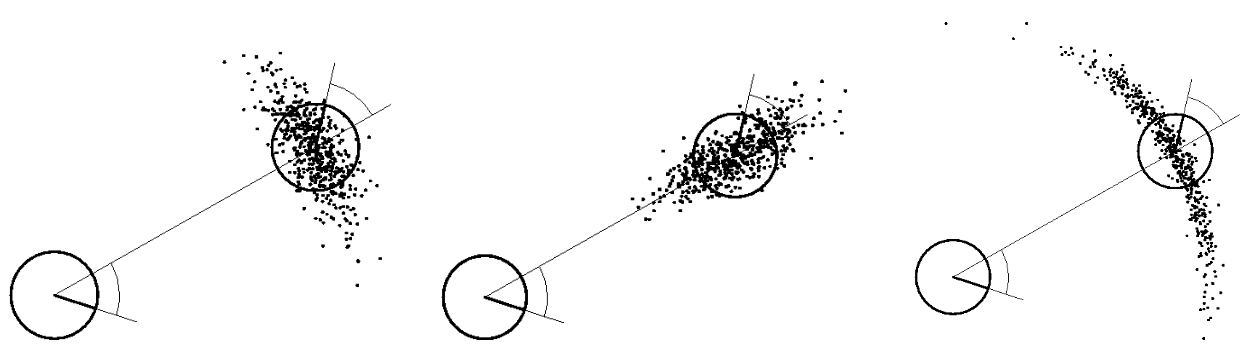
\includegraphics[width=\linewidth]{figures/implementation/ekf/noise_params.png}
\caption[Noise Parameter Settings]{How various settings of $\alpha$'s affect the motion model. The canonical settings produce the leftmost spread\textsuperscript{1}}
\tiny\textsuperscript{1}{From \url{http://ais.informatik.uni-freiburg.de/teaching/ss11/robotics/slides/06-motion-models.pdf}}
    \label{fig:ekf:noiseparams}
\end{figure}

I use settings which produce canonical distributions, increasing lateral uncertainty more
than longitudinal uncertainty.

%TODO Example of state propagation along a line with a sharp turn

Lastly, since I am using a simulation without a physical reference vehicle to
calibrate my parameters against, I use data from~\cite{vivacqua2017low}. 
They measure their vehicle's wheel odometry over 12 laps of a circuit, 1800 meters long, similar
to the one below. I mainly aim to produce similar order-of-magnitude errors.

\begin{figure}
    \begin{center}
        %% Creator: Matplotlib, PGF backend
%%
%% To include the figure in your LaTeX document, write
%%   \input{<filename>.pgf}
%%
%% Make sure the required packages are loaded in your preamble
%%   \usepackage{pgf}
%%
%% Figures using additional raster images can only be included by \input if
%% they are in the same directory as the main LaTeX file. For loading figures
%% from other directories you can use the `import` package
%%   \usepackage{import}
%% and then include the figures with
%%   \import{<path to file>}{<filename>.pgf}
%%
%% Matplotlib used the following preamble
%%   \usepackage{fontspec}
%%
\begingroup%
\makeatletter%
\begin{pgfpicture}%
\pgfpathrectangle{\pgfpointorigin}{\pgfqpoint{4.698502in}{2.987944in}}%
\pgfusepath{use as bounding box, clip}%
\begin{pgfscope}%
\pgfsetbuttcap%
\pgfsetmiterjoin%
\definecolor{currentfill}{rgb}{1.000000,1.000000,1.000000}%
\pgfsetfillcolor{currentfill}%
\pgfsetlinewidth{0.000000pt}%
\definecolor{currentstroke}{rgb}{1.000000,1.000000,1.000000}%
\pgfsetstrokecolor{currentstroke}%
\pgfsetdash{}{0pt}%
\pgfpathmoveto{\pgfqpoint{0.000000in}{0.000000in}}%
\pgfpathlineto{\pgfqpoint{4.698502in}{0.000000in}}%
\pgfpathlineto{\pgfqpoint{4.698502in}{2.987944in}}%
\pgfpathlineto{\pgfqpoint{0.000000in}{2.987944in}}%
\pgfpathclose%
\pgfusepath{fill}%
\end{pgfscope}%
\begin{pgfscope}%
\pgfsetbuttcap%
\pgfsetmiterjoin%
\definecolor{currentfill}{rgb}{1.000000,1.000000,1.000000}%
\pgfsetfillcolor{currentfill}%
\pgfsetlinewidth{0.000000pt}%
\definecolor{currentstroke}{rgb}{0.000000,0.000000,0.000000}%
\pgfsetstrokecolor{currentstroke}%
\pgfsetstrokeopacity{0.000000}%
\pgfsetdash{}{0pt}%
\pgfpathmoveto{\pgfqpoint{0.627945in}{0.542944in}}%
\pgfpathlineto{\pgfqpoint{4.502945in}{0.542944in}}%
\pgfpathlineto{\pgfqpoint{4.502945in}{2.852944in}}%
\pgfpathlineto{\pgfqpoint{0.627945in}{2.852944in}}%
\pgfpathclose%
\pgfusepath{fill}%
\end{pgfscope}%
\begin{pgfscope}%
\pgfpathrectangle{\pgfqpoint{0.627945in}{0.542944in}}{\pgfqpoint{3.875000in}{2.310000in}} %
\pgfusepath{clip}%
\pgfsetrectcap%
\pgfsetroundjoin%
\pgfsetlinewidth{0.803000pt}%
\definecolor{currentstroke}{rgb}{0.900000,0.900000,0.900000}%
\pgfsetstrokecolor{currentstroke}%
\pgfsetdash{}{0pt}%
\pgfpathmoveto{\pgfqpoint{0.869363in}{0.542944in}}%
\pgfpathlineto{\pgfqpoint{0.869363in}{2.852944in}}%
\pgfusepath{stroke}%
\end{pgfscope}%
\begin{pgfscope}%
\pgfsetbuttcap%
\pgfsetroundjoin%
\definecolor{currentfill}{rgb}{0.333333,0.333333,0.333333}%
\pgfsetfillcolor{currentfill}%
\pgfsetlinewidth{0.803000pt}%
\definecolor{currentstroke}{rgb}{0.333333,0.333333,0.333333}%
\pgfsetstrokecolor{currentstroke}%
\pgfsetdash{}{0pt}%
\pgfsys@defobject{currentmarker}{\pgfqpoint{0.000000in}{-0.048611in}}{\pgfqpoint{0.000000in}{0.000000in}}{%
\pgfpathmoveto{\pgfqpoint{0.000000in}{0.000000in}}%
\pgfpathlineto{\pgfqpoint{0.000000in}{-0.048611in}}%
\pgfusepath{stroke,fill}%
}%
\begin{pgfscope}%
\pgfsys@transformshift{0.869363in}{0.542944in}%
\pgfsys@useobject{currentmarker}{}%
\end{pgfscope}%
\end{pgfscope}%
\begin{pgfscope}%
\definecolor{textcolor}{rgb}{0.333333,0.333333,0.333333}%
\pgfsetstrokecolor{textcolor}%
\pgfsetfillcolor{textcolor}%
\pgftext[x=0.869363in,y=0.445722in,,top]{\color{textcolor}\rmfamily\fontsize{10.000000}{12.000000}\selectfont \(\displaystyle -100\)}%
\end{pgfscope}%
\begin{pgfscope}%
\pgfpathrectangle{\pgfqpoint{0.627945in}{0.542944in}}{\pgfqpoint{3.875000in}{2.310000in}} %
\pgfusepath{clip}%
\pgfsetrectcap%
\pgfsetroundjoin%
\pgfsetlinewidth{0.803000pt}%
\definecolor{currentstroke}{rgb}{0.900000,0.900000,0.900000}%
\pgfsetstrokecolor{currentstroke}%
\pgfsetdash{}{0pt}%
\pgfpathmoveto{\pgfqpoint{1.594358in}{0.542944in}}%
\pgfpathlineto{\pgfqpoint{1.594358in}{2.852944in}}%
\pgfusepath{stroke}%
\end{pgfscope}%
\begin{pgfscope}%
\pgfsetbuttcap%
\pgfsetroundjoin%
\definecolor{currentfill}{rgb}{0.333333,0.333333,0.333333}%
\pgfsetfillcolor{currentfill}%
\pgfsetlinewidth{0.803000pt}%
\definecolor{currentstroke}{rgb}{0.333333,0.333333,0.333333}%
\pgfsetstrokecolor{currentstroke}%
\pgfsetdash{}{0pt}%
\pgfsys@defobject{currentmarker}{\pgfqpoint{0.000000in}{-0.048611in}}{\pgfqpoint{0.000000in}{0.000000in}}{%
\pgfpathmoveto{\pgfqpoint{0.000000in}{0.000000in}}%
\pgfpathlineto{\pgfqpoint{0.000000in}{-0.048611in}}%
\pgfusepath{stroke,fill}%
}%
\begin{pgfscope}%
\pgfsys@transformshift{1.594358in}{0.542944in}%
\pgfsys@useobject{currentmarker}{}%
\end{pgfscope}%
\end{pgfscope}%
\begin{pgfscope}%
\definecolor{textcolor}{rgb}{0.333333,0.333333,0.333333}%
\pgfsetstrokecolor{textcolor}%
\pgfsetfillcolor{textcolor}%
\pgftext[x=1.594358in,y=0.445722in,,top]{\color{textcolor}\rmfamily\fontsize{10.000000}{12.000000}\selectfont \(\displaystyle 0\)}%
\end{pgfscope}%
\begin{pgfscope}%
\pgfpathrectangle{\pgfqpoint{0.627945in}{0.542944in}}{\pgfqpoint{3.875000in}{2.310000in}} %
\pgfusepath{clip}%
\pgfsetrectcap%
\pgfsetroundjoin%
\pgfsetlinewidth{0.803000pt}%
\definecolor{currentstroke}{rgb}{0.900000,0.900000,0.900000}%
\pgfsetstrokecolor{currentstroke}%
\pgfsetdash{}{0pt}%
\pgfpathmoveto{\pgfqpoint{2.319352in}{0.542944in}}%
\pgfpathlineto{\pgfqpoint{2.319352in}{2.852944in}}%
\pgfusepath{stroke}%
\end{pgfscope}%
\begin{pgfscope}%
\pgfsetbuttcap%
\pgfsetroundjoin%
\definecolor{currentfill}{rgb}{0.333333,0.333333,0.333333}%
\pgfsetfillcolor{currentfill}%
\pgfsetlinewidth{0.803000pt}%
\definecolor{currentstroke}{rgb}{0.333333,0.333333,0.333333}%
\pgfsetstrokecolor{currentstroke}%
\pgfsetdash{}{0pt}%
\pgfsys@defobject{currentmarker}{\pgfqpoint{0.000000in}{-0.048611in}}{\pgfqpoint{0.000000in}{0.000000in}}{%
\pgfpathmoveto{\pgfqpoint{0.000000in}{0.000000in}}%
\pgfpathlineto{\pgfqpoint{0.000000in}{-0.048611in}}%
\pgfusepath{stroke,fill}%
}%
\begin{pgfscope}%
\pgfsys@transformshift{2.319352in}{0.542944in}%
\pgfsys@useobject{currentmarker}{}%
\end{pgfscope}%
\end{pgfscope}%
\begin{pgfscope}%
\definecolor{textcolor}{rgb}{0.333333,0.333333,0.333333}%
\pgfsetstrokecolor{textcolor}%
\pgfsetfillcolor{textcolor}%
\pgftext[x=2.319352in,y=0.445722in,,top]{\color{textcolor}\rmfamily\fontsize{10.000000}{12.000000}\selectfont \(\displaystyle 100\)}%
\end{pgfscope}%
\begin{pgfscope}%
\pgfpathrectangle{\pgfqpoint{0.627945in}{0.542944in}}{\pgfqpoint{3.875000in}{2.310000in}} %
\pgfusepath{clip}%
\pgfsetrectcap%
\pgfsetroundjoin%
\pgfsetlinewidth{0.803000pt}%
\definecolor{currentstroke}{rgb}{0.900000,0.900000,0.900000}%
\pgfsetstrokecolor{currentstroke}%
\pgfsetdash{}{0pt}%
\pgfpathmoveto{\pgfqpoint{3.044346in}{0.542944in}}%
\pgfpathlineto{\pgfqpoint{3.044346in}{2.852944in}}%
\pgfusepath{stroke}%
\end{pgfscope}%
\begin{pgfscope}%
\pgfsetbuttcap%
\pgfsetroundjoin%
\definecolor{currentfill}{rgb}{0.333333,0.333333,0.333333}%
\pgfsetfillcolor{currentfill}%
\pgfsetlinewidth{0.803000pt}%
\definecolor{currentstroke}{rgb}{0.333333,0.333333,0.333333}%
\pgfsetstrokecolor{currentstroke}%
\pgfsetdash{}{0pt}%
\pgfsys@defobject{currentmarker}{\pgfqpoint{0.000000in}{-0.048611in}}{\pgfqpoint{0.000000in}{0.000000in}}{%
\pgfpathmoveto{\pgfqpoint{0.000000in}{0.000000in}}%
\pgfpathlineto{\pgfqpoint{0.000000in}{-0.048611in}}%
\pgfusepath{stroke,fill}%
}%
\begin{pgfscope}%
\pgfsys@transformshift{3.044346in}{0.542944in}%
\pgfsys@useobject{currentmarker}{}%
\end{pgfscope}%
\end{pgfscope}%
\begin{pgfscope}%
\definecolor{textcolor}{rgb}{0.333333,0.333333,0.333333}%
\pgfsetstrokecolor{textcolor}%
\pgfsetfillcolor{textcolor}%
\pgftext[x=3.044346in,y=0.445722in,,top]{\color{textcolor}\rmfamily\fontsize{10.000000}{12.000000}\selectfont \(\displaystyle 200\)}%
\end{pgfscope}%
\begin{pgfscope}%
\pgfpathrectangle{\pgfqpoint{0.627945in}{0.542944in}}{\pgfqpoint{3.875000in}{2.310000in}} %
\pgfusepath{clip}%
\pgfsetrectcap%
\pgfsetroundjoin%
\pgfsetlinewidth{0.803000pt}%
\definecolor{currentstroke}{rgb}{0.900000,0.900000,0.900000}%
\pgfsetstrokecolor{currentstroke}%
\pgfsetdash{}{0pt}%
\pgfpathmoveto{\pgfqpoint{3.769341in}{0.542944in}}%
\pgfpathlineto{\pgfqpoint{3.769341in}{2.852944in}}%
\pgfusepath{stroke}%
\end{pgfscope}%
\begin{pgfscope}%
\pgfsetbuttcap%
\pgfsetroundjoin%
\definecolor{currentfill}{rgb}{0.333333,0.333333,0.333333}%
\pgfsetfillcolor{currentfill}%
\pgfsetlinewidth{0.803000pt}%
\definecolor{currentstroke}{rgb}{0.333333,0.333333,0.333333}%
\pgfsetstrokecolor{currentstroke}%
\pgfsetdash{}{0pt}%
\pgfsys@defobject{currentmarker}{\pgfqpoint{0.000000in}{-0.048611in}}{\pgfqpoint{0.000000in}{0.000000in}}{%
\pgfpathmoveto{\pgfqpoint{0.000000in}{0.000000in}}%
\pgfpathlineto{\pgfqpoint{0.000000in}{-0.048611in}}%
\pgfusepath{stroke,fill}%
}%
\begin{pgfscope}%
\pgfsys@transformshift{3.769341in}{0.542944in}%
\pgfsys@useobject{currentmarker}{}%
\end{pgfscope}%
\end{pgfscope}%
\begin{pgfscope}%
\definecolor{textcolor}{rgb}{0.333333,0.333333,0.333333}%
\pgfsetstrokecolor{textcolor}%
\pgfsetfillcolor{textcolor}%
\pgftext[x=3.769341in,y=0.445722in,,top]{\color{textcolor}\rmfamily\fontsize{10.000000}{12.000000}\selectfont \(\displaystyle 300\)}%
\end{pgfscope}%
\begin{pgfscope}%
\pgfpathrectangle{\pgfqpoint{0.627945in}{0.542944in}}{\pgfqpoint{3.875000in}{2.310000in}} %
\pgfusepath{clip}%
\pgfsetrectcap%
\pgfsetroundjoin%
\pgfsetlinewidth{0.803000pt}%
\definecolor{currentstroke}{rgb}{0.900000,0.900000,0.900000}%
\pgfsetstrokecolor{currentstroke}%
\pgfsetdash{}{0pt}%
\pgfpathmoveto{\pgfqpoint{4.494335in}{0.542944in}}%
\pgfpathlineto{\pgfqpoint{4.494335in}{2.852944in}}%
\pgfusepath{stroke}%
\end{pgfscope}%
\begin{pgfscope}%
\pgfsetbuttcap%
\pgfsetroundjoin%
\definecolor{currentfill}{rgb}{0.333333,0.333333,0.333333}%
\pgfsetfillcolor{currentfill}%
\pgfsetlinewidth{0.803000pt}%
\definecolor{currentstroke}{rgb}{0.333333,0.333333,0.333333}%
\pgfsetstrokecolor{currentstroke}%
\pgfsetdash{}{0pt}%
\pgfsys@defobject{currentmarker}{\pgfqpoint{0.000000in}{-0.048611in}}{\pgfqpoint{0.000000in}{0.000000in}}{%
\pgfpathmoveto{\pgfqpoint{0.000000in}{0.000000in}}%
\pgfpathlineto{\pgfqpoint{0.000000in}{-0.048611in}}%
\pgfusepath{stroke,fill}%
}%
\begin{pgfscope}%
\pgfsys@transformshift{4.494335in}{0.542944in}%
\pgfsys@useobject{currentmarker}{}%
\end{pgfscope}%
\end{pgfscope}%
\begin{pgfscope}%
\definecolor{textcolor}{rgb}{0.333333,0.333333,0.333333}%
\pgfsetstrokecolor{textcolor}%
\pgfsetfillcolor{textcolor}%
\pgftext[x=4.494335in,y=0.445722in,,top]{\color{textcolor}\rmfamily\fontsize{10.000000}{12.000000}\selectfont \(\displaystyle 400\)}%
\end{pgfscope}%
\begin{pgfscope}%
\definecolor{textcolor}{rgb}{0.333333,0.333333,0.333333}%
\pgfsetstrokecolor{textcolor}%
\pgfsetfillcolor{textcolor}%
\pgftext[x=2.565445in,y=0.266833in,,top]{\color{textcolor}\rmfamily\fontsize{12.000000}{14.400000}\selectfont X (meters)}%
\end{pgfscope}%
\begin{pgfscope}%
\pgfpathrectangle{\pgfqpoint{0.627945in}{0.542944in}}{\pgfqpoint{3.875000in}{2.310000in}} %
\pgfusepath{clip}%
\pgfsetrectcap%
\pgfsetroundjoin%
\pgfsetlinewidth{0.803000pt}%
\definecolor{currentstroke}{rgb}{0.900000,0.900000,0.900000}%
\pgfsetstrokecolor{currentstroke}%
\pgfsetdash{}{0pt}%
\pgfpathmoveto{\pgfqpoint{0.627945in}{0.671769in}}%
\pgfpathlineto{\pgfqpoint{4.502945in}{0.671769in}}%
\pgfusepath{stroke}%
\end{pgfscope}%
\begin{pgfscope}%
\pgfsetbuttcap%
\pgfsetroundjoin%
\definecolor{currentfill}{rgb}{0.333333,0.333333,0.333333}%
\pgfsetfillcolor{currentfill}%
\pgfsetlinewidth{0.803000pt}%
\definecolor{currentstroke}{rgb}{0.333333,0.333333,0.333333}%
\pgfsetstrokecolor{currentstroke}%
\pgfsetdash{}{0pt}%
\pgfsys@defobject{currentmarker}{\pgfqpoint{-0.048611in}{0.000000in}}{\pgfqpoint{0.000000in}{0.000000in}}{%
\pgfpathmoveto{\pgfqpoint{0.000000in}{0.000000in}}%
\pgfpathlineto{\pgfqpoint{-0.048611in}{0.000000in}}%
\pgfusepath{stroke,fill}%
}%
\begin{pgfscope}%
\pgfsys@transformshift{0.627945in}{0.671769in}%
\pgfsys@useobject{currentmarker}{}%
\end{pgfscope}%
\end{pgfscope}%
\begin{pgfscope}%
\definecolor{textcolor}{rgb}{0.333333,0.333333,0.333333}%
\pgfsetstrokecolor{textcolor}%
\pgfsetfillcolor{textcolor}%
\pgftext[x=0.461278in,y=0.623575in,left,base]{\color{textcolor}\rmfamily\fontsize{10.000000}{12.000000}\selectfont \(\displaystyle 0\)}%
\end{pgfscope}%
\begin{pgfscope}%
\pgfpathrectangle{\pgfqpoint{0.627945in}{0.542944in}}{\pgfqpoint{3.875000in}{2.310000in}} %
\pgfusepath{clip}%
\pgfsetrectcap%
\pgfsetroundjoin%
\pgfsetlinewidth{0.803000pt}%
\definecolor{currentstroke}{rgb}{0.900000,0.900000,0.900000}%
\pgfsetstrokecolor{currentstroke}%
\pgfsetdash{}{0pt}%
\pgfpathmoveto{\pgfqpoint{0.627945in}{1.151587in}}%
\pgfpathlineto{\pgfqpoint{4.502945in}{1.151587in}}%
\pgfusepath{stroke}%
\end{pgfscope}%
\begin{pgfscope}%
\pgfsetbuttcap%
\pgfsetroundjoin%
\definecolor{currentfill}{rgb}{0.333333,0.333333,0.333333}%
\pgfsetfillcolor{currentfill}%
\pgfsetlinewidth{0.803000pt}%
\definecolor{currentstroke}{rgb}{0.333333,0.333333,0.333333}%
\pgfsetstrokecolor{currentstroke}%
\pgfsetdash{}{0pt}%
\pgfsys@defobject{currentmarker}{\pgfqpoint{-0.048611in}{0.000000in}}{\pgfqpoint{0.000000in}{0.000000in}}{%
\pgfpathmoveto{\pgfqpoint{0.000000in}{0.000000in}}%
\pgfpathlineto{\pgfqpoint{-0.048611in}{0.000000in}}%
\pgfusepath{stroke,fill}%
}%
\begin{pgfscope}%
\pgfsys@transformshift{0.627945in}{1.151587in}%
\pgfsys@useobject{currentmarker}{}%
\end{pgfscope}%
\end{pgfscope}%
\begin{pgfscope}%
\definecolor{textcolor}{rgb}{0.333333,0.333333,0.333333}%
\pgfsetstrokecolor{textcolor}%
\pgfsetfillcolor{textcolor}%
\pgftext[x=0.322389in,y=1.103392in,left,base]{\color{textcolor}\rmfamily\fontsize{10.000000}{12.000000}\selectfont \(\displaystyle 100\)}%
\end{pgfscope}%
\begin{pgfscope}%
\pgfpathrectangle{\pgfqpoint{0.627945in}{0.542944in}}{\pgfqpoint{3.875000in}{2.310000in}} %
\pgfusepath{clip}%
\pgfsetrectcap%
\pgfsetroundjoin%
\pgfsetlinewidth{0.803000pt}%
\definecolor{currentstroke}{rgb}{0.900000,0.900000,0.900000}%
\pgfsetstrokecolor{currentstroke}%
\pgfsetdash{}{0pt}%
\pgfpathmoveto{\pgfqpoint{0.627945in}{1.631405in}}%
\pgfpathlineto{\pgfqpoint{4.502945in}{1.631405in}}%
\pgfusepath{stroke}%
\end{pgfscope}%
\begin{pgfscope}%
\pgfsetbuttcap%
\pgfsetroundjoin%
\definecolor{currentfill}{rgb}{0.333333,0.333333,0.333333}%
\pgfsetfillcolor{currentfill}%
\pgfsetlinewidth{0.803000pt}%
\definecolor{currentstroke}{rgb}{0.333333,0.333333,0.333333}%
\pgfsetstrokecolor{currentstroke}%
\pgfsetdash{}{0pt}%
\pgfsys@defobject{currentmarker}{\pgfqpoint{-0.048611in}{0.000000in}}{\pgfqpoint{0.000000in}{0.000000in}}{%
\pgfpathmoveto{\pgfqpoint{0.000000in}{0.000000in}}%
\pgfpathlineto{\pgfqpoint{-0.048611in}{0.000000in}}%
\pgfusepath{stroke,fill}%
}%
\begin{pgfscope}%
\pgfsys@transformshift{0.627945in}{1.631405in}%
\pgfsys@useobject{currentmarker}{}%
\end{pgfscope}%
\end{pgfscope}%
\begin{pgfscope}%
\definecolor{textcolor}{rgb}{0.333333,0.333333,0.333333}%
\pgfsetstrokecolor{textcolor}%
\pgfsetfillcolor{textcolor}%
\pgftext[x=0.322389in,y=1.583210in,left,base]{\color{textcolor}\rmfamily\fontsize{10.000000}{12.000000}\selectfont \(\displaystyle 200\)}%
\end{pgfscope}%
\begin{pgfscope}%
\pgfpathrectangle{\pgfqpoint{0.627945in}{0.542944in}}{\pgfqpoint{3.875000in}{2.310000in}} %
\pgfusepath{clip}%
\pgfsetrectcap%
\pgfsetroundjoin%
\pgfsetlinewidth{0.803000pt}%
\definecolor{currentstroke}{rgb}{0.900000,0.900000,0.900000}%
\pgfsetstrokecolor{currentstroke}%
\pgfsetdash{}{0pt}%
\pgfpathmoveto{\pgfqpoint{0.627945in}{2.111222in}}%
\pgfpathlineto{\pgfqpoint{4.502945in}{2.111222in}}%
\pgfusepath{stroke}%
\end{pgfscope}%
\begin{pgfscope}%
\pgfsetbuttcap%
\pgfsetroundjoin%
\definecolor{currentfill}{rgb}{0.333333,0.333333,0.333333}%
\pgfsetfillcolor{currentfill}%
\pgfsetlinewidth{0.803000pt}%
\definecolor{currentstroke}{rgb}{0.333333,0.333333,0.333333}%
\pgfsetstrokecolor{currentstroke}%
\pgfsetdash{}{0pt}%
\pgfsys@defobject{currentmarker}{\pgfqpoint{-0.048611in}{0.000000in}}{\pgfqpoint{0.000000in}{0.000000in}}{%
\pgfpathmoveto{\pgfqpoint{0.000000in}{0.000000in}}%
\pgfpathlineto{\pgfqpoint{-0.048611in}{0.000000in}}%
\pgfusepath{stroke,fill}%
}%
\begin{pgfscope}%
\pgfsys@transformshift{0.627945in}{2.111222in}%
\pgfsys@useobject{currentmarker}{}%
\end{pgfscope}%
\end{pgfscope}%
\begin{pgfscope}%
\definecolor{textcolor}{rgb}{0.333333,0.333333,0.333333}%
\pgfsetstrokecolor{textcolor}%
\pgfsetfillcolor{textcolor}%
\pgftext[x=0.322389in,y=2.063028in,left,base]{\color{textcolor}\rmfamily\fontsize{10.000000}{12.000000}\selectfont \(\displaystyle 300\)}%
\end{pgfscope}%
\begin{pgfscope}%
\pgfpathrectangle{\pgfqpoint{0.627945in}{0.542944in}}{\pgfqpoint{3.875000in}{2.310000in}} %
\pgfusepath{clip}%
\pgfsetrectcap%
\pgfsetroundjoin%
\pgfsetlinewidth{0.803000pt}%
\definecolor{currentstroke}{rgb}{0.900000,0.900000,0.900000}%
\pgfsetstrokecolor{currentstroke}%
\pgfsetdash{}{0pt}%
\pgfpathmoveto{\pgfqpoint{0.627945in}{2.591040in}}%
\pgfpathlineto{\pgfqpoint{4.502945in}{2.591040in}}%
\pgfusepath{stroke}%
\end{pgfscope}%
\begin{pgfscope}%
\pgfsetbuttcap%
\pgfsetroundjoin%
\definecolor{currentfill}{rgb}{0.333333,0.333333,0.333333}%
\pgfsetfillcolor{currentfill}%
\pgfsetlinewidth{0.803000pt}%
\definecolor{currentstroke}{rgb}{0.333333,0.333333,0.333333}%
\pgfsetstrokecolor{currentstroke}%
\pgfsetdash{}{0pt}%
\pgfsys@defobject{currentmarker}{\pgfqpoint{-0.048611in}{0.000000in}}{\pgfqpoint{0.000000in}{0.000000in}}{%
\pgfpathmoveto{\pgfqpoint{0.000000in}{0.000000in}}%
\pgfpathlineto{\pgfqpoint{-0.048611in}{0.000000in}}%
\pgfusepath{stroke,fill}%
}%
\begin{pgfscope}%
\pgfsys@transformshift{0.627945in}{2.591040in}%
\pgfsys@useobject{currentmarker}{}%
\end{pgfscope}%
\end{pgfscope}%
\begin{pgfscope}%
\definecolor{textcolor}{rgb}{0.333333,0.333333,0.333333}%
\pgfsetstrokecolor{textcolor}%
\pgfsetfillcolor{textcolor}%
\pgftext[x=0.322389in,y=2.542846in,left,base]{\color{textcolor}\rmfamily\fontsize{10.000000}{12.000000}\selectfont \(\displaystyle 400\)}%
\end{pgfscope}%
\begin{pgfscope}%
\definecolor{textcolor}{rgb}{0.333333,0.333333,0.333333}%
\pgfsetstrokecolor{textcolor}%
\pgfsetfillcolor{textcolor}%
\pgftext[x=0.266833in,y=1.697944in,,bottom,rotate=90.000000]{\color{textcolor}\rmfamily\fontsize{12.000000}{14.400000}\selectfont Y (meters)}%
\end{pgfscope}%
\begin{pgfscope}%
\pgfpathrectangle{\pgfqpoint{0.627945in}{0.542944in}}{\pgfqpoint{3.875000in}{2.310000in}} %
\pgfusepath{clip}%
\pgfsetrectcap%
\pgfsetroundjoin%
\pgfsetlinewidth{1.505625pt}%
\definecolor{currentstroke}{rgb}{0.886275,0.290196,0.200000}%
\pgfsetstrokecolor{currentstroke}%
\pgfsetdash{}{0pt}%
\pgfpathmoveto{\pgfqpoint{1.602899in}{0.671769in}}%
\pgfpathlineto{\pgfqpoint{4.148995in}{0.672308in}}%
\pgfpathlineto{\pgfqpoint{4.148995in}{0.672308in}}%
\pgfpathlineto{\pgfqpoint{4.177988in}{0.675723in}}%
\pgfpathlineto{\pgfqpoint{4.200192in}{0.680627in}}%
\pgfpathlineto{\pgfqpoint{4.220723in}{0.687184in}}%
\pgfpathlineto{\pgfqpoint{4.242776in}{0.696864in}}%
\pgfpathlineto{\pgfqpoint{4.256680in}{0.704761in}}%
\pgfpathlineto{\pgfqpoint{4.274404in}{0.717653in}}%
\pgfpathlineto{\pgfqpoint{4.274404in}{0.717653in}}%
\pgfpathlineto{\pgfqpoint{4.287273in}{0.730025in}}%
\pgfpathlineto{\pgfqpoint{4.297915in}{0.743681in}}%
\pgfpathlineto{\pgfqpoint{4.306123in}{0.758795in}}%
\pgfpathlineto{\pgfqpoint{4.306123in}{0.758795in}}%
\pgfpathlineto{\pgfqpoint{4.310414in}{0.771201in}}%
\pgfpathlineto{\pgfqpoint{4.310414in}{0.771201in}}%
\pgfpathlineto{\pgfqpoint{4.312919in}{0.786569in}}%
\pgfpathlineto{\pgfqpoint{4.312919in}{0.786569in}}%
\pgfpathlineto{\pgfqpoint{4.313086in}{0.823099in}}%
\pgfpathlineto{\pgfqpoint{4.312088in}{2.716558in}}%
\pgfpathlineto{\pgfqpoint{4.312088in}{2.716558in}}%
\pgfpathlineto{\pgfqpoint{4.308660in}{2.722470in}}%
\pgfpathlineto{\pgfqpoint{4.308660in}{2.722470in}}%
\pgfpathlineto{\pgfqpoint{4.302311in}{2.728056in}}%
\pgfpathlineto{\pgfqpoint{4.302311in}{2.728056in}}%
\pgfpathlineto{\pgfqpoint{4.292851in}{2.732514in}}%
\pgfpathlineto{\pgfqpoint{4.283120in}{2.734621in}}%
\pgfpathlineto{\pgfqpoint{4.283120in}{2.734621in}}%
\pgfpathlineto{\pgfqpoint{4.269683in}{2.734986in}}%
\pgfpathlineto{\pgfqpoint{4.269683in}{2.734986in}}%
\pgfpathlineto{\pgfqpoint{0.991188in}{2.733986in}}%
\pgfpathlineto{\pgfqpoint{0.991188in}{2.733986in}}%
\pgfpathlineto{\pgfqpoint{0.970181in}{2.731353in}}%
\pgfpathlineto{\pgfqpoint{0.970181in}{2.731353in}}%
\pgfpathlineto{\pgfqpoint{0.947718in}{2.726569in}}%
\pgfpathlineto{\pgfqpoint{0.930504in}{2.721362in}}%
\pgfpathlineto{\pgfqpoint{0.930504in}{2.721362in}}%
\pgfpathlineto{\pgfqpoint{0.907763in}{2.712034in}}%
\pgfpathlineto{\pgfqpoint{0.907763in}{2.712034in}}%
\pgfpathlineto{\pgfqpoint{0.882559in}{2.697362in}}%
\pgfpathlineto{\pgfqpoint{0.882559in}{2.697362in}}%
\pgfpathlineto{\pgfqpoint{0.868269in}{2.686021in}}%
\pgfpathlineto{\pgfqpoint{0.868269in}{2.686021in}}%
\pgfpathlineto{\pgfqpoint{0.856095in}{2.673488in}}%
\pgfpathlineto{\pgfqpoint{0.856095in}{2.673488in}}%
\pgfpathlineto{\pgfqpoint{0.847339in}{2.661615in}}%
\pgfpathlineto{\pgfqpoint{0.839495in}{2.646589in}}%
\pgfpathlineto{\pgfqpoint{0.839495in}{2.646589in}}%
\pgfpathlineto{\pgfqpoint{0.834734in}{2.631069in}}%
\pgfpathlineto{\pgfqpoint{0.833104in}{2.615014in}}%
\pgfpathlineto{\pgfqpoint{0.833104in}{2.615014in}}%
\pgfpathlineto{\pgfqpoint{0.833986in}{0.918394in}}%
\pgfpathlineto{\pgfqpoint{0.836682in}{0.900518in}}%
\pgfpathlineto{\pgfqpoint{0.836682in}{0.900518in}}%
\pgfpathlineto{\pgfqpoint{0.843894in}{0.874757in}}%
\pgfpathlineto{\pgfqpoint{0.850908in}{0.857739in}}%
\pgfpathlineto{\pgfqpoint{0.850908in}{0.857739in}}%
\pgfpathlineto{\pgfqpoint{0.859571in}{0.841160in}}%
\pgfpathlineto{\pgfqpoint{0.859571in}{0.841160in}}%
\pgfpathlineto{\pgfqpoint{0.872759in}{0.820964in}}%
\pgfpathlineto{\pgfqpoint{0.887641in}{0.802468in}}%
\pgfpathlineto{\pgfqpoint{0.904574in}{0.784925in}}%
\pgfpathlineto{\pgfqpoint{0.904574in}{0.784925in}}%
\pgfpathlineto{\pgfqpoint{0.915838in}{0.774740in}}%
\pgfpathlineto{\pgfqpoint{0.915838in}{0.774740in}}%
\pgfpathlineto{\pgfqpoint{0.945132in}{0.752276in}}%
\pgfpathlineto{\pgfqpoint{0.945132in}{0.752276in}}%
\pgfpathlineto{\pgfqpoint{0.972951in}{0.734964in}}%
\pgfpathlineto{\pgfqpoint{1.004668in}{0.718790in}}%
\pgfpathlineto{\pgfqpoint{1.042862in}{0.703290in}}%
\pgfpathlineto{\pgfqpoint{1.042862in}{0.703290in}}%
\pgfpathlineto{\pgfqpoint{1.066564in}{0.695505in}}%
\pgfpathlineto{\pgfqpoint{1.066564in}{0.695505in}}%
\pgfpathlineto{\pgfqpoint{1.108886in}{0.684625in}}%
\pgfpathlineto{\pgfqpoint{1.108886in}{0.684625in}}%
\pgfpathlineto{\pgfqpoint{1.145711in}{0.677993in}}%
\pgfpathlineto{\pgfqpoint{1.145711in}{0.677993in}}%
\pgfpathlineto{\pgfqpoint{1.189743in}{0.673235in}}%
\pgfpathlineto{\pgfqpoint{1.189743in}{0.673235in}}%
\pgfpathlineto{\pgfqpoint{1.228400in}{0.671490in}}%
\pgfpathlineto{\pgfqpoint{1.228400in}{0.671490in}}%
\pgfpathlineto{\pgfqpoint{1.522482in}{0.660855in}}%
\pgfpathlineto{\pgfqpoint{1.522482in}{0.660855in}}%
\pgfusepath{stroke}%
\end{pgfscope}%
\begin{pgfscope}%
\pgfpathrectangle{\pgfqpoint{0.627945in}{0.542944in}}{\pgfqpoint{3.875000in}{2.310000in}} %
\pgfusepath{clip}%
\pgfsetrectcap%
\pgfsetroundjoin%
\pgfsetlinewidth{1.505625pt}%
\definecolor{currentstroke}{rgb}{0.203922,0.541176,0.741176}%
\pgfsetstrokecolor{currentstroke}%
\pgfsetdash{}{0pt}%
\pgfpathmoveto{\pgfqpoint{1.599960in}{0.671768in}}%
\pgfpathlineto{\pgfqpoint{2.510351in}{0.672907in}}%
\pgfpathlineto{\pgfqpoint{3.558874in}{0.674374in}}%
\pgfpathlineto{\pgfqpoint{4.187600in}{0.675728in}}%
\pgfpathlineto{\pgfqpoint{4.212238in}{0.678479in}}%
\pgfpathlineto{\pgfqpoint{4.232398in}{0.682966in}}%
\pgfpathlineto{\pgfqpoint{4.250380in}{0.689231in}}%
\pgfpathlineto{\pgfqpoint{4.267097in}{0.697769in}}%
\pgfpathlineto{\pgfqpoint{4.280724in}{0.707666in}}%
\pgfpathlineto{\pgfqpoint{4.292296in}{0.719421in}}%
\pgfpathlineto{\pgfqpoint{4.303075in}{0.734294in}}%
\pgfpathlineto{\pgfqpoint{4.315165in}{0.754705in}}%
\pgfpathlineto{\pgfqpoint{4.321924in}{0.770693in}}%
\pgfpathlineto{\pgfqpoint{4.325263in}{0.784754in}}%
\pgfpathlineto{\pgfqpoint{4.326055in}{0.798380in}}%
\pgfpathlineto{\pgfqpoint{4.324719in}{0.809645in}}%
\pgfpathlineto{\pgfqpoint{4.317984in}{0.836145in}}%
\pgfpathlineto{\pgfqpoint{4.311325in}{0.865733in}}%
\pgfpathlineto{\pgfqpoint{4.308156in}{0.891113in}}%
\pgfpathlineto{\pgfqpoint{4.307303in}{0.918290in}}%
\pgfpathlineto{\pgfqpoint{4.308892in}{0.972954in}}%
\pgfpathlineto{\pgfqpoint{4.310096in}{1.052126in}}%
\pgfpathlineto{\pgfqpoint{4.309958in}{1.204767in}}%
\pgfpathlineto{\pgfqpoint{4.306408in}{1.683215in}}%
\pgfpathlineto{\pgfqpoint{4.294333in}{2.732912in}}%
\pgfpathlineto{\pgfqpoint{4.290534in}{2.738163in}}%
\pgfpathlineto{\pgfqpoint{4.284039in}{2.743079in}}%
\pgfpathlineto{\pgfqpoint{4.276169in}{2.746257in}}%
\pgfpathlineto{\pgfqpoint{4.266242in}{2.747827in}}%
\pgfpathlineto{\pgfqpoint{4.253995in}{2.747440in}}%
\pgfpathlineto{\pgfqpoint{4.241031in}{2.744813in}}%
\pgfpathlineto{\pgfqpoint{4.185483in}{2.730836in}}%
\pgfpathlineto{\pgfqpoint{4.166620in}{2.729441in}}%
\pgfpathlineto{\pgfqpoint{4.141888in}{2.730063in}}%
\pgfpathlineto{\pgfqpoint{4.098503in}{2.734291in}}%
\pgfpathlineto{\pgfqpoint{4.031912in}{2.740150in}}%
\pgfpathlineto{\pgfqpoint{3.983533in}{2.742248in}}%
\pgfpathlineto{\pgfqpoint{3.936118in}{2.741819in}}%
\pgfpathlineto{\pgfqpoint{3.760850in}{2.736800in}}%
\pgfpathlineto{\pgfqpoint{3.625309in}{2.736017in}}%
\pgfpathlineto{\pgfqpoint{3.469562in}{2.735102in}}%
\pgfpathlineto{\pgfqpoint{2.638742in}{2.731190in}}%
\pgfpathlineto{\pgfqpoint{0.935418in}{2.719933in}}%
\pgfpathlineto{\pgfqpoint{0.915457in}{2.716987in}}%
\pgfpathlineto{\pgfqpoint{0.895559in}{2.712021in}}%
\pgfpathlineto{\pgfqpoint{0.877904in}{2.705371in}}%
\pgfpathlineto{\pgfqpoint{0.862288in}{2.696918in}}%
\pgfpathlineto{\pgfqpoint{0.851226in}{2.688731in}}%
\pgfpathlineto{\pgfqpoint{0.842040in}{2.679609in}}%
\pgfpathlineto{\pgfqpoint{0.834877in}{2.669715in}}%
\pgfpathlineto{\pgfqpoint{0.827174in}{2.654244in}}%
\pgfpathlineto{\pgfqpoint{0.806020in}{2.606451in}}%
\pgfpathlineto{\pgfqpoint{0.804081in}{2.592922in}}%
\pgfpathlineto{\pgfqpoint{0.804901in}{2.581735in}}%
\pgfpathlineto{\pgfqpoint{0.807749in}{2.570616in}}%
\pgfpathlineto{\pgfqpoint{0.816095in}{2.550375in}}%
\pgfpathlineto{\pgfqpoint{0.827315in}{2.521953in}}%
\pgfpathlineto{\pgfqpoint{0.833031in}{2.501263in}}%
\pgfpathlineto{\pgfqpoint{0.836427in}{2.479248in}}%
\pgfpathlineto{\pgfqpoint{0.837297in}{2.456001in}}%
\pgfpathlineto{\pgfqpoint{0.836043in}{2.434274in}}%
\pgfpathlineto{\pgfqpoint{0.832405in}{2.408942in}}%
\pgfpathlineto{\pgfqpoint{0.826258in}{2.368815in}}%
\pgfpathlineto{\pgfqpoint{0.825177in}{2.346961in}}%
\pgfpathlineto{\pgfqpoint{0.826376in}{2.314567in}}%
\pgfpathlineto{\pgfqpoint{0.827680in}{2.273569in}}%
\pgfpathlineto{\pgfqpoint{0.826083in}{2.228706in}}%
\pgfpathlineto{\pgfqpoint{0.825612in}{2.193406in}}%
\pgfpathlineto{\pgfqpoint{0.836469in}{1.637080in}}%
\pgfpathlineto{\pgfqpoint{0.852909in}{0.881176in}}%
\pgfpathlineto{\pgfqpoint{0.855623in}{0.863168in}}%
\pgfpathlineto{\pgfqpoint{0.860324in}{0.845362in}}%
\pgfpathlineto{\pgfqpoint{0.866658in}{0.828759in}}%
\pgfpathlineto{\pgfqpoint{0.875351in}{0.811670in}}%
\pgfpathlineto{\pgfqpoint{0.886190in}{0.795172in}}%
\pgfpathlineto{\pgfqpoint{0.899085in}{0.779407in}}%
\pgfpathlineto{\pgfqpoint{0.913091in}{0.765263in}}%
\pgfpathlineto{\pgfqpoint{0.929661in}{0.751267in}}%
\pgfpathlineto{\pgfqpoint{0.952031in}{0.735737in}}%
\pgfpathlineto{\pgfqpoint{0.972309in}{0.724162in}}%
\pgfpathlineto{\pgfqpoint{0.999963in}{0.711210in}}%
\pgfpathlineto{\pgfqpoint{1.078828in}{0.678909in}}%
\pgfpathlineto{\pgfqpoint{1.109089in}{0.668127in}}%
\pgfpathlineto{\pgfqpoint{1.139363in}{0.659775in}}%
\pgfpathlineto{\pgfqpoint{1.170760in}{0.653598in}}%
\pgfpathlineto{\pgfqpoint{1.204238in}{0.649536in}}%
\pgfpathlineto{\pgfqpoint{1.236773in}{0.647977in}}%
\pgfpathlineto{\pgfqpoint{1.270895in}{0.648653in}}%
\pgfpathlineto{\pgfqpoint{1.310554in}{0.651828in}}%
\pgfpathlineto{\pgfqpoint{1.357528in}{0.654942in}}%
\pgfpathlineto{\pgfqpoint{1.397693in}{0.654931in}}%
\pgfpathlineto{\pgfqpoint{1.566089in}{0.649820in}}%
\pgfpathlineto{\pgfqpoint{1.566089in}{0.649820in}}%
\pgfusepath{stroke}%
\end{pgfscope}%
\begin{pgfscope}%
\pgfpathrectangle{\pgfqpoint{0.627945in}{0.542944in}}{\pgfqpoint{3.875000in}{2.310000in}} %
\pgfusepath{clip}%
\pgfsetrectcap%
\pgfsetroundjoin%
\pgfsetlinewidth{1.505625pt}%
\definecolor{currentstroke}{rgb}{0.596078,0.556863,0.835294}%
\pgfsetstrokecolor{currentstroke}%
\pgfsetdash{}{0pt}%
\pgfpathmoveto{\pgfqpoint{1.599935in}{0.671786in}}%
\pgfpathlineto{\pgfqpoint{3.335194in}{0.671768in}}%
\pgfpathlineto{\pgfqpoint{4.192070in}{0.672478in}}%
\pgfpathlineto{\pgfqpoint{4.216560in}{0.675636in}}%
\pgfpathlineto{\pgfqpoint{4.236495in}{0.680486in}}%
\pgfpathlineto{\pgfqpoint{4.254154in}{0.687135in}}%
\pgfpathlineto{\pgfqpoint{4.269795in}{0.695626in}}%
\pgfpathlineto{\pgfqpoint{4.280920in}{0.703885in}}%
\pgfpathlineto{\pgfqpoint{4.292565in}{0.715608in}}%
\pgfpathlineto{\pgfqpoint{4.303425in}{0.730454in}}%
\pgfpathlineto{\pgfqpoint{4.315622in}{0.750836in}}%
\pgfpathlineto{\pgfqpoint{4.322469in}{0.766807in}}%
\pgfpathlineto{\pgfqpoint{4.325894in}{0.780860in}}%
\pgfpathlineto{\pgfqpoint{4.326767in}{0.794485in}}%
\pgfpathlineto{\pgfqpoint{4.325500in}{0.805753in}}%
\pgfpathlineto{\pgfqpoint{4.319762in}{0.828953in}}%
\pgfpathlineto{\pgfqpoint{4.312909in}{0.858918in}}%
\pgfpathlineto{\pgfqpoint{4.309665in}{0.883294in}}%
\pgfpathlineto{\pgfqpoint{4.308640in}{0.910203in}}%
\pgfpathlineto{\pgfqpoint{4.309905in}{0.951576in}}%
\pgfpathlineto{\pgfqpoint{4.311890in}{1.021679in}}%
\pgfpathlineto{\pgfqpoint{4.312958in}{1.159858in}}%
\pgfpathlineto{\pgfqpoint{4.313094in}{1.876074in}}%
\pgfpathlineto{\pgfqpoint{4.311850in}{2.727027in}}%
\pgfpathlineto{\pgfqpoint{4.308897in}{2.732465in}}%
\pgfpathlineto{\pgfqpoint{4.303699in}{2.737409in}}%
\pgfpathlineto{\pgfqpoint{4.296651in}{2.741298in}}%
\pgfpathlineto{\pgfqpoint{4.288111in}{2.743564in}}%
\pgfpathlineto{\pgfqpoint{4.277036in}{2.744249in}}%
\pgfpathlineto{\pgfqpoint{4.265116in}{2.742911in}}%
\pgfpathlineto{\pgfqpoint{4.247649in}{2.738326in}}%
\pgfpathlineto{\pgfqpoint{4.215996in}{2.729738in}}%
\pgfpathlineto{\pgfqpoint{4.196285in}{2.726890in}}%
\pgfpathlineto{\pgfqpoint{4.176755in}{2.726150in}}%
\pgfpathlineto{\pgfqpoint{4.151345in}{2.727510in}}%
\pgfpathlineto{\pgfqpoint{4.016904in}{2.739342in}}%
\pgfpathlineto{\pgfqpoint{3.970748in}{2.739974in}}%
\pgfpathlineto{\pgfqpoint{3.915792in}{2.738156in}}%
\pgfpathlineto{\pgfqpoint{3.837507in}{2.735550in}}%
\pgfpathlineto{\pgfqpoint{3.750214in}{2.735621in}}%
\pgfpathlineto{\pgfqpoint{3.634806in}{2.735201in}}%
\pgfpathlineto{\pgfqpoint{3.473275in}{2.735046in}}%
\pgfpathlineto{\pgfqpoint{2.078701in}{2.734980in}}%
\pgfpathlineto{\pgfqpoint{0.948453in}{2.733199in}}%
\pgfpathlineto{\pgfqpoint{0.924352in}{2.729166in}}%
\pgfpathlineto{\pgfqpoint{0.904848in}{2.723589in}}%
\pgfpathlineto{\pgfqpoint{0.887817in}{2.716322in}}%
\pgfpathlineto{\pgfqpoint{0.872388in}{2.706897in}}%
\pgfpathlineto{\pgfqpoint{0.862148in}{2.698267in}}%
\pgfpathlineto{\pgfqpoint{0.854246in}{2.689296in}}%
\pgfpathlineto{\pgfqpoint{0.846736in}{2.676946in}}%
\pgfpathlineto{\pgfqpoint{0.821590in}{2.623884in}}%
\pgfpathlineto{\pgfqpoint{0.818751in}{2.609817in}}%
\pgfpathlineto{\pgfqpoint{0.818924in}{2.598613in}}%
\pgfpathlineto{\pgfqpoint{0.820993in}{2.588073in}}%
\pgfpathlineto{\pgfqpoint{0.827530in}{2.570522in}}%
\pgfpathlineto{\pgfqpoint{0.840661in}{2.536323in}}%
\pgfpathlineto{\pgfqpoint{0.846044in}{2.515591in}}%
\pgfpathlineto{\pgfqpoint{0.848795in}{2.496777in}}%
\pgfpathlineto{\pgfqpoint{0.849657in}{2.477898in}}%
\pgfpathlineto{\pgfqpoint{0.848381in}{2.452993in}}%
\pgfpathlineto{\pgfqpoint{0.844505in}{2.426947in}}%
\pgfpathlineto{\pgfqpoint{0.836495in}{2.379414in}}%
\pgfpathlineto{\pgfqpoint{0.835315in}{2.356600in}}%
\pgfpathlineto{\pgfqpoint{0.836155in}{2.324195in}}%
\pgfpathlineto{\pgfqpoint{0.836447in}{2.287955in}}%
\pgfpathlineto{\pgfqpoint{0.834241in}{2.247881in}}%
\pgfpathlineto{\pgfqpoint{0.832787in}{2.207818in}}%
\pgfpathlineto{\pgfqpoint{0.833101in}{1.562688in}}%
\pgfpathlineto{\pgfqpoint{0.833901in}{0.895480in}}%
\pgfpathlineto{\pgfqpoint{0.836260in}{0.877451in}}%
\pgfpathlineto{\pgfqpoint{0.840619in}{0.859603in}}%
\pgfpathlineto{\pgfqpoint{0.846632in}{0.842947in}}%
\pgfpathlineto{\pgfqpoint{0.855006in}{0.825788in}}%
\pgfpathlineto{\pgfqpoint{0.865528in}{0.809200in}}%
\pgfpathlineto{\pgfqpoint{0.878113in}{0.793323in}}%
\pgfpathlineto{\pgfqpoint{0.891836in}{0.779058in}}%
\pgfpathlineto{\pgfqpoint{0.908115in}{0.764913in}}%
\pgfpathlineto{\pgfqpoint{0.930150in}{0.749175in}}%
\pgfpathlineto{\pgfqpoint{0.950181in}{0.737411in}}%
\pgfpathlineto{\pgfqpoint{0.977566in}{0.724213in}}%
\pgfpathlineto{\pgfqpoint{1.055798in}{0.691236in}}%
\pgfpathlineto{\pgfqpoint{1.085847in}{0.680203in}}%
\pgfpathlineto{\pgfqpoint{1.115962in}{0.671603in}}%
\pgfpathlineto{\pgfqpoint{1.147241in}{0.665167in}}%
\pgfpathlineto{\pgfqpoint{1.180636in}{0.660816in}}%
\pgfpathlineto{\pgfqpoint{1.213139in}{0.658980in}}%
\pgfpathlineto{\pgfqpoint{1.247268in}{0.659370in}}%
\pgfpathlineto{\pgfqpoint{1.286989in}{0.662211in}}%
\pgfpathlineto{\pgfqpoint{1.334016in}{0.664916in}}%
\pgfpathlineto{\pgfqpoint{1.374182in}{0.664539in}}%
\pgfpathlineto{\pgfqpoint{1.542432in}{0.657770in}}%
\pgfpathlineto{\pgfqpoint{1.542432in}{0.657770in}}%
\pgfusepath{stroke}%
\end{pgfscope}%
\begin{pgfscope}%
\pgfsetrectcap%
\pgfsetmiterjoin%
\pgfsetlinewidth{1.003750pt}%
\definecolor{currentstroke}{rgb}{0.400000,0.400000,0.400000}%
\pgfsetstrokecolor{currentstroke}%
\pgfsetdash{}{0pt}%
\pgfpathmoveto{\pgfqpoint{0.627945in}{0.542944in}}%
\pgfpathlineto{\pgfqpoint{0.627945in}{2.852944in}}%
\pgfusepath{stroke}%
\end{pgfscope}%
\begin{pgfscope}%
\pgfsetrectcap%
\pgfsetmiterjoin%
\pgfsetlinewidth{1.003750pt}%
\definecolor{currentstroke}{rgb}{0.400000,0.400000,0.400000}%
\pgfsetstrokecolor{currentstroke}%
\pgfsetdash{}{0pt}%
\pgfpathmoveto{\pgfqpoint{0.627945in}{0.542944in}}%
\pgfpathlineto{\pgfqpoint{4.502945in}{0.542944in}}%
\pgfusepath{stroke}%
\end{pgfscope}%
\begin{pgfscope}%
\pgfsetbuttcap%
\pgfsetmiterjoin%
\definecolor{currentfill}{rgb}{1.000000,1.000000,1.000000}%
\pgfsetfillcolor{currentfill}%
\pgfsetfillopacity{0.800000}%
\pgfsetlinewidth{0.501875pt}%
\definecolor{currentstroke}{rgb}{0.800000,0.800000,0.800000}%
\pgfsetstrokecolor{currentstroke}%
\pgfsetstrokeopacity{0.800000}%
\pgfsetdash{}{0pt}%
\pgfpathmoveto{\pgfqpoint{1.947181in}{1.386694in}}%
\pgfpathlineto{\pgfqpoint{3.183709in}{1.386694in}}%
\pgfpathquadraticcurveto{\pgfqpoint{3.211487in}{1.386694in}}{\pgfqpoint{3.211487in}{1.414472in}}%
\pgfpathlineto{\pgfqpoint{3.211487in}{1.981416in}}%
\pgfpathquadraticcurveto{\pgfqpoint{3.211487in}{2.009194in}}{\pgfqpoint{3.183709in}{2.009194in}}%
\pgfpathlineto{\pgfqpoint{1.947181in}{2.009194in}}%
\pgfpathquadraticcurveto{\pgfqpoint{1.919403in}{2.009194in}}{\pgfqpoint{1.919403in}{1.981416in}}%
\pgfpathlineto{\pgfqpoint{1.919403in}{1.414472in}}%
\pgfpathquadraticcurveto{\pgfqpoint{1.919403in}{1.386694in}}{\pgfqpoint{1.947181in}{1.386694in}}%
\pgfpathclose%
\pgfusepath{stroke,fill}%
\end{pgfscope}%
\begin{pgfscope}%
\pgfsetrectcap%
\pgfsetroundjoin%
\pgfsetlinewidth{1.505625pt}%
\definecolor{currentstroke}{rgb}{0.886275,0.290196,0.200000}%
\pgfsetstrokecolor{currentstroke}%
\pgfsetdash{}{0pt}%
\pgfpathmoveto{\pgfqpoint{1.974959in}{1.905027in}}%
\pgfpathlineto{\pgfqpoint{2.252737in}{1.905027in}}%
\pgfusepath{stroke}%
\end{pgfscope}%
\begin{pgfscope}%
\pgftext[x=2.363848in,y=1.856416in,left,base]{\rmfamily\fontsize{10.000000}{12.000000}\selectfont Desired Path}%
\end{pgfscope}%
\begin{pgfscope}%
\pgfsetrectcap%
\pgfsetroundjoin%
\pgfsetlinewidth{1.505625pt}%
\definecolor{currentstroke}{rgb}{0.203922,0.541176,0.741176}%
\pgfsetstrokecolor{currentstroke}%
\pgfsetdash{}{0pt}%
\pgfpathmoveto{\pgfqpoint{1.974959in}{1.711416in}}%
\pgfpathlineto{\pgfqpoint{2.252737in}{1.711416in}}%
\pgfusepath{stroke}%
\end{pgfscope}%
\begin{pgfscope}%
\pgftext[x=2.363848in,y=1.662805in,left,base]{\rmfamily\fontsize{10.000000}{12.000000}\selectfont Actual Path}%
\end{pgfscope}%
\begin{pgfscope}%
\pgfsetrectcap%
\pgfsetroundjoin%
\pgfsetlinewidth{1.505625pt}%
\definecolor{currentstroke}{rgb}{0.596078,0.556863,0.835294}%
\pgfsetstrokecolor{currentstroke}%
\pgfsetdash{}{0pt}%
\pgfpathmoveto{\pgfqpoint{1.974959in}{1.517805in}}%
\pgfpathlineto{\pgfqpoint{2.252737in}{1.517805in}}%
\pgfusepath{stroke}%
\end{pgfscope}%
\begin{pgfscope}%
\pgftext[x=2.363848in,y=1.469194in,left,base]{\rmfamily\fontsize{10.000000}{12.000000}\selectfont EKF Path}%
\end{pgfscope}%
\end{pgfpicture}%
\makeatother%
\endgroup%

    \end{center}
    \caption[Calibration Circuit]{The calibration circuit containing one tight turn, two middle turns, and one low curvature turn, for a total length of about 1800 meters.}
    \label{fig:ekf:noiseparams}
\end{figure}

I ran my simulation on the circuit 20 times, and compare my calibrated results to~\cite{vivacqua2017low} in
Table~\ref{tab:impl:calibration}. The values are roughly aligned, so I use
the corresponding values for $\alpha$ going forward.

\begin{table}[htb]
\centering
\caption[Noise Calibration Results]{Mine versus~\citeauthor{vivacqua2017low} dead reckoning errors.}
\label{tab:impl:calibration}
\begin{tabular}{@{}lll@{}}
\toprule
Metric                          & My Value           & Value from~\cite{vivacqua2017low} \\ \midrule
Mean Final Positional Error     & 2.06m              & 2.4m                                                          \\
Max Final Positional Error      & 5.85m              & 5.3m                                                          \\
Angular Error Accumulation Rate & 0.25 $\degree$/min & $\sim$1$\degree$/min                                         
\end{tabular}
\end{table}


\section{Objective Functions and Optimization}

This work models camera placement as an optimization problem, 
so the objective function needs to be defined clearly.

Past work has used a wide range of metrics for landmark placement, ranging from
maximally reducing the trace of the robot's covariance matrix (an upper bound on location
uncertainty)~\ref{beinhofer2013robust}, to entropy of the final
robot state~\ref{beinhofer2013effective}, to the mutual information between
robot states and observations~\ref{beinhofer2011near}. Surveillance literature
has also maximized the observability of a path, essentially defined as
previously unseen path length in the camera's pixel plane~\cite{bodor2007optimal}.

The core difficulty of the multiple-camera placement problem is the exponential
growth of possible placements. In fact, most variants of the problem are shown to be NP-hard~\cite{beinhofer2014landmark}.

The authors in~\cite{beinhofer2011near} deal with the NP-hardness 
using \textit{submodularity}, which is a diminishing returns property.
If the objective function can be proved submodular, the greedy
algorithm is guaranteed find a value within 63\% of the global optimum.
Beinhofer et al. show that their formulation of mutual information is submodular --
I use this measure as my objective function. For comparison, I also
evaluate the entropy of the final robot state, and the mean
value of the trace of the covariance matrix.

However, evaluating any of the objective functions even once is expensive, which is why authors have generally
only optimized one or two camera settings at a time. Since I aim
to consider two orientational degrees of freedom, as well as field of view of the cameras, 
I require a means of cutting down the search space. In Section~\ref{cameraplacement:cheap} 
I present a new objective function which captures the localization power of a single camera placement.
The best results from this metric are used as parameters
for the expensive greedy optimization.

***TODO rewrite this it's ugly**

\subsection{Entropy and Mutual Information}
Two of the possible objective functions utilize entropy, which can
be seen as a measure of uncertainty of a random variable. 
The entropy of a discrete random variable $h(X)$ is maximized when
every outcome is equally probably (a ``flat'' distribution).
It is minimized when a specific outcome contains all of the probability.

In mathematical terms, entropy of a discrete random variable $X$ taking on values
${x_1, x_2..., x_n}$ can be written as:

\begin{flalign}
    h(X) &= -\sum_{i}^{n} p(X = x_i) log(p(X = x_i))
\end{flalign}

Differential entropy extends the standard definition to continuous probability 
distributions:
\begin{flalign}
    h(X) &= -\int p(X = x) log(p(X=x)) dx
\end{flalign}

Joint entropy of a set of continuous random variables $X_1, X_2...X_n$ is defined as
\begin{flalign}
\notag    h(X_1,...X_n) &=  \\
                  &   -\int p(X_1 = x_1,...X_n=x_n) logp(X_1=x_1,...X_n=x_n)d(x_1,...x_n)
\end{flalign}

Conditional entropy of random variable X, given a random variable Y is calculated as
\begin{flalign}
    h(X|Y) &= h(X,Y) - h(X) \\
           &= -\int \int p(X=x|Y=y)log(p(X=x|Y=y))dx p(Y=y) dy \\
           &= \int h(X|Y=y) p(Y=y) dy
\end{flalign}
 
Finally, the mutual information between two random variables $I(X;Y)$ is
defined as
\begin{flalign}
    I(X;Y) &= h(X) - h(X|Y) \\
           &= h(Y) - h(Y|X)
\end{flalign}

Notice that this can be interpreted as the reduction in uncertainty of $X$, 
once $Y$ is known. Or in other words, it is a measure of how
informative $Y$ is about $X$.

I will refer to these equations in Section~\ref{sec:cameraplacement:mutualinformation}.



\chapter{Camera Model}
\label{chap:cameramodel}

The analysis presented in the Chapter~\ref{chap:cameraplacement} is based on the navigation of an
autonomous vehicle guided only by dead reckoning. Errors accumulate over time need
occasional updates to reduce the positional 
uncertainty of the robot. The sensor selected to provide this
information is the camera, which is already widely deployed
in modern city infrastructure.

The updates to Kalman Filters contain two components: a value (in this case, an $(x,y)$ position),
along with an uncertainty in the form of covariance. This chapter
develops the simulated camera which is used to report vehicle 
location and uncertainty.
 
\section{Localization and Error}

\subsection{Approach}

In a real-world implementation of the proposed system, a camera would wirelessly
transmit estimated vehicle positions and associated uncertainty to vehicles in its field of view.

To enable position estimation, the camera needs to know its own world position and orientation, 
as well as the position and orientation of the ground plane. In in this work,
I assume the ground plane to be flat (a locally reasonable assumption, especially along roads), 
and equal to the $Z = 0$ plane. I report the position $(x,y)$ of the vehicle
as the estimated geometric center of the vehicle on the ground plane. 
Note that in practice, using the midpoint of the front or rear axle, rather than the center, 
may be a more consistent reference between vehicles.

Once the computer vision algorithm running on the camera estimates the center of the vehicle,
we must derive an uncertainty in the form of a covariance. I develop a mathematical model of localization error,
and analyze its properties. 

To start with, I develop a circular error radius, $r$, which I show to contain
the true error 99\% of the time. While circular error radii are more amenable to analysis and are good
estimates at steeper pitch angles, error ellipses are more realistic at low pitch angles and are an 
even more accurate error bound. Therefore, I also transform the circular error bounds into error ellipses at the end of this chapter.

Both circles and ellipses can be encoded as three standard deviations of a normal distribution
using the covariance matrix for the estimated state $(x,y)$. The error radius directly determines
the operational capability of the autonomous vehicles, thus must be accurately represented.

I model three components that contribute to the error radius:
\begin{enumerate}
    \item Error in the camera's own location and orientation due to imprecise installation
    \item The algorithmic error in the estimation of the pixel that represents the estimated center of the vehicle
    \item The ground area covered by the pixel that represents the estimated center of the vehicle (encoding camera's finite precision)
\end{enumerate}
 
These will be analysed in turn. Note that I assume calibrated cameras without distortions, and no motion blur.


\begin{figure}[htb]
    \begin{center}
        %% Creator: Matplotlib, PGF backend
%%
%% To include the figure in your LaTeX document, write
%%   \input{<filename>.pgf}
%%
%% Make sure the required packages are loaded in your preamble
%%   \usepackage{pgf}
%%
%% Figures using additional raster images can only be included by \input if
%% they are in the same directory as the main LaTeX file. For loading figures
%% from other directories you can use the `import` package
%%   \usepackage{import}
%% and then include the figures with
%%   \import{<path to file>}{<filename>.pgf}
%%
%% Matplotlib used the following preamble
%%   \usepackage{fontspec}
%%
\begingroup%
\makeatletter%
\begin{pgfpicture}%
\pgfpathrectangle{\pgfpointorigin}{\pgfqpoint{3.107692in}{2.969111in}}%
\pgfusepath{use as bounding box, clip}%
\begin{pgfscope}%
\pgfsetbuttcap%
\pgfsetmiterjoin%
\definecolor{currentfill}{rgb}{1.000000,1.000000,1.000000}%
\pgfsetfillcolor{currentfill}%
\pgfsetlinewidth{0.000000pt}%
\definecolor{currentstroke}{rgb}{1.000000,1.000000,1.000000}%
\pgfsetstrokecolor{currentstroke}%
\pgfsetdash{}{0pt}%
\pgfpathmoveto{\pgfqpoint{0.000000in}{0.000000in}}%
\pgfpathlineto{\pgfqpoint{3.107692in}{0.000000in}}%
\pgfpathlineto{\pgfqpoint{3.107692in}{2.969111in}}%
\pgfpathlineto{\pgfqpoint{0.000000in}{2.969111in}}%
\pgfpathclose%
\pgfusepath{fill}%
\end{pgfscope}%
\begin{pgfscope}%
\pgfsetbuttcap%
\pgfsetmiterjoin%
\definecolor{currentfill}{rgb}{1.000000,1.000000,1.000000}%
\pgfsetfillcolor{currentfill}%
\pgfsetlinewidth{0.000000pt}%
\definecolor{currentstroke}{rgb}{0.000000,0.000000,0.000000}%
\pgfsetstrokecolor{currentstroke}%
\pgfsetstrokeopacity{0.000000}%
\pgfsetdash{}{0pt}%
\pgfpathmoveto{\pgfqpoint{0.647692in}{0.524111in}}%
\pgfpathlineto{\pgfqpoint{2.972692in}{0.524111in}}%
\pgfpathlineto{\pgfqpoint{2.972692in}{2.834111in}}%
\pgfpathlineto{\pgfqpoint{0.647692in}{2.834111in}}%
\pgfpathclose%
\pgfusepath{fill}%
\end{pgfscope}%
\begin{pgfscope}%
\pgfpathrectangle{\pgfqpoint{0.647692in}{0.524111in}}{\pgfqpoint{2.325000in}{2.310000in}} %
\pgfusepath{clip}%
\pgfsetrectcap%
\pgfsetroundjoin%
\pgfsetlinewidth{0.803000pt}%
\definecolor{currentstroke}{rgb}{0.900000,0.900000,0.900000}%
\pgfsetstrokecolor{currentstroke}%
\pgfsetdash{}{0pt}%
\pgfpathmoveto{\pgfqpoint{1.453643in}{0.524111in}}%
\pgfpathlineto{\pgfqpoint{1.453643in}{2.834111in}}%
\pgfusepath{stroke}%
\end{pgfscope}%
\begin{pgfscope}%
\pgfsetbuttcap%
\pgfsetroundjoin%
\definecolor{currentfill}{rgb}{0.333333,0.333333,0.333333}%
\pgfsetfillcolor{currentfill}%
\pgfsetlinewidth{0.803000pt}%
\definecolor{currentstroke}{rgb}{0.333333,0.333333,0.333333}%
\pgfsetstrokecolor{currentstroke}%
\pgfsetdash{}{0pt}%
\pgfsys@defobject{currentmarker}{\pgfqpoint{0.000000in}{-0.048611in}}{\pgfqpoint{0.000000in}{0.000000in}}{%
\pgfpathmoveto{\pgfqpoint{0.000000in}{0.000000in}}%
\pgfpathlineto{\pgfqpoint{0.000000in}{-0.048611in}}%
\pgfusepath{stroke,fill}%
}%
\begin{pgfscope}%
\pgfsys@transformshift{1.453643in}{0.524111in}%
\pgfsys@useobject{currentmarker}{}%
\end{pgfscope}%
\end{pgfscope}%
\begin{pgfscope}%
\definecolor{textcolor}{rgb}{0.333333,0.333333,0.333333}%
\pgfsetstrokecolor{textcolor}%
\pgfsetfillcolor{textcolor}%
\pgftext[x=1.453643in,y=0.426889in,,top]{\color{textcolor}\rmfamily\fontsize{10.000000}{12.000000}\selectfont \(\displaystyle -1.6\)}%
\end{pgfscope}%
\begin{pgfscope}%
\pgfpathrectangle{\pgfqpoint{0.647692in}{0.524111in}}{\pgfqpoint{2.325000in}{2.310000in}} %
\pgfusepath{clip}%
\pgfsetrectcap%
\pgfsetroundjoin%
\pgfsetlinewidth{0.803000pt}%
\definecolor{currentstroke}{rgb}{0.900000,0.900000,0.900000}%
\pgfsetstrokecolor{currentstroke}%
\pgfsetdash{}{0pt}%
\pgfpathmoveto{\pgfqpoint{2.272335in}{0.524111in}}%
\pgfpathlineto{\pgfqpoint{2.272335in}{2.834111in}}%
\pgfusepath{stroke}%
\end{pgfscope}%
\begin{pgfscope}%
\pgfsetbuttcap%
\pgfsetroundjoin%
\definecolor{currentfill}{rgb}{0.333333,0.333333,0.333333}%
\pgfsetfillcolor{currentfill}%
\pgfsetlinewidth{0.803000pt}%
\definecolor{currentstroke}{rgb}{0.333333,0.333333,0.333333}%
\pgfsetstrokecolor{currentstroke}%
\pgfsetdash{}{0pt}%
\pgfsys@defobject{currentmarker}{\pgfqpoint{0.000000in}{-0.048611in}}{\pgfqpoint{0.000000in}{0.000000in}}{%
\pgfpathmoveto{\pgfqpoint{0.000000in}{0.000000in}}%
\pgfpathlineto{\pgfqpoint{0.000000in}{-0.048611in}}%
\pgfusepath{stroke,fill}%
}%
\begin{pgfscope}%
\pgfsys@transformshift{2.272335in}{0.524111in}%
\pgfsys@useobject{currentmarker}{}%
\end{pgfscope}%
\end{pgfscope}%
\begin{pgfscope}%
\definecolor{textcolor}{rgb}{0.333333,0.333333,0.333333}%
\pgfsetstrokecolor{textcolor}%
\pgfsetfillcolor{textcolor}%
\pgftext[x=2.272335in,y=0.426889in,,top]{\color{textcolor}\rmfamily\fontsize{10.000000}{12.000000}\selectfont \(\displaystyle -1.5\)}%
\end{pgfscope}%
\begin{pgfscope}%
\definecolor{textcolor}{rgb}{0.333333,0.333333,0.333333}%
\pgfsetstrokecolor{textcolor}%
\pgfsetfillcolor{textcolor}%
\pgftext[x=1.810192in,y=0.248000in,,top]{\color{textcolor}\rmfamily\fontsize{12.000000}{14.400000}\selectfont x}%
\end{pgfscope}%
\begin{pgfscope}%
\pgfpathrectangle{\pgfqpoint{0.647692in}{0.524111in}}{\pgfqpoint{2.325000in}{2.310000in}} %
\pgfusepath{clip}%
\pgfsetrectcap%
\pgfsetroundjoin%
\pgfsetlinewidth{0.803000pt}%
\definecolor{currentstroke}{rgb}{0.900000,0.900000,0.900000}%
\pgfsetstrokecolor{currentstroke}%
\pgfsetdash{}{0pt}%
\pgfpathmoveto{\pgfqpoint{0.647692in}{0.846785in}}%
\pgfpathlineto{\pgfqpoint{2.972692in}{0.846785in}}%
\pgfusepath{stroke}%
\end{pgfscope}%
\begin{pgfscope}%
\pgfsetbuttcap%
\pgfsetroundjoin%
\definecolor{currentfill}{rgb}{0.333333,0.333333,0.333333}%
\pgfsetfillcolor{currentfill}%
\pgfsetlinewidth{0.803000pt}%
\definecolor{currentstroke}{rgb}{0.333333,0.333333,0.333333}%
\pgfsetstrokecolor{currentstroke}%
\pgfsetdash{}{0pt}%
\pgfsys@defobject{currentmarker}{\pgfqpoint{-0.048611in}{0.000000in}}{\pgfqpoint{0.000000in}{0.000000in}}{%
\pgfpathmoveto{\pgfqpoint{0.000000in}{0.000000in}}%
\pgfpathlineto{\pgfqpoint{-0.048611in}{0.000000in}}%
\pgfusepath{stroke,fill}%
}%
\begin{pgfscope}%
\pgfsys@transformshift{0.647692in}{0.846785in}%
\pgfsys@useobject{currentmarker}{}%
\end{pgfscope}%
\end{pgfscope}%
\begin{pgfscope}%
\definecolor{textcolor}{rgb}{0.333333,0.333333,0.333333}%
\pgfsetstrokecolor{textcolor}%
\pgfsetfillcolor{textcolor}%
\pgftext[x=0.303555in,y=0.798590in,left,base]{\color{textcolor}\rmfamily\fontsize{10.000000}{12.000000}\selectfont \(\displaystyle 1.50\)}%
\end{pgfscope}%
\begin{pgfscope}%
\pgfpathrectangle{\pgfqpoint{0.647692in}{0.524111in}}{\pgfqpoint{2.325000in}{2.310000in}} %
\pgfusepath{clip}%
\pgfsetrectcap%
\pgfsetroundjoin%
\pgfsetlinewidth{0.803000pt}%
\definecolor{currentstroke}{rgb}{0.900000,0.900000,0.900000}%
\pgfsetstrokecolor{currentstroke}%
\pgfsetdash{}{0pt}%
\pgfpathmoveto{\pgfqpoint{0.647692in}{1.212441in}}%
\pgfpathlineto{\pgfqpoint{2.972692in}{1.212441in}}%
\pgfusepath{stroke}%
\end{pgfscope}%
\begin{pgfscope}%
\pgfsetbuttcap%
\pgfsetroundjoin%
\definecolor{currentfill}{rgb}{0.333333,0.333333,0.333333}%
\pgfsetfillcolor{currentfill}%
\pgfsetlinewidth{0.803000pt}%
\definecolor{currentstroke}{rgb}{0.333333,0.333333,0.333333}%
\pgfsetstrokecolor{currentstroke}%
\pgfsetdash{}{0pt}%
\pgfsys@defobject{currentmarker}{\pgfqpoint{-0.048611in}{0.000000in}}{\pgfqpoint{0.000000in}{0.000000in}}{%
\pgfpathmoveto{\pgfqpoint{0.000000in}{0.000000in}}%
\pgfpathlineto{\pgfqpoint{-0.048611in}{0.000000in}}%
\pgfusepath{stroke,fill}%
}%
\begin{pgfscope}%
\pgfsys@transformshift{0.647692in}{1.212441in}%
\pgfsys@useobject{currentmarker}{}%
\end{pgfscope}%
\end{pgfscope}%
\begin{pgfscope}%
\definecolor{textcolor}{rgb}{0.333333,0.333333,0.333333}%
\pgfsetstrokecolor{textcolor}%
\pgfsetfillcolor{textcolor}%
\pgftext[x=0.303555in,y=1.164246in,left,base]{\color{textcolor}\rmfamily\fontsize{10.000000}{12.000000}\selectfont \(\displaystyle 1.55\)}%
\end{pgfscope}%
\begin{pgfscope}%
\pgfpathrectangle{\pgfqpoint{0.647692in}{0.524111in}}{\pgfqpoint{2.325000in}{2.310000in}} %
\pgfusepath{clip}%
\pgfsetrectcap%
\pgfsetroundjoin%
\pgfsetlinewidth{0.803000pt}%
\definecolor{currentstroke}{rgb}{0.900000,0.900000,0.900000}%
\pgfsetstrokecolor{currentstroke}%
\pgfsetdash{}{0pt}%
\pgfpathmoveto{\pgfqpoint{0.647692in}{1.578096in}}%
\pgfpathlineto{\pgfqpoint{2.972692in}{1.578096in}}%
\pgfusepath{stroke}%
\end{pgfscope}%
\begin{pgfscope}%
\pgfsetbuttcap%
\pgfsetroundjoin%
\definecolor{currentfill}{rgb}{0.333333,0.333333,0.333333}%
\pgfsetfillcolor{currentfill}%
\pgfsetlinewidth{0.803000pt}%
\definecolor{currentstroke}{rgb}{0.333333,0.333333,0.333333}%
\pgfsetstrokecolor{currentstroke}%
\pgfsetdash{}{0pt}%
\pgfsys@defobject{currentmarker}{\pgfqpoint{-0.048611in}{0.000000in}}{\pgfqpoint{0.000000in}{0.000000in}}{%
\pgfpathmoveto{\pgfqpoint{0.000000in}{0.000000in}}%
\pgfpathlineto{\pgfqpoint{-0.048611in}{0.000000in}}%
\pgfusepath{stroke,fill}%
}%
\begin{pgfscope}%
\pgfsys@transformshift{0.647692in}{1.578096in}%
\pgfsys@useobject{currentmarker}{}%
\end{pgfscope}%
\end{pgfscope}%
\begin{pgfscope}%
\definecolor{textcolor}{rgb}{0.333333,0.333333,0.333333}%
\pgfsetstrokecolor{textcolor}%
\pgfsetfillcolor{textcolor}%
\pgftext[x=0.303555in,y=1.529902in,left,base]{\color{textcolor}\rmfamily\fontsize{10.000000}{12.000000}\selectfont \(\displaystyle 1.60\)}%
\end{pgfscope}%
\begin{pgfscope}%
\pgfpathrectangle{\pgfqpoint{0.647692in}{0.524111in}}{\pgfqpoint{2.325000in}{2.310000in}} %
\pgfusepath{clip}%
\pgfsetrectcap%
\pgfsetroundjoin%
\pgfsetlinewidth{0.803000pt}%
\definecolor{currentstroke}{rgb}{0.900000,0.900000,0.900000}%
\pgfsetstrokecolor{currentstroke}%
\pgfsetdash{}{0pt}%
\pgfpathmoveto{\pgfqpoint{0.647692in}{1.943752in}}%
\pgfpathlineto{\pgfqpoint{2.972692in}{1.943752in}}%
\pgfusepath{stroke}%
\end{pgfscope}%
\begin{pgfscope}%
\pgfsetbuttcap%
\pgfsetroundjoin%
\definecolor{currentfill}{rgb}{0.333333,0.333333,0.333333}%
\pgfsetfillcolor{currentfill}%
\pgfsetlinewidth{0.803000pt}%
\definecolor{currentstroke}{rgb}{0.333333,0.333333,0.333333}%
\pgfsetstrokecolor{currentstroke}%
\pgfsetdash{}{0pt}%
\pgfsys@defobject{currentmarker}{\pgfqpoint{-0.048611in}{0.000000in}}{\pgfqpoint{0.000000in}{0.000000in}}{%
\pgfpathmoveto{\pgfqpoint{0.000000in}{0.000000in}}%
\pgfpathlineto{\pgfqpoint{-0.048611in}{0.000000in}}%
\pgfusepath{stroke,fill}%
}%
\begin{pgfscope}%
\pgfsys@transformshift{0.647692in}{1.943752in}%
\pgfsys@useobject{currentmarker}{}%
\end{pgfscope}%
\end{pgfscope}%
\begin{pgfscope}%
\definecolor{textcolor}{rgb}{0.333333,0.333333,0.333333}%
\pgfsetstrokecolor{textcolor}%
\pgfsetfillcolor{textcolor}%
\pgftext[x=0.303555in,y=1.895558in,left,base]{\color{textcolor}\rmfamily\fontsize{10.000000}{12.000000}\selectfont \(\displaystyle 1.65\)}%
\end{pgfscope}%
\begin{pgfscope}%
\pgfpathrectangle{\pgfqpoint{0.647692in}{0.524111in}}{\pgfqpoint{2.325000in}{2.310000in}} %
\pgfusepath{clip}%
\pgfsetrectcap%
\pgfsetroundjoin%
\pgfsetlinewidth{0.803000pt}%
\definecolor{currentstroke}{rgb}{0.900000,0.900000,0.900000}%
\pgfsetstrokecolor{currentstroke}%
\pgfsetdash{}{0pt}%
\pgfpathmoveto{\pgfqpoint{0.647692in}{2.309408in}}%
\pgfpathlineto{\pgfqpoint{2.972692in}{2.309408in}}%
\pgfusepath{stroke}%
\end{pgfscope}%
\begin{pgfscope}%
\pgfsetbuttcap%
\pgfsetroundjoin%
\definecolor{currentfill}{rgb}{0.333333,0.333333,0.333333}%
\pgfsetfillcolor{currentfill}%
\pgfsetlinewidth{0.803000pt}%
\definecolor{currentstroke}{rgb}{0.333333,0.333333,0.333333}%
\pgfsetstrokecolor{currentstroke}%
\pgfsetdash{}{0pt}%
\pgfsys@defobject{currentmarker}{\pgfqpoint{-0.048611in}{0.000000in}}{\pgfqpoint{0.000000in}{0.000000in}}{%
\pgfpathmoveto{\pgfqpoint{0.000000in}{0.000000in}}%
\pgfpathlineto{\pgfqpoint{-0.048611in}{0.000000in}}%
\pgfusepath{stroke,fill}%
}%
\begin{pgfscope}%
\pgfsys@transformshift{0.647692in}{2.309408in}%
\pgfsys@useobject{currentmarker}{}%
\end{pgfscope}%
\end{pgfscope}%
\begin{pgfscope}%
\definecolor{textcolor}{rgb}{0.333333,0.333333,0.333333}%
\pgfsetstrokecolor{textcolor}%
\pgfsetfillcolor{textcolor}%
\pgftext[x=0.303555in,y=2.261214in,left,base]{\color{textcolor}\rmfamily\fontsize{10.000000}{12.000000}\selectfont \(\displaystyle 1.70\)}%
\end{pgfscope}%
\begin{pgfscope}%
\pgfpathrectangle{\pgfqpoint{0.647692in}{0.524111in}}{\pgfqpoint{2.325000in}{2.310000in}} %
\pgfusepath{clip}%
\pgfsetrectcap%
\pgfsetroundjoin%
\pgfsetlinewidth{0.803000pt}%
\definecolor{currentstroke}{rgb}{0.900000,0.900000,0.900000}%
\pgfsetstrokecolor{currentstroke}%
\pgfsetdash{}{0pt}%
\pgfpathmoveto{\pgfqpoint{0.647692in}{2.675064in}}%
\pgfpathlineto{\pgfqpoint{2.972692in}{2.675064in}}%
\pgfusepath{stroke}%
\end{pgfscope}%
\begin{pgfscope}%
\pgfsetbuttcap%
\pgfsetroundjoin%
\definecolor{currentfill}{rgb}{0.333333,0.333333,0.333333}%
\pgfsetfillcolor{currentfill}%
\pgfsetlinewidth{0.803000pt}%
\definecolor{currentstroke}{rgb}{0.333333,0.333333,0.333333}%
\pgfsetstrokecolor{currentstroke}%
\pgfsetdash{}{0pt}%
\pgfsys@defobject{currentmarker}{\pgfqpoint{-0.048611in}{0.000000in}}{\pgfqpoint{0.000000in}{0.000000in}}{%
\pgfpathmoveto{\pgfqpoint{0.000000in}{0.000000in}}%
\pgfpathlineto{\pgfqpoint{-0.048611in}{0.000000in}}%
\pgfusepath{stroke,fill}%
}%
\begin{pgfscope}%
\pgfsys@transformshift{0.647692in}{2.675064in}%
\pgfsys@useobject{currentmarker}{}%
\end{pgfscope}%
\end{pgfscope}%
\begin{pgfscope}%
\definecolor{textcolor}{rgb}{0.333333,0.333333,0.333333}%
\pgfsetstrokecolor{textcolor}%
\pgfsetfillcolor{textcolor}%
\pgftext[x=0.303555in,y=2.626870in,left,base]{\color{textcolor}\rmfamily\fontsize{10.000000}{12.000000}\selectfont \(\displaystyle 1.75\)}%
\end{pgfscope}%
\begin{pgfscope}%
\definecolor{textcolor}{rgb}{0.333333,0.333333,0.333333}%
\pgfsetstrokecolor{textcolor}%
\pgfsetfillcolor{textcolor}%
\pgftext[x=0.248000in,y=1.679111in,,bottom,rotate=90.000000]{\color{textcolor}\rmfamily\fontsize{12.000000}{14.400000}\selectfont y}%
\end{pgfscope}%
\begin{pgfscope}%
\pgfpathrectangle{\pgfqpoint{0.647692in}{0.524111in}}{\pgfqpoint{2.325000in}{2.310000in}} %
\pgfusepath{clip}%
\pgfsetbuttcap%
\pgfsetroundjoin%
\definecolor{currentfill}{rgb}{0.000000,0.501961,0.000000}%
\pgfsetfillcolor{currentfill}%
\pgfsetlinewidth{0.501875pt}%
\definecolor{currentstroke}{rgb}{0.000000,0.501961,0.000000}%
\pgfsetstrokecolor{currentstroke}%
\pgfsetdash{}{0pt}%
\pgfsys@defobject{currentmarker}{\pgfqpoint{-0.006944in}{-0.006944in}}{\pgfqpoint{0.006944in}{0.006944in}}{%
\pgfpathmoveto{\pgfqpoint{0.000000in}{-0.006944in}}%
\pgfpathcurveto{\pgfqpoint{0.001842in}{-0.006944in}}{\pgfqpoint{0.003608in}{-0.006213in}}{\pgfqpoint{0.004910in}{-0.004910in}}%
\pgfpathcurveto{\pgfqpoint{0.006213in}{-0.003608in}}{\pgfqpoint{0.006944in}{-0.001842in}}{\pgfqpoint{0.006944in}{0.000000in}}%
\pgfpathcurveto{\pgfqpoint{0.006944in}{0.001842in}}{\pgfqpoint{0.006213in}{0.003608in}}{\pgfqpoint{0.004910in}{0.004910in}}%
\pgfpathcurveto{\pgfqpoint{0.003608in}{0.006213in}}{\pgfqpoint{0.001842in}{0.006944in}}{\pgfqpoint{0.000000in}{0.006944in}}%
\pgfpathcurveto{\pgfqpoint{-0.001842in}{0.006944in}}{\pgfqpoint{-0.003608in}{0.006213in}}{\pgfqpoint{-0.004910in}{0.004910in}}%
\pgfpathcurveto{\pgfqpoint{-0.006213in}{0.003608in}}{\pgfqpoint{-0.006944in}{0.001842in}}{\pgfqpoint{-0.006944in}{0.000000in}}%
\pgfpathcurveto{\pgfqpoint{-0.006944in}{-0.001842in}}{\pgfqpoint{-0.006213in}{-0.003608in}}{\pgfqpoint{-0.004910in}{-0.004910in}}%
\pgfpathcurveto{\pgfqpoint{-0.003608in}{-0.006213in}}{\pgfqpoint{-0.001842in}{-0.006944in}}{\pgfqpoint{0.000000in}{-0.006944in}}%
\pgfpathclose%
\pgfusepath{stroke,fill}%
}%
\begin{pgfscope}%
\pgfsys@transformshift{1.757832in}{1.801063in}%
\pgfsys@useobject{currentmarker}{}%
\end{pgfscope}%
\begin{pgfscope}%
\pgfsys@transformshift{1.902168in}{1.508243in}%
\pgfsys@useobject{currentmarker}{}%
\end{pgfscope}%
\begin{pgfscope}%
\pgfsys@transformshift{1.833149in}{1.314858in}%
\pgfsys@useobject{currentmarker}{}%
\end{pgfscope}%
\begin{pgfscope}%
\pgfsys@transformshift{2.130700in}{1.577003in}%
\pgfsys@useobject{currentmarker}{}%
\end{pgfscope}%
\begin{pgfscope}%
\pgfsys@transformshift{2.281610in}{1.725486in}%
\pgfsys@useobject{currentmarker}{}%
\end{pgfscope}%
\begin{pgfscope}%
\pgfsys@transformshift{1.342814in}{1.539303in}%
\pgfsys@useobject{currentmarker}{}%
\end{pgfscope}%
\begin{pgfscope}%
\pgfsys@transformshift{1.702955in}{1.383303in}%
\pgfsys@useobject{currentmarker}{}%
\end{pgfscope}%
\begin{pgfscope}%
\pgfsys@transformshift{2.012042in}{1.821009in}%
\pgfsys@useobject{currentmarker}{}%
\end{pgfscope}%
\begin{pgfscope}%
\pgfsys@transformshift{1.762056in}{1.655434in}%
\pgfsys@useobject{currentmarker}{}%
\end{pgfscope}%
\begin{pgfscope}%
\pgfsys@transformshift{1.449142in}{2.297658in}%
\pgfsys@useobject{currentmarker}{}%
\end{pgfscope}%
\begin{pgfscope}%
\pgfsys@transformshift{1.678525in}{1.442989in}%
\pgfsys@useobject{currentmarker}{}%
\end{pgfscope}%
\begin{pgfscope}%
\pgfsys@transformshift{2.100337in}{1.956844in}%
\pgfsys@useobject{currentmarker}{}%
\end{pgfscope}%
\begin{pgfscope}%
\pgfsys@transformshift{2.108250in}{1.882559in}%
\pgfsys@useobject{currentmarker}{}%
\end{pgfscope}%
\begin{pgfscope}%
\pgfsys@transformshift{2.171078in}{1.949182in}%
\pgfsys@useobject{currentmarker}{}%
\end{pgfscope}%
\begin{pgfscope}%
\pgfsys@transformshift{1.972206in}{1.185530in}%
\pgfsys@useobject{currentmarker}{}%
\end{pgfscope}%
\begin{pgfscope}%
\pgfsys@transformshift{1.546104in}{1.793268in}%
\pgfsys@useobject{currentmarker}{}%
\end{pgfscope}%
\begin{pgfscope}%
\pgfsys@transformshift{1.486475in}{1.695536in}%
\pgfsys@useobject{currentmarker}{}%
\end{pgfscope}%
\begin{pgfscope}%
\pgfsys@transformshift{1.811406in}{1.375108in}%
\pgfsys@useobject{currentmarker}{}%
\end{pgfscope}%
\begin{pgfscope}%
\pgfsys@transformshift{1.779805in}{1.556407in}%
\pgfsys@useobject{currentmarker}{}%
\end{pgfscope}%
\begin{pgfscope}%
\pgfsys@transformshift{1.925417in}{1.305144in}%
\pgfsys@useobject{currentmarker}{}%
\end{pgfscope}%
\begin{pgfscope}%
\pgfsys@transformshift{1.633351in}{2.078512in}%
\pgfsys@useobject{currentmarker}{}%
\end{pgfscope}%
\begin{pgfscope}%
\pgfsys@transformshift{1.869239in}{1.549733in}%
\pgfsys@useobject{currentmarker}{}%
\end{pgfscope}%
\begin{pgfscope}%
\pgfsys@transformshift{2.566222in}{1.276786in}%
\pgfsys@useobject{currentmarker}{}%
\end{pgfscope}%
\begin{pgfscope}%
\pgfsys@transformshift{1.708007in}{1.867642in}%
\pgfsys@useobject{currentmarker}{}%
\end{pgfscope}%
\begin{pgfscope}%
\pgfsys@transformshift{1.448384in}{1.540242in}%
\pgfsys@useobject{currentmarker}{}%
\end{pgfscope}%
\begin{pgfscope}%
\pgfsys@transformshift{1.806388in}{1.677573in}%
\pgfsys@useobject{currentmarker}{}%
\end{pgfscope}%
\begin{pgfscope}%
\pgfsys@transformshift{1.799085in}{1.766391in}%
\pgfsys@useobject{currentmarker}{}%
\end{pgfscope}%
\begin{pgfscope}%
\pgfsys@transformshift{1.699818in}{1.132340in}%
\pgfsys@useobject{currentmarker}{}%
\end{pgfscope}%
\begin{pgfscope}%
\pgfsys@transformshift{2.326145in}{1.718096in}%
\pgfsys@useobject{currentmarker}{}%
\end{pgfscope}%
\begin{pgfscope}%
\pgfsys@transformshift{2.033154in}{1.797062in}%
\pgfsys@useobject{currentmarker}{}%
\end{pgfscope}%
\begin{pgfscope}%
\pgfsys@transformshift{2.130439in}{1.383762in}%
\pgfsys@useobject{currentmarker}{}%
\end{pgfscope}%
\begin{pgfscope}%
\pgfsys@transformshift{1.261879in}{1.981275in}%
\pgfsys@useobject{currentmarker}{}%
\end{pgfscope}%
\begin{pgfscope}%
\pgfsys@transformshift{1.819353in}{1.294799in}%
\pgfsys@useobject{currentmarker}{}%
\end{pgfscope}%
\begin{pgfscope}%
\pgfsys@transformshift{1.989415in}{1.312495in}%
\pgfsys@useobject{currentmarker}{}%
\end{pgfscope}%
\begin{pgfscope}%
\pgfsys@transformshift{1.580277in}{1.751953in}%
\pgfsys@useobject{currentmarker}{}%
\end{pgfscope}%
\begin{pgfscope}%
\pgfsys@transformshift{1.783834in}{2.457431in}%
\pgfsys@useobject{currentmarker}{}%
\end{pgfscope}%
\begin{pgfscope}%
\pgfsys@transformshift{1.709223in}{1.573538in}%
\pgfsys@useobject{currentmarker}{}%
\end{pgfscope}%
\begin{pgfscope}%
\pgfsys@transformshift{2.255931in}{1.477930in}%
\pgfsys@useobject{currentmarker}{}%
\end{pgfscope}%
\begin{pgfscope}%
\pgfsys@transformshift{1.857408in}{1.612016in}%
\pgfsys@useobject{currentmarker}{}%
\end{pgfscope}%
\begin{pgfscope}%
\pgfsys@transformshift{1.949324in}{1.511598in}%
\pgfsys@useobject{currentmarker}{}%
\end{pgfscope}%
\begin{pgfscope}%
\pgfsys@transformshift{1.366250in}{1.545233in}%
\pgfsys@useobject{currentmarker}{}%
\end{pgfscope}%
\begin{pgfscope}%
\pgfsys@transformshift{1.863660in}{1.518546in}%
\pgfsys@useobject{currentmarker}{}%
\end{pgfscope}%
\begin{pgfscope}%
\pgfsys@transformshift{1.739460in}{1.779559in}%
\pgfsys@useobject{currentmarker}{}%
\end{pgfscope}%
\begin{pgfscope}%
\pgfsys@transformshift{2.133751in}{1.782680in}%
\pgfsys@useobject{currentmarker}{}%
\end{pgfscope}%
\begin{pgfscope}%
\pgfsys@transformshift{1.661195in}{1.637977in}%
\pgfsys@useobject{currentmarker}{}%
\end{pgfscope}%
\begin{pgfscope}%
\pgfsys@transformshift{1.610108in}{1.793106in}%
\pgfsys@useobject{currentmarker}{}%
\end{pgfscope}%
\begin{pgfscope}%
\pgfsys@transformshift{1.989809in}{1.824449in}%
\pgfsys@useobject{currentmarker}{}%
\end{pgfscope}%
\begin{pgfscope}%
\pgfsys@transformshift{1.956641in}{1.930151in}%
\pgfsys@useobject{currentmarker}{}%
\end{pgfscope}%
\begin{pgfscope}%
\pgfsys@transformshift{2.278143in}{1.885239in}%
\pgfsys@useobject{currentmarker}{}%
\end{pgfscope}%
\begin{pgfscope}%
\pgfsys@transformshift{2.174105in}{1.345071in}%
\pgfsys@useobject{currentmarker}{}%
\end{pgfscope}%
\begin{pgfscope}%
\pgfsys@transformshift{1.857058in}{1.819761in}%
\pgfsys@useobject{currentmarker}{}%
\end{pgfscope}%
\begin{pgfscope}%
\pgfsys@transformshift{1.416369in}{1.939917in}%
\pgfsys@useobject{currentmarker}{}%
\end{pgfscope}%
\begin{pgfscope}%
\pgfsys@transformshift{1.650943in}{1.631347in}%
\pgfsys@useobject{currentmarker}{}%
\end{pgfscope}%
\begin{pgfscope}%
\pgfsys@transformshift{1.928463in}{1.489275in}%
\pgfsys@useobject{currentmarker}{}%
\end{pgfscope}%
\begin{pgfscope}%
\pgfsys@transformshift{1.560995in}{2.049246in}%
\pgfsys@useobject{currentmarker}{}%
\end{pgfscope}%
\begin{pgfscope}%
\pgfsys@transformshift{1.638928in}{1.725223in}%
\pgfsys@useobject{currentmarker}{}%
\end{pgfscope}%
\begin{pgfscope}%
\pgfsys@transformshift{1.787859in}{1.740930in}%
\pgfsys@useobject{currentmarker}{}%
\end{pgfscope}%
\begin{pgfscope}%
\pgfsys@transformshift{1.943746in}{1.783473in}%
\pgfsys@useobject{currentmarker}{}%
\end{pgfscope}%
\begin{pgfscope}%
\pgfsys@transformshift{2.107254in}{1.412937in}%
\pgfsys@useobject{currentmarker}{}%
\end{pgfscope}%
\begin{pgfscope}%
\pgfsys@transformshift{2.045337in}{2.007659in}%
\pgfsys@useobject{currentmarker}{}%
\end{pgfscope}%
\begin{pgfscope}%
\pgfsys@transformshift{1.665360in}{1.085732in}%
\pgfsys@useobject{currentmarker}{}%
\end{pgfscope}%
\begin{pgfscope}%
\pgfsys@transformshift{2.030758in}{1.398144in}%
\pgfsys@useobject{currentmarker}{}%
\end{pgfscope}%
\begin{pgfscope}%
\pgfsys@transformshift{1.766467in}{1.641518in}%
\pgfsys@useobject{currentmarker}{}%
\end{pgfscope}%
\begin{pgfscope}%
\pgfsys@transformshift{2.285777in}{1.341884in}%
\pgfsys@useobject{currentmarker}{}%
\end{pgfscope}%
\begin{pgfscope}%
\pgfsys@transformshift{1.572844in}{1.740282in}%
\pgfsys@useobject{currentmarker}{}%
\end{pgfscope}%
\begin{pgfscope}%
\pgfsys@transformshift{1.618799in}{1.690216in}%
\pgfsys@useobject{currentmarker}{}%
\end{pgfscope}%
\begin{pgfscope}%
\pgfsys@transformshift{1.888151in}{2.084348in}%
\pgfsys@useobject{currentmarker}{}%
\end{pgfscope}%
\begin{pgfscope}%
\pgfsys@transformshift{1.957918in}{1.659054in}%
\pgfsys@useobject{currentmarker}{}%
\end{pgfscope}%
\begin{pgfscope}%
\pgfsys@transformshift{2.079893in}{1.336712in}%
\pgfsys@useobject{currentmarker}{}%
\end{pgfscope}%
\begin{pgfscope}%
\pgfsys@transformshift{2.376624in}{1.621877in}%
\pgfsys@useobject{currentmarker}{}%
\end{pgfscope}%
\begin{pgfscope}%
\pgfsys@transformshift{1.779602in}{1.739512in}%
\pgfsys@useobject{currentmarker}{}%
\end{pgfscope}%
\begin{pgfscope}%
\pgfsys@transformshift{1.575233in}{1.449048in}%
\pgfsys@useobject{currentmarker}{}%
\end{pgfscope}%
\begin{pgfscope}%
\pgfsys@transformshift{2.089207in}{1.713572in}%
\pgfsys@useobject{currentmarker}{}%
\end{pgfscope}%
\begin{pgfscope}%
\pgfsys@transformshift{1.800970in}{1.899526in}%
\pgfsys@useobject{currentmarker}{}%
\end{pgfscope}%
\begin{pgfscope}%
\pgfsys@transformshift{1.800821in}{1.252221in}%
\pgfsys@useobject{currentmarker}{}%
\end{pgfscope}%
\begin{pgfscope}%
\pgfsys@transformshift{2.192654in}{1.627540in}%
\pgfsys@useobject{currentmarker}{}%
\end{pgfscope}%
\begin{pgfscope}%
\pgfsys@transformshift{1.532347in}{1.312634in}%
\pgfsys@useobject{currentmarker}{}%
\end{pgfscope}%
\begin{pgfscope}%
\pgfsys@transformshift{1.467361in}{1.815236in}%
\pgfsys@useobject{currentmarker}{}%
\end{pgfscope}%
\begin{pgfscope}%
\pgfsys@transformshift{1.767768in}{1.460342in}%
\pgfsys@useobject{currentmarker}{}%
\end{pgfscope}%
\begin{pgfscope}%
\pgfsys@transformshift{2.081653in}{1.850776in}%
\pgfsys@useobject{currentmarker}{}%
\end{pgfscope}%
\begin{pgfscope}%
\pgfsys@transformshift{1.310184in}{1.528073in}%
\pgfsys@useobject{currentmarker}{}%
\end{pgfscope}%
\begin{pgfscope}%
\pgfsys@transformshift{2.151822in}{1.365459in}%
\pgfsys@useobject{currentmarker}{}%
\end{pgfscope}%
\begin{pgfscope}%
\pgfsys@transformshift{2.334148in}{1.823612in}%
\pgfsys@useobject{currentmarker}{}%
\end{pgfscope}%
\begin{pgfscope}%
\pgfsys@transformshift{1.656207in}{1.572652in}%
\pgfsys@useobject{currentmarker}{}%
\end{pgfscope}%
\begin{pgfscope}%
\pgfsys@transformshift{2.028105in}{1.519251in}%
\pgfsys@useobject{currentmarker}{}%
\end{pgfscope}%
\begin{pgfscope}%
\pgfsys@transformshift{2.368927in}{1.313938in}%
\pgfsys@useobject{currentmarker}{}%
\end{pgfscope}%
\begin{pgfscope}%
\pgfsys@transformshift{1.845428in}{1.787514in}%
\pgfsys@useobject{currentmarker}{}%
\end{pgfscope}%
\begin{pgfscope}%
\pgfsys@transformshift{1.763580in}{1.533584in}%
\pgfsys@useobject{currentmarker}{}%
\end{pgfscope}%
\begin{pgfscope}%
\pgfsys@transformshift{1.869774in}{1.831583in}%
\pgfsys@useobject{currentmarker}{}%
\end{pgfscope}%
\begin{pgfscope}%
\pgfsys@transformshift{1.931512in}{1.561132in}%
\pgfsys@useobject{currentmarker}{}%
\end{pgfscope}%
\begin{pgfscope}%
\pgfsys@transformshift{2.164321in}{2.174874in}%
\pgfsys@useobject{currentmarker}{}%
\end{pgfscope}%
\begin{pgfscope}%
\pgfsys@transformshift{1.742099in}{1.664081in}%
\pgfsys@useobject{currentmarker}{}%
\end{pgfscope}%
\begin{pgfscope}%
\pgfsys@transformshift{1.831143in}{1.545383in}%
\pgfsys@useobject{currentmarker}{}%
\end{pgfscope}%
\begin{pgfscope}%
\pgfsys@transformshift{1.378919in}{1.171830in}%
\pgfsys@useobject{currentmarker}{}%
\end{pgfscope}%
\begin{pgfscope}%
\pgfsys@transformshift{1.961948in}{1.645096in}%
\pgfsys@useobject{currentmarker}{}%
\end{pgfscope}%
\begin{pgfscope}%
\pgfsys@transformshift{1.664978in}{1.497719in}%
\pgfsys@useobject{currentmarker}{}%
\end{pgfscope}%
\begin{pgfscope}%
\pgfsys@transformshift{1.932957in}{1.632281in}%
\pgfsys@useobject{currentmarker}{}%
\end{pgfscope}%
\begin{pgfscope}%
\pgfsys@transformshift{1.924365in}{1.179834in}%
\pgfsys@useobject{currentmarker}{}%
\end{pgfscope}%
\begin{pgfscope}%
\pgfsys@transformshift{1.839230in}{2.184673in}%
\pgfsys@useobject{currentmarker}{}%
\end{pgfscope}%
\begin{pgfscope}%
\pgfsys@transformshift{1.568970in}{1.509957in}%
\pgfsys@useobject{currentmarker}{}%
\end{pgfscope}%
\begin{pgfscope}%
\pgfsys@transformshift{1.579653in}{1.694307in}%
\pgfsys@useobject{currentmarker}{}%
\end{pgfscope}%
\begin{pgfscope}%
\pgfsys@transformshift{2.106491in}{1.229059in}%
\pgfsys@useobject{currentmarker}{}%
\end{pgfscope}%
\begin{pgfscope}%
\pgfsys@transformshift{1.613634in}{1.879313in}%
\pgfsys@useobject{currentmarker}{}%
\end{pgfscope}%
\begin{pgfscope}%
\pgfsys@transformshift{1.967331in}{1.426198in}%
\pgfsys@useobject{currentmarker}{}%
\end{pgfscope}%
\begin{pgfscope}%
\pgfsys@transformshift{1.994250in}{1.491026in}%
\pgfsys@useobject{currentmarker}{}%
\end{pgfscope}%
\begin{pgfscope}%
\pgfsys@transformshift{1.787338in}{1.511817in}%
\pgfsys@useobject{currentmarker}{}%
\end{pgfscope}%
\begin{pgfscope}%
\pgfsys@transformshift{1.668326in}{1.628500in}%
\pgfsys@useobject{currentmarker}{}%
\end{pgfscope}%
\begin{pgfscope}%
\pgfsys@transformshift{2.009900in}{2.037791in}%
\pgfsys@useobject{currentmarker}{}%
\end{pgfscope}%
\begin{pgfscope}%
\pgfsys@transformshift{1.355185in}{1.973520in}%
\pgfsys@useobject{currentmarker}{}%
\end{pgfscope}%
\begin{pgfscope}%
\pgfsys@transformshift{1.873533in}{1.532334in}%
\pgfsys@useobject{currentmarker}{}%
\end{pgfscope}%
\begin{pgfscope}%
\pgfsys@transformshift{1.744865in}{1.591435in}%
\pgfsys@useobject{currentmarker}{}%
\end{pgfscope}%
\begin{pgfscope}%
\pgfsys@transformshift{1.689199in}{1.968294in}%
\pgfsys@useobject{currentmarker}{}%
\end{pgfscope}%
\begin{pgfscope}%
\pgfsys@transformshift{2.324103in}{2.133391in}%
\pgfsys@useobject{currentmarker}{}%
\end{pgfscope}%
\begin{pgfscope}%
\pgfsys@transformshift{1.672757in}{1.879677in}%
\pgfsys@useobject{currentmarker}{}%
\end{pgfscope}%
\begin{pgfscope}%
\pgfsys@transformshift{2.452843in}{1.973507in}%
\pgfsys@useobject{currentmarker}{}%
\end{pgfscope}%
\begin{pgfscope}%
\pgfsys@transformshift{2.023347in}{1.984184in}%
\pgfsys@useobject{currentmarker}{}%
\end{pgfscope}%
\begin{pgfscope}%
\pgfsys@transformshift{1.920826in}{1.989383in}%
\pgfsys@useobject{currentmarker}{}%
\end{pgfscope}%
\begin{pgfscope}%
\pgfsys@transformshift{2.076985in}{1.669241in}%
\pgfsys@useobject{currentmarker}{}%
\end{pgfscope}%
\begin{pgfscope}%
\pgfsys@transformshift{1.799375in}{1.606534in}%
\pgfsys@useobject{currentmarker}{}%
\end{pgfscope}%
\begin{pgfscope}%
\pgfsys@transformshift{2.032745in}{1.703769in}%
\pgfsys@useobject{currentmarker}{}%
\end{pgfscope}%
\begin{pgfscope}%
\pgfsys@transformshift{1.612216in}{2.152212in}%
\pgfsys@useobject{currentmarker}{}%
\end{pgfscope}%
\begin{pgfscope}%
\pgfsys@transformshift{1.800064in}{1.469399in}%
\pgfsys@useobject{currentmarker}{}%
\end{pgfscope}%
\begin{pgfscope}%
\pgfsys@transformshift{1.499927in}{1.766570in}%
\pgfsys@useobject{currentmarker}{}%
\end{pgfscope}%
\begin{pgfscope}%
\pgfsys@transformshift{2.580934in}{1.232052in}%
\pgfsys@useobject{currentmarker}{}%
\end{pgfscope}%
\begin{pgfscope}%
\pgfsys@transformshift{1.669257in}{2.091303in}%
\pgfsys@useobject{currentmarker}{}%
\end{pgfscope}%
\begin{pgfscope}%
\pgfsys@transformshift{1.853690in}{1.571552in}%
\pgfsys@useobject{currentmarker}{}%
\end{pgfscope}%
\begin{pgfscope}%
\pgfsys@transformshift{1.856822in}{2.004014in}%
\pgfsys@useobject{currentmarker}{}%
\end{pgfscope}%
\begin{pgfscope}%
\pgfsys@transformshift{1.648726in}{1.596070in}%
\pgfsys@useobject{currentmarker}{}%
\end{pgfscope}%
\begin{pgfscope}%
\pgfsys@transformshift{2.000788in}{1.285953in}%
\pgfsys@useobject{currentmarker}{}%
\end{pgfscope}%
\begin{pgfscope}%
\pgfsys@transformshift{1.497754in}{1.462522in}%
\pgfsys@useobject{currentmarker}{}%
\end{pgfscope}%
\begin{pgfscope}%
\pgfsys@transformshift{1.970596in}{2.014029in}%
\pgfsys@useobject{currentmarker}{}%
\end{pgfscope}%
\begin{pgfscope}%
\pgfsys@transformshift{2.409595in}{1.987868in}%
\pgfsys@useobject{currentmarker}{}%
\end{pgfscope}%
\begin{pgfscope}%
\pgfsys@transformshift{1.932523in}{1.587268in}%
\pgfsys@useobject{currentmarker}{}%
\end{pgfscope}%
\begin{pgfscope}%
\pgfsys@transformshift{2.009903in}{1.736454in}%
\pgfsys@useobject{currentmarker}{}%
\end{pgfscope}%
\begin{pgfscope}%
\pgfsys@transformshift{1.703582in}{1.238171in}%
\pgfsys@useobject{currentmarker}{}%
\end{pgfscope}%
\begin{pgfscope}%
\pgfsys@transformshift{2.265217in}{1.225868in}%
\pgfsys@useobject{currentmarker}{}%
\end{pgfscope}%
\begin{pgfscope}%
\pgfsys@transformshift{1.726404in}{1.419246in}%
\pgfsys@useobject{currentmarker}{}%
\end{pgfscope}%
\begin{pgfscope}%
\pgfsys@transformshift{2.140291in}{1.689019in}%
\pgfsys@useobject{currentmarker}{}%
\end{pgfscope}%
\begin{pgfscope}%
\pgfsys@transformshift{2.119473in}{1.545260in}%
\pgfsys@useobject{currentmarker}{}%
\end{pgfscope}%
\begin{pgfscope}%
\pgfsys@transformshift{1.671714in}{1.790998in}%
\pgfsys@useobject{currentmarker}{}%
\end{pgfscope}%
\begin{pgfscope}%
\pgfsys@transformshift{1.693622in}{1.572766in}%
\pgfsys@useobject{currentmarker}{}%
\end{pgfscope}%
\begin{pgfscope}%
\pgfsys@transformshift{1.877720in}{1.436538in}%
\pgfsys@useobject{currentmarker}{}%
\end{pgfscope}%
\begin{pgfscope}%
\pgfsys@transformshift{1.832079in}{1.709331in}%
\pgfsys@useobject{currentmarker}{}%
\end{pgfscope}%
\begin{pgfscope}%
\pgfsys@transformshift{2.133378in}{1.249126in}%
\pgfsys@useobject{currentmarker}{}%
\end{pgfscope}%
\begin{pgfscope}%
\pgfsys@transformshift{1.847385in}{1.828874in}%
\pgfsys@useobject{currentmarker}{}%
\end{pgfscope}%
\begin{pgfscope}%
\pgfsys@transformshift{1.904945in}{1.307003in}%
\pgfsys@useobject{currentmarker}{}%
\end{pgfscope}%
\begin{pgfscope}%
\pgfsys@transformshift{1.818332in}{1.503585in}%
\pgfsys@useobject{currentmarker}{}%
\end{pgfscope}%
\begin{pgfscope}%
\pgfsys@transformshift{1.287609in}{1.795469in}%
\pgfsys@useobject{currentmarker}{}%
\end{pgfscope}%
\begin{pgfscope}%
\pgfsys@transformshift{2.026349in}{1.814599in}%
\pgfsys@useobject{currentmarker}{}%
\end{pgfscope}%
\begin{pgfscope}%
\pgfsys@transformshift{2.181746in}{1.587629in}%
\pgfsys@useobject{currentmarker}{}%
\end{pgfscope}%
\begin{pgfscope}%
\pgfsys@transformshift{2.031224in}{1.865671in}%
\pgfsys@useobject{currentmarker}{}%
\end{pgfscope}%
\begin{pgfscope}%
\pgfsys@transformshift{1.694082in}{1.926199in}%
\pgfsys@useobject{currentmarker}{}%
\end{pgfscope}%
\begin{pgfscope}%
\pgfsys@transformshift{1.798217in}{1.778400in}%
\pgfsys@useobject{currentmarker}{}%
\end{pgfscope}%
\begin{pgfscope}%
\pgfsys@transformshift{1.825700in}{1.480830in}%
\pgfsys@useobject{currentmarker}{}%
\end{pgfscope}%
\begin{pgfscope}%
\pgfsys@transformshift{1.893567in}{1.587984in}%
\pgfsys@useobject{currentmarker}{}%
\end{pgfscope}%
\begin{pgfscope}%
\pgfsys@transformshift{1.467445in}{1.555654in}%
\pgfsys@useobject{currentmarker}{}%
\end{pgfscope}%
\begin{pgfscope}%
\pgfsys@transformshift{1.897803in}{1.648856in}%
\pgfsys@useobject{currentmarker}{}%
\end{pgfscope}%
\begin{pgfscope}%
\pgfsys@transformshift{1.459582in}{1.448381in}%
\pgfsys@useobject{currentmarker}{}%
\end{pgfscope}%
\begin{pgfscope}%
\pgfsys@transformshift{1.828522in}{1.708002in}%
\pgfsys@useobject{currentmarker}{}%
\end{pgfscope}%
\begin{pgfscope}%
\pgfsys@transformshift{1.596177in}{1.577510in}%
\pgfsys@useobject{currentmarker}{}%
\end{pgfscope}%
\begin{pgfscope}%
\pgfsys@transformshift{1.819170in}{1.260769in}%
\pgfsys@useobject{currentmarker}{}%
\end{pgfscope}%
\begin{pgfscope}%
\pgfsys@transformshift{2.181284in}{2.158557in}%
\pgfsys@useobject{currentmarker}{}%
\end{pgfscope}%
\begin{pgfscope}%
\pgfsys@transformshift{1.778252in}{1.800224in}%
\pgfsys@useobject{currentmarker}{}%
\end{pgfscope}%
\begin{pgfscope}%
\pgfsys@transformshift{1.358210in}{1.771225in}%
\pgfsys@useobject{currentmarker}{}%
\end{pgfscope}%
\begin{pgfscope}%
\pgfsys@transformshift{2.045300in}{1.386953in}%
\pgfsys@useobject{currentmarker}{}%
\end{pgfscope}%
\begin{pgfscope}%
\pgfsys@transformshift{1.764227in}{1.682093in}%
\pgfsys@useobject{currentmarker}{}%
\end{pgfscope}%
\begin{pgfscope}%
\pgfsys@transformshift{1.768099in}{1.581675in}%
\pgfsys@useobject{currentmarker}{}%
\end{pgfscope}%
\begin{pgfscope}%
\pgfsys@transformshift{1.810219in}{1.493120in}%
\pgfsys@useobject{currentmarker}{}%
\end{pgfscope}%
\begin{pgfscope}%
\pgfsys@transformshift{2.098491in}{0.997102in}%
\pgfsys@useobject{currentmarker}{}%
\end{pgfscope}%
\begin{pgfscope}%
\pgfsys@transformshift{1.549446in}{1.438130in}%
\pgfsys@useobject{currentmarker}{}%
\end{pgfscope}%
\begin{pgfscope}%
\pgfsys@transformshift{1.942197in}{1.779179in}%
\pgfsys@useobject{currentmarker}{}%
\end{pgfscope}%
\begin{pgfscope}%
\pgfsys@transformshift{2.134430in}{1.170490in}%
\pgfsys@useobject{currentmarker}{}%
\end{pgfscope}%
\begin{pgfscope}%
\pgfsys@transformshift{1.735954in}{1.345497in}%
\pgfsys@useobject{currentmarker}{}%
\end{pgfscope}%
\begin{pgfscope}%
\pgfsys@transformshift{1.743556in}{1.597605in}%
\pgfsys@useobject{currentmarker}{}%
\end{pgfscope}%
\begin{pgfscope}%
\pgfsys@transformshift{1.896306in}{1.610727in}%
\pgfsys@useobject{currentmarker}{}%
\end{pgfscope}%
\begin{pgfscope}%
\pgfsys@transformshift{1.210330in}{2.407870in}%
\pgfsys@useobject{currentmarker}{}%
\end{pgfscope}%
\begin{pgfscope}%
\pgfsys@transformshift{1.771539in}{1.554805in}%
\pgfsys@useobject{currentmarker}{}%
\end{pgfscope}%
\begin{pgfscope}%
\pgfsys@transformshift{1.729522in}{1.409830in}%
\pgfsys@useobject{currentmarker}{}%
\end{pgfscope}%
\begin{pgfscope}%
\pgfsys@transformshift{2.030278in}{1.967760in}%
\pgfsys@useobject{currentmarker}{}%
\end{pgfscope}%
\begin{pgfscope}%
\pgfsys@transformshift{1.696840in}{1.912246in}%
\pgfsys@useobject{currentmarker}{}%
\end{pgfscope}%
\begin{pgfscope}%
\pgfsys@transformshift{2.477804in}{1.594337in}%
\pgfsys@useobject{currentmarker}{}%
\end{pgfscope}%
\begin{pgfscope}%
\pgfsys@transformshift{1.925921in}{1.921665in}%
\pgfsys@useobject{currentmarker}{}%
\end{pgfscope}%
\begin{pgfscope}%
\pgfsys@transformshift{1.890373in}{2.100147in}%
\pgfsys@useobject{currentmarker}{}%
\end{pgfscope}%
\begin{pgfscope}%
\pgfsys@transformshift{1.973867in}{1.604425in}%
\pgfsys@useobject{currentmarker}{}%
\end{pgfscope}%
\begin{pgfscope}%
\pgfsys@transformshift{1.938299in}{1.977758in}%
\pgfsys@useobject{currentmarker}{}%
\end{pgfscope}%
\begin{pgfscope}%
\pgfsys@transformshift{1.930009in}{1.644028in}%
\pgfsys@useobject{currentmarker}{}%
\end{pgfscope}%
\begin{pgfscope}%
\pgfsys@transformshift{1.752365in}{1.806814in}%
\pgfsys@useobject{currentmarker}{}%
\end{pgfscope}%
\begin{pgfscope}%
\pgfsys@transformshift{1.430623in}{1.748413in}%
\pgfsys@useobject{currentmarker}{}%
\end{pgfscope}%
\begin{pgfscope}%
\pgfsys@transformshift{1.970338in}{1.831037in}%
\pgfsys@useobject{currentmarker}{}%
\end{pgfscope}%
\begin{pgfscope}%
\pgfsys@transformshift{2.329226in}{0.916105in}%
\pgfsys@useobject{currentmarker}{}%
\end{pgfscope}%
\begin{pgfscope}%
\pgfsys@transformshift{2.256924in}{1.903592in}%
\pgfsys@useobject{currentmarker}{}%
\end{pgfscope}%
\begin{pgfscope}%
\pgfsys@transformshift{2.283674in}{2.035441in}%
\pgfsys@useobject{currentmarker}{}%
\end{pgfscope}%
\begin{pgfscope}%
\pgfsys@transformshift{2.111356in}{1.092117in}%
\pgfsys@useobject{currentmarker}{}%
\end{pgfscope}%
\begin{pgfscope}%
\pgfsys@transformshift{1.818698in}{1.578729in}%
\pgfsys@useobject{currentmarker}{}%
\end{pgfscope}%
\begin{pgfscope}%
\pgfsys@transformshift{1.710756in}{1.602129in}%
\pgfsys@useobject{currentmarker}{}%
\end{pgfscope}%
\begin{pgfscope}%
\pgfsys@transformshift{2.134034in}{1.577409in}%
\pgfsys@useobject{currentmarker}{}%
\end{pgfscope}%
\begin{pgfscope}%
\pgfsys@transformshift{1.565771in}{1.792572in}%
\pgfsys@useobject{currentmarker}{}%
\end{pgfscope}%
\begin{pgfscope}%
\pgfsys@transformshift{1.815069in}{1.733906in}%
\pgfsys@useobject{currentmarker}{}%
\end{pgfscope}%
\begin{pgfscope}%
\pgfsys@transformshift{1.904743in}{1.409437in}%
\pgfsys@useobject{currentmarker}{}%
\end{pgfscope}%
\begin{pgfscope}%
\pgfsys@transformshift{2.059924in}{1.814100in}%
\pgfsys@useobject{currentmarker}{}%
\end{pgfscope}%
\begin{pgfscope}%
\pgfsys@transformshift{2.021984in}{1.424117in}%
\pgfsys@useobject{currentmarker}{}%
\end{pgfscope}%
\begin{pgfscope}%
\pgfsys@transformshift{1.642344in}{1.866769in}%
\pgfsys@useobject{currentmarker}{}%
\end{pgfscope}%
\begin{pgfscope}%
\pgfsys@transformshift{2.029138in}{1.536711in}%
\pgfsys@useobject{currentmarker}{}%
\end{pgfscope}%
\begin{pgfscope}%
\pgfsys@transformshift{2.017383in}{1.225050in}%
\pgfsys@useobject{currentmarker}{}%
\end{pgfscope}%
\begin{pgfscope}%
\pgfsys@transformshift{2.094092in}{1.875777in}%
\pgfsys@useobject{currentmarker}{}%
\end{pgfscope}%
\begin{pgfscope}%
\pgfsys@transformshift{1.580506in}{1.892222in}%
\pgfsys@useobject{currentmarker}{}%
\end{pgfscope}%
\begin{pgfscope}%
\pgfsys@transformshift{1.536533in}{1.773161in}%
\pgfsys@useobject{currentmarker}{}%
\end{pgfscope}%
\begin{pgfscope}%
\pgfsys@transformshift{1.874877in}{1.479786in}%
\pgfsys@useobject{currentmarker}{}%
\end{pgfscope}%
\begin{pgfscope}%
\pgfsys@transformshift{1.875924in}{1.665625in}%
\pgfsys@useobject{currentmarker}{}%
\end{pgfscope}%
\begin{pgfscope}%
\pgfsys@transformshift{2.149358in}{1.728329in}%
\pgfsys@useobject{currentmarker}{}%
\end{pgfscope}%
\begin{pgfscope}%
\pgfsys@transformshift{1.580031in}{1.696134in}%
\pgfsys@useobject{currentmarker}{}%
\end{pgfscope}%
\begin{pgfscope}%
\pgfsys@transformshift{1.469316in}{1.874849in}%
\pgfsys@useobject{currentmarker}{}%
\end{pgfscope}%
\begin{pgfscope}%
\pgfsys@transformshift{1.816043in}{1.616797in}%
\pgfsys@useobject{currentmarker}{}%
\end{pgfscope}%
\begin{pgfscope}%
\pgfsys@transformshift{1.911494in}{1.556863in}%
\pgfsys@useobject{currentmarker}{}%
\end{pgfscope}%
\begin{pgfscope}%
\pgfsys@transformshift{2.299638in}{1.466071in}%
\pgfsys@useobject{currentmarker}{}%
\end{pgfscope}%
\begin{pgfscope}%
\pgfsys@transformshift{1.623938in}{1.610288in}%
\pgfsys@useobject{currentmarker}{}%
\end{pgfscope}%
\begin{pgfscope}%
\pgfsys@transformshift{1.748835in}{1.416065in}%
\pgfsys@useobject{currentmarker}{}%
\end{pgfscope}%
\begin{pgfscope}%
\pgfsys@transformshift{2.175556in}{1.950476in}%
\pgfsys@useobject{currentmarker}{}%
\end{pgfscope}%
\begin{pgfscope}%
\pgfsys@transformshift{2.434062in}{1.631546in}%
\pgfsys@useobject{currentmarker}{}%
\end{pgfscope}%
\begin{pgfscope}%
\pgfsys@transformshift{1.689010in}{1.574450in}%
\pgfsys@useobject{currentmarker}{}%
\end{pgfscope}%
\begin{pgfscope}%
\pgfsys@transformshift{1.909742in}{2.120119in}%
\pgfsys@useobject{currentmarker}{}%
\end{pgfscope}%
\begin{pgfscope}%
\pgfsys@transformshift{2.170125in}{1.549438in}%
\pgfsys@useobject{currentmarker}{}%
\end{pgfscope}%
\begin{pgfscope}%
\pgfsys@transformshift{1.534735in}{1.678678in}%
\pgfsys@useobject{currentmarker}{}%
\end{pgfscope}%
\begin{pgfscope}%
\pgfsys@transformshift{2.118453in}{1.018422in}%
\pgfsys@useobject{currentmarker}{}%
\end{pgfscope}%
\begin{pgfscope}%
\pgfsys@transformshift{2.005057in}{1.188099in}%
\pgfsys@useobject{currentmarker}{}%
\end{pgfscope}%
\begin{pgfscope}%
\pgfsys@transformshift{1.999439in}{1.468834in}%
\pgfsys@useobject{currentmarker}{}%
\end{pgfscope}%
\begin{pgfscope}%
\pgfsys@transformshift{1.403646in}{1.443535in}%
\pgfsys@useobject{currentmarker}{}%
\end{pgfscope}%
\begin{pgfscope}%
\pgfsys@transformshift{2.193402in}{0.650405in}%
\pgfsys@useobject{currentmarker}{}%
\end{pgfscope}%
\begin{pgfscope}%
\pgfsys@transformshift{1.884342in}{1.585978in}%
\pgfsys@useobject{currentmarker}{}%
\end{pgfscope}%
\begin{pgfscope}%
\pgfsys@transformshift{1.887550in}{1.358374in}%
\pgfsys@useobject{currentmarker}{}%
\end{pgfscope}%
\begin{pgfscope}%
\pgfsys@transformshift{1.725362in}{1.596325in}%
\pgfsys@useobject{currentmarker}{}%
\end{pgfscope}%
\begin{pgfscope}%
\pgfsys@transformshift{1.365763in}{1.729439in}%
\pgfsys@useobject{currentmarker}{}%
\end{pgfscope}%
\begin{pgfscope}%
\pgfsys@transformshift{1.761222in}{1.658949in}%
\pgfsys@useobject{currentmarker}{}%
\end{pgfscope}%
\begin{pgfscope}%
\pgfsys@transformshift{1.940279in}{1.625511in}%
\pgfsys@useobject{currentmarker}{}%
\end{pgfscope}%
\begin{pgfscope}%
\pgfsys@transformshift{1.578968in}{1.943272in}%
\pgfsys@useobject{currentmarker}{}%
\end{pgfscope}%
\begin{pgfscope}%
\pgfsys@transformshift{1.256236in}{1.446701in}%
\pgfsys@useobject{currentmarker}{}%
\end{pgfscope}%
\begin{pgfscope}%
\pgfsys@transformshift{1.550101in}{1.644306in}%
\pgfsys@useobject{currentmarker}{}%
\end{pgfscope}%
\begin{pgfscope}%
\pgfsys@transformshift{1.785939in}{1.998855in}%
\pgfsys@useobject{currentmarker}{}%
\end{pgfscope}%
\begin{pgfscope}%
\pgfsys@transformshift{1.628479in}{2.119540in}%
\pgfsys@useobject{currentmarker}{}%
\end{pgfscope}%
\begin{pgfscope}%
\pgfsys@transformshift{2.281980in}{1.989064in}%
\pgfsys@useobject{currentmarker}{}%
\end{pgfscope}%
\begin{pgfscope}%
\pgfsys@transformshift{1.670116in}{1.723745in}%
\pgfsys@useobject{currentmarker}{}%
\end{pgfscope}%
\begin{pgfscope}%
\pgfsys@transformshift{1.619372in}{1.218388in}%
\pgfsys@useobject{currentmarker}{}%
\end{pgfscope}%
\begin{pgfscope}%
\pgfsys@transformshift{1.286096in}{1.807703in}%
\pgfsys@useobject{currentmarker}{}%
\end{pgfscope}%
\begin{pgfscope}%
\pgfsys@transformshift{1.776884in}{1.456051in}%
\pgfsys@useobject{currentmarker}{}%
\end{pgfscope}%
\begin{pgfscope}%
\pgfsys@transformshift{1.705014in}{1.535972in}%
\pgfsys@useobject{currentmarker}{}%
\end{pgfscope}%
\begin{pgfscope}%
\pgfsys@transformshift{1.745094in}{1.758486in}%
\pgfsys@useobject{currentmarker}{}%
\end{pgfscope}%
\begin{pgfscope}%
\pgfsys@transformshift{1.917757in}{1.780040in}%
\pgfsys@useobject{currentmarker}{}%
\end{pgfscope}%
\begin{pgfscope}%
\pgfsys@transformshift{1.238934in}{1.767899in}%
\pgfsys@useobject{currentmarker}{}%
\end{pgfscope}%
\begin{pgfscope}%
\pgfsys@transformshift{1.920262in}{1.446171in}%
\pgfsys@useobject{currentmarker}{}%
\end{pgfscope}%
\begin{pgfscope}%
\pgfsys@transformshift{1.834158in}{1.801281in}%
\pgfsys@useobject{currentmarker}{}%
\end{pgfscope}%
\begin{pgfscope}%
\pgfsys@transformshift{1.706847in}{1.526704in}%
\pgfsys@useobject{currentmarker}{}%
\end{pgfscope}%
\begin{pgfscope}%
\pgfsys@transformshift{1.755420in}{1.966146in}%
\pgfsys@useobject{currentmarker}{}%
\end{pgfscope}%
\begin{pgfscope}%
\pgfsys@transformshift{1.793754in}{1.596478in}%
\pgfsys@useobject{currentmarker}{}%
\end{pgfscope}%
\begin{pgfscope}%
\pgfsys@transformshift{2.185674in}{1.411455in}%
\pgfsys@useobject{currentmarker}{}%
\end{pgfscope}%
\begin{pgfscope}%
\pgfsys@transformshift{1.934963in}{1.311455in}%
\pgfsys@useobject{currentmarker}{}%
\end{pgfscope}%
\begin{pgfscope}%
\pgfsys@transformshift{1.877996in}{1.371083in}%
\pgfsys@useobject{currentmarker}{}%
\end{pgfscope}%
\begin{pgfscope}%
\pgfsys@transformshift{2.027815in}{1.754069in}%
\pgfsys@useobject{currentmarker}{}%
\end{pgfscope}%
\begin{pgfscope}%
\pgfsys@transformshift{1.994810in}{1.326742in}%
\pgfsys@useobject{currentmarker}{}%
\end{pgfscope}%
\begin{pgfscope}%
\pgfsys@transformshift{1.694768in}{1.788992in}%
\pgfsys@useobject{currentmarker}{}%
\end{pgfscope}%
\begin{pgfscope}%
\pgfsys@transformshift{1.896795in}{1.451550in}%
\pgfsys@useobject{currentmarker}{}%
\end{pgfscope}%
\begin{pgfscope}%
\pgfsys@transformshift{1.980622in}{1.582447in}%
\pgfsys@useobject{currentmarker}{}%
\end{pgfscope}%
\begin{pgfscope}%
\pgfsys@transformshift{1.873382in}{1.501728in}%
\pgfsys@useobject{currentmarker}{}%
\end{pgfscope}%
\begin{pgfscope}%
\pgfsys@transformshift{1.823302in}{1.582523in}%
\pgfsys@useobject{currentmarker}{}%
\end{pgfscope}%
\begin{pgfscope}%
\pgfsys@transformshift{1.737379in}{1.484942in}%
\pgfsys@useobject{currentmarker}{}%
\end{pgfscope}%
\begin{pgfscope}%
\pgfsys@transformshift{1.842304in}{1.427354in}%
\pgfsys@useobject{currentmarker}{}%
\end{pgfscope}%
\begin{pgfscope}%
\pgfsys@transformshift{1.645486in}{1.543470in}%
\pgfsys@useobject{currentmarker}{}%
\end{pgfscope}%
\begin{pgfscope}%
\pgfsys@transformshift{2.033363in}{1.848035in}%
\pgfsys@useobject{currentmarker}{}%
\end{pgfscope}%
\begin{pgfscope}%
\pgfsys@transformshift{1.759163in}{1.678768in}%
\pgfsys@useobject{currentmarker}{}%
\end{pgfscope}%
\begin{pgfscope}%
\pgfsys@transformshift{1.380093in}{1.374658in}%
\pgfsys@useobject{currentmarker}{}%
\end{pgfscope}%
\begin{pgfscope}%
\pgfsys@transformshift{1.792803in}{1.356153in}%
\pgfsys@useobject{currentmarker}{}%
\end{pgfscope}%
\begin{pgfscope}%
\pgfsys@transformshift{1.873308in}{1.821699in}%
\pgfsys@useobject{currentmarker}{}%
\end{pgfscope}%
\begin{pgfscope}%
\pgfsys@transformshift{2.155191in}{1.495528in}%
\pgfsys@useobject{currentmarker}{}%
\end{pgfscope}%
\begin{pgfscope}%
\pgfsys@transformshift{2.065975in}{1.923629in}%
\pgfsys@useobject{currentmarker}{}%
\end{pgfscope}%
\begin{pgfscope}%
\pgfsys@transformshift{1.332825in}{1.687606in}%
\pgfsys@useobject{currentmarker}{}%
\end{pgfscope}%
\begin{pgfscope}%
\pgfsys@transformshift{1.961441in}{1.295222in}%
\pgfsys@useobject{currentmarker}{}%
\end{pgfscope}%
\begin{pgfscope}%
\pgfsys@transformshift{1.875217in}{1.603320in}%
\pgfsys@useobject{currentmarker}{}%
\end{pgfscope}%
\begin{pgfscope}%
\pgfsys@transformshift{1.817398in}{2.105186in}%
\pgfsys@useobject{currentmarker}{}%
\end{pgfscope}%
\begin{pgfscope}%
\pgfsys@transformshift{1.836130in}{1.868820in}%
\pgfsys@useobject{currentmarker}{}%
\end{pgfscope}%
\begin{pgfscope}%
\pgfsys@transformshift{1.268545in}{1.554389in}%
\pgfsys@useobject{currentmarker}{}%
\end{pgfscope}%
\begin{pgfscope}%
\pgfsys@transformshift{2.085671in}{1.885717in}%
\pgfsys@useobject{currentmarker}{}%
\end{pgfscope}%
\begin{pgfscope}%
\pgfsys@transformshift{1.725121in}{1.484406in}%
\pgfsys@useobject{currentmarker}{}%
\end{pgfscope}%
\begin{pgfscope}%
\pgfsys@transformshift{1.938361in}{1.395511in}%
\pgfsys@useobject{currentmarker}{}%
\end{pgfscope}%
\begin{pgfscope}%
\pgfsys@transformshift{1.987212in}{1.908937in}%
\pgfsys@useobject{currentmarker}{}%
\end{pgfscope}%
\begin{pgfscope}%
\pgfsys@transformshift{1.677304in}{1.406753in}%
\pgfsys@useobject{currentmarker}{}%
\end{pgfscope}%
\begin{pgfscope}%
\pgfsys@transformshift{2.175302in}{1.476127in}%
\pgfsys@useobject{currentmarker}{}%
\end{pgfscope}%
\begin{pgfscope}%
\pgfsys@transformshift{1.773417in}{1.588827in}%
\pgfsys@useobject{currentmarker}{}%
\end{pgfscope}%
\begin{pgfscope}%
\pgfsys@transformshift{1.604145in}{1.448240in}%
\pgfsys@useobject{currentmarker}{}%
\end{pgfscope}%
\begin{pgfscope}%
\pgfsys@transformshift{1.260865in}{1.437460in}%
\pgfsys@useobject{currentmarker}{}%
\end{pgfscope}%
\begin{pgfscope}%
\pgfsys@transformshift{2.119509in}{1.711698in}%
\pgfsys@useobject{currentmarker}{}%
\end{pgfscope}%
\begin{pgfscope}%
\pgfsys@transformshift{1.995632in}{1.542135in}%
\pgfsys@useobject{currentmarker}{}%
\end{pgfscope}%
\begin{pgfscope}%
\pgfsys@transformshift{1.448609in}{1.821414in}%
\pgfsys@useobject{currentmarker}{}%
\end{pgfscope}%
\begin{pgfscope}%
\pgfsys@transformshift{1.896356in}{1.554002in}%
\pgfsys@useobject{currentmarker}{}%
\end{pgfscope}%
\begin{pgfscope}%
\pgfsys@transformshift{2.007726in}{1.855114in}%
\pgfsys@useobject{currentmarker}{}%
\end{pgfscope}%
\begin{pgfscope}%
\pgfsys@transformshift{1.810292in}{1.334562in}%
\pgfsys@useobject{currentmarker}{}%
\end{pgfscope}%
\begin{pgfscope}%
\pgfsys@transformshift{2.054404in}{1.385988in}%
\pgfsys@useobject{currentmarker}{}%
\end{pgfscope}%
\begin{pgfscope}%
\pgfsys@transformshift{1.621465in}{2.088062in}%
\pgfsys@useobject{currentmarker}{}%
\end{pgfscope}%
\begin{pgfscope}%
\pgfsys@transformshift{2.457916in}{1.771921in}%
\pgfsys@useobject{currentmarker}{}%
\end{pgfscope}%
\begin{pgfscope}%
\pgfsys@transformshift{2.067060in}{1.956101in}%
\pgfsys@useobject{currentmarker}{}%
\end{pgfscope}%
\begin{pgfscope}%
\pgfsys@transformshift{2.152494in}{1.219006in}%
\pgfsys@useobject{currentmarker}{}%
\end{pgfscope}%
\begin{pgfscope}%
\pgfsys@transformshift{1.711989in}{1.562171in}%
\pgfsys@useobject{currentmarker}{}%
\end{pgfscope}%
\begin{pgfscope}%
\pgfsys@transformshift{1.806847in}{1.389413in}%
\pgfsys@useobject{currentmarker}{}%
\end{pgfscope}%
\begin{pgfscope}%
\pgfsys@transformshift{2.574711in}{1.221515in}%
\pgfsys@useobject{currentmarker}{}%
\end{pgfscope}%
\begin{pgfscope}%
\pgfsys@transformshift{1.699218in}{1.941183in}%
\pgfsys@useobject{currentmarker}{}%
\end{pgfscope}%
\begin{pgfscope}%
\pgfsys@transformshift{1.561786in}{1.600235in}%
\pgfsys@useobject{currentmarker}{}%
\end{pgfscope}%
\begin{pgfscope}%
\pgfsys@transformshift{1.870616in}{1.465583in}%
\pgfsys@useobject{currentmarker}{}%
\end{pgfscope}%
\begin{pgfscope}%
\pgfsys@transformshift{1.726291in}{1.476871in}%
\pgfsys@useobject{currentmarker}{}%
\end{pgfscope}%
\begin{pgfscope}%
\pgfsys@transformshift{1.812205in}{1.522791in}%
\pgfsys@useobject{currentmarker}{}%
\end{pgfscope}%
\begin{pgfscope}%
\pgfsys@transformshift{1.626187in}{1.328973in}%
\pgfsys@useobject{currentmarker}{}%
\end{pgfscope}%
\begin{pgfscope}%
\pgfsys@transformshift{1.782260in}{1.773553in}%
\pgfsys@useobject{currentmarker}{}%
\end{pgfscope}%
\begin{pgfscope}%
\pgfsys@transformshift{1.625474in}{1.966583in}%
\pgfsys@useobject{currentmarker}{}%
\end{pgfscope}%
\begin{pgfscope}%
\pgfsys@transformshift{1.904770in}{1.509692in}%
\pgfsys@useobject{currentmarker}{}%
\end{pgfscope}%
\begin{pgfscope}%
\pgfsys@transformshift{1.522247in}{1.799755in}%
\pgfsys@useobject{currentmarker}{}%
\end{pgfscope}%
\begin{pgfscope}%
\pgfsys@transformshift{2.142232in}{1.645918in}%
\pgfsys@useobject{currentmarker}{}%
\end{pgfscope}%
\begin{pgfscope}%
\pgfsys@transformshift{1.792369in}{1.359395in}%
\pgfsys@useobject{currentmarker}{}%
\end{pgfscope}%
\begin{pgfscope}%
\pgfsys@transformshift{1.537046in}{1.739481in}%
\pgfsys@useobject{currentmarker}{}%
\end{pgfscope}%
\begin{pgfscope}%
\pgfsys@transformshift{1.616765in}{2.064956in}%
\pgfsys@useobject{currentmarker}{}%
\end{pgfscope}%
\begin{pgfscope}%
\pgfsys@transformshift{1.761510in}{1.352645in}%
\pgfsys@useobject{currentmarker}{}%
\end{pgfscope}%
\begin{pgfscope}%
\pgfsys@transformshift{1.575862in}{2.127710in}%
\pgfsys@useobject{currentmarker}{}%
\end{pgfscope}%
\begin{pgfscope}%
\pgfsys@transformshift{1.885350in}{1.794345in}%
\pgfsys@useobject{currentmarker}{}%
\end{pgfscope}%
\begin{pgfscope}%
\pgfsys@transformshift{1.872627in}{1.276336in}%
\pgfsys@useobject{currentmarker}{}%
\end{pgfscope}%
\begin{pgfscope}%
\pgfsys@transformshift{1.933221in}{1.712705in}%
\pgfsys@useobject{currentmarker}{}%
\end{pgfscope}%
\begin{pgfscope}%
\pgfsys@transformshift{2.198388in}{1.186313in}%
\pgfsys@useobject{currentmarker}{}%
\end{pgfscope}%
\begin{pgfscope}%
\pgfsys@transformshift{1.849968in}{2.019986in}%
\pgfsys@useobject{currentmarker}{}%
\end{pgfscope}%
\begin{pgfscope}%
\pgfsys@transformshift{1.939853in}{1.880946in}%
\pgfsys@useobject{currentmarker}{}%
\end{pgfscope}%
\begin{pgfscope}%
\pgfsys@transformshift{1.846442in}{1.146968in}%
\pgfsys@useobject{currentmarker}{}%
\end{pgfscope}%
\begin{pgfscope}%
\pgfsys@transformshift{1.932299in}{2.025594in}%
\pgfsys@useobject{currentmarker}{}%
\end{pgfscope}%
\begin{pgfscope}%
\pgfsys@transformshift{2.075866in}{1.860335in}%
\pgfsys@useobject{currentmarker}{}%
\end{pgfscope}%
\begin{pgfscope}%
\pgfsys@transformshift{1.906787in}{1.622311in}%
\pgfsys@useobject{currentmarker}{}%
\end{pgfscope}%
\begin{pgfscope}%
\pgfsys@transformshift{2.037102in}{0.833399in}%
\pgfsys@useobject{currentmarker}{}%
\end{pgfscope}%
\begin{pgfscope}%
\pgfsys@transformshift{1.282323in}{1.715449in}%
\pgfsys@useobject{currentmarker}{}%
\end{pgfscope}%
\begin{pgfscope}%
\pgfsys@transformshift{1.906838in}{1.744252in}%
\pgfsys@useobject{currentmarker}{}%
\end{pgfscope}%
\begin{pgfscope}%
\pgfsys@transformshift{1.840236in}{1.653433in}%
\pgfsys@useobject{currentmarker}{}%
\end{pgfscope}%
\begin{pgfscope}%
\pgfsys@transformshift{1.811657in}{1.574011in}%
\pgfsys@useobject{currentmarker}{}%
\end{pgfscope}%
\begin{pgfscope}%
\pgfsys@transformshift{1.993670in}{1.557978in}%
\pgfsys@useobject{currentmarker}{}%
\end{pgfscope}%
\begin{pgfscope}%
\pgfsys@transformshift{1.401957in}{1.296212in}%
\pgfsys@useobject{currentmarker}{}%
\end{pgfscope}%
\begin{pgfscope}%
\pgfsys@transformshift{1.920550in}{1.248646in}%
\pgfsys@useobject{currentmarker}{}%
\end{pgfscope}%
\begin{pgfscope}%
\pgfsys@transformshift{1.918843in}{1.681569in}%
\pgfsys@useobject{currentmarker}{}%
\end{pgfscope}%
\begin{pgfscope}%
\pgfsys@transformshift{1.990600in}{1.942795in}%
\pgfsys@useobject{currentmarker}{}%
\end{pgfscope}%
\begin{pgfscope}%
\pgfsys@transformshift{1.703867in}{1.666009in}%
\pgfsys@useobject{currentmarker}{}%
\end{pgfscope}%
\begin{pgfscope}%
\pgfsys@transformshift{1.841870in}{1.858227in}%
\pgfsys@useobject{currentmarker}{}%
\end{pgfscope}%
\begin{pgfscope}%
\pgfsys@transformshift{1.704113in}{1.603411in}%
\pgfsys@useobject{currentmarker}{}%
\end{pgfscope}%
\begin{pgfscope}%
\pgfsys@transformshift{1.849814in}{1.720363in}%
\pgfsys@useobject{currentmarker}{}%
\end{pgfscope}%
\begin{pgfscope}%
\pgfsys@transformshift{1.774310in}{1.606707in}%
\pgfsys@useobject{currentmarker}{}%
\end{pgfscope}%
\begin{pgfscope}%
\pgfsys@transformshift{1.809447in}{1.365081in}%
\pgfsys@useobject{currentmarker}{}%
\end{pgfscope}%
\begin{pgfscope}%
\pgfsys@transformshift{2.246250in}{1.537818in}%
\pgfsys@useobject{currentmarker}{}%
\end{pgfscope}%
\begin{pgfscope}%
\pgfsys@transformshift{1.876089in}{1.675617in}%
\pgfsys@useobject{currentmarker}{}%
\end{pgfscope}%
\begin{pgfscope}%
\pgfsys@transformshift{2.198657in}{1.539881in}%
\pgfsys@useobject{currentmarker}{}%
\end{pgfscope}%
\begin{pgfscope}%
\pgfsys@transformshift{1.559848in}{2.218769in}%
\pgfsys@useobject{currentmarker}{}%
\end{pgfscope}%
\begin{pgfscope}%
\pgfsys@transformshift{1.210564in}{1.671983in}%
\pgfsys@useobject{currentmarker}{}%
\end{pgfscope}%
\begin{pgfscope}%
\pgfsys@transformshift{2.014379in}{1.605663in}%
\pgfsys@useobject{currentmarker}{}%
\end{pgfscope}%
\begin{pgfscope}%
\pgfsys@transformshift{1.657338in}{1.501234in}%
\pgfsys@useobject{currentmarker}{}%
\end{pgfscope}%
\begin{pgfscope}%
\pgfsys@transformshift{1.799551in}{2.012519in}%
\pgfsys@useobject{currentmarker}{}%
\end{pgfscope}%
\begin{pgfscope}%
\pgfsys@transformshift{1.462657in}{1.444401in}%
\pgfsys@useobject{currentmarker}{}%
\end{pgfscope}%
\begin{pgfscope}%
\pgfsys@transformshift{1.989157in}{1.597919in}%
\pgfsys@useobject{currentmarker}{}%
\end{pgfscope}%
\begin{pgfscope}%
\pgfsys@transformshift{2.360345in}{0.983784in}%
\pgfsys@useobject{currentmarker}{}%
\end{pgfscope}%
\begin{pgfscope}%
\pgfsys@transformshift{1.805104in}{1.411438in}%
\pgfsys@useobject{currentmarker}{}%
\end{pgfscope}%
\begin{pgfscope}%
\pgfsys@transformshift{2.087553in}{1.737531in}%
\pgfsys@useobject{currentmarker}{}%
\end{pgfscope}%
\begin{pgfscope}%
\pgfsys@transformshift{1.480850in}{0.945735in}%
\pgfsys@useobject{currentmarker}{}%
\end{pgfscope}%
\begin{pgfscope}%
\pgfsys@transformshift{1.609447in}{1.187935in}%
\pgfsys@useobject{currentmarker}{}%
\end{pgfscope}%
\begin{pgfscope}%
\pgfsys@transformshift{2.001109in}{1.647015in}%
\pgfsys@useobject{currentmarker}{}%
\end{pgfscope}%
\begin{pgfscope}%
\pgfsys@transformshift{1.498729in}{1.738298in}%
\pgfsys@useobject{currentmarker}{}%
\end{pgfscope}%
\begin{pgfscope}%
\pgfsys@transformshift{1.699945in}{1.582684in}%
\pgfsys@useobject{currentmarker}{}%
\end{pgfscope}%
\begin{pgfscope}%
\pgfsys@transformshift{2.331772in}{1.773860in}%
\pgfsys@useobject{currentmarker}{}%
\end{pgfscope}%
\begin{pgfscope}%
\pgfsys@transformshift{2.131260in}{1.399093in}%
\pgfsys@useobject{currentmarker}{}%
\end{pgfscope}%
\begin{pgfscope}%
\pgfsys@transformshift{1.962419in}{0.918005in}%
\pgfsys@useobject{currentmarker}{}%
\end{pgfscope}%
\begin{pgfscope}%
\pgfsys@transformshift{1.893251in}{1.463340in}%
\pgfsys@useobject{currentmarker}{}%
\end{pgfscope}%
\begin{pgfscope}%
\pgfsys@transformshift{1.806248in}{1.774925in}%
\pgfsys@useobject{currentmarker}{}%
\end{pgfscope}%
\begin{pgfscope}%
\pgfsys@transformshift{1.758190in}{1.351803in}%
\pgfsys@useobject{currentmarker}{}%
\end{pgfscope}%
\begin{pgfscope}%
\pgfsys@transformshift{2.064255in}{1.774074in}%
\pgfsys@useobject{currentmarker}{}%
\end{pgfscope}%
\begin{pgfscope}%
\pgfsys@transformshift{1.792177in}{1.311678in}%
\pgfsys@useobject{currentmarker}{}%
\end{pgfscope}%
\begin{pgfscope}%
\pgfsys@transformshift{1.844596in}{1.533512in}%
\pgfsys@useobject{currentmarker}{}%
\end{pgfscope}%
\begin{pgfscope}%
\pgfsys@transformshift{1.893015in}{1.630944in}%
\pgfsys@useobject{currentmarker}{}%
\end{pgfscope}%
\begin{pgfscope}%
\pgfsys@transformshift{1.275893in}{2.059534in}%
\pgfsys@useobject{currentmarker}{}%
\end{pgfscope}%
\begin{pgfscope}%
\pgfsys@transformshift{1.456151in}{1.788995in}%
\pgfsys@useobject{currentmarker}{}%
\end{pgfscope}%
\begin{pgfscope}%
\pgfsys@transformshift{1.690180in}{1.709007in}%
\pgfsys@useobject{currentmarker}{}%
\end{pgfscope}%
\begin{pgfscope}%
\pgfsys@transformshift{1.713169in}{1.380180in}%
\pgfsys@useobject{currentmarker}{}%
\end{pgfscope}%
\begin{pgfscope}%
\pgfsys@transformshift{1.484076in}{1.563765in}%
\pgfsys@useobject{currentmarker}{}%
\end{pgfscope}%
\begin{pgfscope}%
\pgfsys@transformshift{2.183663in}{1.420923in}%
\pgfsys@useobject{currentmarker}{}%
\end{pgfscope}%
\begin{pgfscope}%
\pgfsys@transformshift{1.123481in}{1.544596in}%
\pgfsys@useobject{currentmarker}{}%
\end{pgfscope}%
\begin{pgfscope}%
\pgfsys@transformshift{1.568157in}{1.499090in}%
\pgfsys@useobject{currentmarker}{}%
\end{pgfscope}%
\begin{pgfscope}%
\pgfsys@transformshift{1.709024in}{2.423725in}%
\pgfsys@useobject{currentmarker}{}%
\end{pgfscope}%
\begin{pgfscope}%
\pgfsys@transformshift{1.562913in}{1.771915in}%
\pgfsys@useobject{currentmarker}{}%
\end{pgfscope}%
\begin{pgfscope}%
\pgfsys@transformshift{1.664983in}{1.501553in}%
\pgfsys@useobject{currentmarker}{}%
\end{pgfscope}%
\begin{pgfscope}%
\pgfsys@transformshift{2.401857in}{1.744291in}%
\pgfsys@useobject{currentmarker}{}%
\end{pgfscope}%
\begin{pgfscope}%
\pgfsys@transformshift{1.941384in}{2.081188in}%
\pgfsys@useobject{currentmarker}{}%
\end{pgfscope}%
\begin{pgfscope}%
\pgfsys@transformshift{2.099209in}{1.911010in}%
\pgfsys@useobject{currentmarker}{}%
\end{pgfscope}%
\begin{pgfscope}%
\pgfsys@transformshift{1.734601in}{1.810445in}%
\pgfsys@useobject{currentmarker}{}%
\end{pgfscope}%
\begin{pgfscope}%
\pgfsys@transformshift{1.953726in}{1.883392in}%
\pgfsys@useobject{currentmarker}{}%
\end{pgfscope}%
\begin{pgfscope}%
\pgfsys@transformshift{1.327251in}{1.924187in}%
\pgfsys@useobject{currentmarker}{}%
\end{pgfscope}%
\begin{pgfscope}%
\pgfsys@transformshift{1.599745in}{1.594568in}%
\pgfsys@useobject{currentmarker}{}%
\end{pgfscope}%
\begin{pgfscope}%
\pgfsys@transformshift{1.526847in}{1.952058in}%
\pgfsys@useobject{currentmarker}{}%
\end{pgfscope}%
\begin{pgfscope}%
\pgfsys@transformshift{1.475961in}{1.699883in}%
\pgfsys@useobject{currentmarker}{}%
\end{pgfscope}%
\begin{pgfscope}%
\pgfsys@transformshift{1.748738in}{0.644940in}%
\pgfsys@useobject{currentmarker}{}%
\end{pgfscope}%
\begin{pgfscope}%
\pgfsys@transformshift{1.615727in}{2.013482in}%
\pgfsys@useobject{currentmarker}{}%
\end{pgfscope}%
\begin{pgfscope}%
\pgfsys@transformshift{1.849966in}{1.821196in}%
\pgfsys@useobject{currentmarker}{}%
\end{pgfscope}%
\begin{pgfscope}%
\pgfsys@transformshift{2.016148in}{1.717248in}%
\pgfsys@useobject{currentmarker}{}%
\end{pgfscope}%
\begin{pgfscope}%
\pgfsys@transformshift{2.001537in}{1.651853in}%
\pgfsys@useobject{currentmarker}{}%
\end{pgfscope}%
\begin{pgfscope}%
\pgfsys@transformshift{1.972045in}{1.862491in}%
\pgfsys@useobject{currentmarker}{}%
\end{pgfscope}%
\begin{pgfscope}%
\pgfsys@transformshift{1.995554in}{2.253605in}%
\pgfsys@useobject{currentmarker}{}%
\end{pgfscope}%
\begin{pgfscope}%
\pgfsys@transformshift{1.420403in}{1.970445in}%
\pgfsys@useobject{currentmarker}{}%
\end{pgfscope}%
\begin{pgfscope}%
\pgfsys@transformshift{1.590706in}{1.553644in}%
\pgfsys@useobject{currentmarker}{}%
\end{pgfscope}%
\begin{pgfscope}%
\pgfsys@transformshift{1.936776in}{1.908384in}%
\pgfsys@useobject{currentmarker}{}%
\end{pgfscope}%
\begin{pgfscope}%
\pgfsys@transformshift{1.384281in}{1.803563in}%
\pgfsys@useobject{currentmarker}{}%
\end{pgfscope}%
\begin{pgfscope}%
\pgfsys@transformshift{1.444615in}{1.744969in}%
\pgfsys@useobject{currentmarker}{}%
\end{pgfscope}%
\begin{pgfscope}%
\pgfsys@transformshift{2.147041in}{1.842014in}%
\pgfsys@useobject{currentmarker}{}%
\end{pgfscope}%
\begin{pgfscope}%
\pgfsys@transformshift{1.584877in}{1.253183in}%
\pgfsys@useobject{currentmarker}{}%
\end{pgfscope}%
\begin{pgfscope}%
\pgfsys@transformshift{1.692573in}{1.319606in}%
\pgfsys@useobject{currentmarker}{}%
\end{pgfscope}%
\begin{pgfscope}%
\pgfsys@transformshift{1.725791in}{1.420336in}%
\pgfsys@useobject{currentmarker}{}%
\end{pgfscope}%
\begin{pgfscope}%
\pgfsys@transformshift{1.793102in}{1.129311in}%
\pgfsys@useobject{currentmarker}{}%
\end{pgfscope}%
\begin{pgfscope}%
\pgfsys@transformshift{2.179092in}{1.601001in}%
\pgfsys@useobject{currentmarker}{}%
\end{pgfscope}%
\begin{pgfscope}%
\pgfsys@transformshift{2.550748in}{0.828623in}%
\pgfsys@useobject{currentmarker}{}%
\end{pgfscope}%
\begin{pgfscope}%
\pgfsys@transformshift{1.631892in}{1.420961in}%
\pgfsys@useobject{currentmarker}{}%
\end{pgfscope}%
\begin{pgfscope}%
\pgfsys@transformshift{2.031637in}{0.988605in}%
\pgfsys@useobject{currentmarker}{}%
\end{pgfscope}%
\begin{pgfscope}%
\pgfsys@transformshift{1.769444in}{1.325360in}%
\pgfsys@useobject{currentmarker}{}%
\end{pgfscope}%
\begin{pgfscope}%
\pgfsys@transformshift{1.693941in}{1.966900in}%
\pgfsys@useobject{currentmarker}{}%
\end{pgfscope}%
\begin{pgfscope}%
\pgfsys@transformshift{2.079466in}{1.901090in}%
\pgfsys@useobject{currentmarker}{}%
\end{pgfscope}%
\begin{pgfscope}%
\pgfsys@transformshift{1.549456in}{1.305768in}%
\pgfsys@useobject{currentmarker}{}%
\end{pgfscope}%
\begin{pgfscope}%
\pgfsys@transformshift{1.802191in}{1.688273in}%
\pgfsys@useobject{currentmarker}{}%
\end{pgfscope}%
\begin{pgfscope}%
\pgfsys@transformshift{2.052591in}{1.858357in}%
\pgfsys@useobject{currentmarker}{}%
\end{pgfscope}%
\begin{pgfscope}%
\pgfsys@transformshift{1.884043in}{1.914867in}%
\pgfsys@useobject{currentmarker}{}%
\end{pgfscope}%
\begin{pgfscope}%
\pgfsys@transformshift{1.927041in}{1.705054in}%
\pgfsys@useobject{currentmarker}{}%
\end{pgfscope}%
\begin{pgfscope}%
\pgfsys@transformshift{1.646926in}{1.852774in}%
\pgfsys@useobject{currentmarker}{}%
\end{pgfscope}%
\begin{pgfscope}%
\pgfsys@transformshift{2.143325in}{1.372000in}%
\pgfsys@useobject{currentmarker}{}%
\end{pgfscope}%
\begin{pgfscope}%
\pgfsys@transformshift{1.843211in}{1.371118in}%
\pgfsys@useobject{currentmarker}{}%
\end{pgfscope}%
\begin{pgfscope}%
\pgfsys@transformshift{1.789884in}{1.238695in}%
\pgfsys@useobject{currentmarker}{}%
\end{pgfscope}%
\begin{pgfscope}%
\pgfsys@transformshift{1.829407in}{1.510715in}%
\pgfsys@useobject{currentmarker}{}%
\end{pgfscope}%
\begin{pgfscope}%
\pgfsys@transformshift{2.064768in}{1.746566in}%
\pgfsys@useobject{currentmarker}{}%
\end{pgfscope}%
\begin{pgfscope}%
\pgfsys@transformshift{1.762893in}{1.796005in}%
\pgfsys@useobject{currentmarker}{}%
\end{pgfscope}%
\begin{pgfscope}%
\pgfsys@transformshift{2.344448in}{1.982013in}%
\pgfsys@useobject{currentmarker}{}%
\end{pgfscope}%
\begin{pgfscope}%
\pgfsys@transformshift{2.113370in}{1.571783in}%
\pgfsys@useobject{currentmarker}{}%
\end{pgfscope}%
\begin{pgfscope}%
\pgfsys@transformshift{1.752507in}{1.542944in}%
\pgfsys@useobject{currentmarker}{}%
\end{pgfscope}%
\begin{pgfscope}%
\pgfsys@transformshift{2.123668in}{1.848329in}%
\pgfsys@useobject{currentmarker}{}%
\end{pgfscope}%
\begin{pgfscope}%
\pgfsys@transformshift{2.140247in}{1.369334in}%
\pgfsys@useobject{currentmarker}{}%
\end{pgfscope}%
\begin{pgfscope}%
\pgfsys@transformshift{2.256427in}{1.527964in}%
\pgfsys@useobject{currentmarker}{}%
\end{pgfscope}%
\begin{pgfscope}%
\pgfsys@transformshift{1.808771in}{1.783028in}%
\pgfsys@useobject{currentmarker}{}%
\end{pgfscope}%
\begin{pgfscope}%
\pgfsys@transformshift{1.838614in}{1.584828in}%
\pgfsys@useobject{currentmarker}{}%
\end{pgfscope}%
\begin{pgfscope}%
\pgfsys@transformshift{1.374165in}{1.554041in}%
\pgfsys@useobject{currentmarker}{}%
\end{pgfscope}%
\begin{pgfscope}%
\pgfsys@transformshift{1.818702in}{1.594623in}%
\pgfsys@useobject{currentmarker}{}%
\end{pgfscope}%
\begin{pgfscope}%
\pgfsys@transformshift{2.771713in}{1.566615in}%
\pgfsys@useobject{currentmarker}{}%
\end{pgfscope}%
\begin{pgfscope}%
\pgfsys@transformshift{1.584902in}{1.672978in}%
\pgfsys@useobject{currentmarker}{}%
\end{pgfscope}%
\begin{pgfscope}%
\pgfsys@transformshift{1.860070in}{1.607793in}%
\pgfsys@useobject{currentmarker}{}%
\end{pgfscope}%
\begin{pgfscope}%
\pgfsys@transformshift{2.291714in}{1.721245in}%
\pgfsys@useobject{currentmarker}{}%
\end{pgfscope}%
\begin{pgfscope}%
\pgfsys@transformshift{1.748927in}{1.535623in}%
\pgfsys@useobject{currentmarker}{}%
\end{pgfscope}%
\begin{pgfscope}%
\pgfsys@transformshift{2.078881in}{1.653336in}%
\pgfsys@useobject{currentmarker}{}%
\end{pgfscope}%
\begin{pgfscope}%
\pgfsys@transformshift{1.650881in}{1.507105in}%
\pgfsys@useobject{currentmarker}{}%
\end{pgfscope}%
\begin{pgfscope}%
\pgfsys@transformshift{1.604393in}{1.315333in}%
\pgfsys@useobject{currentmarker}{}%
\end{pgfscope}%
\begin{pgfscope}%
\pgfsys@transformshift{1.917691in}{1.595431in}%
\pgfsys@useobject{currentmarker}{}%
\end{pgfscope}%
\begin{pgfscope}%
\pgfsys@transformshift{1.764489in}{1.671350in}%
\pgfsys@useobject{currentmarker}{}%
\end{pgfscope}%
\begin{pgfscope}%
\pgfsys@transformshift{2.029694in}{1.460772in}%
\pgfsys@useobject{currentmarker}{}%
\end{pgfscope}%
\begin{pgfscope}%
\pgfsys@transformshift{2.148098in}{1.411574in}%
\pgfsys@useobject{currentmarker}{}%
\end{pgfscope}%
\begin{pgfscope}%
\pgfsys@transformshift{2.024423in}{1.949634in}%
\pgfsys@useobject{currentmarker}{}%
\end{pgfscope}%
\begin{pgfscope}%
\pgfsys@transformshift{1.932838in}{1.711270in}%
\pgfsys@useobject{currentmarker}{}%
\end{pgfscope}%
\begin{pgfscope}%
\pgfsys@transformshift{1.723017in}{1.352226in}%
\pgfsys@useobject{currentmarker}{}%
\end{pgfscope}%
\begin{pgfscope}%
\pgfsys@transformshift{1.797799in}{1.365392in}%
\pgfsys@useobject{currentmarker}{}%
\end{pgfscope}%
\begin{pgfscope}%
\pgfsys@transformshift{2.011452in}{1.964673in}%
\pgfsys@useobject{currentmarker}{}%
\end{pgfscope}%
\begin{pgfscope}%
\pgfsys@transformshift{1.617928in}{1.865053in}%
\pgfsys@useobject{currentmarker}{}%
\end{pgfscope}%
\begin{pgfscope}%
\pgfsys@transformshift{2.030472in}{1.212198in}%
\pgfsys@useobject{currentmarker}{}%
\end{pgfscope}%
\begin{pgfscope}%
\pgfsys@transformshift{1.616060in}{1.657780in}%
\pgfsys@useobject{currentmarker}{}%
\end{pgfscope}%
\begin{pgfscope}%
\pgfsys@transformshift{1.866265in}{1.676092in}%
\pgfsys@useobject{currentmarker}{}%
\end{pgfscope}%
\begin{pgfscope}%
\pgfsys@transformshift{2.184809in}{1.883152in}%
\pgfsys@useobject{currentmarker}{}%
\end{pgfscope}%
\begin{pgfscope}%
\pgfsys@transformshift{1.820909in}{2.073884in}%
\pgfsys@useobject{currentmarker}{}%
\end{pgfscope}%
\begin{pgfscope}%
\pgfsys@transformshift{2.098889in}{1.468380in}%
\pgfsys@useobject{currentmarker}{}%
\end{pgfscope}%
\begin{pgfscope}%
\pgfsys@transformshift{1.755342in}{1.793260in}%
\pgfsys@useobject{currentmarker}{}%
\end{pgfscope}%
\begin{pgfscope}%
\pgfsys@transformshift{2.332819in}{1.012588in}%
\pgfsys@useobject{currentmarker}{}%
\end{pgfscope}%
\begin{pgfscope}%
\pgfsys@transformshift{1.793958in}{1.957177in}%
\pgfsys@useobject{currentmarker}{}%
\end{pgfscope}%
\begin{pgfscope}%
\pgfsys@transformshift{1.879886in}{1.997843in}%
\pgfsys@useobject{currentmarker}{}%
\end{pgfscope}%
\begin{pgfscope}%
\pgfsys@transformshift{1.795967in}{1.816460in}%
\pgfsys@useobject{currentmarker}{}%
\end{pgfscope}%
\begin{pgfscope}%
\pgfsys@transformshift{1.884928in}{1.640071in}%
\pgfsys@useobject{currentmarker}{}%
\end{pgfscope}%
\begin{pgfscope}%
\pgfsys@transformshift{1.857441in}{1.818009in}%
\pgfsys@useobject{currentmarker}{}%
\end{pgfscope}%
\begin{pgfscope}%
\pgfsys@transformshift{2.110423in}{1.291272in}%
\pgfsys@useobject{currentmarker}{}%
\end{pgfscope}%
\begin{pgfscope}%
\pgfsys@transformshift{2.469440in}{1.230994in}%
\pgfsys@useobject{currentmarker}{}%
\end{pgfscope}%
\begin{pgfscope}%
\pgfsys@transformshift{1.685403in}{1.735174in}%
\pgfsys@useobject{currentmarker}{}%
\end{pgfscope}%
\begin{pgfscope}%
\pgfsys@transformshift{1.530702in}{1.341981in}%
\pgfsys@useobject{currentmarker}{}%
\end{pgfscope}%
\begin{pgfscope}%
\pgfsys@transformshift{1.660296in}{1.256916in}%
\pgfsys@useobject{currentmarker}{}%
\end{pgfscope}%
\begin{pgfscope}%
\pgfsys@transformshift{1.732133in}{1.381980in}%
\pgfsys@useobject{currentmarker}{}%
\end{pgfscope}%
\begin{pgfscope}%
\pgfsys@transformshift{1.856148in}{1.475292in}%
\pgfsys@useobject{currentmarker}{}%
\end{pgfscope}%
\begin{pgfscope}%
\pgfsys@transformshift{1.956454in}{1.372647in}%
\pgfsys@useobject{currentmarker}{}%
\end{pgfscope}%
\begin{pgfscope}%
\pgfsys@transformshift{1.957542in}{1.662207in}%
\pgfsys@useobject{currentmarker}{}%
\end{pgfscope}%
\begin{pgfscope}%
\pgfsys@transformshift{1.637035in}{1.426086in}%
\pgfsys@useobject{currentmarker}{}%
\end{pgfscope}%
\begin{pgfscope}%
\pgfsys@transformshift{1.699171in}{1.478978in}%
\pgfsys@useobject{currentmarker}{}%
\end{pgfscope}%
\begin{pgfscope}%
\pgfsys@transformshift{2.107342in}{1.942494in}%
\pgfsys@useobject{currentmarker}{}%
\end{pgfscope}%
\begin{pgfscope}%
\pgfsys@transformshift{1.930502in}{1.446729in}%
\pgfsys@useobject{currentmarker}{}%
\end{pgfscope}%
\begin{pgfscope}%
\pgfsys@transformshift{1.623732in}{1.377149in}%
\pgfsys@useobject{currentmarker}{}%
\end{pgfscope}%
\begin{pgfscope}%
\pgfsys@transformshift{2.011247in}{1.758596in}%
\pgfsys@useobject{currentmarker}{}%
\end{pgfscope}%
\begin{pgfscope}%
\pgfsys@transformshift{2.081477in}{1.649033in}%
\pgfsys@useobject{currentmarker}{}%
\end{pgfscope}%
\begin{pgfscope}%
\pgfsys@transformshift{1.296183in}{1.469290in}%
\pgfsys@useobject{currentmarker}{}%
\end{pgfscope}%
\begin{pgfscope}%
\pgfsys@transformshift{2.091796in}{1.907468in}%
\pgfsys@useobject{currentmarker}{}%
\end{pgfscope}%
\begin{pgfscope}%
\pgfsys@transformshift{1.515201in}{1.612161in}%
\pgfsys@useobject{currentmarker}{}%
\end{pgfscope}%
\begin{pgfscope}%
\pgfsys@transformshift{2.220985in}{1.734089in}%
\pgfsys@useobject{currentmarker}{}%
\end{pgfscope}%
\begin{pgfscope}%
\pgfsys@transformshift{2.169121in}{1.765396in}%
\pgfsys@useobject{currentmarker}{}%
\end{pgfscope}%
\begin{pgfscope}%
\pgfsys@transformshift{1.855261in}{1.899798in}%
\pgfsys@useobject{currentmarker}{}%
\end{pgfscope}%
\begin{pgfscope}%
\pgfsys@transformshift{1.663896in}{0.979069in}%
\pgfsys@useobject{currentmarker}{}%
\end{pgfscope}%
\begin{pgfscope}%
\pgfsys@transformshift{1.713931in}{1.713635in}%
\pgfsys@useobject{currentmarker}{}%
\end{pgfscope}%
\begin{pgfscope}%
\pgfsys@transformshift{1.905972in}{1.738994in}%
\pgfsys@useobject{currentmarker}{}%
\end{pgfscope}%
\begin{pgfscope}%
\pgfsys@transformshift{1.621420in}{1.371242in}%
\pgfsys@useobject{currentmarker}{}%
\end{pgfscope}%
\begin{pgfscope}%
\pgfsys@transformshift{1.973468in}{1.711908in}%
\pgfsys@useobject{currentmarker}{}%
\end{pgfscope}%
\begin{pgfscope}%
\pgfsys@transformshift{1.611857in}{1.828360in}%
\pgfsys@useobject{currentmarker}{}%
\end{pgfscope}%
\begin{pgfscope}%
\pgfsys@transformshift{2.129828in}{1.819532in}%
\pgfsys@useobject{currentmarker}{}%
\end{pgfscope}%
\begin{pgfscope}%
\pgfsys@transformshift{1.166359in}{1.522919in}%
\pgfsys@useobject{currentmarker}{}%
\end{pgfscope}%
\begin{pgfscope}%
\pgfsys@transformshift{1.700508in}{1.740039in}%
\pgfsys@useobject{currentmarker}{}%
\end{pgfscope}%
\begin{pgfscope}%
\pgfsys@transformshift{2.002527in}{1.329343in}%
\pgfsys@useobject{currentmarker}{}%
\end{pgfscope}%
\begin{pgfscope}%
\pgfsys@transformshift{2.140878in}{1.322291in}%
\pgfsys@useobject{currentmarker}{}%
\end{pgfscope}%
\begin{pgfscope}%
\pgfsys@transformshift{2.030601in}{1.656788in}%
\pgfsys@useobject{currentmarker}{}%
\end{pgfscope}%
\begin{pgfscope}%
\pgfsys@transformshift{1.856461in}{1.718946in}%
\pgfsys@useobject{currentmarker}{}%
\end{pgfscope}%
\begin{pgfscope}%
\pgfsys@transformshift{1.915159in}{1.627320in}%
\pgfsys@useobject{currentmarker}{}%
\end{pgfscope}%
\begin{pgfscope}%
\pgfsys@transformshift{2.184063in}{1.361609in}%
\pgfsys@useobject{currentmarker}{}%
\end{pgfscope}%
\begin{pgfscope}%
\pgfsys@transformshift{1.855591in}{1.737405in}%
\pgfsys@useobject{currentmarker}{}%
\end{pgfscope}%
\begin{pgfscope}%
\pgfsys@transformshift{1.946732in}{1.747381in}%
\pgfsys@useobject{currentmarker}{}%
\end{pgfscope}%
\begin{pgfscope}%
\pgfsys@transformshift{1.666055in}{1.660013in}%
\pgfsys@useobject{currentmarker}{}%
\end{pgfscope}%
\begin{pgfscope}%
\pgfsys@transformshift{1.908571in}{1.412178in}%
\pgfsys@useobject{currentmarker}{}%
\end{pgfscope}%
\begin{pgfscope}%
\pgfsys@transformshift{2.366917in}{1.462685in}%
\pgfsys@useobject{currentmarker}{}%
\end{pgfscope}%
\begin{pgfscope}%
\pgfsys@transformshift{1.899335in}{1.449418in}%
\pgfsys@useobject{currentmarker}{}%
\end{pgfscope}%
\begin{pgfscope}%
\pgfsys@transformshift{2.256869in}{1.444632in}%
\pgfsys@useobject{currentmarker}{}%
\end{pgfscope}%
\begin{pgfscope}%
\pgfsys@transformshift{2.144408in}{1.833754in}%
\pgfsys@useobject{currentmarker}{}%
\end{pgfscope}%
\begin{pgfscope}%
\pgfsys@transformshift{2.021880in}{1.472654in}%
\pgfsys@useobject{currentmarker}{}%
\end{pgfscope}%
\begin{pgfscope}%
\pgfsys@transformshift{1.803097in}{1.324365in}%
\pgfsys@useobject{currentmarker}{}%
\end{pgfscope}%
\begin{pgfscope}%
\pgfsys@transformshift{1.831638in}{2.308948in}%
\pgfsys@useobject{currentmarker}{}%
\end{pgfscope}%
\begin{pgfscope}%
\pgfsys@transformshift{1.378155in}{1.746544in}%
\pgfsys@useobject{currentmarker}{}%
\end{pgfscope}%
\begin{pgfscope}%
\pgfsys@transformshift{1.971957in}{1.339811in}%
\pgfsys@useobject{currentmarker}{}%
\end{pgfscope}%
\begin{pgfscope}%
\pgfsys@transformshift{2.021084in}{1.575539in}%
\pgfsys@useobject{currentmarker}{}%
\end{pgfscope}%
\begin{pgfscope}%
\pgfsys@transformshift{1.983854in}{1.292258in}%
\pgfsys@useobject{currentmarker}{}%
\end{pgfscope}%
\begin{pgfscope}%
\pgfsys@transformshift{1.513841in}{1.377368in}%
\pgfsys@useobject{currentmarker}{}%
\end{pgfscope}%
\begin{pgfscope}%
\pgfsys@transformshift{2.293936in}{1.797331in}%
\pgfsys@useobject{currentmarker}{}%
\end{pgfscope}%
\begin{pgfscope}%
\pgfsys@transformshift{2.167692in}{1.715915in}%
\pgfsys@useobject{currentmarker}{}%
\end{pgfscope}%
\begin{pgfscope}%
\pgfsys@transformshift{1.678161in}{1.575577in}%
\pgfsys@useobject{currentmarker}{}%
\end{pgfscope}%
\begin{pgfscope}%
\pgfsys@transformshift{1.802219in}{1.154343in}%
\pgfsys@useobject{currentmarker}{}%
\end{pgfscope}%
\begin{pgfscope}%
\pgfsys@transformshift{2.097164in}{1.601161in}%
\pgfsys@useobject{currentmarker}{}%
\end{pgfscope}%
\begin{pgfscope}%
\pgfsys@transformshift{2.015998in}{1.407902in}%
\pgfsys@useobject{currentmarker}{}%
\end{pgfscope}%
\begin{pgfscope}%
\pgfsys@transformshift{1.851305in}{1.626748in}%
\pgfsys@useobject{currentmarker}{}%
\end{pgfscope}%
\begin{pgfscope}%
\pgfsys@transformshift{1.327579in}{1.671070in}%
\pgfsys@useobject{currentmarker}{}%
\end{pgfscope}%
\begin{pgfscope}%
\pgfsys@transformshift{1.832357in}{1.629008in}%
\pgfsys@useobject{currentmarker}{}%
\end{pgfscope}%
\begin{pgfscope}%
\pgfsys@transformshift{2.119696in}{2.015424in}%
\pgfsys@useobject{currentmarker}{}%
\end{pgfscope}%
\begin{pgfscope}%
\pgfsys@transformshift{1.384295in}{0.839985in}%
\pgfsys@useobject{currentmarker}{}%
\end{pgfscope}%
\begin{pgfscope}%
\pgfsys@transformshift{2.013550in}{2.168840in}%
\pgfsys@useobject{currentmarker}{}%
\end{pgfscope}%
\begin{pgfscope}%
\pgfsys@transformshift{1.219586in}{1.138832in}%
\pgfsys@useobject{currentmarker}{}%
\end{pgfscope}%
\begin{pgfscope}%
\pgfsys@transformshift{1.949599in}{1.694975in}%
\pgfsys@useobject{currentmarker}{}%
\end{pgfscope}%
\begin{pgfscope}%
\pgfsys@transformshift{2.138243in}{1.079190in}%
\pgfsys@useobject{currentmarker}{}%
\end{pgfscope}%
\begin{pgfscope}%
\pgfsys@transformshift{1.798854in}{1.910749in}%
\pgfsys@useobject{currentmarker}{}%
\end{pgfscope}%
\begin{pgfscope}%
\pgfsys@transformshift{1.859881in}{2.089543in}%
\pgfsys@useobject{currentmarker}{}%
\end{pgfscope}%
\begin{pgfscope}%
\pgfsys@transformshift{1.610385in}{1.378348in}%
\pgfsys@useobject{currentmarker}{}%
\end{pgfscope}%
\begin{pgfscope}%
\pgfsys@transformshift{1.871329in}{1.579049in}%
\pgfsys@useobject{currentmarker}{}%
\end{pgfscope}%
\begin{pgfscope}%
\pgfsys@transformshift{1.785431in}{1.706233in}%
\pgfsys@useobject{currentmarker}{}%
\end{pgfscope}%
\begin{pgfscope}%
\pgfsys@transformshift{2.317217in}{1.876428in}%
\pgfsys@useobject{currentmarker}{}%
\end{pgfscope}%
\begin{pgfscope}%
\pgfsys@transformshift{1.687214in}{1.413905in}%
\pgfsys@useobject{currentmarker}{}%
\end{pgfscope}%
\begin{pgfscope}%
\pgfsys@transformshift{1.960453in}{1.092163in}%
\pgfsys@useobject{currentmarker}{}%
\end{pgfscope}%
\begin{pgfscope}%
\pgfsys@transformshift{1.810924in}{1.575931in}%
\pgfsys@useobject{currentmarker}{}%
\end{pgfscope}%
\begin{pgfscope}%
\pgfsys@transformshift{2.058756in}{1.831504in}%
\pgfsys@useobject{currentmarker}{}%
\end{pgfscope}%
\begin{pgfscope}%
\pgfsys@transformshift{1.579193in}{2.014239in}%
\pgfsys@useobject{currentmarker}{}%
\end{pgfscope}%
\begin{pgfscope}%
\pgfsys@transformshift{1.707681in}{1.641067in}%
\pgfsys@useobject{currentmarker}{}%
\end{pgfscope}%
\begin{pgfscope}%
\pgfsys@transformshift{1.746315in}{1.784283in}%
\pgfsys@useobject{currentmarker}{}%
\end{pgfscope}%
\begin{pgfscope}%
\pgfsys@transformshift{2.019374in}{1.381575in}%
\pgfsys@useobject{currentmarker}{}%
\end{pgfscope}%
\begin{pgfscope}%
\pgfsys@transformshift{2.241639in}{1.437314in}%
\pgfsys@useobject{currentmarker}{}%
\end{pgfscope}%
\begin{pgfscope}%
\pgfsys@transformshift{1.910182in}{1.883722in}%
\pgfsys@useobject{currentmarker}{}%
\end{pgfscope}%
\begin{pgfscope}%
\pgfsys@transformshift{1.785003in}{1.439069in}%
\pgfsys@useobject{currentmarker}{}%
\end{pgfscope}%
\begin{pgfscope}%
\pgfsys@transformshift{1.445390in}{1.164843in}%
\pgfsys@useobject{currentmarker}{}%
\end{pgfscope}%
\begin{pgfscope}%
\pgfsys@transformshift{1.866528in}{1.746192in}%
\pgfsys@useobject{currentmarker}{}%
\end{pgfscope}%
\begin{pgfscope}%
\pgfsys@transformshift{1.649386in}{1.518469in}%
\pgfsys@useobject{currentmarker}{}%
\end{pgfscope}%
\begin{pgfscope}%
\pgfsys@transformshift{2.175071in}{2.076115in}%
\pgfsys@useobject{currentmarker}{}%
\end{pgfscope}%
\begin{pgfscope}%
\pgfsys@transformshift{2.037328in}{1.223367in}%
\pgfsys@useobject{currentmarker}{}%
\end{pgfscope}%
\begin{pgfscope}%
\pgfsys@transformshift{1.737789in}{1.267676in}%
\pgfsys@useobject{currentmarker}{}%
\end{pgfscope}%
\begin{pgfscope}%
\pgfsys@transformshift{2.011287in}{2.033390in}%
\pgfsys@useobject{currentmarker}{}%
\end{pgfscope}%
\begin{pgfscope}%
\pgfsys@transformshift{1.827859in}{1.583562in}%
\pgfsys@useobject{currentmarker}{}%
\end{pgfscope}%
\begin{pgfscope}%
\pgfsys@transformshift{2.403858in}{1.100273in}%
\pgfsys@useobject{currentmarker}{}%
\end{pgfscope}%
\begin{pgfscope}%
\pgfsys@transformshift{1.909398in}{1.723328in}%
\pgfsys@useobject{currentmarker}{}%
\end{pgfscope}%
\begin{pgfscope}%
\pgfsys@transformshift{1.938312in}{1.648967in}%
\pgfsys@useobject{currentmarker}{}%
\end{pgfscope}%
\begin{pgfscope}%
\pgfsys@transformshift{1.913328in}{1.502693in}%
\pgfsys@useobject{currentmarker}{}%
\end{pgfscope}%
\begin{pgfscope}%
\pgfsys@transformshift{1.617072in}{1.275284in}%
\pgfsys@useobject{currentmarker}{}%
\end{pgfscope}%
\begin{pgfscope}%
\pgfsys@transformshift{1.806415in}{1.610024in}%
\pgfsys@useobject{currentmarker}{}%
\end{pgfscope}%
\begin{pgfscope}%
\pgfsys@transformshift{1.961595in}{1.857406in}%
\pgfsys@useobject{currentmarker}{}%
\end{pgfscope}%
\begin{pgfscope}%
\pgfsys@transformshift{2.204246in}{1.563063in}%
\pgfsys@useobject{currentmarker}{}%
\end{pgfscope}%
\begin{pgfscope}%
\pgfsys@transformshift{1.476898in}{1.114966in}%
\pgfsys@useobject{currentmarker}{}%
\end{pgfscope}%
\begin{pgfscope}%
\pgfsys@transformshift{2.195649in}{1.642961in}%
\pgfsys@useobject{currentmarker}{}%
\end{pgfscope}%
\begin{pgfscope}%
\pgfsys@transformshift{1.898519in}{2.219686in}%
\pgfsys@useobject{currentmarker}{}%
\end{pgfscope}%
\begin{pgfscope}%
\pgfsys@transformshift{1.947815in}{1.390210in}%
\pgfsys@useobject{currentmarker}{}%
\end{pgfscope}%
\begin{pgfscope}%
\pgfsys@transformshift{1.674454in}{1.659489in}%
\pgfsys@useobject{currentmarker}{}%
\end{pgfscope}%
\begin{pgfscope}%
\pgfsys@transformshift{1.789367in}{1.582162in}%
\pgfsys@useobject{currentmarker}{}%
\end{pgfscope}%
\begin{pgfscope}%
\pgfsys@transformshift{2.119979in}{1.541908in}%
\pgfsys@useobject{currentmarker}{}%
\end{pgfscope}%
\begin{pgfscope}%
\pgfsys@transformshift{2.062560in}{1.397656in}%
\pgfsys@useobject{currentmarker}{}%
\end{pgfscope}%
\begin{pgfscope}%
\pgfsys@transformshift{1.638540in}{1.600638in}%
\pgfsys@useobject{currentmarker}{}%
\end{pgfscope}%
\begin{pgfscope}%
\pgfsys@transformshift{1.414458in}{2.047123in}%
\pgfsys@useobject{currentmarker}{}%
\end{pgfscope}%
\begin{pgfscope}%
\pgfsys@transformshift{1.582187in}{1.328644in}%
\pgfsys@useobject{currentmarker}{}%
\end{pgfscope}%
\begin{pgfscope}%
\pgfsys@transformshift{1.660236in}{1.796130in}%
\pgfsys@useobject{currentmarker}{}%
\end{pgfscope}%
\begin{pgfscope}%
\pgfsys@transformshift{1.874041in}{1.436227in}%
\pgfsys@useobject{currentmarker}{}%
\end{pgfscope}%
\begin{pgfscope}%
\pgfsys@transformshift{2.046563in}{1.303543in}%
\pgfsys@useobject{currentmarker}{}%
\end{pgfscope}%
\begin{pgfscope}%
\pgfsys@transformshift{1.791836in}{1.651528in}%
\pgfsys@useobject{currentmarker}{}%
\end{pgfscope}%
\begin{pgfscope}%
\pgfsys@transformshift{1.620274in}{2.198901in}%
\pgfsys@useobject{currentmarker}{}%
\end{pgfscope}%
\begin{pgfscope}%
\pgfsys@transformshift{2.234911in}{1.496216in}%
\pgfsys@useobject{currentmarker}{}%
\end{pgfscope}%
\begin{pgfscope}%
\pgfsys@transformshift{1.540108in}{1.623435in}%
\pgfsys@useobject{currentmarker}{}%
\end{pgfscope}%
\begin{pgfscope}%
\pgfsys@transformshift{1.613248in}{1.662967in}%
\pgfsys@useobject{currentmarker}{}%
\end{pgfscope}%
\begin{pgfscope}%
\pgfsys@transformshift{1.797968in}{0.981111in}%
\pgfsys@useobject{currentmarker}{}%
\end{pgfscope}%
\begin{pgfscope}%
\pgfsys@transformshift{2.236608in}{1.771865in}%
\pgfsys@useobject{currentmarker}{}%
\end{pgfscope}%
\begin{pgfscope}%
\pgfsys@transformshift{1.713275in}{1.220810in}%
\pgfsys@useobject{currentmarker}{}%
\end{pgfscope}%
\begin{pgfscope}%
\pgfsys@transformshift{1.739040in}{1.296548in}%
\pgfsys@useobject{currentmarker}{}%
\end{pgfscope}%
\begin{pgfscope}%
\pgfsys@transformshift{2.003620in}{1.437634in}%
\pgfsys@useobject{currentmarker}{}%
\end{pgfscope}%
\begin{pgfscope}%
\pgfsys@transformshift{1.854157in}{1.664507in}%
\pgfsys@useobject{currentmarker}{}%
\end{pgfscope}%
\begin{pgfscope}%
\pgfsys@transformshift{1.430223in}{1.827447in}%
\pgfsys@useobject{currentmarker}{}%
\end{pgfscope}%
\begin{pgfscope}%
\pgfsys@transformshift{1.873425in}{2.026926in}%
\pgfsys@useobject{currentmarker}{}%
\end{pgfscope}%
\begin{pgfscope}%
\pgfsys@transformshift{1.731250in}{1.868378in}%
\pgfsys@useobject{currentmarker}{}%
\end{pgfscope}%
\begin{pgfscope}%
\pgfsys@transformshift{1.456972in}{1.346007in}%
\pgfsys@useobject{currentmarker}{}%
\end{pgfscope}%
\begin{pgfscope}%
\pgfsys@transformshift{1.696575in}{1.837892in}%
\pgfsys@useobject{currentmarker}{}%
\end{pgfscope}%
\begin{pgfscope}%
\pgfsys@transformshift{1.709674in}{1.875375in}%
\pgfsys@useobject{currentmarker}{}%
\end{pgfscope}%
\begin{pgfscope}%
\pgfsys@transformshift{1.835652in}{1.608629in}%
\pgfsys@useobject{currentmarker}{}%
\end{pgfscope}%
\begin{pgfscope}%
\pgfsys@transformshift{1.710452in}{1.622870in}%
\pgfsys@useobject{currentmarker}{}%
\end{pgfscope}%
\begin{pgfscope}%
\pgfsys@transformshift{1.946735in}{1.346569in}%
\pgfsys@useobject{currentmarker}{}%
\end{pgfscope}%
\begin{pgfscope}%
\pgfsys@transformshift{1.866901in}{1.246167in}%
\pgfsys@useobject{currentmarker}{}%
\end{pgfscope}%
\begin{pgfscope}%
\pgfsys@transformshift{1.678345in}{1.567278in}%
\pgfsys@useobject{currentmarker}{}%
\end{pgfscope}%
\begin{pgfscope}%
\pgfsys@transformshift{1.898872in}{1.824125in}%
\pgfsys@useobject{currentmarker}{}%
\end{pgfscope}%
\begin{pgfscope}%
\pgfsys@transformshift{1.738180in}{1.419437in}%
\pgfsys@useobject{currentmarker}{}%
\end{pgfscope}%
\begin{pgfscope}%
\pgfsys@transformshift{1.566894in}{1.526724in}%
\pgfsys@useobject{currentmarker}{}%
\end{pgfscope}%
\begin{pgfscope}%
\pgfsys@transformshift{2.252295in}{1.659562in}%
\pgfsys@useobject{currentmarker}{}%
\end{pgfscope}%
\begin{pgfscope}%
\pgfsys@transformshift{1.667707in}{1.939287in}%
\pgfsys@useobject{currentmarker}{}%
\end{pgfscope}%
\begin{pgfscope}%
\pgfsys@transformshift{1.187099in}{1.874529in}%
\pgfsys@useobject{currentmarker}{}%
\end{pgfscope}%
\begin{pgfscope}%
\pgfsys@transformshift{1.844991in}{1.458078in}%
\pgfsys@useobject{currentmarker}{}%
\end{pgfscope}%
\begin{pgfscope}%
\pgfsys@transformshift{1.643834in}{2.017720in}%
\pgfsys@useobject{currentmarker}{}%
\end{pgfscope}%
\begin{pgfscope}%
\pgfsys@transformshift{1.970682in}{1.625969in}%
\pgfsys@useobject{currentmarker}{}%
\end{pgfscope}%
\begin{pgfscope}%
\pgfsys@transformshift{1.332523in}{1.537707in}%
\pgfsys@useobject{currentmarker}{}%
\end{pgfscope}%
\begin{pgfscope}%
\pgfsys@transformshift{1.896382in}{2.216148in}%
\pgfsys@useobject{currentmarker}{}%
\end{pgfscope}%
\begin{pgfscope}%
\pgfsys@transformshift{1.883377in}{1.372488in}%
\pgfsys@useobject{currentmarker}{}%
\end{pgfscope}%
\begin{pgfscope}%
\pgfsys@transformshift{1.800478in}{1.791060in}%
\pgfsys@useobject{currentmarker}{}%
\end{pgfscope}%
\begin{pgfscope}%
\pgfsys@transformshift{2.110670in}{1.708175in}%
\pgfsys@useobject{currentmarker}{}%
\end{pgfscope}%
\begin{pgfscope}%
\pgfsys@transformshift{2.225569in}{1.780936in}%
\pgfsys@useobject{currentmarker}{}%
\end{pgfscope}%
\begin{pgfscope}%
\pgfsys@transformshift{1.784554in}{1.434679in}%
\pgfsys@useobject{currentmarker}{}%
\end{pgfscope}%
\begin{pgfscope}%
\pgfsys@transformshift{2.092045in}{1.248199in}%
\pgfsys@useobject{currentmarker}{}%
\end{pgfscope}%
\begin{pgfscope}%
\pgfsys@transformshift{2.327215in}{2.005237in}%
\pgfsys@useobject{currentmarker}{}%
\end{pgfscope}%
\begin{pgfscope}%
\pgfsys@transformshift{1.697075in}{1.354294in}%
\pgfsys@useobject{currentmarker}{}%
\end{pgfscope}%
\begin{pgfscope}%
\pgfsys@transformshift{1.492549in}{1.302348in}%
\pgfsys@useobject{currentmarker}{}%
\end{pgfscope}%
\begin{pgfscope}%
\pgfsys@transformshift{1.894523in}{1.773224in}%
\pgfsys@useobject{currentmarker}{}%
\end{pgfscope}%
\begin{pgfscope}%
\pgfsys@transformshift{2.448089in}{1.626869in}%
\pgfsys@useobject{currentmarker}{}%
\end{pgfscope}%
\begin{pgfscope}%
\pgfsys@transformshift{2.029247in}{1.389953in}%
\pgfsys@useobject{currentmarker}{}%
\end{pgfscope}%
\begin{pgfscope}%
\pgfsys@transformshift{1.099086in}{2.083390in}%
\pgfsys@useobject{currentmarker}{}%
\end{pgfscope}%
\begin{pgfscope}%
\pgfsys@transformshift{2.301362in}{2.296342in}%
\pgfsys@useobject{currentmarker}{}%
\end{pgfscope}%
\begin{pgfscope}%
\pgfsys@transformshift{1.314083in}{2.184179in}%
\pgfsys@useobject{currentmarker}{}%
\end{pgfscope}%
\begin{pgfscope}%
\pgfsys@transformshift{1.648581in}{1.820556in}%
\pgfsys@useobject{currentmarker}{}%
\end{pgfscope}%
\begin{pgfscope}%
\pgfsys@transformshift{1.875485in}{1.618350in}%
\pgfsys@useobject{currentmarker}{}%
\end{pgfscope}%
\begin{pgfscope}%
\pgfsys@transformshift{1.954249in}{1.784489in}%
\pgfsys@useobject{currentmarker}{}%
\end{pgfscope}%
\begin{pgfscope}%
\pgfsys@transformshift{1.615411in}{2.042426in}%
\pgfsys@useobject{currentmarker}{}%
\end{pgfscope}%
\begin{pgfscope}%
\pgfsys@transformshift{1.531375in}{1.867608in}%
\pgfsys@useobject{currentmarker}{}%
\end{pgfscope}%
\begin{pgfscope}%
\pgfsys@transformshift{1.776246in}{2.121592in}%
\pgfsys@useobject{currentmarker}{}%
\end{pgfscope}%
\begin{pgfscope}%
\pgfsys@transformshift{1.641702in}{1.411084in}%
\pgfsys@useobject{currentmarker}{}%
\end{pgfscope}%
\begin{pgfscope}%
\pgfsys@transformshift{1.571662in}{1.065714in}%
\pgfsys@useobject{currentmarker}{}%
\end{pgfscope}%
\begin{pgfscope}%
\pgfsys@transformshift{2.059883in}{2.270128in}%
\pgfsys@useobject{currentmarker}{}%
\end{pgfscope}%
\begin{pgfscope}%
\pgfsys@transformshift{1.597035in}{1.589211in}%
\pgfsys@useobject{currentmarker}{}%
\end{pgfscope}%
\begin{pgfscope}%
\pgfsys@transformshift{2.135373in}{1.671623in}%
\pgfsys@useobject{currentmarker}{}%
\end{pgfscope}%
\begin{pgfscope}%
\pgfsys@transformshift{1.542705in}{1.880665in}%
\pgfsys@useobject{currentmarker}{}%
\end{pgfscope}%
\begin{pgfscope}%
\pgfsys@transformshift{2.096610in}{1.393346in}%
\pgfsys@useobject{currentmarker}{}%
\end{pgfscope}%
\begin{pgfscope}%
\pgfsys@transformshift{1.670833in}{1.532097in}%
\pgfsys@useobject{currentmarker}{}%
\end{pgfscope}%
\begin{pgfscope}%
\pgfsys@transformshift{1.743129in}{1.383711in}%
\pgfsys@useobject{currentmarker}{}%
\end{pgfscope}%
\begin{pgfscope}%
\pgfsys@transformshift{1.925756in}{1.835642in}%
\pgfsys@useobject{currentmarker}{}%
\end{pgfscope}%
\begin{pgfscope}%
\pgfsys@transformshift{1.558776in}{2.243595in}%
\pgfsys@useobject{currentmarker}{}%
\end{pgfscope}%
\begin{pgfscope}%
\pgfsys@transformshift{1.722707in}{1.384548in}%
\pgfsys@useobject{currentmarker}{}%
\end{pgfscope}%
\begin{pgfscope}%
\pgfsys@transformshift{1.727659in}{1.918583in}%
\pgfsys@useobject{currentmarker}{}%
\end{pgfscope}%
\begin{pgfscope}%
\pgfsys@transformshift{1.891741in}{1.270748in}%
\pgfsys@useobject{currentmarker}{}%
\end{pgfscope}%
\begin{pgfscope}%
\pgfsys@transformshift{1.763798in}{1.223697in}%
\pgfsys@useobject{currentmarker}{}%
\end{pgfscope}%
\begin{pgfscope}%
\pgfsys@transformshift{1.925190in}{1.845393in}%
\pgfsys@useobject{currentmarker}{}%
\end{pgfscope}%
\begin{pgfscope}%
\pgfsys@transformshift{2.225533in}{1.189855in}%
\pgfsys@useobject{currentmarker}{}%
\end{pgfscope}%
\begin{pgfscope}%
\pgfsys@transformshift{1.894370in}{1.796354in}%
\pgfsys@useobject{currentmarker}{}%
\end{pgfscope}%
\begin{pgfscope}%
\pgfsys@transformshift{1.640074in}{1.522474in}%
\pgfsys@useobject{currentmarker}{}%
\end{pgfscope}%
\begin{pgfscope}%
\pgfsys@transformshift{1.685126in}{1.513242in}%
\pgfsys@useobject{currentmarker}{}%
\end{pgfscope}%
\begin{pgfscope}%
\pgfsys@transformshift{1.794145in}{1.771499in}%
\pgfsys@useobject{currentmarker}{}%
\end{pgfscope}%
\begin{pgfscope}%
\pgfsys@transformshift{1.908653in}{1.373997in}%
\pgfsys@useobject{currentmarker}{}%
\end{pgfscope}%
\begin{pgfscope}%
\pgfsys@transformshift{1.391246in}{1.635727in}%
\pgfsys@useobject{currentmarker}{}%
\end{pgfscope}%
\begin{pgfscope}%
\pgfsys@transformshift{2.057296in}{1.453379in}%
\pgfsys@useobject{currentmarker}{}%
\end{pgfscope}%
\begin{pgfscope}%
\pgfsys@transformshift{1.627891in}{1.609973in}%
\pgfsys@useobject{currentmarker}{}%
\end{pgfscope}%
\begin{pgfscope}%
\pgfsys@transformshift{1.665209in}{1.347645in}%
\pgfsys@useobject{currentmarker}{}%
\end{pgfscope}%
\begin{pgfscope}%
\pgfsys@transformshift{1.755233in}{1.547632in}%
\pgfsys@useobject{currentmarker}{}%
\end{pgfscope}%
\begin{pgfscope}%
\pgfsys@transformshift{1.554810in}{1.517036in}%
\pgfsys@useobject{currentmarker}{}%
\end{pgfscope}%
\begin{pgfscope}%
\pgfsys@transformshift{1.981091in}{1.733244in}%
\pgfsys@useobject{currentmarker}{}%
\end{pgfscope}%
\begin{pgfscope}%
\pgfsys@transformshift{1.916943in}{1.658013in}%
\pgfsys@useobject{currentmarker}{}%
\end{pgfscope}%
\begin{pgfscope}%
\pgfsys@transformshift{2.142118in}{1.511092in}%
\pgfsys@useobject{currentmarker}{}%
\end{pgfscope}%
\begin{pgfscope}%
\pgfsys@transformshift{1.825053in}{1.759742in}%
\pgfsys@useobject{currentmarker}{}%
\end{pgfscope}%
\begin{pgfscope}%
\pgfsys@transformshift{2.041719in}{1.690586in}%
\pgfsys@useobject{currentmarker}{}%
\end{pgfscope}%
\begin{pgfscope}%
\pgfsys@transformshift{1.622561in}{1.244121in}%
\pgfsys@useobject{currentmarker}{}%
\end{pgfscope}%
\begin{pgfscope}%
\pgfsys@transformshift{1.802219in}{2.130153in}%
\pgfsys@useobject{currentmarker}{}%
\end{pgfscope}%
\begin{pgfscope}%
\pgfsys@transformshift{1.840395in}{1.718974in}%
\pgfsys@useobject{currentmarker}{}%
\end{pgfscope}%
\begin{pgfscope}%
\pgfsys@transformshift{1.610665in}{1.988395in}%
\pgfsys@useobject{currentmarker}{}%
\end{pgfscope}%
\begin{pgfscope}%
\pgfsys@transformshift{1.658132in}{1.812428in}%
\pgfsys@useobject{currentmarker}{}%
\end{pgfscope}%
\begin{pgfscope}%
\pgfsys@transformshift{1.507246in}{1.909723in}%
\pgfsys@useobject{currentmarker}{}%
\end{pgfscope}%
\begin{pgfscope}%
\pgfsys@transformshift{2.078300in}{1.616853in}%
\pgfsys@useobject{currentmarker}{}%
\end{pgfscope}%
\begin{pgfscope}%
\pgfsys@transformshift{1.688858in}{1.147616in}%
\pgfsys@useobject{currentmarker}{}%
\end{pgfscope}%
\begin{pgfscope}%
\pgfsys@transformshift{2.268950in}{1.631531in}%
\pgfsys@useobject{currentmarker}{}%
\end{pgfscope}%
\begin{pgfscope}%
\pgfsys@transformshift{1.944923in}{1.971261in}%
\pgfsys@useobject{currentmarker}{}%
\end{pgfscope}%
\begin{pgfscope}%
\pgfsys@transformshift{2.144217in}{1.540265in}%
\pgfsys@useobject{currentmarker}{}%
\end{pgfscope}%
\begin{pgfscope}%
\pgfsys@transformshift{2.147621in}{1.738647in}%
\pgfsys@useobject{currentmarker}{}%
\end{pgfscope}%
\begin{pgfscope}%
\pgfsys@transformshift{1.463348in}{1.736123in}%
\pgfsys@useobject{currentmarker}{}%
\end{pgfscope}%
\begin{pgfscope}%
\pgfsys@transformshift{1.360280in}{1.643334in}%
\pgfsys@useobject{currentmarker}{}%
\end{pgfscope}%
\begin{pgfscope}%
\pgfsys@transformshift{1.686948in}{1.781924in}%
\pgfsys@useobject{currentmarker}{}%
\end{pgfscope}%
\begin{pgfscope}%
\pgfsys@transformshift{1.919811in}{1.760110in}%
\pgfsys@useobject{currentmarker}{}%
\end{pgfscope}%
\begin{pgfscope}%
\pgfsys@transformshift{1.866194in}{1.767058in}%
\pgfsys@useobject{currentmarker}{}%
\end{pgfscope}%
\begin{pgfscope}%
\pgfsys@transformshift{2.174581in}{1.753143in}%
\pgfsys@useobject{currentmarker}{}%
\end{pgfscope}%
\begin{pgfscope}%
\pgfsys@transformshift{1.348027in}{1.840794in}%
\pgfsys@useobject{currentmarker}{}%
\end{pgfscope}%
\begin{pgfscope}%
\pgfsys@transformshift{1.880244in}{1.644811in}%
\pgfsys@useobject{currentmarker}{}%
\end{pgfscope}%
\begin{pgfscope}%
\pgfsys@transformshift{1.569005in}{1.942574in}%
\pgfsys@useobject{currentmarker}{}%
\end{pgfscope}%
\begin{pgfscope}%
\pgfsys@transformshift{2.146404in}{1.540181in}%
\pgfsys@useobject{currentmarker}{}%
\end{pgfscope}%
\begin{pgfscope}%
\pgfsys@transformshift{1.798522in}{2.034902in}%
\pgfsys@useobject{currentmarker}{}%
\end{pgfscope}%
\begin{pgfscope}%
\pgfsys@transformshift{1.255564in}{2.153813in}%
\pgfsys@useobject{currentmarker}{}%
\end{pgfscope}%
\begin{pgfscope}%
\pgfsys@transformshift{1.927669in}{1.493031in}%
\pgfsys@useobject{currentmarker}{}%
\end{pgfscope}%
\begin{pgfscope}%
\pgfsys@transformshift{1.983924in}{1.571222in}%
\pgfsys@useobject{currentmarker}{}%
\end{pgfscope}%
\begin{pgfscope}%
\pgfsys@transformshift{1.746743in}{1.663647in}%
\pgfsys@useobject{currentmarker}{}%
\end{pgfscope}%
\begin{pgfscope}%
\pgfsys@transformshift{1.728238in}{1.712132in}%
\pgfsys@useobject{currentmarker}{}%
\end{pgfscope}%
\begin{pgfscope}%
\pgfsys@transformshift{1.978941in}{1.559385in}%
\pgfsys@useobject{currentmarker}{}%
\end{pgfscope}%
\begin{pgfscope}%
\pgfsys@transformshift{1.655050in}{1.594171in}%
\pgfsys@useobject{currentmarker}{}%
\end{pgfscope}%
\begin{pgfscope}%
\pgfsys@transformshift{2.145893in}{1.652924in}%
\pgfsys@useobject{currentmarker}{}%
\end{pgfscope}%
\begin{pgfscope}%
\pgfsys@transformshift{2.050609in}{1.090873in}%
\pgfsys@useobject{currentmarker}{}%
\end{pgfscope}%
\begin{pgfscope}%
\pgfsys@transformshift{1.775636in}{2.107484in}%
\pgfsys@useobject{currentmarker}{}%
\end{pgfscope}%
\begin{pgfscope}%
\pgfsys@transformshift{1.739861in}{1.306461in}%
\pgfsys@useobject{currentmarker}{}%
\end{pgfscope}%
\begin{pgfscope}%
\pgfsys@transformshift{1.519327in}{2.116464in}%
\pgfsys@useobject{currentmarker}{}%
\end{pgfscope}%
\begin{pgfscope}%
\pgfsys@transformshift{1.435127in}{2.417294in}%
\pgfsys@useobject{currentmarker}{}%
\end{pgfscope}%
\begin{pgfscope}%
\pgfsys@transformshift{1.720889in}{1.934717in}%
\pgfsys@useobject{currentmarker}{}%
\end{pgfscope}%
\begin{pgfscope}%
\pgfsys@transformshift{1.673273in}{1.527723in}%
\pgfsys@useobject{currentmarker}{}%
\end{pgfscope}%
\begin{pgfscope}%
\pgfsys@transformshift{2.034773in}{1.770700in}%
\pgfsys@useobject{currentmarker}{}%
\end{pgfscope}%
\begin{pgfscope}%
\pgfsys@transformshift{2.025704in}{1.482456in}%
\pgfsys@useobject{currentmarker}{}%
\end{pgfscope}%
\begin{pgfscope}%
\pgfsys@transformshift{1.930731in}{1.731556in}%
\pgfsys@useobject{currentmarker}{}%
\end{pgfscope}%
\begin{pgfscope}%
\pgfsys@transformshift{1.916317in}{1.307492in}%
\pgfsys@useobject{currentmarker}{}%
\end{pgfscope}%
\begin{pgfscope}%
\pgfsys@transformshift{2.112338in}{1.582751in}%
\pgfsys@useobject{currentmarker}{}%
\end{pgfscope}%
\begin{pgfscope}%
\pgfsys@transformshift{1.497424in}{1.400782in}%
\pgfsys@useobject{currentmarker}{}%
\end{pgfscope}%
\begin{pgfscope}%
\pgfsys@transformshift{2.214591in}{1.596180in}%
\pgfsys@useobject{currentmarker}{}%
\end{pgfscope}%
\begin{pgfscope}%
\pgfsys@transformshift{1.757011in}{1.334511in}%
\pgfsys@useobject{currentmarker}{}%
\end{pgfscope}%
\begin{pgfscope}%
\pgfsys@transformshift{2.565052in}{0.742632in}%
\pgfsys@useobject{currentmarker}{}%
\end{pgfscope}%
\begin{pgfscope}%
\pgfsys@transformshift{2.122167in}{0.888156in}%
\pgfsys@useobject{currentmarker}{}%
\end{pgfscope}%
\begin{pgfscope}%
\pgfsys@transformshift{1.939864in}{1.591804in}%
\pgfsys@useobject{currentmarker}{}%
\end{pgfscope}%
\begin{pgfscope}%
\pgfsys@transformshift{1.407147in}{1.727642in}%
\pgfsys@useobject{currentmarker}{}%
\end{pgfscope}%
\begin{pgfscope}%
\pgfsys@transformshift{2.002405in}{1.278989in}%
\pgfsys@useobject{currentmarker}{}%
\end{pgfscope}%
\begin{pgfscope}%
\pgfsys@transformshift{1.717952in}{1.710185in}%
\pgfsys@useobject{currentmarker}{}%
\end{pgfscope}%
\begin{pgfscope}%
\pgfsys@transformshift{2.099272in}{1.243364in}%
\pgfsys@useobject{currentmarker}{}%
\end{pgfscope}%
\begin{pgfscope}%
\pgfsys@transformshift{1.862156in}{1.559479in}%
\pgfsys@useobject{currentmarker}{}%
\end{pgfscope}%
\begin{pgfscope}%
\pgfsys@transformshift{1.894070in}{1.547162in}%
\pgfsys@useobject{currentmarker}{}%
\end{pgfscope}%
\begin{pgfscope}%
\pgfsys@transformshift{1.878415in}{1.569000in}%
\pgfsys@useobject{currentmarker}{}%
\end{pgfscope}%
\begin{pgfscope}%
\pgfsys@transformshift{1.381219in}{1.222939in}%
\pgfsys@useobject{currentmarker}{}%
\end{pgfscope}%
\begin{pgfscope}%
\pgfsys@transformshift{2.265333in}{1.704109in}%
\pgfsys@useobject{currentmarker}{}%
\end{pgfscope}%
\begin{pgfscope}%
\pgfsys@transformshift{1.892319in}{1.469541in}%
\pgfsys@useobject{currentmarker}{}%
\end{pgfscope}%
\begin{pgfscope}%
\pgfsys@transformshift{2.033702in}{1.511778in}%
\pgfsys@useobject{currentmarker}{}%
\end{pgfscope}%
\begin{pgfscope}%
\pgfsys@transformshift{1.828574in}{2.330387in}%
\pgfsys@useobject{currentmarker}{}%
\end{pgfscope}%
\begin{pgfscope}%
\pgfsys@transformshift{2.025657in}{2.070408in}%
\pgfsys@useobject{currentmarker}{}%
\end{pgfscope}%
\begin{pgfscope}%
\pgfsys@transformshift{1.987980in}{1.725372in}%
\pgfsys@useobject{currentmarker}{}%
\end{pgfscope}%
\begin{pgfscope}%
\pgfsys@transformshift{2.088172in}{1.691118in}%
\pgfsys@useobject{currentmarker}{}%
\end{pgfscope}%
\begin{pgfscope}%
\pgfsys@transformshift{1.507919in}{1.945676in}%
\pgfsys@useobject{currentmarker}{}%
\end{pgfscope}%
\begin{pgfscope}%
\pgfsys@transformshift{2.368393in}{1.622020in}%
\pgfsys@useobject{currentmarker}{}%
\end{pgfscope}%
\begin{pgfscope}%
\pgfsys@transformshift{1.747307in}{1.917834in}%
\pgfsys@useobject{currentmarker}{}%
\end{pgfscope}%
\begin{pgfscope}%
\pgfsys@transformshift{1.825971in}{1.452010in}%
\pgfsys@useobject{currentmarker}{}%
\end{pgfscope}%
\begin{pgfscope}%
\pgfsys@transformshift{2.147857in}{1.671695in}%
\pgfsys@useobject{currentmarker}{}%
\end{pgfscope}%
\begin{pgfscope}%
\pgfsys@transformshift{1.832702in}{1.871880in}%
\pgfsys@useobject{currentmarker}{}%
\end{pgfscope}%
\begin{pgfscope}%
\pgfsys@transformshift{2.003182in}{1.444780in}%
\pgfsys@useobject{currentmarker}{}%
\end{pgfscope}%
\begin{pgfscope}%
\pgfsys@transformshift{2.245870in}{1.597537in}%
\pgfsys@useobject{currentmarker}{}%
\end{pgfscope}%
\begin{pgfscope}%
\pgfsys@transformshift{2.208566in}{1.654224in}%
\pgfsys@useobject{currentmarker}{}%
\end{pgfscope}%
\begin{pgfscope}%
\pgfsys@transformshift{1.682735in}{1.185854in}%
\pgfsys@useobject{currentmarker}{}%
\end{pgfscope}%
\begin{pgfscope}%
\pgfsys@transformshift{2.131977in}{1.703656in}%
\pgfsys@useobject{currentmarker}{}%
\end{pgfscope}%
\begin{pgfscope}%
\pgfsys@transformshift{1.576297in}{1.353539in}%
\pgfsys@useobject{currentmarker}{}%
\end{pgfscope}%
\begin{pgfscope}%
\pgfsys@transformshift{1.734321in}{1.313035in}%
\pgfsys@useobject{currentmarker}{}%
\end{pgfscope}%
\begin{pgfscope}%
\pgfsys@transformshift{1.722991in}{1.809304in}%
\pgfsys@useobject{currentmarker}{}%
\end{pgfscope}%
\begin{pgfscope}%
\pgfsys@transformshift{1.492590in}{2.297251in}%
\pgfsys@useobject{currentmarker}{}%
\end{pgfscope}%
\begin{pgfscope}%
\pgfsys@transformshift{1.970753in}{1.400484in}%
\pgfsys@useobject{currentmarker}{}%
\end{pgfscope}%
\begin{pgfscope}%
\pgfsys@transformshift{1.883424in}{1.622483in}%
\pgfsys@useobject{currentmarker}{}%
\end{pgfscope}%
\begin{pgfscope}%
\pgfsys@transformshift{2.432506in}{2.069777in}%
\pgfsys@useobject{currentmarker}{}%
\end{pgfscope}%
\begin{pgfscope}%
\pgfsys@transformshift{1.746546in}{1.425316in}%
\pgfsys@useobject{currentmarker}{}%
\end{pgfscope}%
\begin{pgfscope}%
\pgfsys@transformshift{1.921419in}{1.182024in}%
\pgfsys@useobject{currentmarker}{}%
\end{pgfscope}%
\begin{pgfscope}%
\pgfsys@transformshift{1.877516in}{1.889780in}%
\pgfsys@useobject{currentmarker}{}%
\end{pgfscope}%
\begin{pgfscope}%
\pgfsys@transformshift{1.982663in}{1.746737in}%
\pgfsys@useobject{currentmarker}{}%
\end{pgfscope}%
\begin{pgfscope}%
\pgfsys@transformshift{1.937503in}{1.596866in}%
\pgfsys@useobject{currentmarker}{}%
\end{pgfscope}%
\begin{pgfscope}%
\pgfsys@transformshift{1.676280in}{1.607775in}%
\pgfsys@useobject{currentmarker}{}%
\end{pgfscope}%
\begin{pgfscope}%
\pgfsys@transformshift{1.518505in}{1.568159in}%
\pgfsys@useobject{currentmarker}{}%
\end{pgfscope}%
\begin{pgfscope}%
\pgfsys@transformshift{1.524441in}{1.695125in}%
\pgfsys@useobject{currentmarker}{}%
\end{pgfscope}%
\begin{pgfscope}%
\pgfsys@transformshift{1.777726in}{1.622199in}%
\pgfsys@useobject{currentmarker}{}%
\end{pgfscope}%
\begin{pgfscope}%
\pgfsys@transformshift{1.574245in}{1.797706in}%
\pgfsys@useobject{currentmarker}{}%
\end{pgfscope}%
\begin{pgfscope}%
\pgfsys@transformshift{1.655911in}{1.645856in}%
\pgfsys@useobject{currentmarker}{}%
\end{pgfscope}%
\begin{pgfscope}%
\pgfsys@transformshift{2.454107in}{1.931610in}%
\pgfsys@useobject{currentmarker}{}%
\end{pgfscope}%
\begin{pgfscope}%
\pgfsys@transformshift{2.113076in}{1.631216in}%
\pgfsys@useobject{currentmarker}{}%
\end{pgfscope}%
\begin{pgfscope}%
\pgfsys@transformshift{1.873086in}{1.878056in}%
\pgfsys@useobject{currentmarker}{}%
\end{pgfscope}%
\begin{pgfscope}%
\pgfsys@transformshift{2.471168in}{1.268167in}%
\pgfsys@useobject{currentmarker}{}%
\end{pgfscope}%
\begin{pgfscope}%
\pgfsys@transformshift{1.750286in}{1.351207in}%
\pgfsys@useobject{currentmarker}{}%
\end{pgfscope}%
\begin{pgfscope}%
\pgfsys@transformshift{2.188859in}{2.166857in}%
\pgfsys@useobject{currentmarker}{}%
\end{pgfscope}%
\begin{pgfscope}%
\pgfsys@transformshift{1.964040in}{1.700462in}%
\pgfsys@useobject{currentmarker}{}%
\end{pgfscope}%
\begin{pgfscope}%
\pgfsys@transformshift{1.803322in}{1.636851in}%
\pgfsys@useobject{currentmarker}{}%
\end{pgfscope}%
\begin{pgfscope}%
\pgfsys@transformshift{1.658991in}{2.287580in}%
\pgfsys@useobject{currentmarker}{}%
\end{pgfscope}%
\begin{pgfscope}%
\pgfsys@transformshift{1.891737in}{1.843649in}%
\pgfsys@useobject{currentmarker}{}%
\end{pgfscope}%
\begin{pgfscope}%
\pgfsys@transformshift{1.885635in}{1.541924in}%
\pgfsys@useobject{currentmarker}{}%
\end{pgfscope}%
\begin{pgfscope}%
\pgfsys@transformshift{1.762680in}{1.566978in}%
\pgfsys@useobject{currentmarker}{}%
\end{pgfscope}%
\begin{pgfscope}%
\pgfsys@transformshift{1.343156in}{1.480027in}%
\pgfsys@useobject{currentmarker}{}%
\end{pgfscope}%
\begin{pgfscope}%
\pgfsys@transformshift{1.693010in}{0.785382in}%
\pgfsys@useobject{currentmarker}{}%
\end{pgfscope}%
\begin{pgfscope}%
\pgfsys@transformshift{2.067030in}{1.492601in}%
\pgfsys@useobject{currentmarker}{}%
\end{pgfscope}%
\begin{pgfscope}%
\pgfsys@transformshift{1.936593in}{1.256757in}%
\pgfsys@useobject{currentmarker}{}%
\end{pgfscope}%
\begin{pgfscope}%
\pgfsys@transformshift{1.686867in}{1.759331in}%
\pgfsys@useobject{currentmarker}{}%
\end{pgfscope}%
\begin{pgfscope}%
\pgfsys@transformshift{1.888268in}{1.885916in}%
\pgfsys@useobject{currentmarker}{}%
\end{pgfscope}%
\begin{pgfscope}%
\pgfsys@transformshift{1.944670in}{1.635006in}%
\pgfsys@useobject{currentmarker}{}%
\end{pgfscope}%
\begin{pgfscope}%
\pgfsys@transformshift{1.674143in}{1.491032in}%
\pgfsys@useobject{currentmarker}{}%
\end{pgfscope}%
\begin{pgfscope}%
\pgfsys@transformshift{1.908462in}{1.719131in}%
\pgfsys@useobject{currentmarker}{}%
\end{pgfscope}%
\begin{pgfscope}%
\pgfsys@transformshift{1.911748in}{1.636268in}%
\pgfsys@useobject{currentmarker}{}%
\end{pgfscope}%
\begin{pgfscope}%
\pgfsys@transformshift{2.159601in}{1.670407in}%
\pgfsys@useobject{currentmarker}{}%
\end{pgfscope}%
\begin{pgfscope}%
\pgfsys@transformshift{1.645704in}{1.184223in}%
\pgfsys@useobject{currentmarker}{}%
\end{pgfscope}%
\begin{pgfscope}%
\pgfsys@transformshift{1.938462in}{1.944794in}%
\pgfsys@useobject{currentmarker}{}%
\end{pgfscope}%
\begin{pgfscope}%
\pgfsys@transformshift{1.853181in}{1.656145in}%
\pgfsys@useobject{currentmarker}{}%
\end{pgfscope}%
\begin{pgfscope}%
\pgfsys@transformshift{2.234185in}{1.501095in}%
\pgfsys@useobject{currentmarker}{}%
\end{pgfscope}%
\begin{pgfscope}%
\pgfsys@transformshift{2.264358in}{1.461279in}%
\pgfsys@useobject{currentmarker}{}%
\end{pgfscope}%
\begin{pgfscope}%
\pgfsys@transformshift{1.995570in}{1.577263in}%
\pgfsys@useobject{currentmarker}{}%
\end{pgfscope}%
\begin{pgfscope}%
\pgfsys@transformshift{2.271632in}{1.386846in}%
\pgfsys@useobject{currentmarker}{}%
\end{pgfscope}%
\begin{pgfscope}%
\pgfsys@transformshift{2.136255in}{1.738176in}%
\pgfsys@useobject{currentmarker}{}%
\end{pgfscope}%
\begin{pgfscope}%
\pgfsys@transformshift{1.487153in}{1.961616in}%
\pgfsys@useobject{currentmarker}{}%
\end{pgfscope}%
\begin{pgfscope}%
\pgfsys@transformshift{1.565311in}{1.072950in}%
\pgfsys@useobject{currentmarker}{}%
\end{pgfscope}%
\begin{pgfscope}%
\pgfsys@transformshift{1.745693in}{1.605100in}%
\pgfsys@useobject{currentmarker}{}%
\end{pgfscope}%
\begin{pgfscope}%
\pgfsys@transformshift{1.945017in}{1.426162in}%
\pgfsys@useobject{currentmarker}{}%
\end{pgfscope}%
\begin{pgfscope}%
\pgfsys@transformshift{2.009903in}{1.292766in}%
\pgfsys@useobject{currentmarker}{}%
\end{pgfscope}%
\begin{pgfscope}%
\pgfsys@transformshift{1.772608in}{1.706526in}%
\pgfsys@useobject{currentmarker}{}%
\end{pgfscope}%
\begin{pgfscope}%
\pgfsys@transformshift{1.794243in}{1.830199in}%
\pgfsys@useobject{currentmarker}{}%
\end{pgfscope}%
\begin{pgfscope}%
\pgfsys@transformshift{2.379059in}{2.016590in}%
\pgfsys@useobject{currentmarker}{}%
\end{pgfscope}%
\begin{pgfscope}%
\pgfsys@transformshift{1.714680in}{1.875553in}%
\pgfsys@useobject{currentmarker}{}%
\end{pgfscope}%
\begin{pgfscope}%
\pgfsys@transformshift{2.271519in}{1.710495in}%
\pgfsys@useobject{currentmarker}{}%
\end{pgfscope}%
\begin{pgfscope}%
\pgfsys@transformshift{1.772144in}{1.759756in}%
\pgfsys@useobject{currentmarker}{}%
\end{pgfscope}%
\begin{pgfscope}%
\pgfsys@transformshift{1.937239in}{1.697875in}%
\pgfsys@useobject{currentmarker}{}%
\end{pgfscope}%
\begin{pgfscope}%
\pgfsys@transformshift{2.047080in}{1.818580in}%
\pgfsys@useobject{currentmarker}{}%
\end{pgfscope}%
\begin{pgfscope}%
\pgfsys@transformshift{1.461113in}{1.259937in}%
\pgfsys@useobject{currentmarker}{}%
\end{pgfscope}%
\begin{pgfscope}%
\pgfsys@transformshift{1.646087in}{1.237131in}%
\pgfsys@useobject{currentmarker}{}%
\end{pgfscope}%
\begin{pgfscope}%
\pgfsys@transformshift{1.936715in}{1.875747in}%
\pgfsys@useobject{currentmarker}{}%
\end{pgfscope}%
\begin{pgfscope}%
\pgfsys@transformshift{1.836837in}{1.451454in}%
\pgfsys@useobject{currentmarker}{}%
\end{pgfscope}%
\begin{pgfscope}%
\pgfsys@transformshift{1.385025in}{2.335860in}%
\pgfsys@useobject{currentmarker}{}%
\end{pgfscope}%
\begin{pgfscope}%
\pgfsys@transformshift{1.475177in}{1.753579in}%
\pgfsys@useobject{currentmarker}{}%
\end{pgfscope}%
\begin{pgfscope}%
\pgfsys@transformshift{2.602308in}{1.403129in}%
\pgfsys@useobject{currentmarker}{}%
\end{pgfscope}%
\begin{pgfscope}%
\pgfsys@transformshift{1.588509in}{1.397690in}%
\pgfsys@useobject{currentmarker}{}%
\end{pgfscope}%
\begin{pgfscope}%
\pgfsys@transformshift{1.460088in}{0.976161in}%
\pgfsys@useobject{currentmarker}{}%
\end{pgfscope}%
\begin{pgfscope}%
\pgfsys@transformshift{1.848851in}{1.345782in}%
\pgfsys@useobject{currentmarker}{}%
\end{pgfscope}%
\begin{pgfscope}%
\pgfsys@transformshift{1.794613in}{1.486147in}%
\pgfsys@useobject{currentmarker}{}%
\end{pgfscope}%
\begin{pgfscope}%
\pgfsys@transformshift{1.786074in}{1.923921in}%
\pgfsys@useobject{currentmarker}{}%
\end{pgfscope}%
\begin{pgfscope}%
\pgfsys@transformshift{1.972892in}{1.505497in}%
\pgfsys@useobject{currentmarker}{}%
\end{pgfscope}%
\begin{pgfscope}%
\pgfsys@transformshift{1.743795in}{1.568335in}%
\pgfsys@useobject{currentmarker}{}%
\end{pgfscope}%
\begin{pgfscope}%
\pgfsys@transformshift{1.877998in}{1.482808in}%
\pgfsys@useobject{currentmarker}{}%
\end{pgfscope}%
\begin{pgfscope}%
\pgfsys@transformshift{1.793213in}{1.691989in}%
\pgfsys@useobject{currentmarker}{}%
\end{pgfscope}%
\begin{pgfscope}%
\pgfsys@transformshift{1.917745in}{1.688359in}%
\pgfsys@useobject{currentmarker}{}%
\end{pgfscope}%
\begin{pgfscope}%
\pgfsys@transformshift{1.710241in}{1.821122in}%
\pgfsys@useobject{currentmarker}{}%
\end{pgfscope}%
\begin{pgfscope}%
\pgfsys@transformshift{1.425391in}{1.602002in}%
\pgfsys@useobject{currentmarker}{}%
\end{pgfscope}%
\begin{pgfscope}%
\pgfsys@transformshift{2.012665in}{1.902050in}%
\pgfsys@useobject{currentmarker}{}%
\end{pgfscope}%
\begin{pgfscope}%
\pgfsys@transformshift{1.547164in}{1.102258in}%
\pgfsys@useobject{currentmarker}{}%
\end{pgfscope}%
\begin{pgfscope}%
\pgfsys@transformshift{1.707939in}{1.965744in}%
\pgfsys@useobject{currentmarker}{}%
\end{pgfscope}%
\begin{pgfscope}%
\pgfsys@transformshift{2.145522in}{1.645625in}%
\pgfsys@useobject{currentmarker}{}%
\end{pgfscope}%
\begin{pgfscope}%
\pgfsys@transformshift{2.181588in}{1.816373in}%
\pgfsys@useobject{currentmarker}{}%
\end{pgfscope}%
\begin{pgfscope}%
\pgfsys@transformshift{2.159207in}{1.857241in}%
\pgfsys@useobject{currentmarker}{}%
\end{pgfscope}%
\begin{pgfscope}%
\pgfsys@transformshift{1.730120in}{1.613608in}%
\pgfsys@useobject{currentmarker}{}%
\end{pgfscope}%
\begin{pgfscope}%
\pgfsys@transformshift{1.983296in}{1.708020in}%
\pgfsys@useobject{currentmarker}{}%
\end{pgfscope}%
\begin{pgfscope}%
\pgfsys@transformshift{2.615542in}{1.534770in}%
\pgfsys@useobject{currentmarker}{}%
\end{pgfscope}%
\begin{pgfscope}%
\pgfsys@transformshift{2.182838in}{1.684825in}%
\pgfsys@useobject{currentmarker}{}%
\end{pgfscope}%
\begin{pgfscope}%
\pgfsys@transformshift{1.619913in}{1.086457in}%
\pgfsys@useobject{currentmarker}{}%
\end{pgfscope}%
\begin{pgfscope}%
\pgfsys@transformshift{1.934147in}{1.607715in}%
\pgfsys@useobject{currentmarker}{}%
\end{pgfscope}%
\begin{pgfscope}%
\pgfsys@transformshift{2.042414in}{1.419575in}%
\pgfsys@useobject{currentmarker}{}%
\end{pgfscope}%
\begin{pgfscope}%
\pgfsys@transformshift{1.951351in}{1.603265in}%
\pgfsys@useobject{currentmarker}{}%
\end{pgfscope}%
\begin{pgfscope}%
\pgfsys@transformshift{1.865271in}{1.783142in}%
\pgfsys@useobject{currentmarker}{}%
\end{pgfscope}%
\begin{pgfscope}%
\pgfsys@transformshift{1.847096in}{1.530874in}%
\pgfsys@useobject{currentmarker}{}%
\end{pgfscope}%
\begin{pgfscope}%
\pgfsys@transformshift{1.566629in}{0.938687in}%
\pgfsys@useobject{currentmarker}{}%
\end{pgfscope}%
\begin{pgfscope}%
\pgfsys@transformshift{2.310672in}{0.961031in}%
\pgfsys@useobject{currentmarker}{}%
\end{pgfscope}%
\begin{pgfscope}%
\pgfsys@transformshift{2.194658in}{1.643507in}%
\pgfsys@useobject{currentmarker}{}%
\end{pgfscope}%
\begin{pgfscope}%
\pgfsys@transformshift{1.821628in}{1.545206in}%
\pgfsys@useobject{currentmarker}{}%
\end{pgfscope}%
\begin{pgfscope}%
\pgfsys@transformshift{1.738186in}{1.879514in}%
\pgfsys@useobject{currentmarker}{}%
\end{pgfscope}%
\begin{pgfscope}%
\pgfsys@transformshift{2.006573in}{2.193368in}%
\pgfsys@useobject{currentmarker}{}%
\end{pgfscope}%
\begin{pgfscope}%
\pgfsys@transformshift{1.759704in}{1.867197in}%
\pgfsys@useobject{currentmarker}{}%
\end{pgfscope}%
\begin{pgfscope}%
\pgfsys@transformshift{2.004058in}{1.767510in}%
\pgfsys@useobject{currentmarker}{}%
\end{pgfscope}%
\begin{pgfscope}%
\pgfsys@transformshift{2.139901in}{1.961886in}%
\pgfsys@useobject{currentmarker}{}%
\end{pgfscope}%
\begin{pgfscope}%
\pgfsys@transformshift{1.685358in}{1.877081in}%
\pgfsys@useobject{currentmarker}{}%
\end{pgfscope}%
\begin{pgfscope}%
\pgfsys@transformshift{1.829782in}{1.406691in}%
\pgfsys@useobject{currentmarker}{}%
\end{pgfscope}%
\begin{pgfscope}%
\pgfsys@transformshift{1.348751in}{2.003850in}%
\pgfsys@useobject{currentmarker}{}%
\end{pgfscope}%
\begin{pgfscope}%
\pgfsys@transformshift{1.938932in}{1.566986in}%
\pgfsys@useobject{currentmarker}{}%
\end{pgfscope}%
\begin{pgfscope}%
\pgfsys@transformshift{2.253442in}{2.177604in}%
\pgfsys@useobject{currentmarker}{}%
\end{pgfscope}%
\begin{pgfscope}%
\pgfsys@transformshift{2.025895in}{1.261159in}%
\pgfsys@useobject{currentmarker}{}%
\end{pgfscope}%
\begin{pgfscope}%
\pgfsys@transformshift{2.111516in}{1.823923in}%
\pgfsys@useobject{currentmarker}{}%
\end{pgfscope}%
\begin{pgfscope}%
\pgfsys@transformshift{1.838714in}{1.602044in}%
\pgfsys@useobject{currentmarker}{}%
\end{pgfscope}%
\begin{pgfscope}%
\pgfsys@transformshift{2.310580in}{1.699877in}%
\pgfsys@useobject{currentmarker}{}%
\end{pgfscope}%
\begin{pgfscope}%
\pgfsys@transformshift{1.132267in}{1.317179in}%
\pgfsys@useobject{currentmarker}{}%
\end{pgfscope}%
\begin{pgfscope}%
\pgfsys@transformshift{1.657032in}{1.694617in}%
\pgfsys@useobject{currentmarker}{}%
\end{pgfscope}%
\begin{pgfscope}%
\pgfsys@transformshift{1.630926in}{1.617822in}%
\pgfsys@useobject{currentmarker}{}%
\end{pgfscope}%
\begin{pgfscope}%
\pgfsys@transformshift{1.750477in}{1.830661in}%
\pgfsys@useobject{currentmarker}{}%
\end{pgfscope}%
\begin{pgfscope}%
\pgfsys@transformshift{1.814595in}{1.583173in}%
\pgfsys@useobject{currentmarker}{}%
\end{pgfscope}%
\begin{pgfscope}%
\pgfsys@transformshift{2.175088in}{1.164893in}%
\pgfsys@useobject{currentmarker}{}%
\end{pgfscope}%
\begin{pgfscope}%
\pgfsys@transformshift{2.060344in}{1.263370in}%
\pgfsys@useobject{currentmarker}{}%
\end{pgfscope}%
\begin{pgfscope}%
\pgfsys@transformshift{1.498566in}{1.753202in}%
\pgfsys@useobject{currentmarker}{}%
\end{pgfscope}%
\begin{pgfscope}%
\pgfsys@transformshift{1.205983in}{2.072196in}%
\pgfsys@useobject{currentmarker}{}%
\end{pgfscope}%
\begin{pgfscope}%
\pgfsys@transformshift{1.728602in}{1.549170in}%
\pgfsys@useobject{currentmarker}{}%
\end{pgfscope}%
\begin{pgfscope}%
\pgfsys@transformshift{1.887115in}{1.609903in}%
\pgfsys@useobject{currentmarker}{}%
\end{pgfscope}%
\begin{pgfscope}%
\pgfsys@transformshift{1.717585in}{1.485105in}%
\pgfsys@useobject{currentmarker}{}%
\end{pgfscope}%
\begin{pgfscope}%
\pgfsys@transformshift{1.698831in}{1.879925in}%
\pgfsys@useobject{currentmarker}{}%
\end{pgfscope}%
\begin{pgfscope}%
\pgfsys@transformshift{1.823865in}{1.573870in}%
\pgfsys@useobject{currentmarker}{}%
\end{pgfscope}%
\begin{pgfscope}%
\pgfsys@transformshift{1.711862in}{1.618669in}%
\pgfsys@useobject{currentmarker}{}%
\end{pgfscope}%
\begin{pgfscope}%
\pgfsys@transformshift{1.968529in}{1.555059in}%
\pgfsys@useobject{currentmarker}{}%
\end{pgfscope}%
\begin{pgfscope}%
\pgfsys@transformshift{1.898397in}{1.631308in}%
\pgfsys@useobject{currentmarker}{}%
\end{pgfscope}%
\begin{pgfscope}%
\pgfsys@transformshift{1.825704in}{1.737174in}%
\pgfsys@useobject{currentmarker}{}%
\end{pgfscope}%
\begin{pgfscope}%
\pgfsys@transformshift{1.578810in}{2.054547in}%
\pgfsys@useobject{currentmarker}{}%
\end{pgfscope}%
\begin{pgfscope}%
\pgfsys@transformshift{2.443768in}{1.975289in}%
\pgfsys@useobject{currentmarker}{}%
\end{pgfscope}%
\begin{pgfscope}%
\pgfsys@transformshift{2.141921in}{1.763224in}%
\pgfsys@useobject{currentmarker}{}%
\end{pgfscope}%
\begin{pgfscope}%
\pgfsys@transformshift{1.311122in}{1.259775in}%
\pgfsys@useobject{currentmarker}{}%
\end{pgfscope}%
\begin{pgfscope}%
\pgfsys@transformshift{2.035171in}{1.282122in}%
\pgfsys@useobject{currentmarker}{}%
\end{pgfscope}%
\begin{pgfscope}%
\pgfsys@transformshift{1.998610in}{2.007967in}%
\pgfsys@useobject{currentmarker}{}%
\end{pgfscope}%
\begin{pgfscope}%
\pgfsys@transformshift{1.566115in}{1.423825in}%
\pgfsys@useobject{currentmarker}{}%
\end{pgfscope}%
\begin{pgfscope}%
\pgfsys@transformshift{2.308901in}{1.951371in}%
\pgfsys@useobject{currentmarker}{}%
\end{pgfscope}%
\begin{pgfscope}%
\pgfsys@transformshift{1.914442in}{1.914895in}%
\pgfsys@useobject{currentmarker}{}%
\end{pgfscope}%
\begin{pgfscope}%
\pgfsys@transformshift{1.647209in}{1.306001in}%
\pgfsys@useobject{currentmarker}{}%
\end{pgfscope}%
\begin{pgfscope}%
\pgfsys@transformshift{1.800553in}{1.944997in}%
\pgfsys@useobject{currentmarker}{}%
\end{pgfscope}%
\begin{pgfscope}%
\pgfsys@transformshift{1.976777in}{1.412173in}%
\pgfsys@useobject{currentmarker}{}%
\end{pgfscope}%
\begin{pgfscope}%
\pgfsys@transformshift{1.823806in}{1.724491in}%
\pgfsys@useobject{currentmarker}{}%
\end{pgfscope}%
\begin{pgfscope}%
\pgfsys@transformshift{1.659384in}{1.481049in}%
\pgfsys@useobject{currentmarker}{}%
\end{pgfscope}%
\begin{pgfscope}%
\pgfsys@transformshift{1.961016in}{1.637864in}%
\pgfsys@useobject{currentmarker}{}%
\end{pgfscope}%
\begin{pgfscope}%
\pgfsys@transformshift{2.100526in}{1.819203in}%
\pgfsys@useobject{currentmarker}{}%
\end{pgfscope}%
\begin{pgfscope}%
\pgfsys@transformshift{1.390749in}{1.875214in}%
\pgfsys@useobject{currentmarker}{}%
\end{pgfscope}%
\begin{pgfscope}%
\pgfsys@transformshift{1.975248in}{1.394333in}%
\pgfsys@useobject{currentmarker}{}%
\end{pgfscope}%
\begin{pgfscope}%
\pgfsys@transformshift{2.007733in}{1.602398in}%
\pgfsys@useobject{currentmarker}{}%
\end{pgfscope}%
\begin{pgfscope}%
\pgfsys@transformshift{1.742483in}{1.714617in}%
\pgfsys@useobject{currentmarker}{}%
\end{pgfscope}%
\begin{pgfscope}%
\pgfsys@transformshift{1.647645in}{1.599050in}%
\pgfsys@useobject{currentmarker}{}%
\end{pgfscope}%
\begin{pgfscope}%
\pgfsys@transformshift{1.837973in}{1.359592in}%
\pgfsys@useobject{currentmarker}{}%
\end{pgfscope}%
\begin{pgfscope}%
\pgfsys@transformshift{1.839073in}{1.593611in}%
\pgfsys@useobject{currentmarker}{}%
\end{pgfscope}%
\begin{pgfscope}%
\pgfsys@transformshift{2.059324in}{1.813860in}%
\pgfsys@useobject{currentmarker}{}%
\end{pgfscope}%
\begin{pgfscope}%
\pgfsys@transformshift{1.858604in}{1.752931in}%
\pgfsys@useobject{currentmarker}{}%
\end{pgfscope}%
\begin{pgfscope}%
\pgfsys@transformshift{2.146264in}{1.872511in}%
\pgfsys@useobject{currentmarker}{}%
\end{pgfscope}%
\begin{pgfscope}%
\pgfsys@transformshift{1.978458in}{1.877446in}%
\pgfsys@useobject{currentmarker}{}%
\end{pgfscope}%
\begin{pgfscope}%
\pgfsys@transformshift{1.620120in}{1.965842in}%
\pgfsys@useobject{currentmarker}{}%
\end{pgfscope}%
\begin{pgfscope}%
\pgfsys@transformshift{1.838163in}{1.762803in}%
\pgfsys@useobject{currentmarker}{}%
\end{pgfscope}%
\begin{pgfscope}%
\pgfsys@transformshift{1.692334in}{1.698634in}%
\pgfsys@useobject{currentmarker}{}%
\end{pgfscope}%
\begin{pgfscope}%
\pgfsys@transformshift{2.008102in}{1.235933in}%
\pgfsys@useobject{currentmarker}{}%
\end{pgfscope}%
\begin{pgfscope}%
\pgfsys@transformshift{2.130841in}{1.528003in}%
\pgfsys@useobject{currentmarker}{}%
\end{pgfscope}%
\begin{pgfscope}%
\pgfsys@transformshift{1.664729in}{1.666082in}%
\pgfsys@useobject{currentmarker}{}%
\end{pgfscope}%
\begin{pgfscope}%
\pgfsys@transformshift{2.298589in}{1.604239in}%
\pgfsys@useobject{currentmarker}{}%
\end{pgfscope}%
\begin{pgfscope}%
\pgfsys@transformshift{1.726924in}{1.537208in}%
\pgfsys@useobject{currentmarker}{}%
\end{pgfscope}%
\begin{pgfscope}%
\pgfsys@transformshift{1.818649in}{1.779815in}%
\pgfsys@useobject{currentmarker}{}%
\end{pgfscope}%
\begin{pgfscope}%
\pgfsys@transformshift{1.698917in}{1.798332in}%
\pgfsys@useobject{currentmarker}{}%
\end{pgfscope}%
\begin{pgfscope}%
\pgfsys@transformshift{1.812362in}{1.727484in}%
\pgfsys@useobject{currentmarker}{}%
\end{pgfscope}%
\begin{pgfscope}%
\pgfsys@transformshift{2.072167in}{1.764198in}%
\pgfsys@useobject{currentmarker}{}%
\end{pgfscope}%
\begin{pgfscope}%
\pgfsys@transformshift{2.356376in}{1.762787in}%
\pgfsys@useobject{currentmarker}{}%
\end{pgfscope}%
\begin{pgfscope}%
\pgfsys@transformshift{1.934082in}{1.928842in}%
\pgfsys@useobject{currentmarker}{}%
\end{pgfscope}%
\begin{pgfscope}%
\pgfsys@transformshift{1.777306in}{1.774323in}%
\pgfsys@useobject{currentmarker}{}%
\end{pgfscope}%
\begin{pgfscope}%
\pgfsys@transformshift{1.699018in}{1.408361in}%
\pgfsys@useobject{currentmarker}{}%
\end{pgfscope}%
\begin{pgfscope}%
\pgfsys@transformshift{1.713169in}{1.648315in}%
\pgfsys@useobject{currentmarker}{}%
\end{pgfscope}%
\begin{pgfscope}%
\pgfsys@transformshift{1.961213in}{1.724139in}%
\pgfsys@useobject{currentmarker}{}%
\end{pgfscope}%
\begin{pgfscope}%
\pgfsys@transformshift{1.506319in}{2.056516in}%
\pgfsys@useobject{currentmarker}{}%
\end{pgfscope}%
\begin{pgfscope}%
\pgfsys@transformshift{1.811688in}{1.253867in}%
\pgfsys@useobject{currentmarker}{}%
\end{pgfscope}%
\begin{pgfscope}%
\pgfsys@transformshift{1.940963in}{1.374858in}%
\pgfsys@useobject{currentmarker}{}%
\end{pgfscope}%
\begin{pgfscope}%
\pgfsys@transformshift{1.964234in}{2.000792in}%
\pgfsys@useobject{currentmarker}{}%
\end{pgfscope}%
\begin{pgfscope}%
\pgfsys@transformshift{1.840968in}{1.678562in}%
\pgfsys@useobject{currentmarker}{}%
\end{pgfscope}%
\begin{pgfscope}%
\pgfsys@transformshift{1.928021in}{1.454114in}%
\pgfsys@useobject{currentmarker}{}%
\end{pgfscope}%
\begin{pgfscope}%
\pgfsys@transformshift{1.688844in}{1.419180in}%
\pgfsys@useobject{currentmarker}{}%
\end{pgfscope}%
\begin{pgfscope}%
\pgfsys@transformshift{1.686415in}{2.072910in}%
\pgfsys@useobject{currentmarker}{}%
\end{pgfscope}%
\begin{pgfscope}%
\pgfsys@transformshift{1.776110in}{1.740148in}%
\pgfsys@useobject{currentmarker}{}%
\end{pgfscope}%
\begin{pgfscope}%
\pgfsys@transformshift{1.772173in}{1.514974in}%
\pgfsys@useobject{currentmarker}{}%
\end{pgfscope}%
\begin{pgfscope}%
\pgfsys@transformshift{1.975384in}{1.575655in}%
\pgfsys@useobject{currentmarker}{}%
\end{pgfscope}%
\begin{pgfscope}%
\pgfsys@transformshift{1.953625in}{1.770849in}%
\pgfsys@useobject{currentmarker}{}%
\end{pgfscope}%
\begin{pgfscope}%
\pgfsys@transformshift{1.813544in}{1.439914in}%
\pgfsys@useobject{currentmarker}{}%
\end{pgfscope}%
\begin{pgfscope}%
\pgfsys@transformshift{1.687503in}{1.385523in}%
\pgfsys@useobject{currentmarker}{}%
\end{pgfscope}%
\begin{pgfscope}%
\pgfsys@transformshift{2.165325in}{1.535794in}%
\pgfsys@useobject{currentmarker}{}%
\end{pgfscope}%
\begin{pgfscope}%
\pgfsys@transformshift{1.446143in}{1.570313in}%
\pgfsys@useobject{currentmarker}{}%
\end{pgfscope}%
\begin{pgfscope}%
\pgfsys@transformshift{1.680828in}{1.976816in}%
\pgfsys@useobject{currentmarker}{}%
\end{pgfscope}%
\begin{pgfscope}%
\pgfsys@transformshift{1.799840in}{1.622796in}%
\pgfsys@useobject{currentmarker}{}%
\end{pgfscope}%
\begin{pgfscope}%
\pgfsys@transformshift{1.677944in}{1.613793in}%
\pgfsys@useobject{currentmarker}{}%
\end{pgfscope}%
\begin{pgfscope}%
\pgfsys@transformshift{1.628280in}{1.051792in}%
\pgfsys@useobject{currentmarker}{}%
\end{pgfscope}%
\begin{pgfscope}%
\pgfsys@transformshift{2.120221in}{0.941548in}%
\pgfsys@useobject{currentmarker}{}%
\end{pgfscope}%
\begin{pgfscope}%
\pgfsys@transformshift{1.528289in}{1.613577in}%
\pgfsys@useobject{currentmarker}{}%
\end{pgfscope}%
\begin{pgfscope}%
\pgfsys@transformshift{1.957070in}{1.754170in}%
\pgfsys@useobject{currentmarker}{}%
\end{pgfscope}%
\begin{pgfscope}%
\pgfsys@transformshift{1.709868in}{1.851190in}%
\pgfsys@useobject{currentmarker}{}%
\end{pgfscope}%
\begin{pgfscope}%
\pgfsys@transformshift{1.813614in}{2.129097in}%
\pgfsys@useobject{currentmarker}{}%
\end{pgfscope}%
\begin{pgfscope}%
\pgfsys@transformshift{2.235349in}{1.872745in}%
\pgfsys@useobject{currentmarker}{}%
\end{pgfscope}%
\begin{pgfscope}%
\pgfsys@transformshift{1.840318in}{2.082122in}%
\pgfsys@useobject{currentmarker}{}%
\end{pgfscope}%
\begin{pgfscope}%
\pgfsys@transformshift{2.067184in}{1.653488in}%
\pgfsys@useobject{currentmarker}{}%
\end{pgfscope}%
\begin{pgfscope}%
\pgfsys@transformshift{1.666902in}{1.673062in}%
\pgfsys@useobject{currentmarker}{}%
\end{pgfscope}%
\begin{pgfscope}%
\pgfsys@transformshift{1.923015in}{2.307564in}%
\pgfsys@useobject{currentmarker}{}%
\end{pgfscope}%
\begin{pgfscope}%
\pgfsys@transformshift{1.811586in}{1.583169in}%
\pgfsys@useobject{currentmarker}{}%
\end{pgfscope}%
\begin{pgfscope}%
\pgfsys@transformshift{1.907295in}{1.685552in}%
\pgfsys@useobject{currentmarker}{}%
\end{pgfscope}%
\begin{pgfscope}%
\pgfsys@transformshift{1.236537in}{1.550220in}%
\pgfsys@useobject{currentmarker}{}%
\end{pgfscope}%
\begin{pgfscope}%
\pgfsys@transformshift{1.943158in}{1.307763in}%
\pgfsys@useobject{currentmarker}{}%
\end{pgfscope}%
\begin{pgfscope}%
\pgfsys@transformshift{1.939322in}{1.389348in}%
\pgfsys@useobject{currentmarker}{}%
\end{pgfscope}%
\begin{pgfscope}%
\pgfsys@transformshift{2.129754in}{1.413355in}%
\pgfsys@useobject{currentmarker}{}%
\end{pgfscope}%
\begin{pgfscope}%
\pgfsys@transformshift{1.182931in}{1.885439in}%
\pgfsys@useobject{currentmarker}{}%
\end{pgfscope}%
\begin{pgfscope}%
\pgfsys@transformshift{1.679674in}{1.431024in}%
\pgfsys@useobject{currentmarker}{}%
\end{pgfscope}%
\begin{pgfscope}%
\pgfsys@transformshift{1.678837in}{1.762439in}%
\pgfsys@useobject{currentmarker}{}%
\end{pgfscope}%
\begin{pgfscope}%
\pgfsys@transformshift{1.846361in}{1.644084in}%
\pgfsys@useobject{currentmarker}{}%
\end{pgfscope}%
\begin{pgfscope}%
\pgfsys@transformshift{1.838380in}{1.539625in}%
\pgfsys@useobject{currentmarker}{}%
\end{pgfscope}%
\begin{pgfscope}%
\pgfsys@transformshift{1.423349in}{1.415133in}%
\pgfsys@useobject{currentmarker}{}%
\end{pgfscope}%
\begin{pgfscope}%
\pgfsys@transformshift{1.673542in}{1.607090in}%
\pgfsys@useobject{currentmarker}{}%
\end{pgfscope}%
\begin{pgfscope}%
\pgfsys@transformshift{2.006480in}{1.598644in}%
\pgfsys@useobject{currentmarker}{}%
\end{pgfscope}%
\begin{pgfscope}%
\pgfsys@transformshift{1.998790in}{1.588725in}%
\pgfsys@useobject{currentmarker}{}%
\end{pgfscope}%
\begin{pgfscope}%
\pgfsys@transformshift{1.974974in}{1.537038in}%
\pgfsys@useobject{currentmarker}{}%
\end{pgfscope}%
\begin{pgfscope}%
\pgfsys@transformshift{1.983546in}{1.344230in}%
\pgfsys@useobject{currentmarker}{}%
\end{pgfscope}%
\begin{pgfscope}%
\pgfsys@transformshift{1.686915in}{1.570327in}%
\pgfsys@useobject{currentmarker}{}%
\end{pgfscope}%
\begin{pgfscope}%
\pgfsys@transformshift{1.636644in}{1.993444in}%
\pgfsys@useobject{currentmarker}{}%
\end{pgfscope}%
\begin{pgfscope}%
\pgfsys@transformshift{1.614898in}{2.158574in}%
\pgfsys@useobject{currentmarker}{}%
\end{pgfscope}%
\begin{pgfscope}%
\pgfsys@transformshift{2.125258in}{2.357140in}%
\pgfsys@useobject{currentmarker}{}%
\end{pgfscope}%
\begin{pgfscope}%
\pgfsys@transformshift{1.901094in}{1.699746in}%
\pgfsys@useobject{currentmarker}{}%
\end{pgfscope}%
\begin{pgfscope}%
\pgfsys@transformshift{1.699176in}{2.230310in}%
\pgfsys@useobject{currentmarker}{}%
\end{pgfscope}%
\begin{pgfscope}%
\pgfsys@transformshift{1.829993in}{1.560899in}%
\pgfsys@useobject{currentmarker}{}%
\end{pgfscope}%
\begin{pgfscope}%
\pgfsys@transformshift{1.989876in}{1.619028in}%
\pgfsys@useobject{currentmarker}{}%
\end{pgfscope}%
\begin{pgfscope}%
\pgfsys@transformshift{1.948269in}{2.148269in}%
\pgfsys@useobject{currentmarker}{}%
\end{pgfscope}%
\begin{pgfscope}%
\pgfsys@transformshift{1.866230in}{1.630335in}%
\pgfsys@useobject{currentmarker}{}%
\end{pgfscope}%
\begin{pgfscope}%
\pgfsys@transformshift{1.989027in}{1.808360in}%
\pgfsys@useobject{currentmarker}{}%
\end{pgfscope}%
\begin{pgfscope}%
\pgfsys@transformshift{2.098081in}{1.600865in}%
\pgfsys@useobject{currentmarker}{}%
\end{pgfscope}%
\begin{pgfscope}%
\pgfsys@transformshift{1.977243in}{1.330619in}%
\pgfsys@useobject{currentmarker}{}%
\end{pgfscope}%
\begin{pgfscope}%
\pgfsys@transformshift{1.713439in}{1.559423in}%
\pgfsys@useobject{currentmarker}{}%
\end{pgfscope}%
\begin{pgfscope}%
\pgfsys@transformshift{1.904106in}{1.793815in}%
\pgfsys@useobject{currentmarker}{}%
\end{pgfscope}%
\begin{pgfscope}%
\pgfsys@transformshift{1.645623in}{1.819468in}%
\pgfsys@useobject{currentmarker}{}%
\end{pgfscope}%
\begin{pgfscope}%
\pgfsys@transformshift{2.001251in}{1.516050in}%
\pgfsys@useobject{currentmarker}{}%
\end{pgfscope}%
\begin{pgfscope}%
\pgfsys@transformshift{2.104874in}{1.668789in}%
\pgfsys@useobject{currentmarker}{}%
\end{pgfscope}%
\begin{pgfscope}%
\pgfsys@transformshift{1.693389in}{0.964557in}%
\pgfsys@useobject{currentmarker}{}%
\end{pgfscope}%
\begin{pgfscope}%
\pgfsys@transformshift{1.745192in}{1.218648in}%
\pgfsys@useobject{currentmarker}{}%
\end{pgfscope}%
\begin{pgfscope}%
\pgfsys@transformshift{1.544011in}{1.517744in}%
\pgfsys@useobject{currentmarker}{}%
\end{pgfscope}%
\begin{pgfscope}%
\pgfsys@transformshift{1.815215in}{1.463934in}%
\pgfsys@useobject{currentmarker}{}%
\end{pgfscope}%
\begin{pgfscope}%
\pgfsys@transformshift{1.657317in}{1.096552in}%
\pgfsys@useobject{currentmarker}{}%
\end{pgfscope}%
\begin{pgfscope}%
\pgfsys@transformshift{1.837971in}{1.624795in}%
\pgfsys@useobject{currentmarker}{}%
\end{pgfscope}%
\begin{pgfscope}%
\pgfsys@transformshift{1.892456in}{1.560418in}%
\pgfsys@useobject{currentmarker}{}%
\end{pgfscope}%
\begin{pgfscope}%
\pgfsys@transformshift{1.983224in}{1.564164in}%
\pgfsys@useobject{currentmarker}{}%
\end{pgfscope}%
\begin{pgfscope}%
\pgfsys@transformshift{1.631938in}{1.809288in}%
\pgfsys@useobject{currentmarker}{}%
\end{pgfscope}%
\begin{pgfscope}%
\pgfsys@transformshift{0.859324in}{1.784389in}%
\pgfsys@useobject{currentmarker}{}%
\end{pgfscope}%
\begin{pgfscope}%
\pgfsys@transformshift{2.031738in}{1.557690in}%
\pgfsys@useobject{currentmarker}{}%
\end{pgfscope}%
\begin{pgfscope}%
\pgfsys@transformshift{1.540282in}{1.596952in}%
\pgfsys@useobject{currentmarker}{}%
\end{pgfscope}%
\begin{pgfscope}%
\pgfsys@transformshift{2.209956in}{1.269131in}%
\pgfsys@useobject{currentmarker}{}%
\end{pgfscope}%
\begin{pgfscope}%
\pgfsys@transformshift{2.391568in}{1.498135in}%
\pgfsys@useobject{currentmarker}{}%
\end{pgfscope}%
\begin{pgfscope}%
\pgfsys@transformshift{1.635530in}{1.777157in}%
\pgfsys@useobject{currentmarker}{}%
\end{pgfscope}%
\begin{pgfscope}%
\pgfsys@transformshift{1.847020in}{1.515346in}%
\pgfsys@useobject{currentmarker}{}%
\end{pgfscope}%
\begin{pgfscope}%
\pgfsys@transformshift{1.734601in}{1.576846in}%
\pgfsys@useobject{currentmarker}{}%
\end{pgfscope}%
\begin{pgfscope}%
\pgfsys@transformshift{2.009018in}{1.833733in}%
\pgfsys@useobject{currentmarker}{}%
\end{pgfscope}%
\begin{pgfscope}%
\pgfsys@transformshift{2.157792in}{1.250066in}%
\pgfsys@useobject{currentmarker}{}%
\end{pgfscope}%
\begin{pgfscope}%
\pgfsys@transformshift{1.700733in}{1.538018in}%
\pgfsys@useobject{currentmarker}{}%
\end{pgfscope}%
\begin{pgfscope}%
\pgfsys@transformshift{1.996054in}{1.102132in}%
\pgfsys@useobject{currentmarker}{}%
\end{pgfscope}%
\begin{pgfscope}%
\pgfsys@transformshift{1.797618in}{1.707117in}%
\pgfsys@useobject{currentmarker}{}%
\end{pgfscope}%
\begin{pgfscope}%
\pgfsys@transformshift{1.549259in}{1.694205in}%
\pgfsys@useobject{currentmarker}{}%
\end{pgfscope}%
\begin{pgfscope}%
\pgfsys@transformshift{1.485088in}{1.911933in}%
\pgfsys@useobject{currentmarker}{}%
\end{pgfscope}%
\begin{pgfscope}%
\pgfsys@transformshift{1.598159in}{1.212050in}%
\pgfsys@useobject{currentmarker}{}%
\end{pgfscope}%
\begin{pgfscope}%
\pgfsys@transformshift{1.531923in}{0.817262in}%
\pgfsys@useobject{currentmarker}{}%
\end{pgfscope}%
\begin{pgfscope}%
\pgfsys@transformshift{1.896199in}{1.543136in}%
\pgfsys@useobject{currentmarker}{}%
\end{pgfscope}%
\begin{pgfscope}%
\pgfsys@transformshift{2.126052in}{1.616710in}%
\pgfsys@useobject{currentmarker}{}%
\end{pgfscope}%
\begin{pgfscope}%
\pgfsys@transformshift{1.938340in}{1.452606in}%
\pgfsys@useobject{currentmarker}{}%
\end{pgfscope}%
\begin{pgfscope}%
\pgfsys@transformshift{1.711036in}{2.222956in}%
\pgfsys@useobject{currentmarker}{}%
\end{pgfscope}%
\begin{pgfscope}%
\pgfsys@transformshift{1.866385in}{1.610362in}%
\pgfsys@useobject{currentmarker}{}%
\end{pgfscope}%
\begin{pgfscope}%
\pgfsys@transformshift{1.642680in}{1.510705in}%
\pgfsys@useobject{currentmarker}{}%
\end{pgfscope}%
\begin{pgfscope}%
\pgfsys@transformshift{1.567986in}{2.110073in}%
\pgfsys@useobject{currentmarker}{}%
\end{pgfscope}%
\begin{pgfscope}%
\pgfsys@transformshift{1.647674in}{1.520072in}%
\pgfsys@useobject{currentmarker}{}%
\end{pgfscope}%
\begin{pgfscope}%
\pgfsys@transformshift{2.238505in}{1.766518in}%
\pgfsys@useobject{currentmarker}{}%
\end{pgfscope}%
\begin{pgfscope}%
\pgfsys@transformshift{1.623787in}{1.657415in}%
\pgfsys@useobject{currentmarker}{}%
\end{pgfscope}%
\begin{pgfscope}%
\pgfsys@transformshift{2.015913in}{1.430980in}%
\pgfsys@useobject{currentmarker}{}%
\end{pgfscope}%
\begin{pgfscope}%
\pgfsys@transformshift{1.339785in}{1.822605in}%
\pgfsys@useobject{currentmarker}{}%
\end{pgfscope}%
\begin{pgfscope}%
\pgfsys@transformshift{1.553903in}{1.590306in}%
\pgfsys@useobject{currentmarker}{}%
\end{pgfscope}%
\begin{pgfscope}%
\pgfsys@transformshift{1.686268in}{1.812996in}%
\pgfsys@useobject{currentmarker}{}%
\end{pgfscope}%
\begin{pgfscope}%
\pgfsys@transformshift{1.819561in}{1.607632in}%
\pgfsys@useobject{currentmarker}{}%
\end{pgfscope}%
\begin{pgfscope}%
\pgfsys@transformshift{1.912733in}{1.761715in}%
\pgfsys@useobject{currentmarker}{}%
\end{pgfscope}%
\begin{pgfscope}%
\pgfsys@transformshift{2.006300in}{1.508371in}%
\pgfsys@useobject{currentmarker}{}%
\end{pgfscope}%
\begin{pgfscope}%
\pgfsys@transformshift{2.011205in}{1.397293in}%
\pgfsys@useobject{currentmarker}{}%
\end{pgfscope}%
\begin{pgfscope}%
\pgfsys@transformshift{2.039758in}{1.163314in}%
\pgfsys@useobject{currentmarker}{}%
\end{pgfscope}%
\begin{pgfscope}%
\pgfsys@transformshift{1.980312in}{1.135156in}%
\pgfsys@useobject{currentmarker}{}%
\end{pgfscope}%
\begin{pgfscope}%
\pgfsys@transformshift{1.819334in}{1.731678in}%
\pgfsys@useobject{currentmarker}{}%
\end{pgfscope}%
\begin{pgfscope}%
\pgfsys@transformshift{1.573140in}{1.577889in}%
\pgfsys@useobject{currentmarker}{}%
\end{pgfscope}%
\begin{pgfscope}%
\pgfsys@transformshift{2.049175in}{1.679058in}%
\pgfsys@useobject{currentmarker}{}%
\end{pgfscope}%
\begin{pgfscope}%
\pgfsys@transformshift{1.833592in}{2.217181in}%
\pgfsys@useobject{currentmarker}{}%
\end{pgfscope}%
\begin{pgfscope}%
\pgfsys@transformshift{1.763972in}{1.515212in}%
\pgfsys@useobject{currentmarker}{}%
\end{pgfscope}%
\begin{pgfscope}%
\pgfsys@transformshift{1.868835in}{1.531110in}%
\pgfsys@useobject{currentmarker}{}%
\end{pgfscope}%
\begin{pgfscope}%
\pgfsys@transformshift{1.971966in}{1.626731in}%
\pgfsys@useobject{currentmarker}{}%
\end{pgfscope}%
\begin{pgfscope}%
\pgfsys@transformshift{1.672993in}{1.327638in}%
\pgfsys@useobject{currentmarker}{}%
\end{pgfscope}%
\begin{pgfscope}%
\pgfsys@transformshift{1.913017in}{1.730347in}%
\pgfsys@useobject{currentmarker}{}%
\end{pgfscope}%
\begin{pgfscope}%
\pgfsys@transformshift{1.801908in}{1.238941in}%
\pgfsys@useobject{currentmarker}{}%
\end{pgfscope}%
\begin{pgfscope}%
\pgfsys@transformshift{1.786634in}{1.617895in}%
\pgfsys@useobject{currentmarker}{}%
\end{pgfscope}%
\begin{pgfscope}%
\pgfsys@transformshift{1.632699in}{1.277439in}%
\pgfsys@useobject{currentmarker}{}%
\end{pgfscope}%
\begin{pgfscope}%
\pgfsys@transformshift{1.731211in}{1.811527in}%
\pgfsys@useobject{currentmarker}{}%
\end{pgfscope}%
\begin{pgfscope}%
\pgfsys@transformshift{1.993006in}{1.484928in}%
\pgfsys@useobject{currentmarker}{}%
\end{pgfscope}%
\begin{pgfscope}%
\pgfsys@transformshift{1.761121in}{1.732001in}%
\pgfsys@useobject{currentmarker}{}%
\end{pgfscope}%
\begin{pgfscope}%
\pgfsys@transformshift{1.910141in}{1.792732in}%
\pgfsys@useobject{currentmarker}{}%
\end{pgfscope}%
\begin{pgfscope}%
\pgfsys@transformshift{2.160482in}{1.367719in}%
\pgfsys@useobject{currentmarker}{}%
\end{pgfscope}%
\begin{pgfscope}%
\pgfsys@transformshift{1.721714in}{1.795941in}%
\pgfsys@useobject{currentmarker}{}%
\end{pgfscope}%
\begin{pgfscope}%
\pgfsys@transformshift{2.151080in}{1.392772in}%
\pgfsys@useobject{currentmarker}{}%
\end{pgfscope}%
\begin{pgfscope}%
\pgfsys@transformshift{2.267093in}{1.622843in}%
\pgfsys@useobject{currentmarker}{}%
\end{pgfscope}%
\begin{pgfscope}%
\pgfsys@transformshift{1.932833in}{1.573000in}%
\pgfsys@useobject{currentmarker}{}%
\end{pgfscope}%
\begin{pgfscope}%
\pgfsys@transformshift{1.701350in}{1.539893in}%
\pgfsys@useobject{currentmarker}{}%
\end{pgfscope}%
\begin{pgfscope}%
\pgfsys@transformshift{1.790338in}{1.534048in}%
\pgfsys@useobject{currentmarker}{}%
\end{pgfscope}%
\begin{pgfscope}%
\pgfsys@transformshift{2.333385in}{1.558810in}%
\pgfsys@useobject{currentmarker}{}%
\end{pgfscope}%
\begin{pgfscope}%
\pgfsys@transformshift{1.625208in}{1.058420in}%
\pgfsys@useobject{currentmarker}{}%
\end{pgfscope}%
\begin{pgfscope}%
\pgfsys@transformshift{1.611777in}{1.787682in}%
\pgfsys@useobject{currentmarker}{}%
\end{pgfscope}%
\begin{pgfscope}%
\pgfsys@transformshift{1.837988in}{1.717819in}%
\pgfsys@useobject{currentmarker}{}%
\end{pgfscope}%
\begin{pgfscope}%
\pgfsys@transformshift{1.749626in}{1.388815in}%
\pgfsys@useobject{currentmarker}{}%
\end{pgfscope}%
\begin{pgfscope}%
\pgfsys@transformshift{1.835437in}{1.871567in}%
\pgfsys@useobject{currentmarker}{}%
\end{pgfscope}%
\begin{pgfscope}%
\pgfsys@transformshift{1.918536in}{1.488095in}%
\pgfsys@useobject{currentmarker}{}%
\end{pgfscope}%
\begin{pgfscope}%
\pgfsys@transformshift{1.484656in}{1.331424in}%
\pgfsys@useobject{currentmarker}{}%
\end{pgfscope}%
\begin{pgfscope}%
\pgfsys@transformshift{2.008166in}{1.623463in}%
\pgfsys@useobject{currentmarker}{}%
\end{pgfscope}%
\begin{pgfscope}%
\pgfsys@transformshift{1.807650in}{1.468312in}%
\pgfsys@useobject{currentmarker}{}%
\end{pgfscope}%
\begin{pgfscope}%
\pgfsys@transformshift{1.638164in}{1.415025in}%
\pgfsys@useobject{currentmarker}{}%
\end{pgfscope}%
\begin{pgfscope}%
\pgfsys@transformshift{1.616550in}{1.728244in}%
\pgfsys@useobject{currentmarker}{}%
\end{pgfscope}%
\begin{pgfscope}%
\pgfsys@transformshift{1.619660in}{1.680071in}%
\pgfsys@useobject{currentmarker}{}%
\end{pgfscope}%
\begin{pgfscope}%
\pgfsys@transformshift{1.915528in}{1.588888in}%
\pgfsys@useobject{currentmarker}{}%
\end{pgfscope}%
\begin{pgfscope}%
\pgfsys@transformshift{1.669458in}{1.771051in}%
\pgfsys@useobject{currentmarker}{}%
\end{pgfscope}%
\begin{pgfscope}%
\pgfsys@transformshift{1.868064in}{1.679727in}%
\pgfsys@useobject{currentmarker}{}%
\end{pgfscope}%
\begin{pgfscope}%
\pgfsys@transformshift{1.267758in}{1.443757in}%
\pgfsys@useobject{currentmarker}{}%
\end{pgfscope}%
\begin{pgfscope}%
\pgfsys@transformshift{1.703994in}{1.703446in}%
\pgfsys@useobject{currentmarker}{}%
\end{pgfscope}%
\begin{pgfscope}%
\pgfsys@transformshift{1.846038in}{1.509037in}%
\pgfsys@useobject{currentmarker}{}%
\end{pgfscope}%
\begin{pgfscope}%
\pgfsys@transformshift{2.097175in}{1.197273in}%
\pgfsys@useobject{currentmarker}{}%
\end{pgfscope}%
\begin{pgfscope}%
\pgfsys@transformshift{1.676382in}{1.584174in}%
\pgfsys@useobject{currentmarker}{}%
\end{pgfscope}%
\begin{pgfscope}%
\pgfsys@transformshift{1.099611in}{1.956665in}%
\pgfsys@useobject{currentmarker}{}%
\end{pgfscope}%
\begin{pgfscope}%
\pgfsys@transformshift{2.099320in}{1.726648in}%
\pgfsys@useobject{currentmarker}{}%
\end{pgfscope}%
\begin{pgfscope}%
\pgfsys@transformshift{1.777028in}{1.963001in}%
\pgfsys@useobject{currentmarker}{}%
\end{pgfscope}%
\begin{pgfscope}%
\pgfsys@transformshift{1.958503in}{1.404507in}%
\pgfsys@useobject{currentmarker}{}%
\end{pgfscope}%
\begin{pgfscope}%
\pgfsys@transformshift{1.992734in}{2.015131in}%
\pgfsys@useobject{currentmarker}{}%
\end{pgfscope}%
\begin{pgfscope}%
\pgfsys@transformshift{1.910152in}{1.701634in}%
\pgfsys@useobject{currentmarker}{}%
\end{pgfscope}%
\begin{pgfscope}%
\pgfsys@transformshift{1.391875in}{1.161962in}%
\pgfsys@useobject{currentmarker}{}%
\end{pgfscope}%
\begin{pgfscope}%
\pgfsys@transformshift{1.420140in}{1.881361in}%
\pgfsys@useobject{currentmarker}{}%
\end{pgfscope}%
\begin{pgfscope}%
\pgfsys@transformshift{1.453552in}{1.648172in}%
\pgfsys@useobject{currentmarker}{}%
\end{pgfscope}%
\begin{pgfscope}%
\pgfsys@transformshift{2.170041in}{1.463110in}%
\pgfsys@useobject{currentmarker}{}%
\end{pgfscope}%
\begin{pgfscope}%
\pgfsys@transformshift{1.385925in}{1.781503in}%
\pgfsys@useobject{currentmarker}{}%
\end{pgfscope}%
\begin{pgfscope}%
\pgfsys@transformshift{1.836846in}{1.644594in}%
\pgfsys@useobject{currentmarker}{}%
\end{pgfscope}%
\begin{pgfscope}%
\pgfsys@transformshift{1.678835in}{1.793862in}%
\pgfsys@useobject{currentmarker}{}%
\end{pgfscope}%
\begin{pgfscope}%
\pgfsys@transformshift{1.515372in}{1.509118in}%
\pgfsys@useobject{currentmarker}{}%
\end{pgfscope}%
\begin{pgfscope}%
\pgfsys@transformshift{2.346145in}{1.382003in}%
\pgfsys@useobject{currentmarker}{}%
\end{pgfscope}%
\begin{pgfscope}%
\pgfsys@transformshift{1.271197in}{1.235276in}%
\pgfsys@useobject{currentmarker}{}%
\end{pgfscope}%
\begin{pgfscope}%
\pgfsys@transformshift{2.133770in}{1.965887in}%
\pgfsys@useobject{currentmarker}{}%
\end{pgfscope}%
\begin{pgfscope}%
\pgfsys@transformshift{1.881752in}{1.606422in}%
\pgfsys@useobject{currentmarker}{}%
\end{pgfscope}%
\begin{pgfscope}%
\pgfsys@transformshift{2.025035in}{1.749443in}%
\pgfsys@useobject{currentmarker}{}%
\end{pgfscope}%
\begin{pgfscope}%
\pgfsys@transformshift{1.926675in}{1.465919in}%
\pgfsys@useobject{currentmarker}{}%
\end{pgfscope}%
\begin{pgfscope}%
\pgfsys@transformshift{1.752953in}{1.490011in}%
\pgfsys@useobject{currentmarker}{}%
\end{pgfscope}%
\begin{pgfscope}%
\pgfsys@transformshift{1.362016in}{1.723736in}%
\pgfsys@useobject{currentmarker}{}%
\end{pgfscope}%
\begin{pgfscope}%
\pgfsys@transformshift{1.988312in}{1.935051in}%
\pgfsys@useobject{currentmarker}{}%
\end{pgfscope}%
\begin{pgfscope}%
\pgfsys@transformshift{2.035298in}{1.964347in}%
\pgfsys@useobject{currentmarker}{}%
\end{pgfscope}%
\begin{pgfscope}%
\pgfsys@transformshift{2.315378in}{1.758504in}%
\pgfsys@useobject{currentmarker}{}%
\end{pgfscope}%
\begin{pgfscope}%
\pgfsys@transformshift{1.599828in}{1.399407in}%
\pgfsys@useobject{currentmarker}{}%
\end{pgfscope}%
\begin{pgfscope}%
\pgfsys@transformshift{1.734399in}{0.835541in}%
\pgfsys@useobject{currentmarker}{}%
\end{pgfscope}%
\begin{pgfscope}%
\pgfsys@transformshift{1.860768in}{2.432482in}%
\pgfsys@useobject{currentmarker}{}%
\end{pgfscope}%
\begin{pgfscope}%
\pgfsys@transformshift{1.792534in}{1.786687in}%
\pgfsys@useobject{currentmarker}{}%
\end{pgfscope}%
\begin{pgfscope}%
\pgfsys@transformshift{1.678202in}{1.994610in}%
\pgfsys@useobject{currentmarker}{}%
\end{pgfscope}%
\begin{pgfscope}%
\pgfsys@transformshift{1.757657in}{1.250756in}%
\pgfsys@useobject{currentmarker}{}%
\end{pgfscope}%
\begin{pgfscope}%
\pgfsys@transformshift{1.829032in}{1.589067in}%
\pgfsys@useobject{currentmarker}{}%
\end{pgfscope}%
\begin{pgfscope}%
\pgfsys@transformshift{2.261863in}{1.889331in}%
\pgfsys@useobject{currentmarker}{}%
\end{pgfscope}%
\begin{pgfscope}%
\pgfsys@transformshift{2.246109in}{1.107018in}%
\pgfsys@useobject{currentmarker}{}%
\end{pgfscope}%
\begin{pgfscope}%
\pgfsys@transformshift{1.686502in}{1.691357in}%
\pgfsys@useobject{currentmarker}{}%
\end{pgfscope}%
\begin{pgfscope}%
\pgfsys@transformshift{1.901890in}{1.722925in}%
\pgfsys@useobject{currentmarker}{}%
\end{pgfscope}%
\begin{pgfscope}%
\pgfsys@transformshift{1.797733in}{1.595835in}%
\pgfsys@useobject{currentmarker}{}%
\end{pgfscope}%
\begin{pgfscope}%
\pgfsys@transformshift{1.745469in}{1.729232in}%
\pgfsys@useobject{currentmarker}{}%
\end{pgfscope}%
\begin{pgfscope}%
\pgfsys@transformshift{1.886180in}{1.753640in}%
\pgfsys@useobject{currentmarker}{}%
\end{pgfscope}%
\begin{pgfscope}%
\pgfsys@transformshift{1.611830in}{1.576758in}%
\pgfsys@useobject{currentmarker}{}%
\end{pgfscope}%
\begin{pgfscope}%
\pgfsys@transformshift{1.894280in}{1.250675in}%
\pgfsys@useobject{currentmarker}{}%
\end{pgfscope}%
\begin{pgfscope}%
\pgfsys@transformshift{2.163641in}{1.704667in}%
\pgfsys@useobject{currentmarker}{}%
\end{pgfscope}%
\begin{pgfscope}%
\pgfsys@transformshift{1.614743in}{1.500384in}%
\pgfsys@useobject{currentmarker}{}%
\end{pgfscope}%
\begin{pgfscope}%
\pgfsys@transformshift{1.750532in}{1.554629in}%
\pgfsys@useobject{currentmarker}{}%
\end{pgfscope}%
\begin{pgfscope}%
\pgfsys@transformshift{1.799896in}{1.382687in}%
\pgfsys@useobject{currentmarker}{}%
\end{pgfscope}%
\begin{pgfscope}%
\pgfsys@transformshift{1.279447in}{1.529349in}%
\pgfsys@useobject{currentmarker}{}%
\end{pgfscope}%
\begin{pgfscope}%
\pgfsys@transformshift{1.733113in}{1.624933in}%
\pgfsys@useobject{currentmarker}{}%
\end{pgfscope}%
\begin{pgfscope}%
\pgfsys@transformshift{1.820139in}{1.572544in}%
\pgfsys@useobject{currentmarker}{}%
\end{pgfscope}%
\begin{pgfscope}%
\pgfsys@transformshift{1.477656in}{1.972614in}%
\pgfsys@useobject{currentmarker}{}%
\end{pgfscope}%
\begin{pgfscope}%
\pgfsys@transformshift{2.335807in}{1.341476in}%
\pgfsys@useobject{currentmarker}{}%
\end{pgfscope}%
\begin{pgfscope}%
\pgfsys@transformshift{2.093305in}{1.917500in}%
\pgfsys@useobject{currentmarker}{}%
\end{pgfscope}%
\begin{pgfscope}%
\pgfsys@transformshift{1.875761in}{1.793059in}%
\pgfsys@useobject{currentmarker}{}%
\end{pgfscope}%
\begin{pgfscope}%
\pgfsys@transformshift{2.268133in}{1.714002in}%
\pgfsys@useobject{currentmarker}{}%
\end{pgfscope}%
\begin{pgfscope}%
\pgfsys@transformshift{1.203726in}{1.728449in}%
\pgfsys@useobject{currentmarker}{}%
\end{pgfscope}%
\begin{pgfscope}%
\pgfsys@transformshift{1.706161in}{1.213900in}%
\pgfsys@useobject{currentmarker}{}%
\end{pgfscope}%
\begin{pgfscope}%
\pgfsys@transformshift{1.780947in}{1.557879in}%
\pgfsys@useobject{currentmarker}{}%
\end{pgfscope}%
\begin{pgfscope}%
\pgfsys@transformshift{1.372870in}{1.569198in}%
\pgfsys@useobject{currentmarker}{}%
\end{pgfscope}%
\begin{pgfscope}%
\pgfsys@transformshift{2.166290in}{1.473681in}%
\pgfsys@useobject{currentmarker}{}%
\end{pgfscope}%
\begin{pgfscope}%
\pgfsys@transformshift{1.670868in}{1.902942in}%
\pgfsys@useobject{currentmarker}{}%
\end{pgfscope}%
\begin{pgfscope}%
\pgfsys@transformshift{1.914540in}{1.786595in}%
\pgfsys@useobject{currentmarker}{}%
\end{pgfscope}%
\begin{pgfscope}%
\pgfsys@transformshift{1.664544in}{1.391677in}%
\pgfsys@useobject{currentmarker}{}%
\end{pgfscope}%
\begin{pgfscope}%
\pgfsys@transformshift{1.714219in}{1.765938in}%
\pgfsys@useobject{currentmarker}{}%
\end{pgfscope}%
\begin{pgfscope}%
\pgfsys@transformshift{2.488980in}{1.753440in}%
\pgfsys@useobject{currentmarker}{}%
\end{pgfscope}%
\begin{pgfscope}%
\pgfsys@transformshift{1.917391in}{1.395193in}%
\pgfsys@useobject{currentmarker}{}%
\end{pgfscope}%
\begin{pgfscope}%
\pgfsys@transformshift{2.120062in}{1.721490in}%
\pgfsys@useobject{currentmarker}{}%
\end{pgfscope}%
\begin{pgfscope}%
\pgfsys@transformshift{2.093741in}{1.294455in}%
\pgfsys@useobject{currentmarker}{}%
\end{pgfscope}%
\begin{pgfscope}%
\pgfsys@transformshift{1.995275in}{1.866122in}%
\pgfsys@useobject{currentmarker}{}%
\end{pgfscope}%
\begin{pgfscope}%
\pgfsys@transformshift{1.955841in}{1.684359in}%
\pgfsys@useobject{currentmarker}{}%
\end{pgfscope}%
\begin{pgfscope}%
\pgfsys@transformshift{1.808738in}{1.522574in}%
\pgfsys@useobject{currentmarker}{}%
\end{pgfscope}%
\begin{pgfscope}%
\pgfsys@transformshift{1.720526in}{2.012007in}%
\pgfsys@useobject{currentmarker}{}%
\end{pgfscope}%
\begin{pgfscope}%
\pgfsys@transformshift{1.846102in}{0.839105in}%
\pgfsys@useobject{currentmarker}{}%
\end{pgfscope}%
\begin{pgfscope}%
\pgfsys@transformshift{1.522253in}{1.584226in}%
\pgfsys@useobject{currentmarker}{}%
\end{pgfscope}%
\begin{pgfscope}%
\pgfsys@transformshift{1.666275in}{1.542176in}%
\pgfsys@useobject{currentmarker}{}%
\end{pgfscope}%
\begin{pgfscope}%
\pgfsys@transformshift{1.849635in}{2.355691in}%
\pgfsys@useobject{currentmarker}{}%
\end{pgfscope}%
\begin{pgfscope}%
\pgfsys@transformshift{1.756828in}{1.255157in}%
\pgfsys@useobject{currentmarker}{}%
\end{pgfscope}%
\begin{pgfscope}%
\pgfsys@transformshift{1.916954in}{1.735001in}%
\pgfsys@useobject{currentmarker}{}%
\end{pgfscope}%
\begin{pgfscope}%
\pgfsys@transformshift{1.963603in}{1.745573in}%
\pgfsys@useobject{currentmarker}{}%
\end{pgfscope}%
\begin{pgfscope}%
\pgfsys@transformshift{1.716557in}{1.816336in}%
\pgfsys@useobject{currentmarker}{}%
\end{pgfscope}%
\begin{pgfscope}%
\pgfsys@transformshift{1.897548in}{1.538871in}%
\pgfsys@useobject{currentmarker}{}%
\end{pgfscope}%
\begin{pgfscope}%
\pgfsys@transformshift{2.020321in}{1.912935in}%
\pgfsys@useobject{currentmarker}{}%
\end{pgfscope}%
\begin{pgfscope}%
\pgfsys@transformshift{1.681758in}{1.746495in}%
\pgfsys@useobject{currentmarker}{}%
\end{pgfscope}%
\begin{pgfscope}%
\pgfsys@transformshift{1.814832in}{2.463383in}%
\pgfsys@useobject{currentmarker}{}%
\end{pgfscope}%
\begin{pgfscope}%
\pgfsys@transformshift{0.893927in}{1.309286in}%
\pgfsys@useobject{currentmarker}{}%
\end{pgfscope}%
\begin{pgfscope}%
\pgfsys@transformshift{1.166937in}{2.128400in}%
\pgfsys@useobject{currentmarker}{}%
\end{pgfscope}%
\begin{pgfscope}%
\pgfsys@transformshift{1.508583in}{2.102587in}%
\pgfsys@useobject{currentmarker}{}%
\end{pgfscope}%
\begin{pgfscope}%
\pgfsys@transformshift{1.664154in}{1.904240in}%
\pgfsys@useobject{currentmarker}{}%
\end{pgfscope}%
\begin{pgfscope}%
\pgfsys@transformshift{2.094386in}{1.592919in}%
\pgfsys@useobject{currentmarker}{}%
\end{pgfscope}%
\begin{pgfscope}%
\pgfsys@transformshift{1.149760in}{2.055888in}%
\pgfsys@useobject{currentmarker}{}%
\end{pgfscope}%
\begin{pgfscope}%
\pgfsys@transformshift{1.739604in}{1.603502in}%
\pgfsys@useobject{currentmarker}{}%
\end{pgfscope}%
\begin{pgfscope}%
\pgfsys@transformshift{1.664781in}{1.449624in}%
\pgfsys@useobject{currentmarker}{}%
\end{pgfscope}%
\begin{pgfscope}%
\pgfsys@transformshift{1.905245in}{1.693030in}%
\pgfsys@useobject{currentmarker}{}%
\end{pgfscope}%
\begin{pgfscope}%
\pgfsys@transformshift{1.587049in}{1.235834in}%
\pgfsys@useobject{currentmarker}{}%
\end{pgfscope}%
\begin{pgfscope}%
\pgfsys@transformshift{1.810692in}{1.400773in}%
\pgfsys@useobject{currentmarker}{}%
\end{pgfscope}%
\begin{pgfscope}%
\pgfsys@transformshift{1.645038in}{1.691256in}%
\pgfsys@useobject{currentmarker}{}%
\end{pgfscope}%
\begin{pgfscope}%
\pgfsys@transformshift{2.026118in}{1.399143in}%
\pgfsys@useobject{currentmarker}{}%
\end{pgfscope}%
\begin{pgfscope}%
\pgfsys@transformshift{2.806184in}{2.001790in}%
\pgfsys@useobject{currentmarker}{}%
\end{pgfscope}%
\begin{pgfscope}%
\pgfsys@transformshift{1.951119in}{1.650113in}%
\pgfsys@useobject{currentmarker}{}%
\end{pgfscope}%
\begin{pgfscope}%
\pgfsys@transformshift{1.751331in}{1.280657in}%
\pgfsys@useobject{currentmarker}{}%
\end{pgfscope}%
\begin{pgfscope}%
\pgfsys@transformshift{1.398758in}{2.145774in}%
\pgfsys@useobject{currentmarker}{}%
\end{pgfscope}%
\begin{pgfscope}%
\pgfsys@transformshift{1.953478in}{1.621419in}%
\pgfsys@useobject{currentmarker}{}%
\end{pgfscope}%
\begin{pgfscope}%
\pgfsys@transformshift{2.030991in}{1.492316in}%
\pgfsys@useobject{currentmarker}{}%
\end{pgfscope}%
\begin{pgfscope}%
\pgfsys@transformshift{1.691370in}{1.666132in}%
\pgfsys@useobject{currentmarker}{}%
\end{pgfscope}%
\begin{pgfscope}%
\pgfsys@transformshift{1.788042in}{1.792339in}%
\pgfsys@useobject{currentmarker}{}%
\end{pgfscope}%
\begin{pgfscope}%
\pgfsys@transformshift{1.392121in}{1.096254in}%
\pgfsys@useobject{currentmarker}{}%
\end{pgfscope}%
\begin{pgfscope}%
\pgfsys@transformshift{1.714969in}{1.533074in}%
\pgfsys@useobject{currentmarker}{}%
\end{pgfscope}%
\begin{pgfscope}%
\pgfsys@transformshift{1.723830in}{1.800155in}%
\pgfsys@useobject{currentmarker}{}%
\end{pgfscope}%
\begin{pgfscope}%
\pgfsys@transformshift{1.914037in}{1.581062in}%
\pgfsys@useobject{currentmarker}{}%
\end{pgfscope}%
\begin{pgfscope}%
\pgfsys@transformshift{1.856346in}{1.983375in}%
\pgfsys@useobject{currentmarker}{}%
\end{pgfscope}%
\begin{pgfscope}%
\pgfsys@transformshift{1.776469in}{1.573007in}%
\pgfsys@useobject{currentmarker}{}%
\end{pgfscope}%
\begin{pgfscope}%
\pgfsys@transformshift{1.737880in}{1.207713in}%
\pgfsys@useobject{currentmarker}{}%
\end{pgfscope}%
\begin{pgfscope}%
\pgfsys@transformshift{2.170369in}{1.641588in}%
\pgfsys@useobject{currentmarker}{}%
\end{pgfscope}%
\begin{pgfscope}%
\pgfsys@transformshift{1.661318in}{1.595166in}%
\pgfsys@useobject{currentmarker}{}%
\end{pgfscope}%
\begin{pgfscope}%
\pgfsys@transformshift{1.750596in}{1.520296in}%
\pgfsys@useobject{currentmarker}{}%
\end{pgfscope}%
\begin{pgfscope}%
\pgfsys@transformshift{1.836455in}{1.556004in}%
\pgfsys@useobject{currentmarker}{}%
\end{pgfscope}%
\begin{pgfscope}%
\pgfsys@transformshift{2.431073in}{1.129390in}%
\pgfsys@useobject{currentmarker}{}%
\end{pgfscope}%
\begin{pgfscope}%
\pgfsys@transformshift{2.177793in}{1.842653in}%
\pgfsys@useobject{currentmarker}{}%
\end{pgfscope}%
\begin{pgfscope}%
\pgfsys@transformshift{1.992621in}{1.898819in}%
\pgfsys@useobject{currentmarker}{}%
\end{pgfscope}%
\begin{pgfscope}%
\pgfsys@transformshift{1.827105in}{1.931875in}%
\pgfsys@useobject{currentmarker}{}%
\end{pgfscope}%
\begin{pgfscope}%
\pgfsys@transformshift{1.927746in}{1.853199in}%
\pgfsys@useobject{currentmarker}{}%
\end{pgfscope}%
\begin{pgfscope}%
\pgfsys@transformshift{1.505344in}{1.313577in}%
\pgfsys@useobject{currentmarker}{}%
\end{pgfscope}%
\begin{pgfscope}%
\pgfsys@transformshift{2.211648in}{1.914214in}%
\pgfsys@useobject{currentmarker}{}%
\end{pgfscope}%
\begin{pgfscope}%
\pgfsys@transformshift{1.891694in}{1.514956in}%
\pgfsys@useobject{currentmarker}{}%
\end{pgfscope}%
\begin{pgfscope}%
\pgfsys@transformshift{1.874739in}{1.452707in}%
\pgfsys@useobject{currentmarker}{}%
\end{pgfscope}%
\begin{pgfscope}%
\pgfsys@transformshift{1.826770in}{1.946850in}%
\pgfsys@useobject{currentmarker}{}%
\end{pgfscope}%
\begin{pgfscope}%
\pgfsys@transformshift{1.495264in}{1.488775in}%
\pgfsys@useobject{currentmarker}{}%
\end{pgfscope}%
\begin{pgfscope}%
\pgfsys@transformshift{1.870950in}{1.763964in}%
\pgfsys@useobject{currentmarker}{}%
\end{pgfscope}%
\begin{pgfscope}%
\pgfsys@transformshift{2.189530in}{1.380662in}%
\pgfsys@useobject{currentmarker}{}%
\end{pgfscope}%
\begin{pgfscope}%
\pgfsys@transformshift{1.849391in}{1.675286in}%
\pgfsys@useobject{currentmarker}{}%
\end{pgfscope}%
\begin{pgfscope}%
\pgfsys@transformshift{2.088240in}{1.095777in}%
\pgfsys@useobject{currentmarker}{}%
\end{pgfscope}%
\begin{pgfscope}%
\pgfsys@transformshift{1.867318in}{1.556012in}%
\pgfsys@useobject{currentmarker}{}%
\end{pgfscope}%
\begin{pgfscope}%
\pgfsys@transformshift{1.773365in}{1.275924in}%
\pgfsys@useobject{currentmarker}{}%
\end{pgfscope}%
\begin{pgfscope}%
\pgfsys@transformshift{1.895264in}{2.033583in}%
\pgfsys@useobject{currentmarker}{}%
\end{pgfscope}%
\begin{pgfscope}%
\pgfsys@transformshift{1.562254in}{1.976666in}%
\pgfsys@useobject{currentmarker}{}%
\end{pgfscope}%
\begin{pgfscope}%
\pgfsys@transformshift{1.528470in}{1.777130in}%
\pgfsys@useobject{currentmarker}{}%
\end{pgfscope}%
\begin{pgfscope}%
\pgfsys@transformshift{1.846089in}{1.857418in}%
\pgfsys@useobject{currentmarker}{}%
\end{pgfscope}%
\begin{pgfscope}%
\pgfsys@transformshift{1.852912in}{1.577870in}%
\pgfsys@useobject{currentmarker}{}%
\end{pgfscope}%
\begin{pgfscope}%
\pgfsys@transformshift{1.340145in}{1.249955in}%
\pgfsys@useobject{currentmarker}{}%
\end{pgfscope}%
\begin{pgfscope}%
\pgfsys@transformshift{1.962688in}{1.363073in}%
\pgfsys@useobject{currentmarker}{}%
\end{pgfscope}%
\begin{pgfscope}%
\pgfsys@transformshift{1.743487in}{1.949984in}%
\pgfsys@useobject{currentmarker}{}%
\end{pgfscope}%
\begin{pgfscope}%
\pgfsys@transformshift{1.373015in}{0.968148in}%
\pgfsys@useobject{currentmarker}{}%
\end{pgfscope}%
\begin{pgfscope}%
\pgfsys@transformshift{1.717761in}{1.463090in}%
\pgfsys@useobject{currentmarker}{}%
\end{pgfscope}%
\begin{pgfscope}%
\pgfsys@transformshift{1.365048in}{1.995384in}%
\pgfsys@useobject{currentmarker}{}%
\end{pgfscope}%
\begin{pgfscope}%
\pgfsys@transformshift{1.974392in}{1.571118in}%
\pgfsys@useobject{currentmarker}{}%
\end{pgfscope}%
\begin{pgfscope}%
\pgfsys@transformshift{1.612831in}{1.737427in}%
\pgfsys@useobject{currentmarker}{}%
\end{pgfscope}%
\begin{pgfscope}%
\pgfsys@transformshift{1.702098in}{1.658931in}%
\pgfsys@useobject{currentmarker}{}%
\end{pgfscope}%
\begin{pgfscope}%
\pgfsys@transformshift{1.514986in}{2.039630in}%
\pgfsys@useobject{currentmarker}{}%
\end{pgfscope}%
\begin{pgfscope}%
\pgfsys@transformshift{1.979784in}{2.026618in}%
\pgfsys@useobject{currentmarker}{}%
\end{pgfscope}%
\begin{pgfscope}%
\pgfsys@transformshift{2.115892in}{1.487176in}%
\pgfsys@useobject{currentmarker}{}%
\end{pgfscope}%
\begin{pgfscope}%
\pgfsys@transformshift{2.110454in}{2.115980in}%
\pgfsys@useobject{currentmarker}{}%
\end{pgfscope}%
\begin{pgfscope}%
\pgfsys@transformshift{1.669631in}{1.473024in}%
\pgfsys@useobject{currentmarker}{}%
\end{pgfscope}%
\begin{pgfscope}%
\pgfsys@transformshift{1.812590in}{1.404502in}%
\pgfsys@useobject{currentmarker}{}%
\end{pgfscope}%
\begin{pgfscope}%
\pgfsys@transformshift{1.767067in}{1.667729in}%
\pgfsys@useobject{currentmarker}{}%
\end{pgfscope}%
\begin{pgfscope}%
\pgfsys@transformshift{1.776887in}{1.904461in}%
\pgfsys@useobject{currentmarker}{}%
\end{pgfscope}%
\begin{pgfscope}%
\pgfsys@transformshift{2.005900in}{1.564100in}%
\pgfsys@useobject{currentmarker}{}%
\end{pgfscope}%
\begin{pgfscope}%
\pgfsys@transformshift{1.667617in}{1.876909in}%
\pgfsys@useobject{currentmarker}{}%
\end{pgfscope}%
\begin{pgfscope}%
\pgfsys@transformshift{1.391844in}{1.551498in}%
\pgfsys@useobject{currentmarker}{}%
\end{pgfscope}%
\begin{pgfscope}%
\pgfsys@transformshift{2.168908in}{1.828493in}%
\pgfsys@useobject{currentmarker}{}%
\end{pgfscope}%
\begin{pgfscope}%
\pgfsys@transformshift{1.816090in}{1.791911in}%
\pgfsys@useobject{currentmarker}{}%
\end{pgfscope}%
\begin{pgfscope}%
\pgfsys@transformshift{1.840883in}{1.965308in}%
\pgfsys@useobject{currentmarker}{}%
\end{pgfscope}%
\begin{pgfscope}%
\pgfsys@transformshift{2.050791in}{1.444119in}%
\pgfsys@useobject{currentmarker}{}%
\end{pgfscope}%
\begin{pgfscope}%
\pgfsys@transformshift{1.769273in}{1.392525in}%
\pgfsys@useobject{currentmarker}{}%
\end{pgfscope}%
\begin{pgfscope}%
\pgfsys@transformshift{2.266753in}{1.937622in}%
\pgfsys@useobject{currentmarker}{}%
\end{pgfscope}%
\begin{pgfscope}%
\pgfsys@transformshift{1.681634in}{1.365396in}%
\pgfsys@useobject{currentmarker}{}%
\end{pgfscope}%
\begin{pgfscope}%
\pgfsys@transformshift{1.605004in}{1.561685in}%
\pgfsys@useobject{currentmarker}{}%
\end{pgfscope}%
\begin{pgfscope}%
\pgfsys@transformshift{2.072927in}{1.982959in}%
\pgfsys@useobject{currentmarker}{}%
\end{pgfscope}%
\begin{pgfscope}%
\pgfsys@transformshift{1.803824in}{1.742660in}%
\pgfsys@useobject{currentmarker}{}%
\end{pgfscope}%
\begin{pgfscope}%
\pgfsys@transformshift{1.971297in}{1.296986in}%
\pgfsys@useobject{currentmarker}{}%
\end{pgfscope}%
\begin{pgfscope}%
\pgfsys@transformshift{1.646827in}{2.181446in}%
\pgfsys@useobject{currentmarker}{}%
\end{pgfscope}%
\begin{pgfscope}%
\pgfsys@transformshift{1.672063in}{1.273229in}%
\pgfsys@useobject{currentmarker}{}%
\end{pgfscope}%
\begin{pgfscope}%
\pgfsys@transformshift{1.853452in}{1.773449in}%
\pgfsys@useobject{currentmarker}{}%
\end{pgfscope}%
\begin{pgfscope}%
\pgfsys@transformshift{2.155931in}{1.383473in}%
\pgfsys@useobject{currentmarker}{}%
\end{pgfscope}%
\begin{pgfscope}%
\pgfsys@transformshift{2.125134in}{1.613278in}%
\pgfsys@useobject{currentmarker}{}%
\end{pgfscope}%
\begin{pgfscope}%
\pgfsys@transformshift{1.719339in}{1.442002in}%
\pgfsys@useobject{currentmarker}{}%
\end{pgfscope}%
\begin{pgfscope}%
\pgfsys@transformshift{1.761597in}{1.753795in}%
\pgfsys@useobject{currentmarker}{}%
\end{pgfscope}%
\begin{pgfscope}%
\pgfsys@transformshift{2.015482in}{1.523473in}%
\pgfsys@useobject{currentmarker}{}%
\end{pgfscope}%
\begin{pgfscope}%
\pgfsys@transformshift{1.781196in}{1.580866in}%
\pgfsys@useobject{currentmarker}{}%
\end{pgfscope}%
\begin{pgfscope}%
\pgfsys@transformshift{1.472471in}{2.297072in}%
\pgfsys@useobject{currentmarker}{}%
\end{pgfscope}%
\begin{pgfscope}%
\pgfsys@transformshift{1.613067in}{1.843563in}%
\pgfsys@useobject{currentmarker}{}%
\end{pgfscope}%
\begin{pgfscope}%
\pgfsys@transformshift{1.293311in}{1.746551in}%
\pgfsys@useobject{currentmarker}{}%
\end{pgfscope}%
\begin{pgfscope}%
\pgfsys@transformshift{2.031273in}{1.582497in}%
\pgfsys@useobject{currentmarker}{}%
\end{pgfscope}%
\begin{pgfscope}%
\pgfsys@transformshift{1.834239in}{1.726004in}%
\pgfsys@useobject{currentmarker}{}%
\end{pgfscope}%
\begin{pgfscope}%
\pgfsys@transformshift{1.617139in}{1.948656in}%
\pgfsys@useobject{currentmarker}{}%
\end{pgfscope}%
\begin{pgfscope}%
\pgfsys@transformshift{2.189365in}{1.135200in}%
\pgfsys@useobject{currentmarker}{}%
\end{pgfscope}%
\begin{pgfscope}%
\pgfsys@transformshift{1.934623in}{1.508975in}%
\pgfsys@useobject{currentmarker}{}%
\end{pgfscope}%
\begin{pgfscope}%
\pgfsys@transformshift{1.995183in}{1.382059in}%
\pgfsys@useobject{currentmarker}{}%
\end{pgfscope}%
\begin{pgfscope}%
\pgfsys@transformshift{1.906553in}{1.658888in}%
\pgfsys@useobject{currentmarker}{}%
\end{pgfscope}%
\begin{pgfscope}%
\pgfsys@transformshift{1.394131in}{1.644459in}%
\pgfsys@useobject{currentmarker}{}%
\end{pgfscope}%
\begin{pgfscope}%
\pgfsys@transformshift{1.733058in}{1.503549in}%
\pgfsys@useobject{currentmarker}{}%
\end{pgfscope}%
\begin{pgfscope}%
\pgfsys@transformshift{2.120135in}{1.413934in}%
\pgfsys@useobject{currentmarker}{}%
\end{pgfscope}%
\begin{pgfscope}%
\pgfsys@transformshift{1.747234in}{1.816342in}%
\pgfsys@useobject{currentmarker}{}%
\end{pgfscope}%
\begin{pgfscope}%
\pgfsys@transformshift{1.592068in}{1.321973in}%
\pgfsys@useobject{currentmarker}{}%
\end{pgfscope}%
\begin{pgfscope}%
\pgfsys@transformshift{2.063884in}{2.067370in}%
\pgfsys@useobject{currentmarker}{}%
\end{pgfscope}%
\begin{pgfscope}%
\pgfsys@transformshift{1.752542in}{2.093130in}%
\pgfsys@useobject{currentmarker}{}%
\end{pgfscope}%
\begin{pgfscope}%
\pgfsys@transformshift{1.740488in}{1.659493in}%
\pgfsys@useobject{currentmarker}{}%
\end{pgfscope}%
\begin{pgfscope}%
\pgfsys@transformshift{1.762653in}{2.345858in}%
\pgfsys@useobject{currentmarker}{}%
\end{pgfscope}%
\begin{pgfscope}%
\pgfsys@transformshift{1.620700in}{1.880784in}%
\pgfsys@useobject{currentmarker}{}%
\end{pgfscope}%
\begin{pgfscope}%
\pgfsys@transformshift{1.852205in}{1.535303in}%
\pgfsys@useobject{currentmarker}{}%
\end{pgfscope}%
\begin{pgfscope}%
\pgfsys@transformshift{1.291131in}{1.705027in}%
\pgfsys@useobject{currentmarker}{}%
\end{pgfscope}%
\begin{pgfscope}%
\pgfsys@transformshift{1.915628in}{1.422397in}%
\pgfsys@useobject{currentmarker}{}%
\end{pgfscope}%
\begin{pgfscope}%
\pgfsys@transformshift{1.942019in}{1.555904in}%
\pgfsys@useobject{currentmarker}{}%
\end{pgfscope}%
\begin{pgfscope}%
\pgfsys@transformshift{2.045006in}{1.383487in}%
\pgfsys@useobject{currentmarker}{}%
\end{pgfscope}%
\begin{pgfscope}%
\pgfsys@transformshift{1.279726in}{1.688309in}%
\pgfsys@useobject{currentmarker}{}%
\end{pgfscope}%
\begin{pgfscope}%
\pgfsys@transformshift{1.663497in}{1.762186in}%
\pgfsys@useobject{currentmarker}{}%
\end{pgfscope}%
\begin{pgfscope}%
\pgfsys@transformshift{2.030852in}{2.053972in}%
\pgfsys@useobject{currentmarker}{}%
\end{pgfscope}%
\begin{pgfscope}%
\pgfsys@transformshift{2.066493in}{1.609716in}%
\pgfsys@useobject{currentmarker}{}%
\end{pgfscope}%
\begin{pgfscope}%
\pgfsys@transformshift{2.198054in}{1.733325in}%
\pgfsys@useobject{currentmarker}{}%
\end{pgfscope}%
\begin{pgfscope}%
\pgfsys@transformshift{2.003429in}{1.165260in}%
\pgfsys@useobject{currentmarker}{}%
\end{pgfscope}%
\begin{pgfscope}%
\pgfsys@transformshift{1.583566in}{1.523809in}%
\pgfsys@useobject{currentmarker}{}%
\end{pgfscope}%
\begin{pgfscope}%
\pgfsys@transformshift{2.096757in}{1.135896in}%
\pgfsys@useobject{currentmarker}{}%
\end{pgfscope}%
\begin{pgfscope}%
\pgfsys@transformshift{2.054966in}{1.097083in}%
\pgfsys@useobject{currentmarker}{}%
\end{pgfscope}%
\begin{pgfscope}%
\pgfsys@transformshift{1.885006in}{1.713749in}%
\pgfsys@useobject{currentmarker}{}%
\end{pgfscope}%
\begin{pgfscope}%
\pgfsys@transformshift{1.931620in}{1.499752in}%
\pgfsys@useobject{currentmarker}{}%
\end{pgfscope}%
\begin{pgfscope}%
\pgfsys@transformshift{1.836082in}{1.615156in}%
\pgfsys@useobject{currentmarker}{}%
\end{pgfscope}%
\begin{pgfscope}%
\pgfsys@transformshift{2.111364in}{1.668755in}%
\pgfsys@useobject{currentmarker}{}%
\end{pgfscope}%
\begin{pgfscope}%
\pgfsys@transformshift{1.764084in}{1.777779in}%
\pgfsys@useobject{currentmarker}{}%
\end{pgfscope}%
\begin{pgfscope}%
\pgfsys@transformshift{1.853510in}{2.009039in}%
\pgfsys@useobject{currentmarker}{}%
\end{pgfscope}%
\begin{pgfscope}%
\pgfsys@transformshift{1.828630in}{1.598126in}%
\pgfsys@useobject{currentmarker}{}%
\end{pgfscope}%
\begin{pgfscope}%
\pgfsys@transformshift{2.136139in}{1.607263in}%
\pgfsys@useobject{currentmarker}{}%
\end{pgfscope}%
\begin{pgfscope}%
\pgfsys@transformshift{1.700007in}{1.989548in}%
\pgfsys@useobject{currentmarker}{}%
\end{pgfscope}%
\begin{pgfscope}%
\pgfsys@transformshift{1.886513in}{1.672647in}%
\pgfsys@useobject{currentmarker}{}%
\end{pgfscope}%
\begin{pgfscope}%
\pgfsys@transformshift{1.557586in}{1.470429in}%
\pgfsys@useobject{currentmarker}{}%
\end{pgfscope}%
\begin{pgfscope}%
\pgfsys@transformshift{2.163458in}{1.289915in}%
\pgfsys@useobject{currentmarker}{}%
\end{pgfscope}%
\begin{pgfscope}%
\pgfsys@transformshift{1.952126in}{1.732499in}%
\pgfsys@useobject{currentmarker}{}%
\end{pgfscope}%
\begin{pgfscope}%
\pgfsys@transformshift{1.670688in}{1.637047in}%
\pgfsys@useobject{currentmarker}{}%
\end{pgfscope}%
\begin{pgfscope}%
\pgfsys@transformshift{1.685536in}{1.665517in}%
\pgfsys@useobject{currentmarker}{}%
\end{pgfscope}%
\begin{pgfscope}%
\pgfsys@transformshift{1.656433in}{2.123230in}%
\pgfsys@useobject{currentmarker}{}%
\end{pgfscope}%
\begin{pgfscope}%
\pgfsys@transformshift{2.058740in}{1.372172in}%
\pgfsys@useobject{currentmarker}{}%
\end{pgfscope}%
\begin{pgfscope}%
\pgfsys@transformshift{1.645839in}{1.637273in}%
\pgfsys@useobject{currentmarker}{}%
\end{pgfscope}%
\begin{pgfscope}%
\pgfsys@transformshift{1.898537in}{1.983982in}%
\pgfsys@useobject{currentmarker}{}%
\end{pgfscope}%
\begin{pgfscope}%
\pgfsys@transformshift{1.838411in}{1.445449in}%
\pgfsys@useobject{currentmarker}{}%
\end{pgfscope}%
\begin{pgfscope}%
\pgfsys@transformshift{1.904495in}{1.649050in}%
\pgfsys@useobject{currentmarker}{}%
\end{pgfscope}%
\begin{pgfscope}%
\pgfsys@transformshift{1.783439in}{1.899241in}%
\pgfsys@useobject{currentmarker}{}%
\end{pgfscope}%
\begin{pgfscope}%
\pgfsys@transformshift{1.724100in}{1.661924in}%
\pgfsys@useobject{currentmarker}{}%
\end{pgfscope}%
\begin{pgfscope}%
\pgfsys@transformshift{1.930682in}{1.342645in}%
\pgfsys@useobject{currentmarker}{}%
\end{pgfscope}%
\begin{pgfscope}%
\pgfsys@transformshift{1.458913in}{2.056909in}%
\pgfsys@useobject{currentmarker}{}%
\end{pgfscope}%
\begin{pgfscope}%
\pgfsys@transformshift{1.828110in}{1.848082in}%
\pgfsys@useobject{currentmarker}{}%
\end{pgfscope}%
\begin{pgfscope}%
\pgfsys@transformshift{2.538538in}{1.575151in}%
\pgfsys@useobject{currentmarker}{}%
\end{pgfscope}%
\begin{pgfscope}%
\pgfsys@transformshift{1.702086in}{2.007790in}%
\pgfsys@useobject{currentmarker}{}%
\end{pgfscope}%
\begin{pgfscope}%
\pgfsys@transformshift{1.804302in}{1.227140in}%
\pgfsys@useobject{currentmarker}{}%
\end{pgfscope}%
\begin{pgfscope}%
\pgfsys@transformshift{2.335905in}{1.253066in}%
\pgfsys@useobject{currentmarker}{}%
\end{pgfscope}%
\begin{pgfscope}%
\pgfsys@transformshift{1.996715in}{1.561121in}%
\pgfsys@useobject{currentmarker}{}%
\end{pgfscope}%
\begin{pgfscope}%
\pgfsys@transformshift{1.623405in}{1.458774in}%
\pgfsys@useobject{currentmarker}{}%
\end{pgfscope}%
\begin{pgfscope}%
\pgfsys@transformshift{1.182113in}{2.299456in}%
\pgfsys@useobject{currentmarker}{}%
\end{pgfscope}%
\begin{pgfscope}%
\pgfsys@transformshift{1.572852in}{1.556316in}%
\pgfsys@useobject{currentmarker}{}%
\end{pgfscope}%
\begin{pgfscope}%
\pgfsys@transformshift{1.917096in}{1.688288in}%
\pgfsys@useobject{currentmarker}{}%
\end{pgfscope}%
\begin{pgfscope}%
\pgfsys@transformshift{2.201784in}{1.924357in}%
\pgfsys@useobject{currentmarker}{}%
\end{pgfscope}%
\begin{pgfscope}%
\pgfsys@transformshift{0.770980in}{1.857972in}%
\pgfsys@useobject{currentmarker}{}%
\end{pgfscope}%
\begin{pgfscope}%
\pgfsys@transformshift{1.965332in}{2.102815in}%
\pgfsys@useobject{currentmarker}{}%
\end{pgfscope}%
\begin{pgfscope}%
\pgfsys@transformshift{1.920917in}{1.592815in}%
\pgfsys@useobject{currentmarker}{}%
\end{pgfscope}%
\begin{pgfscope}%
\pgfsys@transformshift{1.464921in}{1.612648in}%
\pgfsys@useobject{currentmarker}{}%
\end{pgfscope}%
\begin{pgfscope}%
\pgfsys@transformshift{2.079204in}{1.880352in}%
\pgfsys@useobject{currentmarker}{}%
\end{pgfscope}%
\begin{pgfscope}%
\pgfsys@transformshift{2.440168in}{1.921692in}%
\pgfsys@useobject{currentmarker}{}%
\end{pgfscope}%
\begin{pgfscope}%
\pgfsys@transformshift{1.947941in}{1.646406in}%
\pgfsys@useobject{currentmarker}{}%
\end{pgfscope}%
\begin{pgfscope}%
\pgfsys@transformshift{1.636397in}{1.814126in}%
\pgfsys@useobject{currentmarker}{}%
\end{pgfscope}%
\begin{pgfscope}%
\pgfsys@transformshift{1.957669in}{1.900369in}%
\pgfsys@useobject{currentmarker}{}%
\end{pgfscope}%
\begin{pgfscope}%
\pgfsys@transformshift{1.233885in}{1.794606in}%
\pgfsys@useobject{currentmarker}{}%
\end{pgfscope}%
\begin{pgfscope}%
\pgfsys@transformshift{1.569111in}{2.062191in}%
\pgfsys@useobject{currentmarker}{}%
\end{pgfscope}%
\begin{pgfscope}%
\pgfsys@transformshift{1.902170in}{1.358024in}%
\pgfsys@useobject{currentmarker}{}%
\end{pgfscope}%
\begin{pgfscope}%
\pgfsys@transformshift{1.661270in}{1.667418in}%
\pgfsys@useobject{currentmarker}{}%
\end{pgfscope}%
\begin{pgfscope}%
\pgfsys@transformshift{2.231103in}{1.270863in}%
\pgfsys@useobject{currentmarker}{}%
\end{pgfscope}%
\begin{pgfscope}%
\pgfsys@transformshift{2.084126in}{1.508083in}%
\pgfsys@useobject{currentmarker}{}%
\end{pgfscope}%
\begin{pgfscope}%
\pgfsys@transformshift{2.095219in}{1.875783in}%
\pgfsys@useobject{currentmarker}{}%
\end{pgfscope}%
\begin{pgfscope}%
\pgfsys@transformshift{2.009775in}{1.513472in}%
\pgfsys@useobject{currentmarker}{}%
\end{pgfscope}%
\begin{pgfscope}%
\pgfsys@transformshift{1.391229in}{1.658713in}%
\pgfsys@useobject{currentmarker}{}%
\end{pgfscope}%
\begin{pgfscope}%
\pgfsys@transformshift{1.486284in}{1.797331in}%
\pgfsys@useobject{currentmarker}{}%
\end{pgfscope}%
\begin{pgfscope}%
\pgfsys@transformshift{1.809978in}{1.792055in}%
\pgfsys@useobject{currentmarker}{}%
\end{pgfscope}%
\begin{pgfscope}%
\pgfsys@transformshift{1.764507in}{2.485954in}%
\pgfsys@useobject{currentmarker}{}%
\end{pgfscope}%
\begin{pgfscope}%
\pgfsys@transformshift{1.783116in}{1.607718in}%
\pgfsys@useobject{currentmarker}{}%
\end{pgfscope}%
\begin{pgfscope}%
\pgfsys@transformshift{1.877231in}{2.018057in}%
\pgfsys@useobject{currentmarker}{}%
\end{pgfscope}%
\begin{pgfscope}%
\pgfsys@transformshift{1.705909in}{1.627741in}%
\pgfsys@useobject{currentmarker}{}%
\end{pgfscope}%
\begin{pgfscope}%
\pgfsys@transformshift{1.988766in}{1.689842in}%
\pgfsys@useobject{currentmarker}{}%
\end{pgfscope}%
\begin{pgfscope}%
\pgfsys@transformshift{2.148388in}{1.297531in}%
\pgfsys@useobject{currentmarker}{}%
\end{pgfscope}%
\begin{pgfscope}%
\pgfsys@transformshift{1.805299in}{1.486309in}%
\pgfsys@useobject{currentmarker}{}%
\end{pgfscope}%
\begin{pgfscope}%
\pgfsys@transformshift{2.219151in}{1.387163in}%
\pgfsys@useobject{currentmarker}{}%
\end{pgfscope}%
\begin{pgfscope}%
\pgfsys@transformshift{1.769279in}{1.339742in}%
\pgfsys@useobject{currentmarker}{}%
\end{pgfscope}%
\begin{pgfscope}%
\pgfsys@transformshift{1.862525in}{1.895831in}%
\pgfsys@useobject{currentmarker}{}%
\end{pgfscope}%
\begin{pgfscope}%
\pgfsys@transformshift{2.041022in}{1.695607in}%
\pgfsys@useobject{currentmarker}{}%
\end{pgfscope}%
\begin{pgfscope}%
\pgfsys@transformshift{1.836372in}{1.584909in}%
\pgfsys@useobject{currentmarker}{}%
\end{pgfscope}%
\begin{pgfscope}%
\pgfsys@transformshift{2.490245in}{1.745098in}%
\pgfsys@useobject{currentmarker}{}%
\end{pgfscope}%
\begin{pgfscope}%
\pgfsys@transformshift{1.807035in}{2.147186in}%
\pgfsys@useobject{currentmarker}{}%
\end{pgfscope}%
\begin{pgfscope}%
\pgfsys@transformshift{1.572162in}{1.433361in}%
\pgfsys@useobject{currentmarker}{}%
\end{pgfscope}%
\begin{pgfscope}%
\pgfsys@transformshift{2.176720in}{1.526975in}%
\pgfsys@useobject{currentmarker}{}%
\end{pgfscope}%
\begin{pgfscope}%
\pgfsys@transformshift{1.703658in}{1.894501in}%
\pgfsys@useobject{currentmarker}{}%
\end{pgfscope}%
\begin{pgfscope}%
\pgfsys@transformshift{2.011292in}{2.472871in}%
\pgfsys@useobject{currentmarker}{}%
\end{pgfscope}%
\begin{pgfscope}%
\pgfsys@transformshift{2.065746in}{1.982141in}%
\pgfsys@useobject{currentmarker}{}%
\end{pgfscope}%
\begin{pgfscope}%
\pgfsys@transformshift{1.814085in}{1.503612in}%
\pgfsys@useobject{currentmarker}{}%
\end{pgfscope}%
\begin{pgfscope}%
\pgfsys@transformshift{1.845501in}{1.324065in}%
\pgfsys@useobject{currentmarker}{}%
\end{pgfscope}%
\begin{pgfscope}%
\pgfsys@transformshift{1.850044in}{1.824420in}%
\pgfsys@useobject{currentmarker}{}%
\end{pgfscope}%
\begin{pgfscope}%
\pgfsys@transformshift{2.150660in}{1.945629in}%
\pgfsys@useobject{currentmarker}{}%
\end{pgfscope}%
\begin{pgfscope}%
\pgfsys@transformshift{1.595972in}{1.795244in}%
\pgfsys@useobject{currentmarker}{}%
\end{pgfscope}%
\begin{pgfscope}%
\pgfsys@transformshift{2.300714in}{2.090628in}%
\pgfsys@useobject{currentmarker}{}%
\end{pgfscope}%
\begin{pgfscope}%
\pgfsys@transformshift{2.130233in}{1.324377in}%
\pgfsys@useobject{currentmarker}{}%
\end{pgfscope}%
\begin{pgfscope}%
\pgfsys@transformshift{2.049165in}{1.455435in}%
\pgfsys@useobject{currentmarker}{}%
\end{pgfscope}%
\begin{pgfscope}%
\pgfsys@transformshift{1.741099in}{1.373969in}%
\pgfsys@useobject{currentmarker}{}%
\end{pgfscope}%
\begin{pgfscope}%
\pgfsys@transformshift{1.643411in}{1.704392in}%
\pgfsys@useobject{currentmarker}{}%
\end{pgfscope}%
\begin{pgfscope}%
\pgfsys@transformshift{1.902518in}{1.567003in}%
\pgfsys@useobject{currentmarker}{}%
\end{pgfscope}%
\begin{pgfscope}%
\pgfsys@transformshift{2.162581in}{1.295657in}%
\pgfsys@useobject{currentmarker}{}%
\end{pgfscope}%
\begin{pgfscope}%
\pgfsys@transformshift{2.360510in}{2.049201in}%
\pgfsys@useobject{currentmarker}{}%
\end{pgfscope}%
\begin{pgfscope}%
\pgfsys@transformshift{1.939226in}{1.424138in}%
\pgfsys@useobject{currentmarker}{}%
\end{pgfscope}%
\begin{pgfscope}%
\pgfsys@transformshift{1.872939in}{1.981538in}%
\pgfsys@useobject{currentmarker}{}%
\end{pgfscope}%
\begin{pgfscope}%
\pgfsys@transformshift{1.954081in}{2.191274in}%
\pgfsys@useobject{currentmarker}{}%
\end{pgfscope}%
\begin{pgfscope}%
\pgfsys@transformshift{1.924334in}{1.577884in}%
\pgfsys@useobject{currentmarker}{}%
\end{pgfscope}%
\begin{pgfscope}%
\pgfsys@transformshift{1.563705in}{1.805934in}%
\pgfsys@useobject{currentmarker}{}%
\end{pgfscope}%
\begin{pgfscope}%
\pgfsys@transformshift{2.043558in}{1.625084in}%
\pgfsys@useobject{currentmarker}{}%
\end{pgfscope}%
\begin{pgfscope}%
\pgfsys@transformshift{2.162897in}{1.851249in}%
\pgfsys@useobject{currentmarker}{}%
\end{pgfscope}%
\begin{pgfscope}%
\pgfsys@transformshift{2.029404in}{1.713102in}%
\pgfsys@useobject{currentmarker}{}%
\end{pgfscope}%
\begin{pgfscope}%
\pgfsys@transformshift{1.766883in}{1.608917in}%
\pgfsys@useobject{currentmarker}{}%
\end{pgfscope}%
\begin{pgfscope}%
\pgfsys@transformshift{2.493959in}{1.355522in}%
\pgfsys@useobject{currentmarker}{}%
\end{pgfscope}%
\begin{pgfscope}%
\pgfsys@transformshift{1.618192in}{1.638121in}%
\pgfsys@useobject{currentmarker}{}%
\end{pgfscope}%
\begin{pgfscope}%
\pgfsys@transformshift{2.037819in}{1.656268in}%
\pgfsys@useobject{currentmarker}{}%
\end{pgfscope}%
\begin{pgfscope}%
\pgfsys@transformshift{1.891881in}{1.733967in}%
\pgfsys@useobject{currentmarker}{}%
\end{pgfscope}%
\begin{pgfscope}%
\pgfsys@transformshift{1.573361in}{2.232724in}%
\pgfsys@useobject{currentmarker}{}%
\end{pgfscope}%
\begin{pgfscope}%
\pgfsys@transformshift{1.833444in}{1.125361in}%
\pgfsys@useobject{currentmarker}{}%
\end{pgfscope}%
\begin{pgfscope}%
\pgfsys@transformshift{2.276982in}{1.543610in}%
\pgfsys@useobject{currentmarker}{}%
\end{pgfscope}%
\begin{pgfscope}%
\pgfsys@transformshift{2.425608in}{1.566550in}%
\pgfsys@useobject{currentmarker}{}%
\end{pgfscope}%
\begin{pgfscope}%
\pgfsys@transformshift{1.689895in}{1.220757in}%
\pgfsys@useobject{currentmarker}{}%
\end{pgfscope}%
\begin{pgfscope}%
\pgfsys@transformshift{2.170072in}{1.923676in}%
\pgfsys@useobject{currentmarker}{}%
\end{pgfscope}%
\begin{pgfscope}%
\pgfsys@transformshift{2.034250in}{2.219830in}%
\pgfsys@useobject{currentmarker}{}%
\end{pgfscope}%
\begin{pgfscope}%
\pgfsys@transformshift{1.592212in}{1.348411in}%
\pgfsys@useobject{currentmarker}{}%
\end{pgfscope}%
\begin{pgfscope}%
\pgfsys@transformshift{1.720588in}{1.316432in}%
\pgfsys@useobject{currentmarker}{}%
\end{pgfscope}%
\begin{pgfscope}%
\pgfsys@transformshift{1.579680in}{1.770277in}%
\pgfsys@useobject{currentmarker}{}%
\end{pgfscope}%
\begin{pgfscope}%
\pgfsys@transformshift{2.048963in}{1.679107in}%
\pgfsys@useobject{currentmarker}{}%
\end{pgfscope}%
\begin{pgfscope}%
\pgfsys@transformshift{1.680308in}{1.482794in}%
\pgfsys@useobject{currentmarker}{}%
\end{pgfscope}%
\begin{pgfscope}%
\pgfsys@transformshift{2.149513in}{1.596335in}%
\pgfsys@useobject{currentmarker}{}%
\end{pgfscope}%
\begin{pgfscope}%
\pgfsys@transformshift{1.782339in}{1.584581in}%
\pgfsys@useobject{currentmarker}{}%
\end{pgfscope}%
\begin{pgfscope}%
\pgfsys@transformshift{1.750369in}{1.419656in}%
\pgfsys@useobject{currentmarker}{}%
\end{pgfscope}%
\begin{pgfscope}%
\pgfsys@transformshift{1.800873in}{2.042438in}%
\pgfsys@useobject{currentmarker}{}%
\end{pgfscope}%
\begin{pgfscope}%
\pgfsys@transformshift{1.908447in}{1.629912in}%
\pgfsys@useobject{currentmarker}{}%
\end{pgfscope}%
\begin{pgfscope}%
\pgfsys@transformshift{1.728885in}{1.219119in}%
\pgfsys@useobject{currentmarker}{}%
\end{pgfscope}%
\begin{pgfscope}%
\pgfsys@transformshift{2.114409in}{1.561804in}%
\pgfsys@useobject{currentmarker}{}%
\end{pgfscope}%
\begin{pgfscope}%
\pgfsys@transformshift{2.113582in}{1.369491in}%
\pgfsys@useobject{currentmarker}{}%
\end{pgfscope}%
\begin{pgfscope}%
\pgfsys@transformshift{2.032286in}{1.484526in}%
\pgfsys@useobject{currentmarker}{}%
\end{pgfscope}%
\begin{pgfscope}%
\pgfsys@transformshift{1.583039in}{1.616048in}%
\pgfsys@useobject{currentmarker}{}%
\end{pgfscope}%
\begin{pgfscope}%
\pgfsys@transformshift{1.614633in}{1.309609in}%
\pgfsys@useobject{currentmarker}{}%
\end{pgfscope}%
\begin{pgfscope}%
\pgfsys@transformshift{1.769083in}{1.753264in}%
\pgfsys@useobject{currentmarker}{}%
\end{pgfscope}%
\begin{pgfscope}%
\pgfsys@transformshift{1.783943in}{1.371508in}%
\pgfsys@useobject{currentmarker}{}%
\end{pgfscope}%
\begin{pgfscope}%
\pgfsys@transformshift{1.843531in}{1.578379in}%
\pgfsys@useobject{currentmarker}{}%
\end{pgfscope}%
\begin{pgfscope}%
\pgfsys@transformshift{1.637097in}{1.948893in}%
\pgfsys@useobject{currentmarker}{}%
\end{pgfscope}%
\begin{pgfscope}%
\pgfsys@transformshift{1.615081in}{1.613934in}%
\pgfsys@useobject{currentmarker}{}%
\end{pgfscope}%
\begin{pgfscope}%
\pgfsys@transformshift{1.771082in}{1.827166in}%
\pgfsys@useobject{currentmarker}{}%
\end{pgfscope}%
\begin{pgfscope}%
\pgfsys@transformshift{1.884501in}{1.616049in}%
\pgfsys@useobject{currentmarker}{}%
\end{pgfscope}%
\begin{pgfscope}%
\pgfsys@transformshift{1.867388in}{1.930538in}%
\pgfsys@useobject{currentmarker}{}%
\end{pgfscope}%
\begin{pgfscope}%
\pgfsys@transformshift{1.593365in}{1.688157in}%
\pgfsys@useobject{currentmarker}{}%
\end{pgfscope}%
\begin{pgfscope}%
\pgfsys@transformshift{1.520191in}{1.569760in}%
\pgfsys@useobject{currentmarker}{}%
\end{pgfscope}%
\begin{pgfscope}%
\pgfsys@transformshift{1.831471in}{1.624240in}%
\pgfsys@useobject{currentmarker}{}%
\end{pgfscope}%
\begin{pgfscope}%
\pgfsys@transformshift{1.650593in}{2.095265in}%
\pgfsys@useobject{currentmarker}{}%
\end{pgfscope}%
\begin{pgfscope}%
\pgfsys@transformshift{1.601433in}{1.678216in}%
\pgfsys@useobject{currentmarker}{}%
\end{pgfscope}%
\begin{pgfscope}%
\pgfsys@transformshift{1.801912in}{2.259423in}%
\pgfsys@useobject{currentmarker}{}%
\end{pgfscope}%
\begin{pgfscope}%
\pgfsys@transformshift{2.109666in}{1.713992in}%
\pgfsys@useobject{currentmarker}{}%
\end{pgfscope}%
\begin{pgfscope}%
\pgfsys@transformshift{1.630465in}{1.699855in}%
\pgfsys@useobject{currentmarker}{}%
\end{pgfscope}%
\begin{pgfscope}%
\pgfsys@transformshift{1.665848in}{1.690663in}%
\pgfsys@useobject{currentmarker}{}%
\end{pgfscope}%
\begin{pgfscope}%
\pgfsys@transformshift{1.287594in}{2.151304in}%
\pgfsys@useobject{currentmarker}{}%
\end{pgfscope}%
\begin{pgfscope}%
\pgfsys@transformshift{1.642681in}{1.899388in}%
\pgfsys@useobject{currentmarker}{}%
\end{pgfscope}%
\begin{pgfscope}%
\pgfsys@transformshift{1.885371in}{1.569133in}%
\pgfsys@useobject{currentmarker}{}%
\end{pgfscope}%
\begin{pgfscope}%
\pgfsys@transformshift{1.927680in}{1.811465in}%
\pgfsys@useobject{currentmarker}{}%
\end{pgfscope}%
\begin{pgfscope}%
\pgfsys@transformshift{1.550874in}{1.796753in}%
\pgfsys@useobject{currentmarker}{}%
\end{pgfscope}%
\begin{pgfscope}%
\pgfsys@transformshift{1.788973in}{1.693797in}%
\pgfsys@useobject{currentmarker}{}%
\end{pgfscope}%
\begin{pgfscope}%
\pgfsys@transformshift{1.684911in}{1.654232in}%
\pgfsys@useobject{currentmarker}{}%
\end{pgfscope}%
\begin{pgfscope}%
\pgfsys@transformshift{1.483317in}{1.620836in}%
\pgfsys@useobject{currentmarker}{}%
\end{pgfscope}%
\begin{pgfscope}%
\pgfsys@transformshift{1.964165in}{1.387178in}%
\pgfsys@useobject{currentmarker}{}%
\end{pgfscope}%
\begin{pgfscope}%
\pgfsys@transformshift{2.376148in}{2.052170in}%
\pgfsys@useobject{currentmarker}{}%
\end{pgfscope}%
\begin{pgfscope}%
\pgfsys@transformshift{1.710725in}{1.166885in}%
\pgfsys@useobject{currentmarker}{}%
\end{pgfscope}%
\begin{pgfscope}%
\pgfsys@transformshift{1.866046in}{1.801287in}%
\pgfsys@useobject{currentmarker}{}%
\end{pgfscope}%
\begin{pgfscope}%
\pgfsys@transformshift{1.951003in}{1.921833in}%
\pgfsys@useobject{currentmarker}{}%
\end{pgfscope}%
\begin{pgfscope}%
\pgfsys@transformshift{1.606060in}{1.553833in}%
\pgfsys@useobject{currentmarker}{}%
\end{pgfscope}%
\begin{pgfscope}%
\pgfsys@transformshift{1.605233in}{1.285356in}%
\pgfsys@useobject{currentmarker}{}%
\end{pgfscope}%
\begin{pgfscope}%
\pgfsys@transformshift{1.482704in}{1.771117in}%
\pgfsys@useobject{currentmarker}{}%
\end{pgfscope}%
\begin{pgfscope}%
\pgfsys@transformshift{1.942276in}{2.136839in}%
\pgfsys@useobject{currentmarker}{}%
\end{pgfscope}%
\begin{pgfscope}%
\pgfsys@transformshift{1.891019in}{1.499724in}%
\pgfsys@useobject{currentmarker}{}%
\end{pgfscope}%
\begin{pgfscope}%
\pgfsys@transformshift{2.063740in}{1.691396in}%
\pgfsys@useobject{currentmarker}{}%
\end{pgfscope}%
\begin{pgfscope}%
\pgfsys@transformshift{1.821501in}{1.557862in}%
\pgfsys@useobject{currentmarker}{}%
\end{pgfscope}%
\begin{pgfscope}%
\pgfsys@transformshift{1.885127in}{1.406717in}%
\pgfsys@useobject{currentmarker}{}%
\end{pgfscope}%
\begin{pgfscope}%
\pgfsys@transformshift{1.652029in}{1.395909in}%
\pgfsys@useobject{currentmarker}{}%
\end{pgfscope}%
\begin{pgfscope}%
\pgfsys@transformshift{1.588267in}{1.771292in}%
\pgfsys@useobject{currentmarker}{}%
\end{pgfscope}%
\begin{pgfscope}%
\pgfsys@transformshift{2.025918in}{1.856685in}%
\pgfsys@useobject{currentmarker}{}%
\end{pgfscope}%
\begin{pgfscope}%
\pgfsys@transformshift{1.913103in}{1.736491in}%
\pgfsys@useobject{currentmarker}{}%
\end{pgfscope}%
\begin{pgfscope}%
\pgfsys@transformshift{1.791184in}{1.960667in}%
\pgfsys@useobject{currentmarker}{}%
\end{pgfscope}%
\begin{pgfscope}%
\pgfsys@transformshift{1.887161in}{1.519653in}%
\pgfsys@useobject{currentmarker}{}%
\end{pgfscope}%
\begin{pgfscope}%
\pgfsys@transformshift{1.602412in}{1.249825in}%
\pgfsys@useobject{currentmarker}{}%
\end{pgfscope}%
\begin{pgfscope}%
\pgfsys@transformshift{1.588098in}{2.713282in}%
\pgfsys@useobject{currentmarker}{}%
\end{pgfscope}%
\begin{pgfscope}%
\pgfsys@transformshift{1.478556in}{1.242724in}%
\pgfsys@useobject{currentmarker}{}%
\end{pgfscope}%
\begin{pgfscope}%
\pgfsys@transformshift{1.717383in}{1.889772in}%
\pgfsys@useobject{currentmarker}{}%
\end{pgfscope}%
\begin{pgfscope}%
\pgfsys@transformshift{1.780453in}{1.864382in}%
\pgfsys@useobject{currentmarker}{}%
\end{pgfscope}%
\begin{pgfscope}%
\pgfsys@transformshift{1.122110in}{1.512050in}%
\pgfsys@useobject{currentmarker}{}%
\end{pgfscope}%
\begin{pgfscope}%
\pgfsys@transformshift{1.175878in}{0.869672in}%
\pgfsys@useobject{currentmarker}{}%
\end{pgfscope}%
\begin{pgfscope}%
\pgfsys@transformshift{2.274320in}{1.706407in}%
\pgfsys@useobject{currentmarker}{}%
\end{pgfscope}%
\begin{pgfscope}%
\pgfsys@transformshift{1.963368in}{1.165839in}%
\pgfsys@useobject{currentmarker}{}%
\end{pgfscope}%
\begin{pgfscope}%
\pgfsys@transformshift{1.916281in}{1.817922in}%
\pgfsys@useobject{currentmarker}{}%
\end{pgfscope}%
\begin{pgfscope}%
\pgfsys@transformshift{1.818029in}{1.646200in}%
\pgfsys@useobject{currentmarker}{}%
\end{pgfscope}%
\begin{pgfscope}%
\pgfsys@transformshift{1.755893in}{1.435018in}%
\pgfsys@useobject{currentmarker}{}%
\end{pgfscope}%
\begin{pgfscope}%
\pgfsys@transformshift{1.899659in}{1.601478in}%
\pgfsys@useobject{currentmarker}{}%
\end{pgfscope}%
\begin{pgfscope}%
\pgfsys@transformshift{2.154871in}{1.442546in}%
\pgfsys@useobject{currentmarker}{}%
\end{pgfscope}%
\begin{pgfscope}%
\pgfsys@transformshift{1.757094in}{1.429760in}%
\pgfsys@useobject{currentmarker}{}%
\end{pgfscope}%
\begin{pgfscope}%
\pgfsys@transformshift{1.835741in}{1.020759in}%
\pgfsys@useobject{currentmarker}{}%
\end{pgfscope}%
\begin{pgfscope}%
\pgfsys@transformshift{1.852385in}{1.227513in}%
\pgfsys@useobject{currentmarker}{}%
\end{pgfscope}%
\begin{pgfscope}%
\pgfsys@transformshift{1.776959in}{1.522976in}%
\pgfsys@useobject{currentmarker}{}%
\end{pgfscope}%
\begin{pgfscope}%
\pgfsys@transformshift{0.940666in}{1.270034in}%
\pgfsys@useobject{currentmarker}{}%
\end{pgfscope}%
\begin{pgfscope}%
\pgfsys@transformshift{1.891058in}{1.570729in}%
\pgfsys@useobject{currentmarker}{}%
\end{pgfscope}%
\begin{pgfscope}%
\pgfsys@transformshift{1.748595in}{1.506833in}%
\pgfsys@useobject{currentmarker}{}%
\end{pgfscope}%
\begin{pgfscope}%
\pgfsys@transformshift{1.325240in}{1.431460in}%
\pgfsys@useobject{currentmarker}{}%
\end{pgfscope}%
\begin{pgfscope}%
\pgfsys@transformshift{1.802352in}{1.504142in}%
\pgfsys@useobject{currentmarker}{}%
\end{pgfscope}%
\begin{pgfscope}%
\pgfsys@transformshift{2.397026in}{1.753485in}%
\pgfsys@useobject{currentmarker}{}%
\end{pgfscope}%
\begin{pgfscope}%
\pgfsys@transformshift{1.974930in}{1.504532in}%
\pgfsys@useobject{currentmarker}{}%
\end{pgfscope}%
\begin{pgfscope}%
\pgfsys@transformshift{1.749723in}{1.748084in}%
\pgfsys@useobject{currentmarker}{}%
\end{pgfscope}%
\begin{pgfscope}%
\pgfsys@transformshift{2.217913in}{1.461750in}%
\pgfsys@useobject{currentmarker}{}%
\end{pgfscope}%
\begin{pgfscope}%
\pgfsys@transformshift{1.793425in}{1.504164in}%
\pgfsys@useobject{currentmarker}{}%
\end{pgfscope}%
\begin{pgfscope}%
\pgfsys@transformshift{1.999048in}{1.623641in}%
\pgfsys@useobject{currentmarker}{}%
\end{pgfscope}%
\begin{pgfscope}%
\pgfsys@transformshift{1.512737in}{1.301176in}%
\pgfsys@useobject{currentmarker}{}%
\end{pgfscope}%
\begin{pgfscope}%
\pgfsys@transformshift{1.950628in}{1.672259in}%
\pgfsys@useobject{currentmarker}{}%
\end{pgfscope}%
\begin{pgfscope}%
\pgfsys@transformshift{1.816552in}{1.364278in}%
\pgfsys@useobject{currentmarker}{}%
\end{pgfscope}%
\begin{pgfscope}%
\pgfsys@transformshift{1.737811in}{1.665328in}%
\pgfsys@useobject{currentmarker}{}%
\end{pgfscope}%
\begin{pgfscope}%
\pgfsys@transformshift{1.627438in}{1.539758in}%
\pgfsys@useobject{currentmarker}{}%
\end{pgfscope}%
\begin{pgfscope}%
\pgfsys@transformshift{1.731403in}{1.650355in}%
\pgfsys@useobject{currentmarker}{}%
\end{pgfscope}%
\begin{pgfscope}%
\pgfsys@transformshift{1.694893in}{1.650995in}%
\pgfsys@useobject{currentmarker}{}%
\end{pgfscope}%
\begin{pgfscope}%
\pgfsys@transformshift{1.211494in}{1.501386in}%
\pgfsys@useobject{currentmarker}{}%
\end{pgfscope}%
\begin{pgfscope}%
\pgfsys@transformshift{2.156710in}{1.296236in}%
\pgfsys@useobject{currentmarker}{}%
\end{pgfscope}%
\begin{pgfscope}%
\pgfsys@transformshift{2.009928in}{1.810695in}%
\pgfsys@useobject{currentmarker}{}%
\end{pgfscope}%
\begin{pgfscope}%
\pgfsys@transformshift{1.551678in}{1.465181in}%
\pgfsys@useobject{currentmarker}{}%
\end{pgfscope}%
\begin{pgfscope}%
\pgfsys@transformshift{1.868276in}{1.599193in}%
\pgfsys@useobject{currentmarker}{}%
\end{pgfscope}%
\begin{pgfscope}%
\pgfsys@transformshift{2.351263in}{1.676683in}%
\pgfsys@useobject{currentmarker}{}%
\end{pgfscope}%
\begin{pgfscope}%
\pgfsys@transformshift{1.413001in}{1.323265in}%
\pgfsys@useobject{currentmarker}{}%
\end{pgfscope}%
\begin{pgfscope}%
\pgfsys@transformshift{1.911851in}{1.019020in}%
\pgfsys@useobject{currentmarker}{}%
\end{pgfscope}%
\begin{pgfscope}%
\pgfsys@transformshift{1.976693in}{1.360815in}%
\pgfsys@useobject{currentmarker}{}%
\end{pgfscope}%
\begin{pgfscope}%
\pgfsys@transformshift{1.722415in}{1.348556in}%
\pgfsys@useobject{currentmarker}{}%
\end{pgfscope}%
\begin{pgfscope}%
\pgfsys@transformshift{1.737857in}{1.411116in}%
\pgfsys@useobject{currentmarker}{}%
\end{pgfscope}%
\begin{pgfscope}%
\pgfsys@transformshift{1.827738in}{1.394725in}%
\pgfsys@useobject{currentmarker}{}%
\end{pgfscope}%
\begin{pgfscope}%
\pgfsys@transformshift{1.308166in}{1.896772in}%
\pgfsys@useobject{currentmarker}{}%
\end{pgfscope}%
\begin{pgfscope}%
\pgfsys@transformshift{1.779854in}{1.548516in}%
\pgfsys@useobject{currentmarker}{}%
\end{pgfscope}%
\begin{pgfscope}%
\pgfsys@transformshift{1.676795in}{1.527016in}%
\pgfsys@useobject{currentmarker}{}%
\end{pgfscope}%
\begin{pgfscope}%
\pgfsys@transformshift{2.654585in}{1.801597in}%
\pgfsys@useobject{currentmarker}{}%
\end{pgfscope}%
\begin{pgfscope}%
\pgfsys@transformshift{2.033865in}{1.242783in}%
\pgfsys@useobject{currentmarker}{}%
\end{pgfscope}%
\begin{pgfscope}%
\pgfsys@transformshift{1.569098in}{1.536886in}%
\pgfsys@useobject{currentmarker}{}%
\end{pgfscope}%
\begin{pgfscope}%
\pgfsys@transformshift{1.685991in}{1.534024in}%
\pgfsys@useobject{currentmarker}{}%
\end{pgfscope}%
\begin{pgfscope}%
\pgfsys@transformshift{1.946619in}{1.322390in}%
\pgfsys@useobject{currentmarker}{}%
\end{pgfscope}%
\begin{pgfscope}%
\pgfsys@transformshift{2.018455in}{1.640913in}%
\pgfsys@useobject{currentmarker}{}%
\end{pgfscope}%
\begin{pgfscope}%
\pgfsys@transformshift{1.837207in}{0.744229in}%
\pgfsys@useobject{currentmarker}{}%
\end{pgfscope}%
\begin{pgfscope}%
\pgfsys@transformshift{1.581534in}{1.644856in}%
\pgfsys@useobject{currentmarker}{}%
\end{pgfscope}%
\begin{pgfscope}%
\pgfsys@transformshift{2.105286in}{1.565415in}%
\pgfsys@useobject{currentmarker}{}%
\end{pgfscope}%
\begin{pgfscope}%
\pgfsys@transformshift{1.762663in}{1.576728in}%
\pgfsys@useobject{currentmarker}{}%
\end{pgfscope}%
\begin{pgfscope}%
\pgfsys@transformshift{1.694291in}{1.814993in}%
\pgfsys@useobject{currentmarker}{}%
\end{pgfscope}%
\begin{pgfscope}%
\pgfsys@transformshift{2.059625in}{1.917202in}%
\pgfsys@useobject{currentmarker}{}%
\end{pgfscope}%
\begin{pgfscope}%
\pgfsys@transformshift{1.931550in}{1.888042in}%
\pgfsys@useobject{currentmarker}{}%
\end{pgfscope}%
\begin{pgfscope}%
\pgfsys@transformshift{2.048664in}{1.600089in}%
\pgfsys@useobject{currentmarker}{}%
\end{pgfscope}%
\begin{pgfscope}%
\pgfsys@transformshift{1.875173in}{1.722774in}%
\pgfsys@useobject{currentmarker}{}%
\end{pgfscope}%
\begin{pgfscope}%
\pgfsys@transformshift{1.946018in}{1.922102in}%
\pgfsys@useobject{currentmarker}{}%
\end{pgfscope}%
\begin{pgfscope}%
\pgfsys@transformshift{2.197356in}{1.654799in}%
\pgfsys@useobject{currentmarker}{}%
\end{pgfscope}%
\begin{pgfscope}%
\pgfsys@transformshift{1.718549in}{1.560891in}%
\pgfsys@useobject{currentmarker}{}%
\end{pgfscope}%
\begin{pgfscope}%
\pgfsys@transformshift{1.842904in}{1.404103in}%
\pgfsys@useobject{currentmarker}{}%
\end{pgfscope}%
\begin{pgfscope}%
\pgfsys@transformshift{2.238262in}{2.019963in}%
\pgfsys@useobject{currentmarker}{}%
\end{pgfscope}%
\begin{pgfscope}%
\pgfsys@transformshift{1.180573in}{1.916948in}%
\pgfsys@useobject{currentmarker}{}%
\end{pgfscope}%
\begin{pgfscope}%
\pgfsys@transformshift{2.036227in}{1.330497in}%
\pgfsys@useobject{currentmarker}{}%
\end{pgfscope}%
\begin{pgfscope}%
\pgfsys@transformshift{1.807820in}{1.637541in}%
\pgfsys@useobject{currentmarker}{}%
\end{pgfscope}%
\begin{pgfscope}%
\pgfsys@transformshift{1.910269in}{1.806489in}%
\pgfsys@useobject{currentmarker}{}%
\end{pgfscope}%
\begin{pgfscope}%
\pgfsys@transformshift{1.751420in}{1.192199in}%
\pgfsys@useobject{currentmarker}{}%
\end{pgfscope}%
\begin{pgfscope}%
\pgfsys@transformshift{1.949790in}{1.537284in}%
\pgfsys@useobject{currentmarker}{}%
\end{pgfscope}%
\begin{pgfscope}%
\pgfsys@transformshift{1.397766in}{1.966261in}%
\pgfsys@useobject{currentmarker}{}%
\end{pgfscope}%
\begin{pgfscope}%
\pgfsys@transformshift{1.553163in}{1.681192in}%
\pgfsys@useobject{currentmarker}{}%
\end{pgfscope}%
\begin{pgfscope}%
\pgfsys@transformshift{1.614920in}{1.693781in}%
\pgfsys@useobject{currentmarker}{}%
\end{pgfscope}%
\begin{pgfscope}%
\pgfsys@transformshift{1.883431in}{1.609842in}%
\pgfsys@useobject{currentmarker}{}%
\end{pgfscope}%
\begin{pgfscope}%
\pgfsys@transformshift{1.764648in}{1.893267in}%
\pgfsys@useobject{currentmarker}{}%
\end{pgfscope}%
\begin{pgfscope}%
\pgfsys@transformshift{1.963885in}{1.486652in}%
\pgfsys@useobject{currentmarker}{}%
\end{pgfscope}%
\begin{pgfscope}%
\pgfsys@transformshift{1.089749in}{2.338628in}%
\pgfsys@useobject{currentmarker}{}%
\end{pgfscope}%
\begin{pgfscope}%
\pgfsys@transformshift{1.641883in}{1.532372in}%
\pgfsys@useobject{currentmarker}{}%
\end{pgfscope}%
\begin{pgfscope}%
\pgfsys@transformshift{2.063679in}{1.587220in}%
\pgfsys@useobject{currentmarker}{}%
\end{pgfscope}%
\begin{pgfscope}%
\pgfsys@transformshift{2.066798in}{1.344501in}%
\pgfsys@useobject{currentmarker}{}%
\end{pgfscope}%
\begin{pgfscope}%
\pgfsys@transformshift{1.687956in}{1.530562in}%
\pgfsys@useobject{currentmarker}{}%
\end{pgfscope}%
\begin{pgfscope}%
\pgfsys@transformshift{1.864756in}{2.214221in}%
\pgfsys@useobject{currentmarker}{}%
\end{pgfscope}%
\begin{pgfscope}%
\pgfsys@transformshift{2.424411in}{1.539785in}%
\pgfsys@useobject{currentmarker}{}%
\end{pgfscope}%
\begin{pgfscope}%
\pgfsys@transformshift{2.055353in}{1.625188in}%
\pgfsys@useobject{currentmarker}{}%
\end{pgfscope}%
\begin{pgfscope}%
\pgfsys@transformshift{1.953966in}{1.495947in}%
\pgfsys@useobject{currentmarker}{}%
\end{pgfscope}%
\begin{pgfscope}%
\pgfsys@transformshift{1.243207in}{1.653190in}%
\pgfsys@useobject{currentmarker}{}%
\end{pgfscope}%
\begin{pgfscope}%
\pgfsys@transformshift{2.040359in}{1.852129in}%
\pgfsys@useobject{currentmarker}{}%
\end{pgfscope}%
\begin{pgfscope}%
\pgfsys@transformshift{2.084189in}{1.643117in}%
\pgfsys@useobject{currentmarker}{}%
\end{pgfscope}%
\begin{pgfscope}%
\pgfsys@transformshift{2.071068in}{1.540614in}%
\pgfsys@useobject{currentmarker}{}%
\end{pgfscope}%
\begin{pgfscope}%
\pgfsys@transformshift{1.239869in}{1.459199in}%
\pgfsys@useobject{currentmarker}{}%
\end{pgfscope}%
\begin{pgfscope}%
\pgfsys@transformshift{2.090082in}{1.681284in}%
\pgfsys@useobject{currentmarker}{}%
\end{pgfscope}%
\begin{pgfscope}%
\pgfsys@transformshift{1.903044in}{1.694139in}%
\pgfsys@useobject{currentmarker}{}%
\end{pgfscope}%
\begin{pgfscope}%
\pgfsys@transformshift{2.149116in}{1.303265in}%
\pgfsys@useobject{currentmarker}{}%
\end{pgfscope}%
\begin{pgfscope}%
\pgfsys@transformshift{1.463827in}{1.814517in}%
\pgfsys@useobject{currentmarker}{}%
\end{pgfscope}%
\begin{pgfscope}%
\pgfsys@transformshift{1.637638in}{1.002697in}%
\pgfsys@useobject{currentmarker}{}%
\end{pgfscope}%
\begin{pgfscope}%
\pgfsys@transformshift{2.146909in}{1.468933in}%
\pgfsys@useobject{currentmarker}{}%
\end{pgfscope}%
\begin{pgfscope}%
\pgfsys@transformshift{2.403090in}{1.981112in}%
\pgfsys@useobject{currentmarker}{}%
\end{pgfscope}%
\begin{pgfscope}%
\pgfsys@transformshift{1.363423in}{1.588164in}%
\pgfsys@useobject{currentmarker}{}%
\end{pgfscope}%
\begin{pgfscope}%
\pgfsys@transformshift{1.660643in}{1.657806in}%
\pgfsys@useobject{currentmarker}{}%
\end{pgfscope}%
\begin{pgfscope}%
\pgfsys@transformshift{1.693821in}{2.098826in}%
\pgfsys@useobject{currentmarker}{}%
\end{pgfscope}%
\begin{pgfscope}%
\pgfsys@transformshift{1.714709in}{1.545050in}%
\pgfsys@useobject{currentmarker}{}%
\end{pgfscope}%
\begin{pgfscope}%
\pgfsys@transformshift{1.744512in}{1.735271in}%
\pgfsys@useobject{currentmarker}{}%
\end{pgfscope}%
\begin{pgfscope}%
\pgfsys@transformshift{1.950792in}{1.740892in}%
\pgfsys@useobject{currentmarker}{}%
\end{pgfscope}%
\begin{pgfscope}%
\pgfsys@transformshift{1.793582in}{1.469230in}%
\pgfsys@useobject{currentmarker}{}%
\end{pgfscope}%
\begin{pgfscope}%
\pgfsys@transformshift{1.716830in}{1.366505in}%
\pgfsys@useobject{currentmarker}{}%
\end{pgfscope}%
\begin{pgfscope}%
\pgfsys@transformshift{2.027252in}{1.872891in}%
\pgfsys@useobject{currentmarker}{}%
\end{pgfscope}%
\begin{pgfscope}%
\pgfsys@transformshift{2.007831in}{1.830552in}%
\pgfsys@useobject{currentmarker}{}%
\end{pgfscope}%
\begin{pgfscope}%
\pgfsys@transformshift{1.877734in}{1.798308in}%
\pgfsys@useobject{currentmarker}{}%
\end{pgfscope}%
\begin{pgfscope}%
\pgfsys@transformshift{1.567031in}{1.631628in}%
\pgfsys@useobject{currentmarker}{}%
\end{pgfscope}%
\begin{pgfscope}%
\pgfsys@transformshift{1.825757in}{1.470634in}%
\pgfsys@useobject{currentmarker}{}%
\end{pgfscope}%
\begin{pgfscope}%
\pgfsys@transformshift{1.803656in}{2.020681in}%
\pgfsys@useobject{currentmarker}{}%
\end{pgfscope}%
\begin{pgfscope}%
\pgfsys@transformshift{1.169611in}{1.994207in}%
\pgfsys@useobject{currentmarker}{}%
\end{pgfscope}%
\begin{pgfscope}%
\pgfsys@transformshift{1.929147in}{1.718154in}%
\pgfsys@useobject{currentmarker}{}%
\end{pgfscope}%
\begin{pgfscope}%
\pgfsys@transformshift{1.507808in}{2.032081in}%
\pgfsys@useobject{currentmarker}{}%
\end{pgfscope}%
\begin{pgfscope}%
\pgfsys@transformshift{1.290544in}{2.258660in}%
\pgfsys@useobject{currentmarker}{}%
\end{pgfscope}%
\begin{pgfscope}%
\pgfsys@transformshift{2.163017in}{1.661701in}%
\pgfsys@useobject{currentmarker}{}%
\end{pgfscope}%
\begin{pgfscope}%
\pgfsys@transformshift{2.006803in}{1.629243in}%
\pgfsys@useobject{currentmarker}{}%
\end{pgfscope}%
\begin{pgfscope}%
\pgfsys@transformshift{1.694848in}{1.382057in}%
\pgfsys@useobject{currentmarker}{}%
\end{pgfscope}%
\begin{pgfscope}%
\pgfsys@transformshift{2.127160in}{1.641416in}%
\pgfsys@useobject{currentmarker}{}%
\end{pgfscope}%
\begin{pgfscope}%
\pgfsys@transformshift{1.780279in}{1.335591in}%
\pgfsys@useobject{currentmarker}{}%
\end{pgfscope}%
\begin{pgfscope}%
\pgfsys@transformshift{1.955139in}{1.584889in}%
\pgfsys@useobject{currentmarker}{}%
\end{pgfscope}%
\begin{pgfscope}%
\pgfsys@transformshift{2.006101in}{1.860500in}%
\pgfsys@useobject{currentmarker}{}%
\end{pgfscope}%
\begin{pgfscope}%
\pgfsys@transformshift{2.160502in}{1.788075in}%
\pgfsys@useobject{currentmarker}{}%
\end{pgfscope}%
\begin{pgfscope}%
\pgfsys@transformshift{1.918663in}{1.818985in}%
\pgfsys@useobject{currentmarker}{}%
\end{pgfscope}%
\begin{pgfscope}%
\pgfsys@transformshift{2.098567in}{1.422931in}%
\pgfsys@useobject{currentmarker}{}%
\end{pgfscope}%
\begin{pgfscope}%
\pgfsys@transformshift{1.878663in}{1.785545in}%
\pgfsys@useobject{currentmarker}{}%
\end{pgfscope}%
\begin{pgfscope}%
\pgfsys@transformshift{2.187454in}{1.698267in}%
\pgfsys@useobject{currentmarker}{}%
\end{pgfscope}%
\begin{pgfscope}%
\pgfsys@transformshift{1.710177in}{1.552517in}%
\pgfsys@useobject{currentmarker}{}%
\end{pgfscope}%
\begin{pgfscope}%
\pgfsys@transformshift{1.926539in}{1.510398in}%
\pgfsys@useobject{currentmarker}{}%
\end{pgfscope}%
\begin{pgfscope}%
\pgfsys@transformshift{1.953831in}{1.977950in}%
\pgfsys@useobject{currentmarker}{}%
\end{pgfscope}%
\begin{pgfscope}%
\pgfsys@transformshift{2.414429in}{1.961222in}%
\pgfsys@useobject{currentmarker}{}%
\end{pgfscope}%
\begin{pgfscope}%
\pgfsys@transformshift{1.668404in}{1.551168in}%
\pgfsys@useobject{currentmarker}{}%
\end{pgfscope}%
\begin{pgfscope}%
\pgfsys@transformshift{1.772886in}{1.947050in}%
\pgfsys@useobject{currentmarker}{}%
\end{pgfscope}%
\begin{pgfscope}%
\pgfsys@transformshift{2.054395in}{1.752948in}%
\pgfsys@useobject{currentmarker}{}%
\end{pgfscope}%
\begin{pgfscope}%
\pgfsys@transformshift{1.387049in}{1.436492in}%
\pgfsys@useobject{currentmarker}{}%
\end{pgfscope}%
\begin{pgfscope}%
\pgfsys@transformshift{1.757209in}{1.461494in}%
\pgfsys@useobject{currentmarker}{}%
\end{pgfscope}%
\begin{pgfscope}%
\pgfsys@transformshift{2.099404in}{1.393827in}%
\pgfsys@useobject{currentmarker}{}%
\end{pgfscope}%
\begin{pgfscope}%
\pgfsys@transformshift{2.130165in}{1.708881in}%
\pgfsys@useobject{currentmarker}{}%
\end{pgfscope}%
\begin{pgfscope}%
\pgfsys@transformshift{1.967973in}{1.710532in}%
\pgfsys@useobject{currentmarker}{}%
\end{pgfscope}%
\begin{pgfscope}%
\pgfsys@transformshift{2.357248in}{1.578345in}%
\pgfsys@useobject{currentmarker}{}%
\end{pgfscope}%
\begin{pgfscope}%
\pgfsys@transformshift{1.345457in}{1.886331in}%
\pgfsys@useobject{currentmarker}{}%
\end{pgfscope}%
\begin{pgfscope}%
\pgfsys@transformshift{2.147824in}{1.538745in}%
\pgfsys@useobject{currentmarker}{}%
\end{pgfscope}%
\begin{pgfscope}%
\pgfsys@transformshift{2.328908in}{1.967393in}%
\pgfsys@useobject{currentmarker}{}%
\end{pgfscope}%
\begin{pgfscope}%
\pgfsys@transformshift{1.933122in}{1.943314in}%
\pgfsys@useobject{currentmarker}{}%
\end{pgfscope}%
\begin{pgfscope}%
\pgfsys@transformshift{1.582827in}{1.279786in}%
\pgfsys@useobject{currentmarker}{}%
\end{pgfscope}%
\begin{pgfscope}%
\pgfsys@transformshift{2.235055in}{1.541471in}%
\pgfsys@useobject{currentmarker}{}%
\end{pgfscope}%
\begin{pgfscope}%
\pgfsys@transformshift{2.012659in}{1.425592in}%
\pgfsys@useobject{currentmarker}{}%
\end{pgfscope}%
\begin{pgfscope}%
\pgfsys@transformshift{1.722528in}{2.370369in}%
\pgfsys@useobject{currentmarker}{}%
\end{pgfscope}%
\begin{pgfscope}%
\pgfsys@transformshift{1.773066in}{1.814319in}%
\pgfsys@useobject{currentmarker}{}%
\end{pgfscope}%
\begin{pgfscope}%
\pgfsys@transformshift{1.615740in}{1.368558in}%
\pgfsys@useobject{currentmarker}{}%
\end{pgfscope}%
\begin{pgfscope}%
\pgfsys@transformshift{2.252517in}{1.525250in}%
\pgfsys@useobject{currentmarker}{}%
\end{pgfscope}%
\begin{pgfscope}%
\pgfsys@transformshift{2.076678in}{2.036837in}%
\pgfsys@useobject{currentmarker}{}%
\end{pgfscope}%
\begin{pgfscope}%
\pgfsys@transformshift{1.905060in}{1.523535in}%
\pgfsys@useobject{currentmarker}{}%
\end{pgfscope}%
\begin{pgfscope}%
\pgfsys@transformshift{1.659120in}{1.668505in}%
\pgfsys@useobject{currentmarker}{}%
\end{pgfscope}%
\begin{pgfscope}%
\pgfsys@transformshift{1.264928in}{1.488888in}%
\pgfsys@useobject{currentmarker}{}%
\end{pgfscope}%
\begin{pgfscope}%
\pgfsys@transformshift{1.682022in}{1.973321in}%
\pgfsys@useobject{currentmarker}{}%
\end{pgfscope}%
\begin{pgfscope}%
\pgfsys@transformshift{2.612332in}{1.039871in}%
\pgfsys@useobject{currentmarker}{}%
\end{pgfscope}%
\begin{pgfscope}%
\pgfsys@transformshift{1.911755in}{2.033446in}%
\pgfsys@useobject{currentmarker}{}%
\end{pgfscope}%
\begin{pgfscope}%
\pgfsys@transformshift{2.849404in}{1.454029in}%
\pgfsys@useobject{currentmarker}{}%
\end{pgfscope}%
\begin{pgfscope}%
\pgfsys@transformshift{1.662430in}{1.770146in}%
\pgfsys@useobject{currentmarker}{}%
\end{pgfscope}%
\begin{pgfscope}%
\pgfsys@transformshift{2.107783in}{0.895828in}%
\pgfsys@useobject{currentmarker}{}%
\end{pgfscope}%
\begin{pgfscope}%
\pgfsys@transformshift{1.961117in}{1.991828in}%
\pgfsys@useobject{currentmarker}{}%
\end{pgfscope}%
\begin{pgfscope}%
\pgfsys@transformshift{1.669396in}{2.023970in}%
\pgfsys@useobject{currentmarker}{}%
\end{pgfscope}%
\begin{pgfscope}%
\pgfsys@transformshift{1.904429in}{1.231779in}%
\pgfsys@useobject{currentmarker}{}%
\end{pgfscope}%
\begin{pgfscope}%
\pgfsys@transformshift{1.690494in}{2.374174in}%
\pgfsys@useobject{currentmarker}{}%
\end{pgfscope}%
\begin{pgfscope}%
\pgfsys@transformshift{1.991832in}{1.576979in}%
\pgfsys@useobject{currentmarker}{}%
\end{pgfscope}%
\begin{pgfscope}%
\pgfsys@transformshift{1.398105in}{1.657971in}%
\pgfsys@useobject{currentmarker}{}%
\end{pgfscope}%
\begin{pgfscope}%
\pgfsys@transformshift{1.831759in}{1.335915in}%
\pgfsys@useobject{currentmarker}{}%
\end{pgfscope}%
\begin{pgfscope}%
\pgfsys@transformshift{1.694096in}{1.472727in}%
\pgfsys@useobject{currentmarker}{}%
\end{pgfscope}%
\begin{pgfscope}%
\pgfsys@transformshift{1.671257in}{1.374232in}%
\pgfsys@useobject{currentmarker}{}%
\end{pgfscope}%
\begin{pgfscope}%
\pgfsys@transformshift{1.737836in}{1.520025in}%
\pgfsys@useobject{currentmarker}{}%
\end{pgfscope}%
\begin{pgfscope}%
\pgfsys@transformshift{2.053409in}{1.984260in}%
\pgfsys@useobject{currentmarker}{}%
\end{pgfscope}%
\begin{pgfscope}%
\pgfsys@transformshift{2.106374in}{1.601773in}%
\pgfsys@useobject{currentmarker}{}%
\end{pgfscope}%
\begin{pgfscope}%
\pgfsys@transformshift{2.379032in}{1.887882in}%
\pgfsys@useobject{currentmarker}{}%
\end{pgfscope}%
\begin{pgfscope}%
\pgfsys@transformshift{1.785792in}{1.752713in}%
\pgfsys@useobject{currentmarker}{}%
\end{pgfscope}%
\begin{pgfscope}%
\pgfsys@transformshift{2.648763in}{1.052391in}%
\pgfsys@useobject{currentmarker}{}%
\end{pgfscope}%
\begin{pgfscope}%
\pgfsys@transformshift{1.553231in}{1.429434in}%
\pgfsys@useobject{currentmarker}{}%
\end{pgfscope}%
\begin{pgfscope}%
\pgfsys@transformshift{2.029085in}{1.689044in}%
\pgfsys@useobject{currentmarker}{}%
\end{pgfscope}%
\begin{pgfscope}%
\pgfsys@transformshift{1.670107in}{1.576422in}%
\pgfsys@useobject{currentmarker}{}%
\end{pgfscope}%
\begin{pgfscope}%
\pgfsys@transformshift{1.442410in}{1.931853in}%
\pgfsys@useobject{currentmarker}{}%
\end{pgfscope}%
\begin{pgfscope}%
\pgfsys@transformshift{1.865708in}{1.847856in}%
\pgfsys@useobject{currentmarker}{}%
\end{pgfscope}%
\begin{pgfscope}%
\pgfsys@transformshift{2.034177in}{1.702886in}%
\pgfsys@useobject{currentmarker}{}%
\end{pgfscope}%
\begin{pgfscope}%
\pgfsys@transformshift{1.776049in}{1.438936in}%
\pgfsys@useobject{currentmarker}{}%
\end{pgfscope}%
\begin{pgfscope}%
\pgfsys@transformshift{1.428381in}{1.314111in}%
\pgfsys@useobject{currentmarker}{}%
\end{pgfscope}%
\begin{pgfscope}%
\pgfsys@transformshift{1.570200in}{1.175327in}%
\pgfsys@useobject{currentmarker}{}%
\end{pgfscope}%
\begin{pgfscope}%
\pgfsys@transformshift{2.114801in}{1.547775in}%
\pgfsys@useobject{currentmarker}{}%
\end{pgfscope}%
\begin{pgfscope}%
\pgfsys@transformshift{1.710696in}{1.836317in}%
\pgfsys@useobject{currentmarker}{}%
\end{pgfscope}%
\begin{pgfscope}%
\pgfsys@transformshift{1.946679in}{1.520797in}%
\pgfsys@useobject{currentmarker}{}%
\end{pgfscope}%
\begin{pgfscope}%
\pgfsys@transformshift{1.574608in}{1.963529in}%
\pgfsys@useobject{currentmarker}{}%
\end{pgfscope}%
\begin{pgfscope}%
\pgfsys@transformshift{1.769648in}{2.113312in}%
\pgfsys@useobject{currentmarker}{}%
\end{pgfscope}%
\begin{pgfscope}%
\pgfsys@transformshift{1.772322in}{1.475755in}%
\pgfsys@useobject{currentmarker}{}%
\end{pgfscope}%
\begin{pgfscope}%
\pgfsys@transformshift{1.958676in}{1.493458in}%
\pgfsys@useobject{currentmarker}{}%
\end{pgfscope}%
\begin{pgfscope}%
\pgfsys@transformshift{2.078775in}{1.559520in}%
\pgfsys@useobject{currentmarker}{}%
\end{pgfscope}%
\begin{pgfscope}%
\pgfsys@transformshift{2.036332in}{1.365071in}%
\pgfsys@useobject{currentmarker}{}%
\end{pgfscope}%
\begin{pgfscope}%
\pgfsys@transformshift{1.176781in}{1.568436in}%
\pgfsys@useobject{currentmarker}{}%
\end{pgfscope}%
\begin{pgfscope}%
\pgfsys@transformshift{2.172832in}{1.745581in}%
\pgfsys@useobject{currentmarker}{}%
\end{pgfscope}%
\begin{pgfscope}%
\pgfsys@transformshift{1.534528in}{2.083018in}%
\pgfsys@useobject{currentmarker}{}%
\end{pgfscope}%
\begin{pgfscope}%
\pgfsys@transformshift{2.010395in}{1.479341in}%
\pgfsys@useobject{currentmarker}{}%
\end{pgfscope}%
\begin{pgfscope}%
\pgfsys@transformshift{1.902025in}{1.123569in}%
\pgfsys@useobject{currentmarker}{}%
\end{pgfscope}%
\begin{pgfscope}%
\pgfsys@transformshift{1.719933in}{1.439898in}%
\pgfsys@useobject{currentmarker}{}%
\end{pgfscope}%
\begin{pgfscope}%
\pgfsys@transformshift{1.609983in}{1.959856in}%
\pgfsys@useobject{currentmarker}{}%
\end{pgfscope}%
\begin{pgfscope}%
\pgfsys@transformshift{2.110379in}{1.647788in}%
\pgfsys@useobject{currentmarker}{}%
\end{pgfscope}%
\begin{pgfscope}%
\pgfsys@transformshift{1.762706in}{1.504125in}%
\pgfsys@useobject{currentmarker}{}%
\end{pgfscope}%
\begin{pgfscope}%
\pgfsys@transformshift{2.205592in}{1.994791in}%
\pgfsys@useobject{currentmarker}{}%
\end{pgfscope}%
\begin{pgfscope}%
\pgfsys@transformshift{1.411769in}{1.983166in}%
\pgfsys@useobject{currentmarker}{}%
\end{pgfscope}%
\begin{pgfscope}%
\pgfsys@transformshift{1.820615in}{1.330334in}%
\pgfsys@useobject{currentmarker}{}%
\end{pgfscope}%
\begin{pgfscope}%
\pgfsys@transformshift{1.860700in}{1.707191in}%
\pgfsys@useobject{currentmarker}{}%
\end{pgfscope}%
\begin{pgfscope}%
\pgfsys@transformshift{1.860208in}{1.210368in}%
\pgfsys@useobject{currentmarker}{}%
\end{pgfscope}%
\begin{pgfscope}%
\pgfsys@transformshift{1.563500in}{1.390896in}%
\pgfsys@useobject{currentmarker}{}%
\end{pgfscope}%
\begin{pgfscope}%
\pgfsys@transformshift{2.325993in}{1.732668in}%
\pgfsys@useobject{currentmarker}{}%
\end{pgfscope}%
\begin{pgfscope}%
\pgfsys@transformshift{1.863217in}{1.378729in}%
\pgfsys@useobject{currentmarker}{}%
\end{pgfscope}%
\begin{pgfscope}%
\pgfsys@transformshift{1.573717in}{1.437956in}%
\pgfsys@useobject{currentmarker}{}%
\end{pgfscope}%
\begin{pgfscope}%
\pgfsys@transformshift{1.917000in}{1.774114in}%
\pgfsys@useobject{currentmarker}{}%
\end{pgfscope}%
\begin{pgfscope}%
\pgfsys@transformshift{1.720598in}{1.690936in}%
\pgfsys@useobject{currentmarker}{}%
\end{pgfscope}%
\begin{pgfscope}%
\pgfsys@transformshift{1.345652in}{2.062965in}%
\pgfsys@useobject{currentmarker}{}%
\end{pgfscope}%
\begin{pgfscope}%
\pgfsys@transformshift{1.406107in}{2.354630in}%
\pgfsys@useobject{currentmarker}{}%
\end{pgfscope}%
\begin{pgfscope}%
\pgfsys@transformshift{1.934733in}{1.318818in}%
\pgfsys@useobject{currentmarker}{}%
\end{pgfscope}%
\begin{pgfscope}%
\pgfsys@transformshift{2.435102in}{1.534835in}%
\pgfsys@useobject{currentmarker}{}%
\end{pgfscope}%
\begin{pgfscope}%
\pgfsys@transformshift{1.911492in}{1.616091in}%
\pgfsys@useobject{currentmarker}{}%
\end{pgfscope}%
\begin{pgfscope}%
\pgfsys@transformshift{1.966731in}{2.129674in}%
\pgfsys@useobject{currentmarker}{}%
\end{pgfscope}%
\begin{pgfscope}%
\pgfsys@transformshift{1.487000in}{1.827186in}%
\pgfsys@useobject{currentmarker}{}%
\end{pgfscope}%
\begin{pgfscope}%
\pgfsys@transformshift{2.216031in}{1.302549in}%
\pgfsys@useobject{currentmarker}{}%
\end{pgfscope}%
\begin{pgfscope}%
\pgfsys@transformshift{1.401867in}{1.566575in}%
\pgfsys@useobject{currentmarker}{}%
\end{pgfscope}%
\begin{pgfscope}%
\pgfsys@transformshift{1.971073in}{1.886333in}%
\pgfsys@useobject{currentmarker}{}%
\end{pgfscope}%
\begin{pgfscope}%
\pgfsys@transformshift{1.878616in}{1.044613in}%
\pgfsys@useobject{currentmarker}{}%
\end{pgfscope}%
\begin{pgfscope}%
\pgfsys@transformshift{1.801978in}{1.347133in}%
\pgfsys@useobject{currentmarker}{}%
\end{pgfscope}%
\begin{pgfscope}%
\pgfsys@transformshift{1.735139in}{1.440982in}%
\pgfsys@useobject{currentmarker}{}%
\end{pgfscope}%
\begin{pgfscope}%
\pgfsys@transformshift{2.016766in}{1.553760in}%
\pgfsys@useobject{currentmarker}{}%
\end{pgfscope}%
\begin{pgfscope}%
\pgfsys@transformshift{1.949910in}{1.726847in}%
\pgfsys@useobject{currentmarker}{}%
\end{pgfscope}%
\begin{pgfscope}%
\pgfsys@transformshift{2.037911in}{1.732636in}%
\pgfsys@useobject{currentmarker}{}%
\end{pgfscope}%
\begin{pgfscope}%
\pgfsys@transformshift{1.666736in}{1.507328in}%
\pgfsys@useobject{currentmarker}{}%
\end{pgfscope}%
\begin{pgfscope}%
\pgfsys@transformshift{1.755761in}{1.486646in}%
\pgfsys@useobject{currentmarker}{}%
\end{pgfscope}%
\begin{pgfscope}%
\pgfsys@transformshift{1.952684in}{1.866364in}%
\pgfsys@useobject{currentmarker}{}%
\end{pgfscope}%
\begin{pgfscope}%
\pgfsys@transformshift{1.557264in}{1.562494in}%
\pgfsys@useobject{currentmarker}{}%
\end{pgfscope}%
\begin{pgfscope}%
\pgfsys@transformshift{1.297332in}{1.885884in}%
\pgfsys@useobject{currentmarker}{}%
\end{pgfscope}%
\begin{pgfscope}%
\pgfsys@transformshift{1.750644in}{1.629268in}%
\pgfsys@useobject{currentmarker}{}%
\end{pgfscope}%
\begin{pgfscope}%
\pgfsys@transformshift{1.694266in}{1.444238in}%
\pgfsys@useobject{currentmarker}{}%
\end{pgfscope}%
\begin{pgfscope}%
\pgfsys@transformshift{2.210759in}{1.424201in}%
\pgfsys@useobject{currentmarker}{}%
\end{pgfscope}%
\begin{pgfscope}%
\pgfsys@transformshift{1.763280in}{1.653808in}%
\pgfsys@useobject{currentmarker}{}%
\end{pgfscope}%
\begin{pgfscope}%
\pgfsys@transformshift{2.072713in}{1.749424in}%
\pgfsys@useobject{currentmarker}{}%
\end{pgfscope}%
\begin{pgfscope}%
\pgfsys@transformshift{1.928536in}{2.056880in}%
\pgfsys@useobject{currentmarker}{}%
\end{pgfscope}%
\begin{pgfscope}%
\pgfsys@transformshift{1.712591in}{1.785621in}%
\pgfsys@useobject{currentmarker}{}%
\end{pgfscope}%
\begin{pgfscope}%
\pgfsys@transformshift{1.523326in}{2.265310in}%
\pgfsys@useobject{currentmarker}{}%
\end{pgfscope}%
\begin{pgfscope}%
\pgfsys@transformshift{1.754391in}{1.524388in}%
\pgfsys@useobject{currentmarker}{}%
\end{pgfscope}%
\begin{pgfscope}%
\pgfsys@transformshift{1.945415in}{1.700919in}%
\pgfsys@useobject{currentmarker}{}%
\end{pgfscope}%
\begin{pgfscope}%
\pgfsys@transformshift{2.584132in}{1.884007in}%
\pgfsys@useobject{currentmarker}{}%
\end{pgfscope}%
\begin{pgfscope}%
\pgfsys@transformshift{1.922485in}{2.066523in}%
\pgfsys@useobject{currentmarker}{}%
\end{pgfscope}%
\begin{pgfscope}%
\pgfsys@transformshift{1.786826in}{1.770805in}%
\pgfsys@useobject{currentmarker}{}%
\end{pgfscope}%
\begin{pgfscope}%
\pgfsys@transformshift{1.690170in}{1.709859in}%
\pgfsys@useobject{currentmarker}{}%
\end{pgfscope}%
\begin{pgfscope}%
\pgfsys@transformshift{1.788032in}{1.504047in}%
\pgfsys@useobject{currentmarker}{}%
\end{pgfscope}%
\begin{pgfscope}%
\pgfsys@transformshift{1.579112in}{1.529165in}%
\pgfsys@useobject{currentmarker}{}%
\end{pgfscope}%
\begin{pgfscope}%
\pgfsys@transformshift{2.159374in}{1.545643in}%
\pgfsys@useobject{currentmarker}{}%
\end{pgfscope}%
\begin{pgfscope}%
\pgfsys@transformshift{1.160199in}{1.518783in}%
\pgfsys@useobject{currentmarker}{}%
\end{pgfscope}%
\begin{pgfscope}%
\pgfsys@transformshift{1.777226in}{1.781726in}%
\pgfsys@useobject{currentmarker}{}%
\end{pgfscope}%
\begin{pgfscope}%
\pgfsys@transformshift{1.916596in}{2.117825in}%
\pgfsys@useobject{currentmarker}{}%
\end{pgfscope}%
\begin{pgfscope}%
\pgfsys@transformshift{1.757145in}{1.879311in}%
\pgfsys@useobject{currentmarker}{}%
\end{pgfscope}%
\begin{pgfscope}%
\pgfsys@transformshift{1.687573in}{1.660700in}%
\pgfsys@useobject{currentmarker}{}%
\end{pgfscope}%
\begin{pgfscope}%
\pgfsys@transformshift{1.461393in}{1.513047in}%
\pgfsys@useobject{currentmarker}{}%
\end{pgfscope}%
\begin{pgfscope}%
\pgfsys@transformshift{1.719229in}{1.587578in}%
\pgfsys@useobject{currentmarker}{}%
\end{pgfscope}%
\begin{pgfscope}%
\pgfsys@transformshift{2.054350in}{1.776750in}%
\pgfsys@useobject{currentmarker}{}%
\end{pgfscope}%
\begin{pgfscope}%
\pgfsys@transformshift{2.264684in}{1.778946in}%
\pgfsys@useobject{currentmarker}{}%
\end{pgfscope}%
\begin{pgfscope}%
\pgfsys@transformshift{1.984522in}{1.484365in}%
\pgfsys@useobject{currentmarker}{}%
\end{pgfscope}%
\begin{pgfscope}%
\pgfsys@transformshift{1.849338in}{1.605424in}%
\pgfsys@useobject{currentmarker}{}%
\end{pgfscope}%
\begin{pgfscope}%
\pgfsys@transformshift{1.885149in}{1.635217in}%
\pgfsys@useobject{currentmarker}{}%
\end{pgfscope}%
\begin{pgfscope}%
\pgfsys@transformshift{1.705624in}{1.346458in}%
\pgfsys@useobject{currentmarker}{}%
\end{pgfscope}%
\begin{pgfscope}%
\pgfsys@transformshift{1.978531in}{1.984311in}%
\pgfsys@useobject{currentmarker}{}%
\end{pgfscope}%
\begin{pgfscope}%
\pgfsys@transformshift{1.892407in}{1.841664in}%
\pgfsys@useobject{currentmarker}{}%
\end{pgfscope}%
\begin{pgfscope}%
\pgfsys@transformshift{1.640066in}{1.166464in}%
\pgfsys@useobject{currentmarker}{}%
\end{pgfscope}%
\begin{pgfscope}%
\pgfsys@transformshift{1.928316in}{1.510212in}%
\pgfsys@useobject{currentmarker}{}%
\end{pgfscope}%
\begin{pgfscope}%
\pgfsys@transformshift{1.957482in}{1.835115in}%
\pgfsys@useobject{currentmarker}{}%
\end{pgfscope}%
\begin{pgfscope}%
\pgfsys@transformshift{1.600241in}{2.157858in}%
\pgfsys@useobject{currentmarker}{}%
\end{pgfscope}%
\begin{pgfscope}%
\pgfsys@transformshift{1.832285in}{1.375906in}%
\pgfsys@useobject{currentmarker}{}%
\end{pgfscope}%
\begin{pgfscope}%
\pgfsys@transformshift{1.825345in}{1.644506in}%
\pgfsys@useobject{currentmarker}{}%
\end{pgfscope}%
\begin{pgfscope}%
\pgfsys@transformshift{2.064009in}{1.109342in}%
\pgfsys@useobject{currentmarker}{}%
\end{pgfscope}%
\begin{pgfscope}%
\pgfsys@transformshift{1.906610in}{1.495023in}%
\pgfsys@useobject{currentmarker}{}%
\end{pgfscope}%
\begin{pgfscope}%
\pgfsys@transformshift{1.896777in}{1.708407in}%
\pgfsys@useobject{currentmarker}{}%
\end{pgfscope}%
\begin{pgfscope}%
\pgfsys@transformshift{1.684037in}{1.326419in}%
\pgfsys@useobject{currentmarker}{}%
\end{pgfscope}%
\begin{pgfscope}%
\pgfsys@transformshift{1.629234in}{1.569662in}%
\pgfsys@useobject{currentmarker}{}%
\end{pgfscope}%
\begin{pgfscope}%
\pgfsys@transformshift{2.066194in}{2.628592in}%
\pgfsys@useobject{currentmarker}{}%
\end{pgfscope}%
\begin{pgfscope}%
\pgfsys@transformshift{2.091916in}{2.118149in}%
\pgfsys@useobject{currentmarker}{}%
\end{pgfscope}%
\begin{pgfscope}%
\pgfsys@transformshift{2.088648in}{1.658834in}%
\pgfsys@useobject{currentmarker}{}%
\end{pgfscope}%
\begin{pgfscope}%
\pgfsys@transformshift{1.966516in}{1.795266in}%
\pgfsys@useobject{currentmarker}{}%
\end{pgfscope}%
\begin{pgfscope}%
\pgfsys@transformshift{2.561484in}{1.840108in}%
\pgfsys@useobject{currentmarker}{}%
\end{pgfscope}%
\begin{pgfscope}%
\pgfsys@transformshift{1.518552in}{1.782321in}%
\pgfsys@useobject{currentmarker}{}%
\end{pgfscope}%
\begin{pgfscope}%
\pgfsys@transformshift{1.278552in}{1.532034in}%
\pgfsys@useobject{currentmarker}{}%
\end{pgfscope}%
\begin{pgfscope}%
\pgfsys@transformshift{1.770001in}{1.461778in}%
\pgfsys@useobject{currentmarker}{}%
\end{pgfscope}%
\begin{pgfscope}%
\pgfsys@transformshift{1.982190in}{1.574241in}%
\pgfsys@useobject{currentmarker}{}%
\end{pgfscope}%
\begin{pgfscope}%
\pgfsys@transformshift{2.208500in}{1.541632in}%
\pgfsys@useobject{currentmarker}{}%
\end{pgfscope}%
\begin{pgfscope}%
\pgfsys@transformshift{1.729810in}{1.722814in}%
\pgfsys@useobject{currentmarker}{}%
\end{pgfscope}%
\begin{pgfscope}%
\pgfsys@transformshift{2.086036in}{1.799529in}%
\pgfsys@useobject{currentmarker}{}%
\end{pgfscope}%
\begin{pgfscope}%
\pgfsys@transformshift{1.353769in}{1.553674in}%
\pgfsys@useobject{currentmarker}{}%
\end{pgfscope}%
\begin{pgfscope}%
\pgfsys@transformshift{1.735742in}{1.591870in}%
\pgfsys@useobject{currentmarker}{}%
\end{pgfscope}%
\begin{pgfscope}%
\pgfsys@transformshift{1.825823in}{1.515045in}%
\pgfsys@useobject{currentmarker}{}%
\end{pgfscope}%
\begin{pgfscope}%
\pgfsys@transformshift{2.570597in}{1.601640in}%
\pgfsys@useobject{currentmarker}{}%
\end{pgfscope}%
\begin{pgfscope}%
\pgfsys@transformshift{1.686637in}{1.549148in}%
\pgfsys@useobject{currentmarker}{}%
\end{pgfscope}%
\begin{pgfscope}%
\pgfsys@transformshift{1.374876in}{1.936133in}%
\pgfsys@useobject{currentmarker}{}%
\end{pgfscope}%
\begin{pgfscope}%
\pgfsys@transformshift{1.357130in}{2.114134in}%
\pgfsys@useobject{currentmarker}{}%
\end{pgfscope}%
\begin{pgfscope}%
\pgfsys@transformshift{1.883616in}{2.056745in}%
\pgfsys@useobject{currentmarker}{}%
\end{pgfscope}%
\begin{pgfscope}%
\pgfsys@transformshift{1.580464in}{2.033255in}%
\pgfsys@useobject{currentmarker}{}%
\end{pgfscope}%
\begin{pgfscope}%
\pgfsys@transformshift{1.642579in}{1.999652in}%
\pgfsys@useobject{currentmarker}{}%
\end{pgfscope}%
\begin{pgfscope}%
\pgfsys@transformshift{1.996889in}{1.626698in}%
\pgfsys@useobject{currentmarker}{}%
\end{pgfscope}%
\begin{pgfscope}%
\pgfsys@transformshift{1.822455in}{1.543329in}%
\pgfsys@useobject{currentmarker}{}%
\end{pgfscope}%
\begin{pgfscope}%
\pgfsys@transformshift{1.334935in}{2.328842in}%
\pgfsys@useobject{currentmarker}{}%
\end{pgfscope}%
\begin{pgfscope}%
\pgfsys@transformshift{1.807946in}{1.614044in}%
\pgfsys@useobject{currentmarker}{}%
\end{pgfscope}%
\begin{pgfscope}%
\pgfsys@transformshift{1.988224in}{1.662430in}%
\pgfsys@useobject{currentmarker}{}%
\end{pgfscope}%
\begin{pgfscope}%
\pgfsys@transformshift{2.137803in}{1.760363in}%
\pgfsys@useobject{currentmarker}{}%
\end{pgfscope}%
\begin{pgfscope}%
\pgfsys@transformshift{1.948226in}{1.575892in}%
\pgfsys@useobject{currentmarker}{}%
\end{pgfscope}%
\begin{pgfscope}%
\pgfsys@transformshift{1.950197in}{1.877492in}%
\pgfsys@useobject{currentmarker}{}%
\end{pgfscope}%
\begin{pgfscope}%
\pgfsys@transformshift{2.713415in}{1.675483in}%
\pgfsys@useobject{currentmarker}{}%
\end{pgfscope}%
\begin{pgfscope}%
\pgfsys@transformshift{2.285665in}{1.463845in}%
\pgfsys@useobject{currentmarker}{}%
\end{pgfscope}%
\begin{pgfscope}%
\pgfsys@transformshift{1.332127in}{2.181665in}%
\pgfsys@useobject{currentmarker}{}%
\end{pgfscope}%
\begin{pgfscope}%
\pgfsys@transformshift{1.622172in}{1.597900in}%
\pgfsys@useobject{currentmarker}{}%
\end{pgfscope}%
\begin{pgfscope}%
\pgfsys@transformshift{1.768202in}{1.749426in}%
\pgfsys@useobject{currentmarker}{}%
\end{pgfscope}%
\begin{pgfscope}%
\pgfsys@transformshift{1.425324in}{1.874481in}%
\pgfsys@useobject{currentmarker}{}%
\end{pgfscope}%
\begin{pgfscope}%
\pgfsys@transformshift{2.074897in}{1.753531in}%
\pgfsys@useobject{currentmarker}{}%
\end{pgfscope}%
\begin{pgfscope}%
\pgfsys@transformshift{2.284185in}{1.208681in}%
\pgfsys@useobject{currentmarker}{}%
\end{pgfscope}%
\begin{pgfscope}%
\pgfsys@transformshift{1.970590in}{1.826285in}%
\pgfsys@useobject{currentmarker}{}%
\end{pgfscope}%
\begin{pgfscope}%
\pgfsys@transformshift{1.783386in}{1.685684in}%
\pgfsys@useobject{currentmarker}{}%
\end{pgfscope}%
\begin{pgfscope}%
\pgfsys@transformshift{1.630710in}{1.408706in}%
\pgfsys@useobject{currentmarker}{}%
\end{pgfscope}%
\begin{pgfscope}%
\pgfsys@transformshift{2.096768in}{1.573126in}%
\pgfsys@useobject{currentmarker}{}%
\end{pgfscope}%
\begin{pgfscope}%
\pgfsys@transformshift{1.862890in}{2.016621in}%
\pgfsys@useobject{currentmarker}{}%
\end{pgfscope}%
\begin{pgfscope}%
\pgfsys@transformshift{2.018196in}{1.570052in}%
\pgfsys@useobject{currentmarker}{}%
\end{pgfscope}%
\begin{pgfscope}%
\pgfsys@transformshift{1.590252in}{1.770379in}%
\pgfsys@useobject{currentmarker}{}%
\end{pgfscope}%
\begin{pgfscope}%
\pgfsys@transformshift{1.653117in}{1.300641in}%
\pgfsys@useobject{currentmarker}{}%
\end{pgfscope}%
\begin{pgfscope}%
\pgfsys@transformshift{2.024506in}{1.349097in}%
\pgfsys@useobject{currentmarker}{}%
\end{pgfscope}%
\begin{pgfscope}%
\pgfsys@transformshift{2.392706in}{2.170457in}%
\pgfsys@useobject{currentmarker}{}%
\end{pgfscope}%
\begin{pgfscope}%
\pgfsys@transformshift{1.886565in}{1.842102in}%
\pgfsys@useobject{currentmarker}{}%
\end{pgfscope}%
\begin{pgfscope}%
\pgfsys@transformshift{1.700506in}{1.709614in}%
\pgfsys@useobject{currentmarker}{}%
\end{pgfscope}%
\begin{pgfscope}%
\pgfsys@transformshift{1.769622in}{1.542331in}%
\pgfsys@useobject{currentmarker}{}%
\end{pgfscope}%
\begin{pgfscope}%
\pgfsys@transformshift{1.098130in}{1.283934in}%
\pgfsys@useobject{currentmarker}{}%
\end{pgfscope}%
\begin{pgfscope}%
\pgfsys@transformshift{1.882290in}{1.278311in}%
\pgfsys@useobject{currentmarker}{}%
\end{pgfscope}%
\begin{pgfscope}%
\pgfsys@transformshift{1.907529in}{1.822126in}%
\pgfsys@useobject{currentmarker}{}%
\end{pgfscope}%
\begin{pgfscope}%
\pgfsys@transformshift{1.569112in}{1.487232in}%
\pgfsys@useobject{currentmarker}{}%
\end{pgfscope}%
\begin{pgfscope}%
\pgfsys@transformshift{1.618986in}{1.793056in}%
\pgfsys@useobject{currentmarker}{}%
\end{pgfscope}%
\begin{pgfscope}%
\pgfsys@transformshift{1.819899in}{1.465229in}%
\pgfsys@useobject{currentmarker}{}%
\end{pgfscope}%
\begin{pgfscope}%
\pgfsys@transformshift{1.299440in}{1.429048in}%
\pgfsys@useobject{currentmarker}{}%
\end{pgfscope}%
\begin{pgfscope}%
\pgfsys@transformshift{1.880479in}{1.739097in}%
\pgfsys@useobject{currentmarker}{}%
\end{pgfscope}%
\begin{pgfscope}%
\pgfsys@transformshift{1.698514in}{1.893535in}%
\pgfsys@useobject{currentmarker}{}%
\end{pgfscope}%
\begin{pgfscope}%
\pgfsys@transformshift{1.209067in}{1.295915in}%
\pgfsys@useobject{currentmarker}{}%
\end{pgfscope}%
\begin{pgfscope}%
\pgfsys@transformshift{2.369206in}{1.595049in}%
\pgfsys@useobject{currentmarker}{}%
\end{pgfscope}%
\begin{pgfscope}%
\pgfsys@transformshift{2.088691in}{1.630359in}%
\pgfsys@useobject{currentmarker}{}%
\end{pgfscope}%
\begin{pgfscope}%
\pgfsys@transformshift{1.875298in}{1.569962in}%
\pgfsys@useobject{currentmarker}{}%
\end{pgfscope}%
\begin{pgfscope}%
\pgfsys@transformshift{1.848543in}{1.855285in}%
\pgfsys@useobject{currentmarker}{}%
\end{pgfscope}%
\begin{pgfscope}%
\pgfsys@transformshift{1.635442in}{1.583100in}%
\pgfsys@useobject{currentmarker}{}%
\end{pgfscope}%
\begin{pgfscope}%
\pgfsys@transformshift{1.752384in}{2.259052in}%
\pgfsys@useobject{currentmarker}{}%
\end{pgfscope}%
\begin{pgfscope}%
\pgfsys@transformshift{1.721465in}{1.607953in}%
\pgfsys@useobject{currentmarker}{}%
\end{pgfscope}%
\begin{pgfscope}%
\pgfsys@transformshift{1.544725in}{1.468111in}%
\pgfsys@useobject{currentmarker}{}%
\end{pgfscope}%
\begin{pgfscope}%
\pgfsys@transformshift{2.176615in}{1.564561in}%
\pgfsys@useobject{currentmarker}{}%
\end{pgfscope}%
\begin{pgfscope}%
\pgfsys@transformshift{1.675404in}{1.339490in}%
\pgfsys@useobject{currentmarker}{}%
\end{pgfscope}%
\begin{pgfscope}%
\pgfsys@transformshift{1.734016in}{2.081496in}%
\pgfsys@useobject{currentmarker}{}%
\end{pgfscope}%
\begin{pgfscope}%
\pgfsys@transformshift{1.767871in}{1.885820in}%
\pgfsys@useobject{currentmarker}{}%
\end{pgfscope}%
\begin{pgfscope}%
\pgfsys@transformshift{2.146570in}{1.225810in}%
\pgfsys@useobject{currentmarker}{}%
\end{pgfscope}%
\begin{pgfscope}%
\pgfsys@transformshift{1.656175in}{1.599724in}%
\pgfsys@useobject{currentmarker}{}%
\end{pgfscope}%
\begin{pgfscope}%
\pgfsys@transformshift{2.123776in}{1.267177in}%
\pgfsys@useobject{currentmarker}{}%
\end{pgfscope}%
\begin{pgfscope}%
\pgfsys@transformshift{1.761786in}{1.657355in}%
\pgfsys@useobject{currentmarker}{}%
\end{pgfscope}%
\begin{pgfscope}%
\pgfsys@transformshift{1.851073in}{2.032224in}%
\pgfsys@useobject{currentmarker}{}%
\end{pgfscope}%
\begin{pgfscope}%
\pgfsys@transformshift{1.962185in}{1.458468in}%
\pgfsys@useobject{currentmarker}{}%
\end{pgfscope}%
\begin{pgfscope}%
\pgfsys@transformshift{2.035550in}{1.528684in}%
\pgfsys@useobject{currentmarker}{}%
\end{pgfscope}%
\begin{pgfscope}%
\pgfsys@transformshift{2.217484in}{1.797590in}%
\pgfsys@useobject{currentmarker}{}%
\end{pgfscope}%
\begin{pgfscope}%
\pgfsys@transformshift{1.899798in}{1.664589in}%
\pgfsys@useobject{currentmarker}{}%
\end{pgfscope}%
\begin{pgfscope}%
\pgfsys@transformshift{1.581139in}{1.430239in}%
\pgfsys@useobject{currentmarker}{}%
\end{pgfscope}%
\begin{pgfscope}%
\pgfsys@transformshift{1.805260in}{1.733607in}%
\pgfsys@useobject{currentmarker}{}%
\end{pgfscope}%
\begin{pgfscope}%
\pgfsys@transformshift{1.315933in}{1.576900in}%
\pgfsys@useobject{currentmarker}{}%
\end{pgfscope}%
\begin{pgfscope}%
\pgfsys@transformshift{1.855885in}{2.076205in}%
\pgfsys@useobject{currentmarker}{}%
\end{pgfscope}%
\begin{pgfscope}%
\pgfsys@transformshift{1.890022in}{1.914424in}%
\pgfsys@useobject{currentmarker}{}%
\end{pgfscope}%
\begin{pgfscope}%
\pgfsys@transformshift{1.618386in}{1.880967in}%
\pgfsys@useobject{currentmarker}{}%
\end{pgfscope}%
\begin{pgfscope}%
\pgfsys@transformshift{1.781463in}{1.512489in}%
\pgfsys@useobject{currentmarker}{}%
\end{pgfscope}%
\begin{pgfscope}%
\pgfsys@transformshift{1.839171in}{2.033285in}%
\pgfsys@useobject{currentmarker}{}%
\end{pgfscope}%
\begin{pgfscope}%
\pgfsys@transformshift{1.607427in}{1.787094in}%
\pgfsys@useobject{currentmarker}{}%
\end{pgfscope}%
\begin{pgfscope}%
\pgfsys@transformshift{1.462029in}{1.769123in}%
\pgfsys@useobject{currentmarker}{}%
\end{pgfscope}%
\begin{pgfscope}%
\pgfsys@transformshift{1.987526in}{1.918797in}%
\pgfsys@useobject{currentmarker}{}%
\end{pgfscope}%
\begin{pgfscope}%
\pgfsys@transformshift{2.157639in}{1.629696in}%
\pgfsys@useobject{currentmarker}{}%
\end{pgfscope}%
\begin{pgfscope}%
\pgfsys@transformshift{1.885407in}{1.045250in}%
\pgfsys@useobject{currentmarker}{}%
\end{pgfscope}%
\begin{pgfscope}%
\pgfsys@transformshift{2.208976in}{1.621193in}%
\pgfsys@useobject{currentmarker}{}%
\end{pgfscope}%
\begin{pgfscope}%
\pgfsys@transformshift{1.590263in}{0.925720in}%
\pgfsys@useobject{currentmarker}{}%
\end{pgfscope}%
\begin{pgfscope}%
\pgfsys@transformshift{1.745636in}{1.698836in}%
\pgfsys@useobject{currentmarker}{}%
\end{pgfscope}%
\begin{pgfscope}%
\pgfsys@transformshift{1.934713in}{1.249874in}%
\pgfsys@useobject{currentmarker}{}%
\end{pgfscope}%
\begin{pgfscope}%
\pgfsys@transformshift{1.952327in}{1.941605in}%
\pgfsys@useobject{currentmarker}{}%
\end{pgfscope}%
\begin{pgfscope}%
\pgfsys@transformshift{1.761208in}{1.678038in}%
\pgfsys@useobject{currentmarker}{}%
\end{pgfscope}%
\begin{pgfscope}%
\pgfsys@transformshift{1.774871in}{1.383511in}%
\pgfsys@useobject{currentmarker}{}%
\end{pgfscope}%
\begin{pgfscope}%
\pgfsys@transformshift{1.593277in}{1.520749in}%
\pgfsys@useobject{currentmarker}{}%
\end{pgfscope}%
\begin{pgfscope}%
\pgfsys@transformshift{1.754481in}{1.572215in}%
\pgfsys@useobject{currentmarker}{}%
\end{pgfscope}%
\begin{pgfscope}%
\pgfsys@transformshift{2.006743in}{1.300396in}%
\pgfsys@useobject{currentmarker}{}%
\end{pgfscope}%
\begin{pgfscope}%
\pgfsys@transformshift{2.127942in}{1.187060in}%
\pgfsys@useobject{currentmarker}{}%
\end{pgfscope}%
\begin{pgfscope}%
\pgfsys@transformshift{1.813753in}{1.090627in}%
\pgfsys@useobject{currentmarker}{}%
\end{pgfscope}%
\begin{pgfscope}%
\pgfsys@transformshift{2.163710in}{1.458962in}%
\pgfsys@useobject{currentmarker}{}%
\end{pgfscope}%
\begin{pgfscope}%
\pgfsys@transformshift{2.142455in}{1.491955in}%
\pgfsys@useobject{currentmarker}{}%
\end{pgfscope}%
\begin{pgfscope}%
\pgfsys@transformshift{1.336632in}{1.598344in}%
\pgfsys@useobject{currentmarker}{}%
\end{pgfscope}%
\begin{pgfscope}%
\pgfsys@transformshift{1.956750in}{1.766539in}%
\pgfsys@useobject{currentmarker}{}%
\end{pgfscope}%
\begin{pgfscope}%
\pgfsys@transformshift{1.736297in}{1.718317in}%
\pgfsys@useobject{currentmarker}{}%
\end{pgfscope}%
\begin{pgfscope}%
\pgfsys@transformshift{1.852977in}{1.245437in}%
\pgfsys@useobject{currentmarker}{}%
\end{pgfscope}%
\begin{pgfscope}%
\pgfsys@transformshift{1.945319in}{1.585082in}%
\pgfsys@useobject{currentmarker}{}%
\end{pgfscope}%
\begin{pgfscope}%
\pgfsys@transformshift{1.796633in}{1.539885in}%
\pgfsys@useobject{currentmarker}{}%
\end{pgfscope}%
\begin{pgfscope}%
\pgfsys@transformshift{1.776675in}{1.433700in}%
\pgfsys@useobject{currentmarker}{}%
\end{pgfscope}%
\begin{pgfscope}%
\pgfsys@transformshift{1.696183in}{1.719889in}%
\pgfsys@useobject{currentmarker}{}%
\end{pgfscope}%
\begin{pgfscope}%
\pgfsys@transformshift{1.640186in}{1.482136in}%
\pgfsys@useobject{currentmarker}{}%
\end{pgfscope}%
\begin{pgfscope}%
\pgfsys@transformshift{1.460750in}{1.486232in}%
\pgfsys@useobject{currentmarker}{}%
\end{pgfscope}%
\begin{pgfscope}%
\pgfsys@transformshift{2.048443in}{1.701226in}%
\pgfsys@useobject{currentmarker}{}%
\end{pgfscope}%
\begin{pgfscope}%
\pgfsys@transformshift{2.041566in}{2.087620in}%
\pgfsys@useobject{currentmarker}{}%
\end{pgfscope}%
\begin{pgfscope}%
\pgfsys@transformshift{1.923742in}{1.768892in}%
\pgfsys@useobject{currentmarker}{}%
\end{pgfscope}%
\begin{pgfscope}%
\pgfsys@transformshift{1.470292in}{1.614920in}%
\pgfsys@useobject{currentmarker}{}%
\end{pgfscope}%
\begin{pgfscope}%
\pgfsys@transformshift{2.127071in}{1.487097in}%
\pgfsys@useobject{currentmarker}{}%
\end{pgfscope}%
\begin{pgfscope}%
\pgfsys@transformshift{1.809690in}{1.462678in}%
\pgfsys@useobject{currentmarker}{}%
\end{pgfscope}%
\begin{pgfscope}%
\pgfsys@transformshift{1.944565in}{1.162838in}%
\pgfsys@useobject{currentmarker}{}%
\end{pgfscope}%
\begin{pgfscope}%
\pgfsys@transformshift{2.010705in}{1.225699in}%
\pgfsys@useobject{currentmarker}{}%
\end{pgfscope}%
\begin{pgfscope}%
\pgfsys@transformshift{1.970654in}{1.300313in}%
\pgfsys@useobject{currentmarker}{}%
\end{pgfscope}%
\begin{pgfscope}%
\pgfsys@transformshift{2.495462in}{1.341157in}%
\pgfsys@useobject{currentmarker}{}%
\end{pgfscope}%
\begin{pgfscope}%
\pgfsys@transformshift{1.870355in}{1.744381in}%
\pgfsys@useobject{currentmarker}{}%
\end{pgfscope}%
\begin{pgfscope}%
\pgfsys@transformshift{1.826258in}{1.850044in}%
\pgfsys@useobject{currentmarker}{}%
\end{pgfscope}%
\begin{pgfscope}%
\pgfsys@transformshift{2.208076in}{1.211898in}%
\pgfsys@useobject{currentmarker}{}%
\end{pgfscope}%
\begin{pgfscope}%
\pgfsys@transformshift{2.062548in}{1.614611in}%
\pgfsys@useobject{currentmarker}{}%
\end{pgfscope}%
\begin{pgfscope}%
\pgfsys@transformshift{1.883342in}{1.120734in}%
\pgfsys@useobject{currentmarker}{}%
\end{pgfscope}%
\begin{pgfscope}%
\pgfsys@transformshift{2.279287in}{1.098989in}%
\pgfsys@useobject{currentmarker}{}%
\end{pgfscope}%
\begin{pgfscope}%
\pgfsys@transformshift{1.747905in}{1.952252in}%
\pgfsys@useobject{currentmarker}{}%
\end{pgfscope}%
\begin{pgfscope}%
\pgfsys@transformshift{1.714375in}{1.389135in}%
\pgfsys@useobject{currentmarker}{}%
\end{pgfscope}%
\begin{pgfscope}%
\pgfsys@transformshift{1.710570in}{1.437645in}%
\pgfsys@useobject{currentmarker}{}%
\end{pgfscope}%
\begin{pgfscope}%
\pgfsys@transformshift{1.690502in}{1.395822in}%
\pgfsys@useobject{currentmarker}{}%
\end{pgfscope}%
\begin{pgfscope}%
\pgfsys@transformshift{1.685818in}{1.693040in}%
\pgfsys@useobject{currentmarker}{}%
\end{pgfscope}%
\begin{pgfscope}%
\pgfsys@transformshift{2.119960in}{1.798725in}%
\pgfsys@useobject{currentmarker}{}%
\end{pgfscope}%
\begin{pgfscope}%
\pgfsys@transformshift{1.649711in}{1.702481in}%
\pgfsys@useobject{currentmarker}{}%
\end{pgfscope}%
\begin{pgfscope}%
\pgfsys@transformshift{1.881631in}{1.329761in}%
\pgfsys@useobject{currentmarker}{}%
\end{pgfscope}%
\begin{pgfscope}%
\pgfsys@transformshift{1.646166in}{1.803452in}%
\pgfsys@useobject{currentmarker}{}%
\end{pgfscope}%
\begin{pgfscope}%
\pgfsys@transformshift{2.143334in}{1.652985in}%
\pgfsys@useobject{currentmarker}{}%
\end{pgfscope}%
\begin{pgfscope}%
\pgfsys@transformshift{1.526884in}{2.044858in}%
\pgfsys@useobject{currentmarker}{}%
\end{pgfscope}%
\begin{pgfscope}%
\pgfsys@transformshift{2.014328in}{1.829240in}%
\pgfsys@useobject{currentmarker}{}%
\end{pgfscope}%
\begin{pgfscope}%
\pgfsys@transformshift{1.554619in}{1.550364in}%
\pgfsys@useobject{currentmarker}{}%
\end{pgfscope}%
\begin{pgfscope}%
\pgfsys@transformshift{1.874888in}{1.332558in}%
\pgfsys@useobject{currentmarker}{}%
\end{pgfscope}%
\begin{pgfscope}%
\pgfsys@transformshift{1.995733in}{1.867174in}%
\pgfsys@useobject{currentmarker}{}%
\end{pgfscope}%
\begin{pgfscope}%
\pgfsys@transformshift{1.703128in}{1.583766in}%
\pgfsys@useobject{currentmarker}{}%
\end{pgfscope}%
\begin{pgfscope}%
\pgfsys@transformshift{1.591605in}{1.280059in}%
\pgfsys@useobject{currentmarker}{}%
\end{pgfscope}%
\begin{pgfscope}%
\pgfsys@transformshift{1.489721in}{1.470856in}%
\pgfsys@useobject{currentmarker}{}%
\end{pgfscope}%
\begin{pgfscope}%
\pgfsys@transformshift{1.683953in}{2.440109in}%
\pgfsys@useobject{currentmarker}{}%
\end{pgfscope}%
\begin{pgfscope}%
\pgfsys@transformshift{1.794732in}{1.489248in}%
\pgfsys@useobject{currentmarker}{}%
\end{pgfscope}%
\begin{pgfscope}%
\pgfsys@transformshift{1.975970in}{1.525470in}%
\pgfsys@useobject{currentmarker}{}%
\end{pgfscope}%
\begin{pgfscope}%
\pgfsys@transformshift{2.077579in}{1.705433in}%
\pgfsys@useobject{currentmarker}{}%
\end{pgfscope}%
\begin{pgfscope}%
\pgfsys@transformshift{1.811444in}{1.526302in}%
\pgfsys@useobject{currentmarker}{}%
\end{pgfscope}%
\begin{pgfscope}%
\pgfsys@transformshift{2.268268in}{1.361069in}%
\pgfsys@useobject{currentmarker}{}%
\end{pgfscope}%
\begin{pgfscope}%
\pgfsys@transformshift{1.911474in}{1.174073in}%
\pgfsys@useobject{currentmarker}{}%
\end{pgfscope}%
\begin{pgfscope}%
\pgfsys@transformshift{1.754555in}{1.800870in}%
\pgfsys@useobject{currentmarker}{}%
\end{pgfscope}%
\begin{pgfscope}%
\pgfsys@transformshift{1.553411in}{0.945460in}%
\pgfsys@useobject{currentmarker}{}%
\end{pgfscope}%
\begin{pgfscope}%
\pgfsys@transformshift{1.453376in}{1.390351in}%
\pgfsys@useobject{currentmarker}{}%
\end{pgfscope}%
\begin{pgfscope}%
\pgfsys@transformshift{1.756462in}{1.734955in}%
\pgfsys@useobject{currentmarker}{}%
\end{pgfscope}%
\begin{pgfscope}%
\pgfsys@transformshift{1.730241in}{1.328863in}%
\pgfsys@useobject{currentmarker}{}%
\end{pgfscope}%
\begin{pgfscope}%
\pgfsys@transformshift{1.754272in}{1.400095in}%
\pgfsys@useobject{currentmarker}{}%
\end{pgfscope}%
\begin{pgfscope}%
\pgfsys@transformshift{1.818315in}{1.863243in}%
\pgfsys@useobject{currentmarker}{}%
\end{pgfscope}%
\begin{pgfscope}%
\pgfsys@transformshift{2.045167in}{1.811086in}%
\pgfsys@useobject{currentmarker}{}%
\end{pgfscope}%
\begin{pgfscope}%
\pgfsys@transformshift{2.173101in}{1.676788in}%
\pgfsys@useobject{currentmarker}{}%
\end{pgfscope}%
\begin{pgfscope}%
\pgfsys@transformshift{2.121922in}{1.509270in}%
\pgfsys@useobject{currentmarker}{}%
\end{pgfscope}%
\begin{pgfscope}%
\pgfsys@transformshift{1.602520in}{1.795376in}%
\pgfsys@useobject{currentmarker}{}%
\end{pgfscope}%
\begin{pgfscope}%
\pgfsys@transformshift{2.011340in}{1.694414in}%
\pgfsys@useobject{currentmarker}{}%
\end{pgfscope}%
\begin{pgfscope}%
\pgfsys@transformshift{2.143605in}{1.665343in}%
\pgfsys@useobject{currentmarker}{}%
\end{pgfscope}%
\begin{pgfscope}%
\pgfsys@transformshift{1.574101in}{1.330294in}%
\pgfsys@useobject{currentmarker}{}%
\end{pgfscope}%
\begin{pgfscope}%
\pgfsys@transformshift{1.880153in}{1.179195in}%
\pgfsys@useobject{currentmarker}{}%
\end{pgfscope}%
\begin{pgfscope}%
\pgfsys@transformshift{1.723964in}{1.962138in}%
\pgfsys@useobject{currentmarker}{}%
\end{pgfscope}%
\begin{pgfscope}%
\pgfsys@transformshift{1.696540in}{1.074675in}%
\pgfsys@useobject{currentmarker}{}%
\end{pgfscope}%
\begin{pgfscope}%
\pgfsys@transformshift{2.024433in}{1.627687in}%
\pgfsys@useobject{currentmarker}{}%
\end{pgfscope}%
\begin{pgfscope}%
\pgfsys@transformshift{1.761365in}{1.813014in}%
\pgfsys@useobject{currentmarker}{}%
\end{pgfscope}%
\begin{pgfscope}%
\pgfsys@transformshift{1.747913in}{1.783219in}%
\pgfsys@useobject{currentmarker}{}%
\end{pgfscope}%
\begin{pgfscope}%
\pgfsys@transformshift{1.524705in}{1.590602in}%
\pgfsys@useobject{currentmarker}{}%
\end{pgfscope}%
\begin{pgfscope}%
\pgfsys@transformshift{1.943044in}{2.137737in}%
\pgfsys@useobject{currentmarker}{}%
\end{pgfscope}%
\begin{pgfscope}%
\pgfsys@transformshift{1.749310in}{1.573993in}%
\pgfsys@useobject{currentmarker}{}%
\end{pgfscope}%
\begin{pgfscope}%
\pgfsys@transformshift{2.017378in}{1.503259in}%
\pgfsys@useobject{currentmarker}{}%
\end{pgfscope}%
\begin{pgfscope}%
\pgfsys@transformshift{2.061333in}{1.379298in}%
\pgfsys@useobject{currentmarker}{}%
\end{pgfscope}%
\begin{pgfscope}%
\pgfsys@transformshift{1.749797in}{1.344419in}%
\pgfsys@useobject{currentmarker}{}%
\end{pgfscope}%
\begin{pgfscope}%
\pgfsys@transformshift{2.264888in}{1.602516in}%
\pgfsys@useobject{currentmarker}{}%
\end{pgfscope}%
\begin{pgfscope}%
\pgfsys@transformshift{1.869958in}{1.494396in}%
\pgfsys@useobject{currentmarker}{}%
\end{pgfscope}%
\begin{pgfscope}%
\pgfsys@transformshift{2.080794in}{1.178994in}%
\pgfsys@useobject{currentmarker}{}%
\end{pgfscope}%
\begin{pgfscope}%
\pgfsys@transformshift{1.791704in}{1.556516in}%
\pgfsys@useobject{currentmarker}{}%
\end{pgfscope}%
\begin{pgfscope}%
\pgfsys@transformshift{2.153737in}{1.737301in}%
\pgfsys@useobject{currentmarker}{}%
\end{pgfscope}%
\begin{pgfscope}%
\pgfsys@transformshift{2.130274in}{1.042975in}%
\pgfsys@useobject{currentmarker}{}%
\end{pgfscope}%
\begin{pgfscope}%
\pgfsys@transformshift{1.936955in}{1.340603in}%
\pgfsys@useobject{currentmarker}{}%
\end{pgfscope}%
\begin{pgfscope}%
\pgfsys@transformshift{2.488378in}{0.939162in}%
\pgfsys@useobject{currentmarker}{}%
\end{pgfscope}%
\begin{pgfscope}%
\pgfsys@transformshift{1.948308in}{2.158899in}%
\pgfsys@useobject{currentmarker}{}%
\end{pgfscope}%
\begin{pgfscope}%
\pgfsys@transformshift{1.572096in}{1.439987in}%
\pgfsys@useobject{currentmarker}{}%
\end{pgfscope}%
\begin{pgfscope}%
\pgfsys@transformshift{2.023206in}{1.205442in}%
\pgfsys@useobject{currentmarker}{}%
\end{pgfscope}%
\begin{pgfscope}%
\pgfsys@transformshift{1.993747in}{1.973534in}%
\pgfsys@useobject{currentmarker}{}%
\end{pgfscope}%
\begin{pgfscope}%
\pgfsys@transformshift{1.693661in}{1.532366in}%
\pgfsys@useobject{currentmarker}{}%
\end{pgfscope}%
\begin{pgfscope}%
\pgfsys@transformshift{1.718326in}{1.997251in}%
\pgfsys@useobject{currentmarker}{}%
\end{pgfscope}%
\begin{pgfscope}%
\pgfsys@transformshift{1.843374in}{1.932621in}%
\pgfsys@useobject{currentmarker}{}%
\end{pgfscope}%
\begin{pgfscope}%
\pgfsys@transformshift{2.021146in}{1.543988in}%
\pgfsys@useobject{currentmarker}{}%
\end{pgfscope}%
\begin{pgfscope}%
\pgfsys@transformshift{1.872821in}{1.018264in}%
\pgfsys@useobject{currentmarker}{}%
\end{pgfscope}%
\begin{pgfscope}%
\pgfsys@transformshift{1.475927in}{2.019168in}%
\pgfsys@useobject{currentmarker}{}%
\end{pgfscope}%
\begin{pgfscope}%
\pgfsys@transformshift{2.272602in}{1.175595in}%
\pgfsys@useobject{currentmarker}{}%
\end{pgfscope}%
\begin{pgfscope}%
\pgfsys@transformshift{1.641413in}{1.631100in}%
\pgfsys@useobject{currentmarker}{}%
\end{pgfscope}%
\begin{pgfscope}%
\pgfsys@transformshift{2.025401in}{1.653210in}%
\pgfsys@useobject{currentmarker}{}%
\end{pgfscope}%
\begin{pgfscope}%
\pgfsys@transformshift{2.229424in}{1.930127in}%
\pgfsys@useobject{currentmarker}{}%
\end{pgfscope}%
\begin{pgfscope}%
\pgfsys@transformshift{1.609895in}{1.252456in}%
\pgfsys@useobject{currentmarker}{}%
\end{pgfscope}%
\begin{pgfscope}%
\pgfsys@transformshift{2.036789in}{1.606094in}%
\pgfsys@useobject{currentmarker}{}%
\end{pgfscope}%
\begin{pgfscope}%
\pgfsys@transformshift{1.611058in}{1.587734in}%
\pgfsys@useobject{currentmarker}{}%
\end{pgfscope}%
\begin{pgfscope}%
\pgfsys@transformshift{2.003161in}{1.765470in}%
\pgfsys@useobject{currentmarker}{}%
\end{pgfscope}%
\begin{pgfscope}%
\pgfsys@transformshift{1.775192in}{1.542233in}%
\pgfsys@useobject{currentmarker}{}%
\end{pgfscope}%
\begin{pgfscope}%
\pgfsys@transformshift{2.097809in}{1.796482in}%
\pgfsys@useobject{currentmarker}{}%
\end{pgfscope}%
\begin{pgfscope}%
\pgfsys@transformshift{2.053383in}{1.400321in}%
\pgfsys@useobject{currentmarker}{}%
\end{pgfscope}%
\begin{pgfscope}%
\pgfsys@transformshift{1.712913in}{1.288849in}%
\pgfsys@useobject{currentmarker}{}%
\end{pgfscope}%
\begin{pgfscope}%
\pgfsys@transformshift{1.903681in}{1.826056in}%
\pgfsys@useobject{currentmarker}{}%
\end{pgfscope}%
\begin{pgfscope}%
\pgfsys@transformshift{1.597200in}{1.918690in}%
\pgfsys@useobject{currentmarker}{}%
\end{pgfscope}%
\begin{pgfscope}%
\pgfsys@transformshift{1.836197in}{1.440609in}%
\pgfsys@useobject{currentmarker}{}%
\end{pgfscope}%
\begin{pgfscope}%
\pgfsys@transformshift{1.758779in}{1.607770in}%
\pgfsys@useobject{currentmarker}{}%
\end{pgfscope}%
\begin{pgfscope}%
\pgfsys@transformshift{1.975752in}{1.713452in}%
\pgfsys@useobject{currentmarker}{}%
\end{pgfscope}%
\begin{pgfscope}%
\pgfsys@transformshift{2.262219in}{1.144501in}%
\pgfsys@useobject{currentmarker}{}%
\end{pgfscope}%
\begin{pgfscope}%
\pgfsys@transformshift{1.769695in}{2.083493in}%
\pgfsys@useobject{currentmarker}{}%
\end{pgfscope}%
\begin{pgfscope}%
\pgfsys@transformshift{1.975340in}{1.313286in}%
\pgfsys@useobject{currentmarker}{}%
\end{pgfscope}%
\begin{pgfscope}%
\pgfsys@transformshift{1.779916in}{1.194157in}%
\pgfsys@useobject{currentmarker}{}%
\end{pgfscope}%
\begin{pgfscope}%
\pgfsys@transformshift{1.640337in}{2.194156in}%
\pgfsys@useobject{currentmarker}{}%
\end{pgfscope}%
\begin{pgfscope}%
\pgfsys@transformshift{1.872515in}{1.695158in}%
\pgfsys@useobject{currentmarker}{}%
\end{pgfscope}%
\begin{pgfscope}%
\pgfsys@transformshift{1.485245in}{1.477930in}%
\pgfsys@useobject{currentmarker}{}%
\end{pgfscope}%
\begin{pgfscope}%
\pgfsys@transformshift{2.166541in}{1.833000in}%
\pgfsys@useobject{currentmarker}{}%
\end{pgfscope}%
\begin{pgfscope}%
\pgfsys@transformshift{1.945916in}{2.104608in}%
\pgfsys@useobject{currentmarker}{}%
\end{pgfscope}%
\begin{pgfscope}%
\pgfsys@transformshift{1.802756in}{2.062203in}%
\pgfsys@useobject{currentmarker}{}%
\end{pgfscope}%
\begin{pgfscope}%
\pgfsys@transformshift{2.024929in}{1.677349in}%
\pgfsys@useobject{currentmarker}{}%
\end{pgfscope}%
\begin{pgfscope}%
\pgfsys@transformshift{2.174200in}{1.642228in}%
\pgfsys@useobject{currentmarker}{}%
\end{pgfscope}%
\begin{pgfscope}%
\pgfsys@transformshift{2.038924in}{1.206315in}%
\pgfsys@useobject{currentmarker}{}%
\end{pgfscope}%
\begin{pgfscope}%
\pgfsys@transformshift{2.041274in}{1.571189in}%
\pgfsys@useobject{currentmarker}{}%
\end{pgfscope}%
\begin{pgfscope}%
\pgfsys@transformshift{1.215333in}{1.881588in}%
\pgfsys@useobject{currentmarker}{}%
\end{pgfscope}%
\begin{pgfscope}%
\pgfsys@transformshift{1.676785in}{1.306240in}%
\pgfsys@useobject{currentmarker}{}%
\end{pgfscope}%
\begin{pgfscope}%
\pgfsys@transformshift{1.816937in}{1.918158in}%
\pgfsys@useobject{currentmarker}{}%
\end{pgfscope}%
\begin{pgfscope}%
\pgfsys@transformshift{2.050627in}{1.810096in}%
\pgfsys@useobject{currentmarker}{}%
\end{pgfscope}%
\begin{pgfscope}%
\pgfsys@transformshift{1.712635in}{1.278283in}%
\pgfsys@useobject{currentmarker}{}%
\end{pgfscope}%
\begin{pgfscope}%
\pgfsys@transformshift{1.583824in}{1.656504in}%
\pgfsys@useobject{currentmarker}{}%
\end{pgfscope}%
\begin{pgfscope}%
\pgfsys@transformshift{1.556628in}{1.528521in}%
\pgfsys@useobject{currentmarker}{}%
\end{pgfscope}%
\begin{pgfscope}%
\pgfsys@transformshift{2.080051in}{1.923187in}%
\pgfsys@useobject{currentmarker}{}%
\end{pgfscope}%
\begin{pgfscope}%
\pgfsys@transformshift{1.800241in}{1.636140in}%
\pgfsys@useobject{currentmarker}{}%
\end{pgfscope}%
\begin{pgfscope}%
\pgfsys@transformshift{1.835359in}{1.382571in}%
\pgfsys@useobject{currentmarker}{}%
\end{pgfscope}%
\begin{pgfscope}%
\pgfsys@transformshift{1.577821in}{1.589265in}%
\pgfsys@useobject{currentmarker}{}%
\end{pgfscope}%
\begin{pgfscope}%
\pgfsys@transformshift{1.358298in}{1.533956in}%
\pgfsys@useobject{currentmarker}{}%
\end{pgfscope}%
\begin{pgfscope}%
\pgfsys@transformshift{1.996646in}{1.157830in}%
\pgfsys@useobject{currentmarker}{}%
\end{pgfscope}%
\begin{pgfscope}%
\pgfsys@transformshift{2.177608in}{1.609119in}%
\pgfsys@useobject{currentmarker}{}%
\end{pgfscope}%
\begin{pgfscope}%
\pgfsys@transformshift{1.942348in}{1.365799in}%
\pgfsys@useobject{currentmarker}{}%
\end{pgfscope}%
\begin{pgfscope}%
\pgfsys@transformshift{2.747986in}{1.328246in}%
\pgfsys@useobject{currentmarker}{}%
\end{pgfscope}%
\begin{pgfscope}%
\pgfsys@transformshift{2.111583in}{1.798608in}%
\pgfsys@useobject{currentmarker}{}%
\end{pgfscope}%
\begin{pgfscope}%
\pgfsys@transformshift{1.792296in}{1.816995in}%
\pgfsys@useobject{currentmarker}{}%
\end{pgfscope}%
\begin{pgfscope}%
\pgfsys@transformshift{1.506284in}{1.395369in}%
\pgfsys@useobject{currentmarker}{}%
\end{pgfscope}%
\begin{pgfscope}%
\pgfsys@transformshift{2.237611in}{1.688490in}%
\pgfsys@useobject{currentmarker}{}%
\end{pgfscope}%
\begin{pgfscope}%
\pgfsys@transformshift{1.805193in}{2.100472in}%
\pgfsys@useobject{currentmarker}{}%
\end{pgfscope}%
\begin{pgfscope}%
\pgfsys@transformshift{1.990114in}{1.425542in}%
\pgfsys@useobject{currentmarker}{}%
\end{pgfscope}%
\begin{pgfscope}%
\pgfsys@transformshift{1.518536in}{1.693433in}%
\pgfsys@useobject{currentmarker}{}%
\end{pgfscope}%
\begin{pgfscope}%
\pgfsys@transformshift{2.162015in}{1.903334in}%
\pgfsys@useobject{currentmarker}{}%
\end{pgfscope}%
\begin{pgfscope}%
\pgfsys@transformshift{1.813045in}{1.726604in}%
\pgfsys@useobject{currentmarker}{}%
\end{pgfscope}%
\begin{pgfscope}%
\pgfsys@transformshift{1.464394in}{1.785744in}%
\pgfsys@useobject{currentmarker}{}%
\end{pgfscope}%
\begin{pgfscope}%
\pgfsys@transformshift{2.074335in}{1.925937in}%
\pgfsys@useobject{currentmarker}{}%
\end{pgfscope}%
\begin{pgfscope}%
\pgfsys@transformshift{1.799468in}{1.733245in}%
\pgfsys@useobject{currentmarker}{}%
\end{pgfscope}%
\begin{pgfscope}%
\pgfsys@transformshift{2.115896in}{1.737002in}%
\pgfsys@useobject{currentmarker}{}%
\end{pgfscope}%
\begin{pgfscope}%
\pgfsys@transformshift{1.510200in}{1.117576in}%
\pgfsys@useobject{currentmarker}{}%
\end{pgfscope}%
\begin{pgfscope}%
\pgfsys@transformshift{1.851593in}{1.724965in}%
\pgfsys@useobject{currentmarker}{}%
\end{pgfscope}%
\begin{pgfscope}%
\pgfsys@transformshift{1.767915in}{1.587075in}%
\pgfsys@useobject{currentmarker}{}%
\end{pgfscope}%
\begin{pgfscope}%
\pgfsys@transformshift{1.633700in}{1.487399in}%
\pgfsys@useobject{currentmarker}{}%
\end{pgfscope}%
\begin{pgfscope}%
\pgfsys@transformshift{1.686681in}{1.884438in}%
\pgfsys@useobject{currentmarker}{}%
\end{pgfscope}%
\begin{pgfscope}%
\pgfsys@transformshift{1.743281in}{1.428680in}%
\pgfsys@useobject{currentmarker}{}%
\end{pgfscope}%
\begin{pgfscope}%
\pgfsys@transformshift{1.824230in}{1.732171in}%
\pgfsys@useobject{currentmarker}{}%
\end{pgfscope}%
\begin{pgfscope}%
\pgfsys@transformshift{2.000632in}{1.955250in}%
\pgfsys@useobject{currentmarker}{}%
\end{pgfscope}%
\begin{pgfscope}%
\pgfsys@transformshift{2.280769in}{2.073233in}%
\pgfsys@useobject{currentmarker}{}%
\end{pgfscope}%
\begin{pgfscope}%
\pgfsys@transformshift{1.624998in}{1.752518in}%
\pgfsys@useobject{currentmarker}{}%
\end{pgfscope}%
\begin{pgfscope}%
\pgfsys@transformshift{1.729619in}{1.509021in}%
\pgfsys@useobject{currentmarker}{}%
\end{pgfscope}%
\begin{pgfscope}%
\pgfsys@transformshift{1.887363in}{1.181604in}%
\pgfsys@useobject{currentmarker}{}%
\end{pgfscope}%
\begin{pgfscope}%
\pgfsys@transformshift{1.976059in}{2.083835in}%
\pgfsys@useobject{currentmarker}{}%
\end{pgfscope}%
\begin{pgfscope}%
\pgfsys@transformshift{1.804904in}{1.727434in}%
\pgfsys@useobject{currentmarker}{}%
\end{pgfscope}%
\begin{pgfscope}%
\pgfsys@transformshift{1.536793in}{1.842957in}%
\pgfsys@useobject{currentmarker}{}%
\end{pgfscope}%
\begin{pgfscope}%
\pgfsys@transformshift{1.922129in}{1.782552in}%
\pgfsys@useobject{currentmarker}{}%
\end{pgfscope}%
\begin{pgfscope}%
\pgfsys@transformshift{1.945379in}{1.042316in}%
\pgfsys@useobject{currentmarker}{}%
\end{pgfscope}%
\begin{pgfscope}%
\pgfsys@transformshift{1.440161in}{1.488926in}%
\pgfsys@useobject{currentmarker}{}%
\end{pgfscope}%
\begin{pgfscope}%
\pgfsys@transformshift{1.643845in}{1.880625in}%
\pgfsys@useobject{currentmarker}{}%
\end{pgfscope}%
\begin{pgfscope}%
\pgfsys@transformshift{1.840993in}{1.597290in}%
\pgfsys@useobject{currentmarker}{}%
\end{pgfscope}%
\begin{pgfscope}%
\pgfsys@transformshift{1.668079in}{1.615320in}%
\pgfsys@useobject{currentmarker}{}%
\end{pgfscope}%
\begin{pgfscope}%
\pgfsys@transformshift{2.098168in}{1.260801in}%
\pgfsys@useobject{currentmarker}{}%
\end{pgfscope}%
\begin{pgfscope}%
\pgfsys@transformshift{2.131065in}{1.978073in}%
\pgfsys@useobject{currentmarker}{}%
\end{pgfscope}%
\begin{pgfscope}%
\pgfsys@transformshift{2.082927in}{1.779298in}%
\pgfsys@useobject{currentmarker}{}%
\end{pgfscope}%
\begin{pgfscope}%
\pgfsys@transformshift{1.650573in}{2.025947in}%
\pgfsys@useobject{currentmarker}{}%
\end{pgfscope}%
\begin{pgfscope}%
\pgfsys@transformshift{1.877309in}{1.269448in}%
\pgfsys@useobject{currentmarker}{}%
\end{pgfscope}%
\begin{pgfscope}%
\pgfsys@transformshift{1.850240in}{1.743707in}%
\pgfsys@useobject{currentmarker}{}%
\end{pgfscope}%
\begin{pgfscope}%
\pgfsys@transformshift{1.561262in}{1.857095in}%
\pgfsys@useobject{currentmarker}{}%
\end{pgfscope}%
\begin{pgfscope}%
\pgfsys@transformshift{1.741768in}{1.994489in}%
\pgfsys@useobject{currentmarker}{}%
\end{pgfscope}%
\begin{pgfscope}%
\pgfsys@transformshift{1.819850in}{1.855090in}%
\pgfsys@useobject{currentmarker}{}%
\end{pgfscope}%
\begin{pgfscope}%
\pgfsys@transformshift{1.861257in}{1.837002in}%
\pgfsys@useobject{currentmarker}{}%
\end{pgfscope}%
\begin{pgfscope}%
\pgfsys@transformshift{2.474807in}{1.296515in}%
\pgfsys@useobject{currentmarker}{}%
\end{pgfscope}%
\begin{pgfscope}%
\pgfsys@transformshift{1.154553in}{1.661033in}%
\pgfsys@useobject{currentmarker}{}%
\end{pgfscope}%
\begin{pgfscope}%
\pgfsys@transformshift{2.041265in}{2.111930in}%
\pgfsys@useobject{currentmarker}{}%
\end{pgfscope}%
\begin{pgfscope}%
\pgfsys@transformshift{1.812153in}{1.561419in}%
\pgfsys@useobject{currentmarker}{}%
\end{pgfscope}%
\begin{pgfscope}%
\pgfsys@transformshift{1.759362in}{1.473038in}%
\pgfsys@useobject{currentmarker}{}%
\end{pgfscope}%
\begin{pgfscope}%
\pgfsys@transformshift{1.495387in}{1.682123in}%
\pgfsys@useobject{currentmarker}{}%
\end{pgfscope}%
\begin{pgfscope}%
\pgfsys@transformshift{1.884356in}{1.465996in}%
\pgfsys@useobject{currentmarker}{}%
\end{pgfscope}%
\begin{pgfscope}%
\pgfsys@transformshift{1.568919in}{1.380763in}%
\pgfsys@useobject{currentmarker}{}%
\end{pgfscope}%
\begin{pgfscope}%
\pgfsys@transformshift{1.665342in}{1.716440in}%
\pgfsys@useobject{currentmarker}{}%
\end{pgfscope}%
\begin{pgfscope}%
\pgfsys@transformshift{1.932238in}{1.672605in}%
\pgfsys@useobject{currentmarker}{}%
\end{pgfscope}%
\begin{pgfscope}%
\pgfsys@transformshift{1.694063in}{1.526988in}%
\pgfsys@useobject{currentmarker}{}%
\end{pgfscope}%
\begin{pgfscope}%
\pgfsys@transformshift{2.347527in}{1.333248in}%
\pgfsys@useobject{currentmarker}{}%
\end{pgfscope}%
\begin{pgfscope}%
\pgfsys@transformshift{1.822068in}{1.368184in}%
\pgfsys@useobject{currentmarker}{}%
\end{pgfscope}%
\begin{pgfscope}%
\pgfsys@transformshift{1.725336in}{1.736118in}%
\pgfsys@useobject{currentmarker}{}%
\end{pgfscope}%
\begin{pgfscope}%
\pgfsys@transformshift{2.326255in}{1.361159in}%
\pgfsys@useobject{currentmarker}{}%
\end{pgfscope}%
\begin{pgfscope}%
\pgfsys@transformshift{2.111482in}{1.638335in}%
\pgfsys@useobject{currentmarker}{}%
\end{pgfscope}%
\begin{pgfscope}%
\pgfsys@transformshift{2.103200in}{1.778612in}%
\pgfsys@useobject{currentmarker}{}%
\end{pgfscope}%
\begin{pgfscope}%
\pgfsys@transformshift{1.855228in}{1.682888in}%
\pgfsys@useobject{currentmarker}{}%
\end{pgfscope}%
\begin{pgfscope}%
\pgfsys@transformshift{1.934387in}{1.568290in}%
\pgfsys@useobject{currentmarker}{}%
\end{pgfscope}%
\begin{pgfscope}%
\pgfsys@transformshift{1.635510in}{1.631101in}%
\pgfsys@useobject{currentmarker}{}%
\end{pgfscope}%
\begin{pgfscope}%
\pgfsys@transformshift{2.046692in}{1.922384in}%
\pgfsys@useobject{currentmarker}{}%
\end{pgfscope}%
\begin{pgfscope}%
\pgfsys@transformshift{1.796674in}{1.110779in}%
\pgfsys@useobject{currentmarker}{}%
\end{pgfscope}%
\begin{pgfscope}%
\pgfsys@transformshift{1.690726in}{1.179419in}%
\pgfsys@useobject{currentmarker}{}%
\end{pgfscope}%
\begin{pgfscope}%
\pgfsys@transformshift{1.919982in}{1.699773in}%
\pgfsys@useobject{currentmarker}{}%
\end{pgfscope}%
\begin{pgfscope}%
\pgfsys@transformshift{1.877220in}{1.649455in}%
\pgfsys@useobject{currentmarker}{}%
\end{pgfscope}%
\begin{pgfscope}%
\pgfsys@transformshift{1.627019in}{1.952103in}%
\pgfsys@useobject{currentmarker}{}%
\end{pgfscope}%
\begin{pgfscope}%
\pgfsys@transformshift{1.848061in}{1.401363in}%
\pgfsys@useobject{currentmarker}{}%
\end{pgfscope}%
\begin{pgfscope}%
\pgfsys@transformshift{1.886885in}{1.459044in}%
\pgfsys@useobject{currentmarker}{}%
\end{pgfscope}%
\begin{pgfscope}%
\pgfsys@transformshift{1.960529in}{1.575120in}%
\pgfsys@useobject{currentmarker}{}%
\end{pgfscope}%
\begin{pgfscope}%
\pgfsys@transformshift{2.104159in}{1.696254in}%
\pgfsys@useobject{currentmarker}{}%
\end{pgfscope}%
\begin{pgfscope}%
\pgfsys@transformshift{1.898764in}{1.513043in}%
\pgfsys@useobject{currentmarker}{}%
\end{pgfscope}%
\begin{pgfscope}%
\pgfsys@transformshift{1.614996in}{1.430996in}%
\pgfsys@useobject{currentmarker}{}%
\end{pgfscope}%
\begin{pgfscope}%
\pgfsys@transformshift{2.063675in}{1.733982in}%
\pgfsys@useobject{currentmarker}{}%
\end{pgfscope}%
\begin{pgfscope}%
\pgfsys@transformshift{1.779988in}{1.133416in}%
\pgfsys@useobject{currentmarker}{}%
\end{pgfscope}%
\begin{pgfscope}%
\pgfsys@transformshift{1.877172in}{1.723526in}%
\pgfsys@useobject{currentmarker}{}%
\end{pgfscope}%
\begin{pgfscope}%
\pgfsys@transformshift{1.901434in}{1.905983in}%
\pgfsys@useobject{currentmarker}{}%
\end{pgfscope}%
\begin{pgfscope}%
\pgfsys@transformshift{2.048444in}{1.478287in}%
\pgfsys@useobject{currentmarker}{}%
\end{pgfscope}%
\begin{pgfscope}%
\pgfsys@transformshift{1.994724in}{2.123056in}%
\pgfsys@useobject{currentmarker}{}%
\end{pgfscope}%
\begin{pgfscope}%
\pgfsys@transformshift{1.651628in}{1.815005in}%
\pgfsys@useobject{currentmarker}{}%
\end{pgfscope}%
\begin{pgfscope}%
\pgfsys@transformshift{2.416901in}{1.637638in}%
\pgfsys@useobject{currentmarker}{}%
\end{pgfscope}%
\begin{pgfscope}%
\pgfsys@transformshift{2.060452in}{1.667408in}%
\pgfsys@useobject{currentmarker}{}%
\end{pgfscope}%
\begin{pgfscope}%
\pgfsys@transformshift{1.915281in}{1.587259in}%
\pgfsys@useobject{currentmarker}{}%
\end{pgfscope}%
\begin{pgfscope}%
\pgfsys@transformshift{1.612543in}{1.747094in}%
\pgfsys@useobject{currentmarker}{}%
\end{pgfscope}%
\begin{pgfscope}%
\pgfsys@transformshift{1.867772in}{1.606987in}%
\pgfsys@useobject{currentmarker}{}%
\end{pgfscope}%
\begin{pgfscope}%
\pgfsys@transformshift{1.629969in}{1.738012in}%
\pgfsys@useobject{currentmarker}{}%
\end{pgfscope}%
\begin{pgfscope}%
\pgfsys@transformshift{2.025292in}{1.643128in}%
\pgfsys@useobject{currentmarker}{}%
\end{pgfscope}%
\begin{pgfscope}%
\pgfsys@transformshift{1.656783in}{2.186744in}%
\pgfsys@useobject{currentmarker}{}%
\end{pgfscope}%
\begin{pgfscope}%
\pgfsys@transformshift{1.964249in}{1.519507in}%
\pgfsys@useobject{currentmarker}{}%
\end{pgfscope}%
\begin{pgfscope}%
\pgfsys@transformshift{1.604535in}{1.802773in}%
\pgfsys@useobject{currentmarker}{}%
\end{pgfscope}%
\begin{pgfscope}%
\pgfsys@transformshift{1.757261in}{1.533772in}%
\pgfsys@useobject{currentmarker}{}%
\end{pgfscope}%
\begin{pgfscope}%
\pgfsys@transformshift{1.707325in}{2.023795in}%
\pgfsys@useobject{currentmarker}{}%
\end{pgfscope}%
\begin{pgfscope}%
\pgfsys@transformshift{1.817032in}{1.681820in}%
\pgfsys@useobject{currentmarker}{}%
\end{pgfscope}%
\begin{pgfscope}%
\pgfsys@transformshift{1.548390in}{1.857124in}%
\pgfsys@useobject{currentmarker}{}%
\end{pgfscope}%
\begin{pgfscope}%
\pgfsys@transformshift{0.925455in}{1.453887in}%
\pgfsys@useobject{currentmarker}{}%
\end{pgfscope}%
\begin{pgfscope}%
\pgfsys@transformshift{2.097347in}{1.735106in}%
\pgfsys@useobject{currentmarker}{}%
\end{pgfscope}%
\begin{pgfscope}%
\pgfsys@transformshift{1.895836in}{1.580847in}%
\pgfsys@useobject{currentmarker}{}%
\end{pgfscope}%
\begin{pgfscope}%
\pgfsys@transformshift{1.758028in}{1.595131in}%
\pgfsys@useobject{currentmarker}{}%
\end{pgfscope}%
\begin{pgfscope}%
\pgfsys@transformshift{1.792370in}{1.399362in}%
\pgfsys@useobject{currentmarker}{}%
\end{pgfscope}%
\begin{pgfscope}%
\pgfsys@transformshift{1.798007in}{1.465042in}%
\pgfsys@useobject{currentmarker}{}%
\end{pgfscope}%
\begin{pgfscope}%
\pgfsys@transformshift{2.063595in}{1.606405in}%
\pgfsys@useobject{currentmarker}{}%
\end{pgfscope}%
\begin{pgfscope}%
\pgfsys@transformshift{1.667140in}{2.086467in}%
\pgfsys@useobject{currentmarker}{}%
\end{pgfscope}%
\begin{pgfscope}%
\pgfsys@transformshift{1.290937in}{1.844737in}%
\pgfsys@useobject{currentmarker}{}%
\end{pgfscope}%
\begin{pgfscope}%
\pgfsys@transformshift{1.948234in}{1.720609in}%
\pgfsys@useobject{currentmarker}{}%
\end{pgfscope}%
\begin{pgfscope}%
\pgfsys@transformshift{1.962512in}{1.663110in}%
\pgfsys@useobject{currentmarker}{}%
\end{pgfscope}%
\begin{pgfscope}%
\pgfsys@transformshift{1.691612in}{1.810420in}%
\pgfsys@useobject{currentmarker}{}%
\end{pgfscope}%
\begin{pgfscope}%
\pgfsys@transformshift{2.009868in}{1.675052in}%
\pgfsys@useobject{currentmarker}{}%
\end{pgfscope}%
\begin{pgfscope}%
\pgfsys@transformshift{1.798689in}{1.818400in}%
\pgfsys@useobject{currentmarker}{}%
\end{pgfscope}%
\begin{pgfscope}%
\pgfsys@transformshift{1.889480in}{1.663577in}%
\pgfsys@useobject{currentmarker}{}%
\end{pgfscope}%
\begin{pgfscope}%
\pgfsys@transformshift{1.789302in}{1.653305in}%
\pgfsys@useobject{currentmarker}{}%
\end{pgfscope}%
\begin{pgfscope}%
\pgfsys@transformshift{2.435530in}{1.422109in}%
\pgfsys@useobject{currentmarker}{}%
\end{pgfscope}%
\begin{pgfscope}%
\pgfsys@transformshift{2.119554in}{1.558817in}%
\pgfsys@useobject{currentmarker}{}%
\end{pgfscope}%
\begin{pgfscope}%
\pgfsys@transformshift{1.769084in}{1.526762in}%
\pgfsys@useobject{currentmarker}{}%
\end{pgfscope}%
\begin{pgfscope}%
\pgfsys@transformshift{2.308514in}{1.295954in}%
\pgfsys@useobject{currentmarker}{}%
\end{pgfscope}%
\begin{pgfscope}%
\pgfsys@transformshift{2.009501in}{2.008510in}%
\pgfsys@useobject{currentmarker}{}%
\end{pgfscope}%
\begin{pgfscope}%
\pgfsys@transformshift{1.873453in}{1.483200in}%
\pgfsys@useobject{currentmarker}{}%
\end{pgfscope}%
\begin{pgfscope}%
\pgfsys@transformshift{1.636347in}{1.603245in}%
\pgfsys@useobject{currentmarker}{}%
\end{pgfscope}%
\begin{pgfscope}%
\pgfsys@transformshift{1.581444in}{1.661012in}%
\pgfsys@useobject{currentmarker}{}%
\end{pgfscope}%
\begin{pgfscope}%
\pgfsys@transformshift{1.728488in}{1.906918in}%
\pgfsys@useobject{currentmarker}{}%
\end{pgfscope}%
\begin{pgfscope}%
\pgfsys@transformshift{1.788681in}{2.476084in}%
\pgfsys@useobject{currentmarker}{}%
\end{pgfscope}%
\begin{pgfscope}%
\pgfsys@transformshift{1.960680in}{1.271589in}%
\pgfsys@useobject{currentmarker}{}%
\end{pgfscope}%
\begin{pgfscope}%
\pgfsys@transformshift{1.965949in}{2.284461in}%
\pgfsys@useobject{currentmarker}{}%
\end{pgfscope}%
\begin{pgfscope}%
\pgfsys@transformshift{1.930489in}{1.252847in}%
\pgfsys@useobject{currentmarker}{}%
\end{pgfscope}%
\begin{pgfscope}%
\pgfsys@transformshift{1.673910in}{1.507319in}%
\pgfsys@useobject{currentmarker}{}%
\end{pgfscope}%
\begin{pgfscope}%
\pgfsys@transformshift{2.096159in}{1.216459in}%
\pgfsys@useobject{currentmarker}{}%
\end{pgfscope}%
\begin{pgfscope}%
\pgfsys@transformshift{1.724390in}{1.828297in}%
\pgfsys@useobject{currentmarker}{}%
\end{pgfscope}%
\begin{pgfscope}%
\pgfsys@transformshift{1.950059in}{1.566354in}%
\pgfsys@useobject{currentmarker}{}%
\end{pgfscope}%
\begin{pgfscope}%
\pgfsys@transformshift{1.527770in}{1.721956in}%
\pgfsys@useobject{currentmarker}{}%
\end{pgfscope}%
\begin{pgfscope}%
\pgfsys@transformshift{1.454254in}{1.457806in}%
\pgfsys@useobject{currentmarker}{}%
\end{pgfscope}%
\begin{pgfscope}%
\pgfsys@transformshift{2.622430in}{1.641959in}%
\pgfsys@useobject{currentmarker}{}%
\end{pgfscope}%
\begin{pgfscope}%
\pgfsys@transformshift{2.028004in}{1.361242in}%
\pgfsys@useobject{currentmarker}{}%
\end{pgfscope}%
\begin{pgfscope}%
\pgfsys@transformshift{1.971757in}{1.973937in}%
\pgfsys@useobject{currentmarker}{}%
\end{pgfscope}%
\begin{pgfscope}%
\pgfsys@transformshift{1.740513in}{1.701246in}%
\pgfsys@useobject{currentmarker}{}%
\end{pgfscope}%
\begin{pgfscope}%
\pgfsys@transformshift{2.395471in}{1.409854in}%
\pgfsys@useobject{currentmarker}{}%
\end{pgfscope}%
\begin{pgfscope}%
\pgfsys@transformshift{1.506430in}{2.123945in}%
\pgfsys@useobject{currentmarker}{}%
\end{pgfscope}%
\begin{pgfscope}%
\pgfsys@transformshift{1.520844in}{1.399717in}%
\pgfsys@useobject{currentmarker}{}%
\end{pgfscope}%
\begin{pgfscope}%
\pgfsys@transformshift{1.682444in}{1.349028in}%
\pgfsys@useobject{currentmarker}{}%
\end{pgfscope}%
\begin{pgfscope}%
\pgfsys@transformshift{1.859721in}{2.108059in}%
\pgfsys@useobject{currentmarker}{}%
\end{pgfscope}%
\begin{pgfscope}%
\pgfsys@transformshift{1.715490in}{1.795491in}%
\pgfsys@useobject{currentmarker}{}%
\end{pgfscope}%
\begin{pgfscope}%
\pgfsys@transformshift{1.994859in}{1.420663in}%
\pgfsys@useobject{currentmarker}{}%
\end{pgfscope}%
\begin{pgfscope}%
\pgfsys@transformshift{1.870418in}{1.556059in}%
\pgfsys@useobject{currentmarker}{}%
\end{pgfscope}%
\begin{pgfscope}%
\pgfsys@transformshift{1.613356in}{1.643718in}%
\pgfsys@useobject{currentmarker}{}%
\end{pgfscope}%
\begin{pgfscope}%
\pgfsys@transformshift{2.104400in}{1.700706in}%
\pgfsys@useobject{currentmarker}{}%
\end{pgfscope}%
\begin{pgfscope}%
\pgfsys@transformshift{2.152703in}{1.581832in}%
\pgfsys@useobject{currentmarker}{}%
\end{pgfscope}%
\begin{pgfscope}%
\pgfsys@transformshift{1.883649in}{1.638769in}%
\pgfsys@useobject{currentmarker}{}%
\end{pgfscope}%
\begin{pgfscope}%
\pgfsys@transformshift{2.000012in}{1.306251in}%
\pgfsys@useobject{currentmarker}{}%
\end{pgfscope}%
\begin{pgfscope}%
\pgfsys@transformshift{2.180511in}{1.574441in}%
\pgfsys@useobject{currentmarker}{}%
\end{pgfscope}%
\begin{pgfscope}%
\pgfsys@transformshift{1.650004in}{1.603734in}%
\pgfsys@useobject{currentmarker}{}%
\end{pgfscope}%
\begin{pgfscope}%
\pgfsys@transformshift{1.206471in}{1.675904in}%
\pgfsys@useobject{currentmarker}{}%
\end{pgfscope}%
\begin{pgfscope}%
\pgfsys@transformshift{1.561701in}{1.950781in}%
\pgfsys@useobject{currentmarker}{}%
\end{pgfscope}%
\begin{pgfscope}%
\pgfsys@transformshift{1.799264in}{1.606531in}%
\pgfsys@useobject{currentmarker}{}%
\end{pgfscope}%
\begin{pgfscope}%
\pgfsys@transformshift{2.088884in}{1.886236in}%
\pgfsys@useobject{currentmarker}{}%
\end{pgfscope}%
\begin{pgfscope}%
\pgfsys@transformshift{1.744379in}{1.610995in}%
\pgfsys@useobject{currentmarker}{}%
\end{pgfscope}%
\begin{pgfscope}%
\pgfsys@transformshift{1.811892in}{1.925996in}%
\pgfsys@useobject{currentmarker}{}%
\end{pgfscope}%
\begin{pgfscope}%
\pgfsys@transformshift{2.104142in}{1.216154in}%
\pgfsys@useobject{currentmarker}{}%
\end{pgfscope}%
\begin{pgfscope}%
\pgfsys@transformshift{1.968318in}{1.508628in}%
\pgfsys@useobject{currentmarker}{}%
\end{pgfscope}%
\begin{pgfscope}%
\pgfsys@transformshift{1.957063in}{1.297369in}%
\pgfsys@useobject{currentmarker}{}%
\end{pgfscope}%
\begin{pgfscope}%
\pgfsys@transformshift{2.469280in}{1.981685in}%
\pgfsys@useobject{currentmarker}{}%
\end{pgfscope}%
\begin{pgfscope}%
\pgfsys@transformshift{1.827871in}{1.572290in}%
\pgfsys@useobject{currentmarker}{}%
\end{pgfscope}%
\begin{pgfscope}%
\pgfsys@transformshift{1.736402in}{1.404728in}%
\pgfsys@useobject{currentmarker}{}%
\end{pgfscope}%
\begin{pgfscope}%
\pgfsys@transformshift{1.735176in}{1.132622in}%
\pgfsys@useobject{currentmarker}{}%
\end{pgfscope}%
\begin{pgfscope}%
\pgfsys@transformshift{1.909990in}{1.116069in}%
\pgfsys@useobject{currentmarker}{}%
\end{pgfscope}%
\begin{pgfscope}%
\pgfsys@transformshift{1.449317in}{2.394529in}%
\pgfsys@useobject{currentmarker}{}%
\end{pgfscope}%
\begin{pgfscope}%
\pgfsys@transformshift{1.395351in}{1.756824in}%
\pgfsys@useobject{currentmarker}{}%
\end{pgfscope}%
\begin{pgfscope}%
\pgfsys@transformshift{1.789523in}{1.488069in}%
\pgfsys@useobject{currentmarker}{}%
\end{pgfscope}%
\begin{pgfscope}%
\pgfsys@transformshift{2.169914in}{1.394941in}%
\pgfsys@useobject{currentmarker}{}%
\end{pgfscope}%
\begin{pgfscope}%
\pgfsys@transformshift{1.842422in}{1.778342in}%
\pgfsys@useobject{currentmarker}{}%
\end{pgfscope}%
\begin{pgfscope}%
\pgfsys@transformshift{1.746845in}{1.698660in}%
\pgfsys@useobject{currentmarker}{}%
\end{pgfscope}%
\begin{pgfscope}%
\pgfsys@transformshift{2.047679in}{1.325679in}%
\pgfsys@useobject{currentmarker}{}%
\end{pgfscope}%
\begin{pgfscope}%
\pgfsys@transformshift{1.793442in}{1.883885in}%
\pgfsys@useobject{currentmarker}{}%
\end{pgfscope}%
\begin{pgfscope}%
\pgfsys@transformshift{1.746317in}{1.158148in}%
\pgfsys@useobject{currentmarker}{}%
\end{pgfscope}%
\begin{pgfscope}%
\pgfsys@transformshift{2.046361in}{1.976838in}%
\pgfsys@useobject{currentmarker}{}%
\end{pgfscope}%
\begin{pgfscope}%
\pgfsys@transformshift{1.721800in}{1.387677in}%
\pgfsys@useobject{currentmarker}{}%
\end{pgfscope}%
\begin{pgfscope}%
\pgfsys@transformshift{1.698741in}{1.778711in}%
\pgfsys@useobject{currentmarker}{}%
\end{pgfscope}%
\begin{pgfscope}%
\pgfsys@transformshift{1.706517in}{1.430841in}%
\pgfsys@useobject{currentmarker}{}%
\end{pgfscope}%
\begin{pgfscope}%
\pgfsys@transformshift{2.265028in}{1.310597in}%
\pgfsys@useobject{currentmarker}{}%
\end{pgfscope}%
\begin{pgfscope}%
\pgfsys@transformshift{1.912768in}{1.646871in}%
\pgfsys@useobject{currentmarker}{}%
\end{pgfscope}%
\begin{pgfscope}%
\pgfsys@transformshift{2.114265in}{1.570980in}%
\pgfsys@useobject{currentmarker}{}%
\end{pgfscope}%
\begin{pgfscope}%
\pgfsys@transformshift{1.772886in}{1.434559in}%
\pgfsys@useobject{currentmarker}{}%
\end{pgfscope}%
\begin{pgfscope}%
\pgfsys@transformshift{1.810681in}{1.260609in}%
\pgfsys@useobject{currentmarker}{}%
\end{pgfscope}%
\begin{pgfscope}%
\pgfsys@transformshift{1.399471in}{1.812396in}%
\pgfsys@useobject{currentmarker}{}%
\end{pgfscope}%
\begin{pgfscope}%
\pgfsys@transformshift{2.019635in}{1.616432in}%
\pgfsys@useobject{currentmarker}{}%
\end{pgfscope}%
\begin{pgfscope}%
\pgfsys@transformshift{1.817578in}{1.359770in}%
\pgfsys@useobject{currentmarker}{}%
\end{pgfscope}%
\begin{pgfscope}%
\pgfsys@transformshift{1.846869in}{1.649758in}%
\pgfsys@useobject{currentmarker}{}%
\end{pgfscope}%
\begin{pgfscope}%
\pgfsys@transformshift{2.196634in}{1.845787in}%
\pgfsys@useobject{currentmarker}{}%
\end{pgfscope}%
\begin{pgfscope}%
\pgfsys@transformshift{2.113140in}{1.542350in}%
\pgfsys@useobject{currentmarker}{}%
\end{pgfscope}%
\begin{pgfscope}%
\pgfsys@transformshift{1.643666in}{2.160044in}%
\pgfsys@useobject{currentmarker}{}%
\end{pgfscope}%
\begin{pgfscope}%
\pgfsys@transformshift{2.357626in}{1.007851in}%
\pgfsys@useobject{currentmarker}{}%
\end{pgfscope}%
\begin{pgfscope}%
\pgfsys@transformshift{1.858697in}{1.954357in}%
\pgfsys@useobject{currentmarker}{}%
\end{pgfscope}%
\begin{pgfscope}%
\pgfsys@transformshift{2.059392in}{1.659668in}%
\pgfsys@useobject{currentmarker}{}%
\end{pgfscope}%
\begin{pgfscope}%
\pgfsys@transformshift{1.381681in}{2.070313in}%
\pgfsys@useobject{currentmarker}{}%
\end{pgfscope}%
\begin{pgfscope}%
\pgfsys@transformshift{1.587835in}{1.486859in}%
\pgfsys@useobject{currentmarker}{}%
\end{pgfscope}%
\begin{pgfscope}%
\pgfsys@transformshift{1.363178in}{1.293739in}%
\pgfsys@useobject{currentmarker}{}%
\end{pgfscope}%
\begin{pgfscope}%
\pgfsys@transformshift{1.950525in}{2.185493in}%
\pgfsys@useobject{currentmarker}{}%
\end{pgfscope}%
\begin{pgfscope}%
\pgfsys@transformshift{2.520968in}{2.147565in}%
\pgfsys@useobject{currentmarker}{}%
\end{pgfscope}%
\begin{pgfscope}%
\pgfsys@transformshift{1.421903in}{1.891458in}%
\pgfsys@useobject{currentmarker}{}%
\end{pgfscope}%
\begin{pgfscope}%
\pgfsys@transformshift{1.959215in}{1.378796in}%
\pgfsys@useobject{currentmarker}{}%
\end{pgfscope}%
\begin{pgfscope}%
\pgfsys@transformshift{2.039425in}{1.490552in}%
\pgfsys@useobject{currentmarker}{}%
\end{pgfscope}%
\begin{pgfscope}%
\pgfsys@transformshift{1.786460in}{1.773818in}%
\pgfsys@useobject{currentmarker}{}%
\end{pgfscope}%
\begin{pgfscope}%
\pgfsys@transformshift{1.995478in}{1.697720in}%
\pgfsys@useobject{currentmarker}{}%
\end{pgfscope}%
\begin{pgfscope}%
\pgfsys@transformshift{1.999621in}{2.091144in}%
\pgfsys@useobject{currentmarker}{}%
\end{pgfscope}%
\begin{pgfscope}%
\pgfsys@transformshift{1.604313in}{1.280104in}%
\pgfsys@useobject{currentmarker}{}%
\end{pgfscope}%
\begin{pgfscope}%
\pgfsys@transformshift{1.751619in}{1.531826in}%
\pgfsys@useobject{currentmarker}{}%
\end{pgfscope}%
\begin{pgfscope}%
\pgfsys@transformshift{2.205042in}{1.752973in}%
\pgfsys@useobject{currentmarker}{}%
\end{pgfscope}%
\begin{pgfscope}%
\pgfsys@transformshift{2.093863in}{1.514792in}%
\pgfsys@useobject{currentmarker}{}%
\end{pgfscope}%
\begin{pgfscope}%
\pgfsys@transformshift{1.505753in}{2.049362in}%
\pgfsys@useobject{currentmarker}{}%
\end{pgfscope}%
\begin{pgfscope}%
\pgfsys@transformshift{1.196978in}{2.117517in}%
\pgfsys@useobject{currentmarker}{}%
\end{pgfscope}%
\begin{pgfscope}%
\pgfsys@transformshift{1.520767in}{1.244469in}%
\pgfsys@useobject{currentmarker}{}%
\end{pgfscope}%
\begin{pgfscope}%
\pgfsys@transformshift{1.962546in}{1.524585in}%
\pgfsys@useobject{currentmarker}{}%
\end{pgfscope}%
\begin{pgfscope}%
\pgfsys@transformshift{1.662788in}{1.766407in}%
\pgfsys@useobject{currentmarker}{}%
\end{pgfscope}%
\begin{pgfscope}%
\pgfsys@transformshift{1.927886in}{1.800847in}%
\pgfsys@useobject{currentmarker}{}%
\end{pgfscope}%
\begin{pgfscope}%
\pgfsys@transformshift{1.698969in}{1.856633in}%
\pgfsys@useobject{currentmarker}{}%
\end{pgfscope}%
\begin{pgfscope}%
\pgfsys@transformshift{1.836689in}{1.934550in}%
\pgfsys@useobject{currentmarker}{}%
\end{pgfscope}%
\begin{pgfscope}%
\pgfsys@transformshift{2.076721in}{1.583488in}%
\pgfsys@useobject{currentmarker}{}%
\end{pgfscope}%
\begin{pgfscope}%
\pgfsys@transformshift{1.373221in}{1.651736in}%
\pgfsys@useobject{currentmarker}{}%
\end{pgfscope}%
\begin{pgfscope}%
\pgfsys@transformshift{1.881682in}{1.769539in}%
\pgfsys@useobject{currentmarker}{}%
\end{pgfscope}%
\begin{pgfscope}%
\pgfsys@transformshift{1.981262in}{1.844126in}%
\pgfsys@useobject{currentmarker}{}%
\end{pgfscope}%
\begin{pgfscope}%
\pgfsys@transformshift{1.764017in}{1.613724in}%
\pgfsys@useobject{currentmarker}{}%
\end{pgfscope}%
\begin{pgfscope}%
\pgfsys@transformshift{1.827281in}{1.263753in}%
\pgfsys@useobject{currentmarker}{}%
\end{pgfscope}%
\begin{pgfscope}%
\pgfsys@transformshift{1.620965in}{1.989143in}%
\pgfsys@useobject{currentmarker}{}%
\end{pgfscope}%
\begin{pgfscope}%
\pgfsys@transformshift{1.513441in}{1.733785in}%
\pgfsys@useobject{currentmarker}{}%
\end{pgfscope}%
\begin{pgfscope}%
\pgfsys@transformshift{1.737664in}{0.814186in}%
\pgfsys@useobject{currentmarker}{}%
\end{pgfscope}%
\begin{pgfscope}%
\pgfsys@transformshift{2.122761in}{1.376656in}%
\pgfsys@useobject{currentmarker}{}%
\end{pgfscope}%
\begin{pgfscope}%
\pgfsys@transformshift{1.760735in}{1.625373in}%
\pgfsys@useobject{currentmarker}{}%
\end{pgfscope}%
\begin{pgfscope}%
\pgfsys@transformshift{2.047325in}{1.355497in}%
\pgfsys@useobject{currentmarker}{}%
\end{pgfscope}%
\begin{pgfscope}%
\pgfsys@transformshift{2.039569in}{2.110558in}%
\pgfsys@useobject{currentmarker}{}%
\end{pgfscope}%
\begin{pgfscope}%
\pgfsys@transformshift{2.174897in}{2.139504in}%
\pgfsys@useobject{currentmarker}{}%
\end{pgfscope}%
\begin{pgfscope}%
\pgfsys@transformshift{1.947524in}{2.001246in}%
\pgfsys@useobject{currentmarker}{}%
\end{pgfscope}%
\begin{pgfscope}%
\pgfsys@transformshift{1.568347in}{1.680812in}%
\pgfsys@useobject{currentmarker}{}%
\end{pgfscope}%
\begin{pgfscope}%
\pgfsys@transformshift{1.643070in}{1.476375in}%
\pgfsys@useobject{currentmarker}{}%
\end{pgfscope}%
\begin{pgfscope}%
\pgfsys@transformshift{1.855002in}{1.824235in}%
\pgfsys@useobject{currentmarker}{}%
\end{pgfscope}%
\begin{pgfscope}%
\pgfsys@transformshift{1.894832in}{1.637756in}%
\pgfsys@useobject{currentmarker}{}%
\end{pgfscope}%
\begin{pgfscope}%
\pgfsys@transformshift{1.214823in}{2.013058in}%
\pgfsys@useobject{currentmarker}{}%
\end{pgfscope}%
\begin{pgfscope}%
\pgfsys@transformshift{2.137497in}{1.289256in}%
\pgfsys@useobject{currentmarker}{}%
\end{pgfscope}%
\begin{pgfscope}%
\pgfsys@transformshift{2.052750in}{1.055367in}%
\pgfsys@useobject{currentmarker}{}%
\end{pgfscope}%
\begin{pgfscope}%
\pgfsys@transformshift{1.683646in}{1.459624in}%
\pgfsys@useobject{currentmarker}{}%
\end{pgfscope}%
\begin{pgfscope}%
\pgfsys@transformshift{2.067258in}{1.413067in}%
\pgfsys@useobject{currentmarker}{}%
\end{pgfscope}%
\begin{pgfscope}%
\pgfsys@transformshift{1.709170in}{2.158704in}%
\pgfsys@useobject{currentmarker}{}%
\end{pgfscope}%
\begin{pgfscope}%
\pgfsys@transformshift{1.516164in}{1.887919in}%
\pgfsys@useobject{currentmarker}{}%
\end{pgfscope}%
\begin{pgfscope}%
\pgfsys@transformshift{1.607963in}{1.378191in}%
\pgfsys@useobject{currentmarker}{}%
\end{pgfscope}%
\begin{pgfscope}%
\pgfsys@transformshift{2.174034in}{1.867904in}%
\pgfsys@useobject{currentmarker}{}%
\end{pgfscope}%
\begin{pgfscope}%
\pgfsys@transformshift{1.723172in}{1.291240in}%
\pgfsys@useobject{currentmarker}{}%
\end{pgfscope}%
\begin{pgfscope}%
\pgfsys@transformshift{1.795167in}{1.442952in}%
\pgfsys@useobject{currentmarker}{}%
\end{pgfscope}%
\begin{pgfscope}%
\pgfsys@transformshift{2.095361in}{2.126857in}%
\pgfsys@useobject{currentmarker}{}%
\end{pgfscope}%
\begin{pgfscope}%
\pgfsys@transformshift{2.026622in}{1.369102in}%
\pgfsys@useobject{currentmarker}{}%
\end{pgfscope}%
\begin{pgfscope}%
\pgfsys@transformshift{1.940357in}{1.110118in}%
\pgfsys@useobject{currentmarker}{}%
\end{pgfscope}%
\begin{pgfscope}%
\pgfsys@transformshift{1.690325in}{1.703554in}%
\pgfsys@useobject{currentmarker}{}%
\end{pgfscope}%
\begin{pgfscope}%
\pgfsys@transformshift{2.161143in}{1.240275in}%
\pgfsys@useobject{currentmarker}{}%
\end{pgfscope}%
\begin{pgfscope}%
\pgfsys@transformshift{1.983091in}{2.021470in}%
\pgfsys@useobject{currentmarker}{}%
\end{pgfscope}%
\begin{pgfscope}%
\pgfsys@transformshift{1.823112in}{1.658911in}%
\pgfsys@useobject{currentmarker}{}%
\end{pgfscope}%
\begin{pgfscope}%
\pgfsys@transformshift{2.115188in}{1.855163in}%
\pgfsys@useobject{currentmarker}{}%
\end{pgfscope}%
\begin{pgfscope}%
\pgfsys@transformshift{2.228371in}{1.600563in}%
\pgfsys@useobject{currentmarker}{}%
\end{pgfscope}%
\begin{pgfscope}%
\pgfsys@transformshift{1.734717in}{1.704314in}%
\pgfsys@useobject{currentmarker}{}%
\end{pgfscope}%
\begin{pgfscope}%
\pgfsys@transformshift{1.869276in}{1.586765in}%
\pgfsys@useobject{currentmarker}{}%
\end{pgfscope}%
\begin{pgfscope}%
\pgfsys@transformshift{1.762138in}{1.820227in}%
\pgfsys@useobject{currentmarker}{}%
\end{pgfscope}%
\begin{pgfscope}%
\pgfsys@transformshift{2.002974in}{1.418152in}%
\pgfsys@useobject{currentmarker}{}%
\end{pgfscope}%
\begin{pgfscope}%
\pgfsys@transformshift{1.754891in}{1.916163in}%
\pgfsys@useobject{currentmarker}{}%
\end{pgfscope}%
\begin{pgfscope}%
\pgfsys@transformshift{1.762794in}{1.608232in}%
\pgfsys@useobject{currentmarker}{}%
\end{pgfscope}%
\begin{pgfscope}%
\pgfsys@transformshift{1.361623in}{1.812004in}%
\pgfsys@useobject{currentmarker}{}%
\end{pgfscope}%
\begin{pgfscope}%
\pgfsys@transformshift{2.174149in}{1.534878in}%
\pgfsys@useobject{currentmarker}{}%
\end{pgfscope}%
\begin{pgfscope}%
\pgfsys@transformshift{2.055385in}{2.235267in}%
\pgfsys@useobject{currentmarker}{}%
\end{pgfscope}%
\begin{pgfscope}%
\pgfsys@transformshift{2.090972in}{1.089551in}%
\pgfsys@useobject{currentmarker}{}%
\end{pgfscope}%
\begin{pgfscope}%
\pgfsys@transformshift{1.494276in}{1.670914in}%
\pgfsys@useobject{currentmarker}{}%
\end{pgfscope}%
\begin{pgfscope}%
\pgfsys@transformshift{1.879464in}{1.594443in}%
\pgfsys@useobject{currentmarker}{}%
\end{pgfscope}%
\begin{pgfscope}%
\pgfsys@transformshift{2.118461in}{1.795257in}%
\pgfsys@useobject{currentmarker}{}%
\end{pgfscope}%
\begin{pgfscope}%
\pgfsys@transformshift{2.139281in}{1.615594in}%
\pgfsys@useobject{currentmarker}{}%
\end{pgfscope}%
\begin{pgfscope}%
\pgfsys@transformshift{2.373368in}{1.832428in}%
\pgfsys@useobject{currentmarker}{}%
\end{pgfscope}%
\begin{pgfscope}%
\pgfsys@transformshift{1.834313in}{1.714568in}%
\pgfsys@useobject{currentmarker}{}%
\end{pgfscope}%
\begin{pgfscope}%
\pgfsys@transformshift{1.272561in}{1.816134in}%
\pgfsys@useobject{currentmarker}{}%
\end{pgfscope}%
\begin{pgfscope}%
\pgfsys@transformshift{1.710441in}{2.181587in}%
\pgfsys@useobject{currentmarker}{}%
\end{pgfscope}%
\begin{pgfscope}%
\pgfsys@transformshift{1.817533in}{1.136241in}%
\pgfsys@useobject{currentmarker}{}%
\end{pgfscope}%
\begin{pgfscope}%
\pgfsys@transformshift{2.502258in}{1.348866in}%
\pgfsys@useobject{currentmarker}{}%
\end{pgfscope}%
\begin{pgfscope}%
\pgfsys@transformshift{1.718872in}{1.629391in}%
\pgfsys@useobject{currentmarker}{}%
\end{pgfscope}%
\begin{pgfscope}%
\pgfsys@transformshift{1.909802in}{2.006549in}%
\pgfsys@useobject{currentmarker}{}%
\end{pgfscope}%
\begin{pgfscope}%
\pgfsys@transformshift{1.572551in}{1.803148in}%
\pgfsys@useobject{currentmarker}{}%
\end{pgfscope}%
\begin{pgfscope}%
\pgfsys@transformshift{1.812382in}{1.229622in}%
\pgfsys@useobject{currentmarker}{}%
\end{pgfscope}%
\begin{pgfscope}%
\pgfsys@transformshift{1.535998in}{1.299160in}%
\pgfsys@useobject{currentmarker}{}%
\end{pgfscope}%
\begin{pgfscope}%
\pgfsys@transformshift{1.629747in}{1.810519in}%
\pgfsys@useobject{currentmarker}{}%
\end{pgfscope}%
\begin{pgfscope}%
\pgfsys@transformshift{1.766940in}{1.254723in}%
\pgfsys@useobject{currentmarker}{}%
\end{pgfscope}%
\begin{pgfscope}%
\pgfsys@transformshift{1.794845in}{1.705719in}%
\pgfsys@useobject{currentmarker}{}%
\end{pgfscope}%
\begin{pgfscope}%
\pgfsys@transformshift{1.593114in}{2.136080in}%
\pgfsys@useobject{currentmarker}{}%
\end{pgfscope}%
\begin{pgfscope}%
\pgfsys@transformshift{1.532479in}{1.857373in}%
\pgfsys@useobject{currentmarker}{}%
\end{pgfscope}%
\begin{pgfscope}%
\pgfsys@transformshift{1.621355in}{1.776656in}%
\pgfsys@useobject{currentmarker}{}%
\end{pgfscope}%
\begin{pgfscope}%
\pgfsys@transformshift{2.010278in}{1.417270in}%
\pgfsys@useobject{currentmarker}{}%
\end{pgfscope}%
\begin{pgfscope}%
\pgfsys@transformshift{1.851710in}{1.505534in}%
\pgfsys@useobject{currentmarker}{}%
\end{pgfscope}%
\begin{pgfscope}%
\pgfsys@transformshift{2.205049in}{1.470345in}%
\pgfsys@useobject{currentmarker}{}%
\end{pgfscope}%
\begin{pgfscope}%
\pgfsys@transformshift{2.219364in}{1.681672in}%
\pgfsys@useobject{currentmarker}{}%
\end{pgfscope}%
\begin{pgfscope}%
\pgfsys@transformshift{1.851170in}{1.333879in}%
\pgfsys@useobject{currentmarker}{}%
\end{pgfscope}%
\begin{pgfscope}%
\pgfsys@transformshift{1.850921in}{2.006537in}%
\pgfsys@useobject{currentmarker}{}%
\end{pgfscope}%
\begin{pgfscope}%
\pgfsys@transformshift{1.955955in}{1.463172in}%
\pgfsys@useobject{currentmarker}{}%
\end{pgfscope}%
\begin{pgfscope}%
\pgfsys@transformshift{1.702206in}{1.700631in}%
\pgfsys@useobject{currentmarker}{}%
\end{pgfscope}%
\begin{pgfscope}%
\pgfsys@transformshift{1.848509in}{1.682249in}%
\pgfsys@useobject{currentmarker}{}%
\end{pgfscope}%
\begin{pgfscope}%
\pgfsys@transformshift{1.321018in}{1.515183in}%
\pgfsys@useobject{currentmarker}{}%
\end{pgfscope}%
\begin{pgfscope}%
\pgfsys@transformshift{1.884179in}{1.752700in}%
\pgfsys@useobject{currentmarker}{}%
\end{pgfscope}%
\begin{pgfscope}%
\pgfsys@transformshift{1.326386in}{1.807994in}%
\pgfsys@useobject{currentmarker}{}%
\end{pgfscope}%
\begin{pgfscope}%
\pgfsys@transformshift{2.183758in}{1.607960in}%
\pgfsys@useobject{currentmarker}{}%
\end{pgfscope}%
\begin{pgfscope}%
\pgfsys@transformshift{1.815616in}{1.546387in}%
\pgfsys@useobject{currentmarker}{}%
\end{pgfscope}%
\begin{pgfscope}%
\pgfsys@transformshift{2.064922in}{1.661211in}%
\pgfsys@useobject{currentmarker}{}%
\end{pgfscope}%
\begin{pgfscope}%
\pgfsys@transformshift{2.398955in}{1.042405in}%
\pgfsys@useobject{currentmarker}{}%
\end{pgfscope}%
\begin{pgfscope}%
\pgfsys@transformshift{2.064272in}{1.510998in}%
\pgfsys@useobject{currentmarker}{}%
\end{pgfscope}%
\begin{pgfscope}%
\pgfsys@transformshift{1.423477in}{1.951404in}%
\pgfsys@useobject{currentmarker}{}%
\end{pgfscope}%
\begin{pgfscope}%
\pgfsys@transformshift{1.741219in}{1.878643in}%
\pgfsys@useobject{currentmarker}{}%
\end{pgfscope}%
\begin{pgfscope}%
\pgfsys@transformshift{1.648458in}{1.738406in}%
\pgfsys@useobject{currentmarker}{}%
\end{pgfscope}%
\begin{pgfscope}%
\pgfsys@transformshift{2.135750in}{1.478578in}%
\pgfsys@useobject{currentmarker}{}%
\end{pgfscope}%
\begin{pgfscope}%
\pgfsys@transformshift{1.588514in}{1.441607in}%
\pgfsys@useobject{currentmarker}{}%
\end{pgfscope}%
\begin{pgfscope}%
\pgfsys@transformshift{1.936190in}{1.429604in}%
\pgfsys@useobject{currentmarker}{}%
\end{pgfscope}%
\begin{pgfscope}%
\pgfsys@transformshift{1.921071in}{1.766630in}%
\pgfsys@useobject{currentmarker}{}%
\end{pgfscope}%
\begin{pgfscope}%
\pgfsys@transformshift{1.598309in}{2.340426in}%
\pgfsys@useobject{currentmarker}{}%
\end{pgfscope}%
\begin{pgfscope}%
\pgfsys@transformshift{1.722266in}{1.157839in}%
\pgfsys@useobject{currentmarker}{}%
\end{pgfscope}%
\begin{pgfscope}%
\pgfsys@transformshift{1.839671in}{1.659691in}%
\pgfsys@useobject{currentmarker}{}%
\end{pgfscope}%
\begin{pgfscope}%
\pgfsys@transformshift{2.062383in}{1.144574in}%
\pgfsys@useobject{currentmarker}{}%
\end{pgfscope}%
\begin{pgfscope}%
\pgfsys@transformshift{1.927692in}{1.607405in}%
\pgfsys@useobject{currentmarker}{}%
\end{pgfscope}%
\begin{pgfscope}%
\pgfsys@transformshift{1.617552in}{2.221557in}%
\pgfsys@useobject{currentmarker}{}%
\end{pgfscope}%
\begin{pgfscope}%
\pgfsys@transformshift{1.747794in}{1.475284in}%
\pgfsys@useobject{currentmarker}{}%
\end{pgfscope}%
\begin{pgfscope}%
\pgfsys@transformshift{1.941763in}{1.118705in}%
\pgfsys@useobject{currentmarker}{}%
\end{pgfscope}%
\begin{pgfscope}%
\pgfsys@transformshift{2.073878in}{1.557042in}%
\pgfsys@useobject{currentmarker}{}%
\end{pgfscope}%
\begin{pgfscope}%
\pgfsys@transformshift{1.755338in}{1.678092in}%
\pgfsys@useobject{currentmarker}{}%
\end{pgfscope}%
\begin{pgfscope}%
\pgfsys@transformshift{1.971932in}{1.703682in}%
\pgfsys@useobject{currentmarker}{}%
\end{pgfscope}%
\begin{pgfscope}%
\pgfsys@transformshift{1.453039in}{1.421295in}%
\pgfsys@useobject{currentmarker}{}%
\end{pgfscope}%
\begin{pgfscope}%
\pgfsys@transformshift{1.887215in}{1.889148in}%
\pgfsys@useobject{currentmarker}{}%
\end{pgfscope}%
\begin{pgfscope}%
\pgfsys@transformshift{1.347597in}{1.551778in}%
\pgfsys@useobject{currentmarker}{}%
\end{pgfscope}%
\begin{pgfscope}%
\pgfsys@transformshift{2.162839in}{1.597906in}%
\pgfsys@useobject{currentmarker}{}%
\end{pgfscope}%
\begin{pgfscope}%
\pgfsys@transformshift{1.936947in}{1.694096in}%
\pgfsys@useobject{currentmarker}{}%
\end{pgfscope}%
\begin{pgfscope}%
\pgfsys@transformshift{2.087465in}{1.552493in}%
\pgfsys@useobject{currentmarker}{}%
\end{pgfscope}%
\begin{pgfscope}%
\pgfsys@transformshift{1.616201in}{1.493460in}%
\pgfsys@useobject{currentmarker}{}%
\end{pgfscope}%
\begin{pgfscope}%
\pgfsys@transformshift{1.805624in}{1.201331in}%
\pgfsys@useobject{currentmarker}{}%
\end{pgfscope}%
\begin{pgfscope}%
\pgfsys@transformshift{2.062921in}{1.810776in}%
\pgfsys@useobject{currentmarker}{}%
\end{pgfscope}%
\begin{pgfscope}%
\pgfsys@transformshift{1.115227in}{1.816292in}%
\pgfsys@useobject{currentmarker}{}%
\end{pgfscope}%
\begin{pgfscope}%
\pgfsys@transformshift{2.149148in}{1.470454in}%
\pgfsys@useobject{currentmarker}{}%
\end{pgfscope}%
\begin{pgfscope}%
\pgfsys@transformshift{2.126109in}{1.679553in}%
\pgfsys@useobject{currentmarker}{}%
\end{pgfscope}%
\begin{pgfscope}%
\pgfsys@transformshift{1.770611in}{1.472547in}%
\pgfsys@useobject{currentmarker}{}%
\end{pgfscope}%
\begin{pgfscope}%
\pgfsys@transformshift{2.206701in}{1.592049in}%
\pgfsys@useobject{currentmarker}{}%
\end{pgfscope}%
\begin{pgfscope}%
\pgfsys@transformshift{1.401257in}{1.798908in}%
\pgfsys@useobject{currentmarker}{}%
\end{pgfscope}%
\begin{pgfscope}%
\pgfsys@transformshift{2.064524in}{0.981790in}%
\pgfsys@useobject{currentmarker}{}%
\end{pgfscope}%
\begin{pgfscope}%
\pgfsys@transformshift{1.578228in}{1.423980in}%
\pgfsys@useobject{currentmarker}{}%
\end{pgfscope}%
\begin{pgfscope}%
\pgfsys@transformshift{2.455696in}{1.780139in}%
\pgfsys@useobject{currentmarker}{}%
\end{pgfscope}%
\begin{pgfscope}%
\pgfsys@transformshift{1.848649in}{1.590486in}%
\pgfsys@useobject{currentmarker}{}%
\end{pgfscope}%
\begin{pgfscope}%
\pgfsys@transformshift{2.005315in}{1.720306in}%
\pgfsys@useobject{currentmarker}{}%
\end{pgfscope}%
\begin{pgfscope}%
\pgfsys@transformshift{1.682602in}{2.264887in}%
\pgfsys@useobject{currentmarker}{}%
\end{pgfscope}%
\begin{pgfscope}%
\pgfsys@transformshift{1.731921in}{1.390820in}%
\pgfsys@useobject{currentmarker}{}%
\end{pgfscope}%
\begin{pgfscope}%
\pgfsys@transformshift{1.786044in}{1.462122in}%
\pgfsys@useobject{currentmarker}{}%
\end{pgfscope}%
\begin{pgfscope}%
\pgfsys@transformshift{2.241604in}{1.532819in}%
\pgfsys@useobject{currentmarker}{}%
\end{pgfscope}%
\begin{pgfscope}%
\pgfsys@transformshift{1.347510in}{1.668272in}%
\pgfsys@useobject{currentmarker}{}%
\end{pgfscope}%
\begin{pgfscope}%
\pgfsys@transformshift{1.343523in}{2.099422in}%
\pgfsys@useobject{currentmarker}{}%
\end{pgfscope}%
\begin{pgfscope}%
\pgfsys@transformshift{2.502879in}{1.494635in}%
\pgfsys@useobject{currentmarker}{}%
\end{pgfscope}%
\begin{pgfscope}%
\pgfsys@transformshift{1.797271in}{1.810285in}%
\pgfsys@useobject{currentmarker}{}%
\end{pgfscope}%
\begin{pgfscope}%
\pgfsys@transformshift{1.492582in}{1.785999in}%
\pgfsys@useobject{currentmarker}{}%
\end{pgfscope}%
\begin{pgfscope}%
\pgfsys@transformshift{1.802263in}{1.564938in}%
\pgfsys@useobject{currentmarker}{}%
\end{pgfscope}%
\begin{pgfscope}%
\pgfsys@transformshift{1.539696in}{1.728349in}%
\pgfsys@useobject{currentmarker}{}%
\end{pgfscope}%
\begin{pgfscope}%
\pgfsys@transformshift{2.052371in}{1.691830in}%
\pgfsys@useobject{currentmarker}{}%
\end{pgfscope}%
\begin{pgfscope}%
\pgfsys@transformshift{1.648128in}{1.415897in}%
\pgfsys@useobject{currentmarker}{}%
\end{pgfscope}%
\begin{pgfscope}%
\pgfsys@transformshift{1.902538in}{1.878884in}%
\pgfsys@useobject{currentmarker}{}%
\end{pgfscope}%
\begin{pgfscope}%
\pgfsys@transformshift{1.886949in}{1.760396in}%
\pgfsys@useobject{currentmarker}{}%
\end{pgfscope}%
\begin{pgfscope}%
\pgfsys@transformshift{1.891949in}{1.804539in}%
\pgfsys@useobject{currentmarker}{}%
\end{pgfscope}%
\begin{pgfscope}%
\pgfsys@transformshift{1.636067in}{1.994606in}%
\pgfsys@useobject{currentmarker}{}%
\end{pgfscope}%
\begin{pgfscope}%
\pgfsys@transformshift{1.673038in}{2.002089in}%
\pgfsys@useobject{currentmarker}{}%
\end{pgfscope}%
\begin{pgfscope}%
\pgfsys@transformshift{2.057366in}{1.734831in}%
\pgfsys@useobject{currentmarker}{}%
\end{pgfscope}%
\begin{pgfscope}%
\pgfsys@transformshift{1.149362in}{1.576441in}%
\pgfsys@useobject{currentmarker}{}%
\end{pgfscope}%
\begin{pgfscope}%
\pgfsys@transformshift{1.760886in}{1.664550in}%
\pgfsys@useobject{currentmarker}{}%
\end{pgfscope}%
\begin{pgfscope}%
\pgfsys@transformshift{1.931405in}{1.476410in}%
\pgfsys@useobject{currentmarker}{}%
\end{pgfscope}%
\begin{pgfscope}%
\pgfsys@transformshift{2.043672in}{1.468210in}%
\pgfsys@useobject{currentmarker}{}%
\end{pgfscope}%
\begin{pgfscope}%
\pgfsys@transformshift{1.748174in}{1.683642in}%
\pgfsys@useobject{currentmarker}{}%
\end{pgfscope}%
\begin{pgfscope}%
\pgfsys@transformshift{1.417933in}{1.134874in}%
\pgfsys@useobject{currentmarker}{}%
\end{pgfscope}%
\begin{pgfscope}%
\pgfsys@transformshift{1.801045in}{1.351861in}%
\pgfsys@useobject{currentmarker}{}%
\end{pgfscope}%
\begin{pgfscope}%
\pgfsys@transformshift{2.449469in}{1.861659in}%
\pgfsys@useobject{currentmarker}{}%
\end{pgfscope}%
\begin{pgfscope}%
\pgfsys@transformshift{1.644716in}{1.802090in}%
\pgfsys@useobject{currentmarker}{}%
\end{pgfscope}%
\begin{pgfscope}%
\pgfsys@transformshift{1.523253in}{1.446119in}%
\pgfsys@useobject{currentmarker}{}%
\end{pgfscope}%
\begin{pgfscope}%
\pgfsys@transformshift{1.774424in}{1.479311in}%
\pgfsys@useobject{currentmarker}{}%
\end{pgfscope}%
\begin{pgfscope}%
\pgfsys@transformshift{1.909574in}{1.862189in}%
\pgfsys@useobject{currentmarker}{}%
\end{pgfscope}%
\begin{pgfscope}%
\pgfsys@transformshift{2.115021in}{2.088941in}%
\pgfsys@useobject{currentmarker}{}%
\end{pgfscope}%
\begin{pgfscope}%
\pgfsys@transformshift{1.780126in}{1.715757in}%
\pgfsys@useobject{currentmarker}{}%
\end{pgfscope}%
\begin{pgfscope}%
\pgfsys@transformshift{2.051186in}{1.492437in}%
\pgfsys@useobject{currentmarker}{}%
\end{pgfscope}%
\begin{pgfscope}%
\pgfsys@transformshift{1.816480in}{1.577012in}%
\pgfsys@useobject{currentmarker}{}%
\end{pgfscope}%
\begin{pgfscope}%
\pgfsys@transformshift{2.073458in}{1.703449in}%
\pgfsys@useobject{currentmarker}{}%
\end{pgfscope}%
\begin{pgfscope}%
\pgfsys@transformshift{2.004290in}{1.266355in}%
\pgfsys@useobject{currentmarker}{}%
\end{pgfscope}%
\begin{pgfscope}%
\pgfsys@transformshift{2.145718in}{1.229982in}%
\pgfsys@useobject{currentmarker}{}%
\end{pgfscope}%
\begin{pgfscope}%
\pgfsys@transformshift{2.161779in}{1.607471in}%
\pgfsys@useobject{currentmarker}{}%
\end{pgfscope}%
\begin{pgfscope}%
\pgfsys@transformshift{1.608064in}{1.608665in}%
\pgfsys@useobject{currentmarker}{}%
\end{pgfscope}%
\begin{pgfscope}%
\pgfsys@transformshift{1.927402in}{1.798780in}%
\pgfsys@useobject{currentmarker}{}%
\end{pgfscope}%
\begin{pgfscope}%
\pgfsys@transformshift{1.405099in}{1.916575in}%
\pgfsys@useobject{currentmarker}{}%
\end{pgfscope}%
\begin{pgfscope}%
\pgfsys@transformshift{1.995515in}{1.308496in}%
\pgfsys@useobject{currentmarker}{}%
\end{pgfscope}%
\begin{pgfscope}%
\pgfsys@transformshift{1.675539in}{1.707233in}%
\pgfsys@useobject{currentmarker}{}%
\end{pgfscope}%
\begin{pgfscope}%
\pgfsys@transformshift{1.915515in}{1.411016in}%
\pgfsys@useobject{currentmarker}{}%
\end{pgfscope}%
\begin{pgfscope}%
\pgfsys@transformshift{1.886655in}{1.824757in}%
\pgfsys@useobject{currentmarker}{}%
\end{pgfscope}%
\begin{pgfscope}%
\pgfsys@transformshift{1.485409in}{1.280186in}%
\pgfsys@useobject{currentmarker}{}%
\end{pgfscope}%
\begin{pgfscope}%
\pgfsys@transformshift{2.147264in}{2.010854in}%
\pgfsys@useobject{currentmarker}{}%
\end{pgfscope}%
\begin{pgfscope}%
\pgfsys@transformshift{2.024741in}{1.566806in}%
\pgfsys@useobject{currentmarker}{}%
\end{pgfscope}%
\begin{pgfscope}%
\pgfsys@transformshift{1.856414in}{1.703666in}%
\pgfsys@useobject{currentmarker}{}%
\end{pgfscope}%
\begin{pgfscope}%
\pgfsys@transformshift{1.578767in}{1.711809in}%
\pgfsys@useobject{currentmarker}{}%
\end{pgfscope}%
\begin{pgfscope}%
\pgfsys@transformshift{1.860980in}{1.896471in}%
\pgfsys@useobject{currentmarker}{}%
\end{pgfscope}%
\begin{pgfscope}%
\pgfsys@transformshift{1.940838in}{1.379738in}%
\pgfsys@useobject{currentmarker}{}%
\end{pgfscope}%
\begin{pgfscope}%
\pgfsys@transformshift{2.245901in}{1.912569in}%
\pgfsys@useobject{currentmarker}{}%
\end{pgfscope}%
\begin{pgfscope}%
\pgfsys@transformshift{1.746399in}{1.605147in}%
\pgfsys@useobject{currentmarker}{}%
\end{pgfscope}%
\begin{pgfscope}%
\pgfsys@transformshift{1.878247in}{1.355315in}%
\pgfsys@useobject{currentmarker}{}%
\end{pgfscope}%
\begin{pgfscope}%
\pgfsys@transformshift{1.442305in}{2.022712in}%
\pgfsys@useobject{currentmarker}{}%
\end{pgfscope}%
\begin{pgfscope}%
\pgfsys@transformshift{1.729546in}{1.033943in}%
\pgfsys@useobject{currentmarker}{}%
\end{pgfscope}%
\begin{pgfscope}%
\pgfsys@transformshift{1.341240in}{2.007100in}%
\pgfsys@useobject{currentmarker}{}%
\end{pgfscope}%
\begin{pgfscope}%
\pgfsys@transformshift{1.738788in}{1.832770in}%
\pgfsys@useobject{currentmarker}{}%
\end{pgfscope}%
\begin{pgfscope}%
\pgfsys@transformshift{1.728594in}{1.678117in}%
\pgfsys@useobject{currentmarker}{}%
\end{pgfscope}%
\begin{pgfscope}%
\pgfsys@transformshift{1.550212in}{1.592551in}%
\pgfsys@useobject{currentmarker}{}%
\end{pgfscope}%
\begin{pgfscope}%
\pgfsys@transformshift{1.863365in}{1.500939in}%
\pgfsys@useobject{currentmarker}{}%
\end{pgfscope}%
\begin{pgfscope}%
\pgfsys@transformshift{1.674632in}{1.772868in}%
\pgfsys@useobject{currentmarker}{}%
\end{pgfscope}%
\begin{pgfscope}%
\pgfsys@transformshift{1.464950in}{1.814111in}%
\pgfsys@useobject{currentmarker}{}%
\end{pgfscope}%
\begin{pgfscope}%
\pgfsys@transformshift{1.819988in}{2.063043in}%
\pgfsys@useobject{currentmarker}{}%
\end{pgfscope}%
\begin{pgfscope}%
\pgfsys@transformshift{1.782193in}{1.473924in}%
\pgfsys@useobject{currentmarker}{}%
\end{pgfscope}%
\begin{pgfscope}%
\pgfsys@transformshift{1.991513in}{1.728473in}%
\pgfsys@useobject{currentmarker}{}%
\end{pgfscope}%
\begin{pgfscope}%
\pgfsys@transformshift{1.722289in}{2.002430in}%
\pgfsys@useobject{currentmarker}{}%
\end{pgfscope}%
\begin{pgfscope}%
\pgfsys@transformshift{1.471906in}{1.155055in}%
\pgfsys@useobject{currentmarker}{}%
\end{pgfscope}%
\begin{pgfscope}%
\pgfsys@transformshift{2.153447in}{1.561282in}%
\pgfsys@useobject{currentmarker}{}%
\end{pgfscope}%
\begin{pgfscope}%
\pgfsys@transformshift{1.942825in}{1.315292in}%
\pgfsys@useobject{currentmarker}{}%
\end{pgfscope}%
\begin{pgfscope}%
\pgfsys@transformshift{2.090736in}{1.041447in}%
\pgfsys@useobject{currentmarker}{}%
\end{pgfscope}%
\begin{pgfscope}%
\pgfsys@transformshift{1.859642in}{1.764015in}%
\pgfsys@useobject{currentmarker}{}%
\end{pgfscope}%
\begin{pgfscope}%
\pgfsys@transformshift{1.684491in}{1.656769in}%
\pgfsys@useobject{currentmarker}{}%
\end{pgfscope}%
\begin{pgfscope}%
\pgfsys@transformshift{1.784480in}{1.921002in}%
\pgfsys@useobject{currentmarker}{}%
\end{pgfscope}%
\begin{pgfscope}%
\pgfsys@transformshift{1.722262in}{1.544192in}%
\pgfsys@useobject{currentmarker}{}%
\end{pgfscope}%
\begin{pgfscope}%
\pgfsys@transformshift{1.469631in}{2.052946in}%
\pgfsys@useobject{currentmarker}{}%
\end{pgfscope}%
\begin{pgfscope}%
\pgfsys@transformshift{1.550885in}{1.135243in}%
\pgfsys@useobject{currentmarker}{}%
\end{pgfscope}%
\begin{pgfscope}%
\pgfsys@transformshift{1.902018in}{2.066175in}%
\pgfsys@useobject{currentmarker}{}%
\end{pgfscope}%
\begin{pgfscope}%
\pgfsys@transformshift{1.849481in}{2.413908in}%
\pgfsys@useobject{currentmarker}{}%
\end{pgfscope}%
\begin{pgfscope}%
\pgfsys@transformshift{1.593443in}{1.609631in}%
\pgfsys@useobject{currentmarker}{}%
\end{pgfscope}%
\begin{pgfscope}%
\pgfsys@transformshift{1.558567in}{2.202398in}%
\pgfsys@useobject{currentmarker}{}%
\end{pgfscope}%
\begin{pgfscope}%
\pgfsys@transformshift{1.544485in}{1.686721in}%
\pgfsys@useobject{currentmarker}{}%
\end{pgfscope}%
\begin{pgfscope}%
\pgfsys@transformshift{1.821625in}{1.686854in}%
\pgfsys@useobject{currentmarker}{}%
\end{pgfscope}%
\begin{pgfscope}%
\pgfsys@transformshift{1.789570in}{2.390196in}%
\pgfsys@useobject{currentmarker}{}%
\end{pgfscope}%
\begin{pgfscope}%
\pgfsys@transformshift{2.072823in}{1.980644in}%
\pgfsys@useobject{currentmarker}{}%
\end{pgfscope}%
\begin{pgfscope}%
\pgfsys@transformshift{1.619859in}{1.961013in}%
\pgfsys@useobject{currentmarker}{}%
\end{pgfscope}%
\begin{pgfscope}%
\pgfsys@transformshift{2.081039in}{1.792704in}%
\pgfsys@useobject{currentmarker}{}%
\end{pgfscope}%
\begin{pgfscope}%
\pgfsys@transformshift{1.642469in}{1.905303in}%
\pgfsys@useobject{currentmarker}{}%
\end{pgfscope}%
\begin{pgfscope}%
\pgfsys@transformshift{2.009572in}{1.644256in}%
\pgfsys@useobject{currentmarker}{}%
\end{pgfscope}%
\begin{pgfscope}%
\pgfsys@transformshift{1.146904in}{1.814183in}%
\pgfsys@useobject{currentmarker}{}%
\end{pgfscope}%
\begin{pgfscope}%
\pgfsys@transformshift{1.809032in}{1.665789in}%
\pgfsys@useobject{currentmarker}{}%
\end{pgfscope}%
\begin{pgfscope}%
\pgfsys@transformshift{1.930156in}{1.516975in}%
\pgfsys@useobject{currentmarker}{}%
\end{pgfscope}%
\begin{pgfscope}%
\pgfsys@transformshift{1.712669in}{1.532620in}%
\pgfsys@useobject{currentmarker}{}%
\end{pgfscope}%
\begin{pgfscope}%
\pgfsys@transformshift{2.077635in}{1.732185in}%
\pgfsys@useobject{currentmarker}{}%
\end{pgfscope}%
\begin{pgfscope}%
\pgfsys@transformshift{1.897873in}{1.696002in}%
\pgfsys@useobject{currentmarker}{}%
\end{pgfscope}%
\begin{pgfscope}%
\pgfsys@transformshift{1.099895in}{1.753790in}%
\pgfsys@useobject{currentmarker}{}%
\end{pgfscope}%
\begin{pgfscope}%
\pgfsys@transformshift{2.190351in}{1.465387in}%
\pgfsys@useobject{currentmarker}{}%
\end{pgfscope}%
\begin{pgfscope}%
\pgfsys@transformshift{1.757371in}{1.379324in}%
\pgfsys@useobject{currentmarker}{}%
\end{pgfscope}%
\begin{pgfscope}%
\pgfsys@transformshift{2.116495in}{1.835505in}%
\pgfsys@useobject{currentmarker}{}%
\end{pgfscope}%
\begin{pgfscope}%
\pgfsys@transformshift{2.139840in}{1.679541in}%
\pgfsys@useobject{currentmarker}{}%
\end{pgfscope}%
\begin{pgfscope}%
\pgfsys@transformshift{1.801661in}{1.605191in}%
\pgfsys@useobject{currentmarker}{}%
\end{pgfscope}%
\begin{pgfscope}%
\pgfsys@transformshift{2.144720in}{1.705878in}%
\pgfsys@useobject{currentmarker}{}%
\end{pgfscope}%
\begin{pgfscope}%
\pgfsys@transformshift{1.779243in}{1.440763in}%
\pgfsys@useobject{currentmarker}{}%
\end{pgfscope}%
\begin{pgfscope}%
\pgfsys@transformshift{1.658155in}{1.939549in}%
\pgfsys@useobject{currentmarker}{}%
\end{pgfscope}%
\begin{pgfscope}%
\pgfsys@transformshift{2.006933in}{1.874738in}%
\pgfsys@useobject{currentmarker}{}%
\end{pgfscope}%
\begin{pgfscope}%
\pgfsys@transformshift{2.079396in}{1.701852in}%
\pgfsys@useobject{currentmarker}{}%
\end{pgfscope}%
\begin{pgfscope}%
\pgfsys@transformshift{1.388508in}{1.430383in}%
\pgfsys@useobject{currentmarker}{}%
\end{pgfscope}%
\begin{pgfscope}%
\pgfsys@transformshift{1.914477in}{1.552716in}%
\pgfsys@useobject{currentmarker}{}%
\end{pgfscope}%
\begin{pgfscope}%
\pgfsys@transformshift{1.655039in}{1.605433in}%
\pgfsys@useobject{currentmarker}{}%
\end{pgfscope}%
\begin{pgfscope}%
\pgfsys@transformshift{1.893959in}{1.981685in}%
\pgfsys@useobject{currentmarker}{}%
\end{pgfscope}%
\begin{pgfscope}%
\pgfsys@transformshift{1.527848in}{2.016873in}%
\pgfsys@useobject{currentmarker}{}%
\end{pgfscope}%
\begin{pgfscope}%
\pgfsys@transformshift{2.030639in}{1.807506in}%
\pgfsys@useobject{currentmarker}{}%
\end{pgfscope}%
\begin{pgfscope}%
\pgfsys@transformshift{1.923263in}{1.490217in}%
\pgfsys@useobject{currentmarker}{}%
\end{pgfscope}%
\begin{pgfscope}%
\pgfsys@transformshift{1.768092in}{1.570508in}%
\pgfsys@useobject{currentmarker}{}%
\end{pgfscope}%
\begin{pgfscope}%
\pgfsys@transformshift{2.170693in}{1.783812in}%
\pgfsys@useobject{currentmarker}{}%
\end{pgfscope}%
\begin{pgfscope}%
\pgfsys@transformshift{1.889805in}{1.515146in}%
\pgfsys@useobject{currentmarker}{}%
\end{pgfscope}%
\begin{pgfscope}%
\pgfsys@transformshift{1.949681in}{1.513567in}%
\pgfsys@useobject{currentmarker}{}%
\end{pgfscope}%
\begin{pgfscope}%
\pgfsys@transformshift{2.089566in}{1.898705in}%
\pgfsys@useobject{currentmarker}{}%
\end{pgfscope}%
\begin{pgfscope}%
\pgfsys@transformshift{1.702944in}{1.225433in}%
\pgfsys@useobject{currentmarker}{}%
\end{pgfscope}%
\begin{pgfscope}%
\pgfsys@transformshift{1.816814in}{2.051649in}%
\pgfsys@useobject{currentmarker}{}%
\end{pgfscope}%
\begin{pgfscope}%
\pgfsys@transformshift{1.845241in}{1.739426in}%
\pgfsys@useobject{currentmarker}{}%
\end{pgfscope}%
\begin{pgfscope}%
\pgfsys@transformshift{1.517083in}{1.869730in}%
\pgfsys@useobject{currentmarker}{}%
\end{pgfscope}%
\begin{pgfscope}%
\pgfsys@transformshift{1.946977in}{1.594228in}%
\pgfsys@useobject{currentmarker}{}%
\end{pgfscope}%
\begin{pgfscope}%
\pgfsys@transformshift{1.808507in}{1.831933in}%
\pgfsys@useobject{currentmarker}{}%
\end{pgfscope}%
\begin{pgfscope}%
\pgfsys@transformshift{1.981919in}{0.884448in}%
\pgfsys@useobject{currentmarker}{}%
\end{pgfscope}%
\begin{pgfscope}%
\pgfsys@transformshift{1.982919in}{1.627113in}%
\pgfsys@useobject{currentmarker}{}%
\end{pgfscope}%
\begin{pgfscope}%
\pgfsys@transformshift{0.849360in}{1.151463in}%
\pgfsys@useobject{currentmarker}{}%
\end{pgfscope}%
\begin{pgfscope}%
\pgfsys@transformshift{1.962489in}{1.431743in}%
\pgfsys@useobject{currentmarker}{}%
\end{pgfscope}%
\begin{pgfscope}%
\pgfsys@transformshift{1.869737in}{1.721531in}%
\pgfsys@useobject{currentmarker}{}%
\end{pgfscope}%
\begin{pgfscope}%
\pgfsys@transformshift{1.897550in}{1.608706in}%
\pgfsys@useobject{currentmarker}{}%
\end{pgfscope}%
\begin{pgfscope}%
\pgfsys@transformshift{2.205662in}{1.612327in}%
\pgfsys@useobject{currentmarker}{}%
\end{pgfscope}%
\begin{pgfscope}%
\pgfsys@transformshift{1.535370in}{1.882836in}%
\pgfsys@useobject{currentmarker}{}%
\end{pgfscope}%
\begin{pgfscope}%
\pgfsys@transformshift{1.908595in}{1.657432in}%
\pgfsys@useobject{currentmarker}{}%
\end{pgfscope}%
\begin{pgfscope}%
\pgfsys@transformshift{1.921500in}{1.624122in}%
\pgfsys@useobject{currentmarker}{}%
\end{pgfscope}%
\begin{pgfscope}%
\pgfsys@transformshift{1.284706in}{2.060597in}%
\pgfsys@useobject{currentmarker}{}%
\end{pgfscope}%
\begin{pgfscope}%
\pgfsys@transformshift{1.715493in}{2.034969in}%
\pgfsys@useobject{currentmarker}{}%
\end{pgfscope}%
\begin{pgfscope}%
\pgfsys@transformshift{2.016954in}{1.241953in}%
\pgfsys@useobject{currentmarker}{}%
\end{pgfscope}%
\begin{pgfscope}%
\pgfsys@transformshift{1.715923in}{1.795296in}%
\pgfsys@useobject{currentmarker}{}%
\end{pgfscope}%
\begin{pgfscope}%
\pgfsys@transformshift{1.475623in}{1.545166in}%
\pgfsys@useobject{currentmarker}{}%
\end{pgfscope}%
\begin{pgfscope}%
\pgfsys@transformshift{1.897424in}{1.392345in}%
\pgfsys@useobject{currentmarker}{}%
\end{pgfscope}%
\begin{pgfscope}%
\pgfsys@transformshift{1.823992in}{1.835408in}%
\pgfsys@useobject{currentmarker}{}%
\end{pgfscope}%
\begin{pgfscope}%
\pgfsys@transformshift{1.735195in}{1.893963in}%
\pgfsys@useobject{currentmarker}{}%
\end{pgfscope}%
\begin{pgfscope}%
\pgfsys@transformshift{2.125574in}{1.467758in}%
\pgfsys@useobject{currentmarker}{}%
\end{pgfscope}%
\begin{pgfscope}%
\pgfsys@transformshift{2.179887in}{1.382889in}%
\pgfsys@useobject{currentmarker}{}%
\end{pgfscope}%
\begin{pgfscope}%
\pgfsys@transformshift{1.655891in}{1.703535in}%
\pgfsys@useobject{currentmarker}{}%
\end{pgfscope}%
\begin{pgfscope}%
\pgfsys@transformshift{2.357558in}{1.686403in}%
\pgfsys@useobject{currentmarker}{}%
\end{pgfscope}%
\begin{pgfscope}%
\pgfsys@transformshift{2.480603in}{1.652500in}%
\pgfsys@useobject{currentmarker}{}%
\end{pgfscope}%
\begin{pgfscope}%
\pgfsys@transformshift{1.693262in}{1.306800in}%
\pgfsys@useobject{currentmarker}{}%
\end{pgfscope}%
\begin{pgfscope}%
\pgfsys@transformshift{1.973698in}{1.158559in}%
\pgfsys@useobject{currentmarker}{}%
\end{pgfscope}%
\begin{pgfscope}%
\pgfsys@transformshift{1.965233in}{1.998405in}%
\pgfsys@useobject{currentmarker}{}%
\end{pgfscope}%
\begin{pgfscope}%
\pgfsys@transformshift{1.976096in}{1.791546in}%
\pgfsys@useobject{currentmarker}{}%
\end{pgfscope}%
\begin{pgfscope}%
\pgfsys@transformshift{1.798572in}{1.394437in}%
\pgfsys@useobject{currentmarker}{}%
\end{pgfscope}%
\begin{pgfscope}%
\pgfsys@transformshift{1.773171in}{1.673331in}%
\pgfsys@useobject{currentmarker}{}%
\end{pgfscope}%
\begin{pgfscope}%
\pgfsys@transformshift{1.507764in}{1.596406in}%
\pgfsys@useobject{currentmarker}{}%
\end{pgfscope}%
\begin{pgfscope}%
\pgfsys@transformshift{1.916805in}{1.517013in}%
\pgfsys@useobject{currentmarker}{}%
\end{pgfscope}%
\begin{pgfscope}%
\pgfsys@transformshift{1.920165in}{1.387983in}%
\pgfsys@useobject{currentmarker}{}%
\end{pgfscope}%
\begin{pgfscope}%
\pgfsys@transformshift{1.867872in}{2.050317in}%
\pgfsys@useobject{currentmarker}{}%
\end{pgfscope}%
\begin{pgfscope}%
\pgfsys@transformshift{1.720259in}{1.463437in}%
\pgfsys@useobject{currentmarker}{}%
\end{pgfscope}%
\begin{pgfscope}%
\pgfsys@transformshift{1.792488in}{1.725916in}%
\pgfsys@useobject{currentmarker}{}%
\end{pgfscope}%
\begin{pgfscope}%
\pgfsys@transformshift{2.058175in}{1.485920in}%
\pgfsys@useobject{currentmarker}{}%
\end{pgfscope}%
\begin{pgfscope}%
\pgfsys@transformshift{2.148623in}{2.292379in}%
\pgfsys@useobject{currentmarker}{}%
\end{pgfscope}%
\begin{pgfscope}%
\pgfsys@transformshift{1.718206in}{1.875367in}%
\pgfsys@useobject{currentmarker}{}%
\end{pgfscope}%
\begin{pgfscope}%
\pgfsys@transformshift{1.752381in}{1.396793in}%
\pgfsys@useobject{currentmarker}{}%
\end{pgfscope}%
\begin{pgfscope}%
\pgfsys@transformshift{1.764864in}{1.826403in}%
\pgfsys@useobject{currentmarker}{}%
\end{pgfscope}%
\begin{pgfscope}%
\pgfsys@transformshift{1.857148in}{1.853137in}%
\pgfsys@useobject{currentmarker}{}%
\end{pgfscope}%
\begin{pgfscope}%
\pgfsys@transformshift{1.774222in}{1.703373in}%
\pgfsys@useobject{currentmarker}{}%
\end{pgfscope}%
\begin{pgfscope}%
\pgfsys@transformshift{1.883770in}{1.806327in}%
\pgfsys@useobject{currentmarker}{}%
\end{pgfscope}%
\begin{pgfscope}%
\pgfsys@transformshift{1.628242in}{1.888208in}%
\pgfsys@useobject{currentmarker}{}%
\end{pgfscope}%
\begin{pgfscope}%
\pgfsys@transformshift{1.973573in}{1.593670in}%
\pgfsys@useobject{currentmarker}{}%
\end{pgfscope}%
\begin{pgfscope}%
\pgfsys@transformshift{1.933614in}{1.340703in}%
\pgfsys@useobject{currentmarker}{}%
\end{pgfscope}%
\begin{pgfscope}%
\pgfsys@transformshift{1.976265in}{1.313017in}%
\pgfsys@useobject{currentmarker}{}%
\end{pgfscope}%
\begin{pgfscope}%
\pgfsys@transformshift{1.690305in}{1.561247in}%
\pgfsys@useobject{currentmarker}{}%
\end{pgfscope}%
\begin{pgfscope}%
\pgfsys@transformshift{1.776875in}{1.552074in}%
\pgfsys@useobject{currentmarker}{}%
\end{pgfscope}%
\begin{pgfscope}%
\pgfsys@transformshift{1.921035in}{1.699943in}%
\pgfsys@useobject{currentmarker}{}%
\end{pgfscope}%
\begin{pgfscope}%
\pgfsys@transformshift{2.469114in}{1.293428in}%
\pgfsys@useobject{currentmarker}{}%
\end{pgfscope}%
\begin{pgfscope}%
\pgfsys@transformshift{2.089432in}{1.362631in}%
\pgfsys@useobject{currentmarker}{}%
\end{pgfscope}%
\begin{pgfscope}%
\pgfsys@transformshift{1.783615in}{1.198488in}%
\pgfsys@useobject{currentmarker}{}%
\end{pgfscope}%
\begin{pgfscope}%
\pgfsys@transformshift{1.489248in}{1.427759in}%
\pgfsys@useobject{currentmarker}{}%
\end{pgfscope}%
\begin{pgfscope}%
\pgfsys@transformshift{2.028599in}{1.714513in}%
\pgfsys@useobject{currentmarker}{}%
\end{pgfscope}%
\begin{pgfscope}%
\pgfsys@transformshift{2.305477in}{1.642904in}%
\pgfsys@useobject{currentmarker}{}%
\end{pgfscope}%
\begin{pgfscope}%
\pgfsys@transformshift{1.587118in}{1.347080in}%
\pgfsys@useobject{currentmarker}{}%
\end{pgfscope}%
\begin{pgfscope}%
\pgfsys@transformshift{1.757461in}{1.907996in}%
\pgfsys@useobject{currentmarker}{}%
\end{pgfscope}%
\begin{pgfscope}%
\pgfsys@transformshift{1.729749in}{1.401248in}%
\pgfsys@useobject{currentmarker}{}%
\end{pgfscope}%
\begin{pgfscope}%
\pgfsys@transformshift{2.165366in}{1.574714in}%
\pgfsys@useobject{currentmarker}{}%
\end{pgfscope}%
\begin{pgfscope}%
\pgfsys@transformshift{1.915514in}{1.180213in}%
\pgfsys@useobject{currentmarker}{}%
\end{pgfscope}%
\begin{pgfscope}%
\pgfsys@transformshift{2.001245in}{1.723746in}%
\pgfsys@useobject{currentmarker}{}%
\end{pgfscope}%
\begin{pgfscope}%
\pgfsys@transformshift{1.769871in}{2.049867in}%
\pgfsys@useobject{currentmarker}{}%
\end{pgfscope}%
\begin{pgfscope}%
\pgfsys@transformshift{1.744718in}{1.397628in}%
\pgfsys@useobject{currentmarker}{}%
\end{pgfscope}%
\begin{pgfscope}%
\pgfsys@transformshift{1.651471in}{1.596785in}%
\pgfsys@useobject{currentmarker}{}%
\end{pgfscope}%
\begin{pgfscope}%
\pgfsys@transformshift{1.939758in}{1.825343in}%
\pgfsys@useobject{currentmarker}{}%
\end{pgfscope}%
\begin{pgfscope}%
\pgfsys@transformshift{1.744433in}{1.647008in}%
\pgfsys@useobject{currentmarker}{}%
\end{pgfscope}%
\begin{pgfscope}%
\pgfsys@transformshift{2.050330in}{1.812097in}%
\pgfsys@useobject{currentmarker}{}%
\end{pgfscope}%
\begin{pgfscope}%
\pgfsys@transformshift{1.745288in}{1.512705in}%
\pgfsys@useobject{currentmarker}{}%
\end{pgfscope}%
\begin{pgfscope}%
\pgfsys@transformshift{1.792900in}{1.377080in}%
\pgfsys@useobject{currentmarker}{}%
\end{pgfscope}%
\begin{pgfscope}%
\pgfsys@transformshift{1.750889in}{1.377223in}%
\pgfsys@useobject{currentmarker}{}%
\end{pgfscope}%
\begin{pgfscope}%
\pgfsys@transformshift{1.543383in}{1.564040in}%
\pgfsys@useobject{currentmarker}{}%
\end{pgfscope}%
\begin{pgfscope}%
\pgfsys@transformshift{1.920710in}{1.575270in}%
\pgfsys@useobject{currentmarker}{}%
\end{pgfscope}%
\begin{pgfscope}%
\pgfsys@transformshift{1.611233in}{1.229628in}%
\pgfsys@useobject{currentmarker}{}%
\end{pgfscope}%
\begin{pgfscope}%
\pgfsys@transformshift{1.745065in}{1.213355in}%
\pgfsys@useobject{currentmarker}{}%
\end{pgfscope}%
\begin{pgfscope}%
\pgfsys@transformshift{1.661976in}{1.333634in}%
\pgfsys@useobject{currentmarker}{}%
\end{pgfscope}%
\begin{pgfscope}%
\pgfsys@transformshift{1.984074in}{1.615704in}%
\pgfsys@useobject{currentmarker}{}%
\end{pgfscope}%
\begin{pgfscope}%
\pgfsys@transformshift{1.643596in}{1.742310in}%
\pgfsys@useobject{currentmarker}{}%
\end{pgfscope}%
\begin{pgfscope}%
\pgfsys@transformshift{2.137666in}{1.800257in}%
\pgfsys@useobject{currentmarker}{}%
\end{pgfscope}%
\begin{pgfscope}%
\pgfsys@transformshift{1.819702in}{1.492411in}%
\pgfsys@useobject{currentmarker}{}%
\end{pgfscope}%
\begin{pgfscope}%
\pgfsys@transformshift{1.408616in}{1.885667in}%
\pgfsys@useobject{currentmarker}{}%
\end{pgfscope}%
\begin{pgfscope}%
\pgfsys@transformshift{1.832330in}{1.650411in}%
\pgfsys@useobject{currentmarker}{}%
\end{pgfscope}%
\begin{pgfscope}%
\pgfsys@transformshift{1.997660in}{1.279631in}%
\pgfsys@useobject{currentmarker}{}%
\end{pgfscope}%
\begin{pgfscope}%
\pgfsys@transformshift{1.699548in}{1.490302in}%
\pgfsys@useobject{currentmarker}{}%
\end{pgfscope}%
\begin{pgfscope}%
\pgfsys@transformshift{1.729789in}{1.291401in}%
\pgfsys@useobject{currentmarker}{}%
\end{pgfscope}%
\begin{pgfscope}%
\pgfsys@transformshift{2.008511in}{1.550186in}%
\pgfsys@useobject{currentmarker}{}%
\end{pgfscope}%
\begin{pgfscope}%
\pgfsys@transformshift{1.769460in}{1.557545in}%
\pgfsys@useobject{currentmarker}{}%
\end{pgfscope}%
\begin{pgfscope}%
\pgfsys@transformshift{1.817968in}{1.405591in}%
\pgfsys@useobject{currentmarker}{}%
\end{pgfscope}%
\begin{pgfscope}%
\pgfsys@transformshift{1.299773in}{2.162937in}%
\pgfsys@useobject{currentmarker}{}%
\end{pgfscope}%
\begin{pgfscope}%
\pgfsys@transformshift{1.754257in}{1.825381in}%
\pgfsys@useobject{currentmarker}{}%
\end{pgfscope}%
\begin{pgfscope}%
\pgfsys@transformshift{1.892820in}{1.711454in}%
\pgfsys@useobject{currentmarker}{}%
\end{pgfscope}%
\begin{pgfscope}%
\pgfsys@transformshift{1.858100in}{1.439746in}%
\pgfsys@useobject{currentmarker}{}%
\end{pgfscope}%
\begin{pgfscope}%
\pgfsys@transformshift{2.208174in}{1.716402in}%
\pgfsys@useobject{currentmarker}{}%
\end{pgfscope}%
\begin{pgfscope}%
\pgfsys@transformshift{2.265690in}{2.139032in}%
\pgfsys@useobject{currentmarker}{}%
\end{pgfscope}%
\begin{pgfscope}%
\pgfsys@transformshift{1.831912in}{1.471814in}%
\pgfsys@useobject{currentmarker}{}%
\end{pgfscope}%
\begin{pgfscope}%
\pgfsys@transformshift{2.120566in}{1.758258in}%
\pgfsys@useobject{currentmarker}{}%
\end{pgfscope}%
\begin{pgfscope}%
\pgfsys@transformshift{1.566674in}{1.867279in}%
\pgfsys@useobject{currentmarker}{}%
\end{pgfscope}%
\begin{pgfscope}%
\pgfsys@transformshift{1.497119in}{1.636225in}%
\pgfsys@useobject{currentmarker}{}%
\end{pgfscope}%
\begin{pgfscope}%
\pgfsys@transformshift{1.496894in}{1.578432in}%
\pgfsys@useobject{currentmarker}{}%
\end{pgfscope}%
\begin{pgfscope}%
\pgfsys@transformshift{1.510522in}{2.018522in}%
\pgfsys@useobject{currentmarker}{}%
\end{pgfscope}%
\begin{pgfscope}%
\pgfsys@transformshift{1.862579in}{1.702512in}%
\pgfsys@useobject{currentmarker}{}%
\end{pgfscope}%
\begin{pgfscope}%
\pgfsys@transformshift{2.222767in}{2.240307in}%
\pgfsys@useobject{currentmarker}{}%
\end{pgfscope}%
\begin{pgfscope}%
\pgfsys@transformshift{1.610823in}{1.709486in}%
\pgfsys@useobject{currentmarker}{}%
\end{pgfscope}%
\begin{pgfscope}%
\pgfsys@transformshift{1.909647in}{1.716591in}%
\pgfsys@useobject{currentmarker}{}%
\end{pgfscope}%
\begin{pgfscope}%
\pgfsys@transformshift{2.167893in}{1.093565in}%
\pgfsys@useobject{currentmarker}{}%
\end{pgfscope}%
\begin{pgfscope}%
\pgfsys@transformshift{1.911130in}{1.288600in}%
\pgfsys@useobject{currentmarker}{}%
\end{pgfscope}%
\begin{pgfscope}%
\pgfsys@transformshift{1.866695in}{1.702446in}%
\pgfsys@useobject{currentmarker}{}%
\end{pgfscope}%
\begin{pgfscope}%
\pgfsys@transformshift{1.705757in}{1.650391in}%
\pgfsys@useobject{currentmarker}{}%
\end{pgfscope}%
\begin{pgfscope}%
\pgfsys@transformshift{1.269722in}{2.012575in}%
\pgfsys@useobject{currentmarker}{}%
\end{pgfscope}%
\begin{pgfscope}%
\pgfsys@transformshift{1.918099in}{1.594059in}%
\pgfsys@useobject{currentmarker}{}%
\end{pgfscope}%
\begin{pgfscope}%
\pgfsys@transformshift{1.747302in}{1.180268in}%
\pgfsys@useobject{currentmarker}{}%
\end{pgfscope}%
\begin{pgfscope}%
\pgfsys@transformshift{1.657163in}{1.915608in}%
\pgfsys@useobject{currentmarker}{}%
\end{pgfscope}%
\begin{pgfscope}%
\pgfsys@transformshift{1.938664in}{2.192580in}%
\pgfsys@useobject{currentmarker}{}%
\end{pgfscope}%
\begin{pgfscope}%
\pgfsys@transformshift{2.143562in}{1.462733in}%
\pgfsys@useobject{currentmarker}{}%
\end{pgfscope}%
\begin{pgfscope}%
\pgfsys@transformshift{1.759677in}{1.603747in}%
\pgfsys@useobject{currentmarker}{}%
\end{pgfscope}%
\begin{pgfscope}%
\pgfsys@transformshift{2.308191in}{1.215988in}%
\pgfsys@useobject{currentmarker}{}%
\end{pgfscope}%
\begin{pgfscope}%
\pgfsys@transformshift{1.402634in}{1.861005in}%
\pgfsys@useobject{currentmarker}{}%
\end{pgfscope}%
\begin{pgfscope}%
\pgfsys@transformshift{1.600483in}{1.609236in}%
\pgfsys@useobject{currentmarker}{}%
\end{pgfscope}%
\begin{pgfscope}%
\pgfsys@transformshift{1.681501in}{1.505728in}%
\pgfsys@useobject{currentmarker}{}%
\end{pgfscope}%
\begin{pgfscope}%
\pgfsys@transformshift{1.505937in}{2.155167in}%
\pgfsys@useobject{currentmarker}{}%
\end{pgfscope}%
\begin{pgfscope}%
\pgfsys@transformshift{1.942462in}{1.900277in}%
\pgfsys@useobject{currentmarker}{}%
\end{pgfscope}%
\begin{pgfscope}%
\pgfsys@transformshift{1.524532in}{1.990457in}%
\pgfsys@useobject{currentmarker}{}%
\end{pgfscope}%
\begin{pgfscope}%
\pgfsys@transformshift{1.588128in}{1.864686in}%
\pgfsys@useobject{currentmarker}{}%
\end{pgfscope}%
\begin{pgfscope}%
\pgfsys@transformshift{2.120580in}{1.765949in}%
\pgfsys@useobject{currentmarker}{}%
\end{pgfscope}%
\begin{pgfscope}%
\pgfsys@transformshift{2.131330in}{1.514567in}%
\pgfsys@useobject{currentmarker}{}%
\end{pgfscope}%
\begin{pgfscope}%
\pgfsys@transformshift{2.179724in}{1.614420in}%
\pgfsys@useobject{currentmarker}{}%
\end{pgfscope}%
\begin{pgfscope}%
\pgfsys@transformshift{1.635016in}{1.612166in}%
\pgfsys@useobject{currentmarker}{}%
\end{pgfscope}%
\begin{pgfscope}%
\pgfsys@transformshift{1.722763in}{1.464081in}%
\pgfsys@useobject{currentmarker}{}%
\end{pgfscope}%
\begin{pgfscope}%
\pgfsys@transformshift{1.581442in}{1.597089in}%
\pgfsys@useobject{currentmarker}{}%
\end{pgfscope}%
\begin{pgfscope}%
\pgfsys@transformshift{1.639812in}{1.543938in}%
\pgfsys@useobject{currentmarker}{}%
\end{pgfscope}%
\begin{pgfscope}%
\pgfsys@transformshift{2.121513in}{1.561071in}%
\pgfsys@useobject{currentmarker}{}%
\end{pgfscope}%
\begin{pgfscope}%
\pgfsys@transformshift{1.675149in}{1.637507in}%
\pgfsys@useobject{currentmarker}{}%
\end{pgfscope}%
\begin{pgfscope}%
\pgfsys@transformshift{1.804348in}{1.602933in}%
\pgfsys@useobject{currentmarker}{}%
\end{pgfscope}%
\begin{pgfscope}%
\pgfsys@transformshift{1.855192in}{1.460026in}%
\pgfsys@useobject{currentmarker}{}%
\end{pgfscope}%
\begin{pgfscope}%
\pgfsys@transformshift{1.667561in}{1.420970in}%
\pgfsys@useobject{currentmarker}{}%
\end{pgfscope}%
\begin{pgfscope}%
\pgfsys@transformshift{1.794165in}{1.892507in}%
\pgfsys@useobject{currentmarker}{}%
\end{pgfscope}%
\begin{pgfscope}%
\pgfsys@transformshift{1.837948in}{1.994410in}%
\pgfsys@useobject{currentmarker}{}%
\end{pgfscope}%
\begin{pgfscope}%
\pgfsys@transformshift{2.136076in}{1.672242in}%
\pgfsys@useobject{currentmarker}{}%
\end{pgfscope}%
\begin{pgfscope}%
\pgfsys@transformshift{1.873544in}{1.553651in}%
\pgfsys@useobject{currentmarker}{}%
\end{pgfscope}%
\begin{pgfscope}%
\pgfsys@transformshift{1.392907in}{2.009967in}%
\pgfsys@useobject{currentmarker}{}%
\end{pgfscope}%
\begin{pgfscope}%
\pgfsys@transformshift{1.676750in}{1.671358in}%
\pgfsys@useobject{currentmarker}{}%
\end{pgfscope}%
\begin{pgfscope}%
\pgfsys@transformshift{2.096145in}{1.602907in}%
\pgfsys@useobject{currentmarker}{}%
\end{pgfscope}%
\begin{pgfscope}%
\pgfsys@transformshift{2.348325in}{1.825685in}%
\pgfsys@useobject{currentmarker}{}%
\end{pgfscope}%
\begin{pgfscope}%
\pgfsys@transformshift{2.145051in}{1.869305in}%
\pgfsys@useobject{currentmarker}{}%
\end{pgfscope}%
\begin{pgfscope}%
\pgfsys@transformshift{1.836084in}{1.696144in}%
\pgfsys@useobject{currentmarker}{}%
\end{pgfscope}%
\begin{pgfscope}%
\pgfsys@transformshift{2.052119in}{1.194841in}%
\pgfsys@useobject{currentmarker}{}%
\end{pgfscope}%
\begin{pgfscope}%
\pgfsys@transformshift{1.350474in}{1.277342in}%
\pgfsys@useobject{currentmarker}{}%
\end{pgfscope}%
\begin{pgfscope}%
\pgfsys@transformshift{1.703188in}{1.545681in}%
\pgfsys@useobject{currentmarker}{}%
\end{pgfscope}%
\begin{pgfscope}%
\pgfsys@transformshift{1.793225in}{1.342016in}%
\pgfsys@useobject{currentmarker}{}%
\end{pgfscope}%
\begin{pgfscope}%
\pgfsys@transformshift{1.832620in}{1.691717in}%
\pgfsys@useobject{currentmarker}{}%
\end{pgfscope}%
\begin{pgfscope}%
\pgfsys@transformshift{2.040448in}{2.027435in}%
\pgfsys@useobject{currentmarker}{}%
\end{pgfscope}%
\begin{pgfscope}%
\pgfsys@transformshift{1.694656in}{1.393015in}%
\pgfsys@useobject{currentmarker}{}%
\end{pgfscope}%
\begin{pgfscope}%
\pgfsys@transformshift{2.031287in}{1.107855in}%
\pgfsys@useobject{currentmarker}{}%
\end{pgfscope}%
\begin{pgfscope}%
\pgfsys@transformshift{2.692861in}{1.332761in}%
\pgfsys@useobject{currentmarker}{}%
\end{pgfscope}%
\begin{pgfscope}%
\pgfsys@transformshift{1.874868in}{1.384099in}%
\pgfsys@useobject{currentmarker}{}%
\end{pgfscope}%
\begin{pgfscope}%
\pgfsys@transformshift{1.684661in}{1.645905in}%
\pgfsys@useobject{currentmarker}{}%
\end{pgfscope}%
\begin{pgfscope}%
\pgfsys@transformshift{2.185556in}{2.009086in}%
\pgfsys@useobject{currentmarker}{}%
\end{pgfscope}%
\begin{pgfscope}%
\pgfsys@transformshift{1.630658in}{1.628299in}%
\pgfsys@useobject{currentmarker}{}%
\end{pgfscope}%
\begin{pgfscope}%
\pgfsys@transformshift{2.142408in}{1.878735in}%
\pgfsys@useobject{currentmarker}{}%
\end{pgfscope}%
\begin{pgfscope}%
\pgfsys@transformshift{1.531821in}{1.648210in}%
\pgfsys@useobject{currentmarker}{}%
\end{pgfscope}%
\begin{pgfscope}%
\pgfsys@transformshift{2.268625in}{1.478815in}%
\pgfsys@useobject{currentmarker}{}%
\end{pgfscope}%
\begin{pgfscope}%
\pgfsys@transformshift{1.690298in}{1.867459in}%
\pgfsys@useobject{currentmarker}{}%
\end{pgfscope}%
\begin{pgfscope}%
\pgfsys@transformshift{2.091142in}{1.269655in}%
\pgfsys@useobject{currentmarker}{}%
\end{pgfscope}%
\begin{pgfscope}%
\pgfsys@transformshift{2.299184in}{1.570342in}%
\pgfsys@useobject{currentmarker}{}%
\end{pgfscope}%
\begin{pgfscope}%
\pgfsys@transformshift{1.468176in}{1.897993in}%
\pgfsys@useobject{currentmarker}{}%
\end{pgfscope}%
\begin{pgfscope}%
\pgfsys@transformshift{1.642842in}{1.785798in}%
\pgfsys@useobject{currentmarker}{}%
\end{pgfscope}%
\begin{pgfscope}%
\pgfsys@transformshift{1.577176in}{1.604980in}%
\pgfsys@useobject{currentmarker}{}%
\end{pgfscope}%
\begin{pgfscope}%
\pgfsys@transformshift{1.748281in}{1.752437in}%
\pgfsys@useobject{currentmarker}{}%
\end{pgfscope}%
\begin{pgfscope}%
\pgfsys@transformshift{1.297255in}{1.408492in}%
\pgfsys@useobject{currentmarker}{}%
\end{pgfscope}%
\begin{pgfscope}%
\pgfsys@transformshift{1.687476in}{1.579178in}%
\pgfsys@useobject{currentmarker}{}%
\end{pgfscope}%
\begin{pgfscope}%
\pgfsys@transformshift{2.158536in}{1.949872in}%
\pgfsys@useobject{currentmarker}{}%
\end{pgfscope}%
\begin{pgfscope}%
\pgfsys@transformshift{1.937138in}{1.920274in}%
\pgfsys@useobject{currentmarker}{}%
\end{pgfscope}%
\begin{pgfscope}%
\pgfsys@transformshift{1.474307in}{1.824023in}%
\pgfsys@useobject{currentmarker}{}%
\end{pgfscope}%
\begin{pgfscope}%
\pgfsys@transformshift{1.566688in}{1.569129in}%
\pgfsys@useobject{currentmarker}{}%
\end{pgfscope}%
\begin{pgfscope}%
\pgfsys@transformshift{1.728887in}{1.441034in}%
\pgfsys@useobject{currentmarker}{}%
\end{pgfscope}%
\begin{pgfscope}%
\pgfsys@transformshift{1.579244in}{1.591006in}%
\pgfsys@useobject{currentmarker}{}%
\end{pgfscope}%
\begin{pgfscope}%
\pgfsys@transformshift{1.720247in}{1.520104in}%
\pgfsys@useobject{currentmarker}{}%
\end{pgfscope}%
\begin{pgfscope}%
\pgfsys@transformshift{2.004663in}{1.555482in}%
\pgfsys@useobject{currentmarker}{}%
\end{pgfscope}%
\begin{pgfscope}%
\pgfsys@transformshift{1.619023in}{2.037517in}%
\pgfsys@useobject{currentmarker}{}%
\end{pgfscope}%
\begin{pgfscope}%
\pgfsys@transformshift{2.282428in}{1.940542in}%
\pgfsys@useobject{currentmarker}{}%
\end{pgfscope}%
\begin{pgfscope}%
\pgfsys@transformshift{1.844789in}{1.824652in}%
\pgfsys@useobject{currentmarker}{}%
\end{pgfscope}%
\begin{pgfscope}%
\pgfsys@transformshift{1.759609in}{1.742030in}%
\pgfsys@useobject{currentmarker}{}%
\end{pgfscope}%
\begin{pgfscope}%
\pgfsys@transformshift{2.074585in}{1.843803in}%
\pgfsys@useobject{currentmarker}{}%
\end{pgfscope}%
\begin{pgfscope}%
\pgfsys@transformshift{1.528615in}{1.235573in}%
\pgfsys@useobject{currentmarker}{}%
\end{pgfscope}%
\begin{pgfscope}%
\pgfsys@transformshift{1.656025in}{1.780673in}%
\pgfsys@useobject{currentmarker}{}%
\end{pgfscope}%
\begin{pgfscope}%
\pgfsys@transformshift{1.782378in}{1.570677in}%
\pgfsys@useobject{currentmarker}{}%
\end{pgfscope}%
\begin{pgfscope}%
\pgfsys@transformshift{2.036342in}{1.319555in}%
\pgfsys@useobject{currentmarker}{}%
\end{pgfscope}%
\begin{pgfscope}%
\pgfsys@transformshift{1.729827in}{1.981446in}%
\pgfsys@useobject{currentmarker}{}%
\end{pgfscope}%
\begin{pgfscope}%
\pgfsys@transformshift{1.726129in}{1.588059in}%
\pgfsys@useobject{currentmarker}{}%
\end{pgfscope}%
\begin{pgfscope}%
\pgfsys@transformshift{1.989643in}{1.844134in}%
\pgfsys@useobject{currentmarker}{}%
\end{pgfscope}%
\begin{pgfscope}%
\pgfsys@transformshift{1.754086in}{1.952034in}%
\pgfsys@useobject{currentmarker}{}%
\end{pgfscope}%
\begin{pgfscope}%
\pgfsys@transformshift{1.664662in}{1.560861in}%
\pgfsys@useobject{currentmarker}{}%
\end{pgfscope}%
\begin{pgfscope}%
\pgfsys@transformshift{1.906307in}{1.787773in}%
\pgfsys@useobject{currentmarker}{}%
\end{pgfscope}%
\begin{pgfscope}%
\pgfsys@transformshift{1.736481in}{1.649376in}%
\pgfsys@useobject{currentmarker}{}%
\end{pgfscope}%
\begin{pgfscope}%
\pgfsys@transformshift{1.970811in}{1.558349in}%
\pgfsys@useobject{currentmarker}{}%
\end{pgfscope}%
\begin{pgfscope}%
\pgfsys@transformshift{1.821821in}{1.520220in}%
\pgfsys@useobject{currentmarker}{}%
\end{pgfscope}%
\begin{pgfscope}%
\pgfsys@transformshift{1.968682in}{1.691102in}%
\pgfsys@useobject{currentmarker}{}%
\end{pgfscope}%
\begin{pgfscope}%
\pgfsys@transformshift{2.258327in}{1.933914in}%
\pgfsys@useobject{currentmarker}{}%
\end{pgfscope}%
\begin{pgfscope}%
\pgfsys@transformshift{2.036250in}{1.500915in}%
\pgfsys@useobject{currentmarker}{}%
\end{pgfscope}%
\begin{pgfscope}%
\pgfsys@transformshift{1.828033in}{0.943915in}%
\pgfsys@useobject{currentmarker}{}%
\end{pgfscope}%
\begin{pgfscope}%
\pgfsys@transformshift{1.486916in}{1.757857in}%
\pgfsys@useobject{currentmarker}{}%
\end{pgfscope}%
\begin{pgfscope}%
\pgfsys@transformshift{1.796943in}{1.645893in}%
\pgfsys@useobject{currentmarker}{}%
\end{pgfscope}%
\begin{pgfscope}%
\pgfsys@transformshift{1.457164in}{1.359318in}%
\pgfsys@useobject{currentmarker}{}%
\end{pgfscope}%
\begin{pgfscope}%
\pgfsys@transformshift{2.153841in}{1.823580in}%
\pgfsys@useobject{currentmarker}{}%
\end{pgfscope}%
\begin{pgfscope}%
\pgfsys@transformshift{1.651622in}{2.073547in}%
\pgfsys@useobject{currentmarker}{}%
\end{pgfscope}%
\begin{pgfscope}%
\pgfsys@transformshift{1.941051in}{1.324176in}%
\pgfsys@useobject{currentmarker}{}%
\end{pgfscope}%
\begin{pgfscope}%
\pgfsys@transformshift{2.017165in}{1.559403in}%
\pgfsys@useobject{currentmarker}{}%
\end{pgfscope}%
\begin{pgfscope}%
\pgfsys@transformshift{2.284276in}{1.508210in}%
\pgfsys@useobject{currentmarker}{}%
\end{pgfscope}%
\begin{pgfscope}%
\pgfsys@transformshift{1.863161in}{1.435441in}%
\pgfsys@useobject{currentmarker}{}%
\end{pgfscope}%
\begin{pgfscope}%
\pgfsys@transformshift{1.741095in}{1.916315in}%
\pgfsys@useobject{currentmarker}{}%
\end{pgfscope}%
\begin{pgfscope}%
\pgfsys@transformshift{1.862293in}{1.650053in}%
\pgfsys@useobject{currentmarker}{}%
\end{pgfscope}%
\begin{pgfscope}%
\pgfsys@transformshift{1.741843in}{1.698067in}%
\pgfsys@useobject{currentmarker}{}%
\end{pgfscope}%
\begin{pgfscope}%
\pgfsys@transformshift{1.628426in}{1.993134in}%
\pgfsys@useobject{currentmarker}{}%
\end{pgfscope}%
\begin{pgfscope}%
\pgfsys@transformshift{1.649113in}{1.821585in}%
\pgfsys@useobject{currentmarker}{}%
\end{pgfscope}%
\begin{pgfscope}%
\pgfsys@transformshift{2.168814in}{1.464393in}%
\pgfsys@useobject{currentmarker}{}%
\end{pgfscope}%
\begin{pgfscope}%
\pgfsys@transformshift{2.172700in}{1.749163in}%
\pgfsys@useobject{currentmarker}{}%
\end{pgfscope}%
\begin{pgfscope}%
\pgfsys@transformshift{1.969704in}{1.663618in}%
\pgfsys@useobject{currentmarker}{}%
\end{pgfscope}%
\begin{pgfscope}%
\pgfsys@transformshift{1.714042in}{1.360935in}%
\pgfsys@useobject{currentmarker}{}%
\end{pgfscope}%
\begin{pgfscope}%
\pgfsys@transformshift{2.019119in}{1.569457in}%
\pgfsys@useobject{currentmarker}{}%
\end{pgfscope}%
\begin{pgfscope}%
\pgfsys@transformshift{1.639461in}{1.552841in}%
\pgfsys@useobject{currentmarker}{}%
\end{pgfscope}%
\begin{pgfscope}%
\pgfsys@transformshift{1.702395in}{1.633026in}%
\pgfsys@useobject{currentmarker}{}%
\end{pgfscope}%
\begin{pgfscope}%
\pgfsys@transformshift{1.718172in}{1.523581in}%
\pgfsys@useobject{currentmarker}{}%
\end{pgfscope}%
\begin{pgfscope}%
\pgfsys@transformshift{1.779914in}{1.661275in}%
\pgfsys@useobject{currentmarker}{}%
\end{pgfscope}%
\begin{pgfscope}%
\pgfsys@transformshift{1.851764in}{1.663442in}%
\pgfsys@useobject{currentmarker}{}%
\end{pgfscope}%
\begin{pgfscope}%
\pgfsys@transformshift{1.696159in}{1.138639in}%
\pgfsys@useobject{currentmarker}{}%
\end{pgfscope}%
\begin{pgfscope}%
\pgfsys@transformshift{1.881249in}{1.421091in}%
\pgfsys@useobject{currentmarker}{}%
\end{pgfscope}%
\begin{pgfscope}%
\pgfsys@transformshift{1.853475in}{1.439897in}%
\pgfsys@useobject{currentmarker}{}%
\end{pgfscope}%
\begin{pgfscope}%
\pgfsys@transformshift{1.890511in}{1.744327in}%
\pgfsys@useobject{currentmarker}{}%
\end{pgfscope}%
\begin{pgfscope}%
\pgfsys@transformshift{1.881966in}{1.982907in}%
\pgfsys@useobject{currentmarker}{}%
\end{pgfscope}%
\begin{pgfscope}%
\pgfsys@transformshift{1.425831in}{1.324597in}%
\pgfsys@useobject{currentmarker}{}%
\end{pgfscope}%
\begin{pgfscope}%
\pgfsys@transformshift{1.688415in}{1.903129in}%
\pgfsys@useobject{currentmarker}{}%
\end{pgfscope}%
\begin{pgfscope}%
\pgfsys@transformshift{1.806340in}{1.573220in}%
\pgfsys@useobject{currentmarker}{}%
\end{pgfscope}%
\begin{pgfscope}%
\pgfsys@transformshift{1.788813in}{1.370423in}%
\pgfsys@useobject{currentmarker}{}%
\end{pgfscope}%
\begin{pgfscope}%
\pgfsys@transformshift{2.092233in}{1.751553in}%
\pgfsys@useobject{currentmarker}{}%
\end{pgfscope}%
\begin{pgfscope}%
\pgfsys@transformshift{1.869375in}{2.133955in}%
\pgfsys@useobject{currentmarker}{}%
\end{pgfscope}%
\begin{pgfscope}%
\pgfsys@transformshift{1.856771in}{2.018977in}%
\pgfsys@useobject{currentmarker}{}%
\end{pgfscope}%
\begin{pgfscope}%
\pgfsys@transformshift{1.929139in}{1.727358in}%
\pgfsys@useobject{currentmarker}{}%
\end{pgfscope}%
\begin{pgfscope}%
\pgfsys@transformshift{2.099025in}{0.988369in}%
\pgfsys@useobject{currentmarker}{}%
\end{pgfscope}%
\begin{pgfscope}%
\pgfsys@transformshift{1.554971in}{1.551134in}%
\pgfsys@useobject{currentmarker}{}%
\end{pgfscope}%
\begin{pgfscope}%
\pgfsys@transformshift{1.909230in}{1.713351in}%
\pgfsys@useobject{currentmarker}{}%
\end{pgfscope}%
\begin{pgfscope}%
\pgfsys@transformshift{1.875062in}{1.535866in}%
\pgfsys@useobject{currentmarker}{}%
\end{pgfscope}%
\begin{pgfscope}%
\pgfsys@transformshift{1.721592in}{1.767923in}%
\pgfsys@useobject{currentmarker}{}%
\end{pgfscope}%
\begin{pgfscope}%
\pgfsys@transformshift{1.765019in}{1.781876in}%
\pgfsys@useobject{currentmarker}{}%
\end{pgfscope}%
\begin{pgfscope}%
\pgfsys@transformshift{1.651265in}{1.334265in}%
\pgfsys@useobject{currentmarker}{}%
\end{pgfscope}%
\begin{pgfscope}%
\pgfsys@transformshift{2.062836in}{2.111730in}%
\pgfsys@useobject{currentmarker}{}%
\end{pgfscope}%
\begin{pgfscope}%
\pgfsys@transformshift{1.954492in}{1.734890in}%
\pgfsys@useobject{currentmarker}{}%
\end{pgfscope}%
\begin{pgfscope}%
\pgfsys@transformshift{2.061424in}{1.754965in}%
\pgfsys@useobject{currentmarker}{}%
\end{pgfscope}%
\begin{pgfscope}%
\pgfsys@transformshift{2.027005in}{1.703070in}%
\pgfsys@useobject{currentmarker}{}%
\end{pgfscope}%
\begin{pgfscope}%
\pgfsys@transformshift{1.944553in}{1.311720in}%
\pgfsys@useobject{currentmarker}{}%
\end{pgfscope}%
\begin{pgfscope}%
\pgfsys@transformshift{2.192854in}{1.011565in}%
\pgfsys@useobject{currentmarker}{}%
\end{pgfscope}%
\begin{pgfscope}%
\pgfsys@transformshift{2.049200in}{1.604921in}%
\pgfsys@useobject{currentmarker}{}%
\end{pgfscope}%
\begin{pgfscope}%
\pgfsys@transformshift{1.884434in}{1.508025in}%
\pgfsys@useobject{currentmarker}{}%
\end{pgfscope}%
\begin{pgfscope}%
\pgfsys@transformshift{1.265404in}{1.831462in}%
\pgfsys@useobject{currentmarker}{}%
\end{pgfscope}%
\begin{pgfscope}%
\pgfsys@transformshift{1.763760in}{1.576154in}%
\pgfsys@useobject{currentmarker}{}%
\end{pgfscope}%
\begin{pgfscope}%
\pgfsys@transformshift{1.883011in}{1.402523in}%
\pgfsys@useobject{currentmarker}{}%
\end{pgfscope}%
\begin{pgfscope}%
\pgfsys@transformshift{2.144134in}{1.577233in}%
\pgfsys@useobject{currentmarker}{}%
\end{pgfscope}%
\begin{pgfscope}%
\pgfsys@transformshift{2.288025in}{1.640599in}%
\pgfsys@useobject{currentmarker}{}%
\end{pgfscope}%
\begin{pgfscope}%
\pgfsys@transformshift{2.101703in}{1.543988in}%
\pgfsys@useobject{currentmarker}{}%
\end{pgfscope}%
\begin{pgfscope}%
\pgfsys@transformshift{1.409823in}{1.602043in}%
\pgfsys@useobject{currentmarker}{}%
\end{pgfscope}%
\begin{pgfscope}%
\pgfsys@transformshift{1.537209in}{1.836688in}%
\pgfsys@useobject{currentmarker}{}%
\end{pgfscope}%
\begin{pgfscope}%
\pgfsys@transformshift{1.897710in}{1.706813in}%
\pgfsys@useobject{currentmarker}{}%
\end{pgfscope}%
\begin{pgfscope}%
\pgfsys@transformshift{1.712317in}{1.396035in}%
\pgfsys@useobject{currentmarker}{}%
\end{pgfscope}%
\begin{pgfscope}%
\pgfsys@transformshift{2.200368in}{1.706640in}%
\pgfsys@useobject{currentmarker}{}%
\end{pgfscope}%
\begin{pgfscope}%
\pgfsys@transformshift{2.123201in}{2.247245in}%
\pgfsys@useobject{currentmarker}{}%
\end{pgfscope}%
\begin{pgfscope}%
\pgfsys@transformshift{1.532038in}{1.618660in}%
\pgfsys@useobject{currentmarker}{}%
\end{pgfscope}%
\begin{pgfscope}%
\pgfsys@transformshift{1.958293in}{1.908679in}%
\pgfsys@useobject{currentmarker}{}%
\end{pgfscope}%
\begin{pgfscope}%
\pgfsys@transformshift{2.314611in}{1.664893in}%
\pgfsys@useobject{currentmarker}{}%
\end{pgfscope}%
\begin{pgfscope}%
\pgfsys@transformshift{1.652393in}{2.256964in}%
\pgfsys@useobject{currentmarker}{}%
\end{pgfscope}%
\begin{pgfscope}%
\pgfsys@transformshift{2.178538in}{1.682801in}%
\pgfsys@useobject{currentmarker}{}%
\end{pgfscope}%
\begin{pgfscope}%
\pgfsys@transformshift{2.010806in}{1.528889in}%
\pgfsys@useobject{currentmarker}{}%
\end{pgfscope}%
\begin{pgfscope}%
\pgfsys@transformshift{1.935144in}{1.918481in}%
\pgfsys@useobject{currentmarker}{}%
\end{pgfscope}%
\begin{pgfscope}%
\pgfsys@transformshift{1.619610in}{1.894306in}%
\pgfsys@useobject{currentmarker}{}%
\end{pgfscope}%
\begin{pgfscope}%
\pgfsys@transformshift{1.859161in}{1.276472in}%
\pgfsys@useobject{currentmarker}{}%
\end{pgfscope}%
\begin{pgfscope}%
\pgfsys@transformshift{1.671911in}{2.178895in}%
\pgfsys@useobject{currentmarker}{}%
\end{pgfscope}%
\begin{pgfscope}%
\pgfsys@transformshift{1.631651in}{1.498108in}%
\pgfsys@useobject{currentmarker}{}%
\end{pgfscope}%
\begin{pgfscope}%
\pgfsys@transformshift{1.826110in}{1.550875in}%
\pgfsys@useobject{currentmarker}{}%
\end{pgfscope}%
\begin{pgfscope}%
\pgfsys@transformshift{1.779188in}{1.367014in}%
\pgfsys@useobject{currentmarker}{}%
\end{pgfscope}%
\begin{pgfscope}%
\pgfsys@transformshift{1.563226in}{1.615958in}%
\pgfsys@useobject{currentmarker}{}%
\end{pgfscope}%
\begin{pgfscope}%
\pgfsys@transformshift{1.993764in}{1.453687in}%
\pgfsys@useobject{currentmarker}{}%
\end{pgfscope}%
\begin{pgfscope}%
\pgfsys@transformshift{1.998741in}{2.055123in}%
\pgfsys@useobject{currentmarker}{}%
\end{pgfscope}%
\begin{pgfscope}%
\pgfsys@transformshift{1.749060in}{1.523601in}%
\pgfsys@useobject{currentmarker}{}%
\end{pgfscope}%
\begin{pgfscope}%
\pgfsys@transformshift{1.544557in}{2.059178in}%
\pgfsys@useobject{currentmarker}{}%
\end{pgfscope}%
\begin{pgfscope}%
\pgfsys@transformshift{2.096388in}{1.588326in}%
\pgfsys@useobject{currentmarker}{}%
\end{pgfscope}%
\begin{pgfscope}%
\pgfsys@transformshift{1.983899in}{1.687805in}%
\pgfsys@useobject{currentmarker}{}%
\end{pgfscope}%
\begin{pgfscope}%
\pgfsys@transformshift{1.724526in}{1.587553in}%
\pgfsys@useobject{currentmarker}{}%
\end{pgfscope}%
\begin{pgfscope}%
\pgfsys@transformshift{2.011898in}{1.288152in}%
\pgfsys@useobject{currentmarker}{}%
\end{pgfscope}%
\begin{pgfscope}%
\pgfsys@transformshift{1.918090in}{1.305144in}%
\pgfsys@useobject{currentmarker}{}%
\end{pgfscope}%
\begin{pgfscope}%
\pgfsys@transformshift{1.875674in}{2.227541in}%
\pgfsys@useobject{currentmarker}{}%
\end{pgfscope}%
\begin{pgfscope}%
\pgfsys@transformshift{2.063659in}{1.681056in}%
\pgfsys@useobject{currentmarker}{}%
\end{pgfscope}%
\begin{pgfscope}%
\pgfsys@transformshift{1.827038in}{1.464271in}%
\pgfsys@useobject{currentmarker}{}%
\end{pgfscope}%
\begin{pgfscope}%
\pgfsys@transformshift{1.807225in}{1.517967in}%
\pgfsys@useobject{currentmarker}{}%
\end{pgfscope}%
\begin{pgfscope}%
\pgfsys@transformshift{1.562035in}{2.097706in}%
\pgfsys@useobject{currentmarker}{}%
\end{pgfscope}%
\begin{pgfscope}%
\pgfsys@transformshift{1.579182in}{1.272121in}%
\pgfsys@useobject{currentmarker}{}%
\end{pgfscope}%
\begin{pgfscope}%
\pgfsys@transformshift{2.156781in}{1.818908in}%
\pgfsys@useobject{currentmarker}{}%
\end{pgfscope}%
\begin{pgfscope}%
\pgfsys@transformshift{1.800788in}{1.304404in}%
\pgfsys@useobject{currentmarker}{}%
\end{pgfscope}%
\begin{pgfscope}%
\pgfsys@transformshift{1.371579in}{1.179611in}%
\pgfsys@useobject{currentmarker}{}%
\end{pgfscope}%
\begin{pgfscope}%
\pgfsys@transformshift{1.695426in}{1.789718in}%
\pgfsys@useobject{currentmarker}{}%
\end{pgfscope}%
\begin{pgfscope}%
\pgfsys@transformshift{2.142994in}{1.697039in}%
\pgfsys@useobject{currentmarker}{}%
\end{pgfscope}%
\begin{pgfscope}%
\pgfsys@transformshift{1.640374in}{1.562360in}%
\pgfsys@useobject{currentmarker}{}%
\end{pgfscope}%
\begin{pgfscope}%
\pgfsys@transformshift{1.787934in}{1.694016in}%
\pgfsys@useobject{currentmarker}{}%
\end{pgfscope}%
\begin{pgfscope}%
\pgfsys@transformshift{1.839660in}{1.462555in}%
\pgfsys@useobject{currentmarker}{}%
\end{pgfscope}%
\begin{pgfscope}%
\pgfsys@transformshift{1.688103in}{1.749939in}%
\pgfsys@useobject{currentmarker}{}%
\end{pgfscope}%
\begin{pgfscope}%
\pgfsys@transformshift{1.881827in}{1.288382in}%
\pgfsys@useobject{currentmarker}{}%
\end{pgfscope}%
\begin{pgfscope}%
\pgfsys@transformshift{2.019135in}{1.431441in}%
\pgfsys@useobject{currentmarker}{}%
\end{pgfscope}%
\begin{pgfscope}%
\pgfsys@transformshift{1.465822in}{2.287788in}%
\pgfsys@useobject{currentmarker}{}%
\end{pgfscope}%
\begin{pgfscope}%
\pgfsys@transformshift{1.713326in}{1.895550in}%
\pgfsys@useobject{currentmarker}{}%
\end{pgfscope}%
\begin{pgfscope}%
\pgfsys@transformshift{1.673393in}{1.435285in}%
\pgfsys@useobject{currentmarker}{}%
\end{pgfscope}%
\begin{pgfscope}%
\pgfsys@transformshift{1.559747in}{1.692666in}%
\pgfsys@useobject{currentmarker}{}%
\end{pgfscope}%
\begin{pgfscope}%
\pgfsys@transformshift{1.898010in}{1.963590in}%
\pgfsys@useobject{currentmarker}{}%
\end{pgfscope}%
\begin{pgfscope}%
\pgfsys@transformshift{1.851565in}{1.344222in}%
\pgfsys@useobject{currentmarker}{}%
\end{pgfscope}%
\begin{pgfscope}%
\pgfsys@transformshift{1.440748in}{1.918696in}%
\pgfsys@useobject{currentmarker}{}%
\end{pgfscope}%
\begin{pgfscope}%
\pgfsys@transformshift{1.495335in}{2.173554in}%
\pgfsys@useobject{currentmarker}{}%
\end{pgfscope}%
\begin{pgfscope}%
\pgfsys@transformshift{1.788506in}{1.946590in}%
\pgfsys@useobject{currentmarker}{}%
\end{pgfscope}%
\begin{pgfscope}%
\pgfsys@transformshift{1.588019in}{1.333417in}%
\pgfsys@useobject{currentmarker}{}%
\end{pgfscope}%
\begin{pgfscope}%
\pgfsys@transformshift{2.023714in}{1.968459in}%
\pgfsys@useobject{currentmarker}{}%
\end{pgfscope}%
\begin{pgfscope}%
\pgfsys@transformshift{1.907647in}{1.717711in}%
\pgfsys@useobject{currentmarker}{}%
\end{pgfscope}%
\begin{pgfscope}%
\pgfsys@transformshift{1.691667in}{2.493455in}%
\pgfsys@useobject{currentmarker}{}%
\end{pgfscope}%
\begin{pgfscope}%
\pgfsys@transformshift{2.064063in}{1.203713in}%
\pgfsys@useobject{currentmarker}{}%
\end{pgfscope}%
\begin{pgfscope}%
\pgfsys@transformshift{1.935491in}{2.082855in}%
\pgfsys@useobject{currentmarker}{}%
\end{pgfscope}%
\begin{pgfscope}%
\pgfsys@transformshift{1.875479in}{1.705890in}%
\pgfsys@useobject{currentmarker}{}%
\end{pgfscope}%
\begin{pgfscope}%
\pgfsys@transformshift{2.148408in}{1.638734in}%
\pgfsys@useobject{currentmarker}{}%
\end{pgfscope}%
\begin{pgfscope}%
\pgfsys@transformshift{1.982910in}{1.602009in}%
\pgfsys@useobject{currentmarker}{}%
\end{pgfscope}%
\begin{pgfscope}%
\pgfsys@transformshift{2.042778in}{1.475296in}%
\pgfsys@useobject{currentmarker}{}%
\end{pgfscope}%
\begin{pgfscope}%
\pgfsys@transformshift{1.792326in}{0.864906in}%
\pgfsys@useobject{currentmarker}{}%
\end{pgfscope}%
\begin{pgfscope}%
\pgfsys@transformshift{2.270173in}{1.311734in}%
\pgfsys@useobject{currentmarker}{}%
\end{pgfscope}%
\begin{pgfscope}%
\pgfsys@transformshift{1.728730in}{1.856951in}%
\pgfsys@useobject{currentmarker}{}%
\end{pgfscope}%
\begin{pgfscope}%
\pgfsys@transformshift{1.875564in}{1.551896in}%
\pgfsys@useobject{currentmarker}{}%
\end{pgfscope}%
\begin{pgfscope}%
\pgfsys@transformshift{1.761396in}{1.421408in}%
\pgfsys@useobject{currentmarker}{}%
\end{pgfscope}%
\begin{pgfscope}%
\pgfsys@transformshift{1.663836in}{1.262507in}%
\pgfsys@useobject{currentmarker}{}%
\end{pgfscope}%
\begin{pgfscope}%
\pgfsys@transformshift{1.879308in}{1.384669in}%
\pgfsys@useobject{currentmarker}{}%
\end{pgfscope}%
\begin{pgfscope}%
\pgfsys@transformshift{2.319610in}{2.055558in}%
\pgfsys@useobject{currentmarker}{}%
\end{pgfscope}%
\begin{pgfscope}%
\pgfsys@transformshift{1.604032in}{1.944104in}%
\pgfsys@useobject{currentmarker}{}%
\end{pgfscope}%
\begin{pgfscope}%
\pgfsys@transformshift{2.031694in}{2.177040in}%
\pgfsys@useobject{currentmarker}{}%
\end{pgfscope}%
\begin{pgfscope}%
\pgfsys@transformshift{2.121195in}{1.413532in}%
\pgfsys@useobject{currentmarker}{}%
\end{pgfscope}%
\begin{pgfscope}%
\pgfsys@transformshift{1.612991in}{1.453658in}%
\pgfsys@useobject{currentmarker}{}%
\end{pgfscope}%
\begin{pgfscope}%
\pgfsys@transformshift{1.674159in}{1.858018in}%
\pgfsys@useobject{currentmarker}{}%
\end{pgfscope}%
\begin{pgfscope}%
\pgfsys@transformshift{1.835362in}{1.172377in}%
\pgfsys@useobject{currentmarker}{}%
\end{pgfscope}%
\begin{pgfscope}%
\pgfsys@transformshift{1.744693in}{1.166861in}%
\pgfsys@useobject{currentmarker}{}%
\end{pgfscope}%
\begin{pgfscope}%
\pgfsys@transformshift{1.947240in}{1.615615in}%
\pgfsys@useobject{currentmarker}{}%
\end{pgfscope}%
\begin{pgfscope}%
\pgfsys@transformshift{2.243914in}{1.570876in}%
\pgfsys@useobject{currentmarker}{}%
\end{pgfscope}%
\begin{pgfscope}%
\pgfsys@transformshift{1.778610in}{1.438457in}%
\pgfsys@useobject{currentmarker}{}%
\end{pgfscope}%
\begin{pgfscope}%
\pgfsys@transformshift{1.729440in}{1.722244in}%
\pgfsys@useobject{currentmarker}{}%
\end{pgfscope}%
\begin{pgfscope}%
\pgfsys@transformshift{2.096930in}{1.435994in}%
\pgfsys@useobject{currentmarker}{}%
\end{pgfscope}%
\begin{pgfscope}%
\pgfsys@transformshift{1.670778in}{1.917039in}%
\pgfsys@useobject{currentmarker}{}%
\end{pgfscope}%
\begin{pgfscope}%
\pgfsys@transformshift{1.926524in}{1.757106in}%
\pgfsys@useobject{currentmarker}{}%
\end{pgfscope}%
\begin{pgfscope}%
\pgfsys@transformshift{2.335382in}{2.387221in}%
\pgfsys@useobject{currentmarker}{}%
\end{pgfscope}%
\begin{pgfscope}%
\pgfsys@transformshift{2.041185in}{2.030393in}%
\pgfsys@useobject{currentmarker}{}%
\end{pgfscope}%
\begin{pgfscope}%
\pgfsys@transformshift{1.845645in}{1.475146in}%
\pgfsys@useobject{currentmarker}{}%
\end{pgfscope}%
\begin{pgfscope}%
\pgfsys@transformshift{2.060298in}{1.662963in}%
\pgfsys@useobject{currentmarker}{}%
\end{pgfscope}%
\begin{pgfscope}%
\pgfsys@transformshift{1.877113in}{1.775805in}%
\pgfsys@useobject{currentmarker}{}%
\end{pgfscope}%
\begin{pgfscope}%
\pgfsys@transformshift{1.763271in}{1.506420in}%
\pgfsys@useobject{currentmarker}{}%
\end{pgfscope}%
\begin{pgfscope}%
\pgfsys@transformshift{1.859739in}{1.407343in}%
\pgfsys@useobject{currentmarker}{}%
\end{pgfscope}%
\begin{pgfscope}%
\pgfsys@transformshift{1.983564in}{1.918998in}%
\pgfsys@useobject{currentmarker}{}%
\end{pgfscope}%
\begin{pgfscope}%
\pgfsys@transformshift{1.848934in}{1.772255in}%
\pgfsys@useobject{currentmarker}{}%
\end{pgfscope}%
\begin{pgfscope}%
\pgfsys@transformshift{1.719937in}{2.093440in}%
\pgfsys@useobject{currentmarker}{}%
\end{pgfscope}%
\begin{pgfscope}%
\pgfsys@transformshift{1.771473in}{2.080208in}%
\pgfsys@useobject{currentmarker}{}%
\end{pgfscope}%
\begin{pgfscope}%
\pgfsys@transformshift{1.700563in}{1.362518in}%
\pgfsys@useobject{currentmarker}{}%
\end{pgfscope}%
\begin{pgfscope}%
\pgfsys@transformshift{1.964286in}{1.498770in}%
\pgfsys@useobject{currentmarker}{}%
\end{pgfscope}%
\begin{pgfscope}%
\pgfsys@transformshift{1.986958in}{1.572940in}%
\pgfsys@useobject{currentmarker}{}%
\end{pgfscope}%
\begin{pgfscope}%
\pgfsys@transformshift{1.836406in}{1.725970in}%
\pgfsys@useobject{currentmarker}{}%
\end{pgfscope}%
\begin{pgfscope}%
\pgfsys@transformshift{1.976747in}{1.889490in}%
\pgfsys@useobject{currentmarker}{}%
\end{pgfscope}%
\begin{pgfscope}%
\pgfsys@transformshift{1.740274in}{2.002324in}%
\pgfsys@useobject{currentmarker}{}%
\end{pgfscope}%
\begin{pgfscope}%
\pgfsys@transformshift{2.143919in}{1.670448in}%
\pgfsys@useobject{currentmarker}{}%
\end{pgfscope}%
\begin{pgfscope}%
\pgfsys@transformshift{1.845660in}{1.857686in}%
\pgfsys@useobject{currentmarker}{}%
\end{pgfscope}%
\begin{pgfscope}%
\pgfsys@transformshift{1.698843in}{1.354936in}%
\pgfsys@useobject{currentmarker}{}%
\end{pgfscope}%
\begin{pgfscope}%
\pgfsys@transformshift{1.524772in}{1.278744in}%
\pgfsys@useobject{currentmarker}{}%
\end{pgfscope}%
\begin{pgfscope}%
\pgfsys@transformshift{2.008285in}{1.175487in}%
\pgfsys@useobject{currentmarker}{}%
\end{pgfscope}%
\begin{pgfscope}%
\pgfsys@transformshift{2.095941in}{1.576252in}%
\pgfsys@useobject{currentmarker}{}%
\end{pgfscope}%
\begin{pgfscope}%
\pgfsys@transformshift{1.475904in}{1.590476in}%
\pgfsys@useobject{currentmarker}{}%
\end{pgfscope}%
\begin{pgfscope}%
\pgfsys@transformshift{1.859516in}{1.437807in}%
\pgfsys@useobject{currentmarker}{}%
\end{pgfscope}%
\begin{pgfscope}%
\pgfsys@transformshift{2.189342in}{1.739451in}%
\pgfsys@useobject{currentmarker}{}%
\end{pgfscope}%
\begin{pgfscope}%
\pgfsys@transformshift{1.577996in}{1.521846in}%
\pgfsys@useobject{currentmarker}{}%
\end{pgfscope}%
\begin{pgfscope}%
\pgfsys@transformshift{2.238909in}{1.654856in}%
\pgfsys@useobject{currentmarker}{}%
\end{pgfscope}%
\begin{pgfscope}%
\pgfsys@transformshift{1.808191in}{1.560612in}%
\pgfsys@useobject{currentmarker}{}%
\end{pgfscope}%
\begin{pgfscope}%
\pgfsys@transformshift{2.001811in}{1.655137in}%
\pgfsys@useobject{currentmarker}{}%
\end{pgfscope}%
\begin{pgfscope}%
\pgfsys@transformshift{1.992076in}{1.609224in}%
\pgfsys@useobject{currentmarker}{}%
\end{pgfscope}%
\begin{pgfscope}%
\pgfsys@transformshift{1.701880in}{1.321637in}%
\pgfsys@useobject{currentmarker}{}%
\end{pgfscope}%
\begin{pgfscope}%
\pgfsys@transformshift{1.472044in}{1.855903in}%
\pgfsys@useobject{currentmarker}{}%
\end{pgfscope}%
\begin{pgfscope}%
\pgfsys@transformshift{1.959609in}{1.541024in}%
\pgfsys@useobject{currentmarker}{}%
\end{pgfscope}%
\begin{pgfscope}%
\pgfsys@transformshift{1.827633in}{1.392683in}%
\pgfsys@useobject{currentmarker}{}%
\end{pgfscope}%
\begin{pgfscope}%
\pgfsys@transformshift{1.462643in}{1.441454in}%
\pgfsys@useobject{currentmarker}{}%
\end{pgfscope}%
\begin{pgfscope}%
\pgfsys@transformshift{1.663376in}{1.718429in}%
\pgfsys@useobject{currentmarker}{}%
\end{pgfscope}%
\begin{pgfscope}%
\pgfsys@transformshift{1.591847in}{1.882594in}%
\pgfsys@useobject{currentmarker}{}%
\end{pgfscope}%
\begin{pgfscope}%
\pgfsys@transformshift{1.676962in}{1.987302in}%
\pgfsys@useobject{currentmarker}{}%
\end{pgfscope}%
\begin{pgfscope}%
\pgfsys@transformshift{1.899751in}{2.174698in}%
\pgfsys@useobject{currentmarker}{}%
\end{pgfscope}%
\begin{pgfscope}%
\pgfsys@transformshift{1.470448in}{1.686922in}%
\pgfsys@useobject{currentmarker}{}%
\end{pgfscope}%
\begin{pgfscope}%
\pgfsys@transformshift{1.715209in}{1.820448in}%
\pgfsys@useobject{currentmarker}{}%
\end{pgfscope}%
\begin{pgfscope}%
\pgfsys@transformshift{1.968687in}{2.013818in}%
\pgfsys@useobject{currentmarker}{}%
\end{pgfscope}%
\begin{pgfscope}%
\pgfsys@transformshift{2.146486in}{1.835179in}%
\pgfsys@useobject{currentmarker}{}%
\end{pgfscope}%
\begin{pgfscope}%
\pgfsys@transformshift{1.685585in}{2.080620in}%
\pgfsys@useobject{currentmarker}{}%
\end{pgfscope}%
\begin{pgfscope}%
\pgfsys@transformshift{1.688339in}{1.483590in}%
\pgfsys@useobject{currentmarker}{}%
\end{pgfscope}%
\begin{pgfscope}%
\pgfsys@transformshift{1.865185in}{1.389451in}%
\pgfsys@useobject{currentmarker}{}%
\end{pgfscope}%
\begin{pgfscope}%
\pgfsys@transformshift{2.072502in}{1.654705in}%
\pgfsys@useobject{currentmarker}{}%
\end{pgfscope}%
\begin{pgfscope}%
\pgfsys@transformshift{1.487790in}{1.763450in}%
\pgfsys@useobject{currentmarker}{}%
\end{pgfscope}%
\begin{pgfscope}%
\pgfsys@transformshift{1.946185in}{1.920445in}%
\pgfsys@useobject{currentmarker}{}%
\end{pgfscope}%
\begin{pgfscope}%
\pgfsys@transformshift{2.334508in}{1.196267in}%
\pgfsys@useobject{currentmarker}{}%
\end{pgfscope}%
\begin{pgfscope}%
\pgfsys@transformshift{2.087265in}{1.395553in}%
\pgfsys@useobject{currentmarker}{}%
\end{pgfscope}%
\begin{pgfscope}%
\pgfsys@transformshift{1.928349in}{1.599616in}%
\pgfsys@useobject{currentmarker}{}%
\end{pgfscope}%
\begin{pgfscope}%
\pgfsys@transformshift{1.695819in}{1.881716in}%
\pgfsys@useobject{currentmarker}{}%
\end{pgfscope}%
\begin{pgfscope}%
\pgfsys@transformshift{1.813245in}{1.822629in}%
\pgfsys@useobject{currentmarker}{}%
\end{pgfscope}%
\begin{pgfscope}%
\pgfsys@transformshift{1.743722in}{1.963523in}%
\pgfsys@useobject{currentmarker}{}%
\end{pgfscope}%
\begin{pgfscope}%
\pgfsys@transformshift{1.879930in}{1.924417in}%
\pgfsys@useobject{currentmarker}{}%
\end{pgfscope}%
\begin{pgfscope}%
\pgfsys@transformshift{1.206065in}{1.192816in}%
\pgfsys@useobject{currentmarker}{}%
\end{pgfscope}%
\begin{pgfscope}%
\pgfsys@transformshift{1.947541in}{1.824162in}%
\pgfsys@useobject{currentmarker}{}%
\end{pgfscope}%
\begin{pgfscope}%
\pgfsys@transformshift{2.064622in}{1.903137in}%
\pgfsys@useobject{currentmarker}{}%
\end{pgfscope}%
\begin{pgfscope}%
\pgfsys@transformshift{2.046655in}{1.764432in}%
\pgfsys@useobject{currentmarker}{}%
\end{pgfscope}%
\begin{pgfscope}%
\pgfsys@transformshift{1.984346in}{1.645117in}%
\pgfsys@useobject{currentmarker}{}%
\end{pgfscope}%
\begin{pgfscope}%
\pgfsys@transformshift{1.834477in}{1.416844in}%
\pgfsys@useobject{currentmarker}{}%
\end{pgfscope}%
\begin{pgfscope}%
\pgfsys@transformshift{2.401750in}{1.752400in}%
\pgfsys@useobject{currentmarker}{}%
\end{pgfscope}%
\begin{pgfscope}%
\pgfsys@transformshift{1.710714in}{1.446780in}%
\pgfsys@useobject{currentmarker}{}%
\end{pgfscope}%
\begin{pgfscope}%
\pgfsys@transformshift{1.597464in}{1.553389in}%
\pgfsys@useobject{currentmarker}{}%
\end{pgfscope}%
\begin{pgfscope}%
\pgfsys@transformshift{1.430418in}{1.620438in}%
\pgfsys@useobject{currentmarker}{}%
\end{pgfscope}%
\begin{pgfscope}%
\pgfsys@transformshift{1.767874in}{1.001218in}%
\pgfsys@useobject{currentmarker}{}%
\end{pgfscope}%
\begin{pgfscope}%
\pgfsys@transformshift{1.907432in}{1.990544in}%
\pgfsys@useobject{currentmarker}{}%
\end{pgfscope}%
\begin{pgfscope}%
\pgfsys@transformshift{1.789587in}{1.688140in}%
\pgfsys@useobject{currentmarker}{}%
\end{pgfscope}%
\begin{pgfscope}%
\pgfsys@transformshift{1.790383in}{1.770009in}%
\pgfsys@useobject{currentmarker}{}%
\end{pgfscope}%
\begin{pgfscope}%
\pgfsys@transformshift{2.106700in}{1.364367in}%
\pgfsys@useobject{currentmarker}{}%
\end{pgfscope}%
\begin{pgfscope}%
\pgfsys@transformshift{1.754911in}{1.768053in}%
\pgfsys@useobject{currentmarker}{}%
\end{pgfscope}%
\begin{pgfscope}%
\pgfsys@transformshift{1.951589in}{1.461326in}%
\pgfsys@useobject{currentmarker}{}%
\end{pgfscope}%
\begin{pgfscope}%
\pgfsys@transformshift{2.144062in}{1.485180in}%
\pgfsys@useobject{currentmarker}{}%
\end{pgfscope}%
\begin{pgfscope}%
\pgfsys@transformshift{1.610088in}{1.253315in}%
\pgfsys@useobject{currentmarker}{}%
\end{pgfscope}%
\begin{pgfscope}%
\pgfsys@transformshift{1.889046in}{1.619588in}%
\pgfsys@useobject{currentmarker}{}%
\end{pgfscope}%
\begin{pgfscope}%
\pgfsys@transformshift{2.106741in}{1.857035in}%
\pgfsys@useobject{currentmarker}{}%
\end{pgfscope}%
\begin{pgfscope}%
\pgfsys@transformshift{1.569906in}{1.162478in}%
\pgfsys@useobject{currentmarker}{}%
\end{pgfscope}%
\begin{pgfscope}%
\pgfsys@transformshift{1.862323in}{1.645794in}%
\pgfsys@useobject{currentmarker}{}%
\end{pgfscope}%
\begin{pgfscope}%
\pgfsys@transformshift{1.965211in}{1.848775in}%
\pgfsys@useobject{currentmarker}{}%
\end{pgfscope}%
\begin{pgfscope}%
\pgfsys@transformshift{1.563190in}{1.832235in}%
\pgfsys@useobject{currentmarker}{}%
\end{pgfscope}%
\begin{pgfscope}%
\pgfsys@transformshift{1.753686in}{1.648363in}%
\pgfsys@useobject{currentmarker}{}%
\end{pgfscope}%
\begin{pgfscope}%
\pgfsys@transformshift{1.970974in}{1.829809in}%
\pgfsys@useobject{currentmarker}{}%
\end{pgfscope}%
\begin{pgfscope}%
\pgfsys@transformshift{1.599156in}{1.638346in}%
\pgfsys@useobject{currentmarker}{}%
\end{pgfscope}%
\begin{pgfscope}%
\pgfsys@transformshift{1.670237in}{1.528423in}%
\pgfsys@useobject{currentmarker}{}%
\end{pgfscope}%
\begin{pgfscope}%
\pgfsys@transformshift{2.202035in}{1.341526in}%
\pgfsys@useobject{currentmarker}{}%
\end{pgfscope}%
\begin{pgfscope}%
\pgfsys@transformshift{1.822965in}{2.022187in}%
\pgfsys@useobject{currentmarker}{}%
\end{pgfscope}%
\begin{pgfscope}%
\pgfsys@transformshift{1.693813in}{1.333834in}%
\pgfsys@useobject{currentmarker}{}%
\end{pgfscope}%
\begin{pgfscope}%
\pgfsys@transformshift{1.971019in}{1.744550in}%
\pgfsys@useobject{currentmarker}{}%
\end{pgfscope}%
\begin{pgfscope}%
\pgfsys@transformshift{1.780401in}{1.687219in}%
\pgfsys@useobject{currentmarker}{}%
\end{pgfscope}%
\begin{pgfscope}%
\pgfsys@transformshift{1.899353in}{1.640700in}%
\pgfsys@useobject{currentmarker}{}%
\end{pgfscope}%
\begin{pgfscope}%
\pgfsys@transformshift{1.317581in}{2.041279in}%
\pgfsys@useobject{currentmarker}{}%
\end{pgfscope}%
\begin{pgfscope}%
\pgfsys@transformshift{1.748198in}{1.332998in}%
\pgfsys@useobject{currentmarker}{}%
\end{pgfscope}%
\begin{pgfscope}%
\pgfsys@transformshift{1.383287in}{1.905091in}%
\pgfsys@useobject{currentmarker}{}%
\end{pgfscope}%
\begin{pgfscope}%
\pgfsys@transformshift{2.031732in}{1.929790in}%
\pgfsys@useobject{currentmarker}{}%
\end{pgfscope}%
\begin{pgfscope}%
\pgfsys@transformshift{1.831417in}{1.872624in}%
\pgfsys@useobject{currentmarker}{}%
\end{pgfscope}%
\begin{pgfscope}%
\pgfsys@transformshift{1.826542in}{1.334659in}%
\pgfsys@useobject{currentmarker}{}%
\end{pgfscope}%
\begin{pgfscope}%
\pgfsys@transformshift{2.299290in}{1.650283in}%
\pgfsys@useobject{currentmarker}{}%
\end{pgfscope}%
\begin{pgfscope}%
\pgfsys@transformshift{1.779203in}{1.804708in}%
\pgfsys@useobject{currentmarker}{}%
\end{pgfscope}%
\begin{pgfscope}%
\pgfsys@transformshift{1.190850in}{1.615494in}%
\pgfsys@useobject{currentmarker}{}%
\end{pgfscope}%
\begin{pgfscope}%
\pgfsys@transformshift{1.816686in}{1.680529in}%
\pgfsys@useobject{currentmarker}{}%
\end{pgfscope}%
\begin{pgfscope}%
\pgfsys@transformshift{1.086782in}{1.797404in}%
\pgfsys@useobject{currentmarker}{}%
\end{pgfscope}%
\begin{pgfscope}%
\pgfsys@transformshift{2.027156in}{1.183105in}%
\pgfsys@useobject{currentmarker}{}%
\end{pgfscope}%
\begin{pgfscope}%
\pgfsys@transformshift{1.694144in}{1.593879in}%
\pgfsys@useobject{currentmarker}{}%
\end{pgfscope}%
\begin{pgfscope}%
\pgfsys@transformshift{1.942322in}{1.518861in}%
\pgfsys@useobject{currentmarker}{}%
\end{pgfscope}%
\begin{pgfscope}%
\pgfsys@transformshift{1.889504in}{1.594330in}%
\pgfsys@useobject{currentmarker}{}%
\end{pgfscope}%
\begin{pgfscope}%
\pgfsys@transformshift{1.491802in}{1.972406in}%
\pgfsys@useobject{currentmarker}{}%
\end{pgfscope}%
\begin{pgfscope}%
\pgfsys@transformshift{1.598804in}{1.469304in}%
\pgfsys@useobject{currentmarker}{}%
\end{pgfscope}%
\begin{pgfscope}%
\pgfsys@transformshift{1.953794in}{1.418344in}%
\pgfsys@useobject{currentmarker}{}%
\end{pgfscope}%
\begin{pgfscope}%
\pgfsys@transformshift{1.506096in}{1.283765in}%
\pgfsys@useobject{currentmarker}{}%
\end{pgfscope}%
\begin{pgfscope}%
\pgfsys@transformshift{1.796611in}{1.677963in}%
\pgfsys@useobject{currentmarker}{}%
\end{pgfscope}%
\begin{pgfscope}%
\pgfsys@transformshift{1.681997in}{1.554336in}%
\pgfsys@useobject{currentmarker}{}%
\end{pgfscope}%
\begin{pgfscope}%
\pgfsys@transformshift{2.027961in}{1.859332in}%
\pgfsys@useobject{currentmarker}{}%
\end{pgfscope}%
\begin{pgfscope}%
\pgfsys@transformshift{1.716126in}{1.932984in}%
\pgfsys@useobject{currentmarker}{}%
\end{pgfscope}%
\begin{pgfscope}%
\pgfsys@transformshift{1.602174in}{1.595948in}%
\pgfsys@useobject{currentmarker}{}%
\end{pgfscope}%
\begin{pgfscope}%
\pgfsys@transformshift{1.961980in}{1.282781in}%
\pgfsys@useobject{currentmarker}{}%
\end{pgfscope}%
\begin{pgfscope}%
\pgfsys@transformshift{1.779522in}{1.684297in}%
\pgfsys@useobject{currentmarker}{}%
\end{pgfscope}%
\begin{pgfscope}%
\pgfsys@transformshift{2.020865in}{1.515038in}%
\pgfsys@useobject{currentmarker}{}%
\end{pgfscope}%
\begin{pgfscope}%
\pgfsys@transformshift{1.837491in}{1.528257in}%
\pgfsys@useobject{currentmarker}{}%
\end{pgfscope}%
\begin{pgfscope}%
\pgfsys@transformshift{1.989861in}{1.711732in}%
\pgfsys@useobject{currentmarker}{}%
\end{pgfscope}%
\begin{pgfscope}%
\pgfsys@transformshift{1.884399in}{1.828290in}%
\pgfsys@useobject{currentmarker}{}%
\end{pgfscope}%
\begin{pgfscope}%
\pgfsys@transformshift{1.665503in}{1.764439in}%
\pgfsys@useobject{currentmarker}{}%
\end{pgfscope}%
\begin{pgfscope}%
\pgfsys@transformshift{2.324223in}{1.440678in}%
\pgfsys@useobject{currentmarker}{}%
\end{pgfscope}%
\begin{pgfscope}%
\pgfsys@transformshift{1.909032in}{1.696301in}%
\pgfsys@useobject{currentmarker}{}%
\end{pgfscope}%
\begin{pgfscope}%
\pgfsys@transformshift{1.686896in}{1.432182in}%
\pgfsys@useobject{currentmarker}{}%
\end{pgfscope}%
\begin{pgfscope}%
\pgfsys@transformshift{1.856334in}{1.351797in}%
\pgfsys@useobject{currentmarker}{}%
\end{pgfscope}%
\begin{pgfscope}%
\pgfsys@transformshift{1.959703in}{1.360351in}%
\pgfsys@useobject{currentmarker}{}%
\end{pgfscope}%
\begin{pgfscope}%
\pgfsys@transformshift{1.566171in}{1.120750in}%
\pgfsys@useobject{currentmarker}{}%
\end{pgfscope}%
\begin{pgfscope}%
\pgfsys@transformshift{2.185731in}{1.906410in}%
\pgfsys@useobject{currentmarker}{}%
\end{pgfscope}%
\begin{pgfscope}%
\pgfsys@transformshift{1.649039in}{2.032944in}%
\pgfsys@useobject{currentmarker}{}%
\end{pgfscope}%
\begin{pgfscope}%
\pgfsys@transformshift{1.882052in}{1.340584in}%
\pgfsys@useobject{currentmarker}{}%
\end{pgfscope}%
\begin{pgfscope}%
\pgfsys@transformshift{1.788183in}{1.751916in}%
\pgfsys@useobject{currentmarker}{}%
\end{pgfscope}%
\begin{pgfscope}%
\pgfsys@transformshift{1.887746in}{2.165105in}%
\pgfsys@useobject{currentmarker}{}%
\end{pgfscope}%
\begin{pgfscope}%
\pgfsys@transformshift{1.767605in}{1.830627in}%
\pgfsys@useobject{currentmarker}{}%
\end{pgfscope}%
\begin{pgfscope}%
\pgfsys@transformshift{1.898912in}{0.907181in}%
\pgfsys@useobject{currentmarker}{}%
\end{pgfscope}%
\begin{pgfscope}%
\pgfsys@transformshift{1.895563in}{1.283740in}%
\pgfsys@useobject{currentmarker}{}%
\end{pgfscope}%
\begin{pgfscope}%
\pgfsys@transformshift{1.713211in}{1.913795in}%
\pgfsys@useobject{currentmarker}{}%
\end{pgfscope}%
\begin{pgfscope}%
\pgfsys@transformshift{2.156466in}{1.454650in}%
\pgfsys@useobject{currentmarker}{}%
\end{pgfscope}%
\begin{pgfscope}%
\pgfsys@transformshift{1.930067in}{1.460130in}%
\pgfsys@useobject{currentmarker}{}%
\end{pgfscope}%
\begin{pgfscope}%
\pgfsys@transformshift{1.918374in}{1.540501in}%
\pgfsys@useobject{currentmarker}{}%
\end{pgfscope}%
\begin{pgfscope}%
\pgfsys@transformshift{1.740568in}{1.703693in}%
\pgfsys@useobject{currentmarker}{}%
\end{pgfscope}%
\begin{pgfscope}%
\pgfsys@transformshift{1.908848in}{1.951680in}%
\pgfsys@useobject{currentmarker}{}%
\end{pgfscope}%
\begin{pgfscope}%
\pgfsys@transformshift{1.931141in}{1.315105in}%
\pgfsys@useobject{currentmarker}{}%
\end{pgfscope}%
\begin{pgfscope}%
\pgfsys@transformshift{1.694261in}{1.878109in}%
\pgfsys@useobject{currentmarker}{}%
\end{pgfscope}%
\begin{pgfscope}%
\pgfsys@transformshift{1.811089in}{1.527441in}%
\pgfsys@useobject{currentmarker}{}%
\end{pgfscope}%
\begin{pgfscope}%
\pgfsys@transformshift{1.914060in}{1.730925in}%
\pgfsys@useobject{currentmarker}{}%
\end{pgfscope}%
\begin{pgfscope}%
\pgfsys@transformshift{1.903925in}{2.163490in}%
\pgfsys@useobject{currentmarker}{}%
\end{pgfscope}%
\begin{pgfscope}%
\pgfsys@transformshift{1.871511in}{2.124194in}%
\pgfsys@useobject{currentmarker}{}%
\end{pgfscope}%
\begin{pgfscope}%
\pgfsys@transformshift{1.666179in}{1.340963in}%
\pgfsys@useobject{currentmarker}{}%
\end{pgfscope}%
\begin{pgfscope}%
\pgfsys@transformshift{2.099546in}{1.848922in}%
\pgfsys@useobject{currentmarker}{}%
\end{pgfscope}%
\begin{pgfscope}%
\pgfsys@transformshift{1.671468in}{1.392452in}%
\pgfsys@useobject{currentmarker}{}%
\end{pgfscope}%
\begin{pgfscope}%
\pgfsys@transformshift{1.727549in}{1.646267in}%
\pgfsys@useobject{currentmarker}{}%
\end{pgfscope}%
\begin{pgfscope}%
\pgfsys@transformshift{2.252499in}{1.902160in}%
\pgfsys@useobject{currentmarker}{}%
\end{pgfscope}%
\begin{pgfscope}%
\pgfsys@transformshift{2.560990in}{1.570474in}%
\pgfsys@useobject{currentmarker}{}%
\end{pgfscope}%
\begin{pgfscope}%
\pgfsys@transformshift{1.937752in}{1.879527in}%
\pgfsys@useobject{currentmarker}{}%
\end{pgfscope}%
\begin{pgfscope}%
\pgfsys@transformshift{1.661867in}{1.250667in}%
\pgfsys@useobject{currentmarker}{}%
\end{pgfscope}%
\begin{pgfscope}%
\pgfsys@transformshift{1.849143in}{1.500721in}%
\pgfsys@useobject{currentmarker}{}%
\end{pgfscope}%
\begin{pgfscope}%
\pgfsys@transformshift{2.154883in}{1.486507in}%
\pgfsys@useobject{currentmarker}{}%
\end{pgfscope}%
\begin{pgfscope}%
\pgfsys@transformshift{1.812544in}{1.537207in}%
\pgfsys@useobject{currentmarker}{}%
\end{pgfscope}%
\begin{pgfscope}%
\pgfsys@transformshift{1.612472in}{1.661249in}%
\pgfsys@useobject{currentmarker}{}%
\end{pgfscope}%
\begin{pgfscope}%
\pgfsys@transformshift{1.384817in}{1.698719in}%
\pgfsys@useobject{currentmarker}{}%
\end{pgfscope}%
\begin{pgfscope}%
\pgfsys@transformshift{1.580639in}{1.631901in}%
\pgfsys@useobject{currentmarker}{}%
\end{pgfscope}%
\begin{pgfscope}%
\pgfsys@transformshift{1.877663in}{2.165691in}%
\pgfsys@useobject{currentmarker}{}%
\end{pgfscope}%
\begin{pgfscope}%
\pgfsys@transformshift{2.081858in}{1.508547in}%
\pgfsys@useobject{currentmarker}{}%
\end{pgfscope}%
\begin{pgfscope}%
\pgfsys@transformshift{1.650514in}{1.759539in}%
\pgfsys@useobject{currentmarker}{}%
\end{pgfscope}%
\begin{pgfscope}%
\pgfsys@transformshift{1.639477in}{1.903840in}%
\pgfsys@useobject{currentmarker}{}%
\end{pgfscope}%
\begin{pgfscope}%
\pgfsys@transformshift{2.052822in}{1.633975in}%
\pgfsys@useobject{currentmarker}{}%
\end{pgfscope}%
\begin{pgfscope}%
\pgfsys@transformshift{1.814488in}{1.425079in}%
\pgfsys@useobject{currentmarker}{}%
\end{pgfscope}%
\begin{pgfscope}%
\pgfsys@transformshift{1.876727in}{2.125241in}%
\pgfsys@useobject{currentmarker}{}%
\end{pgfscope}%
\begin{pgfscope}%
\pgfsys@transformshift{1.639546in}{1.825048in}%
\pgfsys@useobject{currentmarker}{}%
\end{pgfscope}%
\begin{pgfscope}%
\pgfsys@transformshift{2.032450in}{1.860924in}%
\pgfsys@useobject{currentmarker}{}%
\end{pgfscope}%
\begin{pgfscope}%
\pgfsys@transformshift{1.336917in}{1.286462in}%
\pgfsys@useobject{currentmarker}{}%
\end{pgfscope}%
\begin{pgfscope}%
\pgfsys@transformshift{1.775912in}{1.757500in}%
\pgfsys@useobject{currentmarker}{}%
\end{pgfscope}%
\begin{pgfscope}%
\pgfsys@transformshift{1.679761in}{1.793406in}%
\pgfsys@useobject{currentmarker}{}%
\end{pgfscope}%
\begin{pgfscope}%
\pgfsys@transformshift{2.337050in}{1.611734in}%
\pgfsys@useobject{currentmarker}{}%
\end{pgfscope}%
\begin{pgfscope}%
\pgfsys@transformshift{1.598794in}{1.974277in}%
\pgfsys@useobject{currentmarker}{}%
\end{pgfscope}%
\begin{pgfscope}%
\pgfsys@transformshift{1.968152in}{1.249067in}%
\pgfsys@useobject{currentmarker}{}%
\end{pgfscope}%
\begin{pgfscope}%
\pgfsys@transformshift{1.929704in}{1.811919in}%
\pgfsys@useobject{currentmarker}{}%
\end{pgfscope}%
\begin{pgfscope}%
\pgfsys@transformshift{1.582641in}{1.527995in}%
\pgfsys@useobject{currentmarker}{}%
\end{pgfscope}%
\begin{pgfscope}%
\pgfsys@transformshift{1.635074in}{1.389540in}%
\pgfsys@useobject{currentmarker}{}%
\end{pgfscope}%
\begin{pgfscope}%
\pgfsys@transformshift{1.650332in}{1.216127in}%
\pgfsys@useobject{currentmarker}{}%
\end{pgfscope}%
\begin{pgfscope}%
\pgfsys@transformshift{2.101008in}{1.532561in}%
\pgfsys@useobject{currentmarker}{}%
\end{pgfscope}%
\begin{pgfscope}%
\pgfsys@transformshift{1.404943in}{1.283597in}%
\pgfsys@useobject{currentmarker}{}%
\end{pgfscope}%
\begin{pgfscope}%
\pgfsys@transformshift{1.816689in}{1.671425in}%
\pgfsys@useobject{currentmarker}{}%
\end{pgfscope}%
\begin{pgfscope}%
\pgfsys@transformshift{1.494167in}{1.999636in}%
\pgfsys@useobject{currentmarker}{}%
\end{pgfscope}%
\begin{pgfscope}%
\pgfsys@transformshift{1.589655in}{1.455846in}%
\pgfsys@useobject{currentmarker}{}%
\end{pgfscope}%
\begin{pgfscope}%
\pgfsys@transformshift{1.709678in}{1.865116in}%
\pgfsys@useobject{currentmarker}{}%
\end{pgfscope}%
\begin{pgfscope}%
\pgfsys@transformshift{1.754677in}{1.416564in}%
\pgfsys@useobject{currentmarker}{}%
\end{pgfscope}%
\begin{pgfscope}%
\pgfsys@transformshift{2.090657in}{1.672827in}%
\pgfsys@useobject{currentmarker}{}%
\end{pgfscope}%
\begin{pgfscope}%
\pgfsys@transformshift{2.228963in}{1.971418in}%
\pgfsys@useobject{currentmarker}{}%
\end{pgfscope}%
\begin{pgfscope}%
\pgfsys@transformshift{1.781859in}{1.191789in}%
\pgfsys@useobject{currentmarker}{}%
\end{pgfscope}%
\begin{pgfscope}%
\pgfsys@transformshift{1.999576in}{1.508389in}%
\pgfsys@useobject{currentmarker}{}%
\end{pgfscope}%
\begin{pgfscope}%
\pgfsys@transformshift{1.672353in}{1.533509in}%
\pgfsys@useobject{currentmarker}{}%
\end{pgfscope}%
\begin{pgfscope}%
\pgfsys@transformshift{2.026291in}{1.275374in}%
\pgfsys@useobject{currentmarker}{}%
\end{pgfscope}%
\end{pgfscope}%
\begin{pgfscope}%
\pgfpathrectangle{\pgfqpoint{0.647692in}{0.524111in}}{\pgfqpoint{2.325000in}{2.310000in}} %
\pgfusepath{clip}%
\pgfsetbuttcap%
\pgfsetroundjoin%
\definecolor{currentfill}{rgb}{1.000000,0.000000,0.000000}%
\pgfsetfillcolor{currentfill}%
\pgfsetlinewidth{0.501875pt}%
\definecolor{currentstroke}{rgb}{1.000000,0.000000,0.000000}%
\pgfsetstrokecolor{currentstroke}%
\pgfsetdash{}{0pt}%
\pgfpathmoveto{\pgfqpoint{1.839130in}{1.592705in}}%
\pgfpathcurveto{\pgfqpoint{1.850180in}{1.592705in}}{\pgfqpoint{1.860779in}{1.597096in}}{\pgfqpoint{1.868593in}{1.604909in}}%
\pgfpathcurveto{\pgfqpoint{1.876407in}{1.612723in}}{\pgfqpoint{1.880797in}{1.623322in}}{\pgfqpoint{1.880797in}{1.634372in}}%
\pgfpathcurveto{\pgfqpoint{1.880797in}{1.645422in}}{\pgfqpoint{1.876407in}{1.656021in}}{\pgfqpoint{1.868593in}{1.663835in}}%
\pgfpathcurveto{\pgfqpoint{1.860779in}{1.671648in}}{\pgfqpoint{1.850180in}{1.676039in}}{\pgfqpoint{1.839130in}{1.676039in}}%
\pgfpathcurveto{\pgfqpoint{1.828080in}{1.676039in}}{\pgfqpoint{1.817481in}{1.671648in}}{\pgfqpoint{1.809667in}{1.663835in}}%
\pgfpathcurveto{\pgfqpoint{1.801854in}{1.656021in}}{\pgfqpoint{1.797464in}{1.645422in}}{\pgfqpoint{1.797464in}{1.634372in}}%
\pgfpathcurveto{\pgfqpoint{1.797464in}{1.623322in}}{\pgfqpoint{1.801854in}{1.612723in}}{\pgfqpoint{1.809667in}{1.604909in}}%
\pgfpathcurveto{\pgfqpoint{1.817481in}{1.597096in}}{\pgfqpoint{1.828080in}{1.592705in}}{\pgfqpoint{1.839130in}{1.592705in}}%
\pgfpathclose%
\pgfusepath{stroke,fill}%
\end{pgfscope}%
\begin{pgfscope}%
\pgfsetrectcap%
\pgfsetmiterjoin%
\pgfsetlinewidth{1.003750pt}%
\definecolor{currentstroke}{rgb}{0.400000,0.400000,0.400000}%
\pgfsetstrokecolor{currentstroke}%
\pgfsetdash{}{0pt}%
\pgfpathmoveto{\pgfqpoint{0.647692in}{0.524111in}}%
\pgfpathlineto{\pgfqpoint{0.647692in}{2.834111in}}%
\pgfusepath{stroke}%
\end{pgfscope}%
\begin{pgfscope}%
\pgfsetrectcap%
\pgfsetmiterjoin%
\pgfsetlinewidth{1.003750pt}%
\definecolor{currentstroke}{rgb}{0.400000,0.400000,0.400000}%
\pgfsetstrokecolor{currentstroke}%
\pgfsetdash{}{0pt}%
\pgfpathmoveto{\pgfqpoint{0.647692in}{0.524111in}}%
\pgfpathlineto{\pgfqpoint{2.972692in}{0.524111in}}%
\pgfusepath{stroke}%
\end{pgfscope}%
\end{pgfpicture}%
\makeatother%
\endgroup%

    \end{center}
    \caption[Example Predictions about a World Point]{The red point is a true world location, while green points were
    estimated by a large sample of cameras. Discrepancies occur due to the three errors listed above. We must associate an error with each green point.}
    \label{fig:camera:dist}
\end{figure}



\subsection{Location and Orientation Error}

Of the three sources of error, this one is the most difficult to reason about. 
Many transport authorities have standard mounting specifications, including mount heights, for cameras~\cite{StreetscapeGuideance}.
However, none of these specify the tolerances in location and orientation, and we will have to make some educated guesses.

I assume for now that the position and orientation error is normally distributed, with
95\% of positions within 0.03 meters in any direction, 
and orientation within a 0.5 degree cone about the principal axis 95\% of the time.
In mathematical terms, this means $\Delta_{x}$, $\Delta_{y}$, and $\Delta_{z}$ 
are all sampled from $\mathcal{N}(0, (0.03/2)^2)$. The orientation error is given as
$\Delta_{orientation} \sim \mathcal{N}(0, (0.5/2)\degree2)$.
These tight bounds could be achieved using some sort of post-installation 
calibration procedure. 

% TODO discuss such a calibration procedure!

%Orientation accuracy can be further improved by adding 
%an interial measurement unit to the camera, which on its own
%could provide better than $0.5\degree$ accuracy in the roll and raw directions according
%to~\cite{kok2017}.

To translate these values into an uncertainty on the ground plane, consider that
any horizontal camera movement ($\Delta_{x}$, $\Delta_{y}$) from its true position simply translates
the predicted vehicle location and therefore increases its error by the length of the translation.
I call this combined value $err_{xy}$ and at two standard deviations it is bounded above by
$\abs{err_{xy}} = 0.03$.

\begin{figure}[htb]
\centering
\begin{subfigure}[b]{.45\textwidth}
  \centering
  \resizebox{\linewidth}{!}{\input{figures/camera/xyz_error.pstex_t}} 
  \caption{Positional Errors}
  \label{fig:camera:xyz error}
\end{subfigure}%
\begin{subfigure}[b]{.45\textwidth}
  \centering
  \resizebox{\linewidth}{!}{\input{figures/camera/orient_error.pstex_t}}
  \caption{Orientational Error}
  \label{fig:camera:orient error}
\end{subfigure}
\label{fig:camera:errors}
\end{figure}
Vertical translation, $\Delta_z\sim \mathcal{N}(0, (0.03/2)^2)$
of the camera induces an error as $err_{z}(d, h) = \Delta_z \frac{d}{h}$ %, with variance $\sigma_{z}(d,h)^2 = (d/h)^2(0.03/2)^2$ 
where $d$ is the ground distance to the vehicle (on the XY plane), and $h$ is the true intended
height of the camera.

Thus, the total contribution from the camera's positional error to the error radius
will (95\% of the time) be bounded by $(err_{xy} + err_{z}(d, h))$, which evaluates to

\[ err_{xyz}(h, d) = 0.03 + \frac{0.03d}{h} \]

Similarly, it can be shown that using a conical error region about the desired principal axis
of magnitude $\Delta_{orientation} \sim \mathcal{N}(0,(0.5/2)\degree)$, 
for a camera at height $h$, and ground distance to the vehicle $d$, the
error induced in the estimation of the vehicle's center is 

\[ err_{orientation}(h, d) = h\tan(\tan^{-1}(d/h) + \Delta_{orientation}) - d \] %\frac{hd + h^2\Delta_{orientation}}{h - d\Delta_{orientation}} - d$.




\subsection{Algorithmic Error}

The vehicle localization algorithm needs to scan the pixel plane for vehicles,
and return pixel representing the center of vehicles on the ground plane.
The center of the pixel projected onto the ground plane is taken as the vehicle center.

This process can be arbitrarily complex. I assume that at the time of deployment, 
computer vision algorithms are very good at this task, but may still
be wrong by several pixels. I analyze the effect of this inaccuracy
in the model validation Section~\ref{sec:camera:validation} and refer to the Euclidean distance
in the pixel plane from the true center pixel to the calculated one
as $\Delta_{alg} \sim \mathcal{N}(0, \eta_{alg}/2)$.

\subsection{Error from Camera Limitations}

Lastly, the error induced by the camera must be accounted for. Consider that 
in the limit, a vehicle is covered by exactly one pixel, meaning any estimate
of its position is at least as uncertain as the ground area 
covered by that pixel. On the other hand, if a vehicle
exactly fills the camera plane and the localization algorithm perfectly determines
the center of the vehicle in the pixel plane, the estimate still cannot
be better than the area covered by the single pixel.

I call the area covered by a pixel $p$, $A(p)$. $A(p)$ is also a function of the camera
position and orientation, and the camera parameters (field of view and resolution),
but these are omitted here as they are constant for any given camera.

Correspondingly, an approximate upper bound on the longest distance
within a pixel can be calculated as the diagonal of a square,
resulting in a ground distance of $err_{pixel}(p) = \sqrt{(2A(p))}$. 


\subsection{Complete Error Model}
\label{sec:cameramodel:r}

I now combine the three sources of error to determine an approximate
error radius for the vehicle localization.

\[
    r(h,d,p) = err_{xyz}(h,d) + err_{orientation}(h,d) + \Delta_{alg}*err_{pixel}(p)
\]

For any individual camera, the $err_{xyz}$ and $err_{orientation}$ terms introduce
a directed bias for any point in the pixel plane, though over many installed cameras
these terms have a normal distribution. The $\Delta_{alg}$ is 
modeled as normal as well. To take advantage of this, I also multiply each with a tuning
parameter, related to their variances, which I use to trade off error bound size versus
error bound accuracy. The $err_{pixel}$ term is a systematic 
and complex function of camera parameters and estimated vehicle location, and
the only component with a non-zero mean over a large number of samples.

To use $r$ in simulation, when a vehicle is visible to a camera,
I project the ground truth vehicle center to a (slightly-mispositioned) camera, which
automatically incorporates the positional and orientational errors.
The algorithmic error shifts the incident pixel a distance sampled according to the distribution 
of $\Delta_{alg}$, in a randomly sampled direction. 
Finally, I use a second, fake, perfectly positioned camera 
to calculate the pixel error and reproject into a world position from the perturbed pixel.

\section{Error Model Validation}
\label{sec:camera:validation}

In this section I evaluate the error radius function developed above. It is a good error model if,

\begin{enumerate}
    \item For a given estimated vehicle location, the true location should be within the predicted
          error radius most of the time. My formulation aims for 95\% accuracy.
    \item It is not over-conservative: the tighter the bound, the more useful the update is
          for vehicle navigation.
\end{enumerate}

I also examine how the different components that make up the error radius vary
as the pitch of the camera varies, followed by a brief look at the
effect of algorithmic inaccuracy. Experiments were performed
with the camera placed at a height of 6 meters above the ground, and a fixed
field of view of 60 degrees horizontally and vertically. Rotation about the Z axis
was ignored as it does not affect results.

\subsection{Quality of $r$ as an Error Bound}

For this and the following subsection I assume a perfect vision algorithm,
setting $\Delta_{alg}$ to 1.

\begin{table}[htb]
    \centering
    \caption[$r$ as an Error Bound]{Success Rate of $r$ as an Error Bound}
    \label{tab:camera:bound accuracy}
    \begin{tabular}{@{}ccc@{}}
        \toprule
        Total Samples & \# Within Error Bound & \% Within Error Bound \\ \midrule
        125000              & 124290                  & 99.432 
    \end{tabular}
\end{table}

Table~\ref{tab:camera:bound accuracy} shows that more than 99\% of 125000 sampled camera positions
and vehicle positions, the distance from the predicted vehicle position to 
its actual position is within the calculated error radius. This
is actually better than intended, since the construction was for 95\% accuracy.

It is easy to achieve an error bound that is always valid: simply set it very high.
Figure \ref{fig:camera:diff bound error} shows two important characteristics. Firstly, the difference between
the predicted error radius and the actual error distance is small, meaning
it is not an excessively high bound. Secondly, when the bound is \textit{incorrect} (very small region less than zero in blue)
the true error only slightly exceeds the error bound.

\begin{figure}[htb]
    \begin{center}
        %%% Creator: Matplotlib, PGF backend
%%
%% To include the figure in your LaTeX document, write
%%   \input{<filename>.pgf}
%%
%% Make sure the required packages are loaded in your preamble
%%   \usepackage{pgf}
%%
%% Figures using additional raster images can only be included by \input if
%% they are in the same directory as the main LaTeX file. For loading figures
%% from other directories you can use the `import` package
%%   \usepackage{import}
%% and then include the figures with
%%   \import{<path to file>}{<filename>.pgf}
%%
%% Matplotlib used the following preamble
%%   \usepackage{fontspec}
%%
\begingroup%
\makeatletter%
\begin{pgfpicture}%
\pgfpathrectangle{\pgfpointorigin}{\pgfqpoint{5.900000in}{2.900000in}}%
\pgfusepath{use as bounding box, clip}%
\begin{pgfscope}%
\pgfsetbuttcap%
\pgfsetmiterjoin%
\definecolor{currentfill}{rgb}{1.000000,1.000000,1.000000}%
\pgfsetfillcolor{currentfill}%
\pgfsetlinewidth{0.000000pt}%
\definecolor{currentstroke}{rgb}{1.000000,1.000000,1.000000}%
\pgfsetstrokecolor{currentstroke}%
\pgfsetdash{}{0pt}%
\pgfpathmoveto{\pgfqpoint{0.000000in}{-0.000000in}}%
\pgfpathlineto{\pgfqpoint{5.900000in}{-0.000000in}}%
\pgfpathlineto{\pgfqpoint{5.900000in}{2.900000in}}%
\pgfpathlineto{\pgfqpoint{0.000000in}{2.900000in}}%
\pgfpathclose%
\pgfusepath{fill}%
\end{pgfscope}%
\begin{pgfscope}%
\pgfsetbuttcap%
\pgfsetmiterjoin%
\definecolor{currentfill}{rgb}{1.000000,1.000000,1.000000}%
\pgfsetfillcolor{currentfill}%
\pgfsetlinewidth{0.000000pt}%
\definecolor{currentstroke}{rgb}{0.000000,0.000000,0.000000}%
\pgfsetstrokecolor{currentstroke}%
\pgfsetstrokeopacity{0.000000}%
\pgfsetdash{}{0pt}%
\pgfpathmoveto{\pgfqpoint{0.748001in}{0.542944in}}%
\pgfpathlineto{\pgfqpoint{5.711265in}{0.542944in}}%
\pgfpathlineto{\pgfqpoint{5.711265in}{2.765000in}}%
\pgfpathlineto{\pgfqpoint{0.748001in}{2.765000in}}%
\pgfpathclose%
\pgfusepath{fill}%
\end{pgfscope}%
\begin{pgfscope}%
\pgfpathrectangle{\pgfqpoint{0.748001in}{0.542944in}}{\pgfqpoint{4.963264in}{2.222056in}} %
\pgfusepath{clip}%
\pgfsetrectcap%
\pgfsetroundjoin%
\pgfsetlinewidth{0.803000pt}%
\definecolor{currentstroke}{rgb}{0.900000,0.900000,0.900000}%
\pgfsetstrokecolor{currentstroke}%
\pgfsetdash{}{0pt}%
\pgfpathmoveto{\pgfqpoint{0.748001in}{0.542944in}}%
\pgfpathlineto{\pgfqpoint{0.748001in}{2.765000in}}%
\pgfusepath{stroke}%
\end{pgfscope}%
\begin{pgfscope}%
\pgfsetbuttcap%
\pgfsetroundjoin%
\definecolor{currentfill}{rgb}{0.333333,0.333333,0.333333}%
\pgfsetfillcolor{currentfill}%
\pgfsetlinewidth{0.803000pt}%
\definecolor{currentstroke}{rgb}{0.333333,0.333333,0.333333}%
\pgfsetstrokecolor{currentstroke}%
\pgfsetdash{}{0pt}%
\pgfsys@defobject{currentmarker}{\pgfqpoint{0.000000in}{-0.048611in}}{\pgfqpoint{0.000000in}{0.000000in}}{%
\pgfpathmoveto{\pgfqpoint{0.000000in}{0.000000in}}%
\pgfpathlineto{\pgfqpoint{0.000000in}{-0.048611in}}%
\pgfusepath{stroke,fill}%
}%
\begin{pgfscope}%
\pgfsys@transformshift{0.748001in}{0.542944in}%
\pgfsys@useobject{currentmarker}{}%
\end{pgfscope}%
\end{pgfscope}%
\begin{pgfscope}%
\definecolor{textcolor}{rgb}{0.333333,0.333333,0.333333}%
\pgfsetstrokecolor{textcolor}%
\pgfsetfillcolor{textcolor}%
\pgftext[x=0.748001in,y=0.445722in,,top]{\color{textcolor}\rmfamily\fontsize{10.000000}{12.000000}\selectfont \(\displaystyle -0.4\)}%
\end{pgfscope}%
\begin{pgfscope}%
\pgfpathrectangle{\pgfqpoint{0.748001in}{0.542944in}}{\pgfqpoint{4.963264in}{2.222056in}} %
\pgfusepath{clip}%
\pgfsetrectcap%
\pgfsetroundjoin%
\pgfsetlinewidth{0.803000pt}%
\definecolor{currentstroke}{rgb}{0.900000,0.900000,0.900000}%
\pgfsetstrokecolor{currentstroke}%
\pgfsetdash{}{0pt}%
\pgfpathmoveto{\pgfqpoint{1.457039in}{0.542944in}}%
\pgfpathlineto{\pgfqpoint{1.457039in}{2.765000in}}%
\pgfusepath{stroke}%
\end{pgfscope}%
\begin{pgfscope}%
\pgfsetbuttcap%
\pgfsetroundjoin%
\definecolor{currentfill}{rgb}{0.333333,0.333333,0.333333}%
\pgfsetfillcolor{currentfill}%
\pgfsetlinewidth{0.803000pt}%
\definecolor{currentstroke}{rgb}{0.333333,0.333333,0.333333}%
\pgfsetstrokecolor{currentstroke}%
\pgfsetdash{}{0pt}%
\pgfsys@defobject{currentmarker}{\pgfqpoint{0.000000in}{-0.048611in}}{\pgfqpoint{0.000000in}{0.000000in}}{%
\pgfpathmoveto{\pgfqpoint{0.000000in}{0.000000in}}%
\pgfpathlineto{\pgfqpoint{0.000000in}{-0.048611in}}%
\pgfusepath{stroke,fill}%
}%
\begin{pgfscope}%
\pgfsys@transformshift{1.457039in}{0.542944in}%
\pgfsys@useobject{currentmarker}{}%
\end{pgfscope}%
\end{pgfscope}%
\begin{pgfscope}%
\definecolor{textcolor}{rgb}{0.333333,0.333333,0.333333}%
\pgfsetstrokecolor{textcolor}%
\pgfsetfillcolor{textcolor}%
\pgftext[x=1.457039in,y=0.445722in,,top]{\color{textcolor}\rmfamily\fontsize{10.000000}{12.000000}\selectfont \(\displaystyle -0.2\)}%
\end{pgfscope}%
\begin{pgfscope}%
\pgfpathrectangle{\pgfqpoint{0.748001in}{0.542944in}}{\pgfqpoint{4.963264in}{2.222056in}} %
\pgfusepath{clip}%
\pgfsetrectcap%
\pgfsetroundjoin%
\pgfsetlinewidth{0.803000pt}%
\definecolor{currentstroke}{rgb}{0.900000,0.900000,0.900000}%
\pgfsetstrokecolor{currentstroke}%
\pgfsetdash{}{0pt}%
\pgfpathmoveto{\pgfqpoint{2.166076in}{0.542944in}}%
\pgfpathlineto{\pgfqpoint{2.166076in}{2.765000in}}%
\pgfusepath{stroke}%
\end{pgfscope}%
\begin{pgfscope}%
\pgfsetbuttcap%
\pgfsetroundjoin%
\definecolor{currentfill}{rgb}{0.333333,0.333333,0.333333}%
\pgfsetfillcolor{currentfill}%
\pgfsetlinewidth{0.803000pt}%
\definecolor{currentstroke}{rgb}{0.333333,0.333333,0.333333}%
\pgfsetstrokecolor{currentstroke}%
\pgfsetdash{}{0pt}%
\pgfsys@defobject{currentmarker}{\pgfqpoint{0.000000in}{-0.048611in}}{\pgfqpoint{0.000000in}{0.000000in}}{%
\pgfpathmoveto{\pgfqpoint{0.000000in}{0.000000in}}%
\pgfpathlineto{\pgfqpoint{0.000000in}{-0.048611in}}%
\pgfusepath{stroke,fill}%
}%
\begin{pgfscope}%
\pgfsys@transformshift{2.166076in}{0.542944in}%
\pgfsys@useobject{currentmarker}{}%
\end{pgfscope}%
\end{pgfscope}%
\begin{pgfscope}%
\definecolor{textcolor}{rgb}{0.333333,0.333333,0.333333}%
\pgfsetstrokecolor{textcolor}%
\pgfsetfillcolor{textcolor}%
\pgftext[x=2.166076in,y=0.445722in,,top]{\color{textcolor}\rmfamily\fontsize{10.000000}{12.000000}\selectfont \(\displaystyle 0.0\)}%
\end{pgfscope}%
\begin{pgfscope}%
\pgfpathrectangle{\pgfqpoint{0.748001in}{0.542944in}}{\pgfqpoint{4.963264in}{2.222056in}} %
\pgfusepath{clip}%
\pgfsetrectcap%
\pgfsetroundjoin%
\pgfsetlinewidth{0.803000pt}%
\definecolor{currentstroke}{rgb}{0.900000,0.900000,0.900000}%
\pgfsetstrokecolor{currentstroke}%
\pgfsetdash{}{0pt}%
\pgfpathmoveto{\pgfqpoint{2.875114in}{0.542944in}}%
\pgfpathlineto{\pgfqpoint{2.875114in}{2.765000in}}%
\pgfusepath{stroke}%
\end{pgfscope}%
\begin{pgfscope}%
\pgfsetbuttcap%
\pgfsetroundjoin%
\definecolor{currentfill}{rgb}{0.333333,0.333333,0.333333}%
\pgfsetfillcolor{currentfill}%
\pgfsetlinewidth{0.803000pt}%
\definecolor{currentstroke}{rgb}{0.333333,0.333333,0.333333}%
\pgfsetstrokecolor{currentstroke}%
\pgfsetdash{}{0pt}%
\pgfsys@defobject{currentmarker}{\pgfqpoint{0.000000in}{-0.048611in}}{\pgfqpoint{0.000000in}{0.000000in}}{%
\pgfpathmoveto{\pgfqpoint{0.000000in}{0.000000in}}%
\pgfpathlineto{\pgfqpoint{0.000000in}{-0.048611in}}%
\pgfusepath{stroke,fill}%
}%
\begin{pgfscope}%
\pgfsys@transformshift{2.875114in}{0.542944in}%
\pgfsys@useobject{currentmarker}{}%
\end{pgfscope}%
\end{pgfscope}%
\begin{pgfscope}%
\definecolor{textcolor}{rgb}{0.333333,0.333333,0.333333}%
\pgfsetstrokecolor{textcolor}%
\pgfsetfillcolor{textcolor}%
\pgftext[x=2.875114in,y=0.445722in,,top]{\color{textcolor}\rmfamily\fontsize{10.000000}{12.000000}\selectfont \(\displaystyle 0.2\)}%
\end{pgfscope}%
\begin{pgfscope}%
\pgfpathrectangle{\pgfqpoint{0.748001in}{0.542944in}}{\pgfqpoint{4.963264in}{2.222056in}} %
\pgfusepath{clip}%
\pgfsetrectcap%
\pgfsetroundjoin%
\pgfsetlinewidth{0.803000pt}%
\definecolor{currentstroke}{rgb}{0.900000,0.900000,0.900000}%
\pgfsetstrokecolor{currentstroke}%
\pgfsetdash{}{0pt}%
\pgfpathmoveto{\pgfqpoint{3.584152in}{0.542944in}}%
\pgfpathlineto{\pgfqpoint{3.584152in}{2.765000in}}%
\pgfusepath{stroke}%
\end{pgfscope}%
\begin{pgfscope}%
\pgfsetbuttcap%
\pgfsetroundjoin%
\definecolor{currentfill}{rgb}{0.333333,0.333333,0.333333}%
\pgfsetfillcolor{currentfill}%
\pgfsetlinewidth{0.803000pt}%
\definecolor{currentstroke}{rgb}{0.333333,0.333333,0.333333}%
\pgfsetstrokecolor{currentstroke}%
\pgfsetdash{}{0pt}%
\pgfsys@defobject{currentmarker}{\pgfqpoint{0.000000in}{-0.048611in}}{\pgfqpoint{0.000000in}{0.000000in}}{%
\pgfpathmoveto{\pgfqpoint{0.000000in}{0.000000in}}%
\pgfpathlineto{\pgfqpoint{0.000000in}{-0.048611in}}%
\pgfusepath{stroke,fill}%
}%
\begin{pgfscope}%
\pgfsys@transformshift{3.584152in}{0.542944in}%
\pgfsys@useobject{currentmarker}{}%
\end{pgfscope}%
\end{pgfscope}%
\begin{pgfscope}%
\definecolor{textcolor}{rgb}{0.333333,0.333333,0.333333}%
\pgfsetstrokecolor{textcolor}%
\pgfsetfillcolor{textcolor}%
\pgftext[x=3.584152in,y=0.445722in,,top]{\color{textcolor}\rmfamily\fontsize{10.000000}{12.000000}\selectfont \(\displaystyle 0.4\)}%
\end{pgfscope}%
\begin{pgfscope}%
\pgfpathrectangle{\pgfqpoint{0.748001in}{0.542944in}}{\pgfqpoint{4.963264in}{2.222056in}} %
\pgfusepath{clip}%
\pgfsetrectcap%
\pgfsetroundjoin%
\pgfsetlinewidth{0.803000pt}%
\definecolor{currentstroke}{rgb}{0.900000,0.900000,0.900000}%
\pgfsetstrokecolor{currentstroke}%
\pgfsetdash{}{0pt}%
\pgfpathmoveto{\pgfqpoint{4.293190in}{0.542944in}}%
\pgfpathlineto{\pgfqpoint{4.293190in}{2.765000in}}%
\pgfusepath{stroke}%
\end{pgfscope}%
\begin{pgfscope}%
\pgfsetbuttcap%
\pgfsetroundjoin%
\definecolor{currentfill}{rgb}{0.333333,0.333333,0.333333}%
\pgfsetfillcolor{currentfill}%
\pgfsetlinewidth{0.803000pt}%
\definecolor{currentstroke}{rgb}{0.333333,0.333333,0.333333}%
\pgfsetstrokecolor{currentstroke}%
\pgfsetdash{}{0pt}%
\pgfsys@defobject{currentmarker}{\pgfqpoint{0.000000in}{-0.048611in}}{\pgfqpoint{0.000000in}{0.000000in}}{%
\pgfpathmoveto{\pgfqpoint{0.000000in}{0.000000in}}%
\pgfpathlineto{\pgfqpoint{0.000000in}{-0.048611in}}%
\pgfusepath{stroke,fill}%
}%
\begin{pgfscope}%
\pgfsys@transformshift{4.293190in}{0.542944in}%
\pgfsys@useobject{currentmarker}{}%
\end{pgfscope}%
\end{pgfscope}%
\begin{pgfscope}%
\definecolor{textcolor}{rgb}{0.333333,0.333333,0.333333}%
\pgfsetstrokecolor{textcolor}%
\pgfsetfillcolor{textcolor}%
\pgftext[x=4.293190in,y=0.445722in,,top]{\color{textcolor}\rmfamily\fontsize{10.000000}{12.000000}\selectfont \(\displaystyle 0.6\)}%
\end{pgfscope}%
\begin{pgfscope}%
\pgfpathrectangle{\pgfqpoint{0.748001in}{0.542944in}}{\pgfqpoint{4.963264in}{2.222056in}} %
\pgfusepath{clip}%
\pgfsetrectcap%
\pgfsetroundjoin%
\pgfsetlinewidth{0.803000pt}%
\definecolor{currentstroke}{rgb}{0.900000,0.900000,0.900000}%
\pgfsetstrokecolor{currentstroke}%
\pgfsetdash{}{0pt}%
\pgfpathmoveto{\pgfqpoint{5.002227in}{0.542944in}}%
\pgfpathlineto{\pgfqpoint{5.002227in}{2.765000in}}%
\pgfusepath{stroke}%
\end{pgfscope}%
\begin{pgfscope}%
\pgfsetbuttcap%
\pgfsetroundjoin%
\definecolor{currentfill}{rgb}{0.333333,0.333333,0.333333}%
\pgfsetfillcolor{currentfill}%
\pgfsetlinewidth{0.803000pt}%
\definecolor{currentstroke}{rgb}{0.333333,0.333333,0.333333}%
\pgfsetstrokecolor{currentstroke}%
\pgfsetdash{}{0pt}%
\pgfsys@defobject{currentmarker}{\pgfqpoint{0.000000in}{-0.048611in}}{\pgfqpoint{0.000000in}{0.000000in}}{%
\pgfpathmoveto{\pgfqpoint{0.000000in}{0.000000in}}%
\pgfpathlineto{\pgfqpoint{0.000000in}{-0.048611in}}%
\pgfusepath{stroke,fill}%
}%
\begin{pgfscope}%
\pgfsys@transformshift{5.002227in}{0.542944in}%
\pgfsys@useobject{currentmarker}{}%
\end{pgfscope}%
\end{pgfscope}%
\begin{pgfscope}%
\definecolor{textcolor}{rgb}{0.333333,0.333333,0.333333}%
\pgfsetstrokecolor{textcolor}%
\pgfsetfillcolor{textcolor}%
\pgftext[x=5.002227in,y=0.445722in,,top]{\color{textcolor}\rmfamily\fontsize{10.000000}{12.000000}\selectfont \(\displaystyle 0.8\)}%
\end{pgfscope}%
\begin{pgfscope}%
\pgfpathrectangle{\pgfqpoint{0.748001in}{0.542944in}}{\pgfqpoint{4.963264in}{2.222056in}} %
\pgfusepath{clip}%
\pgfsetrectcap%
\pgfsetroundjoin%
\pgfsetlinewidth{0.803000pt}%
\definecolor{currentstroke}{rgb}{0.900000,0.900000,0.900000}%
\pgfsetstrokecolor{currentstroke}%
\pgfsetdash{}{0pt}%
\pgfpathmoveto{\pgfqpoint{5.711265in}{0.542944in}}%
\pgfpathlineto{\pgfqpoint{5.711265in}{2.765000in}}%
\pgfusepath{stroke}%
\end{pgfscope}%
\begin{pgfscope}%
\pgfsetbuttcap%
\pgfsetroundjoin%
\definecolor{currentfill}{rgb}{0.333333,0.333333,0.333333}%
\pgfsetfillcolor{currentfill}%
\pgfsetlinewidth{0.803000pt}%
\definecolor{currentstroke}{rgb}{0.333333,0.333333,0.333333}%
\pgfsetstrokecolor{currentstroke}%
\pgfsetdash{}{0pt}%
\pgfsys@defobject{currentmarker}{\pgfqpoint{0.000000in}{-0.048611in}}{\pgfqpoint{0.000000in}{0.000000in}}{%
\pgfpathmoveto{\pgfqpoint{0.000000in}{0.000000in}}%
\pgfpathlineto{\pgfqpoint{0.000000in}{-0.048611in}}%
\pgfusepath{stroke,fill}%
}%
\begin{pgfscope}%
\pgfsys@transformshift{5.711265in}{0.542944in}%
\pgfsys@useobject{currentmarker}{}%
\end{pgfscope}%
\end{pgfscope}%
\begin{pgfscope}%
\definecolor{textcolor}{rgb}{0.333333,0.333333,0.333333}%
\pgfsetstrokecolor{textcolor}%
\pgfsetfillcolor{textcolor}%
\pgftext[x=5.711265in,y=0.445722in,,top]{\color{textcolor}\rmfamily\fontsize{10.000000}{12.000000}\selectfont \(\displaystyle 1.0\)}%
\end{pgfscope}%
\begin{pgfscope}%
\definecolor{textcolor}{rgb}{0.333333,0.333333,0.333333}%
\pgfsetstrokecolor{textcolor}%
\pgfsetfillcolor{textcolor}%
\pgftext[x=3.229633in,y=0.266833in,,top]{\color{textcolor}\rmfamily\fontsize{12.000000}{14.400000}\selectfont Difference (Error Radius - True Error)}%
\end{pgfscope}%
\begin{pgfscope}%
\pgfpathrectangle{\pgfqpoint{0.748001in}{0.542944in}}{\pgfqpoint{4.963264in}{2.222056in}} %
\pgfusepath{clip}%
\pgfsetrectcap%
\pgfsetroundjoin%
\pgfsetlinewidth{0.803000pt}%
\definecolor{currentstroke}{rgb}{0.900000,0.900000,0.900000}%
\pgfsetstrokecolor{currentstroke}%
\pgfsetdash{}{0pt}%
\pgfpathmoveto{\pgfqpoint{0.748001in}{0.542944in}}%
\pgfpathlineto{\pgfqpoint{5.711265in}{0.542944in}}%
\pgfusepath{stroke}%
\end{pgfscope}%
\begin{pgfscope}%
\pgfsetbuttcap%
\pgfsetroundjoin%
\definecolor{currentfill}{rgb}{0.333333,0.333333,0.333333}%
\pgfsetfillcolor{currentfill}%
\pgfsetlinewidth{0.803000pt}%
\definecolor{currentstroke}{rgb}{0.333333,0.333333,0.333333}%
\pgfsetstrokecolor{currentstroke}%
\pgfsetdash{}{0pt}%
\pgfsys@defobject{currentmarker}{\pgfqpoint{-0.048611in}{0.000000in}}{\pgfqpoint{0.000000in}{0.000000in}}{%
\pgfpathmoveto{\pgfqpoint{0.000000in}{0.000000in}}%
\pgfpathlineto{\pgfqpoint{-0.048611in}{0.000000in}}%
\pgfusepath{stroke,fill}%
}%
\begin{pgfscope}%
\pgfsys@transformshift{0.748001in}{0.542944in}%
\pgfsys@useobject{currentmarker}{}%
\end{pgfscope}%
\end{pgfscope}%
\begin{pgfscope}%
\definecolor{textcolor}{rgb}{0.333333,0.333333,0.333333}%
\pgfsetstrokecolor{textcolor}%
\pgfsetfillcolor{textcolor}%
\pgftext[x=0.581334in,y=0.494750in,left,base]{\color{textcolor}\rmfamily\fontsize{10.000000}{12.000000}\selectfont \(\displaystyle 0\)}%
\end{pgfscope}%
\begin{pgfscope}%
\pgfpathrectangle{\pgfqpoint{0.748001in}{0.542944in}}{\pgfqpoint{4.963264in}{2.222056in}} %
\pgfusepath{clip}%
\pgfsetrectcap%
\pgfsetroundjoin%
\pgfsetlinewidth{0.803000pt}%
\definecolor{currentstroke}{rgb}{0.900000,0.900000,0.900000}%
\pgfsetstrokecolor{currentstroke}%
\pgfsetdash{}{0pt}%
\pgfpathmoveto{\pgfqpoint{0.748001in}{0.881527in}}%
\pgfpathlineto{\pgfqpoint{5.711265in}{0.881527in}}%
\pgfusepath{stroke}%
\end{pgfscope}%
\begin{pgfscope}%
\pgfsetbuttcap%
\pgfsetroundjoin%
\definecolor{currentfill}{rgb}{0.333333,0.333333,0.333333}%
\pgfsetfillcolor{currentfill}%
\pgfsetlinewidth{0.803000pt}%
\definecolor{currentstroke}{rgb}{0.333333,0.333333,0.333333}%
\pgfsetstrokecolor{currentstroke}%
\pgfsetdash{}{0pt}%
\pgfsys@defobject{currentmarker}{\pgfqpoint{-0.048611in}{0.000000in}}{\pgfqpoint{0.000000in}{0.000000in}}{%
\pgfpathmoveto{\pgfqpoint{0.000000in}{0.000000in}}%
\pgfpathlineto{\pgfqpoint{-0.048611in}{0.000000in}}%
\pgfusepath{stroke,fill}%
}%
\begin{pgfscope}%
\pgfsys@transformshift{0.748001in}{0.881527in}%
\pgfsys@useobject{currentmarker}{}%
\end{pgfscope}%
\end{pgfscope}%
\begin{pgfscope}%
\definecolor{textcolor}{rgb}{0.333333,0.333333,0.333333}%
\pgfsetstrokecolor{textcolor}%
\pgfsetfillcolor{textcolor}%
\pgftext[x=0.303555in,y=0.833332in,left,base]{\color{textcolor}\rmfamily\fontsize{10.000000}{12.000000}\selectfont \(\displaystyle 10000\)}%
\end{pgfscope}%
\begin{pgfscope}%
\pgfpathrectangle{\pgfqpoint{0.748001in}{0.542944in}}{\pgfqpoint{4.963264in}{2.222056in}} %
\pgfusepath{clip}%
\pgfsetrectcap%
\pgfsetroundjoin%
\pgfsetlinewidth{0.803000pt}%
\definecolor{currentstroke}{rgb}{0.900000,0.900000,0.900000}%
\pgfsetstrokecolor{currentstroke}%
\pgfsetdash{}{0pt}%
\pgfpathmoveto{\pgfqpoint{0.748001in}{1.220110in}}%
\pgfpathlineto{\pgfqpoint{5.711265in}{1.220110in}}%
\pgfusepath{stroke}%
\end{pgfscope}%
\begin{pgfscope}%
\pgfsetbuttcap%
\pgfsetroundjoin%
\definecolor{currentfill}{rgb}{0.333333,0.333333,0.333333}%
\pgfsetfillcolor{currentfill}%
\pgfsetlinewidth{0.803000pt}%
\definecolor{currentstroke}{rgb}{0.333333,0.333333,0.333333}%
\pgfsetstrokecolor{currentstroke}%
\pgfsetdash{}{0pt}%
\pgfsys@defobject{currentmarker}{\pgfqpoint{-0.048611in}{0.000000in}}{\pgfqpoint{0.000000in}{0.000000in}}{%
\pgfpathmoveto{\pgfqpoint{0.000000in}{0.000000in}}%
\pgfpathlineto{\pgfqpoint{-0.048611in}{0.000000in}}%
\pgfusepath{stroke,fill}%
}%
\begin{pgfscope}%
\pgfsys@transformshift{0.748001in}{1.220110in}%
\pgfsys@useobject{currentmarker}{}%
\end{pgfscope}%
\end{pgfscope}%
\begin{pgfscope}%
\definecolor{textcolor}{rgb}{0.333333,0.333333,0.333333}%
\pgfsetstrokecolor{textcolor}%
\pgfsetfillcolor{textcolor}%
\pgftext[x=0.303555in,y=1.171915in,left,base]{\color{textcolor}\rmfamily\fontsize{10.000000}{12.000000}\selectfont \(\displaystyle 20000\)}%
\end{pgfscope}%
\begin{pgfscope}%
\pgfpathrectangle{\pgfqpoint{0.748001in}{0.542944in}}{\pgfqpoint{4.963264in}{2.222056in}} %
\pgfusepath{clip}%
\pgfsetrectcap%
\pgfsetroundjoin%
\pgfsetlinewidth{0.803000pt}%
\definecolor{currentstroke}{rgb}{0.900000,0.900000,0.900000}%
\pgfsetstrokecolor{currentstroke}%
\pgfsetdash{}{0pt}%
\pgfpathmoveto{\pgfqpoint{0.748001in}{1.558692in}}%
\pgfpathlineto{\pgfqpoint{5.711265in}{1.558692in}}%
\pgfusepath{stroke}%
\end{pgfscope}%
\begin{pgfscope}%
\pgfsetbuttcap%
\pgfsetroundjoin%
\definecolor{currentfill}{rgb}{0.333333,0.333333,0.333333}%
\pgfsetfillcolor{currentfill}%
\pgfsetlinewidth{0.803000pt}%
\definecolor{currentstroke}{rgb}{0.333333,0.333333,0.333333}%
\pgfsetstrokecolor{currentstroke}%
\pgfsetdash{}{0pt}%
\pgfsys@defobject{currentmarker}{\pgfqpoint{-0.048611in}{0.000000in}}{\pgfqpoint{0.000000in}{0.000000in}}{%
\pgfpathmoveto{\pgfqpoint{0.000000in}{0.000000in}}%
\pgfpathlineto{\pgfqpoint{-0.048611in}{0.000000in}}%
\pgfusepath{stroke,fill}%
}%
\begin{pgfscope}%
\pgfsys@transformshift{0.748001in}{1.558692in}%
\pgfsys@useobject{currentmarker}{}%
\end{pgfscope}%
\end{pgfscope}%
\begin{pgfscope}%
\definecolor{textcolor}{rgb}{0.333333,0.333333,0.333333}%
\pgfsetstrokecolor{textcolor}%
\pgfsetfillcolor{textcolor}%
\pgftext[x=0.303555in,y=1.510498in,left,base]{\color{textcolor}\rmfamily\fontsize{10.000000}{12.000000}\selectfont \(\displaystyle 30000\)}%
\end{pgfscope}%
\begin{pgfscope}%
\pgfpathrectangle{\pgfqpoint{0.748001in}{0.542944in}}{\pgfqpoint{4.963264in}{2.222056in}} %
\pgfusepath{clip}%
\pgfsetrectcap%
\pgfsetroundjoin%
\pgfsetlinewidth{0.803000pt}%
\definecolor{currentstroke}{rgb}{0.900000,0.900000,0.900000}%
\pgfsetstrokecolor{currentstroke}%
\pgfsetdash{}{0pt}%
\pgfpathmoveto{\pgfqpoint{0.748001in}{1.897275in}}%
\pgfpathlineto{\pgfqpoint{5.711265in}{1.897275in}}%
\pgfusepath{stroke}%
\end{pgfscope}%
\begin{pgfscope}%
\pgfsetbuttcap%
\pgfsetroundjoin%
\definecolor{currentfill}{rgb}{0.333333,0.333333,0.333333}%
\pgfsetfillcolor{currentfill}%
\pgfsetlinewidth{0.803000pt}%
\definecolor{currentstroke}{rgb}{0.333333,0.333333,0.333333}%
\pgfsetstrokecolor{currentstroke}%
\pgfsetdash{}{0pt}%
\pgfsys@defobject{currentmarker}{\pgfqpoint{-0.048611in}{0.000000in}}{\pgfqpoint{0.000000in}{0.000000in}}{%
\pgfpathmoveto{\pgfqpoint{0.000000in}{0.000000in}}%
\pgfpathlineto{\pgfqpoint{-0.048611in}{0.000000in}}%
\pgfusepath{stroke,fill}%
}%
\begin{pgfscope}%
\pgfsys@transformshift{0.748001in}{1.897275in}%
\pgfsys@useobject{currentmarker}{}%
\end{pgfscope}%
\end{pgfscope}%
\begin{pgfscope}%
\definecolor{textcolor}{rgb}{0.333333,0.333333,0.333333}%
\pgfsetstrokecolor{textcolor}%
\pgfsetfillcolor{textcolor}%
\pgftext[x=0.303555in,y=1.849081in,left,base]{\color{textcolor}\rmfamily\fontsize{10.000000}{12.000000}\selectfont \(\displaystyle 40000\)}%
\end{pgfscope}%
\begin{pgfscope}%
\pgfpathrectangle{\pgfqpoint{0.748001in}{0.542944in}}{\pgfqpoint{4.963264in}{2.222056in}} %
\pgfusepath{clip}%
\pgfsetrectcap%
\pgfsetroundjoin%
\pgfsetlinewidth{0.803000pt}%
\definecolor{currentstroke}{rgb}{0.900000,0.900000,0.900000}%
\pgfsetstrokecolor{currentstroke}%
\pgfsetdash{}{0pt}%
\pgfpathmoveto{\pgfqpoint{0.748001in}{2.235858in}}%
\pgfpathlineto{\pgfqpoint{5.711265in}{2.235858in}}%
\pgfusepath{stroke}%
\end{pgfscope}%
\begin{pgfscope}%
\pgfsetbuttcap%
\pgfsetroundjoin%
\definecolor{currentfill}{rgb}{0.333333,0.333333,0.333333}%
\pgfsetfillcolor{currentfill}%
\pgfsetlinewidth{0.803000pt}%
\definecolor{currentstroke}{rgb}{0.333333,0.333333,0.333333}%
\pgfsetstrokecolor{currentstroke}%
\pgfsetdash{}{0pt}%
\pgfsys@defobject{currentmarker}{\pgfqpoint{-0.048611in}{0.000000in}}{\pgfqpoint{0.000000in}{0.000000in}}{%
\pgfpathmoveto{\pgfqpoint{0.000000in}{0.000000in}}%
\pgfpathlineto{\pgfqpoint{-0.048611in}{0.000000in}}%
\pgfusepath{stroke,fill}%
}%
\begin{pgfscope}%
\pgfsys@transformshift{0.748001in}{2.235858in}%
\pgfsys@useobject{currentmarker}{}%
\end{pgfscope}%
\end{pgfscope}%
\begin{pgfscope}%
\definecolor{textcolor}{rgb}{0.333333,0.333333,0.333333}%
\pgfsetstrokecolor{textcolor}%
\pgfsetfillcolor{textcolor}%
\pgftext[x=0.303555in,y=2.187663in,left,base]{\color{textcolor}\rmfamily\fontsize{10.000000}{12.000000}\selectfont \(\displaystyle 50000\)}%
\end{pgfscope}%
\begin{pgfscope}%
\pgfpathrectangle{\pgfqpoint{0.748001in}{0.542944in}}{\pgfqpoint{4.963264in}{2.222056in}} %
\pgfusepath{clip}%
\pgfsetrectcap%
\pgfsetroundjoin%
\pgfsetlinewidth{0.803000pt}%
\definecolor{currentstroke}{rgb}{0.900000,0.900000,0.900000}%
\pgfsetstrokecolor{currentstroke}%
\pgfsetdash{}{0pt}%
\pgfpathmoveto{\pgfqpoint{0.748001in}{2.574441in}}%
\pgfpathlineto{\pgfqpoint{5.711265in}{2.574441in}}%
\pgfusepath{stroke}%
\end{pgfscope}%
\begin{pgfscope}%
\pgfsetbuttcap%
\pgfsetroundjoin%
\definecolor{currentfill}{rgb}{0.333333,0.333333,0.333333}%
\pgfsetfillcolor{currentfill}%
\pgfsetlinewidth{0.803000pt}%
\definecolor{currentstroke}{rgb}{0.333333,0.333333,0.333333}%
\pgfsetstrokecolor{currentstroke}%
\pgfsetdash{}{0pt}%
\pgfsys@defobject{currentmarker}{\pgfqpoint{-0.048611in}{0.000000in}}{\pgfqpoint{0.000000in}{0.000000in}}{%
\pgfpathmoveto{\pgfqpoint{0.000000in}{0.000000in}}%
\pgfpathlineto{\pgfqpoint{-0.048611in}{0.000000in}}%
\pgfusepath{stroke,fill}%
}%
\begin{pgfscope}%
\pgfsys@transformshift{0.748001in}{2.574441in}%
\pgfsys@useobject{currentmarker}{}%
\end{pgfscope}%
\end{pgfscope}%
\begin{pgfscope}%
\definecolor{textcolor}{rgb}{0.333333,0.333333,0.333333}%
\pgfsetstrokecolor{textcolor}%
\pgfsetfillcolor{textcolor}%
\pgftext[x=0.303555in,y=2.526246in,left,base]{\color{textcolor}\rmfamily\fontsize{10.000000}{12.000000}\selectfont \(\displaystyle 60000\)}%
\end{pgfscope}%
\begin{pgfscope}%
\definecolor{textcolor}{rgb}{0.333333,0.333333,0.333333}%
\pgfsetstrokecolor{textcolor}%
\pgfsetfillcolor{textcolor}%
\pgftext[x=0.248000in,y=1.653972in,,bottom,rotate=90.000000]{\color{textcolor}\rmfamily\fontsize{12.000000}{14.400000}\selectfont Occurrences}%
\end{pgfscope}%
\begin{pgfscope}%
\pgfpathrectangle{\pgfqpoint{0.748001in}{0.542944in}}{\pgfqpoint{4.963264in}{2.222056in}} %
\pgfusepath{clip}%
\pgfsetbuttcap%
\pgfsetmiterjoin%
\definecolor{currentfill}{rgb}{0.886275,0.290196,0.200000}%
\pgfsetfillcolor{currentfill}%
\pgfsetlinewidth{0.000000pt}%
\definecolor{currentstroke}{rgb}{0.000000,0.000000,0.000000}%
\pgfsetstrokecolor{currentstroke}%
\pgfsetstrokeopacity{0.000000}%
\pgfsetdash{}{0pt}%
\pgfpathmoveto{\pgfqpoint{2.166165in}{0.542944in}}%
\pgfpathlineto{\pgfqpoint{2.512830in}{0.542944in}}%
\pgfpathlineto{\pgfqpoint{2.512830in}{2.659188in}}%
\pgfpathlineto{\pgfqpoint{2.166165in}{2.659188in}}%
\pgfpathclose%
\pgfusepath{fill}%
\end{pgfscope}%
\begin{pgfscope}%
\pgfpathrectangle{\pgfqpoint{0.748001in}{0.542944in}}{\pgfqpoint{4.963264in}{2.222056in}} %
\pgfusepath{clip}%
\pgfsetbuttcap%
\pgfsetmiterjoin%
\definecolor{currentfill}{rgb}{0.886275,0.290196,0.200000}%
\pgfsetfillcolor{currentfill}%
\pgfsetlinewidth{0.000000pt}%
\definecolor{currentstroke}{rgb}{0.000000,0.000000,0.000000}%
\pgfsetstrokecolor{currentstroke}%
\pgfsetstrokeopacity{0.000000}%
\pgfsetdash{}{0pt}%
\pgfpathmoveto{\pgfqpoint{2.512830in}{0.542944in}}%
\pgfpathlineto{\pgfqpoint{2.859496in}{0.542944in}}%
\pgfpathlineto{\pgfqpoint{2.859496in}{2.108618in}}%
\pgfpathlineto{\pgfqpoint{2.512830in}{2.108618in}}%
\pgfpathclose%
\pgfusepath{fill}%
\end{pgfscope}%
\begin{pgfscope}%
\pgfpathrectangle{\pgfqpoint{0.748001in}{0.542944in}}{\pgfqpoint{4.963264in}{2.222056in}} %
\pgfusepath{clip}%
\pgfsetbuttcap%
\pgfsetmiterjoin%
\definecolor{currentfill}{rgb}{0.886275,0.290196,0.200000}%
\pgfsetfillcolor{currentfill}%
\pgfsetlinewidth{0.000000pt}%
\definecolor{currentstroke}{rgb}{0.000000,0.000000,0.000000}%
\pgfsetstrokecolor{currentstroke}%
\pgfsetstrokeopacity{0.000000}%
\pgfsetdash{}{0pt}%
\pgfpathmoveto{\pgfqpoint{2.859496in}{0.542944in}}%
\pgfpathlineto{\pgfqpoint{3.206161in}{0.542944in}}%
\pgfpathlineto{\pgfqpoint{3.206161in}{0.776465in}}%
\pgfpathlineto{\pgfqpoint{2.859496in}{0.776465in}}%
\pgfpathclose%
\pgfusepath{fill}%
\end{pgfscope}%
\begin{pgfscope}%
\pgfpathrectangle{\pgfqpoint{0.748001in}{0.542944in}}{\pgfqpoint{4.963264in}{2.222056in}} %
\pgfusepath{clip}%
\pgfsetbuttcap%
\pgfsetmiterjoin%
\definecolor{currentfill}{rgb}{0.886275,0.290196,0.200000}%
\pgfsetfillcolor{currentfill}%
\pgfsetlinewidth{0.000000pt}%
\definecolor{currentstroke}{rgb}{0.000000,0.000000,0.000000}%
\pgfsetstrokecolor{currentstroke}%
\pgfsetstrokeopacity{0.000000}%
\pgfsetdash{}{0pt}%
\pgfpathmoveto{\pgfqpoint{3.206161in}{0.542944in}}%
\pgfpathlineto{\pgfqpoint{3.552826in}{0.542944in}}%
\pgfpathlineto{\pgfqpoint{3.552826in}{0.634598in}}%
\pgfpathlineto{\pgfqpoint{3.206161in}{0.634598in}}%
\pgfpathclose%
\pgfusepath{fill}%
\end{pgfscope}%
\begin{pgfscope}%
\pgfpathrectangle{\pgfqpoint{0.748001in}{0.542944in}}{\pgfqpoint{4.963264in}{2.222056in}} %
\pgfusepath{clip}%
\pgfsetbuttcap%
\pgfsetmiterjoin%
\definecolor{currentfill}{rgb}{0.886275,0.290196,0.200000}%
\pgfsetfillcolor{currentfill}%
\pgfsetlinewidth{0.000000pt}%
\definecolor{currentstroke}{rgb}{0.000000,0.000000,0.000000}%
\pgfsetstrokecolor{currentstroke}%
\pgfsetstrokeopacity{0.000000}%
\pgfsetdash{}{0pt}%
\pgfpathmoveto{\pgfqpoint{3.552826in}{0.542944in}}%
\pgfpathlineto{\pgfqpoint{3.899492in}{0.542944in}}%
\pgfpathlineto{\pgfqpoint{3.899492in}{0.589398in}}%
\pgfpathlineto{\pgfqpoint{3.552826in}{0.589398in}}%
\pgfpathclose%
\pgfusepath{fill}%
\end{pgfscope}%
\begin{pgfscope}%
\pgfpathrectangle{\pgfqpoint{0.748001in}{0.542944in}}{\pgfqpoint{4.963264in}{2.222056in}} %
\pgfusepath{clip}%
\pgfsetbuttcap%
\pgfsetmiterjoin%
\definecolor{currentfill}{rgb}{0.886275,0.290196,0.200000}%
\pgfsetfillcolor{currentfill}%
\pgfsetlinewidth{0.000000pt}%
\definecolor{currentstroke}{rgb}{0.000000,0.000000,0.000000}%
\pgfsetstrokecolor{currentstroke}%
\pgfsetstrokeopacity{0.000000}%
\pgfsetdash{}{0pt}%
\pgfpathmoveto{\pgfqpoint{3.899492in}{0.542944in}}%
\pgfpathlineto{\pgfqpoint{4.246157in}{0.542944in}}%
\pgfpathlineto{\pgfqpoint{4.246157in}{0.571351in}}%
\pgfpathlineto{\pgfqpoint{3.899492in}{0.571351in}}%
\pgfpathclose%
\pgfusepath{fill}%
\end{pgfscope}%
\begin{pgfscope}%
\pgfpathrectangle{\pgfqpoint{0.748001in}{0.542944in}}{\pgfqpoint{4.963264in}{2.222056in}} %
\pgfusepath{clip}%
\pgfsetbuttcap%
\pgfsetmiterjoin%
\definecolor{currentfill}{rgb}{0.886275,0.290196,0.200000}%
\pgfsetfillcolor{currentfill}%
\pgfsetlinewidth{0.000000pt}%
\definecolor{currentstroke}{rgb}{0.000000,0.000000,0.000000}%
\pgfsetstrokecolor{currentstroke}%
\pgfsetstrokeopacity{0.000000}%
\pgfsetdash{}{0pt}%
\pgfpathmoveto{\pgfqpoint{4.246157in}{0.542944in}}%
\pgfpathlineto{\pgfqpoint{4.592823in}{0.542944in}}%
\pgfpathlineto{\pgfqpoint{4.592823in}{0.563259in}}%
\pgfpathlineto{\pgfqpoint{4.246157in}{0.563259in}}%
\pgfpathclose%
\pgfusepath{fill}%
\end{pgfscope}%
\begin{pgfscope}%
\pgfpathrectangle{\pgfqpoint{0.748001in}{0.542944in}}{\pgfqpoint{4.963264in}{2.222056in}} %
\pgfusepath{clip}%
\pgfsetbuttcap%
\pgfsetmiterjoin%
\definecolor{currentfill}{rgb}{0.886275,0.290196,0.200000}%
\pgfsetfillcolor{currentfill}%
\pgfsetlinewidth{0.000000pt}%
\definecolor{currentstroke}{rgb}{0.000000,0.000000,0.000000}%
\pgfsetstrokecolor{currentstroke}%
\pgfsetstrokeopacity{0.000000}%
\pgfsetdash{}{0pt}%
\pgfpathmoveto{\pgfqpoint{4.592823in}{0.542944in}}%
\pgfpathlineto{\pgfqpoint{4.939488in}{0.542944in}}%
\pgfpathlineto{\pgfqpoint{4.939488in}{0.558350in}}%
\pgfpathlineto{\pgfqpoint{4.592823in}{0.558350in}}%
\pgfpathclose%
\pgfusepath{fill}%
\end{pgfscope}%
\begin{pgfscope}%
\pgfpathrectangle{\pgfqpoint{0.748001in}{0.542944in}}{\pgfqpoint{4.963264in}{2.222056in}} %
\pgfusepath{clip}%
\pgfsetbuttcap%
\pgfsetmiterjoin%
\definecolor{currentfill}{rgb}{0.886275,0.290196,0.200000}%
\pgfsetfillcolor{currentfill}%
\pgfsetlinewidth{0.000000pt}%
\definecolor{currentstroke}{rgb}{0.000000,0.000000,0.000000}%
\pgfsetstrokecolor{currentstroke}%
\pgfsetstrokeopacity{0.000000}%
\pgfsetdash{}{0pt}%
\pgfpathmoveto{\pgfqpoint{4.939488in}{0.542944in}}%
\pgfpathlineto{\pgfqpoint{5.286153in}{0.542944in}}%
\pgfpathlineto{\pgfqpoint{5.286153in}{0.554659in}}%
\pgfpathlineto{\pgfqpoint{4.939488in}{0.554659in}}%
\pgfpathclose%
\pgfusepath{fill}%
\end{pgfscope}%
\begin{pgfscope}%
\pgfpathrectangle{\pgfqpoint{0.748001in}{0.542944in}}{\pgfqpoint{4.963264in}{2.222056in}} %
\pgfusepath{clip}%
\pgfsetbuttcap%
\pgfsetmiterjoin%
\definecolor{currentfill}{rgb}{0.886275,0.290196,0.200000}%
\pgfsetfillcolor{currentfill}%
\pgfsetlinewidth{0.000000pt}%
\definecolor{currentstroke}{rgb}{0.000000,0.000000,0.000000}%
\pgfsetstrokecolor{currentstroke}%
\pgfsetstrokeopacity{0.000000}%
\pgfsetdash{}{0pt}%
\pgfpathmoveto{\pgfqpoint{5.286153in}{0.542944in}}%
\pgfpathlineto{\pgfqpoint{5.632819in}{0.542944in}}%
\pgfpathlineto{\pgfqpoint{5.632819in}{0.552086in}}%
\pgfpathlineto{\pgfqpoint{5.286153in}{0.552086in}}%
\pgfpathclose%
\pgfusepath{fill}%
\end{pgfscope}%
\begin{pgfscope}%
\pgfpathrectangle{\pgfqpoint{0.748001in}{0.542944in}}{\pgfqpoint{4.963264in}{2.222056in}} %
\pgfusepath{clip}%
\pgfsetbuttcap%
\pgfsetmiterjoin%
\definecolor{currentfill}{rgb}{0.886275,0.290196,0.200000}%
\pgfsetfillcolor{currentfill}%
\pgfsetlinewidth{0.000000pt}%
\definecolor{currentstroke}{rgb}{0.000000,0.000000,0.000000}%
\pgfsetstrokecolor{currentstroke}%
\pgfsetstrokeopacity{0.000000}%
\pgfsetdash{}{0pt}%
\pgfpathmoveto{\pgfqpoint{5.632819in}{0.542944in}}%
\pgfpathlineto{\pgfqpoint{5.979484in}{0.542944in}}%
\pgfpathlineto{\pgfqpoint{5.979484in}{0.549716in}}%
\pgfpathlineto{\pgfqpoint{5.632819in}{0.549716in}}%
\pgfpathclose%
\pgfusepath{fill}%
\end{pgfscope}%
\begin{pgfscope}%
\pgfpathrectangle{\pgfqpoint{0.748001in}{0.542944in}}{\pgfqpoint{4.963264in}{2.222056in}} %
\pgfusepath{clip}%
\pgfsetbuttcap%
\pgfsetmiterjoin%
\definecolor{currentfill}{rgb}{0.886275,0.290196,0.200000}%
\pgfsetfillcolor{currentfill}%
\pgfsetlinewidth{0.000000pt}%
\definecolor{currentstroke}{rgb}{0.000000,0.000000,0.000000}%
\pgfsetstrokecolor{currentstroke}%
\pgfsetstrokeopacity{0.000000}%
\pgfsetdash{}{0pt}%
\pgfpathmoveto{\pgfqpoint{5.979484in}{0.542944in}}%
\pgfpathlineto{\pgfqpoint{6.326149in}{0.542944in}}%
\pgfpathlineto{\pgfqpoint{6.326149in}{0.548971in}}%
\pgfpathlineto{\pgfqpoint{5.979484in}{0.548971in}}%
\pgfpathclose%
\pgfusepath{fill}%
\end{pgfscope}%
\begin{pgfscope}%
\pgfpathrectangle{\pgfqpoint{0.748001in}{0.542944in}}{\pgfqpoint{4.963264in}{2.222056in}} %
\pgfusepath{clip}%
\pgfsetbuttcap%
\pgfsetmiterjoin%
\definecolor{currentfill}{rgb}{0.886275,0.290196,0.200000}%
\pgfsetfillcolor{currentfill}%
\pgfsetlinewidth{0.000000pt}%
\definecolor{currentstroke}{rgb}{0.000000,0.000000,0.000000}%
\pgfsetstrokecolor{currentstroke}%
\pgfsetstrokeopacity{0.000000}%
\pgfsetdash{}{0pt}%
\pgfpathmoveto{\pgfqpoint{6.326149in}{0.542944in}}%
\pgfpathlineto{\pgfqpoint{6.672815in}{0.542944in}}%
\pgfpathlineto{\pgfqpoint{6.672815in}{0.547955in}}%
\pgfpathlineto{\pgfqpoint{6.326149in}{0.547955in}}%
\pgfpathclose%
\pgfusepath{fill}%
\end{pgfscope}%
\begin{pgfscope}%
\pgfpathrectangle{\pgfqpoint{0.748001in}{0.542944in}}{\pgfqpoint{4.963264in}{2.222056in}} %
\pgfusepath{clip}%
\pgfsetbuttcap%
\pgfsetmiterjoin%
\definecolor{currentfill}{rgb}{0.886275,0.290196,0.200000}%
\pgfsetfillcolor{currentfill}%
\pgfsetlinewidth{0.000000pt}%
\definecolor{currentstroke}{rgb}{0.000000,0.000000,0.000000}%
\pgfsetstrokecolor{currentstroke}%
\pgfsetstrokeopacity{0.000000}%
\pgfsetdash{}{0pt}%
\pgfpathmoveto{\pgfqpoint{6.672815in}{0.542944in}}%
\pgfpathlineto{\pgfqpoint{7.019480in}{0.542944in}}%
\pgfpathlineto{\pgfqpoint{7.019480in}{0.546296in}}%
\pgfpathlineto{\pgfqpoint{6.672815in}{0.546296in}}%
\pgfpathclose%
\pgfusepath{fill}%
\end{pgfscope}%
\begin{pgfscope}%
\pgfpathrectangle{\pgfqpoint{0.748001in}{0.542944in}}{\pgfqpoint{4.963264in}{2.222056in}} %
\pgfusepath{clip}%
\pgfsetbuttcap%
\pgfsetmiterjoin%
\definecolor{currentfill}{rgb}{0.886275,0.290196,0.200000}%
\pgfsetfillcolor{currentfill}%
\pgfsetlinewidth{0.000000pt}%
\definecolor{currentstroke}{rgb}{0.000000,0.000000,0.000000}%
\pgfsetstrokecolor{currentstroke}%
\pgfsetstrokeopacity{0.000000}%
\pgfsetdash{}{0pt}%
\pgfpathmoveto{\pgfqpoint{7.019480in}{0.542944in}}%
\pgfpathlineto{\pgfqpoint{7.366146in}{0.542944in}}%
\pgfpathlineto{\pgfqpoint{7.366146in}{0.546161in}}%
\pgfpathlineto{\pgfqpoint{7.019480in}{0.546161in}}%
\pgfpathclose%
\pgfusepath{fill}%
\end{pgfscope}%
\begin{pgfscope}%
\pgfpathrectangle{\pgfqpoint{0.748001in}{0.542944in}}{\pgfqpoint{4.963264in}{2.222056in}} %
\pgfusepath{clip}%
\pgfsetbuttcap%
\pgfsetmiterjoin%
\definecolor{currentfill}{rgb}{0.886275,0.290196,0.200000}%
\pgfsetfillcolor{currentfill}%
\pgfsetlinewidth{0.000000pt}%
\definecolor{currentstroke}{rgb}{0.000000,0.000000,0.000000}%
\pgfsetstrokecolor{currentstroke}%
\pgfsetstrokeopacity{0.000000}%
\pgfsetdash{}{0pt}%
\pgfpathmoveto{\pgfqpoint{7.366146in}{0.542944in}}%
\pgfpathlineto{\pgfqpoint{7.712811in}{0.542944in}}%
\pgfpathlineto{\pgfqpoint{7.712811in}{0.545856in}}%
\pgfpathlineto{\pgfqpoint{7.366146in}{0.545856in}}%
\pgfpathclose%
\pgfusepath{fill}%
\end{pgfscope}%
\begin{pgfscope}%
\pgfpathrectangle{\pgfqpoint{0.748001in}{0.542944in}}{\pgfqpoint{4.963264in}{2.222056in}} %
\pgfusepath{clip}%
\pgfsetbuttcap%
\pgfsetmiterjoin%
\definecolor{currentfill}{rgb}{0.886275,0.290196,0.200000}%
\pgfsetfillcolor{currentfill}%
\pgfsetlinewidth{0.000000pt}%
\definecolor{currentstroke}{rgb}{0.000000,0.000000,0.000000}%
\pgfsetstrokecolor{currentstroke}%
\pgfsetstrokeopacity{0.000000}%
\pgfsetdash{}{0pt}%
\pgfpathmoveto{\pgfqpoint{7.712811in}{0.542944in}}%
\pgfpathlineto{\pgfqpoint{8.059476in}{0.542944in}}%
\pgfpathlineto{\pgfqpoint{8.059476in}{0.545280in}}%
\pgfpathlineto{\pgfqpoint{7.712811in}{0.545280in}}%
\pgfpathclose%
\pgfusepath{fill}%
\end{pgfscope}%
\begin{pgfscope}%
\pgfpathrectangle{\pgfqpoint{0.748001in}{0.542944in}}{\pgfqpoint{4.963264in}{2.222056in}} %
\pgfusepath{clip}%
\pgfsetbuttcap%
\pgfsetmiterjoin%
\definecolor{currentfill}{rgb}{0.886275,0.290196,0.200000}%
\pgfsetfillcolor{currentfill}%
\pgfsetlinewidth{0.000000pt}%
\definecolor{currentstroke}{rgb}{0.000000,0.000000,0.000000}%
\pgfsetstrokecolor{currentstroke}%
\pgfsetstrokeopacity{0.000000}%
\pgfsetdash{}{0pt}%
\pgfpathmoveto{\pgfqpoint{8.059476in}{0.542944in}}%
\pgfpathlineto{\pgfqpoint{8.406142in}{0.542944in}}%
\pgfpathlineto{\pgfqpoint{8.406142in}{0.544502in}}%
\pgfpathlineto{\pgfqpoint{8.059476in}{0.544502in}}%
\pgfpathclose%
\pgfusepath{fill}%
\end{pgfscope}%
\begin{pgfscope}%
\pgfpathrectangle{\pgfqpoint{0.748001in}{0.542944in}}{\pgfqpoint{4.963264in}{2.222056in}} %
\pgfusepath{clip}%
\pgfsetbuttcap%
\pgfsetmiterjoin%
\definecolor{currentfill}{rgb}{0.886275,0.290196,0.200000}%
\pgfsetfillcolor{currentfill}%
\pgfsetlinewidth{0.000000pt}%
\definecolor{currentstroke}{rgb}{0.000000,0.000000,0.000000}%
\pgfsetstrokecolor{currentstroke}%
\pgfsetstrokeopacity{0.000000}%
\pgfsetdash{}{0pt}%
\pgfpathmoveto{\pgfqpoint{8.406142in}{0.542944in}}%
\pgfpathlineto{\pgfqpoint{8.752807in}{0.542944in}}%
\pgfpathlineto{\pgfqpoint{8.752807in}{0.544739in}}%
\pgfpathlineto{\pgfqpoint{8.406142in}{0.544739in}}%
\pgfpathclose%
\pgfusepath{fill}%
\end{pgfscope}%
\begin{pgfscope}%
\pgfpathrectangle{\pgfqpoint{0.748001in}{0.542944in}}{\pgfqpoint{4.963264in}{2.222056in}} %
\pgfusepath{clip}%
\pgfsetbuttcap%
\pgfsetmiterjoin%
\definecolor{currentfill}{rgb}{0.886275,0.290196,0.200000}%
\pgfsetfillcolor{currentfill}%
\pgfsetlinewidth{0.000000pt}%
\definecolor{currentstroke}{rgb}{0.000000,0.000000,0.000000}%
\pgfsetstrokecolor{currentstroke}%
\pgfsetstrokeopacity{0.000000}%
\pgfsetdash{}{0pt}%
\pgfpathmoveto{\pgfqpoint{8.752807in}{0.542944in}}%
\pgfpathlineto{\pgfqpoint{9.099472in}{0.542944in}}%
\pgfpathlineto{\pgfqpoint{9.099472in}{0.544468in}}%
\pgfpathlineto{\pgfqpoint{8.752807in}{0.544468in}}%
\pgfpathclose%
\pgfusepath{fill}%
\end{pgfscope}%
\begin{pgfscope}%
\pgfpathrectangle{\pgfqpoint{0.748001in}{0.542944in}}{\pgfqpoint{4.963264in}{2.222056in}} %
\pgfusepath{clip}%
\pgfsetbuttcap%
\pgfsetmiterjoin%
\definecolor{currentfill}{rgb}{0.886275,0.290196,0.200000}%
\pgfsetfillcolor{currentfill}%
\pgfsetlinewidth{0.000000pt}%
\definecolor{currentstroke}{rgb}{0.000000,0.000000,0.000000}%
\pgfsetstrokecolor{currentstroke}%
\pgfsetstrokeopacity{0.000000}%
\pgfsetdash{}{0pt}%
\pgfpathmoveto{\pgfqpoint{9.099472in}{0.542944in}}%
\pgfpathlineto{\pgfqpoint{9.446138in}{0.542944in}}%
\pgfpathlineto{\pgfqpoint{9.446138in}{0.544772in}}%
\pgfpathlineto{\pgfqpoint{9.099472in}{0.544772in}}%
\pgfpathclose%
\pgfusepath{fill}%
\end{pgfscope}%
\begin{pgfscope}%
\pgfpathrectangle{\pgfqpoint{0.748001in}{0.542944in}}{\pgfqpoint{4.963264in}{2.222056in}} %
\pgfusepath{clip}%
\pgfsetbuttcap%
\pgfsetmiterjoin%
\definecolor{currentfill}{rgb}{0.886275,0.290196,0.200000}%
\pgfsetfillcolor{currentfill}%
\pgfsetlinewidth{0.000000pt}%
\definecolor{currentstroke}{rgb}{0.000000,0.000000,0.000000}%
\pgfsetstrokecolor{currentstroke}%
\pgfsetstrokeopacity{0.000000}%
\pgfsetdash{}{0pt}%
\pgfpathmoveto{\pgfqpoint{9.446138in}{0.542944in}}%
\pgfpathlineto{\pgfqpoint{9.792803in}{0.542944in}}%
\pgfpathlineto{\pgfqpoint{9.792803in}{0.544163in}}%
\pgfpathlineto{\pgfqpoint{9.446138in}{0.544163in}}%
\pgfpathclose%
\pgfusepath{fill}%
\end{pgfscope}%
\begin{pgfscope}%
\pgfpathrectangle{\pgfqpoint{0.748001in}{0.542944in}}{\pgfqpoint{4.963264in}{2.222056in}} %
\pgfusepath{clip}%
\pgfsetbuttcap%
\pgfsetmiterjoin%
\definecolor{currentfill}{rgb}{0.886275,0.290196,0.200000}%
\pgfsetfillcolor{currentfill}%
\pgfsetlinewidth{0.000000pt}%
\definecolor{currentstroke}{rgb}{0.000000,0.000000,0.000000}%
\pgfsetstrokecolor{currentstroke}%
\pgfsetstrokeopacity{0.000000}%
\pgfsetdash{}{0pt}%
\pgfpathmoveto{\pgfqpoint{9.792803in}{0.542944in}}%
\pgfpathlineto{\pgfqpoint{10.139469in}{0.542944in}}%
\pgfpathlineto{\pgfqpoint{10.139469in}{0.544535in}}%
\pgfpathlineto{\pgfqpoint{9.792803in}{0.544535in}}%
\pgfpathclose%
\pgfusepath{fill}%
\end{pgfscope}%
\begin{pgfscope}%
\pgfpathrectangle{\pgfqpoint{0.748001in}{0.542944in}}{\pgfqpoint{4.963264in}{2.222056in}} %
\pgfusepath{clip}%
\pgfsetbuttcap%
\pgfsetmiterjoin%
\definecolor{currentfill}{rgb}{0.886275,0.290196,0.200000}%
\pgfsetfillcolor{currentfill}%
\pgfsetlinewidth{0.000000pt}%
\definecolor{currentstroke}{rgb}{0.000000,0.000000,0.000000}%
\pgfsetstrokecolor{currentstroke}%
\pgfsetstrokeopacity{0.000000}%
\pgfsetdash{}{0pt}%
\pgfpathmoveto{\pgfqpoint{10.139469in}{0.542944in}}%
\pgfpathlineto{\pgfqpoint{10.486134in}{0.542944in}}%
\pgfpathlineto{\pgfqpoint{10.486134in}{0.543994in}}%
\pgfpathlineto{\pgfqpoint{10.139469in}{0.543994in}}%
\pgfpathclose%
\pgfusepath{fill}%
\end{pgfscope}%
\begin{pgfscope}%
\pgfpathrectangle{\pgfqpoint{0.748001in}{0.542944in}}{\pgfqpoint{4.963264in}{2.222056in}} %
\pgfusepath{clip}%
\pgfsetbuttcap%
\pgfsetmiterjoin%
\definecolor{currentfill}{rgb}{0.886275,0.290196,0.200000}%
\pgfsetfillcolor{currentfill}%
\pgfsetlinewidth{0.000000pt}%
\definecolor{currentstroke}{rgb}{0.000000,0.000000,0.000000}%
\pgfsetstrokecolor{currentstroke}%
\pgfsetstrokeopacity{0.000000}%
\pgfsetdash{}{0pt}%
\pgfpathmoveto{\pgfqpoint{10.486134in}{0.542944in}}%
\pgfpathlineto{\pgfqpoint{10.832799in}{0.542944in}}%
\pgfpathlineto{\pgfqpoint{10.832799in}{0.544265in}}%
\pgfpathlineto{\pgfqpoint{10.486134in}{0.544265in}}%
\pgfpathclose%
\pgfusepath{fill}%
\end{pgfscope}%
\begin{pgfscope}%
\pgfpathrectangle{\pgfqpoint{0.748001in}{0.542944in}}{\pgfqpoint{4.963264in}{2.222056in}} %
\pgfusepath{clip}%
\pgfsetbuttcap%
\pgfsetmiterjoin%
\definecolor{currentfill}{rgb}{0.886275,0.290196,0.200000}%
\pgfsetfillcolor{currentfill}%
\pgfsetlinewidth{0.000000pt}%
\definecolor{currentstroke}{rgb}{0.000000,0.000000,0.000000}%
\pgfsetstrokecolor{currentstroke}%
\pgfsetstrokeopacity{0.000000}%
\pgfsetdash{}{0pt}%
\pgfpathmoveto{\pgfqpoint{10.832799in}{0.542944in}}%
\pgfpathlineto{\pgfqpoint{11.179465in}{0.542944in}}%
\pgfpathlineto{\pgfqpoint{11.179465in}{0.543689in}}%
\pgfpathlineto{\pgfqpoint{10.832799in}{0.543689in}}%
\pgfpathclose%
\pgfusepath{fill}%
\end{pgfscope}%
\begin{pgfscope}%
\pgfpathrectangle{\pgfqpoint{0.748001in}{0.542944in}}{\pgfqpoint{4.963264in}{2.222056in}} %
\pgfusepath{clip}%
\pgfsetbuttcap%
\pgfsetmiterjoin%
\definecolor{currentfill}{rgb}{0.886275,0.290196,0.200000}%
\pgfsetfillcolor{currentfill}%
\pgfsetlinewidth{0.000000pt}%
\definecolor{currentstroke}{rgb}{0.000000,0.000000,0.000000}%
\pgfsetstrokecolor{currentstroke}%
\pgfsetstrokeopacity{0.000000}%
\pgfsetdash{}{0pt}%
\pgfpathmoveto{\pgfqpoint{11.179465in}{0.542944in}}%
\pgfpathlineto{\pgfqpoint{11.526130in}{0.542944in}}%
\pgfpathlineto{\pgfqpoint{11.526130in}{0.544197in}}%
\pgfpathlineto{\pgfqpoint{11.179465in}{0.544197in}}%
\pgfpathclose%
\pgfusepath{fill}%
\end{pgfscope}%
\begin{pgfscope}%
\pgfpathrectangle{\pgfqpoint{0.748001in}{0.542944in}}{\pgfqpoint{4.963264in}{2.222056in}} %
\pgfusepath{clip}%
\pgfsetbuttcap%
\pgfsetmiterjoin%
\definecolor{currentfill}{rgb}{0.886275,0.290196,0.200000}%
\pgfsetfillcolor{currentfill}%
\pgfsetlinewidth{0.000000pt}%
\definecolor{currentstroke}{rgb}{0.000000,0.000000,0.000000}%
\pgfsetstrokecolor{currentstroke}%
\pgfsetstrokeopacity{0.000000}%
\pgfsetdash{}{0pt}%
\pgfpathmoveto{\pgfqpoint{11.526130in}{0.542944in}}%
\pgfpathlineto{\pgfqpoint{11.872795in}{0.542944in}}%
\pgfpathlineto{\pgfqpoint{11.872795in}{0.543994in}}%
\pgfpathlineto{\pgfqpoint{11.526130in}{0.543994in}}%
\pgfpathclose%
\pgfusepath{fill}%
\end{pgfscope}%
\begin{pgfscope}%
\pgfpathrectangle{\pgfqpoint{0.748001in}{0.542944in}}{\pgfqpoint{4.963264in}{2.222056in}} %
\pgfusepath{clip}%
\pgfsetbuttcap%
\pgfsetmiterjoin%
\definecolor{currentfill}{rgb}{0.886275,0.290196,0.200000}%
\pgfsetfillcolor{currentfill}%
\pgfsetlinewidth{0.000000pt}%
\definecolor{currentstroke}{rgb}{0.000000,0.000000,0.000000}%
\pgfsetstrokecolor{currentstroke}%
\pgfsetstrokeopacity{0.000000}%
\pgfsetdash{}{0pt}%
\pgfpathmoveto{\pgfqpoint{11.872795in}{0.542944in}}%
\pgfpathlineto{\pgfqpoint{12.219461in}{0.542944in}}%
\pgfpathlineto{\pgfqpoint{12.219461in}{0.543587in}}%
\pgfpathlineto{\pgfqpoint{11.872795in}{0.543587in}}%
\pgfpathclose%
\pgfusepath{fill}%
\end{pgfscope}%
\begin{pgfscope}%
\pgfpathrectangle{\pgfqpoint{0.748001in}{0.542944in}}{\pgfqpoint{4.963264in}{2.222056in}} %
\pgfusepath{clip}%
\pgfsetbuttcap%
\pgfsetmiterjoin%
\definecolor{currentfill}{rgb}{0.886275,0.290196,0.200000}%
\pgfsetfillcolor{currentfill}%
\pgfsetlinewidth{0.000000pt}%
\definecolor{currentstroke}{rgb}{0.000000,0.000000,0.000000}%
\pgfsetstrokecolor{currentstroke}%
\pgfsetstrokeopacity{0.000000}%
\pgfsetdash{}{0pt}%
\pgfpathmoveto{\pgfqpoint{12.219461in}{0.542944in}}%
\pgfpathlineto{\pgfqpoint{12.566126in}{0.542944in}}%
\pgfpathlineto{\pgfqpoint{12.566126in}{0.543926in}}%
\pgfpathlineto{\pgfqpoint{12.219461in}{0.543926in}}%
\pgfpathclose%
\pgfusepath{fill}%
\end{pgfscope}%
\begin{pgfscope}%
\pgfpathrectangle{\pgfqpoint{0.748001in}{0.542944in}}{\pgfqpoint{4.963264in}{2.222056in}} %
\pgfusepath{clip}%
\pgfsetbuttcap%
\pgfsetmiterjoin%
\definecolor{currentfill}{rgb}{0.886275,0.290196,0.200000}%
\pgfsetfillcolor{currentfill}%
\pgfsetlinewidth{0.000000pt}%
\definecolor{currentstroke}{rgb}{0.000000,0.000000,0.000000}%
\pgfsetstrokecolor{currentstroke}%
\pgfsetstrokeopacity{0.000000}%
\pgfsetdash{}{0pt}%
\pgfpathmoveto{\pgfqpoint{12.566126in}{0.542944in}}%
\pgfpathlineto{\pgfqpoint{12.912792in}{0.542944in}}%
\pgfpathlineto{\pgfqpoint{12.912792in}{0.543655in}}%
\pgfpathlineto{\pgfqpoint{12.566126in}{0.543655in}}%
\pgfpathclose%
\pgfusepath{fill}%
\end{pgfscope}%
\begin{pgfscope}%
\pgfpathrectangle{\pgfqpoint{0.748001in}{0.542944in}}{\pgfqpoint{4.963264in}{2.222056in}} %
\pgfusepath{clip}%
\pgfsetbuttcap%
\pgfsetmiterjoin%
\definecolor{currentfill}{rgb}{0.886275,0.290196,0.200000}%
\pgfsetfillcolor{currentfill}%
\pgfsetlinewidth{0.000000pt}%
\definecolor{currentstroke}{rgb}{0.000000,0.000000,0.000000}%
\pgfsetstrokecolor{currentstroke}%
\pgfsetstrokeopacity{0.000000}%
\pgfsetdash{}{0pt}%
\pgfpathmoveto{\pgfqpoint{12.912792in}{0.542944in}}%
\pgfpathlineto{\pgfqpoint{13.259457in}{0.542944in}}%
\pgfpathlineto{\pgfqpoint{13.259457in}{0.543757in}}%
\pgfpathlineto{\pgfqpoint{12.912792in}{0.543757in}}%
\pgfpathclose%
\pgfusepath{fill}%
\end{pgfscope}%
\begin{pgfscope}%
\pgfpathrectangle{\pgfqpoint{0.748001in}{0.542944in}}{\pgfqpoint{4.963264in}{2.222056in}} %
\pgfusepath{clip}%
\pgfsetbuttcap%
\pgfsetmiterjoin%
\definecolor{currentfill}{rgb}{0.886275,0.290196,0.200000}%
\pgfsetfillcolor{currentfill}%
\pgfsetlinewidth{0.000000pt}%
\definecolor{currentstroke}{rgb}{0.000000,0.000000,0.000000}%
\pgfsetstrokecolor{currentstroke}%
\pgfsetstrokeopacity{0.000000}%
\pgfsetdash{}{0pt}%
\pgfpathmoveto{\pgfqpoint{13.259457in}{0.542944in}}%
\pgfpathlineto{\pgfqpoint{13.606122in}{0.542944in}}%
\pgfpathlineto{\pgfqpoint{13.606122in}{0.543520in}}%
\pgfpathlineto{\pgfqpoint{13.259457in}{0.543520in}}%
\pgfpathclose%
\pgfusepath{fill}%
\end{pgfscope}%
\begin{pgfscope}%
\pgfpathrectangle{\pgfqpoint{0.748001in}{0.542944in}}{\pgfqpoint{4.963264in}{2.222056in}} %
\pgfusepath{clip}%
\pgfsetbuttcap%
\pgfsetmiterjoin%
\definecolor{currentfill}{rgb}{0.886275,0.290196,0.200000}%
\pgfsetfillcolor{currentfill}%
\pgfsetlinewidth{0.000000pt}%
\definecolor{currentstroke}{rgb}{0.000000,0.000000,0.000000}%
\pgfsetstrokecolor{currentstroke}%
\pgfsetstrokeopacity{0.000000}%
\pgfsetdash{}{0pt}%
\pgfpathmoveto{\pgfqpoint{13.606122in}{0.542944in}}%
\pgfpathlineto{\pgfqpoint{13.952788in}{0.542944in}}%
\pgfpathlineto{\pgfqpoint{13.952788in}{0.543723in}}%
\pgfpathlineto{\pgfqpoint{13.606122in}{0.543723in}}%
\pgfpathclose%
\pgfusepath{fill}%
\end{pgfscope}%
\begin{pgfscope}%
\pgfpathrectangle{\pgfqpoint{0.748001in}{0.542944in}}{\pgfqpoint{4.963264in}{2.222056in}} %
\pgfusepath{clip}%
\pgfsetbuttcap%
\pgfsetmiterjoin%
\definecolor{currentfill}{rgb}{0.886275,0.290196,0.200000}%
\pgfsetfillcolor{currentfill}%
\pgfsetlinewidth{0.000000pt}%
\definecolor{currentstroke}{rgb}{0.000000,0.000000,0.000000}%
\pgfsetstrokecolor{currentstroke}%
\pgfsetstrokeopacity{0.000000}%
\pgfsetdash{}{0pt}%
\pgfpathmoveto{\pgfqpoint{13.952788in}{0.542944in}}%
\pgfpathlineto{\pgfqpoint{14.299453in}{0.542944in}}%
\pgfpathlineto{\pgfqpoint{14.299453in}{0.543553in}}%
\pgfpathlineto{\pgfqpoint{13.952788in}{0.543553in}}%
\pgfpathclose%
\pgfusepath{fill}%
\end{pgfscope}%
\begin{pgfscope}%
\pgfpathrectangle{\pgfqpoint{0.748001in}{0.542944in}}{\pgfqpoint{4.963264in}{2.222056in}} %
\pgfusepath{clip}%
\pgfsetbuttcap%
\pgfsetmiterjoin%
\definecolor{currentfill}{rgb}{0.886275,0.290196,0.200000}%
\pgfsetfillcolor{currentfill}%
\pgfsetlinewidth{0.000000pt}%
\definecolor{currentstroke}{rgb}{0.000000,0.000000,0.000000}%
\pgfsetstrokecolor{currentstroke}%
\pgfsetstrokeopacity{0.000000}%
\pgfsetdash{}{0pt}%
\pgfpathmoveto{\pgfqpoint{14.299453in}{0.542944in}}%
\pgfpathlineto{\pgfqpoint{14.646118in}{0.542944in}}%
\pgfpathlineto{\pgfqpoint{14.646118in}{0.543418in}}%
\pgfpathlineto{\pgfqpoint{14.299453in}{0.543418in}}%
\pgfpathclose%
\pgfusepath{fill}%
\end{pgfscope}%
\begin{pgfscope}%
\pgfpathrectangle{\pgfqpoint{0.748001in}{0.542944in}}{\pgfqpoint{4.963264in}{2.222056in}} %
\pgfusepath{clip}%
\pgfsetbuttcap%
\pgfsetmiterjoin%
\definecolor{currentfill}{rgb}{0.886275,0.290196,0.200000}%
\pgfsetfillcolor{currentfill}%
\pgfsetlinewidth{0.000000pt}%
\definecolor{currentstroke}{rgb}{0.000000,0.000000,0.000000}%
\pgfsetstrokecolor{currentstroke}%
\pgfsetstrokeopacity{0.000000}%
\pgfsetdash{}{0pt}%
\pgfpathmoveto{\pgfqpoint{14.646118in}{0.542944in}}%
\pgfpathlineto{\pgfqpoint{14.992784in}{0.542944in}}%
\pgfpathlineto{\pgfqpoint{14.992784in}{0.543790in}}%
\pgfpathlineto{\pgfqpoint{14.646118in}{0.543790in}}%
\pgfpathclose%
\pgfusepath{fill}%
\end{pgfscope}%
\begin{pgfscope}%
\pgfpathrectangle{\pgfqpoint{0.748001in}{0.542944in}}{\pgfqpoint{4.963264in}{2.222056in}} %
\pgfusepath{clip}%
\pgfsetbuttcap%
\pgfsetmiterjoin%
\definecolor{currentfill}{rgb}{0.886275,0.290196,0.200000}%
\pgfsetfillcolor{currentfill}%
\pgfsetlinewidth{0.000000pt}%
\definecolor{currentstroke}{rgb}{0.000000,0.000000,0.000000}%
\pgfsetstrokecolor{currentstroke}%
\pgfsetstrokeopacity{0.000000}%
\pgfsetdash{}{0pt}%
\pgfpathmoveto{\pgfqpoint{14.992784in}{0.542944in}}%
\pgfpathlineto{\pgfqpoint{15.339449in}{0.542944in}}%
\pgfpathlineto{\pgfqpoint{15.339449in}{0.543520in}}%
\pgfpathlineto{\pgfqpoint{14.992784in}{0.543520in}}%
\pgfpathclose%
\pgfusepath{fill}%
\end{pgfscope}%
\begin{pgfscope}%
\pgfpathrectangle{\pgfqpoint{0.748001in}{0.542944in}}{\pgfqpoint{4.963264in}{2.222056in}} %
\pgfusepath{clip}%
\pgfsetbuttcap%
\pgfsetmiterjoin%
\definecolor{currentfill}{rgb}{0.886275,0.290196,0.200000}%
\pgfsetfillcolor{currentfill}%
\pgfsetlinewidth{0.000000pt}%
\definecolor{currentstroke}{rgb}{0.000000,0.000000,0.000000}%
\pgfsetstrokecolor{currentstroke}%
\pgfsetstrokeopacity{0.000000}%
\pgfsetdash{}{0pt}%
\pgfpathmoveto{\pgfqpoint{15.339449in}{0.542944in}}%
\pgfpathlineto{\pgfqpoint{15.686115in}{0.542944in}}%
\pgfpathlineto{\pgfqpoint{15.686115in}{0.543452in}}%
\pgfpathlineto{\pgfqpoint{15.339449in}{0.543452in}}%
\pgfpathclose%
\pgfusepath{fill}%
\end{pgfscope}%
\begin{pgfscope}%
\pgfpathrectangle{\pgfqpoint{0.748001in}{0.542944in}}{\pgfqpoint{4.963264in}{2.222056in}} %
\pgfusepath{clip}%
\pgfsetbuttcap%
\pgfsetmiterjoin%
\definecolor{currentfill}{rgb}{0.886275,0.290196,0.200000}%
\pgfsetfillcolor{currentfill}%
\pgfsetlinewidth{0.000000pt}%
\definecolor{currentstroke}{rgb}{0.000000,0.000000,0.000000}%
\pgfsetstrokecolor{currentstroke}%
\pgfsetstrokeopacity{0.000000}%
\pgfsetdash{}{0pt}%
\pgfpathmoveto{\pgfqpoint{15.686115in}{0.542944in}}%
\pgfpathlineto{\pgfqpoint{16.032780in}{0.542944in}}%
\pgfpathlineto{\pgfqpoint{16.032780in}{0.543418in}}%
\pgfpathlineto{\pgfqpoint{15.686115in}{0.543418in}}%
\pgfpathclose%
\pgfusepath{fill}%
\end{pgfscope}%
\begin{pgfscope}%
\pgfpathrectangle{\pgfqpoint{0.748001in}{0.542944in}}{\pgfqpoint{4.963264in}{2.222056in}} %
\pgfusepath{clip}%
\pgfsetbuttcap%
\pgfsetmiterjoin%
\definecolor{currentfill}{rgb}{0.886275,0.290196,0.200000}%
\pgfsetfillcolor{currentfill}%
\pgfsetlinewidth{0.000000pt}%
\definecolor{currentstroke}{rgb}{0.000000,0.000000,0.000000}%
\pgfsetstrokecolor{currentstroke}%
\pgfsetstrokeopacity{0.000000}%
\pgfsetdash{}{0pt}%
\pgfpathmoveto{\pgfqpoint{16.032780in}{0.542944in}}%
\pgfpathlineto{\pgfqpoint{16.379445in}{0.542944in}}%
\pgfpathlineto{\pgfqpoint{16.379445in}{0.543249in}}%
\pgfpathlineto{\pgfqpoint{16.032780in}{0.543249in}}%
\pgfpathclose%
\pgfusepath{fill}%
\end{pgfscope}%
\begin{pgfscope}%
\pgfpathrectangle{\pgfqpoint{0.748001in}{0.542944in}}{\pgfqpoint{4.963264in}{2.222056in}} %
\pgfusepath{clip}%
\pgfsetbuttcap%
\pgfsetmiterjoin%
\definecolor{currentfill}{rgb}{0.886275,0.290196,0.200000}%
\pgfsetfillcolor{currentfill}%
\pgfsetlinewidth{0.000000pt}%
\definecolor{currentstroke}{rgb}{0.000000,0.000000,0.000000}%
\pgfsetstrokecolor{currentstroke}%
\pgfsetstrokeopacity{0.000000}%
\pgfsetdash{}{0pt}%
\pgfpathmoveto{\pgfqpoint{16.379445in}{0.542944in}}%
\pgfpathlineto{\pgfqpoint{16.726111in}{0.542944in}}%
\pgfpathlineto{\pgfqpoint{16.726111in}{0.543587in}}%
\pgfpathlineto{\pgfqpoint{16.379445in}{0.543587in}}%
\pgfpathclose%
\pgfusepath{fill}%
\end{pgfscope}%
\begin{pgfscope}%
\pgfpathrectangle{\pgfqpoint{0.748001in}{0.542944in}}{\pgfqpoint{4.963264in}{2.222056in}} %
\pgfusepath{clip}%
\pgfsetbuttcap%
\pgfsetmiterjoin%
\definecolor{currentfill}{rgb}{0.886275,0.290196,0.200000}%
\pgfsetfillcolor{currentfill}%
\pgfsetlinewidth{0.000000pt}%
\definecolor{currentstroke}{rgb}{0.000000,0.000000,0.000000}%
\pgfsetstrokecolor{currentstroke}%
\pgfsetstrokeopacity{0.000000}%
\pgfsetdash{}{0pt}%
\pgfpathmoveto{\pgfqpoint{16.726111in}{0.542944in}}%
\pgfpathlineto{\pgfqpoint{17.072776in}{0.542944in}}%
\pgfpathlineto{\pgfqpoint{17.072776in}{0.543249in}}%
\pgfpathlineto{\pgfqpoint{16.726111in}{0.543249in}}%
\pgfpathclose%
\pgfusepath{fill}%
\end{pgfscope}%
\begin{pgfscope}%
\pgfpathrectangle{\pgfqpoint{0.748001in}{0.542944in}}{\pgfqpoint{4.963264in}{2.222056in}} %
\pgfusepath{clip}%
\pgfsetbuttcap%
\pgfsetmiterjoin%
\definecolor{currentfill}{rgb}{0.886275,0.290196,0.200000}%
\pgfsetfillcolor{currentfill}%
\pgfsetlinewidth{0.000000pt}%
\definecolor{currentstroke}{rgb}{0.000000,0.000000,0.000000}%
\pgfsetstrokecolor{currentstroke}%
\pgfsetstrokeopacity{0.000000}%
\pgfsetdash{}{0pt}%
\pgfpathmoveto{\pgfqpoint{17.072776in}{0.542944in}}%
\pgfpathlineto{\pgfqpoint{17.419442in}{0.542944in}}%
\pgfpathlineto{\pgfqpoint{17.419442in}{0.543283in}}%
\pgfpathlineto{\pgfqpoint{17.072776in}{0.543283in}}%
\pgfpathclose%
\pgfusepath{fill}%
\end{pgfscope}%
\begin{pgfscope}%
\pgfpathrectangle{\pgfqpoint{0.748001in}{0.542944in}}{\pgfqpoint{4.963264in}{2.222056in}} %
\pgfusepath{clip}%
\pgfsetbuttcap%
\pgfsetmiterjoin%
\definecolor{currentfill}{rgb}{0.886275,0.290196,0.200000}%
\pgfsetfillcolor{currentfill}%
\pgfsetlinewidth{0.000000pt}%
\definecolor{currentstroke}{rgb}{0.000000,0.000000,0.000000}%
\pgfsetstrokecolor{currentstroke}%
\pgfsetstrokeopacity{0.000000}%
\pgfsetdash{}{0pt}%
\pgfpathmoveto{\pgfqpoint{17.419442in}{0.542944in}}%
\pgfpathlineto{\pgfqpoint{17.766107in}{0.542944in}}%
\pgfpathlineto{\pgfqpoint{17.766107in}{0.543079in}}%
\pgfpathlineto{\pgfqpoint{17.419442in}{0.543079in}}%
\pgfpathclose%
\pgfusepath{fill}%
\end{pgfscope}%
\begin{pgfscope}%
\pgfpathrectangle{\pgfqpoint{0.748001in}{0.542944in}}{\pgfqpoint{4.963264in}{2.222056in}} %
\pgfusepath{clip}%
\pgfsetbuttcap%
\pgfsetmiterjoin%
\definecolor{currentfill}{rgb}{0.886275,0.290196,0.200000}%
\pgfsetfillcolor{currentfill}%
\pgfsetlinewidth{0.000000pt}%
\definecolor{currentstroke}{rgb}{0.000000,0.000000,0.000000}%
\pgfsetstrokecolor{currentstroke}%
\pgfsetstrokeopacity{0.000000}%
\pgfsetdash{}{0pt}%
\pgfpathmoveto{\pgfqpoint{17.766107in}{0.542944in}}%
\pgfpathlineto{\pgfqpoint{18.112772in}{0.542944in}}%
\pgfpathlineto{\pgfqpoint{18.112772in}{0.543113in}}%
\pgfpathlineto{\pgfqpoint{17.766107in}{0.543113in}}%
\pgfpathclose%
\pgfusepath{fill}%
\end{pgfscope}%
\begin{pgfscope}%
\pgfpathrectangle{\pgfqpoint{0.748001in}{0.542944in}}{\pgfqpoint{4.963264in}{2.222056in}} %
\pgfusepath{clip}%
\pgfsetbuttcap%
\pgfsetmiterjoin%
\definecolor{currentfill}{rgb}{0.886275,0.290196,0.200000}%
\pgfsetfillcolor{currentfill}%
\pgfsetlinewidth{0.000000pt}%
\definecolor{currentstroke}{rgb}{0.000000,0.000000,0.000000}%
\pgfsetstrokecolor{currentstroke}%
\pgfsetstrokeopacity{0.000000}%
\pgfsetdash{}{0pt}%
\pgfpathmoveto{\pgfqpoint{18.112772in}{0.542944in}}%
\pgfpathlineto{\pgfqpoint{18.459438in}{0.542944in}}%
\pgfpathlineto{\pgfqpoint{18.459438in}{0.543283in}}%
\pgfpathlineto{\pgfqpoint{18.112772in}{0.543283in}}%
\pgfpathclose%
\pgfusepath{fill}%
\end{pgfscope}%
\begin{pgfscope}%
\pgfpathrectangle{\pgfqpoint{0.748001in}{0.542944in}}{\pgfqpoint{4.963264in}{2.222056in}} %
\pgfusepath{clip}%
\pgfsetbuttcap%
\pgfsetmiterjoin%
\definecolor{currentfill}{rgb}{0.886275,0.290196,0.200000}%
\pgfsetfillcolor{currentfill}%
\pgfsetlinewidth{0.000000pt}%
\definecolor{currentstroke}{rgb}{0.000000,0.000000,0.000000}%
\pgfsetstrokecolor{currentstroke}%
\pgfsetstrokeopacity{0.000000}%
\pgfsetdash{}{0pt}%
\pgfpathmoveto{\pgfqpoint{18.459438in}{0.542944in}}%
\pgfpathlineto{\pgfqpoint{18.806103in}{0.542944in}}%
\pgfpathlineto{\pgfqpoint{18.806103in}{0.543181in}}%
\pgfpathlineto{\pgfqpoint{18.459438in}{0.543181in}}%
\pgfpathclose%
\pgfusepath{fill}%
\end{pgfscope}%
\begin{pgfscope}%
\pgfpathrectangle{\pgfqpoint{0.748001in}{0.542944in}}{\pgfqpoint{4.963264in}{2.222056in}} %
\pgfusepath{clip}%
\pgfsetbuttcap%
\pgfsetmiterjoin%
\definecolor{currentfill}{rgb}{0.886275,0.290196,0.200000}%
\pgfsetfillcolor{currentfill}%
\pgfsetlinewidth{0.000000pt}%
\definecolor{currentstroke}{rgb}{0.000000,0.000000,0.000000}%
\pgfsetstrokecolor{currentstroke}%
\pgfsetstrokeopacity{0.000000}%
\pgfsetdash{}{0pt}%
\pgfpathmoveto{\pgfqpoint{18.806103in}{0.542944in}}%
\pgfpathlineto{\pgfqpoint{19.152768in}{0.542944in}}%
\pgfpathlineto{\pgfqpoint{19.152768in}{0.543249in}}%
\pgfpathlineto{\pgfqpoint{18.806103in}{0.543249in}}%
\pgfpathclose%
\pgfusepath{fill}%
\end{pgfscope}%
\begin{pgfscope}%
\pgfpathrectangle{\pgfqpoint{0.748001in}{0.542944in}}{\pgfqpoint{4.963264in}{2.222056in}} %
\pgfusepath{clip}%
\pgfsetbuttcap%
\pgfsetmiterjoin%
\definecolor{currentfill}{rgb}{0.886275,0.290196,0.200000}%
\pgfsetfillcolor{currentfill}%
\pgfsetlinewidth{0.000000pt}%
\definecolor{currentstroke}{rgb}{0.000000,0.000000,0.000000}%
\pgfsetstrokecolor{currentstroke}%
\pgfsetstrokeopacity{0.000000}%
\pgfsetdash{}{0pt}%
\pgfpathmoveto{\pgfqpoint{19.152768in}{0.542944in}}%
\pgfpathlineto{\pgfqpoint{19.499434in}{0.542944in}}%
\pgfpathlineto{\pgfqpoint{19.499434in}{0.543316in}}%
\pgfpathlineto{\pgfqpoint{19.152768in}{0.543316in}}%
\pgfpathclose%
\pgfusepath{fill}%
\end{pgfscope}%
\begin{pgfscope}%
\pgfpathrectangle{\pgfqpoint{0.748001in}{0.542944in}}{\pgfqpoint{4.963264in}{2.222056in}} %
\pgfusepath{clip}%
\pgfsetbuttcap%
\pgfsetmiterjoin%
\definecolor{currentfill}{rgb}{0.886275,0.290196,0.200000}%
\pgfsetfillcolor{currentfill}%
\pgfsetlinewidth{0.000000pt}%
\definecolor{currentstroke}{rgb}{0.000000,0.000000,0.000000}%
\pgfsetstrokecolor{currentstroke}%
\pgfsetstrokeopacity{0.000000}%
\pgfsetdash{}{0pt}%
\pgfpathmoveto{\pgfqpoint{19.499434in}{0.542944in}}%
\pgfpathlineto{\pgfqpoint{19.846099in}{0.542944in}}%
\pgfpathlineto{\pgfqpoint{19.846099in}{0.543113in}}%
\pgfpathlineto{\pgfqpoint{19.499434in}{0.543113in}}%
\pgfpathclose%
\pgfusepath{fill}%
\end{pgfscope}%
\begin{pgfscope}%
\pgfpathrectangle{\pgfqpoint{0.748001in}{0.542944in}}{\pgfqpoint{4.963264in}{2.222056in}} %
\pgfusepath{clip}%
\pgfsetbuttcap%
\pgfsetmiterjoin%
\definecolor{currentfill}{rgb}{0.886275,0.290196,0.200000}%
\pgfsetfillcolor{currentfill}%
\pgfsetlinewidth{0.000000pt}%
\definecolor{currentstroke}{rgb}{0.000000,0.000000,0.000000}%
\pgfsetstrokecolor{currentstroke}%
\pgfsetstrokeopacity{0.000000}%
\pgfsetdash{}{0pt}%
\pgfpathmoveto{\pgfqpoint{19.846099in}{0.542944in}}%
\pgfpathlineto{\pgfqpoint{20.192765in}{0.542944in}}%
\pgfpathlineto{\pgfqpoint{20.192765in}{0.543418in}}%
\pgfpathlineto{\pgfqpoint{19.846099in}{0.543418in}}%
\pgfpathclose%
\pgfusepath{fill}%
\end{pgfscope}%
\begin{pgfscope}%
\pgfpathrectangle{\pgfqpoint{0.748001in}{0.542944in}}{\pgfqpoint{4.963264in}{2.222056in}} %
\pgfusepath{clip}%
\pgfsetbuttcap%
\pgfsetmiterjoin%
\definecolor{currentfill}{rgb}{0.886275,0.290196,0.200000}%
\pgfsetfillcolor{currentfill}%
\pgfsetlinewidth{0.000000pt}%
\definecolor{currentstroke}{rgb}{0.000000,0.000000,0.000000}%
\pgfsetstrokecolor{currentstroke}%
\pgfsetstrokeopacity{0.000000}%
\pgfsetdash{}{0pt}%
\pgfpathmoveto{\pgfqpoint{20.192765in}{0.542944in}}%
\pgfpathlineto{\pgfqpoint{20.539430in}{0.542944in}}%
\pgfpathlineto{\pgfqpoint{20.539430in}{0.543249in}}%
\pgfpathlineto{\pgfqpoint{20.192765in}{0.543249in}}%
\pgfpathclose%
\pgfusepath{fill}%
\end{pgfscope}%
\begin{pgfscope}%
\pgfpathrectangle{\pgfqpoint{0.748001in}{0.542944in}}{\pgfqpoint{4.963264in}{2.222056in}} %
\pgfusepath{clip}%
\pgfsetbuttcap%
\pgfsetmiterjoin%
\definecolor{currentfill}{rgb}{0.886275,0.290196,0.200000}%
\pgfsetfillcolor{currentfill}%
\pgfsetlinewidth{0.000000pt}%
\definecolor{currentstroke}{rgb}{0.000000,0.000000,0.000000}%
\pgfsetstrokecolor{currentstroke}%
\pgfsetstrokeopacity{0.000000}%
\pgfsetdash{}{0pt}%
\pgfpathmoveto{\pgfqpoint{20.539430in}{0.542944in}}%
\pgfpathlineto{\pgfqpoint{20.886095in}{0.542944in}}%
\pgfpathlineto{\pgfqpoint{20.886095in}{0.543113in}}%
\pgfpathlineto{\pgfqpoint{20.539430in}{0.543113in}}%
\pgfpathclose%
\pgfusepath{fill}%
\end{pgfscope}%
\begin{pgfscope}%
\pgfpathrectangle{\pgfqpoint{0.748001in}{0.542944in}}{\pgfqpoint{4.963264in}{2.222056in}} %
\pgfusepath{clip}%
\pgfsetbuttcap%
\pgfsetmiterjoin%
\definecolor{currentfill}{rgb}{0.886275,0.290196,0.200000}%
\pgfsetfillcolor{currentfill}%
\pgfsetlinewidth{0.000000pt}%
\definecolor{currentstroke}{rgb}{0.000000,0.000000,0.000000}%
\pgfsetstrokecolor{currentstroke}%
\pgfsetstrokeopacity{0.000000}%
\pgfsetdash{}{0pt}%
\pgfpathmoveto{\pgfqpoint{20.886095in}{0.542944in}}%
\pgfpathlineto{\pgfqpoint{21.232761in}{0.542944in}}%
\pgfpathlineto{\pgfqpoint{21.232761in}{0.543147in}}%
\pgfpathlineto{\pgfqpoint{20.886095in}{0.543147in}}%
\pgfpathclose%
\pgfusepath{fill}%
\end{pgfscope}%
\begin{pgfscope}%
\pgfpathrectangle{\pgfqpoint{0.748001in}{0.542944in}}{\pgfqpoint{4.963264in}{2.222056in}} %
\pgfusepath{clip}%
\pgfsetbuttcap%
\pgfsetmiterjoin%
\definecolor{currentfill}{rgb}{0.886275,0.290196,0.200000}%
\pgfsetfillcolor{currentfill}%
\pgfsetlinewidth{0.000000pt}%
\definecolor{currentstroke}{rgb}{0.000000,0.000000,0.000000}%
\pgfsetstrokecolor{currentstroke}%
\pgfsetstrokeopacity{0.000000}%
\pgfsetdash{}{0pt}%
\pgfpathmoveto{\pgfqpoint{21.232761in}{0.542944in}}%
\pgfpathlineto{\pgfqpoint{21.579426in}{0.542944in}}%
\pgfpathlineto{\pgfqpoint{21.579426in}{0.543215in}}%
\pgfpathlineto{\pgfqpoint{21.232761in}{0.543215in}}%
\pgfpathclose%
\pgfusepath{fill}%
\end{pgfscope}%
\begin{pgfscope}%
\pgfpathrectangle{\pgfqpoint{0.748001in}{0.542944in}}{\pgfqpoint{4.963264in}{2.222056in}} %
\pgfusepath{clip}%
\pgfsetbuttcap%
\pgfsetmiterjoin%
\definecolor{currentfill}{rgb}{0.886275,0.290196,0.200000}%
\pgfsetfillcolor{currentfill}%
\pgfsetlinewidth{0.000000pt}%
\definecolor{currentstroke}{rgb}{0.000000,0.000000,0.000000}%
\pgfsetstrokecolor{currentstroke}%
\pgfsetstrokeopacity{0.000000}%
\pgfsetdash{}{0pt}%
\pgfpathmoveto{\pgfqpoint{21.579426in}{0.542944in}}%
\pgfpathlineto{\pgfqpoint{21.926091in}{0.542944in}}%
\pgfpathlineto{\pgfqpoint{21.926091in}{0.543181in}}%
\pgfpathlineto{\pgfqpoint{21.579426in}{0.543181in}}%
\pgfpathclose%
\pgfusepath{fill}%
\end{pgfscope}%
\begin{pgfscope}%
\pgfpathrectangle{\pgfqpoint{0.748001in}{0.542944in}}{\pgfqpoint{4.963264in}{2.222056in}} %
\pgfusepath{clip}%
\pgfsetbuttcap%
\pgfsetmiterjoin%
\definecolor{currentfill}{rgb}{0.886275,0.290196,0.200000}%
\pgfsetfillcolor{currentfill}%
\pgfsetlinewidth{0.000000pt}%
\definecolor{currentstroke}{rgb}{0.000000,0.000000,0.000000}%
\pgfsetstrokecolor{currentstroke}%
\pgfsetstrokeopacity{0.000000}%
\pgfsetdash{}{0pt}%
\pgfpathmoveto{\pgfqpoint{21.926091in}{0.542944in}}%
\pgfpathlineto{\pgfqpoint{22.272757in}{0.542944in}}%
\pgfpathlineto{\pgfqpoint{22.272757in}{0.543147in}}%
\pgfpathlineto{\pgfqpoint{21.926091in}{0.543147in}}%
\pgfpathclose%
\pgfusepath{fill}%
\end{pgfscope}%
\begin{pgfscope}%
\pgfpathrectangle{\pgfqpoint{0.748001in}{0.542944in}}{\pgfqpoint{4.963264in}{2.222056in}} %
\pgfusepath{clip}%
\pgfsetbuttcap%
\pgfsetmiterjoin%
\definecolor{currentfill}{rgb}{0.886275,0.290196,0.200000}%
\pgfsetfillcolor{currentfill}%
\pgfsetlinewidth{0.000000pt}%
\definecolor{currentstroke}{rgb}{0.000000,0.000000,0.000000}%
\pgfsetstrokecolor{currentstroke}%
\pgfsetstrokeopacity{0.000000}%
\pgfsetdash{}{0pt}%
\pgfpathmoveto{\pgfqpoint{22.272757in}{0.542944in}}%
\pgfpathlineto{\pgfqpoint{22.619422in}{0.542944in}}%
\pgfpathlineto{\pgfqpoint{22.619422in}{0.543113in}}%
\pgfpathlineto{\pgfqpoint{22.272757in}{0.543113in}}%
\pgfpathclose%
\pgfusepath{fill}%
\end{pgfscope}%
\begin{pgfscope}%
\pgfpathrectangle{\pgfqpoint{0.748001in}{0.542944in}}{\pgfqpoint{4.963264in}{2.222056in}} %
\pgfusepath{clip}%
\pgfsetbuttcap%
\pgfsetmiterjoin%
\definecolor{currentfill}{rgb}{0.886275,0.290196,0.200000}%
\pgfsetfillcolor{currentfill}%
\pgfsetlinewidth{0.000000pt}%
\definecolor{currentstroke}{rgb}{0.000000,0.000000,0.000000}%
\pgfsetstrokecolor{currentstroke}%
\pgfsetstrokeopacity{0.000000}%
\pgfsetdash{}{0pt}%
\pgfpathmoveto{\pgfqpoint{22.619422in}{0.542944in}}%
\pgfpathlineto{\pgfqpoint{22.966088in}{0.542944in}}%
\pgfpathlineto{\pgfqpoint{22.966088in}{0.543181in}}%
\pgfpathlineto{\pgfqpoint{22.619422in}{0.543181in}}%
\pgfpathclose%
\pgfusepath{fill}%
\end{pgfscope}%
\begin{pgfscope}%
\pgfpathrectangle{\pgfqpoint{0.748001in}{0.542944in}}{\pgfqpoint{4.963264in}{2.222056in}} %
\pgfusepath{clip}%
\pgfsetbuttcap%
\pgfsetmiterjoin%
\definecolor{currentfill}{rgb}{0.886275,0.290196,0.200000}%
\pgfsetfillcolor{currentfill}%
\pgfsetlinewidth{0.000000pt}%
\definecolor{currentstroke}{rgb}{0.000000,0.000000,0.000000}%
\pgfsetstrokecolor{currentstroke}%
\pgfsetstrokeopacity{0.000000}%
\pgfsetdash{}{0pt}%
\pgfpathmoveto{\pgfqpoint{22.966088in}{0.542944in}}%
\pgfpathlineto{\pgfqpoint{23.312753in}{0.542944in}}%
\pgfpathlineto{\pgfqpoint{23.312753in}{0.543113in}}%
\pgfpathlineto{\pgfqpoint{22.966088in}{0.543113in}}%
\pgfpathclose%
\pgfusepath{fill}%
\end{pgfscope}%
\begin{pgfscope}%
\pgfpathrectangle{\pgfqpoint{0.748001in}{0.542944in}}{\pgfqpoint{4.963264in}{2.222056in}} %
\pgfusepath{clip}%
\pgfsetbuttcap%
\pgfsetmiterjoin%
\definecolor{currentfill}{rgb}{0.886275,0.290196,0.200000}%
\pgfsetfillcolor{currentfill}%
\pgfsetlinewidth{0.000000pt}%
\definecolor{currentstroke}{rgb}{0.000000,0.000000,0.000000}%
\pgfsetstrokecolor{currentstroke}%
\pgfsetstrokeopacity{0.000000}%
\pgfsetdash{}{0pt}%
\pgfpathmoveto{\pgfqpoint{23.312753in}{0.542944in}}%
\pgfpathlineto{\pgfqpoint{23.659418in}{0.542944in}}%
\pgfpathlineto{\pgfqpoint{23.659418in}{0.543012in}}%
\pgfpathlineto{\pgfqpoint{23.312753in}{0.543012in}}%
\pgfpathclose%
\pgfusepath{fill}%
\end{pgfscope}%
\begin{pgfscope}%
\pgfpathrectangle{\pgfqpoint{0.748001in}{0.542944in}}{\pgfqpoint{4.963264in}{2.222056in}} %
\pgfusepath{clip}%
\pgfsetbuttcap%
\pgfsetmiterjoin%
\definecolor{currentfill}{rgb}{0.886275,0.290196,0.200000}%
\pgfsetfillcolor{currentfill}%
\pgfsetlinewidth{0.000000pt}%
\definecolor{currentstroke}{rgb}{0.000000,0.000000,0.000000}%
\pgfsetstrokecolor{currentstroke}%
\pgfsetstrokeopacity{0.000000}%
\pgfsetdash{}{0pt}%
\pgfpathmoveto{\pgfqpoint{23.659418in}{0.542944in}}%
\pgfpathlineto{\pgfqpoint{24.006084in}{0.542944in}}%
\pgfpathlineto{\pgfqpoint{24.006084in}{0.543147in}}%
\pgfpathlineto{\pgfqpoint{23.659418in}{0.543147in}}%
\pgfpathclose%
\pgfusepath{fill}%
\end{pgfscope}%
\begin{pgfscope}%
\pgfpathrectangle{\pgfqpoint{0.748001in}{0.542944in}}{\pgfqpoint{4.963264in}{2.222056in}} %
\pgfusepath{clip}%
\pgfsetbuttcap%
\pgfsetmiterjoin%
\definecolor{currentfill}{rgb}{0.886275,0.290196,0.200000}%
\pgfsetfillcolor{currentfill}%
\pgfsetlinewidth{0.000000pt}%
\definecolor{currentstroke}{rgb}{0.000000,0.000000,0.000000}%
\pgfsetstrokecolor{currentstroke}%
\pgfsetstrokeopacity{0.000000}%
\pgfsetdash{}{0pt}%
\pgfpathmoveto{\pgfqpoint{24.006084in}{0.542944in}}%
\pgfpathlineto{\pgfqpoint{24.352749in}{0.542944in}}%
\pgfpathlineto{\pgfqpoint{24.352749in}{0.543113in}}%
\pgfpathlineto{\pgfqpoint{24.006084in}{0.543113in}}%
\pgfpathclose%
\pgfusepath{fill}%
\end{pgfscope}%
\begin{pgfscope}%
\pgfpathrectangle{\pgfqpoint{0.748001in}{0.542944in}}{\pgfqpoint{4.963264in}{2.222056in}} %
\pgfusepath{clip}%
\pgfsetbuttcap%
\pgfsetmiterjoin%
\definecolor{currentfill}{rgb}{0.886275,0.290196,0.200000}%
\pgfsetfillcolor{currentfill}%
\pgfsetlinewidth{0.000000pt}%
\definecolor{currentstroke}{rgb}{0.000000,0.000000,0.000000}%
\pgfsetstrokecolor{currentstroke}%
\pgfsetstrokeopacity{0.000000}%
\pgfsetdash{}{0pt}%
\pgfpathmoveto{\pgfqpoint{24.352749in}{0.542944in}}%
\pgfpathlineto{\pgfqpoint{24.699414in}{0.542944in}}%
\pgfpathlineto{\pgfqpoint{24.699414in}{0.543113in}}%
\pgfpathlineto{\pgfqpoint{24.352749in}{0.543113in}}%
\pgfpathclose%
\pgfusepath{fill}%
\end{pgfscope}%
\begin{pgfscope}%
\pgfpathrectangle{\pgfqpoint{0.748001in}{0.542944in}}{\pgfqpoint{4.963264in}{2.222056in}} %
\pgfusepath{clip}%
\pgfsetbuttcap%
\pgfsetmiterjoin%
\definecolor{currentfill}{rgb}{0.886275,0.290196,0.200000}%
\pgfsetfillcolor{currentfill}%
\pgfsetlinewidth{0.000000pt}%
\definecolor{currentstroke}{rgb}{0.000000,0.000000,0.000000}%
\pgfsetstrokecolor{currentstroke}%
\pgfsetstrokeopacity{0.000000}%
\pgfsetdash{}{0pt}%
\pgfpathmoveto{\pgfqpoint{24.699414in}{0.542944in}}%
\pgfpathlineto{\pgfqpoint{25.046080in}{0.542944in}}%
\pgfpathlineto{\pgfqpoint{25.046080in}{0.543046in}}%
\pgfpathlineto{\pgfqpoint{24.699414in}{0.543046in}}%
\pgfpathclose%
\pgfusepath{fill}%
\end{pgfscope}%
\begin{pgfscope}%
\pgfpathrectangle{\pgfqpoint{0.748001in}{0.542944in}}{\pgfqpoint{4.963264in}{2.222056in}} %
\pgfusepath{clip}%
\pgfsetbuttcap%
\pgfsetmiterjoin%
\definecolor{currentfill}{rgb}{0.886275,0.290196,0.200000}%
\pgfsetfillcolor{currentfill}%
\pgfsetlinewidth{0.000000pt}%
\definecolor{currentstroke}{rgb}{0.000000,0.000000,0.000000}%
\pgfsetstrokecolor{currentstroke}%
\pgfsetstrokeopacity{0.000000}%
\pgfsetdash{}{0pt}%
\pgfpathmoveto{\pgfqpoint{25.046080in}{0.542944in}}%
\pgfpathlineto{\pgfqpoint{25.392745in}{0.542944in}}%
\pgfpathlineto{\pgfqpoint{25.392745in}{0.543181in}}%
\pgfpathlineto{\pgfqpoint{25.046080in}{0.543181in}}%
\pgfpathclose%
\pgfusepath{fill}%
\end{pgfscope}%
\begin{pgfscope}%
\pgfpathrectangle{\pgfqpoint{0.748001in}{0.542944in}}{\pgfqpoint{4.963264in}{2.222056in}} %
\pgfusepath{clip}%
\pgfsetbuttcap%
\pgfsetmiterjoin%
\definecolor{currentfill}{rgb}{0.886275,0.290196,0.200000}%
\pgfsetfillcolor{currentfill}%
\pgfsetlinewidth{0.000000pt}%
\definecolor{currentstroke}{rgb}{0.000000,0.000000,0.000000}%
\pgfsetstrokecolor{currentstroke}%
\pgfsetstrokeopacity{0.000000}%
\pgfsetdash{}{0pt}%
\pgfpathmoveto{\pgfqpoint{25.392745in}{0.542944in}}%
\pgfpathlineto{\pgfqpoint{25.739411in}{0.542944in}}%
\pgfpathlineto{\pgfqpoint{25.739411in}{0.543046in}}%
\pgfpathlineto{\pgfqpoint{25.392745in}{0.543046in}}%
\pgfpathclose%
\pgfusepath{fill}%
\end{pgfscope}%
\begin{pgfscope}%
\pgfpathrectangle{\pgfqpoint{0.748001in}{0.542944in}}{\pgfqpoint{4.963264in}{2.222056in}} %
\pgfusepath{clip}%
\pgfsetbuttcap%
\pgfsetmiterjoin%
\definecolor{currentfill}{rgb}{0.886275,0.290196,0.200000}%
\pgfsetfillcolor{currentfill}%
\pgfsetlinewidth{0.000000pt}%
\definecolor{currentstroke}{rgb}{0.000000,0.000000,0.000000}%
\pgfsetstrokecolor{currentstroke}%
\pgfsetstrokeopacity{0.000000}%
\pgfsetdash{}{0pt}%
\pgfpathmoveto{\pgfqpoint{25.739411in}{0.542944in}}%
\pgfpathlineto{\pgfqpoint{26.086076in}{0.542944in}}%
\pgfpathlineto{\pgfqpoint{26.086076in}{0.543113in}}%
\pgfpathlineto{\pgfqpoint{25.739411in}{0.543113in}}%
\pgfpathclose%
\pgfusepath{fill}%
\end{pgfscope}%
\begin{pgfscope}%
\pgfpathrectangle{\pgfqpoint{0.748001in}{0.542944in}}{\pgfqpoint{4.963264in}{2.222056in}} %
\pgfusepath{clip}%
\pgfsetbuttcap%
\pgfsetmiterjoin%
\definecolor{currentfill}{rgb}{0.886275,0.290196,0.200000}%
\pgfsetfillcolor{currentfill}%
\pgfsetlinewidth{0.000000pt}%
\definecolor{currentstroke}{rgb}{0.000000,0.000000,0.000000}%
\pgfsetstrokecolor{currentstroke}%
\pgfsetstrokeopacity{0.000000}%
\pgfsetdash{}{0pt}%
\pgfpathmoveto{\pgfqpoint{26.086076in}{0.542944in}}%
\pgfpathlineto{\pgfqpoint{26.432741in}{0.542944in}}%
\pgfpathlineto{\pgfqpoint{26.432741in}{0.543046in}}%
\pgfpathlineto{\pgfqpoint{26.086076in}{0.543046in}}%
\pgfpathclose%
\pgfusepath{fill}%
\end{pgfscope}%
\begin{pgfscope}%
\pgfpathrectangle{\pgfqpoint{0.748001in}{0.542944in}}{\pgfqpoint{4.963264in}{2.222056in}} %
\pgfusepath{clip}%
\pgfsetbuttcap%
\pgfsetmiterjoin%
\definecolor{currentfill}{rgb}{0.886275,0.290196,0.200000}%
\pgfsetfillcolor{currentfill}%
\pgfsetlinewidth{0.000000pt}%
\definecolor{currentstroke}{rgb}{0.000000,0.000000,0.000000}%
\pgfsetstrokecolor{currentstroke}%
\pgfsetstrokeopacity{0.000000}%
\pgfsetdash{}{0pt}%
\pgfpathmoveto{\pgfqpoint{26.432741in}{0.542944in}}%
\pgfpathlineto{\pgfqpoint{26.779407in}{0.542944in}}%
\pgfpathlineto{\pgfqpoint{26.779407in}{0.543079in}}%
\pgfpathlineto{\pgfqpoint{26.432741in}{0.543079in}}%
\pgfpathclose%
\pgfusepath{fill}%
\end{pgfscope}%
\begin{pgfscope}%
\pgfpathrectangle{\pgfqpoint{0.748001in}{0.542944in}}{\pgfqpoint{4.963264in}{2.222056in}} %
\pgfusepath{clip}%
\pgfsetbuttcap%
\pgfsetmiterjoin%
\definecolor{currentfill}{rgb}{0.886275,0.290196,0.200000}%
\pgfsetfillcolor{currentfill}%
\pgfsetlinewidth{0.000000pt}%
\definecolor{currentstroke}{rgb}{0.000000,0.000000,0.000000}%
\pgfsetstrokecolor{currentstroke}%
\pgfsetstrokeopacity{0.000000}%
\pgfsetdash{}{0pt}%
\pgfpathmoveto{\pgfqpoint{26.779407in}{0.542944in}}%
\pgfpathlineto{\pgfqpoint{27.126072in}{0.542944in}}%
\pgfpathlineto{\pgfqpoint{27.126072in}{0.543113in}}%
\pgfpathlineto{\pgfqpoint{26.779407in}{0.543113in}}%
\pgfpathclose%
\pgfusepath{fill}%
\end{pgfscope}%
\begin{pgfscope}%
\pgfpathrectangle{\pgfqpoint{0.748001in}{0.542944in}}{\pgfqpoint{4.963264in}{2.222056in}} %
\pgfusepath{clip}%
\pgfsetbuttcap%
\pgfsetmiterjoin%
\definecolor{currentfill}{rgb}{0.886275,0.290196,0.200000}%
\pgfsetfillcolor{currentfill}%
\pgfsetlinewidth{0.000000pt}%
\definecolor{currentstroke}{rgb}{0.000000,0.000000,0.000000}%
\pgfsetstrokecolor{currentstroke}%
\pgfsetstrokeopacity{0.000000}%
\pgfsetdash{}{0pt}%
\pgfpathmoveto{\pgfqpoint{27.126072in}{0.542944in}}%
\pgfpathlineto{\pgfqpoint{27.472737in}{0.542944in}}%
\pgfpathlineto{\pgfqpoint{27.472737in}{0.543147in}}%
\pgfpathlineto{\pgfqpoint{27.126072in}{0.543147in}}%
\pgfpathclose%
\pgfusepath{fill}%
\end{pgfscope}%
\begin{pgfscope}%
\pgfpathrectangle{\pgfqpoint{0.748001in}{0.542944in}}{\pgfqpoint{4.963264in}{2.222056in}} %
\pgfusepath{clip}%
\pgfsetbuttcap%
\pgfsetmiterjoin%
\definecolor{currentfill}{rgb}{0.886275,0.290196,0.200000}%
\pgfsetfillcolor{currentfill}%
\pgfsetlinewidth{0.000000pt}%
\definecolor{currentstroke}{rgb}{0.000000,0.000000,0.000000}%
\pgfsetstrokecolor{currentstroke}%
\pgfsetstrokeopacity{0.000000}%
\pgfsetdash{}{0pt}%
\pgfpathmoveto{\pgfqpoint{27.472737in}{0.542944in}}%
\pgfpathlineto{\pgfqpoint{27.819403in}{0.542944in}}%
\pgfpathlineto{\pgfqpoint{27.819403in}{0.543046in}}%
\pgfpathlineto{\pgfqpoint{27.472737in}{0.543046in}}%
\pgfpathclose%
\pgfusepath{fill}%
\end{pgfscope}%
\begin{pgfscope}%
\pgfpathrectangle{\pgfqpoint{0.748001in}{0.542944in}}{\pgfqpoint{4.963264in}{2.222056in}} %
\pgfusepath{clip}%
\pgfsetbuttcap%
\pgfsetmiterjoin%
\definecolor{currentfill}{rgb}{0.886275,0.290196,0.200000}%
\pgfsetfillcolor{currentfill}%
\pgfsetlinewidth{0.000000pt}%
\definecolor{currentstroke}{rgb}{0.000000,0.000000,0.000000}%
\pgfsetstrokecolor{currentstroke}%
\pgfsetstrokeopacity{0.000000}%
\pgfsetdash{}{0pt}%
\pgfpathmoveto{\pgfqpoint{27.819403in}{0.542944in}}%
\pgfpathlineto{\pgfqpoint{28.166068in}{0.542944in}}%
\pgfpathlineto{\pgfqpoint{28.166068in}{0.543012in}}%
\pgfpathlineto{\pgfqpoint{27.819403in}{0.543012in}}%
\pgfpathclose%
\pgfusepath{fill}%
\end{pgfscope}%
\begin{pgfscope}%
\pgfpathrectangle{\pgfqpoint{0.748001in}{0.542944in}}{\pgfqpoint{4.963264in}{2.222056in}} %
\pgfusepath{clip}%
\pgfsetbuttcap%
\pgfsetmiterjoin%
\definecolor{currentfill}{rgb}{0.886275,0.290196,0.200000}%
\pgfsetfillcolor{currentfill}%
\pgfsetlinewidth{0.000000pt}%
\definecolor{currentstroke}{rgb}{0.000000,0.000000,0.000000}%
\pgfsetstrokecolor{currentstroke}%
\pgfsetstrokeopacity{0.000000}%
\pgfsetdash{}{0pt}%
\pgfpathmoveto{\pgfqpoint{28.166068in}{0.542944in}}%
\pgfpathlineto{\pgfqpoint{28.512734in}{0.542944in}}%
\pgfpathlineto{\pgfqpoint{28.512734in}{0.543012in}}%
\pgfpathlineto{\pgfqpoint{28.166068in}{0.543012in}}%
\pgfpathclose%
\pgfusepath{fill}%
\end{pgfscope}%
\begin{pgfscope}%
\pgfpathrectangle{\pgfqpoint{0.748001in}{0.542944in}}{\pgfqpoint{4.963264in}{2.222056in}} %
\pgfusepath{clip}%
\pgfsetbuttcap%
\pgfsetmiterjoin%
\definecolor{currentfill}{rgb}{0.886275,0.290196,0.200000}%
\pgfsetfillcolor{currentfill}%
\pgfsetlinewidth{0.000000pt}%
\definecolor{currentstroke}{rgb}{0.000000,0.000000,0.000000}%
\pgfsetstrokecolor{currentstroke}%
\pgfsetstrokeopacity{0.000000}%
\pgfsetdash{}{0pt}%
\pgfpathmoveto{\pgfqpoint{28.512734in}{0.542944in}}%
\pgfpathlineto{\pgfqpoint{28.859399in}{0.542944in}}%
\pgfpathlineto{\pgfqpoint{28.859399in}{0.543046in}}%
\pgfpathlineto{\pgfqpoint{28.512734in}{0.543046in}}%
\pgfpathclose%
\pgfusepath{fill}%
\end{pgfscope}%
\begin{pgfscope}%
\pgfpathrectangle{\pgfqpoint{0.748001in}{0.542944in}}{\pgfqpoint{4.963264in}{2.222056in}} %
\pgfusepath{clip}%
\pgfsetbuttcap%
\pgfsetmiterjoin%
\definecolor{currentfill}{rgb}{0.886275,0.290196,0.200000}%
\pgfsetfillcolor{currentfill}%
\pgfsetlinewidth{0.000000pt}%
\definecolor{currentstroke}{rgb}{0.000000,0.000000,0.000000}%
\pgfsetstrokecolor{currentstroke}%
\pgfsetstrokeopacity{0.000000}%
\pgfsetdash{}{0pt}%
\pgfpathmoveto{\pgfqpoint{28.859399in}{0.542944in}}%
\pgfpathlineto{\pgfqpoint{29.206064in}{0.542944in}}%
\pgfpathlineto{\pgfqpoint{29.206064in}{0.542944in}}%
\pgfpathlineto{\pgfqpoint{28.859399in}{0.542944in}}%
\pgfpathclose%
\pgfusepath{fill}%
\end{pgfscope}%
\begin{pgfscope}%
\pgfpathrectangle{\pgfqpoint{0.748001in}{0.542944in}}{\pgfqpoint{4.963264in}{2.222056in}} %
\pgfusepath{clip}%
\pgfsetbuttcap%
\pgfsetmiterjoin%
\definecolor{currentfill}{rgb}{0.886275,0.290196,0.200000}%
\pgfsetfillcolor{currentfill}%
\pgfsetlinewidth{0.000000pt}%
\definecolor{currentstroke}{rgb}{0.000000,0.000000,0.000000}%
\pgfsetstrokecolor{currentstroke}%
\pgfsetstrokeopacity{0.000000}%
\pgfsetdash{}{0pt}%
\pgfpathmoveto{\pgfqpoint{29.206064in}{0.542944in}}%
\pgfpathlineto{\pgfqpoint{29.552730in}{0.542944in}}%
\pgfpathlineto{\pgfqpoint{29.552730in}{0.543012in}}%
\pgfpathlineto{\pgfqpoint{29.206064in}{0.543012in}}%
\pgfpathclose%
\pgfusepath{fill}%
\end{pgfscope}%
\begin{pgfscope}%
\pgfpathrectangle{\pgfqpoint{0.748001in}{0.542944in}}{\pgfqpoint{4.963264in}{2.222056in}} %
\pgfusepath{clip}%
\pgfsetbuttcap%
\pgfsetmiterjoin%
\definecolor{currentfill}{rgb}{0.886275,0.290196,0.200000}%
\pgfsetfillcolor{currentfill}%
\pgfsetlinewidth{0.000000pt}%
\definecolor{currentstroke}{rgb}{0.000000,0.000000,0.000000}%
\pgfsetstrokecolor{currentstroke}%
\pgfsetstrokeopacity{0.000000}%
\pgfsetdash{}{0pt}%
\pgfpathmoveto{\pgfqpoint{29.552730in}{0.542944in}}%
\pgfpathlineto{\pgfqpoint{29.899395in}{0.542944in}}%
\pgfpathlineto{\pgfqpoint{29.899395in}{0.543046in}}%
\pgfpathlineto{\pgfqpoint{29.552730in}{0.543046in}}%
\pgfpathclose%
\pgfusepath{fill}%
\end{pgfscope}%
\begin{pgfscope}%
\pgfpathrectangle{\pgfqpoint{0.748001in}{0.542944in}}{\pgfqpoint{4.963264in}{2.222056in}} %
\pgfusepath{clip}%
\pgfsetbuttcap%
\pgfsetmiterjoin%
\definecolor{currentfill}{rgb}{0.886275,0.290196,0.200000}%
\pgfsetfillcolor{currentfill}%
\pgfsetlinewidth{0.000000pt}%
\definecolor{currentstroke}{rgb}{0.000000,0.000000,0.000000}%
\pgfsetstrokecolor{currentstroke}%
\pgfsetstrokeopacity{0.000000}%
\pgfsetdash{}{0pt}%
\pgfpathmoveto{\pgfqpoint{29.899395in}{0.542944in}}%
\pgfpathlineto{\pgfqpoint{30.246060in}{0.542944in}}%
\pgfpathlineto{\pgfqpoint{30.246060in}{0.542978in}}%
\pgfpathlineto{\pgfqpoint{29.899395in}{0.542978in}}%
\pgfpathclose%
\pgfusepath{fill}%
\end{pgfscope}%
\begin{pgfscope}%
\pgfpathrectangle{\pgfqpoint{0.748001in}{0.542944in}}{\pgfqpoint{4.963264in}{2.222056in}} %
\pgfusepath{clip}%
\pgfsetbuttcap%
\pgfsetmiterjoin%
\definecolor{currentfill}{rgb}{0.886275,0.290196,0.200000}%
\pgfsetfillcolor{currentfill}%
\pgfsetlinewidth{0.000000pt}%
\definecolor{currentstroke}{rgb}{0.000000,0.000000,0.000000}%
\pgfsetstrokecolor{currentstroke}%
\pgfsetstrokeopacity{0.000000}%
\pgfsetdash{}{0pt}%
\pgfpathmoveto{\pgfqpoint{30.246060in}{0.542944in}}%
\pgfpathlineto{\pgfqpoint{30.592726in}{0.542944in}}%
\pgfpathlineto{\pgfqpoint{30.592726in}{0.542944in}}%
\pgfpathlineto{\pgfqpoint{30.246060in}{0.542944in}}%
\pgfpathclose%
\pgfusepath{fill}%
\end{pgfscope}%
\begin{pgfscope}%
\pgfpathrectangle{\pgfqpoint{0.748001in}{0.542944in}}{\pgfqpoint{4.963264in}{2.222056in}} %
\pgfusepath{clip}%
\pgfsetbuttcap%
\pgfsetmiterjoin%
\definecolor{currentfill}{rgb}{0.886275,0.290196,0.200000}%
\pgfsetfillcolor{currentfill}%
\pgfsetlinewidth{0.000000pt}%
\definecolor{currentstroke}{rgb}{0.000000,0.000000,0.000000}%
\pgfsetstrokecolor{currentstroke}%
\pgfsetstrokeopacity{0.000000}%
\pgfsetdash{}{0pt}%
\pgfpathmoveto{\pgfqpoint{30.592726in}{0.542944in}}%
\pgfpathlineto{\pgfqpoint{30.939391in}{0.542944in}}%
\pgfpathlineto{\pgfqpoint{30.939391in}{0.543012in}}%
\pgfpathlineto{\pgfqpoint{30.592726in}{0.543012in}}%
\pgfpathclose%
\pgfusepath{fill}%
\end{pgfscope}%
\begin{pgfscope}%
\pgfpathrectangle{\pgfqpoint{0.748001in}{0.542944in}}{\pgfqpoint{4.963264in}{2.222056in}} %
\pgfusepath{clip}%
\pgfsetbuttcap%
\pgfsetmiterjoin%
\definecolor{currentfill}{rgb}{0.886275,0.290196,0.200000}%
\pgfsetfillcolor{currentfill}%
\pgfsetlinewidth{0.000000pt}%
\definecolor{currentstroke}{rgb}{0.000000,0.000000,0.000000}%
\pgfsetstrokecolor{currentstroke}%
\pgfsetstrokeopacity{0.000000}%
\pgfsetdash{}{0pt}%
\pgfpathmoveto{\pgfqpoint{30.939391in}{0.542944in}}%
\pgfpathlineto{\pgfqpoint{31.286057in}{0.542944in}}%
\pgfpathlineto{\pgfqpoint{31.286057in}{0.543113in}}%
\pgfpathlineto{\pgfqpoint{30.939391in}{0.543113in}}%
\pgfpathclose%
\pgfusepath{fill}%
\end{pgfscope}%
\begin{pgfscope}%
\pgfpathrectangle{\pgfqpoint{0.748001in}{0.542944in}}{\pgfqpoint{4.963264in}{2.222056in}} %
\pgfusepath{clip}%
\pgfsetbuttcap%
\pgfsetmiterjoin%
\definecolor{currentfill}{rgb}{0.886275,0.290196,0.200000}%
\pgfsetfillcolor{currentfill}%
\pgfsetlinewidth{0.000000pt}%
\definecolor{currentstroke}{rgb}{0.000000,0.000000,0.000000}%
\pgfsetstrokecolor{currentstroke}%
\pgfsetstrokeopacity{0.000000}%
\pgfsetdash{}{0pt}%
\pgfpathmoveto{\pgfqpoint{31.286057in}{0.542944in}}%
\pgfpathlineto{\pgfqpoint{31.632722in}{0.542944in}}%
\pgfpathlineto{\pgfqpoint{31.632722in}{0.542978in}}%
\pgfpathlineto{\pgfqpoint{31.286057in}{0.542978in}}%
\pgfpathclose%
\pgfusepath{fill}%
\end{pgfscope}%
\begin{pgfscope}%
\pgfpathrectangle{\pgfqpoint{0.748001in}{0.542944in}}{\pgfqpoint{4.963264in}{2.222056in}} %
\pgfusepath{clip}%
\pgfsetbuttcap%
\pgfsetmiterjoin%
\definecolor{currentfill}{rgb}{0.886275,0.290196,0.200000}%
\pgfsetfillcolor{currentfill}%
\pgfsetlinewidth{0.000000pt}%
\definecolor{currentstroke}{rgb}{0.000000,0.000000,0.000000}%
\pgfsetstrokecolor{currentstroke}%
\pgfsetstrokeopacity{0.000000}%
\pgfsetdash{}{0pt}%
\pgfpathmoveto{\pgfqpoint{31.632722in}{0.542944in}}%
\pgfpathlineto{\pgfqpoint{31.979387in}{0.542944in}}%
\pgfpathlineto{\pgfqpoint{31.979387in}{0.543012in}}%
\pgfpathlineto{\pgfqpoint{31.632722in}{0.543012in}}%
\pgfpathclose%
\pgfusepath{fill}%
\end{pgfscope}%
\begin{pgfscope}%
\pgfpathrectangle{\pgfqpoint{0.748001in}{0.542944in}}{\pgfqpoint{4.963264in}{2.222056in}} %
\pgfusepath{clip}%
\pgfsetbuttcap%
\pgfsetmiterjoin%
\definecolor{currentfill}{rgb}{0.886275,0.290196,0.200000}%
\pgfsetfillcolor{currentfill}%
\pgfsetlinewidth{0.000000pt}%
\definecolor{currentstroke}{rgb}{0.000000,0.000000,0.000000}%
\pgfsetstrokecolor{currentstroke}%
\pgfsetstrokeopacity{0.000000}%
\pgfsetdash{}{0pt}%
\pgfpathmoveto{\pgfqpoint{31.979387in}{0.542944in}}%
\pgfpathlineto{\pgfqpoint{32.326053in}{0.542944in}}%
\pgfpathlineto{\pgfqpoint{32.326053in}{0.543046in}}%
\pgfpathlineto{\pgfqpoint{31.979387in}{0.543046in}}%
\pgfpathclose%
\pgfusepath{fill}%
\end{pgfscope}%
\begin{pgfscope}%
\pgfpathrectangle{\pgfqpoint{0.748001in}{0.542944in}}{\pgfqpoint{4.963264in}{2.222056in}} %
\pgfusepath{clip}%
\pgfsetbuttcap%
\pgfsetmiterjoin%
\definecolor{currentfill}{rgb}{0.886275,0.290196,0.200000}%
\pgfsetfillcolor{currentfill}%
\pgfsetlinewidth{0.000000pt}%
\definecolor{currentstroke}{rgb}{0.000000,0.000000,0.000000}%
\pgfsetstrokecolor{currentstroke}%
\pgfsetstrokeopacity{0.000000}%
\pgfsetdash{}{0pt}%
\pgfpathmoveto{\pgfqpoint{32.326053in}{0.542944in}}%
\pgfpathlineto{\pgfqpoint{32.672718in}{0.542944in}}%
\pgfpathlineto{\pgfqpoint{32.672718in}{0.543079in}}%
\pgfpathlineto{\pgfqpoint{32.326053in}{0.543079in}}%
\pgfpathclose%
\pgfusepath{fill}%
\end{pgfscope}%
\begin{pgfscope}%
\pgfpathrectangle{\pgfqpoint{0.748001in}{0.542944in}}{\pgfqpoint{4.963264in}{2.222056in}} %
\pgfusepath{clip}%
\pgfsetbuttcap%
\pgfsetmiterjoin%
\definecolor{currentfill}{rgb}{0.886275,0.290196,0.200000}%
\pgfsetfillcolor{currentfill}%
\pgfsetlinewidth{0.000000pt}%
\definecolor{currentstroke}{rgb}{0.000000,0.000000,0.000000}%
\pgfsetstrokecolor{currentstroke}%
\pgfsetstrokeopacity{0.000000}%
\pgfsetdash{}{0pt}%
\pgfpathmoveto{\pgfqpoint{32.672718in}{0.542944in}}%
\pgfpathlineto{\pgfqpoint{33.019383in}{0.542944in}}%
\pgfpathlineto{\pgfqpoint{33.019383in}{0.543046in}}%
\pgfpathlineto{\pgfqpoint{32.672718in}{0.543046in}}%
\pgfpathclose%
\pgfusepath{fill}%
\end{pgfscope}%
\begin{pgfscope}%
\pgfpathrectangle{\pgfqpoint{0.748001in}{0.542944in}}{\pgfqpoint{4.963264in}{2.222056in}} %
\pgfusepath{clip}%
\pgfsetbuttcap%
\pgfsetmiterjoin%
\definecolor{currentfill}{rgb}{0.886275,0.290196,0.200000}%
\pgfsetfillcolor{currentfill}%
\pgfsetlinewidth{0.000000pt}%
\definecolor{currentstroke}{rgb}{0.000000,0.000000,0.000000}%
\pgfsetstrokecolor{currentstroke}%
\pgfsetstrokeopacity{0.000000}%
\pgfsetdash{}{0pt}%
\pgfpathmoveto{\pgfqpoint{33.019383in}{0.542944in}}%
\pgfpathlineto{\pgfqpoint{33.366049in}{0.542944in}}%
\pgfpathlineto{\pgfqpoint{33.366049in}{0.542978in}}%
\pgfpathlineto{\pgfqpoint{33.019383in}{0.542978in}}%
\pgfpathclose%
\pgfusepath{fill}%
\end{pgfscope}%
\begin{pgfscope}%
\pgfpathrectangle{\pgfqpoint{0.748001in}{0.542944in}}{\pgfqpoint{4.963264in}{2.222056in}} %
\pgfusepath{clip}%
\pgfsetbuttcap%
\pgfsetmiterjoin%
\definecolor{currentfill}{rgb}{0.886275,0.290196,0.200000}%
\pgfsetfillcolor{currentfill}%
\pgfsetlinewidth{0.000000pt}%
\definecolor{currentstroke}{rgb}{0.000000,0.000000,0.000000}%
\pgfsetstrokecolor{currentstroke}%
\pgfsetstrokeopacity{0.000000}%
\pgfsetdash{}{0pt}%
\pgfpathmoveto{\pgfqpoint{33.366049in}{0.542944in}}%
\pgfpathlineto{\pgfqpoint{33.712714in}{0.542944in}}%
\pgfpathlineto{\pgfqpoint{33.712714in}{0.542978in}}%
\pgfpathlineto{\pgfqpoint{33.366049in}{0.542978in}}%
\pgfpathclose%
\pgfusepath{fill}%
\end{pgfscope}%
\begin{pgfscope}%
\pgfpathrectangle{\pgfqpoint{0.748001in}{0.542944in}}{\pgfqpoint{4.963264in}{2.222056in}} %
\pgfusepath{clip}%
\pgfsetbuttcap%
\pgfsetmiterjoin%
\definecolor{currentfill}{rgb}{0.886275,0.290196,0.200000}%
\pgfsetfillcolor{currentfill}%
\pgfsetlinewidth{0.000000pt}%
\definecolor{currentstroke}{rgb}{0.000000,0.000000,0.000000}%
\pgfsetstrokecolor{currentstroke}%
\pgfsetstrokeopacity{0.000000}%
\pgfsetdash{}{0pt}%
\pgfpathmoveto{\pgfqpoint{33.712714in}{0.542944in}}%
\pgfpathlineto{\pgfqpoint{34.059380in}{0.542944in}}%
\pgfpathlineto{\pgfqpoint{34.059380in}{0.543046in}}%
\pgfpathlineto{\pgfqpoint{33.712714in}{0.543046in}}%
\pgfpathclose%
\pgfusepath{fill}%
\end{pgfscope}%
\begin{pgfscope}%
\pgfpathrectangle{\pgfqpoint{0.748001in}{0.542944in}}{\pgfqpoint{4.963264in}{2.222056in}} %
\pgfusepath{clip}%
\pgfsetbuttcap%
\pgfsetmiterjoin%
\definecolor{currentfill}{rgb}{0.886275,0.290196,0.200000}%
\pgfsetfillcolor{currentfill}%
\pgfsetlinewidth{0.000000pt}%
\definecolor{currentstroke}{rgb}{0.000000,0.000000,0.000000}%
\pgfsetstrokecolor{currentstroke}%
\pgfsetstrokeopacity{0.000000}%
\pgfsetdash{}{0pt}%
\pgfpathmoveto{\pgfqpoint{34.059380in}{0.542944in}}%
\pgfpathlineto{\pgfqpoint{34.406045in}{0.542944in}}%
\pgfpathlineto{\pgfqpoint{34.406045in}{0.543012in}}%
\pgfpathlineto{\pgfqpoint{34.059380in}{0.543012in}}%
\pgfpathclose%
\pgfusepath{fill}%
\end{pgfscope}%
\begin{pgfscope}%
\pgfpathrectangle{\pgfqpoint{0.748001in}{0.542944in}}{\pgfqpoint{4.963264in}{2.222056in}} %
\pgfusepath{clip}%
\pgfsetbuttcap%
\pgfsetmiterjoin%
\definecolor{currentfill}{rgb}{0.886275,0.290196,0.200000}%
\pgfsetfillcolor{currentfill}%
\pgfsetlinewidth{0.000000pt}%
\definecolor{currentstroke}{rgb}{0.000000,0.000000,0.000000}%
\pgfsetstrokecolor{currentstroke}%
\pgfsetstrokeopacity{0.000000}%
\pgfsetdash{}{0pt}%
\pgfpathmoveto{\pgfqpoint{34.406045in}{0.542944in}}%
\pgfpathlineto{\pgfqpoint{34.752710in}{0.542944in}}%
\pgfpathlineto{\pgfqpoint{34.752710in}{0.543079in}}%
\pgfpathlineto{\pgfqpoint{34.406045in}{0.543079in}}%
\pgfpathclose%
\pgfusepath{fill}%
\end{pgfscope}%
\begin{pgfscope}%
\pgfpathrectangle{\pgfqpoint{0.748001in}{0.542944in}}{\pgfqpoint{4.963264in}{2.222056in}} %
\pgfusepath{clip}%
\pgfsetbuttcap%
\pgfsetmiterjoin%
\definecolor{currentfill}{rgb}{0.886275,0.290196,0.200000}%
\pgfsetfillcolor{currentfill}%
\pgfsetlinewidth{0.000000pt}%
\definecolor{currentstroke}{rgb}{0.000000,0.000000,0.000000}%
\pgfsetstrokecolor{currentstroke}%
\pgfsetstrokeopacity{0.000000}%
\pgfsetdash{}{0pt}%
\pgfpathmoveto{\pgfqpoint{34.752710in}{0.542944in}}%
\pgfpathlineto{\pgfqpoint{35.099376in}{0.542944in}}%
\pgfpathlineto{\pgfqpoint{35.099376in}{0.543079in}}%
\pgfpathlineto{\pgfqpoint{34.752710in}{0.543079in}}%
\pgfpathclose%
\pgfusepath{fill}%
\end{pgfscope}%
\begin{pgfscope}%
\pgfpathrectangle{\pgfqpoint{0.748001in}{0.542944in}}{\pgfqpoint{4.963264in}{2.222056in}} %
\pgfusepath{clip}%
\pgfsetbuttcap%
\pgfsetmiterjoin%
\definecolor{currentfill}{rgb}{0.886275,0.290196,0.200000}%
\pgfsetfillcolor{currentfill}%
\pgfsetlinewidth{0.000000pt}%
\definecolor{currentstroke}{rgb}{0.000000,0.000000,0.000000}%
\pgfsetstrokecolor{currentstroke}%
\pgfsetstrokeopacity{0.000000}%
\pgfsetdash{}{0pt}%
\pgfpathmoveto{\pgfqpoint{35.099376in}{0.542944in}}%
\pgfpathlineto{\pgfqpoint{35.446041in}{0.542944in}}%
\pgfpathlineto{\pgfqpoint{35.446041in}{0.543079in}}%
\pgfpathlineto{\pgfqpoint{35.099376in}{0.543079in}}%
\pgfpathclose%
\pgfusepath{fill}%
\end{pgfscope}%
\begin{pgfscope}%
\pgfpathrectangle{\pgfqpoint{0.748001in}{0.542944in}}{\pgfqpoint{4.963264in}{2.222056in}} %
\pgfusepath{clip}%
\pgfsetbuttcap%
\pgfsetmiterjoin%
\definecolor{currentfill}{rgb}{0.886275,0.290196,0.200000}%
\pgfsetfillcolor{currentfill}%
\pgfsetlinewidth{0.000000pt}%
\definecolor{currentstroke}{rgb}{0.000000,0.000000,0.000000}%
\pgfsetstrokecolor{currentstroke}%
\pgfsetstrokeopacity{0.000000}%
\pgfsetdash{}{0pt}%
\pgfpathmoveto{\pgfqpoint{35.446041in}{0.542944in}}%
\pgfpathlineto{\pgfqpoint{35.792706in}{0.542944in}}%
\pgfpathlineto{\pgfqpoint{35.792706in}{0.543012in}}%
\pgfpathlineto{\pgfqpoint{35.446041in}{0.543012in}}%
\pgfpathclose%
\pgfusepath{fill}%
\end{pgfscope}%
\begin{pgfscope}%
\pgfpathrectangle{\pgfqpoint{0.748001in}{0.542944in}}{\pgfqpoint{4.963264in}{2.222056in}} %
\pgfusepath{clip}%
\pgfsetbuttcap%
\pgfsetmiterjoin%
\definecolor{currentfill}{rgb}{0.886275,0.290196,0.200000}%
\pgfsetfillcolor{currentfill}%
\pgfsetlinewidth{0.000000pt}%
\definecolor{currentstroke}{rgb}{0.000000,0.000000,0.000000}%
\pgfsetstrokecolor{currentstroke}%
\pgfsetstrokeopacity{0.000000}%
\pgfsetdash{}{0pt}%
\pgfpathmoveto{\pgfqpoint{35.792706in}{0.542944in}}%
\pgfpathlineto{\pgfqpoint{36.139372in}{0.542944in}}%
\pgfpathlineto{\pgfqpoint{36.139372in}{0.543012in}}%
\pgfpathlineto{\pgfqpoint{35.792706in}{0.543012in}}%
\pgfpathclose%
\pgfusepath{fill}%
\end{pgfscope}%
\begin{pgfscope}%
\pgfpathrectangle{\pgfqpoint{0.748001in}{0.542944in}}{\pgfqpoint{4.963264in}{2.222056in}} %
\pgfusepath{clip}%
\pgfsetbuttcap%
\pgfsetmiterjoin%
\definecolor{currentfill}{rgb}{0.886275,0.290196,0.200000}%
\pgfsetfillcolor{currentfill}%
\pgfsetlinewidth{0.000000pt}%
\definecolor{currentstroke}{rgb}{0.000000,0.000000,0.000000}%
\pgfsetstrokecolor{currentstroke}%
\pgfsetstrokeopacity{0.000000}%
\pgfsetdash{}{0pt}%
\pgfpathmoveto{\pgfqpoint{36.139372in}{0.542944in}}%
\pgfpathlineto{\pgfqpoint{36.486037in}{0.542944in}}%
\pgfpathlineto{\pgfqpoint{36.486037in}{0.543046in}}%
\pgfpathlineto{\pgfqpoint{36.139372in}{0.543046in}}%
\pgfpathclose%
\pgfusepath{fill}%
\end{pgfscope}%
\begin{pgfscope}%
\pgfpathrectangle{\pgfqpoint{0.748001in}{0.542944in}}{\pgfqpoint{4.963264in}{2.222056in}} %
\pgfusepath{clip}%
\pgfsetbuttcap%
\pgfsetmiterjoin%
\definecolor{currentfill}{rgb}{0.886275,0.290196,0.200000}%
\pgfsetfillcolor{currentfill}%
\pgfsetlinewidth{0.000000pt}%
\definecolor{currentstroke}{rgb}{0.000000,0.000000,0.000000}%
\pgfsetstrokecolor{currentstroke}%
\pgfsetstrokeopacity{0.000000}%
\pgfsetdash{}{0pt}%
\pgfpathmoveto{\pgfqpoint{36.486037in}{0.542944in}}%
\pgfpathlineto{\pgfqpoint{36.832703in}{0.542944in}}%
\pgfpathlineto{\pgfqpoint{36.832703in}{0.542944in}}%
\pgfpathlineto{\pgfqpoint{36.486037in}{0.542944in}}%
\pgfpathclose%
\pgfusepath{fill}%
\end{pgfscope}%
\begin{pgfscope}%
\pgfpathrectangle{\pgfqpoint{0.748001in}{0.542944in}}{\pgfqpoint{4.963264in}{2.222056in}} %
\pgfusepath{clip}%
\pgfsetbuttcap%
\pgfsetmiterjoin%
\definecolor{currentfill}{rgb}{0.886275,0.290196,0.200000}%
\pgfsetfillcolor{currentfill}%
\pgfsetlinewidth{0.000000pt}%
\definecolor{currentstroke}{rgb}{0.000000,0.000000,0.000000}%
\pgfsetstrokecolor{currentstroke}%
\pgfsetstrokeopacity{0.000000}%
\pgfsetdash{}{0pt}%
\pgfpathmoveto{\pgfqpoint{36.832703in}{0.542944in}}%
\pgfpathlineto{\pgfqpoint{37.179368in}{0.542944in}}%
\pgfpathlineto{\pgfqpoint{37.179368in}{0.542978in}}%
\pgfpathlineto{\pgfqpoint{36.832703in}{0.542978in}}%
\pgfpathclose%
\pgfusepath{fill}%
\end{pgfscope}%
\begin{pgfscope}%
\pgfpathrectangle{\pgfqpoint{0.748001in}{0.542944in}}{\pgfqpoint{4.963264in}{2.222056in}} %
\pgfusepath{clip}%
\pgfsetbuttcap%
\pgfsetmiterjoin%
\definecolor{currentfill}{rgb}{0.886275,0.290196,0.200000}%
\pgfsetfillcolor{currentfill}%
\pgfsetlinewidth{0.000000pt}%
\definecolor{currentstroke}{rgb}{0.000000,0.000000,0.000000}%
\pgfsetstrokecolor{currentstroke}%
\pgfsetstrokeopacity{0.000000}%
\pgfsetdash{}{0pt}%
\pgfpathmoveto{\pgfqpoint{37.179368in}{0.542944in}}%
\pgfpathlineto{\pgfqpoint{37.526033in}{0.542944in}}%
\pgfpathlineto{\pgfqpoint{37.526033in}{0.542944in}}%
\pgfpathlineto{\pgfqpoint{37.179368in}{0.542944in}}%
\pgfpathclose%
\pgfusepath{fill}%
\end{pgfscope}%
\begin{pgfscope}%
\pgfpathrectangle{\pgfqpoint{0.748001in}{0.542944in}}{\pgfqpoint{4.963264in}{2.222056in}} %
\pgfusepath{clip}%
\pgfsetbuttcap%
\pgfsetmiterjoin%
\definecolor{currentfill}{rgb}{0.886275,0.290196,0.200000}%
\pgfsetfillcolor{currentfill}%
\pgfsetlinewidth{0.000000pt}%
\definecolor{currentstroke}{rgb}{0.000000,0.000000,0.000000}%
\pgfsetstrokecolor{currentstroke}%
\pgfsetstrokeopacity{0.000000}%
\pgfsetdash{}{0pt}%
\pgfpathmoveto{\pgfqpoint{37.526033in}{0.542944in}}%
\pgfpathlineto{\pgfqpoint{37.872699in}{0.542944in}}%
\pgfpathlineto{\pgfqpoint{37.872699in}{0.542978in}}%
\pgfpathlineto{\pgfqpoint{37.526033in}{0.542978in}}%
\pgfpathclose%
\pgfusepath{fill}%
\end{pgfscope}%
\begin{pgfscope}%
\pgfpathrectangle{\pgfqpoint{0.748001in}{0.542944in}}{\pgfqpoint{4.963264in}{2.222056in}} %
\pgfusepath{clip}%
\pgfsetbuttcap%
\pgfsetmiterjoin%
\definecolor{currentfill}{rgb}{0.886275,0.290196,0.200000}%
\pgfsetfillcolor{currentfill}%
\pgfsetlinewidth{0.000000pt}%
\definecolor{currentstroke}{rgb}{0.000000,0.000000,0.000000}%
\pgfsetstrokecolor{currentstroke}%
\pgfsetstrokeopacity{0.000000}%
\pgfsetdash{}{0pt}%
\pgfpathmoveto{\pgfqpoint{37.872699in}{0.542944in}}%
\pgfpathlineto{\pgfqpoint{38.219364in}{0.542944in}}%
\pgfpathlineto{\pgfqpoint{38.219364in}{0.542944in}}%
\pgfpathlineto{\pgfqpoint{37.872699in}{0.542944in}}%
\pgfpathclose%
\pgfusepath{fill}%
\end{pgfscope}%
\begin{pgfscope}%
\pgfpathrectangle{\pgfqpoint{0.748001in}{0.542944in}}{\pgfqpoint{4.963264in}{2.222056in}} %
\pgfusepath{clip}%
\pgfsetbuttcap%
\pgfsetmiterjoin%
\definecolor{currentfill}{rgb}{0.886275,0.290196,0.200000}%
\pgfsetfillcolor{currentfill}%
\pgfsetlinewidth{0.000000pt}%
\definecolor{currentstroke}{rgb}{0.000000,0.000000,0.000000}%
\pgfsetstrokecolor{currentstroke}%
\pgfsetstrokeopacity{0.000000}%
\pgfsetdash{}{0pt}%
\pgfpathmoveto{\pgfqpoint{38.219364in}{0.542944in}}%
\pgfpathlineto{\pgfqpoint{38.566029in}{0.542944in}}%
\pgfpathlineto{\pgfqpoint{38.566029in}{0.542944in}}%
\pgfpathlineto{\pgfqpoint{38.219364in}{0.542944in}}%
\pgfpathclose%
\pgfusepath{fill}%
\end{pgfscope}%
\begin{pgfscope}%
\pgfpathrectangle{\pgfqpoint{0.748001in}{0.542944in}}{\pgfqpoint{4.963264in}{2.222056in}} %
\pgfusepath{clip}%
\pgfsetbuttcap%
\pgfsetmiterjoin%
\definecolor{currentfill}{rgb}{0.886275,0.290196,0.200000}%
\pgfsetfillcolor{currentfill}%
\pgfsetlinewidth{0.000000pt}%
\definecolor{currentstroke}{rgb}{0.000000,0.000000,0.000000}%
\pgfsetstrokecolor{currentstroke}%
\pgfsetstrokeopacity{0.000000}%
\pgfsetdash{}{0pt}%
\pgfpathmoveto{\pgfqpoint{38.566029in}{0.542944in}}%
\pgfpathlineto{\pgfqpoint{38.912695in}{0.542944in}}%
\pgfpathlineto{\pgfqpoint{38.912695in}{0.542978in}}%
\pgfpathlineto{\pgfqpoint{38.566029in}{0.542978in}}%
\pgfpathclose%
\pgfusepath{fill}%
\end{pgfscope}%
\begin{pgfscope}%
\pgfpathrectangle{\pgfqpoint{0.748001in}{0.542944in}}{\pgfqpoint{4.963264in}{2.222056in}} %
\pgfusepath{clip}%
\pgfsetbuttcap%
\pgfsetmiterjoin%
\definecolor{currentfill}{rgb}{0.886275,0.290196,0.200000}%
\pgfsetfillcolor{currentfill}%
\pgfsetlinewidth{0.000000pt}%
\definecolor{currentstroke}{rgb}{0.000000,0.000000,0.000000}%
\pgfsetstrokecolor{currentstroke}%
\pgfsetstrokeopacity{0.000000}%
\pgfsetdash{}{0pt}%
\pgfpathmoveto{\pgfqpoint{38.912695in}{0.542944in}}%
\pgfpathlineto{\pgfqpoint{39.259360in}{0.542944in}}%
\pgfpathlineto{\pgfqpoint{39.259360in}{0.542978in}}%
\pgfpathlineto{\pgfqpoint{38.912695in}{0.542978in}}%
\pgfpathclose%
\pgfusepath{fill}%
\end{pgfscope}%
\begin{pgfscope}%
\pgfpathrectangle{\pgfqpoint{0.748001in}{0.542944in}}{\pgfqpoint{4.963264in}{2.222056in}} %
\pgfusepath{clip}%
\pgfsetbuttcap%
\pgfsetmiterjoin%
\definecolor{currentfill}{rgb}{0.886275,0.290196,0.200000}%
\pgfsetfillcolor{currentfill}%
\pgfsetlinewidth{0.000000pt}%
\definecolor{currentstroke}{rgb}{0.000000,0.000000,0.000000}%
\pgfsetstrokecolor{currentstroke}%
\pgfsetstrokeopacity{0.000000}%
\pgfsetdash{}{0pt}%
\pgfpathmoveto{\pgfqpoint{39.259360in}{0.542944in}}%
\pgfpathlineto{\pgfqpoint{39.606026in}{0.542944in}}%
\pgfpathlineto{\pgfqpoint{39.606026in}{0.543046in}}%
\pgfpathlineto{\pgfqpoint{39.259360in}{0.543046in}}%
\pgfpathclose%
\pgfusepath{fill}%
\end{pgfscope}%
\begin{pgfscope}%
\pgfpathrectangle{\pgfqpoint{0.748001in}{0.542944in}}{\pgfqpoint{4.963264in}{2.222056in}} %
\pgfusepath{clip}%
\pgfsetbuttcap%
\pgfsetmiterjoin%
\definecolor{currentfill}{rgb}{0.886275,0.290196,0.200000}%
\pgfsetfillcolor{currentfill}%
\pgfsetlinewidth{0.000000pt}%
\definecolor{currentstroke}{rgb}{0.000000,0.000000,0.000000}%
\pgfsetstrokecolor{currentstroke}%
\pgfsetstrokeopacity{0.000000}%
\pgfsetdash{}{0pt}%
\pgfpathmoveto{\pgfqpoint{39.606026in}{0.542944in}}%
\pgfpathlineto{\pgfqpoint{39.952691in}{0.542944in}}%
\pgfpathlineto{\pgfqpoint{39.952691in}{0.542978in}}%
\pgfpathlineto{\pgfqpoint{39.606026in}{0.542978in}}%
\pgfpathclose%
\pgfusepath{fill}%
\end{pgfscope}%
\begin{pgfscope}%
\pgfpathrectangle{\pgfqpoint{0.748001in}{0.542944in}}{\pgfqpoint{4.963264in}{2.222056in}} %
\pgfusepath{clip}%
\pgfsetbuttcap%
\pgfsetmiterjoin%
\definecolor{currentfill}{rgb}{0.886275,0.290196,0.200000}%
\pgfsetfillcolor{currentfill}%
\pgfsetlinewidth{0.000000pt}%
\definecolor{currentstroke}{rgb}{0.000000,0.000000,0.000000}%
\pgfsetstrokecolor{currentstroke}%
\pgfsetstrokeopacity{0.000000}%
\pgfsetdash{}{0pt}%
\pgfpathmoveto{\pgfqpoint{39.952691in}{0.542944in}}%
\pgfpathlineto{\pgfqpoint{40.299356in}{0.542944in}}%
\pgfpathlineto{\pgfqpoint{40.299356in}{0.542978in}}%
\pgfpathlineto{\pgfqpoint{39.952691in}{0.542978in}}%
\pgfpathclose%
\pgfusepath{fill}%
\end{pgfscope}%
\begin{pgfscope}%
\pgfpathrectangle{\pgfqpoint{0.748001in}{0.542944in}}{\pgfqpoint{4.963264in}{2.222056in}} %
\pgfusepath{clip}%
\pgfsetbuttcap%
\pgfsetmiterjoin%
\definecolor{currentfill}{rgb}{0.886275,0.290196,0.200000}%
\pgfsetfillcolor{currentfill}%
\pgfsetlinewidth{0.000000pt}%
\definecolor{currentstroke}{rgb}{0.000000,0.000000,0.000000}%
\pgfsetstrokecolor{currentstroke}%
\pgfsetstrokeopacity{0.000000}%
\pgfsetdash{}{0pt}%
\pgfpathmoveto{\pgfqpoint{40.299356in}{0.542944in}}%
\pgfpathlineto{\pgfqpoint{40.646022in}{0.542944in}}%
\pgfpathlineto{\pgfqpoint{40.646022in}{0.542944in}}%
\pgfpathlineto{\pgfqpoint{40.299356in}{0.542944in}}%
\pgfpathclose%
\pgfusepath{fill}%
\end{pgfscope}%
\begin{pgfscope}%
\pgfpathrectangle{\pgfqpoint{0.748001in}{0.542944in}}{\pgfqpoint{4.963264in}{2.222056in}} %
\pgfusepath{clip}%
\pgfsetbuttcap%
\pgfsetmiterjoin%
\definecolor{currentfill}{rgb}{0.886275,0.290196,0.200000}%
\pgfsetfillcolor{currentfill}%
\pgfsetlinewidth{0.000000pt}%
\definecolor{currentstroke}{rgb}{0.000000,0.000000,0.000000}%
\pgfsetstrokecolor{currentstroke}%
\pgfsetstrokeopacity{0.000000}%
\pgfsetdash{}{0pt}%
\pgfpathmoveto{\pgfqpoint{40.646022in}{0.542944in}}%
\pgfpathlineto{\pgfqpoint{40.992687in}{0.542944in}}%
\pgfpathlineto{\pgfqpoint{40.992687in}{0.542978in}}%
\pgfpathlineto{\pgfqpoint{40.646022in}{0.542978in}}%
\pgfpathclose%
\pgfusepath{fill}%
\end{pgfscope}%
\begin{pgfscope}%
\pgfpathrectangle{\pgfqpoint{0.748001in}{0.542944in}}{\pgfqpoint{4.963264in}{2.222056in}} %
\pgfusepath{clip}%
\pgfsetbuttcap%
\pgfsetmiterjoin%
\definecolor{currentfill}{rgb}{0.886275,0.290196,0.200000}%
\pgfsetfillcolor{currentfill}%
\pgfsetlinewidth{0.000000pt}%
\definecolor{currentstroke}{rgb}{0.000000,0.000000,0.000000}%
\pgfsetstrokecolor{currentstroke}%
\pgfsetstrokeopacity{0.000000}%
\pgfsetdash{}{0pt}%
\pgfpathmoveto{\pgfqpoint{40.992687in}{0.542944in}}%
\pgfpathlineto{\pgfqpoint{41.339353in}{0.542944in}}%
\pgfpathlineto{\pgfqpoint{41.339353in}{0.542944in}}%
\pgfpathlineto{\pgfqpoint{40.992687in}{0.542944in}}%
\pgfpathclose%
\pgfusepath{fill}%
\end{pgfscope}%
\begin{pgfscope}%
\pgfpathrectangle{\pgfqpoint{0.748001in}{0.542944in}}{\pgfqpoint{4.963264in}{2.222056in}} %
\pgfusepath{clip}%
\pgfsetbuttcap%
\pgfsetmiterjoin%
\definecolor{currentfill}{rgb}{0.886275,0.290196,0.200000}%
\pgfsetfillcolor{currentfill}%
\pgfsetlinewidth{0.000000pt}%
\definecolor{currentstroke}{rgb}{0.000000,0.000000,0.000000}%
\pgfsetstrokecolor{currentstroke}%
\pgfsetstrokeopacity{0.000000}%
\pgfsetdash{}{0pt}%
\pgfpathmoveto{\pgfqpoint{41.339353in}{0.542944in}}%
\pgfpathlineto{\pgfqpoint{41.686018in}{0.542944in}}%
\pgfpathlineto{\pgfqpoint{41.686018in}{0.542944in}}%
\pgfpathlineto{\pgfqpoint{41.339353in}{0.542944in}}%
\pgfpathclose%
\pgfusepath{fill}%
\end{pgfscope}%
\begin{pgfscope}%
\pgfpathrectangle{\pgfqpoint{0.748001in}{0.542944in}}{\pgfqpoint{4.963264in}{2.222056in}} %
\pgfusepath{clip}%
\pgfsetbuttcap%
\pgfsetmiterjoin%
\definecolor{currentfill}{rgb}{0.886275,0.290196,0.200000}%
\pgfsetfillcolor{currentfill}%
\pgfsetlinewidth{0.000000pt}%
\definecolor{currentstroke}{rgb}{0.000000,0.000000,0.000000}%
\pgfsetstrokecolor{currentstroke}%
\pgfsetstrokeopacity{0.000000}%
\pgfsetdash{}{0pt}%
\pgfpathmoveto{\pgfqpoint{41.686018in}{0.542944in}}%
\pgfpathlineto{\pgfqpoint{42.032683in}{0.542944in}}%
\pgfpathlineto{\pgfqpoint{42.032683in}{0.542944in}}%
\pgfpathlineto{\pgfqpoint{41.686018in}{0.542944in}}%
\pgfpathclose%
\pgfusepath{fill}%
\end{pgfscope}%
\begin{pgfscope}%
\pgfpathrectangle{\pgfqpoint{0.748001in}{0.542944in}}{\pgfqpoint{4.963264in}{2.222056in}} %
\pgfusepath{clip}%
\pgfsetbuttcap%
\pgfsetmiterjoin%
\definecolor{currentfill}{rgb}{0.886275,0.290196,0.200000}%
\pgfsetfillcolor{currentfill}%
\pgfsetlinewidth{0.000000pt}%
\definecolor{currentstroke}{rgb}{0.000000,0.000000,0.000000}%
\pgfsetstrokecolor{currentstroke}%
\pgfsetstrokeopacity{0.000000}%
\pgfsetdash{}{0pt}%
\pgfpathmoveto{\pgfqpoint{42.032683in}{0.542944in}}%
\pgfpathlineto{\pgfqpoint{42.379349in}{0.542944in}}%
\pgfpathlineto{\pgfqpoint{42.379349in}{0.542978in}}%
\pgfpathlineto{\pgfqpoint{42.032683in}{0.542978in}}%
\pgfpathclose%
\pgfusepath{fill}%
\end{pgfscope}%
\begin{pgfscope}%
\pgfpathrectangle{\pgfqpoint{0.748001in}{0.542944in}}{\pgfqpoint{4.963264in}{2.222056in}} %
\pgfusepath{clip}%
\pgfsetbuttcap%
\pgfsetmiterjoin%
\definecolor{currentfill}{rgb}{0.886275,0.290196,0.200000}%
\pgfsetfillcolor{currentfill}%
\pgfsetlinewidth{0.000000pt}%
\definecolor{currentstroke}{rgb}{0.000000,0.000000,0.000000}%
\pgfsetstrokecolor{currentstroke}%
\pgfsetstrokeopacity{0.000000}%
\pgfsetdash{}{0pt}%
\pgfpathmoveto{\pgfqpoint{42.379349in}{0.542944in}}%
\pgfpathlineto{\pgfqpoint{42.726014in}{0.542944in}}%
\pgfpathlineto{\pgfqpoint{42.726014in}{0.542978in}}%
\pgfpathlineto{\pgfqpoint{42.379349in}{0.542978in}}%
\pgfpathclose%
\pgfusepath{fill}%
\end{pgfscope}%
\begin{pgfscope}%
\pgfpathrectangle{\pgfqpoint{0.748001in}{0.542944in}}{\pgfqpoint{4.963264in}{2.222056in}} %
\pgfusepath{clip}%
\pgfsetbuttcap%
\pgfsetmiterjoin%
\definecolor{currentfill}{rgb}{0.886275,0.290196,0.200000}%
\pgfsetfillcolor{currentfill}%
\pgfsetlinewidth{0.000000pt}%
\definecolor{currentstroke}{rgb}{0.000000,0.000000,0.000000}%
\pgfsetstrokecolor{currentstroke}%
\pgfsetstrokeopacity{0.000000}%
\pgfsetdash{}{0pt}%
\pgfpathmoveto{\pgfqpoint{42.726014in}{0.542944in}}%
\pgfpathlineto{\pgfqpoint{43.072679in}{0.542944in}}%
\pgfpathlineto{\pgfqpoint{43.072679in}{0.542978in}}%
\pgfpathlineto{\pgfqpoint{42.726014in}{0.542978in}}%
\pgfpathclose%
\pgfusepath{fill}%
\end{pgfscope}%
\begin{pgfscope}%
\pgfpathrectangle{\pgfqpoint{0.748001in}{0.542944in}}{\pgfqpoint{4.963264in}{2.222056in}} %
\pgfusepath{clip}%
\pgfsetbuttcap%
\pgfsetmiterjoin%
\definecolor{currentfill}{rgb}{0.886275,0.290196,0.200000}%
\pgfsetfillcolor{currentfill}%
\pgfsetlinewidth{0.000000pt}%
\definecolor{currentstroke}{rgb}{0.000000,0.000000,0.000000}%
\pgfsetstrokecolor{currentstroke}%
\pgfsetstrokeopacity{0.000000}%
\pgfsetdash{}{0pt}%
\pgfpathmoveto{\pgfqpoint{43.072679in}{0.542944in}}%
\pgfpathlineto{\pgfqpoint{43.419345in}{0.542944in}}%
\pgfpathlineto{\pgfqpoint{43.419345in}{0.542944in}}%
\pgfpathlineto{\pgfqpoint{43.072679in}{0.542944in}}%
\pgfpathclose%
\pgfusepath{fill}%
\end{pgfscope}%
\begin{pgfscope}%
\pgfpathrectangle{\pgfqpoint{0.748001in}{0.542944in}}{\pgfqpoint{4.963264in}{2.222056in}} %
\pgfusepath{clip}%
\pgfsetbuttcap%
\pgfsetmiterjoin%
\definecolor{currentfill}{rgb}{0.886275,0.290196,0.200000}%
\pgfsetfillcolor{currentfill}%
\pgfsetlinewidth{0.000000pt}%
\definecolor{currentstroke}{rgb}{0.000000,0.000000,0.000000}%
\pgfsetstrokecolor{currentstroke}%
\pgfsetstrokeopacity{0.000000}%
\pgfsetdash{}{0pt}%
\pgfpathmoveto{\pgfqpoint{43.419345in}{0.542944in}}%
\pgfpathlineto{\pgfqpoint{43.766010in}{0.542944in}}%
\pgfpathlineto{\pgfqpoint{43.766010in}{0.542944in}}%
\pgfpathlineto{\pgfqpoint{43.419345in}{0.542944in}}%
\pgfpathclose%
\pgfusepath{fill}%
\end{pgfscope}%
\begin{pgfscope}%
\pgfpathrectangle{\pgfqpoint{0.748001in}{0.542944in}}{\pgfqpoint{4.963264in}{2.222056in}} %
\pgfusepath{clip}%
\pgfsetbuttcap%
\pgfsetmiterjoin%
\definecolor{currentfill}{rgb}{0.886275,0.290196,0.200000}%
\pgfsetfillcolor{currentfill}%
\pgfsetlinewidth{0.000000pt}%
\definecolor{currentstroke}{rgb}{0.000000,0.000000,0.000000}%
\pgfsetstrokecolor{currentstroke}%
\pgfsetstrokeopacity{0.000000}%
\pgfsetdash{}{0pt}%
\pgfpathmoveto{\pgfqpoint{43.766010in}{0.542944in}}%
\pgfpathlineto{\pgfqpoint{44.112676in}{0.542944in}}%
\pgfpathlineto{\pgfqpoint{44.112676in}{0.542978in}}%
\pgfpathlineto{\pgfqpoint{43.766010in}{0.542978in}}%
\pgfpathclose%
\pgfusepath{fill}%
\end{pgfscope}%
\begin{pgfscope}%
\pgfpathrectangle{\pgfqpoint{0.748001in}{0.542944in}}{\pgfqpoint{4.963264in}{2.222056in}} %
\pgfusepath{clip}%
\pgfsetbuttcap%
\pgfsetmiterjoin%
\definecolor{currentfill}{rgb}{0.886275,0.290196,0.200000}%
\pgfsetfillcolor{currentfill}%
\pgfsetlinewidth{0.000000pt}%
\definecolor{currentstroke}{rgb}{0.000000,0.000000,0.000000}%
\pgfsetstrokecolor{currentstroke}%
\pgfsetstrokeopacity{0.000000}%
\pgfsetdash{}{0pt}%
\pgfpathmoveto{\pgfqpoint{44.112676in}{0.542944in}}%
\pgfpathlineto{\pgfqpoint{44.459341in}{0.542944in}}%
\pgfpathlineto{\pgfqpoint{44.459341in}{0.542944in}}%
\pgfpathlineto{\pgfqpoint{44.112676in}{0.542944in}}%
\pgfpathclose%
\pgfusepath{fill}%
\end{pgfscope}%
\begin{pgfscope}%
\pgfpathrectangle{\pgfqpoint{0.748001in}{0.542944in}}{\pgfqpoint{4.963264in}{2.222056in}} %
\pgfusepath{clip}%
\pgfsetbuttcap%
\pgfsetmiterjoin%
\definecolor{currentfill}{rgb}{0.886275,0.290196,0.200000}%
\pgfsetfillcolor{currentfill}%
\pgfsetlinewidth{0.000000pt}%
\definecolor{currentstroke}{rgb}{0.000000,0.000000,0.000000}%
\pgfsetstrokecolor{currentstroke}%
\pgfsetstrokeopacity{0.000000}%
\pgfsetdash{}{0pt}%
\pgfpathmoveto{\pgfqpoint{44.459341in}{0.542944in}}%
\pgfpathlineto{\pgfqpoint{44.806006in}{0.542944in}}%
\pgfpathlineto{\pgfqpoint{44.806006in}{0.543012in}}%
\pgfpathlineto{\pgfqpoint{44.459341in}{0.543012in}}%
\pgfpathclose%
\pgfusepath{fill}%
\end{pgfscope}%
\begin{pgfscope}%
\pgfpathrectangle{\pgfqpoint{0.748001in}{0.542944in}}{\pgfqpoint{4.963264in}{2.222056in}} %
\pgfusepath{clip}%
\pgfsetbuttcap%
\pgfsetmiterjoin%
\definecolor{currentfill}{rgb}{0.886275,0.290196,0.200000}%
\pgfsetfillcolor{currentfill}%
\pgfsetlinewidth{0.000000pt}%
\definecolor{currentstroke}{rgb}{0.000000,0.000000,0.000000}%
\pgfsetstrokecolor{currentstroke}%
\pgfsetstrokeopacity{0.000000}%
\pgfsetdash{}{0pt}%
\pgfpathmoveto{\pgfqpoint{44.806006in}{0.542944in}}%
\pgfpathlineto{\pgfqpoint{45.152672in}{0.542944in}}%
\pgfpathlineto{\pgfqpoint{45.152672in}{0.542978in}}%
\pgfpathlineto{\pgfqpoint{44.806006in}{0.542978in}}%
\pgfpathclose%
\pgfusepath{fill}%
\end{pgfscope}%
\begin{pgfscope}%
\pgfpathrectangle{\pgfqpoint{0.748001in}{0.542944in}}{\pgfqpoint{4.963264in}{2.222056in}} %
\pgfusepath{clip}%
\pgfsetbuttcap%
\pgfsetmiterjoin%
\definecolor{currentfill}{rgb}{0.886275,0.290196,0.200000}%
\pgfsetfillcolor{currentfill}%
\pgfsetlinewidth{0.000000pt}%
\definecolor{currentstroke}{rgb}{0.000000,0.000000,0.000000}%
\pgfsetstrokecolor{currentstroke}%
\pgfsetstrokeopacity{0.000000}%
\pgfsetdash{}{0pt}%
\pgfpathmoveto{\pgfqpoint{45.152672in}{0.542944in}}%
\pgfpathlineto{\pgfqpoint{45.499337in}{0.542944in}}%
\pgfpathlineto{\pgfqpoint{45.499337in}{0.542944in}}%
\pgfpathlineto{\pgfqpoint{45.152672in}{0.542944in}}%
\pgfpathclose%
\pgfusepath{fill}%
\end{pgfscope}%
\begin{pgfscope}%
\pgfpathrectangle{\pgfqpoint{0.748001in}{0.542944in}}{\pgfqpoint{4.963264in}{2.222056in}} %
\pgfusepath{clip}%
\pgfsetbuttcap%
\pgfsetmiterjoin%
\definecolor{currentfill}{rgb}{0.886275,0.290196,0.200000}%
\pgfsetfillcolor{currentfill}%
\pgfsetlinewidth{0.000000pt}%
\definecolor{currentstroke}{rgb}{0.000000,0.000000,0.000000}%
\pgfsetstrokecolor{currentstroke}%
\pgfsetstrokeopacity{0.000000}%
\pgfsetdash{}{0pt}%
\pgfpathmoveto{\pgfqpoint{45.499337in}{0.542944in}}%
\pgfpathlineto{\pgfqpoint{45.846002in}{0.542944in}}%
\pgfpathlineto{\pgfqpoint{45.846002in}{0.542978in}}%
\pgfpathlineto{\pgfqpoint{45.499337in}{0.542978in}}%
\pgfpathclose%
\pgfusepath{fill}%
\end{pgfscope}%
\begin{pgfscope}%
\pgfpathrectangle{\pgfqpoint{0.748001in}{0.542944in}}{\pgfqpoint{4.963264in}{2.222056in}} %
\pgfusepath{clip}%
\pgfsetbuttcap%
\pgfsetmiterjoin%
\definecolor{currentfill}{rgb}{0.886275,0.290196,0.200000}%
\pgfsetfillcolor{currentfill}%
\pgfsetlinewidth{0.000000pt}%
\definecolor{currentstroke}{rgb}{0.000000,0.000000,0.000000}%
\pgfsetstrokecolor{currentstroke}%
\pgfsetstrokeopacity{0.000000}%
\pgfsetdash{}{0pt}%
\pgfpathmoveto{\pgfqpoint{45.846002in}{0.542944in}}%
\pgfpathlineto{\pgfqpoint{46.192668in}{0.542944in}}%
\pgfpathlineto{\pgfqpoint{46.192668in}{0.542944in}}%
\pgfpathlineto{\pgfqpoint{45.846002in}{0.542944in}}%
\pgfpathclose%
\pgfusepath{fill}%
\end{pgfscope}%
\begin{pgfscope}%
\pgfpathrectangle{\pgfqpoint{0.748001in}{0.542944in}}{\pgfqpoint{4.963264in}{2.222056in}} %
\pgfusepath{clip}%
\pgfsetbuttcap%
\pgfsetmiterjoin%
\definecolor{currentfill}{rgb}{0.886275,0.290196,0.200000}%
\pgfsetfillcolor{currentfill}%
\pgfsetlinewidth{0.000000pt}%
\definecolor{currentstroke}{rgb}{0.000000,0.000000,0.000000}%
\pgfsetstrokecolor{currentstroke}%
\pgfsetstrokeopacity{0.000000}%
\pgfsetdash{}{0pt}%
\pgfpathmoveto{\pgfqpoint{46.192668in}{0.542944in}}%
\pgfpathlineto{\pgfqpoint{46.539333in}{0.542944in}}%
\pgfpathlineto{\pgfqpoint{46.539333in}{0.542944in}}%
\pgfpathlineto{\pgfqpoint{46.192668in}{0.542944in}}%
\pgfpathclose%
\pgfusepath{fill}%
\end{pgfscope}%
\begin{pgfscope}%
\pgfpathrectangle{\pgfqpoint{0.748001in}{0.542944in}}{\pgfqpoint{4.963264in}{2.222056in}} %
\pgfusepath{clip}%
\pgfsetbuttcap%
\pgfsetmiterjoin%
\definecolor{currentfill}{rgb}{0.886275,0.290196,0.200000}%
\pgfsetfillcolor{currentfill}%
\pgfsetlinewidth{0.000000pt}%
\definecolor{currentstroke}{rgb}{0.000000,0.000000,0.000000}%
\pgfsetstrokecolor{currentstroke}%
\pgfsetstrokeopacity{0.000000}%
\pgfsetdash{}{0pt}%
\pgfpathmoveto{\pgfqpoint{46.539333in}{0.542944in}}%
\pgfpathlineto{\pgfqpoint{46.885999in}{0.542944in}}%
\pgfpathlineto{\pgfqpoint{46.885999in}{0.542978in}}%
\pgfpathlineto{\pgfqpoint{46.539333in}{0.542978in}}%
\pgfpathclose%
\pgfusepath{fill}%
\end{pgfscope}%
\begin{pgfscope}%
\pgfpathrectangle{\pgfqpoint{0.748001in}{0.542944in}}{\pgfqpoint{4.963264in}{2.222056in}} %
\pgfusepath{clip}%
\pgfsetbuttcap%
\pgfsetmiterjoin%
\definecolor{currentfill}{rgb}{0.886275,0.290196,0.200000}%
\pgfsetfillcolor{currentfill}%
\pgfsetlinewidth{0.000000pt}%
\definecolor{currentstroke}{rgb}{0.000000,0.000000,0.000000}%
\pgfsetstrokecolor{currentstroke}%
\pgfsetstrokeopacity{0.000000}%
\pgfsetdash{}{0pt}%
\pgfpathmoveto{\pgfqpoint{46.885999in}{0.542944in}}%
\pgfpathlineto{\pgfqpoint{47.232664in}{0.542944in}}%
\pgfpathlineto{\pgfqpoint{47.232664in}{0.542944in}}%
\pgfpathlineto{\pgfqpoint{46.885999in}{0.542944in}}%
\pgfpathclose%
\pgfusepath{fill}%
\end{pgfscope}%
\begin{pgfscope}%
\pgfpathrectangle{\pgfqpoint{0.748001in}{0.542944in}}{\pgfqpoint{4.963264in}{2.222056in}} %
\pgfusepath{clip}%
\pgfsetbuttcap%
\pgfsetmiterjoin%
\definecolor{currentfill}{rgb}{0.886275,0.290196,0.200000}%
\pgfsetfillcolor{currentfill}%
\pgfsetlinewidth{0.000000pt}%
\definecolor{currentstroke}{rgb}{0.000000,0.000000,0.000000}%
\pgfsetstrokecolor{currentstroke}%
\pgfsetstrokeopacity{0.000000}%
\pgfsetdash{}{0pt}%
\pgfpathmoveto{\pgfqpoint{47.232664in}{0.542944in}}%
\pgfpathlineto{\pgfqpoint{47.579329in}{0.542944in}}%
\pgfpathlineto{\pgfqpoint{47.579329in}{0.542978in}}%
\pgfpathlineto{\pgfqpoint{47.232664in}{0.542978in}}%
\pgfpathclose%
\pgfusepath{fill}%
\end{pgfscope}%
\begin{pgfscope}%
\pgfpathrectangle{\pgfqpoint{0.748001in}{0.542944in}}{\pgfqpoint{4.963264in}{2.222056in}} %
\pgfusepath{clip}%
\pgfsetbuttcap%
\pgfsetmiterjoin%
\definecolor{currentfill}{rgb}{0.886275,0.290196,0.200000}%
\pgfsetfillcolor{currentfill}%
\pgfsetlinewidth{0.000000pt}%
\definecolor{currentstroke}{rgb}{0.000000,0.000000,0.000000}%
\pgfsetstrokecolor{currentstroke}%
\pgfsetstrokeopacity{0.000000}%
\pgfsetdash{}{0pt}%
\pgfpathmoveto{\pgfqpoint{47.579329in}{0.542944in}}%
\pgfpathlineto{\pgfqpoint{47.925995in}{0.542944in}}%
\pgfpathlineto{\pgfqpoint{47.925995in}{0.543046in}}%
\pgfpathlineto{\pgfqpoint{47.579329in}{0.543046in}}%
\pgfpathclose%
\pgfusepath{fill}%
\end{pgfscope}%
\begin{pgfscope}%
\pgfpathrectangle{\pgfqpoint{0.748001in}{0.542944in}}{\pgfqpoint{4.963264in}{2.222056in}} %
\pgfusepath{clip}%
\pgfsetbuttcap%
\pgfsetmiterjoin%
\definecolor{currentfill}{rgb}{0.886275,0.290196,0.200000}%
\pgfsetfillcolor{currentfill}%
\pgfsetlinewidth{0.000000pt}%
\definecolor{currentstroke}{rgb}{0.000000,0.000000,0.000000}%
\pgfsetstrokecolor{currentstroke}%
\pgfsetstrokeopacity{0.000000}%
\pgfsetdash{}{0pt}%
\pgfpathmoveto{\pgfqpoint{47.925995in}{0.542944in}}%
\pgfpathlineto{\pgfqpoint{48.272660in}{0.542944in}}%
\pgfpathlineto{\pgfqpoint{48.272660in}{0.542944in}}%
\pgfpathlineto{\pgfqpoint{47.925995in}{0.542944in}}%
\pgfpathclose%
\pgfusepath{fill}%
\end{pgfscope}%
\begin{pgfscope}%
\pgfpathrectangle{\pgfqpoint{0.748001in}{0.542944in}}{\pgfqpoint{4.963264in}{2.222056in}} %
\pgfusepath{clip}%
\pgfsetbuttcap%
\pgfsetmiterjoin%
\definecolor{currentfill}{rgb}{0.886275,0.290196,0.200000}%
\pgfsetfillcolor{currentfill}%
\pgfsetlinewidth{0.000000pt}%
\definecolor{currentstroke}{rgb}{0.000000,0.000000,0.000000}%
\pgfsetstrokecolor{currentstroke}%
\pgfsetstrokeopacity{0.000000}%
\pgfsetdash{}{0pt}%
\pgfpathmoveto{\pgfqpoint{48.272660in}{0.542944in}}%
\pgfpathlineto{\pgfqpoint{48.619325in}{0.542944in}}%
\pgfpathlineto{\pgfqpoint{48.619325in}{0.542944in}}%
\pgfpathlineto{\pgfqpoint{48.272660in}{0.542944in}}%
\pgfpathclose%
\pgfusepath{fill}%
\end{pgfscope}%
\begin{pgfscope}%
\pgfpathrectangle{\pgfqpoint{0.748001in}{0.542944in}}{\pgfqpoint{4.963264in}{2.222056in}} %
\pgfusepath{clip}%
\pgfsetbuttcap%
\pgfsetmiterjoin%
\definecolor{currentfill}{rgb}{0.886275,0.290196,0.200000}%
\pgfsetfillcolor{currentfill}%
\pgfsetlinewidth{0.000000pt}%
\definecolor{currentstroke}{rgb}{0.000000,0.000000,0.000000}%
\pgfsetstrokecolor{currentstroke}%
\pgfsetstrokeopacity{0.000000}%
\pgfsetdash{}{0pt}%
\pgfpathmoveto{\pgfqpoint{48.619325in}{0.542944in}}%
\pgfpathlineto{\pgfqpoint{48.965991in}{0.542944in}}%
\pgfpathlineto{\pgfqpoint{48.965991in}{0.542978in}}%
\pgfpathlineto{\pgfqpoint{48.619325in}{0.542978in}}%
\pgfpathclose%
\pgfusepath{fill}%
\end{pgfscope}%
\begin{pgfscope}%
\pgfpathrectangle{\pgfqpoint{0.748001in}{0.542944in}}{\pgfqpoint{4.963264in}{2.222056in}} %
\pgfusepath{clip}%
\pgfsetbuttcap%
\pgfsetmiterjoin%
\definecolor{currentfill}{rgb}{0.886275,0.290196,0.200000}%
\pgfsetfillcolor{currentfill}%
\pgfsetlinewidth{0.000000pt}%
\definecolor{currentstroke}{rgb}{0.000000,0.000000,0.000000}%
\pgfsetstrokecolor{currentstroke}%
\pgfsetstrokeopacity{0.000000}%
\pgfsetdash{}{0pt}%
\pgfpathmoveto{\pgfqpoint{48.965991in}{0.542944in}}%
\pgfpathlineto{\pgfqpoint{49.312656in}{0.542944in}}%
\pgfpathlineto{\pgfqpoint{49.312656in}{0.542978in}}%
\pgfpathlineto{\pgfqpoint{48.965991in}{0.542978in}}%
\pgfpathclose%
\pgfusepath{fill}%
\end{pgfscope}%
\begin{pgfscope}%
\pgfpathrectangle{\pgfqpoint{0.748001in}{0.542944in}}{\pgfqpoint{4.963264in}{2.222056in}} %
\pgfusepath{clip}%
\pgfsetbuttcap%
\pgfsetmiterjoin%
\definecolor{currentfill}{rgb}{0.886275,0.290196,0.200000}%
\pgfsetfillcolor{currentfill}%
\pgfsetlinewidth{0.000000pt}%
\definecolor{currentstroke}{rgb}{0.000000,0.000000,0.000000}%
\pgfsetstrokecolor{currentstroke}%
\pgfsetstrokeopacity{0.000000}%
\pgfsetdash{}{0pt}%
\pgfpathmoveto{\pgfqpoint{49.312656in}{0.542944in}}%
\pgfpathlineto{\pgfqpoint{49.659322in}{0.542944in}}%
\pgfpathlineto{\pgfqpoint{49.659322in}{0.543012in}}%
\pgfpathlineto{\pgfqpoint{49.312656in}{0.543012in}}%
\pgfpathclose%
\pgfusepath{fill}%
\end{pgfscope}%
\begin{pgfscope}%
\pgfpathrectangle{\pgfqpoint{0.748001in}{0.542944in}}{\pgfqpoint{4.963264in}{2.222056in}} %
\pgfusepath{clip}%
\pgfsetbuttcap%
\pgfsetmiterjoin%
\definecolor{currentfill}{rgb}{0.886275,0.290196,0.200000}%
\pgfsetfillcolor{currentfill}%
\pgfsetlinewidth{0.000000pt}%
\definecolor{currentstroke}{rgb}{0.000000,0.000000,0.000000}%
\pgfsetstrokecolor{currentstroke}%
\pgfsetstrokeopacity{0.000000}%
\pgfsetdash{}{0pt}%
\pgfpathmoveto{\pgfqpoint{49.659322in}{0.542944in}}%
\pgfpathlineto{\pgfqpoint{50.005987in}{0.542944in}}%
\pgfpathlineto{\pgfqpoint{50.005987in}{0.542944in}}%
\pgfpathlineto{\pgfqpoint{49.659322in}{0.542944in}}%
\pgfpathclose%
\pgfusepath{fill}%
\end{pgfscope}%
\begin{pgfscope}%
\pgfpathrectangle{\pgfqpoint{0.748001in}{0.542944in}}{\pgfqpoint{4.963264in}{2.222056in}} %
\pgfusepath{clip}%
\pgfsetbuttcap%
\pgfsetmiterjoin%
\definecolor{currentfill}{rgb}{0.886275,0.290196,0.200000}%
\pgfsetfillcolor{currentfill}%
\pgfsetlinewidth{0.000000pt}%
\definecolor{currentstroke}{rgb}{0.000000,0.000000,0.000000}%
\pgfsetstrokecolor{currentstroke}%
\pgfsetstrokeopacity{0.000000}%
\pgfsetdash{}{0pt}%
\pgfpathmoveto{\pgfqpoint{50.005987in}{0.542944in}}%
\pgfpathlineto{\pgfqpoint{50.352652in}{0.542944in}}%
\pgfpathlineto{\pgfqpoint{50.352652in}{0.542944in}}%
\pgfpathlineto{\pgfqpoint{50.005987in}{0.542944in}}%
\pgfpathclose%
\pgfusepath{fill}%
\end{pgfscope}%
\begin{pgfscope}%
\pgfpathrectangle{\pgfqpoint{0.748001in}{0.542944in}}{\pgfqpoint{4.963264in}{2.222056in}} %
\pgfusepath{clip}%
\pgfsetbuttcap%
\pgfsetmiterjoin%
\definecolor{currentfill}{rgb}{0.886275,0.290196,0.200000}%
\pgfsetfillcolor{currentfill}%
\pgfsetlinewidth{0.000000pt}%
\definecolor{currentstroke}{rgb}{0.000000,0.000000,0.000000}%
\pgfsetstrokecolor{currentstroke}%
\pgfsetstrokeopacity{0.000000}%
\pgfsetdash{}{0pt}%
\pgfpathmoveto{\pgfqpoint{50.352652in}{0.542944in}}%
\pgfpathlineto{\pgfqpoint{50.699318in}{0.542944in}}%
\pgfpathlineto{\pgfqpoint{50.699318in}{0.542944in}}%
\pgfpathlineto{\pgfqpoint{50.352652in}{0.542944in}}%
\pgfpathclose%
\pgfusepath{fill}%
\end{pgfscope}%
\begin{pgfscope}%
\pgfpathrectangle{\pgfqpoint{0.748001in}{0.542944in}}{\pgfqpoint{4.963264in}{2.222056in}} %
\pgfusepath{clip}%
\pgfsetbuttcap%
\pgfsetmiterjoin%
\definecolor{currentfill}{rgb}{0.886275,0.290196,0.200000}%
\pgfsetfillcolor{currentfill}%
\pgfsetlinewidth{0.000000pt}%
\definecolor{currentstroke}{rgb}{0.000000,0.000000,0.000000}%
\pgfsetstrokecolor{currentstroke}%
\pgfsetstrokeopacity{0.000000}%
\pgfsetdash{}{0pt}%
\pgfpathmoveto{\pgfqpoint{50.699318in}{0.542944in}}%
\pgfpathlineto{\pgfqpoint{51.045983in}{0.542944in}}%
\pgfpathlineto{\pgfqpoint{51.045983in}{0.542978in}}%
\pgfpathlineto{\pgfqpoint{50.699318in}{0.542978in}}%
\pgfpathclose%
\pgfusepath{fill}%
\end{pgfscope}%
\begin{pgfscope}%
\pgfpathrectangle{\pgfqpoint{0.748001in}{0.542944in}}{\pgfqpoint{4.963264in}{2.222056in}} %
\pgfusepath{clip}%
\pgfsetbuttcap%
\pgfsetmiterjoin%
\definecolor{currentfill}{rgb}{0.886275,0.290196,0.200000}%
\pgfsetfillcolor{currentfill}%
\pgfsetlinewidth{0.000000pt}%
\definecolor{currentstroke}{rgb}{0.000000,0.000000,0.000000}%
\pgfsetstrokecolor{currentstroke}%
\pgfsetstrokeopacity{0.000000}%
\pgfsetdash{}{0pt}%
\pgfpathmoveto{\pgfqpoint{51.045983in}{0.542944in}}%
\pgfpathlineto{\pgfqpoint{51.392648in}{0.542944in}}%
\pgfpathlineto{\pgfqpoint{51.392648in}{0.542978in}}%
\pgfpathlineto{\pgfqpoint{51.045983in}{0.542978in}}%
\pgfpathclose%
\pgfusepath{fill}%
\end{pgfscope}%
\begin{pgfscope}%
\pgfpathrectangle{\pgfqpoint{0.748001in}{0.542944in}}{\pgfqpoint{4.963264in}{2.222056in}} %
\pgfusepath{clip}%
\pgfsetbuttcap%
\pgfsetmiterjoin%
\definecolor{currentfill}{rgb}{0.886275,0.290196,0.200000}%
\pgfsetfillcolor{currentfill}%
\pgfsetlinewidth{0.000000pt}%
\definecolor{currentstroke}{rgb}{0.000000,0.000000,0.000000}%
\pgfsetstrokecolor{currentstroke}%
\pgfsetstrokeopacity{0.000000}%
\pgfsetdash{}{0pt}%
\pgfpathmoveto{\pgfqpoint{51.392648in}{0.542944in}}%
\pgfpathlineto{\pgfqpoint{51.739314in}{0.542944in}}%
\pgfpathlineto{\pgfqpoint{51.739314in}{0.542944in}}%
\pgfpathlineto{\pgfqpoint{51.392648in}{0.542944in}}%
\pgfpathclose%
\pgfusepath{fill}%
\end{pgfscope}%
\begin{pgfscope}%
\pgfpathrectangle{\pgfqpoint{0.748001in}{0.542944in}}{\pgfqpoint{4.963264in}{2.222056in}} %
\pgfusepath{clip}%
\pgfsetbuttcap%
\pgfsetmiterjoin%
\definecolor{currentfill}{rgb}{0.886275,0.290196,0.200000}%
\pgfsetfillcolor{currentfill}%
\pgfsetlinewidth{0.000000pt}%
\definecolor{currentstroke}{rgb}{0.000000,0.000000,0.000000}%
\pgfsetstrokecolor{currentstroke}%
\pgfsetstrokeopacity{0.000000}%
\pgfsetdash{}{0pt}%
\pgfpathmoveto{\pgfqpoint{51.739314in}{0.542944in}}%
\pgfpathlineto{\pgfqpoint{52.085979in}{0.542944in}}%
\pgfpathlineto{\pgfqpoint{52.085979in}{0.542978in}}%
\pgfpathlineto{\pgfqpoint{51.739314in}{0.542978in}}%
\pgfpathclose%
\pgfusepath{fill}%
\end{pgfscope}%
\begin{pgfscope}%
\pgfpathrectangle{\pgfqpoint{0.748001in}{0.542944in}}{\pgfqpoint{4.963264in}{2.222056in}} %
\pgfusepath{clip}%
\pgfsetbuttcap%
\pgfsetmiterjoin%
\definecolor{currentfill}{rgb}{0.886275,0.290196,0.200000}%
\pgfsetfillcolor{currentfill}%
\pgfsetlinewidth{0.000000pt}%
\definecolor{currentstroke}{rgb}{0.000000,0.000000,0.000000}%
\pgfsetstrokecolor{currentstroke}%
\pgfsetstrokeopacity{0.000000}%
\pgfsetdash{}{0pt}%
\pgfpathmoveto{\pgfqpoint{52.085979in}{0.542944in}}%
\pgfpathlineto{\pgfqpoint{52.432645in}{0.542944in}}%
\pgfpathlineto{\pgfqpoint{52.432645in}{0.542944in}}%
\pgfpathlineto{\pgfqpoint{52.085979in}{0.542944in}}%
\pgfpathclose%
\pgfusepath{fill}%
\end{pgfscope}%
\begin{pgfscope}%
\pgfpathrectangle{\pgfqpoint{0.748001in}{0.542944in}}{\pgfqpoint{4.963264in}{2.222056in}} %
\pgfusepath{clip}%
\pgfsetbuttcap%
\pgfsetmiterjoin%
\definecolor{currentfill}{rgb}{0.886275,0.290196,0.200000}%
\pgfsetfillcolor{currentfill}%
\pgfsetlinewidth{0.000000pt}%
\definecolor{currentstroke}{rgb}{0.000000,0.000000,0.000000}%
\pgfsetstrokecolor{currentstroke}%
\pgfsetstrokeopacity{0.000000}%
\pgfsetdash{}{0pt}%
\pgfpathmoveto{\pgfqpoint{52.432645in}{0.542944in}}%
\pgfpathlineto{\pgfqpoint{52.779310in}{0.542944in}}%
\pgfpathlineto{\pgfqpoint{52.779310in}{0.542978in}}%
\pgfpathlineto{\pgfqpoint{52.432645in}{0.542978in}}%
\pgfpathclose%
\pgfusepath{fill}%
\end{pgfscope}%
\begin{pgfscope}%
\pgfpathrectangle{\pgfqpoint{0.748001in}{0.542944in}}{\pgfqpoint{4.963264in}{2.222056in}} %
\pgfusepath{clip}%
\pgfsetbuttcap%
\pgfsetmiterjoin%
\definecolor{currentfill}{rgb}{0.886275,0.290196,0.200000}%
\pgfsetfillcolor{currentfill}%
\pgfsetlinewidth{0.000000pt}%
\definecolor{currentstroke}{rgb}{0.000000,0.000000,0.000000}%
\pgfsetstrokecolor{currentstroke}%
\pgfsetstrokeopacity{0.000000}%
\pgfsetdash{}{0pt}%
\pgfpathmoveto{\pgfqpoint{52.779310in}{0.542944in}}%
\pgfpathlineto{\pgfqpoint{53.125975in}{0.542944in}}%
\pgfpathlineto{\pgfqpoint{53.125975in}{0.542944in}}%
\pgfpathlineto{\pgfqpoint{52.779310in}{0.542944in}}%
\pgfpathclose%
\pgfusepath{fill}%
\end{pgfscope}%
\begin{pgfscope}%
\pgfpathrectangle{\pgfqpoint{0.748001in}{0.542944in}}{\pgfqpoint{4.963264in}{2.222056in}} %
\pgfusepath{clip}%
\pgfsetbuttcap%
\pgfsetmiterjoin%
\definecolor{currentfill}{rgb}{0.886275,0.290196,0.200000}%
\pgfsetfillcolor{currentfill}%
\pgfsetlinewidth{0.000000pt}%
\definecolor{currentstroke}{rgb}{0.000000,0.000000,0.000000}%
\pgfsetstrokecolor{currentstroke}%
\pgfsetstrokeopacity{0.000000}%
\pgfsetdash{}{0pt}%
\pgfpathmoveto{\pgfqpoint{53.125975in}{0.542944in}}%
\pgfpathlineto{\pgfqpoint{53.472641in}{0.542944in}}%
\pgfpathlineto{\pgfqpoint{53.472641in}{0.542978in}}%
\pgfpathlineto{\pgfqpoint{53.125975in}{0.542978in}}%
\pgfpathclose%
\pgfusepath{fill}%
\end{pgfscope}%
\begin{pgfscope}%
\pgfpathrectangle{\pgfqpoint{0.748001in}{0.542944in}}{\pgfqpoint{4.963264in}{2.222056in}} %
\pgfusepath{clip}%
\pgfsetbuttcap%
\pgfsetmiterjoin%
\definecolor{currentfill}{rgb}{0.886275,0.290196,0.200000}%
\pgfsetfillcolor{currentfill}%
\pgfsetlinewidth{0.000000pt}%
\definecolor{currentstroke}{rgb}{0.000000,0.000000,0.000000}%
\pgfsetstrokecolor{currentstroke}%
\pgfsetstrokeopacity{0.000000}%
\pgfsetdash{}{0pt}%
\pgfpathmoveto{\pgfqpoint{53.472641in}{0.542944in}}%
\pgfpathlineto{\pgfqpoint{53.819306in}{0.542944in}}%
\pgfpathlineto{\pgfqpoint{53.819306in}{0.542944in}}%
\pgfpathlineto{\pgfqpoint{53.472641in}{0.542944in}}%
\pgfpathclose%
\pgfusepath{fill}%
\end{pgfscope}%
\begin{pgfscope}%
\pgfpathrectangle{\pgfqpoint{0.748001in}{0.542944in}}{\pgfqpoint{4.963264in}{2.222056in}} %
\pgfusepath{clip}%
\pgfsetbuttcap%
\pgfsetmiterjoin%
\definecolor{currentfill}{rgb}{0.886275,0.290196,0.200000}%
\pgfsetfillcolor{currentfill}%
\pgfsetlinewidth{0.000000pt}%
\definecolor{currentstroke}{rgb}{0.000000,0.000000,0.000000}%
\pgfsetstrokecolor{currentstroke}%
\pgfsetstrokeopacity{0.000000}%
\pgfsetdash{}{0pt}%
\pgfpathmoveto{\pgfqpoint{53.819306in}{0.542944in}}%
\pgfpathlineto{\pgfqpoint{54.165971in}{0.542944in}}%
\pgfpathlineto{\pgfqpoint{54.165971in}{0.543012in}}%
\pgfpathlineto{\pgfqpoint{53.819306in}{0.543012in}}%
\pgfpathclose%
\pgfusepath{fill}%
\end{pgfscope}%
\begin{pgfscope}%
\pgfpathrectangle{\pgfqpoint{0.748001in}{0.542944in}}{\pgfqpoint{4.963264in}{2.222056in}} %
\pgfusepath{clip}%
\pgfsetbuttcap%
\pgfsetmiterjoin%
\definecolor{currentfill}{rgb}{0.886275,0.290196,0.200000}%
\pgfsetfillcolor{currentfill}%
\pgfsetlinewidth{0.000000pt}%
\definecolor{currentstroke}{rgb}{0.000000,0.000000,0.000000}%
\pgfsetstrokecolor{currentstroke}%
\pgfsetstrokeopacity{0.000000}%
\pgfsetdash{}{0pt}%
\pgfpathmoveto{\pgfqpoint{54.165971in}{0.542944in}}%
\pgfpathlineto{\pgfqpoint{54.512637in}{0.542944in}}%
\pgfpathlineto{\pgfqpoint{54.512637in}{0.542978in}}%
\pgfpathlineto{\pgfqpoint{54.165971in}{0.542978in}}%
\pgfpathclose%
\pgfusepath{fill}%
\end{pgfscope}%
\begin{pgfscope}%
\pgfpathrectangle{\pgfqpoint{0.748001in}{0.542944in}}{\pgfqpoint{4.963264in}{2.222056in}} %
\pgfusepath{clip}%
\pgfsetbuttcap%
\pgfsetmiterjoin%
\definecolor{currentfill}{rgb}{0.886275,0.290196,0.200000}%
\pgfsetfillcolor{currentfill}%
\pgfsetlinewidth{0.000000pt}%
\definecolor{currentstroke}{rgb}{0.000000,0.000000,0.000000}%
\pgfsetstrokecolor{currentstroke}%
\pgfsetstrokeopacity{0.000000}%
\pgfsetdash{}{0pt}%
\pgfpathmoveto{\pgfqpoint{54.512637in}{0.542944in}}%
\pgfpathlineto{\pgfqpoint{54.859302in}{0.542944in}}%
\pgfpathlineto{\pgfqpoint{54.859302in}{0.542944in}}%
\pgfpathlineto{\pgfqpoint{54.512637in}{0.542944in}}%
\pgfpathclose%
\pgfusepath{fill}%
\end{pgfscope}%
\begin{pgfscope}%
\pgfpathrectangle{\pgfqpoint{0.748001in}{0.542944in}}{\pgfqpoint{4.963264in}{2.222056in}} %
\pgfusepath{clip}%
\pgfsetbuttcap%
\pgfsetmiterjoin%
\definecolor{currentfill}{rgb}{0.886275,0.290196,0.200000}%
\pgfsetfillcolor{currentfill}%
\pgfsetlinewidth{0.000000pt}%
\definecolor{currentstroke}{rgb}{0.000000,0.000000,0.000000}%
\pgfsetstrokecolor{currentstroke}%
\pgfsetstrokeopacity{0.000000}%
\pgfsetdash{}{0pt}%
\pgfpathmoveto{\pgfqpoint{54.859302in}{0.542944in}}%
\pgfpathlineto{\pgfqpoint{55.205968in}{0.542944in}}%
\pgfpathlineto{\pgfqpoint{55.205968in}{0.542944in}}%
\pgfpathlineto{\pgfqpoint{54.859302in}{0.542944in}}%
\pgfpathclose%
\pgfusepath{fill}%
\end{pgfscope}%
\begin{pgfscope}%
\pgfpathrectangle{\pgfqpoint{0.748001in}{0.542944in}}{\pgfqpoint{4.963264in}{2.222056in}} %
\pgfusepath{clip}%
\pgfsetbuttcap%
\pgfsetmiterjoin%
\definecolor{currentfill}{rgb}{0.886275,0.290196,0.200000}%
\pgfsetfillcolor{currentfill}%
\pgfsetlinewidth{0.000000pt}%
\definecolor{currentstroke}{rgb}{0.000000,0.000000,0.000000}%
\pgfsetstrokecolor{currentstroke}%
\pgfsetstrokeopacity{0.000000}%
\pgfsetdash{}{0pt}%
\pgfpathmoveto{\pgfqpoint{55.205968in}{0.542944in}}%
\pgfpathlineto{\pgfqpoint{55.552633in}{0.542944in}}%
\pgfpathlineto{\pgfqpoint{55.552633in}{0.542978in}}%
\pgfpathlineto{\pgfqpoint{55.205968in}{0.542978in}}%
\pgfpathclose%
\pgfusepath{fill}%
\end{pgfscope}%
\begin{pgfscope}%
\pgfpathrectangle{\pgfqpoint{0.748001in}{0.542944in}}{\pgfqpoint{4.963264in}{2.222056in}} %
\pgfusepath{clip}%
\pgfsetbuttcap%
\pgfsetmiterjoin%
\definecolor{currentfill}{rgb}{0.886275,0.290196,0.200000}%
\pgfsetfillcolor{currentfill}%
\pgfsetlinewidth{0.000000pt}%
\definecolor{currentstroke}{rgb}{0.000000,0.000000,0.000000}%
\pgfsetstrokecolor{currentstroke}%
\pgfsetstrokeopacity{0.000000}%
\pgfsetdash{}{0pt}%
\pgfpathmoveto{\pgfqpoint{55.552633in}{0.542944in}}%
\pgfpathlineto{\pgfqpoint{55.899298in}{0.542944in}}%
\pgfpathlineto{\pgfqpoint{55.899298in}{0.542944in}}%
\pgfpathlineto{\pgfqpoint{55.552633in}{0.542944in}}%
\pgfpathclose%
\pgfusepath{fill}%
\end{pgfscope}%
\begin{pgfscope}%
\pgfpathrectangle{\pgfqpoint{0.748001in}{0.542944in}}{\pgfqpoint{4.963264in}{2.222056in}} %
\pgfusepath{clip}%
\pgfsetbuttcap%
\pgfsetmiterjoin%
\definecolor{currentfill}{rgb}{0.886275,0.290196,0.200000}%
\pgfsetfillcolor{currentfill}%
\pgfsetlinewidth{0.000000pt}%
\definecolor{currentstroke}{rgb}{0.000000,0.000000,0.000000}%
\pgfsetstrokecolor{currentstroke}%
\pgfsetstrokeopacity{0.000000}%
\pgfsetdash{}{0pt}%
\pgfpathmoveto{\pgfqpoint{55.899298in}{0.542944in}}%
\pgfpathlineto{\pgfqpoint{56.245964in}{0.542944in}}%
\pgfpathlineto{\pgfqpoint{56.245964in}{0.542978in}}%
\pgfpathlineto{\pgfqpoint{55.899298in}{0.542978in}}%
\pgfpathclose%
\pgfusepath{fill}%
\end{pgfscope}%
\begin{pgfscope}%
\pgfpathrectangle{\pgfqpoint{0.748001in}{0.542944in}}{\pgfqpoint{4.963264in}{2.222056in}} %
\pgfusepath{clip}%
\pgfsetbuttcap%
\pgfsetmiterjoin%
\definecolor{currentfill}{rgb}{0.886275,0.290196,0.200000}%
\pgfsetfillcolor{currentfill}%
\pgfsetlinewidth{0.000000pt}%
\definecolor{currentstroke}{rgb}{0.000000,0.000000,0.000000}%
\pgfsetstrokecolor{currentstroke}%
\pgfsetstrokeopacity{0.000000}%
\pgfsetdash{}{0pt}%
\pgfpathmoveto{\pgfqpoint{56.245964in}{0.542944in}}%
\pgfpathlineto{\pgfqpoint{56.592629in}{0.542944in}}%
\pgfpathlineto{\pgfqpoint{56.592629in}{0.542978in}}%
\pgfpathlineto{\pgfqpoint{56.245964in}{0.542978in}}%
\pgfpathclose%
\pgfusepath{fill}%
\end{pgfscope}%
\begin{pgfscope}%
\pgfpathrectangle{\pgfqpoint{0.748001in}{0.542944in}}{\pgfqpoint{4.963264in}{2.222056in}} %
\pgfusepath{clip}%
\pgfsetbuttcap%
\pgfsetmiterjoin%
\definecolor{currentfill}{rgb}{0.886275,0.290196,0.200000}%
\pgfsetfillcolor{currentfill}%
\pgfsetlinewidth{0.000000pt}%
\definecolor{currentstroke}{rgb}{0.000000,0.000000,0.000000}%
\pgfsetstrokecolor{currentstroke}%
\pgfsetstrokeopacity{0.000000}%
\pgfsetdash{}{0pt}%
\pgfpathmoveto{\pgfqpoint{56.592629in}{0.542944in}}%
\pgfpathlineto{\pgfqpoint{56.939294in}{0.542944in}}%
\pgfpathlineto{\pgfqpoint{56.939294in}{0.542944in}}%
\pgfpathlineto{\pgfqpoint{56.592629in}{0.542944in}}%
\pgfpathclose%
\pgfusepath{fill}%
\end{pgfscope}%
\begin{pgfscope}%
\pgfpathrectangle{\pgfqpoint{0.748001in}{0.542944in}}{\pgfqpoint{4.963264in}{2.222056in}} %
\pgfusepath{clip}%
\pgfsetbuttcap%
\pgfsetmiterjoin%
\definecolor{currentfill}{rgb}{0.886275,0.290196,0.200000}%
\pgfsetfillcolor{currentfill}%
\pgfsetlinewidth{0.000000pt}%
\definecolor{currentstroke}{rgb}{0.000000,0.000000,0.000000}%
\pgfsetstrokecolor{currentstroke}%
\pgfsetstrokeopacity{0.000000}%
\pgfsetdash{}{0pt}%
\pgfpathmoveto{\pgfqpoint{56.939294in}{0.542944in}}%
\pgfpathlineto{\pgfqpoint{57.285960in}{0.542944in}}%
\pgfpathlineto{\pgfqpoint{57.285960in}{0.542978in}}%
\pgfpathlineto{\pgfqpoint{56.939294in}{0.542978in}}%
\pgfpathclose%
\pgfusepath{fill}%
\end{pgfscope}%
\begin{pgfscope}%
\pgfpathrectangle{\pgfqpoint{0.748001in}{0.542944in}}{\pgfqpoint{4.963264in}{2.222056in}} %
\pgfusepath{clip}%
\pgfsetbuttcap%
\pgfsetmiterjoin%
\definecolor{currentfill}{rgb}{0.886275,0.290196,0.200000}%
\pgfsetfillcolor{currentfill}%
\pgfsetlinewidth{0.000000pt}%
\definecolor{currentstroke}{rgb}{0.000000,0.000000,0.000000}%
\pgfsetstrokecolor{currentstroke}%
\pgfsetstrokeopacity{0.000000}%
\pgfsetdash{}{0pt}%
\pgfpathmoveto{\pgfqpoint{57.285960in}{0.542944in}}%
\pgfpathlineto{\pgfqpoint{57.632625in}{0.542944in}}%
\pgfpathlineto{\pgfqpoint{57.632625in}{0.542944in}}%
\pgfpathlineto{\pgfqpoint{57.285960in}{0.542944in}}%
\pgfpathclose%
\pgfusepath{fill}%
\end{pgfscope}%
\begin{pgfscope}%
\pgfpathrectangle{\pgfqpoint{0.748001in}{0.542944in}}{\pgfqpoint{4.963264in}{2.222056in}} %
\pgfusepath{clip}%
\pgfsetbuttcap%
\pgfsetmiterjoin%
\definecolor{currentfill}{rgb}{0.886275,0.290196,0.200000}%
\pgfsetfillcolor{currentfill}%
\pgfsetlinewidth{0.000000pt}%
\definecolor{currentstroke}{rgb}{0.000000,0.000000,0.000000}%
\pgfsetstrokecolor{currentstroke}%
\pgfsetstrokeopacity{0.000000}%
\pgfsetdash{}{0pt}%
\pgfpathmoveto{\pgfqpoint{57.632625in}{0.542944in}}%
\pgfpathlineto{\pgfqpoint{57.979291in}{0.542944in}}%
\pgfpathlineto{\pgfqpoint{57.979291in}{0.542944in}}%
\pgfpathlineto{\pgfqpoint{57.632625in}{0.542944in}}%
\pgfpathclose%
\pgfusepath{fill}%
\end{pgfscope}%
\begin{pgfscope}%
\pgfpathrectangle{\pgfqpoint{0.748001in}{0.542944in}}{\pgfqpoint{4.963264in}{2.222056in}} %
\pgfusepath{clip}%
\pgfsetbuttcap%
\pgfsetmiterjoin%
\definecolor{currentfill}{rgb}{0.886275,0.290196,0.200000}%
\pgfsetfillcolor{currentfill}%
\pgfsetlinewidth{0.000000pt}%
\definecolor{currentstroke}{rgb}{0.000000,0.000000,0.000000}%
\pgfsetstrokecolor{currentstroke}%
\pgfsetstrokeopacity{0.000000}%
\pgfsetdash{}{0pt}%
\pgfpathmoveto{\pgfqpoint{57.979291in}{0.542944in}}%
\pgfpathlineto{\pgfqpoint{58.325956in}{0.542944in}}%
\pgfpathlineto{\pgfqpoint{58.325956in}{0.542944in}}%
\pgfpathlineto{\pgfqpoint{57.979291in}{0.542944in}}%
\pgfpathclose%
\pgfusepath{fill}%
\end{pgfscope}%
\begin{pgfscope}%
\pgfpathrectangle{\pgfqpoint{0.748001in}{0.542944in}}{\pgfqpoint{4.963264in}{2.222056in}} %
\pgfusepath{clip}%
\pgfsetbuttcap%
\pgfsetmiterjoin%
\definecolor{currentfill}{rgb}{0.886275,0.290196,0.200000}%
\pgfsetfillcolor{currentfill}%
\pgfsetlinewidth{0.000000pt}%
\definecolor{currentstroke}{rgb}{0.000000,0.000000,0.000000}%
\pgfsetstrokecolor{currentstroke}%
\pgfsetstrokeopacity{0.000000}%
\pgfsetdash{}{0pt}%
\pgfpathmoveto{\pgfqpoint{58.325956in}{0.542944in}}%
\pgfpathlineto{\pgfqpoint{58.672621in}{0.542944in}}%
\pgfpathlineto{\pgfqpoint{58.672621in}{0.542944in}}%
\pgfpathlineto{\pgfqpoint{58.325956in}{0.542944in}}%
\pgfpathclose%
\pgfusepath{fill}%
\end{pgfscope}%
\begin{pgfscope}%
\pgfpathrectangle{\pgfqpoint{0.748001in}{0.542944in}}{\pgfqpoint{4.963264in}{2.222056in}} %
\pgfusepath{clip}%
\pgfsetbuttcap%
\pgfsetmiterjoin%
\definecolor{currentfill}{rgb}{0.886275,0.290196,0.200000}%
\pgfsetfillcolor{currentfill}%
\pgfsetlinewidth{0.000000pt}%
\definecolor{currentstroke}{rgb}{0.000000,0.000000,0.000000}%
\pgfsetstrokecolor{currentstroke}%
\pgfsetstrokeopacity{0.000000}%
\pgfsetdash{}{0pt}%
\pgfpathmoveto{\pgfqpoint{58.672621in}{0.542944in}}%
\pgfpathlineto{\pgfqpoint{59.019287in}{0.542944in}}%
\pgfpathlineto{\pgfqpoint{59.019287in}{0.542944in}}%
\pgfpathlineto{\pgfqpoint{58.672621in}{0.542944in}}%
\pgfpathclose%
\pgfusepath{fill}%
\end{pgfscope}%
\begin{pgfscope}%
\pgfpathrectangle{\pgfqpoint{0.748001in}{0.542944in}}{\pgfqpoint{4.963264in}{2.222056in}} %
\pgfusepath{clip}%
\pgfsetbuttcap%
\pgfsetmiterjoin%
\definecolor{currentfill}{rgb}{0.886275,0.290196,0.200000}%
\pgfsetfillcolor{currentfill}%
\pgfsetlinewidth{0.000000pt}%
\definecolor{currentstroke}{rgb}{0.000000,0.000000,0.000000}%
\pgfsetstrokecolor{currentstroke}%
\pgfsetstrokeopacity{0.000000}%
\pgfsetdash{}{0pt}%
\pgfpathmoveto{\pgfqpoint{59.019287in}{0.542944in}}%
\pgfpathlineto{\pgfqpoint{59.365952in}{0.542944in}}%
\pgfpathlineto{\pgfqpoint{59.365952in}{0.542944in}}%
\pgfpathlineto{\pgfqpoint{59.019287in}{0.542944in}}%
\pgfpathclose%
\pgfusepath{fill}%
\end{pgfscope}%
\begin{pgfscope}%
\pgfpathrectangle{\pgfqpoint{0.748001in}{0.542944in}}{\pgfqpoint{4.963264in}{2.222056in}} %
\pgfusepath{clip}%
\pgfsetbuttcap%
\pgfsetmiterjoin%
\definecolor{currentfill}{rgb}{0.886275,0.290196,0.200000}%
\pgfsetfillcolor{currentfill}%
\pgfsetlinewidth{0.000000pt}%
\definecolor{currentstroke}{rgb}{0.000000,0.000000,0.000000}%
\pgfsetstrokecolor{currentstroke}%
\pgfsetstrokeopacity{0.000000}%
\pgfsetdash{}{0pt}%
\pgfpathmoveto{\pgfqpoint{59.365952in}{0.542944in}}%
\pgfpathlineto{\pgfqpoint{59.712617in}{0.542944in}}%
\pgfpathlineto{\pgfqpoint{59.712617in}{0.542978in}}%
\pgfpathlineto{\pgfqpoint{59.365952in}{0.542978in}}%
\pgfpathclose%
\pgfusepath{fill}%
\end{pgfscope}%
\begin{pgfscope}%
\pgfpathrectangle{\pgfqpoint{0.748001in}{0.542944in}}{\pgfqpoint{4.963264in}{2.222056in}} %
\pgfusepath{clip}%
\pgfsetbuttcap%
\pgfsetmiterjoin%
\definecolor{currentfill}{rgb}{0.886275,0.290196,0.200000}%
\pgfsetfillcolor{currentfill}%
\pgfsetlinewidth{0.000000pt}%
\definecolor{currentstroke}{rgb}{0.000000,0.000000,0.000000}%
\pgfsetstrokecolor{currentstroke}%
\pgfsetstrokeopacity{0.000000}%
\pgfsetdash{}{0pt}%
\pgfpathmoveto{\pgfqpoint{59.712617in}{0.542944in}}%
\pgfpathlineto{\pgfqpoint{60.059283in}{0.542944in}}%
\pgfpathlineto{\pgfqpoint{60.059283in}{0.542944in}}%
\pgfpathlineto{\pgfqpoint{59.712617in}{0.542944in}}%
\pgfpathclose%
\pgfusepath{fill}%
\end{pgfscope}%
\begin{pgfscope}%
\pgfpathrectangle{\pgfqpoint{0.748001in}{0.542944in}}{\pgfqpoint{4.963264in}{2.222056in}} %
\pgfusepath{clip}%
\pgfsetbuttcap%
\pgfsetmiterjoin%
\definecolor{currentfill}{rgb}{0.886275,0.290196,0.200000}%
\pgfsetfillcolor{currentfill}%
\pgfsetlinewidth{0.000000pt}%
\definecolor{currentstroke}{rgb}{0.000000,0.000000,0.000000}%
\pgfsetstrokecolor{currentstroke}%
\pgfsetstrokeopacity{0.000000}%
\pgfsetdash{}{0pt}%
\pgfpathmoveto{\pgfqpoint{60.059283in}{0.542944in}}%
\pgfpathlineto{\pgfqpoint{60.405948in}{0.542944in}}%
\pgfpathlineto{\pgfqpoint{60.405948in}{0.542944in}}%
\pgfpathlineto{\pgfqpoint{60.059283in}{0.542944in}}%
\pgfpathclose%
\pgfusepath{fill}%
\end{pgfscope}%
\begin{pgfscope}%
\pgfpathrectangle{\pgfqpoint{0.748001in}{0.542944in}}{\pgfqpoint{4.963264in}{2.222056in}} %
\pgfusepath{clip}%
\pgfsetbuttcap%
\pgfsetmiterjoin%
\definecolor{currentfill}{rgb}{0.886275,0.290196,0.200000}%
\pgfsetfillcolor{currentfill}%
\pgfsetlinewidth{0.000000pt}%
\definecolor{currentstroke}{rgb}{0.000000,0.000000,0.000000}%
\pgfsetstrokecolor{currentstroke}%
\pgfsetstrokeopacity{0.000000}%
\pgfsetdash{}{0pt}%
\pgfpathmoveto{\pgfqpoint{60.405948in}{0.542944in}}%
\pgfpathlineto{\pgfqpoint{60.752614in}{0.542944in}}%
\pgfpathlineto{\pgfqpoint{60.752614in}{0.542944in}}%
\pgfpathlineto{\pgfqpoint{60.405948in}{0.542944in}}%
\pgfpathclose%
\pgfusepath{fill}%
\end{pgfscope}%
\begin{pgfscope}%
\pgfpathrectangle{\pgfqpoint{0.748001in}{0.542944in}}{\pgfqpoint{4.963264in}{2.222056in}} %
\pgfusepath{clip}%
\pgfsetbuttcap%
\pgfsetmiterjoin%
\definecolor{currentfill}{rgb}{0.886275,0.290196,0.200000}%
\pgfsetfillcolor{currentfill}%
\pgfsetlinewidth{0.000000pt}%
\definecolor{currentstroke}{rgb}{0.000000,0.000000,0.000000}%
\pgfsetstrokecolor{currentstroke}%
\pgfsetstrokeopacity{0.000000}%
\pgfsetdash{}{0pt}%
\pgfpathmoveto{\pgfqpoint{60.752614in}{0.542944in}}%
\pgfpathlineto{\pgfqpoint{61.099279in}{0.542944in}}%
\pgfpathlineto{\pgfqpoint{61.099279in}{0.542944in}}%
\pgfpathlineto{\pgfqpoint{60.752614in}{0.542944in}}%
\pgfpathclose%
\pgfusepath{fill}%
\end{pgfscope}%
\begin{pgfscope}%
\pgfpathrectangle{\pgfqpoint{0.748001in}{0.542944in}}{\pgfqpoint{4.963264in}{2.222056in}} %
\pgfusepath{clip}%
\pgfsetbuttcap%
\pgfsetmiterjoin%
\definecolor{currentfill}{rgb}{0.886275,0.290196,0.200000}%
\pgfsetfillcolor{currentfill}%
\pgfsetlinewidth{0.000000pt}%
\definecolor{currentstroke}{rgb}{0.000000,0.000000,0.000000}%
\pgfsetstrokecolor{currentstroke}%
\pgfsetstrokeopacity{0.000000}%
\pgfsetdash{}{0pt}%
\pgfpathmoveto{\pgfqpoint{61.099279in}{0.542944in}}%
\pgfpathlineto{\pgfqpoint{61.445944in}{0.542944in}}%
\pgfpathlineto{\pgfqpoint{61.445944in}{0.542944in}}%
\pgfpathlineto{\pgfqpoint{61.099279in}{0.542944in}}%
\pgfpathclose%
\pgfusepath{fill}%
\end{pgfscope}%
\begin{pgfscope}%
\pgfpathrectangle{\pgfqpoint{0.748001in}{0.542944in}}{\pgfqpoint{4.963264in}{2.222056in}} %
\pgfusepath{clip}%
\pgfsetbuttcap%
\pgfsetmiterjoin%
\definecolor{currentfill}{rgb}{0.886275,0.290196,0.200000}%
\pgfsetfillcolor{currentfill}%
\pgfsetlinewidth{0.000000pt}%
\definecolor{currentstroke}{rgb}{0.000000,0.000000,0.000000}%
\pgfsetstrokecolor{currentstroke}%
\pgfsetstrokeopacity{0.000000}%
\pgfsetdash{}{0pt}%
\pgfpathmoveto{\pgfqpoint{61.445944in}{0.542944in}}%
\pgfpathlineto{\pgfqpoint{61.792610in}{0.542944in}}%
\pgfpathlineto{\pgfqpoint{61.792610in}{0.542944in}}%
\pgfpathlineto{\pgfqpoint{61.445944in}{0.542944in}}%
\pgfpathclose%
\pgfusepath{fill}%
\end{pgfscope}%
\begin{pgfscope}%
\pgfpathrectangle{\pgfqpoint{0.748001in}{0.542944in}}{\pgfqpoint{4.963264in}{2.222056in}} %
\pgfusepath{clip}%
\pgfsetbuttcap%
\pgfsetmiterjoin%
\definecolor{currentfill}{rgb}{0.886275,0.290196,0.200000}%
\pgfsetfillcolor{currentfill}%
\pgfsetlinewidth{0.000000pt}%
\definecolor{currentstroke}{rgb}{0.000000,0.000000,0.000000}%
\pgfsetstrokecolor{currentstroke}%
\pgfsetstrokeopacity{0.000000}%
\pgfsetdash{}{0pt}%
\pgfpathmoveto{\pgfqpoint{61.792610in}{0.542944in}}%
\pgfpathlineto{\pgfqpoint{62.139275in}{0.542944in}}%
\pgfpathlineto{\pgfqpoint{62.139275in}{0.542944in}}%
\pgfpathlineto{\pgfqpoint{61.792610in}{0.542944in}}%
\pgfpathclose%
\pgfusepath{fill}%
\end{pgfscope}%
\begin{pgfscope}%
\pgfpathrectangle{\pgfqpoint{0.748001in}{0.542944in}}{\pgfqpoint{4.963264in}{2.222056in}} %
\pgfusepath{clip}%
\pgfsetbuttcap%
\pgfsetmiterjoin%
\definecolor{currentfill}{rgb}{0.886275,0.290196,0.200000}%
\pgfsetfillcolor{currentfill}%
\pgfsetlinewidth{0.000000pt}%
\definecolor{currentstroke}{rgb}{0.000000,0.000000,0.000000}%
\pgfsetstrokecolor{currentstroke}%
\pgfsetstrokeopacity{0.000000}%
\pgfsetdash{}{0pt}%
\pgfpathmoveto{\pgfqpoint{62.139275in}{0.542944in}}%
\pgfpathlineto{\pgfqpoint{62.485940in}{0.542944in}}%
\pgfpathlineto{\pgfqpoint{62.485940in}{0.542944in}}%
\pgfpathlineto{\pgfqpoint{62.139275in}{0.542944in}}%
\pgfpathclose%
\pgfusepath{fill}%
\end{pgfscope}%
\begin{pgfscope}%
\pgfpathrectangle{\pgfqpoint{0.748001in}{0.542944in}}{\pgfqpoint{4.963264in}{2.222056in}} %
\pgfusepath{clip}%
\pgfsetbuttcap%
\pgfsetmiterjoin%
\definecolor{currentfill}{rgb}{0.886275,0.290196,0.200000}%
\pgfsetfillcolor{currentfill}%
\pgfsetlinewidth{0.000000pt}%
\definecolor{currentstroke}{rgb}{0.000000,0.000000,0.000000}%
\pgfsetstrokecolor{currentstroke}%
\pgfsetstrokeopacity{0.000000}%
\pgfsetdash{}{0pt}%
\pgfpathmoveto{\pgfqpoint{62.485940in}{0.542944in}}%
\pgfpathlineto{\pgfqpoint{62.832606in}{0.542944in}}%
\pgfpathlineto{\pgfqpoint{62.832606in}{0.542944in}}%
\pgfpathlineto{\pgfqpoint{62.485940in}{0.542944in}}%
\pgfpathclose%
\pgfusepath{fill}%
\end{pgfscope}%
\begin{pgfscope}%
\pgfpathrectangle{\pgfqpoint{0.748001in}{0.542944in}}{\pgfqpoint{4.963264in}{2.222056in}} %
\pgfusepath{clip}%
\pgfsetbuttcap%
\pgfsetmiterjoin%
\definecolor{currentfill}{rgb}{0.886275,0.290196,0.200000}%
\pgfsetfillcolor{currentfill}%
\pgfsetlinewidth{0.000000pt}%
\definecolor{currentstroke}{rgb}{0.000000,0.000000,0.000000}%
\pgfsetstrokecolor{currentstroke}%
\pgfsetstrokeopacity{0.000000}%
\pgfsetdash{}{0pt}%
\pgfpathmoveto{\pgfqpoint{62.832606in}{0.542944in}}%
\pgfpathlineto{\pgfqpoint{63.179271in}{0.542944in}}%
\pgfpathlineto{\pgfqpoint{63.179271in}{0.542944in}}%
\pgfpathlineto{\pgfqpoint{62.832606in}{0.542944in}}%
\pgfpathclose%
\pgfusepath{fill}%
\end{pgfscope}%
\begin{pgfscope}%
\pgfpathrectangle{\pgfqpoint{0.748001in}{0.542944in}}{\pgfqpoint{4.963264in}{2.222056in}} %
\pgfusepath{clip}%
\pgfsetbuttcap%
\pgfsetmiterjoin%
\definecolor{currentfill}{rgb}{0.886275,0.290196,0.200000}%
\pgfsetfillcolor{currentfill}%
\pgfsetlinewidth{0.000000pt}%
\definecolor{currentstroke}{rgb}{0.000000,0.000000,0.000000}%
\pgfsetstrokecolor{currentstroke}%
\pgfsetstrokeopacity{0.000000}%
\pgfsetdash{}{0pt}%
\pgfpathmoveto{\pgfqpoint{63.179271in}{0.542944in}}%
\pgfpathlineto{\pgfqpoint{63.525937in}{0.542944in}}%
\pgfpathlineto{\pgfqpoint{63.525937in}{0.542944in}}%
\pgfpathlineto{\pgfqpoint{63.179271in}{0.542944in}}%
\pgfpathclose%
\pgfusepath{fill}%
\end{pgfscope}%
\begin{pgfscope}%
\pgfpathrectangle{\pgfqpoint{0.748001in}{0.542944in}}{\pgfqpoint{4.963264in}{2.222056in}} %
\pgfusepath{clip}%
\pgfsetbuttcap%
\pgfsetmiterjoin%
\definecolor{currentfill}{rgb}{0.886275,0.290196,0.200000}%
\pgfsetfillcolor{currentfill}%
\pgfsetlinewidth{0.000000pt}%
\definecolor{currentstroke}{rgb}{0.000000,0.000000,0.000000}%
\pgfsetstrokecolor{currentstroke}%
\pgfsetstrokeopacity{0.000000}%
\pgfsetdash{}{0pt}%
\pgfpathmoveto{\pgfqpoint{63.525937in}{0.542944in}}%
\pgfpathlineto{\pgfqpoint{63.872602in}{0.542944in}}%
\pgfpathlineto{\pgfqpoint{63.872602in}{0.542944in}}%
\pgfpathlineto{\pgfqpoint{63.525937in}{0.542944in}}%
\pgfpathclose%
\pgfusepath{fill}%
\end{pgfscope}%
\begin{pgfscope}%
\pgfpathrectangle{\pgfqpoint{0.748001in}{0.542944in}}{\pgfqpoint{4.963264in}{2.222056in}} %
\pgfusepath{clip}%
\pgfsetbuttcap%
\pgfsetmiterjoin%
\definecolor{currentfill}{rgb}{0.886275,0.290196,0.200000}%
\pgfsetfillcolor{currentfill}%
\pgfsetlinewidth{0.000000pt}%
\definecolor{currentstroke}{rgb}{0.000000,0.000000,0.000000}%
\pgfsetstrokecolor{currentstroke}%
\pgfsetstrokeopacity{0.000000}%
\pgfsetdash{}{0pt}%
\pgfpathmoveto{\pgfqpoint{63.872602in}{0.542944in}}%
\pgfpathlineto{\pgfqpoint{64.219267in}{0.542944in}}%
\pgfpathlineto{\pgfqpoint{64.219267in}{0.542978in}}%
\pgfpathlineto{\pgfqpoint{63.872602in}{0.542978in}}%
\pgfpathclose%
\pgfusepath{fill}%
\end{pgfscope}%
\begin{pgfscope}%
\pgfpathrectangle{\pgfqpoint{0.748001in}{0.542944in}}{\pgfqpoint{4.963264in}{2.222056in}} %
\pgfusepath{clip}%
\pgfsetbuttcap%
\pgfsetmiterjoin%
\definecolor{currentfill}{rgb}{0.886275,0.290196,0.200000}%
\pgfsetfillcolor{currentfill}%
\pgfsetlinewidth{0.000000pt}%
\definecolor{currentstroke}{rgb}{0.000000,0.000000,0.000000}%
\pgfsetstrokecolor{currentstroke}%
\pgfsetstrokeopacity{0.000000}%
\pgfsetdash{}{0pt}%
\pgfpathmoveto{\pgfqpoint{64.219267in}{0.542944in}}%
\pgfpathlineto{\pgfqpoint{64.565933in}{0.542944in}}%
\pgfpathlineto{\pgfqpoint{64.565933in}{0.542944in}}%
\pgfpathlineto{\pgfqpoint{64.219267in}{0.542944in}}%
\pgfpathclose%
\pgfusepath{fill}%
\end{pgfscope}%
\begin{pgfscope}%
\pgfpathrectangle{\pgfqpoint{0.748001in}{0.542944in}}{\pgfqpoint{4.963264in}{2.222056in}} %
\pgfusepath{clip}%
\pgfsetbuttcap%
\pgfsetmiterjoin%
\definecolor{currentfill}{rgb}{0.886275,0.290196,0.200000}%
\pgfsetfillcolor{currentfill}%
\pgfsetlinewidth{0.000000pt}%
\definecolor{currentstroke}{rgb}{0.000000,0.000000,0.000000}%
\pgfsetstrokecolor{currentstroke}%
\pgfsetstrokeopacity{0.000000}%
\pgfsetdash{}{0pt}%
\pgfpathmoveto{\pgfqpoint{64.565933in}{0.542944in}}%
\pgfpathlineto{\pgfqpoint{64.912598in}{0.542944in}}%
\pgfpathlineto{\pgfqpoint{64.912598in}{0.542944in}}%
\pgfpathlineto{\pgfqpoint{64.565933in}{0.542944in}}%
\pgfpathclose%
\pgfusepath{fill}%
\end{pgfscope}%
\begin{pgfscope}%
\pgfpathrectangle{\pgfqpoint{0.748001in}{0.542944in}}{\pgfqpoint{4.963264in}{2.222056in}} %
\pgfusepath{clip}%
\pgfsetbuttcap%
\pgfsetmiterjoin%
\definecolor{currentfill}{rgb}{0.886275,0.290196,0.200000}%
\pgfsetfillcolor{currentfill}%
\pgfsetlinewidth{0.000000pt}%
\definecolor{currentstroke}{rgb}{0.000000,0.000000,0.000000}%
\pgfsetstrokecolor{currentstroke}%
\pgfsetstrokeopacity{0.000000}%
\pgfsetdash{}{0pt}%
\pgfpathmoveto{\pgfqpoint{64.912598in}{0.542944in}}%
\pgfpathlineto{\pgfqpoint{65.259264in}{0.542944in}}%
\pgfpathlineto{\pgfqpoint{65.259264in}{0.542944in}}%
\pgfpathlineto{\pgfqpoint{64.912598in}{0.542944in}}%
\pgfpathclose%
\pgfusepath{fill}%
\end{pgfscope}%
\begin{pgfscope}%
\pgfpathrectangle{\pgfqpoint{0.748001in}{0.542944in}}{\pgfqpoint{4.963264in}{2.222056in}} %
\pgfusepath{clip}%
\pgfsetbuttcap%
\pgfsetmiterjoin%
\definecolor{currentfill}{rgb}{0.886275,0.290196,0.200000}%
\pgfsetfillcolor{currentfill}%
\pgfsetlinewidth{0.000000pt}%
\definecolor{currentstroke}{rgb}{0.000000,0.000000,0.000000}%
\pgfsetstrokecolor{currentstroke}%
\pgfsetstrokeopacity{0.000000}%
\pgfsetdash{}{0pt}%
\pgfpathmoveto{\pgfqpoint{65.259264in}{0.542944in}}%
\pgfpathlineto{\pgfqpoint{65.605929in}{0.542944in}}%
\pgfpathlineto{\pgfqpoint{65.605929in}{0.542944in}}%
\pgfpathlineto{\pgfqpoint{65.259264in}{0.542944in}}%
\pgfpathclose%
\pgfusepath{fill}%
\end{pgfscope}%
\begin{pgfscope}%
\pgfpathrectangle{\pgfqpoint{0.748001in}{0.542944in}}{\pgfqpoint{4.963264in}{2.222056in}} %
\pgfusepath{clip}%
\pgfsetbuttcap%
\pgfsetmiterjoin%
\definecolor{currentfill}{rgb}{0.886275,0.290196,0.200000}%
\pgfsetfillcolor{currentfill}%
\pgfsetlinewidth{0.000000pt}%
\definecolor{currentstroke}{rgb}{0.000000,0.000000,0.000000}%
\pgfsetstrokecolor{currentstroke}%
\pgfsetstrokeopacity{0.000000}%
\pgfsetdash{}{0pt}%
\pgfpathmoveto{\pgfqpoint{65.605929in}{0.542944in}}%
\pgfpathlineto{\pgfqpoint{65.952594in}{0.542944in}}%
\pgfpathlineto{\pgfqpoint{65.952594in}{0.542978in}}%
\pgfpathlineto{\pgfqpoint{65.605929in}{0.542978in}}%
\pgfpathclose%
\pgfusepath{fill}%
\end{pgfscope}%
\begin{pgfscope}%
\pgfpathrectangle{\pgfqpoint{0.748001in}{0.542944in}}{\pgfqpoint{4.963264in}{2.222056in}} %
\pgfusepath{clip}%
\pgfsetbuttcap%
\pgfsetmiterjoin%
\definecolor{currentfill}{rgb}{0.886275,0.290196,0.200000}%
\pgfsetfillcolor{currentfill}%
\pgfsetlinewidth{0.000000pt}%
\definecolor{currentstroke}{rgb}{0.000000,0.000000,0.000000}%
\pgfsetstrokecolor{currentstroke}%
\pgfsetstrokeopacity{0.000000}%
\pgfsetdash{}{0pt}%
\pgfpathmoveto{\pgfqpoint{65.952594in}{0.542944in}}%
\pgfpathlineto{\pgfqpoint{66.299260in}{0.542944in}}%
\pgfpathlineto{\pgfqpoint{66.299260in}{0.542944in}}%
\pgfpathlineto{\pgfqpoint{65.952594in}{0.542944in}}%
\pgfpathclose%
\pgfusepath{fill}%
\end{pgfscope}%
\begin{pgfscope}%
\pgfpathrectangle{\pgfqpoint{0.748001in}{0.542944in}}{\pgfqpoint{4.963264in}{2.222056in}} %
\pgfusepath{clip}%
\pgfsetbuttcap%
\pgfsetmiterjoin%
\definecolor{currentfill}{rgb}{0.886275,0.290196,0.200000}%
\pgfsetfillcolor{currentfill}%
\pgfsetlinewidth{0.000000pt}%
\definecolor{currentstroke}{rgb}{0.000000,0.000000,0.000000}%
\pgfsetstrokecolor{currentstroke}%
\pgfsetstrokeopacity{0.000000}%
\pgfsetdash{}{0pt}%
\pgfpathmoveto{\pgfqpoint{66.299260in}{0.542944in}}%
\pgfpathlineto{\pgfqpoint{66.645925in}{0.542944in}}%
\pgfpathlineto{\pgfqpoint{66.645925in}{0.542944in}}%
\pgfpathlineto{\pgfqpoint{66.299260in}{0.542944in}}%
\pgfpathclose%
\pgfusepath{fill}%
\end{pgfscope}%
\begin{pgfscope}%
\pgfpathrectangle{\pgfqpoint{0.748001in}{0.542944in}}{\pgfqpoint{4.963264in}{2.222056in}} %
\pgfusepath{clip}%
\pgfsetbuttcap%
\pgfsetmiterjoin%
\definecolor{currentfill}{rgb}{0.886275,0.290196,0.200000}%
\pgfsetfillcolor{currentfill}%
\pgfsetlinewidth{0.000000pt}%
\definecolor{currentstroke}{rgb}{0.000000,0.000000,0.000000}%
\pgfsetstrokecolor{currentstroke}%
\pgfsetstrokeopacity{0.000000}%
\pgfsetdash{}{0pt}%
\pgfpathmoveto{\pgfqpoint{66.645925in}{0.542944in}}%
\pgfpathlineto{\pgfqpoint{66.992590in}{0.542944in}}%
\pgfpathlineto{\pgfqpoint{66.992590in}{0.542944in}}%
\pgfpathlineto{\pgfqpoint{66.645925in}{0.542944in}}%
\pgfpathclose%
\pgfusepath{fill}%
\end{pgfscope}%
\begin{pgfscope}%
\pgfpathrectangle{\pgfqpoint{0.748001in}{0.542944in}}{\pgfqpoint{4.963264in}{2.222056in}} %
\pgfusepath{clip}%
\pgfsetbuttcap%
\pgfsetmiterjoin%
\definecolor{currentfill}{rgb}{0.886275,0.290196,0.200000}%
\pgfsetfillcolor{currentfill}%
\pgfsetlinewidth{0.000000pt}%
\definecolor{currentstroke}{rgb}{0.000000,0.000000,0.000000}%
\pgfsetstrokecolor{currentstroke}%
\pgfsetstrokeopacity{0.000000}%
\pgfsetdash{}{0pt}%
\pgfpathmoveto{\pgfqpoint{66.992590in}{0.542944in}}%
\pgfpathlineto{\pgfqpoint{67.339256in}{0.542944in}}%
\pgfpathlineto{\pgfqpoint{67.339256in}{0.542978in}}%
\pgfpathlineto{\pgfqpoint{66.992590in}{0.542978in}}%
\pgfpathclose%
\pgfusepath{fill}%
\end{pgfscope}%
\begin{pgfscope}%
\pgfpathrectangle{\pgfqpoint{0.748001in}{0.542944in}}{\pgfqpoint{4.963264in}{2.222056in}} %
\pgfusepath{clip}%
\pgfsetbuttcap%
\pgfsetmiterjoin%
\definecolor{currentfill}{rgb}{0.886275,0.290196,0.200000}%
\pgfsetfillcolor{currentfill}%
\pgfsetlinewidth{0.000000pt}%
\definecolor{currentstroke}{rgb}{0.000000,0.000000,0.000000}%
\pgfsetstrokecolor{currentstroke}%
\pgfsetstrokeopacity{0.000000}%
\pgfsetdash{}{0pt}%
\pgfpathmoveto{\pgfqpoint{67.339256in}{0.542944in}}%
\pgfpathlineto{\pgfqpoint{67.685921in}{0.542944in}}%
\pgfpathlineto{\pgfqpoint{67.685921in}{0.542944in}}%
\pgfpathlineto{\pgfqpoint{67.339256in}{0.542944in}}%
\pgfpathclose%
\pgfusepath{fill}%
\end{pgfscope}%
\begin{pgfscope}%
\pgfpathrectangle{\pgfqpoint{0.748001in}{0.542944in}}{\pgfqpoint{4.963264in}{2.222056in}} %
\pgfusepath{clip}%
\pgfsetbuttcap%
\pgfsetmiterjoin%
\definecolor{currentfill}{rgb}{0.886275,0.290196,0.200000}%
\pgfsetfillcolor{currentfill}%
\pgfsetlinewidth{0.000000pt}%
\definecolor{currentstroke}{rgb}{0.000000,0.000000,0.000000}%
\pgfsetstrokecolor{currentstroke}%
\pgfsetstrokeopacity{0.000000}%
\pgfsetdash{}{0pt}%
\pgfpathmoveto{\pgfqpoint{67.685921in}{0.542944in}}%
\pgfpathlineto{\pgfqpoint{68.032587in}{0.542944in}}%
\pgfpathlineto{\pgfqpoint{68.032587in}{0.542944in}}%
\pgfpathlineto{\pgfqpoint{67.685921in}{0.542944in}}%
\pgfpathclose%
\pgfusepath{fill}%
\end{pgfscope}%
\begin{pgfscope}%
\pgfpathrectangle{\pgfqpoint{0.748001in}{0.542944in}}{\pgfqpoint{4.963264in}{2.222056in}} %
\pgfusepath{clip}%
\pgfsetbuttcap%
\pgfsetmiterjoin%
\definecolor{currentfill}{rgb}{0.886275,0.290196,0.200000}%
\pgfsetfillcolor{currentfill}%
\pgfsetlinewidth{0.000000pt}%
\definecolor{currentstroke}{rgb}{0.000000,0.000000,0.000000}%
\pgfsetstrokecolor{currentstroke}%
\pgfsetstrokeopacity{0.000000}%
\pgfsetdash{}{0pt}%
\pgfpathmoveto{\pgfqpoint{68.032587in}{0.542944in}}%
\pgfpathlineto{\pgfqpoint{68.379252in}{0.542944in}}%
\pgfpathlineto{\pgfqpoint{68.379252in}{0.542978in}}%
\pgfpathlineto{\pgfqpoint{68.032587in}{0.542978in}}%
\pgfpathclose%
\pgfusepath{fill}%
\end{pgfscope}%
\begin{pgfscope}%
\pgfpathrectangle{\pgfqpoint{0.748001in}{0.542944in}}{\pgfqpoint{4.963264in}{2.222056in}} %
\pgfusepath{clip}%
\pgfsetbuttcap%
\pgfsetmiterjoin%
\definecolor{currentfill}{rgb}{0.886275,0.290196,0.200000}%
\pgfsetfillcolor{currentfill}%
\pgfsetlinewidth{0.000000pt}%
\definecolor{currentstroke}{rgb}{0.000000,0.000000,0.000000}%
\pgfsetstrokecolor{currentstroke}%
\pgfsetstrokeopacity{0.000000}%
\pgfsetdash{}{0pt}%
\pgfpathmoveto{\pgfqpoint{68.379252in}{0.542944in}}%
\pgfpathlineto{\pgfqpoint{68.725917in}{0.542944in}}%
\pgfpathlineto{\pgfqpoint{68.725917in}{0.542944in}}%
\pgfpathlineto{\pgfqpoint{68.379252in}{0.542944in}}%
\pgfpathclose%
\pgfusepath{fill}%
\end{pgfscope}%
\begin{pgfscope}%
\pgfpathrectangle{\pgfqpoint{0.748001in}{0.542944in}}{\pgfqpoint{4.963264in}{2.222056in}} %
\pgfusepath{clip}%
\pgfsetbuttcap%
\pgfsetmiterjoin%
\definecolor{currentfill}{rgb}{0.886275,0.290196,0.200000}%
\pgfsetfillcolor{currentfill}%
\pgfsetlinewidth{0.000000pt}%
\definecolor{currentstroke}{rgb}{0.000000,0.000000,0.000000}%
\pgfsetstrokecolor{currentstroke}%
\pgfsetstrokeopacity{0.000000}%
\pgfsetdash{}{0pt}%
\pgfpathmoveto{\pgfqpoint{68.725917in}{0.542944in}}%
\pgfpathlineto{\pgfqpoint{69.072583in}{0.542944in}}%
\pgfpathlineto{\pgfqpoint{69.072583in}{0.542944in}}%
\pgfpathlineto{\pgfqpoint{68.725917in}{0.542944in}}%
\pgfpathclose%
\pgfusepath{fill}%
\end{pgfscope}%
\begin{pgfscope}%
\pgfpathrectangle{\pgfqpoint{0.748001in}{0.542944in}}{\pgfqpoint{4.963264in}{2.222056in}} %
\pgfusepath{clip}%
\pgfsetbuttcap%
\pgfsetmiterjoin%
\definecolor{currentfill}{rgb}{0.886275,0.290196,0.200000}%
\pgfsetfillcolor{currentfill}%
\pgfsetlinewidth{0.000000pt}%
\definecolor{currentstroke}{rgb}{0.000000,0.000000,0.000000}%
\pgfsetstrokecolor{currentstroke}%
\pgfsetstrokeopacity{0.000000}%
\pgfsetdash{}{0pt}%
\pgfpathmoveto{\pgfqpoint{69.072583in}{0.542944in}}%
\pgfpathlineto{\pgfqpoint{69.419248in}{0.542944in}}%
\pgfpathlineto{\pgfqpoint{69.419248in}{0.542944in}}%
\pgfpathlineto{\pgfqpoint{69.072583in}{0.542944in}}%
\pgfpathclose%
\pgfusepath{fill}%
\end{pgfscope}%
\begin{pgfscope}%
\pgfpathrectangle{\pgfqpoint{0.748001in}{0.542944in}}{\pgfqpoint{4.963264in}{2.222056in}} %
\pgfusepath{clip}%
\pgfsetbuttcap%
\pgfsetmiterjoin%
\definecolor{currentfill}{rgb}{0.886275,0.290196,0.200000}%
\pgfsetfillcolor{currentfill}%
\pgfsetlinewidth{0.000000pt}%
\definecolor{currentstroke}{rgb}{0.000000,0.000000,0.000000}%
\pgfsetstrokecolor{currentstroke}%
\pgfsetstrokeopacity{0.000000}%
\pgfsetdash{}{0pt}%
\pgfpathmoveto{\pgfqpoint{69.419248in}{0.542944in}}%
\pgfpathlineto{\pgfqpoint{69.765913in}{0.542944in}}%
\pgfpathlineto{\pgfqpoint{69.765913in}{0.542978in}}%
\pgfpathlineto{\pgfqpoint{69.419248in}{0.542978in}}%
\pgfpathclose%
\pgfusepath{fill}%
\end{pgfscope}%
\begin{pgfscope}%
\pgfpathrectangle{\pgfqpoint{0.748001in}{0.542944in}}{\pgfqpoint{4.963264in}{2.222056in}} %
\pgfusepath{clip}%
\pgfsetbuttcap%
\pgfsetmiterjoin%
\definecolor{currentfill}{rgb}{0.886275,0.290196,0.200000}%
\pgfsetfillcolor{currentfill}%
\pgfsetlinewidth{0.000000pt}%
\definecolor{currentstroke}{rgb}{0.000000,0.000000,0.000000}%
\pgfsetstrokecolor{currentstroke}%
\pgfsetstrokeopacity{0.000000}%
\pgfsetdash{}{0pt}%
\pgfpathmoveto{\pgfqpoint{69.765913in}{0.542944in}}%
\pgfpathlineto{\pgfqpoint{70.112579in}{0.542944in}}%
\pgfpathlineto{\pgfqpoint{70.112579in}{0.542944in}}%
\pgfpathlineto{\pgfqpoint{69.765913in}{0.542944in}}%
\pgfpathclose%
\pgfusepath{fill}%
\end{pgfscope}%
\begin{pgfscope}%
\pgfpathrectangle{\pgfqpoint{0.748001in}{0.542944in}}{\pgfqpoint{4.963264in}{2.222056in}} %
\pgfusepath{clip}%
\pgfsetbuttcap%
\pgfsetmiterjoin%
\definecolor{currentfill}{rgb}{0.886275,0.290196,0.200000}%
\pgfsetfillcolor{currentfill}%
\pgfsetlinewidth{0.000000pt}%
\definecolor{currentstroke}{rgb}{0.000000,0.000000,0.000000}%
\pgfsetstrokecolor{currentstroke}%
\pgfsetstrokeopacity{0.000000}%
\pgfsetdash{}{0pt}%
\pgfpathmoveto{\pgfqpoint{70.112579in}{0.542944in}}%
\pgfpathlineto{\pgfqpoint{70.459244in}{0.542944in}}%
\pgfpathlineto{\pgfqpoint{70.459244in}{0.542944in}}%
\pgfpathlineto{\pgfqpoint{70.112579in}{0.542944in}}%
\pgfpathclose%
\pgfusepath{fill}%
\end{pgfscope}%
\begin{pgfscope}%
\pgfpathrectangle{\pgfqpoint{0.748001in}{0.542944in}}{\pgfqpoint{4.963264in}{2.222056in}} %
\pgfusepath{clip}%
\pgfsetbuttcap%
\pgfsetmiterjoin%
\definecolor{currentfill}{rgb}{0.886275,0.290196,0.200000}%
\pgfsetfillcolor{currentfill}%
\pgfsetlinewidth{0.000000pt}%
\definecolor{currentstroke}{rgb}{0.000000,0.000000,0.000000}%
\pgfsetstrokecolor{currentstroke}%
\pgfsetstrokeopacity{0.000000}%
\pgfsetdash{}{0pt}%
\pgfpathmoveto{\pgfqpoint{70.459244in}{0.542944in}}%
\pgfpathlineto{\pgfqpoint{70.805910in}{0.542944in}}%
\pgfpathlineto{\pgfqpoint{70.805910in}{0.542944in}}%
\pgfpathlineto{\pgfqpoint{70.459244in}{0.542944in}}%
\pgfpathclose%
\pgfusepath{fill}%
\end{pgfscope}%
\begin{pgfscope}%
\pgfpathrectangle{\pgfqpoint{0.748001in}{0.542944in}}{\pgfqpoint{4.963264in}{2.222056in}} %
\pgfusepath{clip}%
\pgfsetbuttcap%
\pgfsetmiterjoin%
\definecolor{currentfill}{rgb}{0.886275,0.290196,0.200000}%
\pgfsetfillcolor{currentfill}%
\pgfsetlinewidth{0.000000pt}%
\definecolor{currentstroke}{rgb}{0.000000,0.000000,0.000000}%
\pgfsetstrokecolor{currentstroke}%
\pgfsetstrokeopacity{0.000000}%
\pgfsetdash{}{0pt}%
\pgfpathmoveto{\pgfqpoint{70.805910in}{0.542944in}}%
\pgfpathlineto{\pgfqpoint{71.152575in}{0.542944in}}%
\pgfpathlineto{\pgfqpoint{71.152575in}{0.542944in}}%
\pgfpathlineto{\pgfqpoint{70.805910in}{0.542944in}}%
\pgfpathclose%
\pgfusepath{fill}%
\end{pgfscope}%
\begin{pgfscope}%
\pgfpathrectangle{\pgfqpoint{0.748001in}{0.542944in}}{\pgfqpoint{4.963264in}{2.222056in}} %
\pgfusepath{clip}%
\pgfsetbuttcap%
\pgfsetmiterjoin%
\definecolor{currentfill}{rgb}{0.886275,0.290196,0.200000}%
\pgfsetfillcolor{currentfill}%
\pgfsetlinewidth{0.000000pt}%
\definecolor{currentstroke}{rgb}{0.000000,0.000000,0.000000}%
\pgfsetstrokecolor{currentstroke}%
\pgfsetstrokeopacity{0.000000}%
\pgfsetdash{}{0pt}%
\pgfpathmoveto{\pgfqpoint{71.152575in}{0.542944in}}%
\pgfpathlineto{\pgfqpoint{71.499240in}{0.542944in}}%
\pgfpathlineto{\pgfqpoint{71.499240in}{0.543012in}}%
\pgfpathlineto{\pgfqpoint{71.152575in}{0.543012in}}%
\pgfpathclose%
\pgfusepath{fill}%
\end{pgfscope}%
\begin{pgfscope}%
\pgfpathrectangle{\pgfqpoint{0.748001in}{0.542944in}}{\pgfqpoint{4.963264in}{2.222056in}} %
\pgfusepath{clip}%
\pgfsetbuttcap%
\pgfsetmiterjoin%
\definecolor{currentfill}{rgb}{0.886275,0.290196,0.200000}%
\pgfsetfillcolor{currentfill}%
\pgfsetlinewidth{0.000000pt}%
\definecolor{currentstroke}{rgb}{0.000000,0.000000,0.000000}%
\pgfsetstrokecolor{currentstroke}%
\pgfsetstrokeopacity{0.000000}%
\pgfsetdash{}{0pt}%
\pgfpathmoveto{\pgfqpoint{71.499240in}{0.542944in}}%
\pgfpathlineto{\pgfqpoint{71.845906in}{0.542944in}}%
\pgfpathlineto{\pgfqpoint{71.845906in}{0.542978in}}%
\pgfpathlineto{\pgfqpoint{71.499240in}{0.542978in}}%
\pgfpathclose%
\pgfusepath{fill}%
\end{pgfscope}%
\begin{pgfscope}%
\pgfpathrectangle{\pgfqpoint{0.748001in}{0.542944in}}{\pgfqpoint{4.963264in}{2.222056in}} %
\pgfusepath{clip}%
\pgfsetbuttcap%
\pgfsetmiterjoin%
\definecolor{currentfill}{rgb}{0.886275,0.290196,0.200000}%
\pgfsetfillcolor{currentfill}%
\pgfsetlinewidth{0.000000pt}%
\definecolor{currentstroke}{rgb}{0.000000,0.000000,0.000000}%
\pgfsetstrokecolor{currentstroke}%
\pgfsetstrokeopacity{0.000000}%
\pgfsetdash{}{0pt}%
\pgfpathmoveto{\pgfqpoint{71.845906in}{0.542944in}}%
\pgfpathlineto{\pgfqpoint{72.192571in}{0.542944in}}%
\pgfpathlineto{\pgfqpoint{72.192571in}{0.542944in}}%
\pgfpathlineto{\pgfqpoint{71.845906in}{0.542944in}}%
\pgfpathclose%
\pgfusepath{fill}%
\end{pgfscope}%
\begin{pgfscope}%
\pgfpathrectangle{\pgfqpoint{0.748001in}{0.542944in}}{\pgfqpoint{4.963264in}{2.222056in}} %
\pgfusepath{clip}%
\pgfsetbuttcap%
\pgfsetmiterjoin%
\definecolor{currentfill}{rgb}{0.886275,0.290196,0.200000}%
\pgfsetfillcolor{currentfill}%
\pgfsetlinewidth{0.000000pt}%
\definecolor{currentstroke}{rgb}{0.000000,0.000000,0.000000}%
\pgfsetstrokecolor{currentstroke}%
\pgfsetstrokeopacity{0.000000}%
\pgfsetdash{}{0pt}%
\pgfpathmoveto{\pgfqpoint{72.192571in}{0.542944in}}%
\pgfpathlineto{\pgfqpoint{72.539236in}{0.542944in}}%
\pgfpathlineto{\pgfqpoint{72.539236in}{0.542944in}}%
\pgfpathlineto{\pgfqpoint{72.192571in}{0.542944in}}%
\pgfpathclose%
\pgfusepath{fill}%
\end{pgfscope}%
\begin{pgfscope}%
\pgfpathrectangle{\pgfqpoint{0.748001in}{0.542944in}}{\pgfqpoint{4.963264in}{2.222056in}} %
\pgfusepath{clip}%
\pgfsetbuttcap%
\pgfsetmiterjoin%
\definecolor{currentfill}{rgb}{0.886275,0.290196,0.200000}%
\pgfsetfillcolor{currentfill}%
\pgfsetlinewidth{0.000000pt}%
\definecolor{currentstroke}{rgb}{0.000000,0.000000,0.000000}%
\pgfsetstrokecolor{currentstroke}%
\pgfsetstrokeopacity{0.000000}%
\pgfsetdash{}{0pt}%
\pgfpathmoveto{\pgfqpoint{72.539236in}{0.542944in}}%
\pgfpathlineto{\pgfqpoint{72.885902in}{0.542944in}}%
\pgfpathlineto{\pgfqpoint{72.885902in}{0.542944in}}%
\pgfpathlineto{\pgfqpoint{72.539236in}{0.542944in}}%
\pgfpathclose%
\pgfusepath{fill}%
\end{pgfscope}%
\begin{pgfscope}%
\pgfpathrectangle{\pgfqpoint{0.748001in}{0.542944in}}{\pgfqpoint{4.963264in}{2.222056in}} %
\pgfusepath{clip}%
\pgfsetbuttcap%
\pgfsetmiterjoin%
\definecolor{currentfill}{rgb}{0.886275,0.290196,0.200000}%
\pgfsetfillcolor{currentfill}%
\pgfsetlinewidth{0.000000pt}%
\definecolor{currentstroke}{rgb}{0.000000,0.000000,0.000000}%
\pgfsetstrokecolor{currentstroke}%
\pgfsetstrokeopacity{0.000000}%
\pgfsetdash{}{0pt}%
\pgfpathmoveto{\pgfqpoint{72.885902in}{0.542944in}}%
\pgfpathlineto{\pgfqpoint{73.232567in}{0.542944in}}%
\pgfpathlineto{\pgfqpoint{73.232567in}{0.542944in}}%
\pgfpathlineto{\pgfqpoint{72.885902in}{0.542944in}}%
\pgfpathclose%
\pgfusepath{fill}%
\end{pgfscope}%
\begin{pgfscope}%
\pgfpathrectangle{\pgfqpoint{0.748001in}{0.542944in}}{\pgfqpoint{4.963264in}{2.222056in}} %
\pgfusepath{clip}%
\pgfsetbuttcap%
\pgfsetmiterjoin%
\definecolor{currentfill}{rgb}{0.886275,0.290196,0.200000}%
\pgfsetfillcolor{currentfill}%
\pgfsetlinewidth{0.000000pt}%
\definecolor{currentstroke}{rgb}{0.000000,0.000000,0.000000}%
\pgfsetstrokecolor{currentstroke}%
\pgfsetstrokeopacity{0.000000}%
\pgfsetdash{}{0pt}%
\pgfpathmoveto{\pgfqpoint{73.232567in}{0.542944in}}%
\pgfpathlineto{\pgfqpoint{73.579233in}{0.542944in}}%
\pgfpathlineto{\pgfqpoint{73.579233in}{0.542944in}}%
\pgfpathlineto{\pgfqpoint{73.232567in}{0.542944in}}%
\pgfpathclose%
\pgfusepath{fill}%
\end{pgfscope}%
\begin{pgfscope}%
\pgfpathrectangle{\pgfqpoint{0.748001in}{0.542944in}}{\pgfqpoint{4.963264in}{2.222056in}} %
\pgfusepath{clip}%
\pgfsetbuttcap%
\pgfsetmiterjoin%
\definecolor{currentfill}{rgb}{0.886275,0.290196,0.200000}%
\pgfsetfillcolor{currentfill}%
\pgfsetlinewidth{0.000000pt}%
\definecolor{currentstroke}{rgb}{0.000000,0.000000,0.000000}%
\pgfsetstrokecolor{currentstroke}%
\pgfsetstrokeopacity{0.000000}%
\pgfsetdash{}{0pt}%
\pgfpathmoveto{\pgfqpoint{73.579233in}{0.542944in}}%
\pgfpathlineto{\pgfqpoint{73.925898in}{0.542944in}}%
\pgfpathlineto{\pgfqpoint{73.925898in}{0.542944in}}%
\pgfpathlineto{\pgfqpoint{73.579233in}{0.542944in}}%
\pgfpathclose%
\pgfusepath{fill}%
\end{pgfscope}%
\begin{pgfscope}%
\pgfpathrectangle{\pgfqpoint{0.748001in}{0.542944in}}{\pgfqpoint{4.963264in}{2.222056in}} %
\pgfusepath{clip}%
\pgfsetbuttcap%
\pgfsetmiterjoin%
\definecolor{currentfill}{rgb}{0.886275,0.290196,0.200000}%
\pgfsetfillcolor{currentfill}%
\pgfsetlinewidth{0.000000pt}%
\definecolor{currentstroke}{rgb}{0.000000,0.000000,0.000000}%
\pgfsetstrokecolor{currentstroke}%
\pgfsetstrokeopacity{0.000000}%
\pgfsetdash{}{0pt}%
\pgfpathmoveto{\pgfqpoint{73.925898in}{0.542944in}}%
\pgfpathlineto{\pgfqpoint{74.272563in}{0.542944in}}%
\pgfpathlineto{\pgfqpoint{74.272563in}{0.542944in}}%
\pgfpathlineto{\pgfqpoint{73.925898in}{0.542944in}}%
\pgfpathclose%
\pgfusepath{fill}%
\end{pgfscope}%
\begin{pgfscope}%
\pgfpathrectangle{\pgfqpoint{0.748001in}{0.542944in}}{\pgfqpoint{4.963264in}{2.222056in}} %
\pgfusepath{clip}%
\pgfsetbuttcap%
\pgfsetmiterjoin%
\definecolor{currentfill}{rgb}{0.886275,0.290196,0.200000}%
\pgfsetfillcolor{currentfill}%
\pgfsetlinewidth{0.000000pt}%
\definecolor{currentstroke}{rgb}{0.000000,0.000000,0.000000}%
\pgfsetstrokecolor{currentstroke}%
\pgfsetstrokeopacity{0.000000}%
\pgfsetdash{}{0pt}%
\pgfpathmoveto{\pgfqpoint{74.272563in}{0.542944in}}%
\pgfpathlineto{\pgfqpoint{74.619229in}{0.542944in}}%
\pgfpathlineto{\pgfqpoint{74.619229in}{0.542944in}}%
\pgfpathlineto{\pgfqpoint{74.272563in}{0.542944in}}%
\pgfpathclose%
\pgfusepath{fill}%
\end{pgfscope}%
\begin{pgfscope}%
\pgfpathrectangle{\pgfqpoint{0.748001in}{0.542944in}}{\pgfqpoint{4.963264in}{2.222056in}} %
\pgfusepath{clip}%
\pgfsetbuttcap%
\pgfsetmiterjoin%
\definecolor{currentfill}{rgb}{0.886275,0.290196,0.200000}%
\pgfsetfillcolor{currentfill}%
\pgfsetlinewidth{0.000000pt}%
\definecolor{currentstroke}{rgb}{0.000000,0.000000,0.000000}%
\pgfsetstrokecolor{currentstroke}%
\pgfsetstrokeopacity{0.000000}%
\pgfsetdash{}{0pt}%
\pgfpathmoveto{\pgfqpoint{74.619229in}{0.542944in}}%
\pgfpathlineto{\pgfqpoint{74.965894in}{0.542944in}}%
\pgfpathlineto{\pgfqpoint{74.965894in}{0.542944in}}%
\pgfpathlineto{\pgfqpoint{74.619229in}{0.542944in}}%
\pgfpathclose%
\pgfusepath{fill}%
\end{pgfscope}%
\begin{pgfscope}%
\pgfpathrectangle{\pgfqpoint{0.748001in}{0.542944in}}{\pgfqpoint{4.963264in}{2.222056in}} %
\pgfusepath{clip}%
\pgfsetbuttcap%
\pgfsetmiterjoin%
\definecolor{currentfill}{rgb}{0.886275,0.290196,0.200000}%
\pgfsetfillcolor{currentfill}%
\pgfsetlinewidth{0.000000pt}%
\definecolor{currentstroke}{rgb}{0.000000,0.000000,0.000000}%
\pgfsetstrokecolor{currentstroke}%
\pgfsetstrokeopacity{0.000000}%
\pgfsetdash{}{0pt}%
\pgfpathmoveto{\pgfqpoint{74.965894in}{0.542944in}}%
\pgfpathlineto{\pgfqpoint{75.312559in}{0.542944in}}%
\pgfpathlineto{\pgfqpoint{75.312559in}{0.542944in}}%
\pgfpathlineto{\pgfqpoint{74.965894in}{0.542944in}}%
\pgfpathclose%
\pgfusepath{fill}%
\end{pgfscope}%
\begin{pgfscope}%
\pgfpathrectangle{\pgfqpoint{0.748001in}{0.542944in}}{\pgfqpoint{4.963264in}{2.222056in}} %
\pgfusepath{clip}%
\pgfsetbuttcap%
\pgfsetmiterjoin%
\definecolor{currentfill}{rgb}{0.886275,0.290196,0.200000}%
\pgfsetfillcolor{currentfill}%
\pgfsetlinewidth{0.000000pt}%
\definecolor{currentstroke}{rgb}{0.000000,0.000000,0.000000}%
\pgfsetstrokecolor{currentstroke}%
\pgfsetstrokeopacity{0.000000}%
\pgfsetdash{}{0pt}%
\pgfpathmoveto{\pgfqpoint{75.312559in}{0.542944in}}%
\pgfpathlineto{\pgfqpoint{75.659225in}{0.542944in}}%
\pgfpathlineto{\pgfqpoint{75.659225in}{0.542944in}}%
\pgfpathlineto{\pgfqpoint{75.312559in}{0.542944in}}%
\pgfpathclose%
\pgfusepath{fill}%
\end{pgfscope}%
\begin{pgfscope}%
\pgfpathrectangle{\pgfqpoint{0.748001in}{0.542944in}}{\pgfqpoint{4.963264in}{2.222056in}} %
\pgfusepath{clip}%
\pgfsetbuttcap%
\pgfsetmiterjoin%
\definecolor{currentfill}{rgb}{0.886275,0.290196,0.200000}%
\pgfsetfillcolor{currentfill}%
\pgfsetlinewidth{0.000000pt}%
\definecolor{currentstroke}{rgb}{0.000000,0.000000,0.000000}%
\pgfsetstrokecolor{currentstroke}%
\pgfsetstrokeopacity{0.000000}%
\pgfsetdash{}{0pt}%
\pgfpathmoveto{\pgfqpoint{75.659225in}{0.542944in}}%
\pgfpathlineto{\pgfqpoint{76.005890in}{0.542944in}}%
\pgfpathlineto{\pgfqpoint{76.005890in}{0.542944in}}%
\pgfpathlineto{\pgfqpoint{75.659225in}{0.542944in}}%
\pgfpathclose%
\pgfusepath{fill}%
\end{pgfscope}%
\begin{pgfscope}%
\pgfpathrectangle{\pgfqpoint{0.748001in}{0.542944in}}{\pgfqpoint{4.963264in}{2.222056in}} %
\pgfusepath{clip}%
\pgfsetbuttcap%
\pgfsetmiterjoin%
\definecolor{currentfill}{rgb}{0.886275,0.290196,0.200000}%
\pgfsetfillcolor{currentfill}%
\pgfsetlinewidth{0.000000pt}%
\definecolor{currentstroke}{rgb}{0.000000,0.000000,0.000000}%
\pgfsetstrokecolor{currentstroke}%
\pgfsetstrokeopacity{0.000000}%
\pgfsetdash{}{0pt}%
\pgfpathmoveto{\pgfqpoint{76.005890in}{0.542944in}}%
\pgfpathlineto{\pgfqpoint{76.352556in}{0.542944in}}%
\pgfpathlineto{\pgfqpoint{76.352556in}{0.542944in}}%
\pgfpathlineto{\pgfqpoint{76.005890in}{0.542944in}}%
\pgfpathclose%
\pgfusepath{fill}%
\end{pgfscope}%
\begin{pgfscope}%
\pgfpathrectangle{\pgfqpoint{0.748001in}{0.542944in}}{\pgfqpoint{4.963264in}{2.222056in}} %
\pgfusepath{clip}%
\pgfsetbuttcap%
\pgfsetmiterjoin%
\definecolor{currentfill}{rgb}{0.886275,0.290196,0.200000}%
\pgfsetfillcolor{currentfill}%
\pgfsetlinewidth{0.000000pt}%
\definecolor{currentstroke}{rgb}{0.000000,0.000000,0.000000}%
\pgfsetstrokecolor{currentstroke}%
\pgfsetstrokeopacity{0.000000}%
\pgfsetdash{}{0pt}%
\pgfpathmoveto{\pgfqpoint{76.352556in}{0.542944in}}%
\pgfpathlineto{\pgfqpoint{76.699221in}{0.542944in}}%
\pgfpathlineto{\pgfqpoint{76.699221in}{0.542944in}}%
\pgfpathlineto{\pgfqpoint{76.352556in}{0.542944in}}%
\pgfpathclose%
\pgfusepath{fill}%
\end{pgfscope}%
\begin{pgfscope}%
\pgfpathrectangle{\pgfqpoint{0.748001in}{0.542944in}}{\pgfqpoint{4.963264in}{2.222056in}} %
\pgfusepath{clip}%
\pgfsetbuttcap%
\pgfsetmiterjoin%
\definecolor{currentfill}{rgb}{0.886275,0.290196,0.200000}%
\pgfsetfillcolor{currentfill}%
\pgfsetlinewidth{0.000000pt}%
\definecolor{currentstroke}{rgb}{0.000000,0.000000,0.000000}%
\pgfsetstrokecolor{currentstroke}%
\pgfsetstrokeopacity{0.000000}%
\pgfsetdash{}{0pt}%
\pgfpathmoveto{\pgfqpoint{76.699221in}{0.542944in}}%
\pgfpathlineto{\pgfqpoint{77.045886in}{0.542944in}}%
\pgfpathlineto{\pgfqpoint{77.045886in}{0.542944in}}%
\pgfpathlineto{\pgfqpoint{76.699221in}{0.542944in}}%
\pgfpathclose%
\pgfusepath{fill}%
\end{pgfscope}%
\begin{pgfscope}%
\pgfpathrectangle{\pgfqpoint{0.748001in}{0.542944in}}{\pgfqpoint{4.963264in}{2.222056in}} %
\pgfusepath{clip}%
\pgfsetbuttcap%
\pgfsetmiterjoin%
\definecolor{currentfill}{rgb}{0.886275,0.290196,0.200000}%
\pgfsetfillcolor{currentfill}%
\pgfsetlinewidth{0.000000pt}%
\definecolor{currentstroke}{rgb}{0.000000,0.000000,0.000000}%
\pgfsetstrokecolor{currentstroke}%
\pgfsetstrokeopacity{0.000000}%
\pgfsetdash{}{0pt}%
\pgfpathmoveto{\pgfqpoint{77.045886in}{0.542944in}}%
\pgfpathlineto{\pgfqpoint{77.392552in}{0.542944in}}%
\pgfpathlineto{\pgfqpoint{77.392552in}{0.542978in}}%
\pgfpathlineto{\pgfqpoint{77.045886in}{0.542978in}}%
\pgfpathclose%
\pgfusepath{fill}%
\end{pgfscope}%
\begin{pgfscope}%
\pgfpathrectangle{\pgfqpoint{0.748001in}{0.542944in}}{\pgfqpoint{4.963264in}{2.222056in}} %
\pgfusepath{clip}%
\pgfsetbuttcap%
\pgfsetmiterjoin%
\definecolor{currentfill}{rgb}{0.886275,0.290196,0.200000}%
\pgfsetfillcolor{currentfill}%
\pgfsetlinewidth{0.000000pt}%
\definecolor{currentstroke}{rgb}{0.000000,0.000000,0.000000}%
\pgfsetstrokecolor{currentstroke}%
\pgfsetstrokeopacity{0.000000}%
\pgfsetdash{}{0pt}%
\pgfpathmoveto{\pgfqpoint{77.392552in}{0.542944in}}%
\pgfpathlineto{\pgfqpoint{77.739217in}{0.542944in}}%
\pgfpathlineto{\pgfqpoint{77.739217in}{0.542944in}}%
\pgfpathlineto{\pgfqpoint{77.392552in}{0.542944in}}%
\pgfpathclose%
\pgfusepath{fill}%
\end{pgfscope}%
\begin{pgfscope}%
\pgfpathrectangle{\pgfqpoint{0.748001in}{0.542944in}}{\pgfqpoint{4.963264in}{2.222056in}} %
\pgfusepath{clip}%
\pgfsetbuttcap%
\pgfsetmiterjoin%
\definecolor{currentfill}{rgb}{0.886275,0.290196,0.200000}%
\pgfsetfillcolor{currentfill}%
\pgfsetlinewidth{0.000000pt}%
\definecolor{currentstroke}{rgb}{0.000000,0.000000,0.000000}%
\pgfsetstrokecolor{currentstroke}%
\pgfsetstrokeopacity{0.000000}%
\pgfsetdash{}{0pt}%
\pgfpathmoveto{\pgfqpoint{77.739217in}{0.542944in}}%
\pgfpathlineto{\pgfqpoint{78.085882in}{0.542944in}}%
\pgfpathlineto{\pgfqpoint{78.085882in}{0.542944in}}%
\pgfpathlineto{\pgfqpoint{77.739217in}{0.542944in}}%
\pgfpathclose%
\pgfusepath{fill}%
\end{pgfscope}%
\begin{pgfscope}%
\pgfpathrectangle{\pgfqpoint{0.748001in}{0.542944in}}{\pgfqpoint{4.963264in}{2.222056in}} %
\pgfusepath{clip}%
\pgfsetbuttcap%
\pgfsetmiterjoin%
\definecolor{currentfill}{rgb}{0.886275,0.290196,0.200000}%
\pgfsetfillcolor{currentfill}%
\pgfsetlinewidth{0.000000pt}%
\definecolor{currentstroke}{rgb}{0.000000,0.000000,0.000000}%
\pgfsetstrokecolor{currentstroke}%
\pgfsetstrokeopacity{0.000000}%
\pgfsetdash{}{0pt}%
\pgfpathmoveto{\pgfqpoint{78.085882in}{0.542944in}}%
\pgfpathlineto{\pgfqpoint{78.432548in}{0.542944in}}%
\pgfpathlineto{\pgfqpoint{78.432548in}{0.542944in}}%
\pgfpathlineto{\pgfqpoint{78.085882in}{0.542944in}}%
\pgfpathclose%
\pgfusepath{fill}%
\end{pgfscope}%
\begin{pgfscope}%
\pgfpathrectangle{\pgfqpoint{0.748001in}{0.542944in}}{\pgfqpoint{4.963264in}{2.222056in}} %
\pgfusepath{clip}%
\pgfsetbuttcap%
\pgfsetmiterjoin%
\definecolor{currentfill}{rgb}{0.886275,0.290196,0.200000}%
\pgfsetfillcolor{currentfill}%
\pgfsetlinewidth{0.000000pt}%
\definecolor{currentstroke}{rgb}{0.000000,0.000000,0.000000}%
\pgfsetstrokecolor{currentstroke}%
\pgfsetstrokeopacity{0.000000}%
\pgfsetdash{}{0pt}%
\pgfpathmoveto{\pgfqpoint{78.432548in}{0.542944in}}%
\pgfpathlineto{\pgfqpoint{78.779213in}{0.542944in}}%
\pgfpathlineto{\pgfqpoint{78.779213in}{0.542944in}}%
\pgfpathlineto{\pgfqpoint{78.432548in}{0.542944in}}%
\pgfpathclose%
\pgfusepath{fill}%
\end{pgfscope}%
\begin{pgfscope}%
\pgfpathrectangle{\pgfqpoint{0.748001in}{0.542944in}}{\pgfqpoint{4.963264in}{2.222056in}} %
\pgfusepath{clip}%
\pgfsetbuttcap%
\pgfsetmiterjoin%
\definecolor{currentfill}{rgb}{0.886275,0.290196,0.200000}%
\pgfsetfillcolor{currentfill}%
\pgfsetlinewidth{0.000000pt}%
\definecolor{currentstroke}{rgb}{0.000000,0.000000,0.000000}%
\pgfsetstrokecolor{currentstroke}%
\pgfsetstrokeopacity{0.000000}%
\pgfsetdash{}{0pt}%
\pgfpathmoveto{\pgfqpoint{78.779213in}{0.542944in}}%
\pgfpathlineto{\pgfqpoint{79.125879in}{0.542944in}}%
\pgfpathlineto{\pgfqpoint{79.125879in}{0.542944in}}%
\pgfpathlineto{\pgfqpoint{78.779213in}{0.542944in}}%
\pgfpathclose%
\pgfusepath{fill}%
\end{pgfscope}%
\begin{pgfscope}%
\pgfpathrectangle{\pgfqpoint{0.748001in}{0.542944in}}{\pgfqpoint{4.963264in}{2.222056in}} %
\pgfusepath{clip}%
\pgfsetbuttcap%
\pgfsetmiterjoin%
\definecolor{currentfill}{rgb}{0.886275,0.290196,0.200000}%
\pgfsetfillcolor{currentfill}%
\pgfsetlinewidth{0.000000pt}%
\definecolor{currentstroke}{rgb}{0.000000,0.000000,0.000000}%
\pgfsetstrokecolor{currentstroke}%
\pgfsetstrokeopacity{0.000000}%
\pgfsetdash{}{0pt}%
\pgfpathmoveto{\pgfqpoint{79.125879in}{0.542944in}}%
\pgfpathlineto{\pgfqpoint{79.472544in}{0.542944in}}%
\pgfpathlineto{\pgfqpoint{79.472544in}{0.542944in}}%
\pgfpathlineto{\pgfqpoint{79.125879in}{0.542944in}}%
\pgfpathclose%
\pgfusepath{fill}%
\end{pgfscope}%
\begin{pgfscope}%
\pgfpathrectangle{\pgfqpoint{0.748001in}{0.542944in}}{\pgfqpoint{4.963264in}{2.222056in}} %
\pgfusepath{clip}%
\pgfsetbuttcap%
\pgfsetmiterjoin%
\definecolor{currentfill}{rgb}{0.886275,0.290196,0.200000}%
\pgfsetfillcolor{currentfill}%
\pgfsetlinewidth{0.000000pt}%
\definecolor{currentstroke}{rgb}{0.000000,0.000000,0.000000}%
\pgfsetstrokecolor{currentstroke}%
\pgfsetstrokeopacity{0.000000}%
\pgfsetdash{}{0pt}%
\pgfpathmoveto{\pgfqpoint{79.472544in}{0.542944in}}%
\pgfpathlineto{\pgfqpoint{79.819209in}{0.542944in}}%
\pgfpathlineto{\pgfqpoint{79.819209in}{0.542944in}}%
\pgfpathlineto{\pgfqpoint{79.472544in}{0.542944in}}%
\pgfpathclose%
\pgfusepath{fill}%
\end{pgfscope}%
\begin{pgfscope}%
\pgfpathrectangle{\pgfqpoint{0.748001in}{0.542944in}}{\pgfqpoint{4.963264in}{2.222056in}} %
\pgfusepath{clip}%
\pgfsetbuttcap%
\pgfsetmiterjoin%
\definecolor{currentfill}{rgb}{0.886275,0.290196,0.200000}%
\pgfsetfillcolor{currentfill}%
\pgfsetlinewidth{0.000000pt}%
\definecolor{currentstroke}{rgb}{0.000000,0.000000,0.000000}%
\pgfsetstrokecolor{currentstroke}%
\pgfsetstrokeopacity{0.000000}%
\pgfsetdash{}{0pt}%
\pgfpathmoveto{\pgfqpoint{79.819209in}{0.542944in}}%
\pgfpathlineto{\pgfqpoint{80.165875in}{0.542944in}}%
\pgfpathlineto{\pgfqpoint{80.165875in}{0.542944in}}%
\pgfpathlineto{\pgfqpoint{79.819209in}{0.542944in}}%
\pgfpathclose%
\pgfusepath{fill}%
\end{pgfscope}%
\begin{pgfscope}%
\pgfpathrectangle{\pgfqpoint{0.748001in}{0.542944in}}{\pgfqpoint{4.963264in}{2.222056in}} %
\pgfusepath{clip}%
\pgfsetbuttcap%
\pgfsetmiterjoin%
\definecolor{currentfill}{rgb}{0.886275,0.290196,0.200000}%
\pgfsetfillcolor{currentfill}%
\pgfsetlinewidth{0.000000pt}%
\definecolor{currentstroke}{rgb}{0.000000,0.000000,0.000000}%
\pgfsetstrokecolor{currentstroke}%
\pgfsetstrokeopacity{0.000000}%
\pgfsetdash{}{0pt}%
\pgfpathmoveto{\pgfqpoint{80.165875in}{0.542944in}}%
\pgfpathlineto{\pgfqpoint{80.512540in}{0.542944in}}%
\pgfpathlineto{\pgfqpoint{80.512540in}{0.542944in}}%
\pgfpathlineto{\pgfqpoint{80.165875in}{0.542944in}}%
\pgfpathclose%
\pgfusepath{fill}%
\end{pgfscope}%
\begin{pgfscope}%
\pgfpathrectangle{\pgfqpoint{0.748001in}{0.542944in}}{\pgfqpoint{4.963264in}{2.222056in}} %
\pgfusepath{clip}%
\pgfsetbuttcap%
\pgfsetmiterjoin%
\definecolor{currentfill}{rgb}{0.886275,0.290196,0.200000}%
\pgfsetfillcolor{currentfill}%
\pgfsetlinewidth{0.000000pt}%
\definecolor{currentstroke}{rgb}{0.000000,0.000000,0.000000}%
\pgfsetstrokecolor{currentstroke}%
\pgfsetstrokeopacity{0.000000}%
\pgfsetdash{}{0pt}%
\pgfpathmoveto{\pgfqpoint{80.512540in}{0.542944in}}%
\pgfpathlineto{\pgfqpoint{80.859205in}{0.542944in}}%
\pgfpathlineto{\pgfqpoint{80.859205in}{0.542944in}}%
\pgfpathlineto{\pgfqpoint{80.512540in}{0.542944in}}%
\pgfpathclose%
\pgfusepath{fill}%
\end{pgfscope}%
\begin{pgfscope}%
\pgfpathrectangle{\pgfqpoint{0.748001in}{0.542944in}}{\pgfqpoint{4.963264in}{2.222056in}} %
\pgfusepath{clip}%
\pgfsetbuttcap%
\pgfsetmiterjoin%
\definecolor{currentfill}{rgb}{0.886275,0.290196,0.200000}%
\pgfsetfillcolor{currentfill}%
\pgfsetlinewidth{0.000000pt}%
\definecolor{currentstroke}{rgb}{0.000000,0.000000,0.000000}%
\pgfsetstrokecolor{currentstroke}%
\pgfsetstrokeopacity{0.000000}%
\pgfsetdash{}{0pt}%
\pgfpathmoveto{\pgfqpoint{80.859205in}{0.542944in}}%
\pgfpathlineto{\pgfqpoint{81.205871in}{0.542944in}}%
\pgfpathlineto{\pgfqpoint{81.205871in}{0.543012in}}%
\pgfpathlineto{\pgfqpoint{80.859205in}{0.543012in}}%
\pgfpathclose%
\pgfusepath{fill}%
\end{pgfscope}%
\begin{pgfscope}%
\pgfpathrectangle{\pgfqpoint{0.748001in}{0.542944in}}{\pgfqpoint{4.963264in}{2.222056in}} %
\pgfusepath{clip}%
\pgfsetbuttcap%
\pgfsetmiterjoin%
\definecolor{currentfill}{rgb}{0.886275,0.290196,0.200000}%
\pgfsetfillcolor{currentfill}%
\pgfsetlinewidth{0.000000pt}%
\definecolor{currentstroke}{rgb}{0.000000,0.000000,0.000000}%
\pgfsetstrokecolor{currentstroke}%
\pgfsetstrokeopacity{0.000000}%
\pgfsetdash{}{0pt}%
\pgfpathmoveto{\pgfqpoint{81.205871in}{0.542944in}}%
\pgfpathlineto{\pgfqpoint{81.552536in}{0.542944in}}%
\pgfpathlineto{\pgfqpoint{81.552536in}{0.542944in}}%
\pgfpathlineto{\pgfqpoint{81.205871in}{0.542944in}}%
\pgfpathclose%
\pgfusepath{fill}%
\end{pgfscope}%
\begin{pgfscope}%
\pgfpathrectangle{\pgfqpoint{0.748001in}{0.542944in}}{\pgfqpoint{4.963264in}{2.222056in}} %
\pgfusepath{clip}%
\pgfsetbuttcap%
\pgfsetmiterjoin%
\definecolor{currentfill}{rgb}{0.886275,0.290196,0.200000}%
\pgfsetfillcolor{currentfill}%
\pgfsetlinewidth{0.000000pt}%
\definecolor{currentstroke}{rgb}{0.000000,0.000000,0.000000}%
\pgfsetstrokecolor{currentstroke}%
\pgfsetstrokeopacity{0.000000}%
\pgfsetdash{}{0pt}%
\pgfpathmoveto{\pgfqpoint{81.552536in}{0.542944in}}%
\pgfpathlineto{\pgfqpoint{81.899202in}{0.542944in}}%
\pgfpathlineto{\pgfqpoint{81.899202in}{0.542944in}}%
\pgfpathlineto{\pgfqpoint{81.552536in}{0.542944in}}%
\pgfpathclose%
\pgfusepath{fill}%
\end{pgfscope}%
\begin{pgfscope}%
\pgfpathrectangle{\pgfqpoint{0.748001in}{0.542944in}}{\pgfqpoint{4.963264in}{2.222056in}} %
\pgfusepath{clip}%
\pgfsetbuttcap%
\pgfsetmiterjoin%
\definecolor{currentfill}{rgb}{0.886275,0.290196,0.200000}%
\pgfsetfillcolor{currentfill}%
\pgfsetlinewidth{0.000000pt}%
\definecolor{currentstroke}{rgb}{0.000000,0.000000,0.000000}%
\pgfsetstrokecolor{currentstroke}%
\pgfsetstrokeopacity{0.000000}%
\pgfsetdash{}{0pt}%
\pgfpathmoveto{\pgfqpoint{81.899202in}{0.542944in}}%
\pgfpathlineto{\pgfqpoint{82.245867in}{0.542944in}}%
\pgfpathlineto{\pgfqpoint{82.245867in}{0.542944in}}%
\pgfpathlineto{\pgfqpoint{81.899202in}{0.542944in}}%
\pgfpathclose%
\pgfusepath{fill}%
\end{pgfscope}%
\begin{pgfscope}%
\pgfpathrectangle{\pgfqpoint{0.748001in}{0.542944in}}{\pgfqpoint{4.963264in}{2.222056in}} %
\pgfusepath{clip}%
\pgfsetbuttcap%
\pgfsetmiterjoin%
\definecolor{currentfill}{rgb}{0.886275,0.290196,0.200000}%
\pgfsetfillcolor{currentfill}%
\pgfsetlinewidth{0.000000pt}%
\definecolor{currentstroke}{rgb}{0.000000,0.000000,0.000000}%
\pgfsetstrokecolor{currentstroke}%
\pgfsetstrokeopacity{0.000000}%
\pgfsetdash{}{0pt}%
\pgfpathmoveto{\pgfqpoint{82.245867in}{0.542944in}}%
\pgfpathlineto{\pgfqpoint{82.592532in}{0.542944in}}%
\pgfpathlineto{\pgfqpoint{82.592532in}{0.542978in}}%
\pgfpathlineto{\pgfqpoint{82.245867in}{0.542978in}}%
\pgfpathclose%
\pgfusepath{fill}%
\end{pgfscope}%
\begin{pgfscope}%
\pgfpathrectangle{\pgfqpoint{0.748001in}{0.542944in}}{\pgfqpoint{4.963264in}{2.222056in}} %
\pgfusepath{clip}%
\pgfsetbuttcap%
\pgfsetmiterjoin%
\definecolor{currentfill}{rgb}{0.886275,0.290196,0.200000}%
\pgfsetfillcolor{currentfill}%
\pgfsetlinewidth{0.000000pt}%
\definecolor{currentstroke}{rgb}{0.000000,0.000000,0.000000}%
\pgfsetstrokecolor{currentstroke}%
\pgfsetstrokeopacity{0.000000}%
\pgfsetdash{}{0pt}%
\pgfpathmoveto{\pgfqpoint{82.592532in}{0.542944in}}%
\pgfpathlineto{\pgfqpoint{82.939198in}{0.542944in}}%
\pgfpathlineto{\pgfqpoint{82.939198in}{0.542944in}}%
\pgfpathlineto{\pgfqpoint{82.592532in}{0.542944in}}%
\pgfpathclose%
\pgfusepath{fill}%
\end{pgfscope}%
\begin{pgfscope}%
\pgfpathrectangle{\pgfqpoint{0.748001in}{0.542944in}}{\pgfqpoint{4.963264in}{2.222056in}} %
\pgfusepath{clip}%
\pgfsetbuttcap%
\pgfsetmiterjoin%
\definecolor{currentfill}{rgb}{0.886275,0.290196,0.200000}%
\pgfsetfillcolor{currentfill}%
\pgfsetlinewidth{0.000000pt}%
\definecolor{currentstroke}{rgb}{0.000000,0.000000,0.000000}%
\pgfsetstrokecolor{currentstroke}%
\pgfsetstrokeopacity{0.000000}%
\pgfsetdash{}{0pt}%
\pgfpathmoveto{\pgfqpoint{82.939198in}{0.542944in}}%
\pgfpathlineto{\pgfqpoint{83.285863in}{0.542944in}}%
\pgfpathlineto{\pgfqpoint{83.285863in}{0.542944in}}%
\pgfpathlineto{\pgfqpoint{82.939198in}{0.542944in}}%
\pgfpathclose%
\pgfusepath{fill}%
\end{pgfscope}%
\begin{pgfscope}%
\pgfpathrectangle{\pgfqpoint{0.748001in}{0.542944in}}{\pgfqpoint{4.963264in}{2.222056in}} %
\pgfusepath{clip}%
\pgfsetbuttcap%
\pgfsetmiterjoin%
\definecolor{currentfill}{rgb}{0.886275,0.290196,0.200000}%
\pgfsetfillcolor{currentfill}%
\pgfsetlinewidth{0.000000pt}%
\definecolor{currentstroke}{rgb}{0.000000,0.000000,0.000000}%
\pgfsetstrokecolor{currentstroke}%
\pgfsetstrokeopacity{0.000000}%
\pgfsetdash{}{0pt}%
\pgfpathmoveto{\pgfqpoint{83.285863in}{0.542944in}}%
\pgfpathlineto{\pgfqpoint{83.632528in}{0.542944in}}%
\pgfpathlineto{\pgfqpoint{83.632528in}{0.542944in}}%
\pgfpathlineto{\pgfqpoint{83.285863in}{0.542944in}}%
\pgfpathclose%
\pgfusepath{fill}%
\end{pgfscope}%
\begin{pgfscope}%
\pgfpathrectangle{\pgfqpoint{0.748001in}{0.542944in}}{\pgfqpoint{4.963264in}{2.222056in}} %
\pgfusepath{clip}%
\pgfsetbuttcap%
\pgfsetmiterjoin%
\definecolor{currentfill}{rgb}{0.886275,0.290196,0.200000}%
\pgfsetfillcolor{currentfill}%
\pgfsetlinewidth{0.000000pt}%
\definecolor{currentstroke}{rgb}{0.000000,0.000000,0.000000}%
\pgfsetstrokecolor{currentstroke}%
\pgfsetstrokeopacity{0.000000}%
\pgfsetdash{}{0pt}%
\pgfpathmoveto{\pgfqpoint{83.632528in}{0.542944in}}%
\pgfpathlineto{\pgfqpoint{83.979194in}{0.542944in}}%
\pgfpathlineto{\pgfqpoint{83.979194in}{0.542944in}}%
\pgfpathlineto{\pgfqpoint{83.632528in}{0.542944in}}%
\pgfpathclose%
\pgfusepath{fill}%
\end{pgfscope}%
\begin{pgfscope}%
\pgfpathrectangle{\pgfqpoint{0.748001in}{0.542944in}}{\pgfqpoint{4.963264in}{2.222056in}} %
\pgfusepath{clip}%
\pgfsetbuttcap%
\pgfsetmiterjoin%
\definecolor{currentfill}{rgb}{0.886275,0.290196,0.200000}%
\pgfsetfillcolor{currentfill}%
\pgfsetlinewidth{0.000000pt}%
\definecolor{currentstroke}{rgb}{0.000000,0.000000,0.000000}%
\pgfsetstrokecolor{currentstroke}%
\pgfsetstrokeopacity{0.000000}%
\pgfsetdash{}{0pt}%
\pgfpathmoveto{\pgfqpoint{83.979194in}{0.542944in}}%
\pgfpathlineto{\pgfqpoint{84.325859in}{0.542944in}}%
\pgfpathlineto{\pgfqpoint{84.325859in}{0.542944in}}%
\pgfpathlineto{\pgfqpoint{83.979194in}{0.542944in}}%
\pgfpathclose%
\pgfusepath{fill}%
\end{pgfscope}%
\begin{pgfscope}%
\pgfpathrectangle{\pgfqpoint{0.748001in}{0.542944in}}{\pgfqpoint{4.963264in}{2.222056in}} %
\pgfusepath{clip}%
\pgfsetbuttcap%
\pgfsetmiterjoin%
\definecolor{currentfill}{rgb}{0.886275,0.290196,0.200000}%
\pgfsetfillcolor{currentfill}%
\pgfsetlinewidth{0.000000pt}%
\definecolor{currentstroke}{rgb}{0.000000,0.000000,0.000000}%
\pgfsetstrokecolor{currentstroke}%
\pgfsetstrokeopacity{0.000000}%
\pgfsetdash{}{0pt}%
\pgfpathmoveto{\pgfqpoint{84.325859in}{0.542944in}}%
\pgfpathlineto{\pgfqpoint{84.672525in}{0.542944in}}%
\pgfpathlineto{\pgfqpoint{84.672525in}{0.542978in}}%
\pgfpathlineto{\pgfqpoint{84.325859in}{0.542978in}}%
\pgfpathclose%
\pgfusepath{fill}%
\end{pgfscope}%
\begin{pgfscope}%
\pgfpathrectangle{\pgfqpoint{0.748001in}{0.542944in}}{\pgfqpoint{4.963264in}{2.222056in}} %
\pgfusepath{clip}%
\pgfsetbuttcap%
\pgfsetmiterjoin%
\definecolor{currentfill}{rgb}{0.886275,0.290196,0.200000}%
\pgfsetfillcolor{currentfill}%
\pgfsetlinewidth{0.000000pt}%
\definecolor{currentstroke}{rgb}{0.000000,0.000000,0.000000}%
\pgfsetstrokecolor{currentstroke}%
\pgfsetstrokeopacity{0.000000}%
\pgfsetdash{}{0pt}%
\pgfpathmoveto{\pgfqpoint{84.672525in}{0.542944in}}%
\pgfpathlineto{\pgfqpoint{85.019190in}{0.542944in}}%
\pgfpathlineto{\pgfqpoint{85.019190in}{0.542944in}}%
\pgfpathlineto{\pgfqpoint{84.672525in}{0.542944in}}%
\pgfpathclose%
\pgfusepath{fill}%
\end{pgfscope}%
\begin{pgfscope}%
\pgfpathrectangle{\pgfqpoint{0.748001in}{0.542944in}}{\pgfqpoint{4.963264in}{2.222056in}} %
\pgfusepath{clip}%
\pgfsetbuttcap%
\pgfsetmiterjoin%
\definecolor{currentfill}{rgb}{0.886275,0.290196,0.200000}%
\pgfsetfillcolor{currentfill}%
\pgfsetlinewidth{0.000000pt}%
\definecolor{currentstroke}{rgb}{0.000000,0.000000,0.000000}%
\pgfsetstrokecolor{currentstroke}%
\pgfsetstrokeopacity{0.000000}%
\pgfsetdash{}{0pt}%
\pgfpathmoveto{\pgfqpoint{85.019190in}{0.542944in}}%
\pgfpathlineto{\pgfqpoint{85.365855in}{0.542944in}}%
\pgfpathlineto{\pgfqpoint{85.365855in}{0.542944in}}%
\pgfpathlineto{\pgfqpoint{85.019190in}{0.542944in}}%
\pgfpathclose%
\pgfusepath{fill}%
\end{pgfscope}%
\begin{pgfscope}%
\pgfpathrectangle{\pgfqpoint{0.748001in}{0.542944in}}{\pgfqpoint{4.963264in}{2.222056in}} %
\pgfusepath{clip}%
\pgfsetbuttcap%
\pgfsetmiterjoin%
\definecolor{currentfill}{rgb}{0.886275,0.290196,0.200000}%
\pgfsetfillcolor{currentfill}%
\pgfsetlinewidth{0.000000pt}%
\definecolor{currentstroke}{rgb}{0.000000,0.000000,0.000000}%
\pgfsetstrokecolor{currentstroke}%
\pgfsetstrokeopacity{0.000000}%
\pgfsetdash{}{0pt}%
\pgfpathmoveto{\pgfqpoint{85.365855in}{0.542944in}}%
\pgfpathlineto{\pgfqpoint{85.712521in}{0.542944in}}%
\pgfpathlineto{\pgfqpoint{85.712521in}{0.542978in}}%
\pgfpathlineto{\pgfqpoint{85.365855in}{0.542978in}}%
\pgfpathclose%
\pgfusepath{fill}%
\end{pgfscope}%
\begin{pgfscope}%
\pgfpathrectangle{\pgfqpoint{0.748001in}{0.542944in}}{\pgfqpoint{4.963264in}{2.222056in}} %
\pgfusepath{clip}%
\pgfsetbuttcap%
\pgfsetmiterjoin%
\definecolor{currentfill}{rgb}{0.886275,0.290196,0.200000}%
\pgfsetfillcolor{currentfill}%
\pgfsetlinewidth{0.000000pt}%
\definecolor{currentstroke}{rgb}{0.000000,0.000000,0.000000}%
\pgfsetstrokecolor{currentstroke}%
\pgfsetstrokeopacity{0.000000}%
\pgfsetdash{}{0pt}%
\pgfpathmoveto{\pgfqpoint{85.712521in}{0.542944in}}%
\pgfpathlineto{\pgfqpoint{86.059186in}{0.542944in}}%
\pgfpathlineto{\pgfqpoint{86.059186in}{0.542944in}}%
\pgfpathlineto{\pgfqpoint{85.712521in}{0.542944in}}%
\pgfpathclose%
\pgfusepath{fill}%
\end{pgfscope}%
\begin{pgfscope}%
\pgfpathrectangle{\pgfqpoint{0.748001in}{0.542944in}}{\pgfqpoint{4.963264in}{2.222056in}} %
\pgfusepath{clip}%
\pgfsetbuttcap%
\pgfsetmiterjoin%
\definecolor{currentfill}{rgb}{0.886275,0.290196,0.200000}%
\pgfsetfillcolor{currentfill}%
\pgfsetlinewidth{0.000000pt}%
\definecolor{currentstroke}{rgb}{0.000000,0.000000,0.000000}%
\pgfsetstrokecolor{currentstroke}%
\pgfsetstrokeopacity{0.000000}%
\pgfsetdash{}{0pt}%
\pgfpathmoveto{\pgfqpoint{86.059186in}{0.542944in}}%
\pgfpathlineto{\pgfqpoint{86.405852in}{0.542944in}}%
\pgfpathlineto{\pgfqpoint{86.405852in}{0.542944in}}%
\pgfpathlineto{\pgfqpoint{86.059186in}{0.542944in}}%
\pgfpathclose%
\pgfusepath{fill}%
\end{pgfscope}%
\begin{pgfscope}%
\pgfpathrectangle{\pgfqpoint{0.748001in}{0.542944in}}{\pgfqpoint{4.963264in}{2.222056in}} %
\pgfusepath{clip}%
\pgfsetbuttcap%
\pgfsetmiterjoin%
\definecolor{currentfill}{rgb}{0.886275,0.290196,0.200000}%
\pgfsetfillcolor{currentfill}%
\pgfsetlinewidth{0.000000pt}%
\definecolor{currentstroke}{rgb}{0.000000,0.000000,0.000000}%
\pgfsetstrokecolor{currentstroke}%
\pgfsetstrokeopacity{0.000000}%
\pgfsetdash{}{0pt}%
\pgfpathmoveto{\pgfqpoint{86.405852in}{0.542944in}}%
\pgfpathlineto{\pgfqpoint{86.752517in}{0.542944in}}%
\pgfpathlineto{\pgfqpoint{86.752517in}{0.542944in}}%
\pgfpathlineto{\pgfqpoint{86.405852in}{0.542944in}}%
\pgfpathclose%
\pgfusepath{fill}%
\end{pgfscope}%
\begin{pgfscope}%
\pgfpathrectangle{\pgfqpoint{0.748001in}{0.542944in}}{\pgfqpoint{4.963264in}{2.222056in}} %
\pgfusepath{clip}%
\pgfsetbuttcap%
\pgfsetmiterjoin%
\definecolor{currentfill}{rgb}{0.886275,0.290196,0.200000}%
\pgfsetfillcolor{currentfill}%
\pgfsetlinewidth{0.000000pt}%
\definecolor{currentstroke}{rgb}{0.000000,0.000000,0.000000}%
\pgfsetstrokecolor{currentstroke}%
\pgfsetstrokeopacity{0.000000}%
\pgfsetdash{}{0pt}%
\pgfpathmoveto{\pgfqpoint{86.752517in}{0.542944in}}%
\pgfpathlineto{\pgfqpoint{87.099182in}{0.542944in}}%
\pgfpathlineto{\pgfqpoint{87.099182in}{0.542944in}}%
\pgfpathlineto{\pgfqpoint{86.752517in}{0.542944in}}%
\pgfpathclose%
\pgfusepath{fill}%
\end{pgfscope}%
\begin{pgfscope}%
\pgfpathrectangle{\pgfqpoint{0.748001in}{0.542944in}}{\pgfqpoint{4.963264in}{2.222056in}} %
\pgfusepath{clip}%
\pgfsetbuttcap%
\pgfsetmiterjoin%
\definecolor{currentfill}{rgb}{0.886275,0.290196,0.200000}%
\pgfsetfillcolor{currentfill}%
\pgfsetlinewidth{0.000000pt}%
\definecolor{currentstroke}{rgb}{0.000000,0.000000,0.000000}%
\pgfsetstrokecolor{currentstroke}%
\pgfsetstrokeopacity{0.000000}%
\pgfsetdash{}{0pt}%
\pgfpathmoveto{\pgfqpoint{87.099182in}{0.542944in}}%
\pgfpathlineto{\pgfqpoint{87.445848in}{0.542944in}}%
\pgfpathlineto{\pgfqpoint{87.445848in}{0.542944in}}%
\pgfpathlineto{\pgfqpoint{87.099182in}{0.542944in}}%
\pgfpathclose%
\pgfusepath{fill}%
\end{pgfscope}%
\begin{pgfscope}%
\pgfpathrectangle{\pgfqpoint{0.748001in}{0.542944in}}{\pgfqpoint{4.963264in}{2.222056in}} %
\pgfusepath{clip}%
\pgfsetbuttcap%
\pgfsetmiterjoin%
\definecolor{currentfill}{rgb}{0.886275,0.290196,0.200000}%
\pgfsetfillcolor{currentfill}%
\pgfsetlinewidth{0.000000pt}%
\definecolor{currentstroke}{rgb}{0.000000,0.000000,0.000000}%
\pgfsetstrokecolor{currentstroke}%
\pgfsetstrokeopacity{0.000000}%
\pgfsetdash{}{0pt}%
\pgfpathmoveto{\pgfqpoint{87.445848in}{0.542944in}}%
\pgfpathlineto{\pgfqpoint{87.792513in}{0.542944in}}%
\pgfpathlineto{\pgfqpoint{87.792513in}{0.542944in}}%
\pgfpathlineto{\pgfqpoint{87.445848in}{0.542944in}}%
\pgfpathclose%
\pgfusepath{fill}%
\end{pgfscope}%
\begin{pgfscope}%
\pgfpathrectangle{\pgfqpoint{0.748001in}{0.542944in}}{\pgfqpoint{4.963264in}{2.222056in}} %
\pgfusepath{clip}%
\pgfsetbuttcap%
\pgfsetmiterjoin%
\definecolor{currentfill}{rgb}{0.886275,0.290196,0.200000}%
\pgfsetfillcolor{currentfill}%
\pgfsetlinewidth{0.000000pt}%
\definecolor{currentstroke}{rgb}{0.000000,0.000000,0.000000}%
\pgfsetstrokecolor{currentstroke}%
\pgfsetstrokeopacity{0.000000}%
\pgfsetdash{}{0pt}%
\pgfpathmoveto{\pgfqpoint{87.792513in}{0.542944in}}%
\pgfpathlineto{\pgfqpoint{88.139178in}{0.542944in}}%
\pgfpathlineto{\pgfqpoint{88.139178in}{0.542944in}}%
\pgfpathlineto{\pgfqpoint{87.792513in}{0.542944in}}%
\pgfpathclose%
\pgfusepath{fill}%
\end{pgfscope}%
\begin{pgfscope}%
\pgfpathrectangle{\pgfqpoint{0.748001in}{0.542944in}}{\pgfqpoint{4.963264in}{2.222056in}} %
\pgfusepath{clip}%
\pgfsetbuttcap%
\pgfsetmiterjoin%
\definecolor{currentfill}{rgb}{0.886275,0.290196,0.200000}%
\pgfsetfillcolor{currentfill}%
\pgfsetlinewidth{0.000000pt}%
\definecolor{currentstroke}{rgb}{0.000000,0.000000,0.000000}%
\pgfsetstrokecolor{currentstroke}%
\pgfsetstrokeopacity{0.000000}%
\pgfsetdash{}{0pt}%
\pgfpathmoveto{\pgfqpoint{88.139178in}{0.542944in}}%
\pgfpathlineto{\pgfqpoint{88.485844in}{0.542944in}}%
\pgfpathlineto{\pgfqpoint{88.485844in}{0.542944in}}%
\pgfpathlineto{\pgfqpoint{88.139178in}{0.542944in}}%
\pgfpathclose%
\pgfusepath{fill}%
\end{pgfscope}%
\begin{pgfscope}%
\pgfpathrectangle{\pgfqpoint{0.748001in}{0.542944in}}{\pgfqpoint{4.963264in}{2.222056in}} %
\pgfusepath{clip}%
\pgfsetbuttcap%
\pgfsetmiterjoin%
\definecolor{currentfill}{rgb}{0.886275,0.290196,0.200000}%
\pgfsetfillcolor{currentfill}%
\pgfsetlinewidth{0.000000pt}%
\definecolor{currentstroke}{rgb}{0.000000,0.000000,0.000000}%
\pgfsetstrokecolor{currentstroke}%
\pgfsetstrokeopacity{0.000000}%
\pgfsetdash{}{0pt}%
\pgfpathmoveto{\pgfqpoint{88.485844in}{0.542944in}}%
\pgfpathlineto{\pgfqpoint{88.832509in}{0.542944in}}%
\pgfpathlineto{\pgfqpoint{88.832509in}{0.542944in}}%
\pgfpathlineto{\pgfqpoint{88.485844in}{0.542944in}}%
\pgfpathclose%
\pgfusepath{fill}%
\end{pgfscope}%
\begin{pgfscope}%
\pgfpathrectangle{\pgfqpoint{0.748001in}{0.542944in}}{\pgfqpoint{4.963264in}{2.222056in}} %
\pgfusepath{clip}%
\pgfsetbuttcap%
\pgfsetmiterjoin%
\definecolor{currentfill}{rgb}{0.886275,0.290196,0.200000}%
\pgfsetfillcolor{currentfill}%
\pgfsetlinewidth{0.000000pt}%
\definecolor{currentstroke}{rgb}{0.000000,0.000000,0.000000}%
\pgfsetstrokecolor{currentstroke}%
\pgfsetstrokeopacity{0.000000}%
\pgfsetdash{}{0pt}%
\pgfpathmoveto{\pgfqpoint{88.832509in}{0.542944in}}%
\pgfpathlineto{\pgfqpoint{89.179175in}{0.542944in}}%
\pgfpathlineto{\pgfqpoint{89.179175in}{0.542944in}}%
\pgfpathlineto{\pgfqpoint{88.832509in}{0.542944in}}%
\pgfpathclose%
\pgfusepath{fill}%
\end{pgfscope}%
\begin{pgfscope}%
\pgfpathrectangle{\pgfqpoint{0.748001in}{0.542944in}}{\pgfqpoint{4.963264in}{2.222056in}} %
\pgfusepath{clip}%
\pgfsetbuttcap%
\pgfsetmiterjoin%
\definecolor{currentfill}{rgb}{0.886275,0.290196,0.200000}%
\pgfsetfillcolor{currentfill}%
\pgfsetlinewidth{0.000000pt}%
\definecolor{currentstroke}{rgb}{0.000000,0.000000,0.000000}%
\pgfsetstrokecolor{currentstroke}%
\pgfsetstrokeopacity{0.000000}%
\pgfsetdash{}{0pt}%
\pgfpathmoveto{\pgfqpoint{89.179175in}{0.542944in}}%
\pgfpathlineto{\pgfqpoint{89.525840in}{0.542944in}}%
\pgfpathlineto{\pgfqpoint{89.525840in}{0.542944in}}%
\pgfpathlineto{\pgfqpoint{89.179175in}{0.542944in}}%
\pgfpathclose%
\pgfusepath{fill}%
\end{pgfscope}%
\begin{pgfscope}%
\pgfpathrectangle{\pgfqpoint{0.748001in}{0.542944in}}{\pgfqpoint{4.963264in}{2.222056in}} %
\pgfusepath{clip}%
\pgfsetbuttcap%
\pgfsetmiterjoin%
\definecolor{currentfill}{rgb}{0.886275,0.290196,0.200000}%
\pgfsetfillcolor{currentfill}%
\pgfsetlinewidth{0.000000pt}%
\definecolor{currentstroke}{rgb}{0.000000,0.000000,0.000000}%
\pgfsetstrokecolor{currentstroke}%
\pgfsetstrokeopacity{0.000000}%
\pgfsetdash{}{0pt}%
\pgfpathmoveto{\pgfqpoint{89.525840in}{0.542944in}}%
\pgfpathlineto{\pgfqpoint{89.872505in}{0.542944in}}%
\pgfpathlineto{\pgfqpoint{89.872505in}{0.542944in}}%
\pgfpathlineto{\pgfqpoint{89.525840in}{0.542944in}}%
\pgfpathclose%
\pgfusepath{fill}%
\end{pgfscope}%
\begin{pgfscope}%
\pgfpathrectangle{\pgfqpoint{0.748001in}{0.542944in}}{\pgfqpoint{4.963264in}{2.222056in}} %
\pgfusepath{clip}%
\pgfsetbuttcap%
\pgfsetmiterjoin%
\definecolor{currentfill}{rgb}{0.886275,0.290196,0.200000}%
\pgfsetfillcolor{currentfill}%
\pgfsetlinewidth{0.000000pt}%
\definecolor{currentstroke}{rgb}{0.000000,0.000000,0.000000}%
\pgfsetstrokecolor{currentstroke}%
\pgfsetstrokeopacity{0.000000}%
\pgfsetdash{}{0pt}%
\pgfpathmoveto{\pgfqpoint{89.872505in}{0.542944in}}%
\pgfpathlineto{\pgfqpoint{90.219171in}{0.542944in}}%
\pgfpathlineto{\pgfqpoint{90.219171in}{0.542944in}}%
\pgfpathlineto{\pgfqpoint{89.872505in}{0.542944in}}%
\pgfpathclose%
\pgfusepath{fill}%
\end{pgfscope}%
\begin{pgfscope}%
\pgfpathrectangle{\pgfqpoint{0.748001in}{0.542944in}}{\pgfqpoint{4.963264in}{2.222056in}} %
\pgfusepath{clip}%
\pgfsetbuttcap%
\pgfsetmiterjoin%
\definecolor{currentfill}{rgb}{0.886275,0.290196,0.200000}%
\pgfsetfillcolor{currentfill}%
\pgfsetlinewidth{0.000000pt}%
\definecolor{currentstroke}{rgb}{0.000000,0.000000,0.000000}%
\pgfsetstrokecolor{currentstroke}%
\pgfsetstrokeopacity{0.000000}%
\pgfsetdash{}{0pt}%
\pgfpathmoveto{\pgfqpoint{90.219171in}{0.542944in}}%
\pgfpathlineto{\pgfqpoint{90.565836in}{0.542944in}}%
\pgfpathlineto{\pgfqpoint{90.565836in}{0.542944in}}%
\pgfpathlineto{\pgfqpoint{90.219171in}{0.542944in}}%
\pgfpathclose%
\pgfusepath{fill}%
\end{pgfscope}%
\begin{pgfscope}%
\pgfpathrectangle{\pgfqpoint{0.748001in}{0.542944in}}{\pgfqpoint{4.963264in}{2.222056in}} %
\pgfusepath{clip}%
\pgfsetbuttcap%
\pgfsetmiterjoin%
\definecolor{currentfill}{rgb}{0.886275,0.290196,0.200000}%
\pgfsetfillcolor{currentfill}%
\pgfsetlinewidth{0.000000pt}%
\definecolor{currentstroke}{rgb}{0.000000,0.000000,0.000000}%
\pgfsetstrokecolor{currentstroke}%
\pgfsetstrokeopacity{0.000000}%
\pgfsetdash{}{0pt}%
\pgfpathmoveto{\pgfqpoint{90.565836in}{0.542944in}}%
\pgfpathlineto{\pgfqpoint{90.912501in}{0.542944in}}%
\pgfpathlineto{\pgfqpoint{90.912501in}{0.542944in}}%
\pgfpathlineto{\pgfqpoint{90.565836in}{0.542944in}}%
\pgfpathclose%
\pgfusepath{fill}%
\end{pgfscope}%
\begin{pgfscope}%
\pgfpathrectangle{\pgfqpoint{0.748001in}{0.542944in}}{\pgfqpoint{4.963264in}{2.222056in}} %
\pgfusepath{clip}%
\pgfsetbuttcap%
\pgfsetmiterjoin%
\definecolor{currentfill}{rgb}{0.886275,0.290196,0.200000}%
\pgfsetfillcolor{currentfill}%
\pgfsetlinewidth{0.000000pt}%
\definecolor{currentstroke}{rgb}{0.000000,0.000000,0.000000}%
\pgfsetstrokecolor{currentstroke}%
\pgfsetstrokeopacity{0.000000}%
\pgfsetdash{}{0pt}%
\pgfpathmoveto{\pgfqpoint{90.912501in}{0.542944in}}%
\pgfpathlineto{\pgfqpoint{91.259167in}{0.542944in}}%
\pgfpathlineto{\pgfqpoint{91.259167in}{0.542944in}}%
\pgfpathlineto{\pgfqpoint{90.912501in}{0.542944in}}%
\pgfpathclose%
\pgfusepath{fill}%
\end{pgfscope}%
\begin{pgfscope}%
\pgfpathrectangle{\pgfqpoint{0.748001in}{0.542944in}}{\pgfqpoint{4.963264in}{2.222056in}} %
\pgfusepath{clip}%
\pgfsetbuttcap%
\pgfsetmiterjoin%
\definecolor{currentfill}{rgb}{0.886275,0.290196,0.200000}%
\pgfsetfillcolor{currentfill}%
\pgfsetlinewidth{0.000000pt}%
\definecolor{currentstroke}{rgb}{0.000000,0.000000,0.000000}%
\pgfsetstrokecolor{currentstroke}%
\pgfsetstrokeopacity{0.000000}%
\pgfsetdash{}{0pt}%
\pgfpathmoveto{\pgfqpoint{91.259167in}{0.542944in}}%
\pgfpathlineto{\pgfqpoint{91.605832in}{0.542944in}}%
\pgfpathlineto{\pgfqpoint{91.605832in}{0.542944in}}%
\pgfpathlineto{\pgfqpoint{91.259167in}{0.542944in}}%
\pgfpathclose%
\pgfusepath{fill}%
\end{pgfscope}%
\begin{pgfscope}%
\pgfpathrectangle{\pgfqpoint{0.748001in}{0.542944in}}{\pgfqpoint{4.963264in}{2.222056in}} %
\pgfusepath{clip}%
\pgfsetbuttcap%
\pgfsetmiterjoin%
\definecolor{currentfill}{rgb}{0.886275,0.290196,0.200000}%
\pgfsetfillcolor{currentfill}%
\pgfsetlinewidth{0.000000pt}%
\definecolor{currentstroke}{rgb}{0.000000,0.000000,0.000000}%
\pgfsetstrokecolor{currentstroke}%
\pgfsetstrokeopacity{0.000000}%
\pgfsetdash{}{0pt}%
\pgfpathmoveto{\pgfqpoint{91.605832in}{0.542944in}}%
\pgfpathlineto{\pgfqpoint{91.952498in}{0.542944in}}%
\pgfpathlineto{\pgfqpoint{91.952498in}{0.542944in}}%
\pgfpathlineto{\pgfqpoint{91.605832in}{0.542944in}}%
\pgfpathclose%
\pgfusepath{fill}%
\end{pgfscope}%
\begin{pgfscope}%
\pgfpathrectangle{\pgfqpoint{0.748001in}{0.542944in}}{\pgfqpoint{4.963264in}{2.222056in}} %
\pgfusepath{clip}%
\pgfsetbuttcap%
\pgfsetmiterjoin%
\definecolor{currentfill}{rgb}{0.886275,0.290196,0.200000}%
\pgfsetfillcolor{currentfill}%
\pgfsetlinewidth{0.000000pt}%
\definecolor{currentstroke}{rgb}{0.000000,0.000000,0.000000}%
\pgfsetstrokecolor{currentstroke}%
\pgfsetstrokeopacity{0.000000}%
\pgfsetdash{}{0pt}%
\pgfpathmoveto{\pgfqpoint{91.952498in}{0.542944in}}%
\pgfpathlineto{\pgfqpoint{92.299163in}{0.542944in}}%
\pgfpathlineto{\pgfqpoint{92.299163in}{0.542944in}}%
\pgfpathlineto{\pgfqpoint{91.952498in}{0.542944in}}%
\pgfpathclose%
\pgfusepath{fill}%
\end{pgfscope}%
\begin{pgfscope}%
\pgfpathrectangle{\pgfqpoint{0.748001in}{0.542944in}}{\pgfqpoint{4.963264in}{2.222056in}} %
\pgfusepath{clip}%
\pgfsetbuttcap%
\pgfsetmiterjoin%
\definecolor{currentfill}{rgb}{0.886275,0.290196,0.200000}%
\pgfsetfillcolor{currentfill}%
\pgfsetlinewidth{0.000000pt}%
\definecolor{currentstroke}{rgb}{0.000000,0.000000,0.000000}%
\pgfsetstrokecolor{currentstroke}%
\pgfsetstrokeopacity{0.000000}%
\pgfsetdash{}{0pt}%
\pgfpathmoveto{\pgfqpoint{92.299163in}{0.542944in}}%
\pgfpathlineto{\pgfqpoint{92.645828in}{0.542944in}}%
\pgfpathlineto{\pgfqpoint{92.645828in}{0.542944in}}%
\pgfpathlineto{\pgfqpoint{92.299163in}{0.542944in}}%
\pgfpathclose%
\pgfusepath{fill}%
\end{pgfscope}%
\begin{pgfscope}%
\pgfpathrectangle{\pgfqpoint{0.748001in}{0.542944in}}{\pgfqpoint{4.963264in}{2.222056in}} %
\pgfusepath{clip}%
\pgfsetbuttcap%
\pgfsetmiterjoin%
\definecolor{currentfill}{rgb}{0.886275,0.290196,0.200000}%
\pgfsetfillcolor{currentfill}%
\pgfsetlinewidth{0.000000pt}%
\definecolor{currentstroke}{rgb}{0.000000,0.000000,0.000000}%
\pgfsetstrokecolor{currentstroke}%
\pgfsetstrokeopacity{0.000000}%
\pgfsetdash{}{0pt}%
\pgfpathmoveto{\pgfqpoint{92.645828in}{0.542944in}}%
\pgfpathlineto{\pgfqpoint{92.992494in}{0.542944in}}%
\pgfpathlineto{\pgfqpoint{92.992494in}{0.542944in}}%
\pgfpathlineto{\pgfqpoint{92.645828in}{0.542944in}}%
\pgfpathclose%
\pgfusepath{fill}%
\end{pgfscope}%
\begin{pgfscope}%
\pgfpathrectangle{\pgfqpoint{0.748001in}{0.542944in}}{\pgfqpoint{4.963264in}{2.222056in}} %
\pgfusepath{clip}%
\pgfsetbuttcap%
\pgfsetmiterjoin%
\definecolor{currentfill}{rgb}{0.886275,0.290196,0.200000}%
\pgfsetfillcolor{currentfill}%
\pgfsetlinewidth{0.000000pt}%
\definecolor{currentstroke}{rgb}{0.000000,0.000000,0.000000}%
\pgfsetstrokecolor{currentstroke}%
\pgfsetstrokeopacity{0.000000}%
\pgfsetdash{}{0pt}%
\pgfpathmoveto{\pgfqpoint{92.992494in}{0.542944in}}%
\pgfpathlineto{\pgfqpoint{93.339159in}{0.542944in}}%
\pgfpathlineto{\pgfqpoint{93.339159in}{0.542944in}}%
\pgfpathlineto{\pgfqpoint{92.992494in}{0.542944in}}%
\pgfpathclose%
\pgfusepath{fill}%
\end{pgfscope}%
\begin{pgfscope}%
\pgfpathrectangle{\pgfqpoint{0.748001in}{0.542944in}}{\pgfqpoint{4.963264in}{2.222056in}} %
\pgfusepath{clip}%
\pgfsetbuttcap%
\pgfsetmiterjoin%
\definecolor{currentfill}{rgb}{0.886275,0.290196,0.200000}%
\pgfsetfillcolor{currentfill}%
\pgfsetlinewidth{0.000000pt}%
\definecolor{currentstroke}{rgb}{0.000000,0.000000,0.000000}%
\pgfsetstrokecolor{currentstroke}%
\pgfsetstrokeopacity{0.000000}%
\pgfsetdash{}{0pt}%
\pgfpathmoveto{\pgfqpoint{93.339159in}{0.542944in}}%
\pgfpathlineto{\pgfqpoint{93.685824in}{0.542944in}}%
\pgfpathlineto{\pgfqpoint{93.685824in}{0.542944in}}%
\pgfpathlineto{\pgfqpoint{93.339159in}{0.542944in}}%
\pgfpathclose%
\pgfusepath{fill}%
\end{pgfscope}%
\begin{pgfscope}%
\pgfpathrectangle{\pgfqpoint{0.748001in}{0.542944in}}{\pgfqpoint{4.963264in}{2.222056in}} %
\pgfusepath{clip}%
\pgfsetbuttcap%
\pgfsetmiterjoin%
\definecolor{currentfill}{rgb}{0.886275,0.290196,0.200000}%
\pgfsetfillcolor{currentfill}%
\pgfsetlinewidth{0.000000pt}%
\definecolor{currentstroke}{rgb}{0.000000,0.000000,0.000000}%
\pgfsetstrokecolor{currentstroke}%
\pgfsetstrokeopacity{0.000000}%
\pgfsetdash{}{0pt}%
\pgfpathmoveto{\pgfqpoint{93.685824in}{0.542944in}}%
\pgfpathlineto{\pgfqpoint{94.032490in}{0.542944in}}%
\pgfpathlineto{\pgfqpoint{94.032490in}{0.542944in}}%
\pgfpathlineto{\pgfqpoint{93.685824in}{0.542944in}}%
\pgfpathclose%
\pgfusepath{fill}%
\end{pgfscope}%
\begin{pgfscope}%
\pgfpathrectangle{\pgfqpoint{0.748001in}{0.542944in}}{\pgfqpoint{4.963264in}{2.222056in}} %
\pgfusepath{clip}%
\pgfsetbuttcap%
\pgfsetmiterjoin%
\definecolor{currentfill}{rgb}{0.886275,0.290196,0.200000}%
\pgfsetfillcolor{currentfill}%
\pgfsetlinewidth{0.000000pt}%
\definecolor{currentstroke}{rgb}{0.000000,0.000000,0.000000}%
\pgfsetstrokecolor{currentstroke}%
\pgfsetstrokeopacity{0.000000}%
\pgfsetdash{}{0pt}%
\pgfpathmoveto{\pgfqpoint{94.032490in}{0.542944in}}%
\pgfpathlineto{\pgfqpoint{94.379155in}{0.542944in}}%
\pgfpathlineto{\pgfqpoint{94.379155in}{0.542944in}}%
\pgfpathlineto{\pgfqpoint{94.032490in}{0.542944in}}%
\pgfpathclose%
\pgfusepath{fill}%
\end{pgfscope}%
\begin{pgfscope}%
\pgfpathrectangle{\pgfqpoint{0.748001in}{0.542944in}}{\pgfqpoint{4.963264in}{2.222056in}} %
\pgfusepath{clip}%
\pgfsetbuttcap%
\pgfsetmiterjoin%
\definecolor{currentfill}{rgb}{0.886275,0.290196,0.200000}%
\pgfsetfillcolor{currentfill}%
\pgfsetlinewidth{0.000000pt}%
\definecolor{currentstroke}{rgb}{0.000000,0.000000,0.000000}%
\pgfsetstrokecolor{currentstroke}%
\pgfsetstrokeopacity{0.000000}%
\pgfsetdash{}{0pt}%
\pgfpathmoveto{\pgfqpoint{94.379155in}{0.542944in}}%
\pgfpathlineto{\pgfqpoint{94.725821in}{0.542944in}}%
\pgfpathlineto{\pgfqpoint{94.725821in}{0.542944in}}%
\pgfpathlineto{\pgfqpoint{94.379155in}{0.542944in}}%
\pgfpathclose%
\pgfusepath{fill}%
\end{pgfscope}%
\begin{pgfscope}%
\pgfpathrectangle{\pgfqpoint{0.748001in}{0.542944in}}{\pgfqpoint{4.963264in}{2.222056in}} %
\pgfusepath{clip}%
\pgfsetbuttcap%
\pgfsetmiterjoin%
\definecolor{currentfill}{rgb}{0.886275,0.290196,0.200000}%
\pgfsetfillcolor{currentfill}%
\pgfsetlinewidth{0.000000pt}%
\definecolor{currentstroke}{rgb}{0.000000,0.000000,0.000000}%
\pgfsetstrokecolor{currentstroke}%
\pgfsetstrokeopacity{0.000000}%
\pgfsetdash{}{0pt}%
\pgfpathmoveto{\pgfqpoint{94.725821in}{0.542944in}}%
\pgfpathlineto{\pgfqpoint{95.072486in}{0.542944in}}%
\pgfpathlineto{\pgfqpoint{95.072486in}{0.542944in}}%
\pgfpathlineto{\pgfqpoint{94.725821in}{0.542944in}}%
\pgfpathclose%
\pgfusepath{fill}%
\end{pgfscope}%
\begin{pgfscope}%
\pgfpathrectangle{\pgfqpoint{0.748001in}{0.542944in}}{\pgfqpoint{4.963264in}{2.222056in}} %
\pgfusepath{clip}%
\pgfsetbuttcap%
\pgfsetmiterjoin%
\definecolor{currentfill}{rgb}{0.886275,0.290196,0.200000}%
\pgfsetfillcolor{currentfill}%
\pgfsetlinewidth{0.000000pt}%
\definecolor{currentstroke}{rgb}{0.000000,0.000000,0.000000}%
\pgfsetstrokecolor{currentstroke}%
\pgfsetstrokeopacity{0.000000}%
\pgfsetdash{}{0pt}%
\pgfpathmoveto{\pgfqpoint{95.072486in}{0.542944in}}%
\pgfpathlineto{\pgfqpoint{95.419151in}{0.542944in}}%
\pgfpathlineto{\pgfqpoint{95.419151in}{0.542944in}}%
\pgfpathlineto{\pgfqpoint{95.072486in}{0.542944in}}%
\pgfpathclose%
\pgfusepath{fill}%
\end{pgfscope}%
\begin{pgfscope}%
\pgfpathrectangle{\pgfqpoint{0.748001in}{0.542944in}}{\pgfqpoint{4.963264in}{2.222056in}} %
\pgfusepath{clip}%
\pgfsetbuttcap%
\pgfsetmiterjoin%
\definecolor{currentfill}{rgb}{0.886275,0.290196,0.200000}%
\pgfsetfillcolor{currentfill}%
\pgfsetlinewidth{0.000000pt}%
\definecolor{currentstroke}{rgb}{0.000000,0.000000,0.000000}%
\pgfsetstrokecolor{currentstroke}%
\pgfsetstrokeopacity{0.000000}%
\pgfsetdash{}{0pt}%
\pgfpathmoveto{\pgfqpoint{95.419151in}{0.542944in}}%
\pgfpathlineto{\pgfqpoint{95.765817in}{0.542944in}}%
\pgfpathlineto{\pgfqpoint{95.765817in}{0.542944in}}%
\pgfpathlineto{\pgfqpoint{95.419151in}{0.542944in}}%
\pgfpathclose%
\pgfusepath{fill}%
\end{pgfscope}%
\begin{pgfscope}%
\pgfpathrectangle{\pgfqpoint{0.748001in}{0.542944in}}{\pgfqpoint{4.963264in}{2.222056in}} %
\pgfusepath{clip}%
\pgfsetbuttcap%
\pgfsetmiterjoin%
\definecolor{currentfill}{rgb}{0.886275,0.290196,0.200000}%
\pgfsetfillcolor{currentfill}%
\pgfsetlinewidth{0.000000pt}%
\definecolor{currentstroke}{rgb}{0.000000,0.000000,0.000000}%
\pgfsetstrokecolor{currentstroke}%
\pgfsetstrokeopacity{0.000000}%
\pgfsetdash{}{0pt}%
\pgfpathmoveto{\pgfqpoint{95.765817in}{0.542944in}}%
\pgfpathlineto{\pgfqpoint{96.112482in}{0.542944in}}%
\pgfpathlineto{\pgfqpoint{96.112482in}{0.542944in}}%
\pgfpathlineto{\pgfqpoint{95.765817in}{0.542944in}}%
\pgfpathclose%
\pgfusepath{fill}%
\end{pgfscope}%
\begin{pgfscope}%
\pgfpathrectangle{\pgfqpoint{0.748001in}{0.542944in}}{\pgfqpoint{4.963264in}{2.222056in}} %
\pgfusepath{clip}%
\pgfsetbuttcap%
\pgfsetmiterjoin%
\definecolor{currentfill}{rgb}{0.886275,0.290196,0.200000}%
\pgfsetfillcolor{currentfill}%
\pgfsetlinewidth{0.000000pt}%
\definecolor{currentstroke}{rgb}{0.000000,0.000000,0.000000}%
\pgfsetstrokecolor{currentstroke}%
\pgfsetstrokeopacity{0.000000}%
\pgfsetdash{}{0pt}%
\pgfpathmoveto{\pgfqpoint{96.112482in}{0.542944in}}%
\pgfpathlineto{\pgfqpoint{96.459147in}{0.542944in}}%
\pgfpathlineto{\pgfqpoint{96.459147in}{0.542944in}}%
\pgfpathlineto{\pgfqpoint{96.112482in}{0.542944in}}%
\pgfpathclose%
\pgfusepath{fill}%
\end{pgfscope}%
\begin{pgfscope}%
\pgfpathrectangle{\pgfqpoint{0.748001in}{0.542944in}}{\pgfqpoint{4.963264in}{2.222056in}} %
\pgfusepath{clip}%
\pgfsetbuttcap%
\pgfsetmiterjoin%
\definecolor{currentfill}{rgb}{0.886275,0.290196,0.200000}%
\pgfsetfillcolor{currentfill}%
\pgfsetlinewidth{0.000000pt}%
\definecolor{currentstroke}{rgb}{0.000000,0.000000,0.000000}%
\pgfsetstrokecolor{currentstroke}%
\pgfsetstrokeopacity{0.000000}%
\pgfsetdash{}{0pt}%
\pgfpathmoveto{\pgfqpoint{96.459147in}{0.542944in}}%
\pgfpathlineto{\pgfqpoint{96.805813in}{0.542944in}}%
\pgfpathlineto{\pgfqpoint{96.805813in}{0.542944in}}%
\pgfpathlineto{\pgfqpoint{96.459147in}{0.542944in}}%
\pgfpathclose%
\pgfusepath{fill}%
\end{pgfscope}%
\begin{pgfscope}%
\pgfpathrectangle{\pgfqpoint{0.748001in}{0.542944in}}{\pgfqpoint{4.963264in}{2.222056in}} %
\pgfusepath{clip}%
\pgfsetbuttcap%
\pgfsetmiterjoin%
\definecolor{currentfill}{rgb}{0.886275,0.290196,0.200000}%
\pgfsetfillcolor{currentfill}%
\pgfsetlinewidth{0.000000pt}%
\definecolor{currentstroke}{rgb}{0.000000,0.000000,0.000000}%
\pgfsetstrokecolor{currentstroke}%
\pgfsetstrokeopacity{0.000000}%
\pgfsetdash{}{0pt}%
\pgfpathmoveto{\pgfqpoint{96.805813in}{0.542944in}}%
\pgfpathlineto{\pgfqpoint{97.152478in}{0.542944in}}%
\pgfpathlineto{\pgfqpoint{97.152478in}{0.542944in}}%
\pgfpathlineto{\pgfqpoint{96.805813in}{0.542944in}}%
\pgfpathclose%
\pgfusepath{fill}%
\end{pgfscope}%
\begin{pgfscope}%
\pgfpathrectangle{\pgfqpoint{0.748001in}{0.542944in}}{\pgfqpoint{4.963264in}{2.222056in}} %
\pgfusepath{clip}%
\pgfsetbuttcap%
\pgfsetmiterjoin%
\definecolor{currentfill}{rgb}{0.886275,0.290196,0.200000}%
\pgfsetfillcolor{currentfill}%
\pgfsetlinewidth{0.000000pt}%
\definecolor{currentstroke}{rgb}{0.000000,0.000000,0.000000}%
\pgfsetstrokecolor{currentstroke}%
\pgfsetstrokeopacity{0.000000}%
\pgfsetdash{}{0pt}%
\pgfpathmoveto{\pgfqpoint{97.152478in}{0.542944in}}%
\pgfpathlineto{\pgfqpoint{97.499144in}{0.542944in}}%
\pgfpathlineto{\pgfqpoint{97.499144in}{0.542944in}}%
\pgfpathlineto{\pgfqpoint{97.152478in}{0.542944in}}%
\pgfpathclose%
\pgfusepath{fill}%
\end{pgfscope}%
\begin{pgfscope}%
\pgfpathrectangle{\pgfqpoint{0.748001in}{0.542944in}}{\pgfqpoint{4.963264in}{2.222056in}} %
\pgfusepath{clip}%
\pgfsetbuttcap%
\pgfsetmiterjoin%
\definecolor{currentfill}{rgb}{0.886275,0.290196,0.200000}%
\pgfsetfillcolor{currentfill}%
\pgfsetlinewidth{0.000000pt}%
\definecolor{currentstroke}{rgb}{0.000000,0.000000,0.000000}%
\pgfsetstrokecolor{currentstroke}%
\pgfsetstrokeopacity{0.000000}%
\pgfsetdash{}{0pt}%
\pgfpathmoveto{\pgfqpoint{97.499144in}{0.542944in}}%
\pgfpathlineto{\pgfqpoint{97.845809in}{0.542944in}}%
\pgfpathlineto{\pgfqpoint{97.845809in}{0.542978in}}%
\pgfpathlineto{\pgfqpoint{97.499144in}{0.542978in}}%
\pgfpathclose%
\pgfusepath{fill}%
\end{pgfscope}%
\begin{pgfscope}%
\pgfpathrectangle{\pgfqpoint{0.748001in}{0.542944in}}{\pgfqpoint{4.963264in}{2.222056in}} %
\pgfusepath{clip}%
\pgfsetbuttcap%
\pgfsetmiterjoin%
\definecolor{currentfill}{rgb}{0.886275,0.290196,0.200000}%
\pgfsetfillcolor{currentfill}%
\pgfsetlinewidth{0.000000pt}%
\definecolor{currentstroke}{rgb}{0.000000,0.000000,0.000000}%
\pgfsetstrokecolor{currentstroke}%
\pgfsetstrokeopacity{0.000000}%
\pgfsetdash{}{0pt}%
\pgfpathmoveto{\pgfqpoint{97.845809in}{0.542944in}}%
\pgfpathlineto{\pgfqpoint{98.192474in}{0.542944in}}%
\pgfpathlineto{\pgfqpoint{98.192474in}{0.542944in}}%
\pgfpathlineto{\pgfqpoint{97.845809in}{0.542944in}}%
\pgfpathclose%
\pgfusepath{fill}%
\end{pgfscope}%
\begin{pgfscope}%
\pgfpathrectangle{\pgfqpoint{0.748001in}{0.542944in}}{\pgfqpoint{4.963264in}{2.222056in}} %
\pgfusepath{clip}%
\pgfsetbuttcap%
\pgfsetmiterjoin%
\definecolor{currentfill}{rgb}{0.886275,0.290196,0.200000}%
\pgfsetfillcolor{currentfill}%
\pgfsetlinewidth{0.000000pt}%
\definecolor{currentstroke}{rgb}{0.000000,0.000000,0.000000}%
\pgfsetstrokecolor{currentstroke}%
\pgfsetstrokeopacity{0.000000}%
\pgfsetdash{}{0pt}%
\pgfpathmoveto{\pgfqpoint{98.192474in}{0.542944in}}%
\pgfpathlineto{\pgfqpoint{98.539140in}{0.542944in}}%
\pgfpathlineto{\pgfqpoint{98.539140in}{0.542944in}}%
\pgfpathlineto{\pgfqpoint{98.192474in}{0.542944in}}%
\pgfpathclose%
\pgfusepath{fill}%
\end{pgfscope}%
\begin{pgfscope}%
\pgfpathrectangle{\pgfqpoint{0.748001in}{0.542944in}}{\pgfqpoint{4.963264in}{2.222056in}} %
\pgfusepath{clip}%
\pgfsetbuttcap%
\pgfsetmiterjoin%
\definecolor{currentfill}{rgb}{0.886275,0.290196,0.200000}%
\pgfsetfillcolor{currentfill}%
\pgfsetlinewidth{0.000000pt}%
\definecolor{currentstroke}{rgb}{0.000000,0.000000,0.000000}%
\pgfsetstrokecolor{currentstroke}%
\pgfsetstrokeopacity{0.000000}%
\pgfsetdash{}{0pt}%
\pgfpathmoveto{\pgfqpoint{98.539140in}{0.542944in}}%
\pgfpathlineto{\pgfqpoint{98.885805in}{0.542944in}}%
\pgfpathlineto{\pgfqpoint{98.885805in}{0.542944in}}%
\pgfpathlineto{\pgfqpoint{98.539140in}{0.542944in}}%
\pgfpathclose%
\pgfusepath{fill}%
\end{pgfscope}%
\begin{pgfscope}%
\pgfpathrectangle{\pgfqpoint{0.748001in}{0.542944in}}{\pgfqpoint{4.963264in}{2.222056in}} %
\pgfusepath{clip}%
\pgfsetbuttcap%
\pgfsetmiterjoin%
\definecolor{currentfill}{rgb}{0.886275,0.290196,0.200000}%
\pgfsetfillcolor{currentfill}%
\pgfsetlinewidth{0.000000pt}%
\definecolor{currentstroke}{rgb}{0.000000,0.000000,0.000000}%
\pgfsetstrokecolor{currentstroke}%
\pgfsetstrokeopacity{0.000000}%
\pgfsetdash{}{0pt}%
\pgfpathmoveto{\pgfqpoint{98.885805in}{0.542944in}}%
\pgfpathlineto{\pgfqpoint{99.232470in}{0.542944in}}%
\pgfpathlineto{\pgfqpoint{99.232470in}{0.542944in}}%
\pgfpathlineto{\pgfqpoint{98.885805in}{0.542944in}}%
\pgfpathclose%
\pgfusepath{fill}%
\end{pgfscope}%
\begin{pgfscope}%
\pgfpathrectangle{\pgfqpoint{0.748001in}{0.542944in}}{\pgfqpoint{4.963264in}{2.222056in}} %
\pgfusepath{clip}%
\pgfsetbuttcap%
\pgfsetmiterjoin%
\definecolor{currentfill}{rgb}{0.886275,0.290196,0.200000}%
\pgfsetfillcolor{currentfill}%
\pgfsetlinewidth{0.000000pt}%
\definecolor{currentstroke}{rgb}{0.000000,0.000000,0.000000}%
\pgfsetstrokecolor{currentstroke}%
\pgfsetstrokeopacity{0.000000}%
\pgfsetdash{}{0pt}%
\pgfpathmoveto{\pgfqpoint{99.232470in}{0.542944in}}%
\pgfpathlineto{\pgfqpoint{99.579136in}{0.542944in}}%
\pgfpathlineto{\pgfqpoint{99.579136in}{0.542944in}}%
\pgfpathlineto{\pgfqpoint{99.232470in}{0.542944in}}%
\pgfpathclose%
\pgfusepath{fill}%
\end{pgfscope}%
\begin{pgfscope}%
\pgfpathrectangle{\pgfqpoint{0.748001in}{0.542944in}}{\pgfqpoint{4.963264in}{2.222056in}} %
\pgfusepath{clip}%
\pgfsetbuttcap%
\pgfsetmiterjoin%
\definecolor{currentfill}{rgb}{0.886275,0.290196,0.200000}%
\pgfsetfillcolor{currentfill}%
\pgfsetlinewidth{0.000000pt}%
\definecolor{currentstroke}{rgb}{0.000000,0.000000,0.000000}%
\pgfsetstrokecolor{currentstroke}%
\pgfsetstrokeopacity{0.000000}%
\pgfsetdash{}{0pt}%
\pgfpathmoveto{\pgfqpoint{99.579136in}{0.542944in}}%
\pgfpathlineto{\pgfqpoint{99.925801in}{0.542944in}}%
\pgfpathlineto{\pgfqpoint{99.925801in}{0.542944in}}%
\pgfpathlineto{\pgfqpoint{99.579136in}{0.542944in}}%
\pgfpathclose%
\pgfusepath{fill}%
\end{pgfscope}%
\begin{pgfscope}%
\pgfpathrectangle{\pgfqpoint{0.748001in}{0.542944in}}{\pgfqpoint{4.963264in}{2.222056in}} %
\pgfusepath{clip}%
\pgfsetbuttcap%
\pgfsetmiterjoin%
\definecolor{currentfill}{rgb}{0.886275,0.290196,0.200000}%
\pgfsetfillcolor{currentfill}%
\pgfsetlinewidth{0.000000pt}%
\definecolor{currentstroke}{rgb}{0.000000,0.000000,0.000000}%
\pgfsetstrokecolor{currentstroke}%
\pgfsetstrokeopacity{0.000000}%
\pgfsetdash{}{0pt}%
\pgfpathmoveto{\pgfqpoint{99.925801in}{0.542944in}}%
\pgfpathlineto{\pgfqpoint{100.272467in}{0.542944in}}%
\pgfpathlineto{\pgfqpoint{100.272467in}{0.542944in}}%
\pgfpathlineto{\pgfqpoint{99.925801in}{0.542944in}}%
\pgfpathclose%
\pgfusepath{fill}%
\end{pgfscope}%
\begin{pgfscope}%
\pgfpathrectangle{\pgfqpoint{0.748001in}{0.542944in}}{\pgfqpoint{4.963264in}{2.222056in}} %
\pgfusepath{clip}%
\pgfsetbuttcap%
\pgfsetmiterjoin%
\definecolor{currentfill}{rgb}{0.886275,0.290196,0.200000}%
\pgfsetfillcolor{currentfill}%
\pgfsetlinewidth{0.000000pt}%
\definecolor{currentstroke}{rgb}{0.000000,0.000000,0.000000}%
\pgfsetstrokecolor{currentstroke}%
\pgfsetstrokeopacity{0.000000}%
\pgfsetdash{}{0pt}%
\pgfpathmoveto{\pgfqpoint{100.272467in}{0.542944in}}%
\pgfpathlineto{\pgfqpoint{100.619132in}{0.542944in}}%
\pgfpathlineto{\pgfqpoint{100.619132in}{0.542944in}}%
\pgfpathlineto{\pgfqpoint{100.272467in}{0.542944in}}%
\pgfpathclose%
\pgfusepath{fill}%
\end{pgfscope}%
\begin{pgfscope}%
\pgfpathrectangle{\pgfqpoint{0.748001in}{0.542944in}}{\pgfqpoint{4.963264in}{2.222056in}} %
\pgfusepath{clip}%
\pgfsetbuttcap%
\pgfsetmiterjoin%
\definecolor{currentfill}{rgb}{0.886275,0.290196,0.200000}%
\pgfsetfillcolor{currentfill}%
\pgfsetlinewidth{0.000000pt}%
\definecolor{currentstroke}{rgb}{0.000000,0.000000,0.000000}%
\pgfsetstrokecolor{currentstroke}%
\pgfsetstrokeopacity{0.000000}%
\pgfsetdash{}{0pt}%
\pgfpathmoveto{\pgfqpoint{100.619132in}{0.542944in}}%
\pgfpathlineto{\pgfqpoint{100.965797in}{0.542944in}}%
\pgfpathlineto{\pgfqpoint{100.965797in}{0.542944in}}%
\pgfpathlineto{\pgfqpoint{100.619132in}{0.542944in}}%
\pgfpathclose%
\pgfusepath{fill}%
\end{pgfscope}%
\begin{pgfscope}%
\pgfpathrectangle{\pgfqpoint{0.748001in}{0.542944in}}{\pgfqpoint{4.963264in}{2.222056in}} %
\pgfusepath{clip}%
\pgfsetbuttcap%
\pgfsetmiterjoin%
\definecolor{currentfill}{rgb}{0.886275,0.290196,0.200000}%
\pgfsetfillcolor{currentfill}%
\pgfsetlinewidth{0.000000pt}%
\definecolor{currentstroke}{rgb}{0.000000,0.000000,0.000000}%
\pgfsetstrokecolor{currentstroke}%
\pgfsetstrokeopacity{0.000000}%
\pgfsetdash{}{0pt}%
\pgfpathmoveto{\pgfqpoint{100.965797in}{0.542944in}}%
\pgfpathlineto{\pgfqpoint{101.312463in}{0.542944in}}%
\pgfpathlineto{\pgfqpoint{101.312463in}{0.542944in}}%
\pgfpathlineto{\pgfqpoint{100.965797in}{0.542944in}}%
\pgfpathclose%
\pgfusepath{fill}%
\end{pgfscope}%
\begin{pgfscope}%
\pgfpathrectangle{\pgfqpoint{0.748001in}{0.542944in}}{\pgfqpoint{4.963264in}{2.222056in}} %
\pgfusepath{clip}%
\pgfsetbuttcap%
\pgfsetmiterjoin%
\definecolor{currentfill}{rgb}{0.886275,0.290196,0.200000}%
\pgfsetfillcolor{currentfill}%
\pgfsetlinewidth{0.000000pt}%
\definecolor{currentstroke}{rgb}{0.000000,0.000000,0.000000}%
\pgfsetstrokecolor{currentstroke}%
\pgfsetstrokeopacity{0.000000}%
\pgfsetdash{}{0pt}%
\pgfpathmoveto{\pgfqpoint{101.312463in}{0.542944in}}%
\pgfpathlineto{\pgfqpoint{101.659128in}{0.542944in}}%
\pgfpathlineto{\pgfqpoint{101.659128in}{0.542944in}}%
\pgfpathlineto{\pgfqpoint{101.312463in}{0.542944in}}%
\pgfpathclose%
\pgfusepath{fill}%
\end{pgfscope}%
\begin{pgfscope}%
\pgfpathrectangle{\pgfqpoint{0.748001in}{0.542944in}}{\pgfqpoint{4.963264in}{2.222056in}} %
\pgfusepath{clip}%
\pgfsetbuttcap%
\pgfsetmiterjoin%
\definecolor{currentfill}{rgb}{0.886275,0.290196,0.200000}%
\pgfsetfillcolor{currentfill}%
\pgfsetlinewidth{0.000000pt}%
\definecolor{currentstroke}{rgb}{0.000000,0.000000,0.000000}%
\pgfsetstrokecolor{currentstroke}%
\pgfsetstrokeopacity{0.000000}%
\pgfsetdash{}{0pt}%
\pgfpathmoveto{\pgfqpoint{101.659128in}{0.542944in}}%
\pgfpathlineto{\pgfqpoint{102.005793in}{0.542944in}}%
\pgfpathlineto{\pgfqpoint{102.005793in}{0.542944in}}%
\pgfpathlineto{\pgfqpoint{101.659128in}{0.542944in}}%
\pgfpathclose%
\pgfusepath{fill}%
\end{pgfscope}%
\begin{pgfscope}%
\pgfpathrectangle{\pgfqpoint{0.748001in}{0.542944in}}{\pgfqpoint{4.963264in}{2.222056in}} %
\pgfusepath{clip}%
\pgfsetbuttcap%
\pgfsetmiterjoin%
\definecolor{currentfill}{rgb}{0.886275,0.290196,0.200000}%
\pgfsetfillcolor{currentfill}%
\pgfsetlinewidth{0.000000pt}%
\definecolor{currentstroke}{rgb}{0.000000,0.000000,0.000000}%
\pgfsetstrokecolor{currentstroke}%
\pgfsetstrokeopacity{0.000000}%
\pgfsetdash{}{0pt}%
\pgfpathmoveto{\pgfqpoint{102.005793in}{0.542944in}}%
\pgfpathlineto{\pgfqpoint{102.352459in}{0.542944in}}%
\pgfpathlineto{\pgfqpoint{102.352459in}{0.542944in}}%
\pgfpathlineto{\pgfqpoint{102.005793in}{0.542944in}}%
\pgfpathclose%
\pgfusepath{fill}%
\end{pgfscope}%
\begin{pgfscope}%
\pgfpathrectangle{\pgfqpoint{0.748001in}{0.542944in}}{\pgfqpoint{4.963264in}{2.222056in}} %
\pgfusepath{clip}%
\pgfsetbuttcap%
\pgfsetmiterjoin%
\definecolor{currentfill}{rgb}{0.886275,0.290196,0.200000}%
\pgfsetfillcolor{currentfill}%
\pgfsetlinewidth{0.000000pt}%
\definecolor{currentstroke}{rgb}{0.000000,0.000000,0.000000}%
\pgfsetstrokecolor{currentstroke}%
\pgfsetstrokeopacity{0.000000}%
\pgfsetdash{}{0pt}%
\pgfpathmoveto{\pgfqpoint{102.352459in}{0.542944in}}%
\pgfpathlineto{\pgfqpoint{102.699124in}{0.542944in}}%
\pgfpathlineto{\pgfqpoint{102.699124in}{0.542944in}}%
\pgfpathlineto{\pgfqpoint{102.352459in}{0.542944in}}%
\pgfpathclose%
\pgfusepath{fill}%
\end{pgfscope}%
\begin{pgfscope}%
\pgfpathrectangle{\pgfqpoint{0.748001in}{0.542944in}}{\pgfqpoint{4.963264in}{2.222056in}} %
\pgfusepath{clip}%
\pgfsetbuttcap%
\pgfsetmiterjoin%
\definecolor{currentfill}{rgb}{0.886275,0.290196,0.200000}%
\pgfsetfillcolor{currentfill}%
\pgfsetlinewidth{0.000000pt}%
\definecolor{currentstroke}{rgb}{0.000000,0.000000,0.000000}%
\pgfsetstrokecolor{currentstroke}%
\pgfsetstrokeopacity{0.000000}%
\pgfsetdash{}{0pt}%
\pgfpathmoveto{\pgfqpoint{102.699124in}{0.542944in}}%
\pgfpathlineto{\pgfqpoint{103.045790in}{0.542944in}}%
\pgfpathlineto{\pgfqpoint{103.045790in}{0.542944in}}%
\pgfpathlineto{\pgfqpoint{102.699124in}{0.542944in}}%
\pgfpathclose%
\pgfusepath{fill}%
\end{pgfscope}%
\begin{pgfscope}%
\pgfpathrectangle{\pgfqpoint{0.748001in}{0.542944in}}{\pgfqpoint{4.963264in}{2.222056in}} %
\pgfusepath{clip}%
\pgfsetbuttcap%
\pgfsetmiterjoin%
\definecolor{currentfill}{rgb}{0.886275,0.290196,0.200000}%
\pgfsetfillcolor{currentfill}%
\pgfsetlinewidth{0.000000pt}%
\definecolor{currentstroke}{rgb}{0.000000,0.000000,0.000000}%
\pgfsetstrokecolor{currentstroke}%
\pgfsetstrokeopacity{0.000000}%
\pgfsetdash{}{0pt}%
\pgfpathmoveto{\pgfqpoint{103.045790in}{0.542944in}}%
\pgfpathlineto{\pgfqpoint{103.392455in}{0.542944in}}%
\pgfpathlineto{\pgfqpoint{103.392455in}{0.542944in}}%
\pgfpathlineto{\pgfqpoint{103.045790in}{0.542944in}}%
\pgfpathclose%
\pgfusepath{fill}%
\end{pgfscope}%
\begin{pgfscope}%
\pgfpathrectangle{\pgfqpoint{0.748001in}{0.542944in}}{\pgfqpoint{4.963264in}{2.222056in}} %
\pgfusepath{clip}%
\pgfsetbuttcap%
\pgfsetmiterjoin%
\definecolor{currentfill}{rgb}{0.886275,0.290196,0.200000}%
\pgfsetfillcolor{currentfill}%
\pgfsetlinewidth{0.000000pt}%
\definecolor{currentstroke}{rgb}{0.000000,0.000000,0.000000}%
\pgfsetstrokecolor{currentstroke}%
\pgfsetstrokeopacity{0.000000}%
\pgfsetdash{}{0pt}%
\pgfpathmoveto{\pgfqpoint{103.392455in}{0.542944in}}%
\pgfpathlineto{\pgfqpoint{103.739120in}{0.542944in}}%
\pgfpathlineto{\pgfqpoint{103.739120in}{0.542944in}}%
\pgfpathlineto{\pgfqpoint{103.392455in}{0.542944in}}%
\pgfpathclose%
\pgfusepath{fill}%
\end{pgfscope}%
\begin{pgfscope}%
\pgfpathrectangle{\pgfqpoint{0.748001in}{0.542944in}}{\pgfqpoint{4.963264in}{2.222056in}} %
\pgfusepath{clip}%
\pgfsetbuttcap%
\pgfsetmiterjoin%
\definecolor{currentfill}{rgb}{0.886275,0.290196,0.200000}%
\pgfsetfillcolor{currentfill}%
\pgfsetlinewidth{0.000000pt}%
\definecolor{currentstroke}{rgb}{0.000000,0.000000,0.000000}%
\pgfsetstrokecolor{currentstroke}%
\pgfsetstrokeopacity{0.000000}%
\pgfsetdash{}{0pt}%
\pgfpathmoveto{\pgfqpoint{103.739120in}{0.542944in}}%
\pgfpathlineto{\pgfqpoint{104.085786in}{0.542944in}}%
\pgfpathlineto{\pgfqpoint{104.085786in}{0.542944in}}%
\pgfpathlineto{\pgfqpoint{103.739120in}{0.542944in}}%
\pgfpathclose%
\pgfusepath{fill}%
\end{pgfscope}%
\begin{pgfscope}%
\pgfpathrectangle{\pgfqpoint{0.748001in}{0.542944in}}{\pgfqpoint{4.963264in}{2.222056in}} %
\pgfusepath{clip}%
\pgfsetbuttcap%
\pgfsetmiterjoin%
\definecolor{currentfill}{rgb}{0.886275,0.290196,0.200000}%
\pgfsetfillcolor{currentfill}%
\pgfsetlinewidth{0.000000pt}%
\definecolor{currentstroke}{rgb}{0.000000,0.000000,0.000000}%
\pgfsetstrokecolor{currentstroke}%
\pgfsetstrokeopacity{0.000000}%
\pgfsetdash{}{0pt}%
\pgfpathmoveto{\pgfqpoint{104.085786in}{0.542944in}}%
\pgfpathlineto{\pgfqpoint{104.432451in}{0.542944in}}%
\pgfpathlineto{\pgfqpoint{104.432451in}{0.542944in}}%
\pgfpathlineto{\pgfqpoint{104.085786in}{0.542944in}}%
\pgfpathclose%
\pgfusepath{fill}%
\end{pgfscope}%
\begin{pgfscope}%
\pgfpathrectangle{\pgfqpoint{0.748001in}{0.542944in}}{\pgfqpoint{4.963264in}{2.222056in}} %
\pgfusepath{clip}%
\pgfsetbuttcap%
\pgfsetmiterjoin%
\definecolor{currentfill}{rgb}{0.886275,0.290196,0.200000}%
\pgfsetfillcolor{currentfill}%
\pgfsetlinewidth{0.000000pt}%
\definecolor{currentstroke}{rgb}{0.000000,0.000000,0.000000}%
\pgfsetstrokecolor{currentstroke}%
\pgfsetstrokeopacity{0.000000}%
\pgfsetdash{}{0pt}%
\pgfpathmoveto{\pgfqpoint{104.432451in}{0.542944in}}%
\pgfpathlineto{\pgfqpoint{104.779116in}{0.542944in}}%
\pgfpathlineto{\pgfqpoint{104.779116in}{0.542944in}}%
\pgfpathlineto{\pgfqpoint{104.432451in}{0.542944in}}%
\pgfpathclose%
\pgfusepath{fill}%
\end{pgfscope}%
\begin{pgfscope}%
\pgfpathrectangle{\pgfqpoint{0.748001in}{0.542944in}}{\pgfqpoint{4.963264in}{2.222056in}} %
\pgfusepath{clip}%
\pgfsetbuttcap%
\pgfsetmiterjoin%
\definecolor{currentfill}{rgb}{0.886275,0.290196,0.200000}%
\pgfsetfillcolor{currentfill}%
\pgfsetlinewidth{0.000000pt}%
\definecolor{currentstroke}{rgb}{0.000000,0.000000,0.000000}%
\pgfsetstrokecolor{currentstroke}%
\pgfsetstrokeopacity{0.000000}%
\pgfsetdash{}{0pt}%
\pgfpathmoveto{\pgfqpoint{104.779116in}{0.542944in}}%
\pgfpathlineto{\pgfqpoint{105.125782in}{0.542944in}}%
\pgfpathlineto{\pgfqpoint{105.125782in}{0.542944in}}%
\pgfpathlineto{\pgfqpoint{104.779116in}{0.542944in}}%
\pgfpathclose%
\pgfusepath{fill}%
\end{pgfscope}%
\begin{pgfscope}%
\pgfpathrectangle{\pgfqpoint{0.748001in}{0.542944in}}{\pgfqpoint{4.963264in}{2.222056in}} %
\pgfusepath{clip}%
\pgfsetbuttcap%
\pgfsetmiterjoin%
\definecolor{currentfill}{rgb}{0.886275,0.290196,0.200000}%
\pgfsetfillcolor{currentfill}%
\pgfsetlinewidth{0.000000pt}%
\definecolor{currentstroke}{rgb}{0.000000,0.000000,0.000000}%
\pgfsetstrokecolor{currentstroke}%
\pgfsetstrokeopacity{0.000000}%
\pgfsetdash{}{0pt}%
\pgfpathmoveto{\pgfqpoint{105.125782in}{0.542944in}}%
\pgfpathlineto{\pgfqpoint{105.472447in}{0.542944in}}%
\pgfpathlineto{\pgfqpoint{105.472447in}{0.542944in}}%
\pgfpathlineto{\pgfqpoint{105.125782in}{0.542944in}}%
\pgfpathclose%
\pgfusepath{fill}%
\end{pgfscope}%
\begin{pgfscope}%
\pgfpathrectangle{\pgfqpoint{0.748001in}{0.542944in}}{\pgfqpoint{4.963264in}{2.222056in}} %
\pgfusepath{clip}%
\pgfsetbuttcap%
\pgfsetmiterjoin%
\definecolor{currentfill}{rgb}{0.886275,0.290196,0.200000}%
\pgfsetfillcolor{currentfill}%
\pgfsetlinewidth{0.000000pt}%
\definecolor{currentstroke}{rgb}{0.000000,0.000000,0.000000}%
\pgfsetstrokecolor{currentstroke}%
\pgfsetstrokeopacity{0.000000}%
\pgfsetdash{}{0pt}%
\pgfpathmoveto{\pgfqpoint{105.472447in}{0.542944in}}%
\pgfpathlineto{\pgfqpoint{105.819113in}{0.542944in}}%
\pgfpathlineto{\pgfqpoint{105.819113in}{0.542944in}}%
\pgfpathlineto{\pgfqpoint{105.472447in}{0.542944in}}%
\pgfpathclose%
\pgfusepath{fill}%
\end{pgfscope}%
\begin{pgfscope}%
\pgfpathrectangle{\pgfqpoint{0.748001in}{0.542944in}}{\pgfqpoint{4.963264in}{2.222056in}} %
\pgfusepath{clip}%
\pgfsetbuttcap%
\pgfsetmiterjoin%
\definecolor{currentfill}{rgb}{0.886275,0.290196,0.200000}%
\pgfsetfillcolor{currentfill}%
\pgfsetlinewidth{0.000000pt}%
\definecolor{currentstroke}{rgb}{0.000000,0.000000,0.000000}%
\pgfsetstrokecolor{currentstroke}%
\pgfsetstrokeopacity{0.000000}%
\pgfsetdash{}{0pt}%
\pgfpathmoveto{\pgfqpoint{105.819113in}{0.542944in}}%
\pgfpathlineto{\pgfqpoint{106.165778in}{0.542944in}}%
\pgfpathlineto{\pgfqpoint{106.165778in}{0.542978in}}%
\pgfpathlineto{\pgfqpoint{105.819113in}{0.542978in}}%
\pgfpathclose%
\pgfusepath{fill}%
\end{pgfscope}%
\begin{pgfscope}%
\pgfpathrectangle{\pgfqpoint{0.748001in}{0.542944in}}{\pgfqpoint{4.963264in}{2.222056in}} %
\pgfusepath{clip}%
\pgfsetbuttcap%
\pgfsetmiterjoin%
\definecolor{currentfill}{rgb}{0.203922,0.541176,0.741176}%
\pgfsetfillcolor{currentfill}%
\pgfsetlinewidth{0.000000pt}%
\definecolor{currentstroke}{rgb}{0.000000,0.000000,0.000000}%
\pgfsetstrokecolor{currentstroke}%
\pgfsetstrokeopacity{0.000000}%
\pgfsetdash{}{0pt}%
\pgfpathmoveto{\pgfqpoint{-41.601406in}{0.542944in}}%
\pgfpathlineto{\pgfqpoint{-41.455515in}{0.542944in}}%
\pgfpathlineto{\pgfqpoint{-41.455515in}{0.542978in}}%
\pgfpathlineto{\pgfqpoint{-41.601406in}{0.542978in}}%
\pgfpathclose%
\pgfusepath{fill}%
\end{pgfscope}%
\begin{pgfscope}%
\pgfpathrectangle{\pgfqpoint{0.748001in}{0.542944in}}{\pgfqpoint{4.963264in}{2.222056in}} %
\pgfusepath{clip}%
\pgfsetbuttcap%
\pgfsetmiterjoin%
\definecolor{currentfill}{rgb}{0.203922,0.541176,0.741176}%
\pgfsetfillcolor{currentfill}%
\pgfsetlinewidth{0.000000pt}%
\definecolor{currentstroke}{rgb}{0.000000,0.000000,0.000000}%
\pgfsetstrokecolor{currentstroke}%
\pgfsetstrokeopacity{0.000000}%
\pgfsetdash{}{0pt}%
\pgfpathmoveto{\pgfqpoint{-41.455515in}{0.542944in}}%
\pgfpathlineto{\pgfqpoint{-41.309624in}{0.542944in}}%
\pgfpathlineto{\pgfqpoint{-41.309624in}{0.542944in}}%
\pgfpathlineto{\pgfqpoint{-41.455515in}{0.542944in}}%
\pgfpathclose%
\pgfusepath{fill}%
\end{pgfscope}%
\begin{pgfscope}%
\pgfpathrectangle{\pgfqpoint{0.748001in}{0.542944in}}{\pgfqpoint{4.963264in}{2.222056in}} %
\pgfusepath{clip}%
\pgfsetbuttcap%
\pgfsetmiterjoin%
\definecolor{currentfill}{rgb}{0.203922,0.541176,0.741176}%
\pgfsetfillcolor{currentfill}%
\pgfsetlinewidth{0.000000pt}%
\definecolor{currentstroke}{rgb}{0.000000,0.000000,0.000000}%
\pgfsetstrokecolor{currentstroke}%
\pgfsetstrokeopacity{0.000000}%
\pgfsetdash{}{0pt}%
\pgfpathmoveto{\pgfqpoint{-41.309624in}{0.542944in}}%
\pgfpathlineto{\pgfqpoint{-41.163733in}{0.542944in}}%
\pgfpathlineto{\pgfqpoint{-41.163733in}{0.542944in}}%
\pgfpathlineto{\pgfqpoint{-41.309624in}{0.542944in}}%
\pgfpathclose%
\pgfusepath{fill}%
\end{pgfscope}%
\begin{pgfscope}%
\pgfpathrectangle{\pgfqpoint{0.748001in}{0.542944in}}{\pgfqpoint{4.963264in}{2.222056in}} %
\pgfusepath{clip}%
\pgfsetbuttcap%
\pgfsetmiterjoin%
\definecolor{currentfill}{rgb}{0.203922,0.541176,0.741176}%
\pgfsetfillcolor{currentfill}%
\pgfsetlinewidth{0.000000pt}%
\definecolor{currentstroke}{rgb}{0.000000,0.000000,0.000000}%
\pgfsetstrokecolor{currentstroke}%
\pgfsetstrokeopacity{0.000000}%
\pgfsetdash{}{0pt}%
\pgfpathmoveto{\pgfqpoint{-41.163733in}{0.542944in}}%
\pgfpathlineto{\pgfqpoint{-41.017842in}{0.542944in}}%
\pgfpathlineto{\pgfqpoint{-41.017842in}{0.542944in}}%
\pgfpathlineto{\pgfqpoint{-41.163733in}{0.542944in}}%
\pgfpathclose%
\pgfusepath{fill}%
\end{pgfscope}%
\begin{pgfscope}%
\pgfpathrectangle{\pgfqpoint{0.748001in}{0.542944in}}{\pgfqpoint{4.963264in}{2.222056in}} %
\pgfusepath{clip}%
\pgfsetbuttcap%
\pgfsetmiterjoin%
\definecolor{currentfill}{rgb}{0.203922,0.541176,0.741176}%
\pgfsetfillcolor{currentfill}%
\pgfsetlinewidth{0.000000pt}%
\definecolor{currentstroke}{rgb}{0.000000,0.000000,0.000000}%
\pgfsetstrokecolor{currentstroke}%
\pgfsetstrokeopacity{0.000000}%
\pgfsetdash{}{0pt}%
\pgfpathmoveto{\pgfqpoint{-41.017842in}{0.542944in}}%
\pgfpathlineto{\pgfqpoint{-40.871950in}{0.542944in}}%
\pgfpathlineto{\pgfqpoint{-40.871950in}{0.542944in}}%
\pgfpathlineto{\pgfqpoint{-41.017842in}{0.542944in}}%
\pgfpathclose%
\pgfusepath{fill}%
\end{pgfscope}%
\begin{pgfscope}%
\pgfpathrectangle{\pgfqpoint{0.748001in}{0.542944in}}{\pgfqpoint{4.963264in}{2.222056in}} %
\pgfusepath{clip}%
\pgfsetbuttcap%
\pgfsetmiterjoin%
\definecolor{currentfill}{rgb}{0.203922,0.541176,0.741176}%
\pgfsetfillcolor{currentfill}%
\pgfsetlinewidth{0.000000pt}%
\definecolor{currentstroke}{rgb}{0.000000,0.000000,0.000000}%
\pgfsetstrokecolor{currentstroke}%
\pgfsetstrokeopacity{0.000000}%
\pgfsetdash{}{0pt}%
\pgfpathmoveto{\pgfqpoint{-40.871950in}{0.542944in}}%
\pgfpathlineto{\pgfqpoint{-40.726059in}{0.542944in}}%
\pgfpathlineto{\pgfqpoint{-40.726059in}{0.542944in}}%
\pgfpathlineto{\pgfqpoint{-40.871950in}{0.542944in}}%
\pgfpathclose%
\pgfusepath{fill}%
\end{pgfscope}%
\begin{pgfscope}%
\pgfpathrectangle{\pgfqpoint{0.748001in}{0.542944in}}{\pgfqpoint{4.963264in}{2.222056in}} %
\pgfusepath{clip}%
\pgfsetbuttcap%
\pgfsetmiterjoin%
\definecolor{currentfill}{rgb}{0.203922,0.541176,0.741176}%
\pgfsetfillcolor{currentfill}%
\pgfsetlinewidth{0.000000pt}%
\definecolor{currentstroke}{rgb}{0.000000,0.000000,0.000000}%
\pgfsetstrokecolor{currentstroke}%
\pgfsetstrokeopacity{0.000000}%
\pgfsetdash{}{0pt}%
\pgfpathmoveto{\pgfqpoint{-40.726059in}{0.542944in}}%
\pgfpathlineto{\pgfqpoint{-40.580168in}{0.542944in}}%
\pgfpathlineto{\pgfqpoint{-40.580168in}{0.542944in}}%
\pgfpathlineto{\pgfqpoint{-40.726059in}{0.542944in}}%
\pgfpathclose%
\pgfusepath{fill}%
\end{pgfscope}%
\begin{pgfscope}%
\pgfpathrectangle{\pgfqpoint{0.748001in}{0.542944in}}{\pgfqpoint{4.963264in}{2.222056in}} %
\pgfusepath{clip}%
\pgfsetbuttcap%
\pgfsetmiterjoin%
\definecolor{currentfill}{rgb}{0.203922,0.541176,0.741176}%
\pgfsetfillcolor{currentfill}%
\pgfsetlinewidth{0.000000pt}%
\definecolor{currentstroke}{rgb}{0.000000,0.000000,0.000000}%
\pgfsetstrokecolor{currentstroke}%
\pgfsetstrokeopacity{0.000000}%
\pgfsetdash{}{0pt}%
\pgfpathmoveto{\pgfqpoint{-40.580168in}{0.542944in}}%
\pgfpathlineto{\pgfqpoint{-40.434277in}{0.542944in}}%
\pgfpathlineto{\pgfqpoint{-40.434277in}{0.542944in}}%
\pgfpathlineto{\pgfqpoint{-40.580168in}{0.542944in}}%
\pgfpathclose%
\pgfusepath{fill}%
\end{pgfscope}%
\begin{pgfscope}%
\pgfpathrectangle{\pgfqpoint{0.748001in}{0.542944in}}{\pgfqpoint{4.963264in}{2.222056in}} %
\pgfusepath{clip}%
\pgfsetbuttcap%
\pgfsetmiterjoin%
\definecolor{currentfill}{rgb}{0.203922,0.541176,0.741176}%
\pgfsetfillcolor{currentfill}%
\pgfsetlinewidth{0.000000pt}%
\definecolor{currentstroke}{rgb}{0.000000,0.000000,0.000000}%
\pgfsetstrokecolor{currentstroke}%
\pgfsetstrokeopacity{0.000000}%
\pgfsetdash{}{0pt}%
\pgfpathmoveto{\pgfqpoint{-40.434277in}{0.542944in}}%
\pgfpathlineto{\pgfqpoint{-40.288386in}{0.542944in}}%
\pgfpathlineto{\pgfqpoint{-40.288386in}{0.542944in}}%
\pgfpathlineto{\pgfqpoint{-40.434277in}{0.542944in}}%
\pgfpathclose%
\pgfusepath{fill}%
\end{pgfscope}%
\begin{pgfscope}%
\pgfpathrectangle{\pgfqpoint{0.748001in}{0.542944in}}{\pgfqpoint{4.963264in}{2.222056in}} %
\pgfusepath{clip}%
\pgfsetbuttcap%
\pgfsetmiterjoin%
\definecolor{currentfill}{rgb}{0.203922,0.541176,0.741176}%
\pgfsetfillcolor{currentfill}%
\pgfsetlinewidth{0.000000pt}%
\definecolor{currentstroke}{rgb}{0.000000,0.000000,0.000000}%
\pgfsetstrokecolor{currentstroke}%
\pgfsetstrokeopacity{0.000000}%
\pgfsetdash{}{0pt}%
\pgfpathmoveto{\pgfqpoint{-40.288386in}{0.542944in}}%
\pgfpathlineto{\pgfqpoint{-40.142495in}{0.542944in}}%
\pgfpathlineto{\pgfqpoint{-40.142495in}{0.542944in}}%
\pgfpathlineto{\pgfqpoint{-40.288386in}{0.542944in}}%
\pgfpathclose%
\pgfusepath{fill}%
\end{pgfscope}%
\begin{pgfscope}%
\pgfpathrectangle{\pgfqpoint{0.748001in}{0.542944in}}{\pgfqpoint{4.963264in}{2.222056in}} %
\pgfusepath{clip}%
\pgfsetbuttcap%
\pgfsetmiterjoin%
\definecolor{currentfill}{rgb}{0.203922,0.541176,0.741176}%
\pgfsetfillcolor{currentfill}%
\pgfsetlinewidth{0.000000pt}%
\definecolor{currentstroke}{rgb}{0.000000,0.000000,0.000000}%
\pgfsetstrokecolor{currentstroke}%
\pgfsetstrokeopacity{0.000000}%
\pgfsetdash{}{0pt}%
\pgfpathmoveto{\pgfqpoint{-40.142495in}{0.542944in}}%
\pgfpathlineto{\pgfqpoint{-39.996603in}{0.542944in}}%
\pgfpathlineto{\pgfqpoint{-39.996603in}{0.542944in}}%
\pgfpathlineto{\pgfqpoint{-40.142495in}{0.542944in}}%
\pgfpathclose%
\pgfusepath{fill}%
\end{pgfscope}%
\begin{pgfscope}%
\pgfpathrectangle{\pgfqpoint{0.748001in}{0.542944in}}{\pgfqpoint{4.963264in}{2.222056in}} %
\pgfusepath{clip}%
\pgfsetbuttcap%
\pgfsetmiterjoin%
\definecolor{currentfill}{rgb}{0.203922,0.541176,0.741176}%
\pgfsetfillcolor{currentfill}%
\pgfsetlinewidth{0.000000pt}%
\definecolor{currentstroke}{rgb}{0.000000,0.000000,0.000000}%
\pgfsetstrokecolor{currentstroke}%
\pgfsetstrokeopacity{0.000000}%
\pgfsetdash{}{0pt}%
\pgfpathmoveto{\pgfqpoint{-39.996603in}{0.542944in}}%
\pgfpathlineto{\pgfqpoint{-39.850712in}{0.542944in}}%
\pgfpathlineto{\pgfqpoint{-39.850712in}{0.542944in}}%
\pgfpathlineto{\pgfqpoint{-39.996603in}{0.542944in}}%
\pgfpathclose%
\pgfusepath{fill}%
\end{pgfscope}%
\begin{pgfscope}%
\pgfpathrectangle{\pgfqpoint{0.748001in}{0.542944in}}{\pgfqpoint{4.963264in}{2.222056in}} %
\pgfusepath{clip}%
\pgfsetbuttcap%
\pgfsetmiterjoin%
\definecolor{currentfill}{rgb}{0.203922,0.541176,0.741176}%
\pgfsetfillcolor{currentfill}%
\pgfsetlinewidth{0.000000pt}%
\definecolor{currentstroke}{rgb}{0.000000,0.000000,0.000000}%
\pgfsetstrokecolor{currentstroke}%
\pgfsetstrokeopacity{0.000000}%
\pgfsetdash{}{0pt}%
\pgfpathmoveto{\pgfqpoint{-39.850712in}{0.542944in}}%
\pgfpathlineto{\pgfqpoint{-39.704821in}{0.542944in}}%
\pgfpathlineto{\pgfqpoint{-39.704821in}{0.542944in}}%
\pgfpathlineto{\pgfqpoint{-39.850712in}{0.542944in}}%
\pgfpathclose%
\pgfusepath{fill}%
\end{pgfscope}%
\begin{pgfscope}%
\pgfpathrectangle{\pgfqpoint{0.748001in}{0.542944in}}{\pgfqpoint{4.963264in}{2.222056in}} %
\pgfusepath{clip}%
\pgfsetbuttcap%
\pgfsetmiterjoin%
\definecolor{currentfill}{rgb}{0.203922,0.541176,0.741176}%
\pgfsetfillcolor{currentfill}%
\pgfsetlinewidth{0.000000pt}%
\definecolor{currentstroke}{rgb}{0.000000,0.000000,0.000000}%
\pgfsetstrokecolor{currentstroke}%
\pgfsetstrokeopacity{0.000000}%
\pgfsetdash{}{0pt}%
\pgfpathmoveto{\pgfqpoint{-39.704821in}{0.542944in}}%
\pgfpathlineto{\pgfqpoint{-39.558930in}{0.542944in}}%
\pgfpathlineto{\pgfqpoint{-39.558930in}{0.542944in}}%
\pgfpathlineto{\pgfqpoint{-39.704821in}{0.542944in}}%
\pgfpathclose%
\pgfusepath{fill}%
\end{pgfscope}%
\begin{pgfscope}%
\pgfpathrectangle{\pgfqpoint{0.748001in}{0.542944in}}{\pgfqpoint{4.963264in}{2.222056in}} %
\pgfusepath{clip}%
\pgfsetbuttcap%
\pgfsetmiterjoin%
\definecolor{currentfill}{rgb}{0.203922,0.541176,0.741176}%
\pgfsetfillcolor{currentfill}%
\pgfsetlinewidth{0.000000pt}%
\definecolor{currentstroke}{rgb}{0.000000,0.000000,0.000000}%
\pgfsetstrokecolor{currentstroke}%
\pgfsetstrokeopacity{0.000000}%
\pgfsetdash{}{0pt}%
\pgfpathmoveto{\pgfqpoint{-39.558930in}{0.542944in}}%
\pgfpathlineto{\pgfqpoint{-39.413039in}{0.542944in}}%
\pgfpathlineto{\pgfqpoint{-39.413039in}{0.542944in}}%
\pgfpathlineto{\pgfqpoint{-39.558930in}{0.542944in}}%
\pgfpathclose%
\pgfusepath{fill}%
\end{pgfscope}%
\begin{pgfscope}%
\pgfpathrectangle{\pgfqpoint{0.748001in}{0.542944in}}{\pgfqpoint{4.963264in}{2.222056in}} %
\pgfusepath{clip}%
\pgfsetbuttcap%
\pgfsetmiterjoin%
\definecolor{currentfill}{rgb}{0.203922,0.541176,0.741176}%
\pgfsetfillcolor{currentfill}%
\pgfsetlinewidth{0.000000pt}%
\definecolor{currentstroke}{rgb}{0.000000,0.000000,0.000000}%
\pgfsetstrokecolor{currentstroke}%
\pgfsetstrokeopacity{0.000000}%
\pgfsetdash{}{0pt}%
\pgfpathmoveto{\pgfqpoint{-39.413039in}{0.542944in}}%
\pgfpathlineto{\pgfqpoint{-39.267148in}{0.542944in}}%
\pgfpathlineto{\pgfqpoint{-39.267148in}{0.542944in}}%
\pgfpathlineto{\pgfqpoint{-39.413039in}{0.542944in}}%
\pgfpathclose%
\pgfusepath{fill}%
\end{pgfscope}%
\begin{pgfscope}%
\pgfpathrectangle{\pgfqpoint{0.748001in}{0.542944in}}{\pgfqpoint{4.963264in}{2.222056in}} %
\pgfusepath{clip}%
\pgfsetbuttcap%
\pgfsetmiterjoin%
\definecolor{currentfill}{rgb}{0.203922,0.541176,0.741176}%
\pgfsetfillcolor{currentfill}%
\pgfsetlinewidth{0.000000pt}%
\definecolor{currentstroke}{rgb}{0.000000,0.000000,0.000000}%
\pgfsetstrokecolor{currentstroke}%
\pgfsetstrokeopacity{0.000000}%
\pgfsetdash{}{0pt}%
\pgfpathmoveto{\pgfqpoint{-39.267148in}{0.542944in}}%
\pgfpathlineto{\pgfqpoint{-39.121256in}{0.542944in}}%
\pgfpathlineto{\pgfqpoint{-39.121256in}{0.542944in}}%
\pgfpathlineto{\pgfqpoint{-39.267148in}{0.542944in}}%
\pgfpathclose%
\pgfusepath{fill}%
\end{pgfscope}%
\begin{pgfscope}%
\pgfpathrectangle{\pgfqpoint{0.748001in}{0.542944in}}{\pgfqpoint{4.963264in}{2.222056in}} %
\pgfusepath{clip}%
\pgfsetbuttcap%
\pgfsetmiterjoin%
\definecolor{currentfill}{rgb}{0.203922,0.541176,0.741176}%
\pgfsetfillcolor{currentfill}%
\pgfsetlinewidth{0.000000pt}%
\definecolor{currentstroke}{rgb}{0.000000,0.000000,0.000000}%
\pgfsetstrokecolor{currentstroke}%
\pgfsetstrokeopacity{0.000000}%
\pgfsetdash{}{0pt}%
\pgfpathmoveto{\pgfqpoint{-39.121256in}{0.542944in}}%
\pgfpathlineto{\pgfqpoint{-38.975365in}{0.542944in}}%
\pgfpathlineto{\pgfqpoint{-38.975365in}{0.542944in}}%
\pgfpathlineto{\pgfqpoint{-39.121256in}{0.542944in}}%
\pgfpathclose%
\pgfusepath{fill}%
\end{pgfscope}%
\begin{pgfscope}%
\pgfpathrectangle{\pgfqpoint{0.748001in}{0.542944in}}{\pgfqpoint{4.963264in}{2.222056in}} %
\pgfusepath{clip}%
\pgfsetbuttcap%
\pgfsetmiterjoin%
\definecolor{currentfill}{rgb}{0.203922,0.541176,0.741176}%
\pgfsetfillcolor{currentfill}%
\pgfsetlinewidth{0.000000pt}%
\definecolor{currentstroke}{rgb}{0.000000,0.000000,0.000000}%
\pgfsetstrokecolor{currentstroke}%
\pgfsetstrokeopacity{0.000000}%
\pgfsetdash{}{0pt}%
\pgfpathmoveto{\pgfqpoint{-38.975365in}{0.542944in}}%
\pgfpathlineto{\pgfqpoint{-38.829474in}{0.542944in}}%
\pgfpathlineto{\pgfqpoint{-38.829474in}{0.542944in}}%
\pgfpathlineto{\pgfqpoint{-38.975365in}{0.542944in}}%
\pgfpathclose%
\pgfusepath{fill}%
\end{pgfscope}%
\begin{pgfscope}%
\pgfpathrectangle{\pgfqpoint{0.748001in}{0.542944in}}{\pgfqpoint{4.963264in}{2.222056in}} %
\pgfusepath{clip}%
\pgfsetbuttcap%
\pgfsetmiterjoin%
\definecolor{currentfill}{rgb}{0.203922,0.541176,0.741176}%
\pgfsetfillcolor{currentfill}%
\pgfsetlinewidth{0.000000pt}%
\definecolor{currentstroke}{rgb}{0.000000,0.000000,0.000000}%
\pgfsetstrokecolor{currentstroke}%
\pgfsetstrokeopacity{0.000000}%
\pgfsetdash{}{0pt}%
\pgfpathmoveto{\pgfqpoint{-38.829474in}{0.542944in}}%
\pgfpathlineto{\pgfqpoint{-38.683583in}{0.542944in}}%
\pgfpathlineto{\pgfqpoint{-38.683583in}{0.542944in}}%
\pgfpathlineto{\pgfqpoint{-38.829474in}{0.542944in}}%
\pgfpathclose%
\pgfusepath{fill}%
\end{pgfscope}%
\begin{pgfscope}%
\pgfpathrectangle{\pgfqpoint{0.748001in}{0.542944in}}{\pgfqpoint{4.963264in}{2.222056in}} %
\pgfusepath{clip}%
\pgfsetbuttcap%
\pgfsetmiterjoin%
\definecolor{currentfill}{rgb}{0.203922,0.541176,0.741176}%
\pgfsetfillcolor{currentfill}%
\pgfsetlinewidth{0.000000pt}%
\definecolor{currentstroke}{rgb}{0.000000,0.000000,0.000000}%
\pgfsetstrokecolor{currentstroke}%
\pgfsetstrokeopacity{0.000000}%
\pgfsetdash{}{0pt}%
\pgfpathmoveto{\pgfqpoint{-38.683583in}{0.542944in}}%
\pgfpathlineto{\pgfqpoint{-38.537692in}{0.542944in}}%
\pgfpathlineto{\pgfqpoint{-38.537692in}{0.542944in}}%
\pgfpathlineto{\pgfqpoint{-38.683583in}{0.542944in}}%
\pgfpathclose%
\pgfusepath{fill}%
\end{pgfscope}%
\begin{pgfscope}%
\pgfpathrectangle{\pgfqpoint{0.748001in}{0.542944in}}{\pgfqpoint{4.963264in}{2.222056in}} %
\pgfusepath{clip}%
\pgfsetbuttcap%
\pgfsetmiterjoin%
\definecolor{currentfill}{rgb}{0.203922,0.541176,0.741176}%
\pgfsetfillcolor{currentfill}%
\pgfsetlinewidth{0.000000pt}%
\definecolor{currentstroke}{rgb}{0.000000,0.000000,0.000000}%
\pgfsetstrokecolor{currentstroke}%
\pgfsetstrokeopacity{0.000000}%
\pgfsetdash{}{0pt}%
\pgfpathmoveto{\pgfqpoint{-38.537692in}{0.542944in}}%
\pgfpathlineto{\pgfqpoint{-38.391801in}{0.542944in}}%
\pgfpathlineto{\pgfqpoint{-38.391801in}{0.542944in}}%
\pgfpathlineto{\pgfqpoint{-38.537692in}{0.542944in}}%
\pgfpathclose%
\pgfusepath{fill}%
\end{pgfscope}%
\begin{pgfscope}%
\pgfpathrectangle{\pgfqpoint{0.748001in}{0.542944in}}{\pgfqpoint{4.963264in}{2.222056in}} %
\pgfusepath{clip}%
\pgfsetbuttcap%
\pgfsetmiterjoin%
\definecolor{currentfill}{rgb}{0.203922,0.541176,0.741176}%
\pgfsetfillcolor{currentfill}%
\pgfsetlinewidth{0.000000pt}%
\definecolor{currentstroke}{rgb}{0.000000,0.000000,0.000000}%
\pgfsetstrokecolor{currentstroke}%
\pgfsetstrokeopacity{0.000000}%
\pgfsetdash{}{0pt}%
\pgfpathmoveto{\pgfqpoint{-38.391801in}{0.542944in}}%
\pgfpathlineto{\pgfqpoint{-38.245910in}{0.542944in}}%
\pgfpathlineto{\pgfqpoint{-38.245910in}{0.542944in}}%
\pgfpathlineto{\pgfqpoint{-38.391801in}{0.542944in}}%
\pgfpathclose%
\pgfusepath{fill}%
\end{pgfscope}%
\begin{pgfscope}%
\pgfpathrectangle{\pgfqpoint{0.748001in}{0.542944in}}{\pgfqpoint{4.963264in}{2.222056in}} %
\pgfusepath{clip}%
\pgfsetbuttcap%
\pgfsetmiterjoin%
\definecolor{currentfill}{rgb}{0.203922,0.541176,0.741176}%
\pgfsetfillcolor{currentfill}%
\pgfsetlinewidth{0.000000pt}%
\definecolor{currentstroke}{rgb}{0.000000,0.000000,0.000000}%
\pgfsetstrokecolor{currentstroke}%
\pgfsetstrokeopacity{0.000000}%
\pgfsetdash{}{0pt}%
\pgfpathmoveto{\pgfqpoint{-38.245910in}{0.542944in}}%
\pgfpathlineto{\pgfqpoint{-38.100018in}{0.542944in}}%
\pgfpathlineto{\pgfqpoint{-38.100018in}{0.542944in}}%
\pgfpathlineto{\pgfqpoint{-38.245910in}{0.542944in}}%
\pgfpathclose%
\pgfusepath{fill}%
\end{pgfscope}%
\begin{pgfscope}%
\pgfpathrectangle{\pgfqpoint{0.748001in}{0.542944in}}{\pgfqpoint{4.963264in}{2.222056in}} %
\pgfusepath{clip}%
\pgfsetbuttcap%
\pgfsetmiterjoin%
\definecolor{currentfill}{rgb}{0.203922,0.541176,0.741176}%
\pgfsetfillcolor{currentfill}%
\pgfsetlinewidth{0.000000pt}%
\definecolor{currentstroke}{rgb}{0.000000,0.000000,0.000000}%
\pgfsetstrokecolor{currentstroke}%
\pgfsetstrokeopacity{0.000000}%
\pgfsetdash{}{0pt}%
\pgfpathmoveto{\pgfqpoint{-38.100018in}{0.542944in}}%
\pgfpathlineto{\pgfqpoint{-37.954127in}{0.542944in}}%
\pgfpathlineto{\pgfqpoint{-37.954127in}{0.542944in}}%
\pgfpathlineto{\pgfqpoint{-38.100018in}{0.542944in}}%
\pgfpathclose%
\pgfusepath{fill}%
\end{pgfscope}%
\begin{pgfscope}%
\pgfpathrectangle{\pgfqpoint{0.748001in}{0.542944in}}{\pgfqpoint{4.963264in}{2.222056in}} %
\pgfusepath{clip}%
\pgfsetbuttcap%
\pgfsetmiterjoin%
\definecolor{currentfill}{rgb}{0.203922,0.541176,0.741176}%
\pgfsetfillcolor{currentfill}%
\pgfsetlinewidth{0.000000pt}%
\definecolor{currentstroke}{rgb}{0.000000,0.000000,0.000000}%
\pgfsetstrokecolor{currentstroke}%
\pgfsetstrokeopacity{0.000000}%
\pgfsetdash{}{0pt}%
\pgfpathmoveto{\pgfqpoint{-37.954127in}{0.542944in}}%
\pgfpathlineto{\pgfqpoint{-37.808236in}{0.542944in}}%
\pgfpathlineto{\pgfqpoint{-37.808236in}{0.542944in}}%
\pgfpathlineto{\pgfqpoint{-37.954127in}{0.542944in}}%
\pgfpathclose%
\pgfusepath{fill}%
\end{pgfscope}%
\begin{pgfscope}%
\pgfpathrectangle{\pgfqpoint{0.748001in}{0.542944in}}{\pgfqpoint{4.963264in}{2.222056in}} %
\pgfusepath{clip}%
\pgfsetbuttcap%
\pgfsetmiterjoin%
\definecolor{currentfill}{rgb}{0.203922,0.541176,0.741176}%
\pgfsetfillcolor{currentfill}%
\pgfsetlinewidth{0.000000pt}%
\definecolor{currentstroke}{rgb}{0.000000,0.000000,0.000000}%
\pgfsetstrokecolor{currentstroke}%
\pgfsetstrokeopacity{0.000000}%
\pgfsetdash{}{0pt}%
\pgfpathmoveto{\pgfqpoint{-37.808236in}{0.542944in}}%
\pgfpathlineto{\pgfqpoint{-37.662345in}{0.542944in}}%
\pgfpathlineto{\pgfqpoint{-37.662345in}{0.542944in}}%
\pgfpathlineto{\pgfqpoint{-37.808236in}{0.542944in}}%
\pgfpathclose%
\pgfusepath{fill}%
\end{pgfscope}%
\begin{pgfscope}%
\pgfpathrectangle{\pgfqpoint{0.748001in}{0.542944in}}{\pgfqpoint{4.963264in}{2.222056in}} %
\pgfusepath{clip}%
\pgfsetbuttcap%
\pgfsetmiterjoin%
\definecolor{currentfill}{rgb}{0.203922,0.541176,0.741176}%
\pgfsetfillcolor{currentfill}%
\pgfsetlinewidth{0.000000pt}%
\definecolor{currentstroke}{rgb}{0.000000,0.000000,0.000000}%
\pgfsetstrokecolor{currentstroke}%
\pgfsetstrokeopacity{0.000000}%
\pgfsetdash{}{0pt}%
\pgfpathmoveto{\pgfqpoint{-37.662345in}{0.542944in}}%
\pgfpathlineto{\pgfqpoint{-37.516454in}{0.542944in}}%
\pgfpathlineto{\pgfqpoint{-37.516454in}{0.542944in}}%
\pgfpathlineto{\pgfqpoint{-37.662345in}{0.542944in}}%
\pgfpathclose%
\pgfusepath{fill}%
\end{pgfscope}%
\begin{pgfscope}%
\pgfpathrectangle{\pgfqpoint{0.748001in}{0.542944in}}{\pgfqpoint{4.963264in}{2.222056in}} %
\pgfusepath{clip}%
\pgfsetbuttcap%
\pgfsetmiterjoin%
\definecolor{currentfill}{rgb}{0.203922,0.541176,0.741176}%
\pgfsetfillcolor{currentfill}%
\pgfsetlinewidth{0.000000pt}%
\definecolor{currentstroke}{rgb}{0.000000,0.000000,0.000000}%
\pgfsetstrokecolor{currentstroke}%
\pgfsetstrokeopacity{0.000000}%
\pgfsetdash{}{0pt}%
\pgfpathmoveto{\pgfqpoint{-37.516454in}{0.542944in}}%
\pgfpathlineto{\pgfqpoint{-37.370563in}{0.542944in}}%
\pgfpathlineto{\pgfqpoint{-37.370563in}{0.542944in}}%
\pgfpathlineto{\pgfqpoint{-37.516454in}{0.542944in}}%
\pgfpathclose%
\pgfusepath{fill}%
\end{pgfscope}%
\begin{pgfscope}%
\pgfpathrectangle{\pgfqpoint{0.748001in}{0.542944in}}{\pgfqpoint{4.963264in}{2.222056in}} %
\pgfusepath{clip}%
\pgfsetbuttcap%
\pgfsetmiterjoin%
\definecolor{currentfill}{rgb}{0.203922,0.541176,0.741176}%
\pgfsetfillcolor{currentfill}%
\pgfsetlinewidth{0.000000pt}%
\definecolor{currentstroke}{rgb}{0.000000,0.000000,0.000000}%
\pgfsetstrokecolor{currentstroke}%
\pgfsetstrokeopacity{0.000000}%
\pgfsetdash{}{0pt}%
\pgfpathmoveto{\pgfqpoint{-37.370563in}{0.542944in}}%
\pgfpathlineto{\pgfqpoint{-37.224671in}{0.542944in}}%
\pgfpathlineto{\pgfqpoint{-37.224671in}{0.542944in}}%
\pgfpathlineto{\pgfqpoint{-37.370563in}{0.542944in}}%
\pgfpathclose%
\pgfusepath{fill}%
\end{pgfscope}%
\begin{pgfscope}%
\pgfpathrectangle{\pgfqpoint{0.748001in}{0.542944in}}{\pgfqpoint{4.963264in}{2.222056in}} %
\pgfusepath{clip}%
\pgfsetbuttcap%
\pgfsetmiterjoin%
\definecolor{currentfill}{rgb}{0.203922,0.541176,0.741176}%
\pgfsetfillcolor{currentfill}%
\pgfsetlinewidth{0.000000pt}%
\definecolor{currentstroke}{rgb}{0.000000,0.000000,0.000000}%
\pgfsetstrokecolor{currentstroke}%
\pgfsetstrokeopacity{0.000000}%
\pgfsetdash{}{0pt}%
\pgfpathmoveto{\pgfqpoint{-37.224671in}{0.542944in}}%
\pgfpathlineto{\pgfqpoint{-37.078780in}{0.542944in}}%
\pgfpathlineto{\pgfqpoint{-37.078780in}{0.542944in}}%
\pgfpathlineto{\pgfqpoint{-37.224671in}{0.542944in}}%
\pgfpathclose%
\pgfusepath{fill}%
\end{pgfscope}%
\begin{pgfscope}%
\pgfpathrectangle{\pgfqpoint{0.748001in}{0.542944in}}{\pgfqpoint{4.963264in}{2.222056in}} %
\pgfusepath{clip}%
\pgfsetbuttcap%
\pgfsetmiterjoin%
\definecolor{currentfill}{rgb}{0.203922,0.541176,0.741176}%
\pgfsetfillcolor{currentfill}%
\pgfsetlinewidth{0.000000pt}%
\definecolor{currentstroke}{rgb}{0.000000,0.000000,0.000000}%
\pgfsetstrokecolor{currentstroke}%
\pgfsetstrokeopacity{0.000000}%
\pgfsetdash{}{0pt}%
\pgfpathmoveto{\pgfqpoint{-37.078780in}{0.542944in}}%
\pgfpathlineto{\pgfqpoint{-36.932889in}{0.542944in}}%
\pgfpathlineto{\pgfqpoint{-36.932889in}{0.542944in}}%
\pgfpathlineto{\pgfqpoint{-37.078780in}{0.542944in}}%
\pgfpathclose%
\pgfusepath{fill}%
\end{pgfscope}%
\begin{pgfscope}%
\pgfpathrectangle{\pgfqpoint{0.748001in}{0.542944in}}{\pgfqpoint{4.963264in}{2.222056in}} %
\pgfusepath{clip}%
\pgfsetbuttcap%
\pgfsetmiterjoin%
\definecolor{currentfill}{rgb}{0.203922,0.541176,0.741176}%
\pgfsetfillcolor{currentfill}%
\pgfsetlinewidth{0.000000pt}%
\definecolor{currentstroke}{rgb}{0.000000,0.000000,0.000000}%
\pgfsetstrokecolor{currentstroke}%
\pgfsetstrokeopacity{0.000000}%
\pgfsetdash{}{0pt}%
\pgfpathmoveto{\pgfqpoint{-36.932889in}{0.542944in}}%
\pgfpathlineto{\pgfqpoint{-36.786998in}{0.542944in}}%
\pgfpathlineto{\pgfqpoint{-36.786998in}{0.542944in}}%
\pgfpathlineto{\pgfqpoint{-36.932889in}{0.542944in}}%
\pgfpathclose%
\pgfusepath{fill}%
\end{pgfscope}%
\begin{pgfscope}%
\pgfpathrectangle{\pgfqpoint{0.748001in}{0.542944in}}{\pgfqpoint{4.963264in}{2.222056in}} %
\pgfusepath{clip}%
\pgfsetbuttcap%
\pgfsetmiterjoin%
\definecolor{currentfill}{rgb}{0.203922,0.541176,0.741176}%
\pgfsetfillcolor{currentfill}%
\pgfsetlinewidth{0.000000pt}%
\definecolor{currentstroke}{rgb}{0.000000,0.000000,0.000000}%
\pgfsetstrokecolor{currentstroke}%
\pgfsetstrokeopacity{0.000000}%
\pgfsetdash{}{0pt}%
\pgfpathmoveto{\pgfqpoint{-36.786998in}{0.542944in}}%
\pgfpathlineto{\pgfqpoint{-36.641107in}{0.542944in}}%
\pgfpathlineto{\pgfqpoint{-36.641107in}{0.542944in}}%
\pgfpathlineto{\pgfqpoint{-36.786998in}{0.542944in}}%
\pgfpathclose%
\pgfusepath{fill}%
\end{pgfscope}%
\begin{pgfscope}%
\pgfpathrectangle{\pgfqpoint{0.748001in}{0.542944in}}{\pgfqpoint{4.963264in}{2.222056in}} %
\pgfusepath{clip}%
\pgfsetbuttcap%
\pgfsetmiterjoin%
\definecolor{currentfill}{rgb}{0.203922,0.541176,0.741176}%
\pgfsetfillcolor{currentfill}%
\pgfsetlinewidth{0.000000pt}%
\definecolor{currentstroke}{rgb}{0.000000,0.000000,0.000000}%
\pgfsetstrokecolor{currentstroke}%
\pgfsetstrokeopacity{0.000000}%
\pgfsetdash{}{0pt}%
\pgfpathmoveto{\pgfqpoint{-36.641107in}{0.542944in}}%
\pgfpathlineto{\pgfqpoint{-36.495216in}{0.542944in}}%
\pgfpathlineto{\pgfqpoint{-36.495216in}{0.542944in}}%
\pgfpathlineto{\pgfqpoint{-36.641107in}{0.542944in}}%
\pgfpathclose%
\pgfusepath{fill}%
\end{pgfscope}%
\begin{pgfscope}%
\pgfpathrectangle{\pgfqpoint{0.748001in}{0.542944in}}{\pgfqpoint{4.963264in}{2.222056in}} %
\pgfusepath{clip}%
\pgfsetbuttcap%
\pgfsetmiterjoin%
\definecolor{currentfill}{rgb}{0.203922,0.541176,0.741176}%
\pgfsetfillcolor{currentfill}%
\pgfsetlinewidth{0.000000pt}%
\definecolor{currentstroke}{rgb}{0.000000,0.000000,0.000000}%
\pgfsetstrokecolor{currentstroke}%
\pgfsetstrokeopacity{0.000000}%
\pgfsetdash{}{0pt}%
\pgfpathmoveto{\pgfqpoint{-36.495216in}{0.542944in}}%
\pgfpathlineto{\pgfqpoint{-36.349325in}{0.542944in}}%
\pgfpathlineto{\pgfqpoint{-36.349325in}{0.542944in}}%
\pgfpathlineto{\pgfqpoint{-36.495216in}{0.542944in}}%
\pgfpathclose%
\pgfusepath{fill}%
\end{pgfscope}%
\begin{pgfscope}%
\pgfpathrectangle{\pgfqpoint{0.748001in}{0.542944in}}{\pgfqpoint{4.963264in}{2.222056in}} %
\pgfusepath{clip}%
\pgfsetbuttcap%
\pgfsetmiterjoin%
\definecolor{currentfill}{rgb}{0.203922,0.541176,0.741176}%
\pgfsetfillcolor{currentfill}%
\pgfsetlinewidth{0.000000pt}%
\definecolor{currentstroke}{rgb}{0.000000,0.000000,0.000000}%
\pgfsetstrokecolor{currentstroke}%
\pgfsetstrokeopacity{0.000000}%
\pgfsetdash{}{0pt}%
\pgfpathmoveto{\pgfqpoint{-36.349325in}{0.542944in}}%
\pgfpathlineto{\pgfqpoint{-36.203433in}{0.542944in}}%
\pgfpathlineto{\pgfqpoint{-36.203433in}{0.542944in}}%
\pgfpathlineto{\pgfqpoint{-36.349325in}{0.542944in}}%
\pgfpathclose%
\pgfusepath{fill}%
\end{pgfscope}%
\begin{pgfscope}%
\pgfpathrectangle{\pgfqpoint{0.748001in}{0.542944in}}{\pgfqpoint{4.963264in}{2.222056in}} %
\pgfusepath{clip}%
\pgfsetbuttcap%
\pgfsetmiterjoin%
\definecolor{currentfill}{rgb}{0.203922,0.541176,0.741176}%
\pgfsetfillcolor{currentfill}%
\pgfsetlinewidth{0.000000pt}%
\definecolor{currentstroke}{rgb}{0.000000,0.000000,0.000000}%
\pgfsetstrokecolor{currentstroke}%
\pgfsetstrokeopacity{0.000000}%
\pgfsetdash{}{0pt}%
\pgfpathmoveto{\pgfqpoint{-36.203433in}{0.542944in}}%
\pgfpathlineto{\pgfqpoint{-36.057542in}{0.542944in}}%
\pgfpathlineto{\pgfqpoint{-36.057542in}{0.542944in}}%
\pgfpathlineto{\pgfqpoint{-36.203433in}{0.542944in}}%
\pgfpathclose%
\pgfusepath{fill}%
\end{pgfscope}%
\begin{pgfscope}%
\pgfpathrectangle{\pgfqpoint{0.748001in}{0.542944in}}{\pgfqpoint{4.963264in}{2.222056in}} %
\pgfusepath{clip}%
\pgfsetbuttcap%
\pgfsetmiterjoin%
\definecolor{currentfill}{rgb}{0.203922,0.541176,0.741176}%
\pgfsetfillcolor{currentfill}%
\pgfsetlinewidth{0.000000pt}%
\definecolor{currentstroke}{rgb}{0.000000,0.000000,0.000000}%
\pgfsetstrokecolor{currentstroke}%
\pgfsetstrokeopacity{0.000000}%
\pgfsetdash{}{0pt}%
\pgfpathmoveto{\pgfqpoint{-36.057542in}{0.542944in}}%
\pgfpathlineto{\pgfqpoint{-35.911651in}{0.542944in}}%
\pgfpathlineto{\pgfqpoint{-35.911651in}{0.542944in}}%
\pgfpathlineto{\pgfqpoint{-36.057542in}{0.542944in}}%
\pgfpathclose%
\pgfusepath{fill}%
\end{pgfscope}%
\begin{pgfscope}%
\pgfpathrectangle{\pgfqpoint{0.748001in}{0.542944in}}{\pgfqpoint{4.963264in}{2.222056in}} %
\pgfusepath{clip}%
\pgfsetbuttcap%
\pgfsetmiterjoin%
\definecolor{currentfill}{rgb}{0.203922,0.541176,0.741176}%
\pgfsetfillcolor{currentfill}%
\pgfsetlinewidth{0.000000pt}%
\definecolor{currentstroke}{rgb}{0.000000,0.000000,0.000000}%
\pgfsetstrokecolor{currentstroke}%
\pgfsetstrokeopacity{0.000000}%
\pgfsetdash{}{0pt}%
\pgfpathmoveto{\pgfqpoint{-35.911651in}{0.542944in}}%
\pgfpathlineto{\pgfqpoint{-35.765760in}{0.542944in}}%
\pgfpathlineto{\pgfqpoint{-35.765760in}{0.542944in}}%
\pgfpathlineto{\pgfqpoint{-35.911651in}{0.542944in}}%
\pgfpathclose%
\pgfusepath{fill}%
\end{pgfscope}%
\begin{pgfscope}%
\pgfpathrectangle{\pgfqpoint{0.748001in}{0.542944in}}{\pgfqpoint{4.963264in}{2.222056in}} %
\pgfusepath{clip}%
\pgfsetbuttcap%
\pgfsetmiterjoin%
\definecolor{currentfill}{rgb}{0.203922,0.541176,0.741176}%
\pgfsetfillcolor{currentfill}%
\pgfsetlinewidth{0.000000pt}%
\definecolor{currentstroke}{rgb}{0.000000,0.000000,0.000000}%
\pgfsetstrokecolor{currentstroke}%
\pgfsetstrokeopacity{0.000000}%
\pgfsetdash{}{0pt}%
\pgfpathmoveto{\pgfqpoint{-35.765760in}{0.542944in}}%
\pgfpathlineto{\pgfqpoint{-35.619869in}{0.542944in}}%
\pgfpathlineto{\pgfqpoint{-35.619869in}{0.542944in}}%
\pgfpathlineto{\pgfqpoint{-35.765760in}{0.542944in}}%
\pgfpathclose%
\pgfusepath{fill}%
\end{pgfscope}%
\begin{pgfscope}%
\pgfpathrectangle{\pgfqpoint{0.748001in}{0.542944in}}{\pgfqpoint{4.963264in}{2.222056in}} %
\pgfusepath{clip}%
\pgfsetbuttcap%
\pgfsetmiterjoin%
\definecolor{currentfill}{rgb}{0.203922,0.541176,0.741176}%
\pgfsetfillcolor{currentfill}%
\pgfsetlinewidth{0.000000pt}%
\definecolor{currentstroke}{rgb}{0.000000,0.000000,0.000000}%
\pgfsetstrokecolor{currentstroke}%
\pgfsetstrokeopacity{0.000000}%
\pgfsetdash{}{0pt}%
\pgfpathmoveto{\pgfqpoint{-35.619869in}{0.542944in}}%
\pgfpathlineto{\pgfqpoint{-35.473978in}{0.542944in}}%
\pgfpathlineto{\pgfqpoint{-35.473978in}{0.542944in}}%
\pgfpathlineto{\pgfqpoint{-35.619869in}{0.542944in}}%
\pgfpathclose%
\pgfusepath{fill}%
\end{pgfscope}%
\begin{pgfscope}%
\pgfpathrectangle{\pgfqpoint{0.748001in}{0.542944in}}{\pgfqpoint{4.963264in}{2.222056in}} %
\pgfusepath{clip}%
\pgfsetbuttcap%
\pgfsetmiterjoin%
\definecolor{currentfill}{rgb}{0.203922,0.541176,0.741176}%
\pgfsetfillcolor{currentfill}%
\pgfsetlinewidth{0.000000pt}%
\definecolor{currentstroke}{rgb}{0.000000,0.000000,0.000000}%
\pgfsetstrokecolor{currentstroke}%
\pgfsetstrokeopacity{0.000000}%
\pgfsetdash{}{0pt}%
\pgfpathmoveto{\pgfqpoint{-35.473978in}{0.542944in}}%
\pgfpathlineto{\pgfqpoint{-35.328086in}{0.542944in}}%
\pgfpathlineto{\pgfqpoint{-35.328086in}{0.542944in}}%
\pgfpathlineto{\pgfqpoint{-35.473978in}{0.542944in}}%
\pgfpathclose%
\pgfusepath{fill}%
\end{pgfscope}%
\begin{pgfscope}%
\pgfpathrectangle{\pgfqpoint{0.748001in}{0.542944in}}{\pgfqpoint{4.963264in}{2.222056in}} %
\pgfusepath{clip}%
\pgfsetbuttcap%
\pgfsetmiterjoin%
\definecolor{currentfill}{rgb}{0.203922,0.541176,0.741176}%
\pgfsetfillcolor{currentfill}%
\pgfsetlinewidth{0.000000pt}%
\definecolor{currentstroke}{rgb}{0.000000,0.000000,0.000000}%
\pgfsetstrokecolor{currentstroke}%
\pgfsetstrokeopacity{0.000000}%
\pgfsetdash{}{0pt}%
\pgfpathmoveto{\pgfqpoint{-35.328086in}{0.542944in}}%
\pgfpathlineto{\pgfqpoint{-35.182195in}{0.542944in}}%
\pgfpathlineto{\pgfqpoint{-35.182195in}{0.542944in}}%
\pgfpathlineto{\pgfqpoint{-35.328086in}{0.542944in}}%
\pgfpathclose%
\pgfusepath{fill}%
\end{pgfscope}%
\begin{pgfscope}%
\pgfpathrectangle{\pgfqpoint{0.748001in}{0.542944in}}{\pgfqpoint{4.963264in}{2.222056in}} %
\pgfusepath{clip}%
\pgfsetbuttcap%
\pgfsetmiterjoin%
\definecolor{currentfill}{rgb}{0.203922,0.541176,0.741176}%
\pgfsetfillcolor{currentfill}%
\pgfsetlinewidth{0.000000pt}%
\definecolor{currentstroke}{rgb}{0.000000,0.000000,0.000000}%
\pgfsetstrokecolor{currentstroke}%
\pgfsetstrokeopacity{0.000000}%
\pgfsetdash{}{0pt}%
\pgfpathmoveto{\pgfqpoint{-35.182195in}{0.542944in}}%
\pgfpathlineto{\pgfqpoint{-35.036304in}{0.542944in}}%
\pgfpathlineto{\pgfqpoint{-35.036304in}{0.542944in}}%
\pgfpathlineto{\pgfqpoint{-35.182195in}{0.542944in}}%
\pgfpathclose%
\pgfusepath{fill}%
\end{pgfscope}%
\begin{pgfscope}%
\pgfpathrectangle{\pgfqpoint{0.748001in}{0.542944in}}{\pgfqpoint{4.963264in}{2.222056in}} %
\pgfusepath{clip}%
\pgfsetbuttcap%
\pgfsetmiterjoin%
\definecolor{currentfill}{rgb}{0.203922,0.541176,0.741176}%
\pgfsetfillcolor{currentfill}%
\pgfsetlinewidth{0.000000pt}%
\definecolor{currentstroke}{rgb}{0.000000,0.000000,0.000000}%
\pgfsetstrokecolor{currentstroke}%
\pgfsetstrokeopacity{0.000000}%
\pgfsetdash{}{0pt}%
\pgfpathmoveto{\pgfqpoint{-35.036304in}{0.542944in}}%
\pgfpathlineto{\pgfqpoint{-34.890413in}{0.542944in}}%
\pgfpathlineto{\pgfqpoint{-34.890413in}{0.542944in}}%
\pgfpathlineto{\pgfqpoint{-35.036304in}{0.542944in}}%
\pgfpathclose%
\pgfusepath{fill}%
\end{pgfscope}%
\begin{pgfscope}%
\pgfpathrectangle{\pgfqpoint{0.748001in}{0.542944in}}{\pgfqpoint{4.963264in}{2.222056in}} %
\pgfusepath{clip}%
\pgfsetbuttcap%
\pgfsetmiterjoin%
\definecolor{currentfill}{rgb}{0.203922,0.541176,0.741176}%
\pgfsetfillcolor{currentfill}%
\pgfsetlinewidth{0.000000pt}%
\definecolor{currentstroke}{rgb}{0.000000,0.000000,0.000000}%
\pgfsetstrokecolor{currentstroke}%
\pgfsetstrokeopacity{0.000000}%
\pgfsetdash{}{0pt}%
\pgfpathmoveto{\pgfqpoint{-34.890413in}{0.542944in}}%
\pgfpathlineto{\pgfqpoint{-34.744522in}{0.542944in}}%
\pgfpathlineto{\pgfqpoint{-34.744522in}{0.542944in}}%
\pgfpathlineto{\pgfqpoint{-34.890413in}{0.542944in}}%
\pgfpathclose%
\pgfusepath{fill}%
\end{pgfscope}%
\begin{pgfscope}%
\pgfpathrectangle{\pgfqpoint{0.748001in}{0.542944in}}{\pgfqpoint{4.963264in}{2.222056in}} %
\pgfusepath{clip}%
\pgfsetbuttcap%
\pgfsetmiterjoin%
\definecolor{currentfill}{rgb}{0.203922,0.541176,0.741176}%
\pgfsetfillcolor{currentfill}%
\pgfsetlinewidth{0.000000pt}%
\definecolor{currentstroke}{rgb}{0.000000,0.000000,0.000000}%
\pgfsetstrokecolor{currentstroke}%
\pgfsetstrokeopacity{0.000000}%
\pgfsetdash{}{0pt}%
\pgfpathmoveto{\pgfqpoint{-34.744522in}{0.542944in}}%
\pgfpathlineto{\pgfqpoint{-34.598631in}{0.542944in}}%
\pgfpathlineto{\pgfqpoint{-34.598631in}{0.542944in}}%
\pgfpathlineto{\pgfqpoint{-34.744522in}{0.542944in}}%
\pgfpathclose%
\pgfusepath{fill}%
\end{pgfscope}%
\begin{pgfscope}%
\pgfpathrectangle{\pgfqpoint{0.748001in}{0.542944in}}{\pgfqpoint{4.963264in}{2.222056in}} %
\pgfusepath{clip}%
\pgfsetbuttcap%
\pgfsetmiterjoin%
\definecolor{currentfill}{rgb}{0.203922,0.541176,0.741176}%
\pgfsetfillcolor{currentfill}%
\pgfsetlinewidth{0.000000pt}%
\definecolor{currentstroke}{rgb}{0.000000,0.000000,0.000000}%
\pgfsetstrokecolor{currentstroke}%
\pgfsetstrokeopacity{0.000000}%
\pgfsetdash{}{0pt}%
\pgfpathmoveto{\pgfqpoint{-34.598631in}{0.542944in}}%
\pgfpathlineto{\pgfqpoint{-34.452740in}{0.542944in}}%
\pgfpathlineto{\pgfqpoint{-34.452740in}{0.542944in}}%
\pgfpathlineto{\pgfqpoint{-34.598631in}{0.542944in}}%
\pgfpathclose%
\pgfusepath{fill}%
\end{pgfscope}%
\begin{pgfscope}%
\pgfpathrectangle{\pgfqpoint{0.748001in}{0.542944in}}{\pgfqpoint{4.963264in}{2.222056in}} %
\pgfusepath{clip}%
\pgfsetbuttcap%
\pgfsetmiterjoin%
\definecolor{currentfill}{rgb}{0.203922,0.541176,0.741176}%
\pgfsetfillcolor{currentfill}%
\pgfsetlinewidth{0.000000pt}%
\definecolor{currentstroke}{rgb}{0.000000,0.000000,0.000000}%
\pgfsetstrokecolor{currentstroke}%
\pgfsetstrokeopacity{0.000000}%
\pgfsetdash{}{0pt}%
\pgfpathmoveto{\pgfqpoint{-34.452740in}{0.542944in}}%
\pgfpathlineto{\pgfqpoint{-34.306848in}{0.542944in}}%
\pgfpathlineto{\pgfqpoint{-34.306848in}{0.542944in}}%
\pgfpathlineto{\pgfqpoint{-34.452740in}{0.542944in}}%
\pgfpathclose%
\pgfusepath{fill}%
\end{pgfscope}%
\begin{pgfscope}%
\pgfpathrectangle{\pgfqpoint{0.748001in}{0.542944in}}{\pgfqpoint{4.963264in}{2.222056in}} %
\pgfusepath{clip}%
\pgfsetbuttcap%
\pgfsetmiterjoin%
\definecolor{currentfill}{rgb}{0.203922,0.541176,0.741176}%
\pgfsetfillcolor{currentfill}%
\pgfsetlinewidth{0.000000pt}%
\definecolor{currentstroke}{rgb}{0.000000,0.000000,0.000000}%
\pgfsetstrokecolor{currentstroke}%
\pgfsetstrokeopacity{0.000000}%
\pgfsetdash{}{0pt}%
\pgfpathmoveto{\pgfqpoint{-34.306848in}{0.542944in}}%
\pgfpathlineto{\pgfqpoint{-34.160957in}{0.542944in}}%
\pgfpathlineto{\pgfqpoint{-34.160957in}{0.542944in}}%
\pgfpathlineto{\pgfqpoint{-34.306848in}{0.542944in}}%
\pgfpathclose%
\pgfusepath{fill}%
\end{pgfscope}%
\begin{pgfscope}%
\pgfpathrectangle{\pgfqpoint{0.748001in}{0.542944in}}{\pgfqpoint{4.963264in}{2.222056in}} %
\pgfusepath{clip}%
\pgfsetbuttcap%
\pgfsetmiterjoin%
\definecolor{currentfill}{rgb}{0.203922,0.541176,0.741176}%
\pgfsetfillcolor{currentfill}%
\pgfsetlinewidth{0.000000pt}%
\definecolor{currentstroke}{rgb}{0.000000,0.000000,0.000000}%
\pgfsetstrokecolor{currentstroke}%
\pgfsetstrokeopacity{0.000000}%
\pgfsetdash{}{0pt}%
\pgfpathmoveto{\pgfqpoint{-34.160957in}{0.542944in}}%
\pgfpathlineto{\pgfqpoint{-34.015066in}{0.542944in}}%
\pgfpathlineto{\pgfqpoint{-34.015066in}{0.542944in}}%
\pgfpathlineto{\pgfqpoint{-34.160957in}{0.542944in}}%
\pgfpathclose%
\pgfusepath{fill}%
\end{pgfscope}%
\begin{pgfscope}%
\pgfpathrectangle{\pgfqpoint{0.748001in}{0.542944in}}{\pgfqpoint{4.963264in}{2.222056in}} %
\pgfusepath{clip}%
\pgfsetbuttcap%
\pgfsetmiterjoin%
\definecolor{currentfill}{rgb}{0.203922,0.541176,0.741176}%
\pgfsetfillcolor{currentfill}%
\pgfsetlinewidth{0.000000pt}%
\definecolor{currentstroke}{rgb}{0.000000,0.000000,0.000000}%
\pgfsetstrokecolor{currentstroke}%
\pgfsetstrokeopacity{0.000000}%
\pgfsetdash{}{0pt}%
\pgfpathmoveto{\pgfqpoint{-34.015066in}{0.542944in}}%
\pgfpathlineto{\pgfqpoint{-33.869175in}{0.542944in}}%
\pgfpathlineto{\pgfqpoint{-33.869175in}{0.542944in}}%
\pgfpathlineto{\pgfqpoint{-34.015066in}{0.542944in}}%
\pgfpathclose%
\pgfusepath{fill}%
\end{pgfscope}%
\begin{pgfscope}%
\pgfpathrectangle{\pgfqpoint{0.748001in}{0.542944in}}{\pgfqpoint{4.963264in}{2.222056in}} %
\pgfusepath{clip}%
\pgfsetbuttcap%
\pgfsetmiterjoin%
\definecolor{currentfill}{rgb}{0.203922,0.541176,0.741176}%
\pgfsetfillcolor{currentfill}%
\pgfsetlinewidth{0.000000pt}%
\definecolor{currentstroke}{rgb}{0.000000,0.000000,0.000000}%
\pgfsetstrokecolor{currentstroke}%
\pgfsetstrokeopacity{0.000000}%
\pgfsetdash{}{0pt}%
\pgfpathmoveto{\pgfqpoint{-33.869175in}{0.542944in}}%
\pgfpathlineto{\pgfqpoint{-33.723284in}{0.542944in}}%
\pgfpathlineto{\pgfqpoint{-33.723284in}{0.542944in}}%
\pgfpathlineto{\pgfqpoint{-33.869175in}{0.542944in}}%
\pgfpathclose%
\pgfusepath{fill}%
\end{pgfscope}%
\begin{pgfscope}%
\pgfpathrectangle{\pgfqpoint{0.748001in}{0.542944in}}{\pgfqpoint{4.963264in}{2.222056in}} %
\pgfusepath{clip}%
\pgfsetbuttcap%
\pgfsetmiterjoin%
\definecolor{currentfill}{rgb}{0.203922,0.541176,0.741176}%
\pgfsetfillcolor{currentfill}%
\pgfsetlinewidth{0.000000pt}%
\definecolor{currentstroke}{rgb}{0.000000,0.000000,0.000000}%
\pgfsetstrokecolor{currentstroke}%
\pgfsetstrokeopacity{0.000000}%
\pgfsetdash{}{0pt}%
\pgfpathmoveto{\pgfqpoint{-33.723284in}{0.542944in}}%
\pgfpathlineto{\pgfqpoint{-33.577393in}{0.542944in}}%
\pgfpathlineto{\pgfqpoint{-33.577393in}{0.542944in}}%
\pgfpathlineto{\pgfqpoint{-33.723284in}{0.542944in}}%
\pgfpathclose%
\pgfusepath{fill}%
\end{pgfscope}%
\begin{pgfscope}%
\pgfpathrectangle{\pgfqpoint{0.748001in}{0.542944in}}{\pgfqpoint{4.963264in}{2.222056in}} %
\pgfusepath{clip}%
\pgfsetbuttcap%
\pgfsetmiterjoin%
\definecolor{currentfill}{rgb}{0.203922,0.541176,0.741176}%
\pgfsetfillcolor{currentfill}%
\pgfsetlinewidth{0.000000pt}%
\definecolor{currentstroke}{rgb}{0.000000,0.000000,0.000000}%
\pgfsetstrokecolor{currentstroke}%
\pgfsetstrokeopacity{0.000000}%
\pgfsetdash{}{0pt}%
\pgfpathmoveto{\pgfqpoint{-33.577393in}{0.542944in}}%
\pgfpathlineto{\pgfqpoint{-33.431501in}{0.542944in}}%
\pgfpathlineto{\pgfqpoint{-33.431501in}{0.542944in}}%
\pgfpathlineto{\pgfqpoint{-33.577393in}{0.542944in}}%
\pgfpathclose%
\pgfusepath{fill}%
\end{pgfscope}%
\begin{pgfscope}%
\pgfpathrectangle{\pgfqpoint{0.748001in}{0.542944in}}{\pgfqpoint{4.963264in}{2.222056in}} %
\pgfusepath{clip}%
\pgfsetbuttcap%
\pgfsetmiterjoin%
\definecolor{currentfill}{rgb}{0.203922,0.541176,0.741176}%
\pgfsetfillcolor{currentfill}%
\pgfsetlinewidth{0.000000pt}%
\definecolor{currentstroke}{rgb}{0.000000,0.000000,0.000000}%
\pgfsetstrokecolor{currentstroke}%
\pgfsetstrokeopacity{0.000000}%
\pgfsetdash{}{0pt}%
\pgfpathmoveto{\pgfqpoint{-33.431501in}{0.542944in}}%
\pgfpathlineto{\pgfqpoint{-33.285610in}{0.542944in}}%
\pgfpathlineto{\pgfqpoint{-33.285610in}{0.542944in}}%
\pgfpathlineto{\pgfqpoint{-33.431501in}{0.542944in}}%
\pgfpathclose%
\pgfusepath{fill}%
\end{pgfscope}%
\begin{pgfscope}%
\pgfpathrectangle{\pgfqpoint{0.748001in}{0.542944in}}{\pgfqpoint{4.963264in}{2.222056in}} %
\pgfusepath{clip}%
\pgfsetbuttcap%
\pgfsetmiterjoin%
\definecolor{currentfill}{rgb}{0.203922,0.541176,0.741176}%
\pgfsetfillcolor{currentfill}%
\pgfsetlinewidth{0.000000pt}%
\definecolor{currentstroke}{rgb}{0.000000,0.000000,0.000000}%
\pgfsetstrokecolor{currentstroke}%
\pgfsetstrokeopacity{0.000000}%
\pgfsetdash{}{0pt}%
\pgfpathmoveto{\pgfqpoint{-33.285610in}{0.542944in}}%
\pgfpathlineto{\pgfqpoint{-33.139719in}{0.542944in}}%
\pgfpathlineto{\pgfqpoint{-33.139719in}{0.542944in}}%
\pgfpathlineto{\pgfqpoint{-33.285610in}{0.542944in}}%
\pgfpathclose%
\pgfusepath{fill}%
\end{pgfscope}%
\begin{pgfscope}%
\pgfpathrectangle{\pgfqpoint{0.748001in}{0.542944in}}{\pgfqpoint{4.963264in}{2.222056in}} %
\pgfusepath{clip}%
\pgfsetbuttcap%
\pgfsetmiterjoin%
\definecolor{currentfill}{rgb}{0.203922,0.541176,0.741176}%
\pgfsetfillcolor{currentfill}%
\pgfsetlinewidth{0.000000pt}%
\definecolor{currentstroke}{rgb}{0.000000,0.000000,0.000000}%
\pgfsetstrokecolor{currentstroke}%
\pgfsetstrokeopacity{0.000000}%
\pgfsetdash{}{0pt}%
\pgfpathmoveto{\pgfqpoint{-33.139719in}{0.542944in}}%
\pgfpathlineto{\pgfqpoint{-32.993828in}{0.542944in}}%
\pgfpathlineto{\pgfqpoint{-32.993828in}{0.542944in}}%
\pgfpathlineto{\pgfqpoint{-33.139719in}{0.542944in}}%
\pgfpathclose%
\pgfusepath{fill}%
\end{pgfscope}%
\begin{pgfscope}%
\pgfpathrectangle{\pgfqpoint{0.748001in}{0.542944in}}{\pgfqpoint{4.963264in}{2.222056in}} %
\pgfusepath{clip}%
\pgfsetbuttcap%
\pgfsetmiterjoin%
\definecolor{currentfill}{rgb}{0.203922,0.541176,0.741176}%
\pgfsetfillcolor{currentfill}%
\pgfsetlinewidth{0.000000pt}%
\definecolor{currentstroke}{rgb}{0.000000,0.000000,0.000000}%
\pgfsetstrokecolor{currentstroke}%
\pgfsetstrokeopacity{0.000000}%
\pgfsetdash{}{0pt}%
\pgfpathmoveto{\pgfqpoint{-32.993828in}{0.542944in}}%
\pgfpathlineto{\pgfqpoint{-32.847937in}{0.542944in}}%
\pgfpathlineto{\pgfqpoint{-32.847937in}{0.542944in}}%
\pgfpathlineto{\pgfqpoint{-32.993828in}{0.542944in}}%
\pgfpathclose%
\pgfusepath{fill}%
\end{pgfscope}%
\begin{pgfscope}%
\pgfpathrectangle{\pgfqpoint{0.748001in}{0.542944in}}{\pgfqpoint{4.963264in}{2.222056in}} %
\pgfusepath{clip}%
\pgfsetbuttcap%
\pgfsetmiterjoin%
\definecolor{currentfill}{rgb}{0.203922,0.541176,0.741176}%
\pgfsetfillcolor{currentfill}%
\pgfsetlinewidth{0.000000pt}%
\definecolor{currentstroke}{rgb}{0.000000,0.000000,0.000000}%
\pgfsetstrokecolor{currentstroke}%
\pgfsetstrokeopacity{0.000000}%
\pgfsetdash{}{0pt}%
\pgfpathmoveto{\pgfqpoint{-32.847937in}{0.542944in}}%
\pgfpathlineto{\pgfqpoint{-32.702046in}{0.542944in}}%
\pgfpathlineto{\pgfqpoint{-32.702046in}{0.542944in}}%
\pgfpathlineto{\pgfqpoint{-32.847937in}{0.542944in}}%
\pgfpathclose%
\pgfusepath{fill}%
\end{pgfscope}%
\begin{pgfscope}%
\pgfpathrectangle{\pgfqpoint{0.748001in}{0.542944in}}{\pgfqpoint{4.963264in}{2.222056in}} %
\pgfusepath{clip}%
\pgfsetbuttcap%
\pgfsetmiterjoin%
\definecolor{currentfill}{rgb}{0.203922,0.541176,0.741176}%
\pgfsetfillcolor{currentfill}%
\pgfsetlinewidth{0.000000pt}%
\definecolor{currentstroke}{rgb}{0.000000,0.000000,0.000000}%
\pgfsetstrokecolor{currentstroke}%
\pgfsetstrokeopacity{0.000000}%
\pgfsetdash{}{0pt}%
\pgfpathmoveto{\pgfqpoint{-32.702046in}{0.542944in}}%
\pgfpathlineto{\pgfqpoint{-32.556154in}{0.542944in}}%
\pgfpathlineto{\pgfqpoint{-32.556154in}{0.542944in}}%
\pgfpathlineto{\pgfqpoint{-32.702046in}{0.542944in}}%
\pgfpathclose%
\pgfusepath{fill}%
\end{pgfscope}%
\begin{pgfscope}%
\pgfpathrectangle{\pgfqpoint{0.748001in}{0.542944in}}{\pgfqpoint{4.963264in}{2.222056in}} %
\pgfusepath{clip}%
\pgfsetbuttcap%
\pgfsetmiterjoin%
\definecolor{currentfill}{rgb}{0.203922,0.541176,0.741176}%
\pgfsetfillcolor{currentfill}%
\pgfsetlinewidth{0.000000pt}%
\definecolor{currentstroke}{rgb}{0.000000,0.000000,0.000000}%
\pgfsetstrokecolor{currentstroke}%
\pgfsetstrokeopacity{0.000000}%
\pgfsetdash{}{0pt}%
\pgfpathmoveto{\pgfqpoint{-32.556154in}{0.542944in}}%
\pgfpathlineto{\pgfqpoint{-32.410263in}{0.542944in}}%
\pgfpathlineto{\pgfqpoint{-32.410263in}{0.542944in}}%
\pgfpathlineto{\pgfqpoint{-32.556154in}{0.542944in}}%
\pgfpathclose%
\pgfusepath{fill}%
\end{pgfscope}%
\begin{pgfscope}%
\pgfpathrectangle{\pgfqpoint{0.748001in}{0.542944in}}{\pgfqpoint{4.963264in}{2.222056in}} %
\pgfusepath{clip}%
\pgfsetbuttcap%
\pgfsetmiterjoin%
\definecolor{currentfill}{rgb}{0.203922,0.541176,0.741176}%
\pgfsetfillcolor{currentfill}%
\pgfsetlinewidth{0.000000pt}%
\definecolor{currentstroke}{rgb}{0.000000,0.000000,0.000000}%
\pgfsetstrokecolor{currentstroke}%
\pgfsetstrokeopacity{0.000000}%
\pgfsetdash{}{0pt}%
\pgfpathmoveto{\pgfqpoint{-32.410263in}{0.542944in}}%
\pgfpathlineto{\pgfqpoint{-32.264372in}{0.542944in}}%
\pgfpathlineto{\pgfqpoint{-32.264372in}{0.542944in}}%
\pgfpathlineto{\pgfqpoint{-32.410263in}{0.542944in}}%
\pgfpathclose%
\pgfusepath{fill}%
\end{pgfscope}%
\begin{pgfscope}%
\pgfpathrectangle{\pgfqpoint{0.748001in}{0.542944in}}{\pgfqpoint{4.963264in}{2.222056in}} %
\pgfusepath{clip}%
\pgfsetbuttcap%
\pgfsetmiterjoin%
\definecolor{currentfill}{rgb}{0.203922,0.541176,0.741176}%
\pgfsetfillcolor{currentfill}%
\pgfsetlinewidth{0.000000pt}%
\definecolor{currentstroke}{rgb}{0.000000,0.000000,0.000000}%
\pgfsetstrokecolor{currentstroke}%
\pgfsetstrokeopacity{0.000000}%
\pgfsetdash{}{0pt}%
\pgfpathmoveto{\pgfqpoint{-32.264372in}{0.542944in}}%
\pgfpathlineto{\pgfqpoint{-32.118481in}{0.542944in}}%
\pgfpathlineto{\pgfqpoint{-32.118481in}{0.542944in}}%
\pgfpathlineto{\pgfqpoint{-32.264372in}{0.542944in}}%
\pgfpathclose%
\pgfusepath{fill}%
\end{pgfscope}%
\begin{pgfscope}%
\pgfpathrectangle{\pgfqpoint{0.748001in}{0.542944in}}{\pgfqpoint{4.963264in}{2.222056in}} %
\pgfusepath{clip}%
\pgfsetbuttcap%
\pgfsetmiterjoin%
\definecolor{currentfill}{rgb}{0.203922,0.541176,0.741176}%
\pgfsetfillcolor{currentfill}%
\pgfsetlinewidth{0.000000pt}%
\definecolor{currentstroke}{rgb}{0.000000,0.000000,0.000000}%
\pgfsetstrokecolor{currentstroke}%
\pgfsetstrokeopacity{0.000000}%
\pgfsetdash{}{0pt}%
\pgfpathmoveto{\pgfqpoint{-32.118481in}{0.542944in}}%
\pgfpathlineto{\pgfqpoint{-31.972590in}{0.542944in}}%
\pgfpathlineto{\pgfqpoint{-31.972590in}{0.542944in}}%
\pgfpathlineto{\pgfqpoint{-32.118481in}{0.542944in}}%
\pgfpathclose%
\pgfusepath{fill}%
\end{pgfscope}%
\begin{pgfscope}%
\pgfpathrectangle{\pgfqpoint{0.748001in}{0.542944in}}{\pgfqpoint{4.963264in}{2.222056in}} %
\pgfusepath{clip}%
\pgfsetbuttcap%
\pgfsetmiterjoin%
\definecolor{currentfill}{rgb}{0.203922,0.541176,0.741176}%
\pgfsetfillcolor{currentfill}%
\pgfsetlinewidth{0.000000pt}%
\definecolor{currentstroke}{rgb}{0.000000,0.000000,0.000000}%
\pgfsetstrokecolor{currentstroke}%
\pgfsetstrokeopacity{0.000000}%
\pgfsetdash{}{0pt}%
\pgfpathmoveto{\pgfqpoint{-31.972590in}{0.542944in}}%
\pgfpathlineto{\pgfqpoint{-31.826699in}{0.542944in}}%
\pgfpathlineto{\pgfqpoint{-31.826699in}{0.542944in}}%
\pgfpathlineto{\pgfqpoint{-31.972590in}{0.542944in}}%
\pgfpathclose%
\pgfusepath{fill}%
\end{pgfscope}%
\begin{pgfscope}%
\pgfpathrectangle{\pgfqpoint{0.748001in}{0.542944in}}{\pgfqpoint{4.963264in}{2.222056in}} %
\pgfusepath{clip}%
\pgfsetbuttcap%
\pgfsetmiterjoin%
\definecolor{currentfill}{rgb}{0.203922,0.541176,0.741176}%
\pgfsetfillcolor{currentfill}%
\pgfsetlinewidth{0.000000pt}%
\definecolor{currentstroke}{rgb}{0.000000,0.000000,0.000000}%
\pgfsetstrokecolor{currentstroke}%
\pgfsetstrokeopacity{0.000000}%
\pgfsetdash{}{0pt}%
\pgfpathmoveto{\pgfqpoint{-31.826699in}{0.542944in}}%
\pgfpathlineto{\pgfqpoint{-31.680808in}{0.542944in}}%
\pgfpathlineto{\pgfqpoint{-31.680808in}{0.542944in}}%
\pgfpathlineto{\pgfqpoint{-31.826699in}{0.542944in}}%
\pgfpathclose%
\pgfusepath{fill}%
\end{pgfscope}%
\begin{pgfscope}%
\pgfpathrectangle{\pgfqpoint{0.748001in}{0.542944in}}{\pgfqpoint{4.963264in}{2.222056in}} %
\pgfusepath{clip}%
\pgfsetbuttcap%
\pgfsetmiterjoin%
\definecolor{currentfill}{rgb}{0.203922,0.541176,0.741176}%
\pgfsetfillcolor{currentfill}%
\pgfsetlinewidth{0.000000pt}%
\definecolor{currentstroke}{rgb}{0.000000,0.000000,0.000000}%
\pgfsetstrokecolor{currentstroke}%
\pgfsetstrokeopacity{0.000000}%
\pgfsetdash{}{0pt}%
\pgfpathmoveto{\pgfqpoint{-31.680808in}{0.542944in}}%
\pgfpathlineto{\pgfqpoint{-31.534916in}{0.542944in}}%
\pgfpathlineto{\pgfqpoint{-31.534916in}{0.542944in}}%
\pgfpathlineto{\pgfqpoint{-31.680808in}{0.542944in}}%
\pgfpathclose%
\pgfusepath{fill}%
\end{pgfscope}%
\begin{pgfscope}%
\pgfpathrectangle{\pgfqpoint{0.748001in}{0.542944in}}{\pgfqpoint{4.963264in}{2.222056in}} %
\pgfusepath{clip}%
\pgfsetbuttcap%
\pgfsetmiterjoin%
\definecolor{currentfill}{rgb}{0.203922,0.541176,0.741176}%
\pgfsetfillcolor{currentfill}%
\pgfsetlinewidth{0.000000pt}%
\definecolor{currentstroke}{rgb}{0.000000,0.000000,0.000000}%
\pgfsetstrokecolor{currentstroke}%
\pgfsetstrokeopacity{0.000000}%
\pgfsetdash{}{0pt}%
\pgfpathmoveto{\pgfqpoint{-31.534916in}{0.542944in}}%
\pgfpathlineto{\pgfqpoint{-31.389025in}{0.542944in}}%
\pgfpathlineto{\pgfqpoint{-31.389025in}{0.542944in}}%
\pgfpathlineto{\pgfqpoint{-31.534916in}{0.542944in}}%
\pgfpathclose%
\pgfusepath{fill}%
\end{pgfscope}%
\begin{pgfscope}%
\pgfpathrectangle{\pgfqpoint{0.748001in}{0.542944in}}{\pgfqpoint{4.963264in}{2.222056in}} %
\pgfusepath{clip}%
\pgfsetbuttcap%
\pgfsetmiterjoin%
\definecolor{currentfill}{rgb}{0.203922,0.541176,0.741176}%
\pgfsetfillcolor{currentfill}%
\pgfsetlinewidth{0.000000pt}%
\definecolor{currentstroke}{rgb}{0.000000,0.000000,0.000000}%
\pgfsetstrokecolor{currentstroke}%
\pgfsetstrokeopacity{0.000000}%
\pgfsetdash{}{0pt}%
\pgfpathmoveto{\pgfqpoint{-31.389025in}{0.542944in}}%
\pgfpathlineto{\pgfqpoint{-31.243134in}{0.542944in}}%
\pgfpathlineto{\pgfqpoint{-31.243134in}{0.542944in}}%
\pgfpathlineto{\pgfqpoint{-31.389025in}{0.542944in}}%
\pgfpathclose%
\pgfusepath{fill}%
\end{pgfscope}%
\begin{pgfscope}%
\pgfpathrectangle{\pgfqpoint{0.748001in}{0.542944in}}{\pgfqpoint{4.963264in}{2.222056in}} %
\pgfusepath{clip}%
\pgfsetbuttcap%
\pgfsetmiterjoin%
\definecolor{currentfill}{rgb}{0.203922,0.541176,0.741176}%
\pgfsetfillcolor{currentfill}%
\pgfsetlinewidth{0.000000pt}%
\definecolor{currentstroke}{rgb}{0.000000,0.000000,0.000000}%
\pgfsetstrokecolor{currentstroke}%
\pgfsetstrokeopacity{0.000000}%
\pgfsetdash{}{0pt}%
\pgfpathmoveto{\pgfqpoint{-31.243134in}{0.542944in}}%
\pgfpathlineto{\pgfqpoint{-31.097243in}{0.542944in}}%
\pgfpathlineto{\pgfqpoint{-31.097243in}{0.542944in}}%
\pgfpathlineto{\pgfqpoint{-31.243134in}{0.542944in}}%
\pgfpathclose%
\pgfusepath{fill}%
\end{pgfscope}%
\begin{pgfscope}%
\pgfpathrectangle{\pgfqpoint{0.748001in}{0.542944in}}{\pgfqpoint{4.963264in}{2.222056in}} %
\pgfusepath{clip}%
\pgfsetbuttcap%
\pgfsetmiterjoin%
\definecolor{currentfill}{rgb}{0.203922,0.541176,0.741176}%
\pgfsetfillcolor{currentfill}%
\pgfsetlinewidth{0.000000pt}%
\definecolor{currentstroke}{rgb}{0.000000,0.000000,0.000000}%
\pgfsetstrokecolor{currentstroke}%
\pgfsetstrokeopacity{0.000000}%
\pgfsetdash{}{0pt}%
\pgfpathmoveto{\pgfqpoint{-31.097243in}{0.542944in}}%
\pgfpathlineto{\pgfqpoint{-30.951352in}{0.542944in}}%
\pgfpathlineto{\pgfqpoint{-30.951352in}{0.542944in}}%
\pgfpathlineto{\pgfqpoint{-31.097243in}{0.542944in}}%
\pgfpathclose%
\pgfusepath{fill}%
\end{pgfscope}%
\begin{pgfscope}%
\pgfpathrectangle{\pgfqpoint{0.748001in}{0.542944in}}{\pgfqpoint{4.963264in}{2.222056in}} %
\pgfusepath{clip}%
\pgfsetbuttcap%
\pgfsetmiterjoin%
\definecolor{currentfill}{rgb}{0.203922,0.541176,0.741176}%
\pgfsetfillcolor{currentfill}%
\pgfsetlinewidth{0.000000pt}%
\definecolor{currentstroke}{rgb}{0.000000,0.000000,0.000000}%
\pgfsetstrokecolor{currentstroke}%
\pgfsetstrokeopacity{0.000000}%
\pgfsetdash{}{0pt}%
\pgfpathmoveto{\pgfqpoint{-30.951352in}{0.542944in}}%
\pgfpathlineto{\pgfqpoint{-30.805461in}{0.542944in}}%
\pgfpathlineto{\pgfqpoint{-30.805461in}{0.542944in}}%
\pgfpathlineto{\pgfqpoint{-30.951352in}{0.542944in}}%
\pgfpathclose%
\pgfusepath{fill}%
\end{pgfscope}%
\begin{pgfscope}%
\pgfpathrectangle{\pgfqpoint{0.748001in}{0.542944in}}{\pgfqpoint{4.963264in}{2.222056in}} %
\pgfusepath{clip}%
\pgfsetbuttcap%
\pgfsetmiterjoin%
\definecolor{currentfill}{rgb}{0.203922,0.541176,0.741176}%
\pgfsetfillcolor{currentfill}%
\pgfsetlinewidth{0.000000pt}%
\definecolor{currentstroke}{rgb}{0.000000,0.000000,0.000000}%
\pgfsetstrokecolor{currentstroke}%
\pgfsetstrokeopacity{0.000000}%
\pgfsetdash{}{0pt}%
\pgfpathmoveto{\pgfqpoint{-30.805461in}{0.542944in}}%
\pgfpathlineto{\pgfqpoint{-30.659569in}{0.542944in}}%
\pgfpathlineto{\pgfqpoint{-30.659569in}{0.542944in}}%
\pgfpathlineto{\pgfqpoint{-30.805461in}{0.542944in}}%
\pgfpathclose%
\pgfusepath{fill}%
\end{pgfscope}%
\begin{pgfscope}%
\pgfpathrectangle{\pgfqpoint{0.748001in}{0.542944in}}{\pgfqpoint{4.963264in}{2.222056in}} %
\pgfusepath{clip}%
\pgfsetbuttcap%
\pgfsetmiterjoin%
\definecolor{currentfill}{rgb}{0.203922,0.541176,0.741176}%
\pgfsetfillcolor{currentfill}%
\pgfsetlinewidth{0.000000pt}%
\definecolor{currentstroke}{rgb}{0.000000,0.000000,0.000000}%
\pgfsetstrokecolor{currentstroke}%
\pgfsetstrokeopacity{0.000000}%
\pgfsetdash{}{0pt}%
\pgfpathmoveto{\pgfqpoint{-30.659569in}{0.542944in}}%
\pgfpathlineto{\pgfqpoint{-30.513678in}{0.542944in}}%
\pgfpathlineto{\pgfqpoint{-30.513678in}{0.542944in}}%
\pgfpathlineto{\pgfqpoint{-30.659569in}{0.542944in}}%
\pgfpathclose%
\pgfusepath{fill}%
\end{pgfscope}%
\begin{pgfscope}%
\pgfpathrectangle{\pgfqpoint{0.748001in}{0.542944in}}{\pgfqpoint{4.963264in}{2.222056in}} %
\pgfusepath{clip}%
\pgfsetbuttcap%
\pgfsetmiterjoin%
\definecolor{currentfill}{rgb}{0.203922,0.541176,0.741176}%
\pgfsetfillcolor{currentfill}%
\pgfsetlinewidth{0.000000pt}%
\definecolor{currentstroke}{rgb}{0.000000,0.000000,0.000000}%
\pgfsetstrokecolor{currentstroke}%
\pgfsetstrokeopacity{0.000000}%
\pgfsetdash{}{0pt}%
\pgfpathmoveto{\pgfqpoint{-30.513678in}{0.542944in}}%
\pgfpathlineto{\pgfqpoint{-30.367787in}{0.542944in}}%
\pgfpathlineto{\pgfqpoint{-30.367787in}{0.542944in}}%
\pgfpathlineto{\pgfqpoint{-30.513678in}{0.542944in}}%
\pgfpathclose%
\pgfusepath{fill}%
\end{pgfscope}%
\begin{pgfscope}%
\pgfpathrectangle{\pgfqpoint{0.748001in}{0.542944in}}{\pgfqpoint{4.963264in}{2.222056in}} %
\pgfusepath{clip}%
\pgfsetbuttcap%
\pgfsetmiterjoin%
\definecolor{currentfill}{rgb}{0.203922,0.541176,0.741176}%
\pgfsetfillcolor{currentfill}%
\pgfsetlinewidth{0.000000pt}%
\definecolor{currentstroke}{rgb}{0.000000,0.000000,0.000000}%
\pgfsetstrokecolor{currentstroke}%
\pgfsetstrokeopacity{0.000000}%
\pgfsetdash{}{0pt}%
\pgfpathmoveto{\pgfqpoint{-30.367787in}{0.542944in}}%
\pgfpathlineto{\pgfqpoint{-30.221896in}{0.542944in}}%
\pgfpathlineto{\pgfqpoint{-30.221896in}{0.542944in}}%
\pgfpathlineto{\pgfqpoint{-30.367787in}{0.542944in}}%
\pgfpathclose%
\pgfusepath{fill}%
\end{pgfscope}%
\begin{pgfscope}%
\pgfpathrectangle{\pgfqpoint{0.748001in}{0.542944in}}{\pgfqpoint{4.963264in}{2.222056in}} %
\pgfusepath{clip}%
\pgfsetbuttcap%
\pgfsetmiterjoin%
\definecolor{currentfill}{rgb}{0.203922,0.541176,0.741176}%
\pgfsetfillcolor{currentfill}%
\pgfsetlinewidth{0.000000pt}%
\definecolor{currentstroke}{rgb}{0.000000,0.000000,0.000000}%
\pgfsetstrokecolor{currentstroke}%
\pgfsetstrokeopacity{0.000000}%
\pgfsetdash{}{0pt}%
\pgfpathmoveto{\pgfqpoint{-30.221896in}{0.542944in}}%
\pgfpathlineto{\pgfqpoint{-30.076005in}{0.542944in}}%
\pgfpathlineto{\pgfqpoint{-30.076005in}{0.542944in}}%
\pgfpathlineto{\pgfqpoint{-30.221896in}{0.542944in}}%
\pgfpathclose%
\pgfusepath{fill}%
\end{pgfscope}%
\begin{pgfscope}%
\pgfpathrectangle{\pgfqpoint{0.748001in}{0.542944in}}{\pgfqpoint{4.963264in}{2.222056in}} %
\pgfusepath{clip}%
\pgfsetbuttcap%
\pgfsetmiterjoin%
\definecolor{currentfill}{rgb}{0.203922,0.541176,0.741176}%
\pgfsetfillcolor{currentfill}%
\pgfsetlinewidth{0.000000pt}%
\definecolor{currentstroke}{rgb}{0.000000,0.000000,0.000000}%
\pgfsetstrokecolor{currentstroke}%
\pgfsetstrokeopacity{0.000000}%
\pgfsetdash{}{0pt}%
\pgfpathmoveto{\pgfqpoint{-30.076005in}{0.542944in}}%
\pgfpathlineto{\pgfqpoint{-29.930114in}{0.542944in}}%
\pgfpathlineto{\pgfqpoint{-29.930114in}{0.542944in}}%
\pgfpathlineto{\pgfqpoint{-30.076005in}{0.542944in}}%
\pgfpathclose%
\pgfusepath{fill}%
\end{pgfscope}%
\begin{pgfscope}%
\pgfpathrectangle{\pgfqpoint{0.748001in}{0.542944in}}{\pgfqpoint{4.963264in}{2.222056in}} %
\pgfusepath{clip}%
\pgfsetbuttcap%
\pgfsetmiterjoin%
\definecolor{currentfill}{rgb}{0.203922,0.541176,0.741176}%
\pgfsetfillcolor{currentfill}%
\pgfsetlinewidth{0.000000pt}%
\definecolor{currentstroke}{rgb}{0.000000,0.000000,0.000000}%
\pgfsetstrokecolor{currentstroke}%
\pgfsetstrokeopacity{0.000000}%
\pgfsetdash{}{0pt}%
\pgfpathmoveto{\pgfqpoint{-29.930114in}{0.542944in}}%
\pgfpathlineto{\pgfqpoint{-29.784223in}{0.542944in}}%
\pgfpathlineto{\pgfqpoint{-29.784223in}{0.542978in}}%
\pgfpathlineto{\pgfqpoint{-29.930114in}{0.542978in}}%
\pgfpathclose%
\pgfusepath{fill}%
\end{pgfscope}%
\begin{pgfscope}%
\pgfpathrectangle{\pgfqpoint{0.748001in}{0.542944in}}{\pgfqpoint{4.963264in}{2.222056in}} %
\pgfusepath{clip}%
\pgfsetbuttcap%
\pgfsetmiterjoin%
\definecolor{currentfill}{rgb}{0.203922,0.541176,0.741176}%
\pgfsetfillcolor{currentfill}%
\pgfsetlinewidth{0.000000pt}%
\definecolor{currentstroke}{rgb}{0.000000,0.000000,0.000000}%
\pgfsetstrokecolor{currentstroke}%
\pgfsetstrokeopacity{0.000000}%
\pgfsetdash{}{0pt}%
\pgfpathmoveto{\pgfqpoint{-29.784223in}{0.542944in}}%
\pgfpathlineto{\pgfqpoint{-29.638331in}{0.542944in}}%
\pgfpathlineto{\pgfqpoint{-29.638331in}{0.542944in}}%
\pgfpathlineto{\pgfqpoint{-29.784223in}{0.542944in}}%
\pgfpathclose%
\pgfusepath{fill}%
\end{pgfscope}%
\begin{pgfscope}%
\pgfpathrectangle{\pgfqpoint{0.748001in}{0.542944in}}{\pgfqpoint{4.963264in}{2.222056in}} %
\pgfusepath{clip}%
\pgfsetbuttcap%
\pgfsetmiterjoin%
\definecolor{currentfill}{rgb}{0.203922,0.541176,0.741176}%
\pgfsetfillcolor{currentfill}%
\pgfsetlinewidth{0.000000pt}%
\definecolor{currentstroke}{rgb}{0.000000,0.000000,0.000000}%
\pgfsetstrokecolor{currentstroke}%
\pgfsetstrokeopacity{0.000000}%
\pgfsetdash{}{0pt}%
\pgfpathmoveto{\pgfqpoint{-29.638331in}{0.542944in}}%
\pgfpathlineto{\pgfqpoint{-29.492440in}{0.542944in}}%
\pgfpathlineto{\pgfqpoint{-29.492440in}{0.542944in}}%
\pgfpathlineto{\pgfqpoint{-29.638331in}{0.542944in}}%
\pgfpathclose%
\pgfusepath{fill}%
\end{pgfscope}%
\begin{pgfscope}%
\pgfpathrectangle{\pgfqpoint{0.748001in}{0.542944in}}{\pgfqpoint{4.963264in}{2.222056in}} %
\pgfusepath{clip}%
\pgfsetbuttcap%
\pgfsetmiterjoin%
\definecolor{currentfill}{rgb}{0.203922,0.541176,0.741176}%
\pgfsetfillcolor{currentfill}%
\pgfsetlinewidth{0.000000pt}%
\definecolor{currentstroke}{rgb}{0.000000,0.000000,0.000000}%
\pgfsetstrokecolor{currentstroke}%
\pgfsetstrokeopacity{0.000000}%
\pgfsetdash{}{0pt}%
\pgfpathmoveto{\pgfqpoint{-29.492440in}{0.542944in}}%
\pgfpathlineto{\pgfqpoint{-29.346549in}{0.542944in}}%
\pgfpathlineto{\pgfqpoint{-29.346549in}{0.542944in}}%
\pgfpathlineto{\pgfqpoint{-29.492440in}{0.542944in}}%
\pgfpathclose%
\pgfusepath{fill}%
\end{pgfscope}%
\begin{pgfscope}%
\pgfpathrectangle{\pgfqpoint{0.748001in}{0.542944in}}{\pgfqpoint{4.963264in}{2.222056in}} %
\pgfusepath{clip}%
\pgfsetbuttcap%
\pgfsetmiterjoin%
\definecolor{currentfill}{rgb}{0.203922,0.541176,0.741176}%
\pgfsetfillcolor{currentfill}%
\pgfsetlinewidth{0.000000pt}%
\definecolor{currentstroke}{rgb}{0.000000,0.000000,0.000000}%
\pgfsetstrokecolor{currentstroke}%
\pgfsetstrokeopacity{0.000000}%
\pgfsetdash{}{0pt}%
\pgfpathmoveto{\pgfqpoint{-29.346549in}{0.542944in}}%
\pgfpathlineto{\pgfqpoint{-29.200658in}{0.542944in}}%
\pgfpathlineto{\pgfqpoint{-29.200658in}{0.542944in}}%
\pgfpathlineto{\pgfqpoint{-29.346549in}{0.542944in}}%
\pgfpathclose%
\pgfusepath{fill}%
\end{pgfscope}%
\begin{pgfscope}%
\pgfpathrectangle{\pgfqpoint{0.748001in}{0.542944in}}{\pgfqpoint{4.963264in}{2.222056in}} %
\pgfusepath{clip}%
\pgfsetbuttcap%
\pgfsetmiterjoin%
\definecolor{currentfill}{rgb}{0.203922,0.541176,0.741176}%
\pgfsetfillcolor{currentfill}%
\pgfsetlinewidth{0.000000pt}%
\definecolor{currentstroke}{rgb}{0.000000,0.000000,0.000000}%
\pgfsetstrokecolor{currentstroke}%
\pgfsetstrokeopacity{0.000000}%
\pgfsetdash{}{0pt}%
\pgfpathmoveto{\pgfqpoint{-29.200658in}{0.542944in}}%
\pgfpathlineto{\pgfqpoint{-29.054767in}{0.542944in}}%
\pgfpathlineto{\pgfqpoint{-29.054767in}{0.542944in}}%
\pgfpathlineto{\pgfqpoint{-29.200658in}{0.542944in}}%
\pgfpathclose%
\pgfusepath{fill}%
\end{pgfscope}%
\begin{pgfscope}%
\pgfpathrectangle{\pgfqpoint{0.748001in}{0.542944in}}{\pgfqpoint{4.963264in}{2.222056in}} %
\pgfusepath{clip}%
\pgfsetbuttcap%
\pgfsetmiterjoin%
\definecolor{currentfill}{rgb}{0.203922,0.541176,0.741176}%
\pgfsetfillcolor{currentfill}%
\pgfsetlinewidth{0.000000pt}%
\definecolor{currentstroke}{rgb}{0.000000,0.000000,0.000000}%
\pgfsetstrokecolor{currentstroke}%
\pgfsetstrokeopacity{0.000000}%
\pgfsetdash{}{0pt}%
\pgfpathmoveto{\pgfqpoint{-29.054767in}{0.542944in}}%
\pgfpathlineto{\pgfqpoint{-28.908876in}{0.542944in}}%
\pgfpathlineto{\pgfqpoint{-28.908876in}{0.542944in}}%
\pgfpathlineto{\pgfqpoint{-29.054767in}{0.542944in}}%
\pgfpathclose%
\pgfusepath{fill}%
\end{pgfscope}%
\begin{pgfscope}%
\pgfpathrectangle{\pgfqpoint{0.748001in}{0.542944in}}{\pgfqpoint{4.963264in}{2.222056in}} %
\pgfusepath{clip}%
\pgfsetbuttcap%
\pgfsetmiterjoin%
\definecolor{currentfill}{rgb}{0.203922,0.541176,0.741176}%
\pgfsetfillcolor{currentfill}%
\pgfsetlinewidth{0.000000pt}%
\definecolor{currentstroke}{rgb}{0.000000,0.000000,0.000000}%
\pgfsetstrokecolor{currentstroke}%
\pgfsetstrokeopacity{0.000000}%
\pgfsetdash{}{0pt}%
\pgfpathmoveto{\pgfqpoint{-28.908876in}{0.542944in}}%
\pgfpathlineto{\pgfqpoint{-28.762984in}{0.542944in}}%
\pgfpathlineto{\pgfqpoint{-28.762984in}{0.542944in}}%
\pgfpathlineto{\pgfqpoint{-28.908876in}{0.542944in}}%
\pgfpathclose%
\pgfusepath{fill}%
\end{pgfscope}%
\begin{pgfscope}%
\pgfpathrectangle{\pgfqpoint{0.748001in}{0.542944in}}{\pgfqpoint{4.963264in}{2.222056in}} %
\pgfusepath{clip}%
\pgfsetbuttcap%
\pgfsetmiterjoin%
\definecolor{currentfill}{rgb}{0.203922,0.541176,0.741176}%
\pgfsetfillcolor{currentfill}%
\pgfsetlinewidth{0.000000pt}%
\definecolor{currentstroke}{rgb}{0.000000,0.000000,0.000000}%
\pgfsetstrokecolor{currentstroke}%
\pgfsetstrokeopacity{0.000000}%
\pgfsetdash{}{0pt}%
\pgfpathmoveto{\pgfqpoint{-28.762984in}{0.542944in}}%
\pgfpathlineto{\pgfqpoint{-28.617093in}{0.542944in}}%
\pgfpathlineto{\pgfqpoint{-28.617093in}{0.542944in}}%
\pgfpathlineto{\pgfqpoint{-28.762984in}{0.542944in}}%
\pgfpathclose%
\pgfusepath{fill}%
\end{pgfscope}%
\begin{pgfscope}%
\pgfpathrectangle{\pgfqpoint{0.748001in}{0.542944in}}{\pgfqpoint{4.963264in}{2.222056in}} %
\pgfusepath{clip}%
\pgfsetbuttcap%
\pgfsetmiterjoin%
\definecolor{currentfill}{rgb}{0.203922,0.541176,0.741176}%
\pgfsetfillcolor{currentfill}%
\pgfsetlinewidth{0.000000pt}%
\definecolor{currentstroke}{rgb}{0.000000,0.000000,0.000000}%
\pgfsetstrokecolor{currentstroke}%
\pgfsetstrokeopacity{0.000000}%
\pgfsetdash{}{0pt}%
\pgfpathmoveto{\pgfqpoint{-28.617093in}{0.542944in}}%
\pgfpathlineto{\pgfqpoint{-28.471202in}{0.542944in}}%
\pgfpathlineto{\pgfqpoint{-28.471202in}{0.542944in}}%
\pgfpathlineto{\pgfqpoint{-28.617093in}{0.542944in}}%
\pgfpathclose%
\pgfusepath{fill}%
\end{pgfscope}%
\begin{pgfscope}%
\pgfpathrectangle{\pgfqpoint{0.748001in}{0.542944in}}{\pgfqpoint{4.963264in}{2.222056in}} %
\pgfusepath{clip}%
\pgfsetbuttcap%
\pgfsetmiterjoin%
\definecolor{currentfill}{rgb}{0.203922,0.541176,0.741176}%
\pgfsetfillcolor{currentfill}%
\pgfsetlinewidth{0.000000pt}%
\definecolor{currentstroke}{rgb}{0.000000,0.000000,0.000000}%
\pgfsetstrokecolor{currentstroke}%
\pgfsetstrokeopacity{0.000000}%
\pgfsetdash{}{0pt}%
\pgfpathmoveto{\pgfqpoint{-28.471202in}{0.542944in}}%
\pgfpathlineto{\pgfqpoint{-28.325311in}{0.542944in}}%
\pgfpathlineto{\pgfqpoint{-28.325311in}{0.542944in}}%
\pgfpathlineto{\pgfqpoint{-28.471202in}{0.542944in}}%
\pgfpathclose%
\pgfusepath{fill}%
\end{pgfscope}%
\begin{pgfscope}%
\pgfpathrectangle{\pgfqpoint{0.748001in}{0.542944in}}{\pgfqpoint{4.963264in}{2.222056in}} %
\pgfusepath{clip}%
\pgfsetbuttcap%
\pgfsetmiterjoin%
\definecolor{currentfill}{rgb}{0.203922,0.541176,0.741176}%
\pgfsetfillcolor{currentfill}%
\pgfsetlinewidth{0.000000pt}%
\definecolor{currentstroke}{rgb}{0.000000,0.000000,0.000000}%
\pgfsetstrokecolor{currentstroke}%
\pgfsetstrokeopacity{0.000000}%
\pgfsetdash{}{0pt}%
\pgfpathmoveto{\pgfqpoint{-28.325311in}{0.542944in}}%
\pgfpathlineto{\pgfqpoint{-28.179420in}{0.542944in}}%
\pgfpathlineto{\pgfqpoint{-28.179420in}{0.542944in}}%
\pgfpathlineto{\pgfqpoint{-28.325311in}{0.542944in}}%
\pgfpathclose%
\pgfusepath{fill}%
\end{pgfscope}%
\begin{pgfscope}%
\pgfpathrectangle{\pgfqpoint{0.748001in}{0.542944in}}{\pgfqpoint{4.963264in}{2.222056in}} %
\pgfusepath{clip}%
\pgfsetbuttcap%
\pgfsetmiterjoin%
\definecolor{currentfill}{rgb}{0.203922,0.541176,0.741176}%
\pgfsetfillcolor{currentfill}%
\pgfsetlinewidth{0.000000pt}%
\definecolor{currentstroke}{rgb}{0.000000,0.000000,0.000000}%
\pgfsetstrokecolor{currentstroke}%
\pgfsetstrokeopacity{0.000000}%
\pgfsetdash{}{0pt}%
\pgfpathmoveto{\pgfqpoint{-28.179420in}{0.542944in}}%
\pgfpathlineto{\pgfqpoint{-28.033529in}{0.542944in}}%
\pgfpathlineto{\pgfqpoint{-28.033529in}{0.542944in}}%
\pgfpathlineto{\pgfqpoint{-28.179420in}{0.542944in}}%
\pgfpathclose%
\pgfusepath{fill}%
\end{pgfscope}%
\begin{pgfscope}%
\pgfpathrectangle{\pgfqpoint{0.748001in}{0.542944in}}{\pgfqpoint{4.963264in}{2.222056in}} %
\pgfusepath{clip}%
\pgfsetbuttcap%
\pgfsetmiterjoin%
\definecolor{currentfill}{rgb}{0.203922,0.541176,0.741176}%
\pgfsetfillcolor{currentfill}%
\pgfsetlinewidth{0.000000pt}%
\definecolor{currentstroke}{rgb}{0.000000,0.000000,0.000000}%
\pgfsetstrokecolor{currentstroke}%
\pgfsetstrokeopacity{0.000000}%
\pgfsetdash{}{0pt}%
\pgfpathmoveto{\pgfqpoint{-28.033529in}{0.542944in}}%
\pgfpathlineto{\pgfqpoint{-27.887637in}{0.542944in}}%
\pgfpathlineto{\pgfqpoint{-27.887637in}{0.542944in}}%
\pgfpathlineto{\pgfqpoint{-28.033529in}{0.542944in}}%
\pgfpathclose%
\pgfusepath{fill}%
\end{pgfscope}%
\begin{pgfscope}%
\pgfpathrectangle{\pgfqpoint{0.748001in}{0.542944in}}{\pgfqpoint{4.963264in}{2.222056in}} %
\pgfusepath{clip}%
\pgfsetbuttcap%
\pgfsetmiterjoin%
\definecolor{currentfill}{rgb}{0.203922,0.541176,0.741176}%
\pgfsetfillcolor{currentfill}%
\pgfsetlinewidth{0.000000pt}%
\definecolor{currentstroke}{rgb}{0.000000,0.000000,0.000000}%
\pgfsetstrokecolor{currentstroke}%
\pgfsetstrokeopacity{0.000000}%
\pgfsetdash{}{0pt}%
\pgfpathmoveto{\pgfqpoint{-27.887637in}{0.542944in}}%
\pgfpathlineto{\pgfqpoint{-27.741746in}{0.542944in}}%
\pgfpathlineto{\pgfqpoint{-27.741746in}{0.542944in}}%
\pgfpathlineto{\pgfqpoint{-27.887637in}{0.542944in}}%
\pgfpathclose%
\pgfusepath{fill}%
\end{pgfscope}%
\begin{pgfscope}%
\pgfpathrectangle{\pgfqpoint{0.748001in}{0.542944in}}{\pgfqpoint{4.963264in}{2.222056in}} %
\pgfusepath{clip}%
\pgfsetbuttcap%
\pgfsetmiterjoin%
\definecolor{currentfill}{rgb}{0.203922,0.541176,0.741176}%
\pgfsetfillcolor{currentfill}%
\pgfsetlinewidth{0.000000pt}%
\definecolor{currentstroke}{rgb}{0.000000,0.000000,0.000000}%
\pgfsetstrokecolor{currentstroke}%
\pgfsetstrokeopacity{0.000000}%
\pgfsetdash{}{0pt}%
\pgfpathmoveto{\pgfqpoint{-27.741746in}{0.542944in}}%
\pgfpathlineto{\pgfqpoint{-27.595855in}{0.542944in}}%
\pgfpathlineto{\pgfqpoint{-27.595855in}{0.542944in}}%
\pgfpathlineto{\pgfqpoint{-27.741746in}{0.542944in}}%
\pgfpathclose%
\pgfusepath{fill}%
\end{pgfscope}%
\begin{pgfscope}%
\pgfpathrectangle{\pgfqpoint{0.748001in}{0.542944in}}{\pgfqpoint{4.963264in}{2.222056in}} %
\pgfusepath{clip}%
\pgfsetbuttcap%
\pgfsetmiterjoin%
\definecolor{currentfill}{rgb}{0.203922,0.541176,0.741176}%
\pgfsetfillcolor{currentfill}%
\pgfsetlinewidth{0.000000pt}%
\definecolor{currentstroke}{rgb}{0.000000,0.000000,0.000000}%
\pgfsetstrokecolor{currentstroke}%
\pgfsetstrokeopacity{0.000000}%
\pgfsetdash{}{0pt}%
\pgfpathmoveto{\pgfqpoint{-27.595855in}{0.542944in}}%
\pgfpathlineto{\pgfqpoint{-27.449964in}{0.542944in}}%
\pgfpathlineto{\pgfqpoint{-27.449964in}{0.542944in}}%
\pgfpathlineto{\pgfqpoint{-27.595855in}{0.542944in}}%
\pgfpathclose%
\pgfusepath{fill}%
\end{pgfscope}%
\begin{pgfscope}%
\pgfpathrectangle{\pgfqpoint{0.748001in}{0.542944in}}{\pgfqpoint{4.963264in}{2.222056in}} %
\pgfusepath{clip}%
\pgfsetbuttcap%
\pgfsetmiterjoin%
\definecolor{currentfill}{rgb}{0.203922,0.541176,0.741176}%
\pgfsetfillcolor{currentfill}%
\pgfsetlinewidth{0.000000pt}%
\definecolor{currentstroke}{rgb}{0.000000,0.000000,0.000000}%
\pgfsetstrokecolor{currentstroke}%
\pgfsetstrokeopacity{0.000000}%
\pgfsetdash{}{0pt}%
\pgfpathmoveto{\pgfqpoint{-27.449964in}{0.542944in}}%
\pgfpathlineto{\pgfqpoint{-27.304073in}{0.542944in}}%
\pgfpathlineto{\pgfqpoint{-27.304073in}{0.542944in}}%
\pgfpathlineto{\pgfqpoint{-27.449964in}{0.542944in}}%
\pgfpathclose%
\pgfusepath{fill}%
\end{pgfscope}%
\begin{pgfscope}%
\pgfpathrectangle{\pgfqpoint{0.748001in}{0.542944in}}{\pgfqpoint{4.963264in}{2.222056in}} %
\pgfusepath{clip}%
\pgfsetbuttcap%
\pgfsetmiterjoin%
\definecolor{currentfill}{rgb}{0.203922,0.541176,0.741176}%
\pgfsetfillcolor{currentfill}%
\pgfsetlinewidth{0.000000pt}%
\definecolor{currentstroke}{rgb}{0.000000,0.000000,0.000000}%
\pgfsetstrokecolor{currentstroke}%
\pgfsetstrokeopacity{0.000000}%
\pgfsetdash{}{0pt}%
\pgfpathmoveto{\pgfqpoint{-27.304073in}{0.542944in}}%
\pgfpathlineto{\pgfqpoint{-27.158182in}{0.542944in}}%
\pgfpathlineto{\pgfqpoint{-27.158182in}{0.542944in}}%
\pgfpathlineto{\pgfqpoint{-27.304073in}{0.542944in}}%
\pgfpathclose%
\pgfusepath{fill}%
\end{pgfscope}%
\begin{pgfscope}%
\pgfpathrectangle{\pgfqpoint{0.748001in}{0.542944in}}{\pgfqpoint{4.963264in}{2.222056in}} %
\pgfusepath{clip}%
\pgfsetbuttcap%
\pgfsetmiterjoin%
\definecolor{currentfill}{rgb}{0.203922,0.541176,0.741176}%
\pgfsetfillcolor{currentfill}%
\pgfsetlinewidth{0.000000pt}%
\definecolor{currentstroke}{rgb}{0.000000,0.000000,0.000000}%
\pgfsetstrokecolor{currentstroke}%
\pgfsetstrokeopacity{0.000000}%
\pgfsetdash{}{0pt}%
\pgfpathmoveto{\pgfqpoint{-27.158182in}{0.542944in}}%
\pgfpathlineto{\pgfqpoint{-27.012291in}{0.542944in}}%
\pgfpathlineto{\pgfqpoint{-27.012291in}{0.542944in}}%
\pgfpathlineto{\pgfqpoint{-27.158182in}{0.542944in}}%
\pgfpathclose%
\pgfusepath{fill}%
\end{pgfscope}%
\begin{pgfscope}%
\pgfpathrectangle{\pgfqpoint{0.748001in}{0.542944in}}{\pgfqpoint{4.963264in}{2.222056in}} %
\pgfusepath{clip}%
\pgfsetbuttcap%
\pgfsetmiterjoin%
\definecolor{currentfill}{rgb}{0.203922,0.541176,0.741176}%
\pgfsetfillcolor{currentfill}%
\pgfsetlinewidth{0.000000pt}%
\definecolor{currentstroke}{rgb}{0.000000,0.000000,0.000000}%
\pgfsetstrokecolor{currentstroke}%
\pgfsetstrokeopacity{0.000000}%
\pgfsetdash{}{0pt}%
\pgfpathmoveto{\pgfqpoint{-27.012291in}{0.542944in}}%
\pgfpathlineto{\pgfqpoint{-26.866399in}{0.542944in}}%
\pgfpathlineto{\pgfqpoint{-26.866399in}{0.542944in}}%
\pgfpathlineto{\pgfqpoint{-27.012291in}{0.542944in}}%
\pgfpathclose%
\pgfusepath{fill}%
\end{pgfscope}%
\begin{pgfscope}%
\pgfpathrectangle{\pgfqpoint{0.748001in}{0.542944in}}{\pgfqpoint{4.963264in}{2.222056in}} %
\pgfusepath{clip}%
\pgfsetbuttcap%
\pgfsetmiterjoin%
\definecolor{currentfill}{rgb}{0.203922,0.541176,0.741176}%
\pgfsetfillcolor{currentfill}%
\pgfsetlinewidth{0.000000pt}%
\definecolor{currentstroke}{rgb}{0.000000,0.000000,0.000000}%
\pgfsetstrokecolor{currentstroke}%
\pgfsetstrokeopacity{0.000000}%
\pgfsetdash{}{0pt}%
\pgfpathmoveto{\pgfqpoint{-26.866399in}{0.542944in}}%
\pgfpathlineto{\pgfqpoint{-26.720508in}{0.542944in}}%
\pgfpathlineto{\pgfqpoint{-26.720508in}{0.542944in}}%
\pgfpathlineto{\pgfqpoint{-26.866399in}{0.542944in}}%
\pgfpathclose%
\pgfusepath{fill}%
\end{pgfscope}%
\begin{pgfscope}%
\pgfpathrectangle{\pgfqpoint{0.748001in}{0.542944in}}{\pgfqpoint{4.963264in}{2.222056in}} %
\pgfusepath{clip}%
\pgfsetbuttcap%
\pgfsetmiterjoin%
\definecolor{currentfill}{rgb}{0.203922,0.541176,0.741176}%
\pgfsetfillcolor{currentfill}%
\pgfsetlinewidth{0.000000pt}%
\definecolor{currentstroke}{rgb}{0.000000,0.000000,0.000000}%
\pgfsetstrokecolor{currentstroke}%
\pgfsetstrokeopacity{0.000000}%
\pgfsetdash{}{0pt}%
\pgfpathmoveto{\pgfqpoint{-26.720508in}{0.542944in}}%
\pgfpathlineto{\pgfqpoint{-26.574617in}{0.542944in}}%
\pgfpathlineto{\pgfqpoint{-26.574617in}{0.542944in}}%
\pgfpathlineto{\pgfqpoint{-26.720508in}{0.542944in}}%
\pgfpathclose%
\pgfusepath{fill}%
\end{pgfscope}%
\begin{pgfscope}%
\pgfpathrectangle{\pgfqpoint{0.748001in}{0.542944in}}{\pgfqpoint{4.963264in}{2.222056in}} %
\pgfusepath{clip}%
\pgfsetbuttcap%
\pgfsetmiterjoin%
\definecolor{currentfill}{rgb}{0.203922,0.541176,0.741176}%
\pgfsetfillcolor{currentfill}%
\pgfsetlinewidth{0.000000pt}%
\definecolor{currentstroke}{rgb}{0.000000,0.000000,0.000000}%
\pgfsetstrokecolor{currentstroke}%
\pgfsetstrokeopacity{0.000000}%
\pgfsetdash{}{0pt}%
\pgfpathmoveto{\pgfqpoint{-26.574617in}{0.542944in}}%
\pgfpathlineto{\pgfqpoint{-26.428726in}{0.542944in}}%
\pgfpathlineto{\pgfqpoint{-26.428726in}{0.542944in}}%
\pgfpathlineto{\pgfqpoint{-26.574617in}{0.542944in}}%
\pgfpathclose%
\pgfusepath{fill}%
\end{pgfscope}%
\begin{pgfscope}%
\pgfpathrectangle{\pgfqpoint{0.748001in}{0.542944in}}{\pgfqpoint{4.963264in}{2.222056in}} %
\pgfusepath{clip}%
\pgfsetbuttcap%
\pgfsetmiterjoin%
\definecolor{currentfill}{rgb}{0.203922,0.541176,0.741176}%
\pgfsetfillcolor{currentfill}%
\pgfsetlinewidth{0.000000pt}%
\definecolor{currentstroke}{rgb}{0.000000,0.000000,0.000000}%
\pgfsetstrokecolor{currentstroke}%
\pgfsetstrokeopacity{0.000000}%
\pgfsetdash{}{0pt}%
\pgfpathmoveto{\pgfqpoint{-26.428726in}{0.542944in}}%
\pgfpathlineto{\pgfqpoint{-26.282835in}{0.542944in}}%
\pgfpathlineto{\pgfqpoint{-26.282835in}{0.542944in}}%
\pgfpathlineto{\pgfqpoint{-26.428726in}{0.542944in}}%
\pgfpathclose%
\pgfusepath{fill}%
\end{pgfscope}%
\begin{pgfscope}%
\pgfpathrectangle{\pgfqpoint{0.748001in}{0.542944in}}{\pgfqpoint{4.963264in}{2.222056in}} %
\pgfusepath{clip}%
\pgfsetbuttcap%
\pgfsetmiterjoin%
\definecolor{currentfill}{rgb}{0.203922,0.541176,0.741176}%
\pgfsetfillcolor{currentfill}%
\pgfsetlinewidth{0.000000pt}%
\definecolor{currentstroke}{rgb}{0.000000,0.000000,0.000000}%
\pgfsetstrokecolor{currentstroke}%
\pgfsetstrokeopacity{0.000000}%
\pgfsetdash{}{0pt}%
\pgfpathmoveto{\pgfqpoint{-26.282835in}{0.542944in}}%
\pgfpathlineto{\pgfqpoint{-26.136944in}{0.542944in}}%
\pgfpathlineto{\pgfqpoint{-26.136944in}{0.542944in}}%
\pgfpathlineto{\pgfqpoint{-26.282835in}{0.542944in}}%
\pgfpathclose%
\pgfusepath{fill}%
\end{pgfscope}%
\begin{pgfscope}%
\pgfpathrectangle{\pgfqpoint{0.748001in}{0.542944in}}{\pgfqpoint{4.963264in}{2.222056in}} %
\pgfusepath{clip}%
\pgfsetbuttcap%
\pgfsetmiterjoin%
\definecolor{currentfill}{rgb}{0.203922,0.541176,0.741176}%
\pgfsetfillcolor{currentfill}%
\pgfsetlinewidth{0.000000pt}%
\definecolor{currentstroke}{rgb}{0.000000,0.000000,0.000000}%
\pgfsetstrokecolor{currentstroke}%
\pgfsetstrokeopacity{0.000000}%
\pgfsetdash{}{0pt}%
\pgfpathmoveto{\pgfqpoint{-26.136944in}{0.542944in}}%
\pgfpathlineto{\pgfqpoint{-25.991052in}{0.542944in}}%
\pgfpathlineto{\pgfqpoint{-25.991052in}{0.542944in}}%
\pgfpathlineto{\pgfqpoint{-26.136944in}{0.542944in}}%
\pgfpathclose%
\pgfusepath{fill}%
\end{pgfscope}%
\begin{pgfscope}%
\pgfpathrectangle{\pgfqpoint{0.748001in}{0.542944in}}{\pgfqpoint{4.963264in}{2.222056in}} %
\pgfusepath{clip}%
\pgfsetbuttcap%
\pgfsetmiterjoin%
\definecolor{currentfill}{rgb}{0.203922,0.541176,0.741176}%
\pgfsetfillcolor{currentfill}%
\pgfsetlinewidth{0.000000pt}%
\definecolor{currentstroke}{rgb}{0.000000,0.000000,0.000000}%
\pgfsetstrokecolor{currentstroke}%
\pgfsetstrokeopacity{0.000000}%
\pgfsetdash{}{0pt}%
\pgfpathmoveto{\pgfqpoint{-25.991052in}{0.542944in}}%
\pgfpathlineto{\pgfqpoint{-25.845161in}{0.542944in}}%
\pgfpathlineto{\pgfqpoint{-25.845161in}{0.542944in}}%
\pgfpathlineto{\pgfqpoint{-25.991052in}{0.542944in}}%
\pgfpathclose%
\pgfusepath{fill}%
\end{pgfscope}%
\begin{pgfscope}%
\pgfpathrectangle{\pgfqpoint{0.748001in}{0.542944in}}{\pgfqpoint{4.963264in}{2.222056in}} %
\pgfusepath{clip}%
\pgfsetbuttcap%
\pgfsetmiterjoin%
\definecolor{currentfill}{rgb}{0.203922,0.541176,0.741176}%
\pgfsetfillcolor{currentfill}%
\pgfsetlinewidth{0.000000pt}%
\definecolor{currentstroke}{rgb}{0.000000,0.000000,0.000000}%
\pgfsetstrokecolor{currentstroke}%
\pgfsetstrokeopacity{0.000000}%
\pgfsetdash{}{0pt}%
\pgfpathmoveto{\pgfqpoint{-25.845161in}{0.542944in}}%
\pgfpathlineto{\pgfqpoint{-25.699270in}{0.542944in}}%
\pgfpathlineto{\pgfqpoint{-25.699270in}{0.542944in}}%
\pgfpathlineto{\pgfqpoint{-25.845161in}{0.542944in}}%
\pgfpathclose%
\pgfusepath{fill}%
\end{pgfscope}%
\begin{pgfscope}%
\pgfpathrectangle{\pgfqpoint{0.748001in}{0.542944in}}{\pgfqpoint{4.963264in}{2.222056in}} %
\pgfusepath{clip}%
\pgfsetbuttcap%
\pgfsetmiterjoin%
\definecolor{currentfill}{rgb}{0.203922,0.541176,0.741176}%
\pgfsetfillcolor{currentfill}%
\pgfsetlinewidth{0.000000pt}%
\definecolor{currentstroke}{rgb}{0.000000,0.000000,0.000000}%
\pgfsetstrokecolor{currentstroke}%
\pgfsetstrokeopacity{0.000000}%
\pgfsetdash{}{0pt}%
\pgfpathmoveto{\pgfqpoint{-25.699270in}{0.542944in}}%
\pgfpathlineto{\pgfqpoint{-25.553379in}{0.542944in}}%
\pgfpathlineto{\pgfqpoint{-25.553379in}{0.542944in}}%
\pgfpathlineto{\pgfqpoint{-25.699270in}{0.542944in}}%
\pgfpathclose%
\pgfusepath{fill}%
\end{pgfscope}%
\begin{pgfscope}%
\pgfpathrectangle{\pgfqpoint{0.748001in}{0.542944in}}{\pgfqpoint{4.963264in}{2.222056in}} %
\pgfusepath{clip}%
\pgfsetbuttcap%
\pgfsetmiterjoin%
\definecolor{currentfill}{rgb}{0.203922,0.541176,0.741176}%
\pgfsetfillcolor{currentfill}%
\pgfsetlinewidth{0.000000pt}%
\definecolor{currentstroke}{rgb}{0.000000,0.000000,0.000000}%
\pgfsetstrokecolor{currentstroke}%
\pgfsetstrokeopacity{0.000000}%
\pgfsetdash{}{0pt}%
\pgfpathmoveto{\pgfqpoint{-25.553379in}{0.542944in}}%
\pgfpathlineto{\pgfqpoint{-25.407488in}{0.542944in}}%
\pgfpathlineto{\pgfqpoint{-25.407488in}{0.542944in}}%
\pgfpathlineto{\pgfqpoint{-25.553379in}{0.542944in}}%
\pgfpathclose%
\pgfusepath{fill}%
\end{pgfscope}%
\begin{pgfscope}%
\pgfpathrectangle{\pgfqpoint{0.748001in}{0.542944in}}{\pgfqpoint{4.963264in}{2.222056in}} %
\pgfusepath{clip}%
\pgfsetbuttcap%
\pgfsetmiterjoin%
\definecolor{currentfill}{rgb}{0.203922,0.541176,0.741176}%
\pgfsetfillcolor{currentfill}%
\pgfsetlinewidth{0.000000pt}%
\definecolor{currentstroke}{rgb}{0.000000,0.000000,0.000000}%
\pgfsetstrokecolor{currentstroke}%
\pgfsetstrokeopacity{0.000000}%
\pgfsetdash{}{0pt}%
\pgfpathmoveto{\pgfqpoint{-25.407488in}{0.542944in}}%
\pgfpathlineto{\pgfqpoint{-25.261597in}{0.542944in}}%
\pgfpathlineto{\pgfqpoint{-25.261597in}{0.542944in}}%
\pgfpathlineto{\pgfqpoint{-25.407488in}{0.542944in}}%
\pgfpathclose%
\pgfusepath{fill}%
\end{pgfscope}%
\begin{pgfscope}%
\pgfpathrectangle{\pgfqpoint{0.748001in}{0.542944in}}{\pgfqpoint{4.963264in}{2.222056in}} %
\pgfusepath{clip}%
\pgfsetbuttcap%
\pgfsetmiterjoin%
\definecolor{currentfill}{rgb}{0.203922,0.541176,0.741176}%
\pgfsetfillcolor{currentfill}%
\pgfsetlinewidth{0.000000pt}%
\definecolor{currentstroke}{rgb}{0.000000,0.000000,0.000000}%
\pgfsetstrokecolor{currentstroke}%
\pgfsetstrokeopacity{0.000000}%
\pgfsetdash{}{0pt}%
\pgfpathmoveto{\pgfqpoint{-25.261597in}{0.542944in}}%
\pgfpathlineto{\pgfqpoint{-25.115706in}{0.542944in}}%
\pgfpathlineto{\pgfqpoint{-25.115706in}{0.542944in}}%
\pgfpathlineto{\pgfqpoint{-25.261597in}{0.542944in}}%
\pgfpathclose%
\pgfusepath{fill}%
\end{pgfscope}%
\begin{pgfscope}%
\pgfpathrectangle{\pgfqpoint{0.748001in}{0.542944in}}{\pgfqpoint{4.963264in}{2.222056in}} %
\pgfusepath{clip}%
\pgfsetbuttcap%
\pgfsetmiterjoin%
\definecolor{currentfill}{rgb}{0.203922,0.541176,0.741176}%
\pgfsetfillcolor{currentfill}%
\pgfsetlinewidth{0.000000pt}%
\definecolor{currentstroke}{rgb}{0.000000,0.000000,0.000000}%
\pgfsetstrokecolor{currentstroke}%
\pgfsetstrokeopacity{0.000000}%
\pgfsetdash{}{0pt}%
\pgfpathmoveto{\pgfqpoint{-25.115706in}{0.542944in}}%
\pgfpathlineto{\pgfqpoint{-24.969814in}{0.542944in}}%
\pgfpathlineto{\pgfqpoint{-24.969814in}{0.542944in}}%
\pgfpathlineto{\pgfqpoint{-25.115706in}{0.542944in}}%
\pgfpathclose%
\pgfusepath{fill}%
\end{pgfscope}%
\begin{pgfscope}%
\pgfpathrectangle{\pgfqpoint{0.748001in}{0.542944in}}{\pgfqpoint{4.963264in}{2.222056in}} %
\pgfusepath{clip}%
\pgfsetbuttcap%
\pgfsetmiterjoin%
\definecolor{currentfill}{rgb}{0.203922,0.541176,0.741176}%
\pgfsetfillcolor{currentfill}%
\pgfsetlinewidth{0.000000pt}%
\definecolor{currentstroke}{rgb}{0.000000,0.000000,0.000000}%
\pgfsetstrokecolor{currentstroke}%
\pgfsetstrokeopacity{0.000000}%
\pgfsetdash{}{0pt}%
\pgfpathmoveto{\pgfqpoint{-24.969814in}{0.542944in}}%
\pgfpathlineto{\pgfqpoint{-24.823923in}{0.542944in}}%
\pgfpathlineto{\pgfqpoint{-24.823923in}{0.542944in}}%
\pgfpathlineto{\pgfqpoint{-24.969814in}{0.542944in}}%
\pgfpathclose%
\pgfusepath{fill}%
\end{pgfscope}%
\begin{pgfscope}%
\pgfpathrectangle{\pgfqpoint{0.748001in}{0.542944in}}{\pgfqpoint{4.963264in}{2.222056in}} %
\pgfusepath{clip}%
\pgfsetbuttcap%
\pgfsetmiterjoin%
\definecolor{currentfill}{rgb}{0.203922,0.541176,0.741176}%
\pgfsetfillcolor{currentfill}%
\pgfsetlinewidth{0.000000pt}%
\definecolor{currentstroke}{rgb}{0.000000,0.000000,0.000000}%
\pgfsetstrokecolor{currentstroke}%
\pgfsetstrokeopacity{0.000000}%
\pgfsetdash{}{0pt}%
\pgfpathmoveto{\pgfqpoint{-24.823923in}{0.542944in}}%
\pgfpathlineto{\pgfqpoint{-24.678032in}{0.542944in}}%
\pgfpathlineto{\pgfqpoint{-24.678032in}{0.542944in}}%
\pgfpathlineto{\pgfqpoint{-24.823923in}{0.542944in}}%
\pgfpathclose%
\pgfusepath{fill}%
\end{pgfscope}%
\begin{pgfscope}%
\pgfpathrectangle{\pgfqpoint{0.748001in}{0.542944in}}{\pgfqpoint{4.963264in}{2.222056in}} %
\pgfusepath{clip}%
\pgfsetbuttcap%
\pgfsetmiterjoin%
\definecolor{currentfill}{rgb}{0.203922,0.541176,0.741176}%
\pgfsetfillcolor{currentfill}%
\pgfsetlinewidth{0.000000pt}%
\definecolor{currentstroke}{rgb}{0.000000,0.000000,0.000000}%
\pgfsetstrokecolor{currentstroke}%
\pgfsetstrokeopacity{0.000000}%
\pgfsetdash{}{0pt}%
\pgfpathmoveto{\pgfqpoint{-24.678032in}{0.542944in}}%
\pgfpathlineto{\pgfqpoint{-24.532141in}{0.542944in}}%
\pgfpathlineto{\pgfqpoint{-24.532141in}{0.542944in}}%
\pgfpathlineto{\pgfqpoint{-24.678032in}{0.542944in}}%
\pgfpathclose%
\pgfusepath{fill}%
\end{pgfscope}%
\begin{pgfscope}%
\pgfpathrectangle{\pgfqpoint{0.748001in}{0.542944in}}{\pgfqpoint{4.963264in}{2.222056in}} %
\pgfusepath{clip}%
\pgfsetbuttcap%
\pgfsetmiterjoin%
\definecolor{currentfill}{rgb}{0.203922,0.541176,0.741176}%
\pgfsetfillcolor{currentfill}%
\pgfsetlinewidth{0.000000pt}%
\definecolor{currentstroke}{rgb}{0.000000,0.000000,0.000000}%
\pgfsetstrokecolor{currentstroke}%
\pgfsetstrokeopacity{0.000000}%
\pgfsetdash{}{0pt}%
\pgfpathmoveto{\pgfqpoint{-24.532141in}{0.542944in}}%
\pgfpathlineto{\pgfqpoint{-24.386250in}{0.542944in}}%
\pgfpathlineto{\pgfqpoint{-24.386250in}{0.542944in}}%
\pgfpathlineto{\pgfqpoint{-24.532141in}{0.542944in}}%
\pgfpathclose%
\pgfusepath{fill}%
\end{pgfscope}%
\begin{pgfscope}%
\pgfpathrectangle{\pgfqpoint{0.748001in}{0.542944in}}{\pgfqpoint{4.963264in}{2.222056in}} %
\pgfusepath{clip}%
\pgfsetbuttcap%
\pgfsetmiterjoin%
\definecolor{currentfill}{rgb}{0.203922,0.541176,0.741176}%
\pgfsetfillcolor{currentfill}%
\pgfsetlinewidth{0.000000pt}%
\definecolor{currentstroke}{rgb}{0.000000,0.000000,0.000000}%
\pgfsetstrokecolor{currentstroke}%
\pgfsetstrokeopacity{0.000000}%
\pgfsetdash{}{0pt}%
\pgfpathmoveto{\pgfqpoint{-24.386250in}{0.542944in}}%
\pgfpathlineto{\pgfqpoint{-24.240359in}{0.542944in}}%
\pgfpathlineto{\pgfqpoint{-24.240359in}{0.542944in}}%
\pgfpathlineto{\pgfqpoint{-24.386250in}{0.542944in}}%
\pgfpathclose%
\pgfusepath{fill}%
\end{pgfscope}%
\begin{pgfscope}%
\pgfpathrectangle{\pgfqpoint{0.748001in}{0.542944in}}{\pgfqpoint{4.963264in}{2.222056in}} %
\pgfusepath{clip}%
\pgfsetbuttcap%
\pgfsetmiterjoin%
\definecolor{currentfill}{rgb}{0.203922,0.541176,0.741176}%
\pgfsetfillcolor{currentfill}%
\pgfsetlinewidth{0.000000pt}%
\definecolor{currentstroke}{rgb}{0.000000,0.000000,0.000000}%
\pgfsetstrokecolor{currentstroke}%
\pgfsetstrokeopacity{0.000000}%
\pgfsetdash{}{0pt}%
\pgfpathmoveto{\pgfqpoint{-24.240359in}{0.542944in}}%
\pgfpathlineto{\pgfqpoint{-24.094467in}{0.542944in}}%
\pgfpathlineto{\pgfqpoint{-24.094467in}{0.542944in}}%
\pgfpathlineto{\pgfqpoint{-24.240359in}{0.542944in}}%
\pgfpathclose%
\pgfusepath{fill}%
\end{pgfscope}%
\begin{pgfscope}%
\pgfpathrectangle{\pgfqpoint{0.748001in}{0.542944in}}{\pgfqpoint{4.963264in}{2.222056in}} %
\pgfusepath{clip}%
\pgfsetbuttcap%
\pgfsetmiterjoin%
\definecolor{currentfill}{rgb}{0.203922,0.541176,0.741176}%
\pgfsetfillcolor{currentfill}%
\pgfsetlinewidth{0.000000pt}%
\definecolor{currentstroke}{rgb}{0.000000,0.000000,0.000000}%
\pgfsetstrokecolor{currentstroke}%
\pgfsetstrokeopacity{0.000000}%
\pgfsetdash{}{0pt}%
\pgfpathmoveto{\pgfqpoint{-24.094467in}{0.542944in}}%
\pgfpathlineto{\pgfqpoint{-23.948576in}{0.542944in}}%
\pgfpathlineto{\pgfqpoint{-23.948576in}{0.542944in}}%
\pgfpathlineto{\pgfqpoint{-24.094467in}{0.542944in}}%
\pgfpathclose%
\pgfusepath{fill}%
\end{pgfscope}%
\begin{pgfscope}%
\pgfpathrectangle{\pgfqpoint{0.748001in}{0.542944in}}{\pgfqpoint{4.963264in}{2.222056in}} %
\pgfusepath{clip}%
\pgfsetbuttcap%
\pgfsetmiterjoin%
\definecolor{currentfill}{rgb}{0.203922,0.541176,0.741176}%
\pgfsetfillcolor{currentfill}%
\pgfsetlinewidth{0.000000pt}%
\definecolor{currentstroke}{rgb}{0.000000,0.000000,0.000000}%
\pgfsetstrokecolor{currentstroke}%
\pgfsetstrokeopacity{0.000000}%
\pgfsetdash{}{0pt}%
\pgfpathmoveto{\pgfqpoint{-23.948576in}{0.542944in}}%
\pgfpathlineto{\pgfqpoint{-23.802685in}{0.542944in}}%
\pgfpathlineto{\pgfqpoint{-23.802685in}{0.542944in}}%
\pgfpathlineto{\pgfqpoint{-23.948576in}{0.542944in}}%
\pgfpathclose%
\pgfusepath{fill}%
\end{pgfscope}%
\begin{pgfscope}%
\pgfpathrectangle{\pgfqpoint{0.748001in}{0.542944in}}{\pgfqpoint{4.963264in}{2.222056in}} %
\pgfusepath{clip}%
\pgfsetbuttcap%
\pgfsetmiterjoin%
\definecolor{currentfill}{rgb}{0.203922,0.541176,0.741176}%
\pgfsetfillcolor{currentfill}%
\pgfsetlinewidth{0.000000pt}%
\definecolor{currentstroke}{rgb}{0.000000,0.000000,0.000000}%
\pgfsetstrokecolor{currentstroke}%
\pgfsetstrokeopacity{0.000000}%
\pgfsetdash{}{0pt}%
\pgfpathmoveto{\pgfqpoint{-23.802685in}{0.542944in}}%
\pgfpathlineto{\pgfqpoint{-23.656794in}{0.542944in}}%
\pgfpathlineto{\pgfqpoint{-23.656794in}{0.542944in}}%
\pgfpathlineto{\pgfqpoint{-23.802685in}{0.542944in}}%
\pgfpathclose%
\pgfusepath{fill}%
\end{pgfscope}%
\begin{pgfscope}%
\pgfpathrectangle{\pgfqpoint{0.748001in}{0.542944in}}{\pgfqpoint{4.963264in}{2.222056in}} %
\pgfusepath{clip}%
\pgfsetbuttcap%
\pgfsetmiterjoin%
\definecolor{currentfill}{rgb}{0.203922,0.541176,0.741176}%
\pgfsetfillcolor{currentfill}%
\pgfsetlinewidth{0.000000pt}%
\definecolor{currentstroke}{rgb}{0.000000,0.000000,0.000000}%
\pgfsetstrokecolor{currentstroke}%
\pgfsetstrokeopacity{0.000000}%
\pgfsetdash{}{0pt}%
\pgfpathmoveto{\pgfqpoint{-23.656794in}{0.542944in}}%
\pgfpathlineto{\pgfqpoint{-23.510903in}{0.542944in}}%
\pgfpathlineto{\pgfqpoint{-23.510903in}{0.542944in}}%
\pgfpathlineto{\pgfqpoint{-23.656794in}{0.542944in}}%
\pgfpathclose%
\pgfusepath{fill}%
\end{pgfscope}%
\begin{pgfscope}%
\pgfpathrectangle{\pgfqpoint{0.748001in}{0.542944in}}{\pgfqpoint{4.963264in}{2.222056in}} %
\pgfusepath{clip}%
\pgfsetbuttcap%
\pgfsetmiterjoin%
\definecolor{currentfill}{rgb}{0.203922,0.541176,0.741176}%
\pgfsetfillcolor{currentfill}%
\pgfsetlinewidth{0.000000pt}%
\definecolor{currentstroke}{rgb}{0.000000,0.000000,0.000000}%
\pgfsetstrokecolor{currentstroke}%
\pgfsetstrokeopacity{0.000000}%
\pgfsetdash{}{0pt}%
\pgfpathmoveto{\pgfqpoint{-23.510903in}{0.542944in}}%
\pgfpathlineto{\pgfqpoint{-23.365012in}{0.542944in}}%
\pgfpathlineto{\pgfqpoint{-23.365012in}{0.542944in}}%
\pgfpathlineto{\pgfqpoint{-23.510903in}{0.542944in}}%
\pgfpathclose%
\pgfusepath{fill}%
\end{pgfscope}%
\begin{pgfscope}%
\pgfpathrectangle{\pgfqpoint{0.748001in}{0.542944in}}{\pgfqpoint{4.963264in}{2.222056in}} %
\pgfusepath{clip}%
\pgfsetbuttcap%
\pgfsetmiterjoin%
\definecolor{currentfill}{rgb}{0.203922,0.541176,0.741176}%
\pgfsetfillcolor{currentfill}%
\pgfsetlinewidth{0.000000pt}%
\definecolor{currentstroke}{rgb}{0.000000,0.000000,0.000000}%
\pgfsetstrokecolor{currentstroke}%
\pgfsetstrokeopacity{0.000000}%
\pgfsetdash{}{0pt}%
\pgfpathmoveto{\pgfqpoint{-23.365012in}{0.542944in}}%
\pgfpathlineto{\pgfqpoint{-23.219121in}{0.542944in}}%
\pgfpathlineto{\pgfqpoint{-23.219121in}{0.542944in}}%
\pgfpathlineto{\pgfqpoint{-23.365012in}{0.542944in}}%
\pgfpathclose%
\pgfusepath{fill}%
\end{pgfscope}%
\begin{pgfscope}%
\pgfpathrectangle{\pgfqpoint{0.748001in}{0.542944in}}{\pgfqpoint{4.963264in}{2.222056in}} %
\pgfusepath{clip}%
\pgfsetbuttcap%
\pgfsetmiterjoin%
\definecolor{currentfill}{rgb}{0.203922,0.541176,0.741176}%
\pgfsetfillcolor{currentfill}%
\pgfsetlinewidth{0.000000pt}%
\definecolor{currentstroke}{rgb}{0.000000,0.000000,0.000000}%
\pgfsetstrokecolor{currentstroke}%
\pgfsetstrokeopacity{0.000000}%
\pgfsetdash{}{0pt}%
\pgfpathmoveto{\pgfqpoint{-23.219121in}{0.542944in}}%
\pgfpathlineto{\pgfqpoint{-23.073229in}{0.542944in}}%
\pgfpathlineto{\pgfqpoint{-23.073229in}{0.542944in}}%
\pgfpathlineto{\pgfqpoint{-23.219121in}{0.542944in}}%
\pgfpathclose%
\pgfusepath{fill}%
\end{pgfscope}%
\begin{pgfscope}%
\pgfpathrectangle{\pgfqpoint{0.748001in}{0.542944in}}{\pgfqpoint{4.963264in}{2.222056in}} %
\pgfusepath{clip}%
\pgfsetbuttcap%
\pgfsetmiterjoin%
\definecolor{currentfill}{rgb}{0.203922,0.541176,0.741176}%
\pgfsetfillcolor{currentfill}%
\pgfsetlinewidth{0.000000pt}%
\definecolor{currentstroke}{rgb}{0.000000,0.000000,0.000000}%
\pgfsetstrokecolor{currentstroke}%
\pgfsetstrokeopacity{0.000000}%
\pgfsetdash{}{0pt}%
\pgfpathmoveto{\pgfqpoint{-23.073229in}{0.542944in}}%
\pgfpathlineto{\pgfqpoint{-22.927338in}{0.542944in}}%
\pgfpathlineto{\pgfqpoint{-22.927338in}{0.542944in}}%
\pgfpathlineto{\pgfqpoint{-23.073229in}{0.542944in}}%
\pgfpathclose%
\pgfusepath{fill}%
\end{pgfscope}%
\begin{pgfscope}%
\pgfpathrectangle{\pgfqpoint{0.748001in}{0.542944in}}{\pgfqpoint{4.963264in}{2.222056in}} %
\pgfusepath{clip}%
\pgfsetbuttcap%
\pgfsetmiterjoin%
\definecolor{currentfill}{rgb}{0.203922,0.541176,0.741176}%
\pgfsetfillcolor{currentfill}%
\pgfsetlinewidth{0.000000pt}%
\definecolor{currentstroke}{rgb}{0.000000,0.000000,0.000000}%
\pgfsetstrokecolor{currentstroke}%
\pgfsetstrokeopacity{0.000000}%
\pgfsetdash{}{0pt}%
\pgfpathmoveto{\pgfqpoint{-22.927338in}{0.542944in}}%
\pgfpathlineto{\pgfqpoint{-22.781447in}{0.542944in}}%
\pgfpathlineto{\pgfqpoint{-22.781447in}{0.542944in}}%
\pgfpathlineto{\pgfqpoint{-22.927338in}{0.542944in}}%
\pgfpathclose%
\pgfusepath{fill}%
\end{pgfscope}%
\begin{pgfscope}%
\pgfpathrectangle{\pgfqpoint{0.748001in}{0.542944in}}{\pgfqpoint{4.963264in}{2.222056in}} %
\pgfusepath{clip}%
\pgfsetbuttcap%
\pgfsetmiterjoin%
\definecolor{currentfill}{rgb}{0.203922,0.541176,0.741176}%
\pgfsetfillcolor{currentfill}%
\pgfsetlinewidth{0.000000pt}%
\definecolor{currentstroke}{rgb}{0.000000,0.000000,0.000000}%
\pgfsetstrokecolor{currentstroke}%
\pgfsetstrokeopacity{0.000000}%
\pgfsetdash{}{0pt}%
\pgfpathmoveto{\pgfqpoint{-22.781447in}{0.542944in}}%
\pgfpathlineto{\pgfqpoint{-22.635556in}{0.542944in}}%
\pgfpathlineto{\pgfqpoint{-22.635556in}{0.542944in}}%
\pgfpathlineto{\pgfqpoint{-22.781447in}{0.542944in}}%
\pgfpathclose%
\pgfusepath{fill}%
\end{pgfscope}%
\begin{pgfscope}%
\pgfpathrectangle{\pgfqpoint{0.748001in}{0.542944in}}{\pgfqpoint{4.963264in}{2.222056in}} %
\pgfusepath{clip}%
\pgfsetbuttcap%
\pgfsetmiterjoin%
\definecolor{currentfill}{rgb}{0.203922,0.541176,0.741176}%
\pgfsetfillcolor{currentfill}%
\pgfsetlinewidth{0.000000pt}%
\definecolor{currentstroke}{rgb}{0.000000,0.000000,0.000000}%
\pgfsetstrokecolor{currentstroke}%
\pgfsetstrokeopacity{0.000000}%
\pgfsetdash{}{0pt}%
\pgfpathmoveto{\pgfqpoint{-22.635556in}{0.542944in}}%
\pgfpathlineto{\pgfqpoint{-22.489665in}{0.542944in}}%
\pgfpathlineto{\pgfqpoint{-22.489665in}{0.542944in}}%
\pgfpathlineto{\pgfqpoint{-22.635556in}{0.542944in}}%
\pgfpathclose%
\pgfusepath{fill}%
\end{pgfscope}%
\begin{pgfscope}%
\pgfpathrectangle{\pgfqpoint{0.748001in}{0.542944in}}{\pgfqpoint{4.963264in}{2.222056in}} %
\pgfusepath{clip}%
\pgfsetbuttcap%
\pgfsetmiterjoin%
\definecolor{currentfill}{rgb}{0.203922,0.541176,0.741176}%
\pgfsetfillcolor{currentfill}%
\pgfsetlinewidth{0.000000pt}%
\definecolor{currentstroke}{rgb}{0.000000,0.000000,0.000000}%
\pgfsetstrokecolor{currentstroke}%
\pgfsetstrokeopacity{0.000000}%
\pgfsetdash{}{0pt}%
\pgfpathmoveto{\pgfqpoint{-22.489665in}{0.542944in}}%
\pgfpathlineto{\pgfqpoint{-22.343774in}{0.542944in}}%
\pgfpathlineto{\pgfqpoint{-22.343774in}{0.542944in}}%
\pgfpathlineto{\pgfqpoint{-22.489665in}{0.542944in}}%
\pgfpathclose%
\pgfusepath{fill}%
\end{pgfscope}%
\begin{pgfscope}%
\pgfpathrectangle{\pgfqpoint{0.748001in}{0.542944in}}{\pgfqpoint{4.963264in}{2.222056in}} %
\pgfusepath{clip}%
\pgfsetbuttcap%
\pgfsetmiterjoin%
\definecolor{currentfill}{rgb}{0.203922,0.541176,0.741176}%
\pgfsetfillcolor{currentfill}%
\pgfsetlinewidth{0.000000pt}%
\definecolor{currentstroke}{rgb}{0.000000,0.000000,0.000000}%
\pgfsetstrokecolor{currentstroke}%
\pgfsetstrokeopacity{0.000000}%
\pgfsetdash{}{0pt}%
\pgfpathmoveto{\pgfqpoint{-22.343774in}{0.542944in}}%
\pgfpathlineto{\pgfqpoint{-22.197882in}{0.542944in}}%
\pgfpathlineto{\pgfqpoint{-22.197882in}{0.542978in}}%
\pgfpathlineto{\pgfqpoint{-22.343774in}{0.542978in}}%
\pgfpathclose%
\pgfusepath{fill}%
\end{pgfscope}%
\begin{pgfscope}%
\pgfpathrectangle{\pgfqpoint{0.748001in}{0.542944in}}{\pgfqpoint{4.963264in}{2.222056in}} %
\pgfusepath{clip}%
\pgfsetbuttcap%
\pgfsetmiterjoin%
\definecolor{currentfill}{rgb}{0.203922,0.541176,0.741176}%
\pgfsetfillcolor{currentfill}%
\pgfsetlinewidth{0.000000pt}%
\definecolor{currentstroke}{rgb}{0.000000,0.000000,0.000000}%
\pgfsetstrokecolor{currentstroke}%
\pgfsetstrokeopacity{0.000000}%
\pgfsetdash{}{0pt}%
\pgfpathmoveto{\pgfqpoint{-22.197882in}{0.542944in}}%
\pgfpathlineto{\pgfqpoint{-22.051991in}{0.542944in}}%
\pgfpathlineto{\pgfqpoint{-22.051991in}{0.542944in}}%
\pgfpathlineto{\pgfqpoint{-22.197882in}{0.542944in}}%
\pgfpathclose%
\pgfusepath{fill}%
\end{pgfscope}%
\begin{pgfscope}%
\pgfpathrectangle{\pgfqpoint{0.748001in}{0.542944in}}{\pgfqpoint{4.963264in}{2.222056in}} %
\pgfusepath{clip}%
\pgfsetbuttcap%
\pgfsetmiterjoin%
\definecolor{currentfill}{rgb}{0.203922,0.541176,0.741176}%
\pgfsetfillcolor{currentfill}%
\pgfsetlinewidth{0.000000pt}%
\definecolor{currentstroke}{rgb}{0.000000,0.000000,0.000000}%
\pgfsetstrokecolor{currentstroke}%
\pgfsetstrokeopacity{0.000000}%
\pgfsetdash{}{0pt}%
\pgfpathmoveto{\pgfqpoint{-22.051991in}{0.542944in}}%
\pgfpathlineto{\pgfqpoint{-21.906100in}{0.542944in}}%
\pgfpathlineto{\pgfqpoint{-21.906100in}{0.542944in}}%
\pgfpathlineto{\pgfqpoint{-22.051991in}{0.542944in}}%
\pgfpathclose%
\pgfusepath{fill}%
\end{pgfscope}%
\begin{pgfscope}%
\pgfpathrectangle{\pgfqpoint{0.748001in}{0.542944in}}{\pgfqpoint{4.963264in}{2.222056in}} %
\pgfusepath{clip}%
\pgfsetbuttcap%
\pgfsetmiterjoin%
\definecolor{currentfill}{rgb}{0.203922,0.541176,0.741176}%
\pgfsetfillcolor{currentfill}%
\pgfsetlinewidth{0.000000pt}%
\definecolor{currentstroke}{rgb}{0.000000,0.000000,0.000000}%
\pgfsetstrokecolor{currentstroke}%
\pgfsetstrokeopacity{0.000000}%
\pgfsetdash{}{0pt}%
\pgfpathmoveto{\pgfqpoint{-21.906100in}{0.542944in}}%
\pgfpathlineto{\pgfqpoint{-21.760209in}{0.542944in}}%
\pgfpathlineto{\pgfqpoint{-21.760209in}{0.542944in}}%
\pgfpathlineto{\pgfqpoint{-21.906100in}{0.542944in}}%
\pgfpathclose%
\pgfusepath{fill}%
\end{pgfscope}%
\begin{pgfscope}%
\pgfpathrectangle{\pgfqpoint{0.748001in}{0.542944in}}{\pgfqpoint{4.963264in}{2.222056in}} %
\pgfusepath{clip}%
\pgfsetbuttcap%
\pgfsetmiterjoin%
\definecolor{currentfill}{rgb}{0.203922,0.541176,0.741176}%
\pgfsetfillcolor{currentfill}%
\pgfsetlinewidth{0.000000pt}%
\definecolor{currentstroke}{rgb}{0.000000,0.000000,0.000000}%
\pgfsetstrokecolor{currentstroke}%
\pgfsetstrokeopacity{0.000000}%
\pgfsetdash{}{0pt}%
\pgfpathmoveto{\pgfqpoint{-21.760209in}{0.542944in}}%
\pgfpathlineto{\pgfqpoint{-21.614318in}{0.542944in}}%
\pgfpathlineto{\pgfqpoint{-21.614318in}{0.542944in}}%
\pgfpathlineto{\pgfqpoint{-21.760209in}{0.542944in}}%
\pgfpathclose%
\pgfusepath{fill}%
\end{pgfscope}%
\begin{pgfscope}%
\pgfpathrectangle{\pgfqpoint{0.748001in}{0.542944in}}{\pgfqpoint{4.963264in}{2.222056in}} %
\pgfusepath{clip}%
\pgfsetbuttcap%
\pgfsetmiterjoin%
\definecolor{currentfill}{rgb}{0.203922,0.541176,0.741176}%
\pgfsetfillcolor{currentfill}%
\pgfsetlinewidth{0.000000pt}%
\definecolor{currentstroke}{rgb}{0.000000,0.000000,0.000000}%
\pgfsetstrokecolor{currentstroke}%
\pgfsetstrokeopacity{0.000000}%
\pgfsetdash{}{0pt}%
\pgfpathmoveto{\pgfqpoint{-21.614318in}{0.542944in}}%
\pgfpathlineto{\pgfqpoint{-21.468427in}{0.542944in}}%
\pgfpathlineto{\pgfqpoint{-21.468427in}{0.542944in}}%
\pgfpathlineto{\pgfqpoint{-21.614318in}{0.542944in}}%
\pgfpathclose%
\pgfusepath{fill}%
\end{pgfscope}%
\begin{pgfscope}%
\pgfpathrectangle{\pgfqpoint{0.748001in}{0.542944in}}{\pgfqpoint{4.963264in}{2.222056in}} %
\pgfusepath{clip}%
\pgfsetbuttcap%
\pgfsetmiterjoin%
\definecolor{currentfill}{rgb}{0.203922,0.541176,0.741176}%
\pgfsetfillcolor{currentfill}%
\pgfsetlinewidth{0.000000pt}%
\definecolor{currentstroke}{rgb}{0.000000,0.000000,0.000000}%
\pgfsetstrokecolor{currentstroke}%
\pgfsetstrokeopacity{0.000000}%
\pgfsetdash{}{0pt}%
\pgfpathmoveto{\pgfqpoint{-21.468427in}{0.542944in}}%
\pgfpathlineto{\pgfqpoint{-21.322535in}{0.542944in}}%
\pgfpathlineto{\pgfqpoint{-21.322535in}{0.542944in}}%
\pgfpathlineto{\pgfqpoint{-21.468427in}{0.542944in}}%
\pgfpathclose%
\pgfusepath{fill}%
\end{pgfscope}%
\begin{pgfscope}%
\pgfpathrectangle{\pgfqpoint{0.748001in}{0.542944in}}{\pgfqpoint{4.963264in}{2.222056in}} %
\pgfusepath{clip}%
\pgfsetbuttcap%
\pgfsetmiterjoin%
\definecolor{currentfill}{rgb}{0.203922,0.541176,0.741176}%
\pgfsetfillcolor{currentfill}%
\pgfsetlinewidth{0.000000pt}%
\definecolor{currentstroke}{rgb}{0.000000,0.000000,0.000000}%
\pgfsetstrokecolor{currentstroke}%
\pgfsetstrokeopacity{0.000000}%
\pgfsetdash{}{0pt}%
\pgfpathmoveto{\pgfqpoint{-21.322535in}{0.542944in}}%
\pgfpathlineto{\pgfqpoint{-21.176644in}{0.542944in}}%
\pgfpathlineto{\pgfqpoint{-21.176644in}{0.542944in}}%
\pgfpathlineto{\pgfqpoint{-21.322535in}{0.542944in}}%
\pgfpathclose%
\pgfusepath{fill}%
\end{pgfscope}%
\begin{pgfscope}%
\pgfpathrectangle{\pgfqpoint{0.748001in}{0.542944in}}{\pgfqpoint{4.963264in}{2.222056in}} %
\pgfusepath{clip}%
\pgfsetbuttcap%
\pgfsetmiterjoin%
\definecolor{currentfill}{rgb}{0.203922,0.541176,0.741176}%
\pgfsetfillcolor{currentfill}%
\pgfsetlinewidth{0.000000pt}%
\definecolor{currentstroke}{rgb}{0.000000,0.000000,0.000000}%
\pgfsetstrokecolor{currentstroke}%
\pgfsetstrokeopacity{0.000000}%
\pgfsetdash{}{0pt}%
\pgfpathmoveto{\pgfqpoint{-21.176644in}{0.542944in}}%
\pgfpathlineto{\pgfqpoint{-21.030753in}{0.542944in}}%
\pgfpathlineto{\pgfqpoint{-21.030753in}{0.542944in}}%
\pgfpathlineto{\pgfqpoint{-21.176644in}{0.542944in}}%
\pgfpathclose%
\pgfusepath{fill}%
\end{pgfscope}%
\begin{pgfscope}%
\pgfpathrectangle{\pgfqpoint{0.748001in}{0.542944in}}{\pgfqpoint{4.963264in}{2.222056in}} %
\pgfusepath{clip}%
\pgfsetbuttcap%
\pgfsetmiterjoin%
\definecolor{currentfill}{rgb}{0.203922,0.541176,0.741176}%
\pgfsetfillcolor{currentfill}%
\pgfsetlinewidth{0.000000pt}%
\definecolor{currentstroke}{rgb}{0.000000,0.000000,0.000000}%
\pgfsetstrokecolor{currentstroke}%
\pgfsetstrokeopacity{0.000000}%
\pgfsetdash{}{0pt}%
\pgfpathmoveto{\pgfqpoint{-21.030753in}{0.542944in}}%
\pgfpathlineto{\pgfqpoint{-20.884862in}{0.542944in}}%
\pgfpathlineto{\pgfqpoint{-20.884862in}{0.542944in}}%
\pgfpathlineto{\pgfqpoint{-21.030753in}{0.542944in}}%
\pgfpathclose%
\pgfusepath{fill}%
\end{pgfscope}%
\begin{pgfscope}%
\pgfpathrectangle{\pgfqpoint{0.748001in}{0.542944in}}{\pgfqpoint{4.963264in}{2.222056in}} %
\pgfusepath{clip}%
\pgfsetbuttcap%
\pgfsetmiterjoin%
\definecolor{currentfill}{rgb}{0.203922,0.541176,0.741176}%
\pgfsetfillcolor{currentfill}%
\pgfsetlinewidth{0.000000pt}%
\definecolor{currentstroke}{rgb}{0.000000,0.000000,0.000000}%
\pgfsetstrokecolor{currentstroke}%
\pgfsetstrokeopacity{0.000000}%
\pgfsetdash{}{0pt}%
\pgfpathmoveto{\pgfqpoint{-20.884862in}{0.542944in}}%
\pgfpathlineto{\pgfqpoint{-20.738971in}{0.542944in}}%
\pgfpathlineto{\pgfqpoint{-20.738971in}{0.542944in}}%
\pgfpathlineto{\pgfqpoint{-20.884862in}{0.542944in}}%
\pgfpathclose%
\pgfusepath{fill}%
\end{pgfscope}%
\begin{pgfscope}%
\pgfpathrectangle{\pgfqpoint{0.748001in}{0.542944in}}{\pgfqpoint{4.963264in}{2.222056in}} %
\pgfusepath{clip}%
\pgfsetbuttcap%
\pgfsetmiterjoin%
\definecolor{currentfill}{rgb}{0.203922,0.541176,0.741176}%
\pgfsetfillcolor{currentfill}%
\pgfsetlinewidth{0.000000pt}%
\definecolor{currentstroke}{rgb}{0.000000,0.000000,0.000000}%
\pgfsetstrokecolor{currentstroke}%
\pgfsetstrokeopacity{0.000000}%
\pgfsetdash{}{0pt}%
\pgfpathmoveto{\pgfqpoint{-20.738971in}{0.542944in}}%
\pgfpathlineto{\pgfqpoint{-20.593080in}{0.542944in}}%
\pgfpathlineto{\pgfqpoint{-20.593080in}{0.542944in}}%
\pgfpathlineto{\pgfqpoint{-20.738971in}{0.542944in}}%
\pgfpathclose%
\pgfusepath{fill}%
\end{pgfscope}%
\begin{pgfscope}%
\pgfpathrectangle{\pgfqpoint{0.748001in}{0.542944in}}{\pgfqpoint{4.963264in}{2.222056in}} %
\pgfusepath{clip}%
\pgfsetbuttcap%
\pgfsetmiterjoin%
\definecolor{currentfill}{rgb}{0.203922,0.541176,0.741176}%
\pgfsetfillcolor{currentfill}%
\pgfsetlinewidth{0.000000pt}%
\definecolor{currentstroke}{rgb}{0.000000,0.000000,0.000000}%
\pgfsetstrokecolor{currentstroke}%
\pgfsetstrokeopacity{0.000000}%
\pgfsetdash{}{0pt}%
\pgfpathmoveto{\pgfqpoint{-20.593080in}{0.542944in}}%
\pgfpathlineto{\pgfqpoint{-20.447189in}{0.542944in}}%
\pgfpathlineto{\pgfqpoint{-20.447189in}{0.542978in}}%
\pgfpathlineto{\pgfqpoint{-20.593080in}{0.542978in}}%
\pgfpathclose%
\pgfusepath{fill}%
\end{pgfscope}%
\begin{pgfscope}%
\pgfpathrectangle{\pgfqpoint{0.748001in}{0.542944in}}{\pgfqpoint{4.963264in}{2.222056in}} %
\pgfusepath{clip}%
\pgfsetbuttcap%
\pgfsetmiterjoin%
\definecolor{currentfill}{rgb}{0.203922,0.541176,0.741176}%
\pgfsetfillcolor{currentfill}%
\pgfsetlinewidth{0.000000pt}%
\definecolor{currentstroke}{rgb}{0.000000,0.000000,0.000000}%
\pgfsetstrokecolor{currentstroke}%
\pgfsetstrokeopacity{0.000000}%
\pgfsetdash{}{0pt}%
\pgfpathmoveto{\pgfqpoint{-20.447189in}{0.542944in}}%
\pgfpathlineto{\pgfqpoint{-20.301297in}{0.542944in}}%
\pgfpathlineto{\pgfqpoint{-20.301297in}{0.542944in}}%
\pgfpathlineto{\pgfqpoint{-20.447189in}{0.542944in}}%
\pgfpathclose%
\pgfusepath{fill}%
\end{pgfscope}%
\begin{pgfscope}%
\pgfpathrectangle{\pgfqpoint{0.748001in}{0.542944in}}{\pgfqpoint{4.963264in}{2.222056in}} %
\pgfusepath{clip}%
\pgfsetbuttcap%
\pgfsetmiterjoin%
\definecolor{currentfill}{rgb}{0.203922,0.541176,0.741176}%
\pgfsetfillcolor{currentfill}%
\pgfsetlinewidth{0.000000pt}%
\definecolor{currentstroke}{rgb}{0.000000,0.000000,0.000000}%
\pgfsetstrokecolor{currentstroke}%
\pgfsetstrokeopacity{0.000000}%
\pgfsetdash{}{0pt}%
\pgfpathmoveto{\pgfqpoint{-20.301297in}{0.542944in}}%
\pgfpathlineto{\pgfqpoint{-20.155406in}{0.542944in}}%
\pgfpathlineto{\pgfqpoint{-20.155406in}{0.542944in}}%
\pgfpathlineto{\pgfqpoint{-20.301297in}{0.542944in}}%
\pgfpathclose%
\pgfusepath{fill}%
\end{pgfscope}%
\begin{pgfscope}%
\pgfpathrectangle{\pgfqpoint{0.748001in}{0.542944in}}{\pgfqpoint{4.963264in}{2.222056in}} %
\pgfusepath{clip}%
\pgfsetbuttcap%
\pgfsetmiterjoin%
\definecolor{currentfill}{rgb}{0.203922,0.541176,0.741176}%
\pgfsetfillcolor{currentfill}%
\pgfsetlinewidth{0.000000pt}%
\definecolor{currentstroke}{rgb}{0.000000,0.000000,0.000000}%
\pgfsetstrokecolor{currentstroke}%
\pgfsetstrokeopacity{0.000000}%
\pgfsetdash{}{0pt}%
\pgfpathmoveto{\pgfqpoint{-20.155406in}{0.542944in}}%
\pgfpathlineto{\pgfqpoint{-20.009515in}{0.542944in}}%
\pgfpathlineto{\pgfqpoint{-20.009515in}{0.542944in}}%
\pgfpathlineto{\pgfqpoint{-20.155406in}{0.542944in}}%
\pgfpathclose%
\pgfusepath{fill}%
\end{pgfscope}%
\begin{pgfscope}%
\pgfpathrectangle{\pgfqpoint{0.748001in}{0.542944in}}{\pgfqpoint{4.963264in}{2.222056in}} %
\pgfusepath{clip}%
\pgfsetbuttcap%
\pgfsetmiterjoin%
\definecolor{currentfill}{rgb}{0.203922,0.541176,0.741176}%
\pgfsetfillcolor{currentfill}%
\pgfsetlinewidth{0.000000pt}%
\definecolor{currentstroke}{rgb}{0.000000,0.000000,0.000000}%
\pgfsetstrokecolor{currentstroke}%
\pgfsetstrokeopacity{0.000000}%
\pgfsetdash{}{0pt}%
\pgfpathmoveto{\pgfqpoint{-20.009515in}{0.542944in}}%
\pgfpathlineto{\pgfqpoint{-19.863624in}{0.542944in}}%
\pgfpathlineto{\pgfqpoint{-19.863624in}{0.542944in}}%
\pgfpathlineto{\pgfqpoint{-20.009515in}{0.542944in}}%
\pgfpathclose%
\pgfusepath{fill}%
\end{pgfscope}%
\begin{pgfscope}%
\pgfpathrectangle{\pgfqpoint{0.748001in}{0.542944in}}{\pgfqpoint{4.963264in}{2.222056in}} %
\pgfusepath{clip}%
\pgfsetbuttcap%
\pgfsetmiterjoin%
\definecolor{currentfill}{rgb}{0.203922,0.541176,0.741176}%
\pgfsetfillcolor{currentfill}%
\pgfsetlinewidth{0.000000pt}%
\definecolor{currentstroke}{rgb}{0.000000,0.000000,0.000000}%
\pgfsetstrokecolor{currentstroke}%
\pgfsetstrokeopacity{0.000000}%
\pgfsetdash{}{0pt}%
\pgfpathmoveto{\pgfqpoint{-19.863624in}{0.542944in}}%
\pgfpathlineto{\pgfqpoint{-19.717733in}{0.542944in}}%
\pgfpathlineto{\pgfqpoint{-19.717733in}{0.542944in}}%
\pgfpathlineto{\pgfqpoint{-19.863624in}{0.542944in}}%
\pgfpathclose%
\pgfusepath{fill}%
\end{pgfscope}%
\begin{pgfscope}%
\pgfpathrectangle{\pgfqpoint{0.748001in}{0.542944in}}{\pgfqpoint{4.963264in}{2.222056in}} %
\pgfusepath{clip}%
\pgfsetbuttcap%
\pgfsetmiterjoin%
\definecolor{currentfill}{rgb}{0.203922,0.541176,0.741176}%
\pgfsetfillcolor{currentfill}%
\pgfsetlinewidth{0.000000pt}%
\definecolor{currentstroke}{rgb}{0.000000,0.000000,0.000000}%
\pgfsetstrokecolor{currentstroke}%
\pgfsetstrokeopacity{0.000000}%
\pgfsetdash{}{0pt}%
\pgfpathmoveto{\pgfqpoint{-19.717733in}{0.542944in}}%
\pgfpathlineto{\pgfqpoint{-19.571842in}{0.542944in}}%
\pgfpathlineto{\pgfqpoint{-19.571842in}{0.542944in}}%
\pgfpathlineto{\pgfqpoint{-19.717733in}{0.542944in}}%
\pgfpathclose%
\pgfusepath{fill}%
\end{pgfscope}%
\begin{pgfscope}%
\pgfpathrectangle{\pgfqpoint{0.748001in}{0.542944in}}{\pgfqpoint{4.963264in}{2.222056in}} %
\pgfusepath{clip}%
\pgfsetbuttcap%
\pgfsetmiterjoin%
\definecolor{currentfill}{rgb}{0.203922,0.541176,0.741176}%
\pgfsetfillcolor{currentfill}%
\pgfsetlinewidth{0.000000pt}%
\definecolor{currentstroke}{rgb}{0.000000,0.000000,0.000000}%
\pgfsetstrokecolor{currentstroke}%
\pgfsetstrokeopacity{0.000000}%
\pgfsetdash{}{0pt}%
\pgfpathmoveto{\pgfqpoint{-19.571842in}{0.542944in}}%
\pgfpathlineto{\pgfqpoint{-19.425950in}{0.542944in}}%
\pgfpathlineto{\pgfqpoint{-19.425950in}{0.542944in}}%
\pgfpathlineto{\pgfqpoint{-19.571842in}{0.542944in}}%
\pgfpathclose%
\pgfusepath{fill}%
\end{pgfscope}%
\begin{pgfscope}%
\pgfpathrectangle{\pgfqpoint{0.748001in}{0.542944in}}{\pgfqpoint{4.963264in}{2.222056in}} %
\pgfusepath{clip}%
\pgfsetbuttcap%
\pgfsetmiterjoin%
\definecolor{currentfill}{rgb}{0.203922,0.541176,0.741176}%
\pgfsetfillcolor{currentfill}%
\pgfsetlinewidth{0.000000pt}%
\definecolor{currentstroke}{rgb}{0.000000,0.000000,0.000000}%
\pgfsetstrokecolor{currentstroke}%
\pgfsetstrokeopacity{0.000000}%
\pgfsetdash{}{0pt}%
\pgfpathmoveto{\pgfqpoint{-19.425950in}{0.542944in}}%
\pgfpathlineto{\pgfqpoint{-19.280059in}{0.542944in}}%
\pgfpathlineto{\pgfqpoint{-19.280059in}{0.542944in}}%
\pgfpathlineto{\pgfqpoint{-19.425950in}{0.542944in}}%
\pgfpathclose%
\pgfusepath{fill}%
\end{pgfscope}%
\begin{pgfscope}%
\pgfpathrectangle{\pgfqpoint{0.748001in}{0.542944in}}{\pgfqpoint{4.963264in}{2.222056in}} %
\pgfusepath{clip}%
\pgfsetbuttcap%
\pgfsetmiterjoin%
\definecolor{currentfill}{rgb}{0.203922,0.541176,0.741176}%
\pgfsetfillcolor{currentfill}%
\pgfsetlinewidth{0.000000pt}%
\definecolor{currentstroke}{rgb}{0.000000,0.000000,0.000000}%
\pgfsetstrokecolor{currentstroke}%
\pgfsetstrokeopacity{0.000000}%
\pgfsetdash{}{0pt}%
\pgfpathmoveto{\pgfqpoint{-19.280059in}{0.542944in}}%
\pgfpathlineto{\pgfqpoint{-19.134168in}{0.542944in}}%
\pgfpathlineto{\pgfqpoint{-19.134168in}{0.542944in}}%
\pgfpathlineto{\pgfqpoint{-19.280059in}{0.542944in}}%
\pgfpathclose%
\pgfusepath{fill}%
\end{pgfscope}%
\begin{pgfscope}%
\pgfpathrectangle{\pgfqpoint{0.748001in}{0.542944in}}{\pgfqpoint{4.963264in}{2.222056in}} %
\pgfusepath{clip}%
\pgfsetbuttcap%
\pgfsetmiterjoin%
\definecolor{currentfill}{rgb}{0.203922,0.541176,0.741176}%
\pgfsetfillcolor{currentfill}%
\pgfsetlinewidth{0.000000pt}%
\definecolor{currentstroke}{rgb}{0.000000,0.000000,0.000000}%
\pgfsetstrokecolor{currentstroke}%
\pgfsetstrokeopacity{0.000000}%
\pgfsetdash{}{0pt}%
\pgfpathmoveto{\pgfqpoint{-19.134168in}{0.542944in}}%
\pgfpathlineto{\pgfqpoint{-18.988277in}{0.542944in}}%
\pgfpathlineto{\pgfqpoint{-18.988277in}{0.542944in}}%
\pgfpathlineto{\pgfqpoint{-19.134168in}{0.542944in}}%
\pgfpathclose%
\pgfusepath{fill}%
\end{pgfscope}%
\begin{pgfscope}%
\pgfpathrectangle{\pgfqpoint{0.748001in}{0.542944in}}{\pgfqpoint{4.963264in}{2.222056in}} %
\pgfusepath{clip}%
\pgfsetbuttcap%
\pgfsetmiterjoin%
\definecolor{currentfill}{rgb}{0.203922,0.541176,0.741176}%
\pgfsetfillcolor{currentfill}%
\pgfsetlinewidth{0.000000pt}%
\definecolor{currentstroke}{rgb}{0.000000,0.000000,0.000000}%
\pgfsetstrokecolor{currentstroke}%
\pgfsetstrokeopacity{0.000000}%
\pgfsetdash{}{0pt}%
\pgfpathmoveto{\pgfqpoint{-18.988277in}{0.542944in}}%
\pgfpathlineto{\pgfqpoint{-18.842386in}{0.542944in}}%
\pgfpathlineto{\pgfqpoint{-18.842386in}{0.542944in}}%
\pgfpathlineto{\pgfqpoint{-18.988277in}{0.542944in}}%
\pgfpathclose%
\pgfusepath{fill}%
\end{pgfscope}%
\begin{pgfscope}%
\pgfpathrectangle{\pgfqpoint{0.748001in}{0.542944in}}{\pgfqpoint{4.963264in}{2.222056in}} %
\pgfusepath{clip}%
\pgfsetbuttcap%
\pgfsetmiterjoin%
\definecolor{currentfill}{rgb}{0.203922,0.541176,0.741176}%
\pgfsetfillcolor{currentfill}%
\pgfsetlinewidth{0.000000pt}%
\definecolor{currentstroke}{rgb}{0.000000,0.000000,0.000000}%
\pgfsetstrokecolor{currentstroke}%
\pgfsetstrokeopacity{0.000000}%
\pgfsetdash{}{0pt}%
\pgfpathmoveto{\pgfqpoint{-18.842386in}{0.542944in}}%
\pgfpathlineto{\pgfqpoint{-18.696495in}{0.542944in}}%
\pgfpathlineto{\pgfqpoint{-18.696495in}{0.542944in}}%
\pgfpathlineto{\pgfqpoint{-18.842386in}{0.542944in}}%
\pgfpathclose%
\pgfusepath{fill}%
\end{pgfscope}%
\begin{pgfscope}%
\pgfpathrectangle{\pgfqpoint{0.748001in}{0.542944in}}{\pgfqpoint{4.963264in}{2.222056in}} %
\pgfusepath{clip}%
\pgfsetbuttcap%
\pgfsetmiterjoin%
\definecolor{currentfill}{rgb}{0.203922,0.541176,0.741176}%
\pgfsetfillcolor{currentfill}%
\pgfsetlinewidth{0.000000pt}%
\definecolor{currentstroke}{rgb}{0.000000,0.000000,0.000000}%
\pgfsetstrokecolor{currentstroke}%
\pgfsetstrokeopacity{0.000000}%
\pgfsetdash{}{0pt}%
\pgfpathmoveto{\pgfqpoint{-18.696495in}{0.542944in}}%
\pgfpathlineto{\pgfqpoint{-18.550604in}{0.542944in}}%
\pgfpathlineto{\pgfqpoint{-18.550604in}{0.542944in}}%
\pgfpathlineto{\pgfqpoint{-18.696495in}{0.542944in}}%
\pgfpathclose%
\pgfusepath{fill}%
\end{pgfscope}%
\begin{pgfscope}%
\pgfpathrectangle{\pgfqpoint{0.748001in}{0.542944in}}{\pgfqpoint{4.963264in}{2.222056in}} %
\pgfusepath{clip}%
\pgfsetbuttcap%
\pgfsetmiterjoin%
\definecolor{currentfill}{rgb}{0.203922,0.541176,0.741176}%
\pgfsetfillcolor{currentfill}%
\pgfsetlinewidth{0.000000pt}%
\definecolor{currentstroke}{rgb}{0.000000,0.000000,0.000000}%
\pgfsetstrokecolor{currentstroke}%
\pgfsetstrokeopacity{0.000000}%
\pgfsetdash{}{0pt}%
\pgfpathmoveto{\pgfqpoint{-18.550604in}{0.542944in}}%
\pgfpathlineto{\pgfqpoint{-18.404712in}{0.542944in}}%
\pgfpathlineto{\pgfqpoint{-18.404712in}{0.542978in}}%
\pgfpathlineto{\pgfqpoint{-18.550604in}{0.542978in}}%
\pgfpathclose%
\pgfusepath{fill}%
\end{pgfscope}%
\begin{pgfscope}%
\pgfpathrectangle{\pgfqpoint{0.748001in}{0.542944in}}{\pgfqpoint{4.963264in}{2.222056in}} %
\pgfusepath{clip}%
\pgfsetbuttcap%
\pgfsetmiterjoin%
\definecolor{currentfill}{rgb}{0.203922,0.541176,0.741176}%
\pgfsetfillcolor{currentfill}%
\pgfsetlinewidth{0.000000pt}%
\definecolor{currentstroke}{rgb}{0.000000,0.000000,0.000000}%
\pgfsetstrokecolor{currentstroke}%
\pgfsetstrokeopacity{0.000000}%
\pgfsetdash{}{0pt}%
\pgfpathmoveto{\pgfqpoint{-18.404712in}{0.542944in}}%
\pgfpathlineto{\pgfqpoint{-18.258821in}{0.542944in}}%
\pgfpathlineto{\pgfqpoint{-18.258821in}{0.542944in}}%
\pgfpathlineto{\pgfqpoint{-18.404712in}{0.542944in}}%
\pgfpathclose%
\pgfusepath{fill}%
\end{pgfscope}%
\begin{pgfscope}%
\pgfpathrectangle{\pgfqpoint{0.748001in}{0.542944in}}{\pgfqpoint{4.963264in}{2.222056in}} %
\pgfusepath{clip}%
\pgfsetbuttcap%
\pgfsetmiterjoin%
\definecolor{currentfill}{rgb}{0.203922,0.541176,0.741176}%
\pgfsetfillcolor{currentfill}%
\pgfsetlinewidth{0.000000pt}%
\definecolor{currentstroke}{rgb}{0.000000,0.000000,0.000000}%
\pgfsetstrokecolor{currentstroke}%
\pgfsetstrokeopacity{0.000000}%
\pgfsetdash{}{0pt}%
\pgfpathmoveto{\pgfqpoint{-18.258821in}{0.542944in}}%
\pgfpathlineto{\pgfqpoint{-18.112930in}{0.542944in}}%
\pgfpathlineto{\pgfqpoint{-18.112930in}{0.542944in}}%
\pgfpathlineto{\pgfqpoint{-18.258821in}{0.542944in}}%
\pgfpathclose%
\pgfusepath{fill}%
\end{pgfscope}%
\begin{pgfscope}%
\pgfpathrectangle{\pgfqpoint{0.748001in}{0.542944in}}{\pgfqpoint{4.963264in}{2.222056in}} %
\pgfusepath{clip}%
\pgfsetbuttcap%
\pgfsetmiterjoin%
\definecolor{currentfill}{rgb}{0.203922,0.541176,0.741176}%
\pgfsetfillcolor{currentfill}%
\pgfsetlinewidth{0.000000pt}%
\definecolor{currentstroke}{rgb}{0.000000,0.000000,0.000000}%
\pgfsetstrokecolor{currentstroke}%
\pgfsetstrokeopacity{0.000000}%
\pgfsetdash{}{0pt}%
\pgfpathmoveto{\pgfqpoint{-18.112930in}{0.542944in}}%
\pgfpathlineto{\pgfqpoint{-17.967039in}{0.542944in}}%
\pgfpathlineto{\pgfqpoint{-17.967039in}{0.542944in}}%
\pgfpathlineto{\pgfqpoint{-18.112930in}{0.542944in}}%
\pgfpathclose%
\pgfusepath{fill}%
\end{pgfscope}%
\begin{pgfscope}%
\pgfpathrectangle{\pgfqpoint{0.748001in}{0.542944in}}{\pgfqpoint{4.963264in}{2.222056in}} %
\pgfusepath{clip}%
\pgfsetbuttcap%
\pgfsetmiterjoin%
\definecolor{currentfill}{rgb}{0.203922,0.541176,0.741176}%
\pgfsetfillcolor{currentfill}%
\pgfsetlinewidth{0.000000pt}%
\definecolor{currentstroke}{rgb}{0.000000,0.000000,0.000000}%
\pgfsetstrokecolor{currentstroke}%
\pgfsetstrokeopacity{0.000000}%
\pgfsetdash{}{0pt}%
\pgfpathmoveto{\pgfqpoint{-17.967039in}{0.542944in}}%
\pgfpathlineto{\pgfqpoint{-17.821148in}{0.542944in}}%
\pgfpathlineto{\pgfqpoint{-17.821148in}{0.542944in}}%
\pgfpathlineto{\pgfqpoint{-17.967039in}{0.542944in}}%
\pgfpathclose%
\pgfusepath{fill}%
\end{pgfscope}%
\begin{pgfscope}%
\pgfpathrectangle{\pgfqpoint{0.748001in}{0.542944in}}{\pgfqpoint{4.963264in}{2.222056in}} %
\pgfusepath{clip}%
\pgfsetbuttcap%
\pgfsetmiterjoin%
\definecolor{currentfill}{rgb}{0.203922,0.541176,0.741176}%
\pgfsetfillcolor{currentfill}%
\pgfsetlinewidth{0.000000pt}%
\definecolor{currentstroke}{rgb}{0.000000,0.000000,0.000000}%
\pgfsetstrokecolor{currentstroke}%
\pgfsetstrokeopacity{0.000000}%
\pgfsetdash{}{0pt}%
\pgfpathmoveto{\pgfqpoint{-17.821148in}{0.542944in}}%
\pgfpathlineto{\pgfqpoint{-17.675257in}{0.542944in}}%
\pgfpathlineto{\pgfqpoint{-17.675257in}{0.542944in}}%
\pgfpathlineto{\pgfqpoint{-17.821148in}{0.542944in}}%
\pgfpathclose%
\pgfusepath{fill}%
\end{pgfscope}%
\begin{pgfscope}%
\pgfpathrectangle{\pgfqpoint{0.748001in}{0.542944in}}{\pgfqpoint{4.963264in}{2.222056in}} %
\pgfusepath{clip}%
\pgfsetbuttcap%
\pgfsetmiterjoin%
\definecolor{currentfill}{rgb}{0.203922,0.541176,0.741176}%
\pgfsetfillcolor{currentfill}%
\pgfsetlinewidth{0.000000pt}%
\definecolor{currentstroke}{rgb}{0.000000,0.000000,0.000000}%
\pgfsetstrokecolor{currentstroke}%
\pgfsetstrokeopacity{0.000000}%
\pgfsetdash{}{0pt}%
\pgfpathmoveto{\pgfqpoint{-17.675257in}{0.542944in}}%
\pgfpathlineto{\pgfqpoint{-17.529365in}{0.542944in}}%
\pgfpathlineto{\pgfqpoint{-17.529365in}{0.542944in}}%
\pgfpathlineto{\pgfqpoint{-17.675257in}{0.542944in}}%
\pgfpathclose%
\pgfusepath{fill}%
\end{pgfscope}%
\begin{pgfscope}%
\pgfpathrectangle{\pgfqpoint{0.748001in}{0.542944in}}{\pgfqpoint{4.963264in}{2.222056in}} %
\pgfusepath{clip}%
\pgfsetbuttcap%
\pgfsetmiterjoin%
\definecolor{currentfill}{rgb}{0.203922,0.541176,0.741176}%
\pgfsetfillcolor{currentfill}%
\pgfsetlinewidth{0.000000pt}%
\definecolor{currentstroke}{rgb}{0.000000,0.000000,0.000000}%
\pgfsetstrokecolor{currentstroke}%
\pgfsetstrokeopacity{0.000000}%
\pgfsetdash{}{0pt}%
\pgfpathmoveto{\pgfqpoint{-17.529365in}{0.542944in}}%
\pgfpathlineto{\pgfqpoint{-17.383474in}{0.542944in}}%
\pgfpathlineto{\pgfqpoint{-17.383474in}{0.542944in}}%
\pgfpathlineto{\pgfqpoint{-17.529365in}{0.542944in}}%
\pgfpathclose%
\pgfusepath{fill}%
\end{pgfscope}%
\begin{pgfscope}%
\pgfpathrectangle{\pgfqpoint{0.748001in}{0.542944in}}{\pgfqpoint{4.963264in}{2.222056in}} %
\pgfusepath{clip}%
\pgfsetbuttcap%
\pgfsetmiterjoin%
\definecolor{currentfill}{rgb}{0.203922,0.541176,0.741176}%
\pgfsetfillcolor{currentfill}%
\pgfsetlinewidth{0.000000pt}%
\definecolor{currentstroke}{rgb}{0.000000,0.000000,0.000000}%
\pgfsetstrokecolor{currentstroke}%
\pgfsetstrokeopacity{0.000000}%
\pgfsetdash{}{0pt}%
\pgfpathmoveto{\pgfqpoint{-17.383474in}{0.542944in}}%
\pgfpathlineto{\pgfqpoint{-17.237583in}{0.542944in}}%
\pgfpathlineto{\pgfqpoint{-17.237583in}{0.542944in}}%
\pgfpathlineto{\pgfqpoint{-17.383474in}{0.542944in}}%
\pgfpathclose%
\pgfusepath{fill}%
\end{pgfscope}%
\begin{pgfscope}%
\pgfpathrectangle{\pgfqpoint{0.748001in}{0.542944in}}{\pgfqpoint{4.963264in}{2.222056in}} %
\pgfusepath{clip}%
\pgfsetbuttcap%
\pgfsetmiterjoin%
\definecolor{currentfill}{rgb}{0.203922,0.541176,0.741176}%
\pgfsetfillcolor{currentfill}%
\pgfsetlinewidth{0.000000pt}%
\definecolor{currentstroke}{rgb}{0.000000,0.000000,0.000000}%
\pgfsetstrokecolor{currentstroke}%
\pgfsetstrokeopacity{0.000000}%
\pgfsetdash{}{0pt}%
\pgfpathmoveto{\pgfqpoint{-17.237583in}{0.542944in}}%
\pgfpathlineto{\pgfqpoint{-17.091692in}{0.542944in}}%
\pgfpathlineto{\pgfqpoint{-17.091692in}{0.542944in}}%
\pgfpathlineto{\pgfqpoint{-17.237583in}{0.542944in}}%
\pgfpathclose%
\pgfusepath{fill}%
\end{pgfscope}%
\begin{pgfscope}%
\pgfpathrectangle{\pgfqpoint{0.748001in}{0.542944in}}{\pgfqpoint{4.963264in}{2.222056in}} %
\pgfusepath{clip}%
\pgfsetbuttcap%
\pgfsetmiterjoin%
\definecolor{currentfill}{rgb}{0.203922,0.541176,0.741176}%
\pgfsetfillcolor{currentfill}%
\pgfsetlinewidth{0.000000pt}%
\definecolor{currentstroke}{rgb}{0.000000,0.000000,0.000000}%
\pgfsetstrokecolor{currentstroke}%
\pgfsetstrokeopacity{0.000000}%
\pgfsetdash{}{0pt}%
\pgfpathmoveto{\pgfqpoint{-17.091692in}{0.542944in}}%
\pgfpathlineto{\pgfqpoint{-16.945801in}{0.542944in}}%
\pgfpathlineto{\pgfqpoint{-16.945801in}{0.542944in}}%
\pgfpathlineto{\pgfqpoint{-17.091692in}{0.542944in}}%
\pgfpathclose%
\pgfusepath{fill}%
\end{pgfscope}%
\begin{pgfscope}%
\pgfpathrectangle{\pgfqpoint{0.748001in}{0.542944in}}{\pgfqpoint{4.963264in}{2.222056in}} %
\pgfusepath{clip}%
\pgfsetbuttcap%
\pgfsetmiterjoin%
\definecolor{currentfill}{rgb}{0.203922,0.541176,0.741176}%
\pgfsetfillcolor{currentfill}%
\pgfsetlinewidth{0.000000pt}%
\definecolor{currentstroke}{rgb}{0.000000,0.000000,0.000000}%
\pgfsetstrokecolor{currentstroke}%
\pgfsetstrokeopacity{0.000000}%
\pgfsetdash{}{0pt}%
\pgfpathmoveto{\pgfqpoint{-16.945801in}{0.542944in}}%
\pgfpathlineto{\pgfqpoint{-16.799910in}{0.542944in}}%
\pgfpathlineto{\pgfqpoint{-16.799910in}{0.542944in}}%
\pgfpathlineto{\pgfqpoint{-16.945801in}{0.542944in}}%
\pgfpathclose%
\pgfusepath{fill}%
\end{pgfscope}%
\begin{pgfscope}%
\pgfpathrectangle{\pgfqpoint{0.748001in}{0.542944in}}{\pgfqpoint{4.963264in}{2.222056in}} %
\pgfusepath{clip}%
\pgfsetbuttcap%
\pgfsetmiterjoin%
\definecolor{currentfill}{rgb}{0.203922,0.541176,0.741176}%
\pgfsetfillcolor{currentfill}%
\pgfsetlinewidth{0.000000pt}%
\definecolor{currentstroke}{rgb}{0.000000,0.000000,0.000000}%
\pgfsetstrokecolor{currentstroke}%
\pgfsetstrokeopacity{0.000000}%
\pgfsetdash{}{0pt}%
\pgfpathmoveto{\pgfqpoint{-16.799910in}{0.542944in}}%
\pgfpathlineto{\pgfqpoint{-16.654019in}{0.542944in}}%
\pgfpathlineto{\pgfqpoint{-16.654019in}{0.542944in}}%
\pgfpathlineto{\pgfqpoint{-16.799910in}{0.542944in}}%
\pgfpathclose%
\pgfusepath{fill}%
\end{pgfscope}%
\begin{pgfscope}%
\pgfpathrectangle{\pgfqpoint{0.748001in}{0.542944in}}{\pgfqpoint{4.963264in}{2.222056in}} %
\pgfusepath{clip}%
\pgfsetbuttcap%
\pgfsetmiterjoin%
\definecolor{currentfill}{rgb}{0.203922,0.541176,0.741176}%
\pgfsetfillcolor{currentfill}%
\pgfsetlinewidth{0.000000pt}%
\definecolor{currentstroke}{rgb}{0.000000,0.000000,0.000000}%
\pgfsetstrokecolor{currentstroke}%
\pgfsetstrokeopacity{0.000000}%
\pgfsetdash{}{0pt}%
\pgfpathmoveto{\pgfqpoint{-16.654019in}{0.542944in}}%
\pgfpathlineto{\pgfqpoint{-16.508127in}{0.542944in}}%
\pgfpathlineto{\pgfqpoint{-16.508127in}{0.542944in}}%
\pgfpathlineto{\pgfqpoint{-16.654019in}{0.542944in}}%
\pgfpathclose%
\pgfusepath{fill}%
\end{pgfscope}%
\begin{pgfscope}%
\pgfpathrectangle{\pgfqpoint{0.748001in}{0.542944in}}{\pgfqpoint{4.963264in}{2.222056in}} %
\pgfusepath{clip}%
\pgfsetbuttcap%
\pgfsetmiterjoin%
\definecolor{currentfill}{rgb}{0.203922,0.541176,0.741176}%
\pgfsetfillcolor{currentfill}%
\pgfsetlinewidth{0.000000pt}%
\definecolor{currentstroke}{rgb}{0.000000,0.000000,0.000000}%
\pgfsetstrokecolor{currentstroke}%
\pgfsetstrokeopacity{0.000000}%
\pgfsetdash{}{0pt}%
\pgfpathmoveto{\pgfqpoint{-16.508127in}{0.542944in}}%
\pgfpathlineto{\pgfqpoint{-16.362236in}{0.542944in}}%
\pgfpathlineto{\pgfqpoint{-16.362236in}{0.542944in}}%
\pgfpathlineto{\pgfqpoint{-16.508127in}{0.542944in}}%
\pgfpathclose%
\pgfusepath{fill}%
\end{pgfscope}%
\begin{pgfscope}%
\pgfpathrectangle{\pgfqpoint{0.748001in}{0.542944in}}{\pgfqpoint{4.963264in}{2.222056in}} %
\pgfusepath{clip}%
\pgfsetbuttcap%
\pgfsetmiterjoin%
\definecolor{currentfill}{rgb}{0.203922,0.541176,0.741176}%
\pgfsetfillcolor{currentfill}%
\pgfsetlinewidth{0.000000pt}%
\definecolor{currentstroke}{rgb}{0.000000,0.000000,0.000000}%
\pgfsetstrokecolor{currentstroke}%
\pgfsetstrokeopacity{0.000000}%
\pgfsetdash{}{0pt}%
\pgfpathmoveto{\pgfqpoint{-16.362236in}{0.542944in}}%
\pgfpathlineto{\pgfqpoint{-16.216345in}{0.542944in}}%
\pgfpathlineto{\pgfqpoint{-16.216345in}{0.542944in}}%
\pgfpathlineto{\pgfqpoint{-16.362236in}{0.542944in}}%
\pgfpathclose%
\pgfusepath{fill}%
\end{pgfscope}%
\begin{pgfscope}%
\pgfpathrectangle{\pgfqpoint{0.748001in}{0.542944in}}{\pgfqpoint{4.963264in}{2.222056in}} %
\pgfusepath{clip}%
\pgfsetbuttcap%
\pgfsetmiterjoin%
\definecolor{currentfill}{rgb}{0.203922,0.541176,0.741176}%
\pgfsetfillcolor{currentfill}%
\pgfsetlinewidth{0.000000pt}%
\definecolor{currentstroke}{rgb}{0.000000,0.000000,0.000000}%
\pgfsetstrokecolor{currentstroke}%
\pgfsetstrokeopacity{0.000000}%
\pgfsetdash{}{0pt}%
\pgfpathmoveto{\pgfqpoint{-16.216345in}{0.542944in}}%
\pgfpathlineto{\pgfqpoint{-16.070454in}{0.542944in}}%
\pgfpathlineto{\pgfqpoint{-16.070454in}{0.542944in}}%
\pgfpathlineto{\pgfqpoint{-16.216345in}{0.542944in}}%
\pgfpathclose%
\pgfusepath{fill}%
\end{pgfscope}%
\begin{pgfscope}%
\pgfpathrectangle{\pgfqpoint{0.748001in}{0.542944in}}{\pgfqpoint{4.963264in}{2.222056in}} %
\pgfusepath{clip}%
\pgfsetbuttcap%
\pgfsetmiterjoin%
\definecolor{currentfill}{rgb}{0.203922,0.541176,0.741176}%
\pgfsetfillcolor{currentfill}%
\pgfsetlinewidth{0.000000pt}%
\definecolor{currentstroke}{rgb}{0.000000,0.000000,0.000000}%
\pgfsetstrokecolor{currentstroke}%
\pgfsetstrokeopacity{0.000000}%
\pgfsetdash{}{0pt}%
\pgfpathmoveto{\pgfqpoint{-16.070454in}{0.542944in}}%
\pgfpathlineto{\pgfqpoint{-15.924563in}{0.542944in}}%
\pgfpathlineto{\pgfqpoint{-15.924563in}{0.542944in}}%
\pgfpathlineto{\pgfqpoint{-16.070454in}{0.542944in}}%
\pgfpathclose%
\pgfusepath{fill}%
\end{pgfscope}%
\begin{pgfscope}%
\pgfpathrectangle{\pgfqpoint{0.748001in}{0.542944in}}{\pgfqpoint{4.963264in}{2.222056in}} %
\pgfusepath{clip}%
\pgfsetbuttcap%
\pgfsetmiterjoin%
\definecolor{currentfill}{rgb}{0.203922,0.541176,0.741176}%
\pgfsetfillcolor{currentfill}%
\pgfsetlinewidth{0.000000pt}%
\definecolor{currentstroke}{rgb}{0.000000,0.000000,0.000000}%
\pgfsetstrokecolor{currentstroke}%
\pgfsetstrokeopacity{0.000000}%
\pgfsetdash{}{0pt}%
\pgfpathmoveto{\pgfqpoint{-15.924563in}{0.542944in}}%
\pgfpathlineto{\pgfqpoint{-15.778672in}{0.542944in}}%
\pgfpathlineto{\pgfqpoint{-15.778672in}{0.542944in}}%
\pgfpathlineto{\pgfqpoint{-15.924563in}{0.542944in}}%
\pgfpathclose%
\pgfusepath{fill}%
\end{pgfscope}%
\begin{pgfscope}%
\pgfpathrectangle{\pgfqpoint{0.748001in}{0.542944in}}{\pgfqpoint{4.963264in}{2.222056in}} %
\pgfusepath{clip}%
\pgfsetbuttcap%
\pgfsetmiterjoin%
\definecolor{currentfill}{rgb}{0.203922,0.541176,0.741176}%
\pgfsetfillcolor{currentfill}%
\pgfsetlinewidth{0.000000pt}%
\definecolor{currentstroke}{rgb}{0.000000,0.000000,0.000000}%
\pgfsetstrokecolor{currentstroke}%
\pgfsetstrokeopacity{0.000000}%
\pgfsetdash{}{0pt}%
\pgfpathmoveto{\pgfqpoint{-15.778672in}{0.542944in}}%
\pgfpathlineto{\pgfqpoint{-15.632780in}{0.542944in}}%
\pgfpathlineto{\pgfqpoint{-15.632780in}{0.542944in}}%
\pgfpathlineto{\pgfqpoint{-15.778672in}{0.542944in}}%
\pgfpathclose%
\pgfusepath{fill}%
\end{pgfscope}%
\begin{pgfscope}%
\pgfpathrectangle{\pgfqpoint{0.748001in}{0.542944in}}{\pgfqpoint{4.963264in}{2.222056in}} %
\pgfusepath{clip}%
\pgfsetbuttcap%
\pgfsetmiterjoin%
\definecolor{currentfill}{rgb}{0.203922,0.541176,0.741176}%
\pgfsetfillcolor{currentfill}%
\pgfsetlinewidth{0.000000pt}%
\definecolor{currentstroke}{rgb}{0.000000,0.000000,0.000000}%
\pgfsetstrokecolor{currentstroke}%
\pgfsetstrokeopacity{0.000000}%
\pgfsetdash{}{0pt}%
\pgfpathmoveto{\pgfqpoint{-15.632780in}{0.542944in}}%
\pgfpathlineto{\pgfqpoint{-15.486889in}{0.542944in}}%
\pgfpathlineto{\pgfqpoint{-15.486889in}{0.542944in}}%
\pgfpathlineto{\pgfqpoint{-15.632780in}{0.542944in}}%
\pgfpathclose%
\pgfusepath{fill}%
\end{pgfscope}%
\begin{pgfscope}%
\pgfpathrectangle{\pgfqpoint{0.748001in}{0.542944in}}{\pgfqpoint{4.963264in}{2.222056in}} %
\pgfusepath{clip}%
\pgfsetbuttcap%
\pgfsetmiterjoin%
\definecolor{currentfill}{rgb}{0.203922,0.541176,0.741176}%
\pgfsetfillcolor{currentfill}%
\pgfsetlinewidth{0.000000pt}%
\definecolor{currentstroke}{rgb}{0.000000,0.000000,0.000000}%
\pgfsetstrokecolor{currentstroke}%
\pgfsetstrokeopacity{0.000000}%
\pgfsetdash{}{0pt}%
\pgfpathmoveto{\pgfqpoint{-15.486889in}{0.542944in}}%
\pgfpathlineto{\pgfqpoint{-15.340998in}{0.542944in}}%
\pgfpathlineto{\pgfqpoint{-15.340998in}{0.542978in}}%
\pgfpathlineto{\pgfqpoint{-15.486889in}{0.542978in}}%
\pgfpathclose%
\pgfusepath{fill}%
\end{pgfscope}%
\begin{pgfscope}%
\pgfpathrectangle{\pgfqpoint{0.748001in}{0.542944in}}{\pgfqpoint{4.963264in}{2.222056in}} %
\pgfusepath{clip}%
\pgfsetbuttcap%
\pgfsetmiterjoin%
\definecolor{currentfill}{rgb}{0.203922,0.541176,0.741176}%
\pgfsetfillcolor{currentfill}%
\pgfsetlinewidth{0.000000pt}%
\definecolor{currentstroke}{rgb}{0.000000,0.000000,0.000000}%
\pgfsetstrokecolor{currentstroke}%
\pgfsetstrokeopacity{0.000000}%
\pgfsetdash{}{0pt}%
\pgfpathmoveto{\pgfqpoint{-15.340998in}{0.542944in}}%
\pgfpathlineto{\pgfqpoint{-15.195107in}{0.542944in}}%
\pgfpathlineto{\pgfqpoint{-15.195107in}{0.542944in}}%
\pgfpathlineto{\pgfqpoint{-15.340998in}{0.542944in}}%
\pgfpathclose%
\pgfusepath{fill}%
\end{pgfscope}%
\begin{pgfscope}%
\pgfpathrectangle{\pgfqpoint{0.748001in}{0.542944in}}{\pgfqpoint{4.963264in}{2.222056in}} %
\pgfusepath{clip}%
\pgfsetbuttcap%
\pgfsetmiterjoin%
\definecolor{currentfill}{rgb}{0.203922,0.541176,0.741176}%
\pgfsetfillcolor{currentfill}%
\pgfsetlinewidth{0.000000pt}%
\definecolor{currentstroke}{rgb}{0.000000,0.000000,0.000000}%
\pgfsetstrokecolor{currentstroke}%
\pgfsetstrokeopacity{0.000000}%
\pgfsetdash{}{0pt}%
\pgfpathmoveto{\pgfqpoint{-15.195107in}{0.542944in}}%
\pgfpathlineto{\pgfqpoint{-15.049216in}{0.542944in}}%
\pgfpathlineto{\pgfqpoint{-15.049216in}{0.542944in}}%
\pgfpathlineto{\pgfqpoint{-15.195107in}{0.542944in}}%
\pgfpathclose%
\pgfusepath{fill}%
\end{pgfscope}%
\begin{pgfscope}%
\pgfpathrectangle{\pgfqpoint{0.748001in}{0.542944in}}{\pgfqpoint{4.963264in}{2.222056in}} %
\pgfusepath{clip}%
\pgfsetbuttcap%
\pgfsetmiterjoin%
\definecolor{currentfill}{rgb}{0.203922,0.541176,0.741176}%
\pgfsetfillcolor{currentfill}%
\pgfsetlinewidth{0.000000pt}%
\definecolor{currentstroke}{rgb}{0.000000,0.000000,0.000000}%
\pgfsetstrokecolor{currentstroke}%
\pgfsetstrokeopacity{0.000000}%
\pgfsetdash{}{0pt}%
\pgfpathmoveto{\pgfqpoint{-15.049216in}{0.542944in}}%
\pgfpathlineto{\pgfqpoint{-14.903325in}{0.542944in}}%
\pgfpathlineto{\pgfqpoint{-14.903325in}{0.542978in}}%
\pgfpathlineto{\pgfqpoint{-15.049216in}{0.542978in}}%
\pgfpathclose%
\pgfusepath{fill}%
\end{pgfscope}%
\begin{pgfscope}%
\pgfpathrectangle{\pgfqpoint{0.748001in}{0.542944in}}{\pgfqpoint{4.963264in}{2.222056in}} %
\pgfusepath{clip}%
\pgfsetbuttcap%
\pgfsetmiterjoin%
\definecolor{currentfill}{rgb}{0.203922,0.541176,0.741176}%
\pgfsetfillcolor{currentfill}%
\pgfsetlinewidth{0.000000pt}%
\definecolor{currentstroke}{rgb}{0.000000,0.000000,0.000000}%
\pgfsetstrokecolor{currentstroke}%
\pgfsetstrokeopacity{0.000000}%
\pgfsetdash{}{0pt}%
\pgfpathmoveto{\pgfqpoint{-14.903325in}{0.542944in}}%
\pgfpathlineto{\pgfqpoint{-14.757433in}{0.542944in}}%
\pgfpathlineto{\pgfqpoint{-14.757433in}{0.542944in}}%
\pgfpathlineto{\pgfqpoint{-14.903325in}{0.542944in}}%
\pgfpathclose%
\pgfusepath{fill}%
\end{pgfscope}%
\begin{pgfscope}%
\pgfpathrectangle{\pgfqpoint{0.748001in}{0.542944in}}{\pgfqpoint{4.963264in}{2.222056in}} %
\pgfusepath{clip}%
\pgfsetbuttcap%
\pgfsetmiterjoin%
\definecolor{currentfill}{rgb}{0.203922,0.541176,0.741176}%
\pgfsetfillcolor{currentfill}%
\pgfsetlinewidth{0.000000pt}%
\definecolor{currentstroke}{rgb}{0.000000,0.000000,0.000000}%
\pgfsetstrokecolor{currentstroke}%
\pgfsetstrokeopacity{0.000000}%
\pgfsetdash{}{0pt}%
\pgfpathmoveto{\pgfqpoint{-14.757433in}{0.542944in}}%
\pgfpathlineto{\pgfqpoint{-14.611542in}{0.542944in}}%
\pgfpathlineto{\pgfqpoint{-14.611542in}{0.542944in}}%
\pgfpathlineto{\pgfqpoint{-14.757433in}{0.542944in}}%
\pgfpathclose%
\pgfusepath{fill}%
\end{pgfscope}%
\begin{pgfscope}%
\pgfpathrectangle{\pgfqpoint{0.748001in}{0.542944in}}{\pgfqpoint{4.963264in}{2.222056in}} %
\pgfusepath{clip}%
\pgfsetbuttcap%
\pgfsetmiterjoin%
\definecolor{currentfill}{rgb}{0.203922,0.541176,0.741176}%
\pgfsetfillcolor{currentfill}%
\pgfsetlinewidth{0.000000pt}%
\definecolor{currentstroke}{rgb}{0.000000,0.000000,0.000000}%
\pgfsetstrokecolor{currentstroke}%
\pgfsetstrokeopacity{0.000000}%
\pgfsetdash{}{0pt}%
\pgfpathmoveto{\pgfqpoint{-14.611542in}{0.542944in}}%
\pgfpathlineto{\pgfqpoint{-14.465651in}{0.542944in}}%
\pgfpathlineto{\pgfqpoint{-14.465651in}{0.542944in}}%
\pgfpathlineto{\pgfqpoint{-14.611542in}{0.542944in}}%
\pgfpathclose%
\pgfusepath{fill}%
\end{pgfscope}%
\begin{pgfscope}%
\pgfpathrectangle{\pgfqpoint{0.748001in}{0.542944in}}{\pgfqpoint{4.963264in}{2.222056in}} %
\pgfusepath{clip}%
\pgfsetbuttcap%
\pgfsetmiterjoin%
\definecolor{currentfill}{rgb}{0.203922,0.541176,0.741176}%
\pgfsetfillcolor{currentfill}%
\pgfsetlinewidth{0.000000pt}%
\definecolor{currentstroke}{rgb}{0.000000,0.000000,0.000000}%
\pgfsetstrokecolor{currentstroke}%
\pgfsetstrokeopacity{0.000000}%
\pgfsetdash{}{0pt}%
\pgfpathmoveto{\pgfqpoint{-14.465651in}{0.542944in}}%
\pgfpathlineto{\pgfqpoint{-14.319760in}{0.542944in}}%
\pgfpathlineto{\pgfqpoint{-14.319760in}{0.542944in}}%
\pgfpathlineto{\pgfqpoint{-14.465651in}{0.542944in}}%
\pgfpathclose%
\pgfusepath{fill}%
\end{pgfscope}%
\begin{pgfscope}%
\pgfpathrectangle{\pgfqpoint{0.748001in}{0.542944in}}{\pgfqpoint{4.963264in}{2.222056in}} %
\pgfusepath{clip}%
\pgfsetbuttcap%
\pgfsetmiterjoin%
\definecolor{currentfill}{rgb}{0.203922,0.541176,0.741176}%
\pgfsetfillcolor{currentfill}%
\pgfsetlinewidth{0.000000pt}%
\definecolor{currentstroke}{rgb}{0.000000,0.000000,0.000000}%
\pgfsetstrokecolor{currentstroke}%
\pgfsetstrokeopacity{0.000000}%
\pgfsetdash{}{0pt}%
\pgfpathmoveto{\pgfqpoint{-14.319760in}{0.542944in}}%
\pgfpathlineto{\pgfqpoint{-14.173869in}{0.542944in}}%
\pgfpathlineto{\pgfqpoint{-14.173869in}{0.542944in}}%
\pgfpathlineto{\pgfqpoint{-14.319760in}{0.542944in}}%
\pgfpathclose%
\pgfusepath{fill}%
\end{pgfscope}%
\begin{pgfscope}%
\pgfpathrectangle{\pgfqpoint{0.748001in}{0.542944in}}{\pgfqpoint{4.963264in}{2.222056in}} %
\pgfusepath{clip}%
\pgfsetbuttcap%
\pgfsetmiterjoin%
\definecolor{currentfill}{rgb}{0.203922,0.541176,0.741176}%
\pgfsetfillcolor{currentfill}%
\pgfsetlinewidth{0.000000pt}%
\definecolor{currentstroke}{rgb}{0.000000,0.000000,0.000000}%
\pgfsetstrokecolor{currentstroke}%
\pgfsetstrokeopacity{0.000000}%
\pgfsetdash{}{0pt}%
\pgfpathmoveto{\pgfqpoint{-14.173869in}{0.542944in}}%
\pgfpathlineto{\pgfqpoint{-14.027978in}{0.542944in}}%
\pgfpathlineto{\pgfqpoint{-14.027978in}{0.542944in}}%
\pgfpathlineto{\pgfqpoint{-14.173869in}{0.542944in}}%
\pgfpathclose%
\pgfusepath{fill}%
\end{pgfscope}%
\begin{pgfscope}%
\pgfpathrectangle{\pgfqpoint{0.748001in}{0.542944in}}{\pgfqpoint{4.963264in}{2.222056in}} %
\pgfusepath{clip}%
\pgfsetbuttcap%
\pgfsetmiterjoin%
\definecolor{currentfill}{rgb}{0.203922,0.541176,0.741176}%
\pgfsetfillcolor{currentfill}%
\pgfsetlinewidth{0.000000pt}%
\definecolor{currentstroke}{rgb}{0.000000,0.000000,0.000000}%
\pgfsetstrokecolor{currentstroke}%
\pgfsetstrokeopacity{0.000000}%
\pgfsetdash{}{0pt}%
\pgfpathmoveto{\pgfqpoint{-14.027978in}{0.542944in}}%
\pgfpathlineto{\pgfqpoint{-13.882087in}{0.542944in}}%
\pgfpathlineto{\pgfqpoint{-13.882087in}{0.542944in}}%
\pgfpathlineto{\pgfqpoint{-14.027978in}{0.542944in}}%
\pgfpathclose%
\pgfusepath{fill}%
\end{pgfscope}%
\begin{pgfscope}%
\pgfpathrectangle{\pgfqpoint{0.748001in}{0.542944in}}{\pgfqpoint{4.963264in}{2.222056in}} %
\pgfusepath{clip}%
\pgfsetbuttcap%
\pgfsetmiterjoin%
\definecolor{currentfill}{rgb}{0.203922,0.541176,0.741176}%
\pgfsetfillcolor{currentfill}%
\pgfsetlinewidth{0.000000pt}%
\definecolor{currentstroke}{rgb}{0.000000,0.000000,0.000000}%
\pgfsetstrokecolor{currentstroke}%
\pgfsetstrokeopacity{0.000000}%
\pgfsetdash{}{0pt}%
\pgfpathmoveto{\pgfqpoint{-13.882087in}{0.542944in}}%
\pgfpathlineto{\pgfqpoint{-13.736195in}{0.542944in}}%
\pgfpathlineto{\pgfqpoint{-13.736195in}{0.542944in}}%
\pgfpathlineto{\pgfqpoint{-13.882087in}{0.542944in}}%
\pgfpathclose%
\pgfusepath{fill}%
\end{pgfscope}%
\begin{pgfscope}%
\pgfpathrectangle{\pgfqpoint{0.748001in}{0.542944in}}{\pgfqpoint{4.963264in}{2.222056in}} %
\pgfusepath{clip}%
\pgfsetbuttcap%
\pgfsetmiterjoin%
\definecolor{currentfill}{rgb}{0.203922,0.541176,0.741176}%
\pgfsetfillcolor{currentfill}%
\pgfsetlinewidth{0.000000pt}%
\definecolor{currentstroke}{rgb}{0.000000,0.000000,0.000000}%
\pgfsetstrokecolor{currentstroke}%
\pgfsetstrokeopacity{0.000000}%
\pgfsetdash{}{0pt}%
\pgfpathmoveto{\pgfqpoint{-13.736195in}{0.542944in}}%
\pgfpathlineto{\pgfqpoint{-13.590304in}{0.542944in}}%
\pgfpathlineto{\pgfqpoint{-13.590304in}{0.542944in}}%
\pgfpathlineto{\pgfqpoint{-13.736195in}{0.542944in}}%
\pgfpathclose%
\pgfusepath{fill}%
\end{pgfscope}%
\begin{pgfscope}%
\pgfpathrectangle{\pgfqpoint{0.748001in}{0.542944in}}{\pgfqpoint{4.963264in}{2.222056in}} %
\pgfusepath{clip}%
\pgfsetbuttcap%
\pgfsetmiterjoin%
\definecolor{currentfill}{rgb}{0.203922,0.541176,0.741176}%
\pgfsetfillcolor{currentfill}%
\pgfsetlinewidth{0.000000pt}%
\definecolor{currentstroke}{rgb}{0.000000,0.000000,0.000000}%
\pgfsetstrokecolor{currentstroke}%
\pgfsetstrokeopacity{0.000000}%
\pgfsetdash{}{0pt}%
\pgfpathmoveto{\pgfqpoint{-13.590304in}{0.542944in}}%
\pgfpathlineto{\pgfqpoint{-13.444413in}{0.542944in}}%
\pgfpathlineto{\pgfqpoint{-13.444413in}{0.542944in}}%
\pgfpathlineto{\pgfqpoint{-13.590304in}{0.542944in}}%
\pgfpathclose%
\pgfusepath{fill}%
\end{pgfscope}%
\begin{pgfscope}%
\pgfpathrectangle{\pgfqpoint{0.748001in}{0.542944in}}{\pgfqpoint{4.963264in}{2.222056in}} %
\pgfusepath{clip}%
\pgfsetbuttcap%
\pgfsetmiterjoin%
\definecolor{currentfill}{rgb}{0.203922,0.541176,0.741176}%
\pgfsetfillcolor{currentfill}%
\pgfsetlinewidth{0.000000pt}%
\definecolor{currentstroke}{rgb}{0.000000,0.000000,0.000000}%
\pgfsetstrokecolor{currentstroke}%
\pgfsetstrokeopacity{0.000000}%
\pgfsetdash{}{0pt}%
\pgfpathmoveto{\pgfqpoint{-13.444413in}{0.542944in}}%
\pgfpathlineto{\pgfqpoint{-13.298522in}{0.542944in}}%
\pgfpathlineto{\pgfqpoint{-13.298522in}{0.542978in}}%
\pgfpathlineto{\pgfqpoint{-13.444413in}{0.542978in}}%
\pgfpathclose%
\pgfusepath{fill}%
\end{pgfscope}%
\begin{pgfscope}%
\pgfpathrectangle{\pgfqpoint{0.748001in}{0.542944in}}{\pgfqpoint{4.963264in}{2.222056in}} %
\pgfusepath{clip}%
\pgfsetbuttcap%
\pgfsetmiterjoin%
\definecolor{currentfill}{rgb}{0.203922,0.541176,0.741176}%
\pgfsetfillcolor{currentfill}%
\pgfsetlinewidth{0.000000pt}%
\definecolor{currentstroke}{rgb}{0.000000,0.000000,0.000000}%
\pgfsetstrokecolor{currentstroke}%
\pgfsetstrokeopacity{0.000000}%
\pgfsetdash{}{0pt}%
\pgfpathmoveto{\pgfqpoint{-13.298522in}{0.542944in}}%
\pgfpathlineto{\pgfqpoint{-13.152631in}{0.542944in}}%
\pgfpathlineto{\pgfqpoint{-13.152631in}{0.542978in}}%
\pgfpathlineto{\pgfqpoint{-13.298522in}{0.542978in}}%
\pgfpathclose%
\pgfusepath{fill}%
\end{pgfscope}%
\begin{pgfscope}%
\pgfpathrectangle{\pgfqpoint{0.748001in}{0.542944in}}{\pgfqpoint{4.963264in}{2.222056in}} %
\pgfusepath{clip}%
\pgfsetbuttcap%
\pgfsetmiterjoin%
\definecolor{currentfill}{rgb}{0.203922,0.541176,0.741176}%
\pgfsetfillcolor{currentfill}%
\pgfsetlinewidth{0.000000pt}%
\definecolor{currentstroke}{rgb}{0.000000,0.000000,0.000000}%
\pgfsetstrokecolor{currentstroke}%
\pgfsetstrokeopacity{0.000000}%
\pgfsetdash{}{0pt}%
\pgfpathmoveto{\pgfqpoint{-13.152631in}{0.542944in}}%
\pgfpathlineto{\pgfqpoint{-13.006740in}{0.542944in}}%
\pgfpathlineto{\pgfqpoint{-13.006740in}{0.542978in}}%
\pgfpathlineto{\pgfqpoint{-13.152631in}{0.542978in}}%
\pgfpathclose%
\pgfusepath{fill}%
\end{pgfscope}%
\begin{pgfscope}%
\pgfpathrectangle{\pgfqpoint{0.748001in}{0.542944in}}{\pgfqpoint{4.963264in}{2.222056in}} %
\pgfusepath{clip}%
\pgfsetbuttcap%
\pgfsetmiterjoin%
\definecolor{currentfill}{rgb}{0.203922,0.541176,0.741176}%
\pgfsetfillcolor{currentfill}%
\pgfsetlinewidth{0.000000pt}%
\definecolor{currentstroke}{rgb}{0.000000,0.000000,0.000000}%
\pgfsetstrokecolor{currentstroke}%
\pgfsetstrokeopacity{0.000000}%
\pgfsetdash{}{0pt}%
\pgfpathmoveto{\pgfqpoint{-13.006740in}{0.542944in}}%
\pgfpathlineto{\pgfqpoint{-12.860848in}{0.542944in}}%
\pgfpathlineto{\pgfqpoint{-12.860848in}{0.542944in}}%
\pgfpathlineto{\pgfqpoint{-13.006740in}{0.542944in}}%
\pgfpathclose%
\pgfusepath{fill}%
\end{pgfscope}%
\begin{pgfscope}%
\pgfpathrectangle{\pgfqpoint{0.748001in}{0.542944in}}{\pgfqpoint{4.963264in}{2.222056in}} %
\pgfusepath{clip}%
\pgfsetbuttcap%
\pgfsetmiterjoin%
\definecolor{currentfill}{rgb}{0.203922,0.541176,0.741176}%
\pgfsetfillcolor{currentfill}%
\pgfsetlinewidth{0.000000pt}%
\definecolor{currentstroke}{rgb}{0.000000,0.000000,0.000000}%
\pgfsetstrokecolor{currentstroke}%
\pgfsetstrokeopacity{0.000000}%
\pgfsetdash{}{0pt}%
\pgfpathmoveto{\pgfqpoint{-12.860848in}{0.542944in}}%
\pgfpathlineto{\pgfqpoint{-12.714957in}{0.542944in}}%
\pgfpathlineto{\pgfqpoint{-12.714957in}{0.542944in}}%
\pgfpathlineto{\pgfqpoint{-12.860848in}{0.542944in}}%
\pgfpathclose%
\pgfusepath{fill}%
\end{pgfscope}%
\begin{pgfscope}%
\pgfpathrectangle{\pgfqpoint{0.748001in}{0.542944in}}{\pgfqpoint{4.963264in}{2.222056in}} %
\pgfusepath{clip}%
\pgfsetbuttcap%
\pgfsetmiterjoin%
\definecolor{currentfill}{rgb}{0.203922,0.541176,0.741176}%
\pgfsetfillcolor{currentfill}%
\pgfsetlinewidth{0.000000pt}%
\definecolor{currentstroke}{rgb}{0.000000,0.000000,0.000000}%
\pgfsetstrokecolor{currentstroke}%
\pgfsetstrokeopacity{0.000000}%
\pgfsetdash{}{0pt}%
\pgfpathmoveto{\pgfqpoint{-12.714957in}{0.542944in}}%
\pgfpathlineto{\pgfqpoint{-12.569066in}{0.542944in}}%
\pgfpathlineto{\pgfqpoint{-12.569066in}{0.542944in}}%
\pgfpathlineto{\pgfqpoint{-12.714957in}{0.542944in}}%
\pgfpathclose%
\pgfusepath{fill}%
\end{pgfscope}%
\begin{pgfscope}%
\pgfpathrectangle{\pgfqpoint{0.748001in}{0.542944in}}{\pgfqpoint{4.963264in}{2.222056in}} %
\pgfusepath{clip}%
\pgfsetbuttcap%
\pgfsetmiterjoin%
\definecolor{currentfill}{rgb}{0.203922,0.541176,0.741176}%
\pgfsetfillcolor{currentfill}%
\pgfsetlinewidth{0.000000pt}%
\definecolor{currentstroke}{rgb}{0.000000,0.000000,0.000000}%
\pgfsetstrokecolor{currentstroke}%
\pgfsetstrokeopacity{0.000000}%
\pgfsetdash{}{0pt}%
\pgfpathmoveto{\pgfqpoint{-12.569066in}{0.542944in}}%
\pgfpathlineto{\pgfqpoint{-12.423175in}{0.542944in}}%
\pgfpathlineto{\pgfqpoint{-12.423175in}{0.542944in}}%
\pgfpathlineto{\pgfqpoint{-12.569066in}{0.542944in}}%
\pgfpathclose%
\pgfusepath{fill}%
\end{pgfscope}%
\begin{pgfscope}%
\pgfpathrectangle{\pgfqpoint{0.748001in}{0.542944in}}{\pgfqpoint{4.963264in}{2.222056in}} %
\pgfusepath{clip}%
\pgfsetbuttcap%
\pgfsetmiterjoin%
\definecolor{currentfill}{rgb}{0.203922,0.541176,0.741176}%
\pgfsetfillcolor{currentfill}%
\pgfsetlinewidth{0.000000pt}%
\definecolor{currentstroke}{rgb}{0.000000,0.000000,0.000000}%
\pgfsetstrokecolor{currentstroke}%
\pgfsetstrokeopacity{0.000000}%
\pgfsetdash{}{0pt}%
\pgfpathmoveto{\pgfqpoint{-12.423175in}{0.542944in}}%
\pgfpathlineto{\pgfqpoint{-12.277284in}{0.542944in}}%
\pgfpathlineto{\pgfqpoint{-12.277284in}{0.542944in}}%
\pgfpathlineto{\pgfqpoint{-12.423175in}{0.542944in}}%
\pgfpathclose%
\pgfusepath{fill}%
\end{pgfscope}%
\begin{pgfscope}%
\pgfpathrectangle{\pgfqpoint{0.748001in}{0.542944in}}{\pgfqpoint{4.963264in}{2.222056in}} %
\pgfusepath{clip}%
\pgfsetbuttcap%
\pgfsetmiterjoin%
\definecolor{currentfill}{rgb}{0.203922,0.541176,0.741176}%
\pgfsetfillcolor{currentfill}%
\pgfsetlinewidth{0.000000pt}%
\definecolor{currentstroke}{rgb}{0.000000,0.000000,0.000000}%
\pgfsetstrokecolor{currentstroke}%
\pgfsetstrokeopacity{0.000000}%
\pgfsetdash{}{0pt}%
\pgfpathmoveto{\pgfqpoint{-12.277284in}{0.542944in}}%
\pgfpathlineto{\pgfqpoint{-12.131393in}{0.542944in}}%
\pgfpathlineto{\pgfqpoint{-12.131393in}{0.542944in}}%
\pgfpathlineto{\pgfqpoint{-12.277284in}{0.542944in}}%
\pgfpathclose%
\pgfusepath{fill}%
\end{pgfscope}%
\begin{pgfscope}%
\pgfpathrectangle{\pgfqpoint{0.748001in}{0.542944in}}{\pgfqpoint{4.963264in}{2.222056in}} %
\pgfusepath{clip}%
\pgfsetbuttcap%
\pgfsetmiterjoin%
\definecolor{currentfill}{rgb}{0.203922,0.541176,0.741176}%
\pgfsetfillcolor{currentfill}%
\pgfsetlinewidth{0.000000pt}%
\definecolor{currentstroke}{rgb}{0.000000,0.000000,0.000000}%
\pgfsetstrokecolor{currentstroke}%
\pgfsetstrokeopacity{0.000000}%
\pgfsetdash{}{0pt}%
\pgfpathmoveto{\pgfqpoint{-12.131393in}{0.542944in}}%
\pgfpathlineto{\pgfqpoint{-11.985502in}{0.542944in}}%
\pgfpathlineto{\pgfqpoint{-11.985502in}{0.542944in}}%
\pgfpathlineto{\pgfqpoint{-12.131393in}{0.542944in}}%
\pgfpathclose%
\pgfusepath{fill}%
\end{pgfscope}%
\begin{pgfscope}%
\pgfpathrectangle{\pgfqpoint{0.748001in}{0.542944in}}{\pgfqpoint{4.963264in}{2.222056in}} %
\pgfusepath{clip}%
\pgfsetbuttcap%
\pgfsetmiterjoin%
\definecolor{currentfill}{rgb}{0.203922,0.541176,0.741176}%
\pgfsetfillcolor{currentfill}%
\pgfsetlinewidth{0.000000pt}%
\definecolor{currentstroke}{rgb}{0.000000,0.000000,0.000000}%
\pgfsetstrokecolor{currentstroke}%
\pgfsetstrokeopacity{0.000000}%
\pgfsetdash{}{0pt}%
\pgfpathmoveto{\pgfqpoint{-11.985502in}{0.542944in}}%
\pgfpathlineto{\pgfqpoint{-11.839610in}{0.542944in}}%
\pgfpathlineto{\pgfqpoint{-11.839610in}{0.542944in}}%
\pgfpathlineto{\pgfqpoint{-11.985502in}{0.542944in}}%
\pgfpathclose%
\pgfusepath{fill}%
\end{pgfscope}%
\begin{pgfscope}%
\pgfpathrectangle{\pgfqpoint{0.748001in}{0.542944in}}{\pgfqpoint{4.963264in}{2.222056in}} %
\pgfusepath{clip}%
\pgfsetbuttcap%
\pgfsetmiterjoin%
\definecolor{currentfill}{rgb}{0.203922,0.541176,0.741176}%
\pgfsetfillcolor{currentfill}%
\pgfsetlinewidth{0.000000pt}%
\definecolor{currentstroke}{rgb}{0.000000,0.000000,0.000000}%
\pgfsetstrokecolor{currentstroke}%
\pgfsetstrokeopacity{0.000000}%
\pgfsetdash{}{0pt}%
\pgfpathmoveto{\pgfqpoint{-11.839610in}{0.542944in}}%
\pgfpathlineto{\pgfqpoint{-11.693719in}{0.542944in}}%
\pgfpathlineto{\pgfqpoint{-11.693719in}{0.542944in}}%
\pgfpathlineto{\pgfqpoint{-11.839610in}{0.542944in}}%
\pgfpathclose%
\pgfusepath{fill}%
\end{pgfscope}%
\begin{pgfscope}%
\pgfpathrectangle{\pgfqpoint{0.748001in}{0.542944in}}{\pgfqpoint{4.963264in}{2.222056in}} %
\pgfusepath{clip}%
\pgfsetbuttcap%
\pgfsetmiterjoin%
\definecolor{currentfill}{rgb}{0.203922,0.541176,0.741176}%
\pgfsetfillcolor{currentfill}%
\pgfsetlinewidth{0.000000pt}%
\definecolor{currentstroke}{rgb}{0.000000,0.000000,0.000000}%
\pgfsetstrokecolor{currentstroke}%
\pgfsetstrokeopacity{0.000000}%
\pgfsetdash{}{0pt}%
\pgfpathmoveto{\pgfqpoint{-11.693719in}{0.542944in}}%
\pgfpathlineto{\pgfqpoint{-11.547828in}{0.542944in}}%
\pgfpathlineto{\pgfqpoint{-11.547828in}{0.542944in}}%
\pgfpathlineto{\pgfqpoint{-11.693719in}{0.542944in}}%
\pgfpathclose%
\pgfusepath{fill}%
\end{pgfscope}%
\begin{pgfscope}%
\pgfpathrectangle{\pgfqpoint{0.748001in}{0.542944in}}{\pgfqpoint{4.963264in}{2.222056in}} %
\pgfusepath{clip}%
\pgfsetbuttcap%
\pgfsetmiterjoin%
\definecolor{currentfill}{rgb}{0.203922,0.541176,0.741176}%
\pgfsetfillcolor{currentfill}%
\pgfsetlinewidth{0.000000pt}%
\definecolor{currentstroke}{rgb}{0.000000,0.000000,0.000000}%
\pgfsetstrokecolor{currentstroke}%
\pgfsetstrokeopacity{0.000000}%
\pgfsetdash{}{0pt}%
\pgfpathmoveto{\pgfqpoint{-11.547828in}{0.542944in}}%
\pgfpathlineto{\pgfqpoint{-11.401937in}{0.542944in}}%
\pgfpathlineto{\pgfqpoint{-11.401937in}{0.542944in}}%
\pgfpathlineto{\pgfqpoint{-11.547828in}{0.542944in}}%
\pgfpathclose%
\pgfusepath{fill}%
\end{pgfscope}%
\begin{pgfscope}%
\pgfpathrectangle{\pgfqpoint{0.748001in}{0.542944in}}{\pgfqpoint{4.963264in}{2.222056in}} %
\pgfusepath{clip}%
\pgfsetbuttcap%
\pgfsetmiterjoin%
\definecolor{currentfill}{rgb}{0.203922,0.541176,0.741176}%
\pgfsetfillcolor{currentfill}%
\pgfsetlinewidth{0.000000pt}%
\definecolor{currentstroke}{rgb}{0.000000,0.000000,0.000000}%
\pgfsetstrokecolor{currentstroke}%
\pgfsetstrokeopacity{0.000000}%
\pgfsetdash{}{0pt}%
\pgfpathmoveto{\pgfqpoint{-11.401937in}{0.542944in}}%
\pgfpathlineto{\pgfqpoint{-11.256046in}{0.542944in}}%
\pgfpathlineto{\pgfqpoint{-11.256046in}{0.542944in}}%
\pgfpathlineto{\pgfqpoint{-11.401937in}{0.542944in}}%
\pgfpathclose%
\pgfusepath{fill}%
\end{pgfscope}%
\begin{pgfscope}%
\pgfpathrectangle{\pgfqpoint{0.748001in}{0.542944in}}{\pgfqpoint{4.963264in}{2.222056in}} %
\pgfusepath{clip}%
\pgfsetbuttcap%
\pgfsetmiterjoin%
\definecolor{currentfill}{rgb}{0.203922,0.541176,0.741176}%
\pgfsetfillcolor{currentfill}%
\pgfsetlinewidth{0.000000pt}%
\definecolor{currentstroke}{rgb}{0.000000,0.000000,0.000000}%
\pgfsetstrokecolor{currentstroke}%
\pgfsetstrokeopacity{0.000000}%
\pgfsetdash{}{0pt}%
\pgfpathmoveto{\pgfqpoint{-11.256046in}{0.542944in}}%
\pgfpathlineto{\pgfqpoint{-11.110155in}{0.542944in}}%
\pgfpathlineto{\pgfqpoint{-11.110155in}{0.542944in}}%
\pgfpathlineto{\pgfqpoint{-11.256046in}{0.542944in}}%
\pgfpathclose%
\pgfusepath{fill}%
\end{pgfscope}%
\begin{pgfscope}%
\pgfpathrectangle{\pgfqpoint{0.748001in}{0.542944in}}{\pgfqpoint{4.963264in}{2.222056in}} %
\pgfusepath{clip}%
\pgfsetbuttcap%
\pgfsetmiterjoin%
\definecolor{currentfill}{rgb}{0.203922,0.541176,0.741176}%
\pgfsetfillcolor{currentfill}%
\pgfsetlinewidth{0.000000pt}%
\definecolor{currentstroke}{rgb}{0.000000,0.000000,0.000000}%
\pgfsetstrokecolor{currentstroke}%
\pgfsetstrokeopacity{0.000000}%
\pgfsetdash{}{0pt}%
\pgfpathmoveto{\pgfqpoint{-11.110155in}{0.542944in}}%
\pgfpathlineto{\pgfqpoint{-10.964263in}{0.542944in}}%
\pgfpathlineto{\pgfqpoint{-10.964263in}{0.542944in}}%
\pgfpathlineto{\pgfqpoint{-11.110155in}{0.542944in}}%
\pgfpathclose%
\pgfusepath{fill}%
\end{pgfscope}%
\begin{pgfscope}%
\pgfpathrectangle{\pgfqpoint{0.748001in}{0.542944in}}{\pgfqpoint{4.963264in}{2.222056in}} %
\pgfusepath{clip}%
\pgfsetbuttcap%
\pgfsetmiterjoin%
\definecolor{currentfill}{rgb}{0.203922,0.541176,0.741176}%
\pgfsetfillcolor{currentfill}%
\pgfsetlinewidth{0.000000pt}%
\definecolor{currentstroke}{rgb}{0.000000,0.000000,0.000000}%
\pgfsetstrokecolor{currentstroke}%
\pgfsetstrokeopacity{0.000000}%
\pgfsetdash{}{0pt}%
\pgfpathmoveto{\pgfqpoint{-10.964263in}{0.542944in}}%
\pgfpathlineto{\pgfqpoint{-10.818372in}{0.542944in}}%
\pgfpathlineto{\pgfqpoint{-10.818372in}{0.542944in}}%
\pgfpathlineto{\pgfqpoint{-10.964263in}{0.542944in}}%
\pgfpathclose%
\pgfusepath{fill}%
\end{pgfscope}%
\begin{pgfscope}%
\pgfpathrectangle{\pgfqpoint{0.748001in}{0.542944in}}{\pgfqpoint{4.963264in}{2.222056in}} %
\pgfusepath{clip}%
\pgfsetbuttcap%
\pgfsetmiterjoin%
\definecolor{currentfill}{rgb}{0.203922,0.541176,0.741176}%
\pgfsetfillcolor{currentfill}%
\pgfsetlinewidth{0.000000pt}%
\definecolor{currentstroke}{rgb}{0.000000,0.000000,0.000000}%
\pgfsetstrokecolor{currentstroke}%
\pgfsetstrokeopacity{0.000000}%
\pgfsetdash{}{0pt}%
\pgfpathmoveto{\pgfqpoint{-10.818372in}{0.542944in}}%
\pgfpathlineto{\pgfqpoint{-10.672481in}{0.542944in}}%
\pgfpathlineto{\pgfqpoint{-10.672481in}{0.542944in}}%
\pgfpathlineto{\pgfqpoint{-10.818372in}{0.542944in}}%
\pgfpathclose%
\pgfusepath{fill}%
\end{pgfscope}%
\begin{pgfscope}%
\pgfpathrectangle{\pgfqpoint{0.748001in}{0.542944in}}{\pgfqpoint{4.963264in}{2.222056in}} %
\pgfusepath{clip}%
\pgfsetbuttcap%
\pgfsetmiterjoin%
\definecolor{currentfill}{rgb}{0.203922,0.541176,0.741176}%
\pgfsetfillcolor{currentfill}%
\pgfsetlinewidth{0.000000pt}%
\definecolor{currentstroke}{rgb}{0.000000,0.000000,0.000000}%
\pgfsetstrokecolor{currentstroke}%
\pgfsetstrokeopacity{0.000000}%
\pgfsetdash{}{0pt}%
\pgfpathmoveto{\pgfqpoint{-10.672481in}{0.542944in}}%
\pgfpathlineto{\pgfqpoint{-10.526590in}{0.542944in}}%
\pgfpathlineto{\pgfqpoint{-10.526590in}{0.542944in}}%
\pgfpathlineto{\pgfqpoint{-10.672481in}{0.542944in}}%
\pgfpathclose%
\pgfusepath{fill}%
\end{pgfscope}%
\begin{pgfscope}%
\pgfpathrectangle{\pgfqpoint{0.748001in}{0.542944in}}{\pgfqpoint{4.963264in}{2.222056in}} %
\pgfusepath{clip}%
\pgfsetbuttcap%
\pgfsetmiterjoin%
\definecolor{currentfill}{rgb}{0.203922,0.541176,0.741176}%
\pgfsetfillcolor{currentfill}%
\pgfsetlinewidth{0.000000pt}%
\definecolor{currentstroke}{rgb}{0.000000,0.000000,0.000000}%
\pgfsetstrokecolor{currentstroke}%
\pgfsetstrokeopacity{0.000000}%
\pgfsetdash{}{0pt}%
\pgfpathmoveto{\pgfqpoint{-10.526590in}{0.542944in}}%
\pgfpathlineto{\pgfqpoint{-10.380699in}{0.542944in}}%
\pgfpathlineto{\pgfqpoint{-10.380699in}{0.542944in}}%
\pgfpathlineto{\pgfqpoint{-10.526590in}{0.542944in}}%
\pgfpathclose%
\pgfusepath{fill}%
\end{pgfscope}%
\begin{pgfscope}%
\pgfpathrectangle{\pgfqpoint{0.748001in}{0.542944in}}{\pgfqpoint{4.963264in}{2.222056in}} %
\pgfusepath{clip}%
\pgfsetbuttcap%
\pgfsetmiterjoin%
\definecolor{currentfill}{rgb}{0.203922,0.541176,0.741176}%
\pgfsetfillcolor{currentfill}%
\pgfsetlinewidth{0.000000pt}%
\definecolor{currentstroke}{rgb}{0.000000,0.000000,0.000000}%
\pgfsetstrokecolor{currentstroke}%
\pgfsetstrokeopacity{0.000000}%
\pgfsetdash{}{0pt}%
\pgfpathmoveto{\pgfqpoint{-10.380699in}{0.542944in}}%
\pgfpathlineto{\pgfqpoint{-10.234808in}{0.542944in}}%
\pgfpathlineto{\pgfqpoint{-10.234808in}{0.542944in}}%
\pgfpathlineto{\pgfqpoint{-10.380699in}{0.542944in}}%
\pgfpathclose%
\pgfusepath{fill}%
\end{pgfscope}%
\begin{pgfscope}%
\pgfpathrectangle{\pgfqpoint{0.748001in}{0.542944in}}{\pgfqpoint{4.963264in}{2.222056in}} %
\pgfusepath{clip}%
\pgfsetbuttcap%
\pgfsetmiterjoin%
\definecolor{currentfill}{rgb}{0.203922,0.541176,0.741176}%
\pgfsetfillcolor{currentfill}%
\pgfsetlinewidth{0.000000pt}%
\definecolor{currentstroke}{rgb}{0.000000,0.000000,0.000000}%
\pgfsetstrokecolor{currentstroke}%
\pgfsetstrokeopacity{0.000000}%
\pgfsetdash{}{0pt}%
\pgfpathmoveto{\pgfqpoint{-10.234808in}{0.542944in}}%
\pgfpathlineto{\pgfqpoint{-10.088917in}{0.542944in}}%
\pgfpathlineto{\pgfqpoint{-10.088917in}{0.542944in}}%
\pgfpathlineto{\pgfqpoint{-10.234808in}{0.542944in}}%
\pgfpathclose%
\pgfusepath{fill}%
\end{pgfscope}%
\begin{pgfscope}%
\pgfpathrectangle{\pgfqpoint{0.748001in}{0.542944in}}{\pgfqpoint{4.963264in}{2.222056in}} %
\pgfusepath{clip}%
\pgfsetbuttcap%
\pgfsetmiterjoin%
\definecolor{currentfill}{rgb}{0.203922,0.541176,0.741176}%
\pgfsetfillcolor{currentfill}%
\pgfsetlinewidth{0.000000pt}%
\definecolor{currentstroke}{rgb}{0.000000,0.000000,0.000000}%
\pgfsetstrokecolor{currentstroke}%
\pgfsetstrokeopacity{0.000000}%
\pgfsetdash{}{0pt}%
\pgfpathmoveto{\pgfqpoint{-10.088917in}{0.542944in}}%
\pgfpathlineto{\pgfqpoint{-9.943025in}{0.542944in}}%
\pgfpathlineto{\pgfqpoint{-9.943025in}{0.542944in}}%
\pgfpathlineto{\pgfqpoint{-10.088917in}{0.542944in}}%
\pgfpathclose%
\pgfusepath{fill}%
\end{pgfscope}%
\begin{pgfscope}%
\pgfpathrectangle{\pgfqpoint{0.748001in}{0.542944in}}{\pgfqpoint{4.963264in}{2.222056in}} %
\pgfusepath{clip}%
\pgfsetbuttcap%
\pgfsetmiterjoin%
\definecolor{currentfill}{rgb}{0.203922,0.541176,0.741176}%
\pgfsetfillcolor{currentfill}%
\pgfsetlinewidth{0.000000pt}%
\definecolor{currentstroke}{rgb}{0.000000,0.000000,0.000000}%
\pgfsetstrokecolor{currentstroke}%
\pgfsetstrokeopacity{0.000000}%
\pgfsetdash{}{0pt}%
\pgfpathmoveto{\pgfqpoint{-9.943025in}{0.542944in}}%
\pgfpathlineto{\pgfqpoint{-9.797134in}{0.542944in}}%
\pgfpathlineto{\pgfqpoint{-9.797134in}{0.542944in}}%
\pgfpathlineto{\pgfqpoint{-9.943025in}{0.542944in}}%
\pgfpathclose%
\pgfusepath{fill}%
\end{pgfscope}%
\begin{pgfscope}%
\pgfpathrectangle{\pgfqpoint{0.748001in}{0.542944in}}{\pgfqpoint{4.963264in}{2.222056in}} %
\pgfusepath{clip}%
\pgfsetbuttcap%
\pgfsetmiterjoin%
\definecolor{currentfill}{rgb}{0.203922,0.541176,0.741176}%
\pgfsetfillcolor{currentfill}%
\pgfsetlinewidth{0.000000pt}%
\definecolor{currentstroke}{rgb}{0.000000,0.000000,0.000000}%
\pgfsetstrokecolor{currentstroke}%
\pgfsetstrokeopacity{0.000000}%
\pgfsetdash{}{0pt}%
\pgfpathmoveto{\pgfqpoint{-9.797134in}{0.542944in}}%
\pgfpathlineto{\pgfqpoint{-9.651243in}{0.542944in}}%
\pgfpathlineto{\pgfqpoint{-9.651243in}{0.542978in}}%
\pgfpathlineto{\pgfqpoint{-9.797134in}{0.542978in}}%
\pgfpathclose%
\pgfusepath{fill}%
\end{pgfscope}%
\begin{pgfscope}%
\pgfpathrectangle{\pgfqpoint{0.748001in}{0.542944in}}{\pgfqpoint{4.963264in}{2.222056in}} %
\pgfusepath{clip}%
\pgfsetbuttcap%
\pgfsetmiterjoin%
\definecolor{currentfill}{rgb}{0.203922,0.541176,0.741176}%
\pgfsetfillcolor{currentfill}%
\pgfsetlinewidth{0.000000pt}%
\definecolor{currentstroke}{rgb}{0.000000,0.000000,0.000000}%
\pgfsetstrokecolor{currentstroke}%
\pgfsetstrokeopacity{0.000000}%
\pgfsetdash{}{0pt}%
\pgfpathmoveto{\pgfqpoint{-9.651243in}{0.542944in}}%
\pgfpathlineto{\pgfqpoint{-9.505352in}{0.542944in}}%
\pgfpathlineto{\pgfqpoint{-9.505352in}{0.542944in}}%
\pgfpathlineto{\pgfqpoint{-9.651243in}{0.542944in}}%
\pgfpathclose%
\pgfusepath{fill}%
\end{pgfscope}%
\begin{pgfscope}%
\pgfpathrectangle{\pgfqpoint{0.748001in}{0.542944in}}{\pgfqpoint{4.963264in}{2.222056in}} %
\pgfusepath{clip}%
\pgfsetbuttcap%
\pgfsetmiterjoin%
\definecolor{currentfill}{rgb}{0.203922,0.541176,0.741176}%
\pgfsetfillcolor{currentfill}%
\pgfsetlinewidth{0.000000pt}%
\definecolor{currentstroke}{rgb}{0.000000,0.000000,0.000000}%
\pgfsetstrokecolor{currentstroke}%
\pgfsetstrokeopacity{0.000000}%
\pgfsetdash{}{0pt}%
\pgfpathmoveto{\pgfqpoint{-9.505352in}{0.542944in}}%
\pgfpathlineto{\pgfqpoint{-9.359461in}{0.542944in}}%
\pgfpathlineto{\pgfqpoint{-9.359461in}{0.542944in}}%
\pgfpathlineto{\pgfqpoint{-9.505352in}{0.542944in}}%
\pgfpathclose%
\pgfusepath{fill}%
\end{pgfscope}%
\begin{pgfscope}%
\pgfpathrectangle{\pgfqpoint{0.748001in}{0.542944in}}{\pgfqpoint{4.963264in}{2.222056in}} %
\pgfusepath{clip}%
\pgfsetbuttcap%
\pgfsetmiterjoin%
\definecolor{currentfill}{rgb}{0.203922,0.541176,0.741176}%
\pgfsetfillcolor{currentfill}%
\pgfsetlinewidth{0.000000pt}%
\definecolor{currentstroke}{rgb}{0.000000,0.000000,0.000000}%
\pgfsetstrokecolor{currentstroke}%
\pgfsetstrokeopacity{0.000000}%
\pgfsetdash{}{0pt}%
\pgfpathmoveto{\pgfqpoint{-9.359461in}{0.542944in}}%
\pgfpathlineto{\pgfqpoint{-9.213570in}{0.542944in}}%
\pgfpathlineto{\pgfqpoint{-9.213570in}{0.542944in}}%
\pgfpathlineto{\pgfqpoint{-9.359461in}{0.542944in}}%
\pgfpathclose%
\pgfusepath{fill}%
\end{pgfscope}%
\begin{pgfscope}%
\pgfpathrectangle{\pgfqpoint{0.748001in}{0.542944in}}{\pgfqpoint{4.963264in}{2.222056in}} %
\pgfusepath{clip}%
\pgfsetbuttcap%
\pgfsetmiterjoin%
\definecolor{currentfill}{rgb}{0.203922,0.541176,0.741176}%
\pgfsetfillcolor{currentfill}%
\pgfsetlinewidth{0.000000pt}%
\definecolor{currentstroke}{rgb}{0.000000,0.000000,0.000000}%
\pgfsetstrokecolor{currentstroke}%
\pgfsetstrokeopacity{0.000000}%
\pgfsetdash{}{0pt}%
\pgfpathmoveto{\pgfqpoint{-9.213570in}{0.542944in}}%
\pgfpathlineto{\pgfqpoint{-9.067678in}{0.542944in}}%
\pgfpathlineto{\pgfqpoint{-9.067678in}{0.542944in}}%
\pgfpathlineto{\pgfqpoint{-9.213570in}{0.542944in}}%
\pgfpathclose%
\pgfusepath{fill}%
\end{pgfscope}%
\begin{pgfscope}%
\pgfpathrectangle{\pgfqpoint{0.748001in}{0.542944in}}{\pgfqpoint{4.963264in}{2.222056in}} %
\pgfusepath{clip}%
\pgfsetbuttcap%
\pgfsetmiterjoin%
\definecolor{currentfill}{rgb}{0.203922,0.541176,0.741176}%
\pgfsetfillcolor{currentfill}%
\pgfsetlinewidth{0.000000pt}%
\definecolor{currentstroke}{rgb}{0.000000,0.000000,0.000000}%
\pgfsetstrokecolor{currentstroke}%
\pgfsetstrokeopacity{0.000000}%
\pgfsetdash{}{0pt}%
\pgfpathmoveto{\pgfqpoint{-9.067678in}{0.542944in}}%
\pgfpathlineto{\pgfqpoint{-8.921787in}{0.542944in}}%
\pgfpathlineto{\pgfqpoint{-8.921787in}{0.542944in}}%
\pgfpathlineto{\pgfqpoint{-9.067678in}{0.542944in}}%
\pgfpathclose%
\pgfusepath{fill}%
\end{pgfscope}%
\begin{pgfscope}%
\pgfpathrectangle{\pgfqpoint{0.748001in}{0.542944in}}{\pgfqpoint{4.963264in}{2.222056in}} %
\pgfusepath{clip}%
\pgfsetbuttcap%
\pgfsetmiterjoin%
\definecolor{currentfill}{rgb}{0.203922,0.541176,0.741176}%
\pgfsetfillcolor{currentfill}%
\pgfsetlinewidth{0.000000pt}%
\definecolor{currentstroke}{rgb}{0.000000,0.000000,0.000000}%
\pgfsetstrokecolor{currentstroke}%
\pgfsetstrokeopacity{0.000000}%
\pgfsetdash{}{0pt}%
\pgfpathmoveto{\pgfqpoint{-8.921787in}{0.542944in}}%
\pgfpathlineto{\pgfqpoint{-8.775896in}{0.542944in}}%
\pgfpathlineto{\pgfqpoint{-8.775896in}{0.542944in}}%
\pgfpathlineto{\pgfqpoint{-8.921787in}{0.542944in}}%
\pgfpathclose%
\pgfusepath{fill}%
\end{pgfscope}%
\begin{pgfscope}%
\pgfpathrectangle{\pgfqpoint{0.748001in}{0.542944in}}{\pgfqpoint{4.963264in}{2.222056in}} %
\pgfusepath{clip}%
\pgfsetbuttcap%
\pgfsetmiterjoin%
\definecolor{currentfill}{rgb}{0.203922,0.541176,0.741176}%
\pgfsetfillcolor{currentfill}%
\pgfsetlinewidth{0.000000pt}%
\definecolor{currentstroke}{rgb}{0.000000,0.000000,0.000000}%
\pgfsetstrokecolor{currentstroke}%
\pgfsetstrokeopacity{0.000000}%
\pgfsetdash{}{0pt}%
\pgfpathmoveto{\pgfqpoint{-8.775896in}{0.542944in}}%
\pgfpathlineto{\pgfqpoint{-8.630005in}{0.542944in}}%
\pgfpathlineto{\pgfqpoint{-8.630005in}{0.542978in}}%
\pgfpathlineto{\pgfqpoint{-8.775896in}{0.542978in}}%
\pgfpathclose%
\pgfusepath{fill}%
\end{pgfscope}%
\begin{pgfscope}%
\pgfpathrectangle{\pgfqpoint{0.748001in}{0.542944in}}{\pgfqpoint{4.963264in}{2.222056in}} %
\pgfusepath{clip}%
\pgfsetbuttcap%
\pgfsetmiterjoin%
\definecolor{currentfill}{rgb}{0.203922,0.541176,0.741176}%
\pgfsetfillcolor{currentfill}%
\pgfsetlinewidth{0.000000pt}%
\definecolor{currentstroke}{rgb}{0.000000,0.000000,0.000000}%
\pgfsetstrokecolor{currentstroke}%
\pgfsetstrokeopacity{0.000000}%
\pgfsetdash{}{0pt}%
\pgfpathmoveto{\pgfqpoint{-8.630005in}{0.542944in}}%
\pgfpathlineto{\pgfqpoint{-8.484114in}{0.542944in}}%
\pgfpathlineto{\pgfqpoint{-8.484114in}{0.542944in}}%
\pgfpathlineto{\pgfqpoint{-8.630005in}{0.542944in}}%
\pgfpathclose%
\pgfusepath{fill}%
\end{pgfscope}%
\begin{pgfscope}%
\pgfpathrectangle{\pgfqpoint{0.748001in}{0.542944in}}{\pgfqpoint{4.963264in}{2.222056in}} %
\pgfusepath{clip}%
\pgfsetbuttcap%
\pgfsetmiterjoin%
\definecolor{currentfill}{rgb}{0.203922,0.541176,0.741176}%
\pgfsetfillcolor{currentfill}%
\pgfsetlinewidth{0.000000pt}%
\definecolor{currentstroke}{rgb}{0.000000,0.000000,0.000000}%
\pgfsetstrokecolor{currentstroke}%
\pgfsetstrokeopacity{0.000000}%
\pgfsetdash{}{0pt}%
\pgfpathmoveto{\pgfqpoint{-8.484114in}{0.542944in}}%
\pgfpathlineto{\pgfqpoint{-8.338223in}{0.542944in}}%
\pgfpathlineto{\pgfqpoint{-8.338223in}{0.542944in}}%
\pgfpathlineto{\pgfqpoint{-8.484114in}{0.542944in}}%
\pgfpathclose%
\pgfusepath{fill}%
\end{pgfscope}%
\begin{pgfscope}%
\pgfpathrectangle{\pgfqpoint{0.748001in}{0.542944in}}{\pgfqpoint{4.963264in}{2.222056in}} %
\pgfusepath{clip}%
\pgfsetbuttcap%
\pgfsetmiterjoin%
\definecolor{currentfill}{rgb}{0.203922,0.541176,0.741176}%
\pgfsetfillcolor{currentfill}%
\pgfsetlinewidth{0.000000pt}%
\definecolor{currentstroke}{rgb}{0.000000,0.000000,0.000000}%
\pgfsetstrokecolor{currentstroke}%
\pgfsetstrokeopacity{0.000000}%
\pgfsetdash{}{0pt}%
\pgfpathmoveto{\pgfqpoint{-8.338223in}{0.542944in}}%
\pgfpathlineto{\pgfqpoint{-8.192331in}{0.542944in}}%
\pgfpathlineto{\pgfqpoint{-8.192331in}{0.542944in}}%
\pgfpathlineto{\pgfqpoint{-8.338223in}{0.542944in}}%
\pgfpathclose%
\pgfusepath{fill}%
\end{pgfscope}%
\begin{pgfscope}%
\pgfpathrectangle{\pgfqpoint{0.748001in}{0.542944in}}{\pgfqpoint{4.963264in}{2.222056in}} %
\pgfusepath{clip}%
\pgfsetbuttcap%
\pgfsetmiterjoin%
\definecolor{currentfill}{rgb}{0.203922,0.541176,0.741176}%
\pgfsetfillcolor{currentfill}%
\pgfsetlinewidth{0.000000pt}%
\definecolor{currentstroke}{rgb}{0.000000,0.000000,0.000000}%
\pgfsetstrokecolor{currentstroke}%
\pgfsetstrokeopacity{0.000000}%
\pgfsetdash{}{0pt}%
\pgfpathmoveto{\pgfqpoint{-8.192331in}{0.542944in}}%
\pgfpathlineto{\pgfqpoint{-8.046440in}{0.542944in}}%
\pgfpathlineto{\pgfqpoint{-8.046440in}{0.542978in}}%
\pgfpathlineto{\pgfqpoint{-8.192331in}{0.542978in}}%
\pgfpathclose%
\pgfusepath{fill}%
\end{pgfscope}%
\begin{pgfscope}%
\pgfpathrectangle{\pgfqpoint{0.748001in}{0.542944in}}{\pgfqpoint{4.963264in}{2.222056in}} %
\pgfusepath{clip}%
\pgfsetbuttcap%
\pgfsetmiterjoin%
\definecolor{currentfill}{rgb}{0.203922,0.541176,0.741176}%
\pgfsetfillcolor{currentfill}%
\pgfsetlinewidth{0.000000pt}%
\definecolor{currentstroke}{rgb}{0.000000,0.000000,0.000000}%
\pgfsetstrokecolor{currentstroke}%
\pgfsetstrokeopacity{0.000000}%
\pgfsetdash{}{0pt}%
\pgfpathmoveto{\pgfqpoint{-8.046440in}{0.542944in}}%
\pgfpathlineto{\pgfqpoint{-7.900549in}{0.542944in}}%
\pgfpathlineto{\pgfqpoint{-7.900549in}{0.542944in}}%
\pgfpathlineto{\pgfqpoint{-8.046440in}{0.542944in}}%
\pgfpathclose%
\pgfusepath{fill}%
\end{pgfscope}%
\begin{pgfscope}%
\pgfpathrectangle{\pgfqpoint{0.748001in}{0.542944in}}{\pgfqpoint{4.963264in}{2.222056in}} %
\pgfusepath{clip}%
\pgfsetbuttcap%
\pgfsetmiterjoin%
\definecolor{currentfill}{rgb}{0.203922,0.541176,0.741176}%
\pgfsetfillcolor{currentfill}%
\pgfsetlinewidth{0.000000pt}%
\definecolor{currentstroke}{rgb}{0.000000,0.000000,0.000000}%
\pgfsetstrokecolor{currentstroke}%
\pgfsetstrokeopacity{0.000000}%
\pgfsetdash{}{0pt}%
\pgfpathmoveto{\pgfqpoint{-7.900549in}{0.542944in}}%
\pgfpathlineto{\pgfqpoint{-7.754658in}{0.542944in}}%
\pgfpathlineto{\pgfqpoint{-7.754658in}{0.542944in}}%
\pgfpathlineto{\pgfqpoint{-7.900549in}{0.542944in}}%
\pgfpathclose%
\pgfusepath{fill}%
\end{pgfscope}%
\begin{pgfscope}%
\pgfpathrectangle{\pgfqpoint{0.748001in}{0.542944in}}{\pgfqpoint{4.963264in}{2.222056in}} %
\pgfusepath{clip}%
\pgfsetbuttcap%
\pgfsetmiterjoin%
\definecolor{currentfill}{rgb}{0.203922,0.541176,0.741176}%
\pgfsetfillcolor{currentfill}%
\pgfsetlinewidth{0.000000pt}%
\definecolor{currentstroke}{rgb}{0.000000,0.000000,0.000000}%
\pgfsetstrokecolor{currentstroke}%
\pgfsetstrokeopacity{0.000000}%
\pgfsetdash{}{0pt}%
\pgfpathmoveto{\pgfqpoint{-7.754658in}{0.542944in}}%
\pgfpathlineto{\pgfqpoint{-7.608767in}{0.542944in}}%
\pgfpathlineto{\pgfqpoint{-7.608767in}{0.542944in}}%
\pgfpathlineto{\pgfqpoint{-7.754658in}{0.542944in}}%
\pgfpathclose%
\pgfusepath{fill}%
\end{pgfscope}%
\begin{pgfscope}%
\pgfpathrectangle{\pgfqpoint{0.748001in}{0.542944in}}{\pgfqpoint{4.963264in}{2.222056in}} %
\pgfusepath{clip}%
\pgfsetbuttcap%
\pgfsetmiterjoin%
\definecolor{currentfill}{rgb}{0.203922,0.541176,0.741176}%
\pgfsetfillcolor{currentfill}%
\pgfsetlinewidth{0.000000pt}%
\definecolor{currentstroke}{rgb}{0.000000,0.000000,0.000000}%
\pgfsetstrokecolor{currentstroke}%
\pgfsetstrokeopacity{0.000000}%
\pgfsetdash{}{0pt}%
\pgfpathmoveto{\pgfqpoint{-7.608767in}{0.542944in}}%
\pgfpathlineto{\pgfqpoint{-7.462876in}{0.542944in}}%
\pgfpathlineto{\pgfqpoint{-7.462876in}{0.542978in}}%
\pgfpathlineto{\pgfqpoint{-7.608767in}{0.542978in}}%
\pgfpathclose%
\pgfusepath{fill}%
\end{pgfscope}%
\begin{pgfscope}%
\pgfpathrectangle{\pgfqpoint{0.748001in}{0.542944in}}{\pgfqpoint{4.963264in}{2.222056in}} %
\pgfusepath{clip}%
\pgfsetbuttcap%
\pgfsetmiterjoin%
\definecolor{currentfill}{rgb}{0.203922,0.541176,0.741176}%
\pgfsetfillcolor{currentfill}%
\pgfsetlinewidth{0.000000pt}%
\definecolor{currentstroke}{rgb}{0.000000,0.000000,0.000000}%
\pgfsetstrokecolor{currentstroke}%
\pgfsetstrokeopacity{0.000000}%
\pgfsetdash{}{0pt}%
\pgfpathmoveto{\pgfqpoint{-7.462876in}{0.542944in}}%
\pgfpathlineto{\pgfqpoint{-7.316985in}{0.542944in}}%
\pgfpathlineto{\pgfqpoint{-7.316985in}{0.542944in}}%
\pgfpathlineto{\pgfqpoint{-7.462876in}{0.542944in}}%
\pgfpathclose%
\pgfusepath{fill}%
\end{pgfscope}%
\begin{pgfscope}%
\pgfpathrectangle{\pgfqpoint{0.748001in}{0.542944in}}{\pgfqpoint{4.963264in}{2.222056in}} %
\pgfusepath{clip}%
\pgfsetbuttcap%
\pgfsetmiterjoin%
\definecolor{currentfill}{rgb}{0.203922,0.541176,0.741176}%
\pgfsetfillcolor{currentfill}%
\pgfsetlinewidth{0.000000pt}%
\definecolor{currentstroke}{rgb}{0.000000,0.000000,0.000000}%
\pgfsetstrokecolor{currentstroke}%
\pgfsetstrokeopacity{0.000000}%
\pgfsetdash{}{0pt}%
\pgfpathmoveto{\pgfqpoint{-7.316985in}{0.542944in}}%
\pgfpathlineto{\pgfqpoint{-7.171093in}{0.542944in}}%
\pgfpathlineto{\pgfqpoint{-7.171093in}{0.542944in}}%
\pgfpathlineto{\pgfqpoint{-7.316985in}{0.542944in}}%
\pgfpathclose%
\pgfusepath{fill}%
\end{pgfscope}%
\begin{pgfscope}%
\pgfpathrectangle{\pgfqpoint{0.748001in}{0.542944in}}{\pgfqpoint{4.963264in}{2.222056in}} %
\pgfusepath{clip}%
\pgfsetbuttcap%
\pgfsetmiterjoin%
\definecolor{currentfill}{rgb}{0.203922,0.541176,0.741176}%
\pgfsetfillcolor{currentfill}%
\pgfsetlinewidth{0.000000pt}%
\definecolor{currentstroke}{rgb}{0.000000,0.000000,0.000000}%
\pgfsetstrokecolor{currentstroke}%
\pgfsetstrokeopacity{0.000000}%
\pgfsetdash{}{0pt}%
\pgfpathmoveto{\pgfqpoint{-7.171093in}{0.542944in}}%
\pgfpathlineto{\pgfqpoint{-7.025202in}{0.542944in}}%
\pgfpathlineto{\pgfqpoint{-7.025202in}{0.542944in}}%
\pgfpathlineto{\pgfqpoint{-7.171093in}{0.542944in}}%
\pgfpathclose%
\pgfusepath{fill}%
\end{pgfscope}%
\begin{pgfscope}%
\pgfpathrectangle{\pgfqpoint{0.748001in}{0.542944in}}{\pgfqpoint{4.963264in}{2.222056in}} %
\pgfusepath{clip}%
\pgfsetbuttcap%
\pgfsetmiterjoin%
\definecolor{currentfill}{rgb}{0.203922,0.541176,0.741176}%
\pgfsetfillcolor{currentfill}%
\pgfsetlinewidth{0.000000pt}%
\definecolor{currentstroke}{rgb}{0.000000,0.000000,0.000000}%
\pgfsetstrokecolor{currentstroke}%
\pgfsetstrokeopacity{0.000000}%
\pgfsetdash{}{0pt}%
\pgfpathmoveto{\pgfqpoint{-7.025202in}{0.542944in}}%
\pgfpathlineto{\pgfqpoint{-6.879311in}{0.542944in}}%
\pgfpathlineto{\pgfqpoint{-6.879311in}{0.542944in}}%
\pgfpathlineto{\pgfqpoint{-7.025202in}{0.542944in}}%
\pgfpathclose%
\pgfusepath{fill}%
\end{pgfscope}%
\begin{pgfscope}%
\pgfpathrectangle{\pgfqpoint{0.748001in}{0.542944in}}{\pgfqpoint{4.963264in}{2.222056in}} %
\pgfusepath{clip}%
\pgfsetbuttcap%
\pgfsetmiterjoin%
\definecolor{currentfill}{rgb}{0.203922,0.541176,0.741176}%
\pgfsetfillcolor{currentfill}%
\pgfsetlinewidth{0.000000pt}%
\definecolor{currentstroke}{rgb}{0.000000,0.000000,0.000000}%
\pgfsetstrokecolor{currentstroke}%
\pgfsetstrokeopacity{0.000000}%
\pgfsetdash{}{0pt}%
\pgfpathmoveto{\pgfqpoint{-6.879311in}{0.542944in}}%
\pgfpathlineto{\pgfqpoint{-6.733420in}{0.542944in}}%
\pgfpathlineto{\pgfqpoint{-6.733420in}{0.542944in}}%
\pgfpathlineto{\pgfqpoint{-6.879311in}{0.542944in}}%
\pgfpathclose%
\pgfusepath{fill}%
\end{pgfscope}%
\begin{pgfscope}%
\pgfpathrectangle{\pgfqpoint{0.748001in}{0.542944in}}{\pgfqpoint{4.963264in}{2.222056in}} %
\pgfusepath{clip}%
\pgfsetbuttcap%
\pgfsetmiterjoin%
\definecolor{currentfill}{rgb}{0.203922,0.541176,0.741176}%
\pgfsetfillcolor{currentfill}%
\pgfsetlinewidth{0.000000pt}%
\definecolor{currentstroke}{rgb}{0.000000,0.000000,0.000000}%
\pgfsetstrokecolor{currentstroke}%
\pgfsetstrokeopacity{0.000000}%
\pgfsetdash{}{0pt}%
\pgfpathmoveto{\pgfqpoint{-6.733420in}{0.542944in}}%
\pgfpathlineto{\pgfqpoint{-6.587529in}{0.542944in}}%
\pgfpathlineto{\pgfqpoint{-6.587529in}{0.542944in}}%
\pgfpathlineto{\pgfqpoint{-6.733420in}{0.542944in}}%
\pgfpathclose%
\pgfusepath{fill}%
\end{pgfscope}%
\begin{pgfscope}%
\pgfpathrectangle{\pgfqpoint{0.748001in}{0.542944in}}{\pgfqpoint{4.963264in}{2.222056in}} %
\pgfusepath{clip}%
\pgfsetbuttcap%
\pgfsetmiterjoin%
\definecolor{currentfill}{rgb}{0.203922,0.541176,0.741176}%
\pgfsetfillcolor{currentfill}%
\pgfsetlinewidth{0.000000pt}%
\definecolor{currentstroke}{rgb}{0.000000,0.000000,0.000000}%
\pgfsetstrokecolor{currentstroke}%
\pgfsetstrokeopacity{0.000000}%
\pgfsetdash{}{0pt}%
\pgfpathmoveto{\pgfqpoint{-6.587529in}{0.542944in}}%
\pgfpathlineto{\pgfqpoint{-6.441638in}{0.542944in}}%
\pgfpathlineto{\pgfqpoint{-6.441638in}{0.543012in}}%
\pgfpathlineto{\pgfqpoint{-6.587529in}{0.543012in}}%
\pgfpathclose%
\pgfusepath{fill}%
\end{pgfscope}%
\begin{pgfscope}%
\pgfpathrectangle{\pgfqpoint{0.748001in}{0.542944in}}{\pgfqpoint{4.963264in}{2.222056in}} %
\pgfusepath{clip}%
\pgfsetbuttcap%
\pgfsetmiterjoin%
\definecolor{currentfill}{rgb}{0.203922,0.541176,0.741176}%
\pgfsetfillcolor{currentfill}%
\pgfsetlinewidth{0.000000pt}%
\definecolor{currentstroke}{rgb}{0.000000,0.000000,0.000000}%
\pgfsetstrokecolor{currentstroke}%
\pgfsetstrokeopacity{0.000000}%
\pgfsetdash{}{0pt}%
\pgfpathmoveto{\pgfqpoint{-6.441638in}{0.542944in}}%
\pgfpathlineto{\pgfqpoint{-6.295746in}{0.542944in}}%
\pgfpathlineto{\pgfqpoint{-6.295746in}{0.542978in}}%
\pgfpathlineto{\pgfqpoint{-6.441638in}{0.542978in}}%
\pgfpathclose%
\pgfusepath{fill}%
\end{pgfscope}%
\begin{pgfscope}%
\pgfpathrectangle{\pgfqpoint{0.748001in}{0.542944in}}{\pgfqpoint{4.963264in}{2.222056in}} %
\pgfusepath{clip}%
\pgfsetbuttcap%
\pgfsetmiterjoin%
\definecolor{currentfill}{rgb}{0.203922,0.541176,0.741176}%
\pgfsetfillcolor{currentfill}%
\pgfsetlinewidth{0.000000pt}%
\definecolor{currentstroke}{rgb}{0.000000,0.000000,0.000000}%
\pgfsetstrokecolor{currentstroke}%
\pgfsetstrokeopacity{0.000000}%
\pgfsetdash{}{0pt}%
\pgfpathmoveto{\pgfqpoint{-6.295746in}{0.542944in}}%
\pgfpathlineto{\pgfqpoint{-6.149855in}{0.542944in}}%
\pgfpathlineto{\pgfqpoint{-6.149855in}{0.542944in}}%
\pgfpathlineto{\pgfqpoint{-6.295746in}{0.542944in}}%
\pgfpathclose%
\pgfusepath{fill}%
\end{pgfscope}%
\begin{pgfscope}%
\pgfpathrectangle{\pgfqpoint{0.748001in}{0.542944in}}{\pgfqpoint{4.963264in}{2.222056in}} %
\pgfusepath{clip}%
\pgfsetbuttcap%
\pgfsetmiterjoin%
\definecolor{currentfill}{rgb}{0.203922,0.541176,0.741176}%
\pgfsetfillcolor{currentfill}%
\pgfsetlinewidth{0.000000pt}%
\definecolor{currentstroke}{rgb}{0.000000,0.000000,0.000000}%
\pgfsetstrokecolor{currentstroke}%
\pgfsetstrokeopacity{0.000000}%
\pgfsetdash{}{0pt}%
\pgfpathmoveto{\pgfqpoint{-6.149855in}{0.542944in}}%
\pgfpathlineto{\pgfqpoint{-6.003964in}{0.542944in}}%
\pgfpathlineto{\pgfqpoint{-6.003964in}{0.542978in}}%
\pgfpathlineto{\pgfqpoint{-6.149855in}{0.542978in}}%
\pgfpathclose%
\pgfusepath{fill}%
\end{pgfscope}%
\begin{pgfscope}%
\pgfpathrectangle{\pgfqpoint{0.748001in}{0.542944in}}{\pgfqpoint{4.963264in}{2.222056in}} %
\pgfusepath{clip}%
\pgfsetbuttcap%
\pgfsetmiterjoin%
\definecolor{currentfill}{rgb}{0.203922,0.541176,0.741176}%
\pgfsetfillcolor{currentfill}%
\pgfsetlinewidth{0.000000pt}%
\definecolor{currentstroke}{rgb}{0.000000,0.000000,0.000000}%
\pgfsetstrokecolor{currentstroke}%
\pgfsetstrokeopacity{0.000000}%
\pgfsetdash{}{0pt}%
\pgfpathmoveto{\pgfqpoint{-6.003964in}{0.542944in}}%
\pgfpathlineto{\pgfqpoint{-5.858073in}{0.542944in}}%
\pgfpathlineto{\pgfqpoint{-5.858073in}{0.542944in}}%
\pgfpathlineto{\pgfqpoint{-6.003964in}{0.542944in}}%
\pgfpathclose%
\pgfusepath{fill}%
\end{pgfscope}%
\begin{pgfscope}%
\pgfpathrectangle{\pgfqpoint{0.748001in}{0.542944in}}{\pgfqpoint{4.963264in}{2.222056in}} %
\pgfusepath{clip}%
\pgfsetbuttcap%
\pgfsetmiterjoin%
\definecolor{currentfill}{rgb}{0.203922,0.541176,0.741176}%
\pgfsetfillcolor{currentfill}%
\pgfsetlinewidth{0.000000pt}%
\definecolor{currentstroke}{rgb}{0.000000,0.000000,0.000000}%
\pgfsetstrokecolor{currentstroke}%
\pgfsetstrokeopacity{0.000000}%
\pgfsetdash{}{0pt}%
\pgfpathmoveto{\pgfqpoint{-5.858073in}{0.542944in}}%
\pgfpathlineto{\pgfqpoint{-5.712182in}{0.542944in}}%
\pgfpathlineto{\pgfqpoint{-5.712182in}{0.542944in}}%
\pgfpathlineto{\pgfqpoint{-5.858073in}{0.542944in}}%
\pgfpathclose%
\pgfusepath{fill}%
\end{pgfscope}%
\begin{pgfscope}%
\pgfpathrectangle{\pgfqpoint{0.748001in}{0.542944in}}{\pgfqpoint{4.963264in}{2.222056in}} %
\pgfusepath{clip}%
\pgfsetbuttcap%
\pgfsetmiterjoin%
\definecolor{currentfill}{rgb}{0.203922,0.541176,0.741176}%
\pgfsetfillcolor{currentfill}%
\pgfsetlinewidth{0.000000pt}%
\definecolor{currentstroke}{rgb}{0.000000,0.000000,0.000000}%
\pgfsetstrokecolor{currentstroke}%
\pgfsetstrokeopacity{0.000000}%
\pgfsetdash{}{0pt}%
\pgfpathmoveto{\pgfqpoint{-5.712182in}{0.542944in}}%
\pgfpathlineto{\pgfqpoint{-5.566291in}{0.542944in}}%
\pgfpathlineto{\pgfqpoint{-5.566291in}{0.542944in}}%
\pgfpathlineto{\pgfqpoint{-5.712182in}{0.542944in}}%
\pgfpathclose%
\pgfusepath{fill}%
\end{pgfscope}%
\begin{pgfscope}%
\pgfpathrectangle{\pgfqpoint{0.748001in}{0.542944in}}{\pgfqpoint{4.963264in}{2.222056in}} %
\pgfusepath{clip}%
\pgfsetbuttcap%
\pgfsetmiterjoin%
\definecolor{currentfill}{rgb}{0.203922,0.541176,0.741176}%
\pgfsetfillcolor{currentfill}%
\pgfsetlinewidth{0.000000pt}%
\definecolor{currentstroke}{rgb}{0.000000,0.000000,0.000000}%
\pgfsetstrokecolor{currentstroke}%
\pgfsetstrokeopacity{0.000000}%
\pgfsetdash{}{0pt}%
\pgfpathmoveto{\pgfqpoint{-5.566291in}{0.542944in}}%
\pgfpathlineto{\pgfqpoint{-5.420400in}{0.542944in}}%
\pgfpathlineto{\pgfqpoint{-5.420400in}{0.542978in}}%
\pgfpathlineto{\pgfqpoint{-5.566291in}{0.542978in}}%
\pgfpathclose%
\pgfusepath{fill}%
\end{pgfscope}%
\begin{pgfscope}%
\pgfpathrectangle{\pgfqpoint{0.748001in}{0.542944in}}{\pgfqpoint{4.963264in}{2.222056in}} %
\pgfusepath{clip}%
\pgfsetbuttcap%
\pgfsetmiterjoin%
\definecolor{currentfill}{rgb}{0.203922,0.541176,0.741176}%
\pgfsetfillcolor{currentfill}%
\pgfsetlinewidth{0.000000pt}%
\definecolor{currentstroke}{rgb}{0.000000,0.000000,0.000000}%
\pgfsetstrokecolor{currentstroke}%
\pgfsetstrokeopacity{0.000000}%
\pgfsetdash{}{0pt}%
\pgfpathmoveto{\pgfqpoint{-5.420400in}{0.542944in}}%
\pgfpathlineto{\pgfqpoint{-5.274508in}{0.542944in}}%
\pgfpathlineto{\pgfqpoint{-5.274508in}{0.542944in}}%
\pgfpathlineto{\pgfqpoint{-5.420400in}{0.542944in}}%
\pgfpathclose%
\pgfusepath{fill}%
\end{pgfscope}%
\begin{pgfscope}%
\pgfpathrectangle{\pgfqpoint{0.748001in}{0.542944in}}{\pgfqpoint{4.963264in}{2.222056in}} %
\pgfusepath{clip}%
\pgfsetbuttcap%
\pgfsetmiterjoin%
\definecolor{currentfill}{rgb}{0.203922,0.541176,0.741176}%
\pgfsetfillcolor{currentfill}%
\pgfsetlinewidth{0.000000pt}%
\definecolor{currentstroke}{rgb}{0.000000,0.000000,0.000000}%
\pgfsetstrokecolor{currentstroke}%
\pgfsetstrokeopacity{0.000000}%
\pgfsetdash{}{0pt}%
\pgfpathmoveto{\pgfqpoint{-5.274508in}{0.542944in}}%
\pgfpathlineto{\pgfqpoint{-5.128617in}{0.542944in}}%
\pgfpathlineto{\pgfqpoint{-5.128617in}{0.543012in}}%
\pgfpathlineto{\pgfqpoint{-5.274508in}{0.543012in}}%
\pgfpathclose%
\pgfusepath{fill}%
\end{pgfscope}%
\begin{pgfscope}%
\pgfpathrectangle{\pgfqpoint{0.748001in}{0.542944in}}{\pgfqpoint{4.963264in}{2.222056in}} %
\pgfusepath{clip}%
\pgfsetbuttcap%
\pgfsetmiterjoin%
\definecolor{currentfill}{rgb}{0.203922,0.541176,0.741176}%
\pgfsetfillcolor{currentfill}%
\pgfsetlinewidth{0.000000pt}%
\definecolor{currentstroke}{rgb}{0.000000,0.000000,0.000000}%
\pgfsetstrokecolor{currentstroke}%
\pgfsetstrokeopacity{0.000000}%
\pgfsetdash{}{0pt}%
\pgfpathmoveto{\pgfqpoint{-5.128617in}{0.542944in}}%
\pgfpathlineto{\pgfqpoint{-4.982726in}{0.542944in}}%
\pgfpathlineto{\pgfqpoint{-4.982726in}{0.542944in}}%
\pgfpathlineto{\pgfqpoint{-5.128617in}{0.542944in}}%
\pgfpathclose%
\pgfusepath{fill}%
\end{pgfscope}%
\begin{pgfscope}%
\pgfpathrectangle{\pgfqpoint{0.748001in}{0.542944in}}{\pgfqpoint{4.963264in}{2.222056in}} %
\pgfusepath{clip}%
\pgfsetbuttcap%
\pgfsetmiterjoin%
\definecolor{currentfill}{rgb}{0.203922,0.541176,0.741176}%
\pgfsetfillcolor{currentfill}%
\pgfsetlinewidth{0.000000pt}%
\definecolor{currentstroke}{rgb}{0.000000,0.000000,0.000000}%
\pgfsetstrokecolor{currentstroke}%
\pgfsetstrokeopacity{0.000000}%
\pgfsetdash{}{0pt}%
\pgfpathmoveto{\pgfqpoint{-4.982726in}{0.542944in}}%
\pgfpathlineto{\pgfqpoint{-4.836835in}{0.542944in}}%
\pgfpathlineto{\pgfqpoint{-4.836835in}{0.542944in}}%
\pgfpathlineto{\pgfqpoint{-4.982726in}{0.542944in}}%
\pgfpathclose%
\pgfusepath{fill}%
\end{pgfscope}%
\begin{pgfscope}%
\pgfpathrectangle{\pgfqpoint{0.748001in}{0.542944in}}{\pgfqpoint{4.963264in}{2.222056in}} %
\pgfusepath{clip}%
\pgfsetbuttcap%
\pgfsetmiterjoin%
\definecolor{currentfill}{rgb}{0.203922,0.541176,0.741176}%
\pgfsetfillcolor{currentfill}%
\pgfsetlinewidth{0.000000pt}%
\definecolor{currentstroke}{rgb}{0.000000,0.000000,0.000000}%
\pgfsetstrokecolor{currentstroke}%
\pgfsetstrokeopacity{0.000000}%
\pgfsetdash{}{0pt}%
\pgfpathmoveto{\pgfqpoint{-4.836835in}{0.542944in}}%
\pgfpathlineto{\pgfqpoint{-4.690944in}{0.542944in}}%
\pgfpathlineto{\pgfqpoint{-4.690944in}{0.542944in}}%
\pgfpathlineto{\pgfqpoint{-4.836835in}{0.542944in}}%
\pgfpathclose%
\pgfusepath{fill}%
\end{pgfscope}%
\begin{pgfscope}%
\pgfpathrectangle{\pgfqpoint{0.748001in}{0.542944in}}{\pgfqpoint{4.963264in}{2.222056in}} %
\pgfusepath{clip}%
\pgfsetbuttcap%
\pgfsetmiterjoin%
\definecolor{currentfill}{rgb}{0.203922,0.541176,0.741176}%
\pgfsetfillcolor{currentfill}%
\pgfsetlinewidth{0.000000pt}%
\definecolor{currentstroke}{rgb}{0.000000,0.000000,0.000000}%
\pgfsetstrokecolor{currentstroke}%
\pgfsetstrokeopacity{0.000000}%
\pgfsetdash{}{0pt}%
\pgfpathmoveto{\pgfqpoint{-4.690944in}{0.542944in}}%
\pgfpathlineto{\pgfqpoint{-4.545053in}{0.542944in}}%
\pgfpathlineto{\pgfqpoint{-4.545053in}{0.542944in}}%
\pgfpathlineto{\pgfqpoint{-4.690944in}{0.542944in}}%
\pgfpathclose%
\pgfusepath{fill}%
\end{pgfscope}%
\begin{pgfscope}%
\pgfpathrectangle{\pgfqpoint{0.748001in}{0.542944in}}{\pgfqpoint{4.963264in}{2.222056in}} %
\pgfusepath{clip}%
\pgfsetbuttcap%
\pgfsetmiterjoin%
\definecolor{currentfill}{rgb}{0.203922,0.541176,0.741176}%
\pgfsetfillcolor{currentfill}%
\pgfsetlinewidth{0.000000pt}%
\definecolor{currentstroke}{rgb}{0.000000,0.000000,0.000000}%
\pgfsetstrokecolor{currentstroke}%
\pgfsetstrokeopacity{0.000000}%
\pgfsetdash{}{0pt}%
\pgfpathmoveto{\pgfqpoint{-4.545053in}{0.542944in}}%
\pgfpathlineto{\pgfqpoint{-4.399161in}{0.542944in}}%
\pgfpathlineto{\pgfqpoint{-4.399161in}{0.542944in}}%
\pgfpathlineto{\pgfqpoint{-4.545053in}{0.542944in}}%
\pgfpathclose%
\pgfusepath{fill}%
\end{pgfscope}%
\begin{pgfscope}%
\pgfpathrectangle{\pgfqpoint{0.748001in}{0.542944in}}{\pgfqpoint{4.963264in}{2.222056in}} %
\pgfusepath{clip}%
\pgfsetbuttcap%
\pgfsetmiterjoin%
\definecolor{currentfill}{rgb}{0.203922,0.541176,0.741176}%
\pgfsetfillcolor{currentfill}%
\pgfsetlinewidth{0.000000pt}%
\definecolor{currentstroke}{rgb}{0.000000,0.000000,0.000000}%
\pgfsetstrokecolor{currentstroke}%
\pgfsetstrokeopacity{0.000000}%
\pgfsetdash{}{0pt}%
\pgfpathmoveto{\pgfqpoint{-4.399161in}{0.542944in}}%
\pgfpathlineto{\pgfqpoint{-4.253270in}{0.542944in}}%
\pgfpathlineto{\pgfqpoint{-4.253270in}{0.542978in}}%
\pgfpathlineto{\pgfqpoint{-4.399161in}{0.542978in}}%
\pgfpathclose%
\pgfusepath{fill}%
\end{pgfscope}%
\begin{pgfscope}%
\pgfpathrectangle{\pgfqpoint{0.748001in}{0.542944in}}{\pgfqpoint{4.963264in}{2.222056in}} %
\pgfusepath{clip}%
\pgfsetbuttcap%
\pgfsetmiterjoin%
\definecolor{currentfill}{rgb}{0.203922,0.541176,0.741176}%
\pgfsetfillcolor{currentfill}%
\pgfsetlinewidth{0.000000pt}%
\definecolor{currentstroke}{rgb}{0.000000,0.000000,0.000000}%
\pgfsetstrokecolor{currentstroke}%
\pgfsetstrokeopacity{0.000000}%
\pgfsetdash{}{0pt}%
\pgfpathmoveto{\pgfqpoint{-4.253270in}{0.542944in}}%
\pgfpathlineto{\pgfqpoint{-4.107379in}{0.542944in}}%
\pgfpathlineto{\pgfqpoint{-4.107379in}{0.542978in}}%
\pgfpathlineto{\pgfqpoint{-4.253270in}{0.542978in}}%
\pgfpathclose%
\pgfusepath{fill}%
\end{pgfscope}%
\begin{pgfscope}%
\pgfpathrectangle{\pgfqpoint{0.748001in}{0.542944in}}{\pgfqpoint{4.963264in}{2.222056in}} %
\pgfusepath{clip}%
\pgfsetbuttcap%
\pgfsetmiterjoin%
\definecolor{currentfill}{rgb}{0.203922,0.541176,0.741176}%
\pgfsetfillcolor{currentfill}%
\pgfsetlinewidth{0.000000pt}%
\definecolor{currentstroke}{rgb}{0.000000,0.000000,0.000000}%
\pgfsetstrokecolor{currentstroke}%
\pgfsetstrokeopacity{0.000000}%
\pgfsetdash{}{0pt}%
\pgfpathmoveto{\pgfqpoint{-4.107379in}{0.542944in}}%
\pgfpathlineto{\pgfqpoint{-3.961488in}{0.542944in}}%
\pgfpathlineto{\pgfqpoint{-3.961488in}{0.542978in}}%
\pgfpathlineto{\pgfqpoint{-4.107379in}{0.542978in}}%
\pgfpathclose%
\pgfusepath{fill}%
\end{pgfscope}%
\begin{pgfscope}%
\pgfpathrectangle{\pgfqpoint{0.748001in}{0.542944in}}{\pgfqpoint{4.963264in}{2.222056in}} %
\pgfusepath{clip}%
\pgfsetbuttcap%
\pgfsetmiterjoin%
\definecolor{currentfill}{rgb}{0.203922,0.541176,0.741176}%
\pgfsetfillcolor{currentfill}%
\pgfsetlinewidth{0.000000pt}%
\definecolor{currentstroke}{rgb}{0.000000,0.000000,0.000000}%
\pgfsetstrokecolor{currentstroke}%
\pgfsetstrokeopacity{0.000000}%
\pgfsetdash{}{0pt}%
\pgfpathmoveto{\pgfqpoint{-3.961488in}{0.542944in}}%
\pgfpathlineto{\pgfqpoint{-3.815597in}{0.542944in}}%
\pgfpathlineto{\pgfqpoint{-3.815597in}{0.542944in}}%
\pgfpathlineto{\pgfqpoint{-3.961488in}{0.542944in}}%
\pgfpathclose%
\pgfusepath{fill}%
\end{pgfscope}%
\begin{pgfscope}%
\pgfpathrectangle{\pgfqpoint{0.748001in}{0.542944in}}{\pgfqpoint{4.963264in}{2.222056in}} %
\pgfusepath{clip}%
\pgfsetbuttcap%
\pgfsetmiterjoin%
\definecolor{currentfill}{rgb}{0.203922,0.541176,0.741176}%
\pgfsetfillcolor{currentfill}%
\pgfsetlinewidth{0.000000pt}%
\definecolor{currentstroke}{rgb}{0.000000,0.000000,0.000000}%
\pgfsetstrokecolor{currentstroke}%
\pgfsetstrokeopacity{0.000000}%
\pgfsetdash{}{0pt}%
\pgfpathmoveto{\pgfqpoint{-3.815597in}{0.542944in}}%
\pgfpathlineto{\pgfqpoint{-3.669706in}{0.542944in}}%
\pgfpathlineto{\pgfqpoint{-3.669706in}{0.542944in}}%
\pgfpathlineto{\pgfqpoint{-3.815597in}{0.542944in}}%
\pgfpathclose%
\pgfusepath{fill}%
\end{pgfscope}%
\begin{pgfscope}%
\pgfpathrectangle{\pgfqpoint{0.748001in}{0.542944in}}{\pgfqpoint{4.963264in}{2.222056in}} %
\pgfusepath{clip}%
\pgfsetbuttcap%
\pgfsetmiterjoin%
\definecolor{currentfill}{rgb}{0.203922,0.541176,0.741176}%
\pgfsetfillcolor{currentfill}%
\pgfsetlinewidth{0.000000pt}%
\definecolor{currentstroke}{rgb}{0.000000,0.000000,0.000000}%
\pgfsetstrokecolor{currentstroke}%
\pgfsetstrokeopacity{0.000000}%
\pgfsetdash{}{0pt}%
\pgfpathmoveto{\pgfqpoint{-3.669706in}{0.542944in}}%
\pgfpathlineto{\pgfqpoint{-3.523815in}{0.542944in}}%
\pgfpathlineto{\pgfqpoint{-3.523815in}{0.542944in}}%
\pgfpathlineto{\pgfqpoint{-3.669706in}{0.542944in}}%
\pgfpathclose%
\pgfusepath{fill}%
\end{pgfscope}%
\begin{pgfscope}%
\pgfpathrectangle{\pgfqpoint{0.748001in}{0.542944in}}{\pgfqpoint{4.963264in}{2.222056in}} %
\pgfusepath{clip}%
\pgfsetbuttcap%
\pgfsetmiterjoin%
\definecolor{currentfill}{rgb}{0.203922,0.541176,0.741176}%
\pgfsetfillcolor{currentfill}%
\pgfsetlinewidth{0.000000pt}%
\definecolor{currentstroke}{rgb}{0.000000,0.000000,0.000000}%
\pgfsetstrokecolor{currentstroke}%
\pgfsetstrokeopacity{0.000000}%
\pgfsetdash{}{0pt}%
\pgfpathmoveto{\pgfqpoint{-3.523815in}{0.542944in}}%
\pgfpathlineto{\pgfqpoint{-3.377923in}{0.542944in}}%
\pgfpathlineto{\pgfqpoint{-3.377923in}{0.542978in}}%
\pgfpathlineto{\pgfqpoint{-3.523815in}{0.542978in}}%
\pgfpathclose%
\pgfusepath{fill}%
\end{pgfscope}%
\begin{pgfscope}%
\pgfpathrectangle{\pgfqpoint{0.748001in}{0.542944in}}{\pgfqpoint{4.963264in}{2.222056in}} %
\pgfusepath{clip}%
\pgfsetbuttcap%
\pgfsetmiterjoin%
\definecolor{currentfill}{rgb}{0.203922,0.541176,0.741176}%
\pgfsetfillcolor{currentfill}%
\pgfsetlinewidth{0.000000pt}%
\definecolor{currentstroke}{rgb}{0.000000,0.000000,0.000000}%
\pgfsetstrokecolor{currentstroke}%
\pgfsetstrokeopacity{0.000000}%
\pgfsetdash{}{0pt}%
\pgfpathmoveto{\pgfqpoint{-3.377923in}{0.542944in}}%
\pgfpathlineto{\pgfqpoint{-3.232032in}{0.542944in}}%
\pgfpathlineto{\pgfqpoint{-3.232032in}{0.543012in}}%
\pgfpathlineto{\pgfqpoint{-3.377923in}{0.543012in}}%
\pgfpathclose%
\pgfusepath{fill}%
\end{pgfscope}%
\begin{pgfscope}%
\pgfpathrectangle{\pgfqpoint{0.748001in}{0.542944in}}{\pgfqpoint{4.963264in}{2.222056in}} %
\pgfusepath{clip}%
\pgfsetbuttcap%
\pgfsetmiterjoin%
\definecolor{currentfill}{rgb}{0.203922,0.541176,0.741176}%
\pgfsetfillcolor{currentfill}%
\pgfsetlinewidth{0.000000pt}%
\definecolor{currentstroke}{rgb}{0.000000,0.000000,0.000000}%
\pgfsetstrokecolor{currentstroke}%
\pgfsetstrokeopacity{0.000000}%
\pgfsetdash{}{0pt}%
\pgfpathmoveto{\pgfqpoint{-3.232032in}{0.542944in}}%
\pgfpathlineto{\pgfqpoint{-3.086141in}{0.542944in}}%
\pgfpathlineto{\pgfqpoint{-3.086141in}{0.542944in}}%
\pgfpathlineto{\pgfqpoint{-3.232032in}{0.542944in}}%
\pgfpathclose%
\pgfusepath{fill}%
\end{pgfscope}%
\begin{pgfscope}%
\pgfpathrectangle{\pgfqpoint{0.748001in}{0.542944in}}{\pgfqpoint{4.963264in}{2.222056in}} %
\pgfusepath{clip}%
\pgfsetbuttcap%
\pgfsetmiterjoin%
\definecolor{currentfill}{rgb}{0.203922,0.541176,0.741176}%
\pgfsetfillcolor{currentfill}%
\pgfsetlinewidth{0.000000pt}%
\definecolor{currentstroke}{rgb}{0.000000,0.000000,0.000000}%
\pgfsetstrokecolor{currentstroke}%
\pgfsetstrokeopacity{0.000000}%
\pgfsetdash{}{0pt}%
\pgfpathmoveto{\pgfqpoint{-3.086141in}{0.542944in}}%
\pgfpathlineto{\pgfqpoint{-2.940250in}{0.542944in}}%
\pgfpathlineto{\pgfqpoint{-2.940250in}{0.542978in}}%
\pgfpathlineto{\pgfqpoint{-3.086141in}{0.542978in}}%
\pgfpathclose%
\pgfusepath{fill}%
\end{pgfscope}%
\begin{pgfscope}%
\pgfpathrectangle{\pgfqpoint{0.748001in}{0.542944in}}{\pgfqpoint{4.963264in}{2.222056in}} %
\pgfusepath{clip}%
\pgfsetbuttcap%
\pgfsetmiterjoin%
\definecolor{currentfill}{rgb}{0.203922,0.541176,0.741176}%
\pgfsetfillcolor{currentfill}%
\pgfsetlinewidth{0.000000pt}%
\definecolor{currentstroke}{rgb}{0.000000,0.000000,0.000000}%
\pgfsetstrokecolor{currentstroke}%
\pgfsetstrokeopacity{0.000000}%
\pgfsetdash{}{0pt}%
\pgfpathmoveto{\pgfqpoint{-2.940250in}{0.542944in}}%
\pgfpathlineto{\pgfqpoint{-2.794359in}{0.542944in}}%
\pgfpathlineto{\pgfqpoint{-2.794359in}{0.542944in}}%
\pgfpathlineto{\pgfqpoint{-2.940250in}{0.542944in}}%
\pgfpathclose%
\pgfusepath{fill}%
\end{pgfscope}%
\begin{pgfscope}%
\pgfpathrectangle{\pgfqpoint{0.748001in}{0.542944in}}{\pgfqpoint{4.963264in}{2.222056in}} %
\pgfusepath{clip}%
\pgfsetbuttcap%
\pgfsetmiterjoin%
\definecolor{currentfill}{rgb}{0.203922,0.541176,0.741176}%
\pgfsetfillcolor{currentfill}%
\pgfsetlinewidth{0.000000pt}%
\definecolor{currentstroke}{rgb}{0.000000,0.000000,0.000000}%
\pgfsetstrokecolor{currentstroke}%
\pgfsetstrokeopacity{0.000000}%
\pgfsetdash{}{0pt}%
\pgfpathmoveto{\pgfqpoint{-2.794359in}{0.542944in}}%
\pgfpathlineto{\pgfqpoint{-2.648468in}{0.542944in}}%
\pgfpathlineto{\pgfqpoint{-2.648468in}{0.542978in}}%
\pgfpathlineto{\pgfqpoint{-2.794359in}{0.542978in}}%
\pgfpathclose%
\pgfusepath{fill}%
\end{pgfscope}%
\begin{pgfscope}%
\pgfpathrectangle{\pgfqpoint{0.748001in}{0.542944in}}{\pgfqpoint{4.963264in}{2.222056in}} %
\pgfusepath{clip}%
\pgfsetbuttcap%
\pgfsetmiterjoin%
\definecolor{currentfill}{rgb}{0.203922,0.541176,0.741176}%
\pgfsetfillcolor{currentfill}%
\pgfsetlinewidth{0.000000pt}%
\definecolor{currentstroke}{rgb}{0.000000,0.000000,0.000000}%
\pgfsetstrokecolor{currentstroke}%
\pgfsetstrokeopacity{0.000000}%
\pgfsetdash{}{0pt}%
\pgfpathmoveto{\pgfqpoint{-2.648468in}{0.542944in}}%
\pgfpathlineto{\pgfqpoint{-2.502576in}{0.542944in}}%
\pgfpathlineto{\pgfqpoint{-2.502576in}{0.543012in}}%
\pgfpathlineto{\pgfqpoint{-2.648468in}{0.543012in}}%
\pgfpathclose%
\pgfusepath{fill}%
\end{pgfscope}%
\begin{pgfscope}%
\pgfpathrectangle{\pgfqpoint{0.748001in}{0.542944in}}{\pgfqpoint{4.963264in}{2.222056in}} %
\pgfusepath{clip}%
\pgfsetbuttcap%
\pgfsetmiterjoin%
\definecolor{currentfill}{rgb}{0.203922,0.541176,0.741176}%
\pgfsetfillcolor{currentfill}%
\pgfsetlinewidth{0.000000pt}%
\definecolor{currentstroke}{rgb}{0.000000,0.000000,0.000000}%
\pgfsetstrokecolor{currentstroke}%
\pgfsetstrokeopacity{0.000000}%
\pgfsetdash{}{0pt}%
\pgfpathmoveto{\pgfqpoint{-2.502576in}{0.542944in}}%
\pgfpathlineto{\pgfqpoint{-2.356685in}{0.542944in}}%
\pgfpathlineto{\pgfqpoint{-2.356685in}{0.543012in}}%
\pgfpathlineto{\pgfqpoint{-2.502576in}{0.543012in}}%
\pgfpathclose%
\pgfusepath{fill}%
\end{pgfscope}%
\begin{pgfscope}%
\pgfpathrectangle{\pgfqpoint{0.748001in}{0.542944in}}{\pgfqpoint{4.963264in}{2.222056in}} %
\pgfusepath{clip}%
\pgfsetbuttcap%
\pgfsetmiterjoin%
\definecolor{currentfill}{rgb}{0.203922,0.541176,0.741176}%
\pgfsetfillcolor{currentfill}%
\pgfsetlinewidth{0.000000pt}%
\definecolor{currentstroke}{rgb}{0.000000,0.000000,0.000000}%
\pgfsetstrokecolor{currentstroke}%
\pgfsetstrokeopacity{0.000000}%
\pgfsetdash{}{0pt}%
\pgfpathmoveto{\pgfqpoint{-2.356685in}{0.542944in}}%
\pgfpathlineto{\pgfqpoint{-2.210794in}{0.542944in}}%
\pgfpathlineto{\pgfqpoint{-2.210794in}{0.542978in}}%
\pgfpathlineto{\pgfqpoint{-2.356685in}{0.542978in}}%
\pgfpathclose%
\pgfusepath{fill}%
\end{pgfscope}%
\begin{pgfscope}%
\pgfpathrectangle{\pgfqpoint{0.748001in}{0.542944in}}{\pgfqpoint{4.963264in}{2.222056in}} %
\pgfusepath{clip}%
\pgfsetbuttcap%
\pgfsetmiterjoin%
\definecolor{currentfill}{rgb}{0.203922,0.541176,0.741176}%
\pgfsetfillcolor{currentfill}%
\pgfsetlinewidth{0.000000pt}%
\definecolor{currentstroke}{rgb}{0.000000,0.000000,0.000000}%
\pgfsetstrokecolor{currentstroke}%
\pgfsetstrokeopacity{0.000000}%
\pgfsetdash{}{0pt}%
\pgfpathmoveto{\pgfqpoint{-2.210794in}{0.542944in}}%
\pgfpathlineto{\pgfqpoint{-2.064903in}{0.542944in}}%
\pgfpathlineto{\pgfqpoint{-2.064903in}{0.543012in}}%
\pgfpathlineto{\pgfqpoint{-2.210794in}{0.543012in}}%
\pgfpathclose%
\pgfusepath{fill}%
\end{pgfscope}%
\begin{pgfscope}%
\pgfpathrectangle{\pgfqpoint{0.748001in}{0.542944in}}{\pgfqpoint{4.963264in}{2.222056in}} %
\pgfusepath{clip}%
\pgfsetbuttcap%
\pgfsetmiterjoin%
\definecolor{currentfill}{rgb}{0.203922,0.541176,0.741176}%
\pgfsetfillcolor{currentfill}%
\pgfsetlinewidth{0.000000pt}%
\definecolor{currentstroke}{rgb}{0.000000,0.000000,0.000000}%
\pgfsetstrokecolor{currentstroke}%
\pgfsetstrokeopacity{0.000000}%
\pgfsetdash{}{0pt}%
\pgfpathmoveto{\pgfqpoint{-2.064903in}{0.542944in}}%
\pgfpathlineto{\pgfqpoint{-1.919012in}{0.542944in}}%
\pgfpathlineto{\pgfqpoint{-1.919012in}{0.542944in}}%
\pgfpathlineto{\pgfqpoint{-2.064903in}{0.542944in}}%
\pgfpathclose%
\pgfusepath{fill}%
\end{pgfscope}%
\begin{pgfscope}%
\pgfpathrectangle{\pgfqpoint{0.748001in}{0.542944in}}{\pgfqpoint{4.963264in}{2.222056in}} %
\pgfusepath{clip}%
\pgfsetbuttcap%
\pgfsetmiterjoin%
\definecolor{currentfill}{rgb}{0.203922,0.541176,0.741176}%
\pgfsetfillcolor{currentfill}%
\pgfsetlinewidth{0.000000pt}%
\definecolor{currentstroke}{rgb}{0.000000,0.000000,0.000000}%
\pgfsetstrokecolor{currentstroke}%
\pgfsetstrokeopacity{0.000000}%
\pgfsetdash{}{0pt}%
\pgfpathmoveto{\pgfqpoint{-1.919012in}{0.542944in}}%
\pgfpathlineto{\pgfqpoint{-1.773121in}{0.542944in}}%
\pgfpathlineto{\pgfqpoint{-1.773121in}{0.542978in}}%
\pgfpathlineto{\pgfqpoint{-1.919012in}{0.542978in}}%
\pgfpathclose%
\pgfusepath{fill}%
\end{pgfscope}%
\begin{pgfscope}%
\pgfpathrectangle{\pgfqpoint{0.748001in}{0.542944in}}{\pgfqpoint{4.963264in}{2.222056in}} %
\pgfusepath{clip}%
\pgfsetbuttcap%
\pgfsetmiterjoin%
\definecolor{currentfill}{rgb}{0.203922,0.541176,0.741176}%
\pgfsetfillcolor{currentfill}%
\pgfsetlinewidth{0.000000pt}%
\definecolor{currentstroke}{rgb}{0.000000,0.000000,0.000000}%
\pgfsetstrokecolor{currentstroke}%
\pgfsetstrokeopacity{0.000000}%
\pgfsetdash{}{0pt}%
\pgfpathmoveto{\pgfqpoint{-1.773121in}{0.542944in}}%
\pgfpathlineto{\pgfqpoint{-1.627229in}{0.542944in}}%
\pgfpathlineto{\pgfqpoint{-1.627229in}{0.543012in}}%
\pgfpathlineto{\pgfqpoint{-1.773121in}{0.543012in}}%
\pgfpathclose%
\pgfusepath{fill}%
\end{pgfscope}%
\begin{pgfscope}%
\pgfpathrectangle{\pgfqpoint{0.748001in}{0.542944in}}{\pgfqpoint{4.963264in}{2.222056in}} %
\pgfusepath{clip}%
\pgfsetbuttcap%
\pgfsetmiterjoin%
\definecolor{currentfill}{rgb}{0.203922,0.541176,0.741176}%
\pgfsetfillcolor{currentfill}%
\pgfsetlinewidth{0.000000pt}%
\definecolor{currentstroke}{rgb}{0.000000,0.000000,0.000000}%
\pgfsetstrokecolor{currentstroke}%
\pgfsetstrokeopacity{0.000000}%
\pgfsetdash{}{0pt}%
\pgfpathmoveto{\pgfqpoint{-1.627229in}{0.542944in}}%
\pgfpathlineto{\pgfqpoint{-1.481338in}{0.542944in}}%
\pgfpathlineto{\pgfqpoint{-1.481338in}{0.543113in}}%
\pgfpathlineto{\pgfqpoint{-1.627229in}{0.543113in}}%
\pgfpathclose%
\pgfusepath{fill}%
\end{pgfscope}%
\begin{pgfscope}%
\pgfpathrectangle{\pgfqpoint{0.748001in}{0.542944in}}{\pgfqpoint{4.963264in}{2.222056in}} %
\pgfusepath{clip}%
\pgfsetbuttcap%
\pgfsetmiterjoin%
\definecolor{currentfill}{rgb}{0.203922,0.541176,0.741176}%
\pgfsetfillcolor{currentfill}%
\pgfsetlinewidth{0.000000pt}%
\definecolor{currentstroke}{rgb}{0.000000,0.000000,0.000000}%
\pgfsetstrokecolor{currentstroke}%
\pgfsetstrokeopacity{0.000000}%
\pgfsetdash{}{0pt}%
\pgfpathmoveto{\pgfqpoint{-1.481338in}{0.542944in}}%
\pgfpathlineto{\pgfqpoint{-1.335447in}{0.542944in}}%
\pgfpathlineto{\pgfqpoint{-1.335447in}{0.543079in}}%
\pgfpathlineto{\pgfqpoint{-1.481338in}{0.543079in}}%
\pgfpathclose%
\pgfusepath{fill}%
\end{pgfscope}%
\begin{pgfscope}%
\pgfpathrectangle{\pgfqpoint{0.748001in}{0.542944in}}{\pgfqpoint{4.963264in}{2.222056in}} %
\pgfusepath{clip}%
\pgfsetbuttcap%
\pgfsetmiterjoin%
\definecolor{currentfill}{rgb}{0.203922,0.541176,0.741176}%
\pgfsetfillcolor{currentfill}%
\pgfsetlinewidth{0.000000pt}%
\definecolor{currentstroke}{rgb}{0.000000,0.000000,0.000000}%
\pgfsetstrokecolor{currentstroke}%
\pgfsetstrokeopacity{0.000000}%
\pgfsetdash{}{0pt}%
\pgfpathmoveto{\pgfqpoint{-1.335447in}{0.542944in}}%
\pgfpathlineto{\pgfqpoint{-1.189556in}{0.542944in}}%
\pgfpathlineto{\pgfqpoint{-1.189556in}{0.542978in}}%
\pgfpathlineto{\pgfqpoint{-1.335447in}{0.542978in}}%
\pgfpathclose%
\pgfusepath{fill}%
\end{pgfscope}%
\begin{pgfscope}%
\pgfpathrectangle{\pgfqpoint{0.748001in}{0.542944in}}{\pgfqpoint{4.963264in}{2.222056in}} %
\pgfusepath{clip}%
\pgfsetbuttcap%
\pgfsetmiterjoin%
\definecolor{currentfill}{rgb}{0.203922,0.541176,0.741176}%
\pgfsetfillcolor{currentfill}%
\pgfsetlinewidth{0.000000pt}%
\definecolor{currentstroke}{rgb}{0.000000,0.000000,0.000000}%
\pgfsetstrokecolor{currentstroke}%
\pgfsetstrokeopacity{0.000000}%
\pgfsetdash{}{0pt}%
\pgfpathmoveto{\pgfqpoint{-1.189556in}{0.542944in}}%
\pgfpathlineto{\pgfqpoint{-1.043665in}{0.542944in}}%
\pgfpathlineto{\pgfqpoint{-1.043665in}{0.542944in}}%
\pgfpathlineto{\pgfqpoint{-1.189556in}{0.542944in}}%
\pgfpathclose%
\pgfusepath{fill}%
\end{pgfscope}%
\begin{pgfscope}%
\pgfpathrectangle{\pgfqpoint{0.748001in}{0.542944in}}{\pgfqpoint{4.963264in}{2.222056in}} %
\pgfusepath{clip}%
\pgfsetbuttcap%
\pgfsetmiterjoin%
\definecolor{currentfill}{rgb}{0.203922,0.541176,0.741176}%
\pgfsetfillcolor{currentfill}%
\pgfsetlinewidth{0.000000pt}%
\definecolor{currentstroke}{rgb}{0.000000,0.000000,0.000000}%
\pgfsetstrokecolor{currentstroke}%
\pgfsetstrokeopacity{0.000000}%
\pgfsetdash{}{0pt}%
\pgfpathmoveto{\pgfqpoint{-1.043665in}{0.542944in}}%
\pgfpathlineto{\pgfqpoint{-0.897774in}{0.542944in}}%
\pgfpathlineto{\pgfqpoint{-0.897774in}{0.543012in}}%
\pgfpathlineto{\pgfqpoint{-1.043665in}{0.543012in}}%
\pgfpathclose%
\pgfusepath{fill}%
\end{pgfscope}%
\begin{pgfscope}%
\pgfpathrectangle{\pgfqpoint{0.748001in}{0.542944in}}{\pgfqpoint{4.963264in}{2.222056in}} %
\pgfusepath{clip}%
\pgfsetbuttcap%
\pgfsetmiterjoin%
\definecolor{currentfill}{rgb}{0.203922,0.541176,0.741176}%
\pgfsetfillcolor{currentfill}%
\pgfsetlinewidth{0.000000pt}%
\definecolor{currentstroke}{rgb}{0.000000,0.000000,0.000000}%
\pgfsetstrokecolor{currentstroke}%
\pgfsetstrokeopacity{0.000000}%
\pgfsetdash{}{0pt}%
\pgfpathmoveto{\pgfqpoint{-0.897774in}{0.542944in}}%
\pgfpathlineto{\pgfqpoint{-0.751883in}{0.542944in}}%
\pgfpathlineto{\pgfqpoint{-0.751883in}{0.543249in}}%
\pgfpathlineto{\pgfqpoint{-0.897774in}{0.543249in}}%
\pgfpathclose%
\pgfusepath{fill}%
\end{pgfscope}%
\begin{pgfscope}%
\pgfpathrectangle{\pgfqpoint{0.748001in}{0.542944in}}{\pgfqpoint{4.963264in}{2.222056in}} %
\pgfusepath{clip}%
\pgfsetbuttcap%
\pgfsetmiterjoin%
\definecolor{currentfill}{rgb}{0.203922,0.541176,0.741176}%
\pgfsetfillcolor{currentfill}%
\pgfsetlinewidth{0.000000pt}%
\definecolor{currentstroke}{rgb}{0.000000,0.000000,0.000000}%
\pgfsetstrokecolor{currentstroke}%
\pgfsetstrokeopacity{0.000000}%
\pgfsetdash{}{0pt}%
\pgfpathmoveto{\pgfqpoint{-0.751883in}{0.542944in}}%
\pgfpathlineto{\pgfqpoint{-0.605991in}{0.542944in}}%
\pgfpathlineto{\pgfqpoint{-0.605991in}{0.543012in}}%
\pgfpathlineto{\pgfqpoint{-0.751883in}{0.543012in}}%
\pgfpathclose%
\pgfusepath{fill}%
\end{pgfscope}%
\begin{pgfscope}%
\pgfpathrectangle{\pgfqpoint{0.748001in}{0.542944in}}{\pgfqpoint{4.963264in}{2.222056in}} %
\pgfusepath{clip}%
\pgfsetbuttcap%
\pgfsetmiterjoin%
\definecolor{currentfill}{rgb}{0.203922,0.541176,0.741176}%
\pgfsetfillcolor{currentfill}%
\pgfsetlinewidth{0.000000pt}%
\definecolor{currentstroke}{rgb}{0.000000,0.000000,0.000000}%
\pgfsetstrokecolor{currentstroke}%
\pgfsetstrokeopacity{0.000000}%
\pgfsetdash{}{0pt}%
\pgfpathmoveto{\pgfqpoint{-0.605991in}{0.542944in}}%
\pgfpathlineto{\pgfqpoint{-0.460100in}{0.542944in}}%
\pgfpathlineto{\pgfqpoint{-0.460100in}{0.543046in}}%
\pgfpathlineto{\pgfqpoint{-0.605991in}{0.543046in}}%
\pgfpathclose%
\pgfusepath{fill}%
\end{pgfscope}%
\begin{pgfscope}%
\pgfpathrectangle{\pgfqpoint{0.748001in}{0.542944in}}{\pgfqpoint{4.963264in}{2.222056in}} %
\pgfusepath{clip}%
\pgfsetbuttcap%
\pgfsetmiterjoin%
\definecolor{currentfill}{rgb}{0.203922,0.541176,0.741176}%
\pgfsetfillcolor{currentfill}%
\pgfsetlinewidth{0.000000pt}%
\definecolor{currentstroke}{rgb}{0.000000,0.000000,0.000000}%
\pgfsetstrokecolor{currentstroke}%
\pgfsetstrokeopacity{0.000000}%
\pgfsetdash{}{0pt}%
\pgfpathmoveto{\pgfqpoint{-0.460100in}{0.542944in}}%
\pgfpathlineto{\pgfqpoint{-0.314209in}{0.542944in}}%
\pgfpathlineto{\pgfqpoint{-0.314209in}{0.543181in}}%
\pgfpathlineto{\pgfqpoint{-0.460100in}{0.543181in}}%
\pgfpathclose%
\pgfusepath{fill}%
\end{pgfscope}%
\begin{pgfscope}%
\pgfpathrectangle{\pgfqpoint{0.748001in}{0.542944in}}{\pgfqpoint{4.963264in}{2.222056in}} %
\pgfusepath{clip}%
\pgfsetbuttcap%
\pgfsetmiterjoin%
\definecolor{currentfill}{rgb}{0.203922,0.541176,0.741176}%
\pgfsetfillcolor{currentfill}%
\pgfsetlinewidth{0.000000pt}%
\definecolor{currentstroke}{rgb}{0.000000,0.000000,0.000000}%
\pgfsetstrokecolor{currentstroke}%
\pgfsetstrokeopacity{0.000000}%
\pgfsetdash{}{0pt}%
\pgfpathmoveto{\pgfqpoint{-0.314209in}{0.542944in}}%
\pgfpathlineto{\pgfqpoint{-0.168318in}{0.542944in}}%
\pgfpathlineto{\pgfqpoint{-0.168318in}{0.543046in}}%
\pgfpathlineto{\pgfqpoint{-0.314209in}{0.543046in}}%
\pgfpathclose%
\pgfusepath{fill}%
\end{pgfscope}%
\begin{pgfscope}%
\pgfpathrectangle{\pgfqpoint{0.748001in}{0.542944in}}{\pgfqpoint{4.963264in}{2.222056in}} %
\pgfusepath{clip}%
\pgfsetbuttcap%
\pgfsetmiterjoin%
\definecolor{currentfill}{rgb}{0.203922,0.541176,0.741176}%
\pgfsetfillcolor{currentfill}%
\pgfsetlinewidth{0.000000pt}%
\definecolor{currentstroke}{rgb}{0.000000,0.000000,0.000000}%
\pgfsetstrokecolor{currentstroke}%
\pgfsetstrokeopacity{0.000000}%
\pgfsetdash{}{0pt}%
\pgfpathmoveto{\pgfqpoint{-0.168318in}{0.542944in}}%
\pgfpathlineto{\pgfqpoint{-0.022427in}{0.542944in}}%
\pgfpathlineto{\pgfqpoint{-0.022427in}{0.543113in}}%
\pgfpathlineto{\pgfqpoint{-0.168318in}{0.543113in}}%
\pgfpathclose%
\pgfusepath{fill}%
\end{pgfscope}%
\begin{pgfscope}%
\pgfpathrectangle{\pgfqpoint{0.748001in}{0.542944in}}{\pgfqpoint{4.963264in}{2.222056in}} %
\pgfusepath{clip}%
\pgfsetbuttcap%
\pgfsetmiterjoin%
\definecolor{currentfill}{rgb}{0.203922,0.541176,0.741176}%
\pgfsetfillcolor{currentfill}%
\pgfsetlinewidth{0.000000pt}%
\definecolor{currentstroke}{rgb}{0.000000,0.000000,0.000000}%
\pgfsetstrokecolor{currentstroke}%
\pgfsetstrokeopacity{0.000000}%
\pgfsetdash{}{0pt}%
\pgfpathmoveto{\pgfqpoint{-0.022427in}{0.542944in}}%
\pgfpathlineto{\pgfqpoint{0.123464in}{0.542944in}}%
\pgfpathlineto{\pgfqpoint{0.123464in}{0.543147in}}%
\pgfpathlineto{\pgfqpoint{-0.022427in}{0.543147in}}%
\pgfpathclose%
\pgfusepath{fill}%
\end{pgfscope}%
\begin{pgfscope}%
\pgfpathrectangle{\pgfqpoint{0.748001in}{0.542944in}}{\pgfqpoint{4.963264in}{2.222056in}} %
\pgfusepath{clip}%
\pgfsetbuttcap%
\pgfsetmiterjoin%
\definecolor{currentfill}{rgb}{0.203922,0.541176,0.741176}%
\pgfsetfillcolor{currentfill}%
\pgfsetlinewidth{0.000000pt}%
\definecolor{currentstroke}{rgb}{0.000000,0.000000,0.000000}%
\pgfsetstrokecolor{currentstroke}%
\pgfsetstrokeopacity{0.000000}%
\pgfsetdash{}{0pt}%
\pgfpathmoveto{\pgfqpoint{0.123464in}{0.542944in}}%
\pgfpathlineto{\pgfqpoint{0.269356in}{0.542944in}}%
\pgfpathlineto{\pgfqpoint{0.269356in}{0.543079in}}%
\pgfpathlineto{\pgfqpoint{0.123464in}{0.543079in}}%
\pgfpathclose%
\pgfusepath{fill}%
\end{pgfscope}%
\begin{pgfscope}%
\pgfpathrectangle{\pgfqpoint{0.748001in}{0.542944in}}{\pgfqpoint{4.963264in}{2.222056in}} %
\pgfusepath{clip}%
\pgfsetbuttcap%
\pgfsetmiterjoin%
\definecolor{currentfill}{rgb}{0.203922,0.541176,0.741176}%
\pgfsetfillcolor{currentfill}%
\pgfsetlinewidth{0.000000pt}%
\definecolor{currentstroke}{rgb}{0.000000,0.000000,0.000000}%
\pgfsetstrokecolor{currentstroke}%
\pgfsetstrokeopacity{0.000000}%
\pgfsetdash{}{0pt}%
\pgfpathmoveto{\pgfqpoint{0.269356in}{0.542944in}}%
\pgfpathlineto{\pgfqpoint{0.415247in}{0.542944in}}%
\pgfpathlineto{\pgfqpoint{0.415247in}{0.543113in}}%
\pgfpathlineto{\pgfqpoint{0.269356in}{0.543113in}}%
\pgfpathclose%
\pgfusepath{fill}%
\end{pgfscope}%
\begin{pgfscope}%
\pgfpathrectangle{\pgfqpoint{0.748001in}{0.542944in}}{\pgfqpoint{4.963264in}{2.222056in}} %
\pgfusepath{clip}%
\pgfsetbuttcap%
\pgfsetmiterjoin%
\definecolor{currentfill}{rgb}{0.203922,0.541176,0.741176}%
\pgfsetfillcolor{currentfill}%
\pgfsetlinewidth{0.000000pt}%
\definecolor{currentstroke}{rgb}{0.000000,0.000000,0.000000}%
\pgfsetstrokecolor{currentstroke}%
\pgfsetstrokeopacity{0.000000}%
\pgfsetdash{}{0pt}%
\pgfpathmoveto{\pgfqpoint{0.415247in}{0.542944in}}%
\pgfpathlineto{\pgfqpoint{0.561138in}{0.542944in}}%
\pgfpathlineto{\pgfqpoint{0.561138in}{0.543147in}}%
\pgfpathlineto{\pgfqpoint{0.415247in}{0.543147in}}%
\pgfpathclose%
\pgfusepath{fill}%
\end{pgfscope}%
\begin{pgfscope}%
\pgfpathrectangle{\pgfqpoint{0.748001in}{0.542944in}}{\pgfqpoint{4.963264in}{2.222056in}} %
\pgfusepath{clip}%
\pgfsetbuttcap%
\pgfsetmiterjoin%
\definecolor{currentfill}{rgb}{0.203922,0.541176,0.741176}%
\pgfsetfillcolor{currentfill}%
\pgfsetlinewidth{0.000000pt}%
\definecolor{currentstroke}{rgb}{0.000000,0.000000,0.000000}%
\pgfsetstrokecolor{currentstroke}%
\pgfsetstrokeopacity{0.000000}%
\pgfsetdash{}{0pt}%
\pgfpathmoveto{\pgfqpoint{0.561138in}{0.542944in}}%
\pgfpathlineto{\pgfqpoint{0.707029in}{0.542944in}}%
\pgfpathlineto{\pgfqpoint{0.707029in}{0.543350in}}%
\pgfpathlineto{\pgfqpoint{0.561138in}{0.543350in}}%
\pgfpathclose%
\pgfusepath{fill}%
\end{pgfscope}%
\begin{pgfscope}%
\pgfpathrectangle{\pgfqpoint{0.748001in}{0.542944in}}{\pgfqpoint{4.963264in}{2.222056in}} %
\pgfusepath{clip}%
\pgfsetbuttcap%
\pgfsetmiterjoin%
\definecolor{currentfill}{rgb}{0.203922,0.541176,0.741176}%
\pgfsetfillcolor{currentfill}%
\pgfsetlinewidth{0.000000pt}%
\definecolor{currentstroke}{rgb}{0.000000,0.000000,0.000000}%
\pgfsetstrokecolor{currentstroke}%
\pgfsetstrokeopacity{0.000000}%
\pgfsetdash{}{0pt}%
\pgfpathmoveto{\pgfqpoint{0.707029in}{0.542944in}}%
\pgfpathlineto{\pgfqpoint{0.852920in}{0.542944in}}%
\pgfpathlineto{\pgfqpoint{0.852920in}{0.543215in}}%
\pgfpathlineto{\pgfqpoint{0.707029in}{0.543215in}}%
\pgfpathclose%
\pgfusepath{fill}%
\end{pgfscope}%
\begin{pgfscope}%
\pgfpathrectangle{\pgfqpoint{0.748001in}{0.542944in}}{\pgfqpoint{4.963264in}{2.222056in}} %
\pgfusepath{clip}%
\pgfsetbuttcap%
\pgfsetmiterjoin%
\definecolor{currentfill}{rgb}{0.203922,0.541176,0.741176}%
\pgfsetfillcolor{currentfill}%
\pgfsetlinewidth{0.000000pt}%
\definecolor{currentstroke}{rgb}{0.000000,0.000000,0.000000}%
\pgfsetstrokecolor{currentstroke}%
\pgfsetstrokeopacity{0.000000}%
\pgfsetdash{}{0pt}%
\pgfpathmoveto{\pgfqpoint{0.852920in}{0.542944in}}%
\pgfpathlineto{\pgfqpoint{0.998811in}{0.542944in}}%
\pgfpathlineto{\pgfqpoint{0.998811in}{0.543418in}}%
\pgfpathlineto{\pgfqpoint{0.852920in}{0.543418in}}%
\pgfpathclose%
\pgfusepath{fill}%
\end{pgfscope}%
\begin{pgfscope}%
\pgfpathrectangle{\pgfqpoint{0.748001in}{0.542944in}}{\pgfqpoint{4.963264in}{2.222056in}} %
\pgfusepath{clip}%
\pgfsetbuttcap%
\pgfsetmiterjoin%
\definecolor{currentfill}{rgb}{0.203922,0.541176,0.741176}%
\pgfsetfillcolor{currentfill}%
\pgfsetlinewidth{0.000000pt}%
\definecolor{currentstroke}{rgb}{0.000000,0.000000,0.000000}%
\pgfsetstrokecolor{currentstroke}%
\pgfsetstrokeopacity{0.000000}%
\pgfsetdash{}{0pt}%
\pgfpathmoveto{\pgfqpoint{0.998811in}{0.542944in}}%
\pgfpathlineto{\pgfqpoint{1.144702in}{0.542944in}}%
\pgfpathlineto{\pgfqpoint{1.144702in}{0.543655in}}%
\pgfpathlineto{\pgfqpoint{0.998811in}{0.543655in}}%
\pgfpathclose%
\pgfusepath{fill}%
\end{pgfscope}%
\begin{pgfscope}%
\pgfpathrectangle{\pgfqpoint{0.748001in}{0.542944in}}{\pgfqpoint{4.963264in}{2.222056in}} %
\pgfusepath{clip}%
\pgfsetbuttcap%
\pgfsetmiterjoin%
\definecolor{currentfill}{rgb}{0.203922,0.541176,0.741176}%
\pgfsetfillcolor{currentfill}%
\pgfsetlinewidth{0.000000pt}%
\definecolor{currentstroke}{rgb}{0.000000,0.000000,0.000000}%
\pgfsetstrokecolor{currentstroke}%
\pgfsetstrokeopacity{0.000000}%
\pgfsetdash{}{0pt}%
\pgfpathmoveto{\pgfqpoint{1.144702in}{0.542944in}}%
\pgfpathlineto{\pgfqpoint{1.290594in}{0.542944in}}%
\pgfpathlineto{\pgfqpoint{1.290594in}{0.543520in}}%
\pgfpathlineto{\pgfqpoint{1.144702in}{0.543520in}}%
\pgfpathclose%
\pgfusepath{fill}%
\end{pgfscope}%
\begin{pgfscope}%
\pgfpathrectangle{\pgfqpoint{0.748001in}{0.542944in}}{\pgfqpoint{4.963264in}{2.222056in}} %
\pgfusepath{clip}%
\pgfsetbuttcap%
\pgfsetmiterjoin%
\definecolor{currentfill}{rgb}{0.203922,0.541176,0.741176}%
\pgfsetfillcolor{currentfill}%
\pgfsetlinewidth{0.000000pt}%
\definecolor{currentstroke}{rgb}{0.000000,0.000000,0.000000}%
\pgfsetstrokecolor{currentstroke}%
\pgfsetstrokeopacity{0.000000}%
\pgfsetdash{}{0pt}%
\pgfpathmoveto{\pgfqpoint{1.290594in}{0.542944in}}%
\pgfpathlineto{\pgfqpoint{1.436485in}{0.542944in}}%
\pgfpathlineto{\pgfqpoint{1.436485in}{0.543994in}}%
\pgfpathlineto{\pgfqpoint{1.290594in}{0.543994in}}%
\pgfpathclose%
\pgfusepath{fill}%
\end{pgfscope}%
\begin{pgfscope}%
\pgfpathrectangle{\pgfqpoint{0.748001in}{0.542944in}}{\pgfqpoint{4.963264in}{2.222056in}} %
\pgfusepath{clip}%
\pgfsetbuttcap%
\pgfsetmiterjoin%
\definecolor{currentfill}{rgb}{0.203922,0.541176,0.741176}%
\pgfsetfillcolor{currentfill}%
\pgfsetlinewidth{0.000000pt}%
\definecolor{currentstroke}{rgb}{0.000000,0.000000,0.000000}%
\pgfsetstrokecolor{currentstroke}%
\pgfsetstrokeopacity{0.000000}%
\pgfsetdash{}{0pt}%
\pgfpathmoveto{\pgfqpoint{1.436485in}{0.542944in}}%
\pgfpathlineto{\pgfqpoint{1.582376in}{0.542944in}}%
\pgfpathlineto{\pgfqpoint{1.582376in}{0.543892in}}%
\pgfpathlineto{\pgfqpoint{1.436485in}{0.543892in}}%
\pgfpathclose%
\pgfusepath{fill}%
\end{pgfscope}%
\begin{pgfscope}%
\pgfpathrectangle{\pgfqpoint{0.748001in}{0.542944in}}{\pgfqpoint{4.963264in}{2.222056in}} %
\pgfusepath{clip}%
\pgfsetbuttcap%
\pgfsetmiterjoin%
\definecolor{currentfill}{rgb}{0.203922,0.541176,0.741176}%
\pgfsetfillcolor{currentfill}%
\pgfsetlinewidth{0.000000pt}%
\definecolor{currentstroke}{rgb}{0.000000,0.000000,0.000000}%
\pgfsetstrokecolor{currentstroke}%
\pgfsetstrokeopacity{0.000000}%
\pgfsetdash{}{0pt}%
\pgfpathmoveto{\pgfqpoint{1.582376in}{0.542944in}}%
\pgfpathlineto{\pgfqpoint{1.728267in}{0.542944in}}%
\pgfpathlineto{\pgfqpoint{1.728267in}{0.544366in}}%
\pgfpathlineto{\pgfqpoint{1.582376in}{0.544366in}}%
\pgfpathclose%
\pgfusepath{fill}%
\end{pgfscope}%
\begin{pgfscope}%
\pgfpathrectangle{\pgfqpoint{0.748001in}{0.542944in}}{\pgfqpoint{4.963264in}{2.222056in}} %
\pgfusepath{clip}%
\pgfsetbuttcap%
\pgfsetmiterjoin%
\definecolor{currentfill}{rgb}{0.203922,0.541176,0.741176}%
\pgfsetfillcolor{currentfill}%
\pgfsetlinewidth{0.000000pt}%
\definecolor{currentstroke}{rgb}{0.000000,0.000000,0.000000}%
\pgfsetstrokecolor{currentstroke}%
\pgfsetstrokeopacity{0.000000}%
\pgfsetdash{}{0pt}%
\pgfpathmoveto{\pgfqpoint{1.728267in}{0.542944in}}%
\pgfpathlineto{\pgfqpoint{1.874158in}{0.542944in}}%
\pgfpathlineto{\pgfqpoint{1.874158in}{0.545280in}}%
\pgfpathlineto{\pgfqpoint{1.728267in}{0.545280in}}%
\pgfpathclose%
\pgfusepath{fill}%
\end{pgfscope}%
\begin{pgfscope}%
\pgfpathrectangle{\pgfqpoint{0.748001in}{0.542944in}}{\pgfqpoint{4.963264in}{2.222056in}} %
\pgfusepath{clip}%
\pgfsetbuttcap%
\pgfsetmiterjoin%
\definecolor{currentfill}{rgb}{0.203922,0.541176,0.741176}%
\pgfsetfillcolor{currentfill}%
\pgfsetlinewidth{0.000000pt}%
\definecolor{currentstroke}{rgb}{0.000000,0.000000,0.000000}%
\pgfsetstrokecolor{currentstroke}%
\pgfsetstrokeopacity{0.000000}%
\pgfsetdash{}{0pt}%
\pgfpathmoveto{\pgfqpoint{1.874158in}{0.542944in}}%
\pgfpathlineto{\pgfqpoint{2.020049in}{0.542944in}}%
\pgfpathlineto{\pgfqpoint{2.020049in}{0.547312in}}%
\pgfpathlineto{\pgfqpoint{1.874158in}{0.547312in}}%
\pgfpathclose%
\pgfusepath{fill}%
\end{pgfscope}%
\begin{pgfscope}%
\pgfpathrectangle{\pgfqpoint{0.748001in}{0.542944in}}{\pgfqpoint{4.963264in}{2.222056in}} %
\pgfusepath{clip}%
\pgfsetbuttcap%
\pgfsetmiterjoin%
\definecolor{currentfill}{rgb}{0.203922,0.541176,0.741176}%
\pgfsetfillcolor{currentfill}%
\pgfsetlinewidth{0.000000pt}%
\definecolor{currentstroke}{rgb}{0.000000,0.000000,0.000000}%
\pgfsetstrokecolor{currentstroke}%
\pgfsetstrokeopacity{0.000000}%
\pgfsetdash{}{0pt}%
\pgfpathmoveto{\pgfqpoint{2.020049in}{0.542944in}}%
\pgfpathlineto{\pgfqpoint{2.165941in}{0.542944in}}%
\pgfpathlineto{\pgfqpoint{2.165941in}{0.556589in}}%
\pgfpathlineto{\pgfqpoint{2.020049in}{0.556589in}}%
\pgfpathclose%
\pgfusepath{fill}%
\end{pgfscope}%
\begin{pgfscope}%
\pgfsetrectcap%
\pgfsetmiterjoin%
\pgfsetlinewidth{1.003750pt}%
\definecolor{currentstroke}{rgb}{0.400000,0.400000,0.400000}%
\pgfsetstrokecolor{currentstroke}%
\pgfsetdash{}{0pt}%
\pgfpathmoveto{\pgfqpoint{0.748001in}{0.542944in}}%
\pgfpathlineto{\pgfqpoint{0.748001in}{2.765000in}}%
\pgfusepath{stroke}%
\end{pgfscope}%
\begin{pgfscope}%
\pgfsetrectcap%
\pgfsetmiterjoin%
\pgfsetlinewidth{1.003750pt}%
\definecolor{currentstroke}{rgb}{0.400000,0.400000,0.400000}%
\pgfsetstrokecolor{currentstroke}%
\pgfsetdash{}{0pt}%
\pgfpathmoveto{\pgfqpoint{0.748001in}{0.542944in}}%
\pgfpathlineto{\pgfqpoint{5.711265in}{0.542944in}}%
\pgfusepath{stroke}%
\end{pgfscope}%
\end{pgfpicture}%
\makeatother%
\endgroup%

        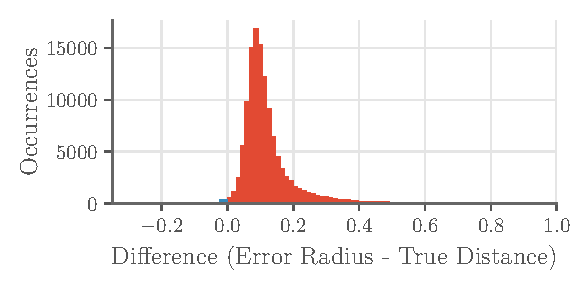
\includegraphics{figures/camera/diff_radius_true_error.pdf}
    \end{center}
    \caption[Bound Minus True Distance]{Computed radius minus actual error distance.}
    \label{fig:camera:diff bound error}
\end{figure}

\begin{figure}[htb]
    \begin{center}
        %% Creator: Matplotlib, PGF backend
%%
%% To include the figure in your LaTeX document, write
%%   \input{<filename>.pgf}
%%
%% Make sure the required packages are loaded in your preamble
%%   \usepackage{pgf}
%%
%% Figures using additional raster images can only be included by \input if
%% they are in the same directory as the main LaTeX file. For loading figures
%% from other directories you can use the `import` package
%%   \usepackage{import}
%% and then include the figures with
%%   \import{<path to file>}{<filename>.pgf}
%%
%% Matplotlib used the following preamble
%%   \usepackage{fontspec}
%%
\begingroup%
\makeatletter%
\begin{pgfpicture}%
\pgfpathrectangle{\pgfpointorigin}{\pgfqpoint{3.900000in}{1.899485in}}%
\pgfusepath{use as bounding box, clip}%
\begin{pgfscope}%
\pgfsetbuttcap%
\pgfsetmiterjoin%
\definecolor{currentfill}{rgb}{1.000000,1.000000,1.000000}%
\pgfsetfillcolor{currentfill}%
\pgfsetlinewidth{0.000000pt}%
\definecolor{currentstroke}{rgb}{1.000000,1.000000,1.000000}%
\pgfsetstrokecolor{currentstroke}%
\pgfsetdash{}{0pt}%
\pgfpathmoveto{\pgfqpoint{0.000000in}{0.000000in}}%
\pgfpathlineto{\pgfqpoint{3.900000in}{0.000000in}}%
\pgfpathlineto{\pgfqpoint{3.900000in}{1.899485in}}%
\pgfpathlineto{\pgfqpoint{0.000000in}{1.899485in}}%
\pgfpathclose%
\pgfusepath{fill}%
\end{pgfscope}%
\begin{pgfscope}%
\pgfsetbuttcap%
\pgfsetmiterjoin%
\definecolor{currentfill}{rgb}{1.000000,1.000000,1.000000}%
\pgfsetfillcolor{currentfill}%
\pgfsetlinewidth{0.000000pt}%
\definecolor{currentstroke}{rgb}{0.000000,0.000000,0.000000}%
\pgfsetstrokecolor{currentstroke}%
\pgfsetstrokeopacity{0.000000}%
\pgfsetdash{}{0pt}%
\pgfpathmoveto{\pgfqpoint{0.678556in}{0.525778in}}%
\pgfpathlineto{\pgfqpoint{3.676543in}{0.525778in}}%
\pgfpathlineto{\pgfqpoint{3.676543in}{1.749299in}}%
\pgfpathlineto{\pgfqpoint{0.678556in}{1.749299in}}%
\pgfpathclose%
\pgfusepath{fill}%
\end{pgfscope}%
\begin{pgfscope}%
\pgfpathrectangle{\pgfqpoint{0.678556in}{0.525778in}}{\pgfqpoint{2.997987in}{1.223521in}} %
\pgfusepath{clip}%
\pgfsetrectcap%
\pgfsetroundjoin%
\pgfsetlinewidth{0.803000pt}%
\definecolor{currentstroke}{rgb}{0.900000,0.900000,0.900000}%
\pgfsetstrokecolor{currentstroke}%
\pgfsetdash{}{0pt}%
\pgfpathmoveto{\pgfqpoint{0.678556in}{0.525778in}}%
\pgfpathlineto{\pgfqpoint{0.678556in}{1.749299in}}%
\pgfusepath{stroke}%
\end{pgfscope}%
\begin{pgfscope}%
\pgfsetbuttcap%
\pgfsetroundjoin%
\definecolor{currentfill}{rgb}{0.333333,0.333333,0.333333}%
\pgfsetfillcolor{currentfill}%
\pgfsetlinewidth{0.803000pt}%
\definecolor{currentstroke}{rgb}{0.333333,0.333333,0.333333}%
\pgfsetstrokecolor{currentstroke}%
\pgfsetdash{}{0pt}%
\pgfsys@defobject{currentmarker}{\pgfqpoint{0.000000in}{-0.048611in}}{\pgfqpoint{0.000000in}{0.000000in}}{%
\pgfpathmoveto{\pgfqpoint{0.000000in}{0.000000in}}%
\pgfpathlineto{\pgfqpoint{0.000000in}{-0.048611in}}%
\pgfusepath{stroke,fill}%
}%
\begin{pgfscope}%
\pgfsys@transformshift{0.678556in}{0.525778in}%
\pgfsys@useobject{currentmarker}{}%
\end{pgfscope}%
\end{pgfscope}%
\begin{pgfscope}%
\definecolor{textcolor}{rgb}{0.333333,0.333333,0.333333}%
\pgfsetstrokecolor{textcolor}%
\pgfsetfillcolor{textcolor}%
\pgftext[x=0.678556in,y=0.428555in,,top]{\color{textcolor}\rmfamily\fontsize{10.000000}{12.000000}\selectfont \(\displaystyle 0.00\)}%
\end{pgfscope}%
\begin{pgfscope}%
\pgfpathrectangle{\pgfqpoint{0.678556in}{0.525778in}}{\pgfqpoint{2.997987in}{1.223521in}} %
\pgfusepath{clip}%
\pgfsetrectcap%
\pgfsetroundjoin%
\pgfsetlinewidth{0.803000pt}%
\definecolor{currentstroke}{rgb}{0.900000,0.900000,0.900000}%
\pgfsetstrokecolor{currentstroke}%
\pgfsetdash{}{0pt}%
\pgfpathmoveto{\pgfqpoint{1.178221in}{0.525778in}}%
\pgfpathlineto{\pgfqpoint{1.178221in}{1.749299in}}%
\pgfusepath{stroke}%
\end{pgfscope}%
\begin{pgfscope}%
\pgfsetbuttcap%
\pgfsetroundjoin%
\definecolor{currentfill}{rgb}{0.333333,0.333333,0.333333}%
\pgfsetfillcolor{currentfill}%
\pgfsetlinewidth{0.803000pt}%
\definecolor{currentstroke}{rgb}{0.333333,0.333333,0.333333}%
\pgfsetstrokecolor{currentstroke}%
\pgfsetdash{}{0pt}%
\pgfsys@defobject{currentmarker}{\pgfqpoint{0.000000in}{-0.048611in}}{\pgfqpoint{0.000000in}{0.000000in}}{%
\pgfpathmoveto{\pgfqpoint{0.000000in}{0.000000in}}%
\pgfpathlineto{\pgfqpoint{0.000000in}{-0.048611in}}%
\pgfusepath{stroke,fill}%
}%
\begin{pgfscope}%
\pgfsys@transformshift{1.178221in}{0.525778in}%
\pgfsys@useobject{currentmarker}{}%
\end{pgfscope}%
\end{pgfscope}%
\begin{pgfscope}%
\definecolor{textcolor}{rgb}{0.333333,0.333333,0.333333}%
\pgfsetstrokecolor{textcolor}%
\pgfsetfillcolor{textcolor}%
\pgftext[x=1.178221in,y=0.428555in,,top]{\color{textcolor}\rmfamily\fontsize{10.000000}{12.000000}\selectfont \(\displaystyle 0.25\)}%
\end{pgfscope}%
\begin{pgfscope}%
\pgfpathrectangle{\pgfqpoint{0.678556in}{0.525778in}}{\pgfqpoint{2.997987in}{1.223521in}} %
\pgfusepath{clip}%
\pgfsetrectcap%
\pgfsetroundjoin%
\pgfsetlinewidth{0.803000pt}%
\definecolor{currentstroke}{rgb}{0.900000,0.900000,0.900000}%
\pgfsetstrokecolor{currentstroke}%
\pgfsetdash{}{0pt}%
\pgfpathmoveto{\pgfqpoint{1.677885in}{0.525778in}}%
\pgfpathlineto{\pgfqpoint{1.677885in}{1.749299in}}%
\pgfusepath{stroke}%
\end{pgfscope}%
\begin{pgfscope}%
\pgfsetbuttcap%
\pgfsetroundjoin%
\definecolor{currentfill}{rgb}{0.333333,0.333333,0.333333}%
\pgfsetfillcolor{currentfill}%
\pgfsetlinewidth{0.803000pt}%
\definecolor{currentstroke}{rgb}{0.333333,0.333333,0.333333}%
\pgfsetstrokecolor{currentstroke}%
\pgfsetdash{}{0pt}%
\pgfsys@defobject{currentmarker}{\pgfqpoint{0.000000in}{-0.048611in}}{\pgfqpoint{0.000000in}{0.000000in}}{%
\pgfpathmoveto{\pgfqpoint{0.000000in}{0.000000in}}%
\pgfpathlineto{\pgfqpoint{0.000000in}{-0.048611in}}%
\pgfusepath{stroke,fill}%
}%
\begin{pgfscope}%
\pgfsys@transformshift{1.677885in}{0.525778in}%
\pgfsys@useobject{currentmarker}{}%
\end{pgfscope}%
\end{pgfscope}%
\begin{pgfscope}%
\definecolor{textcolor}{rgb}{0.333333,0.333333,0.333333}%
\pgfsetstrokecolor{textcolor}%
\pgfsetfillcolor{textcolor}%
\pgftext[x=1.677885in,y=0.428555in,,top]{\color{textcolor}\rmfamily\fontsize{10.000000}{12.000000}\selectfont \(\displaystyle 0.50\)}%
\end{pgfscope}%
\begin{pgfscope}%
\pgfpathrectangle{\pgfqpoint{0.678556in}{0.525778in}}{\pgfqpoint{2.997987in}{1.223521in}} %
\pgfusepath{clip}%
\pgfsetrectcap%
\pgfsetroundjoin%
\pgfsetlinewidth{0.803000pt}%
\definecolor{currentstroke}{rgb}{0.900000,0.900000,0.900000}%
\pgfsetstrokecolor{currentstroke}%
\pgfsetdash{}{0pt}%
\pgfpathmoveto{\pgfqpoint{2.177550in}{0.525778in}}%
\pgfpathlineto{\pgfqpoint{2.177550in}{1.749299in}}%
\pgfusepath{stroke}%
\end{pgfscope}%
\begin{pgfscope}%
\pgfsetbuttcap%
\pgfsetroundjoin%
\definecolor{currentfill}{rgb}{0.333333,0.333333,0.333333}%
\pgfsetfillcolor{currentfill}%
\pgfsetlinewidth{0.803000pt}%
\definecolor{currentstroke}{rgb}{0.333333,0.333333,0.333333}%
\pgfsetstrokecolor{currentstroke}%
\pgfsetdash{}{0pt}%
\pgfsys@defobject{currentmarker}{\pgfqpoint{0.000000in}{-0.048611in}}{\pgfqpoint{0.000000in}{0.000000in}}{%
\pgfpathmoveto{\pgfqpoint{0.000000in}{0.000000in}}%
\pgfpathlineto{\pgfqpoint{0.000000in}{-0.048611in}}%
\pgfusepath{stroke,fill}%
}%
\begin{pgfscope}%
\pgfsys@transformshift{2.177550in}{0.525778in}%
\pgfsys@useobject{currentmarker}{}%
\end{pgfscope}%
\end{pgfscope}%
\begin{pgfscope}%
\definecolor{textcolor}{rgb}{0.333333,0.333333,0.333333}%
\pgfsetstrokecolor{textcolor}%
\pgfsetfillcolor{textcolor}%
\pgftext[x=2.177550in,y=0.428555in,,top]{\color{textcolor}\rmfamily\fontsize{10.000000}{12.000000}\selectfont \(\displaystyle 0.75\)}%
\end{pgfscope}%
\begin{pgfscope}%
\pgfpathrectangle{\pgfqpoint{0.678556in}{0.525778in}}{\pgfqpoint{2.997987in}{1.223521in}} %
\pgfusepath{clip}%
\pgfsetrectcap%
\pgfsetroundjoin%
\pgfsetlinewidth{0.803000pt}%
\definecolor{currentstroke}{rgb}{0.900000,0.900000,0.900000}%
\pgfsetstrokecolor{currentstroke}%
\pgfsetdash{}{0pt}%
\pgfpathmoveto{\pgfqpoint{2.677214in}{0.525778in}}%
\pgfpathlineto{\pgfqpoint{2.677214in}{1.749299in}}%
\pgfusepath{stroke}%
\end{pgfscope}%
\begin{pgfscope}%
\pgfsetbuttcap%
\pgfsetroundjoin%
\definecolor{currentfill}{rgb}{0.333333,0.333333,0.333333}%
\pgfsetfillcolor{currentfill}%
\pgfsetlinewidth{0.803000pt}%
\definecolor{currentstroke}{rgb}{0.333333,0.333333,0.333333}%
\pgfsetstrokecolor{currentstroke}%
\pgfsetdash{}{0pt}%
\pgfsys@defobject{currentmarker}{\pgfqpoint{0.000000in}{-0.048611in}}{\pgfqpoint{0.000000in}{0.000000in}}{%
\pgfpathmoveto{\pgfqpoint{0.000000in}{0.000000in}}%
\pgfpathlineto{\pgfqpoint{0.000000in}{-0.048611in}}%
\pgfusepath{stroke,fill}%
}%
\begin{pgfscope}%
\pgfsys@transformshift{2.677214in}{0.525778in}%
\pgfsys@useobject{currentmarker}{}%
\end{pgfscope}%
\end{pgfscope}%
\begin{pgfscope}%
\definecolor{textcolor}{rgb}{0.333333,0.333333,0.333333}%
\pgfsetstrokecolor{textcolor}%
\pgfsetfillcolor{textcolor}%
\pgftext[x=2.677214in,y=0.428555in,,top]{\color{textcolor}\rmfamily\fontsize{10.000000}{12.000000}\selectfont \(\displaystyle 1.00\)}%
\end{pgfscope}%
\begin{pgfscope}%
\pgfpathrectangle{\pgfqpoint{0.678556in}{0.525778in}}{\pgfqpoint{2.997987in}{1.223521in}} %
\pgfusepath{clip}%
\pgfsetrectcap%
\pgfsetroundjoin%
\pgfsetlinewidth{0.803000pt}%
\definecolor{currentstroke}{rgb}{0.900000,0.900000,0.900000}%
\pgfsetstrokecolor{currentstroke}%
\pgfsetdash{}{0pt}%
\pgfpathmoveto{\pgfqpoint{3.176878in}{0.525778in}}%
\pgfpathlineto{\pgfqpoint{3.176878in}{1.749299in}}%
\pgfusepath{stroke}%
\end{pgfscope}%
\begin{pgfscope}%
\pgfsetbuttcap%
\pgfsetroundjoin%
\definecolor{currentfill}{rgb}{0.333333,0.333333,0.333333}%
\pgfsetfillcolor{currentfill}%
\pgfsetlinewidth{0.803000pt}%
\definecolor{currentstroke}{rgb}{0.333333,0.333333,0.333333}%
\pgfsetstrokecolor{currentstroke}%
\pgfsetdash{}{0pt}%
\pgfsys@defobject{currentmarker}{\pgfqpoint{0.000000in}{-0.048611in}}{\pgfqpoint{0.000000in}{0.000000in}}{%
\pgfpathmoveto{\pgfqpoint{0.000000in}{0.000000in}}%
\pgfpathlineto{\pgfqpoint{0.000000in}{-0.048611in}}%
\pgfusepath{stroke,fill}%
}%
\begin{pgfscope}%
\pgfsys@transformshift{3.176878in}{0.525778in}%
\pgfsys@useobject{currentmarker}{}%
\end{pgfscope}%
\end{pgfscope}%
\begin{pgfscope}%
\definecolor{textcolor}{rgb}{0.333333,0.333333,0.333333}%
\pgfsetstrokecolor{textcolor}%
\pgfsetfillcolor{textcolor}%
\pgftext[x=3.176878in,y=0.428555in,,top]{\color{textcolor}\rmfamily\fontsize{10.000000}{12.000000}\selectfont \(\displaystyle 1.25\)}%
\end{pgfscope}%
\begin{pgfscope}%
\pgfpathrectangle{\pgfqpoint{0.678556in}{0.525778in}}{\pgfqpoint{2.997987in}{1.223521in}} %
\pgfusepath{clip}%
\pgfsetrectcap%
\pgfsetroundjoin%
\pgfsetlinewidth{0.803000pt}%
\definecolor{currentstroke}{rgb}{0.900000,0.900000,0.900000}%
\pgfsetstrokecolor{currentstroke}%
\pgfsetdash{}{0pt}%
\pgfpathmoveto{\pgfqpoint{3.676543in}{0.525778in}}%
\pgfpathlineto{\pgfqpoint{3.676543in}{1.749299in}}%
\pgfusepath{stroke}%
\end{pgfscope}%
\begin{pgfscope}%
\pgfsetbuttcap%
\pgfsetroundjoin%
\definecolor{currentfill}{rgb}{0.333333,0.333333,0.333333}%
\pgfsetfillcolor{currentfill}%
\pgfsetlinewidth{0.803000pt}%
\definecolor{currentstroke}{rgb}{0.333333,0.333333,0.333333}%
\pgfsetstrokecolor{currentstroke}%
\pgfsetdash{}{0pt}%
\pgfsys@defobject{currentmarker}{\pgfqpoint{0.000000in}{-0.048611in}}{\pgfqpoint{0.000000in}{0.000000in}}{%
\pgfpathmoveto{\pgfqpoint{0.000000in}{0.000000in}}%
\pgfpathlineto{\pgfqpoint{0.000000in}{-0.048611in}}%
\pgfusepath{stroke,fill}%
}%
\begin{pgfscope}%
\pgfsys@transformshift{3.676543in}{0.525778in}%
\pgfsys@useobject{currentmarker}{}%
\end{pgfscope}%
\end{pgfscope}%
\begin{pgfscope}%
\definecolor{textcolor}{rgb}{0.333333,0.333333,0.333333}%
\pgfsetstrokecolor{textcolor}%
\pgfsetfillcolor{textcolor}%
\pgftext[x=3.676543in,y=0.428555in,,top]{\color{textcolor}\rmfamily\fontsize{10.000000}{12.000000}\selectfont \(\displaystyle 1.50\)}%
\end{pgfscope}%
\begin{pgfscope}%
\definecolor{textcolor}{rgb}{0.333333,0.333333,0.333333}%
\pgfsetstrokecolor{textcolor}%
\pgfsetfillcolor{textcolor}%
\pgftext[x=2.177550in,y=0.249667in,,top]{\color{textcolor}\rmfamily\fontsize{12.000000}{14.400000}\selectfont True Error as a Proportion of Error Radius}%
\end{pgfscope}%
\begin{pgfscope}%
\pgfpathrectangle{\pgfqpoint{0.678556in}{0.525778in}}{\pgfqpoint{2.997987in}{1.223521in}} %
\pgfusepath{clip}%
\pgfsetrectcap%
\pgfsetroundjoin%
\pgfsetlinewidth{0.803000pt}%
\definecolor{currentstroke}{rgb}{0.900000,0.900000,0.900000}%
\pgfsetstrokecolor{currentstroke}%
\pgfsetdash{}{0pt}%
\pgfpathmoveto{\pgfqpoint{0.678556in}{0.525778in}}%
\pgfpathlineto{\pgfqpoint{3.676543in}{0.525778in}}%
\pgfusepath{stroke}%
\end{pgfscope}%
\begin{pgfscope}%
\pgfsetbuttcap%
\pgfsetroundjoin%
\definecolor{currentfill}{rgb}{0.333333,0.333333,0.333333}%
\pgfsetfillcolor{currentfill}%
\pgfsetlinewidth{0.803000pt}%
\definecolor{currentstroke}{rgb}{0.333333,0.333333,0.333333}%
\pgfsetstrokecolor{currentstroke}%
\pgfsetdash{}{0pt}%
\pgfsys@defobject{currentmarker}{\pgfqpoint{-0.048611in}{0.000000in}}{\pgfqpoint{0.000000in}{0.000000in}}{%
\pgfpathmoveto{\pgfqpoint{0.000000in}{0.000000in}}%
\pgfpathlineto{\pgfqpoint{-0.048611in}{0.000000in}}%
\pgfusepath{stroke,fill}%
}%
\begin{pgfscope}%
\pgfsys@transformshift{0.678556in}{0.525778in}%
\pgfsys@useobject{currentmarker}{}%
\end{pgfscope}%
\end{pgfscope}%
\begin{pgfscope}%
\definecolor{textcolor}{rgb}{0.333333,0.333333,0.333333}%
\pgfsetstrokecolor{textcolor}%
\pgfsetfillcolor{textcolor}%
\pgftext[x=0.511889in,y=0.477583in,left,base]{\color{textcolor}\rmfamily\fontsize{10.000000}{12.000000}\selectfont \(\displaystyle 0\)}%
\end{pgfscope}%
\begin{pgfscope}%
\pgfpathrectangle{\pgfqpoint{0.678556in}{0.525778in}}{\pgfqpoint{2.997987in}{1.223521in}} %
\pgfusepath{clip}%
\pgfsetrectcap%
\pgfsetroundjoin%
\pgfsetlinewidth{0.803000pt}%
\definecolor{currentstroke}{rgb}{0.900000,0.900000,0.900000}%
\pgfsetstrokecolor{currentstroke}%
\pgfsetdash{}{0pt}%
\pgfpathmoveto{\pgfqpoint{0.678556in}{0.934282in}}%
\pgfpathlineto{\pgfqpoint{3.676543in}{0.934282in}}%
\pgfusepath{stroke}%
\end{pgfscope}%
\begin{pgfscope}%
\pgfsetbuttcap%
\pgfsetroundjoin%
\definecolor{currentfill}{rgb}{0.333333,0.333333,0.333333}%
\pgfsetfillcolor{currentfill}%
\pgfsetlinewidth{0.803000pt}%
\definecolor{currentstroke}{rgb}{0.333333,0.333333,0.333333}%
\pgfsetstrokecolor{currentstroke}%
\pgfsetdash{}{0pt}%
\pgfsys@defobject{currentmarker}{\pgfqpoint{-0.048611in}{0.000000in}}{\pgfqpoint{0.000000in}{0.000000in}}{%
\pgfpathmoveto{\pgfqpoint{0.000000in}{0.000000in}}%
\pgfpathlineto{\pgfqpoint{-0.048611in}{0.000000in}}%
\pgfusepath{stroke,fill}%
}%
\begin{pgfscope}%
\pgfsys@transformshift{0.678556in}{0.934282in}%
\pgfsys@useobject{currentmarker}{}%
\end{pgfscope}%
\end{pgfscope}%
\begin{pgfscope}%
\definecolor{textcolor}{rgb}{0.333333,0.333333,0.333333}%
\pgfsetstrokecolor{textcolor}%
\pgfsetfillcolor{textcolor}%
\pgftext[x=0.303555in,y=0.886087in,left,base]{\color{textcolor}\rmfamily\fontsize{10.000000}{12.000000}\selectfont \(\displaystyle 2000\)}%
\end{pgfscope}%
\begin{pgfscope}%
\pgfpathrectangle{\pgfqpoint{0.678556in}{0.525778in}}{\pgfqpoint{2.997987in}{1.223521in}} %
\pgfusepath{clip}%
\pgfsetrectcap%
\pgfsetroundjoin%
\pgfsetlinewidth{0.803000pt}%
\definecolor{currentstroke}{rgb}{0.900000,0.900000,0.900000}%
\pgfsetstrokecolor{currentstroke}%
\pgfsetdash{}{0pt}%
\pgfpathmoveto{\pgfqpoint{0.678556in}{1.342786in}}%
\pgfpathlineto{\pgfqpoint{3.676543in}{1.342786in}}%
\pgfusepath{stroke}%
\end{pgfscope}%
\begin{pgfscope}%
\pgfsetbuttcap%
\pgfsetroundjoin%
\definecolor{currentfill}{rgb}{0.333333,0.333333,0.333333}%
\pgfsetfillcolor{currentfill}%
\pgfsetlinewidth{0.803000pt}%
\definecolor{currentstroke}{rgb}{0.333333,0.333333,0.333333}%
\pgfsetstrokecolor{currentstroke}%
\pgfsetdash{}{0pt}%
\pgfsys@defobject{currentmarker}{\pgfqpoint{-0.048611in}{0.000000in}}{\pgfqpoint{0.000000in}{0.000000in}}{%
\pgfpathmoveto{\pgfqpoint{0.000000in}{0.000000in}}%
\pgfpathlineto{\pgfqpoint{-0.048611in}{0.000000in}}%
\pgfusepath{stroke,fill}%
}%
\begin{pgfscope}%
\pgfsys@transformshift{0.678556in}{1.342786in}%
\pgfsys@useobject{currentmarker}{}%
\end{pgfscope}%
\end{pgfscope}%
\begin{pgfscope}%
\definecolor{textcolor}{rgb}{0.333333,0.333333,0.333333}%
\pgfsetstrokecolor{textcolor}%
\pgfsetfillcolor{textcolor}%
\pgftext[x=0.303555in,y=1.294592in,left,base]{\color{textcolor}\rmfamily\fontsize{10.000000}{12.000000}\selectfont \(\displaystyle 4000\)}%
\end{pgfscope}%
\begin{pgfscope}%
\pgfpathrectangle{\pgfqpoint{0.678556in}{0.525778in}}{\pgfqpoint{2.997987in}{1.223521in}} %
\pgfusepath{clip}%
\pgfsetrectcap%
\pgfsetroundjoin%
\pgfsetlinewidth{0.803000pt}%
\definecolor{currentstroke}{rgb}{0.900000,0.900000,0.900000}%
\pgfsetstrokecolor{currentstroke}%
\pgfsetdash{}{0pt}%
\pgfpathmoveto{\pgfqpoint{0.678556in}{1.751290in}}%
\pgfpathlineto{\pgfqpoint{3.676543in}{1.751290in}}%
\pgfusepath{stroke}%
\end{pgfscope}%
\begin{pgfscope}%
\pgfsetbuttcap%
\pgfsetroundjoin%
\definecolor{currentfill}{rgb}{0.333333,0.333333,0.333333}%
\pgfsetfillcolor{currentfill}%
\pgfsetlinewidth{0.803000pt}%
\definecolor{currentstroke}{rgb}{0.333333,0.333333,0.333333}%
\pgfsetstrokecolor{currentstroke}%
\pgfsetdash{}{0pt}%
\pgfsys@defobject{currentmarker}{\pgfqpoint{-0.048611in}{0.000000in}}{\pgfqpoint{0.000000in}{0.000000in}}{%
\pgfpathmoveto{\pgfqpoint{0.000000in}{0.000000in}}%
\pgfpathlineto{\pgfqpoint{-0.048611in}{0.000000in}}%
\pgfusepath{stroke,fill}%
}%
\begin{pgfscope}%
\pgfsys@transformshift{0.678556in}{1.751290in}%
\pgfsys@useobject{currentmarker}{}%
\end{pgfscope}%
\end{pgfscope}%
\begin{pgfscope}%
\definecolor{textcolor}{rgb}{0.333333,0.333333,0.333333}%
\pgfsetstrokecolor{textcolor}%
\pgfsetfillcolor{textcolor}%
\pgftext[x=0.303555in,y=1.703096in,left,base]{\color{textcolor}\rmfamily\fontsize{10.000000}{12.000000}\selectfont \(\displaystyle 6000\)}%
\end{pgfscope}%
\begin{pgfscope}%
\definecolor{textcolor}{rgb}{0.333333,0.333333,0.333333}%
\pgfsetstrokecolor{textcolor}%
\pgfsetfillcolor{textcolor}%
\pgftext[x=0.248000in,y=1.137538in,,bottom,rotate=90.000000]{\color{textcolor}\rmfamily\fontsize{12.000000}{14.400000}\selectfont Occurrences}%
\end{pgfscope}%
\begin{pgfscope}%
\pgfpathrectangle{\pgfqpoint{0.678556in}{0.525778in}}{\pgfqpoint{2.997987in}{1.223521in}} %
\pgfusepath{clip}%
\pgfsetbuttcap%
\pgfsetmiterjoin%
\definecolor{currentfill}{rgb}{0.886275,0.290196,0.200000}%
\pgfsetfillcolor{currentfill}%
\pgfsetlinewidth{0.000000pt}%
\definecolor{currentstroke}{rgb}{0.000000,0.000000,0.000000}%
\pgfsetstrokecolor{currentstroke}%
\pgfsetstrokeopacity{0.000000}%
\pgfsetdash{}{0pt}%
\pgfpathmoveto{\pgfqpoint{0.680721in}{0.525778in}}%
\pgfpathlineto{\pgfqpoint{0.720646in}{0.525778in}}%
\pgfpathlineto{\pgfqpoint{0.720646in}{0.621368in}}%
\pgfpathlineto{\pgfqpoint{0.680721in}{0.621368in}}%
\pgfpathclose%
\pgfusepath{fill}%
\end{pgfscope}%
\begin{pgfscope}%
\pgfpathrectangle{\pgfqpoint{0.678556in}{0.525778in}}{\pgfqpoint{2.997987in}{1.223521in}} %
\pgfusepath{clip}%
\pgfsetbuttcap%
\pgfsetmiterjoin%
\definecolor{currentfill}{rgb}{0.886275,0.290196,0.200000}%
\pgfsetfillcolor{currentfill}%
\pgfsetlinewidth{0.000000pt}%
\definecolor{currentstroke}{rgb}{0.000000,0.000000,0.000000}%
\pgfsetstrokecolor{currentstroke}%
\pgfsetstrokeopacity{0.000000}%
\pgfsetdash{}{0pt}%
\pgfpathmoveto{\pgfqpoint{0.720646in}{0.525778in}}%
\pgfpathlineto{\pgfqpoint{0.760571in}{0.525778in}}%
\pgfpathlineto{\pgfqpoint{0.760571in}{0.799271in}}%
\pgfpathlineto{\pgfqpoint{0.720646in}{0.799271in}}%
\pgfpathclose%
\pgfusepath{fill}%
\end{pgfscope}%
\begin{pgfscope}%
\pgfpathrectangle{\pgfqpoint{0.678556in}{0.525778in}}{\pgfqpoint{2.997987in}{1.223521in}} %
\pgfusepath{clip}%
\pgfsetbuttcap%
\pgfsetmiterjoin%
\definecolor{currentfill}{rgb}{0.886275,0.290196,0.200000}%
\pgfsetfillcolor{currentfill}%
\pgfsetlinewidth{0.000000pt}%
\definecolor{currentstroke}{rgb}{0.000000,0.000000,0.000000}%
\pgfsetstrokecolor{currentstroke}%
\pgfsetstrokeopacity{0.000000}%
\pgfsetdash{}{0pt}%
\pgfpathmoveto{\pgfqpoint{0.760571in}{0.525778in}}%
\pgfpathlineto{\pgfqpoint{0.800496in}{0.525778in}}%
\pgfpathlineto{\pgfqpoint{0.800496in}{0.964307in}}%
\pgfpathlineto{\pgfqpoint{0.760571in}{0.964307in}}%
\pgfpathclose%
\pgfusepath{fill}%
\end{pgfscope}%
\begin{pgfscope}%
\pgfpathrectangle{\pgfqpoint{0.678556in}{0.525778in}}{\pgfqpoint{2.997987in}{1.223521in}} %
\pgfusepath{clip}%
\pgfsetbuttcap%
\pgfsetmiterjoin%
\definecolor{currentfill}{rgb}{0.886275,0.290196,0.200000}%
\pgfsetfillcolor{currentfill}%
\pgfsetlinewidth{0.000000pt}%
\definecolor{currentstroke}{rgb}{0.000000,0.000000,0.000000}%
\pgfsetstrokecolor{currentstroke}%
\pgfsetstrokeopacity{0.000000}%
\pgfsetdash{}{0pt}%
\pgfpathmoveto{\pgfqpoint{0.800496in}{0.525778in}}%
\pgfpathlineto{\pgfqpoint{0.840421in}{0.525778in}}%
\pgfpathlineto{\pgfqpoint{0.840421in}{1.104424in}}%
\pgfpathlineto{\pgfqpoint{0.800496in}{1.104424in}}%
\pgfpathclose%
\pgfusepath{fill}%
\end{pgfscope}%
\begin{pgfscope}%
\pgfpathrectangle{\pgfqpoint{0.678556in}{0.525778in}}{\pgfqpoint{2.997987in}{1.223521in}} %
\pgfusepath{clip}%
\pgfsetbuttcap%
\pgfsetmiterjoin%
\definecolor{currentfill}{rgb}{0.886275,0.290196,0.200000}%
\pgfsetfillcolor{currentfill}%
\pgfsetlinewidth{0.000000pt}%
\definecolor{currentstroke}{rgb}{0.000000,0.000000,0.000000}%
\pgfsetstrokecolor{currentstroke}%
\pgfsetstrokeopacity{0.000000}%
\pgfsetdash{}{0pt}%
\pgfpathmoveto{\pgfqpoint{0.840421in}{0.525778in}}%
\pgfpathlineto{\pgfqpoint{0.880347in}{0.525778in}}%
\pgfpathlineto{\pgfqpoint{0.880347in}{1.259655in}}%
\pgfpathlineto{\pgfqpoint{0.840421in}{1.259655in}}%
\pgfpathclose%
\pgfusepath{fill}%
\end{pgfscope}%
\begin{pgfscope}%
\pgfpathrectangle{\pgfqpoint{0.678556in}{0.525778in}}{\pgfqpoint{2.997987in}{1.223521in}} %
\pgfusepath{clip}%
\pgfsetbuttcap%
\pgfsetmiterjoin%
\definecolor{currentfill}{rgb}{0.886275,0.290196,0.200000}%
\pgfsetfillcolor{currentfill}%
\pgfsetlinewidth{0.000000pt}%
\definecolor{currentstroke}{rgb}{0.000000,0.000000,0.000000}%
\pgfsetstrokecolor{currentstroke}%
\pgfsetstrokeopacity{0.000000}%
\pgfsetdash{}{0pt}%
\pgfpathmoveto{\pgfqpoint{0.880347in}{0.525778in}}%
\pgfpathlineto{\pgfqpoint{0.920272in}{0.525778in}}%
\pgfpathlineto{\pgfqpoint{0.920272in}{1.367092in}}%
\pgfpathlineto{\pgfqpoint{0.880347in}{1.367092in}}%
\pgfpathclose%
\pgfusepath{fill}%
\end{pgfscope}%
\begin{pgfscope}%
\pgfpathrectangle{\pgfqpoint{0.678556in}{0.525778in}}{\pgfqpoint{2.997987in}{1.223521in}} %
\pgfusepath{clip}%
\pgfsetbuttcap%
\pgfsetmiterjoin%
\definecolor{currentfill}{rgb}{0.886275,0.290196,0.200000}%
\pgfsetfillcolor{currentfill}%
\pgfsetlinewidth{0.000000pt}%
\definecolor{currentstroke}{rgb}{0.000000,0.000000,0.000000}%
\pgfsetstrokecolor{currentstroke}%
\pgfsetstrokeopacity{0.000000}%
\pgfsetdash{}{0pt}%
\pgfpathmoveto{\pgfqpoint{0.920272in}{0.525778in}}%
\pgfpathlineto{\pgfqpoint{0.960197in}{0.525778in}}%
\pgfpathlineto{\pgfqpoint{0.960197in}{1.485558in}}%
\pgfpathlineto{\pgfqpoint{0.920272in}{1.485558in}}%
\pgfpathclose%
\pgfusepath{fill}%
\end{pgfscope}%
\begin{pgfscope}%
\pgfpathrectangle{\pgfqpoint{0.678556in}{0.525778in}}{\pgfqpoint{2.997987in}{1.223521in}} %
\pgfusepath{clip}%
\pgfsetbuttcap%
\pgfsetmiterjoin%
\definecolor{currentfill}{rgb}{0.886275,0.290196,0.200000}%
\pgfsetfillcolor{currentfill}%
\pgfsetlinewidth{0.000000pt}%
\definecolor{currentstroke}{rgb}{0.000000,0.000000,0.000000}%
\pgfsetstrokecolor{currentstroke}%
\pgfsetstrokeopacity{0.000000}%
\pgfsetdash{}{0pt}%
\pgfpathmoveto{\pgfqpoint{0.960197in}{0.525778in}}%
\pgfpathlineto{\pgfqpoint{1.000122in}{0.525778in}}%
\pgfpathlineto{\pgfqpoint{1.000122in}{1.536621in}}%
\pgfpathlineto{\pgfqpoint{0.960197in}{1.536621in}}%
\pgfpathclose%
\pgfusepath{fill}%
\end{pgfscope}%
\begin{pgfscope}%
\pgfpathrectangle{\pgfqpoint{0.678556in}{0.525778in}}{\pgfqpoint{2.997987in}{1.223521in}} %
\pgfusepath{clip}%
\pgfsetbuttcap%
\pgfsetmiterjoin%
\definecolor{currentfill}{rgb}{0.886275,0.290196,0.200000}%
\pgfsetfillcolor{currentfill}%
\pgfsetlinewidth{0.000000pt}%
\definecolor{currentstroke}{rgb}{0.000000,0.000000,0.000000}%
\pgfsetstrokecolor{currentstroke}%
\pgfsetstrokeopacity{0.000000}%
\pgfsetdash{}{0pt}%
\pgfpathmoveto{\pgfqpoint{1.000122in}{0.525778in}}%
\pgfpathlineto{\pgfqpoint{1.040047in}{0.525778in}}%
\pgfpathlineto{\pgfqpoint{1.040047in}{1.597080in}}%
\pgfpathlineto{\pgfqpoint{1.000122in}{1.597080in}}%
\pgfpathclose%
\pgfusepath{fill}%
\end{pgfscope}%
\begin{pgfscope}%
\pgfpathrectangle{\pgfqpoint{0.678556in}{0.525778in}}{\pgfqpoint{2.997987in}{1.223521in}} %
\pgfusepath{clip}%
\pgfsetbuttcap%
\pgfsetmiterjoin%
\definecolor{currentfill}{rgb}{0.886275,0.290196,0.200000}%
\pgfsetfillcolor{currentfill}%
\pgfsetlinewidth{0.000000pt}%
\definecolor{currentstroke}{rgb}{0.000000,0.000000,0.000000}%
\pgfsetstrokecolor{currentstroke}%
\pgfsetstrokeopacity{0.000000}%
\pgfsetdash{}{0pt}%
\pgfpathmoveto{\pgfqpoint{1.040047in}{0.525778in}}%
\pgfpathlineto{\pgfqpoint{1.079973in}{0.525778in}}%
\pgfpathlineto{\pgfqpoint{1.079973in}{1.623633in}}%
\pgfpathlineto{\pgfqpoint{1.040047in}{1.623633in}}%
\pgfpathclose%
\pgfusepath{fill}%
\end{pgfscope}%
\begin{pgfscope}%
\pgfpathrectangle{\pgfqpoint{0.678556in}{0.525778in}}{\pgfqpoint{2.997987in}{1.223521in}} %
\pgfusepath{clip}%
\pgfsetbuttcap%
\pgfsetmiterjoin%
\definecolor{currentfill}{rgb}{0.886275,0.290196,0.200000}%
\pgfsetfillcolor{currentfill}%
\pgfsetlinewidth{0.000000pt}%
\definecolor{currentstroke}{rgb}{0.000000,0.000000,0.000000}%
\pgfsetstrokecolor{currentstroke}%
\pgfsetstrokeopacity{0.000000}%
\pgfsetdash{}{0pt}%
\pgfpathmoveto{\pgfqpoint{1.079973in}{0.525778in}}%
\pgfpathlineto{\pgfqpoint{1.119898in}{0.525778in}}%
\pgfpathlineto{\pgfqpoint{1.119898in}{1.667547in}}%
\pgfpathlineto{\pgfqpoint{1.079973in}{1.667547in}}%
\pgfpathclose%
\pgfusepath{fill}%
\end{pgfscope}%
\begin{pgfscope}%
\pgfpathrectangle{\pgfqpoint{0.678556in}{0.525778in}}{\pgfqpoint{2.997987in}{1.223521in}} %
\pgfusepath{clip}%
\pgfsetbuttcap%
\pgfsetmiterjoin%
\definecolor{currentfill}{rgb}{0.886275,0.290196,0.200000}%
\pgfsetfillcolor{currentfill}%
\pgfsetlinewidth{0.000000pt}%
\definecolor{currentstroke}{rgb}{0.000000,0.000000,0.000000}%
\pgfsetstrokecolor{currentstroke}%
\pgfsetstrokeopacity{0.000000}%
\pgfsetdash{}{0pt}%
\pgfpathmoveto{\pgfqpoint{1.119898in}{0.525778in}}%
\pgfpathlineto{\pgfqpoint{1.159823in}{0.525778in}}%
\pgfpathlineto{\pgfqpoint{1.159823in}{1.666934in}}%
\pgfpathlineto{\pgfqpoint{1.119898in}{1.666934in}}%
\pgfpathclose%
\pgfusepath{fill}%
\end{pgfscope}%
\begin{pgfscope}%
\pgfpathrectangle{\pgfqpoint{0.678556in}{0.525778in}}{\pgfqpoint{2.997987in}{1.223521in}} %
\pgfusepath{clip}%
\pgfsetbuttcap%
\pgfsetmiterjoin%
\definecolor{currentfill}{rgb}{0.886275,0.290196,0.200000}%
\pgfsetfillcolor{currentfill}%
\pgfsetlinewidth{0.000000pt}%
\definecolor{currentstroke}{rgb}{0.000000,0.000000,0.000000}%
\pgfsetstrokecolor{currentstroke}%
\pgfsetstrokeopacity{0.000000}%
\pgfsetdash{}{0pt}%
\pgfpathmoveto{\pgfqpoint{1.159823in}{0.525778in}}%
\pgfpathlineto{\pgfqpoint{1.199748in}{0.525778in}}%
\pgfpathlineto{\pgfqpoint{1.199748in}{1.691036in}}%
\pgfpathlineto{\pgfqpoint{1.159823in}{1.691036in}}%
\pgfpathclose%
\pgfusepath{fill}%
\end{pgfscope}%
\begin{pgfscope}%
\pgfpathrectangle{\pgfqpoint{0.678556in}{0.525778in}}{\pgfqpoint{2.997987in}{1.223521in}} %
\pgfusepath{clip}%
\pgfsetbuttcap%
\pgfsetmiterjoin%
\definecolor{currentfill}{rgb}{0.886275,0.290196,0.200000}%
\pgfsetfillcolor{currentfill}%
\pgfsetlinewidth{0.000000pt}%
\definecolor{currentstroke}{rgb}{0.000000,0.000000,0.000000}%
\pgfsetstrokecolor{currentstroke}%
\pgfsetstrokeopacity{0.000000}%
\pgfsetdash{}{0pt}%
\pgfpathmoveto{\pgfqpoint{1.199748in}{0.525778in}}%
\pgfpathlineto{\pgfqpoint{1.239673in}{0.525778in}}%
\pgfpathlineto{\pgfqpoint{1.239673in}{1.638135in}}%
\pgfpathlineto{\pgfqpoint{1.199748in}{1.638135in}}%
\pgfpathclose%
\pgfusepath{fill}%
\end{pgfscope}%
\begin{pgfscope}%
\pgfpathrectangle{\pgfqpoint{0.678556in}{0.525778in}}{\pgfqpoint{2.997987in}{1.223521in}} %
\pgfusepath{clip}%
\pgfsetbuttcap%
\pgfsetmiterjoin%
\definecolor{currentfill}{rgb}{0.886275,0.290196,0.200000}%
\pgfsetfillcolor{currentfill}%
\pgfsetlinewidth{0.000000pt}%
\definecolor{currentstroke}{rgb}{0.000000,0.000000,0.000000}%
\pgfsetstrokecolor{currentstroke}%
\pgfsetstrokeopacity{0.000000}%
\pgfsetdash{}{0pt}%
\pgfpathmoveto{\pgfqpoint{1.239673in}{0.525778in}}%
\pgfpathlineto{\pgfqpoint{1.279598in}{0.525778in}}%
\pgfpathlineto{\pgfqpoint{1.279598in}{1.630577in}}%
\pgfpathlineto{\pgfqpoint{1.239673in}{1.630577in}}%
\pgfpathclose%
\pgfusepath{fill}%
\end{pgfscope}%
\begin{pgfscope}%
\pgfpathrectangle{\pgfqpoint{0.678556in}{0.525778in}}{\pgfqpoint{2.997987in}{1.223521in}} %
\pgfusepath{clip}%
\pgfsetbuttcap%
\pgfsetmiterjoin%
\definecolor{currentfill}{rgb}{0.886275,0.290196,0.200000}%
\pgfsetfillcolor{currentfill}%
\pgfsetlinewidth{0.000000pt}%
\definecolor{currentstroke}{rgb}{0.000000,0.000000,0.000000}%
\pgfsetstrokecolor{currentstroke}%
\pgfsetstrokeopacity{0.000000}%
\pgfsetdash{}{0pt}%
\pgfpathmoveto{\pgfqpoint{1.279598in}{0.525778in}}%
\pgfpathlineto{\pgfqpoint{1.319524in}{0.525778in}}%
\pgfpathlineto{\pgfqpoint{1.319524in}{1.574817in}}%
\pgfpathlineto{\pgfqpoint{1.279598in}{1.574817in}}%
\pgfpathclose%
\pgfusepath{fill}%
\end{pgfscope}%
\begin{pgfscope}%
\pgfpathrectangle{\pgfqpoint{0.678556in}{0.525778in}}{\pgfqpoint{2.997987in}{1.223521in}} %
\pgfusepath{clip}%
\pgfsetbuttcap%
\pgfsetmiterjoin%
\definecolor{currentfill}{rgb}{0.886275,0.290196,0.200000}%
\pgfsetfillcolor{currentfill}%
\pgfsetlinewidth{0.000000pt}%
\definecolor{currentstroke}{rgb}{0.000000,0.000000,0.000000}%
\pgfsetstrokecolor{currentstroke}%
\pgfsetstrokeopacity{0.000000}%
\pgfsetdash{}{0pt}%
\pgfpathmoveto{\pgfqpoint{1.319524in}{0.525778in}}%
\pgfpathlineto{\pgfqpoint{1.359449in}{0.525778in}}%
\pgfpathlineto{\pgfqpoint{1.359449in}{1.540298in}}%
\pgfpathlineto{\pgfqpoint{1.319524in}{1.540298in}}%
\pgfpathclose%
\pgfusepath{fill}%
\end{pgfscope}%
\begin{pgfscope}%
\pgfpathrectangle{\pgfqpoint{0.678556in}{0.525778in}}{\pgfqpoint{2.997987in}{1.223521in}} %
\pgfusepath{clip}%
\pgfsetbuttcap%
\pgfsetmiterjoin%
\definecolor{currentfill}{rgb}{0.886275,0.290196,0.200000}%
\pgfsetfillcolor{currentfill}%
\pgfsetlinewidth{0.000000pt}%
\definecolor{currentstroke}{rgb}{0.000000,0.000000,0.000000}%
\pgfsetstrokecolor{currentstroke}%
\pgfsetstrokeopacity{0.000000}%
\pgfsetdash{}{0pt}%
\pgfpathmoveto{\pgfqpoint{1.359449in}{0.525778in}}%
\pgfpathlineto{\pgfqpoint{1.399374in}{0.525778in}}%
\pgfpathlineto{\pgfqpoint{1.399374in}{1.465133in}}%
\pgfpathlineto{\pgfqpoint{1.359449in}{1.465133in}}%
\pgfpathclose%
\pgfusepath{fill}%
\end{pgfscope}%
\begin{pgfscope}%
\pgfpathrectangle{\pgfqpoint{0.678556in}{0.525778in}}{\pgfqpoint{2.997987in}{1.223521in}} %
\pgfusepath{clip}%
\pgfsetbuttcap%
\pgfsetmiterjoin%
\definecolor{currentfill}{rgb}{0.886275,0.290196,0.200000}%
\pgfsetfillcolor{currentfill}%
\pgfsetlinewidth{0.000000pt}%
\definecolor{currentstroke}{rgb}{0.000000,0.000000,0.000000}%
\pgfsetstrokecolor{currentstroke}%
\pgfsetstrokeopacity{0.000000}%
\pgfsetdash{}{0pt}%
\pgfpathmoveto{\pgfqpoint{1.399374in}{0.525778in}}%
\pgfpathlineto{\pgfqpoint{1.439299in}{0.525778in}}%
\pgfpathlineto{\pgfqpoint{1.439299in}{1.414479in}}%
\pgfpathlineto{\pgfqpoint{1.399374in}{1.414479in}}%
\pgfpathclose%
\pgfusepath{fill}%
\end{pgfscope}%
\begin{pgfscope}%
\pgfpathrectangle{\pgfqpoint{0.678556in}{0.525778in}}{\pgfqpoint{2.997987in}{1.223521in}} %
\pgfusepath{clip}%
\pgfsetbuttcap%
\pgfsetmiterjoin%
\definecolor{currentfill}{rgb}{0.886275,0.290196,0.200000}%
\pgfsetfillcolor{currentfill}%
\pgfsetlinewidth{0.000000pt}%
\definecolor{currentstroke}{rgb}{0.000000,0.000000,0.000000}%
\pgfsetstrokecolor{currentstroke}%
\pgfsetstrokeopacity{0.000000}%
\pgfsetdash{}{0pt}%
\pgfpathmoveto{\pgfqpoint{1.439299in}{0.525778in}}%
\pgfpathlineto{\pgfqpoint{1.479224in}{0.525778in}}%
\pgfpathlineto{\pgfqpoint{1.479224in}{1.365050in}}%
\pgfpathlineto{\pgfqpoint{1.439299in}{1.365050in}}%
\pgfpathclose%
\pgfusepath{fill}%
\end{pgfscope}%
\begin{pgfscope}%
\pgfpathrectangle{\pgfqpoint{0.678556in}{0.525778in}}{\pgfqpoint{2.997987in}{1.223521in}} %
\pgfusepath{clip}%
\pgfsetbuttcap%
\pgfsetmiterjoin%
\definecolor{currentfill}{rgb}{0.886275,0.290196,0.200000}%
\pgfsetfillcolor{currentfill}%
\pgfsetlinewidth{0.000000pt}%
\definecolor{currentstroke}{rgb}{0.000000,0.000000,0.000000}%
\pgfsetstrokecolor{currentstroke}%
\pgfsetstrokeopacity{0.000000}%
\pgfsetdash{}{0pt}%
\pgfpathmoveto{\pgfqpoint{1.479224in}{0.525778in}}%
\pgfpathlineto{\pgfqpoint{1.519150in}{0.525778in}}%
\pgfpathlineto{\pgfqpoint{1.519150in}{1.299485in}}%
\pgfpathlineto{\pgfqpoint{1.479224in}{1.299485in}}%
\pgfpathclose%
\pgfusepath{fill}%
\end{pgfscope}%
\begin{pgfscope}%
\pgfpathrectangle{\pgfqpoint{0.678556in}{0.525778in}}{\pgfqpoint{2.997987in}{1.223521in}} %
\pgfusepath{clip}%
\pgfsetbuttcap%
\pgfsetmiterjoin%
\definecolor{currentfill}{rgb}{0.886275,0.290196,0.200000}%
\pgfsetfillcolor{currentfill}%
\pgfsetlinewidth{0.000000pt}%
\definecolor{currentstroke}{rgb}{0.000000,0.000000,0.000000}%
\pgfsetstrokecolor{currentstroke}%
\pgfsetstrokeopacity{0.000000}%
\pgfsetdash{}{0pt}%
\pgfpathmoveto{\pgfqpoint{1.519150in}{0.525778in}}%
\pgfpathlineto{\pgfqpoint{1.559075in}{0.525778in}}%
\pgfpathlineto{\pgfqpoint{1.559075in}{1.233103in}}%
\pgfpathlineto{\pgfqpoint{1.519150in}{1.233103in}}%
\pgfpathclose%
\pgfusepath{fill}%
\end{pgfscope}%
\begin{pgfscope}%
\pgfpathrectangle{\pgfqpoint{0.678556in}{0.525778in}}{\pgfqpoint{2.997987in}{1.223521in}} %
\pgfusepath{clip}%
\pgfsetbuttcap%
\pgfsetmiterjoin%
\definecolor{currentfill}{rgb}{0.886275,0.290196,0.200000}%
\pgfsetfillcolor{currentfill}%
\pgfsetlinewidth{0.000000pt}%
\definecolor{currentstroke}{rgb}{0.000000,0.000000,0.000000}%
\pgfsetstrokecolor{currentstroke}%
\pgfsetstrokeopacity{0.000000}%
\pgfsetdash{}{0pt}%
\pgfpathmoveto{\pgfqpoint{1.559075in}{0.525778in}}%
\pgfpathlineto{\pgfqpoint{1.599000in}{0.525778in}}%
\pgfpathlineto{\pgfqpoint{1.599000in}{1.198380in}}%
\pgfpathlineto{\pgfqpoint{1.559075in}{1.198380in}}%
\pgfpathclose%
\pgfusepath{fill}%
\end{pgfscope}%
\begin{pgfscope}%
\pgfpathrectangle{\pgfqpoint{0.678556in}{0.525778in}}{\pgfqpoint{2.997987in}{1.223521in}} %
\pgfusepath{clip}%
\pgfsetbuttcap%
\pgfsetmiterjoin%
\definecolor{currentfill}{rgb}{0.886275,0.290196,0.200000}%
\pgfsetfillcolor{currentfill}%
\pgfsetlinewidth{0.000000pt}%
\definecolor{currentstroke}{rgb}{0.000000,0.000000,0.000000}%
\pgfsetstrokecolor{currentstroke}%
\pgfsetstrokeopacity{0.000000}%
\pgfsetdash{}{0pt}%
\pgfpathmoveto{\pgfqpoint{1.599000in}{0.525778in}}%
\pgfpathlineto{\pgfqpoint{1.638925in}{0.525778in}}%
\pgfpathlineto{\pgfqpoint{1.638925in}{1.140168in}}%
\pgfpathlineto{\pgfqpoint{1.599000in}{1.140168in}}%
\pgfpathclose%
\pgfusepath{fill}%
\end{pgfscope}%
\begin{pgfscope}%
\pgfpathrectangle{\pgfqpoint{0.678556in}{0.525778in}}{\pgfqpoint{2.997987in}{1.223521in}} %
\pgfusepath{clip}%
\pgfsetbuttcap%
\pgfsetmiterjoin%
\definecolor{currentfill}{rgb}{0.886275,0.290196,0.200000}%
\pgfsetfillcolor{currentfill}%
\pgfsetlinewidth{0.000000pt}%
\definecolor{currentstroke}{rgb}{0.000000,0.000000,0.000000}%
\pgfsetstrokecolor{currentstroke}%
\pgfsetstrokeopacity{0.000000}%
\pgfsetdash{}{0pt}%
\pgfpathmoveto{\pgfqpoint{1.638925in}{0.525778in}}%
\pgfpathlineto{\pgfqpoint{1.678850in}{0.525778in}}%
\pgfpathlineto{\pgfqpoint{1.678850in}{1.071131in}}%
\pgfpathlineto{\pgfqpoint{1.638925in}{1.071131in}}%
\pgfpathclose%
\pgfusepath{fill}%
\end{pgfscope}%
\begin{pgfscope}%
\pgfpathrectangle{\pgfqpoint{0.678556in}{0.525778in}}{\pgfqpoint{2.997987in}{1.223521in}} %
\pgfusepath{clip}%
\pgfsetbuttcap%
\pgfsetmiterjoin%
\definecolor{currentfill}{rgb}{0.886275,0.290196,0.200000}%
\pgfsetfillcolor{currentfill}%
\pgfsetlinewidth{0.000000pt}%
\definecolor{currentstroke}{rgb}{0.000000,0.000000,0.000000}%
\pgfsetstrokecolor{currentstroke}%
\pgfsetstrokeopacity{0.000000}%
\pgfsetdash{}{0pt}%
\pgfpathmoveto{\pgfqpoint{1.678850in}{0.525778in}}%
\pgfpathlineto{\pgfqpoint{1.718775in}{0.525778in}}%
\pgfpathlineto{\pgfqpoint{1.718775in}{1.021089in}}%
\pgfpathlineto{\pgfqpoint{1.678850in}{1.021089in}}%
\pgfpathclose%
\pgfusepath{fill}%
\end{pgfscope}%
\begin{pgfscope}%
\pgfpathrectangle{\pgfqpoint{0.678556in}{0.525778in}}{\pgfqpoint{2.997987in}{1.223521in}} %
\pgfusepath{clip}%
\pgfsetbuttcap%
\pgfsetmiterjoin%
\definecolor{currentfill}{rgb}{0.886275,0.290196,0.200000}%
\pgfsetfillcolor{currentfill}%
\pgfsetlinewidth{0.000000pt}%
\definecolor{currentstroke}{rgb}{0.000000,0.000000,0.000000}%
\pgfsetstrokecolor{currentstroke}%
\pgfsetstrokeopacity{0.000000}%
\pgfsetdash{}{0pt}%
\pgfpathmoveto{\pgfqpoint{1.718775in}{0.525778in}}%
\pgfpathlineto{\pgfqpoint{1.758701in}{0.525778in}}%
\pgfpathlineto{\pgfqpoint{1.758701in}{0.977583in}}%
\pgfpathlineto{\pgfqpoint{1.718775in}{0.977583in}}%
\pgfpathclose%
\pgfusepath{fill}%
\end{pgfscope}%
\begin{pgfscope}%
\pgfpathrectangle{\pgfqpoint{0.678556in}{0.525778in}}{\pgfqpoint{2.997987in}{1.223521in}} %
\pgfusepath{clip}%
\pgfsetbuttcap%
\pgfsetmiterjoin%
\definecolor{currentfill}{rgb}{0.886275,0.290196,0.200000}%
\pgfsetfillcolor{currentfill}%
\pgfsetlinewidth{0.000000pt}%
\definecolor{currentstroke}{rgb}{0.000000,0.000000,0.000000}%
\pgfsetstrokecolor{currentstroke}%
\pgfsetstrokeopacity{0.000000}%
\pgfsetdash{}{0pt}%
\pgfpathmoveto{\pgfqpoint{1.758701in}{0.525778in}}%
\pgfpathlineto{\pgfqpoint{1.798626in}{0.525778in}}%
\pgfpathlineto{\pgfqpoint{1.798626in}{0.931218in}}%
\pgfpathlineto{\pgfqpoint{1.758701in}{0.931218in}}%
\pgfpathclose%
\pgfusepath{fill}%
\end{pgfscope}%
\begin{pgfscope}%
\pgfpathrectangle{\pgfqpoint{0.678556in}{0.525778in}}{\pgfqpoint{2.997987in}{1.223521in}} %
\pgfusepath{clip}%
\pgfsetbuttcap%
\pgfsetmiterjoin%
\definecolor{currentfill}{rgb}{0.886275,0.290196,0.200000}%
\pgfsetfillcolor{currentfill}%
\pgfsetlinewidth{0.000000pt}%
\definecolor{currentstroke}{rgb}{0.000000,0.000000,0.000000}%
\pgfsetstrokecolor{currentstroke}%
\pgfsetstrokeopacity{0.000000}%
\pgfsetdash{}{0pt}%
\pgfpathmoveto{\pgfqpoint{1.798626in}{0.525778in}}%
\pgfpathlineto{\pgfqpoint{1.838551in}{0.525778in}}%
\pgfpathlineto{\pgfqpoint{1.838551in}{0.892819in}}%
\pgfpathlineto{\pgfqpoint{1.798626in}{0.892819in}}%
\pgfpathclose%
\pgfusepath{fill}%
\end{pgfscope}%
\begin{pgfscope}%
\pgfpathrectangle{\pgfqpoint{0.678556in}{0.525778in}}{\pgfqpoint{2.997987in}{1.223521in}} %
\pgfusepath{clip}%
\pgfsetbuttcap%
\pgfsetmiterjoin%
\definecolor{currentfill}{rgb}{0.886275,0.290196,0.200000}%
\pgfsetfillcolor{currentfill}%
\pgfsetlinewidth{0.000000pt}%
\definecolor{currentstroke}{rgb}{0.000000,0.000000,0.000000}%
\pgfsetstrokecolor{currentstroke}%
\pgfsetstrokeopacity{0.000000}%
\pgfsetdash{}{0pt}%
\pgfpathmoveto{\pgfqpoint{1.838551in}{0.525778in}}%
\pgfpathlineto{\pgfqpoint{1.878476in}{0.525778in}}%
\pgfpathlineto{\pgfqpoint{1.878476in}{0.858913in}}%
\pgfpathlineto{\pgfqpoint{1.838551in}{0.858913in}}%
\pgfpathclose%
\pgfusepath{fill}%
\end{pgfscope}%
\begin{pgfscope}%
\pgfpathrectangle{\pgfqpoint{0.678556in}{0.525778in}}{\pgfqpoint{2.997987in}{1.223521in}} %
\pgfusepath{clip}%
\pgfsetbuttcap%
\pgfsetmiterjoin%
\definecolor{currentfill}{rgb}{0.886275,0.290196,0.200000}%
\pgfsetfillcolor{currentfill}%
\pgfsetlinewidth{0.000000pt}%
\definecolor{currentstroke}{rgb}{0.000000,0.000000,0.000000}%
\pgfsetstrokecolor{currentstroke}%
\pgfsetstrokeopacity{0.000000}%
\pgfsetdash{}{0pt}%
\pgfpathmoveto{\pgfqpoint{1.878476in}{0.525778in}}%
\pgfpathlineto{\pgfqpoint{1.918401in}{0.525778in}}%
\pgfpathlineto{\pgfqpoint{1.918401in}{0.828888in}}%
\pgfpathlineto{\pgfqpoint{1.878476in}{0.828888in}}%
\pgfpathclose%
\pgfusepath{fill}%
\end{pgfscope}%
\begin{pgfscope}%
\pgfpathrectangle{\pgfqpoint{0.678556in}{0.525778in}}{\pgfqpoint{2.997987in}{1.223521in}} %
\pgfusepath{clip}%
\pgfsetbuttcap%
\pgfsetmiterjoin%
\definecolor{currentfill}{rgb}{0.886275,0.290196,0.200000}%
\pgfsetfillcolor{currentfill}%
\pgfsetlinewidth{0.000000pt}%
\definecolor{currentstroke}{rgb}{0.000000,0.000000,0.000000}%
\pgfsetstrokecolor{currentstroke}%
\pgfsetstrokeopacity{0.000000}%
\pgfsetdash{}{0pt}%
\pgfpathmoveto{\pgfqpoint{1.918401in}{0.525778in}}%
\pgfpathlineto{\pgfqpoint{1.958326in}{0.525778in}}%
\pgfpathlineto{\pgfqpoint{1.958326in}{0.809075in}}%
\pgfpathlineto{\pgfqpoint{1.918401in}{0.809075in}}%
\pgfpathclose%
\pgfusepath{fill}%
\end{pgfscope}%
\begin{pgfscope}%
\pgfpathrectangle{\pgfqpoint{0.678556in}{0.525778in}}{\pgfqpoint{2.997987in}{1.223521in}} %
\pgfusepath{clip}%
\pgfsetbuttcap%
\pgfsetmiterjoin%
\definecolor{currentfill}{rgb}{0.886275,0.290196,0.200000}%
\pgfsetfillcolor{currentfill}%
\pgfsetlinewidth{0.000000pt}%
\definecolor{currentstroke}{rgb}{0.000000,0.000000,0.000000}%
\pgfsetstrokecolor{currentstroke}%
\pgfsetstrokeopacity{0.000000}%
\pgfsetdash{}{0pt}%
\pgfpathmoveto{\pgfqpoint{1.958326in}{0.525778in}}%
\pgfpathlineto{\pgfqpoint{1.998252in}{0.525778in}}%
\pgfpathlineto{\pgfqpoint{1.998252in}{0.776191in}}%
\pgfpathlineto{\pgfqpoint{1.958326in}{0.776191in}}%
\pgfpathclose%
\pgfusepath{fill}%
\end{pgfscope}%
\begin{pgfscope}%
\pgfpathrectangle{\pgfqpoint{0.678556in}{0.525778in}}{\pgfqpoint{2.997987in}{1.223521in}} %
\pgfusepath{clip}%
\pgfsetbuttcap%
\pgfsetmiterjoin%
\definecolor{currentfill}{rgb}{0.886275,0.290196,0.200000}%
\pgfsetfillcolor{currentfill}%
\pgfsetlinewidth{0.000000pt}%
\definecolor{currentstroke}{rgb}{0.000000,0.000000,0.000000}%
\pgfsetstrokecolor{currentstroke}%
\pgfsetstrokeopacity{0.000000}%
\pgfsetdash{}{0pt}%
\pgfpathmoveto{\pgfqpoint{1.998252in}{0.525778in}}%
\pgfpathlineto{\pgfqpoint{2.038177in}{0.525778in}}%
\pgfpathlineto{\pgfqpoint{2.038177in}{0.733502in}}%
\pgfpathlineto{\pgfqpoint{1.998252in}{0.733502in}}%
\pgfpathclose%
\pgfusepath{fill}%
\end{pgfscope}%
\begin{pgfscope}%
\pgfpathrectangle{\pgfqpoint{0.678556in}{0.525778in}}{\pgfqpoint{2.997987in}{1.223521in}} %
\pgfusepath{clip}%
\pgfsetbuttcap%
\pgfsetmiterjoin%
\definecolor{currentfill}{rgb}{0.886275,0.290196,0.200000}%
\pgfsetfillcolor{currentfill}%
\pgfsetlinewidth{0.000000pt}%
\definecolor{currentstroke}{rgb}{0.000000,0.000000,0.000000}%
\pgfsetstrokecolor{currentstroke}%
\pgfsetstrokeopacity{0.000000}%
\pgfsetdash{}{0pt}%
\pgfpathmoveto{\pgfqpoint{2.038177in}{0.525778in}}%
\pgfpathlineto{\pgfqpoint{2.078102in}{0.525778in}}%
\pgfpathlineto{\pgfqpoint{2.078102in}{0.724719in}}%
\pgfpathlineto{\pgfqpoint{2.038177in}{0.724719in}}%
\pgfpathclose%
\pgfusepath{fill}%
\end{pgfscope}%
\begin{pgfscope}%
\pgfpathrectangle{\pgfqpoint{0.678556in}{0.525778in}}{\pgfqpoint{2.997987in}{1.223521in}} %
\pgfusepath{clip}%
\pgfsetbuttcap%
\pgfsetmiterjoin%
\definecolor{currentfill}{rgb}{0.886275,0.290196,0.200000}%
\pgfsetfillcolor{currentfill}%
\pgfsetlinewidth{0.000000pt}%
\definecolor{currentstroke}{rgb}{0.000000,0.000000,0.000000}%
\pgfsetstrokecolor{currentstroke}%
\pgfsetstrokeopacity{0.000000}%
\pgfsetdash{}{0pt}%
\pgfpathmoveto{\pgfqpoint{2.078102in}{0.525778in}}%
\pgfpathlineto{\pgfqpoint{2.118027in}{0.525778in}}%
\pgfpathlineto{\pgfqpoint{2.118027in}{0.697554in}}%
\pgfpathlineto{\pgfqpoint{2.078102in}{0.697554in}}%
\pgfpathclose%
\pgfusepath{fill}%
\end{pgfscope}%
\begin{pgfscope}%
\pgfpathrectangle{\pgfqpoint{0.678556in}{0.525778in}}{\pgfqpoint{2.997987in}{1.223521in}} %
\pgfusepath{clip}%
\pgfsetbuttcap%
\pgfsetmiterjoin%
\definecolor{currentfill}{rgb}{0.886275,0.290196,0.200000}%
\pgfsetfillcolor{currentfill}%
\pgfsetlinewidth{0.000000pt}%
\definecolor{currentstroke}{rgb}{0.000000,0.000000,0.000000}%
\pgfsetstrokecolor{currentstroke}%
\pgfsetstrokeopacity{0.000000}%
\pgfsetdash{}{0pt}%
\pgfpathmoveto{\pgfqpoint{2.118027in}{0.525778in}}%
\pgfpathlineto{\pgfqpoint{2.157952in}{0.525778in}}%
\pgfpathlineto{\pgfqpoint{2.157952in}{0.679375in}}%
\pgfpathlineto{\pgfqpoint{2.118027in}{0.679375in}}%
\pgfpathclose%
\pgfusepath{fill}%
\end{pgfscope}%
\begin{pgfscope}%
\pgfpathrectangle{\pgfqpoint{0.678556in}{0.525778in}}{\pgfqpoint{2.997987in}{1.223521in}} %
\pgfusepath{clip}%
\pgfsetbuttcap%
\pgfsetmiterjoin%
\definecolor{currentfill}{rgb}{0.886275,0.290196,0.200000}%
\pgfsetfillcolor{currentfill}%
\pgfsetlinewidth{0.000000pt}%
\definecolor{currentstroke}{rgb}{0.000000,0.000000,0.000000}%
\pgfsetstrokecolor{currentstroke}%
\pgfsetstrokeopacity{0.000000}%
\pgfsetdash{}{0pt}%
\pgfpathmoveto{\pgfqpoint{2.157952in}{0.525778in}}%
\pgfpathlineto{\pgfqpoint{2.197878in}{0.525778in}}%
\pgfpathlineto{\pgfqpoint{2.197878in}{0.662014in}}%
\pgfpathlineto{\pgfqpoint{2.157952in}{0.662014in}}%
\pgfpathclose%
\pgfusepath{fill}%
\end{pgfscope}%
\begin{pgfscope}%
\pgfpathrectangle{\pgfqpoint{0.678556in}{0.525778in}}{\pgfqpoint{2.997987in}{1.223521in}} %
\pgfusepath{clip}%
\pgfsetbuttcap%
\pgfsetmiterjoin%
\definecolor{currentfill}{rgb}{0.886275,0.290196,0.200000}%
\pgfsetfillcolor{currentfill}%
\pgfsetlinewidth{0.000000pt}%
\definecolor{currentstroke}{rgb}{0.000000,0.000000,0.000000}%
\pgfsetstrokecolor{currentstroke}%
\pgfsetstrokeopacity{0.000000}%
\pgfsetdash{}{0pt}%
\pgfpathmoveto{\pgfqpoint{2.197878in}{0.525778in}}%
\pgfpathlineto{\pgfqpoint{2.237803in}{0.525778in}}%
\pgfpathlineto{\pgfqpoint{2.237803in}{0.649963in}}%
\pgfpathlineto{\pgfqpoint{2.197878in}{0.649963in}}%
\pgfpathclose%
\pgfusepath{fill}%
\end{pgfscope}%
\begin{pgfscope}%
\pgfpathrectangle{\pgfqpoint{0.678556in}{0.525778in}}{\pgfqpoint{2.997987in}{1.223521in}} %
\pgfusepath{clip}%
\pgfsetbuttcap%
\pgfsetmiterjoin%
\definecolor{currentfill}{rgb}{0.886275,0.290196,0.200000}%
\pgfsetfillcolor{currentfill}%
\pgfsetlinewidth{0.000000pt}%
\definecolor{currentstroke}{rgb}{0.000000,0.000000,0.000000}%
\pgfsetstrokecolor{currentstroke}%
\pgfsetstrokeopacity{0.000000}%
\pgfsetdash{}{0pt}%
\pgfpathmoveto{\pgfqpoint{2.237803in}{0.525778in}}%
\pgfpathlineto{\pgfqpoint{2.277728in}{0.525778in}}%
\pgfpathlineto{\pgfqpoint{2.277728in}{0.628108in}}%
\pgfpathlineto{\pgfqpoint{2.237803in}{0.628108in}}%
\pgfpathclose%
\pgfusepath{fill}%
\end{pgfscope}%
\begin{pgfscope}%
\pgfpathrectangle{\pgfqpoint{0.678556in}{0.525778in}}{\pgfqpoint{2.997987in}{1.223521in}} %
\pgfusepath{clip}%
\pgfsetbuttcap%
\pgfsetmiterjoin%
\definecolor{currentfill}{rgb}{0.886275,0.290196,0.200000}%
\pgfsetfillcolor{currentfill}%
\pgfsetlinewidth{0.000000pt}%
\definecolor{currentstroke}{rgb}{0.000000,0.000000,0.000000}%
\pgfsetstrokecolor{currentstroke}%
\pgfsetstrokeopacity{0.000000}%
\pgfsetdash{}{0pt}%
\pgfpathmoveto{\pgfqpoint{2.277728in}{0.525778in}}%
\pgfpathlineto{\pgfqpoint{2.317653in}{0.525778in}}%
\pgfpathlineto{\pgfqpoint{2.317653in}{0.614219in}}%
\pgfpathlineto{\pgfqpoint{2.277728in}{0.614219in}}%
\pgfpathclose%
\pgfusepath{fill}%
\end{pgfscope}%
\begin{pgfscope}%
\pgfpathrectangle{\pgfqpoint{0.678556in}{0.525778in}}{\pgfqpoint{2.997987in}{1.223521in}} %
\pgfusepath{clip}%
\pgfsetbuttcap%
\pgfsetmiterjoin%
\definecolor{currentfill}{rgb}{0.886275,0.290196,0.200000}%
\pgfsetfillcolor{currentfill}%
\pgfsetlinewidth{0.000000pt}%
\definecolor{currentstroke}{rgb}{0.000000,0.000000,0.000000}%
\pgfsetstrokecolor{currentstroke}%
\pgfsetstrokeopacity{0.000000}%
\pgfsetdash{}{0pt}%
\pgfpathmoveto{\pgfqpoint{2.317653in}{0.525778in}}%
\pgfpathlineto{\pgfqpoint{2.357578in}{0.525778in}}%
\pgfpathlineto{\pgfqpoint{2.357578in}{0.605436in}}%
\pgfpathlineto{\pgfqpoint{2.317653in}{0.605436in}}%
\pgfpathclose%
\pgfusepath{fill}%
\end{pgfscope}%
\begin{pgfscope}%
\pgfpathrectangle{\pgfqpoint{0.678556in}{0.525778in}}{\pgfqpoint{2.997987in}{1.223521in}} %
\pgfusepath{clip}%
\pgfsetbuttcap%
\pgfsetmiterjoin%
\definecolor{currentfill}{rgb}{0.886275,0.290196,0.200000}%
\pgfsetfillcolor{currentfill}%
\pgfsetlinewidth{0.000000pt}%
\definecolor{currentstroke}{rgb}{0.000000,0.000000,0.000000}%
\pgfsetstrokecolor{currentstroke}%
\pgfsetstrokeopacity{0.000000}%
\pgfsetdash{}{0pt}%
\pgfpathmoveto{\pgfqpoint{2.357578in}{0.525778in}}%
\pgfpathlineto{\pgfqpoint{2.397503in}{0.525778in}}%
\pgfpathlineto{\pgfqpoint{2.397503in}{0.592159in}}%
\pgfpathlineto{\pgfqpoint{2.357578in}{0.592159in}}%
\pgfpathclose%
\pgfusepath{fill}%
\end{pgfscope}%
\begin{pgfscope}%
\pgfpathrectangle{\pgfqpoint{0.678556in}{0.525778in}}{\pgfqpoint{2.997987in}{1.223521in}} %
\pgfusepath{clip}%
\pgfsetbuttcap%
\pgfsetmiterjoin%
\definecolor{currentfill}{rgb}{0.886275,0.290196,0.200000}%
\pgfsetfillcolor{currentfill}%
\pgfsetlinewidth{0.000000pt}%
\definecolor{currentstroke}{rgb}{0.000000,0.000000,0.000000}%
\pgfsetstrokecolor{currentstroke}%
\pgfsetstrokeopacity{0.000000}%
\pgfsetdash{}{0pt}%
\pgfpathmoveto{\pgfqpoint{2.397503in}{0.525778in}}%
\pgfpathlineto{\pgfqpoint{2.437429in}{0.525778in}}%
\pgfpathlineto{\pgfqpoint{2.437429in}{0.591547in}}%
\pgfpathlineto{\pgfqpoint{2.397503in}{0.591547in}}%
\pgfpathclose%
\pgfusepath{fill}%
\end{pgfscope}%
\begin{pgfscope}%
\pgfpathrectangle{\pgfqpoint{0.678556in}{0.525778in}}{\pgfqpoint{2.997987in}{1.223521in}} %
\pgfusepath{clip}%
\pgfsetbuttcap%
\pgfsetmiterjoin%
\definecolor{currentfill}{rgb}{0.886275,0.290196,0.200000}%
\pgfsetfillcolor{currentfill}%
\pgfsetlinewidth{0.000000pt}%
\definecolor{currentstroke}{rgb}{0.000000,0.000000,0.000000}%
\pgfsetstrokecolor{currentstroke}%
\pgfsetstrokeopacity{0.000000}%
\pgfsetdash{}{0pt}%
\pgfpathmoveto{\pgfqpoint{2.437429in}{0.525778in}}%
\pgfpathlineto{\pgfqpoint{2.477354in}{0.525778in}}%
\pgfpathlineto{\pgfqpoint{2.477354in}{0.574594in}}%
\pgfpathlineto{\pgfqpoint{2.437429in}{0.574594in}}%
\pgfpathclose%
\pgfusepath{fill}%
\end{pgfscope}%
\begin{pgfscope}%
\pgfpathrectangle{\pgfqpoint{0.678556in}{0.525778in}}{\pgfqpoint{2.997987in}{1.223521in}} %
\pgfusepath{clip}%
\pgfsetbuttcap%
\pgfsetmiterjoin%
\definecolor{currentfill}{rgb}{0.886275,0.290196,0.200000}%
\pgfsetfillcolor{currentfill}%
\pgfsetlinewidth{0.000000pt}%
\definecolor{currentstroke}{rgb}{0.000000,0.000000,0.000000}%
\pgfsetstrokecolor{currentstroke}%
\pgfsetstrokeopacity{0.000000}%
\pgfsetdash{}{0pt}%
\pgfpathmoveto{\pgfqpoint{2.477354in}{0.525778in}}%
\pgfpathlineto{\pgfqpoint{2.517279in}{0.525778in}}%
\pgfpathlineto{\pgfqpoint{2.517279in}{0.576228in}}%
\pgfpathlineto{\pgfqpoint{2.477354in}{0.576228in}}%
\pgfpathclose%
\pgfusepath{fill}%
\end{pgfscope}%
\begin{pgfscope}%
\pgfpathrectangle{\pgfqpoint{0.678556in}{0.525778in}}{\pgfqpoint{2.997987in}{1.223521in}} %
\pgfusepath{clip}%
\pgfsetbuttcap%
\pgfsetmiterjoin%
\definecolor{currentfill}{rgb}{0.886275,0.290196,0.200000}%
\pgfsetfillcolor{currentfill}%
\pgfsetlinewidth{0.000000pt}%
\definecolor{currentstroke}{rgb}{0.000000,0.000000,0.000000}%
\pgfsetstrokecolor{currentstroke}%
\pgfsetstrokeopacity{0.000000}%
\pgfsetdash{}{0pt}%
\pgfpathmoveto{\pgfqpoint{2.517279in}{0.525778in}}%
\pgfpathlineto{\pgfqpoint{2.557204in}{0.525778in}}%
\pgfpathlineto{\pgfqpoint{2.557204in}{0.571938in}}%
\pgfpathlineto{\pgfqpoint{2.517279in}{0.571938in}}%
\pgfpathclose%
\pgfusepath{fill}%
\end{pgfscope}%
\begin{pgfscope}%
\pgfpathrectangle{\pgfqpoint{0.678556in}{0.525778in}}{\pgfqpoint{2.997987in}{1.223521in}} %
\pgfusepath{clip}%
\pgfsetbuttcap%
\pgfsetmiterjoin%
\definecolor{currentfill}{rgb}{0.886275,0.290196,0.200000}%
\pgfsetfillcolor{currentfill}%
\pgfsetlinewidth{0.000000pt}%
\definecolor{currentstroke}{rgb}{0.000000,0.000000,0.000000}%
\pgfsetstrokecolor{currentstroke}%
\pgfsetstrokeopacity{0.000000}%
\pgfsetdash{}{0pt}%
\pgfpathmoveto{\pgfqpoint{2.557204in}{0.525778in}}%
\pgfpathlineto{\pgfqpoint{2.597129in}{0.525778in}}%
\pgfpathlineto{\pgfqpoint{2.597129in}{0.564790in}}%
\pgfpathlineto{\pgfqpoint{2.557204in}{0.564790in}}%
\pgfpathclose%
\pgfusepath{fill}%
\end{pgfscope}%
\begin{pgfscope}%
\pgfpathrectangle{\pgfqpoint{0.678556in}{0.525778in}}{\pgfqpoint{2.997987in}{1.223521in}} %
\pgfusepath{clip}%
\pgfsetbuttcap%
\pgfsetmiterjoin%
\definecolor{currentfill}{rgb}{0.886275,0.290196,0.200000}%
\pgfsetfillcolor{currentfill}%
\pgfsetlinewidth{0.000000pt}%
\definecolor{currentstroke}{rgb}{0.000000,0.000000,0.000000}%
\pgfsetstrokecolor{currentstroke}%
\pgfsetstrokeopacity{0.000000}%
\pgfsetdash{}{0pt}%
\pgfpathmoveto{\pgfqpoint{2.597129in}{0.525778in}}%
\pgfpathlineto{\pgfqpoint{2.637054in}{0.525778in}}%
\pgfpathlineto{\pgfqpoint{2.637054in}{0.561113in}}%
\pgfpathlineto{\pgfqpoint{2.597129in}{0.561113in}}%
\pgfpathclose%
\pgfusepath{fill}%
\end{pgfscope}%
\begin{pgfscope}%
\pgfpathrectangle{\pgfqpoint{0.678556in}{0.525778in}}{\pgfqpoint{2.997987in}{1.223521in}} %
\pgfusepath{clip}%
\pgfsetbuttcap%
\pgfsetmiterjoin%
\definecolor{currentfill}{rgb}{0.886275,0.290196,0.200000}%
\pgfsetfillcolor{currentfill}%
\pgfsetlinewidth{0.000000pt}%
\definecolor{currentstroke}{rgb}{0.000000,0.000000,0.000000}%
\pgfsetstrokecolor{currentstroke}%
\pgfsetstrokeopacity{0.000000}%
\pgfsetdash{}{0pt}%
\pgfpathmoveto{\pgfqpoint{2.637054in}{0.525778in}}%
\pgfpathlineto{\pgfqpoint{2.676980in}{0.525778in}}%
\pgfpathlineto{\pgfqpoint{2.676980in}{0.554169in}}%
\pgfpathlineto{\pgfqpoint{2.637054in}{0.554169in}}%
\pgfpathclose%
\pgfusepath{fill}%
\end{pgfscope}%
\begin{pgfscope}%
\pgfpathrectangle{\pgfqpoint{0.678556in}{0.525778in}}{\pgfqpoint{2.997987in}{1.223521in}} %
\pgfusepath{clip}%
\pgfsetbuttcap%
\pgfsetmiterjoin%
\definecolor{currentfill}{rgb}{0.203922,0.541176,0.741176}%
\pgfsetfillcolor{currentfill}%
\pgfsetlinewidth{0.000000pt}%
\definecolor{currentstroke}{rgb}{0.000000,0.000000,0.000000}%
\pgfsetstrokecolor{currentstroke}%
\pgfsetstrokeopacity{0.000000}%
\pgfsetdash{}{0pt}%
\pgfpathmoveto{\pgfqpoint{2.677595in}{0.525778in}}%
\pgfpathlineto{\pgfqpoint{2.730476in}{0.525778in}}%
\pgfpathlineto{\pgfqpoint{2.730476in}{0.557437in}}%
\pgfpathlineto{\pgfqpoint{2.677595in}{0.557437in}}%
\pgfpathclose%
\pgfusepath{fill}%
\end{pgfscope}%
\begin{pgfscope}%
\pgfpathrectangle{\pgfqpoint{0.678556in}{0.525778in}}{\pgfqpoint{2.997987in}{1.223521in}} %
\pgfusepath{clip}%
\pgfsetbuttcap%
\pgfsetmiterjoin%
\definecolor{currentfill}{rgb}{0.203922,0.541176,0.741176}%
\pgfsetfillcolor{currentfill}%
\pgfsetlinewidth{0.000000pt}%
\definecolor{currentstroke}{rgb}{0.000000,0.000000,0.000000}%
\pgfsetstrokecolor{currentstroke}%
\pgfsetstrokeopacity{0.000000}%
\pgfsetdash{}{0pt}%
\pgfpathmoveto{\pgfqpoint{2.730476in}{0.525778in}}%
\pgfpathlineto{\pgfqpoint{2.783357in}{0.525778in}}%
\pgfpathlineto{\pgfqpoint{2.783357in}{0.549675in}}%
\pgfpathlineto{\pgfqpoint{2.730476in}{0.549675in}}%
\pgfpathclose%
\pgfusepath{fill}%
\end{pgfscope}%
\begin{pgfscope}%
\pgfpathrectangle{\pgfqpoint{0.678556in}{0.525778in}}{\pgfqpoint{2.997987in}{1.223521in}} %
\pgfusepath{clip}%
\pgfsetbuttcap%
\pgfsetmiterjoin%
\definecolor{currentfill}{rgb}{0.203922,0.541176,0.741176}%
\pgfsetfillcolor{currentfill}%
\pgfsetlinewidth{0.000000pt}%
\definecolor{currentstroke}{rgb}{0.000000,0.000000,0.000000}%
\pgfsetstrokecolor{currentstroke}%
\pgfsetstrokeopacity{0.000000}%
\pgfsetdash{}{0pt}%
\pgfpathmoveto{\pgfqpoint{2.783357in}{0.525778in}}%
\pgfpathlineto{\pgfqpoint{2.836238in}{0.525778in}}%
\pgfpathlineto{\pgfqpoint{2.836238in}{0.547020in}}%
\pgfpathlineto{\pgfqpoint{2.783357in}{0.547020in}}%
\pgfpathclose%
\pgfusepath{fill}%
\end{pgfscope}%
\begin{pgfscope}%
\pgfpathrectangle{\pgfqpoint{0.678556in}{0.525778in}}{\pgfqpoint{2.997987in}{1.223521in}} %
\pgfusepath{clip}%
\pgfsetbuttcap%
\pgfsetmiterjoin%
\definecolor{currentfill}{rgb}{0.203922,0.541176,0.741176}%
\pgfsetfillcolor{currentfill}%
\pgfsetlinewidth{0.000000pt}%
\definecolor{currentstroke}{rgb}{0.000000,0.000000,0.000000}%
\pgfsetstrokecolor{currentstroke}%
\pgfsetstrokeopacity{0.000000}%
\pgfsetdash{}{0pt}%
\pgfpathmoveto{\pgfqpoint{2.836238in}{0.525778in}}%
\pgfpathlineto{\pgfqpoint{2.889120in}{0.525778in}}%
\pgfpathlineto{\pgfqpoint{2.889120in}{0.543956in}}%
\pgfpathlineto{\pgfqpoint{2.836238in}{0.543956in}}%
\pgfpathclose%
\pgfusepath{fill}%
\end{pgfscope}%
\begin{pgfscope}%
\pgfpathrectangle{\pgfqpoint{0.678556in}{0.525778in}}{\pgfqpoint{2.997987in}{1.223521in}} %
\pgfusepath{clip}%
\pgfsetbuttcap%
\pgfsetmiterjoin%
\definecolor{currentfill}{rgb}{0.203922,0.541176,0.741176}%
\pgfsetfillcolor{currentfill}%
\pgfsetlinewidth{0.000000pt}%
\definecolor{currentstroke}{rgb}{0.000000,0.000000,0.000000}%
\pgfsetstrokecolor{currentstroke}%
\pgfsetstrokeopacity{0.000000}%
\pgfsetdash{}{0pt}%
\pgfpathmoveto{\pgfqpoint{2.889120in}{0.525778in}}%
\pgfpathlineto{\pgfqpoint{2.942001in}{0.525778in}}%
\pgfpathlineto{\pgfqpoint{2.942001in}{0.539462in}}%
\pgfpathlineto{\pgfqpoint{2.889120in}{0.539462in}}%
\pgfpathclose%
\pgfusepath{fill}%
\end{pgfscope}%
\begin{pgfscope}%
\pgfpathrectangle{\pgfqpoint{0.678556in}{0.525778in}}{\pgfqpoint{2.997987in}{1.223521in}} %
\pgfusepath{clip}%
\pgfsetbuttcap%
\pgfsetmiterjoin%
\definecolor{currentfill}{rgb}{0.203922,0.541176,0.741176}%
\pgfsetfillcolor{currentfill}%
\pgfsetlinewidth{0.000000pt}%
\definecolor{currentstroke}{rgb}{0.000000,0.000000,0.000000}%
\pgfsetstrokecolor{currentstroke}%
\pgfsetstrokeopacity{0.000000}%
\pgfsetdash{}{0pt}%
\pgfpathmoveto{\pgfqpoint{2.942001in}{0.525778in}}%
\pgfpathlineto{\pgfqpoint{2.994882in}{0.525778in}}%
\pgfpathlineto{\pgfqpoint{2.994882in}{0.538033in}}%
\pgfpathlineto{\pgfqpoint{2.942001in}{0.538033in}}%
\pgfpathclose%
\pgfusepath{fill}%
\end{pgfscope}%
\begin{pgfscope}%
\pgfpathrectangle{\pgfqpoint{0.678556in}{0.525778in}}{\pgfqpoint{2.997987in}{1.223521in}} %
\pgfusepath{clip}%
\pgfsetbuttcap%
\pgfsetmiterjoin%
\definecolor{currentfill}{rgb}{0.203922,0.541176,0.741176}%
\pgfsetfillcolor{currentfill}%
\pgfsetlinewidth{0.000000pt}%
\definecolor{currentstroke}{rgb}{0.000000,0.000000,0.000000}%
\pgfsetstrokecolor{currentstroke}%
\pgfsetstrokeopacity{0.000000}%
\pgfsetdash{}{0pt}%
\pgfpathmoveto{\pgfqpoint{2.994882in}{0.525778in}}%
\pgfpathlineto{\pgfqpoint{3.047763in}{0.525778in}}%
\pgfpathlineto{\pgfqpoint{3.047763in}{0.534560in}}%
\pgfpathlineto{\pgfqpoint{2.994882in}{0.534560in}}%
\pgfpathclose%
\pgfusepath{fill}%
\end{pgfscope}%
\begin{pgfscope}%
\pgfpathrectangle{\pgfqpoint{0.678556in}{0.525778in}}{\pgfqpoint{2.997987in}{1.223521in}} %
\pgfusepath{clip}%
\pgfsetbuttcap%
\pgfsetmiterjoin%
\definecolor{currentfill}{rgb}{0.203922,0.541176,0.741176}%
\pgfsetfillcolor{currentfill}%
\pgfsetlinewidth{0.000000pt}%
\definecolor{currentstroke}{rgb}{0.000000,0.000000,0.000000}%
\pgfsetstrokecolor{currentstroke}%
\pgfsetstrokeopacity{0.000000}%
\pgfsetdash{}{0pt}%
\pgfpathmoveto{\pgfqpoint{3.047763in}{0.525778in}}%
\pgfpathlineto{\pgfqpoint{3.100645in}{0.525778in}}%
\pgfpathlineto{\pgfqpoint{3.100645in}{0.534765in}}%
\pgfpathlineto{\pgfqpoint{3.047763in}{0.534765in}}%
\pgfpathclose%
\pgfusepath{fill}%
\end{pgfscope}%
\begin{pgfscope}%
\pgfpathrectangle{\pgfqpoint{0.678556in}{0.525778in}}{\pgfqpoint{2.997987in}{1.223521in}} %
\pgfusepath{clip}%
\pgfsetbuttcap%
\pgfsetmiterjoin%
\definecolor{currentfill}{rgb}{0.203922,0.541176,0.741176}%
\pgfsetfillcolor{currentfill}%
\pgfsetlinewidth{0.000000pt}%
\definecolor{currentstroke}{rgb}{0.000000,0.000000,0.000000}%
\pgfsetstrokecolor{currentstroke}%
\pgfsetstrokeopacity{0.000000}%
\pgfsetdash{}{0pt}%
\pgfpathmoveto{\pgfqpoint{3.100645in}{0.525778in}}%
\pgfpathlineto{\pgfqpoint{3.153526in}{0.525778in}}%
\pgfpathlineto{\pgfqpoint{3.153526in}{0.533743in}}%
\pgfpathlineto{\pgfqpoint{3.100645in}{0.533743in}}%
\pgfpathclose%
\pgfusepath{fill}%
\end{pgfscope}%
\begin{pgfscope}%
\pgfpathrectangle{\pgfqpoint{0.678556in}{0.525778in}}{\pgfqpoint{2.997987in}{1.223521in}} %
\pgfusepath{clip}%
\pgfsetbuttcap%
\pgfsetmiterjoin%
\definecolor{currentfill}{rgb}{0.203922,0.541176,0.741176}%
\pgfsetfillcolor{currentfill}%
\pgfsetlinewidth{0.000000pt}%
\definecolor{currentstroke}{rgb}{0.000000,0.000000,0.000000}%
\pgfsetstrokecolor{currentstroke}%
\pgfsetstrokeopacity{0.000000}%
\pgfsetdash{}{0pt}%
\pgfpathmoveto{\pgfqpoint{3.153526in}{0.525778in}}%
\pgfpathlineto{\pgfqpoint{3.206407in}{0.525778in}}%
\pgfpathlineto{\pgfqpoint{3.206407in}{0.530475in}}%
\pgfpathlineto{\pgfqpoint{3.153526in}{0.530475in}}%
\pgfpathclose%
\pgfusepath{fill}%
\end{pgfscope}%
\begin{pgfscope}%
\pgfpathrectangle{\pgfqpoint{0.678556in}{0.525778in}}{\pgfqpoint{2.997987in}{1.223521in}} %
\pgfusepath{clip}%
\pgfsetbuttcap%
\pgfsetmiterjoin%
\definecolor{currentfill}{rgb}{0.203922,0.541176,0.741176}%
\pgfsetfillcolor{currentfill}%
\pgfsetlinewidth{0.000000pt}%
\definecolor{currentstroke}{rgb}{0.000000,0.000000,0.000000}%
\pgfsetstrokecolor{currentstroke}%
\pgfsetstrokeopacity{0.000000}%
\pgfsetdash{}{0pt}%
\pgfpathmoveto{\pgfqpoint{3.206407in}{0.525778in}}%
\pgfpathlineto{\pgfqpoint{3.259288in}{0.525778in}}%
\pgfpathlineto{\pgfqpoint{3.259288in}{0.529658in}}%
\pgfpathlineto{\pgfqpoint{3.206407in}{0.529658in}}%
\pgfpathclose%
\pgfusepath{fill}%
\end{pgfscope}%
\begin{pgfscope}%
\pgfpathrectangle{\pgfqpoint{0.678556in}{0.525778in}}{\pgfqpoint{2.997987in}{1.223521in}} %
\pgfusepath{clip}%
\pgfsetbuttcap%
\pgfsetmiterjoin%
\definecolor{currentfill}{rgb}{0.203922,0.541176,0.741176}%
\pgfsetfillcolor{currentfill}%
\pgfsetlinewidth{0.000000pt}%
\definecolor{currentstroke}{rgb}{0.000000,0.000000,0.000000}%
\pgfsetstrokecolor{currentstroke}%
\pgfsetstrokeopacity{0.000000}%
\pgfsetdash{}{0pt}%
\pgfpathmoveto{\pgfqpoint{3.259288in}{0.525778in}}%
\pgfpathlineto{\pgfqpoint{3.312170in}{0.525778in}}%
\pgfpathlineto{\pgfqpoint{3.312170in}{0.529658in}}%
\pgfpathlineto{\pgfqpoint{3.259288in}{0.529658in}}%
\pgfpathclose%
\pgfusepath{fill}%
\end{pgfscope}%
\begin{pgfscope}%
\pgfpathrectangle{\pgfqpoint{0.678556in}{0.525778in}}{\pgfqpoint{2.997987in}{1.223521in}} %
\pgfusepath{clip}%
\pgfsetbuttcap%
\pgfsetmiterjoin%
\definecolor{currentfill}{rgb}{0.203922,0.541176,0.741176}%
\pgfsetfillcolor{currentfill}%
\pgfsetlinewidth{0.000000pt}%
\definecolor{currentstroke}{rgb}{0.000000,0.000000,0.000000}%
\pgfsetstrokecolor{currentstroke}%
\pgfsetstrokeopacity{0.000000}%
\pgfsetdash{}{0pt}%
\pgfpathmoveto{\pgfqpoint{3.312170in}{0.525778in}}%
\pgfpathlineto{\pgfqpoint{3.365051in}{0.525778in}}%
\pgfpathlineto{\pgfqpoint{3.365051in}{0.529658in}}%
\pgfpathlineto{\pgfqpoint{3.312170in}{0.529658in}}%
\pgfpathclose%
\pgfusepath{fill}%
\end{pgfscope}%
\begin{pgfscope}%
\pgfpathrectangle{\pgfqpoint{0.678556in}{0.525778in}}{\pgfqpoint{2.997987in}{1.223521in}} %
\pgfusepath{clip}%
\pgfsetbuttcap%
\pgfsetmiterjoin%
\definecolor{currentfill}{rgb}{0.203922,0.541176,0.741176}%
\pgfsetfillcolor{currentfill}%
\pgfsetlinewidth{0.000000pt}%
\definecolor{currentstroke}{rgb}{0.000000,0.000000,0.000000}%
\pgfsetstrokecolor{currentstroke}%
\pgfsetstrokeopacity{0.000000}%
\pgfsetdash{}{0pt}%
\pgfpathmoveto{\pgfqpoint{3.365051in}{0.525778in}}%
\pgfpathlineto{\pgfqpoint{3.417932in}{0.525778in}}%
\pgfpathlineto{\pgfqpoint{3.417932in}{0.528637in}}%
\pgfpathlineto{\pgfqpoint{3.365051in}{0.528637in}}%
\pgfpathclose%
\pgfusepath{fill}%
\end{pgfscope}%
\begin{pgfscope}%
\pgfpathrectangle{\pgfqpoint{0.678556in}{0.525778in}}{\pgfqpoint{2.997987in}{1.223521in}} %
\pgfusepath{clip}%
\pgfsetbuttcap%
\pgfsetmiterjoin%
\definecolor{currentfill}{rgb}{0.203922,0.541176,0.741176}%
\pgfsetfillcolor{currentfill}%
\pgfsetlinewidth{0.000000pt}%
\definecolor{currentstroke}{rgb}{0.000000,0.000000,0.000000}%
\pgfsetstrokecolor{currentstroke}%
\pgfsetstrokeopacity{0.000000}%
\pgfsetdash{}{0pt}%
\pgfpathmoveto{\pgfqpoint{3.417932in}{0.525778in}}%
\pgfpathlineto{\pgfqpoint{3.470813in}{0.525778in}}%
\pgfpathlineto{\pgfqpoint{3.470813in}{0.528229in}}%
\pgfpathlineto{\pgfqpoint{3.417932in}{0.528229in}}%
\pgfpathclose%
\pgfusepath{fill}%
\end{pgfscope}%
\begin{pgfscope}%
\pgfpathrectangle{\pgfqpoint{0.678556in}{0.525778in}}{\pgfqpoint{2.997987in}{1.223521in}} %
\pgfusepath{clip}%
\pgfsetbuttcap%
\pgfsetmiterjoin%
\definecolor{currentfill}{rgb}{0.203922,0.541176,0.741176}%
\pgfsetfillcolor{currentfill}%
\pgfsetlinewidth{0.000000pt}%
\definecolor{currentstroke}{rgb}{0.000000,0.000000,0.000000}%
\pgfsetstrokecolor{currentstroke}%
\pgfsetstrokeopacity{0.000000}%
\pgfsetdash{}{0pt}%
\pgfpathmoveto{\pgfqpoint{3.470813in}{0.525778in}}%
\pgfpathlineto{\pgfqpoint{3.523695in}{0.525778in}}%
\pgfpathlineto{\pgfqpoint{3.523695in}{0.528637in}}%
\pgfpathlineto{\pgfqpoint{3.470813in}{0.528637in}}%
\pgfpathclose%
\pgfusepath{fill}%
\end{pgfscope}%
\begin{pgfscope}%
\pgfpathrectangle{\pgfqpoint{0.678556in}{0.525778in}}{\pgfqpoint{2.997987in}{1.223521in}} %
\pgfusepath{clip}%
\pgfsetbuttcap%
\pgfsetmiterjoin%
\definecolor{currentfill}{rgb}{0.203922,0.541176,0.741176}%
\pgfsetfillcolor{currentfill}%
\pgfsetlinewidth{0.000000pt}%
\definecolor{currentstroke}{rgb}{0.000000,0.000000,0.000000}%
\pgfsetstrokecolor{currentstroke}%
\pgfsetstrokeopacity{0.000000}%
\pgfsetdash{}{0pt}%
\pgfpathmoveto{\pgfqpoint{3.523695in}{0.525778in}}%
\pgfpathlineto{\pgfqpoint{3.576576in}{0.525778in}}%
\pgfpathlineto{\pgfqpoint{3.576576in}{0.527820in}}%
\pgfpathlineto{\pgfqpoint{3.523695in}{0.527820in}}%
\pgfpathclose%
\pgfusepath{fill}%
\end{pgfscope}%
\begin{pgfscope}%
\pgfpathrectangle{\pgfqpoint{0.678556in}{0.525778in}}{\pgfqpoint{2.997987in}{1.223521in}} %
\pgfusepath{clip}%
\pgfsetbuttcap%
\pgfsetmiterjoin%
\definecolor{currentfill}{rgb}{0.203922,0.541176,0.741176}%
\pgfsetfillcolor{currentfill}%
\pgfsetlinewidth{0.000000pt}%
\definecolor{currentstroke}{rgb}{0.000000,0.000000,0.000000}%
\pgfsetstrokecolor{currentstroke}%
\pgfsetstrokeopacity{0.000000}%
\pgfsetdash{}{0pt}%
\pgfpathmoveto{\pgfqpoint{3.576576in}{0.525778in}}%
\pgfpathlineto{\pgfqpoint{3.629457in}{0.525778in}}%
\pgfpathlineto{\pgfqpoint{3.629457in}{0.527820in}}%
\pgfpathlineto{\pgfqpoint{3.576576in}{0.527820in}}%
\pgfpathclose%
\pgfusepath{fill}%
\end{pgfscope}%
\begin{pgfscope}%
\pgfpathrectangle{\pgfqpoint{0.678556in}{0.525778in}}{\pgfqpoint{2.997987in}{1.223521in}} %
\pgfusepath{clip}%
\pgfsetbuttcap%
\pgfsetmiterjoin%
\definecolor{currentfill}{rgb}{0.203922,0.541176,0.741176}%
\pgfsetfillcolor{currentfill}%
\pgfsetlinewidth{0.000000pt}%
\definecolor{currentstroke}{rgb}{0.000000,0.000000,0.000000}%
\pgfsetstrokecolor{currentstroke}%
\pgfsetstrokeopacity{0.000000}%
\pgfsetdash{}{0pt}%
\pgfpathmoveto{\pgfqpoint{3.629457in}{0.525778in}}%
\pgfpathlineto{\pgfqpoint{3.682338in}{0.525778in}}%
\pgfpathlineto{\pgfqpoint{3.682338in}{0.526186in}}%
\pgfpathlineto{\pgfqpoint{3.629457in}{0.526186in}}%
\pgfpathclose%
\pgfusepath{fill}%
\end{pgfscope}%
\begin{pgfscope}%
\pgfpathrectangle{\pgfqpoint{0.678556in}{0.525778in}}{\pgfqpoint{2.997987in}{1.223521in}} %
\pgfusepath{clip}%
\pgfsetbuttcap%
\pgfsetmiterjoin%
\definecolor{currentfill}{rgb}{0.203922,0.541176,0.741176}%
\pgfsetfillcolor{currentfill}%
\pgfsetlinewidth{0.000000pt}%
\definecolor{currentstroke}{rgb}{0.000000,0.000000,0.000000}%
\pgfsetstrokecolor{currentstroke}%
\pgfsetstrokeopacity{0.000000}%
\pgfsetdash{}{0pt}%
\pgfpathmoveto{\pgfqpoint{3.682338in}{0.525778in}}%
\pgfpathlineto{\pgfqpoint{3.735220in}{0.525778in}}%
\pgfpathlineto{\pgfqpoint{3.735220in}{0.528024in}}%
\pgfpathlineto{\pgfqpoint{3.682338in}{0.528024in}}%
\pgfpathclose%
\pgfusepath{fill}%
\end{pgfscope}%
\begin{pgfscope}%
\pgfpathrectangle{\pgfqpoint{0.678556in}{0.525778in}}{\pgfqpoint{2.997987in}{1.223521in}} %
\pgfusepath{clip}%
\pgfsetbuttcap%
\pgfsetmiterjoin%
\definecolor{currentfill}{rgb}{0.203922,0.541176,0.741176}%
\pgfsetfillcolor{currentfill}%
\pgfsetlinewidth{0.000000pt}%
\definecolor{currentstroke}{rgb}{0.000000,0.000000,0.000000}%
\pgfsetstrokecolor{currentstroke}%
\pgfsetstrokeopacity{0.000000}%
\pgfsetdash{}{0pt}%
\pgfpathmoveto{\pgfqpoint{3.735220in}{0.525778in}}%
\pgfpathlineto{\pgfqpoint{3.788101in}{0.525778in}}%
\pgfpathlineto{\pgfqpoint{3.788101in}{0.526799in}}%
\pgfpathlineto{\pgfqpoint{3.735220in}{0.526799in}}%
\pgfpathclose%
\pgfusepath{fill}%
\end{pgfscope}%
\begin{pgfscope}%
\pgfpathrectangle{\pgfqpoint{0.678556in}{0.525778in}}{\pgfqpoint{2.997987in}{1.223521in}} %
\pgfusepath{clip}%
\pgfsetbuttcap%
\pgfsetmiterjoin%
\definecolor{currentfill}{rgb}{0.203922,0.541176,0.741176}%
\pgfsetfillcolor{currentfill}%
\pgfsetlinewidth{0.000000pt}%
\definecolor{currentstroke}{rgb}{0.000000,0.000000,0.000000}%
\pgfsetstrokecolor{currentstroke}%
\pgfsetstrokeopacity{0.000000}%
\pgfsetdash{}{0pt}%
\pgfpathmoveto{\pgfqpoint{3.788101in}{0.525778in}}%
\pgfpathlineto{\pgfqpoint{3.840982in}{0.525778in}}%
\pgfpathlineto{\pgfqpoint{3.840982in}{0.527616in}}%
\pgfpathlineto{\pgfqpoint{3.788101in}{0.527616in}}%
\pgfpathclose%
\pgfusepath{fill}%
\end{pgfscope}%
\begin{pgfscope}%
\pgfpathrectangle{\pgfqpoint{0.678556in}{0.525778in}}{\pgfqpoint{2.997987in}{1.223521in}} %
\pgfusepath{clip}%
\pgfsetbuttcap%
\pgfsetmiterjoin%
\definecolor{currentfill}{rgb}{0.203922,0.541176,0.741176}%
\pgfsetfillcolor{currentfill}%
\pgfsetlinewidth{0.000000pt}%
\definecolor{currentstroke}{rgb}{0.000000,0.000000,0.000000}%
\pgfsetstrokecolor{currentstroke}%
\pgfsetstrokeopacity{0.000000}%
\pgfsetdash{}{0pt}%
\pgfpathmoveto{\pgfqpoint{3.840982in}{0.525778in}}%
\pgfpathlineto{\pgfqpoint{3.893863in}{0.525778in}}%
\pgfpathlineto{\pgfqpoint{3.893863in}{0.527820in}}%
\pgfpathlineto{\pgfqpoint{3.840982in}{0.527820in}}%
\pgfpathclose%
\pgfusepath{fill}%
\end{pgfscope}%
\begin{pgfscope}%
\pgfpathrectangle{\pgfqpoint{0.678556in}{0.525778in}}{\pgfqpoint{2.997987in}{1.223521in}} %
\pgfusepath{clip}%
\pgfsetbuttcap%
\pgfsetmiterjoin%
\definecolor{currentfill}{rgb}{0.203922,0.541176,0.741176}%
\pgfsetfillcolor{currentfill}%
\pgfsetlinewidth{0.000000pt}%
\definecolor{currentstroke}{rgb}{0.000000,0.000000,0.000000}%
\pgfsetstrokecolor{currentstroke}%
\pgfsetstrokeopacity{0.000000}%
\pgfsetdash{}{0pt}%
\pgfpathmoveto{\pgfqpoint{3.893863in}{0.525778in}}%
\pgfpathlineto{\pgfqpoint{3.946745in}{0.525778in}}%
\pgfpathlineto{\pgfqpoint{3.946745in}{0.527003in}}%
\pgfpathlineto{\pgfqpoint{3.893863in}{0.527003in}}%
\pgfpathclose%
\pgfusepath{fill}%
\end{pgfscope}%
\begin{pgfscope}%
\pgfpathrectangle{\pgfqpoint{0.678556in}{0.525778in}}{\pgfqpoint{2.997987in}{1.223521in}} %
\pgfusepath{clip}%
\pgfsetbuttcap%
\pgfsetmiterjoin%
\definecolor{currentfill}{rgb}{0.203922,0.541176,0.741176}%
\pgfsetfillcolor{currentfill}%
\pgfsetlinewidth{0.000000pt}%
\definecolor{currentstroke}{rgb}{0.000000,0.000000,0.000000}%
\pgfsetstrokecolor{currentstroke}%
\pgfsetstrokeopacity{0.000000}%
\pgfsetdash{}{0pt}%
\pgfpathmoveto{\pgfqpoint{3.946745in}{0.525778in}}%
\pgfpathlineto{\pgfqpoint{3.999626in}{0.525778in}}%
\pgfpathlineto{\pgfqpoint{3.999626in}{0.526595in}}%
\pgfpathlineto{\pgfqpoint{3.946745in}{0.526595in}}%
\pgfpathclose%
\pgfusepath{fill}%
\end{pgfscope}%
\begin{pgfscope}%
\pgfpathrectangle{\pgfqpoint{0.678556in}{0.525778in}}{\pgfqpoint{2.997987in}{1.223521in}} %
\pgfusepath{clip}%
\pgfsetbuttcap%
\pgfsetmiterjoin%
\definecolor{currentfill}{rgb}{0.203922,0.541176,0.741176}%
\pgfsetfillcolor{currentfill}%
\pgfsetlinewidth{0.000000pt}%
\definecolor{currentstroke}{rgb}{0.000000,0.000000,0.000000}%
\pgfsetstrokecolor{currentstroke}%
\pgfsetstrokeopacity{0.000000}%
\pgfsetdash{}{0pt}%
\pgfpathmoveto{\pgfqpoint{3.999626in}{0.525778in}}%
\pgfpathlineto{\pgfqpoint{4.052507in}{0.525778in}}%
\pgfpathlineto{\pgfqpoint{4.052507in}{0.525778in}}%
\pgfpathlineto{\pgfqpoint{3.999626in}{0.525778in}}%
\pgfpathclose%
\pgfusepath{fill}%
\end{pgfscope}%
\begin{pgfscope}%
\pgfpathrectangle{\pgfqpoint{0.678556in}{0.525778in}}{\pgfqpoint{2.997987in}{1.223521in}} %
\pgfusepath{clip}%
\pgfsetbuttcap%
\pgfsetmiterjoin%
\definecolor{currentfill}{rgb}{0.203922,0.541176,0.741176}%
\pgfsetfillcolor{currentfill}%
\pgfsetlinewidth{0.000000pt}%
\definecolor{currentstroke}{rgb}{0.000000,0.000000,0.000000}%
\pgfsetstrokecolor{currentstroke}%
\pgfsetstrokeopacity{0.000000}%
\pgfsetdash{}{0pt}%
\pgfpathmoveto{\pgfqpoint{4.052507in}{0.525778in}}%
\pgfpathlineto{\pgfqpoint{4.105388in}{0.525778in}}%
\pgfpathlineto{\pgfqpoint{4.105388in}{0.526186in}}%
\pgfpathlineto{\pgfqpoint{4.052507in}{0.526186in}}%
\pgfpathclose%
\pgfusepath{fill}%
\end{pgfscope}%
\begin{pgfscope}%
\pgfpathrectangle{\pgfqpoint{0.678556in}{0.525778in}}{\pgfqpoint{2.997987in}{1.223521in}} %
\pgfusepath{clip}%
\pgfsetbuttcap%
\pgfsetmiterjoin%
\definecolor{currentfill}{rgb}{0.203922,0.541176,0.741176}%
\pgfsetfillcolor{currentfill}%
\pgfsetlinewidth{0.000000pt}%
\definecolor{currentstroke}{rgb}{0.000000,0.000000,0.000000}%
\pgfsetstrokecolor{currentstroke}%
\pgfsetstrokeopacity{0.000000}%
\pgfsetdash{}{0pt}%
\pgfpathmoveto{\pgfqpoint{4.105388in}{0.525778in}}%
\pgfpathlineto{\pgfqpoint{4.158270in}{0.525778in}}%
\pgfpathlineto{\pgfqpoint{4.158270in}{0.526186in}}%
\pgfpathlineto{\pgfqpoint{4.105388in}{0.526186in}}%
\pgfpathclose%
\pgfusepath{fill}%
\end{pgfscope}%
\begin{pgfscope}%
\pgfpathrectangle{\pgfqpoint{0.678556in}{0.525778in}}{\pgfqpoint{2.997987in}{1.223521in}} %
\pgfusepath{clip}%
\pgfsetbuttcap%
\pgfsetmiterjoin%
\definecolor{currentfill}{rgb}{0.203922,0.541176,0.741176}%
\pgfsetfillcolor{currentfill}%
\pgfsetlinewidth{0.000000pt}%
\definecolor{currentstroke}{rgb}{0.000000,0.000000,0.000000}%
\pgfsetstrokecolor{currentstroke}%
\pgfsetstrokeopacity{0.000000}%
\pgfsetdash{}{0pt}%
\pgfpathmoveto{\pgfqpoint{4.158270in}{0.525778in}}%
\pgfpathlineto{\pgfqpoint{4.211151in}{0.525778in}}%
\pgfpathlineto{\pgfqpoint{4.211151in}{0.525982in}}%
\pgfpathlineto{\pgfqpoint{4.158270in}{0.525982in}}%
\pgfpathclose%
\pgfusepath{fill}%
\end{pgfscope}%
\begin{pgfscope}%
\pgfpathrectangle{\pgfqpoint{0.678556in}{0.525778in}}{\pgfqpoint{2.997987in}{1.223521in}} %
\pgfusepath{clip}%
\pgfsetbuttcap%
\pgfsetmiterjoin%
\definecolor{currentfill}{rgb}{0.203922,0.541176,0.741176}%
\pgfsetfillcolor{currentfill}%
\pgfsetlinewidth{0.000000pt}%
\definecolor{currentstroke}{rgb}{0.000000,0.000000,0.000000}%
\pgfsetstrokecolor{currentstroke}%
\pgfsetstrokeopacity{0.000000}%
\pgfsetdash{}{0pt}%
\pgfpathmoveto{\pgfqpoint{4.211151in}{0.525778in}}%
\pgfpathlineto{\pgfqpoint{4.264032in}{0.525778in}}%
\pgfpathlineto{\pgfqpoint{4.264032in}{0.525982in}}%
\pgfpathlineto{\pgfqpoint{4.211151in}{0.525982in}}%
\pgfpathclose%
\pgfusepath{fill}%
\end{pgfscope}%
\begin{pgfscope}%
\pgfpathrectangle{\pgfqpoint{0.678556in}{0.525778in}}{\pgfqpoint{2.997987in}{1.223521in}} %
\pgfusepath{clip}%
\pgfsetbuttcap%
\pgfsetmiterjoin%
\definecolor{currentfill}{rgb}{0.203922,0.541176,0.741176}%
\pgfsetfillcolor{currentfill}%
\pgfsetlinewidth{0.000000pt}%
\definecolor{currentstroke}{rgb}{0.000000,0.000000,0.000000}%
\pgfsetstrokecolor{currentstroke}%
\pgfsetstrokeopacity{0.000000}%
\pgfsetdash{}{0pt}%
\pgfpathmoveto{\pgfqpoint{4.264032in}{0.525778in}}%
\pgfpathlineto{\pgfqpoint{4.316913in}{0.525778in}}%
\pgfpathlineto{\pgfqpoint{4.316913in}{0.525778in}}%
\pgfpathlineto{\pgfqpoint{4.264032in}{0.525778in}}%
\pgfpathclose%
\pgfusepath{fill}%
\end{pgfscope}%
\begin{pgfscope}%
\pgfpathrectangle{\pgfqpoint{0.678556in}{0.525778in}}{\pgfqpoint{2.997987in}{1.223521in}} %
\pgfusepath{clip}%
\pgfsetbuttcap%
\pgfsetmiterjoin%
\definecolor{currentfill}{rgb}{0.203922,0.541176,0.741176}%
\pgfsetfillcolor{currentfill}%
\pgfsetlinewidth{0.000000pt}%
\definecolor{currentstroke}{rgb}{0.000000,0.000000,0.000000}%
\pgfsetstrokecolor{currentstroke}%
\pgfsetstrokeopacity{0.000000}%
\pgfsetdash{}{0pt}%
\pgfpathmoveto{\pgfqpoint{4.316913in}{0.525778in}}%
\pgfpathlineto{\pgfqpoint{4.369795in}{0.525778in}}%
\pgfpathlineto{\pgfqpoint{4.369795in}{0.526390in}}%
\pgfpathlineto{\pgfqpoint{4.316913in}{0.526390in}}%
\pgfpathclose%
\pgfusepath{fill}%
\end{pgfscope}%
\begin{pgfscope}%
\pgfpathrectangle{\pgfqpoint{0.678556in}{0.525778in}}{\pgfqpoint{2.997987in}{1.223521in}} %
\pgfusepath{clip}%
\pgfsetbuttcap%
\pgfsetmiterjoin%
\definecolor{currentfill}{rgb}{0.203922,0.541176,0.741176}%
\pgfsetfillcolor{currentfill}%
\pgfsetlinewidth{0.000000pt}%
\definecolor{currentstroke}{rgb}{0.000000,0.000000,0.000000}%
\pgfsetstrokecolor{currentstroke}%
\pgfsetstrokeopacity{0.000000}%
\pgfsetdash{}{0pt}%
\pgfpathmoveto{\pgfqpoint{4.369795in}{0.525778in}}%
\pgfpathlineto{\pgfqpoint{4.422676in}{0.525778in}}%
\pgfpathlineto{\pgfqpoint{4.422676in}{0.525982in}}%
\pgfpathlineto{\pgfqpoint{4.369795in}{0.525982in}}%
\pgfpathclose%
\pgfusepath{fill}%
\end{pgfscope}%
\begin{pgfscope}%
\pgfpathrectangle{\pgfqpoint{0.678556in}{0.525778in}}{\pgfqpoint{2.997987in}{1.223521in}} %
\pgfusepath{clip}%
\pgfsetbuttcap%
\pgfsetmiterjoin%
\definecolor{currentfill}{rgb}{0.203922,0.541176,0.741176}%
\pgfsetfillcolor{currentfill}%
\pgfsetlinewidth{0.000000pt}%
\definecolor{currentstroke}{rgb}{0.000000,0.000000,0.000000}%
\pgfsetstrokecolor{currentstroke}%
\pgfsetstrokeopacity{0.000000}%
\pgfsetdash{}{0pt}%
\pgfpathmoveto{\pgfqpoint{4.422676in}{0.525778in}}%
\pgfpathlineto{\pgfqpoint{4.475557in}{0.525778in}}%
\pgfpathlineto{\pgfqpoint{4.475557in}{0.526186in}}%
\pgfpathlineto{\pgfqpoint{4.422676in}{0.526186in}}%
\pgfpathclose%
\pgfusepath{fill}%
\end{pgfscope}%
\begin{pgfscope}%
\pgfpathrectangle{\pgfqpoint{0.678556in}{0.525778in}}{\pgfqpoint{2.997987in}{1.223521in}} %
\pgfusepath{clip}%
\pgfsetbuttcap%
\pgfsetmiterjoin%
\definecolor{currentfill}{rgb}{0.203922,0.541176,0.741176}%
\pgfsetfillcolor{currentfill}%
\pgfsetlinewidth{0.000000pt}%
\definecolor{currentstroke}{rgb}{0.000000,0.000000,0.000000}%
\pgfsetstrokecolor{currentstroke}%
\pgfsetstrokeopacity{0.000000}%
\pgfsetdash{}{0pt}%
\pgfpathmoveto{\pgfqpoint{4.475557in}{0.525778in}}%
\pgfpathlineto{\pgfqpoint{4.528438in}{0.525778in}}%
\pgfpathlineto{\pgfqpoint{4.528438in}{0.525778in}}%
\pgfpathlineto{\pgfqpoint{4.475557in}{0.525778in}}%
\pgfpathclose%
\pgfusepath{fill}%
\end{pgfscope}%
\begin{pgfscope}%
\pgfpathrectangle{\pgfqpoint{0.678556in}{0.525778in}}{\pgfqpoint{2.997987in}{1.223521in}} %
\pgfusepath{clip}%
\pgfsetbuttcap%
\pgfsetmiterjoin%
\definecolor{currentfill}{rgb}{0.203922,0.541176,0.741176}%
\pgfsetfillcolor{currentfill}%
\pgfsetlinewidth{0.000000pt}%
\definecolor{currentstroke}{rgb}{0.000000,0.000000,0.000000}%
\pgfsetstrokecolor{currentstroke}%
\pgfsetstrokeopacity{0.000000}%
\pgfsetdash{}{0pt}%
\pgfpathmoveto{\pgfqpoint{4.528438in}{0.525778in}}%
\pgfpathlineto{\pgfqpoint{4.581320in}{0.525778in}}%
\pgfpathlineto{\pgfqpoint{4.581320in}{0.525778in}}%
\pgfpathlineto{\pgfqpoint{4.528438in}{0.525778in}}%
\pgfpathclose%
\pgfusepath{fill}%
\end{pgfscope}%
\begin{pgfscope}%
\pgfpathrectangle{\pgfqpoint{0.678556in}{0.525778in}}{\pgfqpoint{2.997987in}{1.223521in}} %
\pgfusepath{clip}%
\pgfsetbuttcap%
\pgfsetmiterjoin%
\definecolor{currentfill}{rgb}{0.203922,0.541176,0.741176}%
\pgfsetfillcolor{currentfill}%
\pgfsetlinewidth{0.000000pt}%
\definecolor{currentstroke}{rgb}{0.000000,0.000000,0.000000}%
\pgfsetstrokecolor{currentstroke}%
\pgfsetstrokeopacity{0.000000}%
\pgfsetdash{}{0pt}%
\pgfpathmoveto{\pgfqpoint{4.581320in}{0.525778in}}%
\pgfpathlineto{\pgfqpoint{4.634201in}{0.525778in}}%
\pgfpathlineto{\pgfqpoint{4.634201in}{0.525982in}}%
\pgfpathlineto{\pgfqpoint{4.581320in}{0.525982in}}%
\pgfpathclose%
\pgfusepath{fill}%
\end{pgfscope}%
\begin{pgfscope}%
\pgfpathrectangle{\pgfqpoint{0.678556in}{0.525778in}}{\pgfqpoint{2.997987in}{1.223521in}} %
\pgfusepath{clip}%
\pgfsetbuttcap%
\pgfsetmiterjoin%
\definecolor{currentfill}{rgb}{0.203922,0.541176,0.741176}%
\pgfsetfillcolor{currentfill}%
\pgfsetlinewidth{0.000000pt}%
\definecolor{currentstroke}{rgb}{0.000000,0.000000,0.000000}%
\pgfsetstrokecolor{currentstroke}%
\pgfsetstrokeopacity{0.000000}%
\pgfsetdash{}{0pt}%
\pgfpathmoveto{\pgfqpoint{4.634201in}{0.525778in}}%
\pgfpathlineto{\pgfqpoint{4.687082in}{0.525778in}}%
\pgfpathlineto{\pgfqpoint{4.687082in}{0.525778in}}%
\pgfpathlineto{\pgfqpoint{4.634201in}{0.525778in}}%
\pgfpathclose%
\pgfusepath{fill}%
\end{pgfscope}%
\begin{pgfscope}%
\pgfpathrectangle{\pgfqpoint{0.678556in}{0.525778in}}{\pgfqpoint{2.997987in}{1.223521in}} %
\pgfusepath{clip}%
\pgfsetbuttcap%
\pgfsetmiterjoin%
\definecolor{currentfill}{rgb}{0.203922,0.541176,0.741176}%
\pgfsetfillcolor{currentfill}%
\pgfsetlinewidth{0.000000pt}%
\definecolor{currentstroke}{rgb}{0.000000,0.000000,0.000000}%
\pgfsetstrokecolor{currentstroke}%
\pgfsetstrokeopacity{0.000000}%
\pgfsetdash{}{0pt}%
\pgfpathmoveto{\pgfqpoint{4.687082in}{0.525778in}}%
\pgfpathlineto{\pgfqpoint{4.739963in}{0.525778in}}%
\pgfpathlineto{\pgfqpoint{4.739963in}{0.525778in}}%
\pgfpathlineto{\pgfqpoint{4.687082in}{0.525778in}}%
\pgfpathclose%
\pgfusepath{fill}%
\end{pgfscope}%
\begin{pgfscope}%
\pgfpathrectangle{\pgfqpoint{0.678556in}{0.525778in}}{\pgfqpoint{2.997987in}{1.223521in}} %
\pgfusepath{clip}%
\pgfsetbuttcap%
\pgfsetmiterjoin%
\definecolor{currentfill}{rgb}{0.203922,0.541176,0.741176}%
\pgfsetfillcolor{currentfill}%
\pgfsetlinewidth{0.000000pt}%
\definecolor{currentstroke}{rgb}{0.000000,0.000000,0.000000}%
\pgfsetstrokecolor{currentstroke}%
\pgfsetstrokeopacity{0.000000}%
\pgfsetdash{}{0pt}%
\pgfpathmoveto{\pgfqpoint{4.739963in}{0.525778in}}%
\pgfpathlineto{\pgfqpoint{4.792845in}{0.525778in}}%
\pgfpathlineto{\pgfqpoint{4.792845in}{0.525778in}}%
\pgfpathlineto{\pgfqpoint{4.739963in}{0.525778in}}%
\pgfpathclose%
\pgfusepath{fill}%
\end{pgfscope}%
\begin{pgfscope}%
\pgfpathrectangle{\pgfqpoint{0.678556in}{0.525778in}}{\pgfqpoint{2.997987in}{1.223521in}} %
\pgfusepath{clip}%
\pgfsetbuttcap%
\pgfsetmiterjoin%
\definecolor{currentfill}{rgb}{0.203922,0.541176,0.741176}%
\pgfsetfillcolor{currentfill}%
\pgfsetlinewidth{0.000000pt}%
\definecolor{currentstroke}{rgb}{0.000000,0.000000,0.000000}%
\pgfsetstrokecolor{currentstroke}%
\pgfsetstrokeopacity{0.000000}%
\pgfsetdash{}{0pt}%
\pgfpathmoveto{\pgfqpoint{4.792845in}{0.525778in}}%
\pgfpathlineto{\pgfqpoint{4.845726in}{0.525778in}}%
\pgfpathlineto{\pgfqpoint{4.845726in}{0.525778in}}%
\pgfpathlineto{\pgfqpoint{4.792845in}{0.525778in}}%
\pgfpathclose%
\pgfusepath{fill}%
\end{pgfscope}%
\begin{pgfscope}%
\pgfpathrectangle{\pgfqpoint{0.678556in}{0.525778in}}{\pgfqpoint{2.997987in}{1.223521in}} %
\pgfusepath{clip}%
\pgfsetbuttcap%
\pgfsetmiterjoin%
\definecolor{currentfill}{rgb}{0.203922,0.541176,0.741176}%
\pgfsetfillcolor{currentfill}%
\pgfsetlinewidth{0.000000pt}%
\definecolor{currentstroke}{rgb}{0.000000,0.000000,0.000000}%
\pgfsetstrokecolor{currentstroke}%
\pgfsetstrokeopacity{0.000000}%
\pgfsetdash{}{0pt}%
\pgfpathmoveto{\pgfqpoint{4.845726in}{0.525778in}}%
\pgfpathlineto{\pgfqpoint{4.898607in}{0.525778in}}%
\pgfpathlineto{\pgfqpoint{4.898607in}{0.525982in}}%
\pgfpathlineto{\pgfqpoint{4.845726in}{0.525982in}}%
\pgfpathclose%
\pgfusepath{fill}%
\end{pgfscope}%
\begin{pgfscope}%
\pgfpathrectangle{\pgfqpoint{0.678556in}{0.525778in}}{\pgfqpoint{2.997987in}{1.223521in}} %
\pgfusepath{clip}%
\pgfsetbuttcap%
\pgfsetmiterjoin%
\definecolor{currentfill}{rgb}{0.203922,0.541176,0.741176}%
\pgfsetfillcolor{currentfill}%
\pgfsetlinewidth{0.000000pt}%
\definecolor{currentstroke}{rgb}{0.000000,0.000000,0.000000}%
\pgfsetstrokecolor{currentstroke}%
\pgfsetstrokeopacity{0.000000}%
\pgfsetdash{}{0pt}%
\pgfpathmoveto{\pgfqpoint{4.898607in}{0.525778in}}%
\pgfpathlineto{\pgfqpoint{4.951488in}{0.525778in}}%
\pgfpathlineto{\pgfqpoint{4.951488in}{0.525778in}}%
\pgfpathlineto{\pgfqpoint{4.898607in}{0.525778in}}%
\pgfpathclose%
\pgfusepath{fill}%
\end{pgfscope}%
\begin{pgfscope}%
\pgfpathrectangle{\pgfqpoint{0.678556in}{0.525778in}}{\pgfqpoint{2.997987in}{1.223521in}} %
\pgfusepath{clip}%
\pgfsetbuttcap%
\pgfsetmiterjoin%
\definecolor{currentfill}{rgb}{0.203922,0.541176,0.741176}%
\pgfsetfillcolor{currentfill}%
\pgfsetlinewidth{0.000000pt}%
\definecolor{currentstroke}{rgb}{0.000000,0.000000,0.000000}%
\pgfsetstrokecolor{currentstroke}%
\pgfsetstrokeopacity{0.000000}%
\pgfsetdash{}{0pt}%
\pgfpathmoveto{\pgfqpoint{4.951488in}{0.525778in}}%
\pgfpathlineto{\pgfqpoint{5.004370in}{0.525778in}}%
\pgfpathlineto{\pgfqpoint{5.004370in}{0.525778in}}%
\pgfpathlineto{\pgfqpoint{4.951488in}{0.525778in}}%
\pgfpathclose%
\pgfusepath{fill}%
\end{pgfscope}%
\begin{pgfscope}%
\pgfpathrectangle{\pgfqpoint{0.678556in}{0.525778in}}{\pgfqpoint{2.997987in}{1.223521in}} %
\pgfusepath{clip}%
\pgfsetbuttcap%
\pgfsetmiterjoin%
\definecolor{currentfill}{rgb}{0.203922,0.541176,0.741176}%
\pgfsetfillcolor{currentfill}%
\pgfsetlinewidth{0.000000pt}%
\definecolor{currentstroke}{rgb}{0.000000,0.000000,0.000000}%
\pgfsetstrokecolor{currentstroke}%
\pgfsetstrokeopacity{0.000000}%
\pgfsetdash{}{0pt}%
\pgfpathmoveto{\pgfqpoint{5.004370in}{0.525778in}}%
\pgfpathlineto{\pgfqpoint{5.057251in}{0.525778in}}%
\pgfpathlineto{\pgfqpoint{5.057251in}{0.525778in}}%
\pgfpathlineto{\pgfqpoint{5.004370in}{0.525778in}}%
\pgfpathclose%
\pgfusepath{fill}%
\end{pgfscope}%
\begin{pgfscope}%
\pgfpathrectangle{\pgfqpoint{0.678556in}{0.525778in}}{\pgfqpoint{2.997987in}{1.223521in}} %
\pgfusepath{clip}%
\pgfsetbuttcap%
\pgfsetmiterjoin%
\definecolor{currentfill}{rgb}{0.203922,0.541176,0.741176}%
\pgfsetfillcolor{currentfill}%
\pgfsetlinewidth{0.000000pt}%
\definecolor{currentstroke}{rgb}{0.000000,0.000000,0.000000}%
\pgfsetstrokecolor{currentstroke}%
\pgfsetstrokeopacity{0.000000}%
\pgfsetdash{}{0pt}%
\pgfpathmoveto{\pgfqpoint{5.057251in}{0.525778in}}%
\pgfpathlineto{\pgfqpoint{5.110132in}{0.525778in}}%
\pgfpathlineto{\pgfqpoint{5.110132in}{0.525778in}}%
\pgfpathlineto{\pgfqpoint{5.057251in}{0.525778in}}%
\pgfpathclose%
\pgfusepath{fill}%
\end{pgfscope}%
\begin{pgfscope}%
\pgfpathrectangle{\pgfqpoint{0.678556in}{0.525778in}}{\pgfqpoint{2.997987in}{1.223521in}} %
\pgfusepath{clip}%
\pgfsetbuttcap%
\pgfsetmiterjoin%
\definecolor{currentfill}{rgb}{0.203922,0.541176,0.741176}%
\pgfsetfillcolor{currentfill}%
\pgfsetlinewidth{0.000000pt}%
\definecolor{currentstroke}{rgb}{0.000000,0.000000,0.000000}%
\pgfsetstrokecolor{currentstroke}%
\pgfsetstrokeopacity{0.000000}%
\pgfsetdash{}{0pt}%
\pgfpathmoveto{\pgfqpoint{5.110132in}{0.525778in}}%
\pgfpathlineto{\pgfqpoint{5.163013in}{0.525778in}}%
\pgfpathlineto{\pgfqpoint{5.163013in}{0.525778in}}%
\pgfpathlineto{\pgfqpoint{5.110132in}{0.525778in}}%
\pgfpathclose%
\pgfusepath{fill}%
\end{pgfscope}%
\begin{pgfscope}%
\pgfpathrectangle{\pgfqpoint{0.678556in}{0.525778in}}{\pgfqpoint{2.997987in}{1.223521in}} %
\pgfusepath{clip}%
\pgfsetbuttcap%
\pgfsetmiterjoin%
\definecolor{currentfill}{rgb}{0.203922,0.541176,0.741176}%
\pgfsetfillcolor{currentfill}%
\pgfsetlinewidth{0.000000pt}%
\definecolor{currentstroke}{rgb}{0.000000,0.000000,0.000000}%
\pgfsetstrokecolor{currentstroke}%
\pgfsetstrokeopacity{0.000000}%
\pgfsetdash{}{0pt}%
\pgfpathmoveto{\pgfqpoint{5.163013in}{0.525778in}}%
\pgfpathlineto{\pgfqpoint{5.215895in}{0.525778in}}%
\pgfpathlineto{\pgfqpoint{5.215895in}{0.525778in}}%
\pgfpathlineto{\pgfqpoint{5.163013in}{0.525778in}}%
\pgfpathclose%
\pgfusepath{fill}%
\end{pgfscope}%
\begin{pgfscope}%
\pgfpathrectangle{\pgfqpoint{0.678556in}{0.525778in}}{\pgfqpoint{2.997987in}{1.223521in}} %
\pgfusepath{clip}%
\pgfsetbuttcap%
\pgfsetmiterjoin%
\definecolor{currentfill}{rgb}{0.203922,0.541176,0.741176}%
\pgfsetfillcolor{currentfill}%
\pgfsetlinewidth{0.000000pt}%
\definecolor{currentstroke}{rgb}{0.000000,0.000000,0.000000}%
\pgfsetstrokecolor{currentstroke}%
\pgfsetstrokeopacity{0.000000}%
\pgfsetdash{}{0pt}%
\pgfpathmoveto{\pgfqpoint{5.215895in}{0.525778in}}%
\pgfpathlineto{\pgfqpoint{5.268776in}{0.525778in}}%
\pgfpathlineto{\pgfqpoint{5.268776in}{0.525778in}}%
\pgfpathlineto{\pgfqpoint{5.215895in}{0.525778in}}%
\pgfpathclose%
\pgfusepath{fill}%
\end{pgfscope}%
\begin{pgfscope}%
\pgfpathrectangle{\pgfqpoint{0.678556in}{0.525778in}}{\pgfqpoint{2.997987in}{1.223521in}} %
\pgfusepath{clip}%
\pgfsetbuttcap%
\pgfsetmiterjoin%
\definecolor{currentfill}{rgb}{0.203922,0.541176,0.741176}%
\pgfsetfillcolor{currentfill}%
\pgfsetlinewidth{0.000000pt}%
\definecolor{currentstroke}{rgb}{0.000000,0.000000,0.000000}%
\pgfsetstrokecolor{currentstroke}%
\pgfsetstrokeopacity{0.000000}%
\pgfsetdash{}{0pt}%
\pgfpathmoveto{\pgfqpoint{5.268776in}{0.525778in}}%
\pgfpathlineto{\pgfqpoint{5.321657in}{0.525778in}}%
\pgfpathlineto{\pgfqpoint{5.321657in}{0.525982in}}%
\pgfpathlineto{\pgfqpoint{5.268776in}{0.525982in}}%
\pgfpathclose%
\pgfusepath{fill}%
\end{pgfscope}%
\begin{pgfscope}%
\pgfsetrectcap%
\pgfsetmiterjoin%
\pgfsetlinewidth{1.003750pt}%
\definecolor{currentstroke}{rgb}{0.400000,0.400000,0.400000}%
\pgfsetstrokecolor{currentstroke}%
\pgfsetdash{}{0pt}%
\pgfpathmoveto{\pgfqpoint{0.678556in}{0.525778in}}%
\pgfpathlineto{\pgfqpoint{0.678556in}{1.749299in}}%
\pgfusepath{stroke}%
\end{pgfscope}%
\begin{pgfscope}%
\pgfsetrectcap%
\pgfsetmiterjoin%
\pgfsetlinewidth{1.003750pt}%
\definecolor{currentstroke}{rgb}{0.400000,0.400000,0.400000}%
\pgfsetstrokecolor{currentstroke}%
\pgfsetdash{}{0pt}%
\pgfpathmoveto{\pgfqpoint{0.678556in}{0.525778in}}%
\pgfpathlineto{\pgfqpoint{3.676543in}{0.525778in}}%
\pgfusepath{stroke}%
\end{pgfscope}%
\end{pgfpicture}%
\makeatother%
\endgroup%

    \end{center}
    \caption[Bound Minus True Distance as a Proportion]{Radius error bound minus actual error distance as a proportion of radius.}
    \label{fig:camera:proportional diff}
\end{figure}

To look at how tight the error radius computation is, I present the same chart
but plot the residual between predicted radius and actual error distance as a 
proportion of the predicted radius. Figure~\ref{fig:camera:proportional diff} shows that for the majority
of predictions, the error radius is far too large -- most commonly it is 3 times 
too large. 

Note that the true error is dependent on several random variables -- sampled positional and orientational
error, and perturbations modeling algorithmic error (pixel ground area is not randomly sampled). Each
of these are approximately Gaussian and added together r(in absolute values, meaning the computed error bound is intended to be in the tail
of a rectified Gaussian distribution as well. Thus, we expect most samples to
fall far from the error bound, which is exactly what we see.
Attempts to make the bound tighter resulted in a loss of the 99\% accuracy.

These results suggests the $r$ is good at modeling the true error, even though during construction
I did not model interplay between some of the factors (eg. how orientation 
or positional error affects pixel area inaccuracy).

\subsection{Error Radius as a function of Pitch Angle}

The \textit{XY} offset of a camera induces a constant distance on the ground plane. However,
all other components modeled in the error bound are dependent on pitch angle. Notably,
pixel areas diverge as the camera angle approaches horizontal. Figure~\ref{fig:camera:radius versus pitch}
illustrates the components of the error radius as a function of pitch.

\begin{figure}[htb]
    \begin{center}
        %% Creator: Matplotlib, PGF backend
%%
%% To include the figure in your LaTeX document, write
%%   \input{<filename>.pgf}
%%
%% Make sure the required packages are loaded in your preamble
%%   \usepackage{pgf}
%%
%% Figures using additional raster images can only be included by \input if
%% they are in the same directory as the main LaTeX file. For loading figures
%% from other directories you can use the `import` package
%%   \usepackage{import}
%% and then include the figures with
%%   \import{<path to file>}{<filename>.pgf}
%%
%% Matplotlib used the following preamble
%%   \usepackage{fontspec}
%%
\begingroup%
\makeatletter%
\begin{pgfpicture}%
\pgfpathrectangle{\pgfpointorigin}{\pgfqpoint{5.830555in}{3.034430in}}%
\pgfusepath{use as bounding box, clip}%
\begin{pgfscope}%
\pgfsetbuttcap%
\pgfsetmiterjoin%
\definecolor{currentfill}{rgb}{1.000000,1.000000,1.000000}%
\pgfsetfillcolor{currentfill}%
\pgfsetlinewidth{0.000000pt}%
\definecolor{currentstroke}{rgb}{1.000000,1.000000,1.000000}%
\pgfsetstrokecolor{currentstroke}%
\pgfsetdash{}{0pt}%
\pgfpathmoveto{\pgfqpoint{0.000000in}{0.000000in}}%
\pgfpathlineto{\pgfqpoint{5.830555in}{0.000000in}}%
\pgfpathlineto{\pgfqpoint{5.830555in}{3.034430in}}%
\pgfpathlineto{\pgfqpoint{0.000000in}{3.034430in}}%
\pgfpathclose%
\pgfusepath{fill}%
\end{pgfscope}%
\begin{pgfscope}%
\pgfsetbuttcap%
\pgfsetmiterjoin%
\definecolor{currentfill}{rgb}{1.000000,1.000000,1.000000}%
\pgfsetfillcolor{currentfill}%
\pgfsetlinewidth{0.000000pt}%
\definecolor{currentstroke}{rgb}{0.000000,0.000000,0.000000}%
\pgfsetstrokecolor{currentstroke}%
\pgfsetstrokeopacity{0.000000}%
\pgfsetdash{}{0pt}%
\pgfpathmoveto{\pgfqpoint{0.597081in}{0.529278in}}%
\pgfpathlineto{\pgfqpoint{5.695555in}{0.529278in}}%
\pgfpathlineto{\pgfqpoint{5.695555in}{2.570417in}}%
\pgfpathlineto{\pgfqpoint{0.597081in}{2.570417in}}%
\pgfpathclose%
\pgfusepath{fill}%
\end{pgfscope}%
\begin{pgfscope}%
\pgfpathrectangle{\pgfqpoint{0.597081in}{0.529278in}}{\pgfqpoint{5.098475in}{2.041139in}} %
\pgfusepath{clip}%
\pgfsetrectcap%
\pgfsetroundjoin%
\pgfsetlinewidth{0.803000pt}%
\definecolor{currentstroke}{rgb}{0.900000,0.900000,0.900000}%
\pgfsetstrokecolor{currentstroke}%
\pgfsetdash{}{0pt}%
\pgfpathmoveto{\pgfqpoint{1.039510in}{0.529278in}}%
\pgfpathlineto{\pgfqpoint{1.039510in}{2.570417in}}%
\pgfusepath{stroke}%
\end{pgfscope}%
\begin{pgfscope}%
\pgfsetbuttcap%
\pgfsetroundjoin%
\definecolor{currentfill}{rgb}{0.333333,0.333333,0.333333}%
\pgfsetfillcolor{currentfill}%
\pgfsetlinewidth{0.803000pt}%
\definecolor{currentstroke}{rgb}{0.333333,0.333333,0.333333}%
\pgfsetstrokecolor{currentstroke}%
\pgfsetdash{}{0pt}%
\pgfsys@defobject{currentmarker}{\pgfqpoint{0.000000in}{-0.048611in}}{\pgfqpoint{0.000000in}{0.000000in}}{%
\pgfpathmoveto{\pgfqpoint{0.000000in}{0.000000in}}%
\pgfpathlineto{\pgfqpoint{0.000000in}{-0.048611in}}%
\pgfusepath{stroke,fill}%
}%
\begin{pgfscope}%
\pgfsys@transformshift{1.039510in}{0.529278in}%
\pgfsys@useobject{currentmarker}{}%
\end{pgfscope}%
\end{pgfscope}%
\begin{pgfscope}%
\definecolor{textcolor}{rgb}{0.333333,0.333333,0.333333}%
\pgfsetstrokecolor{textcolor}%
\pgfsetfillcolor{textcolor}%
\pgftext[x=1.039510in,y=0.432055in,,top]{\color{textcolor}\rmfamily\fontsize{10.000000}{12.000000}\selectfont \(\displaystyle 90^{\circ}\)}%
\end{pgfscope}%
\begin{pgfscope}%
\pgfpathrectangle{\pgfqpoint{0.597081in}{0.529278in}}{\pgfqpoint{5.098475in}{2.041139in}} %
\pgfusepath{clip}%
\pgfsetrectcap%
\pgfsetroundjoin%
\pgfsetlinewidth{0.803000pt}%
\definecolor{currentstroke}{rgb}{0.900000,0.900000,0.900000}%
\pgfsetstrokecolor{currentstroke}%
\pgfsetdash{}{0pt}%
\pgfpathmoveto{\pgfqpoint{2.092914in}{0.529278in}}%
\pgfpathlineto{\pgfqpoint{2.092914in}{2.570417in}}%
\pgfusepath{stroke}%
\end{pgfscope}%
\begin{pgfscope}%
\pgfsetbuttcap%
\pgfsetroundjoin%
\definecolor{currentfill}{rgb}{0.333333,0.333333,0.333333}%
\pgfsetfillcolor{currentfill}%
\pgfsetlinewidth{0.803000pt}%
\definecolor{currentstroke}{rgb}{0.333333,0.333333,0.333333}%
\pgfsetstrokecolor{currentstroke}%
\pgfsetdash{}{0pt}%
\pgfsys@defobject{currentmarker}{\pgfqpoint{0.000000in}{-0.048611in}}{\pgfqpoint{0.000000in}{0.000000in}}{%
\pgfpathmoveto{\pgfqpoint{0.000000in}{0.000000in}}%
\pgfpathlineto{\pgfqpoint{0.000000in}{-0.048611in}}%
\pgfusepath{stroke,fill}%
}%
\begin{pgfscope}%
\pgfsys@transformshift{2.092914in}{0.529278in}%
\pgfsys@useobject{currentmarker}{}%
\end{pgfscope}%
\end{pgfscope}%
\begin{pgfscope}%
\definecolor{textcolor}{rgb}{0.333333,0.333333,0.333333}%
\pgfsetstrokecolor{textcolor}%
\pgfsetfillcolor{textcolor}%
\pgftext[x=2.092914in,y=0.432055in,,top]{\color{textcolor}\rmfamily\fontsize{10.000000}{12.000000}\selectfont \(\displaystyle 70^{\circ}\)}%
\end{pgfscope}%
\begin{pgfscope}%
\pgfpathrectangle{\pgfqpoint{0.597081in}{0.529278in}}{\pgfqpoint{5.098475in}{2.041139in}} %
\pgfusepath{clip}%
\pgfsetrectcap%
\pgfsetroundjoin%
\pgfsetlinewidth{0.803000pt}%
\definecolor{currentstroke}{rgb}{0.900000,0.900000,0.900000}%
\pgfsetstrokecolor{currentstroke}%
\pgfsetdash{}{0pt}%
\pgfpathmoveto{\pgfqpoint{3.146318in}{0.529278in}}%
\pgfpathlineto{\pgfqpoint{3.146318in}{2.570417in}}%
\pgfusepath{stroke}%
\end{pgfscope}%
\begin{pgfscope}%
\pgfsetbuttcap%
\pgfsetroundjoin%
\definecolor{currentfill}{rgb}{0.333333,0.333333,0.333333}%
\pgfsetfillcolor{currentfill}%
\pgfsetlinewidth{0.803000pt}%
\definecolor{currentstroke}{rgb}{0.333333,0.333333,0.333333}%
\pgfsetstrokecolor{currentstroke}%
\pgfsetdash{}{0pt}%
\pgfsys@defobject{currentmarker}{\pgfqpoint{0.000000in}{-0.048611in}}{\pgfqpoint{0.000000in}{0.000000in}}{%
\pgfpathmoveto{\pgfqpoint{0.000000in}{0.000000in}}%
\pgfpathlineto{\pgfqpoint{0.000000in}{-0.048611in}}%
\pgfusepath{stroke,fill}%
}%
\begin{pgfscope}%
\pgfsys@transformshift{3.146318in}{0.529278in}%
\pgfsys@useobject{currentmarker}{}%
\end{pgfscope}%
\end{pgfscope}%
\begin{pgfscope}%
\definecolor{textcolor}{rgb}{0.333333,0.333333,0.333333}%
\pgfsetstrokecolor{textcolor}%
\pgfsetfillcolor{textcolor}%
\pgftext[x=3.146318in,y=0.432055in,,top]{\color{textcolor}\rmfamily\fontsize{10.000000}{12.000000}\selectfont \(\displaystyle 50^{\circ}\)}%
\end{pgfscope}%
\begin{pgfscope}%
\pgfpathrectangle{\pgfqpoint{0.597081in}{0.529278in}}{\pgfqpoint{5.098475in}{2.041139in}} %
\pgfusepath{clip}%
\pgfsetrectcap%
\pgfsetroundjoin%
\pgfsetlinewidth{0.803000pt}%
\definecolor{currentstroke}{rgb}{0.900000,0.900000,0.900000}%
\pgfsetstrokecolor{currentstroke}%
\pgfsetdash{}{0pt}%
\pgfpathmoveto{\pgfqpoint{4.199722in}{0.529278in}}%
\pgfpathlineto{\pgfqpoint{4.199722in}{2.570417in}}%
\pgfusepath{stroke}%
\end{pgfscope}%
\begin{pgfscope}%
\pgfsetbuttcap%
\pgfsetroundjoin%
\definecolor{currentfill}{rgb}{0.333333,0.333333,0.333333}%
\pgfsetfillcolor{currentfill}%
\pgfsetlinewidth{0.803000pt}%
\definecolor{currentstroke}{rgb}{0.333333,0.333333,0.333333}%
\pgfsetstrokecolor{currentstroke}%
\pgfsetdash{}{0pt}%
\pgfsys@defobject{currentmarker}{\pgfqpoint{0.000000in}{-0.048611in}}{\pgfqpoint{0.000000in}{0.000000in}}{%
\pgfpathmoveto{\pgfqpoint{0.000000in}{0.000000in}}%
\pgfpathlineto{\pgfqpoint{0.000000in}{-0.048611in}}%
\pgfusepath{stroke,fill}%
}%
\begin{pgfscope}%
\pgfsys@transformshift{4.199722in}{0.529278in}%
\pgfsys@useobject{currentmarker}{}%
\end{pgfscope}%
\end{pgfscope}%
\begin{pgfscope}%
\definecolor{textcolor}{rgb}{0.333333,0.333333,0.333333}%
\pgfsetstrokecolor{textcolor}%
\pgfsetfillcolor{textcolor}%
\pgftext[x=4.199722in,y=0.432055in,,top]{\color{textcolor}\rmfamily\fontsize{10.000000}{12.000000}\selectfont \(\displaystyle 40^{\circ}\)}%
\end{pgfscope}%
\begin{pgfscope}%
\pgfpathrectangle{\pgfqpoint{0.597081in}{0.529278in}}{\pgfqpoint{5.098475in}{2.041139in}} %
\pgfusepath{clip}%
\pgfsetrectcap%
\pgfsetroundjoin%
\pgfsetlinewidth{0.803000pt}%
\definecolor{currentstroke}{rgb}{0.900000,0.900000,0.900000}%
\pgfsetstrokecolor{currentstroke}%
\pgfsetdash{}{0pt}%
\pgfpathmoveto{\pgfqpoint{5.253126in}{0.529278in}}%
\pgfpathlineto{\pgfqpoint{5.253126in}{2.570417in}}%
\pgfusepath{stroke}%
\end{pgfscope}%
\begin{pgfscope}%
\pgfsetbuttcap%
\pgfsetroundjoin%
\definecolor{currentfill}{rgb}{0.333333,0.333333,0.333333}%
\pgfsetfillcolor{currentfill}%
\pgfsetlinewidth{0.803000pt}%
\definecolor{currentstroke}{rgb}{0.333333,0.333333,0.333333}%
\pgfsetstrokecolor{currentstroke}%
\pgfsetdash{}{0pt}%
\pgfsys@defobject{currentmarker}{\pgfqpoint{0.000000in}{-0.048611in}}{\pgfqpoint{0.000000in}{0.000000in}}{%
\pgfpathmoveto{\pgfqpoint{0.000000in}{0.000000in}}%
\pgfpathlineto{\pgfqpoint{0.000000in}{-0.048611in}}%
\pgfusepath{stroke,fill}%
}%
\begin{pgfscope}%
\pgfsys@transformshift{5.253126in}{0.529278in}%
\pgfsys@useobject{currentmarker}{}%
\end{pgfscope}%
\end{pgfscope}%
\begin{pgfscope}%
\definecolor{textcolor}{rgb}{0.333333,0.333333,0.333333}%
\pgfsetstrokecolor{textcolor}%
\pgfsetfillcolor{textcolor}%
\pgftext[x=5.253126in,y=0.432055in,,top]{\color{textcolor}\rmfamily\fontsize{10.000000}{12.000000}\selectfont \(\displaystyle 30^{\circ}\)}%
\end{pgfscope}%
\begin{pgfscope}%
\definecolor{textcolor}{rgb}{0.333333,0.333333,0.333333}%
\pgfsetstrokecolor{textcolor}%
\pgfsetfillcolor{textcolor}%
\pgftext[x=3.146318in,y=0.253167in,,top]{\color{textcolor}\rmfamily\fontsize{12.000000}{14.400000}\selectfont Pitch Angle}%
\end{pgfscope}%
\begin{pgfscope}%
\pgfpathrectangle{\pgfqpoint{0.597081in}{0.529278in}}{\pgfqpoint{5.098475in}{2.041139in}} %
\pgfusepath{clip}%
\pgfsetrectcap%
\pgfsetroundjoin%
\pgfsetlinewidth{0.803000pt}%
\definecolor{currentstroke}{rgb}{0.900000,0.900000,0.900000}%
\pgfsetstrokecolor{currentstroke}%
\pgfsetdash{}{0pt}%
\pgfpathmoveto{\pgfqpoint{0.597081in}{0.529278in}}%
\pgfpathlineto{\pgfqpoint{5.695555in}{0.529278in}}%
\pgfusepath{stroke}%
\end{pgfscope}%
\begin{pgfscope}%
\pgfsetbuttcap%
\pgfsetroundjoin%
\definecolor{currentfill}{rgb}{0.333333,0.333333,0.333333}%
\pgfsetfillcolor{currentfill}%
\pgfsetlinewidth{0.803000pt}%
\definecolor{currentstroke}{rgb}{0.333333,0.333333,0.333333}%
\pgfsetstrokecolor{currentstroke}%
\pgfsetdash{}{0pt}%
\pgfsys@defobject{currentmarker}{\pgfqpoint{-0.048611in}{0.000000in}}{\pgfqpoint{0.000000in}{0.000000in}}{%
\pgfpathmoveto{\pgfqpoint{0.000000in}{0.000000in}}%
\pgfpathlineto{\pgfqpoint{-0.048611in}{0.000000in}}%
\pgfusepath{stroke,fill}%
}%
\begin{pgfscope}%
\pgfsys@transformshift{0.597081in}{0.529278in}%
\pgfsys@useobject{currentmarker}{}%
\end{pgfscope}%
\end{pgfscope}%
\begin{pgfscope}%
\definecolor{textcolor}{rgb}{0.333333,0.333333,0.333333}%
\pgfsetstrokecolor{textcolor}%
\pgfsetfillcolor{textcolor}%
\pgftext[x=0.322389in,y=0.481083in,left,base]{\color{textcolor}\rmfamily\fontsize{10.000000}{12.000000}\selectfont \(\displaystyle 0.0\)}%
\end{pgfscope}%
\begin{pgfscope}%
\pgfpathrectangle{\pgfqpoint{0.597081in}{0.529278in}}{\pgfqpoint{5.098475in}{2.041139in}} %
\pgfusepath{clip}%
\pgfsetrectcap%
\pgfsetroundjoin%
\pgfsetlinewidth{0.803000pt}%
\definecolor{currentstroke}{rgb}{0.900000,0.900000,0.900000}%
\pgfsetstrokecolor{currentstroke}%
\pgfsetdash{}{0pt}%
\pgfpathmoveto{\pgfqpoint{0.597081in}{1.102185in}}%
\pgfpathlineto{\pgfqpoint{5.695555in}{1.102185in}}%
\pgfusepath{stroke}%
\end{pgfscope}%
\begin{pgfscope}%
\pgfsetbuttcap%
\pgfsetroundjoin%
\definecolor{currentfill}{rgb}{0.333333,0.333333,0.333333}%
\pgfsetfillcolor{currentfill}%
\pgfsetlinewidth{0.803000pt}%
\definecolor{currentstroke}{rgb}{0.333333,0.333333,0.333333}%
\pgfsetstrokecolor{currentstroke}%
\pgfsetdash{}{0pt}%
\pgfsys@defobject{currentmarker}{\pgfqpoint{-0.048611in}{0.000000in}}{\pgfqpoint{0.000000in}{0.000000in}}{%
\pgfpathmoveto{\pgfqpoint{0.000000in}{0.000000in}}%
\pgfpathlineto{\pgfqpoint{-0.048611in}{0.000000in}}%
\pgfusepath{stroke,fill}%
}%
\begin{pgfscope}%
\pgfsys@transformshift{0.597081in}{1.102185in}%
\pgfsys@useobject{currentmarker}{}%
\end{pgfscope}%
\end{pgfscope}%
\begin{pgfscope}%
\definecolor{textcolor}{rgb}{0.333333,0.333333,0.333333}%
\pgfsetstrokecolor{textcolor}%
\pgfsetfillcolor{textcolor}%
\pgftext[x=0.322389in,y=1.053991in,left,base]{\color{textcolor}\rmfamily\fontsize{10.000000}{12.000000}\selectfont \(\displaystyle 0.1\)}%
\end{pgfscope}%
\begin{pgfscope}%
\pgfpathrectangle{\pgfqpoint{0.597081in}{0.529278in}}{\pgfqpoint{5.098475in}{2.041139in}} %
\pgfusepath{clip}%
\pgfsetrectcap%
\pgfsetroundjoin%
\pgfsetlinewidth{0.803000pt}%
\definecolor{currentstroke}{rgb}{0.900000,0.900000,0.900000}%
\pgfsetstrokecolor{currentstroke}%
\pgfsetdash{}{0pt}%
\pgfpathmoveto{\pgfqpoint{0.597081in}{1.675093in}}%
\pgfpathlineto{\pgfqpoint{5.695555in}{1.675093in}}%
\pgfusepath{stroke}%
\end{pgfscope}%
\begin{pgfscope}%
\pgfsetbuttcap%
\pgfsetroundjoin%
\definecolor{currentfill}{rgb}{0.333333,0.333333,0.333333}%
\pgfsetfillcolor{currentfill}%
\pgfsetlinewidth{0.803000pt}%
\definecolor{currentstroke}{rgb}{0.333333,0.333333,0.333333}%
\pgfsetstrokecolor{currentstroke}%
\pgfsetdash{}{0pt}%
\pgfsys@defobject{currentmarker}{\pgfqpoint{-0.048611in}{0.000000in}}{\pgfqpoint{0.000000in}{0.000000in}}{%
\pgfpathmoveto{\pgfqpoint{0.000000in}{0.000000in}}%
\pgfpathlineto{\pgfqpoint{-0.048611in}{0.000000in}}%
\pgfusepath{stroke,fill}%
}%
\begin{pgfscope}%
\pgfsys@transformshift{0.597081in}{1.675093in}%
\pgfsys@useobject{currentmarker}{}%
\end{pgfscope}%
\end{pgfscope}%
\begin{pgfscope}%
\definecolor{textcolor}{rgb}{0.333333,0.333333,0.333333}%
\pgfsetstrokecolor{textcolor}%
\pgfsetfillcolor{textcolor}%
\pgftext[x=0.322389in,y=1.626899in,left,base]{\color{textcolor}\rmfamily\fontsize{10.000000}{12.000000}\selectfont \(\displaystyle 0.2\)}%
\end{pgfscope}%
\begin{pgfscope}%
\pgfpathrectangle{\pgfqpoint{0.597081in}{0.529278in}}{\pgfqpoint{5.098475in}{2.041139in}} %
\pgfusepath{clip}%
\pgfsetrectcap%
\pgfsetroundjoin%
\pgfsetlinewidth{0.803000pt}%
\definecolor{currentstroke}{rgb}{0.900000,0.900000,0.900000}%
\pgfsetstrokecolor{currentstroke}%
\pgfsetdash{}{0pt}%
\pgfpathmoveto{\pgfqpoint{0.597081in}{2.248001in}}%
\pgfpathlineto{\pgfqpoint{5.695555in}{2.248001in}}%
\pgfusepath{stroke}%
\end{pgfscope}%
\begin{pgfscope}%
\pgfsetbuttcap%
\pgfsetroundjoin%
\definecolor{currentfill}{rgb}{0.333333,0.333333,0.333333}%
\pgfsetfillcolor{currentfill}%
\pgfsetlinewidth{0.803000pt}%
\definecolor{currentstroke}{rgb}{0.333333,0.333333,0.333333}%
\pgfsetstrokecolor{currentstroke}%
\pgfsetdash{}{0pt}%
\pgfsys@defobject{currentmarker}{\pgfqpoint{-0.048611in}{0.000000in}}{\pgfqpoint{0.000000in}{0.000000in}}{%
\pgfpathmoveto{\pgfqpoint{0.000000in}{0.000000in}}%
\pgfpathlineto{\pgfqpoint{-0.048611in}{0.000000in}}%
\pgfusepath{stroke,fill}%
}%
\begin{pgfscope}%
\pgfsys@transformshift{0.597081in}{2.248001in}%
\pgfsys@useobject{currentmarker}{}%
\end{pgfscope}%
\end{pgfscope}%
\begin{pgfscope}%
\definecolor{textcolor}{rgb}{0.333333,0.333333,0.333333}%
\pgfsetstrokecolor{textcolor}%
\pgfsetfillcolor{textcolor}%
\pgftext[x=0.322389in,y=2.199806in,left,base]{\color{textcolor}\rmfamily\fontsize{10.000000}{12.000000}\selectfont \(\displaystyle 0.3\)}%
\end{pgfscope}%
\begin{pgfscope}%
\definecolor{textcolor}{rgb}{0.333333,0.333333,0.333333}%
\pgfsetstrokecolor{textcolor}%
\pgfsetfillcolor{textcolor}%
\pgftext[x=0.266833in,y=1.549847in,,bottom,rotate=90.000000]{\color{textcolor}\rmfamily\fontsize{12.000000}{14.400000}\selectfont Mean Predicted Error Radius (meters)}%
\end{pgfscope}%
\begin{pgfscope}%
\pgfpathrectangle{\pgfqpoint{0.597081in}{0.529278in}}{\pgfqpoint{5.098475in}{2.041139in}} %
\pgfusepath{clip}%
\pgfsetbuttcap%
\pgfsetmiterjoin%
\definecolor{currentfill}{rgb}{0.886275,0.290196,0.200000}%
\pgfsetfillcolor{currentfill}%
\pgfsetlinewidth{0.000000pt}%
\definecolor{currentstroke}{rgb}{0.000000,0.000000,0.000000}%
\pgfsetstrokecolor{currentstroke}%
\pgfsetstrokeopacity{0.000000}%
\pgfsetdash{}{0pt}%
\pgfpathmoveto{\pgfqpoint{0.828829in}{0.529278in}}%
\pgfpathlineto{\pgfqpoint{1.250191in}{0.529278in}}%
\pgfpathlineto{\pgfqpoint{1.250191in}{0.749541in}}%
\pgfpathlineto{\pgfqpoint{0.828829in}{0.749541in}}%
\pgfpathclose%
\pgfusepath{fill}%
\end{pgfscope}%
\begin{pgfscope}%
\pgfpathrectangle{\pgfqpoint{0.597081in}{0.529278in}}{\pgfqpoint{5.098475in}{2.041139in}} %
\pgfusepath{clip}%
\pgfsetbuttcap%
\pgfsetmiterjoin%
\definecolor{currentfill}{rgb}{0.886275,0.290196,0.200000}%
\pgfsetfillcolor{currentfill}%
\pgfsetlinewidth{0.000000pt}%
\definecolor{currentstroke}{rgb}{0.000000,0.000000,0.000000}%
\pgfsetstrokecolor{currentstroke}%
\pgfsetstrokeopacity{0.000000}%
\pgfsetdash{}{0pt}%
\pgfpathmoveto{\pgfqpoint{1.882233in}{0.529278in}}%
\pgfpathlineto{\pgfqpoint{2.303595in}{0.529278in}}%
\pgfpathlineto{\pgfqpoint{2.303595in}{0.749541in}}%
\pgfpathlineto{\pgfqpoint{1.882233in}{0.749541in}}%
\pgfpathclose%
\pgfusepath{fill}%
\end{pgfscope}%
\begin{pgfscope}%
\pgfpathrectangle{\pgfqpoint{0.597081in}{0.529278in}}{\pgfqpoint{5.098475in}{2.041139in}} %
\pgfusepath{clip}%
\pgfsetbuttcap%
\pgfsetmiterjoin%
\definecolor{currentfill}{rgb}{0.886275,0.290196,0.200000}%
\pgfsetfillcolor{currentfill}%
\pgfsetlinewidth{0.000000pt}%
\definecolor{currentstroke}{rgb}{0.000000,0.000000,0.000000}%
\pgfsetstrokecolor{currentstroke}%
\pgfsetstrokeopacity{0.000000}%
\pgfsetdash{}{0pt}%
\pgfpathmoveto{\pgfqpoint{2.935637in}{0.529278in}}%
\pgfpathlineto{\pgfqpoint{3.356999in}{0.529278in}}%
\pgfpathlineto{\pgfqpoint{3.356999in}{0.749541in}}%
\pgfpathlineto{\pgfqpoint{2.935637in}{0.749541in}}%
\pgfpathclose%
\pgfusepath{fill}%
\end{pgfscope}%
\begin{pgfscope}%
\pgfpathrectangle{\pgfqpoint{0.597081in}{0.529278in}}{\pgfqpoint{5.098475in}{2.041139in}} %
\pgfusepath{clip}%
\pgfsetbuttcap%
\pgfsetmiterjoin%
\definecolor{currentfill}{rgb}{0.886275,0.290196,0.200000}%
\pgfsetfillcolor{currentfill}%
\pgfsetlinewidth{0.000000pt}%
\definecolor{currentstroke}{rgb}{0.000000,0.000000,0.000000}%
\pgfsetstrokecolor{currentstroke}%
\pgfsetstrokeopacity{0.000000}%
\pgfsetdash{}{0pt}%
\pgfpathmoveto{\pgfqpoint{3.989041in}{0.529278in}}%
\pgfpathlineto{\pgfqpoint{4.410403in}{0.529278in}}%
\pgfpathlineto{\pgfqpoint{4.410403in}{0.749541in}}%
\pgfpathlineto{\pgfqpoint{3.989041in}{0.749541in}}%
\pgfpathclose%
\pgfusepath{fill}%
\end{pgfscope}%
\begin{pgfscope}%
\pgfpathrectangle{\pgfqpoint{0.597081in}{0.529278in}}{\pgfqpoint{5.098475in}{2.041139in}} %
\pgfusepath{clip}%
\pgfsetbuttcap%
\pgfsetmiterjoin%
\definecolor{currentfill}{rgb}{0.886275,0.290196,0.200000}%
\pgfsetfillcolor{currentfill}%
\pgfsetlinewidth{0.000000pt}%
\definecolor{currentstroke}{rgb}{0.000000,0.000000,0.000000}%
\pgfsetstrokecolor{currentstroke}%
\pgfsetstrokeopacity{0.000000}%
\pgfsetdash{}{0pt}%
\pgfpathmoveto{\pgfqpoint{5.042445in}{0.529278in}}%
\pgfpathlineto{\pgfqpoint{5.463807in}{0.529278in}}%
\pgfpathlineto{\pgfqpoint{5.463807in}{0.749541in}}%
\pgfpathlineto{\pgfqpoint{5.042445in}{0.749541in}}%
\pgfpathclose%
\pgfusepath{fill}%
\end{pgfscope}%
\begin{pgfscope}%
\pgfpathrectangle{\pgfqpoint{0.597081in}{0.529278in}}{\pgfqpoint{5.098475in}{2.041139in}} %
\pgfusepath{clip}%
\pgfsetbuttcap%
\pgfsetmiterjoin%
\definecolor{currentfill}{rgb}{0.203922,0.541176,0.741176}%
\pgfsetfillcolor{currentfill}%
\pgfsetlinewidth{0.000000pt}%
\definecolor{currentstroke}{rgb}{0.000000,0.000000,0.000000}%
\pgfsetstrokecolor{currentstroke}%
\pgfsetstrokeopacity{0.000000}%
\pgfsetdash{}{0pt}%
\pgfpathmoveto{\pgfqpoint{0.828829in}{0.749541in}}%
\pgfpathlineto{\pgfqpoint{1.250191in}{0.749541in}}%
\pgfpathlineto{\pgfqpoint{1.250191in}{0.798087in}}%
\pgfpathlineto{\pgfqpoint{0.828829in}{0.798087in}}%
\pgfpathclose%
\pgfusepath{fill}%
\end{pgfscope}%
\begin{pgfscope}%
\pgfpathrectangle{\pgfqpoint{0.597081in}{0.529278in}}{\pgfqpoint{5.098475in}{2.041139in}} %
\pgfusepath{clip}%
\pgfsetbuttcap%
\pgfsetmiterjoin%
\definecolor{currentfill}{rgb}{0.203922,0.541176,0.741176}%
\pgfsetfillcolor{currentfill}%
\pgfsetlinewidth{0.000000pt}%
\definecolor{currentstroke}{rgb}{0.000000,0.000000,0.000000}%
\pgfsetstrokecolor{currentstroke}%
\pgfsetstrokeopacity{0.000000}%
\pgfsetdash{}{0pt}%
\pgfpathmoveto{\pgfqpoint{1.882233in}{0.749541in}}%
\pgfpathlineto{\pgfqpoint{2.303595in}{0.749541in}}%
\pgfpathlineto{\pgfqpoint{2.303595in}{0.813095in}}%
\pgfpathlineto{\pgfqpoint{1.882233in}{0.813095in}}%
\pgfpathclose%
\pgfusepath{fill}%
\end{pgfscope}%
\begin{pgfscope}%
\pgfpathrectangle{\pgfqpoint{0.597081in}{0.529278in}}{\pgfqpoint{5.098475in}{2.041139in}} %
\pgfusepath{clip}%
\pgfsetbuttcap%
\pgfsetmiterjoin%
\definecolor{currentfill}{rgb}{0.203922,0.541176,0.741176}%
\pgfsetfillcolor{currentfill}%
\pgfsetlinewidth{0.000000pt}%
\definecolor{currentstroke}{rgb}{0.000000,0.000000,0.000000}%
\pgfsetstrokecolor{currentstroke}%
\pgfsetstrokeopacity{0.000000}%
\pgfsetdash{}{0pt}%
\pgfpathmoveto{\pgfqpoint{2.935637in}{0.749541in}}%
\pgfpathlineto{\pgfqpoint{3.356999in}{0.749541in}}%
\pgfpathlineto{\pgfqpoint{3.356999in}{0.869626in}}%
\pgfpathlineto{\pgfqpoint{2.935637in}{0.869626in}}%
\pgfpathclose%
\pgfusepath{fill}%
\end{pgfscope}%
\begin{pgfscope}%
\pgfpathrectangle{\pgfqpoint{0.597081in}{0.529278in}}{\pgfqpoint{5.098475in}{2.041139in}} %
\pgfusepath{clip}%
\pgfsetbuttcap%
\pgfsetmiterjoin%
\definecolor{currentfill}{rgb}{0.203922,0.541176,0.741176}%
\pgfsetfillcolor{currentfill}%
\pgfsetlinewidth{0.000000pt}%
\definecolor{currentstroke}{rgb}{0.000000,0.000000,0.000000}%
\pgfsetstrokecolor{currentstroke}%
\pgfsetstrokeopacity{0.000000}%
\pgfsetdash{}{0pt}%
\pgfpathmoveto{\pgfqpoint{3.989041in}{0.749541in}}%
\pgfpathlineto{\pgfqpoint{4.410403in}{0.749541in}}%
\pgfpathlineto{\pgfqpoint{4.410403in}{0.930149in}}%
\pgfpathlineto{\pgfqpoint{3.989041in}{0.930149in}}%
\pgfpathclose%
\pgfusepath{fill}%
\end{pgfscope}%
\begin{pgfscope}%
\pgfpathrectangle{\pgfqpoint{0.597081in}{0.529278in}}{\pgfqpoint{5.098475in}{2.041139in}} %
\pgfusepath{clip}%
\pgfsetbuttcap%
\pgfsetmiterjoin%
\definecolor{currentfill}{rgb}{0.203922,0.541176,0.741176}%
\pgfsetfillcolor{currentfill}%
\pgfsetlinewidth{0.000000pt}%
\definecolor{currentstroke}{rgb}{0.000000,0.000000,0.000000}%
\pgfsetstrokecolor{currentstroke}%
\pgfsetstrokeopacity{0.000000}%
\pgfsetdash{}{0pt}%
\pgfpathmoveto{\pgfqpoint{5.042445in}{0.749541in}}%
\pgfpathlineto{\pgfqpoint{5.463807in}{0.749541in}}%
\pgfpathlineto{\pgfqpoint{5.463807in}{1.108287in}}%
\pgfpathlineto{\pgfqpoint{5.042445in}{1.108287in}}%
\pgfpathclose%
\pgfusepath{fill}%
\end{pgfscope}%
\begin{pgfscope}%
\pgfpathrectangle{\pgfqpoint{0.597081in}{0.529278in}}{\pgfqpoint{5.098475in}{2.041139in}} %
\pgfusepath{clip}%
\pgfsetbuttcap%
\pgfsetmiterjoin%
\definecolor{currentfill}{rgb}{0.596078,0.556863,0.835294}%
\pgfsetfillcolor{currentfill}%
\pgfsetlinewidth{0.000000pt}%
\definecolor{currentstroke}{rgb}{0.000000,0.000000,0.000000}%
\pgfsetstrokecolor{currentstroke}%
\pgfsetstrokeopacity{0.000000}%
\pgfsetdash{}{0pt}%
\pgfpathmoveto{\pgfqpoint{0.828829in}{0.798087in}}%
\pgfpathlineto{\pgfqpoint{1.250191in}{0.798087in}}%
\pgfpathlineto{\pgfqpoint{1.250191in}{0.821588in}}%
\pgfpathlineto{\pgfqpoint{0.828829in}{0.821588in}}%
\pgfpathclose%
\pgfusepath{fill}%
\end{pgfscope}%
\begin{pgfscope}%
\pgfpathrectangle{\pgfqpoint{0.597081in}{0.529278in}}{\pgfqpoint{5.098475in}{2.041139in}} %
\pgfusepath{clip}%
\pgfsetbuttcap%
\pgfsetmiterjoin%
\definecolor{currentfill}{rgb}{0.596078,0.556863,0.835294}%
\pgfsetfillcolor{currentfill}%
\pgfsetlinewidth{0.000000pt}%
\definecolor{currentstroke}{rgb}{0.000000,0.000000,0.000000}%
\pgfsetstrokecolor{currentstroke}%
\pgfsetstrokeopacity{0.000000}%
\pgfsetdash{}{0pt}%
\pgfpathmoveto{\pgfqpoint{1.882233in}{0.813095in}}%
\pgfpathlineto{\pgfqpoint{2.303595in}{0.813095in}}%
\pgfpathlineto{\pgfqpoint{2.303595in}{0.840660in}}%
\pgfpathlineto{\pgfqpoint{1.882233in}{0.840660in}}%
\pgfpathclose%
\pgfusepath{fill}%
\end{pgfscope}%
\begin{pgfscope}%
\pgfpathrectangle{\pgfqpoint{0.597081in}{0.529278in}}{\pgfqpoint{5.098475in}{2.041139in}} %
\pgfusepath{clip}%
\pgfsetbuttcap%
\pgfsetmiterjoin%
\definecolor{currentfill}{rgb}{0.596078,0.556863,0.835294}%
\pgfsetfillcolor{currentfill}%
\pgfsetlinewidth{0.000000pt}%
\definecolor{currentstroke}{rgb}{0.000000,0.000000,0.000000}%
\pgfsetstrokecolor{currentstroke}%
\pgfsetstrokeopacity{0.000000}%
\pgfsetdash{}{0pt}%
\pgfpathmoveto{\pgfqpoint{2.935637in}{0.869626in}}%
\pgfpathlineto{\pgfqpoint{3.356999in}{0.869626in}}%
\pgfpathlineto{\pgfqpoint{3.356999in}{0.920411in}}%
\pgfpathlineto{\pgfqpoint{2.935637in}{0.920411in}}%
\pgfpathclose%
\pgfusepath{fill}%
\end{pgfscope}%
\begin{pgfscope}%
\pgfpathrectangle{\pgfqpoint{0.597081in}{0.529278in}}{\pgfqpoint{5.098475in}{2.041139in}} %
\pgfusepath{clip}%
\pgfsetbuttcap%
\pgfsetmiterjoin%
\definecolor{currentfill}{rgb}{0.596078,0.556863,0.835294}%
\pgfsetfillcolor{currentfill}%
\pgfsetlinewidth{0.000000pt}%
\definecolor{currentstroke}{rgb}{0.000000,0.000000,0.000000}%
\pgfsetstrokecolor{currentstroke}%
\pgfsetstrokeopacity{0.000000}%
\pgfsetdash{}{0pt}%
\pgfpathmoveto{\pgfqpoint{3.989041in}{0.930149in}}%
\pgfpathlineto{\pgfqpoint{4.410403in}{0.930149in}}%
\pgfpathlineto{\pgfqpoint{4.410403in}{1.027985in}}%
\pgfpathlineto{\pgfqpoint{3.989041in}{1.027985in}}%
\pgfpathclose%
\pgfusepath{fill}%
\end{pgfscope}%
\begin{pgfscope}%
\pgfpathrectangle{\pgfqpoint{0.597081in}{0.529278in}}{\pgfqpoint{5.098475in}{2.041139in}} %
\pgfusepath{clip}%
\pgfsetbuttcap%
\pgfsetmiterjoin%
\definecolor{currentfill}{rgb}{0.596078,0.556863,0.835294}%
\pgfsetfillcolor{currentfill}%
\pgfsetlinewidth{0.000000pt}%
\definecolor{currentstroke}{rgb}{0.000000,0.000000,0.000000}%
\pgfsetstrokecolor{currentstroke}%
\pgfsetstrokeopacity{0.000000}%
\pgfsetdash{}{0pt}%
\pgfpathmoveto{\pgfqpoint{5.042445in}{1.108287in}}%
\pgfpathlineto{\pgfqpoint{5.463807in}{1.108287in}}%
\pgfpathlineto{\pgfqpoint{5.463807in}{1.635607in}}%
\pgfpathlineto{\pgfqpoint{5.042445in}{1.635607in}}%
\pgfpathclose%
\pgfusepath{fill}%
\end{pgfscope}%
\begin{pgfscope}%
\pgfpathrectangle{\pgfqpoint{0.597081in}{0.529278in}}{\pgfqpoint{5.098475in}{2.041139in}} %
\pgfusepath{clip}%
\pgfsetbuttcap%
\pgfsetmiterjoin%
\definecolor{currentfill}{rgb}{0.466667,0.466667,0.466667}%
\pgfsetfillcolor{currentfill}%
\pgfsetlinewidth{0.000000pt}%
\definecolor{currentstroke}{rgb}{0.000000,0.000000,0.000000}%
\pgfsetstrokecolor{currentstroke}%
\pgfsetstrokeopacity{0.000000}%
\pgfsetdash{}{0pt}%
\pgfpathmoveto{\pgfqpoint{0.828829in}{0.821588in}}%
\pgfpathlineto{\pgfqpoint{1.250191in}{0.821588in}}%
\pgfpathlineto{\pgfqpoint{1.250191in}{0.933893in}}%
\pgfpathlineto{\pgfqpoint{0.828829in}{0.933893in}}%
\pgfpathclose%
\pgfusepath{fill}%
\end{pgfscope}%
\begin{pgfscope}%
\pgfpathrectangle{\pgfqpoint{0.597081in}{0.529278in}}{\pgfqpoint{5.098475in}{2.041139in}} %
\pgfusepath{clip}%
\pgfsetbuttcap%
\pgfsetmiterjoin%
\definecolor{currentfill}{rgb}{0.466667,0.466667,0.466667}%
\pgfsetfillcolor{currentfill}%
\pgfsetlinewidth{0.000000pt}%
\definecolor{currentstroke}{rgb}{0.000000,0.000000,0.000000}%
\pgfsetstrokecolor{currentstroke}%
\pgfsetstrokeopacity{0.000000}%
\pgfsetdash{}{0pt}%
\pgfpathmoveto{\pgfqpoint{1.882233in}{0.840660in}}%
\pgfpathlineto{\pgfqpoint{2.303595in}{0.840660in}}%
\pgfpathlineto{\pgfqpoint{2.303595in}{0.966491in}}%
\pgfpathlineto{\pgfqpoint{1.882233in}{0.966491in}}%
\pgfpathclose%
\pgfusepath{fill}%
\end{pgfscope}%
\begin{pgfscope}%
\pgfpathrectangle{\pgfqpoint{0.597081in}{0.529278in}}{\pgfqpoint{5.098475in}{2.041139in}} %
\pgfusepath{clip}%
\pgfsetbuttcap%
\pgfsetmiterjoin%
\definecolor{currentfill}{rgb}{0.466667,0.466667,0.466667}%
\pgfsetfillcolor{currentfill}%
\pgfsetlinewidth{0.000000pt}%
\definecolor{currentstroke}{rgb}{0.000000,0.000000,0.000000}%
\pgfsetstrokecolor{currentstroke}%
\pgfsetstrokeopacity{0.000000}%
\pgfsetdash{}{0pt}%
\pgfpathmoveto{\pgfqpoint{2.935637in}{0.920411in}}%
\pgfpathlineto{\pgfqpoint{3.356999in}{0.920411in}}%
\pgfpathlineto{\pgfqpoint{3.356999in}{1.111559in}}%
\pgfpathlineto{\pgfqpoint{2.935637in}{1.111559in}}%
\pgfpathclose%
\pgfusepath{fill}%
\end{pgfscope}%
\begin{pgfscope}%
\pgfpathrectangle{\pgfqpoint{0.597081in}{0.529278in}}{\pgfqpoint{5.098475in}{2.041139in}} %
\pgfusepath{clip}%
\pgfsetbuttcap%
\pgfsetmiterjoin%
\definecolor{currentfill}{rgb}{0.466667,0.466667,0.466667}%
\pgfsetfillcolor{currentfill}%
\pgfsetlinewidth{0.000000pt}%
\definecolor{currentstroke}{rgb}{0.000000,0.000000,0.000000}%
\pgfsetstrokecolor{currentstroke}%
\pgfsetstrokeopacity{0.000000}%
\pgfsetdash{}{0pt}%
\pgfpathmoveto{\pgfqpoint{3.989041in}{1.027985in}}%
\pgfpathlineto{\pgfqpoint{4.410403in}{1.027985in}}%
\pgfpathlineto{\pgfqpoint{4.410403in}{1.323218in}}%
\pgfpathlineto{\pgfqpoint{3.989041in}{1.323218in}}%
\pgfpathclose%
\pgfusepath{fill}%
\end{pgfscope}%
\begin{pgfscope}%
\pgfpathrectangle{\pgfqpoint{0.597081in}{0.529278in}}{\pgfqpoint{5.098475in}{2.041139in}} %
\pgfusepath{clip}%
\pgfsetbuttcap%
\pgfsetmiterjoin%
\definecolor{currentfill}{rgb}{0.466667,0.466667,0.466667}%
\pgfsetfillcolor{currentfill}%
\pgfsetlinewidth{0.000000pt}%
\definecolor{currentstroke}{rgb}{0.000000,0.000000,0.000000}%
\pgfsetstrokecolor{currentstroke}%
\pgfsetstrokeopacity{0.000000}%
\pgfsetdash{}{0pt}%
\pgfpathmoveto{\pgfqpoint{5.042445in}{1.635607in}}%
\pgfpathlineto{\pgfqpoint{5.463807in}{1.635607in}}%
\pgfpathlineto{\pgfqpoint{5.463807in}{2.473219in}}%
\pgfpathlineto{\pgfqpoint{5.042445in}{2.473219in}}%
\pgfpathclose%
\pgfusepath{fill}%
\end{pgfscope}%
\begin{pgfscope}%
\pgfsetrectcap%
\pgfsetmiterjoin%
\pgfsetlinewidth{1.003750pt}%
\definecolor{currentstroke}{rgb}{0.400000,0.400000,0.400000}%
\pgfsetstrokecolor{currentstroke}%
\pgfsetdash{}{0pt}%
\pgfpathmoveto{\pgfqpoint{0.597081in}{0.529278in}}%
\pgfpathlineto{\pgfqpoint{0.597081in}{2.570417in}}%
\pgfusepath{stroke}%
\end{pgfscope}%
\begin{pgfscope}%
\pgfsetrectcap%
\pgfsetmiterjoin%
\pgfsetlinewidth{1.003750pt}%
\definecolor{currentstroke}{rgb}{0.400000,0.400000,0.400000}%
\pgfsetstrokecolor{currentstroke}%
\pgfsetdash{}{0pt}%
\pgfpathmoveto{\pgfqpoint{0.597081in}{0.529278in}}%
\pgfpathlineto{\pgfqpoint{5.695555in}{0.529278in}}%
\pgfusepath{stroke}%
\end{pgfscope}%
\begin{pgfscope}%
\pgfsetbuttcap%
\pgfsetmiterjoin%
\definecolor{currentfill}{rgb}{1.000000,1.000000,1.000000}%
\pgfsetfillcolor{currentfill}%
\pgfsetfillopacity{0.800000}%
\pgfsetlinewidth{0.501875pt}%
\definecolor{currentstroke}{rgb}{0.800000,0.800000,0.800000}%
\pgfsetstrokecolor{currentstroke}%
\pgfsetstrokeopacity{0.800000}%
\pgfsetdash{}{0pt}%
\pgfpathmoveto{\pgfqpoint{0.694303in}{1.684862in}}%
\pgfpathlineto{\pgfqpoint{2.685275in}{1.684862in}}%
\pgfpathquadraticcurveto{\pgfqpoint{2.713053in}{1.684862in}}{\pgfqpoint{2.713053in}{1.712639in}}%
\pgfpathlineto{\pgfqpoint{2.713053in}{2.473194in}}%
\pgfpathquadraticcurveto{\pgfqpoint{2.713053in}{2.500972in}}{\pgfqpoint{2.685275in}{2.500972in}}%
\pgfpathlineto{\pgfqpoint{0.694303in}{2.500972in}}%
\pgfpathquadraticcurveto{\pgfqpoint{0.666525in}{2.500972in}}{\pgfqpoint{0.666525in}{2.473194in}}%
\pgfpathlineto{\pgfqpoint{0.666525in}{1.712639in}}%
\pgfpathquadraticcurveto{\pgfqpoint{0.666525in}{1.684862in}}{\pgfqpoint{0.694303in}{1.684862in}}%
\pgfpathclose%
\pgfusepath{stroke,fill}%
\end{pgfscope}%
\begin{pgfscope}%
\pgfsetbuttcap%
\pgfsetmiterjoin%
\definecolor{currentfill}{rgb}{0.886275,0.290196,0.200000}%
\pgfsetfillcolor{currentfill}%
\pgfsetlinewidth{0.000000pt}%
\definecolor{currentstroke}{rgb}{0.000000,0.000000,0.000000}%
\pgfsetstrokecolor{currentstroke}%
\pgfsetstrokeopacity{0.000000}%
\pgfsetdash{}{0pt}%
\pgfpathmoveto{\pgfqpoint{0.722081in}{2.348194in}}%
\pgfpathlineto{\pgfqpoint{0.999858in}{2.348194in}}%
\pgfpathlineto{\pgfqpoint{0.999858in}{2.445417in}}%
\pgfpathlineto{\pgfqpoint{0.722081in}{2.445417in}}%
\pgfpathclose%
\pgfusepath{fill}%
\end{pgfscope}%
\begin{pgfscope}%
\pgftext[x=1.110969in,y=2.348194in,left,base]{\rmfamily\fontsize{10.000000}{12.000000}\selectfont Mean XY Radius}%
\end{pgfscope}%
\begin{pgfscope}%
\pgfsetbuttcap%
\pgfsetmiterjoin%
\definecolor{currentfill}{rgb}{0.203922,0.541176,0.741176}%
\pgfsetfillcolor{currentfill}%
\pgfsetlinewidth{0.000000pt}%
\definecolor{currentstroke}{rgb}{0.000000,0.000000,0.000000}%
\pgfsetstrokecolor{currentstroke}%
\pgfsetstrokeopacity{0.000000}%
\pgfsetdash{}{0pt}%
\pgfpathmoveto{\pgfqpoint{0.722081in}{2.154583in}}%
\pgfpathlineto{\pgfqpoint{0.999858in}{2.154583in}}%
\pgfpathlineto{\pgfqpoint{0.999858in}{2.251806in}}%
\pgfpathlineto{\pgfqpoint{0.722081in}{2.251806in}}%
\pgfpathclose%
\pgfusepath{fill}%
\end{pgfscope}%
\begin{pgfscope}%
\pgftext[x=1.110969in,y=2.154583in,left,base]{\rmfamily\fontsize{10.000000}{12.000000}\selectfont Mean Z Radius}%
\end{pgfscope}%
\begin{pgfscope}%
\pgfsetbuttcap%
\pgfsetmiterjoin%
\definecolor{currentfill}{rgb}{0.596078,0.556863,0.835294}%
\pgfsetfillcolor{currentfill}%
\pgfsetlinewidth{0.000000pt}%
\definecolor{currentstroke}{rgb}{0.000000,0.000000,0.000000}%
\pgfsetstrokecolor{currentstroke}%
\pgfsetstrokeopacity{0.000000}%
\pgfsetdash{}{0pt}%
\pgfpathmoveto{\pgfqpoint{0.722081in}{1.960972in}}%
\pgfpathlineto{\pgfqpoint{0.999858in}{1.960972in}}%
\pgfpathlineto{\pgfqpoint{0.999858in}{2.058195in}}%
\pgfpathlineto{\pgfqpoint{0.722081in}{2.058195in}}%
\pgfpathclose%
\pgfusepath{fill}%
\end{pgfscope}%
\begin{pgfscope}%
\pgftext[x=1.110969in,y=1.960972in,left,base]{\rmfamily\fontsize{10.000000}{12.000000}\selectfont Mean Orientation Radius}%
\end{pgfscope}%
\begin{pgfscope}%
\pgfsetbuttcap%
\pgfsetmiterjoin%
\definecolor{currentfill}{rgb}{0.466667,0.466667,0.466667}%
\pgfsetfillcolor{currentfill}%
\pgfsetlinewidth{0.000000pt}%
\definecolor{currentstroke}{rgb}{0.000000,0.000000,0.000000}%
\pgfsetstrokecolor{currentstroke}%
\pgfsetstrokeopacity{0.000000}%
\pgfsetdash{}{0pt}%
\pgfpathmoveto{\pgfqpoint{0.722081in}{1.767361in}}%
\pgfpathlineto{\pgfqpoint{0.999858in}{1.767361in}}%
\pgfpathlineto{\pgfqpoint{0.999858in}{1.864584in}}%
\pgfpathlineto{\pgfqpoint{0.722081in}{1.864584in}}%
\pgfpathclose%
\pgfusepath{fill}%
\end{pgfscope}%
\begin{pgfscope}%
\pgftext[x=1.110969in,y=1.767361in,left,base]{\rmfamily\fontsize{10.000000}{12.000000}\selectfont Mean Pixel Radius}%
\end{pgfscope}%
\end{pgfpicture}%
\makeatother%
\endgroup%

    \end{center}
    \caption[$r$ as a Function of Pitch Angle]{How $r$ varies as a function pitch angle. Error bars are left out for clarity.}
    \label{fig:camera:radius versus pitch}
\end{figure}


This gives us an intuition for how each factor impacts the radius.
As expected, orientation and pixel area contributions
come to dominate, while at $90\degree$, when the camera is pointing straight down, the dominant
error is the camera's horizontal translation.

Also note that the pixel-area component of the error is the only component that
can be affected by the camera's configuration and the algorithmic 
accuracy in detecting the center pixel of the vehicle. This leads
to some fundamental limits discussed in Section~\ref{sec:camera:implications}.

\subsection{Impact of Algorithmic Inaccuracy}

The prior subsections were all presented without any algorithmic inaccuracies.
However, no computer vision algorithm can be expected to perfectly determine
the pixel containing the center of the vehicle.

\begin{figure}[htb]
    \begin{center}
        %% Creator: Matplotlib, PGF backend
%%
%% To include the figure in your LaTeX document, write
%%   \input{<filename>.pgf}
%%
%% Make sure the required packages are loaded in your preamble
%%   \usepackage{pgf}
%%
%% Figures using additional raster images can only be included by \input if
%% they are in the same directory as the main LaTeX file. For loading figures
%% from other directories you can use the `import` package
%%   \usepackage{import}
%% and then include the figures with
%%   \import{<path to file>}{<filename>.pgf}
%%
%% Matplotlib used the following preamble
%%   \usepackage{fontspec}
%%
\begingroup%
\makeatletter%
\begin{pgfpicture}%
\pgfpathrectangle{\pgfpointorigin}{\pgfqpoint{4.900000in}{2.900000in}}%
\pgfusepath{use as bounding box, clip}%
\begin{pgfscope}%
\pgfsetbuttcap%
\pgfsetmiterjoin%
\definecolor{currentfill}{rgb}{1.000000,1.000000,1.000000}%
\pgfsetfillcolor{currentfill}%
\pgfsetlinewidth{0.000000pt}%
\definecolor{currentstroke}{rgb}{1.000000,1.000000,1.000000}%
\pgfsetstrokecolor{currentstroke}%
\pgfsetdash{}{0pt}%
\pgfpathmoveto{\pgfqpoint{0.000000in}{-0.000000in}}%
\pgfpathlineto{\pgfqpoint{4.900000in}{-0.000000in}}%
\pgfpathlineto{\pgfqpoint{4.900000in}{2.900000in}}%
\pgfpathlineto{\pgfqpoint{0.000000in}{2.900000in}}%
\pgfpathclose%
\pgfusepath{fill}%
\end{pgfscope}%
\begin{pgfscope}%
\pgfsetbuttcap%
\pgfsetmiterjoin%
\definecolor{currentfill}{rgb}{1.000000,1.000000,1.000000}%
\pgfsetfillcolor{currentfill}%
\pgfsetlinewidth{0.000000pt}%
\definecolor{currentstroke}{rgb}{0.000000,0.000000,0.000000}%
\pgfsetstrokecolor{currentstroke}%
\pgfsetstrokeopacity{0.000000}%
\pgfsetdash{}{0pt}%
\pgfpathmoveto{\pgfqpoint{0.374692in}{0.542944in}}%
\pgfpathlineto{\pgfqpoint{4.765000in}{0.542944in}}%
\pgfpathlineto{\pgfqpoint{4.765000in}{2.765000in}}%
\pgfpathlineto{\pgfqpoint{0.374692in}{2.765000in}}%
\pgfpathclose%
\pgfusepath{fill}%
\end{pgfscope}%
\begin{pgfscope}%
\pgfpathrectangle{\pgfqpoint{0.374692in}{0.542944in}}{\pgfqpoint{4.390308in}{2.222056in}} %
\pgfusepath{clip}%
\pgfsetrectcap%
\pgfsetroundjoin%
\pgfsetlinewidth{0.803000pt}%
\definecolor{currentstroke}{rgb}{0.900000,0.900000,0.900000}%
\pgfsetstrokecolor{currentstroke}%
\pgfsetdash{}{0pt}%
\pgfpathmoveto{\pgfqpoint{0.574251in}{0.542944in}}%
\pgfpathlineto{\pgfqpoint{0.574251in}{2.765000in}}%
\pgfusepath{stroke}%
\end{pgfscope}%
\begin{pgfscope}%
\pgfsetbuttcap%
\pgfsetroundjoin%
\definecolor{currentfill}{rgb}{0.333333,0.333333,0.333333}%
\pgfsetfillcolor{currentfill}%
\pgfsetlinewidth{0.803000pt}%
\definecolor{currentstroke}{rgb}{0.333333,0.333333,0.333333}%
\pgfsetstrokecolor{currentstroke}%
\pgfsetdash{}{0pt}%
\pgfsys@defobject{currentmarker}{\pgfqpoint{0.000000in}{-0.048611in}}{\pgfqpoint{0.000000in}{0.000000in}}{%
\pgfpathmoveto{\pgfqpoint{0.000000in}{0.000000in}}%
\pgfpathlineto{\pgfqpoint{0.000000in}{-0.048611in}}%
\pgfusepath{stroke,fill}%
}%
\begin{pgfscope}%
\pgfsys@transformshift{0.574251in}{0.542944in}%
\pgfsys@useobject{currentmarker}{}%
\end{pgfscope}%
\end{pgfscope}%
\begin{pgfscope}%
\definecolor{textcolor}{rgb}{0.333333,0.333333,0.333333}%
\pgfsetstrokecolor{textcolor}%
\pgfsetfillcolor{textcolor}%
\pgftext[x=0.574251in,y=0.445722in,,top]{\color{textcolor}\rmfamily\fontsize{10.000000}{12.000000}\selectfont \(\displaystyle 0.0\)}%
\end{pgfscope}%
\begin{pgfscope}%
\pgfpathrectangle{\pgfqpoint{0.374692in}{0.542944in}}{\pgfqpoint{4.390308in}{2.222056in}} %
\pgfusepath{clip}%
\pgfsetrectcap%
\pgfsetroundjoin%
\pgfsetlinewidth{0.803000pt}%
\definecolor{currentstroke}{rgb}{0.900000,0.900000,0.900000}%
\pgfsetstrokecolor{currentstroke}%
\pgfsetdash{}{0pt}%
\pgfpathmoveto{\pgfqpoint{1.017717in}{0.542944in}}%
\pgfpathlineto{\pgfqpoint{1.017717in}{2.765000in}}%
\pgfusepath{stroke}%
\end{pgfscope}%
\begin{pgfscope}%
\pgfsetbuttcap%
\pgfsetroundjoin%
\definecolor{currentfill}{rgb}{0.333333,0.333333,0.333333}%
\pgfsetfillcolor{currentfill}%
\pgfsetlinewidth{0.803000pt}%
\definecolor{currentstroke}{rgb}{0.333333,0.333333,0.333333}%
\pgfsetstrokecolor{currentstroke}%
\pgfsetdash{}{0pt}%
\pgfsys@defobject{currentmarker}{\pgfqpoint{0.000000in}{-0.048611in}}{\pgfqpoint{0.000000in}{0.000000in}}{%
\pgfpathmoveto{\pgfqpoint{0.000000in}{0.000000in}}%
\pgfpathlineto{\pgfqpoint{0.000000in}{-0.048611in}}%
\pgfusepath{stroke,fill}%
}%
\begin{pgfscope}%
\pgfsys@transformshift{1.017717in}{0.542944in}%
\pgfsys@useobject{currentmarker}{}%
\end{pgfscope}%
\end{pgfscope}%
\begin{pgfscope}%
\definecolor{textcolor}{rgb}{0.333333,0.333333,0.333333}%
\pgfsetstrokecolor{textcolor}%
\pgfsetfillcolor{textcolor}%
\pgftext[x=1.017717in,y=0.445722in,,top]{\color{textcolor}\rmfamily\fontsize{10.000000}{12.000000}\selectfont \(\displaystyle 2.5\)}%
\end{pgfscope}%
\begin{pgfscope}%
\pgfpathrectangle{\pgfqpoint{0.374692in}{0.542944in}}{\pgfqpoint{4.390308in}{2.222056in}} %
\pgfusepath{clip}%
\pgfsetrectcap%
\pgfsetroundjoin%
\pgfsetlinewidth{0.803000pt}%
\definecolor{currentstroke}{rgb}{0.900000,0.900000,0.900000}%
\pgfsetstrokecolor{currentstroke}%
\pgfsetdash{}{0pt}%
\pgfpathmoveto{\pgfqpoint{1.461182in}{0.542944in}}%
\pgfpathlineto{\pgfqpoint{1.461182in}{2.765000in}}%
\pgfusepath{stroke}%
\end{pgfscope}%
\begin{pgfscope}%
\pgfsetbuttcap%
\pgfsetroundjoin%
\definecolor{currentfill}{rgb}{0.333333,0.333333,0.333333}%
\pgfsetfillcolor{currentfill}%
\pgfsetlinewidth{0.803000pt}%
\definecolor{currentstroke}{rgb}{0.333333,0.333333,0.333333}%
\pgfsetstrokecolor{currentstroke}%
\pgfsetdash{}{0pt}%
\pgfsys@defobject{currentmarker}{\pgfqpoint{0.000000in}{-0.048611in}}{\pgfqpoint{0.000000in}{0.000000in}}{%
\pgfpathmoveto{\pgfqpoint{0.000000in}{0.000000in}}%
\pgfpathlineto{\pgfqpoint{0.000000in}{-0.048611in}}%
\pgfusepath{stroke,fill}%
}%
\begin{pgfscope}%
\pgfsys@transformshift{1.461182in}{0.542944in}%
\pgfsys@useobject{currentmarker}{}%
\end{pgfscope}%
\end{pgfscope}%
\begin{pgfscope}%
\definecolor{textcolor}{rgb}{0.333333,0.333333,0.333333}%
\pgfsetstrokecolor{textcolor}%
\pgfsetfillcolor{textcolor}%
\pgftext[x=1.461182in,y=0.445722in,,top]{\color{textcolor}\rmfamily\fontsize{10.000000}{12.000000}\selectfont \(\displaystyle 5.0\)}%
\end{pgfscope}%
\begin{pgfscope}%
\pgfpathrectangle{\pgfqpoint{0.374692in}{0.542944in}}{\pgfqpoint{4.390308in}{2.222056in}} %
\pgfusepath{clip}%
\pgfsetrectcap%
\pgfsetroundjoin%
\pgfsetlinewidth{0.803000pt}%
\definecolor{currentstroke}{rgb}{0.900000,0.900000,0.900000}%
\pgfsetstrokecolor{currentstroke}%
\pgfsetdash{}{0pt}%
\pgfpathmoveto{\pgfqpoint{1.904648in}{0.542944in}}%
\pgfpathlineto{\pgfqpoint{1.904648in}{2.765000in}}%
\pgfusepath{stroke}%
\end{pgfscope}%
\begin{pgfscope}%
\pgfsetbuttcap%
\pgfsetroundjoin%
\definecolor{currentfill}{rgb}{0.333333,0.333333,0.333333}%
\pgfsetfillcolor{currentfill}%
\pgfsetlinewidth{0.803000pt}%
\definecolor{currentstroke}{rgb}{0.333333,0.333333,0.333333}%
\pgfsetstrokecolor{currentstroke}%
\pgfsetdash{}{0pt}%
\pgfsys@defobject{currentmarker}{\pgfqpoint{0.000000in}{-0.048611in}}{\pgfqpoint{0.000000in}{0.000000in}}{%
\pgfpathmoveto{\pgfqpoint{0.000000in}{0.000000in}}%
\pgfpathlineto{\pgfqpoint{0.000000in}{-0.048611in}}%
\pgfusepath{stroke,fill}%
}%
\begin{pgfscope}%
\pgfsys@transformshift{1.904648in}{0.542944in}%
\pgfsys@useobject{currentmarker}{}%
\end{pgfscope}%
\end{pgfscope}%
\begin{pgfscope}%
\definecolor{textcolor}{rgb}{0.333333,0.333333,0.333333}%
\pgfsetstrokecolor{textcolor}%
\pgfsetfillcolor{textcolor}%
\pgftext[x=1.904648in,y=0.445722in,,top]{\color{textcolor}\rmfamily\fontsize{10.000000}{12.000000}\selectfont \(\displaystyle 7.5\)}%
\end{pgfscope}%
\begin{pgfscope}%
\pgfpathrectangle{\pgfqpoint{0.374692in}{0.542944in}}{\pgfqpoint{4.390308in}{2.222056in}} %
\pgfusepath{clip}%
\pgfsetrectcap%
\pgfsetroundjoin%
\pgfsetlinewidth{0.803000pt}%
\definecolor{currentstroke}{rgb}{0.900000,0.900000,0.900000}%
\pgfsetstrokecolor{currentstroke}%
\pgfsetdash{}{0pt}%
\pgfpathmoveto{\pgfqpoint{2.348113in}{0.542944in}}%
\pgfpathlineto{\pgfqpoint{2.348113in}{2.765000in}}%
\pgfusepath{stroke}%
\end{pgfscope}%
\begin{pgfscope}%
\pgfsetbuttcap%
\pgfsetroundjoin%
\definecolor{currentfill}{rgb}{0.333333,0.333333,0.333333}%
\pgfsetfillcolor{currentfill}%
\pgfsetlinewidth{0.803000pt}%
\definecolor{currentstroke}{rgb}{0.333333,0.333333,0.333333}%
\pgfsetstrokecolor{currentstroke}%
\pgfsetdash{}{0pt}%
\pgfsys@defobject{currentmarker}{\pgfqpoint{0.000000in}{-0.048611in}}{\pgfqpoint{0.000000in}{0.000000in}}{%
\pgfpathmoveto{\pgfqpoint{0.000000in}{0.000000in}}%
\pgfpathlineto{\pgfqpoint{0.000000in}{-0.048611in}}%
\pgfusepath{stroke,fill}%
}%
\begin{pgfscope}%
\pgfsys@transformshift{2.348113in}{0.542944in}%
\pgfsys@useobject{currentmarker}{}%
\end{pgfscope}%
\end{pgfscope}%
\begin{pgfscope}%
\definecolor{textcolor}{rgb}{0.333333,0.333333,0.333333}%
\pgfsetstrokecolor{textcolor}%
\pgfsetfillcolor{textcolor}%
\pgftext[x=2.348113in,y=0.445722in,,top]{\color{textcolor}\rmfamily\fontsize{10.000000}{12.000000}\selectfont \(\displaystyle 10.0\)}%
\end{pgfscope}%
\begin{pgfscope}%
\pgfpathrectangle{\pgfqpoint{0.374692in}{0.542944in}}{\pgfqpoint{4.390308in}{2.222056in}} %
\pgfusepath{clip}%
\pgfsetrectcap%
\pgfsetroundjoin%
\pgfsetlinewidth{0.803000pt}%
\definecolor{currentstroke}{rgb}{0.900000,0.900000,0.900000}%
\pgfsetstrokecolor{currentstroke}%
\pgfsetdash{}{0pt}%
\pgfpathmoveto{\pgfqpoint{2.791579in}{0.542944in}}%
\pgfpathlineto{\pgfqpoint{2.791579in}{2.765000in}}%
\pgfusepath{stroke}%
\end{pgfscope}%
\begin{pgfscope}%
\pgfsetbuttcap%
\pgfsetroundjoin%
\definecolor{currentfill}{rgb}{0.333333,0.333333,0.333333}%
\pgfsetfillcolor{currentfill}%
\pgfsetlinewidth{0.803000pt}%
\definecolor{currentstroke}{rgb}{0.333333,0.333333,0.333333}%
\pgfsetstrokecolor{currentstroke}%
\pgfsetdash{}{0pt}%
\pgfsys@defobject{currentmarker}{\pgfqpoint{0.000000in}{-0.048611in}}{\pgfqpoint{0.000000in}{0.000000in}}{%
\pgfpathmoveto{\pgfqpoint{0.000000in}{0.000000in}}%
\pgfpathlineto{\pgfqpoint{0.000000in}{-0.048611in}}%
\pgfusepath{stroke,fill}%
}%
\begin{pgfscope}%
\pgfsys@transformshift{2.791579in}{0.542944in}%
\pgfsys@useobject{currentmarker}{}%
\end{pgfscope}%
\end{pgfscope}%
\begin{pgfscope}%
\definecolor{textcolor}{rgb}{0.333333,0.333333,0.333333}%
\pgfsetstrokecolor{textcolor}%
\pgfsetfillcolor{textcolor}%
\pgftext[x=2.791579in,y=0.445722in,,top]{\color{textcolor}\rmfamily\fontsize{10.000000}{12.000000}\selectfont \(\displaystyle 12.5\)}%
\end{pgfscope}%
\begin{pgfscope}%
\pgfpathrectangle{\pgfqpoint{0.374692in}{0.542944in}}{\pgfqpoint{4.390308in}{2.222056in}} %
\pgfusepath{clip}%
\pgfsetrectcap%
\pgfsetroundjoin%
\pgfsetlinewidth{0.803000pt}%
\definecolor{currentstroke}{rgb}{0.900000,0.900000,0.900000}%
\pgfsetstrokecolor{currentstroke}%
\pgfsetdash{}{0pt}%
\pgfpathmoveto{\pgfqpoint{3.235044in}{0.542944in}}%
\pgfpathlineto{\pgfqpoint{3.235044in}{2.765000in}}%
\pgfusepath{stroke}%
\end{pgfscope}%
\begin{pgfscope}%
\pgfsetbuttcap%
\pgfsetroundjoin%
\definecolor{currentfill}{rgb}{0.333333,0.333333,0.333333}%
\pgfsetfillcolor{currentfill}%
\pgfsetlinewidth{0.803000pt}%
\definecolor{currentstroke}{rgb}{0.333333,0.333333,0.333333}%
\pgfsetstrokecolor{currentstroke}%
\pgfsetdash{}{0pt}%
\pgfsys@defobject{currentmarker}{\pgfqpoint{0.000000in}{-0.048611in}}{\pgfqpoint{0.000000in}{0.000000in}}{%
\pgfpathmoveto{\pgfqpoint{0.000000in}{0.000000in}}%
\pgfpathlineto{\pgfqpoint{0.000000in}{-0.048611in}}%
\pgfusepath{stroke,fill}%
}%
\begin{pgfscope}%
\pgfsys@transformshift{3.235044in}{0.542944in}%
\pgfsys@useobject{currentmarker}{}%
\end{pgfscope}%
\end{pgfscope}%
\begin{pgfscope}%
\definecolor{textcolor}{rgb}{0.333333,0.333333,0.333333}%
\pgfsetstrokecolor{textcolor}%
\pgfsetfillcolor{textcolor}%
\pgftext[x=3.235044in,y=0.445722in,,top]{\color{textcolor}\rmfamily\fontsize{10.000000}{12.000000}\selectfont \(\displaystyle 15.0\)}%
\end{pgfscope}%
\begin{pgfscope}%
\pgfpathrectangle{\pgfqpoint{0.374692in}{0.542944in}}{\pgfqpoint{4.390308in}{2.222056in}} %
\pgfusepath{clip}%
\pgfsetrectcap%
\pgfsetroundjoin%
\pgfsetlinewidth{0.803000pt}%
\definecolor{currentstroke}{rgb}{0.900000,0.900000,0.900000}%
\pgfsetstrokecolor{currentstroke}%
\pgfsetdash{}{0pt}%
\pgfpathmoveto{\pgfqpoint{3.678510in}{0.542944in}}%
\pgfpathlineto{\pgfqpoint{3.678510in}{2.765000in}}%
\pgfusepath{stroke}%
\end{pgfscope}%
\begin{pgfscope}%
\pgfsetbuttcap%
\pgfsetroundjoin%
\definecolor{currentfill}{rgb}{0.333333,0.333333,0.333333}%
\pgfsetfillcolor{currentfill}%
\pgfsetlinewidth{0.803000pt}%
\definecolor{currentstroke}{rgb}{0.333333,0.333333,0.333333}%
\pgfsetstrokecolor{currentstroke}%
\pgfsetdash{}{0pt}%
\pgfsys@defobject{currentmarker}{\pgfqpoint{0.000000in}{-0.048611in}}{\pgfqpoint{0.000000in}{0.000000in}}{%
\pgfpathmoveto{\pgfqpoint{0.000000in}{0.000000in}}%
\pgfpathlineto{\pgfqpoint{0.000000in}{-0.048611in}}%
\pgfusepath{stroke,fill}%
}%
\begin{pgfscope}%
\pgfsys@transformshift{3.678510in}{0.542944in}%
\pgfsys@useobject{currentmarker}{}%
\end{pgfscope}%
\end{pgfscope}%
\begin{pgfscope}%
\definecolor{textcolor}{rgb}{0.333333,0.333333,0.333333}%
\pgfsetstrokecolor{textcolor}%
\pgfsetfillcolor{textcolor}%
\pgftext[x=3.678510in,y=0.445722in,,top]{\color{textcolor}\rmfamily\fontsize{10.000000}{12.000000}\selectfont \(\displaystyle 17.5\)}%
\end{pgfscope}%
\begin{pgfscope}%
\pgfpathrectangle{\pgfqpoint{0.374692in}{0.542944in}}{\pgfqpoint{4.390308in}{2.222056in}} %
\pgfusepath{clip}%
\pgfsetrectcap%
\pgfsetroundjoin%
\pgfsetlinewidth{0.803000pt}%
\definecolor{currentstroke}{rgb}{0.900000,0.900000,0.900000}%
\pgfsetstrokecolor{currentstroke}%
\pgfsetdash{}{0pt}%
\pgfpathmoveto{\pgfqpoint{4.121975in}{0.542944in}}%
\pgfpathlineto{\pgfqpoint{4.121975in}{2.765000in}}%
\pgfusepath{stroke}%
\end{pgfscope}%
\begin{pgfscope}%
\pgfsetbuttcap%
\pgfsetroundjoin%
\definecolor{currentfill}{rgb}{0.333333,0.333333,0.333333}%
\pgfsetfillcolor{currentfill}%
\pgfsetlinewidth{0.803000pt}%
\definecolor{currentstroke}{rgb}{0.333333,0.333333,0.333333}%
\pgfsetstrokecolor{currentstroke}%
\pgfsetdash{}{0pt}%
\pgfsys@defobject{currentmarker}{\pgfqpoint{0.000000in}{-0.048611in}}{\pgfqpoint{0.000000in}{0.000000in}}{%
\pgfpathmoveto{\pgfqpoint{0.000000in}{0.000000in}}%
\pgfpathlineto{\pgfqpoint{0.000000in}{-0.048611in}}%
\pgfusepath{stroke,fill}%
}%
\begin{pgfscope}%
\pgfsys@transformshift{4.121975in}{0.542944in}%
\pgfsys@useobject{currentmarker}{}%
\end{pgfscope}%
\end{pgfscope}%
\begin{pgfscope}%
\definecolor{textcolor}{rgb}{0.333333,0.333333,0.333333}%
\pgfsetstrokecolor{textcolor}%
\pgfsetfillcolor{textcolor}%
\pgftext[x=4.121975in,y=0.445722in,,top]{\color{textcolor}\rmfamily\fontsize{10.000000}{12.000000}\selectfont \(\displaystyle 20.0\)}%
\end{pgfscope}%
\begin{pgfscope}%
\pgfpathrectangle{\pgfqpoint{0.374692in}{0.542944in}}{\pgfqpoint{4.390308in}{2.222056in}} %
\pgfusepath{clip}%
\pgfsetrectcap%
\pgfsetroundjoin%
\pgfsetlinewidth{0.803000pt}%
\definecolor{currentstroke}{rgb}{0.900000,0.900000,0.900000}%
\pgfsetstrokecolor{currentstroke}%
\pgfsetdash{}{0pt}%
\pgfpathmoveto{\pgfqpoint{4.565441in}{0.542944in}}%
\pgfpathlineto{\pgfqpoint{4.565441in}{2.765000in}}%
\pgfusepath{stroke}%
\end{pgfscope}%
\begin{pgfscope}%
\pgfsetbuttcap%
\pgfsetroundjoin%
\definecolor{currentfill}{rgb}{0.333333,0.333333,0.333333}%
\pgfsetfillcolor{currentfill}%
\pgfsetlinewidth{0.803000pt}%
\definecolor{currentstroke}{rgb}{0.333333,0.333333,0.333333}%
\pgfsetstrokecolor{currentstroke}%
\pgfsetdash{}{0pt}%
\pgfsys@defobject{currentmarker}{\pgfqpoint{0.000000in}{-0.048611in}}{\pgfqpoint{0.000000in}{0.000000in}}{%
\pgfpathmoveto{\pgfqpoint{0.000000in}{0.000000in}}%
\pgfpathlineto{\pgfqpoint{0.000000in}{-0.048611in}}%
\pgfusepath{stroke,fill}%
}%
\begin{pgfscope}%
\pgfsys@transformshift{4.565441in}{0.542944in}%
\pgfsys@useobject{currentmarker}{}%
\end{pgfscope}%
\end{pgfscope}%
\begin{pgfscope}%
\definecolor{textcolor}{rgb}{0.333333,0.333333,0.333333}%
\pgfsetstrokecolor{textcolor}%
\pgfsetfillcolor{textcolor}%
\pgftext[x=4.565441in,y=0.445722in,,top]{\color{textcolor}\rmfamily\fontsize{10.000000}{12.000000}\selectfont \(\displaystyle 22.5\)}%
\end{pgfscope}%
\begin{pgfscope}%
\definecolor{textcolor}{rgb}{0.333333,0.333333,0.333333}%
\pgfsetstrokecolor{textcolor}%
\pgfsetfillcolor{textcolor}%
\pgftext[x=2.569846in,y=0.266833in,,top]{\color{textcolor}\rmfamily\fontsize{12.000000}{14.400000}\selectfont Algorithmic Error (within two standard deviations)}%
\end{pgfscope}%
\begin{pgfscope}%
\pgfpathrectangle{\pgfqpoint{0.374692in}{0.542944in}}{\pgfqpoint{4.390308in}{2.222056in}} %
\pgfusepath{clip}%
\pgfsetrectcap%
\pgfsetroundjoin%
\pgfsetlinewidth{0.803000pt}%
\definecolor{currentstroke}{rgb}{0.900000,0.900000,0.900000}%
\pgfsetstrokecolor{currentstroke}%
\pgfsetdash{}{0pt}%
\pgfpathmoveto{\pgfqpoint{0.374692in}{0.816602in}}%
\pgfpathlineto{\pgfqpoint{4.765000in}{0.816602in}}%
\pgfusepath{stroke}%
\end{pgfscope}%
\begin{pgfscope}%
\pgfsetbuttcap%
\pgfsetroundjoin%
\definecolor{currentfill}{rgb}{0.333333,0.333333,0.333333}%
\pgfsetfillcolor{currentfill}%
\pgfsetlinewidth{0.803000pt}%
\definecolor{currentstroke}{rgb}{0.333333,0.333333,0.333333}%
\pgfsetstrokecolor{currentstroke}%
\pgfsetdash{}{0pt}%
\pgfsys@defobject{currentmarker}{\pgfqpoint{-0.048611in}{0.000000in}}{\pgfqpoint{0.000000in}{0.000000in}}{%
\pgfpathmoveto{\pgfqpoint{0.000000in}{0.000000in}}%
\pgfpathlineto{\pgfqpoint{-0.048611in}{0.000000in}}%
\pgfusepath{stroke,fill}%
}%
\begin{pgfscope}%
\pgfsys@transformshift{0.374692in}{0.816602in}%
\pgfsys@useobject{currentmarker}{}%
\end{pgfscope}%
\end{pgfscope}%
\begin{pgfscope}%
\definecolor{textcolor}{rgb}{0.333333,0.333333,0.333333}%
\pgfsetstrokecolor{textcolor}%
\pgfsetfillcolor{textcolor}%
\pgftext[x=0.100000in,y=0.768407in,left,base]{\color{textcolor}\rmfamily\fontsize{10.000000}{12.000000}\selectfont \(\displaystyle 0.0\)}%
\end{pgfscope}%
\begin{pgfscope}%
\pgfpathrectangle{\pgfqpoint{0.374692in}{0.542944in}}{\pgfqpoint{4.390308in}{2.222056in}} %
\pgfusepath{clip}%
\pgfsetrectcap%
\pgfsetroundjoin%
\pgfsetlinewidth{0.803000pt}%
\definecolor{currentstroke}{rgb}{0.900000,0.900000,0.900000}%
\pgfsetstrokecolor{currentstroke}%
\pgfsetdash{}{0pt}%
\pgfpathmoveto{\pgfqpoint{0.374692in}{1.187308in}}%
\pgfpathlineto{\pgfqpoint{4.765000in}{1.187308in}}%
\pgfusepath{stroke}%
\end{pgfscope}%
\begin{pgfscope}%
\pgfsetbuttcap%
\pgfsetroundjoin%
\definecolor{currentfill}{rgb}{0.333333,0.333333,0.333333}%
\pgfsetfillcolor{currentfill}%
\pgfsetlinewidth{0.803000pt}%
\definecolor{currentstroke}{rgb}{0.333333,0.333333,0.333333}%
\pgfsetstrokecolor{currentstroke}%
\pgfsetdash{}{0pt}%
\pgfsys@defobject{currentmarker}{\pgfqpoint{-0.048611in}{0.000000in}}{\pgfqpoint{0.000000in}{0.000000in}}{%
\pgfpathmoveto{\pgfqpoint{0.000000in}{0.000000in}}%
\pgfpathlineto{\pgfqpoint{-0.048611in}{0.000000in}}%
\pgfusepath{stroke,fill}%
}%
\begin{pgfscope}%
\pgfsys@transformshift{0.374692in}{1.187308in}%
\pgfsys@useobject{currentmarker}{}%
\end{pgfscope}%
\end{pgfscope}%
\begin{pgfscope}%
\definecolor{textcolor}{rgb}{0.333333,0.333333,0.333333}%
\pgfsetstrokecolor{textcolor}%
\pgfsetfillcolor{textcolor}%
\pgftext[x=0.100000in,y=1.139114in,left,base]{\color{textcolor}\rmfamily\fontsize{10.000000}{12.000000}\selectfont \(\displaystyle 0.2\)}%
\end{pgfscope}%
\begin{pgfscope}%
\pgfpathrectangle{\pgfqpoint{0.374692in}{0.542944in}}{\pgfqpoint{4.390308in}{2.222056in}} %
\pgfusepath{clip}%
\pgfsetrectcap%
\pgfsetroundjoin%
\pgfsetlinewidth{0.803000pt}%
\definecolor{currentstroke}{rgb}{0.900000,0.900000,0.900000}%
\pgfsetstrokecolor{currentstroke}%
\pgfsetdash{}{0pt}%
\pgfpathmoveto{\pgfqpoint{0.374692in}{1.558015in}}%
\pgfpathlineto{\pgfqpoint{4.765000in}{1.558015in}}%
\pgfusepath{stroke}%
\end{pgfscope}%
\begin{pgfscope}%
\pgfsetbuttcap%
\pgfsetroundjoin%
\definecolor{currentfill}{rgb}{0.333333,0.333333,0.333333}%
\pgfsetfillcolor{currentfill}%
\pgfsetlinewidth{0.803000pt}%
\definecolor{currentstroke}{rgb}{0.333333,0.333333,0.333333}%
\pgfsetstrokecolor{currentstroke}%
\pgfsetdash{}{0pt}%
\pgfsys@defobject{currentmarker}{\pgfqpoint{-0.048611in}{0.000000in}}{\pgfqpoint{0.000000in}{0.000000in}}{%
\pgfpathmoveto{\pgfqpoint{0.000000in}{0.000000in}}%
\pgfpathlineto{\pgfqpoint{-0.048611in}{0.000000in}}%
\pgfusepath{stroke,fill}%
}%
\begin{pgfscope}%
\pgfsys@transformshift{0.374692in}{1.558015in}%
\pgfsys@useobject{currentmarker}{}%
\end{pgfscope}%
\end{pgfscope}%
\begin{pgfscope}%
\definecolor{textcolor}{rgb}{0.333333,0.333333,0.333333}%
\pgfsetstrokecolor{textcolor}%
\pgfsetfillcolor{textcolor}%
\pgftext[x=0.100000in,y=1.509820in,left,base]{\color{textcolor}\rmfamily\fontsize{10.000000}{12.000000}\selectfont \(\displaystyle 0.4\)}%
\end{pgfscope}%
\begin{pgfscope}%
\pgfpathrectangle{\pgfqpoint{0.374692in}{0.542944in}}{\pgfqpoint{4.390308in}{2.222056in}} %
\pgfusepath{clip}%
\pgfsetrectcap%
\pgfsetroundjoin%
\pgfsetlinewidth{0.803000pt}%
\definecolor{currentstroke}{rgb}{0.900000,0.900000,0.900000}%
\pgfsetstrokecolor{currentstroke}%
\pgfsetdash{}{0pt}%
\pgfpathmoveto{\pgfqpoint{0.374692in}{1.928722in}}%
\pgfpathlineto{\pgfqpoint{4.765000in}{1.928722in}}%
\pgfusepath{stroke}%
\end{pgfscope}%
\begin{pgfscope}%
\pgfsetbuttcap%
\pgfsetroundjoin%
\definecolor{currentfill}{rgb}{0.333333,0.333333,0.333333}%
\pgfsetfillcolor{currentfill}%
\pgfsetlinewidth{0.803000pt}%
\definecolor{currentstroke}{rgb}{0.333333,0.333333,0.333333}%
\pgfsetstrokecolor{currentstroke}%
\pgfsetdash{}{0pt}%
\pgfsys@defobject{currentmarker}{\pgfqpoint{-0.048611in}{0.000000in}}{\pgfqpoint{0.000000in}{0.000000in}}{%
\pgfpathmoveto{\pgfqpoint{0.000000in}{0.000000in}}%
\pgfpathlineto{\pgfqpoint{-0.048611in}{0.000000in}}%
\pgfusepath{stroke,fill}%
}%
\begin{pgfscope}%
\pgfsys@transformshift{0.374692in}{1.928722in}%
\pgfsys@useobject{currentmarker}{}%
\end{pgfscope}%
\end{pgfscope}%
\begin{pgfscope}%
\definecolor{textcolor}{rgb}{0.333333,0.333333,0.333333}%
\pgfsetstrokecolor{textcolor}%
\pgfsetfillcolor{textcolor}%
\pgftext[x=0.100000in,y=1.880527in,left,base]{\color{textcolor}\rmfamily\fontsize{10.000000}{12.000000}\selectfont \(\displaystyle 0.6\)}%
\end{pgfscope}%
\begin{pgfscope}%
\pgfpathrectangle{\pgfqpoint{0.374692in}{0.542944in}}{\pgfqpoint{4.390308in}{2.222056in}} %
\pgfusepath{clip}%
\pgfsetrectcap%
\pgfsetroundjoin%
\pgfsetlinewidth{0.803000pt}%
\definecolor{currentstroke}{rgb}{0.900000,0.900000,0.900000}%
\pgfsetstrokecolor{currentstroke}%
\pgfsetdash{}{0pt}%
\pgfpathmoveto{\pgfqpoint{0.374692in}{2.299428in}}%
\pgfpathlineto{\pgfqpoint{4.765000in}{2.299428in}}%
\pgfusepath{stroke}%
\end{pgfscope}%
\begin{pgfscope}%
\pgfsetbuttcap%
\pgfsetroundjoin%
\definecolor{currentfill}{rgb}{0.333333,0.333333,0.333333}%
\pgfsetfillcolor{currentfill}%
\pgfsetlinewidth{0.803000pt}%
\definecolor{currentstroke}{rgb}{0.333333,0.333333,0.333333}%
\pgfsetstrokecolor{currentstroke}%
\pgfsetdash{}{0pt}%
\pgfsys@defobject{currentmarker}{\pgfqpoint{-0.048611in}{0.000000in}}{\pgfqpoint{0.000000in}{0.000000in}}{%
\pgfpathmoveto{\pgfqpoint{0.000000in}{0.000000in}}%
\pgfpathlineto{\pgfqpoint{-0.048611in}{0.000000in}}%
\pgfusepath{stroke,fill}%
}%
\begin{pgfscope}%
\pgfsys@transformshift{0.374692in}{2.299428in}%
\pgfsys@useobject{currentmarker}{}%
\end{pgfscope}%
\end{pgfscope}%
\begin{pgfscope}%
\definecolor{textcolor}{rgb}{0.333333,0.333333,0.333333}%
\pgfsetstrokecolor{textcolor}%
\pgfsetfillcolor{textcolor}%
\pgftext[x=0.100000in,y=2.251234in,left,base]{\color{textcolor}\rmfamily\fontsize{10.000000}{12.000000}\selectfont \(\displaystyle 0.8\)}%
\end{pgfscope}%
\begin{pgfscope}%
\pgfpathrectangle{\pgfqpoint{0.374692in}{0.542944in}}{\pgfqpoint{4.390308in}{2.222056in}} %
\pgfusepath{clip}%
\pgfsetrectcap%
\pgfsetroundjoin%
\pgfsetlinewidth{0.803000pt}%
\definecolor{currentstroke}{rgb}{0.900000,0.900000,0.900000}%
\pgfsetstrokecolor{currentstroke}%
\pgfsetdash{}{0pt}%
\pgfpathmoveto{\pgfqpoint{0.374692in}{2.670135in}}%
\pgfpathlineto{\pgfqpoint{4.765000in}{2.670135in}}%
\pgfusepath{stroke}%
\end{pgfscope}%
\begin{pgfscope}%
\pgfsetbuttcap%
\pgfsetroundjoin%
\definecolor{currentfill}{rgb}{0.333333,0.333333,0.333333}%
\pgfsetfillcolor{currentfill}%
\pgfsetlinewidth{0.803000pt}%
\definecolor{currentstroke}{rgb}{0.333333,0.333333,0.333333}%
\pgfsetstrokecolor{currentstroke}%
\pgfsetdash{}{0pt}%
\pgfsys@defobject{currentmarker}{\pgfqpoint{-0.048611in}{0.000000in}}{\pgfqpoint{0.000000in}{0.000000in}}{%
\pgfpathmoveto{\pgfqpoint{0.000000in}{0.000000in}}%
\pgfpathlineto{\pgfqpoint{-0.048611in}{0.000000in}}%
\pgfusepath{stroke,fill}%
}%
\begin{pgfscope}%
\pgfsys@transformshift{0.374692in}{2.670135in}%
\pgfsys@useobject{currentmarker}{}%
\end{pgfscope}%
\end{pgfscope}%
\begin{pgfscope}%
\definecolor{textcolor}{rgb}{0.333333,0.333333,0.333333}%
\pgfsetstrokecolor{textcolor}%
\pgfsetfillcolor{textcolor}%
\pgftext[x=0.100000in,y=2.621940in,left,base]{\color{textcolor}\rmfamily\fontsize{10.000000}{12.000000}\selectfont \(\displaystyle 1.0\)}%
\end{pgfscope}%
\begin{pgfscope}%
\pgfpathrectangle{\pgfqpoint{0.374692in}{0.542944in}}{\pgfqpoint{4.390308in}{2.222056in}} %
\pgfusepath{clip}%
\pgfsetbuttcap%
\pgfsetroundjoin%
\pgfsetlinewidth{1.505625pt}%
\definecolor{currentstroke}{rgb}{0.886275,0.290196,0.200000}%
\pgfsetstrokecolor{currentstroke}%
\pgfsetdash{}{0pt}%
\pgfpathmoveto{\pgfqpoint{0.574251in}{0.647119in}}%
\pgfpathlineto{\pgfqpoint{0.574251in}{1.714736in}}%
\pgfusepath{stroke}%
\end{pgfscope}%
\begin{pgfscope}%
\pgfpathrectangle{\pgfqpoint{0.374692in}{0.542944in}}{\pgfqpoint{4.390308in}{2.222056in}} %
\pgfusepath{clip}%
\pgfsetbuttcap%
\pgfsetroundjoin%
\pgfsetlinewidth{1.505625pt}%
\definecolor{currentstroke}{rgb}{0.886275,0.290196,0.200000}%
\pgfsetstrokecolor{currentstroke}%
\pgfsetdash{}{0pt}%
\pgfpathmoveto{\pgfqpoint{1.017717in}{0.643947in}}%
\pgfpathlineto{\pgfqpoint{1.017717in}{1.805766in}}%
\pgfusepath{stroke}%
\end{pgfscope}%
\begin{pgfscope}%
\pgfpathrectangle{\pgfqpoint{0.374692in}{0.542944in}}{\pgfqpoint{4.390308in}{2.222056in}} %
\pgfusepath{clip}%
\pgfsetbuttcap%
\pgfsetroundjoin%
\pgfsetlinewidth{1.505625pt}%
\definecolor{currentstroke}{rgb}{0.886275,0.290196,0.200000}%
\pgfsetstrokecolor{currentstroke}%
\pgfsetdash{}{0pt}%
\pgfpathmoveto{\pgfqpoint{1.461182in}{0.680246in}}%
\pgfpathlineto{\pgfqpoint{1.461182in}{1.997904in}}%
\pgfusepath{stroke}%
\end{pgfscope}%
\begin{pgfscope}%
\pgfpathrectangle{\pgfqpoint{0.374692in}{0.542944in}}{\pgfqpoint{4.390308in}{2.222056in}} %
\pgfusepath{clip}%
\pgfsetbuttcap%
\pgfsetroundjoin%
\pgfsetlinewidth{1.505625pt}%
\definecolor{currentstroke}{rgb}{0.886275,0.290196,0.200000}%
\pgfsetstrokecolor{currentstroke}%
\pgfsetdash{}{0pt}%
\pgfpathmoveto{\pgfqpoint{1.904648in}{0.782920in}}%
\pgfpathlineto{\pgfqpoint{1.904648in}{1.818117in}}%
\pgfusepath{stroke}%
\end{pgfscope}%
\begin{pgfscope}%
\pgfpathrectangle{\pgfqpoint{0.374692in}{0.542944in}}{\pgfqpoint{4.390308in}{2.222056in}} %
\pgfusepath{clip}%
\pgfsetbuttcap%
\pgfsetroundjoin%
\pgfsetlinewidth{1.505625pt}%
\definecolor{currentstroke}{rgb}{0.886275,0.290196,0.200000}%
\pgfsetstrokecolor{currentstroke}%
\pgfsetdash{}{0pt}%
\pgfpathmoveto{\pgfqpoint{2.348113in}{0.824265in}}%
\pgfpathlineto{\pgfqpoint{2.348113in}{1.860995in}}%
\pgfusepath{stroke}%
\end{pgfscope}%
\begin{pgfscope}%
\pgfpathrectangle{\pgfqpoint{0.374692in}{0.542944in}}{\pgfqpoint{4.390308in}{2.222056in}} %
\pgfusepath{clip}%
\pgfsetbuttcap%
\pgfsetroundjoin%
\pgfsetlinewidth{1.505625pt}%
\definecolor{currentstroke}{rgb}{0.886275,0.290196,0.200000}%
\pgfsetstrokecolor{currentstroke}%
\pgfsetdash{}{0pt}%
\pgfpathmoveto{\pgfqpoint{2.791579in}{0.868521in}}%
\pgfpathlineto{\pgfqpoint{2.791579in}{1.979876in}}%
\pgfusepath{stroke}%
\end{pgfscope}%
\begin{pgfscope}%
\pgfpathrectangle{\pgfqpoint{0.374692in}{0.542944in}}{\pgfqpoint{4.390308in}{2.222056in}} %
\pgfusepath{clip}%
\pgfsetbuttcap%
\pgfsetroundjoin%
\pgfsetlinewidth{1.505625pt}%
\definecolor{currentstroke}{rgb}{0.886275,0.290196,0.200000}%
\pgfsetstrokecolor{currentstroke}%
\pgfsetdash{}{0pt}%
\pgfpathmoveto{\pgfqpoint{3.235044in}{0.920042in}}%
\pgfpathlineto{\pgfqpoint{3.235044in}{1.972695in}}%
\pgfusepath{stroke}%
\end{pgfscope}%
\begin{pgfscope}%
\pgfpathrectangle{\pgfqpoint{0.374692in}{0.542944in}}{\pgfqpoint{4.390308in}{2.222056in}} %
\pgfusepath{clip}%
\pgfsetbuttcap%
\pgfsetroundjoin%
\pgfsetlinewidth{1.505625pt}%
\definecolor{currentstroke}{rgb}{0.886275,0.290196,0.200000}%
\pgfsetstrokecolor{currentstroke}%
\pgfsetdash{}{0pt}%
\pgfpathmoveto{\pgfqpoint{3.678510in}{0.764215in}}%
\pgfpathlineto{\pgfqpoint{3.678510in}{2.547533in}}%
\pgfusepath{stroke}%
\end{pgfscope}%
\begin{pgfscope}%
\pgfpathrectangle{\pgfqpoint{0.374692in}{0.542944in}}{\pgfqpoint{4.390308in}{2.222056in}} %
\pgfusepath{clip}%
\pgfsetbuttcap%
\pgfsetroundjoin%
\pgfsetlinewidth{1.505625pt}%
\definecolor{currentstroke}{rgb}{0.886275,0.290196,0.200000}%
\pgfsetstrokecolor{currentstroke}%
\pgfsetdash{}{0pt}%
\pgfpathmoveto{\pgfqpoint{4.121975in}{0.833088in}}%
\pgfpathlineto{\pgfqpoint{4.121975in}{2.532093in}}%
\pgfusepath{stroke}%
\end{pgfscope}%
\begin{pgfscope}%
\pgfpathrectangle{\pgfqpoint{0.374692in}{0.542944in}}{\pgfqpoint{4.390308in}{2.222056in}} %
\pgfusepath{clip}%
\pgfsetbuttcap%
\pgfsetroundjoin%
\pgfsetlinewidth{1.505625pt}%
\definecolor{currentstroke}{rgb}{0.886275,0.290196,0.200000}%
\pgfsetstrokecolor{currentstroke}%
\pgfsetdash{}{0pt}%
\pgfpathmoveto{\pgfqpoint{4.565441in}{0.972985in}}%
\pgfpathlineto{\pgfqpoint{4.565441in}{2.243216in}}%
\pgfusepath{stroke}%
\end{pgfscope}%
\begin{pgfscope}%
\pgfpathrectangle{\pgfqpoint{0.374692in}{0.542944in}}{\pgfqpoint{4.390308in}{2.222056in}} %
\pgfusepath{clip}%
\pgfsetrectcap%
\pgfsetroundjoin%
\pgfsetlinewidth{1.505625pt}%
\definecolor{currentstroke}{rgb}{0.203922,0.541176,0.741176}%
\pgfsetstrokecolor{currentstroke}%
\pgfsetdash{}{0pt}%
\pgfpathmoveto{\pgfqpoint{0.574251in}{2.629972in}}%
\pgfpathlineto{\pgfqpoint{1.017717in}{2.656273in}}%
\pgfpathlineto{\pgfqpoint{1.461182in}{2.657409in}}%
\pgfpathlineto{\pgfqpoint{1.904648in}{2.663997in}}%
\pgfpathlineto{\pgfqpoint{2.348113in}{2.663191in}}%
\pgfpathlineto{\pgfqpoint{2.791579in}{2.660920in}}%
\pgfpathlineto{\pgfqpoint{3.235044in}{2.657522in}}%
\pgfpathlineto{\pgfqpoint{3.678510in}{2.651708in}}%
\pgfpathlineto{\pgfqpoint{4.121975in}{2.651337in}}%
\pgfpathlineto{\pgfqpoint{4.565441in}{2.649396in}}%
\pgfusepath{stroke}%
\end{pgfscope}%
\begin{pgfscope}%
\pgfpathrectangle{\pgfqpoint{0.374692in}{0.542944in}}{\pgfqpoint{4.390308in}{2.222056in}} %
\pgfusepath{clip}%
\pgfsetbuttcap%
\pgfsetroundjoin%
\definecolor{currentfill}{rgb}{0.203922,0.541176,0.741176}%
\pgfsetfillcolor{currentfill}%
\pgfsetlinewidth{1.003750pt}%
\definecolor{currentstroke}{rgb}{0.203922,0.541176,0.741176}%
\pgfsetstrokecolor{currentstroke}%
\pgfsetdash{}{0pt}%
\pgfsys@defobject{currentmarker}{\pgfqpoint{-0.041667in}{-0.041667in}}{\pgfqpoint{0.041667in}{0.041667in}}{%
\pgfpathmoveto{\pgfqpoint{-0.041667in}{-0.041667in}}%
\pgfpathlineto{\pgfqpoint{0.041667in}{0.041667in}}%
\pgfpathmoveto{\pgfqpoint{-0.041667in}{0.041667in}}%
\pgfpathlineto{\pgfqpoint{0.041667in}{-0.041667in}}%
\pgfusepath{stroke,fill}%
}%
\begin{pgfscope}%
\pgfsys@transformshift{0.574251in}{2.629972in}%
\pgfsys@useobject{currentmarker}{}%
\end{pgfscope}%
\begin{pgfscope}%
\pgfsys@transformshift{1.017717in}{2.656273in}%
\pgfsys@useobject{currentmarker}{}%
\end{pgfscope}%
\begin{pgfscope}%
\pgfsys@transformshift{1.461182in}{2.657409in}%
\pgfsys@useobject{currentmarker}{}%
\end{pgfscope}%
\begin{pgfscope}%
\pgfsys@transformshift{1.904648in}{2.663997in}%
\pgfsys@useobject{currentmarker}{}%
\end{pgfscope}%
\begin{pgfscope}%
\pgfsys@transformshift{2.348113in}{2.663191in}%
\pgfsys@useobject{currentmarker}{}%
\end{pgfscope}%
\begin{pgfscope}%
\pgfsys@transformshift{2.791579in}{2.660920in}%
\pgfsys@useobject{currentmarker}{}%
\end{pgfscope}%
\begin{pgfscope}%
\pgfsys@transformshift{3.235044in}{2.657522in}%
\pgfsys@useobject{currentmarker}{}%
\end{pgfscope}%
\begin{pgfscope}%
\pgfsys@transformshift{3.678510in}{2.651708in}%
\pgfsys@useobject{currentmarker}{}%
\end{pgfscope}%
\begin{pgfscope}%
\pgfsys@transformshift{4.121975in}{2.651337in}%
\pgfsys@useobject{currentmarker}{}%
\end{pgfscope}%
\begin{pgfscope}%
\pgfsys@transformshift{4.565441in}{2.649396in}%
\pgfsys@useobject{currentmarker}{}%
\end{pgfscope}%
\end{pgfscope}%
\begin{pgfscope}%
\pgfpathrectangle{\pgfqpoint{0.374692in}{0.542944in}}{\pgfqpoint{4.390308in}{2.222056in}} %
\pgfusepath{clip}%
\pgfsetrectcap%
\pgfsetroundjoin%
\pgfsetlinewidth{1.505625pt}%
\definecolor{currentstroke}{rgb}{0.886275,0.290196,0.200000}%
\pgfsetstrokecolor{currentstroke}%
\pgfsetdash{}{0pt}%
\pgfpathmoveto{\pgfqpoint{0.574251in}{1.180927in}}%
\pgfpathlineto{\pgfqpoint{1.017717in}{1.224856in}}%
\pgfpathlineto{\pgfqpoint{1.461182in}{1.339075in}}%
\pgfpathlineto{\pgfqpoint{1.904648in}{1.300518in}}%
\pgfpathlineto{\pgfqpoint{2.348113in}{1.342630in}}%
\pgfpathlineto{\pgfqpoint{2.791579in}{1.424199in}}%
\pgfpathlineto{\pgfqpoint{3.235044in}{1.446369in}}%
\pgfpathlineto{\pgfqpoint{3.678510in}{1.655874in}}%
\pgfpathlineto{\pgfqpoint{4.121975in}{1.682591in}}%
\pgfpathlineto{\pgfqpoint{4.565441in}{1.608100in}}%
\pgfusepath{stroke}%
\end{pgfscope}%
\begin{pgfscope}%
\pgfpathrectangle{\pgfqpoint{0.374692in}{0.542944in}}{\pgfqpoint{4.390308in}{2.222056in}} %
\pgfusepath{clip}%
\pgfsetbuttcap%
\pgfsetroundjoin%
\definecolor{currentfill}{rgb}{0.886275,0.290196,0.200000}%
\pgfsetfillcolor{currentfill}%
\pgfsetlinewidth{1.003750pt}%
\definecolor{currentstroke}{rgb}{0.886275,0.290196,0.200000}%
\pgfsetstrokecolor{currentstroke}%
\pgfsetdash{}{0pt}%
\pgfsys@defobject{currentmarker}{\pgfqpoint{-0.041667in}{-0.041667in}}{\pgfqpoint{0.041667in}{0.041667in}}{%
\pgfpathmoveto{\pgfqpoint{0.000000in}{-0.041667in}}%
\pgfpathcurveto{\pgfqpoint{0.011050in}{-0.041667in}}{\pgfqpoint{0.021649in}{-0.037276in}}{\pgfqpoint{0.029463in}{-0.029463in}}%
\pgfpathcurveto{\pgfqpoint{0.037276in}{-0.021649in}}{\pgfqpoint{0.041667in}{-0.011050in}}{\pgfqpoint{0.041667in}{0.000000in}}%
\pgfpathcurveto{\pgfqpoint{0.041667in}{0.011050in}}{\pgfqpoint{0.037276in}{0.021649in}}{\pgfqpoint{0.029463in}{0.029463in}}%
\pgfpathcurveto{\pgfqpoint{0.021649in}{0.037276in}}{\pgfqpoint{0.011050in}{0.041667in}}{\pgfqpoint{0.000000in}{0.041667in}}%
\pgfpathcurveto{\pgfqpoint{-0.011050in}{0.041667in}}{\pgfqpoint{-0.021649in}{0.037276in}}{\pgfqpoint{-0.029463in}{0.029463in}}%
\pgfpathcurveto{\pgfqpoint{-0.037276in}{0.021649in}}{\pgfqpoint{-0.041667in}{0.011050in}}{\pgfqpoint{-0.041667in}{0.000000in}}%
\pgfpathcurveto{\pgfqpoint{-0.041667in}{-0.011050in}}{\pgfqpoint{-0.037276in}{-0.021649in}}{\pgfqpoint{-0.029463in}{-0.029463in}}%
\pgfpathcurveto{\pgfqpoint{-0.021649in}{-0.037276in}}{\pgfqpoint{-0.011050in}{-0.041667in}}{\pgfqpoint{0.000000in}{-0.041667in}}%
\pgfpathclose%
\pgfusepath{stroke,fill}%
}%
\begin{pgfscope}%
\pgfsys@transformshift{0.574251in}{1.180927in}%
\pgfsys@useobject{currentmarker}{}%
\end{pgfscope}%
\begin{pgfscope}%
\pgfsys@transformshift{1.017717in}{1.224856in}%
\pgfsys@useobject{currentmarker}{}%
\end{pgfscope}%
\begin{pgfscope}%
\pgfsys@transformshift{1.461182in}{1.339075in}%
\pgfsys@useobject{currentmarker}{}%
\end{pgfscope}%
\begin{pgfscope}%
\pgfsys@transformshift{1.904648in}{1.300518in}%
\pgfsys@useobject{currentmarker}{}%
\end{pgfscope}%
\begin{pgfscope}%
\pgfsys@transformshift{2.348113in}{1.342630in}%
\pgfsys@useobject{currentmarker}{}%
\end{pgfscope}%
\begin{pgfscope}%
\pgfsys@transformshift{2.791579in}{1.424199in}%
\pgfsys@useobject{currentmarker}{}%
\end{pgfscope}%
\begin{pgfscope}%
\pgfsys@transformshift{3.235044in}{1.446369in}%
\pgfsys@useobject{currentmarker}{}%
\end{pgfscope}%
\begin{pgfscope}%
\pgfsys@transformshift{3.678510in}{1.655874in}%
\pgfsys@useobject{currentmarker}{}%
\end{pgfscope}%
\begin{pgfscope}%
\pgfsys@transformshift{4.121975in}{1.682591in}%
\pgfsys@useobject{currentmarker}{}%
\end{pgfscope}%
\begin{pgfscope}%
\pgfsys@transformshift{4.565441in}{1.608100in}%
\pgfsys@useobject{currentmarker}{}%
\end{pgfscope}%
\end{pgfscope}%
\begin{pgfscope}%
\pgfsetrectcap%
\pgfsetmiterjoin%
\pgfsetlinewidth{1.003750pt}%
\definecolor{currentstroke}{rgb}{0.400000,0.400000,0.400000}%
\pgfsetstrokecolor{currentstroke}%
\pgfsetdash{}{0pt}%
\pgfpathmoveto{\pgfqpoint{0.374692in}{0.542944in}}%
\pgfpathlineto{\pgfqpoint{0.374692in}{2.765000in}}%
\pgfusepath{stroke}%
\end{pgfscope}%
\begin{pgfscope}%
\pgfsetrectcap%
\pgfsetmiterjoin%
\pgfsetlinewidth{1.003750pt}%
\definecolor{currentstroke}{rgb}{0.400000,0.400000,0.400000}%
\pgfsetstrokecolor{currentstroke}%
\pgfsetdash{}{0pt}%
\pgfpathmoveto{\pgfqpoint{0.374692in}{0.542944in}}%
\pgfpathlineto{\pgfqpoint{4.765000in}{0.542944in}}%
\pgfusepath{stroke}%
\end{pgfscope}%
\begin{pgfscope}%
\pgfsetbuttcap%
\pgfsetmiterjoin%
\definecolor{currentfill}{rgb}{1.000000,1.000000,1.000000}%
\pgfsetfillcolor{currentfill}%
\pgfsetfillopacity{0.800000}%
\pgfsetlinewidth{0.501875pt}%
\definecolor{currentstroke}{rgb}{0.800000,0.800000,0.800000}%
\pgfsetstrokecolor{currentstroke}%
\pgfsetstrokeopacity{0.800000}%
\pgfsetdash{}{0pt}%
\pgfpathmoveto{\pgfqpoint{0.471914in}{0.612388in}}%
\pgfpathlineto{\pgfqpoint{3.211220in}{0.612388in}}%
\pgfpathquadraticcurveto{\pgfqpoint{3.238998in}{0.612388in}}{\pgfqpoint{3.238998in}{0.640166in}}%
\pgfpathlineto{\pgfqpoint{3.238998in}{1.042943in}}%
\pgfpathquadraticcurveto{\pgfqpoint{3.238998in}{1.070721in}}{\pgfqpoint{3.211220in}{1.070721in}}%
\pgfpathlineto{\pgfqpoint{0.471914in}{1.070721in}}%
\pgfpathquadraticcurveto{\pgfqpoint{0.444136in}{1.070721in}}{\pgfqpoint{0.444136in}{1.042943in}}%
\pgfpathlineto{\pgfqpoint{0.444136in}{0.640166in}}%
\pgfpathquadraticcurveto{\pgfqpoint{0.444136in}{0.612388in}}{\pgfqpoint{0.471914in}{0.612388in}}%
\pgfpathclose%
\pgfusepath{stroke,fill}%
\end{pgfscope}%
\begin{pgfscope}%
\pgfsetrectcap%
\pgfsetroundjoin%
\pgfsetlinewidth{1.505625pt}%
\definecolor{currentstroke}{rgb}{0.203922,0.541176,0.741176}%
\pgfsetstrokecolor{currentstroke}%
\pgfsetdash{}{0pt}%
\pgfpathmoveto{\pgfqpoint{0.499692in}{0.959610in}}%
\pgfpathlineto{\pgfqpoint{0.777470in}{0.959610in}}%
\pgfusepath{stroke}%
\end{pgfscope}%
\begin{pgfscope}%
\pgfsetbuttcap%
\pgfsetroundjoin%
\definecolor{currentfill}{rgb}{0.203922,0.541176,0.741176}%
\pgfsetfillcolor{currentfill}%
\pgfsetlinewidth{1.003750pt}%
\definecolor{currentstroke}{rgb}{0.203922,0.541176,0.741176}%
\pgfsetstrokecolor{currentstroke}%
\pgfsetdash{}{0pt}%
\pgfsys@defobject{currentmarker}{\pgfqpoint{-0.041667in}{-0.041667in}}{\pgfqpoint{0.041667in}{0.041667in}}{%
\pgfpathmoveto{\pgfqpoint{-0.041667in}{-0.041667in}}%
\pgfpathlineto{\pgfqpoint{0.041667in}{0.041667in}}%
\pgfpathmoveto{\pgfqpoint{-0.041667in}{0.041667in}}%
\pgfpathlineto{\pgfqpoint{0.041667in}{-0.041667in}}%
\pgfusepath{stroke,fill}%
}%
\begin{pgfscope}%
\pgfsys@transformshift{0.638581in}{0.959610in}%
\pgfsys@useobject{currentmarker}{}%
\end{pgfscope}%
\end{pgfscope}%
\begin{pgfscope}%
\pgftext[x=0.888581in,y=0.910999in,left,base]{\rmfamily\fontsize{10.000000}{12.000000}\selectfont Error Radius Accuracy (\%)}%
\end{pgfscope}%
\begin{pgfscope}%
\pgfsetbuttcap%
\pgfsetroundjoin%
\pgfsetlinewidth{1.505625pt}%
\definecolor{currentstroke}{rgb}{0.886275,0.290196,0.200000}%
\pgfsetstrokecolor{currentstroke}%
\pgfsetdash{}{0pt}%
\pgfpathmoveto{\pgfqpoint{0.638581in}{0.681833in}}%
\pgfpathlineto{\pgfqpoint{0.638581in}{0.820722in}}%
\pgfusepath{stroke}%
\end{pgfscope}%
\begin{pgfscope}%
\pgfsetrectcap%
\pgfsetroundjoin%
\pgfsetlinewidth{1.505625pt}%
\definecolor{currentstroke}{rgb}{0.886275,0.290196,0.200000}%
\pgfsetstrokecolor{currentstroke}%
\pgfsetdash{}{0pt}%
\pgfpathmoveto{\pgfqpoint{0.499692in}{0.751277in}}%
\pgfpathlineto{\pgfqpoint{0.777470in}{0.751277in}}%
\pgfusepath{stroke}%
\end{pgfscope}%
\begin{pgfscope}%
\pgfsetbuttcap%
\pgfsetroundjoin%
\definecolor{currentfill}{rgb}{0.886275,0.290196,0.200000}%
\pgfsetfillcolor{currentfill}%
\pgfsetlinewidth{1.003750pt}%
\definecolor{currentstroke}{rgb}{0.886275,0.290196,0.200000}%
\pgfsetstrokecolor{currentstroke}%
\pgfsetdash{}{0pt}%
\pgfsys@defobject{currentmarker}{\pgfqpoint{-0.041667in}{-0.041667in}}{\pgfqpoint{0.041667in}{0.041667in}}{%
\pgfpathmoveto{\pgfqpoint{0.000000in}{-0.041667in}}%
\pgfpathcurveto{\pgfqpoint{0.011050in}{-0.041667in}}{\pgfqpoint{0.021649in}{-0.037276in}}{\pgfqpoint{0.029463in}{-0.029463in}}%
\pgfpathcurveto{\pgfqpoint{0.037276in}{-0.021649in}}{\pgfqpoint{0.041667in}{-0.011050in}}{\pgfqpoint{0.041667in}{0.000000in}}%
\pgfpathcurveto{\pgfqpoint{0.041667in}{0.011050in}}{\pgfqpoint{0.037276in}{0.021649in}}{\pgfqpoint{0.029463in}{0.029463in}}%
\pgfpathcurveto{\pgfqpoint{0.021649in}{0.037276in}}{\pgfqpoint{0.011050in}{0.041667in}}{\pgfqpoint{0.000000in}{0.041667in}}%
\pgfpathcurveto{\pgfqpoint{-0.011050in}{0.041667in}}{\pgfqpoint{-0.021649in}{0.037276in}}{\pgfqpoint{-0.029463in}{0.029463in}}%
\pgfpathcurveto{\pgfqpoint{-0.037276in}{0.021649in}}{\pgfqpoint{-0.041667in}{0.011050in}}{\pgfqpoint{-0.041667in}{0.000000in}}%
\pgfpathcurveto{\pgfqpoint{-0.041667in}{-0.011050in}}{\pgfqpoint{-0.037276in}{-0.021649in}}{\pgfqpoint{-0.029463in}{-0.029463in}}%
\pgfpathcurveto{\pgfqpoint{-0.021649in}{-0.037276in}}{\pgfqpoint{-0.011050in}{-0.041667in}}{\pgfqpoint{0.000000in}{-0.041667in}}%
\pgfpathclose%
\pgfusepath{stroke,fill}%
}%
\begin{pgfscope}%
\pgfsys@transformshift{0.638581in}{0.751277in}%
\pgfsys@useobject{currentmarker}{}%
\end{pgfscope}%
\end{pgfscope}%
\begin{pgfscope}%
\pgftext[x=0.888581in,y=0.702666in,left,base]{\rmfamily\fontsize{10.000000}{12.000000}\selectfont Mean Sampled Error Radius (meters)}%
\end{pgfscope}%
\end{pgfpicture}%
\makeatother%
\endgroup%

    \end{center}
    \caption[Effect of Algorithmic Inaccuracy]{The effect of algorithmic inaccuracy on the mean value and accuracy of $r$. Error bars indicate two standard deviations.}
    \label{fig:camera:algorithm effect}
\end{figure}


Figure~\ref{fig:camera:algorithm effect} shows how the mean error radius changes as a function of the 
algorithmic error in red. In blue, I show that the accuracy as a bound is minimally influenced 
by the introduction of the extra error source. This implies that my bound of
algorithmic error is indeed well matched to the growth of the actual error.


\section{Limits and Implications}
\label{sec:camera:implications}

Having validated that the error model serves as a good bound on the real errors, we can use the function $r$
to reason about fundamental limits of the proposed system.

\subsection{Effect of Resolution}

One interesting questions to ask is: if we had infinite resolution,
how well could we perform? Alternatively, how much accuracy do we gain from increasing resolution?

\begin{figure}[htb]
    \begin{center}
        %% Creator: Matplotlib, PGF backend
%%
%% To include the figure in your LaTeX document, write
%%   \input{<filename>.pgf}
%%
%% Make sure the required packages are loaded in your preamble
%%   \usepackage{pgf}
%%
%% Figures using additional raster images can only be included by \input if
%% they are in the same directory as the main LaTeX file. For loading figures
%% from other directories you can use the `import` package
%%   \usepackage{import}
%% and then include the figures with
%%   \import{<path to file>}{<filename>.pgf}
%%
%% Matplotlib used the following preamble
%%   \usepackage{fontspec}
%%
\begingroup%
\makeatletter%
\begin{pgfpicture}%
\pgfpathrectangle{\pgfpointorigin}{\pgfqpoint{5.900000in}{3.013181in}}%
\pgfusepath{use as bounding box, clip}%
\begin{pgfscope}%
\pgfsetbuttcap%
\pgfsetmiterjoin%
\definecolor{currentfill}{rgb}{1.000000,1.000000,1.000000}%
\pgfsetfillcolor{currentfill}%
\pgfsetlinewidth{0.000000pt}%
\definecolor{currentstroke}{rgb}{1.000000,1.000000,1.000000}%
\pgfsetstrokecolor{currentstroke}%
\pgfsetdash{}{0pt}%
\pgfpathmoveto{\pgfqpoint{0.000000in}{0.000000in}}%
\pgfpathlineto{\pgfqpoint{5.900000in}{0.000000in}}%
\pgfpathlineto{\pgfqpoint{5.900000in}{3.013181in}}%
\pgfpathlineto{\pgfqpoint{0.000000in}{3.013181in}}%
\pgfpathclose%
\pgfusepath{fill}%
\end{pgfscope}%
\begin{pgfscope}%
\pgfsetbuttcap%
\pgfsetmiterjoin%
\definecolor{currentfill}{rgb}{1.000000,1.000000,1.000000}%
\pgfsetfillcolor{currentfill}%
\pgfsetlinewidth{0.000000pt}%
\definecolor{currentstroke}{rgb}{0.000000,0.000000,0.000000}%
\pgfsetstrokecolor{currentstroke}%
\pgfsetstrokeopacity{0.000000}%
\pgfsetdash{}{0pt}%
\pgfpathmoveto{\pgfqpoint{0.597081in}{0.524111in}}%
\pgfpathlineto{\pgfqpoint{5.765000in}{0.524111in}}%
\pgfpathlineto{\pgfqpoint{5.765000in}{2.607750in}}%
\pgfpathlineto{\pgfqpoint{0.597081in}{2.607750in}}%
\pgfpathclose%
\pgfusepath{fill}%
\end{pgfscope}%
\begin{pgfscope}%
\pgfpathrectangle{\pgfqpoint{0.597081in}{0.524111in}}{\pgfqpoint{5.167919in}{2.083639in}} %
\pgfusepath{clip}%
\pgfsetrectcap%
\pgfsetroundjoin%
\pgfsetlinewidth{0.803000pt}%
\definecolor{currentstroke}{rgb}{0.900000,0.900000,0.900000}%
\pgfsetstrokecolor{currentstroke}%
\pgfsetdash{}{0pt}%
\pgfpathmoveto{\pgfqpoint{0.784530in}{0.524111in}}%
\pgfpathlineto{\pgfqpoint{0.784530in}{2.607750in}}%
\pgfusepath{stroke}%
\end{pgfscope}%
\begin{pgfscope}%
\pgfsetbuttcap%
\pgfsetroundjoin%
\definecolor{currentfill}{rgb}{0.333333,0.333333,0.333333}%
\pgfsetfillcolor{currentfill}%
\pgfsetlinewidth{0.803000pt}%
\definecolor{currentstroke}{rgb}{0.333333,0.333333,0.333333}%
\pgfsetstrokecolor{currentstroke}%
\pgfsetdash{}{0pt}%
\pgfsys@defobject{currentmarker}{\pgfqpoint{0.000000in}{-0.048611in}}{\pgfqpoint{0.000000in}{0.000000in}}{%
\pgfpathmoveto{\pgfqpoint{0.000000in}{0.000000in}}%
\pgfpathlineto{\pgfqpoint{0.000000in}{-0.048611in}}%
\pgfusepath{stroke,fill}%
}%
\begin{pgfscope}%
\pgfsys@transformshift{0.784530in}{0.524111in}%
\pgfsys@useobject{currentmarker}{}%
\end{pgfscope}%
\end{pgfscope}%
\begin{pgfscope}%
\definecolor{textcolor}{rgb}{0.333333,0.333333,0.333333}%
\pgfsetstrokecolor{textcolor}%
\pgfsetfillcolor{textcolor}%
\pgftext[x=0.784530in,y=0.426889in,,top]{\color{textcolor}\rmfamily\fontsize{10.000000}{12.000000}\selectfont \(\displaystyle 0\)}%
\end{pgfscope}%
\begin{pgfscope}%
\pgfpathrectangle{\pgfqpoint{0.597081in}{0.524111in}}{\pgfqpoint{5.167919in}{2.083639in}} %
\pgfusepath{clip}%
\pgfsetrectcap%
\pgfsetroundjoin%
\pgfsetlinewidth{0.803000pt}%
\definecolor{currentstroke}{rgb}{0.900000,0.900000,0.900000}%
\pgfsetstrokecolor{currentstroke}%
\pgfsetdash{}{0pt}%
\pgfpathmoveto{\pgfqpoint{1.733643in}{0.524111in}}%
\pgfpathlineto{\pgfqpoint{1.733643in}{2.607750in}}%
\pgfusepath{stroke}%
\end{pgfscope}%
\begin{pgfscope}%
\pgfsetbuttcap%
\pgfsetroundjoin%
\definecolor{currentfill}{rgb}{0.333333,0.333333,0.333333}%
\pgfsetfillcolor{currentfill}%
\pgfsetlinewidth{0.803000pt}%
\definecolor{currentstroke}{rgb}{0.333333,0.333333,0.333333}%
\pgfsetstrokecolor{currentstroke}%
\pgfsetdash{}{0pt}%
\pgfsys@defobject{currentmarker}{\pgfqpoint{0.000000in}{-0.048611in}}{\pgfqpoint{0.000000in}{0.000000in}}{%
\pgfpathmoveto{\pgfqpoint{0.000000in}{0.000000in}}%
\pgfpathlineto{\pgfqpoint{0.000000in}{-0.048611in}}%
\pgfusepath{stroke,fill}%
}%
\begin{pgfscope}%
\pgfsys@transformshift{1.733643in}{0.524111in}%
\pgfsys@useobject{currentmarker}{}%
\end{pgfscope}%
\end{pgfscope}%
\begin{pgfscope}%
\definecolor{textcolor}{rgb}{0.333333,0.333333,0.333333}%
\pgfsetstrokecolor{textcolor}%
\pgfsetfillcolor{textcolor}%
\pgftext[x=1.733643in,y=0.426889in,,top]{\color{textcolor}\rmfamily\fontsize{10.000000}{12.000000}\selectfont \(\displaystyle 2000\)}%
\end{pgfscope}%
\begin{pgfscope}%
\pgfpathrectangle{\pgfqpoint{0.597081in}{0.524111in}}{\pgfqpoint{5.167919in}{2.083639in}} %
\pgfusepath{clip}%
\pgfsetrectcap%
\pgfsetroundjoin%
\pgfsetlinewidth{0.803000pt}%
\definecolor{currentstroke}{rgb}{0.900000,0.900000,0.900000}%
\pgfsetstrokecolor{currentstroke}%
\pgfsetdash{}{0pt}%
\pgfpathmoveto{\pgfqpoint{2.682756in}{0.524111in}}%
\pgfpathlineto{\pgfqpoint{2.682756in}{2.607750in}}%
\pgfusepath{stroke}%
\end{pgfscope}%
\begin{pgfscope}%
\pgfsetbuttcap%
\pgfsetroundjoin%
\definecolor{currentfill}{rgb}{0.333333,0.333333,0.333333}%
\pgfsetfillcolor{currentfill}%
\pgfsetlinewidth{0.803000pt}%
\definecolor{currentstroke}{rgb}{0.333333,0.333333,0.333333}%
\pgfsetstrokecolor{currentstroke}%
\pgfsetdash{}{0pt}%
\pgfsys@defobject{currentmarker}{\pgfqpoint{0.000000in}{-0.048611in}}{\pgfqpoint{0.000000in}{0.000000in}}{%
\pgfpathmoveto{\pgfqpoint{0.000000in}{0.000000in}}%
\pgfpathlineto{\pgfqpoint{0.000000in}{-0.048611in}}%
\pgfusepath{stroke,fill}%
}%
\begin{pgfscope}%
\pgfsys@transformshift{2.682756in}{0.524111in}%
\pgfsys@useobject{currentmarker}{}%
\end{pgfscope}%
\end{pgfscope}%
\begin{pgfscope}%
\definecolor{textcolor}{rgb}{0.333333,0.333333,0.333333}%
\pgfsetstrokecolor{textcolor}%
\pgfsetfillcolor{textcolor}%
\pgftext[x=2.682756in,y=0.426889in,,top]{\color{textcolor}\rmfamily\fontsize{10.000000}{12.000000}\selectfont \(\displaystyle 4000\)}%
\end{pgfscope}%
\begin{pgfscope}%
\pgfpathrectangle{\pgfqpoint{0.597081in}{0.524111in}}{\pgfqpoint{5.167919in}{2.083639in}} %
\pgfusepath{clip}%
\pgfsetrectcap%
\pgfsetroundjoin%
\pgfsetlinewidth{0.803000pt}%
\definecolor{currentstroke}{rgb}{0.900000,0.900000,0.900000}%
\pgfsetstrokecolor{currentstroke}%
\pgfsetdash{}{0pt}%
\pgfpathmoveto{\pgfqpoint{3.631869in}{0.524111in}}%
\pgfpathlineto{\pgfqpoint{3.631869in}{2.607750in}}%
\pgfusepath{stroke}%
\end{pgfscope}%
\begin{pgfscope}%
\pgfsetbuttcap%
\pgfsetroundjoin%
\definecolor{currentfill}{rgb}{0.333333,0.333333,0.333333}%
\pgfsetfillcolor{currentfill}%
\pgfsetlinewidth{0.803000pt}%
\definecolor{currentstroke}{rgb}{0.333333,0.333333,0.333333}%
\pgfsetstrokecolor{currentstroke}%
\pgfsetdash{}{0pt}%
\pgfsys@defobject{currentmarker}{\pgfqpoint{0.000000in}{-0.048611in}}{\pgfqpoint{0.000000in}{0.000000in}}{%
\pgfpathmoveto{\pgfqpoint{0.000000in}{0.000000in}}%
\pgfpathlineto{\pgfqpoint{0.000000in}{-0.048611in}}%
\pgfusepath{stroke,fill}%
}%
\begin{pgfscope}%
\pgfsys@transformshift{3.631869in}{0.524111in}%
\pgfsys@useobject{currentmarker}{}%
\end{pgfscope}%
\end{pgfscope}%
\begin{pgfscope}%
\definecolor{textcolor}{rgb}{0.333333,0.333333,0.333333}%
\pgfsetstrokecolor{textcolor}%
\pgfsetfillcolor{textcolor}%
\pgftext[x=3.631869in,y=0.426889in,,top]{\color{textcolor}\rmfamily\fontsize{10.000000}{12.000000}\selectfont \(\displaystyle 6000\)}%
\end{pgfscope}%
\begin{pgfscope}%
\pgfpathrectangle{\pgfqpoint{0.597081in}{0.524111in}}{\pgfqpoint{5.167919in}{2.083639in}} %
\pgfusepath{clip}%
\pgfsetrectcap%
\pgfsetroundjoin%
\pgfsetlinewidth{0.803000pt}%
\definecolor{currentstroke}{rgb}{0.900000,0.900000,0.900000}%
\pgfsetstrokecolor{currentstroke}%
\pgfsetdash{}{0pt}%
\pgfpathmoveto{\pgfqpoint{4.580982in}{0.524111in}}%
\pgfpathlineto{\pgfqpoint{4.580982in}{2.607750in}}%
\pgfusepath{stroke}%
\end{pgfscope}%
\begin{pgfscope}%
\pgfsetbuttcap%
\pgfsetroundjoin%
\definecolor{currentfill}{rgb}{0.333333,0.333333,0.333333}%
\pgfsetfillcolor{currentfill}%
\pgfsetlinewidth{0.803000pt}%
\definecolor{currentstroke}{rgb}{0.333333,0.333333,0.333333}%
\pgfsetstrokecolor{currentstroke}%
\pgfsetdash{}{0pt}%
\pgfsys@defobject{currentmarker}{\pgfqpoint{0.000000in}{-0.048611in}}{\pgfqpoint{0.000000in}{0.000000in}}{%
\pgfpathmoveto{\pgfqpoint{0.000000in}{0.000000in}}%
\pgfpathlineto{\pgfqpoint{0.000000in}{-0.048611in}}%
\pgfusepath{stroke,fill}%
}%
\begin{pgfscope}%
\pgfsys@transformshift{4.580982in}{0.524111in}%
\pgfsys@useobject{currentmarker}{}%
\end{pgfscope}%
\end{pgfscope}%
\begin{pgfscope}%
\definecolor{textcolor}{rgb}{0.333333,0.333333,0.333333}%
\pgfsetstrokecolor{textcolor}%
\pgfsetfillcolor{textcolor}%
\pgftext[x=4.580982in,y=0.426889in,,top]{\color{textcolor}\rmfamily\fontsize{10.000000}{12.000000}\selectfont \(\displaystyle 8000\)}%
\end{pgfscope}%
\begin{pgfscope}%
\pgfpathrectangle{\pgfqpoint{0.597081in}{0.524111in}}{\pgfqpoint{5.167919in}{2.083639in}} %
\pgfusepath{clip}%
\pgfsetrectcap%
\pgfsetroundjoin%
\pgfsetlinewidth{0.803000pt}%
\definecolor{currentstroke}{rgb}{0.900000,0.900000,0.900000}%
\pgfsetstrokecolor{currentstroke}%
\pgfsetdash{}{0pt}%
\pgfpathmoveto{\pgfqpoint{5.530095in}{0.524111in}}%
\pgfpathlineto{\pgfqpoint{5.530095in}{2.607750in}}%
\pgfusepath{stroke}%
\end{pgfscope}%
\begin{pgfscope}%
\pgfsetbuttcap%
\pgfsetroundjoin%
\definecolor{currentfill}{rgb}{0.333333,0.333333,0.333333}%
\pgfsetfillcolor{currentfill}%
\pgfsetlinewidth{0.803000pt}%
\definecolor{currentstroke}{rgb}{0.333333,0.333333,0.333333}%
\pgfsetstrokecolor{currentstroke}%
\pgfsetdash{}{0pt}%
\pgfsys@defobject{currentmarker}{\pgfqpoint{0.000000in}{-0.048611in}}{\pgfqpoint{0.000000in}{0.000000in}}{%
\pgfpathmoveto{\pgfqpoint{0.000000in}{0.000000in}}%
\pgfpathlineto{\pgfqpoint{0.000000in}{-0.048611in}}%
\pgfusepath{stroke,fill}%
}%
\begin{pgfscope}%
\pgfsys@transformshift{5.530095in}{0.524111in}%
\pgfsys@useobject{currentmarker}{}%
\end{pgfscope}%
\end{pgfscope}%
\begin{pgfscope}%
\definecolor{textcolor}{rgb}{0.333333,0.333333,0.333333}%
\pgfsetstrokecolor{textcolor}%
\pgfsetfillcolor{textcolor}%
\pgftext[x=5.530095in,y=0.426889in,,top]{\color{textcolor}\rmfamily\fontsize{10.000000}{12.000000}\selectfont \(\displaystyle 10000\)}%
\end{pgfscope}%
\begin{pgfscope}%
\definecolor{textcolor}{rgb}{0.333333,0.333333,0.333333}%
\pgfsetstrokecolor{textcolor}%
\pgfsetfillcolor{textcolor}%
\pgftext[x=3.181040in,y=0.248000in,,top]{\color{textcolor}\rmfamily\fontsize{12.000000}{14.400000}\selectfont Horizontal and Vertical Resolution}%
\end{pgfscope}%
\begin{pgfscope}%
\pgfpathrectangle{\pgfqpoint{0.597081in}{0.524111in}}{\pgfqpoint{5.167919in}{2.083639in}} %
\pgfusepath{clip}%
\pgfsetrectcap%
\pgfsetroundjoin%
\pgfsetlinewidth{0.803000pt}%
\definecolor{currentstroke}{rgb}{0.900000,0.900000,0.900000}%
\pgfsetstrokecolor{currentstroke}%
\pgfsetdash{}{0pt}%
\pgfpathmoveto{\pgfqpoint{0.597081in}{0.803802in}}%
\pgfpathlineto{\pgfqpoint{5.765000in}{0.803802in}}%
\pgfusepath{stroke}%
\end{pgfscope}%
\begin{pgfscope}%
\pgfsetbuttcap%
\pgfsetroundjoin%
\definecolor{currentfill}{rgb}{0.333333,0.333333,0.333333}%
\pgfsetfillcolor{currentfill}%
\pgfsetlinewidth{0.803000pt}%
\definecolor{currentstroke}{rgb}{0.333333,0.333333,0.333333}%
\pgfsetstrokecolor{currentstroke}%
\pgfsetdash{}{0pt}%
\pgfsys@defobject{currentmarker}{\pgfqpoint{-0.048611in}{0.000000in}}{\pgfqpoint{0.000000in}{0.000000in}}{%
\pgfpathmoveto{\pgfqpoint{0.000000in}{0.000000in}}%
\pgfpathlineto{\pgfqpoint{-0.048611in}{0.000000in}}%
\pgfusepath{stroke,fill}%
}%
\begin{pgfscope}%
\pgfsys@transformshift{0.597081in}{0.803802in}%
\pgfsys@useobject{currentmarker}{}%
\end{pgfscope}%
\end{pgfscope}%
\begin{pgfscope}%
\definecolor{textcolor}{rgb}{0.333333,0.333333,0.333333}%
\pgfsetstrokecolor{textcolor}%
\pgfsetfillcolor{textcolor}%
\pgftext[x=0.322389in,y=0.755608in,left,base]{\color{textcolor}\rmfamily\fontsize{10.000000}{12.000000}\selectfont \(\displaystyle 0.2\)}%
\end{pgfscope}%
\begin{pgfscope}%
\pgfpathrectangle{\pgfqpoint{0.597081in}{0.524111in}}{\pgfqpoint{5.167919in}{2.083639in}} %
\pgfusepath{clip}%
\pgfsetrectcap%
\pgfsetroundjoin%
\pgfsetlinewidth{0.803000pt}%
\definecolor{currentstroke}{rgb}{0.900000,0.900000,0.900000}%
\pgfsetstrokecolor{currentstroke}%
\pgfsetdash{}{0pt}%
\pgfpathmoveto{\pgfqpoint{0.597081in}{1.143195in}}%
\pgfpathlineto{\pgfqpoint{5.765000in}{1.143195in}}%
\pgfusepath{stroke}%
\end{pgfscope}%
\begin{pgfscope}%
\pgfsetbuttcap%
\pgfsetroundjoin%
\definecolor{currentfill}{rgb}{0.333333,0.333333,0.333333}%
\pgfsetfillcolor{currentfill}%
\pgfsetlinewidth{0.803000pt}%
\definecolor{currentstroke}{rgb}{0.333333,0.333333,0.333333}%
\pgfsetstrokecolor{currentstroke}%
\pgfsetdash{}{0pt}%
\pgfsys@defobject{currentmarker}{\pgfqpoint{-0.048611in}{0.000000in}}{\pgfqpoint{0.000000in}{0.000000in}}{%
\pgfpathmoveto{\pgfqpoint{0.000000in}{0.000000in}}%
\pgfpathlineto{\pgfqpoint{-0.048611in}{0.000000in}}%
\pgfusepath{stroke,fill}%
}%
\begin{pgfscope}%
\pgfsys@transformshift{0.597081in}{1.143195in}%
\pgfsys@useobject{currentmarker}{}%
\end{pgfscope}%
\end{pgfscope}%
\begin{pgfscope}%
\definecolor{textcolor}{rgb}{0.333333,0.333333,0.333333}%
\pgfsetstrokecolor{textcolor}%
\pgfsetfillcolor{textcolor}%
\pgftext[x=0.322389in,y=1.095001in,left,base]{\color{textcolor}\rmfamily\fontsize{10.000000}{12.000000}\selectfont \(\displaystyle 0.4\)}%
\end{pgfscope}%
\begin{pgfscope}%
\pgfpathrectangle{\pgfqpoint{0.597081in}{0.524111in}}{\pgfqpoint{5.167919in}{2.083639in}} %
\pgfusepath{clip}%
\pgfsetrectcap%
\pgfsetroundjoin%
\pgfsetlinewidth{0.803000pt}%
\definecolor{currentstroke}{rgb}{0.900000,0.900000,0.900000}%
\pgfsetstrokecolor{currentstroke}%
\pgfsetdash{}{0pt}%
\pgfpathmoveto{\pgfqpoint{0.597081in}{1.482588in}}%
\pgfpathlineto{\pgfqpoint{5.765000in}{1.482588in}}%
\pgfusepath{stroke}%
\end{pgfscope}%
\begin{pgfscope}%
\pgfsetbuttcap%
\pgfsetroundjoin%
\definecolor{currentfill}{rgb}{0.333333,0.333333,0.333333}%
\pgfsetfillcolor{currentfill}%
\pgfsetlinewidth{0.803000pt}%
\definecolor{currentstroke}{rgb}{0.333333,0.333333,0.333333}%
\pgfsetstrokecolor{currentstroke}%
\pgfsetdash{}{0pt}%
\pgfsys@defobject{currentmarker}{\pgfqpoint{-0.048611in}{0.000000in}}{\pgfqpoint{0.000000in}{0.000000in}}{%
\pgfpathmoveto{\pgfqpoint{0.000000in}{0.000000in}}%
\pgfpathlineto{\pgfqpoint{-0.048611in}{0.000000in}}%
\pgfusepath{stroke,fill}%
}%
\begin{pgfscope}%
\pgfsys@transformshift{0.597081in}{1.482588in}%
\pgfsys@useobject{currentmarker}{}%
\end{pgfscope}%
\end{pgfscope}%
\begin{pgfscope}%
\definecolor{textcolor}{rgb}{0.333333,0.333333,0.333333}%
\pgfsetstrokecolor{textcolor}%
\pgfsetfillcolor{textcolor}%
\pgftext[x=0.322389in,y=1.434394in,left,base]{\color{textcolor}\rmfamily\fontsize{10.000000}{12.000000}\selectfont \(\displaystyle 0.6\)}%
\end{pgfscope}%
\begin{pgfscope}%
\pgfpathrectangle{\pgfqpoint{0.597081in}{0.524111in}}{\pgfqpoint{5.167919in}{2.083639in}} %
\pgfusepath{clip}%
\pgfsetrectcap%
\pgfsetroundjoin%
\pgfsetlinewidth{0.803000pt}%
\definecolor{currentstroke}{rgb}{0.900000,0.900000,0.900000}%
\pgfsetstrokecolor{currentstroke}%
\pgfsetdash{}{0pt}%
\pgfpathmoveto{\pgfqpoint{0.597081in}{1.821981in}}%
\pgfpathlineto{\pgfqpoint{5.765000in}{1.821981in}}%
\pgfusepath{stroke}%
\end{pgfscope}%
\begin{pgfscope}%
\pgfsetbuttcap%
\pgfsetroundjoin%
\definecolor{currentfill}{rgb}{0.333333,0.333333,0.333333}%
\pgfsetfillcolor{currentfill}%
\pgfsetlinewidth{0.803000pt}%
\definecolor{currentstroke}{rgb}{0.333333,0.333333,0.333333}%
\pgfsetstrokecolor{currentstroke}%
\pgfsetdash{}{0pt}%
\pgfsys@defobject{currentmarker}{\pgfqpoint{-0.048611in}{0.000000in}}{\pgfqpoint{0.000000in}{0.000000in}}{%
\pgfpathmoveto{\pgfqpoint{0.000000in}{0.000000in}}%
\pgfpathlineto{\pgfqpoint{-0.048611in}{0.000000in}}%
\pgfusepath{stroke,fill}%
}%
\begin{pgfscope}%
\pgfsys@transformshift{0.597081in}{1.821981in}%
\pgfsys@useobject{currentmarker}{}%
\end{pgfscope}%
\end{pgfscope}%
\begin{pgfscope}%
\definecolor{textcolor}{rgb}{0.333333,0.333333,0.333333}%
\pgfsetstrokecolor{textcolor}%
\pgfsetfillcolor{textcolor}%
\pgftext[x=0.322389in,y=1.773787in,left,base]{\color{textcolor}\rmfamily\fontsize{10.000000}{12.000000}\selectfont \(\displaystyle 0.8\)}%
\end{pgfscope}%
\begin{pgfscope}%
\pgfpathrectangle{\pgfqpoint{0.597081in}{0.524111in}}{\pgfqpoint{5.167919in}{2.083639in}} %
\pgfusepath{clip}%
\pgfsetrectcap%
\pgfsetroundjoin%
\pgfsetlinewidth{0.803000pt}%
\definecolor{currentstroke}{rgb}{0.900000,0.900000,0.900000}%
\pgfsetstrokecolor{currentstroke}%
\pgfsetdash{}{0pt}%
\pgfpathmoveto{\pgfqpoint{0.597081in}{2.161374in}}%
\pgfpathlineto{\pgfqpoint{5.765000in}{2.161374in}}%
\pgfusepath{stroke}%
\end{pgfscope}%
\begin{pgfscope}%
\pgfsetbuttcap%
\pgfsetroundjoin%
\definecolor{currentfill}{rgb}{0.333333,0.333333,0.333333}%
\pgfsetfillcolor{currentfill}%
\pgfsetlinewidth{0.803000pt}%
\definecolor{currentstroke}{rgb}{0.333333,0.333333,0.333333}%
\pgfsetstrokecolor{currentstroke}%
\pgfsetdash{}{0pt}%
\pgfsys@defobject{currentmarker}{\pgfqpoint{-0.048611in}{0.000000in}}{\pgfqpoint{0.000000in}{0.000000in}}{%
\pgfpathmoveto{\pgfqpoint{0.000000in}{0.000000in}}%
\pgfpathlineto{\pgfqpoint{-0.048611in}{0.000000in}}%
\pgfusepath{stroke,fill}%
}%
\begin{pgfscope}%
\pgfsys@transformshift{0.597081in}{2.161374in}%
\pgfsys@useobject{currentmarker}{}%
\end{pgfscope}%
\end{pgfscope}%
\begin{pgfscope}%
\definecolor{textcolor}{rgb}{0.333333,0.333333,0.333333}%
\pgfsetstrokecolor{textcolor}%
\pgfsetfillcolor{textcolor}%
\pgftext[x=0.322389in,y=2.113180in,left,base]{\color{textcolor}\rmfamily\fontsize{10.000000}{12.000000}\selectfont \(\displaystyle 1.0\)}%
\end{pgfscope}%
\begin{pgfscope}%
\pgfpathrectangle{\pgfqpoint{0.597081in}{0.524111in}}{\pgfqpoint{5.167919in}{2.083639in}} %
\pgfusepath{clip}%
\pgfsetrectcap%
\pgfsetroundjoin%
\pgfsetlinewidth{0.803000pt}%
\definecolor{currentstroke}{rgb}{0.900000,0.900000,0.900000}%
\pgfsetstrokecolor{currentstroke}%
\pgfsetdash{}{0pt}%
\pgfpathmoveto{\pgfqpoint{0.597081in}{2.500767in}}%
\pgfpathlineto{\pgfqpoint{5.765000in}{2.500767in}}%
\pgfusepath{stroke}%
\end{pgfscope}%
\begin{pgfscope}%
\pgfsetbuttcap%
\pgfsetroundjoin%
\definecolor{currentfill}{rgb}{0.333333,0.333333,0.333333}%
\pgfsetfillcolor{currentfill}%
\pgfsetlinewidth{0.803000pt}%
\definecolor{currentstroke}{rgb}{0.333333,0.333333,0.333333}%
\pgfsetstrokecolor{currentstroke}%
\pgfsetdash{}{0pt}%
\pgfsys@defobject{currentmarker}{\pgfqpoint{-0.048611in}{0.000000in}}{\pgfqpoint{0.000000in}{0.000000in}}{%
\pgfpathmoveto{\pgfqpoint{0.000000in}{0.000000in}}%
\pgfpathlineto{\pgfqpoint{-0.048611in}{0.000000in}}%
\pgfusepath{stroke,fill}%
}%
\begin{pgfscope}%
\pgfsys@transformshift{0.597081in}{2.500767in}%
\pgfsys@useobject{currentmarker}{}%
\end{pgfscope}%
\end{pgfscope}%
\begin{pgfscope}%
\definecolor{textcolor}{rgb}{0.333333,0.333333,0.333333}%
\pgfsetstrokecolor{textcolor}%
\pgfsetfillcolor{textcolor}%
\pgftext[x=0.322389in,y=2.452572in,left,base]{\color{textcolor}\rmfamily\fontsize{10.000000}{12.000000}\selectfont \(\displaystyle 1.2\)}%
\end{pgfscope}%
\begin{pgfscope}%
\definecolor{textcolor}{rgb}{0.333333,0.333333,0.333333}%
\pgfsetstrokecolor{textcolor}%
\pgfsetfillcolor{textcolor}%
\pgftext[x=0.266833in,y=1.565930in,,bottom,rotate=90.000000]{\color{textcolor}\rmfamily\fontsize{12.000000}{14.400000}\selectfont Mean Sampled Error Radius (meters)}%
\end{pgfscope}%
\begin{pgfscope}%
\pgfpathrectangle{\pgfqpoint{0.597081in}{0.524111in}}{\pgfqpoint{5.167919in}{2.083639in}} %
\pgfusepath{clip}%
\pgfsetbuttcap%
\pgfsetroundjoin%
\pgfsetlinewidth{1.505625pt}%
\definecolor{currentstroke}{rgb}{0.886275,0.290196,0.200000}%
\pgfsetstrokecolor{currentstroke}%
\pgfsetdash{}{0pt}%
\pgfpathmoveto{\pgfqpoint{0.831986in}{1.146612in}}%
\pgfpathlineto{\pgfqpoint{0.831986in}{1.146612in}}%
\pgfusepath{stroke}%
\end{pgfscope}%
\begin{pgfscope}%
\pgfpathrectangle{\pgfqpoint{0.597081in}{0.524111in}}{\pgfqpoint{5.167919in}{2.083639in}} %
\pgfusepath{clip}%
\pgfsetbuttcap%
\pgfsetroundjoin%
\pgfsetlinewidth{1.505625pt}%
\definecolor{currentstroke}{rgb}{0.886275,0.290196,0.200000}%
\pgfsetstrokecolor{currentstroke}%
\pgfsetdash{}{0pt}%
\pgfpathmoveto{\pgfqpoint{0.926897in}{0.792174in}}%
\pgfpathlineto{\pgfqpoint{0.926897in}{0.792174in}}%
\pgfusepath{stroke}%
\end{pgfscope}%
\begin{pgfscope}%
\pgfpathrectangle{\pgfqpoint{0.597081in}{0.524111in}}{\pgfqpoint{5.167919in}{2.083639in}} %
\pgfusepath{clip}%
\pgfsetbuttcap%
\pgfsetroundjoin%
\pgfsetlinewidth{1.505625pt}%
\definecolor{currentstroke}{rgb}{0.886275,0.290196,0.200000}%
\pgfsetstrokecolor{currentstroke}%
\pgfsetdash{}{0pt}%
\pgfpathmoveto{\pgfqpoint{1.021809in}{0.721649in}}%
\pgfpathlineto{\pgfqpoint{1.021809in}{0.721649in}}%
\pgfusepath{stroke}%
\end{pgfscope}%
\begin{pgfscope}%
\pgfpathrectangle{\pgfqpoint{0.597081in}{0.524111in}}{\pgfqpoint{5.167919in}{2.083639in}} %
\pgfusepath{clip}%
\pgfsetbuttcap%
\pgfsetroundjoin%
\pgfsetlinewidth{1.505625pt}%
\definecolor{currentstroke}{rgb}{0.886275,0.290196,0.200000}%
\pgfsetstrokecolor{currentstroke}%
\pgfsetdash{}{0pt}%
\pgfpathmoveto{\pgfqpoint{1.259087in}{0.667488in}}%
\pgfpathlineto{\pgfqpoint{1.259087in}{0.667488in}}%
\pgfusepath{stroke}%
\end{pgfscope}%
\begin{pgfscope}%
\pgfpathrectangle{\pgfqpoint{0.597081in}{0.524111in}}{\pgfqpoint{5.167919in}{2.083639in}} %
\pgfusepath{clip}%
\pgfsetbuttcap%
\pgfsetroundjoin%
\pgfsetlinewidth{1.505625pt}%
\definecolor{currentstroke}{rgb}{0.886275,0.290196,0.200000}%
\pgfsetstrokecolor{currentstroke}%
\pgfsetdash{}{0pt}%
\pgfpathmoveto{\pgfqpoint{1.733643in}{0.640242in}}%
\pgfpathlineto{\pgfqpoint{1.733643in}{0.640242in}}%
\pgfusepath{stroke}%
\end{pgfscope}%
\begin{pgfscope}%
\pgfpathrectangle{\pgfqpoint{0.597081in}{0.524111in}}{\pgfqpoint{5.167919in}{2.083639in}} %
\pgfusepath{clip}%
\pgfsetbuttcap%
\pgfsetroundjoin%
\pgfsetlinewidth{1.505625pt}%
\definecolor{currentstroke}{rgb}{0.886275,0.290196,0.200000}%
\pgfsetstrokecolor{currentstroke}%
\pgfsetdash{}{0pt}%
\pgfpathmoveto{\pgfqpoint{3.157312in}{0.624903in}}%
\pgfpathlineto{\pgfqpoint{3.157312in}{0.624903in}}%
\pgfusepath{stroke}%
\end{pgfscope}%
\begin{pgfscope}%
\pgfpathrectangle{\pgfqpoint{0.597081in}{0.524111in}}{\pgfqpoint{5.167919in}{2.083639in}} %
\pgfusepath{clip}%
\pgfsetbuttcap%
\pgfsetroundjoin%
\pgfsetlinewidth{1.505625pt}%
\definecolor{currentstroke}{rgb}{0.886275,0.290196,0.200000}%
\pgfsetstrokecolor{currentstroke}%
\pgfsetdash{}{0pt}%
\pgfpathmoveto{\pgfqpoint{5.530095in}{0.618822in}}%
\pgfpathlineto{\pgfqpoint{5.530095in}{0.618822in}}%
\pgfusepath{stroke}%
\end{pgfscope}%
\begin{pgfscope}%
\pgfpathrectangle{\pgfqpoint{0.597081in}{0.524111in}}{\pgfqpoint{5.167919in}{2.083639in}} %
\pgfusepath{clip}%
\pgfsetbuttcap%
\pgfsetroundjoin%
\pgfsetlinewidth{1.505625pt}%
\definecolor{currentstroke}{rgb}{0.203922,0.541176,0.741176}%
\pgfsetstrokecolor{currentstroke}%
\pgfsetdash{}{0pt}%
\pgfpathmoveto{\pgfqpoint{0.831986in}{1.230085in}}%
\pgfpathlineto{\pgfqpoint{0.831986in}{1.230087in}}%
\pgfusepath{stroke}%
\end{pgfscope}%
\begin{pgfscope}%
\pgfpathrectangle{\pgfqpoint{0.597081in}{0.524111in}}{\pgfqpoint{5.167919in}{2.083639in}} %
\pgfusepath{clip}%
\pgfsetbuttcap%
\pgfsetroundjoin%
\pgfsetlinewidth{1.505625pt}%
\definecolor{currentstroke}{rgb}{0.203922,0.541176,0.741176}%
\pgfsetstrokecolor{currentstroke}%
\pgfsetdash{}{0pt}%
\pgfpathmoveto{\pgfqpoint{0.926897in}{0.833533in}}%
\pgfpathlineto{\pgfqpoint{0.926897in}{0.833536in}}%
\pgfusepath{stroke}%
\end{pgfscope}%
\begin{pgfscope}%
\pgfpathrectangle{\pgfqpoint{0.597081in}{0.524111in}}{\pgfqpoint{5.167919in}{2.083639in}} %
\pgfusepath{clip}%
\pgfsetbuttcap%
\pgfsetroundjoin%
\pgfsetlinewidth{1.505625pt}%
\definecolor{currentstroke}{rgb}{0.203922,0.541176,0.741176}%
\pgfsetstrokecolor{currentstroke}%
\pgfsetdash{}{0pt}%
\pgfpathmoveto{\pgfqpoint{1.021809in}{0.752035in}}%
\pgfpathlineto{\pgfqpoint{1.021809in}{0.752038in}}%
\pgfusepath{stroke}%
\end{pgfscope}%
\begin{pgfscope}%
\pgfpathrectangle{\pgfqpoint{0.597081in}{0.524111in}}{\pgfqpoint{5.167919in}{2.083639in}} %
\pgfusepath{clip}%
\pgfsetbuttcap%
\pgfsetroundjoin%
\pgfsetlinewidth{1.505625pt}%
\definecolor{currentstroke}{rgb}{0.203922,0.541176,0.741176}%
\pgfsetstrokecolor{currentstroke}%
\pgfsetdash{}{0pt}%
\pgfpathmoveto{\pgfqpoint{1.259087in}{0.695040in}}%
\pgfpathlineto{\pgfqpoint{1.259087in}{0.695043in}}%
\pgfusepath{stroke}%
\end{pgfscope}%
\begin{pgfscope}%
\pgfpathrectangle{\pgfqpoint{0.597081in}{0.524111in}}{\pgfqpoint{5.167919in}{2.083639in}} %
\pgfusepath{clip}%
\pgfsetbuttcap%
\pgfsetroundjoin%
\pgfsetlinewidth{1.505625pt}%
\definecolor{currentstroke}{rgb}{0.203922,0.541176,0.741176}%
\pgfsetstrokecolor{currentstroke}%
\pgfsetdash{}{0pt}%
\pgfpathmoveto{\pgfqpoint{1.733643in}{0.661951in}}%
\pgfpathlineto{\pgfqpoint{1.733643in}{0.661954in}}%
\pgfusepath{stroke}%
\end{pgfscope}%
\begin{pgfscope}%
\pgfpathrectangle{\pgfqpoint{0.597081in}{0.524111in}}{\pgfqpoint{5.167919in}{2.083639in}} %
\pgfusepath{clip}%
\pgfsetbuttcap%
\pgfsetroundjoin%
\pgfsetlinewidth{1.505625pt}%
\definecolor{currentstroke}{rgb}{0.203922,0.541176,0.741176}%
\pgfsetstrokecolor{currentstroke}%
\pgfsetdash{}{0pt}%
\pgfpathmoveto{\pgfqpoint{3.157312in}{0.641599in}}%
\pgfpathlineto{\pgfqpoint{3.157312in}{0.641602in}}%
\pgfusepath{stroke}%
\end{pgfscope}%
\begin{pgfscope}%
\pgfpathrectangle{\pgfqpoint{0.597081in}{0.524111in}}{\pgfqpoint{5.167919in}{2.083639in}} %
\pgfusepath{clip}%
\pgfsetbuttcap%
\pgfsetroundjoin%
\pgfsetlinewidth{1.505625pt}%
\definecolor{currentstroke}{rgb}{0.203922,0.541176,0.741176}%
\pgfsetstrokecolor{currentstroke}%
\pgfsetdash{}{0pt}%
\pgfpathmoveto{\pgfqpoint{5.530095in}{0.640292in}}%
\pgfpathlineto{\pgfqpoint{5.530095in}{0.640294in}}%
\pgfusepath{stroke}%
\end{pgfscope}%
\begin{pgfscope}%
\pgfpathrectangle{\pgfqpoint{0.597081in}{0.524111in}}{\pgfqpoint{5.167919in}{2.083639in}} %
\pgfusepath{clip}%
\pgfsetbuttcap%
\pgfsetroundjoin%
\pgfsetlinewidth{1.505625pt}%
\definecolor{currentstroke}{rgb}{0.596078,0.556863,0.835294}%
\pgfsetstrokecolor{currentstroke}%
\pgfsetdash{}{0pt}%
\pgfpathmoveto{\pgfqpoint{0.831986in}{1.694417in}}%
\pgfpathlineto{\pgfqpoint{0.831986in}{1.695062in}}%
\pgfusepath{stroke}%
\end{pgfscope}%
\begin{pgfscope}%
\pgfpathrectangle{\pgfqpoint{0.597081in}{0.524111in}}{\pgfqpoint{5.167919in}{2.083639in}} %
\pgfusepath{clip}%
\pgfsetbuttcap%
\pgfsetroundjoin%
\pgfsetlinewidth{1.505625pt}%
\definecolor{currentstroke}{rgb}{0.596078,0.556863,0.835294}%
\pgfsetstrokecolor{currentstroke}%
\pgfsetdash{}{0pt}%
\pgfpathmoveto{\pgfqpoint{0.926897in}{1.032633in}}%
\pgfpathlineto{\pgfqpoint{0.926897in}{1.033278in}}%
\pgfusepath{stroke}%
\end{pgfscope}%
\begin{pgfscope}%
\pgfpathrectangle{\pgfqpoint{0.597081in}{0.524111in}}{\pgfqpoint{5.167919in}{2.083639in}} %
\pgfusepath{clip}%
\pgfsetbuttcap%
\pgfsetroundjoin%
\pgfsetlinewidth{1.505625pt}%
\definecolor{currentstroke}{rgb}{0.596078,0.556863,0.835294}%
\pgfsetstrokecolor{currentstroke}%
\pgfsetdash{}{0pt}%
\pgfpathmoveto{\pgfqpoint{1.021809in}{0.923776in}}%
\pgfpathlineto{\pgfqpoint{1.021809in}{0.924421in}}%
\pgfusepath{stroke}%
\end{pgfscope}%
\begin{pgfscope}%
\pgfpathrectangle{\pgfqpoint{0.597081in}{0.524111in}}{\pgfqpoint{5.167919in}{2.083639in}} %
\pgfusepath{clip}%
\pgfsetbuttcap%
\pgfsetroundjoin%
\pgfsetlinewidth{1.505625pt}%
\definecolor{currentstroke}{rgb}{0.596078,0.556863,0.835294}%
\pgfsetstrokecolor{currentstroke}%
\pgfsetdash{}{0pt}%
\pgfpathmoveto{\pgfqpoint{1.259087in}{0.829761in}}%
\pgfpathlineto{\pgfqpoint{1.259087in}{0.830406in}}%
\pgfusepath{stroke}%
\end{pgfscope}%
\begin{pgfscope}%
\pgfpathrectangle{\pgfqpoint{0.597081in}{0.524111in}}{\pgfqpoint{5.167919in}{2.083639in}} %
\pgfusepath{clip}%
\pgfsetbuttcap%
\pgfsetroundjoin%
\pgfsetlinewidth{1.505625pt}%
\definecolor{currentstroke}{rgb}{0.596078,0.556863,0.835294}%
\pgfsetstrokecolor{currentstroke}%
\pgfsetdash{}{0pt}%
\pgfpathmoveto{\pgfqpoint{1.733643in}{0.770755in}}%
\pgfpathlineto{\pgfqpoint{1.733643in}{0.771399in}}%
\pgfusepath{stroke}%
\end{pgfscope}%
\begin{pgfscope}%
\pgfpathrectangle{\pgfqpoint{0.597081in}{0.524111in}}{\pgfqpoint{5.167919in}{2.083639in}} %
\pgfusepath{clip}%
\pgfsetbuttcap%
\pgfsetroundjoin%
\pgfsetlinewidth{1.505625pt}%
\definecolor{currentstroke}{rgb}{0.596078,0.556863,0.835294}%
\pgfsetstrokecolor{currentstroke}%
\pgfsetdash{}{0pt}%
\pgfpathmoveto{\pgfqpoint{3.157312in}{0.751188in}}%
\pgfpathlineto{\pgfqpoint{3.157312in}{0.751833in}}%
\pgfusepath{stroke}%
\end{pgfscope}%
\begin{pgfscope}%
\pgfpathrectangle{\pgfqpoint{0.597081in}{0.524111in}}{\pgfqpoint{5.167919in}{2.083639in}} %
\pgfusepath{clip}%
\pgfsetbuttcap%
\pgfsetroundjoin%
\pgfsetlinewidth{1.505625pt}%
\definecolor{currentstroke}{rgb}{0.596078,0.556863,0.835294}%
\pgfsetstrokecolor{currentstroke}%
\pgfsetdash{}{0pt}%
\pgfpathmoveto{\pgfqpoint{5.530095in}{0.741046in}}%
\pgfpathlineto{\pgfqpoint{5.530095in}{0.741691in}}%
\pgfusepath{stroke}%
\end{pgfscope}%
\begin{pgfscope}%
\pgfpathrectangle{\pgfqpoint{0.597081in}{0.524111in}}{\pgfqpoint{5.167919in}{2.083639in}} %
\pgfusepath{clip}%
\pgfsetbuttcap%
\pgfsetroundjoin%
\pgfsetlinewidth{1.505625pt}%
\definecolor{currentstroke}{rgb}{0.466667,0.466667,0.466667}%
\pgfsetstrokecolor{currentstroke}%
\pgfsetdash{}{0pt}%
\pgfpathmoveto{\pgfqpoint{0.831986in}{2.481231in}}%
\pgfpathlineto{\pgfqpoint{0.831986in}{2.483039in}}%
\pgfusepath{stroke}%
\end{pgfscope}%
\begin{pgfscope}%
\pgfpathrectangle{\pgfqpoint{0.597081in}{0.524111in}}{\pgfqpoint{5.167919in}{2.083639in}} %
\pgfusepath{clip}%
\pgfsetbuttcap%
\pgfsetroundjoin%
\pgfsetlinewidth{1.505625pt}%
\definecolor{currentstroke}{rgb}{0.466667,0.466667,0.466667}%
\pgfsetstrokecolor{currentstroke}%
\pgfsetdash{}{0pt}%
\pgfpathmoveto{\pgfqpoint{0.926897in}{1.444571in}}%
\pgfpathlineto{\pgfqpoint{0.926897in}{1.446379in}}%
\pgfusepath{stroke}%
\end{pgfscope}%
\begin{pgfscope}%
\pgfpathrectangle{\pgfqpoint{0.597081in}{0.524111in}}{\pgfqpoint{5.167919in}{2.083639in}} %
\pgfusepath{clip}%f
\pgfsetbuttcap%
\pgfsetroundjoin%
\pgfsetlinewidth{1.505625pt}%
\definecolor{currentstroke}{rgb}{0.466667,0.466667,0.466667}%
\pgfsetstrokecolor{currentstroke}%
\pgfsetdash{}{0pt}%
\pgfpathmoveto{\pgfqpoint{1.021809in}{1.230180in}}%
\pgfpathlineto{\pgfqpoint{1.021809in}{1.230589in}}%
\pgfusepath{stroke}%
\end{pgfscope}%
\begin{pgfscope}%
\pgfpathrectangle{\pgfqpoint{0.597081in}{0.524111in}}{\pgfqpoint{5.167919in}{2.083639in}} %
\pgfusepath{clip}%
\pgfsetbuttcap%
\pgfsetroundjoin%
\pgfsetlinewidth{1.505625pt}%
\definecolor{currentstroke}{rgb}{0.466667,0.466667,0.466667}%
\pgfsetstrokecolor{currentstroke}%
\pgfsetdash{}{0pt}%
\pgfpathmoveto{\pgfqpoint{1.259087in}{1.091081in}}%
\pgfpathlineto{\pgfqpoint{1.259087in}{1.092889in}}%
\pgfusepath{stroke}%
\end{pgfscope}%
\begin{pgfscope}%
\pgfpathrectangle{\pgfqpoint{0.597081in}{0.524111in}}{\pgfqpoint{5.167919in}{2.083639in}} %
\pgfusepath{clip}%
\pgfsetbuttcap%
\pgfsetroundjoin%
\pgfsetlinewidth{1.505625pt}%
\definecolor{currentstroke}{rgb}{0.466667,0.466667,0.466667}%
\pgfsetstrokecolor{currentstroke}%
\pgfsetdash{}{0pt}%
\pgfpathmoveto{\pgfqpoint{1.733643in}{0.987862in}}%
\pgfpathlineto{\pgfqpoint{1.733643in}{0.989670in}}%
\pgfusepath{stroke}%
\end{pgfscope}%
\begin{pgfscope}%
\pgfpathrectangle{\pgfqpoint{0.597081in}{0.524111in}}{\pgfqpoint{5.167919in}{2.083639in}} %
\pgfusepath{clip}%
\pgfsetbuttcap%
\pgfsetroundjoin%
\pgfsetlinewidth{1.505625pt}%
\definecolor{currentstroke}{rgb}{0.466667,0.466667,0.466667}%
\pgfsetstrokecolor{currentstroke}%
\pgfsetdash{}{0pt}%
\pgfpathmoveto{\pgfqpoint{3.157312in}{0.943851in}}%
\pgfpathlineto{\pgfqpoint{3.157312in}{0.945659in}}%
\pgfusepath{stroke}%
\end{pgfscope}%
\begin{pgfscope}%
\pgfpathrectangle{\pgfqpoint{0.597081in}{0.524111in}}{\pgfqpoint{5.167919in}{2.083639in}} %
\pgfusepath{clip}%
\pgfsetbuttcap%
\pgfsetroundjoin%
\pgfsetlinewidth{1.505625pt}%
\definecolor{currentstroke}{rgb}{0.466667,0.466667,0.466667}%
\pgfsetstrokecolor{currentstroke}%
\pgfsetdash{}{0pt}%
\pgfpathmoveto{\pgfqpoint{5.530095in}{0.933521in}}%
\pgfpathlineto{\pgfqpoint{5.530095in}{0.935329in}}%
\pgfusepath{stroke}%
\end{pgfscope}%
\begin{pgfscope}%
\pgfpathrectangle{\pgfqpoint{0.597081in}{0.524111in}}{\pgfqpoint{5.167919in}{2.083639in}} %
\pgfusepath{clip}%
\pgfsetrectcap%
\pgfsetroundjoin%
\pgfsetlinewidth{1.505625pt}%
\definecolor{currentstroke}{rgb}{0.886275,0.290196,0.200000}%
\pgfsetstrokecolor{currentstroke}%
\pgfsetdash{}{0pt}%
\pgfpathmoveto{\pgfqpoint{0.831986in}{1.146612in}}%
\pgfpathlineto{\pgfqpoint{0.926897in}{0.792174in}}%
\pgfpathlineto{\pgfqpoint{1.021809in}{0.721649in}}%
\pgfpathlineto{\pgfqpoint{1.259087in}{0.667488in}}%
\pgfpathlineto{\pgfqpoint{1.733643in}{0.640242in}}%
\pgfpathlineto{\pgfqpoint{3.157312in}{0.624903in}}%
\pgfpathlineto{\pgfqpoint{5.530095in}{0.618822in}}%
\pgfusepath{stroke}%
\end{pgfscope}%
\begin{pgfscope}%
\pgfpathrectangle{\pgfqpoint{0.597081in}{0.524111in}}{\pgfqpoint{5.167919in}{2.083639in}} %
\pgfusepath{clip}%
\pgfsetrectcap%
\pgfsetroundjoin%
\pgfsetlinewidth{1.505625pt}%
\definecolor{currentstroke}{rgb}{0.203922,0.541176,0.741176}%
\pgfsetstrokecolor{currentstroke}%
\pgfsetdash{}{0pt}%
\pgfpathmoveto{\pgfqpoint{0.831986in}{1.230086in}}%
\pgfpathlineto{\pgfqpoint{0.926897in}{0.833535in}}%
\pgfpathlineto{\pgfqpoint{1.021809in}{0.752036in}}%
\pgfpathlineto{\pgfqpoint{1.259087in}{0.695041in}}%
\pgfpathlineto{\pgfqpoint{1.733643in}{0.661952in}}%
\pgfpathlineto{\pgfqpoint{3.157312in}{0.641600in}}%
\pgfpathlineto{\pgfqpoint{5.530095in}{0.640293in}}%
\pgfusepath{stroke}%
\end{pgfscope}%
\begin{pgfscope}%
\pgfpathrectangle{\pgfqpoint{0.597081in}{0.524111in}}{\pgfqpoint{5.167919in}{2.083639in}} %
\pgfusepath{clip}%
\pgfsetrectcap%
\pgfsetroundjoin%
\pgfsetlinewidth{1.505625pt}%
\definecolor{currentstroke}{rgb}{0.596078,0.556863,0.835294}%
\pgfsetstrokecolor{currentstroke}%
\pgfsetdash{}{0pt}%
\pgfpathmoveto{\pgfqpoint{0.831986in}{1.694740in}}%
\pgfpathlineto{\pgfqpoint{0.926897in}{1.032955in}}%
\pgfpathlineto{\pgfqpoint{1.021809in}{0.924098in}}%
\pgfpathlineto{\pgfqpoint{1.259087in}{0.830084in}}%
\pgfpathlineto{\pgfqpoint{1.733643in}{0.771077in}}%
\pgfpathlineto{\pgfqpoint{3.157312in}{0.751511in}}%
\pgfpathlineto{\pgfqpoint{5.530095in}{0.741368in}}%
\pgfusepath{stroke}%
\end{pgfscope}%
\begin{pgfscope}%
\pgfpathrectangle{\pgfqpoint{0.597081in}{0.524111in}}{\pgfqpoint{5.167919in}{2.083639in}} %
\pgfusepath{clip}%
\pgfsetrectcap%
\pgfsetroundjoin%
\pgfsetlinewidth{1.505625pt}%
\definecolor{currentstroke}{rgb}{0.466667,0.466667,0.466667}%
\pgfsetstrokecolor{currentstroke}%
\pgfsetdash{}{0pt}%
\pgfpathmoveto{\pgfqpoint{0.831986in}{2.487135in}}%
\pgfpathlineto{\pgfqpoint{0.926897in}{1.450475in}}%
\pgfpathlineto{\pgfqpoint{1.021809in}{1.219684in}}%
\pgfpathlineto{\pgfqpoint{1.259087in}{1.096985in}}%
\pgfpathlineto{\pgfqpoint{1.733643in}{0.993766in}}%
\pgfpathlineto{\pgfqpoint{3.157312in}{0.949755in}}%
\pgfpathlineto{\pgfqpoint{5.530095in}{0.929425in}}%
\pgfusepath{stroke}%
\end{pgfscope}%
\begin{pgfscope}%
\pgfsetrectcap%
\pgfsetmiterjoin%
\pgfsetlinewidth{1.003750pt}%
\definecolor{currentstroke}{rgb}{0.400000,0.400000,0.400000}%
\pgfsetstrokecolor{currentstroke}%
\pgfsetdash{}{0pt}%
\pgfpathmoveto{\pgfqpoint{0.597081in}{0.524111in}}%
\pgfpathlineto{\pgfqpoint{0.597081in}{2.607750in}}%
\pgfusepath{stroke}%
\end{pgfscope}%
\begin{pgfscope}%
\pgfsetrectcap%
\pgfsetmiterjoin%
\pgfsetlinewidth{1.003750pt}%
\definecolor{currentstroke}{rgb}{0.400000,0.400000,0.400000}%
\pgfsetstrokecolor{currentstroke}%
\pgfsetdash{}{0pt}%
\pgfpathmoveto{\pgfqpoint{0.597081in}{0.524111in}}%
\pgfpathlineto{\pgfqpoint{5.765000in}{0.524111in}}%
\pgfusepath{stroke}%
\end{pgfscope}%
\begin{pgfscope}%
\pgfsetbuttcap%
\pgfsetmiterjoin%
\definecolor{currentfill}{rgb}{1.000000,1.000000,1.000000}%
\pgfsetfillcolor{currentfill}%
\pgfsetfillopacity{0.800000}%
\pgfsetlinewidth{0.501875pt}%
\definecolor{currentstroke}{rgb}{0.800000,0.800000,0.800000}%
\pgfsetstrokecolor{currentstroke}%
\pgfsetstrokeopacity{0.800000}%
\pgfsetdash{}{0pt}%
\pgfpathmoveto{\pgfqpoint{4.669483in}{1.700758in}}%
\pgfpathlineto{\pgfqpoint{5.667778in}{1.700758in}}%
\pgfpathquadraticcurveto{\pgfqpoint{5.695556in}{1.700758in}}{\pgfqpoint{5.695556in}{1.728536in}}%
\pgfpathlineto{\pgfqpoint{5.695556in}{2.510528in}}%
\pgfpathquadraticcurveto{\pgfqpoint{5.695556in}{2.538305in}}{\pgfqpoint{5.667778in}{2.538305in}}%
\pgfpathlineto{\pgfqpoint{4.669483in}{2.538305in}}%
\pgfpathquadraticcurveto{\pgfqpoint{4.641705in}{2.538305in}}{\pgfqpoint{4.641705in}{2.510528in}}%
\pgfpathlineto{\pgfqpoint{4.641705in}{1.728536in}}%
\pgfpathquadraticcurveto{\pgfqpoint{4.641705in}{1.700758in}}{\pgfqpoint{4.669483in}{1.700758in}}%
\pgfpathclose%
\pgfusepath{stroke,fill}%
\end{pgfscope}%
\begin{pgfscope}%
\pgfsetbuttcap%
\pgfsetroundjoin%
\pgfsetlinewidth{1.505625pt}%
\definecolor{currentstroke}{rgb}{0.886275,0.290196,0.200000}%
\pgfsetstrokecolor{currentstroke}%
\pgfsetdash{}{0pt}%
\pgfpathmoveto{\pgfqpoint{4.836150in}{2.359335in}}%
\pgfpathlineto{\pgfqpoint{4.836150in}{2.498224in}}%
\pgfusepath{stroke}%
\end{pgfscope}%
\begin{pgfscope}%
\pgfsetrectcap%
\pgfsetroundjoin%
\pgfsetlinewidth{1.505625pt}%
\definecolor{currentstroke}{rgb}{0.886275,0.290196,0.200000}%
\pgfsetstrokecolor{currentstroke}%
\pgfsetdash{}{0pt}%
\pgfpathmoveto{\pgfqpoint{4.697261in}{2.428780in}}%
\pgfpathlineto{\pgfqpoint{4.975038in}{2.428780in}}%
\pgfusepath{stroke}%
\end{pgfscope}%
\begin{pgfscope}%
\pgftext[x=5.086150in,y=2.380168in,left,base]{\rmfamily\fontsize{10.000000}{12.000000}\selectfont 90\(\displaystyle ^{\circ}\) pitch}%
\end{pgfscope}%
\begin{pgfscope}%
\pgfsetbuttcap%
\pgfsetroundjoin%
\pgfsetlinewidth{1.505625pt}%
\definecolor{currentstroke}{rgb}{0.203922,0.541176,0.741176}%
\pgfsetstrokecolor{currentstroke}%
\pgfsetdash{}{0pt}%
\pgfpathmoveto{\pgfqpoint{4.836150in}{2.160365in}}%
\pgfpathlineto{\pgfqpoint{4.836150in}{2.299254in}}%
\pgfusepath{stroke}%
\end{pgfscope}%
\begin{pgfscope}%
\pgfsetrectcap%
\pgfsetroundjoin%
\pgfsetlinewidth{1.505625pt}%
\definecolor{currentstroke}{rgb}{0.203922,0.541176,0.741176}%
\pgfsetstrokecolor{currentstroke}%
\pgfsetdash{}{0pt}%
\pgfpathmoveto{\pgfqpoint{4.697261in}{2.229809in}}%
\pgfpathlineto{\pgfqpoint{4.975038in}{2.229809in}}%
\pgfusepath{stroke}%
\end{pgfscope}%
\begin{pgfscope}%
\pgftext[x=5.086150in,y=2.181198in,left,base]{\rmfamily\fontsize{10.000000}{12.000000}\selectfont 70\(\displaystyle ^{\circ}\) pitch}%
\end{pgfscope}%
\begin{pgfscope}%
\pgfsetbuttcap%
\pgfsetroundjoin%
\pgfsetlinewidth{1.505625pt}%
\definecolor{currentstroke}{rgb}{0.596078,0.556863,0.835294}%
\pgfsetstrokecolor{currentstroke}%
\pgfsetdash{}{0pt}%
\pgfpathmoveto{\pgfqpoint{4.836150in}{1.961395in}}%
\pgfpathlineto{\pgfqpoint{4.836150in}{2.100284in}}%
\pgfusepath{stroke}%
\end{pgfscope}%
\begin{pgfscope}%
\pgfsetrectcap%
\pgfsetroundjoin%
\pgfsetlinewidth{1.505625pt}%
\definecolor{currentstroke}{rgb}{0.596078,0.556863,0.835294}%
\pgfsetstrokecolor{currentstroke}%
\pgfsetdash{}{0pt}%
\pgfpathmoveto{\pgfqpoint{4.697261in}{2.030839in}}%
\pgfpathlineto{\pgfqpoint{4.975038in}{2.030839in}}%
\pgfusepath{stroke}%
\end{pgfscope}%
\begin{pgfscope}%
\pgftext[x=5.086150in,y=1.982228in,left,base]{\rmfamily\fontsize{10.000000}{12.000000}\selectfont 50\(\displaystyle ^{\circ}\) pitch}%
\end{pgfscope}%
\begin{pgfscope}%
\pgfsetbuttcap%
\pgfsetroundjoin%
\pgfsetlinewidth{1.505625pt}%
\definecolor{currentstroke}{rgb}{0.466667,0.466667,0.466667}%
\pgfsetstrokecolor{currentstroke}%
\pgfsetdash{}{0pt}%
\pgfpathmoveto{\pgfqpoint{4.836150in}{1.762425in}}%
\pgfpathlineto{\pgfqpoint{4.836150in}{1.901314in}}%
\pgfusepath{stroke}%
\end{pgfscope}%
\begin{pgfscope}%
\pgfsetrectcap%
\pgfsetroundjoin%
\pgfsetlinewidth{1.505625pt}%
\definecolor{currentstroke}{rgb}{0.466667,0.466667,0.466667}%
\pgfsetstrokecolor{currentstroke}%
\pgfsetdash{}{0pt}%
\pgfpathmoveto{\pgfqpoint{4.697261in}{1.831869in}}%
\pgfpathlineto{\pgfqpoint{4.975038in}{1.831869in}}%
\pgfusepath{stroke}%
\end{pgfscope}%
\begin{pgfscope}%
\pgftext[x=5.086150in,y=1.783258in,left,base]{\rmfamily\fontsize{10.000000}{12.000000}\selectfont 40\(\displaystyle ^{\circ}\) pitch}%
\end{pgfscope}%
\end{pgfpicture}%
\makeatother%
\endgroup%

    \end{center}
    \caption[Resolution Limits]{How increased resolution can increase the error bound at different pitch angles.}
    \label{fig:camera:resolution}
\end{figure}

Figure~\ref{fig:camera:resolution} shows that the mean error bound stops decreasing
significantly beyond a resolution of 2000 by 2000 pixels. A smaller pitch 
angle gains further from higher resolution, which is in line with what we 
expect from Figure~\ref{fig:camera:radius versus pitch} where we saw that more horizontal cameras
have a larger part of their error bound stemming from pixel area uncertainty,
which can in turn be reduced further by increasing resolution.

A similar behavior can be had by decreasing the field of view, which was for
these experiments set to $60\degree$ horizontally and vertically. 
In the next chapter, I fix the resolution and only optimize for the field of view,
since a higher resolution always increases the performance
of the proposed system at no cost and is thus not interesting.

\subsection{Installation Requirements}

Figure~\ref{fig:camera:resolution} was created assuming the following 95\% bounds: positional error
within 3 centimeters in any direction, orientational error within a
$5\degree$ diameter cone about the intended axis, 
and an algorithmic inaccuracy radius of 4 pixels. Table \ref{tab:camera:best error bounds}
shows how well such a configuration might perform at different pitch angles (sampled from
a large number of cameras instantiated according to the allowed variations,
and across various world vehicle positions). 

% TODO talk about sufficient accuracy required for navigation!!

%Angle: 90, Mean radius across resolutions: [0.40197440201387813, 0.19293124638700396, 0.15081008417570249, 0.11928250253476221, 0.10350244344841893, 0.094265799817414259, 0.09135945934363611]
%Angle: 70, Mean radius across resolutions: [0.45010524499283522, 0.21527710378253404, 0.16885180262701374, 0.13411132016861682, 0.11625843106774317, 0.10492112594687218, 0.10059377863697491]
%Angle: 50, Mean radius across resolutions: [0.70077300652909458, 0.33235179394953457, 0.26343141230548817, 0.20505057188734008, 0.1824444301888852, 0.16520421425770482, 0.15808103541200413]
%Angle: 40, Mean radius across resolutions: [1.19613352368245, 0.57308821388154529, 0.44891176913717401, 0.35664516588458312, 0.31671915528379335, 0.28935555994940343, 0.29652864029514137]
%Angle: 90, Median radius across resolutions: [0.4021706919463145, 0.19317966321015673, 0.15129084585686103, 0.11946773675605801, 0.10354271824198089, 0.094174543733546487, 0.091384413508090304]
%Angle: 70, Median radius across resolutions: [0.43152828692038625, 0.20319800518188907, 0.15991538828760138, 0.12556952323628817, 0.10753734230030643, 0.097301716687867551, 0.094192860259294769]
%Angle: 50, Median radius across resolutions: [0.5812734705835072, 0.27710777940867815, 0.20624173044352512, 0.16315340157784369, 0.14536687331250048, 0.13022587786212858, 0.12444617233290693]
%Angle: 40, Median radius across resolutions: [0.74747875637696892, 0.36061541520381596, 0.27549923065859278, 0.21482443305607002, 0.18843698803004749, 0.16809772152143937, 0.17067692688862446]
%Angle: 90, 99th percentile radius across resolutions: [0.42027722082110963, 0.20973881691227797, 0.16802942748374572, 0.13753351941756201, 0.12153702404932258, 0.11220089853368999, 0.1092350371485367]
%Angle: 70, 99th percentile radius across resolutions: [0.64096122009177803, 0.31288726892431312, 0.24971344961445791, 0.20086634699326877, 0.17589238199538776, 0.16510546392126713, 0.16068880262436383]
%Angle: 50, 99th percentile radius across resolutions: [1.6482785424932636, 0.78631792753850227, 0.64515988844698235, 0.51926067759233085, 0.44866023607367178, 0.42721999031097868, 0.40268379296792561]
%Angle: 40, 99th percentile radius across resolutions: [4.6372525003137337, 2.3852774525327942, 1.9460014599579245, 1.6544023827949428, 1.3719493458703107, 1.3728843421688703, 1.3448926870675881]


\begin{table}[htb]
    \centering
    \caption{Sampled Prediction Error Bounds using 2000x2000 resolution}
    \label{tab:camera:best error bounds}
    \begin{tabular}{@{}ccccc@{}}
        \toprule 
        \textbf{Pitch}       & \textbf{Mean (m)}   & \textbf{Median (m)} & \textbf{$95^{th}$ Percentile (m)} &  \\ \midrule 
        $90\degree$ & \textbf{0.1035} & \textbf{0.1035} & \textbf{0.1172}           &  \\ 
        $70\degree$ & \textbf{0.1163} & \textbf{0.1075} & \textbf{0.1658}           &  \\
        $50\degree$ & \textbf{0.1824} & \textbf{0.1454} & 0.3866           &  \\
        $40\degree$ & 0.3167 & \textbf{0.1884} & 1.022            &  \\ \midrule
    \end{tabular}
\end{table}


As discussed in Section~\ref{sec:intro:motivation}, allowable lateral deviations are generally
quoted at $\pm$10-25cm. The table above shows in bold which camera placements would be 
within these limits. Note that even though the mean and 95\% percentile error bounds
at lower pitch angles are high, the median tells us that most measurements
from such a camera would still be useful.

Lastly, I present some installation accuracies that would need to be achieved
in order for the system to provide acceptable performance. In bold in 
Tables~\ref{tab:camera:best error bounds}, ~\ref{tab:camera:70deg}, and
~\ref{tab:camera:45deg} I highlight positional and orientational 
constraints that provide sub-25 centimeter median localization performance.



\begin{table}[htb]
\centering
\caption{Median Localization Bound for 70$\degree$ pitch, 2000x2000 pixels}
\label{tab:camera:70deg}

\begin{tabular}{ccccccccc}
\toprule
& \multicolumn{8}{c}{\textbf{Orientation Error, 95\%}} \\
\cmidrule(ll){2-9}
\multicolumn{1}{N}{\textbf{95\% Pos. Error (m)}} & 0$\degree$& 0.2$\degree$& 0.4$\degree$ & 0.6$\degree$ & 0.8$\degree$ & 1$\degree$ & 1.2$\degree$ & 1.4$\degree$\\
\cmidrule(lr){1-1}
\cmidrule(ll){2-9}
0.0 & \textbf{0.017} & \textbf{0.034} & \textbf{0.051} & \textbf{0.069} & \textbf{0.087} & \textbf{0.103} & \textbf{0.124} & \textbf{0.140} \\
0.1 & \textbf{0.177} & \textbf{0.196} & \textbf{0.214} & \textbf{0.230} & \textbf{0.248} & 0.268 & 0.280 & 0.298 \\
0.2 & 0.342 & 0.360 & 0.378 & 0.394 & 0.409 & 0.430 & 0.443 & 0.460  \\
0.2 & 0.503 & 0.524 & 0.538 & 0.552 & 0.566 & 0.586 & 0.605 & 0.616  \\
0.4 & 0.665 & 0.685 & 0.702 & 0.715 & 0.737 & 0.757 & 0.765 & 0.794  \\
\end{tabular} 
\end{table}


\begin{table}[htb]
\centering
\caption{Median 99\% Localization Bound for 45$\degree$ pitch, 2000x2000 pixels}
\label{tab:camera:45deg}

\begin{tabular}{ccccccccc}
\toprule
& \multicolumn{8}{c}{\textbf{Orientation Error, 95\%}} \\
\cmidrule(ll){2-9}
\multicolumn{1}{N}{\textbf{95\% Pos. Error (m)}} & 0$\degree$& 0.2$\degree$& 0.4$\degree$ & 0.6$\degree$ & 0.8$\degree$ & 1$\degree$ & 1.2$\degree$ & 1.4$\degree$\\
\cmidrule(lr){1-1}
\cmidrule(ll){2-9}
0 & \textbf{0.027} & \textbf{0.060} & \textbf{0.083} & \textbf{0.114} & \textbf{0.145} &\textbf{ 0}.180 & \textbf{0.211} & \textbf{0.228} \\
0.1 & \textbf{0.222} & \textbf{0.250} & 0.285 & 0.324 & 0.338 & 0.365 & 0.398 & 0.446 \\
0.2 & 0.421 & 0.460 & 0.484 & 0.504 & 0.540 & 0.561 & 0.599 & 0.636 \\
0.3 & 0.624 & 0.661 & 0.682 & 0.713 & 0.761 & 0.764 & 0.796 & 0.837 \\
0.4 & 0.839 & 0.828 & 0.873 & 0.921 & 0.950 & 0.971 & 1.030 & 1.030 \\
\end{tabular} 
\end{table}

These tables show that achieving a 10 centimeter installation accuracy 95\% of the time is an absolute necessity, while angular deviations of up to
one degree are acceptable. Finally, Table~\ref{tab:camera:alg} shows how algorithmic inaccuracy impacts localization:
with the usual 3 centimeter placement and a 0.5 degree orientation error as well as 45 degree pitch the algorithm must be able to
localize the vehicle center to within 20 pixels at the most. 

\begin{table}[htb]
\centering
\caption{Median Localization Bound for 45$\degree$ pitch, 2000x2000 pixels with increasing algorithmic errors}
\label{tab:camera:alg}
\begin{tabular}{ccccccccc}
\toprule
Error (pixels) & 4 & 8 & 12 & 16 & 20 & 24 & 28 \\ \midrule
Median $r$ (m)	&  \textbf{0.157} & \textbf{0.183} & \textbf{0.219} & \textbf{0.237} & 0.260 & 0.294 & 0.313 \\
\end{tabular} 
\end{table}

\section{Error Circles to Error Ellipses}

The prior sections used circular error bounds, which while also accurate and insightful,
can be slightly improved upon. A quick inspection of position estimates versus their true
positions in Figure~\ref{fig:camera:distributions} shows that at higher pitch angles, the estimates lie 
along an oval rather than a circle.

\begin{figure}[htb]
    \begin{center}
        %% Creator: Matplotlib, PGF backend
%%
%% To include the figure in your LaTeX document, write
%%   \input{<filename>.pgf}
%%
%% Make sure the required packages are loaded in your preamble
%%   \usepackage{pgf}
%%
%% Figures using additional raster images can only be included by \input if
%% they are in the same directory as the main LaTeX file. For loading figures
%% from other directories you can use the `import` package
%%   \usepackage{import}
%% and then include the figures with
%%   \import{<path to file>}{<filename>.pgf}
%%
%% Matplotlib used the following preamble
%%   \usepackage{fontspec}
%%
\begingroup%
\makeatletter%
\begin{pgfpicture}%
\pgfpathrectangle{\pgfpointorigin}{\pgfqpoint{3.571112in}{3.535555in}}%
\pgfusepath{use as bounding box, clip}%
\begin{pgfscope}%
\pgfsetbuttcap%
\pgfsetmiterjoin%
\definecolor{currentfill}{rgb}{1.000000,1.000000,1.000000}%
\pgfsetfillcolor{currentfill}%
\pgfsetlinewidth{0.000000pt}%
\definecolor{currentstroke}{rgb}{1.000000,1.000000,1.000000}%
\pgfsetstrokecolor{currentstroke}%
\pgfsetdash{}{0pt}%
\pgfpathmoveto{\pgfqpoint{0.000000in}{0.000000in}}%
\pgfpathlineto{\pgfqpoint{3.571112in}{0.000000in}}%
\pgfpathlineto{\pgfqpoint{3.571112in}{3.535555in}}%
\pgfpathlineto{\pgfqpoint{0.000000in}{3.535555in}}%
\pgfpathclose%
\pgfusepath{fill}%
\end{pgfscope}%
\begin{pgfscope}%
\pgfsetbuttcap%
\pgfsetmiterjoin%
\definecolor{currentfill}{rgb}{1.000000,1.000000,1.000000}%
\pgfsetfillcolor{currentfill}%
\pgfsetlinewidth{0.000000pt}%
\definecolor{currentstroke}{rgb}{0.000000,0.000000,0.000000}%
\pgfsetstrokecolor{currentstroke}%
\pgfsetstrokeopacity{0.000000}%
\pgfsetdash{}{0pt}%
\pgfpathmoveto{\pgfqpoint{0.336112in}{0.320555in}}%
\pgfpathlineto{\pgfqpoint{3.436112in}{0.320555in}}%
\pgfpathlineto{\pgfqpoint{3.436112in}{3.400555in}}%
\pgfpathlineto{\pgfqpoint{0.336112in}{3.400555in}}%
\pgfpathclose%
\pgfusepath{fill}%
\end{pgfscope}%
\begin{pgfscope}%
\pgfpathrectangle{\pgfqpoint{0.336112in}{0.320555in}}{\pgfqpoint{3.100000in}{3.080000in}} %
\pgfusepath{clip}%
\pgfsetrectcap%
\pgfsetroundjoin%
\pgfsetlinewidth{0.803000pt}%
\definecolor{currentstroke}{rgb}{0.900000,0.900000,0.900000}%
\pgfsetstrokecolor{currentstroke}%
\pgfsetdash{}{0pt}%
\pgfpathmoveto{\pgfqpoint{0.757941in}{0.320555in}}%
\pgfpathlineto{\pgfqpoint{0.757941in}{3.400555in}}%
\pgfusepath{stroke}%
\end{pgfscope}%
\begin{pgfscope}%
\pgfsetbuttcap%
\pgfsetroundjoin%
\definecolor{currentfill}{rgb}{0.333333,0.333333,0.333333}%
\pgfsetfillcolor{currentfill}%
\pgfsetlinewidth{0.803000pt}%
\definecolor{currentstroke}{rgb}{0.333333,0.333333,0.333333}%
\pgfsetstrokecolor{currentstroke}%
\pgfsetdash{}{0pt}%
\pgfsys@defobject{currentmarker}{\pgfqpoint{0.000000in}{-0.048611in}}{\pgfqpoint{0.000000in}{0.000000in}}{%
\pgfpathmoveto{\pgfqpoint{0.000000in}{0.000000in}}%
\pgfpathlineto{\pgfqpoint{0.000000in}{-0.048611in}}%
\pgfusepath{stroke,fill}%
}%
\begin{pgfscope}%
\pgfsys@transformshift{0.757941in}{0.320555in}%
\pgfsys@useobject{currentmarker}{}%
\end{pgfscope}%
\end{pgfscope}%
\begin{pgfscope}%
\definecolor{textcolor}{rgb}{0.333333,0.333333,0.333333}%
\pgfsetstrokecolor{textcolor}%
\pgfsetfillcolor{textcolor}%
\pgftext[x=0.757941in,y=0.223333in,,top]{\color{textcolor}\rmfamily\fontsize{10.000000}{12.000000}\selectfont \(\displaystyle -10\)}%
\end{pgfscope}%
\begin{pgfscope}%
\pgfpathrectangle{\pgfqpoint{0.336112in}{0.320555in}}{\pgfqpoint{3.100000in}{3.080000in}} %
\pgfusepath{clip}%
\pgfsetrectcap%
\pgfsetroundjoin%
\pgfsetlinewidth{0.803000pt}%
\definecolor{currentstroke}{rgb}{0.900000,0.900000,0.900000}%
\pgfsetstrokecolor{currentstroke}%
\pgfsetdash{}{0pt}%
\pgfpathmoveto{\pgfqpoint{1.320254in}{0.320555in}}%
\pgfpathlineto{\pgfqpoint{1.320254in}{3.400555in}}%
\pgfusepath{stroke}%
\end{pgfscope}%
\begin{pgfscope}%
\pgfsetbuttcap%
\pgfsetroundjoin%
\definecolor{currentfill}{rgb}{0.333333,0.333333,0.333333}%
\pgfsetfillcolor{currentfill}%
\pgfsetlinewidth{0.803000pt}%
\definecolor{currentstroke}{rgb}{0.333333,0.333333,0.333333}%
\pgfsetstrokecolor{currentstroke}%
\pgfsetdash{}{0pt}%
\pgfsys@defobject{currentmarker}{\pgfqpoint{0.000000in}{-0.048611in}}{\pgfqpoint{0.000000in}{0.000000in}}{%
\pgfpathmoveto{\pgfqpoint{0.000000in}{0.000000in}}%
\pgfpathlineto{\pgfqpoint{0.000000in}{-0.048611in}}%
\pgfusepath{stroke,fill}%
}%
\begin{pgfscope}%
\pgfsys@transformshift{1.320254in}{0.320555in}%
\pgfsys@useobject{currentmarker}{}%
\end{pgfscope}%
\end{pgfscope}%
\begin{pgfscope}%
\definecolor{textcolor}{rgb}{0.333333,0.333333,0.333333}%
\pgfsetstrokecolor{textcolor}%
\pgfsetfillcolor{textcolor}%
\pgftext[x=1.320254in,y=0.223333in,,top]{\color{textcolor}\rmfamily\fontsize{10.000000}{12.000000}\selectfont \(\displaystyle -5\)}%
\end{pgfscope}%
\begin{pgfscope}%
\pgfpathrectangle{\pgfqpoint{0.336112in}{0.320555in}}{\pgfqpoint{3.100000in}{3.080000in}} %
\pgfusepath{clip}%
\pgfsetrectcap%
\pgfsetroundjoin%
\pgfsetlinewidth{0.803000pt}%
\definecolor{currentstroke}{rgb}{0.900000,0.900000,0.900000}%
\pgfsetstrokecolor{currentstroke}%
\pgfsetdash{}{0pt}%
\pgfpathmoveto{\pgfqpoint{1.882568in}{0.320555in}}%
\pgfpathlineto{\pgfqpoint{1.882568in}{3.400555in}}%
\pgfusepath{stroke}%
\end{pgfscope}%
\begin{pgfscope}%
\pgfsetbuttcap%
\pgfsetroundjoin%
\definecolor{currentfill}{rgb}{0.333333,0.333333,0.333333}%
\pgfsetfillcolor{currentfill}%
\pgfsetlinewidth{0.803000pt}%
\definecolor{currentstroke}{rgb}{0.333333,0.333333,0.333333}%
\pgfsetstrokecolor{currentstroke}%
\pgfsetdash{}{0pt}%
\pgfsys@defobject{currentmarker}{\pgfqpoint{0.000000in}{-0.048611in}}{\pgfqpoint{0.000000in}{0.000000in}}{%
\pgfpathmoveto{\pgfqpoint{0.000000in}{0.000000in}}%
\pgfpathlineto{\pgfqpoint{0.000000in}{-0.048611in}}%
\pgfusepath{stroke,fill}%
}%
\begin{pgfscope}%
\pgfsys@transformshift{1.882568in}{0.320555in}%
\pgfsys@useobject{currentmarker}{}%
\end{pgfscope}%
\end{pgfscope}%
\begin{pgfscope}%
\definecolor{textcolor}{rgb}{0.333333,0.333333,0.333333}%
\pgfsetstrokecolor{textcolor}%
\pgfsetfillcolor{textcolor}%
\pgftext[x=1.882568in,y=0.223333in,,top]{\color{textcolor}\rmfamily\fontsize{10.000000}{12.000000}\selectfont \(\displaystyle 0\)}%
\end{pgfscope}%
\begin{pgfscope}%
\pgfpathrectangle{\pgfqpoint{0.336112in}{0.320555in}}{\pgfqpoint{3.100000in}{3.080000in}} %
\pgfusepath{clip}%
\pgfsetrectcap%
\pgfsetroundjoin%
\pgfsetlinewidth{0.803000pt}%
\definecolor{currentstroke}{rgb}{0.900000,0.900000,0.900000}%
\pgfsetstrokecolor{currentstroke}%
\pgfsetdash{}{0pt}%
\pgfpathmoveto{\pgfqpoint{2.444881in}{0.320555in}}%
\pgfpathlineto{\pgfqpoint{2.444881in}{3.400555in}}%
\pgfusepath{stroke}%
\end{pgfscope}%
\begin{pgfscope}%
\pgfsetbuttcap%
\pgfsetroundjoin%
\definecolor{currentfill}{rgb}{0.333333,0.333333,0.333333}%
\pgfsetfillcolor{currentfill}%
\pgfsetlinewidth{0.803000pt}%
\definecolor{currentstroke}{rgb}{0.333333,0.333333,0.333333}%
\pgfsetstrokecolor{currentstroke}%
\pgfsetdash{}{0pt}%
\pgfsys@defobject{currentmarker}{\pgfqpoint{0.000000in}{-0.048611in}}{\pgfqpoint{0.000000in}{0.000000in}}{%
\pgfpathmoveto{\pgfqpoint{0.000000in}{0.000000in}}%
\pgfpathlineto{\pgfqpoint{0.000000in}{-0.048611in}}%
\pgfusepath{stroke,fill}%
}%
\begin{pgfscope}%
\pgfsys@transformshift{2.444881in}{0.320555in}%
\pgfsys@useobject{currentmarker}{}%
\end{pgfscope}%
\end{pgfscope}%
\begin{pgfscope}%
\definecolor{textcolor}{rgb}{0.333333,0.333333,0.333333}%
\pgfsetstrokecolor{textcolor}%
\pgfsetfillcolor{textcolor}%
\pgftext[x=2.444881in,y=0.223333in,,top]{\color{textcolor}\rmfamily\fontsize{10.000000}{12.000000}\selectfont \(\displaystyle 5\)}%
\end{pgfscope}%
\begin{pgfscope}%
\pgfpathrectangle{\pgfqpoint{0.336112in}{0.320555in}}{\pgfqpoint{3.100000in}{3.080000in}} %
\pgfusepath{clip}%
\pgfsetrectcap%
\pgfsetroundjoin%
\pgfsetlinewidth{0.803000pt}%
\definecolor{currentstroke}{rgb}{0.900000,0.900000,0.900000}%
\pgfsetstrokecolor{currentstroke}%
\pgfsetdash{}{0pt}%
\pgfpathmoveto{\pgfqpoint{3.007194in}{0.320555in}}%
\pgfpathlineto{\pgfqpoint{3.007194in}{3.400555in}}%
\pgfusepath{stroke}%
\end{pgfscope}%
\begin{pgfscope}%
\pgfsetbuttcap%
\pgfsetroundjoin%
\definecolor{currentfill}{rgb}{0.333333,0.333333,0.333333}%
\pgfsetfillcolor{currentfill}%
\pgfsetlinewidth{0.803000pt}%
\definecolor{currentstroke}{rgb}{0.333333,0.333333,0.333333}%
\pgfsetstrokecolor{currentstroke}%
\pgfsetdash{}{0pt}%
\pgfsys@defobject{currentmarker}{\pgfqpoint{0.000000in}{-0.048611in}}{\pgfqpoint{0.000000in}{0.000000in}}{%
\pgfpathmoveto{\pgfqpoint{0.000000in}{0.000000in}}%
\pgfpathlineto{\pgfqpoint{0.000000in}{-0.048611in}}%
\pgfusepath{stroke,fill}%
}%
\begin{pgfscope}%
\pgfsys@transformshift{3.007194in}{0.320555in}%
\pgfsys@useobject{currentmarker}{}%
\end{pgfscope}%
\end{pgfscope}%
\begin{pgfscope}%
\definecolor{textcolor}{rgb}{0.333333,0.333333,0.333333}%
\pgfsetstrokecolor{textcolor}%
\pgfsetfillcolor{textcolor}%
\pgftext[x=3.007194in,y=0.223333in,,top]{\color{textcolor}\rmfamily\fontsize{10.000000}{12.000000}\selectfont \(\displaystyle 10\)}%
\end{pgfscope}%
\begin{pgfscope}%
\pgfpathrectangle{\pgfqpoint{0.336112in}{0.320555in}}{\pgfqpoint{3.100000in}{3.080000in}} %
\pgfusepath{clip}%
\pgfsetrectcap%
\pgfsetroundjoin%
\pgfsetlinewidth{0.803000pt}%
\definecolor{currentstroke}{rgb}{0.900000,0.900000,0.900000}%
\pgfsetstrokecolor{currentstroke}%
\pgfsetdash{}{0pt}%
\pgfpathmoveto{\pgfqpoint{0.336112in}{0.894767in}}%
\pgfpathlineto{\pgfqpoint{3.436112in}{0.894767in}}%
\pgfusepath{stroke}%
\end{pgfscope}%
\begin{pgfscope}%
\pgfsetbuttcap%
\pgfsetroundjoin%
\definecolor{currentfill}{rgb}{0.333333,0.333333,0.333333}%
\pgfsetfillcolor{currentfill}%
\pgfsetlinewidth{0.803000pt}%
\definecolor{currentstroke}{rgb}{0.333333,0.333333,0.333333}%
\pgfsetstrokecolor{currentstroke}%
\pgfsetdash{}{0pt}%
\pgfsys@defobject{currentmarker}{\pgfqpoint{-0.048611in}{0.000000in}}{\pgfqpoint{0.000000in}{0.000000in}}{%
\pgfpathmoveto{\pgfqpoint{0.000000in}{0.000000in}}%
\pgfpathlineto{\pgfqpoint{-0.048611in}{0.000000in}}%
\pgfusepath{stroke,fill}%
}%
\begin{pgfscope}%
\pgfsys@transformshift{0.336112in}{0.894767in}%
\pgfsys@useobject{currentmarker}{}%
\end{pgfscope}%
\end{pgfscope}%
\begin{pgfscope}%
\definecolor{textcolor}{rgb}{0.333333,0.333333,0.333333}%
\pgfsetstrokecolor{textcolor}%
\pgfsetfillcolor{textcolor}%
\pgftext[x=0.169445in,y=0.846573in,left,base]{\color{textcolor}\rmfamily\fontsize{10.000000}{12.000000}\selectfont \(\displaystyle 5\)}%
\end{pgfscope}%
\begin{pgfscope}%
\pgfpathrectangle{\pgfqpoint{0.336112in}{0.320555in}}{\pgfqpoint{3.100000in}{3.080000in}} %
\pgfusepath{clip}%
\pgfsetrectcap%
\pgfsetroundjoin%
\pgfsetlinewidth{0.803000pt}%
\definecolor{currentstroke}{rgb}{0.900000,0.900000,0.900000}%
\pgfsetstrokecolor{currentstroke}%
\pgfsetdash{}{0pt}%
\pgfpathmoveto{\pgfqpoint{0.336112in}{1.502063in}}%
\pgfpathlineto{\pgfqpoint{3.436112in}{1.502063in}}%
\pgfusepath{stroke}%
\end{pgfscope}%
\begin{pgfscope}%
\pgfsetbuttcap%
\pgfsetroundjoin%
\definecolor{currentfill}{rgb}{0.333333,0.333333,0.333333}%
\pgfsetfillcolor{currentfill}%
\pgfsetlinewidth{0.803000pt}%
\definecolor{currentstroke}{rgb}{0.333333,0.333333,0.333333}%
\pgfsetstrokecolor{currentstroke}%
\pgfsetdash{}{0pt}%
\pgfsys@defobject{currentmarker}{\pgfqpoint{-0.048611in}{0.000000in}}{\pgfqpoint{0.000000in}{0.000000in}}{%
\pgfpathmoveto{\pgfqpoint{0.000000in}{0.000000in}}%
\pgfpathlineto{\pgfqpoint{-0.048611in}{0.000000in}}%
\pgfusepath{stroke,fill}%
}%
\begin{pgfscope}%
\pgfsys@transformshift{0.336112in}{1.502063in}%
\pgfsys@useobject{currentmarker}{}%
\end{pgfscope}%
\end{pgfscope}%
\begin{pgfscope}%
\definecolor{textcolor}{rgb}{0.333333,0.333333,0.333333}%
\pgfsetstrokecolor{textcolor}%
\pgfsetfillcolor{textcolor}%
\pgftext[x=0.100000in,y=1.453868in,left,base]{\color{textcolor}\rmfamily\fontsize{10.000000}{12.000000}\selectfont \(\displaystyle 10\)}%
\end{pgfscope}%
\begin{pgfscope}%
\pgfpathrectangle{\pgfqpoint{0.336112in}{0.320555in}}{\pgfqpoint{3.100000in}{3.080000in}} %
\pgfusepath{clip}%
\pgfsetrectcap%
\pgfsetroundjoin%
\pgfsetlinewidth{0.803000pt}%
\definecolor{currentstroke}{rgb}{0.900000,0.900000,0.900000}%
\pgfsetstrokecolor{currentstroke}%
\pgfsetdash{}{0pt}%
\pgfpathmoveto{\pgfqpoint{0.336112in}{2.109358in}}%
\pgfpathlineto{\pgfqpoint{3.436112in}{2.109358in}}%
\pgfusepath{stroke}%
\end{pgfscope}%
\begin{pgfscope}%
\pgfsetbuttcap%
\pgfsetroundjoin%
\definecolor{currentfill}{rgb}{0.333333,0.333333,0.333333}%
\pgfsetfillcolor{currentfill}%
\pgfsetlinewidth{0.803000pt}%
\definecolor{currentstroke}{rgb}{0.333333,0.333333,0.333333}%
\pgfsetstrokecolor{currentstroke}%
\pgfsetdash{}{0pt}%
\pgfsys@defobject{currentmarker}{\pgfqpoint{-0.048611in}{0.000000in}}{\pgfqpoint{0.000000in}{0.000000in}}{%
\pgfpathmoveto{\pgfqpoint{0.000000in}{0.000000in}}%
\pgfpathlineto{\pgfqpoint{-0.048611in}{0.000000in}}%
\pgfusepath{stroke,fill}%
}%
\begin{pgfscope}%
\pgfsys@transformshift{0.336112in}{2.109358in}%
\pgfsys@useobject{currentmarker}{}%
\end{pgfscope}%
\end{pgfscope}%
\begin{pgfscope}%
\definecolor{textcolor}{rgb}{0.333333,0.333333,0.333333}%
\pgfsetstrokecolor{textcolor}%
\pgfsetfillcolor{textcolor}%
\pgftext[x=0.100000in,y=2.061163in,left,base]{\color{textcolor}\rmfamily\fontsize{10.000000}{12.000000}\selectfont \(\displaystyle 15\)}%
\end{pgfscope}%
\begin{pgfscope}%
\pgfpathrectangle{\pgfqpoint{0.336112in}{0.320555in}}{\pgfqpoint{3.100000in}{3.080000in}} %
\pgfusepath{clip}%
\pgfsetrectcap%
\pgfsetroundjoin%
\pgfsetlinewidth{0.803000pt}%
\definecolor{currentstroke}{rgb}{0.900000,0.900000,0.900000}%
\pgfsetstrokecolor{currentstroke}%
\pgfsetdash{}{0pt}%
\pgfpathmoveto{\pgfqpoint{0.336112in}{2.716653in}}%
\pgfpathlineto{\pgfqpoint{3.436112in}{2.716653in}}%
\pgfusepath{stroke}%
\end{pgfscope}%
\begin{pgfscope}%
\pgfsetbuttcap%
\pgfsetroundjoin%
\definecolor{currentfill}{rgb}{0.333333,0.333333,0.333333}%
\pgfsetfillcolor{currentfill}%
\pgfsetlinewidth{0.803000pt}%
\definecolor{currentstroke}{rgb}{0.333333,0.333333,0.333333}%
\pgfsetstrokecolor{currentstroke}%
\pgfsetdash{}{0pt}%
\pgfsys@defobject{currentmarker}{\pgfqpoint{-0.048611in}{0.000000in}}{\pgfqpoint{0.000000in}{0.000000in}}{%
\pgfpathmoveto{\pgfqpoint{0.000000in}{0.000000in}}%
\pgfpathlineto{\pgfqpoint{-0.048611in}{0.000000in}}%
\pgfusepath{stroke,fill}%
}%
\begin{pgfscope}%
\pgfsys@transformshift{0.336112in}{2.716653in}%
\pgfsys@useobject{currentmarker}{}%
\end{pgfscope}%
\end{pgfscope}%
\begin{pgfscope}%
\definecolor{textcolor}{rgb}{0.333333,0.333333,0.333333}%
\pgfsetstrokecolor{textcolor}%
\pgfsetfillcolor{textcolor}%
\pgftext[x=0.100000in,y=2.668459in,left,base]{\color{textcolor}\rmfamily\fontsize{10.000000}{12.000000}\selectfont \(\displaystyle 20\)}%
\end{pgfscope}%
\begin{pgfscope}%
\pgfpathrectangle{\pgfqpoint{0.336112in}{0.320555in}}{\pgfqpoint{3.100000in}{3.080000in}} %
\pgfusepath{clip}%
\pgfsetrectcap%
\pgfsetroundjoin%
\pgfsetlinewidth{0.803000pt}%
\definecolor{currentstroke}{rgb}{0.900000,0.900000,0.900000}%
\pgfsetstrokecolor{currentstroke}%
\pgfsetdash{}{0pt}%
\pgfpathmoveto{\pgfqpoint{0.336112in}{3.323949in}}%
\pgfpathlineto{\pgfqpoint{3.436112in}{3.323949in}}%
\pgfusepath{stroke}%
\end{pgfscope}%
\begin{pgfscope}%
\pgfsetbuttcap%
\pgfsetroundjoin%
\definecolor{currentfill}{rgb}{0.333333,0.333333,0.333333}%
\pgfsetfillcolor{currentfill}%
\pgfsetlinewidth{0.803000pt}%
\definecolor{currentstroke}{rgb}{0.333333,0.333333,0.333333}%
\pgfsetstrokecolor{currentstroke}%
\pgfsetdash{}{0pt}%
\pgfsys@defobject{currentmarker}{\pgfqpoint{-0.048611in}{0.000000in}}{\pgfqpoint{0.000000in}{0.000000in}}{%
\pgfpathmoveto{\pgfqpoint{0.000000in}{0.000000in}}%
\pgfpathlineto{\pgfqpoint{-0.048611in}{0.000000in}}%
\pgfusepath{stroke,fill}%
}%
\begin{pgfscope}%
\pgfsys@transformshift{0.336112in}{3.323949in}%
\pgfsys@useobject{currentmarker}{}%
\end{pgfscope}%
\end{pgfscope}%
\begin{pgfscope}%
\definecolor{textcolor}{rgb}{0.333333,0.333333,0.333333}%
\pgfsetstrokecolor{textcolor}%
\pgfsetfillcolor{textcolor}%
\pgftext[x=0.100000in,y=3.275754in,left,base]{\color{textcolor}\rmfamily\fontsize{10.000000}{12.000000}\selectfont \(\displaystyle 25\)}%
\end{pgfscope}%
\begin{pgfscope}%
\pgfpathrectangle{\pgfqpoint{0.336112in}{0.320555in}}{\pgfqpoint{3.100000in}{3.080000in}} %
\pgfusepath{clip}%
\pgfsetbuttcap%
\pgfsetroundjoin%
\definecolor{currentfill}{rgb}{0.000000,0.501961,0.000000}%
\pgfsetfillcolor{currentfill}%
\pgfsetfillopacity{0.500000}%
\pgfsetlinewidth{0.501875pt}%
\definecolor{currentstroke}{rgb}{0.000000,0.501961,0.000000}%
\pgfsetstrokecolor{currentstroke}%
\pgfsetstrokeopacity{0.500000}%
\pgfsetdash{}{0pt}%
\pgfsys@defobject{currentmarker}{\pgfqpoint{-0.006944in}{-0.006944in}}{\pgfqpoint{0.006944in}{0.006944in}}{%
\pgfpathmoveto{\pgfqpoint{0.000000in}{-0.006944in}}%
\pgfpathcurveto{\pgfqpoint{0.001842in}{-0.006944in}}{\pgfqpoint{0.003608in}{-0.006213in}}{\pgfqpoint{0.004910in}{-0.004910in}}%
\pgfpathcurveto{\pgfqpoint{0.006213in}{-0.003608in}}{\pgfqpoint{0.006944in}{-0.001842in}}{\pgfqpoint{0.006944in}{0.000000in}}%
\pgfpathcurveto{\pgfqpoint{0.006944in}{0.001842in}}{\pgfqpoint{0.006213in}{0.003608in}}{\pgfqpoint{0.004910in}{0.004910in}}%
\pgfpathcurveto{\pgfqpoint{0.003608in}{0.006213in}}{\pgfqpoint{0.001842in}{0.006944in}}{\pgfqpoint{0.000000in}{0.006944in}}%
\pgfpathcurveto{\pgfqpoint{-0.001842in}{0.006944in}}{\pgfqpoint{-0.003608in}{0.006213in}}{\pgfqpoint{-0.004910in}{0.004910in}}%
\pgfpathcurveto{\pgfqpoint{-0.006213in}{0.003608in}}{\pgfqpoint{-0.006944in}{0.001842in}}{\pgfqpoint{-0.006944in}{0.000000in}}%
\pgfpathcurveto{\pgfqpoint{-0.006944in}{-0.001842in}}{\pgfqpoint{-0.006213in}{-0.003608in}}{\pgfqpoint{-0.004910in}{-0.004910in}}%
\pgfpathcurveto{\pgfqpoint{-0.003608in}{-0.006213in}}{\pgfqpoint{-0.001842in}{-0.006944in}}{\pgfqpoint{0.000000in}{-0.006944in}}%
\pgfpathclose%
\pgfusepath{stroke,fill}%
}%
\begin{pgfscope}%
\pgfsys@transformshift{1.536749in}{0.488231in}%
\pgfsys@useobject{currentmarker}{}%
\end{pgfscope}%
\begin{pgfscope}%
\pgfsys@transformshift{1.530203in}{0.482254in}%
\pgfsys@useobject{currentmarker}{}%
\end{pgfscope}%
\begin{pgfscope}%
\pgfsys@transformshift{1.530028in}{0.487469in}%
\pgfsys@useobject{currentmarker}{}%
\end{pgfscope}%
\begin{pgfscope}%
\pgfsys@transformshift{1.536883in}{0.472552in}%
\pgfsys@useobject{currentmarker}{}%
\end{pgfscope}%
\begin{pgfscope}%
\pgfsys@transformshift{1.532789in}{0.484666in}%
\pgfsys@useobject{currentmarker}{}%
\end{pgfscope}%
\begin{pgfscope}%
\pgfsys@transformshift{1.537557in}{0.486152in}%
\pgfsys@useobject{currentmarker}{}%
\end{pgfscope}%
\begin{pgfscope}%
\pgfsys@transformshift{1.532978in}{0.484042in}%
\pgfsys@useobject{currentmarker}{}%
\end{pgfscope}%
\begin{pgfscope}%
\pgfsys@transformshift{1.540515in}{0.481317in}%
\pgfsys@useobject{currentmarker}{}%
\end{pgfscope}%
\begin{pgfscope}%
\pgfsys@transformshift{1.533497in}{0.485551in}%
\pgfsys@useobject{currentmarker}{}%
\end{pgfscope}%
\begin{pgfscope}%
\pgfsys@transformshift{1.531722in}{0.481776in}%
\pgfsys@useobject{currentmarker}{}%
\end{pgfscope}%
\begin{pgfscope}%
\pgfsys@transformshift{1.530953in}{0.487687in}%
\pgfsys@useobject{currentmarker}{}%
\end{pgfscope}%
\begin{pgfscope}%
\pgfsys@transformshift{1.531462in}{0.476557in}%
\pgfsys@useobject{currentmarker}{}%
\end{pgfscope}%
\begin{pgfscope}%
\pgfsys@transformshift{1.531323in}{0.482103in}%
\pgfsys@useobject{currentmarker}{}%
\end{pgfscope}%
\begin{pgfscope}%
\pgfsys@transformshift{1.533927in}{0.476705in}%
\pgfsys@useobject{currentmarker}{}%
\end{pgfscope}%
\begin{pgfscope}%
\pgfsys@transformshift{1.538267in}{0.487596in}%
\pgfsys@useobject{currentmarker}{}%
\end{pgfscope}%
\begin{pgfscope}%
\pgfsys@transformshift{1.526787in}{0.483270in}%
\pgfsys@useobject{currentmarker}{}%
\end{pgfscope}%
\begin{pgfscope}%
\pgfsys@transformshift{1.531943in}{0.477308in}%
\pgfsys@useobject{currentmarker}{}%
\end{pgfscope}%
\begin{pgfscope}%
\pgfsys@transformshift{1.534834in}{0.483889in}%
\pgfsys@useobject{currentmarker}{}%
\end{pgfscope}%
\begin{pgfscope}%
\pgfsys@transformshift{1.528539in}{0.491865in}%
\pgfsys@useobject{currentmarker}{}%
\end{pgfscope}%
\begin{pgfscope}%
\pgfsys@transformshift{1.531712in}{0.469758in}%
\pgfsys@useobject{currentmarker}{}%
\end{pgfscope}%
\begin{pgfscope}%
\pgfsys@transformshift{1.536965in}{0.482707in}%
\pgfsys@useobject{currentmarker}{}%
\end{pgfscope}%
\begin{pgfscope}%
\pgfsys@transformshift{1.534581in}{0.485955in}%
\pgfsys@useobject{currentmarker}{}%
\end{pgfscope}%
\begin{pgfscope}%
\pgfsys@transformshift{1.527038in}{0.496880in}%
\pgfsys@useobject{currentmarker}{}%
\end{pgfscope}%
\begin{pgfscope}%
\pgfsys@transformshift{1.532419in}{0.477028in}%
\pgfsys@useobject{currentmarker}{}%
\end{pgfscope}%
\begin{pgfscope}%
\pgfsys@transformshift{1.536971in}{0.488180in}%
\pgfsys@useobject{currentmarker}{}%
\end{pgfscope}%
\begin{pgfscope}%
\pgfsys@transformshift{1.539230in}{0.479131in}%
\pgfsys@useobject{currentmarker}{}%
\end{pgfscope}%
\begin{pgfscope}%
\pgfsys@transformshift{1.532693in}{0.485317in}%
\pgfsys@useobject{currentmarker}{}%
\end{pgfscope}%
\begin{pgfscope}%
\pgfsys@transformshift{1.527114in}{0.477916in}%
\pgfsys@useobject{currentmarker}{}%
\end{pgfscope}%
\begin{pgfscope}%
\pgfsys@transformshift{1.531921in}{0.487728in}%
\pgfsys@useobject{currentmarker}{}%
\end{pgfscope}%
\begin{pgfscope}%
\pgfsys@transformshift{1.543908in}{0.485648in}%
\pgfsys@useobject{currentmarker}{}%
\end{pgfscope}%
\begin{pgfscope}%
\pgfsys@transformshift{1.534768in}{0.487666in}%
\pgfsys@useobject{currentmarker}{}%
\end{pgfscope}%
\begin{pgfscope}%
\pgfsys@transformshift{1.530806in}{0.479489in}%
\pgfsys@useobject{currentmarker}{}%
\end{pgfscope}%
\begin{pgfscope}%
\pgfsys@transformshift{1.533461in}{0.472914in}%
\pgfsys@useobject{currentmarker}{}%
\end{pgfscope}%
\begin{pgfscope}%
\pgfsys@transformshift{1.532290in}{0.480853in}%
\pgfsys@useobject{currentmarker}{}%
\end{pgfscope}%
\begin{pgfscope}%
\pgfsys@transformshift{1.512111in}{0.485309in}%
\pgfsys@useobject{currentmarker}{}%
\end{pgfscope}%
\begin{pgfscope}%
\pgfsys@transformshift{1.523914in}{0.486178in}%
\pgfsys@useobject{currentmarker}{}%
\end{pgfscope}%
\begin{pgfscope}%
\pgfsys@transformshift{1.528219in}{0.491778in}%
\pgfsys@useobject{currentmarker}{}%
\end{pgfscope}%
\begin{pgfscope}%
\pgfsys@transformshift{1.532863in}{0.483174in}%
\pgfsys@useobject{currentmarker}{}%
\end{pgfscope}%
\begin{pgfscope}%
\pgfsys@transformshift{1.535133in}{0.479995in}%
\pgfsys@useobject{currentmarker}{}%
\end{pgfscope}%
\begin{pgfscope}%
\pgfsys@transformshift{1.531280in}{0.482820in}%
\pgfsys@useobject{currentmarker}{}%
\end{pgfscope}%
\begin{pgfscope}%
\pgfsys@transformshift{1.530779in}{0.491592in}%
\pgfsys@useobject{currentmarker}{}%
\end{pgfscope}%
\begin{pgfscope}%
\pgfsys@transformshift{1.525561in}{0.480227in}%
\pgfsys@useobject{currentmarker}{}%
\end{pgfscope}%
\begin{pgfscope}%
\pgfsys@transformshift{1.533958in}{0.479638in}%
\pgfsys@useobject{currentmarker}{}%
\end{pgfscope}%
\begin{pgfscope}%
\pgfsys@transformshift{1.531869in}{0.482712in}%
\pgfsys@useobject{currentmarker}{}%
\end{pgfscope}%
\begin{pgfscope}%
\pgfsys@transformshift{1.537232in}{0.467453in}%
\pgfsys@useobject{currentmarker}{}%
\end{pgfscope}%
\begin{pgfscope}%
\pgfsys@transformshift{1.534341in}{0.486871in}%
\pgfsys@useobject{currentmarker}{}%
\end{pgfscope}%
\begin{pgfscope}%
\pgfsys@transformshift{1.534739in}{0.483499in}%
\pgfsys@useobject{currentmarker}{}%
\end{pgfscope}%
\begin{pgfscope}%
\pgfsys@transformshift{1.532253in}{0.483139in}%
\pgfsys@useobject{currentmarker}{}%
\end{pgfscope}%
\begin{pgfscope}%
\pgfsys@transformshift{1.524450in}{0.479673in}%
\pgfsys@useobject{currentmarker}{}%
\end{pgfscope}%
\begin{pgfscope}%
\pgfsys@transformshift{1.531750in}{0.480951in}%
\pgfsys@useobject{currentmarker}{}%
\end{pgfscope}%
\begin{pgfscope}%
\pgfsys@transformshift{1.530483in}{0.492598in}%
\pgfsys@useobject{currentmarker}{}%
\end{pgfscope}%
\begin{pgfscope}%
\pgfsys@transformshift{1.530896in}{0.484724in}%
\pgfsys@useobject{currentmarker}{}%
\end{pgfscope}%
\begin{pgfscope}%
\pgfsys@transformshift{1.531795in}{0.477011in}%
\pgfsys@useobject{currentmarker}{}%
\end{pgfscope}%
\begin{pgfscope}%
\pgfsys@transformshift{1.536711in}{0.486834in}%
\pgfsys@useobject{currentmarker}{}%
\end{pgfscope}%
\begin{pgfscope}%
\pgfsys@transformshift{1.534076in}{0.483437in}%
\pgfsys@useobject{currentmarker}{}%
\end{pgfscope}%
\begin{pgfscope}%
\pgfsys@transformshift{1.536518in}{0.488372in}%
\pgfsys@useobject{currentmarker}{}%
\end{pgfscope}%
\begin{pgfscope}%
\pgfsys@transformshift{1.535029in}{0.487979in}%
\pgfsys@useobject{currentmarker}{}%
\end{pgfscope}%
\begin{pgfscope}%
\pgfsys@transformshift{1.530455in}{0.487993in}%
\pgfsys@useobject{currentmarker}{}%
\end{pgfscope}%
\begin{pgfscope}%
\pgfsys@transformshift{1.539785in}{0.480153in}%
\pgfsys@useobject{currentmarker}{}%
\end{pgfscope}%
\begin{pgfscope}%
\pgfsys@transformshift{1.530789in}{0.486606in}%
\pgfsys@useobject{currentmarker}{}%
\end{pgfscope}%
\begin{pgfscope}%
\pgfsys@transformshift{1.532937in}{0.479732in}%
\pgfsys@useobject{currentmarker}{}%
\end{pgfscope}%
\begin{pgfscope}%
\pgfsys@transformshift{1.532420in}{0.472385in}%
\pgfsys@useobject{currentmarker}{}%
\end{pgfscope}%
\begin{pgfscope}%
\pgfsys@transformshift{1.527894in}{0.484919in}%
\pgfsys@useobject{currentmarker}{}%
\end{pgfscope}%
\begin{pgfscope}%
\pgfsys@transformshift{1.531891in}{0.484843in}%
\pgfsys@useobject{currentmarker}{}%
\end{pgfscope}%
\begin{pgfscope}%
\pgfsys@transformshift{1.533494in}{0.468293in}%
\pgfsys@useobject{currentmarker}{}%
\end{pgfscope}%
\begin{pgfscope}%
\pgfsys@transformshift{1.533460in}{0.488939in}%
\pgfsys@useobject{currentmarker}{}%
\end{pgfscope}%
\begin{pgfscope}%
\pgfsys@transformshift{1.531598in}{0.476894in}%
\pgfsys@useobject{currentmarker}{}%
\end{pgfscope}%
\begin{pgfscope}%
\pgfsys@transformshift{1.530221in}{0.478207in}%
\pgfsys@useobject{currentmarker}{}%
\end{pgfscope}%
\begin{pgfscope}%
\pgfsys@transformshift{1.531174in}{0.476239in}%
\pgfsys@useobject{currentmarker}{}%
\end{pgfscope}%
\begin{pgfscope}%
\pgfsys@transformshift{1.529961in}{0.483461in}%
\pgfsys@useobject{currentmarker}{}%
\end{pgfscope}%
\begin{pgfscope}%
\pgfsys@transformshift{1.525697in}{0.491725in}%
\pgfsys@useobject{currentmarker}{}%
\end{pgfscope}%
\begin{pgfscope}%
\pgfsys@transformshift{1.534652in}{0.476985in}%
\pgfsys@useobject{currentmarker}{}%
\end{pgfscope}%
\begin{pgfscope}%
\pgfsys@transformshift{1.540260in}{0.485652in}%
\pgfsys@useobject{currentmarker}{}%
\end{pgfscope}%
\begin{pgfscope}%
\pgfsys@transformshift{1.535012in}{0.483270in}%
\pgfsys@useobject{currentmarker}{}%
\end{pgfscope}%
\begin{pgfscope}%
\pgfsys@transformshift{1.536903in}{0.483202in}%
\pgfsys@useobject{currentmarker}{}%
\end{pgfscope}%
\begin{pgfscope}%
\pgfsys@transformshift{1.536889in}{0.486326in}%
\pgfsys@useobject{currentmarker}{}%
\end{pgfscope}%
\begin{pgfscope}%
\pgfsys@transformshift{1.535660in}{0.480256in}%
\pgfsys@useobject{currentmarker}{}%
\end{pgfscope}%
\begin{pgfscope}%
\pgfsys@transformshift{1.537006in}{0.480045in}%
\pgfsys@useobject{currentmarker}{}%
\end{pgfscope}%
\begin{pgfscope}%
\pgfsys@transformshift{1.534134in}{0.487491in}%
\pgfsys@useobject{currentmarker}{}%
\end{pgfscope}%
\begin{pgfscope}%
\pgfsys@transformshift{1.537805in}{0.481337in}%
\pgfsys@useobject{currentmarker}{}%
\end{pgfscope}%
\begin{pgfscope}%
\pgfsys@transformshift{1.532745in}{0.491892in}%
\pgfsys@useobject{currentmarker}{}%
\end{pgfscope}%
\begin{pgfscope}%
\pgfsys@transformshift{1.533324in}{0.484865in}%
\pgfsys@useobject{currentmarker}{}%
\end{pgfscope}%
\begin{pgfscope}%
\pgfsys@transformshift{1.536524in}{0.485224in}%
\pgfsys@useobject{currentmarker}{}%
\end{pgfscope}%
\begin{pgfscope}%
\pgfsys@transformshift{1.528505in}{0.480655in}%
\pgfsys@useobject{currentmarker}{}%
\end{pgfscope}%
\begin{pgfscope}%
\pgfsys@transformshift{1.532849in}{0.478485in}%
\pgfsys@useobject{currentmarker}{}%
\end{pgfscope}%
\begin{pgfscope}%
\pgfsys@transformshift{1.531032in}{0.478178in}%
\pgfsys@useobject{currentmarker}{}%
\end{pgfscope}%
\begin{pgfscope}%
\pgfsys@transformshift{1.537572in}{0.486605in}%
\pgfsys@useobject{currentmarker}{}%
\end{pgfscope}%
\begin{pgfscope}%
\pgfsys@transformshift{1.529559in}{0.477163in}%
\pgfsys@useobject{currentmarker}{}%
\end{pgfscope}%
\begin{pgfscope}%
\pgfsys@transformshift{1.533001in}{0.478836in}%
\pgfsys@useobject{currentmarker}{}%
\end{pgfscope}%
\begin{pgfscope}%
\pgfsys@transformshift{1.535035in}{0.485810in}%
\pgfsys@useobject{currentmarker}{}%
\end{pgfscope}%
\begin{pgfscope}%
\pgfsys@transformshift{1.529168in}{0.477061in}%
\pgfsys@useobject{currentmarker}{}%
\end{pgfscope}%
\begin{pgfscope}%
\pgfsys@transformshift{1.534811in}{0.485809in}%
\pgfsys@useobject{currentmarker}{}%
\end{pgfscope}%
\begin{pgfscope}%
\pgfsys@transformshift{1.532034in}{0.482895in}%
\pgfsys@useobject{currentmarker}{}%
\end{pgfscope}%
\begin{pgfscope}%
\pgfsys@transformshift{1.534197in}{0.480837in}%
\pgfsys@useobject{currentmarker}{}%
\end{pgfscope}%
\begin{pgfscope}%
\pgfsys@transformshift{1.545373in}{0.486946in}%
\pgfsys@useobject{currentmarker}{}%
\end{pgfscope}%
\begin{pgfscope}%
\pgfsys@transformshift{1.535041in}{0.483353in}%
\pgfsys@useobject{currentmarker}{}%
\end{pgfscope}%
\begin{pgfscope}%
\pgfsys@transformshift{1.529244in}{0.484234in}%
\pgfsys@useobject{currentmarker}{}%
\end{pgfscope}%
\begin{pgfscope}%
\pgfsys@transformshift{1.530293in}{0.482619in}%
\pgfsys@useobject{currentmarker}{}%
\end{pgfscope}%
\begin{pgfscope}%
\pgfsys@transformshift{1.533910in}{0.481409in}%
\pgfsys@useobject{currentmarker}{}%
\end{pgfscope}%
\begin{pgfscope}%
\pgfsys@transformshift{1.532529in}{0.486564in}%
\pgfsys@useobject{currentmarker}{}%
\end{pgfscope}%
\begin{pgfscope}%
\pgfsys@transformshift{1.534213in}{0.477690in}%
\pgfsys@useobject{currentmarker}{}%
\end{pgfscope}%
\begin{pgfscope}%
\pgfsys@transformshift{1.539467in}{0.484571in}%
\pgfsys@useobject{currentmarker}{}%
\end{pgfscope}%
\begin{pgfscope}%
\pgfsys@transformshift{1.532351in}{0.486577in}%
\pgfsys@useobject{currentmarker}{}%
\end{pgfscope}%
\begin{pgfscope}%
\pgfsys@transformshift{1.533692in}{0.487186in}%
\pgfsys@useobject{currentmarker}{}%
\end{pgfscope}%
\begin{pgfscope}%
\pgfsys@transformshift{1.536600in}{0.477737in}%
\pgfsys@useobject{currentmarker}{}%
\end{pgfscope}%
\begin{pgfscope}%
\pgfsys@transformshift{1.531884in}{0.483511in}%
\pgfsys@useobject{currentmarker}{}%
\end{pgfscope}%
\begin{pgfscope}%
\pgfsys@transformshift{1.530198in}{0.485096in}%
\pgfsys@useobject{currentmarker}{}%
\end{pgfscope}%
\begin{pgfscope}%
\pgfsys@transformshift{1.532298in}{0.481442in}%
\pgfsys@useobject{currentmarker}{}%
\end{pgfscope}%
\begin{pgfscope}%
\pgfsys@transformshift{1.533991in}{0.478718in}%
\pgfsys@useobject{currentmarker}{}%
\end{pgfscope}%
\begin{pgfscope}%
\pgfsys@transformshift{1.532548in}{0.489735in}%
\pgfsys@useobject{currentmarker}{}%
\end{pgfscope}%
\begin{pgfscope}%
\pgfsys@transformshift{1.527451in}{0.492770in}%
\pgfsys@useobject{currentmarker}{}%
\end{pgfscope}%
\begin{pgfscope}%
\pgfsys@transformshift{1.533640in}{0.478847in}%
\pgfsys@useobject{currentmarker}{}%
\end{pgfscope}%
\begin{pgfscope}%
\pgfsys@transformshift{1.529880in}{0.484859in}%
\pgfsys@useobject{currentmarker}{}%
\end{pgfscope}%
\begin{pgfscope}%
\pgfsys@transformshift{1.531426in}{0.482592in}%
\pgfsys@useobject{currentmarker}{}%
\end{pgfscope}%
\begin{pgfscope}%
\pgfsys@transformshift{1.535652in}{0.481015in}%
\pgfsys@useobject{currentmarker}{}%
\end{pgfscope}%
\begin{pgfscope}%
\pgfsys@transformshift{1.527158in}{0.483588in}%
\pgfsys@useobject{currentmarker}{}%
\end{pgfscope}%
\begin{pgfscope}%
\pgfsys@transformshift{1.529761in}{0.491124in}%
\pgfsys@useobject{currentmarker}{}%
\end{pgfscope}%
\begin{pgfscope}%
\pgfsys@transformshift{1.534354in}{0.486763in}%
\pgfsys@useobject{currentmarker}{}%
\end{pgfscope}%
\begin{pgfscope}%
\pgfsys@transformshift{1.534120in}{0.480785in}%
\pgfsys@useobject{currentmarker}{}%
\end{pgfscope}%
\begin{pgfscope}%
\pgfsys@transformshift{1.532825in}{0.481551in}%
\pgfsys@useobject{currentmarker}{}%
\end{pgfscope}%
\begin{pgfscope}%
\pgfsys@transformshift{1.533508in}{0.484119in}%
\pgfsys@useobject{currentmarker}{}%
\end{pgfscope}%
\begin{pgfscope}%
\pgfsys@transformshift{1.531948in}{0.483813in}%
\pgfsys@useobject{currentmarker}{}%
\end{pgfscope}%
\begin{pgfscope}%
\pgfsys@transformshift{1.531475in}{0.479912in}%
\pgfsys@useobject{currentmarker}{}%
\end{pgfscope}%
\begin{pgfscope}%
\pgfsys@transformshift{1.530218in}{0.490657in}%
\pgfsys@useobject{currentmarker}{}%
\end{pgfscope}%
\begin{pgfscope}%
\pgfsys@transformshift{1.532496in}{0.485574in}%
\pgfsys@useobject{currentmarker}{}%
\end{pgfscope}%
\begin{pgfscope}%
\pgfsys@transformshift{1.535566in}{0.474290in}%
\pgfsys@useobject{currentmarker}{}%
\end{pgfscope}%
\begin{pgfscope}%
\pgfsys@transformshift{1.539440in}{0.473027in}%
\pgfsys@useobject{currentmarker}{}%
\end{pgfscope}%
\begin{pgfscope}%
\pgfsys@transformshift{1.539330in}{0.476570in}%
\pgfsys@useobject{currentmarker}{}%
\end{pgfscope}%
\begin{pgfscope}%
\pgfsys@transformshift{1.534880in}{0.496316in}%
\pgfsys@useobject{currentmarker}{}%
\end{pgfscope}%
\begin{pgfscope}%
\pgfsys@transformshift{1.535994in}{0.485139in}%
\pgfsys@useobject{currentmarker}{}%
\end{pgfscope}%
\begin{pgfscope}%
\pgfsys@transformshift{1.539890in}{0.482771in}%
\pgfsys@useobject{currentmarker}{}%
\end{pgfscope}%
\begin{pgfscope}%
\pgfsys@transformshift{1.533076in}{0.484142in}%
\pgfsys@useobject{currentmarker}{}%
\end{pgfscope}%
\begin{pgfscope}%
\pgfsys@transformshift{1.539009in}{0.474470in}%
\pgfsys@useobject{currentmarker}{}%
\end{pgfscope}%
\begin{pgfscope}%
\pgfsys@transformshift{1.528595in}{0.483056in}%
\pgfsys@useobject{currentmarker}{}%
\end{pgfscope}%
\begin{pgfscope}%
\pgfsys@transformshift{1.532590in}{0.485839in}%
\pgfsys@useobject{currentmarker}{}%
\end{pgfscope}%
\begin{pgfscope}%
\pgfsys@transformshift{1.526632in}{0.481395in}%
\pgfsys@useobject{currentmarker}{}%
\end{pgfscope}%
\begin{pgfscope}%
\pgfsys@transformshift{1.524303in}{0.485565in}%
\pgfsys@useobject{currentmarker}{}%
\end{pgfscope}%
\begin{pgfscope}%
\pgfsys@transformshift{1.524706in}{0.481786in}%
\pgfsys@useobject{currentmarker}{}%
\end{pgfscope}%
\begin{pgfscope}%
\pgfsys@transformshift{1.531340in}{0.479222in}%
\pgfsys@useobject{currentmarker}{}%
\end{pgfscope}%
\begin{pgfscope}%
\pgfsys@transformshift{1.530961in}{0.486288in}%
\pgfsys@useobject{currentmarker}{}%
\end{pgfscope}%
\begin{pgfscope}%
\pgfsys@transformshift{1.529071in}{0.474892in}%
\pgfsys@useobject{currentmarker}{}%
\end{pgfscope}%
\begin{pgfscope}%
\pgfsys@transformshift{1.523808in}{0.473795in}%
\pgfsys@useobject{currentmarker}{}%
\end{pgfscope}%
\begin{pgfscope}%
\pgfsys@transformshift{1.528261in}{0.482668in}%
\pgfsys@useobject{currentmarker}{}%
\end{pgfscope}%
\begin{pgfscope}%
\pgfsys@transformshift{1.533712in}{0.491294in}%
\pgfsys@useobject{currentmarker}{}%
\end{pgfscope}%
\begin{pgfscope}%
\pgfsys@transformshift{1.527747in}{0.481375in}%
\pgfsys@useobject{currentmarker}{}%
\end{pgfscope}%
\begin{pgfscope}%
\pgfsys@transformshift{1.536830in}{0.475455in}%
\pgfsys@useobject{currentmarker}{}%
\end{pgfscope}%
\begin{pgfscope}%
\pgfsys@transformshift{1.531659in}{0.470238in}%
\pgfsys@useobject{currentmarker}{}%
\end{pgfscope}%
\begin{pgfscope}%
\pgfsys@transformshift{1.534953in}{0.478869in}%
\pgfsys@useobject{currentmarker}{}%
\end{pgfscope}%
\begin{pgfscope}%
\pgfsys@transformshift{1.531153in}{0.485646in}%
\pgfsys@useobject{currentmarker}{}%
\end{pgfscope}%
\begin{pgfscope}%
\pgfsys@transformshift{1.533775in}{0.484929in}%
\pgfsys@useobject{currentmarker}{}%
\end{pgfscope}%
\begin{pgfscope}%
\pgfsys@transformshift{1.523966in}{0.496125in}%
\pgfsys@useobject{currentmarker}{}%
\end{pgfscope}%
\begin{pgfscope}%
\pgfsys@transformshift{1.536348in}{0.475669in}%
\pgfsys@useobject{currentmarker}{}%
\end{pgfscope}%
\begin{pgfscope}%
\pgfsys@transformshift{1.532829in}{0.487675in}%
\pgfsys@useobject{currentmarker}{}%
\end{pgfscope}%
\begin{pgfscope}%
\pgfsys@transformshift{1.537170in}{0.477744in}%
\pgfsys@useobject{currentmarker}{}%
\end{pgfscope}%
\begin{pgfscope}%
\pgfsys@transformshift{1.527576in}{0.483385in}%
\pgfsys@useobject{currentmarker}{}%
\end{pgfscope}%
\begin{pgfscope}%
\pgfsys@transformshift{1.534724in}{0.476737in}%
\pgfsys@useobject{currentmarker}{}%
\end{pgfscope}%
\begin{pgfscope}%
\pgfsys@transformshift{1.532702in}{0.485497in}%
\pgfsys@useobject{currentmarker}{}%
\end{pgfscope}%
\begin{pgfscope}%
\pgfsys@transformshift{1.532476in}{0.486212in}%
\pgfsys@useobject{currentmarker}{}%
\end{pgfscope}%
\begin{pgfscope}%
\pgfsys@transformshift{1.529132in}{0.478719in}%
\pgfsys@useobject{currentmarker}{}%
\end{pgfscope}%
\begin{pgfscope}%
\pgfsys@transformshift{1.533780in}{0.486991in}%
\pgfsys@useobject{currentmarker}{}%
\end{pgfscope}%
\begin{pgfscope}%
\pgfsys@transformshift{1.537049in}{0.482631in}%
\pgfsys@useobject{currentmarker}{}%
\end{pgfscope}%
\begin{pgfscope}%
\pgfsys@transformshift{1.531459in}{0.487971in}%
\pgfsys@useobject{currentmarker}{}%
\end{pgfscope}%
\begin{pgfscope}%
\pgfsys@transformshift{1.543251in}{0.481700in}%
\pgfsys@useobject{currentmarker}{}%
\end{pgfscope}%
\begin{pgfscope}%
\pgfsys@transformshift{1.535150in}{0.479752in}%
\pgfsys@useobject{currentmarker}{}%
\end{pgfscope}%
\begin{pgfscope}%
\pgfsys@transformshift{1.529453in}{0.489463in}%
\pgfsys@useobject{currentmarker}{}%
\end{pgfscope}%
\begin{pgfscope}%
\pgfsys@transformshift{1.537788in}{0.486009in}%
\pgfsys@useobject{currentmarker}{}%
\end{pgfscope}%
\begin{pgfscope}%
\pgfsys@transformshift{1.524871in}{0.489648in}%
\pgfsys@useobject{currentmarker}{}%
\end{pgfscope}%
\begin{pgfscope}%
\pgfsys@transformshift{1.532084in}{0.477901in}%
\pgfsys@useobject{currentmarker}{}%
\end{pgfscope}%
\begin{pgfscope}%
\pgfsys@transformshift{1.531000in}{0.485145in}%
\pgfsys@useobject{currentmarker}{}%
\end{pgfscope}%
\begin{pgfscope}%
\pgfsys@transformshift{1.531516in}{0.482999in}%
\pgfsys@useobject{currentmarker}{}%
\end{pgfscope}%
\begin{pgfscope}%
\pgfsys@transformshift{1.536146in}{0.480053in}%
\pgfsys@useobject{currentmarker}{}%
\end{pgfscope}%
\begin{pgfscope}%
\pgfsys@transformshift{1.532233in}{0.473973in}%
\pgfsys@useobject{currentmarker}{}%
\end{pgfscope}%
\begin{pgfscope}%
\pgfsys@transformshift{1.534996in}{0.486718in}%
\pgfsys@useobject{currentmarker}{}%
\end{pgfscope}%
\begin{pgfscope}%
\pgfsys@transformshift{1.533230in}{0.486262in}%
\pgfsys@useobject{currentmarker}{}%
\end{pgfscope}%
\begin{pgfscope}%
\pgfsys@transformshift{1.536228in}{0.481727in}%
\pgfsys@useobject{currentmarker}{}%
\end{pgfscope}%
\begin{pgfscope}%
\pgfsys@transformshift{1.529433in}{0.484194in}%
\pgfsys@useobject{currentmarker}{}%
\end{pgfscope}%
\begin{pgfscope}%
\pgfsys@transformshift{1.529833in}{0.484146in}%
\pgfsys@useobject{currentmarker}{}%
\end{pgfscope}%
\begin{pgfscope}%
\pgfsys@transformshift{1.532466in}{0.482544in}%
\pgfsys@useobject{currentmarker}{}%
\end{pgfscope}%
\begin{pgfscope}%
\pgfsys@transformshift{1.536729in}{0.484010in}%
\pgfsys@useobject{currentmarker}{}%
\end{pgfscope}%
\begin{pgfscope}%
\pgfsys@transformshift{1.532662in}{0.488308in}%
\pgfsys@useobject{currentmarker}{}%
\end{pgfscope}%
\begin{pgfscope}%
\pgfsys@transformshift{1.524446in}{0.488504in}%
\pgfsys@useobject{currentmarker}{}%
\end{pgfscope}%
\begin{pgfscope}%
\pgfsys@transformshift{1.535376in}{0.477577in}%
\pgfsys@useobject{currentmarker}{}%
\end{pgfscope}%
\begin{pgfscope}%
\pgfsys@transformshift{1.533470in}{0.487218in}%
\pgfsys@useobject{currentmarker}{}%
\end{pgfscope}%
\begin{pgfscope}%
\pgfsys@transformshift{1.536171in}{0.482987in}%
\pgfsys@useobject{currentmarker}{}%
\end{pgfscope}%
\begin{pgfscope}%
\pgfsys@transformshift{1.531358in}{0.485824in}%
\pgfsys@useobject{currentmarker}{}%
\end{pgfscope}%
\begin{pgfscope}%
\pgfsys@transformshift{1.537515in}{0.485197in}%
\pgfsys@useobject{currentmarker}{}%
\end{pgfscope}%
\begin{pgfscope}%
\pgfsys@transformshift{1.530385in}{0.484139in}%
\pgfsys@useobject{currentmarker}{}%
\end{pgfscope}%
\begin{pgfscope}%
\pgfsys@transformshift{1.532554in}{0.479564in}%
\pgfsys@useobject{currentmarker}{}%
\end{pgfscope}%
\begin{pgfscope}%
\pgfsys@transformshift{1.530248in}{0.492008in}%
\pgfsys@useobject{currentmarker}{}%
\end{pgfscope}%
\begin{pgfscope}%
\pgfsys@transformshift{1.537024in}{0.483741in}%
\pgfsys@useobject{currentmarker}{}%
\end{pgfscope}%
\begin{pgfscope}%
\pgfsys@transformshift{1.528531in}{0.481801in}%
\pgfsys@useobject{currentmarker}{}%
\end{pgfscope}%
\begin{pgfscope}%
\pgfsys@transformshift{1.538911in}{0.492765in}%
\pgfsys@useobject{currentmarker}{}%
\end{pgfscope}%
\begin{pgfscope}%
\pgfsys@transformshift{1.532840in}{0.481199in}%
\pgfsys@useobject{currentmarker}{}%
\end{pgfscope}%
\begin{pgfscope}%
\pgfsys@transformshift{1.535638in}{0.485006in}%
\pgfsys@useobject{currentmarker}{}%
\end{pgfscope}%
\begin{pgfscope}%
\pgfsys@transformshift{1.539217in}{0.479200in}%
\pgfsys@useobject{currentmarker}{}%
\end{pgfscope}%
\begin{pgfscope}%
\pgfsys@transformshift{1.536176in}{0.481674in}%
\pgfsys@useobject{currentmarker}{}%
\end{pgfscope}%
\begin{pgfscope}%
\pgfsys@transformshift{1.529979in}{0.479314in}%
\pgfsys@useobject{currentmarker}{}%
\end{pgfscope}%
\begin{pgfscope}%
\pgfsys@transformshift{1.534826in}{0.491210in}%
\pgfsys@useobject{currentmarker}{}%
\end{pgfscope}%
\begin{pgfscope}%
\pgfsys@transformshift{1.532434in}{0.488433in}%
\pgfsys@useobject{currentmarker}{}%
\end{pgfscope}%
\begin{pgfscope}%
\pgfsys@transformshift{1.536047in}{0.481037in}%
\pgfsys@useobject{currentmarker}{}%
\end{pgfscope}%
\begin{pgfscope}%
\pgfsys@transformshift{1.530730in}{0.477957in}%
\pgfsys@useobject{currentmarker}{}%
\end{pgfscope}%
\begin{pgfscope}%
\pgfsys@transformshift{1.531126in}{0.484542in}%
\pgfsys@useobject{currentmarker}{}%
\end{pgfscope}%
\begin{pgfscope}%
\pgfsys@transformshift{1.530758in}{0.477836in}%
\pgfsys@useobject{currentmarker}{}%
\end{pgfscope}%
\begin{pgfscope}%
\pgfsys@transformshift{1.532859in}{0.481911in}%
\pgfsys@useobject{currentmarker}{}%
\end{pgfscope}%
\begin{pgfscope}%
\pgfsys@transformshift{1.533234in}{0.473748in}%
\pgfsys@useobject{currentmarker}{}%
\end{pgfscope}%
\begin{pgfscope}%
\pgfsys@transformshift{1.537043in}{0.481966in}%
\pgfsys@useobject{currentmarker}{}%
\end{pgfscope}%
\begin{pgfscope}%
\pgfsys@transformshift{1.537642in}{0.480739in}%
\pgfsys@useobject{currentmarker}{}%
\end{pgfscope}%
\begin{pgfscope}%
\pgfsys@transformshift{1.529875in}{0.479101in}%
\pgfsys@useobject{currentmarker}{}%
\end{pgfscope}%
\begin{pgfscope}%
\pgfsys@transformshift{1.535242in}{0.483400in}%
\pgfsys@useobject{currentmarker}{}%
\end{pgfscope}%
\begin{pgfscope}%
\pgfsys@transformshift{1.537311in}{0.484030in}%
\pgfsys@useobject{currentmarker}{}%
\end{pgfscope}%
\begin{pgfscope}%
\pgfsys@transformshift{1.529315in}{0.487862in}%
\pgfsys@useobject{currentmarker}{}%
\end{pgfscope}%
\begin{pgfscope}%
\pgfsys@transformshift{1.530075in}{0.488400in}%
\pgfsys@useobject{currentmarker}{}%
\end{pgfscope}%
\begin{pgfscope}%
\pgfsys@transformshift{1.533277in}{0.479290in}%
\pgfsys@useobject{currentmarker}{}%
\end{pgfscope}%
\begin{pgfscope}%
\pgfsys@transformshift{1.532631in}{0.487577in}%
\pgfsys@useobject{currentmarker}{}%
\end{pgfscope}%
\begin{pgfscope}%
\pgfsys@transformshift{1.529220in}{0.477728in}%
\pgfsys@useobject{currentmarker}{}%
\end{pgfscope}%
\begin{pgfscope}%
\pgfsys@transformshift{1.540145in}{0.472248in}%
\pgfsys@useobject{currentmarker}{}%
\end{pgfscope}%
\begin{pgfscope}%
\pgfsys@transformshift{1.533822in}{0.491232in}%
\pgfsys@useobject{currentmarker}{}%
\end{pgfscope}%
\begin{pgfscope}%
\pgfsys@transformshift{1.537669in}{0.483303in}%
\pgfsys@useobject{currentmarker}{}%
\end{pgfscope}%
\begin{pgfscope}%
\pgfsys@transformshift{1.532331in}{0.481544in}%
\pgfsys@useobject{currentmarker}{}%
\end{pgfscope}%
\begin{pgfscope}%
\pgfsys@transformshift{1.532137in}{0.480327in}%
\pgfsys@useobject{currentmarker}{}%
\end{pgfscope}%
\begin{pgfscope}%
\pgfsys@transformshift{1.534505in}{0.481836in}%
\pgfsys@useobject{currentmarker}{}%
\end{pgfscope}%
\begin{pgfscope}%
\pgfsys@transformshift{1.536796in}{0.483718in}%
\pgfsys@useobject{currentmarker}{}%
\end{pgfscope}%
\begin{pgfscope}%
\pgfsys@transformshift{1.541559in}{0.482666in}%
\pgfsys@useobject{currentmarker}{}%
\end{pgfscope}%
\begin{pgfscope}%
\pgfsys@transformshift{1.533663in}{0.486637in}%
\pgfsys@useobject{currentmarker}{}%
\end{pgfscope}%
\begin{pgfscope}%
\pgfsys@transformshift{1.527435in}{0.472870in}%
\pgfsys@useobject{currentmarker}{}%
\end{pgfscope}%
\begin{pgfscope}%
\pgfsys@transformshift{1.531913in}{0.481690in}%
\pgfsys@useobject{currentmarker}{}%
\end{pgfscope}%
\begin{pgfscope}%
\pgfsys@transformshift{1.532344in}{0.480104in}%
\pgfsys@useobject{currentmarker}{}%
\end{pgfscope}%
\begin{pgfscope}%
\pgfsys@transformshift{1.530319in}{0.486515in}%
\pgfsys@useobject{currentmarker}{}%
\end{pgfscope}%
\begin{pgfscope}%
\pgfsys@transformshift{1.533231in}{0.483869in}%
\pgfsys@useobject{currentmarker}{}%
\end{pgfscope}%
\begin{pgfscope}%
\pgfsys@transformshift{1.537676in}{0.485282in}%
\pgfsys@useobject{currentmarker}{}%
\end{pgfscope}%
\begin{pgfscope}%
\pgfsys@transformshift{1.538798in}{0.477171in}%
\pgfsys@useobject{currentmarker}{}%
\end{pgfscope}%
\begin{pgfscope}%
\pgfsys@transformshift{1.541797in}{0.479228in}%
\pgfsys@useobject{currentmarker}{}%
\end{pgfscope}%
\begin{pgfscope}%
\pgfsys@transformshift{1.535957in}{0.477665in}%
\pgfsys@useobject{currentmarker}{}%
\end{pgfscope}%
\begin{pgfscope}%
\pgfsys@transformshift{1.534813in}{0.486597in}%
\pgfsys@useobject{currentmarker}{}%
\end{pgfscope}%
\begin{pgfscope}%
\pgfsys@transformshift{1.531567in}{0.480242in}%
\pgfsys@useobject{currentmarker}{}%
\end{pgfscope}%
\begin{pgfscope}%
\pgfsys@transformshift{1.532957in}{0.484200in}%
\pgfsys@useobject{currentmarker}{}%
\end{pgfscope}%
\begin{pgfscope}%
\pgfsys@transformshift{1.526098in}{0.478717in}%
\pgfsys@useobject{currentmarker}{}%
\end{pgfscope}%
\begin{pgfscope}%
\pgfsys@transformshift{1.532915in}{0.482694in}%
\pgfsys@useobject{currentmarker}{}%
\end{pgfscope}%
\begin{pgfscope}%
\pgfsys@transformshift{1.533464in}{0.486751in}%
\pgfsys@useobject{currentmarker}{}%
\end{pgfscope}%
\begin{pgfscope}%
\pgfsys@transformshift{1.533100in}{0.484334in}%
\pgfsys@useobject{currentmarker}{}%
\end{pgfscope}%
\begin{pgfscope}%
\pgfsys@transformshift{1.525977in}{0.484245in}%
\pgfsys@useobject{currentmarker}{}%
\end{pgfscope}%
\begin{pgfscope}%
\pgfsys@transformshift{1.538171in}{0.480964in}%
\pgfsys@useobject{currentmarker}{}%
\end{pgfscope}%
\begin{pgfscope}%
\pgfsys@transformshift{1.533637in}{0.478183in}%
\pgfsys@useobject{currentmarker}{}%
\end{pgfscope}%
\begin{pgfscope}%
\pgfsys@transformshift{1.541413in}{0.477880in}%
\pgfsys@useobject{currentmarker}{}%
\end{pgfscope}%
\begin{pgfscope}%
\pgfsys@transformshift{1.533607in}{0.489954in}%
\pgfsys@useobject{currentmarker}{}%
\end{pgfscope}%
\begin{pgfscope}%
\pgfsys@transformshift{1.528763in}{0.480326in}%
\pgfsys@useobject{currentmarker}{}%
\end{pgfscope}%
\begin{pgfscope}%
\pgfsys@transformshift{1.531876in}{0.482493in}%
\pgfsys@useobject{currentmarker}{}%
\end{pgfscope}%
\begin{pgfscope}%
\pgfsys@transformshift{1.527806in}{0.492265in}%
\pgfsys@useobject{currentmarker}{}%
\end{pgfscope}%
\begin{pgfscope}%
\pgfsys@transformshift{1.538352in}{0.479559in}%
\pgfsys@useobject{currentmarker}{}%
\end{pgfscope}%
\begin{pgfscope}%
\pgfsys@transformshift{1.531087in}{0.482893in}%
\pgfsys@useobject{currentmarker}{}%
\end{pgfscope}%
\begin{pgfscope}%
\pgfsys@transformshift{1.530037in}{0.490101in}%
\pgfsys@useobject{currentmarker}{}%
\end{pgfscope}%
\begin{pgfscope}%
\pgfsys@transformshift{1.534660in}{0.484222in}%
\pgfsys@useobject{currentmarker}{}%
\end{pgfscope}%
\begin{pgfscope}%
\pgfsys@transformshift{1.536220in}{0.470931in}%
\pgfsys@useobject{currentmarker}{}%
\end{pgfscope}%
\begin{pgfscope}%
\pgfsys@transformshift{1.531591in}{0.482942in}%
\pgfsys@useobject{currentmarker}{}%
\end{pgfscope}%
\begin{pgfscope}%
\pgfsys@transformshift{1.539813in}{0.478747in}%
\pgfsys@useobject{currentmarker}{}%
\end{pgfscope}%
\begin{pgfscope}%
\pgfsys@transformshift{1.536087in}{0.482075in}%
\pgfsys@useobject{currentmarker}{}%
\end{pgfscope}%
\begin{pgfscope}%
\pgfsys@transformshift{1.531888in}{0.482894in}%
\pgfsys@useobject{currentmarker}{}%
\end{pgfscope}%
\begin{pgfscope}%
\pgfsys@transformshift{1.533036in}{0.485842in}%
\pgfsys@useobject{currentmarker}{}%
\end{pgfscope}%
\begin{pgfscope}%
\pgfsys@transformshift{1.528540in}{0.485384in}%
\pgfsys@useobject{currentmarker}{}%
\end{pgfscope}%
\begin{pgfscope}%
\pgfsys@transformshift{1.532259in}{0.480554in}%
\pgfsys@useobject{currentmarker}{}%
\end{pgfscope}%
\begin{pgfscope}%
\pgfsys@transformshift{1.532232in}{0.484497in}%
\pgfsys@useobject{currentmarker}{}%
\end{pgfscope}%
\begin{pgfscope}%
\pgfsys@transformshift{1.533770in}{0.490456in}%
\pgfsys@useobject{currentmarker}{}%
\end{pgfscope}%
\begin{pgfscope}%
\pgfsys@transformshift{1.536980in}{0.481120in}%
\pgfsys@useobject{currentmarker}{}%
\end{pgfscope}%
\begin{pgfscope}%
\pgfsys@transformshift{1.531176in}{0.489103in}%
\pgfsys@useobject{currentmarker}{}%
\end{pgfscope}%
\begin{pgfscope}%
\pgfsys@transformshift{1.545739in}{0.476320in}%
\pgfsys@useobject{currentmarker}{}%
\end{pgfscope}%
\begin{pgfscope}%
\pgfsys@transformshift{1.537761in}{0.481471in}%
\pgfsys@useobject{currentmarker}{}%
\end{pgfscope}%
\begin{pgfscope}%
\pgfsys@transformshift{1.531602in}{0.476190in}%
\pgfsys@useobject{currentmarker}{}%
\end{pgfscope}%
\begin{pgfscope}%
\pgfsys@transformshift{1.532615in}{0.480549in}%
\pgfsys@useobject{currentmarker}{}%
\end{pgfscope}%
\begin{pgfscope}%
\pgfsys@transformshift{1.530149in}{0.483888in}%
\pgfsys@useobject{currentmarker}{}%
\end{pgfscope}%
\begin{pgfscope}%
\pgfsys@transformshift{1.531238in}{0.479043in}%
\pgfsys@useobject{currentmarker}{}%
\end{pgfscope}%
\begin{pgfscope}%
\pgfsys@transformshift{1.530936in}{0.479057in}%
\pgfsys@useobject{currentmarker}{}%
\end{pgfscope}%
\begin{pgfscope}%
\pgfsys@transformshift{1.532586in}{0.480272in}%
\pgfsys@useobject{currentmarker}{}%
\end{pgfscope}%
\begin{pgfscope}%
\pgfsys@transformshift{1.533457in}{0.476391in}%
\pgfsys@useobject{currentmarker}{}%
\end{pgfscope}%
\begin{pgfscope}%
\pgfsys@transformshift{1.529535in}{0.484389in}%
\pgfsys@useobject{currentmarker}{}%
\end{pgfscope}%
\begin{pgfscope}%
\pgfsys@transformshift{1.540749in}{0.477507in}%
\pgfsys@useobject{currentmarker}{}%
\end{pgfscope}%
\begin{pgfscope}%
\pgfsys@transformshift{1.537428in}{0.478738in}%
\pgfsys@useobject{currentmarker}{}%
\end{pgfscope}%
\begin{pgfscope}%
\pgfsys@transformshift{1.532882in}{0.487359in}%
\pgfsys@useobject{currentmarker}{}%
\end{pgfscope}%
\begin{pgfscope}%
\pgfsys@transformshift{1.538121in}{0.472808in}%
\pgfsys@useobject{currentmarker}{}%
\end{pgfscope}%
\begin{pgfscope}%
\pgfsys@transformshift{1.536675in}{0.490567in}%
\pgfsys@useobject{currentmarker}{}%
\end{pgfscope}%
\begin{pgfscope}%
\pgfsys@transformshift{1.531016in}{0.481569in}%
\pgfsys@useobject{currentmarker}{}%
\end{pgfscope}%
\begin{pgfscope}%
\pgfsys@transformshift{1.528102in}{0.478416in}%
\pgfsys@useobject{currentmarker}{}%
\end{pgfscope}%
\begin{pgfscope}%
\pgfsys@transformshift{1.537565in}{0.481210in}%
\pgfsys@useobject{currentmarker}{}%
\end{pgfscope}%
\begin{pgfscope}%
\pgfsys@transformshift{1.537406in}{0.483962in}%
\pgfsys@useobject{currentmarker}{}%
\end{pgfscope}%
\begin{pgfscope}%
\pgfsys@transformshift{1.537339in}{0.486449in}%
\pgfsys@useobject{currentmarker}{}%
\end{pgfscope}%
\begin{pgfscope}%
\pgfsys@transformshift{1.538822in}{0.477360in}%
\pgfsys@useobject{currentmarker}{}%
\end{pgfscope}%
\begin{pgfscope}%
\pgfsys@transformshift{1.531482in}{0.480550in}%
\pgfsys@useobject{currentmarker}{}%
\end{pgfscope}%
\begin{pgfscope}%
\pgfsys@transformshift{1.535809in}{0.479014in}%
\pgfsys@useobject{currentmarker}{}%
\end{pgfscope}%
\begin{pgfscope}%
\pgfsys@transformshift{1.533070in}{0.487311in}%
\pgfsys@useobject{currentmarker}{}%
\end{pgfscope}%
\begin{pgfscope}%
\pgfsys@transformshift{1.535179in}{0.489707in}%
\pgfsys@useobject{currentmarker}{}%
\end{pgfscope}%
\begin{pgfscope}%
\pgfsys@transformshift{1.538073in}{0.484233in}%
\pgfsys@useobject{currentmarker}{}%
\end{pgfscope}%
\begin{pgfscope}%
\pgfsys@transformshift{1.536175in}{0.492696in}%
\pgfsys@useobject{currentmarker}{}%
\end{pgfscope}%
\begin{pgfscope}%
\pgfsys@transformshift{1.531465in}{0.483265in}%
\pgfsys@useobject{currentmarker}{}%
\end{pgfscope}%
\begin{pgfscope}%
\pgfsys@transformshift{1.531639in}{0.480506in}%
\pgfsys@useobject{currentmarker}{}%
\end{pgfscope}%
\begin{pgfscope}%
\pgfsys@transformshift{1.531286in}{0.485640in}%
\pgfsys@useobject{currentmarker}{}%
\end{pgfscope}%
\begin{pgfscope}%
\pgfsys@transformshift{1.537283in}{0.479616in}%
\pgfsys@useobject{currentmarker}{}%
\end{pgfscope}%
\begin{pgfscope}%
\pgfsys@transformshift{1.530582in}{0.479297in}%
\pgfsys@useobject{currentmarker}{}%
\end{pgfscope}%
\begin{pgfscope}%
\pgfsys@transformshift{1.528970in}{0.483392in}%
\pgfsys@useobject{currentmarker}{}%
\end{pgfscope}%
\begin{pgfscope}%
\pgfsys@transformshift{1.527545in}{0.482605in}%
\pgfsys@useobject{currentmarker}{}%
\end{pgfscope}%
\begin{pgfscope}%
\pgfsys@transformshift{1.531944in}{0.485834in}%
\pgfsys@useobject{currentmarker}{}%
\end{pgfscope}%
\begin{pgfscope}%
\pgfsys@transformshift{1.536747in}{0.480035in}%
\pgfsys@useobject{currentmarker}{}%
\end{pgfscope}%
\end{pgfscope}%
\begin{pgfscope}%
\pgfpathrectangle{\pgfqpoint{0.336112in}{0.320555in}}{\pgfqpoint{3.100000in}{3.080000in}} %
\pgfusepath{clip}%
\pgfsetbuttcap%
\pgfsetroundjoin%
\definecolor{currentfill}{rgb}{0.000000,0.501961,0.000000}%
\pgfsetfillcolor{currentfill}%
\pgfsetfillopacity{0.500000}%
\pgfsetlinewidth{0.501875pt}%
\definecolor{currentstroke}{rgb}{0.000000,0.501961,0.000000}%
\pgfsetstrokecolor{currentstroke}%
\pgfsetstrokeopacity{0.500000}%
\pgfsetdash{}{0pt}%
\pgfsys@defobject{currentmarker}{\pgfqpoint{-0.006944in}{-0.006944in}}{\pgfqpoint{0.006944in}{0.006944in}}{%
\pgfpathmoveto{\pgfqpoint{0.000000in}{-0.006944in}}%
\pgfpathcurveto{\pgfqpoint{0.001842in}{-0.006944in}}{\pgfqpoint{0.003608in}{-0.006213in}}{\pgfqpoint{0.004910in}{-0.004910in}}%
\pgfpathcurveto{\pgfqpoint{0.006213in}{-0.003608in}}{\pgfqpoint{0.006944in}{-0.001842in}}{\pgfqpoint{0.006944in}{0.000000in}}%
\pgfpathcurveto{\pgfqpoint{0.006944in}{0.001842in}}{\pgfqpoint{0.006213in}{0.003608in}}{\pgfqpoint{0.004910in}{0.004910in}}%
\pgfpathcurveto{\pgfqpoint{0.003608in}{0.006213in}}{\pgfqpoint{0.001842in}{0.006944in}}{\pgfqpoint{0.000000in}{0.006944in}}%
\pgfpathcurveto{\pgfqpoint{-0.001842in}{0.006944in}}{\pgfqpoint{-0.003608in}{0.006213in}}{\pgfqpoint{-0.004910in}{0.004910in}}%
\pgfpathcurveto{\pgfqpoint{-0.006213in}{0.003608in}}{\pgfqpoint{-0.006944in}{0.001842in}}{\pgfqpoint{-0.006944in}{0.000000in}}%
\pgfpathcurveto{\pgfqpoint{-0.006944in}{-0.001842in}}{\pgfqpoint{-0.006213in}{-0.003608in}}{\pgfqpoint{-0.004910in}{-0.004910in}}%
\pgfpathcurveto{\pgfqpoint{-0.003608in}{-0.006213in}}{\pgfqpoint{-0.001842in}{-0.006944in}}{\pgfqpoint{0.000000in}{-0.006944in}}%
\pgfpathclose%
\pgfusepath{stroke,fill}%
}%
\begin{pgfscope}%
\pgfsys@transformshift{1.713016in}{0.494196in}%
\pgfsys@useobject{currentmarker}{}%
\end{pgfscope}%
\begin{pgfscope}%
\pgfsys@transformshift{1.706865in}{0.478052in}%
\pgfsys@useobject{currentmarker}{}%
\end{pgfscope}%
\begin{pgfscope}%
\pgfsys@transformshift{1.702788in}{0.485780in}%
\pgfsys@useobject{currentmarker}{}%
\end{pgfscope}%
\begin{pgfscope}%
\pgfsys@transformshift{1.707086in}{0.473813in}%
\pgfsys@useobject{currentmarker}{}%
\end{pgfscope}%
\begin{pgfscope}%
\pgfsys@transformshift{1.706436in}{0.490772in}%
\pgfsys@useobject{currentmarker}{}%
\end{pgfscope}%
\begin{pgfscope}%
\pgfsys@transformshift{1.711384in}{0.485543in}%
\pgfsys@useobject{currentmarker}{}%
\end{pgfscope}%
\begin{pgfscope}%
\pgfsys@transformshift{1.708480in}{0.485851in}%
\pgfsys@useobject{currentmarker}{}%
\end{pgfscope}%
\begin{pgfscope}%
\pgfsys@transformshift{1.714497in}{0.477387in}%
\pgfsys@useobject{currentmarker}{}%
\end{pgfscope}%
\begin{pgfscope}%
\pgfsys@transformshift{1.706897in}{0.485800in}%
\pgfsys@useobject{currentmarker}{}%
\end{pgfscope}%
\begin{pgfscope}%
\pgfsys@transformshift{1.709203in}{0.483682in}%
\pgfsys@useobject{currentmarker}{}%
\end{pgfscope}%
\begin{pgfscope}%
\pgfsys@transformshift{1.707155in}{0.485719in}%
\pgfsys@useobject{currentmarker}{}%
\end{pgfscope}%
\begin{pgfscope}%
\pgfsys@transformshift{1.707118in}{0.484600in}%
\pgfsys@useobject{currentmarker}{}%
\end{pgfscope}%
\begin{pgfscope}%
\pgfsys@transformshift{1.705209in}{0.478575in}%
\pgfsys@useobject{currentmarker}{}%
\end{pgfscope}%
\begin{pgfscope}%
\pgfsys@transformshift{1.709820in}{0.481278in}%
\pgfsys@useobject{currentmarker}{}%
\end{pgfscope}%
\begin{pgfscope}%
\pgfsys@transformshift{1.710612in}{0.483484in}%
\pgfsys@useobject{currentmarker}{}%
\end{pgfscope}%
\begin{pgfscope}%
\pgfsys@transformshift{1.705664in}{0.477626in}%
\pgfsys@useobject{currentmarker}{}%
\end{pgfscope}%
\begin{pgfscope}%
\pgfsys@transformshift{1.711666in}{0.477173in}%
\pgfsys@useobject{currentmarker}{}%
\end{pgfscope}%
\begin{pgfscope}%
\pgfsys@transformshift{1.712003in}{0.490385in}%
\pgfsys@useobject{currentmarker}{}%
\end{pgfscope}%
\begin{pgfscope}%
\pgfsys@transformshift{1.709294in}{0.486590in}%
\pgfsys@useobject{currentmarker}{}%
\end{pgfscope}%
\begin{pgfscope}%
\pgfsys@transformshift{1.709916in}{0.474160in}%
\pgfsys@useobject{currentmarker}{}%
\end{pgfscope}%
\begin{pgfscope}%
\pgfsys@transformshift{1.712999in}{0.486430in}%
\pgfsys@useobject{currentmarker}{}%
\end{pgfscope}%
\begin{pgfscope}%
\pgfsys@transformshift{1.709019in}{0.485817in}%
\pgfsys@useobject{currentmarker}{}%
\end{pgfscope}%
\begin{pgfscope}%
\pgfsys@transformshift{1.704560in}{0.496388in}%
\pgfsys@useobject{currentmarker}{}%
\end{pgfscope}%
\begin{pgfscope}%
\pgfsys@transformshift{1.706150in}{0.488532in}%
\pgfsys@useobject{currentmarker}{}%
\end{pgfscope}%
\begin{pgfscope}%
\pgfsys@transformshift{1.707520in}{0.490337in}%
\pgfsys@useobject{currentmarker}{}%
\end{pgfscope}%
\begin{pgfscope}%
\pgfsys@transformshift{1.710244in}{0.483957in}%
\pgfsys@useobject{currentmarker}{}%
\end{pgfscope}%
\begin{pgfscope}%
\pgfsys@transformshift{1.704173in}{0.482171in}%
\pgfsys@useobject{currentmarker}{}%
\end{pgfscope}%
\begin{pgfscope}%
\pgfsys@transformshift{1.707598in}{0.482875in}%
\pgfsys@useobject{currentmarker}{}%
\end{pgfscope}%
\begin{pgfscope}%
\pgfsys@transformshift{1.710858in}{0.488159in}%
\pgfsys@useobject{currentmarker}{}%
\end{pgfscope}%
\begin{pgfscope}%
\pgfsys@transformshift{1.712772in}{0.485567in}%
\pgfsys@useobject{currentmarker}{}%
\end{pgfscope}%
\begin{pgfscope}%
\pgfsys@transformshift{1.713817in}{0.484593in}%
\pgfsys@useobject{currentmarker}{}%
\end{pgfscope}%
\begin{pgfscope}%
\pgfsys@transformshift{1.702706in}{0.476590in}%
\pgfsys@useobject{currentmarker}{}%
\end{pgfscope}%
\begin{pgfscope}%
\pgfsys@transformshift{1.710946in}{0.469688in}%
\pgfsys@useobject{currentmarker}{}%
\end{pgfscope}%
\begin{pgfscope}%
\pgfsys@transformshift{1.706157in}{0.481860in}%
\pgfsys@useobject{currentmarker}{}%
\end{pgfscope}%
\begin{pgfscope}%
\pgfsys@transformshift{1.706681in}{0.481869in}%
\pgfsys@useobject{currentmarker}{}%
\end{pgfscope}%
\begin{pgfscope}%
\pgfsys@transformshift{1.698896in}{0.487930in}%
\pgfsys@useobject{currentmarker}{}%
\end{pgfscope}%
\begin{pgfscope}%
\pgfsys@transformshift{1.706434in}{0.486498in}%
\pgfsys@useobject{currentmarker}{}%
\end{pgfscope}%
\begin{pgfscope}%
\pgfsys@transformshift{1.707220in}{0.490066in}%
\pgfsys@useobject{currentmarker}{}%
\end{pgfscope}%
\begin{pgfscope}%
\pgfsys@transformshift{1.715868in}{0.475815in}%
\pgfsys@useobject{currentmarker}{}%
\end{pgfscope}%
\begin{pgfscope}%
\pgfsys@transformshift{1.707896in}{0.480256in}%
\pgfsys@useobject{currentmarker}{}%
\end{pgfscope}%
\begin{pgfscope}%
\pgfsys@transformshift{1.704673in}{0.495453in}%
\pgfsys@useobject{currentmarker}{}%
\end{pgfscope}%
\begin{pgfscope}%
\pgfsys@transformshift{1.697431in}{0.478196in}%
\pgfsys@useobject{currentmarker}{}%
\end{pgfscope}%
\begin{pgfscope}%
\pgfsys@transformshift{1.709454in}{0.482206in}%
\pgfsys@useobject{currentmarker}{}%
\end{pgfscope}%
\begin{pgfscope}%
\pgfsys@transformshift{1.705781in}{0.484063in}%
\pgfsys@useobject{currentmarker}{}%
\end{pgfscope}%
\begin{pgfscope}%
\pgfsys@transformshift{1.709176in}{0.469304in}%
\pgfsys@useobject{currentmarker}{}%
\end{pgfscope}%
\begin{pgfscope}%
\pgfsys@transformshift{1.709664in}{0.479264in}%
\pgfsys@useobject{currentmarker}{}%
\end{pgfscope}%
\begin{pgfscope}%
\pgfsys@transformshift{1.711618in}{0.481833in}%
\pgfsys@useobject{currentmarker}{}%
\end{pgfscope}%
\begin{pgfscope}%
\pgfsys@transformshift{1.705931in}{0.486457in}%
\pgfsys@useobject{currentmarker}{}%
\end{pgfscope}%
\begin{pgfscope}%
\pgfsys@transformshift{1.712110in}{0.479593in}%
\pgfsys@useobject{currentmarker}{}%
\end{pgfscope}%
\begin{pgfscope}%
\pgfsys@transformshift{1.706640in}{0.479300in}%
\pgfsys@useobject{currentmarker}{}%
\end{pgfscope}%
\begin{pgfscope}%
\pgfsys@transformshift{1.710149in}{0.492980in}%
\pgfsys@useobject{currentmarker}{}%
\end{pgfscope}%
\begin{pgfscope}%
\pgfsys@transformshift{1.704972in}{0.486308in}%
\pgfsys@useobject{currentmarker}{}%
\end{pgfscope}%
\begin{pgfscope}%
\pgfsys@transformshift{1.709172in}{0.482978in}%
\pgfsys@useobject{currentmarker}{}%
\end{pgfscope}%
\begin{pgfscope}%
\pgfsys@transformshift{1.711073in}{0.485585in}%
\pgfsys@useobject{currentmarker}{}%
\end{pgfscope}%
\begin{pgfscope}%
\pgfsys@transformshift{1.711603in}{0.485067in}%
\pgfsys@useobject{currentmarker}{}%
\end{pgfscope}%
\begin{pgfscope}%
\pgfsys@transformshift{1.712619in}{0.487576in}%
\pgfsys@useobject{currentmarker}{}%
\end{pgfscope}%
\begin{pgfscope}%
\pgfsys@transformshift{1.716809in}{0.493466in}%
\pgfsys@useobject{currentmarker}{}%
\end{pgfscope}%
\begin{pgfscope}%
\pgfsys@transformshift{1.705491in}{0.487794in}%
\pgfsys@useobject{currentmarker}{}%
\end{pgfscope}%
\begin{pgfscope}%
\pgfsys@transformshift{1.711076in}{0.488166in}%
\pgfsys@useobject{currentmarker}{}%
\end{pgfscope}%
\begin{pgfscope}%
\pgfsys@transformshift{1.710123in}{0.483661in}%
\pgfsys@useobject{currentmarker}{}%
\end{pgfscope}%
\begin{pgfscope}%
\pgfsys@transformshift{1.707344in}{0.484397in}%
\pgfsys@useobject{currentmarker}{}%
\end{pgfscope}%
\begin{pgfscope}%
\pgfsys@transformshift{1.712715in}{0.472306in}%
\pgfsys@useobject{currentmarker}{}%
\end{pgfscope}%
\begin{pgfscope}%
\pgfsys@transformshift{1.711198in}{0.481606in}%
\pgfsys@useobject{currentmarker}{}%
\end{pgfscope}%
\begin{pgfscope}%
\pgfsys@transformshift{1.705345in}{0.485392in}%
\pgfsys@useobject{currentmarker}{}%
\end{pgfscope}%
\begin{pgfscope}%
\pgfsys@transformshift{1.705666in}{0.475586in}%
\pgfsys@useobject{currentmarker}{}%
\end{pgfscope}%
\begin{pgfscope}%
\pgfsys@transformshift{1.706283in}{0.480762in}%
\pgfsys@useobject{currentmarker}{}%
\end{pgfscope}%
\begin{pgfscope}%
\pgfsys@transformshift{1.707075in}{0.475424in}%
\pgfsys@useobject{currentmarker}{}%
\end{pgfscope}%
\begin{pgfscope}%
\pgfsys@transformshift{1.708823in}{0.485275in}%
\pgfsys@useobject{currentmarker}{}%
\end{pgfscope}%
\begin{pgfscope}%
\pgfsys@transformshift{1.706024in}{0.471279in}%
\pgfsys@useobject{currentmarker}{}%
\end{pgfscope}%
\begin{pgfscope}%
\pgfsys@transformshift{1.701445in}{0.481414in}%
\pgfsys@useobject{currentmarker}{}%
\end{pgfscope}%
\begin{pgfscope}%
\pgfsys@transformshift{1.700716in}{0.484569in}%
\pgfsys@useobject{currentmarker}{}%
\end{pgfscope}%
\begin{pgfscope}%
\pgfsys@transformshift{1.711341in}{0.480345in}%
\pgfsys@useobject{currentmarker}{}%
\end{pgfscope}%
\begin{pgfscope}%
\pgfsys@transformshift{1.711426in}{0.488609in}%
\pgfsys@useobject{currentmarker}{}%
\end{pgfscope}%
\begin{pgfscope}%
\pgfsys@transformshift{1.710665in}{0.481558in}%
\pgfsys@useobject{currentmarker}{}%
\end{pgfscope}%
\begin{pgfscope}%
\pgfsys@transformshift{1.709801in}{0.488386in}%
\pgfsys@useobject{currentmarker}{}%
\end{pgfscope}%
\begin{pgfscope}%
\pgfsys@transformshift{1.712003in}{0.484847in}%
\pgfsys@useobject{currentmarker}{}%
\end{pgfscope}%
\begin{pgfscope}%
\pgfsys@transformshift{1.710814in}{0.480894in}%
\pgfsys@useobject{currentmarker}{}%
\end{pgfscope}%
\begin{pgfscope}%
\pgfsys@transformshift{1.712485in}{0.479782in}%
\pgfsys@useobject{currentmarker}{}%
\end{pgfscope}%
\begin{pgfscope}%
\pgfsys@transformshift{1.711468in}{0.484168in}%
\pgfsys@useobject{currentmarker}{}%
\end{pgfscope}%
\begin{pgfscope}%
\pgfsys@transformshift{1.698339in}{0.481201in}%
\pgfsys@useobject{currentmarker}{}%
\end{pgfscope}%
\begin{pgfscope}%
\pgfsys@transformshift{1.704761in}{0.497999in}%
\pgfsys@useobject{currentmarker}{}%
\end{pgfscope}%
\begin{pgfscope}%
\pgfsys@transformshift{1.707645in}{0.484447in}%
\pgfsys@useobject{currentmarker}{}%
\end{pgfscope}%
\begin{pgfscope}%
\pgfsys@transformshift{1.709374in}{0.482820in}%
\pgfsys@useobject{currentmarker}{}%
\end{pgfscope}%
\begin{pgfscope}%
\pgfsys@transformshift{1.700748in}{0.481754in}%
\pgfsys@useobject{currentmarker}{}%
\end{pgfscope}%
\begin{pgfscope}%
\pgfsys@transformshift{1.709823in}{0.477591in}%
\pgfsys@useobject{currentmarker}{}%
\end{pgfscope}%
\begin{pgfscope}%
\pgfsys@transformshift{1.708249in}{0.477470in}%
\pgfsys@useobject{currentmarker}{}%
\end{pgfscope}%
\begin{pgfscope}%
\pgfsys@transformshift{1.714644in}{0.488309in}%
\pgfsys@useobject{currentmarker}{}%
\end{pgfscope}%
\begin{pgfscope}%
\pgfsys@transformshift{1.711625in}{0.476970in}%
\pgfsys@useobject{currentmarker}{}%
\end{pgfscope}%
\begin{pgfscope}%
\pgfsys@transformshift{1.705282in}{0.481329in}%
\pgfsys@useobject{currentmarker}{}%
\end{pgfscope}%
\begin{pgfscope}%
\pgfsys@transformshift{1.709482in}{0.483955in}%
\pgfsys@useobject{currentmarker}{}%
\end{pgfscope}%
\begin{pgfscope}%
\pgfsys@transformshift{1.706758in}{0.476512in}%
\pgfsys@useobject{currentmarker}{}%
\end{pgfscope}%
\begin{pgfscope}%
\pgfsys@transformshift{1.707717in}{0.480605in}%
\pgfsys@useobject{currentmarker}{}%
\end{pgfscope}%
\begin{pgfscope}%
\pgfsys@transformshift{1.707396in}{0.483471in}%
\pgfsys@useobject{currentmarker}{}%
\end{pgfscope}%
\begin{pgfscope}%
\pgfsys@transformshift{1.711192in}{0.480453in}%
\pgfsys@useobject{currentmarker}{}%
\end{pgfscope}%
\begin{pgfscope}%
\pgfsys@transformshift{1.719387in}{0.487177in}%
\pgfsys@useobject{currentmarker}{}%
\end{pgfscope}%
\begin{pgfscope}%
\pgfsys@transformshift{1.704665in}{0.487540in}%
\pgfsys@useobject{currentmarker}{}%
\end{pgfscope}%
\begin{pgfscope}%
\pgfsys@transformshift{1.709541in}{0.475868in}%
\pgfsys@useobject{currentmarker}{}%
\end{pgfscope}%
\begin{pgfscope}%
\pgfsys@transformshift{1.702273in}{0.480086in}%
\pgfsys@useobject{currentmarker}{}%
\end{pgfscope}%
\begin{pgfscope}%
\pgfsys@transformshift{1.707524in}{0.481049in}%
\pgfsys@useobject{currentmarker}{}%
\end{pgfscope}%
\begin{pgfscope}%
\pgfsys@transformshift{1.705838in}{0.490130in}%
\pgfsys@useobject{currentmarker}{}%
\end{pgfscope}%
\begin{pgfscope}%
\pgfsys@transformshift{1.706135in}{0.479584in}%
\pgfsys@useobject{currentmarker}{}%
\end{pgfscope}%
\begin{pgfscope}%
\pgfsys@transformshift{1.711635in}{0.481395in}%
\pgfsys@useobject{currentmarker}{}%
\end{pgfscope}%
\begin{pgfscope}%
\pgfsys@transformshift{1.703803in}{0.483553in}%
\pgfsys@useobject{currentmarker}{}%
\end{pgfscope}%
\begin{pgfscope}%
\pgfsys@transformshift{1.707424in}{0.485820in}%
\pgfsys@useobject{currentmarker}{}%
\end{pgfscope}%
\begin{pgfscope}%
\pgfsys@transformshift{1.706401in}{0.479004in}%
\pgfsys@useobject{currentmarker}{}%
\end{pgfscope}%
\begin{pgfscope}%
\pgfsys@transformshift{1.709305in}{0.469485in}%
\pgfsys@useobject{currentmarker}{}%
\end{pgfscope}%
\begin{pgfscope}%
\pgfsys@transformshift{1.706818in}{0.484724in}%
\pgfsys@useobject{currentmarker}{}%
\end{pgfscope}%
\begin{pgfscope}%
\pgfsys@transformshift{1.710929in}{0.479078in}%
\pgfsys@useobject{currentmarker}{}%
\end{pgfscope}%
\begin{pgfscope}%
\pgfsys@transformshift{1.707946in}{0.483049in}%
\pgfsys@useobject{currentmarker}{}%
\end{pgfscope}%
\begin{pgfscope}%
\pgfsys@transformshift{1.702683in}{0.488967in}%
\pgfsys@useobject{currentmarker}{}%
\end{pgfscope}%
\begin{pgfscope}%
\pgfsys@transformshift{1.702909in}{0.490979in}%
\pgfsys@useobject{currentmarker}{}%
\end{pgfscope}%
\begin{pgfscope}%
\pgfsys@transformshift{1.708135in}{0.478768in}%
\pgfsys@useobject{currentmarker}{}%
\end{pgfscope}%
\begin{pgfscope}%
\pgfsys@transformshift{1.704210in}{0.488566in}%
\pgfsys@useobject{currentmarker}{}%
\end{pgfscope}%
\begin{pgfscope}%
\pgfsys@transformshift{1.703016in}{0.487748in}%
\pgfsys@useobject{currentmarker}{}%
\end{pgfscope}%
\begin{pgfscope}%
\pgfsys@transformshift{1.710330in}{0.481206in}%
\pgfsys@useobject{currentmarker}{}%
\end{pgfscope}%
\begin{pgfscope}%
\pgfsys@transformshift{1.703278in}{0.480198in}%
\pgfsys@useobject{currentmarker}{}%
\end{pgfscope}%
\begin{pgfscope}%
\pgfsys@transformshift{1.702974in}{0.489784in}%
\pgfsys@useobject{currentmarker}{}%
\end{pgfscope}%
\begin{pgfscope}%
\pgfsys@transformshift{1.705709in}{0.485232in}%
\pgfsys@useobject{currentmarker}{}%
\end{pgfscope}%
\begin{pgfscope}%
\pgfsys@transformshift{1.709673in}{0.479829in}%
\pgfsys@useobject{currentmarker}{}%
\end{pgfscope}%
\begin{pgfscope}%
\pgfsys@transformshift{1.709080in}{0.479546in}%
\pgfsys@useobject{currentmarker}{}%
\end{pgfscope}%
\begin{pgfscope}%
\pgfsys@transformshift{1.709019in}{0.483519in}%
\pgfsys@useobject{currentmarker}{}%
\end{pgfscope}%
\begin{pgfscope}%
\pgfsys@transformshift{1.707931in}{0.483307in}%
\pgfsys@useobject{currentmarker}{}%
\end{pgfscope}%
\begin{pgfscope}%
\pgfsys@transformshift{1.710233in}{0.484682in}%
\pgfsys@useobject{currentmarker}{}%
\end{pgfscope}%
\begin{pgfscope}%
\pgfsys@transformshift{1.706798in}{0.486294in}%
\pgfsys@useobject{currentmarker}{}%
\end{pgfscope}%
\begin{pgfscope}%
\pgfsys@transformshift{1.707126in}{0.482549in}%
\pgfsys@useobject{currentmarker}{}%
\end{pgfscope}%
\begin{pgfscope}%
\pgfsys@transformshift{1.716102in}{0.479132in}%
\pgfsys@useobject{currentmarker}{}%
\end{pgfscope}%
\begin{pgfscope}%
\pgfsys@transformshift{1.712183in}{0.479940in}%
\pgfsys@useobject{currentmarker}{}%
\end{pgfscope}%
\begin{pgfscope}%
\pgfsys@transformshift{1.711115in}{0.472459in}%
\pgfsys@useobject{currentmarker}{}%
\end{pgfscope}%
\begin{pgfscope}%
\pgfsys@transformshift{1.711117in}{0.492051in}%
\pgfsys@useobject{currentmarker}{}%
\end{pgfscope}%
\begin{pgfscope}%
\pgfsys@transformshift{1.710251in}{0.486933in}%
\pgfsys@useobject{currentmarker}{}%
\end{pgfscope}%
\begin{pgfscope}%
\pgfsys@transformshift{1.710350in}{0.482971in}%
\pgfsys@useobject{currentmarker}{}%
\end{pgfscope}%
\begin{pgfscope}%
\pgfsys@transformshift{1.705800in}{0.485578in}%
\pgfsys@useobject{currentmarker}{}%
\end{pgfscope}%
\begin{pgfscope}%
\pgfsys@transformshift{1.709623in}{0.476320in}%
\pgfsys@useobject{currentmarker}{}%
\end{pgfscope}%
\begin{pgfscope}%
\pgfsys@transformshift{1.706449in}{0.481623in}%
\pgfsys@useobject{currentmarker}{}%
\end{pgfscope}%
\begin{pgfscope}%
\pgfsys@transformshift{1.706537in}{0.485130in}%
\pgfsys@useobject{currentmarker}{}%
\end{pgfscope}%
\begin{pgfscope}%
\pgfsys@transformshift{1.707074in}{0.475062in}%
\pgfsys@useobject{currentmarker}{}%
\end{pgfscope}%
\begin{pgfscope}%
\pgfsys@transformshift{1.706931in}{0.483174in}%
\pgfsys@useobject{currentmarker}{}%
\end{pgfscope}%
\begin{pgfscope}%
\pgfsys@transformshift{1.703462in}{0.477631in}%
\pgfsys@useobject{currentmarker}{}%
\end{pgfscope}%
\begin{pgfscope}%
\pgfsys@transformshift{1.705930in}{0.482398in}%
\pgfsys@useobject{currentmarker}{}%
\end{pgfscope}%
\begin{pgfscope}%
\pgfsys@transformshift{1.702656in}{0.485458in}%
\pgfsys@useobject{currentmarker}{}%
\end{pgfscope}%
\begin{pgfscope}%
\pgfsys@transformshift{1.706734in}{0.481106in}%
\pgfsys@useobject{currentmarker}{}%
\end{pgfscope}%
\begin{pgfscope}%
\pgfsys@transformshift{1.705573in}{0.480639in}%
\pgfsys@useobject{currentmarker}{}%
\end{pgfscope}%
\begin{pgfscope}%
\pgfsys@transformshift{1.704201in}{0.482199in}%
\pgfsys@useobject{currentmarker}{}%
\end{pgfscope}%
\begin{pgfscope}%
\pgfsys@transformshift{1.709905in}{0.489507in}%
\pgfsys@useobject{currentmarker}{}%
\end{pgfscope}%
\begin{pgfscope}%
\pgfsys@transformshift{1.703203in}{0.480552in}%
\pgfsys@useobject{currentmarker}{}%
\end{pgfscope}%
\begin{pgfscope}%
\pgfsys@transformshift{1.709568in}{0.483607in}%
\pgfsys@useobject{currentmarker}{}%
\end{pgfscope}%
\begin{pgfscope}%
\pgfsys@transformshift{1.706874in}{0.477918in}%
\pgfsys@useobject{currentmarker}{}%
\end{pgfscope}%
\begin{pgfscope}%
\pgfsys@transformshift{1.707881in}{0.479804in}%
\pgfsys@useobject{currentmarker}{}%
\end{pgfscope}%
\begin{pgfscope}%
\pgfsys@transformshift{1.707132in}{0.484388in}%
\pgfsys@useobject{currentmarker}{}%
\end{pgfscope}%
\begin{pgfscope}%
\pgfsys@transformshift{1.706837in}{0.484825in}%
\pgfsys@useobject{currentmarker}{}%
\end{pgfscope}%
\begin{pgfscope}%
\pgfsys@transformshift{1.696757in}{0.498073in}%
\pgfsys@useobject{currentmarker}{}%
\end{pgfscope}%
\begin{pgfscope}%
\pgfsys@transformshift{1.709225in}{0.479086in}%
\pgfsys@useobject{currentmarker}{}%
\end{pgfscope}%
\begin{pgfscope}%
\pgfsys@transformshift{1.709498in}{0.493739in}%
\pgfsys@useobject{currentmarker}{}%
\end{pgfscope}%
\begin{pgfscope}%
\pgfsys@transformshift{1.705545in}{0.485401in}%
\pgfsys@useobject{currentmarker}{}%
\end{pgfscope}%
\begin{pgfscope}%
\pgfsys@transformshift{1.710756in}{0.479878in}%
\pgfsys@useobject{currentmarker}{}%
\end{pgfscope}%
\begin{pgfscope}%
\pgfsys@transformshift{1.715330in}{0.480272in}%
\pgfsys@useobject{currentmarker}{}%
\end{pgfscope}%
\begin{pgfscope}%
\pgfsys@transformshift{1.708127in}{0.482412in}%
\pgfsys@useobject{currentmarker}{}%
\end{pgfscope}%
\begin{pgfscope}%
\pgfsys@transformshift{1.708439in}{0.483982in}%
\pgfsys@useobject{currentmarker}{}%
\end{pgfscope}%
\begin{pgfscope}%
\pgfsys@transformshift{1.702717in}{0.480834in}%
\pgfsys@useobject{currentmarker}{}%
\end{pgfscope}%
\begin{pgfscope}%
\pgfsys@transformshift{1.711418in}{0.485493in}%
\pgfsys@useobject{currentmarker}{}%
\end{pgfscope}%
\begin{pgfscope}%
\pgfsys@transformshift{1.712471in}{0.478218in}%
\pgfsys@useobject{currentmarker}{}%
\end{pgfscope}%
\begin{pgfscope}%
\pgfsys@transformshift{1.709939in}{0.489978in}%
\pgfsys@useobject{currentmarker}{}%
\end{pgfscope}%
\begin{pgfscope}%
\pgfsys@transformshift{1.716085in}{0.484042in}%
\pgfsys@useobject{currentmarker}{}%
\end{pgfscope}%
\begin{pgfscope}%
\pgfsys@transformshift{1.709015in}{0.480059in}%
\pgfsys@useobject{currentmarker}{}%
\end{pgfscope}%
\begin{pgfscope}%
\pgfsys@transformshift{1.706549in}{0.486506in}%
\pgfsys@useobject{currentmarker}{}%
\end{pgfscope}%
\begin{pgfscope}%
\pgfsys@transformshift{1.713011in}{0.478313in}%
\pgfsys@useobject{currentmarker}{}%
\end{pgfscope}%
\begin{pgfscope}%
\pgfsys@transformshift{1.705950in}{0.488695in}%
\pgfsys@useobject{currentmarker}{}%
\end{pgfscope}%
\begin{pgfscope}%
\pgfsys@transformshift{1.707120in}{0.477516in}%
\pgfsys@useobject{currentmarker}{}%
\end{pgfscope}%
\begin{pgfscope}%
\pgfsys@transformshift{1.704611in}{0.491937in}%
\pgfsys@useobject{currentmarker}{}%
\end{pgfscope}%
\begin{pgfscope}%
\pgfsys@transformshift{1.709494in}{0.485513in}%
\pgfsys@useobject{currentmarker}{}%
\end{pgfscope}%
\begin{pgfscope}%
\pgfsys@transformshift{1.713364in}{0.473956in}%
\pgfsys@useobject{currentmarker}{}%
\end{pgfscope}%
\begin{pgfscope}%
\pgfsys@transformshift{1.711697in}{0.479565in}%
\pgfsys@useobject{currentmarker}{}%
\end{pgfscope}%
\begin{pgfscope}%
\pgfsys@transformshift{1.715240in}{0.484089in}%
\pgfsys@useobject{currentmarker}{}%
\end{pgfscope}%
\begin{pgfscope}%
\pgfsys@transformshift{1.713430in}{0.485316in}%
\pgfsys@useobject{currentmarker}{}%
\end{pgfscope}%
\begin{pgfscope}%
\pgfsys@transformshift{1.712964in}{0.478368in}%
\pgfsys@useobject{currentmarker}{}%
\end{pgfscope}%
\begin{pgfscope}%
\pgfsys@transformshift{1.703795in}{0.484321in}%
\pgfsys@useobject{currentmarker}{}%
\end{pgfscope}%
\begin{pgfscope}%
\pgfsys@transformshift{1.710336in}{0.494014in}%
\pgfsys@useobject{currentmarker}{}%
\end{pgfscope}%
\begin{pgfscope}%
\pgfsys@transformshift{1.710698in}{0.479936in}%
\pgfsys@useobject{currentmarker}{}%
\end{pgfscope}%
\begin{pgfscope}%
\pgfsys@transformshift{1.705860in}{0.483853in}%
\pgfsys@useobject{currentmarker}{}%
\end{pgfscope}%
\begin{pgfscope}%
\pgfsys@transformshift{1.707752in}{0.494101in}%
\pgfsys@useobject{currentmarker}{}%
\end{pgfscope}%
\begin{pgfscope}%
\pgfsys@transformshift{1.707810in}{0.481859in}%
\pgfsys@useobject{currentmarker}{}%
\end{pgfscope}%
\begin{pgfscope}%
\pgfsys@transformshift{1.698421in}{0.485439in}%
\pgfsys@useobject{currentmarker}{}%
\end{pgfscope}%
\begin{pgfscope}%
\pgfsys@transformshift{1.706211in}{0.483366in}%
\pgfsys@useobject{currentmarker}{}%
\end{pgfscope}%
\begin{pgfscope}%
\pgfsys@transformshift{1.710662in}{0.484284in}%
\pgfsys@useobject{currentmarker}{}%
\end{pgfscope}%
\begin{pgfscope}%
\pgfsys@transformshift{1.708074in}{0.481648in}%
\pgfsys@useobject{currentmarker}{}%
\end{pgfscope}%
\begin{pgfscope}%
\pgfsys@transformshift{1.710350in}{0.487812in}%
\pgfsys@useobject{currentmarker}{}%
\end{pgfscope}%
\begin{pgfscope}%
\pgfsys@transformshift{1.711641in}{0.482900in}%
\pgfsys@useobject{currentmarker}{}%
\end{pgfscope}%
\begin{pgfscope}%
\pgfsys@transformshift{1.709959in}{0.497847in}%
\pgfsys@useobject{currentmarker}{}%
\end{pgfscope}%
\begin{pgfscope}%
\pgfsys@transformshift{1.704657in}{0.490613in}%
\pgfsys@useobject{currentmarker}{}%
\end{pgfscope}%
\begin{pgfscope}%
\pgfsys@transformshift{1.709343in}{0.479141in}%
\pgfsys@useobject{currentmarker}{}%
\end{pgfscope}%
\begin{pgfscope}%
\pgfsys@transformshift{1.708602in}{0.478780in}%
\pgfsys@useobject{currentmarker}{}%
\end{pgfscope}%
\begin{pgfscope}%
\pgfsys@transformshift{1.708562in}{0.498569in}%
\pgfsys@useobject{currentmarker}{}%
\end{pgfscope}%
\begin{pgfscope}%
\pgfsys@transformshift{1.715089in}{0.477470in}%
\pgfsys@useobject{currentmarker}{}%
\end{pgfscope}%
\begin{pgfscope}%
\pgfsys@transformshift{1.712759in}{0.491287in}%
\pgfsys@useobject{currentmarker}{}%
\end{pgfscope}%
\begin{pgfscope}%
\pgfsys@transformshift{1.706317in}{0.482368in}%
\pgfsys@useobject{currentmarker}{}%
\end{pgfscope}%
\begin{pgfscope}%
\pgfsys@transformshift{1.711139in}{0.483775in}%
\pgfsys@useobject{currentmarker}{}%
\end{pgfscope}%
\begin{pgfscope}%
\pgfsys@transformshift{1.705482in}{0.478335in}%
\pgfsys@useobject{currentmarker}{}%
\end{pgfscope}%
\begin{pgfscope}%
\pgfsys@transformshift{1.709435in}{0.490066in}%
\pgfsys@useobject{currentmarker}{}%
\end{pgfscope}%
\begin{pgfscope}%
\pgfsys@transformshift{1.707327in}{0.487791in}%
\pgfsys@useobject{currentmarker}{}%
\end{pgfscope}%
\begin{pgfscope}%
\pgfsys@transformshift{1.706212in}{0.482144in}%
\pgfsys@useobject{currentmarker}{}%
\end{pgfscope}%
\begin{pgfscope}%
\pgfsys@transformshift{1.708105in}{0.474388in}%
\pgfsys@useobject{currentmarker}{}%
\end{pgfscope}%
\begin{pgfscope}%
\pgfsys@transformshift{1.708079in}{0.484005in}%
\pgfsys@useobject{currentmarker}{}%
\end{pgfscope}%
\begin{pgfscope}%
\pgfsys@transformshift{1.706949in}{0.479923in}%
\pgfsys@useobject{currentmarker}{}%
\end{pgfscope}%
\begin{pgfscope}%
\pgfsys@transformshift{1.709432in}{0.483560in}%
\pgfsys@useobject{currentmarker}{}%
\end{pgfscope}%
\begin{pgfscope}%
\pgfsys@transformshift{1.708798in}{0.480707in}%
\pgfsys@useobject{currentmarker}{}%
\end{pgfscope}%
\begin{pgfscope}%
\pgfsys@transformshift{1.710546in}{0.481909in}%
\pgfsys@useobject{currentmarker}{}%
\end{pgfscope}%
\begin{pgfscope}%
\pgfsys@transformshift{1.707400in}{0.483391in}%
\pgfsys@useobject{currentmarker}{}%
\end{pgfscope}%
\begin{pgfscope}%
\pgfsys@transformshift{1.705985in}{0.480916in}%
\pgfsys@useobject{currentmarker}{}%
\end{pgfscope}%
\begin{pgfscope}%
\pgfsys@transformshift{1.710672in}{0.484465in}%
\pgfsys@useobject{currentmarker}{}%
\end{pgfscope}%
\begin{pgfscope}%
\pgfsys@transformshift{1.705780in}{0.483499in}%
\pgfsys@useobject{currentmarker}{}%
\end{pgfscope}%
\begin{pgfscope}%
\pgfsys@transformshift{1.704305in}{0.485510in}%
\pgfsys@useobject{currentmarker}{}%
\end{pgfscope}%
\begin{pgfscope}%
\pgfsys@transformshift{1.705601in}{0.492807in}%
\pgfsys@useobject{currentmarker}{}%
\end{pgfscope}%
\begin{pgfscope}%
\pgfsys@transformshift{1.708542in}{0.478263in}%
\pgfsys@useobject{currentmarker}{}%
\end{pgfscope}%
\begin{pgfscope}%
\pgfsys@transformshift{1.706293in}{0.491970in}%
\pgfsys@useobject{currentmarker}{}%
\end{pgfscope}%
\begin{pgfscope}%
\pgfsys@transformshift{1.704489in}{0.480364in}%
\pgfsys@useobject{currentmarker}{}%
\end{pgfscope}%
\begin{pgfscope}%
\pgfsys@transformshift{1.706467in}{0.479769in}%
\pgfsys@useobject{currentmarker}{}%
\end{pgfscope}%
\begin{pgfscope}%
\pgfsys@transformshift{1.708038in}{0.494318in}%
\pgfsys@useobject{currentmarker}{}%
\end{pgfscope}%
\begin{pgfscope}%
\pgfsys@transformshift{1.709525in}{0.486770in}%
\pgfsys@useobject{currentmarker}{}%
\end{pgfscope}%
\begin{pgfscope}%
\pgfsys@transformshift{1.706765in}{0.482678in}%
\pgfsys@useobject{currentmarker}{}%
\end{pgfscope}%
\begin{pgfscope}%
\pgfsys@transformshift{1.708375in}{0.491180in}%
\pgfsys@useobject{currentmarker}{}%
\end{pgfscope}%
\begin{pgfscope}%
\pgfsys@transformshift{1.708903in}{0.480136in}%
\pgfsys@useobject{currentmarker}{}%
\end{pgfscope}%
\begin{pgfscope}%
\pgfsys@transformshift{1.707083in}{0.478847in}%
\pgfsys@useobject{currentmarker}{}%
\end{pgfscope}%
\begin{pgfscope}%
\pgfsys@transformshift{1.711731in}{0.472420in}%
\pgfsys@useobject{currentmarker}{}%
\end{pgfscope}%
\begin{pgfscope}%
\pgfsys@transformshift{1.709054in}{0.486931in}%
\pgfsys@useobject{currentmarker}{}%
\end{pgfscope}%
\begin{pgfscope}%
\pgfsys@transformshift{1.701140in}{0.476674in}%
\pgfsys@useobject{currentmarker}{}%
\end{pgfscope}%
\begin{pgfscope}%
\pgfsys@transformshift{1.702254in}{0.484228in}%
\pgfsys@useobject{currentmarker}{}%
\end{pgfscope}%
\begin{pgfscope}%
\pgfsys@transformshift{1.707751in}{0.484348in}%
\pgfsys@useobject{currentmarker}{}%
\end{pgfscope}%
\begin{pgfscope}%
\pgfsys@transformshift{1.706600in}{0.484567in}%
\pgfsys@useobject{currentmarker}{}%
\end{pgfscope}%
\begin{pgfscope}%
\pgfsys@transformshift{1.708145in}{0.483153in}%
\pgfsys@useobject{currentmarker}{}%
\end{pgfscope}%
\begin{pgfscope}%
\pgfsys@transformshift{1.715504in}{0.480636in}%
\pgfsys@useobject{currentmarker}{}%
\end{pgfscope}%
\begin{pgfscope}%
\pgfsys@transformshift{1.714808in}{0.478402in}%
\pgfsys@useobject{currentmarker}{}%
\end{pgfscope}%
\begin{pgfscope}%
\pgfsys@transformshift{1.715517in}{0.482143in}%
\pgfsys@useobject{currentmarker}{}%
\end{pgfscope}%
\begin{pgfscope}%
\pgfsys@transformshift{1.709626in}{0.480672in}%
\pgfsys@useobject{currentmarker}{}%
\end{pgfscope}%
\begin{pgfscope}%
\pgfsys@transformshift{1.708888in}{0.484318in}%
\pgfsys@useobject{currentmarker}{}%
\end{pgfscope}%
\begin{pgfscope}%
\pgfsys@transformshift{1.707341in}{0.484965in}%
\pgfsys@useobject{currentmarker}{}%
\end{pgfscope}%
\begin{pgfscope}%
\pgfsys@transformshift{1.707120in}{0.483692in}%
\pgfsys@useobject{currentmarker}{}%
\end{pgfscope}%
\begin{pgfscope}%
\pgfsys@transformshift{1.704517in}{0.483320in}%
\pgfsys@useobject{currentmarker}{}%
\end{pgfscope}%
\begin{pgfscope}%
\pgfsys@transformshift{1.706872in}{0.482494in}%
\pgfsys@useobject{currentmarker}{}%
\end{pgfscope}%
\begin{pgfscope}%
\pgfsys@transformshift{1.706493in}{0.485411in}%
\pgfsys@useobject{currentmarker}{}%
\end{pgfscope}%
\begin{pgfscope}%
\pgfsys@transformshift{1.711779in}{0.478577in}%
\pgfsys@useobject{currentmarker}{}%
\end{pgfscope}%
\begin{pgfscope}%
\pgfsys@transformshift{1.707645in}{0.487699in}%
\pgfsys@useobject{currentmarker}{}%
\end{pgfscope}%
\begin{pgfscope}%
\pgfsys@transformshift{1.707994in}{0.474677in}%
\pgfsys@useobject{currentmarker}{}%
\end{pgfscope}%
\begin{pgfscope}%
\pgfsys@transformshift{1.709685in}{0.478409in}%
\pgfsys@useobject{currentmarker}{}%
\end{pgfscope}%
\begin{pgfscope}%
\pgfsys@transformshift{1.715670in}{0.475852in}%
\pgfsys@useobject{currentmarker}{}%
\end{pgfscope}%
\begin{pgfscope}%
\pgfsys@transformshift{1.707909in}{0.490722in}%
\pgfsys@useobject{currentmarker}{}%
\end{pgfscope}%
\begin{pgfscope}%
\pgfsys@transformshift{1.706103in}{0.479234in}%
\pgfsys@useobject{currentmarker}{}%
\end{pgfscope}%
\begin{pgfscope}%
\pgfsys@transformshift{1.708570in}{0.481608in}%
\pgfsys@useobject{currentmarker}{}%
\end{pgfscope}%
\begin{pgfscope}%
\pgfsys@transformshift{1.703524in}{0.486737in}%
\pgfsys@useobject{currentmarker}{}%
\end{pgfscope}%
\begin{pgfscope}%
\pgfsys@transformshift{1.715557in}{0.479546in}%
\pgfsys@useobject{currentmarker}{}%
\end{pgfscope}%
\begin{pgfscope}%
\pgfsys@transformshift{1.706198in}{0.481963in}%
\pgfsys@useobject{currentmarker}{}%
\end{pgfscope}%
\begin{pgfscope}%
\pgfsys@transformshift{1.707064in}{0.481170in}%
\pgfsys@useobject{currentmarker}{}%
\end{pgfscope}%
\begin{pgfscope}%
\pgfsys@transformshift{1.709334in}{0.484329in}%
\pgfsys@useobject{currentmarker}{}%
\end{pgfscope}%
\begin{pgfscope}%
\pgfsys@transformshift{1.713801in}{0.484867in}%
\pgfsys@useobject{currentmarker}{}%
\end{pgfscope}%
\begin{pgfscope}%
\pgfsys@transformshift{1.704211in}{0.483193in}%
\pgfsys@useobject{currentmarker}{}%
\end{pgfscope}%
\begin{pgfscope}%
\pgfsys@transformshift{1.712115in}{0.479972in}%
\pgfsys@useobject{currentmarker}{}%
\end{pgfscope}%
\begin{pgfscope}%
\pgfsys@transformshift{1.709765in}{0.486616in}%
\pgfsys@useobject{currentmarker}{}%
\end{pgfscope}%
\begin{pgfscope}%
\pgfsys@transformshift{1.700185in}{0.482815in}%
\pgfsys@useobject{currentmarker}{}%
\end{pgfscope}%
\begin{pgfscope}%
\pgfsys@transformshift{1.709730in}{0.482649in}%
\pgfsys@useobject{currentmarker}{}%
\end{pgfscope}%
\begin{pgfscope}%
\pgfsys@transformshift{1.703488in}{0.483938in}%
\pgfsys@useobject{currentmarker}{}%
\end{pgfscope}%
\begin{pgfscope}%
\pgfsys@transformshift{1.707551in}{0.486262in}%
\pgfsys@useobject{currentmarker}{}%
\end{pgfscope}%
\begin{pgfscope}%
\pgfsys@transformshift{1.706468in}{0.482996in}%
\pgfsys@useobject{currentmarker}{}%
\end{pgfscope}%
\begin{pgfscope}%
\pgfsys@transformshift{1.711771in}{0.486626in}%
\pgfsys@useobject{currentmarker}{}%
\end{pgfscope}%
\begin{pgfscope}%
\pgfsys@transformshift{1.707480in}{0.483060in}%
\pgfsys@useobject{currentmarker}{}%
\end{pgfscope}%
\begin{pgfscope}%
\pgfsys@transformshift{1.706505in}{0.487928in}%
\pgfsys@useobject{currentmarker}{}%
\end{pgfscope}%
\begin{pgfscope}%
\pgfsys@transformshift{1.704861in}{0.478768in}%
\pgfsys@useobject{currentmarker}{}%
\end{pgfscope}%
\begin{pgfscope}%
\pgfsys@transformshift{1.709706in}{0.476373in}%
\pgfsys@useobject{currentmarker}{}%
\end{pgfscope}%
\begin{pgfscope}%
\pgfsys@transformshift{1.707299in}{0.478452in}%
\pgfsys@useobject{currentmarker}{}%
\end{pgfscope}%
\begin{pgfscope}%
\pgfsys@transformshift{1.708037in}{0.477339in}%
\pgfsys@useobject{currentmarker}{}%
\end{pgfscope}%
\begin{pgfscope}%
\pgfsys@transformshift{1.712182in}{0.486572in}%
\pgfsys@useobject{currentmarker}{}%
\end{pgfscope}%
\begin{pgfscope}%
\pgfsys@transformshift{1.705879in}{0.483565in}%
\pgfsys@useobject{currentmarker}{}%
\end{pgfscope}%
\begin{pgfscope}%
\pgfsys@transformshift{1.704625in}{0.481017in}%
\pgfsys@useobject{currentmarker}{}%
\end{pgfscope}%
\begin{pgfscope}%
\pgfsys@transformshift{1.703556in}{0.485440in}%
\pgfsys@useobject{currentmarker}{}%
\end{pgfscope}%
\begin{pgfscope}%
\pgfsys@transformshift{1.706477in}{0.479121in}%
\pgfsys@useobject{currentmarker}{}%
\end{pgfscope}%
\begin{pgfscope}%
\pgfsys@transformshift{1.701641in}{0.481581in}%
\pgfsys@useobject{currentmarker}{}%
\end{pgfscope}%
\begin{pgfscope}%
\pgfsys@transformshift{1.715941in}{0.481234in}%
\pgfsys@useobject{currentmarker}{}%
\end{pgfscope}%
\begin{pgfscope}%
\pgfsys@transformshift{1.706845in}{0.472087in}%
\pgfsys@useobject{currentmarker}{}%
\end{pgfscope}%
\begin{pgfscope}%
\pgfsys@transformshift{1.712648in}{0.480571in}%
\pgfsys@useobject{currentmarker}{}%
\end{pgfscope}%
\begin{pgfscope}%
\pgfsys@transformshift{1.707525in}{0.477260in}%
\pgfsys@useobject{currentmarker}{}%
\end{pgfscope}%
\begin{pgfscope}%
\pgfsys@transformshift{1.705419in}{0.489811in}%
\pgfsys@useobject{currentmarker}{}%
\end{pgfscope}%
\begin{pgfscope}%
\pgfsys@transformshift{1.707370in}{0.491502in}%
\pgfsys@useobject{currentmarker}{}%
\end{pgfscope}%
\begin{pgfscope}%
\pgfsys@transformshift{1.702946in}{0.479854in}%
\pgfsys@useobject{currentmarker}{}%
\end{pgfscope}%
\begin{pgfscope}%
\pgfsys@transformshift{1.701381in}{0.482158in}%
\pgfsys@useobject{currentmarker}{}%
\end{pgfscope}%
\begin{pgfscope}%
\pgfsys@transformshift{1.710464in}{0.487692in}%
\pgfsys@useobject{currentmarker}{}%
\end{pgfscope}%
\begin{pgfscope}%
\pgfsys@transformshift{1.707549in}{0.480936in}%
\pgfsys@useobject{currentmarker}{}%
\end{pgfscope}%
\begin{pgfscope}%
\pgfsys@transformshift{1.710463in}{0.480516in}%
\pgfsys@useobject{currentmarker}{}%
\end{pgfscope}%
\begin{pgfscope}%
\pgfsys@transformshift{1.709456in}{0.475142in}%
\pgfsys@useobject{currentmarker}{}%
\end{pgfscope}%
\begin{pgfscope}%
\pgfsys@transformshift{1.705892in}{0.486135in}%
\pgfsys@useobject{currentmarker}{}%
\end{pgfscope}%
\begin{pgfscope}%
\pgfsys@transformshift{1.705908in}{0.489128in}%
\pgfsys@useobject{currentmarker}{}%
\end{pgfscope}%
\begin{pgfscope}%
\pgfsys@transformshift{1.710285in}{0.487645in}%
\pgfsys@useobject{currentmarker}{}%
\end{pgfscope}%
\begin{pgfscope}%
\pgfsys@transformshift{1.710097in}{0.484592in}%
\pgfsys@useobject{currentmarker}{}%
\end{pgfscope}%
\begin{pgfscope}%
\pgfsys@transformshift{1.705731in}{0.487630in}%
\pgfsys@useobject{currentmarker}{}%
\end{pgfscope}%
\begin{pgfscope}%
\pgfsys@transformshift{1.701352in}{0.485258in}%
\pgfsys@useobject{currentmarker}{}%
\end{pgfscope}%
\begin{pgfscope}%
\pgfsys@transformshift{1.710627in}{0.479144in}%
\pgfsys@useobject{currentmarker}{}%
\end{pgfscope}%
\begin{pgfscope}%
\pgfsys@transformshift{1.705950in}{0.484764in}%
\pgfsys@useobject{currentmarker}{}%
\end{pgfscope}%
\begin{pgfscope}%
\pgfsys@transformshift{1.710200in}{0.478451in}%
\pgfsys@useobject{currentmarker}{}%
\end{pgfscope}%
\begin{pgfscope}%
\pgfsys@transformshift{1.707745in}{0.473892in}%
\pgfsys@useobject{currentmarker}{}%
\end{pgfscope}%
\begin{pgfscope}%
\pgfsys@transformshift{1.705981in}{0.486183in}%
\pgfsys@useobject{currentmarker}{}%
\end{pgfscope}%
\begin{pgfscope}%
\pgfsys@transformshift{1.707395in}{0.477121in}%
\pgfsys@useobject{currentmarker}{}%
\end{pgfscope}%
\begin{pgfscope}%
\pgfsys@transformshift{1.712096in}{0.494519in}%
\pgfsys@useobject{currentmarker}{}%
\end{pgfscope}%
\begin{pgfscope}%
\pgfsys@transformshift{1.711933in}{0.480606in}%
\pgfsys@useobject{currentmarker}{}%
\end{pgfscope}%
\end{pgfscope}%
\begin{pgfscope}%
\pgfpathrectangle{\pgfqpoint{0.336112in}{0.320555in}}{\pgfqpoint{3.100000in}{3.080000in}} %
\pgfusepath{clip}%
\pgfsetbuttcap%
\pgfsetroundjoin%
\definecolor{currentfill}{rgb}{0.000000,0.501961,0.000000}%
\pgfsetfillcolor{currentfill}%
\pgfsetfillopacity{0.500000}%
\pgfsetlinewidth{0.501875pt}%
\definecolor{currentstroke}{rgb}{0.000000,0.501961,0.000000}%
\pgfsetstrokecolor{currentstroke}%
\pgfsetstrokeopacity{0.500000}%
\pgfsetdash{}{0pt}%
\pgfsys@defobject{currentmarker}{\pgfqpoint{-0.006944in}{-0.006944in}}{\pgfqpoint{0.006944in}{0.006944in}}{%
\pgfpathmoveto{\pgfqpoint{0.000000in}{-0.006944in}}%
\pgfpathcurveto{\pgfqpoint{0.001842in}{-0.006944in}}{\pgfqpoint{0.003608in}{-0.006213in}}{\pgfqpoint{0.004910in}{-0.004910in}}%
\pgfpathcurveto{\pgfqpoint{0.006213in}{-0.003608in}}{\pgfqpoint{0.006944in}{-0.001842in}}{\pgfqpoint{0.006944in}{0.000000in}}%
\pgfpathcurveto{\pgfqpoint{0.006944in}{0.001842in}}{\pgfqpoint{0.006213in}{0.003608in}}{\pgfqpoint{0.004910in}{0.004910in}}%
\pgfpathcurveto{\pgfqpoint{0.003608in}{0.006213in}}{\pgfqpoint{0.001842in}{0.006944in}}{\pgfqpoint{0.000000in}{0.006944in}}%
\pgfpathcurveto{\pgfqpoint{-0.001842in}{0.006944in}}{\pgfqpoint{-0.003608in}{0.006213in}}{\pgfqpoint{-0.004910in}{0.004910in}}%
\pgfpathcurveto{\pgfqpoint{-0.006213in}{0.003608in}}{\pgfqpoint{-0.006944in}{0.001842in}}{\pgfqpoint{-0.006944in}{0.000000in}}%
\pgfpathcurveto{\pgfqpoint{-0.006944in}{-0.001842in}}{\pgfqpoint{-0.006213in}{-0.003608in}}{\pgfqpoint{-0.004910in}{-0.004910in}}%
\pgfpathcurveto{\pgfqpoint{-0.003608in}{-0.006213in}}{\pgfqpoint{-0.001842in}{-0.006944in}}{\pgfqpoint{0.000000in}{-0.006944in}}%
\pgfpathclose%
\pgfusepath{stroke,fill}%
}%
\begin{pgfscope}%
\pgfsys@transformshift{1.886027in}{0.490354in}%
\pgfsys@useobject{currentmarker}{}%
\end{pgfscope}%
\begin{pgfscope}%
\pgfsys@transformshift{1.879288in}{0.481886in}%
\pgfsys@useobject{currentmarker}{}%
\end{pgfscope}%
\begin{pgfscope}%
\pgfsys@transformshift{1.881854in}{0.479338in}%
\pgfsys@useobject{currentmarker}{}%
\end{pgfscope}%
\begin{pgfscope}%
\pgfsys@transformshift{1.882030in}{0.473457in}%
\pgfsys@useobject{currentmarker}{}%
\end{pgfscope}%
\begin{pgfscope}%
\pgfsys@transformshift{1.880942in}{0.481995in}%
\pgfsys@useobject{currentmarker}{}%
\end{pgfscope}%
\begin{pgfscope}%
\pgfsys@transformshift{1.887494in}{0.483224in}%
\pgfsys@useobject{currentmarker}{}%
\end{pgfscope}%
\begin{pgfscope}%
\pgfsys@transformshift{1.880326in}{0.484674in}%
\pgfsys@useobject{currentmarker}{}%
\end{pgfscope}%
\begin{pgfscope}%
\pgfsys@transformshift{1.883686in}{0.477042in}%
\pgfsys@useobject{currentmarker}{}%
\end{pgfscope}%
\begin{pgfscope}%
\pgfsys@transformshift{1.882891in}{0.485511in}%
\pgfsys@useobject{currentmarker}{}%
\end{pgfscope}%
\begin{pgfscope}%
\pgfsys@transformshift{1.888055in}{0.476468in}%
\pgfsys@useobject{currentmarker}{}%
\end{pgfscope}%
\begin{pgfscope}%
\pgfsys@transformshift{1.882734in}{0.484762in}%
\pgfsys@useobject{currentmarker}{}%
\end{pgfscope}%
\begin{pgfscope}%
\pgfsys@transformshift{1.878364in}{0.485000in}%
\pgfsys@useobject{currentmarker}{}%
\end{pgfscope}%
\begin{pgfscope}%
\pgfsys@transformshift{1.882925in}{0.480224in}%
\pgfsys@useobject{currentmarker}{}%
\end{pgfscope}%
\begin{pgfscope}%
\pgfsys@transformshift{1.882556in}{0.479001in}%
\pgfsys@useobject{currentmarker}{}%
\end{pgfscope}%
\begin{pgfscope}%
\pgfsys@transformshift{1.884247in}{0.486214in}%
\pgfsys@useobject{currentmarker}{}%
\end{pgfscope}%
\begin{pgfscope}%
\pgfsys@transformshift{1.880082in}{0.479093in}%
\pgfsys@useobject{currentmarker}{}%
\end{pgfscope}%
\begin{pgfscope}%
\pgfsys@transformshift{1.880877in}{0.475130in}%
\pgfsys@useobject{currentmarker}{}%
\end{pgfscope}%
\begin{pgfscope}%
\pgfsys@transformshift{1.884425in}{0.486958in}%
\pgfsys@useobject{currentmarker}{}%
\end{pgfscope}%
\begin{pgfscope}%
\pgfsys@transformshift{1.882359in}{0.483909in}%
\pgfsys@useobject{currentmarker}{}%
\end{pgfscope}%
\begin{pgfscope}%
\pgfsys@transformshift{1.883702in}{0.471131in}%
\pgfsys@useobject{currentmarker}{}%
\end{pgfscope}%
\begin{pgfscope}%
\pgfsys@transformshift{1.885032in}{0.485927in}%
\pgfsys@useobject{currentmarker}{}%
\end{pgfscope}%
\begin{pgfscope}%
\pgfsys@transformshift{1.880760in}{0.478527in}%
\pgfsys@useobject{currentmarker}{}%
\end{pgfscope}%
\begin{pgfscope}%
\pgfsys@transformshift{1.876880in}{0.487489in}%
\pgfsys@useobject{currentmarker}{}%
\end{pgfscope}%
\begin{pgfscope}%
\pgfsys@transformshift{1.886125in}{0.482486in}%
\pgfsys@useobject{currentmarker}{}%
\end{pgfscope}%
\begin{pgfscope}%
\pgfsys@transformshift{1.882278in}{0.483754in}%
\pgfsys@useobject{currentmarker}{}%
\end{pgfscope}%
\begin{pgfscope}%
\pgfsys@transformshift{1.886474in}{0.479132in}%
\pgfsys@useobject{currentmarker}{}%
\end{pgfscope}%
\begin{pgfscope}%
\pgfsys@transformshift{1.880889in}{0.480008in}%
\pgfsys@useobject{currentmarker}{}%
\end{pgfscope}%
\begin{pgfscope}%
\pgfsys@transformshift{1.883061in}{0.480245in}%
\pgfsys@useobject{currentmarker}{}%
\end{pgfscope}%
\begin{pgfscope}%
\pgfsys@transformshift{1.880429in}{0.482825in}%
\pgfsys@useobject{currentmarker}{}%
\end{pgfscope}%
\begin{pgfscope}%
\pgfsys@transformshift{1.885367in}{0.478964in}%
\pgfsys@useobject{currentmarker}{}%
\end{pgfscope}%
\begin{pgfscope}%
\pgfsys@transformshift{1.882113in}{0.481127in}%
\pgfsys@useobject{currentmarker}{}%
\end{pgfscope}%
\begin{pgfscope}%
\pgfsys@transformshift{1.880498in}{0.481755in}%
\pgfsys@useobject{currentmarker}{}%
\end{pgfscope}%
\begin{pgfscope}%
\pgfsys@transformshift{1.881440in}{0.475264in}%
\pgfsys@useobject{currentmarker}{}%
\end{pgfscope}%
\begin{pgfscope}%
\pgfsys@transformshift{1.880044in}{0.482929in}%
\pgfsys@useobject{currentmarker}{}%
\end{pgfscope}%
\begin{pgfscope}%
\pgfsys@transformshift{1.882008in}{0.481011in}%
\pgfsys@useobject{currentmarker}{}%
\end{pgfscope}%
\begin{pgfscope}%
\pgfsys@transformshift{1.877591in}{0.488935in}%
\pgfsys@useobject{currentmarker}{}%
\end{pgfscope}%
\begin{pgfscope}%
\pgfsys@transformshift{1.881411in}{0.487035in}%
\pgfsys@useobject{currentmarker}{}%
\end{pgfscope}%
\begin{pgfscope}%
\pgfsys@transformshift{1.883756in}{0.487096in}%
\pgfsys@useobject{currentmarker}{}%
\end{pgfscope}%
\begin{pgfscope}%
\pgfsys@transformshift{1.884768in}{0.477201in}%
\pgfsys@useobject{currentmarker}{}%
\end{pgfscope}%
\begin{pgfscope}%
\pgfsys@transformshift{1.878990in}{0.484576in}%
\pgfsys@useobject{currentmarker}{}%
\end{pgfscope}%
\begin{pgfscope}%
\pgfsys@transformshift{1.883626in}{0.488250in}%
\pgfsys@useobject{currentmarker}{}%
\end{pgfscope}%
\begin{pgfscope}%
\pgfsys@transformshift{1.879744in}{0.477597in}%
\pgfsys@useobject{currentmarker}{}%
\end{pgfscope}%
\begin{pgfscope}%
\pgfsys@transformshift{1.886963in}{0.477576in}%
\pgfsys@useobject{currentmarker}{}%
\end{pgfscope}%
\begin{pgfscope}%
\pgfsys@transformshift{1.883647in}{0.485794in}%
\pgfsys@useobject{currentmarker}{}%
\end{pgfscope}%
\begin{pgfscope}%
\pgfsys@transformshift{1.882455in}{0.470733in}%
\pgfsys@useobject{currentmarker}{}%
\end{pgfscope}%
\begin{pgfscope}%
\pgfsys@transformshift{1.884668in}{0.480724in}%
\pgfsys@useobject{currentmarker}{}%
\end{pgfscope}%
\begin{pgfscope}%
\pgfsys@transformshift{1.883419in}{0.479891in}%
\pgfsys@useobject{currentmarker}{}%
\end{pgfscope}%
\begin{pgfscope}%
\pgfsys@transformshift{1.882115in}{0.489511in}%
\pgfsys@useobject{currentmarker}{}%
\end{pgfscope}%
\begin{pgfscope}%
\pgfsys@transformshift{1.886852in}{0.478487in}%
\pgfsys@useobject{currentmarker}{}%
\end{pgfscope}%
\begin{pgfscope}%
\pgfsys@transformshift{1.879510in}{0.481163in}%
\pgfsys@useobject{currentmarker}{}%
\end{pgfscope}%
\begin{pgfscope}%
\pgfsys@transformshift{1.890119in}{0.482893in}%
\pgfsys@useobject{currentmarker}{}%
\end{pgfscope}%
\begin{pgfscope}%
\pgfsys@transformshift{1.879352in}{0.489416in}%
\pgfsys@useobject{currentmarker}{}%
\end{pgfscope}%
\begin{pgfscope}%
\pgfsys@transformshift{1.881237in}{0.480291in}%
\pgfsys@useobject{currentmarker}{}%
\end{pgfscope}%
\begin{pgfscope}%
\pgfsys@transformshift{1.887724in}{0.481624in}%
\pgfsys@useobject{currentmarker}{}%
\end{pgfscope}%
\begin{pgfscope}%
\pgfsys@transformshift{1.883907in}{0.481029in}%
\pgfsys@useobject{currentmarker}{}%
\end{pgfscope}%
\begin{pgfscope}%
\pgfsys@transformshift{1.884853in}{0.487978in}%
\pgfsys@useobject{currentmarker}{}%
\end{pgfscope}%
\begin{pgfscope}%
\pgfsys@transformshift{1.885386in}{0.486729in}%
\pgfsys@useobject{currentmarker}{}%
\end{pgfscope}%
\begin{pgfscope}%
\pgfsys@transformshift{1.880258in}{0.488915in}%
\pgfsys@useobject{currentmarker}{}%
\end{pgfscope}%
\begin{pgfscope}%
\pgfsys@transformshift{1.890260in}{0.485060in}%
\pgfsys@useobject{currentmarker}{}%
\end{pgfscope}%
\begin{pgfscope}%
\pgfsys@transformshift{1.883486in}{0.484850in}%
\pgfsys@useobject{currentmarker}{}%
\end{pgfscope}%
\begin{pgfscope}%
\pgfsys@transformshift{1.879905in}{0.483825in}%
\pgfsys@useobject{currentmarker}{}%
\end{pgfscope}%
\begin{pgfscope}%
\pgfsys@transformshift{1.885799in}{0.481794in}%
\pgfsys@useobject{currentmarker}{}%
\end{pgfscope}%
\begin{pgfscope}%
\pgfsys@transformshift{1.878568in}{0.486698in}%
\pgfsys@useobject{currentmarker}{}%
\end{pgfscope}%
\begin{pgfscope}%
\pgfsys@transformshift{1.878226in}{0.485104in}%
\pgfsys@useobject{currentmarker}{}%
\end{pgfscope}%
\begin{pgfscope}%
\pgfsys@transformshift{1.881006in}{0.471082in}%
\pgfsys@useobject{currentmarker}{}%
\end{pgfscope}%
\begin{pgfscope}%
\pgfsys@transformshift{1.886765in}{0.481961in}%
\pgfsys@useobject{currentmarker}{}%
\end{pgfscope}%
\begin{pgfscope}%
\pgfsys@transformshift{1.880190in}{0.479530in}%
\pgfsys@useobject{currentmarker}{}%
\end{pgfscope}%
\begin{pgfscope}%
\pgfsys@transformshift{1.878276in}{0.482949in}%
\pgfsys@useobject{currentmarker}{}%
\end{pgfscope}%
\begin{pgfscope}%
\pgfsys@transformshift{1.889002in}{0.476445in}%
\pgfsys@useobject{currentmarker}{}%
\end{pgfscope}%
\begin{pgfscope}%
\pgfsys@transformshift{1.879878in}{0.485136in}%
\pgfsys@useobject{currentmarker}{}%
\end{pgfscope}%
\begin{pgfscope}%
\pgfsys@transformshift{1.881887in}{0.482860in}%
\pgfsys@useobject{currentmarker}{}%
\end{pgfscope}%
\begin{pgfscope}%
\pgfsys@transformshift{1.886413in}{0.482248in}%
\pgfsys@useobject{currentmarker}{}%
\end{pgfscope}%
\begin{pgfscope}%
\pgfsys@transformshift{1.886924in}{0.488461in}%
\pgfsys@useobject{currentmarker}{}%
\end{pgfscope}%
\begin{pgfscope}%
\pgfsys@transformshift{1.885247in}{0.488014in}%
\pgfsys@useobject{currentmarker}{}%
\end{pgfscope}%
\begin{pgfscope}%
\pgfsys@transformshift{1.884151in}{0.479408in}%
\pgfsys@useobject{currentmarker}{}%
\end{pgfscope}%
\begin{pgfscope}%
\pgfsys@transformshift{1.885596in}{0.481933in}%
\pgfsys@useobject{currentmarker}{}%
\end{pgfscope}%
\begin{pgfscope}%
\pgfsys@transformshift{1.881269in}{0.480696in}%
\pgfsys@useobject{currentmarker}{}%
\end{pgfscope}%
\begin{pgfscope}%
\pgfsys@transformshift{1.885904in}{0.481068in}%
\pgfsys@useobject{currentmarker}{}%
\end{pgfscope}%
\begin{pgfscope}%
\pgfsys@transformshift{1.883953in}{0.482854in}%
\pgfsys@useobject{currentmarker}{}%
\end{pgfscope}%
\begin{pgfscope}%
\pgfsys@transformshift{1.888112in}{0.484650in}%
\pgfsys@useobject{currentmarker}{}%
\end{pgfscope}%
\begin{pgfscope}%
\pgfsys@transformshift{1.882294in}{0.488212in}%
\pgfsys@useobject{currentmarker}{}%
\end{pgfscope}%
\begin{pgfscope}%
\pgfsys@transformshift{1.882801in}{0.480757in}%
\pgfsys@useobject{currentmarker}{}%
\end{pgfscope}%
\begin{pgfscope}%
\pgfsys@transformshift{1.882728in}{0.482928in}%
\pgfsys@useobject{currentmarker}{}%
\end{pgfscope}%
\begin{pgfscope}%
\pgfsys@transformshift{1.875641in}{0.480647in}%
\pgfsys@useobject{currentmarker}{}%
\end{pgfscope}%
\begin{pgfscope}%
\pgfsys@transformshift{1.886152in}{0.482802in}%
\pgfsys@useobject{currentmarker}{}%
\end{pgfscope}%
\begin{pgfscope}%
\pgfsys@transformshift{1.883167in}{0.478718in}%
\pgfsys@useobject{currentmarker}{}%
\end{pgfscope}%
\begin{pgfscope}%
\pgfsys@transformshift{1.889783in}{0.487510in}%
\pgfsys@useobject{currentmarker}{}%
\end{pgfscope}%
\begin{pgfscope}%
\pgfsys@transformshift{1.885927in}{0.479901in}%
\pgfsys@useobject{currentmarker}{}%
\end{pgfscope}%
\begin{pgfscope}%
\pgfsys@transformshift{1.886626in}{0.481273in}%
\pgfsys@useobject{currentmarker}{}%
\end{pgfscope}%
\begin{pgfscope}%
\pgfsys@transformshift{1.882028in}{0.482137in}%
\pgfsys@useobject{currentmarker}{}%
\end{pgfscope}%
\begin{pgfscope}%
\pgfsys@transformshift{1.880218in}{0.473644in}%
\pgfsys@useobject{currentmarker}{}%
\end{pgfscope}%
\begin{pgfscope}%
\pgfsys@transformshift{1.880874in}{0.478087in}%
\pgfsys@useobject{currentmarker}{}%
\end{pgfscope}%
\begin{pgfscope}%
\pgfsys@transformshift{1.882392in}{0.480232in}%
\pgfsys@useobject{currentmarker}{}%
\end{pgfscope}%
\begin{pgfscope}%
\pgfsys@transformshift{1.878454in}{0.482094in}%
\pgfsys@useobject{currentmarker}{}%
\end{pgfscope}%
\begin{pgfscope}%
\pgfsys@transformshift{1.889899in}{0.487517in}%
\pgfsys@useobject{currentmarker}{}%
\end{pgfscope}%
\begin{pgfscope}%
\pgfsys@transformshift{1.881465in}{0.483627in}%
\pgfsys@useobject{currentmarker}{}%
\end{pgfscope}%
\begin{pgfscope}%
\pgfsys@transformshift{1.881192in}{0.489636in}%
\pgfsys@useobject{currentmarker}{}%
\end{pgfscope}%
\begin{pgfscope}%
\pgfsys@transformshift{1.876139in}{0.484109in}%
\pgfsys@useobject{currentmarker}{}%
\end{pgfscope}%
\begin{pgfscope}%
\pgfsys@transformshift{1.886532in}{0.488559in}%
\pgfsys@useobject{currentmarker}{}%
\end{pgfscope}%
\begin{pgfscope}%
\pgfsys@transformshift{1.880601in}{0.485658in}%
\pgfsys@useobject{currentmarker}{}%
\end{pgfscope}%
\begin{pgfscope}%
\pgfsys@transformshift{1.879587in}{0.477743in}%
\pgfsys@useobject{currentmarker}{}%
\end{pgfscope}%
\begin{pgfscope}%
\pgfsys@transformshift{1.885367in}{0.482719in}%
\pgfsys@useobject{currentmarker}{}%
\end{pgfscope}%
\begin{pgfscope}%
\pgfsys@transformshift{1.875597in}{0.480114in}%
\pgfsys@useobject{currentmarker}{}%
\end{pgfscope}%
\begin{pgfscope}%
\pgfsys@transformshift{1.882374in}{0.484511in}%
\pgfsys@useobject{currentmarker}{}%
\end{pgfscope}%
\begin{pgfscope}%
\pgfsys@transformshift{1.886603in}{0.474600in}%
\pgfsys@useobject{currentmarker}{}%
\end{pgfscope}%
\begin{pgfscope}%
\pgfsys@transformshift{1.890764in}{0.482676in}%
\pgfsys@useobject{currentmarker}{}%
\end{pgfscope}%
\begin{pgfscope}%
\pgfsys@transformshift{1.878524in}{0.486288in}%
\pgfsys@useobject{currentmarker}{}%
\end{pgfscope}%
\begin{pgfscope}%
\pgfsys@transformshift{1.880779in}{0.487606in}%
\pgfsys@useobject{currentmarker}{}%
\end{pgfscope}%
\begin{pgfscope}%
\pgfsys@transformshift{1.881780in}{0.480115in}%
\pgfsys@useobject{currentmarker}{}%
\end{pgfscope}%
\begin{pgfscope}%
\pgfsys@transformshift{1.879334in}{0.488006in}%
\pgfsys@useobject{currentmarker}{}%
\end{pgfscope}%
\begin{pgfscope}%
\pgfsys@transformshift{1.878496in}{0.483099in}%
\pgfsys@useobject{currentmarker}{}%
\end{pgfscope}%
\begin{pgfscope}%
\pgfsys@transformshift{1.884406in}{0.483110in}%
\pgfsys@useobject{currentmarker}{}%
\end{pgfscope}%
\begin{pgfscope}%
\pgfsys@transformshift{1.877370in}{0.490150in}%
\pgfsys@useobject{currentmarker}{}%
\end{pgfscope}%
\begin{pgfscope}%
\pgfsys@transformshift{1.877596in}{0.487542in}%
\pgfsys@useobject{currentmarker}{}%
\end{pgfscope}%
\begin{pgfscope}%
\pgfsys@transformshift{1.880810in}{0.486628in}%
\pgfsys@useobject{currentmarker}{}%
\end{pgfscope}%
\begin{pgfscope}%
\pgfsys@transformshift{1.876818in}{0.481388in}%
\pgfsys@useobject{currentmarker}{}%
\end{pgfscope}%
\begin{pgfscope}%
\pgfsys@transformshift{1.883237in}{0.483666in}%
\pgfsys@useobject{currentmarker}{}%
\end{pgfscope}%
\begin{pgfscope}%
\pgfsys@transformshift{1.883928in}{0.483561in}%
\pgfsys@useobject{currentmarker}{}%
\end{pgfscope}%
\begin{pgfscope}%
\pgfsys@transformshift{1.884510in}{0.477754in}%
\pgfsys@useobject{currentmarker}{}%
\end{pgfscope}%
\begin{pgfscope}%
\pgfsys@transformshift{1.883320in}{0.483588in}%
\pgfsys@useobject{currentmarker}{}%
\end{pgfscope}%
\begin{pgfscope}%
\pgfsys@transformshift{1.876143in}{0.489639in}%
\pgfsys@useobject{currentmarker}{}%
\end{pgfscope}%
\begin{pgfscope}%
\pgfsys@transformshift{1.882380in}{0.484638in}%
\pgfsys@useobject{currentmarker}{}%
\end{pgfscope}%
\begin{pgfscope}%
\pgfsys@transformshift{1.884440in}{0.485716in}%
\pgfsys@useobject{currentmarker}{}%
\end{pgfscope}%
\begin{pgfscope}%
\pgfsys@transformshift{1.880181in}{0.490858in}%
\pgfsys@useobject{currentmarker}{}%
\end{pgfscope}%
\begin{pgfscope}%
\pgfsys@transformshift{1.877118in}{0.483136in}%
\pgfsys@useobject{currentmarker}{}%
\end{pgfscope}%
\begin{pgfscope}%
\pgfsys@transformshift{1.887387in}{0.478745in}%
\pgfsys@useobject{currentmarker}{}%
\end{pgfscope}%
\begin{pgfscope}%
\pgfsys@transformshift{1.884970in}{0.476930in}%
\pgfsys@useobject{currentmarker}{}%
\end{pgfscope}%
\begin{pgfscope}%
\pgfsys@transformshift{1.885569in}{0.474348in}%
\pgfsys@useobject{currentmarker}{}%
\end{pgfscope}%
\begin{pgfscope}%
\pgfsys@transformshift{1.887259in}{0.490395in}%
\pgfsys@useobject{currentmarker}{}%
\end{pgfscope}%
\begin{pgfscope}%
\pgfsys@transformshift{1.885192in}{0.489073in}%
\pgfsys@useobject{currentmarker}{}%
\end{pgfscope}%
\begin{pgfscope}%
\pgfsys@transformshift{1.878034in}{0.480381in}%
\pgfsys@useobject{currentmarker}{}%
\end{pgfscope}%
\begin{pgfscope}%
\pgfsys@transformshift{1.887698in}{0.482250in}%
\pgfsys@useobject{currentmarker}{}%
\end{pgfscope}%
\begin{pgfscope}%
\pgfsys@transformshift{1.886556in}{0.466496in}%
\pgfsys@useobject{currentmarker}{}%
\end{pgfscope}%
\begin{pgfscope}%
\pgfsys@transformshift{1.883387in}{0.483801in}%
\pgfsys@useobject{currentmarker}{}%
\end{pgfscope}%
\begin{pgfscope}%
\pgfsys@transformshift{1.881721in}{0.482156in}%
\pgfsys@useobject{currentmarker}{}%
\end{pgfscope}%
\begin{pgfscope}%
\pgfsys@transformshift{1.878395in}{0.482657in}%
\pgfsys@useobject{currentmarker}{}%
\end{pgfscope}%
\begin{pgfscope}%
\pgfsys@transformshift{1.875152in}{0.485473in}%
\pgfsys@useobject{currentmarker}{}%
\end{pgfscope}%
\begin{pgfscope}%
\pgfsys@transformshift{1.878209in}{0.478413in}%
\pgfsys@useobject{currentmarker}{}%
\end{pgfscope}%
\begin{pgfscope}%
\pgfsys@transformshift{1.884544in}{0.478428in}%
\pgfsys@useobject{currentmarker}{}%
\end{pgfscope}%
\begin{pgfscope}%
\pgfsys@transformshift{1.880226in}{0.483868in}%
\pgfsys@useobject{currentmarker}{}%
\end{pgfscope}%
\begin{pgfscope}%
\pgfsys@transformshift{1.880706in}{0.483672in}%
\pgfsys@useobject{currentmarker}{}%
\end{pgfscope}%
\begin{pgfscope}%
\pgfsys@transformshift{1.886640in}{0.486989in}%
\pgfsys@useobject{currentmarker}{}%
\end{pgfscope}%
\begin{pgfscope}%
\pgfsys@transformshift{1.879414in}{0.485469in}%
\pgfsys@useobject{currentmarker}{}%
\end{pgfscope}%
\begin{pgfscope}%
\pgfsys@transformshift{1.885978in}{0.494319in}%
\pgfsys@useobject{currentmarker}{}%
\end{pgfscope}%
\begin{pgfscope}%
\pgfsys@transformshift{1.878172in}{0.478648in}%
\pgfsys@useobject{currentmarker}{}%
\end{pgfscope}%
\begin{pgfscope}%
\pgfsys@transformshift{1.882676in}{0.479565in}%
\pgfsys@useobject{currentmarker}{}%
\end{pgfscope}%
\begin{pgfscope}%
\pgfsys@transformshift{1.875971in}{0.487136in}%
\pgfsys@useobject{currentmarker}{}%
\end{pgfscope}%
\begin{pgfscope}%
\pgfsys@transformshift{1.883883in}{0.481321in}%
\pgfsys@useobject{currentmarker}{}%
\end{pgfscope}%
\begin{pgfscope}%
\pgfsys@transformshift{1.885747in}{0.485585in}%
\pgfsys@useobject{currentmarker}{}%
\end{pgfscope}%
\begin{pgfscope}%
\pgfsys@transformshift{1.880998in}{0.483627in}%
\pgfsys@useobject{currentmarker}{}%
\end{pgfscope}%
\begin{pgfscope}%
\pgfsys@transformshift{1.875302in}{0.496030in}%
\pgfsys@useobject{currentmarker}{}%
\end{pgfscope}%
\begin{pgfscope}%
\pgfsys@transformshift{1.883781in}{0.476754in}%
\pgfsys@useobject{currentmarker}{}%
\end{pgfscope}%
\begin{pgfscope}%
\pgfsys@transformshift{1.881233in}{0.489693in}%
\pgfsys@useobject{currentmarker}{}%
\end{pgfscope}%
\begin{pgfscope}%
\pgfsys@transformshift{1.875261in}{0.481778in}%
\pgfsys@useobject{currentmarker}{}%
\end{pgfscope}%
\begin{pgfscope}%
\pgfsys@transformshift{1.877411in}{0.489133in}%
\pgfsys@useobject{currentmarker}{}%
\end{pgfscope}%
\begin{pgfscope}%
\pgfsys@transformshift{1.881517in}{0.482693in}%
\pgfsys@useobject{currentmarker}{}%
\end{pgfscope}%
\begin{pgfscope}%
\pgfsys@transformshift{1.886689in}{0.484321in}%
\pgfsys@useobject{currentmarker}{}%
\end{pgfscope}%
\begin{pgfscope}%
\pgfsys@transformshift{1.882303in}{0.485496in}%
\pgfsys@useobject{currentmarker}{}%
\end{pgfscope}%
\begin{pgfscope}%
\pgfsys@transformshift{1.880971in}{0.483060in}%
\pgfsys@useobject{currentmarker}{}%
\end{pgfscope}%
\begin{pgfscope}%
\pgfsys@transformshift{1.884072in}{0.485606in}%
\pgfsys@useobject{currentmarker}{}%
\end{pgfscope}%
\begin{pgfscope}%
\pgfsys@transformshift{1.887770in}{0.486234in}%
\pgfsys@useobject{currentmarker}{}%
\end{pgfscope}%
\begin{pgfscope}%
\pgfsys@transformshift{1.883252in}{0.494171in}%
\pgfsys@useobject{currentmarker}{}%
\end{pgfscope}%
\begin{pgfscope}%
\pgfsys@transformshift{1.889963in}{0.482448in}%
\pgfsys@useobject{currentmarker}{}%
\end{pgfscope}%
\begin{pgfscope}%
\pgfsys@transformshift{1.882143in}{0.475319in}%
\pgfsys@useobject{currentmarker}{}%
\end{pgfscope}%
\begin{pgfscope}%
\pgfsys@transformshift{1.883550in}{0.482346in}%
\pgfsys@useobject{currentmarker}{}%
\end{pgfscope}%
\begin{pgfscope}%
\pgfsys@transformshift{1.885286in}{0.479161in}%
\pgfsys@useobject{currentmarker}{}%
\end{pgfscope}%
\begin{pgfscope}%
\pgfsys@transformshift{1.880502in}{0.482994in}%
\pgfsys@useobject{currentmarker}{}%
\end{pgfscope}%
\begin{pgfscope}%
\pgfsys@transformshift{1.884052in}{0.479446in}%
\pgfsys@useobject{currentmarker}{}%
\end{pgfscope}%
\begin{pgfscope}%
\pgfsys@transformshift{1.877960in}{0.492964in}%
\pgfsys@useobject{currentmarker}{}%
\end{pgfscope}%
\begin{pgfscope}%
\pgfsys@transformshift{1.883129in}{0.486346in}%
\pgfsys@useobject{currentmarker}{}%
\end{pgfscope}%
\begin{pgfscope}%
\pgfsys@transformshift{1.878949in}{0.476858in}%
\pgfsys@useobject{currentmarker}{}%
\end{pgfscope}%
\begin{pgfscope}%
\pgfsys@transformshift{1.884437in}{0.467864in}%
\pgfsys@useobject{currentmarker}{}%
\end{pgfscope}%
\begin{pgfscope}%
\pgfsys@transformshift{1.883705in}{0.479789in}%
\pgfsys@useobject{currentmarker}{}%
\end{pgfscope}%
\begin{pgfscope}%
\pgfsys@transformshift{1.884171in}{0.475177in}%
\pgfsys@useobject{currentmarker}{}%
\end{pgfscope}%
\begin{pgfscope}%
\pgfsys@transformshift{1.883880in}{0.482363in}%
\pgfsys@useobject{currentmarker}{}%
\end{pgfscope}%
\begin{pgfscope}%
\pgfsys@transformshift{1.881402in}{0.481866in}%
\pgfsys@useobject{currentmarker}{}%
\end{pgfscope}%
\begin{pgfscope}%
\pgfsys@transformshift{1.881296in}{0.485476in}%
\pgfsys@useobject{currentmarker}{}%
\end{pgfscope}%
\begin{pgfscope}%
\pgfsys@transformshift{1.886287in}{0.477269in}%
\pgfsys@useobject{currentmarker}{}%
\end{pgfscope}%
\begin{pgfscope}%
\pgfsys@transformshift{1.882994in}{0.482436in}%
\pgfsys@useobject{currentmarker}{}%
\end{pgfscope}%
\begin{pgfscope}%
\pgfsys@transformshift{1.881820in}{0.487085in}%
\pgfsys@useobject{currentmarker}{}%
\end{pgfscope}%
\begin{pgfscope}%
\pgfsys@transformshift{1.885811in}{0.492605in}%
\pgfsys@useobject{currentmarker}{}%
\end{pgfscope}%
\begin{pgfscope}%
\pgfsys@transformshift{1.883556in}{0.479968in}%
\pgfsys@useobject{currentmarker}{}%
\end{pgfscope}%
\begin{pgfscope}%
\pgfsys@transformshift{1.880915in}{0.479715in}%
\pgfsys@useobject{currentmarker}{}%
\end{pgfscope}%
\begin{pgfscope}%
\pgfsys@transformshift{1.880957in}{0.482669in}%
\pgfsys@useobject{currentmarker}{}%
\end{pgfscope}%
\begin{pgfscope}%
\pgfsys@transformshift{1.882640in}{0.482210in}%
\pgfsys@useobject{currentmarker}{}%
\end{pgfscope}%
\begin{pgfscope}%
\pgfsys@transformshift{1.884512in}{0.492069in}%
\pgfsys@useobject{currentmarker}{}%
\end{pgfscope}%
\begin{pgfscope}%
\pgfsys@transformshift{1.888526in}{0.485864in}%
\pgfsys@useobject{currentmarker}{}%
\end{pgfscope}%
\begin{pgfscope}%
\pgfsys@transformshift{1.880341in}{0.486514in}%
\pgfsys@useobject{currentmarker}{}%
\end{pgfscope}%
\begin{pgfscope}%
\pgfsys@transformshift{1.874654in}{0.496916in}%
\pgfsys@useobject{currentmarker}{}%
\end{pgfscope}%
\begin{pgfscope}%
\pgfsys@transformshift{1.883872in}{0.482727in}%
\pgfsys@useobject{currentmarker}{}%
\end{pgfscope}%
\begin{pgfscope}%
\pgfsys@transformshift{1.880387in}{0.483898in}%
\pgfsys@useobject{currentmarker}{}%
\end{pgfscope}%
\begin{pgfscope}%
\pgfsys@transformshift{1.886051in}{0.493363in}%
\pgfsys@useobject{currentmarker}{}%
\end{pgfscope}%
\begin{pgfscope}%
\pgfsys@transformshift{1.882941in}{0.478632in}%
\pgfsys@useobject{currentmarker}{}%
\end{pgfscope}%
\begin{pgfscope}%
\pgfsys@transformshift{1.882815in}{0.487850in}%
\pgfsys@useobject{currentmarker}{}%
\end{pgfscope}%
\begin{pgfscope}%
\pgfsys@transformshift{1.881955in}{0.484304in}%
\pgfsys@useobject{currentmarker}{}%
\end{pgfscope}%
\begin{pgfscope}%
\pgfsys@transformshift{1.887066in}{0.483288in}%
\pgfsys@useobject{currentmarker}{}%
\end{pgfscope}%
\begin{pgfscope}%
\pgfsys@transformshift{1.880155in}{0.483510in}%
\pgfsys@useobject{currentmarker}{}%
\end{pgfscope}%
\begin{pgfscope}%
\pgfsys@transformshift{1.883186in}{0.490244in}%
\pgfsys@useobject{currentmarker}{}%
\end{pgfscope}%
\begin{pgfscope}%
\pgfsys@transformshift{1.887277in}{0.492827in}%
\pgfsys@useobject{currentmarker}{}%
\end{pgfscope}%
\begin{pgfscope}%
\pgfsys@transformshift{1.883433in}{0.481882in}%
\pgfsys@useobject{currentmarker}{}%
\end{pgfscope}%
\begin{pgfscope}%
\pgfsys@transformshift{1.886184in}{0.479299in}%
\pgfsys@useobject{currentmarker}{}%
\end{pgfscope}%
\begin{pgfscope}%
\pgfsys@transformshift{1.888408in}{0.483707in}%
\pgfsys@useobject{currentmarker}{}%
\end{pgfscope}%
\begin{pgfscope}%
\pgfsys@transformshift{1.881302in}{0.480599in}%
\pgfsys@useobject{currentmarker}{}%
\end{pgfscope}%
\begin{pgfscope}%
\pgfsys@transformshift{1.880165in}{0.485346in}%
\pgfsys@useobject{currentmarker}{}%
\end{pgfscope}%
\begin{pgfscope}%
\pgfsys@transformshift{1.878793in}{0.476806in}%
\pgfsys@useobject{currentmarker}{}%
\end{pgfscope}%
\begin{pgfscope}%
\pgfsys@transformshift{1.884282in}{0.482017in}%
\pgfsys@useobject{currentmarker}{}%
\end{pgfscope}%
\begin{pgfscope}%
\pgfsys@transformshift{1.888595in}{0.484855in}%
\pgfsys@useobject{currentmarker}{}%
\end{pgfscope}%
\begin{pgfscope}%
\pgfsys@transformshift{1.880469in}{0.480325in}%
\pgfsys@useobject{currentmarker}{}%
\end{pgfscope}%
\begin{pgfscope}%
\pgfsys@transformshift{1.886602in}{0.485630in}%
\pgfsys@useobject{currentmarker}{}%
\end{pgfscope}%
\begin{pgfscope}%
\pgfsys@transformshift{1.886325in}{0.481309in}%
\pgfsys@useobject{currentmarker}{}%
\end{pgfscope}%
\begin{pgfscope}%
\pgfsys@transformshift{1.879087in}{0.480829in}%
\pgfsys@useobject{currentmarker}{}%
\end{pgfscope}%
\begin{pgfscope}%
\pgfsys@transformshift{1.874257in}{0.496366in}%
\pgfsys@useobject{currentmarker}{}%
\end{pgfscope}%
\begin{pgfscope}%
\pgfsys@transformshift{1.880615in}{0.470680in}%
\pgfsys@useobject{currentmarker}{}%
\end{pgfscope}%
\begin{pgfscope}%
\pgfsys@transformshift{1.880930in}{0.487849in}%
\pgfsys@useobject{currentmarker}{}%
\end{pgfscope}%
\begin{pgfscope}%
\pgfsys@transformshift{1.879572in}{0.476517in}%
\pgfsys@useobject{currentmarker}{}%
\end{pgfscope}%
\begin{pgfscope}%
\pgfsys@transformshift{1.882640in}{0.477450in}%
\pgfsys@useobject{currentmarker}{}%
\end{pgfscope}%
\begin{pgfscope}%
\pgfsys@transformshift{1.882039in}{0.495793in}%
\pgfsys@useobject{currentmarker}{}%
\end{pgfscope}%
\begin{pgfscope}%
\pgfsys@transformshift{1.882605in}{0.477586in}%
\pgfsys@useobject{currentmarker}{}%
\end{pgfscope}%
\begin{pgfscope}%
\pgfsys@transformshift{1.878928in}{0.486601in}%
\pgfsys@useobject{currentmarker}{}%
\end{pgfscope}%
\begin{pgfscope}%
\pgfsys@transformshift{1.882777in}{0.488366in}%
\pgfsys@useobject{currentmarker}{}%
\end{pgfscope}%
\begin{pgfscope}%
\pgfsys@transformshift{1.878288in}{0.483174in}%
\pgfsys@useobject{currentmarker}{}%
\end{pgfscope}%
\begin{pgfscope}%
\pgfsys@transformshift{1.885458in}{0.484983in}%
\pgfsys@useobject{currentmarker}{}%
\end{pgfscope}%
\begin{pgfscope}%
\pgfsys@transformshift{1.885879in}{0.480658in}%
\pgfsys@useobject{currentmarker}{}%
\end{pgfscope}%
\begin{pgfscope}%
\pgfsys@transformshift{1.883139in}{0.481587in}%
\pgfsys@useobject{currentmarker}{}%
\end{pgfscope}%
\begin{pgfscope}%
\pgfsys@transformshift{1.876319in}{0.478482in}%
\pgfsys@useobject{currentmarker}{}%
\end{pgfscope}%
\begin{pgfscope}%
\pgfsys@transformshift{1.881456in}{0.488738in}%
\pgfsys@useobject{currentmarker}{}%
\end{pgfscope}%
\begin{pgfscope}%
\pgfsys@transformshift{1.884515in}{0.479906in}%
\pgfsys@useobject{currentmarker}{}%
\end{pgfscope}%
\begin{pgfscope}%
\pgfsys@transformshift{1.880221in}{0.480783in}%
\pgfsys@useobject{currentmarker}{}%
\end{pgfscope}%
\begin{pgfscope}%
\pgfsys@transformshift{1.885331in}{0.481276in}%
\pgfsys@useobject{currentmarker}{}%
\end{pgfscope}%
\begin{pgfscope}%
\pgfsys@transformshift{1.890090in}{0.475243in}%
\pgfsys@useobject{currentmarker}{}%
\end{pgfscope}%
\begin{pgfscope}%
\pgfsys@transformshift{1.889875in}{0.480585in}%
\pgfsys@useobject{currentmarker}{}%
\end{pgfscope}%
\begin{pgfscope}%
\pgfsys@transformshift{1.886834in}{0.482139in}%
\pgfsys@useobject{currentmarker}{}%
\end{pgfscope}%
\begin{pgfscope}%
\pgfsys@transformshift{1.877706in}{0.473314in}%
\pgfsys@useobject{currentmarker}{}%
\end{pgfscope}%
\begin{pgfscope}%
\pgfsys@transformshift{1.882302in}{0.490849in}%
\pgfsys@useobject{currentmarker}{}%
\end{pgfscope}%
\begin{pgfscope}%
\pgfsys@transformshift{1.885142in}{0.483395in}%
\pgfsys@useobject{currentmarker}{}%
\end{pgfscope}%
\begin{pgfscope}%
\pgfsys@transformshift{1.881842in}{0.471649in}%
\pgfsys@useobject{currentmarker}{}%
\end{pgfscope}%
\begin{pgfscope}%
\pgfsys@transformshift{1.879880in}{0.481907in}%
\pgfsys@useobject{currentmarker}{}%
\end{pgfscope}%
\begin{pgfscope}%
\pgfsys@transformshift{1.881369in}{0.481631in}%
\pgfsys@useobject{currentmarker}{}%
\end{pgfscope}%
\begin{pgfscope}%
\pgfsys@transformshift{1.877882in}{0.482242in}%
\pgfsys@useobject{currentmarker}{}%
\end{pgfscope}%
\begin{pgfscope}%
\pgfsys@transformshift{1.880627in}{0.485628in}%
\pgfsys@useobject{currentmarker}{}%
\end{pgfscope}%
\begin{pgfscope}%
\pgfsys@transformshift{1.880810in}{0.486322in}%
\pgfsys@useobject{currentmarker}{}%
\end{pgfscope}%
\begin{pgfscope}%
\pgfsys@transformshift{1.881397in}{0.477585in}%
\pgfsys@useobject{currentmarker}{}%
\end{pgfscope}%
\begin{pgfscope}%
\pgfsys@transformshift{1.891516in}{0.478509in}%
\pgfsys@useobject{currentmarker}{}%
\end{pgfscope}%
\begin{pgfscope}%
\pgfsys@transformshift{1.892292in}{0.481026in}%
\pgfsys@useobject{currentmarker}{}%
\end{pgfscope}%
\begin{pgfscope}%
\pgfsys@transformshift{1.881762in}{0.490703in}%
\pgfsys@useobject{currentmarker}{}%
\end{pgfscope}%
\begin{pgfscope}%
\pgfsys@transformshift{1.881709in}{0.473147in}%
\pgfsys@useobject{currentmarker}{}%
\end{pgfscope}%
\begin{pgfscope}%
\pgfsys@transformshift{1.879524in}{0.475119in}%
\pgfsys@useobject{currentmarker}{}%
\end{pgfscope}%
\begin{pgfscope}%
\pgfsys@transformshift{1.881633in}{0.490603in}%
\pgfsys@useobject{currentmarker}{}%
\end{pgfscope}%
\begin{pgfscope}%
\pgfsys@transformshift{1.887369in}{0.480822in}%
\pgfsys@useobject{currentmarker}{}%
\end{pgfscope}%
\begin{pgfscope}%
\pgfsys@transformshift{1.879696in}{0.483441in}%
\pgfsys@useobject{currentmarker}{}%
\end{pgfscope}%
\begin{pgfscope}%
\pgfsys@transformshift{1.879821in}{0.486347in}%
\pgfsys@useobject{currentmarker}{}%
\end{pgfscope}%
\begin{pgfscope}%
\pgfsys@transformshift{1.882230in}{0.482800in}%
\pgfsys@useobject{currentmarker}{}%
\end{pgfscope}%
\begin{pgfscope}%
\pgfsys@transformshift{1.888740in}{0.479081in}%
\pgfsys@useobject{currentmarker}{}%
\end{pgfscope}%
\begin{pgfscope}%
\pgfsys@transformshift{1.883615in}{0.476176in}%
\pgfsys@useobject{currentmarker}{}%
\end{pgfscope}%
\begin{pgfscope}%
\pgfsys@transformshift{1.884328in}{0.482405in}%
\pgfsys@useobject{currentmarker}{}%
\end{pgfscope}%
\begin{pgfscope}%
\pgfsys@transformshift{1.882157in}{0.485551in}%
\pgfsys@useobject{currentmarker}{}%
\end{pgfscope}%
\begin{pgfscope}%
\pgfsys@transformshift{1.884912in}{0.483684in}%
\pgfsys@useobject{currentmarker}{}%
\end{pgfscope}%
\begin{pgfscope}%
\pgfsys@transformshift{1.883864in}{0.484673in}%
\pgfsys@useobject{currentmarker}{}%
\end{pgfscope}%
\begin{pgfscope}%
\pgfsys@transformshift{1.878908in}{0.482829in}%
\pgfsys@useobject{currentmarker}{}%
\end{pgfscope}%
\begin{pgfscope}%
\pgfsys@transformshift{1.884629in}{0.477653in}%
\pgfsys@useobject{currentmarker}{}%
\end{pgfscope}%
\begin{pgfscope}%
\pgfsys@transformshift{1.878614in}{0.481796in}%
\pgfsys@useobject{currentmarker}{}%
\end{pgfscope}%
\begin{pgfscope}%
\pgfsys@transformshift{1.881857in}{0.484657in}%
\pgfsys@useobject{currentmarker}{}%
\end{pgfscope}%
\begin{pgfscope}%
\pgfsys@transformshift{1.883399in}{0.482734in}%
\pgfsys@useobject{currentmarker}{}%
\end{pgfscope}%
\begin{pgfscope}%
\pgfsys@transformshift{1.884884in}{0.485595in}%
\pgfsys@useobject{currentmarker}{}%
\end{pgfscope}%
\begin{pgfscope}%
\pgfsys@transformshift{1.889946in}{0.475554in}%
\pgfsys@useobject{currentmarker}{}%
\end{pgfscope}%
\begin{pgfscope}%
\pgfsys@transformshift{1.881115in}{0.485533in}%
\pgfsys@useobject{currentmarker}{}%
\end{pgfscope}%
\begin{pgfscope}%
\pgfsys@transformshift{1.887650in}{0.476446in}%
\pgfsys@useobject{currentmarker}{}%
\end{pgfscope}%
\begin{pgfscope}%
\pgfsys@transformshift{1.881632in}{0.477656in}%
\pgfsys@useobject{currentmarker}{}%
\end{pgfscope}%
\begin{pgfscope}%
\pgfsys@transformshift{1.883483in}{0.494471in}%
\pgfsys@useobject{currentmarker}{}%
\end{pgfscope}%
\begin{pgfscope}%
\pgfsys@transformshift{1.887320in}{0.480516in}%
\pgfsys@useobject{currentmarker}{}%
\end{pgfscope}%
\begin{pgfscope}%
\pgfsys@transformshift{1.881367in}{0.477691in}%
\pgfsys@useobject{currentmarker}{}%
\end{pgfscope}%
\begin{pgfscope}%
\pgfsys@transformshift{1.882615in}{0.484774in}%
\pgfsys@useobject{currentmarker}{}%
\end{pgfscope}%
\begin{pgfscope}%
\pgfsys@transformshift{1.884811in}{0.478126in}%
\pgfsys@useobject{currentmarker}{}%
\end{pgfscope}%
\begin{pgfscope}%
\pgfsys@transformshift{1.879466in}{0.482570in}%
\pgfsys@useobject{currentmarker}{}%
\end{pgfscope}%
\begin{pgfscope}%
\pgfsys@transformshift{1.887096in}{0.473159in}%
\pgfsys@useobject{currentmarker}{}%
\end{pgfscope}%
\begin{pgfscope}%
\pgfsys@transformshift{1.882712in}{0.480185in}%
\pgfsys@useobject{currentmarker}{}%
\end{pgfscope}%
\begin{pgfscope}%
\pgfsys@transformshift{1.882853in}{0.486341in}%
\pgfsys@useobject{currentmarker}{}%
\end{pgfscope}%
\begin{pgfscope}%
\pgfsys@transformshift{1.884638in}{0.475779in}%
\pgfsys@useobject{currentmarker}{}%
\end{pgfscope}%
\begin{pgfscope}%
\pgfsys@transformshift{1.882967in}{0.488144in}%
\pgfsys@useobject{currentmarker}{}%
\end{pgfscope}%
\begin{pgfscope}%
\pgfsys@transformshift{1.880262in}{0.484598in}%
\pgfsys@useobject{currentmarker}{}%
\end{pgfscope}%
\begin{pgfscope}%
\pgfsys@transformshift{1.874351in}{0.480100in}%
\pgfsys@useobject{currentmarker}{}%
\end{pgfscope}%
\begin{pgfscope}%
\pgfsys@transformshift{1.884088in}{0.480604in}%
\pgfsys@useobject{currentmarker}{}%
\end{pgfscope}%
\begin{pgfscope}%
\pgfsys@transformshift{1.885307in}{0.488667in}%
\pgfsys@useobject{currentmarker}{}%
\end{pgfscope}%
\begin{pgfscope}%
\pgfsys@transformshift{1.884345in}{0.482224in}%
\pgfsys@useobject{currentmarker}{}%
\end{pgfscope}%
\begin{pgfscope}%
\pgfsys@transformshift{1.886270in}{0.476372in}%
\pgfsys@useobject{currentmarker}{}%
\end{pgfscope}%
\begin{pgfscope}%
\pgfsys@transformshift{1.882151in}{0.476402in}%
\pgfsys@useobject{currentmarker}{}%
\end{pgfscope}%
\begin{pgfscope}%
\pgfsys@transformshift{1.880320in}{0.484418in}%
\pgfsys@useobject{currentmarker}{}%
\end{pgfscope}%
\begin{pgfscope}%
\pgfsys@transformshift{1.884335in}{0.484367in}%
\pgfsys@useobject{currentmarker}{}%
\end{pgfscope}%
\begin{pgfscope}%
\pgfsys@transformshift{1.884963in}{0.483805in}%
\pgfsys@useobject{currentmarker}{}%
\end{pgfscope}%
\begin{pgfscope}%
\pgfsys@transformshift{1.884340in}{0.481590in}%
\pgfsys@useobject{currentmarker}{}%
\end{pgfscope}%
\begin{pgfscope}%
\pgfsys@transformshift{1.882272in}{0.487165in}%
\pgfsys@useobject{currentmarker}{}%
\end{pgfscope}%
\begin{pgfscope}%
\pgfsys@transformshift{1.880651in}{0.483380in}%
\pgfsys@useobject{currentmarker}{}%
\end{pgfscope}%
\begin{pgfscope}%
\pgfsys@transformshift{1.882812in}{0.483771in}%
\pgfsys@useobject{currentmarker}{}%
\end{pgfscope}%
\begin{pgfscope}%
\pgfsys@transformshift{1.879536in}{0.494042in}%
\pgfsys@useobject{currentmarker}{}%
\end{pgfscope}%
\begin{pgfscope}%
\pgfsys@transformshift{1.883878in}{0.478434in}%
\pgfsys@useobject{currentmarker}{}%
\end{pgfscope}%
\begin{pgfscope}%
\pgfsys@transformshift{1.880328in}{0.481298in}%
\pgfsys@useobject{currentmarker}{}%
\end{pgfscope}%
\begin{pgfscope}%
\pgfsys@transformshift{1.875625in}{0.488397in}%
\pgfsys@useobject{currentmarker}{}%
\end{pgfscope}%
\begin{pgfscope}%
\pgfsys@transformshift{1.881158in}{0.478639in}%
\pgfsys@useobject{currentmarker}{}%
\end{pgfscope}%
\begin{pgfscope}%
\pgfsys@transformshift{1.882121in}{0.493013in}%
\pgfsys@useobject{currentmarker}{}%
\end{pgfscope}%
\begin{pgfscope}%
\pgfsys@transformshift{1.881211in}{0.480494in}%
\pgfsys@useobject{currentmarker}{}%
\end{pgfscope}%
\end{pgfscope}%
\begin{pgfscope}%
\pgfpathrectangle{\pgfqpoint{0.336112in}{0.320555in}}{\pgfqpoint{3.100000in}{3.080000in}} %
\pgfusepath{clip}%
\pgfsetbuttcap%
\pgfsetroundjoin%
\definecolor{currentfill}{rgb}{0.000000,0.501961,0.000000}%
\pgfsetfillcolor{currentfill}%
\pgfsetfillopacity{0.500000}%
\pgfsetlinewidth{0.501875pt}%
\definecolor{currentstroke}{rgb}{0.000000,0.501961,0.000000}%
\pgfsetstrokecolor{currentstroke}%
\pgfsetstrokeopacity{0.500000}%
\pgfsetdash{}{0pt}%
\pgfsys@defobject{currentmarker}{\pgfqpoint{-0.006944in}{-0.006944in}}{\pgfqpoint{0.006944in}{0.006944in}}{%
\pgfpathmoveto{\pgfqpoint{0.000000in}{-0.006944in}}%
\pgfpathcurveto{\pgfqpoint{0.001842in}{-0.006944in}}{\pgfqpoint{0.003608in}{-0.006213in}}{\pgfqpoint{0.004910in}{-0.004910in}}%
\pgfpathcurveto{\pgfqpoint{0.006213in}{-0.003608in}}{\pgfqpoint{0.006944in}{-0.001842in}}{\pgfqpoint{0.006944in}{0.000000in}}%
\pgfpathcurveto{\pgfqpoint{0.006944in}{0.001842in}}{\pgfqpoint{0.006213in}{0.003608in}}{\pgfqpoint{0.004910in}{0.004910in}}%
\pgfpathcurveto{\pgfqpoint{0.003608in}{0.006213in}}{\pgfqpoint{0.001842in}{0.006944in}}{\pgfqpoint{0.000000in}{0.006944in}}%
\pgfpathcurveto{\pgfqpoint{-0.001842in}{0.006944in}}{\pgfqpoint{-0.003608in}{0.006213in}}{\pgfqpoint{-0.004910in}{0.004910in}}%
\pgfpathcurveto{\pgfqpoint{-0.006213in}{0.003608in}}{\pgfqpoint{-0.006944in}{0.001842in}}{\pgfqpoint{-0.006944in}{0.000000in}}%
\pgfpathcurveto{\pgfqpoint{-0.006944in}{-0.001842in}}{\pgfqpoint{-0.006213in}{-0.003608in}}{\pgfqpoint{-0.004910in}{-0.004910in}}%
\pgfpathcurveto{\pgfqpoint{-0.003608in}{-0.006213in}}{\pgfqpoint{-0.001842in}{-0.006944in}}{\pgfqpoint{0.000000in}{-0.006944in}}%
\pgfpathclose%
\pgfusepath{stroke,fill}%
}%
\begin{pgfscope}%
\pgfsys@transformshift{2.058345in}{0.491967in}%
\pgfsys@useobject{currentmarker}{}%
\end{pgfscope}%
\begin{pgfscope}%
\pgfsys@transformshift{2.053127in}{0.484206in}%
\pgfsys@useobject{currentmarker}{}%
\end{pgfscope}%
\begin{pgfscope}%
\pgfsys@transformshift{2.057137in}{0.482038in}%
\pgfsys@useobject{currentmarker}{}%
\end{pgfscope}%
\begin{pgfscope}%
\pgfsys@transformshift{2.052179in}{0.471631in}%
\pgfsys@useobject{currentmarker}{}%
\end{pgfscope}%
\begin{pgfscope}%
\pgfsys@transformshift{2.054381in}{0.482291in}%
\pgfsys@useobject{currentmarker}{}%
\end{pgfscope}%
\begin{pgfscope}%
\pgfsys@transformshift{2.060097in}{0.480481in}%
\pgfsys@useobject{currentmarker}{}%
\end{pgfscope}%
\begin{pgfscope}%
\pgfsys@transformshift{2.060224in}{0.488758in}%
\pgfsys@useobject{currentmarker}{}%
\end{pgfscope}%
\begin{pgfscope}%
\pgfsys@transformshift{2.062161in}{0.477676in}%
\pgfsys@useobject{currentmarker}{}%
\end{pgfscope}%
\begin{pgfscope}%
\pgfsys@transformshift{2.054981in}{0.485107in}%
\pgfsys@useobject{currentmarker}{}%
\end{pgfscope}%
\begin{pgfscope}%
\pgfsys@transformshift{2.059548in}{0.485008in}%
\pgfsys@useobject{currentmarker}{}%
\end{pgfscope}%
\begin{pgfscope}%
\pgfsys@transformshift{2.055588in}{0.484198in}%
\pgfsys@useobject{currentmarker}{}%
\end{pgfscope}%
\begin{pgfscope}%
\pgfsys@transformshift{2.053639in}{0.484357in}%
\pgfsys@useobject{currentmarker}{}%
\end{pgfscope}%
\begin{pgfscope}%
\pgfsys@transformshift{2.058410in}{0.477111in}%
\pgfsys@useobject{currentmarker}{}%
\end{pgfscope}%
\begin{pgfscope}%
\pgfsys@transformshift{2.059082in}{0.478742in}%
\pgfsys@useobject{currentmarker}{}%
\end{pgfscope}%
\begin{pgfscope}%
\pgfsys@transformshift{2.051750in}{0.477786in}%
\pgfsys@useobject{currentmarker}{}%
\end{pgfscope}%
\begin{pgfscope}%
\pgfsys@transformshift{2.059229in}{0.477928in}%
\pgfsys@useobject{currentmarker}{}%
\end{pgfscope}%
\begin{pgfscope}%
\pgfsys@transformshift{2.057155in}{0.477651in}%
\pgfsys@useobject{currentmarker}{}%
\end{pgfscope}%
\begin{pgfscope}%
\pgfsys@transformshift{2.056995in}{0.479691in}%
\pgfsys@useobject{currentmarker}{}%
\end{pgfscope}%
\begin{pgfscope}%
\pgfsys@transformshift{2.057789in}{0.484885in}%
\pgfsys@useobject{currentmarker}{}%
\end{pgfscope}%
\begin{pgfscope}%
\pgfsys@transformshift{2.056156in}{0.475976in}%
\pgfsys@useobject{currentmarker}{}%
\end{pgfscope}%
\begin{pgfscope}%
\pgfsys@transformshift{2.065657in}{0.490098in}%
\pgfsys@useobject{currentmarker}{}%
\end{pgfscope}%
\begin{pgfscope}%
\pgfsys@transformshift{2.050391in}{0.484291in}%
\pgfsys@useobject{currentmarker}{}%
\end{pgfscope}%
\begin{pgfscope}%
\pgfsys@transformshift{2.053541in}{0.491957in}%
\pgfsys@useobject{currentmarker}{}%
\end{pgfscope}%
\begin{pgfscope}%
\pgfsys@transformshift{2.054888in}{0.490548in}%
\pgfsys@useobject{currentmarker}{}%
\end{pgfscope}%
\begin{pgfscope}%
\pgfsys@transformshift{2.058829in}{0.485240in}%
\pgfsys@useobject{currentmarker}{}%
\end{pgfscope}%
\begin{pgfscope}%
\pgfsys@transformshift{2.059714in}{0.478774in}%
\pgfsys@useobject{currentmarker}{}%
\end{pgfscope}%
\begin{pgfscope}%
\pgfsys@transformshift{2.056450in}{0.483201in}%
\pgfsys@useobject{currentmarker}{}%
\end{pgfscope}%
\begin{pgfscope}%
\pgfsys@transformshift{2.055496in}{0.481444in}%
\pgfsys@useobject{currentmarker}{}%
\end{pgfscope}%
\begin{pgfscope}%
\pgfsys@transformshift{2.057702in}{0.482117in}%
\pgfsys@useobject{currentmarker}{}%
\end{pgfscope}%
\begin{pgfscope}%
\pgfsys@transformshift{2.066071in}{0.482236in}%
\pgfsys@useobject{currentmarker}{}%
\end{pgfscope}%
\begin{pgfscope}%
\pgfsys@transformshift{2.057731in}{0.480313in}%
\pgfsys@useobject{currentmarker}{}%
\end{pgfscope}%
\begin{pgfscope}%
\pgfsys@transformshift{2.055278in}{0.483326in}%
\pgfsys@useobject{currentmarker}{}%
\end{pgfscope}%
\begin{pgfscope}%
\pgfsys@transformshift{2.051770in}{0.479945in}%
\pgfsys@useobject{currentmarker}{}%
\end{pgfscope}%
\begin{pgfscope}%
\pgfsys@transformshift{2.057903in}{0.483533in}%
\pgfsys@useobject{currentmarker}{}%
\end{pgfscope}%
\begin{pgfscope}%
\pgfsys@transformshift{2.060403in}{0.479553in}%
\pgfsys@useobject{currentmarker}{}%
\end{pgfscope}%
\begin{pgfscope}%
\pgfsys@transformshift{2.052918in}{0.489409in}%
\pgfsys@useobject{currentmarker}{}%
\end{pgfscope}%
\begin{pgfscope}%
\pgfsys@transformshift{2.058932in}{0.489434in}%
\pgfsys@useobject{currentmarker}{}%
\end{pgfscope}%
\begin{pgfscope}%
\pgfsys@transformshift{2.055121in}{0.483444in}%
\pgfsys@useobject{currentmarker}{}%
\end{pgfscope}%
\begin{pgfscope}%
\pgfsys@transformshift{2.054376in}{0.478099in}%
\pgfsys@useobject{currentmarker}{}%
\end{pgfscope}%
\begin{pgfscope}%
\pgfsys@transformshift{2.060247in}{0.480675in}%
\pgfsys@useobject{currentmarker}{}%
\end{pgfscope}%
\begin{pgfscope}%
\pgfsys@transformshift{2.055453in}{0.490630in}%
\pgfsys@useobject{currentmarker}{}%
\end{pgfscope}%
\begin{pgfscope}%
\pgfsys@transformshift{2.056653in}{0.476510in}%
\pgfsys@useobject{currentmarker}{}%
\end{pgfscope}%
\begin{pgfscope}%
\pgfsys@transformshift{2.058280in}{0.477651in}%
\pgfsys@useobject{currentmarker}{}%
\end{pgfscope}%
\begin{pgfscope}%
\pgfsys@transformshift{2.055355in}{0.482812in}%
\pgfsys@useobject{currentmarker}{}%
\end{pgfscope}%
\begin{pgfscope}%
\pgfsys@transformshift{2.056497in}{0.475820in}%
\pgfsys@useobject{currentmarker}{}%
\end{pgfscope}%
\begin{pgfscope}%
\pgfsys@transformshift{2.058986in}{0.480134in}%
\pgfsys@useobject{currentmarker}{}%
\end{pgfscope}%
\begin{pgfscope}%
\pgfsys@transformshift{2.055696in}{0.479932in}%
\pgfsys@useobject{currentmarker}{}%
\end{pgfscope}%
\begin{pgfscope}%
\pgfsys@transformshift{2.051750in}{0.485149in}%
\pgfsys@useobject{currentmarker}{}%
\end{pgfscope}%
\begin{pgfscope}%
\pgfsys@transformshift{2.060464in}{0.480158in}%
\pgfsys@useobject{currentmarker}{}%
\end{pgfscope}%
\begin{pgfscope}%
\pgfsys@transformshift{2.050513in}{0.476789in}%
\pgfsys@useobject{currentmarker}{}%
\end{pgfscope}%
\begin{pgfscope}%
\pgfsys@transformshift{2.059189in}{0.486346in}%
\pgfsys@useobject{currentmarker}{}%
\end{pgfscope}%
\begin{pgfscope}%
\pgfsys@transformshift{2.051963in}{0.490135in}%
\pgfsys@useobject{currentmarker}{}%
\end{pgfscope}%
\begin{pgfscope}%
\pgfsys@transformshift{2.052509in}{0.481984in}%
\pgfsys@useobject{currentmarker}{}%
\end{pgfscope}%
\begin{pgfscope}%
\pgfsys@transformshift{2.056797in}{0.485258in}%
\pgfsys@useobject{currentmarker}{}%
\end{pgfscope}%
\begin{pgfscope}%
\pgfsys@transformshift{2.058379in}{0.481069in}%
\pgfsys@useobject{currentmarker}{}%
\end{pgfscope}%
\begin{pgfscope}%
\pgfsys@transformshift{2.060283in}{0.492329in}%
\pgfsys@useobject{currentmarker}{}%
\end{pgfscope}%
\begin{pgfscope}%
\pgfsys@transformshift{2.061341in}{0.475532in}%
\pgfsys@useobject{currentmarker}{}%
\end{pgfscope}%
\begin{pgfscope}%
\pgfsys@transformshift{2.053809in}{0.485795in}%
\pgfsys@useobject{currentmarker}{}%
\end{pgfscope}%
\begin{pgfscope}%
\pgfsys@transformshift{2.061313in}{0.488297in}%
\pgfsys@useobject{currentmarker}{}%
\end{pgfscope}%
\begin{pgfscope}%
\pgfsys@transformshift{2.054671in}{0.477877in}%
\pgfsys@useobject{currentmarker}{}%
\end{pgfscope}%
\begin{pgfscope}%
\pgfsys@transformshift{2.049558in}{0.482076in}%
\pgfsys@useobject{currentmarker}{}%
\end{pgfscope}%
\begin{pgfscope}%
\pgfsys@transformshift{2.058678in}{0.479235in}%
\pgfsys@useobject{currentmarker}{}%
\end{pgfscope}%
\begin{pgfscope}%
\pgfsys@transformshift{2.055417in}{0.479796in}%
\pgfsys@useobject{currentmarker}{}%
\end{pgfscope}%
\begin{pgfscope}%
\pgfsys@transformshift{2.055258in}{0.483758in}%
\pgfsys@useobject{currentmarker}{}%
\end{pgfscope}%
\begin{pgfscope}%
\pgfsys@transformshift{2.051157in}{0.469186in}%
\pgfsys@useobject{currentmarker}{}%
\end{pgfscope}%
\begin{pgfscope}%
\pgfsys@transformshift{2.057953in}{0.486685in}%
\pgfsys@useobject{currentmarker}{}%
\end{pgfscope}%
\begin{pgfscope}%
\pgfsys@transformshift{2.054772in}{0.478081in}%
\pgfsys@useobject{currentmarker}{}%
\end{pgfscope}%
\begin{pgfscope}%
\pgfsys@transformshift{2.051587in}{0.482807in}%
\pgfsys@useobject{currentmarker}{}%
\end{pgfscope}%
\begin{pgfscope}%
\pgfsys@transformshift{2.052823in}{0.480056in}%
\pgfsys@useobject{currentmarker}{}%
\end{pgfscope}%
\begin{pgfscope}%
\pgfsys@transformshift{2.053172in}{0.489786in}%
\pgfsys@useobject{currentmarker}{}%
\end{pgfscope}%
\begin{pgfscope}%
\pgfsys@transformshift{2.058869in}{0.483136in}%
\pgfsys@useobject{currentmarker}{}%
\end{pgfscope}%
\begin{pgfscope}%
\pgfsys@transformshift{2.060359in}{0.480403in}%
\pgfsys@useobject{currentmarker}{}%
\end{pgfscope}%
\begin{pgfscope}%
\pgfsys@transformshift{2.061323in}{0.488724in}%
\pgfsys@useobject{currentmarker}{}%
\end{pgfscope}%
\begin{pgfscope}%
\pgfsys@transformshift{2.058656in}{0.484007in}%
\pgfsys@useobject{currentmarker}{}%
\end{pgfscope}%
\begin{pgfscope}%
\pgfsys@transformshift{2.056328in}{0.491233in}%
\pgfsys@useobject{currentmarker}{}%
\end{pgfscope}%
\begin{pgfscope}%
\pgfsys@transformshift{2.058363in}{0.483174in}%
\pgfsys@useobject{currentmarker}{}%
\end{pgfscope}%
\begin{pgfscope}%
\pgfsys@transformshift{2.057880in}{0.478832in}%
\pgfsys@useobject{currentmarker}{}%
\end{pgfscope}%
\begin{pgfscope}%
\pgfsys@transformshift{2.059031in}{0.478782in}%
\pgfsys@useobject{currentmarker}{}%
\end{pgfscope}%
\begin{pgfscope}%
\pgfsys@transformshift{2.058442in}{0.491553in}%
\pgfsys@useobject{currentmarker}{}%
\end{pgfscope}%
\begin{pgfscope}%
\pgfsys@transformshift{2.059583in}{0.480826in}%
\pgfsys@useobject{currentmarker}{}%
\end{pgfscope}%
\begin{pgfscope}%
\pgfsys@transformshift{2.057094in}{0.487872in}%
\pgfsys@useobject{currentmarker}{}%
\end{pgfscope}%
\begin{pgfscope}%
\pgfsys@transformshift{2.065047in}{0.488243in}%
\pgfsys@useobject{currentmarker}{}%
\end{pgfscope}%
\begin{pgfscope}%
\pgfsys@transformshift{2.058015in}{0.479988in}%
\pgfsys@useobject{currentmarker}{}%
\end{pgfscope}%
\begin{pgfscope}%
\pgfsys@transformshift{2.054615in}{0.481476in}%
\pgfsys@useobject{currentmarker}{}%
\end{pgfscope}%
\begin{pgfscope}%
\pgfsys@transformshift{2.052602in}{0.481726in}%
\pgfsys@useobject{currentmarker}{}%
\end{pgfscope}%
\begin{pgfscope}%
\pgfsys@transformshift{2.050051in}{0.481409in}%
\pgfsys@useobject{currentmarker}{}%
\end{pgfscope}%
\begin{pgfscope}%
\pgfsys@transformshift{2.059204in}{0.491648in}%
\pgfsys@useobject{currentmarker}{}%
\end{pgfscope}%
\begin{pgfscope}%
\pgfsys@transformshift{2.061853in}{0.482476in}%
\pgfsys@useobject{currentmarker}{}%
\end{pgfscope}%
\begin{pgfscope}%
\pgfsys@transformshift{2.055772in}{0.472668in}%
\pgfsys@useobject{currentmarker}{}%
\end{pgfscope}%
\begin{pgfscope}%
\pgfsys@transformshift{2.056437in}{0.481170in}%
\pgfsys@useobject{currentmarker}{}%
\end{pgfscope}%
\begin{pgfscope}%
\pgfsys@transformshift{2.056638in}{0.481292in}%
\pgfsys@useobject{currentmarker}{}%
\end{pgfscope}%
\begin{pgfscope}%
\pgfsys@transformshift{2.059500in}{0.488546in}%
\pgfsys@useobject{currentmarker}{}%
\end{pgfscope}%
\begin{pgfscope}%
\pgfsys@transformshift{2.056786in}{0.478729in}%
\pgfsys@useobject{currentmarker}{}%
\end{pgfscope}%
\begin{pgfscope}%
\pgfsys@transformshift{2.055875in}{0.477799in}%
\pgfsys@useobject{currentmarker}{}%
\end{pgfscope}%
\begin{pgfscope}%
\pgfsys@transformshift{2.071146in}{0.487206in}%
\pgfsys@useobject{currentmarker}{}%
\end{pgfscope}%
\begin{pgfscope}%
\pgfsys@transformshift{2.065193in}{0.485432in}%
\pgfsys@useobject{currentmarker}{}%
\end{pgfscope}%
\begin{pgfscope}%
\pgfsys@transformshift{2.054206in}{0.484475in}%
\pgfsys@useobject{currentmarker}{}%
\end{pgfscope}%
\begin{pgfscope}%
\pgfsys@transformshift{2.055457in}{0.483287in}%
\pgfsys@useobject{currentmarker}{}%
\end{pgfscope}%
\begin{pgfscope}%
\pgfsys@transformshift{2.057184in}{0.482725in}%
\pgfsys@useobject{currentmarker}{}%
\end{pgfscope}%
\begin{pgfscope}%
\pgfsys@transformshift{2.061482in}{0.488456in}%
\pgfsys@useobject{currentmarker}{}%
\end{pgfscope}%
\begin{pgfscope}%
\pgfsys@transformshift{2.053119in}{0.477010in}%
\pgfsys@useobject{currentmarker}{}%
\end{pgfscope}%
\begin{pgfscope}%
\pgfsys@transformshift{2.063998in}{0.481469in}%
\pgfsys@useobject{currentmarker}{}%
\end{pgfscope}%
\begin{pgfscope}%
\pgfsys@transformshift{2.053993in}{0.484782in}%
\pgfsys@useobject{currentmarker}{}%
\end{pgfscope}%
\begin{pgfscope}%
\pgfsys@transformshift{2.057732in}{0.483758in}%
\pgfsys@useobject{currentmarker}{}%
\end{pgfscope}%
\begin{pgfscope}%
\pgfsys@transformshift{2.057108in}{0.469850in}%
\pgfsys@useobject{currentmarker}{}%
\end{pgfscope}%
\begin{pgfscope}%
\pgfsys@transformshift{2.059341in}{0.484468in}%
\pgfsys@useobject{currentmarker}{}%
\end{pgfscope}%
\begin{pgfscope}%
\pgfsys@transformshift{2.058769in}{0.491373in}%
\pgfsys@useobject{currentmarker}{}%
\end{pgfscope}%
\begin{pgfscope}%
\pgfsys@transformshift{2.056073in}{0.487948in}%
\pgfsys@useobject{currentmarker}{}%
\end{pgfscope}%
\begin{pgfscope}%
\pgfsys@transformshift{2.054616in}{0.479243in}%
\pgfsys@useobject{currentmarker}{}%
\end{pgfscope}%
\begin{pgfscope}%
\pgfsys@transformshift{2.053318in}{0.488552in}%
\pgfsys@useobject{currentmarker}{}%
\end{pgfscope}%
\begin{pgfscope}%
\pgfsys@transformshift{2.048032in}{0.489445in}%
\pgfsys@useobject{currentmarker}{}%
\end{pgfscope}%
\begin{pgfscope}%
\pgfsys@transformshift{2.055345in}{0.484201in}%
\pgfsys@useobject{currentmarker}{}%
\end{pgfscope}%
\begin{pgfscope}%
\pgfsys@transformshift{2.053082in}{0.487234in}%
\pgfsys@useobject{currentmarker}{}%
\end{pgfscope}%
\begin{pgfscope}%
\pgfsys@transformshift{2.055919in}{0.487823in}%
\pgfsys@useobject{currentmarker}{}%
\end{pgfscope}%
\begin{pgfscope}%
\pgfsys@transformshift{2.060107in}{0.478962in}%
\pgfsys@useobject{currentmarker}{}%
\end{pgfscope}%
\begin{pgfscope}%
\pgfsys@transformshift{2.054142in}{0.482801in}%
\pgfsys@useobject{currentmarker}{}%
\end{pgfscope}%
\begin{pgfscope}%
\pgfsys@transformshift{2.055849in}{0.485794in}%
\pgfsys@useobject{currentmarker}{}%
\end{pgfscope}%
\begin{pgfscope}%
\pgfsys@transformshift{2.059356in}{0.480043in}%
\pgfsys@useobject{currentmarker}{}%
\end{pgfscope}%
\begin{pgfscope}%
\pgfsys@transformshift{2.056159in}{0.477455in}%
\pgfsys@useobject{currentmarker}{}%
\end{pgfscope}%
\begin{pgfscope}%
\pgfsys@transformshift{2.063351in}{0.487101in}%
\pgfsys@useobject{currentmarker}{}%
\end{pgfscope}%
\begin{pgfscope}%
\pgfsys@transformshift{2.051588in}{0.488446in}%
\pgfsys@useobject{currentmarker}{}%
\end{pgfscope}%
\begin{pgfscope}%
\pgfsys@transformshift{2.059333in}{0.484976in}%
\pgfsys@useobject{currentmarker}{}%
\end{pgfscope}%
\begin{pgfscope}%
\pgfsys@transformshift{2.058315in}{0.495302in}%
\pgfsys@useobject{currentmarker}{}%
\end{pgfscope}%
\begin{pgfscope}%
\pgfsys@transformshift{2.062636in}{0.488784in}%
\pgfsys@useobject{currentmarker}{}%
\end{pgfscope}%
\begin{pgfscope}%
\pgfsys@transformshift{2.055589in}{0.473804in}%
\pgfsys@useobject{currentmarker}{}%
\end{pgfscope}%
\begin{pgfscope}%
\pgfsys@transformshift{2.060620in}{0.480208in}%
\pgfsys@useobject{currentmarker}{}%
\end{pgfscope}%
\begin{pgfscope}%
\pgfsys@transformshift{2.053838in}{0.475337in}%
\pgfsys@useobject{currentmarker}{}%
\end{pgfscope}%
\begin{pgfscope}%
\pgfsys@transformshift{2.056726in}{0.473967in}%
\pgfsys@useobject{currentmarker}{}%
\end{pgfscope}%
\begin{pgfscope}%
\pgfsys@transformshift{2.060221in}{0.489396in}%
\pgfsys@useobject{currentmarker}{}%
\end{pgfscope}%
\begin{pgfscope}%
\pgfsys@transformshift{2.063489in}{0.493333in}%
\pgfsys@useobject{currentmarker}{}%
\end{pgfscope}%
\begin{pgfscope}%
\pgfsys@transformshift{2.055789in}{0.479743in}%
\pgfsys@useobject{currentmarker}{}%
\end{pgfscope}%
\begin{pgfscope}%
\pgfsys@transformshift{2.057944in}{0.486630in}%
\pgfsys@useobject{currentmarker}{}%
\end{pgfscope}%
\begin{pgfscope}%
\pgfsys@transformshift{2.055301in}{0.460613in}%
\pgfsys@useobject{currentmarker}{}%
\end{pgfscope}%
\begin{pgfscope}%
\pgfsys@transformshift{2.054874in}{0.483121in}%
\pgfsys@useobject{currentmarker}{}%
\end{pgfscope}%
\begin{pgfscope}%
\pgfsys@transformshift{2.056453in}{0.486316in}%
\pgfsys@useobject{currentmarker}{}%
\end{pgfscope}%
\begin{pgfscope}%
\pgfsys@transformshift{2.051446in}{0.485084in}%
\pgfsys@useobject{currentmarker}{}%
\end{pgfscope}%
\begin{pgfscope}%
\pgfsys@transformshift{2.054325in}{0.489540in}%
\pgfsys@useobject{currentmarker}{}%
\end{pgfscope}%
\begin{pgfscope}%
\pgfsys@transformshift{2.053190in}{0.482391in}%
\pgfsys@useobject{currentmarker}{}%
\end{pgfscope}%
\begin{pgfscope}%
\pgfsys@transformshift{2.061152in}{0.479730in}%
\pgfsys@useobject{currentmarker}{}%
\end{pgfscope}%
\begin{pgfscope}%
\pgfsys@transformshift{2.060367in}{0.483048in}%
\pgfsys@useobject{currentmarker}{}%
\end{pgfscope}%
\begin{pgfscope}%
\pgfsys@transformshift{2.055905in}{0.483503in}%
\pgfsys@useobject{currentmarker}{}%
\end{pgfscope}%
\begin{pgfscope}%
\pgfsys@transformshift{2.052912in}{0.485698in}%
\pgfsys@useobject{currentmarker}{}%
\end{pgfscope}%
\begin{pgfscope}%
\pgfsys@transformshift{2.057474in}{0.483404in}%
\pgfsys@useobject{currentmarker}{}%
\end{pgfscope}%
\begin{pgfscope}%
\pgfsys@transformshift{2.058568in}{0.488783in}%
\pgfsys@useobject{currentmarker}{}%
\end{pgfscope}%
\begin{pgfscope}%
\pgfsys@transformshift{2.052884in}{0.486392in}%
\pgfsys@useobject{currentmarker}{}%
\end{pgfscope}%
\begin{pgfscope}%
\pgfsys@transformshift{2.062650in}{0.478476in}%
\pgfsys@useobject{currentmarker}{}%
\end{pgfscope}%
\begin{pgfscope}%
\pgfsys@transformshift{2.051298in}{0.475034in}%
\pgfsys@useobject{currentmarker}{}%
\end{pgfscope}%
\begin{pgfscope}%
\pgfsys@transformshift{2.059750in}{0.490533in}%
\pgfsys@useobject{currentmarker}{}%
\end{pgfscope}%
\begin{pgfscope}%
\pgfsys@transformshift{2.057446in}{0.486410in}%
\pgfsys@useobject{currentmarker}{}%
\end{pgfscope}%
\begin{pgfscope}%
\pgfsys@transformshift{2.057943in}{0.483482in}%
\pgfsys@useobject{currentmarker}{}%
\end{pgfscope}%
\begin{pgfscope}%
\pgfsys@transformshift{2.055389in}{0.498927in}%
\pgfsys@useobject{currentmarker}{}%
\end{pgfscope}%
\begin{pgfscope}%
\pgfsys@transformshift{2.059524in}{0.474598in}%
\pgfsys@useobject{currentmarker}{}%
\end{pgfscope}%
\begin{pgfscope}%
\pgfsys@transformshift{2.058426in}{0.487316in}%
\pgfsys@useobject{currentmarker}{}%
\end{pgfscope}%
\begin{pgfscope}%
\pgfsys@transformshift{2.054695in}{0.490821in}%
\pgfsys@useobject{currentmarker}{}%
\end{pgfscope}%
\begin{pgfscope}%
\pgfsys@transformshift{2.055472in}{0.482813in}%
\pgfsys@useobject{currentmarker}{}%
\end{pgfscope}%
\begin{pgfscope}%
\pgfsys@transformshift{2.056479in}{0.481119in}%
\pgfsys@useobject{currentmarker}{}%
\end{pgfscope}%
\begin{pgfscope}%
\pgfsys@transformshift{2.061999in}{0.482217in}%
\pgfsys@useobject{currentmarker}{}%
\end{pgfscope}%
\begin{pgfscope}%
\pgfsys@transformshift{2.056084in}{0.484456in}%
\pgfsys@useobject{currentmarker}{}%
\end{pgfscope}%
\begin{pgfscope}%
\pgfsys@transformshift{2.054875in}{0.481979in}%
\pgfsys@useobject{currentmarker}{}%
\end{pgfscope}%
\begin{pgfscope}%
\pgfsys@transformshift{2.056990in}{0.483109in}%
\pgfsys@useobject{currentmarker}{}%
\end{pgfscope}%
\begin{pgfscope}%
\pgfsys@transformshift{2.060285in}{0.477172in}%
\pgfsys@useobject{currentmarker}{}%
\end{pgfscope}%
\begin{pgfscope}%
\pgfsys@transformshift{2.055662in}{0.488263in}%
\pgfsys@useobject{currentmarker}{}%
\end{pgfscope}%
\begin{pgfscope}%
\pgfsys@transformshift{2.062618in}{0.485963in}%
\pgfsys@useobject{currentmarker}{}%
\end{pgfscope}%
\begin{pgfscope}%
\pgfsys@transformshift{2.056273in}{0.478296in}%
\pgfsys@useobject{currentmarker}{}%
\end{pgfscope}%
\begin{pgfscope}%
\pgfsys@transformshift{2.054662in}{0.478535in}%
\pgfsys@useobject{currentmarker}{}%
\end{pgfscope}%
\begin{pgfscope}%
\pgfsys@transformshift{2.057291in}{0.479235in}%
\pgfsys@useobject{currentmarker}{}%
\end{pgfscope}%
\begin{pgfscope}%
\pgfsys@transformshift{2.053396in}{0.481525in}%
\pgfsys@useobject{currentmarker}{}%
\end{pgfscope}%
\begin{pgfscope}%
\pgfsys@transformshift{2.058888in}{0.479772in}%
\pgfsys@useobject{currentmarker}{}%
\end{pgfscope}%
\begin{pgfscope}%
\pgfsys@transformshift{2.056883in}{0.488755in}%
\pgfsys@useobject{currentmarker}{}%
\end{pgfscope}%
\begin{pgfscope}%
\pgfsys@transformshift{2.055566in}{0.483973in}%
\pgfsys@useobject{currentmarker}{}%
\end{pgfscope}%
\begin{pgfscope}%
\pgfsys@transformshift{2.059197in}{0.477278in}%
\pgfsys@useobject{currentmarker}{}%
\end{pgfscope}%
\begin{pgfscope}%
\pgfsys@transformshift{2.059503in}{0.478004in}%
\pgfsys@useobject{currentmarker}{}%
\end{pgfscope}%
\begin{pgfscope}%
\pgfsys@transformshift{2.059102in}{0.472929in}%
\pgfsys@useobject{currentmarker}{}%
\end{pgfscope}%
\begin{pgfscope}%
\pgfsys@transformshift{2.054414in}{0.481859in}%
\pgfsys@useobject{currentmarker}{}%
\end{pgfscope}%
\begin{pgfscope}%
\pgfsys@transformshift{2.060811in}{0.484009in}%
\pgfsys@useobject{currentmarker}{}%
\end{pgfscope}%
\begin{pgfscope}%
\pgfsys@transformshift{2.054881in}{0.480441in}%
\pgfsys@useobject{currentmarker}{}%
\end{pgfscope}%
\begin{pgfscope}%
\pgfsys@transformshift{2.056935in}{0.486134in}%
\pgfsys@useobject{currentmarker}{}%
\end{pgfscope}%
\begin{pgfscope}%
\pgfsys@transformshift{2.059660in}{0.474050in}%
\pgfsys@useobject{currentmarker}{}%
\end{pgfscope}%
\begin{pgfscope}%
\pgfsys@transformshift{2.057573in}{0.478188in}%
\pgfsys@useobject{currentmarker}{}%
\end{pgfscope}%
\begin{pgfscope}%
\pgfsys@transformshift{2.059448in}{0.489835in}%
\pgfsys@useobject{currentmarker}{}%
\end{pgfscope}%
\begin{pgfscope}%
\pgfsys@transformshift{2.058591in}{0.488743in}%
\pgfsys@useobject{currentmarker}{}%
\end{pgfscope}%
\begin{pgfscope}%
\pgfsys@transformshift{2.061055in}{0.489934in}%
\pgfsys@useobject{currentmarker}{}%
\end{pgfscope}%
\begin{pgfscope}%
\pgfsys@transformshift{2.057411in}{0.485839in}%
\pgfsys@useobject{currentmarker}{}%
\end{pgfscope}%
\begin{pgfscope}%
\pgfsys@transformshift{2.050781in}{0.478826in}%
\pgfsys@useobject{currentmarker}{}%
\end{pgfscope}%
\begin{pgfscope}%
\pgfsys@transformshift{2.057103in}{0.480196in}%
\pgfsys@useobject{currentmarker}{}%
\end{pgfscope}%
\begin{pgfscope}%
\pgfsys@transformshift{2.059615in}{0.492036in}%
\pgfsys@useobject{currentmarker}{}%
\end{pgfscope}%
\begin{pgfscope}%
\pgfsys@transformshift{2.061088in}{0.483084in}%
\pgfsys@useobject{currentmarker}{}%
\end{pgfscope}%
\begin{pgfscope}%
\pgfsys@transformshift{2.055462in}{0.486439in}%
\pgfsys@useobject{currentmarker}{}%
\end{pgfscope}%
\begin{pgfscope}%
\pgfsys@transformshift{2.056463in}{0.486343in}%
\pgfsys@useobject{currentmarker}{}%
\end{pgfscope}%
\begin{pgfscope}%
\pgfsys@transformshift{2.056328in}{0.475921in}%
\pgfsys@useobject{currentmarker}{}%
\end{pgfscope}%
\begin{pgfscope}%
\pgfsys@transformshift{2.055147in}{0.480838in}%
\pgfsys@useobject{currentmarker}{}%
\end{pgfscope}%
\begin{pgfscope}%
\pgfsys@transformshift{2.058873in}{0.500630in}%
\pgfsys@useobject{currentmarker}{}%
\end{pgfscope}%
\begin{pgfscope}%
\pgfsys@transformshift{2.058228in}{0.479848in}%
\pgfsys@useobject{currentmarker}{}%
\end{pgfscope}%
\begin{pgfscope}%
\pgfsys@transformshift{2.061736in}{0.489570in}%
\pgfsys@useobject{currentmarker}{}%
\end{pgfscope}%
\begin{pgfscope}%
\pgfsys@transformshift{2.055905in}{0.484607in}%
\pgfsys@useobject{currentmarker}{}%
\end{pgfscope}%
\begin{pgfscope}%
\pgfsys@transformshift{2.061252in}{0.483989in}%
\pgfsys@useobject{currentmarker}{}%
\end{pgfscope}%
\begin{pgfscope}%
\pgfsys@transformshift{2.056396in}{0.481939in}%
\pgfsys@useobject{currentmarker}{}%
\end{pgfscope}%
\begin{pgfscope}%
\pgfsys@transformshift{2.058833in}{0.485552in}%
\pgfsys@useobject{currentmarker}{}%
\end{pgfscope}%
\begin{pgfscope}%
\pgfsys@transformshift{2.060994in}{0.486502in}%
\pgfsys@useobject{currentmarker}{}%
\end{pgfscope}%
\begin{pgfscope}%
\pgfsys@transformshift{2.058188in}{0.482664in}%
\pgfsys@useobject{currentmarker}{}%
\end{pgfscope}%
\begin{pgfscope}%
\pgfsys@transformshift{2.053191in}{0.476723in}%
\pgfsys@useobject{currentmarker}{}%
\end{pgfscope}%
\begin{pgfscope}%
\pgfsys@transformshift{2.059815in}{0.494537in}%
\pgfsys@useobject{currentmarker}{}%
\end{pgfscope}%
\begin{pgfscope}%
\pgfsys@transformshift{2.048942in}{0.482769in}%
\pgfsys@useobject{currentmarker}{}%
\end{pgfscope}%
\begin{pgfscope}%
\pgfsys@transformshift{2.058885in}{0.485296in}%
\pgfsys@useobject{currentmarker}{}%
\end{pgfscope}%
\begin{pgfscope}%
\pgfsys@transformshift{2.052423in}{0.485844in}%
\pgfsys@useobject{currentmarker}{}%
\end{pgfscope}%
\begin{pgfscope}%
\pgfsys@transformshift{2.061040in}{0.482387in}%
\pgfsys@useobject{currentmarker}{}%
\end{pgfscope}%
\begin{pgfscope}%
\pgfsys@transformshift{2.061595in}{0.487670in}%
\pgfsys@useobject{currentmarker}{}%
\end{pgfscope}%
\begin{pgfscope}%
\pgfsys@transformshift{2.057651in}{0.481989in}%
\pgfsys@useobject{currentmarker}{}%
\end{pgfscope}%
\begin{pgfscope}%
\pgfsys@transformshift{2.060770in}{0.486940in}%
\pgfsys@useobject{currentmarker}{}%
\end{pgfscope}%
\begin{pgfscope}%
\pgfsys@transformshift{2.059700in}{0.484764in}%
\pgfsys@useobject{currentmarker}{}%
\end{pgfscope}%
\begin{pgfscope}%
\pgfsys@transformshift{2.063250in}{0.479534in}%
\pgfsys@useobject{currentmarker}{}%
\end{pgfscope}%
\begin{pgfscope}%
\pgfsys@transformshift{2.057158in}{0.493299in}%
\pgfsys@useobject{currentmarker}{}%
\end{pgfscope}%
\begin{pgfscope}%
\pgfsys@transformshift{2.056464in}{0.479240in}%
\pgfsys@useobject{currentmarker}{}%
\end{pgfscope}%
\begin{pgfscope}%
\pgfsys@transformshift{2.054579in}{0.485666in}%
\pgfsys@useobject{currentmarker}{}%
\end{pgfscope}%
\begin{pgfscope}%
\pgfsys@transformshift{2.060371in}{0.480829in}%
\pgfsys@useobject{currentmarker}{}%
\end{pgfscope}%
\begin{pgfscope}%
\pgfsys@transformshift{2.059833in}{0.468878in}%
\pgfsys@useobject{currentmarker}{}%
\end{pgfscope}%
\begin{pgfscope}%
\pgfsys@transformshift{2.060120in}{0.495762in}%
\pgfsys@useobject{currentmarker}{}%
\end{pgfscope}%
\begin{pgfscope}%
\pgfsys@transformshift{2.059382in}{0.482720in}%
\pgfsys@useobject{currentmarker}{}%
\end{pgfscope}%
\begin{pgfscope}%
\pgfsys@transformshift{2.058280in}{0.483583in}%
\pgfsys@useobject{currentmarker}{}%
\end{pgfscope}%
\begin{pgfscope}%
\pgfsys@transformshift{2.053634in}{0.482715in}%
\pgfsys@useobject{currentmarker}{}%
\end{pgfscope}%
\begin{pgfscope}%
\pgfsys@transformshift{2.056348in}{0.477850in}%
\pgfsys@useobject{currentmarker}{}%
\end{pgfscope}%
\begin{pgfscope}%
\pgfsys@transformshift{2.057262in}{0.478280in}%
\pgfsys@useobject{currentmarker}{}%
\end{pgfscope}%
\begin{pgfscope}%
\pgfsys@transformshift{2.057199in}{0.479113in}%
\pgfsys@useobject{currentmarker}{}%
\end{pgfscope}%
\begin{pgfscope}%
\pgfsys@transformshift{2.060416in}{0.484759in}%
\pgfsys@useobject{currentmarker}{}%
\end{pgfscope}%
\begin{pgfscope}%
\pgfsys@transformshift{2.050233in}{0.476342in}%
\pgfsys@useobject{currentmarker}{}%
\end{pgfscope}%
\begin{pgfscope}%
\pgfsys@transformshift{2.053121in}{0.490440in}%
\pgfsys@useobject{currentmarker}{}%
\end{pgfscope}%
\begin{pgfscope}%
\pgfsys@transformshift{2.056770in}{0.473134in}%
\pgfsys@useobject{currentmarker}{}%
\end{pgfscope}%
\begin{pgfscope}%
\pgfsys@transformshift{2.057616in}{0.481624in}%
\pgfsys@useobject{currentmarker}{}%
\end{pgfscope}%
\begin{pgfscope}%
\pgfsys@transformshift{2.054907in}{0.486162in}%
\pgfsys@useobject{currentmarker}{}%
\end{pgfscope}%
\begin{pgfscope}%
\pgfsys@transformshift{2.065304in}{0.476619in}%
\pgfsys@useobject{currentmarker}{}%
\end{pgfscope}%
\begin{pgfscope}%
\pgfsys@transformshift{2.062724in}{0.478772in}%
\pgfsys@useobject{currentmarker}{}%
\end{pgfscope}%
\begin{pgfscope}%
\pgfsys@transformshift{2.062864in}{0.484506in}%
\pgfsys@useobject{currentmarker}{}%
\end{pgfscope}%
\begin{pgfscope}%
\pgfsys@transformshift{2.057087in}{0.476579in}%
\pgfsys@useobject{currentmarker}{}%
\end{pgfscope}%
\begin{pgfscope}%
\pgfsys@transformshift{2.056641in}{0.480728in}%
\pgfsys@useobject{currentmarker}{}%
\end{pgfscope}%
\begin{pgfscope}%
\pgfsys@transformshift{2.060375in}{0.484320in}%
\pgfsys@useobject{currentmarker}{}%
\end{pgfscope}%
\begin{pgfscope}%
\pgfsys@transformshift{2.059203in}{0.480642in}%
\pgfsys@useobject{currentmarker}{}%
\end{pgfscope}%
\begin{pgfscope}%
\pgfsys@transformshift{2.059163in}{0.480420in}%
\pgfsys@useobject{currentmarker}{}%
\end{pgfscope}%
\begin{pgfscope}%
\pgfsys@transformshift{2.058552in}{0.488282in}%
\pgfsys@useobject{currentmarker}{}%
\end{pgfscope}%
\begin{pgfscope}%
\pgfsys@transformshift{2.051186in}{0.485682in}%
\pgfsys@useobject{currentmarker}{}%
\end{pgfscope}%
\begin{pgfscope}%
\pgfsys@transformshift{2.055131in}{0.481449in}%
\pgfsys@useobject{currentmarker}{}%
\end{pgfscope}%
\begin{pgfscope}%
\pgfsys@transformshift{2.057242in}{0.487054in}%
\pgfsys@useobject{currentmarker}{}%
\end{pgfscope}%
\begin{pgfscope}%
\pgfsys@transformshift{2.055535in}{0.476494in}%
\pgfsys@useobject{currentmarker}{}%
\end{pgfscope}%
\begin{pgfscope}%
\pgfsys@transformshift{2.062784in}{0.479955in}%
\pgfsys@useobject{currentmarker}{}%
\end{pgfscope}%
\begin{pgfscope}%
\pgfsys@transformshift{2.061487in}{0.477373in}%
\pgfsys@useobject{currentmarker}{}%
\end{pgfscope}%
\begin{pgfscope}%
\pgfsys@transformshift{2.054966in}{0.495637in}%
\pgfsys@useobject{currentmarker}{}%
\end{pgfscope}%
\begin{pgfscope}%
\pgfsys@transformshift{2.053968in}{0.477046in}%
\pgfsys@useobject{currentmarker}{}%
\end{pgfscope}%
\begin{pgfscope}%
\pgfsys@transformshift{2.062131in}{0.476140in}%
\pgfsys@useobject{currentmarker}{}%
\end{pgfscope}%
\begin{pgfscope}%
\pgfsys@transformshift{2.059659in}{0.482562in}%
\pgfsys@useobject{currentmarker}{}%
\end{pgfscope}%
\begin{pgfscope}%
\pgfsys@transformshift{2.060400in}{0.479140in}%
\pgfsys@useobject{currentmarker}{}%
\end{pgfscope}%
\begin{pgfscope}%
\pgfsys@transformshift{2.054677in}{0.490356in}%
\pgfsys@useobject{currentmarker}{}%
\end{pgfscope}%
\begin{pgfscope}%
\pgfsys@transformshift{2.061385in}{0.480745in}%
\pgfsys@useobject{currentmarker}{}%
\end{pgfscope}%
\begin{pgfscope}%
\pgfsys@transformshift{2.059731in}{0.484435in}%
\pgfsys@useobject{currentmarker}{}%
\end{pgfscope}%
\begin{pgfscope}%
\pgfsys@transformshift{2.060817in}{0.479756in}%
\pgfsys@useobject{currentmarker}{}%
\end{pgfscope}%
\begin{pgfscope}%
\pgfsys@transformshift{2.060158in}{0.478328in}%
\pgfsys@useobject{currentmarker}{}%
\end{pgfscope}%
\begin{pgfscope}%
\pgfsys@transformshift{2.060475in}{0.485035in}%
\pgfsys@useobject{currentmarker}{}%
\end{pgfscope}%
\begin{pgfscope}%
\pgfsys@transformshift{2.055420in}{0.492240in}%
\pgfsys@useobject{currentmarker}{}%
\end{pgfscope}%
\begin{pgfscope}%
\pgfsys@transformshift{2.055167in}{0.479297in}%
\pgfsys@useobject{currentmarker}{}%
\end{pgfscope}%
\begin{pgfscope}%
\pgfsys@transformshift{2.060171in}{0.482317in}%
\pgfsys@useobject{currentmarker}{}%
\end{pgfscope}%
\begin{pgfscope}%
\pgfsys@transformshift{2.054585in}{0.487300in}%
\pgfsys@useobject{currentmarker}{}%
\end{pgfscope}%
\begin{pgfscope}%
\pgfsys@transformshift{2.059631in}{0.483017in}%
\pgfsys@useobject{currentmarker}{}%
\end{pgfscope}%
\begin{pgfscope}%
\pgfsys@transformshift{2.057940in}{0.479213in}%
\pgfsys@useobject{currentmarker}{}%
\end{pgfscope}%
\begin{pgfscope}%
\pgfsys@transformshift{2.061858in}{0.489976in}%
\pgfsys@useobject{currentmarker}{}%
\end{pgfscope}%
\begin{pgfscope}%
\pgfsys@transformshift{2.057072in}{0.482425in}%
\pgfsys@useobject{currentmarker}{}%
\end{pgfscope}%
\begin{pgfscope}%
\pgfsys@transformshift{2.055849in}{0.487422in}%
\pgfsys@useobject{currentmarker}{}%
\end{pgfscope}%
\begin{pgfscope}%
\pgfsys@transformshift{2.053548in}{0.476744in}%
\pgfsys@useobject{currentmarker}{}%
\end{pgfscope}%
\begin{pgfscope}%
\pgfsys@transformshift{2.055739in}{0.479776in}%
\pgfsys@useobject{currentmarker}{}%
\end{pgfscope}%
\begin{pgfscope}%
\pgfsys@transformshift{2.059848in}{0.477364in}%
\pgfsys@useobject{currentmarker}{}%
\end{pgfscope}%
\begin{pgfscope}%
\pgfsys@transformshift{2.063826in}{0.473274in}%
\pgfsys@useobject{currentmarker}{}%
\end{pgfscope}%
\begin{pgfscope}%
\pgfsys@transformshift{2.059160in}{0.485819in}%
\pgfsys@useobject{currentmarker}{}%
\end{pgfscope}%
\begin{pgfscope}%
\pgfsys@transformshift{2.063602in}{0.481847in}%
\pgfsys@useobject{currentmarker}{}%
\end{pgfscope}%
\begin{pgfscope}%
\pgfsys@transformshift{2.049472in}{0.480101in}%
\pgfsys@useobject{currentmarker}{}%
\end{pgfscope}%
\begin{pgfscope}%
\pgfsys@transformshift{2.054089in}{0.485707in}%
\pgfsys@useobject{currentmarker}{}%
\end{pgfscope}%
\begin{pgfscope}%
\pgfsys@transformshift{2.056936in}{0.481899in}%
\pgfsys@useobject{currentmarker}{}%
\end{pgfscope}%
\begin{pgfscope}%
\pgfsys@transformshift{2.057436in}{0.483206in}%
\pgfsys@useobject{currentmarker}{}%
\end{pgfscope}%
\begin{pgfscope}%
\pgfsys@transformshift{2.064661in}{0.480333in}%
\pgfsys@useobject{currentmarker}{}%
\end{pgfscope}%
\begin{pgfscope}%
\pgfsys@transformshift{2.056232in}{0.479654in}%
\pgfsys@useobject{currentmarker}{}%
\end{pgfscope}%
\begin{pgfscope}%
\pgfsys@transformshift{2.057510in}{0.483354in}%
\pgfsys@useobject{currentmarker}{}%
\end{pgfscope}%
\begin{pgfscope}%
\pgfsys@transformshift{2.060799in}{0.475451in}%
\pgfsys@useobject{currentmarker}{}%
\end{pgfscope}%
\begin{pgfscope}%
\pgfsys@transformshift{2.058950in}{0.487663in}%
\pgfsys@useobject{currentmarker}{}%
\end{pgfscope}%
\begin{pgfscope}%
\pgfsys@transformshift{2.058181in}{0.480942in}%
\pgfsys@useobject{currentmarker}{}%
\end{pgfscope}%
\begin{pgfscope}%
\pgfsys@transformshift{2.055716in}{0.481818in}%
\pgfsys@useobject{currentmarker}{}%
\end{pgfscope}%
\begin{pgfscope}%
\pgfsys@transformshift{2.058011in}{0.483303in}%
\pgfsys@useobject{currentmarker}{}%
\end{pgfscope}%
\begin{pgfscope}%
\pgfsys@transformshift{2.052342in}{0.489725in}%
\pgfsys@useobject{currentmarker}{}%
\end{pgfscope}%
\begin{pgfscope}%
\pgfsys@transformshift{2.054343in}{0.481679in}%
\pgfsys@useobject{currentmarker}{}%
\end{pgfscope}%
\begin{pgfscope}%
\pgfsys@transformshift{2.058348in}{0.481424in}%
\pgfsys@useobject{currentmarker}{}%
\end{pgfscope}%
\begin{pgfscope}%
\pgfsys@transformshift{2.053854in}{0.479036in}%
\pgfsys@useobject{currentmarker}{}%
\end{pgfscope}%
\begin{pgfscope}%
\pgfsys@transformshift{2.053751in}{0.479846in}%
\pgfsys@useobject{currentmarker}{}%
\end{pgfscope}%
\begin{pgfscope}%
\pgfsys@transformshift{2.059404in}{0.485610in}%
\pgfsys@useobject{currentmarker}{}%
\end{pgfscope}%
\begin{pgfscope}%
\pgfsys@transformshift{2.056649in}{0.480622in}%
\pgfsys@useobject{currentmarker}{}%
\end{pgfscope}%
\begin{pgfscope}%
\pgfsys@transformshift{2.059882in}{0.476522in}%
\pgfsys@useobject{currentmarker}{}%
\end{pgfscope}%
\begin{pgfscope}%
\pgfsys@transformshift{2.061137in}{0.486121in}%
\pgfsys@useobject{currentmarker}{}%
\end{pgfscope}%
\begin{pgfscope}%
\pgfsys@transformshift{2.054552in}{0.482723in}%
\pgfsys@useobject{currentmarker}{}%
\end{pgfscope}%
\begin{pgfscope}%
\pgfsys@transformshift{2.052088in}{0.484091in}%
\pgfsys@useobject{currentmarker}{}%
\end{pgfscope}%
\begin{pgfscope}%
\pgfsys@transformshift{2.056959in}{0.480244in}%
\pgfsys@useobject{currentmarker}{}%
\end{pgfscope}%
\begin{pgfscope}%
\pgfsys@transformshift{2.056923in}{0.479012in}%
\pgfsys@useobject{currentmarker}{}%
\end{pgfscope}%
\begin{pgfscope}%
\pgfsys@transformshift{2.056729in}{0.474457in}%
\pgfsys@useobject{currentmarker}{}%
\end{pgfscope}%
\begin{pgfscope}%
\pgfsys@transformshift{2.052749in}{0.483781in}%
\pgfsys@useobject{currentmarker}{}%
\end{pgfscope}%
\begin{pgfscope}%
\pgfsys@transformshift{2.057729in}{0.476929in}%
\pgfsys@useobject{currentmarker}{}%
\end{pgfscope}%
\begin{pgfscope}%
\pgfsys@transformshift{2.057766in}{0.486712in}%
\pgfsys@useobject{currentmarker}{}%
\end{pgfscope}%
\begin{pgfscope}%
\pgfsys@transformshift{2.060366in}{0.494604in}%
\pgfsys@useobject{currentmarker}{}%
\end{pgfscope}%
\end{pgfscope}%
\begin{pgfscope}%
\pgfpathrectangle{\pgfqpoint{0.336112in}{0.320555in}}{\pgfqpoint{3.100000in}{3.080000in}} %
\pgfusepath{clip}%
\pgfsetbuttcap%
\pgfsetroundjoin%
\definecolor{currentfill}{rgb}{0.000000,0.501961,0.000000}%
\pgfsetfillcolor{currentfill}%
\pgfsetfillopacity{0.500000}%
\pgfsetlinewidth{0.501875pt}%
\definecolor{currentstroke}{rgb}{0.000000,0.501961,0.000000}%
\pgfsetstrokecolor{currentstroke}%
\pgfsetstrokeopacity{0.500000}%
\pgfsetdash{}{0pt}%
\pgfsys@defobject{currentmarker}{\pgfqpoint{-0.006944in}{-0.006944in}}{\pgfqpoint{0.006944in}{0.006944in}}{%
\pgfpathmoveto{\pgfqpoint{0.000000in}{-0.006944in}}%
\pgfpathcurveto{\pgfqpoint{0.001842in}{-0.006944in}}{\pgfqpoint{0.003608in}{-0.006213in}}{\pgfqpoint{0.004910in}{-0.004910in}}%
\pgfpathcurveto{\pgfqpoint{0.006213in}{-0.003608in}}{\pgfqpoint{0.006944in}{-0.001842in}}{\pgfqpoint{0.006944in}{0.000000in}}%
\pgfpathcurveto{\pgfqpoint{0.006944in}{0.001842in}}{\pgfqpoint{0.006213in}{0.003608in}}{\pgfqpoint{0.004910in}{0.004910in}}%
\pgfpathcurveto{\pgfqpoint{0.003608in}{0.006213in}}{\pgfqpoint{0.001842in}{0.006944in}}{\pgfqpoint{0.000000in}{0.006944in}}%
\pgfpathcurveto{\pgfqpoint{-0.001842in}{0.006944in}}{\pgfqpoint{-0.003608in}{0.006213in}}{\pgfqpoint{-0.004910in}{0.004910in}}%
\pgfpathcurveto{\pgfqpoint{-0.006213in}{0.003608in}}{\pgfqpoint{-0.006944in}{0.001842in}}{\pgfqpoint{-0.006944in}{0.000000in}}%
\pgfpathcurveto{\pgfqpoint{-0.006944in}{-0.001842in}}{\pgfqpoint{-0.006213in}{-0.003608in}}{\pgfqpoint{-0.004910in}{-0.004910in}}%
\pgfpathcurveto{\pgfqpoint{-0.003608in}{-0.006213in}}{\pgfqpoint{-0.001842in}{-0.006944in}}{\pgfqpoint{0.000000in}{-0.006944in}}%
\pgfpathclose%
\pgfusepath{stroke,fill}%
}%
\begin{pgfscope}%
\pgfsys@transformshift{2.235615in}{0.488482in}%
\pgfsys@useobject{currentmarker}{}%
\end{pgfscope}%
\begin{pgfscope}%
\pgfsys@transformshift{2.227335in}{0.485151in}%
\pgfsys@useobject{currentmarker}{}%
\end{pgfscope}%
\begin{pgfscope}%
\pgfsys@transformshift{2.231609in}{0.480617in}%
\pgfsys@useobject{currentmarker}{}%
\end{pgfscope}%
\begin{pgfscope}%
\pgfsys@transformshift{2.228851in}{0.473492in}%
\pgfsys@useobject{currentmarker}{}%
\end{pgfscope}%
\begin{pgfscope}%
\pgfsys@transformshift{2.230487in}{0.487201in}%
\pgfsys@useobject{currentmarker}{}%
\end{pgfscope}%
\begin{pgfscope}%
\pgfsys@transformshift{2.232041in}{0.480746in}%
\pgfsys@useobject{currentmarker}{}%
\end{pgfscope}%
\begin{pgfscope}%
\pgfsys@transformshift{2.232065in}{0.480692in}%
\pgfsys@useobject{currentmarker}{}%
\end{pgfscope}%
\begin{pgfscope}%
\pgfsys@transformshift{2.236373in}{0.477179in}%
\pgfsys@useobject{currentmarker}{}%
\end{pgfscope}%
\begin{pgfscope}%
\pgfsys@transformshift{2.229303in}{0.484732in}%
\pgfsys@useobject{currentmarker}{}%
\end{pgfscope}%
\begin{pgfscope}%
\pgfsys@transformshift{2.235870in}{0.478555in}%
\pgfsys@useobject{currentmarker}{}%
\end{pgfscope}%
\begin{pgfscope}%
\pgfsys@transformshift{2.231798in}{0.488204in}%
\pgfsys@useobject{currentmarker}{}%
\end{pgfscope}%
\begin{pgfscope}%
\pgfsys@transformshift{2.228390in}{0.483140in}%
\pgfsys@useobject{currentmarker}{}%
\end{pgfscope}%
\begin{pgfscope}%
\pgfsys@transformshift{2.232732in}{0.476833in}%
\pgfsys@useobject{currentmarker}{}%
\end{pgfscope}%
\begin{pgfscope}%
\pgfsys@transformshift{2.231102in}{0.479180in}%
\pgfsys@useobject{currentmarker}{}%
\end{pgfscope}%
\begin{pgfscope}%
\pgfsys@transformshift{2.236029in}{0.484242in}%
\pgfsys@useobject{currentmarker}{}%
\end{pgfscope}%
\begin{pgfscope}%
\pgfsys@transformshift{2.228605in}{0.481344in}%
\pgfsys@useobject{currentmarker}{}%
\end{pgfscope}%
\begin{pgfscope}%
\pgfsys@transformshift{2.230716in}{0.478241in}%
\pgfsys@useobject{currentmarker}{}%
\end{pgfscope}%
\begin{pgfscope}%
\pgfsys@transformshift{2.239658in}{0.485718in}%
\pgfsys@useobject{currentmarker}{}%
\end{pgfscope}%
\begin{pgfscope}%
\pgfsys@transformshift{2.232764in}{0.481349in}%
\pgfsys@useobject{currentmarker}{}%
\end{pgfscope}%
\begin{pgfscope}%
\pgfsys@transformshift{2.230937in}{0.474696in}%
\pgfsys@useobject{currentmarker}{}%
\end{pgfscope}%
\begin{pgfscope}%
\pgfsys@transformshift{2.233105in}{0.485452in}%
\pgfsys@useobject{currentmarker}{}%
\end{pgfscope}%
\begin{pgfscope}%
\pgfsys@transformshift{2.230135in}{0.482966in}%
\pgfsys@useobject{currentmarker}{}%
\end{pgfscope}%
\begin{pgfscope}%
\pgfsys@transformshift{2.228741in}{0.487647in}%
\pgfsys@useobject{currentmarker}{}%
\end{pgfscope}%
\begin{pgfscope}%
\pgfsys@transformshift{2.235671in}{0.493080in}%
\pgfsys@useobject{currentmarker}{}%
\end{pgfscope}%
\begin{pgfscope}%
\pgfsys@transformshift{2.234983in}{0.483531in}%
\pgfsys@useobject{currentmarker}{}%
\end{pgfscope}%
\begin{pgfscope}%
\pgfsys@transformshift{2.235060in}{0.478969in}%
\pgfsys@useobject{currentmarker}{}%
\end{pgfscope}%
\begin{pgfscope}%
\pgfsys@transformshift{2.230905in}{0.485758in}%
\pgfsys@useobject{currentmarker}{}%
\end{pgfscope}%
\begin{pgfscope}%
\pgfsys@transformshift{2.232281in}{0.479601in}%
\pgfsys@useobject{currentmarker}{}%
\end{pgfscope}%
\begin{pgfscope}%
\pgfsys@transformshift{2.230889in}{0.485069in}%
\pgfsys@useobject{currentmarker}{}%
\end{pgfscope}%
\begin{pgfscope}%
\pgfsys@transformshift{2.235311in}{0.478665in}%
\pgfsys@useobject{currentmarker}{}%
\end{pgfscope}%
\begin{pgfscope}%
\pgfsys@transformshift{2.242977in}{0.473449in}%
\pgfsys@useobject{currentmarker}{}%
\end{pgfscope}%
\begin{pgfscope}%
\pgfsys@transformshift{2.230820in}{0.482690in}%
\pgfsys@useobject{currentmarker}{}%
\end{pgfscope}%
\begin{pgfscope}%
\pgfsys@transformshift{2.233705in}{0.478397in}%
\pgfsys@useobject{currentmarker}{}%
\end{pgfscope}%
\begin{pgfscope}%
\pgfsys@transformshift{2.228647in}{0.481198in}%
\pgfsys@useobject{currentmarker}{}%
\end{pgfscope}%
\begin{pgfscope}%
\pgfsys@transformshift{2.232827in}{0.480222in}%
\pgfsys@useobject{currentmarker}{}%
\end{pgfscope}%
\begin{pgfscope}%
\pgfsys@transformshift{2.228545in}{0.489273in}%
\pgfsys@useobject{currentmarker}{}%
\end{pgfscope}%
\begin{pgfscope}%
\pgfsys@transformshift{2.233886in}{0.490616in}%
\pgfsys@useobject{currentmarker}{}%
\end{pgfscope}%
\begin{pgfscope}%
\pgfsys@transformshift{2.232976in}{0.487773in}%
\pgfsys@useobject{currentmarker}{}%
\end{pgfscope}%
\begin{pgfscope}%
\pgfsys@transformshift{2.236192in}{0.476528in}%
\pgfsys@useobject{currentmarker}{}%
\end{pgfscope}%
\begin{pgfscope}%
\pgfsys@transformshift{2.223022in}{0.483721in}%
\pgfsys@useobject{currentmarker}{}%
\end{pgfscope}%
\begin{pgfscope}%
\pgfsys@transformshift{2.231207in}{0.492418in}%
\pgfsys@useobject{currentmarker}{}%
\end{pgfscope}%
\begin{pgfscope}%
\pgfsys@transformshift{2.229707in}{0.480221in}%
\pgfsys@useobject{currentmarker}{}%
\end{pgfscope}%
\begin{pgfscope}%
\pgfsys@transformshift{2.233073in}{0.485137in}%
\pgfsys@useobject{currentmarker}{}%
\end{pgfscope}%
\begin{pgfscope}%
\pgfsys@transformshift{2.232602in}{0.483586in}%
\pgfsys@useobject{currentmarker}{}%
\end{pgfscope}%
\begin{pgfscope}%
\pgfsys@transformshift{2.232190in}{0.478949in}%
\pgfsys@useobject{currentmarker}{}%
\end{pgfscope}%
\begin{pgfscope}%
\pgfsys@transformshift{2.234304in}{0.480665in}%
\pgfsys@useobject{currentmarker}{}%
\end{pgfscope}%
\begin{pgfscope}%
\pgfsys@transformshift{2.233647in}{0.477245in}%
\pgfsys@useobject{currentmarker}{}%
\end{pgfscope}%
\begin{pgfscope}%
\pgfsys@transformshift{2.232469in}{0.490403in}%
\pgfsys@useobject{currentmarker}{}%
\end{pgfscope}%
\begin{pgfscope}%
\pgfsys@transformshift{2.238010in}{0.484394in}%
\pgfsys@useobject{currentmarker}{}%
\end{pgfscope}%
\begin{pgfscope}%
\pgfsys@transformshift{2.221237in}{0.475650in}%
\pgfsys@useobject{currentmarker}{}%
\end{pgfscope}%
\begin{pgfscope}%
\pgfsys@transformshift{2.230839in}{0.486491in}%
\pgfsys@useobject{currentmarker}{}%
\end{pgfscope}%
\begin{pgfscope}%
\pgfsys@transformshift{2.224831in}{0.491545in}%
\pgfsys@useobject{currentmarker}{}%
\end{pgfscope}%
\begin{pgfscope}%
\pgfsys@transformshift{2.228692in}{0.479960in}%
\pgfsys@useobject{currentmarker}{}%
\end{pgfscope}%
\begin{pgfscope}%
\pgfsys@transformshift{2.233676in}{0.482620in}%
\pgfsys@useobject{currentmarker}{}%
\end{pgfscope}%
\begin{pgfscope}%
\pgfsys@transformshift{2.235479in}{0.482373in}%
\pgfsys@useobject{currentmarker}{}%
\end{pgfscope}%
\begin{pgfscope}%
\pgfsys@transformshift{2.240432in}{0.492307in}%
\pgfsys@useobject{currentmarker}{}%
\end{pgfscope}%
\begin{pgfscope}%
\pgfsys@transformshift{2.238159in}{0.485206in}%
\pgfsys@useobject{currentmarker}{}%
\end{pgfscope}%
\begin{pgfscope}%
\pgfsys@transformshift{2.231019in}{0.491704in}%
\pgfsys@useobject{currentmarker}{}%
\end{pgfscope}%
\begin{pgfscope}%
\pgfsys@transformshift{2.232727in}{0.486020in}%
\pgfsys@useobject{currentmarker}{}%
\end{pgfscope}%
\begin{pgfscope}%
\pgfsys@transformshift{2.233470in}{0.483658in}%
\pgfsys@useobject{currentmarker}{}%
\end{pgfscope}%
\begin{pgfscope}%
\pgfsys@transformshift{2.235436in}{0.478815in}%
\pgfsys@useobject{currentmarker}{}%
\end{pgfscope}%
\begin{pgfscope}%
\pgfsys@transformshift{2.237256in}{0.473211in}%
\pgfsys@useobject{currentmarker}{}%
\end{pgfscope}%
\begin{pgfscope}%
\pgfsys@transformshift{2.229712in}{0.489229in}%
\pgfsys@useobject{currentmarker}{}%
\end{pgfscope}%
\begin{pgfscope}%
\pgfsys@transformshift{2.229002in}{0.481132in}%
\pgfsys@useobject{currentmarker}{}%
\end{pgfscope}%
\begin{pgfscope}%
\pgfsys@transformshift{2.222083in}{0.464606in}%
\pgfsys@useobject{currentmarker}{}%
\end{pgfscope}%
\begin{pgfscope}%
\pgfsys@transformshift{2.229886in}{0.483918in}%
\pgfsys@useobject{currentmarker}{}%
\end{pgfscope}%
\begin{pgfscope}%
\pgfsys@transformshift{2.229950in}{0.483513in}%
\pgfsys@useobject{currentmarker}{}%
\end{pgfscope}%
\begin{pgfscope}%
\pgfsys@transformshift{2.224779in}{0.480437in}%
\pgfsys@useobject{currentmarker}{}%
\end{pgfscope}%
\begin{pgfscope}%
\pgfsys@transformshift{2.227367in}{0.480405in}%
\pgfsys@useobject{currentmarker}{}%
\end{pgfscope}%
\begin{pgfscope}%
\pgfsys@transformshift{2.226576in}{0.485366in}%
\pgfsys@useobject{currentmarker}{}%
\end{pgfscope}%
\begin{pgfscope}%
\pgfsys@transformshift{2.236949in}{0.485653in}%
\pgfsys@useobject{currentmarker}{}%
\end{pgfscope}%
\begin{pgfscope}%
\pgfsys@transformshift{2.237309in}{0.481966in}%
\pgfsys@useobject{currentmarker}{}%
\end{pgfscope}%
\begin{pgfscope}%
\pgfsys@transformshift{2.229931in}{0.487373in}%
\pgfsys@useobject{currentmarker}{}%
\end{pgfscope}%
\begin{pgfscope}%
\pgfsys@transformshift{2.232654in}{0.480024in}%
\pgfsys@useobject{currentmarker}{}%
\end{pgfscope}%
\begin{pgfscope}%
\pgfsys@transformshift{2.228955in}{0.485845in}%
\pgfsys@useobject{currentmarker}{}%
\end{pgfscope}%
\begin{pgfscope}%
\pgfsys@transformshift{2.239329in}{0.478098in}%
\pgfsys@useobject{currentmarker}{}%
\end{pgfscope}%
\begin{pgfscope}%
\pgfsys@transformshift{2.231005in}{0.478348in}%
\pgfsys@useobject{currentmarker}{}%
\end{pgfscope}%
\begin{pgfscope}%
\pgfsys@transformshift{2.240486in}{0.478417in}%
\pgfsys@useobject{currentmarker}{}%
\end{pgfscope}%
\begin{pgfscope}%
\pgfsys@transformshift{2.237895in}{0.485955in}%
\pgfsys@useobject{currentmarker}{}%
\end{pgfscope}%
\begin{pgfscope}%
\pgfsys@transformshift{2.234651in}{0.478730in}%
\pgfsys@useobject{currentmarker}{}%
\end{pgfscope}%
\begin{pgfscope}%
\pgfsys@transformshift{2.224542in}{0.485190in}%
\pgfsys@useobject{currentmarker}{}%
\end{pgfscope}%
\begin{pgfscope}%
\pgfsys@transformshift{2.234045in}{0.475353in}%
\pgfsys@useobject{currentmarker}{}%
\end{pgfscope}%
\begin{pgfscope}%
\pgfsys@transformshift{2.232489in}{0.482159in}%
\pgfsys@useobject{currentmarker}{}%
\end{pgfscope}%
\begin{pgfscope}%
\pgfsys@transformshift{2.227515in}{0.489252in}%
\pgfsys@useobject{currentmarker}{}%
\end{pgfscope}%
\begin{pgfscope}%
\pgfsys@transformshift{2.230819in}{0.488165in}%
\pgfsys@useobject{currentmarker}{}%
\end{pgfscope}%
\begin{pgfscope}%
\pgfsys@transformshift{2.232426in}{0.481295in}%
\pgfsys@useobject{currentmarker}{}%
\end{pgfscope}%
\begin{pgfscope}%
\pgfsys@transformshift{2.238719in}{0.493973in}%
\pgfsys@useobject{currentmarker}{}%
\end{pgfscope}%
\begin{pgfscope}%
\pgfsys@transformshift{2.236052in}{0.479782in}%
\pgfsys@useobject{currentmarker}{}%
\end{pgfscope}%
\begin{pgfscope}%
\pgfsys@transformshift{2.228260in}{0.482680in}%
\pgfsys@useobject{currentmarker}{}%
\end{pgfscope}%
\begin{pgfscope}%
\pgfsys@transformshift{2.232156in}{0.479800in}%
\pgfsys@useobject{currentmarker}{}%
\end{pgfscope}%
\begin{pgfscope}%
\pgfsys@transformshift{2.223747in}{0.493594in}%
\pgfsys@useobject{currentmarker}{}%
\end{pgfscope}%
\begin{pgfscope}%
\pgfsys@transformshift{2.231974in}{0.486334in}%
\pgfsys@useobject{currentmarker}{}%
\end{pgfscope}%
\begin{pgfscope}%
\pgfsys@transformshift{2.234254in}{0.479507in}%
\pgfsys@useobject{currentmarker}{}%
\end{pgfscope}%
\begin{pgfscope}%
\pgfsys@transformshift{2.231922in}{0.485076in}%
\pgfsys@useobject{currentmarker}{}%
\end{pgfscope}%
\begin{pgfscope}%
\pgfsys@transformshift{2.247509in}{0.486368in}%
\pgfsys@useobject{currentmarker}{}%
\end{pgfscope}%
\begin{pgfscope}%
\pgfsys@transformshift{2.229348in}{0.485614in}%
\pgfsys@useobject{currentmarker}{}%
\end{pgfscope}%
\begin{pgfscope}%
\pgfsys@transformshift{2.228680in}{0.488012in}%
\pgfsys@useobject{currentmarker}{}%
\end{pgfscope}%
\begin{pgfscope}%
\pgfsys@transformshift{2.225953in}{0.481642in}%
\pgfsys@useobject{currentmarker}{}%
\end{pgfscope}%
\begin{pgfscope}%
\pgfsys@transformshift{2.231583in}{0.483396in}%
\pgfsys@useobject{currentmarker}{}%
\end{pgfscope}%
\begin{pgfscope}%
\pgfsys@transformshift{2.230652in}{0.485848in}%
\pgfsys@useobject{currentmarker}{}%
\end{pgfscope}%
\begin{pgfscope}%
\pgfsys@transformshift{2.224165in}{0.476642in}%
\pgfsys@useobject{currentmarker}{}%
\end{pgfscope}%
\begin{pgfscope}%
\pgfsys@transformshift{2.237387in}{0.487152in}%
\pgfsys@useobject{currentmarker}{}%
\end{pgfscope}%
\begin{pgfscope}%
\pgfsys@transformshift{2.223123in}{0.477172in}%
\pgfsys@useobject{currentmarker}{}%
\end{pgfscope}%
\begin{pgfscope}%
\pgfsys@transformshift{2.225980in}{0.486355in}%
\pgfsys@useobject{currentmarker}{}%
\end{pgfscope}%
\begin{pgfscope}%
\pgfsys@transformshift{2.233467in}{0.474933in}%
\pgfsys@useobject{currentmarker}{}%
\end{pgfscope}%
\begin{pgfscope}%
\pgfsys@transformshift{2.233789in}{0.483573in}%
\pgfsys@useobject{currentmarker}{}%
\end{pgfscope}%
\begin{pgfscope}%
\pgfsys@transformshift{2.236630in}{0.491832in}%
\pgfsys@useobject{currentmarker}{}%
\end{pgfscope}%
\begin{pgfscope}%
\pgfsys@transformshift{2.224753in}{0.479714in}%
\pgfsys@useobject{currentmarker}{}%
\end{pgfscope}%
\begin{pgfscope}%
\pgfsys@transformshift{2.231593in}{0.480231in}%
\pgfsys@useobject{currentmarker}{}%
\end{pgfscope}%
\begin{pgfscope}%
\pgfsys@transformshift{2.224699in}{0.489018in}%
\pgfsys@useobject{currentmarker}{}%
\end{pgfscope}%
\begin{pgfscope}%
\pgfsys@transformshift{2.226037in}{0.487803in}%
\pgfsys@useobject{currentmarker}{}%
\end{pgfscope}%
\begin{pgfscope}%
\pgfsys@transformshift{2.231653in}{0.489272in}%
\pgfsys@useobject{currentmarker}{}%
\end{pgfscope}%
\begin{pgfscope}%
\pgfsys@transformshift{2.230099in}{0.483377in}%
\pgfsys@useobject{currentmarker}{}%
\end{pgfscope}%
\begin{pgfscope}%
\pgfsys@transformshift{2.229069in}{0.486187in}%
\pgfsys@useobject{currentmarker}{}%
\end{pgfscope}%
\begin{pgfscope}%
\pgfsys@transformshift{2.231780in}{0.475881in}%
\pgfsys@useobject{currentmarker}{}%
\end{pgfscope}%
\begin{pgfscope}%
\pgfsys@transformshift{2.229815in}{0.480737in}%
\pgfsys@useobject{currentmarker}{}%
\end{pgfscope}%
\begin{pgfscope}%
\pgfsys@transformshift{2.231523in}{0.486633in}%
\pgfsys@useobject{currentmarker}{}%
\end{pgfscope}%
\begin{pgfscope}%
\pgfsys@transformshift{2.230019in}{0.479650in}%
\pgfsys@useobject{currentmarker}{}%
\end{pgfscope}%
\begin{pgfscope}%
\pgfsys@transformshift{2.229918in}{0.478820in}%
\pgfsys@useobject{currentmarker}{}%
\end{pgfscope}%
\begin{pgfscope}%
\pgfsys@transformshift{2.238913in}{0.484690in}%
\pgfsys@useobject{currentmarker}{}%
\end{pgfscope}%
\begin{pgfscope}%
\pgfsys@transformshift{2.231303in}{0.487912in}%
\pgfsys@useobject{currentmarker}{}%
\end{pgfscope}%
\begin{pgfscope}%
\pgfsys@transformshift{2.232975in}{0.488818in}%
\pgfsys@useobject{currentmarker}{}%
\end{pgfscope}%
\begin{pgfscope}%
\pgfsys@transformshift{2.236641in}{0.493091in}%
\pgfsys@useobject{currentmarker}{}%
\end{pgfscope}%
\begin{pgfscope}%
\pgfsys@transformshift{2.231699in}{0.492714in}%
\pgfsys@useobject{currentmarker}{}%
\end{pgfscope}%
\begin{pgfscope}%
\pgfsys@transformshift{2.232012in}{0.478930in}%
\pgfsys@useobject{currentmarker}{}%
\end{pgfscope}%
\begin{pgfscope}%
\pgfsys@transformshift{2.232920in}{0.477039in}%
\pgfsys@useobject{currentmarker}{}%
\end{pgfscope}%
\begin{pgfscope}%
\pgfsys@transformshift{2.229524in}{0.477666in}%
\pgfsys@useobject{currentmarker}{}%
\end{pgfscope}%
\begin{pgfscope}%
\pgfsys@transformshift{2.232059in}{0.474472in}%
\pgfsys@useobject{currentmarker}{}%
\end{pgfscope}%
\begin{pgfscope}%
\pgfsys@transformshift{2.232619in}{0.491915in}%
\pgfsys@useobject{currentmarker}{}%
\end{pgfscope}%
\begin{pgfscope}%
\pgfsys@transformshift{2.234275in}{0.492756in}%
\pgfsys@useobject{currentmarker}{}%
\end{pgfscope}%
\begin{pgfscope}%
\pgfsys@transformshift{2.230159in}{0.480906in}%
\pgfsys@useobject{currentmarker}{}%
\end{pgfscope}%
\begin{pgfscope}%
\pgfsys@transformshift{2.233177in}{0.486921in}%
\pgfsys@useobject{currentmarker}{}%
\end{pgfscope}%
\begin{pgfscope}%
\pgfsys@transformshift{2.232596in}{0.469169in}%
\pgfsys@useobject{currentmarker}{}%
\end{pgfscope}%
\begin{pgfscope}%
\pgfsys@transformshift{2.231225in}{0.484767in}%
\pgfsys@useobject{currentmarker}{}%
\end{pgfscope}%
\begin{pgfscope}%
\pgfsys@transformshift{2.226702in}{0.483382in}%
\pgfsys@useobject{currentmarker}{}%
\end{pgfscope}%
\begin{pgfscope}%
\pgfsys@transformshift{2.228589in}{0.485225in}%
\pgfsys@useobject{currentmarker}{}%
\end{pgfscope}%
\begin{pgfscope}%
\pgfsys@transformshift{2.231612in}{0.491458in}%
\pgfsys@useobject{currentmarker}{}%
\end{pgfscope}%
\begin{pgfscope}%
\pgfsys@transformshift{2.227660in}{0.482610in}%
\pgfsys@useobject{currentmarker}{}%
\end{pgfscope}%
\begin{pgfscope}%
\pgfsys@transformshift{2.230347in}{0.482369in}%
\pgfsys@useobject{currentmarker}{}%
\end{pgfscope}%
\begin{pgfscope}%
\pgfsys@transformshift{2.230927in}{0.482622in}%
\pgfsys@useobject{currentmarker}{}%
\end{pgfscope}%
\begin{pgfscope}%
\pgfsys@transformshift{2.225187in}{0.484481in}%
\pgfsys@useobject{currentmarker}{}%
\end{pgfscope}%
\begin{pgfscope}%
\pgfsys@transformshift{2.230954in}{0.485231in}%
\pgfsys@useobject{currentmarker}{}%
\end{pgfscope}%
\begin{pgfscope}%
\pgfsys@transformshift{2.231956in}{0.479805in}%
\pgfsys@useobject{currentmarker}{}%
\end{pgfscope}%
\begin{pgfscope}%
\pgfsys@transformshift{2.243698in}{0.486325in}%
\pgfsys@useobject{currentmarker}{}%
\end{pgfscope}%
\begin{pgfscope}%
\pgfsys@transformshift{2.227876in}{0.476651in}%
\pgfsys@useobject{currentmarker}{}%
\end{pgfscope}%
\begin{pgfscope}%
\pgfsys@transformshift{2.233428in}{0.482759in}%
\pgfsys@useobject{currentmarker}{}%
\end{pgfscope}%
\begin{pgfscope}%
\pgfsys@transformshift{2.224633in}{0.479105in}%
\pgfsys@useobject{currentmarker}{}%
\end{pgfscope}%
\begin{pgfscope}%
\pgfsys@transformshift{2.230180in}{0.485131in}%
\pgfsys@useobject{currentmarker}{}%
\end{pgfscope}%
\begin{pgfscope}%
\pgfsys@transformshift{2.232572in}{0.485743in}%
\pgfsys@useobject{currentmarker}{}%
\end{pgfscope}%
\begin{pgfscope}%
\pgfsys@transformshift{2.233293in}{0.486048in}%
\pgfsys@useobject{currentmarker}{}%
\end{pgfscope}%
\begin{pgfscope}%
\pgfsys@transformshift{2.227105in}{0.500408in}%
\pgfsys@useobject{currentmarker}{}%
\end{pgfscope}%
\begin{pgfscope}%
\pgfsys@transformshift{2.233817in}{0.478812in}%
\pgfsys@useobject{currentmarker}{}%
\end{pgfscope}%
\begin{pgfscope}%
\pgfsys@transformshift{2.234191in}{0.487087in}%
\pgfsys@useobject{currentmarker}{}%
\end{pgfscope}%
\begin{pgfscope}%
\pgfsys@transformshift{2.227302in}{0.486019in}%
\pgfsys@useobject{currentmarker}{}%
\end{pgfscope}%
\begin{pgfscope}%
\pgfsys@transformshift{2.229366in}{0.486861in}%
\pgfsys@useobject{currentmarker}{}%
\end{pgfscope}%
\begin{pgfscope}%
\pgfsys@transformshift{2.235048in}{0.482462in}%
\pgfsys@useobject{currentmarker}{}%
\end{pgfscope}%
\begin{pgfscope}%
\pgfsys@transformshift{2.233251in}{0.487445in}%
\pgfsys@useobject{currentmarker}{}%
\end{pgfscope}%
\begin{pgfscope}%
\pgfsys@transformshift{2.232040in}{0.483851in}%
\pgfsys@useobject{currentmarker}{}%
\end{pgfscope}%
\begin{pgfscope}%
\pgfsys@transformshift{2.230399in}{0.482557in}%
\pgfsys@useobject{currentmarker}{}%
\end{pgfscope}%
\begin{pgfscope}%
\pgfsys@transformshift{2.234260in}{0.488895in}%
\pgfsys@useobject{currentmarker}{}%
\end{pgfscope}%
\begin{pgfscope}%
\pgfsys@transformshift{2.237577in}{0.485520in}%
\pgfsys@useobject{currentmarker}{}%
\end{pgfscope}%
\begin{pgfscope}%
\pgfsys@transformshift{2.230147in}{0.488507in}%
\pgfsys@useobject{currentmarker}{}%
\end{pgfscope}%
\begin{pgfscope}%
\pgfsys@transformshift{2.236264in}{0.481100in}%
\pgfsys@useobject{currentmarker}{}%
\end{pgfscope}%
\begin{pgfscope}%
\pgfsys@transformshift{2.232080in}{0.478291in}%
\pgfsys@useobject{currentmarker}{}%
\end{pgfscope}%
\begin{pgfscope}%
\pgfsys@transformshift{2.234172in}{0.480773in}%
\pgfsys@useobject{currentmarker}{}%
\end{pgfscope}%
\begin{pgfscope}%
\pgfsys@transformshift{2.235951in}{0.475293in}%
\pgfsys@useobject{currentmarker}{}%
\end{pgfscope}%
\begin{pgfscope}%
\pgfsys@transformshift{2.236944in}{0.483568in}%
\pgfsys@useobject{currentmarker}{}%
\end{pgfscope}%
\begin{pgfscope}%
\pgfsys@transformshift{2.241200in}{0.469682in}%
\pgfsys@useobject{currentmarker}{}%
\end{pgfscope}%
\begin{pgfscope}%
\pgfsys@transformshift{2.232524in}{0.487874in}%
\pgfsys@useobject{currentmarker}{}%
\end{pgfscope}%
\begin{pgfscope}%
\pgfsys@transformshift{2.229109in}{0.492871in}%
\pgfsys@useobject{currentmarker}{}%
\end{pgfscope}%
\begin{pgfscope}%
\pgfsys@transformshift{2.233286in}{0.476118in}%
\pgfsys@useobject{currentmarker}{}%
\end{pgfscope}%
\begin{pgfscope}%
\pgfsys@transformshift{2.232113in}{0.478634in}%
\pgfsys@useobject{currentmarker}{}%
\end{pgfscope}%
\begin{pgfscope}%
\pgfsys@transformshift{2.229638in}{0.474802in}%
\pgfsys@useobject{currentmarker}{}%
\end{pgfscope}%
\begin{pgfscope}%
\pgfsys@transformshift{2.224198in}{0.478753in}%
\pgfsys@useobject{currentmarker}{}%
\end{pgfscope}%
\begin{pgfscope}%
\pgfsys@transformshift{2.236042in}{0.485172in}%
\pgfsys@useobject{currentmarker}{}%
\end{pgfscope}%
\begin{pgfscope}%
\pgfsys@transformshift{2.231301in}{0.479417in}%
\pgfsys@useobject{currentmarker}{}%
\end{pgfscope}%
\begin{pgfscope}%
\pgfsys@transformshift{2.234450in}{0.480079in}%
\pgfsys@useobject{currentmarker}{}%
\end{pgfscope}%
\begin{pgfscope}%
\pgfsys@transformshift{2.238856in}{0.474262in}%
\pgfsys@useobject{currentmarker}{}%
\end{pgfscope}%
\begin{pgfscope}%
\pgfsys@transformshift{2.231698in}{0.476830in}%
\pgfsys@useobject{currentmarker}{}%
\end{pgfscope}%
\begin{pgfscope}%
\pgfsys@transformshift{2.231872in}{0.489534in}%
\pgfsys@useobject{currentmarker}{}%
\end{pgfscope}%
\begin{pgfscope}%
\pgfsys@transformshift{2.232263in}{0.490886in}%
\pgfsys@useobject{currentmarker}{}%
\end{pgfscope}%
\begin{pgfscope}%
\pgfsys@transformshift{2.229002in}{0.485037in}%
\pgfsys@useobject{currentmarker}{}%
\end{pgfscope}%
\begin{pgfscope}%
\pgfsys@transformshift{2.232497in}{0.481069in}%
\pgfsys@useobject{currentmarker}{}%
\end{pgfscope}%
\begin{pgfscope}%
\pgfsys@transformshift{2.231438in}{0.481790in}%
\pgfsys@useobject{currentmarker}{}%
\end{pgfscope}%
\begin{pgfscope}%
\pgfsys@transformshift{2.229061in}{0.475489in}%
\pgfsys@useobject{currentmarker}{}%
\end{pgfscope}%
\begin{pgfscope}%
\pgfsys@transformshift{2.232450in}{0.486669in}%
\pgfsys@useobject{currentmarker}{}%
\end{pgfscope}%
\begin{pgfscope}%
\pgfsys@transformshift{2.237527in}{0.486065in}%
\pgfsys@useobject{currentmarker}{}%
\end{pgfscope}%
\begin{pgfscope}%
\pgfsys@transformshift{2.229285in}{0.488838in}%
\pgfsys@useobject{currentmarker}{}%
\end{pgfscope}%
\begin{pgfscope}%
\pgfsys@transformshift{2.230580in}{0.484707in}%
\pgfsys@useobject{currentmarker}{}%
\end{pgfscope}%
\begin{pgfscope}%
\pgfsys@transformshift{2.235257in}{0.481265in}%
\pgfsys@useobject{currentmarker}{}%
\end{pgfscope}%
\begin{pgfscope}%
\pgfsys@transformshift{2.227742in}{0.485919in}%
\pgfsys@useobject{currentmarker}{}%
\end{pgfscope}%
\begin{pgfscope}%
\pgfsys@transformshift{2.240567in}{0.490484in}%
\pgfsys@useobject{currentmarker}{}%
\end{pgfscope}%
\begin{pgfscope}%
\pgfsys@transformshift{2.231937in}{0.482644in}%
\pgfsys@useobject{currentmarker}{}%
\end{pgfscope}%
\begin{pgfscope}%
\pgfsys@transformshift{2.236100in}{0.488149in}%
\pgfsys@useobject{currentmarker}{}%
\end{pgfscope}%
\begin{pgfscope}%
\pgfsys@transformshift{2.231550in}{0.486991in}%
\pgfsys@useobject{currentmarker}{}%
\end{pgfscope}%
\begin{pgfscope}%
\pgfsys@transformshift{2.232987in}{0.488243in}%
\pgfsys@useobject{currentmarker}{}%
\end{pgfscope}%
\begin{pgfscope}%
\pgfsys@transformshift{2.231902in}{0.479869in}%
\pgfsys@useobject{currentmarker}{}%
\end{pgfscope}%
\begin{pgfscope}%
\pgfsys@transformshift{2.235244in}{0.490808in}%
\pgfsys@useobject{currentmarker}{}%
\end{pgfscope}%
\begin{pgfscope}%
\pgfsys@transformshift{2.236659in}{0.487713in}%
\pgfsys@useobject{currentmarker}{}%
\end{pgfscope}%
\begin{pgfscope}%
\pgfsys@transformshift{2.231913in}{0.478285in}%
\pgfsys@useobject{currentmarker}{}%
\end{pgfscope}%
\begin{pgfscope}%
\pgfsys@transformshift{2.228311in}{0.475468in}%
\pgfsys@useobject{currentmarker}{}%
\end{pgfscope}%
\begin{pgfscope}%
\pgfsys@transformshift{2.236770in}{0.489060in}%
\pgfsys@useobject{currentmarker}{}%
\end{pgfscope}%
\begin{pgfscope}%
\pgfsys@transformshift{2.227023in}{0.483813in}%
\pgfsys@useobject{currentmarker}{}%
\end{pgfscope}%
\begin{pgfscope}%
\pgfsys@transformshift{2.239177in}{0.489167in}%
\pgfsys@useobject{currentmarker}{}%
\end{pgfscope}%
\begin{pgfscope}%
\pgfsys@transformshift{2.231906in}{0.484705in}%
\pgfsys@useobject{currentmarker}{}%
\end{pgfscope}%
\begin{pgfscope}%
\pgfsys@transformshift{2.233697in}{0.481274in}%
\pgfsys@useobject{currentmarker}{}%
\end{pgfscope}%
\begin{pgfscope}%
\pgfsys@transformshift{2.228849in}{0.487522in}%
\pgfsys@useobject{currentmarker}{}%
\end{pgfscope}%
\begin{pgfscope}%
\pgfsys@transformshift{2.230750in}{0.483283in}%
\pgfsys@useobject{currentmarker}{}%
\end{pgfscope}%
\begin{pgfscope}%
\pgfsys@transformshift{2.232732in}{0.489680in}%
\pgfsys@useobject{currentmarker}{}%
\end{pgfscope}%
\begin{pgfscope}%
\pgfsys@transformshift{2.231467in}{0.473319in}%
\pgfsys@useobject{currentmarker}{}%
\end{pgfscope}%
\begin{pgfscope}%
\pgfsys@transformshift{2.232072in}{0.484966in}%
\pgfsys@useobject{currentmarker}{}%
\end{pgfscope}%
\begin{pgfscope}%
\pgfsys@transformshift{2.237250in}{0.489448in}%
\pgfsys@useobject{currentmarker}{}%
\end{pgfscope}%
\begin{pgfscope}%
\pgfsys@transformshift{2.231730in}{0.478393in}%
\pgfsys@useobject{currentmarker}{}%
\end{pgfscope}%
\begin{pgfscope}%
\pgfsys@transformshift{2.240742in}{0.488270in}%
\pgfsys@useobject{currentmarker}{}%
\end{pgfscope}%
\begin{pgfscope}%
\pgfsys@transformshift{2.233440in}{0.479845in}%
\pgfsys@useobject{currentmarker}{}%
\end{pgfscope}%
\begin{pgfscope}%
\pgfsys@transformshift{2.237258in}{0.471849in}%
\pgfsys@useobject{currentmarker}{}%
\end{pgfscope}%
\begin{pgfscope}%
\pgfsys@transformshift{2.234517in}{0.497781in}%
\pgfsys@useobject{currentmarker}{}%
\end{pgfscope}%
\begin{pgfscope}%
\pgfsys@transformshift{2.234446in}{0.482902in}%
\pgfsys@useobject{currentmarker}{}%
\end{pgfscope}%
\begin{pgfscope}%
\pgfsys@transformshift{2.233986in}{0.485596in}%
\pgfsys@useobject{currentmarker}{}%
\end{pgfscope}%
\begin{pgfscope}%
\pgfsys@transformshift{2.233961in}{0.493500in}%
\pgfsys@useobject{currentmarker}{}%
\end{pgfscope}%
\begin{pgfscope}%
\pgfsys@transformshift{2.225743in}{0.477519in}%
\pgfsys@useobject{currentmarker}{}%
\end{pgfscope}%
\begin{pgfscope}%
\pgfsys@transformshift{2.235037in}{0.482531in}%
\pgfsys@useobject{currentmarker}{}%
\end{pgfscope}%
\begin{pgfscope}%
\pgfsys@transformshift{2.231188in}{0.478687in}%
\pgfsys@useobject{currentmarker}{}%
\end{pgfscope}%
\begin{pgfscope}%
\pgfsys@transformshift{2.234879in}{0.485122in}%
\pgfsys@useobject{currentmarker}{}%
\end{pgfscope}%
\begin{pgfscope}%
\pgfsys@transformshift{2.226796in}{0.479493in}%
\pgfsys@useobject{currentmarker}{}%
\end{pgfscope}%
\begin{pgfscope}%
\pgfsys@transformshift{2.226882in}{0.488815in}%
\pgfsys@useobject{currentmarker}{}%
\end{pgfscope}%
\begin{pgfscope}%
\pgfsys@transformshift{2.232790in}{0.479401in}%
\pgfsys@useobject{currentmarker}{}%
\end{pgfscope}%
\begin{pgfscope}%
\pgfsys@transformshift{2.219824in}{0.487283in}%
\pgfsys@useobject{currentmarker}{}%
\end{pgfscope}%
\begin{pgfscope}%
\pgfsys@transformshift{2.236009in}{0.483167in}%
\pgfsys@useobject{currentmarker}{}%
\end{pgfscope}%
\begin{pgfscope}%
\pgfsys@transformshift{2.239063in}{0.475168in}%
\pgfsys@useobject{currentmarker}{}%
\end{pgfscope}%
\begin{pgfscope}%
\pgfsys@transformshift{2.240713in}{0.482857in}%
\pgfsys@useobject{currentmarker}{}%
\end{pgfscope}%
\begin{pgfscope}%
\pgfsys@transformshift{2.238220in}{0.486728in}%
\pgfsys@useobject{currentmarker}{}%
\end{pgfscope}%
\begin{pgfscope}%
\pgfsys@transformshift{2.233672in}{0.476581in}%
\pgfsys@useobject{currentmarker}{}%
\end{pgfscope}%
\begin{pgfscope}%
\pgfsys@transformshift{2.229434in}{0.478123in}%
\pgfsys@useobject{currentmarker}{}%
\end{pgfscope}%
\begin{pgfscope}%
\pgfsys@transformshift{2.232573in}{0.479907in}%
\pgfsys@useobject{currentmarker}{}%
\end{pgfscope}%
\begin{pgfscope}%
\pgfsys@transformshift{2.231252in}{0.476282in}%
\pgfsys@useobject{currentmarker}{}%
\end{pgfscope}%
\begin{pgfscope}%
\pgfsys@transformshift{2.236750in}{0.476548in}%
\pgfsys@useobject{currentmarker}{}%
\end{pgfscope}%
\begin{pgfscope}%
\pgfsys@transformshift{2.231816in}{0.479071in}%
\pgfsys@useobject{currentmarker}{}%
\end{pgfscope}%
\begin{pgfscope}%
\pgfsys@transformshift{2.230753in}{0.484558in}%
\pgfsys@useobject{currentmarker}{}%
\end{pgfscope}%
\begin{pgfscope}%
\pgfsys@transformshift{2.235370in}{0.486312in}%
\pgfsys@useobject{currentmarker}{}%
\end{pgfscope}%
\begin{pgfscope}%
\pgfsys@transformshift{2.235515in}{0.490674in}%
\pgfsys@useobject{currentmarker}{}%
\end{pgfscope}%
\begin{pgfscope}%
\pgfsys@transformshift{2.227605in}{0.482894in}%
\pgfsys@useobject{currentmarker}{}%
\end{pgfscope}%
\begin{pgfscope}%
\pgfsys@transformshift{2.233604in}{0.474493in}%
\pgfsys@useobject{currentmarker}{}%
\end{pgfscope}%
\begin{pgfscope}%
\pgfsys@transformshift{2.236484in}{0.471482in}%
\pgfsys@useobject{currentmarker}{}%
\end{pgfscope}%
\begin{pgfscope}%
\pgfsys@transformshift{2.230164in}{0.489916in}%
\pgfsys@useobject{currentmarker}{}%
\end{pgfscope}%
\begin{pgfscope}%
\pgfsys@transformshift{2.230162in}{0.486747in}%
\pgfsys@useobject{currentmarker}{}%
\end{pgfscope}%
\begin{pgfscope}%
\pgfsys@transformshift{2.230342in}{0.483689in}%
\pgfsys@useobject{currentmarker}{}%
\end{pgfscope}%
\begin{pgfscope}%
\pgfsys@transformshift{2.238820in}{0.485570in}%
\pgfsys@useobject{currentmarker}{}%
\end{pgfscope}%
\begin{pgfscope}%
\pgfsys@transformshift{2.234723in}{0.479730in}%
\pgfsys@useobject{currentmarker}{}%
\end{pgfscope}%
\begin{pgfscope}%
\pgfsys@transformshift{2.226447in}{0.487934in}%
\pgfsys@useobject{currentmarker}{}%
\end{pgfscope}%
\begin{pgfscope}%
\pgfsys@transformshift{2.234768in}{0.480656in}%
\pgfsys@useobject{currentmarker}{}%
\end{pgfscope}%
\begin{pgfscope}%
\pgfsys@transformshift{2.235883in}{0.477957in}%
\pgfsys@useobject{currentmarker}{}%
\end{pgfscope}%
\begin{pgfscope}%
\pgfsys@transformshift{2.234970in}{0.481656in}%
\pgfsys@useobject{currentmarker}{}%
\end{pgfscope}%
\begin{pgfscope}%
\pgfsys@transformshift{2.232723in}{0.486913in}%
\pgfsys@useobject{currentmarker}{}%
\end{pgfscope}%
\begin{pgfscope}%
\pgfsys@transformshift{2.236620in}{0.484219in}%
\pgfsys@useobject{currentmarker}{}%
\end{pgfscope}%
\begin{pgfscope}%
\pgfsys@transformshift{2.236726in}{0.484216in}%
\pgfsys@useobject{currentmarker}{}%
\end{pgfscope}%
\begin{pgfscope}%
\pgfsys@transformshift{2.228059in}{0.478387in}%
\pgfsys@useobject{currentmarker}{}%
\end{pgfscope}%
\begin{pgfscope}%
\pgfsys@transformshift{2.233024in}{0.485762in}%
\pgfsys@useobject{currentmarker}{}%
\end{pgfscope}%
\begin{pgfscope}%
\pgfsys@transformshift{2.229197in}{0.483696in}%
\pgfsys@useobject{currentmarker}{}%
\end{pgfscope}%
\begin{pgfscope}%
\pgfsys@transformshift{2.232333in}{0.479230in}%
\pgfsys@useobject{currentmarker}{}%
\end{pgfscope}%
\begin{pgfscope}%
\pgfsys@transformshift{2.228924in}{0.477492in}%
\pgfsys@useobject{currentmarker}{}%
\end{pgfscope}%
\begin{pgfscope}%
\pgfsys@transformshift{2.233202in}{0.490675in}%
\pgfsys@useobject{currentmarker}{}%
\end{pgfscope}%
\begin{pgfscope}%
\pgfsys@transformshift{2.232262in}{0.487289in}%
\pgfsys@useobject{currentmarker}{}%
\end{pgfscope}%
\begin{pgfscope}%
\pgfsys@transformshift{2.229915in}{0.482627in}%
\pgfsys@useobject{currentmarker}{}%
\end{pgfscope}%
\begin{pgfscope}%
\pgfsys@transformshift{2.237396in}{0.476384in}%
\pgfsys@useobject{currentmarker}{}%
\end{pgfscope}%
\begin{pgfscope}%
\pgfsys@transformshift{2.231799in}{0.479378in}%
\pgfsys@useobject{currentmarker}{}%
\end{pgfscope}%
\begin{pgfscope}%
\pgfsys@transformshift{2.236312in}{0.476720in}%
\pgfsys@useobject{currentmarker}{}%
\end{pgfscope}%
\begin{pgfscope}%
\pgfsys@transformshift{2.226769in}{0.475109in}%
\pgfsys@useobject{currentmarker}{}%
\end{pgfscope}%
\begin{pgfscope}%
\pgfsys@transformshift{2.230788in}{0.486366in}%
\pgfsys@useobject{currentmarker}{}%
\end{pgfscope}%
\begin{pgfscope}%
\pgfsys@transformshift{2.234945in}{0.487907in}%
\pgfsys@useobject{currentmarker}{}%
\end{pgfscope}%
\begin{pgfscope}%
\pgfsys@transformshift{2.223646in}{0.485241in}%
\pgfsys@useobject{currentmarker}{}%
\end{pgfscope}%
\begin{pgfscope}%
\pgfsys@transformshift{2.230590in}{0.488503in}%
\pgfsys@useobject{currentmarker}{}%
\end{pgfscope}%
\begin{pgfscope}%
\pgfsys@transformshift{2.230397in}{0.483851in}%
\pgfsys@useobject{currentmarker}{}%
\end{pgfscope}%
\begin{pgfscope}%
\pgfsys@transformshift{2.228513in}{0.481288in}%
\pgfsys@useobject{currentmarker}{}%
\end{pgfscope}%
\begin{pgfscope}%
\pgfsys@transformshift{2.240266in}{0.479211in}%
\pgfsys@useobject{currentmarker}{}%
\end{pgfscope}%
\begin{pgfscope}%
\pgfsys@transformshift{2.229432in}{0.479827in}%
\pgfsys@useobject{currentmarker}{}%
\end{pgfscope}%
\begin{pgfscope}%
\pgfsys@transformshift{2.230281in}{0.480669in}%
\pgfsys@useobject{currentmarker}{}%
\end{pgfscope}%
\begin{pgfscope}%
\pgfsys@transformshift{2.236979in}{0.478596in}%
\pgfsys@useobject{currentmarker}{}%
\end{pgfscope}%
\begin{pgfscope}%
\pgfsys@transformshift{2.237938in}{0.499095in}%
\pgfsys@useobject{currentmarker}{}%
\end{pgfscope}%
\begin{pgfscope}%
\pgfsys@transformshift{2.229894in}{0.479818in}%
\pgfsys@useobject{currentmarker}{}%
\end{pgfscope}%
\begin{pgfscope}%
\pgfsys@transformshift{2.228367in}{0.486157in}%
\pgfsys@useobject{currentmarker}{}%
\end{pgfscope}%
\begin{pgfscope}%
\pgfsys@transformshift{2.235423in}{0.481952in}%
\pgfsys@useobject{currentmarker}{}%
\end{pgfscope}%
\begin{pgfscope}%
\pgfsys@transformshift{2.232227in}{0.483340in}%
\pgfsys@useobject{currentmarker}{}%
\end{pgfscope}%
\begin{pgfscope}%
\pgfsys@transformshift{2.233844in}{0.486889in}%
\pgfsys@useobject{currentmarker}{}%
\end{pgfscope}%
\begin{pgfscope}%
\pgfsys@transformshift{2.230391in}{0.482906in}%
\pgfsys@useobject{currentmarker}{}%
\end{pgfscope}%
\begin{pgfscope}%
\pgfsys@transformshift{2.234980in}{0.481925in}%
\pgfsys@useobject{currentmarker}{}%
\end{pgfscope}%
\begin{pgfscope}%
\pgfsys@transformshift{2.231774in}{0.479867in}%
\pgfsys@useobject{currentmarker}{}%
\end{pgfscope}%
\begin{pgfscope}%
\pgfsys@transformshift{2.241686in}{0.483014in}%
\pgfsys@useobject{currentmarker}{}%
\end{pgfscope}%
\begin{pgfscope}%
\pgfsys@transformshift{2.235103in}{0.491997in}%
\pgfsys@useobject{currentmarker}{}%
\end{pgfscope}%
\begin{pgfscope}%
\pgfsys@transformshift{2.234501in}{0.480103in}%
\pgfsys@useobject{currentmarker}{}%
\end{pgfscope}%
\begin{pgfscope}%
\pgfsys@transformshift{2.234055in}{0.488401in}%
\pgfsys@useobject{currentmarker}{}%
\end{pgfscope}%
\begin{pgfscope}%
\pgfsys@transformshift{2.235247in}{0.486811in}%
\pgfsys@useobject{currentmarker}{}%
\end{pgfscope}%
\begin{pgfscope}%
\pgfsys@transformshift{2.231445in}{0.482331in}%
\pgfsys@useobject{currentmarker}{}%
\end{pgfscope}%
\begin{pgfscope}%
\pgfsys@transformshift{2.231150in}{0.485853in}%
\pgfsys@useobject{currentmarker}{}%
\end{pgfscope}%
\begin{pgfscope}%
\pgfsys@transformshift{2.235835in}{0.481324in}%
\pgfsys@useobject{currentmarker}{}%
\end{pgfscope}%
\begin{pgfscope}%
\pgfsys@transformshift{2.227256in}{0.479384in}%
\pgfsys@useobject{currentmarker}{}%
\end{pgfscope}%
\begin{pgfscope}%
\pgfsys@transformshift{2.229752in}{0.486543in}%
\pgfsys@useobject{currentmarker}{}%
\end{pgfscope}%
\begin{pgfscope}%
\pgfsys@transformshift{2.226942in}{0.480069in}%
\pgfsys@useobject{currentmarker}{}%
\end{pgfscope}%
\begin{pgfscope}%
\pgfsys@transformshift{2.228096in}{0.486780in}%
\pgfsys@useobject{currentmarker}{}%
\end{pgfscope}%
\begin{pgfscope}%
\pgfsys@transformshift{2.227723in}{0.481892in}%
\pgfsys@useobject{currentmarker}{}%
\end{pgfscope}%
\end{pgfscope}%
\begin{pgfscope}%
\pgfpathrectangle{\pgfqpoint{0.336112in}{0.320555in}}{\pgfqpoint{3.100000in}{3.080000in}} %
\pgfusepath{clip}%
\pgfsetbuttcap%
\pgfsetroundjoin%
\definecolor{currentfill}{rgb}{0.000000,0.501961,0.000000}%
\pgfsetfillcolor{currentfill}%
\pgfsetfillopacity{0.500000}%
\pgfsetlinewidth{0.501875pt}%
\definecolor{currentstroke}{rgb}{0.000000,0.501961,0.000000}%
\pgfsetstrokecolor{currentstroke}%
\pgfsetstrokeopacity{0.500000}%
\pgfsetdash{}{0pt}%
\pgfsys@defobject{currentmarker}{\pgfqpoint{-0.006944in}{-0.006944in}}{\pgfqpoint{0.006944in}{0.006944in}}{%
\pgfpathmoveto{\pgfqpoint{0.000000in}{-0.006944in}}%
\pgfpathcurveto{\pgfqpoint{0.001842in}{-0.006944in}}{\pgfqpoint{0.003608in}{-0.006213in}}{\pgfqpoint{0.004910in}{-0.004910in}}%
\pgfpathcurveto{\pgfqpoint{0.006213in}{-0.003608in}}{\pgfqpoint{0.006944in}{-0.001842in}}{\pgfqpoint{0.006944in}{0.000000in}}%
\pgfpathcurveto{\pgfqpoint{0.006944in}{0.001842in}}{\pgfqpoint{0.006213in}{0.003608in}}{\pgfqpoint{0.004910in}{0.004910in}}%
\pgfpathcurveto{\pgfqpoint{0.003608in}{0.006213in}}{\pgfqpoint{0.001842in}{0.006944in}}{\pgfqpoint{0.000000in}{0.006944in}}%
\pgfpathcurveto{\pgfqpoint{-0.001842in}{0.006944in}}{\pgfqpoint{-0.003608in}{0.006213in}}{\pgfqpoint{-0.004910in}{0.004910in}}%
\pgfpathcurveto{\pgfqpoint{-0.006213in}{0.003608in}}{\pgfqpoint{-0.006944in}{0.001842in}}{\pgfqpoint{-0.006944in}{0.000000in}}%
\pgfpathcurveto{\pgfqpoint{-0.006944in}{-0.001842in}}{\pgfqpoint{-0.006213in}{-0.003608in}}{\pgfqpoint{-0.004910in}{-0.004910in}}%
\pgfpathcurveto{\pgfqpoint{-0.003608in}{-0.006213in}}{\pgfqpoint{-0.001842in}{-0.006944in}}{\pgfqpoint{0.000000in}{-0.006944in}}%
\pgfpathclose%
\pgfusepath{stroke,fill}%
}%
\begin{pgfscope}%
\pgfsys@transformshift{1.455359in}{0.700675in}%
\pgfsys@useobject{currentmarker}{}%
\end{pgfscope}%
\begin{pgfscope}%
\pgfsys@transformshift{1.449741in}{0.684986in}%
\pgfsys@useobject{currentmarker}{}%
\end{pgfscope}%
\begin{pgfscope}%
\pgfsys@transformshift{1.457676in}{0.695350in}%
\pgfsys@useobject{currentmarker}{}%
\end{pgfscope}%
\begin{pgfscope}%
\pgfsys@transformshift{1.455282in}{0.674912in}%
\pgfsys@useobject{currentmarker}{}%
\end{pgfscope}%
\begin{pgfscope}%
\pgfsys@transformshift{1.447609in}{0.689926in}%
\pgfsys@useobject{currentmarker}{}%
\end{pgfscope}%
\begin{pgfscope}%
\pgfsys@transformshift{1.466732in}{0.681445in}%
\pgfsys@useobject{currentmarker}{}%
\end{pgfscope}%
\begin{pgfscope}%
\pgfsys@transformshift{1.456901in}{0.699201in}%
\pgfsys@useobject{currentmarker}{}%
\end{pgfscope}%
\begin{pgfscope}%
\pgfsys@transformshift{1.466747in}{0.677542in}%
\pgfsys@useobject{currentmarker}{}%
\end{pgfscope}%
\begin{pgfscope}%
\pgfsys@transformshift{1.454248in}{0.691157in}%
\pgfsys@useobject{currentmarker}{}%
\end{pgfscope}%
\begin{pgfscope}%
\pgfsys@transformshift{1.454822in}{0.692947in}%
\pgfsys@useobject{currentmarker}{}%
\end{pgfscope}%
\begin{pgfscope}%
\pgfsys@transformshift{1.454429in}{0.695364in}%
\pgfsys@useobject{currentmarker}{}%
\end{pgfscope}%
\begin{pgfscope}%
\pgfsys@transformshift{1.458647in}{0.689687in}%
\pgfsys@useobject{currentmarker}{}%
\end{pgfscope}%
\begin{pgfscope}%
\pgfsys@transformshift{1.457972in}{0.685845in}%
\pgfsys@useobject{currentmarker}{}%
\end{pgfscope}%
\begin{pgfscope}%
\pgfsys@transformshift{1.456026in}{0.687883in}%
\pgfsys@useobject{currentmarker}{}%
\end{pgfscope}%
\begin{pgfscope}%
\pgfsys@transformshift{1.459470in}{0.682809in}%
\pgfsys@useobject{currentmarker}{}%
\end{pgfscope}%
\begin{pgfscope}%
\pgfsys@transformshift{1.448076in}{0.690045in}%
\pgfsys@useobject{currentmarker}{}%
\end{pgfscope}%
\begin{pgfscope}%
\pgfsys@transformshift{1.455573in}{0.680254in}%
\pgfsys@useobject{currentmarker}{}%
\end{pgfscope}%
\begin{pgfscope}%
\pgfsys@transformshift{1.452839in}{0.685709in}%
\pgfsys@useobject{currentmarker}{}%
\end{pgfscope}%
\begin{pgfscope}%
\pgfsys@transformshift{1.456612in}{0.688476in}%
\pgfsys@useobject{currentmarker}{}%
\end{pgfscope}%
\begin{pgfscope}%
\pgfsys@transformshift{1.462382in}{0.684326in}%
\pgfsys@useobject{currentmarker}{}%
\end{pgfscope}%
\begin{pgfscope}%
\pgfsys@transformshift{1.457300in}{0.691071in}%
\pgfsys@useobject{currentmarker}{}%
\end{pgfscope}%
\begin{pgfscope}%
\pgfsys@transformshift{1.451542in}{0.687931in}%
\pgfsys@useobject{currentmarker}{}%
\end{pgfscope}%
\begin{pgfscope}%
\pgfsys@transformshift{1.451147in}{0.700521in}%
\pgfsys@useobject{currentmarker}{}%
\end{pgfscope}%
\begin{pgfscope}%
\pgfsys@transformshift{1.452189in}{0.691318in}%
\pgfsys@useobject{currentmarker}{}%
\end{pgfscope}%
\begin{pgfscope}%
\pgfsys@transformshift{1.454249in}{0.702187in}%
\pgfsys@useobject{currentmarker}{}%
\end{pgfscope}%
\begin{pgfscope}%
\pgfsys@transformshift{1.460490in}{0.685714in}%
\pgfsys@useobject{currentmarker}{}%
\end{pgfscope}%
\begin{pgfscope}%
\pgfsys@transformshift{1.456079in}{0.686722in}%
\pgfsys@useobject{currentmarker}{}%
\end{pgfscope}%
\begin{pgfscope}%
\pgfsys@transformshift{1.445518in}{0.689762in}%
\pgfsys@useobject{currentmarker}{}%
\end{pgfscope}%
\begin{pgfscope}%
\pgfsys@transformshift{1.456255in}{0.697696in}%
\pgfsys@useobject{currentmarker}{}%
\end{pgfscope}%
\begin{pgfscope}%
\pgfsys@transformshift{1.459014in}{0.691598in}%
\pgfsys@useobject{currentmarker}{}%
\end{pgfscope}%
\begin{pgfscope}%
\pgfsys@transformshift{1.468753in}{0.690120in}%
\pgfsys@useobject{currentmarker}{}%
\end{pgfscope}%
\begin{pgfscope}%
\pgfsys@transformshift{1.454555in}{0.688370in}%
\pgfsys@useobject{currentmarker}{}%
\end{pgfscope}%
\begin{pgfscope}%
\pgfsys@transformshift{1.453876in}{0.679438in}%
\pgfsys@useobject{currentmarker}{}%
\end{pgfscope}%
\begin{pgfscope}%
\pgfsys@transformshift{1.450889in}{0.687926in}%
\pgfsys@useobject{currentmarker}{}%
\end{pgfscope}%
\begin{pgfscope}%
\pgfsys@transformshift{1.456484in}{0.681049in}%
\pgfsys@useobject{currentmarker}{}%
\end{pgfscope}%
\begin{pgfscope}%
\pgfsys@transformshift{1.444105in}{0.693889in}%
\pgfsys@useobject{currentmarker}{}%
\end{pgfscope}%
\begin{pgfscope}%
\pgfsys@transformshift{1.455050in}{0.695072in}%
\pgfsys@useobject{currentmarker}{}%
\end{pgfscope}%
\begin{pgfscope}%
\pgfsys@transformshift{1.462158in}{0.691240in}%
\pgfsys@useobject{currentmarker}{}%
\end{pgfscope}%
\begin{pgfscope}%
\pgfsys@transformshift{1.455268in}{0.692928in}%
\pgfsys@useobject{currentmarker}{}%
\end{pgfscope}%
\begin{pgfscope}%
\pgfsys@transformshift{1.453080in}{0.689880in}%
\pgfsys@useobject{currentmarker}{}%
\end{pgfscope}%
\begin{pgfscope}%
\pgfsys@transformshift{1.450361in}{0.705592in}%
\pgfsys@useobject{currentmarker}{}%
\end{pgfscope}%
\begin{pgfscope}%
\pgfsys@transformshift{1.451229in}{0.689561in}%
\pgfsys@useobject{currentmarker}{}%
\end{pgfscope}%
\begin{pgfscope}%
\pgfsys@transformshift{1.452772in}{0.695096in}%
\pgfsys@useobject{currentmarker}{}%
\end{pgfscope}%
\begin{pgfscope}%
\pgfsys@transformshift{1.456157in}{0.690616in}%
\pgfsys@useobject{currentmarker}{}%
\end{pgfscope}%
\begin{pgfscope}%
\pgfsys@transformshift{1.462876in}{0.683057in}%
\pgfsys@useobject{currentmarker}{}%
\end{pgfscope}%
\begin{pgfscope}%
\pgfsys@transformshift{1.461417in}{0.688409in}%
\pgfsys@useobject{currentmarker}{}%
\end{pgfscope}%
\begin{pgfscope}%
\pgfsys@transformshift{1.456785in}{0.690865in}%
\pgfsys@useobject{currentmarker}{}%
\end{pgfscope}%
\begin{pgfscope}%
\pgfsys@transformshift{1.449017in}{0.691858in}%
\pgfsys@useobject{currentmarker}{}%
\end{pgfscope}%
\begin{pgfscope}%
\pgfsys@transformshift{1.453511in}{0.689401in}%
\pgfsys@useobject{currentmarker}{}%
\end{pgfscope}%
\begin{pgfscope}%
\pgfsys@transformshift{1.457452in}{0.688424in}%
\pgfsys@useobject{currentmarker}{}%
\end{pgfscope}%
\begin{pgfscope}%
\pgfsys@transformshift{1.456026in}{0.697302in}%
\pgfsys@useobject{currentmarker}{}%
\end{pgfscope}%
\begin{pgfscope}%
\pgfsys@transformshift{1.451929in}{0.691363in}%
\pgfsys@useobject{currentmarker}{}%
\end{pgfscope}%
\begin{pgfscope}%
\pgfsys@transformshift{1.451666in}{0.683247in}%
\pgfsys@useobject{currentmarker}{}%
\end{pgfscope}%
\begin{pgfscope}%
\pgfsys@transformshift{1.459730in}{0.692751in}%
\pgfsys@useobject{currentmarker}{}%
\end{pgfscope}%
\begin{pgfscope}%
\pgfsys@transformshift{1.455740in}{0.690561in}%
\pgfsys@useobject{currentmarker}{}%
\end{pgfscope}%
\begin{pgfscope}%
\pgfsys@transformshift{1.459303in}{0.693887in}%
\pgfsys@useobject{currentmarker}{}%
\end{pgfscope}%
\begin{pgfscope}%
\pgfsys@transformshift{1.456336in}{0.692271in}%
\pgfsys@useobject{currentmarker}{}%
\end{pgfscope}%
\begin{pgfscope}%
\pgfsys@transformshift{1.450907in}{0.694969in}%
\pgfsys@useobject{currentmarker}{}%
\end{pgfscope}%
\begin{pgfscope}%
\pgfsys@transformshift{1.460474in}{0.691235in}%
\pgfsys@useobject{currentmarker}{}%
\end{pgfscope}%
\begin{pgfscope}%
\pgfsys@transformshift{1.458180in}{0.691492in}%
\pgfsys@useobject{currentmarker}{}%
\end{pgfscope}%
\begin{pgfscope}%
\pgfsys@transformshift{1.453345in}{0.688017in}%
\pgfsys@useobject{currentmarker}{}%
\end{pgfscope}%
\begin{pgfscope}%
\pgfsys@transformshift{1.465723in}{0.686448in}%
\pgfsys@useobject{currentmarker}{}%
\end{pgfscope}%
\begin{pgfscope}%
\pgfsys@transformshift{1.453154in}{0.693393in}%
\pgfsys@useobject{currentmarker}{}%
\end{pgfscope}%
\begin{pgfscope}%
\pgfsys@transformshift{1.447557in}{0.697836in}%
\pgfsys@useobject{currentmarker}{}%
\end{pgfscope}%
\begin{pgfscope}%
\pgfsys@transformshift{1.456919in}{0.676256in}%
\pgfsys@useobject{currentmarker}{}%
\end{pgfscope}%
\begin{pgfscope}%
\pgfsys@transformshift{1.454320in}{0.689670in}%
\pgfsys@useobject{currentmarker}{}%
\end{pgfscope}%
\begin{pgfscope}%
\pgfsys@transformshift{1.452874in}{0.680681in}%
\pgfsys@useobject{currentmarker}{}%
\end{pgfscope}%
\begin{pgfscope}%
\pgfsys@transformshift{1.457094in}{0.682025in}%
\pgfsys@useobject{currentmarker}{}%
\end{pgfscope}%
\begin{pgfscope}%
\pgfsys@transformshift{1.449393in}{0.688382in}%
\pgfsys@useobject{currentmarker}{}%
\end{pgfscope}%
\begin{pgfscope}%
\pgfsys@transformshift{1.451800in}{0.688200in}%
\pgfsys@useobject{currentmarker}{}%
\end{pgfscope}%
\begin{pgfscope}%
\pgfsys@transformshift{1.449421in}{0.693935in}%
\pgfsys@useobject{currentmarker}{}%
\end{pgfscope}%
\begin{pgfscope}%
\pgfsys@transformshift{1.462950in}{0.682595in}%
\pgfsys@useobject{currentmarker}{}%
\end{pgfscope}%
\begin{pgfscope}%
\pgfsys@transformshift{1.459527in}{0.699429in}%
\pgfsys@useobject{currentmarker}{}%
\end{pgfscope}%
\begin{pgfscope}%
\pgfsys@transformshift{1.457717in}{0.696004in}%
\pgfsys@useobject{currentmarker}{}%
\end{pgfscope}%
\begin{pgfscope}%
\pgfsys@transformshift{1.454515in}{0.692933in}%
\pgfsys@useobject{currentmarker}{}%
\end{pgfscope}%
\begin{pgfscope}%
\pgfsys@transformshift{1.457763in}{0.695001in}%
\pgfsys@useobject{currentmarker}{}%
\end{pgfscope}%
\begin{pgfscope}%
\pgfsys@transformshift{1.458745in}{0.686275in}%
\pgfsys@useobject{currentmarker}{}%
\end{pgfscope}%
\begin{pgfscope}%
\pgfsys@transformshift{1.458970in}{0.687848in}%
\pgfsys@useobject{currentmarker}{}%
\end{pgfscope}%
\begin{pgfscope}%
\pgfsys@transformshift{1.454209in}{0.693068in}%
\pgfsys@useobject{currentmarker}{}%
\end{pgfscope}%
\begin{pgfscope}%
\pgfsys@transformshift{1.457329in}{0.681165in}%
\pgfsys@useobject{currentmarker}{}%
\end{pgfscope}%
\begin{pgfscope}%
\pgfsys@transformshift{1.450598in}{0.700376in}%
\pgfsys@useobject{currentmarker}{}%
\end{pgfscope}%
\begin{pgfscope}%
\pgfsys@transformshift{1.455810in}{0.695456in}%
\pgfsys@useobject{currentmarker}{}%
\end{pgfscope}%
\begin{pgfscope}%
\pgfsys@transformshift{1.460797in}{0.692153in}%
\pgfsys@useobject{currentmarker}{}%
\end{pgfscope}%
\begin{pgfscope}%
\pgfsys@transformshift{1.450266in}{0.691528in}%
\pgfsys@useobject{currentmarker}{}%
\end{pgfscope}%
\begin{pgfscope}%
\pgfsys@transformshift{1.454710in}{0.684189in}%
\pgfsys@useobject{currentmarker}{}%
\end{pgfscope}%
\begin{pgfscope}%
\pgfsys@transformshift{1.455691in}{0.682462in}%
\pgfsys@useobject{currentmarker}{}%
\end{pgfscope}%
\begin{pgfscope}%
\pgfsys@transformshift{1.456118in}{0.695563in}%
\pgfsys@useobject{currentmarker}{}%
\end{pgfscope}%
\begin{pgfscope}%
\pgfsys@transformshift{1.465033in}{0.684971in}%
\pgfsys@useobject{currentmarker}{}%
\end{pgfscope}%
\begin{pgfscope}%
\pgfsys@transformshift{1.454054in}{0.678848in}%
\pgfsys@useobject{currentmarker}{}%
\end{pgfscope}%
\begin{pgfscope}%
\pgfsys@transformshift{1.456488in}{0.693227in}%
\pgfsys@useobject{currentmarker}{}%
\end{pgfscope}%
\begin{pgfscope}%
\pgfsys@transformshift{1.450822in}{0.684230in}%
\pgfsys@useobject{currentmarker}{}%
\end{pgfscope}%
\begin{pgfscope}%
\pgfsys@transformshift{1.460745in}{0.684033in}%
\pgfsys@useobject{currentmarker}{}%
\end{pgfscope}%
\begin{pgfscope}%
\pgfsys@transformshift{1.455787in}{0.684439in}%
\pgfsys@useobject{currentmarker}{}%
\end{pgfscope}%
\begin{pgfscope}%
\pgfsys@transformshift{1.457685in}{0.677894in}%
\pgfsys@useobject{currentmarker}{}%
\end{pgfscope}%
\begin{pgfscope}%
\pgfsys@transformshift{1.465474in}{0.694744in}%
\pgfsys@useobject{currentmarker}{}%
\end{pgfscope}%
\begin{pgfscope}%
\pgfsys@transformshift{1.453881in}{0.692074in}%
\pgfsys@useobject{currentmarker}{}%
\end{pgfscope}%
\begin{pgfscope}%
\pgfsys@transformshift{1.450434in}{0.686990in}%
\pgfsys@useobject{currentmarker}{}%
\end{pgfscope}%
\begin{pgfscope}%
\pgfsys@transformshift{1.452736in}{0.689675in}%
\pgfsys@useobject{currentmarker}{}%
\end{pgfscope}%
\begin{pgfscope}%
\pgfsys@transformshift{1.458335in}{0.687776in}%
\pgfsys@useobject{currentmarker}{}%
\end{pgfscope}%
\begin{pgfscope}%
\pgfsys@transformshift{1.454033in}{0.693806in}%
\pgfsys@useobject{currentmarker}{}%
\end{pgfscope}%
\begin{pgfscope}%
\pgfsys@transformshift{1.450809in}{0.690012in}%
\pgfsys@useobject{currentmarker}{}%
\end{pgfscope}%
\begin{pgfscope}%
\pgfsys@transformshift{1.456564in}{0.688718in}%
\pgfsys@useobject{currentmarker}{}%
\end{pgfscope}%
\begin{pgfscope}%
\pgfsys@transformshift{1.451839in}{0.692203in}%
\pgfsys@useobject{currentmarker}{}%
\end{pgfscope}%
\begin{pgfscope}%
\pgfsys@transformshift{1.454539in}{0.693075in}%
\pgfsys@useobject{currentmarker}{}%
\end{pgfscope}%
\begin{pgfscope}%
\pgfsys@transformshift{1.459864in}{0.690329in}%
\pgfsys@useobject{currentmarker}{}%
\end{pgfscope}%
\begin{pgfscope}%
\pgfsys@transformshift{1.457036in}{0.687562in}%
\pgfsys@useobject{currentmarker}{}%
\end{pgfscope}%
\begin{pgfscope}%
\pgfsys@transformshift{1.453337in}{0.693106in}%
\pgfsys@useobject{currentmarker}{}%
\end{pgfscope}%
\begin{pgfscope}%
\pgfsys@transformshift{1.454283in}{0.690310in}%
\pgfsys@useobject{currentmarker}{}%
\end{pgfscope}%
\begin{pgfscope}%
\pgfsys@transformshift{1.456069in}{0.698475in}%
\pgfsys@useobject{currentmarker}{}%
\end{pgfscope}%
\begin{pgfscope}%
\pgfsys@transformshift{1.447682in}{0.681002in}%
\pgfsys@useobject{currentmarker}{}%
\end{pgfscope}%
\begin{pgfscope}%
\pgfsys@transformshift{1.448120in}{0.701571in}%
\pgfsys@useobject{currentmarker}{}%
\end{pgfscope}%
\begin{pgfscope}%
\pgfsys@transformshift{1.458904in}{0.678621in}%
\pgfsys@useobject{currentmarker}{}%
\end{pgfscope}%
\begin{pgfscope}%
\pgfsys@transformshift{1.445656in}{0.698967in}%
\pgfsys@useobject{currentmarker}{}%
\end{pgfscope}%
\begin{pgfscope}%
\pgfsys@transformshift{1.448444in}{0.690835in}%
\pgfsys@useobject{currentmarker}{}%
\end{pgfscope}%
\begin{pgfscope}%
\pgfsys@transformshift{1.458507in}{0.689483in}%
\pgfsys@useobject{currentmarker}{}%
\end{pgfscope}%
\begin{pgfscope}%
\pgfsys@transformshift{1.450106in}{0.684485in}%
\pgfsys@useobject{currentmarker}{}%
\end{pgfscope}%
\begin{pgfscope}%
\pgfsys@transformshift{1.451406in}{0.694256in}%
\pgfsys@useobject{currentmarker}{}%
\end{pgfscope}%
\begin{pgfscope}%
\pgfsys@transformshift{1.458370in}{0.697408in}%
\pgfsys@useobject{currentmarker}{}%
\end{pgfscope}%
\begin{pgfscope}%
\pgfsys@transformshift{1.454262in}{0.687363in}%
\pgfsys@useobject{currentmarker}{}%
\end{pgfscope}%
\begin{pgfscope}%
\pgfsys@transformshift{1.456911in}{0.689487in}%
\pgfsys@useobject{currentmarker}{}%
\end{pgfscope}%
\begin{pgfscope}%
\pgfsys@transformshift{1.458638in}{0.688435in}%
\pgfsys@useobject{currentmarker}{}%
\end{pgfscope}%
\begin{pgfscope}%
\pgfsys@transformshift{1.453647in}{0.687422in}%
\pgfsys@useobject{currentmarker}{}%
\end{pgfscope}%
\begin{pgfscope}%
\pgfsys@transformshift{1.454524in}{0.688419in}%
\pgfsys@useobject{currentmarker}{}%
\end{pgfscope}%
\begin{pgfscope}%
\pgfsys@transformshift{1.459624in}{0.687948in}%
\pgfsys@useobject{currentmarker}{}%
\end{pgfscope}%
\begin{pgfscope}%
\pgfsys@transformshift{1.456086in}{0.692599in}%
\pgfsys@useobject{currentmarker}{}%
\end{pgfscope}%
\begin{pgfscope}%
\pgfsys@transformshift{1.459270in}{0.678873in}%
\pgfsys@useobject{currentmarker}{}%
\end{pgfscope}%
\begin{pgfscope}%
\pgfsys@transformshift{1.454150in}{0.680692in}%
\pgfsys@useobject{currentmarker}{}%
\end{pgfscope}%
\begin{pgfscope}%
\pgfsys@transformshift{1.457253in}{0.681232in}%
\pgfsys@useobject{currentmarker}{}%
\end{pgfscope}%
\begin{pgfscope}%
\pgfsys@transformshift{1.458485in}{0.703168in}%
\pgfsys@useobject{currentmarker}{}%
\end{pgfscope}%
\begin{pgfscope}%
\pgfsys@transformshift{1.457416in}{0.690837in}%
\pgfsys@useobject{currentmarker}{}%
\end{pgfscope}%
\begin{pgfscope}%
\pgfsys@transformshift{1.455398in}{0.690477in}%
\pgfsys@useobject{currentmarker}{}%
\end{pgfscope}%
\begin{pgfscope}%
\pgfsys@transformshift{1.457241in}{0.692174in}%
\pgfsys@useobject{currentmarker}{}%
\end{pgfscope}%
\begin{pgfscope}%
\pgfsys@transformshift{1.460066in}{0.688864in}%
\pgfsys@useobject{currentmarker}{}%
\end{pgfscope}%
\begin{pgfscope}%
\pgfsys@transformshift{1.461578in}{0.681970in}%
\pgfsys@useobject{currentmarker}{}%
\end{pgfscope}%
\begin{pgfscope}%
\pgfsys@transformshift{1.452650in}{0.699653in}%
\pgfsys@useobject{currentmarker}{}%
\end{pgfscope}%
\begin{pgfscope}%
\pgfsys@transformshift{1.447740in}{0.691050in}%
\pgfsys@useobject{currentmarker}{}%
\end{pgfscope}%
\begin{pgfscope}%
\pgfsys@transformshift{1.447645in}{0.690146in}%
\pgfsys@useobject{currentmarker}{}%
\end{pgfscope}%
\begin{pgfscope}%
\pgfsys@transformshift{1.447514in}{0.686136in}%
\pgfsys@useobject{currentmarker}{}%
\end{pgfscope}%
\begin{pgfscope}%
\pgfsys@transformshift{1.453483in}{0.688802in}%
\pgfsys@useobject{currentmarker}{}%
\end{pgfscope}%
\begin{pgfscope}%
\pgfsys@transformshift{1.456023in}{0.684867in}%
\pgfsys@useobject{currentmarker}{}%
\end{pgfscope}%
\begin{pgfscope}%
\pgfsys@transformshift{1.449136in}{0.691542in}%
\pgfsys@useobject{currentmarker}{}%
\end{pgfscope}%
\begin{pgfscope}%
\pgfsys@transformshift{1.456029in}{0.687782in}%
\pgfsys@useobject{currentmarker}{}%
\end{pgfscope}%
\begin{pgfscope}%
\pgfsys@transformshift{1.460650in}{0.684049in}%
\pgfsys@useobject{currentmarker}{}%
\end{pgfscope}%
\begin{pgfscope}%
\pgfsys@transformshift{1.457086in}{0.696082in}%
\pgfsys@useobject{currentmarker}{}%
\end{pgfscope}%
\begin{pgfscope}%
\pgfsys@transformshift{1.450670in}{0.689593in}%
\pgfsys@useobject{currentmarker}{}%
\end{pgfscope}%
\begin{pgfscope}%
\pgfsys@transformshift{1.455901in}{0.692731in}%
\pgfsys@useobject{currentmarker}{}%
\end{pgfscope}%
\begin{pgfscope}%
\pgfsys@transformshift{1.451528in}{0.680973in}%
\pgfsys@useobject{currentmarker}{}%
\end{pgfscope}%
\begin{pgfscope}%
\pgfsys@transformshift{1.454787in}{0.686325in}%
\pgfsys@useobject{currentmarker}{}%
\end{pgfscope}%
\begin{pgfscope}%
\pgfsys@transformshift{1.453543in}{0.693321in}%
\pgfsys@useobject{currentmarker}{}%
\end{pgfscope}%
\begin{pgfscope}%
\pgfsys@transformshift{1.454278in}{0.689357in}%
\pgfsys@useobject{currentmarker}{}%
\end{pgfscope}%
\begin{pgfscope}%
\pgfsys@transformshift{1.441936in}{0.699199in}%
\pgfsys@useobject{currentmarker}{}%
\end{pgfscope}%
\begin{pgfscope}%
\pgfsys@transformshift{1.463330in}{0.680849in}%
\pgfsys@useobject{currentmarker}{}%
\end{pgfscope}%
\begin{pgfscope}%
\pgfsys@transformshift{1.450201in}{0.700222in}%
\pgfsys@useobject{currentmarker}{}%
\end{pgfscope}%
\begin{pgfscope}%
\pgfsys@transformshift{1.451426in}{0.695092in}%
\pgfsys@useobject{currentmarker}{}%
\end{pgfscope}%
\begin{pgfscope}%
\pgfsys@transformshift{1.449773in}{0.688284in}%
\pgfsys@useobject{currentmarker}{}%
\end{pgfscope}%
\begin{pgfscope}%
\pgfsys@transformshift{1.455714in}{0.685385in}%
\pgfsys@useobject{currentmarker}{}%
\end{pgfscope}%
\begin{pgfscope}%
\pgfsys@transformshift{1.457588in}{0.695148in}%
\pgfsys@useobject{currentmarker}{}%
\end{pgfscope}%
\begin{pgfscope}%
\pgfsys@transformshift{1.458292in}{0.695836in}%
\pgfsys@useobject{currentmarker}{}%
\end{pgfscope}%
\begin{pgfscope}%
\pgfsys@transformshift{1.452094in}{0.689084in}%
\pgfsys@useobject{currentmarker}{}%
\end{pgfscope}%
\begin{pgfscope}%
\pgfsys@transformshift{1.457393in}{0.693055in}%
\pgfsys@useobject{currentmarker}{}%
\end{pgfscope}%
\begin{pgfscope}%
\pgfsys@transformshift{1.458681in}{0.689934in}%
\pgfsys@useobject{currentmarker}{}%
\end{pgfscope}%
\begin{pgfscope}%
\pgfsys@transformshift{1.446488in}{0.687159in}%
\pgfsys@useobject{currentmarker}{}%
\end{pgfscope}%
\begin{pgfscope}%
\pgfsys@transformshift{1.463304in}{0.687995in}%
\pgfsys@useobject{currentmarker}{}%
\end{pgfscope}%
\begin{pgfscope}%
\pgfsys@transformshift{1.461046in}{0.681263in}%
\pgfsys@useobject{currentmarker}{}%
\end{pgfscope}%
\begin{pgfscope}%
\pgfsys@transformshift{1.454440in}{0.690952in}%
\pgfsys@useobject{currentmarker}{}%
\end{pgfscope}%
\begin{pgfscope}%
\pgfsys@transformshift{1.463037in}{0.690851in}%
\pgfsys@useobject{currentmarker}{}%
\end{pgfscope}%
\begin{pgfscope}%
\pgfsys@transformshift{1.448396in}{0.689551in}%
\pgfsys@useobject{currentmarker}{}%
\end{pgfscope}%
\begin{pgfscope}%
\pgfsys@transformshift{1.453876in}{0.687508in}%
\pgfsys@useobject{currentmarker}{}%
\end{pgfscope}%
\begin{pgfscope}%
\pgfsys@transformshift{1.449854in}{0.689967in}%
\pgfsys@useobject{currentmarker}{}%
\end{pgfscope}%
\begin{pgfscope}%
\pgfsys@transformshift{1.456047in}{0.687686in}%
\pgfsys@useobject{currentmarker}{}%
\end{pgfscope}%
\begin{pgfscope}%
\pgfsys@transformshift{1.455593in}{0.688078in}%
\pgfsys@useobject{currentmarker}{}%
\end{pgfscope}%
\begin{pgfscope}%
\pgfsys@transformshift{1.455399in}{0.689051in}%
\pgfsys@useobject{currentmarker}{}%
\end{pgfscope}%
\begin{pgfscope}%
\pgfsys@transformshift{1.455800in}{0.688671in}%
\pgfsys@useobject{currentmarker}{}%
\end{pgfscope}%
\begin{pgfscope}%
\pgfsys@transformshift{1.453536in}{0.698687in}%
\pgfsys@useobject{currentmarker}{}%
\end{pgfscope}%
\begin{pgfscope}%
\pgfsys@transformshift{1.463112in}{0.681441in}%
\pgfsys@useobject{currentmarker}{}%
\end{pgfscope}%
\begin{pgfscope}%
\pgfsys@transformshift{1.450759in}{0.692083in}%
\pgfsys@useobject{currentmarker}{}%
\end{pgfscope}%
\begin{pgfscope}%
\pgfsys@transformshift{1.452564in}{0.696271in}%
\pgfsys@useobject{currentmarker}{}%
\end{pgfscope}%
\begin{pgfscope}%
\pgfsys@transformshift{1.460997in}{0.686903in}%
\pgfsys@useobject{currentmarker}{}%
\end{pgfscope}%
\begin{pgfscope}%
\pgfsys@transformshift{1.458988in}{0.688044in}%
\pgfsys@useobject{currentmarker}{}%
\end{pgfscope}%
\begin{pgfscope}%
\pgfsys@transformshift{1.453336in}{0.695512in}%
\pgfsys@useobject{currentmarker}{}%
\end{pgfscope}%
\begin{pgfscope}%
\pgfsys@transformshift{1.435194in}{0.702485in}%
\pgfsys@useobject{currentmarker}{}%
\end{pgfscope}%
\begin{pgfscope}%
\pgfsys@transformshift{1.453737in}{0.683197in}%
\pgfsys@useobject{currentmarker}{}%
\end{pgfscope}%
\begin{pgfscope}%
\pgfsys@transformshift{1.460327in}{0.690635in}%
\pgfsys@useobject{currentmarker}{}%
\end{pgfscope}%
\begin{pgfscope}%
\pgfsys@transformshift{1.455276in}{0.683726in}%
\pgfsys@useobject{currentmarker}{}%
\end{pgfscope}%
\begin{pgfscope}%
\pgfsys@transformshift{1.454128in}{0.693144in}%
\pgfsys@useobject{currentmarker}{}%
\end{pgfscope}%
\begin{pgfscope}%
\pgfsys@transformshift{1.456139in}{0.694464in}%
\pgfsys@useobject{currentmarker}{}%
\end{pgfscope}%
\begin{pgfscope}%
\pgfsys@transformshift{1.459151in}{0.689738in}%
\pgfsys@useobject{currentmarker}{}%
\end{pgfscope}%
\begin{pgfscope}%
\pgfsys@transformshift{1.454093in}{0.694652in}%
\pgfsys@useobject{currentmarker}{}%
\end{pgfscope}%
\begin{pgfscope}%
\pgfsys@transformshift{1.444750in}{0.701733in}%
\pgfsys@useobject{currentmarker}{}%
\end{pgfscope}%
\begin{pgfscope}%
\pgfsys@transformshift{1.459994in}{0.688451in}%
\pgfsys@useobject{currentmarker}{}%
\end{pgfscope}%
\begin{pgfscope}%
\pgfsys@transformshift{1.452570in}{0.682837in}%
\pgfsys@useobject{currentmarker}{}%
\end{pgfscope}%
\begin{pgfscope}%
\pgfsys@transformshift{1.454962in}{0.698357in}%
\pgfsys@useobject{currentmarker}{}%
\end{pgfscope}%
\begin{pgfscope}%
\pgfsys@transformshift{1.453710in}{0.688533in}%
\pgfsys@useobject{currentmarker}{}%
\end{pgfscope}%
\begin{pgfscope}%
\pgfsys@transformshift{1.453617in}{0.694356in}%
\pgfsys@useobject{currentmarker}{}%
\end{pgfscope}%
\begin{pgfscope}%
\pgfsys@transformshift{1.449535in}{0.693566in}%
\pgfsys@useobject{currentmarker}{}%
\end{pgfscope}%
\begin{pgfscope}%
\pgfsys@transformshift{1.456716in}{0.688619in}%
\pgfsys@useobject{currentmarker}{}%
\end{pgfscope}%
\begin{pgfscope}%
\pgfsys@transformshift{1.461062in}{0.690362in}%
\pgfsys@useobject{currentmarker}{}%
\end{pgfscope}%
\begin{pgfscope}%
\pgfsys@transformshift{1.457217in}{0.697915in}%
\pgfsys@useobject{currentmarker}{}%
\end{pgfscope}%
\begin{pgfscope}%
\pgfsys@transformshift{1.457137in}{0.698761in}%
\pgfsys@useobject{currentmarker}{}%
\end{pgfscope}%
\begin{pgfscope}%
\pgfsys@transformshift{1.453722in}{0.689173in}%
\pgfsys@useobject{currentmarker}{}%
\end{pgfscope}%
\begin{pgfscope}%
\pgfsys@transformshift{1.454064in}{0.687222in}%
\pgfsys@useobject{currentmarker}{}%
\end{pgfscope}%
\begin{pgfscope}%
\pgfsys@transformshift{1.458212in}{0.692940in}%
\pgfsys@useobject{currentmarker}{}%
\end{pgfscope}%
\begin{pgfscope}%
\pgfsys@transformshift{1.451417in}{0.684864in}%
\pgfsys@useobject{currentmarker}{}%
\end{pgfscope}%
\begin{pgfscope}%
\pgfsys@transformshift{1.451475in}{0.694301in}%
\pgfsys@useobject{currentmarker}{}%
\end{pgfscope}%
\begin{pgfscope}%
\pgfsys@transformshift{1.450743in}{0.683235in}%
\pgfsys@useobject{currentmarker}{}%
\end{pgfscope}%
\begin{pgfscope}%
\pgfsys@transformshift{1.456092in}{0.692389in}%
\pgfsys@useobject{currentmarker}{}%
\end{pgfscope}%
\begin{pgfscope}%
\pgfsys@transformshift{1.457350in}{0.686749in}%
\pgfsys@useobject{currentmarker}{}%
\end{pgfscope}%
\begin{pgfscope}%
\pgfsys@transformshift{1.456715in}{0.687754in}%
\pgfsys@useobject{currentmarker}{}%
\end{pgfscope}%
\begin{pgfscope}%
\pgfsys@transformshift{1.458870in}{0.688203in}%
\pgfsys@useobject{currentmarker}{}%
\end{pgfscope}%
\begin{pgfscope}%
\pgfsys@transformshift{1.459444in}{0.692405in}%
\pgfsys@useobject{currentmarker}{}%
\end{pgfscope}%
\begin{pgfscope}%
\pgfsys@transformshift{1.453993in}{0.696368in}%
\pgfsys@useobject{currentmarker}{}%
\end{pgfscope}%
\begin{pgfscope}%
\pgfsys@transformshift{1.451606in}{0.697693in}%
\pgfsys@useobject{currentmarker}{}%
\end{pgfscope}%
\begin{pgfscope}%
\pgfsys@transformshift{1.454600in}{0.688527in}%
\pgfsys@useobject{currentmarker}{}%
\end{pgfscope}%
\begin{pgfscope}%
\pgfsys@transformshift{1.453138in}{0.695414in}%
\pgfsys@useobject{currentmarker}{}%
\end{pgfscope}%
\begin{pgfscope}%
\pgfsys@transformshift{1.451160in}{0.685992in}%
\pgfsys@useobject{currentmarker}{}%
\end{pgfscope}%
\begin{pgfscope}%
\pgfsys@transformshift{1.457584in}{0.685364in}%
\pgfsys@useobject{currentmarker}{}%
\end{pgfscope}%
\begin{pgfscope}%
\pgfsys@transformshift{1.451956in}{0.701152in}%
\pgfsys@useobject{currentmarker}{}%
\end{pgfscope}%
\begin{pgfscope}%
\pgfsys@transformshift{1.461245in}{0.690688in}%
\pgfsys@useobject{currentmarker}{}%
\end{pgfscope}%
\begin{pgfscope}%
\pgfsys@transformshift{1.452586in}{0.689471in}%
\pgfsys@useobject{currentmarker}{}%
\end{pgfscope}%
\begin{pgfscope}%
\pgfsys@transformshift{1.448234in}{0.696700in}%
\pgfsys@useobject{currentmarker}{}%
\end{pgfscope}%
\begin{pgfscope}%
\pgfsys@transformshift{1.457478in}{0.687300in}%
\pgfsys@useobject{currentmarker}{}%
\end{pgfscope}%
\begin{pgfscope}%
\pgfsys@transformshift{1.459814in}{0.689383in}%
\pgfsys@useobject{currentmarker}{}%
\end{pgfscope}%
\begin{pgfscope}%
\pgfsys@transformshift{1.461887in}{0.685227in}%
\pgfsys@useobject{currentmarker}{}%
\end{pgfscope}%
\begin{pgfscope}%
\pgfsys@transformshift{1.457702in}{0.693936in}%
\pgfsys@useobject{currentmarker}{}%
\end{pgfscope}%
\begin{pgfscope}%
\pgfsys@transformshift{1.443636in}{0.682538in}%
\pgfsys@useobject{currentmarker}{}%
\end{pgfscope}%
\begin{pgfscope}%
\pgfsys@transformshift{1.450091in}{0.705165in}%
\pgfsys@useobject{currentmarker}{}%
\end{pgfscope}%
\begin{pgfscope}%
\pgfsys@transformshift{1.453743in}{0.678813in}%
\pgfsys@useobject{currentmarker}{}%
\end{pgfscope}%
\begin{pgfscope}%
\pgfsys@transformshift{1.451880in}{0.692891in}%
\pgfsys@useobject{currentmarker}{}%
\end{pgfscope}%
\begin{pgfscope}%
\pgfsys@transformshift{1.455885in}{0.692620in}%
\pgfsys@useobject{currentmarker}{}%
\end{pgfscope}%
\begin{pgfscope}%
\pgfsys@transformshift{1.459835in}{0.695310in}%
\pgfsys@useobject{currentmarker}{}%
\end{pgfscope}%
\begin{pgfscope}%
\pgfsys@transformshift{1.461192in}{0.686261in}%
\pgfsys@useobject{currentmarker}{}%
\end{pgfscope}%
\begin{pgfscope}%
\pgfsys@transformshift{1.463444in}{0.681126in}%
\pgfsys@useobject{currentmarker}{}%
\end{pgfscope}%
\begin{pgfscope}%
\pgfsys@transformshift{1.457585in}{0.688300in}%
\pgfsys@useobject{currentmarker}{}%
\end{pgfscope}%
\begin{pgfscope}%
\pgfsys@transformshift{1.457309in}{0.692352in}%
\pgfsys@useobject{currentmarker}{}%
\end{pgfscope}%
\begin{pgfscope}%
\pgfsys@transformshift{1.463815in}{0.680140in}%
\pgfsys@useobject{currentmarker}{}%
\end{pgfscope}%
\begin{pgfscope}%
\pgfsys@transformshift{1.453290in}{0.687993in}%
\pgfsys@useobject{currentmarker}{}%
\end{pgfscope}%
\begin{pgfscope}%
\pgfsys@transformshift{1.455351in}{0.689105in}%
\pgfsys@useobject{currentmarker}{}%
\end{pgfscope}%
\begin{pgfscope}%
\pgfsys@transformshift{1.453380in}{0.689993in}%
\pgfsys@useobject{currentmarker}{}%
\end{pgfscope}%
\begin{pgfscope}%
\pgfsys@transformshift{1.453975in}{0.690415in}%
\pgfsys@useobject{currentmarker}{}%
\end{pgfscope}%
\begin{pgfscope}%
\pgfsys@transformshift{1.452479in}{0.691982in}%
\pgfsys@useobject{currentmarker}{}%
\end{pgfscope}%
\begin{pgfscope}%
\pgfsys@transformshift{1.450876in}{0.700155in}%
\pgfsys@useobject{currentmarker}{}%
\end{pgfscope}%
\begin{pgfscope}%
\pgfsys@transformshift{1.452702in}{0.690974in}%
\pgfsys@useobject{currentmarker}{}%
\end{pgfscope}%
\begin{pgfscope}%
\pgfsys@transformshift{1.459803in}{0.683030in}%
\pgfsys@useobject{currentmarker}{}%
\end{pgfscope}%
\begin{pgfscope}%
\pgfsys@transformshift{1.464633in}{0.684375in}%
\pgfsys@useobject{currentmarker}{}%
\end{pgfscope}%
\begin{pgfscope}%
\pgfsys@transformshift{1.455856in}{0.695484in}%
\pgfsys@useobject{currentmarker}{}%
\end{pgfscope}%
\begin{pgfscope}%
\pgfsys@transformshift{1.453737in}{0.684854in}%
\pgfsys@useobject{currentmarker}{}%
\end{pgfscope}%
\begin{pgfscope}%
\pgfsys@transformshift{1.452656in}{0.691998in}%
\pgfsys@useobject{currentmarker}{}%
\end{pgfscope}%
\begin{pgfscope}%
\pgfsys@transformshift{1.454254in}{0.692453in}%
\pgfsys@useobject{currentmarker}{}%
\end{pgfscope}%
\begin{pgfscope}%
\pgfsys@transformshift{1.461616in}{0.687424in}%
\pgfsys@useobject{currentmarker}{}%
\end{pgfscope}%
\begin{pgfscope}%
\pgfsys@transformshift{1.452421in}{0.689117in}%
\pgfsys@useobject{currentmarker}{}%
\end{pgfscope}%
\begin{pgfscope}%
\pgfsys@transformshift{1.453307in}{0.694623in}%
\pgfsys@useobject{currentmarker}{}%
\end{pgfscope}%
\begin{pgfscope}%
\pgfsys@transformshift{1.457013in}{0.689986in}%
\pgfsys@useobject{currentmarker}{}%
\end{pgfscope}%
\begin{pgfscope}%
\pgfsys@transformshift{1.458471in}{0.682224in}%
\pgfsys@useobject{currentmarker}{}%
\end{pgfscope}%
\begin{pgfscope}%
\pgfsys@transformshift{1.455742in}{0.687767in}%
\pgfsys@useobject{currentmarker}{}%
\end{pgfscope}%
\begin{pgfscope}%
\pgfsys@transformshift{1.454606in}{0.685607in}%
\pgfsys@useobject{currentmarker}{}%
\end{pgfscope}%
\begin{pgfscope}%
\pgfsys@transformshift{1.458348in}{0.697388in}%
\pgfsys@useobject{currentmarker}{}%
\end{pgfscope}%
\begin{pgfscope}%
\pgfsys@transformshift{1.455341in}{0.690712in}%
\pgfsys@useobject{currentmarker}{}%
\end{pgfscope}%
\begin{pgfscope}%
\pgfsys@transformshift{1.455014in}{0.697545in}%
\pgfsys@useobject{currentmarker}{}%
\end{pgfscope}%
\begin{pgfscope}%
\pgfsys@transformshift{1.450873in}{0.692964in}%
\pgfsys@useobject{currentmarker}{}%
\end{pgfscope}%
\begin{pgfscope}%
\pgfsys@transformshift{1.464431in}{0.696835in}%
\pgfsys@useobject{currentmarker}{}%
\end{pgfscope}%
\begin{pgfscope}%
\pgfsys@transformshift{1.454542in}{0.690300in}%
\pgfsys@useobject{currentmarker}{}%
\end{pgfscope}%
\begin{pgfscope}%
\pgfsys@transformshift{1.459522in}{0.694115in}%
\pgfsys@useobject{currentmarker}{}%
\end{pgfscope}%
\begin{pgfscope}%
\pgfsys@transformshift{1.458564in}{0.689683in}%
\pgfsys@useobject{currentmarker}{}%
\end{pgfscope}%
\begin{pgfscope}%
\pgfsys@transformshift{1.458070in}{0.697492in}%
\pgfsys@useobject{currentmarker}{}%
\end{pgfscope}%
\begin{pgfscope}%
\pgfsys@transformshift{1.447996in}{0.676291in}%
\pgfsys@useobject{currentmarker}{}%
\end{pgfscope}%
\begin{pgfscope}%
\pgfsys@transformshift{1.459716in}{0.685186in}%
\pgfsys@useobject{currentmarker}{}%
\end{pgfscope}%
\begin{pgfscope}%
\pgfsys@transformshift{1.461023in}{0.681354in}%
\pgfsys@useobject{currentmarker}{}%
\end{pgfscope}%
\begin{pgfscope}%
\pgfsys@transformshift{1.458712in}{0.689242in}%
\pgfsys@useobject{currentmarker}{}%
\end{pgfscope}%
\begin{pgfscope}%
\pgfsys@transformshift{1.450802in}{0.697597in}%
\pgfsys@useobject{currentmarker}{}%
\end{pgfscope}%
\begin{pgfscope}%
\pgfsys@transformshift{1.452404in}{0.689226in}%
\pgfsys@useobject{currentmarker}{}%
\end{pgfscope}%
\begin{pgfscope}%
\pgfsys@transformshift{1.455054in}{0.687029in}%
\pgfsys@useobject{currentmarker}{}%
\end{pgfscope}%
\begin{pgfscope}%
\pgfsys@transformshift{1.449160in}{0.685808in}%
\pgfsys@useobject{currentmarker}{}%
\end{pgfscope}%
\begin{pgfscope}%
\pgfsys@transformshift{1.451977in}{0.684903in}%
\pgfsys@useobject{currentmarker}{}%
\end{pgfscope}%
\begin{pgfscope}%
\pgfsys@transformshift{1.449965in}{0.690047in}%
\pgfsys@useobject{currentmarker}{}%
\end{pgfscope}%
\begin{pgfscope}%
\pgfsys@transformshift{1.456172in}{0.688071in}%
\pgfsys@useobject{currentmarker}{}%
\end{pgfscope}%
\begin{pgfscope}%
\pgfsys@transformshift{1.456347in}{0.681995in}%
\pgfsys@useobject{currentmarker}{}%
\end{pgfscope}%
\begin{pgfscope}%
\pgfsys@transformshift{1.456134in}{0.692841in}%
\pgfsys@useobject{currentmarker}{}%
\end{pgfscope}%
\begin{pgfscope}%
\pgfsys@transformshift{1.457689in}{0.680574in}%
\pgfsys@useobject{currentmarker}{}%
\end{pgfscope}%
\begin{pgfscope}%
\pgfsys@transformshift{1.453136in}{0.695672in}%
\pgfsys@useobject{currentmarker}{}%
\end{pgfscope}%
\begin{pgfscope}%
\pgfsys@transformshift{1.459703in}{0.682430in}%
\pgfsys@useobject{currentmarker}{}%
\end{pgfscope}%
\begin{pgfscope}%
\pgfsys@transformshift{1.453966in}{0.686608in}%
\pgfsys@useobject{currentmarker}{}%
\end{pgfscope}%
\begin{pgfscope}%
\pgfsys@transformshift{1.454918in}{0.688191in}%
\pgfsys@useobject{currentmarker}{}%
\end{pgfscope}%
\begin{pgfscope}%
\pgfsys@transformshift{1.454990in}{0.689697in}%
\pgfsys@useobject{currentmarker}{}%
\end{pgfscope}%
\begin{pgfscope}%
\pgfsys@transformshift{1.459476in}{0.689904in}%
\pgfsys@useobject{currentmarker}{}%
\end{pgfscope}%
\begin{pgfscope}%
\pgfsys@transformshift{1.458215in}{0.688384in}%
\pgfsys@useobject{currentmarker}{}%
\end{pgfscope}%
\begin{pgfscope}%
\pgfsys@transformshift{1.454972in}{0.683743in}%
\pgfsys@useobject{currentmarker}{}%
\end{pgfscope}%
\begin{pgfscope}%
\pgfsys@transformshift{1.453056in}{0.692884in}%
\pgfsys@useobject{currentmarker}{}%
\end{pgfscope}%
\begin{pgfscope}%
\pgfsys@transformshift{1.450603in}{0.701242in}%
\pgfsys@useobject{currentmarker}{}%
\end{pgfscope}%
\begin{pgfscope}%
\pgfsys@transformshift{1.455853in}{0.690975in}%
\pgfsys@useobject{currentmarker}{}%
\end{pgfscope}%
\begin{pgfscope}%
\pgfsys@transformshift{1.461766in}{0.689830in}%
\pgfsys@useobject{currentmarker}{}%
\end{pgfscope}%
\begin{pgfscope}%
\pgfsys@transformshift{1.451148in}{0.693216in}%
\pgfsys@useobject{currentmarker}{}%
\end{pgfscope}%
\begin{pgfscope}%
\pgfsys@transformshift{1.453605in}{0.692557in}%
\pgfsys@useobject{currentmarker}{}%
\end{pgfscope}%
\begin{pgfscope}%
\pgfsys@transformshift{1.453622in}{0.684931in}%
\pgfsys@useobject{currentmarker}{}%
\end{pgfscope}%
\begin{pgfscope}%
\pgfsys@transformshift{1.448974in}{0.683940in}%
\pgfsys@useobject{currentmarker}{}%
\end{pgfscope}%
\begin{pgfscope}%
\pgfsys@transformshift{1.454372in}{0.682201in}%
\pgfsys@useobject{currentmarker}{}%
\end{pgfscope}%
\begin{pgfscope}%
\pgfsys@transformshift{1.451844in}{0.685917in}%
\pgfsys@useobject{currentmarker}{}%
\end{pgfscope}%
\begin{pgfscope}%
\pgfsys@transformshift{1.448727in}{0.693289in}%
\pgfsys@useobject{currentmarker}{}%
\end{pgfscope}%
\begin{pgfscope}%
\pgfsys@transformshift{1.452681in}{0.687599in}%
\pgfsys@useobject{currentmarker}{}%
\end{pgfscope}%
\begin{pgfscope}%
\pgfsys@transformshift{1.455384in}{0.699336in}%
\pgfsys@useobject{currentmarker}{}%
\end{pgfscope}%
\begin{pgfscope}%
\pgfsys@transformshift{1.456900in}{0.679737in}%
\pgfsys@useobject{currentmarker}{}%
\end{pgfscope}%
\end{pgfscope}%
\begin{pgfscope}%
\pgfpathrectangle{\pgfqpoint{0.336112in}{0.320555in}}{\pgfqpoint{3.100000in}{3.080000in}} %
\pgfusepath{clip}%
\pgfsetbuttcap%
\pgfsetroundjoin%
\definecolor{currentfill}{rgb}{0.000000,0.501961,0.000000}%
\pgfsetfillcolor{currentfill}%
\pgfsetfillopacity{0.500000}%
\pgfsetlinewidth{0.501875pt}%
\definecolor{currentstroke}{rgb}{0.000000,0.501961,0.000000}%
\pgfsetstrokecolor{currentstroke}%
\pgfsetstrokeopacity{0.500000}%
\pgfsetdash{}{0pt}%
\pgfsys@defobject{currentmarker}{\pgfqpoint{-0.006944in}{-0.006944in}}{\pgfqpoint{0.006944in}{0.006944in}}{%
\pgfpathmoveto{\pgfqpoint{0.000000in}{-0.006944in}}%
\pgfpathcurveto{\pgfqpoint{0.001842in}{-0.006944in}}{\pgfqpoint{0.003608in}{-0.006213in}}{\pgfqpoint{0.004910in}{-0.004910in}}%
\pgfpathcurveto{\pgfqpoint{0.006213in}{-0.003608in}}{\pgfqpoint{0.006944in}{-0.001842in}}{\pgfqpoint{0.006944in}{0.000000in}}%
\pgfpathcurveto{\pgfqpoint{0.006944in}{0.001842in}}{\pgfqpoint{0.006213in}{0.003608in}}{\pgfqpoint{0.004910in}{0.004910in}}%
\pgfpathcurveto{\pgfqpoint{0.003608in}{0.006213in}}{\pgfqpoint{0.001842in}{0.006944in}}{\pgfqpoint{0.000000in}{0.006944in}}%
\pgfpathcurveto{\pgfqpoint{-0.001842in}{0.006944in}}{\pgfqpoint{-0.003608in}{0.006213in}}{\pgfqpoint{-0.004910in}{0.004910in}}%
\pgfpathcurveto{\pgfqpoint{-0.006213in}{0.003608in}}{\pgfqpoint{-0.006944in}{0.001842in}}{\pgfqpoint{-0.006944in}{0.000000in}}%
\pgfpathcurveto{\pgfqpoint{-0.006944in}{-0.001842in}}{\pgfqpoint{-0.006213in}{-0.003608in}}{\pgfqpoint{-0.004910in}{-0.004910in}}%
\pgfpathcurveto{\pgfqpoint{-0.003608in}{-0.006213in}}{\pgfqpoint{-0.001842in}{-0.006944in}}{\pgfqpoint{0.000000in}{-0.006944in}}%
\pgfpathclose%
\pgfusepath{stroke,fill}%
}%
\begin{pgfscope}%
\pgfsys@transformshift{1.669900in}{0.698549in}%
\pgfsys@useobject{currentmarker}{}%
\end{pgfscope}%
\begin{pgfscope}%
\pgfsys@transformshift{1.665374in}{0.688550in}%
\pgfsys@useobject{currentmarker}{}%
\end{pgfscope}%
\begin{pgfscope}%
\pgfsys@transformshift{1.670309in}{0.692295in}%
\pgfsys@useobject{currentmarker}{}%
\end{pgfscope}%
\begin{pgfscope}%
\pgfsys@transformshift{1.678264in}{0.671684in}%
\pgfsys@useobject{currentmarker}{}%
\end{pgfscope}%
\begin{pgfscope}%
\pgfsys@transformshift{1.666763in}{0.691093in}%
\pgfsys@useobject{currentmarker}{}%
\end{pgfscope}%
\begin{pgfscope}%
\pgfsys@transformshift{1.672927in}{0.689835in}%
\pgfsys@useobject{currentmarker}{}%
\end{pgfscope}%
\begin{pgfscope}%
\pgfsys@transformshift{1.668642in}{0.696053in}%
\pgfsys@useobject{currentmarker}{}%
\end{pgfscope}%
\begin{pgfscope}%
\pgfsys@transformshift{1.674303in}{0.682092in}%
\pgfsys@useobject{currentmarker}{}%
\end{pgfscope}%
\begin{pgfscope}%
\pgfsys@transformshift{1.666528in}{0.691988in}%
\pgfsys@useobject{currentmarker}{}%
\end{pgfscope}%
\begin{pgfscope}%
\pgfsys@transformshift{1.671604in}{0.692172in}%
\pgfsys@useobject{currentmarker}{}%
\end{pgfscope}%
\begin{pgfscope}%
\pgfsys@transformshift{1.668323in}{0.696495in}%
\pgfsys@useobject{currentmarker}{}%
\end{pgfscope}%
\begin{pgfscope}%
\pgfsys@transformshift{1.666457in}{0.691066in}%
\pgfsys@useobject{currentmarker}{}%
\end{pgfscope}%
\begin{pgfscope}%
\pgfsys@transformshift{1.671453in}{0.688276in}%
\pgfsys@useobject{currentmarker}{}%
\end{pgfscope}%
\begin{pgfscope}%
\pgfsys@transformshift{1.669328in}{0.686751in}%
\pgfsys@useobject{currentmarker}{}%
\end{pgfscope}%
\begin{pgfscope}%
\pgfsys@transformshift{1.673278in}{0.683904in}%
\pgfsys@useobject{currentmarker}{}%
\end{pgfscope}%
\begin{pgfscope}%
\pgfsys@transformshift{1.663599in}{0.684937in}%
\pgfsys@useobject{currentmarker}{}%
\end{pgfscope}%
\begin{pgfscope}%
\pgfsys@transformshift{1.668877in}{0.680879in}%
\pgfsys@useobject{currentmarker}{}%
\end{pgfscope}%
\begin{pgfscope}%
\pgfsys@transformshift{1.671992in}{0.694252in}%
\pgfsys@useobject{currentmarker}{}%
\end{pgfscope}%
\begin{pgfscope}%
\pgfsys@transformshift{1.668427in}{0.693170in}%
\pgfsys@useobject{currentmarker}{}%
\end{pgfscope}%
\begin{pgfscope}%
\pgfsys@transformshift{1.670117in}{0.672705in}%
\pgfsys@useobject{currentmarker}{}%
\end{pgfscope}%
\begin{pgfscope}%
\pgfsys@transformshift{1.669878in}{0.693029in}%
\pgfsys@useobject{currentmarker}{}%
\end{pgfscope}%
\begin{pgfscope}%
\pgfsys@transformshift{1.665662in}{0.690298in}%
\pgfsys@useobject{currentmarker}{}%
\end{pgfscope}%
\begin{pgfscope}%
\pgfsys@transformshift{1.661965in}{0.713322in}%
\pgfsys@useobject{currentmarker}{}%
\end{pgfscope}%
\begin{pgfscope}%
\pgfsys@transformshift{1.662558in}{0.688751in}%
\pgfsys@useobject{currentmarker}{}%
\end{pgfscope}%
\begin{pgfscope}%
\pgfsys@transformshift{1.671965in}{0.697763in}%
\pgfsys@useobject{currentmarker}{}%
\end{pgfscope}%
\begin{pgfscope}%
\pgfsys@transformshift{1.673878in}{0.691858in}%
\pgfsys@useobject{currentmarker}{}%
\end{pgfscope}%
\begin{pgfscope}%
\pgfsys@transformshift{1.671559in}{0.697286in}%
\pgfsys@useobject{currentmarker}{}%
\end{pgfscope}%
\begin{pgfscope}%
\pgfsys@transformshift{1.666043in}{0.690839in}%
\pgfsys@useobject{currentmarker}{}%
\end{pgfscope}%
\begin{pgfscope}%
\pgfsys@transformshift{1.670407in}{0.688227in}%
\pgfsys@useobject{currentmarker}{}%
\end{pgfscope}%
\begin{pgfscope}%
\pgfsys@transformshift{1.676757in}{0.691438in}%
\pgfsys@useobject{currentmarker}{}%
\end{pgfscope}%
\begin{pgfscope}%
\pgfsys@transformshift{1.676027in}{0.692379in}%
\pgfsys@useobject{currentmarker}{}%
\end{pgfscope}%
\begin{pgfscope}%
\pgfsys@transformshift{1.667940in}{0.685398in}%
\pgfsys@useobject{currentmarker}{}%
\end{pgfscope}%
\begin{pgfscope}%
\pgfsys@transformshift{1.671443in}{0.681679in}%
\pgfsys@useobject{currentmarker}{}%
\end{pgfscope}%
\begin{pgfscope}%
\pgfsys@transformshift{1.666208in}{0.688831in}%
\pgfsys@useobject{currentmarker}{}%
\end{pgfscope}%
\begin{pgfscope}%
\pgfsys@transformshift{1.663180in}{0.685402in}%
\pgfsys@useobject{currentmarker}{}%
\end{pgfscope}%
\begin{pgfscope}%
\pgfsys@transformshift{1.661158in}{0.687834in}%
\pgfsys@useobject{currentmarker}{}%
\end{pgfscope}%
\begin{pgfscope}%
\pgfsys@transformshift{1.668155in}{0.695905in}%
\pgfsys@useobject{currentmarker}{}%
\end{pgfscope}%
\begin{pgfscope}%
\pgfsys@transformshift{1.664519in}{0.695661in}%
\pgfsys@useobject{currentmarker}{}%
\end{pgfscope}%
\begin{pgfscope}%
\pgfsys@transformshift{1.669054in}{0.689510in}%
\pgfsys@useobject{currentmarker}{}%
\end{pgfscope}%
\begin{pgfscope}%
\pgfsys@transformshift{1.668056in}{0.689346in}%
\pgfsys@useobject{currentmarker}{}%
\end{pgfscope}%
\begin{pgfscope}%
\pgfsys@transformshift{1.665829in}{0.699757in}%
\pgfsys@useobject{currentmarker}{}%
\end{pgfscope}%
\begin{pgfscope}%
\pgfsys@transformshift{1.670402in}{0.695381in}%
\pgfsys@useobject{currentmarker}{}%
\end{pgfscope}%
\begin{pgfscope}%
\pgfsys@transformshift{1.667857in}{0.690619in}%
\pgfsys@useobject{currentmarker}{}%
\end{pgfscope}%
\begin{pgfscope}%
\pgfsys@transformshift{1.666395in}{0.694999in}%
\pgfsys@useobject{currentmarker}{}%
\end{pgfscope}%
\begin{pgfscope}%
\pgfsys@transformshift{1.668334in}{0.678370in}%
\pgfsys@useobject{currentmarker}{}%
\end{pgfscope}%
\begin{pgfscope}%
\pgfsys@transformshift{1.670723in}{0.683013in}%
\pgfsys@useobject{currentmarker}{}%
\end{pgfscope}%
\begin{pgfscope}%
\pgfsys@transformshift{1.673707in}{0.685368in}%
\pgfsys@useobject{currentmarker}{}%
\end{pgfscope}%
\begin{pgfscope}%
\pgfsys@transformshift{1.664980in}{0.697798in}%
\pgfsys@useobject{currentmarker}{}%
\end{pgfscope}%
\begin{pgfscope}%
\pgfsys@transformshift{1.669381in}{0.687006in}%
\pgfsys@useobject{currentmarker}{}%
\end{pgfscope}%
\begin{pgfscope}%
\pgfsys@transformshift{1.667621in}{0.681563in}%
\pgfsys@useobject{currentmarker}{}%
\end{pgfscope}%
\begin{pgfscope}%
\pgfsys@transformshift{1.669220in}{0.691484in}%
\pgfsys@useobject{currentmarker}{}%
\end{pgfscope}%
\begin{pgfscope}%
\pgfsys@transformshift{1.666975in}{0.691594in}%
\pgfsys@useobject{currentmarker}{}%
\end{pgfscope}%
\begin{pgfscope}%
\pgfsys@transformshift{1.665547in}{0.685758in}%
\pgfsys@useobject{currentmarker}{}%
\end{pgfscope}%
\begin{pgfscope}%
\pgfsys@transformshift{1.670403in}{0.696300in}%
\pgfsys@useobject{currentmarker}{}%
\end{pgfscope}%
\begin{pgfscope}%
\pgfsys@transformshift{1.670774in}{0.694177in}%
\pgfsys@useobject{currentmarker}{}%
\end{pgfscope}%
\begin{pgfscope}%
\pgfsys@transformshift{1.678389in}{0.700428in}%
\pgfsys@useobject{currentmarker}{}%
\end{pgfscope}%
\begin{pgfscope}%
\pgfsys@transformshift{1.671846in}{0.693603in}%
\pgfsys@useobject{currentmarker}{}%
\end{pgfscope}%
\begin{pgfscope}%
\pgfsys@transformshift{1.667616in}{0.697553in}%
\pgfsys@useobject{currentmarker}{}%
\end{pgfscope}%
\begin{pgfscope}%
\pgfsys@transformshift{1.670362in}{0.693637in}%
\pgfsys@useobject{currentmarker}{}%
\end{pgfscope}%
\begin{pgfscope}%
\pgfsys@transformshift{1.668514in}{0.689586in}%
\pgfsys@useobject{currentmarker}{}%
\end{pgfscope}%
\begin{pgfscope}%
\pgfsys@transformshift{1.668468in}{0.687144in}%
\pgfsys@useobject{currentmarker}{}%
\end{pgfscope}%
\begin{pgfscope}%
\pgfsys@transformshift{1.672487in}{0.686758in}%
\pgfsys@useobject{currentmarker}{}%
\end{pgfscope}%
\begin{pgfscope}%
\pgfsys@transformshift{1.667391in}{0.689113in}%
\pgfsys@useobject{currentmarker}{}%
\end{pgfscope}%
\begin{pgfscope}%
\pgfsys@transformshift{1.664338in}{0.689734in}%
\pgfsys@useobject{currentmarker}{}%
\end{pgfscope}%
\begin{pgfscope}%
\pgfsys@transformshift{1.667880in}{0.676805in}%
\pgfsys@useobject{currentmarker}{}%
\end{pgfscope}%
\begin{pgfscope}%
\pgfsys@transformshift{1.665973in}{0.688502in}%
\pgfsys@useobject{currentmarker}{}%
\end{pgfscope}%
\begin{pgfscope}%
\pgfsys@transformshift{1.665881in}{0.684975in}%
\pgfsys@useobject{currentmarker}{}%
\end{pgfscope}%
\begin{pgfscope}%
\pgfsys@transformshift{1.665306in}{0.688335in}%
\pgfsys@useobject{currentmarker}{}%
\end{pgfscope}%
\begin{pgfscope}%
\pgfsys@transformshift{1.666927in}{0.687047in}%
\pgfsys@useobject{currentmarker}{}%
\end{pgfscope}%
\begin{pgfscope}%
\pgfsys@transformshift{1.663598in}{0.690328in}%
\pgfsys@useobject{currentmarker}{}%
\end{pgfscope}%
\begin{pgfscope}%
\pgfsys@transformshift{1.665393in}{0.691280in}%
\pgfsys@useobject{currentmarker}{}%
\end{pgfscope}%
\begin{pgfscope}%
\pgfsys@transformshift{1.671571in}{0.687310in}%
\pgfsys@useobject{currentmarker}{}%
\end{pgfscope}%
\begin{pgfscope}%
\pgfsys@transformshift{1.669931in}{0.698664in}%
\pgfsys@useobject{currentmarker}{}%
\end{pgfscope}%
\begin{pgfscope}%
\pgfsys@transformshift{1.668189in}{0.690256in}%
\pgfsys@useobject{currentmarker}{}%
\end{pgfscope}%
\begin{pgfscope}%
\pgfsys@transformshift{1.674180in}{0.693767in}%
\pgfsys@useobject{currentmarker}{}%
\end{pgfscope}%
\begin{pgfscope}%
\pgfsys@transformshift{1.671866in}{0.690426in}%
\pgfsys@useobject{currentmarker}{}%
\end{pgfscope}%
\begin{pgfscope}%
\pgfsys@transformshift{1.666234in}{0.678854in}%
\pgfsys@useobject{currentmarker}{}%
\end{pgfscope}%
\begin{pgfscope}%
\pgfsys@transformshift{1.671454in}{0.686998in}%
\pgfsys@useobject{currentmarker}{}%
\end{pgfscope}%
\begin{pgfscope}%
\pgfsys@transformshift{1.671640in}{0.695654in}%
\pgfsys@useobject{currentmarker}{}%
\end{pgfscope}%
\begin{pgfscope}%
\pgfsys@transformshift{1.670453in}{0.688794in}%
\pgfsys@useobject{currentmarker}{}%
\end{pgfscope}%
\begin{pgfscope}%
\pgfsys@transformshift{1.670219in}{0.695221in}%
\pgfsys@useobject{currentmarker}{}%
\end{pgfscope}%
\begin{pgfscope}%
\pgfsys@transformshift{1.665783in}{0.687467in}%
\pgfsys@useobject{currentmarker}{}%
\end{pgfscope}%
\begin{pgfscope}%
\pgfsys@transformshift{1.668988in}{0.691542in}%
\pgfsys@useobject{currentmarker}{}%
\end{pgfscope}%
\begin{pgfscope}%
\pgfsys@transformshift{1.665021in}{0.691126in}%
\pgfsys@useobject{currentmarker}{}%
\end{pgfscope}%
\begin{pgfscope}%
\pgfsys@transformshift{1.667187in}{0.690949in}%
\pgfsys@useobject{currentmarker}{}%
\end{pgfscope}%
\begin{pgfscope}%
\pgfsys@transformshift{1.671280in}{0.680588in}%
\pgfsys@useobject{currentmarker}{}%
\end{pgfscope}%
\begin{pgfscope}%
\pgfsys@transformshift{1.670914in}{0.692591in}%
\pgfsys@useobject{currentmarker}{}%
\end{pgfscope}%
\begin{pgfscope}%
\pgfsys@transformshift{1.670379in}{0.682073in}%
\pgfsys@useobject{currentmarker}{}%
\end{pgfscope}%
\begin{pgfscope}%
\pgfsys@transformshift{1.666994in}{0.689666in}%
\pgfsys@useobject{currentmarker}{}%
\end{pgfscope}%
\begin{pgfscope}%
\pgfsys@transformshift{1.664287in}{0.680963in}%
\pgfsys@useobject{currentmarker}{}%
\end{pgfscope}%
\begin{pgfscope}%
\pgfsys@transformshift{1.664339in}{0.686432in}%
\pgfsys@useobject{currentmarker}{}%
\end{pgfscope}%
\begin{pgfscope}%
\pgfsys@transformshift{1.665855in}{0.683621in}%
\pgfsys@useobject{currentmarker}{}%
\end{pgfscope}%
\begin{pgfscope}%
\pgfsys@transformshift{1.668816in}{0.680633in}%
\pgfsys@useobject{currentmarker}{}%
\end{pgfscope}%
\begin{pgfscope}%
\pgfsys@transformshift{1.669287in}{0.685960in}%
\pgfsys@useobject{currentmarker}{}%
\end{pgfscope}%
\begin{pgfscope}%
\pgfsys@transformshift{1.677698in}{0.695180in}%
\pgfsys@useobject{currentmarker}{}%
\end{pgfscope}%
\begin{pgfscope}%
\pgfsys@transformshift{1.668439in}{0.693914in}%
\pgfsys@useobject{currentmarker}{}%
\end{pgfscope}%
\begin{pgfscope}%
\pgfsys@transformshift{1.669308in}{0.684127in}%
\pgfsys@useobject{currentmarker}{}%
\end{pgfscope}%
\begin{pgfscope}%
\pgfsys@transformshift{1.664126in}{0.688434in}%
\pgfsys@useobject{currentmarker}{}%
\end{pgfscope}%
\begin{pgfscope}%
\pgfsys@transformshift{1.667854in}{0.685373in}%
\pgfsys@useobject{currentmarker}{}%
\end{pgfscope}%
\begin{pgfscope}%
\pgfsys@transformshift{1.669819in}{0.693347in}%
\pgfsys@useobject{currentmarker}{}%
\end{pgfscope}%
\begin{pgfscope}%
\pgfsys@transformshift{1.667784in}{0.686669in}%
\pgfsys@useobject{currentmarker}{}%
\end{pgfscope}%
\begin{pgfscope}%
\pgfsys@transformshift{1.670904in}{0.683830in}%
\pgfsys@useobject{currentmarker}{}%
\end{pgfscope}%
\begin{pgfscope}%
\pgfsys@transformshift{1.660935in}{0.691646in}%
\pgfsys@useobject{currentmarker}{}%
\end{pgfscope}%
\begin{pgfscope}%
\pgfsys@transformshift{1.669019in}{0.690247in}%
\pgfsys@useobject{currentmarker}{}%
\end{pgfscope}%
\begin{pgfscope}%
\pgfsys@transformshift{1.676267in}{0.687667in}%
\pgfsys@useobject{currentmarker}{}%
\end{pgfscope}%
\begin{pgfscope}%
\pgfsys@transformshift{1.666215in}{0.684558in}%
\pgfsys@useobject{currentmarker}{}%
\end{pgfscope}%
\begin{pgfscope}%
\pgfsys@transformshift{1.666917in}{0.691207in}%
\pgfsys@useobject{currentmarker}{}%
\end{pgfscope}%
\begin{pgfscope}%
\pgfsys@transformshift{1.666681in}{0.690537in}%
\pgfsys@useobject{currentmarker}{}%
\end{pgfscope}%
\begin{pgfscope}%
\pgfsys@transformshift{1.670840in}{0.690806in}%
\pgfsys@useobject{currentmarker}{}%
\end{pgfscope}%
\begin{pgfscope}%
\pgfsys@transformshift{1.666601in}{0.686416in}%
\pgfsys@useobject{currentmarker}{}%
\end{pgfscope}%
\begin{pgfscope}%
\pgfsys@transformshift{1.663736in}{0.698513in}%
\pgfsys@useobject{currentmarker}{}%
\end{pgfscope}%
\begin{pgfscope}%
\pgfsys@transformshift{1.666085in}{0.685948in}%
\pgfsys@useobject{currentmarker}{}%
\end{pgfscope}%
\begin{pgfscope}%
\pgfsys@transformshift{1.661348in}{0.692505in}%
\pgfsys@useobject{currentmarker}{}%
\end{pgfscope}%
\begin{pgfscope}%
\pgfsys@transformshift{1.664287in}{0.692293in}%
\pgfsys@useobject{currentmarker}{}%
\end{pgfscope}%
\begin{pgfscope}%
\pgfsys@transformshift{1.671327in}{0.688639in}%
\pgfsys@useobject{currentmarker}{}%
\end{pgfscope}%
\begin{pgfscope}%
\pgfsys@transformshift{1.662969in}{0.685537in}%
\pgfsys@useobject{currentmarker}{}%
\end{pgfscope}%
\begin{pgfscope}%
\pgfsys@transformshift{1.667415in}{0.694533in}%
\pgfsys@useobject{currentmarker}{}%
\end{pgfscope}%
\begin{pgfscope}%
\pgfsys@transformshift{1.673561in}{0.694321in}%
\pgfsys@useobject{currentmarker}{}%
\end{pgfscope}%
\begin{pgfscope}%
\pgfsys@transformshift{1.668082in}{0.682411in}%
\pgfsys@useobject{currentmarker}{}%
\end{pgfscope}%
\begin{pgfscope}%
\pgfsys@transformshift{1.666982in}{0.701594in}%
\pgfsys@useobject{currentmarker}{}%
\end{pgfscope}%
\begin{pgfscope}%
\pgfsys@transformshift{1.668028in}{0.691050in}%
\pgfsys@useobject{currentmarker}{}%
\end{pgfscope}%
\begin{pgfscope}%
\pgfsys@transformshift{1.662755in}{0.695628in}%
\pgfsys@useobject{currentmarker}{}%
\end{pgfscope}%
\begin{pgfscope}%
\pgfsys@transformshift{1.669028in}{0.690675in}%
\pgfsys@useobject{currentmarker}{}%
\end{pgfscope}%
\begin{pgfscope}%
\pgfsys@transformshift{1.672649in}{0.696641in}%
\pgfsys@useobject{currentmarker}{}%
\end{pgfscope}%
\begin{pgfscope}%
\pgfsys@transformshift{1.669879in}{0.691709in}%
\pgfsys@useobject{currentmarker}{}%
\end{pgfscope}%
\begin{pgfscope}%
\pgfsys@transformshift{1.671193in}{0.680653in}%
\pgfsys@useobject{currentmarker}{}%
\end{pgfscope}%
\begin{pgfscope}%
\pgfsys@transformshift{1.670601in}{0.683085in}%
\pgfsys@useobject{currentmarker}{}%
\end{pgfscope}%
\begin{pgfscope}%
\pgfsys@transformshift{1.668219in}{0.675889in}%
\pgfsys@useobject{currentmarker}{}%
\end{pgfscope}%
\begin{pgfscope}%
\pgfsys@transformshift{1.671194in}{0.703892in}%
\pgfsys@useobject{currentmarker}{}%
\end{pgfscope}%
\begin{pgfscope}%
\pgfsys@transformshift{1.665570in}{0.699727in}%
\pgfsys@useobject{currentmarker}{}%
\end{pgfscope}%
\begin{pgfscope}%
\pgfsys@transformshift{1.668492in}{0.689946in}%
\pgfsys@useobject{currentmarker}{}%
\end{pgfscope}%
\begin{pgfscope}%
\pgfsys@transformshift{1.666617in}{0.687927in}%
\pgfsys@useobject{currentmarker}{}%
\end{pgfscope}%
\begin{pgfscope}%
\pgfsys@transformshift{1.666835in}{0.684507in}%
\pgfsys@useobject{currentmarker}{}%
\end{pgfscope}%
\begin{pgfscope}%
\pgfsys@transformshift{1.667718in}{0.689604in}%
\pgfsys@useobject{currentmarker}{}%
\end{pgfscope}%
\begin{pgfscope}%
\pgfsys@transformshift{1.665600in}{0.694516in}%
\pgfsys@useobject{currentmarker}{}%
\end{pgfscope}%
\begin{pgfscope}%
\pgfsys@transformshift{1.660292in}{0.687382in}%
\pgfsys@useobject{currentmarker}{}%
\end{pgfscope}%
\begin{pgfscope}%
\pgfsys@transformshift{1.661146in}{0.699947in}%
\pgfsys@useobject{currentmarker}{}%
\end{pgfscope}%
\begin{pgfscope}%
\pgfsys@transformshift{1.667098in}{0.691331in}%
\pgfsys@useobject{currentmarker}{}%
\end{pgfscope}%
\begin{pgfscope}%
\pgfsys@transformshift{1.658856in}{0.696820in}%
\pgfsys@useobject{currentmarker}{}%
\end{pgfscope}%
\begin{pgfscope}%
\pgfsys@transformshift{1.668077in}{0.689301in}%
\pgfsys@useobject{currentmarker}{}%
\end{pgfscope}%
\begin{pgfscope}%
\pgfsys@transformshift{1.666896in}{0.689930in}%
\pgfsys@useobject{currentmarker}{}%
\end{pgfscope}%
\begin{pgfscope}%
\pgfsys@transformshift{1.666151in}{0.689902in}%
\pgfsys@useobject{currentmarker}{}%
\end{pgfscope}%
\begin{pgfscope}%
\pgfsys@transformshift{1.668540in}{0.689383in}%
\pgfsys@useobject{currentmarker}{}%
\end{pgfscope}%
\begin{pgfscope}%
\pgfsys@transformshift{1.670121in}{0.700273in}%
\pgfsys@useobject{currentmarker}{}%
\end{pgfscope}%
\begin{pgfscope}%
\pgfsys@transformshift{1.665082in}{0.687155in}%
\pgfsys@useobject{currentmarker}{}%
\end{pgfscope}%
\begin{pgfscope}%
\pgfsys@transformshift{1.670433in}{0.684387in}%
\pgfsys@useobject{currentmarker}{}%
\end{pgfscope}%
\begin{pgfscope}%
\pgfsys@transformshift{1.664534in}{0.681405in}%
\pgfsys@useobject{currentmarker}{}%
\end{pgfscope}%
\begin{pgfscope}%
\pgfsys@transformshift{1.667391in}{0.687328in}%
\pgfsys@useobject{currentmarker}{}%
\end{pgfscope}%
\begin{pgfscope}%
\pgfsys@transformshift{1.662463in}{0.690935in}%
\pgfsys@useobject{currentmarker}{}%
\end{pgfscope}%
\begin{pgfscope}%
\pgfsys@transformshift{1.674723in}{0.689974in}%
\pgfsys@useobject{currentmarker}{}%
\end{pgfscope}%
\begin{pgfscope}%
\pgfsys@transformshift{1.656041in}{0.708068in}%
\pgfsys@useobject{currentmarker}{}%
\end{pgfscope}%
\begin{pgfscope}%
\pgfsys@transformshift{1.676163in}{0.677972in}%
\pgfsys@useobject{currentmarker}{}%
\end{pgfscope}%
\begin{pgfscope}%
\pgfsys@transformshift{1.668658in}{0.701076in}%
\pgfsys@useobject{currentmarker}{}%
\end{pgfscope}%
\begin{pgfscope}%
\pgfsys@transformshift{1.665412in}{0.694554in}%
\pgfsys@useobject{currentmarker}{}%
\end{pgfscope}%
\begin{pgfscope}%
\pgfsys@transformshift{1.665071in}{0.695055in}%
\pgfsys@useobject{currentmarker}{}%
\end{pgfscope}%
\begin{pgfscope}%
\pgfsys@transformshift{1.674660in}{0.690101in}%
\pgfsys@useobject{currentmarker}{}%
\end{pgfscope}%
\begin{pgfscope}%
\pgfsys@transformshift{1.669658in}{0.695359in}%
\pgfsys@useobject{currentmarker}{}%
\end{pgfscope}%
\begin{pgfscope}%
\pgfsys@transformshift{1.669900in}{0.693182in}%
\pgfsys@useobject{currentmarker}{}%
\end{pgfscope}%
\begin{pgfscope}%
\pgfsys@transformshift{1.675314in}{0.697711in}%
\pgfsys@useobject{currentmarker}{}%
\end{pgfscope}%
\begin{pgfscope}%
\pgfsys@transformshift{1.671092in}{0.684966in}%
\pgfsys@useobject{currentmarker}{}%
\end{pgfscope}%
\begin{pgfscope}%
\pgfsys@transformshift{1.671660in}{0.691692in}%
\pgfsys@useobject{currentmarker}{}%
\end{pgfscope}%
\begin{pgfscope}%
\pgfsys@transformshift{1.661910in}{0.698612in}%
\pgfsys@useobject{currentmarker}{}%
\end{pgfscope}%
\begin{pgfscope}%
\pgfsys@transformshift{1.679565in}{0.679910in}%
\pgfsys@useobject{currentmarker}{}%
\end{pgfscope}%
\begin{pgfscope}%
\pgfsys@transformshift{1.672138in}{0.684399in}%
\pgfsys@useobject{currentmarker}{}%
\end{pgfscope}%
\begin{pgfscope}%
\pgfsys@transformshift{1.670921in}{0.692149in}%
\pgfsys@useobject{currentmarker}{}%
\end{pgfscope}%
\begin{pgfscope}%
\pgfsys@transformshift{1.668921in}{0.696892in}%
\pgfsys@useobject{currentmarker}{}%
\end{pgfscope}%
\begin{pgfscope}%
\pgfsys@transformshift{1.664342in}{0.689586in}%
\pgfsys@useobject{currentmarker}{}%
\end{pgfscope}%
\begin{pgfscope}%
\pgfsys@transformshift{1.671190in}{0.692618in}%
\pgfsys@useobject{currentmarker}{}%
\end{pgfscope}%
\begin{pgfscope}%
\pgfsys@transformshift{1.665822in}{0.695908in}%
\pgfsys@useobject{currentmarker}{}%
\end{pgfscope}%
\begin{pgfscope}%
\pgfsys@transformshift{1.671761in}{0.700036in}%
\pgfsys@useobject{currentmarker}{}%
\end{pgfscope}%
\begin{pgfscope}%
\pgfsys@transformshift{1.672124in}{0.681443in}%
\pgfsys@useobject{currentmarker}{}%
\end{pgfscope}%
\begin{pgfscope}%
\pgfsys@transformshift{1.669946in}{0.688467in}%
\pgfsys@useobject{currentmarker}{}%
\end{pgfscope}%
\begin{pgfscope}%
\pgfsys@transformshift{1.670994in}{0.691775in}%
\pgfsys@useobject{currentmarker}{}%
\end{pgfscope}%
\begin{pgfscope}%
\pgfsys@transformshift{1.669225in}{0.693231in}%
\pgfsys@useobject{currentmarker}{}%
\end{pgfscope}%
\begin{pgfscope}%
\pgfsys@transformshift{1.671494in}{0.686045in}%
\pgfsys@useobject{currentmarker}{}%
\end{pgfscope}%
\begin{pgfscope}%
\pgfsys@transformshift{1.666242in}{0.690591in}%
\pgfsys@useobject{currentmarker}{}%
\end{pgfscope}%
\begin{pgfscope}%
\pgfsys@transformshift{1.671539in}{0.693172in}%
\pgfsys@useobject{currentmarker}{}%
\end{pgfscope}%
\begin{pgfscope}%
\pgfsys@transformshift{1.673255in}{0.684145in}%
\pgfsys@useobject{currentmarker}{}%
\end{pgfscope}%
\begin{pgfscope}%
\pgfsys@transformshift{1.672656in}{0.690272in}%
\pgfsys@useobject{currentmarker}{}%
\end{pgfscope}%
\begin{pgfscope}%
\pgfsys@transformshift{1.670547in}{0.695585in}%
\pgfsys@useobject{currentmarker}{}%
\end{pgfscope}%
\begin{pgfscope}%
\pgfsys@transformshift{1.663317in}{0.706943in}%
\pgfsys@useobject{currentmarker}{}%
\end{pgfscope}%
\begin{pgfscope}%
\pgfsys@transformshift{1.668071in}{0.689048in}%
\pgfsys@useobject{currentmarker}{}%
\end{pgfscope}%
\begin{pgfscope}%
\pgfsys@transformshift{1.683379in}{0.686356in}%
\pgfsys@useobject{currentmarker}{}%
\end{pgfscope}%
\begin{pgfscope}%
\pgfsys@transformshift{1.670586in}{0.692067in}%
\pgfsys@useobject{currentmarker}{}%
\end{pgfscope}%
\begin{pgfscope}%
\pgfsys@transformshift{1.666970in}{0.700114in}%
\pgfsys@useobject{currentmarker}{}%
\end{pgfscope}%
\begin{pgfscope}%
\pgfsys@transformshift{1.668620in}{0.697304in}%
\pgfsys@useobject{currentmarker}{}%
\end{pgfscope}%
\begin{pgfscope}%
\pgfsys@transformshift{1.676414in}{0.688355in}%
\pgfsys@useobject{currentmarker}{}%
\end{pgfscope}%
\begin{pgfscope}%
\pgfsys@transformshift{1.659829in}{0.690041in}%
\pgfsys@useobject{currentmarker}{}%
\end{pgfscope}%
\begin{pgfscope}%
\pgfsys@transformshift{1.668728in}{0.697243in}%
\pgfsys@useobject{currentmarker}{}%
\end{pgfscope}%
\begin{pgfscope}%
\pgfsys@transformshift{1.669355in}{0.687189in}%
\pgfsys@useobject{currentmarker}{}%
\end{pgfscope}%
\begin{pgfscope}%
\pgfsys@transformshift{1.668891in}{0.690804in}%
\pgfsys@useobject{currentmarker}{}%
\end{pgfscope}%
\begin{pgfscope}%
\pgfsys@transformshift{1.674415in}{0.701512in}%
\pgfsys@useobject{currentmarker}{}%
\end{pgfscope}%
\begin{pgfscope}%
\pgfsys@transformshift{1.668729in}{0.686132in}%
\pgfsys@useobject{currentmarker}{}%
\end{pgfscope}%
\begin{pgfscope}%
\pgfsys@transformshift{1.671222in}{0.701389in}%
\pgfsys@useobject{currentmarker}{}%
\end{pgfscope}%
\begin{pgfscope}%
\pgfsys@transformshift{1.667083in}{0.689240in}%
\pgfsys@useobject{currentmarker}{}%
\end{pgfscope}%
\begin{pgfscope}%
\pgfsys@transformshift{1.671333in}{0.687897in}%
\pgfsys@useobject{currentmarker}{}%
\end{pgfscope}%
\begin{pgfscope}%
\pgfsys@transformshift{1.666575in}{0.691439in}%
\pgfsys@useobject{currentmarker}{}%
\end{pgfscope}%
\begin{pgfscope}%
\pgfsys@transformshift{1.671080in}{0.699692in}%
\pgfsys@useobject{currentmarker}{}%
\end{pgfscope}%
\begin{pgfscope}%
\pgfsys@transformshift{1.675880in}{0.698191in}%
\pgfsys@useobject{currentmarker}{}%
\end{pgfscope}%
\begin{pgfscope}%
\pgfsys@transformshift{1.669822in}{0.694055in}%
\pgfsys@useobject{currentmarker}{}%
\end{pgfscope}%
\begin{pgfscope}%
\pgfsys@transformshift{1.671431in}{0.681715in}%
\pgfsys@useobject{currentmarker}{}%
\end{pgfscope}%
\begin{pgfscope}%
\pgfsys@transformshift{1.670831in}{0.699982in}%
\pgfsys@useobject{currentmarker}{}%
\end{pgfscope}%
\begin{pgfscope}%
\pgfsys@transformshift{1.665877in}{0.689307in}%
\pgfsys@useobject{currentmarker}{}%
\end{pgfscope}%
\begin{pgfscope}%
\pgfsys@transformshift{1.667075in}{0.696249in}%
\pgfsys@useobject{currentmarker}{}%
\end{pgfscope}%
\begin{pgfscope}%
\pgfsys@transformshift{1.663355in}{0.681846in}%
\pgfsys@useobject{currentmarker}{}%
\end{pgfscope}%
\begin{pgfscope}%
\pgfsys@transformshift{1.670553in}{0.691322in}%
\pgfsys@useobject{currentmarker}{}%
\end{pgfscope}%
\begin{pgfscope}%
\pgfsys@transformshift{1.671340in}{0.686389in}%
\pgfsys@useobject{currentmarker}{}%
\end{pgfscope}%
\begin{pgfscope}%
\pgfsys@transformshift{1.666422in}{0.679491in}%
\pgfsys@useobject{currentmarker}{}%
\end{pgfscope}%
\begin{pgfscope}%
\pgfsys@transformshift{1.668835in}{0.690150in}%
\pgfsys@useobject{currentmarker}{}%
\end{pgfscope}%
\begin{pgfscope}%
\pgfsys@transformshift{1.672508in}{0.691508in}%
\pgfsys@useobject{currentmarker}{}%
\end{pgfscope}%
\begin{pgfscope}%
\pgfsys@transformshift{1.667719in}{0.695544in}%
\pgfsys@useobject{currentmarker}{}%
\end{pgfscope}%
\begin{pgfscope}%
\pgfsys@transformshift{1.665930in}{0.695851in}%
\pgfsys@useobject{currentmarker}{}%
\end{pgfscope}%
\begin{pgfscope}%
\pgfsys@transformshift{1.669475in}{0.694446in}%
\pgfsys@useobject{currentmarker}{}%
\end{pgfscope}%
\begin{pgfscope}%
\pgfsys@transformshift{1.665855in}{0.692025in}%
\pgfsys@useobject{currentmarker}{}%
\end{pgfscope}%
\begin{pgfscope}%
\pgfsys@transformshift{1.666923in}{0.689168in}%
\pgfsys@useobject{currentmarker}{}%
\end{pgfscope}%
\begin{pgfscope}%
\pgfsys@transformshift{1.676115in}{0.687753in}%
\pgfsys@useobject{currentmarker}{}%
\end{pgfscope}%
\begin{pgfscope}%
\pgfsys@transformshift{1.663998in}{0.697595in}%
\pgfsys@useobject{currentmarker}{}%
\end{pgfscope}%
\begin{pgfscope}%
\pgfsys@transformshift{1.675852in}{0.688262in}%
\pgfsys@useobject{currentmarker}{}%
\end{pgfscope}%
\begin{pgfscope}%
\pgfsys@transformshift{1.666428in}{0.690454in}%
\pgfsys@useobject{currentmarker}{}%
\end{pgfscope}%
\begin{pgfscope}%
\pgfsys@transformshift{1.667801in}{0.698756in}%
\pgfsys@useobject{currentmarker}{}%
\end{pgfscope}%
\begin{pgfscope}%
\pgfsys@transformshift{1.670849in}{0.691776in}%
\pgfsys@useobject{currentmarker}{}%
\end{pgfscope}%
\begin{pgfscope}%
\pgfsys@transformshift{1.671046in}{0.688241in}%
\pgfsys@useobject{currentmarker}{}%
\end{pgfscope}%
\begin{pgfscope}%
\pgfsys@transformshift{1.671802in}{0.683842in}%
\pgfsys@useobject{currentmarker}{}%
\end{pgfscope}%
\begin{pgfscope}%
\pgfsys@transformshift{1.668845in}{0.691727in}%
\pgfsys@useobject{currentmarker}{}%
\end{pgfscope}%
\begin{pgfscope}%
\pgfsys@transformshift{1.662329in}{0.682465in}%
\pgfsys@useobject{currentmarker}{}%
\end{pgfscope}%
\begin{pgfscope}%
\pgfsys@transformshift{1.660346in}{0.702344in}%
\pgfsys@useobject{currentmarker}{}%
\end{pgfscope}%
\begin{pgfscope}%
\pgfsys@transformshift{1.665318in}{0.684490in}%
\pgfsys@useobject{currentmarker}{}%
\end{pgfscope}%
\begin{pgfscope}%
\pgfsys@transformshift{1.666462in}{0.690684in}%
\pgfsys@useobject{currentmarker}{}%
\end{pgfscope}%
\begin{pgfscope}%
\pgfsys@transformshift{1.667887in}{0.692505in}%
\pgfsys@useobject{currentmarker}{}%
\end{pgfscope}%
\begin{pgfscope}%
\pgfsys@transformshift{1.680123in}{0.685797in}%
\pgfsys@useobject{currentmarker}{}%
\end{pgfscope}%
\begin{pgfscope}%
\pgfsys@transformshift{1.678947in}{0.680374in}%
\pgfsys@useobject{currentmarker}{}%
\end{pgfscope}%
\begin{pgfscope}%
\pgfsys@transformshift{1.674795in}{0.687483in}%
\pgfsys@useobject{currentmarker}{}%
\end{pgfscope}%
\begin{pgfscope}%
\pgfsys@transformshift{1.670522in}{0.685277in}%
\pgfsys@useobject{currentmarker}{}%
\end{pgfscope}%
\begin{pgfscope}%
\pgfsys@transformshift{1.669097in}{0.694181in}%
\pgfsys@useobject{currentmarker}{}%
\end{pgfscope}%
\begin{pgfscope}%
\pgfsys@transformshift{1.669912in}{0.687389in}%
\pgfsys@useobject{currentmarker}{}%
\end{pgfscope}%
\begin{pgfscope}%
\pgfsys@transformshift{1.670426in}{0.691816in}%
\pgfsys@useobject{currentmarker}{}%
\end{pgfscope}%
\begin{pgfscope}%
\pgfsys@transformshift{1.665012in}{0.684916in}%
\pgfsys@useobject{currentmarker}{}%
\end{pgfscope}%
\begin{pgfscope}%
\pgfsys@transformshift{1.667907in}{0.690831in}%
\pgfsys@useobject{currentmarker}{}%
\end{pgfscope}%
\begin{pgfscope}%
\pgfsys@transformshift{1.667698in}{0.693598in}%
\pgfsys@useobject{currentmarker}{}%
\end{pgfscope}%
\begin{pgfscope}%
\pgfsys@transformshift{1.668462in}{0.692024in}%
\pgfsys@useobject{currentmarker}{}%
\end{pgfscope}%
\begin{pgfscope}%
\pgfsys@transformshift{1.664422in}{0.693132in}%
\pgfsys@useobject{currentmarker}{}%
\end{pgfscope}%
\begin{pgfscope}%
\pgfsys@transformshift{1.671559in}{0.681545in}%
\pgfsys@useobject{currentmarker}{}%
\end{pgfscope}%
\begin{pgfscope}%
\pgfsys@transformshift{1.679473in}{0.686871in}%
\pgfsys@useobject{currentmarker}{}%
\end{pgfscope}%
\begin{pgfscope}%
\pgfsys@transformshift{1.679950in}{0.679817in}%
\pgfsys@useobject{currentmarker}{}%
\end{pgfscope}%
\begin{pgfscope}%
\pgfsys@transformshift{1.667853in}{0.698693in}%
\pgfsys@useobject{currentmarker}{}%
\end{pgfscope}%
\begin{pgfscope}%
\pgfsys@transformshift{1.667341in}{0.684763in}%
\pgfsys@useobject{currentmarker}{}%
\end{pgfscope}%
\begin{pgfscope}%
\pgfsys@transformshift{1.668454in}{0.691685in}%
\pgfsys@useobject{currentmarker}{}%
\end{pgfscope}%
\begin{pgfscope}%
\pgfsys@transformshift{1.666011in}{0.693335in}%
\pgfsys@useobject{currentmarker}{}%
\end{pgfscope}%
\begin{pgfscope}%
\pgfsys@transformshift{1.673297in}{0.687487in}%
\pgfsys@useobject{currentmarker}{}%
\end{pgfscope}%
\begin{pgfscope}%
\pgfsys@transformshift{1.665552in}{0.690211in}%
\pgfsys@useobject{currentmarker}{}%
\end{pgfscope}%
\begin{pgfscope}%
\pgfsys@transformshift{1.668498in}{0.694865in}%
\pgfsys@useobject{currentmarker}{}%
\end{pgfscope}%
\begin{pgfscope}%
\pgfsys@transformshift{1.670368in}{0.689654in}%
\pgfsys@useobject{currentmarker}{}%
\end{pgfscope}%
\begin{pgfscope}%
\pgfsys@transformshift{1.672306in}{0.687833in}%
\pgfsys@useobject{currentmarker}{}%
\end{pgfscope}%
\begin{pgfscope}%
\pgfsys@transformshift{1.668234in}{0.689142in}%
\pgfsys@useobject{currentmarker}{}%
\end{pgfscope}%
\begin{pgfscope}%
\pgfsys@transformshift{1.669311in}{0.690914in}%
\pgfsys@useobject{currentmarker}{}%
\end{pgfscope}%
\begin{pgfscope}%
\pgfsys@transformshift{1.671769in}{0.696466in}%
\pgfsys@useobject{currentmarker}{}%
\end{pgfscope}%
\begin{pgfscope}%
\pgfsys@transformshift{1.667390in}{0.688674in}%
\pgfsys@useobject{currentmarker}{}%
\end{pgfscope}%
\begin{pgfscope}%
\pgfsys@transformshift{1.661828in}{0.691686in}%
\pgfsys@useobject{currentmarker}{}%
\end{pgfscope}%
\begin{pgfscope}%
\pgfsys@transformshift{1.670193in}{0.675804in}%
\pgfsys@useobject{currentmarker}{}%
\end{pgfscope}%
\begin{pgfscope}%
\pgfsys@transformshift{1.676503in}{0.691812in}%
\pgfsys@useobject{currentmarker}{}%
\end{pgfscope}%
\begin{pgfscope}%
\pgfsys@transformshift{1.669964in}{0.692034in}%
\pgfsys@useobject{currentmarker}{}%
\end{pgfscope}%
\begin{pgfscope}%
\pgfsys@transformshift{1.667863in}{0.696580in}%
\pgfsys@useobject{currentmarker}{}%
\end{pgfscope}%
\begin{pgfscope}%
\pgfsys@transformshift{1.670849in}{0.689721in}%
\pgfsys@useobject{currentmarker}{}%
\end{pgfscope}%
\begin{pgfscope}%
\pgfsys@transformshift{1.669643in}{0.695166in}%
\pgfsys@useobject{currentmarker}{}%
\end{pgfscope}%
\begin{pgfscope}%
\pgfsys@transformshift{1.669077in}{0.677954in}%
\pgfsys@useobject{currentmarker}{}%
\end{pgfscope}%
\begin{pgfscope}%
\pgfsys@transformshift{1.671527in}{0.676996in}%
\pgfsys@useobject{currentmarker}{}%
\end{pgfscope}%
\begin{pgfscope}%
\pgfsys@transformshift{1.668179in}{0.685678in}%
\pgfsys@useobject{currentmarker}{}%
\end{pgfscope}%
\begin{pgfscope}%
\pgfsys@transformshift{1.675745in}{0.685752in}%
\pgfsys@useobject{currentmarker}{}%
\end{pgfscope}%
\begin{pgfscope}%
\pgfsys@transformshift{1.673434in}{0.684326in}%
\pgfsys@useobject{currentmarker}{}%
\end{pgfscope}%
\begin{pgfscope}%
\pgfsys@transformshift{1.669311in}{0.693185in}%
\pgfsys@useobject{currentmarker}{}%
\end{pgfscope}%
\begin{pgfscope}%
\pgfsys@transformshift{1.666137in}{0.685323in}%
\pgfsys@useobject{currentmarker}{}%
\end{pgfscope}%
\begin{pgfscope}%
\pgfsys@transformshift{1.667733in}{0.684905in}%
\pgfsys@useobject{currentmarker}{}%
\end{pgfscope}%
\begin{pgfscope}%
\pgfsys@transformshift{1.660982in}{0.687826in}%
\pgfsys@useobject{currentmarker}{}%
\end{pgfscope}%
\begin{pgfscope}%
\pgfsys@transformshift{1.665352in}{0.687491in}%
\pgfsys@useobject{currentmarker}{}%
\end{pgfscope}%
\begin{pgfscope}%
\pgfsys@transformshift{1.675898in}{0.686964in}%
\pgfsys@useobject{currentmarker}{}%
\end{pgfscope}%
\begin{pgfscope}%
\pgfsys@transformshift{1.667083in}{0.681681in}%
\pgfsys@useobject{currentmarker}{}%
\end{pgfscope}%
\begin{pgfscope}%
\pgfsys@transformshift{1.669854in}{0.695734in}%
\pgfsys@useobject{currentmarker}{}%
\end{pgfscope}%
\begin{pgfscope}%
\pgfsys@transformshift{1.671496in}{0.687371in}%
\pgfsys@useobject{currentmarker}{}%
\end{pgfscope}%
\begin{pgfscope}%
\pgfsys@transformshift{1.667161in}{0.695757in}%
\pgfsys@useobject{currentmarker}{}%
\end{pgfscope}%
\begin{pgfscope}%
\pgfsys@transformshift{1.657526in}{0.683205in}%
\pgfsys@useobject{currentmarker}{}%
\end{pgfscope}%
\begin{pgfscope}%
\pgfsys@transformshift{1.661444in}{0.687674in}%
\pgfsys@useobject{currentmarker}{}%
\end{pgfscope}%
\begin{pgfscope}%
\pgfsys@transformshift{1.662666in}{0.693921in}%
\pgfsys@useobject{currentmarker}{}%
\end{pgfscope}%
\begin{pgfscope}%
\pgfsys@transformshift{1.667905in}{0.698774in}%
\pgfsys@useobject{currentmarker}{}%
\end{pgfscope}%
\begin{pgfscope}%
\pgfsys@transformshift{1.671003in}{0.688711in}%
\pgfsys@useobject{currentmarker}{}%
\end{pgfscope}%
\begin{pgfscope}%
\pgfsys@transformshift{1.671872in}{0.687095in}%
\pgfsys@useobject{currentmarker}{}%
\end{pgfscope}%
\begin{pgfscope}%
\pgfsys@transformshift{1.669983in}{0.687890in}%
\pgfsys@useobject{currentmarker}{}%
\end{pgfscope}%
\begin{pgfscope}%
\pgfsys@transformshift{1.666976in}{0.685711in}%
\pgfsys@useobject{currentmarker}{}%
\end{pgfscope}%
\begin{pgfscope}%
\pgfsys@transformshift{1.673459in}{0.693626in}%
\pgfsys@useobject{currentmarker}{}%
\end{pgfscope}%
\begin{pgfscope}%
\pgfsys@transformshift{1.667612in}{0.692982in}%
\pgfsys@useobject{currentmarker}{}%
\end{pgfscope}%
\begin{pgfscope}%
\pgfsys@transformshift{1.673799in}{0.688285in}%
\pgfsys@useobject{currentmarker}{}%
\end{pgfscope}%
\begin{pgfscope}%
\pgfsys@transformshift{1.667857in}{0.683278in}%
\pgfsys@useobject{currentmarker}{}%
\end{pgfscope}%
\begin{pgfscope}%
\pgfsys@transformshift{1.667755in}{0.691852in}%
\pgfsys@useobject{currentmarker}{}%
\end{pgfscope}%
\begin{pgfscope}%
\pgfsys@transformshift{1.670394in}{0.691344in}%
\pgfsys@useobject{currentmarker}{}%
\end{pgfscope}%
\begin{pgfscope}%
\pgfsys@transformshift{1.665424in}{0.692214in}%
\pgfsys@useobject{currentmarker}{}%
\end{pgfscope}%
\begin{pgfscope}%
\pgfsys@transformshift{1.674055in}{0.682031in}%
\pgfsys@useobject{currentmarker}{}%
\end{pgfscope}%
\begin{pgfscope}%
\pgfsys@transformshift{1.665902in}{0.683160in}%
\pgfsys@useobject{currentmarker}{}%
\end{pgfscope}%
\begin{pgfscope}%
\pgfsys@transformshift{1.666355in}{0.695444in}%
\pgfsys@useobject{currentmarker}{}%
\end{pgfscope}%
\begin{pgfscope}%
\pgfsys@transformshift{1.668388in}{0.684836in}%
\pgfsys@useobject{currentmarker}{}%
\end{pgfscope}%
\begin{pgfscope}%
\pgfsys@transformshift{1.663758in}{0.699409in}%
\pgfsys@useobject{currentmarker}{}%
\end{pgfscope}%
\begin{pgfscope}%
\pgfsys@transformshift{1.670751in}{0.691822in}%
\pgfsys@useobject{currentmarker}{}%
\end{pgfscope}%
\end{pgfscope}%
\begin{pgfscope}%
\pgfpathrectangle{\pgfqpoint{0.336112in}{0.320555in}}{\pgfqpoint{3.100000in}{3.080000in}} %
\pgfusepath{clip}%
\pgfsetbuttcap%
\pgfsetroundjoin%
\definecolor{currentfill}{rgb}{0.000000,0.501961,0.000000}%
\pgfsetfillcolor{currentfill}%
\pgfsetfillopacity{0.500000}%
\pgfsetlinewidth{0.501875pt}%
\definecolor{currentstroke}{rgb}{0.000000,0.501961,0.000000}%
\pgfsetstrokecolor{currentstroke}%
\pgfsetstrokeopacity{0.500000}%
\pgfsetdash{}{0pt}%
\pgfsys@defobject{currentmarker}{\pgfqpoint{-0.006944in}{-0.006944in}}{\pgfqpoint{0.006944in}{0.006944in}}{%
\pgfpathmoveto{\pgfqpoint{0.000000in}{-0.006944in}}%
\pgfpathcurveto{\pgfqpoint{0.001842in}{-0.006944in}}{\pgfqpoint{0.003608in}{-0.006213in}}{\pgfqpoint{0.004910in}{-0.004910in}}%
\pgfpathcurveto{\pgfqpoint{0.006213in}{-0.003608in}}{\pgfqpoint{0.006944in}{-0.001842in}}{\pgfqpoint{0.006944in}{0.000000in}}%
\pgfpathcurveto{\pgfqpoint{0.006944in}{0.001842in}}{\pgfqpoint{0.006213in}{0.003608in}}{\pgfqpoint{0.004910in}{0.004910in}}%
\pgfpathcurveto{\pgfqpoint{0.003608in}{0.006213in}}{\pgfqpoint{0.001842in}{0.006944in}}{\pgfqpoint{0.000000in}{0.006944in}}%
\pgfpathcurveto{\pgfqpoint{-0.001842in}{0.006944in}}{\pgfqpoint{-0.003608in}{0.006213in}}{\pgfqpoint{-0.004910in}{0.004910in}}%
\pgfpathcurveto{\pgfqpoint{-0.006213in}{0.003608in}}{\pgfqpoint{-0.006944in}{0.001842in}}{\pgfqpoint{-0.006944in}{0.000000in}}%
\pgfpathcurveto{\pgfqpoint{-0.006944in}{-0.001842in}}{\pgfqpoint{-0.006213in}{-0.003608in}}{\pgfqpoint{-0.004910in}{-0.004910in}}%
\pgfpathcurveto{\pgfqpoint{-0.003608in}{-0.006213in}}{\pgfqpoint{-0.001842in}{-0.006944in}}{\pgfqpoint{0.000000in}{-0.006944in}}%
\pgfpathclose%
\pgfusepath{stroke,fill}%
}%
\begin{pgfscope}%
\pgfsys@transformshift{1.890214in}{0.699404in}%
\pgfsys@useobject{currentmarker}{}%
\end{pgfscope}%
\begin{pgfscope}%
\pgfsys@transformshift{1.877163in}{0.686022in}%
\pgfsys@useobject{currentmarker}{}%
\end{pgfscope}%
\begin{pgfscope}%
\pgfsys@transformshift{1.883224in}{0.690994in}%
\pgfsys@useobject{currentmarker}{}%
\end{pgfscope}%
\begin{pgfscope}%
\pgfsys@transformshift{1.884671in}{0.682539in}%
\pgfsys@useobject{currentmarker}{}%
\end{pgfscope}%
\begin{pgfscope}%
\pgfsys@transformshift{1.876292in}{0.691922in}%
\pgfsys@useobject{currentmarker}{}%
\end{pgfscope}%
\begin{pgfscope}%
\pgfsys@transformshift{1.890215in}{0.693896in}%
\pgfsys@useobject{currentmarker}{}%
\end{pgfscope}%
\begin{pgfscope}%
\pgfsys@transformshift{1.892928in}{0.693855in}%
\pgfsys@useobject{currentmarker}{}%
\end{pgfscope}%
\begin{pgfscope}%
\pgfsys@transformshift{1.881180in}{0.678123in}%
\pgfsys@useobject{currentmarker}{}%
\end{pgfscope}%
\begin{pgfscope}%
\pgfsys@transformshift{1.882036in}{0.688828in}%
\pgfsys@useobject{currentmarker}{}%
\end{pgfscope}%
\begin{pgfscope}%
\pgfsys@transformshift{1.880453in}{0.694824in}%
\pgfsys@useobject{currentmarker}{}%
\end{pgfscope}%
\begin{pgfscope}%
\pgfsys@transformshift{1.881357in}{0.693653in}%
\pgfsys@useobject{currentmarker}{}%
\end{pgfscope}%
\begin{pgfscope}%
\pgfsys@transformshift{1.880721in}{0.685291in}%
\pgfsys@useobject{currentmarker}{}%
\end{pgfscope}%
\begin{pgfscope}%
\pgfsys@transformshift{1.883246in}{0.692787in}%
\pgfsys@useobject{currentmarker}{}%
\end{pgfscope}%
\begin{pgfscope}%
\pgfsys@transformshift{1.881872in}{0.689588in}%
\pgfsys@useobject{currentmarker}{}%
\end{pgfscope}%
\begin{pgfscope}%
\pgfsys@transformshift{1.884038in}{0.688487in}%
\pgfsys@useobject{currentmarker}{}%
\end{pgfscope}%
\begin{pgfscope}%
\pgfsys@transformshift{1.879528in}{0.686263in}%
\pgfsys@useobject{currentmarker}{}%
\end{pgfscope}%
\begin{pgfscope}%
\pgfsys@transformshift{1.884474in}{0.682724in}%
\pgfsys@useobject{currentmarker}{}%
\end{pgfscope}%
\begin{pgfscope}%
\pgfsys@transformshift{1.884437in}{0.682425in}%
\pgfsys@useobject{currentmarker}{}%
\end{pgfscope}%
\begin{pgfscope}%
\pgfsys@transformshift{1.887011in}{0.689538in}%
\pgfsys@useobject{currentmarker}{}%
\end{pgfscope}%
\begin{pgfscope}%
\pgfsys@transformshift{1.883745in}{0.681426in}%
\pgfsys@useobject{currentmarker}{}%
\end{pgfscope}%
\begin{pgfscope}%
\pgfsys@transformshift{1.878187in}{0.693826in}%
\pgfsys@useobject{currentmarker}{}%
\end{pgfscope}%
\begin{pgfscope}%
\pgfsys@transformshift{1.880862in}{0.691552in}%
\pgfsys@useobject{currentmarker}{}%
\end{pgfscope}%
\begin{pgfscope}%
\pgfsys@transformshift{1.883244in}{0.703172in}%
\pgfsys@useobject{currentmarker}{}%
\end{pgfscope}%
\begin{pgfscope}%
\pgfsys@transformshift{1.877532in}{0.683559in}%
\pgfsys@useobject{currentmarker}{}%
\end{pgfscope}%
\begin{pgfscope}%
\pgfsys@transformshift{1.889665in}{0.696310in}%
\pgfsys@useobject{currentmarker}{}%
\end{pgfscope}%
\begin{pgfscope}%
\pgfsys@transformshift{1.885854in}{0.690622in}%
\pgfsys@useobject{currentmarker}{}%
\end{pgfscope}%
\begin{pgfscope}%
\pgfsys@transformshift{1.878298in}{0.697456in}%
\pgfsys@useobject{currentmarker}{}%
\end{pgfscope}%
\begin{pgfscope}%
\pgfsys@transformshift{1.881388in}{0.691087in}%
\pgfsys@useobject{currentmarker}{}%
\end{pgfscope}%
\begin{pgfscope}%
\pgfsys@transformshift{1.880767in}{0.681733in}%
\pgfsys@useobject{currentmarker}{}%
\end{pgfscope}%
\begin{pgfscope}%
\pgfsys@transformshift{1.886581in}{0.688496in}%
\pgfsys@useobject{currentmarker}{}%
\end{pgfscope}%
\begin{pgfscope}%
\pgfsys@transformshift{1.889287in}{0.690364in}%
\pgfsys@useobject{currentmarker}{}%
\end{pgfscope}%
\begin{pgfscope}%
\pgfsys@transformshift{1.874461in}{0.685081in}%
\pgfsys@useobject{currentmarker}{}%
\end{pgfscope}%
\begin{pgfscope}%
\pgfsys@transformshift{1.881147in}{0.681059in}%
\pgfsys@useobject{currentmarker}{}%
\end{pgfscope}%
\begin{pgfscope}%
\pgfsys@transformshift{1.876063in}{0.687534in}%
\pgfsys@useobject{currentmarker}{}%
\end{pgfscope}%
\begin{pgfscope}%
\pgfsys@transformshift{1.878665in}{0.690014in}%
\pgfsys@useobject{currentmarker}{}%
\end{pgfscope}%
\begin{pgfscope}%
\pgfsys@transformshift{1.877413in}{0.698115in}%
\pgfsys@useobject{currentmarker}{}%
\end{pgfscope}%
\begin{pgfscope}%
\pgfsys@transformshift{1.881778in}{0.692949in}%
\pgfsys@useobject{currentmarker}{}%
\end{pgfscope}%
\begin{pgfscope}%
\pgfsys@transformshift{1.885847in}{0.696054in}%
\pgfsys@useobject{currentmarker}{}%
\end{pgfscope}%
\begin{pgfscope}%
\pgfsys@transformshift{1.880362in}{0.693946in}%
\pgfsys@useobject{currentmarker}{}%
\end{pgfscope}%
\begin{pgfscope}%
\pgfsys@transformshift{1.880489in}{0.689508in}%
\pgfsys@useobject{currentmarker}{}%
\end{pgfscope}%
\begin{pgfscope}%
\pgfsys@transformshift{1.884898in}{0.698114in}%
\pgfsys@useobject{currentmarker}{}%
\end{pgfscope}%
\begin{pgfscope}%
\pgfsys@transformshift{1.875338in}{0.688340in}%
\pgfsys@useobject{currentmarker}{}%
\end{pgfscope}%
\begin{pgfscope}%
\pgfsys@transformshift{1.880452in}{0.689112in}%
\pgfsys@useobject{currentmarker}{}%
\end{pgfscope}%
\begin{pgfscope}%
\pgfsys@transformshift{1.885560in}{0.692309in}%
\pgfsys@useobject{currentmarker}{}%
\end{pgfscope}%
\begin{pgfscope}%
\pgfsys@transformshift{1.879666in}{0.679992in}%
\pgfsys@useobject{currentmarker}{}%
\end{pgfscope}%
\begin{pgfscope}%
\pgfsys@transformshift{1.887131in}{0.685948in}%
\pgfsys@useobject{currentmarker}{}%
\end{pgfscope}%
\begin{pgfscope}%
\pgfsys@transformshift{1.880630in}{0.686917in}%
\pgfsys@useobject{currentmarker}{}%
\end{pgfscope}%
\begin{pgfscope}%
\pgfsys@transformshift{1.877820in}{0.692666in}%
\pgfsys@useobject{currentmarker}{}%
\end{pgfscope}%
\begin{pgfscope}%
\pgfsys@transformshift{1.880619in}{0.690462in}%
\pgfsys@useobject{currentmarker}{}%
\end{pgfscope}%
\begin{pgfscope}%
\pgfsys@transformshift{1.881070in}{0.690802in}%
\pgfsys@useobject{currentmarker}{}%
\end{pgfscope}%
\begin{pgfscope}%
\pgfsys@transformshift{1.881586in}{0.692331in}%
\pgfsys@useobject{currentmarker}{}%
\end{pgfscope}%
\begin{pgfscope}%
\pgfsys@transformshift{1.879957in}{0.692449in}%
\pgfsys@useobject{currentmarker}{}%
\end{pgfscope}%
\begin{pgfscope}%
\pgfsys@transformshift{1.880280in}{0.681006in}%
\pgfsys@useobject{currentmarker}{}%
\end{pgfscope}%
\begin{pgfscope}%
\pgfsys@transformshift{1.883489in}{0.691927in}%
\pgfsys@useobject{currentmarker}{}%
\end{pgfscope}%
\begin{pgfscope}%
\pgfsys@transformshift{1.890545in}{0.684095in}%
\pgfsys@useobject{currentmarker}{}%
\end{pgfscope}%
\begin{pgfscope}%
\pgfsys@transformshift{1.884459in}{0.700548in}%
\pgfsys@useobject{currentmarker}{}%
\end{pgfscope}%
\begin{pgfscope}%
\pgfsys@transformshift{1.887711in}{0.691896in}%
\pgfsys@useobject{currentmarker}{}%
\end{pgfscope}%
\begin{pgfscope}%
\pgfsys@transformshift{1.880570in}{0.696010in}%
\pgfsys@useobject{currentmarker}{}%
\end{pgfscope}%
\begin{pgfscope}%
\pgfsys@transformshift{1.882541in}{0.693876in}%
\pgfsys@useobject{currentmarker}{}%
\end{pgfscope}%
\begin{pgfscope}%
\pgfsys@transformshift{1.883919in}{0.689056in}%
\pgfsys@useobject{currentmarker}{}%
\end{pgfscope}%
\begin{pgfscope}%
\pgfsys@transformshift{1.880670in}{0.690693in}%
\pgfsys@useobject{currentmarker}{}%
\end{pgfscope}%
\begin{pgfscope}%
\pgfsys@transformshift{1.886135in}{0.690507in}%
\pgfsys@useobject{currentmarker}{}%
\end{pgfscope}%
\begin{pgfscope}%
\pgfsys@transformshift{1.881637in}{0.692550in}%
\pgfsys@useobject{currentmarker}{}%
\end{pgfscope}%
\begin{pgfscope}%
\pgfsys@transformshift{1.873084in}{0.691723in}%
\pgfsys@useobject{currentmarker}{}%
\end{pgfscope}%
\begin{pgfscope}%
\pgfsys@transformshift{1.876808in}{0.676070in}%
\pgfsys@useobject{currentmarker}{}%
\end{pgfscope}%
\begin{pgfscope}%
\pgfsys@transformshift{1.882663in}{0.695617in}%
\pgfsys@useobject{currentmarker}{}%
\end{pgfscope}%
\begin{pgfscope}%
\pgfsys@transformshift{1.879314in}{0.685855in}%
\pgfsys@useobject{currentmarker}{}%
\end{pgfscope}%
\begin{pgfscope}%
\pgfsys@transformshift{1.872757in}{0.694486in}%
\pgfsys@useobject{currentmarker}{}%
\end{pgfscope}%
\begin{pgfscope}%
\pgfsys@transformshift{1.878443in}{0.691886in}%
\pgfsys@useobject{currentmarker}{}%
\end{pgfscope}%
\begin{pgfscope}%
\pgfsys@transformshift{1.876909in}{0.693148in}%
\pgfsys@useobject{currentmarker}{}%
\end{pgfscope}%
\begin{pgfscope}%
\pgfsys@transformshift{1.880546in}{0.693459in}%
\pgfsys@useobject{currentmarker}{}%
\end{pgfscope}%
\begin{pgfscope}%
\pgfsys@transformshift{1.885765in}{0.688817in}%
\pgfsys@useobject{currentmarker}{}%
\end{pgfscope}%
\begin{pgfscope}%
\pgfsys@transformshift{1.880092in}{0.696695in}%
\pgfsys@useobject{currentmarker}{}%
\end{pgfscope}%
\begin{pgfscope}%
\pgfsys@transformshift{1.882813in}{0.689127in}%
\pgfsys@useobject{currentmarker}{}%
\end{pgfscope}%
\begin{pgfscope}%
\pgfsys@transformshift{1.884978in}{0.696158in}%
\pgfsys@useobject{currentmarker}{}%
\end{pgfscope}%
\begin{pgfscope}%
\pgfsys@transformshift{1.885746in}{0.691850in}%
\pgfsys@useobject{currentmarker}{}%
\end{pgfscope}%
\begin{pgfscope}%
\pgfsys@transformshift{1.882087in}{0.690655in}%
\pgfsys@useobject{currentmarker}{}%
\end{pgfscope}%
\begin{pgfscope}%
\pgfsys@transformshift{1.888540in}{0.690874in}%
\pgfsys@useobject{currentmarker}{}%
\end{pgfscope}%
\begin{pgfscope}%
\pgfsys@transformshift{1.888999in}{0.694685in}%
\pgfsys@useobject{currentmarker}{}%
\end{pgfscope}%
\begin{pgfscope}%
\pgfsys@transformshift{1.878619in}{0.690659in}%
\pgfsys@useobject{currentmarker}{}%
\end{pgfscope}%
\begin{pgfscope}%
\pgfsys@transformshift{1.883487in}{0.697405in}%
\pgfsys@useobject{currentmarker}{}%
\end{pgfscope}%
\begin{pgfscope}%
\pgfsys@transformshift{1.884654in}{0.685210in}%
\pgfsys@useobject{currentmarker}{}%
\end{pgfscope}%
\begin{pgfscope}%
\pgfsys@transformshift{1.890873in}{0.685690in}%
\pgfsys@useobject{currentmarker}{}%
\end{pgfscope}%
\begin{pgfscope}%
\pgfsys@transformshift{1.881261in}{0.684556in}%
\pgfsys@useobject{currentmarker}{}%
\end{pgfscope}%
\begin{pgfscope}%
\pgfsys@transformshift{1.883154in}{0.688526in}%
\pgfsys@useobject{currentmarker}{}%
\end{pgfscope}%
\begin{pgfscope}%
\pgfsys@transformshift{1.885695in}{0.682458in}%
\pgfsys@useobject{currentmarker}{}%
\end{pgfscope}%
\begin{pgfscope}%
\pgfsys@transformshift{1.889823in}{0.696300in}%
\pgfsys@useobject{currentmarker}{}%
\end{pgfscope}%
\begin{pgfscope}%
\pgfsys@transformshift{1.888512in}{0.689826in}%
\pgfsys@useobject{currentmarker}{}%
\end{pgfscope}%
\begin{pgfscope}%
\pgfsys@transformshift{1.880588in}{0.687030in}%
\pgfsys@useobject{currentmarker}{}%
\end{pgfscope}%
\begin{pgfscope}%
\pgfsys@transformshift{1.881556in}{0.688703in}%
\pgfsys@useobject{currentmarker}{}%
\end{pgfscope}%
\begin{pgfscope}%
\pgfsys@transformshift{1.878297in}{0.690629in}%
\pgfsys@useobject{currentmarker}{}%
\end{pgfscope}%
\begin{pgfscope}%
\pgfsys@transformshift{1.881805in}{0.687635in}%
\pgfsys@useobject{currentmarker}{}%
\end{pgfscope}%
\begin{pgfscope}%
\pgfsys@transformshift{1.881602in}{0.678211in}%
\pgfsys@useobject{currentmarker}{}%
\end{pgfscope}%
\begin{pgfscope}%
\pgfsys@transformshift{1.881850in}{0.688266in}%
\pgfsys@useobject{currentmarker}{}%
\end{pgfscope}%
\begin{pgfscope}%
\pgfsys@transformshift{1.889743in}{0.695106in}%
\pgfsys@useobject{currentmarker}{}%
\end{pgfscope}%
\begin{pgfscope}%
\pgfsys@transformshift{1.887192in}{0.679739in}%
\pgfsys@useobject{currentmarker}{}%
\end{pgfscope}%
\begin{pgfscope}%
\pgfsys@transformshift{1.881766in}{0.691819in}%
\pgfsys@useobject{currentmarker}{}%
\end{pgfscope}%
\begin{pgfscope}%
\pgfsys@transformshift{1.881317in}{0.690589in}%
\pgfsys@useobject{currentmarker}{}%
\end{pgfscope}%
\begin{pgfscope}%
\pgfsys@transformshift{1.881959in}{0.689039in}%
\pgfsys@useobject{currentmarker}{}%
\end{pgfscope}%
\begin{pgfscope}%
\pgfsys@transformshift{1.887123in}{0.695243in}%
\pgfsys@useobject{currentmarker}{}%
\end{pgfscope}%
\begin{pgfscope}%
\pgfsys@transformshift{1.885194in}{0.687006in}%
\pgfsys@useobject{currentmarker}{}%
\end{pgfscope}%
\begin{pgfscope}%
\pgfsys@transformshift{1.890680in}{0.689241in}%
\pgfsys@useobject{currentmarker}{}%
\end{pgfscope}%
\begin{pgfscope}%
\pgfsys@transformshift{1.879734in}{0.692416in}%
\pgfsys@useobject{currentmarker}{}%
\end{pgfscope}%
\begin{pgfscope}%
\pgfsys@transformshift{1.885819in}{0.685845in}%
\pgfsys@useobject{currentmarker}{}%
\end{pgfscope}%
\begin{pgfscope}%
\pgfsys@transformshift{1.886843in}{0.683870in}%
\pgfsys@useobject{currentmarker}{}%
\end{pgfscope}%
\begin{pgfscope}%
\pgfsys@transformshift{1.880626in}{0.685934in}%
\pgfsys@useobject{currentmarker}{}%
\end{pgfscope}%
\begin{pgfscope}%
\pgfsys@transformshift{1.882274in}{0.694307in}%
\pgfsys@useobject{currentmarker}{}%
\end{pgfscope}%
\begin{pgfscope}%
\pgfsys@transformshift{1.877015in}{0.688513in}%
\pgfsys@useobject{currentmarker}{}%
\end{pgfscope}%
\begin{pgfscope}%
\pgfsys@transformshift{1.882781in}{0.685860in}%
\pgfsys@useobject{currentmarker}{}%
\end{pgfscope}%
\begin{pgfscope}%
\pgfsys@transformshift{1.885186in}{0.689982in}%
\pgfsys@useobject{currentmarker}{}%
\end{pgfscope}%
\begin{pgfscope}%
\pgfsys@transformshift{1.879534in}{0.698094in}%
\pgfsys@useobject{currentmarker}{}%
\end{pgfscope}%
\begin{pgfscope}%
\pgfsys@transformshift{1.885324in}{0.687487in}%
\pgfsys@useobject{currentmarker}{}%
\end{pgfscope}%
\begin{pgfscope}%
\pgfsys@transformshift{1.878387in}{0.692143in}%
\pgfsys@useobject{currentmarker}{}%
\end{pgfscope}%
\begin{pgfscope}%
\pgfsys@transformshift{1.877002in}{0.694276in}%
\pgfsys@useobject{currentmarker}{}%
\end{pgfscope}%
\begin{pgfscope}%
\pgfsys@transformshift{1.885797in}{0.685786in}%
\pgfsys@useobject{currentmarker}{}%
\end{pgfscope}%
\begin{pgfscope}%
\pgfsys@transformshift{1.877483in}{0.684049in}%
\pgfsys@useobject{currentmarker}{}%
\end{pgfscope}%
\begin{pgfscope}%
\pgfsys@transformshift{1.883552in}{0.693336in}%
\pgfsys@useobject{currentmarker}{}%
\end{pgfscope}%
\begin{pgfscope}%
\pgfsys@transformshift{1.886593in}{0.693642in}%
\pgfsys@useobject{currentmarker}{}%
\end{pgfscope}%
\begin{pgfscope}%
\pgfsys@transformshift{1.881676in}{0.684101in}%
\pgfsys@useobject{currentmarker}{}%
\end{pgfscope}%
\begin{pgfscope}%
\pgfsys@transformshift{1.880900in}{0.686510in}%
\pgfsys@useobject{currentmarker}{}%
\end{pgfscope}%
\begin{pgfscope}%
\pgfsys@transformshift{1.873876in}{0.688093in}%
\pgfsys@useobject{currentmarker}{}%
\end{pgfscope}%
\begin{pgfscope}%
\pgfsys@transformshift{1.882165in}{0.689740in}%
\pgfsys@useobject{currentmarker}{}%
\end{pgfscope}%
\begin{pgfscope}%
\pgfsys@transformshift{1.890335in}{0.700905in}%
\pgfsys@useobject{currentmarker}{}%
\end{pgfscope}%
\begin{pgfscope}%
\pgfsys@transformshift{1.881105in}{0.702806in}%
\pgfsys@useobject{currentmarker}{}%
\end{pgfscope}%
\begin{pgfscope}%
\pgfsys@transformshift{1.884131in}{0.689347in}%
\pgfsys@useobject{currentmarker}{}%
\end{pgfscope}%
\begin{pgfscope}%
\pgfsys@transformshift{1.887394in}{0.683797in}%
\pgfsys@useobject{currentmarker}{}%
\end{pgfscope}%
\begin{pgfscope}%
\pgfsys@transformshift{1.876069in}{0.678172in}%
\pgfsys@useobject{currentmarker}{}%
\end{pgfscope}%
\begin{pgfscope}%
\pgfsys@transformshift{1.885104in}{0.679227in}%
\pgfsys@useobject{currentmarker}{}%
\end{pgfscope}%
\begin{pgfscope}%
\pgfsys@transformshift{1.888995in}{0.696928in}%
\pgfsys@useobject{currentmarker}{}%
\end{pgfscope}%
\begin{pgfscope}%
\pgfsys@transformshift{1.882840in}{0.696316in}%
\pgfsys@useobject{currentmarker}{}%
\end{pgfscope}%
\begin{pgfscope}%
\pgfsys@transformshift{1.881735in}{0.692281in}%
\pgfsys@useobject{currentmarker}{}%
\end{pgfscope}%
\begin{pgfscope}%
\pgfsys@transformshift{1.881884in}{0.696632in}%
\pgfsys@useobject{currentmarker}{}%
\end{pgfscope}%
\begin{pgfscope}%
\pgfsys@transformshift{1.887797in}{0.678556in}%
\pgfsys@useobject{currentmarker}{}%
\end{pgfscope}%
\begin{pgfscope}%
\pgfsys@transformshift{1.881325in}{0.692457in}%
\pgfsys@useobject{currentmarker}{}%
\end{pgfscope}%
\begin{pgfscope}%
\pgfsys@transformshift{1.880294in}{0.688903in}%
\pgfsys@useobject{currentmarker}{}%
\end{pgfscope}%
\begin{pgfscope}%
\pgfsys@transformshift{1.874454in}{0.690354in}%
\pgfsys@useobject{currentmarker}{}%
\end{pgfscope}%
\begin{pgfscope}%
\pgfsys@transformshift{1.877686in}{0.702718in}%
\pgfsys@useobject{currentmarker}{}%
\end{pgfscope}%
\begin{pgfscope}%
\pgfsys@transformshift{1.877689in}{0.686912in}%
\pgfsys@useobject{currentmarker}{}%
\end{pgfscope}%
\begin{pgfscope}%
\pgfsys@transformshift{1.889675in}{0.681924in}%
\pgfsys@useobject{currentmarker}{}%
\end{pgfscope}%
\begin{pgfscope}%
\pgfsys@transformshift{1.878602in}{0.681820in}%
\pgfsys@useobject{currentmarker}{}%
\end{pgfscope}%
\begin{pgfscope}%
\pgfsys@transformshift{1.881720in}{0.692137in}%
\pgfsys@useobject{currentmarker}{}%
\end{pgfscope}%
\begin{pgfscope}%
\pgfsys@transformshift{1.877572in}{0.689573in}%
\pgfsys@useobject{currentmarker}{}%
\end{pgfscope}%
\begin{pgfscope}%
\pgfsys@transformshift{1.885323in}{0.680765in}%
\pgfsys@useobject{currentmarker}{}%
\end{pgfscope}%
\begin{pgfscope}%
\pgfsys@transformshift{1.885525in}{0.704299in}%
\pgfsys@useobject{currentmarker}{}%
\end{pgfscope}%
\begin{pgfscope}%
\pgfsys@transformshift{1.881090in}{0.688423in}%
\pgfsys@useobject{currentmarker}{}%
\end{pgfscope}%
\begin{pgfscope}%
\pgfsys@transformshift{1.880045in}{0.685347in}%
\pgfsys@useobject{currentmarker}{}%
\end{pgfscope}%
\begin{pgfscope}%
\pgfsys@transformshift{1.876836in}{0.680158in}%
\pgfsys@useobject{currentmarker}{}%
\end{pgfscope}%
\begin{pgfscope}%
\pgfsys@transformshift{1.884392in}{0.677163in}%
\pgfsys@useobject{currentmarker}{}%
\end{pgfscope}%
\begin{pgfscope}%
\pgfsys@transformshift{1.883774in}{0.694291in}%
\pgfsys@useobject{currentmarker}{}%
\end{pgfscope}%
\begin{pgfscope}%
\pgfsys@transformshift{1.883893in}{0.689350in}%
\pgfsys@useobject{currentmarker}{}%
\end{pgfscope}%
\begin{pgfscope}%
\pgfsys@transformshift{1.872947in}{0.707237in}%
\pgfsys@useobject{currentmarker}{}%
\end{pgfscope}%
\begin{pgfscope}%
\pgfsys@transformshift{1.885279in}{0.686905in}%
\pgfsys@useobject{currentmarker}{}%
\end{pgfscope}%
\begin{pgfscope}%
\pgfsys@transformshift{1.883258in}{0.687280in}%
\pgfsys@useobject{currentmarker}{}%
\end{pgfscope}%
\begin{pgfscope}%
\pgfsys@transformshift{1.882845in}{0.691283in}%
\pgfsys@useobject{currentmarker}{}%
\end{pgfscope}%
\begin{pgfscope}%
\pgfsys@transformshift{1.879514in}{0.689110in}%
\pgfsys@useobject{currentmarker}{}%
\end{pgfscope}%
\begin{pgfscope}%
\pgfsys@transformshift{1.877610in}{0.682369in}%
\pgfsys@useobject{currentmarker}{}%
\end{pgfscope}%
\begin{pgfscope}%
\pgfsys@transformshift{1.882416in}{0.693383in}%
\pgfsys@useobject{currentmarker}{}%
\end{pgfscope}%
\begin{pgfscope}%
\pgfsys@transformshift{1.883747in}{0.686658in}%
\pgfsys@useobject{currentmarker}{}%
\end{pgfscope}%
\begin{pgfscope}%
\pgfsys@transformshift{1.881424in}{0.692413in}%
\pgfsys@useobject{currentmarker}{}%
\end{pgfscope}%
\begin{pgfscope}%
\pgfsys@transformshift{1.880550in}{0.695262in}%
\pgfsys@useobject{currentmarker}{}%
\end{pgfscope}%
\begin{pgfscope}%
\pgfsys@transformshift{1.885038in}{0.695642in}%
\pgfsys@useobject{currentmarker}{}%
\end{pgfscope}%
\begin{pgfscope}%
\pgfsys@transformshift{1.881652in}{0.699186in}%
\pgfsys@useobject{currentmarker}{}%
\end{pgfscope}%
\begin{pgfscope}%
\pgfsys@transformshift{1.884451in}{0.694032in}%
\pgfsys@useobject{currentmarker}{}%
\end{pgfscope}%
\begin{pgfscope}%
\pgfsys@transformshift{1.883379in}{0.684095in}%
\pgfsys@useobject{currentmarker}{}%
\end{pgfscope}%
\begin{pgfscope}%
\pgfsys@transformshift{1.884910in}{0.697113in}%
\pgfsys@useobject{currentmarker}{}%
\end{pgfscope}%
\begin{pgfscope}%
\pgfsys@transformshift{1.884747in}{0.688910in}%
\pgfsys@useobject{currentmarker}{}%
\end{pgfscope}%
\begin{pgfscope}%
\pgfsys@transformshift{1.870995in}{0.689925in}%
\pgfsys@useobject{currentmarker}{}%
\end{pgfscope}%
\begin{pgfscope}%
\pgfsys@transformshift{1.880682in}{0.688351in}%
\pgfsys@useobject{currentmarker}{}%
\end{pgfscope}%
\begin{pgfscope}%
\pgfsys@transformshift{1.881132in}{0.695536in}%
\pgfsys@useobject{currentmarker}{}%
\end{pgfscope}%
\begin{pgfscope}%
\pgfsys@transformshift{1.882589in}{0.688377in}%
\pgfsys@useobject{currentmarker}{}%
\end{pgfscope}%
\begin{pgfscope}%
\pgfsys@transformshift{1.881512in}{0.680405in}%
\pgfsys@useobject{currentmarker}{}%
\end{pgfscope}%
\begin{pgfscope}%
\pgfsys@transformshift{1.884678in}{0.688041in}%
\pgfsys@useobject{currentmarker}{}%
\end{pgfscope}%
\begin{pgfscope}%
\pgfsys@transformshift{1.880379in}{0.688449in}%
\pgfsys@useobject{currentmarker}{}%
\end{pgfscope}%
\begin{pgfscope}%
\pgfsys@transformshift{1.885939in}{0.684695in}%
\pgfsys@useobject{currentmarker}{}%
\end{pgfscope}%
\begin{pgfscope}%
\pgfsys@transformshift{1.888535in}{0.688515in}%
\pgfsys@useobject{currentmarker}{}%
\end{pgfscope}%
\begin{pgfscope}%
\pgfsys@transformshift{1.879628in}{0.690763in}%
\pgfsys@useobject{currentmarker}{}%
\end{pgfscope}%
\begin{pgfscope}%
\pgfsys@transformshift{1.882457in}{0.695374in}%
\pgfsys@useobject{currentmarker}{}%
\end{pgfscope}%
\begin{pgfscope}%
\pgfsys@transformshift{1.886762in}{0.680655in}%
\pgfsys@useobject{currentmarker}{}%
\end{pgfscope}%
\begin{pgfscope}%
\pgfsys@transformshift{1.886177in}{0.688090in}%
\pgfsys@useobject{currentmarker}{}%
\end{pgfscope}%
\begin{pgfscope}%
\pgfsys@transformshift{1.882634in}{0.698087in}%
\pgfsys@useobject{currentmarker}{}%
\end{pgfscope}%
\begin{pgfscope}%
\pgfsys@transformshift{1.872843in}{0.699965in}%
\pgfsys@useobject{currentmarker}{}%
\end{pgfscope}%
\begin{pgfscope}%
\pgfsys@transformshift{1.885726in}{0.692851in}%
\pgfsys@useobject{currentmarker}{}%
\end{pgfscope}%
\begin{pgfscope}%
\pgfsys@transformshift{1.882235in}{0.680837in}%
\pgfsys@useobject{currentmarker}{}%
\end{pgfscope}%
\begin{pgfscope}%
\pgfsys@transformshift{1.882340in}{0.689416in}%
\pgfsys@useobject{currentmarker}{}%
\end{pgfscope}%
\begin{pgfscope}%
\pgfsys@transformshift{1.883081in}{0.689170in}%
\pgfsys@useobject{currentmarker}{}%
\end{pgfscope}%
\begin{pgfscope}%
\pgfsys@transformshift{1.883152in}{0.699329in}%
\pgfsys@useobject{currentmarker}{}%
\end{pgfscope}%
\begin{pgfscope}%
\pgfsys@transformshift{1.886465in}{0.702715in}%
\pgfsys@useobject{currentmarker}{}%
\end{pgfscope}%
\begin{pgfscope}%
\pgfsys@transformshift{1.881486in}{0.694734in}%
\pgfsys@useobject{currentmarker}{}%
\end{pgfscope}%
\begin{pgfscope}%
\pgfsys@transformshift{1.881789in}{0.696307in}%
\pgfsys@useobject{currentmarker}{}%
\end{pgfscope}%
\begin{pgfscope}%
\pgfsys@transformshift{1.884214in}{0.681267in}%
\pgfsys@useobject{currentmarker}{}%
\end{pgfscope}%
\begin{pgfscope}%
\pgfsys@transformshift{1.877154in}{0.685888in}%
\pgfsys@useobject{currentmarker}{}%
\end{pgfscope}%
\begin{pgfscope}%
\pgfsys@transformshift{1.893187in}{0.697380in}%
\pgfsys@useobject{currentmarker}{}%
\end{pgfscope}%
\begin{pgfscope}%
\pgfsys@transformshift{1.880399in}{0.685328in}%
\pgfsys@useobject{currentmarker}{}%
\end{pgfscope}%
\begin{pgfscope}%
\pgfsys@transformshift{1.880226in}{0.694455in}%
\pgfsys@useobject{currentmarker}{}%
\end{pgfscope}%
\begin{pgfscope}%
\pgfsys@transformshift{1.878619in}{0.689074in}%
\pgfsys@useobject{currentmarker}{}%
\end{pgfscope}%
\begin{pgfscope}%
\pgfsys@transformshift{1.890293in}{0.688543in}%
\pgfsys@useobject{currentmarker}{}%
\end{pgfscope}%
\begin{pgfscope}%
\pgfsys@transformshift{1.884869in}{0.678319in}%
\pgfsys@useobject{currentmarker}{}%
\end{pgfscope}%
\begin{pgfscope}%
\pgfsys@transformshift{1.885182in}{0.697800in}%
\pgfsys@useobject{currentmarker}{}%
\end{pgfscope}%
\begin{pgfscope}%
\pgfsys@transformshift{1.885698in}{0.693001in}%
\pgfsys@useobject{currentmarker}{}%
\end{pgfscope}%
\begin{pgfscope}%
\pgfsys@transformshift{1.886802in}{0.687758in}%
\pgfsys@useobject{currentmarker}{}%
\end{pgfscope}%
\begin{pgfscope}%
\pgfsys@transformshift{1.876938in}{0.680710in}%
\pgfsys@useobject{currentmarker}{}%
\end{pgfscope}%
\begin{pgfscope}%
\pgfsys@transformshift{1.882374in}{0.690913in}%
\pgfsys@useobject{currentmarker}{}%
\end{pgfscope}%
\begin{pgfscope}%
\pgfsys@transformshift{1.873520in}{0.683300in}%
\pgfsys@useobject{currentmarker}{}%
\end{pgfscope}%
\begin{pgfscope}%
\pgfsys@transformshift{1.886596in}{0.690375in}%
\pgfsys@useobject{currentmarker}{}%
\end{pgfscope}%
\begin{pgfscope}%
\pgfsys@transformshift{1.876122in}{0.690459in}%
\pgfsys@useobject{currentmarker}{}%
\end{pgfscope}%
\begin{pgfscope}%
\pgfsys@transformshift{1.886590in}{0.700169in}%
\pgfsys@useobject{currentmarker}{}%
\end{pgfscope}%
\begin{pgfscope}%
\pgfsys@transformshift{1.882661in}{0.697222in}%
\pgfsys@useobject{currentmarker}{}%
\end{pgfscope}%
\begin{pgfscope}%
\pgfsys@transformshift{1.881309in}{0.688630in}%
\pgfsys@useobject{currentmarker}{}%
\end{pgfscope}%
\begin{pgfscope}%
\pgfsys@transformshift{1.881387in}{0.693978in}%
\pgfsys@useobject{currentmarker}{}%
\end{pgfscope}%
\begin{pgfscope}%
\pgfsys@transformshift{1.884089in}{0.686966in}%
\pgfsys@useobject{currentmarker}{}%
\end{pgfscope}%
\begin{pgfscope}%
\pgfsys@transformshift{1.882798in}{0.696988in}%
\pgfsys@useobject{currentmarker}{}%
\end{pgfscope}%
\begin{pgfscope}%
\pgfsys@transformshift{1.879888in}{0.694586in}%
\pgfsys@useobject{currentmarker}{}%
\end{pgfscope}%
\begin{pgfscope}%
\pgfsys@transformshift{1.881084in}{0.691120in}%
\pgfsys@useobject{currentmarker}{}%
\end{pgfscope}%
\begin{pgfscope}%
\pgfsys@transformshift{1.883967in}{0.696035in}%
\pgfsys@useobject{currentmarker}{}%
\end{pgfscope}%
\begin{pgfscope}%
\pgfsys@transformshift{1.879052in}{0.687798in}%
\pgfsys@useobject{currentmarker}{}%
\end{pgfscope}%
\begin{pgfscope}%
\pgfsys@transformshift{1.888026in}{0.691552in}%
\pgfsys@useobject{currentmarker}{}%
\end{pgfscope}%
\begin{pgfscope}%
\pgfsys@transformshift{1.880667in}{0.700622in}%
\pgfsys@useobject{currentmarker}{}%
\end{pgfscope}%
\begin{pgfscope}%
\pgfsys@transformshift{1.884934in}{0.689153in}%
\pgfsys@useobject{currentmarker}{}%
\end{pgfscope}%
\begin{pgfscope}%
\pgfsys@transformshift{1.886927in}{0.683493in}%
\pgfsys@useobject{currentmarker}{}%
\end{pgfscope}%
\begin{pgfscope}%
\pgfsys@transformshift{1.883275in}{0.698114in}%
\pgfsys@useobject{currentmarker}{}%
\end{pgfscope}%
\begin{pgfscope}%
\pgfsys@transformshift{1.886320in}{0.685916in}%
\pgfsys@useobject{currentmarker}{}%
\end{pgfscope}%
\begin{pgfscope}%
\pgfsys@transformshift{1.887775in}{0.687199in}%
\pgfsys@useobject{currentmarker}{}%
\end{pgfscope}%
\begin{pgfscope}%
\pgfsys@transformshift{1.881645in}{0.679292in}%
\pgfsys@useobject{currentmarker}{}%
\end{pgfscope}%
\begin{pgfscope}%
\pgfsys@transformshift{1.876658in}{0.685702in}%
\pgfsys@useobject{currentmarker}{}%
\end{pgfscope}%
\begin{pgfscope}%
\pgfsys@transformshift{1.877053in}{0.680513in}%
\pgfsys@useobject{currentmarker}{}%
\end{pgfscope}%
\begin{pgfscope}%
\pgfsys@transformshift{1.877623in}{0.703510in}%
\pgfsys@useobject{currentmarker}{}%
\end{pgfscope}%
\begin{pgfscope}%
\pgfsys@transformshift{1.882801in}{0.688865in}%
\pgfsys@useobject{currentmarker}{}%
\end{pgfscope}%
\begin{pgfscope}%
\pgfsys@transformshift{1.876991in}{0.693532in}%
\pgfsys@useobject{currentmarker}{}%
\end{pgfscope}%
\begin{pgfscope}%
\pgfsys@transformshift{1.881322in}{0.690184in}%
\pgfsys@useobject{currentmarker}{}%
\end{pgfscope}%
\begin{pgfscope}%
\pgfsys@transformshift{1.889795in}{0.685848in}%
\pgfsys@useobject{currentmarker}{}%
\end{pgfscope}%
\begin{pgfscope}%
\pgfsys@transformshift{1.887277in}{0.683140in}%
\pgfsys@useobject{currentmarker}{}%
\end{pgfscope}%
\begin{pgfscope}%
\pgfsys@transformshift{1.887522in}{0.689308in}%
\pgfsys@useobject{currentmarker}{}%
\end{pgfscope}%
\begin{pgfscope}%
\pgfsys@transformshift{1.883796in}{0.680390in}%
\pgfsys@useobject{currentmarker}{}%
\end{pgfscope}%
\begin{pgfscope}%
\pgfsys@transformshift{1.884426in}{0.689740in}%
\pgfsys@useobject{currentmarker}{}%
\end{pgfscope}%
\begin{pgfscope}%
\pgfsys@transformshift{1.879865in}{0.689935in}%
\pgfsys@useobject{currentmarker}{}%
\end{pgfscope}%
\begin{pgfscope}%
\pgfsys@transformshift{1.879473in}{0.688352in}%
\pgfsys@useobject{currentmarker}{}%
\end{pgfscope}%
\begin{pgfscope}%
\pgfsys@transformshift{1.881443in}{0.687954in}%
\pgfsys@useobject{currentmarker}{}%
\end{pgfscope}%
\begin{pgfscope}%
\pgfsys@transformshift{1.883900in}{0.691456in}%
\pgfsys@useobject{currentmarker}{}%
\end{pgfscope}%
\begin{pgfscope}%
\pgfsys@transformshift{1.880737in}{0.690320in}%
\pgfsys@useobject{currentmarker}{}%
\end{pgfscope}%
\begin{pgfscope}%
\pgfsys@transformshift{1.881096in}{0.692497in}%
\pgfsys@useobject{currentmarker}{}%
\end{pgfscope}%
\begin{pgfscope}%
\pgfsys@transformshift{1.882055in}{0.695316in}%
\pgfsys@useobject{currentmarker}{}%
\end{pgfscope}%
\begin{pgfscope}%
\pgfsys@transformshift{1.888306in}{0.688416in}%
\pgfsys@useobject{currentmarker}{}%
\end{pgfscope}%
\begin{pgfscope}%
\pgfsys@transformshift{1.889502in}{0.686403in}%
\pgfsys@useobject{currentmarker}{}%
\end{pgfscope}%
\begin{pgfscope}%
\pgfsys@transformshift{1.891306in}{0.683041in}%
\pgfsys@useobject{currentmarker}{}%
\end{pgfscope}%
\begin{pgfscope}%
\pgfsys@transformshift{1.879582in}{0.694750in}%
\pgfsys@useobject{currentmarker}{}%
\end{pgfscope}%
\begin{pgfscope}%
\pgfsys@transformshift{1.880601in}{0.680264in}%
\pgfsys@useobject{currentmarker}{}%
\end{pgfscope}%
\begin{pgfscope}%
\pgfsys@transformshift{1.880772in}{0.690665in}%
\pgfsys@useobject{currentmarker}{}%
\end{pgfscope}%
\begin{pgfscope}%
\pgfsys@transformshift{1.876960in}{0.692564in}%
\pgfsys@useobject{currentmarker}{}%
\end{pgfscope}%
\begin{pgfscope}%
\pgfsys@transformshift{1.887080in}{0.688197in}%
\pgfsys@useobject{currentmarker}{}%
\end{pgfscope}%
\begin{pgfscope}%
\pgfsys@transformshift{1.878688in}{0.689586in}%
\pgfsys@useobject{currentmarker}{}%
\end{pgfscope}%
\begin{pgfscope}%
\pgfsys@transformshift{1.883908in}{0.692256in}%
\pgfsys@useobject{currentmarker}{}%
\end{pgfscope}%
\begin{pgfscope}%
\pgfsys@transformshift{1.886886in}{0.691458in}%
\pgfsys@useobject{currentmarker}{}%
\end{pgfscope}%
\begin{pgfscope}%
\pgfsys@transformshift{1.883664in}{0.681665in}%
\pgfsys@useobject{currentmarker}{}%
\end{pgfscope}%
\begin{pgfscope}%
\pgfsys@transformshift{1.885984in}{0.687449in}%
\pgfsys@useobject{currentmarker}{}%
\end{pgfscope}%
\begin{pgfscope}%
\pgfsys@transformshift{1.884122in}{0.690603in}%
\pgfsys@useobject{currentmarker}{}%
\end{pgfscope}%
\begin{pgfscope}%
\pgfsys@transformshift{1.889949in}{0.697329in}%
\pgfsys@useobject{currentmarker}{}%
\end{pgfscope}%
\begin{pgfscope}%
\pgfsys@transformshift{1.876654in}{0.684268in}%
\pgfsys@useobject{currentmarker}{}%
\end{pgfscope}%
\begin{pgfscope}%
\pgfsys@transformshift{1.882091in}{0.693739in}%
\pgfsys@useobject{currentmarker}{}%
\end{pgfscope}%
\begin{pgfscope}%
\pgfsys@transformshift{1.880764in}{0.690019in}%
\pgfsys@useobject{currentmarker}{}%
\end{pgfscope}%
\begin{pgfscope}%
\pgfsys@transformshift{1.884809in}{0.688604in}%
\pgfsys@useobject{currentmarker}{}%
\end{pgfscope}%
\begin{pgfscope}%
\pgfsys@transformshift{1.886618in}{0.695195in}%
\pgfsys@useobject{currentmarker}{}%
\end{pgfscope}%
\begin{pgfscope}%
\pgfsys@transformshift{1.885649in}{0.694684in}%
\pgfsys@useobject{currentmarker}{}%
\end{pgfscope}%
\begin{pgfscope}%
\pgfsys@transformshift{1.882111in}{0.698335in}%
\pgfsys@useobject{currentmarker}{}%
\end{pgfscope}%
\begin{pgfscope}%
\pgfsys@transformshift{1.883034in}{0.688890in}%
\pgfsys@useobject{currentmarker}{}%
\end{pgfscope}%
\begin{pgfscope}%
\pgfsys@transformshift{1.884349in}{0.682783in}%
\pgfsys@useobject{currentmarker}{}%
\end{pgfscope}%
\begin{pgfscope}%
\pgfsys@transformshift{1.885115in}{0.683729in}%
\pgfsys@useobject{currentmarker}{}%
\end{pgfscope}%
\begin{pgfscope}%
\pgfsys@transformshift{1.886406in}{0.682252in}%
\pgfsys@useobject{currentmarker}{}%
\end{pgfscope}%
\begin{pgfscope}%
\pgfsys@transformshift{1.884378in}{0.683120in}%
\pgfsys@useobject{currentmarker}{}%
\end{pgfscope}%
\begin{pgfscope}%
\pgfsys@transformshift{1.877526in}{0.702825in}%
\pgfsys@useobject{currentmarker}{}%
\end{pgfscope}%
\begin{pgfscope}%
\pgfsys@transformshift{1.886991in}{0.688323in}%
\pgfsys@useobject{currentmarker}{}%
\end{pgfscope}%
\begin{pgfscope}%
\pgfsys@transformshift{1.878269in}{0.687039in}%
\pgfsys@useobject{currentmarker}{}%
\end{pgfscope}%
\begin{pgfscope}%
\pgfsys@transformshift{1.880311in}{0.701076in}%
\pgfsys@useobject{currentmarker}{}%
\end{pgfscope}%
\begin{pgfscope}%
\pgfsys@transformshift{1.883419in}{0.697461in}%
\pgfsys@useobject{currentmarker}{}%
\end{pgfscope}%
\begin{pgfscope}%
\pgfsys@transformshift{1.876576in}{0.700737in}%
\pgfsys@useobject{currentmarker}{}%
\end{pgfscope}%
\begin{pgfscope}%
\pgfsys@transformshift{1.890831in}{0.686615in}%
\pgfsys@useobject{currentmarker}{}%
\end{pgfscope}%
\begin{pgfscope}%
\pgfsys@transformshift{1.880838in}{0.684505in}%
\pgfsys@useobject{currentmarker}{}%
\end{pgfscope}%
\begin{pgfscope}%
\pgfsys@transformshift{1.878806in}{0.692253in}%
\pgfsys@useobject{currentmarker}{}%
\end{pgfscope}%
\begin{pgfscope}%
\pgfsys@transformshift{1.887790in}{0.680743in}%
\pgfsys@useobject{currentmarker}{}%
\end{pgfscope}%
\begin{pgfscope}%
\pgfsys@transformshift{1.883393in}{0.694210in}%
\pgfsys@useobject{currentmarker}{}%
\end{pgfscope}%
\begin{pgfscope}%
\pgfsys@transformshift{1.880285in}{0.688050in}%
\pgfsys@useobject{currentmarker}{}%
\end{pgfscope}%
\begin{pgfscope}%
\pgfsys@transformshift{1.877302in}{0.689302in}%
\pgfsys@useobject{currentmarker}{}%
\end{pgfscope}%
\begin{pgfscope}%
\pgfsys@transformshift{1.885466in}{0.684116in}%
\pgfsys@useobject{currentmarker}{}%
\end{pgfscope}%
\begin{pgfscope}%
\pgfsys@transformshift{1.885349in}{0.692056in}%
\pgfsys@useobject{currentmarker}{}%
\end{pgfscope}%
\begin{pgfscope}%
\pgfsys@transformshift{1.885091in}{0.691440in}%
\pgfsys@useobject{currentmarker}{}%
\end{pgfscope}%
\begin{pgfscope}%
\pgfsys@transformshift{1.882989in}{0.685365in}%
\pgfsys@useobject{currentmarker}{}%
\end{pgfscope}%
\begin{pgfscope}%
\pgfsys@transformshift{1.881376in}{0.686616in}%
\pgfsys@useobject{currentmarker}{}%
\end{pgfscope}%
\begin{pgfscope}%
\pgfsys@transformshift{1.876610in}{0.693658in}%
\pgfsys@useobject{currentmarker}{}%
\end{pgfscope}%
\begin{pgfscope}%
\pgfsys@transformshift{1.884416in}{0.692815in}%
\pgfsys@useobject{currentmarker}{}%
\end{pgfscope}%
\begin{pgfscope}%
\pgfsys@transformshift{1.891173in}{0.685783in}%
\pgfsys@useobject{currentmarker}{}%
\end{pgfscope}%
\begin{pgfscope}%
\pgfsys@transformshift{1.882460in}{0.678788in}%
\pgfsys@useobject{currentmarker}{}%
\end{pgfscope}%
\begin{pgfscope}%
\pgfsys@transformshift{1.883287in}{0.694402in}%
\pgfsys@useobject{currentmarker}{}%
\end{pgfscope}%
\begin{pgfscope}%
\pgfsys@transformshift{1.884869in}{0.693723in}%
\pgfsys@useobject{currentmarker}{}%
\end{pgfscope}%
\begin{pgfscope}%
\pgfsys@transformshift{1.884474in}{0.690279in}%
\pgfsys@useobject{currentmarker}{}%
\end{pgfscope}%
\begin{pgfscope}%
\pgfsys@transformshift{1.880476in}{0.696618in}%
\pgfsys@useobject{currentmarker}{}%
\end{pgfscope}%
\begin{pgfscope}%
\pgfsys@transformshift{1.886025in}{0.694955in}%
\pgfsys@useobject{currentmarker}{}%
\end{pgfscope}%
\begin{pgfscope}%
\pgfsys@transformshift{1.882050in}{0.681609in}%
\pgfsys@useobject{currentmarker}{}%
\end{pgfscope}%
\begin{pgfscope}%
\pgfsys@transformshift{1.879722in}{0.689490in}%
\pgfsys@useobject{currentmarker}{}%
\end{pgfscope}%
\begin{pgfscope}%
\pgfsys@transformshift{1.879746in}{0.677938in}%
\pgfsys@useobject{currentmarker}{}%
\end{pgfscope}%
\begin{pgfscope}%
\pgfsys@transformshift{1.881407in}{0.693364in}%
\pgfsys@useobject{currentmarker}{}%
\end{pgfscope}%
\begin{pgfscope}%
\pgfsys@transformshift{1.885687in}{0.694478in}%
\pgfsys@useobject{currentmarker}{}%
\end{pgfscope}%
\end{pgfscope}%
\begin{pgfscope}%
\pgfpathrectangle{\pgfqpoint{0.336112in}{0.320555in}}{\pgfqpoint{3.100000in}{3.080000in}} %
\pgfusepath{clip}%
\pgfsetbuttcap%
\pgfsetroundjoin%
\definecolor{currentfill}{rgb}{0.000000,0.501961,0.000000}%
\pgfsetfillcolor{currentfill}%
\pgfsetfillopacity{0.500000}%
\pgfsetlinewidth{0.501875pt}%
\definecolor{currentstroke}{rgb}{0.000000,0.501961,0.000000}%
\pgfsetstrokecolor{currentstroke}%
\pgfsetstrokeopacity{0.500000}%
\pgfsetdash{}{0pt}%
\pgfsys@defobject{currentmarker}{\pgfqpoint{-0.006944in}{-0.006944in}}{\pgfqpoint{0.006944in}{0.006944in}}{%
\pgfpathmoveto{\pgfqpoint{0.000000in}{-0.006944in}}%
\pgfpathcurveto{\pgfqpoint{0.001842in}{-0.006944in}}{\pgfqpoint{0.003608in}{-0.006213in}}{\pgfqpoint{0.004910in}{-0.004910in}}%
\pgfpathcurveto{\pgfqpoint{0.006213in}{-0.003608in}}{\pgfqpoint{0.006944in}{-0.001842in}}{\pgfqpoint{0.006944in}{0.000000in}}%
\pgfpathcurveto{\pgfqpoint{0.006944in}{0.001842in}}{\pgfqpoint{0.006213in}{0.003608in}}{\pgfqpoint{0.004910in}{0.004910in}}%
\pgfpathcurveto{\pgfqpoint{0.003608in}{0.006213in}}{\pgfqpoint{0.001842in}{0.006944in}}{\pgfqpoint{0.000000in}{0.006944in}}%
\pgfpathcurveto{\pgfqpoint{-0.001842in}{0.006944in}}{\pgfqpoint{-0.003608in}{0.006213in}}{\pgfqpoint{-0.004910in}{0.004910in}}%
\pgfpathcurveto{\pgfqpoint{-0.006213in}{0.003608in}}{\pgfqpoint{-0.006944in}{0.001842in}}{\pgfqpoint{-0.006944in}{0.000000in}}%
\pgfpathcurveto{\pgfqpoint{-0.006944in}{-0.001842in}}{\pgfqpoint{-0.006213in}{-0.003608in}}{\pgfqpoint{-0.004910in}{-0.004910in}}%
\pgfpathcurveto{\pgfqpoint{-0.003608in}{-0.006213in}}{\pgfqpoint{-0.001842in}{-0.006944in}}{\pgfqpoint{0.000000in}{-0.006944in}}%
\pgfpathclose%
\pgfusepath{stroke,fill}%
}%
\begin{pgfscope}%
\pgfsys@transformshift{2.099719in}{0.689362in}%
\pgfsys@useobject{currentmarker}{}%
\end{pgfscope}%
\begin{pgfscope}%
\pgfsys@transformshift{2.094546in}{0.690438in}%
\pgfsys@useobject{currentmarker}{}%
\end{pgfscope}%
\begin{pgfscope}%
\pgfsys@transformshift{2.093483in}{0.687040in}%
\pgfsys@useobject{currentmarker}{}%
\end{pgfscope}%
\begin{pgfscope}%
\pgfsys@transformshift{2.095133in}{0.672099in}%
\pgfsys@useobject{currentmarker}{}%
\end{pgfscope}%
\begin{pgfscope}%
\pgfsys@transformshift{2.095264in}{0.687017in}%
\pgfsys@useobject{currentmarker}{}%
\end{pgfscope}%
\begin{pgfscope}%
\pgfsys@transformshift{2.095889in}{0.687073in}%
\pgfsys@useobject{currentmarker}{}%
\end{pgfscope}%
\begin{pgfscope}%
\pgfsys@transformshift{2.098544in}{0.686327in}%
\pgfsys@useobject{currentmarker}{}%
\end{pgfscope}%
\begin{pgfscope}%
\pgfsys@transformshift{2.100144in}{0.683523in}%
\pgfsys@useobject{currentmarker}{}%
\end{pgfscope}%
\begin{pgfscope}%
\pgfsys@transformshift{2.093610in}{0.692724in}%
\pgfsys@useobject{currentmarker}{}%
\end{pgfscope}%
\begin{pgfscope}%
\pgfsys@transformshift{2.104931in}{0.690921in}%
\pgfsys@useobject{currentmarker}{}%
\end{pgfscope}%
\begin{pgfscope}%
\pgfsys@transformshift{2.091866in}{0.695118in}%
\pgfsys@useobject{currentmarker}{}%
\end{pgfscope}%
\begin{pgfscope}%
\pgfsys@transformshift{2.088470in}{0.692105in}%
\pgfsys@useobject{currentmarker}{}%
\end{pgfscope}%
\begin{pgfscope}%
\pgfsys@transformshift{2.102197in}{0.684933in}%
\pgfsys@useobject{currentmarker}{}%
\end{pgfscope}%
\begin{pgfscope}%
\pgfsys@transformshift{2.098386in}{0.683917in}%
\pgfsys@useobject{currentmarker}{}%
\end{pgfscope}%
\begin{pgfscope}%
\pgfsys@transformshift{2.096967in}{0.698683in}%
\pgfsys@useobject{currentmarker}{}%
\end{pgfscope}%
\begin{pgfscope}%
\pgfsys@transformshift{2.095699in}{0.693840in}%
\pgfsys@useobject{currentmarker}{}%
\end{pgfscope}%
\begin{pgfscope}%
\pgfsys@transformshift{2.096675in}{0.685359in}%
\pgfsys@useobject{currentmarker}{}%
\end{pgfscope}%
\begin{pgfscope}%
\pgfsys@transformshift{2.097896in}{0.691752in}%
\pgfsys@useobject{currentmarker}{}%
\end{pgfscope}%
\begin{pgfscope}%
\pgfsys@transformshift{2.108202in}{0.696450in}%
\pgfsys@useobject{currentmarker}{}%
\end{pgfscope}%
\begin{pgfscope}%
\pgfsys@transformshift{2.095673in}{0.680945in}%
\pgfsys@useobject{currentmarker}{}%
\end{pgfscope}%
\begin{pgfscope}%
\pgfsys@transformshift{2.099613in}{0.699274in}%
\pgfsys@useobject{currentmarker}{}%
\end{pgfscope}%
\begin{pgfscope}%
\pgfsys@transformshift{2.096437in}{0.689709in}%
\pgfsys@useobject{currentmarker}{}%
\end{pgfscope}%
\begin{pgfscope}%
\pgfsys@transformshift{2.095502in}{0.699262in}%
\pgfsys@useobject{currentmarker}{}%
\end{pgfscope}%
\begin{pgfscope}%
\pgfsys@transformshift{2.086895in}{0.690567in}%
\pgfsys@useobject{currentmarker}{}%
\end{pgfscope}%
\begin{pgfscope}%
\pgfsys@transformshift{2.099091in}{0.689692in}%
\pgfsys@useobject{currentmarker}{}%
\end{pgfscope}%
\begin{pgfscope}%
\pgfsys@transformshift{2.098241in}{0.684323in}%
\pgfsys@useobject{currentmarker}{}%
\end{pgfscope}%
\begin{pgfscope}%
\pgfsys@transformshift{2.094038in}{0.688747in}%
\pgfsys@useobject{currentmarker}{}%
\end{pgfscope}%
\begin{pgfscope}%
\pgfsys@transformshift{2.095864in}{0.690070in}%
\pgfsys@useobject{currentmarker}{}%
\end{pgfscope}%
\begin{pgfscope}%
\pgfsys@transformshift{2.095968in}{0.692420in}%
\pgfsys@useobject{currentmarker}{}%
\end{pgfscope}%
\begin{pgfscope}%
\pgfsys@transformshift{2.100833in}{0.687919in}%
\pgfsys@useobject{currentmarker}{}%
\end{pgfscope}%
\begin{pgfscope}%
\pgfsys@transformshift{2.103332in}{0.687541in}%
\pgfsys@useobject{currentmarker}{}%
\end{pgfscope}%
\begin{pgfscope}%
\pgfsys@transformshift{2.092710in}{0.688733in}%
\pgfsys@useobject{currentmarker}{}%
\end{pgfscope}%
\begin{pgfscope}%
\pgfsys@transformshift{2.083326in}{0.675137in}%
\pgfsys@useobject{currentmarker}{}%
\end{pgfscope}%
\begin{pgfscope}%
\pgfsys@transformshift{2.088243in}{0.690101in}%
\pgfsys@useobject{currentmarker}{}%
\end{pgfscope}%
\begin{pgfscope}%
\pgfsys@transformshift{2.097695in}{0.687841in}%
\pgfsys@useobject{currentmarker}{}%
\end{pgfscope}%
\begin{pgfscope}%
\pgfsys@transformshift{2.087313in}{0.697362in}%
\pgfsys@useobject{currentmarker}{}%
\end{pgfscope}%
\begin{pgfscope}%
\pgfsys@transformshift{2.102892in}{0.689717in}%
\pgfsys@useobject{currentmarker}{}%
\end{pgfscope}%
\begin{pgfscope}%
\pgfsys@transformshift{2.098593in}{0.696274in}%
\pgfsys@useobject{currentmarker}{}%
\end{pgfscope}%
\begin{pgfscope}%
\pgfsys@transformshift{2.101778in}{0.686837in}%
\pgfsys@useobject{currentmarker}{}%
\end{pgfscope}%
\begin{pgfscope}%
\pgfsys@transformshift{2.101742in}{0.683515in}%
\pgfsys@useobject{currentmarker}{}%
\end{pgfscope}%
\begin{pgfscope}%
\pgfsys@transformshift{2.095017in}{0.695556in}%
\pgfsys@useobject{currentmarker}{}%
\end{pgfscope}%
\begin{pgfscope}%
\pgfsys@transformshift{2.092719in}{0.685371in}%
\pgfsys@useobject{currentmarker}{}%
\end{pgfscope}%
\begin{pgfscope}%
\pgfsys@transformshift{2.098392in}{0.692945in}%
\pgfsys@useobject{currentmarker}{}%
\end{pgfscope}%
\begin{pgfscope}%
\pgfsys@transformshift{2.096630in}{0.691637in}%
\pgfsys@useobject{currentmarker}{}%
\end{pgfscope}%
\begin{pgfscope}%
\pgfsys@transformshift{2.091958in}{0.682543in}%
\pgfsys@useobject{currentmarker}{}%
\end{pgfscope}%
\begin{pgfscope}%
\pgfsys@transformshift{2.097722in}{0.689092in}%
\pgfsys@useobject{currentmarker}{}%
\end{pgfscope}%
\begin{pgfscope}%
\pgfsys@transformshift{2.099406in}{0.694920in}%
\pgfsys@useobject{currentmarker}{}%
\end{pgfscope}%
\begin{pgfscope}%
\pgfsys@transformshift{2.101566in}{0.703871in}%
\pgfsys@useobject{currentmarker}{}%
\end{pgfscope}%
\begin{pgfscope}%
\pgfsys@transformshift{2.098355in}{0.692821in}%
\pgfsys@useobject{currentmarker}{}%
\end{pgfscope}%
\begin{pgfscope}%
\pgfsys@transformshift{2.093447in}{0.687217in}%
\pgfsys@useobject{currentmarker}{}%
\end{pgfscope}%
\begin{pgfscope}%
\pgfsys@transformshift{2.096756in}{0.691696in}%
\pgfsys@useobject{currentmarker}{}%
\end{pgfscope}%
\begin{pgfscope}%
\pgfsys@transformshift{2.094014in}{0.698929in}%
\pgfsys@useobject{currentmarker}{}%
\end{pgfscope}%
\begin{pgfscope}%
\pgfsys@transformshift{2.085464in}{0.681060in}%
\pgfsys@useobject{currentmarker}{}%
\end{pgfscope}%
\begin{pgfscope}%
\pgfsys@transformshift{2.099619in}{0.690490in}%
\pgfsys@useobject{currentmarker}{}%
\end{pgfscope}%
\begin{pgfscope}%
\pgfsys@transformshift{2.096082in}{0.691069in}%
\pgfsys@useobject{currentmarker}{}%
\end{pgfscope}%
\begin{pgfscope}%
\pgfsys@transformshift{2.098213in}{0.690113in}%
\pgfsys@useobject{currentmarker}{}%
\end{pgfscope}%
\begin{pgfscope}%
\pgfsys@transformshift{2.098017in}{0.693565in}%
\pgfsys@useobject{currentmarker}{}%
\end{pgfscope}%
\begin{pgfscope}%
\pgfsys@transformshift{2.098283in}{0.702146in}%
\pgfsys@useobject{currentmarker}{}%
\end{pgfscope}%
\begin{pgfscope}%
\pgfsys@transformshift{2.100368in}{0.695127in}%
\pgfsys@useobject{currentmarker}{}%
\end{pgfscope}%
\begin{pgfscope}%
\pgfsys@transformshift{2.098064in}{0.690849in}%
\pgfsys@useobject{currentmarker}{}%
\end{pgfscope}%
\begin{pgfscope}%
\pgfsys@transformshift{2.096098in}{0.693955in}%
\pgfsys@useobject{currentmarker}{}%
\end{pgfscope}%
\begin{pgfscope}%
\pgfsys@transformshift{2.096708in}{0.685344in}%
\pgfsys@useobject{currentmarker}{}%
\end{pgfscope}%
\begin{pgfscope}%
\pgfsys@transformshift{2.088933in}{0.691979in}%
\pgfsys@useobject{currentmarker}{}%
\end{pgfscope}%
\begin{pgfscope}%
\pgfsys@transformshift{2.093858in}{0.693244in}%
\pgfsys@useobject{currentmarker}{}%
\end{pgfscope}%
\begin{pgfscope}%
\pgfsys@transformshift{2.097021in}{0.676627in}%
\pgfsys@useobject{currentmarker}{}%
\end{pgfscope}%
\begin{pgfscope}%
\pgfsys@transformshift{2.092193in}{0.690458in}%
\pgfsys@useobject{currentmarker}{}%
\end{pgfscope}%
\begin{pgfscope}%
\pgfsys@transformshift{2.094381in}{0.692784in}%
\pgfsys@useobject{currentmarker}{}%
\end{pgfscope}%
\begin{pgfscope}%
\pgfsys@transformshift{2.092102in}{0.687522in}%
\pgfsys@useobject{currentmarker}{}%
\end{pgfscope}%
\begin{pgfscope}%
\pgfsys@transformshift{2.094564in}{0.689332in}%
\pgfsys@useobject{currentmarker}{}%
\end{pgfscope}%
\begin{pgfscope}%
\pgfsys@transformshift{2.093665in}{0.698363in}%
\pgfsys@useobject{currentmarker}{}%
\end{pgfscope}%
\begin{pgfscope}%
\pgfsys@transformshift{2.098032in}{0.691730in}%
\pgfsys@useobject{currentmarker}{}%
\end{pgfscope}%
\begin{pgfscope}%
\pgfsys@transformshift{2.100092in}{0.687731in}%
\pgfsys@useobject{currentmarker}{}%
\end{pgfscope}%
\begin{pgfscope}%
\pgfsys@transformshift{2.100289in}{0.696056in}%
\pgfsys@useobject{currentmarker}{}%
\end{pgfscope}%
\begin{pgfscope}%
\pgfsys@transformshift{2.098906in}{0.692085in}%
\pgfsys@useobject{currentmarker}{}%
\end{pgfscope}%
\begin{pgfscope}%
\pgfsys@transformshift{2.097773in}{0.690078in}%
\pgfsys@useobject{currentmarker}{}%
\end{pgfscope}%
\begin{pgfscope}%
\pgfsys@transformshift{2.097486in}{0.683433in}%
\pgfsys@useobject{currentmarker}{}%
\end{pgfscope}%
\begin{pgfscope}%
\pgfsys@transformshift{2.095703in}{0.681942in}%
\pgfsys@useobject{currentmarker}{}%
\end{pgfscope}%
\begin{pgfscope}%
\pgfsys@transformshift{2.099837in}{0.687553in}%
\pgfsys@useobject{currentmarker}{}%
\end{pgfscope}%
\begin{pgfscope}%
\pgfsys@transformshift{2.103705in}{0.692081in}%
\pgfsys@useobject{currentmarker}{}%
\end{pgfscope}%
\begin{pgfscope}%
\pgfsys@transformshift{2.101209in}{0.690399in}%
\pgfsys@useobject{currentmarker}{}%
\end{pgfscope}%
\begin{pgfscope}%
\pgfsys@transformshift{2.098549in}{0.696799in}%
\pgfsys@useobject{currentmarker}{}%
\end{pgfscope}%
\begin{pgfscope}%
\pgfsys@transformshift{2.095690in}{0.686671in}%
\pgfsys@useobject{currentmarker}{}%
\end{pgfscope}%
\begin{pgfscope}%
\pgfsys@transformshift{2.098376in}{0.691041in}%
\pgfsys@useobject{currentmarker}{}%
\end{pgfscope}%
\begin{pgfscope}%
\pgfsys@transformshift{2.089390in}{0.689245in}%
\pgfsys@useobject{currentmarker}{}%
\end{pgfscope}%
\begin{pgfscope}%
\pgfsys@transformshift{2.094963in}{0.692645in}%
\pgfsys@useobject{currentmarker}{}%
\end{pgfscope}%
\begin{pgfscope}%
\pgfsys@transformshift{2.092870in}{0.684441in}%
\pgfsys@useobject{currentmarker}{}%
\end{pgfscope}%
\begin{pgfscope}%
\pgfsys@transformshift{2.096853in}{0.689761in}%
\pgfsys@useobject{currentmarker}{}%
\end{pgfscope}%
\begin{pgfscope}%
\pgfsys@transformshift{2.098897in}{0.686965in}%
\pgfsys@useobject{currentmarker}{}%
\end{pgfscope}%
\begin{pgfscope}%
\pgfsys@transformshift{2.093631in}{0.690791in}%
\pgfsys@useobject{currentmarker}{}%
\end{pgfscope}%
\begin{pgfscope}%
\pgfsys@transformshift{2.097331in}{0.688725in}%
\pgfsys@useobject{currentmarker}{}%
\end{pgfscope}%
\begin{pgfscope}%
\pgfsys@transformshift{2.092887in}{0.696404in}%
\pgfsys@useobject{currentmarker}{}%
\end{pgfscope}%
\begin{pgfscope}%
\pgfsys@transformshift{2.101730in}{0.692713in}%
\pgfsys@useobject{currentmarker}{}%
\end{pgfscope}%
\begin{pgfscope}%
\pgfsys@transformshift{2.098621in}{0.688472in}%
\pgfsys@useobject{currentmarker}{}%
\end{pgfscope}%
\begin{pgfscope}%
\pgfsys@transformshift{2.096625in}{0.691541in}%
\pgfsys@useobject{currentmarker}{}%
\end{pgfscope}%
\begin{pgfscope}%
\pgfsys@transformshift{2.108316in}{0.694857in}%
\pgfsys@useobject{currentmarker}{}%
\end{pgfscope}%
\begin{pgfscope}%
\pgfsys@transformshift{2.095928in}{0.692691in}%
\pgfsys@useobject{currentmarker}{}%
\end{pgfscope}%
\begin{pgfscope}%
\pgfsys@transformshift{2.091458in}{0.692908in}%
\pgfsys@useobject{currentmarker}{}%
\end{pgfscope}%
\begin{pgfscope}%
\pgfsys@transformshift{2.092401in}{0.685361in}%
\pgfsys@useobject{currentmarker}{}%
\end{pgfscope}%
\begin{pgfscope}%
\pgfsys@transformshift{2.102938in}{0.690422in}%
\pgfsys@useobject{currentmarker}{}%
\end{pgfscope}%
\begin{pgfscope}%
\pgfsys@transformshift{2.096299in}{0.694521in}%
\pgfsys@useobject{currentmarker}{}%
\end{pgfscope}%
\begin{pgfscope}%
\pgfsys@transformshift{2.093245in}{0.684214in}%
\pgfsys@useobject{currentmarker}{}%
\end{pgfscope}%
\begin{pgfscope}%
\pgfsys@transformshift{2.099106in}{0.688388in}%
\pgfsys@useobject{currentmarker}{}%
\end{pgfscope}%
\begin{pgfscope}%
\pgfsys@transformshift{2.096380in}{0.688287in}%
\pgfsys@useobject{currentmarker}{}%
\end{pgfscope}%
\begin{pgfscope}%
\pgfsys@transformshift{2.098140in}{0.691414in}%
\pgfsys@useobject{currentmarker}{}%
\end{pgfscope}%
\begin{pgfscope}%
\pgfsys@transformshift{2.103164in}{0.676578in}%
\pgfsys@useobject{currentmarker}{}%
\end{pgfscope}%
\begin{pgfscope}%
\pgfsys@transformshift{2.093797in}{0.687722in}%
\pgfsys@useobject{currentmarker}{}%
\end{pgfscope}%
\begin{pgfscope}%
\pgfsys@transformshift{2.098098in}{0.694727in}%
\pgfsys@useobject{currentmarker}{}%
\end{pgfscope}%
\begin{pgfscope}%
\pgfsys@transformshift{2.095698in}{0.689281in}%
\pgfsys@useobject{currentmarker}{}%
\end{pgfscope}%
\begin{pgfscope}%
\pgfsys@transformshift{2.096068in}{0.685848in}%
\pgfsys@useobject{currentmarker}{}%
\end{pgfscope}%
\begin{pgfscope}%
\pgfsys@transformshift{2.088991in}{0.707808in}%
\pgfsys@useobject{currentmarker}{}%
\end{pgfscope}%
\begin{pgfscope}%
\pgfsys@transformshift{2.093371in}{0.690806in}%
\pgfsys@useobject{currentmarker}{}%
\end{pgfscope}%
\begin{pgfscope}%
\pgfsys@transformshift{2.095493in}{0.694434in}%
\pgfsys@useobject{currentmarker}{}%
\end{pgfscope}%
\begin{pgfscope}%
\pgfsys@transformshift{2.092302in}{0.694056in}%
\pgfsys@useobject{currentmarker}{}%
\end{pgfscope}%
\begin{pgfscope}%
\pgfsys@transformshift{2.091160in}{0.701161in}%
\pgfsys@useobject{currentmarker}{}%
\end{pgfscope}%
\begin{pgfscope}%
\pgfsys@transformshift{2.102021in}{0.686214in}%
\pgfsys@useobject{currentmarker}{}%
\end{pgfscope}%
\begin{pgfscope}%
\pgfsys@transformshift{2.093578in}{0.692695in}%
\pgfsys@useobject{currentmarker}{}%
\end{pgfscope}%
\begin{pgfscope}%
\pgfsys@transformshift{2.095422in}{0.692566in}%
\pgfsys@useobject{currentmarker}{}%
\end{pgfscope}%
\begin{pgfscope}%
\pgfsys@transformshift{2.105566in}{0.688797in}%
\pgfsys@useobject{currentmarker}{}%
\end{pgfscope}%
\begin{pgfscope}%
\pgfsys@transformshift{2.092693in}{0.686193in}%
\pgfsys@useobject{currentmarker}{}%
\end{pgfscope}%
\begin{pgfscope}%
\pgfsys@transformshift{2.101247in}{0.701761in}%
\pgfsys@useobject{currentmarker}{}%
\end{pgfscope}%
\begin{pgfscope}%
\pgfsys@transformshift{2.084185in}{0.695103in}%
\pgfsys@useobject{currentmarker}{}%
\end{pgfscope}%
\begin{pgfscope}%
\pgfsys@transformshift{2.094982in}{0.692314in}%
\pgfsys@useobject{currentmarker}{}%
\end{pgfscope}%
\begin{pgfscope}%
\pgfsys@transformshift{2.097671in}{0.692815in}%
\pgfsys@useobject{currentmarker}{}%
\end{pgfscope}%
\begin{pgfscope}%
\pgfsys@transformshift{2.085310in}{0.693223in}%
\pgfsys@useobject{currentmarker}{}%
\end{pgfscope}%
\begin{pgfscope}%
\pgfsys@transformshift{2.099325in}{0.689766in}%
\pgfsys@useobject{currentmarker}{}%
\end{pgfscope}%
\begin{pgfscope}%
\pgfsys@transformshift{2.097201in}{0.685360in}%
\pgfsys@useobject{currentmarker}{}%
\end{pgfscope}%
\begin{pgfscope}%
\pgfsys@transformshift{2.095247in}{0.685261in}%
\pgfsys@useobject{currentmarker}{}%
\end{pgfscope}%
\begin{pgfscope}%
\pgfsys@transformshift{2.093544in}{0.681899in}%
\pgfsys@useobject{currentmarker}{}%
\end{pgfscope}%
\begin{pgfscope}%
\pgfsys@transformshift{2.100923in}{0.688907in}%
\pgfsys@useobject{currentmarker}{}%
\end{pgfscope}%
\begin{pgfscope}%
\pgfsys@transformshift{2.100220in}{0.697281in}%
\pgfsys@useobject{currentmarker}{}%
\end{pgfscope}%
\begin{pgfscope}%
\pgfsys@transformshift{2.095033in}{0.688989in}%
\pgfsys@useobject{currentmarker}{}%
\end{pgfscope}%
\begin{pgfscope}%
\pgfsys@transformshift{2.093132in}{0.694594in}%
\pgfsys@useobject{currentmarker}{}%
\end{pgfscope}%
\begin{pgfscope}%
\pgfsys@transformshift{2.095253in}{0.671784in}%
\pgfsys@useobject{currentmarker}{}%
\end{pgfscope}%
\begin{pgfscope}%
\pgfsys@transformshift{2.091321in}{0.686919in}%
\pgfsys@useobject{currentmarker}{}%
\end{pgfscope}%
\begin{pgfscope}%
\pgfsys@transformshift{2.101047in}{0.684282in}%
\pgfsys@useobject{currentmarker}{}%
\end{pgfscope}%
\begin{pgfscope}%
\pgfsys@transformshift{2.092171in}{0.686803in}%
\pgfsys@useobject{currentmarker}{}%
\end{pgfscope}%
\begin{pgfscope}%
\pgfsys@transformshift{2.092580in}{0.697947in}%
\pgfsys@useobject{currentmarker}{}%
\end{pgfscope}%
\begin{pgfscope}%
\pgfsys@transformshift{2.097214in}{0.685189in}%
\pgfsys@useobject{currentmarker}{}%
\end{pgfscope}%
\begin{pgfscope}%
\pgfsys@transformshift{2.092394in}{0.679334in}%
\pgfsys@useobject{currentmarker}{}%
\end{pgfscope}%
\begin{pgfscope}%
\pgfsys@transformshift{2.096404in}{0.688427in}%
\pgfsys@useobject{currentmarker}{}%
\end{pgfscope}%
\begin{pgfscope}%
\pgfsys@transformshift{2.092213in}{0.692649in}%
\pgfsys@useobject{currentmarker}{}%
\end{pgfscope}%
\begin{pgfscope}%
\pgfsys@transformshift{2.098977in}{0.696617in}%
\pgfsys@useobject{currentmarker}{}%
\end{pgfscope}%
\begin{pgfscope}%
\pgfsys@transformshift{2.097535in}{0.686485in}%
\pgfsys@useobject{currentmarker}{}%
\end{pgfscope}%
\begin{pgfscope}%
\pgfsys@transformshift{2.100094in}{0.700583in}%
\pgfsys@useobject{currentmarker}{}%
\end{pgfscope}%
\begin{pgfscope}%
\pgfsys@transformshift{2.091084in}{0.692053in}%
\pgfsys@useobject{currentmarker}{}%
\end{pgfscope}%
\begin{pgfscope}%
\pgfsys@transformshift{2.097860in}{0.686064in}%
\pgfsys@useobject{currentmarker}{}%
\end{pgfscope}%
\begin{pgfscope}%
\pgfsys@transformshift{2.089863in}{0.687170in}%
\pgfsys@useobject{currentmarker}{}%
\end{pgfscope}%
\begin{pgfscope}%
\pgfsys@transformshift{2.096741in}{0.685108in}%
\pgfsys@useobject{currentmarker}{}%
\end{pgfscope}%
\begin{pgfscope}%
\pgfsys@transformshift{2.097250in}{0.700010in}%
\pgfsys@useobject{currentmarker}{}%
\end{pgfscope}%
\begin{pgfscope}%
\pgfsys@transformshift{2.096401in}{0.689133in}%
\pgfsys@useobject{currentmarker}{}%
\end{pgfscope}%
\begin{pgfscope}%
\pgfsys@transformshift{2.087535in}{0.709349in}%
\pgfsys@useobject{currentmarker}{}%
\end{pgfscope}%
\begin{pgfscope}%
\pgfsys@transformshift{2.100463in}{0.683484in}%
\pgfsys@useobject{currentmarker}{}%
\end{pgfscope}%
\begin{pgfscope}%
\pgfsys@transformshift{2.097629in}{0.694530in}%
\pgfsys@useobject{currentmarker}{}%
\end{pgfscope}%
\begin{pgfscope}%
\pgfsys@transformshift{2.094337in}{0.693617in}%
\pgfsys@useobject{currentmarker}{}%
\end{pgfscope}%
\begin{pgfscope}%
\pgfsys@transformshift{2.095161in}{0.690198in}%
\pgfsys@useobject{currentmarker}{}%
\end{pgfscope}%
\begin{pgfscope}%
\pgfsys@transformshift{2.087726in}{0.688547in}%
\pgfsys@useobject{currentmarker}{}%
\end{pgfscope}%
\begin{pgfscope}%
\pgfsys@transformshift{2.098974in}{0.695584in}%
\pgfsys@useobject{currentmarker}{}%
\end{pgfscope}%
\begin{pgfscope}%
\pgfsys@transformshift{2.098265in}{0.691025in}%
\pgfsys@useobject{currentmarker}{}%
\end{pgfscope}%
\begin{pgfscope}%
\pgfsys@transformshift{2.096680in}{0.688470in}%
\pgfsys@useobject{currentmarker}{}%
\end{pgfscope}%
\begin{pgfscope}%
\pgfsys@transformshift{2.096219in}{0.684812in}%
\pgfsys@useobject{currentmarker}{}%
\end{pgfscope}%
\begin{pgfscope}%
\pgfsys@transformshift{2.098327in}{0.693263in}%
\pgfsys@useobject{currentmarker}{}%
\end{pgfscope}%
\begin{pgfscope}%
\pgfsys@transformshift{2.093157in}{0.692491in}%
\pgfsys@useobject{currentmarker}{}%
\end{pgfscope}%
\begin{pgfscope}%
\pgfsys@transformshift{2.099497in}{0.687264in}%
\pgfsys@useobject{currentmarker}{}%
\end{pgfscope}%
\begin{pgfscope}%
\pgfsys@transformshift{2.094730in}{0.684469in}%
\pgfsys@useobject{currentmarker}{}%
\end{pgfscope}%
\begin{pgfscope}%
\pgfsys@transformshift{2.095491in}{0.691862in}%
\pgfsys@useobject{currentmarker}{}%
\end{pgfscope}%
\begin{pgfscope}%
\pgfsys@transformshift{2.103541in}{0.691693in}%
\pgfsys@useobject{currentmarker}{}%
\end{pgfscope}%
\begin{pgfscope}%
\pgfsys@transformshift{2.097378in}{0.683468in}%
\pgfsys@useobject{currentmarker}{}%
\end{pgfscope}%
\begin{pgfscope}%
\pgfsys@transformshift{2.098462in}{0.687906in}%
\pgfsys@useobject{currentmarker}{}%
\end{pgfscope}%
\begin{pgfscope}%
\pgfsys@transformshift{2.101164in}{0.695890in}%
\pgfsys@useobject{currentmarker}{}%
\end{pgfscope}%
\begin{pgfscope}%
\pgfsys@transformshift{2.096211in}{0.691636in}%
\pgfsys@useobject{currentmarker}{}%
\end{pgfscope}%
\begin{pgfscope}%
\pgfsys@transformshift{2.100864in}{0.692336in}%
\pgfsys@useobject{currentmarker}{}%
\end{pgfscope}%
\begin{pgfscope}%
\pgfsys@transformshift{2.099658in}{0.683096in}%
\pgfsys@useobject{currentmarker}{}%
\end{pgfscope}%
\begin{pgfscope}%
\pgfsys@transformshift{2.097676in}{0.682723in}%
\pgfsys@useobject{currentmarker}{}%
\end{pgfscope}%
\begin{pgfscope}%
\pgfsys@transformshift{2.096424in}{0.688990in}%
\pgfsys@useobject{currentmarker}{}%
\end{pgfscope}%
\begin{pgfscope}%
\pgfsys@transformshift{2.111886in}{0.690585in}%
\pgfsys@useobject{currentmarker}{}%
\end{pgfscope}%
\begin{pgfscope}%
\pgfsys@transformshift{2.090819in}{0.676962in}%
\pgfsys@useobject{currentmarker}{}%
\end{pgfscope}%
\begin{pgfscope}%
\pgfsys@transformshift{2.099729in}{0.694475in}%
\pgfsys@useobject{currentmarker}{}%
\end{pgfscope}%
\begin{pgfscope}%
\pgfsys@transformshift{2.096733in}{0.678931in}%
\pgfsys@useobject{currentmarker}{}%
\end{pgfscope}%
\begin{pgfscope}%
\pgfsys@transformshift{2.097739in}{0.681143in}%
\pgfsys@useobject{currentmarker}{}%
\end{pgfscope}%
\begin{pgfscope}%
\pgfsys@transformshift{2.095934in}{0.697957in}%
\pgfsys@useobject{currentmarker}{}%
\end{pgfscope}%
\begin{pgfscope}%
\pgfsys@transformshift{2.093553in}{0.705877in}%
\pgfsys@useobject{currentmarker}{}%
\end{pgfscope}%
\begin{pgfscope}%
\pgfsys@transformshift{2.096600in}{0.691274in}%
\pgfsys@useobject{currentmarker}{}%
\end{pgfscope}%
\begin{pgfscope}%
\pgfsys@transformshift{2.097009in}{0.686619in}%
\pgfsys@useobject{currentmarker}{}%
\end{pgfscope}%
\begin{pgfscope}%
\pgfsys@transformshift{2.101853in}{0.686928in}%
\pgfsys@useobject{currentmarker}{}%
\end{pgfscope}%
\begin{pgfscope}%
\pgfsys@transformshift{2.095706in}{0.688193in}%
\pgfsys@useobject{currentmarker}{}%
\end{pgfscope}%
\begin{pgfscope}%
\pgfsys@transformshift{2.103172in}{0.701225in}%
\pgfsys@useobject{currentmarker}{}%
\end{pgfscope}%
\begin{pgfscope}%
\pgfsys@transformshift{2.098880in}{0.697417in}%
\pgfsys@useobject{currentmarker}{}%
\end{pgfscope}%
\begin{pgfscope}%
\pgfsys@transformshift{2.087837in}{0.691918in}%
\pgfsys@useobject{currentmarker}{}%
\end{pgfscope}%
\begin{pgfscope}%
\pgfsys@transformshift{2.097586in}{0.695229in}%
\pgfsys@useobject{currentmarker}{}%
\end{pgfscope}%
\begin{pgfscope}%
\pgfsys@transformshift{2.099813in}{0.685097in}%
\pgfsys@useobject{currentmarker}{}%
\end{pgfscope}%
\begin{pgfscope}%
\pgfsys@transformshift{2.090079in}{0.694086in}%
\pgfsys@useobject{currentmarker}{}%
\end{pgfscope}%
\begin{pgfscope}%
\pgfsys@transformshift{2.103831in}{0.700767in}%
\pgfsys@useobject{currentmarker}{}%
\end{pgfscope}%
\begin{pgfscope}%
\pgfsys@transformshift{2.100864in}{0.681430in}%
\pgfsys@useobject{currentmarker}{}%
\end{pgfscope}%
\begin{pgfscope}%
\pgfsys@transformshift{2.093088in}{0.708856in}%
\pgfsys@useobject{currentmarker}{}%
\end{pgfscope}%
\begin{pgfscope}%
\pgfsys@transformshift{2.093361in}{0.693944in}%
\pgfsys@useobject{currentmarker}{}%
\end{pgfscope}%
\begin{pgfscope}%
\pgfsys@transformshift{2.102395in}{0.697011in}%
\pgfsys@useobject{currentmarker}{}%
\end{pgfscope}%
\begin{pgfscope}%
\pgfsys@transformshift{2.090758in}{0.690857in}%
\pgfsys@useobject{currentmarker}{}%
\end{pgfscope}%
\begin{pgfscope}%
\pgfsys@transformshift{2.104032in}{0.698878in}%
\pgfsys@useobject{currentmarker}{}%
\end{pgfscope}%
\begin{pgfscope}%
\pgfsys@transformshift{2.100700in}{0.696868in}%
\pgfsys@useobject{currentmarker}{}%
\end{pgfscope}%
\begin{pgfscope}%
\pgfsys@transformshift{2.098624in}{0.686957in}%
\pgfsys@useobject{currentmarker}{}%
\end{pgfscope}%
\begin{pgfscope}%
\pgfsys@transformshift{2.091527in}{0.674365in}%
\pgfsys@useobject{currentmarker}{}%
\end{pgfscope}%
\begin{pgfscope}%
\pgfsys@transformshift{2.101748in}{0.695739in}%
\pgfsys@useobject{currentmarker}{}%
\end{pgfscope}%
\begin{pgfscope}%
\pgfsys@transformshift{2.094286in}{0.686859in}%
\pgfsys@useobject{currentmarker}{}%
\end{pgfscope}%
\begin{pgfscope}%
\pgfsys@transformshift{2.096292in}{0.689285in}%
\pgfsys@useobject{currentmarker}{}%
\end{pgfscope}%
\begin{pgfscope}%
\pgfsys@transformshift{2.091272in}{0.684792in}%
\pgfsys@useobject{currentmarker}{}%
\end{pgfscope}%
\begin{pgfscope}%
\pgfsys@transformshift{2.097543in}{0.690052in}%
\pgfsys@useobject{currentmarker}{}%
\end{pgfscope}%
\begin{pgfscope}%
\pgfsys@transformshift{2.091402in}{0.696818in}%
\pgfsys@useobject{currentmarker}{}%
\end{pgfscope}%
\begin{pgfscope}%
\pgfsys@transformshift{2.086920in}{0.684196in}%
\pgfsys@useobject{currentmarker}{}%
\end{pgfscope}%
\begin{pgfscope}%
\pgfsys@transformshift{2.098730in}{0.695828in}%
\pgfsys@useobject{currentmarker}{}%
\end{pgfscope}%
\begin{pgfscope}%
\pgfsys@transformshift{2.101182in}{0.691174in}%
\pgfsys@useobject{currentmarker}{}%
\end{pgfscope}%
\begin{pgfscope}%
\pgfsys@transformshift{2.096990in}{0.692807in}%
\pgfsys@useobject{currentmarker}{}%
\end{pgfscope}%
\begin{pgfscope}%
\pgfsys@transformshift{2.097164in}{0.695647in}%
\pgfsys@useobject{currentmarker}{}%
\end{pgfscope}%
\begin{pgfscope}%
\pgfsys@transformshift{2.097757in}{0.689210in}%
\pgfsys@useobject{currentmarker}{}%
\end{pgfscope}%
\begin{pgfscope}%
\pgfsys@transformshift{2.104792in}{0.692049in}%
\pgfsys@useobject{currentmarker}{}%
\end{pgfscope}%
\begin{pgfscope}%
\pgfsys@transformshift{2.094373in}{0.691080in}%
\pgfsys@useobject{currentmarker}{}%
\end{pgfscope}%
\begin{pgfscope}%
\pgfsys@transformshift{2.096292in}{0.684609in}%
\pgfsys@useobject{currentmarker}{}%
\end{pgfscope}%
\begin{pgfscope}%
\pgfsys@transformshift{2.095594in}{0.703410in}%
\pgfsys@useobject{currentmarker}{}%
\end{pgfscope}%
\begin{pgfscope}%
\pgfsys@transformshift{2.096376in}{0.686928in}%
\pgfsys@useobject{currentmarker}{}%
\end{pgfscope}%
\begin{pgfscope}%
\pgfsys@transformshift{2.091060in}{0.686235in}%
\pgfsys@useobject{currentmarker}{}%
\end{pgfscope}%
\begin{pgfscope}%
\pgfsys@transformshift{2.095961in}{0.699684in}%
\pgfsys@useobject{currentmarker}{}%
\end{pgfscope}%
\begin{pgfscope}%
\pgfsys@transformshift{2.089223in}{0.691761in}%
\pgfsys@useobject{currentmarker}{}%
\end{pgfscope}%
\begin{pgfscope}%
\pgfsys@transformshift{2.099741in}{0.688647in}%
\pgfsys@useobject{currentmarker}{}%
\end{pgfscope}%
\begin{pgfscope}%
\pgfsys@transformshift{2.098041in}{0.689000in}%
\pgfsys@useobject{currentmarker}{}%
\end{pgfscope}%
\begin{pgfscope}%
\pgfsys@transformshift{2.093149in}{0.691196in}%
\pgfsys@useobject{currentmarker}{}%
\end{pgfscope}%
\begin{pgfscope}%
\pgfsys@transformshift{2.088464in}{0.682959in}%
\pgfsys@useobject{currentmarker}{}%
\end{pgfscope}%
\begin{pgfscope}%
\pgfsys@transformshift{2.092475in}{0.695328in}%
\pgfsys@useobject{currentmarker}{}%
\end{pgfscope}%
\begin{pgfscope}%
\pgfsys@transformshift{2.094789in}{0.680058in}%
\pgfsys@useobject{currentmarker}{}%
\end{pgfscope}%
\begin{pgfscope}%
\pgfsys@transformshift{2.094081in}{0.694691in}%
\pgfsys@useobject{currentmarker}{}%
\end{pgfscope}%
\begin{pgfscope}%
\pgfsys@transformshift{2.099762in}{0.695621in}%
\pgfsys@useobject{currentmarker}{}%
\end{pgfscope}%
\begin{pgfscope}%
\pgfsys@transformshift{2.103319in}{0.681366in}%
\pgfsys@useobject{currentmarker}{}%
\end{pgfscope}%
\begin{pgfscope}%
\pgfsys@transformshift{2.102448in}{0.681343in}%
\pgfsys@useobject{currentmarker}{}%
\end{pgfscope}%
\begin{pgfscope}%
\pgfsys@transformshift{2.102735in}{0.698312in}%
\pgfsys@useobject{currentmarker}{}%
\end{pgfscope}%
\begin{pgfscope}%
\pgfsys@transformshift{2.093603in}{0.688503in}%
\pgfsys@useobject{currentmarker}{}%
\end{pgfscope}%
\begin{pgfscope}%
\pgfsys@transformshift{2.094955in}{0.687720in}%
\pgfsys@useobject{currentmarker}{}%
\end{pgfscope}%
\begin{pgfscope}%
\pgfsys@transformshift{2.096777in}{0.687663in}%
\pgfsys@useobject{currentmarker}{}%
\end{pgfscope}%
\begin{pgfscope}%
\pgfsys@transformshift{2.096966in}{0.690231in}%
\pgfsys@useobject{currentmarker}{}%
\end{pgfscope}%
\begin{pgfscope}%
\pgfsys@transformshift{2.099656in}{0.684808in}%
\pgfsys@useobject{currentmarker}{}%
\end{pgfscope}%
\begin{pgfscope}%
\pgfsys@transformshift{2.092471in}{0.683055in}%
\pgfsys@useobject{currentmarker}{}%
\end{pgfscope}%
\begin{pgfscope}%
\pgfsys@transformshift{2.100079in}{0.699740in}%
\pgfsys@useobject{currentmarker}{}%
\end{pgfscope}%
\begin{pgfscope}%
\pgfsys@transformshift{2.094694in}{0.691452in}%
\pgfsys@useobject{currentmarker}{}%
\end{pgfscope}%
\begin{pgfscope}%
\pgfsys@transformshift{2.095615in}{0.695019in}%
\pgfsys@useobject{currentmarker}{}%
\end{pgfscope}%
\begin{pgfscope}%
\pgfsys@transformshift{2.095899in}{0.683813in}%
\pgfsys@useobject{currentmarker}{}%
\end{pgfscope}%
\begin{pgfscope}%
\pgfsys@transformshift{2.102445in}{0.683675in}%
\pgfsys@useobject{currentmarker}{}%
\end{pgfscope}%
\begin{pgfscope}%
\pgfsys@transformshift{2.102790in}{0.682964in}%
\pgfsys@useobject{currentmarker}{}%
\end{pgfscope}%
\begin{pgfscope}%
\pgfsys@transformshift{2.100971in}{0.693911in}%
\pgfsys@useobject{currentmarker}{}%
\end{pgfscope}%
\begin{pgfscope}%
\pgfsys@transformshift{2.093021in}{0.687299in}%
\pgfsys@useobject{currentmarker}{}%
\end{pgfscope}%
\begin{pgfscope}%
\pgfsys@transformshift{2.093424in}{0.689705in}%
\pgfsys@useobject{currentmarker}{}%
\end{pgfscope}%
\begin{pgfscope}%
\pgfsys@transformshift{2.095263in}{0.693782in}%
\pgfsys@useobject{currentmarker}{}%
\end{pgfscope}%
\begin{pgfscope}%
\pgfsys@transformshift{2.102171in}{0.678319in}%
\pgfsys@useobject{currentmarker}{}%
\end{pgfscope}%
\begin{pgfscope}%
\pgfsys@transformshift{2.090654in}{0.684506in}%
\pgfsys@useobject{currentmarker}{}%
\end{pgfscope}%
\begin{pgfscope}%
\pgfsys@transformshift{2.098299in}{0.690076in}%
\pgfsys@useobject{currentmarker}{}%
\end{pgfscope}%
\begin{pgfscope}%
\pgfsys@transformshift{2.097417in}{0.692119in}%
\pgfsys@useobject{currentmarker}{}%
\end{pgfscope}%
\begin{pgfscope}%
\pgfsys@transformshift{2.098877in}{0.690303in}%
\pgfsys@useobject{currentmarker}{}%
\end{pgfscope}%
\begin{pgfscope}%
\pgfsys@transformshift{2.103015in}{0.691734in}%
\pgfsys@useobject{currentmarker}{}%
\end{pgfscope}%
\begin{pgfscope}%
\pgfsys@transformshift{2.098393in}{0.692856in}%
\pgfsys@useobject{currentmarker}{}%
\end{pgfscope}%
\begin{pgfscope}%
\pgfsys@transformshift{2.102827in}{0.692672in}%
\pgfsys@useobject{currentmarker}{}%
\end{pgfscope}%
\begin{pgfscope}%
\pgfsys@transformshift{2.095380in}{0.694619in}%
\pgfsys@useobject{currentmarker}{}%
\end{pgfscope}%
\begin{pgfscope}%
\pgfsys@transformshift{2.101824in}{0.697599in}%
\pgfsys@useobject{currentmarker}{}%
\end{pgfscope}%
\begin{pgfscope}%
\pgfsys@transformshift{2.095118in}{0.696110in}%
\pgfsys@useobject{currentmarker}{}%
\end{pgfscope}%
\begin{pgfscope}%
\pgfsys@transformshift{2.093417in}{0.696416in}%
\pgfsys@useobject{currentmarker}{}%
\end{pgfscope}%
\begin{pgfscope}%
\pgfsys@transformshift{2.098263in}{0.695908in}%
\pgfsys@useobject{currentmarker}{}%
\end{pgfscope}%
\begin{pgfscope}%
\pgfsys@transformshift{2.099807in}{0.700158in}%
\pgfsys@useobject{currentmarker}{}%
\end{pgfscope}%
\begin{pgfscope}%
\pgfsys@transformshift{2.097311in}{0.689183in}%
\pgfsys@useobject{currentmarker}{}%
\end{pgfscope}%
\begin{pgfscope}%
\pgfsys@transformshift{2.096782in}{0.684135in}%
\pgfsys@useobject{currentmarker}{}%
\end{pgfscope}%
\begin{pgfscope}%
\pgfsys@transformshift{2.100934in}{0.681771in}%
\pgfsys@useobject{currentmarker}{}%
\end{pgfscope}%
\begin{pgfscope}%
\pgfsys@transformshift{2.102696in}{0.678548in}%
\pgfsys@useobject{currentmarker}{}%
\end{pgfscope}%
\begin{pgfscope}%
\pgfsys@transformshift{2.099721in}{0.685787in}%
\pgfsys@useobject{currentmarker}{}%
\end{pgfscope}%
\begin{pgfscope}%
\pgfsys@transformshift{2.098494in}{0.683463in}%
\pgfsys@useobject{currentmarker}{}%
\end{pgfscope}%
\begin{pgfscope}%
\pgfsys@transformshift{2.097259in}{0.691882in}%
\pgfsys@useobject{currentmarker}{}%
\end{pgfscope}%
\begin{pgfscope}%
\pgfsys@transformshift{2.099147in}{0.691938in}%
\pgfsys@useobject{currentmarker}{}%
\end{pgfscope}%
\begin{pgfscope}%
\pgfsys@transformshift{2.091883in}{0.685688in}%
\pgfsys@useobject{currentmarker}{}%
\end{pgfscope}%
\begin{pgfscope}%
\pgfsys@transformshift{2.098123in}{0.696005in}%
\pgfsys@useobject{currentmarker}{}%
\end{pgfscope}%
\begin{pgfscope}%
\pgfsys@transformshift{2.092700in}{0.694109in}%
\pgfsys@useobject{currentmarker}{}%
\end{pgfscope}%
\begin{pgfscope}%
\pgfsys@transformshift{2.096518in}{0.687073in}%
\pgfsys@useobject{currentmarker}{}%
\end{pgfscope}%
\begin{pgfscope}%
\pgfsys@transformshift{2.105515in}{0.685283in}%
\pgfsys@useobject{currentmarker}{}%
\end{pgfscope}%
\begin{pgfscope}%
\pgfsys@transformshift{2.089450in}{0.684913in}%
\pgfsys@useobject{currentmarker}{}%
\end{pgfscope}%
\begin{pgfscope}%
\pgfsys@transformshift{2.099117in}{0.695712in}%
\pgfsys@useobject{currentmarker}{}%
\end{pgfscope}%
\begin{pgfscope}%
\pgfsys@transformshift{2.100148in}{0.681816in}%
\pgfsys@useobject{currentmarker}{}%
\end{pgfscope}%
\begin{pgfscope}%
\pgfsys@transformshift{2.096213in}{0.695226in}%
\pgfsys@useobject{currentmarker}{}%
\end{pgfscope}%
\begin{pgfscope}%
\pgfsys@transformshift{2.091878in}{0.678397in}%
\pgfsys@useobject{currentmarker}{}%
\end{pgfscope}%
\begin{pgfscope}%
\pgfsys@transformshift{2.091632in}{0.686816in}%
\pgfsys@useobject{currentmarker}{}%
\end{pgfscope}%
\begin{pgfscope}%
\pgfsys@transformshift{2.099749in}{0.690534in}%
\pgfsys@useobject{currentmarker}{}%
\end{pgfscope}%
\begin{pgfscope}%
\pgfsys@transformshift{2.097926in}{0.689808in}%
\pgfsys@useobject{currentmarker}{}%
\end{pgfscope}%
\begin{pgfscope}%
\pgfsys@transformshift{2.098169in}{0.686109in}%
\pgfsys@useobject{currentmarker}{}%
\end{pgfscope}%
\begin{pgfscope}%
\pgfsys@transformshift{2.094669in}{0.684337in}%
\pgfsys@useobject{currentmarker}{}%
\end{pgfscope}%
\begin{pgfscope}%
\pgfsys@transformshift{2.087785in}{0.686485in}%
\pgfsys@useobject{currentmarker}{}%
\end{pgfscope}%
\begin{pgfscope}%
\pgfsys@transformshift{2.092806in}{0.682659in}%
\pgfsys@useobject{currentmarker}{}%
\end{pgfscope}%
\begin{pgfscope}%
\pgfsys@transformshift{2.095585in}{0.695877in}%
\pgfsys@useobject{currentmarker}{}%
\end{pgfscope}%
\begin{pgfscope}%
\pgfsys@transformshift{2.096727in}{0.692556in}%
\pgfsys@useobject{currentmarker}{}%
\end{pgfscope}%
\begin{pgfscope}%
\pgfsys@transformshift{2.098710in}{0.686785in}%
\pgfsys@useobject{currentmarker}{}%
\end{pgfscope}%
\begin{pgfscope}%
\pgfsys@transformshift{2.097392in}{0.696735in}%
\pgfsys@useobject{currentmarker}{}%
\end{pgfscope}%
\begin{pgfscope}%
\pgfsys@transformshift{2.099065in}{0.691287in}%
\pgfsys@useobject{currentmarker}{}%
\end{pgfscope}%
\begin{pgfscope}%
\pgfsys@transformshift{2.093837in}{0.685826in}%
\pgfsys@useobject{currentmarker}{}%
\end{pgfscope}%
\begin{pgfscope}%
\pgfsys@transformshift{2.094689in}{0.693657in}%
\pgfsys@useobject{currentmarker}{}%
\end{pgfscope}%
\begin{pgfscope}%
\pgfsys@transformshift{2.095880in}{0.685941in}%
\pgfsys@useobject{currentmarker}{}%
\end{pgfscope}%
\begin{pgfscope}%
\pgfsys@transformshift{2.092222in}{0.686013in}%
\pgfsys@useobject{currentmarker}{}%
\end{pgfscope}%
\begin{pgfscope}%
\pgfsys@transformshift{2.093151in}{0.692778in}%
\pgfsys@useobject{currentmarker}{}%
\end{pgfscope}%
\begin{pgfscope}%
\pgfsys@transformshift{2.096065in}{0.686319in}%
\pgfsys@useobject{currentmarker}{}%
\end{pgfscope}%
\begin{pgfscope}%
\pgfsys@transformshift{2.102177in}{0.691236in}%
\pgfsys@useobject{currentmarker}{}%
\end{pgfscope}%
\begin{pgfscope}%
\pgfsys@transformshift{2.103046in}{0.700780in}%
\pgfsys@useobject{currentmarker}{}%
\end{pgfscope}%
\end{pgfscope}%
\begin{pgfscope}%
\pgfpathrectangle{\pgfqpoint{0.336112in}{0.320555in}}{\pgfqpoint{3.100000in}{3.080000in}} %
\pgfusepath{clip}%
\pgfsetbuttcap%
\pgfsetroundjoin%
\definecolor{currentfill}{rgb}{0.000000,0.501961,0.000000}%
\pgfsetfillcolor{currentfill}%
\pgfsetfillopacity{0.500000}%
\pgfsetlinewidth{0.501875pt}%
\definecolor{currentstroke}{rgb}{0.000000,0.501961,0.000000}%
\pgfsetstrokecolor{currentstroke}%
\pgfsetstrokeopacity{0.500000}%
\pgfsetdash{}{0pt}%
\pgfsys@defobject{currentmarker}{\pgfqpoint{-0.006944in}{-0.006944in}}{\pgfqpoint{0.006944in}{0.006944in}}{%
\pgfpathmoveto{\pgfqpoint{0.000000in}{-0.006944in}}%
\pgfpathcurveto{\pgfqpoint{0.001842in}{-0.006944in}}{\pgfqpoint{0.003608in}{-0.006213in}}{\pgfqpoint{0.004910in}{-0.004910in}}%
\pgfpathcurveto{\pgfqpoint{0.006213in}{-0.003608in}}{\pgfqpoint{0.006944in}{-0.001842in}}{\pgfqpoint{0.006944in}{0.000000in}}%
\pgfpathcurveto{\pgfqpoint{0.006944in}{0.001842in}}{\pgfqpoint{0.006213in}{0.003608in}}{\pgfqpoint{0.004910in}{0.004910in}}%
\pgfpathcurveto{\pgfqpoint{0.003608in}{0.006213in}}{\pgfqpoint{0.001842in}{0.006944in}}{\pgfqpoint{0.000000in}{0.006944in}}%
\pgfpathcurveto{\pgfqpoint{-0.001842in}{0.006944in}}{\pgfqpoint{-0.003608in}{0.006213in}}{\pgfqpoint{-0.004910in}{0.004910in}}%
\pgfpathcurveto{\pgfqpoint{-0.006213in}{0.003608in}}{\pgfqpoint{-0.006944in}{0.001842in}}{\pgfqpoint{-0.006944in}{0.000000in}}%
\pgfpathcurveto{\pgfqpoint{-0.006944in}{-0.001842in}}{\pgfqpoint{-0.006213in}{-0.003608in}}{\pgfqpoint{-0.004910in}{-0.004910in}}%
\pgfpathcurveto{\pgfqpoint{-0.003608in}{-0.006213in}}{\pgfqpoint{-0.001842in}{-0.006944in}}{\pgfqpoint{0.000000in}{-0.006944in}}%
\pgfpathclose%
\pgfusepath{stroke,fill}%
}%
\begin{pgfscope}%
\pgfsys@transformshift{2.314145in}{0.697930in}%
\pgfsys@useobject{currentmarker}{}%
\end{pgfscope}%
\begin{pgfscope}%
\pgfsys@transformshift{2.301980in}{0.681537in}%
\pgfsys@useobject{currentmarker}{}%
\end{pgfscope}%
\begin{pgfscope}%
\pgfsys@transformshift{2.311960in}{0.687733in}%
\pgfsys@useobject{currentmarker}{}%
\end{pgfscope}%
\begin{pgfscope}%
\pgfsys@transformshift{2.303272in}{0.681025in}%
\pgfsys@useobject{currentmarker}{}%
\end{pgfscope}%
\begin{pgfscope}%
\pgfsys@transformshift{2.307331in}{0.690594in}%
\pgfsys@useobject{currentmarker}{}%
\end{pgfscope}%
\begin{pgfscope}%
\pgfsys@transformshift{2.312937in}{0.685271in}%
\pgfsys@useobject{currentmarker}{}%
\end{pgfscope}%
\begin{pgfscope}%
\pgfsys@transformshift{2.312787in}{0.687364in}%
\pgfsys@useobject{currentmarker}{}%
\end{pgfscope}%
\begin{pgfscope}%
\pgfsys@transformshift{2.314734in}{0.684510in}%
\pgfsys@useobject{currentmarker}{}%
\end{pgfscope}%
\begin{pgfscope}%
\pgfsys@transformshift{2.307892in}{0.690794in}%
\pgfsys@useobject{currentmarker}{}%
\end{pgfscope}%
\begin{pgfscope}%
\pgfsys@transformshift{2.317926in}{0.690331in}%
\pgfsys@useobject{currentmarker}{}%
\end{pgfscope}%
\begin{pgfscope}%
\pgfsys@transformshift{2.315257in}{0.704815in}%
\pgfsys@useobject{currentmarker}{}%
\end{pgfscope}%
\begin{pgfscope}%
\pgfsys@transformshift{2.304829in}{0.693585in}%
\pgfsys@useobject{currentmarker}{}%
\end{pgfscope}%
\begin{pgfscope}%
\pgfsys@transformshift{2.314529in}{0.686193in}%
\pgfsys@useobject{currentmarker}{}%
\end{pgfscope}%
\begin{pgfscope}%
\pgfsys@transformshift{2.311485in}{0.688621in}%
\pgfsys@useobject{currentmarker}{}%
\end{pgfscope}%
\begin{pgfscope}%
\pgfsys@transformshift{2.314175in}{0.686893in}%
\pgfsys@useobject{currentmarker}{}%
\end{pgfscope}%
\begin{pgfscope}%
\pgfsys@transformshift{2.316469in}{0.693551in}%
\pgfsys@useobject{currentmarker}{}%
\end{pgfscope}%
\begin{pgfscope}%
\pgfsys@transformshift{2.308080in}{0.676716in}%
\pgfsys@useobject{currentmarker}{}%
\end{pgfscope}%
\begin{pgfscope}%
\pgfsys@transformshift{2.313648in}{0.701262in}%
\pgfsys@useobject{currentmarker}{}%
\end{pgfscope}%
\begin{pgfscope}%
\pgfsys@transformshift{2.312494in}{0.685532in}%
\pgfsys@useobject{currentmarker}{}%
\end{pgfscope}%
\begin{pgfscope}%
\pgfsys@transformshift{2.304079in}{0.678397in}%
\pgfsys@useobject{currentmarker}{}%
\end{pgfscope}%
\begin{pgfscope}%
\pgfsys@transformshift{2.314481in}{0.701798in}%
\pgfsys@useobject{currentmarker}{}%
\end{pgfscope}%
\begin{pgfscope}%
\pgfsys@transformshift{2.309080in}{0.692828in}%
\pgfsys@useobject{currentmarker}{}%
\end{pgfscope}%
\begin{pgfscope}%
\pgfsys@transformshift{2.312747in}{0.697277in}%
\pgfsys@useobject{currentmarker}{}%
\end{pgfscope}%
\begin{pgfscope}%
\pgfsys@transformshift{2.313026in}{0.699020in}%
\pgfsys@useobject{currentmarker}{}%
\end{pgfscope}%
\begin{pgfscope}%
\pgfsys@transformshift{2.310716in}{0.688795in}%
\pgfsys@useobject{currentmarker}{}%
\end{pgfscope}%
\begin{pgfscope}%
\pgfsys@transformshift{2.310413in}{0.683251in}%
\pgfsys@useobject{currentmarker}{}%
\end{pgfscope}%
\begin{pgfscope}%
\pgfsys@transformshift{2.311852in}{0.687305in}%
\pgfsys@useobject{currentmarker}{}%
\end{pgfscope}%
\begin{pgfscope}%
\pgfsys@transformshift{2.305229in}{0.684171in}%
\pgfsys@useobject{currentmarker}{}%
\end{pgfscope}%
\begin{pgfscope}%
\pgfsys@transformshift{2.308550in}{0.689783in}%
\pgfsys@useobject{currentmarker}{}%
\end{pgfscope}%
\begin{pgfscope}%
\pgfsys@transformshift{2.315673in}{0.689600in}%
\pgfsys@useobject{currentmarker}{}%
\end{pgfscope}%
\begin{pgfscope}%
\pgfsys@transformshift{2.311382in}{0.685005in}%
\pgfsys@useobject{currentmarker}{}%
\end{pgfscope}%
\begin{pgfscope}%
\pgfsys@transformshift{2.304321in}{0.693204in}%
\pgfsys@useobject{currentmarker}{}%
\end{pgfscope}%
\begin{pgfscope}%
\pgfsys@transformshift{2.311993in}{0.685732in}%
\pgfsys@useobject{currentmarker}{}%
\end{pgfscope}%
\begin{pgfscope}%
\pgfsys@transformshift{2.303873in}{0.687372in}%
\pgfsys@useobject{currentmarker}{}%
\end{pgfscope}%
\begin{pgfscope}%
\pgfsys@transformshift{2.314202in}{0.692594in}%
\pgfsys@useobject{currentmarker}{}%
\end{pgfscope}%
\begin{pgfscope}%
\pgfsys@transformshift{2.303806in}{0.692731in}%
\pgfsys@useobject{currentmarker}{}%
\end{pgfscope}%
\begin{pgfscope}%
\pgfsys@transformshift{2.313498in}{0.698118in}%
\pgfsys@useobject{currentmarker}{}%
\end{pgfscope}%
\begin{pgfscope}%
\pgfsys@transformshift{2.314728in}{0.696067in}%
\pgfsys@useobject{currentmarker}{}%
\end{pgfscope}%
\begin{pgfscope}%
\pgfsys@transformshift{2.314063in}{0.688882in}%
\pgfsys@useobject{currentmarker}{}%
\end{pgfscope}%
\begin{pgfscope}%
\pgfsys@transformshift{2.304713in}{0.689839in}%
\pgfsys@useobject{currentmarker}{}%
\end{pgfscope}%
\begin{pgfscope}%
\pgfsys@transformshift{2.312225in}{0.702001in}%
\pgfsys@useobject{currentmarker}{}%
\end{pgfscope}%
\begin{pgfscope}%
\pgfsys@transformshift{2.307019in}{0.690031in}%
\pgfsys@useobject{currentmarker}{}%
\end{pgfscope}%
\begin{pgfscope}%
\pgfsys@transformshift{2.309043in}{0.693759in}%
\pgfsys@useobject{currentmarker}{}%
\end{pgfscope}%
\begin{pgfscope}%
\pgfsys@transformshift{2.310577in}{0.691855in}%
\pgfsys@useobject{currentmarker}{}%
\end{pgfscope}%
\begin{pgfscope}%
\pgfsys@transformshift{2.309582in}{0.680454in}%
\pgfsys@useobject{currentmarker}{}%
\end{pgfscope}%
\begin{pgfscope}%
\pgfsys@transformshift{2.312351in}{0.688232in}%
\pgfsys@useobject{currentmarker}{}%
\end{pgfscope}%
\begin{pgfscope}%
\pgfsys@transformshift{2.304981in}{0.687088in}%
\pgfsys@useobject{currentmarker}{}%
\end{pgfscope}%
\begin{pgfscope}%
\pgfsys@transformshift{2.309121in}{0.692865in}%
\pgfsys@useobject{currentmarker}{}%
\end{pgfscope}%
\begin{pgfscope}%
\pgfsys@transformshift{2.311986in}{0.687386in}%
\pgfsys@useobject{currentmarker}{}%
\end{pgfscope}%
\begin{pgfscope}%
\pgfsys@transformshift{2.308204in}{0.683721in}%
\pgfsys@useobject{currentmarker}{}%
\end{pgfscope}%
\begin{pgfscope}%
\pgfsys@transformshift{2.310285in}{0.688753in}%
\pgfsys@useobject{currentmarker}{}%
\end{pgfscope}%
\begin{pgfscope}%
\pgfsys@transformshift{2.305125in}{0.693814in}%
\pgfsys@useobject{currentmarker}{}%
\end{pgfscope}%
\begin{pgfscope}%
\pgfsys@transformshift{2.305120in}{0.688033in}%
\pgfsys@useobject{currentmarker}{}%
\end{pgfscope}%
\begin{pgfscope}%
\pgfsys@transformshift{2.313664in}{0.691718in}%
\pgfsys@useobject{currentmarker}{}%
\end{pgfscope}%
\begin{pgfscope}%
\pgfsys@transformshift{2.308131in}{0.691928in}%
\pgfsys@useobject{currentmarker}{}%
\end{pgfscope}%
\begin{pgfscope}%
\pgfsys@transformshift{2.321335in}{0.700140in}%
\pgfsys@useobject{currentmarker}{}%
\end{pgfscope}%
\begin{pgfscope}%
\pgfsys@transformshift{2.313328in}{0.693019in}%
\pgfsys@useobject{currentmarker}{}%
\end{pgfscope}%
\begin{pgfscope}%
\pgfsys@transformshift{2.308269in}{0.695911in}%
\pgfsys@useobject{currentmarker}{}%
\end{pgfscope}%
\begin{pgfscope}%
\pgfsys@transformshift{2.314512in}{0.702215in}%
\pgfsys@useobject{currentmarker}{}%
\end{pgfscope}%
\begin{pgfscope}%
\pgfsys@transformshift{2.313886in}{0.689191in}%
\pgfsys@useobject{currentmarker}{}%
\end{pgfscope}%
\begin{pgfscope}%
\pgfsys@transformshift{2.305058in}{0.696024in}%
\pgfsys@useobject{currentmarker}{}%
\end{pgfscope}%
\begin{pgfscope}%
\pgfsys@transformshift{2.316750in}{0.686079in}%
\pgfsys@useobject{currentmarker}{}%
\end{pgfscope}%
\begin{pgfscope}%
\pgfsys@transformshift{2.311984in}{0.698307in}%
\pgfsys@useobject{currentmarker}{}%
\end{pgfscope}%
\begin{pgfscope}%
\pgfsys@transformshift{2.308586in}{0.689815in}%
\pgfsys@useobject{currentmarker}{}%
\end{pgfscope}%
\begin{pgfscope}%
\pgfsys@transformshift{2.306714in}{0.679040in}%
\pgfsys@useobject{currentmarker}{}%
\end{pgfscope}%
\begin{pgfscope}%
\pgfsys@transformshift{2.310470in}{0.703602in}%
\pgfsys@useobject{currentmarker}{}%
\end{pgfscope}%
\begin{pgfscope}%
\pgfsys@transformshift{2.305114in}{0.690677in}%
\pgfsys@useobject{currentmarker}{}%
\end{pgfscope}%
\begin{pgfscope}%
\pgfsys@transformshift{2.307470in}{0.676651in}%
\pgfsys@useobject{currentmarker}{}%
\end{pgfscope}%
\begin{pgfscope}%
\pgfsys@transformshift{2.307377in}{0.696724in}%
\pgfsys@useobject{currentmarker}{}%
\end{pgfscope}%
\begin{pgfscope}%
\pgfsys@transformshift{2.305163in}{0.702894in}%
\pgfsys@useobject{currentmarker}{}%
\end{pgfscope}%
\begin{pgfscope}%
\pgfsys@transformshift{2.311471in}{0.685870in}%
\pgfsys@useobject{currentmarker}{}%
\end{pgfscope}%
\begin{pgfscope}%
\pgfsys@transformshift{2.311687in}{0.687684in}%
\pgfsys@useobject{currentmarker}{}%
\end{pgfscope}%
\begin{pgfscope}%
\pgfsys@transformshift{2.321188in}{0.705930in}%
\pgfsys@useobject{currentmarker}{}%
\end{pgfscope}%
\begin{pgfscope}%
\pgfsys@transformshift{2.312074in}{0.691551in}%
\pgfsys@useobject{currentmarker}{}%
\end{pgfscope}%
\begin{pgfscope}%
\pgfsys@transformshift{2.318419in}{0.687998in}%
\pgfsys@useobject{currentmarker}{}%
\end{pgfscope}%
\begin{pgfscope}%
\pgfsys@transformshift{2.311422in}{0.688473in}%
\pgfsys@useobject{currentmarker}{}%
\end{pgfscope}%
\begin{pgfscope}%
\pgfsys@transformshift{2.311126in}{0.681543in}%
\pgfsys@useobject{currentmarker}{}%
\end{pgfscope}%
\begin{pgfscope}%
\pgfsys@transformshift{2.314033in}{0.682882in}%
\pgfsys@useobject{currentmarker}{}%
\end{pgfscope}%
\begin{pgfscope}%
\pgfsys@transformshift{2.315364in}{0.688770in}%
\pgfsys@useobject{currentmarker}{}%
\end{pgfscope}%
\begin{pgfscope}%
\pgfsys@transformshift{2.315688in}{0.688762in}%
\pgfsys@useobject{currentmarker}{}%
\end{pgfscope}%
\begin{pgfscope}%
\pgfsys@transformshift{2.311853in}{0.689566in}%
\pgfsys@useobject{currentmarker}{}%
\end{pgfscope}%
\begin{pgfscope}%
\pgfsys@transformshift{2.308599in}{0.682672in}%
\pgfsys@useobject{currentmarker}{}%
\end{pgfscope}%
\begin{pgfscope}%
\pgfsys@transformshift{2.310705in}{0.688137in}%
\pgfsys@useobject{currentmarker}{}%
\end{pgfscope}%
\begin{pgfscope}%
\pgfsys@transformshift{2.312634in}{0.683741in}%
\pgfsys@useobject{currentmarker}{}%
\end{pgfscope}%
\begin{pgfscope}%
\pgfsys@transformshift{2.307164in}{0.689508in}%
\pgfsys@useobject{currentmarker}{}%
\end{pgfscope}%
\begin{pgfscope}%
\pgfsys@transformshift{2.308279in}{0.685728in}%
\pgfsys@useobject{currentmarker}{}%
\end{pgfscope}%
\begin{pgfscope}%
\pgfsys@transformshift{2.313295in}{0.696684in}%
\pgfsys@useobject{currentmarker}{}%
\end{pgfscope}%
\begin{pgfscope}%
\pgfsys@transformshift{2.313548in}{0.686788in}%
\pgfsys@useobject{currentmarker}{}%
\end{pgfscope}%
\begin{pgfscope}%
\pgfsys@transformshift{2.313876in}{0.696869in}%
\pgfsys@useobject{currentmarker}{}%
\end{pgfscope}%
\begin{pgfscope}%
\pgfsys@transformshift{2.312073in}{0.686287in}%
\pgfsys@useobject{currentmarker}{}%
\end{pgfscope}%
\begin{pgfscope}%
\pgfsys@transformshift{2.301054in}{0.694794in}%
\pgfsys@useobject{currentmarker}{}%
\end{pgfscope}%
\begin{pgfscope}%
\pgfsys@transformshift{2.310998in}{0.687507in}%
\pgfsys@useobject{currentmarker}{}%
\end{pgfscope}%
\begin{pgfscope}%
\pgfsys@transformshift{2.302620in}{0.685572in}%
\pgfsys@useobject{currentmarker}{}%
\end{pgfscope}%
\begin{pgfscope}%
\pgfsys@transformshift{2.307788in}{0.686180in}%
\pgfsys@useobject{currentmarker}{}%
\end{pgfscope}%
\begin{pgfscope}%
\pgfsys@transformshift{2.323447in}{0.696296in}%
\pgfsys@useobject{currentmarker}{}%
\end{pgfscope}%
\begin{pgfscope}%
\pgfsys@transformshift{2.311247in}{0.688185in}%
\pgfsys@useobject{currentmarker}{}%
\end{pgfscope}%
\begin{pgfscope}%
\pgfsys@transformshift{2.307043in}{0.693953in}%
\pgfsys@useobject{currentmarker}{}%
\end{pgfscope}%
\begin{pgfscope}%
\pgfsys@transformshift{2.300416in}{0.684495in}%
\pgfsys@useobject{currentmarker}{}%
\end{pgfscope}%
\begin{pgfscope}%
\pgfsys@transformshift{2.310210in}{0.687948in}%
\pgfsys@useobject{currentmarker}{}%
\end{pgfscope}%
\begin{pgfscope}%
\pgfsys@transformshift{2.306506in}{0.689842in}%
\pgfsys@useobject{currentmarker}{}%
\end{pgfscope}%
\begin{pgfscope}%
\pgfsys@transformshift{2.302364in}{0.678645in}%
\pgfsys@useobject{currentmarker}{}%
\end{pgfscope}%
\begin{pgfscope}%
\pgfsys@transformshift{2.313923in}{0.691012in}%
\pgfsys@useobject{currentmarker}{}%
\end{pgfscope}%
\begin{pgfscope}%
\pgfsys@transformshift{2.306877in}{0.688801in}%
\pgfsys@useobject{currentmarker}{}%
\end{pgfscope}%
\begin{pgfscope}%
\pgfsys@transformshift{2.315099in}{0.690810in}%
\pgfsys@useobject{currentmarker}{}%
\end{pgfscope}%
\begin{pgfscope}%
\pgfsys@transformshift{2.308999in}{0.678332in}%
\pgfsys@useobject{currentmarker}{}%
\end{pgfscope}%
\begin{pgfscope}%
\pgfsys@transformshift{2.311081in}{0.687854in}%
\pgfsys@useobject{currentmarker}{}%
\end{pgfscope}%
\begin{pgfscope}%
\pgfsys@transformshift{2.310062in}{0.696758in}%
\pgfsys@useobject{currentmarker}{}%
\end{pgfscope}%
\begin{pgfscope}%
\pgfsys@transformshift{2.306690in}{0.693307in}%
\pgfsys@useobject{currentmarker}{}%
\end{pgfscope}%
\begin{pgfscope}%
\pgfsys@transformshift{2.308844in}{0.685588in}%
\pgfsys@useobject{currentmarker}{}%
\end{pgfscope}%
\begin{pgfscope}%
\pgfsys@transformshift{2.300276in}{0.697881in}%
\pgfsys@useobject{currentmarker}{}%
\end{pgfscope}%
\begin{pgfscope}%
\pgfsys@transformshift{2.305920in}{0.692620in}%
\pgfsys@useobject{currentmarker}{}%
\end{pgfscope}%
\begin{pgfscope}%
\pgfsys@transformshift{2.307953in}{0.697807in}%
\pgfsys@useobject{currentmarker}{}%
\end{pgfscope}%
\begin{pgfscope}%
\pgfsys@transformshift{2.307197in}{0.692336in}%
\pgfsys@useobject{currentmarker}{}%
\end{pgfscope}%
\begin{pgfscope}%
\pgfsys@transformshift{2.311970in}{0.692768in}%
\pgfsys@useobject{currentmarker}{}%
\end{pgfscope}%
\begin{pgfscope}%
\pgfsys@transformshift{2.318973in}{0.686148in}%
\pgfsys@useobject{currentmarker}{}%
\end{pgfscope}%
\begin{pgfscope}%
\pgfsys@transformshift{2.304272in}{0.688679in}%
\pgfsys@useobject{currentmarker}{}%
\end{pgfscope}%
\begin{pgfscope}%
\pgfsys@transformshift{2.308302in}{0.689020in}%
\pgfsys@useobject{currentmarker}{}%
\end{pgfscope}%
\begin{pgfscope}%
\pgfsys@transformshift{2.319417in}{0.685363in}%
\pgfsys@useobject{currentmarker}{}%
\end{pgfscope}%
\begin{pgfscope}%
\pgfsys@transformshift{2.306543in}{0.684498in}%
\pgfsys@useobject{currentmarker}{}%
\end{pgfscope}%
\begin{pgfscope}%
\pgfsys@transformshift{2.307782in}{0.694708in}%
\pgfsys@useobject{currentmarker}{}%
\end{pgfscope}%
\begin{pgfscope}%
\pgfsys@transformshift{2.306743in}{0.696436in}%
\pgfsys@useobject{currentmarker}{}%
\end{pgfscope}%
\begin{pgfscope}%
\pgfsys@transformshift{2.313381in}{0.694368in}%
\pgfsys@useobject{currentmarker}{}%
\end{pgfscope}%
\begin{pgfscope}%
\pgfsys@transformshift{2.308933in}{0.701117in}%
\pgfsys@useobject{currentmarker}{}%
\end{pgfscope}%
\begin{pgfscope}%
\pgfsys@transformshift{2.315387in}{0.706537in}%
\pgfsys@useobject{currentmarker}{}%
\end{pgfscope}%
\begin{pgfscope}%
\pgfsys@transformshift{2.304895in}{0.684650in}%
\pgfsys@useobject{currentmarker}{}%
\end{pgfscope}%
\begin{pgfscope}%
\pgfsys@transformshift{2.312389in}{0.679990in}%
\pgfsys@useobject{currentmarker}{}%
\end{pgfscope}%
\begin{pgfscope}%
\pgfsys@transformshift{2.309631in}{0.682306in}%
\pgfsys@useobject{currentmarker}{}%
\end{pgfscope}%
\begin{pgfscope}%
\pgfsys@transformshift{2.306335in}{0.681677in}%
\pgfsys@useobject{currentmarker}{}%
\end{pgfscope}%
\begin{pgfscope}%
\pgfsys@transformshift{2.325336in}{0.699826in}%
\pgfsys@useobject{currentmarker}{}%
\end{pgfscope}%
\begin{pgfscope}%
\pgfsys@transformshift{2.310054in}{0.691958in}%
\pgfsys@useobject{currentmarker}{}%
\end{pgfscope}%
\begin{pgfscope}%
\pgfsys@transformshift{2.312052in}{0.697720in}%
\pgfsys@useobject{currentmarker}{}%
\end{pgfscope}%
\begin{pgfscope}%
\pgfsys@transformshift{2.310609in}{0.692463in}%
\pgfsys@useobject{currentmarker}{}%
\end{pgfscope}%
\begin{pgfscope}%
\pgfsys@transformshift{2.312384in}{0.674130in}%
\pgfsys@useobject{currentmarker}{}%
\end{pgfscope}%
\begin{pgfscope}%
\pgfsys@transformshift{2.308243in}{0.692232in}%
\pgfsys@useobject{currentmarker}{}%
\end{pgfscope}%
\begin{pgfscope}%
\pgfsys@transformshift{2.308476in}{0.687836in}%
\pgfsys@useobject{currentmarker}{}%
\end{pgfscope}%
\begin{pgfscope}%
\pgfsys@transformshift{2.306695in}{0.694211in}%
\pgfsys@useobject{currentmarker}{}%
\end{pgfscope}%
\begin{pgfscope}%
\pgfsys@transformshift{2.309279in}{0.700584in}%
\pgfsys@useobject{currentmarker}{}%
\end{pgfscope}%
\begin{pgfscope}%
\pgfsys@transformshift{2.303870in}{0.691770in}%
\pgfsys@useobject{currentmarker}{}%
\end{pgfscope}%
\begin{pgfscope}%
\pgfsys@transformshift{2.303473in}{0.686431in}%
\pgfsys@useobject{currentmarker}{}%
\end{pgfscope}%
\begin{pgfscope}%
\pgfsys@transformshift{2.311039in}{0.690874in}%
\pgfsys@useobject{currentmarker}{}%
\end{pgfscope}%
\begin{pgfscope}%
\pgfsys@transformshift{2.309246in}{0.694387in}%
\pgfsys@useobject{currentmarker}{}%
\end{pgfscope}%
\begin{pgfscope}%
\pgfsys@transformshift{2.307824in}{0.690233in}%
\pgfsys@useobject{currentmarker}{}%
\end{pgfscope}%
\begin{pgfscope}%
\pgfsys@transformshift{2.312232in}{0.691539in}%
\pgfsys@useobject{currentmarker}{}%
\end{pgfscope}%
\begin{pgfscope}%
\pgfsys@transformshift{2.307712in}{0.700940in}%
\pgfsys@useobject{currentmarker}{}%
\end{pgfscope}%
\begin{pgfscope}%
\pgfsys@transformshift{2.304249in}{0.692230in}%
\pgfsys@useobject{currentmarker}{}%
\end{pgfscope}%
\begin{pgfscope}%
\pgfsys@transformshift{2.311855in}{0.683421in}%
\pgfsys@useobject{currentmarker}{}%
\end{pgfscope}%
\begin{pgfscope}%
\pgfsys@transformshift{2.297455in}{0.681882in}%
\pgfsys@useobject{currentmarker}{}%
\end{pgfscope}%
\begin{pgfscope}%
\pgfsys@transformshift{2.311056in}{0.687052in}%
\pgfsys@useobject{currentmarker}{}%
\end{pgfscope}%
\begin{pgfscope}%
\pgfsys@transformshift{2.311673in}{0.690183in}%
\pgfsys@useobject{currentmarker}{}%
\end{pgfscope}%
\begin{pgfscope}%
\pgfsys@transformshift{2.303025in}{0.686816in}%
\pgfsys@useobject{currentmarker}{}%
\end{pgfscope}%
\begin{pgfscope}%
\pgfsys@transformshift{2.308871in}{0.708733in}%
\pgfsys@useobject{currentmarker}{}%
\end{pgfscope}%
\begin{pgfscope}%
\pgfsys@transformshift{2.309682in}{0.681571in}%
\pgfsys@useobject{currentmarker}{}%
\end{pgfscope}%
\begin{pgfscope}%
\pgfsys@transformshift{2.310483in}{0.692563in}%
\pgfsys@useobject{currentmarker}{}%
\end{pgfscope}%
\begin{pgfscope}%
\pgfsys@transformshift{2.308014in}{0.686170in}%
\pgfsys@useobject{currentmarker}{}%
\end{pgfscope}%
\begin{pgfscope}%
\pgfsys@transformshift{2.306440in}{0.692098in}%
\pgfsys@useobject{currentmarker}{}%
\end{pgfscope}%
\begin{pgfscope}%
\pgfsys@transformshift{2.305561in}{0.684945in}%
\pgfsys@useobject{currentmarker}{}%
\end{pgfscope}%
\begin{pgfscope}%
\pgfsys@transformshift{2.313659in}{0.694722in}%
\pgfsys@useobject{currentmarker}{}%
\end{pgfscope}%
\begin{pgfscope}%
\pgfsys@transformshift{2.310479in}{0.696545in}%
\pgfsys@useobject{currentmarker}{}%
\end{pgfscope}%
\begin{pgfscope}%
\pgfsys@transformshift{2.306501in}{0.684005in}%
\pgfsys@useobject{currentmarker}{}%
\end{pgfscope}%
\begin{pgfscope}%
\pgfsys@transformshift{2.314828in}{0.693297in}%
\pgfsys@useobject{currentmarker}{}%
\end{pgfscope}%
\begin{pgfscope}%
\pgfsys@transformshift{2.315534in}{0.691981in}%
\pgfsys@useobject{currentmarker}{}%
\end{pgfscope}%
\begin{pgfscope}%
\pgfsys@transformshift{2.308080in}{0.696470in}%
\pgfsys@useobject{currentmarker}{}%
\end{pgfscope}%
\begin{pgfscope}%
\pgfsys@transformshift{2.314063in}{0.690749in}%
\pgfsys@useobject{currentmarker}{}%
\end{pgfscope}%
\begin{pgfscope}%
\pgfsys@transformshift{2.312047in}{0.679438in}%
\pgfsys@useobject{currentmarker}{}%
\end{pgfscope}%
\begin{pgfscope}%
\pgfsys@transformshift{2.307976in}{0.692901in}%
\pgfsys@useobject{currentmarker}{}%
\end{pgfscope}%
\begin{pgfscope}%
\pgfsys@transformshift{2.316678in}{0.684195in}%
\pgfsys@useobject{currentmarker}{}%
\end{pgfscope}%
\begin{pgfscope}%
\pgfsys@transformshift{2.306577in}{0.687432in}%
\pgfsys@useobject{currentmarker}{}%
\end{pgfscope}%
\begin{pgfscope}%
\pgfsys@transformshift{2.314233in}{0.686308in}%
\pgfsys@useobject{currentmarker}{}%
\end{pgfscope}%
\begin{pgfscope}%
\pgfsys@transformshift{2.311961in}{0.696487in}%
\pgfsys@useobject{currentmarker}{}%
\end{pgfscope}%
\begin{pgfscope}%
\pgfsys@transformshift{2.314483in}{0.691503in}%
\pgfsys@useobject{currentmarker}{}%
\end{pgfscope}%
\begin{pgfscope}%
\pgfsys@transformshift{2.315143in}{0.682363in}%
\pgfsys@useobject{currentmarker}{}%
\end{pgfscope}%
\begin{pgfscope}%
\pgfsys@transformshift{2.309711in}{0.681196in}%
\pgfsys@useobject{currentmarker}{}%
\end{pgfscope}%
\begin{pgfscope}%
\pgfsys@transformshift{2.311320in}{0.687342in}%
\pgfsys@useobject{currentmarker}{}%
\end{pgfscope}%
\begin{pgfscope}%
\pgfsys@transformshift{2.309328in}{0.687705in}%
\pgfsys@useobject{currentmarker}{}%
\end{pgfscope}%
\begin{pgfscope}%
\pgfsys@transformshift{2.309853in}{0.689110in}%
\pgfsys@useobject{currentmarker}{}%
\end{pgfscope}%
\begin{pgfscope}%
\pgfsys@transformshift{2.305598in}{0.692511in}%
\pgfsys@useobject{currentmarker}{}%
\end{pgfscope}%
\begin{pgfscope}%
\pgfsys@transformshift{2.314227in}{0.693276in}%
\pgfsys@useobject{currentmarker}{}%
\end{pgfscope}%
\begin{pgfscope}%
\pgfsys@transformshift{2.313541in}{0.676999in}%
\pgfsys@useobject{currentmarker}{}%
\end{pgfscope}%
\begin{pgfscope}%
\pgfsys@transformshift{2.311673in}{0.688235in}%
\pgfsys@useobject{currentmarker}{}%
\end{pgfscope}%
\begin{pgfscope}%
\pgfsys@transformshift{2.310098in}{0.698736in}%
\pgfsys@useobject{currentmarker}{}%
\end{pgfscope}%
\begin{pgfscope}%
\pgfsys@transformshift{2.311831in}{0.700867in}%
\pgfsys@useobject{currentmarker}{}%
\end{pgfscope}%
\begin{pgfscope}%
\pgfsys@transformshift{2.310825in}{0.694103in}%
\pgfsys@useobject{currentmarker}{}%
\end{pgfscope}%
\begin{pgfscope}%
\pgfsys@transformshift{2.310042in}{0.686219in}%
\pgfsys@useobject{currentmarker}{}%
\end{pgfscope}%
\begin{pgfscope}%
\pgfsys@transformshift{2.309112in}{0.688397in}%
\pgfsys@useobject{currentmarker}{}%
\end{pgfscope}%
\begin{pgfscope}%
\pgfsys@transformshift{2.310841in}{0.686826in}%
\pgfsys@useobject{currentmarker}{}%
\end{pgfscope}%
\begin{pgfscope}%
\pgfsys@transformshift{2.317875in}{0.698249in}%
\pgfsys@useobject{currentmarker}{}%
\end{pgfscope}%
\begin{pgfscope}%
\pgfsys@transformshift{2.316860in}{0.693302in}%
\pgfsys@useobject{currentmarker}{}%
\end{pgfscope}%
\begin{pgfscope}%
\pgfsys@transformshift{2.306961in}{0.695350in}%
\pgfsys@useobject{currentmarker}{}%
\end{pgfscope}%
\begin{pgfscope}%
\pgfsys@transformshift{2.315117in}{0.689867in}%
\pgfsys@useobject{currentmarker}{}%
\end{pgfscope}%
\begin{pgfscope}%
\pgfsys@transformshift{2.312801in}{0.686886in}%
\pgfsys@useobject{currentmarker}{}%
\end{pgfscope}%
\begin{pgfscope}%
\pgfsys@transformshift{2.293434in}{0.687293in}%
\pgfsys@useobject{currentmarker}{}%
\end{pgfscope}%
\begin{pgfscope}%
\pgfsys@transformshift{2.323007in}{0.702285in}%
\pgfsys@useobject{currentmarker}{}%
\end{pgfscope}%
\begin{pgfscope}%
\pgfsys@transformshift{2.311687in}{0.688034in}%
\pgfsys@useobject{currentmarker}{}%
\end{pgfscope}%
\begin{pgfscope}%
\pgfsys@transformshift{2.311298in}{0.694848in}%
\pgfsys@useobject{currentmarker}{}%
\end{pgfscope}%
\begin{pgfscope}%
\pgfsys@transformshift{2.308416in}{0.695431in}%
\pgfsys@useobject{currentmarker}{}%
\end{pgfscope}%
\begin{pgfscope}%
\pgfsys@transformshift{2.312400in}{0.693269in}%
\pgfsys@useobject{currentmarker}{}%
\end{pgfscope}%
\begin{pgfscope}%
\pgfsys@transformshift{2.306813in}{0.691124in}%
\pgfsys@useobject{currentmarker}{}%
\end{pgfscope}%
\begin{pgfscope}%
\pgfsys@transformshift{2.321973in}{0.688426in}%
\pgfsys@useobject{currentmarker}{}%
\end{pgfscope}%
\begin{pgfscope}%
\pgfsys@transformshift{2.314763in}{0.690914in}%
\pgfsys@useobject{currentmarker}{}%
\end{pgfscope}%
\begin{pgfscope}%
\pgfsys@transformshift{2.311931in}{0.687889in}%
\pgfsys@useobject{currentmarker}{}%
\end{pgfscope}%
\begin{pgfscope}%
\pgfsys@transformshift{2.301434in}{0.685873in}%
\pgfsys@useobject{currentmarker}{}%
\end{pgfscope}%
\begin{pgfscope}%
\pgfsys@transformshift{2.315708in}{0.701684in}%
\pgfsys@useobject{currentmarker}{}%
\end{pgfscope}%
\begin{pgfscope}%
\pgfsys@transformshift{2.312116in}{0.689331in}%
\pgfsys@useobject{currentmarker}{}%
\end{pgfscope}%
\begin{pgfscope}%
\pgfsys@transformshift{2.308860in}{0.680114in}%
\pgfsys@useobject{currentmarker}{}%
\end{pgfscope}%
\begin{pgfscope}%
\pgfsys@transformshift{2.308867in}{0.695982in}%
\pgfsys@useobject{currentmarker}{}%
\end{pgfscope}%
\begin{pgfscope}%
\pgfsys@transformshift{2.309374in}{0.686850in}%
\pgfsys@useobject{currentmarker}{}%
\end{pgfscope}%
\begin{pgfscope}%
\pgfsys@transformshift{2.309150in}{0.689407in}%
\pgfsys@useobject{currentmarker}{}%
\end{pgfscope}%
\begin{pgfscope}%
\pgfsys@transformshift{2.308398in}{0.689481in}%
\pgfsys@useobject{currentmarker}{}%
\end{pgfscope}%
\begin{pgfscope}%
\pgfsys@transformshift{2.314437in}{0.697297in}%
\pgfsys@useobject{currentmarker}{}%
\end{pgfscope}%
\begin{pgfscope}%
\pgfsys@transformshift{2.315915in}{0.675163in}%
\pgfsys@useobject{currentmarker}{}%
\end{pgfscope}%
\begin{pgfscope}%
\pgfsys@transformshift{2.307192in}{0.695358in}%
\pgfsys@useobject{currentmarker}{}%
\end{pgfscope}%
\begin{pgfscope}%
\pgfsys@transformshift{2.303572in}{0.696547in}%
\pgfsys@useobject{currentmarker}{}%
\end{pgfscope}%
\begin{pgfscope}%
\pgfsys@transformshift{2.310051in}{0.695320in}%
\pgfsys@useobject{currentmarker}{}%
\end{pgfscope}%
\begin{pgfscope}%
\pgfsys@transformshift{2.315555in}{0.694948in}%
\pgfsys@useobject{currentmarker}{}%
\end{pgfscope}%
\begin{pgfscope}%
\pgfsys@transformshift{2.308921in}{0.689936in}%
\pgfsys@useobject{currentmarker}{}%
\end{pgfscope}%
\begin{pgfscope}%
\pgfsys@transformshift{2.310180in}{0.676500in}%
\pgfsys@useobject{currentmarker}{}%
\end{pgfscope}%
\begin{pgfscope}%
\pgfsys@transformshift{2.312327in}{0.706337in}%
\pgfsys@useobject{currentmarker}{}%
\end{pgfscope}%
\begin{pgfscope}%
\pgfsys@transformshift{2.313088in}{0.690801in}%
\pgfsys@useobject{currentmarker}{}%
\end{pgfscope}%
\begin{pgfscope}%
\pgfsys@transformshift{2.312382in}{0.691720in}%
\pgfsys@useobject{currentmarker}{}%
\end{pgfscope}%
\begin{pgfscope}%
\pgfsys@transformshift{2.309022in}{0.700818in}%
\pgfsys@useobject{currentmarker}{}%
\end{pgfscope}%
\begin{pgfscope}%
\pgfsys@transformshift{2.313392in}{0.689479in}%
\pgfsys@useobject{currentmarker}{}%
\end{pgfscope}%
\begin{pgfscope}%
\pgfsys@transformshift{2.307735in}{0.680271in}%
\pgfsys@useobject{currentmarker}{}%
\end{pgfscope}%
\begin{pgfscope}%
\pgfsys@transformshift{2.311014in}{0.685677in}%
\pgfsys@useobject{currentmarker}{}%
\end{pgfscope}%
\begin{pgfscope}%
\pgfsys@transformshift{2.308409in}{0.692509in}%
\pgfsys@useobject{currentmarker}{}%
\end{pgfscope}%
\begin{pgfscope}%
\pgfsys@transformshift{2.298726in}{0.684309in}%
\pgfsys@useobject{currentmarker}{}%
\end{pgfscope}%
\begin{pgfscope}%
\pgfsys@transformshift{2.304563in}{0.701071in}%
\pgfsys@useobject{currentmarker}{}%
\end{pgfscope}%
\begin{pgfscope}%
\pgfsys@transformshift{2.307608in}{0.687252in}%
\pgfsys@useobject{currentmarker}{}%
\end{pgfscope}%
\begin{pgfscope}%
\pgfsys@transformshift{2.307563in}{0.677443in}%
\pgfsys@useobject{currentmarker}{}%
\end{pgfscope}%
\begin{pgfscope}%
\pgfsys@transformshift{2.311517in}{0.690798in}%
\pgfsys@useobject{currentmarker}{}%
\end{pgfscope}%
\begin{pgfscope}%
\pgfsys@transformshift{2.319634in}{0.677344in}%
\pgfsys@useobject{currentmarker}{}%
\end{pgfscope}%
\begin{pgfscope}%
\pgfsys@transformshift{2.316122in}{0.683247in}%
\pgfsys@useobject{currentmarker}{}%
\end{pgfscope}%
\begin{pgfscope}%
\pgfsys@transformshift{2.317143in}{0.698093in}%
\pgfsys@useobject{currentmarker}{}%
\end{pgfscope}%
\begin{pgfscope}%
\pgfsys@transformshift{2.311527in}{0.683116in}%
\pgfsys@useobject{currentmarker}{}%
\end{pgfscope}%
\begin{pgfscope}%
\pgfsys@transformshift{2.309471in}{0.682462in}%
\pgfsys@useobject{currentmarker}{}%
\end{pgfscope}%
\begin{pgfscope}%
\pgfsys@transformshift{2.310622in}{0.686759in}%
\pgfsys@useobject{currentmarker}{}%
\end{pgfscope}%
\begin{pgfscope}%
\pgfsys@transformshift{2.311163in}{0.691827in}%
\pgfsys@useobject{currentmarker}{}%
\end{pgfscope}%
\begin{pgfscope}%
\pgfsys@transformshift{2.316497in}{0.687248in}%
\pgfsys@useobject{currentmarker}{}%
\end{pgfscope}%
\begin{pgfscope}%
\pgfsys@transformshift{2.301545in}{0.685570in}%
\pgfsys@useobject{currentmarker}{}%
\end{pgfscope}%
\begin{pgfscope}%
\pgfsys@transformshift{2.309439in}{0.687528in}%
\pgfsys@useobject{currentmarker}{}%
\end{pgfscope}%
\begin{pgfscope}%
\pgfsys@transformshift{2.309985in}{0.687287in}%
\pgfsys@useobject{currentmarker}{}%
\end{pgfscope}%
\begin{pgfscope}%
\pgfsys@transformshift{2.308848in}{0.692989in}%
\pgfsys@useobject{currentmarker}{}%
\end{pgfscope}%
\begin{pgfscope}%
\pgfsys@transformshift{2.311060in}{0.685610in}%
\pgfsys@useobject{currentmarker}{}%
\end{pgfscope}%
\begin{pgfscope}%
\pgfsys@transformshift{2.317839in}{0.682561in}%
\pgfsys@useobject{currentmarker}{}%
\end{pgfscope}%
\begin{pgfscope}%
\pgfsys@transformshift{2.317526in}{0.677632in}%
\pgfsys@useobject{currentmarker}{}%
\end{pgfscope}%
\begin{pgfscope}%
\pgfsys@transformshift{2.309053in}{0.689838in}%
\pgfsys@useobject{currentmarker}{}%
\end{pgfscope}%
\begin{pgfscope}%
\pgfsys@transformshift{2.311747in}{0.689535in}%
\pgfsys@useobject{currentmarker}{}%
\end{pgfscope}%
\begin{pgfscope}%
\pgfsys@transformshift{2.309493in}{0.678074in}%
\pgfsys@useobject{currentmarker}{}%
\end{pgfscope}%
\begin{pgfscope}%
\pgfsys@transformshift{2.309227in}{0.694247in}%
\pgfsys@useobject{currentmarker}{}%
\end{pgfscope}%
\begin{pgfscope}%
\pgfsys@transformshift{2.313059in}{0.682028in}%
\pgfsys@useobject{currentmarker}{}%
\end{pgfscope}%
\begin{pgfscope}%
\pgfsys@transformshift{2.301867in}{0.684519in}%
\pgfsys@useobject{currentmarker}{}%
\end{pgfscope}%
\begin{pgfscope}%
\pgfsys@transformshift{2.306863in}{0.687288in}%
\pgfsys@useobject{currentmarker}{}%
\end{pgfscope}%
\begin{pgfscope}%
\pgfsys@transformshift{2.309389in}{0.697553in}%
\pgfsys@useobject{currentmarker}{}%
\end{pgfscope}%
\begin{pgfscope}%
\pgfsys@transformshift{2.312851in}{0.688948in}%
\pgfsys@useobject{currentmarker}{}%
\end{pgfscope}%
\begin{pgfscope}%
\pgfsys@transformshift{2.314237in}{0.685630in}%
\pgfsys@useobject{currentmarker}{}%
\end{pgfscope}%
\begin{pgfscope}%
\pgfsys@transformshift{2.312909in}{0.693353in}%
\pgfsys@useobject{currentmarker}{}%
\end{pgfscope}%
\begin{pgfscope}%
\pgfsys@transformshift{2.313687in}{0.693498in}%
\pgfsys@useobject{currentmarker}{}%
\end{pgfscope}%
\begin{pgfscope}%
\pgfsys@transformshift{2.307345in}{0.684634in}%
\pgfsys@useobject{currentmarker}{}%
\end{pgfscope}%
\begin{pgfscope}%
\pgfsys@transformshift{2.311292in}{0.694014in}%
\pgfsys@useobject{currentmarker}{}%
\end{pgfscope}%
\begin{pgfscope}%
\pgfsys@transformshift{2.306723in}{0.692007in}%
\pgfsys@useobject{currentmarker}{}%
\end{pgfscope}%
\begin{pgfscope}%
\pgfsys@transformshift{2.306354in}{0.684950in}%
\pgfsys@useobject{currentmarker}{}%
\end{pgfscope}%
\begin{pgfscope}%
\pgfsys@transformshift{2.311353in}{0.688152in}%
\pgfsys@useobject{currentmarker}{}%
\end{pgfscope}%
\begin{pgfscope}%
\pgfsys@transformshift{2.312132in}{0.695095in}%
\pgfsys@useobject{currentmarker}{}%
\end{pgfscope}%
\begin{pgfscope}%
\pgfsys@transformshift{2.310908in}{0.698220in}%
\pgfsys@useobject{currentmarker}{}%
\end{pgfscope}%
\begin{pgfscope}%
\pgfsys@transformshift{2.315239in}{0.689266in}%
\pgfsys@useobject{currentmarker}{}%
\end{pgfscope}%
\begin{pgfscope}%
\pgfsys@transformshift{2.309183in}{0.684693in}%
\pgfsys@useobject{currentmarker}{}%
\end{pgfscope}%
\begin{pgfscope}%
\pgfsys@transformshift{2.307177in}{0.686011in}%
\pgfsys@useobject{currentmarker}{}%
\end{pgfscope}%
\begin{pgfscope}%
\pgfsys@transformshift{2.311865in}{0.677163in}%
\pgfsys@useobject{currentmarker}{}%
\end{pgfscope}%
\begin{pgfscope}%
\pgfsys@transformshift{2.311367in}{0.681855in}%
\pgfsys@useobject{currentmarker}{}%
\end{pgfscope}%
\begin{pgfscope}%
\pgfsys@transformshift{2.311127in}{0.704307in}%
\pgfsys@useobject{currentmarker}{}%
\end{pgfscope}%
\begin{pgfscope}%
\pgfsys@transformshift{2.309562in}{0.692098in}%
\pgfsys@useobject{currentmarker}{}%
\end{pgfscope}%
\begin{pgfscope}%
\pgfsys@transformshift{2.303703in}{0.688305in}%
\pgfsys@useobject{currentmarker}{}%
\end{pgfscope}%
\begin{pgfscope}%
\pgfsys@transformshift{2.314031in}{0.691704in}%
\pgfsys@useobject{currentmarker}{}%
\end{pgfscope}%
\begin{pgfscope}%
\pgfsys@transformshift{2.306377in}{0.697926in}%
\pgfsys@useobject{currentmarker}{}%
\end{pgfscope}%
\begin{pgfscope}%
\pgfsys@transformshift{2.301978in}{0.688383in}%
\pgfsys@useobject{currentmarker}{}%
\end{pgfscope}%
\begin{pgfscope}%
\pgfsys@transformshift{2.317236in}{0.685285in}%
\pgfsys@useobject{currentmarker}{}%
\end{pgfscope}%
\begin{pgfscope}%
\pgfsys@transformshift{2.305278in}{0.687557in}%
\pgfsys@useobject{currentmarker}{}%
\end{pgfscope}%
\begin{pgfscope}%
\pgfsys@transformshift{2.309764in}{0.684816in}%
\pgfsys@useobject{currentmarker}{}%
\end{pgfscope}%
\begin{pgfscope}%
\pgfsys@transformshift{2.316256in}{0.691914in}%
\pgfsys@useobject{currentmarker}{}%
\end{pgfscope}%
\begin{pgfscope}%
\pgfsys@transformshift{2.306633in}{0.694522in}%
\pgfsys@useobject{currentmarker}{}%
\end{pgfscope}%
\begin{pgfscope}%
\pgfsys@transformshift{2.302657in}{0.678758in}%
\pgfsys@useobject{currentmarker}{}%
\end{pgfscope}%
\begin{pgfscope}%
\pgfsys@transformshift{2.304702in}{0.683819in}%
\pgfsys@useobject{currentmarker}{}%
\end{pgfscope}%
\begin{pgfscope}%
\pgfsys@transformshift{2.312374in}{0.691165in}%
\pgfsys@useobject{currentmarker}{}%
\end{pgfscope}%
\begin{pgfscope}%
\pgfsys@transformshift{2.312218in}{0.693437in}%
\pgfsys@useobject{currentmarker}{}%
\end{pgfscope}%
\begin{pgfscope}%
\pgfsys@transformshift{2.309505in}{0.689646in}%
\pgfsys@useobject{currentmarker}{}%
\end{pgfscope}%
\begin{pgfscope}%
\pgfsys@transformshift{2.311348in}{0.688682in}%
\pgfsys@useobject{currentmarker}{}%
\end{pgfscope}%
\begin{pgfscope}%
\pgfsys@transformshift{2.304674in}{0.684880in}%
\pgfsys@useobject{currentmarker}{}%
\end{pgfscope}%
\begin{pgfscope}%
\pgfsys@transformshift{2.305416in}{0.690445in}%
\pgfsys@useobject{currentmarker}{}%
\end{pgfscope}%
\begin{pgfscope}%
\pgfsys@transformshift{2.313513in}{0.693761in}%
\pgfsys@useobject{currentmarker}{}%
\end{pgfscope}%
\begin{pgfscope}%
\pgfsys@transformshift{2.312061in}{0.703375in}%
\pgfsys@useobject{currentmarker}{}%
\end{pgfscope}%
\begin{pgfscope}%
\pgfsys@transformshift{2.309927in}{0.686530in}%
\pgfsys@useobject{currentmarker}{}%
\end{pgfscope}%
\begin{pgfscope}%
\pgfsys@transformshift{2.309798in}{0.699895in}%
\pgfsys@useobject{currentmarker}{}%
\end{pgfscope}%
\begin{pgfscope}%
\pgfsys@transformshift{2.307951in}{0.684361in}%
\pgfsys@useobject{currentmarker}{}%
\end{pgfscope}%
\begin{pgfscope}%
\pgfsys@transformshift{2.309696in}{0.683510in}%
\pgfsys@useobject{currentmarker}{}%
\end{pgfscope}%
\begin{pgfscope}%
\pgfsys@transformshift{2.306942in}{0.687202in}%
\pgfsys@useobject{currentmarker}{}%
\end{pgfscope}%
\begin{pgfscope}%
\pgfsys@transformshift{2.313569in}{0.687312in}%
\pgfsys@useobject{currentmarker}{}%
\end{pgfscope}%
\begin{pgfscope}%
\pgfsys@transformshift{2.312484in}{0.691428in}%
\pgfsys@useobject{currentmarker}{}%
\end{pgfscope}%
\begin{pgfscope}%
\pgfsys@transformshift{2.308105in}{0.696675in}%
\pgfsys@useobject{currentmarker}{}%
\end{pgfscope}%
\begin{pgfscope}%
\pgfsys@transformshift{2.310603in}{0.680689in}%
\pgfsys@useobject{currentmarker}{}%
\end{pgfscope}%
\begin{pgfscope}%
\pgfsys@transformshift{2.308608in}{0.693108in}%
\pgfsys@useobject{currentmarker}{}%
\end{pgfscope}%
\begin{pgfscope}%
\pgfsys@transformshift{2.315167in}{0.690843in}%
\pgfsys@useobject{currentmarker}{}%
\end{pgfscope}%
\end{pgfscope}%
\begin{pgfscope}%
\pgfpathrectangle{\pgfqpoint{0.336112in}{0.320555in}}{\pgfqpoint{3.100000in}{3.080000in}} %
\pgfusepath{clip}%
\pgfsetbuttcap%
\pgfsetroundjoin%
\definecolor{currentfill}{rgb}{0.000000,0.501961,0.000000}%
\pgfsetfillcolor{currentfill}%
\pgfsetfillopacity{0.500000}%
\pgfsetlinewidth{0.501875pt}%
\definecolor{currentstroke}{rgb}{0.000000,0.501961,0.000000}%
\pgfsetstrokecolor{currentstroke}%
\pgfsetstrokeopacity{0.500000}%
\pgfsetdash{}{0pt}%
\pgfsys@defobject{currentmarker}{\pgfqpoint{-0.006944in}{-0.006944in}}{\pgfqpoint{0.006944in}{0.006944in}}{%
\pgfpathmoveto{\pgfqpoint{0.000000in}{-0.006944in}}%
\pgfpathcurveto{\pgfqpoint{0.001842in}{-0.006944in}}{\pgfqpoint{0.003608in}{-0.006213in}}{\pgfqpoint{0.004910in}{-0.004910in}}%
\pgfpathcurveto{\pgfqpoint{0.006213in}{-0.003608in}}{\pgfqpoint{0.006944in}{-0.001842in}}{\pgfqpoint{0.006944in}{0.000000in}}%
\pgfpathcurveto{\pgfqpoint{0.006944in}{0.001842in}}{\pgfqpoint{0.006213in}{0.003608in}}{\pgfqpoint{0.004910in}{0.004910in}}%
\pgfpathcurveto{\pgfqpoint{0.003608in}{0.006213in}}{\pgfqpoint{0.001842in}{0.006944in}}{\pgfqpoint{0.000000in}{0.006944in}}%
\pgfpathcurveto{\pgfqpoint{-0.001842in}{0.006944in}}{\pgfqpoint{-0.003608in}{0.006213in}}{\pgfqpoint{-0.004910in}{0.004910in}}%
\pgfpathcurveto{\pgfqpoint{-0.006213in}{0.003608in}}{\pgfqpoint{-0.006944in}{0.001842in}}{\pgfqpoint{-0.006944in}{0.000000in}}%
\pgfpathcurveto{\pgfqpoint{-0.006944in}{-0.001842in}}{\pgfqpoint{-0.006213in}{-0.003608in}}{\pgfqpoint{-0.004910in}{-0.004910in}}%
\pgfpathcurveto{\pgfqpoint{-0.003608in}{-0.006213in}}{\pgfqpoint{-0.001842in}{-0.006944in}}{\pgfqpoint{0.000000in}{-0.006944in}}%
\pgfpathclose%
\pgfusepath{stroke,fill}%
}%
\begin{pgfscope}%
\pgfsys@transformshift{1.324042in}{1.040842in}%
\pgfsys@useobject{currentmarker}{}%
\end{pgfscope}%
\begin{pgfscope}%
\pgfsys@transformshift{1.327016in}{1.010961in}%
\pgfsys@useobject{currentmarker}{}%
\end{pgfscope}%
\begin{pgfscope}%
\pgfsys@transformshift{1.342759in}{1.014781in}%
\pgfsys@useobject{currentmarker}{}%
\end{pgfscope}%
\begin{pgfscope}%
\pgfsys@transformshift{1.338707in}{1.001066in}%
\pgfsys@useobject{currentmarker}{}%
\end{pgfscope}%
\begin{pgfscope}%
\pgfsys@transformshift{1.332835in}{1.015890in}%
\pgfsys@useobject{currentmarker}{}%
\end{pgfscope}%
\begin{pgfscope}%
\pgfsys@transformshift{1.339652in}{1.015577in}%
\pgfsys@useobject{currentmarker}{}%
\end{pgfscope}%
\begin{pgfscope}%
\pgfsys@transformshift{1.336927in}{1.035351in}%
\pgfsys@useobject{currentmarker}{}%
\end{pgfscope}%
\begin{pgfscope}%
\pgfsys@transformshift{1.330197in}{1.012805in}%
\pgfsys@useobject{currentmarker}{}%
\end{pgfscope}%
\begin{pgfscope}%
\pgfsys@transformshift{1.328513in}{1.012049in}%
\pgfsys@useobject{currentmarker}{}%
\end{pgfscope}%
\begin{pgfscope}%
\pgfsys@transformshift{1.335281in}{1.019421in}%
\pgfsys@useobject{currentmarker}{}%
\end{pgfscope}%
\begin{pgfscope}%
\pgfsys@transformshift{1.330515in}{1.017291in}%
\pgfsys@useobject{currentmarker}{}%
\end{pgfscope}%
\begin{pgfscope}%
\pgfsys@transformshift{1.326072in}{1.016428in}%
\pgfsys@useobject{currentmarker}{}%
\end{pgfscope}%
\begin{pgfscope}%
\pgfsys@transformshift{1.331606in}{1.022133in}%
\pgfsys@useobject{currentmarker}{}%
\end{pgfscope}%
\begin{pgfscope}%
\pgfsys@transformshift{1.333951in}{1.012716in}%
\pgfsys@useobject{currentmarker}{}%
\end{pgfscope}%
\begin{pgfscope}%
\pgfsys@transformshift{1.336282in}{1.013684in}%
\pgfsys@useobject{currentmarker}{}%
\end{pgfscope}%
\begin{pgfscope}%
\pgfsys@transformshift{1.325328in}{1.013687in}%
\pgfsys@useobject{currentmarker}{}%
\end{pgfscope}%
\begin{pgfscope}%
\pgfsys@transformshift{1.340369in}{1.002232in}%
\pgfsys@useobject{currentmarker}{}%
\end{pgfscope}%
\begin{pgfscope}%
\pgfsys@transformshift{1.326112in}{1.019429in}%
\pgfsys@useobject{currentmarker}{}%
\end{pgfscope}%
\begin{pgfscope}%
\pgfsys@transformshift{1.326620in}{1.028406in}%
\pgfsys@useobject{currentmarker}{}%
\end{pgfscope}%
\begin{pgfscope}%
\pgfsys@transformshift{1.331264in}{1.004038in}%
\pgfsys@useobject{currentmarker}{}%
\end{pgfscope}%
\begin{pgfscope}%
\pgfsys@transformshift{1.329417in}{1.014371in}%
\pgfsys@useobject{currentmarker}{}%
\end{pgfscope}%
\begin{pgfscope}%
\pgfsys@transformshift{1.324878in}{1.005209in}%
\pgfsys@useobject{currentmarker}{}%
\end{pgfscope}%
\begin{pgfscope}%
\pgfsys@transformshift{1.327166in}{1.056928in}%
\pgfsys@useobject{currentmarker}{}%
\end{pgfscope}%
\begin{pgfscope}%
\pgfsys@transformshift{1.317577in}{1.033834in}%
\pgfsys@useobject{currentmarker}{}%
\end{pgfscope}%
\begin{pgfscope}%
\pgfsys@transformshift{1.329550in}{1.035848in}%
\pgfsys@useobject{currentmarker}{}%
\end{pgfscope}%
\begin{pgfscope}%
\pgfsys@transformshift{1.336225in}{1.005168in}%
\pgfsys@useobject{currentmarker}{}%
\end{pgfscope}%
\begin{pgfscope}%
\pgfsys@transformshift{1.327545in}{1.014762in}%
\pgfsys@useobject{currentmarker}{}%
\end{pgfscope}%
\begin{pgfscope}%
\pgfsys@transformshift{1.328821in}{1.018322in}%
\pgfsys@useobject{currentmarker}{}%
\end{pgfscope}%
\begin{pgfscope}%
\pgfsys@transformshift{1.334094in}{1.017725in}%
\pgfsys@useobject{currentmarker}{}%
\end{pgfscope}%
\begin{pgfscope}%
\pgfsys@transformshift{1.343695in}{1.021667in}%
\pgfsys@useobject{currentmarker}{}%
\end{pgfscope}%
\begin{pgfscope}%
\pgfsys@transformshift{1.343048in}{1.012397in}%
\pgfsys@useobject{currentmarker}{}%
\end{pgfscope}%
\begin{pgfscope}%
\pgfsys@transformshift{1.330991in}{1.007769in}%
\pgfsys@useobject{currentmarker}{}%
\end{pgfscope}%
\begin{pgfscope}%
\pgfsys@transformshift{1.342584in}{0.995980in}%
\pgfsys@useobject{currentmarker}{}%
\end{pgfscope}%
\begin{pgfscope}%
\pgfsys@transformshift{1.326969in}{1.012343in}%
\pgfsys@useobject{currentmarker}{}%
\end{pgfscope}%
\begin{pgfscope}%
\pgfsys@transformshift{1.326867in}{1.016048in}%
\pgfsys@useobject{currentmarker}{}%
\end{pgfscope}%
\begin{pgfscope}%
\pgfsys@transformshift{1.297699in}{1.044258in}%
\pgfsys@useobject{currentmarker}{}%
\end{pgfscope}%
\begin{pgfscope}%
\pgfsys@transformshift{1.324791in}{1.023218in}%
\pgfsys@useobject{currentmarker}{}%
\end{pgfscope}%
\begin{pgfscope}%
\pgfsys@transformshift{1.342854in}{1.023026in}%
\pgfsys@useobject{currentmarker}{}%
\end{pgfscope}%
\begin{pgfscope}%
\pgfsys@transformshift{1.331857in}{1.015387in}%
\pgfsys@useobject{currentmarker}{}%
\end{pgfscope}%
\begin{pgfscope}%
\pgfsys@transformshift{1.328337in}{1.018808in}%
\pgfsys@useobject{currentmarker}{}%
\end{pgfscope}%
\begin{pgfscope}%
\pgfsys@transformshift{1.317547in}{1.021242in}%
\pgfsys@useobject{currentmarker}{}%
\end{pgfscope}%
\begin{pgfscope}%
\pgfsys@transformshift{1.326952in}{1.017981in}%
\pgfsys@useobject{currentmarker}{}%
\end{pgfscope}%
\begin{pgfscope}%
\pgfsys@transformshift{1.329631in}{1.021302in}%
\pgfsys@useobject{currentmarker}{}%
\end{pgfscope}%
\begin{pgfscope}%
\pgfsys@transformshift{1.337612in}{1.008039in}%
\pgfsys@useobject{currentmarker}{}%
\end{pgfscope}%
\begin{pgfscope}%
\pgfsys@transformshift{1.338533in}{0.997429in}%
\pgfsys@useobject{currentmarker}{}%
\end{pgfscope}%
\begin{pgfscope}%
\pgfsys@transformshift{1.332278in}{1.020304in}%
\pgfsys@useobject{currentmarker}{}%
\end{pgfscope}%
\begin{pgfscope}%
\pgfsys@transformshift{1.335896in}{1.014086in}%
\pgfsys@useobject{currentmarker}{}%
\end{pgfscope}%
\begin{pgfscope}%
\pgfsys@transformshift{1.328175in}{1.017604in}%
\pgfsys@useobject{currentmarker}{}%
\end{pgfscope}%
\begin{pgfscope}%
\pgfsys@transformshift{1.329150in}{1.018683in}%
\pgfsys@useobject{currentmarker}{}%
\end{pgfscope}%
\begin{pgfscope}%
\pgfsys@transformshift{1.330710in}{1.015876in}%
\pgfsys@useobject{currentmarker}{}%
\end{pgfscope}%
\begin{pgfscope}%
\pgfsys@transformshift{1.332398in}{1.019901in}%
\pgfsys@useobject{currentmarker}{}%
\end{pgfscope}%
\begin{pgfscope}%
\pgfsys@transformshift{1.326994in}{1.018458in}%
\pgfsys@useobject{currentmarker}{}%
\end{pgfscope}%
\begin{pgfscope}%
\pgfsys@transformshift{1.330019in}{1.003305in}%
\pgfsys@useobject{currentmarker}{}%
\end{pgfscope}%
\begin{pgfscope}%
\pgfsys@transformshift{1.333243in}{1.022686in}%
\pgfsys@useobject{currentmarker}{}%
\end{pgfscope}%
\begin{pgfscope}%
\pgfsys@transformshift{1.334767in}{1.009110in}%
\pgfsys@useobject{currentmarker}{}%
\end{pgfscope}%
\begin{pgfscope}%
\pgfsys@transformshift{1.333489in}{1.020731in}%
\pgfsys@useobject{currentmarker}{}%
\end{pgfscope}%
\begin{pgfscope}%
\pgfsys@transformshift{1.332241in}{1.021055in}%
\pgfsys@useobject{currentmarker}{}%
\end{pgfscope}%
\begin{pgfscope}%
\pgfsys@transformshift{1.314623in}{1.019056in}%
\pgfsys@useobject{currentmarker}{}%
\end{pgfscope}%
\begin{pgfscope}%
\pgfsys@transformshift{1.332513in}{1.021591in}%
\pgfsys@useobject{currentmarker}{}%
\end{pgfscope}%
\begin{pgfscope}%
\pgfsys@transformshift{1.328802in}{1.019005in}%
\pgfsys@useobject{currentmarker}{}%
\end{pgfscope}%
\begin{pgfscope}%
\pgfsys@transformshift{1.327700in}{1.017259in}%
\pgfsys@useobject{currentmarker}{}%
\end{pgfscope}%
\begin{pgfscope}%
\pgfsys@transformshift{1.340442in}{1.009164in}%
\pgfsys@useobject{currentmarker}{}%
\end{pgfscope}%
\begin{pgfscope}%
\pgfsys@transformshift{1.332730in}{1.012829in}%
\pgfsys@useobject{currentmarker}{}%
\end{pgfscope}%
\begin{pgfscope}%
\pgfsys@transformshift{1.331176in}{1.026127in}%
\pgfsys@useobject{currentmarker}{}%
\end{pgfscope}%
\begin{pgfscope}%
\pgfsys@transformshift{1.325480in}{0.999203in}%
\pgfsys@useobject{currentmarker}{}%
\end{pgfscope}%
\begin{pgfscope}%
\pgfsys@transformshift{1.328516in}{1.023690in}%
\pgfsys@useobject{currentmarker}{}%
\end{pgfscope}%
\begin{pgfscope}%
\pgfsys@transformshift{1.325551in}{1.006138in}%
\pgfsys@useobject{currentmarker}{}%
\end{pgfscope}%
\begin{pgfscope}%
\pgfsys@transformshift{1.329254in}{1.012887in}%
\pgfsys@useobject{currentmarker}{}%
\end{pgfscope}%
\begin{pgfscope}%
\pgfsys@transformshift{1.334082in}{1.009527in}%
\pgfsys@useobject{currentmarker}{}%
\end{pgfscope}%
\begin{pgfscope}%
\pgfsys@transformshift{1.325595in}{1.015154in}%
\pgfsys@useobject{currentmarker}{}%
\end{pgfscope}%
\begin{pgfscope}%
\pgfsys@transformshift{1.321891in}{1.024418in}%
\pgfsys@useobject{currentmarker}{}%
\end{pgfscope}%
\begin{pgfscope}%
\pgfsys@transformshift{1.331658in}{1.015362in}%
\pgfsys@useobject{currentmarker}{}%
\end{pgfscope}%
\begin{pgfscope}%
\pgfsys@transformshift{1.333147in}{1.028571in}%
\pgfsys@useobject{currentmarker}{}%
\end{pgfscope}%
\begin{pgfscope}%
\pgfsys@transformshift{1.339362in}{1.014744in}%
\pgfsys@useobject{currentmarker}{}%
\end{pgfscope}%
\begin{pgfscope}%
\pgfsys@transformshift{1.329350in}{1.018850in}%
\pgfsys@useobject{currentmarker}{}%
\end{pgfscope}%
\begin{pgfscope}%
\pgfsys@transformshift{1.334984in}{1.021245in}%
\pgfsys@useobject{currentmarker}{}%
\end{pgfscope}%
\begin{pgfscope}%
\pgfsys@transformshift{1.331873in}{1.016987in}%
\pgfsys@useobject{currentmarker}{}%
\end{pgfscope}%
\begin{pgfscope}%
\pgfsys@transformshift{1.344128in}{1.019114in}%
\pgfsys@useobject{currentmarker}{}%
\end{pgfscope}%
\begin{pgfscope}%
\pgfsys@transformshift{1.334677in}{1.017624in}%
\pgfsys@useobject{currentmarker}{}%
\end{pgfscope}%
\begin{pgfscope}%
\pgfsys@transformshift{1.342640in}{1.006220in}%
\pgfsys@useobject{currentmarker}{}%
\end{pgfscope}%
\begin{pgfscope}%
\pgfsys@transformshift{1.332587in}{1.034047in}%
\pgfsys@useobject{currentmarker}{}%
\end{pgfscope}%
\begin{pgfscope}%
\pgfsys@transformshift{1.339569in}{1.009471in}%
\pgfsys@useobject{currentmarker}{}%
\end{pgfscope}%
\begin{pgfscope}%
\pgfsys@transformshift{1.335387in}{1.027141in}%
\pgfsys@useobject{currentmarker}{}%
\end{pgfscope}%
\begin{pgfscope}%
\pgfsys@transformshift{1.328396in}{1.018629in}%
\pgfsys@useobject{currentmarker}{}%
\end{pgfscope}%
\begin{pgfscope}%
\pgfsys@transformshift{1.330650in}{1.008975in}%
\pgfsys@useobject{currentmarker}{}%
\end{pgfscope}%
\begin{pgfscope}%
\pgfsys@transformshift{1.323756in}{1.019126in}%
\pgfsys@useobject{currentmarker}{}%
\end{pgfscope}%
\begin{pgfscope}%
\pgfsys@transformshift{1.336621in}{1.020959in}%
\pgfsys@useobject{currentmarker}{}%
\end{pgfscope}%
\begin{pgfscope}%
\pgfsys@transformshift{1.341951in}{1.006857in}%
\pgfsys@useobject{currentmarker}{}%
\end{pgfscope}%
\begin{pgfscope}%
\pgfsys@transformshift{1.327680in}{1.018130in}%
\pgfsys@useobject{currentmarker}{}%
\end{pgfscope}%
\begin{pgfscope}%
\pgfsys@transformshift{1.332908in}{1.017912in}%
\pgfsys@useobject{currentmarker}{}%
\end{pgfscope}%
\begin{pgfscope}%
\pgfsys@transformshift{1.323401in}{1.010918in}%
\pgfsys@useobject{currentmarker}{}%
\end{pgfscope}%
\begin{pgfscope}%
\pgfsys@transformshift{1.331732in}{1.011218in}%
\pgfsys@useobject{currentmarker}{}%
\end{pgfscope}%
\begin{pgfscope}%
\pgfsys@transformshift{1.332910in}{1.012711in}%
\pgfsys@useobject{currentmarker}{}%
\end{pgfscope}%
\begin{pgfscope}%
\pgfsys@transformshift{1.332633in}{1.005833in}%
\pgfsys@useobject{currentmarker}{}%
\end{pgfscope}%
\begin{pgfscope}%
\pgfsys@transformshift{1.342552in}{1.021522in}%
\pgfsys@useobject{currentmarker}{}%
\end{pgfscope}%
\begin{pgfscope}%
\pgfsys@transformshift{1.328804in}{1.012684in}%
\pgfsys@useobject{currentmarker}{}%
\end{pgfscope}%
\begin{pgfscope}%
\pgfsys@transformshift{1.323862in}{1.012615in}%
\pgfsys@useobject{currentmarker}{}%
\end{pgfscope}%
\begin{pgfscope}%
\pgfsys@transformshift{1.332499in}{1.013603in}%
\pgfsys@useobject{currentmarker}{}%
\end{pgfscope}%
\begin{pgfscope}%
\pgfsys@transformshift{1.341134in}{1.020800in}%
\pgfsys@useobject{currentmarker}{}%
\end{pgfscope}%
\begin{pgfscope}%
\pgfsys@transformshift{1.333472in}{1.016191in}%
\pgfsys@useobject{currentmarker}{}%
\end{pgfscope}%
\begin{pgfscope}%
\pgfsys@transformshift{1.338857in}{1.006780in}%
\pgfsys@useobject{currentmarker}{}%
\end{pgfscope}%
\begin{pgfscope}%
\pgfsys@transformshift{1.336752in}{1.012220in}%
\pgfsys@useobject{currentmarker}{}%
\end{pgfscope}%
\begin{pgfscope}%
\pgfsys@transformshift{1.340817in}{1.022952in}%
\pgfsys@useobject{currentmarker}{}%
\end{pgfscope}%
\begin{pgfscope}%
\pgfsys@transformshift{1.330511in}{1.021200in}%
\pgfsys@useobject{currentmarker}{}%
\end{pgfscope}%
\begin{pgfscope}%
\pgfsys@transformshift{1.341604in}{1.007066in}%
\pgfsys@useobject{currentmarker}{}%
\end{pgfscope}%
\begin{pgfscope}%
\pgfsys@transformshift{1.331838in}{1.011928in}%
\pgfsys@useobject{currentmarker}{}%
\end{pgfscope}%
\begin{pgfscope}%
\pgfsys@transformshift{1.328202in}{1.014087in}%
\pgfsys@useobject{currentmarker}{}%
\end{pgfscope}%
\begin{pgfscope}%
\pgfsys@transformshift{1.333321in}{1.008215in}%
\pgfsys@useobject{currentmarker}{}%
\end{pgfscope}%
\begin{pgfscope}%
\pgfsys@transformshift{1.330658in}{1.018748in}%
\pgfsys@useobject{currentmarker}{}%
\end{pgfscope}%
\begin{pgfscope}%
\pgfsys@transformshift{1.331217in}{1.005278in}%
\pgfsys@useobject{currentmarker}{}%
\end{pgfscope}%
\begin{pgfscope}%
\pgfsys@transformshift{1.329449in}{1.032895in}%
\pgfsys@useobject{currentmarker}{}%
\end{pgfscope}%
\begin{pgfscope}%
\pgfsys@transformshift{1.330032in}{1.011403in}%
\pgfsys@useobject{currentmarker}{}%
\end{pgfscope}%
\begin{pgfscope}%
\pgfsys@transformshift{1.326385in}{1.013247in}%
\pgfsys@useobject{currentmarker}{}%
\end{pgfscope}%
\begin{pgfscope}%
\pgfsys@transformshift{1.321249in}{1.026749in}%
\pgfsys@useobject{currentmarker}{}%
\end{pgfscope}%
\begin{pgfscope}%
\pgfsys@transformshift{1.336144in}{1.019456in}%
\pgfsys@useobject{currentmarker}{}%
\end{pgfscope}%
\begin{pgfscope}%
\pgfsys@transformshift{1.325058in}{1.012517in}%
\pgfsys@useobject{currentmarker}{}%
\end{pgfscope}%
\begin{pgfscope}%
\pgfsys@transformshift{1.332687in}{1.024087in}%
\pgfsys@useobject{currentmarker}{}%
\end{pgfscope}%
\begin{pgfscope}%
\pgfsys@transformshift{1.334738in}{1.017008in}%
\pgfsys@useobject{currentmarker}{}%
\end{pgfscope}%
\begin{pgfscope}%
\pgfsys@transformshift{1.335706in}{1.006092in}%
\pgfsys@useobject{currentmarker}{}%
\end{pgfscope}%
\begin{pgfscope}%
\pgfsys@transformshift{1.330742in}{1.012615in}%
\pgfsys@useobject{currentmarker}{}%
\end{pgfscope}%
\begin{pgfscope}%
\pgfsys@transformshift{1.322690in}{1.027576in}%
\pgfsys@useobject{currentmarker}{}%
\end{pgfscope}%
\begin{pgfscope}%
\pgfsys@transformshift{1.331076in}{1.013219in}%
\pgfsys@useobject{currentmarker}{}%
\end{pgfscope}%
\begin{pgfscope}%
\pgfsys@transformshift{1.329137in}{1.019740in}%
\pgfsys@useobject{currentmarker}{}%
\end{pgfscope}%
\begin{pgfscope}%
\pgfsys@transformshift{1.329563in}{1.020157in}%
\pgfsys@useobject{currentmarker}{}%
\end{pgfscope}%
\begin{pgfscope}%
\pgfsys@transformshift{1.332077in}{1.023763in}%
\pgfsys@useobject{currentmarker}{}%
\end{pgfscope}%
\begin{pgfscope}%
\pgfsys@transformshift{1.336744in}{1.003913in}%
\pgfsys@useobject{currentmarker}{}%
\end{pgfscope}%
\begin{pgfscope}%
\pgfsys@transformshift{1.331734in}{1.007250in}%
\pgfsys@useobject{currentmarker}{}%
\end{pgfscope}%
\begin{pgfscope}%
\pgfsys@transformshift{1.338578in}{0.995964in}%
\pgfsys@useobject{currentmarker}{}%
\end{pgfscope}%
\begin{pgfscope}%
\pgfsys@transformshift{1.332791in}{1.033038in}%
\pgfsys@useobject{currentmarker}{}%
\end{pgfscope}%
\begin{pgfscope}%
\pgfsys@transformshift{1.325331in}{1.029712in}%
\pgfsys@useobject{currentmarker}{}%
\end{pgfscope}%
\begin{pgfscope}%
\pgfsys@transformshift{1.333247in}{1.016233in}%
\pgfsys@useobject{currentmarker}{}%
\end{pgfscope}%
\begin{pgfscope}%
\pgfsys@transformshift{1.331249in}{1.016661in}%
\pgfsys@useobject{currentmarker}{}%
\end{pgfscope}%
\begin{pgfscope}%
\pgfsys@transformshift{1.345809in}{1.005815in}%
\pgfsys@useobject{currentmarker}{}%
\end{pgfscope}%
\begin{pgfscope}%
\pgfsys@transformshift{1.318122in}{1.013097in}%
\pgfsys@useobject{currentmarker}{}%
\end{pgfscope}%
\begin{pgfscope}%
\pgfsys@transformshift{1.330743in}{1.017530in}%
\pgfsys@useobject{currentmarker}{}%
\end{pgfscope}%
\begin{pgfscope}%
\pgfsys@transformshift{1.313725in}{1.010297in}%
\pgfsys@useobject{currentmarker}{}%
\end{pgfscope}%
\begin{pgfscope}%
\pgfsys@transformshift{1.313303in}{1.028152in}%
\pgfsys@useobject{currentmarker}{}%
\end{pgfscope}%
\begin{pgfscope}%
\pgfsys@transformshift{1.325399in}{1.011251in}%
\pgfsys@useobject{currentmarker}{}%
\end{pgfscope}%
\begin{pgfscope}%
\pgfsys@transformshift{1.330715in}{1.013629in}%
\pgfsys@useobject{currentmarker}{}%
\end{pgfscope}%
\begin{pgfscope}%
\pgfsys@transformshift{1.326727in}{1.022696in}%
\pgfsys@useobject{currentmarker}{}%
\end{pgfscope}%
\begin{pgfscope}%
\pgfsys@transformshift{1.326890in}{1.010754in}%
\pgfsys@useobject{currentmarker}{}%
\end{pgfscope}%
\begin{pgfscope}%
\pgfsys@transformshift{1.330105in}{1.002723in}%
\pgfsys@useobject{currentmarker}{}%
\end{pgfscope}%
\begin{pgfscope}%
\pgfsys@transformshift{1.335731in}{1.023565in}%
\pgfsys@useobject{currentmarker}{}%
\end{pgfscope}%
\begin{pgfscope}%
\pgfsys@transformshift{1.331159in}{1.028088in}%
\pgfsys@useobject{currentmarker}{}%
\end{pgfscope}%
\begin{pgfscope}%
\pgfsys@transformshift{1.323119in}{1.012920in}%
\pgfsys@useobject{currentmarker}{}%
\end{pgfscope}%
\begin{pgfscope}%
\pgfsys@transformshift{1.331148in}{1.011089in}%
\pgfsys@useobject{currentmarker}{}%
\end{pgfscope}%
\begin{pgfscope}%
\pgfsys@transformshift{1.335837in}{0.997998in}%
\pgfsys@useobject{currentmarker}{}%
\end{pgfscope}%
\begin{pgfscope}%
\pgfsys@transformshift{1.329905in}{1.012759in}%
\pgfsys@useobject{currentmarker}{}%
\end{pgfscope}%
\begin{pgfscope}%
\pgfsys@transformshift{1.328187in}{1.020329in}%
\pgfsys@useobject{currentmarker}{}%
\end{pgfscope}%
\begin{pgfscope}%
\pgfsys@transformshift{1.334160in}{1.016464in}%
\pgfsys@useobject{currentmarker}{}%
\end{pgfscope}%
\begin{pgfscope}%
\pgfsys@transformshift{1.322873in}{1.027663in}%
\pgfsys@useobject{currentmarker}{}%
\end{pgfscope}%
\begin{pgfscope}%
\pgfsys@transformshift{1.334197in}{1.015313in}%
\pgfsys@useobject{currentmarker}{}%
\end{pgfscope}%
\begin{pgfscope}%
\pgfsys@transformshift{1.330786in}{1.027266in}%
\pgfsys@useobject{currentmarker}{}%
\end{pgfscope}%
\begin{pgfscope}%
\pgfsys@transformshift{1.327715in}{1.022902in}%
\pgfsys@useobject{currentmarker}{}%
\end{pgfscope}%
\begin{pgfscope}%
\pgfsys@transformshift{1.323811in}{1.017243in}%
\pgfsys@useobject{currentmarker}{}%
\end{pgfscope}%
\begin{pgfscope}%
\pgfsys@transformshift{1.323868in}{1.009219in}%
\pgfsys@useobject{currentmarker}{}%
\end{pgfscope}%
\begin{pgfscope}%
\pgfsys@transformshift{1.327307in}{1.019950in}%
\pgfsys@useobject{currentmarker}{}%
\end{pgfscope}%
\begin{pgfscope}%
\pgfsys@transformshift{1.339477in}{1.011629in}%
\pgfsys@useobject{currentmarker}{}%
\end{pgfscope}%
\begin{pgfscope}%
\pgfsys@transformshift{1.327683in}{1.018205in}%
\pgfsys@useobject{currentmarker}{}%
\end{pgfscope}%
\begin{pgfscope}%
\pgfsys@transformshift{1.334116in}{1.020783in}%
\pgfsys@useobject{currentmarker}{}%
\end{pgfscope}%
\begin{pgfscope}%
\pgfsys@transformshift{1.333633in}{1.018116in}%
\pgfsys@useobject{currentmarker}{}%
\end{pgfscope}%
\begin{pgfscope}%
\pgfsys@transformshift{1.325690in}{1.019508in}%
\pgfsys@useobject{currentmarker}{}%
\end{pgfscope}%
\begin{pgfscope}%
\pgfsys@transformshift{1.338943in}{1.012110in}%
\pgfsys@useobject{currentmarker}{}%
\end{pgfscope}%
\begin{pgfscope}%
\pgfsys@transformshift{1.337071in}{1.007164in}%
\pgfsys@useobject{currentmarker}{}%
\end{pgfscope}%
\begin{pgfscope}%
\pgfsys@transformshift{1.336415in}{1.010478in}%
\pgfsys@useobject{currentmarker}{}%
\end{pgfscope}%
\begin{pgfscope}%
\pgfsys@transformshift{1.338180in}{1.019606in}%
\pgfsys@useobject{currentmarker}{}%
\end{pgfscope}%
\begin{pgfscope}%
\pgfsys@transformshift{1.325136in}{1.015575in}%
\pgfsys@useobject{currentmarker}{}%
\end{pgfscope}%
\begin{pgfscope}%
\pgfsys@transformshift{1.336547in}{1.016026in}%
\pgfsys@useobject{currentmarker}{}%
\end{pgfscope}%
\begin{pgfscope}%
\pgfsys@transformshift{1.322838in}{1.018336in}%
\pgfsys@useobject{currentmarker}{}%
\end{pgfscope}%
\begin{pgfscope}%
\pgfsys@transformshift{1.331056in}{1.017704in}%
\pgfsys@useobject{currentmarker}{}%
\end{pgfscope}%
\begin{pgfscope}%
\pgfsys@transformshift{1.345974in}{1.008909in}%
\pgfsys@useobject{currentmarker}{}%
\end{pgfscope}%
\begin{pgfscope}%
\pgfsys@transformshift{1.333246in}{1.016518in}%
\pgfsys@useobject{currentmarker}{}%
\end{pgfscope}%
\begin{pgfscope}%
\pgfsys@transformshift{1.335854in}{1.012259in}%
\pgfsys@useobject{currentmarker}{}%
\end{pgfscope}%
\begin{pgfscope}%
\pgfsys@transformshift{1.334085in}{1.019057in}%
\pgfsys@useobject{currentmarker}{}%
\end{pgfscope}%
\begin{pgfscope}%
\pgfsys@transformshift{1.335120in}{1.016027in}%
\pgfsys@useobject{currentmarker}{}%
\end{pgfscope}%
\begin{pgfscope}%
\pgfsys@transformshift{1.331788in}{1.012292in}%
\pgfsys@useobject{currentmarker}{}%
\end{pgfscope}%
\begin{pgfscope}%
\pgfsys@transformshift{1.324114in}{1.027250in}%
\pgfsys@useobject{currentmarker}{}%
\end{pgfscope}%
\begin{pgfscope}%
\pgfsys@transformshift{1.344334in}{1.010096in}%
\pgfsys@useobject{currentmarker}{}%
\end{pgfscope}%
\begin{pgfscope}%
\pgfsys@transformshift{1.322477in}{1.020462in}%
\pgfsys@useobject{currentmarker}{}%
\end{pgfscope}%
\begin{pgfscope}%
\pgfsys@transformshift{1.324629in}{1.025957in}%
\pgfsys@useobject{currentmarker}{}%
\end{pgfscope}%
\begin{pgfscope}%
\pgfsys@transformshift{1.323051in}{1.029539in}%
\pgfsys@useobject{currentmarker}{}%
\end{pgfscope}%
\begin{pgfscope}%
\pgfsys@transformshift{1.343654in}{1.000756in}%
\pgfsys@useobject{currentmarker}{}%
\end{pgfscope}%
\begin{pgfscope}%
\pgfsys@transformshift{1.322819in}{1.013561in}%
\pgfsys@useobject{currentmarker}{}%
\end{pgfscope}%
\begin{pgfscope}%
\pgfsys@transformshift{1.334668in}{1.013331in}%
\pgfsys@useobject{currentmarker}{}%
\end{pgfscope}%
\begin{pgfscope}%
\pgfsys@transformshift{1.337013in}{1.007056in}%
\pgfsys@useobject{currentmarker}{}%
\end{pgfscope}%
\begin{pgfscope}%
\pgfsys@transformshift{1.330255in}{1.019248in}%
\pgfsys@useobject{currentmarker}{}%
\end{pgfscope}%
\begin{pgfscope}%
\pgfsys@transformshift{1.338137in}{1.009923in}%
\pgfsys@useobject{currentmarker}{}%
\end{pgfscope}%
\begin{pgfscope}%
\pgfsys@transformshift{1.329594in}{1.019730in}%
\pgfsys@useobject{currentmarker}{}%
\end{pgfscope}%
\begin{pgfscope}%
\pgfsys@transformshift{1.326508in}{1.041673in}%
\pgfsys@useobject{currentmarker}{}%
\end{pgfscope}%
\begin{pgfscope}%
\pgfsys@transformshift{1.338146in}{1.013725in}%
\pgfsys@useobject{currentmarker}{}%
\end{pgfscope}%
\begin{pgfscope}%
\pgfsys@transformshift{1.325389in}{1.008161in}%
\pgfsys@useobject{currentmarker}{}%
\end{pgfscope}%
\begin{pgfscope}%
\pgfsys@transformshift{1.333805in}{1.034881in}%
\pgfsys@useobject{currentmarker}{}%
\end{pgfscope}%
\begin{pgfscope}%
\pgfsys@transformshift{1.330415in}{1.014943in}%
\pgfsys@useobject{currentmarker}{}%
\end{pgfscope}%
\begin{pgfscope}%
\pgfsys@transformshift{1.327741in}{1.026362in}%
\pgfsys@useobject{currentmarker}{}%
\end{pgfscope}%
\begin{pgfscope}%
\pgfsys@transformshift{1.317354in}{1.014179in}%
\pgfsys@useobject{currentmarker}{}%
\end{pgfscope}%
\begin{pgfscope}%
\pgfsys@transformshift{1.337896in}{1.022998in}%
\pgfsys@useobject{currentmarker}{}%
\end{pgfscope}%
\begin{pgfscope}%
\pgfsys@transformshift{1.333266in}{1.011016in}%
\pgfsys@useobject{currentmarker}{}%
\end{pgfscope}%
\begin{pgfscope}%
\pgfsys@transformshift{1.333521in}{1.033891in}%
\pgfsys@useobject{currentmarker}{}%
\end{pgfscope}%
\begin{pgfscope}%
\pgfsys@transformshift{1.332821in}{1.023913in}%
\pgfsys@useobject{currentmarker}{}%
\end{pgfscope}%
\begin{pgfscope}%
\pgfsys@transformshift{1.341230in}{1.013485in}%
\pgfsys@useobject{currentmarker}{}%
\end{pgfscope}%
\begin{pgfscope}%
\pgfsys@transformshift{1.333368in}{1.014611in}%
\pgfsys@useobject{currentmarker}{}%
\end{pgfscope}%
\begin{pgfscope}%
\pgfsys@transformshift{1.335690in}{1.022145in}%
\pgfsys@useobject{currentmarker}{}%
\end{pgfscope}%
\begin{pgfscope}%
\pgfsys@transformshift{1.332579in}{1.005884in}%
\pgfsys@useobject{currentmarker}{}%
\end{pgfscope}%
\begin{pgfscope}%
\pgfsys@transformshift{1.326118in}{1.024206in}%
\pgfsys@useobject{currentmarker}{}%
\end{pgfscope}%
\begin{pgfscope}%
\pgfsys@transformshift{1.327933in}{1.003612in}%
\pgfsys@useobject{currentmarker}{}%
\end{pgfscope}%
\begin{pgfscope}%
\pgfsys@transformshift{1.337394in}{1.021855in}%
\pgfsys@useobject{currentmarker}{}%
\end{pgfscope}%
\begin{pgfscope}%
\pgfsys@transformshift{1.337209in}{1.002546in}%
\pgfsys@useobject{currentmarker}{}%
\end{pgfscope}%
\begin{pgfscope}%
\pgfsys@transformshift{1.331895in}{1.010776in}%
\pgfsys@useobject{currentmarker}{}%
\end{pgfscope}%
\begin{pgfscope}%
\pgfsys@transformshift{1.328436in}{1.016002in}%
\pgfsys@useobject{currentmarker}{}%
\end{pgfscope}%
\begin{pgfscope}%
\pgfsys@transformshift{1.339165in}{1.018866in}%
\pgfsys@useobject{currentmarker}{}%
\end{pgfscope}%
\begin{pgfscope}%
\pgfsys@transformshift{1.332146in}{1.025934in}%
\pgfsys@useobject{currentmarker}{}%
\end{pgfscope}%
\begin{pgfscope}%
\pgfsys@transformshift{1.329998in}{1.032553in}%
\pgfsys@useobject{currentmarker}{}%
\end{pgfscope}%
\begin{pgfscope}%
\pgfsys@transformshift{1.334016in}{1.010151in}%
\pgfsys@useobject{currentmarker}{}%
\end{pgfscope}%
\begin{pgfscope}%
\pgfsys@transformshift{1.326063in}{1.027472in}%
\pgfsys@useobject{currentmarker}{}%
\end{pgfscope}%
\begin{pgfscope}%
\pgfsys@transformshift{1.327760in}{1.012637in}%
\pgfsys@useobject{currentmarker}{}%
\end{pgfscope}%
\begin{pgfscope}%
\pgfsys@transformshift{1.336844in}{1.011375in}%
\pgfsys@useobject{currentmarker}{}%
\end{pgfscope}%
\begin{pgfscope}%
\pgfsys@transformshift{1.321640in}{1.034574in}%
\pgfsys@useobject{currentmarker}{}%
\end{pgfscope}%
\begin{pgfscope}%
\pgfsys@transformshift{1.338384in}{1.017616in}%
\pgfsys@useobject{currentmarker}{}%
\end{pgfscope}%
\begin{pgfscope}%
\pgfsys@transformshift{1.327638in}{1.014349in}%
\pgfsys@useobject{currentmarker}{}%
\end{pgfscope}%
\begin{pgfscope}%
\pgfsys@transformshift{1.335269in}{1.025741in}%
\pgfsys@useobject{currentmarker}{}%
\end{pgfscope}%
\begin{pgfscope}%
\pgfsys@transformshift{1.338139in}{1.007779in}%
\pgfsys@useobject{currentmarker}{}%
\end{pgfscope}%
\begin{pgfscope}%
\pgfsys@transformshift{1.336237in}{1.013048in}%
\pgfsys@useobject{currentmarker}{}%
\end{pgfscope}%
\begin{pgfscope}%
\pgfsys@transformshift{1.350386in}{0.997391in}%
\pgfsys@useobject{currentmarker}{}%
\end{pgfscope}%
\begin{pgfscope}%
\pgfsys@transformshift{1.330522in}{1.035758in}%
\pgfsys@useobject{currentmarker}{}%
\end{pgfscope}%
\begin{pgfscope}%
\pgfsys@transformshift{1.325459in}{1.006604in}%
\pgfsys@useobject{currentmarker}{}%
\end{pgfscope}%
\begin{pgfscope}%
\pgfsys@transformshift{1.320811in}{1.023747in}%
\pgfsys@useobject{currentmarker}{}%
\end{pgfscope}%
\begin{pgfscope}%
\pgfsys@transformshift{1.330869in}{1.014445in}%
\pgfsys@useobject{currentmarker}{}%
\end{pgfscope}%
\begin{pgfscope}%
\pgfsys@transformshift{1.328372in}{1.018132in}%
\pgfsys@useobject{currentmarker}{}%
\end{pgfscope}%
\begin{pgfscope}%
\pgfsys@transformshift{1.326771in}{1.027399in}%
\pgfsys@useobject{currentmarker}{}%
\end{pgfscope}%
\begin{pgfscope}%
\pgfsys@transformshift{1.339672in}{1.016981in}%
\pgfsys@useobject{currentmarker}{}%
\end{pgfscope}%
\begin{pgfscope}%
\pgfsys@transformshift{1.342642in}{1.003329in}%
\pgfsys@useobject{currentmarker}{}%
\end{pgfscope}%
\begin{pgfscope}%
\pgfsys@transformshift{1.338179in}{1.006129in}%
\pgfsys@useobject{currentmarker}{}%
\end{pgfscope}%
\begin{pgfscope}%
\pgfsys@transformshift{1.335359in}{1.016606in}%
\pgfsys@useobject{currentmarker}{}%
\end{pgfscope}%
\begin{pgfscope}%
\pgfsys@transformshift{1.343894in}{1.021665in}%
\pgfsys@useobject{currentmarker}{}%
\end{pgfscope}%
\begin{pgfscope}%
\pgfsys@transformshift{1.328638in}{1.024473in}%
\pgfsys@useobject{currentmarker}{}%
\end{pgfscope}%
\begin{pgfscope}%
\pgfsys@transformshift{1.336318in}{1.016104in}%
\pgfsys@useobject{currentmarker}{}%
\end{pgfscope}%
\begin{pgfscope}%
\pgfsys@transformshift{1.338700in}{0.999800in}%
\pgfsys@useobject{currentmarker}{}%
\end{pgfscope}%
\begin{pgfscope}%
\pgfsys@transformshift{1.334124in}{1.011568in}%
\pgfsys@useobject{currentmarker}{}%
\end{pgfscope}%
\begin{pgfscope}%
\pgfsys@transformshift{1.331260in}{1.019072in}%
\pgfsys@useobject{currentmarker}{}%
\end{pgfscope}%
\begin{pgfscope}%
\pgfsys@transformshift{1.327703in}{1.018432in}%
\pgfsys@useobject{currentmarker}{}%
\end{pgfscope}%
\begin{pgfscope}%
\pgfsys@transformshift{1.327325in}{1.032289in}%
\pgfsys@useobject{currentmarker}{}%
\end{pgfscope}%
\begin{pgfscope}%
\pgfsys@transformshift{1.330604in}{1.001628in}%
\pgfsys@useobject{currentmarker}{}%
\end{pgfscope}%
\begin{pgfscope}%
\pgfsys@transformshift{1.333636in}{1.026097in}%
\pgfsys@useobject{currentmarker}{}%
\end{pgfscope}%
\begin{pgfscope}%
\pgfsys@transformshift{1.353711in}{1.000088in}%
\pgfsys@useobject{currentmarker}{}%
\end{pgfscope}%
\begin{pgfscope}%
\pgfsys@transformshift{1.332356in}{1.021930in}%
\pgfsys@useobject{currentmarker}{}%
\end{pgfscope}%
\begin{pgfscope}%
\pgfsys@transformshift{1.331137in}{1.010645in}%
\pgfsys@useobject{currentmarker}{}%
\end{pgfscope}%
\begin{pgfscope}%
\pgfsys@transformshift{1.328411in}{1.016860in}%
\pgfsys@useobject{currentmarker}{}%
\end{pgfscope}%
\begin{pgfscope}%
\pgfsys@transformshift{1.325063in}{1.023242in}%
\pgfsys@useobject{currentmarker}{}%
\end{pgfscope}%
\begin{pgfscope}%
\pgfsys@transformshift{1.340675in}{1.015174in}%
\pgfsys@useobject{currentmarker}{}%
\end{pgfscope}%
\begin{pgfscope}%
\pgfsys@transformshift{1.329432in}{1.014797in}%
\pgfsys@useobject{currentmarker}{}%
\end{pgfscope}%
\begin{pgfscope}%
\pgfsys@transformshift{1.324881in}{1.029407in}%
\pgfsys@useobject{currentmarker}{}%
\end{pgfscope}%
\begin{pgfscope}%
\pgfsys@transformshift{1.332954in}{1.017342in}%
\pgfsys@useobject{currentmarker}{}%
\end{pgfscope}%
\begin{pgfscope}%
\pgfsys@transformshift{1.338780in}{1.009452in}%
\pgfsys@useobject{currentmarker}{}%
\end{pgfscope}%
\begin{pgfscope}%
\pgfsys@transformshift{1.332102in}{1.015847in}%
\pgfsys@useobject{currentmarker}{}%
\end{pgfscope}%
\begin{pgfscope}%
\pgfsys@transformshift{1.326235in}{1.013854in}%
\pgfsys@useobject{currentmarker}{}%
\end{pgfscope}%
\begin{pgfscope}%
\pgfsys@transformshift{1.337800in}{1.017555in}%
\pgfsys@useobject{currentmarker}{}%
\end{pgfscope}%
\begin{pgfscope}%
\pgfsys@transformshift{1.329027in}{1.025621in}%
\pgfsys@useobject{currentmarker}{}%
\end{pgfscope}%
\begin{pgfscope}%
\pgfsys@transformshift{1.333313in}{1.015735in}%
\pgfsys@useobject{currentmarker}{}%
\end{pgfscope}%
\begin{pgfscope}%
\pgfsys@transformshift{1.324341in}{1.019125in}%
\pgfsys@useobject{currentmarker}{}%
\end{pgfscope}%
\begin{pgfscope}%
\pgfsys@transformshift{1.331650in}{1.018029in}%
\pgfsys@useobject{currentmarker}{}%
\end{pgfscope}%
\begin{pgfscope}%
\pgfsys@transformshift{1.332964in}{1.019739in}%
\pgfsys@useobject{currentmarker}{}%
\end{pgfscope}%
\begin{pgfscope}%
\pgfsys@transformshift{1.332896in}{1.016982in}%
\pgfsys@useobject{currentmarker}{}%
\end{pgfscope}%
\begin{pgfscope}%
\pgfsys@transformshift{1.335829in}{1.014260in}%
\pgfsys@useobject{currentmarker}{}%
\end{pgfscope}%
\begin{pgfscope}%
\pgfsys@transformshift{1.335036in}{1.026711in}%
\pgfsys@useobject{currentmarker}{}%
\end{pgfscope}%
\begin{pgfscope}%
\pgfsys@transformshift{1.341011in}{1.003512in}%
\pgfsys@useobject{currentmarker}{}%
\end{pgfscope}%
\begin{pgfscope}%
\pgfsys@transformshift{1.341154in}{1.013040in}%
\pgfsys@useobject{currentmarker}{}%
\end{pgfscope}%
\begin{pgfscope}%
\pgfsys@transformshift{1.336668in}{1.014878in}%
\pgfsys@useobject{currentmarker}{}%
\end{pgfscope}%
\begin{pgfscope}%
\pgfsys@transformshift{1.340911in}{1.008806in}%
\pgfsys@useobject{currentmarker}{}%
\end{pgfscope}%
\begin{pgfscope}%
\pgfsys@transformshift{1.334215in}{1.021892in}%
\pgfsys@useobject{currentmarker}{}%
\end{pgfscope}%
\begin{pgfscope}%
\pgfsys@transformshift{1.333167in}{1.026060in}%
\pgfsys@useobject{currentmarker}{}%
\end{pgfscope}%
\begin{pgfscope}%
\pgfsys@transformshift{1.336669in}{1.005535in}%
\pgfsys@useobject{currentmarker}{}%
\end{pgfscope}%
\begin{pgfscope}%
\pgfsys@transformshift{1.328292in}{1.014387in}%
\pgfsys@useobject{currentmarker}{}%
\end{pgfscope}%
\begin{pgfscope}%
\pgfsys@transformshift{1.321468in}{1.004873in}%
\pgfsys@useobject{currentmarker}{}%
\end{pgfscope}%
\begin{pgfscope}%
\pgfsys@transformshift{1.328343in}{1.010354in}%
\pgfsys@useobject{currentmarker}{}%
\end{pgfscope}%
\begin{pgfscope}%
\pgfsys@transformshift{1.345980in}{1.011051in}%
\pgfsys@useobject{currentmarker}{}%
\end{pgfscope}%
\begin{pgfscope}%
\pgfsys@transformshift{1.337520in}{1.004392in}%
\pgfsys@useobject{currentmarker}{}%
\end{pgfscope}%
\begin{pgfscope}%
\pgfsys@transformshift{1.335976in}{1.016875in}%
\pgfsys@useobject{currentmarker}{}%
\end{pgfscope}%
\begin{pgfscope}%
\pgfsys@transformshift{1.336891in}{1.008453in}%
\pgfsys@useobject{currentmarker}{}%
\end{pgfscope}%
\begin{pgfscope}%
\pgfsys@transformshift{1.330527in}{1.025624in}%
\pgfsys@useobject{currentmarker}{}%
\end{pgfscope}%
\begin{pgfscope}%
\pgfsys@transformshift{1.329102in}{1.014462in}%
\pgfsys@useobject{currentmarker}{}%
\end{pgfscope}%
\begin{pgfscope}%
\pgfsys@transformshift{1.327780in}{1.005146in}%
\pgfsys@useobject{currentmarker}{}%
\end{pgfscope}%
\begin{pgfscope}%
\pgfsys@transformshift{1.332217in}{1.015907in}%
\pgfsys@useobject{currentmarker}{}%
\end{pgfscope}%
\begin{pgfscope}%
\pgfsys@transformshift{1.334661in}{1.020550in}%
\pgfsys@useobject{currentmarker}{}%
\end{pgfscope}%
\begin{pgfscope}%
\pgfsys@transformshift{1.337030in}{1.018431in}%
\pgfsys@useobject{currentmarker}{}%
\end{pgfscope}%
\begin{pgfscope}%
\pgfsys@transformshift{1.335283in}{1.009321in}%
\pgfsys@useobject{currentmarker}{}%
\end{pgfscope}%
\begin{pgfscope}%
\pgfsys@transformshift{1.331669in}{1.003569in}%
\pgfsys@useobject{currentmarker}{}%
\end{pgfscope}%
\begin{pgfscope}%
\pgfsys@transformshift{1.338621in}{1.004564in}%
\pgfsys@useobject{currentmarker}{}%
\end{pgfscope}%
\begin{pgfscope}%
\pgfsys@transformshift{1.335062in}{1.018728in}%
\pgfsys@useobject{currentmarker}{}%
\end{pgfscope}%
\begin{pgfscope}%
\pgfsys@transformshift{1.330310in}{1.020950in}%
\pgfsys@useobject{currentmarker}{}%
\end{pgfscope}%
\begin{pgfscope}%
\pgfsys@transformshift{1.339107in}{1.013405in}%
\pgfsys@useobject{currentmarker}{}%
\end{pgfscope}%
\begin{pgfscope}%
\pgfsys@transformshift{1.323894in}{1.024102in}%
\pgfsys@useobject{currentmarker}{}%
\end{pgfscope}%
\begin{pgfscope}%
\pgfsys@transformshift{1.328546in}{1.022612in}%
\pgfsys@useobject{currentmarker}{}%
\end{pgfscope}%
\begin{pgfscope}%
\pgfsys@transformshift{1.331307in}{1.005897in}%
\pgfsys@useobject{currentmarker}{}%
\end{pgfscope}%
\begin{pgfscope}%
\pgfsys@transformshift{1.330525in}{1.017641in}%
\pgfsys@useobject{currentmarker}{}%
\end{pgfscope}%
\begin{pgfscope}%
\pgfsys@transformshift{1.338414in}{1.002176in}%
\pgfsys@useobject{currentmarker}{}%
\end{pgfscope}%
\begin{pgfscope}%
\pgfsys@transformshift{1.328018in}{1.013943in}%
\pgfsys@useobject{currentmarker}{}%
\end{pgfscope}%
\begin{pgfscope}%
\pgfsys@transformshift{1.319337in}{1.017082in}%
\pgfsys@useobject{currentmarker}{}%
\end{pgfscope}%
\begin{pgfscope}%
\pgfsys@transformshift{1.330072in}{1.007769in}%
\pgfsys@useobject{currentmarker}{}%
\end{pgfscope}%
\begin{pgfscope}%
\pgfsys@transformshift{1.338017in}{1.028404in}%
\pgfsys@useobject{currentmarker}{}%
\end{pgfscope}%
\begin{pgfscope}%
\pgfsys@transformshift{1.329927in}{1.016733in}%
\pgfsys@useobject{currentmarker}{}%
\end{pgfscope}%
\end{pgfscope}%
\begin{pgfscope}%
\pgfpathrectangle{\pgfqpoint{0.336112in}{0.320555in}}{\pgfqpoint{3.100000in}{3.080000in}} %
\pgfusepath{clip}%
\pgfsetbuttcap%
\pgfsetroundjoin%
\definecolor{currentfill}{rgb}{0.000000,0.501961,0.000000}%
\pgfsetfillcolor{currentfill}%
\pgfsetfillopacity{0.500000}%
\pgfsetlinewidth{0.501875pt}%
\definecolor{currentstroke}{rgb}{0.000000,0.501961,0.000000}%
\pgfsetstrokecolor{currentstroke}%
\pgfsetstrokeopacity{0.500000}%
\pgfsetdash{}{0pt}%
\pgfsys@defobject{currentmarker}{\pgfqpoint{-0.006944in}{-0.006944in}}{\pgfqpoint{0.006944in}{0.006944in}}{%
\pgfpathmoveto{\pgfqpoint{0.000000in}{-0.006944in}}%
\pgfpathcurveto{\pgfqpoint{0.001842in}{-0.006944in}}{\pgfqpoint{0.003608in}{-0.006213in}}{\pgfqpoint{0.004910in}{-0.004910in}}%
\pgfpathcurveto{\pgfqpoint{0.006213in}{-0.003608in}}{\pgfqpoint{0.006944in}{-0.001842in}}{\pgfqpoint{0.006944in}{0.000000in}}%
\pgfpathcurveto{\pgfqpoint{0.006944in}{0.001842in}}{\pgfqpoint{0.006213in}{0.003608in}}{\pgfqpoint{0.004910in}{0.004910in}}%
\pgfpathcurveto{\pgfqpoint{0.003608in}{0.006213in}}{\pgfqpoint{0.001842in}{0.006944in}}{\pgfqpoint{0.000000in}{0.006944in}}%
\pgfpathcurveto{\pgfqpoint{-0.001842in}{0.006944in}}{\pgfqpoint{-0.003608in}{0.006213in}}{\pgfqpoint{-0.004910in}{0.004910in}}%
\pgfpathcurveto{\pgfqpoint{-0.006213in}{0.003608in}}{\pgfqpoint{-0.006944in}{0.001842in}}{\pgfqpoint{-0.006944in}{0.000000in}}%
\pgfpathcurveto{\pgfqpoint{-0.006944in}{-0.001842in}}{\pgfqpoint{-0.006213in}{-0.003608in}}{\pgfqpoint{-0.004910in}{-0.004910in}}%
\pgfpathcurveto{\pgfqpoint{-0.003608in}{-0.006213in}}{\pgfqpoint{-0.001842in}{-0.006944in}}{\pgfqpoint{0.000000in}{-0.006944in}}%
\pgfpathclose%
\pgfusepath{stroke,fill}%
}%
\begin{pgfscope}%
\pgfsys@transformshift{1.609116in}{1.037697in}%
\pgfsys@useobject{currentmarker}{}%
\end{pgfscope}%
\begin{pgfscope}%
\pgfsys@transformshift{1.600963in}{0.996653in}%
\pgfsys@useobject{currentmarker}{}%
\end{pgfscope}%
\begin{pgfscope}%
\pgfsys@transformshift{1.606840in}{1.025992in}%
\pgfsys@useobject{currentmarker}{}%
\end{pgfscope}%
\begin{pgfscope}%
\pgfsys@transformshift{1.605746in}{0.988626in}%
\pgfsys@useobject{currentmarker}{}%
\end{pgfscope}%
\begin{pgfscope}%
\pgfsys@transformshift{1.601776in}{1.026806in}%
\pgfsys@useobject{currentmarker}{}%
\end{pgfscope}%
\begin{pgfscope}%
\pgfsys@transformshift{1.616368in}{1.006463in}%
\pgfsys@useobject{currentmarker}{}%
\end{pgfscope}%
\begin{pgfscope}%
\pgfsys@transformshift{1.613530in}{1.022409in}%
\pgfsys@useobject{currentmarker}{}%
\end{pgfscope}%
\begin{pgfscope}%
\pgfsys@transformshift{1.616354in}{1.003745in}%
\pgfsys@useobject{currentmarker}{}%
\end{pgfscope}%
\begin{pgfscope}%
\pgfsys@transformshift{1.605569in}{1.020542in}%
\pgfsys@useobject{currentmarker}{}%
\end{pgfscope}%
\begin{pgfscope}%
\pgfsys@transformshift{1.604641in}{1.015294in}%
\pgfsys@useobject{currentmarker}{}%
\end{pgfscope}%
\begin{pgfscope}%
\pgfsys@transformshift{1.604009in}{1.016018in}%
\pgfsys@useobject{currentmarker}{}%
\end{pgfscope}%
\begin{pgfscope}%
\pgfsys@transformshift{1.609280in}{1.010525in}%
\pgfsys@useobject{currentmarker}{}%
\end{pgfscope}%
\begin{pgfscope}%
\pgfsys@transformshift{1.610135in}{1.015567in}%
\pgfsys@useobject{currentmarker}{}%
\end{pgfscope}%
\begin{pgfscope}%
\pgfsys@transformshift{1.606422in}{1.007204in}%
\pgfsys@useobject{currentmarker}{}%
\end{pgfscope}%
\begin{pgfscope}%
\pgfsys@transformshift{1.616500in}{1.018205in}%
\pgfsys@useobject{currentmarker}{}%
\end{pgfscope}%
\begin{pgfscope}%
\pgfsys@transformshift{1.603087in}{1.011121in}%
\pgfsys@useobject{currentmarker}{}%
\end{pgfscope}%
\begin{pgfscope}%
\pgfsys@transformshift{1.609677in}{1.000116in}%
\pgfsys@useobject{currentmarker}{}%
\end{pgfscope}%
\begin{pgfscope}%
\pgfsys@transformshift{1.603358in}{1.024496in}%
\pgfsys@useobject{currentmarker}{}%
\end{pgfscope}%
\begin{pgfscope}%
\pgfsys@transformshift{1.608019in}{1.028549in}%
\pgfsys@useobject{currentmarker}{}%
\end{pgfscope}%
\begin{pgfscope}%
\pgfsys@transformshift{1.612860in}{1.002818in}%
\pgfsys@useobject{currentmarker}{}%
\end{pgfscope}%
\begin{pgfscope}%
\pgfsys@transformshift{1.605212in}{1.024307in}%
\pgfsys@useobject{currentmarker}{}%
\end{pgfscope}%
\begin{pgfscope}%
\pgfsys@transformshift{1.606221in}{1.013139in}%
\pgfsys@useobject{currentmarker}{}%
\end{pgfscope}%
\begin{pgfscope}%
\pgfsys@transformshift{1.604000in}{1.041111in}%
\pgfsys@useobject{currentmarker}{}%
\end{pgfscope}%
\begin{pgfscope}%
\pgfsys@transformshift{1.599053in}{1.026359in}%
\pgfsys@useobject{currentmarker}{}%
\end{pgfscope}%
\begin{pgfscope}%
\pgfsys@transformshift{1.608930in}{1.030266in}%
\pgfsys@useobject{currentmarker}{}%
\end{pgfscope}%
\begin{pgfscope}%
\pgfsys@transformshift{1.618911in}{1.012623in}%
\pgfsys@useobject{currentmarker}{}%
\end{pgfscope}%
\begin{pgfscope}%
\pgfsys@transformshift{1.598425in}{1.014258in}%
\pgfsys@useobject{currentmarker}{}%
\end{pgfscope}%
\begin{pgfscope}%
\pgfsys@transformshift{1.602561in}{1.009648in}%
\pgfsys@useobject{currentmarker}{}%
\end{pgfscope}%
\begin{pgfscope}%
\pgfsys@transformshift{1.606822in}{1.025073in}%
\pgfsys@useobject{currentmarker}{}%
\end{pgfscope}%
\begin{pgfscope}%
\pgfsys@transformshift{1.613891in}{1.014592in}%
\pgfsys@useobject{currentmarker}{}%
\end{pgfscope}%
\begin{pgfscope}%
\pgfsys@transformshift{1.616011in}{1.018631in}%
\pgfsys@useobject{currentmarker}{}%
\end{pgfscope}%
\begin{pgfscope}%
\pgfsys@transformshift{1.602678in}{1.014035in}%
\pgfsys@useobject{currentmarker}{}%
\end{pgfscope}%
\begin{pgfscope}%
\pgfsys@transformshift{1.599717in}{0.994011in}%
\pgfsys@useobject{currentmarker}{}%
\end{pgfscope}%
\begin{pgfscope}%
\pgfsys@transformshift{1.602807in}{1.019101in}%
\pgfsys@useobject{currentmarker}{}%
\end{pgfscope}%
\begin{pgfscope}%
\pgfsys@transformshift{1.605087in}{1.018762in}%
\pgfsys@useobject{currentmarker}{}%
\end{pgfscope}%
\begin{pgfscope}%
\pgfsys@transformshift{1.597647in}{1.024560in}%
\pgfsys@useobject{currentmarker}{}%
\end{pgfscope}%
\begin{pgfscope}%
\pgfsys@transformshift{1.606218in}{1.023607in}%
\pgfsys@useobject{currentmarker}{}%
\end{pgfscope}%
\begin{pgfscope}%
\pgfsys@transformshift{1.611174in}{1.022805in}%
\pgfsys@useobject{currentmarker}{}%
\end{pgfscope}%
\begin{pgfscope}%
\pgfsys@transformshift{1.609988in}{1.013949in}%
\pgfsys@useobject{currentmarker}{}%
\end{pgfscope}%
\begin{pgfscope}%
\pgfsys@transformshift{1.605350in}{1.014748in}%
\pgfsys@useobject{currentmarker}{}%
\end{pgfscope}%
\begin{pgfscope}%
\pgfsys@transformshift{1.600930in}{1.033086in}%
\pgfsys@useobject{currentmarker}{}%
\end{pgfscope}%
\begin{pgfscope}%
\pgfsys@transformshift{1.605730in}{1.015353in}%
\pgfsys@useobject{currentmarker}{}%
\end{pgfscope}%
\begin{pgfscope}%
\pgfsys@transformshift{1.607623in}{1.012000in}%
\pgfsys@useobject{currentmarker}{}%
\end{pgfscope}%
\begin{pgfscope}%
\pgfsys@transformshift{1.609579in}{1.027964in}%
\pgfsys@useobject{currentmarker}{}%
\end{pgfscope}%
\begin{pgfscope}%
\pgfsys@transformshift{1.605282in}{0.998954in}%
\pgfsys@useobject{currentmarker}{}%
\end{pgfscope}%
\begin{pgfscope}%
\pgfsys@transformshift{1.610758in}{1.014295in}%
\pgfsys@useobject{currentmarker}{}%
\end{pgfscope}%
\begin{pgfscope}%
\pgfsys@transformshift{1.613465in}{1.012050in}%
\pgfsys@useobject{currentmarker}{}%
\end{pgfscope}%
\begin{pgfscope}%
\pgfsys@transformshift{1.603584in}{1.026149in}%
\pgfsys@useobject{currentmarker}{}%
\end{pgfscope}%
\begin{pgfscope}%
\pgfsys@transformshift{1.604730in}{1.017825in}%
\pgfsys@useobject{currentmarker}{}%
\end{pgfscope}%
\begin{pgfscope}%
\pgfsys@transformshift{1.608280in}{1.018283in}%
\pgfsys@useobject{currentmarker}{}%
\end{pgfscope}%
\begin{pgfscope}%
\pgfsys@transformshift{1.611857in}{1.023889in}%
\pgfsys@useobject{currentmarker}{}%
\end{pgfscope}%
\begin{pgfscope}%
\pgfsys@transformshift{1.602773in}{1.023402in}%
\pgfsys@useobject{currentmarker}{}%
\end{pgfscope}%
\begin{pgfscope}%
\pgfsys@transformshift{1.602850in}{1.010225in}%
\pgfsys@useobject{currentmarker}{}%
\end{pgfscope}%
\begin{pgfscope}%
\pgfsys@transformshift{1.609582in}{1.019451in}%
\pgfsys@useobject{currentmarker}{}%
\end{pgfscope}%
\begin{pgfscope}%
\pgfsys@transformshift{1.607575in}{1.018970in}%
\pgfsys@useobject{currentmarker}{}%
\end{pgfscope}%
\begin{pgfscope}%
\pgfsys@transformshift{1.606051in}{1.032322in}%
\pgfsys@useobject{currentmarker}{}%
\end{pgfscope}%
\begin{pgfscope}%
\pgfsys@transformshift{1.609946in}{1.020680in}%
\pgfsys@useobject{currentmarker}{}%
\end{pgfscope}%
\begin{pgfscope}%
\pgfsys@transformshift{1.602116in}{1.013419in}%
\pgfsys@useobject{currentmarker}{}%
\end{pgfscope}%
\begin{pgfscope}%
\pgfsys@transformshift{1.607788in}{1.020980in}%
\pgfsys@useobject{currentmarker}{}%
\end{pgfscope}%
\begin{pgfscope}%
\pgfsys@transformshift{1.608546in}{1.020709in}%
\pgfsys@useobject{currentmarker}{}%
\end{pgfscope}%
\begin{pgfscope}%
\pgfsys@transformshift{1.606173in}{1.015154in}%
\pgfsys@useobject{currentmarker}{}%
\end{pgfscope}%
\begin{pgfscope}%
\pgfsys@transformshift{1.613190in}{0.994747in}%
\pgfsys@useobject{currentmarker}{}%
\end{pgfscope}%
\begin{pgfscope}%
\pgfsys@transformshift{1.607109in}{1.016753in}%
\pgfsys@useobject{currentmarker}{}%
\end{pgfscope}%
\begin{pgfscope}%
\pgfsys@transformshift{1.604656in}{1.020840in}%
\pgfsys@useobject{currentmarker}{}%
\end{pgfscope}%
\begin{pgfscope}%
\pgfsys@transformshift{1.610889in}{0.999037in}%
\pgfsys@useobject{currentmarker}{}%
\end{pgfscope}%
\begin{pgfscope}%
\pgfsys@transformshift{1.607512in}{1.023373in}%
\pgfsys@useobject{currentmarker}{}%
\end{pgfscope}%
\begin{pgfscope}%
\pgfsys@transformshift{1.611018in}{1.002370in}%
\pgfsys@useobject{currentmarker}{}%
\end{pgfscope}%
\begin{pgfscope}%
\pgfsys@transformshift{1.604628in}{1.018054in}%
\pgfsys@useobject{currentmarker}{}%
\end{pgfscope}%
\begin{pgfscope}%
\pgfsys@transformshift{1.590403in}{1.018087in}%
\pgfsys@useobject{currentmarker}{}%
\end{pgfscope}%
\begin{pgfscope}%
\pgfsys@transformshift{1.605901in}{1.015913in}%
\pgfsys@useobject{currentmarker}{}%
\end{pgfscope}%
\begin{pgfscope}%
\pgfsys@transformshift{1.602596in}{1.021281in}%
\pgfsys@useobject{currentmarker}{}%
\end{pgfscope}%
\begin{pgfscope}%
\pgfsys@transformshift{1.608805in}{1.016290in}%
\pgfsys@useobject{currentmarker}{}%
\end{pgfscope}%
\begin{pgfscope}%
\pgfsys@transformshift{1.611206in}{1.024325in}%
\pgfsys@useobject{currentmarker}{}%
\end{pgfscope}%
\begin{pgfscope}%
\pgfsys@transformshift{1.606577in}{1.026300in}%
\pgfsys@useobject{currentmarker}{}%
\end{pgfscope}%
\begin{pgfscope}%
\pgfsys@transformshift{1.605769in}{1.019235in}%
\pgfsys@useobject{currentmarker}{}%
\end{pgfscope}%
\begin{pgfscope}%
\pgfsys@transformshift{1.611702in}{1.011261in}%
\pgfsys@useobject{currentmarker}{}%
\end{pgfscope}%
\begin{pgfscope}%
\pgfsys@transformshift{1.610925in}{1.000058in}%
\pgfsys@useobject{currentmarker}{}%
\end{pgfscope}%
\begin{pgfscope}%
\pgfsys@transformshift{1.606798in}{1.019497in}%
\pgfsys@useobject{currentmarker}{}%
\end{pgfscope}%
\begin{pgfscope}%
\pgfsys@transformshift{1.609972in}{1.022805in}%
\pgfsys@useobject{currentmarker}{}%
\end{pgfscope}%
\begin{pgfscope}%
\pgfsys@transformshift{1.613727in}{1.014370in}%
\pgfsys@useobject{currentmarker}{}%
\end{pgfscope}%
\begin{pgfscope}%
\pgfsys@transformshift{1.607691in}{1.012065in}%
\pgfsys@useobject{currentmarker}{}%
\end{pgfscope}%
\begin{pgfscope}%
\pgfsys@transformshift{1.607734in}{1.014813in}%
\pgfsys@useobject{currentmarker}{}%
\end{pgfscope}%
\begin{pgfscope}%
\pgfsys@transformshift{1.610937in}{1.019775in}%
\pgfsys@useobject{currentmarker}{}%
\end{pgfscope}%
\begin{pgfscope}%
\pgfsys@transformshift{1.601788in}{1.012732in}%
\pgfsys@useobject{currentmarker}{}%
\end{pgfscope}%
\begin{pgfscope}%
\pgfsys@transformshift{1.604725in}{1.013494in}%
\pgfsys@useobject{currentmarker}{}%
\end{pgfscope}%
\begin{pgfscope}%
\pgfsys@transformshift{1.609193in}{1.007611in}%
\pgfsys@useobject{currentmarker}{}%
\end{pgfscope}%
\begin{pgfscope}%
\pgfsys@transformshift{1.608999in}{1.024284in}%
\pgfsys@useobject{currentmarker}{}%
\end{pgfscope}%
\begin{pgfscope}%
\pgfsys@transformshift{1.606952in}{1.009749in}%
\pgfsys@useobject{currentmarker}{}%
\end{pgfscope}%
\begin{pgfscope}%
\pgfsys@transformshift{1.601886in}{1.010125in}%
\pgfsys@useobject{currentmarker}{}%
\end{pgfscope}%
\begin{pgfscope}%
\pgfsys@transformshift{1.611653in}{1.003305in}%
\pgfsys@useobject{currentmarker}{}%
\end{pgfscope}%
\begin{pgfscope}%
\pgfsys@transformshift{1.596703in}{1.010143in}%
\pgfsys@useobject{currentmarker}{}%
\end{pgfscope}%
\begin{pgfscope}%
\pgfsys@transformshift{1.608011in}{1.015912in}%
\pgfsys@useobject{currentmarker}{}%
\end{pgfscope}%
\begin{pgfscope}%
\pgfsys@transformshift{1.608772in}{1.005171in}%
\pgfsys@useobject{currentmarker}{}%
\end{pgfscope}%
\begin{pgfscope}%
\pgfsys@transformshift{1.611735in}{1.004681in}%
\pgfsys@useobject{currentmarker}{}%
\end{pgfscope}%
\begin{pgfscope}%
\pgfsys@transformshift{1.615802in}{1.022565in}%
\pgfsys@useobject{currentmarker}{}%
\end{pgfscope}%
\begin{pgfscope}%
\pgfsys@transformshift{1.607926in}{1.018281in}%
\pgfsys@useobject{currentmarker}{}%
\end{pgfscope}%
\begin{pgfscope}%
\pgfsys@transformshift{1.603618in}{1.015026in}%
\pgfsys@useobject{currentmarker}{}%
\end{pgfscope}%
\begin{pgfscope}%
\pgfsys@transformshift{1.607967in}{1.010395in}%
\pgfsys@useobject{currentmarker}{}%
\end{pgfscope}%
\begin{pgfscope}%
\pgfsys@transformshift{1.606088in}{1.016425in}%
\pgfsys@useobject{currentmarker}{}%
\end{pgfscope}%
\begin{pgfscope}%
\pgfsys@transformshift{1.608103in}{1.009615in}%
\pgfsys@useobject{currentmarker}{}%
\end{pgfscope}%
\begin{pgfscope}%
\pgfsys@transformshift{1.603271in}{1.021036in}%
\pgfsys@useobject{currentmarker}{}%
\end{pgfscope}%
\begin{pgfscope}%
\pgfsys@transformshift{1.610096in}{1.013675in}%
\pgfsys@useobject{currentmarker}{}%
\end{pgfscope}%
\begin{pgfscope}%
\pgfsys@transformshift{1.599354in}{1.022376in}%
\pgfsys@useobject{currentmarker}{}%
\end{pgfscope}%
\begin{pgfscope}%
\pgfsys@transformshift{1.609905in}{1.024507in}%
\pgfsys@useobject{currentmarker}{}%
\end{pgfscope}%
\begin{pgfscope}%
\pgfsys@transformshift{1.618969in}{1.005653in}%
\pgfsys@useobject{currentmarker}{}%
\end{pgfscope}%
\begin{pgfscope}%
\pgfsys@transformshift{1.610756in}{1.013641in}%
\pgfsys@useobject{currentmarker}{}%
\end{pgfscope}%
\begin{pgfscope}%
\pgfsys@transformshift{1.603507in}{1.019486in}%
\pgfsys@useobject{currentmarker}{}%
\end{pgfscope}%
\begin{pgfscope}%
\pgfsys@transformshift{1.607173in}{1.016304in}%
\pgfsys@useobject{currentmarker}{}%
\end{pgfscope}%
\begin{pgfscope}%
\pgfsys@transformshift{1.605139in}{1.019714in}%
\pgfsys@useobject{currentmarker}{}%
\end{pgfscope}%
\begin{pgfscope}%
\pgfsys@transformshift{1.600568in}{1.010880in}%
\pgfsys@useobject{currentmarker}{}%
\end{pgfscope}%
\begin{pgfscope}%
\pgfsys@transformshift{1.608233in}{1.033306in}%
\pgfsys@useobject{currentmarker}{}%
\end{pgfscope}%
\begin{pgfscope}%
\pgfsys@transformshift{1.601315in}{1.008537in}%
\pgfsys@useobject{currentmarker}{}%
\end{pgfscope}%
\begin{pgfscope}%
\pgfsys@transformshift{1.602813in}{1.018296in}%
\pgfsys@useobject{currentmarker}{}%
\end{pgfscope}%
\begin{pgfscope}%
\pgfsys@transformshift{1.602088in}{1.037409in}%
\pgfsys@useobject{currentmarker}{}%
\end{pgfscope}%
\begin{pgfscope}%
\pgfsys@transformshift{1.611226in}{1.015289in}%
\pgfsys@useobject{currentmarker}{}%
\end{pgfscope}%
\begin{pgfscope}%
\pgfsys@transformshift{1.603137in}{1.007237in}%
\pgfsys@useobject{currentmarker}{}%
\end{pgfscope}%
\begin{pgfscope}%
\pgfsys@transformshift{1.608792in}{1.023298in}%
\pgfsys@useobject{currentmarker}{}%
\end{pgfscope}%
\begin{pgfscope}%
\pgfsys@transformshift{1.612055in}{1.022420in}%
\pgfsys@useobject{currentmarker}{}%
\end{pgfscope}%
\begin{pgfscope}%
\pgfsys@transformshift{1.605752in}{0.998068in}%
\pgfsys@useobject{currentmarker}{}%
\end{pgfscope}%
\begin{pgfscope}%
\pgfsys@transformshift{1.604631in}{1.018083in}%
\pgfsys@useobject{currentmarker}{}%
\end{pgfscope}%
\begin{pgfscope}%
\pgfsys@transformshift{1.605808in}{1.007272in}%
\pgfsys@useobject{currentmarker}{}%
\end{pgfscope}%
\begin{pgfscope}%
\pgfsys@transformshift{1.603179in}{1.012172in}%
\pgfsys@useobject{currentmarker}{}%
\end{pgfscope}%
\begin{pgfscope}%
\pgfsys@transformshift{1.602033in}{1.015897in}%
\pgfsys@useobject{currentmarker}{}%
\end{pgfscope}%
\begin{pgfscope}%
\pgfsys@transformshift{1.601294in}{1.018498in}%
\pgfsys@useobject{currentmarker}{}%
\end{pgfscope}%
\begin{pgfscope}%
\pgfsys@transformshift{1.610382in}{1.011892in}%
\pgfsys@useobject{currentmarker}{}%
\end{pgfscope}%
\begin{pgfscope}%
\pgfsys@transformshift{1.608518in}{1.008599in}%
\pgfsys@useobject{currentmarker}{}%
\end{pgfscope}%
\begin{pgfscope}%
\pgfsys@transformshift{1.606541in}{1.008299in}%
\pgfsys@useobject{currentmarker}{}%
\end{pgfscope}%
\begin{pgfscope}%
\pgfsys@transformshift{1.616151in}{1.000430in}%
\pgfsys@useobject{currentmarker}{}%
\end{pgfscope}%
\begin{pgfscope}%
\pgfsys@transformshift{1.615873in}{1.030258in}%
\pgfsys@useobject{currentmarker}{}%
\end{pgfscope}%
\begin{pgfscope}%
\pgfsys@transformshift{1.605545in}{1.027607in}%
\pgfsys@useobject{currentmarker}{}%
\end{pgfscope}%
\begin{pgfscope}%
\pgfsys@transformshift{1.610388in}{1.017139in}%
\pgfsys@useobject{currentmarker}{}%
\end{pgfscope}%
\begin{pgfscope}%
\pgfsys@transformshift{1.606053in}{1.021211in}%
\pgfsys@useobject{currentmarker}{}%
\end{pgfscope}%
\begin{pgfscope}%
\pgfsys@transformshift{1.617518in}{1.003424in}%
\pgfsys@useobject{currentmarker}{}%
\end{pgfscope}%
\begin{pgfscope}%
\pgfsys@transformshift{1.600079in}{1.017059in}%
\pgfsys@useobject{currentmarker}{}%
\end{pgfscope}%
\begin{pgfscope}%
\pgfsys@transformshift{1.611312in}{1.018658in}%
\pgfsys@useobject{currentmarker}{}%
\end{pgfscope}%
\begin{pgfscope}%
\pgfsys@transformshift{1.589000in}{1.014993in}%
\pgfsys@useobject{currentmarker}{}%
\end{pgfscope}%
\begin{pgfscope}%
\pgfsys@transformshift{1.597962in}{1.021754in}%
\pgfsys@useobject{currentmarker}{}%
\end{pgfscope}%
\begin{pgfscope}%
\pgfsys@transformshift{1.603453in}{1.011125in}%
\pgfsys@useobject{currentmarker}{}%
\end{pgfscope}%
\begin{pgfscope}%
\pgfsys@transformshift{1.604883in}{1.021197in}%
\pgfsys@useobject{currentmarker}{}%
\end{pgfscope}%
\begin{pgfscope}%
\pgfsys@transformshift{1.606462in}{1.014380in}%
\pgfsys@useobject{currentmarker}{}%
\end{pgfscope}%
\begin{pgfscope}%
\pgfsys@transformshift{1.599990in}{1.013472in}%
\pgfsys@useobject{currentmarker}{}%
\end{pgfscope}%
\begin{pgfscope}%
\pgfsys@transformshift{1.602098in}{1.014790in}%
\pgfsys@useobject{currentmarker}{}%
\end{pgfscope}%
\begin{pgfscope}%
\pgfsys@transformshift{1.610264in}{1.008013in}%
\pgfsys@useobject{currentmarker}{}%
\end{pgfscope}%
\begin{pgfscope}%
\pgfsys@transformshift{1.610057in}{1.026207in}%
\pgfsys@useobject{currentmarker}{}%
\end{pgfscope}%
\begin{pgfscope}%
\pgfsys@transformshift{1.608826in}{1.012324in}%
\pgfsys@useobject{currentmarker}{}%
\end{pgfscope}%
\begin{pgfscope}%
\pgfsys@transformshift{1.607486in}{1.013683in}%
\pgfsys@useobject{currentmarker}{}%
\end{pgfscope}%
\begin{pgfscope}%
\pgfsys@transformshift{1.602733in}{1.003812in}%
\pgfsys@useobject{currentmarker}{}%
\end{pgfscope}%
\begin{pgfscope}%
\pgfsys@transformshift{1.603593in}{1.022476in}%
\pgfsys@useobject{currentmarker}{}%
\end{pgfscope}%
\begin{pgfscope}%
\pgfsys@transformshift{1.613498in}{1.022259in}%
\pgfsys@useobject{currentmarker}{}%
\end{pgfscope}%
\begin{pgfscope}%
\pgfsys@transformshift{1.603555in}{1.020476in}%
\pgfsys@useobject{currentmarker}{}%
\end{pgfscope}%
\begin{pgfscope}%
\pgfsys@transformshift{1.597806in}{1.043657in}%
\pgfsys@useobject{currentmarker}{}%
\end{pgfscope}%
\begin{pgfscope}%
\pgfsys@transformshift{1.611633in}{1.016154in}%
\pgfsys@useobject{currentmarker}{}%
\end{pgfscope}%
\begin{pgfscope}%
\pgfsys@transformshift{1.605672in}{1.025331in}%
\pgfsys@useobject{currentmarker}{}%
\end{pgfscope}%
\begin{pgfscope}%
\pgfsys@transformshift{1.603844in}{1.021200in}%
\pgfsys@useobject{currentmarker}{}%
\end{pgfscope}%
\begin{pgfscope}%
\pgfsys@transformshift{1.600852in}{1.011448in}%
\pgfsys@useobject{currentmarker}{}%
\end{pgfscope}%
\begin{pgfscope}%
\pgfsys@transformshift{1.609528in}{1.008880in}%
\pgfsys@useobject{currentmarker}{}%
\end{pgfscope}%
\begin{pgfscope}%
\pgfsys@transformshift{1.604593in}{1.026290in}%
\pgfsys@useobject{currentmarker}{}%
\end{pgfscope}%
\begin{pgfscope}%
\pgfsys@transformshift{1.609838in}{1.009273in}%
\pgfsys@useobject{currentmarker}{}%
\end{pgfscope}%
\begin{pgfscope}%
\pgfsys@transformshift{1.609597in}{1.015937in}%
\pgfsys@useobject{currentmarker}{}%
\end{pgfscope}%
\begin{pgfscope}%
\pgfsys@transformshift{1.608846in}{1.022919in}%
\pgfsys@useobject{currentmarker}{}%
\end{pgfscope}%
\begin{pgfscope}%
\pgfsys@transformshift{1.607533in}{1.021534in}%
\pgfsys@useobject{currentmarker}{}%
\end{pgfscope}%
\begin{pgfscope}%
\pgfsys@transformshift{1.596228in}{1.039355in}%
\pgfsys@useobject{currentmarker}{}%
\end{pgfscope}%
\begin{pgfscope}%
\pgfsys@transformshift{1.611374in}{0.991426in}%
\pgfsys@useobject{currentmarker}{}%
\end{pgfscope}%
\begin{pgfscope}%
\pgfsys@transformshift{1.605152in}{1.005330in}%
\pgfsys@useobject{currentmarker}{}%
\end{pgfscope}%
\begin{pgfscope}%
\pgfsys@transformshift{1.606912in}{1.033278in}%
\pgfsys@useobject{currentmarker}{}%
\end{pgfscope}%
\begin{pgfscope}%
\pgfsys@transformshift{1.619315in}{1.016012in}%
\pgfsys@useobject{currentmarker}{}%
\end{pgfscope}%
\begin{pgfscope}%
\pgfsys@transformshift{1.601741in}{1.017433in}%
\pgfsys@useobject{currentmarker}{}%
\end{pgfscope}%
\begin{pgfscope}%
\pgfsys@transformshift{1.611905in}{1.015467in}%
\pgfsys@useobject{currentmarker}{}%
\end{pgfscope}%
\begin{pgfscope}%
\pgfsys@transformshift{1.605559in}{1.023248in}%
\pgfsys@useobject{currentmarker}{}%
\end{pgfscope}%
\begin{pgfscope}%
\pgfsys@transformshift{1.612460in}{1.014728in}%
\pgfsys@useobject{currentmarker}{}%
\end{pgfscope}%
\begin{pgfscope}%
\pgfsys@transformshift{1.610970in}{1.005626in}%
\pgfsys@useobject{currentmarker}{}%
\end{pgfscope}%
\begin{pgfscope}%
\pgfsys@transformshift{1.610264in}{1.016338in}%
\pgfsys@useobject{currentmarker}{}%
\end{pgfscope}%
\begin{pgfscope}%
\pgfsys@transformshift{1.611985in}{1.012666in}%
\pgfsys@useobject{currentmarker}{}%
\end{pgfscope}%
\begin{pgfscope}%
\pgfsys@transformshift{1.611698in}{1.019231in}%
\pgfsys@useobject{currentmarker}{}%
\end{pgfscope}%
\begin{pgfscope}%
\pgfsys@transformshift{1.600847in}{1.018991in}%
\pgfsys@useobject{currentmarker}{}%
\end{pgfscope}%
\begin{pgfscope}%
\pgfsys@transformshift{1.607252in}{1.012648in}%
\pgfsys@useobject{currentmarker}{}%
\end{pgfscope}%
\begin{pgfscope}%
\pgfsys@transformshift{1.602026in}{1.029601in}%
\pgfsys@useobject{currentmarker}{}%
\end{pgfscope}%
\begin{pgfscope}%
\pgfsys@transformshift{1.609837in}{1.005912in}%
\pgfsys@useobject{currentmarker}{}%
\end{pgfscope}%
\begin{pgfscope}%
\pgfsys@transformshift{1.609858in}{1.024818in}%
\pgfsys@useobject{currentmarker}{}%
\end{pgfscope}%
\begin{pgfscope}%
\pgfsys@transformshift{1.611813in}{1.021284in}%
\pgfsys@useobject{currentmarker}{}%
\end{pgfscope}%
\begin{pgfscope}%
\pgfsys@transformshift{1.593177in}{1.040529in}%
\pgfsys@useobject{currentmarker}{}%
\end{pgfscope}%
\begin{pgfscope}%
\pgfsys@transformshift{1.601031in}{1.017109in}%
\pgfsys@useobject{currentmarker}{}%
\end{pgfscope}%
\begin{pgfscope}%
\pgfsys@transformshift{1.611057in}{1.003813in}%
\pgfsys@useobject{currentmarker}{}%
\end{pgfscope}%
\begin{pgfscope}%
\pgfsys@transformshift{1.605038in}{1.027961in}%
\pgfsys@useobject{currentmarker}{}%
\end{pgfscope}%
\begin{pgfscope}%
\pgfsys@transformshift{1.605118in}{1.018125in}%
\pgfsys@useobject{currentmarker}{}%
\end{pgfscope}%
\begin{pgfscope}%
\pgfsys@transformshift{1.604599in}{1.024021in}%
\pgfsys@useobject{currentmarker}{}%
\end{pgfscope}%
\begin{pgfscope}%
\pgfsys@transformshift{1.611540in}{1.017575in}%
\pgfsys@useobject{currentmarker}{}%
\end{pgfscope}%
\begin{pgfscope}%
\pgfsys@transformshift{1.601752in}{1.024203in}%
\pgfsys@useobject{currentmarker}{}%
\end{pgfscope}%
\begin{pgfscope}%
\pgfsys@transformshift{1.604046in}{1.035846in}%
\pgfsys@useobject{currentmarker}{}%
\end{pgfscope}%
\begin{pgfscope}%
\pgfsys@transformshift{1.608638in}{1.010192in}%
\pgfsys@useobject{currentmarker}{}%
\end{pgfscope}%
\begin{pgfscope}%
\pgfsys@transformshift{1.600622in}{1.013371in}%
\pgfsys@useobject{currentmarker}{}%
\end{pgfscope}%
\begin{pgfscope}%
\pgfsys@transformshift{1.609866in}{1.032482in}%
\pgfsys@useobject{currentmarker}{}%
\end{pgfscope}%
\begin{pgfscope}%
\pgfsys@transformshift{1.614935in}{1.002949in}%
\pgfsys@useobject{currentmarker}{}%
\end{pgfscope}%
\begin{pgfscope}%
\pgfsys@transformshift{1.601093in}{1.021350in}%
\pgfsys@useobject{currentmarker}{}%
\end{pgfscope}%
\begin{pgfscope}%
\pgfsys@transformshift{1.597835in}{1.015549in}%
\pgfsys@useobject{currentmarker}{}%
\end{pgfscope}%
\begin{pgfscope}%
\pgfsys@transformshift{1.610117in}{1.015467in}%
\pgfsys@useobject{currentmarker}{}%
\end{pgfscope}%
\begin{pgfscope}%
\pgfsys@transformshift{1.602685in}{1.011502in}%
\pgfsys@useobject{currentmarker}{}%
\end{pgfscope}%
\begin{pgfscope}%
\pgfsys@transformshift{1.610488in}{1.028584in}%
\pgfsys@useobject{currentmarker}{}%
\end{pgfscope}%
\begin{pgfscope}%
\pgfsys@transformshift{1.608811in}{1.019918in}%
\pgfsys@useobject{currentmarker}{}%
\end{pgfscope}%
\begin{pgfscope}%
\pgfsys@transformshift{1.607103in}{1.011239in}%
\pgfsys@useobject{currentmarker}{}%
\end{pgfscope}%
\begin{pgfscope}%
\pgfsys@transformshift{1.608636in}{1.003810in}%
\pgfsys@useobject{currentmarker}{}%
\end{pgfscope}%
\begin{pgfscope}%
\pgfsys@transformshift{1.606930in}{1.017893in}%
\pgfsys@useobject{currentmarker}{}%
\end{pgfscope}%
\begin{pgfscope}%
\pgfsys@transformshift{1.601508in}{1.013698in}%
\pgfsys@useobject{currentmarker}{}%
\end{pgfscope}%
\begin{pgfscope}%
\pgfsys@transformshift{1.602897in}{1.020791in}%
\pgfsys@useobject{currentmarker}{}%
\end{pgfscope}%
\begin{pgfscope}%
\pgfsys@transformshift{1.608009in}{1.017064in}%
\pgfsys@useobject{currentmarker}{}%
\end{pgfscope}%
\begin{pgfscope}%
\pgfsys@transformshift{1.601823in}{1.014046in}%
\pgfsys@useobject{currentmarker}{}%
\end{pgfscope}%
\begin{pgfscope}%
\pgfsys@transformshift{1.604184in}{1.012928in}%
\pgfsys@useobject{currentmarker}{}%
\end{pgfscope}%
\begin{pgfscope}%
\pgfsys@transformshift{1.611848in}{1.008087in}%
\pgfsys@useobject{currentmarker}{}%
\end{pgfscope}%
\begin{pgfscope}%
\pgfsys@transformshift{1.605621in}{1.019477in}%
\pgfsys@useobject{currentmarker}{}%
\end{pgfscope}%
\begin{pgfscope}%
\pgfsys@transformshift{1.618605in}{1.017039in}%
\pgfsys@useobject{currentmarker}{}%
\end{pgfscope}%
\begin{pgfscope}%
\pgfsys@transformshift{1.611970in}{1.019468in}%
\pgfsys@useobject{currentmarker}{}%
\end{pgfscope}%
\begin{pgfscope}%
\pgfsys@transformshift{1.605080in}{1.027883in}%
\pgfsys@useobject{currentmarker}{}%
\end{pgfscope}%
\begin{pgfscope}%
\pgfsys@transformshift{1.617112in}{1.006125in}%
\pgfsys@useobject{currentmarker}{}%
\end{pgfscope}%
\begin{pgfscope}%
\pgfsys@transformshift{1.607837in}{1.024232in}%
\pgfsys@useobject{currentmarker}{}%
\end{pgfscope}%
\begin{pgfscope}%
\pgfsys@transformshift{1.602724in}{1.010055in}%
\pgfsys@useobject{currentmarker}{}%
\end{pgfscope}%
\begin{pgfscope}%
\pgfsys@transformshift{1.612553in}{1.007396in}%
\pgfsys@useobject{currentmarker}{}%
\end{pgfscope}%
\begin{pgfscope}%
\pgfsys@transformshift{1.601392in}{1.034906in}%
\pgfsys@useobject{currentmarker}{}%
\end{pgfscope}%
\begin{pgfscope}%
\pgfsys@transformshift{1.617186in}{1.011307in}%
\pgfsys@useobject{currentmarker}{}%
\end{pgfscope}%
\begin{pgfscope}%
\pgfsys@transformshift{1.602872in}{1.016831in}%
\pgfsys@useobject{currentmarker}{}%
\end{pgfscope}%
\begin{pgfscope}%
\pgfsys@transformshift{1.609744in}{1.037713in}%
\pgfsys@useobject{currentmarker}{}%
\end{pgfscope}%
\begin{pgfscope}%
\pgfsys@transformshift{1.607013in}{1.012688in}%
\pgfsys@useobject{currentmarker}{}%
\end{pgfscope}%
\begin{pgfscope}%
\pgfsys@transformshift{1.604484in}{1.012891in}%
\pgfsys@useobject{currentmarker}{}%
\end{pgfscope}%
\begin{pgfscope}%
\pgfsys@transformshift{1.610649in}{1.010458in}%
\pgfsys@useobject{currentmarker}{}%
\end{pgfscope}%
\begin{pgfscope}%
\pgfsys@transformshift{1.614272in}{1.015205in}%
\pgfsys@useobject{currentmarker}{}%
\end{pgfscope}%
\begin{pgfscope}%
\pgfsys@transformshift{1.598002in}{1.007360in}%
\pgfsys@useobject{currentmarker}{}%
\end{pgfscope}%
\begin{pgfscope}%
\pgfsys@transformshift{1.587626in}{1.025525in}%
\pgfsys@useobject{currentmarker}{}%
\end{pgfscope}%
\begin{pgfscope}%
\pgfsys@transformshift{1.603774in}{1.010372in}%
\pgfsys@useobject{currentmarker}{}%
\end{pgfscope}%
\begin{pgfscope}%
\pgfsys@transformshift{1.605630in}{1.019440in}%
\pgfsys@useobject{currentmarker}{}%
\end{pgfscope}%
\begin{pgfscope}%
\pgfsys@transformshift{1.611281in}{1.020653in}%
\pgfsys@useobject{currentmarker}{}%
\end{pgfscope}%
\begin{pgfscope}%
\pgfsys@transformshift{1.616557in}{1.014276in}%
\pgfsys@useobject{currentmarker}{}%
\end{pgfscope}%
\begin{pgfscope}%
\pgfsys@transformshift{1.614162in}{1.005628in}%
\pgfsys@useobject{currentmarker}{}%
\end{pgfscope}%
\begin{pgfscope}%
\pgfsys@transformshift{1.609777in}{1.011783in}%
\pgfsys@useobject{currentmarker}{}%
\end{pgfscope}%
\begin{pgfscope}%
\pgfsys@transformshift{1.604395in}{1.011172in}%
\pgfsys@useobject{currentmarker}{}%
\end{pgfscope}%
\begin{pgfscope}%
\pgfsys@transformshift{1.614269in}{1.014925in}%
\pgfsys@useobject{currentmarker}{}%
\end{pgfscope}%
\begin{pgfscope}%
\pgfsys@transformshift{1.607831in}{1.018652in}%
\pgfsys@useobject{currentmarker}{}%
\end{pgfscope}%
\begin{pgfscope}%
\pgfsys@transformshift{1.606996in}{1.013370in}%
\pgfsys@useobject{currentmarker}{}%
\end{pgfscope}%
\begin{pgfscope}%
\pgfsys@transformshift{1.611450in}{1.012891in}%
\pgfsys@useobject{currentmarker}{}%
\end{pgfscope}%
\begin{pgfscope}%
\pgfsys@transformshift{1.605509in}{1.015328in}%
\pgfsys@useobject{currentmarker}{}%
\end{pgfscope}%
\begin{pgfscope}%
\pgfsys@transformshift{1.605265in}{1.021782in}%
\pgfsys@useobject{currentmarker}{}%
\end{pgfscope}%
\begin{pgfscope}%
\pgfsys@transformshift{1.610003in}{1.016725in}%
\pgfsys@useobject{currentmarker}{}%
\end{pgfscope}%
\begin{pgfscope}%
\pgfsys@transformshift{1.607395in}{1.028938in}%
\pgfsys@useobject{currentmarker}{}%
\end{pgfscope}%
\begin{pgfscope}%
\pgfsys@transformshift{1.610738in}{1.007341in}%
\pgfsys@useobject{currentmarker}{}%
\end{pgfscope}%
\begin{pgfscope}%
\pgfsys@transformshift{1.617180in}{1.010309in}%
\pgfsys@useobject{currentmarker}{}%
\end{pgfscope}%
\begin{pgfscope}%
\pgfsys@transformshift{1.619085in}{1.006278in}%
\pgfsys@useobject{currentmarker}{}%
\end{pgfscope}%
\begin{pgfscope}%
\pgfsys@transformshift{1.608141in}{1.017879in}%
\pgfsys@useobject{currentmarker}{}%
\end{pgfscope}%
\begin{pgfscope}%
\pgfsys@transformshift{1.606159in}{1.009487in}%
\pgfsys@useobject{currentmarker}{}%
\end{pgfscope}%
\begin{pgfscope}%
\pgfsys@transformshift{1.604910in}{1.010899in}%
\pgfsys@useobject{currentmarker}{}%
\end{pgfscope}%
\begin{pgfscope}%
\pgfsys@transformshift{1.612034in}{1.018385in}%
\pgfsys@useobject{currentmarker}{}%
\end{pgfscope}%
\begin{pgfscope}%
\pgfsys@transformshift{1.606397in}{1.012470in}%
\pgfsys@useobject{currentmarker}{}%
\end{pgfscope}%
\begin{pgfscope}%
\pgfsys@transformshift{1.600550in}{1.018459in}%
\pgfsys@useobject{currentmarker}{}%
\end{pgfscope}%
\begin{pgfscope}%
\pgfsys@transformshift{1.606936in}{1.025541in}%
\pgfsys@useobject{currentmarker}{}%
\end{pgfscope}%
\begin{pgfscope}%
\pgfsys@transformshift{1.608189in}{1.014826in}%
\pgfsys@useobject{currentmarker}{}%
\end{pgfscope}%
\begin{pgfscope}%
\pgfsys@transformshift{1.610213in}{1.014410in}%
\pgfsys@useobject{currentmarker}{}%
\end{pgfscope}%
\begin{pgfscope}%
\pgfsys@transformshift{1.608383in}{1.017169in}%
\pgfsys@useobject{currentmarker}{}%
\end{pgfscope}%
\begin{pgfscope}%
\pgfsys@transformshift{1.602250in}{1.017045in}%
\pgfsys@useobject{currentmarker}{}%
\end{pgfscope}%
\begin{pgfscope}%
\pgfsys@transformshift{1.611229in}{1.019956in}%
\pgfsys@useobject{currentmarker}{}%
\end{pgfscope}%
\begin{pgfscope}%
\pgfsys@transformshift{1.614894in}{1.010634in}%
\pgfsys@useobject{currentmarker}{}%
\end{pgfscope}%
\begin{pgfscope}%
\pgfsys@transformshift{1.609510in}{1.000850in}%
\pgfsys@useobject{currentmarker}{}%
\end{pgfscope}%
\begin{pgfscope}%
\pgfsys@transformshift{1.601134in}{1.013511in}%
\pgfsys@useobject{currentmarker}{}%
\end{pgfscope}%
\begin{pgfscope}%
\pgfsys@transformshift{1.608179in}{1.019215in}%
\pgfsys@useobject{currentmarker}{}%
\end{pgfscope}%
\begin{pgfscope}%
\pgfsys@transformshift{1.609051in}{1.017557in}%
\pgfsys@useobject{currentmarker}{}%
\end{pgfscope}%
\begin{pgfscope}%
\pgfsys@transformshift{1.606304in}{1.027607in}%
\pgfsys@useobject{currentmarker}{}%
\end{pgfscope}%
\begin{pgfscope}%
\pgfsys@transformshift{1.615839in}{1.010836in}%
\pgfsys@useobject{currentmarker}{}%
\end{pgfscope}%
\begin{pgfscope}%
\pgfsys@transformshift{1.616458in}{1.021742in}%
\pgfsys@useobject{currentmarker}{}%
\end{pgfscope}%
\begin{pgfscope}%
\pgfsys@transformshift{1.607585in}{1.003815in}%
\pgfsys@useobject{currentmarker}{}%
\end{pgfscope}%
\begin{pgfscope}%
\pgfsys@transformshift{1.614060in}{1.008490in}%
\pgfsys@useobject{currentmarker}{}%
\end{pgfscope}%
\begin{pgfscope}%
\pgfsys@transformshift{1.611716in}{1.011021in}%
\pgfsys@useobject{currentmarker}{}%
\end{pgfscope}%
\begin{pgfscope}%
\pgfsys@transformshift{1.608768in}{1.012070in}%
\pgfsys@useobject{currentmarker}{}%
\end{pgfscope}%
\begin{pgfscope}%
\pgfsys@transformshift{1.609424in}{1.020394in}%
\pgfsys@useobject{currentmarker}{}%
\end{pgfscope}%
\begin{pgfscope}%
\pgfsys@transformshift{1.605178in}{1.027759in}%
\pgfsys@useobject{currentmarker}{}%
\end{pgfscope}%
\begin{pgfscope}%
\pgfsys@transformshift{1.606190in}{1.008382in}%
\pgfsys@useobject{currentmarker}{}%
\end{pgfscope}%
\begin{pgfscope}%
\pgfsys@transformshift{1.600863in}{1.028243in}%
\pgfsys@useobject{currentmarker}{}%
\end{pgfscope}%
\begin{pgfscope}%
\pgfsys@transformshift{1.599857in}{1.012564in}%
\pgfsys@useobject{currentmarker}{}%
\end{pgfscope}%
\begin{pgfscope}%
\pgfsys@transformshift{1.605778in}{1.016023in}%
\pgfsys@useobject{currentmarker}{}%
\end{pgfscope}%
\begin{pgfscope}%
\pgfsys@transformshift{1.614840in}{1.009527in}%
\pgfsys@useobject{currentmarker}{}%
\end{pgfscope}%
\begin{pgfscope}%
\pgfsys@transformshift{1.612960in}{0.998973in}%
\pgfsys@useobject{currentmarker}{}%
\end{pgfscope}%
\begin{pgfscope}%
\pgfsys@transformshift{1.607455in}{1.021087in}%
\pgfsys@useobject{currentmarker}{}%
\end{pgfscope}%
\begin{pgfscope}%
\pgfsys@transformshift{1.612559in}{1.013058in}%
\pgfsys@useobject{currentmarker}{}%
\end{pgfscope}%
\begin{pgfscope}%
\pgfsys@transformshift{1.610012in}{1.013004in}%
\pgfsys@useobject{currentmarker}{}%
\end{pgfscope}%
\begin{pgfscope}%
\pgfsys@transformshift{1.605802in}{1.014518in}%
\pgfsys@useobject{currentmarker}{}%
\end{pgfscope}%
\begin{pgfscope}%
\pgfsys@transformshift{1.607318in}{1.003731in}%
\pgfsys@useobject{currentmarker}{}%
\end{pgfscope}%
\begin{pgfscope}%
\pgfsys@transformshift{1.607450in}{1.015720in}%
\pgfsys@useobject{currentmarker}{}%
\end{pgfscope}%
\begin{pgfscope}%
\pgfsys@transformshift{1.614590in}{1.018782in}%
\pgfsys@useobject{currentmarker}{}%
\end{pgfscope}%
\begin{pgfscope}%
\pgfsys@transformshift{1.607291in}{1.009503in}%
\pgfsys@useobject{currentmarker}{}%
\end{pgfscope}%
\begin{pgfscope}%
\pgfsys@transformshift{1.609768in}{1.009078in}%
\pgfsys@useobject{currentmarker}{}%
\end{pgfscope}%
\begin{pgfscope}%
\pgfsys@transformshift{1.606492in}{1.001836in}%
\pgfsys@useobject{currentmarker}{}%
\end{pgfscope}%
\begin{pgfscope}%
\pgfsys@transformshift{1.606474in}{1.012134in}%
\pgfsys@useobject{currentmarker}{}%
\end{pgfscope}%
\begin{pgfscope}%
\pgfsys@transformshift{1.608871in}{1.029247in}%
\pgfsys@useobject{currentmarker}{}%
\end{pgfscope}%
\begin{pgfscope}%
\pgfsys@transformshift{1.602887in}{1.015665in}%
\pgfsys@useobject{currentmarker}{}%
\end{pgfscope}%
\begin{pgfscope}%
\pgfsys@transformshift{1.614924in}{1.017658in}%
\pgfsys@useobject{currentmarker}{}%
\end{pgfscope}%
\begin{pgfscope}%
\pgfsys@transformshift{1.601159in}{1.025891in}%
\pgfsys@useobject{currentmarker}{}%
\end{pgfscope}%
\begin{pgfscope}%
\pgfsys@transformshift{1.607301in}{1.015299in}%
\pgfsys@useobject{currentmarker}{}%
\end{pgfscope}%
\begin{pgfscope}%
\pgfsys@transformshift{1.606274in}{1.017856in}%
\pgfsys@useobject{currentmarker}{}%
\end{pgfscope}%
\begin{pgfscope}%
\pgfsys@transformshift{1.608408in}{1.018445in}%
\pgfsys@useobject{currentmarker}{}%
\end{pgfscope}%
\begin{pgfscope}%
\pgfsys@transformshift{1.609023in}{1.009319in}%
\pgfsys@useobject{currentmarker}{}%
\end{pgfscope}%
\begin{pgfscope}%
\pgfsys@transformshift{1.601274in}{1.005989in}%
\pgfsys@useobject{currentmarker}{}%
\end{pgfscope}%
\begin{pgfscope}%
\pgfsys@transformshift{1.600939in}{1.015978in}%
\pgfsys@useobject{currentmarker}{}%
\end{pgfscope}%
\begin{pgfscope}%
\pgfsys@transformshift{1.605896in}{1.011365in}%
\pgfsys@useobject{currentmarker}{}%
\end{pgfscope}%
\begin{pgfscope}%
\pgfsys@transformshift{1.605530in}{1.024455in}%
\pgfsys@useobject{currentmarker}{}%
\end{pgfscope}%
\begin{pgfscope}%
\pgfsys@transformshift{1.604539in}{1.026907in}%
\pgfsys@useobject{currentmarker}{}%
\end{pgfscope}%
\end{pgfscope}%
\begin{pgfscope}%
\pgfpathrectangle{\pgfqpoint{0.336112in}{0.320555in}}{\pgfqpoint{3.100000in}{3.080000in}} %
\pgfusepath{clip}%
\pgfsetbuttcap%
\pgfsetroundjoin%
\definecolor{currentfill}{rgb}{0.000000,0.501961,0.000000}%
\pgfsetfillcolor{currentfill}%
\pgfsetfillopacity{0.500000}%
\pgfsetlinewidth{0.501875pt}%
\definecolor{currentstroke}{rgb}{0.000000,0.501961,0.000000}%
\pgfsetstrokecolor{currentstroke}%
\pgfsetstrokeopacity{0.500000}%
\pgfsetdash{}{0pt}%
\pgfsys@defobject{currentmarker}{\pgfqpoint{-0.006944in}{-0.006944in}}{\pgfqpoint{0.006944in}{0.006944in}}{%
\pgfpathmoveto{\pgfqpoint{0.000000in}{-0.006944in}}%
\pgfpathcurveto{\pgfqpoint{0.001842in}{-0.006944in}}{\pgfqpoint{0.003608in}{-0.006213in}}{\pgfqpoint{0.004910in}{-0.004910in}}%
\pgfpathcurveto{\pgfqpoint{0.006213in}{-0.003608in}}{\pgfqpoint{0.006944in}{-0.001842in}}{\pgfqpoint{0.006944in}{0.000000in}}%
\pgfpathcurveto{\pgfqpoint{0.006944in}{0.001842in}}{\pgfqpoint{0.006213in}{0.003608in}}{\pgfqpoint{0.004910in}{0.004910in}}%
\pgfpathcurveto{\pgfqpoint{0.003608in}{0.006213in}}{\pgfqpoint{0.001842in}{0.006944in}}{\pgfqpoint{0.000000in}{0.006944in}}%
\pgfpathcurveto{\pgfqpoint{-0.001842in}{0.006944in}}{\pgfqpoint{-0.003608in}{0.006213in}}{\pgfqpoint{-0.004910in}{0.004910in}}%
\pgfpathcurveto{\pgfqpoint{-0.006213in}{0.003608in}}{\pgfqpoint{-0.006944in}{0.001842in}}{\pgfqpoint{-0.006944in}{0.000000in}}%
\pgfpathcurveto{\pgfqpoint{-0.006944in}{-0.001842in}}{\pgfqpoint{-0.006213in}{-0.003608in}}{\pgfqpoint{-0.004910in}{-0.004910in}}%
\pgfpathcurveto{\pgfqpoint{-0.003608in}{-0.006213in}}{\pgfqpoint{-0.001842in}{-0.006944in}}{\pgfqpoint{0.000000in}{-0.006944in}}%
\pgfpathclose%
\pgfusepath{stroke,fill}%
}%
\begin{pgfscope}%
\pgfsys@transformshift{1.887431in}{1.018824in}%
\pgfsys@useobject{currentmarker}{}%
\end{pgfscope}%
\begin{pgfscope}%
\pgfsys@transformshift{1.873669in}{1.013128in}%
\pgfsys@useobject{currentmarker}{}%
\end{pgfscope}%
\begin{pgfscope}%
\pgfsys@transformshift{1.882502in}{1.012266in}%
\pgfsys@useobject{currentmarker}{}%
\end{pgfscope}%
\begin{pgfscope}%
\pgfsys@transformshift{1.872613in}{1.000516in}%
\pgfsys@useobject{currentmarker}{}%
\end{pgfscope}%
\begin{pgfscope}%
\pgfsys@transformshift{1.882221in}{1.008575in}%
\pgfsys@useobject{currentmarker}{}%
\end{pgfscope}%
\begin{pgfscope}%
\pgfsys@transformshift{1.883243in}{1.009634in}%
\pgfsys@useobject{currentmarker}{}%
\end{pgfscope}%
\begin{pgfscope}%
\pgfsys@transformshift{1.888296in}{1.021602in}%
\pgfsys@useobject{currentmarker}{}%
\end{pgfscope}%
\begin{pgfscope}%
\pgfsys@transformshift{1.892486in}{1.008875in}%
\pgfsys@useobject{currentmarker}{}%
\end{pgfscope}%
\begin{pgfscope}%
\pgfsys@transformshift{1.879323in}{1.018569in}%
\pgfsys@useobject{currentmarker}{}%
\end{pgfscope}%
\begin{pgfscope}%
\pgfsys@transformshift{1.887807in}{1.023926in}%
\pgfsys@useobject{currentmarker}{}%
\end{pgfscope}%
\begin{pgfscope}%
\pgfsys@transformshift{1.882352in}{1.017401in}%
\pgfsys@useobject{currentmarker}{}%
\end{pgfscope}%
\begin{pgfscope}%
\pgfsys@transformshift{1.879320in}{1.014843in}%
\pgfsys@useobject{currentmarker}{}%
\end{pgfscope}%
\begin{pgfscope}%
\pgfsys@transformshift{1.886354in}{1.024506in}%
\pgfsys@useobject{currentmarker}{}%
\end{pgfscope}%
\begin{pgfscope}%
\pgfsys@transformshift{1.882749in}{1.011516in}%
\pgfsys@useobject{currentmarker}{}%
\end{pgfscope}%
\begin{pgfscope}%
\pgfsys@transformshift{1.893698in}{1.012465in}%
\pgfsys@useobject{currentmarker}{}%
\end{pgfscope}%
\begin{pgfscope}%
\pgfsys@transformshift{1.874714in}{1.015030in}%
\pgfsys@useobject{currentmarker}{}%
\end{pgfscope}%
\begin{pgfscope}%
\pgfsys@transformshift{1.881516in}{1.002034in}%
\pgfsys@useobject{currentmarker}{}%
\end{pgfscope}%
\begin{pgfscope}%
\pgfsys@transformshift{1.887835in}{1.027833in}%
\pgfsys@useobject{currentmarker}{}%
\end{pgfscope}%
\begin{pgfscope}%
\pgfsys@transformshift{1.886588in}{1.017159in}%
\pgfsys@useobject{currentmarker}{}%
\end{pgfscope}%
\begin{pgfscope}%
\pgfsys@transformshift{1.884817in}{1.000108in}%
\pgfsys@useobject{currentmarker}{}%
\end{pgfscope}%
\begin{pgfscope}%
\pgfsys@transformshift{1.882008in}{1.025241in}%
\pgfsys@useobject{currentmarker}{}%
\end{pgfscope}%
\begin{pgfscope}%
\pgfsys@transformshift{1.879512in}{1.014757in}%
\pgfsys@useobject{currentmarker}{}%
\end{pgfscope}%
\begin{pgfscope}%
\pgfsys@transformshift{1.885281in}{1.034642in}%
\pgfsys@useobject{currentmarker}{}%
\end{pgfscope}%
\begin{pgfscope}%
\pgfsys@transformshift{1.876155in}{1.019432in}%
\pgfsys@useobject{currentmarker}{}%
\end{pgfscope}%
\begin{pgfscope}%
\pgfsys@transformshift{1.890445in}{1.027209in}%
\pgfsys@useobject{currentmarker}{}%
\end{pgfscope}%
\begin{pgfscope}%
\pgfsys@transformshift{1.891241in}{1.012551in}%
\pgfsys@useobject{currentmarker}{}%
\end{pgfscope}%
\begin{pgfscope}%
\pgfsys@transformshift{1.883274in}{1.018274in}%
\pgfsys@useobject{currentmarker}{}%
\end{pgfscope}%
\begin{pgfscope}%
\pgfsys@transformshift{1.880782in}{1.011898in}%
\pgfsys@useobject{currentmarker}{}%
\end{pgfscope}%
\begin{pgfscope}%
\pgfsys@transformshift{1.887870in}{1.020461in}%
\pgfsys@useobject{currentmarker}{}%
\end{pgfscope}%
\begin{pgfscope}%
\pgfsys@transformshift{1.892843in}{1.016400in}%
\pgfsys@useobject{currentmarker}{}%
\end{pgfscope}%
\begin{pgfscope}%
\pgfsys@transformshift{1.890688in}{1.020401in}%
\pgfsys@useobject{currentmarker}{}%
\end{pgfscope}%
\begin{pgfscope}%
\pgfsys@transformshift{1.877788in}{1.013443in}%
\pgfsys@useobject{currentmarker}{}%
\end{pgfscope}%
\begin{pgfscope}%
\pgfsys@transformshift{1.882604in}{1.003191in}%
\pgfsys@useobject{currentmarker}{}%
\end{pgfscope}%
\begin{pgfscope}%
\pgfsys@transformshift{1.875658in}{1.019897in}%
\pgfsys@useobject{currentmarker}{}%
\end{pgfscope}%
\begin{pgfscope}%
\pgfsys@transformshift{1.882056in}{1.020462in}%
\pgfsys@useobject{currentmarker}{}%
\end{pgfscope}%
\begin{pgfscope}%
\pgfsys@transformshift{1.874972in}{1.022844in}%
\pgfsys@useobject{currentmarker}{}%
\end{pgfscope}%
\begin{pgfscope}%
\pgfsys@transformshift{1.865678in}{1.019494in}%
\pgfsys@useobject{currentmarker}{}%
\end{pgfscope}%
\begin{pgfscope}%
\pgfsys@transformshift{1.884944in}{1.022817in}%
\pgfsys@useobject{currentmarker}{}%
\end{pgfscope}%
\begin{pgfscope}%
\pgfsys@transformshift{1.886368in}{1.015981in}%
\pgfsys@useobject{currentmarker}{}%
\end{pgfscope}%
\begin{pgfscope}%
\pgfsys@transformshift{1.881068in}{1.015387in}%
\pgfsys@useobject{currentmarker}{}%
\end{pgfscope}%
\begin{pgfscope}%
\pgfsys@transformshift{1.881893in}{1.031134in}%
\pgfsys@useobject{currentmarker}{}%
\end{pgfscope}%
\begin{pgfscope}%
\pgfsys@transformshift{1.878505in}{1.016894in}%
\pgfsys@useobject{currentmarker}{}%
\end{pgfscope}%
\begin{pgfscope}%
\pgfsys@transformshift{1.881773in}{1.018270in}%
\pgfsys@useobject{currentmarker}{}%
\end{pgfscope}%
\begin{pgfscope}%
\pgfsys@transformshift{1.881796in}{1.024074in}%
\pgfsys@useobject{currentmarker}{}%
\end{pgfscope}%
\begin{pgfscope}%
\pgfsys@transformshift{1.876603in}{1.002851in}%
\pgfsys@useobject{currentmarker}{}%
\end{pgfscope}%
\begin{pgfscope}%
\pgfsys@transformshift{1.885736in}{1.006426in}%
\pgfsys@useobject{currentmarker}{}%
\end{pgfscope}%
\begin{pgfscope}%
\pgfsys@transformshift{1.879162in}{1.011922in}%
\pgfsys@useobject{currentmarker}{}%
\end{pgfscope}%
\begin{pgfscope}%
\pgfsys@transformshift{1.871543in}{1.026427in}%
\pgfsys@useobject{currentmarker}{}%
\end{pgfscope}%
\begin{pgfscope}%
\pgfsys@transformshift{1.881689in}{1.020261in}%
\pgfsys@useobject{currentmarker}{}%
\end{pgfscope}%
\begin{pgfscope}%
\pgfsys@transformshift{1.880042in}{1.012435in}%
\pgfsys@useobject{currentmarker}{}%
\end{pgfscope}%
\begin{pgfscope}%
\pgfsys@transformshift{1.887304in}{1.011095in}%
\pgfsys@useobject{currentmarker}{}%
\end{pgfscope}%
\begin{pgfscope}%
\pgfsys@transformshift{1.878494in}{1.019406in}%
\pgfsys@useobject{currentmarker}{}%
\end{pgfscope}%
\begin{pgfscope}%
\pgfsys@transformshift{1.874387in}{1.015569in}%
\pgfsys@useobject{currentmarker}{}%
\end{pgfscope}%
\begin{pgfscope}%
\pgfsys@transformshift{1.887165in}{1.025993in}%
\pgfsys@useobject{currentmarker}{}%
\end{pgfscope}%
\begin{pgfscope}%
\pgfsys@transformshift{1.883674in}{1.011107in}%
\pgfsys@useobject{currentmarker}{}%
\end{pgfscope}%
\begin{pgfscope}%
\pgfsys@transformshift{1.886987in}{1.033054in}%
\pgfsys@useobject{currentmarker}{}%
\end{pgfscope}%
\begin{pgfscope}%
\pgfsys@transformshift{1.881155in}{1.021391in}%
\pgfsys@useobject{currentmarker}{}%
\end{pgfscope}%
\begin{pgfscope}%
\pgfsys@transformshift{1.878870in}{1.023914in}%
\pgfsys@useobject{currentmarker}{}%
\end{pgfscope}%
\begin{pgfscope}%
\pgfsys@transformshift{1.882967in}{1.023640in}%
\pgfsys@useobject{currentmarker}{}%
\end{pgfscope}%
\begin{pgfscope}%
\pgfsys@transformshift{1.885441in}{1.014408in}%
\pgfsys@useobject{currentmarker}{}%
\end{pgfscope}%
\begin{pgfscope}%
\pgfsys@transformshift{1.879305in}{1.016612in}%
\pgfsys@useobject{currentmarker}{}%
\end{pgfscope}%
\begin{pgfscope}%
\pgfsys@transformshift{1.883012in}{1.006322in}%
\pgfsys@useobject{currentmarker}{}%
\end{pgfscope}%
\begin{pgfscope}%
\pgfsys@transformshift{1.876085in}{1.015831in}%
\pgfsys@useobject{currentmarker}{}%
\end{pgfscope}%
\begin{pgfscope}%
\pgfsys@transformshift{1.879904in}{1.019198in}%
\pgfsys@useobject{currentmarker}{}%
\end{pgfscope}%
\begin{pgfscope}%
\pgfsys@transformshift{1.881764in}{1.000513in}%
\pgfsys@useobject{currentmarker}{}%
\end{pgfscope}%
\begin{pgfscope}%
\pgfsys@transformshift{1.880494in}{1.020676in}%
\pgfsys@useobject{currentmarker}{}%
\end{pgfscope}%
\begin{pgfscope}%
\pgfsys@transformshift{1.870805in}{1.011834in}%
\pgfsys@useobject{currentmarker}{}%
\end{pgfscope}%
\begin{pgfscope}%
\pgfsys@transformshift{1.880351in}{0.997037in}%
\pgfsys@useobject{currentmarker}{}%
\end{pgfscope}%
\begin{pgfscope}%
\pgfsys@transformshift{1.879718in}{1.008567in}%
\pgfsys@useobject{currentmarker}{}%
\end{pgfscope}%
\begin{pgfscope}%
\pgfsys@transformshift{1.876036in}{1.020850in}%
\pgfsys@useobject{currentmarker}{}%
\end{pgfscope}%
\begin{pgfscope}%
\pgfsys@transformshift{1.877124in}{1.015495in}%
\pgfsys@useobject{currentmarker}{}%
\end{pgfscope}%
\begin{pgfscope}%
\pgfsys@transformshift{1.880970in}{1.013717in}%
\pgfsys@useobject{currentmarker}{}%
\end{pgfscope}%
\begin{pgfscope}%
\pgfsys@transformshift{1.886136in}{1.025733in}%
\pgfsys@useobject{currentmarker}{}%
\end{pgfscope}%
\begin{pgfscope}%
\pgfsys@transformshift{1.884241in}{1.020317in}%
\pgfsys@useobject{currentmarker}{}%
\end{pgfscope}%
\begin{pgfscope}%
\pgfsys@transformshift{1.886194in}{1.027124in}%
\pgfsys@useobject{currentmarker}{}%
\end{pgfscope}%
\begin{pgfscope}%
\pgfsys@transformshift{1.887451in}{1.018702in}%
\pgfsys@useobject{currentmarker}{}%
\end{pgfscope}%
\begin{pgfscope}%
\pgfsys@transformshift{1.884947in}{1.010762in}%
\pgfsys@useobject{currentmarker}{}%
\end{pgfscope}%
\begin{pgfscope}%
\pgfsys@transformshift{1.890165in}{1.010181in}%
\pgfsys@useobject{currentmarker}{}%
\end{pgfscope}%
\begin{pgfscope}%
\pgfsys@transformshift{1.885323in}{1.021075in}%
\pgfsys@useobject{currentmarker}{}%
\end{pgfscope}%
\begin{pgfscope}%
\pgfsys@transformshift{1.885397in}{1.015626in}%
\pgfsys@useobject{currentmarker}{}%
\end{pgfscope}%
\begin{pgfscope}%
\pgfsys@transformshift{1.880624in}{1.029084in}%
\pgfsys@useobject{currentmarker}{}%
\end{pgfscope}%
\begin{pgfscope}%
\pgfsys@transformshift{1.887479in}{1.010732in}%
\pgfsys@useobject{currentmarker}{}%
\end{pgfscope}%
\begin{pgfscope}%
\pgfsys@transformshift{1.880148in}{1.013623in}%
\pgfsys@useobject{currentmarker}{}%
\end{pgfscope}%
\begin{pgfscope}%
\pgfsys@transformshift{1.875970in}{1.013186in}%
\pgfsys@useobject{currentmarker}{}%
\end{pgfscope}%
\begin{pgfscope}%
\pgfsys@transformshift{1.880194in}{1.000032in}%
\pgfsys@useobject{currentmarker}{}%
\end{pgfscope}%
\begin{pgfscope}%
\pgfsys@transformshift{1.882526in}{1.004772in}%
\pgfsys@useobject{currentmarker}{}%
\end{pgfscope}%
\begin{pgfscope}%
\pgfsys@transformshift{1.884327in}{1.022815in}%
\pgfsys@useobject{currentmarker}{}%
\end{pgfscope}%
\begin{pgfscope}%
\pgfsys@transformshift{1.883014in}{1.009200in}%
\pgfsys@useobject{currentmarker}{}%
\end{pgfscope}%
\begin{pgfscope}%
\pgfsys@transformshift{1.880866in}{1.017925in}%
\pgfsys@useobject{currentmarker}{}%
\end{pgfscope}%
\begin{pgfscope}%
\pgfsys@transformshift{1.887458in}{1.006774in}%
\pgfsys@useobject{currentmarker}{}%
\end{pgfscope}%
\begin{pgfscope}%
\pgfsys@transformshift{1.875052in}{1.009526in}%
\pgfsys@useobject{currentmarker}{}%
\end{pgfscope}%
\begin{pgfscope}%
\pgfsys@transformshift{1.878422in}{1.009387in}%
\pgfsys@useobject{currentmarker}{}%
\end{pgfscope}%
\begin{pgfscope}%
\pgfsys@transformshift{1.879827in}{1.007949in}%
\pgfsys@useobject{currentmarker}{}%
\end{pgfscope}%
\begin{pgfscope}%
\pgfsys@transformshift{1.880602in}{1.012651in}%
\pgfsys@useobject{currentmarker}{}%
\end{pgfscope}%
\begin{pgfscope}%
\pgfsys@transformshift{1.889670in}{1.022310in}%
\pgfsys@useobject{currentmarker}{}%
\end{pgfscope}%
\begin{pgfscope}%
\pgfsys@transformshift{1.883633in}{1.016776in}%
\pgfsys@useobject{currentmarker}{}%
\end{pgfscope}%
\begin{pgfscope}%
\pgfsys@transformshift{1.881845in}{1.013952in}%
\pgfsys@useobject{currentmarker}{}%
\end{pgfscope}%
\begin{pgfscope}%
\pgfsys@transformshift{1.879059in}{1.010302in}%
\pgfsys@useobject{currentmarker}{}%
\end{pgfscope}%
\begin{pgfscope}%
\pgfsys@transformshift{1.883082in}{1.022013in}%
\pgfsys@useobject{currentmarker}{}%
\end{pgfscope}%
\begin{pgfscope}%
\pgfsys@transformshift{1.883915in}{1.019312in}%
\pgfsys@useobject{currentmarker}{}%
\end{pgfscope}%
\begin{pgfscope}%
\pgfsys@transformshift{1.876433in}{1.022066in}%
\pgfsys@useobject{currentmarker}{}%
\end{pgfscope}%
\begin{pgfscope}%
\pgfsys@transformshift{1.885995in}{1.015938in}%
\pgfsys@useobject{currentmarker}{}%
\end{pgfscope}%
\begin{pgfscope}%
\pgfsys@transformshift{1.882216in}{1.018159in}%
\pgfsys@useobject{currentmarker}{}%
\end{pgfscope}%
\begin{pgfscope}%
\pgfsys@transformshift{1.883859in}{1.027039in}%
\pgfsys@useobject{currentmarker}{}%
\end{pgfscope}%
\begin{pgfscope}%
\pgfsys@transformshift{1.885963in}{1.007836in}%
\pgfsys@useobject{currentmarker}{}%
\end{pgfscope}%
\begin{pgfscope}%
\pgfsys@transformshift{1.884473in}{1.012723in}%
\pgfsys@useobject{currentmarker}{}%
\end{pgfscope}%
\begin{pgfscope}%
\pgfsys@transformshift{1.877141in}{1.021090in}%
\pgfsys@useobject{currentmarker}{}%
\end{pgfscope}%
\begin{pgfscope}%
\pgfsys@transformshift{1.883514in}{1.020727in}%
\pgfsys@useobject{currentmarker}{}%
\end{pgfscope}%
\begin{pgfscope}%
\pgfsys@transformshift{1.883180in}{1.008075in}%
\pgfsys@useobject{currentmarker}{}%
\end{pgfscope}%
\begin{pgfscope}%
\pgfsys@transformshift{1.872114in}{1.019554in}%
\pgfsys@useobject{currentmarker}{}%
\end{pgfscope}%
\begin{pgfscope}%
\pgfsys@transformshift{1.875524in}{1.024455in}%
\pgfsys@useobject{currentmarker}{}%
\end{pgfscope}%
\begin{pgfscope}%
\pgfsys@transformshift{1.875579in}{1.019158in}%
\pgfsys@useobject{currentmarker}{}%
\end{pgfscope}%
\begin{pgfscope}%
\pgfsys@transformshift{1.877390in}{1.022091in}%
\pgfsys@useobject{currentmarker}{}%
\end{pgfscope}%
\begin{pgfscope}%
\pgfsys@transformshift{1.886130in}{1.035183in}%
\pgfsys@useobject{currentmarker}{}%
\end{pgfscope}%
\begin{pgfscope}%
\pgfsys@transformshift{1.890391in}{1.014826in}%
\pgfsys@useobject{currentmarker}{}%
\end{pgfscope}%
\begin{pgfscope}%
\pgfsys@transformshift{1.870815in}{1.004100in}%
\pgfsys@useobject{currentmarker}{}%
\end{pgfscope}%
\begin{pgfscope}%
\pgfsys@transformshift{1.881901in}{1.023039in}%
\pgfsys@useobject{currentmarker}{}%
\end{pgfscope}%
\begin{pgfscope}%
\pgfsys@transformshift{1.888759in}{1.020715in}%
\pgfsys@useobject{currentmarker}{}%
\end{pgfscope}%
\begin{pgfscope}%
\pgfsys@transformshift{1.886253in}{1.011542in}%
\pgfsys@useobject{currentmarker}{}%
\end{pgfscope}%
\begin{pgfscope}%
\pgfsys@transformshift{1.882305in}{1.017623in}%
\pgfsys@useobject{currentmarker}{}%
\end{pgfscope}%
\begin{pgfscope}%
\pgfsys@transformshift{1.876356in}{1.014044in}%
\pgfsys@useobject{currentmarker}{}%
\end{pgfscope}%
\begin{pgfscope}%
\pgfsys@transformshift{1.879945in}{1.015431in}%
\pgfsys@useobject{currentmarker}{}%
\end{pgfscope}%
\begin{pgfscope}%
\pgfsys@transformshift{1.877426in}{1.022913in}%
\pgfsys@useobject{currentmarker}{}%
\end{pgfscope}%
\begin{pgfscope}%
\pgfsys@transformshift{1.879943in}{1.021428in}%
\pgfsys@useobject{currentmarker}{}%
\end{pgfscope}%
\begin{pgfscope}%
\pgfsys@transformshift{1.886992in}{1.013399in}%
\pgfsys@useobject{currentmarker}{}%
\end{pgfscope}%
\begin{pgfscope}%
\pgfsys@transformshift{1.884850in}{1.011851in}%
\pgfsys@useobject{currentmarker}{}%
\end{pgfscope}%
\begin{pgfscope}%
\pgfsys@transformshift{1.882989in}{1.011041in}%
\pgfsys@useobject{currentmarker}{}%
\end{pgfscope}%
\begin{pgfscope}%
\pgfsys@transformshift{1.885392in}{0.998851in}%
\pgfsys@useobject{currentmarker}{}%
\end{pgfscope}%
\begin{pgfscope}%
\pgfsys@transformshift{1.890237in}{1.028787in}%
\pgfsys@useobject{currentmarker}{}%
\end{pgfscope}%
\begin{pgfscope}%
\pgfsys@transformshift{1.879650in}{1.029364in}%
\pgfsys@useobject{currentmarker}{}%
\end{pgfscope}%
\begin{pgfscope}%
\pgfsys@transformshift{1.883439in}{1.014563in}%
\pgfsys@useobject{currentmarker}{}%
\end{pgfscope}%
\begin{pgfscope}%
\pgfsys@transformshift{1.885096in}{1.015417in}%
\pgfsys@useobject{currentmarker}{}%
\end{pgfscope}%
\begin{pgfscope}%
\pgfsys@transformshift{1.897207in}{1.001214in}%
\pgfsys@useobject{currentmarker}{}%
\end{pgfscope}%
\begin{pgfscope}%
\pgfsys@transformshift{1.880134in}{1.014156in}%
\pgfsys@useobject{currentmarker}{}%
\end{pgfscope}%
\begin{pgfscope}%
\pgfsys@transformshift{1.874449in}{1.017758in}%
\pgfsys@useobject{currentmarker}{}%
\end{pgfscope}%
\begin{pgfscope}%
\pgfsys@transformshift{1.872216in}{1.019405in}%
\pgfsys@useobject{currentmarker}{}%
\end{pgfscope}%
\begin{pgfscope}%
\pgfsys@transformshift{1.872527in}{1.022382in}%
\pgfsys@useobject{currentmarker}{}%
\end{pgfscope}%
\begin{pgfscope}%
\pgfsys@transformshift{1.873000in}{1.021250in}%
\pgfsys@useobject{currentmarker}{}%
\end{pgfscope}%
\begin{pgfscope}%
\pgfsys@transformshift{1.876849in}{1.012222in}%
\pgfsys@useobject{currentmarker}{}%
\end{pgfscope}%
\begin{pgfscope}%
\pgfsys@transformshift{1.884522in}{1.014002in}%
\pgfsys@useobject{currentmarker}{}%
\end{pgfscope}%
\begin{pgfscope}%
\pgfsys@transformshift{1.875852in}{1.019049in}%
\pgfsys@useobject{currentmarker}{}%
\end{pgfscope}%
\begin{pgfscope}%
\pgfsys@transformshift{1.877744in}{1.018696in}%
\pgfsys@useobject{currentmarker}{}%
\end{pgfscope}%
\begin{pgfscope}%
\pgfsys@transformshift{1.880728in}{1.015634in}%
\pgfsys@useobject{currentmarker}{}%
\end{pgfscope}%
\begin{pgfscope}%
\pgfsys@transformshift{1.882768in}{1.027726in}%
\pgfsys@useobject{currentmarker}{}%
\end{pgfscope}%
\begin{pgfscope}%
\pgfsys@transformshift{1.876530in}{1.007474in}%
\pgfsys@useobject{currentmarker}{}%
\end{pgfscope}%
\begin{pgfscope}%
\pgfsys@transformshift{1.887485in}{1.020643in}%
\pgfsys@useobject{currentmarker}{}%
\end{pgfscope}%
\begin{pgfscope}%
\pgfsys@transformshift{1.876500in}{1.006053in}%
\pgfsys@useobject{currentmarker}{}%
\end{pgfscope}%
\begin{pgfscope}%
\pgfsys@transformshift{1.884288in}{1.012604in}%
\pgfsys@useobject{currentmarker}{}%
\end{pgfscope}%
\begin{pgfscope}%
\pgfsys@transformshift{1.881605in}{1.023067in}%
\pgfsys@useobject{currentmarker}{}%
\end{pgfscope}%
\begin{pgfscope}%
\pgfsys@transformshift{1.873911in}{1.025941in}%
\pgfsys@useobject{currentmarker}{}%
\end{pgfscope}%
\begin{pgfscope}%
\pgfsys@transformshift{1.874877in}{1.038970in}%
\pgfsys@useobject{currentmarker}{}%
\end{pgfscope}%
\begin{pgfscope}%
\pgfsys@transformshift{1.883970in}{1.011945in}%
\pgfsys@useobject{currentmarker}{}%
\end{pgfscope}%
\begin{pgfscope}%
\pgfsys@transformshift{1.883682in}{1.025845in}%
\pgfsys@useobject{currentmarker}{}%
\end{pgfscope}%
\begin{pgfscope}%
\pgfsys@transformshift{1.883446in}{1.027404in}%
\pgfsys@useobject{currentmarker}{}%
\end{pgfscope}%
\begin{pgfscope}%
\pgfsys@transformshift{1.874835in}{1.014774in}%
\pgfsys@useobject{currentmarker}{}%
\end{pgfscope}%
\begin{pgfscope}%
\pgfsys@transformshift{1.881823in}{1.011130in}%
\pgfsys@useobject{currentmarker}{}%
\end{pgfscope}%
\begin{pgfscope}%
\pgfsys@transformshift{1.876731in}{1.022230in}%
\pgfsys@useobject{currentmarker}{}%
\end{pgfscope}%
\begin{pgfscope}%
\pgfsys@transformshift{1.878655in}{1.008812in}%
\pgfsys@useobject{currentmarker}{}%
\end{pgfscope}%
\begin{pgfscope}%
\pgfsys@transformshift{1.880910in}{1.015276in}%
\pgfsys@useobject{currentmarker}{}%
\end{pgfscope}%
\begin{pgfscope}%
\pgfsys@transformshift{1.881136in}{1.020259in}%
\pgfsys@useobject{currentmarker}{}%
\end{pgfscope}%
\begin{pgfscope}%
\pgfsys@transformshift{1.884208in}{1.020221in}%
\pgfsys@useobject{currentmarker}{}%
\end{pgfscope}%
\begin{pgfscope}%
\pgfsys@transformshift{1.881216in}{1.029631in}%
\pgfsys@useobject{currentmarker}{}%
\end{pgfscope}%
\begin{pgfscope}%
\pgfsys@transformshift{1.885733in}{1.013332in}%
\pgfsys@useobject{currentmarker}{}%
\end{pgfscope}%
\begin{pgfscope}%
\pgfsys@transformshift{1.884180in}{1.009846in}%
\pgfsys@useobject{currentmarker}{}%
\end{pgfscope}%
\begin{pgfscope}%
\pgfsys@transformshift{1.885210in}{1.017576in}%
\pgfsys@useobject{currentmarker}{}%
\end{pgfscope}%
\begin{pgfscope}%
\pgfsys@transformshift{1.895258in}{1.018459in}%
\pgfsys@useobject{currentmarker}{}%
\end{pgfscope}%
\begin{pgfscope}%
\pgfsys@transformshift{1.880426in}{1.016439in}%
\pgfsys@useobject{currentmarker}{}%
\end{pgfscope}%
\begin{pgfscope}%
\pgfsys@transformshift{1.884193in}{1.015747in}%
\pgfsys@useobject{currentmarker}{}%
\end{pgfscope}%
\begin{pgfscope}%
\pgfsys@transformshift{1.880088in}{1.024925in}%
\pgfsys@useobject{currentmarker}{}%
\end{pgfscope}%
\begin{pgfscope}%
\pgfsys@transformshift{1.884639in}{1.021220in}%
\pgfsys@useobject{currentmarker}{}%
\end{pgfscope}%
\begin{pgfscope}%
\pgfsys@transformshift{1.887221in}{1.009205in}%
\pgfsys@useobject{currentmarker}{}%
\end{pgfscope}%
\begin{pgfscope}%
\pgfsys@transformshift{1.882330in}{1.011582in}%
\pgfsys@useobject{currentmarker}{}%
\end{pgfscope}%
\begin{pgfscope}%
\pgfsys@transformshift{1.888976in}{1.003858in}%
\pgfsys@useobject{currentmarker}{}%
\end{pgfscope}%
\begin{pgfscope}%
\pgfsys@transformshift{1.883203in}{1.020389in}%
\pgfsys@useobject{currentmarker}{}%
\end{pgfscope}%
\begin{pgfscope}%
\pgfsys@transformshift{1.888421in}{1.019491in}%
\pgfsys@useobject{currentmarker}{}%
\end{pgfscope}%
\begin{pgfscope}%
\pgfsys@transformshift{1.883734in}{1.016679in}%
\pgfsys@useobject{currentmarker}{}%
\end{pgfscope}%
\begin{pgfscope}%
\pgfsys@transformshift{1.885456in}{1.021434in}%
\pgfsys@useobject{currentmarker}{}%
\end{pgfscope}%
\begin{pgfscope}%
\pgfsys@transformshift{1.893547in}{1.009799in}%
\pgfsys@useobject{currentmarker}{}%
\end{pgfscope}%
\begin{pgfscope}%
\pgfsys@transformshift{1.888085in}{1.005296in}%
\pgfsys@useobject{currentmarker}{}%
\end{pgfscope}%
\begin{pgfscope}%
\pgfsys@transformshift{1.881588in}{1.025482in}%
\pgfsys@useobject{currentmarker}{}%
\end{pgfscope}%
\begin{pgfscope}%
\pgfsys@transformshift{1.880815in}{1.031553in}%
\pgfsys@useobject{currentmarker}{}%
\end{pgfscope}%
\begin{pgfscope}%
\pgfsys@transformshift{1.882150in}{1.016392in}%
\pgfsys@useobject{currentmarker}{}%
\end{pgfscope}%
\begin{pgfscope}%
\pgfsys@transformshift{1.885385in}{1.010499in}%
\pgfsys@useobject{currentmarker}{}%
\end{pgfscope}%
\begin{pgfscope}%
\pgfsys@transformshift{1.883683in}{1.010903in}%
\pgfsys@useobject{currentmarker}{}%
\end{pgfscope}%
\begin{pgfscope}%
\pgfsys@transformshift{1.879477in}{1.019113in}%
\pgfsys@useobject{currentmarker}{}%
\end{pgfscope}%
\begin{pgfscope}%
\pgfsys@transformshift{1.883597in}{1.026784in}%
\pgfsys@useobject{currentmarker}{}%
\end{pgfscope}%
\begin{pgfscope}%
\pgfsys@transformshift{1.885741in}{1.020245in}%
\pgfsys@useobject{currentmarker}{}%
\end{pgfscope}%
\begin{pgfscope}%
\pgfsys@transformshift{1.879529in}{1.027702in}%
\pgfsys@useobject{currentmarker}{}%
\end{pgfscope}%
\begin{pgfscope}%
\pgfsys@transformshift{1.885135in}{1.029877in}%
\pgfsys@useobject{currentmarker}{}%
\end{pgfscope}%
\begin{pgfscope}%
\pgfsys@transformshift{1.878063in}{1.021680in}%
\pgfsys@useobject{currentmarker}{}%
\end{pgfscope}%
\begin{pgfscope}%
\pgfsys@transformshift{1.875880in}{1.013656in}%
\pgfsys@useobject{currentmarker}{}%
\end{pgfscope}%
\begin{pgfscope}%
\pgfsys@transformshift{1.881086in}{1.039152in}%
\pgfsys@useobject{currentmarker}{}%
\end{pgfscope}%
\begin{pgfscope}%
\pgfsys@transformshift{1.881655in}{1.010183in}%
\pgfsys@useobject{currentmarker}{}%
\end{pgfscope}%
\begin{pgfscope}%
\pgfsys@transformshift{1.881328in}{1.028637in}%
\pgfsys@useobject{currentmarker}{}%
\end{pgfscope}%
\begin{pgfscope}%
\pgfsys@transformshift{1.884411in}{1.028942in}%
\pgfsys@useobject{currentmarker}{}%
\end{pgfscope}%
\begin{pgfscope}%
\pgfsys@transformshift{1.886714in}{1.020883in}%
\pgfsys@useobject{currentmarker}{}%
\end{pgfscope}%
\begin{pgfscope}%
\pgfsys@transformshift{1.878477in}{1.013649in}%
\pgfsys@useobject{currentmarker}{}%
\end{pgfscope}%
\begin{pgfscope}%
\pgfsys@transformshift{1.885588in}{1.027891in}%
\pgfsys@useobject{currentmarker}{}%
\end{pgfscope}%
\begin{pgfscope}%
\pgfsys@transformshift{1.881481in}{1.019290in}%
\pgfsys@useobject{currentmarker}{}%
\end{pgfscope}%
\begin{pgfscope}%
\pgfsys@transformshift{1.888707in}{1.023259in}%
\pgfsys@useobject{currentmarker}{}%
\end{pgfscope}%
\begin{pgfscope}%
\pgfsys@transformshift{1.879570in}{1.008300in}%
\pgfsys@useobject{currentmarker}{}%
\end{pgfscope}%
\begin{pgfscope}%
\pgfsys@transformshift{1.882302in}{1.024206in}%
\pgfsys@useobject{currentmarker}{}%
\end{pgfscope}%
\begin{pgfscope}%
\pgfsys@transformshift{1.878465in}{1.013115in}%
\pgfsys@useobject{currentmarker}{}%
\end{pgfscope}%
\begin{pgfscope}%
\pgfsys@transformshift{1.877975in}{1.029863in}%
\pgfsys@useobject{currentmarker}{}%
\end{pgfscope}%
\begin{pgfscope}%
\pgfsys@transformshift{1.874219in}{1.004510in}%
\pgfsys@useobject{currentmarker}{}%
\end{pgfscope}%
\begin{pgfscope}%
\pgfsys@transformshift{1.884916in}{1.018209in}%
\pgfsys@useobject{currentmarker}{}%
\end{pgfscope}%
\begin{pgfscope}%
\pgfsys@transformshift{1.883518in}{1.014847in}%
\pgfsys@useobject{currentmarker}{}%
\end{pgfscope}%
\begin{pgfscope}%
\pgfsys@transformshift{1.883699in}{1.014146in}%
\pgfsys@useobject{currentmarker}{}%
\end{pgfscope}%
\begin{pgfscope}%
\pgfsys@transformshift{1.878435in}{1.024822in}%
\pgfsys@useobject{currentmarker}{}%
\end{pgfscope}%
\begin{pgfscope}%
\pgfsys@transformshift{1.886801in}{1.016429in}%
\pgfsys@useobject{currentmarker}{}%
\end{pgfscope}%
\begin{pgfscope}%
\pgfsys@transformshift{1.884116in}{1.017384in}%
\pgfsys@useobject{currentmarker}{}%
\end{pgfscope}%
\begin{pgfscope}%
\pgfsys@transformshift{1.879983in}{1.023484in}%
\pgfsys@useobject{currentmarker}{}%
\end{pgfscope}%
\begin{pgfscope}%
\pgfsys@transformshift{1.883470in}{1.013662in}%
\pgfsys@useobject{currentmarker}{}%
\end{pgfscope}%
\begin{pgfscope}%
\pgfsys@transformshift{1.883460in}{1.024583in}%
\pgfsys@useobject{currentmarker}{}%
\end{pgfscope}%
\begin{pgfscope}%
\pgfsys@transformshift{1.880070in}{1.009859in}%
\pgfsys@useobject{currentmarker}{}%
\end{pgfscope}%
\begin{pgfscope}%
\pgfsys@transformshift{1.886476in}{1.010084in}%
\pgfsys@useobject{currentmarker}{}%
\end{pgfscope}%
\begin{pgfscope}%
\pgfsys@transformshift{1.893293in}{1.044835in}%
\pgfsys@useobject{currentmarker}{}%
\end{pgfscope}%
\begin{pgfscope}%
\pgfsys@transformshift{1.883992in}{1.013370in}%
\pgfsys@useobject{currentmarker}{}%
\end{pgfscope}%
\begin{pgfscope}%
\pgfsys@transformshift{1.882098in}{1.023373in}%
\pgfsys@useobject{currentmarker}{}%
\end{pgfscope}%
\begin{pgfscope}%
\pgfsys@transformshift{1.881246in}{1.026640in}%
\pgfsys@useobject{currentmarker}{}%
\end{pgfscope}%
\begin{pgfscope}%
\pgfsys@transformshift{1.881191in}{1.006092in}%
\pgfsys@useobject{currentmarker}{}%
\end{pgfscope}%
\begin{pgfscope}%
\pgfsys@transformshift{1.889031in}{1.023871in}%
\pgfsys@useobject{currentmarker}{}%
\end{pgfscope}%
\begin{pgfscope}%
\pgfsys@transformshift{1.886308in}{1.011257in}%
\pgfsys@useobject{currentmarker}{}%
\end{pgfscope}%
\begin{pgfscope}%
\pgfsys@transformshift{1.883695in}{1.017342in}%
\pgfsys@useobject{currentmarker}{}%
\end{pgfscope}%
\begin{pgfscope}%
\pgfsys@transformshift{1.871361in}{1.011831in}%
\pgfsys@useobject{currentmarker}{}%
\end{pgfscope}%
\begin{pgfscope}%
\pgfsys@transformshift{1.874531in}{1.023982in}%
\pgfsys@useobject{currentmarker}{}%
\end{pgfscope}%
\begin{pgfscope}%
\pgfsys@transformshift{1.880765in}{1.013703in}%
\pgfsys@useobject{currentmarker}{}%
\end{pgfscope}%
\begin{pgfscope}%
\pgfsys@transformshift{1.880741in}{1.016951in}%
\pgfsys@useobject{currentmarker}{}%
\end{pgfscope}%
\begin{pgfscope}%
\pgfsys@transformshift{1.877213in}{1.017338in}%
\pgfsys@useobject{currentmarker}{}%
\end{pgfscope}%
\begin{pgfscope}%
\pgfsys@transformshift{1.889804in}{1.003008in}%
\pgfsys@useobject{currentmarker}{}%
\end{pgfscope}%
\begin{pgfscope}%
\pgfsys@transformshift{1.899549in}{0.988437in}%
\pgfsys@useobject{currentmarker}{}%
\end{pgfscope}%
\begin{pgfscope}%
\pgfsys@transformshift{1.884292in}{1.020171in}%
\pgfsys@useobject{currentmarker}{}%
\end{pgfscope}%
\begin{pgfscope}%
\pgfsys@transformshift{1.891450in}{1.005246in}%
\pgfsys@useobject{currentmarker}{}%
\end{pgfscope}%
\begin{pgfscope}%
\pgfsys@transformshift{1.889036in}{1.017254in}%
\pgfsys@useobject{currentmarker}{}%
\end{pgfscope}%
\begin{pgfscope}%
\pgfsys@transformshift{1.880026in}{1.023369in}%
\pgfsys@useobject{currentmarker}{}%
\end{pgfscope}%
\begin{pgfscope}%
\pgfsys@transformshift{1.878358in}{1.017320in}%
\pgfsys@useobject{currentmarker}{}%
\end{pgfscope}%
\begin{pgfscope}%
\pgfsys@transformshift{1.893377in}{1.017130in}%
\pgfsys@useobject{currentmarker}{}%
\end{pgfscope}%
\begin{pgfscope}%
\pgfsys@transformshift{1.881569in}{1.000103in}%
\pgfsys@useobject{currentmarker}{}%
\end{pgfscope}%
\begin{pgfscope}%
\pgfsys@transformshift{1.880758in}{1.024625in}%
\pgfsys@useobject{currentmarker}{}%
\end{pgfscope}%
\begin{pgfscope}%
\pgfsys@transformshift{1.881671in}{1.019318in}%
\pgfsys@useobject{currentmarker}{}%
\end{pgfscope}%
\begin{pgfscope}%
\pgfsys@transformshift{1.880894in}{1.021949in}%
\pgfsys@useobject{currentmarker}{}%
\end{pgfscope}%
\begin{pgfscope}%
\pgfsys@transformshift{1.879608in}{1.008843in}%
\pgfsys@useobject{currentmarker}{}%
\end{pgfscope}%
\begin{pgfscope}%
\pgfsys@transformshift{1.890179in}{1.011291in}%
\pgfsys@useobject{currentmarker}{}%
\end{pgfscope}%
\begin{pgfscope}%
\pgfsys@transformshift{1.891039in}{0.998845in}%
\pgfsys@useobject{currentmarker}{}%
\end{pgfscope}%
\begin{pgfscope}%
\pgfsys@transformshift{1.880590in}{1.024475in}%
\pgfsys@useobject{currentmarker}{}%
\end{pgfscope}%
\begin{pgfscope}%
\pgfsys@transformshift{1.880085in}{1.007216in}%
\pgfsys@useobject{currentmarker}{}%
\end{pgfscope}%
\begin{pgfscope}%
\pgfsys@transformshift{1.883831in}{1.028336in}%
\pgfsys@useobject{currentmarker}{}%
\end{pgfscope}%
\begin{pgfscope}%
\pgfsys@transformshift{1.887677in}{1.026781in}%
\pgfsys@useobject{currentmarker}{}%
\end{pgfscope}%
\begin{pgfscope}%
\pgfsys@transformshift{1.887333in}{1.012513in}%
\pgfsys@useobject{currentmarker}{}%
\end{pgfscope}%
\begin{pgfscope}%
\pgfsys@transformshift{1.877669in}{1.025717in}%
\pgfsys@useobject{currentmarker}{}%
\end{pgfscope}%
\begin{pgfscope}%
\pgfsys@transformshift{1.880942in}{1.020575in}%
\pgfsys@useobject{currentmarker}{}%
\end{pgfscope}%
\begin{pgfscope}%
\pgfsys@transformshift{1.882816in}{1.015129in}%
\pgfsys@useobject{currentmarker}{}%
\end{pgfscope}%
\begin{pgfscope}%
\pgfsys@transformshift{1.878497in}{1.002802in}%
\pgfsys@useobject{currentmarker}{}%
\end{pgfscope}%
\begin{pgfscope}%
\pgfsys@transformshift{1.880888in}{1.013429in}%
\pgfsys@useobject{currentmarker}{}%
\end{pgfscope}%
\begin{pgfscope}%
\pgfsys@transformshift{1.887539in}{1.024418in}%
\pgfsys@useobject{currentmarker}{}%
\end{pgfscope}%
\begin{pgfscope}%
\pgfsys@transformshift{1.882981in}{1.015380in}%
\pgfsys@useobject{currentmarker}{}%
\end{pgfscope}%
\begin{pgfscope}%
\pgfsys@transformshift{1.883475in}{1.010045in}%
\pgfsys@useobject{currentmarker}{}%
\end{pgfscope}%
\begin{pgfscope}%
\pgfsys@transformshift{1.881465in}{1.015288in}%
\pgfsys@useobject{currentmarker}{}%
\end{pgfscope}%
\begin{pgfscope}%
\pgfsys@transformshift{1.878041in}{1.040100in}%
\pgfsys@useobject{currentmarker}{}%
\end{pgfscope}%
\begin{pgfscope}%
\pgfsys@transformshift{1.880708in}{1.018361in}%
\pgfsys@useobject{currentmarker}{}%
\end{pgfscope}%
\begin{pgfscope}%
\pgfsys@transformshift{1.883397in}{1.012988in}%
\pgfsys@useobject{currentmarker}{}%
\end{pgfscope}%
\begin{pgfscope}%
\pgfsys@transformshift{1.885304in}{1.028748in}%
\pgfsys@useobject{currentmarker}{}%
\end{pgfscope}%
\begin{pgfscope}%
\pgfsys@transformshift{1.881948in}{1.015496in}%
\pgfsys@useobject{currentmarker}{}%
\end{pgfscope}%
\begin{pgfscope}%
\pgfsys@transformshift{1.891546in}{1.020107in}%
\pgfsys@useobject{currentmarker}{}%
\end{pgfscope}%
\begin{pgfscope}%
\pgfsys@transformshift{1.882411in}{1.006264in}%
\pgfsys@useobject{currentmarker}{}%
\end{pgfscope}%
\begin{pgfscope}%
\pgfsys@transformshift{1.888592in}{1.002533in}%
\pgfsys@useobject{currentmarker}{}%
\end{pgfscope}%
\begin{pgfscope}%
\pgfsys@transformshift{1.884916in}{1.014207in}%
\pgfsys@useobject{currentmarker}{}%
\end{pgfscope}%
\begin{pgfscope}%
\pgfsys@transformshift{1.882935in}{1.011852in}%
\pgfsys@useobject{currentmarker}{}%
\end{pgfscope}%
\begin{pgfscope}%
\pgfsys@transformshift{1.882869in}{1.013769in}%
\pgfsys@useobject{currentmarker}{}%
\end{pgfscope}%
\begin{pgfscope}%
\pgfsys@transformshift{1.881745in}{1.022385in}%
\pgfsys@useobject{currentmarker}{}%
\end{pgfscope}%
\begin{pgfscope}%
\pgfsys@transformshift{1.880158in}{1.008903in}%
\pgfsys@useobject{currentmarker}{}%
\end{pgfscope}%
\begin{pgfscope}%
\pgfsys@transformshift{1.877429in}{1.018925in}%
\pgfsys@useobject{currentmarker}{}%
\end{pgfscope}%
\begin{pgfscope}%
\pgfsys@transformshift{1.877743in}{1.018313in}%
\pgfsys@useobject{currentmarker}{}%
\end{pgfscope}%
\begin{pgfscope}%
\pgfsys@transformshift{1.881452in}{1.018510in}%
\pgfsys@useobject{currentmarker}{}%
\end{pgfscope}%
\begin{pgfscope}%
\pgfsys@transformshift{1.890915in}{1.011827in}%
\pgfsys@useobject{currentmarker}{}%
\end{pgfscope}%
\begin{pgfscope}%
\pgfsys@transformshift{1.875559in}{1.009065in}%
\pgfsys@useobject{currentmarker}{}%
\end{pgfscope}%
\begin{pgfscope}%
\pgfsys@transformshift{1.883716in}{1.013057in}%
\pgfsys@useobject{currentmarker}{}%
\end{pgfscope}%
\begin{pgfscope}%
\pgfsys@transformshift{1.890790in}{1.008940in}%
\pgfsys@useobject{currentmarker}{}%
\end{pgfscope}%
\begin{pgfscope}%
\pgfsys@transformshift{1.885218in}{1.025413in}%
\pgfsys@useobject{currentmarker}{}%
\end{pgfscope}%
\begin{pgfscope}%
\pgfsys@transformshift{1.884831in}{1.009024in}%
\pgfsys@useobject{currentmarker}{}%
\end{pgfscope}%
\begin{pgfscope}%
\pgfsys@transformshift{1.873927in}{1.001389in}%
\pgfsys@useobject{currentmarker}{}%
\end{pgfscope}%
\begin{pgfscope}%
\pgfsys@transformshift{1.883121in}{1.017667in}%
\pgfsys@useobject{currentmarker}{}%
\end{pgfscope}%
\begin{pgfscope}%
\pgfsys@transformshift{1.882935in}{1.022760in}%
\pgfsys@useobject{currentmarker}{}%
\end{pgfscope}%
\begin{pgfscope}%
\pgfsys@transformshift{1.882093in}{1.012815in}%
\pgfsys@useobject{currentmarker}{}%
\end{pgfscope}%
\begin{pgfscope}%
\pgfsys@transformshift{1.882013in}{1.013665in}%
\pgfsys@useobject{currentmarker}{}%
\end{pgfscope}%
\begin{pgfscope}%
\pgfsys@transformshift{1.883955in}{1.006183in}%
\pgfsys@useobject{currentmarker}{}%
\end{pgfscope}%
\begin{pgfscope}%
\pgfsys@transformshift{1.875051in}{1.008594in}%
\pgfsys@useobject{currentmarker}{}%
\end{pgfscope}%
\begin{pgfscope}%
\pgfsys@transformshift{1.887808in}{1.023713in}%
\pgfsys@useobject{currentmarker}{}%
\end{pgfscope}%
\begin{pgfscope}%
\pgfsys@transformshift{1.882396in}{1.022557in}%
\pgfsys@useobject{currentmarker}{}%
\end{pgfscope}%
\begin{pgfscope}%
\pgfsys@transformshift{1.888086in}{1.012942in}%
\pgfsys@useobject{currentmarker}{}%
\end{pgfscope}%
\begin{pgfscope}%
\pgfsys@transformshift{1.876273in}{1.028746in}%
\pgfsys@useobject{currentmarker}{}%
\end{pgfscope}%
\begin{pgfscope}%
\pgfsys@transformshift{1.884488in}{1.012275in}%
\pgfsys@useobject{currentmarker}{}%
\end{pgfscope}%
\begin{pgfscope}%
\pgfsys@transformshift{1.888592in}{1.004845in}%
\pgfsys@useobject{currentmarker}{}%
\end{pgfscope}%
\begin{pgfscope}%
\pgfsys@transformshift{1.872943in}{1.019965in}%
\pgfsys@useobject{currentmarker}{}%
\end{pgfscope}%
\begin{pgfscope}%
\pgfsys@transformshift{1.884372in}{1.004599in}%
\pgfsys@useobject{currentmarker}{}%
\end{pgfscope}%
\begin{pgfscope}%
\pgfsys@transformshift{1.878684in}{1.004052in}%
\pgfsys@useobject{currentmarker}{}%
\end{pgfscope}%
\begin{pgfscope}%
\pgfsys@transformshift{1.878657in}{1.016681in}%
\pgfsys@useobject{currentmarker}{}%
\end{pgfscope}%
\begin{pgfscope}%
\pgfsys@transformshift{1.883545in}{1.005810in}%
\pgfsys@useobject{currentmarker}{}%
\end{pgfscope}%
\begin{pgfscope}%
\pgfsys@transformshift{1.883648in}{1.026638in}%
\pgfsys@useobject{currentmarker}{}%
\end{pgfscope}%
\begin{pgfscope}%
\pgfsys@transformshift{1.884301in}{1.022240in}%
\pgfsys@useobject{currentmarker}{}%
\end{pgfscope}%
\end{pgfscope}%
\begin{pgfscope}%
\pgfpathrectangle{\pgfqpoint{0.336112in}{0.320555in}}{\pgfqpoint{3.100000in}{3.080000in}} %
\pgfusepath{clip}%
\pgfsetbuttcap%
\pgfsetroundjoin%
\definecolor{currentfill}{rgb}{0.000000,0.501961,0.000000}%
\pgfsetfillcolor{currentfill}%
\pgfsetfillopacity{0.500000}%
\pgfsetlinewidth{0.501875pt}%
\definecolor{currentstroke}{rgb}{0.000000,0.501961,0.000000}%
\pgfsetstrokecolor{currentstroke}%
\pgfsetstrokeopacity{0.500000}%
\pgfsetdash{}{0pt}%
\pgfsys@defobject{currentmarker}{\pgfqpoint{-0.006944in}{-0.006944in}}{\pgfqpoint{0.006944in}{0.006944in}}{%
\pgfpathmoveto{\pgfqpoint{0.000000in}{-0.006944in}}%
\pgfpathcurveto{\pgfqpoint{0.001842in}{-0.006944in}}{\pgfqpoint{0.003608in}{-0.006213in}}{\pgfqpoint{0.004910in}{-0.004910in}}%
\pgfpathcurveto{\pgfqpoint{0.006213in}{-0.003608in}}{\pgfqpoint{0.006944in}{-0.001842in}}{\pgfqpoint{0.006944in}{0.000000in}}%
\pgfpathcurveto{\pgfqpoint{0.006944in}{0.001842in}}{\pgfqpoint{0.006213in}{0.003608in}}{\pgfqpoint{0.004910in}{0.004910in}}%
\pgfpathcurveto{\pgfqpoint{0.003608in}{0.006213in}}{\pgfqpoint{0.001842in}{0.006944in}}{\pgfqpoint{0.000000in}{0.006944in}}%
\pgfpathcurveto{\pgfqpoint{-0.001842in}{0.006944in}}{\pgfqpoint{-0.003608in}{0.006213in}}{\pgfqpoint{-0.004910in}{0.004910in}}%
\pgfpathcurveto{\pgfqpoint{-0.006213in}{0.003608in}}{\pgfqpoint{-0.006944in}{0.001842in}}{\pgfqpoint{-0.006944in}{0.000000in}}%
\pgfpathcurveto{\pgfqpoint{-0.006944in}{-0.001842in}}{\pgfqpoint{-0.006213in}{-0.003608in}}{\pgfqpoint{-0.004910in}{-0.004910in}}%
\pgfpathcurveto{\pgfqpoint{-0.003608in}{-0.006213in}}{\pgfqpoint{-0.001842in}{-0.006944in}}{\pgfqpoint{0.000000in}{-0.006944in}}%
\pgfpathclose%
\pgfusepath{stroke,fill}%
}%
\begin{pgfscope}%
\pgfsys@transformshift{2.148672in}{1.011641in}%
\pgfsys@useobject{currentmarker}{}%
\end{pgfscope}%
\begin{pgfscope}%
\pgfsys@transformshift{2.154995in}{1.022433in}%
\pgfsys@useobject{currentmarker}{}%
\end{pgfscope}%
\begin{pgfscope}%
\pgfsys@transformshift{2.160768in}{1.015694in}%
\pgfsys@useobject{currentmarker}{}%
\end{pgfscope}%
\begin{pgfscope}%
\pgfsys@transformshift{2.152503in}{1.001291in}%
\pgfsys@useobject{currentmarker}{}%
\end{pgfscope}%
\begin{pgfscope}%
\pgfsys@transformshift{2.155330in}{1.019018in}%
\pgfsys@useobject{currentmarker}{}%
\end{pgfscope}%
\begin{pgfscope}%
\pgfsys@transformshift{2.160915in}{1.010125in}%
\pgfsys@useobject{currentmarker}{}%
\end{pgfscope}%
\begin{pgfscope}%
\pgfsys@transformshift{2.164887in}{1.017798in}%
\pgfsys@useobject{currentmarker}{}%
\end{pgfscope}%
\begin{pgfscope}%
\pgfsys@transformshift{2.161403in}{1.000754in}%
\pgfsys@useobject{currentmarker}{}%
\end{pgfscope}%
\begin{pgfscope}%
\pgfsys@transformshift{2.154561in}{1.015877in}%
\pgfsys@useobject{currentmarker}{}%
\end{pgfscope}%
\begin{pgfscope}%
\pgfsys@transformshift{2.163980in}{1.010850in}%
\pgfsys@useobject{currentmarker}{}%
\end{pgfscope}%
\begin{pgfscope}%
\pgfsys@transformshift{2.159566in}{1.031459in}%
\pgfsys@useobject{currentmarker}{}%
\end{pgfscope}%
\begin{pgfscope}%
\pgfsys@transformshift{2.152793in}{1.016267in}%
\pgfsys@useobject{currentmarker}{}%
\end{pgfscope}%
\begin{pgfscope}%
\pgfsys@transformshift{2.158489in}{1.016028in}%
\pgfsys@useobject{currentmarker}{}%
\end{pgfscope}%
\begin{pgfscope}%
\pgfsys@transformshift{2.158299in}{1.015560in}%
\pgfsys@useobject{currentmarker}{}%
\end{pgfscope}%
\begin{pgfscope}%
\pgfsys@transformshift{2.169720in}{1.017590in}%
\pgfsys@useobject{currentmarker}{}%
\end{pgfscope}%
\begin{pgfscope}%
\pgfsys@transformshift{2.160898in}{1.015931in}%
\pgfsys@useobject{currentmarker}{}%
\end{pgfscope}%
\begin{pgfscope}%
\pgfsys@transformshift{2.155171in}{1.007063in}%
\pgfsys@useobject{currentmarker}{}%
\end{pgfscope}%
\begin{pgfscope}%
\pgfsys@transformshift{2.159347in}{1.023271in}%
\pgfsys@useobject{currentmarker}{}%
\end{pgfscope}%
\begin{pgfscope}%
\pgfsys@transformshift{2.162190in}{1.027887in}%
\pgfsys@useobject{currentmarker}{}%
\end{pgfscope}%
\begin{pgfscope}%
\pgfsys@transformshift{2.155872in}{1.005066in}%
\pgfsys@useobject{currentmarker}{}%
\end{pgfscope}%
\begin{pgfscope}%
\pgfsys@transformshift{2.159483in}{1.024853in}%
\pgfsys@useobject{currentmarker}{}%
\end{pgfscope}%
\begin{pgfscope}%
\pgfsys@transformshift{2.154886in}{1.014457in}%
\pgfsys@useobject{currentmarker}{}%
\end{pgfscope}%
\begin{pgfscope}%
\pgfsys@transformshift{2.152335in}{1.036543in}%
\pgfsys@useobject{currentmarker}{}%
\end{pgfscope}%
\begin{pgfscope}%
\pgfsys@transformshift{2.156214in}{1.028391in}%
\pgfsys@useobject{currentmarker}{}%
\end{pgfscope}%
\begin{pgfscope}%
\pgfsys@transformshift{2.168722in}{1.027857in}%
\pgfsys@useobject{currentmarker}{}%
\end{pgfscope}%
\begin{pgfscope}%
\pgfsys@transformshift{2.162330in}{1.014221in}%
\pgfsys@useobject{currentmarker}{}%
\end{pgfscope}%
\begin{pgfscope}%
\pgfsys@transformshift{2.156245in}{1.013561in}%
\pgfsys@useobject{currentmarker}{}%
\end{pgfscope}%
\begin{pgfscope}%
\pgfsys@transformshift{2.157377in}{1.016714in}%
\pgfsys@useobject{currentmarker}{}%
\end{pgfscope}%
\begin{pgfscope}%
\pgfsys@transformshift{2.157141in}{1.016809in}%
\pgfsys@useobject{currentmarker}{}%
\end{pgfscope}%
\begin{pgfscope}%
\pgfsys@transformshift{2.160992in}{1.016277in}%
\pgfsys@useobject{currentmarker}{}%
\end{pgfscope}%
\begin{pgfscope}%
\pgfsys@transformshift{2.166691in}{1.021649in}%
\pgfsys@useobject{currentmarker}{}%
\end{pgfscope}%
\begin{pgfscope}%
\pgfsys@transformshift{2.151057in}{1.019669in}%
\pgfsys@useobject{currentmarker}{}%
\end{pgfscope}%
\begin{pgfscope}%
\pgfsys@transformshift{2.153065in}{1.001441in}%
\pgfsys@useobject{currentmarker}{}%
\end{pgfscope}%
\begin{pgfscope}%
\pgfsys@transformshift{2.157604in}{1.026253in}%
\pgfsys@useobject{currentmarker}{}%
\end{pgfscope}%
\begin{pgfscope}%
\pgfsys@transformshift{2.158962in}{1.016003in}%
\pgfsys@useobject{currentmarker}{}%
\end{pgfscope}%
\begin{pgfscope}%
\pgfsys@transformshift{2.149381in}{1.025611in}%
\pgfsys@useobject{currentmarker}{}%
\end{pgfscope}%
\begin{pgfscope}%
\pgfsys@transformshift{2.158766in}{1.032855in}%
\pgfsys@useobject{currentmarker}{}%
\end{pgfscope}%
\begin{pgfscope}%
\pgfsys@transformshift{2.162650in}{1.017226in}%
\pgfsys@useobject{currentmarker}{}%
\end{pgfscope}%
\begin{pgfscope}%
\pgfsys@transformshift{2.153459in}{1.017965in}%
\pgfsys@useobject{currentmarker}{}%
\end{pgfscope}%
\begin{pgfscope}%
\pgfsys@transformshift{2.152000in}{1.006261in}%
\pgfsys@useobject{currentmarker}{}%
\end{pgfscope}%
\begin{pgfscope}%
\pgfsys@transformshift{2.160622in}{1.032522in}%
\pgfsys@useobject{currentmarker}{}%
\end{pgfscope}%
\begin{pgfscope}%
\pgfsys@transformshift{2.159265in}{1.015104in}%
\pgfsys@useobject{currentmarker}{}%
\end{pgfscope}%
\begin{pgfscope}%
\pgfsys@transformshift{2.155354in}{1.022206in}%
\pgfsys@useobject{currentmarker}{}%
\end{pgfscope}%
\begin{pgfscope}%
\pgfsys@transformshift{2.158863in}{1.020882in}%
\pgfsys@useobject{currentmarker}{}%
\end{pgfscope}%
\begin{pgfscope}%
\pgfsys@transformshift{2.153381in}{1.007866in}%
\pgfsys@useobject{currentmarker}{}%
\end{pgfscope}%
\begin{pgfscope}%
\pgfsys@transformshift{2.161356in}{1.009541in}%
\pgfsys@useobject{currentmarker}{}%
\end{pgfscope}%
\begin{pgfscope}%
\pgfsys@transformshift{2.163727in}{1.002831in}%
\pgfsys@useobject{currentmarker}{}%
\end{pgfscope}%
\begin{pgfscope}%
\pgfsys@transformshift{2.150730in}{1.024700in}%
\pgfsys@useobject{currentmarker}{}%
\end{pgfscope}%
\begin{pgfscope}%
\pgfsys@transformshift{2.159956in}{1.018302in}%
\pgfsys@useobject{currentmarker}{}%
\end{pgfscope}%
\begin{pgfscope}%
\pgfsys@transformshift{2.155994in}{1.012073in}%
\pgfsys@useobject{currentmarker}{}%
\end{pgfscope}%
\begin{pgfscope}%
\pgfsys@transformshift{2.159208in}{1.014878in}%
\pgfsys@useobject{currentmarker}{}%
\end{pgfscope}%
\begin{pgfscope}%
\pgfsys@transformshift{2.151167in}{1.022466in}%
\pgfsys@useobject{currentmarker}{}%
\end{pgfscope}%
\begin{pgfscope}%
\pgfsys@transformshift{2.147848in}{1.014179in}%
\pgfsys@useobject{currentmarker}{}%
\end{pgfscope}%
\begin{pgfscope}%
\pgfsys@transformshift{2.159773in}{1.019427in}%
\pgfsys@useobject{currentmarker}{}%
\end{pgfscope}%
\begin{pgfscope}%
\pgfsys@transformshift{2.152710in}{1.013861in}%
\pgfsys@useobject{currentmarker}{}%
\end{pgfscope}%
\begin{pgfscope}%
\pgfsys@transformshift{2.166930in}{1.030435in}%
\pgfsys@useobject{currentmarker}{}%
\end{pgfscope}%
\begin{pgfscope}%
\pgfsys@transformshift{2.160497in}{1.027618in}%
\pgfsys@useobject{currentmarker}{}%
\end{pgfscope}%
\begin{pgfscope}%
\pgfsys@transformshift{2.154872in}{1.021962in}%
\pgfsys@useobject{currentmarker}{}%
\end{pgfscope}%
\begin{pgfscope}%
\pgfsys@transformshift{2.160890in}{1.020213in}%
\pgfsys@useobject{currentmarker}{}%
\end{pgfscope}%
\begin{pgfscope}%
\pgfsys@transformshift{2.160121in}{1.019820in}%
\pgfsys@useobject{currentmarker}{}%
\end{pgfscope}%
\begin{pgfscope}%
\pgfsys@transformshift{2.154176in}{1.014698in}%
\pgfsys@useobject{currentmarker}{}%
\end{pgfscope}%
\begin{pgfscope}%
\pgfsys@transformshift{2.161561in}{1.007661in}%
\pgfsys@useobject{currentmarker}{}%
\end{pgfscope}%
\begin{pgfscope}%
\pgfsys@transformshift{2.147941in}{1.016318in}%
\pgfsys@useobject{currentmarker}{}%
\end{pgfscope}%
\begin{pgfscope}%
\pgfsys@transformshift{2.159206in}{1.018040in}%
\pgfsys@useobject{currentmarker}{}%
\end{pgfscope}%
\begin{pgfscope}%
\pgfsys@transformshift{2.154880in}{0.995082in}%
\pgfsys@useobject{currentmarker}{}%
\end{pgfscope}%
\begin{pgfscope}%
\pgfsys@transformshift{2.152217in}{1.030314in}%
\pgfsys@useobject{currentmarker}{}%
\end{pgfscope}%
\begin{pgfscope}%
\pgfsys@transformshift{2.150432in}{1.015658in}%
\pgfsys@useobject{currentmarker}{}%
\end{pgfscope}%
\begin{pgfscope}%
\pgfsys@transformshift{2.151713in}{1.013301in}%
\pgfsys@useobject{currentmarker}{}%
\end{pgfscope}%
\begin{pgfscope}%
\pgfsys@transformshift{2.151591in}{1.006588in}%
\pgfsys@useobject{currentmarker}{}%
\end{pgfscope}%
\begin{pgfscope}%
\pgfsys@transformshift{2.155575in}{1.022057in}%
\pgfsys@useobject{currentmarker}{}%
\end{pgfscope}%
\begin{pgfscope}%
\pgfsys@transformshift{2.160917in}{1.024127in}%
\pgfsys@useobject{currentmarker}{}%
\end{pgfscope}%
\begin{pgfscope}%
\pgfsys@transformshift{2.160833in}{1.016533in}%
\pgfsys@useobject{currentmarker}{}%
\end{pgfscope}%
\begin{pgfscope}%
\pgfsys@transformshift{2.162487in}{1.029623in}%
\pgfsys@useobject{currentmarker}{}%
\end{pgfscope}%
\begin{pgfscope}%
\pgfsys@transformshift{2.161826in}{1.018303in}%
\pgfsys@useobject{currentmarker}{}%
\end{pgfscope}%
\begin{pgfscope}%
\pgfsys@transformshift{2.158764in}{1.019997in}%
\pgfsys@useobject{currentmarker}{}%
\end{pgfscope}%
\begin{pgfscope}%
\pgfsys@transformshift{2.167705in}{1.013793in}%
\pgfsys@useobject{currentmarker}{}%
\end{pgfscope}%
\begin{pgfscope}%
\pgfsys@transformshift{2.160888in}{1.013730in}%
\pgfsys@useobject{currentmarker}{}%
\end{pgfscope}%
\begin{pgfscope}%
\pgfsys@transformshift{2.171168in}{1.012916in}%
\pgfsys@useobject{currentmarker}{}%
\end{pgfscope}%
\begin{pgfscope}%
\pgfsys@transformshift{2.165208in}{1.025288in}%
\pgfsys@useobject{currentmarker}{}%
\end{pgfscope}%
\begin{pgfscope}%
\pgfsys@transformshift{2.159311in}{1.017489in}%
\pgfsys@useobject{currentmarker}{}%
\end{pgfscope}%
\begin{pgfscope}%
\pgfsys@transformshift{2.163625in}{1.009904in}%
\pgfsys@useobject{currentmarker}{}%
\end{pgfscope}%
\begin{pgfscope}%
\pgfsys@transformshift{2.160788in}{1.006180in}%
\pgfsys@useobject{currentmarker}{}%
\end{pgfscope}%
\begin{pgfscope}%
\pgfsys@transformshift{2.158144in}{1.014010in}%
\pgfsys@useobject{currentmarker}{}%
\end{pgfscope}%
\begin{pgfscope}%
\pgfsys@transformshift{2.151723in}{1.009226in}%
\pgfsys@useobject{currentmarker}{}%
\end{pgfscope}%
\begin{pgfscope}%
\pgfsys@transformshift{2.163747in}{1.021462in}%
\pgfsys@useobject{currentmarker}{}%
\end{pgfscope}%
\begin{pgfscope}%
\pgfsys@transformshift{2.152750in}{1.009750in}%
\pgfsys@useobject{currentmarker}{}%
\end{pgfscope}%
\begin{pgfscope}%
\pgfsys@transformshift{2.159940in}{1.022606in}%
\pgfsys@useobject{currentmarker}{}%
\end{pgfscope}%
\begin{pgfscope}%
\pgfsys@transformshift{2.157431in}{1.007032in}%
\pgfsys@useobject{currentmarker}{}%
\end{pgfscope}%
\begin{pgfscope}%
\pgfsys@transformshift{2.156979in}{1.018339in}%
\pgfsys@useobject{currentmarker}{}%
\end{pgfscope}%
\begin{pgfscope}%
\pgfsys@transformshift{2.160280in}{1.015131in}%
\pgfsys@useobject{currentmarker}{}%
\end{pgfscope}%
\begin{pgfscope}%
\pgfsys@transformshift{2.151550in}{1.012165in}%
\pgfsys@useobject{currentmarker}{}%
\end{pgfscope}%
\begin{pgfscope}%
\pgfsys@transformshift{2.158373in}{1.000741in}%
\pgfsys@useobject{currentmarker}{}%
\end{pgfscope}%
\begin{pgfscope}%
\pgfsys@transformshift{2.162321in}{1.010280in}%
\pgfsys@useobject{currentmarker}{}%
\end{pgfscope}%
\begin{pgfscope}%
\pgfsys@transformshift{2.155845in}{1.024698in}%
\pgfsys@useobject{currentmarker}{}%
\end{pgfscope}%
\begin{pgfscope}%
\pgfsys@transformshift{2.171394in}{1.025514in}%
\pgfsys@useobject{currentmarker}{}%
\end{pgfscope}%
\begin{pgfscope}%
\pgfsys@transformshift{2.160418in}{1.019651in}%
\pgfsys@useobject{currentmarker}{}%
\end{pgfscope}%
\begin{pgfscope}%
\pgfsys@transformshift{2.147952in}{1.019282in}%
\pgfsys@useobject{currentmarker}{}%
\end{pgfscope}%
\begin{pgfscope}%
\pgfsys@transformshift{2.152642in}{1.011489in}%
\pgfsys@useobject{currentmarker}{}%
\end{pgfscope}%
\begin{pgfscope}%
\pgfsys@transformshift{2.159292in}{1.015262in}%
\pgfsys@useobject{currentmarker}{}%
\end{pgfscope}%
\begin{pgfscope}%
\pgfsys@transformshift{2.159821in}{1.024580in}%
\pgfsys@useobject{currentmarker}{}%
\end{pgfscope}%
\begin{pgfscope}%
\pgfsys@transformshift{2.152766in}{1.009808in}%
\pgfsys@useobject{currentmarker}{}%
\end{pgfscope}%
\begin{pgfscope}%
\pgfsys@transformshift{2.159131in}{1.015946in}%
\pgfsys@useobject{currentmarker}{}%
\end{pgfscope}%
\begin{pgfscope}%
\pgfsys@transformshift{2.159359in}{1.021665in}%
\pgfsys@useobject{currentmarker}{}%
\end{pgfscope}%
\begin{pgfscope}%
\pgfsys@transformshift{2.163279in}{1.022252in}%
\pgfsys@useobject{currentmarker}{}%
\end{pgfscope}%
\begin{pgfscope}%
\pgfsys@transformshift{2.153730in}{0.998014in}%
\pgfsys@useobject{currentmarker}{}%
\end{pgfscope}%
\begin{pgfscope}%
\pgfsys@transformshift{2.154098in}{1.016445in}%
\pgfsys@useobject{currentmarker}{}%
\end{pgfscope}%
\begin{pgfscope}%
\pgfsys@transformshift{2.156392in}{1.022037in}%
\pgfsys@useobject{currentmarker}{}%
\end{pgfscope}%
\begin{pgfscope}%
\pgfsys@transformshift{2.146020in}{1.011660in}%
\pgfsys@useobject{currentmarker}{}%
\end{pgfscope}%
\begin{pgfscope}%
\pgfsys@transformshift{2.160426in}{1.010868in}%
\pgfsys@useobject{currentmarker}{}%
\end{pgfscope}%
\begin{pgfscope}%
\pgfsys@transformshift{2.149934in}{1.030362in}%
\pgfsys@useobject{currentmarker}{}%
\end{pgfscope}%
\begin{pgfscope}%
\pgfsys@transformshift{2.158181in}{1.023209in}%
\pgfsys@useobject{currentmarker}{}%
\end{pgfscope}%
\begin{pgfscope}%
\pgfsys@transformshift{2.150807in}{1.018271in}%
\pgfsys@useobject{currentmarker}{}%
\end{pgfscope}%
\begin{pgfscope}%
\pgfsys@transformshift{2.152992in}{1.021425in}%
\pgfsys@useobject{currentmarker}{}%
\end{pgfscope}%
\begin{pgfscope}%
\pgfsys@transformshift{2.151031in}{1.024846in}%
\pgfsys@useobject{currentmarker}{}%
\end{pgfscope}%
\begin{pgfscope}%
\pgfsys@transformshift{2.161949in}{1.015403in}%
\pgfsys@useobject{currentmarker}{}%
\end{pgfscope}%
\begin{pgfscope}%
\pgfsys@transformshift{2.162730in}{1.014093in}%
\pgfsys@useobject{currentmarker}{}%
\end{pgfscope}%
\begin{pgfscope}%
\pgfsys@transformshift{2.153459in}{1.018220in}%
\pgfsys@useobject{currentmarker}{}%
\end{pgfscope}%
\begin{pgfscope}%
\pgfsys@transformshift{2.163795in}{1.011256in}%
\pgfsys@useobject{currentmarker}{}%
\end{pgfscope}%
\begin{pgfscope}%
\pgfsys@transformshift{2.155289in}{1.008073in}%
\pgfsys@useobject{currentmarker}{}%
\end{pgfscope}%
\begin{pgfscope}%
\pgfsys@transformshift{2.158804in}{1.019615in}%
\pgfsys@useobject{currentmarker}{}%
\end{pgfscope}%
\begin{pgfscope}%
\pgfsys@transformshift{2.156725in}{1.019839in}%
\pgfsys@useobject{currentmarker}{}%
\end{pgfscope}%
\begin{pgfscope}%
\pgfsys@transformshift{2.156353in}{1.021271in}%
\pgfsys@useobject{currentmarker}{}%
\end{pgfscope}%
\begin{pgfscope}%
\pgfsys@transformshift{2.155845in}{1.035116in}%
\pgfsys@useobject{currentmarker}{}%
\end{pgfscope}%
\begin{pgfscope}%
\pgfsys@transformshift{2.149791in}{1.020546in}%
\pgfsys@useobject{currentmarker}{}%
\end{pgfscope}%
\begin{pgfscope}%
\pgfsys@transformshift{2.160472in}{1.011438in}%
\pgfsys@useobject{currentmarker}{}%
\end{pgfscope}%
\begin{pgfscope}%
\pgfsys@transformshift{2.158837in}{1.007560in}%
\pgfsys@useobject{currentmarker}{}%
\end{pgfscope}%
\begin{pgfscope}%
\pgfsys@transformshift{2.154626in}{1.008541in}%
\pgfsys@useobject{currentmarker}{}%
\end{pgfscope}%
\begin{pgfscope}%
\pgfsys@transformshift{2.158958in}{1.008621in}%
\pgfsys@useobject{currentmarker}{}%
\end{pgfscope}%
\begin{pgfscope}%
\pgfsys@transformshift{2.165945in}{1.025574in}%
\pgfsys@useobject{currentmarker}{}%
\end{pgfscope}%
\begin{pgfscope}%
\pgfsys@transformshift{2.157359in}{1.028970in}%
\pgfsys@useobject{currentmarker}{}%
\end{pgfscope}%
\begin{pgfscope}%
\pgfsys@transformshift{2.159912in}{1.013663in}%
\pgfsys@useobject{currentmarker}{}%
\end{pgfscope}%
\begin{pgfscope}%
\pgfsys@transformshift{2.158042in}{1.022609in}%
\pgfsys@useobject{currentmarker}{}%
\end{pgfscope}%
\begin{pgfscope}%
\pgfsys@transformshift{2.162997in}{0.999298in}%
\pgfsys@useobject{currentmarker}{}%
\end{pgfscope}%
\begin{pgfscope}%
\pgfsys@transformshift{2.157606in}{1.033933in}%
\pgfsys@useobject{currentmarker}{}%
\end{pgfscope}%
\begin{pgfscope}%
\pgfsys@transformshift{2.159271in}{1.016815in}%
\pgfsys@useobject{currentmarker}{}%
\end{pgfscope}%
\begin{pgfscope}%
\pgfsys@transformshift{2.144738in}{1.021173in}%
\pgfsys@useobject{currentmarker}{}%
\end{pgfscope}%
\begin{pgfscope}%
\pgfsys@transformshift{2.151933in}{1.032970in}%
\pgfsys@useobject{currentmarker}{}%
\end{pgfscope}%
\begin{pgfscope}%
\pgfsys@transformshift{2.149136in}{1.004578in}%
\pgfsys@useobject{currentmarker}{}%
\end{pgfscope}%
\begin{pgfscope}%
\pgfsys@transformshift{2.155959in}{1.011073in}%
\pgfsys@useobject{currentmarker}{}%
\end{pgfscope}%
\begin{pgfscope}%
\pgfsys@transformshift{2.155581in}{1.017405in}%
\pgfsys@useobject{currentmarker}{}%
\end{pgfscope}%
\begin{pgfscope}%
\pgfsys@transformshift{2.154105in}{1.014319in}%
\pgfsys@useobject{currentmarker}{}%
\end{pgfscope}%
\begin{pgfscope}%
\pgfsys@transformshift{2.147958in}{1.017183in}%
\pgfsys@useobject{currentmarker}{}%
\end{pgfscope}%
\begin{pgfscope}%
\pgfsys@transformshift{2.163157in}{1.015909in}%
\pgfsys@useobject{currentmarker}{}%
\end{pgfscope}%
\begin{pgfscope}%
\pgfsys@transformshift{2.160528in}{1.028702in}%
\pgfsys@useobject{currentmarker}{}%
\end{pgfscope}%
\begin{pgfscope}%
\pgfsys@transformshift{2.154125in}{1.020604in}%
\pgfsys@useobject{currentmarker}{}%
\end{pgfscope}%
\begin{pgfscope}%
\pgfsys@transformshift{2.159373in}{1.009595in}%
\pgfsys@useobject{currentmarker}{}%
\end{pgfscope}%
\begin{pgfscope}%
\pgfsys@transformshift{2.149832in}{1.001160in}%
\pgfsys@useobject{currentmarker}{}%
\end{pgfscope}%
\begin{pgfscope}%
\pgfsys@transformshift{2.153665in}{1.005253in}%
\pgfsys@useobject{currentmarker}{}%
\end{pgfscope}%
\begin{pgfscope}%
\pgfsys@transformshift{2.155670in}{1.026927in}%
\pgfsys@useobject{currentmarker}{}%
\end{pgfscope}%
\begin{pgfscope}%
\pgfsys@transformshift{2.158418in}{1.010503in}%
\pgfsys@useobject{currentmarker}{}%
\end{pgfscope}%
\begin{pgfscope}%
\pgfsys@transformshift{2.152495in}{1.043967in}%
\pgfsys@useobject{currentmarker}{}%
\end{pgfscope}%
\begin{pgfscope}%
\pgfsys@transformshift{2.155277in}{1.009519in}%
\pgfsys@useobject{currentmarker}{}%
\end{pgfscope}%
\begin{pgfscope}%
\pgfsys@transformshift{2.160189in}{1.023628in}%
\pgfsys@useobject{currentmarker}{}%
\end{pgfscope}%
\begin{pgfscope}%
\pgfsys@transformshift{2.158088in}{1.019983in}%
\pgfsys@useobject{currentmarker}{}%
\end{pgfscope}%
\begin{pgfscope}%
\pgfsys@transformshift{2.155266in}{1.016045in}%
\pgfsys@useobject{currentmarker}{}%
\end{pgfscope}%
\begin{pgfscope}%
\pgfsys@transformshift{2.158440in}{1.009161in}%
\pgfsys@useobject{currentmarker}{}%
\end{pgfscope}%
\begin{pgfscope}%
\pgfsys@transformshift{2.157650in}{1.031819in}%
\pgfsys@useobject{currentmarker}{}%
\end{pgfscope}%
\begin{pgfscope}%
\pgfsys@transformshift{2.158243in}{1.014429in}%
\pgfsys@useobject{currentmarker}{}%
\end{pgfscope}%
\begin{pgfscope}%
\pgfsys@transformshift{2.156492in}{1.015624in}%
\pgfsys@useobject{currentmarker}{}%
\end{pgfscope}%
\begin{pgfscope}%
\pgfsys@transformshift{2.160172in}{1.020527in}%
\pgfsys@useobject{currentmarker}{}%
\end{pgfscope}%
\begin{pgfscope}%
\pgfsys@transformshift{2.155254in}{1.018129in}%
\pgfsys@useobject{currentmarker}{}%
\end{pgfscope}%
\begin{pgfscope}%
\pgfsys@transformshift{2.155777in}{1.023832in}%
\pgfsys@useobject{currentmarker}{}%
\end{pgfscope}%
\begin{pgfscope}%
\pgfsys@transformshift{2.163041in}{1.011159in}%
\pgfsys@useobject{currentmarker}{}%
\end{pgfscope}%
\begin{pgfscope}%
\pgfsys@transformshift{2.161268in}{1.013755in}%
\pgfsys@useobject{currentmarker}{}%
\end{pgfscope}%
\begin{pgfscope}%
\pgfsys@transformshift{2.166046in}{1.028172in}%
\pgfsys@useobject{currentmarker}{}%
\end{pgfscope}%
\begin{pgfscope}%
\pgfsys@transformshift{2.168340in}{1.013858in}%
\pgfsys@useobject{currentmarker}{}%
\end{pgfscope}%
\begin{pgfscope}%
\pgfsys@transformshift{2.153362in}{1.017820in}%
\pgfsys@useobject{currentmarker}{}%
\end{pgfscope}%
\begin{pgfscope}%
\pgfsys@transformshift{2.160791in}{1.014359in}%
\pgfsys@useobject{currentmarker}{}%
\end{pgfscope}%
\begin{pgfscope}%
\pgfsys@transformshift{2.160523in}{1.027758in}%
\pgfsys@useobject{currentmarker}{}%
\end{pgfscope}%
\begin{pgfscope}%
\pgfsys@transformshift{2.158857in}{1.023721in}%
\pgfsys@useobject{currentmarker}{}%
\end{pgfscope}%
\begin{pgfscope}%
\pgfsys@transformshift{2.160472in}{0.997941in}%
\pgfsys@useobject{currentmarker}{}%
\end{pgfscope}%
\begin{pgfscope}%
\pgfsys@transformshift{2.163696in}{1.012008in}%
\pgfsys@useobject{currentmarker}{}%
\end{pgfscope}%
\begin{pgfscope}%
\pgfsys@transformshift{2.158216in}{1.016910in}%
\pgfsys@useobject{currentmarker}{}%
\end{pgfscope}%
\begin{pgfscope}%
\pgfsys@transformshift{2.158177in}{1.015808in}%
\pgfsys@useobject{currentmarker}{}%
\end{pgfscope}%
\begin{pgfscope}%
\pgfsys@transformshift{2.162195in}{1.021637in}%
\pgfsys@useobject{currentmarker}{}%
\end{pgfscope}%
\begin{pgfscope}%
\pgfsys@transformshift{2.154468in}{1.014488in}%
\pgfsys@useobject{currentmarker}{}%
\end{pgfscope}%
\begin{pgfscope}%
\pgfsys@transformshift{2.159663in}{1.019955in}%
\pgfsys@useobject{currentmarker}{}%
\end{pgfscope}%
\begin{pgfscope}%
\pgfsys@transformshift{2.157705in}{1.003670in}%
\pgfsys@useobject{currentmarker}{}%
\end{pgfscope}%
\begin{pgfscope}%
\pgfsys@transformshift{2.163610in}{1.005271in}%
\pgfsys@useobject{currentmarker}{}%
\end{pgfscope}%
\begin{pgfscope}%
\pgfsys@transformshift{2.173828in}{1.048665in}%
\pgfsys@useobject{currentmarker}{}%
\end{pgfscope}%
\begin{pgfscope}%
\pgfsys@transformshift{2.162272in}{1.031230in}%
\pgfsys@useobject{currentmarker}{}%
\end{pgfscope}%
\begin{pgfscope}%
\pgfsys@transformshift{2.154536in}{1.017105in}%
\pgfsys@useobject{currentmarker}{}%
\end{pgfscope}%
\begin{pgfscope}%
\pgfsys@transformshift{2.160589in}{1.007266in}%
\pgfsys@useobject{currentmarker}{}%
\end{pgfscope}%
\begin{pgfscope}%
\pgfsys@transformshift{2.157151in}{1.014489in}%
\pgfsys@useobject{currentmarker}{}%
\end{pgfscope}%
\begin{pgfscope}%
\pgfsys@transformshift{2.158517in}{1.012700in}%
\pgfsys@useobject{currentmarker}{}%
\end{pgfscope}%
\begin{pgfscope}%
\pgfsys@transformshift{2.153988in}{1.028621in}%
\pgfsys@useobject{currentmarker}{}%
\end{pgfscope}%
\begin{pgfscope}%
\pgfsys@transformshift{2.163638in}{1.018282in}%
\pgfsys@useobject{currentmarker}{}%
\end{pgfscope}%
\begin{pgfscope}%
\pgfsys@transformshift{2.156260in}{1.032174in}%
\pgfsys@useobject{currentmarker}{}%
\end{pgfscope}%
\begin{pgfscope}%
\pgfsys@transformshift{2.170395in}{1.019693in}%
\pgfsys@useobject{currentmarker}{}%
\end{pgfscope}%
\begin{pgfscope}%
\pgfsys@transformshift{2.164099in}{1.013667in}%
\pgfsys@useobject{currentmarker}{}%
\end{pgfscope}%
\begin{pgfscope}%
\pgfsys@transformshift{2.151592in}{1.023302in}%
\pgfsys@useobject{currentmarker}{}%
\end{pgfscope}%
\begin{pgfscope}%
\pgfsys@transformshift{2.159864in}{1.035998in}%
\pgfsys@useobject{currentmarker}{}%
\end{pgfscope}%
\begin{pgfscope}%
\pgfsys@transformshift{2.157665in}{1.007388in}%
\pgfsys@useobject{currentmarker}{}%
\end{pgfscope}%
\begin{pgfscope}%
\pgfsys@transformshift{2.164364in}{1.032087in}%
\pgfsys@useobject{currentmarker}{}%
\end{pgfscope}%
\begin{pgfscope}%
\pgfsys@transformshift{2.151576in}{1.017861in}%
\pgfsys@useobject{currentmarker}{}%
\end{pgfscope}%
\begin{pgfscope}%
\pgfsys@transformshift{2.159479in}{1.019766in}%
\pgfsys@useobject{currentmarker}{}%
\end{pgfscope}%
\begin{pgfscope}%
\pgfsys@transformshift{2.157284in}{1.010652in}%
\pgfsys@useobject{currentmarker}{}%
\end{pgfscope}%
\begin{pgfscope}%
\pgfsys@transformshift{2.177277in}{1.026049in}%
\pgfsys@useobject{currentmarker}{}%
\end{pgfscope}%
\begin{pgfscope}%
\pgfsys@transformshift{2.160826in}{1.022926in}%
\pgfsys@useobject{currentmarker}{}%
\end{pgfscope}%
\begin{pgfscope}%
\pgfsys@transformshift{2.158898in}{1.016333in}%
\pgfsys@useobject{currentmarker}{}%
\end{pgfscope}%
\begin{pgfscope}%
\pgfsys@transformshift{2.159253in}{0.998005in}%
\pgfsys@useobject{currentmarker}{}%
\end{pgfscope}%
\begin{pgfscope}%
\pgfsys@transformshift{2.156213in}{1.021635in}%
\pgfsys@useobject{currentmarker}{}%
\end{pgfscope}%
\begin{pgfscope}%
\pgfsys@transformshift{2.150402in}{1.018806in}%
\pgfsys@useobject{currentmarker}{}%
\end{pgfscope}%
\begin{pgfscope}%
\pgfsys@transformshift{2.164960in}{1.018900in}%
\pgfsys@useobject{currentmarker}{}%
\end{pgfscope}%
\begin{pgfscope}%
\pgfsys@transformshift{2.152626in}{1.014815in}%
\pgfsys@useobject{currentmarker}{}%
\end{pgfscope}%
\begin{pgfscope}%
\pgfsys@transformshift{2.162012in}{1.017941in}%
\pgfsys@useobject{currentmarker}{}%
\end{pgfscope}%
\begin{pgfscope}%
\pgfsys@transformshift{2.157560in}{1.015722in}%
\pgfsys@useobject{currentmarker}{}%
\end{pgfscope}%
\begin{pgfscope}%
\pgfsys@transformshift{2.155387in}{1.007956in}%
\pgfsys@useobject{currentmarker}{}%
\end{pgfscope}%
\begin{pgfscope}%
\pgfsys@transformshift{2.164029in}{1.034956in}%
\pgfsys@useobject{currentmarker}{}%
\end{pgfscope}%
\begin{pgfscope}%
\pgfsys@transformshift{2.167264in}{1.016002in}%
\pgfsys@useobject{currentmarker}{}%
\end{pgfscope}%
\begin{pgfscope}%
\pgfsys@transformshift{2.165278in}{1.028586in}%
\pgfsys@useobject{currentmarker}{}%
\end{pgfscope}%
\begin{pgfscope}%
\pgfsys@transformshift{2.153726in}{1.020933in}%
\pgfsys@useobject{currentmarker}{}%
\end{pgfscope}%
\begin{pgfscope}%
\pgfsys@transformshift{2.158143in}{1.009894in}%
\pgfsys@useobject{currentmarker}{}%
\end{pgfscope}%
\begin{pgfscope}%
\pgfsys@transformshift{2.158125in}{1.026074in}%
\pgfsys@useobject{currentmarker}{}%
\end{pgfscope}%
\begin{pgfscope}%
\pgfsys@transformshift{2.152249in}{1.007820in}%
\pgfsys@useobject{currentmarker}{}%
\end{pgfscope}%
\begin{pgfscope}%
\pgfsys@transformshift{2.154053in}{1.012668in}%
\pgfsys@useobject{currentmarker}{}%
\end{pgfscope}%
\begin{pgfscope}%
\pgfsys@transformshift{2.173497in}{1.030638in}%
\pgfsys@useobject{currentmarker}{}%
\end{pgfscope}%
\begin{pgfscope}%
\pgfsys@transformshift{2.160898in}{1.015866in}%
\pgfsys@useobject{currentmarker}{}%
\end{pgfscope}%
\begin{pgfscope}%
\pgfsys@transformshift{2.161350in}{1.019888in}%
\pgfsys@useobject{currentmarker}{}%
\end{pgfscope}%
\begin{pgfscope}%
\pgfsys@transformshift{2.160575in}{1.029621in}%
\pgfsys@useobject{currentmarker}{}%
\end{pgfscope}%
\begin{pgfscope}%
\pgfsys@transformshift{2.156518in}{1.009015in}%
\pgfsys@useobject{currentmarker}{}%
\end{pgfscope}%
\begin{pgfscope}%
\pgfsys@transformshift{2.157410in}{1.015741in}%
\pgfsys@useobject{currentmarker}{}%
\end{pgfscope}%
\begin{pgfscope}%
\pgfsys@transformshift{2.159308in}{0.999945in}%
\pgfsys@useobject{currentmarker}{}%
\end{pgfscope}%
\begin{pgfscope}%
\pgfsys@transformshift{2.155599in}{1.023160in}%
\pgfsys@useobject{currentmarker}{}%
\end{pgfscope}%
\begin{pgfscope}%
\pgfsys@transformshift{2.145662in}{1.009568in}%
\pgfsys@useobject{currentmarker}{}%
\end{pgfscope}%
\begin{pgfscope}%
\pgfsys@transformshift{2.154644in}{1.043814in}%
\pgfsys@useobject{currentmarker}{}%
\end{pgfscope}%
\begin{pgfscope}%
\pgfsys@transformshift{2.161712in}{1.005415in}%
\pgfsys@useobject{currentmarker}{}%
\end{pgfscope}%
\begin{pgfscope}%
\pgfsys@transformshift{2.158065in}{1.017780in}%
\pgfsys@useobject{currentmarker}{}%
\end{pgfscope}%
\begin{pgfscope}%
\pgfsys@transformshift{2.157300in}{1.014959in}%
\pgfsys@useobject{currentmarker}{}%
\end{pgfscope}%
\begin{pgfscope}%
\pgfsys@transformshift{2.169164in}{1.000493in}%
\pgfsys@useobject{currentmarker}{}%
\end{pgfscope}%
\begin{pgfscope}%
\pgfsys@transformshift{2.162040in}{1.006066in}%
\pgfsys@useobject{currentmarker}{}%
\end{pgfscope}%
\begin{pgfscope}%
\pgfsys@transformshift{2.162123in}{1.017047in}%
\pgfsys@useobject{currentmarker}{}%
\end{pgfscope}%
\begin{pgfscope}%
\pgfsys@transformshift{2.160662in}{1.003271in}%
\pgfsys@useobject{currentmarker}{}%
\end{pgfscope}%
\begin{pgfscope}%
\pgfsys@transformshift{2.160095in}{1.010322in}%
\pgfsys@useobject{currentmarker}{}%
\end{pgfscope}%
\begin{pgfscope}%
\pgfsys@transformshift{2.160280in}{1.016123in}%
\pgfsys@useobject{currentmarker}{}%
\end{pgfscope}%
\begin{pgfscope}%
\pgfsys@transformshift{2.156923in}{1.022393in}%
\pgfsys@useobject{currentmarker}{}%
\end{pgfscope}%
\begin{pgfscope}%
\pgfsys@transformshift{2.157680in}{1.005814in}%
\pgfsys@useobject{currentmarker}{}%
\end{pgfscope}%
\begin{pgfscope}%
\pgfsys@transformshift{2.159966in}{1.026354in}%
\pgfsys@useobject{currentmarker}{}%
\end{pgfscope}%
\begin{pgfscope}%
\pgfsys@transformshift{2.154327in}{1.023026in}%
\pgfsys@useobject{currentmarker}{}%
\end{pgfscope}%
\begin{pgfscope}%
\pgfsys@transformshift{2.156353in}{1.019887in}%
\pgfsys@useobject{currentmarker}{}%
\end{pgfscope}%
\begin{pgfscope}%
\pgfsys@transformshift{2.164277in}{1.019373in}%
\pgfsys@useobject{currentmarker}{}%
\end{pgfscope}%
\begin{pgfscope}%
\pgfsys@transformshift{2.162880in}{1.004168in}%
\pgfsys@useobject{currentmarker}{}%
\end{pgfscope}%
\begin{pgfscope}%
\pgfsys@transformshift{2.163375in}{0.998796in}%
\pgfsys@useobject{currentmarker}{}%
\end{pgfscope}%
\begin{pgfscope}%
\pgfsys@transformshift{2.157101in}{0.996014in}%
\pgfsys@useobject{currentmarker}{}%
\end{pgfscope}%
\begin{pgfscope}%
\pgfsys@transformshift{2.161579in}{1.019089in}%
\pgfsys@useobject{currentmarker}{}%
\end{pgfscope}%
\begin{pgfscope}%
\pgfsys@transformshift{2.148887in}{0.996268in}%
\pgfsys@useobject{currentmarker}{}%
\end{pgfscope}%
\begin{pgfscope}%
\pgfsys@transformshift{2.160735in}{1.016100in}%
\pgfsys@useobject{currentmarker}{}%
\end{pgfscope}%
\begin{pgfscope}%
\pgfsys@transformshift{2.153192in}{1.008135in}%
\pgfsys@useobject{currentmarker}{}%
\end{pgfscope}%
\begin{pgfscope}%
\pgfsys@transformshift{2.167250in}{1.018977in}%
\pgfsys@useobject{currentmarker}{}%
\end{pgfscope}%
\begin{pgfscope}%
\pgfsys@transformshift{2.156916in}{1.016961in}%
\pgfsys@useobject{currentmarker}{}%
\end{pgfscope}%
\begin{pgfscope}%
\pgfsys@transformshift{2.164822in}{1.026195in}%
\pgfsys@useobject{currentmarker}{}%
\end{pgfscope}%
\begin{pgfscope}%
\pgfsys@transformshift{2.160874in}{1.015744in}%
\pgfsys@useobject{currentmarker}{}%
\end{pgfscope}%
\begin{pgfscope}%
\pgfsys@transformshift{2.160999in}{1.023716in}%
\pgfsys@useobject{currentmarker}{}%
\end{pgfscope}%
\begin{pgfscope}%
\pgfsys@transformshift{2.161665in}{1.014097in}%
\pgfsys@useobject{currentmarker}{}%
\end{pgfscope}%
\begin{pgfscope}%
\pgfsys@transformshift{2.160631in}{1.016376in}%
\pgfsys@useobject{currentmarker}{}%
\end{pgfscope}%
\begin{pgfscope}%
\pgfsys@transformshift{2.165146in}{1.021895in}%
\pgfsys@useobject{currentmarker}{}%
\end{pgfscope}%
\begin{pgfscope}%
\pgfsys@transformshift{2.159218in}{1.009472in}%
\pgfsys@useobject{currentmarker}{}%
\end{pgfscope}%
\begin{pgfscope}%
\pgfsys@transformshift{2.164335in}{1.021102in}%
\pgfsys@useobject{currentmarker}{}%
\end{pgfscope}%
\begin{pgfscope}%
\pgfsys@transformshift{2.154636in}{1.026628in}%
\pgfsys@useobject{currentmarker}{}%
\end{pgfscope}%
\begin{pgfscope}%
\pgfsys@transformshift{2.161518in}{1.014355in}%
\pgfsys@useobject{currentmarker}{}%
\end{pgfscope}%
\begin{pgfscope}%
\pgfsys@transformshift{2.160778in}{1.011683in}%
\pgfsys@useobject{currentmarker}{}%
\end{pgfscope}%
\begin{pgfscope}%
\pgfsys@transformshift{2.165559in}{1.025750in}%
\pgfsys@useobject{currentmarker}{}%
\end{pgfscope}%
\begin{pgfscope}%
\pgfsys@transformshift{2.166774in}{1.022346in}%
\pgfsys@useobject{currentmarker}{}%
\end{pgfscope}%
\begin{pgfscope}%
\pgfsys@transformshift{2.158922in}{1.012483in}%
\pgfsys@useobject{currentmarker}{}%
\end{pgfscope}%
\begin{pgfscope}%
\pgfsys@transformshift{2.159409in}{1.010100in}%
\pgfsys@useobject{currentmarker}{}%
\end{pgfscope}%
\begin{pgfscope}%
\pgfsys@transformshift{2.159221in}{1.011751in}%
\pgfsys@useobject{currentmarker}{}%
\end{pgfscope}%
\begin{pgfscope}%
\pgfsys@transformshift{2.168625in}{1.011205in}%
\pgfsys@useobject{currentmarker}{}%
\end{pgfscope}%
\begin{pgfscope}%
\pgfsys@transformshift{2.156321in}{1.003685in}%
\pgfsys@useobject{currentmarker}{}%
\end{pgfscope}%
\begin{pgfscope}%
\pgfsys@transformshift{2.157888in}{1.021468in}%
\pgfsys@useobject{currentmarker}{}%
\end{pgfscope}%
\begin{pgfscope}%
\pgfsys@transformshift{2.155880in}{1.027051in}%
\pgfsys@useobject{currentmarker}{}%
\end{pgfscope}%
\begin{pgfscope}%
\pgfsys@transformshift{2.148143in}{1.011959in}%
\pgfsys@useobject{currentmarker}{}%
\end{pgfscope}%
\begin{pgfscope}%
\pgfsys@transformshift{2.152871in}{1.024771in}%
\pgfsys@useobject{currentmarker}{}%
\end{pgfscope}%
\begin{pgfscope}%
\pgfsys@transformshift{2.149521in}{1.019428in}%
\pgfsys@useobject{currentmarker}{}%
\end{pgfscope}%
\begin{pgfscope}%
\pgfsys@transformshift{2.158456in}{1.013294in}%
\pgfsys@useobject{currentmarker}{}%
\end{pgfscope}%
\begin{pgfscope}%
\pgfsys@transformshift{2.165827in}{1.012338in}%
\pgfsys@useobject{currentmarker}{}%
\end{pgfscope}%
\begin{pgfscope}%
\pgfsys@transformshift{2.152380in}{1.008373in}%
\pgfsys@useobject{currentmarker}{}%
\end{pgfscope}%
\begin{pgfscope}%
\pgfsys@transformshift{2.160421in}{1.017102in}%
\pgfsys@useobject{currentmarker}{}%
\end{pgfscope}%
\begin{pgfscope}%
\pgfsys@transformshift{2.163048in}{1.001845in}%
\pgfsys@useobject{currentmarker}{}%
\end{pgfscope}%
\begin{pgfscope}%
\pgfsys@transformshift{2.160613in}{1.027788in}%
\pgfsys@useobject{currentmarker}{}%
\end{pgfscope}%
\begin{pgfscope}%
\pgfsys@transformshift{2.154816in}{1.013207in}%
\pgfsys@useobject{currentmarker}{}%
\end{pgfscope}%
\begin{pgfscope}%
\pgfsys@transformshift{2.148364in}{1.008610in}%
\pgfsys@useobject{currentmarker}{}%
\end{pgfscope}%
\begin{pgfscope}%
\pgfsys@transformshift{2.155673in}{1.020280in}%
\pgfsys@useobject{currentmarker}{}%
\end{pgfscope}%
\begin{pgfscope}%
\pgfsys@transformshift{2.164833in}{1.029787in}%
\pgfsys@useobject{currentmarker}{}%
\end{pgfscope}%
\begin{pgfscope}%
\pgfsys@transformshift{2.155803in}{1.013813in}%
\pgfsys@useobject{currentmarker}{}%
\end{pgfscope}%
\begin{pgfscope}%
\pgfsys@transformshift{2.162750in}{1.014068in}%
\pgfsys@useobject{currentmarker}{}%
\end{pgfscope}%
\begin{pgfscope}%
\pgfsys@transformshift{2.151887in}{1.007943in}%
\pgfsys@useobject{currentmarker}{}%
\end{pgfscope}%
\begin{pgfscope}%
\pgfsys@transformshift{2.148767in}{1.006258in}%
\pgfsys@useobject{currentmarker}{}%
\end{pgfscope}%
\begin{pgfscope}%
\pgfsys@transformshift{2.154797in}{1.031686in}%
\pgfsys@useobject{currentmarker}{}%
\end{pgfscope}%
\begin{pgfscope}%
\pgfsys@transformshift{2.161398in}{1.018071in}%
\pgfsys@useobject{currentmarker}{}%
\end{pgfscope}%
\begin{pgfscope}%
\pgfsys@transformshift{2.171223in}{1.004893in}%
\pgfsys@useobject{currentmarker}{}%
\end{pgfscope}%
\begin{pgfscope}%
\pgfsys@transformshift{2.159006in}{1.028602in}%
\pgfsys@useobject{currentmarker}{}%
\end{pgfscope}%
\begin{pgfscope}%
\pgfsys@transformshift{2.158896in}{1.014841in}%
\pgfsys@useobject{currentmarker}{}%
\end{pgfscope}%
\begin{pgfscope}%
\pgfsys@transformshift{2.160352in}{1.014600in}%
\pgfsys@useobject{currentmarker}{}%
\end{pgfscope}%
\begin{pgfscope}%
\pgfsys@transformshift{2.151196in}{1.021050in}%
\pgfsys@useobject{currentmarker}{}%
\end{pgfscope}%
\begin{pgfscope}%
\pgfsys@transformshift{2.159988in}{1.013105in}%
\pgfsys@useobject{currentmarker}{}%
\end{pgfscope}%
\begin{pgfscope}%
\pgfsys@transformshift{2.154907in}{1.015104in}%
\pgfsys@useobject{currentmarker}{}%
\end{pgfscope}%
\begin{pgfscope}%
\pgfsys@transformshift{2.150417in}{1.032463in}%
\pgfsys@useobject{currentmarker}{}%
\end{pgfscope}%
\begin{pgfscope}%
\pgfsys@transformshift{2.157251in}{1.011481in}%
\pgfsys@useobject{currentmarker}{}%
\end{pgfscope}%
\begin{pgfscope}%
\pgfsys@transformshift{2.158900in}{1.019437in}%
\pgfsys@useobject{currentmarker}{}%
\end{pgfscope}%
\begin{pgfscope}%
\pgfsys@transformshift{2.168507in}{1.027044in}%
\pgfsys@useobject{currentmarker}{}%
\end{pgfscope}%
\end{pgfscope}%
\begin{pgfscope}%
\pgfpathrectangle{\pgfqpoint{0.336112in}{0.320555in}}{\pgfqpoint{3.100000in}{3.080000in}} %
\pgfusepath{clip}%
\pgfsetbuttcap%
\pgfsetroundjoin%
\definecolor{currentfill}{rgb}{0.000000,0.501961,0.000000}%
\pgfsetfillcolor{currentfill}%
\pgfsetfillopacity{0.500000}%
\pgfsetlinewidth{0.501875pt}%
\definecolor{currentstroke}{rgb}{0.000000,0.501961,0.000000}%
\pgfsetstrokecolor{currentstroke}%
\pgfsetstrokeopacity{0.500000}%
\pgfsetdash{}{0pt}%
\pgfsys@defobject{currentmarker}{\pgfqpoint{-0.006944in}{-0.006944in}}{\pgfqpoint{0.006944in}{0.006944in}}{%
\pgfpathmoveto{\pgfqpoint{0.000000in}{-0.006944in}}%
\pgfpathcurveto{\pgfqpoint{0.001842in}{-0.006944in}}{\pgfqpoint{0.003608in}{-0.006213in}}{\pgfqpoint{0.004910in}{-0.004910in}}%
\pgfpathcurveto{\pgfqpoint{0.006213in}{-0.003608in}}{\pgfqpoint{0.006944in}{-0.001842in}}{\pgfqpoint{0.006944in}{0.000000in}}%
\pgfpathcurveto{\pgfqpoint{0.006944in}{0.001842in}}{\pgfqpoint{0.006213in}{0.003608in}}{\pgfqpoint{0.004910in}{0.004910in}}%
\pgfpathcurveto{\pgfqpoint{0.003608in}{0.006213in}}{\pgfqpoint{0.001842in}{0.006944in}}{\pgfqpoint{0.000000in}{0.006944in}}%
\pgfpathcurveto{\pgfqpoint{-0.001842in}{0.006944in}}{\pgfqpoint{-0.003608in}{0.006213in}}{\pgfqpoint{-0.004910in}{0.004910in}}%
\pgfpathcurveto{\pgfqpoint{-0.006213in}{0.003608in}}{\pgfqpoint{-0.006944in}{0.001842in}}{\pgfqpoint{-0.006944in}{0.000000in}}%
\pgfpathcurveto{\pgfqpoint{-0.006944in}{-0.001842in}}{\pgfqpoint{-0.006213in}{-0.003608in}}{\pgfqpoint{-0.004910in}{-0.004910in}}%
\pgfpathcurveto{\pgfqpoint{-0.003608in}{-0.006213in}}{\pgfqpoint{-0.001842in}{-0.006944in}}{\pgfqpoint{0.000000in}{-0.006944in}}%
\pgfpathclose%
\pgfusepath{stroke,fill}%
}%
\begin{pgfscope}%
\pgfsys@transformshift{2.438650in}{1.022621in}%
\pgfsys@useobject{currentmarker}{}%
\end{pgfscope}%
\begin{pgfscope}%
\pgfsys@transformshift{2.417841in}{1.011281in}%
\pgfsys@useobject{currentmarker}{}%
\end{pgfscope}%
\begin{pgfscope}%
\pgfsys@transformshift{2.439123in}{1.014263in}%
\pgfsys@useobject{currentmarker}{}%
\end{pgfscope}%
\begin{pgfscope}%
\pgfsys@transformshift{2.425908in}{1.003608in}%
\pgfsys@useobject{currentmarker}{}%
\end{pgfscope}%
\begin{pgfscope}%
\pgfsys@transformshift{2.429939in}{1.015014in}%
\pgfsys@useobject{currentmarker}{}%
\end{pgfscope}%
\begin{pgfscope}%
\pgfsys@transformshift{2.435999in}{1.009847in}%
\pgfsys@useobject{currentmarker}{}%
\end{pgfscope}%
\begin{pgfscope}%
\pgfsys@transformshift{2.441180in}{1.009655in}%
\pgfsys@useobject{currentmarker}{}%
\end{pgfscope}%
\begin{pgfscope}%
\pgfsys@transformshift{2.438561in}{1.008634in}%
\pgfsys@useobject{currentmarker}{}%
\end{pgfscope}%
\begin{pgfscope}%
\pgfsys@transformshift{2.430024in}{1.012574in}%
\pgfsys@useobject{currentmarker}{}%
\end{pgfscope}%
\begin{pgfscope}%
\pgfsys@transformshift{2.441670in}{1.015369in}%
\pgfsys@useobject{currentmarker}{}%
\end{pgfscope}%
\begin{pgfscope}%
\pgfsys@transformshift{2.429848in}{1.026728in}%
\pgfsys@useobject{currentmarker}{}%
\end{pgfscope}%
\begin{pgfscope}%
\pgfsys@transformshift{2.425772in}{1.018325in}%
\pgfsys@useobject{currentmarker}{}%
\end{pgfscope}%
\begin{pgfscope}%
\pgfsys@transformshift{2.430415in}{1.009805in}%
\pgfsys@useobject{currentmarker}{}%
\end{pgfscope}%
\begin{pgfscope}%
\pgfsys@transformshift{2.435695in}{1.007987in}%
\pgfsys@useobject{currentmarker}{}%
\end{pgfscope}%
\begin{pgfscope}%
\pgfsys@transformshift{2.438613in}{1.017381in}%
\pgfsys@useobject{currentmarker}{}%
\end{pgfscope}%
\begin{pgfscope}%
\pgfsys@transformshift{2.427208in}{1.018901in}%
\pgfsys@useobject{currentmarker}{}%
\end{pgfscope}%
\begin{pgfscope}%
\pgfsys@transformshift{2.430593in}{1.003188in}%
\pgfsys@useobject{currentmarker}{}%
\end{pgfscope}%
\begin{pgfscope}%
\pgfsys@transformshift{2.439291in}{1.025817in}%
\pgfsys@useobject{currentmarker}{}%
\end{pgfscope}%
\begin{pgfscope}%
\pgfsys@transformshift{2.439428in}{1.019605in}%
\pgfsys@useobject{currentmarker}{}%
\end{pgfscope}%
\begin{pgfscope}%
\pgfsys@transformshift{2.432811in}{1.012432in}%
\pgfsys@useobject{currentmarker}{}%
\end{pgfscope}%
\begin{pgfscope}%
\pgfsys@transformshift{2.439356in}{1.029658in}%
\pgfsys@useobject{currentmarker}{}%
\end{pgfscope}%
\begin{pgfscope}%
\pgfsys@transformshift{2.438326in}{1.017551in}%
\pgfsys@useobject{currentmarker}{}%
\end{pgfscope}%
\begin{pgfscope}%
\pgfsys@transformshift{2.440969in}{1.023775in}%
\pgfsys@useobject{currentmarker}{}%
\end{pgfscope}%
\begin{pgfscope}%
\pgfsys@transformshift{2.428167in}{1.022067in}%
\pgfsys@useobject{currentmarker}{}%
\end{pgfscope}%
\begin{pgfscope}%
\pgfsys@transformshift{2.443874in}{1.017761in}%
\pgfsys@useobject{currentmarker}{}%
\end{pgfscope}%
\begin{pgfscope}%
\pgfsys@transformshift{2.438912in}{1.017717in}%
\pgfsys@useobject{currentmarker}{}%
\end{pgfscope}%
\begin{pgfscope}%
\pgfsys@transformshift{2.433928in}{1.015260in}%
\pgfsys@useobject{currentmarker}{}%
\end{pgfscope}%
\begin{pgfscope}%
\pgfsys@transformshift{2.430139in}{1.018767in}%
\pgfsys@useobject{currentmarker}{}%
\end{pgfscope}%
\begin{pgfscope}%
\pgfsys@transformshift{2.429985in}{1.014554in}%
\pgfsys@useobject{currentmarker}{}%
\end{pgfscope}%
\begin{pgfscope}%
\pgfsys@transformshift{2.439459in}{1.010914in}%
\pgfsys@useobject{currentmarker}{}%
\end{pgfscope}%
\begin{pgfscope}%
\pgfsys@transformshift{2.443865in}{1.007209in}%
\pgfsys@useobject{currentmarker}{}%
\end{pgfscope}%
\begin{pgfscope}%
\pgfsys@transformshift{2.428461in}{1.010664in}%
\pgfsys@useobject{currentmarker}{}%
\end{pgfscope}%
\begin{pgfscope}%
\pgfsys@transformshift{2.430584in}{1.007384in}%
\pgfsys@useobject{currentmarker}{}%
\end{pgfscope}%
\begin{pgfscope}%
\pgfsys@transformshift{2.427002in}{1.025246in}%
\pgfsys@useobject{currentmarker}{}%
\end{pgfscope}%
\begin{pgfscope}%
\pgfsys@transformshift{2.437147in}{1.012179in}%
\pgfsys@useobject{currentmarker}{}%
\end{pgfscope}%
\begin{pgfscope}%
\pgfsys@transformshift{2.427633in}{1.031765in}%
\pgfsys@useobject{currentmarker}{}%
\end{pgfscope}%
\begin{pgfscope}%
\pgfsys@transformshift{2.434864in}{1.021704in}%
\pgfsys@useobject{currentmarker}{}%
\end{pgfscope}%
\begin{pgfscope}%
\pgfsys@transformshift{2.437916in}{1.021430in}%
\pgfsys@useobject{currentmarker}{}%
\end{pgfscope}%
\begin{pgfscope}%
\pgfsys@transformshift{2.440944in}{1.009768in}%
\pgfsys@useobject{currentmarker}{}%
\end{pgfscope}%
\begin{pgfscope}%
\pgfsys@transformshift{2.424554in}{1.015638in}%
\pgfsys@useobject{currentmarker}{}%
\end{pgfscope}%
\begin{pgfscope}%
\pgfsys@transformshift{2.435037in}{1.029612in}%
\pgfsys@useobject{currentmarker}{}%
\end{pgfscope}%
\begin{pgfscope}%
\pgfsys@transformshift{2.429344in}{1.009166in}%
\pgfsys@useobject{currentmarker}{}%
\end{pgfscope}%
\begin{pgfscope}%
\pgfsys@transformshift{2.440474in}{1.021318in}%
\pgfsys@useobject{currentmarker}{}%
\end{pgfscope}%
\begin{pgfscope}%
\pgfsys@transformshift{2.435204in}{1.018768in}%
\pgfsys@useobject{currentmarker}{}%
\end{pgfscope}%
\begin{pgfscope}%
\pgfsys@transformshift{2.428752in}{1.010723in}%
\pgfsys@useobject{currentmarker}{}%
\end{pgfscope}%
\begin{pgfscope}%
\pgfsys@transformshift{2.434409in}{1.014533in}%
\pgfsys@useobject{currentmarker}{}%
\end{pgfscope}%
\begin{pgfscope}%
\pgfsys@transformshift{2.433855in}{1.009352in}%
\pgfsys@useobject{currentmarker}{}%
\end{pgfscope}%
\begin{pgfscope}%
\pgfsys@transformshift{2.434041in}{1.027825in}%
\pgfsys@useobject{currentmarker}{}%
\end{pgfscope}%
\begin{pgfscope}%
\pgfsys@transformshift{2.439585in}{1.021828in}%
\pgfsys@useobject{currentmarker}{}%
\end{pgfscope}%
\begin{pgfscope}%
\pgfsys@transformshift{2.426642in}{1.010697in}%
\pgfsys@useobject{currentmarker}{}%
\end{pgfscope}%
\begin{pgfscope}%
\pgfsys@transformshift{2.435988in}{1.011625in}%
\pgfsys@useobject{currentmarker}{}%
\end{pgfscope}%
\begin{pgfscope}%
\pgfsys@transformshift{2.433787in}{1.031647in}%
\pgfsys@useobject{currentmarker}{}%
\end{pgfscope}%
\begin{pgfscope}%
\pgfsys@transformshift{2.423637in}{1.011310in}%
\pgfsys@useobject{currentmarker}{}%
\end{pgfscope}%
\begin{pgfscope}%
\pgfsys@transformshift{2.439653in}{1.021910in}%
\pgfsys@useobject{currentmarker}{}%
\end{pgfscope}%
\begin{pgfscope}%
\pgfsys@transformshift{2.440361in}{1.024892in}%
\pgfsys@useobject{currentmarker}{}%
\end{pgfscope}%
\begin{pgfscope}%
\pgfsys@transformshift{2.446565in}{1.040136in}%
\pgfsys@useobject{currentmarker}{}%
\end{pgfscope}%
\begin{pgfscope}%
\pgfsys@transformshift{2.436694in}{1.020134in}%
\pgfsys@useobject{currentmarker}{}%
\end{pgfscope}%
\begin{pgfscope}%
\pgfsys@transformshift{2.431947in}{1.026111in}%
\pgfsys@useobject{currentmarker}{}%
\end{pgfscope}%
\begin{pgfscope}%
\pgfsys@transformshift{2.433622in}{1.020342in}%
\pgfsys@useobject{currentmarker}{}%
\end{pgfscope}%
\begin{pgfscope}%
\pgfsys@transformshift{2.432575in}{1.021247in}%
\pgfsys@useobject{currentmarker}{}%
\end{pgfscope}%
\begin{pgfscope}%
\pgfsys@transformshift{2.426348in}{1.019893in}%
\pgfsys@useobject{currentmarker}{}%
\end{pgfscope}%
\begin{pgfscope}%
\pgfsys@transformshift{2.436744in}{1.008110in}%
\pgfsys@useobject{currentmarker}{}%
\end{pgfscope}%
\begin{pgfscope}%
\pgfsys@transformshift{2.426667in}{1.014390in}%
\pgfsys@useobject{currentmarker}{}%
\end{pgfscope}%
\begin{pgfscope}%
\pgfsys@transformshift{2.430437in}{1.021504in}%
\pgfsys@useobject{currentmarker}{}%
\end{pgfscope}%
\begin{pgfscope}%
\pgfsys@transformshift{2.423700in}{0.991125in}%
\pgfsys@useobject{currentmarker}{}%
\end{pgfscope}%
\begin{pgfscope}%
\pgfsys@transformshift{2.433943in}{1.022816in}%
\pgfsys@useobject{currentmarker}{}%
\end{pgfscope}%
\begin{pgfscope}%
\pgfsys@transformshift{2.427889in}{1.023180in}%
\pgfsys@useobject{currentmarker}{}%
\end{pgfscope}%
\begin{pgfscope}%
\pgfsys@transformshift{2.423062in}{1.014305in}%
\pgfsys@useobject{currentmarker}{}%
\end{pgfscope}%
\begin{pgfscope}%
\pgfsys@transformshift{2.425692in}{1.024463in}%
\pgfsys@useobject{currentmarker}{}%
\end{pgfscope}%
\begin{pgfscope}%
\pgfsys@transformshift{2.426626in}{1.034355in}%
\pgfsys@useobject{currentmarker}{}%
\end{pgfscope}%
\begin{pgfscope}%
\pgfsys@transformshift{2.440603in}{1.020135in}%
\pgfsys@useobject{currentmarker}{}%
\end{pgfscope}%
\begin{pgfscope}%
\pgfsys@transformshift{2.436718in}{1.015746in}%
\pgfsys@useobject{currentmarker}{}%
\end{pgfscope}%
\begin{pgfscope}%
\pgfsys@transformshift{2.441031in}{1.028451in}%
\pgfsys@useobject{currentmarker}{}%
\end{pgfscope}%
\begin{pgfscope}%
\pgfsys@transformshift{2.433819in}{1.026005in}%
\pgfsys@useobject{currentmarker}{}%
\end{pgfscope}%
\begin{pgfscope}%
\pgfsys@transformshift{2.437412in}{1.025108in}%
\pgfsys@useobject{currentmarker}{}%
\end{pgfscope}%
\begin{pgfscope}%
\pgfsys@transformshift{2.425437in}{1.006071in}%
\pgfsys@useobject{currentmarker}{}%
\end{pgfscope}%
\begin{pgfscope}%
\pgfsys@transformshift{2.437317in}{1.012733in}%
\pgfsys@useobject{currentmarker}{}%
\end{pgfscope}%
\begin{pgfscope}%
\pgfsys@transformshift{2.437798in}{1.006631in}%
\pgfsys@useobject{currentmarker}{}%
\end{pgfscope}%
\begin{pgfscope}%
\pgfsys@transformshift{2.435636in}{1.015662in}%
\pgfsys@useobject{currentmarker}{}%
\end{pgfscope}%
\begin{pgfscope}%
\pgfsys@transformshift{2.438423in}{1.011724in}%
\pgfsys@useobject{currentmarker}{}%
\end{pgfscope}%
\begin{pgfscope}%
\pgfsys@transformshift{2.437853in}{1.010031in}%
\pgfsys@useobject{currentmarker}{}%
\end{pgfscope}%
\begin{pgfscope}%
\pgfsys@transformshift{2.429881in}{1.014177in}%
\pgfsys@useobject{currentmarker}{}%
\end{pgfscope}%
\begin{pgfscope}%
\pgfsys@transformshift{2.438303in}{1.008621in}%
\pgfsys@useobject{currentmarker}{}%
\end{pgfscope}%
\begin{pgfscope}%
\pgfsys@transformshift{2.423048in}{1.008487in}%
\pgfsys@useobject{currentmarker}{}%
\end{pgfscope}%
\begin{pgfscope}%
\pgfsys@transformshift{2.428861in}{1.017028in}%
\pgfsys@useobject{currentmarker}{}%
\end{pgfscope}%
\begin{pgfscope}%
\pgfsys@transformshift{2.428310in}{1.003153in}%
\pgfsys@useobject{currentmarker}{}%
\end{pgfscope}%
\begin{pgfscope}%
\pgfsys@transformshift{2.441314in}{1.025767in}%
\pgfsys@useobject{currentmarker}{}%
\end{pgfscope}%
\begin{pgfscope}%
\pgfsys@transformshift{2.434830in}{1.013518in}%
\pgfsys@useobject{currentmarker}{}%
\end{pgfscope}%
\begin{pgfscope}%
\pgfsys@transformshift{2.436686in}{1.022313in}%
\pgfsys@useobject{currentmarker}{}%
\end{pgfscope}%
\begin{pgfscope}%
\pgfsys@transformshift{2.434567in}{1.013774in}%
\pgfsys@useobject{currentmarker}{}%
\end{pgfscope}%
\begin{pgfscope}%
\pgfsys@transformshift{2.423936in}{1.014743in}%
\pgfsys@useobject{currentmarker}{}%
\end{pgfscope}%
\begin{pgfscope}%
\pgfsys@transformshift{2.434949in}{1.022422in}%
\pgfsys@useobject{currentmarker}{}%
\end{pgfscope}%
\begin{pgfscope}%
\pgfsys@transformshift{2.430241in}{1.008734in}%
\pgfsys@useobject{currentmarker}{}%
\end{pgfscope}%
\begin{pgfscope}%
\pgfsys@transformshift{2.436036in}{1.020088in}%
\pgfsys@useobject{currentmarker}{}%
\end{pgfscope}%
\begin{pgfscope}%
\pgfsys@transformshift{2.451676in}{1.031705in}%
\pgfsys@useobject{currentmarker}{}%
\end{pgfscope}%
\begin{pgfscope}%
\pgfsys@transformshift{2.433030in}{1.014576in}%
\pgfsys@useobject{currentmarker}{}%
\end{pgfscope}%
\begin{pgfscope}%
\pgfsys@transformshift{2.428578in}{1.020036in}%
\pgfsys@useobject{currentmarker}{}%
\end{pgfscope}%
\begin{pgfscope}%
\pgfsys@transformshift{2.426808in}{1.000755in}%
\pgfsys@useobject{currentmarker}{}%
\end{pgfscope}%
\begin{pgfscope}%
\pgfsys@transformshift{2.436295in}{1.016559in}%
\pgfsys@useobject{currentmarker}{}%
\end{pgfscope}%
\begin{pgfscope}%
\pgfsys@transformshift{2.445967in}{1.015223in}%
\pgfsys@useobject{currentmarker}{}%
\end{pgfscope}%
\begin{pgfscope}%
\pgfsys@transformshift{2.419203in}{1.004534in}%
\pgfsys@useobject{currentmarker}{}%
\end{pgfscope}%
\begin{pgfscope}%
\pgfsys@transformshift{2.435916in}{1.015426in}%
\pgfsys@useobject{currentmarker}{}%
\end{pgfscope}%
\begin{pgfscope}%
\pgfsys@transformshift{2.432326in}{1.021932in}%
\pgfsys@useobject{currentmarker}{}%
\end{pgfscope}%
\begin{pgfscope}%
\pgfsys@transformshift{2.435484in}{1.018519in}%
\pgfsys@useobject{currentmarker}{}%
\end{pgfscope}%
\begin{pgfscope}%
\pgfsys@transformshift{2.434909in}{0.998015in}%
\pgfsys@useobject{currentmarker}{}%
\end{pgfscope}%
\begin{pgfscope}%
\pgfsys@transformshift{2.436544in}{1.014114in}%
\pgfsys@useobject{currentmarker}{}%
\end{pgfscope}%
\begin{pgfscope}%
\pgfsys@transformshift{2.435944in}{1.018766in}%
\pgfsys@useobject{currentmarker}{}%
\end{pgfscope}%
\begin{pgfscope}%
\pgfsys@transformshift{2.432754in}{1.014834in}%
\pgfsys@useobject{currentmarker}{}%
\end{pgfscope}%
\begin{pgfscope}%
\pgfsys@transformshift{2.435019in}{1.017245in}%
\pgfsys@useobject{currentmarker}{}%
\end{pgfscope}%
\begin{pgfscope}%
\pgfsys@transformshift{2.418496in}{1.019383in}%
\pgfsys@useobject{currentmarker}{}%
\end{pgfscope}%
\begin{pgfscope}%
\pgfsys@transformshift{2.430884in}{1.023153in}%
\pgfsys@useobject{currentmarker}{}%
\end{pgfscope}%
\begin{pgfscope}%
\pgfsys@transformshift{2.430729in}{1.029677in}%
\pgfsys@useobject{currentmarker}{}%
\end{pgfscope}%
\begin{pgfscope}%
\pgfsys@transformshift{2.431438in}{1.022993in}%
\pgfsys@useobject{currentmarker}{}%
\end{pgfscope}%
\begin{pgfscope}%
\pgfsys@transformshift{2.437122in}{1.029652in}%
\pgfsys@useobject{currentmarker}{}%
\end{pgfscope}%
\begin{pgfscope}%
\pgfsys@transformshift{2.447209in}{1.018338in}%
\pgfsys@useobject{currentmarker}{}%
\end{pgfscope}%
\begin{pgfscope}%
\pgfsys@transformshift{2.432153in}{1.005959in}%
\pgfsys@useobject{currentmarker}{}%
\end{pgfscope}%
\begin{pgfscope}%
\pgfsys@transformshift{2.433225in}{1.024865in}%
\pgfsys@useobject{currentmarker}{}%
\end{pgfscope}%
\begin{pgfscope}%
\pgfsys@transformshift{2.442772in}{1.018262in}%
\pgfsys@useobject{currentmarker}{}%
\end{pgfscope}%
\begin{pgfscope}%
\pgfsys@transformshift{2.432797in}{1.013884in}%
\pgfsys@useobject{currentmarker}{}%
\end{pgfscope}%
\begin{pgfscope}%
\pgfsys@transformshift{2.430450in}{1.039842in}%
\pgfsys@useobject{currentmarker}{}%
\end{pgfscope}%
\begin{pgfscope}%
\pgfsys@transformshift{2.430394in}{1.008507in}%
\pgfsys@useobject{currentmarker}{}%
\end{pgfscope}%
\begin{pgfscope}%
\pgfsys@transformshift{2.430840in}{1.035812in}%
\pgfsys@useobject{currentmarker}{}%
\end{pgfscope}%
\begin{pgfscope}%
\pgfsys@transformshift{2.439673in}{1.027309in}%
\pgfsys@useobject{currentmarker}{}%
\end{pgfscope}%
\begin{pgfscope}%
\pgfsys@transformshift{2.431287in}{1.034629in}%
\pgfsys@useobject{currentmarker}{}%
\end{pgfscope}%
\begin{pgfscope}%
\pgfsys@transformshift{2.431029in}{1.007495in}%
\pgfsys@useobject{currentmarker}{}%
\end{pgfscope}%
\begin{pgfscope}%
\pgfsys@transformshift{2.437628in}{1.016487in}%
\pgfsys@useobject{currentmarker}{}%
\end{pgfscope}%
\begin{pgfscope}%
\pgfsys@transformshift{2.431204in}{1.012720in}%
\pgfsys@useobject{currentmarker}{}%
\end{pgfscope}%
\begin{pgfscope}%
\pgfsys@transformshift{2.429742in}{1.001190in}%
\pgfsys@useobject{currentmarker}{}%
\end{pgfscope}%
\begin{pgfscope}%
\pgfsys@transformshift{2.442969in}{1.026646in}%
\pgfsys@useobject{currentmarker}{}%
\end{pgfscope}%
\begin{pgfscope}%
\pgfsys@transformshift{2.436928in}{1.025266in}%
\pgfsys@useobject{currentmarker}{}%
\end{pgfscope}%
\begin{pgfscope}%
\pgfsys@transformshift{2.431740in}{1.015702in}%
\pgfsys@useobject{currentmarker}{}%
\end{pgfscope}%
\begin{pgfscope}%
\pgfsys@transformshift{2.426152in}{1.018229in}%
\pgfsys@useobject{currentmarker}{}%
\end{pgfscope}%
\begin{pgfscope}%
\pgfsys@transformshift{2.437902in}{0.992967in}%
\pgfsys@useobject{currentmarker}{}%
\end{pgfscope}%
\begin{pgfscope}%
\pgfsys@transformshift{2.429619in}{1.019745in}%
\pgfsys@useobject{currentmarker}{}%
\end{pgfscope}%
\begin{pgfscope}%
\pgfsys@transformshift{2.439330in}{1.016339in}%
\pgfsys@useobject{currentmarker}{}%
\end{pgfscope}%
\begin{pgfscope}%
\pgfsys@transformshift{2.424727in}{1.023882in}%
\pgfsys@useobject{currentmarker}{}%
\end{pgfscope}%
\begin{pgfscope}%
\pgfsys@transformshift{2.429496in}{1.026780in}%
\pgfsys@useobject{currentmarker}{}%
\end{pgfscope}%
\begin{pgfscope}%
\pgfsys@transformshift{2.426191in}{1.010821in}%
\pgfsys@useobject{currentmarker}{}%
\end{pgfscope}%
\begin{pgfscope}%
\pgfsys@transformshift{2.434955in}{1.012313in}%
\pgfsys@useobject{currentmarker}{}%
\end{pgfscope}%
\begin{pgfscope}%
\pgfsys@transformshift{2.434230in}{1.020925in}%
\pgfsys@useobject{currentmarker}{}%
\end{pgfscope}%
\begin{pgfscope}%
\pgfsys@transformshift{2.426865in}{1.026706in}%
\pgfsys@useobject{currentmarker}{}%
\end{pgfscope}%
\begin{pgfscope}%
\pgfsys@transformshift{2.429775in}{1.021517in}%
\pgfsys@useobject{currentmarker}{}%
\end{pgfscope}%
\begin{pgfscope}%
\pgfsys@transformshift{2.432275in}{1.000985in}%
\pgfsys@useobject{currentmarker}{}%
\end{pgfscope}%
\begin{pgfscope}%
\pgfsys@transformshift{2.445406in}{1.024326in}%
\pgfsys@useobject{currentmarker}{}%
\end{pgfscope}%
\begin{pgfscope}%
\pgfsys@transformshift{2.418526in}{1.009715in}%
\pgfsys@useobject{currentmarker}{}%
\end{pgfscope}%
\begin{pgfscope}%
\pgfsys@transformshift{2.433901in}{1.003205in}%
\pgfsys@useobject{currentmarker}{}%
\end{pgfscope}%
\begin{pgfscope}%
\pgfsys@transformshift{2.420744in}{1.008244in}%
\pgfsys@useobject{currentmarker}{}%
\end{pgfscope}%
\begin{pgfscope}%
\pgfsys@transformshift{2.428496in}{0.993785in}%
\pgfsys@useobject{currentmarker}{}%
\end{pgfscope}%
\begin{pgfscope}%
\pgfsys@transformshift{2.434651in}{1.025191in}%
\pgfsys@useobject{currentmarker}{}%
\end{pgfscope}%
\begin{pgfscope}%
\pgfsys@transformshift{2.433626in}{1.023689in}%
\pgfsys@useobject{currentmarker}{}%
\end{pgfscope}%
\begin{pgfscope}%
\pgfsys@transformshift{2.429728in}{1.037291in}%
\pgfsys@useobject{currentmarker}{}%
\end{pgfscope}%
\begin{pgfscope}%
\pgfsys@transformshift{2.427705in}{1.007175in}%
\pgfsys@useobject{currentmarker}{}%
\end{pgfscope}%
\begin{pgfscope}%
\pgfsys@transformshift{2.434906in}{1.018505in}%
\pgfsys@useobject{currentmarker}{}%
\end{pgfscope}%
\begin{pgfscope}%
\pgfsys@transformshift{2.436302in}{1.021371in}%
\pgfsys@useobject{currentmarker}{}%
\end{pgfscope}%
\begin{pgfscope}%
\pgfsys@transformshift{2.419688in}{1.007665in}%
\pgfsys@useobject{currentmarker}{}%
\end{pgfscope}%
\begin{pgfscope}%
\pgfsys@transformshift{2.428535in}{1.011362in}%
\pgfsys@useobject{currentmarker}{}%
\end{pgfscope}%
\begin{pgfscope}%
\pgfsys@transformshift{2.430590in}{1.031116in}%
\pgfsys@useobject{currentmarker}{}%
\end{pgfscope}%
\begin{pgfscope}%
\pgfsys@transformshift{2.436581in}{1.022055in}%
\pgfsys@useobject{currentmarker}{}%
\end{pgfscope}%
\begin{pgfscope}%
\pgfsys@transformshift{2.432489in}{1.019287in}%
\pgfsys@useobject{currentmarker}{}%
\end{pgfscope}%
\begin{pgfscope}%
\pgfsys@transformshift{2.435767in}{1.023048in}%
\pgfsys@useobject{currentmarker}{}%
\end{pgfscope}%
\begin{pgfscope}%
\pgfsys@transformshift{2.443267in}{1.027698in}%
\pgfsys@useobject{currentmarker}{}%
\end{pgfscope}%
\begin{pgfscope}%
\pgfsys@transformshift{2.431271in}{1.022980in}%
\pgfsys@useobject{currentmarker}{}%
\end{pgfscope}%
\begin{pgfscope}%
\pgfsys@transformshift{2.432464in}{1.002291in}%
\pgfsys@useobject{currentmarker}{}%
\end{pgfscope}%
\begin{pgfscope}%
\pgfsys@transformshift{2.432910in}{1.011658in}%
\pgfsys@useobject{currentmarker}{}%
\end{pgfscope}%
\begin{pgfscope}%
\pgfsys@transformshift{2.437238in}{1.018950in}%
\pgfsys@useobject{currentmarker}{}%
\end{pgfscope}%
\begin{pgfscope}%
\pgfsys@transformshift{2.442966in}{1.010883in}%
\pgfsys@useobject{currentmarker}{}%
\end{pgfscope}%
\begin{pgfscope}%
\pgfsys@transformshift{2.428320in}{1.019220in}%
\pgfsys@useobject{currentmarker}{}%
\end{pgfscope}%
\begin{pgfscope}%
\pgfsys@transformshift{2.434098in}{1.005433in}%
\pgfsys@useobject{currentmarker}{}%
\end{pgfscope}%
\begin{pgfscope}%
\pgfsys@transformshift{2.436136in}{1.025118in}%
\pgfsys@useobject{currentmarker}{}%
\end{pgfscope}%
\begin{pgfscope}%
\pgfsys@transformshift{2.434117in}{1.023922in}%
\pgfsys@useobject{currentmarker}{}%
\end{pgfscope}%
\begin{pgfscope}%
\pgfsys@transformshift{2.434020in}{1.019588in}%
\pgfsys@useobject{currentmarker}{}%
\end{pgfscope}%
\begin{pgfscope}%
\pgfsys@transformshift{2.437178in}{1.005818in}%
\pgfsys@useobject{currentmarker}{}%
\end{pgfscope}%
\begin{pgfscope}%
\pgfsys@transformshift{2.434949in}{1.015326in}%
\pgfsys@useobject{currentmarker}{}%
\end{pgfscope}%
\begin{pgfscope}%
\pgfsys@transformshift{2.434796in}{1.011840in}%
\pgfsys@useobject{currentmarker}{}%
\end{pgfscope}%
\begin{pgfscope}%
\pgfsys@transformshift{2.435686in}{1.019771in}%
\pgfsys@useobject{currentmarker}{}%
\end{pgfscope}%
\begin{pgfscope}%
\pgfsys@transformshift{2.434228in}{1.019460in}%
\pgfsys@useobject{currentmarker}{}%
\end{pgfscope}%
\begin{pgfscope}%
\pgfsys@transformshift{2.436860in}{1.025998in}%
\pgfsys@useobject{currentmarker}{}%
\end{pgfscope}%
\begin{pgfscope}%
\pgfsys@transformshift{2.440819in}{0.996963in}%
\pgfsys@useobject{currentmarker}{}%
\end{pgfscope}%
\begin{pgfscope}%
\pgfsys@transformshift{2.438877in}{1.012526in}%
\pgfsys@useobject{currentmarker}{}%
\end{pgfscope}%
\begin{pgfscope}%
\pgfsys@transformshift{2.430911in}{1.025498in}%
\pgfsys@useobject{currentmarker}{}%
\end{pgfscope}%
\begin{pgfscope}%
\pgfsys@transformshift{2.436194in}{1.030154in}%
\pgfsys@useobject{currentmarker}{}%
\end{pgfscope}%
\begin{pgfscope}%
\pgfsys@transformshift{2.428532in}{1.011096in}%
\pgfsys@useobject{currentmarker}{}%
\end{pgfscope}%
\begin{pgfscope}%
\pgfsys@transformshift{2.433459in}{1.004301in}%
\pgfsys@useobject{currentmarker}{}%
\end{pgfscope}%
\begin{pgfscope}%
\pgfsys@transformshift{2.431703in}{1.014551in}%
\pgfsys@useobject{currentmarker}{}%
\end{pgfscope}%
\begin{pgfscope}%
\pgfsys@transformshift{2.423664in}{1.005144in}%
\pgfsys@useobject{currentmarker}{}%
\end{pgfscope}%
\begin{pgfscope}%
\pgfsys@transformshift{2.434308in}{1.040028in}%
\pgfsys@useobject{currentmarker}{}%
\end{pgfscope}%
\begin{pgfscope}%
\pgfsys@transformshift{2.435223in}{1.024435in}%
\pgfsys@useobject{currentmarker}{}%
\end{pgfscope}%
\begin{pgfscope}%
\pgfsys@transformshift{2.432410in}{1.027584in}%
\pgfsys@useobject{currentmarker}{}%
\end{pgfscope}%
\begin{pgfscope}%
\pgfsys@transformshift{2.441382in}{1.021114in}%
\pgfsys@useobject{currentmarker}{}%
\end{pgfscope}%
\begin{pgfscope}%
\pgfsys@transformshift{2.435874in}{1.016750in}%
\pgfsys@useobject{currentmarker}{}%
\end{pgfscope}%
\begin{pgfscope}%
\pgfsys@transformshift{2.425292in}{1.031244in}%
\pgfsys@useobject{currentmarker}{}%
\end{pgfscope}%
\begin{pgfscope}%
\pgfsys@transformshift{2.449786in}{1.046369in}%
\pgfsys@useobject{currentmarker}{}%
\end{pgfscope}%
\begin{pgfscope}%
\pgfsys@transformshift{2.429181in}{1.014336in}%
\pgfsys@useobject{currentmarker}{}%
\end{pgfscope}%
\begin{pgfscope}%
\pgfsys@transformshift{2.433941in}{1.033918in}%
\pgfsys@useobject{currentmarker}{}%
\end{pgfscope}%
\begin{pgfscope}%
\pgfsys@transformshift{2.428863in}{1.019878in}%
\pgfsys@useobject{currentmarker}{}%
\end{pgfscope}%
\begin{pgfscope}%
\pgfsys@transformshift{2.436598in}{1.028581in}%
\pgfsys@useobject{currentmarker}{}%
\end{pgfscope}%
\begin{pgfscope}%
\pgfsys@transformshift{2.424931in}{1.012287in}%
\pgfsys@useobject{currentmarker}{}%
\end{pgfscope}%
\begin{pgfscope}%
\pgfsys@transformshift{2.436365in}{1.017759in}%
\pgfsys@useobject{currentmarker}{}%
\end{pgfscope}%
\begin{pgfscope}%
\pgfsys@transformshift{2.433520in}{1.020452in}%
\pgfsys@useobject{currentmarker}{}%
\end{pgfscope}%
\begin{pgfscope}%
\pgfsys@transformshift{2.435951in}{1.013469in}%
\pgfsys@useobject{currentmarker}{}%
\end{pgfscope}%
\begin{pgfscope}%
\pgfsys@transformshift{2.432970in}{0.998226in}%
\pgfsys@useobject{currentmarker}{}%
\end{pgfscope}%
\begin{pgfscope}%
\pgfsys@transformshift{2.436985in}{1.031088in}%
\pgfsys@useobject{currentmarker}{}%
\end{pgfscope}%
\begin{pgfscope}%
\pgfsys@transformshift{2.424835in}{1.020454in}%
\pgfsys@useobject{currentmarker}{}%
\end{pgfscope}%
\begin{pgfscope}%
\pgfsys@transformshift{2.442308in}{1.030480in}%
\pgfsys@useobject{currentmarker}{}%
\end{pgfscope}%
\begin{pgfscope}%
\pgfsys@transformshift{2.427006in}{1.018137in}%
\pgfsys@useobject{currentmarker}{}%
\end{pgfscope}%
\begin{pgfscope}%
\pgfsys@transformshift{2.436435in}{1.016782in}%
\pgfsys@useobject{currentmarker}{}%
\end{pgfscope}%
\begin{pgfscope}%
\pgfsys@transformshift{2.430999in}{1.016113in}%
\pgfsys@useobject{currentmarker}{}%
\end{pgfscope}%
\begin{pgfscope}%
\pgfsys@transformshift{2.425988in}{1.009563in}%
\pgfsys@useobject{currentmarker}{}%
\end{pgfscope}%
\begin{pgfscope}%
\pgfsys@transformshift{2.444764in}{1.032691in}%
\pgfsys@useobject{currentmarker}{}%
\end{pgfscope}%
\begin{pgfscope}%
\pgfsys@transformshift{2.445647in}{1.024753in}%
\pgfsys@useobject{currentmarker}{}%
\end{pgfscope}%
\begin{pgfscope}%
\pgfsys@transformshift{2.435704in}{1.012241in}%
\pgfsys@useobject{currentmarker}{}%
\end{pgfscope}%
\begin{pgfscope}%
\pgfsys@transformshift{2.428117in}{1.023857in}%
\pgfsys@useobject{currentmarker}{}%
\end{pgfscope}%
\begin{pgfscope}%
\pgfsys@transformshift{2.431184in}{1.003537in}%
\pgfsys@useobject{currentmarker}{}%
\end{pgfscope}%
\begin{pgfscope}%
\pgfsys@transformshift{2.437279in}{1.026029in}%
\pgfsys@useobject{currentmarker}{}%
\end{pgfscope}%
\begin{pgfscope}%
\pgfsys@transformshift{2.432817in}{1.013139in}%
\pgfsys@useobject{currentmarker}{}%
\end{pgfscope}%
\begin{pgfscope}%
\pgfsys@transformshift{2.436926in}{0.991654in}%
\pgfsys@useobject{currentmarker}{}%
\end{pgfscope}%
\begin{pgfscope}%
\pgfsys@transformshift{2.436201in}{1.039966in}%
\pgfsys@useobject{currentmarker}{}%
\end{pgfscope}%
\begin{pgfscope}%
\pgfsys@transformshift{2.437428in}{1.015598in}%
\pgfsys@useobject{currentmarker}{}%
\end{pgfscope}%
\begin{pgfscope}%
\pgfsys@transformshift{2.435575in}{1.016717in}%
\pgfsys@useobject{currentmarker}{}%
\end{pgfscope}%
\begin{pgfscope}%
\pgfsys@transformshift{2.434056in}{1.027077in}%
\pgfsys@useobject{currentmarker}{}%
\end{pgfscope}%
\begin{pgfscope}%
\pgfsys@transformshift{2.430918in}{1.009609in}%
\pgfsys@useobject{currentmarker}{}%
\end{pgfscope}%
\begin{pgfscope}%
\pgfsys@transformshift{2.434292in}{1.006919in}%
\pgfsys@useobject{currentmarker}{}%
\end{pgfscope}%
\begin{pgfscope}%
\pgfsys@transformshift{2.434373in}{1.009132in}%
\pgfsys@useobject{currentmarker}{}%
\end{pgfscope}%
\begin{pgfscope}%
\pgfsys@transformshift{2.435598in}{1.038382in}%
\pgfsys@useobject{currentmarker}{}%
\end{pgfscope}%
\begin{pgfscope}%
\pgfsys@transformshift{2.420269in}{1.013779in}%
\pgfsys@useobject{currentmarker}{}%
\end{pgfscope}%
\begin{pgfscope}%
\pgfsys@transformshift{2.431316in}{1.032058in}%
\pgfsys@useobject{currentmarker}{}%
\end{pgfscope}%
\begin{pgfscope}%
\pgfsys@transformshift{2.432428in}{1.013615in}%
\pgfsys@useobject{currentmarker}{}%
\end{pgfscope}%
\begin{pgfscope}%
\pgfsys@transformshift{2.430490in}{1.012546in}%
\pgfsys@useobject{currentmarker}{}%
\end{pgfscope}%
\begin{pgfscope}%
\pgfsys@transformshift{2.437611in}{1.024277in}%
\pgfsys@useobject{currentmarker}{}%
\end{pgfscope}%
\begin{pgfscope}%
\pgfsys@transformshift{2.446092in}{1.005074in}%
\pgfsys@useobject{currentmarker}{}%
\end{pgfscope}%
\begin{pgfscope}%
\pgfsys@transformshift{2.437322in}{1.010009in}%
\pgfsys@useobject{currentmarker}{}%
\end{pgfscope}%
\begin{pgfscope}%
\pgfsys@transformshift{2.436101in}{1.036526in}%
\pgfsys@useobject{currentmarker}{}%
\end{pgfscope}%
\begin{pgfscope}%
\pgfsys@transformshift{2.438159in}{1.007516in}%
\pgfsys@useobject{currentmarker}{}%
\end{pgfscope}%
\begin{pgfscope}%
\pgfsys@transformshift{2.433702in}{1.009852in}%
\pgfsys@useobject{currentmarker}{}%
\end{pgfscope}%
\begin{pgfscope}%
\pgfsys@transformshift{2.435153in}{1.015346in}%
\pgfsys@useobject{currentmarker}{}%
\end{pgfscope}%
\begin{pgfscope}%
\pgfsys@transformshift{2.440389in}{1.024568in}%
\pgfsys@useobject{currentmarker}{}%
\end{pgfscope}%
\begin{pgfscope}%
\pgfsys@transformshift{2.429796in}{1.005974in}%
\pgfsys@useobject{currentmarker}{}%
\end{pgfscope}%
\begin{pgfscope}%
\pgfsys@transformshift{2.433530in}{1.017449in}%
\pgfsys@useobject{currentmarker}{}%
\end{pgfscope}%
\begin{pgfscope}%
\pgfsys@transformshift{2.433687in}{1.021485in}%
\pgfsys@useobject{currentmarker}{}%
\end{pgfscope}%
\begin{pgfscope}%
\pgfsys@transformshift{2.430582in}{1.009153in}%
\pgfsys@useobject{currentmarker}{}%
\end{pgfscope}%
\begin{pgfscope}%
\pgfsys@transformshift{2.433531in}{1.024141in}%
\pgfsys@useobject{currentmarker}{}%
\end{pgfscope}%
\begin{pgfscope}%
\pgfsys@transformshift{2.426890in}{1.022495in}%
\pgfsys@useobject{currentmarker}{}%
\end{pgfscope}%
\begin{pgfscope}%
\pgfsys@transformshift{2.439039in}{1.011413in}%
\pgfsys@useobject{currentmarker}{}%
\end{pgfscope}%
\begin{pgfscope}%
\pgfsys@transformshift{2.438391in}{1.008109in}%
\pgfsys@useobject{currentmarker}{}%
\end{pgfscope}%
\begin{pgfscope}%
\pgfsys@transformshift{2.434658in}{1.027375in}%
\pgfsys@useobject{currentmarker}{}%
\end{pgfscope}%
\begin{pgfscope}%
\pgfsys@transformshift{2.430493in}{0.988636in}%
\pgfsys@useobject{currentmarker}{}%
\end{pgfscope}%
\begin{pgfscope}%
\pgfsys@transformshift{2.435509in}{1.007979in}%
\pgfsys@useobject{currentmarker}{}%
\end{pgfscope}%
\begin{pgfscope}%
\pgfsys@transformshift{2.440827in}{1.026733in}%
\pgfsys@useobject{currentmarker}{}%
\end{pgfscope}%
\begin{pgfscope}%
\pgfsys@transformshift{2.439552in}{1.014050in}%
\pgfsys@useobject{currentmarker}{}%
\end{pgfscope}%
\begin{pgfscope}%
\pgfsys@transformshift{2.431279in}{1.021406in}%
\pgfsys@useobject{currentmarker}{}%
\end{pgfscope}%
\begin{pgfscope}%
\pgfsys@transformshift{2.435754in}{1.016919in}%
\pgfsys@useobject{currentmarker}{}%
\end{pgfscope}%
\begin{pgfscope}%
\pgfsys@transformshift{2.428393in}{1.006109in}%
\pgfsys@useobject{currentmarker}{}%
\end{pgfscope}%
\begin{pgfscope}%
\pgfsys@transformshift{2.432832in}{1.017188in}%
\pgfsys@useobject{currentmarker}{}%
\end{pgfscope}%
\begin{pgfscope}%
\pgfsys@transformshift{2.430973in}{1.005479in}%
\pgfsys@useobject{currentmarker}{}%
\end{pgfscope}%
\begin{pgfscope}%
\pgfsys@transformshift{2.435430in}{1.021424in}%
\pgfsys@useobject{currentmarker}{}%
\end{pgfscope}%
\begin{pgfscope}%
\pgfsys@transformshift{2.442310in}{1.021674in}%
\pgfsys@useobject{currentmarker}{}%
\end{pgfscope}%
\begin{pgfscope}%
\pgfsys@transformshift{2.431706in}{0.996890in}%
\pgfsys@useobject{currentmarker}{}%
\end{pgfscope}%
\begin{pgfscope}%
\pgfsys@transformshift{2.437133in}{1.020908in}%
\pgfsys@useobject{currentmarker}{}%
\end{pgfscope}%
\begin{pgfscope}%
\pgfsys@transformshift{2.430845in}{1.021518in}%
\pgfsys@useobject{currentmarker}{}%
\end{pgfscope}%
\begin{pgfscope}%
\pgfsys@transformshift{2.437804in}{1.012964in}%
\pgfsys@useobject{currentmarker}{}%
\end{pgfscope}%
\begin{pgfscope}%
\pgfsys@transformshift{2.435010in}{1.018411in}%
\pgfsys@useobject{currentmarker}{}%
\end{pgfscope}%
\begin{pgfscope}%
\pgfsys@transformshift{2.435330in}{1.021904in}%
\pgfsys@useobject{currentmarker}{}%
\end{pgfscope}%
\begin{pgfscope}%
\pgfsys@transformshift{2.440077in}{1.027333in}%
\pgfsys@useobject{currentmarker}{}%
\end{pgfscope}%
\begin{pgfscope}%
\pgfsys@transformshift{2.442303in}{1.010594in}%
\pgfsys@useobject{currentmarker}{}%
\end{pgfscope}%
\begin{pgfscope}%
\pgfsys@transformshift{2.433051in}{1.009842in}%
\pgfsys@useobject{currentmarker}{}%
\end{pgfscope}%
\begin{pgfscope}%
\pgfsys@transformshift{2.430464in}{1.008551in}%
\pgfsys@useobject{currentmarker}{}%
\end{pgfscope}%
\begin{pgfscope}%
\pgfsys@transformshift{2.436025in}{1.008962in}%
\pgfsys@useobject{currentmarker}{}%
\end{pgfscope}%
\begin{pgfscope}%
\pgfsys@transformshift{2.434566in}{1.010861in}%
\pgfsys@useobject{currentmarker}{}%
\end{pgfscope}%
\begin{pgfscope}%
\pgfsys@transformshift{2.437808in}{1.024097in}%
\pgfsys@useobject{currentmarker}{}%
\end{pgfscope}%
\begin{pgfscope}%
\pgfsys@transformshift{2.436950in}{1.025265in}%
\pgfsys@useobject{currentmarker}{}%
\end{pgfscope}%
\begin{pgfscope}%
\pgfsys@transformshift{2.427045in}{1.006166in}%
\pgfsys@useobject{currentmarker}{}%
\end{pgfscope}%
\begin{pgfscope}%
\pgfsys@transformshift{2.434612in}{1.027638in}%
\pgfsys@useobject{currentmarker}{}%
\end{pgfscope}%
\begin{pgfscope}%
\pgfsys@transformshift{2.424031in}{1.020520in}%
\pgfsys@useobject{currentmarker}{}%
\end{pgfscope}%
\begin{pgfscope}%
\pgfsys@transformshift{2.431553in}{1.011146in}%
\pgfsys@useobject{currentmarker}{}%
\end{pgfscope}%
\begin{pgfscope}%
\pgfsys@transformshift{2.446352in}{1.010941in}%
\pgfsys@useobject{currentmarker}{}%
\end{pgfscope}%
\begin{pgfscope}%
\pgfsys@transformshift{2.425700in}{1.012272in}%
\pgfsys@useobject{currentmarker}{}%
\end{pgfscope}%
\begin{pgfscope}%
\pgfsys@transformshift{2.434820in}{1.010465in}%
\pgfsys@useobject{currentmarker}{}%
\end{pgfscope}%
\begin{pgfscope}%
\pgfsys@transformshift{2.439208in}{1.002146in}%
\pgfsys@useobject{currentmarker}{}%
\end{pgfscope}%
\begin{pgfscope}%
\pgfsys@transformshift{2.438620in}{1.024442in}%
\pgfsys@useobject{currentmarker}{}%
\end{pgfscope}%
\begin{pgfscope}%
\pgfsys@transformshift{2.423882in}{1.009313in}%
\pgfsys@useobject{currentmarker}{}%
\end{pgfscope}%
\begin{pgfscope}%
\pgfsys@transformshift{2.422213in}{1.002472in}%
\pgfsys@useobject{currentmarker}{}%
\end{pgfscope}%
\begin{pgfscope}%
\pgfsys@transformshift{2.429943in}{1.023863in}%
\pgfsys@useobject{currentmarker}{}%
\end{pgfscope}%
\begin{pgfscope}%
\pgfsys@transformshift{2.439853in}{1.029471in}%
\pgfsys@useobject{currentmarker}{}%
\end{pgfscope}%
\begin{pgfscope}%
\pgfsys@transformshift{2.432089in}{1.016538in}%
\pgfsys@useobject{currentmarker}{}%
\end{pgfscope}%
\begin{pgfscope}%
\pgfsys@transformshift{2.426091in}{1.024593in}%
\pgfsys@useobject{currentmarker}{}%
\end{pgfscope}%
\begin{pgfscope}%
\pgfsys@transformshift{2.424387in}{1.011793in}%
\pgfsys@useobject{currentmarker}{}%
\end{pgfscope}%
\begin{pgfscope}%
\pgfsys@transformshift{2.425229in}{1.013045in}%
\pgfsys@useobject{currentmarker}{}%
\end{pgfscope}%
\begin{pgfscope}%
\pgfsys@transformshift{2.430823in}{1.018646in}%
\pgfsys@useobject{currentmarker}{}%
\end{pgfscope}%
\begin{pgfscope}%
\pgfsys@transformshift{2.436063in}{1.023225in}%
\pgfsys@useobject{currentmarker}{}%
\end{pgfscope}%
\begin{pgfscope}%
\pgfsys@transformshift{2.438154in}{1.010748in}%
\pgfsys@useobject{currentmarker}{}%
\end{pgfscope}%
\begin{pgfscope}%
\pgfsys@transformshift{2.429184in}{1.040579in}%
\pgfsys@useobject{currentmarker}{}%
\end{pgfscope}%
\begin{pgfscope}%
\pgfsys@transformshift{2.435389in}{1.010120in}%
\pgfsys@useobject{currentmarker}{}%
\end{pgfscope}%
\begin{pgfscope}%
\pgfsys@transformshift{2.432000in}{1.004072in}%
\pgfsys@useobject{currentmarker}{}%
\end{pgfscope}%
\begin{pgfscope}%
\pgfsys@transformshift{2.428673in}{1.022348in}%
\pgfsys@useobject{currentmarker}{}%
\end{pgfscope}%
\begin{pgfscope}%
\pgfsys@transformshift{2.434036in}{1.012766in}%
\pgfsys@useobject{currentmarker}{}%
\end{pgfscope}%
\begin{pgfscope}%
\pgfsys@transformshift{2.426208in}{1.004121in}%
\pgfsys@useobject{currentmarker}{}%
\end{pgfscope}%
\begin{pgfscope}%
\pgfsys@transformshift{2.426928in}{1.020170in}%
\pgfsys@useobject{currentmarker}{}%
\end{pgfscope}%
\begin{pgfscope}%
\pgfsys@transformshift{2.430093in}{1.016394in}%
\pgfsys@useobject{currentmarker}{}%
\end{pgfscope}%
\begin{pgfscope}%
\pgfsys@transformshift{2.434021in}{1.015531in}%
\pgfsys@useobject{currentmarker}{}%
\end{pgfscope}%
\begin{pgfscope}%
\pgfsys@transformshift{2.441213in}{1.026579in}%
\pgfsys@useobject{currentmarker}{}%
\end{pgfscope}%
\end{pgfscope}%
\begin{pgfscope}%
\pgfpathrectangle{\pgfqpoint{0.336112in}{0.320555in}}{\pgfqpoint{3.100000in}{3.080000in}} %
\pgfusepath{clip}%
\pgfsetbuttcap%
\pgfsetroundjoin%
\definecolor{currentfill}{rgb}{0.000000,0.501961,0.000000}%
\pgfsetfillcolor{currentfill}%
\pgfsetfillopacity{0.500000}%
\pgfsetlinewidth{0.501875pt}%
\definecolor{currentstroke}{rgb}{0.000000,0.501961,0.000000}%
\pgfsetstrokecolor{currentstroke}%
\pgfsetstrokeopacity{0.500000}%
\pgfsetdash{}{0pt}%
\pgfsys@defobject{currentmarker}{\pgfqpoint{-0.006944in}{-0.006944in}}{\pgfqpoint{0.006944in}{0.006944in}}{%
\pgfpathmoveto{\pgfqpoint{0.000000in}{-0.006944in}}%
\pgfpathcurveto{\pgfqpoint{0.001842in}{-0.006944in}}{\pgfqpoint{0.003608in}{-0.006213in}}{\pgfqpoint{0.004910in}{-0.004910in}}%
\pgfpathcurveto{\pgfqpoint{0.006213in}{-0.003608in}}{\pgfqpoint{0.006944in}{-0.001842in}}{\pgfqpoint{0.006944in}{0.000000in}}%
\pgfpathcurveto{\pgfqpoint{0.006944in}{0.001842in}}{\pgfqpoint{0.006213in}{0.003608in}}{\pgfqpoint{0.004910in}{0.004910in}}%
\pgfpathcurveto{\pgfqpoint{0.003608in}{0.006213in}}{\pgfqpoint{0.001842in}{0.006944in}}{\pgfqpoint{0.000000in}{0.006944in}}%
\pgfpathcurveto{\pgfqpoint{-0.001842in}{0.006944in}}{\pgfqpoint{-0.003608in}{0.006213in}}{\pgfqpoint{-0.004910in}{0.004910in}}%
\pgfpathcurveto{\pgfqpoint{-0.006213in}{0.003608in}}{\pgfqpoint{-0.006944in}{0.001842in}}{\pgfqpoint{-0.006944in}{0.000000in}}%
\pgfpathcurveto{\pgfqpoint{-0.006944in}{-0.001842in}}{\pgfqpoint{-0.006213in}{-0.003608in}}{\pgfqpoint{-0.004910in}{-0.004910in}}%
\pgfpathcurveto{\pgfqpoint{-0.003608in}{-0.006213in}}{\pgfqpoint{-0.001842in}{-0.006944in}}{\pgfqpoint{0.000000in}{-0.006944in}}%
\pgfpathclose%
\pgfusepath{stroke,fill}%
}%
\begin{pgfscope}%
\pgfsys@transformshift{1.110100in}{1.637762in}%
\pgfsys@useobject{currentmarker}{}%
\end{pgfscope}%
\begin{pgfscope}%
\pgfsys@transformshift{1.097501in}{1.606032in}%
\pgfsys@useobject{currentmarker}{}%
\end{pgfscope}%
\begin{pgfscope}%
\pgfsys@transformshift{1.113396in}{1.617661in}%
\pgfsys@useobject{currentmarker}{}%
\end{pgfscope}%
\begin{pgfscope}%
\pgfsys@transformshift{1.115025in}{1.567438in}%
\pgfsys@useobject{currentmarker}{}%
\end{pgfscope}%
\begin{pgfscope}%
\pgfsys@transformshift{1.090324in}{1.641474in}%
\pgfsys@useobject{currentmarker}{}%
\end{pgfscope}%
\begin{pgfscope}%
\pgfsys@transformshift{1.120274in}{1.614485in}%
\pgfsys@useobject{currentmarker}{}%
\end{pgfscope}%
\begin{pgfscope}%
\pgfsys@transformshift{1.109897in}{1.625192in}%
\pgfsys@useobject{currentmarker}{}%
\end{pgfscope}%
\begin{pgfscope}%
\pgfsys@transformshift{1.137393in}{1.575337in}%
\pgfsys@useobject{currentmarker}{}%
\end{pgfscope}%
\begin{pgfscope}%
\pgfsys@transformshift{1.105778in}{1.606052in}%
\pgfsys@useobject{currentmarker}{}%
\end{pgfscope}%
\begin{pgfscope}%
\pgfsys@transformshift{1.111656in}{1.606813in}%
\pgfsys@useobject{currentmarker}{}%
\end{pgfscope}%
\begin{pgfscope}%
\pgfsys@transformshift{1.106624in}{1.614898in}%
\pgfsys@useobject{currentmarker}{}%
\end{pgfscope}%
\begin{pgfscope}%
\pgfsys@transformshift{1.107034in}{1.604007in}%
\pgfsys@useobject{currentmarker}{}%
\end{pgfscope}%
\begin{pgfscope}%
\pgfsys@transformshift{1.116322in}{1.609788in}%
\pgfsys@useobject{currentmarker}{}%
\end{pgfscope}%
\begin{pgfscope}%
\pgfsys@transformshift{1.109863in}{1.604972in}%
\pgfsys@useobject{currentmarker}{}%
\end{pgfscope}%
\begin{pgfscope}%
\pgfsys@transformshift{1.109752in}{1.607189in}%
\pgfsys@useobject{currentmarker}{}%
\end{pgfscope}%
\begin{pgfscope}%
\pgfsys@transformshift{1.099684in}{1.610716in}%
\pgfsys@useobject{currentmarker}{}%
\end{pgfscope}%
\begin{pgfscope}%
\pgfsys@transformshift{1.121984in}{1.580937in}%
\pgfsys@useobject{currentmarker}{}%
\end{pgfscope}%
\begin{pgfscope}%
\pgfsys@transformshift{1.110474in}{1.616375in}%
\pgfsys@useobject{currentmarker}{}%
\end{pgfscope}%
\begin{pgfscope}%
\pgfsys@transformshift{1.106951in}{1.627064in}%
\pgfsys@useobject{currentmarker}{}%
\end{pgfscope}%
\begin{pgfscope}%
\pgfsys@transformshift{1.107599in}{1.579400in}%
\pgfsys@useobject{currentmarker}{}%
\end{pgfscope}%
\begin{pgfscope}%
\pgfsys@transformshift{1.101508in}{1.607857in}%
\pgfsys@useobject{currentmarker}{}%
\end{pgfscope}%
\begin{pgfscope}%
\pgfsys@transformshift{1.108152in}{1.600243in}%
\pgfsys@useobject{currentmarker}{}%
\end{pgfscope}%
\begin{pgfscope}%
\pgfsys@transformshift{1.085709in}{1.684698in}%
\pgfsys@useobject{currentmarker}{}%
\end{pgfscope}%
\begin{pgfscope}%
\pgfsys@transformshift{1.085790in}{1.630415in}%
\pgfsys@useobject{currentmarker}{}%
\end{pgfscope}%
\begin{pgfscope}%
\pgfsys@transformshift{1.117140in}{1.627688in}%
\pgfsys@useobject{currentmarker}{}%
\end{pgfscope}%
\begin{pgfscope}%
\pgfsys@transformshift{1.118039in}{1.610781in}%
\pgfsys@useobject{currentmarker}{}%
\end{pgfscope}%
\begin{pgfscope}%
\pgfsys@transformshift{1.106067in}{1.604266in}%
\pgfsys@useobject{currentmarker}{}%
\end{pgfscope}%
\begin{pgfscope}%
\pgfsys@transformshift{1.100171in}{1.612172in}%
\pgfsys@useobject{currentmarker}{}%
\end{pgfscope}%
\begin{pgfscope}%
\pgfsys@transformshift{1.108870in}{1.602251in}%
\pgfsys@useobject{currentmarker}{}%
\end{pgfscope}%
\begin{pgfscope}%
\pgfsys@transformshift{1.120140in}{1.612163in}%
\pgfsys@useobject{currentmarker}{}%
\end{pgfscope}%
\begin{pgfscope}%
\pgfsys@transformshift{1.118226in}{1.617568in}%
\pgfsys@useobject{currentmarker}{}%
\end{pgfscope}%
\begin{pgfscope}%
\pgfsys@transformshift{1.099608in}{1.591328in}%
\pgfsys@useobject{currentmarker}{}%
\end{pgfscope}%
\begin{pgfscope}%
\pgfsys@transformshift{1.106394in}{1.596908in}%
\pgfsys@useobject{currentmarker}{}%
\end{pgfscope}%
\begin{pgfscope}%
\pgfsys@transformshift{1.101660in}{1.611659in}%
\pgfsys@useobject{currentmarker}{}%
\end{pgfscope}%
\begin{pgfscope}%
\pgfsys@transformshift{1.083692in}{1.665212in}%
\pgfsys@useobject{currentmarker}{}%
\end{pgfscope}%
\begin{pgfscope}%
\pgfsys@transformshift{1.075513in}{1.643950in}%
\pgfsys@useobject{currentmarker}{}%
\end{pgfscope}%
\begin{pgfscope}%
\pgfsys@transformshift{1.102777in}{1.623643in}%
\pgfsys@useobject{currentmarker}{}%
\end{pgfscope}%
\begin{pgfscope}%
\pgfsys@transformshift{1.109301in}{1.617101in}%
\pgfsys@useobject{currentmarker}{}%
\end{pgfscope}%
\begin{pgfscope}%
\pgfsys@transformshift{1.113474in}{1.613644in}%
\pgfsys@useobject{currentmarker}{}%
\end{pgfscope}%
\begin{pgfscope}%
\pgfsys@transformshift{1.103511in}{1.607162in}%
\pgfsys@useobject{currentmarker}{}%
\end{pgfscope}%
\begin{pgfscope}%
\pgfsys@transformshift{1.085924in}{1.633819in}%
\pgfsys@useobject{currentmarker}{}%
\end{pgfscope}%
\begin{pgfscope}%
\pgfsys@transformshift{1.110990in}{1.611901in}%
\pgfsys@useobject{currentmarker}{}%
\end{pgfscope}%
\begin{pgfscope}%
\pgfsys@transformshift{1.104803in}{1.605162in}%
\pgfsys@useobject{currentmarker}{}%
\end{pgfscope}%
\begin{pgfscope}%
\pgfsys@transformshift{1.109539in}{1.614413in}%
\pgfsys@useobject{currentmarker}{}%
\end{pgfscope}%
\begin{pgfscope}%
\pgfsys@transformshift{1.108948in}{1.572945in}%
\pgfsys@useobject{currentmarker}{}%
\end{pgfscope}%
\begin{pgfscope}%
\pgfsys@transformshift{1.121385in}{1.581697in}%
\pgfsys@useobject{currentmarker}{}%
\end{pgfscope}%
\begin{pgfscope}%
\pgfsys@transformshift{1.117246in}{1.641067in}%
\pgfsys@useobject{currentmarker}{}%
\end{pgfscope}%
\begin{pgfscope}%
\pgfsys@transformshift{1.096295in}{1.616476in}%
\pgfsys@useobject{currentmarker}{}%
\end{pgfscope}%
\begin{pgfscope}%
\pgfsys@transformshift{1.103403in}{1.611399in}%
\pgfsys@useobject{currentmarker}{}%
\end{pgfscope}%
\begin{pgfscope}%
\pgfsys@transformshift{1.109599in}{1.606532in}%
\pgfsys@useobject{currentmarker}{}%
\end{pgfscope}%
\begin{pgfscope}%
\pgfsys@transformshift{1.116231in}{1.607773in}%
\pgfsys@useobject{currentmarker}{}%
\end{pgfscope}%
\begin{pgfscope}%
\pgfsys@transformshift{1.099707in}{1.613509in}%
\pgfsys@useobject{currentmarker}{}%
\end{pgfscope}%
\begin{pgfscope}%
\pgfsys@transformshift{1.102239in}{1.589299in}%
\pgfsys@useobject{currentmarker}{}%
\end{pgfscope}%
\begin{pgfscope}%
\pgfsys@transformshift{1.110243in}{1.606376in}%
\pgfsys@useobject{currentmarker}{}%
\end{pgfscope}%
\begin{pgfscope}%
\pgfsys@transformshift{1.100243in}{1.625782in}%
\pgfsys@useobject{currentmarker}{}%
\end{pgfscope}%
\begin{pgfscope}%
\pgfsys@transformshift{1.100907in}{1.627098in}%
\pgfsys@useobject{currentmarker}{}%
\end{pgfscope}%
\begin{pgfscope}%
\pgfsys@transformshift{1.109506in}{1.613469in}%
\pgfsys@useobject{currentmarker}{}%
\end{pgfscope}%
\begin{pgfscope}%
\pgfsys@transformshift{1.095978in}{1.617699in}%
\pgfsys@useobject{currentmarker}{}%
\end{pgfscope}%
\begin{pgfscope}%
\pgfsys@transformshift{1.109508in}{1.611277in}%
\pgfsys@useobject{currentmarker}{}%
\end{pgfscope}%
\begin{pgfscope}%
\pgfsys@transformshift{1.121811in}{1.615940in}%
\pgfsys@useobject{currentmarker}{}%
\end{pgfscope}%
\begin{pgfscope}%
\pgfsys@transformshift{1.107728in}{1.607045in}%
\pgfsys@useobject{currentmarker}{}%
\end{pgfscope}%
\begin{pgfscope}%
\pgfsys@transformshift{1.119284in}{1.592674in}%
\pgfsys@useobject{currentmarker}{}%
\end{pgfscope}%
\begin{pgfscope}%
\pgfsys@transformshift{1.103823in}{1.604573in}%
\pgfsys@useobject{currentmarker}{}%
\end{pgfscope}%
\begin{pgfscope}%
\pgfsys@transformshift{1.101305in}{1.613024in}%
\pgfsys@useobject{currentmarker}{}%
\end{pgfscope}%
\begin{pgfscope}%
\pgfsys@transformshift{1.120937in}{1.566076in}%
\pgfsys@useobject{currentmarker}{}%
\end{pgfscope}%
\begin{pgfscope}%
\pgfsys@transformshift{1.102179in}{1.612145in}%
\pgfsys@useobject{currentmarker}{}%
\end{pgfscope}%
\begin{pgfscope}%
\pgfsys@transformshift{1.097622in}{1.587147in}%
\pgfsys@useobject{currentmarker}{}%
\end{pgfscope}%
\begin{pgfscope}%
\pgfsys@transformshift{1.095717in}{1.613114in}%
\pgfsys@useobject{currentmarker}{}%
\end{pgfscope}%
\begin{pgfscope}%
\pgfsys@transformshift{1.110313in}{1.599408in}%
\pgfsys@useobject{currentmarker}{}%
\end{pgfscope}%
\begin{pgfscope}%
\pgfsys@transformshift{1.095201in}{1.621424in}%
\pgfsys@useobject{currentmarker}{}%
\end{pgfscope}%
\begin{pgfscope}%
\pgfsys@transformshift{1.100292in}{1.619855in}%
\pgfsys@useobject{currentmarker}{}%
\end{pgfscope}%
\begin{pgfscope}%
\pgfsys@transformshift{1.107287in}{1.600052in}%
\pgfsys@useobject{currentmarker}{}%
\end{pgfscope}%
\begin{pgfscope}%
\pgfsys@transformshift{1.110233in}{1.614647in}%
\pgfsys@useobject{currentmarker}{}%
\end{pgfscope}%
\begin{pgfscope}%
\pgfsys@transformshift{1.108052in}{1.617890in}%
\pgfsys@useobject{currentmarker}{}%
\end{pgfscope}%
\begin{pgfscope}%
\pgfsys@transformshift{1.108013in}{1.612731in}%
\pgfsys@useobject{currentmarker}{}%
\end{pgfscope}%
\begin{pgfscope}%
\pgfsys@transformshift{1.113568in}{1.629462in}%
\pgfsys@useobject{currentmarker}{}%
\end{pgfscope}%
\begin{pgfscope}%
\pgfsys@transformshift{1.104850in}{1.611083in}%
\pgfsys@useobject{currentmarker}{}%
\end{pgfscope}%
\begin{pgfscope}%
\pgfsys@transformshift{1.117105in}{1.613139in}%
\pgfsys@useobject{currentmarker}{}%
\end{pgfscope}%
\begin{pgfscope}%
\pgfsys@transformshift{1.108618in}{1.605450in}%
\pgfsys@useobject{currentmarker}{}%
\end{pgfscope}%
\begin{pgfscope}%
\pgfsys@transformshift{1.129399in}{1.596320in}%
\pgfsys@useobject{currentmarker}{}%
\end{pgfscope}%
\begin{pgfscope}%
\pgfsys@transformshift{1.114358in}{1.627817in}%
\pgfsys@useobject{currentmarker}{}%
\end{pgfscope}%
\begin{pgfscope}%
\pgfsys@transformshift{1.115525in}{1.596683in}%
\pgfsys@useobject{currentmarker}{}%
\end{pgfscope}%
\begin{pgfscope}%
\pgfsys@transformshift{1.114699in}{1.619671in}%
\pgfsys@useobject{currentmarker}{}%
\end{pgfscope}%
\begin{pgfscope}%
\pgfsys@transformshift{1.103026in}{1.605057in}%
\pgfsys@useobject{currentmarker}{}%
\end{pgfscope}%
\begin{pgfscope}%
\pgfsys@transformshift{1.102444in}{1.593445in}%
\pgfsys@useobject{currentmarker}{}%
\end{pgfscope}%
\begin{pgfscope}%
\pgfsys@transformshift{1.122724in}{1.571926in}%
\pgfsys@useobject{currentmarker}{}%
\end{pgfscope}%
\begin{pgfscope}%
\pgfsys@transformshift{1.107642in}{1.608637in}%
\pgfsys@useobject{currentmarker}{}%
\end{pgfscope}%
\begin{pgfscope}%
\pgfsys@transformshift{1.126373in}{1.560576in}%
\pgfsys@useobject{currentmarker}{}%
\end{pgfscope}%
\begin{pgfscope}%
\pgfsys@transformshift{1.100678in}{1.602607in}%
\pgfsys@useobject{currentmarker}{}%
\end{pgfscope}%
\begin{pgfscope}%
\pgfsys@transformshift{1.114646in}{1.608909in}%
\pgfsys@useobject{currentmarker}{}%
\end{pgfscope}%
\begin{pgfscope}%
\pgfsys@transformshift{1.100264in}{1.599527in}%
\pgfsys@useobject{currentmarker}{}%
\end{pgfscope}%
\begin{pgfscope}%
\pgfsys@transformshift{1.118506in}{1.595516in}%
\pgfsys@useobject{currentmarker}{}%
\end{pgfscope}%
\begin{pgfscope}%
\pgfsys@transformshift{1.120478in}{1.606629in}%
\pgfsys@useobject{currentmarker}{}%
\end{pgfscope}%
\begin{pgfscope}%
\pgfsys@transformshift{1.104187in}{1.611053in}%
\pgfsys@useobject{currentmarker}{}%
\end{pgfscope}%
\begin{pgfscope}%
\pgfsys@transformshift{1.118419in}{1.610757in}%
\pgfsys@useobject{currentmarker}{}%
\end{pgfscope}%
\begin{pgfscope}%
\pgfsys@transformshift{1.108544in}{1.612802in}%
\pgfsys@useobject{currentmarker}{}%
\end{pgfscope}%
\begin{pgfscope}%
\pgfsys@transformshift{1.098911in}{1.601630in}%
\pgfsys@useobject{currentmarker}{}%
\end{pgfscope}%
\begin{pgfscope}%
\pgfsys@transformshift{1.113654in}{1.602267in}%
\pgfsys@useobject{currentmarker}{}%
\end{pgfscope}%
\begin{pgfscope}%
\pgfsys@transformshift{1.110743in}{1.612339in}%
\pgfsys@useobject{currentmarker}{}%
\end{pgfscope}%
\begin{pgfscope}%
\pgfsys@transformshift{1.109278in}{1.610109in}%
\pgfsys@useobject{currentmarker}{}%
\end{pgfscope}%
\begin{pgfscope}%
\pgfsys@transformshift{1.104334in}{1.618537in}%
\pgfsys@useobject{currentmarker}{}%
\end{pgfscope}%
\begin{pgfscope}%
\pgfsys@transformshift{1.093768in}{1.641112in}%
\pgfsys@useobject{currentmarker}{}%
\end{pgfscope}%
\begin{pgfscope}%
\pgfsys@transformshift{1.104887in}{1.625008in}%
\pgfsys@useobject{currentmarker}{}%
\end{pgfscope}%
\begin{pgfscope}%
\pgfsys@transformshift{1.109048in}{1.615090in}%
\pgfsys@useobject{currentmarker}{}%
\end{pgfscope}%
\begin{pgfscope}%
\pgfsys@transformshift{1.135166in}{1.590960in}%
\pgfsys@useobject{currentmarker}{}%
\end{pgfscope}%
\begin{pgfscope}%
\pgfsys@transformshift{1.101137in}{1.604448in}%
\pgfsys@useobject{currentmarker}{}%
\end{pgfscope}%
\begin{pgfscope}%
\pgfsys@transformshift{1.105700in}{1.616282in}%
\pgfsys@useobject{currentmarker}{}%
\end{pgfscope}%
\begin{pgfscope}%
\pgfsys@transformshift{1.109989in}{1.609123in}%
\pgfsys@useobject{currentmarker}{}%
\end{pgfscope}%
\begin{pgfscope}%
\pgfsys@transformshift{1.109989in}{1.583959in}%
\pgfsys@useobject{currentmarker}{}%
\end{pgfscope}%
\begin{pgfscope}%
\pgfsys@transformshift{1.096150in}{1.612155in}%
\pgfsys@useobject{currentmarker}{}%
\end{pgfscope}%
\begin{pgfscope}%
\pgfsys@transformshift{1.082807in}{1.657893in}%
\pgfsys@useobject{currentmarker}{}%
\end{pgfscope}%
\begin{pgfscope}%
\pgfsys@transformshift{1.094279in}{1.593569in}%
\pgfsys@useobject{currentmarker}{}%
\end{pgfscope}%
\begin{pgfscope}%
\pgfsys@transformshift{1.089916in}{1.630071in}%
\pgfsys@useobject{currentmarker}{}%
\end{pgfscope}%
\begin{pgfscope}%
\pgfsys@transformshift{1.101762in}{1.597754in}%
\pgfsys@useobject{currentmarker}{}%
\end{pgfscope}%
\begin{pgfscope}%
\pgfsys@transformshift{1.117186in}{1.607499in}%
\pgfsys@useobject{currentmarker}{}%
\end{pgfscope}%
\begin{pgfscope}%
\pgfsys@transformshift{1.099172in}{1.610836in}%
\pgfsys@useobject{currentmarker}{}%
\end{pgfscope}%
\begin{pgfscope}%
\pgfsys@transformshift{1.095346in}{1.625398in}%
\pgfsys@useobject{currentmarker}{}%
\end{pgfscope}%
\begin{pgfscope}%
\pgfsys@transformshift{1.107035in}{1.636397in}%
\pgfsys@useobject{currentmarker}{}%
\end{pgfscope}%
\begin{pgfscope}%
\pgfsys@transformshift{1.105281in}{1.620041in}%
\pgfsys@useobject{currentmarker}{}%
\end{pgfscope}%
\begin{pgfscope}%
\pgfsys@transformshift{1.102764in}{1.612801in}%
\pgfsys@useobject{currentmarker}{}%
\end{pgfscope}%
\begin{pgfscope}%
\pgfsys@transformshift{1.101618in}{1.620787in}%
\pgfsys@useobject{currentmarker}{}%
\end{pgfscope}%
\begin{pgfscope}%
\pgfsys@transformshift{1.106407in}{1.599505in}%
\pgfsys@useobject{currentmarker}{}%
\end{pgfscope}%
\begin{pgfscope}%
\pgfsys@transformshift{1.100780in}{1.614430in}%
\pgfsys@useobject{currentmarker}{}%
\end{pgfscope}%
\begin{pgfscope}%
\pgfsys@transformshift{1.100150in}{1.613939in}%
\pgfsys@useobject{currentmarker}{}%
\end{pgfscope}%
\begin{pgfscope}%
\pgfsys@transformshift{1.115905in}{1.610398in}%
\pgfsys@useobject{currentmarker}{}%
\end{pgfscope}%
\begin{pgfscope}%
\pgfsys@transformshift{1.113151in}{1.583110in}%
\pgfsys@useobject{currentmarker}{}%
\end{pgfscope}%
\begin{pgfscope}%
\pgfsys@transformshift{1.110900in}{1.593666in}%
\pgfsys@useobject{currentmarker}{}%
\end{pgfscope}%
\begin{pgfscope}%
\pgfsys@transformshift{1.122297in}{1.574510in}%
\pgfsys@useobject{currentmarker}{}%
\end{pgfscope}%
\begin{pgfscope}%
\pgfsys@transformshift{1.116709in}{1.627336in}%
\pgfsys@useobject{currentmarker}{}%
\end{pgfscope}%
\begin{pgfscope}%
\pgfsys@transformshift{1.088701in}{1.627302in}%
\pgfsys@useobject{currentmarker}{}%
\end{pgfscope}%
\begin{pgfscope}%
\pgfsys@transformshift{1.107382in}{1.603638in}%
\pgfsys@useobject{currentmarker}{}%
\end{pgfscope}%
\begin{pgfscope}%
\pgfsys@transformshift{1.105187in}{1.613028in}%
\pgfsys@useobject{currentmarker}{}%
\end{pgfscope}%
\begin{pgfscope}%
\pgfsys@transformshift{1.141431in}{1.573916in}%
\pgfsys@useobject{currentmarker}{}%
\end{pgfscope}%
\begin{pgfscope}%
\pgfsys@transformshift{1.088983in}{1.615399in}%
\pgfsys@useobject{currentmarker}{}%
\end{pgfscope}%
\begin{pgfscope}%
\pgfsys@transformshift{1.108426in}{1.607472in}%
\pgfsys@useobject{currentmarker}{}%
\end{pgfscope}%
\begin{pgfscope}%
\pgfsys@transformshift{1.077008in}{1.623526in}%
\pgfsys@useobject{currentmarker}{}%
\end{pgfscope}%
\begin{pgfscope}%
\pgfsys@transformshift{1.094761in}{1.616568in}%
\pgfsys@useobject{currentmarker}{}%
\end{pgfscope}%
\begin{pgfscope}%
\pgfsys@transformshift{1.099776in}{1.596609in}%
\pgfsys@useobject{currentmarker}{}%
\end{pgfscope}%
\begin{pgfscope}%
\pgfsys@transformshift{1.108316in}{1.601180in}%
\pgfsys@useobject{currentmarker}{}%
\end{pgfscope}%
\begin{pgfscope}%
\pgfsys@transformshift{1.103246in}{1.602489in}%
\pgfsys@useobject{currentmarker}{}%
\end{pgfscope}%
\begin{pgfscope}%
\pgfsys@transformshift{1.090204in}{1.601999in}%
\pgfsys@useobject{currentmarker}{}%
\end{pgfscope}%
\begin{pgfscope}%
\pgfsys@transformshift{1.106056in}{1.610985in}%
\pgfsys@useobject{currentmarker}{}%
\end{pgfscope}%
\begin{pgfscope}%
\pgfsys@transformshift{1.110850in}{1.597248in}%
\pgfsys@useobject{currentmarker}{}%
\end{pgfscope}%
\begin{pgfscope}%
\pgfsys@transformshift{1.106097in}{1.621651in}%
\pgfsys@useobject{currentmarker}{}%
\end{pgfscope}%
\begin{pgfscope}%
\pgfsys@transformshift{1.100583in}{1.596279in}%
\pgfsys@useobject{currentmarker}{}%
\end{pgfscope}%
\begin{pgfscope}%
\pgfsys@transformshift{1.114730in}{1.605950in}%
\pgfsys@useobject{currentmarker}{}%
\end{pgfscope}%
\begin{pgfscope}%
\pgfsys@transformshift{1.101331in}{1.596372in}%
\pgfsys@useobject{currentmarker}{}%
\end{pgfscope}%
\begin{pgfscope}%
\pgfsys@transformshift{1.106973in}{1.600845in}%
\pgfsys@useobject{currentmarker}{}%
\end{pgfscope}%
\begin{pgfscope}%
\pgfsys@transformshift{1.097926in}{1.615319in}%
\pgfsys@useobject{currentmarker}{}%
\end{pgfscope}%
\begin{pgfscope}%
\pgfsys@transformshift{1.113703in}{1.592168in}%
\pgfsys@useobject{currentmarker}{}%
\end{pgfscope}%
\begin{pgfscope}%
\pgfsys@transformshift{1.064502in}{1.660053in}%
\pgfsys@useobject{currentmarker}{}%
\end{pgfscope}%
\begin{pgfscope}%
\pgfsys@transformshift{1.113250in}{1.594146in}%
\pgfsys@useobject{currentmarker}{}%
\end{pgfscope}%
\begin{pgfscope}%
\pgfsys@transformshift{1.105948in}{1.621207in}%
\pgfsys@useobject{currentmarker}{}%
\end{pgfscope}%
\begin{pgfscope}%
\pgfsys@transformshift{1.101183in}{1.621508in}%
\pgfsys@useobject{currentmarker}{}%
\end{pgfscope}%
\begin{pgfscope}%
\pgfsys@transformshift{1.098691in}{1.609986in}%
\pgfsys@useobject{currentmarker}{}%
\end{pgfscope}%
\begin{pgfscope}%
\pgfsys@transformshift{1.118323in}{1.597488in}%
\pgfsys@useobject{currentmarker}{}%
\end{pgfscope}%
\begin{pgfscope}%
\pgfsys@transformshift{1.096775in}{1.625123in}%
\pgfsys@useobject{currentmarker}{}%
\end{pgfscope}%
\begin{pgfscope}%
\pgfsys@transformshift{1.109970in}{1.605330in}%
\pgfsys@useobject{currentmarker}{}%
\end{pgfscope}%
\begin{pgfscope}%
\pgfsys@transformshift{1.103435in}{1.605620in}%
\pgfsys@useobject{currentmarker}{}%
\end{pgfscope}%
\begin{pgfscope}%
\pgfsys@transformshift{1.107989in}{1.605265in}%
\pgfsys@useobject{currentmarker}{}%
\end{pgfscope}%
\begin{pgfscope}%
\pgfsys@transformshift{1.109670in}{1.608464in}%
\pgfsys@useobject{currentmarker}{}%
\end{pgfscope}%
\begin{pgfscope}%
\pgfsys@transformshift{1.103510in}{1.627673in}%
\pgfsys@useobject{currentmarker}{}%
\end{pgfscope}%
\begin{pgfscope}%
\pgfsys@transformshift{1.119925in}{1.589416in}%
\pgfsys@useobject{currentmarker}{}%
\end{pgfscope}%
\begin{pgfscope}%
\pgfsys@transformshift{1.112347in}{1.604639in}%
\pgfsys@useobject{currentmarker}{}%
\end{pgfscope}%
\begin{pgfscope}%
\pgfsys@transformshift{1.105962in}{1.613269in}%
\pgfsys@useobject{currentmarker}{}%
\end{pgfscope}%
\begin{pgfscope}%
\pgfsys@transformshift{1.120816in}{1.614321in}%
\pgfsys@useobject{currentmarker}{}%
\end{pgfscope}%
\begin{pgfscope}%
\pgfsys@transformshift{1.097265in}{1.608112in}%
\pgfsys@useobject{currentmarker}{}%
\end{pgfscope}%
\begin{pgfscope}%
\pgfsys@transformshift{1.119715in}{1.602409in}%
\pgfsys@useobject{currentmarker}{}%
\end{pgfscope}%
\begin{pgfscope}%
\pgfsys@transformshift{1.100405in}{1.622883in}%
\pgfsys@useobject{currentmarker}{}%
\end{pgfscope}%
\begin{pgfscope}%
\pgfsys@transformshift{1.104579in}{1.603105in}%
\pgfsys@useobject{currentmarker}{}%
\end{pgfscope}%
\begin{pgfscope}%
\pgfsys@transformshift{1.105464in}{1.621294in}%
\pgfsys@useobject{currentmarker}{}%
\end{pgfscope}%
\begin{pgfscope}%
\pgfsys@transformshift{1.110905in}{1.611535in}%
\pgfsys@useobject{currentmarker}{}%
\end{pgfscope}%
\begin{pgfscope}%
\pgfsys@transformshift{1.107175in}{1.607918in}%
\pgfsys@useobject{currentmarker}{}%
\end{pgfscope}%
\begin{pgfscope}%
\pgfsys@transformshift{1.112373in}{1.611075in}%
\pgfsys@useobject{currentmarker}{}%
\end{pgfscope}%
\begin{pgfscope}%
\pgfsys@transformshift{1.102951in}{1.607557in}%
\pgfsys@useobject{currentmarker}{}%
\end{pgfscope}%
\begin{pgfscope}%
\pgfsys@transformshift{1.107515in}{1.608888in}%
\pgfsys@useobject{currentmarker}{}%
\end{pgfscope}%
\begin{pgfscope}%
\pgfsys@transformshift{1.103548in}{1.631597in}%
\pgfsys@useobject{currentmarker}{}%
\end{pgfscope}%
\begin{pgfscope}%
\pgfsys@transformshift{1.127126in}{1.592159in}%
\pgfsys@useobject{currentmarker}{}%
\end{pgfscope}%
\begin{pgfscope}%
\pgfsys@transformshift{1.120103in}{1.601803in}%
\pgfsys@useobject{currentmarker}{}%
\end{pgfscope}%
\begin{pgfscope}%
\pgfsys@transformshift{1.099620in}{1.621977in}%
\pgfsys@useobject{currentmarker}{}%
\end{pgfscope}%
\begin{pgfscope}%
\pgfsys@transformshift{1.092695in}{1.631453in}%
\pgfsys@useobject{currentmarker}{}%
\end{pgfscope}%
\begin{pgfscope}%
\pgfsys@transformshift{1.097447in}{1.614275in}%
\pgfsys@useobject{currentmarker}{}%
\end{pgfscope}%
\begin{pgfscope}%
\pgfsys@transformshift{1.117250in}{1.619063in}%
\pgfsys@useobject{currentmarker}{}%
\end{pgfscope}%
\begin{pgfscope}%
\pgfsys@transformshift{1.109116in}{1.597888in}%
\pgfsys@useobject{currentmarker}{}%
\end{pgfscope}%
\begin{pgfscope}%
\pgfsys@transformshift{1.116034in}{1.598851in}%
\pgfsys@useobject{currentmarker}{}%
\end{pgfscope}%
\begin{pgfscope}%
\pgfsys@transformshift{1.096337in}{1.625787in}%
\pgfsys@useobject{currentmarker}{}%
\end{pgfscope}%
\begin{pgfscope}%
\pgfsys@transformshift{1.121872in}{1.611463in}%
\pgfsys@useobject{currentmarker}{}%
\end{pgfscope}%
\begin{pgfscope}%
\pgfsys@transformshift{1.096187in}{1.616192in}%
\pgfsys@useobject{currentmarker}{}%
\end{pgfscope}%
\begin{pgfscope}%
\pgfsys@transformshift{1.094987in}{1.661216in}%
\pgfsys@useobject{currentmarker}{}%
\end{pgfscope}%
\begin{pgfscope}%
\pgfsys@transformshift{1.119702in}{1.597250in}%
\pgfsys@useobject{currentmarker}{}%
\end{pgfscope}%
\begin{pgfscope}%
\pgfsys@transformshift{1.101884in}{1.592067in}%
\pgfsys@useobject{currentmarker}{}%
\end{pgfscope}%
\begin{pgfscope}%
\pgfsys@transformshift{1.105651in}{1.630293in}%
\pgfsys@useobject{currentmarker}{}%
\end{pgfscope}%
\begin{pgfscope}%
\pgfsys@transformshift{1.108535in}{1.600568in}%
\pgfsys@useobject{currentmarker}{}%
\end{pgfscope}%
\begin{pgfscope}%
\pgfsys@transformshift{1.097096in}{1.622774in}%
\pgfsys@useobject{currentmarker}{}%
\end{pgfscope}%
\begin{pgfscope}%
\pgfsys@transformshift{1.104874in}{1.578249in}%
\pgfsys@useobject{currentmarker}{}%
\end{pgfscope}%
\begin{pgfscope}%
\pgfsys@transformshift{1.099148in}{1.615863in}%
\pgfsys@useobject{currentmarker}{}%
\end{pgfscope}%
\begin{pgfscope}%
\pgfsys@transformshift{1.099055in}{1.604100in}%
\pgfsys@useobject{currentmarker}{}%
\end{pgfscope}%
\begin{pgfscope}%
\pgfsys@transformshift{1.111251in}{1.622422in}%
\pgfsys@useobject{currentmarker}{}%
\end{pgfscope}%
\begin{pgfscope}%
\pgfsys@transformshift{1.111168in}{1.614468in}%
\pgfsys@useobject{currentmarker}{}%
\end{pgfscope}%
\begin{pgfscope}%
\pgfsys@transformshift{1.116421in}{1.618881in}%
\pgfsys@useobject{currentmarker}{}%
\end{pgfscope}%
\begin{pgfscope}%
\pgfsys@transformshift{1.117272in}{1.602089in}%
\pgfsys@useobject{currentmarker}{}%
\end{pgfscope}%
\begin{pgfscope}%
\pgfsys@transformshift{1.101816in}{1.608933in}%
\pgfsys@useobject{currentmarker}{}%
\end{pgfscope}%
\begin{pgfscope}%
\pgfsys@transformshift{1.106590in}{1.597042in}%
\pgfsys@useobject{currentmarker}{}%
\end{pgfscope}%
\begin{pgfscope}%
\pgfsys@transformshift{1.107058in}{1.627391in}%
\pgfsys@useobject{currentmarker}{}%
\end{pgfscope}%
\begin{pgfscope}%
\pgfsys@transformshift{1.110575in}{1.573405in}%
\pgfsys@useobject{currentmarker}{}%
\end{pgfscope}%
\begin{pgfscope}%
\pgfsys@transformshift{1.121874in}{1.595272in}%
\pgfsys@useobject{currentmarker}{}%
\end{pgfscope}%
\begin{pgfscope}%
\pgfsys@transformshift{1.105562in}{1.613344in}%
\pgfsys@useobject{currentmarker}{}%
\end{pgfscope}%
\begin{pgfscope}%
\pgfsys@transformshift{1.105861in}{1.601188in}%
\pgfsys@useobject{currentmarker}{}%
\end{pgfscope}%
\begin{pgfscope}%
\pgfsys@transformshift{1.102069in}{1.596763in}%
\pgfsys@useobject{currentmarker}{}%
\end{pgfscope}%
\begin{pgfscope}%
\pgfsys@transformshift{1.113849in}{1.617098in}%
\pgfsys@useobject{currentmarker}{}%
\end{pgfscope}%
\begin{pgfscope}%
\pgfsys@transformshift{1.101943in}{1.604917in}%
\pgfsys@useobject{currentmarker}{}%
\end{pgfscope}%
\begin{pgfscope}%
\pgfsys@transformshift{1.099525in}{1.623295in}%
\pgfsys@useobject{currentmarker}{}%
\end{pgfscope}%
\begin{pgfscope}%
\pgfsys@transformshift{1.107881in}{1.604999in}%
\pgfsys@useobject{currentmarker}{}%
\end{pgfscope}%
\begin{pgfscope}%
\pgfsys@transformshift{1.107377in}{1.624031in}%
\pgfsys@useobject{currentmarker}{}%
\end{pgfscope}%
\begin{pgfscope}%
\pgfsys@transformshift{1.113669in}{1.599247in}%
\pgfsys@useobject{currentmarker}{}%
\end{pgfscope}%
\begin{pgfscope}%
\pgfsys@transformshift{1.119438in}{1.597303in}%
\pgfsys@useobject{currentmarker}{}%
\end{pgfscope}%
\begin{pgfscope}%
\pgfsys@transformshift{1.087498in}{1.638348in}%
\pgfsys@useobject{currentmarker}{}%
\end{pgfscope}%
\begin{pgfscope}%
\pgfsys@transformshift{1.117087in}{1.609030in}%
\pgfsys@useobject{currentmarker}{}%
\end{pgfscope}%
\begin{pgfscope}%
\pgfsys@transformshift{1.102958in}{1.608728in}%
\pgfsys@useobject{currentmarker}{}%
\end{pgfscope}%
\begin{pgfscope}%
\pgfsys@transformshift{1.097731in}{1.652201in}%
\pgfsys@useobject{currentmarker}{}%
\end{pgfscope}%
\begin{pgfscope}%
\pgfsys@transformshift{1.110968in}{1.603998in}%
\pgfsys@useobject{currentmarker}{}%
\end{pgfscope}%
\begin{pgfscope}%
\pgfsys@transformshift{1.115746in}{1.606732in}%
\pgfsys@useobject{currentmarker}{}%
\end{pgfscope}%
\begin{pgfscope}%
\pgfsys@transformshift{1.118934in}{1.596284in}%
\pgfsys@useobject{currentmarker}{}%
\end{pgfscope}%
\begin{pgfscope}%
\pgfsys@transformshift{1.108951in}{1.616781in}%
\pgfsys@useobject{currentmarker}{}%
\end{pgfscope}%
\begin{pgfscope}%
\pgfsys@transformshift{1.097123in}{1.589249in}%
\pgfsys@useobject{currentmarker}{}%
\end{pgfscope}%
\begin{pgfscope}%
\pgfsys@transformshift{1.094967in}{1.612411in}%
\pgfsys@useobject{currentmarker}{}%
\end{pgfscope}%
\begin{pgfscope}%
\pgfsys@transformshift{1.102563in}{1.605374in}%
\pgfsys@useobject{currentmarker}{}%
\end{pgfscope}%
\begin{pgfscope}%
\pgfsys@transformshift{1.106865in}{1.611022in}%
\pgfsys@useobject{currentmarker}{}%
\end{pgfscope}%
\begin{pgfscope}%
\pgfsys@transformshift{1.092444in}{1.629005in}%
\pgfsys@useobject{currentmarker}{}%
\end{pgfscope}%
\begin{pgfscope}%
\pgfsys@transformshift{1.129187in}{1.621375in}%
\pgfsys@useobject{currentmarker}{}%
\end{pgfscope}%
\begin{pgfscope}%
\pgfsys@transformshift{1.119374in}{1.605274in}%
\pgfsys@useobject{currentmarker}{}%
\end{pgfscope}%
\begin{pgfscope}%
\pgfsys@transformshift{1.109733in}{1.589464in}%
\pgfsys@useobject{currentmarker}{}%
\end{pgfscope}%
\begin{pgfscope}%
\pgfsys@transformshift{1.124600in}{1.587175in}%
\pgfsys@useobject{currentmarker}{}%
\end{pgfscope}%
\begin{pgfscope}%
\pgfsys@transformshift{1.122479in}{1.611072in}%
\pgfsys@useobject{currentmarker}{}%
\end{pgfscope}%
\begin{pgfscope}%
\pgfsys@transformshift{1.104186in}{1.608827in}%
\pgfsys@useobject{currentmarker}{}%
\end{pgfscope}%
\begin{pgfscope}%
\pgfsys@transformshift{1.104800in}{1.621249in}%
\pgfsys@useobject{currentmarker}{}%
\end{pgfscope}%
\begin{pgfscope}%
\pgfsys@transformshift{1.106902in}{1.599244in}%
\pgfsys@useobject{currentmarker}{}%
\end{pgfscope}%
\begin{pgfscope}%
\pgfsys@transformshift{1.108813in}{1.605087in}%
\pgfsys@useobject{currentmarker}{}%
\end{pgfscope}%
\begin{pgfscope}%
\pgfsys@transformshift{1.106504in}{1.616072in}%
\pgfsys@useobject{currentmarker}{}%
\end{pgfscope}%
\begin{pgfscope}%
\pgfsys@transformshift{1.104318in}{1.618566in}%
\pgfsys@useobject{currentmarker}{}%
\end{pgfscope}%
\begin{pgfscope}%
\pgfsys@transformshift{1.098584in}{1.626278in}%
\pgfsys@useobject{currentmarker}{}%
\end{pgfscope}%
\begin{pgfscope}%
\pgfsys@transformshift{1.104802in}{1.600686in}%
\pgfsys@useobject{currentmarker}{}%
\end{pgfscope}%
\begin{pgfscope}%
\pgfsys@transformshift{1.126408in}{1.592335in}%
\pgfsys@useobject{currentmarker}{}%
\end{pgfscope}%
\begin{pgfscope}%
\pgfsys@transformshift{1.135006in}{1.594841in}%
\pgfsys@useobject{currentmarker}{}%
\end{pgfscope}%
\begin{pgfscope}%
\pgfsys@transformshift{1.108677in}{1.608645in}%
\pgfsys@useobject{currentmarker}{}%
\end{pgfscope}%
\begin{pgfscope}%
\pgfsys@transformshift{1.110988in}{1.593545in}%
\pgfsys@useobject{currentmarker}{}%
\end{pgfscope}%
\begin{pgfscope}%
\pgfsys@transformshift{1.104744in}{1.615185in}%
\pgfsys@useobject{currentmarker}{}%
\end{pgfscope}%
\begin{pgfscope}%
\pgfsys@transformshift{1.099973in}{1.631620in}%
\pgfsys@useobject{currentmarker}{}%
\end{pgfscope}%
\begin{pgfscope}%
\pgfsys@transformshift{1.125824in}{1.595719in}%
\pgfsys@useobject{currentmarker}{}%
\end{pgfscope}%
\begin{pgfscope}%
\pgfsys@transformshift{1.102638in}{1.607417in}%
\pgfsys@useobject{currentmarker}{}%
\end{pgfscope}%
\begin{pgfscope}%
\pgfsys@transformshift{1.114334in}{1.616705in}%
\pgfsys@useobject{currentmarker}{}%
\end{pgfscope}%
\begin{pgfscope}%
\pgfsys@transformshift{1.109655in}{1.606540in}%
\pgfsys@useobject{currentmarker}{}%
\end{pgfscope}%
\begin{pgfscope}%
\pgfsys@transformshift{1.124151in}{1.592931in}%
\pgfsys@useobject{currentmarker}{}%
\end{pgfscope}%
\begin{pgfscope}%
\pgfsys@transformshift{1.106724in}{1.613835in}%
\pgfsys@useobject{currentmarker}{}%
\end{pgfscope}%
\begin{pgfscope}%
\pgfsys@transformshift{1.094743in}{1.613841in}%
\pgfsys@useobject{currentmarker}{}%
\end{pgfscope}%
\begin{pgfscope}%
\pgfsys@transformshift{1.111266in}{1.622622in}%
\pgfsys@useobject{currentmarker}{}%
\end{pgfscope}%
\begin{pgfscope}%
\pgfsys@transformshift{1.116170in}{1.605759in}%
\pgfsys@useobject{currentmarker}{}%
\end{pgfscope}%
\begin{pgfscope}%
\pgfsys@transformshift{1.114623in}{1.575770in}%
\pgfsys@useobject{currentmarker}{}%
\end{pgfscope}%
\begin{pgfscope}%
\pgfsys@transformshift{1.126305in}{1.624724in}%
\pgfsys@useobject{currentmarker}{}%
\end{pgfscope}%
\begin{pgfscope}%
\pgfsys@transformshift{1.099662in}{1.607868in}%
\pgfsys@useobject{currentmarker}{}%
\end{pgfscope}%
\begin{pgfscope}%
\pgfsys@transformshift{1.111497in}{1.612622in}%
\pgfsys@useobject{currentmarker}{}%
\end{pgfscope}%
\begin{pgfscope}%
\pgfsys@transformshift{1.104525in}{1.642256in}%
\pgfsys@useobject{currentmarker}{}%
\end{pgfscope}%
\begin{pgfscope}%
\pgfsys@transformshift{1.107340in}{1.598566in}%
\pgfsys@useobject{currentmarker}{}%
\end{pgfscope}%
\begin{pgfscope}%
\pgfsys@transformshift{1.120396in}{1.618606in}%
\pgfsys@useobject{currentmarker}{}%
\end{pgfscope}%
\begin{pgfscope}%
\pgfsys@transformshift{1.116445in}{1.576240in}%
\pgfsys@useobject{currentmarker}{}%
\end{pgfscope}%
\begin{pgfscope}%
\pgfsys@transformshift{1.124738in}{1.591684in}%
\pgfsys@useobject{currentmarker}{}%
\end{pgfscope}%
\begin{pgfscope}%
\pgfsys@transformshift{1.118094in}{1.586866in}%
\pgfsys@useobject{currentmarker}{}%
\end{pgfscope}%
\begin{pgfscope}%
\pgfsys@transformshift{1.107097in}{1.606075in}%
\pgfsys@useobject{currentmarker}{}%
\end{pgfscope}%
\begin{pgfscope}%
\pgfsys@transformshift{1.096088in}{1.641477in}%
\pgfsys@useobject{currentmarker}{}%
\end{pgfscope}%
\begin{pgfscope}%
\pgfsys@transformshift{1.105379in}{1.610524in}%
\pgfsys@useobject{currentmarker}{}%
\end{pgfscope}%
\begin{pgfscope}%
\pgfsys@transformshift{1.115239in}{1.579251in}%
\pgfsys@useobject{currentmarker}{}%
\end{pgfscope}%
\begin{pgfscope}%
\pgfsys@transformshift{1.090688in}{1.605078in}%
\pgfsys@useobject{currentmarker}{}%
\end{pgfscope}%
\begin{pgfscope}%
\pgfsys@transformshift{1.087473in}{1.607537in}%
\pgfsys@useobject{currentmarker}{}%
\end{pgfscope}%
\begin{pgfscope}%
\pgfsys@transformshift{1.107040in}{1.610845in}%
\pgfsys@useobject{currentmarker}{}%
\end{pgfscope}%
\begin{pgfscope}%
\pgfsys@transformshift{1.129925in}{1.591506in}%
\pgfsys@useobject{currentmarker}{}%
\end{pgfscope}%
\begin{pgfscope}%
\pgfsys@transformshift{1.121248in}{1.582259in}%
\pgfsys@useobject{currentmarker}{}%
\end{pgfscope}%
\begin{pgfscope}%
\pgfsys@transformshift{1.101418in}{1.618296in}%
\pgfsys@useobject{currentmarker}{}%
\end{pgfscope}%
\begin{pgfscope}%
\pgfsys@transformshift{1.127825in}{1.586779in}%
\pgfsys@useobject{currentmarker}{}%
\end{pgfscope}%
\begin{pgfscope}%
\pgfsys@transformshift{1.102520in}{1.621487in}%
\pgfsys@useobject{currentmarker}{}%
\end{pgfscope}%
\begin{pgfscope}%
\pgfsys@transformshift{1.112040in}{1.601078in}%
\pgfsys@useobject{currentmarker}{}%
\end{pgfscope}%
\begin{pgfscope}%
\pgfsys@transformshift{1.109036in}{1.598453in}%
\pgfsys@useobject{currentmarker}{}%
\end{pgfscope}%
\begin{pgfscope}%
\pgfsys@transformshift{1.112219in}{1.607137in}%
\pgfsys@useobject{currentmarker}{}%
\end{pgfscope}%
\begin{pgfscope}%
\pgfsys@transformshift{1.108438in}{1.612647in}%
\pgfsys@useobject{currentmarker}{}%
\end{pgfscope}%
\begin{pgfscope}%
\pgfsys@transformshift{1.137436in}{1.604446in}%
\pgfsys@useobject{currentmarker}{}%
\end{pgfscope}%
\begin{pgfscope}%
\pgfsys@transformshift{1.113206in}{1.597990in}%
\pgfsys@useobject{currentmarker}{}%
\end{pgfscope}%
\begin{pgfscope}%
\pgfsys@transformshift{1.107071in}{1.594786in}%
\pgfsys@useobject{currentmarker}{}%
\end{pgfscope}%
\begin{pgfscope}%
\pgfsys@transformshift{1.110331in}{1.592726in}%
\pgfsys@useobject{currentmarker}{}%
\end{pgfscope}%
\begin{pgfscope}%
\pgfsys@transformshift{1.105285in}{1.626303in}%
\pgfsys@useobject{currentmarker}{}%
\end{pgfscope}%
\begin{pgfscope}%
\pgfsys@transformshift{1.101840in}{1.620875in}%
\pgfsys@useobject{currentmarker}{}%
\end{pgfscope}%
\begin{pgfscope}%
\pgfsys@transformshift{1.126113in}{1.597844in}%
\pgfsys@useobject{currentmarker}{}%
\end{pgfscope}%
\begin{pgfscope}%
\pgfsys@transformshift{1.083829in}{1.641065in}%
\pgfsys@useobject{currentmarker}{}%
\end{pgfscope}%
\begin{pgfscope}%
\pgfsys@transformshift{1.122646in}{1.590856in}%
\pgfsys@useobject{currentmarker}{}%
\end{pgfscope}%
\begin{pgfscope}%
\pgfsys@transformshift{1.110407in}{1.601986in}%
\pgfsys@useobject{currentmarker}{}%
\end{pgfscope}%
\begin{pgfscope}%
\pgfsys@transformshift{1.103915in}{1.606053in}%
\pgfsys@useobject{currentmarker}{}%
\end{pgfscope}%
\begin{pgfscope}%
\pgfsys@transformshift{1.113640in}{1.589144in}%
\pgfsys@useobject{currentmarker}{}%
\end{pgfscope}%
\begin{pgfscope}%
\pgfsys@transformshift{1.111602in}{1.590439in}%
\pgfsys@useobject{currentmarker}{}%
\end{pgfscope}%
\begin{pgfscope}%
\pgfsys@transformshift{1.098234in}{1.593384in}%
\pgfsys@useobject{currentmarker}{}%
\end{pgfscope}%
\begin{pgfscope}%
\pgfsys@transformshift{1.132459in}{1.575220in}%
\pgfsys@useobject{currentmarker}{}%
\end{pgfscope}%
\begin{pgfscope}%
\pgfsys@transformshift{1.101329in}{1.612764in}%
\pgfsys@useobject{currentmarker}{}%
\end{pgfscope}%
\begin{pgfscope}%
\pgfsys@transformshift{1.101197in}{1.614774in}%
\pgfsys@useobject{currentmarker}{}%
\end{pgfscope}%
\end{pgfscope}%
\begin{pgfscope}%
\pgfpathrectangle{\pgfqpoint{0.336112in}{0.320555in}}{\pgfqpoint{3.100000in}{3.080000in}} %
\pgfusepath{clip}%
\pgfsetbuttcap%
\pgfsetroundjoin%
\definecolor{currentfill}{rgb}{0.000000,0.501961,0.000000}%
\pgfsetfillcolor{currentfill}%
\pgfsetfillopacity{0.500000}%
\pgfsetlinewidth{0.501875pt}%
\definecolor{currentstroke}{rgb}{0.000000,0.501961,0.000000}%
\pgfsetstrokecolor{currentstroke}%
\pgfsetstrokeopacity{0.500000}%
\pgfsetdash{}{0pt}%
\pgfsys@defobject{currentmarker}{\pgfqpoint{-0.006944in}{-0.006944in}}{\pgfqpoint{0.006944in}{0.006944in}}{%
\pgfpathmoveto{\pgfqpoint{0.000000in}{-0.006944in}}%
\pgfpathcurveto{\pgfqpoint{0.001842in}{-0.006944in}}{\pgfqpoint{0.003608in}{-0.006213in}}{\pgfqpoint{0.004910in}{-0.004910in}}%
\pgfpathcurveto{\pgfqpoint{0.006213in}{-0.003608in}}{\pgfqpoint{0.006944in}{-0.001842in}}{\pgfqpoint{0.006944in}{0.000000in}}%
\pgfpathcurveto{\pgfqpoint{0.006944in}{0.001842in}}{\pgfqpoint{0.006213in}{0.003608in}}{\pgfqpoint{0.004910in}{0.004910in}}%
\pgfpathcurveto{\pgfqpoint{0.003608in}{0.006213in}}{\pgfqpoint{0.001842in}{0.006944in}}{\pgfqpoint{0.000000in}{0.006944in}}%
\pgfpathcurveto{\pgfqpoint{-0.001842in}{0.006944in}}{\pgfqpoint{-0.003608in}{0.006213in}}{\pgfqpoint{-0.004910in}{0.004910in}}%
\pgfpathcurveto{\pgfqpoint{-0.006213in}{0.003608in}}{\pgfqpoint{-0.006944in}{0.001842in}}{\pgfqpoint{-0.006944in}{0.000000in}}%
\pgfpathcurveto{\pgfqpoint{-0.006944in}{-0.001842in}}{\pgfqpoint{-0.006213in}{-0.003608in}}{\pgfqpoint{-0.004910in}{-0.004910in}}%
\pgfpathcurveto{\pgfqpoint{-0.003608in}{-0.006213in}}{\pgfqpoint{-0.001842in}{-0.006944in}}{\pgfqpoint{0.000000in}{-0.006944in}}%
\pgfpathclose%
\pgfusepath{stroke,fill}%
}%
\begin{pgfscope}%
\pgfsys@transformshift{1.494772in}{1.618646in}%
\pgfsys@useobject{currentmarker}{}%
\end{pgfscope}%
\begin{pgfscope}%
\pgfsys@transformshift{1.488112in}{1.593237in}%
\pgfsys@useobject{currentmarker}{}%
\end{pgfscope}%
\begin{pgfscope}%
\pgfsys@transformshift{1.501611in}{1.613788in}%
\pgfsys@useobject{currentmarker}{}%
\end{pgfscope}%
\begin{pgfscope}%
\pgfsys@transformshift{1.515014in}{1.571871in}%
\pgfsys@useobject{currentmarker}{}%
\end{pgfscope}%
\begin{pgfscope}%
\pgfsys@transformshift{1.486457in}{1.594569in}%
\pgfsys@useobject{currentmarker}{}%
\end{pgfscope}%
\begin{pgfscope}%
\pgfsys@transformshift{1.514679in}{1.598014in}%
\pgfsys@useobject{currentmarker}{}%
\end{pgfscope}%
\begin{pgfscope}%
\pgfsys@transformshift{1.501318in}{1.627448in}%
\pgfsys@useobject{currentmarker}{}%
\end{pgfscope}%
\begin{pgfscope}%
\pgfsys@transformshift{1.508407in}{1.571411in}%
\pgfsys@useobject{currentmarker}{}%
\end{pgfscope}%
\begin{pgfscope}%
\pgfsys@transformshift{1.494022in}{1.610520in}%
\pgfsys@useobject{currentmarker}{}%
\end{pgfscope}%
\begin{pgfscope}%
\pgfsys@transformshift{1.494965in}{1.613312in}%
\pgfsys@useobject{currentmarker}{}%
\end{pgfscope}%
\begin{pgfscope}%
\pgfsys@transformshift{1.491437in}{1.621270in}%
\pgfsys@useobject{currentmarker}{}%
\end{pgfscope}%
\begin{pgfscope}%
\pgfsys@transformshift{1.489582in}{1.601237in}%
\pgfsys@useobject{currentmarker}{}%
\end{pgfscope}%
\begin{pgfscope}%
\pgfsys@transformshift{1.500376in}{1.618537in}%
\pgfsys@useobject{currentmarker}{}%
\end{pgfscope}%
\begin{pgfscope}%
\pgfsys@transformshift{1.492872in}{1.601471in}%
\pgfsys@useobject{currentmarker}{}%
\end{pgfscope}%
\begin{pgfscope}%
\pgfsys@transformshift{1.503723in}{1.598321in}%
\pgfsys@useobject{currentmarker}{}%
\end{pgfscope}%
\begin{pgfscope}%
\pgfsys@transformshift{1.490566in}{1.601009in}%
\pgfsys@useobject{currentmarker}{}%
\end{pgfscope}%
\begin{pgfscope}%
\pgfsys@transformshift{1.495513in}{1.583503in}%
\pgfsys@useobject{currentmarker}{}%
\end{pgfscope}%
\begin{pgfscope}%
\pgfsys@transformshift{1.498145in}{1.626420in}%
\pgfsys@useobject{currentmarker}{}%
\end{pgfscope}%
\begin{pgfscope}%
\pgfsys@transformshift{1.494042in}{1.620201in}%
\pgfsys@useobject{currentmarker}{}%
\end{pgfscope}%
\begin{pgfscope}%
\pgfsys@transformshift{1.504927in}{1.575200in}%
\pgfsys@useobject{currentmarker}{}%
\end{pgfscope}%
\begin{pgfscope}%
\pgfsys@transformshift{1.488888in}{1.612551in}%
\pgfsys@useobject{currentmarker}{}%
\end{pgfscope}%
\begin{pgfscope}%
\pgfsys@transformshift{1.493255in}{1.599451in}%
\pgfsys@useobject{currentmarker}{}%
\end{pgfscope}%
\begin{pgfscope}%
\pgfsys@transformshift{1.485925in}{1.645671in}%
\pgfsys@useobject{currentmarker}{}%
\end{pgfscope}%
\begin{pgfscope}%
\pgfsys@transformshift{1.486729in}{1.620553in}%
\pgfsys@useobject{currentmarker}{}%
\end{pgfscope}%
\begin{pgfscope}%
\pgfsys@transformshift{1.501991in}{1.622182in}%
\pgfsys@useobject{currentmarker}{}%
\end{pgfscope}%
\begin{pgfscope}%
\pgfsys@transformshift{1.498144in}{1.610798in}%
\pgfsys@useobject{currentmarker}{}%
\end{pgfscope}%
\begin{pgfscope}%
\pgfsys@transformshift{1.487806in}{1.597569in}%
\pgfsys@useobject{currentmarker}{}%
\end{pgfscope}%
\begin{pgfscope}%
\pgfsys@transformshift{1.495358in}{1.610458in}%
\pgfsys@useobject{currentmarker}{}%
\end{pgfscope}%
\begin{pgfscope}%
\pgfsys@transformshift{1.498300in}{1.607384in}%
\pgfsys@useobject{currentmarker}{}%
\end{pgfscope}%
\begin{pgfscope}%
\pgfsys@transformshift{1.509740in}{1.608293in}%
\pgfsys@useobject{currentmarker}{}%
\end{pgfscope}%
\begin{pgfscope}%
\pgfsys@transformshift{1.508328in}{1.620446in}%
\pgfsys@useobject{currentmarker}{}%
\end{pgfscope}%
\begin{pgfscope}%
\pgfsys@transformshift{1.491093in}{1.597737in}%
\pgfsys@useobject{currentmarker}{}%
\end{pgfscope}%
\begin{pgfscope}%
\pgfsys@transformshift{1.495319in}{1.564991in}%
\pgfsys@useobject{currentmarker}{}%
\end{pgfscope}%
\begin{pgfscope}%
\pgfsys@transformshift{1.488324in}{1.618388in}%
\pgfsys@useobject{currentmarker}{}%
\end{pgfscope}%
\begin{pgfscope}%
\pgfsys@transformshift{1.489627in}{1.629933in}%
\pgfsys@useobject{currentmarker}{}%
\end{pgfscope}%
\begin{pgfscope}%
\pgfsys@transformshift{1.474683in}{1.628619in}%
\pgfsys@useobject{currentmarker}{}%
\end{pgfscope}%
\begin{pgfscope}%
\pgfsys@transformshift{1.487289in}{1.638107in}%
\pgfsys@useobject{currentmarker}{}%
\end{pgfscope}%
\begin{pgfscope}%
\pgfsys@transformshift{1.491743in}{1.604761in}%
\pgfsys@useobject{currentmarker}{}%
\end{pgfscope}%
\begin{pgfscope}%
\pgfsys@transformshift{1.501580in}{1.610774in}%
\pgfsys@useobject{currentmarker}{}%
\end{pgfscope}%
\begin{pgfscope}%
\pgfsys@transformshift{1.493222in}{1.600958in}%
\pgfsys@useobject{currentmarker}{}%
\end{pgfscope}%
\begin{pgfscope}%
\pgfsys@transformshift{1.486633in}{1.636312in}%
\pgfsys@useobject{currentmarker}{}%
\end{pgfscope}%
\begin{pgfscope}%
\pgfsys@transformshift{1.497539in}{1.610520in}%
\pgfsys@useobject{currentmarker}{}%
\end{pgfscope}%
\begin{pgfscope}%
\pgfsys@transformshift{1.493516in}{1.609516in}%
\pgfsys@useobject{currentmarker}{}%
\end{pgfscope}%
\begin{pgfscope}%
\pgfsys@transformshift{1.490839in}{1.619071in}%
\pgfsys@useobject{currentmarker}{}%
\end{pgfscope}%
\begin{pgfscope}%
\pgfsys@transformshift{1.484926in}{1.597818in}%
\pgfsys@useobject{currentmarker}{}%
\end{pgfscope}%
\begin{pgfscope}%
\pgfsys@transformshift{1.502788in}{1.585024in}%
\pgfsys@useobject{currentmarker}{}%
\end{pgfscope}%
\begin{pgfscope}%
\pgfsys@transformshift{1.500169in}{1.618051in}%
\pgfsys@useobject{currentmarker}{}%
\end{pgfscope}%
\begin{pgfscope}%
\pgfsys@transformshift{1.489415in}{1.603079in}%
\pgfsys@useobject{currentmarker}{}%
\end{pgfscope}%
\begin{pgfscope}%
\pgfsys@transformshift{1.491655in}{1.607433in}%
\pgfsys@useobject{currentmarker}{}%
\end{pgfscope}%
\begin{pgfscope}%
\pgfsys@transformshift{1.498348in}{1.595996in}%
\pgfsys@useobject{currentmarker}{}%
\end{pgfscope}%
\begin{pgfscope}%
\pgfsys@transformshift{1.489258in}{1.606284in}%
\pgfsys@useobject{currentmarker}{}%
\end{pgfscope}%
\begin{pgfscope}%
\pgfsys@transformshift{1.488926in}{1.617271in}%
\pgfsys@useobject{currentmarker}{}%
\end{pgfscope}%
\begin{pgfscope}%
\pgfsys@transformshift{1.490535in}{1.591956in}%
\pgfsys@useobject{currentmarker}{}%
\end{pgfscope}%
\begin{pgfscope}%
\pgfsys@transformshift{1.496619in}{1.617548in}%
\pgfsys@useobject{currentmarker}{}%
\end{pgfscope}%
\begin{pgfscope}%
\pgfsys@transformshift{1.505329in}{1.577863in}%
\pgfsys@useobject{currentmarker}{}%
\end{pgfscope}%
\begin{pgfscope}%
\pgfsys@transformshift{1.484224in}{1.622217in}%
\pgfsys@useobject{currentmarker}{}%
\end{pgfscope}%
\begin{pgfscope}%
\pgfsys@transformshift{1.498462in}{1.617099in}%
\pgfsys@useobject{currentmarker}{}%
\end{pgfscope}%
\begin{pgfscope}%
\pgfsys@transformshift{1.479200in}{1.628004in}%
\pgfsys@useobject{currentmarker}{}%
\end{pgfscope}%
\begin{pgfscope}%
\pgfsys@transformshift{1.485849in}{1.625989in}%
\pgfsys@useobject{currentmarker}{}%
\end{pgfscope}%
\begin{pgfscope}%
\pgfsys@transformshift{1.499213in}{1.625557in}%
\pgfsys@useobject{currentmarker}{}%
\end{pgfscope}%
\begin{pgfscope}%
\pgfsys@transformshift{1.494492in}{1.603299in}%
\pgfsys@useobject{currentmarker}{}%
\end{pgfscope}%
\begin{pgfscope}%
\pgfsys@transformshift{1.506622in}{1.599903in}%
\pgfsys@useobject{currentmarker}{}%
\end{pgfscope}%
\begin{pgfscope}%
\pgfsys@transformshift{1.495099in}{1.610576in}%
\pgfsys@useobject{currentmarker}{}%
\end{pgfscope}%
\begin{pgfscope}%
\pgfsys@transformshift{1.491290in}{1.620862in}%
\pgfsys@useobject{currentmarker}{}%
\end{pgfscope}%
\begin{pgfscope}%
\pgfsys@transformshift{1.508072in}{1.570305in}%
\pgfsys@useobject{currentmarker}{}%
\end{pgfscope}%
\begin{pgfscope}%
\pgfsys@transformshift{1.487100in}{1.605613in}%
\pgfsys@useobject{currentmarker}{}%
\end{pgfscope}%
\begin{pgfscope}%
\pgfsys@transformshift{1.474377in}{1.615308in}%
\pgfsys@useobject{currentmarker}{}%
\end{pgfscope}%
\begin{pgfscope}%
\pgfsys@transformshift{1.488211in}{1.605089in}%
\pgfsys@useobject{currentmarker}{}%
\end{pgfscope}%
\begin{pgfscope}%
\pgfsys@transformshift{1.484518in}{1.593674in}%
\pgfsys@useobject{currentmarker}{}%
\end{pgfscope}%
\begin{pgfscope}%
\pgfsys@transformshift{1.485825in}{1.620609in}%
\pgfsys@useobject{currentmarker}{}%
\end{pgfscope}%
\begin{pgfscope}%
\pgfsys@transformshift{1.487365in}{1.625385in}%
\pgfsys@useobject{currentmarker}{}%
\end{pgfscope}%
\begin{pgfscope}%
\pgfsys@transformshift{1.501987in}{1.612901in}%
\pgfsys@useobject{currentmarker}{}%
\end{pgfscope}%
\begin{pgfscope}%
\pgfsys@transformshift{1.497220in}{1.624721in}%
\pgfsys@useobject{currentmarker}{}%
\end{pgfscope}%
\begin{pgfscope}%
\pgfsys@transformshift{1.498410in}{1.610935in}%
\pgfsys@useobject{currentmarker}{}%
\end{pgfscope}%
\begin{pgfscope}%
\pgfsys@transformshift{1.489011in}{1.611989in}%
\pgfsys@useobject{currentmarker}{}%
\end{pgfscope}%
\begin{pgfscope}%
\pgfsys@transformshift{1.505348in}{1.607028in}%
\pgfsys@useobject{currentmarker}{}%
\end{pgfscope}%
\begin{pgfscope}%
\pgfsys@transformshift{1.494958in}{1.625779in}%
\pgfsys@useobject{currentmarker}{}%
\end{pgfscope}%
\begin{pgfscope}%
\pgfsys@transformshift{1.507020in}{1.602735in}%
\pgfsys@useobject{currentmarker}{}%
\end{pgfscope}%
\begin{pgfscope}%
\pgfsys@transformshift{1.492882in}{1.632001in}%
\pgfsys@useobject{currentmarker}{}%
\end{pgfscope}%
\begin{pgfscope}%
\pgfsys@transformshift{1.501303in}{1.601954in}%
\pgfsys@useobject{currentmarker}{}%
\end{pgfscope}%
\begin{pgfscope}%
\pgfsys@transformshift{1.504146in}{1.621381in}%
\pgfsys@useobject{currentmarker}{}%
\end{pgfscope}%
\begin{pgfscope}%
\pgfsys@transformshift{1.508980in}{1.609913in}%
\pgfsys@useobject{currentmarker}{}%
\end{pgfscope}%
\begin{pgfscope}%
\pgfsys@transformshift{1.502634in}{1.612969in}%
\pgfsys@useobject{currentmarker}{}%
\end{pgfscope}%
\begin{pgfscope}%
\pgfsys@transformshift{1.487075in}{1.607420in}%
\pgfsys@useobject{currentmarker}{}%
\end{pgfscope}%
\begin{pgfscope}%
\pgfsys@transformshift{1.487722in}{1.610370in}%
\pgfsys@useobject{currentmarker}{}%
\end{pgfscope}%
\begin{pgfscope}%
\pgfsys@transformshift{1.504803in}{1.600294in}%
\pgfsys@useobject{currentmarker}{}%
\end{pgfscope}%
\begin{pgfscope}%
\pgfsys@transformshift{1.493890in}{1.618043in}%
\pgfsys@useobject{currentmarker}{}%
\end{pgfscope}%
\begin{pgfscope}%
\pgfsys@transformshift{1.494616in}{1.568197in}%
\pgfsys@useobject{currentmarker}{}%
\end{pgfscope}%
\begin{pgfscope}%
\pgfsys@transformshift{1.491270in}{1.625212in}%
\pgfsys@useobject{currentmarker}{}%
\end{pgfscope}%
\begin{pgfscope}%
\pgfsys@transformshift{1.499611in}{1.616004in}%
\pgfsys@useobject{currentmarker}{}%
\end{pgfscope}%
\begin{pgfscope}%
\pgfsys@transformshift{1.483433in}{1.596954in}%
\pgfsys@useobject{currentmarker}{}%
\end{pgfscope}%
\begin{pgfscope}%
\pgfsys@transformshift{1.493658in}{1.599479in}%
\pgfsys@useobject{currentmarker}{}%
\end{pgfscope}%
\begin{pgfscope}%
\pgfsys@transformshift{1.499383in}{1.604125in}%
\pgfsys@useobject{currentmarker}{}%
\end{pgfscope}%
\begin{pgfscope}%
\pgfsys@transformshift{1.504524in}{1.602293in}%
\pgfsys@useobject{currentmarker}{}%
\end{pgfscope}%
\begin{pgfscope}%
\pgfsys@transformshift{1.505071in}{1.622455in}%
\pgfsys@useobject{currentmarker}{}%
\end{pgfscope}%
\begin{pgfscope}%
\pgfsys@transformshift{1.495047in}{1.612295in}%
\pgfsys@useobject{currentmarker}{}%
\end{pgfscope}%
\begin{pgfscope}%
\pgfsys@transformshift{1.484481in}{1.604198in}%
\pgfsys@useobject{currentmarker}{}%
\end{pgfscope}%
\begin{pgfscope}%
\pgfsys@transformshift{1.500625in}{1.593700in}%
\pgfsys@useobject{currentmarker}{}%
\end{pgfscope}%
\begin{pgfscope}%
\pgfsys@transformshift{1.493199in}{1.604858in}%
\pgfsys@useobject{currentmarker}{}%
\end{pgfscope}%
\begin{pgfscope}%
\pgfsys@transformshift{1.497610in}{1.604716in}%
\pgfsys@useobject{currentmarker}{}%
\end{pgfscope}%
\begin{pgfscope}%
\pgfsys@transformshift{1.503844in}{1.572584in}%
\pgfsys@useobject{currentmarker}{}%
\end{pgfscope}%
\begin{pgfscope}%
\pgfsys@transformshift{1.498848in}{1.590754in}%
\pgfsys@useobject{currentmarker}{}%
\end{pgfscope}%
\begin{pgfscope}%
\pgfsys@transformshift{1.499584in}{1.617763in}%
\pgfsys@useobject{currentmarker}{}%
\end{pgfscope}%
\begin{pgfscope}%
\pgfsys@transformshift{1.502501in}{1.616702in}%
\pgfsys@useobject{currentmarker}{}%
\end{pgfscope}%
\begin{pgfscope}%
\pgfsys@transformshift{1.509350in}{1.587033in}%
\pgfsys@useobject{currentmarker}{}%
\end{pgfscope}%
\begin{pgfscope}%
\pgfsys@transformshift{1.497186in}{1.605759in}%
\pgfsys@useobject{currentmarker}{}%
\end{pgfscope}%
\begin{pgfscope}%
\pgfsys@transformshift{1.490796in}{1.612070in}%
\pgfsys@useobject{currentmarker}{}%
\end{pgfscope}%
\begin{pgfscope}%
\pgfsys@transformshift{1.507810in}{1.602406in}%
\pgfsys@useobject{currentmarker}{}%
\end{pgfscope}%
\begin{pgfscope}%
\pgfsys@transformshift{1.499899in}{1.602563in}%
\pgfsys@useobject{currentmarker}{}%
\end{pgfscope}%
\begin{pgfscope}%
\pgfsys@transformshift{1.484000in}{1.597727in}%
\pgfsys@useobject{currentmarker}{}%
\end{pgfscope}%
\begin{pgfscope}%
\pgfsys@transformshift{1.484391in}{1.652197in}%
\pgfsys@useobject{currentmarker}{}%
\end{pgfscope}%
\begin{pgfscope}%
\pgfsys@transformshift{1.470571in}{1.609509in}%
\pgfsys@useobject{currentmarker}{}%
\end{pgfscope}%
\begin{pgfscope}%
\pgfsys@transformshift{1.484158in}{1.621923in}%
\pgfsys@useobject{currentmarker}{}%
\end{pgfscope}%
\begin{pgfscope}%
\pgfsys@transformshift{1.481757in}{1.641364in}%
\pgfsys@useobject{currentmarker}{}%
\end{pgfscope}%
\begin{pgfscope}%
\pgfsys@transformshift{1.504062in}{1.605486in}%
\pgfsys@useobject{currentmarker}{}%
\end{pgfscope}%
\begin{pgfscope}%
\pgfsys@transformshift{1.488045in}{1.601645in}%
\pgfsys@useobject{currentmarker}{}%
\end{pgfscope}%
\begin{pgfscope}%
\pgfsys@transformshift{1.494798in}{1.612201in}%
\pgfsys@useobject{currentmarker}{}%
\end{pgfscope}%
\begin{pgfscope}%
\pgfsys@transformshift{1.502909in}{1.621193in}%
\pgfsys@useobject{currentmarker}{}%
\end{pgfscope}%
\begin{pgfscope}%
\pgfsys@transformshift{1.486679in}{1.611529in}%
\pgfsys@useobject{currentmarker}{}%
\end{pgfscope}%
\begin{pgfscope}%
\pgfsys@transformshift{1.492217in}{1.612307in}%
\pgfsys@useobject{currentmarker}{}%
\end{pgfscope}%
\begin{pgfscope}%
\pgfsys@transformshift{1.483491in}{1.617415in}%
\pgfsys@useobject{currentmarker}{}%
\end{pgfscope}%
\begin{pgfscope}%
\pgfsys@transformshift{1.492009in}{1.600762in}%
\pgfsys@useobject{currentmarker}{}%
\end{pgfscope}%
\begin{pgfscope}%
\pgfsys@transformshift{1.491259in}{1.616272in}%
\pgfsys@useobject{currentmarker}{}%
\end{pgfscope}%
\begin{pgfscope}%
\pgfsys@transformshift{1.485638in}{1.618579in}%
\pgfsys@useobject{currentmarker}{}%
\end{pgfscope}%
\begin{pgfscope}%
\pgfsys@transformshift{1.503405in}{1.608330in}%
\pgfsys@useobject{currentmarker}{}%
\end{pgfscope}%
\begin{pgfscope}%
\pgfsys@transformshift{1.497864in}{1.586030in}%
\pgfsys@useobject{currentmarker}{}%
\end{pgfscope}%
\begin{pgfscope}%
\pgfsys@transformshift{1.496028in}{1.594833in}%
\pgfsys@useobject{currentmarker}{}%
\end{pgfscope}%
\begin{pgfscope}%
\pgfsys@transformshift{1.501617in}{1.583364in}%
\pgfsys@useobject{currentmarker}{}%
\end{pgfscope}%
\begin{pgfscope}%
\pgfsys@transformshift{1.497813in}{1.628441in}%
\pgfsys@useobject{currentmarker}{}%
\end{pgfscope}%
\begin{pgfscope}%
\pgfsys@transformshift{1.481758in}{1.635083in}%
\pgfsys@useobject{currentmarker}{}%
\end{pgfscope}%
\begin{pgfscope}%
\pgfsys@transformshift{1.495557in}{1.609306in}%
\pgfsys@useobject{currentmarker}{}%
\end{pgfscope}%
\begin{pgfscope}%
\pgfsys@transformshift{1.492809in}{1.611511in}%
\pgfsys@useobject{currentmarker}{}%
\end{pgfscope}%
\begin{pgfscope}%
\pgfsys@transformshift{1.514961in}{1.585303in}%
\pgfsys@useobject{currentmarker}{}%
\end{pgfscope}%
\begin{pgfscope}%
\pgfsys@transformshift{1.493633in}{1.597903in}%
\pgfsys@useobject{currentmarker}{}%
\end{pgfscope}%
\begin{pgfscope}%
\pgfsys@transformshift{1.492110in}{1.607456in}%
\pgfsys@useobject{currentmarker}{}%
\end{pgfscope}%
\begin{pgfscope}%
\pgfsys@transformshift{1.483360in}{1.606031in}%
\pgfsys@useobject{currentmarker}{}%
\end{pgfscope}%
\begin{pgfscope}%
\pgfsys@transformshift{1.483525in}{1.630472in}%
\pgfsys@useobject{currentmarker}{}%
\end{pgfscope}%
\begin{pgfscope}%
\pgfsys@transformshift{1.484565in}{1.596768in}%
\pgfsys@useobject{currentmarker}{}%
\end{pgfscope}%
\begin{pgfscope}%
\pgfsys@transformshift{1.498442in}{1.600259in}%
\pgfsys@useobject{currentmarker}{}%
\end{pgfscope}%
\begin{pgfscope}%
\pgfsys@transformshift{1.492325in}{1.605750in}%
\pgfsys@useobject{currentmarker}{}%
\end{pgfscope}%
\begin{pgfscope}%
\pgfsys@transformshift{1.483292in}{1.602173in}%
\pgfsys@useobject{currentmarker}{}%
\end{pgfscope}%
\begin{pgfscope}%
\pgfsys@transformshift{1.494335in}{1.603906in}%
\pgfsys@useobject{currentmarker}{}%
\end{pgfscope}%
\begin{pgfscope}%
\pgfsys@transformshift{1.497785in}{1.597969in}%
\pgfsys@useobject{currentmarker}{}%
\end{pgfscope}%
\begin{pgfscope}%
\pgfsys@transformshift{1.491486in}{1.628785in}%
\pgfsys@useobject{currentmarker}{}%
\end{pgfscope}%
\begin{pgfscope}%
\pgfsys@transformshift{1.486209in}{1.599473in}%
\pgfsys@useobject{currentmarker}{}%
\end{pgfscope}%
\begin{pgfscope}%
\pgfsys@transformshift{1.503684in}{1.603625in}%
\pgfsys@useobject{currentmarker}{}%
\end{pgfscope}%
\begin{pgfscope}%
\pgfsys@transformshift{1.487785in}{1.587980in}%
\pgfsys@useobject{currentmarker}{}%
\end{pgfscope}%
\begin{pgfscope}%
\pgfsys@transformshift{1.493416in}{1.609739in}%
\pgfsys@useobject{currentmarker}{}%
\end{pgfscope}%
\begin{pgfscope}%
\pgfsys@transformshift{1.477504in}{1.630842in}%
\pgfsys@useobject{currentmarker}{}%
\end{pgfscope}%
\begin{pgfscope}%
\pgfsys@transformshift{1.497661in}{1.601104in}%
\pgfsys@useobject{currentmarker}{}%
\end{pgfscope}%
\begin{pgfscope}%
\pgfsys@transformshift{1.465960in}{1.665060in}%
\pgfsys@useobject{currentmarker}{}%
\end{pgfscope}%
\begin{pgfscope}%
\pgfsys@transformshift{1.499288in}{1.606622in}%
\pgfsys@useobject{currentmarker}{}%
\end{pgfscope}%
\begin{pgfscope}%
\pgfsys@transformshift{1.490206in}{1.625562in}%
\pgfsys@useobject{currentmarker}{}%
\end{pgfscope}%
\begin{pgfscope}%
\pgfsys@transformshift{1.490317in}{1.618484in}%
\pgfsys@useobject{currentmarker}{}%
\end{pgfscope}%
\begin{pgfscope}%
\pgfsys@transformshift{1.489811in}{1.603698in}%
\pgfsys@useobject{currentmarker}{}%
\end{pgfscope}%
\begin{pgfscope}%
\pgfsys@transformshift{1.498189in}{1.593677in}%
\pgfsys@useobject{currentmarker}{}%
\end{pgfscope}%
\begin{pgfscope}%
\pgfsys@transformshift{1.489251in}{1.624390in}%
\pgfsys@useobject{currentmarker}{}%
\end{pgfscope}%
\begin{pgfscope}%
\pgfsys@transformshift{1.509699in}{1.576392in}%
\pgfsys@useobject{currentmarker}{}%
\end{pgfscope}%
\begin{pgfscope}%
\pgfsys@transformshift{1.490911in}{1.615362in}%
\pgfsys@useobject{currentmarker}{}%
\end{pgfscope}%
\begin{pgfscope}%
\pgfsys@transformshift{1.500613in}{1.607491in}%
\pgfsys@useobject{currentmarker}{}%
\end{pgfscope}%
\begin{pgfscope}%
\pgfsys@transformshift{1.495732in}{1.616909in}%
\pgfsys@useobject{currentmarker}{}%
\end{pgfscope}%
\begin{pgfscope}%
\pgfsys@transformshift{1.483063in}{1.624480in}%
\pgfsys@useobject{currentmarker}{}%
\end{pgfscope}%
\begin{pgfscope}%
\pgfsys@transformshift{1.511694in}{1.575841in}%
\pgfsys@useobject{currentmarker}{}%
\end{pgfscope}%
\begin{pgfscope}%
\pgfsys@transformshift{1.498212in}{1.606869in}%
\pgfsys@useobject{currentmarker}{}%
\end{pgfscope}%
\begin{pgfscope}%
\pgfsys@transformshift{1.497534in}{1.616801in}%
\pgfsys@useobject{currentmarker}{}%
\end{pgfscope}%
\begin{pgfscope}%
\pgfsys@transformshift{1.507555in}{1.611052in}%
\pgfsys@useobject{currentmarker}{}%
\end{pgfscope}%
\begin{pgfscope}%
\pgfsys@transformshift{1.484293in}{1.612475in}%
\pgfsys@useobject{currentmarker}{}%
\end{pgfscope}%
\begin{pgfscope}%
\pgfsys@transformshift{1.502891in}{1.615210in}%
\pgfsys@useobject{currentmarker}{}%
\end{pgfscope}%
\begin{pgfscope}%
\pgfsys@transformshift{1.496736in}{1.630281in}%
\pgfsys@useobject{currentmarker}{}%
\end{pgfscope}%
\begin{pgfscope}%
\pgfsys@transformshift{1.490699in}{1.624583in}%
\pgfsys@useobject{currentmarker}{}%
\end{pgfscope}%
\begin{pgfscope}%
\pgfsys@transformshift{1.500946in}{1.605819in}%
\pgfsys@useobject{currentmarker}{}%
\end{pgfscope}%
\begin{pgfscope}%
\pgfsys@transformshift{1.497641in}{1.604524in}%
\pgfsys@useobject{currentmarker}{}%
\end{pgfscope}%
\begin{pgfscope}%
\pgfsys@transformshift{1.502243in}{1.600630in}%
\pgfsys@useobject{currentmarker}{}%
\end{pgfscope}%
\begin{pgfscope}%
\pgfsys@transformshift{1.500380in}{1.609115in}%
\pgfsys@useobject{currentmarker}{}%
\end{pgfscope}%
\begin{pgfscope}%
\pgfsys@transformshift{1.493038in}{1.607087in}%
\pgfsys@useobject{currentmarker}{}%
\end{pgfscope}%
\begin{pgfscope}%
\pgfsys@transformshift{1.495329in}{1.603718in}%
\pgfsys@useobject{currentmarker}{}%
\end{pgfscope}%
\begin{pgfscope}%
\pgfsys@transformshift{1.492327in}{1.630687in}%
\pgfsys@useobject{currentmarker}{}%
\end{pgfscope}%
\begin{pgfscope}%
\pgfsys@transformshift{1.517063in}{1.584330in}%
\pgfsys@useobject{currentmarker}{}%
\end{pgfscope}%
\begin{pgfscope}%
\pgfsys@transformshift{1.511280in}{1.592724in}%
\pgfsys@useobject{currentmarker}{}%
\end{pgfscope}%
\begin{pgfscope}%
\pgfsys@transformshift{1.497056in}{1.619067in}%
\pgfsys@useobject{currentmarker}{}%
\end{pgfscope}%
\begin{pgfscope}%
\pgfsys@transformshift{1.481131in}{1.633992in}%
\pgfsys@useobject{currentmarker}{}%
\end{pgfscope}%
\begin{pgfscope}%
\pgfsys@transformshift{1.489801in}{1.604708in}%
\pgfsys@useobject{currentmarker}{}%
\end{pgfscope}%
\begin{pgfscope}%
\pgfsys@transformshift{1.504696in}{1.611230in}%
\pgfsys@useobject{currentmarker}{}%
\end{pgfscope}%
\begin{pgfscope}%
\pgfsys@transformshift{1.500254in}{1.595172in}%
\pgfsys@useobject{currentmarker}{}%
\end{pgfscope}%
\begin{pgfscope}%
\pgfsys@transformshift{1.502308in}{1.605322in}%
\pgfsys@useobject{currentmarker}{}%
\end{pgfscope}%
\begin{pgfscope}%
\pgfsys@transformshift{1.484649in}{1.637676in}%
\pgfsys@useobject{currentmarker}{}%
\end{pgfscope}%
\begin{pgfscope}%
\pgfsys@transformshift{1.502339in}{1.610620in}%
\pgfsys@useobject{currentmarker}{}%
\end{pgfscope}%
\begin{pgfscope}%
\pgfsys@transformshift{1.487244in}{1.620652in}%
\pgfsys@useobject{currentmarker}{}%
\end{pgfscope}%
\begin{pgfscope}%
\pgfsys@transformshift{1.491606in}{1.654388in}%
\pgfsys@useobject{currentmarker}{}%
\end{pgfscope}%
\begin{pgfscope}%
\pgfsys@transformshift{1.497965in}{1.603269in}%
\pgfsys@useobject{currentmarker}{}%
\end{pgfscope}%
\begin{pgfscope}%
\pgfsys@transformshift{1.485203in}{1.598439in}%
\pgfsys@useobject{currentmarker}{}%
\end{pgfscope}%
\begin{pgfscope}%
\pgfsys@transformshift{1.495664in}{1.635532in}%
\pgfsys@useobject{currentmarker}{}%
\end{pgfscope}%
\begin{pgfscope}%
\pgfsys@transformshift{1.484521in}{1.612919in}%
\pgfsys@useobject{currentmarker}{}%
\end{pgfscope}%
\begin{pgfscope}%
\pgfsys@transformshift{1.490530in}{1.635846in}%
\pgfsys@useobject{currentmarker}{}%
\end{pgfscope}%
\begin{pgfscope}%
\pgfsys@transformshift{1.488493in}{1.601518in}%
\pgfsys@useobject{currentmarker}{}%
\end{pgfscope}%
\begin{pgfscope}%
\pgfsys@transformshift{1.493078in}{1.612520in}%
\pgfsys@useobject{currentmarker}{}%
\end{pgfscope}%
\begin{pgfscope}%
\pgfsys@transformshift{1.497426in}{1.599776in}%
\pgfsys@useobject{currentmarker}{}%
\end{pgfscope}%
\begin{pgfscope}%
\pgfsys@transformshift{1.505131in}{1.617183in}%
\pgfsys@useobject{currentmarker}{}%
\end{pgfscope}%
\begin{pgfscope}%
\pgfsys@transformshift{1.503472in}{1.610430in}%
\pgfsys@useobject{currentmarker}{}%
\end{pgfscope}%
\begin{pgfscope}%
\pgfsys@transformshift{1.498464in}{1.608454in}%
\pgfsys@useobject{currentmarker}{}%
\end{pgfscope}%
\begin{pgfscope}%
\pgfsys@transformshift{1.499687in}{1.594852in}%
\pgfsys@useobject{currentmarker}{}%
\end{pgfscope}%
\begin{pgfscope}%
\pgfsys@transformshift{1.485106in}{1.618176in}%
\pgfsys@useobject{currentmarker}{}%
\end{pgfscope}%
\begin{pgfscope}%
\pgfsys@transformshift{1.486361in}{1.596547in}%
\pgfsys@useobject{currentmarker}{}%
\end{pgfscope}%
\begin{pgfscope}%
\pgfsys@transformshift{1.494449in}{1.620923in}%
\pgfsys@useobject{currentmarker}{}%
\end{pgfscope}%
\begin{pgfscope}%
\pgfsys@transformshift{1.489843in}{1.598212in}%
\pgfsys@useobject{currentmarker}{}%
\end{pgfscope}%
\begin{pgfscope}%
\pgfsys@transformshift{1.495423in}{1.599398in}%
\pgfsys@useobject{currentmarker}{}%
\end{pgfscope}%
\begin{pgfscope}%
\pgfsys@transformshift{1.491913in}{1.604610in}%
\pgfsys@useobject{currentmarker}{}%
\end{pgfscope}%
\begin{pgfscope}%
\pgfsys@transformshift{1.486801in}{1.601652in}%
\pgfsys@useobject{currentmarker}{}%
\end{pgfscope}%
\begin{pgfscope}%
\pgfsys@transformshift{1.486280in}{1.614551in}%
\pgfsys@useobject{currentmarker}{}%
\end{pgfscope}%
\begin{pgfscope}%
\pgfsys@transformshift{1.505647in}{1.586474in}%
\pgfsys@useobject{currentmarker}{}%
\end{pgfscope}%
\begin{pgfscope}%
\pgfsys@transformshift{1.493614in}{1.617345in}%
\pgfsys@useobject{currentmarker}{}%
\end{pgfscope}%
\begin{pgfscope}%
\pgfsys@transformshift{1.492282in}{1.618753in}%
\pgfsys@useobject{currentmarker}{}%
\end{pgfscope}%
\begin{pgfscope}%
\pgfsys@transformshift{1.497778in}{1.600535in}%
\pgfsys@useobject{currentmarker}{}%
\end{pgfscope}%
\begin{pgfscope}%
\pgfsys@transformshift{1.491940in}{1.620916in}%
\pgfsys@useobject{currentmarker}{}%
\end{pgfscope}%
\begin{pgfscope}%
\pgfsys@transformshift{1.490822in}{1.617229in}%
\pgfsys@useobject{currentmarker}{}%
\end{pgfscope}%
\begin{pgfscope}%
\pgfsys@transformshift{1.501926in}{1.595958in}%
\pgfsys@useobject{currentmarker}{}%
\end{pgfscope}%
\begin{pgfscope}%
\pgfsys@transformshift{1.470163in}{1.676656in}%
\pgfsys@useobject{currentmarker}{}%
\end{pgfscope}%
\begin{pgfscope}%
\pgfsys@transformshift{1.503755in}{1.601016in}%
\pgfsys@useobject{currentmarker}{}%
\end{pgfscope}%
\begin{pgfscope}%
\pgfsys@transformshift{1.489316in}{1.611223in}%
\pgfsys@useobject{currentmarker}{}%
\end{pgfscope}%
\begin{pgfscope}%
\pgfsys@transformshift{1.492550in}{1.625314in}%
\pgfsys@useobject{currentmarker}{}%
\end{pgfscope}%
\begin{pgfscope}%
\pgfsys@transformshift{1.491429in}{1.597312in}%
\pgfsys@useobject{currentmarker}{}%
\end{pgfscope}%
\begin{pgfscope}%
\pgfsys@transformshift{1.504713in}{1.587390in}%
\pgfsys@useobject{currentmarker}{}%
\end{pgfscope}%
\begin{pgfscope}%
\pgfsys@transformshift{1.511442in}{1.592092in}%
\pgfsys@useobject{currentmarker}{}%
\end{pgfscope}%
\begin{pgfscope}%
\pgfsys@transformshift{1.503796in}{1.618662in}%
\pgfsys@useobject{currentmarker}{}%
\end{pgfscope}%
\begin{pgfscope}%
\pgfsys@transformshift{1.484184in}{1.588937in}%
\pgfsys@useobject{currentmarker}{}%
\end{pgfscope}%
\begin{pgfscope}%
\pgfsys@transformshift{1.485113in}{1.617800in}%
\pgfsys@useobject{currentmarker}{}%
\end{pgfscope}%
\begin{pgfscope}%
\pgfsys@transformshift{1.496048in}{1.600899in}%
\pgfsys@useobject{currentmarker}{}%
\end{pgfscope}%
\begin{pgfscope}%
\pgfsys@transformshift{1.491239in}{1.609856in}%
\pgfsys@useobject{currentmarker}{}%
\end{pgfscope}%
\begin{pgfscope}%
\pgfsys@transformshift{1.491247in}{1.613219in}%
\pgfsys@useobject{currentmarker}{}%
\end{pgfscope}%
\begin{pgfscope}%
\pgfsys@transformshift{1.518301in}{1.599581in}%
\pgfsys@useobject{currentmarker}{}%
\end{pgfscope}%
\begin{pgfscope}%
\pgfsys@transformshift{1.502223in}{1.599190in}%
\pgfsys@useobject{currentmarker}{}%
\end{pgfscope}%
\begin{pgfscope}%
\pgfsys@transformshift{1.492829in}{1.589872in}%
\pgfsys@useobject{currentmarker}{}%
\end{pgfscope}%
\begin{pgfscope}%
\pgfsys@transformshift{1.505133in}{1.617478in}%
\pgfsys@useobject{currentmarker}{}%
\end{pgfscope}%
\begin{pgfscope}%
\pgfsys@transformshift{1.509318in}{1.601783in}%
\pgfsys@useobject{currentmarker}{}%
\end{pgfscope}%
\begin{pgfscope}%
\pgfsys@transformshift{1.494187in}{1.608005in}%
\pgfsys@useobject{currentmarker}{}%
\end{pgfscope}%
\begin{pgfscope}%
\pgfsys@transformshift{1.491309in}{1.610338in}%
\pgfsys@useobject{currentmarker}{}%
\end{pgfscope}%
\begin{pgfscope}%
\pgfsys@transformshift{1.497881in}{1.604476in}%
\pgfsys@useobject{currentmarker}{}%
\end{pgfscope}%
\begin{pgfscope}%
\pgfsys@transformshift{1.486397in}{1.607488in}%
\pgfsys@useobject{currentmarker}{}%
\end{pgfscope}%
\begin{pgfscope}%
\pgfsys@transformshift{1.493418in}{1.616477in}%
\pgfsys@useobject{currentmarker}{}%
\end{pgfscope}%
\begin{pgfscope}%
\pgfsys@transformshift{1.492951in}{1.616772in}%
\pgfsys@useobject{currentmarker}{}%
\end{pgfscope}%
\begin{pgfscope}%
\pgfsys@transformshift{1.491356in}{1.615280in}%
\pgfsys@useobject{currentmarker}{}%
\end{pgfscope}%
\begin{pgfscope}%
\pgfsys@transformshift{1.494223in}{1.597755in}%
\pgfsys@useobject{currentmarker}{}%
\end{pgfscope}%
\begin{pgfscope}%
\pgfsys@transformshift{1.502980in}{1.622606in}%
\pgfsys@useobject{currentmarker}{}%
\end{pgfscope}%
\begin{pgfscope}%
\pgfsys@transformshift{1.515283in}{1.583785in}%
\pgfsys@useobject{currentmarker}{}%
\end{pgfscope}%
\begin{pgfscope}%
\pgfsys@transformshift{1.493979in}{1.611234in}%
\pgfsys@useobject{currentmarker}{}%
\end{pgfscope}%
\begin{pgfscope}%
\pgfsys@transformshift{1.496201in}{1.596959in}%
\pgfsys@useobject{currentmarker}{}%
\end{pgfscope}%
\begin{pgfscope}%
\pgfsys@transformshift{1.494732in}{1.611374in}%
\pgfsys@useobject{currentmarker}{}%
\end{pgfscope}%
\begin{pgfscope}%
\pgfsys@transformshift{1.492710in}{1.626264in}%
\pgfsys@useobject{currentmarker}{}%
\end{pgfscope}%
\begin{pgfscope}%
\pgfsys@transformshift{1.496811in}{1.601503in}%
\pgfsys@useobject{currentmarker}{}%
\end{pgfscope}%
\begin{pgfscope}%
\pgfsys@transformshift{1.486808in}{1.603753in}%
\pgfsys@useobject{currentmarker}{}%
\end{pgfscope}%
\begin{pgfscope}%
\pgfsys@transformshift{1.500747in}{1.602410in}%
\pgfsys@useobject{currentmarker}{}%
\end{pgfscope}%
\begin{pgfscope}%
\pgfsys@transformshift{1.492783in}{1.621278in}%
\pgfsys@useobject{currentmarker}{}%
\end{pgfscope}%
\begin{pgfscope}%
\pgfsys@transformshift{1.497770in}{1.570588in}%
\pgfsys@useobject{currentmarker}{}%
\end{pgfscope}%
\begin{pgfscope}%
\pgfsys@transformshift{1.498568in}{1.608878in}%
\pgfsys@useobject{currentmarker}{}%
\end{pgfscope}%
\begin{pgfscope}%
\pgfsys@transformshift{1.498088in}{1.603465in}%
\pgfsys@useobject{currentmarker}{}%
\end{pgfscope}%
\begin{pgfscope}%
\pgfsys@transformshift{1.505157in}{1.619664in}%
\pgfsys@useobject{currentmarker}{}%
\end{pgfscope}%
\begin{pgfscope}%
\pgfsys@transformshift{1.501036in}{1.591434in}%
\pgfsys@useobject{currentmarker}{}%
\end{pgfscope}%
\begin{pgfscope}%
\pgfsys@transformshift{1.493494in}{1.612342in}%
\pgfsys@useobject{currentmarker}{}%
\end{pgfscope}%
\begin{pgfscope}%
\pgfsys@transformshift{1.491638in}{1.611689in}%
\pgfsys@useobject{currentmarker}{}%
\end{pgfscope}%
\begin{pgfscope}%
\pgfsys@transformshift{1.500717in}{1.608932in}%
\pgfsys@useobject{currentmarker}{}%
\end{pgfscope}%
\begin{pgfscope}%
\pgfsys@transformshift{1.501957in}{1.597730in}%
\pgfsys@useobject{currentmarker}{}%
\end{pgfscope}%
\begin{pgfscope}%
\pgfsys@transformshift{1.499772in}{1.617023in}%
\pgfsys@useobject{currentmarker}{}%
\end{pgfscope}%
\begin{pgfscope}%
\pgfsys@transformshift{1.506435in}{1.609756in}%
\pgfsys@useobject{currentmarker}{}%
\end{pgfscope}%
\begin{pgfscope}%
\pgfsys@transformshift{1.508224in}{1.610901in}%
\pgfsys@useobject{currentmarker}{}%
\end{pgfscope}%
\begin{pgfscope}%
\pgfsys@transformshift{1.499078in}{1.584012in}%
\pgfsys@useobject{currentmarker}{}%
\end{pgfscope}%
\begin{pgfscope}%
\pgfsys@transformshift{1.508365in}{1.593191in}%
\pgfsys@useobject{currentmarker}{}%
\end{pgfscope}%
\begin{pgfscope}%
\pgfsys@transformshift{1.505329in}{1.589855in}%
\pgfsys@useobject{currentmarker}{}%
\end{pgfscope}%
\begin{pgfscope}%
\pgfsys@transformshift{1.497556in}{1.598479in}%
\pgfsys@useobject{currentmarker}{}%
\end{pgfscope}%
\begin{pgfscope}%
\pgfsys@transformshift{1.491155in}{1.624346in}%
\pgfsys@useobject{currentmarker}{}%
\end{pgfscope}%
\begin{pgfscope}%
\pgfsys@transformshift{1.490762in}{1.612275in}%
\pgfsys@useobject{currentmarker}{}%
\end{pgfscope}%
\begin{pgfscope}%
\pgfsys@transformshift{1.497457in}{1.592050in}%
\pgfsys@useobject{currentmarker}{}%
\end{pgfscope}%
\begin{pgfscope}%
\pgfsys@transformshift{1.482279in}{1.643929in}%
\pgfsys@useobject{currentmarker}{}%
\end{pgfscope}%
\begin{pgfscope}%
\pgfsys@transformshift{1.479861in}{1.603929in}%
\pgfsys@useobject{currentmarker}{}%
\end{pgfscope}%
\begin{pgfscope}%
\pgfsys@transformshift{1.486041in}{1.604078in}%
\pgfsys@useobject{currentmarker}{}%
\end{pgfscope}%
\begin{pgfscope}%
\pgfsys@transformshift{1.509862in}{1.605817in}%
\pgfsys@useobject{currentmarker}{}%
\end{pgfscope}%
\begin{pgfscope}%
\pgfsys@transformshift{1.500539in}{1.597636in}%
\pgfsys@useobject{currentmarker}{}%
\end{pgfscope}%
\begin{pgfscope}%
\pgfsys@transformshift{1.495805in}{1.615341in}%
\pgfsys@useobject{currentmarker}{}%
\end{pgfscope}%
\begin{pgfscope}%
\pgfsys@transformshift{1.514092in}{1.589891in}%
\pgfsys@useobject{currentmarker}{}%
\end{pgfscope}%
\begin{pgfscope}%
\pgfsys@transformshift{1.492558in}{1.618594in}%
\pgfsys@useobject{currentmarker}{}%
\end{pgfscope}%
\begin{pgfscope}%
\pgfsys@transformshift{1.494473in}{1.599278in}%
\pgfsys@useobject{currentmarker}{}%
\end{pgfscope}%
\begin{pgfscope}%
\pgfsys@transformshift{1.492995in}{1.581957in}%
\pgfsys@useobject{currentmarker}{}%
\end{pgfscope}%
\begin{pgfscope}%
\pgfsys@transformshift{1.495972in}{1.606150in}%
\pgfsys@useobject{currentmarker}{}%
\end{pgfscope}%
\begin{pgfscope}%
\pgfsys@transformshift{1.495629in}{1.618925in}%
\pgfsys@useobject{currentmarker}{}%
\end{pgfscope}%
\begin{pgfscope}%
\pgfsys@transformshift{1.509556in}{1.555310in}%
\pgfsys@useobject{currentmarker}{}%
\end{pgfscope}%
\begin{pgfscope}%
\pgfsys@transformshift{1.495914in}{1.589944in}%
\pgfsys@useobject{currentmarker}{}%
\end{pgfscope}%
\begin{pgfscope}%
\pgfsys@transformshift{1.491812in}{1.595670in}%
\pgfsys@useobject{currentmarker}{}%
\end{pgfscope}%
\begin{pgfscope}%
\pgfsys@transformshift{1.495802in}{1.590806in}%
\pgfsys@useobject{currentmarker}{}%
\end{pgfscope}%
\begin{pgfscope}%
\pgfsys@transformshift{1.499714in}{1.615188in}%
\pgfsys@useobject{currentmarker}{}%
\end{pgfscope}%
\begin{pgfscope}%
\pgfsys@transformshift{1.495731in}{1.613941in}%
\pgfsys@useobject{currentmarker}{}%
\end{pgfscope}%
\begin{pgfscope}%
\pgfsys@transformshift{1.505763in}{1.607550in}%
\pgfsys@useobject{currentmarker}{}%
\end{pgfscope}%
\begin{pgfscope}%
\pgfsys@transformshift{1.484552in}{1.619727in}%
\pgfsys@useobject{currentmarker}{}%
\end{pgfscope}%
\begin{pgfscope}%
\pgfsys@transformshift{1.497878in}{1.616248in}%
\pgfsys@useobject{currentmarker}{}%
\end{pgfscope}%
\begin{pgfscope}%
\pgfsys@transformshift{1.498234in}{1.601647in}%
\pgfsys@useobject{currentmarker}{}%
\end{pgfscope}%
\begin{pgfscope}%
\pgfsys@transformshift{1.486760in}{1.613143in}%
\pgfsys@useobject{currentmarker}{}%
\end{pgfscope}%
\begin{pgfscope}%
\pgfsys@transformshift{1.500070in}{1.591182in}%
\pgfsys@useobject{currentmarker}{}%
\end{pgfscope}%
\begin{pgfscope}%
\pgfsys@transformshift{1.494779in}{1.606763in}%
\pgfsys@useobject{currentmarker}{}%
\end{pgfscope}%
\begin{pgfscope}%
\pgfsys@transformshift{1.485848in}{1.607299in}%
\pgfsys@useobject{currentmarker}{}%
\end{pgfscope}%
\begin{pgfscope}%
\pgfsys@transformshift{1.495690in}{1.578629in}%
\pgfsys@useobject{currentmarker}{}%
\end{pgfscope}%
\begin{pgfscope}%
\pgfsys@transformshift{1.501137in}{1.626635in}%
\pgfsys@useobject{currentmarker}{}%
\end{pgfscope}%
\begin{pgfscope}%
\pgfsys@transformshift{1.490128in}{1.621046in}%
\pgfsys@useobject{currentmarker}{}%
\end{pgfscope}%
\end{pgfscope}%
\begin{pgfscope}%
\pgfpathrectangle{\pgfqpoint{0.336112in}{0.320555in}}{\pgfqpoint{3.100000in}{3.080000in}} %
\pgfusepath{clip}%
\pgfsetbuttcap%
\pgfsetroundjoin%
\definecolor{currentfill}{rgb}{0.000000,0.501961,0.000000}%
\pgfsetfillcolor{currentfill}%
\pgfsetfillopacity{0.500000}%
\pgfsetlinewidth{0.501875pt}%
\definecolor{currentstroke}{rgb}{0.000000,0.501961,0.000000}%
\pgfsetstrokecolor{currentstroke}%
\pgfsetstrokeopacity{0.500000}%
\pgfsetdash{}{0pt}%
\pgfsys@defobject{currentmarker}{\pgfqpoint{-0.006944in}{-0.006944in}}{\pgfqpoint{0.006944in}{0.006944in}}{%
\pgfpathmoveto{\pgfqpoint{0.000000in}{-0.006944in}}%
\pgfpathcurveto{\pgfqpoint{0.001842in}{-0.006944in}}{\pgfqpoint{0.003608in}{-0.006213in}}{\pgfqpoint{0.004910in}{-0.004910in}}%
\pgfpathcurveto{\pgfqpoint{0.006213in}{-0.003608in}}{\pgfqpoint{0.006944in}{-0.001842in}}{\pgfqpoint{0.006944in}{0.000000in}}%
\pgfpathcurveto{\pgfqpoint{0.006944in}{0.001842in}}{\pgfqpoint{0.006213in}{0.003608in}}{\pgfqpoint{0.004910in}{0.004910in}}%
\pgfpathcurveto{\pgfqpoint{0.003608in}{0.006213in}}{\pgfqpoint{0.001842in}{0.006944in}}{\pgfqpoint{0.000000in}{0.006944in}}%
\pgfpathcurveto{\pgfqpoint{-0.001842in}{0.006944in}}{\pgfqpoint{-0.003608in}{0.006213in}}{\pgfqpoint{-0.004910in}{0.004910in}}%
\pgfpathcurveto{\pgfqpoint{-0.006213in}{0.003608in}}{\pgfqpoint{-0.006944in}{0.001842in}}{\pgfqpoint{-0.006944in}{0.000000in}}%
\pgfpathcurveto{\pgfqpoint{-0.006944in}{-0.001842in}}{\pgfqpoint{-0.006213in}{-0.003608in}}{\pgfqpoint{-0.004910in}{-0.004910in}}%
\pgfpathcurveto{\pgfqpoint{-0.003608in}{-0.006213in}}{\pgfqpoint{-0.001842in}{-0.006944in}}{\pgfqpoint{0.000000in}{-0.006944in}}%
\pgfpathclose%
\pgfusepath{stroke,fill}%
}%
\begin{pgfscope}%
\pgfsys@transformshift{1.890915in}{1.608274in}%
\pgfsys@useobject{currentmarker}{}%
\end{pgfscope}%
\begin{pgfscope}%
\pgfsys@transformshift{1.872340in}{1.597668in}%
\pgfsys@useobject{currentmarker}{}%
\end{pgfscope}%
\begin{pgfscope}%
\pgfsys@transformshift{1.887667in}{1.621967in}%
\pgfsys@useobject{currentmarker}{}%
\end{pgfscope}%
\begin{pgfscope}%
\pgfsys@transformshift{1.871475in}{1.569712in}%
\pgfsys@useobject{currentmarker}{}%
\end{pgfscope}%
\begin{pgfscope}%
\pgfsys@transformshift{1.875278in}{1.607047in}%
\pgfsys@useobject{currentmarker}{}%
\end{pgfscope}%
\begin{pgfscope}%
\pgfsys@transformshift{1.893696in}{1.609134in}%
\pgfsys@useobject{currentmarker}{}%
\end{pgfscope}%
\begin{pgfscope}%
\pgfsys@transformshift{1.892645in}{1.630572in}%
\pgfsys@useobject{currentmarker}{}%
\end{pgfscope}%
\begin{pgfscope}%
\pgfsys@transformshift{1.891285in}{1.564418in}%
\pgfsys@useobject{currentmarker}{}%
\end{pgfscope}%
\begin{pgfscope}%
\pgfsys@transformshift{1.875707in}{1.611773in}%
\pgfsys@useobject{currentmarker}{}%
\end{pgfscope}%
\begin{pgfscope}%
\pgfsys@transformshift{1.890111in}{1.618364in}%
\pgfsys@useobject{currentmarker}{}%
\end{pgfscope}%
\begin{pgfscope}%
\pgfsys@transformshift{1.879350in}{1.609354in}%
\pgfsys@useobject{currentmarker}{}%
\end{pgfscope}%
\begin{pgfscope}%
\pgfsys@transformshift{1.878517in}{1.602929in}%
\pgfsys@useobject{currentmarker}{}%
\end{pgfscope}%
\begin{pgfscope}%
\pgfsys@transformshift{1.874577in}{1.607018in}%
\pgfsys@useobject{currentmarker}{}%
\end{pgfscope}%
\begin{pgfscope}%
\pgfsys@transformshift{1.880379in}{1.606591in}%
\pgfsys@useobject{currentmarker}{}%
\end{pgfscope}%
\begin{pgfscope}%
\pgfsys@transformshift{1.885359in}{1.596578in}%
\pgfsys@useobject{currentmarker}{}%
\end{pgfscope}%
\begin{pgfscope}%
\pgfsys@transformshift{1.878835in}{1.603886in}%
\pgfsys@useobject{currentmarker}{}%
\end{pgfscope}%
\begin{pgfscope}%
\pgfsys@transformshift{1.884437in}{1.583009in}%
\pgfsys@useobject{currentmarker}{}%
\end{pgfscope}%
\begin{pgfscope}%
\pgfsys@transformshift{1.885034in}{1.613765in}%
\pgfsys@useobject{currentmarker}{}%
\end{pgfscope}%
\begin{pgfscope}%
\pgfsys@transformshift{1.892185in}{1.597865in}%
\pgfsys@useobject{currentmarker}{}%
\end{pgfscope}%
\begin{pgfscope}%
\pgfsys@transformshift{1.880921in}{1.587882in}%
\pgfsys@useobject{currentmarker}{}%
\end{pgfscope}%
\begin{pgfscope}%
\pgfsys@transformshift{1.885135in}{1.626536in}%
\pgfsys@useobject{currentmarker}{}%
\end{pgfscope}%
\begin{pgfscope}%
\pgfsys@transformshift{1.879385in}{1.603159in}%
\pgfsys@useobject{currentmarker}{}%
\end{pgfscope}%
\begin{pgfscope}%
\pgfsys@transformshift{1.892208in}{1.656778in}%
\pgfsys@useobject{currentmarker}{}%
\end{pgfscope}%
\begin{pgfscope}%
\pgfsys@transformshift{1.866977in}{1.637282in}%
\pgfsys@useobject{currentmarker}{}%
\end{pgfscope}%
\begin{pgfscope}%
\pgfsys@transformshift{1.881651in}{1.619009in}%
\pgfsys@useobject{currentmarker}{}%
\end{pgfscope}%
\begin{pgfscope}%
\pgfsys@transformshift{1.890160in}{1.601068in}%
\pgfsys@useobject{currentmarker}{}%
\end{pgfscope}%
\begin{pgfscope}%
\pgfsys@transformshift{1.879109in}{1.612310in}%
\pgfsys@useobject{currentmarker}{}%
\end{pgfscope}%
\begin{pgfscope}%
\pgfsys@transformshift{1.879667in}{1.608286in}%
\pgfsys@useobject{currentmarker}{}%
\end{pgfscope}%
\begin{pgfscope}%
\pgfsys@transformshift{1.882551in}{1.599460in}%
\pgfsys@useobject{currentmarker}{}%
\end{pgfscope}%
\begin{pgfscope}%
\pgfsys@transformshift{1.891297in}{1.602295in}%
\pgfsys@useobject{currentmarker}{}%
\end{pgfscope}%
\begin{pgfscope}%
\pgfsys@transformshift{1.895326in}{1.610055in}%
\pgfsys@useobject{currentmarker}{}%
\end{pgfscope}%
\begin{pgfscope}%
\pgfsys@transformshift{1.878912in}{1.600905in}%
\pgfsys@useobject{currentmarker}{}%
\end{pgfscope}%
\begin{pgfscope}%
\pgfsys@transformshift{1.880627in}{1.584101in}%
\pgfsys@useobject{currentmarker}{}%
\end{pgfscope}%
\begin{pgfscope}%
\pgfsys@transformshift{1.875922in}{1.612550in}%
\pgfsys@useobject{currentmarker}{}%
\end{pgfscope}%
\begin{pgfscope}%
\pgfsys@transformshift{1.888805in}{1.616758in}%
\pgfsys@useobject{currentmarker}{}%
\end{pgfscope}%
\begin{pgfscope}%
\pgfsys@transformshift{1.869378in}{1.631837in}%
\pgfsys@useobject{currentmarker}{}%
\end{pgfscope}%
\begin{pgfscope}%
\pgfsys@transformshift{1.887632in}{1.629949in}%
\pgfsys@useobject{currentmarker}{}%
\end{pgfscope}%
\begin{pgfscope}%
\pgfsys@transformshift{1.888358in}{1.632365in}%
\pgfsys@useobject{currentmarker}{}%
\end{pgfscope}%
\begin{pgfscope}%
\pgfsys@transformshift{1.887179in}{1.594021in}%
\pgfsys@useobject{currentmarker}{}%
\end{pgfscope}%
\begin{pgfscope}%
\pgfsys@transformshift{1.895430in}{1.607132in}%
\pgfsys@useobject{currentmarker}{}%
\end{pgfscope}%
\begin{pgfscope}%
\pgfsys@transformshift{1.873687in}{1.637950in}%
\pgfsys@useobject{currentmarker}{}%
\end{pgfscope}%
\begin{pgfscope}%
\pgfsys@transformshift{1.881380in}{1.605685in}%
\pgfsys@useobject{currentmarker}{}%
\end{pgfscope}%
\begin{pgfscope}%
\pgfsys@transformshift{1.882394in}{1.608738in}%
\pgfsys@useobject{currentmarker}{}%
\end{pgfscope}%
\begin{pgfscope}%
\pgfsys@transformshift{1.882506in}{1.618156in}%
\pgfsys@useobject{currentmarker}{}%
\end{pgfscope}%
\begin{pgfscope}%
\pgfsys@transformshift{1.872617in}{1.585463in}%
\pgfsys@useobject{currentmarker}{}%
\end{pgfscope}%
\begin{pgfscope}%
\pgfsys@transformshift{1.882684in}{1.601124in}%
\pgfsys@useobject{currentmarker}{}%
\end{pgfscope}%
\begin{pgfscope}%
\pgfsys@transformshift{1.885464in}{1.591856in}%
\pgfsys@useobject{currentmarker}{}%
\end{pgfscope}%
\begin{pgfscope}%
\pgfsys@transformshift{1.875799in}{1.628585in}%
\pgfsys@useobject{currentmarker}{}%
\end{pgfscope}%
\begin{pgfscope}%
\pgfsys@transformshift{1.879404in}{1.612200in}%
\pgfsys@useobject{currentmarker}{}%
\end{pgfscope}%
\begin{pgfscope}%
\pgfsys@transformshift{1.883023in}{1.603998in}%
\pgfsys@useobject{currentmarker}{}%
\end{pgfscope}%
\begin{pgfscope}%
\pgfsys@transformshift{1.882581in}{1.597978in}%
\pgfsys@useobject{currentmarker}{}%
\end{pgfscope}%
\begin{pgfscope}%
\pgfsys@transformshift{1.874526in}{1.611463in}%
\pgfsys@useobject{currentmarker}{}%
\end{pgfscope}%
\begin{pgfscope}%
\pgfsys@transformshift{1.873000in}{1.590471in}%
\pgfsys@useobject{currentmarker}{}%
\end{pgfscope}%
\begin{pgfscope}%
\pgfsys@transformshift{1.886482in}{1.606072in}%
\pgfsys@useobject{currentmarker}{}%
\end{pgfscope}%
\begin{pgfscope}%
\pgfsys@transformshift{1.876247in}{1.602659in}%
\pgfsys@useobject{currentmarker}{}%
\end{pgfscope}%
\begin{pgfscope}%
\pgfsys@transformshift{1.885372in}{1.640827in}%
\pgfsys@useobject{currentmarker}{}%
\end{pgfscope}%
\begin{pgfscope}%
\pgfsys@transformshift{1.885387in}{1.614028in}%
\pgfsys@useobject{currentmarker}{}%
\end{pgfscope}%
\begin{pgfscope}%
\pgfsys@transformshift{1.882428in}{1.601783in}%
\pgfsys@useobject{currentmarker}{}%
\end{pgfscope}%
\begin{pgfscope}%
\pgfsys@transformshift{1.886703in}{1.626829in}%
\pgfsys@useobject{currentmarker}{}%
\end{pgfscope}%
\begin{pgfscope}%
\pgfsys@transformshift{1.884809in}{1.615836in}%
\pgfsys@useobject{currentmarker}{}%
\end{pgfscope}%
\begin{pgfscope}%
\pgfsys@transformshift{1.876887in}{1.599024in}%
\pgfsys@useobject{currentmarker}{}%
\end{pgfscope}%
\begin{pgfscope}%
\pgfsys@transformshift{1.886476in}{1.587401in}%
\pgfsys@useobject{currentmarker}{}%
\end{pgfscope}%
\begin{pgfscope}%
\pgfsys@transformshift{1.878183in}{1.609815in}%
\pgfsys@useobject{currentmarker}{}%
\end{pgfscope}%
\begin{pgfscope}%
\pgfsys@transformshift{1.883390in}{1.642793in}%
\pgfsys@useobject{currentmarker}{}%
\end{pgfscope}%
\begin{pgfscope}%
\pgfsys@transformshift{1.880337in}{1.570665in}%
\pgfsys@useobject{currentmarker}{}%
\end{pgfscope}%
\begin{pgfscope}%
\pgfsys@transformshift{1.879669in}{1.639871in}%
\pgfsys@useobject{currentmarker}{}%
\end{pgfscope}%
\begin{pgfscope}%
\pgfsys@transformshift{1.868042in}{1.596949in}%
\pgfsys@useobject{currentmarker}{}%
\end{pgfscope}%
\begin{pgfscope}%
\pgfsys@transformshift{1.883101in}{1.608177in}%
\pgfsys@useobject{currentmarker}{}%
\end{pgfscope}%
\begin{pgfscope}%
\pgfsys@transformshift{1.873530in}{1.610019in}%
\pgfsys@useobject{currentmarker}{}%
\end{pgfscope}%
\begin{pgfscope}%
\pgfsys@transformshift{1.874244in}{1.613708in}%
\pgfsys@useobject{currentmarker}{}%
\end{pgfscope}%
\begin{pgfscope}%
\pgfsys@transformshift{1.883851in}{1.617740in}%
\pgfsys@useobject{currentmarker}{}%
\end{pgfscope}%
\begin{pgfscope}%
\pgfsys@transformshift{1.885036in}{1.604859in}%
\pgfsys@useobject{currentmarker}{}%
\end{pgfscope}%
\begin{pgfscope}%
\pgfsys@transformshift{1.902063in}{1.648949in}%
\pgfsys@useobject{currentmarker}{}%
\end{pgfscope}%
\begin{pgfscope}%
\pgfsys@transformshift{1.890706in}{1.607291in}%
\pgfsys@useobject{currentmarker}{}%
\end{pgfscope}%
\begin{pgfscope}%
\pgfsys@transformshift{1.887492in}{1.621855in}%
\pgfsys@useobject{currentmarker}{}%
\end{pgfscope}%
\begin{pgfscope}%
\pgfsys@transformshift{1.901406in}{1.615783in}%
\pgfsys@useobject{currentmarker}{}%
\end{pgfscope}%
\begin{pgfscope}%
\pgfsys@transformshift{1.887331in}{1.597577in}%
\pgfsys@useobject{currentmarker}{}%
\end{pgfscope}%
\begin{pgfscope}%
\pgfsys@transformshift{1.898263in}{1.591013in}%
\pgfsys@useobject{currentmarker}{}%
\end{pgfscope}%
\begin{pgfscope}%
\pgfsys@transformshift{1.890568in}{1.611095in}%
\pgfsys@useobject{currentmarker}{}%
\end{pgfscope}%
\begin{pgfscope}%
\pgfsys@transformshift{1.890789in}{1.601266in}%
\pgfsys@useobject{currentmarker}{}%
\end{pgfscope}%
\begin{pgfscope}%
\pgfsys@transformshift{1.888261in}{1.606854in}%
\pgfsys@useobject{currentmarker}{}%
\end{pgfscope}%
\begin{pgfscope}%
\pgfsys@transformshift{1.887273in}{1.598246in}%
\pgfsys@useobject{currentmarker}{}%
\end{pgfscope}%
\begin{pgfscope}%
\pgfsys@transformshift{1.889879in}{1.606060in}%
\pgfsys@useobject{currentmarker}{}%
\end{pgfscope}%
\begin{pgfscope}%
\pgfsys@transformshift{1.878698in}{1.603479in}%
\pgfsys@useobject{currentmarker}{}%
\end{pgfscope}%
\begin{pgfscope}%
\pgfsys@transformshift{1.873359in}{1.596967in}%
\pgfsys@useobject{currentmarker}{}%
\end{pgfscope}%
\begin{pgfscope}%
\pgfsys@transformshift{1.877744in}{1.591831in}%
\pgfsys@useobject{currentmarker}{}%
\end{pgfscope}%
\begin{pgfscope}%
\pgfsys@transformshift{1.880389in}{1.623438in}%
\pgfsys@useobject{currentmarker}{}%
\end{pgfscope}%
\begin{pgfscope}%
\pgfsys@transformshift{1.880723in}{1.595448in}%
\pgfsys@useobject{currentmarker}{}%
\end{pgfscope}%
\begin{pgfscope}%
\pgfsys@transformshift{1.880182in}{1.599233in}%
\pgfsys@useobject{currentmarker}{}%
\end{pgfscope}%
\begin{pgfscope}%
\pgfsys@transformshift{1.890402in}{1.597630in}%
\pgfsys@useobject{currentmarker}{}%
\end{pgfscope}%
\begin{pgfscope}%
\pgfsys@transformshift{1.871848in}{1.598909in}%
\pgfsys@useobject{currentmarker}{}%
\end{pgfscope}%
\begin{pgfscope}%
\pgfsys@transformshift{1.885004in}{1.599391in}%
\pgfsys@useobject{currentmarker}{}%
\end{pgfscope}%
\begin{pgfscope}%
\pgfsys@transformshift{1.880546in}{1.592406in}%
\pgfsys@useobject{currentmarker}{}%
\end{pgfscope}%
\begin{pgfscope}%
\pgfsys@transformshift{1.873494in}{1.614633in}%
\pgfsys@useobject{currentmarker}{}%
\end{pgfscope}%
\begin{pgfscope}%
\pgfsys@transformshift{1.887834in}{1.642156in}%
\pgfsys@useobject{currentmarker}{}%
\end{pgfscope}%
\begin{pgfscope}%
\pgfsys@transformshift{1.886656in}{1.612181in}%
\pgfsys@useobject{currentmarker}{}%
\end{pgfscope}%
\begin{pgfscope}%
\pgfsys@transformshift{1.877866in}{1.603062in}%
\pgfsys@useobject{currentmarker}{}%
\end{pgfscope}%
\begin{pgfscope}%
\pgfsys@transformshift{1.876470in}{1.599904in}%
\pgfsys@useobject{currentmarker}{}%
\end{pgfscope}%
\begin{pgfscope}%
\pgfsys@transformshift{1.885966in}{1.603681in}%
\pgfsys@useobject{currentmarker}{}%
\end{pgfscope}%
\begin{pgfscope}%
\pgfsys@transformshift{1.887090in}{1.613427in}%
\pgfsys@useobject{currentmarker}{}%
\end{pgfscope}%
\begin{pgfscope}%
\pgfsys@transformshift{1.885049in}{1.589634in}%
\pgfsys@useobject{currentmarker}{}%
\end{pgfscope}%
\begin{pgfscope}%
\pgfsys@transformshift{1.883655in}{1.613039in}%
\pgfsys@useobject{currentmarker}{}%
\end{pgfscope}%
\begin{pgfscope}%
\pgfsys@transformshift{1.881997in}{1.611031in}%
\pgfsys@useobject{currentmarker}{}%
\end{pgfscope}%
\begin{pgfscope}%
\pgfsys@transformshift{1.884665in}{1.612325in}%
\pgfsys@useobject{currentmarker}{}%
\end{pgfscope}%
\begin{pgfscope}%
\pgfsys@transformshift{1.893859in}{1.580129in}%
\pgfsys@useobject{currentmarker}{}%
\end{pgfscope}%
\begin{pgfscope}%
\pgfsys@transformshift{1.886157in}{1.604242in}%
\pgfsys@useobject{currentmarker}{}%
\end{pgfscope}%
\begin{pgfscope}%
\pgfsys@transformshift{1.876894in}{1.618223in}%
\pgfsys@useobject{currentmarker}{}%
\end{pgfscope}%
\begin{pgfscope}%
\pgfsys@transformshift{1.874916in}{1.614392in}%
\pgfsys@useobject{currentmarker}{}%
\end{pgfscope}%
\begin{pgfscope}%
\pgfsys@transformshift{1.889610in}{1.593361in}%
\pgfsys@useobject{currentmarker}{}%
\end{pgfscope}%
\begin{pgfscope}%
\pgfsys@transformshift{1.871562in}{1.615287in}%
\pgfsys@useobject{currentmarker}{}%
\end{pgfscope}%
\begin{pgfscope}%
\pgfsys@transformshift{1.878851in}{1.640867in}%
\pgfsys@useobject{currentmarker}{}%
\end{pgfscope}%
\begin{pgfscope}%
\pgfsys@transformshift{1.869893in}{1.611240in}%
\pgfsys@useobject{currentmarker}{}%
\end{pgfscope}%
\begin{pgfscope}%
\pgfsys@transformshift{1.877896in}{1.627442in}%
\pgfsys@useobject{currentmarker}{}%
\end{pgfscope}%
\begin{pgfscope}%
\pgfsys@transformshift{1.885782in}{1.637426in}%
\pgfsys@useobject{currentmarker}{}%
\end{pgfscope}%
\begin{pgfscope}%
\pgfsys@transformshift{1.891702in}{1.609199in}%
\pgfsys@useobject{currentmarker}{}%
\end{pgfscope}%
\begin{pgfscope}%
\pgfsys@transformshift{1.864598in}{1.599904in}%
\pgfsys@useobject{currentmarker}{}%
\end{pgfscope}%
\begin{pgfscope}%
\pgfsys@transformshift{1.875980in}{1.626693in}%
\pgfsys@useobject{currentmarker}{}%
\end{pgfscope}%
\begin{pgfscope}%
\pgfsys@transformshift{1.899565in}{1.631361in}%
\pgfsys@useobject{currentmarker}{}%
\end{pgfscope}%
\begin{pgfscope}%
\pgfsys@transformshift{1.882547in}{1.593464in}%
\pgfsys@useobject{currentmarker}{}%
\end{pgfscope}%
\begin{pgfscope}%
\pgfsys@transformshift{1.878586in}{1.618086in}%
\pgfsys@useobject{currentmarker}{}%
\end{pgfscope}%
\begin{pgfscope}%
\pgfsys@transformshift{1.881453in}{1.616838in}%
\pgfsys@useobject{currentmarker}{}%
\end{pgfscope}%
\begin{pgfscope}%
\pgfsys@transformshift{1.873898in}{1.607608in}%
\pgfsys@useobject{currentmarker}{}%
\end{pgfscope}%
\begin{pgfscope}%
\pgfsys@transformshift{1.873894in}{1.617344in}%
\pgfsys@useobject{currentmarker}{}%
\end{pgfscope}%
\begin{pgfscope}%
\pgfsys@transformshift{1.874118in}{1.626230in}%
\pgfsys@useobject{currentmarker}{}%
\end{pgfscope}%
\begin{pgfscope}%
\pgfsys@transformshift{1.891117in}{1.600339in}%
\pgfsys@useobject{currentmarker}{}%
\end{pgfscope}%
\begin{pgfscope}%
\pgfsys@transformshift{1.881592in}{1.588493in}%
\pgfsys@useobject{currentmarker}{}%
\end{pgfscope}%
\begin{pgfscope}%
\pgfsys@transformshift{1.876399in}{1.589200in}%
\pgfsys@useobject{currentmarker}{}%
\end{pgfscope}%
\begin{pgfscope}%
\pgfsys@transformshift{1.881038in}{1.578238in}%
\pgfsys@useobject{currentmarker}{}%
\end{pgfscope}%
\begin{pgfscope}%
\pgfsys@transformshift{1.893898in}{1.627498in}%
\pgfsys@useobject{currentmarker}{}%
\end{pgfscope}%
\begin{pgfscope}%
\pgfsys@transformshift{1.879336in}{1.638156in}%
\pgfsys@useobject{currentmarker}{}%
\end{pgfscope}%
\begin{pgfscope}%
\pgfsys@transformshift{1.882434in}{1.605801in}%
\pgfsys@useobject{currentmarker}{}%
\end{pgfscope}%
\begin{pgfscope}%
\pgfsys@transformshift{1.884557in}{1.626913in}%
\pgfsys@useobject{currentmarker}{}%
\end{pgfscope}%
\begin{pgfscope}%
\pgfsys@transformshift{1.896980in}{1.586090in}%
\pgfsys@useobject{currentmarker}{}%
\end{pgfscope}%
\begin{pgfscope}%
\pgfsys@transformshift{1.877493in}{1.604062in}%
\pgfsys@useobject{currentmarker}{}%
\end{pgfscope}%
\begin{pgfscope}%
\pgfsys@transformshift{1.881890in}{1.603941in}%
\pgfsys@useobject{currentmarker}{}%
\end{pgfscope}%
\begin{pgfscope}%
\pgfsys@transformshift{1.870176in}{1.609963in}%
\pgfsys@useobject{currentmarker}{}%
\end{pgfscope}%
\begin{pgfscope}%
\pgfsys@transformshift{1.874031in}{1.630907in}%
\pgfsys@useobject{currentmarker}{}%
\end{pgfscope}%
\begin{pgfscope}%
\pgfsys@transformshift{1.874096in}{1.593930in}%
\pgfsys@useobject{currentmarker}{}%
\end{pgfscope}%
\begin{pgfscope}%
\pgfsys@transformshift{1.875345in}{1.611565in}%
\pgfsys@useobject{currentmarker}{}%
\end{pgfscope}%
\begin{pgfscope}%
\pgfsys@transformshift{1.880065in}{1.612570in}%
\pgfsys@useobject{currentmarker}{}%
\end{pgfscope}%
\begin{pgfscope}%
\pgfsys@transformshift{1.875245in}{1.604245in}%
\pgfsys@useobject{currentmarker}{}%
\end{pgfscope}%
\begin{pgfscope}%
\pgfsys@transformshift{1.876143in}{1.603246in}%
\pgfsys@useobject{currentmarker}{}%
\end{pgfscope}%
\begin{pgfscope}%
\pgfsys@transformshift{1.887082in}{1.601666in}%
\pgfsys@useobject{currentmarker}{}%
\end{pgfscope}%
\begin{pgfscope}%
\pgfsys@transformshift{1.889642in}{1.638647in}%
\pgfsys@useobject{currentmarker}{}%
\end{pgfscope}%
\begin{pgfscope}%
\pgfsys@transformshift{1.875216in}{1.603115in}%
\pgfsys@useobject{currentmarker}{}%
\end{pgfscope}%
\begin{pgfscope}%
\pgfsys@transformshift{1.886589in}{1.604099in}%
\pgfsys@useobject{currentmarker}{}%
\end{pgfscope}%
\begin{pgfscope}%
\pgfsys@transformshift{1.866719in}{1.590487in}%
\pgfsys@useobject{currentmarker}{}%
\end{pgfscope}%
\begin{pgfscope}%
\pgfsys@transformshift{1.880483in}{1.604095in}%
\pgfsys@useobject{currentmarker}{}%
\end{pgfscope}%
\begin{pgfscope}%
\pgfsys@transformshift{1.876381in}{1.622397in}%
\pgfsys@useobject{currentmarker}{}%
\end{pgfscope}%
\begin{pgfscope}%
\pgfsys@transformshift{1.883153in}{1.606806in}%
\pgfsys@useobject{currentmarker}{}%
\end{pgfscope}%
\begin{pgfscope}%
\pgfsys@transformshift{1.849673in}{1.673623in}%
\pgfsys@useobject{currentmarker}{}%
\end{pgfscope}%
\begin{pgfscope}%
\pgfsys@transformshift{1.886482in}{1.602063in}%
\pgfsys@useobject{currentmarker}{}%
\end{pgfscope}%
\begin{pgfscope}%
\pgfsys@transformshift{1.889819in}{1.621269in}%
\pgfsys@useobject{currentmarker}{}%
\end{pgfscope}%
\begin{pgfscope}%
\pgfsys@transformshift{1.882220in}{1.622513in}%
\pgfsys@useobject{currentmarker}{}%
\end{pgfscope}%
\begin{pgfscope}%
\pgfsys@transformshift{1.878024in}{1.602103in}%
\pgfsys@useobject{currentmarker}{}%
\end{pgfscope}%
\begin{pgfscope}%
\pgfsys@transformshift{1.879035in}{1.595105in}%
\pgfsys@useobject{currentmarker}{}%
\end{pgfscope}%
\begin{pgfscope}%
\pgfsys@transformshift{1.874731in}{1.631254in}%
\pgfsys@useobject{currentmarker}{}%
\end{pgfscope}%
\begin{pgfscope}%
\pgfsys@transformshift{1.892485in}{1.608394in}%
\pgfsys@useobject{currentmarker}{}%
\end{pgfscope}%
\begin{pgfscope}%
\pgfsys@transformshift{1.883104in}{1.611481in}%
\pgfsys@useobject{currentmarker}{}%
\end{pgfscope}%
\begin{pgfscope}%
\pgfsys@transformshift{1.890994in}{1.618454in}%
\pgfsys@useobject{currentmarker}{}%
\end{pgfscope}%
\begin{pgfscope}%
\pgfsys@transformshift{1.882716in}{1.618674in}%
\pgfsys@useobject{currentmarker}{}%
\end{pgfscope}%
\begin{pgfscope}%
\pgfsys@transformshift{1.875763in}{1.619630in}%
\pgfsys@useobject{currentmarker}{}%
\end{pgfscope}%
\begin{pgfscope}%
\pgfsys@transformshift{1.885025in}{1.604271in}%
\pgfsys@useobject{currentmarker}{}%
\end{pgfscope}%
\begin{pgfscope}%
\pgfsys@transformshift{1.885916in}{1.598562in}%
\pgfsys@useobject{currentmarker}{}%
\end{pgfscope}%
\begin{pgfscope}%
\pgfsys@transformshift{1.885684in}{1.622010in}%
\pgfsys@useobject{currentmarker}{}%
\end{pgfscope}%
\begin{pgfscope}%
\pgfsys@transformshift{1.888241in}{1.608616in}%
\pgfsys@useobject{currentmarker}{}%
\end{pgfscope}%
\begin{pgfscope}%
\pgfsys@transformshift{1.875620in}{1.607459in}%
\pgfsys@useobject{currentmarker}{}%
\end{pgfscope}%
\begin{pgfscope}%
\pgfsys@transformshift{1.891091in}{1.599179in}%
\pgfsys@useobject{currentmarker}{}%
\end{pgfscope}%
\begin{pgfscope}%
\pgfsys@transformshift{1.882424in}{1.627909in}%
\pgfsys@useobject{currentmarker}{}%
\end{pgfscope}%
\begin{pgfscope}%
\pgfsys@transformshift{1.880887in}{1.618856in}%
\pgfsys@useobject{currentmarker}{}%
\end{pgfscope}%
\begin{pgfscope}%
\pgfsys@transformshift{1.889541in}{1.590080in}%
\pgfsys@useobject{currentmarker}{}%
\end{pgfscope}%
\begin{pgfscope}%
\pgfsys@transformshift{1.887837in}{1.622157in}%
\pgfsys@useobject{currentmarker}{}%
\end{pgfscope}%
\begin{pgfscope}%
\pgfsys@transformshift{1.890433in}{1.595791in}%
\pgfsys@useobject{currentmarker}{}%
\end{pgfscope}%
\begin{pgfscope}%
\pgfsys@transformshift{1.885309in}{1.605388in}%
\pgfsys@useobject{currentmarker}{}%
\end{pgfscope}%
\begin{pgfscope}%
\pgfsys@transformshift{1.881953in}{1.605971in}%
\pgfsys@useobject{currentmarker}{}%
\end{pgfscope}%
\begin{pgfscope}%
\pgfsys@transformshift{1.879821in}{1.601464in}%
\pgfsys@useobject{currentmarker}{}%
\end{pgfscope}%
\begin{pgfscope}%
\pgfsys@transformshift{1.885021in}{1.629210in}%
\pgfsys@useobject{currentmarker}{}%
\end{pgfscope}%
\begin{pgfscope}%
\pgfsys@transformshift{1.895180in}{1.586826in}%
\pgfsys@useobject{currentmarker}{}%
\end{pgfscope}%
\begin{pgfscope}%
\pgfsys@transformshift{1.892907in}{1.589515in}%
\pgfsys@useobject{currentmarker}{}%
\end{pgfscope}%
\begin{pgfscope}%
\pgfsys@transformshift{1.890011in}{1.624240in}%
\pgfsys@useobject{currentmarker}{}%
\end{pgfscope}%
\begin{pgfscope}%
\pgfsys@transformshift{1.882211in}{1.636973in}%
\pgfsys@useobject{currentmarker}{}%
\end{pgfscope}%
\begin{pgfscope}%
\pgfsys@transformshift{1.872620in}{1.616494in}%
\pgfsys@useobject{currentmarker}{}%
\end{pgfscope}%
\begin{pgfscope}%
\pgfsys@transformshift{1.888068in}{1.591837in}%
\pgfsys@useobject{currentmarker}{}%
\end{pgfscope}%
\begin{pgfscope}%
\pgfsys@transformshift{1.885936in}{1.603080in}%
\pgfsys@useobject{currentmarker}{}%
\end{pgfscope}%
\begin{pgfscope}%
\pgfsys@transformshift{1.889041in}{1.602935in}%
\pgfsys@useobject{currentmarker}{}%
\end{pgfscope}%
\begin{pgfscope}%
\pgfsys@transformshift{1.875141in}{1.631560in}%
\pgfsys@useobject{currentmarker}{}%
\end{pgfscope}%
\begin{pgfscope}%
\pgfsys@transformshift{1.889797in}{1.600175in}%
\pgfsys@useobject{currentmarker}{}%
\end{pgfscope}%
\begin{pgfscope}%
\pgfsys@transformshift{1.882759in}{1.634038in}%
\pgfsys@useobject{currentmarker}{}%
\end{pgfscope}%
\begin{pgfscope}%
\pgfsys@transformshift{1.888390in}{1.637603in}%
\pgfsys@useobject{currentmarker}{}%
\end{pgfscope}%
\begin{pgfscope}%
\pgfsys@transformshift{1.893428in}{1.589065in}%
\pgfsys@useobject{currentmarker}{}%
\end{pgfscope}%
\begin{pgfscope}%
\pgfsys@transformshift{1.868605in}{1.598797in}%
\pgfsys@useobject{currentmarker}{}%
\end{pgfscope}%
\begin{pgfscope}%
\pgfsys@transformshift{1.881805in}{1.639616in}%
\pgfsys@useobject{currentmarker}{}%
\end{pgfscope}%
\begin{pgfscope}%
\pgfsys@transformshift{1.881182in}{1.599605in}%
\pgfsys@useobject{currentmarker}{}%
\end{pgfscope}%
\begin{pgfscope}%
\pgfsys@transformshift{1.876560in}{1.635959in}%
\pgfsys@useobject{currentmarker}{}%
\end{pgfscope}%
\begin{pgfscope}%
\pgfsys@transformshift{1.873279in}{1.582672in}%
\pgfsys@useobject{currentmarker}{}%
\end{pgfscope}%
\begin{pgfscope}%
\pgfsys@transformshift{1.883568in}{1.604330in}%
\pgfsys@useobject{currentmarker}{}%
\end{pgfscope}%
\begin{pgfscope}%
\pgfsys@transformshift{1.872795in}{1.597840in}%
\pgfsys@useobject{currentmarker}{}%
\end{pgfscope}%
\begin{pgfscope}%
\pgfsys@transformshift{1.891606in}{1.623569in}%
\pgfsys@useobject{currentmarker}{}%
\end{pgfscope}%
\begin{pgfscope}%
\pgfsys@transformshift{1.889225in}{1.616599in}%
\pgfsys@useobject{currentmarker}{}%
\end{pgfscope}%
\begin{pgfscope}%
\pgfsys@transformshift{1.890313in}{1.593081in}%
\pgfsys@useobject{currentmarker}{}%
\end{pgfscope}%
\begin{pgfscope}%
\pgfsys@transformshift{1.885668in}{1.596457in}%
\pgfsys@useobject{currentmarker}{}%
\end{pgfscope}%
\begin{pgfscope}%
\pgfsys@transformshift{1.886194in}{1.620343in}%
\pgfsys@useobject{currentmarker}{}%
\end{pgfscope}%
\begin{pgfscope}%
\pgfsys@transformshift{1.874408in}{1.597347in}%
\pgfsys@useobject{currentmarker}{}%
\end{pgfscope}%
\begin{pgfscope}%
\pgfsys@transformshift{1.881263in}{1.625540in}%
\pgfsys@useobject{currentmarker}{}%
\end{pgfscope}%
\begin{pgfscope}%
\pgfsys@transformshift{1.872290in}{1.603573in}%
\pgfsys@useobject{currentmarker}{}%
\end{pgfscope}%
\begin{pgfscope}%
\pgfsys@transformshift{1.880257in}{1.620018in}%
\pgfsys@useobject{currentmarker}{}%
\end{pgfscope}%
\begin{pgfscope}%
\pgfsys@transformshift{1.883173in}{1.612116in}%
\pgfsys@useobject{currentmarker}{}%
\end{pgfscope}%
\begin{pgfscope}%
\pgfsys@transformshift{1.882077in}{1.610319in}%
\pgfsys@useobject{currentmarker}{}%
\end{pgfscope}%
\begin{pgfscope}%
\pgfsys@transformshift{1.875901in}{1.621797in}%
\pgfsys@useobject{currentmarker}{}%
\end{pgfscope}%
\begin{pgfscope}%
\pgfsys@transformshift{1.893928in}{1.600984in}%
\pgfsys@useobject{currentmarker}{}%
\end{pgfscope}%
\begin{pgfscope}%
\pgfsys@transformshift{1.882168in}{1.610946in}%
\pgfsys@useobject{currentmarker}{}%
\end{pgfscope}%
\begin{pgfscope}%
\pgfsys@transformshift{1.882894in}{1.619870in}%
\pgfsys@useobject{currentmarker}{}%
\end{pgfscope}%
\begin{pgfscope}%
\pgfsys@transformshift{1.885853in}{1.599733in}%
\pgfsys@useobject{currentmarker}{}%
\end{pgfscope}%
\begin{pgfscope}%
\pgfsys@transformshift{1.888316in}{1.615537in}%
\pgfsys@useobject{currentmarker}{}%
\end{pgfscope}%
\begin{pgfscope}%
\pgfsys@transformshift{1.883916in}{1.608025in}%
\pgfsys@useobject{currentmarker}{}%
\end{pgfscope}%
\begin{pgfscope}%
\pgfsys@transformshift{1.882712in}{1.588788in}%
\pgfsys@useobject{currentmarker}{}%
\end{pgfscope}%
\begin{pgfscope}%
\pgfsys@transformshift{1.873544in}{1.650446in}%
\pgfsys@useobject{currentmarker}{}%
\end{pgfscope}%
\begin{pgfscope}%
\pgfsys@transformshift{1.890661in}{1.607247in}%
\pgfsys@useobject{currentmarker}{}%
\end{pgfscope}%
\begin{pgfscope}%
\pgfsys@transformshift{1.878918in}{1.611892in}%
\pgfsys@useobject{currentmarker}{}%
\end{pgfscope}%
\begin{pgfscope}%
\pgfsys@transformshift{1.881789in}{1.627753in}%
\pgfsys@useobject{currentmarker}{}%
\end{pgfscope}%
\begin{pgfscope}%
\pgfsys@transformshift{1.882716in}{1.601424in}%
\pgfsys@useobject{currentmarker}{}%
\end{pgfscope}%
\begin{pgfscope}%
\pgfsys@transformshift{1.888798in}{1.615699in}%
\pgfsys@useobject{currentmarker}{}%
\end{pgfscope}%
\begin{pgfscope}%
\pgfsys@transformshift{1.882169in}{1.600840in}%
\pgfsys@useobject{currentmarker}{}%
\end{pgfscope}%
\begin{pgfscope}%
\pgfsys@transformshift{1.883323in}{1.618828in}%
\pgfsys@useobject{currentmarker}{}%
\end{pgfscope}%
\begin{pgfscope}%
\pgfsys@transformshift{1.867264in}{1.593313in}%
\pgfsys@useobject{currentmarker}{}%
\end{pgfscope}%
\begin{pgfscope}%
\pgfsys@transformshift{1.880943in}{1.632934in}%
\pgfsys@useobject{currentmarker}{}%
\end{pgfscope}%
\begin{pgfscope}%
\pgfsys@transformshift{1.881821in}{1.608240in}%
\pgfsys@useobject{currentmarker}{}%
\end{pgfscope}%
\begin{pgfscope}%
\pgfsys@transformshift{1.882214in}{1.607634in}%
\pgfsys@useobject{currentmarker}{}%
\end{pgfscope}%
\begin{pgfscope}%
\pgfsys@transformshift{1.884589in}{1.623858in}%
\pgfsys@useobject{currentmarker}{}%
\end{pgfscope}%
\begin{pgfscope}%
\pgfsys@transformshift{1.910547in}{1.595334in}%
\pgfsys@useobject{currentmarker}{}%
\end{pgfscope}%
\begin{pgfscope}%
\pgfsys@transformshift{1.891410in}{1.586131in}%
\pgfsys@useobject{currentmarker}{}%
\end{pgfscope}%
\begin{pgfscope}%
\pgfsys@transformshift{1.870887in}{1.594780in}%
\pgfsys@useobject{currentmarker}{}%
\end{pgfscope}%
\begin{pgfscope}%
\pgfsys@transformshift{1.889806in}{1.599377in}%
\pgfsys@useobject{currentmarker}{}%
\end{pgfscope}%
\begin{pgfscope}%
\pgfsys@transformshift{1.892442in}{1.601360in}%
\pgfsys@useobject{currentmarker}{}%
\end{pgfscope}%
\begin{pgfscope}%
\pgfsys@transformshift{1.877985in}{1.635008in}%
\pgfsys@useobject{currentmarker}{}%
\end{pgfscope}%
\begin{pgfscope}%
\pgfsys@transformshift{1.887737in}{1.607683in}%
\pgfsys@useobject{currentmarker}{}%
\end{pgfscope}%
\begin{pgfscope}%
\pgfsys@transformshift{1.887932in}{1.600953in}%
\pgfsys@useobject{currentmarker}{}%
\end{pgfscope}%
\begin{pgfscope}%
\pgfsys@transformshift{1.882904in}{1.612821in}%
\pgfsys@useobject{currentmarker}{}%
\end{pgfscope}%
\begin{pgfscope}%
\pgfsys@transformshift{1.882623in}{1.614554in}%
\pgfsys@useobject{currentmarker}{}%
\end{pgfscope}%
\begin{pgfscope}%
\pgfsys@transformshift{1.880550in}{1.607371in}%
\pgfsys@useobject{currentmarker}{}%
\end{pgfscope}%
\begin{pgfscope}%
\pgfsys@transformshift{1.882941in}{1.618576in}%
\pgfsys@useobject{currentmarker}{}%
\end{pgfscope}%
\begin{pgfscope}%
\pgfsys@transformshift{1.875604in}{1.600996in}%
\pgfsys@useobject{currentmarker}{}%
\end{pgfscope}%
\begin{pgfscope}%
\pgfsys@transformshift{1.892967in}{1.599310in}%
\pgfsys@useobject{currentmarker}{}%
\end{pgfscope}%
\begin{pgfscope}%
\pgfsys@transformshift{1.896691in}{1.582535in}%
\pgfsys@useobject{currentmarker}{}%
\end{pgfscope}%
\begin{pgfscope}%
\pgfsys@transformshift{1.891430in}{1.602433in}%
\pgfsys@useobject{currentmarker}{}%
\end{pgfscope}%
\begin{pgfscope}%
\pgfsys@transformshift{1.881961in}{1.594014in}%
\pgfsys@useobject{currentmarker}{}%
\end{pgfscope}%
\begin{pgfscope}%
\pgfsys@transformshift{1.879816in}{1.605294in}%
\pgfsys@useobject{currentmarker}{}%
\end{pgfscope}%
\begin{pgfscope}%
\pgfsys@transformshift{1.883612in}{1.627048in}%
\pgfsys@useobject{currentmarker}{}%
\end{pgfscope}%
\begin{pgfscope}%
\pgfsys@transformshift{1.889401in}{1.599254in}%
\pgfsys@useobject{currentmarker}{}%
\end{pgfscope}%
\begin{pgfscope}%
\pgfsys@transformshift{1.878786in}{1.606812in}%
\pgfsys@useobject{currentmarker}{}%
\end{pgfscope}%
\begin{pgfscope}%
\pgfsys@transformshift{1.882166in}{1.620731in}%
\pgfsys@useobject{currentmarker}{}%
\end{pgfscope}%
\begin{pgfscope}%
\pgfsys@transformshift{1.876941in}{1.603058in}%
\pgfsys@useobject{currentmarker}{}%
\end{pgfscope}%
\begin{pgfscope}%
\pgfsys@transformshift{1.880663in}{1.601579in}%
\pgfsys@useobject{currentmarker}{}%
\end{pgfscope}%
\begin{pgfscope}%
\pgfsys@transformshift{1.886053in}{1.593771in}%
\pgfsys@useobject{currentmarker}{}%
\end{pgfscope}%
\begin{pgfscope}%
\pgfsys@transformshift{1.879375in}{1.610922in}%
\pgfsys@useobject{currentmarker}{}%
\end{pgfscope}%
\begin{pgfscope}%
\pgfsys@transformshift{1.887662in}{1.620693in}%
\pgfsys@useobject{currentmarker}{}%
\end{pgfscope}%
\begin{pgfscope}%
\pgfsys@transformshift{1.877848in}{1.593516in}%
\pgfsys@useobject{currentmarker}{}%
\end{pgfscope}%
\begin{pgfscope}%
\pgfsys@transformshift{1.883383in}{1.594469in}%
\pgfsys@useobject{currentmarker}{}%
\end{pgfscope}%
\begin{pgfscope}%
\pgfsys@transformshift{1.878536in}{1.582510in}%
\pgfsys@useobject{currentmarker}{}%
\end{pgfscope}%
\begin{pgfscope}%
\pgfsys@transformshift{1.877663in}{1.613551in}%
\pgfsys@useobject{currentmarker}{}%
\end{pgfscope}%
\begin{pgfscope}%
\pgfsys@transformshift{1.890993in}{1.622295in}%
\pgfsys@useobject{currentmarker}{}%
\end{pgfscope}%
\begin{pgfscope}%
\pgfsys@transformshift{1.888599in}{1.641691in}%
\pgfsys@useobject{currentmarker}{}%
\end{pgfscope}%
\begin{pgfscope}%
\pgfsys@transformshift{1.889590in}{1.607020in}%
\pgfsys@useobject{currentmarker}{}%
\end{pgfscope}%
\begin{pgfscope}%
\pgfsys@transformshift{1.896692in}{1.614034in}%
\pgfsys@useobject{currentmarker}{}%
\end{pgfscope}%
\begin{pgfscope}%
\pgfsys@transformshift{1.880032in}{1.584559in}%
\pgfsys@useobject{currentmarker}{}%
\end{pgfscope}%
\begin{pgfscope}%
\pgfsys@transformshift{1.890950in}{1.598520in}%
\pgfsys@useobject{currentmarker}{}%
\end{pgfscope}%
\begin{pgfscope}%
\pgfsys@transformshift{1.891368in}{1.590800in}%
\pgfsys@useobject{currentmarker}{}%
\end{pgfscope}%
\begin{pgfscope}%
\pgfsys@transformshift{1.885172in}{1.588810in}%
\pgfsys@useobject{currentmarker}{}%
\end{pgfscope}%
\begin{pgfscope}%
\pgfsys@transformshift{1.873346in}{1.606538in}%
\pgfsys@useobject{currentmarker}{}%
\end{pgfscope}%
\begin{pgfscope}%
\pgfsys@transformshift{1.881077in}{1.616628in}%
\pgfsys@useobject{currentmarker}{}%
\end{pgfscope}%
\begin{pgfscope}%
\pgfsys@transformshift{1.881225in}{1.576604in}%
\pgfsys@useobject{currentmarker}{}%
\end{pgfscope}%
\begin{pgfscope}%
\pgfsys@transformshift{1.872523in}{1.619243in}%
\pgfsys@useobject{currentmarker}{}%
\end{pgfscope}%
\begin{pgfscope}%
\pgfsys@transformshift{1.870985in}{1.605551in}%
\pgfsys@useobject{currentmarker}{}%
\end{pgfscope}%
\begin{pgfscope}%
\pgfsys@transformshift{1.886255in}{1.608166in}%
\pgfsys@useobject{currentmarker}{}%
\end{pgfscope}%
\begin{pgfscope}%
\pgfsys@transformshift{1.900084in}{1.599899in}%
\pgfsys@useobject{currentmarker}{}%
\end{pgfscope}%
\begin{pgfscope}%
\pgfsys@transformshift{1.879163in}{1.593274in}%
\pgfsys@useobject{currentmarker}{}%
\end{pgfscope}%
\begin{pgfscope}%
\pgfsys@transformshift{1.887081in}{1.617476in}%
\pgfsys@useobject{currentmarker}{}%
\end{pgfscope}%
\begin{pgfscope}%
\pgfsys@transformshift{1.889984in}{1.601115in}%
\pgfsys@useobject{currentmarker}{}%
\end{pgfscope}%
\begin{pgfscope}%
\pgfsys@transformshift{1.885912in}{1.620454in}%
\pgfsys@useobject{currentmarker}{}%
\end{pgfscope}%
\begin{pgfscope}%
\pgfsys@transformshift{1.877808in}{1.601106in}%
\pgfsys@useobject{currentmarker}{}%
\end{pgfscope}%
\begin{pgfscope}%
\pgfsys@transformshift{1.874504in}{1.588091in}%
\pgfsys@useobject{currentmarker}{}%
\end{pgfscope}%
\begin{pgfscope}%
\pgfsys@transformshift{1.883052in}{1.609509in}%
\pgfsys@useobject{currentmarker}{}%
\end{pgfscope}%
\begin{pgfscope}%
\pgfsys@transformshift{1.888634in}{1.617980in}%
\pgfsys@useobject{currentmarker}{}%
\end{pgfscope}%
\begin{pgfscope}%
\pgfsys@transformshift{1.880785in}{1.595161in}%
\pgfsys@useobject{currentmarker}{}%
\end{pgfscope}%
\begin{pgfscope}%
\pgfsys@transformshift{1.892146in}{1.599155in}%
\pgfsys@useobject{currentmarker}{}%
\end{pgfscope}%
\begin{pgfscope}%
\pgfsys@transformshift{1.876364in}{1.596065in}%
\pgfsys@useobject{currentmarker}{}%
\end{pgfscope}%
\begin{pgfscope}%
\pgfsys@transformshift{1.876843in}{1.581226in}%
\pgfsys@useobject{currentmarker}{}%
\end{pgfscope}%
\begin{pgfscope}%
\pgfsys@transformshift{1.883321in}{1.609660in}%
\pgfsys@useobject{currentmarker}{}%
\end{pgfscope}%
\begin{pgfscope}%
\pgfsys@transformshift{1.880128in}{1.613320in}%
\pgfsys@useobject{currentmarker}{}%
\end{pgfscope}%
\begin{pgfscope}%
\pgfsys@transformshift{1.893675in}{1.598391in}%
\pgfsys@useobject{currentmarker}{}%
\end{pgfscope}%
\begin{pgfscope}%
\pgfsys@transformshift{1.874914in}{1.634279in}%
\pgfsys@useobject{currentmarker}{}%
\end{pgfscope}%
\begin{pgfscope}%
\pgfsys@transformshift{1.890939in}{1.601296in}%
\pgfsys@useobject{currentmarker}{}%
\end{pgfscope}%
\begin{pgfscope}%
\pgfsys@transformshift{1.883348in}{1.603439in}%
\pgfsys@useobject{currentmarker}{}%
\end{pgfscope}%
\begin{pgfscope}%
\pgfsys@transformshift{1.877431in}{1.607482in}%
\pgfsys@useobject{currentmarker}{}%
\end{pgfscope}%
\begin{pgfscope}%
\pgfsys@transformshift{1.880190in}{1.604087in}%
\pgfsys@useobject{currentmarker}{}%
\end{pgfscope}%
\begin{pgfscope}%
\pgfsys@transformshift{1.881939in}{1.602837in}%
\pgfsys@useobject{currentmarker}{}%
\end{pgfscope}%
\begin{pgfscope}%
\pgfsys@transformshift{1.877533in}{1.621385in}%
\pgfsys@useobject{currentmarker}{}%
\end{pgfscope}%
\begin{pgfscope}%
\pgfsys@transformshift{1.879293in}{1.592372in}%
\pgfsys@useobject{currentmarker}{}%
\end{pgfscope}%
\begin{pgfscope}%
\pgfsys@transformshift{1.874136in}{1.622055in}%
\pgfsys@useobject{currentmarker}{}%
\end{pgfscope}%
\begin{pgfscope}%
\pgfsys@transformshift{1.875000in}{1.617636in}%
\pgfsys@useobject{currentmarker}{}%
\end{pgfscope}%
\end{pgfscope}%
\begin{pgfscope}%
\pgfpathrectangle{\pgfqpoint{0.336112in}{0.320555in}}{\pgfqpoint{3.100000in}{3.080000in}} %
\pgfusepath{clip}%
\pgfsetbuttcap%
\pgfsetroundjoin%
\definecolor{currentfill}{rgb}{0.000000,0.501961,0.000000}%
\pgfsetfillcolor{currentfill}%
\pgfsetfillopacity{0.500000}%
\pgfsetlinewidth{0.501875pt}%
\definecolor{currentstroke}{rgb}{0.000000,0.501961,0.000000}%
\pgfsetstrokecolor{currentstroke}%
\pgfsetstrokeopacity{0.500000}%
\pgfsetdash{}{0pt}%
\pgfsys@defobject{currentmarker}{\pgfqpoint{-0.006944in}{-0.006944in}}{\pgfqpoint{0.006944in}{0.006944in}}{%
\pgfpathmoveto{\pgfqpoint{0.000000in}{-0.006944in}}%
\pgfpathcurveto{\pgfqpoint{0.001842in}{-0.006944in}}{\pgfqpoint{0.003608in}{-0.006213in}}{\pgfqpoint{0.004910in}{-0.004910in}}%
\pgfpathcurveto{\pgfqpoint{0.006213in}{-0.003608in}}{\pgfqpoint{0.006944in}{-0.001842in}}{\pgfqpoint{0.006944in}{0.000000in}}%
\pgfpathcurveto{\pgfqpoint{0.006944in}{0.001842in}}{\pgfqpoint{0.006213in}{0.003608in}}{\pgfqpoint{0.004910in}{0.004910in}}%
\pgfpathcurveto{\pgfqpoint{0.003608in}{0.006213in}}{\pgfqpoint{0.001842in}{0.006944in}}{\pgfqpoint{0.000000in}{0.006944in}}%
\pgfpathcurveto{\pgfqpoint{-0.001842in}{0.006944in}}{\pgfqpoint{-0.003608in}{0.006213in}}{\pgfqpoint{-0.004910in}{0.004910in}}%
\pgfpathcurveto{\pgfqpoint{-0.006213in}{0.003608in}}{\pgfqpoint{-0.006944in}{0.001842in}}{\pgfqpoint{-0.006944in}{0.000000in}}%
\pgfpathcurveto{\pgfqpoint{-0.006944in}{-0.001842in}}{\pgfqpoint{-0.006213in}{-0.003608in}}{\pgfqpoint{-0.004910in}{-0.004910in}}%
\pgfpathcurveto{\pgfqpoint{-0.003608in}{-0.006213in}}{\pgfqpoint{-0.001842in}{-0.006944in}}{\pgfqpoint{0.000000in}{-0.006944in}}%
\pgfpathclose%
\pgfusepath{stroke,fill}%
}%
\begin{pgfscope}%
\pgfsys@transformshift{2.280585in}{1.618713in}%
\pgfsys@useobject{currentmarker}{}%
\end{pgfscope}%
\begin{pgfscope}%
\pgfsys@transformshift{2.255041in}{1.599823in}%
\pgfsys@useobject{currentmarker}{}%
\end{pgfscope}%
\begin{pgfscope}%
\pgfsys@transformshift{2.281444in}{1.641578in}%
\pgfsys@useobject{currentmarker}{}%
\end{pgfscope}%
\begin{pgfscope}%
\pgfsys@transformshift{2.266875in}{1.590652in}%
\pgfsys@useobject{currentmarker}{}%
\end{pgfscope}%
\begin{pgfscope}%
\pgfsys@transformshift{2.260136in}{1.599703in}%
\pgfsys@useobject{currentmarker}{}%
\end{pgfscope}%
\begin{pgfscope}%
\pgfsys@transformshift{2.283546in}{1.585895in}%
\pgfsys@useobject{currentmarker}{}%
\end{pgfscope}%
\begin{pgfscope}%
\pgfsys@transformshift{2.279544in}{1.618913in}%
\pgfsys@useobject{currentmarker}{}%
\end{pgfscope}%
\begin{pgfscope}%
\pgfsys@transformshift{2.272000in}{1.586754in}%
\pgfsys@useobject{currentmarker}{}%
\end{pgfscope}%
\begin{pgfscope}%
\pgfsys@transformshift{2.266874in}{1.610804in}%
\pgfsys@useobject{currentmarker}{}%
\end{pgfscope}%
\begin{pgfscope}%
\pgfsys@transformshift{2.278482in}{1.614129in}%
\pgfsys@useobject{currentmarker}{}%
\end{pgfscope}%
\begin{pgfscope}%
\pgfsys@transformshift{2.279452in}{1.629905in}%
\pgfsys@useobject{currentmarker}{}%
\end{pgfscope}%
\begin{pgfscope}%
\pgfsys@transformshift{2.262277in}{1.605984in}%
\pgfsys@useobject{currentmarker}{}%
\end{pgfscope}%
\begin{pgfscope}%
\pgfsys@transformshift{2.281788in}{1.594374in}%
\pgfsys@useobject{currentmarker}{}%
\end{pgfscope}%
\begin{pgfscope}%
\pgfsys@transformshift{2.270605in}{1.605574in}%
\pgfsys@useobject{currentmarker}{}%
\end{pgfscope}%
\begin{pgfscope}%
\pgfsys@transformshift{2.268089in}{1.596728in}%
\pgfsys@useobject{currentmarker}{}%
\end{pgfscope}%
\begin{pgfscope}%
\pgfsys@transformshift{2.271718in}{1.604481in}%
\pgfsys@useobject{currentmarker}{}%
\end{pgfscope}%
\begin{pgfscope}%
\pgfsys@transformshift{2.263248in}{1.588877in}%
\pgfsys@useobject{currentmarker}{}%
\end{pgfscope}%
\begin{pgfscope}%
\pgfsys@transformshift{2.273244in}{1.612595in}%
\pgfsys@useobject{currentmarker}{}%
\end{pgfscope}%
\begin{pgfscope}%
\pgfsys@transformshift{2.264507in}{1.591959in}%
\pgfsys@useobject{currentmarker}{}%
\end{pgfscope}%
\begin{pgfscope}%
\pgfsys@transformshift{2.265070in}{1.586035in}%
\pgfsys@useobject{currentmarker}{}%
\end{pgfscope}%
\begin{pgfscope}%
\pgfsys@transformshift{2.266119in}{1.635704in}%
\pgfsys@useobject{currentmarker}{}%
\end{pgfscope}%
\begin{pgfscope}%
\pgfsys@transformshift{2.260584in}{1.609405in}%
\pgfsys@useobject{currentmarker}{}%
\end{pgfscope}%
\begin{pgfscope}%
\pgfsys@transformshift{2.283541in}{1.635894in}%
\pgfsys@useobject{currentmarker}{}%
\end{pgfscope}%
\begin{pgfscope}%
\pgfsys@transformshift{2.266103in}{1.634794in}%
\pgfsys@useobject{currentmarker}{}%
\end{pgfscope}%
\begin{pgfscope}%
\pgfsys@transformshift{2.286821in}{1.620558in}%
\pgfsys@useobject{currentmarker}{}%
\end{pgfscope}%
\begin{pgfscope}%
\pgfsys@transformshift{2.277821in}{1.607346in}%
\pgfsys@useobject{currentmarker}{}%
\end{pgfscope}%
\begin{pgfscope}%
\pgfsys@transformshift{2.265316in}{1.611848in}%
\pgfsys@useobject{currentmarker}{}%
\end{pgfscope}%
\begin{pgfscope}%
\pgfsys@transformshift{2.273252in}{1.609722in}%
\pgfsys@useobject{currentmarker}{}%
\end{pgfscope}%
\begin{pgfscope}%
\pgfsys@transformshift{2.269580in}{1.609227in}%
\pgfsys@useobject{currentmarker}{}%
\end{pgfscope}%
\begin{pgfscope}%
\pgfsys@transformshift{2.279927in}{1.599041in}%
\pgfsys@useobject{currentmarker}{}%
\end{pgfscope}%
\begin{pgfscope}%
\pgfsys@transformshift{2.285280in}{1.600536in}%
\pgfsys@useobject{currentmarker}{}%
\end{pgfscope}%
\begin{pgfscope}%
\pgfsys@transformshift{2.257407in}{1.602833in}%
\pgfsys@useobject{currentmarker}{}%
\end{pgfscope}%
\begin{pgfscope}%
\pgfsys@transformshift{2.259408in}{1.586022in}%
\pgfsys@useobject{currentmarker}{}%
\end{pgfscope}%
\begin{pgfscope}%
\pgfsys@transformshift{2.274226in}{1.647422in}%
\pgfsys@useobject{currentmarker}{}%
\end{pgfscope}%
\begin{pgfscope}%
\pgfsys@transformshift{2.275318in}{1.612175in}%
\pgfsys@useobject{currentmarker}{}%
\end{pgfscope}%
\begin{pgfscope}%
\pgfsys@transformshift{2.256428in}{1.640150in}%
\pgfsys@useobject{currentmarker}{}%
\end{pgfscope}%
\begin{pgfscope}%
\pgfsys@transformshift{2.268284in}{1.620557in}%
\pgfsys@useobject{currentmarker}{}%
\end{pgfscope}%
\begin{pgfscope}%
\pgfsys@transformshift{2.276060in}{1.627576in}%
\pgfsys@useobject{currentmarker}{}%
\end{pgfscope}%
\begin{pgfscope}%
\pgfsys@transformshift{2.274038in}{1.606388in}%
\pgfsys@useobject{currentmarker}{}%
\end{pgfscope}%
\begin{pgfscope}%
\pgfsys@transformshift{2.262056in}{1.608826in}%
\pgfsys@useobject{currentmarker}{}%
\end{pgfscope}%
\begin{pgfscope}%
\pgfsys@transformshift{2.276463in}{1.652505in}%
\pgfsys@useobject{currentmarker}{}%
\end{pgfscope}%
\begin{pgfscope}%
\pgfsys@transformshift{2.269654in}{1.597435in}%
\pgfsys@useobject{currentmarker}{}%
\end{pgfscope}%
\begin{pgfscope}%
\pgfsys@transformshift{2.287730in}{1.623198in}%
\pgfsys@useobject{currentmarker}{}%
\end{pgfscope}%
\begin{pgfscope}%
\pgfsys@transformshift{2.270278in}{1.597080in}%
\pgfsys@useobject{currentmarker}{}%
\end{pgfscope}%
\begin{pgfscope}%
\pgfsys@transformshift{2.261510in}{1.597739in}%
\pgfsys@useobject{currentmarker}{}%
\end{pgfscope}%
\begin{pgfscope}%
\pgfsys@transformshift{2.268996in}{1.599721in}%
\pgfsys@useobject{currentmarker}{}%
\end{pgfscope}%
\begin{pgfscope}%
\pgfsys@transformshift{2.262818in}{1.596280in}%
\pgfsys@useobject{currentmarker}{}%
\end{pgfscope}%
\begin{pgfscope}%
\pgfsys@transformshift{2.262612in}{1.604515in}%
\pgfsys@useobject{currentmarker}{}%
\end{pgfscope}%
\begin{pgfscope}%
\pgfsys@transformshift{2.270355in}{1.616705in}%
\pgfsys@useobject{currentmarker}{}%
\end{pgfscope}%
\begin{pgfscope}%
\pgfsys@transformshift{2.267864in}{1.598713in}%
\pgfsys@useobject{currentmarker}{}%
\end{pgfscope}%
\begin{pgfscope}%
\pgfsys@transformshift{2.270849in}{1.617036in}%
\pgfsys@useobject{currentmarker}{}%
\end{pgfscope}%
\begin{pgfscope}%
\pgfsys@transformshift{2.254578in}{1.612542in}%
\pgfsys@useobject{currentmarker}{}%
\end{pgfscope}%
\begin{pgfscope}%
\pgfsys@transformshift{2.259708in}{1.611221in}%
\pgfsys@useobject{currentmarker}{}%
\end{pgfscope}%
\begin{pgfscope}%
\pgfsys@transformshift{2.271374in}{1.637528in}%
\pgfsys@useobject{currentmarker}{}%
\end{pgfscope}%
\begin{pgfscope}%
\pgfsys@transformshift{2.267870in}{1.611883in}%
\pgfsys@useobject{currentmarker}{}%
\end{pgfscope}%
\begin{pgfscope}%
\pgfsys@transformshift{2.277089in}{1.637285in}%
\pgfsys@useobject{currentmarker}{}%
\end{pgfscope}%
\begin{pgfscope}%
\pgfsys@transformshift{2.269961in}{1.612835in}%
\pgfsys@useobject{currentmarker}{}%
\end{pgfscope}%
\begin{pgfscope}%
\pgfsys@transformshift{2.268564in}{1.621992in}%
\pgfsys@useobject{currentmarker}{}%
\end{pgfscope}%
\begin{pgfscope}%
\pgfsys@transformshift{2.274202in}{1.627071in}%
\pgfsys@useobject{currentmarker}{}%
\end{pgfscope}%
\begin{pgfscope}%
\pgfsys@transformshift{2.273486in}{1.606890in}%
\pgfsys@useobject{currentmarker}{}%
\end{pgfscope}%
\begin{pgfscope}%
\pgfsys@transformshift{2.262596in}{1.605904in}%
\pgfsys@useobject{currentmarker}{}%
\end{pgfscope}%
\begin{pgfscope}%
\pgfsys@transformshift{2.274284in}{1.589780in}%
\pgfsys@useobject{currentmarker}{}%
\end{pgfscope}%
\begin{pgfscope}%
\pgfsys@transformshift{2.276065in}{1.602459in}%
\pgfsys@useobject{currentmarker}{}%
\end{pgfscope}%
\begin{pgfscope}%
\pgfsys@transformshift{2.269232in}{1.619561in}%
\pgfsys@useobject{currentmarker}{}%
\end{pgfscope}%
\begin{pgfscope}%
\pgfsys@transformshift{2.263616in}{1.574500in}%
\pgfsys@useobject{currentmarker}{}%
\end{pgfscope}%
\begin{pgfscope}%
\pgfsys@transformshift{2.273126in}{1.631357in}%
\pgfsys@useobject{currentmarker}{}%
\end{pgfscope}%
\begin{pgfscope}%
\pgfsys@transformshift{2.255409in}{1.603826in}%
\pgfsys@useobject{currentmarker}{}%
\end{pgfscope}%
\begin{pgfscope}%
\pgfsys@transformshift{2.250296in}{1.580576in}%
\pgfsys@useobject{currentmarker}{}%
\end{pgfscope}%
\begin{pgfscope}%
\pgfsys@transformshift{2.269241in}{1.606615in}%
\pgfsys@useobject{currentmarker}{}%
\end{pgfscope}%
\begin{pgfscope}%
\pgfsys@transformshift{2.260667in}{1.611065in}%
\pgfsys@useobject{currentmarker}{}%
\end{pgfscope}%
\begin{pgfscope}%
\pgfsys@transformshift{2.275124in}{1.619388in}%
\pgfsys@useobject{currentmarker}{}%
\end{pgfscope}%
\begin{pgfscope}%
\pgfsys@transformshift{2.285717in}{1.609244in}%
\pgfsys@useobject{currentmarker}{}%
\end{pgfscope}%
\begin{pgfscope}%
\pgfsys@transformshift{2.279726in}{1.631919in}%
\pgfsys@useobject{currentmarker}{}%
\end{pgfscope}%
\begin{pgfscope}%
\pgfsys@transformshift{2.276766in}{1.613644in}%
\pgfsys@useobject{currentmarker}{}%
\end{pgfscope}%
\begin{pgfscope}%
\pgfsys@transformshift{2.273170in}{1.619912in}%
\pgfsys@useobject{currentmarker}{}%
\end{pgfscope}%
\begin{pgfscope}%
\pgfsys@transformshift{2.270557in}{1.608305in}%
\pgfsys@useobject{currentmarker}{}%
\end{pgfscope}%
\begin{pgfscope}%
\pgfsys@transformshift{2.274632in}{1.611875in}%
\pgfsys@useobject{currentmarker}{}%
\end{pgfscope}%
\begin{pgfscope}%
\pgfsys@transformshift{2.271530in}{1.587015in}%
\pgfsys@useobject{currentmarker}{}%
\end{pgfscope}%
\begin{pgfscope}%
\pgfsys@transformshift{2.269335in}{1.602733in}%
\pgfsys@useobject{currentmarker}{}%
\end{pgfscope}%
\begin{pgfscope}%
\pgfsys@transformshift{2.275012in}{1.599268in}%
\pgfsys@useobject{currentmarker}{}%
\end{pgfscope}%
\begin{pgfscope}%
\pgfsys@transformshift{2.283501in}{1.610372in}%
\pgfsys@useobject{currentmarker}{}%
\end{pgfscope}%
\begin{pgfscope}%
\pgfsys@transformshift{2.269423in}{1.601736in}%
\pgfsys@useobject{currentmarker}{}%
\end{pgfscope}%
\begin{pgfscope}%
\pgfsys@transformshift{2.276854in}{1.602680in}%
\pgfsys@useobject{currentmarker}{}%
\end{pgfscope}%
\begin{pgfscope}%
\pgfsys@transformshift{2.259845in}{1.602848in}%
\pgfsys@useobject{currentmarker}{}%
\end{pgfscope}%
\begin{pgfscope}%
\pgfsys@transformshift{2.251084in}{1.594064in}%
\pgfsys@useobject{currentmarker}{}%
\end{pgfscope}%
\begin{pgfscope}%
\pgfsys@transformshift{2.261278in}{1.588437in}%
\pgfsys@useobject{currentmarker}{}%
\end{pgfscope}%
\begin{pgfscope}%
\pgfsys@transformshift{2.273833in}{1.631639in}%
\pgfsys@useobject{currentmarker}{}%
\end{pgfscope}%
\begin{pgfscope}%
\pgfsys@transformshift{2.266764in}{1.600431in}%
\pgfsys@useobject{currentmarker}{}%
\end{pgfscope}%
\begin{pgfscope}%
\pgfsys@transformshift{2.270172in}{1.613472in}%
\pgfsys@useobject{currentmarker}{}%
\end{pgfscope}%
\begin{pgfscope}%
\pgfsys@transformshift{2.275336in}{1.595372in}%
\pgfsys@useobject{currentmarker}{}%
\end{pgfscope}%
\begin{pgfscope}%
\pgfsys@transformshift{2.255165in}{1.607796in}%
\pgfsys@useobject{currentmarker}{}%
\end{pgfscope}%
\begin{pgfscope}%
\pgfsys@transformshift{2.266762in}{1.604533in}%
\pgfsys@useobject{currentmarker}{}%
\end{pgfscope}%
\begin{pgfscope}%
\pgfsys@transformshift{2.265550in}{1.592824in}%
\pgfsys@useobject{currentmarker}{}%
\end{pgfscope}%
\begin{pgfscope}%
\pgfsys@transformshift{2.264591in}{1.596092in}%
\pgfsys@useobject{currentmarker}{}%
\end{pgfscope}%
\begin{pgfscope}%
\pgfsys@transformshift{2.292488in}{1.634345in}%
\pgfsys@useobject{currentmarker}{}%
\end{pgfscope}%
\begin{pgfscope}%
\pgfsys@transformshift{2.270884in}{1.614614in}%
\pgfsys@useobject{currentmarker}{}%
\end{pgfscope}%
\begin{pgfscope}%
\pgfsys@transformshift{2.260534in}{1.611276in}%
\pgfsys@useobject{currentmarker}{}%
\end{pgfscope}%
\begin{pgfscope}%
\pgfsys@transformshift{2.264306in}{1.591612in}%
\pgfsys@useobject{currentmarker}{}%
\end{pgfscope}%
\begin{pgfscope}%
\pgfsys@transformshift{2.272635in}{1.603566in}%
\pgfsys@useobject{currentmarker}{}%
\end{pgfscope}%
\begin{pgfscope}%
\pgfsys@transformshift{2.272025in}{1.616270in}%
\pgfsys@useobject{currentmarker}{}%
\end{pgfscope}%
\begin{pgfscope}%
\pgfsys@transformshift{2.269927in}{1.596432in}%
\pgfsys@useobject{currentmarker}{}%
\end{pgfscope}%
\begin{pgfscope}%
\pgfsys@transformshift{2.269361in}{1.607482in}%
\pgfsys@useobject{currentmarker}{}%
\end{pgfscope}%
\begin{pgfscope}%
\pgfsys@transformshift{2.272932in}{1.604982in}%
\pgfsys@useobject{currentmarker}{}%
\end{pgfscope}%
\begin{pgfscope}%
\pgfsys@transformshift{2.272413in}{1.611015in}%
\pgfsys@useobject{currentmarker}{}%
\end{pgfscope}%
\begin{pgfscope}%
\pgfsys@transformshift{2.268079in}{1.584430in}%
\pgfsys@useobject{currentmarker}{}%
\end{pgfscope}%
\begin{pgfscope}%
\pgfsys@transformshift{2.270094in}{1.606116in}%
\pgfsys@useobject{currentmarker}{}%
\end{pgfscope}%
\begin{pgfscope}%
\pgfsys@transformshift{2.267901in}{1.620312in}%
\pgfsys@useobject{currentmarker}{}%
\end{pgfscope}%
\begin{pgfscope}%
\pgfsys@transformshift{2.273009in}{1.608655in}%
\pgfsys@useobject{currentmarker}{}%
\end{pgfscope}%
\begin{pgfscope}%
\pgfsys@transformshift{2.271808in}{1.607970in}%
\pgfsys@useobject{currentmarker}{}%
\end{pgfscope}%
\begin{pgfscope}%
\pgfsys@transformshift{2.259802in}{1.599475in}%
\pgfsys@useobject{currentmarker}{}%
\end{pgfscope}%
\begin{pgfscope}%
\pgfsys@transformshift{2.269338in}{1.622895in}%
\pgfsys@useobject{currentmarker}{}%
\end{pgfscope}%
\begin{pgfscope}%
\pgfsys@transformshift{2.257256in}{1.614949in}%
\pgfsys@useobject{currentmarker}{}%
\end{pgfscope}%
\begin{pgfscope}%
\pgfsys@transformshift{2.267146in}{1.621415in}%
\pgfsys@useobject{currentmarker}{}%
\end{pgfscope}%
\begin{pgfscope}%
\pgfsys@transformshift{2.280682in}{1.612903in}%
\pgfsys@useobject{currentmarker}{}%
\end{pgfscope}%
\begin{pgfscope}%
\pgfsys@transformshift{2.279149in}{1.604609in}%
\pgfsys@useobject{currentmarker}{}%
\end{pgfscope}%
\begin{pgfscope}%
\pgfsys@transformshift{2.264886in}{1.612282in}%
\pgfsys@useobject{currentmarker}{}%
\end{pgfscope}%
\begin{pgfscope}%
\pgfsys@transformshift{2.270544in}{1.607138in}%
\pgfsys@useobject{currentmarker}{}%
\end{pgfscope}%
\begin{pgfscope}%
\pgfsys@transformshift{2.280105in}{1.613249in}%
\pgfsys@useobject{currentmarker}{}%
\end{pgfscope}%
\begin{pgfscope}%
\pgfsys@transformshift{2.264868in}{1.599949in}%
\pgfsys@useobject{currentmarker}{}%
\end{pgfscope}%
\begin{pgfscope}%
\pgfsys@transformshift{2.273148in}{1.631461in}%
\pgfsys@useobject{currentmarker}{}%
\end{pgfscope}%
\begin{pgfscope}%
\pgfsys@transformshift{2.257204in}{1.588864in}%
\pgfsys@useobject{currentmarker}{}%
\end{pgfscope}%
\begin{pgfscope}%
\pgfsys@transformshift{2.259987in}{1.591525in}%
\pgfsys@useobject{currentmarker}{}%
\end{pgfscope}%
\begin{pgfscope}%
\pgfsys@transformshift{2.269451in}{1.616888in}%
\pgfsys@useobject{currentmarker}{}%
\end{pgfscope}%
\begin{pgfscope}%
\pgfsys@transformshift{2.263848in}{1.612833in}%
\pgfsys@useobject{currentmarker}{}%
\end{pgfscope}%
\begin{pgfscope}%
\pgfsys@transformshift{2.268930in}{1.581726in}%
\pgfsys@useobject{currentmarker}{}%
\end{pgfscope}%
\begin{pgfscope}%
\pgfsys@transformshift{2.267584in}{1.601628in}%
\pgfsys@useobject{currentmarker}{}%
\end{pgfscope}%
\begin{pgfscope}%
\pgfsys@transformshift{2.267621in}{1.596856in}%
\pgfsys@useobject{currentmarker}{}%
\end{pgfscope}%
\begin{pgfscope}%
\pgfsys@transformshift{2.266390in}{1.582466in}%
\pgfsys@useobject{currentmarker}{}%
\end{pgfscope}%
\begin{pgfscope}%
\pgfsys@transformshift{2.278194in}{1.623538in}%
\pgfsys@useobject{currentmarker}{}%
\end{pgfscope}%
\begin{pgfscope}%
\pgfsys@transformshift{2.278756in}{1.635766in}%
\pgfsys@useobject{currentmarker}{}%
\end{pgfscope}%
\begin{pgfscope}%
\pgfsys@transformshift{2.274172in}{1.605640in}%
\pgfsys@useobject{currentmarker}{}%
\end{pgfscope}%
\begin{pgfscope}%
\pgfsys@transformshift{2.267581in}{1.624211in}%
\pgfsys@useobject{currentmarker}{}%
\end{pgfscope}%
\begin{pgfscope}%
\pgfsys@transformshift{2.282643in}{1.563723in}%
\pgfsys@useobject{currentmarker}{}%
\end{pgfscope}%
\begin{pgfscope}%
\pgfsys@transformshift{2.262969in}{1.606569in}%
\pgfsys@useobject{currentmarker}{}%
\end{pgfscope}%
\begin{pgfscope}%
\pgfsys@transformshift{2.281921in}{1.607207in}%
\pgfsys@useobject{currentmarker}{}%
\end{pgfscope}%
\begin{pgfscope}%
\pgfsys@transformshift{2.259996in}{1.617649in}%
\pgfsys@useobject{currentmarker}{}%
\end{pgfscope}%
\begin{pgfscope}%
\pgfsys@transformshift{2.265582in}{1.626761in}%
\pgfsys@useobject{currentmarker}{}%
\end{pgfscope}%
\begin{pgfscope}%
\pgfsys@transformshift{2.251787in}{1.602155in}%
\pgfsys@useobject{currentmarker}{}%
\end{pgfscope}%
\begin{pgfscope}%
\pgfsys@transformshift{2.265898in}{1.598979in}%
\pgfsys@useobject{currentmarker}{}%
\end{pgfscope}%
\begin{pgfscope}%
\pgfsys@transformshift{2.262777in}{1.608557in}%
\pgfsys@useobject{currentmarker}{}%
\end{pgfscope}%
\begin{pgfscope}%
\pgfsys@transformshift{2.257353in}{1.613676in}%
\pgfsys@useobject{currentmarker}{}%
\end{pgfscope}%
\begin{pgfscope}%
\pgfsys@transformshift{2.253321in}{1.606986in}%
\pgfsys@useobject{currentmarker}{}%
\end{pgfscope}%
\begin{pgfscope}%
\pgfsys@transformshift{2.269065in}{1.601902in}%
\pgfsys@useobject{currentmarker}{}%
\end{pgfscope}%
\begin{pgfscope}%
\pgfsys@transformshift{2.280803in}{1.640061in}%
\pgfsys@useobject{currentmarker}{}%
\end{pgfscope}%
\begin{pgfscope}%
\pgfsys@transformshift{2.269352in}{1.613098in}%
\pgfsys@useobject{currentmarker}{}%
\end{pgfscope}%
\begin{pgfscope}%
\pgfsys@transformshift{2.274566in}{1.604564in}%
\pgfsys@useobject{currentmarker}{}%
\end{pgfscope}%
\begin{pgfscope}%
\pgfsys@transformshift{2.257287in}{1.577808in}%
\pgfsys@useobject{currentmarker}{}%
\end{pgfscope}%
\begin{pgfscope}%
\pgfsys@transformshift{2.267070in}{1.597446in}%
\pgfsys@useobject{currentmarker}{}%
\end{pgfscope}%
\begin{pgfscope}%
\pgfsys@transformshift{2.268485in}{1.617393in}%
\pgfsys@useobject{currentmarker}{}%
\end{pgfscope}%
\begin{pgfscope}%
\pgfsys@transformshift{2.271327in}{1.613759in}%
\pgfsys@useobject{currentmarker}{}%
\end{pgfscope}%
\begin{pgfscope}%
\pgfsys@transformshift{2.265821in}{1.653524in}%
\pgfsys@useobject{currentmarker}{}%
\end{pgfscope}%
\begin{pgfscope}%
\pgfsys@transformshift{2.274098in}{1.591081in}%
\pgfsys@useobject{currentmarker}{}%
\end{pgfscope}%
\begin{pgfscope}%
\pgfsys@transformshift{2.274971in}{1.621269in}%
\pgfsys@useobject{currentmarker}{}%
\end{pgfscope}%
\begin{pgfscope}%
\pgfsys@transformshift{2.273270in}{1.616485in}%
\pgfsys@useobject{currentmarker}{}%
\end{pgfscope}%
\begin{pgfscope}%
\pgfsys@transformshift{2.263197in}{1.606498in}%
\pgfsys@useobject{currentmarker}{}%
\end{pgfscope}%
\begin{pgfscope}%
\pgfsys@transformshift{2.267143in}{1.594447in}%
\pgfsys@useobject{currentmarker}{}%
\end{pgfscope}%
\begin{pgfscope}%
\pgfsys@transformshift{2.275274in}{1.638380in}%
\pgfsys@useobject{currentmarker}{}%
\end{pgfscope}%
\begin{pgfscope}%
\pgfsys@transformshift{2.271458in}{1.602558in}%
\pgfsys@useobject{currentmarker}{}%
\end{pgfscope}%
\begin{pgfscope}%
\pgfsys@transformshift{2.266873in}{1.592193in}%
\pgfsys@useobject{currentmarker}{}%
\end{pgfscope}%
\begin{pgfscope}%
\pgfsys@transformshift{2.280376in}{1.623535in}%
\pgfsys@useobject{currentmarker}{}%
\end{pgfscope}%
\begin{pgfscope}%
\pgfsys@transformshift{2.282731in}{1.640043in}%
\pgfsys@useobject{currentmarker}{}%
\end{pgfscope}%
\begin{pgfscope}%
\pgfsys@transformshift{2.266195in}{1.613837in}%
\pgfsys@useobject{currentmarker}{}%
\end{pgfscope}%
\begin{pgfscope}%
\pgfsys@transformshift{2.272867in}{1.596130in}%
\pgfsys@useobject{currentmarker}{}%
\end{pgfscope}%
\begin{pgfscope}%
\pgfsys@transformshift{2.272257in}{1.600350in}%
\pgfsys@useobject{currentmarker}{}%
\end{pgfscope}%
\begin{pgfscope}%
\pgfsys@transformshift{2.275204in}{1.625240in}%
\pgfsys@useobject{currentmarker}{}%
\end{pgfscope}%
\begin{pgfscope}%
\pgfsys@transformshift{2.285056in}{1.598006in}%
\pgfsys@useobject{currentmarker}{}%
\end{pgfscope}%
\begin{pgfscope}%
\pgfsys@transformshift{2.266618in}{1.614445in}%
\pgfsys@useobject{currentmarker}{}%
\end{pgfscope}%
\begin{pgfscope}%
\pgfsys@transformshift{2.274111in}{1.599042in}%
\pgfsys@useobject{currentmarker}{}%
\end{pgfscope}%
\begin{pgfscope}%
\pgfsys@transformshift{2.266995in}{1.614750in}%
\pgfsys@useobject{currentmarker}{}%
\end{pgfscope}%
\begin{pgfscope}%
\pgfsys@transformshift{2.274346in}{1.622071in}%
\pgfsys@useobject{currentmarker}{}%
\end{pgfscope}%
\begin{pgfscope}%
\pgfsys@transformshift{2.266491in}{1.588355in}%
\pgfsys@useobject{currentmarker}{}%
\end{pgfscope}%
\begin{pgfscope}%
\pgfsys@transformshift{2.279683in}{1.598830in}%
\pgfsys@useobject{currentmarker}{}%
\end{pgfscope}%
\begin{pgfscope}%
\pgfsys@transformshift{2.272848in}{1.599300in}%
\pgfsys@useobject{currentmarker}{}%
\end{pgfscope}%
\begin{pgfscope}%
\pgfsys@transformshift{2.275256in}{1.605777in}%
\pgfsys@useobject{currentmarker}{}%
\end{pgfscope}%
\begin{pgfscope}%
\pgfsys@transformshift{2.271253in}{1.615187in}%
\pgfsys@useobject{currentmarker}{}%
\end{pgfscope}%
\begin{pgfscope}%
\pgfsys@transformshift{2.258824in}{1.587325in}%
\pgfsys@useobject{currentmarker}{}%
\end{pgfscope}%
\begin{pgfscope}%
\pgfsys@transformshift{2.272493in}{1.626972in}%
\pgfsys@useobject{currentmarker}{}%
\end{pgfscope}%
\begin{pgfscope}%
\pgfsys@transformshift{2.277788in}{1.586977in}%
\pgfsys@useobject{currentmarker}{}%
\end{pgfscope}%
\begin{pgfscope}%
\pgfsys@transformshift{2.278074in}{1.601333in}%
\pgfsys@useobject{currentmarker}{}%
\end{pgfscope}%
\begin{pgfscope}%
\pgfsys@transformshift{2.265967in}{1.615791in}%
\pgfsys@useobject{currentmarker}{}%
\end{pgfscope}%
\begin{pgfscope}%
\pgfsys@transformshift{2.287238in}{1.643089in}%
\pgfsys@useobject{currentmarker}{}%
\end{pgfscope}%
\begin{pgfscope}%
\pgfsys@transformshift{2.259984in}{1.611209in}%
\pgfsys@useobject{currentmarker}{}%
\end{pgfscope}%
\begin{pgfscope}%
\pgfsys@transformshift{2.266862in}{1.592554in}%
\pgfsys@useobject{currentmarker}{}%
\end{pgfscope}%
\begin{pgfscope}%
\pgfsys@transformshift{2.268618in}{1.611669in}%
\pgfsys@useobject{currentmarker}{}%
\end{pgfscope}%
\begin{pgfscope}%
\pgfsys@transformshift{2.275042in}{1.586203in}%
\pgfsys@useobject{currentmarker}{}%
\end{pgfscope}%
\begin{pgfscope}%
\pgfsys@transformshift{2.280110in}{1.637015in}%
\pgfsys@useobject{currentmarker}{}%
\end{pgfscope}%
\begin{pgfscope}%
\pgfsys@transformshift{2.275939in}{1.608264in}%
\pgfsys@useobject{currentmarker}{}%
\end{pgfscope}%
\begin{pgfscope}%
\pgfsys@transformshift{2.263368in}{1.620045in}%
\pgfsys@useobject{currentmarker}{}%
\end{pgfscope}%
\begin{pgfscope}%
\pgfsys@transformshift{2.283182in}{1.631551in}%
\pgfsys@useobject{currentmarker}{}%
\end{pgfscope}%
\begin{pgfscope}%
\pgfsys@transformshift{2.283411in}{1.603901in}%
\pgfsys@useobject{currentmarker}{}%
\end{pgfscope}%
\begin{pgfscope}%
\pgfsys@transformshift{2.264876in}{1.593330in}%
\pgfsys@useobject{currentmarker}{}%
\end{pgfscope}%
\begin{pgfscope}%
\pgfsys@transformshift{2.285640in}{1.645478in}%
\pgfsys@useobject{currentmarker}{}%
\end{pgfscope}%
\begin{pgfscope}%
\pgfsys@transformshift{2.268978in}{1.599051in}%
\pgfsys@useobject{currentmarker}{}%
\end{pgfscope}%
\begin{pgfscope}%
\pgfsys@transformshift{2.270803in}{1.614001in}%
\pgfsys@useobject{currentmarker}{}%
\end{pgfscope}%
\begin{pgfscope}%
\pgfsys@transformshift{2.264085in}{1.609600in}%
\pgfsys@useobject{currentmarker}{}%
\end{pgfscope}%
\begin{pgfscope}%
\pgfsys@transformshift{2.274177in}{1.616496in}%
\pgfsys@useobject{currentmarker}{}%
\end{pgfscope}%
\begin{pgfscope}%
\pgfsys@transformshift{2.262754in}{1.590900in}%
\pgfsys@useobject{currentmarker}{}%
\end{pgfscope}%
\begin{pgfscope}%
\pgfsys@transformshift{2.277206in}{1.593701in}%
\pgfsys@useobject{currentmarker}{}%
\end{pgfscope}%
\begin{pgfscope}%
\pgfsys@transformshift{2.272273in}{1.609897in}%
\pgfsys@useobject{currentmarker}{}%
\end{pgfscope}%
\begin{pgfscope}%
\pgfsys@transformshift{2.273863in}{1.606367in}%
\pgfsys@useobject{currentmarker}{}%
\end{pgfscope}%
\begin{pgfscope}%
\pgfsys@transformshift{2.269439in}{1.586783in}%
\pgfsys@useobject{currentmarker}{}%
\end{pgfscope}%
\begin{pgfscope}%
\pgfsys@transformshift{2.269971in}{1.633570in}%
\pgfsys@useobject{currentmarker}{}%
\end{pgfscope}%
\begin{pgfscope}%
\pgfsys@transformshift{2.262182in}{1.575400in}%
\pgfsys@useobject{currentmarker}{}%
\end{pgfscope}%
\begin{pgfscope}%
\pgfsys@transformshift{2.282659in}{1.654958in}%
\pgfsys@useobject{currentmarker}{}%
\end{pgfscope}%
\begin{pgfscope}%
\pgfsys@transformshift{2.257090in}{1.605134in}%
\pgfsys@useobject{currentmarker}{}%
\end{pgfscope}%
\begin{pgfscope}%
\pgfsys@transformshift{2.273874in}{1.603784in}%
\pgfsys@useobject{currentmarker}{}%
\end{pgfscope}%
\begin{pgfscope}%
\pgfsys@transformshift{2.257013in}{1.623327in}%
\pgfsys@useobject{currentmarker}{}%
\end{pgfscope}%
\begin{pgfscope}%
\pgfsys@transformshift{2.257809in}{1.591582in}%
\pgfsys@useobject{currentmarker}{}%
\end{pgfscope}%
\begin{pgfscope}%
\pgfsys@transformshift{2.258602in}{1.616273in}%
\pgfsys@useobject{currentmarker}{}%
\end{pgfscope}%
\begin{pgfscope}%
\pgfsys@transformshift{2.274954in}{1.592716in}%
\pgfsys@useobject{currentmarker}{}%
\end{pgfscope}%
\begin{pgfscope}%
\pgfsys@transformshift{2.270981in}{1.602827in}%
\pgfsys@useobject{currentmarker}{}%
\end{pgfscope}%
\begin{pgfscope}%
\pgfsys@transformshift{2.271529in}{1.616107in}%
\pgfsys@useobject{currentmarker}{}%
\end{pgfscope}%
\begin{pgfscope}%
\pgfsys@transformshift{2.270050in}{1.592516in}%
\pgfsys@useobject{currentmarker}{}%
\end{pgfscope}%
\begin{pgfscope}%
\pgfsys@transformshift{2.283123in}{1.639527in}%
\pgfsys@useobject{currentmarker}{}%
\end{pgfscope}%
\begin{pgfscope}%
\pgfsys@transformshift{2.257567in}{1.591799in}%
\pgfsys@useobject{currentmarker}{}%
\end{pgfscope}%
\begin{pgfscope}%
\pgfsys@transformshift{2.271130in}{1.590110in}%
\pgfsys@useobject{currentmarker}{}%
\end{pgfscope}%
\begin{pgfscope}%
\pgfsys@transformshift{2.279735in}{1.666564in}%
\pgfsys@useobject{currentmarker}{}%
\end{pgfscope}%
\begin{pgfscope}%
\pgfsys@transformshift{2.273433in}{1.608770in}%
\pgfsys@useobject{currentmarker}{}%
\end{pgfscope}%
\begin{pgfscope}%
\pgfsys@transformshift{2.267779in}{1.618248in}%
\pgfsys@useobject{currentmarker}{}%
\end{pgfscope}%
\begin{pgfscope}%
\pgfsys@transformshift{2.269155in}{1.626636in}%
\pgfsys@useobject{currentmarker}{}%
\end{pgfscope}%
\begin{pgfscope}%
\pgfsys@transformshift{2.268693in}{1.602906in}%
\pgfsys@useobject{currentmarker}{}%
\end{pgfscope}%
\begin{pgfscope}%
\pgfsys@transformshift{2.268376in}{1.604947in}%
\pgfsys@useobject{currentmarker}{}%
\end{pgfscope}%
\begin{pgfscope}%
\pgfsys@transformshift{2.273583in}{1.607292in}%
\pgfsys@useobject{currentmarker}{}%
\end{pgfscope}%
\begin{pgfscope}%
\pgfsys@transformshift{2.270110in}{1.624845in}%
\pgfsys@useobject{currentmarker}{}%
\end{pgfscope}%
\begin{pgfscope}%
\pgfsys@transformshift{2.246908in}{1.609583in}%
\pgfsys@useobject{currentmarker}{}%
\end{pgfscope}%
\begin{pgfscope}%
\pgfsys@transformshift{2.260360in}{1.621005in}%
\pgfsys@useobject{currentmarker}{}%
\end{pgfscope}%
\begin{pgfscope}%
\pgfsys@transformshift{2.272814in}{1.601511in}%
\pgfsys@useobject{currentmarker}{}%
\end{pgfscope}%
\begin{pgfscope}%
\pgfsys@transformshift{2.273468in}{1.618307in}%
\pgfsys@useobject{currentmarker}{}%
\end{pgfscope}%
\begin{pgfscope}%
\pgfsys@transformshift{2.276110in}{1.625376in}%
\pgfsys@useobject{currentmarker}{}%
\end{pgfscope}%
\begin{pgfscope}%
\pgfsys@transformshift{2.288710in}{1.592961in}%
\pgfsys@useobject{currentmarker}{}%
\end{pgfscope}%
\begin{pgfscope}%
\pgfsys@transformshift{2.280382in}{1.593122in}%
\pgfsys@useobject{currentmarker}{}%
\end{pgfscope}%
\begin{pgfscope}%
\pgfsys@transformshift{2.265864in}{1.628233in}%
\pgfsys@useobject{currentmarker}{}%
\end{pgfscope}%
\begin{pgfscope}%
\pgfsys@transformshift{2.262364in}{1.601491in}%
\pgfsys@useobject{currentmarker}{}%
\end{pgfscope}%
\begin{pgfscope}%
\pgfsys@transformshift{2.279669in}{1.596402in}%
\pgfsys@useobject{currentmarker}{}%
\end{pgfscope}%
\begin{pgfscope}%
\pgfsys@transformshift{2.271174in}{1.606753in}%
\pgfsys@useobject{currentmarker}{}%
\end{pgfscope}%
\begin{pgfscope}%
\pgfsys@transformshift{2.269531in}{1.608407in}%
\pgfsys@useobject{currentmarker}{}%
\end{pgfscope}%
\begin{pgfscope}%
\pgfsys@transformshift{2.271467in}{1.589665in}%
\pgfsys@useobject{currentmarker}{}%
\end{pgfscope}%
\begin{pgfscope}%
\pgfsys@transformshift{2.271361in}{1.607435in}%
\pgfsys@useobject{currentmarker}{}%
\end{pgfscope}%
\begin{pgfscope}%
\pgfsys@transformshift{2.267970in}{1.595684in}%
\pgfsys@useobject{currentmarker}{}%
\end{pgfscope}%
\begin{pgfscope}%
\pgfsys@transformshift{2.268332in}{1.610387in}%
\pgfsys@useobject{currentmarker}{}%
\end{pgfscope}%
\begin{pgfscope}%
\pgfsys@transformshift{2.267005in}{1.613565in}%
\pgfsys@useobject{currentmarker}{}%
\end{pgfscope}%
\begin{pgfscope}%
\pgfsys@transformshift{2.252776in}{1.587369in}%
\pgfsys@useobject{currentmarker}{}%
\end{pgfscope}%
\begin{pgfscope}%
\pgfsys@transformshift{2.280401in}{1.596732in}%
\pgfsys@useobject{currentmarker}{}%
\end{pgfscope}%
\begin{pgfscope}%
\pgfsys@transformshift{2.274714in}{1.590438in}%
\pgfsys@useobject{currentmarker}{}%
\end{pgfscope}%
\begin{pgfscope}%
\pgfsys@transformshift{2.261712in}{1.620972in}%
\pgfsys@useobject{currentmarker}{}%
\end{pgfscope}%
\begin{pgfscope}%
\pgfsys@transformshift{2.269246in}{1.587064in}%
\pgfsys@useobject{currentmarker}{}%
\end{pgfscope}%
\begin{pgfscope}%
\pgfsys@transformshift{2.267462in}{1.614352in}%
\pgfsys@useobject{currentmarker}{}%
\end{pgfscope}%
\begin{pgfscope}%
\pgfsys@transformshift{2.274873in}{1.627282in}%
\pgfsys@useobject{currentmarker}{}%
\end{pgfscope}%
\begin{pgfscope}%
\pgfsys@transformshift{2.275063in}{1.595474in}%
\pgfsys@useobject{currentmarker}{}%
\end{pgfscope}%
\begin{pgfscope}%
\pgfsys@transformshift{2.266171in}{1.636167in}%
\pgfsys@useobject{currentmarker}{}%
\end{pgfscope}%
\begin{pgfscope}%
\pgfsys@transformshift{2.268648in}{1.614139in}%
\pgfsys@useobject{currentmarker}{}%
\end{pgfscope}%
\begin{pgfscope}%
\pgfsys@transformshift{2.267292in}{1.588493in}%
\pgfsys@useobject{currentmarker}{}%
\end{pgfscope}%
\begin{pgfscope}%
\pgfsys@transformshift{2.268775in}{1.598541in}%
\pgfsys@useobject{currentmarker}{}%
\end{pgfscope}%
\begin{pgfscope}%
\pgfsys@transformshift{2.276272in}{1.587396in}%
\pgfsys@useobject{currentmarker}{}%
\end{pgfscope}%
\begin{pgfscope}%
\pgfsys@transformshift{2.269810in}{1.613264in}%
\pgfsys@useobject{currentmarker}{}%
\end{pgfscope}%
\begin{pgfscope}%
\pgfsys@transformshift{2.278364in}{1.628188in}%
\pgfsys@useobject{currentmarker}{}%
\end{pgfscope}%
\begin{pgfscope}%
\pgfsys@transformshift{2.267252in}{1.607318in}%
\pgfsys@useobject{currentmarker}{}%
\end{pgfscope}%
\begin{pgfscope}%
\pgfsys@transformshift{2.269257in}{1.624140in}%
\pgfsys@useobject{currentmarker}{}%
\end{pgfscope}%
\begin{pgfscope}%
\pgfsys@transformshift{2.268598in}{1.606259in}%
\pgfsys@useobject{currentmarker}{}%
\end{pgfscope}%
\begin{pgfscope}%
\pgfsys@transformshift{2.272839in}{1.612411in}%
\pgfsys@useobject{currentmarker}{}%
\end{pgfscope}%
\begin{pgfscope}%
\pgfsys@transformshift{2.274823in}{1.605228in}%
\pgfsys@useobject{currentmarker}{}%
\end{pgfscope}%
\begin{pgfscope}%
\pgfsys@transformshift{2.279489in}{1.622194in}%
\pgfsys@useobject{currentmarker}{}%
\end{pgfscope}%
\begin{pgfscope}%
\pgfsys@transformshift{2.263425in}{1.602327in}%
\pgfsys@useobject{currentmarker}{}%
\end{pgfscope}%
\begin{pgfscope}%
\pgfsys@transformshift{2.282076in}{1.606281in}%
\pgfsys@useobject{currentmarker}{}%
\end{pgfscope}%
\begin{pgfscope}%
\pgfsys@transformshift{2.261966in}{1.588823in}%
\pgfsys@useobject{currentmarker}{}%
\end{pgfscope}%
\begin{pgfscope}%
\pgfsys@transformshift{2.273384in}{1.592157in}%
\pgfsys@useobject{currentmarker}{}%
\end{pgfscope}%
\begin{pgfscope}%
\pgfsys@transformshift{2.270545in}{1.583668in}%
\pgfsys@useobject{currentmarker}{}%
\end{pgfscope}%
\begin{pgfscope}%
\pgfsys@transformshift{2.266901in}{1.594412in}%
\pgfsys@useobject{currentmarker}{}%
\end{pgfscope}%
\begin{pgfscope}%
\pgfsys@transformshift{2.273904in}{1.615580in}%
\pgfsys@useobject{currentmarker}{}%
\end{pgfscope}%
\begin{pgfscope}%
\pgfsys@transformshift{2.268658in}{1.615748in}%
\pgfsys@useobject{currentmarker}{}%
\end{pgfscope}%
\begin{pgfscope}%
\pgfsys@transformshift{2.253874in}{1.579762in}%
\pgfsys@useobject{currentmarker}{}%
\end{pgfscope}%
\begin{pgfscope}%
\pgfsys@transformshift{2.261301in}{1.613634in}%
\pgfsys@useobject{currentmarker}{}%
\end{pgfscope}%
\begin{pgfscope}%
\pgfsys@transformshift{2.256193in}{1.615064in}%
\pgfsys@useobject{currentmarker}{}%
\end{pgfscope}%
\begin{pgfscope}%
\pgfsys@transformshift{2.269189in}{1.606927in}%
\pgfsys@useobject{currentmarker}{}%
\end{pgfscope}%
\begin{pgfscope}%
\pgfsys@transformshift{2.274688in}{1.581534in}%
\pgfsys@useobject{currentmarker}{}%
\end{pgfscope}%
\begin{pgfscope}%
\pgfsys@transformshift{2.266268in}{1.591711in}%
\pgfsys@useobject{currentmarker}{}%
\end{pgfscope}%
\begin{pgfscope}%
\pgfsys@transformshift{2.276710in}{1.607872in}%
\pgfsys@useobject{currentmarker}{}%
\end{pgfscope}%
\begin{pgfscope}%
\pgfsys@transformshift{2.274268in}{1.589493in}%
\pgfsys@useobject{currentmarker}{}%
\end{pgfscope}%
\begin{pgfscope}%
\pgfsys@transformshift{2.271253in}{1.608544in}%
\pgfsys@useobject{currentmarker}{}%
\end{pgfscope}%
\begin{pgfscope}%
\pgfsys@transformshift{2.263510in}{1.595007in}%
\pgfsys@useobject{currentmarker}{}%
\end{pgfscope}%
\begin{pgfscope}%
\pgfsys@transformshift{2.257681in}{1.595384in}%
\pgfsys@useobject{currentmarker}{}%
\end{pgfscope}%
\begin{pgfscope}%
\pgfsys@transformshift{2.275166in}{1.615909in}%
\pgfsys@useobject{currentmarker}{}%
\end{pgfscope}%
\begin{pgfscope}%
\pgfsys@transformshift{2.273134in}{1.621965in}%
\pgfsys@useobject{currentmarker}{}%
\end{pgfscope}%
\begin{pgfscope}%
\pgfsys@transformshift{2.266345in}{1.603571in}%
\pgfsys@useobject{currentmarker}{}%
\end{pgfscope}%
\begin{pgfscope}%
\pgfsys@transformshift{2.253462in}{1.609075in}%
\pgfsys@useobject{currentmarker}{}%
\end{pgfscope}%
\begin{pgfscope}%
\pgfsys@transformshift{2.261790in}{1.604486in}%
\pgfsys@useobject{currentmarker}{}%
\end{pgfscope}%
\begin{pgfscope}%
\pgfsys@transformshift{2.253273in}{1.577101in}%
\pgfsys@useobject{currentmarker}{}%
\end{pgfscope}%
\begin{pgfscope}%
\pgfsys@transformshift{2.263238in}{1.625192in}%
\pgfsys@useobject{currentmarker}{}%
\end{pgfscope}%
\begin{pgfscope}%
\pgfsys@transformshift{2.277516in}{1.622711in}%
\pgfsys@useobject{currentmarker}{}%
\end{pgfscope}%
\begin{pgfscope}%
\pgfsys@transformshift{2.274771in}{1.596062in}%
\pgfsys@useobject{currentmarker}{}%
\end{pgfscope}%
\begin{pgfscope}%
\pgfsys@transformshift{2.270466in}{1.639357in}%
\pgfsys@useobject{currentmarker}{}%
\end{pgfscope}%
\begin{pgfscope}%
\pgfsys@transformshift{2.264859in}{1.608319in}%
\pgfsys@useobject{currentmarker}{}%
\end{pgfscope}%
\begin{pgfscope}%
\pgfsys@transformshift{2.267369in}{1.596754in}%
\pgfsys@useobject{currentmarker}{}%
\end{pgfscope}%
\begin{pgfscope}%
\pgfsys@transformshift{2.258313in}{1.624520in}%
\pgfsys@useobject{currentmarker}{}%
\end{pgfscope}%
\begin{pgfscope}%
\pgfsys@transformshift{2.268989in}{1.604710in}%
\pgfsys@useobject{currentmarker}{}%
\end{pgfscope}%
\begin{pgfscope}%
\pgfsys@transformshift{2.263946in}{1.604328in}%
\pgfsys@useobject{currentmarker}{}%
\end{pgfscope}%
\begin{pgfscope}%
\pgfsys@transformshift{2.261734in}{1.616054in}%
\pgfsys@useobject{currentmarker}{}%
\end{pgfscope}%
\begin{pgfscope}%
\pgfsys@transformshift{2.283104in}{1.622301in}%
\pgfsys@useobject{currentmarker}{}%
\end{pgfscope}%
\begin{pgfscope}%
\pgfsys@transformshift{2.272901in}{1.621799in}%
\pgfsys@useobject{currentmarker}{}%
\end{pgfscope}%
\begin{pgfscope}%
\pgfsys@transformshift{2.283320in}{1.619930in}%
\pgfsys@useobject{currentmarker}{}%
\end{pgfscope}%
\end{pgfscope}%
\begin{pgfscope}%
\pgfpathrectangle{\pgfqpoint{0.336112in}{0.320555in}}{\pgfqpoint{3.100000in}{3.080000in}} %
\pgfusepath{clip}%
\pgfsetbuttcap%
\pgfsetroundjoin%
\definecolor{currentfill}{rgb}{0.000000,0.501961,0.000000}%
\pgfsetfillcolor{currentfill}%
\pgfsetfillopacity{0.500000}%
\pgfsetlinewidth{0.501875pt}%
\definecolor{currentstroke}{rgb}{0.000000,0.501961,0.000000}%
\pgfsetstrokecolor{currentstroke}%
\pgfsetstrokeopacity{0.500000}%
\pgfsetdash{}{0pt}%
\pgfsys@defobject{currentmarker}{\pgfqpoint{-0.006944in}{-0.006944in}}{\pgfqpoint{0.006944in}{0.006944in}}{%
\pgfpathmoveto{\pgfqpoint{0.000000in}{-0.006944in}}%
\pgfpathcurveto{\pgfqpoint{0.001842in}{-0.006944in}}{\pgfqpoint{0.003608in}{-0.006213in}}{\pgfqpoint{0.004910in}{-0.004910in}}%
\pgfpathcurveto{\pgfqpoint{0.006213in}{-0.003608in}}{\pgfqpoint{0.006944in}{-0.001842in}}{\pgfqpoint{0.006944in}{0.000000in}}%
\pgfpathcurveto{\pgfqpoint{0.006944in}{0.001842in}}{\pgfqpoint{0.006213in}{0.003608in}}{\pgfqpoint{0.004910in}{0.004910in}}%
\pgfpathcurveto{\pgfqpoint{0.003608in}{0.006213in}}{\pgfqpoint{0.001842in}{0.006944in}}{\pgfqpoint{0.000000in}{0.006944in}}%
\pgfpathcurveto{\pgfqpoint{-0.001842in}{0.006944in}}{\pgfqpoint{-0.003608in}{0.006213in}}{\pgfqpoint{-0.004910in}{0.004910in}}%
\pgfpathcurveto{\pgfqpoint{-0.006213in}{0.003608in}}{\pgfqpoint{-0.006944in}{0.001842in}}{\pgfqpoint{-0.006944in}{0.000000in}}%
\pgfpathcurveto{\pgfqpoint{-0.006944in}{-0.001842in}}{\pgfqpoint{-0.006213in}{-0.003608in}}{\pgfqpoint{-0.004910in}{-0.004910in}}%
\pgfpathcurveto{\pgfqpoint{-0.003608in}{-0.006213in}}{\pgfqpoint{-0.001842in}{-0.006944in}}{\pgfqpoint{0.000000in}{-0.006944in}}%
\pgfpathclose%
\pgfusepath{stroke,fill}%
}%
\begin{pgfscope}%
\pgfsys@transformshift{2.665514in}{1.605278in}%
\pgfsys@useobject{currentmarker}{}%
\end{pgfscope}%
\begin{pgfscope}%
\pgfsys@transformshift{2.639494in}{1.589623in}%
\pgfsys@useobject{currentmarker}{}%
\end{pgfscope}%
\begin{pgfscope}%
\pgfsys@transformshift{2.660224in}{1.587186in}%
\pgfsys@useobject{currentmarker}{}%
\end{pgfscope}%
\begin{pgfscope}%
\pgfsys@transformshift{2.645146in}{1.579177in}%
\pgfsys@useobject{currentmarker}{}%
\end{pgfscope}%
\begin{pgfscope}%
\pgfsys@transformshift{2.655197in}{1.616502in}%
\pgfsys@useobject{currentmarker}{}%
\end{pgfscope}%
\begin{pgfscope}%
\pgfsys@transformshift{2.662592in}{1.598759in}%
\pgfsys@useobject{currentmarker}{}%
\end{pgfscope}%
\begin{pgfscope}%
\pgfsys@transformshift{2.672040in}{1.606595in}%
\pgfsys@useobject{currentmarker}{}%
\end{pgfscope}%
\begin{pgfscope}%
\pgfsys@transformshift{2.661247in}{1.591060in}%
\pgfsys@useobject{currentmarker}{}%
\end{pgfscope}%
\begin{pgfscope}%
\pgfsys@transformshift{2.652088in}{1.607246in}%
\pgfsys@useobject{currentmarker}{}%
\end{pgfscope}%
\begin{pgfscope}%
\pgfsys@transformshift{2.674568in}{1.614201in}%
\pgfsys@useobject{currentmarker}{}%
\end{pgfscope}%
\begin{pgfscope}%
\pgfsys@transformshift{2.649304in}{1.612684in}%
\pgfsys@useobject{currentmarker}{}%
\end{pgfscope}%
\begin{pgfscope}%
\pgfsys@transformshift{2.647116in}{1.611516in}%
\pgfsys@useobject{currentmarker}{}%
\end{pgfscope}%
\begin{pgfscope}%
\pgfsys@transformshift{2.655667in}{1.567287in}%
\pgfsys@useobject{currentmarker}{}%
\end{pgfscope}%
\begin{pgfscope}%
\pgfsys@transformshift{2.662220in}{1.614755in}%
\pgfsys@useobject{currentmarker}{}%
\end{pgfscope}%
\begin{pgfscope}%
\pgfsys@transformshift{2.646701in}{1.604180in}%
\pgfsys@useobject{currentmarker}{}%
\end{pgfscope}%
\begin{pgfscope}%
\pgfsys@transformshift{2.648899in}{1.604789in}%
\pgfsys@useobject{currentmarker}{}%
\end{pgfscope}%
\begin{pgfscope}%
\pgfsys@transformshift{2.649967in}{1.574678in}%
\pgfsys@useobject{currentmarker}{}%
\end{pgfscope}%
\begin{pgfscope}%
\pgfsys@transformshift{2.662191in}{1.616036in}%
\pgfsys@useobject{currentmarker}{}%
\end{pgfscope}%
\begin{pgfscope}%
\pgfsys@transformshift{2.665253in}{1.610260in}%
\pgfsys@useobject{currentmarker}{}%
\end{pgfscope}%
\begin{pgfscope}%
\pgfsys@transformshift{2.649322in}{1.591142in}%
\pgfsys@useobject{currentmarker}{}%
\end{pgfscope}%
\begin{pgfscope}%
\pgfsys@transformshift{2.659930in}{1.626839in}%
\pgfsys@useobject{currentmarker}{}%
\end{pgfscope}%
\begin{pgfscope}%
\pgfsys@transformshift{2.651337in}{1.608641in}%
\pgfsys@useobject{currentmarker}{}%
\end{pgfscope}%
\begin{pgfscope}%
\pgfsys@transformshift{2.675310in}{1.626304in}%
\pgfsys@useobject{currentmarker}{}%
\end{pgfscope}%
\begin{pgfscope}%
\pgfsys@transformshift{2.637706in}{1.616244in}%
\pgfsys@useobject{currentmarker}{}%
\end{pgfscope}%
\begin{pgfscope}%
\pgfsys@transformshift{2.680325in}{1.609639in}%
\pgfsys@useobject{currentmarker}{}%
\end{pgfscope}%
\begin{pgfscope}%
\pgfsys@transformshift{2.666011in}{1.605876in}%
\pgfsys@useobject{currentmarker}{}%
\end{pgfscope}%
\begin{pgfscope}%
\pgfsys@transformshift{2.659976in}{1.622703in}%
\pgfsys@useobject{currentmarker}{}%
\end{pgfscope}%
\begin{pgfscope}%
\pgfsys@transformshift{2.658074in}{1.623079in}%
\pgfsys@useobject{currentmarker}{}%
\end{pgfscope}%
\begin{pgfscope}%
\pgfsys@transformshift{2.658135in}{1.606004in}%
\pgfsys@useobject{currentmarker}{}%
\end{pgfscope}%
\begin{pgfscope}%
\pgfsys@transformshift{2.666562in}{1.597755in}%
\pgfsys@useobject{currentmarker}{}%
\end{pgfscope}%
\begin{pgfscope}%
\pgfsys@transformshift{2.671643in}{1.598978in}%
\pgfsys@useobject{currentmarker}{}%
\end{pgfscope}%
\begin{pgfscope}%
\pgfsys@transformshift{2.642236in}{1.596015in}%
\pgfsys@useobject{currentmarker}{}%
\end{pgfscope}%
\begin{pgfscope}%
\pgfsys@transformshift{2.649934in}{1.609928in}%
\pgfsys@useobject{currentmarker}{}%
\end{pgfscope}%
\begin{pgfscope}%
\pgfsys@transformshift{2.655786in}{1.619807in}%
\pgfsys@useobject{currentmarker}{}%
\end{pgfscope}%
\begin{pgfscope}%
\pgfsys@transformshift{2.664151in}{1.614446in}%
\pgfsys@useobject{currentmarker}{}%
\end{pgfscope}%
\begin{pgfscope}%
\pgfsys@transformshift{2.647498in}{1.625435in}%
\pgfsys@useobject{currentmarker}{}%
\end{pgfscope}%
\begin{pgfscope}%
\pgfsys@transformshift{2.664095in}{1.629441in}%
\pgfsys@useobject{currentmarker}{}%
\end{pgfscope}%
\begin{pgfscope}%
\pgfsys@transformshift{2.661350in}{1.612982in}%
\pgfsys@useobject{currentmarker}{}%
\end{pgfscope}%
\begin{pgfscope}%
\pgfsys@transformshift{2.661799in}{1.610511in}%
\pgfsys@useobject{currentmarker}{}%
\end{pgfscope}%
\begin{pgfscope}%
\pgfsys@transformshift{2.643260in}{1.582350in}%
\pgfsys@useobject{currentmarker}{}%
\end{pgfscope}%
\begin{pgfscope}%
\pgfsys@transformshift{2.662538in}{1.630946in}%
\pgfsys@useobject{currentmarker}{}%
\end{pgfscope}%
\begin{pgfscope}%
\pgfsys@transformshift{2.648811in}{1.591817in}%
\pgfsys@useobject{currentmarker}{}%
\end{pgfscope}%
\begin{pgfscope}%
\pgfsys@transformshift{2.655301in}{1.598761in}%
\pgfsys@useobject{currentmarker}{}%
\end{pgfscope}%
\begin{pgfscope}%
\pgfsys@transformshift{2.659276in}{1.609938in}%
\pgfsys@useobject{currentmarker}{}%
\end{pgfscope}%
\begin{pgfscope}%
\pgfsys@transformshift{2.644417in}{1.602878in}%
\pgfsys@useobject{currentmarker}{}%
\end{pgfscope}%
\begin{pgfscope}%
\pgfsys@transformshift{2.653277in}{1.597411in}%
\pgfsys@useobject{currentmarker}{}%
\end{pgfscope}%
\begin{pgfscope}%
\pgfsys@transformshift{2.666973in}{1.596848in}%
\pgfsys@useobject{currentmarker}{}%
\end{pgfscope}%
\begin{pgfscope}%
\pgfsys@transformshift{2.655671in}{1.618868in}%
\pgfsys@useobject{currentmarker}{}%
\end{pgfscope}%
\begin{pgfscope}%
\pgfsys@transformshift{2.662239in}{1.608556in}%
\pgfsys@useobject{currentmarker}{}%
\end{pgfscope}%
\begin{pgfscope}%
\pgfsys@transformshift{2.652261in}{1.595299in}%
\pgfsys@useobject{currentmarker}{}%
\end{pgfscope}%
\begin{pgfscope}%
\pgfsys@transformshift{2.657881in}{1.601022in}%
\pgfsys@useobject{currentmarker}{}%
\end{pgfscope}%
\begin{pgfscope}%
\pgfsys@transformshift{2.654519in}{1.622046in}%
\pgfsys@useobject{currentmarker}{}%
\end{pgfscope}%
\begin{pgfscope}%
\pgfsys@transformshift{2.642880in}{1.618034in}%
\pgfsys@useobject{currentmarker}{}%
\end{pgfscope}%
\begin{pgfscope}%
\pgfsys@transformshift{2.660480in}{1.625071in}%
\pgfsys@useobject{currentmarker}{}%
\end{pgfscope}%
\begin{pgfscope}%
\pgfsys@transformshift{2.657682in}{1.613415in}%
\pgfsys@useobject{currentmarker}{}%
\end{pgfscope}%
\begin{pgfscope}%
\pgfsys@transformshift{2.678552in}{1.644109in}%
\pgfsys@useobject{currentmarker}{}%
\end{pgfscope}%
\begin{pgfscope}%
\pgfsys@transformshift{2.661641in}{1.615692in}%
\pgfsys@useobject{currentmarker}{}%
\end{pgfscope}%
\begin{pgfscope}%
\pgfsys@transformshift{2.655122in}{1.637167in}%
\pgfsys@useobject{currentmarker}{}%
\end{pgfscope}%
\begin{pgfscope}%
\pgfsys@transformshift{2.664373in}{1.650740in}%
\pgfsys@useobject{currentmarker}{}%
\end{pgfscope}%
\begin{pgfscope}%
\pgfsys@transformshift{2.658351in}{1.604597in}%
\pgfsys@useobject{currentmarker}{}%
\end{pgfscope}%
\begin{pgfscope}%
\pgfsys@transformshift{2.654267in}{1.603332in}%
\pgfsys@useobject{currentmarker}{}%
\end{pgfscope}%
\begin{pgfscope}%
\pgfsys@transformshift{2.658883in}{1.589808in}%
\pgfsys@useobject{currentmarker}{}%
\end{pgfscope}%
\begin{pgfscope}%
\pgfsys@transformshift{2.655600in}{1.610748in}%
\pgfsys@useobject{currentmarker}{}%
\end{pgfscope}%
\begin{pgfscope}%
\pgfsys@transformshift{2.655907in}{1.621307in}%
\pgfsys@useobject{currentmarker}{}%
\end{pgfscope}%
\begin{pgfscope}%
\pgfsys@transformshift{2.642210in}{1.569992in}%
\pgfsys@useobject{currentmarker}{}%
\end{pgfscope}%
\begin{pgfscope}%
\pgfsys@transformshift{2.664085in}{1.630403in}%
\pgfsys@useobject{currentmarker}{}%
\end{pgfscope}%
\begin{pgfscope}%
\pgfsys@transformshift{2.641469in}{1.615099in}%
\pgfsys@useobject{currentmarker}{}%
\end{pgfscope}%
\begin{pgfscope}%
\pgfsys@transformshift{2.649236in}{1.600723in}%
\pgfsys@useobject{currentmarker}{}%
\end{pgfscope}%
\begin{pgfscope}%
\pgfsys@transformshift{2.644455in}{1.604914in}%
\pgfsys@useobject{currentmarker}{}%
\end{pgfscope}%
\begin{pgfscope}%
\pgfsys@transformshift{2.653837in}{1.623390in}%
\pgfsys@useobject{currentmarker}{}%
\end{pgfscope}%
\begin{pgfscope}%
\pgfsys@transformshift{2.663532in}{1.622186in}%
\pgfsys@useobject{currentmarker}{}%
\end{pgfscope}%
\begin{pgfscope}%
\pgfsys@transformshift{2.663583in}{1.614703in}%
\pgfsys@useobject{currentmarker}{}%
\end{pgfscope}%
\begin{pgfscope}%
\pgfsys@transformshift{2.673487in}{1.644346in}%
\pgfsys@useobject{currentmarker}{}%
\end{pgfscope}%
\begin{pgfscope}%
\pgfsys@transformshift{2.660784in}{1.602227in}%
\pgfsys@useobject{currentmarker}{}%
\end{pgfscope}%
\begin{pgfscope}%
\pgfsys@transformshift{2.664674in}{1.622048in}%
\pgfsys@useobject{currentmarker}{}%
\end{pgfscope}%
\begin{pgfscope}%
\pgfsys@transformshift{2.665676in}{1.603867in}%
\pgfsys@useobject{currentmarker}{}%
\end{pgfscope}%
\begin{pgfscope}%
\pgfsys@transformshift{2.658930in}{1.597455in}%
\pgfsys@useobject{currentmarker}{}%
\end{pgfscope}%
\begin{pgfscope}%
\pgfsys@transformshift{2.661615in}{1.594867in}%
\pgfsys@useobject{currentmarker}{}%
\end{pgfscope}%
\begin{pgfscope}%
\pgfsys@transformshift{2.670154in}{1.628487in}%
\pgfsys@useobject{currentmarker}{}%
\end{pgfscope}%
\begin{pgfscope}%
\pgfsys@transformshift{2.662504in}{1.611619in}%
\pgfsys@useobject{currentmarker}{}%
\end{pgfscope}%
\begin{pgfscope}%
\pgfsys@transformshift{2.669675in}{1.610125in}%
\pgfsys@useobject{currentmarker}{}%
\end{pgfscope}%
\begin{pgfscope}%
\pgfsys@transformshift{2.660466in}{1.596273in}%
\pgfsys@useobject{currentmarker}{}%
\end{pgfscope}%
\begin{pgfscope}%
\pgfsys@transformshift{2.662319in}{1.597831in}%
\pgfsys@useobject{currentmarker}{}%
\end{pgfscope}%
\begin{pgfscope}%
\pgfsys@transformshift{2.643483in}{1.598221in}%
\pgfsys@useobject{currentmarker}{}%
\end{pgfscope}%
\begin{pgfscope}%
\pgfsys@transformshift{2.635445in}{1.592002in}%
\pgfsys@useobject{currentmarker}{}%
\end{pgfscope}%
\begin{pgfscope}%
\pgfsys@transformshift{2.648046in}{1.596433in}%
\pgfsys@useobject{currentmarker}{}%
\end{pgfscope}%
\begin{pgfscope}%
\pgfsys@transformshift{2.671194in}{1.614825in}%
\pgfsys@useobject{currentmarker}{}%
\end{pgfscope}%
\begin{pgfscope}%
\pgfsys@transformshift{2.654711in}{1.596275in}%
\pgfsys@useobject{currentmarker}{}%
\end{pgfscope}%
\begin{pgfscope}%
\pgfsys@transformshift{2.654415in}{1.616042in}%
\pgfsys@useobject{currentmarker}{}%
\end{pgfscope}%
\begin{pgfscope}%
\pgfsys@transformshift{2.667372in}{1.612627in}%
\pgfsys@useobject{currentmarker}{}%
\end{pgfscope}%
\begin{pgfscope}%
\pgfsys@transformshift{2.641284in}{1.600780in}%
\pgfsys@useobject{currentmarker}{}%
\end{pgfscope}%
\begin{pgfscope}%
\pgfsys@transformshift{2.655858in}{1.604643in}%
\pgfsys@useobject{currentmarker}{}%
\end{pgfscope}%
\begin{pgfscope}%
\pgfsys@transformshift{2.655356in}{1.581045in}%
\pgfsys@useobject{currentmarker}{}%
\end{pgfscope}%
\begin{pgfscope}%
\pgfsys@transformshift{2.658544in}{1.614081in}%
\pgfsys@useobject{currentmarker}{}%
\end{pgfscope}%
\begin{pgfscope}%
\pgfsys@transformshift{2.664721in}{1.617155in}%
\pgfsys@useobject{currentmarker}{}%
\end{pgfscope}%
\begin{pgfscope}%
\pgfsys@transformshift{2.664465in}{1.609136in}%
\pgfsys@useobject{currentmarker}{}%
\end{pgfscope}%
\begin{pgfscope}%
\pgfsys@transformshift{2.646013in}{1.611406in}%
\pgfsys@useobject{currentmarker}{}%
\end{pgfscope}%
\begin{pgfscope}%
\pgfsys@transformshift{2.639744in}{1.579398in}%
\pgfsys@useobject{currentmarker}{}%
\end{pgfscope}%
\begin{pgfscope}%
\pgfsys@transformshift{2.657740in}{1.607121in}%
\pgfsys@useobject{currentmarker}{}%
\end{pgfscope}%
\begin{pgfscope}%
\pgfsys@transformshift{2.661503in}{1.616611in}%
\pgfsys@useobject{currentmarker}{}%
\end{pgfscope}%
\begin{pgfscope}%
\pgfsys@transformshift{2.658514in}{1.608600in}%
\pgfsys@useobject{currentmarker}{}%
\end{pgfscope}%
\begin{pgfscope}%
\pgfsys@transformshift{2.654410in}{1.611056in}%
\pgfsys@useobject{currentmarker}{}%
\end{pgfscope}%
\begin{pgfscope}%
\pgfsys@transformshift{2.661077in}{1.606927in}%
\pgfsys@useobject{currentmarker}{}%
\end{pgfscope}%
\begin{pgfscope}%
\pgfsys@transformshift{2.659425in}{1.606426in}%
\pgfsys@useobject{currentmarker}{}%
\end{pgfscope}%
\begin{pgfscope}%
\pgfsys@transformshift{2.659840in}{1.574540in}%
\pgfsys@useobject{currentmarker}{}%
\end{pgfscope}%
\begin{pgfscope}%
\pgfsys@transformshift{2.657062in}{1.612829in}%
\pgfsys@useobject{currentmarker}{}%
\end{pgfscope}%
\begin{pgfscope}%
\pgfsys@transformshift{2.653721in}{1.611642in}%
\pgfsys@useobject{currentmarker}{}%
\end{pgfscope}%
\begin{pgfscope}%
\pgfsys@transformshift{2.655284in}{1.608230in}%
\pgfsys@useobject{currentmarker}{}%
\end{pgfscope}%
\begin{pgfscope}%
\pgfsys@transformshift{2.657640in}{1.603246in}%
\pgfsys@useobject{currentmarker}{}%
\end{pgfscope}%
\begin{pgfscope}%
\pgfsys@transformshift{2.645440in}{1.626965in}%
\pgfsys@useobject{currentmarker}{}%
\end{pgfscope}%
\begin{pgfscope}%
\pgfsys@transformshift{2.662225in}{1.621911in}%
\pgfsys@useobject{currentmarker}{}%
\end{pgfscope}%
\begin{pgfscope}%
\pgfsys@transformshift{2.637845in}{1.602044in}%
\pgfsys@useobject{currentmarker}{}%
\end{pgfscope}%
\begin{pgfscope}%
\pgfsys@transformshift{2.651005in}{1.633745in}%
\pgfsys@useobject{currentmarker}{}%
\end{pgfscope}%
\begin{pgfscope}%
\pgfsys@transformshift{2.654489in}{1.610100in}%
\pgfsys@useobject{currentmarker}{}%
\end{pgfscope}%
\begin{pgfscope}%
\pgfsys@transformshift{2.671427in}{1.603916in}%
\pgfsys@useobject{currentmarker}{}%
\end{pgfscope}%
\begin{pgfscope}%
\pgfsys@transformshift{2.659642in}{1.614657in}%
\pgfsys@useobject{currentmarker}{}%
\end{pgfscope}%
\begin{pgfscope}%
\pgfsys@transformshift{2.659307in}{1.609020in}%
\pgfsys@useobject{currentmarker}{}%
\end{pgfscope}%
\begin{pgfscope}%
\pgfsys@transformshift{2.666303in}{1.615979in}%
\pgfsys@useobject{currentmarker}{}%
\end{pgfscope}%
\begin{pgfscope}%
\pgfsys@transformshift{2.646569in}{1.593257in}%
\pgfsys@useobject{currentmarker}{}%
\end{pgfscope}%
\begin{pgfscope}%
\pgfsys@transformshift{2.668540in}{1.630790in}%
\pgfsys@useobject{currentmarker}{}%
\end{pgfscope}%
\begin{pgfscope}%
\pgfsys@transformshift{2.642803in}{1.616026in}%
\pgfsys@useobject{currentmarker}{}%
\end{pgfscope}%
\begin{pgfscope}%
\pgfsys@transformshift{2.639954in}{1.600170in}%
\pgfsys@useobject{currentmarker}{}%
\end{pgfscope}%
\begin{pgfscope}%
\pgfsys@transformshift{2.658447in}{1.625518in}%
\pgfsys@useobject{currentmarker}{}%
\end{pgfscope}%
\begin{pgfscope}%
\pgfsys@transformshift{2.656213in}{1.638207in}%
\pgfsys@useobject{currentmarker}{}%
\end{pgfscope}%
\begin{pgfscope}%
\pgfsys@transformshift{2.675976in}{1.594798in}%
\pgfsys@useobject{currentmarker}{}%
\end{pgfscope}%
\begin{pgfscope}%
\pgfsys@transformshift{2.656439in}{1.611975in}%
\pgfsys@useobject{currentmarker}{}%
\end{pgfscope}%
\begin{pgfscope}%
\pgfsys@transformshift{2.634727in}{1.597307in}%
\pgfsys@useobject{currentmarker}{}%
\end{pgfscope}%
\begin{pgfscope}%
\pgfsys@transformshift{2.649149in}{1.580738in}%
\pgfsys@useobject{currentmarker}{}%
\end{pgfscope}%
\begin{pgfscope}%
\pgfsys@transformshift{2.665454in}{1.614021in}%
\pgfsys@useobject{currentmarker}{}%
\end{pgfscope}%
\begin{pgfscope}%
\pgfsys@transformshift{2.669868in}{1.642547in}%
\pgfsys@useobject{currentmarker}{}%
\end{pgfscope}%
\begin{pgfscope}%
\pgfsys@transformshift{2.655519in}{1.610330in}%
\pgfsys@useobject{currentmarker}{}%
\end{pgfscope}%
\begin{pgfscope}%
\pgfsys@transformshift{2.659417in}{1.618651in}%
\pgfsys@useobject{currentmarker}{}%
\end{pgfscope}%
\begin{pgfscope}%
\pgfsys@transformshift{2.660006in}{1.569384in}%
\pgfsys@useobject{currentmarker}{}%
\end{pgfscope}%
\begin{pgfscope}%
\pgfsys@transformshift{2.649810in}{1.607982in}%
\pgfsys@useobject{currentmarker}{}%
\end{pgfscope}%
\begin{pgfscope}%
\pgfsys@transformshift{2.642696in}{1.613398in}%
\pgfsys@useobject{currentmarker}{}%
\end{pgfscope}%
\begin{pgfscope}%
\pgfsys@transformshift{2.644232in}{1.624005in}%
\pgfsys@useobject{currentmarker}{}%
\end{pgfscope}%
\begin{pgfscope}%
\pgfsys@transformshift{2.651601in}{1.620343in}%
\pgfsys@useobject{currentmarker}{}%
\end{pgfscope}%
\begin{pgfscope}%
\pgfsys@transformshift{2.632161in}{1.591540in}%
\pgfsys@useobject{currentmarker}{}%
\end{pgfscope}%
\begin{pgfscope}%
\pgfsys@transformshift{2.648428in}{1.605218in}%
\pgfsys@useobject{currentmarker}{}%
\end{pgfscope}%
\begin{pgfscope}%
\pgfsys@transformshift{2.654219in}{1.604332in}%
\pgfsys@useobject{currentmarker}{}%
\end{pgfscope}%
\begin{pgfscope}%
\pgfsys@transformshift{2.645775in}{1.618303in}%
\pgfsys@useobject{currentmarker}{}%
\end{pgfscope}%
\begin{pgfscope}%
\pgfsys@transformshift{2.644480in}{1.610061in}%
\pgfsys@useobject{currentmarker}{}%
\end{pgfscope}%
\begin{pgfscope}%
\pgfsys@transformshift{2.654569in}{1.597560in}%
\pgfsys@useobject{currentmarker}{}%
\end{pgfscope}%
\begin{pgfscope}%
\pgfsys@transformshift{2.677708in}{1.654406in}%
\pgfsys@useobject{currentmarker}{}%
\end{pgfscope}%
\begin{pgfscope}%
\pgfsys@transformshift{2.646537in}{1.607782in}%
\pgfsys@useobject{currentmarker}{}%
\end{pgfscope}%
\begin{pgfscope}%
\pgfsys@transformshift{2.653486in}{1.603895in}%
\pgfsys@useobject{currentmarker}{}%
\end{pgfscope}%
\begin{pgfscope}%
\pgfsys@transformshift{2.632304in}{1.586015in}%
\pgfsys@useobject{currentmarker}{}%
\end{pgfscope}%
\begin{pgfscope}%
\pgfsys@transformshift{2.655319in}{1.611978in}%
\pgfsys@useobject{currentmarker}{}%
\end{pgfscope}%
\begin{pgfscope}%
\pgfsys@transformshift{2.657919in}{1.622976in}%
\pgfsys@useobject{currentmarker}{}%
\end{pgfscope}%
\begin{pgfscope}%
\pgfsys@transformshift{2.664568in}{1.614046in}%
\pgfsys@useobject{currentmarker}{}%
\end{pgfscope}%
\begin{pgfscope}%
\pgfsys@transformshift{2.661667in}{1.664684in}%
\pgfsys@useobject{currentmarker}{}%
\end{pgfscope}%
\begin{pgfscope}%
\pgfsys@transformshift{2.660213in}{1.589863in}%
\pgfsys@useobject{currentmarker}{}%
\end{pgfscope}%
\begin{pgfscope}%
\pgfsys@transformshift{2.664431in}{1.620390in}%
\pgfsys@useobject{currentmarker}{}%
\end{pgfscope}%
\begin{pgfscope}%
\pgfsys@transformshift{2.658452in}{1.612273in}%
\pgfsys@useobject{currentmarker}{}%
\end{pgfscope}%
\begin{pgfscope}%
\pgfsys@transformshift{2.646482in}{1.601994in}%
\pgfsys@useobject{currentmarker}{}%
\end{pgfscope}%
\begin{pgfscope}%
\pgfsys@transformshift{2.646466in}{1.592921in}%
\pgfsys@useobject{currentmarker}{}%
\end{pgfscope}%
\begin{pgfscope}%
\pgfsys@transformshift{2.666530in}{1.628848in}%
\pgfsys@useobject{currentmarker}{}%
\end{pgfscope}%
\begin{pgfscope}%
\pgfsys@transformshift{2.668117in}{1.600762in}%
\pgfsys@useobject{currentmarker}{}%
\end{pgfscope}%
\begin{pgfscope}%
\pgfsys@transformshift{2.659981in}{1.612324in}%
\pgfsys@useobject{currentmarker}{}%
\end{pgfscope}%
\begin{pgfscope}%
\pgfsys@transformshift{2.662384in}{1.614769in}%
\pgfsys@useobject{currentmarker}{}%
\end{pgfscope}%
\begin{pgfscope}%
\pgfsys@transformshift{2.676406in}{1.640116in}%
\pgfsys@useobject{currentmarker}{}%
\end{pgfscope}%
\begin{pgfscope}%
\pgfsys@transformshift{2.653787in}{1.615796in}%
\pgfsys@useobject{currentmarker}{}%
\end{pgfscope}%
\begin{pgfscope}%
\pgfsys@transformshift{2.655029in}{1.598177in}%
\pgfsys@useobject{currentmarker}{}%
\end{pgfscope}%
\begin{pgfscope}%
\pgfsys@transformshift{2.657615in}{1.593808in}%
\pgfsys@useobject{currentmarker}{}%
\end{pgfscope}%
\begin{pgfscope}%
\pgfsys@transformshift{2.670315in}{1.618413in}%
\pgfsys@useobject{currentmarker}{}%
\end{pgfscope}%
\begin{pgfscope}%
\pgfsys@transformshift{2.668148in}{1.607324in}%
\pgfsys@useobject{currentmarker}{}%
\end{pgfscope}%
\begin{pgfscope}%
\pgfsys@transformshift{2.652302in}{1.612466in}%
\pgfsys@useobject{currentmarker}{}%
\end{pgfscope}%
\begin{pgfscope}%
\pgfsys@transformshift{2.662555in}{1.597183in}%
\pgfsys@useobject{currentmarker}{}%
\end{pgfscope}%
\begin{pgfscope}%
\pgfsys@transformshift{2.664897in}{1.625469in}%
\pgfsys@useobject{currentmarker}{}%
\end{pgfscope}%
\begin{pgfscope}%
\pgfsys@transformshift{2.659391in}{1.623282in}%
\pgfsys@useobject{currentmarker}{}%
\end{pgfscope}%
\begin{pgfscope}%
\pgfsys@transformshift{2.656859in}{1.599970in}%
\pgfsys@useobject{currentmarker}{}%
\end{pgfscope}%
\begin{pgfscope}%
\pgfsys@transformshift{2.662910in}{1.602831in}%
\pgfsys@useobject{currentmarker}{}%
\end{pgfscope}%
\begin{pgfscope}%
\pgfsys@transformshift{2.657531in}{1.595371in}%
\pgfsys@useobject{currentmarker}{}%
\end{pgfscope}%
\begin{pgfscope}%
\pgfsys@transformshift{2.667735in}{1.603353in}%
\pgfsys@useobject{currentmarker}{}%
\end{pgfscope}%
\begin{pgfscope}%
\pgfsys@transformshift{2.668834in}{1.618556in}%
\pgfsys@useobject{currentmarker}{}%
\end{pgfscope}%
\begin{pgfscope}%
\pgfsys@transformshift{2.670594in}{1.621258in}%
\pgfsys@useobject{currentmarker}{}%
\end{pgfscope}%
\begin{pgfscope}%
\pgfsys@transformshift{2.662142in}{1.635518in}%
\pgfsys@useobject{currentmarker}{}%
\end{pgfscope}%
\begin{pgfscope}%
\pgfsys@transformshift{2.658883in}{1.591151in}%
\pgfsys@useobject{currentmarker}{}%
\end{pgfscope}%
\begin{pgfscope}%
\pgfsys@transformshift{2.664147in}{1.600284in}%
\pgfsys@useobject{currentmarker}{}%
\end{pgfscope}%
\begin{pgfscope}%
\pgfsys@transformshift{2.665100in}{1.630426in}%
\pgfsys@useobject{currentmarker}{}%
\end{pgfscope}%
\begin{pgfscope}%
\pgfsys@transformshift{2.663726in}{1.629655in}%
\pgfsys@useobject{currentmarker}{}%
\end{pgfscope}%
\begin{pgfscope}%
\pgfsys@transformshift{2.652284in}{1.613346in}%
\pgfsys@useobject{currentmarker}{}%
\end{pgfscope}%
\begin{pgfscope}%
\pgfsys@transformshift{2.659389in}{1.596323in}%
\pgfsys@useobject{currentmarker}{}%
\end{pgfscope}%
\begin{pgfscope}%
\pgfsys@transformshift{2.656530in}{1.595038in}%
\pgfsys@useobject{currentmarker}{}%
\end{pgfscope}%
\begin{pgfscope}%
\pgfsys@transformshift{2.657917in}{1.596914in}%
\pgfsys@useobject{currentmarker}{}%
\end{pgfscope}%
\begin{pgfscope}%
\pgfsys@transformshift{2.678447in}{1.652612in}%
\pgfsys@useobject{currentmarker}{}%
\end{pgfscope}%
\begin{pgfscope}%
\pgfsys@transformshift{2.661503in}{1.604691in}%
\pgfsys@useobject{currentmarker}{}%
\end{pgfscope}%
\begin{pgfscope}%
\pgfsys@transformshift{2.658157in}{1.629036in}%
\pgfsys@useobject{currentmarker}{}%
\end{pgfscope}%
\begin{pgfscope}%
\pgfsys@transformshift{2.674035in}{1.621393in}%
\pgfsys@useobject{currentmarker}{}%
\end{pgfscope}%
\begin{pgfscope}%
\pgfsys@transformshift{2.657507in}{1.600313in}%
\pgfsys@useobject{currentmarker}{}%
\end{pgfscope}%
\begin{pgfscope}%
\pgfsys@transformshift{2.643898in}{1.619220in}%
\pgfsys@useobject{currentmarker}{}%
\end{pgfscope}%
\begin{pgfscope}%
\pgfsys@transformshift{2.694332in}{1.653737in}%
\pgfsys@useobject{currentmarker}{}%
\end{pgfscope}%
\begin{pgfscope}%
\pgfsys@transformshift{2.653800in}{1.610052in}%
\pgfsys@useobject{currentmarker}{}%
\end{pgfscope}%
\begin{pgfscope}%
\pgfsys@transformshift{2.660278in}{1.631038in}%
\pgfsys@useobject{currentmarker}{}%
\end{pgfscope}%
\begin{pgfscope}%
\pgfsys@transformshift{2.649711in}{1.612263in}%
\pgfsys@useobject{currentmarker}{}%
\end{pgfscope}%
\begin{pgfscope}%
\pgfsys@transformshift{2.672065in}{1.627450in}%
\pgfsys@useobject{currentmarker}{}%
\end{pgfscope}%
\begin{pgfscope}%
\pgfsys@transformshift{2.643209in}{1.594963in}%
\pgfsys@useobject{currentmarker}{}%
\end{pgfscope}%
\begin{pgfscope}%
\pgfsys@transformshift{2.672372in}{1.610463in}%
\pgfsys@useobject{currentmarker}{}%
\end{pgfscope}%
\begin{pgfscope}%
\pgfsys@transformshift{2.659480in}{1.613453in}%
\pgfsys@useobject{currentmarker}{}%
\end{pgfscope}%
\begin{pgfscope}%
\pgfsys@transformshift{2.662366in}{1.608207in}%
\pgfsys@useobject{currentmarker}{}%
\end{pgfscope}%
\begin{pgfscope}%
\pgfsys@transformshift{2.644348in}{1.561947in}%
\pgfsys@useobject{currentmarker}{}%
\end{pgfscope}%
\begin{pgfscope}%
\pgfsys@transformshift{2.661361in}{1.639355in}%
\pgfsys@useobject{currentmarker}{}%
\end{pgfscope}%
\begin{pgfscope}%
\pgfsys@transformshift{2.643613in}{1.601041in}%
\pgfsys@useobject{currentmarker}{}%
\end{pgfscope}%
\begin{pgfscope}%
\pgfsys@transformshift{2.667079in}{1.619407in}%
\pgfsys@useobject{currentmarker}{}%
\end{pgfscope}%
\begin{pgfscope}%
\pgfsys@transformshift{2.643490in}{1.607108in}%
\pgfsys@useobject{currentmarker}{}%
\end{pgfscope}%
\begin{pgfscope}%
\pgfsys@transformshift{2.666028in}{1.609834in}%
\pgfsys@useobject{currentmarker}{}%
\end{pgfscope}%
\begin{pgfscope}%
\pgfsys@transformshift{2.641669in}{1.607559in}%
\pgfsys@useobject{currentmarker}{}%
\end{pgfscope}%
\begin{pgfscope}%
\pgfsys@transformshift{2.649391in}{1.602064in}%
\pgfsys@useobject{currentmarker}{}%
\end{pgfscope}%
\begin{pgfscope}%
\pgfsys@transformshift{2.655348in}{1.634152in}%
\pgfsys@useobject{currentmarker}{}%
\end{pgfscope}%
\begin{pgfscope}%
\pgfsys@transformshift{2.673276in}{1.598493in}%
\pgfsys@useobject{currentmarker}{}%
\end{pgfscope}%
\begin{pgfscope}%
\pgfsys@transformshift{2.664667in}{1.620831in}%
\pgfsys@useobject{currentmarker}{}%
\end{pgfscope}%
\begin{pgfscope}%
\pgfsys@transformshift{2.657546in}{1.608286in}%
\pgfsys@useobject{currentmarker}{}%
\end{pgfscope}%
\begin{pgfscope}%
\pgfsys@transformshift{2.652771in}{1.596921in}%
\pgfsys@useobject{currentmarker}{}%
\end{pgfscope}%
\begin{pgfscope}%
\pgfsys@transformshift{2.667783in}{1.625643in}%
\pgfsys@useobject{currentmarker}{}%
\end{pgfscope}%
\begin{pgfscope}%
\pgfsys@transformshift{2.650601in}{1.614228in}%
\pgfsys@useobject{currentmarker}{}%
\end{pgfscope}%
\begin{pgfscope}%
\pgfsys@transformshift{2.653799in}{1.579758in}%
\pgfsys@useobject{currentmarker}{}%
\end{pgfscope}%
\begin{pgfscope}%
\pgfsys@transformshift{2.672328in}{1.677307in}%
\pgfsys@useobject{currentmarker}{}%
\end{pgfscope}%
\begin{pgfscope}%
\pgfsys@transformshift{2.659243in}{1.604568in}%
\pgfsys@useobject{currentmarker}{}%
\end{pgfscope}%
\begin{pgfscope}%
\pgfsys@transformshift{2.662440in}{1.612792in}%
\pgfsys@useobject{currentmarker}{}%
\end{pgfscope}%
\begin{pgfscope}%
\pgfsys@transformshift{2.661802in}{1.624274in}%
\pgfsys@useobject{currentmarker}{}%
\end{pgfscope}%
\begin{pgfscope}%
\pgfsys@transformshift{2.658063in}{1.601076in}%
\pgfsys@useobject{currentmarker}{}%
\end{pgfscope}%
\begin{pgfscope}%
\pgfsys@transformshift{2.658646in}{1.606129in}%
\pgfsys@useobject{currentmarker}{}%
\end{pgfscope}%
\begin{pgfscope}%
\pgfsys@transformshift{2.655872in}{1.593288in}%
\pgfsys@useobject{currentmarker}{}%
\end{pgfscope}%
\begin{pgfscope}%
\pgfsys@transformshift{2.654774in}{1.594935in}%
\pgfsys@useobject{currentmarker}{}%
\end{pgfscope}%
\begin{pgfscope}%
\pgfsys@transformshift{2.641175in}{1.593707in}%
\pgfsys@useobject{currentmarker}{}%
\end{pgfscope}%
\begin{pgfscope}%
\pgfsys@transformshift{2.649451in}{1.610882in}%
\pgfsys@useobject{currentmarker}{}%
\end{pgfscope}%
\begin{pgfscope}%
\pgfsys@transformshift{2.655942in}{1.607191in}%
\pgfsys@useobject{currentmarker}{}%
\end{pgfscope}%
\begin{pgfscope}%
\pgfsys@transformshift{2.670703in}{1.629801in}%
\pgfsys@useobject{currentmarker}{}%
\end{pgfscope}%
\begin{pgfscope}%
\pgfsys@transformshift{2.668400in}{1.626470in}%
\pgfsys@useobject{currentmarker}{}%
\end{pgfscope}%
\begin{pgfscope}%
\pgfsys@transformshift{2.676017in}{1.592118in}%
\pgfsys@useobject{currentmarker}{}%
\end{pgfscope}%
\begin{pgfscope}%
\pgfsys@transformshift{2.662039in}{1.588752in}%
\pgfsys@useobject{currentmarker}{}%
\end{pgfscope}%
\begin{pgfscope}%
\pgfsys@transformshift{2.659935in}{1.618277in}%
\pgfsys@useobject{currentmarker}{}%
\end{pgfscope}%
\begin{pgfscope}%
\pgfsys@transformshift{2.649044in}{1.569146in}%
\pgfsys@useobject{currentmarker}{}%
\end{pgfscope}%
\begin{pgfscope}%
\pgfsys@transformshift{2.661157in}{1.593755in}%
\pgfsys@useobject{currentmarker}{}%
\end{pgfscope}%
\begin{pgfscope}%
\pgfsys@transformshift{2.660171in}{1.610136in}%
\pgfsys@useobject{currentmarker}{}%
\end{pgfscope}%
\begin{pgfscope}%
\pgfsys@transformshift{2.674210in}{1.612645in}%
\pgfsys@useobject{currentmarker}{}%
\end{pgfscope}%
\begin{pgfscope}%
\pgfsys@transformshift{2.660406in}{1.601383in}%
\pgfsys@useobject{currentmarker}{}%
\end{pgfscope}%
\begin{pgfscope}%
\pgfsys@transformshift{2.662778in}{1.617627in}%
\pgfsys@useobject{currentmarker}{}%
\end{pgfscope}%
\begin{pgfscope}%
\pgfsys@transformshift{2.665757in}{1.616753in}%
\pgfsys@useobject{currentmarker}{}%
\end{pgfscope}%
\begin{pgfscope}%
\pgfsys@transformshift{2.658536in}{1.627612in}%
\pgfsys@useobject{currentmarker}{}%
\end{pgfscope}%
\begin{pgfscope}%
\pgfsys@transformshift{2.656707in}{1.616447in}%
\pgfsys@useobject{currentmarker}{}%
\end{pgfscope}%
\begin{pgfscope}%
\pgfsys@transformshift{2.650589in}{1.610081in}%
\pgfsys@useobject{currentmarker}{}%
\end{pgfscope}%
\begin{pgfscope}%
\pgfsys@transformshift{2.668972in}{1.592189in}%
\pgfsys@useobject{currentmarker}{}%
\end{pgfscope}%
\begin{pgfscope}%
\pgfsys@transformshift{2.659817in}{1.576412in}%
\pgfsys@useobject{currentmarker}{}%
\end{pgfscope}%
\begin{pgfscope}%
\pgfsys@transformshift{2.667507in}{1.608072in}%
\pgfsys@useobject{currentmarker}{}%
\end{pgfscope}%
\begin{pgfscope}%
\pgfsys@transformshift{2.632765in}{1.573405in}%
\pgfsys@useobject{currentmarker}{}%
\end{pgfscope}%
\begin{pgfscope}%
\pgfsys@transformshift{2.655807in}{1.607030in}%
\pgfsys@useobject{currentmarker}{}%
\end{pgfscope}%
\begin{pgfscope}%
\pgfsys@transformshift{2.657835in}{1.628055in}%
\pgfsys@useobject{currentmarker}{}%
\end{pgfscope}%
\begin{pgfscope}%
\pgfsys@transformshift{2.658645in}{1.597178in}%
\pgfsys@useobject{currentmarker}{}%
\end{pgfscope}%
\begin{pgfscope}%
\pgfsys@transformshift{2.635306in}{1.598987in}%
\pgfsys@useobject{currentmarker}{}%
\end{pgfscope}%
\begin{pgfscope}%
\pgfsys@transformshift{2.660956in}{1.609231in}%
\pgfsys@useobject{currentmarker}{}%
\end{pgfscope}%
\begin{pgfscope}%
\pgfsys@transformshift{2.649575in}{1.596609in}%
\pgfsys@useobject{currentmarker}{}%
\end{pgfscope}%
\begin{pgfscope}%
\pgfsys@transformshift{2.660045in}{1.607019in}%
\pgfsys@useobject{currentmarker}{}%
\end{pgfscope}%
\begin{pgfscope}%
\pgfsys@transformshift{2.658073in}{1.607766in}%
\pgfsys@useobject{currentmarker}{}%
\end{pgfscope}%
\begin{pgfscope}%
\pgfsys@transformshift{2.663856in}{1.615577in}%
\pgfsys@useobject{currentmarker}{}%
\end{pgfscope}%
\begin{pgfscope}%
\pgfsys@transformshift{2.681949in}{1.612938in}%
\pgfsys@useobject{currentmarker}{}%
\end{pgfscope}%
\begin{pgfscope}%
\pgfsys@transformshift{2.661173in}{1.599385in}%
\pgfsys@useobject{currentmarker}{}%
\end{pgfscope}%
\begin{pgfscope}%
\pgfsys@transformshift{2.654516in}{1.615533in}%
\pgfsys@useobject{currentmarker}{}%
\end{pgfscope}%
\begin{pgfscope}%
\pgfsys@transformshift{2.654240in}{1.608574in}%
\pgfsys@useobject{currentmarker}{}%
\end{pgfscope}%
\begin{pgfscope}%
\pgfsys@transformshift{2.662489in}{1.609813in}%
\pgfsys@useobject{currentmarker}{}%
\end{pgfscope}%
\begin{pgfscope}%
\pgfsys@transformshift{2.656707in}{1.596154in}%
\pgfsys@useobject{currentmarker}{}%
\end{pgfscope}%
\begin{pgfscope}%
\pgfsys@transformshift{2.674527in}{1.635240in}%
\pgfsys@useobject{currentmarker}{}%
\end{pgfscope}%
\begin{pgfscope}%
\pgfsys@transformshift{2.651134in}{1.605204in}%
\pgfsys@useobject{currentmarker}{}%
\end{pgfscope}%
\begin{pgfscope}%
\pgfsys@transformshift{2.674265in}{1.604530in}%
\pgfsys@useobject{currentmarker}{}%
\end{pgfscope}%
\begin{pgfscope}%
\pgfsys@transformshift{2.644476in}{1.591581in}%
\pgfsys@useobject{currentmarker}{}%
\end{pgfscope}%
\begin{pgfscope}%
\pgfsys@transformshift{2.658908in}{1.590451in}%
\pgfsys@useobject{currentmarker}{}%
\end{pgfscope}%
\begin{pgfscope}%
\pgfsys@transformshift{2.655783in}{1.590805in}%
\pgfsys@useobject{currentmarker}{}%
\end{pgfscope}%
\begin{pgfscope}%
\pgfsys@transformshift{2.650705in}{1.584383in}%
\pgfsys@useobject{currentmarker}{}%
\end{pgfscope}%
\begin{pgfscope}%
\pgfsys@transformshift{2.662518in}{1.620223in}%
\pgfsys@useobject{currentmarker}{}%
\end{pgfscope}%
\begin{pgfscope}%
\pgfsys@transformshift{2.660736in}{1.612777in}%
\pgfsys@useobject{currentmarker}{}%
\end{pgfscope}%
\begin{pgfscope}%
\pgfsys@transformshift{2.637046in}{1.577095in}%
\pgfsys@useobject{currentmarker}{}%
\end{pgfscope}%
\begin{pgfscope}%
\pgfsys@transformshift{2.662694in}{1.626119in}%
\pgfsys@useobject{currentmarker}{}%
\end{pgfscope}%
\begin{pgfscope}%
\pgfsys@transformshift{2.644664in}{1.608090in}%
\pgfsys@useobject{currentmarker}{}%
\end{pgfscope}%
\begin{pgfscope}%
\pgfsys@transformshift{2.651276in}{1.603478in}%
\pgfsys@useobject{currentmarker}{}%
\end{pgfscope}%
\begin{pgfscope}%
\pgfsys@transformshift{2.668028in}{1.606864in}%
\pgfsys@useobject{currentmarker}{}%
\end{pgfscope}%
\begin{pgfscope}%
\pgfsys@transformshift{2.641284in}{1.598257in}%
\pgfsys@useobject{currentmarker}{}%
\end{pgfscope}%
\begin{pgfscope}%
\pgfsys@transformshift{2.663250in}{1.608881in}%
\pgfsys@useobject{currentmarker}{}%
\end{pgfscope}%
\begin{pgfscope}%
\pgfsys@transformshift{2.664341in}{1.596427in}%
\pgfsys@useobject{currentmarker}{}%
\end{pgfscope}%
\begin{pgfscope}%
\pgfsys@transformshift{2.660896in}{1.620242in}%
\pgfsys@useobject{currentmarker}{}%
\end{pgfscope}%
\begin{pgfscope}%
\pgfsys@transformshift{2.659500in}{1.594866in}%
\pgfsys@useobject{currentmarker}{}%
\end{pgfscope}%
\begin{pgfscope}%
\pgfsys@transformshift{2.637171in}{1.590080in}%
\pgfsys@useobject{currentmarker}{}%
\end{pgfscope}%
\begin{pgfscope}%
\pgfsys@transformshift{2.655396in}{1.609328in}%
\pgfsys@useobject{currentmarker}{}%
\end{pgfscope}%
\begin{pgfscope}%
\pgfsys@transformshift{2.660998in}{1.616765in}%
\pgfsys@useobject{currentmarker}{}%
\end{pgfscope}%
\begin{pgfscope}%
\pgfsys@transformshift{2.655448in}{1.610290in}%
\pgfsys@useobject{currentmarker}{}%
\end{pgfscope}%
\begin{pgfscope}%
\pgfsys@transformshift{2.656701in}{1.613791in}%
\pgfsys@useobject{currentmarker}{}%
\end{pgfscope}%
\begin{pgfscope}%
\pgfsys@transformshift{2.653688in}{1.595997in}%
\pgfsys@useobject{currentmarker}{}%
\end{pgfscope}%
\begin{pgfscope}%
\pgfsys@transformshift{2.606204in}{1.545401in}%
\pgfsys@useobject{currentmarker}{}%
\end{pgfscope}%
\begin{pgfscope}%
\pgfsys@transformshift{2.668113in}{1.613315in}%
\pgfsys@useobject{currentmarker}{}%
\end{pgfscope}%
\begin{pgfscope}%
\pgfsys@transformshift{2.658421in}{1.619171in}%
\pgfsys@useobject{currentmarker}{}%
\end{pgfscope}%
\begin{pgfscope}%
\pgfsys@transformshift{2.669198in}{1.596190in}%
\pgfsys@useobject{currentmarker}{}%
\end{pgfscope}%
\begin{pgfscope}%
\pgfsys@transformshift{2.673264in}{1.637365in}%
\pgfsys@useobject{currentmarker}{}%
\end{pgfscope}%
\begin{pgfscope}%
\pgfsys@transformshift{2.661359in}{1.620437in}%
\pgfsys@useobject{currentmarker}{}%
\end{pgfscope}%
\begin{pgfscope}%
\pgfsys@transformshift{2.654566in}{1.599332in}%
\pgfsys@useobject{currentmarker}{}%
\end{pgfscope}%
\begin{pgfscope}%
\pgfsys@transformshift{2.650529in}{1.618537in}%
\pgfsys@useobject{currentmarker}{}%
\end{pgfscope}%
\begin{pgfscope}%
\pgfsys@transformshift{2.659341in}{1.611993in}%
\pgfsys@useobject{currentmarker}{}%
\end{pgfscope}%
\begin{pgfscope}%
\pgfsys@transformshift{2.646296in}{1.583557in}%
\pgfsys@useobject{currentmarker}{}%
\end{pgfscope}%
\begin{pgfscope}%
\pgfsys@transformshift{2.651785in}{1.625728in}%
\pgfsys@useobject{currentmarker}{}%
\end{pgfscope}%
\begin{pgfscope}%
\pgfsys@transformshift{2.646238in}{1.593582in}%
\pgfsys@useobject{currentmarker}{}%
\end{pgfscope}%
\begin{pgfscope}%
\pgfsys@transformshift{2.656650in}{1.610225in}%
\pgfsys@useobject{currentmarker}{}%
\end{pgfscope}%
\begin{pgfscope}%
\pgfsys@transformshift{2.674995in}{1.630631in}%
\pgfsys@useobject{currentmarker}{}%
\end{pgfscope}%
\end{pgfscope}%
\begin{pgfscope}%
\pgfpathrectangle{\pgfqpoint{0.336112in}{0.320555in}}{\pgfqpoint{3.100000in}{3.080000in}} %
\pgfusepath{clip}%
\pgfsetbuttcap%
\pgfsetroundjoin%
\definecolor{currentfill}{rgb}{0.000000,0.501961,0.000000}%
\pgfsetfillcolor{currentfill}%
\pgfsetfillopacity{0.500000}%
\pgfsetlinewidth{0.501875pt}%
\definecolor{currentstroke}{rgb}{0.000000,0.501961,0.000000}%
\pgfsetstrokecolor{currentstroke}%
\pgfsetstrokeopacity{0.500000}%
\pgfsetdash{}{0pt}%
\pgfsys@defobject{currentmarker}{\pgfqpoint{-0.006944in}{-0.006944in}}{\pgfqpoint{0.006944in}{0.006944in}}{%
\pgfpathmoveto{\pgfqpoint{0.000000in}{-0.006944in}}%
\pgfpathcurveto{\pgfqpoint{0.001842in}{-0.006944in}}{\pgfqpoint{0.003608in}{-0.006213in}}{\pgfqpoint{0.004910in}{-0.004910in}}%
\pgfpathcurveto{\pgfqpoint{0.006213in}{-0.003608in}}{\pgfqpoint{0.006944in}{-0.001842in}}{\pgfqpoint{0.006944in}{0.000000in}}%
\pgfpathcurveto{\pgfqpoint{0.006944in}{0.001842in}}{\pgfqpoint{0.006213in}{0.003608in}}{\pgfqpoint{0.004910in}{0.004910in}}%
\pgfpathcurveto{\pgfqpoint{0.003608in}{0.006213in}}{\pgfqpoint{0.001842in}{0.006944in}}{\pgfqpoint{0.000000in}{0.006944in}}%
\pgfpathcurveto{\pgfqpoint{-0.001842in}{0.006944in}}{\pgfqpoint{-0.003608in}{0.006213in}}{\pgfqpoint{-0.004910in}{0.004910in}}%
\pgfpathcurveto{\pgfqpoint{-0.006213in}{0.003608in}}{\pgfqpoint{-0.006944in}{0.001842in}}{\pgfqpoint{-0.006944in}{0.000000in}}%
\pgfpathcurveto{\pgfqpoint{-0.006944in}{-0.001842in}}{\pgfqpoint{-0.006213in}{-0.003608in}}{\pgfqpoint{-0.004910in}{-0.004910in}}%
\pgfpathcurveto{\pgfqpoint{-0.003608in}{-0.006213in}}{\pgfqpoint{-0.001842in}{-0.006944in}}{\pgfqpoint{0.000000in}{-0.006944in}}%
\pgfpathclose%
\pgfusepath{stroke,fill}%
}%
\begin{pgfscope}%
\pgfsys@transformshift{0.609258in}{2.979949in}%
\pgfsys@useobject{currentmarker}{}%
\end{pgfscope}%
\begin{pgfscope}%
\pgfsys@transformshift{0.563067in}{2.989092in}%
\pgfsys@useobject{currentmarker}{}%
\end{pgfscope}%
\begin{pgfscope}%
\pgfsys@transformshift{0.583470in}{3.041681in}%
\pgfsys@useobject{currentmarker}{}%
\end{pgfscope}%
\begin{pgfscope}%
\pgfsys@transformshift{0.604193in}{2.891069in}%
\pgfsys@useobject{currentmarker}{}%
\end{pgfscope}%
\begin{pgfscope}%
\pgfsys@transformshift{0.574014in}{2.997800in}%
\pgfsys@useobject{currentmarker}{}%
\end{pgfscope}%
\begin{pgfscope}%
\pgfsys@transformshift{0.594857in}{3.022030in}%
\pgfsys@useobject{currentmarker}{}%
\end{pgfscope}%
\begin{pgfscope}%
\pgfsys@transformshift{0.593530in}{3.036392in}%
\pgfsys@useobject{currentmarker}{}%
\end{pgfscope}%
\begin{pgfscope}%
\pgfsys@transformshift{0.583028in}{3.030836in}%
\pgfsys@useobject{currentmarker}{}%
\end{pgfscope}%
\begin{pgfscope}%
\pgfsys@transformshift{0.585854in}{2.997731in}%
\pgfsys@useobject{currentmarker}{}%
\end{pgfscope}%
\begin{pgfscope}%
\pgfsys@transformshift{0.590449in}{3.000697in}%
\pgfsys@useobject{currentmarker}{}%
\end{pgfscope}%
\begin{pgfscope}%
\pgfsys@transformshift{0.569800in}{3.012916in}%
\pgfsys@useobject{currentmarker}{}%
\end{pgfscope}%
\begin{pgfscope}%
\pgfsys@transformshift{0.578726in}{2.978098in}%
\pgfsys@useobject{currentmarker}{}%
\end{pgfscope}%
\begin{pgfscope}%
\pgfsys@transformshift{0.578223in}{3.049317in}%
\pgfsys@useobject{currentmarker}{}%
\end{pgfscope}%
\begin{pgfscope}%
\pgfsys@transformshift{0.583441in}{2.994837in}%
\pgfsys@useobject{currentmarker}{}%
\end{pgfscope}%
\begin{pgfscope}%
\pgfsys@transformshift{0.592592in}{3.019424in}%
\pgfsys@useobject{currentmarker}{}%
\end{pgfscope}%
\begin{pgfscope}%
\pgfsys@transformshift{0.576722in}{3.004675in}%
\pgfsys@useobject{currentmarker}{}%
\end{pgfscope}%
\begin{pgfscope}%
\pgfsys@transformshift{0.610872in}{2.948907in}%
\pgfsys@useobject{currentmarker}{}%
\end{pgfscope}%
\begin{pgfscope}%
\pgfsys@transformshift{0.574535in}{3.044362in}%
\pgfsys@useobject{currentmarker}{}%
\end{pgfscope}%
\begin{pgfscope}%
\pgfsys@transformshift{0.569196in}{3.059240in}%
\pgfsys@useobject{currentmarker}{}%
\end{pgfscope}%
\begin{pgfscope}%
\pgfsys@transformshift{0.618003in}{2.924341in}%
\pgfsys@useobject{currentmarker}{}%
\end{pgfscope}%
\begin{pgfscope}%
\pgfsys@transformshift{0.561319in}{3.007840in}%
\pgfsys@useobject{currentmarker}{}%
\end{pgfscope}%
\begin{pgfscope}%
\pgfsys@transformshift{0.589185in}{2.955405in}%
\pgfsys@useobject{currentmarker}{}%
\end{pgfscope}%
\begin{pgfscope}%
\pgfsys@transformshift{0.525369in}{3.190232in}%
\pgfsys@useobject{currentmarker}{}%
\end{pgfscope}%
\begin{pgfscope}%
\pgfsys@transformshift{0.539533in}{3.053352in}%
\pgfsys@useobject{currentmarker}{}%
\end{pgfscope}%
\begin{pgfscope}%
\pgfsys@transformshift{0.578287in}{3.078168in}%
\pgfsys@useobject{currentmarker}{}%
\end{pgfscope}%
\begin{pgfscope}%
\pgfsys@transformshift{0.603677in}{2.993684in}%
\pgfsys@useobject{currentmarker}{}%
\end{pgfscope}%
\begin{pgfscope}%
\pgfsys@transformshift{0.566832in}{3.008585in}%
\pgfsys@useobject{currentmarker}{}%
\end{pgfscope}%
\begin{pgfscope}%
\pgfsys@transformshift{0.577036in}{3.012039in}%
\pgfsys@useobject{currentmarker}{}%
\end{pgfscope}%
\begin{pgfscope}%
\pgfsys@transformshift{0.582803in}{3.006812in}%
\pgfsys@useobject{currentmarker}{}%
\end{pgfscope}%
\begin{pgfscope}%
\pgfsys@transformshift{0.597728in}{3.013380in}%
\pgfsys@useobject{currentmarker}{}%
\end{pgfscope}%
\begin{pgfscope}%
\pgfsys@transformshift{0.580620in}{3.032124in}%
\pgfsys@useobject{currentmarker}{}%
\end{pgfscope}%
\begin{pgfscope}%
\pgfsys@transformshift{0.576763in}{2.985156in}%
\pgfsys@useobject{currentmarker}{}%
\end{pgfscope}%
\begin{pgfscope}%
\pgfsys@transformshift{0.588263in}{2.981406in}%
\pgfsys@useobject{currentmarker}{}%
\end{pgfscope}%
\begin{pgfscope}%
\pgfsys@transformshift{0.587539in}{3.009026in}%
\pgfsys@useobject{currentmarker}{}%
\end{pgfscope}%
\begin{pgfscope}%
\pgfsys@transformshift{0.562264in}{3.057068in}%
\pgfsys@useobject{currentmarker}{}%
\end{pgfscope}%
\begin{pgfscope}%
\pgfsys@transformshift{0.504984in}{3.117947in}%
\pgfsys@useobject{currentmarker}{}%
\end{pgfscope}%
\begin{pgfscope}%
\pgfsys@transformshift{0.556022in}{3.059325in}%
\pgfsys@useobject{currentmarker}{}%
\end{pgfscope}%
\begin{pgfscope}%
\pgfsys@transformshift{0.587515in}{3.005012in}%
\pgfsys@useobject{currentmarker}{}%
\end{pgfscope}%
\begin{pgfscope}%
\pgfsys@transformshift{0.574057in}{3.028079in}%
\pgfsys@useobject{currentmarker}{}%
\end{pgfscope}%
\begin{pgfscope}%
\pgfsys@transformshift{0.568172in}{3.014002in}%
\pgfsys@useobject{currentmarker}{}%
\end{pgfscope}%
\begin{pgfscope}%
\pgfsys@transformshift{0.513109in}{3.100572in}%
\pgfsys@useobject{currentmarker}{}%
\end{pgfscope}%
\begin{pgfscope}%
\pgfsys@transformshift{0.590530in}{3.010162in}%
\pgfsys@useobject{currentmarker}{}%
\end{pgfscope}%
\begin{pgfscope}%
\pgfsys@transformshift{0.573718in}{3.013273in}%
\pgfsys@useobject{currentmarker}{}%
\end{pgfscope}%
\begin{pgfscope}%
\pgfsys@transformshift{0.590585in}{2.978895in}%
\pgfsys@useobject{currentmarker}{}%
\end{pgfscope}%
\begin{pgfscope}%
\pgfsys@transformshift{0.580399in}{2.940502in}%
\pgfsys@useobject{currentmarker}{}%
\end{pgfscope}%
\begin{pgfscope}%
\pgfsys@transformshift{0.611509in}{2.963007in}%
\pgfsys@useobject{currentmarker}{}%
\end{pgfscope}%
\begin{pgfscope}%
\pgfsys@transformshift{0.606847in}{3.013286in}%
\pgfsys@useobject{currentmarker}{}%
\end{pgfscope}%
\begin{pgfscope}%
\pgfsys@transformshift{0.549919in}{3.029985in}%
\pgfsys@useobject{currentmarker}{}%
\end{pgfscope}%
\begin{pgfscope}%
\pgfsys@transformshift{0.563672in}{3.017646in}%
\pgfsys@useobject{currentmarker}{}%
\end{pgfscope}%
\begin{pgfscope}%
\pgfsys@transformshift{0.585781in}{3.000406in}%
\pgfsys@useobject{currentmarker}{}%
\end{pgfscope}%
\begin{pgfscope}%
\pgfsys@transformshift{0.579169in}{3.019916in}%
\pgfsys@useobject{currentmarker}{}%
\end{pgfscope}%
\begin{pgfscope}%
\pgfsys@transformshift{0.565066in}{3.012204in}%
\pgfsys@useobject{currentmarker}{}%
\end{pgfscope}%
\begin{pgfscope}%
\pgfsys@transformshift{0.578160in}{2.930337in}%
\pgfsys@useobject{currentmarker}{}%
\end{pgfscope}%
\begin{pgfscope}%
\pgfsys@transformshift{0.581979in}{3.011686in}%
\pgfsys@useobject{currentmarker}{}%
\end{pgfscope}%
\begin{pgfscope}%
\pgfsys@transformshift{0.569450in}{3.022441in}%
\pgfsys@useobject{currentmarker}{}%
\end{pgfscope}%
\begin{pgfscope}%
\pgfsys@transformshift{0.565711in}{3.018985in}%
\pgfsys@useobject{currentmarker}{}%
\end{pgfscope}%
\begin{pgfscope}%
\pgfsys@transformshift{0.575992in}{3.018212in}%
\pgfsys@useobject{currentmarker}{}%
\end{pgfscope}%
\begin{pgfscope}%
\pgfsys@transformshift{0.538284in}{3.070401in}%
\pgfsys@useobject{currentmarker}{}%
\end{pgfscope}%
\begin{pgfscope}%
\pgfsys@transformshift{0.566174in}{3.028661in}%
\pgfsys@useobject{currentmarker}{}%
\end{pgfscope}%
\begin{pgfscope}%
\pgfsys@transformshift{0.578506in}{3.018845in}%
\pgfsys@useobject{currentmarker}{}%
\end{pgfscope}%
\begin{pgfscope}%
\pgfsys@transformshift{0.578340in}{2.986731in}%
\pgfsys@useobject{currentmarker}{}%
\end{pgfscope}%
\begin{pgfscope}%
\pgfsys@transformshift{0.602030in}{2.959564in}%
\pgfsys@useobject{currentmarker}{}%
\end{pgfscope}%
\begin{pgfscope}%
\pgfsys@transformshift{0.576319in}{3.005311in}%
\pgfsys@useobject{currentmarker}{}%
\end{pgfscope}%
\begin{pgfscope}%
\pgfsys@transformshift{0.555863in}{3.043023in}%
\pgfsys@useobject{currentmarker}{}%
\end{pgfscope}%
\begin{pgfscope}%
\pgfsys@transformshift{0.616423in}{2.920298in}%
\pgfsys@useobject{currentmarker}{}%
\end{pgfscope}%
\begin{pgfscope}%
\pgfsys@transformshift{0.545070in}{3.052425in}%
\pgfsys@useobject{currentmarker}{}%
\end{pgfscope}%
\begin{pgfscope}%
\pgfsys@transformshift{0.548929in}{2.980464in}%
\pgfsys@useobject{currentmarker}{}%
\end{pgfscope}%
\begin{pgfscope}%
\pgfsys@transformshift{0.575460in}{2.971387in}%
\pgfsys@useobject{currentmarker}{}%
\end{pgfscope}%
\begin{pgfscope}%
\pgfsys@transformshift{0.571517in}{2.976837in}%
\pgfsys@useobject{currentmarker}{}%
\end{pgfscope}%
\begin{pgfscope}%
\pgfsys@transformshift{0.556566in}{3.010626in}%
\pgfsys@useobject{currentmarker}{}%
\end{pgfscope}%
\begin{pgfscope}%
\pgfsys@transformshift{0.563554in}{3.043449in}%
\pgfsys@useobject{currentmarker}{}%
\end{pgfscope}%
\begin{pgfscope}%
\pgfsys@transformshift{0.569289in}{3.023734in}%
\pgfsys@useobject{currentmarker}{}%
\end{pgfscope}%
\begin{pgfscope}%
\pgfsys@transformshift{0.571034in}{3.037500in}%
\pgfsys@useobject{currentmarker}{}%
\end{pgfscope}%
\begin{pgfscope}%
\pgfsys@transformshift{0.587536in}{3.002334in}%
\pgfsys@useobject{currentmarker}{}%
\end{pgfscope}%
\begin{pgfscope}%
\pgfsys@transformshift{0.572686in}{3.026601in}%
\pgfsys@useobject{currentmarker}{}%
\end{pgfscope}%
\begin{pgfscope}%
\pgfsys@transformshift{0.609782in}{2.988745in}%
\pgfsys@useobject{currentmarker}{}%
\end{pgfscope}%
\begin{pgfscope}%
\pgfsys@transformshift{0.598188in}{2.952331in}%
\pgfsys@useobject{currentmarker}{}%
\end{pgfscope}%
\begin{pgfscope}%
\pgfsys@transformshift{0.595384in}{3.050374in}%
\pgfsys@useobject{currentmarker}{}%
\end{pgfscope}%
\begin{pgfscope}%
\pgfsys@transformshift{0.581823in}{3.036452in}%
\pgfsys@useobject{currentmarker}{}%
\end{pgfscope}%
\begin{pgfscope}%
\pgfsys@transformshift{0.598531in}{2.986350in}%
\pgfsys@useobject{currentmarker}{}%
\end{pgfscope}%
\begin{pgfscope}%
\pgfsys@transformshift{0.598493in}{3.011325in}%
\pgfsys@useobject{currentmarker}{}%
\end{pgfscope}%
\begin{pgfscope}%
\pgfsys@transformshift{0.597355in}{2.993233in}%
\pgfsys@useobject{currentmarker}{}%
\end{pgfscope}%
\begin{pgfscope}%
\pgfsys@transformshift{0.581011in}{3.042382in}%
\pgfsys@useobject{currentmarker}{}%
\end{pgfscope}%
\begin{pgfscope}%
\pgfsys@transformshift{0.576949in}{3.000177in}%
\pgfsys@useobject{currentmarker}{}%
\end{pgfscope}%
\begin{pgfscope}%
\pgfsys@transformshift{0.563615in}{2.991093in}%
\pgfsys@useobject{currentmarker}{}%
\end{pgfscope}%
\begin{pgfscope}%
\pgfsys@transformshift{0.591667in}{2.952718in}%
\pgfsys@useobject{currentmarker}{}%
\end{pgfscope}%
\begin{pgfscope}%
\pgfsys@transformshift{0.558974in}{3.042498in}%
\pgfsys@useobject{currentmarker}{}%
\end{pgfscope}%
\begin{pgfscope}%
\pgfsys@transformshift{0.600055in}{2.952033in}%
\pgfsys@useobject{currentmarker}{}%
\end{pgfscope}%
\begin{pgfscope}%
\pgfsys@transformshift{0.569842in}{2.997032in}%
\pgfsys@useobject{currentmarker}{}%
\end{pgfscope}%
\begin{pgfscope}%
\pgfsys@transformshift{0.595191in}{2.992514in}%
\pgfsys@useobject{currentmarker}{}%
\end{pgfscope}%
\begin{pgfscope}%
\pgfsys@transformshift{0.562976in}{2.975952in}%
\pgfsys@useobject{currentmarker}{}%
\end{pgfscope}%
\begin{pgfscope}%
\pgfsys@transformshift{0.589836in}{2.966250in}%
\pgfsys@useobject{currentmarker}{}%
\end{pgfscope}%
\begin{pgfscope}%
\pgfsys@transformshift{0.585554in}{2.997689in}%
\pgfsys@useobject{currentmarker}{}%
\end{pgfscope}%
\begin{pgfscope}%
\pgfsys@transformshift{0.601494in}{2.944038in}%
\pgfsys@useobject{currentmarker}{}%
\end{pgfscope}%
\begin{pgfscope}%
\pgfsys@transformshift{0.588926in}{2.998072in}%
\pgfsys@useobject{currentmarker}{}%
\end{pgfscope}%
\begin{pgfscope}%
\pgfsys@transformshift{0.581735in}{3.024232in}%
\pgfsys@useobject{currentmarker}{}%
\end{pgfscope}%
\begin{pgfscope}%
\pgfsys@transformshift{0.558263in}{2.988975in}%
\pgfsys@useobject{currentmarker}{}%
\end{pgfscope}%
\begin{pgfscope}%
\pgfsys@transformshift{0.595852in}{2.981770in}%
\pgfsys@useobject{currentmarker}{}%
\end{pgfscope}%
\begin{pgfscope}%
\pgfsys@transformshift{0.588252in}{3.013248in}%
\pgfsys@useobject{currentmarker}{}%
\end{pgfscope}%
\begin{pgfscope}%
\pgfsys@transformshift{0.578557in}{3.032433in}%
\pgfsys@useobject{currentmarker}{}%
\end{pgfscope}%
\begin{pgfscope}%
\pgfsys@transformshift{0.550609in}{3.024183in}%
\pgfsys@useobject{currentmarker}{}%
\end{pgfscope}%
\begin{pgfscope}%
\pgfsys@transformshift{0.599498in}{2.961470in}%
\pgfsys@useobject{currentmarker}{}%
\end{pgfscope}%
\begin{pgfscope}%
\pgfsys@transformshift{0.551733in}{3.053655in}%
\pgfsys@useobject{currentmarker}{}%
\end{pgfscope}%
\begin{pgfscope}%
\pgfsys@transformshift{0.581391in}{2.993675in}%
\pgfsys@useobject{currentmarker}{}%
\end{pgfscope}%
\begin{pgfscope}%
\pgfsys@transformshift{0.629878in}{2.936861in}%
\pgfsys@useobject{currentmarker}{}%
\end{pgfscope}%
\begin{pgfscope}%
\pgfsys@transformshift{0.576597in}{2.997086in}%
\pgfsys@useobject{currentmarker}{}%
\end{pgfscope}%
\begin{pgfscope}%
\pgfsys@transformshift{0.562208in}{3.002856in}%
\pgfsys@useobject{currentmarker}{}%
\end{pgfscope}%
\begin{pgfscope}%
\pgfsys@transformshift{0.566930in}{3.029374in}%
\pgfsys@useobject{currentmarker}{}%
\end{pgfscope}%
\begin{pgfscope}%
\pgfsys@transformshift{0.569729in}{3.020605in}%
\pgfsys@useobject{currentmarker}{}%
\end{pgfscope}%
\begin{pgfscope}%
\pgfsys@transformshift{0.561432in}{2.996413in}%
\pgfsys@useobject{currentmarker}{}%
\end{pgfscope}%
\begin{pgfscope}%
\pgfsys@transformshift{0.485411in}{3.208088in}%
\pgfsys@useobject{currentmarker}{}%
\end{pgfscope}%
\begin{pgfscope}%
\pgfsys@transformshift{0.537869in}{3.024824in}%
\pgfsys@useobject{currentmarker}{}%
\end{pgfscope}%
\begin{pgfscope}%
\pgfsys@transformshift{0.536541in}{3.076338in}%
\pgfsys@useobject{currentmarker}{}%
\end{pgfscope}%
\begin{pgfscope}%
\pgfsys@transformshift{0.532410in}{3.078168in}%
\pgfsys@useobject{currentmarker}{}%
\end{pgfscope}%
\begin{pgfscope}%
\pgfsys@transformshift{0.600563in}{3.001834in}%
\pgfsys@useobject{currentmarker}{}%
\end{pgfscope}%
\begin{pgfscope}%
\pgfsys@transformshift{0.569704in}{2.995273in}%
\pgfsys@useobject{currentmarker}{}%
\end{pgfscope}%
\begin{pgfscope}%
\pgfsys@transformshift{0.557634in}{3.045782in}%
\pgfsys@useobject{currentmarker}{}%
\end{pgfscope}%
\begin{pgfscope}%
\pgfsys@transformshift{0.579292in}{3.053428in}%
\pgfsys@useobject{currentmarker}{}%
\end{pgfscope}%
\begin{pgfscope}%
\pgfsys@transformshift{0.495522in}{3.175059in}%
\pgfsys@useobject{currentmarker}{}%
\end{pgfscope}%
\begin{pgfscope}%
\pgfsys@transformshift{0.556128in}{3.030318in}%
\pgfsys@useobject{currentmarker}{}%
\end{pgfscope}%
\begin{pgfscope}%
\pgfsys@transformshift{0.588833in}{2.998704in}%
\pgfsys@useobject{currentmarker}{}%
\end{pgfscope}%
\begin{pgfscope}%
\pgfsys@transformshift{0.572103in}{3.000087in}%
\pgfsys@useobject{currentmarker}{}%
\end{pgfscope}%
\begin{pgfscope}%
\pgfsys@transformshift{0.561227in}{3.010272in}%
\pgfsys@useobject{currentmarker}{}%
\end{pgfscope}%
\begin{pgfscope}%
\pgfsys@transformshift{0.557964in}{3.020247in}%
\pgfsys@useobject{currentmarker}{}%
\end{pgfscope}%
\begin{pgfscope}%
\pgfsys@transformshift{0.604780in}{2.985628in}%
\pgfsys@useobject{currentmarker}{}%
\end{pgfscope}%
\begin{pgfscope}%
\pgfsys@transformshift{0.600646in}{2.941344in}%
\pgfsys@useobject{currentmarker}{}%
\end{pgfscope}%
\begin{pgfscope}%
\pgfsys@transformshift{0.595739in}{2.964966in}%
\pgfsys@useobject{currentmarker}{}%
\end{pgfscope}%
\begin{pgfscope}%
\pgfsys@transformshift{0.620514in}{2.932826in}%
\pgfsys@useobject{currentmarker}{}%
\end{pgfscope}%
\begin{pgfscope}%
\pgfsys@transformshift{0.589662in}{3.051163in}%
\pgfsys@useobject{currentmarker}{}%
\end{pgfscope}%
\begin{pgfscope}%
\pgfsys@transformshift{0.522184in}{3.116197in}%
\pgfsys@useobject{currentmarker}{}%
\end{pgfscope}%
\begin{pgfscope}%
\pgfsys@transformshift{0.577144in}{3.010431in}%
\pgfsys@useobject{currentmarker}{}%
\end{pgfscope}%
\begin{pgfscope}%
\pgfsys@transformshift{0.570891in}{3.019053in}%
\pgfsys@useobject{currentmarker}{}%
\end{pgfscope}%
\begin{pgfscope}%
\pgfsys@transformshift{0.699729in}{2.815246in}%
\pgfsys@useobject{currentmarker}{}%
\end{pgfscope}%
\begin{pgfscope}%
\pgfsys@transformshift{0.556735in}{3.021412in}%
\pgfsys@useobject{currentmarker}{}%
\end{pgfscope}%
\begin{pgfscope}%
\pgfsys@transformshift{0.575970in}{3.026414in}%
\pgfsys@useobject{currentmarker}{}%
\end{pgfscope}%
\begin{pgfscope}%
\pgfsys@transformshift{0.527698in}{3.027878in}%
\pgfsys@useobject{currentmarker}{}%
\end{pgfscope}%
\begin{pgfscope}%
\pgfsys@transformshift{0.543079in}{3.060162in}%
\pgfsys@useobject{currentmarker}{}%
\end{pgfscope}%
\begin{pgfscope}%
\pgfsys@transformshift{0.568680in}{2.984382in}%
\pgfsys@useobject{currentmarker}{}%
\end{pgfscope}%
\begin{pgfscope}%
\pgfsys@transformshift{0.576388in}{2.981786in}%
\pgfsys@useobject{currentmarker}{}%
\end{pgfscope}%
\begin{pgfscope}%
\pgfsys@transformshift{0.582182in}{3.001361in}%
\pgfsys@useobject{currentmarker}{}%
\end{pgfscope}%
\begin{pgfscope}%
\pgfsys@transformshift{0.555704in}{2.991254in}%
\pgfsys@useobject{currentmarker}{}%
\end{pgfscope}%
\begin{pgfscope}%
\pgfsys@transformshift{0.574135in}{2.987430in}%
\pgfsys@useobject{currentmarker}{}%
\end{pgfscope}%
\begin{pgfscope}%
\pgfsys@transformshift{0.600226in}{2.963855in}%
\pgfsys@useobject{currentmarker}{}%
\end{pgfscope}%
\begin{pgfscope}%
\pgfsys@transformshift{0.571323in}{3.040930in}%
\pgfsys@useobject{currentmarker}{}%
\end{pgfscope}%
\begin{pgfscope}%
\pgfsys@transformshift{0.567149in}{2.988507in}%
\pgfsys@useobject{currentmarker}{}%
\end{pgfscope}%
\begin{pgfscope}%
\pgfsys@transformshift{0.584683in}{3.005787in}%
\pgfsys@useobject{currentmarker}{}%
\end{pgfscope}%
\begin{pgfscope}%
\pgfsys@transformshift{0.585671in}{2.941409in}%
\pgfsys@useobject{currentmarker}{}%
\end{pgfscope}%
\begin{pgfscope}%
\pgfsys@transformshift{0.580212in}{2.978314in}%
\pgfsys@useobject{currentmarker}{}%
\end{pgfscope}%
\begin{pgfscope}%
\pgfsys@transformshift{0.546934in}{3.036720in}%
\pgfsys@useobject{currentmarker}{}%
\end{pgfscope}%
\begin{pgfscope}%
\pgfsys@transformshift{0.589044in}{2.976912in}%
\pgfsys@useobject{currentmarker}{}%
\end{pgfscope}%
\begin{pgfscope}%
\pgfsys@transformshift{0.479920in}{3.171600in}%
\pgfsys@useobject{currentmarker}{}%
\end{pgfscope}%
\begin{pgfscope}%
\pgfsys@transformshift{0.591785in}{2.994565in}%
\pgfsys@useobject{currentmarker}{}%
\end{pgfscope}%
\begin{pgfscope}%
\pgfsys@transformshift{0.528308in}{3.079928in}%
\pgfsys@useobject{currentmarker}{}%
\end{pgfscope}%
\begin{pgfscope}%
\pgfsys@transformshift{0.584042in}{3.016073in}%
\pgfsys@useobject{currentmarker}{}%
\end{pgfscope}%
\begin{pgfscope}%
\pgfsys@transformshift{0.581958in}{3.025749in}%
\pgfsys@useobject{currentmarker}{}%
\end{pgfscope}%
\begin{pgfscope}%
\pgfsys@transformshift{0.604667in}{2.942045in}%
\pgfsys@useobject{currentmarker}{}%
\end{pgfscope}%
\begin{pgfscope}%
\pgfsys@transformshift{0.546768in}{3.035775in}%
\pgfsys@useobject{currentmarker}{}%
\end{pgfscope}%
\begin{pgfscope}%
\pgfsys@transformshift{0.592609in}{2.984327in}%
\pgfsys@useobject{currentmarker}{}%
\end{pgfscope}%
\begin{pgfscope}%
\pgfsys@transformshift{0.571954in}{3.034596in}%
\pgfsys@useobject{currentmarker}{}%
\end{pgfscope}%
\begin{pgfscope}%
\pgfsys@transformshift{0.577386in}{3.026828in}%
\pgfsys@useobject{currentmarker}{}%
\end{pgfscope}%
\begin{pgfscope}%
\pgfsys@transformshift{0.570479in}{3.016483in}%
\pgfsys@useobject{currentmarker}{}%
\end{pgfscope}%
\begin{pgfscope}%
\pgfsys@transformshift{0.570099in}{3.022008in}%
\pgfsys@useobject{currentmarker}{}%
\end{pgfscope}%
\begin{pgfscope}%
\pgfsys@transformshift{0.653287in}{2.898290in}%
\pgfsys@useobject{currentmarker}{}%
\end{pgfscope}%
\begin{pgfscope}%
\pgfsys@transformshift{0.594109in}{2.991091in}%
\pgfsys@useobject{currentmarker}{}%
\end{pgfscope}%
\begin{pgfscope}%
\pgfsys@transformshift{0.544581in}{3.101623in}%
\pgfsys@useobject{currentmarker}{}%
\end{pgfscope}%
\begin{pgfscope}%
\pgfsys@transformshift{0.601200in}{3.021494in}%
\pgfsys@useobject{currentmarker}{}%
\end{pgfscope}%
\begin{pgfscope}%
\pgfsys@transformshift{0.556590in}{3.026980in}%
\pgfsys@useobject{currentmarker}{}%
\end{pgfscope}%
\begin{pgfscope}%
\pgfsys@transformshift{0.587529in}{2.990774in}%
\pgfsys@useobject{currentmarker}{}%
\end{pgfscope}%
\begin{pgfscope}%
\pgfsys@transformshift{0.558528in}{3.039834in}%
\pgfsys@useobject{currentmarker}{}%
\end{pgfscope}%
\begin{pgfscope}%
\pgfsys@transformshift{0.562738in}{3.023460in}%
\pgfsys@useobject{currentmarker}{}%
\end{pgfscope}%
\begin{pgfscope}%
\pgfsys@transformshift{0.607734in}{2.965674in}%
\pgfsys@useobject{currentmarker}{}%
\end{pgfscope}%
\begin{pgfscope}%
\pgfsys@transformshift{0.633393in}{2.962270in}%
\pgfsys@useobject{currentmarker}{}%
\end{pgfscope}%
\begin{pgfscope}%
\pgfsys@transformshift{0.587265in}{3.007692in}%
\pgfsys@useobject{currentmarker}{}%
\end{pgfscope}%
\begin{pgfscope}%
\pgfsys@transformshift{0.593810in}{3.005134in}%
\pgfsys@useobject{currentmarker}{}%
\end{pgfscope}%
\begin{pgfscope}%
\pgfsys@transformshift{0.567014in}{3.013494in}%
\pgfsys@useobject{currentmarker}{}%
\end{pgfscope}%
\begin{pgfscope}%
\pgfsys@transformshift{0.595165in}{2.973987in}%
\pgfsys@useobject{currentmarker}{}%
\end{pgfscope}%
\begin{pgfscope}%
\pgfsys@transformshift{0.527401in}{3.109514in}%
\pgfsys@useobject{currentmarker}{}%
\end{pgfscope}%
\begin{pgfscope}%
\pgfsys@transformshift{0.627804in}{2.957198in}%
\pgfsys@useobject{currentmarker}{}%
\end{pgfscope}%
\begin{pgfscope}%
\pgfsys@transformshift{0.610448in}{2.985651in}%
\pgfsys@useobject{currentmarker}{}%
\end{pgfscope}%
\begin{pgfscope}%
\pgfsys@transformshift{0.561862in}{3.055506in}%
\pgfsys@useobject{currentmarker}{}%
\end{pgfscope}%
\begin{pgfscope}%
\pgfsys@transformshift{0.529819in}{3.115892in}%
\pgfsys@useobject{currentmarker}{}%
\end{pgfscope}%
\begin{pgfscope}%
\pgfsys@transformshift{0.578294in}{2.987397in}%
\pgfsys@useobject{currentmarker}{}%
\end{pgfscope}%
\begin{pgfscope}%
\pgfsys@transformshift{0.606177in}{2.983649in}%
\pgfsys@useobject{currentmarker}{}%
\end{pgfscope}%
\begin{pgfscope}%
\pgfsys@transformshift{0.610744in}{2.987137in}%
\pgfsys@useobject{currentmarker}{}%
\end{pgfscope}%
\begin{pgfscope}%
\pgfsys@transformshift{0.596453in}{3.000147in}%
\pgfsys@useobject{currentmarker}{}%
\end{pgfscope}%
\begin{pgfscope}%
\pgfsys@transformshift{0.549750in}{3.038309in}%
\pgfsys@useobject{currentmarker}{}%
\end{pgfscope}%
\begin{pgfscope}%
\pgfsys@transformshift{0.598635in}{3.011048in}%
\pgfsys@useobject{currentmarker}{}%
\end{pgfscope}%
\begin{pgfscope}%
\pgfsys@transformshift{0.550252in}{3.035216in}%
\pgfsys@useobject{currentmarker}{}%
\end{pgfscope}%
\begin{pgfscope}%
\pgfsys@transformshift{0.516814in}{3.174380in}%
\pgfsys@useobject{currentmarker}{}%
\end{pgfscope}%
\begin{pgfscope}%
\pgfsys@transformshift{0.590459in}{2.981205in}%
\pgfsys@useobject{currentmarker}{}%
\end{pgfscope}%
\begin{pgfscope}%
\pgfsys@transformshift{0.548166in}{2.992193in}%
\pgfsys@useobject{currentmarker}{}%
\end{pgfscope}%
\begin{pgfscope}%
\pgfsys@transformshift{0.559365in}{3.078487in}%
\pgfsys@useobject{currentmarker}{}%
\end{pgfscope}%
\begin{pgfscope}%
\pgfsys@transformshift{0.579850in}{2.974428in}%
\pgfsys@useobject{currentmarker}{}%
\end{pgfscope}%
\begin{pgfscope}%
\pgfsys@transformshift{0.547500in}{3.085695in}%
\pgfsys@useobject{currentmarker}{}%
\end{pgfscope}%
\begin{pgfscope}%
\pgfsys@transformshift{0.559947in}{3.018549in}%
\pgfsys@useobject{currentmarker}{}%
\end{pgfscope}%
\begin{pgfscope}%
\pgfsys@transformshift{0.551103in}{3.027998in}%
\pgfsys@useobject{currentmarker}{}%
\end{pgfscope}%
\begin{pgfscope}%
\pgfsys@transformshift{0.580007in}{2.982818in}%
\pgfsys@useobject{currentmarker}{}%
\end{pgfscope}%
\begin{pgfscope}%
\pgfsys@transformshift{0.577941in}{3.068071in}%
\pgfsys@useobject{currentmarker}{}%
\end{pgfscope}%
\begin{pgfscope}%
\pgfsys@transformshift{0.586117in}{3.017741in}%
\pgfsys@useobject{currentmarker}{}%
\end{pgfscope}%
\begin{pgfscope}%
\pgfsys@transformshift{0.585052in}{3.008691in}%
\pgfsys@useobject{currentmarker}{}%
\end{pgfscope}%
\begin{pgfscope}%
\pgfsys@transformshift{0.606500in}{2.973066in}%
\pgfsys@useobject{currentmarker}{}%
\end{pgfscope}%
\begin{pgfscope}%
\pgfsys@transformshift{0.552728in}{3.022012in}%
\pgfsys@useobject{currentmarker}{}%
\end{pgfscope}%
\begin{pgfscope}%
\pgfsys@transformshift{0.574577in}{2.941458in}%
\pgfsys@useobject{currentmarker}{}%
\end{pgfscope}%
\begin{pgfscope}%
\pgfsys@transformshift{0.545198in}{3.103976in}%
\pgfsys@useobject{currentmarker}{}%
\end{pgfscope}%
\begin{pgfscope}%
\pgfsys@transformshift{0.574157in}{2.965485in}%
\pgfsys@useobject{currentmarker}{}%
\end{pgfscope}%
\begin{pgfscope}%
\pgfsys@transformshift{0.581629in}{3.016667in}%
\pgfsys@useobject{currentmarker}{}%
\end{pgfscope}%
\begin{pgfscope}%
\pgfsys@transformshift{0.569826in}{2.977113in}%
\pgfsys@useobject{currentmarker}{}%
\end{pgfscope}%
\begin{pgfscope}%
\pgfsys@transformshift{0.577347in}{2.994322in}%
\pgfsys@useobject{currentmarker}{}%
\end{pgfscope}%
\begin{pgfscope}%
\pgfsys@transformshift{0.549559in}{3.028955in}%
\pgfsys@useobject{currentmarker}{}%
\end{pgfscope}%
\begin{pgfscope}%
\pgfsys@transformshift{0.604263in}{3.004179in}%
\pgfsys@useobject{currentmarker}{}%
\end{pgfscope}%
\begin{pgfscope}%
\pgfsys@transformshift{0.575361in}{3.024828in}%
\pgfsys@useobject{currentmarker}{}%
\end{pgfscope}%
\begin{pgfscope}%
\pgfsys@transformshift{0.562743in}{3.059133in}%
\pgfsys@useobject{currentmarker}{}%
\end{pgfscope}%
\begin{pgfscope}%
\pgfsys@transformshift{0.587123in}{3.002686in}%
\pgfsys@useobject{currentmarker}{}%
\end{pgfscope}%
\begin{pgfscope}%
\pgfsys@transformshift{0.570517in}{3.042913in}%
\pgfsys@useobject{currentmarker}{}%
\end{pgfscope}%
\begin{pgfscope}%
\pgfsys@transformshift{0.601024in}{2.957860in}%
\pgfsys@useobject{currentmarker}{}%
\end{pgfscope}%
\begin{pgfscope}%
\pgfsys@transformshift{0.610614in}{2.959040in}%
\pgfsys@useobject{currentmarker}{}%
\end{pgfscope}%
\begin{pgfscope}%
\pgfsys@transformshift{0.505493in}{3.129342in}%
\pgfsys@useobject{currentmarker}{}%
\end{pgfscope}%
\begin{pgfscope}%
\pgfsys@transformshift{0.590877in}{2.998076in}%
\pgfsys@useobject{currentmarker}{}%
\end{pgfscope}%
\begin{pgfscope}%
\pgfsys@transformshift{0.568943in}{3.019054in}%
\pgfsys@useobject{currentmarker}{}%
\end{pgfscope}%
\begin{pgfscope}%
\pgfsys@transformshift{0.547974in}{3.073194in}%
\pgfsys@useobject{currentmarker}{}%
\end{pgfscope}%
\begin{pgfscope}%
\pgfsys@transformshift{0.580862in}{2.996960in}%
\pgfsys@useobject{currentmarker}{}%
\end{pgfscope}%
\begin{pgfscope}%
\pgfsys@transformshift{0.612888in}{2.941129in}%
\pgfsys@useobject{currentmarker}{}%
\end{pgfscope}%
\begin{pgfscope}%
\pgfsys@transformshift{0.628221in}{2.932047in}%
\pgfsys@useobject{currentmarker}{}%
\end{pgfscope}%
\begin{pgfscope}%
\pgfsys@transformshift{0.567885in}{3.065112in}%
\pgfsys@useobject{currentmarker}{}%
\end{pgfscope}%
\begin{pgfscope}%
\pgfsys@transformshift{0.563142in}{3.011887in}%
\pgfsys@useobject{currentmarker}{}%
\end{pgfscope}%
\begin{pgfscope}%
\pgfsys@transformshift{0.517810in}{3.120566in}%
\pgfsys@useobject{currentmarker}{}%
\end{pgfscope}%
\begin{pgfscope}%
\pgfsys@transformshift{0.570152in}{3.014163in}%
\pgfsys@useobject{currentmarker}{}%
\end{pgfscope}%
\begin{pgfscope}%
\pgfsys@transformshift{0.579931in}{3.014307in}%
\pgfsys@useobject{currentmarker}{}%
\end{pgfscope}%
\begin{pgfscope}%
\pgfsys@transformshift{0.547501in}{3.095965in}%
\pgfsys@useobject{currentmarker}{}%
\end{pgfscope}%
\begin{pgfscope}%
\pgfsys@transformshift{0.625876in}{2.972083in}%
\pgfsys@useobject{currentmarker}{}%
\end{pgfscope}%
\begin{pgfscope}%
\pgfsys@transformshift{0.628388in}{2.924444in}%
\pgfsys@useobject{currentmarker}{}%
\end{pgfscope}%
\begin{pgfscope}%
\pgfsys@transformshift{0.566938in}{2.989811in}%
\pgfsys@useobject{currentmarker}{}%
\end{pgfscope}%
\begin{pgfscope}%
\pgfsys@transformshift{0.603980in}{2.987967in}%
\pgfsys@useobject{currentmarker}{}%
\end{pgfscope}%
\begin{pgfscope}%
\pgfsys@transformshift{0.614019in}{3.006934in}%
\pgfsys@useobject{currentmarker}{}%
\end{pgfscope}%
\begin{pgfscope}%
\pgfsys@transformshift{0.561406in}{3.046046in}%
\pgfsys@useobject{currentmarker}{}%
\end{pgfscope}%
\begin{pgfscope}%
\pgfsys@transformshift{0.565832in}{3.019497in}%
\pgfsys@useobject{currentmarker}{}%
\end{pgfscope}%
\begin{pgfscope}%
\pgfsys@transformshift{0.585518in}{3.009401in}%
\pgfsys@useobject{currentmarker}{}%
\end{pgfscope}%
\begin{pgfscope}%
\pgfsys@transformshift{0.588673in}{2.988783in}%
\pgfsys@useobject{currentmarker}{}%
\end{pgfscope}%
\begin{pgfscope}%
\pgfsys@transformshift{0.569434in}{3.044251in}%
\pgfsys@useobject{currentmarker}{}%
\end{pgfscope}%
\begin{pgfscope}%
\pgfsys@transformshift{0.563758in}{3.031277in}%
\pgfsys@useobject{currentmarker}{}%
\end{pgfscope}%
\begin{pgfscope}%
\pgfsys@transformshift{0.565283in}{3.041893in}%
\pgfsys@useobject{currentmarker}{}%
\end{pgfscope}%
\begin{pgfscope}%
\pgfsys@transformshift{0.581861in}{2.976381in}%
\pgfsys@useobject{currentmarker}{}%
\end{pgfscope}%
\begin{pgfscope}%
\pgfsys@transformshift{0.609524in}{2.999904in}%
\pgfsys@useobject{currentmarker}{}%
\end{pgfscope}%
\begin{pgfscope}%
\pgfsys@transformshift{0.650443in}{2.907084in}%
\pgfsys@useobject{currentmarker}{}%
\end{pgfscope}%
\begin{pgfscope}%
\pgfsys@transformshift{0.584109in}{2.994801in}%
\pgfsys@useobject{currentmarker}{}%
\end{pgfscope}%
\begin{pgfscope}%
\pgfsys@transformshift{0.582566in}{2.985604in}%
\pgfsys@useobject{currentmarker}{}%
\end{pgfscope}%
\begin{pgfscope}%
\pgfsys@transformshift{0.578074in}{3.001438in}%
\pgfsys@useobject{currentmarker}{}%
\end{pgfscope}%
\begin{pgfscope}%
\pgfsys@transformshift{0.550960in}{3.084311in}%
\pgfsys@useobject{currentmarker}{}%
\end{pgfscope}%
\begin{pgfscope}%
\pgfsys@transformshift{0.576824in}{3.024716in}%
\pgfsys@useobject{currentmarker}{}%
\end{pgfscope}%
\begin{pgfscope}%
\pgfsys@transformshift{0.567329in}{3.003881in}%
\pgfsys@useobject{currentmarker}{}%
\end{pgfscope}%
\begin{pgfscope}%
\pgfsys@transformshift{0.590194in}{3.011863in}%
\pgfsys@useobject{currentmarker}{}%
\end{pgfscope}%
\begin{pgfscope}%
\pgfsys@transformshift{0.579181in}{3.008501in}%
\pgfsys@useobject{currentmarker}{}%
\end{pgfscope}%
\begin{pgfscope}%
\pgfsys@transformshift{0.641950in}{2.892077in}%
\pgfsys@useobject{currentmarker}{}%
\end{pgfscope}%
\begin{pgfscope}%
\pgfsys@transformshift{0.586000in}{2.997262in}%
\pgfsys@useobject{currentmarker}{}%
\end{pgfscope}%
\begin{pgfscope}%
\pgfsys@transformshift{0.578923in}{3.005724in}%
\pgfsys@useobject{currentmarker}{}%
\end{pgfscope}%
\begin{pgfscope}%
\pgfsys@transformshift{0.580111in}{3.038347in}%
\pgfsys@useobject{currentmarker}{}%
\end{pgfscope}%
\begin{pgfscope}%
\pgfsys@transformshift{0.573756in}{3.077558in}%
\pgfsys@useobject{currentmarker}{}%
\end{pgfscope}%
\begin{pgfscope}%
\pgfsys@transformshift{0.553908in}{3.042015in}%
\pgfsys@useobject{currentmarker}{}%
\end{pgfscope}%
\begin{pgfscope}%
\pgfsys@transformshift{0.508638in}{3.136128in}%
\pgfsys@useobject{currentmarker}{}%
\end{pgfscope}%
\begin{pgfscope}%
\pgfsys@transformshift{0.572520in}{3.044974in}%
\pgfsys@useobject{currentmarker}{}%
\end{pgfscope}%
\begin{pgfscope}%
\pgfsys@transformshift{0.590134in}{3.012667in}%
\pgfsys@useobject{currentmarker}{}%
\end{pgfscope}%
\begin{pgfscope}%
\pgfsys@transformshift{0.567442in}{3.049587in}%
\pgfsys@useobject{currentmarker}{}%
\end{pgfscope}%
\begin{pgfscope}%
\pgfsys@transformshift{0.584925in}{3.000342in}%
\pgfsys@useobject{currentmarker}{}%
\end{pgfscope}%
\begin{pgfscope}%
\pgfsys@transformshift{0.599494in}{3.030887in}%
\pgfsys@useobject{currentmarker}{}%
\end{pgfscope}%
\begin{pgfscope}%
\pgfsys@transformshift{0.611701in}{2.910472in}%
\pgfsys@useobject{currentmarker}{}%
\end{pgfscope}%
\begin{pgfscope}%
\pgfsys@transformshift{0.625412in}{2.954488in}%
\pgfsys@useobject{currentmarker}{}%
\end{pgfscope}%
\begin{pgfscope}%
\pgfsys@transformshift{0.610006in}{2.941357in}%
\pgfsys@useobject{currentmarker}{}%
\end{pgfscope}%
\begin{pgfscope}%
\pgfsys@transformshift{0.582898in}{3.016607in}%
\pgfsys@useobject{currentmarker}{}%
\end{pgfscope}%
\begin{pgfscope}%
\pgfsys@transformshift{0.551631in}{3.058162in}%
\pgfsys@useobject{currentmarker}{}%
\end{pgfscope}%
\begin{pgfscope}%
\pgfsys@transformshift{0.584804in}{2.987988in}%
\pgfsys@useobject{currentmarker}{}%
\end{pgfscope}%
\begin{pgfscope}%
\pgfsys@transformshift{0.599822in}{2.959600in}%
\pgfsys@useobject{currentmarker}{}%
\end{pgfscope}%
\begin{pgfscope}%
\pgfsys@transformshift{0.553035in}{3.025437in}%
\pgfsys@useobject{currentmarker}{}%
\end{pgfscope}%
\begin{pgfscope}%
\pgfsys@transformshift{0.542344in}{3.007028in}%
\pgfsys@useobject{currentmarker}{}%
\end{pgfscope}%
\begin{pgfscope}%
\pgfsys@transformshift{0.575688in}{3.010114in}%
\pgfsys@useobject{currentmarker}{}%
\end{pgfscope}%
\begin{pgfscope}%
\pgfsys@transformshift{0.607669in}{2.992827in}%
\pgfsys@useobject{currentmarker}{}%
\end{pgfscope}%
\begin{pgfscope}%
\pgfsys@transformshift{0.595471in}{2.946587in}%
\pgfsys@useobject{currentmarker}{}%
\end{pgfscope}%
\begin{pgfscope}%
\pgfsys@transformshift{0.576464in}{3.043206in}%
\pgfsys@useobject{currentmarker}{}%
\end{pgfscope}%
\begin{pgfscope}%
\pgfsys@transformshift{0.634187in}{2.912351in}%
\pgfsys@useobject{currentmarker}{}%
\end{pgfscope}%
\begin{pgfscope}%
\pgfsys@transformshift{0.565936in}{3.065363in}%
\pgfsys@useobject{currentmarker}{}%
\end{pgfscope}%
\begin{pgfscope}%
\pgfsys@transformshift{0.599197in}{2.980885in}%
\pgfsys@useobject{currentmarker}{}%
\end{pgfscope}%
\begin{pgfscope}%
\pgfsys@transformshift{0.602555in}{2.936946in}%
\pgfsys@useobject{currentmarker}{}%
\end{pgfscope}%
\begin{pgfscope}%
\pgfsys@transformshift{0.578837in}{3.006576in}%
\pgfsys@useobject{currentmarker}{}%
\end{pgfscope}%
\begin{pgfscope}%
\pgfsys@transformshift{0.569099in}{3.034279in}%
\pgfsys@useobject{currentmarker}{}%
\end{pgfscope}%
\begin{pgfscope}%
\pgfsys@transformshift{0.607169in}{2.944361in}%
\pgfsys@useobject{currentmarker}{}%
\end{pgfscope}%
\begin{pgfscope}%
\pgfsys@transformshift{0.590004in}{2.977284in}%
\pgfsys@useobject{currentmarker}{}%
\end{pgfscope}%
\begin{pgfscope}%
\pgfsys@transformshift{0.582827in}{2.979816in}%
\pgfsys@useobject{currentmarker}{}%
\end{pgfscope}%
\begin{pgfscope}%
\pgfsys@transformshift{0.596661in}{2.963652in}%
\pgfsys@useobject{currentmarker}{}%
\end{pgfscope}%
\begin{pgfscope}%
\pgfsys@transformshift{0.578998in}{3.015294in}%
\pgfsys@useobject{currentmarker}{}%
\end{pgfscope}%
\begin{pgfscope}%
\pgfsys@transformshift{0.569407in}{3.025225in}%
\pgfsys@useobject{currentmarker}{}%
\end{pgfscope}%
\begin{pgfscope}%
\pgfsys@transformshift{0.621419in}{2.966181in}%
\pgfsys@useobject{currentmarker}{}%
\end{pgfscope}%
\begin{pgfscope}%
\pgfsys@transformshift{0.536524in}{3.092909in}%
\pgfsys@useobject{currentmarker}{}%
\end{pgfscope}%
\begin{pgfscope}%
\pgfsys@transformshift{0.587444in}{3.011580in}%
\pgfsys@useobject{currentmarker}{}%
\end{pgfscope}%
\begin{pgfscope}%
\pgfsys@transformshift{0.583084in}{3.001055in}%
\pgfsys@useobject{currentmarker}{}%
\end{pgfscope}%
\begin{pgfscope}%
\pgfsys@transformshift{0.571265in}{3.012759in}%
\pgfsys@useobject{currentmarker}{}%
\end{pgfscope}%
\begin{pgfscope}%
\pgfsys@transformshift{0.595904in}{2.971669in}%
\pgfsys@useobject{currentmarker}{}%
\end{pgfscope}%
\begin{pgfscope}%
\pgfsys@transformshift{0.593760in}{2.956070in}%
\pgfsys@useobject{currentmarker}{}%
\end{pgfscope}%
\begin{pgfscope}%
\pgfsys@transformshift{0.575293in}{2.980448in}%
\pgfsys@useobject{currentmarker}{}%
\end{pgfscope}%
\begin{pgfscope}%
\pgfsys@transformshift{0.588418in}{3.010031in}%
\pgfsys@useobject{currentmarker}{}%
\end{pgfscope}%
\begin{pgfscope}%
\pgfsys@transformshift{0.577618in}{3.068207in}%
\pgfsys@useobject{currentmarker}{}%
\end{pgfscope}%
\begin{pgfscope}%
\pgfsys@transformshift{0.552604in}{3.046214in}%
\pgfsys@useobject{currentmarker}{}%
\end{pgfscope}%
\end{pgfscope}%
\begin{pgfscope}%
\pgfpathrectangle{\pgfqpoint{0.336112in}{0.320555in}}{\pgfqpoint{3.100000in}{3.080000in}} %
\pgfusepath{clip}%
\pgfsetbuttcap%
\pgfsetroundjoin%
\definecolor{currentfill}{rgb}{0.000000,0.501961,0.000000}%
\pgfsetfillcolor{currentfill}%
\pgfsetfillopacity{0.500000}%
\pgfsetlinewidth{0.501875pt}%
\definecolor{currentstroke}{rgb}{0.000000,0.501961,0.000000}%
\pgfsetstrokecolor{currentstroke}%
\pgfsetstrokeopacity{0.500000}%
\pgfsetdash{}{0pt}%
\pgfsys@defobject{currentmarker}{\pgfqpoint{-0.006944in}{-0.006944in}}{\pgfqpoint{0.006944in}{0.006944in}}{%
\pgfpathmoveto{\pgfqpoint{0.000000in}{-0.006944in}}%
\pgfpathcurveto{\pgfqpoint{0.001842in}{-0.006944in}}{\pgfqpoint{0.003608in}{-0.006213in}}{\pgfqpoint{0.004910in}{-0.004910in}}%
\pgfpathcurveto{\pgfqpoint{0.006213in}{-0.003608in}}{\pgfqpoint{0.006944in}{-0.001842in}}{\pgfqpoint{0.006944in}{0.000000in}}%
\pgfpathcurveto{\pgfqpoint{0.006944in}{0.001842in}}{\pgfqpoint{0.006213in}{0.003608in}}{\pgfqpoint{0.004910in}{0.004910in}}%
\pgfpathcurveto{\pgfqpoint{0.003608in}{0.006213in}}{\pgfqpoint{0.001842in}{0.006944in}}{\pgfqpoint{0.000000in}{0.006944in}}%
\pgfpathcurveto{\pgfqpoint{-0.001842in}{0.006944in}}{\pgfqpoint{-0.003608in}{0.006213in}}{\pgfqpoint{-0.004910in}{0.004910in}}%
\pgfpathcurveto{\pgfqpoint{-0.006213in}{0.003608in}}{\pgfqpoint{-0.006944in}{0.001842in}}{\pgfqpoint{-0.006944in}{0.000000in}}%
\pgfpathcurveto{\pgfqpoint{-0.006944in}{-0.001842in}}{\pgfqpoint{-0.006213in}{-0.003608in}}{\pgfqpoint{-0.004910in}{-0.004910in}}%
\pgfpathcurveto{\pgfqpoint{-0.003608in}{-0.006213in}}{\pgfqpoint{-0.001842in}{-0.006944in}}{\pgfqpoint{0.000000in}{-0.006944in}}%
\pgfpathclose%
\pgfusepath{stroke,fill}%
}%
\begin{pgfscope}%
\pgfsys@transformshift{1.250830in}{3.052666in}%
\pgfsys@useobject{currentmarker}{}%
\end{pgfscope}%
\begin{pgfscope}%
\pgfsys@transformshift{1.217440in}{2.977043in}%
\pgfsys@useobject{currentmarker}{}%
\end{pgfscope}%
\begin{pgfscope}%
\pgfsys@transformshift{1.245725in}{3.026077in}%
\pgfsys@useobject{currentmarker}{}%
\end{pgfscope}%
\begin{pgfscope}%
\pgfsys@transformshift{1.237578in}{2.893061in}%
\pgfsys@useobject{currentmarker}{}%
\end{pgfscope}%
\begin{pgfscope}%
\pgfsys@transformshift{1.220038in}{3.021432in}%
\pgfsys@useobject{currentmarker}{}%
\end{pgfscope}%
\begin{pgfscope}%
\pgfsys@transformshift{1.241816in}{3.005980in}%
\pgfsys@useobject{currentmarker}{}%
\end{pgfscope}%
\begin{pgfscope}%
\pgfsys@transformshift{1.248255in}{3.072055in}%
\pgfsys@useobject{currentmarker}{}%
\end{pgfscope}%
\begin{pgfscope}%
\pgfsys@transformshift{1.262506in}{2.920434in}%
\pgfsys@useobject{currentmarker}{}%
\end{pgfscope}%
\begin{pgfscope}%
\pgfsys@transformshift{1.225594in}{3.010714in}%
\pgfsys@useobject{currentmarker}{}%
\end{pgfscope}%
\begin{pgfscope}%
\pgfsys@transformshift{1.239682in}{3.007072in}%
\pgfsys@useobject{currentmarker}{}%
\end{pgfscope}%
\begin{pgfscope}%
\pgfsys@transformshift{1.221690in}{3.026175in}%
\pgfsys@useobject{currentmarker}{}%
\end{pgfscope}%
\begin{pgfscope}%
\pgfsys@transformshift{1.222090in}{2.984507in}%
\pgfsys@useobject{currentmarker}{}%
\end{pgfscope}%
\begin{pgfscope}%
\pgfsys@transformshift{1.251274in}{3.032222in}%
\pgfsys@useobject{currentmarker}{}%
\end{pgfscope}%
\begin{pgfscope}%
\pgfsys@transformshift{1.235156in}{2.997177in}%
\pgfsys@useobject{currentmarker}{}%
\end{pgfscope}%
\begin{pgfscope}%
\pgfsys@transformshift{1.244923in}{2.981662in}%
\pgfsys@useobject{currentmarker}{}%
\end{pgfscope}%
\begin{pgfscope}%
\pgfsys@transformshift{1.224484in}{3.007278in}%
\pgfsys@useobject{currentmarker}{}%
\end{pgfscope}%
\begin{pgfscope}%
\pgfsys@transformshift{1.251028in}{2.935825in}%
\pgfsys@useobject{currentmarker}{}%
\end{pgfscope}%
\begin{pgfscope}%
\pgfsys@transformshift{1.226221in}{3.027325in}%
\pgfsys@useobject{currentmarker}{}%
\end{pgfscope}%
\begin{pgfscope}%
\pgfsys@transformshift{1.249264in}{3.004520in}%
\pgfsys@useobject{currentmarker}{}%
\end{pgfscope}%
\begin{pgfscope}%
\pgfsys@transformshift{1.232230in}{2.939312in}%
\pgfsys@useobject{currentmarker}{}%
\end{pgfscope}%
\begin{pgfscope}%
\pgfsys@transformshift{1.215282in}{3.027650in}%
\pgfsys@useobject{currentmarker}{}%
\end{pgfscope}%
\begin{pgfscope}%
\pgfsys@transformshift{1.227099in}{2.974477in}%
\pgfsys@useobject{currentmarker}{}%
\end{pgfscope}%
\begin{pgfscope}%
\pgfsys@transformshift{1.236079in}{3.096920in}%
\pgfsys@useobject{currentmarker}{}%
\end{pgfscope}%
\begin{pgfscope}%
\pgfsys@transformshift{1.194398in}{3.078800in}%
\pgfsys@useobject{currentmarker}{}%
\end{pgfscope}%
\begin{pgfscope}%
\pgfsys@transformshift{1.246154in}{3.116947in}%
\pgfsys@useobject{currentmarker}{}%
\end{pgfscope}%
\begin{pgfscope}%
\pgfsys@transformshift{1.241916in}{3.002725in}%
\pgfsys@useobject{currentmarker}{}%
\end{pgfscope}%
\begin{pgfscope}%
\pgfsys@transformshift{1.223387in}{3.017204in}%
\pgfsys@useobject{currentmarker}{}%
\end{pgfscope}%
\begin{pgfscope}%
\pgfsys@transformshift{1.232296in}{3.011256in}%
\pgfsys@useobject{currentmarker}{}%
\end{pgfscope}%
\begin{pgfscope}%
\pgfsys@transformshift{1.233644in}{3.011639in}%
\pgfsys@useobject{currentmarker}{}%
\end{pgfscope}%
\begin{pgfscope}%
\pgfsys@transformshift{1.247966in}{3.011220in}%
\pgfsys@useobject{currentmarker}{}%
\end{pgfscope}%
\begin{pgfscope}%
\pgfsys@transformshift{1.249233in}{3.048284in}%
\pgfsys@useobject{currentmarker}{}%
\end{pgfscope}%
\begin{pgfscope}%
\pgfsys@transformshift{1.224353in}{2.987844in}%
\pgfsys@useobject{currentmarker}{}%
\end{pgfscope}%
\begin{pgfscope}%
\pgfsys@transformshift{1.245115in}{2.940489in}%
\pgfsys@useobject{currentmarker}{}%
\end{pgfscope}%
\begin{pgfscope}%
\pgfsys@transformshift{1.177271in}{3.015241in}%
\pgfsys@useobject{currentmarker}{}%
\end{pgfscope}%
\begin{pgfscope}%
\pgfsys@transformshift{1.231108in}{3.041889in}%
\pgfsys@useobject{currentmarker}{}%
\end{pgfscope}%
\begin{pgfscope}%
\pgfsys@transformshift{1.190846in}{3.069941in}%
\pgfsys@useobject{currentmarker}{}%
\end{pgfscope}%
\begin{pgfscope}%
\pgfsys@transformshift{1.209480in}{3.053954in}%
\pgfsys@useobject{currentmarker}{}%
\end{pgfscope}%
\begin{pgfscope}%
\pgfsys@transformshift{1.232095in}{3.030554in}%
\pgfsys@useobject{currentmarker}{}%
\end{pgfscope}%
\begin{pgfscope}%
\pgfsys@transformshift{1.238266in}{3.029874in}%
\pgfsys@useobject{currentmarker}{}%
\end{pgfscope}%
\begin{pgfscope}%
\pgfsys@transformshift{1.222980in}{3.035065in}%
\pgfsys@useobject{currentmarker}{}%
\end{pgfscope}%
\begin{pgfscope}%
\pgfsys@transformshift{1.205478in}{3.110461in}%
\pgfsys@useobject{currentmarker}{}%
\end{pgfscope}%
\begin{pgfscope}%
\pgfsys@transformshift{1.245902in}{2.993955in}%
\pgfsys@useobject{currentmarker}{}%
\end{pgfscope}%
\begin{pgfscope}%
\pgfsys@transformshift{1.228428in}{3.008449in}%
\pgfsys@useobject{currentmarker}{}%
\end{pgfscope}%
\begin{pgfscope}%
\pgfsys@transformshift{1.231370in}{2.985655in}%
\pgfsys@useobject{currentmarker}{}%
\end{pgfscope}%
\begin{pgfscope}%
\pgfsys@transformshift{1.218986in}{2.940740in}%
\pgfsys@useobject{currentmarker}{}%
\end{pgfscope}%
\begin{pgfscope}%
\pgfsys@transformshift{1.266845in}{2.895316in}%
\pgfsys@useobject{currentmarker}{}%
\end{pgfscope}%
\begin{pgfscope}%
\pgfsys@transformshift{1.256754in}{3.012590in}%
\pgfsys@useobject{currentmarker}{}%
\end{pgfscope}%
\begin{pgfscope}%
\pgfsys@transformshift{1.214619in}{3.036538in}%
\pgfsys@useobject{currentmarker}{}%
\end{pgfscope}%
\begin{pgfscope}%
\pgfsys@transformshift{1.223825in}{3.026489in}%
\pgfsys@useobject{currentmarker}{}%
\end{pgfscope}%
\begin{pgfscope}%
\pgfsys@transformshift{1.235459in}{2.997039in}%
\pgfsys@useobject{currentmarker}{}%
\end{pgfscope}%
\begin{pgfscope}%
\pgfsys@transformshift{1.235727in}{3.005267in}%
\pgfsys@useobject{currentmarker}{}%
\end{pgfscope}%
\begin{pgfscope}%
\pgfsys@transformshift{1.218439in}{3.011775in}%
\pgfsys@useobject{currentmarker}{}%
\end{pgfscope}%
\begin{pgfscope}%
\pgfsys@transformshift{1.220860in}{2.941492in}%
\pgfsys@useobject{currentmarker}{}%
\end{pgfscope}%
\begin{pgfscope}%
\pgfsys@transformshift{1.219552in}{3.036153in}%
\pgfsys@useobject{currentmarker}{}%
\end{pgfscope}%
\begin{pgfscope}%
\pgfsys@transformshift{1.230118in}{2.974689in}%
\pgfsys@useobject{currentmarker}{}%
\end{pgfscope}%
\begin{pgfscope}%
\pgfsys@transformshift{1.211967in}{3.084443in}%
\pgfsys@useobject{currentmarker}{}%
\end{pgfscope}%
\begin{pgfscope}%
\pgfsys@transformshift{1.230653in}{3.020936in}%
\pgfsys@useobject{currentmarker}{}%
\end{pgfscope}%
\begin{pgfscope}%
\pgfsys@transformshift{1.212914in}{3.053206in}%
\pgfsys@useobject{currentmarker}{}%
\end{pgfscope}%
\begin{pgfscope}%
\pgfsys@transformshift{1.217649in}{3.053180in}%
\pgfsys@useobject{currentmarker}{}%
\end{pgfscope}%
\begin{pgfscope}%
\pgfsys@transformshift{1.237033in}{3.006235in}%
\pgfsys@useobject{currentmarker}{}%
\end{pgfscope}%
\begin{pgfscope}%
\pgfsys@transformshift{1.219642in}{2.973122in}%
\pgfsys@useobject{currentmarker}{}%
\end{pgfscope}%
\begin{pgfscope}%
\pgfsys@transformshift{1.243914in}{2.968352in}%
\pgfsys@useobject{currentmarker}{}%
\end{pgfscope}%
\begin{pgfscope}%
\pgfsys@transformshift{1.238351in}{2.986880in}%
\pgfsys@useobject{currentmarker}{}%
\end{pgfscope}%
\begin{pgfscope}%
\pgfsys@transformshift{1.221418in}{3.095889in}%
\pgfsys@useobject{currentmarker}{}%
\end{pgfscope}%
\begin{pgfscope}%
\pgfsys@transformshift{1.251981in}{2.902898in}%
\pgfsys@useobject{currentmarker}{}%
\end{pgfscope}%
\begin{pgfscope}%
\pgfsys@transformshift{1.198990in}{3.099439in}%
\pgfsys@useobject{currentmarker}{}%
\end{pgfscope}%
\begin{pgfscope}%
\pgfsys@transformshift{1.197548in}{2.969230in}%
\pgfsys@useobject{currentmarker}{}%
\end{pgfscope}%
\begin{pgfscope}%
\pgfsys@transformshift{1.225214in}{2.969685in}%
\pgfsys@useobject{currentmarker}{}%
\end{pgfscope}%
\begin{pgfscope}%
\pgfsys@transformshift{1.225393in}{2.935645in}%
\pgfsys@useobject{currentmarker}{}%
\end{pgfscope}%
\begin{pgfscope}%
\pgfsys@transformshift{1.207477in}{3.010856in}%
\pgfsys@useobject{currentmarker}{}%
\end{pgfscope}%
\begin{pgfscope}%
\pgfsys@transformshift{1.216775in}{3.040040in}%
\pgfsys@useobject{currentmarker}{}%
\end{pgfscope}%
\begin{pgfscope}%
\pgfsys@transformshift{1.225812in}{3.020013in}%
\pgfsys@useobject{currentmarker}{}%
\end{pgfscope}%
\begin{pgfscope}%
\pgfsys@transformshift{1.231059in}{3.052972in}%
\pgfsys@useobject{currentmarker}{}%
\end{pgfscope}%
\begin{pgfscope}%
\pgfsys@transformshift{1.226732in}{3.025911in}%
\pgfsys@useobject{currentmarker}{}%
\end{pgfscope}%
\begin{pgfscope}%
\pgfsys@transformshift{1.220485in}{3.021550in}%
\pgfsys@useobject{currentmarker}{}%
\end{pgfscope}%
\begin{pgfscope}%
\pgfsys@transformshift{1.225507in}{3.057154in}%
\pgfsys@useobject{currentmarker}{}%
\end{pgfscope}%
\begin{pgfscope}%
\pgfsys@transformshift{1.239362in}{2.953867in}%
\pgfsys@useobject{currentmarker}{}%
\end{pgfscope}%
\begin{pgfscope}%
\pgfsys@transformshift{1.262110in}{2.948793in}%
\pgfsys@useobject{currentmarker}{}%
\end{pgfscope}%
\begin{pgfscope}%
\pgfsys@transformshift{1.230512in}{3.034892in}%
\pgfsys@useobject{currentmarker}{}%
\end{pgfscope}%
\begin{pgfscope}%
\pgfsys@transformshift{1.250332in}{2.969772in}%
\pgfsys@useobject{currentmarker}{}%
\end{pgfscope}%
\begin{pgfscope}%
\pgfsys@transformshift{1.258522in}{3.042296in}%
\pgfsys@useobject{currentmarker}{}%
\end{pgfscope}%
\begin{pgfscope}%
\pgfsys@transformshift{1.249227in}{2.985402in}%
\pgfsys@useobject{currentmarker}{}%
\end{pgfscope}%
\begin{pgfscope}%
\pgfsys@transformshift{1.234205in}{3.029045in}%
\pgfsys@useobject{currentmarker}{}%
\end{pgfscope}%
\begin{pgfscope}%
\pgfsys@transformshift{1.234270in}{2.993767in}%
\pgfsys@useobject{currentmarker}{}%
\end{pgfscope}%
\begin{pgfscope}%
\pgfsys@transformshift{1.214728in}{3.008469in}%
\pgfsys@useobject{currentmarker}{}%
\end{pgfscope}%
\begin{pgfscope}%
\pgfsys@transformshift{1.233952in}{2.954993in}%
\pgfsys@useobject{currentmarker}{}%
\end{pgfscope}%
\begin{pgfscope}%
\pgfsys@transformshift{1.217697in}{3.049440in}%
\pgfsys@useobject{currentmarker}{}%
\end{pgfscope}%
\begin{pgfscope}%
\pgfsys@transformshift{1.224630in}{2.959265in}%
\pgfsys@useobject{currentmarker}{}%
\end{pgfscope}%
\begin{pgfscope}%
\pgfsys@transformshift{1.203390in}{3.013333in}%
\pgfsys@useobject{currentmarker}{}%
\end{pgfscope}%
\begin{pgfscope}%
\pgfsys@transformshift{1.247149in}{3.008544in}%
\pgfsys@useobject{currentmarker}{}%
\end{pgfscope}%
\begin{pgfscope}%
\pgfsys@transformshift{1.214277in}{2.969012in}%
\pgfsys@useobject{currentmarker}{}%
\end{pgfscope}%
\begin{pgfscope}%
\pgfsys@transformshift{1.224737in}{2.981551in}%
\pgfsys@useobject{currentmarker}{}%
\end{pgfscope}%
\begin{pgfscope}%
\pgfsys@transformshift{1.229849in}{2.959871in}%
\pgfsys@useobject{currentmarker}{}%
\end{pgfscope}%
\begin{pgfscope}%
\pgfsys@transformshift{1.228554in}{2.978524in}%
\pgfsys@useobject{currentmarker}{}%
\end{pgfscope}%
\begin{pgfscope}%
\pgfsys@transformshift{1.236876in}{3.061616in}%
\pgfsys@useobject{currentmarker}{}%
\end{pgfscope}%
\begin{pgfscope}%
\pgfsys@transformshift{1.231556in}{3.017035in}%
\pgfsys@useobject{currentmarker}{}%
\end{pgfscope}%
\begin{pgfscope}%
\pgfsys@transformshift{1.212272in}{2.991124in}%
\pgfsys@useobject{currentmarker}{}%
\end{pgfscope}%
\begin{pgfscope}%
\pgfsys@transformshift{1.242045in}{2.970183in}%
\pgfsys@useobject{currentmarker}{}%
\end{pgfscope}%
\begin{pgfscope}%
\pgfsys@transformshift{1.235077in}{2.996037in}%
\pgfsys@useobject{currentmarker}{}%
\end{pgfscope}%
\begin{pgfscope}%
\pgfsys@transformshift{1.230307in}{3.011946in}%
\pgfsys@useobject{currentmarker}{}%
\end{pgfscope}%
\begin{pgfscope}%
\pgfsys@transformshift{1.248722in}{3.023563in}%
\pgfsys@useobject{currentmarker}{}%
\end{pgfscope}%
\begin{pgfscope}%
\pgfsys@transformshift{1.187399in}{3.051452in}%
\pgfsys@useobject{currentmarker}{}%
\end{pgfscope}%
\begin{pgfscope}%
\pgfsys@transformshift{1.224896in}{3.044251in}%
\pgfsys@useobject{currentmarker}{}%
\end{pgfscope}%
\begin{pgfscope}%
\pgfsys@transformshift{1.237168in}{3.012488in}%
\pgfsys@useobject{currentmarker}{}%
\end{pgfscope}%
\begin{pgfscope}%
\pgfsys@transformshift{1.267769in}{2.967959in}%
\pgfsys@useobject{currentmarker}{}%
\end{pgfscope}%
\begin{pgfscope}%
\pgfsys@transformshift{1.228819in}{2.994770in}%
\pgfsys@useobject{currentmarker}{}%
\end{pgfscope}%
\begin{pgfscope}%
\pgfsys@transformshift{1.218527in}{3.000597in}%
\pgfsys@useobject{currentmarker}{}%
\end{pgfscope}%
\begin{pgfscope}%
\pgfsys@transformshift{1.220721in}{3.060043in}%
\pgfsys@useobject{currentmarker}{}%
\end{pgfscope}%
\begin{pgfscope}%
\pgfsys@transformshift{1.240500in}{2.980502in}%
\pgfsys@useobject{currentmarker}{}%
\end{pgfscope}%
\begin{pgfscope}%
\pgfsys@transformshift{1.213826in}{3.005972in}%
\pgfsys@useobject{currentmarker}{}%
\end{pgfscope}%
\begin{pgfscope}%
\pgfsys@transformshift{1.206354in}{3.117750in}%
\pgfsys@useobject{currentmarker}{}%
\end{pgfscope}%
\begin{pgfscope}%
\pgfsys@transformshift{1.210467in}{2.974305in}%
\pgfsys@useobject{currentmarker}{}%
\end{pgfscope}%
\begin{pgfscope}%
\pgfsys@transformshift{1.205508in}{3.087803in}%
\pgfsys@useobject{currentmarker}{}%
\end{pgfscope}%
\begin{pgfscope}%
\pgfsys@transformshift{1.204300in}{3.056640in}%
\pgfsys@useobject{currentmarker}{}%
\end{pgfscope}%
\begin{pgfscope}%
\pgfsys@transformshift{1.249630in}{3.019840in}%
\pgfsys@useobject{currentmarker}{}%
\end{pgfscope}%
\begin{pgfscope}%
\pgfsys@transformshift{1.215307in}{3.003487in}%
\pgfsys@useobject{currentmarker}{}%
\end{pgfscope}%
\begin{pgfscope}%
\pgfsys@transformshift{1.231250in}{3.044273in}%
\pgfsys@useobject{currentmarker}{}%
\end{pgfscope}%
\begin{pgfscope}%
\pgfsys@transformshift{1.241974in}{3.054142in}%
\pgfsys@useobject{currentmarker}{}%
\end{pgfscope}%
\begin{pgfscope}%
\pgfsys@transformshift{1.225981in}{3.017666in}%
\pgfsys@useobject{currentmarker}{}%
\end{pgfscope}%
\begin{pgfscope}%
\pgfsys@transformshift{1.213736in}{3.048127in}%
\pgfsys@useobject{currentmarker}{}%
\end{pgfscope}%
\begin{pgfscope}%
\pgfsys@transformshift{1.209847in}{3.021713in}%
\pgfsys@useobject{currentmarker}{}%
\end{pgfscope}%
\begin{pgfscope}%
\pgfsys@transformshift{1.219158in}{2.989819in}%
\pgfsys@useobject{currentmarker}{}%
\end{pgfscope}%
\begin{pgfscope}%
\pgfsys@transformshift{1.216893in}{3.002452in}%
\pgfsys@useobject{currentmarker}{}%
\end{pgfscope}%
\begin{pgfscope}%
\pgfsys@transformshift{1.207566in}{3.035206in}%
\pgfsys@useobject{currentmarker}{}%
\end{pgfscope}%
\begin{pgfscope}%
\pgfsys@transformshift{1.242153in}{3.043007in}%
\pgfsys@useobject{currentmarker}{}%
\end{pgfscope}%
\begin{pgfscope}%
\pgfsys@transformshift{1.237148in}{2.950043in}%
\pgfsys@useobject{currentmarker}{}%
\end{pgfscope}%
\begin{pgfscope}%
\pgfsys@transformshift{1.244111in}{2.936727in}%
\pgfsys@useobject{currentmarker}{}%
\end{pgfscope}%
\begin{pgfscope}%
\pgfsys@transformshift{1.252639in}{2.927928in}%
\pgfsys@useobject{currentmarker}{}%
\end{pgfscope}%
\begin{pgfscope}%
\pgfsys@transformshift{1.243250in}{3.049315in}%
\pgfsys@useobject{currentmarker}{}%
\end{pgfscope}%
\begin{pgfscope}%
\pgfsys@transformshift{1.195480in}{3.120435in}%
\pgfsys@useobject{currentmarker}{}%
\end{pgfscope}%
\begin{pgfscope}%
\pgfsys@transformshift{1.229046in}{3.015876in}%
\pgfsys@useobject{currentmarker}{}%
\end{pgfscope}%
\begin{pgfscope}%
\pgfsys@transformshift{1.212222in}{3.031279in}%
\pgfsys@useobject{currentmarker}{}%
\end{pgfscope}%
\begin{pgfscope}%
\pgfsys@transformshift{1.285569in}{2.904208in}%
\pgfsys@useobject{currentmarker}{}%
\end{pgfscope}%
\begin{pgfscope}%
\pgfsys@transformshift{1.224681in}{2.987019in}%
\pgfsys@useobject{currentmarker}{}%
\end{pgfscope}%
\begin{pgfscope}%
\pgfsys@transformshift{1.226395in}{3.019715in}%
\pgfsys@useobject{currentmarker}{}%
\end{pgfscope}%
\begin{pgfscope}%
\pgfsys@transformshift{1.187064in}{3.041911in}%
\pgfsys@useobject{currentmarker}{}%
\end{pgfscope}%
\begin{pgfscope}%
\pgfsys@transformshift{1.213206in}{3.050744in}%
\pgfsys@useobject{currentmarker}{}%
\end{pgfscope}%
\begin{pgfscope}%
\pgfsys@transformshift{1.226431in}{2.935667in}%
\pgfsys@useobject{currentmarker}{}%
\end{pgfscope}%
\begin{pgfscope}%
\pgfsys@transformshift{1.239059in}{2.980090in}%
\pgfsys@useobject{currentmarker}{}%
\end{pgfscope}%
\begin{pgfscope}%
\pgfsys@transformshift{1.235019in}{2.999623in}%
\pgfsys@useobject{currentmarker}{}%
\end{pgfscope}%
\begin{pgfscope}%
\pgfsys@transformshift{1.211851in}{3.008333in}%
\pgfsys@useobject{currentmarker}{}%
\end{pgfscope}%
\begin{pgfscope}%
\pgfsys@transformshift{1.216103in}{2.983350in}%
\pgfsys@useobject{currentmarker}{}%
\end{pgfscope}%
\begin{pgfscope}%
\pgfsys@transformshift{1.241045in}{2.961940in}%
\pgfsys@useobject{currentmarker}{}%
\end{pgfscope}%
\begin{pgfscope}%
\pgfsys@transformshift{1.227693in}{3.051734in}%
\pgfsys@useobject{currentmarker}{}%
\end{pgfscope}%
\begin{pgfscope}%
\pgfsys@transformshift{1.212198in}{2.989413in}%
\pgfsys@useobject{currentmarker}{}%
\end{pgfscope}%
\begin{pgfscope}%
\pgfsys@transformshift{1.243215in}{3.006204in}%
\pgfsys@useobject{currentmarker}{}%
\end{pgfscope}%
\begin{pgfscope}%
\pgfsys@transformshift{1.225049in}{2.943534in}%
\pgfsys@useobject{currentmarker}{}%
\end{pgfscope}%
\begin{pgfscope}%
\pgfsys@transformshift{1.224077in}{2.990350in}%
\pgfsys@useobject{currentmarker}{}%
\end{pgfscope}%
\begin{pgfscope}%
\pgfsys@transformshift{1.206615in}{3.055995in}%
\pgfsys@useobject{currentmarker}{}%
\end{pgfscope}%
\begin{pgfscope}%
\pgfsys@transformshift{1.235762in}{3.002278in}%
\pgfsys@useobject{currentmarker}{}%
\end{pgfscope}%
\begin{pgfscope}%
\pgfsys@transformshift{1.171509in}{3.156382in}%
\pgfsys@useobject{currentmarker}{}%
\end{pgfscope}%
\begin{pgfscope}%
\pgfsys@transformshift{1.251372in}{2.970689in}%
\pgfsys@useobject{currentmarker}{}%
\end{pgfscope}%
\begin{pgfscope}%
\pgfsys@transformshift{1.207364in}{3.099968in}%
\pgfsys@useobject{currentmarker}{}%
\end{pgfscope}%
\begin{pgfscope}%
\pgfsys@transformshift{1.224407in}{3.047165in}%
\pgfsys@useobject{currentmarker}{}%
\end{pgfscope}%
\begin{pgfscope}%
\pgfsys@transformshift{1.227517in}{2.998200in}%
\pgfsys@useobject{currentmarker}{}%
\end{pgfscope}%
\begin{pgfscope}%
\pgfsys@transformshift{1.241387in}{2.951316in}%
\pgfsys@useobject{currentmarker}{}%
\end{pgfscope}%
\begin{pgfscope}%
\pgfsys@transformshift{1.206752in}{3.055732in}%
\pgfsys@useobject{currentmarker}{}%
\end{pgfscope}%
\begin{pgfscope}%
\pgfsys@transformshift{1.219317in}{3.008993in}%
\pgfsys@useobject{currentmarker}{}%
\end{pgfscope}%
\begin{pgfscope}%
\pgfsys@transformshift{1.224492in}{3.048297in}%
\pgfsys@useobject{currentmarker}{}%
\end{pgfscope}%
\begin{pgfscope}%
\pgfsys@transformshift{1.229996in}{3.018776in}%
\pgfsys@useobject{currentmarker}{}%
\end{pgfscope}%
\begin{pgfscope}%
\pgfsys@transformshift{1.221067in}{3.041616in}%
\pgfsys@useobject{currentmarker}{}%
\end{pgfscope}%
\begin{pgfscope}%
\pgfsys@transformshift{1.191071in}{3.109751in}%
\pgfsys@useobject{currentmarker}{}%
\end{pgfscope}%
\begin{pgfscope}%
\pgfsys@transformshift{1.256171in}{2.954020in}%
\pgfsys@useobject{currentmarker}{}%
\end{pgfscope}%
\begin{pgfscope}%
\pgfsys@transformshift{1.245320in}{2.988944in}%
\pgfsys@useobject{currentmarker}{}%
\end{pgfscope}%
\begin{pgfscope}%
\pgfsys@transformshift{1.214556in}{3.082859in}%
\pgfsys@useobject{currentmarker}{}%
\end{pgfscope}%
\begin{pgfscope}%
\pgfsys@transformshift{1.251325in}{3.010204in}%
\pgfsys@useobject{currentmarker}{}%
\end{pgfscope}%
\begin{pgfscope}%
\pgfsys@transformshift{1.213244in}{3.031577in}%
\pgfsys@useobject{currentmarker}{}%
\end{pgfscope}%
\begin{pgfscope}%
\pgfsys@transformshift{1.245974in}{3.000027in}%
\pgfsys@useobject{currentmarker}{}%
\end{pgfscope}%
\begin{pgfscope}%
\pgfsys@transformshift{1.222280in}{3.054328in}%
\pgfsys@useobject{currentmarker}{}%
\end{pgfscope}%
\begin{pgfscope}%
\pgfsys@transformshift{1.221732in}{3.021146in}%
\pgfsys@useobject{currentmarker}{}%
\end{pgfscope}%
\begin{pgfscope}%
\pgfsys@transformshift{1.249809in}{2.958977in}%
\pgfsys@useobject{currentmarker}{}%
\end{pgfscope}%
\begin{pgfscope}%
\pgfsys@transformshift{1.239157in}{3.025289in}%
\pgfsys@useobject{currentmarker}{}%
\end{pgfscope}%
\begin{pgfscope}%
\pgfsys@transformshift{1.252724in}{2.978545in}%
\pgfsys@useobject{currentmarker}{}%
\end{pgfscope}%
\begin{pgfscope}%
\pgfsys@transformshift{1.244885in}{3.014137in}%
\pgfsys@useobject{currentmarker}{}%
\end{pgfscope}%
\begin{pgfscope}%
\pgfsys@transformshift{1.222390in}{3.011934in}%
\pgfsys@useobject{currentmarker}{}%
\end{pgfscope}%
\begin{pgfscope}%
\pgfsys@transformshift{1.241428in}{2.938503in}%
\pgfsys@useobject{currentmarker}{}%
\end{pgfscope}%
\begin{pgfscope}%
\pgfsys@transformshift{1.216712in}{3.074202in}%
\pgfsys@useobject{currentmarker}{}%
\end{pgfscope}%
\begin{pgfscope}%
\pgfsys@transformshift{1.266161in}{2.947483in}%
\pgfsys@useobject{currentmarker}{}%
\end{pgfscope}%
\begin{pgfscope}%
\pgfsys@transformshift{1.253980in}{2.983408in}%
\pgfsys@useobject{currentmarker}{}%
\end{pgfscope}%
\begin{pgfscope}%
\pgfsys@transformshift{1.235184in}{3.039233in}%
\pgfsys@useobject{currentmarker}{}%
\end{pgfscope}%
\begin{pgfscope}%
\pgfsys@transformshift{1.214911in}{3.108278in}%
\pgfsys@useobject{currentmarker}{}%
\end{pgfscope}%
\begin{pgfscope}%
\pgfsys@transformshift{1.229339in}{2.996305in}%
\pgfsys@useobject{currentmarker}{}%
\end{pgfscope}%
\begin{pgfscope}%
\pgfsys@transformshift{1.235359in}{3.027680in}%
\pgfsys@useobject{currentmarker}{}%
\end{pgfscope}%
\begin{pgfscope}%
\pgfsys@transformshift{1.234779in}{3.014618in}%
\pgfsys@useobject{currentmarker}{}%
\end{pgfscope}%
\begin{pgfscope}%
\pgfsys@transformshift{1.240832in}{3.000978in}%
\pgfsys@useobject{currentmarker}{}%
\end{pgfscope}%
\begin{pgfscope}%
\pgfsys@transformshift{1.209157in}{3.053018in}%
\pgfsys@useobject{currentmarker}{}%
\end{pgfscope}%
\begin{pgfscope}%
\pgfsys@transformshift{1.246088in}{2.984470in}%
\pgfsys@useobject{currentmarker}{}%
\end{pgfscope}%
\begin{pgfscope}%
\pgfsys@transformshift{1.205212in}{3.041520in}%
\pgfsys@useobject{currentmarker}{}%
\end{pgfscope}%
\begin{pgfscope}%
\pgfsys@transformshift{1.217529in}{3.139218in}%
\pgfsys@useobject{currentmarker}{}%
\end{pgfscope}%
\begin{pgfscope}%
\pgfsys@transformshift{1.246630in}{2.969788in}%
\pgfsys@useobject{currentmarker}{}%
\end{pgfscope}%
\begin{pgfscope}%
\pgfsys@transformshift{1.202655in}{2.952500in}%
\pgfsys@useobject{currentmarker}{}%
\end{pgfscope}%
\begin{pgfscope}%
\pgfsys@transformshift{1.211631in}{3.096927in}%
\pgfsys@useobject{currentmarker}{}%
\end{pgfscope}%
\begin{pgfscope}%
\pgfsys@transformshift{1.232232in}{2.978575in}%
\pgfsys@useobject{currentmarker}{}%
\end{pgfscope}%
\begin{pgfscope}%
\pgfsys@transformshift{1.204299in}{3.034464in}%
\pgfsys@useobject{currentmarker}{}%
\end{pgfscope}%
\begin{pgfscope}%
\pgfsys@transformshift{1.225097in}{3.005545in}%
\pgfsys@useobject{currentmarker}{}%
\end{pgfscope}%
\begin{pgfscope}%
\pgfsys@transformshift{1.217573in}{3.032389in}%
\pgfsys@useobject{currentmarker}{}%
\end{pgfscope}%
\begin{pgfscope}%
\pgfsys@transformshift{1.218254in}{2.970965in}%
\pgfsys@useobject{currentmarker}{}%
\end{pgfscope}%
\begin{pgfscope}%
\pgfsys@transformshift{1.235452in}{3.054265in}%
\pgfsys@useobject{currentmarker}{}%
\end{pgfscope}%
\begin{pgfscope}%
\pgfsys@transformshift{1.222476in}{3.004253in}%
\pgfsys@useobject{currentmarker}{}%
\end{pgfscope}%
\begin{pgfscope}%
\pgfsys@transformshift{1.238189in}{3.000937in}%
\pgfsys@useobject{currentmarker}{}%
\end{pgfscope}%
\begin{pgfscope}%
\pgfsys@transformshift{1.254537in}{2.951437in}%
\pgfsys@useobject{currentmarker}{}%
\end{pgfscope}%
\begin{pgfscope}%
\pgfsys@transformshift{1.203803in}{3.044688in}%
\pgfsys@useobject{currentmarker}{}%
\end{pgfscope}%
\begin{pgfscope}%
\pgfsys@transformshift{1.208940in}{2.961964in}%
\pgfsys@useobject{currentmarker}{}%
\end{pgfscope}%
\begin{pgfscope}%
\pgfsys@transformshift{1.200342in}{3.146583in}%
\pgfsys@useobject{currentmarker}{}%
\end{pgfscope}%
\begin{pgfscope}%
\pgfsys@transformshift{1.212356in}{2.977691in}%
\pgfsys@useobject{currentmarker}{}%
\end{pgfscope}%
\begin{pgfscope}%
\pgfsys@transformshift{1.235806in}{2.992601in}%
\pgfsys@useobject{currentmarker}{}%
\end{pgfscope}%
\begin{pgfscope}%
\pgfsys@transformshift{1.223406in}{2.991612in}%
\pgfsys@useobject{currentmarker}{}%
\end{pgfscope}%
\begin{pgfscope}%
\pgfsys@transformshift{1.227444in}{2.994308in}%
\pgfsys@useobject{currentmarker}{}%
\end{pgfscope}%
\begin{pgfscope}%
\pgfsys@transformshift{1.203890in}{3.063599in}%
\pgfsys@useobject{currentmarker}{}%
\end{pgfscope}%
\begin{pgfscope}%
\pgfsys@transformshift{1.259371in}{3.025037in}%
\pgfsys@useobject{currentmarker}{}%
\end{pgfscope}%
\begin{pgfscope}%
\pgfsys@transformshift{1.226860in}{3.033477in}%
\pgfsys@useobject{currentmarker}{}%
\end{pgfscope}%
\begin{pgfscope}%
\pgfsys@transformshift{1.225464in}{3.052558in}%
\pgfsys@useobject{currentmarker}{}%
\end{pgfscope}%
\begin{pgfscope}%
\pgfsys@transformshift{1.239106in}{2.992321in}%
\pgfsys@useobject{currentmarker}{}%
\end{pgfscope}%
\begin{pgfscope}%
\pgfsys@transformshift{1.223892in}{3.052694in}%
\pgfsys@useobject{currentmarker}{}%
\end{pgfscope}%
\begin{pgfscope}%
\pgfsys@transformshift{1.216815in}{2.977909in}%
\pgfsys@useobject{currentmarker}{}%
\end{pgfscope}%
\begin{pgfscope}%
\pgfsys@transformshift{1.251301in}{2.973188in}%
\pgfsys@useobject{currentmarker}{}%
\end{pgfscope}%
\begin{pgfscope}%
\pgfsys@transformshift{1.185424in}{3.199123in}%
\pgfsys@useobject{currentmarker}{}%
\end{pgfscope}%
\begin{pgfscope}%
\pgfsys@transformshift{1.242424in}{2.997672in}%
\pgfsys@useobject{currentmarker}{}%
\end{pgfscope}%
\begin{pgfscope}%
\pgfsys@transformshift{1.213912in}{3.038882in}%
\pgfsys@useobject{currentmarker}{}%
\end{pgfscope}%
\begin{pgfscope}%
\pgfsys@transformshift{1.220568in}{3.043594in}%
\pgfsys@useobject{currentmarker}{}%
\end{pgfscope}%
\begin{pgfscope}%
\pgfsys@transformshift{1.236511in}{3.001922in}%
\pgfsys@useobject{currentmarker}{}%
\end{pgfscope}%
\begin{pgfscope}%
\pgfsys@transformshift{1.219415in}{3.028127in}%
\pgfsys@useobject{currentmarker}{}%
\end{pgfscope}%
\begin{pgfscope}%
\pgfsys@transformshift{1.261244in}{2.937011in}%
\pgfsys@useobject{currentmarker}{}%
\end{pgfscope}%
\begin{pgfscope}%
\pgfsys@transformshift{1.223822in}{3.044024in}%
\pgfsys@useobject{currentmarker}{}%
\end{pgfscope}%
\begin{pgfscope}%
\pgfsys@transformshift{1.221480in}{2.964892in}%
\pgfsys@useobject{currentmarker}{}%
\end{pgfscope}%
\begin{pgfscope}%
\pgfsys@transformshift{1.180923in}{3.118379in}%
\pgfsys@useobject{currentmarker}{}%
\end{pgfscope}%
\begin{pgfscope}%
\pgfsys@transformshift{1.236653in}{3.002738in}%
\pgfsys@useobject{currentmarker}{}%
\end{pgfscope}%
\begin{pgfscope}%
\pgfsys@transformshift{1.233759in}{3.030936in}%
\pgfsys@useobject{currentmarker}{}%
\end{pgfscope}%
\begin{pgfscope}%
\pgfsys@transformshift{1.235833in}{3.037295in}%
\pgfsys@useobject{currentmarker}{}%
\end{pgfscope}%
\begin{pgfscope}%
\pgfsys@transformshift{1.269959in}{2.969020in}%
\pgfsys@useobject{currentmarker}{}%
\end{pgfscope}%
\begin{pgfscope}%
\pgfsys@transformshift{1.267556in}{2.936416in}%
\pgfsys@useobject{currentmarker}{}%
\end{pgfscope}%
\begin{pgfscope}%
\pgfsys@transformshift{1.212311in}{3.017674in}%
\pgfsys@useobject{currentmarker}{}%
\end{pgfscope}%
\begin{pgfscope}%
\pgfsys@transformshift{1.251537in}{2.984823in}%
\pgfsys@useobject{currentmarker}{}%
\end{pgfscope}%
\begin{pgfscope}%
\pgfsys@transformshift{1.254941in}{2.998939in}%
\pgfsys@useobject{currentmarker}{}%
\end{pgfscope}%
\begin{pgfscope}%
\pgfsys@transformshift{1.218195in}{3.048873in}%
\pgfsys@useobject{currentmarker}{}%
\end{pgfscope}%
\begin{pgfscope}%
\pgfsys@transformshift{1.223663in}{3.035751in}%
\pgfsys@useobject{currentmarker}{}%
\end{pgfscope}%
\begin{pgfscope}%
\pgfsys@transformshift{1.246605in}{2.974945in}%
\pgfsys@useobject{currentmarker}{}%
\end{pgfscope}%
\begin{pgfscope}%
\pgfsys@transformshift{1.231286in}{3.007812in}%
\pgfsys@useobject{currentmarker}{}%
\end{pgfscope}%
\begin{pgfscope}%
\pgfsys@transformshift{1.224873in}{3.039004in}%
\pgfsys@useobject{currentmarker}{}%
\end{pgfscope}%
\begin{pgfscope}%
\pgfsys@transformshift{1.224144in}{3.017965in}%
\pgfsys@useobject{currentmarker}{}%
\end{pgfscope}%
\begin{pgfscope}%
\pgfsys@transformshift{1.225796in}{3.024443in}%
\pgfsys@useobject{currentmarker}{}%
\end{pgfscope}%
\begin{pgfscope}%
\pgfsys@transformshift{1.220910in}{2.984111in}%
\pgfsys@useobject{currentmarker}{}%
\end{pgfscope}%
\begin{pgfscope}%
\pgfsys@transformshift{1.268276in}{2.977033in}%
\pgfsys@useobject{currentmarker}{}%
\end{pgfscope}%
\begin{pgfscope}%
\pgfsys@transformshift{1.270666in}{2.925677in}%
\pgfsys@useobject{currentmarker}{}%
\end{pgfscope}%
\begin{pgfscope}%
\pgfsys@transformshift{1.223799in}{3.033278in}%
\pgfsys@useobject{currentmarker}{}%
\end{pgfscope}%
\begin{pgfscope}%
\pgfsys@transformshift{1.239362in}{2.961054in}%
\pgfsys@useobject{currentmarker}{}%
\end{pgfscope}%
\begin{pgfscope}%
\pgfsys@transformshift{1.232846in}{3.004727in}%
\pgfsys@useobject{currentmarker}{}%
\end{pgfscope}%
\begin{pgfscope}%
\pgfsys@transformshift{1.211564in}{3.091256in}%
\pgfsys@useobject{currentmarker}{}%
\end{pgfscope}%
\begin{pgfscope}%
\pgfsys@transformshift{1.245922in}{2.980462in}%
\pgfsys@useobject{currentmarker}{}%
\end{pgfscope}%
\begin{pgfscope}%
\pgfsys@transformshift{1.214565in}{3.005197in}%
\pgfsys@useobject{currentmarker}{}%
\end{pgfscope}%
\begin{pgfscope}%
\pgfsys@transformshift{1.239031in}{3.011105in}%
\pgfsys@useobject{currentmarker}{}%
\end{pgfscope}%
\begin{pgfscope}%
\pgfsys@transformshift{1.226839in}{2.989022in}%
\pgfsys@useobject{currentmarker}{}%
\end{pgfscope}%
\begin{pgfscope}%
\pgfsys@transformshift{1.255293in}{2.930863in}%
\pgfsys@useobject{currentmarker}{}%
\end{pgfscope}%
\begin{pgfscope}%
\pgfsys@transformshift{1.237540in}{3.000107in}%
\pgfsys@useobject{currentmarker}{}%
\end{pgfscope}%
\begin{pgfscope}%
\pgfsys@transformshift{1.225757in}{3.017990in}%
\pgfsys@useobject{currentmarker}{}%
\end{pgfscope}%
\begin{pgfscope}%
\pgfsys@transformshift{1.237163in}{3.045966in}%
\pgfsys@useobject{currentmarker}{}%
\end{pgfscope}%
\begin{pgfscope}%
\pgfsys@transformshift{1.253359in}{2.974971in}%
\pgfsys@useobject{currentmarker}{}%
\end{pgfscope}%
\begin{pgfscope}%
\pgfsys@transformshift{1.218990in}{3.055572in}%
\pgfsys@useobject{currentmarker}{}%
\end{pgfscope}%
\begin{pgfscope}%
\pgfsys@transformshift{1.180655in}{3.118780in}%
\pgfsys@useobject{currentmarker}{}%
\end{pgfscope}%
\begin{pgfscope}%
\pgfsys@transformshift{1.226810in}{3.029083in}%
\pgfsys@useobject{currentmarker}{}%
\end{pgfscope}%
\begin{pgfscope}%
\pgfsys@transformshift{1.244779in}{3.030788in}%
\pgfsys@useobject{currentmarker}{}%
\end{pgfscope}%
\begin{pgfscope}%
\pgfsys@transformshift{1.225815in}{3.069743in}%
\pgfsys@useobject{currentmarker}{}%
\end{pgfscope}%
\begin{pgfscope}%
\pgfsys@transformshift{1.236915in}{2.986924in}%
\pgfsys@useobject{currentmarker}{}%
\end{pgfscope}%
\begin{pgfscope}%
\pgfsys@transformshift{1.256841in}{3.025538in}%
\pgfsys@useobject{currentmarker}{}%
\end{pgfscope}%
\begin{pgfscope}%
\pgfsys@transformshift{1.240008in}{2.922008in}%
\pgfsys@useobject{currentmarker}{}%
\end{pgfscope}%
\begin{pgfscope}%
\pgfsys@transformshift{1.264088in}{2.955389in}%
\pgfsys@useobject{currentmarker}{}%
\end{pgfscope}%
\begin{pgfscope}%
\pgfsys@transformshift{1.255479in}{2.952347in}%
\pgfsys@useobject{currentmarker}{}%
\end{pgfscope}%
\begin{pgfscope}%
\pgfsys@transformshift{1.238831in}{3.011867in}%
\pgfsys@useobject{currentmarker}{}%
\end{pgfscope}%
\begin{pgfscope}%
\pgfsys@transformshift{1.213692in}{3.070106in}%
\pgfsys@useobject{currentmarker}{}%
\end{pgfscope}%
\begin{pgfscope}%
\pgfsys@transformshift{1.222895in}{3.028666in}%
\pgfsys@useobject{currentmarker}{}%
\end{pgfscope}%
\begin{pgfscope}%
\pgfsys@transformshift{1.261462in}{2.905752in}%
\pgfsys@useobject{currentmarker}{}%
\end{pgfscope}%
\begin{pgfscope}%
\pgfsys@transformshift{1.207650in}{3.023203in}%
\pgfsys@useobject{currentmarker}{}%
\end{pgfscope}%
\begin{pgfscope}%
\pgfsys@transformshift{1.190976in}{2.998309in}%
\pgfsys@useobject{currentmarker}{}%
\end{pgfscope}%
\begin{pgfscope}%
\pgfsys@transformshift{1.233024in}{3.012304in}%
\pgfsys@useobject{currentmarker}{}%
\end{pgfscope}%
\begin{pgfscope}%
\pgfsys@transformshift{1.233970in}{3.042464in}%
\pgfsys@useobject{currentmarker}{}%
\end{pgfscope}%
\begin{pgfscope}%
\pgfsys@transformshift{1.225198in}{2.973147in}%
\pgfsys@useobject{currentmarker}{}%
\end{pgfscope}%
\begin{pgfscope}%
\pgfsys@transformshift{1.234734in}{3.035709in}%
\pgfsys@useobject{currentmarker}{}%
\end{pgfscope}%
\begin{pgfscope}%
\pgfsys@transformshift{1.265834in}{2.939497in}%
\pgfsys@useobject{currentmarker}{}%
\end{pgfscope}%
\begin{pgfscope}%
\pgfsys@transformshift{1.230771in}{3.035979in}%
\pgfsys@useobject{currentmarker}{}%
\end{pgfscope}%
\begin{pgfscope}%
\pgfsys@transformshift{1.242870in}{2.965126in}%
\pgfsys@useobject{currentmarker}{}%
\end{pgfscope}%
\begin{pgfscope}%
\pgfsys@transformshift{1.242011in}{2.935995in}%
\pgfsys@useobject{currentmarker}{}%
\end{pgfscope}%
\begin{pgfscope}%
\pgfsys@transformshift{1.226108in}{3.003677in}%
\pgfsys@useobject{currentmarker}{}%
\end{pgfscope}%
\begin{pgfscope}%
\pgfsys@transformshift{1.226815in}{3.044196in}%
\pgfsys@useobject{currentmarker}{}%
\end{pgfscope}%
\begin{pgfscope}%
\pgfsys@transformshift{1.256501in}{2.954289in}%
\pgfsys@useobject{currentmarker}{}%
\end{pgfscope}%
\begin{pgfscope}%
\pgfsys@transformshift{1.237216in}{2.974755in}%
\pgfsys@useobject{currentmarker}{}%
\end{pgfscope}%
\begin{pgfscope}%
\pgfsys@transformshift{1.229131in}{2.978767in}%
\pgfsys@useobject{currentmarker}{}%
\end{pgfscope}%
\begin{pgfscope}%
\pgfsys@transformshift{1.248788in}{2.938050in}%
\pgfsys@useobject{currentmarker}{}%
\end{pgfscope}%
\begin{pgfscope}%
\pgfsys@transformshift{1.230142in}{3.023041in}%
\pgfsys@useobject{currentmarker}{}%
\end{pgfscope}%
\begin{pgfscope}%
\pgfsys@transformshift{1.220800in}{3.056278in}%
\pgfsys@useobject{currentmarker}{}%
\end{pgfscope}%
\begin{pgfscope}%
\pgfsys@transformshift{1.254384in}{2.979567in}%
\pgfsys@useobject{currentmarker}{}%
\end{pgfscope}%
\begin{pgfscope}%
\pgfsys@transformshift{1.193419in}{3.080740in}%
\pgfsys@useobject{currentmarker}{}%
\end{pgfscope}%
\begin{pgfscope}%
\pgfsys@transformshift{1.243596in}{2.987576in}%
\pgfsys@useobject{currentmarker}{}%
\end{pgfscope}%
\begin{pgfscope}%
\pgfsys@transformshift{1.235486in}{2.985590in}%
\pgfsys@useobject{currentmarker}{}%
\end{pgfscope}%
\begin{pgfscope}%
\pgfsys@transformshift{1.211178in}{3.020334in}%
\pgfsys@useobject{currentmarker}{}%
\end{pgfscope}%
\begin{pgfscope}%
\pgfsys@transformshift{1.247038in}{2.942397in}%
\pgfsys@useobject{currentmarker}{}%
\end{pgfscope}%
\begin{pgfscope}%
\pgfsys@transformshift{1.223536in}{3.029722in}%
\pgfsys@useobject{currentmarker}{}%
\end{pgfscope}%
\begin{pgfscope}%
\pgfsys@transformshift{1.214463in}{3.006778in}%
\pgfsys@useobject{currentmarker}{}%
\end{pgfscope}%
\begin{pgfscope}%
\pgfsys@transformshift{1.213134in}{3.026297in}%
\pgfsys@useobject{currentmarker}{}%
\end{pgfscope}%
\begin{pgfscope}%
\pgfsys@transformshift{1.232947in}{3.046727in}%
\pgfsys@useobject{currentmarker}{}%
\end{pgfscope}%
\begin{pgfscope}%
\pgfsys@transformshift{1.214233in}{3.051815in}%
\pgfsys@useobject{currentmarker}{}%
\end{pgfscope}%
\end{pgfscope}%
\begin{pgfscope}%
\pgfpathrectangle{\pgfqpoint{0.336112in}{0.320555in}}{\pgfqpoint{3.100000in}{3.080000in}} %
\pgfusepath{clip}%
\pgfsetbuttcap%
\pgfsetroundjoin%
\definecolor{currentfill}{rgb}{0.000000,0.501961,0.000000}%
\pgfsetfillcolor{currentfill}%
\pgfsetfillopacity{0.500000}%
\pgfsetlinewidth{0.501875pt}%
\definecolor{currentstroke}{rgb}{0.000000,0.501961,0.000000}%
\pgfsetstrokecolor{currentstroke}%
\pgfsetstrokeopacity{0.500000}%
\pgfsetdash{}{0pt}%
\pgfsys@defobject{currentmarker}{\pgfqpoint{-0.006944in}{-0.006944in}}{\pgfqpoint{0.006944in}{0.006944in}}{%
\pgfpathmoveto{\pgfqpoint{0.000000in}{-0.006944in}}%
\pgfpathcurveto{\pgfqpoint{0.001842in}{-0.006944in}}{\pgfqpoint{0.003608in}{-0.006213in}}{\pgfqpoint{0.004910in}{-0.004910in}}%
\pgfpathcurveto{\pgfqpoint{0.006213in}{-0.003608in}}{\pgfqpoint{0.006944in}{-0.001842in}}{\pgfqpoint{0.006944in}{0.000000in}}%
\pgfpathcurveto{\pgfqpoint{0.006944in}{0.001842in}}{\pgfqpoint{0.006213in}{0.003608in}}{\pgfqpoint{0.004910in}{0.004910in}}%
\pgfpathcurveto{\pgfqpoint{0.003608in}{0.006213in}}{\pgfqpoint{0.001842in}{0.006944in}}{\pgfqpoint{0.000000in}{0.006944in}}%
\pgfpathcurveto{\pgfqpoint{-0.001842in}{0.006944in}}{\pgfqpoint{-0.003608in}{0.006213in}}{\pgfqpoint{-0.004910in}{0.004910in}}%
\pgfpathcurveto{\pgfqpoint{-0.006213in}{0.003608in}}{\pgfqpoint{-0.006944in}{0.001842in}}{\pgfqpoint{-0.006944in}{0.000000in}}%
\pgfpathcurveto{\pgfqpoint{-0.006944in}{-0.001842in}}{\pgfqpoint{-0.006213in}{-0.003608in}}{\pgfqpoint{-0.004910in}{-0.004910in}}%
\pgfpathcurveto{\pgfqpoint{-0.003608in}{-0.006213in}}{\pgfqpoint{-0.001842in}{-0.006944in}}{\pgfqpoint{0.000000in}{-0.006944in}}%
\pgfpathclose%
\pgfusepath{stroke,fill}%
}%
\begin{pgfscope}%
\pgfsys@transformshift{1.907712in}{3.059207in}%
\pgfsys@useobject{currentmarker}{}%
\end{pgfscope}%
\begin{pgfscope}%
\pgfsys@transformshift{1.855995in}{2.967577in}%
\pgfsys@useobject{currentmarker}{}%
\end{pgfscope}%
\begin{pgfscope}%
\pgfsys@transformshift{1.901612in}{3.035803in}%
\pgfsys@useobject{currentmarker}{}%
\end{pgfscope}%
\begin{pgfscope}%
\pgfsys@transformshift{1.866021in}{2.897464in}%
\pgfsys@useobject{currentmarker}{}%
\end{pgfscope}%
\begin{pgfscope}%
\pgfsys@transformshift{1.879663in}{3.016900in}%
\pgfsys@useobject{currentmarker}{}%
\end{pgfscope}%
\begin{pgfscope}%
\pgfsys@transformshift{1.899316in}{3.007514in}%
\pgfsys@useobject{currentmarker}{}%
\end{pgfscope}%
\begin{pgfscope}%
\pgfsys@transformshift{1.909865in}{3.028000in}%
\pgfsys@useobject{currentmarker}{}%
\end{pgfscope}%
\begin{pgfscope}%
\pgfsys@transformshift{1.886077in}{2.927519in}%
\pgfsys@useobject{currentmarker}{}%
\end{pgfscope}%
\begin{pgfscope}%
\pgfsys@transformshift{1.880585in}{3.018444in}%
\pgfsys@useobject{currentmarker}{}%
\end{pgfscope}%
\begin{pgfscope}%
\pgfsys@transformshift{1.890536in}{3.014853in}%
\pgfsys@useobject{currentmarker}{}%
\end{pgfscope}%
\begin{pgfscope}%
\pgfsys@transformshift{1.876136in}{3.015071in}%
\pgfsys@useobject{currentmarker}{}%
\end{pgfscope}%
\begin{pgfscope}%
\pgfsys@transformshift{1.871382in}{2.985455in}%
\pgfsys@useobject{currentmarker}{}%
\end{pgfscope}%
\begin{pgfscope}%
\pgfsys@transformshift{1.901952in}{2.959871in}%
\pgfsys@useobject{currentmarker}{}%
\end{pgfscope}%
\begin{pgfscope}%
\pgfsys@transformshift{1.888928in}{3.008997in}%
\pgfsys@useobject{currentmarker}{}%
\end{pgfscope}%
\begin{pgfscope}%
\pgfsys@transformshift{1.899970in}{2.922487in}%
\pgfsys@useobject{currentmarker}{}%
\end{pgfscope}%
\begin{pgfscope}%
\pgfsys@transformshift{1.886501in}{3.006470in}%
\pgfsys@useobject{currentmarker}{}%
\end{pgfscope}%
\begin{pgfscope}%
\pgfsys@transformshift{1.877930in}{2.944628in}%
\pgfsys@useobject{currentmarker}{}%
\end{pgfscope}%
\begin{pgfscope}%
\pgfsys@transformshift{1.884908in}{3.010942in}%
\pgfsys@useobject{currentmarker}{}%
\end{pgfscope}%
\begin{pgfscope}%
\pgfsys@transformshift{1.893460in}{3.054589in}%
\pgfsys@useobject{currentmarker}{}%
\end{pgfscope}%
\begin{pgfscope}%
\pgfsys@transformshift{1.863984in}{2.875320in}%
\pgfsys@useobject{currentmarker}{}%
\end{pgfscope}%
\begin{pgfscope}%
\pgfsys@transformshift{1.867999in}{3.033922in}%
\pgfsys@useobject{currentmarker}{}%
\end{pgfscope}%
\begin{pgfscope}%
\pgfsys@transformshift{1.872225in}{2.980862in}%
\pgfsys@useobject{currentmarker}{}%
\end{pgfscope}%
\begin{pgfscope}%
\pgfsys@transformshift{1.900445in}{3.177143in}%
\pgfsys@useobject{currentmarker}{}%
\end{pgfscope}%
\begin{pgfscope}%
\pgfsys@transformshift{1.863490in}{3.055456in}%
\pgfsys@useobject{currentmarker}{}%
\end{pgfscope}%
\begin{pgfscope}%
\pgfsys@transformshift{1.887335in}{3.035605in}%
\pgfsys@useobject{currentmarker}{}%
\end{pgfscope}%
\begin{pgfscope}%
\pgfsys@transformshift{1.896206in}{3.009972in}%
\pgfsys@useobject{currentmarker}{}%
\end{pgfscope}%
\begin{pgfscope}%
\pgfsys@transformshift{1.870844in}{3.033928in}%
\pgfsys@useobject{currentmarker}{}%
\end{pgfscope}%
\begin{pgfscope}%
\pgfsys@transformshift{1.879801in}{3.011134in}%
\pgfsys@useobject{currentmarker}{}%
\end{pgfscope}%
\begin{pgfscope}%
\pgfsys@transformshift{1.886373in}{3.008570in}%
\pgfsys@useobject{currentmarker}{}%
\end{pgfscope}%
\begin{pgfscope}%
\pgfsys@transformshift{1.900963in}{2.999952in}%
\pgfsys@useobject{currentmarker}{}%
\end{pgfscope}%
\begin{pgfscope}%
\pgfsys@transformshift{1.903139in}{3.037614in}%
\pgfsys@useobject{currentmarker}{}%
\end{pgfscope}%
\begin{pgfscope}%
\pgfsys@transformshift{1.873509in}{2.996045in}%
\pgfsys@useobject{currentmarker}{}%
\end{pgfscope}%
\begin{pgfscope}%
\pgfsys@transformshift{1.883872in}{2.881935in}%
\pgfsys@useobject{currentmarker}{}%
\end{pgfscope}%
\begin{pgfscope}%
\pgfsys@transformshift{1.873923in}{3.042010in}%
\pgfsys@useobject{currentmarker}{}%
\end{pgfscope}%
\begin{pgfscope}%
\pgfsys@transformshift{1.900589in}{3.014072in}%
\pgfsys@useobject{currentmarker}{}%
\end{pgfscope}%
\begin{pgfscope}%
\pgfsys@transformshift{1.854185in}{3.072643in}%
\pgfsys@useobject{currentmarker}{}%
\end{pgfscope}%
\begin{pgfscope}%
\pgfsys@transformshift{1.872212in}{3.117552in}%
\pgfsys@useobject{currentmarker}{}%
\end{pgfscope}%
\begin{pgfscope}%
\pgfsys@transformshift{1.899144in}{3.020137in}%
\pgfsys@useobject{currentmarker}{}%
\end{pgfscope}%
\begin{pgfscope}%
\pgfsys@transformshift{1.895234in}{3.016755in}%
\pgfsys@useobject{currentmarker}{}%
\end{pgfscope}%
\begin{pgfscope}%
\pgfsys@transformshift{1.873682in}{3.004853in}%
\pgfsys@useobject{currentmarker}{}%
\end{pgfscope}%
\begin{pgfscope}%
\pgfsys@transformshift{1.886784in}{3.093250in}%
\pgfsys@useobject{currentmarker}{}%
\end{pgfscope}%
\begin{pgfscope}%
\pgfsys@transformshift{1.886605in}{2.977305in}%
\pgfsys@useobject{currentmarker}{}%
\end{pgfscope}%
\begin{pgfscope}%
\pgfsys@transformshift{1.881038in}{3.008848in}%
\pgfsys@useobject{currentmarker}{}%
\end{pgfscope}%
\begin{pgfscope}%
\pgfsys@transformshift{1.882882in}{3.021686in}%
\pgfsys@useobject{currentmarker}{}%
\end{pgfscope}%
\begin{pgfscope}%
\pgfsys@transformshift{1.868676in}{2.975786in}%
\pgfsys@useobject{currentmarker}{}%
\end{pgfscope}%
\begin{pgfscope}%
\pgfsys@transformshift{1.876617in}{2.993020in}%
\pgfsys@useobject{currentmarker}{}%
\end{pgfscope}%
\begin{pgfscope}%
\pgfsys@transformshift{1.900525in}{2.942757in}%
\pgfsys@useobject{currentmarker}{}%
\end{pgfscope}%
\begin{pgfscope}%
\pgfsys@transformshift{1.875396in}{3.040010in}%
\pgfsys@useobject{currentmarker}{}%
\end{pgfscope}%
\begin{pgfscope}%
\pgfsys@transformshift{1.881353in}{3.032168in}%
\pgfsys@useobject{currentmarker}{}%
\end{pgfscope}%
\begin{pgfscope}%
\pgfsys@transformshift{1.871251in}{2.972080in}%
\pgfsys@useobject{currentmarker}{}%
\end{pgfscope}%
\begin{pgfscope}%
\pgfsys@transformshift{1.888324in}{3.019932in}%
\pgfsys@useobject{currentmarker}{}%
\end{pgfscope}%
\begin{pgfscope}%
\pgfsys@transformshift{1.870297in}{2.980385in}%
\pgfsys@useobject{currentmarker}{}%
\end{pgfscope}%
\begin{pgfscope}%
\pgfsys@transformshift{1.856746in}{2.939610in}%
\pgfsys@useobject{currentmarker}{}%
\end{pgfscope}%
\begin{pgfscope}%
\pgfsys@transformshift{1.892637in}{3.063536in}%
\pgfsys@useobject{currentmarker}{}%
\end{pgfscope}%
\begin{pgfscope}%
\pgfsys@transformshift{1.884606in}{3.017556in}%
\pgfsys@useobject{currentmarker}{}%
\end{pgfscope}%
\begin{pgfscope}%
\pgfsys@transformshift{1.883444in}{3.106389in}%
\pgfsys@useobject{currentmarker}{}%
\end{pgfscope}%
\begin{pgfscope}%
\pgfsys@transformshift{1.888337in}{3.030235in}%
\pgfsys@useobject{currentmarker}{}%
\end{pgfscope}%
\begin{pgfscope}%
\pgfsys@transformshift{1.872954in}{3.046919in}%
\pgfsys@useobject{currentmarker}{}%
\end{pgfscope}%
\begin{pgfscope}%
\pgfsys@transformshift{1.875437in}{3.049870in}%
\pgfsys@useobject{currentmarker}{}%
\end{pgfscope}%
\begin{pgfscope}%
\pgfsys@transformshift{1.885129in}{3.033022in}%
\pgfsys@useobject{currentmarker}{}%
\end{pgfscope}%
\begin{pgfscope}%
\pgfsys@transformshift{1.881573in}{3.008449in}%
\pgfsys@useobject{currentmarker}{}%
\end{pgfscope}%
\begin{pgfscope}%
\pgfsys@transformshift{1.895168in}{2.980043in}%
\pgfsys@useobject{currentmarker}{}%
\end{pgfscope}%
\begin{pgfscope}%
\pgfsys@transformshift{1.878786in}{2.993378in}%
\pgfsys@useobject{currentmarker}{}%
\end{pgfscope}%
\begin{pgfscope}%
\pgfsys@transformshift{1.853118in}{3.096626in}%
\pgfsys@useobject{currentmarker}{}%
\end{pgfscope}%
\begin{pgfscope}%
\pgfsys@transformshift{1.874658in}{2.911208in}%
\pgfsys@useobject{currentmarker}{}%
\end{pgfscope}%
\begin{pgfscope}%
\pgfsys@transformshift{1.871060in}{3.051248in}%
\pgfsys@useobject{currentmarker}{}%
\end{pgfscope}%
\begin{pgfscope}%
\pgfsys@transformshift{1.872468in}{3.007377in}%
\pgfsys@useobject{currentmarker}{}%
\end{pgfscope}%
\begin{pgfscope}%
\pgfsys@transformshift{1.868606in}{3.001472in}%
\pgfsys@useobject{currentmarker}{}%
\end{pgfscope}%
\begin{pgfscope}%
\pgfsys@transformshift{1.865772in}{2.980223in}%
\pgfsys@useobject{currentmarker}{}%
\end{pgfscope}%
\begin{pgfscope}%
\pgfsys@transformshift{1.860719in}{2.963380in}%
\pgfsys@useobject{currentmarker}{}%
\end{pgfscope}%
\begin{pgfscope}%
\pgfsys@transformshift{1.880602in}{3.043387in}%
\pgfsys@useobject{currentmarker}{}%
\end{pgfscope}%
\begin{pgfscope}%
\pgfsys@transformshift{1.878770in}{3.010392in}%
\pgfsys@useobject{currentmarker}{}%
\end{pgfscope}%
\begin{pgfscope}%
\pgfsys@transformshift{1.876918in}{3.079880in}%
\pgfsys@useobject{currentmarker}{}%
\end{pgfscope}%
\begin{pgfscope}%
\pgfsys@transformshift{1.882239in}{3.014893in}%
\pgfsys@useobject{currentmarker}{}%
\end{pgfscope}%
\begin{pgfscope}%
\pgfsys@transformshift{1.886760in}{3.043765in}%
\pgfsys@useobject{currentmarker}{}%
\end{pgfscope}%
\begin{pgfscope}%
\pgfsys@transformshift{1.912641in}{3.038160in}%
\pgfsys@useobject{currentmarker}{}%
\end{pgfscope}%
\begin{pgfscope}%
\pgfsys@transformshift{1.878313in}{2.941591in}%
\pgfsys@useobject{currentmarker}{}%
\end{pgfscope}%
\begin{pgfscope}%
\pgfsys@transformshift{1.900220in}{3.025154in}%
\pgfsys@useobject{currentmarker}{}%
\end{pgfscope}%
\begin{pgfscope}%
\pgfsys@transformshift{1.889746in}{3.032693in}%
\pgfsys@useobject{currentmarker}{}%
\end{pgfscope}%
\begin{pgfscope}%
\pgfsys@transformshift{1.904239in}{2.971229in}%
\pgfsys@useobject{currentmarker}{}%
\end{pgfscope}%
\begin{pgfscope}%
\pgfsys@transformshift{1.907736in}{3.028241in}%
\pgfsys@useobject{currentmarker}{}%
\end{pgfscope}%
\begin{pgfscope}%
\pgfsys@transformshift{1.897356in}{2.999223in}%
\pgfsys@useobject{currentmarker}{}%
\end{pgfscope}%
\begin{pgfscope}%
\pgfsys@transformshift{1.898304in}{3.019589in}%
\pgfsys@useobject{currentmarker}{}%
\end{pgfscope}%
\begin{pgfscope}%
\pgfsys@transformshift{1.874957in}{2.983204in}%
\pgfsys@useobject{currentmarker}{}%
\end{pgfscope}%
\begin{pgfscope}%
\pgfsys@transformshift{1.867579in}{3.009794in}%
\pgfsys@useobject{currentmarker}{}%
\end{pgfscope}%
\begin{pgfscope}%
\pgfsys@transformshift{1.878342in}{2.972452in}%
\pgfsys@useobject{currentmarker}{}%
\end{pgfscope}%
\begin{pgfscope}%
\pgfsys@transformshift{1.875430in}{3.065380in}%
\pgfsys@useobject{currentmarker}{}%
\end{pgfscope}%
\begin{pgfscope}%
\pgfsys@transformshift{1.874678in}{2.975515in}%
\pgfsys@useobject{currentmarker}{}%
\end{pgfscope}%
\begin{pgfscope}%
\pgfsys@transformshift{1.872945in}{3.007518in}%
\pgfsys@useobject{currentmarker}{}%
\end{pgfscope}%
\begin{pgfscope}%
\pgfsys@transformshift{1.892189in}{2.987810in}%
\pgfsys@useobject{currentmarker}{}%
\end{pgfscope}%
\begin{pgfscope}%
\pgfsys@transformshift{1.867551in}{2.998818in}%
\pgfsys@useobject{currentmarker}{}%
\end{pgfscope}%
\begin{pgfscope}%
\pgfsys@transformshift{1.878449in}{2.990722in}%
\pgfsys@useobject{currentmarker}{}%
\end{pgfscope}%
\begin{pgfscope}%
\pgfsys@transformshift{1.895704in}{2.967076in}%
\pgfsys@useobject{currentmarker}{}%
\end{pgfscope}%
\begin{pgfscope}%
\pgfsys@transformshift{1.879546in}{2.948386in}%
\pgfsys@useobject{currentmarker}{}%
\end{pgfscope}%
\begin{pgfscope}%
\pgfsys@transformshift{1.895421in}{3.105637in}%
\pgfsys@useobject{currentmarker}{}%
\end{pgfscope}%
\begin{pgfscope}%
\pgfsys@transformshift{1.882335in}{3.012575in}%
\pgfsys@useobject{currentmarker}{}%
\end{pgfscope}%
\begin{pgfscope}%
\pgfsys@transformshift{1.862622in}{2.994950in}%
\pgfsys@useobject{currentmarker}{}%
\end{pgfscope}%
\begin{pgfscope}%
\pgfsys@transformshift{1.888233in}{2.957096in}%
\pgfsys@useobject{currentmarker}{}%
\end{pgfscope}%
\begin{pgfscope}%
\pgfsys@transformshift{1.885326in}{2.998075in}%
\pgfsys@useobject{currentmarker}{}%
\end{pgfscope}%
\begin{pgfscope}%
\pgfsys@transformshift{1.896238in}{3.012464in}%
\pgfsys@useobject{currentmarker}{}%
\end{pgfscope}%
\begin{pgfscope}%
\pgfsys@transformshift{1.886772in}{2.959234in}%
\pgfsys@useobject{currentmarker}{}%
\end{pgfscope}%
\begin{pgfscope}%
\pgfsys@transformshift{1.901370in}{2.961976in}%
\pgfsys@useobject{currentmarker}{}%
\end{pgfscope}%
\begin{pgfscope}%
\pgfsys@transformshift{1.889409in}{3.010065in}%
\pgfsys@useobject{currentmarker}{}%
\end{pgfscope}%
\begin{pgfscope}%
\pgfsys@transformshift{1.898318in}{3.013291in}%
\pgfsys@useobject{currentmarker}{}%
\end{pgfscope}%
\begin{pgfscope}%
\pgfsys@transformshift{1.900004in}{2.922971in}%
\pgfsys@useobject{currentmarker}{}%
\end{pgfscope}%
\begin{pgfscope}%
\pgfsys@transformshift{1.875543in}{3.015643in}%
\pgfsys@useobject{currentmarker}{}%
\end{pgfscope}%
\begin{pgfscope}%
\pgfsys@transformshift{1.875569in}{3.029215in}%
\pgfsys@useobject{currentmarker}{}%
\end{pgfscope}%
\begin{pgfscope}%
\pgfsys@transformshift{1.870570in}{2.992726in}%
\pgfsys@useobject{currentmarker}{}%
\end{pgfscope}%
\begin{pgfscope}%
\pgfsys@transformshift{1.888563in}{3.007880in}%
\pgfsys@useobject{currentmarker}{}%
\end{pgfscope}%
\begin{pgfscope}%
\pgfsys@transformshift{1.850390in}{3.017822in}%
\pgfsys@useobject{currentmarker}{}%
\end{pgfscope}%
\begin{pgfscope}%
\pgfsys@transformshift{1.887993in}{3.116992in}%
\pgfsys@useobject{currentmarker}{}%
\end{pgfscope}%
\begin{pgfscope}%
\pgfsys@transformshift{1.859571in}{3.028422in}%
\pgfsys@useobject{currentmarker}{}%
\end{pgfscope}%
\begin{pgfscope}%
\pgfsys@transformshift{1.872437in}{3.095970in}%
\pgfsys@useobject{currentmarker}{}%
\end{pgfscope}%
\begin{pgfscope}%
\pgfsys@transformshift{1.872241in}{3.156118in}%
\pgfsys@useobject{currentmarker}{}%
\end{pgfscope}%
\begin{pgfscope}%
\pgfsys@transformshift{1.899984in}{3.014929in}%
\pgfsys@useobject{currentmarker}{}%
\end{pgfscope}%
\begin{pgfscope}%
\pgfsys@transformshift{1.871477in}{2.975497in}%
\pgfsys@useobject{currentmarker}{}%
\end{pgfscope}%
\begin{pgfscope}%
\pgfsys@transformshift{1.875239in}{3.037107in}%
\pgfsys@useobject{currentmarker}{}%
\end{pgfscope}%
\begin{pgfscope}%
\pgfsys@transformshift{1.907492in}{3.075347in}%
\pgfsys@useobject{currentmarker}{}%
\end{pgfscope}%
\begin{pgfscope}%
\pgfsys@transformshift{1.875622in}{2.980258in}%
\pgfsys@useobject{currentmarker}{}%
\end{pgfscope}%
\begin{pgfscope}%
\pgfsys@transformshift{1.877003in}{3.050428in}%
\pgfsys@useobject{currentmarker}{}%
\end{pgfscope}%
\begin{pgfscope}%
\pgfsys@transformshift{1.866380in}{3.095907in}%
\pgfsys@useobject{currentmarker}{}%
\end{pgfscope}%
\begin{pgfscope}%
\pgfsys@transformshift{1.871463in}{2.942952in}%
\pgfsys@useobject{currentmarker}{}%
\end{pgfscope}%
\begin{pgfscope}%
\pgfsys@transformshift{1.882261in}{3.047934in}%
\pgfsys@useobject{currentmarker}{}%
\end{pgfscope}%
\begin{pgfscope}%
\pgfsys@transformshift{1.854935in}{3.037404in}%
\pgfsys@useobject{currentmarker}{}%
\end{pgfscope}%
\begin{pgfscope}%
\pgfsys@transformshift{1.897516in}{3.030946in}%
\pgfsys@useobject{currentmarker}{}%
\end{pgfscope}%
\begin{pgfscope}%
\pgfsys@transformshift{1.877183in}{2.962807in}%
\pgfsys@useobject{currentmarker}{}%
\end{pgfscope}%
\begin{pgfscope}%
\pgfsys@transformshift{1.879028in}{2.962609in}%
\pgfsys@useobject{currentmarker}{}%
\end{pgfscope}%
\begin{pgfscope}%
\pgfsys@transformshift{1.880977in}{2.931727in}%
\pgfsys@useobject{currentmarker}{}%
\end{pgfscope}%
\begin{pgfscope}%
\pgfsys@transformshift{1.898309in}{3.055422in}%
\pgfsys@useobject{currentmarker}{}%
\end{pgfscope}%
\begin{pgfscope}%
\pgfsys@transformshift{1.873939in}{3.127556in}%
\pgfsys@useobject{currentmarker}{}%
\end{pgfscope}%
\begin{pgfscope}%
\pgfsys@transformshift{1.885787in}{3.028578in}%
\pgfsys@useobject{currentmarker}{}%
\end{pgfscope}%
\begin{pgfscope}%
\pgfsys@transformshift{1.887475in}{3.024934in}%
\pgfsys@useobject{currentmarker}{}%
\end{pgfscope}%
\begin{pgfscope}%
\pgfsys@transformshift{1.907308in}{2.890164in}%
\pgfsys@useobject{currentmarker}{}%
\end{pgfscope}%
\begin{pgfscope}%
\pgfsys@transformshift{1.872621in}{2.977413in}%
\pgfsys@useobject{currentmarker}{}%
\end{pgfscope}%
\begin{pgfscope}%
\pgfsys@transformshift{1.893028in}{2.995290in}%
\pgfsys@useobject{currentmarker}{}%
\end{pgfscope}%
\begin{pgfscope}%
\pgfsys@transformshift{1.850470in}{3.038542in}%
\pgfsys@useobject{currentmarker}{}%
\end{pgfscope}%
\begin{pgfscope}%
\pgfsys@transformshift{1.865485in}{3.081206in}%
\pgfsys@useobject{currentmarker}{}%
\end{pgfscope}%
\begin{pgfscope}%
\pgfsys@transformshift{1.870200in}{2.987000in}%
\pgfsys@useobject{currentmarker}{}%
\end{pgfscope}%
\begin{pgfscope}%
\pgfsys@transformshift{1.889588in}{2.993195in}%
\pgfsys@useobject{currentmarker}{}%
\end{pgfscope}%
\begin{pgfscope}%
\pgfsys@transformshift{1.869044in}{2.974487in}%
\pgfsys@useobject{currentmarker}{}%
\end{pgfscope}%
\begin{pgfscope}%
\pgfsys@transformshift{1.858318in}{3.009219in}%
\pgfsys@useobject{currentmarker}{}%
\end{pgfscope}%
\begin{pgfscope}%
\pgfsys@transformshift{1.872044in}{2.998271in}%
\pgfsys@useobject{currentmarker}{}%
\end{pgfscope}%
\begin{pgfscope}%
\pgfsys@transformshift{1.884832in}{2.948309in}%
\pgfsys@useobject{currentmarker}{}%
\end{pgfscope}%
\begin{pgfscope}%
\pgfsys@transformshift{1.890141in}{3.074212in}%
\pgfsys@useobject{currentmarker}{}%
\end{pgfscope}%
\begin{pgfscope}%
\pgfsys@transformshift{1.859767in}{2.972750in}%
\pgfsys@useobject{currentmarker}{}%
\end{pgfscope}%
\begin{pgfscope}%
\pgfsys@transformshift{1.884480in}{2.999482in}%
\pgfsys@useobject{currentmarker}{}%
\end{pgfscope}%
\begin{pgfscope}%
\pgfsys@transformshift{1.861354in}{2.939027in}%
\pgfsys@useobject{currentmarker}{}%
\end{pgfscope}%
\begin{pgfscope}%
\pgfsys@transformshift{1.866590in}{3.078360in}%
\pgfsys@useobject{currentmarker}{}%
\end{pgfscope}%
\begin{pgfscope}%
\pgfsys@transformshift{1.890732in}{3.027264in}%
\pgfsys@useobject{currentmarker}{}%
\end{pgfscope}%
\begin{pgfscope}%
\pgfsys@transformshift{1.892390in}{3.056827in}%
\pgfsys@useobject{currentmarker}{}%
\end{pgfscope}%
\begin{pgfscope}%
\pgfsys@transformshift{1.857683in}{3.189601in}%
\pgfsys@useobject{currentmarker}{}%
\end{pgfscope}%
\begin{pgfscope}%
\pgfsys@transformshift{1.898886in}{2.972101in}%
\pgfsys@useobject{currentmarker}{}%
\end{pgfscope}%
\begin{pgfscope}%
\pgfsys@transformshift{1.888332in}{3.055654in}%
\pgfsys@useobject{currentmarker}{}%
\end{pgfscope}%
\begin{pgfscope}%
\pgfsys@transformshift{1.876670in}{3.046517in}%
\pgfsys@useobject{currentmarker}{}%
\end{pgfscope}%
\begin{pgfscope}%
\pgfsys@transformshift{1.866671in}{2.989210in}%
\pgfsys@useobject{currentmarker}{}%
\end{pgfscope}%
\begin{pgfscope}%
\pgfsys@transformshift{1.883371in}{2.958352in}%
\pgfsys@useobject{currentmarker}{}%
\end{pgfscope}%
\begin{pgfscope}%
\pgfsys@transformshift{1.884535in}{3.053856in}%
\pgfsys@useobject{currentmarker}{}%
\end{pgfscope}%
\begin{pgfscope}%
\pgfsys@transformshift{1.886710in}{3.002317in}%
\pgfsys@useobject{currentmarker}{}%
\end{pgfscope}%
\begin{pgfscope}%
\pgfsys@transformshift{1.885349in}{3.018532in}%
\pgfsys@useobject{currentmarker}{}%
\end{pgfscope}%
\begin{pgfscope}%
\pgfsys@transformshift{1.873309in}{3.020388in}%
\pgfsys@useobject{currentmarker}{}%
\end{pgfscope}%
\begin{pgfscope}%
\pgfsys@transformshift{1.881099in}{3.067215in}%
\pgfsys@useobject{currentmarker}{}%
\end{pgfscope}%
\begin{pgfscope}%
\pgfsys@transformshift{1.877049in}{3.044564in}%
\pgfsys@useobject{currentmarker}{}%
\end{pgfscope}%
\begin{pgfscope}%
\pgfsys@transformshift{1.887654in}{2.958517in}%
\pgfsys@useobject{currentmarker}{}%
\end{pgfscope}%
\begin{pgfscope}%
\pgfsys@transformshift{1.889381in}{2.985199in}%
\pgfsys@useobject{currentmarker}{}%
\end{pgfscope}%
\begin{pgfscope}%
\pgfsys@transformshift{1.898987in}{3.006094in}%
\pgfsys@useobject{currentmarker}{}%
\end{pgfscope}%
\begin{pgfscope}%
\pgfsys@transformshift{1.902541in}{3.013810in}%
\pgfsys@useobject{currentmarker}{}%
\end{pgfscope}%
\begin{pgfscope}%
\pgfsys@transformshift{1.874632in}{3.023146in}%
\pgfsys@useobject{currentmarker}{}%
\end{pgfscope}%
\begin{pgfscope}%
\pgfsys@transformshift{1.902133in}{3.009041in}%
\pgfsys@useobject{currentmarker}{}%
\end{pgfscope}%
\begin{pgfscope}%
\pgfsys@transformshift{1.883703in}{3.055465in}%
\pgfsys@useobject{currentmarker}{}%
\end{pgfscope}%
\begin{pgfscope}%
\pgfsys@transformshift{1.876842in}{3.031234in}%
\pgfsys@useobject{currentmarker}{}%
\end{pgfscope}%
\begin{pgfscope}%
\pgfsys@transformshift{1.893421in}{2.969614in}%
\pgfsys@useobject{currentmarker}{}%
\end{pgfscope}%
\begin{pgfscope}%
\pgfsys@transformshift{1.898959in}{2.994992in}%
\pgfsys@useobject{currentmarker}{}%
\end{pgfscope}%
\begin{pgfscope}%
\pgfsys@transformshift{1.892214in}{2.976997in}%
\pgfsys@useobject{currentmarker}{}%
\end{pgfscope}%
\begin{pgfscope}%
\pgfsys@transformshift{1.894860in}{3.007024in}%
\pgfsys@useobject{currentmarker}{}%
\end{pgfscope}%
\begin{pgfscope}%
\pgfsys@transformshift{1.868151in}{3.014968in}%
\pgfsys@useobject{currentmarker}{}%
\end{pgfscope}%
\begin{pgfscope}%
\pgfsys@transformshift{1.885042in}{2.938719in}%
\pgfsys@useobject{currentmarker}{}%
\end{pgfscope}%
\begin{pgfscope}%
\pgfsys@transformshift{1.880863in}{3.070898in}%
\pgfsys@useobject{currentmarker}{}%
\end{pgfscope}%
\begin{pgfscope}%
\pgfsys@transformshift{1.901581in}{2.949848in}%
\pgfsys@useobject{currentmarker}{}%
\end{pgfscope}%
\begin{pgfscope}%
\pgfsys@transformshift{1.896266in}{2.991568in}%
\pgfsys@useobject{currentmarker}{}%
\end{pgfscope}%
\begin{pgfscope}%
\pgfsys@transformshift{1.875893in}{3.081759in}%
\pgfsys@useobject{currentmarker}{}%
\end{pgfscope}%
\begin{pgfscope}%
\pgfsys@transformshift{1.870111in}{3.094542in}%
\pgfsys@useobject{currentmarker}{}%
\end{pgfscope}%
\begin{pgfscope}%
\pgfsys@transformshift{1.876390in}{3.039520in}%
\pgfsys@useobject{currentmarker}{}%
\end{pgfscope}%
\begin{pgfscope}%
\pgfsys@transformshift{1.900509in}{2.969255in}%
\pgfsys@useobject{currentmarker}{}%
\end{pgfscope}%
\begin{pgfscope}%
\pgfsys@transformshift{1.883695in}{3.005340in}%
\pgfsys@useobject{currentmarker}{}%
\end{pgfscope}%
\begin{pgfscope}%
\pgfsys@transformshift{1.890265in}{2.941879in}%
\pgfsys@useobject{currentmarker}{}%
\end{pgfscope}%
\begin{pgfscope}%
\pgfsys@transformshift{1.858230in}{3.106866in}%
\pgfsys@useobject{currentmarker}{}%
\end{pgfscope}%
\begin{pgfscope}%
\pgfsys@transformshift{1.887918in}{2.987951in}%
\pgfsys@useobject{currentmarker}{}%
\end{pgfscope}%
\begin{pgfscope}%
\pgfsys@transformshift{1.871684in}{3.064934in}%
\pgfsys@useobject{currentmarker}{}%
\end{pgfscope}%
\begin{pgfscope}%
\pgfsys@transformshift{1.897794in}{3.121927in}%
\pgfsys@useobject{currentmarker}{}%
\end{pgfscope}%
\begin{pgfscope}%
\pgfsys@transformshift{1.881535in}{2.977541in}%
\pgfsys@useobject{currentmarker}{}%
\end{pgfscope}%
\begin{pgfscope}%
\pgfsys@transformshift{1.869826in}{3.019842in}%
\pgfsys@useobject{currentmarker}{}%
\end{pgfscope}%
\begin{pgfscope}%
\pgfsys@transformshift{1.887736in}{3.115008in}%
\pgfsys@useobject{currentmarker}{}%
\end{pgfscope}%
\begin{pgfscope}%
\pgfsys@transformshift{1.867850in}{3.003904in}%
\pgfsys@useobject{currentmarker}{}%
\end{pgfscope}%
\begin{pgfscope}%
\pgfsys@transformshift{1.889407in}{3.097828in}%
\pgfsys@useobject{currentmarker}{}%
\end{pgfscope}%
\begin{pgfscope}%
\pgfsys@transformshift{1.872287in}{3.001635in}%
\pgfsys@useobject{currentmarker}{}%
\end{pgfscope}%
\begin{pgfscope}%
\pgfsys@transformshift{1.879966in}{3.053906in}%
\pgfsys@useobject{currentmarker}{}%
\end{pgfscope}%
\begin{pgfscope}%
\pgfsys@transformshift{1.877026in}{2.971929in}%
\pgfsys@useobject{currentmarker}{}%
\end{pgfscope}%
\begin{pgfscope}%
\pgfsys@transformshift{1.906612in}{3.115076in}%
\pgfsys@useobject{currentmarker}{}%
\end{pgfscope}%
\begin{pgfscope}%
\pgfsys@transformshift{1.882401in}{3.012207in}%
\pgfsys@useobject{currentmarker}{}%
\end{pgfscope}%
\begin{pgfscope}%
\pgfsys@transformshift{1.891480in}{3.006920in}%
\pgfsys@useobject{currentmarker}{}%
\end{pgfscope}%
\begin{pgfscope}%
\pgfsys@transformshift{1.888378in}{2.943114in}%
\pgfsys@useobject{currentmarker}{}%
\end{pgfscope}%
\begin{pgfscope}%
\pgfsys@transformshift{1.876755in}{3.074062in}%
\pgfsys@useobject{currentmarker}{}%
\end{pgfscope}%
\begin{pgfscope}%
\pgfsys@transformshift{1.860001in}{2.958471in}%
\pgfsys@useobject{currentmarker}{}%
\end{pgfscope}%
\begin{pgfscope}%
\pgfsys@transformshift{1.884297in}{3.049380in}%
\pgfsys@useobject{currentmarker}{}%
\end{pgfscope}%
\begin{pgfscope}%
\pgfsys@transformshift{1.864175in}{2.978611in}%
\pgfsys@useobject{currentmarker}{}%
\end{pgfscope}%
\begin{pgfscope}%
\pgfsys@transformshift{1.887772in}{2.999326in}%
\pgfsys@useobject{currentmarker}{}%
\end{pgfscope}%
\begin{pgfscope}%
\pgfsys@transformshift{1.870204in}{2.980184in}%
\pgfsys@useobject{currentmarker}{}%
\end{pgfscope}%
\begin{pgfscope}%
\pgfsys@transformshift{1.878769in}{2.988031in}%
\pgfsys@useobject{currentmarker}{}%
\end{pgfscope}%
\begin{pgfscope}%
\pgfsys@transformshift{1.870624in}{3.033553in}%
\pgfsys@useobject{currentmarker}{}%
\end{pgfscope}%
\begin{pgfscope}%
\pgfsys@transformshift{1.901775in}{2.991792in}%
\pgfsys@useobject{currentmarker}{}%
\end{pgfscope}%
\begin{pgfscope}%
\pgfsys@transformshift{1.877744in}{3.040857in}%
\pgfsys@useobject{currentmarker}{}%
\end{pgfscope}%
\begin{pgfscope}%
\pgfsys@transformshift{1.885380in}{3.041873in}%
\pgfsys@useobject{currentmarker}{}%
\end{pgfscope}%
\begin{pgfscope}%
\pgfsys@transformshift{1.886286in}{2.968768in}%
\pgfsys@useobject{currentmarker}{}%
\end{pgfscope}%
\begin{pgfscope}%
\pgfsys@transformshift{1.887966in}{3.059717in}%
\pgfsys@useobject{currentmarker}{}%
\end{pgfscope}%
\begin{pgfscope}%
\pgfsys@transformshift{1.870710in}{2.987600in}%
\pgfsys@useobject{currentmarker}{}%
\end{pgfscope}%
\begin{pgfscope}%
\pgfsys@transformshift{1.890688in}{2.953662in}%
\pgfsys@useobject{currentmarker}{}%
\end{pgfscope}%
\begin{pgfscope}%
\pgfsys@transformshift{1.869336in}{3.116442in}%
\pgfsys@useobject{currentmarker}{}%
\end{pgfscope}%
\begin{pgfscope}%
\pgfsys@transformshift{1.885878in}{2.983059in}%
\pgfsys@useobject{currentmarker}{}%
\end{pgfscope}%
\begin{pgfscope}%
\pgfsys@transformshift{1.880213in}{3.019341in}%
\pgfsys@useobject{currentmarker}{}%
\end{pgfscope}%
\begin{pgfscope}%
\pgfsys@transformshift{1.879298in}{3.058566in}%
\pgfsys@useobject{currentmarker}{}%
\end{pgfscope}%
\begin{pgfscope}%
\pgfsys@transformshift{1.882563in}{2.988598in}%
\pgfsys@useobject{currentmarker}{}%
\end{pgfscope}%
\begin{pgfscope}%
\pgfsys@transformshift{1.890665in}{3.022963in}%
\pgfsys@useobject{currentmarker}{}%
\end{pgfscope}%
\begin{pgfscope}%
\pgfsys@transformshift{1.888912in}{2.972965in}%
\pgfsys@useobject{currentmarker}{}%
\end{pgfscope}%
\begin{pgfscope}%
\pgfsys@transformshift{1.886297in}{3.054817in}%
\pgfsys@useobject{currentmarker}{}%
\end{pgfscope}%
\begin{pgfscope}%
\pgfsys@transformshift{1.859071in}{2.947685in}%
\pgfsys@useobject{currentmarker}{}%
\end{pgfscope}%
\begin{pgfscope}%
\pgfsys@transformshift{1.858597in}{3.057135in}%
\pgfsys@useobject{currentmarker}{}%
\end{pgfscope}%
\begin{pgfscope}%
\pgfsys@transformshift{1.880145in}{3.005996in}%
\pgfsys@useobject{currentmarker}{}%
\end{pgfscope}%
\begin{pgfscope}%
\pgfsys@transformshift{1.884274in}{3.020942in}%
\pgfsys@useobject{currentmarker}{}%
\end{pgfscope}%
\begin{pgfscope}%
\pgfsys@transformshift{1.883248in}{3.089238in}%
\pgfsys@useobject{currentmarker}{}%
\end{pgfscope}%
\begin{pgfscope}%
\pgfsys@transformshift{1.917832in}{2.969328in}%
\pgfsys@useobject{currentmarker}{}%
\end{pgfscope}%
\begin{pgfscope}%
\pgfsys@transformshift{1.887258in}{2.973319in}%
\pgfsys@useobject{currentmarker}{}%
\end{pgfscope}%
\begin{pgfscope}%
\pgfsys@transformshift{1.870929in}{3.020361in}%
\pgfsys@useobject{currentmarker}{}%
\end{pgfscope}%
\begin{pgfscope}%
\pgfsys@transformshift{1.898805in}{2.973837in}%
\pgfsys@useobject{currentmarker}{}%
\end{pgfscope}%
\begin{pgfscope}%
\pgfsys@transformshift{1.903549in}{2.990462in}%
\pgfsys@useobject{currentmarker}{}%
\end{pgfscope}%
\begin{pgfscope}%
\pgfsys@transformshift{1.883871in}{3.026937in}%
\pgfsys@useobject{currentmarker}{}%
\end{pgfscope}%
\begin{pgfscope}%
\pgfsys@transformshift{1.888013in}{3.003865in}%
\pgfsys@useobject{currentmarker}{}%
\end{pgfscope}%
\begin{pgfscope}%
\pgfsys@transformshift{1.895754in}{2.998614in}%
\pgfsys@useobject{currentmarker}{}%
\end{pgfscope}%
\begin{pgfscope}%
\pgfsys@transformshift{1.882322in}{2.992159in}%
\pgfsys@useobject{currentmarker}{}%
\end{pgfscope}%
\begin{pgfscope}%
\pgfsys@transformshift{1.881759in}{3.040943in}%
\pgfsys@useobject{currentmarker}{}%
\end{pgfscope}%
\begin{pgfscope}%
\pgfsys@transformshift{1.871587in}{3.047709in}%
\pgfsys@useobject{currentmarker}{}%
\end{pgfscope}%
\begin{pgfscope}%
\pgfsys@transformshift{1.877649in}{3.041933in}%
\pgfsys@useobject{currentmarker}{}%
\end{pgfscope}%
\begin{pgfscope}%
\pgfsys@transformshift{1.871886in}{2.942198in}%
\pgfsys@useobject{currentmarker}{}%
\end{pgfscope}%
\begin{pgfscope}%
\pgfsys@transformshift{1.914513in}{2.948746in}%
\pgfsys@useobject{currentmarker}{}%
\end{pgfscope}%
\begin{pgfscope}%
\pgfsys@transformshift{1.900578in}{2.931489in}%
\pgfsys@useobject{currentmarker}{}%
\end{pgfscope}%
\begin{pgfscope}%
\pgfsys@transformshift{1.883353in}{3.018979in}%
\pgfsys@useobject{currentmarker}{}%
\end{pgfscope}%
\begin{pgfscope}%
\pgfsys@transformshift{1.866041in}{2.917184in}%
\pgfsys@useobject{currentmarker}{}%
\end{pgfscope}%
\begin{pgfscope}%
\pgfsys@transformshift{1.884870in}{3.010087in}%
\pgfsys@useobject{currentmarker}{}%
\end{pgfscope}%
\begin{pgfscope}%
\pgfsys@transformshift{1.884990in}{3.068896in}%
\pgfsys@useobject{currentmarker}{}%
\end{pgfscope}%
\begin{pgfscope}%
\pgfsys@transformshift{1.891407in}{2.987590in}%
\pgfsys@useobject{currentmarker}{}%
\end{pgfscope}%
\begin{pgfscope}%
\pgfsys@transformshift{1.872897in}{3.008417in}%
\pgfsys@useobject{currentmarker}{}%
\end{pgfscope}%
\begin{pgfscope}%
\pgfsys@transformshift{1.883870in}{3.015800in}%
\pgfsys@useobject{currentmarker}{}%
\end{pgfscope}%
\begin{pgfscope}%
\pgfsys@transformshift{1.879936in}{3.000637in}%
\pgfsys@useobject{currentmarker}{}%
\end{pgfscope}%
\begin{pgfscope}%
\pgfsys@transformshift{1.896800in}{2.993165in}%
\pgfsys@useobject{currentmarker}{}%
\end{pgfscope}%
\begin{pgfscope}%
\pgfsys@transformshift{1.880320in}{3.027024in}%
\pgfsys@useobject{currentmarker}{}%
\end{pgfscope}%
\begin{pgfscope}%
\pgfsys@transformshift{1.878272in}{3.013530in}%
\pgfsys@useobject{currentmarker}{}%
\end{pgfscope}%
\begin{pgfscope}%
\pgfsys@transformshift{1.902162in}{3.118569in}%
\pgfsys@useobject{currentmarker}{}%
\end{pgfscope}%
\begin{pgfscope}%
\pgfsys@transformshift{1.894970in}{2.984545in}%
\pgfsys@useobject{currentmarker}{}%
\end{pgfscope}%
\begin{pgfscope}%
\pgfsys@transformshift{1.882960in}{2.997016in}%
\pgfsys@useobject{currentmarker}{}%
\end{pgfscope}%
\begin{pgfscope}%
\pgfsys@transformshift{1.884247in}{3.023115in}%
\pgfsys@useobject{currentmarker}{}%
\end{pgfscope}%
\begin{pgfscope}%
\pgfsys@transformshift{1.887583in}{3.018359in}%
\pgfsys@useobject{currentmarker}{}%
\end{pgfscope}%
\begin{pgfscope}%
\pgfsys@transformshift{1.891741in}{2.986593in}%
\pgfsys@useobject{currentmarker}{}%
\end{pgfscope}%
\begin{pgfscope}%
\pgfsys@transformshift{1.886512in}{3.071613in}%
\pgfsys@useobject{currentmarker}{}%
\end{pgfscope}%
\begin{pgfscope}%
\pgfsys@transformshift{1.872193in}{2.988638in}%
\pgfsys@useobject{currentmarker}{}%
\end{pgfscope}%
\begin{pgfscope}%
\pgfsys@transformshift{1.908127in}{3.023482in}%
\pgfsys@useobject{currentmarker}{}%
\end{pgfscope}%
\begin{pgfscope}%
\pgfsys@transformshift{1.873951in}{2.934809in}%
\pgfsys@useobject{currentmarker}{}%
\end{pgfscope}%
\begin{pgfscope}%
\pgfsys@transformshift{1.887959in}{2.956605in}%
\pgfsys@useobject{currentmarker}{}%
\end{pgfscope}%
\begin{pgfscope}%
\pgfsys@transformshift{1.903366in}{2.967951in}%
\pgfsys@useobject{currentmarker}{}%
\end{pgfscope}%
\begin{pgfscope}%
\pgfsys@transformshift{1.903465in}{3.003295in}%
\pgfsys@useobject{currentmarker}{}%
\end{pgfscope}%
\begin{pgfscope}%
\pgfsys@transformshift{1.881715in}{3.082433in}%
\pgfsys@useobject{currentmarker}{}%
\end{pgfscope}%
\begin{pgfscope}%
\pgfsys@transformshift{1.879631in}{3.012022in}%
\pgfsys@useobject{currentmarker}{}%
\end{pgfscope}%
\begin{pgfscope}%
\pgfsys@transformshift{1.874587in}{2.958598in}%
\pgfsys@useobject{currentmarker}{}%
\end{pgfscope}%
\begin{pgfscope}%
\pgfsys@transformshift{1.866169in}{3.042737in}%
\pgfsys@useobject{currentmarker}{}%
\end{pgfscope}%
\begin{pgfscope}%
\pgfsys@transformshift{1.854018in}{3.016627in}%
\pgfsys@useobject{currentmarker}{}%
\end{pgfscope}%
\begin{pgfscope}%
\pgfsys@transformshift{1.887285in}{3.018484in}%
\pgfsys@useobject{currentmarker}{}%
\end{pgfscope}%
\begin{pgfscope}%
\pgfsys@transformshift{1.897698in}{2.971164in}%
\pgfsys@useobject{currentmarker}{}%
\end{pgfscope}%
\begin{pgfscope}%
\pgfsys@transformshift{1.876385in}{2.962754in}%
\pgfsys@useobject{currentmarker}{}%
\end{pgfscope}%
\begin{pgfscope}%
\pgfsys@transformshift{1.888339in}{3.025833in}%
\pgfsys@useobject{currentmarker}{}%
\end{pgfscope}%
\begin{pgfscope}%
\pgfsys@transformshift{1.907696in}{2.953125in}%
\pgfsys@useobject{currentmarker}{}%
\end{pgfscope}%
\begin{pgfscope}%
\pgfsys@transformshift{1.873244in}{3.022768in}%
\pgfsys@useobject{currentmarker}{}%
\end{pgfscope}%
\begin{pgfscope}%
\pgfsys@transformshift{1.883551in}{2.956479in}%
\pgfsys@useobject{currentmarker}{}%
\end{pgfscope}%
\begin{pgfscope}%
\pgfsys@transformshift{1.873003in}{2.933466in}%
\pgfsys@useobject{currentmarker}{}%
\end{pgfscope}%
\begin{pgfscope}%
\pgfsys@transformshift{1.876428in}{2.995665in}%
\pgfsys@useobject{currentmarker}{}%
\end{pgfscope}%
\begin{pgfscope}%
\pgfsys@transformshift{1.898316in}{3.038060in}%
\pgfsys@useobject{currentmarker}{}%
\end{pgfscope}%
\begin{pgfscope}%
\pgfsys@transformshift{1.876647in}{3.048598in}%
\pgfsys@useobject{currentmarker}{}%
\end{pgfscope}%
\begin{pgfscope}%
\pgfsys@transformshift{1.880742in}{2.991133in}%
\pgfsys@useobject{currentmarker}{}%
\end{pgfscope}%
\begin{pgfscope}%
\pgfsys@transformshift{1.873750in}{2.954362in}%
\pgfsys@useobject{currentmarker}{}%
\end{pgfscope}%
\begin{pgfscope}%
\pgfsys@transformshift{1.884613in}{2.950210in}%
\pgfsys@useobject{currentmarker}{}%
\end{pgfscope}%
\begin{pgfscope}%
\pgfsys@transformshift{1.889038in}{3.013182in}%
\pgfsys@useobject{currentmarker}{}%
\end{pgfscope}%
\begin{pgfscope}%
\pgfsys@transformshift{1.885037in}{3.026067in}%
\pgfsys@useobject{currentmarker}{}%
\end{pgfscope}%
\begin{pgfscope}%
\pgfsys@transformshift{1.897806in}{2.973702in}%
\pgfsys@useobject{currentmarker}{}%
\end{pgfscope}%
\begin{pgfscope}%
\pgfsys@transformshift{1.873381in}{3.087171in}%
\pgfsys@useobject{currentmarker}{}%
\end{pgfscope}%
\begin{pgfscope}%
\pgfsys@transformshift{1.886929in}{2.948729in}%
\pgfsys@useobject{currentmarker}{}%
\end{pgfscope}%
\begin{pgfscope}%
\pgfsys@transformshift{1.882922in}{2.986475in}%
\pgfsys@useobject{currentmarker}{}%
\end{pgfscope}%
\begin{pgfscope}%
\pgfsys@transformshift{1.867983in}{3.029666in}%
\pgfsys@useobject{currentmarker}{}%
\end{pgfscope}%
\begin{pgfscope}%
\pgfsys@transformshift{1.874415in}{2.970749in}%
\pgfsys@useobject{currentmarker}{}%
\end{pgfscope}%
\begin{pgfscope}%
\pgfsys@transformshift{1.881866in}{2.969333in}%
\pgfsys@useobject{currentmarker}{}%
\end{pgfscope}%
\begin{pgfscope}%
\pgfsys@transformshift{1.864401in}{3.015737in}%
\pgfsys@useobject{currentmarker}{}%
\end{pgfscope}%
\begin{pgfscope}%
\pgfsys@transformshift{1.875115in}{2.986000in}%
\pgfsys@useobject{currentmarker}{}%
\end{pgfscope}%
\begin{pgfscope}%
\pgfsys@transformshift{1.883660in}{3.033529in}%
\pgfsys@useobject{currentmarker}{}%
\end{pgfscope}%
\begin{pgfscope}%
\pgfsys@transformshift{1.876911in}{3.067682in}%
\pgfsys@useobject{currentmarker}{}%
\end{pgfscope}%
\end{pgfscope}%
\begin{pgfscope}%
\pgfpathrectangle{\pgfqpoint{0.336112in}{0.320555in}}{\pgfqpoint{3.100000in}{3.080000in}} %
\pgfusepath{clip}%
\pgfsetbuttcap%
\pgfsetroundjoin%
\definecolor{currentfill}{rgb}{0.000000,0.501961,0.000000}%
\pgfsetfillcolor{currentfill}%
\pgfsetfillopacity{0.500000}%
\pgfsetlinewidth{0.501875pt}%
\definecolor{currentstroke}{rgb}{0.000000,0.501961,0.000000}%
\pgfsetstrokecolor{currentstroke}%
\pgfsetstrokeopacity{0.500000}%
\pgfsetdash{}{0pt}%
\pgfsys@defobject{currentmarker}{\pgfqpoint{-0.006944in}{-0.006944in}}{\pgfqpoint{0.006944in}{0.006944in}}{%
\pgfpathmoveto{\pgfqpoint{0.000000in}{-0.006944in}}%
\pgfpathcurveto{\pgfqpoint{0.001842in}{-0.006944in}}{\pgfqpoint{0.003608in}{-0.006213in}}{\pgfqpoint{0.004910in}{-0.004910in}}%
\pgfpathcurveto{\pgfqpoint{0.006213in}{-0.003608in}}{\pgfqpoint{0.006944in}{-0.001842in}}{\pgfqpoint{0.006944in}{0.000000in}}%
\pgfpathcurveto{\pgfqpoint{0.006944in}{0.001842in}}{\pgfqpoint{0.006213in}{0.003608in}}{\pgfqpoint{0.004910in}{0.004910in}}%
\pgfpathcurveto{\pgfqpoint{0.003608in}{0.006213in}}{\pgfqpoint{0.001842in}{0.006944in}}{\pgfqpoint{0.000000in}{0.006944in}}%
\pgfpathcurveto{\pgfqpoint{-0.001842in}{0.006944in}}{\pgfqpoint{-0.003608in}{0.006213in}}{\pgfqpoint{-0.004910in}{0.004910in}}%
\pgfpathcurveto{\pgfqpoint{-0.006213in}{0.003608in}}{\pgfqpoint{-0.006944in}{0.001842in}}{\pgfqpoint{-0.006944in}{0.000000in}}%
\pgfpathcurveto{\pgfqpoint{-0.006944in}{-0.001842in}}{\pgfqpoint{-0.006213in}{-0.003608in}}{\pgfqpoint{-0.004910in}{-0.004910in}}%
\pgfpathcurveto{\pgfqpoint{-0.003608in}{-0.006213in}}{\pgfqpoint{-0.001842in}{-0.006944in}}{\pgfqpoint{0.000000in}{-0.006944in}}%
\pgfpathclose%
\pgfusepath{stroke,fill}%
}%
\begin{pgfscope}%
\pgfsys@transformshift{2.553398in}{3.024259in}%
\pgfsys@useobject{currentmarker}{}%
\end{pgfscope}%
\begin{pgfscope}%
\pgfsys@transformshift{2.516092in}{2.982497in}%
\pgfsys@useobject{currentmarker}{}%
\end{pgfscope}%
\begin{pgfscope}%
\pgfsys@transformshift{2.548691in}{3.032941in}%
\pgfsys@useobject{currentmarker}{}%
\end{pgfscope}%
\begin{pgfscope}%
\pgfsys@transformshift{2.503211in}{2.913146in}%
\pgfsys@useobject{currentmarker}{}%
\end{pgfscope}%
\begin{pgfscope}%
\pgfsys@transformshift{2.524767in}{3.010103in}%
\pgfsys@useobject{currentmarker}{}%
\end{pgfscope}%
\begin{pgfscope}%
\pgfsys@transformshift{2.545264in}{3.001956in}%
\pgfsys@useobject{currentmarker}{}%
\end{pgfscope}%
\begin{pgfscope}%
\pgfsys@transformshift{2.563173in}{3.025992in}%
\pgfsys@useobject{currentmarker}{}%
\end{pgfscope}%
\begin{pgfscope}%
\pgfsys@transformshift{2.526514in}{2.930193in}%
\pgfsys@useobject{currentmarker}{}%
\end{pgfscope}%
\begin{pgfscope}%
\pgfsys@transformshift{2.528882in}{3.016483in}%
\pgfsys@useobject{currentmarker}{}%
\end{pgfscope}%
\begin{pgfscope}%
\pgfsys@transformshift{2.544947in}{3.009676in}%
\pgfsys@useobject{currentmarker}{}%
\end{pgfscope}%
\begin{pgfscope}%
\pgfsys@transformshift{2.534318in}{3.045430in}%
\pgfsys@useobject{currentmarker}{}%
\end{pgfscope}%
\begin{pgfscope}%
\pgfsys@transformshift{2.516569in}{2.992370in}%
\pgfsys@useobject{currentmarker}{}%
\end{pgfscope}%
\begin{pgfscope}%
\pgfsys@transformshift{2.544873in}{3.002313in}%
\pgfsys@useobject{currentmarker}{}%
\end{pgfscope}%
\begin{pgfscope}%
\pgfsys@transformshift{2.537995in}{2.998593in}%
\pgfsys@useobject{currentmarker}{}%
\end{pgfscope}%
\begin{pgfscope}%
\pgfsys@transformshift{2.525802in}{2.971953in}%
\pgfsys@useobject{currentmarker}{}%
\end{pgfscope}%
\begin{pgfscope}%
\pgfsys@transformshift{2.525885in}{2.977130in}%
\pgfsys@useobject{currentmarker}{}%
\end{pgfscope}%
\begin{pgfscope}%
\pgfsys@transformshift{2.520923in}{2.966546in}%
\pgfsys@useobject{currentmarker}{}%
\end{pgfscope}%
\begin{pgfscope}%
\pgfsys@transformshift{2.535519in}{2.996024in}%
\pgfsys@useobject{currentmarker}{}%
\end{pgfscope}%
\begin{pgfscope}%
\pgfsys@transformshift{2.545171in}{3.041022in}%
\pgfsys@useobject{currentmarker}{}%
\end{pgfscope}%
\begin{pgfscope}%
\pgfsys@transformshift{2.531449in}{2.926689in}%
\pgfsys@useobject{currentmarker}{}%
\end{pgfscope}%
\begin{pgfscope}%
\pgfsys@transformshift{2.524049in}{3.036017in}%
\pgfsys@useobject{currentmarker}{}%
\end{pgfscope}%
\begin{pgfscope}%
\pgfsys@transformshift{2.530189in}{3.002221in}%
\pgfsys@useobject{currentmarker}{}%
\end{pgfscope}%
\begin{pgfscope}%
\pgfsys@transformshift{2.593769in}{3.122486in}%
\pgfsys@useobject{currentmarker}{}%
\end{pgfscope}%
\begin{pgfscope}%
\pgfsys@transformshift{2.537061in}{3.050721in}%
\pgfsys@useobject{currentmarker}{}%
\end{pgfscope}%
\begin{pgfscope}%
\pgfsys@transformshift{2.567088in}{3.049597in}%
\pgfsys@useobject{currentmarker}{}%
\end{pgfscope}%
\begin{pgfscope}%
\pgfsys@transformshift{2.546040in}{3.005333in}%
\pgfsys@useobject{currentmarker}{}%
\end{pgfscope}%
\begin{pgfscope}%
\pgfsys@transformshift{2.535067in}{3.024349in}%
\pgfsys@useobject{currentmarker}{}%
\end{pgfscope}%
\begin{pgfscope}%
\pgfsys@transformshift{2.536325in}{3.008245in}%
\pgfsys@useobject{currentmarker}{}%
\end{pgfscope}%
\begin{pgfscope}%
\pgfsys@transformshift{2.536807in}{3.003917in}%
\pgfsys@useobject{currentmarker}{}%
\end{pgfscope}%
\begin{pgfscope}%
\pgfsys@transformshift{2.544668in}{3.004387in}%
\pgfsys@useobject{currentmarker}{}%
\end{pgfscope}%
\begin{pgfscope}%
\pgfsys@transformshift{2.548075in}{2.980572in}%
\pgfsys@useobject{currentmarker}{}%
\end{pgfscope}%
\begin{pgfscope}%
\pgfsys@transformshift{2.517338in}{2.987214in}%
\pgfsys@useobject{currentmarker}{}%
\end{pgfscope}%
\begin{pgfscope}%
\pgfsys@transformshift{2.529483in}{2.965067in}%
\pgfsys@useobject{currentmarker}{}%
\end{pgfscope}%
\begin{pgfscope}%
\pgfsys@transformshift{2.532192in}{3.006933in}%
\pgfsys@useobject{currentmarker}{}%
\end{pgfscope}%
\begin{pgfscope}%
\pgfsys@transformshift{2.552070in}{3.030268in}%
\pgfsys@useobject{currentmarker}{}%
\end{pgfscope}%
\begin{pgfscope}%
\pgfsys@transformshift{2.520934in}{3.056986in}%
\pgfsys@useobject{currentmarker}{}%
\end{pgfscope}%
\begin{pgfscope}%
\pgfsys@transformshift{2.554854in}{3.088972in}%
\pgfsys@useobject{currentmarker}{}%
\end{pgfscope}%
\begin{pgfscope}%
\pgfsys@transformshift{2.544026in}{3.027561in}%
\pgfsys@useobject{currentmarker}{}%
\end{pgfscope}%
\begin{pgfscope}%
\pgfsys@transformshift{2.552575in}{3.020764in}%
\pgfsys@useobject{currentmarker}{}%
\end{pgfscope}%
\begin{pgfscope}%
\pgfsys@transformshift{2.519217in}{3.001888in}%
\pgfsys@useobject{currentmarker}{}%
\end{pgfscope}%
\begin{pgfscope}%
\pgfsys@transformshift{2.557963in}{3.083563in}%
\pgfsys@useobject{currentmarker}{}%
\end{pgfscope}%
\begin{pgfscope}%
\pgfsys@transformshift{2.537628in}{2.974903in}%
\pgfsys@useobject{currentmarker}{}%
\end{pgfscope}%
\begin{pgfscope}%
\pgfsys@transformshift{2.532642in}{3.020296in}%
\pgfsys@useobject{currentmarker}{}%
\end{pgfscope}%
\begin{pgfscope}%
\pgfsys@transformshift{2.543729in}{3.080512in}%
\pgfsys@useobject{currentmarker}{}%
\end{pgfscope}%
\begin{pgfscope}%
\pgfsys@transformshift{2.494704in}{3.029517in}%
\pgfsys@useobject{currentmarker}{}%
\end{pgfscope}%
\begin{pgfscope}%
\pgfsys@transformshift{2.515818in}{2.939256in}%
\pgfsys@useobject{currentmarker}{}%
\end{pgfscope}%
\begin{pgfscope}%
\pgfsys@transformshift{2.552397in}{2.954721in}%
\pgfsys@useobject{currentmarker}{}%
\end{pgfscope}%
\begin{pgfscope}%
\pgfsys@transformshift{2.530926in}{3.039367in}%
\pgfsys@useobject{currentmarker}{}%
\end{pgfscope}%
\begin{pgfscope}%
\pgfsys@transformshift{2.538726in}{3.035094in}%
\pgfsys@useobject{currentmarker}{}%
\end{pgfscope}%
\begin{pgfscope}%
\pgfsys@transformshift{2.530131in}{2.976215in}%
\pgfsys@useobject{currentmarker}{}%
\end{pgfscope}%
\begin{pgfscope}%
\pgfsys@transformshift{2.540697in}{3.004091in}%
\pgfsys@useobject{currentmarker}{}%
\end{pgfscope}%
\begin{pgfscope}%
\pgfsys@transformshift{2.524910in}{3.029040in}%
\pgfsys@useobject{currentmarker}{}%
\end{pgfscope}%
\begin{pgfscope}%
\pgfsys@transformshift{2.502209in}{2.987616in}%
\pgfsys@useobject{currentmarker}{}%
\end{pgfscope}%
\begin{pgfscope}%
\pgfsys@transformshift{2.540869in}{3.038156in}%
\pgfsys@useobject{currentmarker}{}%
\end{pgfscope}%
\begin{pgfscope}%
\pgfsys@transformshift{2.524384in}{2.999547in}%
\pgfsys@useobject{currentmarker}{}%
\end{pgfscope}%
\begin{pgfscope}%
\pgfsys@transformshift{2.529464in}{3.067308in}%
\pgfsys@useobject{currentmarker}{}%
\end{pgfscope}%
\begin{pgfscope}%
\pgfsys@transformshift{2.537330in}{3.019176in}%
\pgfsys@useobject{currentmarker}{}%
\end{pgfscope}%
\begin{pgfscope}%
\pgfsys@transformshift{2.528904in}{3.026301in}%
\pgfsys@useobject{currentmarker}{}%
\end{pgfscope}%
\begin{pgfscope}%
\pgfsys@transformshift{2.555178in}{3.100166in}%
\pgfsys@useobject{currentmarker}{}%
\end{pgfscope}%
\begin{pgfscope}%
\pgfsys@transformshift{2.540780in}{3.018046in}%
\pgfsys@useobject{currentmarker}{}%
\end{pgfscope}%
\begin{pgfscope}%
\pgfsys@transformshift{2.528816in}{3.008704in}%
\pgfsys@useobject{currentmarker}{}%
\end{pgfscope}%
\begin{pgfscope}%
\pgfsys@transformshift{2.538269in}{2.967125in}%
\pgfsys@useobject{currentmarker}{}%
\end{pgfscope}%
\begin{pgfscope}%
\pgfsys@transformshift{2.519492in}{3.001508in}%
\pgfsys@useobject{currentmarker}{}%
\end{pgfscope}%
\begin{pgfscope}%
\pgfsys@transformshift{2.540220in}{3.052250in}%
\pgfsys@useobject{currentmarker}{}%
\end{pgfscope}%
\begin{pgfscope}%
\pgfsys@transformshift{2.524827in}{2.924461in}%
\pgfsys@useobject{currentmarker}{}%
\end{pgfscope}%
\begin{pgfscope}%
\pgfsys@transformshift{2.519251in}{3.027165in}%
\pgfsys@useobject{currentmarker}{}%
\end{pgfscope}%
\begin{pgfscope}%
\pgfsys@transformshift{2.496538in}{2.978464in}%
\pgfsys@useobject{currentmarker}{}%
\end{pgfscope}%
\begin{pgfscope}%
\pgfsys@transformshift{2.526097in}{2.988880in}%
\pgfsys@useobject{currentmarker}{}%
\end{pgfscope}%
\begin{pgfscope}%
\pgfsys@transformshift{2.514552in}{2.980144in}%
\pgfsys@useobject{currentmarker}{}%
\end{pgfscope}%
\begin{pgfscope}%
\pgfsys@transformshift{2.524622in}{3.021040in}%
\pgfsys@useobject{currentmarker}{}%
\end{pgfscope}%
\begin{pgfscope}%
\pgfsys@transformshift{2.539766in}{3.049458in}%
\pgfsys@useobject{currentmarker}{}%
\end{pgfscope}%
\begin{pgfscope}%
\pgfsys@transformshift{2.526940in}{3.010093in}%
\pgfsys@useobject{currentmarker}{}%
\end{pgfscope}%
\begin{pgfscope}%
\pgfsys@transformshift{2.542526in}{3.051494in}%
\pgfsys@useobject{currentmarker}{}%
\end{pgfscope}%
\begin{pgfscope}%
\pgfsys@transformshift{2.535902in}{3.019893in}%
\pgfsys@useobject{currentmarker}{}%
\end{pgfscope}%
\begin{pgfscope}%
\pgfsys@transformshift{2.544474in}{3.052505in}%
\pgfsys@useobject{currentmarker}{}%
\end{pgfscope}%
\begin{pgfscope}%
\pgfsys@transformshift{2.569288in}{3.065028in}%
\pgfsys@useobject{currentmarker}{}%
\end{pgfscope}%
\begin{pgfscope}%
\pgfsys@transformshift{2.538196in}{2.996330in}%
\pgfsys@useobject{currentmarker}{}%
\end{pgfscope}%
\begin{pgfscope}%
\pgfsys@transformshift{2.545105in}{2.973590in}%
\pgfsys@useobject{currentmarker}{}%
\end{pgfscope}%
\begin{pgfscope}%
\pgfsys@transformshift{2.558128in}{3.060004in}%
\pgfsys@useobject{currentmarker}{}%
\end{pgfscope}%
\begin{pgfscope}%
\pgfsys@transformshift{2.538751in}{2.985180in}%
\pgfsys@useobject{currentmarker}{}%
\end{pgfscope}%
\begin{pgfscope}%
\pgfsys@transformshift{2.574475in}{3.015993in}%
\pgfsys@useobject{currentmarker}{}%
\end{pgfscope}%
\begin{pgfscope}%
\pgfsys@transformshift{2.538330in}{2.988108in}%
\pgfsys@useobject{currentmarker}{}%
\end{pgfscope}%
\begin{pgfscope}%
\pgfsys@transformshift{2.549625in}{3.007903in}%
\pgfsys@useobject{currentmarker}{}%
\end{pgfscope}%
\begin{pgfscope}%
\pgfsys@transformshift{2.518944in}{2.991298in}%
\pgfsys@useobject{currentmarker}{}%
\end{pgfscope}%
\begin{pgfscope}%
\pgfsys@transformshift{2.527148in}{3.022147in}%
\pgfsys@useobject{currentmarker}{}%
\end{pgfscope}%
\begin{pgfscope}%
\pgfsys@transformshift{2.516004in}{2.968877in}%
\pgfsys@useobject{currentmarker}{}%
\end{pgfscope}%
\begin{pgfscope}%
\pgfsys@transformshift{2.543406in}{3.080778in}%
\pgfsys@useobject{currentmarker}{}%
\end{pgfscope}%
\begin{pgfscope}%
\pgfsys@transformshift{2.524159in}{2.995389in}%
\pgfsys@useobject{currentmarker}{}%
\end{pgfscope}%
\begin{pgfscope}%
\pgfsys@transformshift{2.521208in}{3.014110in}%
\pgfsys@useobject{currentmarker}{}%
\end{pgfscope}%
\begin{pgfscope}%
\pgfsys@transformshift{2.538615in}{2.983996in}%
\pgfsys@useobject{currentmarker}{}%
\end{pgfscope}%
\begin{pgfscope}%
\pgfsys@transformshift{2.506211in}{2.981140in}%
\pgfsys@useobject{currentmarker}{}%
\end{pgfscope}%
\begin{pgfscope}%
\pgfsys@transformshift{2.528328in}{2.989131in}%
\pgfsys@useobject{currentmarker}{}%
\end{pgfscope}%
\begin{pgfscope}%
\pgfsys@transformshift{2.527039in}{2.958183in}%
\pgfsys@useobject{currentmarker}{}%
\end{pgfscope}%
\begin{pgfscope}%
\pgfsys@transformshift{2.518660in}{2.956132in}%
\pgfsys@useobject{currentmarker}{}%
\end{pgfscope}%
\begin{pgfscope}%
\pgfsys@transformshift{2.556574in}{3.066612in}%
\pgfsys@useobject{currentmarker}{}%
\end{pgfscope}%
\begin{pgfscope}%
\pgfsys@transformshift{2.533853in}{3.013750in}%
\pgfsys@useobject{currentmarker}{}%
\end{pgfscope}%
\begin{pgfscope}%
\pgfsys@transformshift{2.508758in}{2.997636in}%
\pgfsys@useobject{currentmarker}{}%
\end{pgfscope}%
\begin{pgfscope}%
\pgfsys@transformshift{2.520374in}{2.947269in}%
\pgfsys@useobject{currentmarker}{}%
\end{pgfscope}%
\begin{pgfscope}%
\pgfsys@transformshift{2.534863in}{3.000977in}%
\pgfsys@useobject{currentmarker}{}%
\end{pgfscope}%
\begin{pgfscope}%
\pgfsys@transformshift{2.555112in}{3.066990in}%
\pgfsys@useobject{currentmarker}{}%
\end{pgfscope}%
\begin{pgfscope}%
\pgfsys@transformshift{2.524474in}{2.955427in}%
\pgfsys@useobject{currentmarker}{}%
\end{pgfscope}%
\begin{pgfscope}%
\pgfsys@transformshift{2.531788in}{2.981591in}%
\pgfsys@useobject{currentmarker}{}%
\end{pgfscope}%
\begin{pgfscope}%
\pgfsys@transformshift{2.539304in}{3.017760in}%
\pgfsys@useobject{currentmarker}{}%
\end{pgfscope}%
\begin{pgfscope}%
\pgfsys@transformshift{2.541178in}{3.017897in}%
\pgfsys@useobject{currentmarker}{}%
\end{pgfscope}%
\begin{pgfscope}%
\pgfsys@transformshift{2.541814in}{2.917312in}%
\pgfsys@useobject{currentmarker}{}%
\end{pgfscope}%
\begin{pgfscope}%
\pgfsys@transformshift{2.527837in}{3.007627in}%
\pgfsys@useobject{currentmarker}{}%
\end{pgfscope}%
\begin{pgfscope}%
\pgfsys@transformshift{2.524072in}{3.022741in}%
\pgfsys@useobject{currentmarker}{}%
\end{pgfscope}%
\begin{pgfscope}%
\pgfsys@transformshift{2.536396in}{3.000079in}%
\pgfsys@useobject{currentmarker}{}%
\end{pgfscope}%
\begin{pgfscope}%
\pgfsys@transformshift{2.545994in}{3.020836in}%
\pgfsys@useobject{currentmarker}{}%
\end{pgfscope}%
\begin{pgfscope}%
\pgfsys@transformshift{2.515263in}{3.054218in}%
\pgfsys@useobject{currentmarker}{}%
\end{pgfscope}%
\begin{pgfscope}%
\pgfsys@transformshift{2.559255in}{3.085941in}%
\pgfsys@useobject{currentmarker}{}%
\end{pgfscope}%
\begin{pgfscope}%
\pgfsys@transformshift{2.504579in}{3.034372in}%
\pgfsys@useobject{currentmarker}{}%
\end{pgfscope}%
\begin{pgfscope}%
\pgfsys@transformshift{2.535512in}{3.085709in}%
\pgfsys@useobject{currentmarker}{}%
\end{pgfscope}%
\begin{pgfscope}%
\pgfsys@transformshift{2.542232in}{3.052416in}%
\pgfsys@useobject{currentmarker}{}%
\end{pgfscope}%
\begin{pgfscope}%
\pgfsys@transformshift{2.556063in}{3.032327in}%
\pgfsys@useobject{currentmarker}{}%
\end{pgfscope}%
\begin{pgfscope}%
\pgfsys@transformshift{2.503577in}{2.942572in}%
\pgfsys@useobject{currentmarker}{}%
\end{pgfscope}%
\begin{pgfscope}%
\pgfsys@transformshift{2.535932in}{3.019222in}%
\pgfsys@useobject{currentmarker}{}%
\end{pgfscope}%
\begin{pgfscope}%
\pgfsys@transformshift{2.562854in}{3.050770in}%
\pgfsys@useobject{currentmarker}{}%
\end{pgfscope}%
\begin{pgfscope}%
\pgfsys@transformshift{2.517119in}{2.966955in}%
\pgfsys@useobject{currentmarker}{}%
\end{pgfscope}%
\begin{pgfscope}%
\pgfsys@transformshift{2.535535in}{3.049678in}%
\pgfsys@useobject{currentmarker}{}%
\end{pgfscope}%
\begin{pgfscope}%
\pgfsys@transformshift{2.523937in}{3.036302in}%
\pgfsys@useobject{currentmarker}{}%
\end{pgfscope}%
\begin{pgfscope}%
\pgfsys@transformshift{2.519485in}{2.991139in}%
\pgfsys@useobject{currentmarker}{}%
\end{pgfscope}%
\begin{pgfscope}%
\pgfsys@transformshift{2.508550in}{3.045052in}%
\pgfsys@useobject{currentmarker}{}%
\end{pgfscope}%
\begin{pgfscope}%
\pgfsys@transformshift{2.527176in}{3.064120in}%
\pgfsys@useobject{currentmarker}{}%
\end{pgfscope}%
\begin{pgfscope}%
\pgfsys@transformshift{2.533776in}{2.903213in}%
\pgfsys@useobject{currentmarker}{}%
\end{pgfscope}%
\begin{pgfscope}%
\pgfsys@transformshift{2.521356in}{2.975354in}%
\pgfsys@useobject{currentmarker}{}%
\end{pgfscope}%
\begin{pgfscope}%
\pgfsys@transformshift{2.517519in}{2.955914in}%
\pgfsys@useobject{currentmarker}{}%
\end{pgfscope}%
\begin{pgfscope}%
\pgfsys@transformshift{2.524008in}{2.942974in}%
\pgfsys@useobject{currentmarker}{}%
\end{pgfscope}%
\begin{pgfscope}%
\pgfsys@transformshift{2.565318in}{3.045325in}%
\pgfsys@useobject{currentmarker}{}%
\end{pgfscope}%
\begin{pgfscope}%
\pgfsys@transformshift{2.550360in}{3.114429in}%
\pgfsys@useobject{currentmarker}{}%
\end{pgfscope}%
\begin{pgfscope}%
\pgfsys@transformshift{2.537905in}{3.011512in}%
\pgfsys@useobject{currentmarker}{}%
\end{pgfscope}%
\begin{pgfscope}%
\pgfsys@transformshift{2.538200in}{3.056894in}%
\pgfsys@useobject{currentmarker}{}%
\end{pgfscope}%
\begin{pgfscope}%
\pgfsys@transformshift{2.544429in}{2.911025in}%
\pgfsys@useobject{currentmarker}{}%
\end{pgfscope}%
\begin{pgfscope}%
\pgfsys@transformshift{2.520900in}{3.002126in}%
\pgfsys@useobject{currentmarker}{}%
\end{pgfscope}%
\begin{pgfscope}%
\pgfsys@transformshift{2.547371in}{3.035559in}%
\pgfsys@useobject{currentmarker}{}%
\end{pgfscope}%
\begin{pgfscope}%
\pgfsys@transformshift{2.514781in}{3.055178in}%
\pgfsys@useobject{currentmarker}{}%
\end{pgfscope}%
\begin{pgfscope}%
\pgfsys@transformshift{2.528607in}{3.059191in}%
\pgfsys@useobject{currentmarker}{}%
\end{pgfscope}%
\begin{pgfscope}%
\pgfsys@transformshift{2.513536in}{2.971279in}%
\pgfsys@useobject{currentmarker}{}%
\end{pgfscope}%
\begin{pgfscope}%
\pgfsys@transformshift{2.526434in}{2.992155in}%
\pgfsys@useobject{currentmarker}{}%
\end{pgfscope}%
\begin{pgfscope}%
\pgfsys@transformshift{2.523797in}{2.985683in}%
\pgfsys@useobject{currentmarker}{}%
\end{pgfscope}%
\begin{pgfscope}%
\pgfsys@transformshift{2.512011in}{3.013311in}%
\pgfsys@useobject{currentmarker}{}%
\end{pgfscope}%
\begin{pgfscope}%
\pgfsys@transformshift{2.518065in}{2.998306in}%
\pgfsys@useobject{currentmarker}{}%
\end{pgfscope}%
\begin{pgfscope}%
\pgfsys@transformshift{2.503115in}{2.933097in}%
\pgfsys@useobject{currentmarker}{}%
\end{pgfscope}%
\begin{pgfscope}%
\pgfsys@transformshift{2.555704in}{3.074834in}%
\pgfsys@useobject{currentmarker}{}%
\end{pgfscope}%
\begin{pgfscope}%
\pgfsys@transformshift{2.526844in}{2.988804in}%
\pgfsys@useobject{currentmarker}{}%
\end{pgfscope}%
\begin{pgfscope}%
\pgfsys@transformshift{2.533948in}{2.986578in}%
\pgfsys@useobject{currentmarker}{}%
\end{pgfscope}%
\begin{pgfscope}%
\pgfsys@transformshift{2.492443in}{2.939353in}%
\pgfsys@useobject{currentmarker}{}%
\end{pgfscope}%
\begin{pgfscope}%
\pgfsys@transformshift{2.514632in}{2.983794in}%
\pgfsys@useobject{currentmarker}{}%
\end{pgfscope}%
\begin{pgfscope}%
\pgfsys@transformshift{2.536664in}{3.057027in}%
\pgfsys@useobject{currentmarker}{}%
\end{pgfscope}%
\begin{pgfscope}%
\pgfsys@transformshift{2.526501in}{2.983219in}%
\pgfsys@useobject{currentmarker}{}%
\end{pgfscope}%
\begin{pgfscope}%
\pgfsys@transformshift{2.539418in}{3.171451in}%
\pgfsys@useobject{currentmarker}{}%
\end{pgfscope}%
\begin{pgfscope}%
\pgfsys@transformshift{2.540930in}{2.995651in}%
\pgfsys@useobject{currentmarker}{}%
\end{pgfscope}%
\begin{pgfscope}%
\pgfsys@transformshift{2.547158in}{3.064305in}%
\pgfsys@useobject{currentmarker}{}%
\end{pgfscope}%
\begin{pgfscope}%
\pgfsys@transformshift{2.535967in}{3.027049in}%
\pgfsys@useobject{currentmarker}{}%
\end{pgfscope}%
\begin{pgfscope}%
\pgfsys@transformshift{2.515229in}{2.997834in}%
\pgfsys@useobject{currentmarker}{}%
\end{pgfscope}%
\begin{pgfscope}%
\pgfsys@transformshift{2.521100in}{2.950185in}%
\pgfsys@useobject{currentmarker}{}%
\end{pgfscope}%
\begin{pgfscope}%
\pgfsys@transformshift{2.541618in}{3.066026in}%
\pgfsys@useobject{currentmarker}{}%
\end{pgfscope}%
\begin{pgfscope}%
\pgfsys@transformshift{2.541281in}{2.990870in}%
\pgfsys@useobject{currentmarker}{}%
\end{pgfscope}%
\begin{pgfscope}%
\pgfsys@transformshift{2.540601in}{3.045535in}%
\pgfsys@useobject{currentmarker}{}%
\end{pgfscope}%
\begin{pgfscope}%
\pgfsys@transformshift{2.546532in}{3.053810in}%
\pgfsys@useobject{currentmarker}{}%
\end{pgfscope}%
\begin{pgfscope}%
\pgfsys@transformshift{2.545808in}{3.097007in}%
\pgfsys@useobject{currentmarker}{}%
\end{pgfscope}%
\begin{pgfscope}%
\pgfsys@transformshift{2.532381in}{3.040301in}%
\pgfsys@useobject{currentmarker}{}%
\end{pgfscope}%
\begin{pgfscope}%
\pgfsys@transformshift{2.539565in}{2.986055in}%
\pgfsys@useobject{currentmarker}{}%
\end{pgfscope}%
\begin{pgfscope}%
\pgfsys@transformshift{2.534763in}{2.980155in}%
\pgfsys@useobject{currentmarker}{}%
\end{pgfscope}%
\begin{pgfscope}%
\pgfsys@transformshift{2.551937in}{2.982330in}%
\pgfsys@useobject{currentmarker}{}%
\end{pgfscope}%
\begin{pgfscope}%
\pgfsys@transformshift{2.562490in}{3.014069in}%
\pgfsys@useobject{currentmarker}{}%
\end{pgfscope}%
\begin{pgfscope}%
\pgfsys@transformshift{2.527198in}{3.018116in}%
\pgfsys@useobject{currentmarker}{}%
\end{pgfscope}%
\begin{pgfscope}%
\pgfsys@transformshift{2.547530in}{2.988747in}%
\pgfsys@useobject{currentmarker}{}%
\end{pgfscope}%
\begin{pgfscope}%
\pgfsys@transformshift{2.557001in}{3.059958in}%
\pgfsys@useobject{currentmarker}{}%
\end{pgfscope}%
\begin{pgfscope}%
\pgfsys@transformshift{2.535293in}{3.050366in}%
\pgfsys@useobject{currentmarker}{}%
\end{pgfscope}%
\begin{pgfscope}%
\pgfsys@transformshift{2.542870in}{2.978567in}%
\pgfsys@useobject{currentmarker}{}%
\end{pgfscope}%
\begin{pgfscope}%
\pgfsys@transformshift{2.544509in}{3.002540in}%
\pgfsys@useobject{currentmarker}{}%
\end{pgfscope}%
\begin{pgfscope}%
\pgfsys@transformshift{2.544367in}{2.985903in}%
\pgfsys@useobject{currentmarker}{}%
\end{pgfscope}%
\begin{pgfscope}%
\pgfsys@transformshift{2.544449in}{3.015030in}%
\pgfsys@useobject{currentmarker}{}%
\end{pgfscope}%
\begin{pgfscope}%
\pgfsys@transformshift{2.527694in}{3.022557in}%
\pgfsys@useobject{currentmarker}{}%
\end{pgfscope}%
\begin{pgfscope}%
\pgfsys@transformshift{2.518768in}{2.921598in}%
\pgfsys@useobject{currentmarker}{}%
\end{pgfscope}%
\begin{pgfscope}%
\pgfsys@transformshift{2.546344in}{3.108251in}%
\pgfsys@useobject{currentmarker}{}%
\end{pgfscope}%
\begin{pgfscope}%
\pgfsys@transformshift{2.546762in}{2.954310in}%
\pgfsys@useobject{currentmarker}{}%
\end{pgfscope}%
\begin{pgfscope}%
\pgfsys@transformshift{2.548145in}{3.013618in}%
\pgfsys@useobject{currentmarker}{}%
\end{pgfscope}%
\begin{pgfscope}%
\pgfsys@transformshift{2.515415in}{3.024251in}%
\pgfsys@useobject{currentmarker}{}%
\end{pgfscope}%
\begin{pgfscope}%
\pgfsys@transformshift{2.550878in}{3.076632in}%
\pgfsys@useobject{currentmarker}{}%
\end{pgfscope}%
\begin{pgfscope}%
\pgfsys@transformshift{2.522955in}{2.999884in}%
\pgfsys@useobject{currentmarker}{}%
\end{pgfscope}%
\begin{pgfscope}%
\pgfsys@transformshift{2.539870in}{2.992178in}%
\pgfsys@useobject{currentmarker}{}%
\end{pgfscope}%
\begin{pgfscope}%
\pgfsys@transformshift{2.531049in}{3.027369in}%
\pgfsys@useobject{currentmarker}{}%
\end{pgfscope}%
\begin{pgfscope}%
\pgfsys@transformshift{2.536219in}{3.016543in}%
\pgfsys@useobject{currentmarker}{}%
\end{pgfscope}%
\begin{pgfscope}%
\pgfsys@transformshift{2.549683in}{3.123061in}%
\pgfsys@useobject{currentmarker}{}%
\end{pgfscope}%
\begin{pgfscope}%
\pgfsys@transformshift{2.540193in}{2.994300in}%
\pgfsys@useobject{currentmarker}{}%
\end{pgfscope}%
\begin{pgfscope}%
\pgfsys@transformshift{2.545062in}{3.074172in}%
\pgfsys@useobject{currentmarker}{}%
\end{pgfscope}%
\begin{pgfscope}%
\pgfsys@transformshift{2.579456in}{3.101702in}%
\pgfsys@useobject{currentmarker}{}%
\end{pgfscope}%
\begin{pgfscope}%
\pgfsys@transformshift{2.531431in}{2.988551in}%
\pgfsys@useobject{currentmarker}{}%
\end{pgfscope}%
\begin{pgfscope}%
\pgfsys@transformshift{2.522990in}{2.981682in}%
\pgfsys@useobject{currentmarker}{}%
\end{pgfscope}%
\begin{pgfscope}%
\pgfsys@transformshift{2.564670in}{3.141974in}%
\pgfsys@useobject{currentmarker}{}%
\end{pgfscope}%
\begin{pgfscope}%
\pgfsys@transformshift{2.516673in}{2.980887in}%
\pgfsys@useobject{currentmarker}{}%
\end{pgfscope}%
\begin{pgfscope}%
\pgfsys@transformshift{2.517632in}{3.068864in}%
\pgfsys@useobject{currentmarker}{}%
\end{pgfscope}%
\begin{pgfscope}%
\pgfsys@transformshift{2.508213in}{3.005610in}%
\pgfsys@useobject{currentmarker}{}%
\end{pgfscope}%
\begin{pgfscope}%
\pgfsys@transformshift{2.543191in}{3.033407in}%
\pgfsys@useobject{currentmarker}{}%
\end{pgfscope}%
\begin{pgfscope}%
\pgfsys@transformshift{2.517566in}{2.966482in}%
\pgfsys@useobject{currentmarker}{}%
\end{pgfscope}%
\begin{pgfscope}%
\pgfsys@transformshift{2.549701in}{3.052444in}%
\pgfsys@useobject{currentmarker}{}%
\end{pgfscope}%
\begin{pgfscope}%
\pgfsys@transformshift{2.533548in}{3.002335in}%
\pgfsys@useobject{currentmarker}{}%
\end{pgfscope}%
\begin{pgfscope}%
\pgfsys@transformshift{2.538343in}{2.975372in}%
\pgfsys@useobject{currentmarker}{}%
\end{pgfscope}%
\begin{pgfscope}%
\pgfsys@transformshift{2.502102in}{2.869737in}%
\pgfsys@useobject{currentmarker}{}%
\end{pgfscope}%
\begin{pgfscope}%
\pgfsys@transformshift{2.542173in}{3.089411in}%
\pgfsys@useobject{currentmarker}{}%
\end{pgfscope}%
\begin{pgfscope}%
\pgfsys@transformshift{2.499198in}{2.969655in}%
\pgfsys@useobject{currentmarker}{}%
\end{pgfscope}%
\begin{pgfscope}%
\pgfsys@transformshift{2.553095in}{3.035854in}%
\pgfsys@useobject{currentmarker}{}%
\end{pgfscope}%
\begin{pgfscope}%
\pgfsys@transformshift{2.486966in}{2.979500in}%
\pgfsys@useobject{currentmarker}{}%
\end{pgfscope}%
\begin{pgfscope}%
\pgfsys@transformshift{2.541099in}{3.001044in}%
\pgfsys@useobject{currentmarker}{}%
\end{pgfscope}%
\begin{pgfscope}%
\pgfsys@transformshift{2.544954in}{3.045596in}%
\pgfsys@useobject{currentmarker}{}%
\end{pgfscope}%
\begin{pgfscope}%
\pgfsys@transformshift{2.521138in}{2.978891in}%
\pgfsys@useobject{currentmarker}{}%
\end{pgfscope}%
\begin{pgfscope}%
\pgfsys@transformshift{2.549478in}{3.105399in}%
\pgfsys@useobject{currentmarker}{}%
\end{pgfscope}%
\begin{pgfscope}%
\pgfsys@transformshift{2.567939in}{2.999813in}%
\pgfsys@useobject{currentmarker}{}%
\end{pgfscope}%
\begin{pgfscope}%
\pgfsys@transformshift{2.542959in}{3.034539in}%
\pgfsys@useobject{currentmarker}{}%
\end{pgfscope}%
\begin{pgfscope}%
\pgfsys@transformshift{2.543568in}{3.036825in}%
\pgfsys@useobject{currentmarker}{}%
\end{pgfscope}%
\begin{pgfscope}%
\pgfsys@transformshift{2.523456in}{2.971861in}%
\pgfsys@useobject{currentmarker}{}%
\end{pgfscope}%
\begin{pgfscope}%
\pgfsys@transformshift{2.559369in}{3.036337in}%
\pgfsys@useobject{currentmarker}{}%
\end{pgfscope}%
\begin{pgfscope}%
\pgfsys@transformshift{2.513916in}{2.991097in}%
\pgfsys@useobject{currentmarker}{}%
\end{pgfscope}%
\begin{pgfscope}%
\pgfsys@transformshift{2.529241in}{2.946618in}%
\pgfsys@useobject{currentmarker}{}%
\end{pgfscope}%
\begin{pgfscope}%
\pgfsys@transformshift{2.551964in}{3.130522in}%
\pgfsys@useobject{currentmarker}{}%
\end{pgfscope}%
\begin{pgfscope}%
\pgfsys@transformshift{2.539050in}{3.003098in}%
\pgfsys@useobject{currentmarker}{}%
\end{pgfscope}%
\begin{pgfscope}%
\pgfsys@transformshift{2.515867in}{3.013461in}%
\pgfsys@useobject{currentmarker}{}%
\end{pgfscope}%
\begin{pgfscope}%
\pgfsys@transformshift{2.541503in}{3.076860in}%
\pgfsys@useobject{currentmarker}{}%
\end{pgfscope}%
\begin{pgfscope}%
\pgfsys@transformshift{2.531887in}{2.992548in}%
\pgfsys@useobject{currentmarker}{}%
\end{pgfscope}%
\begin{pgfscope}%
\pgfsys@transformshift{2.548325in}{2.977784in}%
\pgfsys@useobject{currentmarker}{}%
\end{pgfscope}%
\begin{pgfscope}%
\pgfsys@transformshift{2.539111in}{2.993555in}%
\pgfsys@useobject{currentmarker}{}%
\end{pgfscope}%
\begin{pgfscope}%
\pgfsys@transformshift{2.550388in}{3.029870in}%
\pgfsys@useobject{currentmarker}{}%
\end{pgfscope}%
\begin{pgfscope}%
\pgfsys@transformshift{2.510050in}{2.983443in}%
\pgfsys@useobject{currentmarker}{}%
\end{pgfscope}%
\begin{pgfscope}%
\pgfsys@transformshift{2.522765in}{3.105970in}%
\pgfsys@useobject{currentmarker}{}%
\end{pgfscope}%
\begin{pgfscope}%
\pgfsys@transformshift{2.534094in}{3.006967in}%
\pgfsys@useobject{currentmarker}{}%
\end{pgfscope}%
\begin{pgfscope}%
\pgfsys@transformshift{2.541368in}{2.991407in}%
\pgfsys@useobject{currentmarker}{}%
\end{pgfscope}%
\begin{pgfscope}%
\pgfsys@transformshift{2.547922in}{3.070303in}%
\pgfsys@useobject{currentmarker}{}%
\end{pgfscope}%
\begin{pgfscope}%
\pgfsys@transformshift{2.566743in}{2.964892in}%
\pgfsys@useobject{currentmarker}{}%
\end{pgfscope}%
\begin{pgfscope}%
\pgfsys@transformshift{2.525586in}{2.942105in}%
\pgfsys@useobject{currentmarker}{}%
\end{pgfscope}%
\begin{pgfscope}%
\pgfsys@transformshift{2.534554in}{3.095425in}%
\pgfsys@useobject{currentmarker}{}%
\end{pgfscope}%
\begin{pgfscope}%
\pgfsys@transformshift{2.549367in}{2.976310in}%
\pgfsys@useobject{currentmarker}{}%
\end{pgfscope}%
\begin{pgfscope}%
\pgfsys@transformshift{2.552102in}{2.982080in}%
\pgfsys@useobject{currentmarker}{}%
\end{pgfscope}%
\begin{pgfscope}%
\pgfsys@transformshift{2.539852in}{3.025943in}%
\pgfsys@useobject{currentmarker}{}%
\end{pgfscope}%
\begin{pgfscope}%
\pgfsys@transformshift{2.554269in}{3.027698in}%
\pgfsys@useobject{currentmarker}{}%
\end{pgfscope}%
\begin{pgfscope}%
\pgfsys@transformshift{2.537012in}{2.975408in}%
\pgfsys@useobject{currentmarker}{}%
\end{pgfscope}%
\begin{pgfscope}%
\pgfsys@transformshift{2.523451in}{2.977385in}%
\pgfsys@useobject{currentmarker}{}%
\end{pgfscope}%
\begin{pgfscope}%
\pgfsys@transformshift{2.536127in}{3.039413in}%
\pgfsys@useobject{currentmarker}{}%
\end{pgfscope}%
\begin{pgfscope}%
\pgfsys@transformshift{2.519293in}{2.992119in}%
\pgfsys@useobject{currentmarker}{}%
\end{pgfscope}%
\begin{pgfscope}%
\pgfsys@transformshift{2.538727in}{3.004169in}%
\pgfsys@useobject{currentmarker}{}%
\end{pgfscope}%
\begin{pgfscope}%
\pgfsys@transformshift{2.509748in}{2.956959in}%
\pgfsys@useobject{currentmarker}{}%
\end{pgfscope}%
\begin{pgfscope}%
\pgfsys@transformshift{2.550001in}{2.986817in}%
\pgfsys@useobject{currentmarker}{}%
\end{pgfscope}%
\begin{pgfscope}%
\pgfsys@transformshift{2.536672in}{2.966292in}%
\pgfsys@useobject{currentmarker}{}%
\end{pgfscope}%
\begin{pgfscope}%
\pgfsys@transformshift{2.545743in}{3.054097in}%
\pgfsys@useobject{currentmarker}{}%
\end{pgfscope}%
\begin{pgfscope}%
\pgfsys@transformshift{2.516343in}{2.933446in}%
\pgfsys@useobject{currentmarker}{}%
\end{pgfscope}%
\begin{pgfscope}%
\pgfsys@transformshift{2.546327in}{3.011089in}%
\pgfsys@useobject{currentmarker}{}%
\end{pgfscope}%
\begin{pgfscope}%
\pgfsys@transformshift{2.555695in}{3.062659in}%
\pgfsys@useobject{currentmarker}{}%
\end{pgfscope}%
\begin{pgfscope}%
\pgfsys@transformshift{2.541019in}{3.004377in}%
\pgfsys@useobject{currentmarker}{}%
\end{pgfscope}%
\begin{pgfscope}%
\pgfsys@transformshift{2.527687in}{3.019632in}%
\pgfsys@useobject{currentmarker}{}%
\end{pgfscope}%
\begin{pgfscope}%
\pgfsys@transformshift{2.532510in}{3.003232in}%
\pgfsys@useobject{currentmarker}{}%
\end{pgfscope}%
\begin{pgfscope}%
\pgfsys@transformshift{2.520750in}{2.976746in}%
\pgfsys@useobject{currentmarker}{}%
\end{pgfscope}%
\begin{pgfscope}%
\pgfsys@transformshift{2.524410in}{2.914779in}%
\pgfsys@useobject{currentmarker}{}%
\end{pgfscope}%
\begin{pgfscope}%
\pgfsys@transformshift{2.536087in}{3.000485in}%
\pgfsys@useobject{currentmarker}{}%
\end{pgfscope}%
\begin{pgfscope}%
\pgfsys@transformshift{2.535218in}{3.029890in}%
\pgfsys@useobject{currentmarker}{}%
\end{pgfscope}%
\begin{pgfscope}%
\pgfsys@transformshift{2.560313in}{3.054363in}%
\pgfsys@useobject{currentmarker}{}%
\end{pgfscope}%
\begin{pgfscope}%
\pgfsys@transformshift{2.545236in}{2.990222in}%
\pgfsys@useobject{currentmarker}{}%
\end{pgfscope}%
\begin{pgfscope}%
\pgfsys@transformshift{2.532257in}{3.016445in}%
\pgfsys@useobject{currentmarker}{}%
\end{pgfscope}%
\begin{pgfscope}%
\pgfsys@transformshift{2.537658in}{3.042875in}%
\pgfsys@useobject{currentmarker}{}%
\end{pgfscope}%
\begin{pgfscope}%
\pgfsys@transformshift{2.546116in}{3.008225in}%
\pgfsys@useobject{currentmarker}{}%
\end{pgfscope}%
\begin{pgfscope}%
\pgfsys@transformshift{2.517456in}{2.970108in}%
\pgfsys@useobject{currentmarker}{}%
\end{pgfscope}%
\begin{pgfscope}%
\pgfsys@transformshift{2.573773in}{3.104671in}%
\pgfsys@useobject{currentmarker}{}%
\end{pgfscope}%
\begin{pgfscope}%
\pgfsys@transformshift{2.510383in}{2.980771in}%
\pgfsys@useobject{currentmarker}{}%
\end{pgfscope}%
\begin{pgfscope}%
\pgfsys@transformshift{2.560878in}{3.018719in}%
\pgfsys@useobject{currentmarker}{}%
\end{pgfscope}%
\begin{pgfscope}%
\pgfsys@transformshift{2.512876in}{2.944639in}%
\pgfsys@useobject{currentmarker}{}%
\end{pgfscope}%
\begin{pgfscope}%
\pgfsys@transformshift{2.538597in}{2.963127in}%
\pgfsys@useobject{currentmarker}{}%
\end{pgfscope}%
\begin{pgfscope}%
\pgfsys@transformshift{2.539572in}{2.947235in}%
\pgfsys@useobject{currentmarker}{}%
\end{pgfscope}%
\begin{pgfscope}%
\pgfsys@transformshift{2.547221in}{3.074025in}%
\pgfsys@useobject{currentmarker}{}%
\end{pgfscope}%
\begin{pgfscope}%
\pgfsys@transformshift{2.536712in}{3.054775in}%
\pgfsys@useobject{currentmarker}{}%
\end{pgfscope}%
\begin{pgfscope}%
\pgfsys@transformshift{2.531322in}{3.017809in}%
\pgfsys@useobject{currentmarker}{}%
\end{pgfscope}%
\begin{pgfscope}%
\pgfsys@transformshift{2.508762in}{2.899157in}%
\pgfsys@useobject{currentmarker}{}%
\end{pgfscope}%
\begin{pgfscope}%
\pgfsys@transformshift{2.517902in}{2.954906in}%
\pgfsys@useobject{currentmarker}{}%
\end{pgfscope}%
\begin{pgfscope}%
\pgfsys@transformshift{2.508200in}{3.015540in}%
\pgfsys@useobject{currentmarker}{}%
\end{pgfscope}%
\begin{pgfscope}%
\pgfsys@transformshift{2.540071in}{3.008964in}%
\pgfsys@useobject{currentmarker}{}%
\end{pgfscope}%
\begin{pgfscope}%
\pgfsys@transformshift{2.547425in}{2.983684in}%
\pgfsys@useobject{currentmarker}{}%
\end{pgfscope}%
\begin{pgfscope}%
\pgfsys@transformshift{2.518572in}{2.973962in}%
\pgfsys@useobject{currentmarker}{}%
\end{pgfscope}%
\begin{pgfscope}%
\pgfsys@transformshift{2.546920in}{3.011126in}%
\pgfsys@useobject{currentmarker}{}%
\end{pgfscope}%
\begin{pgfscope}%
\pgfsys@transformshift{2.539012in}{2.947796in}%
\pgfsys@useobject{currentmarker}{}%
\end{pgfscope}%
\begin{pgfscope}%
\pgfsys@transformshift{2.541935in}{3.037686in}%
\pgfsys@useobject{currentmarker}{}%
\end{pgfscope}%
\begin{pgfscope}%
\pgfsys@transformshift{2.521681in}{2.954284in}%
\pgfsys@useobject{currentmarker}{}%
\end{pgfscope}%
\begin{pgfscope}%
\pgfsys@transformshift{2.519267in}{2.970360in}%
\pgfsys@useobject{currentmarker}{}%
\end{pgfscope}%
\begin{pgfscope}%
\pgfsys@transformshift{2.551388in}{3.015991in}%
\pgfsys@useobject{currentmarker}{}%
\end{pgfscope}%
\begin{pgfscope}%
\pgfsys@transformshift{2.538331in}{3.026566in}%
\pgfsys@useobject{currentmarker}{}%
\end{pgfscope}%
\begin{pgfscope}%
\pgfsys@transformshift{2.527014in}{2.966294in}%
\pgfsys@useobject{currentmarker}{}%
\end{pgfscope}%
\begin{pgfscope}%
\pgfsys@transformshift{2.514439in}{2.980301in}%
\pgfsys@useobject{currentmarker}{}%
\end{pgfscope}%
\begin{pgfscope}%
\pgfsys@transformshift{2.492628in}{2.944834in}%
\pgfsys@useobject{currentmarker}{}%
\end{pgfscope}%
\begin{pgfscope}%
\pgfsys@transformshift{2.526896in}{2.954540in}%
\pgfsys@useobject{currentmarker}{}%
\end{pgfscope}%
\begin{pgfscope}%
\pgfsys@transformshift{2.542896in}{3.060166in}%
\pgfsys@useobject{currentmarker}{}%
\end{pgfscope}%
\begin{pgfscope}%
\pgfsys@transformshift{2.540264in}{3.028154in}%
\pgfsys@useobject{currentmarker}{}%
\end{pgfscope}%
\begin{pgfscope}%
\pgfsys@transformshift{2.545971in}{2.977454in}%
\pgfsys@useobject{currentmarker}{}%
\end{pgfscope}%
\begin{pgfscope}%
\pgfsys@transformshift{2.545185in}{3.102141in}%
\pgfsys@useobject{currentmarker}{}%
\end{pgfscope}%
\begin{pgfscope}%
\pgfsys@transformshift{2.528899in}{2.958734in}%
\pgfsys@useobject{currentmarker}{}%
\end{pgfscope}%
\begin{pgfscope}%
\pgfsys@transformshift{2.525139in}{2.977124in}%
\pgfsys@useobject{currentmarker}{}%
\end{pgfscope}%
\begin{pgfscope}%
\pgfsys@transformshift{2.526449in}{3.026819in}%
\pgfsys@useobject{currentmarker}{}%
\end{pgfscope}%
\begin{pgfscope}%
\pgfsys@transformshift{2.527431in}{2.991241in}%
\pgfsys@useobject{currentmarker}{}%
\end{pgfscope}%
\begin{pgfscope}%
\pgfsys@transformshift{2.511437in}{2.945338in}%
\pgfsys@useobject{currentmarker}{}%
\end{pgfscope}%
\begin{pgfscope}%
\pgfsys@transformshift{2.512203in}{2.997256in}%
\pgfsys@useobject{currentmarker}{}%
\end{pgfscope}%
\begin{pgfscope}%
\pgfsys@transformshift{2.533377in}{2.978399in}%
\pgfsys@useobject{currentmarker}{}%
\end{pgfscope}%
\begin{pgfscope}%
\pgfsys@transformshift{2.547656in}{3.042084in}%
\pgfsys@useobject{currentmarker}{}%
\end{pgfscope}%
\begin{pgfscope}%
\pgfsys@transformshift{2.540381in}{3.107367in}%
\pgfsys@useobject{currentmarker}{}%
\end{pgfscope}%
\end{pgfscope}%
\begin{pgfscope}%
\pgfpathrectangle{\pgfqpoint{0.336112in}{0.320555in}}{\pgfqpoint{3.100000in}{3.080000in}} %
\pgfusepath{clip}%
\pgfsetbuttcap%
\pgfsetroundjoin%
\definecolor{currentfill}{rgb}{0.000000,0.501961,0.000000}%
\pgfsetfillcolor{currentfill}%
\pgfsetfillopacity{0.500000}%
\pgfsetlinewidth{0.501875pt}%
\definecolor{currentstroke}{rgb}{0.000000,0.501961,0.000000}%
\pgfsetstrokecolor{currentstroke}%
\pgfsetstrokeopacity{0.500000}%
\pgfsetdash{}{0pt}%
\pgfsys@defobject{currentmarker}{\pgfqpoint{-0.006944in}{-0.006944in}}{\pgfqpoint{0.006944in}{0.006944in}}{%
\pgfpathmoveto{\pgfqpoint{0.000000in}{-0.006944in}}%
\pgfpathcurveto{\pgfqpoint{0.001842in}{-0.006944in}}{\pgfqpoint{0.003608in}{-0.006213in}}{\pgfqpoint{0.004910in}{-0.004910in}}%
\pgfpathcurveto{\pgfqpoint{0.006213in}{-0.003608in}}{\pgfqpoint{0.006944in}{-0.001842in}}{\pgfqpoint{0.006944in}{0.000000in}}%
\pgfpathcurveto{\pgfqpoint{0.006944in}{0.001842in}}{\pgfqpoint{0.006213in}{0.003608in}}{\pgfqpoint{0.004910in}{0.004910in}}%
\pgfpathcurveto{\pgfqpoint{0.003608in}{0.006213in}}{\pgfqpoint{0.001842in}{0.006944in}}{\pgfqpoint{0.000000in}{0.006944in}}%
\pgfpathcurveto{\pgfqpoint{-0.001842in}{0.006944in}}{\pgfqpoint{-0.003608in}{0.006213in}}{\pgfqpoint{-0.004910in}{0.004910in}}%
\pgfpathcurveto{\pgfqpoint{-0.006213in}{0.003608in}}{\pgfqpoint{-0.006944in}{0.001842in}}{\pgfqpoint{-0.006944in}{0.000000in}}%
\pgfpathcurveto{\pgfqpoint{-0.006944in}{-0.001842in}}{\pgfqpoint{-0.006213in}{-0.003608in}}{\pgfqpoint{-0.004910in}{-0.004910in}}%
\pgfpathcurveto{\pgfqpoint{-0.003608in}{-0.006213in}}{\pgfqpoint{-0.001842in}{-0.006944in}}{\pgfqpoint{0.000000in}{-0.006944in}}%
\pgfpathclose%
\pgfusepath{stroke,fill}%
}%
\begin{pgfscope}%
\pgfsys@transformshift{3.247149in}{3.098075in}%
\pgfsys@useobject{currentmarker}{}%
\end{pgfscope}%
\begin{pgfscope}%
\pgfsys@transformshift{3.175872in}{3.002938in}%
\pgfsys@useobject{currentmarker}{}%
\end{pgfscope}%
\begin{pgfscope}%
\pgfsys@transformshift{3.219780in}{3.022851in}%
\pgfsys@useobject{currentmarker}{}%
\end{pgfscope}%
\begin{pgfscope}%
\pgfsys@transformshift{3.132320in}{2.899690in}%
\pgfsys@useobject{currentmarker}{}%
\end{pgfscope}%
\begin{pgfscope}%
\pgfsys@transformshift{3.173045in}{3.014170in}%
\pgfsys@useobject{currentmarker}{}%
\end{pgfscope}%
\begin{pgfscope}%
\pgfsys@transformshift{3.202009in}{2.982438in}%
\pgfsys@useobject{currentmarker}{}%
\end{pgfscope}%
\begin{pgfscope}%
\pgfsys@transformshift{3.228242in}{3.025836in}%
\pgfsys@useobject{currentmarker}{}%
\end{pgfscope}%
\begin{pgfscope}%
\pgfsys@transformshift{3.177375in}{2.978116in}%
\pgfsys@useobject{currentmarker}{}%
\end{pgfscope}%
\begin{pgfscope}%
\pgfsys@transformshift{3.181178in}{3.002407in}%
\pgfsys@useobject{currentmarker}{}%
\end{pgfscope}%
\begin{pgfscope}%
\pgfsys@transformshift{3.209165in}{3.010727in}%
\pgfsys@useobject{currentmarker}{}%
\end{pgfscope}%
\begin{pgfscope}%
\pgfsys@transformshift{3.206803in}{3.001661in}%
\pgfsys@useobject{currentmarker}{}%
\end{pgfscope}%
\begin{pgfscope}%
\pgfsys@transformshift{3.161703in}{2.990742in}%
\pgfsys@useobject{currentmarker}{}%
\end{pgfscope}%
\begin{pgfscope}%
\pgfsys@transformshift{3.215460in}{3.016860in}%
\pgfsys@useobject{currentmarker}{}%
\end{pgfscope}%
\begin{pgfscope}%
\pgfsys@transformshift{3.178318in}{3.004148in}%
\pgfsys@useobject{currentmarker}{}%
\end{pgfscope}%
\begin{pgfscope}%
\pgfsys@transformshift{3.179142in}{2.977642in}%
\pgfsys@useobject{currentmarker}{}%
\end{pgfscope}%
\begin{pgfscope}%
\pgfsys@transformshift{3.149796in}{2.963754in}%
\pgfsys@useobject{currentmarker}{}%
\end{pgfscope}%
\begin{pgfscope}%
\pgfsys@transformshift{3.163102in}{2.947547in}%
\pgfsys@useobject{currentmarker}{}%
\end{pgfscope}%
\begin{pgfscope}%
\pgfsys@transformshift{3.197111in}{3.031915in}%
\pgfsys@useobject{currentmarker}{}%
\end{pgfscope}%
\begin{pgfscope}%
\pgfsys@transformshift{3.212484in}{3.039924in}%
\pgfsys@useobject{currentmarker}{}%
\end{pgfscope}%
\begin{pgfscope}%
\pgfsys@transformshift{3.153200in}{2.938672in}%
\pgfsys@useobject{currentmarker}{}%
\end{pgfscope}%
\begin{pgfscope}%
\pgfsys@transformshift{3.181216in}{3.057722in}%
\pgfsys@useobject{currentmarker}{}%
\end{pgfscope}%
\begin{pgfscope}%
\pgfsys@transformshift{3.174137in}{2.991715in}%
\pgfsys@useobject{currentmarker}{}%
\end{pgfscope}%
\begin{pgfscope}%
\pgfsys@transformshift{3.246626in}{3.077246in}%
\pgfsys@useobject{currentmarker}{}%
\end{pgfscope}%
\begin{pgfscope}%
\pgfsys@transformshift{3.195949in}{3.108354in}%
\pgfsys@useobject{currentmarker}{}%
\end{pgfscope}%
\begin{pgfscope}%
\pgfsys@transformshift{3.245644in}{3.091369in}%
\pgfsys@useobject{currentmarker}{}%
\end{pgfscope}%
\begin{pgfscope}%
\pgfsys@transformshift{3.198058in}{2.988497in}%
\pgfsys@useobject{currentmarker}{}%
\end{pgfscope}%
\begin{pgfscope}%
\pgfsys@transformshift{3.179651in}{3.017040in}%
\pgfsys@useobject{currentmarker}{}%
\end{pgfscope}%
\begin{pgfscope}%
\pgfsys@transformshift{3.194038in}{3.009702in}%
\pgfsys@useobject{currentmarker}{}%
\end{pgfscope}%
\begin{pgfscope}%
\pgfsys@transformshift{3.196047in}{3.007100in}%
\pgfsys@useobject{currentmarker}{}%
\end{pgfscope}%
\begin{pgfscope}%
\pgfsys@transformshift{3.196921in}{2.987457in}%
\pgfsys@useobject{currentmarker}{}%
\end{pgfscope}%
\begin{pgfscope}%
\pgfsys@transformshift{3.210947in}{3.006557in}%
\pgfsys@useobject{currentmarker}{}%
\end{pgfscope}%
\begin{pgfscope}%
\pgfsys@transformshift{3.167582in}{2.992216in}%
\pgfsys@useobject{currentmarker}{}%
\end{pgfscope}%
\begin{pgfscope}%
\pgfsys@transformshift{3.153894in}{2.930545in}%
\pgfsys@useobject{currentmarker}{}%
\end{pgfscope}%
\begin{pgfscope}%
\pgfsys@transformshift{3.186332in}{3.040371in}%
\pgfsys@useobject{currentmarker}{}%
\end{pgfscope}%
\begin{pgfscope}%
\pgfsys@transformshift{3.204459in}{3.033857in}%
\pgfsys@useobject{currentmarker}{}%
\end{pgfscope}%
\begin{pgfscope}%
\pgfsys@transformshift{3.176182in}{3.059539in}%
\pgfsys@useobject{currentmarker}{}%
\end{pgfscope}%
\begin{pgfscope}%
\pgfsys@transformshift{3.209878in}{3.071306in}%
\pgfsys@useobject{currentmarker}{}%
\end{pgfscope}%
\begin{pgfscope}%
\pgfsys@transformshift{3.193881in}{3.006201in}%
\pgfsys@useobject{currentmarker}{}%
\end{pgfscope}%
\begin{pgfscope}%
\pgfsys@transformshift{3.203659in}{3.047953in}%
\pgfsys@useobject{currentmarker}{}%
\end{pgfscope}%
\begin{pgfscope}%
\pgfsys@transformshift{3.181484in}{3.004608in}%
\pgfsys@useobject{currentmarker}{}%
\end{pgfscope}%
\begin{pgfscope}%
\pgfsys@transformshift{3.233502in}{3.134318in}%
\pgfsys@useobject{currentmarker}{}%
\end{pgfscope}%
\begin{pgfscope}%
\pgfsys@transformshift{3.180011in}{2.963805in}%
\pgfsys@useobject{currentmarker}{}%
\end{pgfscope}%
\begin{pgfscope}%
\pgfsys@transformshift{3.175447in}{3.005995in}%
\pgfsys@useobject{currentmarker}{}%
\end{pgfscope}%
\begin{pgfscope}%
\pgfsys@transformshift{3.190101in}{3.013315in}%
\pgfsys@useobject{currentmarker}{}%
\end{pgfscope}%
\begin{pgfscope}%
\pgfsys@transformshift{3.131904in}{2.959627in}%
\pgfsys@useobject{currentmarker}{}%
\end{pgfscope}%
\begin{pgfscope}%
\pgfsys@transformshift{3.167951in}{2.955768in}%
\pgfsys@useobject{currentmarker}{}%
\end{pgfscope}%
\begin{pgfscope}%
\pgfsys@transformshift{3.186179in}{2.972013in}%
\pgfsys@useobject{currentmarker}{}%
\end{pgfscope}%
\begin{pgfscope}%
\pgfsys@transformshift{3.190662in}{3.042004in}%
\pgfsys@useobject{currentmarker}{}%
\end{pgfscope}%
\begin{pgfscope}%
\pgfsys@transformshift{3.203206in}{3.041579in}%
\pgfsys@useobject{currentmarker}{}%
\end{pgfscope}%
\begin{pgfscope}%
\pgfsys@transformshift{3.164605in}{2.966927in}%
\pgfsys@useobject{currentmarker}{}%
\end{pgfscope}%
\begin{pgfscope}%
\pgfsys@transformshift{3.191238in}{3.010594in}%
\pgfsys@useobject{currentmarker}{}%
\end{pgfscope}%
\begin{pgfscope}%
\pgfsys@transformshift{3.185440in}{3.044272in}%
\pgfsys@useobject{currentmarker}{}%
\end{pgfscope}%
\begin{pgfscope}%
\pgfsys@transformshift{3.149530in}{2.983454in}%
\pgfsys@useobject{currentmarker}{}%
\end{pgfscope}%
\begin{pgfscope}%
\pgfsys@transformshift{3.190891in}{3.035349in}%
\pgfsys@useobject{currentmarker}{}%
\end{pgfscope}%
\begin{pgfscope}%
\pgfsys@transformshift{3.212318in}{3.070357in}%
\pgfsys@useobject{currentmarker}{}%
\end{pgfscope}%
\begin{pgfscope}%
\pgfsys@transformshift{3.271366in}{3.200631in}%
\pgfsys@useobject{currentmarker}{}%
\end{pgfscope}%
\begin{pgfscope}%
\pgfsys@transformshift{3.194219in}{3.013641in}%
\pgfsys@useobject{currentmarker}{}%
\end{pgfscope}%
\begin{pgfscope}%
\pgfsys@transformshift{3.182118in}{3.024429in}%
\pgfsys@useobject{currentmarker}{}%
\end{pgfscope}%
\begin{pgfscope}%
\pgfsys@transformshift{3.233787in}{3.098905in}%
\pgfsys@useobject{currentmarker}{}%
\end{pgfscope}%
\begin{pgfscope}%
\pgfsys@transformshift{3.195843in}{3.016749in}%
\pgfsys@useobject{currentmarker}{}%
\end{pgfscope}%
\begin{pgfscope}%
\pgfsys@transformshift{3.167726in}{2.986919in}%
\pgfsys@useobject{currentmarker}{}%
\end{pgfscope}%
\begin{pgfscope}%
\pgfsys@transformshift{3.180290in}{2.965310in}%
\pgfsys@useobject{currentmarker}{}%
\end{pgfscope}%
\begin{pgfscope}%
\pgfsys@transformshift{3.187346in}{3.014308in}%
\pgfsys@useobject{currentmarker}{}%
\end{pgfscope}%
\begin{pgfscope}%
\pgfsys@transformshift{3.230842in}{3.067621in}%
\pgfsys@useobject{currentmarker}{}%
\end{pgfscope}%
\begin{pgfscope}%
\pgfsys@transformshift{3.139861in}{2.902741in}%
\pgfsys@useobject{currentmarker}{}%
\end{pgfscope}%
\begin{pgfscope}%
\pgfsys@transformshift{3.213939in}{3.093345in}%
\pgfsys@useobject{currentmarker}{}%
\end{pgfscope}%
\begin{pgfscope}%
\pgfsys@transformshift{3.159051in}{3.011098in}%
\pgfsys@useobject{currentmarker}{}%
\end{pgfscope}%
\begin{pgfscope}%
\pgfsys@transformshift{3.162545in}{2.981238in}%
\pgfsys@useobject{currentmarker}{}%
\end{pgfscope}%
\begin{pgfscope}%
\pgfsys@transformshift{3.150458in}{2.980739in}%
\pgfsys@useobject{currentmarker}{}%
\end{pgfscope}%
\begin{pgfscope}%
\pgfsys@transformshift{3.180145in}{3.041828in}%
\pgfsys@useobject{currentmarker}{}%
\end{pgfscope}%
\begin{pgfscope}%
\pgfsys@transformshift{3.202536in}{3.041694in}%
\pgfsys@useobject{currentmarker}{}%
\end{pgfscope}%
\begin{pgfscope}%
\pgfsys@transformshift{3.197494in}{3.058994in}%
\pgfsys@useobject{currentmarker}{}%
\end{pgfscope}%
\begin{pgfscope}%
\pgfsys@transformshift{3.221655in}{3.058144in}%
\pgfsys@useobject{currentmarker}{}%
\end{pgfscope}%
\begin{pgfscope}%
\pgfsys@transformshift{3.193075in}{3.012894in}%
\pgfsys@useobject{currentmarker}{}%
\end{pgfscope}%
\begin{pgfscope}%
\pgfsys@transformshift{3.204088in}{3.056312in}%
\pgfsys@useobject{currentmarker}{}%
\end{pgfscope}%
\begin{pgfscope}%
\pgfsys@transformshift{3.228169in}{3.097957in}%
\pgfsys@useobject{currentmarker}{}%
\end{pgfscope}%
\begin{pgfscope}%
\pgfsys@transformshift{3.197560in}{3.009375in}%
\pgfsys@useobject{currentmarker}{}%
\end{pgfscope}%
\begin{pgfscope}%
\pgfsys@transformshift{3.201283in}{2.996242in}%
\pgfsys@useobject{currentmarker}{}%
\end{pgfscope}%
\begin{pgfscope}%
\pgfsys@transformshift{3.216835in}{3.076423in}%
\pgfsys@useobject{currentmarker}{}%
\end{pgfscope}%
\begin{pgfscope}%
\pgfsys@transformshift{3.192588in}{3.003044in}%
\pgfsys@useobject{currentmarker}{}%
\end{pgfscope}%
\begin{pgfscope}%
\pgfsys@transformshift{3.225847in}{3.022718in}%
\pgfsys@useobject{currentmarker}{}%
\end{pgfscope}%
\begin{pgfscope}%
\pgfsys@transformshift{3.186387in}{2.983628in}%
\pgfsys@useobject{currentmarker}{}%
\end{pgfscope}%
\begin{pgfscope}%
\pgfsys@transformshift{3.200582in}{3.002073in}%
\pgfsys@useobject{currentmarker}{}%
\end{pgfscope}%
\begin{pgfscope}%
\pgfsys@transformshift{3.175230in}{2.978114in}%
\pgfsys@useobject{currentmarker}{}%
\end{pgfscope}%
\begin{pgfscope}%
\pgfsys@transformshift{3.163281in}{3.014968in}%
\pgfsys@useobject{currentmarker}{}%
\end{pgfscope}%
\begin{pgfscope}%
\pgfsys@transformshift{3.155550in}{2.964276in}%
\pgfsys@useobject{currentmarker}{}%
\end{pgfscope}%
\begin{pgfscope}%
\pgfsys@transformshift{3.210106in}{3.063442in}%
\pgfsys@useobject{currentmarker}{}%
\end{pgfscope}%
\begin{pgfscope}%
\pgfsys@transformshift{3.170561in}{2.983322in}%
\pgfsys@useobject{currentmarker}{}%
\end{pgfscope}%
\begin{pgfscope}%
\pgfsys@transformshift{3.175361in}{3.015675in}%
\pgfsys@useobject{currentmarker}{}%
\end{pgfscope}%
\begin{pgfscope}%
\pgfsys@transformshift{3.188270in}{2.971672in}%
\pgfsys@useobject{currentmarker}{}%
\end{pgfscope}%
\begin{pgfscope}%
\pgfsys@transformshift{3.149833in}{2.979677in}%
\pgfsys@useobject{currentmarker}{}%
\end{pgfscope}%
\begin{pgfscope}%
\pgfsys@transformshift{3.180371in}{3.001335in}%
\pgfsys@useobject{currentmarker}{}%
\end{pgfscope}%
\begin{pgfscope}%
\pgfsys@transformshift{3.167923in}{2.957480in}%
\pgfsys@useobject{currentmarker}{}%
\end{pgfscope}%
\begin{pgfscope}%
\pgfsys@transformshift{3.174782in}{3.015788in}%
\pgfsys@useobject{currentmarker}{}%
\end{pgfscope}%
\begin{pgfscope}%
\pgfsys@transformshift{3.257495in}{3.109186in}%
\pgfsys@useobject{currentmarker}{}%
\end{pgfscope}%
\begin{pgfscope}%
\pgfsys@transformshift{3.192497in}{3.016077in}%
\pgfsys@useobject{currentmarker}{}%
\end{pgfscope}%
\begin{pgfscope}%
\pgfsys@transformshift{3.156905in}{2.997359in}%
\pgfsys@useobject{currentmarker}{}%
\end{pgfscope}%
\begin{pgfscope}%
\pgfsys@transformshift{3.161996in}{2.937591in}%
\pgfsys@useobject{currentmarker}{}%
\end{pgfscope}%
\begin{pgfscope}%
\pgfsys@transformshift{3.187951in}{3.009054in}%
\pgfsys@useobject{currentmarker}{}%
\end{pgfscope}%
\begin{pgfscope}%
\pgfsys@transformshift{3.193243in}{3.023706in}%
\pgfsys@useobject{currentmarker}{}%
\end{pgfscope}%
\begin{pgfscope}%
\pgfsys@transformshift{3.247573in}{3.089360in}%
\pgfsys@useobject{currentmarker}{}%
\end{pgfscope}%
\begin{pgfscope}%
\pgfsys@transformshift{3.172124in}{2.997098in}%
\pgfsys@useobject{currentmarker}{}%
\end{pgfscope}%
\begin{pgfscope}%
\pgfsys@transformshift{3.193786in}{3.011307in}%
\pgfsys@useobject{currentmarker}{}%
\end{pgfscope}%
\begin{pgfscope}%
\pgfsys@transformshift{3.187390in}{3.012339in}%
\pgfsys@useobject{currentmarker}{}%
\end{pgfscope}%
\begin{pgfscope}%
\pgfsys@transformshift{3.164993in}{2.906930in}%
\pgfsys@useobject{currentmarker}{}%
\end{pgfscope}%
\begin{pgfscope}%
\pgfsys@transformshift{3.181690in}{3.004522in}%
\pgfsys@useobject{currentmarker}{}%
\end{pgfscope}%
\begin{pgfscope}%
\pgfsys@transformshift{3.178265in}{3.027013in}%
\pgfsys@useobject{currentmarker}{}%
\end{pgfscope}%
\begin{pgfscope}%
\pgfsys@transformshift{3.185514in}{3.040336in}%
\pgfsys@useobject{currentmarker}{}%
\end{pgfscope}%
\begin{pgfscope}%
\pgfsys@transformshift{3.196281in}{3.012137in}%
\pgfsys@useobject{currentmarker}{}%
\end{pgfscope}%
\begin{pgfscope}%
\pgfsys@transformshift{3.170569in}{3.039186in}%
\pgfsys@useobject{currentmarker}{}%
\end{pgfscope}%
\begin{pgfscope}%
\pgfsys@transformshift{3.212006in}{3.061255in}%
\pgfsys@useobject{currentmarker}{}%
\end{pgfscope}%
\begin{pgfscope}%
\pgfsys@transformshift{3.140587in}{2.990052in}%
\pgfsys@useobject{currentmarker}{}%
\end{pgfscope}%
\begin{pgfscope}%
\pgfsys@transformshift{3.195511in}{3.086590in}%
\pgfsys@useobject{currentmarker}{}%
\end{pgfscope}%
\begin{pgfscope}%
\pgfsys@transformshift{3.226052in}{3.086244in}%
\pgfsys@useobject{currentmarker}{}%
\end{pgfscope}%
\begin{pgfscope}%
\pgfsys@transformshift{3.233034in}{3.065815in}%
\pgfsys@useobject{currentmarker}{}%
\end{pgfscope}%
\begin{pgfscope}%
\pgfsys@transformshift{3.150916in}{2.959295in}%
\pgfsys@useobject{currentmarker}{}%
\end{pgfscope}%
\begin{pgfscope}%
\pgfsys@transformshift{3.185817in}{3.012028in}%
\pgfsys@useobject{currentmarker}{}%
\end{pgfscope}%
\begin{pgfscope}%
\pgfsys@transformshift{3.238381in}{3.070225in}%
\pgfsys@useobject{currentmarker}{}%
\end{pgfscope}%
\begin{pgfscope}%
\pgfsys@transformshift{3.176158in}{2.984053in}%
\pgfsys@useobject{currentmarker}{}%
\end{pgfscope}%
\begin{pgfscope}%
\pgfsys@transformshift{3.197580in}{3.056924in}%
\pgfsys@useobject{currentmarker}{}%
\end{pgfscope}%
\begin{pgfscope}%
\pgfsys@transformshift{3.187308in}{3.066075in}%
\pgfsys@useobject{currentmarker}{}%
\end{pgfscope}%
\begin{pgfscope}%
\pgfsys@transformshift{3.164463in}{2.997342in}%
\pgfsys@useobject{currentmarker}{}%
\end{pgfscope}%
\begin{pgfscope}%
\pgfsys@transformshift{3.207665in}{3.091475in}%
\pgfsys@useobject{currentmarker}{}%
\end{pgfscope}%
\begin{pgfscope}%
\pgfsys@transformshift{3.190564in}{3.073028in}%
\pgfsys@useobject{currentmarker}{}%
\end{pgfscope}%
\begin{pgfscope}%
\pgfsys@transformshift{3.165525in}{2.915829in}%
\pgfsys@useobject{currentmarker}{}%
\end{pgfscope}%
\begin{pgfscope}%
\pgfsys@transformshift{3.177226in}{2.998321in}%
\pgfsys@useobject{currentmarker}{}%
\end{pgfscope}%
\begin{pgfscope}%
\pgfsys@transformshift{3.154736in}{2.945251in}%
\pgfsys@useobject{currentmarker}{}%
\end{pgfscope}%
\begin{pgfscope}%
\pgfsys@transformshift{3.161920in}{2.925405in}%
\pgfsys@useobject{currentmarker}{}%
\end{pgfscope}%
\begin{pgfscope}%
\pgfsys@transformshift{3.228561in}{3.045929in}%
\pgfsys@useobject{currentmarker}{}%
\end{pgfscope}%
\begin{pgfscope}%
\pgfsys@transformshift{3.228092in}{3.126226in}%
\pgfsys@useobject{currentmarker}{}%
\end{pgfscope}%
\begin{pgfscope}%
\pgfsys@transformshift{3.176511in}{2.977708in}%
\pgfsys@useobject{currentmarker}{}%
\end{pgfscope}%
\begin{pgfscope}%
\pgfsys@transformshift{3.199988in}{3.048140in}%
\pgfsys@useobject{currentmarker}{}%
\end{pgfscope}%
\begin{pgfscope}%
\pgfsys@transformshift{3.174303in}{2.908561in}%
\pgfsys@useobject{currentmarker}{}%
\end{pgfscope}%
\begin{pgfscope}%
\pgfsys@transformshift{3.172322in}{3.005173in}%
\pgfsys@useobject{currentmarker}{}%
\end{pgfscope}%
\begin{pgfscope}%
\pgfsys@transformshift{3.171315in}{3.021865in}%
\pgfsys@useobject{currentmarker}{}%
\end{pgfscope}%
\begin{pgfscope}%
\pgfsys@transformshift{3.160768in}{3.051519in}%
\pgfsys@useobject{currentmarker}{}%
\end{pgfscope}%
\begin{pgfscope}%
\pgfsys@transformshift{3.186077in}{3.052346in}%
\pgfsys@useobject{currentmarker}{}%
\end{pgfscope}%
\begin{pgfscope}%
\pgfsys@transformshift{3.147866in}{2.966361in}%
\pgfsys@useobject{currentmarker}{}%
\end{pgfscope}%
\begin{pgfscope}%
\pgfsys@transformshift{3.162499in}{2.984433in}%
\pgfsys@useobject{currentmarker}{}%
\end{pgfscope}%
\begin{pgfscope}%
\pgfsys@transformshift{3.170211in}{2.998417in}%
\pgfsys@useobject{currentmarker}{}%
\end{pgfscope}%
\begin{pgfscope}%
\pgfsys@transformshift{3.162777in}{3.023998in}%
\pgfsys@useobject{currentmarker}{}%
\end{pgfscope}%
\begin{pgfscope}%
\pgfsys@transformshift{3.167796in}{2.989950in}%
\pgfsys@useobject{currentmarker}{}%
\end{pgfscope}%
\begin{pgfscope}%
\pgfsys@transformshift{3.165141in}{2.970964in}%
\pgfsys@useobject{currentmarker}{}%
\end{pgfscope}%
\begin{pgfscope}%
\pgfsys@transformshift{3.220765in}{3.053565in}%
\pgfsys@useobject{currentmarker}{}%
\end{pgfscope}%
\begin{pgfscope}%
\pgfsys@transformshift{3.147002in}{2.961773in}%
\pgfsys@useobject{currentmarker}{}%
\end{pgfscope}%
\begin{pgfscope}%
\pgfsys@transformshift{3.183707in}{2.993519in}%
\pgfsys@useobject{currentmarker}{}%
\end{pgfscope}%
\begin{pgfscope}%
\pgfsys@transformshift{3.139998in}{2.943870in}%
\pgfsys@useobject{currentmarker}{}%
\end{pgfscope}%
\begin{pgfscope}%
\pgfsys@transformshift{3.205687in}{3.033438in}%
\pgfsys@useobject{currentmarker}{}%
\end{pgfscope}%
\begin{pgfscope}%
\pgfsys@transformshift{3.224322in}{3.064104in}%
\pgfsys@useobject{currentmarker}{}%
\end{pgfscope}%
\begin{pgfscope}%
\pgfsys@transformshift{3.182068in}{3.001697in}%
\pgfsys@useobject{currentmarker}{}%
\end{pgfscope}%
\begin{pgfscope}%
\pgfsys@transformshift{3.240713in}{3.210595in}%
\pgfsys@useobject{currentmarker}{}%
\end{pgfscope}%
\begin{pgfscope}%
\pgfsys@transformshift{3.179423in}{2.979930in}%
\pgfsys@useobject{currentmarker}{}%
\end{pgfscope}%
\begin{pgfscope}%
\pgfsys@transformshift{3.208077in}{3.039849in}%
\pgfsys@useobject{currentmarker}{}%
\end{pgfscope}%
\begin{pgfscope}%
\pgfsys@transformshift{3.190821in}{3.017681in}%
\pgfsys@useobject{currentmarker}{}%
\end{pgfscope}%
\begin{pgfscope}%
\pgfsys@transformshift{3.183880in}{2.994408in}%
\pgfsys@useobject{currentmarker}{}%
\end{pgfscope}%
\begin{pgfscope}%
\pgfsys@transformshift{3.158783in}{2.959421in}%
\pgfsys@useobject{currentmarker}{}%
\end{pgfscope}%
\begin{pgfscope}%
\pgfsys@transformshift{3.211841in}{3.085414in}%
\pgfsys@useobject{currentmarker}{}%
\end{pgfscope}%
\begin{pgfscope}%
\pgfsys@transformshift{3.174224in}{3.002781in}%
\pgfsys@useobject{currentmarker}{}%
\end{pgfscope}%
\begin{pgfscope}%
\pgfsys@transformshift{3.172796in}{2.965463in}%
\pgfsys@useobject{currentmarker}{}%
\end{pgfscope}%
\begin{pgfscope}%
\pgfsys@transformshift{3.209890in}{3.045837in}%
\pgfsys@useobject{currentmarker}{}%
\end{pgfscope}%
\begin{pgfscope}%
\pgfsys@transformshift{3.226852in}{3.112542in}%
\pgfsys@useobject{currentmarker}{}%
\end{pgfscope}%
\begin{pgfscope}%
\pgfsys@transformshift{3.180962in}{3.019144in}%
\pgfsys@useobject{currentmarker}{}%
\end{pgfscope}%
\begin{pgfscope}%
\pgfsys@transformshift{3.172778in}{2.992141in}%
\pgfsys@useobject{currentmarker}{}%
\end{pgfscope}%
\begin{pgfscope}%
\pgfsys@transformshift{3.186596in}{2.975173in}%
\pgfsys@useobject{currentmarker}{}%
\end{pgfscope}%
\begin{pgfscope}%
\pgfsys@transformshift{3.232993in}{3.086283in}%
\pgfsys@useobject{currentmarker}{}%
\end{pgfscope}%
\begin{pgfscope}%
\pgfsys@transformshift{3.213503in}{2.998079in}%
\pgfsys@useobject{currentmarker}{}%
\end{pgfscope}%
\begin{pgfscope}%
\pgfsys@transformshift{3.180932in}{3.024376in}%
\pgfsys@useobject{currentmarker}{}%
\end{pgfscope}%
\begin{pgfscope}%
\pgfsys@transformshift{3.191125in}{2.985721in}%
\pgfsys@useobject{currentmarker}{}%
\end{pgfscope}%
\begin{pgfscope}%
\pgfsys@transformshift{3.210592in}{3.058231in}%
\pgfsys@useobject{currentmarker}{}%
\end{pgfscope}%
\begin{pgfscope}%
\pgfsys@transformshift{3.189946in}{3.074022in}%
\pgfsys@useobject{currentmarker}{}%
\end{pgfscope}%
\begin{pgfscope}%
\pgfsys@transformshift{3.173107in}{2.943583in}%
\pgfsys@useobject{currentmarker}{}%
\end{pgfscope}%
\begin{pgfscope}%
\pgfsys@transformshift{3.201829in}{3.014654in}%
\pgfsys@useobject{currentmarker}{}%
\end{pgfscope}%
\begin{pgfscope}%
\pgfsys@transformshift{3.183789in}{2.973607in}%
\pgfsys@useobject{currentmarker}{}%
\end{pgfscope}%
\begin{pgfscope}%
\pgfsys@transformshift{3.201738in}{3.012287in}%
\pgfsys@useobject{currentmarker}{}%
\end{pgfscope}%
\begin{pgfscope}%
\pgfsys@transformshift{3.171050in}{3.000230in}%
\pgfsys@useobject{currentmarker}{}%
\end{pgfscope}%
\begin{pgfscope}%
\pgfsys@transformshift{3.187770in}{2.979513in}%
\pgfsys@useobject{currentmarker}{}%
\end{pgfscope}%
\begin{pgfscope}%
\pgfsys@transformshift{3.219054in}{3.095920in}%
\pgfsys@useobject{currentmarker}{}%
\end{pgfscope}%
\begin{pgfscope}%
\pgfsys@transformshift{3.183865in}{2.943366in}%
\pgfsys@useobject{currentmarker}{}%
\end{pgfscope}%
\begin{pgfscope}%
\pgfsys@transformshift{3.196918in}{2.992377in}%
\pgfsys@useobject{currentmarker}{}%
\end{pgfscope}%
\begin{pgfscope}%
\pgfsys@transformshift{3.214590in}{3.089199in}%
\pgfsys@useobject{currentmarker}{}%
\end{pgfscope}%
\begin{pgfscope}%
\pgfsys@transformshift{3.219082in}{3.135376in}%
\pgfsys@useobject{currentmarker}{}%
\end{pgfscope}%
\begin{pgfscope}%
\pgfsys@transformshift{3.173918in}{3.010872in}%
\pgfsys@useobject{currentmarker}{}%
\end{pgfscope}%
\begin{pgfscope}%
\pgfsys@transformshift{3.186363in}{3.000875in}%
\pgfsys@useobject{currentmarker}{}%
\end{pgfscope}%
\begin{pgfscope}%
\pgfsys@transformshift{3.186643in}{3.013952in}%
\pgfsys@useobject{currentmarker}{}%
\end{pgfscope}%
\begin{pgfscope}%
\pgfsys@transformshift{3.199725in}{2.993425in}%
\pgfsys@useobject{currentmarker}{}%
\end{pgfscope}%
\begin{pgfscope}%
\pgfsys@transformshift{3.268959in}{3.246015in}%
\pgfsys@useobject{currentmarker}{}%
\end{pgfscope}%
\begin{pgfscope}%
\pgfsys@transformshift{3.190809in}{2.998154in}%
\pgfsys@useobject{currentmarker}{}%
\end{pgfscope}%
\begin{pgfscope}%
\pgfsys@transformshift{3.213043in}{3.096629in}%
\pgfsys@useobject{currentmarker}{}%
\end{pgfscope}%
\begin{pgfscope}%
\pgfsys@transformshift{3.242548in}{3.077342in}%
\pgfsys@useobject{currentmarker}{}%
\end{pgfscope}%
\begin{pgfscope}%
\pgfsys@transformshift{3.179039in}{2.979554in}%
\pgfsys@useobject{currentmarker}{}%
\end{pgfscope}%
\begin{pgfscope}%
\pgfsys@transformshift{3.144745in}{2.979460in}%
\pgfsys@useobject{currentmarker}{}%
\end{pgfscope}%
\begin{pgfscope}%
\pgfsys@transformshift{3.263030in}{3.160175in}%
\pgfsys@useobject{currentmarker}{}%
\end{pgfscope}%
\begin{pgfscope}%
\pgfsys@transformshift{3.184528in}{2.997887in}%
\pgfsys@useobject{currentmarker}{}%
\end{pgfscope}%
\begin{pgfscope}%
\pgfsys@transformshift{3.232952in}{3.109788in}%
\pgfsys@useobject{currentmarker}{}%
\end{pgfscope}%
\begin{pgfscope}%
\pgfsys@transformshift{3.166460in}{3.007672in}%
\pgfsys@useobject{currentmarker}{}%
\end{pgfscope}%
\begin{pgfscope}%
\pgfsys@transformshift{3.197394in}{3.041702in}%
\pgfsys@useobject{currentmarker}{}%
\end{pgfscope}%
\begin{pgfscope}%
\pgfsys@transformshift{3.153466in}{2.960037in}%
\pgfsys@useobject{currentmarker}{}%
\end{pgfscope}%
\begin{pgfscope}%
\pgfsys@transformshift{3.265187in}{3.089391in}%
\pgfsys@useobject{currentmarker}{}%
\end{pgfscope}%
\begin{pgfscope}%
\pgfsys@transformshift{3.196045in}{3.021402in}%
\pgfsys@useobject{currentmarker}{}%
\end{pgfscope}%
\begin{pgfscope}%
\pgfsys@transformshift{3.195113in}{3.011456in}%
\pgfsys@useobject{currentmarker}{}%
\end{pgfscope}%
\begin{pgfscope}%
\pgfsys@transformshift{3.165418in}{2.919534in}%
\pgfsys@useobject{currentmarker}{}%
\end{pgfscope}%
\begin{pgfscope}%
\pgfsys@transformshift{3.201161in}{3.073904in}%
\pgfsys@useobject{currentmarker}{}%
\end{pgfscope}%
\begin{pgfscope}%
\pgfsys@transformshift{3.129534in}{2.954536in}%
\pgfsys@useobject{currentmarker}{}%
\end{pgfscope}%
\begin{pgfscope}%
\pgfsys@transformshift{3.195662in}{2.990966in}%
\pgfsys@useobject{currentmarker}{}%
\end{pgfscope}%
\begin{pgfscope}%
\pgfsys@transformshift{3.155040in}{2.999967in}%
\pgfsys@useobject{currentmarker}{}%
\end{pgfscope}%
\begin{pgfscope}%
\pgfsys@transformshift{3.186705in}{2.991366in}%
\pgfsys@useobject{currentmarker}{}%
\end{pgfscope}%
\begin{pgfscope}%
\pgfsys@transformshift{3.169376in}{3.002261in}%
\pgfsys@useobject{currentmarker}{}%
\end{pgfscope}%
\begin{pgfscope}%
\pgfsys@transformshift{3.161336in}{3.001641in}%
\pgfsys@useobject{currentmarker}{}%
\end{pgfscope}%
\begin{pgfscope}%
\pgfsys@transformshift{3.207930in}{3.097913in}%
\pgfsys@useobject{currentmarker}{}%
\end{pgfscope}%
\begin{pgfscope}%
\pgfsys@transformshift{3.199305in}{2.963232in}%
\pgfsys@useobject{currentmarker}{}%
\end{pgfscope}%
\begin{pgfscope}%
\pgfsys@transformshift{3.195760in}{3.034712in}%
\pgfsys@useobject{currentmarker}{}%
\end{pgfscope}%
\begin{pgfscope}%
\pgfsys@transformshift{3.198360in}{3.033279in}%
\pgfsys@useobject{currentmarker}{}%
\end{pgfscope}%
\begin{pgfscope}%
\pgfsys@transformshift{3.161354in}{2.947418in}%
\pgfsys@useobject{currentmarker}{}%
\end{pgfscope}%
\begin{pgfscope}%
\pgfsys@transformshift{3.211285in}{3.047787in}%
\pgfsys@useobject{currentmarker}{}%
\end{pgfscope}%
\begin{pgfscope}%
\pgfsys@transformshift{3.169614in}{2.993561in}%
\pgfsys@useobject{currentmarker}{}%
\end{pgfscope}%
\begin{pgfscope}%
\pgfsys@transformshift{3.161817in}{2.907702in}%
\pgfsys@useobject{currentmarker}{}%
\end{pgfscope}%
\begin{pgfscope}%
\pgfsys@transformshift{3.291264in}{3.255645in}%
\pgfsys@useobject{currentmarker}{}%
\end{pgfscope}%
\begin{pgfscope}%
\pgfsys@transformshift{3.186926in}{2.994960in}%
\pgfsys@useobject{currentmarker}{}%
\end{pgfscope}%
\begin{pgfscope}%
\pgfsys@transformshift{3.206369in}{3.052958in}%
\pgfsys@useobject{currentmarker}{}%
\end{pgfscope}%
\begin{pgfscope}%
\pgfsys@transformshift{3.209488in}{3.065181in}%
\pgfsys@useobject{currentmarker}{}%
\end{pgfscope}%
\begin{pgfscope}%
\pgfsys@transformshift{3.177569in}{2.996646in}%
\pgfsys@useobject{currentmarker}{}%
\end{pgfscope}%
\begin{pgfscope}%
\pgfsys@transformshift{3.196132in}{3.008887in}%
\pgfsys@useobject{currentmarker}{}%
\end{pgfscope}%
\begin{pgfscope}%
\pgfsys@transformshift{3.191228in}{2.999996in}%
\pgfsys@useobject{currentmarker}{}%
\end{pgfscope}%
\begin{pgfscope}%
\pgfsys@transformshift{3.221633in}{3.060269in}%
\pgfsys@useobject{currentmarker}{}%
\end{pgfscope}%
\begin{pgfscope}%
\pgfsys@transformshift{3.118958in}{2.919714in}%
\pgfsys@useobject{currentmarker}{}%
\end{pgfscope}%
\begin{pgfscope}%
\pgfsys@transformshift{3.189899in}{3.056779in}%
\pgfsys@useobject{currentmarker}{}%
\end{pgfscope}%
\begin{pgfscope}%
\pgfsys@transformshift{3.184569in}{3.002119in}%
\pgfsys@useobject{currentmarker}{}%
\end{pgfscope}%
\begin{pgfscope}%
\pgfsys@transformshift{3.188629in}{3.012661in}%
\pgfsys@useobject{currentmarker}{}%
\end{pgfscope}%
\begin{pgfscope}%
\pgfsys@transformshift{3.201015in}{3.037633in}%
\pgfsys@useobject{currentmarker}{}%
\end{pgfscope}%
\begin{pgfscope}%
\pgfsys@transformshift{3.214619in}{2.979611in}%
\pgfsys@useobject{currentmarker}{}%
\end{pgfscope}%
\begin{pgfscope}%
\pgfsys@transformshift{3.175551in}{2.958739in}%
\pgfsys@useobject{currentmarker}{}%
\end{pgfscope}%
\begin{pgfscope}%
\pgfsys@transformshift{3.207410in}{3.085142in}%
\pgfsys@useobject{currentmarker}{}%
\end{pgfscope}%
\begin{pgfscope}%
\pgfsys@transformshift{3.181773in}{2.946992in}%
\pgfsys@useobject{currentmarker}{}%
\end{pgfscope}%
\begin{pgfscope}%
\pgfsys@transformshift{3.203436in}{2.976787in}%
\pgfsys@useobject{currentmarker}{}%
\end{pgfscope}%
\begin{pgfscope}%
\pgfsys@transformshift{3.185236in}{2.994884in}%
\pgfsys@useobject{currentmarker}{}%
\end{pgfscope}%
\begin{pgfscope}%
\pgfsys@transformshift{3.191129in}{3.003657in}%
\pgfsys@useobject{currentmarker}{}%
\end{pgfscope}%
\begin{pgfscope}%
\pgfsys@transformshift{3.178655in}{2.973678in}%
\pgfsys@useobject{currentmarker}{}%
\end{pgfscope}%
\begin{pgfscope}%
\pgfsys@transformshift{3.189962in}{2.994073in}%
\pgfsys@useobject{currentmarker}{}%
\end{pgfscope}%
\begin{pgfscope}%
\pgfsys@transformshift{3.210136in}{3.052814in}%
\pgfsys@useobject{currentmarker}{}%
\end{pgfscope}%
\begin{pgfscope}%
\pgfsys@transformshift{3.182038in}{3.016596in}%
\pgfsys@useobject{currentmarker}{}%
\end{pgfscope}%
\begin{pgfscope}%
\pgfsys@transformshift{3.183567in}{3.014736in}%
\pgfsys@useobject{currentmarker}{}%
\end{pgfscope}%
\begin{pgfscope}%
\pgfsys@transformshift{3.157318in}{2.973542in}%
\pgfsys@useobject{currentmarker}{}%
\end{pgfscope}%
\begin{pgfscope}%
\pgfsys@transformshift{3.221458in}{3.037475in}%
\pgfsys@useobject{currentmarker}{}%
\end{pgfscope}%
\begin{pgfscope}%
\pgfsys@transformshift{3.182075in}{2.933213in}%
\pgfsys@useobject{currentmarker}{}%
\end{pgfscope}%
\begin{pgfscope}%
\pgfsys@transformshift{3.167284in}{3.018467in}%
\pgfsys@useobject{currentmarker}{}%
\end{pgfscope}%
\begin{pgfscope}%
\pgfsys@transformshift{3.114116in}{2.882564in}%
\pgfsys@useobject{currentmarker}{}%
\end{pgfscope}%
\begin{pgfscope}%
\pgfsys@transformshift{3.193838in}{3.006513in}%
\pgfsys@useobject{currentmarker}{}%
\end{pgfscope}%
\begin{pgfscope}%
\pgfsys@transformshift{3.213618in}{3.059385in}%
\pgfsys@useobject{currentmarker}{}%
\end{pgfscope}%
\begin{pgfscope}%
\pgfsys@transformshift{3.191848in}{2.972463in}%
\pgfsys@useobject{currentmarker}{}%
\end{pgfscope}%
\begin{pgfscope}%
\pgfsys@transformshift{3.159552in}{3.025730in}%
\pgfsys@useobject{currentmarker}{}%
\end{pgfscope}%
\begin{pgfscope}%
\pgfsys@transformshift{3.191184in}{2.998309in}%
\pgfsys@useobject{currentmarker}{}%
\end{pgfscope}%
\begin{pgfscope}%
\pgfsys@transformshift{3.172216in}{2.993729in}%
\pgfsys@useobject{currentmarker}{}%
\end{pgfscope}%
\begin{pgfscope}%
\pgfsys@transformshift{3.166032in}{2.971653in}%
\pgfsys@useobject{currentmarker}{}%
\end{pgfscope}%
\begin{pgfscope}%
\pgfsys@transformshift{3.213352in}{3.027955in}%
\pgfsys@useobject{currentmarker}{}%
\end{pgfscope}%
\begin{pgfscope}%
\pgfsys@transformshift{3.187282in}{3.019619in}%
\pgfsys@useobject{currentmarker}{}%
\end{pgfscope}%
\begin{pgfscope}%
\pgfsys@transformshift{3.207288in}{3.026610in}%
\pgfsys@useobject{currentmarker}{}%
\end{pgfscope}%
\begin{pgfscope}%
\pgfsys@transformshift{3.175313in}{2.986833in}%
\pgfsys@useobject{currentmarker}{}%
\end{pgfscope}%
\begin{pgfscope}%
\pgfsys@transformshift{3.182637in}{3.004911in}%
\pgfsys@useobject{currentmarker}{}%
\end{pgfscope}%
\begin{pgfscope}%
\pgfsys@transformshift{3.179573in}{3.001613in}%
\pgfsys@useobject{currentmarker}{}%
\end{pgfscope}%
\begin{pgfscope}%
\pgfsys@transformshift{3.197982in}{3.000445in}%
\pgfsys@useobject{currentmarker}{}%
\end{pgfscope}%
\begin{pgfscope}%
\pgfsys@transformshift{3.181557in}{3.012599in}%
\pgfsys@useobject{currentmarker}{}%
\end{pgfscope}%
\begin{pgfscope}%
\pgfsys@transformshift{3.228602in}{3.080037in}%
\pgfsys@useobject{currentmarker}{}%
\end{pgfscope}%
\begin{pgfscope}%
\pgfsys@transformshift{3.154307in}{2.976956in}%
\pgfsys@useobject{currentmarker}{}%
\end{pgfscope}%
\begin{pgfscope}%
\pgfsys@transformshift{3.222916in}{3.004700in}%
\pgfsys@useobject{currentmarker}{}%
\end{pgfscope}%
\begin{pgfscope}%
\pgfsys@transformshift{3.153142in}{2.958782in}%
\pgfsys@useobject{currentmarker}{}%
\end{pgfscope}%
\begin{pgfscope}%
\pgfsys@transformshift{3.187491in}{2.965387in}%
\pgfsys@useobject{currentmarker}{}%
\end{pgfscope}%
\begin{pgfscope}%
\pgfsys@transformshift{3.178530in}{2.966126in}%
\pgfsys@useobject{currentmarker}{}%
\end{pgfscope}%
\begin{pgfscope}%
\pgfsys@transformshift{3.173418in}{2.968607in}%
\pgfsys@useobject{currentmarker}{}%
\end{pgfscope}%
\begin{pgfscope}%
\pgfsys@transformshift{3.217749in}{3.109428in}%
\pgfsys@useobject{currentmarker}{}%
\end{pgfscope}%
\begin{pgfscope}%
\pgfsys@transformshift{3.187070in}{3.025816in}%
\pgfsys@useobject{currentmarker}{}%
\end{pgfscope}%
\begin{pgfscope}%
\pgfsys@transformshift{3.157309in}{2.931034in}%
\pgfsys@useobject{currentmarker}{}%
\end{pgfscope}%
\begin{pgfscope}%
\pgfsys@transformshift{3.168896in}{3.022734in}%
\pgfsys@useobject{currentmarker}{}%
\end{pgfscope}%
\begin{pgfscope}%
\pgfsys@transformshift{3.160283in}{3.031808in}%
\pgfsys@useobject{currentmarker}{}%
\end{pgfscope}%
\begin{pgfscope}%
\pgfsys@transformshift{3.187287in}{3.004846in}%
\pgfsys@useobject{currentmarker}{}%
\end{pgfscope}%
\begin{pgfscope}%
\pgfsys@transformshift{3.190805in}{2.974742in}%
\pgfsys@useobject{currentmarker}{}%
\end{pgfscope}%
\begin{pgfscope}%
\pgfsys@transformshift{3.168804in}{2.976240in}%
\pgfsys@useobject{currentmarker}{}%
\end{pgfscope}%
\begin{pgfscope}%
\pgfsys@transformshift{3.198378in}{3.011474in}%
\pgfsys@useobject{currentmarker}{}%
\end{pgfscope}%
\begin{pgfscope}%
\pgfsys@transformshift{3.189671in}{2.967251in}%
\pgfsys@useobject{currentmarker}{}%
\end{pgfscope}%
\begin{pgfscope}%
\pgfsys@transformshift{3.193822in}{3.036576in}%
\pgfsys@useobject{currentmarker}{}%
\end{pgfscope}%
\begin{pgfscope}%
\pgfsys@transformshift{3.163755in}{2.939646in}%
\pgfsys@useobject{currentmarker}{}%
\end{pgfscope}%
\begin{pgfscope}%
\pgfsys@transformshift{3.148526in}{2.962540in}%
\pgfsys@useobject{currentmarker}{}%
\end{pgfscope}%
\begin{pgfscope}%
\pgfsys@transformshift{3.184594in}{3.011825in}%
\pgfsys@useobject{currentmarker}{}%
\end{pgfscope}%
\begin{pgfscope}%
\pgfsys@transformshift{3.205782in}{3.045231in}%
\pgfsys@useobject{currentmarker}{}%
\end{pgfscope}%
\begin{pgfscope}%
\pgfsys@transformshift{3.178339in}{2.993318in}%
\pgfsys@useobject{currentmarker}{}%
\end{pgfscope}%
\begin{pgfscope}%
\pgfsys@transformshift{3.135082in}{2.961093in}%
\pgfsys@useobject{currentmarker}{}%
\end{pgfscope}%
\begin{pgfscope}%
\pgfsys@transformshift{3.164902in}{2.982252in}%
\pgfsys@useobject{currentmarker}{}%
\end{pgfscope}%
\begin{pgfscope}%
\pgfsys@transformshift{3.137296in}{2.908862in}%
\pgfsys@useobject{currentmarker}{}%
\end{pgfscope}%
\begin{pgfscope}%
\pgfsys@transformshift{3.182999in}{3.001952in}%
\pgfsys@useobject{currentmarker}{}%
\end{pgfscope}%
\begin{pgfscope}%
\pgfsys@transformshift{3.200915in}{3.040742in}%
\pgfsys@useobject{currentmarker}{}%
\end{pgfscope}%
\begin{pgfscope}%
\pgfsys@transformshift{3.196185in}{2.981649in}%
\pgfsys@useobject{currentmarker}{}%
\end{pgfscope}%
\begin{pgfscope}%
\pgfsys@transformshift{3.200304in}{3.099699in}%
\pgfsys@useobject{currentmarker}{}%
\end{pgfscope}%
\begin{pgfscope}%
\pgfsys@transformshift{3.182588in}{2.973018in}%
\pgfsys@useobject{currentmarker}{}%
\end{pgfscope}%
\begin{pgfscope}%
\pgfsys@transformshift{3.186619in}{2.995093in}%
\pgfsys@useobject{currentmarker}{}%
\end{pgfscope}%
\begin{pgfscope}%
\pgfsys@transformshift{3.177338in}{3.017517in}%
\pgfsys@useobject{currentmarker}{}%
\end{pgfscope}%
\begin{pgfscope}%
\pgfsys@transformshift{3.176348in}{2.989087in}%
\pgfsys@useobject{currentmarker}{}%
\end{pgfscope}%
\begin{pgfscope}%
\pgfsys@transformshift{3.169200in}{2.972677in}%
\pgfsys@useobject{currentmarker}{}%
\end{pgfscope}%
\begin{pgfscope}%
\pgfsys@transformshift{3.180582in}{3.052504in}%
\pgfsys@useobject{currentmarker}{}%
\end{pgfscope}%
\begin{pgfscope}%
\pgfsys@transformshift{3.171772in}{2.993514in}%
\pgfsys@useobject{currentmarker}{}%
\end{pgfscope}%
\begin{pgfscope}%
\pgfsys@transformshift{3.197954in}{3.012381in}%
\pgfsys@useobject{currentmarker}{}%
\end{pgfscope}%
\begin{pgfscope}%
\pgfsys@transformshift{3.224155in}{3.090511in}%
\pgfsys@useobject{currentmarker}{}%
\end{pgfscope}%
\end{pgfscope}%
\begin{pgfscope}%
\pgfpathrectangle{\pgfqpoint{0.336112in}{0.320555in}}{\pgfqpoint{3.100000in}{3.080000in}} %
\pgfusepath{clip}%
\pgfsetbuttcap%
\pgfsetroundjoin%
\definecolor{currentfill}{rgb}{1.000000,0.000000,0.000000}%
\pgfsetfillcolor{currentfill}%
\pgfsetlinewidth{0.501875pt}%
\definecolor{currentstroke}{rgb}{1.000000,0.000000,0.000000}%
\pgfsetstrokecolor{currentstroke}%
\pgfsetdash{}{0pt}%
\pgfpathmoveto{\pgfqpoint{1.533278in}{0.454963in}}%
\pgfpathcurveto{\pgfqpoint{1.540645in}{0.454963in}}{\pgfqpoint{1.547711in}{0.457890in}}{\pgfqpoint{1.552920in}{0.463099in}}%
\pgfpathcurveto{\pgfqpoint{1.558129in}{0.468308in}}{\pgfqpoint{1.561056in}{0.475374in}}{\pgfqpoint{1.561056in}{0.482741in}}%
\pgfpathcurveto{\pgfqpoint{1.561056in}{0.490108in}}{\pgfqpoint{1.558129in}{0.497174in}}{\pgfqpoint{1.552920in}{0.502383in}}%
\pgfpathcurveto{\pgfqpoint{1.547711in}{0.507592in}}{\pgfqpoint{1.540645in}{0.510519in}}{\pgfqpoint{1.533278in}{0.510519in}}%
\pgfpathcurveto{\pgfqpoint{1.525911in}{0.510519in}}{\pgfqpoint{1.518845in}{0.507592in}}{\pgfqpoint{1.513636in}{0.502383in}}%
\pgfpathcurveto{\pgfqpoint{1.508427in}{0.497174in}}{\pgfqpoint{1.505500in}{0.490108in}}{\pgfqpoint{1.505500in}{0.482741in}}%
\pgfpathcurveto{\pgfqpoint{1.505500in}{0.475374in}}{\pgfqpoint{1.508427in}{0.468308in}}{\pgfqpoint{1.513636in}{0.463099in}}%
\pgfpathcurveto{\pgfqpoint{1.518845in}{0.457890in}}{\pgfqpoint{1.525911in}{0.454963in}}{\pgfqpoint{1.533278in}{0.454963in}}%
\pgfpathclose%
\pgfusepath{stroke,fill}%
\end{pgfscope}%
\begin{pgfscope}%
\pgfpathrectangle{\pgfqpoint{0.336112in}{0.320555in}}{\pgfqpoint{3.100000in}{3.080000in}} %
\pgfusepath{clip}%
\pgfsetbuttcap%
\pgfsetroundjoin%
\definecolor{currentfill}{rgb}{1.000000,0.000000,0.000000}%
\pgfsetfillcolor{currentfill}%
\pgfsetlinewidth{0.501875pt}%
\definecolor{currentstroke}{rgb}{1.000000,0.000000,0.000000}%
\pgfsetstrokecolor{currentstroke}%
\pgfsetdash{}{0pt}%
\pgfpathmoveto{\pgfqpoint{1.707923in}{0.454963in}}%
\pgfpathcurveto{\pgfqpoint{1.715290in}{0.454963in}}{\pgfqpoint{1.722356in}{0.457890in}}{\pgfqpoint{1.727565in}{0.463099in}}%
\pgfpathcurveto{\pgfqpoint{1.732774in}{0.468308in}}{\pgfqpoint{1.735701in}{0.475374in}}{\pgfqpoint{1.735701in}{0.482741in}}%
\pgfpathcurveto{\pgfqpoint{1.735701in}{0.490108in}}{\pgfqpoint{1.732774in}{0.497174in}}{\pgfqpoint{1.727565in}{0.502383in}}%
\pgfpathcurveto{\pgfqpoint{1.722356in}{0.507592in}}{\pgfqpoint{1.715290in}{0.510519in}}{\pgfqpoint{1.707923in}{0.510519in}}%
\pgfpathcurveto{\pgfqpoint{1.700556in}{0.510519in}}{\pgfqpoint{1.693490in}{0.507592in}}{\pgfqpoint{1.688281in}{0.502383in}}%
\pgfpathcurveto{\pgfqpoint{1.683072in}{0.497174in}}{\pgfqpoint{1.680145in}{0.490108in}}{\pgfqpoint{1.680145in}{0.482741in}}%
\pgfpathcurveto{\pgfqpoint{1.680145in}{0.475374in}}{\pgfqpoint{1.683072in}{0.468308in}}{\pgfqpoint{1.688281in}{0.463099in}}%
\pgfpathcurveto{\pgfqpoint{1.693490in}{0.457890in}}{\pgfqpoint{1.700556in}{0.454963in}}{\pgfqpoint{1.707923in}{0.454963in}}%
\pgfpathclose%
\pgfusepath{stroke,fill}%
\end{pgfscope}%
\begin{pgfscope}%
\pgfpathrectangle{\pgfqpoint{0.336112in}{0.320555in}}{\pgfqpoint{3.100000in}{3.080000in}} %
\pgfusepath{clip}%
\pgfsetbuttcap%
\pgfsetroundjoin%
\definecolor{currentfill}{rgb}{1.000000,0.000000,0.000000}%
\pgfsetfillcolor{currentfill}%
\pgfsetlinewidth{0.501875pt}%
\definecolor{currentstroke}{rgb}{1.000000,0.000000,0.000000}%
\pgfsetstrokecolor{currentstroke}%
\pgfsetdash{}{0pt}%
\pgfpathmoveto{\pgfqpoint{1.882568in}{0.454963in}}%
\pgfpathcurveto{\pgfqpoint{1.889934in}{0.454963in}}{\pgfqpoint{1.897000in}{0.457890in}}{\pgfqpoint{1.902210in}{0.463099in}}%
\pgfpathcurveto{\pgfqpoint{1.907419in}{0.468308in}}{\pgfqpoint{1.910345in}{0.475374in}}{\pgfqpoint{1.910345in}{0.482741in}}%
\pgfpathcurveto{\pgfqpoint{1.910345in}{0.490108in}}{\pgfqpoint{1.907419in}{0.497174in}}{\pgfqpoint{1.902210in}{0.502383in}}%
\pgfpathcurveto{\pgfqpoint{1.897000in}{0.507592in}}{\pgfqpoint{1.889934in}{0.510519in}}{\pgfqpoint{1.882568in}{0.510519in}}%
\pgfpathcurveto{\pgfqpoint{1.875201in}{0.510519in}}{\pgfqpoint{1.868135in}{0.507592in}}{\pgfqpoint{1.862926in}{0.502383in}}%
\pgfpathcurveto{\pgfqpoint{1.857717in}{0.497174in}}{\pgfqpoint{1.854790in}{0.490108in}}{\pgfqpoint{1.854790in}{0.482741in}}%
\pgfpathcurveto{\pgfqpoint{1.854790in}{0.475374in}}{\pgfqpoint{1.857717in}{0.468308in}}{\pgfqpoint{1.862926in}{0.463099in}}%
\pgfpathcurveto{\pgfqpoint{1.868135in}{0.457890in}}{\pgfqpoint{1.875201in}{0.454963in}}{\pgfqpoint{1.882568in}{0.454963in}}%
\pgfpathclose%
\pgfusepath{stroke,fill}%
\end{pgfscope}%
\begin{pgfscope}%
\pgfpathrectangle{\pgfqpoint{0.336112in}{0.320555in}}{\pgfqpoint{3.100000in}{3.080000in}} %
\pgfusepath{clip}%
\pgfsetbuttcap%
\pgfsetroundjoin%
\definecolor{currentfill}{rgb}{1.000000,0.000000,0.000000}%
\pgfsetfillcolor{currentfill}%
\pgfsetlinewidth{0.501875pt}%
\definecolor{currentstroke}{rgb}{1.000000,0.000000,0.000000}%
\pgfsetstrokecolor{currentstroke}%
\pgfsetdash{}{0pt}%
\pgfpathmoveto{\pgfqpoint{2.057213in}{0.454963in}}%
\pgfpathcurveto{\pgfqpoint{2.064579in}{0.454963in}}{\pgfqpoint{2.071645in}{0.457890in}}{\pgfqpoint{2.076854in}{0.463099in}}%
\pgfpathcurveto{\pgfqpoint{2.082063in}{0.468308in}}{\pgfqpoint{2.084990in}{0.475374in}}{\pgfqpoint{2.084990in}{0.482741in}}%
\pgfpathcurveto{\pgfqpoint{2.084990in}{0.490108in}}{\pgfqpoint{2.082063in}{0.497174in}}{\pgfqpoint{2.076854in}{0.502383in}}%
\pgfpathcurveto{\pgfqpoint{2.071645in}{0.507592in}}{\pgfqpoint{2.064579in}{0.510519in}}{\pgfqpoint{2.057213in}{0.510519in}}%
\pgfpathcurveto{\pgfqpoint{2.049846in}{0.510519in}}{\pgfqpoint{2.042780in}{0.507592in}}{\pgfqpoint{2.037571in}{0.502383in}}%
\pgfpathcurveto{\pgfqpoint{2.032362in}{0.497174in}}{\pgfqpoint{2.029435in}{0.490108in}}{\pgfqpoint{2.029435in}{0.482741in}}%
\pgfpathcurveto{\pgfqpoint{2.029435in}{0.475374in}}{\pgfqpoint{2.032362in}{0.468308in}}{\pgfqpoint{2.037571in}{0.463099in}}%
\pgfpathcurveto{\pgfqpoint{2.042780in}{0.457890in}}{\pgfqpoint{2.049846in}{0.454963in}}{\pgfqpoint{2.057213in}{0.454963in}}%
\pgfpathclose%
\pgfusepath{stroke,fill}%
\end{pgfscope}%
\begin{pgfscope}%
\pgfpathrectangle{\pgfqpoint{0.336112in}{0.320555in}}{\pgfqpoint{3.100000in}{3.080000in}} %
\pgfusepath{clip}%
\pgfsetbuttcap%
\pgfsetroundjoin%
\definecolor{currentfill}{rgb}{1.000000,0.000000,0.000000}%
\pgfsetfillcolor{currentfill}%
\pgfsetlinewidth{0.501875pt}%
\definecolor{currentstroke}{rgb}{1.000000,0.000000,0.000000}%
\pgfsetstrokecolor{currentstroke}%
\pgfsetdash{}{0pt}%
\pgfpathmoveto{\pgfqpoint{2.231857in}{0.454963in}}%
\pgfpathcurveto{\pgfqpoint{2.239224in}{0.454963in}}{\pgfqpoint{2.246290in}{0.457890in}}{\pgfqpoint{2.251499in}{0.463099in}}%
\pgfpathcurveto{\pgfqpoint{2.256708in}{0.468308in}}{\pgfqpoint{2.259635in}{0.475374in}}{\pgfqpoint{2.259635in}{0.482741in}}%
\pgfpathcurveto{\pgfqpoint{2.259635in}{0.490108in}}{\pgfqpoint{2.256708in}{0.497174in}}{\pgfqpoint{2.251499in}{0.502383in}}%
\pgfpathcurveto{\pgfqpoint{2.246290in}{0.507592in}}{\pgfqpoint{2.239224in}{0.510519in}}{\pgfqpoint{2.231857in}{0.510519in}}%
\pgfpathcurveto{\pgfqpoint{2.224491in}{0.510519in}}{\pgfqpoint{2.217425in}{0.507592in}}{\pgfqpoint{2.212216in}{0.502383in}}%
\pgfpathcurveto{\pgfqpoint{2.207007in}{0.497174in}}{\pgfqpoint{2.204080in}{0.490108in}}{\pgfqpoint{2.204080in}{0.482741in}}%
\pgfpathcurveto{\pgfqpoint{2.204080in}{0.475374in}}{\pgfqpoint{2.207007in}{0.468308in}}{\pgfqpoint{2.212216in}{0.463099in}}%
\pgfpathcurveto{\pgfqpoint{2.217425in}{0.457890in}}{\pgfqpoint{2.224491in}{0.454963in}}{\pgfqpoint{2.231857in}{0.454963in}}%
\pgfpathclose%
\pgfusepath{stroke,fill}%
\end{pgfscope}%
\begin{pgfscope}%
\pgfpathrectangle{\pgfqpoint{0.336112in}{0.320555in}}{\pgfqpoint{3.100000in}{3.080000in}} %
\pgfusepath{clip}%
\pgfsetbuttcap%
\pgfsetroundjoin%
\definecolor{currentfill}{rgb}{1.000000,0.000000,0.000000}%
\pgfsetfillcolor{currentfill}%
\pgfsetlinewidth{0.501875pt}%
\definecolor{currentstroke}{rgb}{1.000000,0.000000,0.000000}%
\pgfsetstrokecolor{currentstroke}%
\pgfsetdash{}{0pt}%
\pgfpathmoveto{\pgfqpoint{1.455034in}{0.661953in}}%
\pgfpathcurveto{\pgfqpoint{1.462400in}{0.661953in}}{\pgfqpoint{1.469467in}{0.664880in}}{\pgfqpoint{1.474676in}{0.670089in}}%
\pgfpathcurveto{\pgfqpoint{1.479885in}{0.675298in}}{\pgfqpoint{1.482812in}{0.682364in}}{\pgfqpoint{1.482812in}{0.689731in}}%
\pgfpathcurveto{\pgfqpoint{1.482812in}{0.697098in}}{\pgfqpoint{1.479885in}{0.704164in}}{\pgfqpoint{1.474676in}{0.709373in}}%
\pgfpathcurveto{\pgfqpoint{1.469467in}{0.714582in}}{\pgfqpoint{1.462400in}{0.717509in}}{\pgfqpoint{1.455034in}{0.717509in}}%
\pgfpathcurveto{\pgfqpoint{1.447667in}{0.717509in}}{\pgfqpoint{1.440601in}{0.714582in}}{\pgfqpoint{1.435392in}{0.709373in}}%
\pgfpathcurveto{\pgfqpoint{1.430183in}{0.704164in}}{\pgfqpoint{1.427256in}{0.697098in}}{\pgfqpoint{1.427256in}{0.689731in}}%
\pgfpathcurveto{\pgfqpoint{1.427256in}{0.682364in}}{\pgfqpoint{1.430183in}{0.675298in}}{\pgfqpoint{1.435392in}{0.670089in}}%
\pgfpathcurveto{\pgfqpoint{1.440601in}{0.664880in}}{\pgfqpoint{1.447667in}{0.661953in}}{\pgfqpoint{1.455034in}{0.661953in}}%
\pgfpathclose%
\pgfusepath{stroke,fill}%
\end{pgfscope}%
\begin{pgfscope}%
\pgfpathrectangle{\pgfqpoint{0.336112in}{0.320555in}}{\pgfqpoint{3.100000in}{3.080000in}} %
\pgfusepath{clip}%
\pgfsetbuttcap%
\pgfsetroundjoin%
\definecolor{currentfill}{rgb}{1.000000,0.000000,0.000000}%
\pgfsetfillcolor{currentfill}%
\pgfsetlinewidth{0.501875pt}%
\definecolor{currentstroke}{rgb}{1.000000,0.000000,0.000000}%
\pgfsetstrokecolor{currentstroke}%
\pgfsetdash{}{0pt}%
\pgfpathmoveto{\pgfqpoint{1.668801in}{0.661953in}}%
\pgfpathcurveto{\pgfqpoint{1.676167in}{0.661953in}}{\pgfqpoint{1.683233in}{0.664880in}}{\pgfqpoint{1.688443in}{0.670089in}}%
\pgfpathcurveto{\pgfqpoint{1.693652in}{0.675298in}}{\pgfqpoint{1.696578in}{0.682364in}}{\pgfqpoint{1.696578in}{0.689731in}}%
\pgfpathcurveto{\pgfqpoint{1.696578in}{0.697098in}}{\pgfqpoint{1.693652in}{0.704164in}}{\pgfqpoint{1.688443in}{0.709373in}}%
\pgfpathcurveto{\pgfqpoint{1.683233in}{0.714582in}}{\pgfqpoint{1.676167in}{0.717509in}}{\pgfqpoint{1.668801in}{0.717509in}}%
\pgfpathcurveto{\pgfqpoint{1.661434in}{0.717509in}}{\pgfqpoint{1.654368in}{0.714582in}}{\pgfqpoint{1.649159in}{0.709373in}}%
\pgfpathcurveto{\pgfqpoint{1.643950in}{0.704164in}}{\pgfqpoint{1.641023in}{0.697098in}}{\pgfqpoint{1.641023in}{0.689731in}}%
\pgfpathcurveto{\pgfqpoint{1.641023in}{0.682364in}}{\pgfqpoint{1.643950in}{0.675298in}}{\pgfqpoint{1.649159in}{0.670089in}}%
\pgfpathcurveto{\pgfqpoint{1.654368in}{0.664880in}}{\pgfqpoint{1.661434in}{0.661953in}}{\pgfqpoint{1.668801in}{0.661953in}}%
\pgfpathclose%
\pgfusepath{stroke,fill}%
\end{pgfscope}%
\begin{pgfscope}%
\pgfpathrectangle{\pgfqpoint{0.336112in}{0.320555in}}{\pgfqpoint{3.100000in}{3.080000in}} %
\pgfusepath{clip}%
\pgfsetbuttcap%
\pgfsetroundjoin%
\definecolor{currentfill}{rgb}{1.000000,0.000000,0.000000}%
\pgfsetfillcolor{currentfill}%
\pgfsetlinewidth{0.501875pt}%
\definecolor{currentstroke}{rgb}{1.000000,0.000000,0.000000}%
\pgfsetstrokecolor{currentstroke}%
\pgfsetdash{}{0pt}%
\pgfpathmoveto{\pgfqpoint{1.882568in}{0.661953in}}%
\pgfpathcurveto{\pgfqpoint{1.889934in}{0.661953in}}{\pgfqpoint{1.897000in}{0.664880in}}{\pgfqpoint{1.902210in}{0.670089in}}%
\pgfpathcurveto{\pgfqpoint{1.907419in}{0.675298in}}{\pgfqpoint{1.910345in}{0.682364in}}{\pgfqpoint{1.910345in}{0.689731in}}%
\pgfpathcurveto{\pgfqpoint{1.910345in}{0.697098in}}{\pgfqpoint{1.907419in}{0.704164in}}{\pgfqpoint{1.902210in}{0.709373in}}%
\pgfpathcurveto{\pgfqpoint{1.897000in}{0.714582in}}{\pgfqpoint{1.889934in}{0.717509in}}{\pgfqpoint{1.882568in}{0.717509in}}%
\pgfpathcurveto{\pgfqpoint{1.875201in}{0.717509in}}{\pgfqpoint{1.868135in}{0.714582in}}{\pgfqpoint{1.862926in}{0.709373in}}%
\pgfpathcurveto{\pgfqpoint{1.857717in}{0.704164in}}{\pgfqpoint{1.854790in}{0.697098in}}{\pgfqpoint{1.854790in}{0.689731in}}%
\pgfpathcurveto{\pgfqpoint{1.854790in}{0.682364in}}{\pgfqpoint{1.857717in}{0.675298in}}{\pgfqpoint{1.862926in}{0.670089in}}%
\pgfpathcurveto{\pgfqpoint{1.868135in}{0.664880in}}{\pgfqpoint{1.875201in}{0.661953in}}{\pgfqpoint{1.882568in}{0.661953in}}%
\pgfpathclose%
\pgfusepath{stroke,fill}%
\end{pgfscope}%
\begin{pgfscope}%
\pgfpathrectangle{\pgfqpoint{0.336112in}{0.320555in}}{\pgfqpoint{3.100000in}{3.080000in}} %
\pgfusepath{clip}%
\pgfsetbuttcap%
\pgfsetroundjoin%
\definecolor{currentfill}{rgb}{1.000000,0.000000,0.000000}%
\pgfsetfillcolor{currentfill}%
\pgfsetlinewidth{0.501875pt}%
\definecolor{currentstroke}{rgb}{1.000000,0.000000,0.000000}%
\pgfsetstrokecolor{currentstroke}%
\pgfsetdash{}{0pt}%
\pgfpathmoveto{\pgfqpoint{2.096335in}{0.661953in}}%
\pgfpathcurveto{\pgfqpoint{2.103701in}{0.661953in}}{\pgfqpoint{2.110767in}{0.664880in}}{\pgfqpoint{2.115976in}{0.670089in}}%
\pgfpathcurveto{\pgfqpoint{2.121186in}{0.675298in}}{\pgfqpoint{2.124112in}{0.682364in}}{\pgfqpoint{2.124112in}{0.689731in}}%
\pgfpathcurveto{\pgfqpoint{2.124112in}{0.697098in}}{\pgfqpoint{2.121186in}{0.704164in}}{\pgfqpoint{2.115976in}{0.709373in}}%
\pgfpathcurveto{\pgfqpoint{2.110767in}{0.714582in}}{\pgfqpoint{2.103701in}{0.717509in}}{\pgfqpoint{2.096335in}{0.717509in}}%
\pgfpathcurveto{\pgfqpoint{2.088968in}{0.717509in}}{\pgfqpoint{2.081902in}{0.714582in}}{\pgfqpoint{2.076693in}{0.709373in}}%
\pgfpathcurveto{\pgfqpoint{2.071484in}{0.704164in}}{\pgfqpoint{2.068557in}{0.697098in}}{\pgfqpoint{2.068557in}{0.689731in}}%
\pgfpathcurveto{\pgfqpoint{2.068557in}{0.682364in}}{\pgfqpoint{2.071484in}{0.675298in}}{\pgfqpoint{2.076693in}{0.670089in}}%
\pgfpathcurveto{\pgfqpoint{2.081902in}{0.664880in}}{\pgfqpoint{2.088968in}{0.661953in}}{\pgfqpoint{2.096335in}{0.661953in}}%
\pgfpathclose%
\pgfusepath{stroke,fill}%
\end{pgfscope}%
\begin{pgfscope}%
\pgfpathrectangle{\pgfqpoint{0.336112in}{0.320555in}}{\pgfqpoint{3.100000in}{3.080000in}} %
\pgfusepath{clip}%
\pgfsetbuttcap%
\pgfsetroundjoin%
\definecolor{currentfill}{rgb}{1.000000,0.000000,0.000000}%
\pgfsetfillcolor{currentfill}%
\pgfsetlinewidth{0.501875pt}%
\definecolor{currentstroke}{rgb}{1.000000,0.000000,0.000000}%
\pgfsetstrokecolor{currentstroke}%
\pgfsetdash{}{0pt}%
\pgfpathmoveto{\pgfqpoint{2.310102in}{0.661953in}}%
\pgfpathcurveto{\pgfqpoint{2.317468in}{0.661953in}}{\pgfqpoint{2.324534in}{0.664880in}}{\pgfqpoint{2.329743in}{0.670089in}}%
\pgfpathcurveto{\pgfqpoint{2.334953in}{0.675298in}}{\pgfqpoint{2.337879in}{0.682364in}}{\pgfqpoint{2.337879in}{0.689731in}}%
\pgfpathcurveto{\pgfqpoint{2.337879in}{0.697098in}}{\pgfqpoint{2.334953in}{0.704164in}}{\pgfqpoint{2.329743in}{0.709373in}}%
\pgfpathcurveto{\pgfqpoint{2.324534in}{0.714582in}}{\pgfqpoint{2.317468in}{0.717509in}}{\pgfqpoint{2.310102in}{0.717509in}}%
\pgfpathcurveto{\pgfqpoint{2.302735in}{0.717509in}}{\pgfqpoint{2.295669in}{0.714582in}}{\pgfqpoint{2.290460in}{0.709373in}}%
\pgfpathcurveto{\pgfqpoint{2.285251in}{0.704164in}}{\pgfqpoint{2.282324in}{0.697098in}}{\pgfqpoint{2.282324in}{0.689731in}}%
\pgfpathcurveto{\pgfqpoint{2.282324in}{0.682364in}}{\pgfqpoint{2.285251in}{0.675298in}}{\pgfqpoint{2.290460in}{0.670089in}}%
\pgfpathcurveto{\pgfqpoint{2.295669in}{0.664880in}}{\pgfqpoint{2.302735in}{0.661953in}}{\pgfqpoint{2.310102in}{0.661953in}}%
\pgfpathclose%
\pgfusepath{stroke,fill}%
\end{pgfscope}%
\begin{pgfscope}%
\pgfpathrectangle{\pgfqpoint{0.336112in}{0.320555in}}{\pgfqpoint{3.100000in}{3.080000in}} %
\pgfusepath{clip}%
\pgfsetbuttcap%
\pgfsetroundjoin%
\definecolor{currentfill}{rgb}{1.000000,0.000000,0.000000}%
\pgfsetfillcolor{currentfill}%
\pgfsetlinewidth{0.501875pt}%
\definecolor{currentstroke}{rgb}{1.000000,0.000000,0.000000}%
\pgfsetstrokecolor{currentstroke}%
\pgfsetdash{}{0pt}%
\pgfpathmoveto{\pgfqpoint{1.331615in}{0.988448in}}%
\pgfpathcurveto{\pgfqpoint{1.338982in}{0.988448in}}{\pgfqpoint{1.346048in}{0.991375in}}{\pgfqpoint{1.351257in}{0.996584in}}%
\pgfpathcurveto{\pgfqpoint{1.356466in}{1.001793in}}{\pgfqpoint{1.359393in}{1.008859in}}{\pgfqpoint{1.359393in}{1.016226in}}%
\pgfpathcurveto{\pgfqpoint{1.359393in}{1.023593in}}{\pgfqpoint{1.356466in}{1.030659in}}{\pgfqpoint{1.351257in}{1.035868in}}%
\pgfpathcurveto{\pgfqpoint{1.346048in}{1.041077in}}{\pgfqpoint{1.338982in}{1.044004in}}{\pgfqpoint{1.331615in}{1.044004in}}%
\pgfpathcurveto{\pgfqpoint{1.324249in}{1.044004in}}{\pgfqpoint{1.317183in}{1.041077in}}{\pgfqpoint{1.311973in}{1.035868in}}%
\pgfpathcurveto{\pgfqpoint{1.306764in}{1.030659in}}{\pgfqpoint{1.303838in}{1.023593in}}{\pgfqpoint{1.303838in}{1.016226in}}%
\pgfpathcurveto{\pgfqpoint{1.303838in}{1.008859in}}{\pgfqpoint{1.306764in}{1.001793in}}{\pgfqpoint{1.311973in}{0.996584in}}%
\pgfpathcurveto{\pgfqpoint{1.317183in}{0.991375in}}{\pgfqpoint{1.324249in}{0.988448in}}{\pgfqpoint{1.331615in}{0.988448in}}%
\pgfpathclose%
\pgfusepath{stroke,fill}%
\end{pgfscope}%
\begin{pgfscope}%
\pgfpathrectangle{\pgfqpoint{0.336112in}{0.320555in}}{\pgfqpoint{3.100000in}{3.080000in}} %
\pgfusepath{clip}%
\pgfsetbuttcap%
\pgfsetroundjoin%
\definecolor{currentfill}{rgb}{1.000000,0.000000,0.000000}%
\pgfsetfillcolor{currentfill}%
\pgfsetlinewidth{0.501875pt}%
\definecolor{currentstroke}{rgb}{1.000000,0.000000,0.000000}%
\pgfsetstrokecolor{currentstroke}%
\pgfsetdash{}{0pt}%
\pgfpathmoveto{\pgfqpoint{1.607091in}{0.988448in}}%
\pgfpathcurveto{\pgfqpoint{1.614458in}{0.988448in}}{\pgfqpoint{1.621524in}{0.991375in}}{\pgfqpoint{1.626733in}{0.996584in}}%
\pgfpathcurveto{\pgfqpoint{1.631942in}{1.001793in}}{\pgfqpoint{1.634869in}{1.008859in}}{\pgfqpoint{1.634869in}{1.016226in}}%
\pgfpathcurveto{\pgfqpoint{1.634869in}{1.023593in}}{\pgfqpoint{1.631942in}{1.030659in}}{\pgfqpoint{1.626733in}{1.035868in}}%
\pgfpathcurveto{\pgfqpoint{1.621524in}{1.041077in}}{\pgfqpoint{1.614458in}{1.044004in}}{\pgfqpoint{1.607091in}{1.044004in}}%
\pgfpathcurveto{\pgfqpoint{1.599725in}{1.044004in}}{\pgfqpoint{1.592659in}{1.041077in}}{\pgfqpoint{1.587450in}{1.035868in}}%
\pgfpathcurveto{\pgfqpoint{1.582241in}{1.030659in}}{\pgfqpoint{1.579314in}{1.023593in}}{\pgfqpoint{1.579314in}{1.016226in}}%
\pgfpathcurveto{\pgfqpoint{1.579314in}{1.008859in}}{\pgfqpoint{1.582241in}{1.001793in}}{\pgfqpoint{1.587450in}{0.996584in}}%
\pgfpathcurveto{\pgfqpoint{1.592659in}{0.991375in}}{\pgfqpoint{1.599725in}{0.988448in}}{\pgfqpoint{1.607091in}{0.988448in}}%
\pgfpathclose%
\pgfusepath{stroke,fill}%
\end{pgfscope}%
\begin{pgfscope}%
\pgfpathrectangle{\pgfqpoint{0.336112in}{0.320555in}}{\pgfqpoint{3.100000in}{3.080000in}} %
\pgfusepath{clip}%
\pgfsetbuttcap%
\pgfsetroundjoin%
\definecolor{currentfill}{rgb}{1.000000,0.000000,0.000000}%
\pgfsetfillcolor{currentfill}%
\pgfsetlinewidth{0.501875pt}%
\definecolor{currentstroke}{rgb}{1.000000,0.000000,0.000000}%
\pgfsetstrokecolor{currentstroke}%
\pgfsetdash{}{0pt}%
\pgfpathmoveto{\pgfqpoint{1.882568in}{0.988448in}}%
\pgfpathcurveto{\pgfqpoint{1.889934in}{0.988448in}}{\pgfqpoint{1.897000in}{0.991375in}}{\pgfqpoint{1.902210in}{0.996584in}}%
\pgfpathcurveto{\pgfqpoint{1.907419in}{1.001793in}}{\pgfqpoint{1.910345in}{1.008859in}}{\pgfqpoint{1.910345in}{1.016226in}}%
\pgfpathcurveto{\pgfqpoint{1.910345in}{1.023593in}}{\pgfqpoint{1.907419in}{1.030659in}}{\pgfqpoint{1.902210in}{1.035868in}}%
\pgfpathcurveto{\pgfqpoint{1.897000in}{1.041077in}}{\pgfqpoint{1.889934in}{1.044004in}}{\pgfqpoint{1.882568in}{1.044004in}}%
\pgfpathcurveto{\pgfqpoint{1.875201in}{1.044004in}}{\pgfqpoint{1.868135in}{1.041077in}}{\pgfqpoint{1.862926in}{1.035868in}}%
\pgfpathcurveto{\pgfqpoint{1.857717in}{1.030659in}}{\pgfqpoint{1.854790in}{1.023593in}}{\pgfqpoint{1.854790in}{1.016226in}}%
\pgfpathcurveto{\pgfqpoint{1.854790in}{1.008859in}}{\pgfqpoint{1.857717in}{1.001793in}}{\pgfqpoint{1.862926in}{0.996584in}}%
\pgfpathcurveto{\pgfqpoint{1.868135in}{0.991375in}}{\pgfqpoint{1.875201in}{0.988448in}}{\pgfqpoint{1.882568in}{0.988448in}}%
\pgfpathclose%
\pgfusepath{stroke,fill}%
\end{pgfscope}%
\begin{pgfscope}%
\pgfpathrectangle{\pgfqpoint{0.336112in}{0.320555in}}{\pgfqpoint{3.100000in}{3.080000in}} %
\pgfusepath{clip}%
\pgfsetbuttcap%
\pgfsetroundjoin%
\definecolor{currentfill}{rgb}{1.000000,0.000000,0.000000}%
\pgfsetfillcolor{currentfill}%
\pgfsetlinewidth{0.501875pt}%
\definecolor{currentstroke}{rgb}{1.000000,0.000000,0.000000}%
\pgfsetstrokecolor{currentstroke}%
\pgfsetdash{}{0pt}%
\pgfpathmoveto{\pgfqpoint{2.158044in}{0.988448in}}%
\pgfpathcurveto{\pgfqpoint{2.165411in}{0.988448in}}{\pgfqpoint{2.172477in}{0.991375in}}{\pgfqpoint{2.177686in}{0.996584in}}%
\pgfpathcurveto{\pgfqpoint{2.182895in}{1.001793in}}{\pgfqpoint{2.185822in}{1.008859in}}{\pgfqpoint{2.185822in}{1.016226in}}%
\pgfpathcurveto{\pgfqpoint{2.185822in}{1.023593in}}{\pgfqpoint{2.182895in}{1.030659in}}{\pgfqpoint{2.177686in}{1.035868in}}%
\pgfpathcurveto{\pgfqpoint{2.172477in}{1.041077in}}{\pgfqpoint{2.165411in}{1.044004in}}{\pgfqpoint{2.158044in}{1.044004in}}%
\pgfpathcurveto{\pgfqpoint{2.150677in}{1.044004in}}{\pgfqpoint{2.143611in}{1.041077in}}{\pgfqpoint{2.138402in}{1.035868in}}%
\pgfpathcurveto{\pgfqpoint{2.133193in}{1.030659in}}{\pgfqpoint{2.130266in}{1.023593in}}{\pgfqpoint{2.130266in}{1.016226in}}%
\pgfpathcurveto{\pgfqpoint{2.130266in}{1.008859in}}{\pgfqpoint{2.133193in}{1.001793in}}{\pgfqpoint{2.138402in}{0.996584in}}%
\pgfpathcurveto{\pgfqpoint{2.143611in}{0.991375in}}{\pgfqpoint{2.150677in}{0.988448in}}{\pgfqpoint{2.158044in}{0.988448in}}%
\pgfpathclose%
\pgfusepath{stroke,fill}%
\end{pgfscope}%
\begin{pgfscope}%
\pgfpathrectangle{\pgfqpoint{0.336112in}{0.320555in}}{\pgfqpoint{3.100000in}{3.080000in}} %
\pgfusepath{clip}%
\pgfsetbuttcap%
\pgfsetroundjoin%
\definecolor{currentfill}{rgb}{1.000000,0.000000,0.000000}%
\pgfsetfillcolor{currentfill}%
\pgfsetlinewidth{0.501875pt}%
\definecolor{currentstroke}{rgb}{1.000000,0.000000,0.000000}%
\pgfsetstrokecolor{currentstroke}%
\pgfsetdash{}{0pt}%
\pgfpathmoveto{\pgfqpoint{2.433520in}{0.988448in}}%
\pgfpathcurveto{\pgfqpoint{2.440887in}{0.988448in}}{\pgfqpoint{2.447953in}{0.991375in}}{\pgfqpoint{2.453162in}{0.996584in}}%
\pgfpathcurveto{\pgfqpoint{2.458371in}{1.001793in}}{\pgfqpoint{2.461298in}{1.008859in}}{\pgfqpoint{2.461298in}{1.016226in}}%
\pgfpathcurveto{\pgfqpoint{2.461298in}{1.023593in}}{\pgfqpoint{2.458371in}{1.030659in}}{\pgfqpoint{2.453162in}{1.035868in}}%
\pgfpathcurveto{\pgfqpoint{2.447953in}{1.041077in}}{\pgfqpoint{2.440887in}{1.044004in}}{\pgfqpoint{2.433520in}{1.044004in}}%
\pgfpathcurveto{\pgfqpoint{2.426153in}{1.044004in}}{\pgfqpoint{2.419087in}{1.041077in}}{\pgfqpoint{2.413878in}{1.035868in}}%
\pgfpathcurveto{\pgfqpoint{2.408669in}{1.030659in}}{\pgfqpoint{2.405742in}{1.023593in}}{\pgfqpoint{2.405742in}{1.016226in}}%
\pgfpathcurveto{\pgfqpoint{2.405742in}{1.008859in}}{\pgfqpoint{2.408669in}{1.001793in}}{\pgfqpoint{2.413878in}{0.996584in}}%
\pgfpathcurveto{\pgfqpoint{2.419087in}{0.991375in}}{\pgfqpoint{2.426153in}{0.988448in}}{\pgfqpoint{2.433520in}{0.988448in}}%
\pgfpathclose%
\pgfusepath{stroke,fill}%
\end{pgfscope}%
\begin{pgfscope}%
\pgfpathrectangle{\pgfqpoint{0.336112in}{0.320555in}}{\pgfqpoint{3.100000in}{3.080000in}} %
\pgfusepath{clip}%
\pgfsetbuttcap%
\pgfsetroundjoin%
\definecolor{currentfill}{rgb}{1.000000,0.000000,0.000000}%
\pgfsetfillcolor{currentfill}%
\pgfsetlinewidth{0.501875pt}%
\definecolor{currentstroke}{rgb}{1.000000,0.000000,0.000000}%
\pgfsetstrokecolor{currentstroke}%
\pgfsetdash{}{0pt}%
\pgfpathmoveto{\pgfqpoint{1.108024in}{1.579946in}}%
\pgfpathcurveto{\pgfqpoint{1.115390in}{1.579946in}}{\pgfqpoint{1.122457in}{1.582872in}}{\pgfqpoint{1.127666in}{1.588081in}}%
\pgfpathcurveto{\pgfqpoint{1.132875in}{1.593291in}}{\pgfqpoint{1.135802in}{1.600357in}}{\pgfqpoint{1.135802in}{1.607723in}}%
\pgfpathcurveto{\pgfqpoint{1.135802in}{1.615090in}}{\pgfqpoint{1.132875in}{1.622156in}}{\pgfqpoint{1.127666in}{1.627365in}}%
\pgfpathcurveto{\pgfqpoint{1.122457in}{1.632574in}}{\pgfqpoint{1.115390in}{1.635501in}}{\pgfqpoint{1.108024in}{1.635501in}}%
\pgfpathcurveto{\pgfqpoint{1.100657in}{1.635501in}}{\pgfqpoint{1.093591in}{1.632574in}}{\pgfqpoint{1.088382in}{1.627365in}}%
\pgfpathcurveto{\pgfqpoint{1.083173in}{1.622156in}}{\pgfqpoint{1.080246in}{1.615090in}}{\pgfqpoint{1.080246in}{1.607723in}}%
\pgfpathcurveto{\pgfqpoint{1.080246in}{1.600357in}}{\pgfqpoint{1.083173in}{1.593291in}}{\pgfqpoint{1.088382in}{1.588081in}}%
\pgfpathcurveto{\pgfqpoint{1.093591in}{1.582872in}}{\pgfqpoint{1.100657in}{1.579946in}}{\pgfqpoint{1.108024in}{1.579946in}}%
\pgfpathclose%
\pgfusepath{stroke,fill}%
\end{pgfscope}%
\begin{pgfscope}%
\pgfpathrectangle{\pgfqpoint{0.336112in}{0.320555in}}{\pgfqpoint{3.100000in}{3.080000in}} %
\pgfusepath{clip}%
\pgfsetbuttcap%
\pgfsetroundjoin%
\definecolor{currentfill}{rgb}{1.000000,0.000000,0.000000}%
\pgfsetfillcolor{currentfill}%
\pgfsetlinewidth{0.501875pt}%
\definecolor{currentstroke}{rgb}{1.000000,0.000000,0.000000}%
\pgfsetstrokecolor{currentstroke}%
\pgfsetdash{}{0pt}%
\pgfpathmoveto{\pgfqpoint{1.495296in}{1.579946in}}%
\pgfpathcurveto{\pgfqpoint{1.502662in}{1.579946in}}{\pgfqpoint{1.509728in}{1.582872in}}{\pgfqpoint{1.514938in}{1.588081in}}%
\pgfpathcurveto{\pgfqpoint{1.520147in}{1.593291in}}{\pgfqpoint{1.523073in}{1.600357in}}{\pgfqpoint{1.523073in}{1.607723in}}%
\pgfpathcurveto{\pgfqpoint{1.523073in}{1.615090in}}{\pgfqpoint{1.520147in}{1.622156in}}{\pgfqpoint{1.514938in}{1.627365in}}%
\pgfpathcurveto{\pgfqpoint{1.509728in}{1.632574in}}{\pgfqpoint{1.502662in}{1.635501in}}{\pgfqpoint{1.495296in}{1.635501in}}%
\pgfpathcurveto{\pgfqpoint{1.487929in}{1.635501in}}{\pgfqpoint{1.480863in}{1.632574in}}{\pgfqpoint{1.475654in}{1.627365in}}%
\pgfpathcurveto{\pgfqpoint{1.470445in}{1.622156in}}{\pgfqpoint{1.467518in}{1.615090in}}{\pgfqpoint{1.467518in}{1.607723in}}%
\pgfpathcurveto{\pgfqpoint{1.467518in}{1.600357in}}{\pgfqpoint{1.470445in}{1.593291in}}{\pgfqpoint{1.475654in}{1.588081in}}%
\pgfpathcurveto{\pgfqpoint{1.480863in}{1.582872in}}{\pgfqpoint{1.487929in}{1.579946in}}{\pgfqpoint{1.495296in}{1.579946in}}%
\pgfpathclose%
\pgfusepath{stroke,fill}%
\end{pgfscope}%
\begin{pgfscope}%
\pgfpathrectangle{\pgfqpoint{0.336112in}{0.320555in}}{\pgfqpoint{3.100000in}{3.080000in}} %
\pgfusepath{clip}%
\pgfsetbuttcap%
\pgfsetroundjoin%
\definecolor{currentfill}{rgb}{1.000000,0.000000,0.000000}%
\pgfsetfillcolor{currentfill}%
\pgfsetlinewidth{0.501875pt}%
\definecolor{currentstroke}{rgb}{1.000000,0.000000,0.000000}%
\pgfsetstrokecolor{currentstroke}%
\pgfsetdash{}{0pt}%
\pgfpathmoveto{\pgfqpoint{1.882568in}{1.579946in}}%
\pgfpathcurveto{\pgfqpoint{1.889934in}{1.579946in}}{\pgfqpoint{1.897000in}{1.582872in}}{\pgfqpoint{1.902210in}{1.588081in}}%
\pgfpathcurveto{\pgfqpoint{1.907419in}{1.593291in}}{\pgfqpoint{1.910345in}{1.600357in}}{\pgfqpoint{1.910345in}{1.607723in}}%
\pgfpathcurveto{\pgfqpoint{1.910345in}{1.615090in}}{\pgfqpoint{1.907419in}{1.622156in}}{\pgfqpoint{1.902210in}{1.627365in}}%
\pgfpathcurveto{\pgfqpoint{1.897000in}{1.632574in}}{\pgfqpoint{1.889934in}{1.635501in}}{\pgfqpoint{1.882568in}{1.635501in}}%
\pgfpathcurveto{\pgfqpoint{1.875201in}{1.635501in}}{\pgfqpoint{1.868135in}{1.632574in}}{\pgfqpoint{1.862926in}{1.627365in}}%
\pgfpathcurveto{\pgfqpoint{1.857717in}{1.622156in}}{\pgfqpoint{1.854790in}{1.615090in}}{\pgfqpoint{1.854790in}{1.607723in}}%
\pgfpathcurveto{\pgfqpoint{1.854790in}{1.600357in}}{\pgfqpoint{1.857717in}{1.593291in}}{\pgfqpoint{1.862926in}{1.588081in}}%
\pgfpathcurveto{\pgfqpoint{1.868135in}{1.582872in}}{\pgfqpoint{1.875201in}{1.579946in}}{\pgfqpoint{1.882568in}{1.579946in}}%
\pgfpathclose%
\pgfusepath{stroke,fill}%
\end{pgfscope}%
\begin{pgfscope}%
\pgfpathrectangle{\pgfqpoint{0.336112in}{0.320555in}}{\pgfqpoint{3.100000in}{3.080000in}} %
\pgfusepath{clip}%
\pgfsetbuttcap%
\pgfsetroundjoin%
\definecolor{currentfill}{rgb}{1.000000,0.000000,0.000000}%
\pgfsetfillcolor{currentfill}%
\pgfsetlinewidth{0.501875pt}%
\definecolor{currentstroke}{rgb}{1.000000,0.000000,0.000000}%
\pgfsetstrokecolor{currentstroke}%
\pgfsetdash{}{0pt}%
\pgfpathmoveto{\pgfqpoint{2.269840in}{1.579946in}}%
\pgfpathcurveto{\pgfqpoint{2.277206in}{1.579946in}}{\pgfqpoint{2.284272in}{1.582872in}}{\pgfqpoint{2.289481in}{1.588081in}}%
\pgfpathcurveto{\pgfqpoint{2.294691in}{1.593291in}}{\pgfqpoint{2.297617in}{1.600357in}}{\pgfqpoint{2.297617in}{1.607723in}}%
\pgfpathcurveto{\pgfqpoint{2.297617in}{1.615090in}}{\pgfqpoint{2.294691in}{1.622156in}}{\pgfqpoint{2.289481in}{1.627365in}}%
\pgfpathcurveto{\pgfqpoint{2.284272in}{1.632574in}}{\pgfqpoint{2.277206in}{1.635501in}}{\pgfqpoint{2.269840in}{1.635501in}}%
\pgfpathcurveto{\pgfqpoint{2.262473in}{1.635501in}}{\pgfqpoint{2.255407in}{1.632574in}}{\pgfqpoint{2.250198in}{1.627365in}}%
\pgfpathcurveto{\pgfqpoint{2.244989in}{1.622156in}}{\pgfqpoint{2.242062in}{1.615090in}}{\pgfqpoint{2.242062in}{1.607723in}}%
\pgfpathcurveto{\pgfqpoint{2.242062in}{1.600357in}}{\pgfqpoint{2.244989in}{1.593291in}}{\pgfqpoint{2.250198in}{1.588081in}}%
\pgfpathcurveto{\pgfqpoint{2.255407in}{1.582872in}}{\pgfqpoint{2.262473in}{1.579946in}}{\pgfqpoint{2.269840in}{1.579946in}}%
\pgfpathclose%
\pgfusepath{stroke,fill}%
\end{pgfscope}%
\begin{pgfscope}%
\pgfpathrectangle{\pgfqpoint{0.336112in}{0.320555in}}{\pgfqpoint{3.100000in}{3.080000in}} %
\pgfusepath{clip}%
\pgfsetbuttcap%
\pgfsetroundjoin%
\definecolor{currentfill}{rgb}{1.000000,0.000000,0.000000}%
\pgfsetfillcolor{currentfill}%
\pgfsetlinewidth{0.501875pt}%
\definecolor{currentstroke}{rgb}{1.000000,0.000000,0.000000}%
\pgfsetstrokecolor{currentstroke}%
\pgfsetdash{}{0pt}%
\pgfpathmoveto{\pgfqpoint{2.657112in}{1.579946in}}%
\pgfpathcurveto{\pgfqpoint{2.664478in}{1.579946in}}{\pgfqpoint{2.671544in}{1.582872in}}{\pgfqpoint{2.676753in}{1.588081in}}%
\pgfpathcurveto{\pgfqpoint{2.681963in}{1.593291in}}{\pgfqpoint{2.684889in}{1.600357in}}{\pgfqpoint{2.684889in}{1.607723in}}%
\pgfpathcurveto{\pgfqpoint{2.684889in}{1.615090in}}{\pgfqpoint{2.681963in}{1.622156in}}{\pgfqpoint{2.676753in}{1.627365in}}%
\pgfpathcurveto{\pgfqpoint{2.671544in}{1.632574in}}{\pgfqpoint{2.664478in}{1.635501in}}{\pgfqpoint{2.657112in}{1.635501in}}%
\pgfpathcurveto{\pgfqpoint{2.649745in}{1.635501in}}{\pgfqpoint{2.642679in}{1.632574in}}{\pgfqpoint{2.637470in}{1.627365in}}%
\pgfpathcurveto{\pgfqpoint{2.632261in}{1.622156in}}{\pgfqpoint{2.629334in}{1.615090in}}{\pgfqpoint{2.629334in}{1.607723in}}%
\pgfpathcurveto{\pgfqpoint{2.629334in}{1.600357in}}{\pgfqpoint{2.632261in}{1.593291in}}{\pgfqpoint{2.637470in}{1.588081in}}%
\pgfpathcurveto{\pgfqpoint{2.642679in}{1.582872in}}{\pgfqpoint{2.649745in}{1.579946in}}{\pgfqpoint{2.657112in}{1.579946in}}%
\pgfpathclose%
\pgfusepath{stroke,fill}%
\end{pgfscope}%
\begin{pgfscope}%
\pgfpathrectangle{\pgfqpoint{0.336112in}{0.320555in}}{\pgfqpoint{3.100000in}{3.080000in}} %
\pgfusepath{clip}%
\pgfsetbuttcap%
\pgfsetroundjoin%
\definecolor{currentfill}{rgb}{1.000000,0.000000,0.000000}%
\pgfsetfillcolor{currentfill}%
\pgfsetlinewidth{0.501875pt}%
\definecolor{currentstroke}{rgb}{1.000000,0.000000,0.000000}%
\pgfsetstrokecolor{currentstroke}%
\pgfsetdash{}{0pt}%
\pgfpathmoveto{\pgfqpoint{0.579000in}{2.979443in}}%
\pgfpathcurveto{\pgfqpoint{0.586367in}{2.979443in}}{\pgfqpoint{0.593433in}{2.982369in}}{\pgfqpoint{0.598642in}{2.987579in}}%
\pgfpathcurveto{\pgfqpoint{0.603851in}{2.992788in}}{\pgfqpoint{0.606778in}{2.999854in}}{\pgfqpoint{0.606778in}{3.007220in}}%
\pgfpathcurveto{\pgfqpoint{0.606778in}{3.014587in}}{\pgfqpoint{0.603851in}{3.021653in}}{\pgfqpoint{0.598642in}{3.026862in}}%
\pgfpathcurveto{\pgfqpoint{0.593433in}{3.032071in}}{\pgfqpoint{0.586367in}{3.034998in}}{\pgfqpoint{0.579000in}{3.034998in}}%
\pgfpathcurveto{\pgfqpoint{0.571634in}{3.034998in}}{\pgfqpoint{0.564568in}{3.032071in}}{\pgfqpoint{0.559359in}{3.026862in}}%
\pgfpathcurveto{\pgfqpoint{0.554149in}{3.021653in}}{\pgfqpoint{0.551223in}{3.014587in}}{\pgfqpoint{0.551223in}{3.007220in}}%
\pgfpathcurveto{\pgfqpoint{0.551223in}{2.999854in}}{\pgfqpoint{0.554149in}{2.992788in}}{\pgfqpoint{0.559359in}{2.987579in}}%
\pgfpathcurveto{\pgfqpoint{0.564568in}{2.982369in}}{\pgfqpoint{0.571634in}{2.979443in}}{\pgfqpoint{0.579000in}{2.979443in}}%
\pgfpathclose%
\pgfusepath{stroke,fill}%
\end{pgfscope}%
\begin{pgfscope}%
\pgfpathrectangle{\pgfqpoint{0.336112in}{0.320555in}}{\pgfqpoint{3.100000in}{3.080000in}} %
\pgfusepath{clip}%
\pgfsetbuttcap%
\pgfsetroundjoin%
\definecolor{currentfill}{rgb}{1.000000,0.000000,0.000000}%
\pgfsetfillcolor{currentfill}%
\pgfsetlinewidth{0.501875pt}%
\definecolor{currentstroke}{rgb}{1.000000,0.000000,0.000000}%
\pgfsetstrokecolor{currentstroke}%
\pgfsetdash{}{0pt}%
\pgfpathmoveto{\pgfqpoint{1.230784in}{2.979443in}}%
\pgfpathcurveto{\pgfqpoint{1.238151in}{2.979443in}}{\pgfqpoint{1.245217in}{2.982369in}}{\pgfqpoint{1.250426in}{2.987579in}}%
\pgfpathcurveto{\pgfqpoint{1.255635in}{2.992788in}}{\pgfqpoint{1.258562in}{2.999854in}}{\pgfqpoint{1.258562in}{3.007220in}}%
\pgfpathcurveto{\pgfqpoint{1.258562in}{3.014587in}}{\pgfqpoint{1.255635in}{3.021653in}}{\pgfqpoint{1.250426in}{3.026862in}}%
\pgfpathcurveto{\pgfqpoint{1.245217in}{3.032071in}}{\pgfqpoint{1.238151in}{3.034998in}}{\pgfqpoint{1.230784in}{3.034998in}}%
\pgfpathcurveto{\pgfqpoint{1.223417in}{3.034998in}}{\pgfqpoint{1.216351in}{3.032071in}}{\pgfqpoint{1.211142in}{3.026862in}}%
\pgfpathcurveto{\pgfqpoint{1.205933in}{3.021653in}}{\pgfqpoint{1.203006in}{3.014587in}}{\pgfqpoint{1.203006in}{3.007220in}}%
\pgfpathcurveto{\pgfqpoint{1.203006in}{2.999854in}}{\pgfqpoint{1.205933in}{2.992788in}}{\pgfqpoint{1.211142in}{2.987579in}}%
\pgfpathcurveto{\pgfqpoint{1.216351in}{2.982369in}}{\pgfqpoint{1.223417in}{2.979443in}}{\pgfqpoint{1.230784in}{2.979443in}}%
\pgfpathclose%
\pgfusepath{stroke,fill}%
\end{pgfscope}%
\begin{pgfscope}%
\pgfpathrectangle{\pgfqpoint{0.336112in}{0.320555in}}{\pgfqpoint{3.100000in}{3.080000in}} %
\pgfusepath{clip}%
\pgfsetbuttcap%
\pgfsetroundjoin%
\definecolor{currentfill}{rgb}{1.000000,0.000000,0.000000}%
\pgfsetfillcolor{currentfill}%
\pgfsetlinewidth{0.501875pt}%
\definecolor{currentstroke}{rgb}{1.000000,0.000000,0.000000}%
\pgfsetstrokecolor{currentstroke}%
\pgfsetdash{}{0pt}%
\pgfpathmoveto{\pgfqpoint{1.882568in}{2.979443in}}%
\pgfpathcurveto{\pgfqpoint{1.889934in}{2.979443in}}{\pgfqpoint{1.897000in}{2.982369in}}{\pgfqpoint{1.902210in}{2.987579in}}%
\pgfpathcurveto{\pgfqpoint{1.907419in}{2.992788in}}{\pgfqpoint{1.910345in}{2.999854in}}{\pgfqpoint{1.910345in}{3.007220in}}%
\pgfpathcurveto{\pgfqpoint{1.910345in}{3.014587in}}{\pgfqpoint{1.907419in}{3.021653in}}{\pgfqpoint{1.902210in}{3.026862in}}%
\pgfpathcurveto{\pgfqpoint{1.897000in}{3.032071in}}{\pgfqpoint{1.889934in}{3.034998in}}{\pgfqpoint{1.882568in}{3.034998in}}%
\pgfpathcurveto{\pgfqpoint{1.875201in}{3.034998in}}{\pgfqpoint{1.868135in}{3.032071in}}{\pgfqpoint{1.862926in}{3.026862in}}%
\pgfpathcurveto{\pgfqpoint{1.857717in}{3.021653in}}{\pgfqpoint{1.854790in}{3.014587in}}{\pgfqpoint{1.854790in}{3.007220in}}%
\pgfpathcurveto{\pgfqpoint{1.854790in}{2.999854in}}{\pgfqpoint{1.857717in}{2.992788in}}{\pgfqpoint{1.862926in}{2.987579in}}%
\pgfpathcurveto{\pgfqpoint{1.868135in}{2.982369in}}{\pgfqpoint{1.875201in}{2.979443in}}{\pgfqpoint{1.882568in}{2.979443in}}%
\pgfpathclose%
\pgfusepath{stroke,fill}%
\end{pgfscope}%
\begin{pgfscope}%
\pgfpathrectangle{\pgfqpoint{0.336112in}{0.320555in}}{\pgfqpoint{3.100000in}{3.080000in}} %
\pgfusepath{clip}%
\pgfsetbuttcap%
\pgfsetroundjoin%
\definecolor{currentfill}{rgb}{1.000000,0.000000,0.000000}%
\pgfsetfillcolor{currentfill}%
\pgfsetlinewidth{0.501875pt}%
\definecolor{currentstroke}{rgb}{1.000000,0.000000,0.000000}%
\pgfsetstrokecolor{currentstroke}%
\pgfsetdash{}{0pt}%
\pgfpathmoveto{\pgfqpoint{2.534351in}{2.979443in}}%
\pgfpathcurveto{\pgfqpoint{2.541718in}{2.979443in}}{\pgfqpoint{2.548784in}{2.982369in}}{\pgfqpoint{2.553993in}{2.987579in}}%
\pgfpathcurveto{\pgfqpoint{2.559202in}{2.992788in}}{\pgfqpoint{2.562129in}{2.999854in}}{\pgfqpoint{2.562129in}{3.007220in}}%
\pgfpathcurveto{\pgfqpoint{2.562129in}{3.014587in}}{\pgfqpoint{2.559202in}{3.021653in}}{\pgfqpoint{2.553993in}{3.026862in}}%
\pgfpathcurveto{\pgfqpoint{2.548784in}{3.032071in}}{\pgfqpoint{2.541718in}{3.034998in}}{\pgfqpoint{2.534351in}{3.034998in}}%
\pgfpathcurveto{\pgfqpoint{2.526985in}{3.034998in}}{\pgfqpoint{2.519919in}{3.032071in}}{\pgfqpoint{2.514709in}{3.026862in}}%
\pgfpathcurveto{\pgfqpoint{2.509500in}{3.021653in}}{\pgfqpoint{2.506574in}{3.014587in}}{\pgfqpoint{2.506574in}{3.007220in}}%
\pgfpathcurveto{\pgfqpoint{2.506574in}{2.999854in}}{\pgfqpoint{2.509500in}{2.992788in}}{\pgfqpoint{2.514709in}{2.987579in}}%
\pgfpathcurveto{\pgfqpoint{2.519919in}{2.982369in}}{\pgfqpoint{2.526985in}{2.979443in}}{\pgfqpoint{2.534351in}{2.979443in}}%
\pgfpathclose%
\pgfusepath{stroke,fill}%
\end{pgfscope}%
\begin{pgfscope}%
\pgfpathrectangle{\pgfqpoint{0.336112in}{0.320555in}}{\pgfqpoint{3.100000in}{3.080000in}} %
\pgfusepath{clip}%
\pgfsetbuttcap%
\pgfsetroundjoin%
\definecolor{currentfill}{rgb}{1.000000,0.000000,0.000000}%
\pgfsetfillcolor{currentfill}%
\pgfsetlinewidth{0.501875pt}%
\definecolor{currentstroke}{rgb}{1.000000,0.000000,0.000000}%
\pgfsetstrokecolor{currentstroke}%
\pgfsetdash{}{0pt}%
\pgfpathmoveto{\pgfqpoint{3.186135in}{2.979443in}}%
\pgfpathcurveto{\pgfqpoint{3.193502in}{2.979443in}}{\pgfqpoint{3.200568in}{2.982369in}}{\pgfqpoint{3.205777in}{2.987579in}}%
\pgfpathcurveto{\pgfqpoint{3.210986in}{2.992788in}}{\pgfqpoint{3.213913in}{2.999854in}}{\pgfqpoint{3.213913in}{3.007220in}}%
\pgfpathcurveto{\pgfqpoint{3.213913in}{3.014587in}}{\pgfqpoint{3.210986in}{3.021653in}}{\pgfqpoint{3.205777in}{3.026862in}}%
\pgfpathcurveto{\pgfqpoint{3.200568in}{3.032071in}}{\pgfqpoint{3.193502in}{3.034998in}}{\pgfqpoint{3.186135in}{3.034998in}}%
\pgfpathcurveto{\pgfqpoint{3.178768in}{3.034998in}}{\pgfqpoint{3.171702in}{3.032071in}}{\pgfqpoint{3.166493in}{3.026862in}}%
\pgfpathcurveto{\pgfqpoint{3.161284in}{3.021653in}}{\pgfqpoint{3.158357in}{3.014587in}}{\pgfqpoint{3.158357in}{3.007220in}}%
\pgfpathcurveto{\pgfqpoint{3.158357in}{2.999854in}}{\pgfqpoint{3.161284in}{2.992788in}}{\pgfqpoint{3.166493in}{2.987579in}}%
\pgfpathcurveto{\pgfqpoint{3.171702in}{2.982369in}}{\pgfqpoint{3.178768in}{2.979443in}}{\pgfqpoint{3.186135in}{2.979443in}}%
\pgfpathclose%
\pgfusepath{stroke,fill}%
\end{pgfscope}%
\begin{pgfscope}%
\pgfsetrectcap%
\pgfsetmiterjoin%
\pgfsetlinewidth{1.003750pt}%
\definecolor{currentstroke}{rgb}{0.400000,0.400000,0.400000}%
\pgfsetstrokecolor{currentstroke}%
\pgfsetdash{}{0pt}%
\pgfpathmoveto{\pgfqpoint{0.336112in}{0.320555in}}%
\pgfpathlineto{\pgfqpoint{0.336112in}{3.400555in}}%
\pgfusepath{stroke}%
\end{pgfscope}%
\begin{pgfscope}%
\pgfsetrectcap%
\pgfsetmiterjoin%
\pgfsetlinewidth{1.003750pt}%
\definecolor{currentstroke}{rgb}{0.400000,0.400000,0.400000}%
\pgfsetstrokecolor{currentstroke}%
\pgfsetdash{}{0pt}%
\pgfpathmoveto{\pgfqpoint{0.336112in}{0.320555in}}%
\pgfpathlineto{\pgfqpoint{3.436112in}{0.320555in}}%
\pgfusepath{stroke}%
\end{pgfscope}%
\end{pgfpicture}%
\makeatother%
\endgroup%

    \end{center}
    \caption[Distribution of Estimates]{Ground plane estimates (green) of true position (red) across a large sample of cameras showing algorithmic, positional, and orientational error.}
    \label{fig:camera:distributions}
\end{figure}

I thus reshape the error circles into ovals of equal area, with the major
and minor axes determined by the ratio of ground height to width of the chosen pixel.
The orientation of the ellipse is given by the angle from the camera to the pixel's
ground position.


\begin{figure}[htb]
    \begin{center}
        %% Creator: Matplotlib, PGF backend
%%
%% To include the figure in your LaTeX document, write
%%   \input{<filename>.pgf}
%%
%% Make sure the required packages are loaded in your preamble
%%   \usepackage{pgf}
%%
%% Figures using additional raster images can only be included by \input if
%% they are in the same directory as the main LaTeX file. For loading figures
%% from other directories you can use the `import` package
%%   \usepackage{import}
%% and then include the figures with
%%   \import{<path to file>}{<filename>.pgf}
%%
%% Matplotlib used the following preamble
%%   \usepackage{fontspec}
%%
\begingroup%
\makeatletter%
\begin{pgfpicture}%
\pgfpathrectangle{\pgfpointorigin}{\pgfqpoint{4.584112in}{4.522305in}}%
\pgfusepath{use as bounding box, clip}%
\begin{pgfscope}%
\pgfsetbuttcap%
\pgfsetmiterjoin%
\definecolor{currentfill}{rgb}{1.000000,1.000000,1.000000}%
\pgfsetfillcolor{currentfill}%
\pgfsetlinewidth{0.000000pt}%
\definecolor{currentstroke}{rgb}{1.000000,1.000000,1.000000}%
\pgfsetstrokecolor{currentstroke}%
\pgfsetdash{}{0pt}%
\pgfpathmoveto{\pgfqpoint{0.000000in}{0.000000in}}%
\pgfpathlineto{\pgfqpoint{4.584112in}{0.000000in}}%
\pgfpathlineto{\pgfqpoint{4.584112in}{4.522305in}}%
\pgfpathlineto{\pgfqpoint{0.000000in}{4.522305in}}%
\pgfpathclose%
\pgfusepath{fill}%
\end{pgfscope}%
\begin{pgfscope}%
\pgfsetbuttcap%
\pgfsetmiterjoin%
\definecolor{currentfill}{rgb}{1.000000,1.000000,1.000000}%
\pgfsetfillcolor{currentfill}%
\pgfsetlinewidth{0.000000pt}%
\definecolor{currentstroke}{rgb}{0.000000,0.000000,0.000000}%
\pgfsetstrokecolor{currentstroke}%
\pgfsetstrokeopacity{0.000000}%
\pgfsetdash{}{0pt}%
\pgfpathmoveto{\pgfqpoint{0.539667in}{0.524111in}}%
\pgfpathlineto{\pgfqpoint{4.414667in}{0.524111in}}%
\pgfpathlineto{\pgfqpoint{4.414667in}{4.374111in}}%
\pgfpathlineto{\pgfqpoint{0.539667in}{4.374111in}}%
\pgfpathclose%
\pgfusepath{fill}%
\end{pgfscope}%
\begin{pgfscope}%
\pgfpathrectangle{\pgfqpoint{0.539667in}{0.524111in}}{\pgfqpoint{3.875000in}{3.850000in}} %
\pgfusepath{clip}%
\pgfsetrectcap%
\pgfsetroundjoin%
\pgfsetlinewidth{0.803000pt}%
\definecolor{currentstroke}{rgb}{0.900000,0.900000,0.900000}%
\pgfsetstrokecolor{currentstroke}%
\pgfsetdash{}{0pt}%
\pgfpathmoveto{\pgfqpoint{0.539667in}{0.524111in}}%
\pgfpathlineto{\pgfqpoint{0.539667in}{4.374111in}}%
\pgfusepath{stroke}%
\end{pgfscope}%
\begin{pgfscope}%
\pgfsetbuttcap%
\pgfsetroundjoin%
\definecolor{currentfill}{rgb}{0.333333,0.333333,0.333333}%
\pgfsetfillcolor{currentfill}%
\pgfsetlinewidth{0.803000pt}%
\definecolor{currentstroke}{rgb}{0.333333,0.333333,0.333333}%
\pgfsetstrokecolor{currentstroke}%
\pgfsetdash{}{0pt}%
\pgfsys@defobject{currentmarker}{\pgfqpoint{0.000000in}{-0.048611in}}{\pgfqpoint{0.000000in}{0.000000in}}{%
\pgfpathmoveto{\pgfqpoint{0.000000in}{0.000000in}}%
\pgfpathlineto{\pgfqpoint{0.000000in}{-0.048611in}}%
\pgfusepath{stroke,fill}%
}%
\begin{pgfscope}%
\pgfsys@transformshift{0.539667in}{0.524111in}%
\pgfsys@useobject{currentmarker}{}%
\end{pgfscope}%
\end{pgfscope}%
\begin{pgfscope}%
\definecolor{textcolor}{rgb}{0.333333,0.333333,0.333333}%
\pgfsetstrokecolor{textcolor}%
\pgfsetfillcolor{textcolor}%
\pgftext[x=0.539667in,y=0.426889in,,top]{\color{textcolor}\rmfamily\fontsize{10.000000}{12.000000}\selectfont \(\displaystyle 8\)}%
\end{pgfscope}%
\begin{pgfscope}%
\pgfpathrectangle{\pgfqpoint{0.539667in}{0.524111in}}{\pgfqpoint{3.875000in}{3.850000in}} %
\pgfusepath{clip}%
\pgfsetrectcap%
\pgfsetroundjoin%
\pgfsetlinewidth{0.803000pt}%
\definecolor{currentstroke}{rgb}{0.900000,0.900000,0.900000}%
\pgfsetstrokecolor{currentstroke}%
\pgfsetdash{}{0pt}%
\pgfpathmoveto{\pgfqpoint{1.093238in}{0.524111in}}%
\pgfpathlineto{\pgfqpoint{1.093238in}{4.374111in}}%
\pgfusepath{stroke}%
\end{pgfscope}%
\begin{pgfscope}%
\pgfsetbuttcap%
\pgfsetroundjoin%
\definecolor{currentfill}{rgb}{0.333333,0.333333,0.333333}%
\pgfsetfillcolor{currentfill}%
\pgfsetlinewidth{0.803000pt}%
\definecolor{currentstroke}{rgb}{0.333333,0.333333,0.333333}%
\pgfsetstrokecolor{currentstroke}%
\pgfsetdash{}{0pt}%
\pgfsys@defobject{currentmarker}{\pgfqpoint{0.000000in}{-0.048611in}}{\pgfqpoint{0.000000in}{0.000000in}}{%
\pgfpathmoveto{\pgfqpoint{0.000000in}{0.000000in}}%
\pgfpathlineto{\pgfqpoint{0.000000in}{-0.048611in}}%
\pgfusepath{stroke,fill}%
}%
\begin{pgfscope}%
\pgfsys@transformshift{1.093238in}{0.524111in}%
\pgfsys@useobject{currentmarker}{}%
\end{pgfscope}%
\end{pgfscope}%
\begin{pgfscope}%
\definecolor{textcolor}{rgb}{0.333333,0.333333,0.333333}%
\pgfsetstrokecolor{textcolor}%
\pgfsetfillcolor{textcolor}%
\pgftext[x=1.093238in,y=0.426889in,,top]{\color{textcolor}\rmfamily\fontsize{10.000000}{12.000000}\selectfont \(\displaystyle 9\)}%
\end{pgfscope}%
\begin{pgfscope}%
\pgfpathrectangle{\pgfqpoint{0.539667in}{0.524111in}}{\pgfqpoint{3.875000in}{3.850000in}} %
\pgfusepath{clip}%
\pgfsetrectcap%
\pgfsetroundjoin%
\pgfsetlinewidth{0.803000pt}%
\definecolor{currentstroke}{rgb}{0.900000,0.900000,0.900000}%
\pgfsetstrokecolor{currentstroke}%
\pgfsetdash{}{0pt}%
\pgfpathmoveto{\pgfqpoint{1.646810in}{0.524111in}}%
\pgfpathlineto{\pgfqpoint{1.646810in}{4.374111in}}%
\pgfusepath{stroke}%
\end{pgfscope}%
\begin{pgfscope}%
\pgfsetbuttcap%
\pgfsetroundjoin%
\definecolor{currentfill}{rgb}{0.333333,0.333333,0.333333}%
\pgfsetfillcolor{currentfill}%
\pgfsetlinewidth{0.803000pt}%
\definecolor{currentstroke}{rgb}{0.333333,0.333333,0.333333}%
\pgfsetstrokecolor{currentstroke}%
\pgfsetdash{}{0pt}%
\pgfsys@defobject{currentmarker}{\pgfqpoint{0.000000in}{-0.048611in}}{\pgfqpoint{0.000000in}{0.000000in}}{%
\pgfpathmoveto{\pgfqpoint{0.000000in}{0.000000in}}%
\pgfpathlineto{\pgfqpoint{0.000000in}{-0.048611in}}%
\pgfusepath{stroke,fill}%
}%
\begin{pgfscope}%
\pgfsys@transformshift{1.646810in}{0.524111in}%
\pgfsys@useobject{currentmarker}{}%
\end{pgfscope}%
\end{pgfscope}%
\begin{pgfscope}%
\definecolor{textcolor}{rgb}{0.333333,0.333333,0.333333}%
\pgfsetstrokecolor{textcolor}%
\pgfsetfillcolor{textcolor}%
\pgftext[x=1.646810in,y=0.426889in,,top]{\color{textcolor}\rmfamily\fontsize{10.000000}{12.000000}\selectfont \(\displaystyle 10\)}%
\end{pgfscope}%
\begin{pgfscope}%
\pgfpathrectangle{\pgfqpoint{0.539667in}{0.524111in}}{\pgfqpoint{3.875000in}{3.850000in}} %
\pgfusepath{clip}%
\pgfsetrectcap%
\pgfsetroundjoin%
\pgfsetlinewidth{0.803000pt}%
\definecolor{currentstroke}{rgb}{0.900000,0.900000,0.900000}%
\pgfsetstrokecolor{currentstroke}%
\pgfsetdash{}{0pt}%
\pgfpathmoveto{\pgfqpoint{2.200381in}{0.524111in}}%
\pgfpathlineto{\pgfqpoint{2.200381in}{4.374111in}}%
\pgfusepath{stroke}%
\end{pgfscope}%
\begin{pgfscope}%
\pgfsetbuttcap%
\pgfsetroundjoin%
\definecolor{currentfill}{rgb}{0.333333,0.333333,0.333333}%
\pgfsetfillcolor{currentfill}%
\pgfsetlinewidth{0.803000pt}%
\definecolor{currentstroke}{rgb}{0.333333,0.333333,0.333333}%
\pgfsetstrokecolor{currentstroke}%
\pgfsetdash{}{0pt}%
\pgfsys@defobject{currentmarker}{\pgfqpoint{0.000000in}{-0.048611in}}{\pgfqpoint{0.000000in}{0.000000in}}{%
\pgfpathmoveto{\pgfqpoint{0.000000in}{0.000000in}}%
\pgfpathlineto{\pgfqpoint{0.000000in}{-0.048611in}}%
\pgfusepath{stroke,fill}%
}%
\begin{pgfscope}%
\pgfsys@transformshift{2.200381in}{0.524111in}%
\pgfsys@useobject{currentmarker}{}%
\end{pgfscope}%
\end{pgfscope}%
\begin{pgfscope}%
\definecolor{textcolor}{rgb}{0.333333,0.333333,0.333333}%
\pgfsetstrokecolor{textcolor}%
\pgfsetfillcolor{textcolor}%
\pgftext[x=2.200381in,y=0.426889in,,top]{\color{textcolor}\rmfamily\fontsize{10.000000}{12.000000}\selectfont \(\displaystyle 11\)}%
\end{pgfscope}%
\begin{pgfscope}%
\pgfpathrectangle{\pgfqpoint{0.539667in}{0.524111in}}{\pgfqpoint{3.875000in}{3.850000in}} %
\pgfusepath{clip}%
\pgfsetrectcap%
\pgfsetroundjoin%
\pgfsetlinewidth{0.803000pt}%
\definecolor{currentstroke}{rgb}{0.900000,0.900000,0.900000}%
\pgfsetstrokecolor{currentstroke}%
\pgfsetdash{}{0pt}%
\pgfpathmoveto{\pgfqpoint{2.753953in}{0.524111in}}%
\pgfpathlineto{\pgfqpoint{2.753953in}{4.374111in}}%
\pgfusepath{stroke}%
\end{pgfscope}%
\begin{pgfscope}%
\pgfsetbuttcap%
\pgfsetroundjoin%
\definecolor{currentfill}{rgb}{0.333333,0.333333,0.333333}%
\pgfsetfillcolor{currentfill}%
\pgfsetlinewidth{0.803000pt}%
\definecolor{currentstroke}{rgb}{0.333333,0.333333,0.333333}%
\pgfsetstrokecolor{currentstroke}%
\pgfsetdash{}{0pt}%
\pgfsys@defobject{currentmarker}{\pgfqpoint{0.000000in}{-0.048611in}}{\pgfqpoint{0.000000in}{0.000000in}}{%
\pgfpathmoveto{\pgfqpoint{0.000000in}{0.000000in}}%
\pgfpathlineto{\pgfqpoint{0.000000in}{-0.048611in}}%
\pgfusepath{stroke,fill}%
}%
\begin{pgfscope}%
\pgfsys@transformshift{2.753953in}{0.524111in}%
\pgfsys@useobject{currentmarker}{}%
\end{pgfscope}%
\end{pgfscope}%
\begin{pgfscope}%
\definecolor{textcolor}{rgb}{0.333333,0.333333,0.333333}%
\pgfsetstrokecolor{textcolor}%
\pgfsetfillcolor{textcolor}%
\pgftext[x=2.753953in,y=0.426889in,,top]{\color{textcolor}\rmfamily\fontsize{10.000000}{12.000000}\selectfont \(\displaystyle 12\)}%
\end{pgfscope}%
\begin{pgfscope}%
\pgfpathrectangle{\pgfqpoint{0.539667in}{0.524111in}}{\pgfqpoint{3.875000in}{3.850000in}} %
\pgfusepath{clip}%
\pgfsetrectcap%
\pgfsetroundjoin%
\pgfsetlinewidth{0.803000pt}%
\definecolor{currentstroke}{rgb}{0.900000,0.900000,0.900000}%
\pgfsetstrokecolor{currentstroke}%
\pgfsetdash{}{0pt}%
\pgfpathmoveto{\pgfqpoint{3.307524in}{0.524111in}}%
\pgfpathlineto{\pgfqpoint{3.307524in}{4.374111in}}%
\pgfusepath{stroke}%
\end{pgfscope}%
\begin{pgfscope}%
\pgfsetbuttcap%
\pgfsetroundjoin%
\definecolor{currentfill}{rgb}{0.333333,0.333333,0.333333}%
\pgfsetfillcolor{currentfill}%
\pgfsetlinewidth{0.803000pt}%
\definecolor{currentstroke}{rgb}{0.333333,0.333333,0.333333}%
\pgfsetstrokecolor{currentstroke}%
\pgfsetdash{}{0pt}%
\pgfsys@defobject{currentmarker}{\pgfqpoint{0.000000in}{-0.048611in}}{\pgfqpoint{0.000000in}{0.000000in}}{%
\pgfpathmoveto{\pgfqpoint{0.000000in}{0.000000in}}%
\pgfpathlineto{\pgfqpoint{0.000000in}{-0.048611in}}%
\pgfusepath{stroke,fill}%
}%
\begin{pgfscope}%
\pgfsys@transformshift{3.307524in}{0.524111in}%
\pgfsys@useobject{currentmarker}{}%
\end{pgfscope}%
\end{pgfscope}%
\begin{pgfscope}%
\definecolor{textcolor}{rgb}{0.333333,0.333333,0.333333}%
\pgfsetstrokecolor{textcolor}%
\pgfsetfillcolor{textcolor}%
\pgftext[x=3.307524in,y=0.426889in,,top]{\color{textcolor}\rmfamily\fontsize{10.000000}{12.000000}\selectfont \(\displaystyle 13\)}%
\end{pgfscope}%
\begin{pgfscope}%
\pgfpathrectangle{\pgfqpoint{0.539667in}{0.524111in}}{\pgfqpoint{3.875000in}{3.850000in}} %
\pgfusepath{clip}%
\pgfsetrectcap%
\pgfsetroundjoin%
\pgfsetlinewidth{0.803000pt}%
\definecolor{currentstroke}{rgb}{0.900000,0.900000,0.900000}%
\pgfsetstrokecolor{currentstroke}%
\pgfsetdash{}{0pt}%
\pgfpathmoveto{\pgfqpoint{3.861096in}{0.524111in}}%
\pgfpathlineto{\pgfqpoint{3.861096in}{4.374111in}}%
\pgfusepath{stroke}%
\end{pgfscope}%
\begin{pgfscope}%
\pgfsetbuttcap%
\pgfsetroundjoin%
\definecolor{currentfill}{rgb}{0.333333,0.333333,0.333333}%
\pgfsetfillcolor{currentfill}%
\pgfsetlinewidth{0.803000pt}%
\definecolor{currentstroke}{rgb}{0.333333,0.333333,0.333333}%
\pgfsetstrokecolor{currentstroke}%
\pgfsetdash{}{0pt}%
\pgfsys@defobject{currentmarker}{\pgfqpoint{0.000000in}{-0.048611in}}{\pgfqpoint{0.000000in}{0.000000in}}{%
\pgfpathmoveto{\pgfqpoint{0.000000in}{0.000000in}}%
\pgfpathlineto{\pgfqpoint{0.000000in}{-0.048611in}}%
\pgfusepath{stroke,fill}%
}%
\begin{pgfscope}%
\pgfsys@transformshift{3.861096in}{0.524111in}%
\pgfsys@useobject{currentmarker}{}%
\end{pgfscope}%
\end{pgfscope}%
\begin{pgfscope}%
\definecolor{textcolor}{rgb}{0.333333,0.333333,0.333333}%
\pgfsetstrokecolor{textcolor}%
\pgfsetfillcolor{textcolor}%
\pgftext[x=3.861096in,y=0.426889in,,top]{\color{textcolor}\rmfamily\fontsize{10.000000}{12.000000}\selectfont \(\displaystyle 14\)}%
\end{pgfscope}%
\begin{pgfscope}%
\pgfpathrectangle{\pgfqpoint{0.539667in}{0.524111in}}{\pgfqpoint{3.875000in}{3.850000in}} %
\pgfusepath{clip}%
\pgfsetrectcap%
\pgfsetroundjoin%
\pgfsetlinewidth{0.803000pt}%
\definecolor{currentstroke}{rgb}{0.900000,0.900000,0.900000}%
\pgfsetstrokecolor{currentstroke}%
\pgfsetdash{}{0pt}%
\pgfpathmoveto{\pgfqpoint{4.414667in}{0.524111in}}%
\pgfpathlineto{\pgfqpoint{4.414667in}{4.374111in}}%
\pgfusepath{stroke}%
\end{pgfscope}%
\begin{pgfscope}%
\pgfsetbuttcap%
\pgfsetroundjoin%
\definecolor{currentfill}{rgb}{0.333333,0.333333,0.333333}%
\pgfsetfillcolor{currentfill}%
\pgfsetlinewidth{0.803000pt}%
\definecolor{currentstroke}{rgb}{0.333333,0.333333,0.333333}%
\pgfsetstrokecolor{currentstroke}%
\pgfsetdash{}{0pt}%
\pgfsys@defobject{currentmarker}{\pgfqpoint{0.000000in}{-0.048611in}}{\pgfqpoint{0.000000in}{0.000000in}}{%
\pgfpathmoveto{\pgfqpoint{0.000000in}{0.000000in}}%
\pgfpathlineto{\pgfqpoint{0.000000in}{-0.048611in}}%
\pgfusepath{stroke,fill}%
}%
\begin{pgfscope}%
\pgfsys@transformshift{4.414667in}{0.524111in}%
\pgfsys@useobject{currentmarker}{}%
\end{pgfscope}%
\end{pgfscope}%
\begin{pgfscope}%
\definecolor{textcolor}{rgb}{0.333333,0.333333,0.333333}%
\pgfsetstrokecolor{textcolor}%
\pgfsetfillcolor{textcolor}%
\pgftext[x=4.414667in,y=0.426889in,,top]{\color{textcolor}\rmfamily\fontsize{10.000000}{12.000000}\selectfont \(\displaystyle 15\)}%
\end{pgfscope}%
\begin{pgfscope}%
\definecolor{textcolor}{rgb}{0.333333,0.333333,0.333333}%
\pgfsetstrokecolor{textcolor}%
\pgfsetfillcolor{textcolor}%
\pgftext[x=2.477167in,y=0.248000in,,top]{\color{textcolor}\rmfamily\fontsize{12.000000}{14.400000}\selectfont x}%
\end{pgfscope}%
\begin{pgfscope}%
\pgfpathrectangle{\pgfqpoint{0.539667in}{0.524111in}}{\pgfqpoint{3.875000in}{3.850000in}} %
\pgfusepath{clip}%
\pgfsetrectcap%
\pgfsetroundjoin%
\pgfsetlinewidth{0.803000pt}%
\definecolor{currentstroke}{rgb}{0.900000,0.900000,0.900000}%
\pgfsetstrokecolor{currentstroke}%
\pgfsetdash{}{0pt}%
\pgfpathmoveto{\pgfqpoint{0.539667in}{0.524111in}}%
\pgfpathlineto{\pgfqpoint{4.414667in}{0.524111in}}%
\pgfusepath{stroke}%
\end{pgfscope}%
\begin{pgfscope}%
\pgfsetbuttcap%
\pgfsetroundjoin%
\definecolor{currentfill}{rgb}{0.333333,0.333333,0.333333}%
\pgfsetfillcolor{currentfill}%
\pgfsetlinewidth{0.803000pt}%
\definecolor{currentstroke}{rgb}{0.333333,0.333333,0.333333}%
\pgfsetstrokecolor{currentstroke}%
\pgfsetdash{}{0pt}%
\pgfsys@defobject{currentmarker}{\pgfqpoint{-0.048611in}{0.000000in}}{\pgfqpoint{0.000000in}{0.000000in}}{%
\pgfpathmoveto{\pgfqpoint{0.000000in}{0.000000in}}%
\pgfpathlineto{\pgfqpoint{-0.048611in}{0.000000in}}%
\pgfusepath{stroke,fill}%
}%
\begin{pgfscope}%
\pgfsys@transformshift{0.539667in}{0.524111in}%
\pgfsys@useobject{currentmarker}{}%
\end{pgfscope}%
\end{pgfscope}%
\begin{pgfscope}%
\definecolor{textcolor}{rgb}{0.333333,0.333333,0.333333}%
\pgfsetstrokecolor{textcolor}%
\pgfsetfillcolor{textcolor}%
\pgftext[x=0.303555in,y=0.475916in,left,base]{\color{textcolor}\rmfamily\fontsize{10.000000}{12.000000}\selectfont \(\displaystyle 19\)}%
\end{pgfscope}%
\begin{pgfscope}%
\pgfpathrectangle{\pgfqpoint{0.539667in}{0.524111in}}{\pgfqpoint{3.875000in}{3.850000in}} %
\pgfusepath{clip}%
\pgfsetrectcap%
\pgfsetroundjoin%
\pgfsetlinewidth{0.803000pt}%
\definecolor{currentstroke}{rgb}{0.900000,0.900000,0.900000}%
\pgfsetstrokecolor{currentstroke}%
\pgfsetdash{}{0pt}%
\pgfpathmoveto{\pgfqpoint{0.539667in}{1.074111in}}%
\pgfpathlineto{\pgfqpoint{4.414667in}{1.074111in}}%
\pgfusepath{stroke}%
\end{pgfscope}%
\begin{pgfscope}%
\pgfsetbuttcap%
\pgfsetroundjoin%
\definecolor{currentfill}{rgb}{0.333333,0.333333,0.333333}%
\pgfsetfillcolor{currentfill}%
\pgfsetlinewidth{0.803000pt}%
\definecolor{currentstroke}{rgb}{0.333333,0.333333,0.333333}%
\pgfsetstrokecolor{currentstroke}%
\pgfsetdash{}{0pt}%
\pgfsys@defobject{currentmarker}{\pgfqpoint{-0.048611in}{0.000000in}}{\pgfqpoint{0.000000in}{0.000000in}}{%
\pgfpathmoveto{\pgfqpoint{0.000000in}{0.000000in}}%
\pgfpathlineto{\pgfqpoint{-0.048611in}{0.000000in}}%
\pgfusepath{stroke,fill}%
}%
\begin{pgfscope}%
\pgfsys@transformshift{0.539667in}{1.074111in}%
\pgfsys@useobject{currentmarker}{}%
\end{pgfscope}%
\end{pgfscope}%
\begin{pgfscope}%
\definecolor{textcolor}{rgb}{0.333333,0.333333,0.333333}%
\pgfsetstrokecolor{textcolor}%
\pgfsetfillcolor{textcolor}%
\pgftext[x=0.303555in,y=1.025916in,left,base]{\color{textcolor}\rmfamily\fontsize{10.000000}{12.000000}\selectfont \(\displaystyle 20\)}%
\end{pgfscope}%
\begin{pgfscope}%
\pgfpathrectangle{\pgfqpoint{0.539667in}{0.524111in}}{\pgfqpoint{3.875000in}{3.850000in}} %
\pgfusepath{clip}%
\pgfsetrectcap%
\pgfsetroundjoin%
\pgfsetlinewidth{0.803000pt}%
\definecolor{currentstroke}{rgb}{0.900000,0.900000,0.900000}%
\pgfsetstrokecolor{currentstroke}%
\pgfsetdash{}{0pt}%
\pgfpathmoveto{\pgfqpoint{0.539667in}{1.624111in}}%
\pgfpathlineto{\pgfqpoint{4.414667in}{1.624111in}}%
\pgfusepath{stroke}%
\end{pgfscope}%
\begin{pgfscope}%
\pgfsetbuttcap%
\pgfsetroundjoin%
\definecolor{currentfill}{rgb}{0.333333,0.333333,0.333333}%
\pgfsetfillcolor{currentfill}%
\pgfsetlinewidth{0.803000pt}%
\definecolor{currentstroke}{rgb}{0.333333,0.333333,0.333333}%
\pgfsetstrokecolor{currentstroke}%
\pgfsetdash{}{0pt}%
\pgfsys@defobject{currentmarker}{\pgfqpoint{-0.048611in}{0.000000in}}{\pgfqpoint{0.000000in}{0.000000in}}{%
\pgfpathmoveto{\pgfqpoint{0.000000in}{0.000000in}}%
\pgfpathlineto{\pgfqpoint{-0.048611in}{0.000000in}}%
\pgfusepath{stroke,fill}%
}%
\begin{pgfscope}%
\pgfsys@transformshift{0.539667in}{1.624111in}%
\pgfsys@useobject{currentmarker}{}%
\end{pgfscope}%
\end{pgfscope}%
\begin{pgfscope}%
\definecolor{textcolor}{rgb}{0.333333,0.333333,0.333333}%
\pgfsetstrokecolor{textcolor}%
\pgfsetfillcolor{textcolor}%
\pgftext[x=0.303555in,y=1.575916in,left,base]{\color{textcolor}\rmfamily\fontsize{10.000000}{12.000000}\selectfont \(\displaystyle 21\)}%
\end{pgfscope}%
\begin{pgfscope}%
\pgfpathrectangle{\pgfqpoint{0.539667in}{0.524111in}}{\pgfqpoint{3.875000in}{3.850000in}} %
\pgfusepath{clip}%
\pgfsetrectcap%
\pgfsetroundjoin%
\pgfsetlinewidth{0.803000pt}%
\definecolor{currentstroke}{rgb}{0.900000,0.900000,0.900000}%
\pgfsetstrokecolor{currentstroke}%
\pgfsetdash{}{0pt}%
\pgfpathmoveto{\pgfqpoint{0.539667in}{2.174111in}}%
\pgfpathlineto{\pgfqpoint{4.414667in}{2.174111in}}%
\pgfusepath{stroke}%
\end{pgfscope}%
\begin{pgfscope}%
\pgfsetbuttcap%
\pgfsetroundjoin%
\definecolor{currentfill}{rgb}{0.333333,0.333333,0.333333}%
\pgfsetfillcolor{currentfill}%
\pgfsetlinewidth{0.803000pt}%
\definecolor{currentstroke}{rgb}{0.333333,0.333333,0.333333}%
\pgfsetstrokecolor{currentstroke}%
\pgfsetdash{}{0pt}%
\pgfsys@defobject{currentmarker}{\pgfqpoint{-0.048611in}{0.000000in}}{\pgfqpoint{0.000000in}{0.000000in}}{%
\pgfpathmoveto{\pgfqpoint{0.000000in}{0.000000in}}%
\pgfpathlineto{\pgfqpoint{-0.048611in}{0.000000in}}%
\pgfusepath{stroke,fill}%
}%
\begin{pgfscope}%
\pgfsys@transformshift{0.539667in}{2.174111in}%
\pgfsys@useobject{currentmarker}{}%
\end{pgfscope}%
\end{pgfscope}%
\begin{pgfscope}%
\definecolor{textcolor}{rgb}{0.333333,0.333333,0.333333}%
\pgfsetstrokecolor{textcolor}%
\pgfsetfillcolor{textcolor}%
\pgftext[x=0.303555in,y=2.125916in,left,base]{\color{textcolor}\rmfamily\fontsize{10.000000}{12.000000}\selectfont \(\displaystyle 22\)}%
\end{pgfscope}%
\begin{pgfscope}%
\pgfpathrectangle{\pgfqpoint{0.539667in}{0.524111in}}{\pgfqpoint{3.875000in}{3.850000in}} %
\pgfusepath{clip}%
\pgfsetrectcap%
\pgfsetroundjoin%
\pgfsetlinewidth{0.803000pt}%
\definecolor{currentstroke}{rgb}{0.900000,0.900000,0.900000}%
\pgfsetstrokecolor{currentstroke}%
\pgfsetdash{}{0pt}%
\pgfpathmoveto{\pgfqpoint{0.539667in}{2.724111in}}%
\pgfpathlineto{\pgfqpoint{4.414667in}{2.724111in}}%
\pgfusepath{stroke}%
\end{pgfscope}%
\begin{pgfscope}%
\pgfsetbuttcap%
\pgfsetroundjoin%
\definecolor{currentfill}{rgb}{0.333333,0.333333,0.333333}%
\pgfsetfillcolor{currentfill}%
\pgfsetlinewidth{0.803000pt}%
\definecolor{currentstroke}{rgb}{0.333333,0.333333,0.333333}%
\pgfsetstrokecolor{currentstroke}%
\pgfsetdash{}{0pt}%
\pgfsys@defobject{currentmarker}{\pgfqpoint{-0.048611in}{0.000000in}}{\pgfqpoint{0.000000in}{0.000000in}}{%
\pgfpathmoveto{\pgfqpoint{0.000000in}{0.000000in}}%
\pgfpathlineto{\pgfqpoint{-0.048611in}{0.000000in}}%
\pgfusepath{stroke,fill}%
}%
\begin{pgfscope}%
\pgfsys@transformshift{0.539667in}{2.724111in}%
\pgfsys@useobject{currentmarker}{}%
\end{pgfscope}%
\end{pgfscope}%
\begin{pgfscope}%
\definecolor{textcolor}{rgb}{0.333333,0.333333,0.333333}%
\pgfsetstrokecolor{textcolor}%
\pgfsetfillcolor{textcolor}%
\pgftext[x=0.303555in,y=2.675916in,left,base]{\color{textcolor}\rmfamily\fontsize{10.000000}{12.000000}\selectfont \(\displaystyle 23\)}%
\end{pgfscope}%
\begin{pgfscope}%
\pgfpathrectangle{\pgfqpoint{0.539667in}{0.524111in}}{\pgfqpoint{3.875000in}{3.850000in}} %
\pgfusepath{clip}%
\pgfsetrectcap%
\pgfsetroundjoin%
\pgfsetlinewidth{0.803000pt}%
\definecolor{currentstroke}{rgb}{0.900000,0.900000,0.900000}%
\pgfsetstrokecolor{currentstroke}%
\pgfsetdash{}{0pt}%
\pgfpathmoveto{\pgfqpoint{0.539667in}{3.274111in}}%
\pgfpathlineto{\pgfqpoint{4.414667in}{3.274111in}}%
\pgfusepath{stroke}%
\end{pgfscope}%
\begin{pgfscope}%
\pgfsetbuttcap%
\pgfsetroundjoin%
\definecolor{currentfill}{rgb}{0.333333,0.333333,0.333333}%
\pgfsetfillcolor{currentfill}%
\pgfsetlinewidth{0.803000pt}%
\definecolor{currentstroke}{rgb}{0.333333,0.333333,0.333333}%
\pgfsetstrokecolor{currentstroke}%
\pgfsetdash{}{0pt}%
\pgfsys@defobject{currentmarker}{\pgfqpoint{-0.048611in}{0.000000in}}{\pgfqpoint{0.000000in}{0.000000in}}{%
\pgfpathmoveto{\pgfqpoint{0.000000in}{0.000000in}}%
\pgfpathlineto{\pgfqpoint{-0.048611in}{0.000000in}}%
\pgfusepath{stroke,fill}%
}%
\begin{pgfscope}%
\pgfsys@transformshift{0.539667in}{3.274111in}%
\pgfsys@useobject{currentmarker}{}%
\end{pgfscope}%
\end{pgfscope}%
\begin{pgfscope}%
\definecolor{textcolor}{rgb}{0.333333,0.333333,0.333333}%
\pgfsetstrokecolor{textcolor}%
\pgfsetfillcolor{textcolor}%
\pgftext[x=0.303555in,y=3.225916in,left,base]{\color{textcolor}\rmfamily\fontsize{10.000000}{12.000000}\selectfont \(\displaystyle 24\)}%
\end{pgfscope}%
\begin{pgfscope}%
\pgfpathrectangle{\pgfqpoint{0.539667in}{0.524111in}}{\pgfqpoint{3.875000in}{3.850000in}} %
\pgfusepath{clip}%
\pgfsetrectcap%
\pgfsetroundjoin%
\pgfsetlinewidth{0.803000pt}%
\definecolor{currentstroke}{rgb}{0.900000,0.900000,0.900000}%
\pgfsetstrokecolor{currentstroke}%
\pgfsetdash{}{0pt}%
\pgfpathmoveto{\pgfqpoint{0.539667in}{3.824111in}}%
\pgfpathlineto{\pgfqpoint{4.414667in}{3.824111in}}%
\pgfusepath{stroke}%
\end{pgfscope}%
\begin{pgfscope}%
\pgfsetbuttcap%
\pgfsetroundjoin%
\definecolor{currentfill}{rgb}{0.333333,0.333333,0.333333}%
\pgfsetfillcolor{currentfill}%
\pgfsetlinewidth{0.803000pt}%
\definecolor{currentstroke}{rgb}{0.333333,0.333333,0.333333}%
\pgfsetstrokecolor{currentstroke}%
\pgfsetdash{}{0pt}%
\pgfsys@defobject{currentmarker}{\pgfqpoint{-0.048611in}{0.000000in}}{\pgfqpoint{0.000000in}{0.000000in}}{%
\pgfpathmoveto{\pgfqpoint{0.000000in}{0.000000in}}%
\pgfpathlineto{\pgfqpoint{-0.048611in}{0.000000in}}%
\pgfusepath{stroke,fill}%
}%
\begin{pgfscope}%
\pgfsys@transformshift{0.539667in}{3.824111in}%
\pgfsys@useobject{currentmarker}{}%
\end{pgfscope}%
\end{pgfscope}%
\begin{pgfscope}%
\definecolor{textcolor}{rgb}{0.333333,0.333333,0.333333}%
\pgfsetstrokecolor{textcolor}%
\pgfsetfillcolor{textcolor}%
\pgftext[x=0.303555in,y=3.775916in,left,base]{\color{textcolor}\rmfamily\fontsize{10.000000}{12.000000}\selectfont \(\displaystyle 25\)}%
\end{pgfscope}%
\begin{pgfscope}%
\pgfpathrectangle{\pgfqpoint{0.539667in}{0.524111in}}{\pgfqpoint{3.875000in}{3.850000in}} %
\pgfusepath{clip}%
\pgfsetrectcap%
\pgfsetroundjoin%
\pgfsetlinewidth{0.803000pt}%
\definecolor{currentstroke}{rgb}{0.900000,0.900000,0.900000}%
\pgfsetstrokecolor{currentstroke}%
\pgfsetdash{}{0pt}%
\pgfpathmoveto{\pgfqpoint{0.539667in}{4.374111in}}%
\pgfpathlineto{\pgfqpoint{4.414667in}{4.374111in}}%
\pgfusepath{stroke}%
\end{pgfscope}%
\begin{pgfscope}%
\pgfsetbuttcap%
\pgfsetroundjoin%
\definecolor{currentfill}{rgb}{0.333333,0.333333,0.333333}%
\pgfsetfillcolor{currentfill}%
\pgfsetlinewidth{0.803000pt}%
\definecolor{currentstroke}{rgb}{0.333333,0.333333,0.333333}%
\pgfsetstrokecolor{currentstroke}%
\pgfsetdash{}{0pt}%
\pgfsys@defobject{currentmarker}{\pgfqpoint{-0.048611in}{0.000000in}}{\pgfqpoint{0.000000in}{0.000000in}}{%
\pgfpathmoveto{\pgfqpoint{0.000000in}{0.000000in}}%
\pgfpathlineto{\pgfqpoint{-0.048611in}{0.000000in}}%
\pgfusepath{stroke,fill}%
}%
\begin{pgfscope}%
\pgfsys@transformshift{0.539667in}{4.374111in}%
\pgfsys@useobject{currentmarker}{}%
\end{pgfscope}%
\end{pgfscope}%
\begin{pgfscope}%
\definecolor{textcolor}{rgb}{0.333333,0.333333,0.333333}%
\pgfsetstrokecolor{textcolor}%
\pgfsetfillcolor{textcolor}%
\pgftext[x=0.303555in,y=4.325916in,left,base]{\color{textcolor}\rmfamily\fontsize{10.000000}{12.000000}\selectfont \(\displaystyle 26\)}%
\end{pgfscope}%
\begin{pgfscope}%
\definecolor{textcolor}{rgb}{0.333333,0.333333,0.333333}%
\pgfsetstrokecolor{textcolor}%
\pgfsetfillcolor{textcolor}%
\pgftext[x=0.248000in,y=2.449111in,,bottom,rotate=90.000000]{\color{textcolor}\rmfamily\fontsize{12.000000}{14.400000}\selectfont y}%
\end{pgfscope}%
\begin{pgfscope}%
\pgfpathrectangle{\pgfqpoint{0.539667in}{0.524111in}}{\pgfqpoint{3.875000in}{3.850000in}} %
\pgfusepath{clip}%
\pgfsetbuttcap%
\pgfsetroundjoin%
\definecolor{currentfill}{rgb}{0.000000,0.501961,0.000000}%
\pgfsetfillcolor{currentfill}%
\pgfsetlinewidth{0.501875pt}%
\definecolor{currentstroke}{rgb}{0.000000,0.501961,0.000000}%
\pgfsetstrokecolor{currentstroke}%
\pgfsetdash{}{0pt}%
\pgfsys@defobject{currentmarker}{\pgfqpoint{-0.012028in}{-0.012028in}}{\pgfqpoint{0.012028in}{0.012028in}}{%
\pgfpathmoveto{\pgfqpoint{0.000000in}{-0.012028in}}%
\pgfpathcurveto{\pgfqpoint{0.003190in}{-0.012028in}}{\pgfqpoint{0.006250in}{-0.010761in}}{\pgfqpoint{0.008505in}{-0.008505in}}%
\pgfpathcurveto{\pgfqpoint{0.010761in}{-0.006250in}}{\pgfqpoint{0.012028in}{-0.003190in}}{\pgfqpoint{0.012028in}{0.000000in}}%
\pgfpathcurveto{\pgfqpoint{0.012028in}{0.003190in}}{\pgfqpoint{0.010761in}{0.006250in}}{\pgfqpoint{0.008505in}{0.008505in}}%
\pgfpathcurveto{\pgfqpoint{0.006250in}{0.010761in}}{\pgfqpoint{0.003190in}{0.012028in}}{\pgfqpoint{0.000000in}{0.012028in}}%
\pgfpathcurveto{\pgfqpoint{-0.003190in}{0.012028in}}{\pgfqpoint{-0.006250in}{0.010761in}}{\pgfqpoint{-0.008505in}{0.008505in}}%
\pgfpathcurveto{\pgfqpoint{-0.010761in}{0.006250in}}{\pgfqpoint{-0.012028in}{0.003190in}}{\pgfqpoint{-0.012028in}{0.000000in}}%
\pgfpathcurveto{\pgfqpoint{-0.012028in}{-0.003190in}}{\pgfqpoint{-0.010761in}{-0.006250in}}{\pgfqpoint{-0.008505in}{-0.008505in}}%
\pgfpathcurveto{\pgfqpoint{-0.006250in}{-0.010761in}}{\pgfqpoint{-0.003190in}{-0.012028in}}{\pgfqpoint{0.000000in}{-0.012028in}}%
\pgfpathclose%
\pgfusepath{stroke,fill}%
}%
\begin{pgfscope}%
\pgfsys@transformshift{2.553271in}{2.430381in}%
\pgfsys@useobject{currentmarker}{}%
\end{pgfscope}%
\end{pgfscope}%
\begin{pgfscope}%
\pgfpathrectangle{\pgfqpoint{0.539667in}{0.524111in}}{\pgfqpoint{3.875000in}{3.850000in}} %
\pgfusepath{clip}%
\pgfsetbuttcap%
\pgfsetroundjoin%
\definecolor{currentfill}{rgb}{0.000000,0.501961,0.000000}%
\pgfsetfillcolor{currentfill}%
\pgfsetlinewidth{0.501875pt}%
\definecolor{currentstroke}{rgb}{0.000000,0.501961,0.000000}%
\pgfsetstrokecolor{currentstroke}%
\pgfsetdash{}{0pt}%
\pgfsys@defobject{currentmarker}{\pgfqpoint{-0.012028in}{-0.012028in}}{\pgfqpoint{0.012028in}{0.012028in}}{%
\pgfpathmoveto{\pgfqpoint{0.000000in}{-0.012028in}}%
\pgfpathcurveto{\pgfqpoint{0.003190in}{-0.012028in}}{\pgfqpoint{0.006250in}{-0.010761in}}{\pgfqpoint{0.008505in}{-0.008505in}}%
\pgfpathcurveto{\pgfqpoint{0.010761in}{-0.006250in}}{\pgfqpoint{0.012028in}{-0.003190in}}{\pgfqpoint{0.012028in}{0.000000in}}%
\pgfpathcurveto{\pgfqpoint{0.012028in}{0.003190in}}{\pgfqpoint{0.010761in}{0.006250in}}{\pgfqpoint{0.008505in}{0.008505in}}%
\pgfpathcurveto{\pgfqpoint{0.006250in}{0.010761in}}{\pgfqpoint{0.003190in}{0.012028in}}{\pgfqpoint{0.000000in}{0.012028in}}%
\pgfpathcurveto{\pgfqpoint{-0.003190in}{0.012028in}}{\pgfqpoint{-0.006250in}{0.010761in}}{\pgfqpoint{-0.008505in}{0.008505in}}%
\pgfpathcurveto{\pgfqpoint{-0.010761in}{0.006250in}}{\pgfqpoint{-0.012028in}{0.003190in}}{\pgfqpoint{-0.012028in}{0.000000in}}%
\pgfpathcurveto{\pgfqpoint{-0.012028in}{-0.003190in}}{\pgfqpoint{-0.010761in}{-0.006250in}}{\pgfqpoint{-0.008505in}{-0.008505in}}%
\pgfpathcurveto{\pgfqpoint{-0.006250in}{-0.010761in}}{\pgfqpoint{-0.003190in}{-0.012028in}}{\pgfqpoint{0.000000in}{-0.012028in}}%
\pgfpathclose%
\pgfusepath{stroke,fill}%
}%
\begin{pgfscope}%
\pgfsys@transformshift{2.578299in}{2.619088in}%
\pgfsys@useobject{currentmarker}{}%
\end{pgfscope}%
\end{pgfscope}%
\begin{pgfscope}%
\pgfpathrectangle{\pgfqpoint{0.539667in}{0.524111in}}{\pgfqpoint{3.875000in}{3.850000in}} %
\pgfusepath{clip}%
\pgfsetbuttcap%
\pgfsetroundjoin%
\definecolor{currentfill}{rgb}{0.000000,0.501961,0.000000}%
\pgfsetfillcolor{currentfill}%
\pgfsetlinewidth{0.501875pt}%
\definecolor{currentstroke}{rgb}{0.000000,0.501961,0.000000}%
\pgfsetstrokecolor{currentstroke}%
\pgfsetdash{}{0pt}%
\pgfsys@defobject{currentmarker}{\pgfqpoint{-0.012028in}{-0.012028in}}{\pgfqpoint{0.012028in}{0.012028in}}{%
\pgfpathmoveto{\pgfqpoint{0.000000in}{-0.012028in}}%
\pgfpathcurveto{\pgfqpoint{0.003190in}{-0.012028in}}{\pgfqpoint{0.006250in}{-0.010761in}}{\pgfqpoint{0.008505in}{-0.008505in}}%
\pgfpathcurveto{\pgfqpoint{0.010761in}{-0.006250in}}{\pgfqpoint{0.012028in}{-0.003190in}}{\pgfqpoint{0.012028in}{0.000000in}}%
\pgfpathcurveto{\pgfqpoint{0.012028in}{0.003190in}}{\pgfqpoint{0.010761in}{0.006250in}}{\pgfqpoint{0.008505in}{0.008505in}}%
\pgfpathcurveto{\pgfqpoint{0.006250in}{0.010761in}}{\pgfqpoint{0.003190in}{0.012028in}}{\pgfqpoint{0.000000in}{0.012028in}}%
\pgfpathcurveto{\pgfqpoint{-0.003190in}{0.012028in}}{\pgfqpoint{-0.006250in}{0.010761in}}{\pgfqpoint{-0.008505in}{0.008505in}}%
\pgfpathcurveto{\pgfqpoint{-0.010761in}{0.006250in}}{\pgfqpoint{-0.012028in}{0.003190in}}{\pgfqpoint{-0.012028in}{0.000000in}}%
\pgfpathcurveto{\pgfqpoint{-0.012028in}{-0.003190in}}{\pgfqpoint{-0.010761in}{-0.006250in}}{\pgfqpoint{-0.008505in}{-0.008505in}}%
\pgfpathcurveto{\pgfqpoint{-0.006250in}{-0.010761in}}{\pgfqpoint{-0.003190in}{-0.012028in}}{\pgfqpoint{0.000000in}{-0.012028in}}%
\pgfpathclose%
\pgfusepath{stroke,fill}%
}%
\begin{pgfscope}%
\pgfsys@transformshift{2.725272in}{2.642390in}%
\pgfsys@useobject{currentmarker}{}%
\end{pgfscope}%
\end{pgfscope}%
\begin{pgfscope}%
\pgfpathrectangle{\pgfqpoint{0.539667in}{0.524111in}}{\pgfqpoint{3.875000in}{3.850000in}} %
\pgfusepath{clip}%
\pgfsetbuttcap%
\pgfsetroundjoin%
\definecolor{currentfill}{rgb}{0.000000,0.501961,0.000000}%
\pgfsetfillcolor{currentfill}%
\pgfsetlinewidth{0.501875pt}%
\definecolor{currentstroke}{rgb}{0.000000,0.501961,0.000000}%
\pgfsetstrokecolor{currentstroke}%
\pgfsetdash{}{0pt}%
\pgfsys@defobject{currentmarker}{\pgfqpoint{-0.012028in}{-0.012028in}}{\pgfqpoint{0.012028in}{0.012028in}}{%
\pgfpathmoveto{\pgfqpoint{0.000000in}{-0.012028in}}%
\pgfpathcurveto{\pgfqpoint{0.003190in}{-0.012028in}}{\pgfqpoint{0.006250in}{-0.010761in}}{\pgfqpoint{0.008505in}{-0.008505in}}%
\pgfpathcurveto{\pgfqpoint{0.010761in}{-0.006250in}}{\pgfqpoint{0.012028in}{-0.003190in}}{\pgfqpoint{0.012028in}{0.000000in}}%
\pgfpathcurveto{\pgfqpoint{0.012028in}{0.003190in}}{\pgfqpoint{0.010761in}{0.006250in}}{\pgfqpoint{0.008505in}{0.008505in}}%
\pgfpathcurveto{\pgfqpoint{0.006250in}{0.010761in}}{\pgfqpoint{0.003190in}{0.012028in}}{\pgfqpoint{0.000000in}{0.012028in}}%
\pgfpathcurveto{\pgfqpoint{-0.003190in}{0.012028in}}{\pgfqpoint{-0.006250in}{0.010761in}}{\pgfqpoint{-0.008505in}{0.008505in}}%
\pgfpathcurveto{\pgfqpoint{-0.010761in}{0.006250in}}{\pgfqpoint{-0.012028in}{0.003190in}}{\pgfqpoint{-0.012028in}{0.000000in}}%
\pgfpathcurveto{\pgfqpoint{-0.012028in}{-0.003190in}}{\pgfqpoint{-0.010761in}{-0.006250in}}{\pgfqpoint{-0.008505in}{-0.008505in}}%
\pgfpathcurveto{\pgfqpoint{-0.006250in}{-0.010761in}}{\pgfqpoint{-0.003190in}{-0.012028in}}{\pgfqpoint{0.000000in}{-0.012028in}}%
\pgfpathclose%
\pgfusepath{stroke,fill}%
}%
\begin{pgfscope}%
\pgfsys@transformshift{2.496110in}{2.355117in}%
\pgfsys@useobject{currentmarker}{}%
\end{pgfscope}%
\end{pgfscope}%
\begin{pgfscope}%
\pgfpathrectangle{\pgfqpoint{0.539667in}{0.524111in}}{\pgfqpoint{3.875000in}{3.850000in}} %
\pgfusepath{clip}%
\pgfsetbuttcap%
\pgfsetroundjoin%
\definecolor{currentfill}{rgb}{0.000000,0.501961,0.000000}%
\pgfsetfillcolor{currentfill}%
\pgfsetlinewidth{0.501875pt}%
\definecolor{currentstroke}{rgb}{0.000000,0.501961,0.000000}%
\pgfsetstrokecolor{currentstroke}%
\pgfsetdash{}{0pt}%
\pgfsys@defobject{currentmarker}{\pgfqpoint{-0.012028in}{-0.012028in}}{\pgfqpoint{0.012028in}{0.012028in}}{%
\pgfpathmoveto{\pgfqpoint{0.000000in}{-0.012028in}}%
\pgfpathcurveto{\pgfqpoint{0.003190in}{-0.012028in}}{\pgfqpoint{0.006250in}{-0.010761in}}{\pgfqpoint{0.008505in}{-0.008505in}}%
\pgfpathcurveto{\pgfqpoint{0.010761in}{-0.006250in}}{\pgfqpoint{0.012028in}{-0.003190in}}{\pgfqpoint{0.012028in}{0.000000in}}%
\pgfpathcurveto{\pgfqpoint{0.012028in}{0.003190in}}{\pgfqpoint{0.010761in}{0.006250in}}{\pgfqpoint{0.008505in}{0.008505in}}%
\pgfpathcurveto{\pgfqpoint{0.006250in}{0.010761in}}{\pgfqpoint{0.003190in}{0.012028in}}{\pgfqpoint{0.000000in}{0.012028in}}%
\pgfpathcurveto{\pgfqpoint{-0.003190in}{0.012028in}}{\pgfqpoint{-0.006250in}{0.010761in}}{\pgfqpoint{-0.008505in}{0.008505in}}%
\pgfpathcurveto{\pgfqpoint{-0.010761in}{0.006250in}}{\pgfqpoint{-0.012028in}{0.003190in}}{\pgfqpoint{-0.012028in}{0.000000in}}%
\pgfpathcurveto{\pgfqpoint{-0.012028in}{-0.003190in}}{\pgfqpoint{-0.010761in}{-0.006250in}}{\pgfqpoint{-0.008505in}{-0.008505in}}%
\pgfpathcurveto{\pgfqpoint{-0.006250in}{-0.010761in}}{\pgfqpoint{-0.003190in}{-0.012028in}}{\pgfqpoint{0.000000in}{-0.012028in}}%
\pgfpathclose%
\pgfusepath{stroke,fill}%
}%
\begin{pgfscope}%
\pgfsys@transformshift{2.570579in}{2.462624in}%
\pgfsys@useobject{currentmarker}{}%
\end{pgfscope}%
\end{pgfscope}%
\begin{pgfscope}%
\pgfpathrectangle{\pgfqpoint{0.539667in}{0.524111in}}{\pgfqpoint{3.875000in}{3.850000in}} %
\pgfusepath{clip}%
\pgfsetbuttcap%
\pgfsetroundjoin%
\definecolor{currentfill}{rgb}{0.000000,0.501961,0.000000}%
\pgfsetfillcolor{currentfill}%
\pgfsetlinewidth{0.501875pt}%
\definecolor{currentstroke}{rgb}{0.000000,0.501961,0.000000}%
\pgfsetstrokecolor{currentstroke}%
\pgfsetdash{}{0pt}%
\pgfsys@defobject{currentmarker}{\pgfqpoint{-0.012028in}{-0.012028in}}{\pgfqpoint{0.012028in}{0.012028in}}{%
\pgfpathmoveto{\pgfqpoint{0.000000in}{-0.012028in}}%
\pgfpathcurveto{\pgfqpoint{0.003190in}{-0.012028in}}{\pgfqpoint{0.006250in}{-0.010761in}}{\pgfqpoint{0.008505in}{-0.008505in}}%
\pgfpathcurveto{\pgfqpoint{0.010761in}{-0.006250in}}{\pgfqpoint{0.012028in}{-0.003190in}}{\pgfqpoint{0.012028in}{0.000000in}}%
\pgfpathcurveto{\pgfqpoint{0.012028in}{0.003190in}}{\pgfqpoint{0.010761in}{0.006250in}}{\pgfqpoint{0.008505in}{0.008505in}}%
\pgfpathcurveto{\pgfqpoint{0.006250in}{0.010761in}}{\pgfqpoint{0.003190in}{0.012028in}}{\pgfqpoint{0.000000in}{0.012028in}}%
\pgfpathcurveto{\pgfqpoint{-0.003190in}{0.012028in}}{\pgfqpoint{-0.006250in}{0.010761in}}{\pgfqpoint{-0.008505in}{0.008505in}}%
\pgfpathcurveto{\pgfqpoint{-0.010761in}{0.006250in}}{\pgfqpoint{-0.012028in}{0.003190in}}{\pgfqpoint{-0.012028in}{0.000000in}}%
\pgfpathcurveto{\pgfqpoint{-0.012028in}{-0.003190in}}{\pgfqpoint{-0.010761in}{-0.006250in}}{\pgfqpoint{-0.008505in}{-0.008505in}}%
\pgfpathcurveto{\pgfqpoint{-0.006250in}{-0.010761in}}{\pgfqpoint{-0.003190in}{-0.012028in}}{\pgfqpoint{0.000000in}{-0.012028in}}%
\pgfpathclose%
\pgfusepath{stroke,fill}%
}%
\begin{pgfscope}%
\pgfsys@transformshift{2.534383in}{2.208241in}%
\pgfsys@useobject{currentmarker}{}%
\end{pgfscope}%
\end{pgfscope}%
\begin{pgfscope}%
\pgfpathrectangle{\pgfqpoint{0.539667in}{0.524111in}}{\pgfqpoint{3.875000in}{3.850000in}} %
\pgfusepath{clip}%
\pgfsetbuttcap%
\pgfsetroundjoin%
\definecolor{currentfill}{rgb}{0.000000,0.501961,0.000000}%
\pgfsetfillcolor{currentfill}%
\pgfsetlinewidth{0.501875pt}%
\definecolor{currentstroke}{rgb}{0.000000,0.501961,0.000000}%
\pgfsetstrokecolor{currentstroke}%
\pgfsetdash{}{0pt}%
\pgfsys@defobject{currentmarker}{\pgfqpoint{-0.012028in}{-0.012028in}}{\pgfqpoint{0.012028in}{0.012028in}}{%
\pgfpathmoveto{\pgfqpoint{0.000000in}{-0.012028in}}%
\pgfpathcurveto{\pgfqpoint{0.003190in}{-0.012028in}}{\pgfqpoint{0.006250in}{-0.010761in}}{\pgfqpoint{0.008505in}{-0.008505in}}%
\pgfpathcurveto{\pgfqpoint{0.010761in}{-0.006250in}}{\pgfqpoint{0.012028in}{-0.003190in}}{\pgfqpoint{0.012028in}{0.000000in}}%
\pgfpathcurveto{\pgfqpoint{0.012028in}{0.003190in}}{\pgfqpoint{0.010761in}{0.006250in}}{\pgfqpoint{0.008505in}{0.008505in}}%
\pgfpathcurveto{\pgfqpoint{0.006250in}{0.010761in}}{\pgfqpoint{0.003190in}{0.012028in}}{\pgfqpoint{0.000000in}{0.012028in}}%
\pgfpathcurveto{\pgfqpoint{-0.003190in}{0.012028in}}{\pgfqpoint{-0.006250in}{0.010761in}}{\pgfqpoint{-0.008505in}{0.008505in}}%
\pgfpathcurveto{\pgfqpoint{-0.010761in}{0.006250in}}{\pgfqpoint{-0.012028in}{0.003190in}}{\pgfqpoint{-0.012028in}{0.000000in}}%
\pgfpathcurveto{\pgfqpoint{-0.012028in}{-0.003190in}}{\pgfqpoint{-0.010761in}{-0.006250in}}{\pgfqpoint{-0.008505in}{-0.008505in}}%
\pgfpathcurveto{\pgfqpoint{-0.006250in}{-0.010761in}}{\pgfqpoint{-0.003190in}{-0.012028in}}{\pgfqpoint{0.000000in}{-0.012028in}}%
\pgfpathclose%
\pgfusepath{stroke,fill}%
}%
\begin{pgfscope}%
\pgfsys@transformshift{2.536488in}{2.429842in}%
\pgfsys@useobject{currentmarker}{}%
\end{pgfscope}%
\end{pgfscope}%
\begin{pgfscope}%
\pgfpathrectangle{\pgfqpoint{0.539667in}{0.524111in}}{\pgfqpoint{3.875000in}{3.850000in}} %
\pgfusepath{clip}%
\pgfsetbuttcap%
\pgfsetroundjoin%
\definecolor{currentfill}{rgb}{0.000000,0.501961,0.000000}%
\pgfsetfillcolor{currentfill}%
\pgfsetlinewidth{0.501875pt}%
\definecolor{currentstroke}{rgb}{0.000000,0.501961,0.000000}%
\pgfsetstrokecolor{currentstroke}%
\pgfsetdash{}{0pt}%
\pgfsys@defobject{currentmarker}{\pgfqpoint{-0.012028in}{-0.012028in}}{\pgfqpoint{0.012028in}{0.012028in}}{%
\pgfpathmoveto{\pgfqpoint{0.000000in}{-0.012028in}}%
\pgfpathcurveto{\pgfqpoint{0.003190in}{-0.012028in}}{\pgfqpoint{0.006250in}{-0.010761in}}{\pgfqpoint{0.008505in}{-0.008505in}}%
\pgfpathcurveto{\pgfqpoint{0.010761in}{-0.006250in}}{\pgfqpoint{0.012028in}{-0.003190in}}{\pgfqpoint{0.012028in}{0.000000in}}%
\pgfpathcurveto{\pgfqpoint{0.012028in}{0.003190in}}{\pgfqpoint{0.010761in}{0.006250in}}{\pgfqpoint{0.008505in}{0.008505in}}%
\pgfpathcurveto{\pgfqpoint{0.006250in}{0.010761in}}{\pgfqpoint{0.003190in}{0.012028in}}{\pgfqpoint{0.000000in}{0.012028in}}%
\pgfpathcurveto{\pgfqpoint{-0.003190in}{0.012028in}}{\pgfqpoint{-0.006250in}{0.010761in}}{\pgfqpoint{-0.008505in}{0.008505in}}%
\pgfpathcurveto{\pgfqpoint{-0.010761in}{0.006250in}}{\pgfqpoint{-0.012028in}{0.003190in}}{\pgfqpoint{-0.012028in}{0.000000in}}%
\pgfpathcurveto{\pgfqpoint{-0.012028in}{-0.003190in}}{\pgfqpoint{-0.010761in}{-0.006250in}}{\pgfqpoint{-0.008505in}{-0.008505in}}%
\pgfpathcurveto{\pgfqpoint{-0.006250in}{-0.010761in}}{\pgfqpoint{-0.003190in}{-0.012028in}}{\pgfqpoint{0.000000in}{-0.012028in}}%
\pgfpathclose%
\pgfusepath{stroke,fill}%
}%
\begin{pgfscope}%
\pgfsys@transformshift{2.765889in}{2.912949in}%
\pgfsys@useobject{currentmarker}{}%
\end{pgfscope}%
\end{pgfscope}%
\begin{pgfscope}%
\pgfpathrectangle{\pgfqpoint{0.539667in}{0.524111in}}{\pgfqpoint{3.875000in}{3.850000in}} %
\pgfusepath{clip}%
\pgfsetbuttcap%
\pgfsetroundjoin%
\definecolor{currentfill}{rgb}{0.000000,0.501961,0.000000}%
\pgfsetfillcolor{currentfill}%
\pgfsetlinewidth{0.501875pt}%
\definecolor{currentstroke}{rgb}{0.000000,0.501961,0.000000}%
\pgfsetstrokecolor{currentstroke}%
\pgfsetdash{}{0pt}%
\pgfsys@defobject{currentmarker}{\pgfqpoint{-0.012028in}{-0.012028in}}{\pgfqpoint{0.012028in}{0.012028in}}{%
\pgfpathmoveto{\pgfqpoint{0.000000in}{-0.012028in}}%
\pgfpathcurveto{\pgfqpoint{0.003190in}{-0.012028in}}{\pgfqpoint{0.006250in}{-0.010761in}}{\pgfqpoint{0.008505in}{-0.008505in}}%
\pgfpathcurveto{\pgfqpoint{0.010761in}{-0.006250in}}{\pgfqpoint{0.012028in}{-0.003190in}}{\pgfqpoint{0.012028in}{0.000000in}}%
\pgfpathcurveto{\pgfqpoint{0.012028in}{0.003190in}}{\pgfqpoint{0.010761in}{0.006250in}}{\pgfqpoint{0.008505in}{0.008505in}}%
\pgfpathcurveto{\pgfqpoint{0.006250in}{0.010761in}}{\pgfqpoint{0.003190in}{0.012028in}}{\pgfqpoint{0.000000in}{0.012028in}}%
\pgfpathcurveto{\pgfqpoint{-0.003190in}{0.012028in}}{\pgfqpoint{-0.006250in}{0.010761in}}{\pgfqpoint{-0.008505in}{0.008505in}}%
\pgfpathcurveto{\pgfqpoint{-0.010761in}{0.006250in}}{\pgfqpoint{-0.012028in}{0.003190in}}{\pgfqpoint{-0.012028in}{0.000000in}}%
\pgfpathcurveto{\pgfqpoint{-0.012028in}{-0.003190in}}{\pgfqpoint{-0.010761in}{-0.006250in}}{\pgfqpoint{-0.008505in}{-0.008505in}}%
\pgfpathcurveto{\pgfqpoint{-0.006250in}{-0.010761in}}{\pgfqpoint{-0.003190in}{-0.012028in}}{\pgfqpoint{0.000000in}{-0.012028in}}%
\pgfpathclose%
\pgfusepath{stroke,fill}%
}%
\begin{pgfscope}%
\pgfsys@transformshift{2.265008in}{2.152183in}%
\pgfsys@useobject{currentmarker}{}%
\end{pgfscope}%
\end{pgfscope}%
\begin{pgfscope}%
\pgfpathrectangle{\pgfqpoint{0.539667in}{0.524111in}}{\pgfqpoint{3.875000in}{3.850000in}} %
\pgfusepath{clip}%
\pgfsetbuttcap%
\pgfsetroundjoin%
\definecolor{currentfill}{rgb}{0.000000,0.501961,0.000000}%
\pgfsetfillcolor{currentfill}%
\pgfsetlinewidth{0.501875pt}%
\definecolor{currentstroke}{rgb}{0.000000,0.501961,0.000000}%
\pgfsetstrokecolor{currentstroke}%
\pgfsetdash{}{0pt}%
\pgfsys@defobject{currentmarker}{\pgfqpoint{-0.012028in}{-0.012028in}}{\pgfqpoint{0.012028in}{0.012028in}}{%
\pgfpathmoveto{\pgfqpoint{0.000000in}{-0.012028in}}%
\pgfpathcurveto{\pgfqpoint{0.003190in}{-0.012028in}}{\pgfqpoint{0.006250in}{-0.010761in}}{\pgfqpoint{0.008505in}{-0.008505in}}%
\pgfpathcurveto{\pgfqpoint{0.010761in}{-0.006250in}}{\pgfqpoint{0.012028in}{-0.003190in}}{\pgfqpoint{0.012028in}{0.000000in}}%
\pgfpathcurveto{\pgfqpoint{0.012028in}{0.003190in}}{\pgfqpoint{0.010761in}{0.006250in}}{\pgfqpoint{0.008505in}{0.008505in}}%
\pgfpathcurveto{\pgfqpoint{0.006250in}{0.010761in}}{\pgfqpoint{0.003190in}{0.012028in}}{\pgfqpoint{0.000000in}{0.012028in}}%
\pgfpathcurveto{\pgfqpoint{-0.003190in}{0.012028in}}{\pgfqpoint{-0.006250in}{0.010761in}}{\pgfqpoint{-0.008505in}{0.008505in}}%
\pgfpathcurveto{\pgfqpoint{-0.010761in}{0.006250in}}{\pgfqpoint{-0.012028in}{0.003190in}}{\pgfqpoint{-0.012028in}{0.000000in}}%
\pgfpathcurveto{\pgfqpoint{-0.012028in}{-0.003190in}}{\pgfqpoint{-0.010761in}{-0.006250in}}{\pgfqpoint{-0.008505in}{-0.008505in}}%
\pgfpathcurveto{\pgfqpoint{-0.006250in}{-0.010761in}}{\pgfqpoint{-0.003190in}{-0.012028in}}{\pgfqpoint{0.000000in}{-0.012028in}}%
\pgfpathclose%
\pgfusepath{stroke,fill}%
}%
\begin{pgfscope}%
\pgfsys@transformshift{2.340659in}{2.127510in}%
\pgfsys@useobject{currentmarker}{}%
\end{pgfscope}%
\end{pgfscope}%
\begin{pgfscope}%
\pgfpathrectangle{\pgfqpoint{0.539667in}{0.524111in}}{\pgfqpoint{3.875000in}{3.850000in}} %
\pgfusepath{clip}%
\pgfsetbuttcap%
\pgfsetroundjoin%
\definecolor{currentfill}{rgb}{0.000000,0.501961,0.000000}%
\pgfsetfillcolor{currentfill}%
\pgfsetlinewidth{0.501875pt}%
\definecolor{currentstroke}{rgb}{0.000000,0.501961,0.000000}%
\pgfsetstrokecolor{currentstroke}%
\pgfsetdash{}{0pt}%
\pgfsys@defobject{currentmarker}{\pgfqpoint{-0.012028in}{-0.012028in}}{\pgfqpoint{0.012028in}{0.012028in}}{%
\pgfpathmoveto{\pgfqpoint{0.000000in}{-0.012028in}}%
\pgfpathcurveto{\pgfqpoint{0.003190in}{-0.012028in}}{\pgfqpoint{0.006250in}{-0.010761in}}{\pgfqpoint{0.008505in}{-0.008505in}}%
\pgfpathcurveto{\pgfqpoint{0.010761in}{-0.006250in}}{\pgfqpoint{0.012028in}{-0.003190in}}{\pgfqpoint{0.012028in}{0.000000in}}%
\pgfpathcurveto{\pgfqpoint{0.012028in}{0.003190in}}{\pgfqpoint{0.010761in}{0.006250in}}{\pgfqpoint{0.008505in}{0.008505in}}%
\pgfpathcurveto{\pgfqpoint{0.006250in}{0.010761in}}{\pgfqpoint{0.003190in}{0.012028in}}{\pgfqpoint{0.000000in}{0.012028in}}%
\pgfpathcurveto{\pgfqpoint{-0.003190in}{0.012028in}}{\pgfqpoint{-0.006250in}{0.010761in}}{\pgfqpoint{-0.008505in}{0.008505in}}%
\pgfpathcurveto{\pgfqpoint{-0.010761in}{0.006250in}}{\pgfqpoint{-0.012028in}{0.003190in}}{\pgfqpoint{-0.012028in}{0.000000in}}%
\pgfpathcurveto{\pgfqpoint{-0.012028in}{-0.003190in}}{\pgfqpoint{-0.010761in}{-0.006250in}}{\pgfqpoint{-0.008505in}{-0.008505in}}%
\pgfpathcurveto{\pgfqpoint{-0.006250in}{-0.010761in}}{\pgfqpoint{-0.003190in}{-0.012028in}}{\pgfqpoint{0.000000in}{-0.012028in}}%
\pgfpathclose%
\pgfusepath{stroke,fill}%
}%
\begin{pgfscope}%
\pgfsys@transformshift{2.564458in}{2.475288in}%
\pgfsys@useobject{currentmarker}{}%
\end{pgfscope}%
\end{pgfscope}%
\begin{pgfscope}%
\pgfpathrectangle{\pgfqpoint{0.539667in}{0.524111in}}{\pgfqpoint{3.875000in}{3.850000in}} %
\pgfusepath{clip}%
\pgfsetbuttcap%
\pgfsetroundjoin%
\definecolor{currentfill}{rgb}{0.000000,0.501961,0.000000}%
\pgfsetfillcolor{currentfill}%
\pgfsetlinewidth{0.501875pt}%
\definecolor{currentstroke}{rgb}{0.000000,0.501961,0.000000}%
\pgfsetstrokecolor{currentstroke}%
\pgfsetdash{}{0pt}%
\pgfsys@defobject{currentmarker}{\pgfqpoint{-0.012028in}{-0.012028in}}{\pgfqpoint{0.012028in}{0.012028in}}{%
\pgfpathmoveto{\pgfqpoint{0.000000in}{-0.012028in}}%
\pgfpathcurveto{\pgfqpoint{0.003190in}{-0.012028in}}{\pgfqpoint{0.006250in}{-0.010761in}}{\pgfqpoint{0.008505in}{-0.008505in}}%
\pgfpathcurveto{\pgfqpoint{0.010761in}{-0.006250in}}{\pgfqpoint{0.012028in}{-0.003190in}}{\pgfqpoint{0.012028in}{0.000000in}}%
\pgfpathcurveto{\pgfqpoint{0.012028in}{0.003190in}}{\pgfqpoint{0.010761in}{0.006250in}}{\pgfqpoint{0.008505in}{0.008505in}}%
\pgfpathcurveto{\pgfqpoint{0.006250in}{0.010761in}}{\pgfqpoint{0.003190in}{0.012028in}}{\pgfqpoint{0.000000in}{0.012028in}}%
\pgfpathcurveto{\pgfqpoint{-0.003190in}{0.012028in}}{\pgfqpoint{-0.006250in}{0.010761in}}{\pgfqpoint{-0.008505in}{0.008505in}}%
\pgfpathcurveto{\pgfqpoint{-0.010761in}{0.006250in}}{\pgfqpoint{-0.012028in}{0.003190in}}{\pgfqpoint{-0.012028in}{0.000000in}}%
\pgfpathcurveto{\pgfqpoint{-0.012028in}{-0.003190in}}{\pgfqpoint{-0.010761in}{-0.006250in}}{\pgfqpoint{-0.008505in}{-0.008505in}}%
\pgfpathcurveto{\pgfqpoint{-0.006250in}{-0.010761in}}{\pgfqpoint{-0.003190in}{-0.012028in}}{\pgfqpoint{0.000000in}{-0.012028in}}%
\pgfpathclose%
\pgfusepath{stroke,fill}%
}%
\begin{pgfscope}%
\pgfsys@transformshift{2.534769in}{2.377813in}%
\pgfsys@useobject{currentmarker}{}%
\end{pgfscope}%
\end{pgfscope}%
\begin{pgfscope}%
\pgfpathrectangle{\pgfqpoint{0.539667in}{0.524111in}}{\pgfqpoint{3.875000in}{3.850000in}} %
\pgfusepath{clip}%
\pgfsetbuttcap%
\pgfsetroundjoin%
\definecolor{currentfill}{rgb}{0.000000,0.501961,0.000000}%
\pgfsetfillcolor{currentfill}%
\pgfsetlinewidth{0.501875pt}%
\definecolor{currentstroke}{rgb}{0.000000,0.501961,0.000000}%
\pgfsetstrokecolor{currentstroke}%
\pgfsetdash{}{0pt}%
\pgfsys@defobject{currentmarker}{\pgfqpoint{-0.012028in}{-0.012028in}}{\pgfqpoint{0.012028in}{0.012028in}}{%
\pgfpathmoveto{\pgfqpoint{0.000000in}{-0.012028in}}%
\pgfpathcurveto{\pgfqpoint{0.003190in}{-0.012028in}}{\pgfqpoint{0.006250in}{-0.010761in}}{\pgfqpoint{0.008505in}{-0.008505in}}%
\pgfpathcurveto{\pgfqpoint{0.010761in}{-0.006250in}}{\pgfqpoint{0.012028in}{-0.003190in}}{\pgfqpoint{0.012028in}{0.000000in}}%
\pgfpathcurveto{\pgfqpoint{0.012028in}{0.003190in}}{\pgfqpoint{0.010761in}{0.006250in}}{\pgfqpoint{0.008505in}{0.008505in}}%
\pgfpathcurveto{\pgfqpoint{0.006250in}{0.010761in}}{\pgfqpoint{0.003190in}{0.012028in}}{\pgfqpoint{0.000000in}{0.012028in}}%
\pgfpathcurveto{\pgfqpoint{-0.003190in}{0.012028in}}{\pgfqpoint{-0.006250in}{0.010761in}}{\pgfqpoint{-0.008505in}{0.008505in}}%
\pgfpathcurveto{\pgfqpoint{-0.010761in}{0.006250in}}{\pgfqpoint{-0.012028in}{0.003190in}}{\pgfqpoint{-0.012028in}{0.000000in}}%
\pgfpathcurveto{\pgfqpoint{-0.012028in}{-0.003190in}}{\pgfqpoint{-0.010761in}{-0.006250in}}{\pgfqpoint{-0.008505in}{-0.008505in}}%
\pgfpathcurveto{\pgfqpoint{-0.006250in}{-0.010761in}}{\pgfqpoint{-0.003190in}{-0.012028in}}{\pgfqpoint{0.000000in}{-0.012028in}}%
\pgfpathclose%
\pgfusepath{stroke,fill}%
}%
\begin{pgfscope}%
\pgfsys@transformshift{2.656324in}{2.640531in}%
\pgfsys@useobject{currentmarker}{}%
\end{pgfscope}%
\end{pgfscope}%
\begin{pgfscope}%
\pgfpathrectangle{\pgfqpoint{0.539667in}{0.524111in}}{\pgfqpoint{3.875000in}{3.850000in}} %
\pgfusepath{clip}%
\pgfsetbuttcap%
\pgfsetroundjoin%
\definecolor{currentfill}{rgb}{0.000000,0.501961,0.000000}%
\pgfsetfillcolor{currentfill}%
\pgfsetlinewidth{0.501875pt}%
\definecolor{currentstroke}{rgb}{0.000000,0.501961,0.000000}%
\pgfsetstrokecolor{currentstroke}%
\pgfsetdash{}{0pt}%
\pgfsys@defobject{currentmarker}{\pgfqpoint{-0.012028in}{-0.012028in}}{\pgfqpoint{0.012028in}{0.012028in}}{%
\pgfpathmoveto{\pgfqpoint{0.000000in}{-0.012028in}}%
\pgfpathcurveto{\pgfqpoint{0.003190in}{-0.012028in}}{\pgfqpoint{0.006250in}{-0.010761in}}{\pgfqpoint{0.008505in}{-0.008505in}}%
\pgfpathcurveto{\pgfqpoint{0.010761in}{-0.006250in}}{\pgfqpoint{0.012028in}{-0.003190in}}{\pgfqpoint{0.012028in}{0.000000in}}%
\pgfpathcurveto{\pgfqpoint{0.012028in}{0.003190in}}{\pgfqpoint{0.010761in}{0.006250in}}{\pgfqpoint{0.008505in}{0.008505in}}%
\pgfpathcurveto{\pgfqpoint{0.006250in}{0.010761in}}{\pgfqpoint{0.003190in}{0.012028in}}{\pgfqpoint{0.000000in}{0.012028in}}%
\pgfpathcurveto{\pgfqpoint{-0.003190in}{0.012028in}}{\pgfqpoint{-0.006250in}{0.010761in}}{\pgfqpoint{-0.008505in}{0.008505in}}%
\pgfpathcurveto{\pgfqpoint{-0.010761in}{0.006250in}}{\pgfqpoint{-0.012028in}{0.003190in}}{\pgfqpoint{-0.012028in}{0.000000in}}%
\pgfpathcurveto{\pgfqpoint{-0.012028in}{-0.003190in}}{\pgfqpoint{-0.010761in}{-0.006250in}}{\pgfqpoint{-0.008505in}{-0.008505in}}%
\pgfpathcurveto{\pgfqpoint{-0.006250in}{-0.010761in}}{\pgfqpoint{-0.003190in}{-0.012028in}}{\pgfqpoint{0.000000in}{-0.012028in}}%
\pgfpathclose%
\pgfusepath{stroke,fill}%
}%
\begin{pgfscope}%
\pgfsys@transformshift{2.606778in}{2.565762in}%
\pgfsys@useobject{currentmarker}{}%
\end{pgfscope}%
\end{pgfscope}%
\begin{pgfscope}%
\pgfpathrectangle{\pgfqpoint{0.539667in}{0.524111in}}{\pgfqpoint{3.875000in}{3.850000in}} %
\pgfusepath{clip}%
\pgfsetbuttcap%
\pgfsetroundjoin%
\definecolor{currentfill}{rgb}{0.000000,0.501961,0.000000}%
\pgfsetfillcolor{currentfill}%
\pgfsetlinewidth{0.501875pt}%
\definecolor{currentstroke}{rgb}{0.000000,0.501961,0.000000}%
\pgfsetstrokecolor{currentstroke}%
\pgfsetdash{}{0pt}%
\pgfsys@defobject{currentmarker}{\pgfqpoint{-0.012028in}{-0.012028in}}{\pgfqpoint{0.012028in}{0.012028in}}{%
\pgfpathmoveto{\pgfqpoint{0.000000in}{-0.012028in}}%
\pgfpathcurveto{\pgfqpoint{0.003190in}{-0.012028in}}{\pgfqpoint{0.006250in}{-0.010761in}}{\pgfqpoint{0.008505in}{-0.008505in}}%
\pgfpathcurveto{\pgfqpoint{0.010761in}{-0.006250in}}{\pgfqpoint{0.012028in}{-0.003190in}}{\pgfqpoint{0.012028in}{0.000000in}}%
\pgfpathcurveto{\pgfqpoint{0.012028in}{0.003190in}}{\pgfqpoint{0.010761in}{0.006250in}}{\pgfqpoint{0.008505in}{0.008505in}}%
\pgfpathcurveto{\pgfqpoint{0.006250in}{0.010761in}}{\pgfqpoint{0.003190in}{0.012028in}}{\pgfqpoint{0.000000in}{0.012028in}}%
\pgfpathcurveto{\pgfqpoint{-0.003190in}{0.012028in}}{\pgfqpoint{-0.006250in}{0.010761in}}{\pgfqpoint{-0.008505in}{0.008505in}}%
\pgfpathcurveto{\pgfqpoint{-0.010761in}{0.006250in}}{\pgfqpoint{-0.012028in}{0.003190in}}{\pgfqpoint{-0.012028in}{0.000000in}}%
\pgfpathcurveto{\pgfqpoint{-0.012028in}{-0.003190in}}{\pgfqpoint{-0.010761in}{-0.006250in}}{\pgfqpoint{-0.008505in}{-0.008505in}}%
\pgfpathcurveto{\pgfqpoint{-0.006250in}{-0.010761in}}{\pgfqpoint{-0.003190in}{-0.012028in}}{\pgfqpoint{0.000000in}{-0.012028in}}%
\pgfpathclose%
\pgfusepath{stroke,fill}%
}%
\begin{pgfscope}%
\pgfsys@transformshift{2.425972in}{2.218130in}%
\pgfsys@useobject{currentmarker}{}%
\end{pgfscope}%
\end{pgfscope}%
\begin{pgfscope}%
\pgfpathrectangle{\pgfqpoint{0.539667in}{0.524111in}}{\pgfqpoint{3.875000in}{3.850000in}} %
\pgfusepath{clip}%
\pgfsetbuttcap%
\pgfsetroundjoin%
\definecolor{currentfill}{rgb}{0.000000,0.501961,0.000000}%
\pgfsetfillcolor{currentfill}%
\pgfsetlinewidth{0.501875pt}%
\definecolor{currentstroke}{rgb}{0.000000,0.501961,0.000000}%
\pgfsetstrokecolor{currentstroke}%
\pgfsetdash{}{0pt}%
\pgfsys@defobject{currentmarker}{\pgfqpoint{-0.012028in}{-0.012028in}}{\pgfqpoint{0.012028in}{0.012028in}}{%
\pgfpathmoveto{\pgfqpoint{0.000000in}{-0.012028in}}%
\pgfpathcurveto{\pgfqpoint{0.003190in}{-0.012028in}}{\pgfqpoint{0.006250in}{-0.010761in}}{\pgfqpoint{0.008505in}{-0.008505in}}%
\pgfpathcurveto{\pgfqpoint{0.010761in}{-0.006250in}}{\pgfqpoint{0.012028in}{-0.003190in}}{\pgfqpoint{0.012028in}{0.000000in}}%
\pgfpathcurveto{\pgfqpoint{0.012028in}{0.003190in}}{\pgfqpoint{0.010761in}{0.006250in}}{\pgfqpoint{0.008505in}{0.008505in}}%
\pgfpathcurveto{\pgfqpoint{0.006250in}{0.010761in}}{\pgfqpoint{0.003190in}{0.012028in}}{\pgfqpoint{0.000000in}{0.012028in}}%
\pgfpathcurveto{\pgfqpoint{-0.003190in}{0.012028in}}{\pgfqpoint{-0.006250in}{0.010761in}}{\pgfqpoint{-0.008505in}{0.008505in}}%
\pgfpathcurveto{\pgfqpoint{-0.010761in}{0.006250in}}{\pgfqpoint{-0.012028in}{0.003190in}}{\pgfqpoint{-0.012028in}{0.000000in}}%
\pgfpathcurveto{\pgfqpoint{-0.012028in}{-0.003190in}}{\pgfqpoint{-0.010761in}{-0.006250in}}{\pgfqpoint{-0.008505in}{-0.008505in}}%
\pgfpathcurveto{\pgfqpoint{-0.006250in}{-0.010761in}}{\pgfqpoint{-0.003190in}{-0.012028in}}{\pgfqpoint{0.000000in}{-0.012028in}}%
\pgfpathclose%
\pgfusepath{stroke,fill}%
}%
\begin{pgfscope}%
\pgfsys@transformshift{2.520291in}{2.429421in}%
\pgfsys@useobject{currentmarker}{}%
\end{pgfscope}%
\end{pgfscope}%
\begin{pgfscope}%
\pgfpathrectangle{\pgfqpoint{0.539667in}{0.524111in}}{\pgfqpoint{3.875000in}{3.850000in}} %
\pgfusepath{clip}%
\pgfsetbuttcap%
\pgfsetroundjoin%
\definecolor{currentfill}{rgb}{0.000000,0.501961,0.000000}%
\pgfsetfillcolor{currentfill}%
\pgfsetlinewidth{0.501875pt}%
\definecolor{currentstroke}{rgb}{0.000000,0.501961,0.000000}%
\pgfsetstrokecolor{currentstroke}%
\pgfsetdash{}{0pt}%
\pgfsys@defobject{currentmarker}{\pgfqpoint{-0.012028in}{-0.012028in}}{\pgfqpoint{0.012028in}{0.012028in}}{%
\pgfpathmoveto{\pgfqpoint{0.000000in}{-0.012028in}}%
\pgfpathcurveto{\pgfqpoint{0.003190in}{-0.012028in}}{\pgfqpoint{0.006250in}{-0.010761in}}{\pgfqpoint{0.008505in}{-0.008505in}}%
\pgfpathcurveto{\pgfqpoint{0.010761in}{-0.006250in}}{\pgfqpoint{0.012028in}{-0.003190in}}{\pgfqpoint{0.012028in}{0.000000in}}%
\pgfpathcurveto{\pgfqpoint{0.012028in}{0.003190in}}{\pgfqpoint{0.010761in}{0.006250in}}{\pgfqpoint{0.008505in}{0.008505in}}%
\pgfpathcurveto{\pgfqpoint{0.006250in}{0.010761in}}{\pgfqpoint{0.003190in}{0.012028in}}{\pgfqpoint{0.000000in}{0.012028in}}%
\pgfpathcurveto{\pgfqpoint{-0.003190in}{0.012028in}}{\pgfqpoint{-0.006250in}{0.010761in}}{\pgfqpoint{-0.008505in}{0.008505in}}%
\pgfpathcurveto{\pgfqpoint{-0.010761in}{0.006250in}}{\pgfqpoint{-0.012028in}{0.003190in}}{\pgfqpoint{-0.012028in}{0.000000in}}%
\pgfpathcurveto{\pgfqpoint{-0.012028in}{-0.003190in}}{\pgfqpoint{-0.010761in}{-0.006250in}}{\pgfqpoint{-0.008505in}{-0.008505in}}%
\pgfpathcurveto{\pgfqpoint{-0.006250in}{-0.010761in}}{\pgfqpoint{-0.003190in}{-0.012028in}}{\pgfqpoint{0.000000in}{-0.012028in}}%
\pgfpathclose%
\pgfusepath{stroke,fill}%
}%
\begin{pgfscope}%
\pgfsys@transformshift{2.459167in}{2.302124in}%
\pgfsys@useobject{currentmarker}{}%
\end{pgfscope}%
\end{pgfscope}%
\begin{pgfscope}%
\pgfpathrectangle{\pgfqpoint{0.539667in}{0.524111in}}{\pgfqpoint{3.875000in}{3.850000in}} %
\pgfusepath{clip}%
\pgfsetbuttcap%
\pgfsetroundjoin%
\definecolor{currentfill}{rgb}{0.000000,0.501961,0.000000}%
\pgfsetfillcolor{currentfill}%
\pgfsetlinewidth{0.501875pt}%
\definecolor{currentstroke}{rgb}{0.000000,0.501961,0.000000}%
\pgfsetstrokecolor{currentstroke}%
\pgfsetdash{}{0pt}%
\pgfsys@defobject{currentmarker}{\pgfqpoint{-0.012028in}{-0.012028in}}{\pgfqpoint{0.012028in}{0.012028in}}{%
\pgfpathmoveto{\pgfqpoint{0.000000in}{-0.012028in}}%
\pgfpathcurveto{\pgfqpoint{0.003190in}{-0.012028in}}{\pgfqpoint{0.006250in}{-0.010761in}}{\pgfqpoint{0.008505in}{-0.008505in}}%
\pgfpathcurveto{\pgfqpoint{0.010761in}{-0.006250in}}{\pgfqpoint{0.012028in}{-0.003190in}}{\pgfqpoint{0.012028in}{0.000000in}}%
\pgfpathcurveto{\pgfqpoint{0.012028in}{0.003190in}}{\pgfqpoint{0.010761in}{0.006250in}}{\pgfqpoint{0.008505in}{0.008505in}}%
\pgfpathcurveto{\pgfqpoint{0.006250in}{0.010761in}}{\pgfqpoint{0.003190in}{0.012028in}}{\pgfqpoint{0.000000in}{0.012028in}}%
\pgfpathcurveto{\pgfqpoint{-0.003190in}{0.012028in}}{\pgfqpoint{-0.006250in}{0.010761in}}{\pgfqpoint{-0.008505in}{0.008505in}}%
\pgfpathcurveto{\pgfqpoint{-0.010761in}{0.006250in}}{\pgfqpoint{-0.012028in}{0.003190in}}{\pgfqpoint{-0.012028in}{0.000000in}}%
\pgfpathcurveto{\pgfqpoint{-0.012028in}{-0.003190in}}{\pgfqpoint{-0.010761in}{-0.006250in}}{\pgfqpoint{-0.008505in}{-0.008505in}}%
\pgfpathcurveto{\pgfqpoint{-0.006250in}{-0.010761in}}{\pgfqpoint{-0.003190in}{-0.012028in}}{\pgfqpoint{0.000000in}{-0.012028in}}%
\pgfpathclose%
\pgfusepath{stroke,fill}%
}%
\begin{pgfscope}%
\pgfsys@transformshift{2.448949in}{2.161627in}%
\pgfsys@useobject{currentmarker}{}%
\end{pgfscope}%
\end{pgfscope}%
\begin{pgfscope}%
\pgfpathrectangle{\pgfqpoint{0.539667in}{0.524111in}}{\pgfqpoint{3.875000in}{3.850000in}} %
\pgfusepath{clip}%
\pgfsetbuttcap%
\pgfsetroundjoin%
\definecolor{currentfill}{rgb}{0.000000,0.501961,0.000000}%
\pgfsetfillcolor{currentfill}%
\pgfsetlinewidth{0.501875pt}%
\definecolor{currentstroke}{rgb}{0.000000,0.501961,0.000000}%
\pgfsetstrokecolor{currentstroke}%
\pgfsetdash{}{0pt}%
\pgfsys@defobject{currentmarker}{\pgfqpoint{-0.012028in}{-0.012028in}}{\pgfqpoint{0.012028in}{0.012028in}}{%
\pgfpathmoveto{\pgfqpoint{0.000000in}{-0.012028in}}%
\pgfpathcurveto{\pgfqpoint{0.003190in}{-0.012028in}}{\pgfqpoint{0.006250in}{-0.010761in}}{\pgfqpoint{0.008505in}{-0.008505in}}%
\pgfpathcurveto{\pgfqpoint{0.010761in}{-0.006250in}}{\pgfqpoint{0.012028in}{-0.003190in}}{\pgfqpoint{0.012028in}{0.000000in}}%
\pgfpathcurveto{\pgfqpoint{0.012028in}{0.003190in}}{\pgfqpoint{0.010761in}{0.006250in}}{\pgfqpoint{0.008505in}{0.008505in}}%
\pgfpathcurveto{\pgfqpoint{0.006250in}{0.010761in}}{\pgfqpoint{0.003190in}{0.012028in}}{\pgfqpoint{0.000000in}{0.012028in}}%
\pgfpathcurveto{\pgfqpoint{-0.003190in}{0.012028in}}{\pgfqpoint{-0.006250in}{0.010761in}}{\pgfqpoint{-0.008505in}{0.008505in}}%
\pgfpathcurveto{\pgfqpoint{-0.010761in}{0.006250in}}{\pgfqpoint{-0.012028in}{0.003190in}}{\pgfqpoint{-0.012028in}{0.000000in}}%
\pgfpathcurveto{\pgfqpoint{-0.012028in}{-0.003190in}}{\pgfqpoint{-0.010761in}{-0.006250in}}{\pgfqpoint{-0.008505in}{-0.008505in}}%
\pgfpathcurveto{\pgfqpoint{-0.006250in}{-0.010761in}}{\pgfqpoint{-0.003190in}{-0.012028in}}{\pgfqpoint{0.000000in}{-0.012028in}}%
\pgfpathclose%
\pgfusepath{stroke,fill}%
}%
\begin{pgfscope}%
\pgfsys@transformshift{2.498358in}{2.156954in}%
\pgfsys@useobject{currentmarker}{}%
\end{pgfscope}%
\end{pgfscope}%
\begin{pgfscope}%
\pgfpathrectangle{\pgfqpoint{0.539667in}{0.524111in}}{\pgfqpoint{3.875000in}{3.850000in}} %
\pgfusepath{clip}%
\pgfsetbuttcap%
\pgfsetroundjoin%
\definecolor{currentfill}{rgb}{0.000000,0.501961,0.000000}%
\pgfsetfillcolor{currentfill}%
\pgfsetlinewidth{0.501875pt}%
\definecolor{currentstroke}{rgb}{0.000000,0.501961,0.000000}%
\pgfsetstrokecolor{currentstroke}%
\pgfsetdash{}{0pt}%
\pgfsys@defobject{currentmarker}{\pgfqpoint{-0.012028in}{-0.012028in}}{\pgfqpoint{0.012028in}{0.012028in}}{%
\pgfpathmoveto{\pgfqpoint{0.000000in}{-0.012028in}}%
\pgfpathcurveto{\pgfqpoint{0.003190in}{-0.012028in}}{\pgfqpoint{0.006250in}{-0.010761in}}{\pgfqpoint{0.008505in}{-0.008505in}}%
\pgfpathcurveto{\pgfqpoint{0.010761in}{-0.006250in}}{\pgfqpoint{0.012028in}{-0.003190in}}{\pgfqpoint{0.012028in}{0.000000in}}%
\pgfpathcurveto{\pgfqpoint{0.012028in}{0.003190in}}{\pgfqpoint{0.010761in}{0.006250in}}{\pgfqpoint{0.008505in}{0.008505in}}%
\pgfpathcurveto{\pgfqpoint{0.006250in}{0.010761in}}{\pgfqpoint{0.003190in}{0.012028in}}{\pgfqpoint{0.000000in}{0.012028in}}%
\pgfpathcurveto{\pgfqpoint{-0.003190in}{0.012028in}}{\pgfqpoint{-0.006250in}{0.010761in}}{\pgfqpoint{-0.008505in}{0.008505in}}%
\pgfpathcurveto{\pgfqpoint{-0.010761in}{0.006250in}}{\pgfqpoint{-0.012028in}{0.003190in}}{\pgfqpoint{-0.012028in}{0.000000in}}%
\pgfpathcurveto{\pgfqpoint{-0.012028in}{-0.003190in}}{\pgfqpoint{-0.010761in}{-0.006250in}}{\pgfqpoint{-0.008505in}{-0.008505in}}%
\pgfpathcurveto{\pgfqpoint{-0.006250in}{-0.010761in}}{\pgfqpoint{-0.003190in}{-0.012028in}}{\pgfqpoint{0.000000in}{-0.012028in}}%
\pgfpathclose%
\pgfusepath{stroke,fill}%
}%
\begin{pgfscope}%
\pgfsys@transformshift{2.611513in}{2.315278in}%
\pgfsys@useobject{currentmarker}{}%
\end{pgfscope}%
\end{pgfscope}%
\begin{pgfscope}%
\pgfpathrectangle{\pgfqpoint{0.539667in}{0.524111in}}{\pgfqpoint{3.875000in}{3.850000in}} %
\pgfusepath{clip}%
\pgfsetbuttcap%
\pgfsetroundjoin%
\definecolor{currentfill}{rgb}{0.000000,0.501961,0.000000}%
\pgfsetfillcolor{currentfill}%
\pgfsetlinewidth{0.501875pt}%
\definecolor{currentstroke}{rgb}{0.000000,0.501961,0.000000}%
\pgfsetstrokecolor{currentstroke}%
\pgfsetdash{}{0pt}%
\pgfsys@defobject{currentmarker}{\pgfqpoint{-0.012028in}{-0.012028in}}{\pgfqpoint{0.012028in}{0.012028in}}{%
\pgfpathmoveto{\pgfqpoint{0.000000in}{-0.012028in}}%
\pgfpathcurveto{\pgfqpoint{0.003190in}{-0.012028in}}{\pgfqpoint{0.006250in}{-0.010761in}}{\pgfqpoint{0.008505in}{-0.008505in}}%
\pgfpathcurveto{\pgfqpoint{0.010761in}{-0.006250in}}{\pgfqpoint{0.012028in}{-0.003190in}}{\pgfqpoint{0.012028in}{0.000000in}}%
\pgfpathcurveto{\pgfqpoint{0.012028in}{0.003190in}}{\pgfqpoint{0.010761in}{0.006250in}}{\pgfqpoint{0.008505in}{0.008505in}}%
\pgfpathcurveto{\pgfqpoint{0.006250in}{0.010761in}}{\pgfqpoint{0.003190in}{0.012028in}}{\pgfqpoint{0.000000in}{0.012028in}}%
\pgfpathcurveto{\pgfqpoint{-0.003190in}{0.012028in}}{\pgfqpoint{-0.006250in}{0.010761in}}{\pgfqpoint{-0.008505in}{0.008505in}}%
\pgfpathcurveto{\pgfqpoint{-0.010761in}{0.006250in}}{\pgfqpoint{-0.012028in}{0.003190in}}{\pgfqpoint{-0.012028in}{0.000000in}}%
\pgfpathcurveto{\pgfqpoint{-0.012028in}{-0.003190in}}{\pgfqpoint{-0.010761in}{-0.006250in}}{\pgfqpoint{-0.008505in}{-0.008505in}}%
\pgfpathcurveto{\pgfqpoint{-0.006250in}{-0.010761in}}{\pgfqpoint{-0.003190in}{-0.012028in}}{\pgfqpoint{0.000000in}{-0.012028in}}%
\pgfpathclose%
\pgfusepath{stroke,fill}%
}%
\begin{pgfscope}%
\pgfsys@transformshift{2.530842in}{2.312479in}%
\pgfsys@useobject{currentmarker}{}%
\end{pgfscope}%
\end{pgfscope}%
\begin{pgfscope}%
\pgfpathrectangle{\pgfqpoint{0.539667in}{0.524111in}}{\pgfqpoint{3.875000in}{3.850000in}} %
\pgfusepath{clip}%
\pgfsetbuttcap%
\pgfsetroundjoin%
\definecolor{currentfill}{rgb}{0.000000,0.501961,0.000000}%
\pgfsetfillcolor{currentfill}%
\pgfsetlinewidth{0.501875pt}%
\definecolor{currentstroke}{rgb}{0.000000,0.501961,0.000000}%
\pgfsetstrokecolor{currentstroke}%
\pgfsetdash{}{0pt}%
\pgfsys@defobject{currentmarker}{\pgfqpoint{-0.012028in}{-0.012028in}}{\pgfqpoint{0.012028in}{0.012028in}}{%
\pgfpathmoveto{\pgfqpoint{0.000000in}{-0.012028in}}%
\pgfpathcurveto{\pgfqpoint{0.003190in}{-0.012028in}}{\pgfqpoint{0.006250in}{-0.010761in}}{\pgfqpoint{0.008505in}{-0.008505in}}%
\pgfpathcurveto{\pgfqpoint{0.010761in}{-0.006250in}}{\pgfqpoint{0.012028in}{-0.003190in}}{\pgfqpoint{0.012028in}{0.000000in}}%
\pgfpathcurveto{\pgfqpoint{0.012028in}{0.003190in}}{\pgfqpoint{0.010761in}{0.006250in}}{\pgfqpoint{0.008505in}{0.008505in}}%
\pgfpathcurveto{\pgfqpoint{0.006250in}{0.010761in}}{\pgfqpoint{0.003190in}{0.012028in}}{\pgfqpoint{0.000000in}{0.012028in}}%
\pgfpathcurveto{\pgfqpoint{-0.003190in}{0.012028in}}{\pgfqpoint{-0.006250in}{0.010761in}}{\pgfqpoint{-0.008505in}{0.008505in}}%
\pgfpathcurveto{\pgfqpoint{-0.010761in}{0.006250in}}{\pgfqpoint{-0.012028in}{0.003190in}}{\pgfqpoint{-0.012028in}{0.000000in}}%
\pgfpathcurveto{\pgfqpoint{-0.012028in}{-0.003190in}}{\pgfqpoint{-0.010761in}{-0.006250in}}{\pgfqpoint{-0.008505in}{-0.008505in}}%
\pgfpathcurveto{\pgfqpoint{-0.006250in}{-0.010761in}}{\pgfqpoint{-0.003190in}{-0.012028in}}{\pgfqpoint{0.000000in}{-0.012028in}}%
\pgfpathclose%
\pgfusepath{stroke,fill}%
}%
\begin{pgfscope}%
\pgfsys@transformshift{2.567489in}{2.428045in}%
\pgfsys@useobject{currentmarker}{}%
\end{pgfscope}%
\end{pgfscope}%
\begin{pgfscope}%
\pgfpathrectangle{\pgfqpoint{0.539667in}{0.524111in}}{\pgfqpoint{3.875000in}{3.850000in}} %
\pgfusepath{clip}%
\pgfsetbuttcap%
\pgfsetroundjoin%
\definecolor{currentfill}{rgb}{0.000000,0.501961,0.000000}%
\pgfsetfillcolor{currentfill}%
\pgfsetlinewidth{0.501875pt}%
\definecolor{currentstroke}{rgb}{0.000000,0.501961,0.000000}%
\pgfsetstrokecolor{currentstroke}%
\pgfsetdash{}{0pt}%
\pgfsys@defobject{currentmarker}{\pgfqpoint{-0.012028in}{-0.012028in}}{\pgfqpoint{0.012028in}{0.012028in}}{%
\pgfpathmoveto{\pgfqpoint{0.000000in}{-0.012028in}}%
\pgfpathcurveto{\pgfqpoint{0.003190in}{-0.012028in}}{\pgfqpoint{0.006250in}{-0.010761in}}{\pgfqpoint{0.008505in}{-0.008505in}}%
\pgfpathcurveto{\pgfqpoint{0.010761in}{-0.006250in}}{\pgfqpoint{0.012028in}{-0.003190in}}{\pgfqpoint{0.012028in}{0.000000in}}%
\pgfpathcurveto{\pgfqpoint{0.012028in}{0.003190in}}{\pgfqpoint{0.010761in}{0.006250in}}{\pgfqpoint{0.008505in}{0.008505in}}%
\pgfpathcurveto{\pgfqpoint{0.006250in}{0.010761in}}{\pgfqpoint{0.003190in}{0.012028in}}{\pgfqpoint{0.000000in}{0.012028in}}%
\pgfpathcurveto{\pgfqpoint{-0.003190in}{0.012028in}}{\pgfqpoint{-0.006250in}{0.010761in}}{\pgfqpoint{-0.008505in}{0.008505in}}%
\pgfpathcurveto{\pgfqpoint{-0.010761in}{0.006250in}}{\pgfqpoint{-0.012028in}{0.003190in}}{\pgfqpoint{-0.012028in}{0.000000in}}%
\pgfpathcurveto{\pgfqpoint{-0.012028in}{-0.003190in}}{\pgfqpoint{-0.010761in}{-0.006250in}}{\pgfqpoint{-0.008505in}{-0.008505in}}%
\pgfpathcurveto{\pgfqpoint{-0.006250in}{-0.010761in}}{\pgfqpoint{-0.003190in}{-0.012028in}}{\pgfqpoint{0.000000in}{-0.012028in}}%
\pgfpathclose%
\pgfusepath{stroke,fill}%
}%
\begin{pgfscope}%
\pgfsys@transformshift{2.496160in}{2.496723in}%
\pgfsys@useobject{currentmarker}{}%
\end{pgfscope}%
\end{pgfscope}%
\begin{pgfscope}%
\pgfpathrectangle{\pgfqpoint{0.539667in}{0.524111in}}{\pgfqpoint{3.875000in}{3.850000in}} %
\pgfusepath{clip}%
\pgfsetbuttcap%
\pgfsetroundjoin%
\definecolor{currentfill}{rgb}{0.000000,0.501961,0.000000}%
\pgfsetfillcolor{currentfill}%
\pgfsetlinewidth{0.501875pt}%
\definecolor{currentstroke}{rgb}{0.000000,0.501961,0.000000}%
\pgfsetstrokecolor{currentstroke}%
\pgfsetdash{}{0pt}%
\pgfsys@defobject{currentmarker}{\pgfqpoint{-0.012028in}{-0.012028in}}{\pgfqpoint{0.012028in}{0.012028in}}{%
\pgfpathmoveto{\pgfqpoint{0.000000in}{-0.012028in}}%
\pgfpathcurveto{\pgfqpoint{0.003190in}{-0.012028in}}{\pgfqpoint{0.006250in}{-0.010761in}}{\pgfqpoint{0.008505in}{-0.008505in}}%
\pgfpathcurveto{\pgfqpoint{0.010761in}{-0.006250in}}{\pgfqpoint{0.012028in}{-0.003190in}}{\pgfqpoint{0.012028in}{0.000000in}}%
\pgfpathcurveto{\pgfqpoint{0.012028in}{0.003190in}}{\pgfqpoint{0.010761in}{0.006250in}}{\pgfqpoint{0.008505in}{0.008505in}}%
\pgfpathcurveto{\pgfqpoint{0.006250in}{0.010761in}}{\pgfqpoint{0.003190in}{0.012028in}}{\pgfqpoint{0.000000in}{0.012028in}}%
\pgfpathcurveto{\pgfqpoint{-0.003190in}{0.012028in}}{\pgfqpoint{-0.006250in}{0.010761in}}{\pgfqpoint{-0.008505in}{0.008505in}}%
\pgfpathcurveto{\pgfqpoint{-0.010761in}{0.006250in}}{\pgfqpoint{-0.012028in}{0.003190in}}{\pgfqpoint{-0.012028in}{0.000000in}}%
\pgfpathcurveto{\pgfqpoint{-0.012028in}{-0.003190in}}{\pgfqpoint{-0.010761in}{-0.006250in}}{\pgfqpoint{-0.008505in}{-0.008505in}}%
\pgfpathcurveto{\pgfqpoint{-0.006250in}{-0.010761in}}{\pgfqpoint{-0.003190in}{-0.012028in}}{\pgfqpoint{0.000000in}{-0.012028in}}%
\pgfpathclose%
\pgfusepath{stroke,fill}%
}%
\begin{pgfscope}%
\pgfsys@transformshift{2.482078in}{2.242866in}%
\pgfsys@useobject{currentmarker}{}%
\end{pgfscope}%
\end{pgfscope}%
\begin{pgfscope}%
\pgfpathrectangle{\pgfqpoint{0.539667in}{0.524111in}}{\pgfqpoint{3.875000in}{3.850000in}} %
\pgfusepath{clip}%
\pgfsetbuttcap%
\pgfsetroundjoin%
\definecolor{currentfill}{rgb}{0.000000,0.501961,0.000000}%
\pgfsetfillcolor{currentfill}%
\pgfsetlinewidth{0.501875pt}%
\definecolor{currentstroke}{rgb}{0.000000,0.501961,0.000000}%
\pgfsetstrokecolor{currentstroke}%
\pgfsetdash{}{0pt}%
\pgfsys@defobject{currentmarker}{\pgfqpoint{-0.012028in}{-0.012028in}}{\pgfqpoint{0.012028in}{0.012028in}}{%
\pgfpathmoveto{\pgfqpoint{0.000000in}{-0.012028in}}%
\pgfpathcurveto{\pgfqpoint{0.003190in}{-0.012028in}}{\pgfqpoint{0.006250in}{-0.010761in}}{\pgfqpoint{0.008505in}{-0.008505in}}%
\pgfpathcurveto{\pgfqpoint{0.010761in}{-0.006250in}}{\pgfqpoint{0.012028in}{-0.003190in}}{\pgfqpoint{0.012028in}{0.000000in}}%
\pgfpathcurveto{\pgfqpoint{0.012028in}{0.003190in}}{\pgfqpoint{0.010761in}{0.006250in}}{\pgfqpoint{0.008505in}{0.008505in}}%
\pgfpathcurveto{\pgfqpoint{0.006250in}{0.010761in}}{\pgfqpoint{0.003190in}{0.012028in}}{\pgfqpoint{0.000000in}{0.012028in}}%
\pgfpathcurveto{\pgfqpoint{-0.003190in}{0.012028in}}{\pgfqpoint{-0.006250in}{0.010761in}}{\pgfqpoint{-0.008505in}{0.008505in}}%
\pgfpathcurveto{\pgfqpoint{-0.010761in}{0.006250in}}{\pgfqpoint{-0.012028in}{0.003190in}}{\pgfqpoint{-0.012028in}{0.000000in}}%
\pgfpathcurveto{\pgfqpoint{-0.012028in}{-0.003190in}}{\pgfqpoint{-0.010761in}{-0.006250in}}{\pgfqpoint{-0.008505in}{-0.008505in}}%
\pgfpathcurveto{\pgfqpoint{-0.006250in}{-0.010761in}}{\pgfqpoint{-0.003190in}{-0.012028in}}{\pgfqpoint{0.000000in}{-0.012028in}}%
\pgfpathclose%
\pgfusepath{stroke,fill}%
}%
\begin{pgfscope}%
\pgfsys@transformshift{2.480031in}{2.294037in}%
\pgfsys@useobject{currentmarker}{}%
\end{pgfscope}%
\end{pgfscope}%
\begin{pgfscope}%
\pgfpathrectangle{\pgfqpoint{0.539667in}{0.524111in}}{\pgfqpoint{3.875000in}{3.850000in}} %
\pgfusepath{clip}%
\pgfsetbuttcap%
\pgfsetroundjoin%
\definecolor{currentfill}{rgb}{0.000000,0.501961,0.000000}%
\pgfsetfillcolor{currentfill}%
\pgfsetlinewidth{0.501875pt}%
\definecolor{currentstroke}{rgb}{0.000000,0.501961,0.000000}%
\pgfsetstrokecolor{currentstroke}%
\pgfsetdash{}{0pt}%
\pgfsys@defobject{currentmarker}{\pgfqpoint{-0.012028in}{-0.012028in}}{\pgfqpoint{0.012028in}{0.012028in}}{%
\pgfpathmoveto{\pgfqpoint{0.000000in}{-0.012028in}}%
\pgfpathcurveto{\pgfqpoint{0.003190in}{-0.012028in}}{\pgfqpoint{0.006250in}{-0.010761in}}{\pgfqpoint{0.008505in}{-0.008505in}}%
\pgfpathcurveto{\pgfqpoint{0.010761in}{-0.006250in}}{\pgfqpoint{0.012028in}{-0.003190in}}{\pgfqpoint{0.012028in}{0.000000in}}%
\pgfpathcurveto{\pgfqpoint{0.012028in}{0.003190in}}{\pgfqpoint{0.010761in}{0.006250in}}{\pgfqpoint{0.008505in}{0.008505in}}%
\pgfpathcurveto{\pgfqpoint{0.006250in}{0.010761in}}{\pgfqpoint{0.003190in}{0.012028in}}{\pgfqpoint{0.000000in}{0.012028in}}%
\pgfpathcurveto{\pgfqpoint{-0.003190in}{0.012028in}}{\pgfqpoint{-0.006250in}{0.010761in}}{\pgfqpoint{-0.008505in}{0.008505in}}%
\pgfpathcurveto{\pgfqpoint{-0.010761in}{0.006250in}}{\pgfqpoint{-0.012028in}{0.003190in}}{\pgfqpoint{-0.012028in}{0.000000in}}%
\pgfpathcurveto{\pgfqpoint{-0.012028in}{-0.003190in}}{\pgfqpoint{-0.010761in}{-0.006250in}}{\pgfqpoint{-0.008505in}{-0.008505in}}%
\pgfpathcurveto{\pgfqpoint{-0.006250in}{-0.010761in}}{\pgfqpoint{-0.003190in}{-0.012028in}}{\pgfqpoint{0.000000in}{-0.012028in}}%
\pgfpathclose%
\pgfusepath{stroke,fill}%
}%
\begin{pgfscope}%
\pgfsys@transformshift{2.592039in}{2.299061in}%
\pgfsys@useobject{currentmarker}{}%
\end{pgfscope}%
\end{pgfscope}%
\begin{pgfscope}%
\pgfpathrectangle{\pgfqpoint{0.539667in}{0.524111in}}{\pgfqpoint{3.875000in}{3.850000in}} %
\pgfusepath{clip}%
\pgfsetbuttcap%
\pgfsetroundjoin%
\definecolor{currentfill}{rgb}{0.000000,0.501961,0.000000}%
\pgfsetfillcolor{currentfill}%
\pgfsetlinewidth{0.501875pt}%
\definecolor{currentstroke}{rgb}{0.000000,0.501961,0.000000}%
\pgfsetstrokecolor{currentstroke}%
\pgfsetdash{}{0pt}%
\pgfsys@defobject{currentmarker}{\pgfqpoint{-0.012028in}{-0.012028in}}{\pgfqpoint{0.012028in}{0.012028in}}{%
\pgfpathmoveto{\pgfqpoint{0.000000in}{-0.012028in}}%
\pgfpathcurveto{\pgfqpoint{0.003190in}{-0.012028in}}{\pgfqpoint{0.006250in}{-0.010761in}}{\pgfqpoint{0.008505in}{-0.008505in}}%
\pgfpathcurveto{\pgfqpoint{0.010761in}{-0.006250in}}{\pgfqpoint{0.012028in}{-0.003190in}}{\pgfqpoint{0.012028in}{0.000000in}}%
\pgfpathcurveto{\pgfqpoint{0.012028in}{0.003190in}}{\pgfqpoint{0.010761in}{0.006250in}}{\pgfqpoint{0.008505in}{0.008505in}}%
\pgfpathcurveto{\pgfqpoint{0.006250in}{0.010761in}}{\pgfqpoint{0.003190in}{0.012028in}}{\pgfqpoint{0.000000in}{0.012028in}}%
\pgfpathcurveto{\pgfqpoint{-0.003190in}{0.012028in}}{\pgfqpoint{-0.006250in}{0.010761in}}{\pgfqpoint{-0.008505in}{0.008505in}}%
\pgfpathcurveto{\pgfqpoint{-0.010761in}{0.006250in}}{\pgfqpoint{-0.012028in}{0.003190in}}{\pgfqpoint{-0.012028in}{0.000000in}}%
\pgfpathcurveto{\pgfqpoint{-0.012028in}{-0.003190in}}{\pgfqpoint{-0.010761in}{-0.006250in}}{\pgfqpoint{-0.008505in}{-0.008505in}}%
\pgfpathcurveto{\pgfqpoint{-0.006250in}{-0.010761in}}{\pgfqpoint{-0.003190in}{-0.012028in}}{\pgfqpoint{0.000000in}{-0.012028in}}%
\pgfpathclose%
\pgfusepath{stroke,fill}%
}%
\begin{pgfscope}%
\pgfsys@transformshift{2.452661in}{2.137811in}%
\pgfsys@useobject{currentmarker}{}%
\end{pgfscope}%
\end{pgfscope}%
\begin{pgfscope}%
\pgfpathrectangle{\pgfqpoint{0.539667in}{0.524111in}}{\pgfqpoint{3.875000in}{3.850000in}} %
\pgfusepath{clip}%
\pgfsetbuttcap%
\pgfsetroundjoin%
\definecolor{currentfill}{rgb}{0.000000,0.501961,0.000000}%
\pgfsetfillcolor{currentfill}%
\pgfsetlinewidth{0.501875pt}%
\definecolor{currentstroke}{rgb}{0.000000,0.501961,0.000000}%
\pgfsetstrokecolor{currentstroke}%
\pgfsetdash{}{0pt}%
\pgfsys@defobject{currentmarker}{\pgfqpoint{-0.012028in}{-0.012028in}}{\pgfqpoint{0.012028in}{0.012028in}}{%
\pgfpathmoveto{\pgfqpoint{0.000000in}{-0.012028in}}%
\pgfpathcurveto{\pgfqpoint{0.003190in}{-0.012028in}}{\pgfqpoint{0.006250in}{-0.010761in}}{\pgfqpoint{0.008505in}{-0.008505in}}%
\pgfpathcurveto{\pgfqpoint{0.010761in}{-0.006250in}}{\pgfqpoint{0.012028in}{-0.003190in}}{\pgfqpoint{0.012028in}{0.000000in}}%
\pgfpathcurveto{\pgfqpoint{0.012028in}{0.003190in}}{\pgfqpoint{0.010761in}{0.006250in}}{\pgfqpoint{0.008505in}{0.008505in}}%
\pgfpathcurveto{\pgfqpoint{0.006250in}{0.010761in}}{\pgfqpoint{0.003190in}{0.012028in}}{\pgfqpoint{0.000000in}{0.012028in}}%
\pgfpathcurveto{\pgfqpoint{-0.003190in}{0.012028in}}{\pgfqpoint{-0.006250in}{0.010761in}}{\pgfqpoint{-0.008505in}{0.008505in}}%
\pgfpathcurveto{\pgfqpoint{-0.010761in}{0.006250in}}{\pgfqpoint{-0.012028in}{0.003190in}}{\pgfqpoint{-0.012028in}{0.000000in}}%
\pgfpathcurveto{\pgfqpoint{-0.012028in}{-0.003190in}}{\pgfqpoint{-0.010761in}{-0.006250in}}{\pgfqpoint{-0.008505in}{-0.008505in}}%
\pgfpathcurveto{\pgfqpoint{-0.006250in}{-0.010761in}}{\pgfqpoint{-0.003190in}{-0.012028in}}{\pgfqpoint{0.000000in}{-0.012028in}}%
\pgfpathclose%
\pgfusepath{stroke,fill}%
}%
\begin{pgfscope}%
\pgfsys@transformshift{2.737601in}{2.603582in}%
\pgfsys@useobject{currentmarker}{}%
\end{pgfscope}%
\end{pgfscope}%
\begin{pgfscope}%
\pgfpathrectangle{\pgfqpoint{0.539667in}{0.524111in}}{\pgfqpoint{3.875000in}{3.850000in}} %
\pgfusepath{clip}%
\pgfsetbuttcap%
\pgfsetroundjoin%
\definecolor{currentfill}{rgb}{0.000000,0.501961,0.000000}%
\pgfsetfillcolor{currentfill}%
\pgfsetlinewidth{0.501875pt}%
\definecolor{currentstroke}{rgb}{0.000000,0.501961,0.000000}%
\pgfsetstrokecolor{currentstroke}%
\pgfsetdash{}{0pt}%
\pgfsys@defobject{currentmarker}{\pgfqpoint{-0.012028in}{-0.012028in}}{\pgfqpoint{0.012028in}{0.012028in}}{%
\pgfpathmoveto{\pgfqpoint{0.000000in}{-0.012028in}}%
\pgfpathcurveto{\pgfqpoint{0.003190in}{-0.012028in}}{\pgfqpoint{0.006250in}{-0.010761in}}{\pgfqpoint{0.008505in}{-0.008505in}}%
\pgfpathcurveto{\pgfqpoint{0.010761in}{-0.006250in}}{\pgfqpoint{0.012028in}{-0.003190in}}{\pgfqpoint{0.012028in}{0.000000in}}%
\pgfpathcurveto{\pgfqpoint{0.012028in}{0.003190in}}{\pgfqpoint{0.010761in}{0.006250in}}{\pgfqpoint{0.008505in}{0.008505in}}%
\pgfpathcurveto{\pgfqpoint{0.006250in}{0.010761in}}{\pgfqpoint{0.003190in}{0.012028in}}{\pgfqpoint{0.000000in}{0.012028in}}%
\pgfpathcurveto{\pgfqpoint{-0.003190in}{0.012028in}}{\pgfqpoint{-0.006250in}{0.010761in}}{\pgfqpoint{-0.008505in}{0.008505in}}%
\pgfpathcurveto{\pgfqpoint{-0.010761in}{0.006250in}}{\pgfqpoint{-0.012028in}{0.003190in}}{\pgfqpoint{-0.012028in}{0.000000in}}%
\pgfpathcurveto{\pgfqpoint{-0.012028in}{-0.003190in}}{\pgfqpoint{-0.010761in}{-0.006250in}}{\pgfqpoint{-0.008505in}{-0.008505in}}%
\pgfpathcurveto{\pgfqpoint{-0.006250in}{-0.010761in}}{\pgfqpoint{-0.003190in}{-0.012028in}}{\pgfqpoint{0.000000in}{-0.012028in}}%
\pgfpathclose%
\pgfusepath{stroke,fill}%
}%
\begin{pgfscope}%
\pgfsys@transformshift{2.205912in}{1.981765in}%
\pgfsys@useobject{currentmarker}{}%
\end{pgfscope}%
\end{pgfscope}%
\begin{pgfscope}%
\pgfpathrectangle{\pgfqpoint{0.539667in}{0.524111in}}{\pgfqpoint{3.875000in}{3.850000in}} %
\pgfusepath{clip}%
\pgfsetbuttcap%
\pgfsetroundjoin%
\definecolor{currentfill}{rgb}{0.000000,0.501961,0.000000}%
\pgfsetfillcolor{currentfill}%
\pgfsetlinewidth{0.501875pt}%
\definecolor{currentstroke}{rgb}{0.000000,0.501961,0.000000}%
\pgfsetstrokecolor{currentstroke}%
\pgfsetdash{}{0pt}%
\pgfsys@defobject{currentmarker}{\pgfqpoint{-0.012028in}{-0.012028in}}{\pgfqpoint{0.012028in}{0.012028in}}{%
\pgfpathmoveto{\pgfqpoint{0.000000in}{-0.012028in}}%
\pgfpathcurveto{\pgfqpoint{0.003190in}{-0.012028in}}{\pgfqpoint{0.006250in}{-0.010761in}}{\pgfqpoint{0.008505in}{-0.008505in}}%
\pgfpathcurveto{\pgfqpoint{0.010761in}{-0.006250in}}{\pgfqpoint{0.012028in}{-0.003190in}}{\pgfqpoint{0.012028in}{0.000000in}}%
\pgfpathcurveto{\pgfqpoint{0.012028in}{0.003190in}}{\pgfqpoint{0.010761in}{0.006250in}}{\pgfqpoint{0.008505in}{0.008505in}}%
\pgfpathcurveto{\pgfqpoint{0.006250in}{0.010761in}}{\pgfqpoint{0.003190in}{0.012028in}}{\pgfqpoint{0.000000in}{0.012028in}}%
\pgfpathcurveto{\pgfqpoint{-0.003190in}{0.012028in}}{\pgfqpoint{-0.006250in}{0.010761in}}{\pgfqpoint{-0.008505in}{0.008505in}}%
\pgfpathcurveto{\pgfqpoint{-0.010761in}{0.006250in}}{\pgfqpoint{-0.012028in}{0.003190in}}{\pgfqpoint{-0.012028in}{0.000000in}}%
\pgfpathcurveto{\pgfqpoint{-0.012028in}{-0.003190in}}{\pgfqpoint{-0.010761in}{-0.006250in}}{\pgfqpoint{-0.008505in}{-0.008505in}}%
\pgfpathcurveto{\pgfqpoint{-0.006250in}{-0.010761in}}{\pgfqpoint{-0.003190in}{-0.012028in}}{\pgfqpoint{0.000000in}{-0.012028in}}%
\pgfpathclose%
\pgfusepath{stroke,fill}%
}%
\begin{pgfscope}%
\pgfsys@transformshift{2.513985in}{2.320596in}%
\pgfsys@useobject{currentmarker}{}%
\end{pgfscope}%
\end{pgfscope}%
\begin{pgfscope}%
\pgfpathrectangle{\pgfqpoint{0.539667in}{0.524111in}}{\pgfqpoint{3.875000in}{3.850000in}} %
\pgfusepath{clip}%
\pgfsetbuttcap%
\pgfsetroundjoin%
\definecolor{currentfill}{rgb}{0.000000,0.501961,0.000000}%
\pgfsetfillcolor{currentfill}%
\pgfsetlinewidth{0.501875pt}%
\definecolor{currentstroke}{rgb}{0.000000,0.501961,0.000000}%
\pgfsetstrokecolor{currentstroke}%
\pgfsetdash{}{0pt}%
\pgfsys@defobject{currentmarker}{\pgfqpoint{-0.012028in}{-0.012028in}}{\pgfqpoint{0.012028in}{0.012028in}}{%
\pgfpathmoveto{\pgfqpoint{0.000000in}{-0.012028in}}%
\pgfpathcurveto{\pgfqpoint{0.003190in}{-0.012028in}}{\pgfqpoint{0.006250in}{-0.010761in}}{\pgfqpoint{0.008505in}{-0.008505in}}%
\pgfpathcurveto{\pgfqpoint{0.010761in}{-0.006250in}}{\pgfqpoint{0.012028in}{-0.003190in}}{\pgfqpoint{0.012028in}{0.000000in}}%
\pgfpathcurveto{\pgfqpoint{0.012028in}{0.003190in}}{\pgfqpoint{0.010761in}{0.006250in}}{\pgfqpoint{0.008505in}{0.008505in}}%
\pgfpathcurveto{\pgfqpoint{0.006250in}{0.010761in}}{\pgfqpoint{0.003190in}{0.012028in}}{\pgfqpoint{0.000000in}{0.012028in}}%
\pgfpathcurveto{\pgfqpoint{-0.003190in}{0.012028in}}{\pgfqpoint{-0.006250in}{0.010761in}}{\pgfqpoint{-0.008505in}{0.008505in}}%
\pgfpathcurveto{\pgfqpoint{-0.010761in}{0.006250in}}{\pgfqpoint{-0.012028in}{0.003190in}}{\pgfqpoint{-0.012028in}{0.000000in}}%
\pgfpathcurveto{\pgfqpoint{-0.012028in}{-0.003190in}}{\pgfqpoint{-0.010761in}{-0.006250in}}{\pgfqpoint{-0.008505in}{-0.008505in}}%
\pgfpathcurveto{\pgfqpoint{-0.006250in}{-0.010761in}}{\pgfqpoint{-0.003190in}{-0.012028in}}{\pgfqpoint{0.000000in}{-0.012028in}}%
\pgfpathclose%
\pgfusepath{stroke,fill}%
}%
\begin{pgfscope}%
\pgfsys@transformshift{2.627974in}{2.672488in}%
\pgfsys@useobject{currentmarker}{}%
\end{pgfscope}%
\end{pgfscope}%
\begin{pgfscope}%
\pgfpathrectangle{\pgfqpoint{0.539667in}{0.524111in}}{\pgfqpoint{3.875000in}{3.850000in}} %
\pgfusepath{clip}%
\pgfsetbuttcap%
\pgfsetroundjoin%
\definecolor{currentfill}{rgb}{0.000000,0.501961,0.000000}%
\pgfsetfillcolor{currentfill}%
\pgfsetlinewidth{0.501875pt}%
\definecolor{currentstroke}{rgb}{0.000000,0.501961,0.000000}%
\pgfsetstrokecolor{currentstroke}%
\pgfsetdash{}{0pt}%
\pgfsys@defobject{currentmarker}{\pgfqpoint{-0.012028in}{-0.012028in}}{\pgfqpoint{0.012028in}{0.012028in}}{%
\pgfpathmoveto{\pgfqpoint{0.000000in}{-0.012028in}}%
\pgfpathcurveto{\pgfqpoint{0.003190in}{-0.012028in}}{\pgfqpoint{0.006250in}{-0.010761in}}{\pgfqpoint{0.008505in}{-0.008505in}}%
\pgfpathcurveto{\pgfqpoint{0.010761in}{-0.006250in}}{\pgfqpoint{0.012028in}{-0.003190in}}{\pgfqpoint{0.012028in}{0.000000in}}%
\pgfpathcurveto{\pgfqpoint{0.012028in}{0.003190in}}{\pgfqpoint{0.010761in}{0.006250in}}{\pgfqpoint{0.008505in}{0.008505in}}%
\pgfpathcurveto{\pgfqpoint{0.006250in}{0.010761in}}{\pgfqpoint{0.003190in}{0.012028in}}{\pgfqpoint{0.000000in}{0.012028in}}%
\pgfpathcurveto{\pgfqpoint{-0.003190in}{0.012028in}}{\pgfqpoint{-0.006250in}{0.010761in}}{\pgfqpoint{-0.008505in}{0.008505in}}%
\pgfpathcurveto{\pgfqpoint{-0.010761in}{0.006250in}}{\pgfqpoint{-0.012028in}{0.003190in}}{\pgfqpoint{-0.012028in}{0.000000in}}%
\pgfpathcurveto{\pgfqpoint{-0.012028in}{-0.003190in}}{\pgfqpoint{-0.010761in}{-0.006250in}}{\pgfqpoint{-0.008505in}{-0.008505in}}%
\pgfpathcurveto{\pgfqpoint{-0.006250in}{-0.010761in}}{\pgfqpoint{-0.003190in}{-0.012028in}}{\pgfqpoint{0.000000in}{-0.012028in}}%
\pgfpathclose%
\pgfusepath{stroke,fill}%
}%
\begin{pgfscope}%
\pgfsys@transformshift{2.493369in}{2.492767in}%
\pgfsys@useobject{currentmarker}{}%
\end{pgfscope}%
\end{pgfscope}%
\begin{pgfscope}%
\pgfpathrectangle{\pgfqpoint{0.539667in}{0.524111in}}{\pgfqpoint{3.875000in}{3.850000in}} %
\pgfusepath{clip}%
\pgfsetbuttcap%
\pgfsetroundjoin%
\definecolor{currentfill}{rgb}{0.000000,0.501961,0.000000}%
\pgfsetfillcolor{currentfill}%
\pgfsetlinewidth{0.501875pt}%
\definecolor{currentstroke}{rgb}{0.000000,0.501961,0.000000}%
\pgfsetstrokecolor{currentstroke}%
\pgfsetdash{}{0pt}%
\pgfsys@defobject{currentmarker}{\pgfqpoint{-0.012028in}{-0.012028in}}{\pgfqpoint{0.012028in}{0.012028in}}{%
\pgfpathmoveto{\pgfqpoint{0.000000in}{-0.012028in}}%
\pgfpathcurveto{\pgfqpoint{0.003190in}{-0.012028in}}{\pgfqpoint{0.006250in}{-0.010761in}}{\pgfqpoint{0.008505in}{-0.008505in}}%
\pgfpathcurveto{\pgfqpoint{0.010761in}{-0.006250in}}{\pgfqpoint{0.012028in}{-0.003190in}}{\pgfqpoint{0.012028in}{0.000000in}}%
\pgfpathcurveto{\pgfqpoint{0.012028in}{0.003190in}}{\pgfqpoint{0.010761in}{0.006250in}}{\pgfqpoint{0.008505in}{0.008505in}}%
\pgfpathcurveto{\pgfqpoint{0.006250in}{0.010761in}}{\pgfqpoint{0.003190in}{0.012028in}}{\pgfqpoint{0.000000in}{0.012028in}}%
\pgfpathcurveto{\pgfqpoint{-0.003190in}{0.012028in}}{\pgfqpoint{-0.006250in}{0.010761in}}{\pgfqpoint{-0.008505in}{0.008505in}}%
\pgfpathcurveto{\pgfqpoint{-0.010761in}{0.006250in}}{\pgfqpoint{-0.012028in}{0.003190in}}{\pgfqpoint{-0.012028in}{0.000000in}}%
\pgfpathcurveto{\pgfqpoint{-0.012028in}{-0.003190in}}{\pgfqpoint{-0.010761in}{-0.006250in}}{\pgfqpoint{-0.008505in}{-0.008505in}}%
\pgfpathcurveto{\pgfqpoint{-0.006250in}{-0.010761in}}{\pgfqpoint{-0.003190in}{-0.012028in}}{\pgfqpoint{0.000000in}{-0.012028in}}%
\pgfpathclose%
\pgfusepath{stroke,fill}%
}%
\begin{pgfscope}%
\pgfsys@transformshift{2.484507in}{2.332653in}%
\pgfsys@useobject{currentmarker}{}%
\end{pgfscope}%
\end{pgfscope}%
\begin{pgfscope}%
\pgfpathrectangle{\pgfqpoint{0.539667in}{0.524111in}}{\pgfqpoint{3.875000in}{3.850000in}} %
\pgfusepath{clip}%
\pgfsetbuttcap%
\pgfsetroundjoin%
\definecolor{currentfill}{rgb}{0.000000,0.501961,0.000000}%
\pgfsetfillcolor{currentfill}%
\pgfsetlinewidth{0.501875pt}%
\definecolor{currentstroke}{rgb}{0.000000,0.501961,0.000000}%
\pgfsetstrokecolor{currentstroke}%
\pgfsetdash{}{0pt}%
\pgfsys@defobject{currentmarker}{\pgfqpoint{-0.012028in}{-0.012028in}}{\pgfqpoint{0.012028in}{0.012028in}}{%
\pgfpathmoveto{\pgfqpoint{0.000000in}{-0.012028in}}%
\pgfpathcurveto{\pgfqpoint{0.003190in}{-0.012028in}}{\pgfqpoint{0.006250in}{-0.010761in}}{\pgfqpoint{0.008505in}{-0.008505in}}%
\pgfpathcurveto{\pgfqpoint{0.010761in}{-0.006250in}}{\pgfqpoint{0.012028in}{-0.003190in}}{\pgfqpoint{0.012028in}{0.000000in}}%
\pgfpathcurveto{\pgfqpoint{0.012028in}{0.003190in}}{\pgfqpoint{0.010761in}{0.006250in}}{\pgfqpoint{0.008505in}{0.008505in}}%
\pgfpathcurveto{\pgfqpoint{0.006250in}{0.010761in}}{\pgfqpoint{0.003190in}{0.012028in}}{\pgfqpoint{0.000000in}{0.012028in}}%
\pgfpathcurveto{\pgfqpoint{-0.003190in}{0.012028in}}{\pgfqpoint{-0.006250in}{0.010761in}}{\pgfqpoint{-0.008505in}{0.008505in}}%
\pgfpathcurveto{\pgfqpoint{-0.010761in}{0.006250in}}{\pgfqpoint{-0.012028in}{0.003190in}}{\pgfqpoint{-0.012028in}{0.000000in}}%
\pgfpathcurveto{\pgfqpoint{-0.012028in}{-0.003190in}}{\pgfqpoint{-0.010761in}{-0.006250in}}{\pgfqpoint{-0.008505in}{-0.008505in}}%
\pgfpathcurveto{\pgfqpoint{-0.006250in}{-0.010761in}}{\pgfqpoint{-0.003190in}{-0.012028in}}{\pgfqpoint{0.000000in}{-0.012028in}}%
\pgfpathclose%
\pgfusepath{stroke,fill}%
}%
\begin{pgfscope}%
\pgfsys@transformshift{2.562152in}{2.382320in}%
\pgfsys@useobject{currentmarker}{}%
\end{pgfscope}%
\end{pgfscope}%
\begin{pgfscope}%
\pgfpathrectangle{\pgfqpoint{0.539667in}{0.524111in}}{\pgfqpoint{3.875000in}{3.850000in}} %
\pgfusepath{clip}%
\pgfsetbuttcap%
\pgfsetroundjoin%
\definecolor{currentfill}{rgb}{0.000000,0.501961,0.000000}%
\pgfsetfillcolor{currentfill}%
\pgfsetlinewidth{0.501875pt}%
\definecolor{currentstroke}{rgb}{0.000000,0.501961,0.000000}%
\pgfsetstrokecolor{currentstroke}%
\pgfsetdash{}{0pt}%
\pgfsys@defobject{currentmarker}{\pgfqpoint{-0.012028in}{-0.012028in}}{\pgfqpoint{0.012028in}{0.012028in}}{%
\pgfpathmoveto{\pgfqpoint{0.000000in}{-0.012028in}}%
\pgfpathcurveto{\pgfqpoint{0.003190in}{-0.012028in}}{\pgfqpoint{0.006250in}{-0.010761in}}{\pgfqpoint{0.008505in}{-0.008505in}}%
\pgfpathcurveto{\pgfqpoint{0.010761in}{-0.006250in}}{\pgfqpoint{0.012028in}{-0.003190in}}{\pgfqpoint{0.012028in}{0.000000in}}%
\pgfpathcurveto{\pgfqpoint{0.012028in}{0.003190in}}{\pgfqpoint{0.010761in}{0.006250in}}{\pgfqpoint{0.008505in}{0.008505in}}%
\pgfpathcurveto{\pgfqpoint{0.006250in}{0.010761in}}{\pgfqpoint{0.003190in}{0.012028in}}{\pgfqpoint{0.000000in}{0.012028in}}%
\pgfpathcurveto{\pgfqpoint{-0.003190in}{0.012028in}}{\pgfqpoint{-0.006250in}{0.010761in}}{\pgfqpoint{-0.008505in}{0.008505in}}%
\pgfpathcurveto{\pgfqpoint{-0.010761in}{0.006250in}}{\pgfqpoint{-0.012028in}{0.003190in}}{\pgfqpoint{-0.012028in}{0.000000in}}%
\pgfpathcurveto{\pgfqpoint{-0.012028in}{-0.003190in}}{\pgfqpoint{-0.010761in}{-0.006250in}}{\pgfqpoint{-0.008505in}{-0.008505in}}%
\pgfpathcurveto{\pgfqpoint{-0.006250in}{-0.010761in}}{\pgfqpoint{-0.003190in}{-0.012028in}}{\pgfqpoint{0.000000in}{-0.012028in}}%
\pgfpathclose%
\pgfusepath{stroke,fill}%
}%
\begin{pgfscope}%
\pgfsys@transformshift{2.506169in}{2.398720in}%
\pgfsys@useobject{currentmarker}{}%
\end{pgfscope}%
\end{pgfscope}%
\begin{pgfscope}%
\pgfpathrectangle{\pgfqpoint{0.539667in}{0.524111in}}{\pgfqpoint{3.875000in}{3.850000in}} %
\pgfusepath{clip}%
\pgfsetbuttcap%
\pgfsetroundjoin%
\definecolor{currentfill}{rgb}{0.000000,0.501961,0.000000}%
\pgfsetfillcolor{currentfill}%
\pgfsetlinewidth{0.501875pt}%
\definecolor{currentstroke}{rgb}{0.000000,0.501961,0.000000}%
\pgfsetstrokecolor{currentstroke}%
\pgfsetdash{}{0pt}%
\pgfsys@defobject{currentmarker}{\pgfqpoint{-0.012028in}{-0.012028in}}{\pgfqpoint{0.012028in}{0.012028in}}{%
\pgfpathmoveto{\pgfqpoint{0.000000in}{-0.012028in}}%
\pgfpathcurveto{\pgfqpoint{0.003190in}{-0.012028in}}{\pgfqpoint{0.006250in}{-0.010761in}}{\pgfqpoint{0.008505in}{-0.008505in}}%
\pgfpathcurveto{\pgfqpoint{0.010761in}{-0.006250in}}{\pgfqpoint{0.012028in}{-0.003190in}}{\pgfqpoint{0.012028in}{0.000000in}}%
\pgfpathcurveto{\pgfqpoint{0.012028in}{0.003190in}}{\pgfqpoint{0.010761in}{0.006250in}}{\pgfqpoint{0.008505in}{0.008505in}}%
\pgfpathcurveto{\pgfqpoint{0.006250in}{0.010761in}}{\pgfqpoint{0.003190in}{0.012028in}}{\pgfqpoint{0.000000in}{0.012028in}}%
\pgfpathcurveto{\pgfqpoint{-0.003190in}{0.012028in}}{\pgfqpoint{-0.006250in}{0.010761in}}{\pgfqpoint{-0.008505in}{0.008505in}}%
\pgfpathcurveto{\pgfqpoint{-0.010761in}{0.006250in}}{\pgfqpoint{-0.012028in}{0.003190in}}{\pgfqpoint{-0.012028in}{0.000000in}}%
\pgfpathcurveto{\pgfqpoint{-0.012028in}{-0.003190in}}{\pgfqpoint{-0.010761in}{-0.006250in}}{\pgfqpoint{-0.008505in}{-0.008505in}}%
\pgfpathcurveto{\pgfqpoint{-0.006250in}{-0.010761in}}{\pgfqpoint{-0.003190in}{-0.012028in}}{\pgfqpoint{0.000000in}{-0.012028in}}%
\pgfpathclose%
\pgfusepath{stroke,fill}%
}%
\begin{pgfscope}%
\pgfsys@transformshift{2.697337in}{2.492323in}%
\pgfsys@useobject{currentmarker}{}%
\end{pgfscope}%
\end{pgfscope}%
\begin{pgfscope}%
\pgfpathrectangle{\pgfqpoint{0.539667in}{0.524111in}}{\pgfqpoint{3.875000in}{3.850000in}} %
\pgfusepath{clip}%
\pgfsetbuttcap%
\pgfsetroundjoin%
\definecolor{currentfill}{rgb}{0.000000,0.501961,0.000000}%
\pgfsetfillcolor{currentfill}%
\pgfsetlinewidth{0.501875pt}%
\definecolor{currentstroke}{rgb}{0.000000,0.501961,0.000000}%
\pgfsetstrokecolor{currentstroke}%
\pgfsetdash{}{0pt}%
\pgfsys@defobject{currentmarker}{\pgfqpoint{-0.012028in}{-0.012028in}}{\pgfqpoint{0.012028in}{0.012028in}}{%
\pgfpathmoveto{\pgfqpoint{0.000000in}{-0.012028in}}%
\pgfpathcurveto{\pgfqpoint{0.003190in}{-0.012028in}}{\pgfqpoint{0.006250in}{-0.010761in}}{\pgfqpoint{0.008505in}{-0.008505in}}%
\pgfpathcurveto{\pgfqpoint{0.010761in}{-0.006250in}}{\pgfqpoint{0.012028in}{-0.003190in}}{\pgfqpoint{0.012028in}{0.000000in}}%
\pgfpathcurveto{\pgfqpoint{0.012028in}{0.003190in}}{\pgfqpoint{0.010761in}{0.006250in}}{\pgfqpoint{0.008505in}{0.008505in}}%
\pgfpathcurveto{\pgfqpoint{0.006250in}{0.010761in}}{\pgfqpoint{0.003190in}{0.012028in}}{\pgfqpoint{0.000000in}{0.012028in}}%
\pgfpathcurveto{\pgfqpoint{-0.003190in}{0.012028in}}{\pgfqpoint{-0.006250in}{0.010761in}}{\pgfqpoint{-0.008505in}{0.008505in}}%
\pgfpathcurveto{\pgfqpoint{-0.010761in}{0.006250in}}{\pgfqpoint{-0.012028in}{0.003190in}}{\pgfqpoint{-0.012028in}{0.000000in}}%
\pgfpathcurveto{\pgfqpoint{-0.012028in}{-0.003190in}}{\pgfqpoint{-0.010761in}{-0.006250in}}{\pgfqpoint{-0.008505in}{-0.008505in}}%
\pgfpathcurveto{\pgfqpoint{-0.006250in}{-0.010761in}}{\pgfqpoint{-0.003190in}{-0.012028in}}{\pgfqpoint{0.000000in}{-0.012028in}}%
\pgfpathclose%
\pgfusepath{stroke,fill}%
}%
\begin{pgfscope}%
\pgfsys@transformshift{2.690355in}{2.483520in}%
\pgfsys@useobject{currentmarker}{}%
\end{pgfscope}%
\end{pgfscope}%
\begin{pgfscope}%
\pgfpathrectangle{\pgfqpoint{0.539667in}{0.524111in}}{\pgfqpoint{3.875000in}{3.850000in}} %
\pgfusepath{clip}%
\pgfsetbuttcap%
\pgfsetroundjoin%
\definecolor{currentfill}{rgb}{0.000000,0.501961,0.000000}%
\pgfsetfillcolor{currentfill}%
\pgfsetlinewidth{0.501875pt}%
\definecolor{currentstroke}{rgb}{0.000000,0.501961,0.000000}%
\pgfsetstrokecolor{currentstroke}%
\pgfsetdash{}{0pt}%
\pgfsys@defobject{currentmarker}{\pgfqpoint{-0.012028in}{-0.012028in}}{\pgfqpoint{0.012028in}{0.012028in}}{%
\pgfpathmoveto{\pgfqpoint{0.000000in}{-0.012028in}}%
\pgfpathcurveto{\pgfqpoint{0.003190in}{-0.012028in}}{\pgfqpoint{0.006250in}{-0.010761in}}{\pgfqpoint{0.008505in}{-0.008505in}}%
\pgfpathcurveto{\pgfqpoint{0.010761in}{-0.006250in}}{\pgfqpoint{0.012028in}{-0.003190in}}{\pgfqpoint{0.012028in}{0.000000in}}%
\pgfpathcurveto{\pgfqpoint{0.012028in}{0.003190in}}{\pgfqpoint{0.010761in}{0.006250in}}{\pgfqpoint{0.008505in}{0.008505in}}%
\pgfpathcurveto{\pgfqpoint{0.006250in}{0.010761in}}{\pgfqpoint{0.003190in}{0.012028in}}{\pgfqpoint{0.000000in}{0.012028in}}%
\pgfpathcurveto{\pgfqpoint{-0.003190in}{0.012028in}}{\pgfqpoint{-0.006250in}{0.010761in}}{\pgfqpoint{-0.008505in}{0.008505in}}%
\pgfpathcurveto{\pgfqpoint{-0.010761in}{0.006250in}}{\pgfqpoint{-0.012028in}{0.003190in}}{\pgfqpoint{-0.012028in}{0.000000in}}%
\pgfpathcurveto{\pgfqpoint{-0.012028in}{-0.003190in}}{\pgfqpoint{-0.010761in}{-0.006250in}}{\pgfqpoint{-0.008505in}{-0.008505in}}%
\pgfpathcurveto{\pgfqpoint{-0.006250in}{-0.010761in}}{\pgfqpoint{-0.003190in}{-0.012028in}}{\pgfqpoint{0.000000in}{-0.012028in}}%
\pgfpathclose%
\pgfusepath{stroke,fill}%
}%
\begin{pgfscope}%
\pgfsys@transformshift{2.421391in}{2.231422in}%
\pgfsys@useobject{currentmarker}{}%
\end{pgfscope}%
\end{pgfscope}%
\begin{pgfscope}%
\pgfpathrectangle{\pgfqpoint{0.539667in}{0.524111in}}{\pgfqpoint{3.875000in}{3.850000in}} %
\pgfusepath{clip}%
\pgfsetbuttcap%
\pgfsetroundjoin%
\definecolor{currentfill}{rgb}{0.000000,0.501961,0.000000}%
\pgfsetfillcolor{currentfill}%
\pgfsetlinewidth{0.501875pt}%
\definecolor{currentstroke}{rgb}{0.000000,0.501961,0.000000}%
\pgfsetstrokecolor{currentstroke}%
\pgfsetdash{}{0pt}%
\pgfsys@defobject{currentmarker}{\pgfqpoint{-0.012028in}{-0.012028in}}{\pgfqpoint{0.012028in}{0.012028in}}{%
\pgfpathmoveto{\pgfqpoint{0.000000in}{-0.012028in}}%
\pgfpathcurveto{\pgfqpoint{0.003190in}{-0.012028in}}{\pgfqpoint{0.006250in}{-0.010761in}}{\pgfqpoint{0.008505in}{-0.008505in}}%
\pgfpathcurveto{\pgfqpoint{0.010761in}{-0.006250in}}{\pgfqpoint{0.012028in}{-0.003190in}}{\pgfqpoint{0.012028in}{0.000000in}}%
\pgfpathcurveto{\pgfqpoint{0.012028in}{0.003190in}}{\pgfqpoint{0.010761in}{0.006250in}}{\pgfqpoint{0.008505in}{0.008505in}}%
\pgfpathcurveto{\pgfqpoint{0.006250in}{0.010761in}}{\pgfqpoint{0.003190in}{0.012028in}}{\pgfqpoint{0.000000in}{0.012028in}}%
\pgfpathcurveto{\pgfqpoint{-0.003190in}{0.012028in}}{\pgfqpoint{-0.006250in}{0.010761in}}{\pgfqpoint{-0.008505in}{0.008505in}}%
\pgfpathcurveto{\pgfqpoint{-0.010761in}{0.006250in}}{\pgfqpoint{-0.012028in}{0.003190in}}{\pgfqpoint{-0.012028in}{0.000000in}}%
\pgfpathcurveto{\pgfqpoint{-0.012028in}{-0.003190in}}{\pgfqpoint{-0.010761in}{-0.006250in}}{\pgfqpoint{-0.008505in}{-0.008505in}}%
\pgfpathcurveto{\pgfqpoint{-0.006250in}{-0.010761in}}{\pgfqpoint{-0.003190in}{-0.012028in}}{\pgfqpoint{0.000000in}{-0.012028in}}%
\pgfpathclose%
\pgfusepath{stroke,fill}%
}%
\begin{pgfscope}%
\pgfsys@transformshift{2.681251in}{2.845800in}%
\pgfsys@useobject{currentmarker}{}%
\end{pgfscope}%
\end{pgfscope}%
\begin{pgfscope}%
\pgfpathrectangle{\pgfqpoint{0.539667in}{0.524111in}}{\pgfqpoint{3.875000in}{3.850000in}} %
\pgfusepath{clip}%
\pgfsetbuttcap%
\pgfsetroundjoin%
\definecolor{currentfill}{rgb}{0.000000,0.501961,0.000000}%
\pgfsetfillcolor{currentfill}%
\pgfsetlinewidth{0.501875pt}%
\definecolor{currentstroke}{rgb}{0.000000,0.501961,0.000000}%
\pgfsetstrokecolor{currentstroke}%
\pgfsetdash{}{0pt}%
\pgfsys@defobject{currentmarker}{\pgfqpoint{-0.012028in}{-0.012028in}}{\pgfqpoint{0.012028in}{0.012028in}}{%
\pgfpathmoveto{\pgfqpoint{0.000000in}{-0.012028in}}%
\pgfpathcurveto{\pgfqpoint{0.003190in}{-0.012028in}}{\pgfqpoint{0.006250in}{-0.010761in}}{\pgfqpoint{0.008505in}{-0.008505in}}%
\pgfpathcurveto{\pgfqpoint{0.010761in}{-0.006250in}}{\pgfqpoint{0.012028in}{-0.003190in}}{\pgfqpoint{0.012028in}{0.000000in}}%
\pgfpathcurveto{\pgfqpoint{0.012028in}{0.003190in}}{\pgfqpoint{0.010761in}{0.006250in}}{\pgfqpoint{0.008505in}{0.008505in}}%
\pgfpathcurveto{\pgfqpoint{0.006250in}{0.010761in}}{\pgfqpoint{0.003190in}{0.012028in}}{\pgfqpoint{0.000000in}{0.012028in}}%
\pgfpathcurveto{\pgfqpoint{-0.003190in}{0.012028in}}{\pgfqpoint{-0.006250in}{0.010761in}}{\pgfqpoint{-0.008505in}{0.008505in}}%
\pgfpathcurveto{\pgfqpoint{-0.010761in}{0.006250in}}{\pgfqpoint{-0.012028in}{0.003190in}}{\pgfqpoint{-0.012028in}{0.000000in}}%
\pgfpathcurveto{\pgfqpoint{-0.012028in}{-0.003190in}}{\pgfqpoint{-0.010761in}{-0.006250in}}{\pgfqpoint{-0.008505in}{-0.008505in}}%
\pgfpathcurveto{\pgfqpoint{-0.006250in}{-0.010761in}}{\pgfqpoint{-0.003190in}{-0.012028in}}{\pgfqpoint{0.000000in}{-0.012028in}}%
\pgfpathclose%
\pgfusepath{stroke,fill}%
}%
\begin{pgfscope}%
\pgfsys@transformshift{2.486497in}{2.339503in}%
\pgfsys@useobject{currentmarker}{}%
\end{pgfscope}%
\end{pgfscope}%
\begin{pgfscope}%
\pgfpathrectangle{\pgfqpoint{0.539667in}{0.524111in}}{\pgfqpoint{3.875000in}{3.850000in}} %
\pgfusepath{clip}%
\pgfsetbuttcap%
\pgfsetroundjoin%
\definecolor{currentfill}{rgb}{0.000000,0.501961,0.000000}%
\pgfsetfillcolor{currentfill}%
\pgfsetlinewidth{0.501875pt}%
\definecolor{currentstroke}{rgb}{0.000000,0.501961,0.000000}%
\pgfsetstrokecolor{currentstroke}%
\pgfsetdash{}{0pt}%
\pgfsys@defobject{currentmarker}{\pgfqpoint{-0.012028in}{-0.012028in}}{\pgfqpoint{0.012028in}{0.012028in}}{%
\pgfpathmoveto{\pgfqpoint{0.000000in}{-0.012028in}}%
\pgfpathcurveto{\pgfqpoint{0.003190in}{-0.012028in}}{\pgfqpoint{0.006250in}{-0.010761in}}{\pgfqpoint{0.008505in}{-0.008505in}}%
\pgfpathcurveto{\pgfqpoint{0.010761in}{-0.006250in}}{\pgfqpoint{0.012028in}{-0.003190in}}{\pgfqpoint{0.012028in}{0.000000in}}%
\pgfpathcurveto{\pgfqpoint{0.012028in}{0.003190in}}{\pgfqpoint{0.010761in}{0.006250in}}{\pgfqpoint{0.008505in}{0.008505in}}%
\pgfpathcurveto{\pgfqpoint{0.006250in}{0.010761in}}{\pgfqpoint{0.003190in}{0.012028in}}{\pgfqpoint{0.000000in}{0.012028in}}%
\pgfpathcurveto{\pgfqpoint{-0.003190in}{0.012028in}}{\pgfqpoint{-0.006250in}{0.010761in}}{\pgfqpoint{-0.008505in}{0.008505in}}%
\pgfpathcurveto{\pgfqpoint{-0.010761in}{0.006250in}}{\pgfqpoint{-0.012028in}{0.003190in}}{\pgfqpoint{-0.012028in}{0.000000in}}%
\pgfpathcurveto{\pgfqpoint{-0.012028in}{-0.003190in}}{\pgfqpoint{-0.010761in}{-0.006250in}}{\pgfqpoint{-0.008505in}{-0.008505in}}%
\pgfpathcurveto{\pgfqpoint{-0.006250in}{-0.010761in}}{\pgfqpoint{-0.003190in}{-0.012028in}}{\pgfqpoint{0.000000in}{-0.012028in}}%
\pgfpathclose%
\pgfusepath{stroke,fill}%
}%
\begin{pgfscope}%
\pgfsys@transformshift{2.537285in}{2.306832in}%
\pgfsys@useobject{currentmarker}{}%
\end{pgfscope}%
\end{pgfscope}%
\begin{pgfscope}%
\pgfpathrectangle{\pgfqpoint{0.539667in}{0.524111in}}{\pgfqpoint{3.875000in}{3.850000in}} %
\pgfusepath{clip}%
\pgfsetbuttcap%
\pgfsetroundjoin%
\definecolor{currentfill}{rgb}{0.000000,0.501961,0.000000}%
\pgfsetfillcolor{currentfill}%
\pgfsetlinewidth{0.501875pt}%
\definecolor{currentstroke}{rgb}{0.000000,0.501961,0.000000}%
\pgfsetstrokecolor{currentstroke}%
\pgfsetdash{}{0pt}%
\pgfsys@defobject{currentmarker}{\pgfqpoint{-0.012028in}{-0.012028in}}{\pgfqpoint{0.012028in}{0.012028in}}{%
\pgfpathmoveto{\pgfqpoint{0.000000in}{-0.012028in}}%
\pgfpathcurveto{\pgfqpoint{0.003190in}{-0.012028in}}{\pgfqpoint{0.006250in}{-0.010761in}}{\pgfqpoint{0.008505in}{-0.008505in}}%
\pgfpathcurveto{\pgfqpoint{0.010761in}{-0.006250in}}{\pgfqpoint{0.012028in}{-0.003190in}}{\pgfqpoint{0.012028in}{0.000000in}}%
\pgfpathcurveto{\pgfqpoint{0.012028in}{0.003190in}}{\pgfqpoint{0.010761in}{0.006250in}}{\pgfqpoint{0.008505in}{0.008505in}}%
\pgfpathcurveto{\pgfqpoint{0.006250in}{0.010761in}}{\pgfqpoint{0.003190in}{0.012028in}}{\pgfqpoint{0.000000in}{0.012028in}}%
\pgfpathcurveto{\pgfqpoint{-0.003190in}{0.012028in}}{\pgfqpoint{-0.006250in}{0.010761in}}{\pgfqpoint{-0.008505in}{0.008505in}}%
\pgfpathcurveto{\pgfqpoint{-0.010761in}{0.006250in}}{\pgfqpoint{-0.012028in}{0.003190in}}{\pgfqpoint{-0.012028in}{0.000000in}}%
\pgfpathcurveto{\pgfqpoint{-0.012028in}{-0.003190in}}{\pgfqpoint{-0.010761in}{-0.006250in}}{\pgfqpoint{-0.008505in}{-0.008505in}}%
\pgfpathcurveto{\pgfqpoint{-0.006250in}{-0.010761in}}{\pgfqpoint{-0.003190in}{-0.012028in}}{\pgfqpoint{0.000000in}{-0.012028in}}%
\pgfpathclose%
\pgfusepath{stroke,fill}%
}%
\begin{pgfscope}%
\pgfsys@transformshift{2.586496in}{2.404640in}%
\pgfsys@useobject{currentmarker}{}%
\end{pgfscope}%
\end{pgfscope}%
\begin{pgfscope}%
\pgfpathrectangle{\pgfqpoint{0.539667in}{0.524111in}}{\pgfqpoint{3.875000in}{3.850000in}} %
\pgfusepath{clip}%
\pgfsetbuttcap%
\pgfsetroundjoin%
\definecolor{currentfill}{rgb}{0.000000,0.501961,0.000000}%
\pgfsetfillcolor{currentfill}%
\pgfsetlinewidth{0.501875pt}%
\definecolor{currentstroke}{rgb}{0.000000,0.501961,0.000000}%
\pgfsetstrokecolor{currentstroke}%
\pgfsetdash{}{0pt}%
\pgfsys@defobject{currentmarker}{\pgfqpoint{-0.012028in}{-0.012028in}}{\pgfqpoint{0.012028in}{0.012028in}}{%
\pgfpathmoveto{\pgfqpoint{0.000000in}{-0.012028in}}%
\pgfpathcurveto{\pgfqpoint{0.003190in}{-0.012028in}}{\pgfqpoint{0.006250in}{-0.010761in}}{\pgfqpoint{0.008505in}{-0.008505in}}%
\pgfpathcurveto{\pgfqpoint{0.010761in}{-0.006250in}}{\pgfqpoint{0.012028in}{-0.003190in}}{\pgfqpoint{0.012028in}{0.000000in}}%
\pgfpathcurveto{\pgfqpoint{0.012028in}{0.003190in}}{\pgfqpoint{0.010761in}{0.006250in}}{\pgfqpoint{0.008505in}{0.008505in}}%
\pgfpathcurveto{\pgfqpoint{0.006250in}{0.010761in}}{\pgfqpoint{0.003190in}{0.012028in}}{\pgfqpoint{0.000000in}{0.012028in}}%
\pgfpathcurveto{\pgfqpoint{-0.003190in}{0.012028in}}{\pgfqpoint{-0.006250in}{0.010761in}}{\pgfqpoint{-0.008505in}{0.008505in}}%
\pgfpathcurveto{\pgfqpoint{-0.010761in}{0.006250in}}{\pgfqpoint{-0.012028in}{0.003190in}}{\pgfqpoint{-0.012028in}{0.000000in}}%
\pgfpathcurveto{\pgfqpoint{-0.012028in}{-0.003190in}}{\pgfqpoint{-0.010761in}{-0.006250in}}{\pgfqpoint{-0.008505in}{-0.008505in}}%
\pgfpathcurveto{\pgfqpoint{-0.006250in}{-0.010761in}}{\pgfqpoint{-0.003190in}{-0.012028in}}{\pgfqpoint{0.000000in}{-0.012028in}}%
\pgfpathclose%
\pgfusepath{stroke,fill}%
}%
\begin{pgfscope}%
\pgfsys@transformshift{2.400353in}{2.330271in}%
\pgfsys@useobject{currentmarker}{}%
\end{pgfscope}%
\end{pgfscope}%
\begin{pgfscope}%
\pgfpathrectangle{\pgfqpoint{0.539667in}{0.524111in}}{\pgfqpoint{3.875000in}{3.850000in}} %
\pgfusepath{clip}%
\pgfsetbuttcap%
\pgfsetroundjoin%
\definecolor{currentfill}{rgb}{0.000000,0.501961,0.000000}%
\pgfsetfillcolor{currentfill}%
\pgfsetlinewidth{0.501875pt}%
\definecolor{currentstroke}{rgb}{0.000000,0.501961,0.000000}%
\pgfsetstrokecolor{currentstroke}%
\pgfsetdash{}{0pt}%
\pgfsys@defobject{currentmarker}{\pgfqpoint{-0.012028in}{-0.012028in}}{\pgfqpoint{0.012028in}{0.012028in}}{%
\pgfpathmoveto{\pgfqpoint{0.000000in}{-0.012028in}}%
\pgfpathcurveto{\pgfqpoint{0.003190in}{-0.012028in}}{\pgfqpoint{0.006250in}{-0.010761in}}{\pgfqpoint{0.008505in}{-0.008505in}}%
\pgfpathcurveto{\pgfqpoint{0.010761in}{-0.006250in}}{\pgfqpoint{0.012028in}{-0.003190in}}{\pgfqpoint{0.012028in}{0.000000in}}%
\pgfpathcurveto{\pgfqpoint{0.012028in}{0.003190in}}{\pgfqpoint{0.010761in}{0.006250in}}{\pgfqpoint{0.008505in}{0.008505in}}%
\pgfpathcurveto{\pgfqpoint{0.006250in}{0.010761in}}{\pgfqpoint{0.003190in}{0.012028in}}{\pgfqpoint{0.000000in}{0.012028in}}%
\pgfpathcurveto{\pgfqpoint{-0.003190in}{0.012028in}}{\pgfqpoint{-0.006250in}{0.010761in}}{\pgfqpoint{-0.008505in}{0.008505in}}%
\pgfpathcurveto{\pgfqpoint{-0.010761in}{0.006250in}}{\pgfqpoint{-0.012028in}{0.003190in}}{\pgfqpoint{-0.012028in}{0.000000in}}%
\pgfpathcurveto{\pgfqpoint{-0.012028in}{-0.003190in}}{\pgfqpoint{-0.010761in}{-0.006250in}}{\pgfqpoint{-0.008505in}{-0.008505in}}%
\pgfpathcurveto{\pgfqpoint{-0.006250in}{-0.010761in}}{\pgfqpoint{-0.003190in}{-0.012028in}}{\pgfqpoint{0.000000in}{-0.012028in}}%
\pgfpathclose%
\pgfusepath{stroke,fill}%
}%
\begin{pgfscope}%
\pgfsys@transformshift{2.491367in}{2.109897in}%
\pgfsys@useobject{currentmarker}{}%
\end{pgfscope}%
\end{pgfscope}%
\begin{pgfscope}%
\pgfpathrectangle{\pgfqpoint{0.539667in}{0.524111in}}{\pgfqpoint{3.875000in}{3.850000in}} %
\pgfusepath{clip}%
\pgfsetbuttcap%
\pgfsetroundjoin%
\definecolor{currentfill}{rgb}{0.000000,0.501961,0.000000}%
\pgfsetfillcolor{currentfill}%
\pgfsetlinewidth{0.501875pt}%
\definecolor{currentstroke}{rgb}{0.000000,0.501961,0.000000}%
\pgfsetstrokecolor{currentstroke}%
\pgfsetdash{}{0pt}%
\pgfsys@defobject{currentmarker}{\pgfqpoint{-0.012028in}{-0.012028in}}{\pgfqpoint{0.012028in}{0.012028in}}{%
\pgfpathmoveto{\pgfqpoint{0.000000in}{-0.012028in}}%
\pgfpathcurveto{\pgfqpoint{0.003190in}{-0.012028in}}{\pgfqpoint{0.006250in}{-0.010761in}}{\pgfqpoint{0.008505in}{-0.008505in}}%
\pgfpathcurveto{\pgfqpoint{0.010761in}{-0.006250in}}{\pgfqpoint{0.012028in}{-0.003190in}}{\pgfqpoint{0.012028in}{0.000000in}}%
\pgfpathcurveto{\pgfqpoint{0.012028in}{0.003190in}}{\pgfqpoint{0.010761in}{0.006250in}}{\pgfqpoint{0.008505in}{0.008505in}}%
\pgfpathcurveto{\pgfqpoint{0.006250in}{0.010761in}}{\pgfqpoint{0.003190in}{0.012028in}}{\pgfqpoint{0.000000in}{0.012028in}}%
\pgfpathcurveto{\pgfqpoint{-0.003190in}{0.012028in}}{\pgfqpoint{-0.006250in}{0.010761in}}{\pgfqpoint{-0.008505in}{0.008505in}}%
\pgfpathcurveto{\pgfqpoint{-0.010761in}{0.006250in}}{\pgfqpoint{-0.012028in}{0.003190in}}{\pgfqpoint{-0.012028in}{0.000000in}}%
\pgfpathcurveto{\pgfqpoint{-0.012028in}{-0.003190in}}{\pgfqpoint{-0.010761in}{-0.006250in}}{\pgfqpoint{-0.008505in}{-0.008505in}}%
\pgfpathcurveto{\pgfqpoint{-0.006250in}{-0.010761in}}{\pgfqpoint{-0.003190in}{-0.012028in}}{\pgfqpoint{0.000000in}{-0.012028in}}%
\pgfpathclose%
\pgfusepath{stroke,fill}%
}%
\begin{pgfscope}%
\pgfsys@transformshift{2.399087in}{2.204666in}%
\pgfsys@useobject{currentmarker}{}%
\end{pgfscope}%
\end{pgfscope}%
\begin{pgfscope}%
\pgfpathrectangle{\pgfqpoint{0.539667in}{0.524111in}}{\pgfqpoint{3.875000in}{3.850000in}} %
\pgfusepath{clip}%
\pgfsetbuttcap%
\pgfsetroundjoin%
\definecolor{currentfill}{rgb}{0.000000,0.501961,0.000000}%
\pgfsetfillcolor{currentfill}%
\pgfsetlinewidth{0.501875pt}%
\definecolor{currentstroke}{rgb}{0.000000,0.501961,0.000000}%
\pgfsetstrokecolor{currentstroke}%
\pgfsetdash{}{0pt}%
\pgfsys@defobject{currentmarker}{\pgfqpoint{-0.012028in}{-0.012028in}}{\pgfqpoint{0.012028in}{0.012028in}}{%
\pgfpathmoveto{\pgfqpoint{0.000000in}{-0.012028in}}%
\pgfpathcurveto{\pgfqpoint{0.003190in}{-0.012028in}}{\pgfqpoint{0.006250in}{-0.010761in}}{\pgfqpoint{0.008505in}{-0.008505in}}%
\pgfpathcurveto{\pgfqpoint{0.010761in}{-0.006250in}}{\pgfqpoint{0.012028in}{-0.003190in}}{\pgfqpoint{0.012028in}{0.000000in}}%
\pgfpathcurveto{\pgfqpoint{0.012028in}{0.003190in}}{\pgfqpoint{0.010761in}{0.006250in}}{\pgfqpoint{0.008505in}{0.008505in}}%
\pgfpathcurveto{\pgfqpoint{0.006250in}{0.010761in}}{\pgfqpoint{0.003190in}{0.012028in}}{\pgfqpoint{0.000000in}{0.012028in}}%
\pgfpathcurveto{\pgfqpoint{-0.003190in}{0.012028in}}{\pgfqpoint{-0.006250in}{0.010761in}}{\pgfqpoint{-0.008505in}{0.008505in}}%
\pgfpathcurveto{\pgfqpoint{-0.010761in}{0.006250in}}{\pgfqpoint{-0.012028in}{0.003190in}}{\pgfqpoint{-0.012028in}{0.000000in}}%
\pgfpathcurveto{\pgfqpoint{-0.012028in}{-0.003190in}}{\pgfqpoint{-0.010761in}{-0.006250in}}{\pgfqpoint{-0.008505in}{-0.008505in}}%
\pgfpathcurveto{\pgfqpoint{-0.006250in}{-0.010761in}}{\pgfqpoint{-0.003190in}{-0.012028in}}{\pgfqpoint{0.000000in}{-0.012028in}}%
\pgfpathclose%
\pgfusepath{stroke,fill}%
}%
\begin{pgfscope}%
\pgfsys@transformshift{2.674160in}{2.740176in}%
\pgfsys@useobject{currentmarker}{}%
\end{pgfscope}%
\end{pgfscope}%
\begin{pgfscope}%
\pgfpathrectangle{\pgfqpoint{0.539667in}{0.524111in}}{\pgfqpoint{3.875000in}{3.850000in}} %
\pgfusepath{clip}%
\pgfsetbuttcap%
\pgfsetroundjoin%
\definecolor{currentfill}{rgb}{0.000000,0.501961,0.000000}%
\pgfsetfillcolor{currentfill}%
\pgfsetlinewidth{0.501875pt}%
\definecolor{currentstroke}{rgb}{0.000000,0.501961,0.000000}%
\pgfsetstrokecolor{currentstroke}%
\pgfsetdash{}{0pt}%
\pgfsys@defobject{currentmarker}{\pgfqpoint{-0.012028in}{-0.012028in}}{\pgfqpoint{0.012028in}{0.012028in}}{%
\pgfpathmoveto{\pgfqpoint{0.000000in}{-0.012028in}}%
\pgfpathcurveto{\pgfqpoint{0.003190in}{-0.012028in}}{\pgfqpoint{0.006250in}{-0.010761in}}{\pgfqpoint{0.008505in}{-0.008505in}}%
\pgfpathcurveto{\pgfqpoint{0.010761in}{-0.006250in}}{\pgfqpoint{0.012028in}{-0.003190in}}{\pgfqpoint{0.012028in}{0.000000in}}%
\pgfpathcurveto{\pgfqpoint{0.012028in}{0.003190in}}{\pgfqpoint{0.010761in}{0.006250in}}{\pgfqpoint{0.008505in}{0.008505in}}%
\pgfpathcurveto{\pgfqpoint{0.006250in}{0.010761in}}{\pgfqpoint{0.003190in}{0.012028in}}{\pgfqpoint{0.000000in}{0.012028in}}%
\pgfpathcurveto{\pgfqpoint{-0.003190in}{0.012028in}}{\pgfqpoint{-0.006250in}{0.010761in}}{\pgfqpoint{-0.008505in}{0.008505in}}%
\pgfpathcurveto{\pgfqpoint{-0.010761in}{0.006250in}}{\pgfqpoint{-0.012028in}{0.003190in}}{\pgfqpoint{-0.012028in}{0.000000in}}%
\pgfpathcurveto{\pgfqpoint{-0.012028in}{-0.003190in}}{\pgfqpoint{-0.010761in}{-0.006250in}}{\pgfqpoint{-0.008505in}{-0.008505in}}%
\pgfpathcurveto{\pgfqpoint{-0.006250in}{-0.010761in}}{\pgfqpoint{-0.003190in}{-0.012028in}}{\pgfqpoint{0.000000in}{-0.012028in}}%
\pgfpathclose%
\pgfusepath{stroke,fill}%
}%
\begin{pgfscope}%
\pgfsys@transformshift{2.348131in}{2.273310in}%
\pgfsys@useobject{currentmarker}{}%
\end{pgfscope}%
\end{pgfscope}%
\begin{pgfscope}%
\pgfpathrectangle{\pgfqpoint{0.539667in}{0.524111in}}{\pgfqpoint{3.875000in}{3.850000in}} %
\pgfusepath{clip}%
\pgfsetbuttcap%
\pgfsetroundjoin%
\definecolor{currentfill}{rgb}{0.000000,0.501961,0.000000}%
\pgfsetfillcolor{currentfill}%
\pgfsetlinewidth{0.501875pt}%
\definecolor{currentstroke}{rgb}{0.000000,0.501961,0.000000}%
\pgfsetstrokecolor{currentstroke}%
\pgfsetdash{}{0pt}%
\pgfsys@defobject{currentmarker}{\pgfqpoint{-0.012028in}{-0.012028in}}{\pgfqpoint{0.012028in}{0.012028in}}{%
\pgfpathmoveto{\pgfqpoint{0.000000in}{-0.012028in}}%
\pgfpathcurveto{\pgfqpoint{0.003190in}{-0.012028in}}{\pgfqpoint{0.006250in}{-0.010761in}}{\pgfqpoint{0.008505in}{-0.008505in}}%
\pgfpathcurveto{\pgfqpoint{0.010761in}{-0.006250in}}{\pgfqpoint{0.012028in}{-0.003190in}}{\pgfqpoint{0.012028in}{0.000000in}}%
\pgfpathcurveto{\pgfqpoint{0.012028in}{0.003190in}}{\pgfqpoint{0.010761in}{0.006250in}}{\pgfqpoint{0.008505in}{0.008505in}}%
\pgfpathcurveto{\pgfqpoint{0.006250in}{0.010761in}}{\pgfqpoint{0.003190in}{0.012028in}}{\pgfqpoint{0.000000in}{0.012028in}}%
\pgfpathcurveto{\pgfqpoint{-0.003190in}{0.012028in}}{\pgfqpoint{-0.006250in}{0.010761in}}{\pgfqpoint{-0.008505in}{0.008505in}}%
\pgfpathcurveto{\pgfqpoint{-0.010761in}{0.006250in}}{\pgfqpoint{-0.012028in}{0.003190in}}{\pgfqpoint{-0.012028in}{0.000000in}}%
\pgfpathcurveto{\pgfqpoint{-0.012028in}{-0.003190in}}{\pgfqpoint{-0.010761in}{-0.006250in}}{\pgfqpoint{-0.008505in}{-0.008505in}}%
\pgfpathcurveto{\pgfqpoint{-0.006250in}{-0.010761in}}{\pgfqpoint{-0.003190in}{-0.012028in}}{\pgfqpoint{0.000000in}{-0.012028in}}%
\pgfpathclose%
\pgfusepath{stroke,fill}%
}%
\begin{pgfscope}%
\pgfsys@transformshift{2.724329in}{2.507294in}%
\pgfsys@useobject{currentmarker}{}%
\end{pgfscope}%
\end{pgfscope}%
\begin{pgfscope}%
\pgfpathrectangle{\pgfqpoint{0.539667in}{0.524111in}}{\pgfqpoint{3.875000in}{3.850000in}} %
\pgfusepath{clip}%
\pgfsetbuttcap%
\pgfsetroundjoin%
\definecolor{currentfill}{rgb}{0.000000,0.501961,0.000000}%
\pgfsetfillcolor{currentfill}%
\pgfsetlinewidth{0.501875pt}%
\definecolor{currentstroke}{rgb}{0.000000,0.501961,0.000000}%
\pgfsetstrokecolor{currentstroke}%
\pgfsetdash{}{0pt}%
\pgfsys@defobject{currentmarker}{\pgfqpoint{-0.012028in}{-0.012028in}}{\pgfqpoint{0.012028in}{0.012028in}}{%
\pgfpathmoveto{\pgfqpoint{0.000000in}{-0.012028in}}%
\pgfpathcurveto{\pgfqpoint{0.003190in}{-0.012028in}}{\pgfqpoint{0.006250in}{-0.010761in}}{\pgfqpoint{0.008505in}{-0.008505in}}%
\pgfpathcurveto{\pgfqpoint{0.010761in}{-0.006250in}}{\pgfqpoint{0.012028in}{-0.003190in}}{\pgfqpoint{0.012028in}{0.000000in}}%
\pgfpathcurveto{\pgfqpoint{0.012028in}{0.003190in}}{\pgfqpoint{0.010761in}{0.006250in}}{\pgfqpoint{0.008505in}{0.008505in}}%
\pgfpathcurveto{\pgfqpoint{0.006250in}{0.010761in}}{\pgfqpoint{0.003190in}{0.012028in}}{\pgfqpoint{0.000000in}{0.012028in}}%
\pgfpathcurveto{\pgfqpoint{-0.003190in}{0.012028in}}{\pgfqpoint{-0.006250in}{0.010761in}}{\pgfqpoint{-0.008505in}{0.008505in}}%
\pgfpathcurveto{\pgfqpoint{-0.010761in}{0.006250in}}{\pgfqpoint{-0.012028in}{0.003190in}}{\pgfqpoint{-0.012028in}{0.000000in}}%
\pgfpathcurveto{\pgfqpoint{-0.012028in}{-0.003190in}}{\pgfqpoint{-0.010761in}{-0.006250in}}{\pgfqpoint{-0.008505in}{-0.008505in}}%
\pgfpathcurveto{\pgfqpoint{-0.006250in}{-0.010761in}}{\pgfqpoint{-0.003190in}{-0.012028in}}{\pgfqpoint{0.000000in}{-0.012028in}}%
\pgfpathclose%
\pgfusepath{stroke,fill}%
}%
\begin{pgfscope}%
\pgfsys@transformshift{2.692725in}{2.718887in}%
\pgfsys@useobject{currentmarker}{}%
\end{pgfscope}%
\end{pgfscope}%
\begin{pgfscope}%
\pgfpathrectangle{\pgfqpoint{0.539667in}{0.524111in}}{\pgfqpoint{3.875000in}{3.850000in}} %
\pgfusepath{clip}%
\pgfsetbuttcap%
\pgfsetroundjoin%
\definecolor{currentfill}{rgb}{0.000000,0.501961,0.000000}%
\pgfsetfillcolor{currentfill}%
\pgfsetlinewidth{0.501875pt}%
\definecolor{currentstroke}{rgb}{0.000000,0.501961,0.000000}%
\pgfsetstrokecolor{currentstroke}%
\pgfsetdash{}{0pt}%
\pgfsys@defobject{currentmarker}{\pgfqpoint{-0.012028in}{-0.012028in}}{\pgfqpoint{0.012028in}{0.012028in}}{%
\pgfpathmoveto{\pgfqpoint{0.000000in}{-0.012028in}}%
\pgfpathcurveto{\pgfqpoint{0.003190in}{-0.012028in}}{\pgfqpoint{0.006250in}{-0.010761in}}{\pgfqpoint{0.008505in}{-0.008505in}}%
\pgfpathcurveto{\pgfqpoint{0.010761in}{-0.006250in}}{\pgfqpoint{0.012028in}{-0.003190in}}{\pgfqpoint{0.012028in}{0.000000in}}%
\pgfpathcurveto{\pgfqpoint{0.012028in}{0.003190in}}{\pgfqpoint{0.010761in}{0.006250in}}{\pgfqpoint{0.008505in}{0.008505in}}%
\pgfpathcurveto{\pgfqpoint{0.006250in}{0.010761in}}{\pgfqpoint{0.003190in}{0.012028in}}{\pgfqpoint{0.000000in}{0.012028in}}%
\pgfpathcurveto{\pgfqpoint{-0.003190in}{0.012028in}}{\pgfqpoint{-0.006250in}{0.010761in}}{\pgfqpoint{-0.008505in}{0.008505in}}%
\pgfpathcurveto{\pgfqpoint{-0.010761in}{0.006250in}}{\pgfqpoint{-0.012028in}{0.003190in}}{\pgfqpoint{-0.012028in}{0.000000in}}%
\pgfpathcurveto{\pgfqpoint{-0.012028in}{-0.003190in}}{\pgfqpoint{-0.010761in}{-0.006250in}}{\pgfqpoint{-0.008505in}{-0.008505in}}%
\pgfpathcurveto{\pgfqpoint{-0.006250in}{-0.010761in}}{\pgfqpoint{-0.003190in}{-0.012028in}}{\pgfqpoint{0.000000in}{-0.012028in}}%
\pgfpathclose%
\pgfusepath{stroke,fill}%
}%
\begin{pgfscope}%
\pgfsys@transformshift{2.538169in}{2.354939in}%
\pgfsys@useobject{currentmarker}{}%
\end{pgfscope}%
\end{pgfscope}%
\begin{pgfscope}%
\pgfpathrectangle{\pgfqpoint{0.539667in}{0.524111in}}{\pgfqpoint{3.875000in}{3.850000in}} %
\pgfusepath{clip}%
\pgfsetbuttcap%
\pgfsetroundjoin%
\definecolor{currentfill}{rgb}{0.000000,0.501961,0.000000}%
\pgfsetfillcolor{currentfill}%
\pgfsetlinewidth{0.501875pt}%
\definecolor{currentstroke}{rgb}{0.000000,0.501961,0.000000}%
\pgfsetstrokecolor{currentstroke}%
\pgfsetdash{}{0pt}%
\pgfsys@defobject{currentmarker}{\pgfqpoint{-0.012028in}{-0.012028in}}{\pgfqpoint{0.012028in}{0.012028in}}{%
\pgfpathmoveto{\pgfqpoint{0.000000in}{-0.012028in}}%
\pgfpathcurveto{\pgfqpoint{0.003190in}{-0.012028in}}{\pgfqpoint{0.006250in}{-0.010761in}}{\pgfqpoint{0.008505in}{-0.008505in}}%
\pgfpathcurveto{\pgfqpoint{0.010761in}{-0.006250in}}{\pgfqpoint{0.012028in}{-0.003190in}}{\pgfqpoint{0.012028in}{0.000000in}}%
\pgfpathcurveto{\pgfqpoint{0.012028in}{0.003190in}}{\pgfqpoint{0.010761in}{0.006250in}}{\pgfqpoint{0.008505in}{0.008505in}}%
\pgfpathcurveto{\pgfqpoint{0.006250in}{0.010761in}}{\pgfqpoint{0.003190in}{0.012028in}}{\pgfqpoint{0.000000in}{0.012028in}}%
\pgfpathcurveto{\pgfqpoint{-0.003190in}{0.012028in}}{\pgfqpoint{-0.006250in}{0.010761in}}{\pgfqpoint{-0.008505in}{0.008505in}}%
\pgfpathcurveto{\pgfqpoint{-0.010761in}{0.006250in}}{\pgfqpoint{-0.012028in}{0.003190in}}{\pgfqpoint{-0.012028in}{0.000000in}}%
\pgfpathcurveto{\pgfqpoint{-0.012028in}{-0.003190in}}{\pgfqpoint{-0.010761in}{-0.006250in}}{\pgfqpoint{-0.008505in}{-0.008505in}}%
\pgfpathcurveto{\pgfqpoint{-0.006250in}{-0.010761in}}{\pgfqpoint{-0.003190in}{-0.012028in}}{\pgfqpoint{0.000000in}{-0.012028in}}%
\pgfpathclose%
\pgfusepath{stroke,fill}%
}%
\begin{pgfscope}%
\pgfsys@transformshift{2.694775in}{2.809748in}%
\pgfsys@useobject{currentmarker}{}%
\end{pgfscope}%
\end{pgfscope}%
\begin{pgfscope}%
\pgfpathrectangle{\pgfqpoint{0.539667in}{0.524111in}}{\pgfqpoint{3.875000in}{3.850000in}} %
\pgfusepath{clip}%
\pgfsetbuttcap%
\pgfsetroundjoin%
\definecolor{currentfill}{rgb}{0.000000,0.501961,0.000000}%
\pgfsetfillcolor{currentfill}%
\pgfsetlinewidth{0.501875pt}%
\definecolor{currentstroke}{rgb}{0.000000,0.501961,0.000000}%
\pgfsetstrokecolor{currentstroke}%
\pgfsetdash{}{0pt}%
\pgfsys@defobject{currentmarker}{\pgfqpoint{-0.012028in}{-0.012028in}}{\pgfqpoint{0.012028in}{0.012028in}}{%
\pgfpathmoveto{\pgfqpoint{0.000000in}{-0.012028in}}%
\pgfpathcurveto{\pgfqpoint{0.003190in}{-0.012028in}}{\pgfqpoint{0.006250in}{-0.010761in}}{\pgfqpoint{0.008505in}{-0.008505in}}%
\pgfpathcurveto{\pgfqpoint{0.010761in}{-0.006250in}}{\pgfqpoint{0.012028in}{-0.003190in}}{\pgfqpoint{0.012028in}{0.000000in}}%
\pgfpathcurveto{\pgfqpoint{0.012028in}{0.003190in}}{\pgfqpoint{0.010761in}{0.006250in}}{\pgfqpoint{0.008505in}{0.008505in}}%
\pgfpathcurveto{\pgfqpoint{0.006250in}{0.010761in}}{\pgfqpoint{0.003190in}{0.012028in}}{\pgfqpoint{0.000000in}{0.012028in}}%
\pgfpathcurveto{\pgfqpoint{-0.003190in}{0.012028in}}{\pgfqpoint{-0.006250in}{0.010761in}}{\pgfqpoint{-0.008505in}{0.008505in}}%
\pgfpathcurveto{\pgfqpoint{-0.010761in}{0.006250in}}{\pgfqpoint{-0.012028in}{0.003190in}}{\pgfqpoint{-0.012028in}{0.000000in}}%
\pgfpathcurveto{\pgfqpoint{-0.012028in}{-0.003190in}}{\pgfqpoint{-0.010761in}{-0.006250in}}{\pgfqpoint{-0.008505in}{-0.008505in}}%
\pgfpathcurveto{\pgfqpoint{-0.006250in}{-0.010761in}}{\pgfqpoint{-0.003190in}{-0.012028in}}{\pgfqpoint{0.000000in}{-0.012028in}}%
\pgfpathclose%
\pgfusepath{stroke,fill}%
}%
\begin{pgfscope}%
\pgfsys@transformshift{2.818513in}{2.864641in}%
\pgfsys@useobject{currentmarker}{}%
\end{pgfscope}%
\end{pgfscope}%
\begin{pgfscope}%
\pgfpathrectangle{\pgfqpoint{0.539667in}{0.524111in}}{\pgfqpoint{3.875000in}{3.850000in}} %
\pgfusepath{clip}%
\pgfsetbuttcap%
\pgfsetroundjoin%
\definecolor{currentfill}{rgb}{0.000000,0.501961,0.000000}%
\pgfsetfillcolor{currentfill}%
\pgfsetlinewidth{0.501875pt}%
\definecolor{currentstroke}{rgb}{0.000000,0.501961,0.000000}%
\pgfsetstrokecolor{currentstroke}%
\pgfsetdash{}{0pt}%
\pgfsys@defobject{currentmarker}{\pgfqpoint{-0.012028in}{-0.012028in}}{\pgfqpoint{0.012028in}{0.012028in}}{%
\pgfpathmoveto{\pgfqpoint{0.000000in}{-0.012028in}}%
\pgfpathcurveto{\pgfqpoint{0.003190in}{-0.012028in}}{\pgfqpoint{0.006250in}{-0.010761in}}{\pgfqpoint{0.008505in}{-0.008505in}}%
\pgfpathcurveto{\pgfqpoint{0.010761in}{-0.006250in}}{\pgfqpoint{0.012028in}{-0.003190in}}{\pgfqpoint{0.012028in}{0.000000in}}%
\pgfpathcurveto{\pgfqpoint{0.012028in}{0.003190in}}{\pgfqpoint{0.010761in}{0.006250in}}{\pgfqpoint{0.008505in}{0.008505in}}%
\pgfpathcurveto{\pgfqpoint{0.006250in}{0.010761in}}{\pgfqpoint{0.003190in}{0.012028in}}{\pgfqpoint{0.000000in}{0.012028in}}%
\pgfpathcurveto{\pgfqpoint{-0.003190in}{0.012028in}}{\pgfqpoint{-0.006250in}{0.010761in}}{\pgfqpoint{-0.008505in}{0.008505in}}%
\pgfpathcurveto{\pgfqpoint{-0.010761in}{0.006250in}}{\pgfqpoint{-0.012028in}{0.003190in}}{\pgfqpoint{-0.012028in}{0.000000in}}%
\pgfpathcurveto{\pgfqpoint{-0.012028in}{-0.003190in}}{\pgfqpoint{-0.010761in}{-0.006250in}}{\pgfqpoint{-0.008505in}{-0.008505in}}%
\pgfpathcurveto{\pgfqpoint{-0.006250in}{-0.010761in}}{\pgfqpoint{-0.003190in}{-0.012028in}}{\pgfqpoint{0.000000in}{-0.012028in}}%
\pgfpathclose%
\pgfusepath{stroke,fill}%
}%
\begin{pgfscope}%
\pgfsys@transformshift{2.492524in}{2.388950in}%
\pgfsys@useobject{currentmarker}{}%
\end{pgfscope}%
\end{pgfscope}%
\begin{pgfscope}%
\pgfpathrectangle{\pgfqpoint{0.539667in}{0.524111in}}{\pgfqpoint{3.875000in}{3.850000in}} %
\pgfusepath{clip}%
\pgfsetbuttcap%
\pgfsetroundjoin%
\definecolor{currentfill}{rgb}{0.000000,0.501961,0.000000}%
\pgfsetfillcolor{currentfill}%
\pgfsetlinewidth{0.501875pt}%
\definecolor{currentstroke}{rgb}{0.000000,0.501961,0.000000}%
\pgfsetstrokecolor{currentstroke}%
\pgfsetdash{}{0pt}%
\pgfsys@defobject{currentmarker}{\pgfqpoint{-0.012028in}{-0.012028in}}{\pgfqpoint{0.012028in}{0.012028in}}{%
\pgfpathmoveto{\pgfqpoint{0.000000in}{-0.012028in}}%
\pgfpathcurveto{\pgfqpoint{0.003190in}{-0.012028in}}{\pgfqpoint{0.006250in}{-0.010761in}}{\pgfqpoint{0.008505in}{-0.008505in}}%
\pgfpathcurveto{\pgfqpoint{0.010761in}{-0.006250in}}{\pgfqpoint{0.012028in}{-0.003190in}}{\pgfqpoint{0.012028in}{0.000000in}}%
\pgfpathcurveto{\pgfqpoint{0.012028in}{0.003190in}}{\pgfqpoint{0.010761in}{0.006250in}}{\pgfqpoint{0.008505in}{0.008505in}}%
\pgfpathcurveto{\pgfqpoint{0.006250in}{0.010761in}}{\pgfqpoint{0.003190in}{0.012028in}}{\pgfqpoint{0.000000in}{0.012028in}}%
\pgfpathcurveto{\pgfqpoint{-0.003190in}{0.012028in}}{\pgfqpoint{-0.006250in}{0.010761in}}{\pgfqpoint{-0.008505in}{0.008505in}}%
\pgfpathcurveto{\pgfqpoint{-0.010761in}{0.006250in}}{\pgfqpoint{-0.012028in}{0.003190in}}{\pgfqpoint{-0.012028in}{0.000000in}}%
\pgfpathcurveto{\pgfqpoint{-0.012028in}{-0.003190in}}{\pgfqpoint{-0.010761in}{-0.006250in}}{\pgfqpoint{-0.008505in}{-0.008505in}}%
\pgfpathcurveto{\pgfqpoint{-0.006250in}{-0.010761in}}{\pgfqpoint{-0.003190in}{-0.012028in}}{\pgfqpoint{0.000000in}{-0.012028in}}%
\pgfpathclose%
\pgfusepath{stroke,fill}%
}%
\begin{pgfscope}%
\pgfsys@transformshift{2.516218in}{2.382735in}%
\pgfsys@useobject{currentmarker}{}%
\end{pgfscope}%
\end{pgfscope}%
\begin{pgfscope}%
\pgfpathrectangle{\pgfqpoint{0.539667in}{0.524111in}}{\pgfqpoint{3.875000in}{3.850000in}} %
\pgfusepath{clip}%
\pgfsetbuttcap%
\pgfsetroundjoin%
\definecolor{currentfill}{rgb}{0.000000,0.501961,0.000000}%
\pgfsetfillcolor{currentfill}%
\pgfsetlinewidth{0.501875pt}%
\definecolor{currentstroke}{rgb}{0.000000,0.501961,0.000000}%
\pgfsetstrokecolor{currentstroke}%
\pgfsetdash{}{0pt}%
\pgfsys@defobject{currentmarker}{\pgfqpoint{-0.012028in}{-0.012028in}}{\pgfqpoint{0.012028in}{0.012028in}}{%
\pgfpathmoveto{\pgfqpoint{0.000000in}{-0.012028in}}%
\pgfpathcurveto{\pgfqpoint{0.003190in}{-0.012028in}}{\pgfqpoint{0.006250in}{-0.010761in}}{\pgfqpoint{0.008505in}{-0.008505in}}%
\pgfpathcurveto{\pgfqpoint{0.010761in}{-0.006250in}}{\pgfqpoint{0.012028in}{-0.003190in}}{\pgfqpoint{0.012028in}{0.000000in}}%
\pgfpathcurveto{\pgfqpoint{0.012028in}{0.003190in}}{\pgfqpoint{0.010761in}{0.006250in}}{\pgfqpoint{0.008505in}{0.008505in}}%
\pgfpathcurveto{\pgfqpoint{0.006250in}{0.010761in}}{\pgfqpoint{0.003190in}{0.012028in}}{\pgfqpoint{0.000000in}{0.012028in}}%
\pgfpathcurveto{\pgfqpoint{-0.003190in}{0.012028in}}{\pgfqpoint{-0.006250in}{0.010761in}}{\pgfqpoint{-0.008505in}{0.008505in}}%
\pgfpathcurveto{\pgfqpoint{-0.010761in}{0.006250in}}{\pgfqpoint{-0.012028in}{0.003190in}}{\pgfqpoint{-0.012028in}{0.000000in}}%
\pgfpathcurveto{\pgfqpoint{-0.012028in}{-0.003190in}}{\pgfqpoint{-0.010761in}{-0.006250in}}{\pgfqpoint{-0.008505in}{-0.008505in}}%
\pgfpathcurveto{\pgfqpoint{-0.006250in}{-0.010761in}}{\pgfqpoint{-0.003190in}{-0.012028in}}{\pgfqpoint{0.000000in}{-0.012028in}}%
\pgfpathclose%
\pgfusepath{stroke,fill}%
}%
\begin{pgfscope}%
\pgfsys@transformshift{2.594559in}{2.649431in}%
\pgfsys@useobject{currentmarker}{}%
\end{pgfscope}%
\end{pgfscope}%
\begin{pgfscope}%
\pgfpathrectangle{\pgfqpoint{0.539667in}{0.524111in}}{\pgfqpoint{3.875000in}{3.850000in}} %
\pgfusepath{clip}%
\pgfsetbuttcap%
\pgfsetroundjoin%
\definecolor{currentfill}{rgb}{0.000000,0.501961,0.000000}%
\pgfsetfillcolor{currentfill}%
\pgfsetlinewidth{0.501875pt}%
\definecolor{currentstroke}{rgb}{0.000000,0.501961,0.000000}%
\pgfsetstrokecolor{currentstroke}%
\pgfsetdash{}{0pt}%
\pgfsys@defobject{currentmarker}{\pgfqpoint{-0.012028in}{-0.012028in}}{\pgfqpoint{0.012028in}{0.012028in}}{%
\pgfpathmoveto{\pgfqpoint{0.000000in}{-0.012028in}}%
\pgfpathcurveto{\pgfqpoint{0.003190in}{-0.012028in}}{\pgfqpoint{0.006250in}{-0.010761in}}{\pgfqpoint{0.008505in}{-0.008505in}}%
\pgfpathcurveto{\pgfqpoint{0.010761in}{-0.006250in}}{\pgfqpoint{0.012028in}{-0.003190in}}{\pgfqpoint{0.012028in}{0.000000in}}%
\pgfpathcurveto{\pgfqpoint{0.012028in}{0.003190in}}{\pgfqpoint{0.010761in}{0.006250in}}{\pgfqpoint{0.008505in}{0.008505in}}%
\pgfpathcurveto{\pgfqpoint{0.006250in}{0.010761in}}{\pgfqpoint{0.003190in}{0.012028in}}{\pgfqpoint{0.000000in}{0.012028in}}%
\pgfpathcurveto{\pgfqpoint{-0.003190in}{0.012028in}}{\pgfqpoint{-0.006250in}{0.010761in}}{\pgfqpoint{-0.008505in}{0.008505in}}%
\pgfpathcurveto{\pgfqpoint{-0.010761in}{0.006250in}}{\pgfqpoint{-0.012028in}{0.003190in}}{\pgfqpoint{-0.012028in}{0.000000in}}%
\pgfpathcurveto{\pgfqpoint{-0.012028in}{-0.003190in}}{\pgfqpoint{-0.010761in}{-0.006250in}}{\pgfqpoint{-0.008505in}{-0.008505in}}%
\pgfpathcurveto{\pgfqpoint{-0.006250in}{-0.010761in}}{\pgfqpoint{-0.003190in}{-0.012028in}}{\pgfqpoint{0.000000in}{-0.012028in}}%
\pgfpathclose%
\pgfusepath{stroke,fill}%
}%
\begin{pgfscope}%
\pgfsys@transformshift{2.584420in}{2.298385in}%
\pgfsys@useobject{currentmarker}{}%
\end{pgfscope}%
\end{pgfscope}%
\begin{pgfscope}%
\pgfpathrectangle{\pgfqpoint{0.539667in}{0.524111in}}{\pgfqpoint{3.875000in}{3.850000in}} %
\pgfusepath{clip}%
\pgfsetbuttcap%
\pgfsetroundjoin%
\definecolor{currentfill}{rgb}{0.000000,0.501961,0.000000}%
\pgfsetfillcolor{currentfill}%
\pgfsetlinewidth{0.501875pt}%
\definecolor{currentstroke}{rgb}{0.000000,0.501961,0.000000}%
\pgfsetstrokecolor{currentstroke}%
\pgfsetdash{}{0pt}%
\pgfsys@defobject{currentmarker}{\pgfqpoint{-0.012028in}{-0.012028in}}{\pgfqpoint{0.012028in}{0.012028in}}{%
\pgfpathmoveto{\pgfqpoint{0.000000in}{-0.012028in}}%
\pgfpathcurveto{\pgfqpoint{0.003190in}{-0.012028in}}{\pgfqpoint{0.006250in}{-0.010761in}}{\pgfqpoint{0.008505in}{-0.008505in}}%
\pgfpathcurveto{\pgfqpoint{0.010761in}{-0.006250in}}{\pgfqpoint{0.012028in}{-0.003190in}}{\pgfqpoint{0.012028in}{0.000000in}}%
\pgfpathcurveto{\pgfqpoint{0.012028in}{0.003190in}}{\pgfqpoint{0.010761in}{0.006250in}}{\pgfqpoint{0.008505in}{0.008505in}}%
\pgfpathcurveto{\pgfqpoint{0.006250in}{0.010761in}}{\pgfqpoint{0.003190in}{0.012028in}}{\pgfqpoint{0.000000in}{0.012028in}}%
\pgfpathcurveto{\pgfqpoint{-0.003190in}{0.012028in}}{\pgfqpoint{-0.006250in}{0.010761in}}{\pgfqpoint{-0.008505in}{0.008505in}}%
\pgfpathcurveto{\pgfqpoint{-0.010761in}{0.006250in}}{\pgfqpoint{-0.012028in}{0.003190in}}{\pgfqpoint{-0.012028in}{0.000000in}}%
\pgfpathcurveto{\pgfqpoint{-0.012028in}{-0.003190in}}{\pgfqpoint{-0.010761in}{-0.006250in}}{\pgfqpoint{-0.008505in}{-0.008505in}}%
\pgfpathcurveto{\pgfqpoint{-0.006250in}{-0.010761in}}{\pgfqpoint{-0.003190in}{-0.012028in}}{\pgfqpoint{0.000000in}{-0.012028in}}%
\pgfpathclose%
\pgfusepath{stroke,fill}%
}%
\begin{pgfscope}%
\pgfsys@transformshift{3.075134in}{3.197850in}%
\pgfsys@useobject{currentmarker}{}%
\end{pgfscope}%
\end{pgfscope}%
\begin{pgfscope}%
\pgfpathrectangle{\pgfqpoint{0.539667in}{0.524111in}}{\pgfqpoint{3.875000in}{3.850000in}} %
\pgfusepath{clip}%
\pgfsetbuttcap%
\pgfsetroundjoin%
\definecolor{currentfill}{rgb}{0.000000,0.501961,0.000000}%
\pgfsetfillcolor{currentfill}%
\pgfsetlinewidth{0.501875pt}%
\definecolor{currentstroke}{rgb}{0.000000,0.501961,0.000000}%
\pgfsetstrokecolor{currentstroke}%
\pgfsetdash{}{0pt}%
\pgfsys@defobject{currentmarker}{\pgfqpoint{-0.012028in}{-0.012028in}}{\pgfqpoint{0.012028in}{0.012028in}}{%
\pgfpathmoveto{\pgfqpoint{0.000000in}{-0.012028in}}%
\pgfpathcurveto{\pgfqpoint{0.003190in}{-0.012028in}}{\pgfqpoint{0.006250in}{-0.010761in}}{\pgfqpoint{0.008505in}{-0.008505in}}%
\pgfpathcurveto{\pgfqpoint{0.010761in}{-0.006250in}}{\pgfqpoint{0.012028in}{-0.003190in}}{\pgfqpoint{0.012028in}{0.000000in}}%
\pgfpathcurveto{\pgfqpoint{0.012028in}{0.003190in}}{\pgfqpoint{0.010761in}{0.006250in}}{\pgfqpoint{0.008505in}{0.008505in}}%
\pgfpathcurveto{\pgfqpoint{0.006250in}{0.010761in}}{\pgfqpoint{0.003190in}{0.012028in}}{\pgfqpoint{0.000000in}{0.012028in}}%
\pgfpathcurveto{\pgfqpoint{-0.003190in}{0.012028in}}{\pgfqpoint{-0.006250in}{0.010761in}}{\pgfqpoint{-0.008505in}{0.008505in}}%
\pgfpathcurveto{\pgfqpoint{-0.010761in}{0.006250in}}{\pgfqpoint{-0.012028in}{0.003190in}}{\pgfqpoint{-0.012028in}{0.000000in}}%
\pgfpathcurveto{\pgfqpoint{-0.012028in}{-0.003190in}}{\pgfqpoint{-0.010761in}{-0.006250in}}{\pgfqpoint{-0.008505in}{-0.008505in}}%
\pgfpathcurveto{\pgfqpoint{-0.006250in}{-0.010761in}}{\pgfqpoint{-0.003190in}{-0.012028in}}{\pgfqpoint{0.000000in}{-0.012028in}}%
\pgfpathclose%
\pgfusepath{stroke,fill}%
}%
\begin{pgfscope}%
\pgfsys@transformshift{2.454686in}{2.371753in}%
\pgfsys@useobject{currentmarker}{}%
\end{pgfscope}%
\end{pgfscope}%
\begin{pgfscope}%
\pgfpathrectangle{\pgfqpoint{0.539667in}{0.524111in}}{\pgfqpoint{3.875000in}{3.850000in}} %
\pgfusepath{clip}%
\pgfsetbuttcap%
\pgfsetroundjoin%
\definecolor{currentfill}{rgb}{0.000000,0.501961,0.000000}%
\pgfsetfillcolor{currentfill}%
\pgfsetlinewidth{0.501875pt}%
\definecolor{currentstroke}{rgb}{0.000000,0.501961,0.000000}%
\pgfsetstrokecolor{currentstroke}%
\pgfsetdash{}{0pt}%
\pgfsys@defobject{currentmarker}{\pgfqpoint{-0.012028in}{-0.012028in}}{\pgfqpoint{0.012028in}{0.012028in}}{%
\pgfpathmoveto{\pgfqpoint{0.000000in}{-0.012028in}}%
\pgfpathcurveto{\pgfqpoint{0.003190in}{-0.012028in}}{\pgfqpoint{0.006250in}{-0.010761in}}{\pgfqpoint{0.008505in}{-0.008505in}}%
\pgfpathcurveto{\pgfqpoint{0.010761in}{-0.006250in}}{\pgfqpoint{0.012028in}{-0.003190in}}{\pgfqpoint{0.012028in}{0.000000in}}%
\pgfpathcurveto{\pgfqpoint{0.012028in}{0.003190in}}{\pgfqpoint{0.010761in}{0.006250in}}{\pgfqpoint{0.008505in}{0.008505in}}%
\pgfpathcurveto{\pgfqpoint{0.006250in}{0.010761in}}{\pgfqpoint{0.003190in}{0.012028in}}{\pgfqpoint{0.000000in}{0.012028in}}%
\pgfpathcurveto{\pgfqpoint{-0.003190in}{0.012028in}}{\pgfqpoint{-0.006250in}{0.010761in}}{\pgfqpoint{-0.008505in}{0.008505in}}%
\pgfpathcurveto{\pgfqpoint{-0.010761in}{0.006250in}}{\pgfqpoint{-0.012028in}{0.003190in}}{\pgfqpoint{-0.012028in}{0.000000in}}%
\pgfpathcurveto{\pgfqpoint{-0.012028in}{-0.003190in}}{\pgfqpoint{-0.010761in}{-0.006250in}}{\pgfqpoint{-0.008505in}{-0.008505in}}%
\pgfpathcurveto{\pgfqpoint{-0.006250in}{-0.010761in}}{\pgfqpoint{-0.003190in}{-0.012028in}}{\pgfqpoint{0.000000in}{-0.012028in}}%
\pgfpathclose%
\pgfusepath{stroke,fill}%
}%
\begin{pgfscope}%
\pgfsys@transformshift{2.533432in}{2.607268in}%
\pgfsys@useobject{currentmarker}{}%
\end{pgfscope}%
\end{pgfscope}%
\begin{pgfscope}%
\pgfpathrectangle{\pgfqpoint{0.539667in}{0.524111in}}{\pgfqpoint{3.875000in}{3.850000in}} %
\pgfusepath{clip}%
\pgfsetbuttcap%
\pgfsetroundjoin%
\definecolor{currentfill}{rgb}{0.000000,0.501961,0.000000}%
\pgfsetfillcolor{currentfill}%
\pgfsetlinewidth{0.501875pt}%
\definecolor{currentstroke}{rgb}{0.000000,0.501961,0.000000}%
\pgfsetstrokecolor{currentstroke}%
\pgfsetdash{}{0pt}%
\pgfsys@defobject{currentmarker}{\pgfqpoint{-0.012028in}{-0.012028in}}{\pgfqpoint{0.012028in}{0.012028in}}{%
\pgfpathmoveto{\pgfqpoint{0.000000in}{-0.012028in}}%
\pgfpathcurveto{\pgfqpoint{0.003190in}{-0.012028in}}{\pgfqpoint{0.006250in}{-0.010761in}}{\pgfqpoint{0.008505in}{-0.008505in}}%
\pgfpathcurveto{\pgfqpoint{0.010761in}{-0.006250in}}{\pgfqpoint{0.012028in}{-0.003190in}}{\pgfqpoint{0.012028in}{0.000000in}}%
\pgfpathcurveto{\pgfqpoint{0.012028in}{0.003190in}}{\pgfqpoint{0.010761in}{0.006250in}}{\pgfqpoint{0.008505in}{0.008505in}}%
\pgfpathcurveto{\pgfqpoint{0.006250in}{0.010761in}}{\pgfqpoint{0.003190in}{0.012028in}}{\pgfqpoint{0.000000in}{0.012028in}}%
\pgfpathcurveto{\pgfqpoint{-0.003190in}{0.012028in}}{\pgfqpoint{-0.006250in}{0.010761in}}{\pgfqpoint{-0.008505in}{0.008505in}}%
\pgfpathcurveto{\pgfqpoint{-0.010761in}{0.006250in}}{\pgfqpoint{-0.012028in}{0.003190in}}{\pgfqpoint{-0.012028in}{0.000000in}}%
\pgfpathcurveto{\pgfqpoint{-0.012028in}{-0.003190in}}{\pgfqpoint{-0.010761in}{-0.006250in}}{\pgfqpoint{-0.008505in}{-0.008505in}}%
\pgfpathcurveto{\pgfqpoint{-0.006250in}{-0.010761in}}{\pgfqpoint{-0.003190in}{-0.012028in}}{\pgfqpoint{0.000000in}{-0.012028in}}%
\pgfpathclose%
\pgfusepath{stroke,fill}%
}%
\begin{pgfscope}%
\pgfsys@transformshift{2.487074in}{2.365394in}%
\pgfsys@useobject{currentmarker}{}%
\end{pgfscope}%
\end{pgfscope}%
\begin{pgfscope}%
\pgfpathrectangle{\pgfqpoint{0.539667in}{0.524111in}}{\pgfqpoint{3.875000in}{3.850000in}} %
\pgfusepath{clip}%
\pgfsetbuttcap%
\pgfsetroundjoin%
\definecolor{currentfill}{rgb}{0.000000,0.501961,0.000000}%
\pgfsetfillcolor{currentfill}%
\pgfsetlinewidth{0.501875pt}%
\definecolor{currentstroke}{rgb}{0.000000,0.501961,0.000000}%
\pgfsetstrokecolor{currentstroke}%
\pgfsetdash{}{0pt}%
\pgfsys@defobject{currentmarker}{\pgfqpoint{-0.012028in}{-0.012028in}}{\pgfqpoint{0.012028in}{0.012028in}}{%
\pgfpathmoveto{\pgfqpoint{0.000000in}{-0.012028in}}%
\pgfpathcurveto{\pgfqpoint{0.003190in}{-0.012028in}}{\pgfqpoint{0.006250in}{-0.010761in}}{\pgfqpoint{0.008505in}{-0.008505in}}%
\pgfpathcurveto{\pgfqpoint{0.010761in}{-0.006250in}}{\pgfqpoint{0.012028in}{-0.003190in}}{\pgfqpoint{0.012028in}{0.000000in}}%
\pgfpathcurveto{\pgfqpoint{0.012028in}{0.003190in}}{\pgfqpoint{0.010761in}{0.006250in}}{\pgfqpoint{0.008505in}{0.008505in}}%
\pgfpathcurveto{\pgfqpoint{0.006250in}{0.010761in}}{\pgfqpoint{0.003190in}{0.012028in}}{\pgfqpoint{0.000000in}{0.012028in}}%
\pgfpathcurveto{\pgfqpoint{-0.003190in}{0.012028in}}{\pgfqpoint{-0.006250in}{0.010761in}}{\pgfqpoint{-0.008505in}{0.008505in}}%
\pgfpathcurveto{\pgfqpoint{-0.010761in}{0.006250in}}{\pgfqpoint{-0.012028in}{0.003190in}}{\pgfqpoint{-0.012028in}{0.000000in}}%
\pgfpathcurveto{\pgfqpoint{-0.012028in}{-0.003190in}}{\pgfqpoint{-0.010761in}{-0.006250in}}{\pgfqpoint{-0.008505in}{-0.008505in}}%
\pgfpathcurveto{\pgfqpoint{-0.006250in}{-0.010761in}}{\pgfqpoint{-0.003190in}{-0.012028in}}{\pgfqpoint{0.000000in}{-0.012028in}}%
\pgfpathclose%
\pgfusepath{stroke,fill}%
}%
\begin{pgfscope}%
\pgfsys@transformshift{2.433096in}{2.147677in}%
\pgfsys@useobject{currentmarker}{}%
\end{pgfscope}%
\end{pgfscope}%
\begin{pgfscope}%
\pgfpathrectangle{\pgfqpoint{0.539667in}{0.524111in}}{\pgfqpoint{3.875000in}{3.850000in}} %
\pgfusepath{clip}%
\pgfsetbuttcap%
\pgfsetroundjoin%
\definecolor{currentfill}{rgb}{0.000000,0.501961,0.000000}%
\pgfsetfillcolor{currentfill}%
\pgfsetlinewidth{0.501875pt}%
\definecolor{currentstroke}{rgb}{0.000000,0.501961,0.000000}%
\pgfsetstrokecolor{currentstroke}%
\pgfsetdash{}{0pt}%
\pgfsys@defobject{currentmarker}{\pgfqpoint{-0.012028in}{-0.012028in}}{\pgfqpoint{0.012028in}{0.012028in}}{%
\pgfpathmoveto{\pgfqpoint{0.000000in}{-0.012028in}}%
\pgfpathcurveto{\pgfqpoint{0.003190in}{-0.012028in}}{\pgfqpoint{0.006250in}{-0.010761in}}{\pgfqpoint{0.008505in}{-0.008505in}}%
\pgfpathcurveto{\pgfqpoint{0.010761in}{-0.006250in}}{\pgfqpoint{0.012028in}{-0.003190in}}{\pgfqpoint{0.012028in}{0.000000in}}%
\pgfpathcurveto{\pgfqpoint{0.012028in}{0.003190in}}{\pgfqpoint{0.010761in}{0.006250in}}{\pgfqpoint{0.008505in}{0.008505in}}%
\pgfpathcurveto{\pgfqpoint{0.006250in}{0.010761in}}{\pgfqpoint{0.003190in}{0.012028in}}{\pgfqpoint{0.000000in}{0.012028in}}%
\pgfpathcurveto{\pgfqpoint{-0.003190in}{0.012028in}}{\pgfqpoint{-0.006250in}{0.010761in}}{\pgfqpoint{-0.008505in}{0.008505in}}%
\pgfpathcurveto{\pgfqpoint{-0.010761in}{0.006250in}}{\pgfqpoint{-0.012028in}{0.003190in}}{\pgfqpoint{-0.012028in}{0.000000in}}%
\pgfpathcurveto{\pgfqpoint{-0.012028in}{-0.003190in}}{\pgfqpoint{-0.010761in}{-0.006250in}}{\pgfqpoint{-0.008505in}{-0.008505in}}%
\pgfpathcurveto{\pgfqpoint{-0.006250in}{-0.010761in}}{\pgfqpoint{-0.003190in}{-0.012028in}}{\pgfqpoint{0.000000in}{-0.012028in}}%
\pgfpathclose%
\pgfusepath{stroke,fill}%
}%
\begin{pgfscope}%
\pgfsys@transformshift{2.437092in}{2.396636in}%
\pgfsys@useobject{currentmarker}{}%
\end{pgfscope}%
\end{pgfscope}%
\begin{pgfscope}%
\pgfpathrectangle{\pgfqpoint{0.539667in}{0.524111in}}{\pgfqpoint{3.875000in}{3.850000in}} %
\pgfusepath{clip}%
\pgfsetbuttcap%
\pgfsetroundjoin%
\definecolor{currentfill}{rgb}{0.000000,0.501961,0.000000}%
\pgfsetfillcolor{currentfill}%
\pgfsetlinewidth{0.501875pt}%
\definecolor{currentstroke}{rgb}{0.000000,0.501961,0.000000}%
\pgfsetstrokecolor{currentstroke}%
\pgfsetdash{}{0pt}%
\pgfsys@defobject{currentmarker}{\pgfqpoint{-0.012028in}{-0.012028in}}{\pgfqpoint{0.012028in}{0.012028in}}{%
\pgfpathmoveto{\pgfqpoint{0.000000in}{-0.012028in}}%
\pgfpathcurveto{\pgfqpoint{0.003190in}{-0.012028in}}{\pgfqpoint{0.006250in}{-0.010761in}}{\pgfqpoint{0.008505in}{-0.008505in}}%
\pgfpathcurveto{\pgfqpoint{0.010761in}{-0.006250in}}{\pgfqpoint{0.012028in}{-0.003190in}}{\pgfqpoint{0.012028in}{0.000000in}}%
\pgfpathcurveto{\pgfqpoint{0.012028in}{0.003190in}}{\pgfqpoint{0.010761in}{0.006250in}}{\pgfqpoint{0.008505in}{0.008505in}}%
\pgfpathcurveto{\pgfqpoint{0.006250in}{0.010761in}}{\pgfqpoint{0.003190in}{0.012028in}}{\pgfqpoint{0.000000in}{0.012028in}}%
\pgfpathcurveto{\pgfqpoint{-0.003190in}{0.012028in}}{\pgfqpoint{-0.006250in}{0.010761in}}{\pgfqpoint{-0.008505in}{0.008505in}}%
\pgfpathcurveto{\pgfqpoint{-0.010761in}{0.006250in}}{\pgfqpoint{-0.012028in}{0.003190in}}{\pgfqpoint{-0.012028in}{0.000000in}}%
\pgfpathcurveto{\pgfqpoint{-0.012028in}{-0.003190in}}{\pgfqpoint{-0.010761in}{-0.006250in}}{\pgfqpoint{-0.008505in}{-0.008505in}}%
\pgfpathcurveto{\pgfqpoint{-0.006250in}{-0.010761in}}{\pgfqpoint{-0.003190in}{-0.012028in}}{\pgfqpoint{0.000000in}{-0.012028in}}%
\pgfpathclose%
\pgfusepath{stroke,fill}%
}%
\begin{pgfscope}%
\pgfsys@transformshift{2.642886in}{2.746429in}%
\pgfsys@useobject{currentmarker}{}%
\end{pgfscope}%
\end{pgfscope}%
\begin{pgfscope}%
\pgfpathrectangle{\pgfqpoint{0.539667in}{0.524111in}}{\pgfqpoint{3.875000in}{3.850000in}} %
\pgfusepath{clip}%
\pgfsetbuttcap%
\pgfsetroundjoin%
\definecolor{currentfill}{rgb}{0.000000,0.501961,0.000000}%
\pgfsetfillcolor{currentfill}%
\pgfsetlinewidth{0.501875pt}%
\definecolor{currentstroke}{rgb}{0.000000,0.501961,0.000000}%
\pgfsetstrokecolor{currentstroke}%
\pgfsetdash{}{0pt}%
\pgfsys@defobject{currentmarker}{\pgfqpoint{-0.012028in}{-0.012028in}}{\pgfqpoint{0.012028in}{0.012028in}}{%
\pgfpathmoveto{\pgfqpoint{0.000000in}{-0.012028in}}%
\pgfpathcurveto{\pgfqpoint{0.003190in}{-0.012028in}}{\pgfqpoint{0.006250in}{-0.010761in}}{\pgfqpoint{0.008505in}{-0.008505in}}%
\pgfpathcurveto{\pgfqpoint{0.010761in}{-0.006250in}}{\pgfqpoint{0.012028in}{-0.003190in}}{\pgfqpoint{0.012028in}{0.000000in}}%
\pgfpathcurveto{\pgfqpoint{0.012028in}{0.003190in}}{\pgfqpoint{0.010761in}{0.006250in}}{\pgfqpoint{0.008505in}{0.008505in}}%
\pgfpathcurveto{\pgfqpoint{0.006250in}{0.010761in}}{\pgfqpoint{0.003190in}{0.012028in}}{\pgfqpoint{0.000000in}{0.012028in}}%
\pgfpathcurveto{\pgfqpoint{-0.003190in}{0.012028in}}{\pgfqpoint{-0.006250in}{0.010761in}}{\pgfqpoint{-0.008505in}{0.008505in}}%
\pgfpathcurveto{\pgfqpoint{-0.010761in}{0.006250in}}{\pgfqpoint{-0.012028in}{0.003190in}}{\pgfqpoint{-0.012028in}{0.000000in}}%
\pgfpathcurveto{\pgfqpoint{-0.012028in}{-0.003190in}}{\pgfqpoint{-0.010761in}{-0.006250in}}{\pgfqpoint{-0.008505in}{-0.008505in}}%
\pgfpathcurveto{\pgfqpoint{-0.006250in}{-0.010761in}}{\pgfqpoint{-0.003190in}{-0.012028in}}{\pgfqpoint{0.000000in}{-0.012028in}}%
\pgfpathclose%
\pgfusepath{stroke,fill}%
}%
\begin{pgfscope}%
\pgfsys@transformshift{2.468372in}{2.438993in}%
\pgfsys@useobject{currentmarker}{}%
\end{pgfscope}%
\end{pgfscope}%
\begin{pgfscope}%
\pgfpathrectangle{\pgfqpoint{0.539667in}{0.524111in}}{\pgfqpoint{3.875000in}{3.850000in}} %
\pgfusepath{clip}%
\pgfsetbuttcap%
\pgfsetroundjoin%
\definecolor{currentfill}{rgb}{0.000000,0.501961,0.000000}%
\pgfsetfillcolor{currentfill}%
\pgfsetlinewidth{0.501875pt}%
\definecolor{currentstroke}{rgb}{0.000000,0.501961,0.000000}%
\pgfsetstrokecolor{currentstroke}%
\pgfsetdash{}{0pt}%
\pgfsys@defobject{currentmarker}{\pgfqpoint{-0.012028in}{-0.012028in}}{\pgfqpoint{0.012028in}{0.012028in}}{%
\pgfpathmoveto{\pgfqpoint{0.000000in}{-0.012028in}}%
\pgfpathcurveto{\pgfqpoint{0.003190in}{-0.012028in}}{\pgfqpoint{0.006250in}{-0.010761in}}{\pgfqpoint{0.008505in}{-0.008505in}}%
\pgfpathcurveto{\pgfqpoint{0.010761in}{-0.006250in}}{\pgfqpoint{0.012028in}{-0.003190in}}{\pgfqpoint{0.012028in}{0.000000in}}%
\pgfpathcurveto{\pgfqpoint{0.012028in}{0.003190in}}{\pgfqpoint{0.010761in}{0.006250in}}{\pgfqpoint{0.008505in}{0.008505in}}%
\pgfpathcurveto{\pgfqpoint{0.006250in}{0.010761in}}{\pgfqpoint{0.003190in}{0.012028in}}{\pgfqpoint{0.000000in}{0.012028in}}%
\pgfpathcurveto{\pgfqpoint{-0.003190in}{0.012028in}}{\pgfqpoint{-0.006250in}{0.010761in}}{\pgfqpoint{-0.008505in}{0.008505in}}%
\pgfpathcurveto{\pgfqpoint{-0.010761in}{0.006250in}}{\pgfqpoint{-0.012028in}{0.003190in}}{\pgfqpoint{-0.012028in}{0.000000in}}%
\pgfpathcurveto{\pgfqpoint{-0.012028in}{-0.003190in}}{\pgfqpoint{-0.010761in}{-0.006250in}}{\pgfqpoint{-0.008505in}{-0.008505in}}%
\pgfpathcurveto{\pgfqpoint{-0.006250in}{-0.010761in}}{\pgfqpoint{-0.003190in}{-0.012028in}}{\pgfqpoint{0.000000in}{-0.012028in}}%
\pgfpathclose%
\pgfusepath{stroke,fill}%
}%
\begin{pgfscope}%
\pgfsys@transformshift{2.609861in}{2.405188in}%
\pgfsys@useobject{currentmarker}{}%
\end{pgfscope}%
\end{pgfscope}%
\begin{pgfscope}%
\pgfpathrectangle{\pgfqpoint{0.539667in}{0.524111in}}{\pgfqpoint{3.875000in}{3.850000in}} %
\pgfusepath{clip}%
\pgfsetbuttcap%
\pgfsetroundjoin%
\definecolor{currentfill}{rgb}{0.000000,0.501961,0.000000}%
\pgfsetfillcolor{currentfill}%
\pgfsetlinewidth{0.501875pt}%
\definecolor{currentstroke}{rgb}{0.000000,0.501961,0.000000}%
\pgfsetstrokecolor{currentstroke}%
\pgfsetdash{}{0pt}%
\pgfsys@defobject{currentmarker}{\pgfqpoint{-0.012028in}{-0.012028in}}{\pgfqpoint{0.012028in}{0.012028in}}{%
\pgfpathmoveto{\pgfqpoint{0.000000in}{-0.012028in}}%
\pgfpathcurveto{\pgfqpoint{0.003190in}{-0.012028in}}{\pgfqpoint{0.006250in}{-0.010761in}}{\pgfqpoint{0.008505in}{-0.008505in}}%
\pgfpathcurveto{\pgfqpoint{0.010761in}{-0.006250in}}{\pgfqpoint{0.012028in}{-0.003190in}}{\pgfqpoint{0.012028in}{0.000000in}}%
\pgfpathcurveto{\pgfqpoint{0.012028in}{0.003190in}}{\pgfqpoint{0.010761in}{0.006250in}}{\pgfqpoint{0.008505in}{0.008505in}}%
\pgfpathcurveto{\pgfqpoint{0.006250in}{0.010761in}}{\pgfqpoint{0.003190in}{0.012028in}}{\pgfqpoint{0.000000in}{0.012028in}}%
\pgfpathcurveto{\pgfqpoint{-0.003190in}{0.012028in}}{\pgfqpoint{-0.006250in}{0.010761in}}{\pgfqpoint{-0.008505in}{0.008505in}}%
\pgfpathcurveto{\pgfqpoint{-0.010761in}{0.006250in}}{\pgfqpoint{-0.012028in}{0.003190in}}{\pgfqpoint{-0.012028in}{0.000000in}}%
\pgfpathcurveto{\pgfqpoint{-0.012028in}{-0.003190in}}{\pgfqpoint{-0.010761in}{-0.006250in}}{\pgfqpoint{-0.008505in}{-0.008505in}}%
\pgfpathcurveto{\pgfqpoint{-0.006250in}{-0.010761in}}{\pgfqpoint{-0.003190in}{-0.012028in}}{\pgfqpoint{0.000000in}{-0.012028in}}%
\pgfpathclose%
\pgfusepath{stroke,fill}%
}%
\begin{pgfscope}%
\pgfsys@transformshift{2.239588in}{1.986043in}%
\pgfsys@useobject{currentmarker}{}%
\end{pgfscope}%
\end{pgfscope}%
\begin{pgfscope}%
\pgfpathrectangle{\pgfqpoint{0.539667in}{0.524111in}}{\pgfqpoint{3.875000in}{3.850000in}} %
\pgfusepath{clip}%
\pgfsetbuttcap%
\pgfsetroundjoin%
\definecolor{currentfill}{rgb}{0.000000,0.501961,0.000000}%
\pgfsetfillcolor{currentfill}%
\pgfsetlinewidth{0.501875pt}%
\definecolor{currentstroke}{rgb}{0.000000,0.501961,0.000000}%
\pgfsetstrokecolor{currentstroke}%
\pgfsetdash{}{0pt}%
\pgfsys@defobject{currentmarker}{\pgfqpoint{-0.012028in}{-0.012028in}}{\pgfqpoint{0.012028in}{0.012028in}}{%
\pgfpathmoveto{\pgfqpoint{0.000000in}{-0.012028in}}%
\pgfpathcurveto{\pgfqpoint{0.003190in}{-0.012028in}}{\pgfqpoint{0.006250in}{-0.010761in}}{\pgfqpoint{0.008505in}{-0.008505in}}%
\pgfpathcurveto{\pgfqpoint{0.010761in}{-0.006250in}}{\pgfqpoint{0.012028in}{-0.003190in}}{\pgfqpoint{0.012028in}{0.000000in}}%
\pgfpathcurveto{\pgfqpoint{0.012028in}{0.003190in}}{\pgfqpoint{0.010761in}{0.006250in}}{\pgfqpoint{0.008505in}{0.008505in}}%
\pgfpathcurveto{\pgfqpoint{0.006250in}{0.010761in}}{\pgfqpoint{0.003190in}{0.012028in}}{\pgfqpoint{0.000000in}{0.012028in}}%
\pgfpathcurveto{\pgfqpoint{-0.003190in}{0.012028in}}{\pgfqpoint{-0.006250in}{0.010761in}}{\pgfqpoint{-0.008505in}{0.008505in}}%
\pgfpathcurveto{\pgfqpoint{-0.010761in}{0.006250in}}{\pgfqpoint{-0.012028in}{0.003190in}}{\pgfqpoint{-0.012028in}{0.000000in}}%
\pgfpathcurveto{\pgfqpoint{-0.012028in}{-0.003190in}}{\pgfqpoint{-0.010761in}{-0.006250in}}{\pgfqpoint{-0.008505in}{-0.008505in}}%
\pgfpathcurveto{\pgfqpoint{-0.006250in}{-0.010761in}}{\pgfqpoint{-0.003190in}{-0.012028in}}{\pgfqpoint{0.000000in}{-0.012028in}}%
\pgfpathclose%
\pgfusepath{stroke,fill}%
}%
\begin{pgfscope}%
\pgfsys@transformshift{2.527415in}{2.336871in}%
\pgfsys@useobject{currentmarker}{}%
\end{pgfscope}%
\end{pgfscope}%
\begin{pgfscope}%
\pgfpathrectangle{\pgfqpoint{0.539667in}{0.524111in}}{\pgfqpoint{3.875000in}{3.850000in}} %
\pgfusepath{clip}%
\pgfsetbuttcap%
\pgfsetroundjoin%
\definecolor{currentfill}{rgb}{0.000000,0.501961,0.000000}%
\pgfsetfillcolor{currentfill}%
\pgfsetlinewidth{0.501875pt}%
\definecolor{currentstroke}{rgb}{0.000000,0.501961,0.000000}%
\pgfsetstrokecolor{currentstroke}%
\pgfsetdash{}{0pt}%
\pgfsys@defobject{currentmarker}{\pgfqpoint{-0.012028in}{-0.012028in}}{\pgfqpoint{0.012028in}{0.012028in}}{%
\pgfpathmoveto{\pgfqpoint{0.000000in}{-0.012028in}}%
\pgfpathcurveto{\pgfqpoint{0.003190in}{-0.012028in}}{\pgfqpoint{0.006250in}{-0.010761in}}{\pgfqpoint{0.008505in}{-0.008505in}}%
\pgfpathcurveto{\pgfqpoint{0.010761in}{-0.006250in}}{\pgfqpoint{0.012028in}{-0.003190in}}{\pgfqpoint{0.012028in}{0.000000in}}%
\pgfpathcurveto{\pgfqpoint{0.012028in}{0.003190in}}{\pgfqpoint{0.010761in}{0.006250in}}{\pgfqpoint{0.008505in}{0.008505in}}%
\pgfpathcurveto{\pgfqpoint{0.006250in}{0.010761in}}{\pgfqpoint{0.003190in}{0.012028in}}{\pgfqpoint{0.000000in}{0.012028in}}%
\pgfpathcurveto{\pgfqpoint{-0.003190in}{0.012028in}}{\pgfqpoint{-0.006250in}{0.010761in}}{\pgfqpoint{-0.008505in}{0.008505in}}%
\pgfpathcurveto{\pgfqpoint{-0.010761in}{0.006250in}}{\pgfqpoint{-0.012028in}{0.003190in}}{\pgfqpoint{-0.012028in}{0.000000in}}%
\pgfpathcurveto{\pgfqpoint{-0.012028in}{-0.003190in}}{\pgfqpoint{-0.010761in}{-0.006250in}}{\pgfqpoint{-0.008505in}{-0.008505in}}%
\pgfpathcurveto{\pgfqpoint{-0.006250in}{-0.010761in}}{\pgfqpoint{-0.003190in}{-0.012028in}}{\pgfqpoint{0.000000in}{-0.012028in}}%
\pgfpathclose%
\pgfusepath{stroke,fill}%
}%
\begin{pgfscope}%
\pgfsys@transformshift{2.356828in}{2.242877in}%
\pgfsys@useobject{currentmarker}{}%
\end{pgfscope}%
\end{pgfscope}%
\begin{pgfscope}%
\pgfpathrectangle{\pgfqpoint{0.539667in}{0.524111in}}{\pgfqpoint{3.875000in}{3.850000in}} %
\pgfusepath{clip}%
\pgfsetbuttcap%
\pgfsetroundjoin%
\definecolor{currentfill}{rgb}{0.000000,0.501961,0.000000}%
\pgfsetfillcolor{currentfill}%
\pgfsetlinewidth{0.501875pt}%
\definecolor{currentstroke}{rgb}{0.000000,0.501961,0.000000}%
\pgfsetstrokecolor{currentstroke}%
\pgfsetdash{}{0pt}%
\pgfsys@defobject{currentmarker}{\pgfqpoint{-0.012028in}{-0.012028in}}{\pgfqpoint{0.012028in}{0.012028in}}{%
\pgfpathmoveto{\pgfqpoint{0.000000in}{-0.012028in}}%
\pgfpathcurveto{\pgfqpoint{0.003190in}{-0.012028in}}{\pgfqpoint{0.006250in}{-0.010761in}}{\pgfqpoint{0.008505in}{-0.008505in}}%
\pgfpathcurveto{\pgfqpoint{0.010761in}{-0.006250in}}{\pgfqpoint{0.012028in}{-0.003190in}}{\pgfqpoint{0.012028in}{0.000000in}}%
\pgfpathcurveto{\pgfqpoint{0.012028in}{0.003190in}}{\pgfqpoint{0.010761in}{0.006250in}}{\pgfqpoint{0.008505in}{0.008505in}}%
\pgfpathcurveto{\pgfqpoint{0.006250in}{0.010761in}}{\pgfqpoint{0.003190in}{0.012028in}}{\pgfqpoint{0.000000in}{0.012028in}}%
\pgfpathcurveto{\pgfqpoint{-0.003190in}{0.012028in}}{\pgfqpoint{-0.006250in}{0.010761in}}{\pgfqpoint{-0.008505in}{0.008505in}}%
\pgfpathcurveto{\pgfqpoint{-0.010761in}{0.006250in}}{\pgfqpoint{-0.012028in}{0.003190in}}{\pgfqpoint{-0.012028in}{0.000000in}}%
\pgfpathcurveto{\pgfqpoint{-0.012028in}{-0.003190in}}{\pgfqpoint{-0.010761in}{-0.006250in}}{\pgfqpoint{-0.008505in}{-0.008505in}}%
\pgfpathcurveto{\pgfqpoint{-0.006250in}{-0.010761in}}{\pgfqpoint{-0.003190in}{-0.012028in}}{\pgfqpoint{0.000000in}{-0.012028in}}%
\pgfpathclose%
\pgfusepath{stroke,fill}%
}%
\begin{pgfscope}%
\pgfsys@transformshift{2.448917in}{2.564896in}%
\pgfsys@useobject{currentmarker}{}%
\end{pgfscope}%
\end{pgfscope}%
\begin{pgfscope}%
\pgfpathrectangle{\pgfqpoint{0.539667in}{0.524111in}}{\pgfqpoint{3.875000in}{3.850000in}} %
\pgfusepath{clip}%
\pgfsetbuttcap%
\pgfsetroundjoin%
\definecolor{currentfill}{rgb}{0.000000,0.501961,0.000000}%
\pgfsetfillcolor{currentfill}%
\pgfsetlinewidth{0.501875pt}%
\definecolor{currentstroke}{rgb}{0.000000,0.501961,0.000000}%
\pgfsetstrokecolor{currentstroke}%
\pgfsetdash{}{0pt}%
\pgfsys@defobject{currentmarker}{\pgfqpoint{-0.012028in}{-0.012028in}}{\pgfqpoint{0.012028in}{0.012028in}}{%
\pgfpathmoveto{\pgfqpoint{0.000000in}{-0.012028in}}%
\pgfpathcurveto{\pgfqpoint{0.003190in}{-0.012028in}}{\pgfqpoint{0.006250in}{-0.010761in}}{\pgfqpoint{0.008505in}{-0.008505in}}%
\pgfpathcurveto{\pgfqpoint{0.010761in}{-0.006250in}}{\pgfqpoint{0.012028in}{-0.003190in}}{\pgfqpoint{0.012028in}{0.000000in}}%
\pgfpathcurveto{\pgfqpoint{0.012028in}{0.003190in}}{\pgfqpoint{0.010761in}{0.006250in}}{\pgfqpoint{0.008505in}{0.008505in}}%
\pgfpathcurveto{\pgfqpoint{0.006250in}{0.010761in}}{\pgfqpoint{0.003190in}{0.012028in}}{\pgfqpoint{0.000000in}{0.012028in}}%
\pgfpathcurveto{\pgfqpoint{-0.003190in}{0.012028in}}{\pgfqpoint{-0.006250in}{0.010761in}}{\pgfqpoint{-0.008505in}{0.008505in}}%
\pgfpathcurveto{\pgfqpoint{-0.010761in}{0.006250in}}{\pgfqpoint{-0.012028in}{0.003190in}}{\pgfqpoint{-0.012028in}{0.000000in}}%
\pgfpathcurveto{\pgfqpoint{-0.012028in}{-0.003190in}}{\pgfqpoint{-0.010761in}{-0.006250in}}{\pgfqpoint{-0.008505in}{-0.008505in}}%
\pgfpathcurveto{\pgfqpoint{-0.006250in}{-0.010761in}}{\pgfqpoint{-0.003190in}{-0.012028in}}{\pgfqpoint{0.000000in}{-0.012028in}}%
\pgfpathclose%
\pgfusepath{stroke,fill}%
}%
\begin{pgfscope}%
\pgfsys@transformshift{2.476140in}{2.379514in}%
\pgfsys@useobject{currentmarker}{}%
\end{pgfscope}%
\end{pgfscope}%
\begin{pgfscope}%
\pgfpathrectangle{\pgfqpoint{0.539667in}{0.524111in}}{\pgfqpoint{3.875000in}{3.850000in}} %
\pgfusepath{clip}%
\pgfsetbuttcap%
\pgfsetroundjoin%
\definecolor{currentfill}{rgb}{0.000000,0.501961,0.000000}%
\pgfsetfillcolor{currentfill}%
\pgfsetlinewidth{0.501875pt}%
\definecolor{currentstroke}{rgb}{0.000000,0.501961,0.000000}%
\pgfsetstrokecolor{currentstroke}%
\pgfsetdash{}{0pt}%
\pgfsys@defobject{currentmarker}{\pgfqpoint{-0.012028in}{-0.012028in}}{\pgfqpoint{0.012028in}{0.012028in}}{%
\pgfpathmoveto{\pgfqpoint{0.000000in}{-0.012028in}}%
\pgfpathcurveto{\pgfqpoint{0.003190in}{-0.012028in}}{\pgfqpoint{0.006250in}{-0.010761in}}{\pgfqpoint{0.008505in}{-0.008505in}}%
\pgfpathcurveto{\pgfqpoint{0.010761in}{-0.006250in}}{\pgfqpoint{0.012028in}{-0.003190in}}{\pgfqpoint{0.012028in}{0.000000in}}%
\pgfpathcurveto{\pgfqpoint{0.012028in}{0.003190in}}{\pgfqpoint{0.010761in}{0.006250in}}{\pgfqpoint{0.008505in}{0.008505in}}%
\pgfpathcurveto{\pgfqpoint{0.006250in}{0.010761in}}{\pgfqpoint{0.003190in}{0.012028in}}{\pgfqpoint{0.000000in}{0.012028in}}%
\pgfpathcurveto{\pgfqpoint{-0.003190in}{0.012028in}}{\pgfqpoint{-0.006250in}{0.010761in}}{\pgfqpoint{-0.008505in}{0.008505in}}%
\pgfpathcurveto{\pgfqpoint{-0.010761in}{0.006250in}}{\pgfqpoint{-0.012028in}{0.003190in}}{\pgfqpoint{-0.012028in}{0.000000in}}%
\pgfpathcurveto{\pgfqpoint{-0.012028in}{-0.003190in}}{\pgfqpoint{-0.010761in}{-0.006250in}}{\pgfqpoint{-0.008505in}{-0.008505in}}%
\pgfpathcurveto{\pgfqpoint{-0.006250in}{-0.010761in}}{\pgfqpoint{-0.003190in}{-0.012028in}}{\pgfqpoint{0.000000in}{-0.012028in}}%
\pgfpathclose%
\pgfusepath{stroke,fill}%
}%
\begin{pgfscope}%
\pgfsys@transformshift{2.443574in}{2.399287in}%
\pgfsys@useobject{currentmarker}{}%
\end{pgfscope}%
\end{pgfscope}%
\begin{pgfscope}%
\pgfpathrectangle{\pgfqpoint{0.539667in}{0.524111in}}{\pgfqpoint{3.875000in}{3.850000in}} %
\pgfusepath{clip}%
\pgfsetbuttcap%
\pgfsetroundjoin%
\definecolor{currentfill}{rgb}{0.000000,0.501961,0.000000}%
\pgfsetfillcolor{currentfill}%
\pgfsetlinewidth{0.501875pt}%
\definecolor{currentstroke}{rgb}{0.000000,0.501961,0.000000}%
\pgfsetstrokecolor{currentstroke}%
\pgfsetdash{}{0pt}%
\pgfsys@defobject{currentmarker}{\pgfqpoint{-0.012028in}{-0.012028in}}{\pgfqpoint{0.012028in}{0.012028in}}{%
\pgfpathmoveto{\pgfqpoint{0.000000in}{-0.012028in}}%
\pgfpathcurveto{\pgfqpoint{0.003190in}{-0.012028in}}{\pgfqpoint{0.006250in}{-0.010761in}}{\pgfqpoint{0.008505in}{-0.008505in}}%
\pgfpathcurveto{\pgfqpoint{0.010761in}{-0.006250in}}{\pgfqpoint{0.012028in}{-0.003190in}}{\pgfqpoint{0.012028in}{0.000000in}}%
\pgfpathcurveto{\pgfqpoint{0.012028in}{0.003190in}}{\pgfqpoint{0.010761in}{0.006250in}}{\pgfqpoint{0.008505in}{0.008505in}}%
\pgfpathcurveto{\pgfqpoint{0.006250in}{0.010761in}}{\pgfqpoint{0.003190in}{0.012028in}}{\pgfqpoint{0.000000in}{0.012028in}}%
\pgfpathcurveto{\pgfqpoint{-0.003190in}{0.012028in}}{\pgfqpoint{-0.006250in}{0.010761in}}{\pgfqpoint{-0.008505in}{0.008505in}}%
\pgfpathcurveto{\pgfqpoint{-0.010761in}{0.006250in}}{\pgfqpoint{-0.012028in}{0.003190in}}{\pgfqpoint{-0.012028in}{0.000000in}}%
\pgfpathcurveto{\pgfqpoint{-0.012028in}{-0.003190in}}{\pgfqpoint{-0.010761in}{-0.006250in}}{\pgfqpoint{-0.008505in}{-0.008505in}}%
\pgfpathcurveto{\pgfqpoint{-0.006250in}{-0.010761in}}{\pgfqpoint{-0.003190in}{-0.012028in}}{\pgfqpoint{0.000000in}{-0.012028in}}%
\pgfpathclose%
\pgfusepath{stroke,fill}%
}%
\begin{pgfscope}%
\pgfsys@transformshift{2.518794in}{2.294116in}%
\pgfsys@useobject{currentmarker}{}%
\end{pgfscope}%
\end{pgfscope}%
\begin{pgfscope}%
\pgfpathrectangle{\pgfqpoint{0.539667in}{0.524111in}}{\pgfqpoint{3.875000in}{3.850000in}} %
\pgfusepath{clip}%
\pgfsetbuttcap%
\pgfsetroundjoin%
\definecolor{currentfill}{rgb}{0.000000,0.501961,0.000000}%
\pgfsetfillcolor{currentfill}%
\pgfsetlinewidth{0.501875pt}%
\definecolor{currentstroke}{rgb}{0.000000,0.501961,0.000000}%
\pgfsetstrokecolor{currentstroke}%
\pgfsetdash{}{0pt}%
\pgfsys@defobject{currentmarker}{\pgfqpoint{-0.012028in}{-0.012028in}}{\pgfqpoint{0.012028in}{0.012028in}}{%
\pgfpathmoveto{\pgfqpoint{0.000000in}{-0.012028in}}%
\pgfpathcurveto{\pgfqpoint{0.003190in}{-0.012028in}}{\pgfqpoint{0.006250in}{-0.010761in}}{\pgfqpoint{0.008505in}{-0.008505in}}%
\pgfpathcurveto{\pgfqpoint{0.010761in}{-0.006250in}}{\pgfqpoint{0.012028in}{-0.003190in}}{\pgfqpoint{0.012028in}{0.000000in}}%
\pgfpathcurveto{\pgfqpoint{0.012028in}{0.003190in}}{\pgfqpoint{0.010761in}{0.006250in}}{\pgfqpoint{0.008505in}{0.008505in}}%
\pgfpathcurveto{\pgfqpoint{0.006250in}{0.010761in}}{\pgfqpoint{0.003190in}{0.012028in}}{\pgfqpoint{0.000000in}{0.012028in}}%
\pgfpathcurveto{\pgfqpoint{-0.003190in}{0.012028in}}{\pgfqpoint{-0.006250in}{0.010761in}}{\pgfqpoint{-0.008505in}{0.008505in}}%
\pgfpathcurveto{\pgfqpoint{-0.010761in}{0.006250in}}{\pgfqpoint{-0.012028in}{0.003190in}}{\pgfqpoint{-0.012028in}{0.000000in}}%
\pgfpathcurveto{\pgfqpoint{-0.012028in}{-0.003190in}}{\pgfqpoint{-0.010761in}{-0.006250in}}{\pgfqpoint{-0.008505in}{-0.008505in}}%
\pgfpathcurveto{\pgfqpoint{-0.006250in}{-0.010761in}}{\pgfqpoint{-0.003190in}{-0.012028in}}{\pgfqpoint{0.000000in}{-0.012028in}}%
\pgfpathclose%
\pgfusepath{stroke,fill}%
}%
\begin{pgfscope}%
\pgfsys@transformshift{2.494832in}{2.029552in}%
\pgfsys@useobject{currentmarker}{}%
\end{pgfscope}%
\end{pgfscope}%
\begin{pgfscope}%
\pgfpathrectangle{\pgfqpoint{0.539667in}{0.524111in}}{\pgfqpoint{3.875000in}{3.850000in}} %
\pgfusepath{clip}%
\pgfsetbuttcap%
\pgfsetroundjoin%
\definecolor{currentfill}{rgb}{0.000000,0.501961,0.000000}%
\pgfsetfillcolor{currentfill}%
\pgfsetlinewidth{0.501875pt}%
\definecolor{currentstroke}{rgb}{0.000000,0.501961,0.000000}%
\pgfsetstrokecolor{currentstroke}%
\pgfsetdash{}{0pt}%
\pgfsys@defobject{currentmarker}{\pgfqpoint{-0.012028in}{-0.012028in}}{\pgfqpoint{0.012028in}{0.012028in}}{%
\pgfpathmoveto{\pgfqpoint{0.000000in}{-0.012028in}}%
\pgfpathcurveto{\pgfqpoint{0.003190in}{-0.012028in}}{\pgfqpoint{0.006250in}{-0.010761in}}{\pgfqpoint{0.008505in}{-0.008505in}}%
\pgfpathcurveto{\pgfqpoint{0.010761in}{-0.006250in}}{\pgfqpoint{0.012028in}{-0.003190in}}{\pgfqpoint{0.012028in}{0.000000in}}%
\pgfpathcurveto{\pgfqpoint{0.012028in}{0.003190in}}{\pgfqpoint{0.010761in}{0.006250in}}{\pgfqpoint{0.008505in}{0.008505in}}%
\pgfpathcurveto{\pgfqpoint{0.006250in}{0.010761in}}{\pgfqpoint{0.003190in}{0.012028in}}{\pgfqpoint{0.000000in}{0.012028in}}%
\pgfpathcurveto{\pgfqpoint{-0.003190in}{0.012028in}}{\pgfqpoint{-0.006250in}{0.010761in}}{\pgfqpoint{-0.008505in}{0.008505in}}%
\pgfpathcurveto{\pgfqpoint{-0.010761in}{0.006250in}}{\pgfqpoint{-0.012028in}{0.003190in}}{\pgfqpoint{-0.012028in}{0.000000in}}%
\pgfpathcurveto{\pgfqpoint{-0.012028in}{-0.003190in}}{\pgfqpoint{-0.010761in}{-0.006250in}}{\pgfqpoint{-0.008505in}{-0.008505in}}%
\pgfpathcurveto{\pgfqpoint{-0.006250in}{-0.010761in}}{\pgfqpoint{-0.003190in}{-0.012028in}}{\pgfqpoint{0.000000in}{-0.012028in}}%
\pgfpathclose%
\pgfusepath{stroke,fill}%
}%
\begin{pgfscope}%
\pgfsys@transformshift{2.671366in}{2.868346in}%
\pgfsys@useobject{currentmarker}{}%
\end{pgfscope}%
\end{pgfscope}%
\begin{pgfscope}%
\pgfpathrectangle{\pgfqpoint{0.539667in}{0.524111in}}{\pgfqpoint{3.875000in}{3.850000in}} %
\pgfusepath{clip}%
\pgfsetbuttcap%
\pgfsetroundjoin%
\definecolor{currentfill}{rgb}{0.000000,0.501961,0.000000}%
\pgfsetfillcolor{currentfill}%
\pgfsetlinewidth{0.501875pt}%
\definecolor{currentstroke}{rgb}{0.000000,0.501961,0.000000}%
\pgfsetstrokecolor{currentstroke}%
\pgfsetdash{}{0pt}%
\pgfsys@defobject{currentmarker}{\pgfqpoint{-0.012028in}{-0.012028in}}{\pgfqpoint{0.012028in}{0.012028in}}{%
\pgfpathmoveto{\pgfqpoint{0.000000in}{-0.012028in}}%
\pgfpathcurveto{\pgfqpoint{0.003190in}{-0.012028in}}{\pgfqpoint{0.006250in}{-0.010761in}}{\pgfqpoint{0.008505in}{-0.008505in}}%
\pgfpathcurveto{\pgfqpoint{0.010761in}{-0.006250in}}{\pgfqpoint{0.012028in}{-0.003190in}}{\pgfqpoint{0.012028in}{0.000000in}}%
\pgfpathcurveto{\pgfqpoint{0.012028in}{0.003190in}}{\pgfqpoint{0.010761in}{0.006250in}}{\pgfqpoint{0.008505in}{0.008505in}}%
\pgfpathcurveto{\pgfqpoint{0.006250in}{0.010761in}}{\pgfqpoint{0.003190in}{0.012028in}}{\pgfqpoint{0.000000in}{0.012028in}}%
\pgfpathcurveto{\pgfqpoint{-0.003190in}{0.012028in}}{\pgfqpoint{-0.006250in}{0.010761in}}{\pgfqpoint{-0.008505in}{0.008505in}}%
\pgfpathcurveto{\pgfqpoint{-0.010761in}{0.006250in}}{\pgfqpoint{-0.012028in}{0.003190in}}{\pgfqpoint{-0.012028in}{0.000000in}}%
\pgfpathcurveto{\pgfqpoint{-0.012028in}{-0.003190in}}{\pgfqpoint{-0.010761in}{-0.006250in}}{\pgfqpoint{-0.008505in}{-0.008505in}}%
\pgfpathcurveto{\pgfqpoint{-0.006250in}{-0.010761in}}{\pgfqpoint{-0.003190in}{-0.012028in}}{\pgfqpoint{0.000000in}{-0.012028in}}%
\pgfpathclose%
\pgfusepath{stroke,fill}%
}%
\begin{pgfscope}%
\pgfsys@transformshift{2.568399in}{2.644528in}%
\pgfsys@useobject{currentmarker}{}%
\end{pgfscope}%
\end{pgfscope}%
\begin{pgfscope}%
\pgfpathrectangle{\pgfqpoint{0.539667in}{0.524111in}}{\pgfqpoint{3.875000in}{3.850000in}} %
\pgfusepath{clip}%
\pgfsetbuttcap%
\pgfsetroundjoin%
\definecolor{currentfill}{rgb}{0.000000,0.501961,0.000000}%
\pgfsetfillcolor{currentfill}%
\pgfsetlinewidth{0.501875pt}%
\definecolor{currentstroke}{rgb}{0.000000,0.501961,0.000000}%
\pgfsetstrokecolor{currentstroke}%
\pgfsetdash{}{0pt}%
\pgfsys@defobject{currentmarker}{\pgfqpoint{-0.012028in}{-0.012028in}}{\pgfqpoint{0.012028in}{0.012028in}}{%
\pgfpathmoveto{\pgfqpoint{0.000000in}{-0.012028in}}%
\pgfpathcurveto{\pgfqpoint{0.003190in}{-0.012028in}}{\pgfqpoint{0.006250in}{-0.010761in}}{\pgfqpoint{0.008505in}{-0.008505in}}%
\pgfpathcurveto{\pgfqpoint{0.010761in}{-0.006250in}}{\pgfqpoint{0.012028in}{-0.003190in}}{\pgfqpoint{0.012028in}{0.000000in}}%
\pgfpathcurveto{\pgfqpoint{0.012028in}{0.003190in}}{\pgfqpoint{0.010761in}{0.006250in}}{\pgfqpoint{0.008505in}{0.008505in}}%
\pgfpathcurveto{\pgfqpoint{0.006250in}{0.010761in}}{\pgfqpoint{0.003190in}{0.012028in}}{\pgfqpoint{0.000000in}{0.012028in}}%
\pgfpathcurveto{\pgfqpoint{-0.003190in}{0.012028in}}{\pgfqpoint{-0.006250in}{0.010761in}}{\pgfqpoint{-0.008505in}{0.008505in}}%
\pgfpathcurveto{\pgfqpoint{-0.010761in}{0.006250in}}{\pgfqpoint{-0.012028in}{0.003190in}}{\pgfqpoint{-0.012028in}{0.000000in}}%
\pgfpathcurveto{\pgfqpoint{-0.012028in}{-0.003190in}}{\pgfqpoint{-0.010761in}{-0.006250in}}{\pgfqpoint{-0.008505in}{-0.008505in}}%
\pgfpathcurveto{\pgfqpoint{-0.006250in}{-0.010761in}}{\pgfqpoint{-0.003190in}{-0.012028in}}{\pgfqpoint{0.000000in}{-0.012028in}}%
\pgfpathclose%
\pgfusepath{stroke,fill}%
}%
\begin{pgfscope}%
\pgfsys@transformshift{2.503724in}{2.508330in}%
\pgfsys@useobject{currentmarker}{}%
\end{pgfscope}%
\end{pgfscope}%
\begin{pgfscope}%
\pgfpathrectangle{\pgfqpoint{0.539667in}{0.524111in}}{\pgfqpoint{3.875000in}{3.850000in}} %
\pgfusepath{clip}%
\pgfsetbuttcap%
\pgfsetroundjoin%
\definecolor{currentfill}{rgb}{0.000000,0.501961,0.000000}%
\pgfsetfillcolor{currentfill}%
\pgfsetlinewidth{0.501875pt}%
\definecolor{currentstroke}{rgb}{0.000000,0.501961,0.000000}%
\pgfsetstrokecolor{currentstroke}%
\pgfsetdash{}{0pt}%
\pgfsys@defobject{currentmarker}{\pgfqpoint{-0.012028in}{-0.012028in}}{\pgfqpoint{0.012028in}{0.012028in}}{%
\pgfpathmoveto{\pgfqpoint{0.000000in}{-0.012028in}}%
\pgfpathcurveto{\pgfqpoint{0.003190in}{-0.012028in}}{\pgfqpoint{0.006250in}{-0.010761in}}{\pgfqpoint{0.008505in}{-0.008505in}}%
\pgfpathcurveto{\pgfqpoint{0.010761in}{-0.006250in}}{\pgfqpoint{0.012028in}{-0.003190in}}{\pgfqpoint{0.012028in}{0.000000in}}%
\pgfpathcurveto{\pgfqpoint{0.012028in}{0.003190in}}{\pgfqpoint{0.010761in}{0.006250in}}{\pgfqpoint{0.008505in}{0.008505in}}%
\pgfpathcurveto{\pgfqpoint{0.006250in}{0.010761in}}{\pgfqpoint{0.003190in}{0.012028in}}{\pgfqpoint{0.000000in}{0.012028in}}%
\pgfpathcurveto{\pgfqpoint{-0.003190in}{0.012028in}}{\pgfqpoint{-0.006250in}{0.010761in}}{\pgfqpoint{-0.008505in}{0.008505in}}%
\pgfpathcurveto{\pgfqpoint{-0.010761in}{0.006250in}}{\pgfqpoint{-0.012028in}{0.003190in}}{\pgfqpoint{-0.012028in}{0.000000in}}%
\pgfpathcurveto{\pgfqpoint{-0.012028in}{-0.003190in}}{\pgfqpoint{-0.010761in}{-0.006250in}}{\pgfqpoint{-0.008505in}{-0.008505in}}%
\pgfpathcurveto{\pgfqpoint{-0.006250in}{-0.010761in}}{\pgfqpoint{-0.003190in}{-0.012028in}}{\pgfqpoint{0.000000in}{-0.012028in}}%
\pgfpathclose%
\pgfusepath{stroke,fill}%
}%
\begin{pgfscope}%
\pgfsys@transformshift{2.456887in}{2.407839in}%
\pgfsys@useobject{currentmarker}{}%
\end{pgfscope}%
\end{pgfscope}%
\begin{pgfscope}%
\pgfpathrectangle{\pgfqpoint{0.539667in}{0.524111in}}{\pgfqpoint{3.875000in}{3.850000in}} %
\pgfusepath{clip}%
\pgfsetbuttcap%
\pgfsetroundjoin%
\definecolor{currentfill}{rgb}{0.000000,0.501961,0.000000}%
\pgfsetfillcolor{currentfill}%
\pgfsetlinewidth{0.501875pt}%
\definecolor{currentstroke}{rgb}{0.000000,0.501961,0.000000}%
\pgfsetstrokecolor{currentstroke}%
\pgfsetdash{}{0pt}%
\pgfsys@defobject{currentmarker}{\pgfqpoint{-0.012028in}{-0.012028in}}{\pgfqpoint{0.012028in}{0.012028in}}{%
\pgfpathmoveto{\pgfqpoint{0.000000in}{-0.012028in}}%
\pgfpathcurveto{\pgfqpoint{0.003190in}{-0.012028in}}{\pgfqpoint{0.006250in}{-0.010761in}}{\pgfqpoint{0.008505in}{-0.008505in}}%
\pgfpathcurveto{\pgfqpoint{0.010761in}{-0.006250in}}{\pgfqpoint{0.012028in}{-0.003190in}}{\pgfqpoint{0.012028in}{0.000000in}}%
\pgfpathcurveto{\pgfqpoint{0.012028in}{0.003190in}}{\pgfqpoint{0.010761in}{0.006250in}}{\pgfqpoint{0.008505in}{0.008505in}}%
\pgfpathcurveto{\pgfqpoint{0.006250in}{0.010761in}}{\pgfqpoint{0.003190in}{0.012028in}}{\pgfqpoint{0.000000in}{0.012028in}}%
\pgfpathcurveto{\pgfqpoint{-0.003190in}{0.012028in}}{\pgfqpoint{-0.006250in}{0.010761in}}{\pgfqpoint{-0.008505in}{0.008505in}}%
\pgfpathcurveto{\pgfqpoint{-0.010761in}{0.006250in}}{\pgfqpoint{-0.012028in}{0.003190in}}{\pgfqpoint{-0.012028in}{0.000000in}}%
\pgfpathcurveto{\pgfqpoint{-0.012028in}{-0.003190in}}{\pgfqpoint{-0.010761in}{-0.006250in}}{\pgfqpoint{-0.008505in}{-0.008505in}}%
\pgfpathcurveto{\pgfqpoint{-0.006250in}{-0.010761in}}{\pgfqpoint{-0.003190in}{-0.012028in}}{\pgfqpoint{0.000000in}{-0.012028in}}%
\pgfpathclose%
\pgfusepath{stroke,fill}%
}%
\begin{pgfscope}%
\pgfsys@transformshift{2.559164in}{2.396440in}%
\pgfsys@useobject{currentmarker}{}%
\end{pgfscope}%
\end{pgfscope}%
\begin{pgfscope}%
\pgfpathrectangle{\pgfqpoint{0.539667in}{0.524111in}}{\pgfqpoint{3.875000in}{3.850000in}} %
\pgfusepath{clip}%
\pgfsetbuttcap%
\pgfsetroundjoin%
\definecolor{currentfill}{rgb}{0.000000,0.501961,0.000000}%
\pgfsetfillcolor{currentfill}%
\pgfsetlinewidth{0.501875pt}%
\definecolor{currentstroke}{rgb}{0.000000,0.501961,0.000000}%
\pgfsetstrokecolor{currentstroke}%
\pgfsetdash{}{0pt}%
\pgfsys@defobject{currentmarker}{\pgfqpoint{-0.012028in}{-0.012028in}}{\pgfqpoint{0.012028in}{0.012028in}}{%
\pgfpathmoveto{\pgfqpoint{0.000000in}{-0.012028in}}%
\pgfpathcurveto{\pgfqpoint{0.003190in}{-0.012028in}}{\pgfqpoint{0.006250in}{-0.010761in}}{\pgfqpoint{0.008505in}{-0.008505in}}%
\pgfpathcurveto{\pgfqpoint{0.010761in}{-0.006250in}}{\pgfqpoint{0.012028in}{-0.003190in}}{\pgfqpoint{0.012028in}{0.000000in}}%
\pgfpathcurveto{\pgfqpoint{0.012028in}{0.003190in}}{\pgfqpoint{0.010761in}{0.006250in}}{\pgfqpoint{0.008505in}{0.008505in}}%
\pgfpathcurveto{\pgfqpoint{0.006250in}{0.010761in}}{\pgfqpoint{0.003190in}{0.012028in}}{\pgfqpoint{0.000000in}{0.012028in}}%
\pgfpathcurveto{\pgfqpoint{-0.003190in}{0.012028in}}{\pgfqpoint{-0.006250in}{0.010761in}}{\pgfqpoint{-0.008505in}{0.008505in}}%
\pgfpathcurveto{\pgfqpoint{-0.010761in}{0.006250in}}{\pgfqpoint{-0.012028in}{0.003190in}}{\pgfqpoint{-0.012028in}{0.000000in}}%
\pgfpathcurveto{\pgfqpoint{-0.012028in}{-0.003190in}}{\pgfqpoint{-0.010761in}{-0.006250in}}{\pgfqpoint{-0.008505in}{-0.008505in}}%
\pgfpathcurveto{\pgfqpoint{-0.006250in}{-0.010761in}}{\pgfqpoint{-0.003190in}{-0.012028in}}{\pgfqpoint{0.000000in}{-0.012028in}}%
\pgfpathclose%
\pgfusepath{stroke,fill}%
}%
\begin{pgfscope}%
\pgfsys@transformshift{2.609141in}{2.445041in}%
\pgfsys@useobject{currentmarker}{}%
\end{pgfscope}%
\end{pgfscope}%
\begin{pgfscope}%
\pgfpathrectangle{\pgfqpoint{0.539667in}{0.524111in}}{\pgfqpoint{3.875000in}{3.850000in}} %
\pgfusepath{clip}%
\pgfsetbuttcap%
\pgfsetroundjoin%
\definecolor{currentfill}{rgb}{0.000000,0.501961,0.000000}%
\pgfsetfillcolor{currentfill}%
\pgfsetlinewidth{0.501875pt}%
\definecolor{currentstroke}{rgb}{0.000000,0.501961,0.000000}%
\pgfsetstrokecolor{currentstroke}%
\pgfsetdash{}{0pt}%
\pgfsys@defobject{currentmarker}{\pgfqpoint{-0.012028in}{-0.012028in}}{\pgfqpoint{0.012028in}{0.012028in}}{%
\pgfpathmoveto{\pgfqpoint{0.000000in}{-0.012028in}}%
\pgfpathcurveto{\pgfqpoint{0.003190in}{-0.012028in}}{\pgfqpoint{0.006250in}{-0.010761in}}{\pgfqpoint{0.008505in}{-0.008505in}}%
\pgfpathcurveto{\pgfqpoint{0.010761in}{-0.006250in}}{\pgfqpoint{0.012028in}{-0.003190in}}{\pgfqpoint{0.012028in}{0.000000in}}%
\pgfpathcurveto{\pgfqpoint{0.012028in}{0.003190in}}{\pgfqpoint{0.010761in}{0.006250in}}{\pgfqpoint{0.008505in}{0.008505in}}%
\pgfpathcurveto{\pgfqpoint{0.006250in}{0.010761in}}{\pgfqpoint{0.003190in}{0.012028in}}{\pgfqpoint{0.000000in}{0.012028in}}%
\pgfpathcurveto{\pgfqpoint{-0.003190in}{0.012028in}}{\pgfqpoint{-0.006250in}{0.010761in}}{\pgfqpoint{-0.008505in}{0.008505in}}%
\pgfpathcurveto{\pgfqpoint{-0.010761in}{0.006250in}}{\pgfqpoint{-0.012028in}{0.003190in}}{\pgfqpoint{-0.012028in}{0.000000in}}%
\pgfpathcurveto{\pgfqpoint{-0.012028in}{-0.003190in}}{\pgfqpoint{-0.010761in}{-0.006250in}}{\pgfqpoint{-0.008505in}{-0.008505in}}%
\pgfpathcurveto{\pgfqpoint{-0.006250in}{-0.010761in}}{\pgfqpoint{-0.003190in}{-0.012028in}}{\pgfqpoint{0.000000in}{-0.012028in}}%
\pgfpathclose%
\pgfusepath{stroke,fill}%
}%
\begin{pgfscope}%
\pgfsys@transformshift{2.624450in}{2.482563in}%
\pgfsys@useobject{currentmarker}{}%
\end{pgfscope}%
\end{pgfscope}%
\begin{pgfscope}%
\pgfpathrectangle{\pgfqpoint{0.539667in}{0.524111in}}{\pgfqpoint{3.875000in}{3.850000in}} %
\pgfusepath{clip}%
\pgfsetbuttcap%
\pgfsetroundjoin%
\definecolor{currentfill}{rgb}{0.000000,0.501961,0.000000}%
\pgfsetfillcolor{currentfill}%
\pgfsetlinewidth{0.501875pt}%
\definecolor{currentstroke}{rgb}{0.000000,0.501961,0.000000}%
\pgfsetstrokecolor{currentstroke}%
\pgfsetdash{}{0pt}%
\pgfsys@defobject{currentmarker}{\pgfqpoint{-0.012028in}{-0.012028in}}{\pgfqpoint{0.012028in}{0.012028in}}{%
\pgfpathmoveto{\pgfqpoint{0.000000in}{-0.012028in}}%
\pgfpathcurveto{\pgfqpoint{0.003190in}{-0.012028in}}{\pgfqpoint{0.006250in}{-0.010761in}}{\pgfqpoint{0.008505in}{-0.008505in}}%
\pgfpathcurveto{\pgfqpoint{0.010761in}{-0.006250in}}{\pgfqpoint{0.012028in}{-0.003190in}}{\pgfqpoint{0.012028in}{0.000000in}}%
\pgfpathcurveto{\pgfqpoint{0.012028in}{0.003190in}}{\pgfqpoint{0.010761in}{0.006250in}}{\pgfqpoint{0.008505in}{0.008505in}}%
\pgfpathcurveto{\pgfqpoint{0.006250in}{0.010761in}}{\pgfqpoint{0.003190in}{0.012028in}}{\pgfqpoint{0.000000in}{0.012028in}}%
\pgfpathcurveto{\pgfqpoint{-0.003190in}{0.012028in}}{\pgfqpoint{-0.006250in}{0.010761in}}{\pgfqpoint{-0.008505in}{0.008505in}}%
\pgfpathcurveto{\pgfqpoint{-0.010761in}{0.006250in}}{\pgfqpoint{-0.012028in}{0.003190in}}{\pgfqpoint{-0.012028in}{0.000000in}}%
\pgfpathcurveto{\pgfqpoint{-0.012028in}{-0.003190in}}{\pgfqpoint{-0.010761in}{-0.006250in}}{\pgfqpoint{-0.008505in}{-0.008505in}}%
\pgfpathcurveto{\pgfqpoint{-0.006250in}{-0.010761in}}{\pgfqpoint{-0.003190in}{-0.012028in}}{\pgfqpoint{0.000000in}{-0.012028in}}%
\pgfpathclose%
\pgfusepath{stroke,fill}%
}%
\begin{pgfscope}%
\pgfsys@transformshift{2.806482in}{2.939926in}%
\pgfsys@useobject{currentmarker}{}%
\end{pgfscope}%
\end{pgfscope}%
\begin{pgfscope}%
\pgfpathrectangle{\pgfqpoint{0.539667in}{0.524111in}}{\pgfqpoint{3.875000in}{3.850000in}} %
\pgfusepath{clip}%
\pgfsetbuttcap%
\pgfsetroundjoin%
\definecolor{currentfill}{rgb}{0.000000,0.501961,0.000000}%
\pgfsetfillcolor{currentfill}%
\pgfsetlinewidth{0.501875pt}%
\definecolor{currentstroke}{rgb}{0.000000,0.501961,0.000000}%
\pgfsetstrokecolor{currentstroke}%
\pgfsetdash{}{0pt}%
\pgfsys@defobject{currentmarker}{\pgfqpoint{-0.012028in}{-0.012028in}}{\pgfqpoint{0.012028in}{0.012028in}}{%
\pgfpathmoveto{\pgfqpoint{0.000000in}{-0.012028in}}%
\pgfpathcurveto{\pgfqpoint{0.003190in}{-0.012028in}}{\pgfqpoint{0.006250in}{-0.010761in}}{\pgfqpoint{0.008505in}{-0.008505in}}%
\pgfpathcurveto{\pgfqpoint{0.010761in}{-0.006250in}}{\pgfqpoint{0.012028in}{-0.003190in}}{\pgfqpoint{0.012028in}{0.000000in}}%
\pgfpathcurveto{\pgfqpoint{0.012028in}{0.003190in}}{\pgfqpoint{0.010761in}{0.006250in}}{\pgfqpoint{0.008505in}{0.008505in}}%
\pgfpathcurveto{\pgfqpoint{0.006250in}{0.010761in}}{\pgfqpoint{0.003190in}{0.012028in}}{\pgfqpoint{0.000000in}{0.012028in}}%
\pgfpathcurveto{\pgfqpoint{-0.003190in}{0.012028in}}{\pgfqpoint{-0.006250in}{0.010761in}}{\pgfqpoint{-0.008505in}{0.008505in}}%
\pgfpathcurveto{\pgfqpoint{-0.010761in}{0.006250in}}{\pgfqpoint{-0.012028in}{0.003190in}}{\pgfqpoint{-0.012028in}{0.000000in}}%
\pgfpathcurveto{\pgfqpoint{-0.012028in}{-0.003190in}}{\pgfqpoint{-0.010761in}{-0.006250in}}{\pgfqpoint{-0.008505in}{-0.008505in}}%
\pgfpathcurveto{\pgfqpoint{-0.006250in}{-0.010761in}}{\pgfqpoint{-0.003190in}{-0.012028in}}{\pgfqpoint{0.000000in}{-0.012028in}}%
\pgfpathclose%
\pgfusepath{stroke,fill}%
}%
\begin{pgfscope}%
\pgfsys@transformshift{2.535956in}{2.398335in}%
\pgfsys@useobject{currentmarker}{}%
\end{pgfscope}%
\end{pgfscope}%
\begin{pgfscope}%
\pgfpathrectangle{\pgfqpoint{0.539667in}{0.524111in}}{\pgfqpoint{3.875000in}{3.850000in}} %
\pgfusepath{clip}%
\pgfsetbuttcap%
\pgfsetroundjoin%
\definecolor{currentfill}{rgb}{0.000000,0.501961,0.000000}%
\pgfsetfillcolor{currentfill}%
\pgfsetlinewidth{0.501875pt}%
\definecolor{currentstroke}{rgb}{0.000000,0.501961,0.000000}%
\pgfsetstrokecolor{currentstroke}%
\pgfsetdash{}{0pt}%
\pgfsys@defobject{currentmarker}{\pgfqpoint{-0.012028in}{-0.012028in}}{\pgfqpoint{0.012028in}{0.012028in}}{%
\pgfpathmoveto{\pgfqpoint{0.000000in}{-0.012028in}}%
\pgfpathcurveto{\pgfqpoint{0.003190in}{-0.012028in}}{\pgfqpoint{0.006250in}{-0.010761in}}{\pgfqpoint{0.008505in}{-0.008505in}}%
\pgfpathcurveto{\pgfqpoint{0.010761in}{-0.006250in}}{\pgfqpoint{0.012028in}{-0.003190in}}{\pgfqpoint{0.012028in}{0.000000in}}%
\pgfpathcurveto{\pgfqpoint{0.012028in}{0.003190in}}{\pgfqpoint{0.010761in}{0.006250in}}{\pgfqpoint{0.008505in}{0.008505in}}%
\pgfpathcurveto{\pgfqpoint{0.006250in}{0.010761in}}{\pgfqpoint{0.003190in}{0.012028in}}{\pgfqpoint{0.000000in}{0.012028in}}%
\pgfpathcurveto{\pgfqpoint{-0.003190in}{0.012028in}}{\pgfqpoint{-0.006250in}{0.010761in}}{\pgfqpoint{-0.008505in}{0.008505in}}%
\pgfpathcurveto{\pgfqpoint{-0.010761in}{0.006250in}}{\pgfqpoint{-0.012028in}{0.003190in}}{\pgfqpoint{-0.012028in}{0.000000in}}%
\pgfpathcurveto{\pgfqpoint{-0.012028in}{-0.003190in}}{\pgfqpoint{-0.010761in}{-0.006250in}}{\pgfqpoint{-0.008505in}{-0.008505in}}%
\pgfpathcurveto{\pgfqpoint{-0.006250in}{-0.010761in}}{\pgfqpoint{-0.003190in}{-0.012028in}}{\pgfqpoint{0.000000in}{-0.012028in}}%
\pgfpathclose%
\pgfusepath{stroke,fill}%
}%
\begin{pgfscope}%
\pgfsys@transformshift{2.288869in}{1.986338in}%
\pgfsys@useobject{currentmarker}{}%
\end{pgfscope}%
\end{pgfscope}%
\begin{pgfscope}%
\pgfpathrectangle{\pgfqpoint{0.539667in}{0.524111in}}{\pgfqpoint{3.875000in}{3.850000in}} %
\pgfusepath{clip}%
\pgfsetbuttcap%
\pgfsetroundjoin%
\definecolor{currentfill}{rgb}{0.000000,0.501961,0.000000}%
\pgfsetfillcolor{currentfill}%
\pgfsetlinewidth{0.501875pt}%
\definecolor{currentstroke}{rgb}{0.000000,0.501961,0.000000}%
\pgfsetstrokecolor{currentstroke}%
\pgfsetdash{}{0pt}%
\pgfsys@defobject{currentmarker}{\pgfqpoint{-0.012028in}{-0.012028in}}{\pgfqpoint{0.012028in}{0.012028in}}{%
\pgfpathmoveto{\pgfqpoint{0.000000in}{-0.012028in}}%
\pgfpathcurveto{\pgfqpoint{0.003190in}{-0.012028in}}{\pgfqpoint{0.006250in}{-0.010761in}}{\pgfqpoint{0.008505in}{-0.008505in}}%
\pgfpathcurveto{\pgfqpoint{0.010761in}{-0.006250in}}{\pgfqpoint{0.012028in}{-0.003190in}}{\pgfqpoint{0.012028in}{0.000000in}}%
\pgfpathcurveto{\pgfqpoint{0.012028in}{0.003190in}}{\pgfqpoint{0.010761in}{0.006250in}}{\pgfqpoint{0.008505in}{0.008505in}}%
\pgfpathcurveto{\pgfqpoint{0.006250in}{0.010761in}}{\pgfqpoint{0.003190in}{0.012028in}}{\pgfqpoint{0.000000in}{0.012028in}}%
\pgfpathcurveto{\pgfqpoint{-0.003190in}{0.012028in}}{\pgfqpoint{-0.006250in}{0.010761in}}{\pgfqpoint{-0.008505in}{0.008505in}}%
\pgfpathcurveto{\pgfqpoint{-0.010761in}{0.006250in}}{\pgfqpoint{-0.012028in}{0.003190in}}{\pgfqpoint{-0.012028in}{0.000000in}}%
\pgfpathcurveto{\pgfqpoint{-0.012028in}{-0.003190in}}{\pgfqpoint{-0.010761in}{-0.006250in}}{\pgfqpoint{-0.008505in}{-0.008505in}}%
\pgfpathcurveto{\pgfqpoint{-0.006250in}{-0.010761in}}{\pgfqpoint{-0.003190in}{-0.012028in}}{\pgfqpoint{0.000000in}{-0.012028in}}%
\pgfpathclose%
\pgfusepath{stroke,fill}%
}%
\begin{pgfscope}%
\pgfsys@transformshift{2.522566in}{2.197342in}%
\pgfsys@useobject{currentmarker}{}%
\end{pgfscope}%
\end{pgfscope}%
\begin{pgfscope}%
\pgfpathrectangle{\pgfqpoint{0.539667in}{0.524111in}}{\pgfqpoint{3.875000in}{3.850000in}} %
\pgfusepath{clip}%
\pgfsetbuttcap%
\pgfsetroundjoin%
\definecolor{currentfill}{rgb}{0.000000,0.501961,0.000000}%
\pgfsetfillcolor{currentfill}%
\pgfsetlinewidth{0.501875pt}%
\definecolor{currentstroke}{rgb}{0.000000,0.501961,0.000000}%
\pgfsetstrokecolor{currentstroke}%
\pgfsetdash{}{0pt}%
\pgfsys@defobject{currentmarker}{\pgfqpoint{-0.012028in}{-0.012028in}}{\pgfqpoint{0.012028in}{0.012028in}}{%
\pgfpathmoveto{\pgfqpoint{0.000000in}{-0.012028in}}%
\pgfpathcurveto{\pgfqpoint{0.003190in}{-0.012028in}}{\pgfqpoint{0.006250in}{-0.010761in}}{\pgfqpoint{0.008505in}{-0.008505in}}%
\pgfpathcurveto{\pgfqpoint{0.010761in}{-0.006250in}}{\pgfqpoint{0.012028in}{-0.003190in}}{\pgfqpoint{0.012028in}{0.000000in}}%
\pgfpathcurveto{\pgfqpoint{0.012028in}{0.003190in}}{\pgfqpoint{0.010761in}{0.006250in}}{\pgfqpoint{0.008505in}{0.008505in}}%
\pgfpathcurveto{\pgfqpoint{0.006250in}{0.010761in}}{\pgfqpoint{0.003190in}{0.012028in}}{\pgfqpoint{0.000000in}{0.012028in}}%
\pgfpathcurveto{\pgfqpoint{-0.003190in}{0.012028in}}{\pgfqpoint{-0.006250in}{0.010761in}}{\pgfqpoint{-0.008505in}{0.008505in}}%
\pgfpathcurveto{\pgfqpoint{-0.010761in}{0.006250in}}{\pgfqpoint{-0.012028in}{0.003190in}}{\pgfqpoint{-0.012028in}{0.000000in}}%
\pgfpathcurveto{\pgfqpoint{-0.012028in}{-0.003190in}}{\pgfqpoint{-0.010761in}{-0.006250in}}{\pgfqpoint{-0.008505in}{-0.008505in}}%
\pgfpathcurveto{\pgfqpoint{-0.006250in}{-0.010761in}}{\pgfqpoint{-0.003190in}{-0.012028in}}{\pgfqpoint{0.000000in}{-0.012028in}}%
\pgfpathclose%
\pgfusepath{stroke,fill}%
}%
\begin{pgfscope}%
\pgfsys@transformshift{2.622982in}{2.446992in}%
\pgfsys@useobject{currentmarker}{}%
\end{pgfscope}%
\end{pgfscope}%
\begin{pgfscope}%
\pgfpathrectangle{\pgfqpoint{0.539667in}{0.524111in}}{\pgfqpoint{3.875000in}{3.850000in}} %
\pgfusepath{clip}%
\pgfsetbuttcap%
\pgfsetroundjoin%
\definecolor{currentfill}{rgb}{0.000000,0.501961,0.000000}%
\pgfsetfillcolor{currentfill}%
\pgfsetlinewidth{0.501875pt}%
\definecolor{currentstroke}{rgb}{0.000000,0.501961,0.000000}%
\pgfsetstrokecolor{currentstroke}%
\pgfsetdash{}{0pt}%
\pgfsys@defobject{currentmarker}{\pgfqpoint{-0.012028in}{-0.012028in}}{\pgfqpoint{0.012028in}{0.012028in}}{%
\pgfpathmoveto{\pgfqpoint{0.000000in}{-0.012028in}}%
\pgfpathcurveto{\pgfqpoint{0.003190in}{-0.012028in}}{\pgfqpoint{0.006250in}{-0.010761in}}{\pgfqpoint{0.008505in}{-0.008505in}}%
\pgfpathcurveto{\pgfqpoint{0.010761in}{-0.006250in}}{\pgfqpoint{0.012028in}{-0.003190in}}{\pgfqpoint{0.012028in}{0.000000in}}%
\pgfpathcurveto{\pgfqpoint{0.012028in}{0.003190in}}{\pgfqpoint{0.010761in}{0.006250in}}{\pgfqpoint{0.008505in}{0.008505in}}%
\pgfpathcurveto{\pgfqpoint{0.006250in}{0.010761in}}{\pgfqpoint{0.003190in}{0.012028in}}{\pgfqpoint{0.000000in}{0.012028in}}%
\pgfpathcurveto{\pgfqpoint{-0.003190in}{0.012028in}}{\pgfqpoint{-0.006250in}{0.010761in}}{\pgfqpoint{-0.008505in}{0.008505in}}%
\pgfpathcurveto{\pgfqpoint{-0.010761in}{0.006250in}}{\pgfqpoint{-0.012028in}{0.003190in}}{\pgfqpoint{-0.012028in}{0.000000in}}%
\pgfpathcurveto{\pgfqpoint{-0.012028in}{-0.003190in}}{\pgfqpoint{-0.010761in}{-0.006250in}}{\pgfqpoint{-0.008505in}{-0.008505in}}%
\pgfpathcurveto{\pgfqpoint{-0.006250in}{-0.010761in}}{\pgfqpoint{-0.003190in}{-0.012028in}}{\pgfqpoint{0.000000in}{-0.012028in}}%
\pgfpathclose%
\pgfusepath{stroke,fill}%
}%
\begin{pgfscope}%
\pgfsys@transformshift{2.523260in}{2.497982in}%
\pgfsys@useobject{currentmarker}{}%
\end{pgfscope}%
\end{pgfscope}%
\begin{pgfscope}%
\pgfpathrectangle{\pgfqpoint{0.539667in}{0.524111in}}{\pgfqpoint{3.875000in}{3.850000in}} %
\pgfusepath{clip}%
\pgfsetbuttcap%
\pgfsetroundjoin%
\definecolor{currentfill}{rgb}{0.000000,0.501961,0.000000}%
\pgfsetfillcolor{currentfill}%
\pgfsetlinewidth{0.501875pt}%
\definecolor{currentstroke}{rgb}{0.000000,0.501961,0.000000}%
\pgfsetstrokecolor{currentstroke}%
\pgfsetdash{}{0pt}%
\pgfsys@defobject{currentmarker}{\pgfqpoint{-0.012028in}{-0.012028in}}{\pgfqpoint{0.012028in}{0.012028in}}{%
\pgfpathmoveto{\pgfqpoint{0.000000in}{-0.012028in}}%
\pgfpathcurveto{\pgfqpoint{0.003190in}{-0.012028in}}{\pgfqpoint{0.006250in}{-0.010761in}}{\pgfqpoint{0.008505in}{-0.008505in}}%
\pgfpathcurveto{\pgfqpoint{0.010761in}{-0.006250in}}{\pgfqpoint{0.012028in}{-0.003190in}}{\pgfqpoint{0.012028in}{0.000000in}}%
\pgfpathcurveto{\pgfqpoint{0.012028in}{0.003190in}}{\pgfqpoint{0.010761in}{0.006250in}}{\pgfqpoint{0.008505in}{0.008505in}}%
\pgfpathcurveto{\pgfqpoint{0.006250in}{0.010761in}}{\pgfqpoint{0.003190in}{0.012028in}}{\pgfqpoint{0.000000in}{0.012028in}}%
\pgfpathcurveto{\pgfqpoint{-0.003190in}{0.012028in}}{\pgfqpoint{-0.006250in}{0.010761in}}{\pgfqpoint{-0.008505in}{0.008505in}}%
\pgfpathcurveto{\pgfqpoint{-0.010761in}{0.006250in}}{\pgfqpoint{-0.012028in}{0.003190in}}{\pgfqpoint{-0.012028in}{0.000000in}}%
\pgfpathcurveto{\pgfqpoint{-0.012028in}{-0.003190in}}{\pgfqpoint{-0.010761in}{-0.006250in}}{\pgfqpoint{-0.008505in}{-0.008505in}}%
\pgfpathcurveto{\pgfqpoint{-0.006250in}{-0.010761in}}{\pgfqpoint{-0.003190in}{-0.012028in}}{\pgfqpoint{0.000000in}{-0.012028in}}%
\pgfpathclose%
\pgfusepath{stroke,fill}%
}%
\begin{pgfscope}%
\pgfsys@transformshift{2.692405in}{2.820995in}%
\pgfsys@useobject{currentmarker}{}%
\end{pgfscope}%
\end{pgfscope}%
\begin{pgfscope}%
\pgfpathrectangle{\pgfqpoint{0.539667in}{0.524111in}}{\pgfqpoint{3.875000in}{3.850000in}} %
\pgfusepath{clip}%
\pgfsetbuttcap%
\pgfsetroundjoin%
\definecolor{currentfill}{rgb}{0.000000,0.501961,0.000000}%
\pgfsetfillcolor{currentfill}%
\pgfsetlinewidth{0.501875pt}%
\definecolor{currentstroke}{rgb}{0.000000,0.501961,0.000000}%
\pgfsetstrokecolor{currentstroke}%
\pgfsetdash{}{0pt}%
\pgfsys@defobject{currentmarker}{\pgfqpoint{-0.012028in}{-0.012028in}}{\pgfqpoint{0.012028in}{0.012028in}}{%
\pgfpathmoveto{\pgfqpoint{0.000000in}{-0.012028in}}%
\pgfpathcurveto{\pgfqpoint{0.003190in}{-0.012028in}}{\pgfqpoint{0.006250in}{-0.010761in}}{\pgfqpoint{0.008505in}{-0.008505in}}%
\pgfpathcurveto{\pgfqpoint{0.010761in}{-0.006250in}}{\pgfqpoint{0.012028in}{-0.003190in}}{\pgfqpoint{0.012028in}{0.000000in}}%
\pgfpathcurveto{\pgfqpoint{0.012028in}{0.003190in}}{\pgfqpoint{0.010761in}{0.006250in}}{\pgfqpoint{0.008505in}{0.008505in}}%
\pgfpathcurveto{\pgfqpoint{0.006250in}{0.010761in}}{\pgfqpoint{0.003190in}{0.012028in}}{\pgfqpoint{0.000000in}{0.012028in}}%
\pgfpathcurveto{\pgfqpoint{-0.003190in}{0.012028in}}{\pgfqpoint{-0.006250in}{0.010761in}}{\pgfqpoint{-0.008505in}{0.008505in}}%
\pgfpathcurveto{\pgfqpoint{-0.010761in}{0.006250in}}{\pgfqpoint{-0.012028in}{0.003190in}}{\pgfqpoint{-0.012028in}{0.000000in}}%
\pgfpathcurveto{\pgfqpoint{-0.012028in}{-0.003190in}}{\pgfqpoint{-0.010761in}{-0.006250in}}{\pgfqpoint{-0.008505in}{-0.008505in}}%
\pgfpathcurveto{\pgfqpoint{-0.006250in}{-0.010761in}}{\pgfqpoint{-0.003190in}{-0.012028in}}{\pgfqpoint{0.000000in}{-0.012028in}}%
\pgfpathclose%
\pgfusepath{stroke,fill}%
}%
\begin{pgfscope}%
\pgfsys@transformshift{2.574042in}{2.487076in}%
\pgfsys@useobject{currentmarker}{}%
\end{pgfscope}%
\end{pgfscope}%
\begin{pgfscope}%
\pgfpathrectangle{\pgfqpoint{0.539667in}{0.524111in}}{\pgfqpoint{3.875000in}{3.850000in}} %
\pgfusepath{clip}%
\pgfsetbuttcap%
\pgfsetroundjoin%
\definecolor{currentfill}{rgb}{0.000000,0.501961,0.000000}%
\pgfsetfillcolor{currentfill}%
\pgfsetlinewidth{0.501875pt}%
\definecolor{currentstroke}{rgb}{0.000000,0.501961,0.000000}%
\pgfsetstrokecolor{currentstroke}%
\pgfsetdash{}{0pt}%
\pgfsys@defobject{currentmarker}{\pgfqpoint{-0.012028in}{-0.012028in}}{\pgfqpoint{0.012028in}{0.012028in}}{%
\pgfpathmoveto{\pgfqpoint{0.000000in}{-0.012028in}}%
\pgfpathcurveto{\pgfqpoint{0.003190in}{-0.012028in}}{\pgfqpoint{0.006250in}{-0.010761in}}{\pgfqpoint{0.008505in}{-0.008505in}}%
\pgfpathcurveto{\pgfqpoint{0.010761in}{-0.006250in}}{\pgfqpoint{0.012028in}{-0.003190in}}{\pgfqpoint{0.012028in}{0.000000in}}%
\pgfpathcurveto{\pgfqpoint{0.012028in}{0.003190in}}{\pgfqpoint{0.010761in}{0.006250in}}{\pgfqpoint{0.008505in}{0.008505in}}%
\pgfpathcurveto{\pgfqpoint{0.006250in}{0.010761in}}{\pgfqpoint{0.003190in}{0.012028in}}{\pgfqpoint{0.000000in}{0.012028in}}%
\pgfpathcurveto{\pgfqpoint{-0.003190in}{0.012028in}}{\pgfqpoint{-0.006250in}{0.010761in}}{\pgfqpoint{-0.008505in}{0.008505in}}%
\pgfpathcurveto{\pgfqpoint{-0.010761in}{0.006250in}}{\pgfqpoint{-0.012028in}{0.003190in}}{\pgfqpoint{-0.012028in}{0.000000in}}%
\pgfpathcurveto{\pgfqpoint{-0.012028in}{-0.003190in}}{\pgfqpoint{-0.010761in}{-0.006250in}}{\pgfqpoint{-0.008505in}{-0.008505in}}%
\pgfpathcurveto{\pgfqpoint{-0.006250in}{-0.010761in}}{\pgfqpoint{-0.003190in}{-0.012028in}}{\pgfqpoint{0.000000in}{-0.012028in}}%
\pgfpathclose%
\pgfusepath{stroke,fill}%
}%
\begin{pgfscope}%
\pgfsys@transformshift{2.297333in}{2.185705in}%
\pgfsys@useobject{currentmarker}{}%
\end{pgfscope}%
\end{pgfscope}%
\begin{pgfscope}%
\pgfpathrectangle{\pgfqpoint{0.539667in}{0.524111in}}{\pgfqpoint{3.875000in}{3.850000in}} %
\pgfusepath{clip}%
\pgfsetbuttcap%
\pgfsetroundjoin%
\definecolor{currentfill}{rgb}{0.000000,0.501961,0.000000}%
\pgfsetfillcolor{currentfill}%
\pgfsetlinewidth{0.501875pt}%
\definecolor{currentstroke}{rgb}{0.000000,0.501961,0.000000}%
\pgfsetstrokecolor{currentstroke}%
\pgfsetdash{}{0pt}%
\pgfsys@defobject{currentmarker}{\pgfqpoint{-0.012028in}{-0.012028in}}{\pgfqpoint{0.012028in}{0.012028in}}{%
\pgfpathmoveto{\pgfqpoint{0.000000in}{-0.012028in}}%
\pgfpathcurveto{\pgfqpoint{0.003190in}{-0.012028in}}{\pgfqpoint{0.006250in}{-0.010761in}}{\pgfqpoint{0.008505in}{-0.008505in}}%
\pgfpathcurveto{\pgfqpoint{0.010761in}{-0.006250in}}{\pgfqpoint{0.012028in}{-0.003190in}}{\pgfqpoint{0.012028in}{0.000000in}}%
\pgfpathcurveto{\pgfqpoint{0.012028in}{0.003190in}}{\pgfqpoint{0.010761in}{0.006250in}}{\pgfqpoint{0.008505in}{0.008505in}}%
\pgfpathcurveto{\pgfqpoint{0.006250in}{0.010761in}}{\pgfqpoint{0.003190in}{0.012028in}}{\pgfqpoint{0.000000in}{0.012028in}}%
\pgfpathcurveto{\pgfqpoint{-0.003190in}{0.012028in}}{\pgfqpoint{-0.006250in}{0.010761in}}{\pgfqpoint{-0.008505in}{0.008505in}}%
\pgfpathcurveto{\pgfqpoint{-0.010761in}{0.006250in}}{\pgfqpoint{-0.012028in}{0.003190in}}{\pgfqpoint{-0.012028in}{0.000000in}}%
\pgfpathcurveto{\pgfqpoint{-0.012028in}{-0.003190in}}{\pgfqpoint{-0.010761in}{-0.006250in}}{\pgfqpoint{-0.008505in}{-0.008505in}}%
\pgfpathcurveto{\pgfqpoint{-0.006250in}{-0.010761in}}{\pgfqpoint{-0.003190in}{-0.012028in}}{\pgfqpoint{0.000000in}{-0.012028in}}%
\pgfpathclose%
\pgfusepath{stroke,fill}%
}%
\begin{pgfscope}%
\pgfsys@transformshift{2.654072in}{2.502830in}%
\pgfsys@useobject{currentmarker}{}%
\end{pgfscope}%
\end{pgfscope}%
\begin{pgfscope}%
\pgfpathrectangle{\pgfqpoint{0.539667in}{0.524111in}}{\pgfqpoint{3.875000in}{3.850000in}} %
\pgfusepath{clip}%
\pgfsetbuttcap%
\pgfsetroundjoin%
\definecolor{currentfill}{rgb}{0.000000,0.501961,0.000000}%
\pgfsetfillcolor{currentfill}%
\pgfsetlinewidth{0.501875pt}%
\definecolor{currentstroke}{rgb}{0.000000,0.501961,0.000000}%
\pgfsetstrokecolor{currentstroke}%
\pgfsetdash{}{0pt}%
\pgfsys@defobject{currentmarker}{\pgfqpoint{-0.012028in}{-0.012028in}}{\pgfqpoint{0.012028in}{0.012028in}}{%
\pgfpathmoveto{\pgfqpoint{0.000000in}{-0.012028in}}%
\pgfpathcurveto{\pgfqpoint{0.003190in}{-0.012028in}}{\pgfqpoint{0.006250in}{-0.010761in}}{\pgfqpoint{0.008505in}{-0.008505in}}%
\pgfpathcurveto{\pgfqpoint{0.010761in}{-0.006250in}}{\pgfqpoint{0.012028in}{-0.003190in}}{\pgfqpoint{0.012028in}{0.000000in}}%
\pgfpathcurveto{\pgfqpoint{0.012028in}{0.003190in}}{\pgfqpoint{0.010761in}{0.006250in}}{\pgfqpoint{0.008505in}{0.008505in}}%
\pgfpathcurveto{\pgfqpoint{0.006250in}{0.010761in}}{\pgfqpoint{0.003190in}{0.012028in}}{\pgfqpoint{0.000000in}{0.012028in}}%
\pgfpathcurveto{\pgfqpoint{-0.003190in}{0.012028in}}{\pgfqpoint{-0.006250in}{0.010761in}}{\pgfqpoint{-0.008505in}{0.008505in}}%
\pgfpathcurveto{\pgfqpoint{-0.010761in}{0.006250in}}{\pgfqpoint{-0.012028in}{0.003190in}}{\pgfqpoint{-0.012028in}{0.000000in}}%
\pgfpathcurveto{\pgfqpoint{-0.012028in}{-0.003190in}}{\pgfqpoint{-0.010761in}{-0.006250in}}{\pgfqpoint{-0.008505in}{-0.008505in}}%
\pgfpathcurveto{\pgfqpoint{-0.006250in}{-0.010761in}}{\pgfqpoint{-0.003190in}{-0.012028in}}{\pgfqpoint{0.000000in}{-0.012028in}}%
\pgfpathclose%
\pgfusepath{stroke,fill}%
}%
\begin{pgfscope}%
\pgfsys@transformshift{2.641808in}{2.499685in}%
\pgfsys@useobject{currentmarker}{}%
\end{pgfscope}%
\end{pgfscope}%
\begin{pgfscope}%
\pgfpathrectangle{\pgfqpoint{0.539667in}{0.524111in}}{\pgfqpoint{3.875000in}{3.850000in}} %
\pgfusepath{clip}%
\pgfsetbuttcap%
\pgfsetroundjoin%
\definecolor{currentfill}{rgb}{0.000000,0.501961,0.000000}%
\pgfsetfillcolor{currentfill}%
\pgfsetlinewidth{0.501875pt}%
\definecolor{currentstroke}{rgb}{0.000000,0.501961,0.000000}%
\pgfsetstrokecolor{currentstroke}%
\pgfsetdash{}{0pt}%
\pgfsys@defobject{currentmarker}{\pgfqpoint{-0.012028in}{-0.012028in}}{\pgfqpoint{0.012028in}{0.012028in}}{%
\pgfpathmoveto{\pgfqpoint{0.000000in}{-0.012028in}}%
\pgfpathcurveto{\pgfqpoint{0.003190in}{-0.012028in}}{\pgfqpoint{0.006250in}{-0.010761in}}{\pgfqpoint{0.008505in}{-0.008505in}}%
\pgfpathcurveto{\pgfqpoint{0.010761in}{-0.006250in}}{\pgfqpoint{0.012028in}{-0.003190in}}{\pgfqpoint{0.012028in}{0.000000in}}%
\pgfpathcurveto{\pgfqpoint{0.012028in}{0.003190in}}{\pgfqpoint{0.010761in}{0.006250in}}{\pgfqpoint{0.008505in}{0.008505in}}%
\pgfpathcurveto{\pgfqpoint{0.006250in}{0.010761in}}{\pgfqpoint{0.003190in}{0.012028in}}{\pgfqpoint{0.000000in}{0.012028in}}%
\pgfpathcurveto{\pgfqpoint{-0.003190in}{0.012028in}}{\pgfqpoint{-0.006250in}{0.010761in}}{\pgfqpoint{-0.008505in}{0.008505in}}%
\pgfpathcurveto{\pgfqpoint{-0.010761in}{0.006250in}}{\pgfqpoint{-0.012028in}{0.003190in}}{\pgfqpoint{-0.012028in}{0.000000in}}%
\pgfpathcurveto{\pgfqpoint{-0.012028in}{-0.003190in}}{\pgfqpoint{-0.010761in}{-0.006250in}}{\pgfqpoint{-0.008505in}{-0.008505in}}%
\pgfpathcurveto{\pgfqpoint{-0.006250in}{-0.010761in}}{\pgfqpoint{-0.003190in}{-0.012028in}}{\pgfqpoint{0.000000in}{-0.012028in}}%
\pgfpathclose%
\pgfusepath{stroke,fill}%
}%
\begin{pgfscope}%
\pgfsys@transformshift{2.529320in}{2.489493in}%
\pgfsys@useobject{currentmarker}{}%
\end{pgfscope}%
\end{pgfscope}%
\begin{pgfscope}%
\pgfpathrectangle{\pgfqpoint{0.539667in}{0.524111in}}{\pgfqpoint{3.875000in}{3.850000in}} %
\pgfusepath{clip}%
\pgfsetbuttcap%
\pgfsetroundjoin%
\definecolor{currentfill}{rgb}{0.000000,0.501961,0.000000}%
\pgfsetfillcolor{currentfill}%
\pgfsetlinewidth{0.501875pt}%
\definecolor{currentstroke}{rgb}{0.000000,0.501961,0.000000}%
\pgfsetstrokecolor{currentstroke}%
\pgfsetdash{}{0pt}%
\pgfsys@defobject{currentmarker}{\pgfqpoint{-0.012028in}{-0.012028in}}{\pgfqpoint{0.012028in}{0.012028in}}{%
\pgfpathmoveto{\pgfqpoint{0.000000in}{-0.012028in}}%
\pgfpathcurveto{\pgfqpoint{0.003190in}{-0.012028in}}{\pgfqpoint{0.006250in}{-0.010761in}}{\pgfqpoint{0.008505in}{-0.008505in}}%
\pgfpathcurveto{\pgfqpoint{0.010761in}{-0.006250in}}{\pgfqpoint{0.012028in}{-0.003190in}}{\pgfqpoint{0.012028in}{0.000000in}}%
\pgfpathcurveto{\pgfqpoint{0.012028in}{0.003190in}}{\pgfqpoint{0.010761in}{0.006250in}}{\pgfqpoint{0.008505in}{0.008505in}}%
\pgfpathcurveto{\pgfqpoint{0.006250in}{0.010761in}}{\pgfqpoint{0.003190in}{0.012028in}}{\pgfqpoint{0.000000in}{0.012028in}}%
\pgfpathcurveto{\pgfqpoint{-0.003190in}{0.012028in}}{\pgfqpoint{-0.006250in}{0.010761in}}{\pgfqpoint{-0.008505in}{0.008505in}}%
\pgfpathcurveto{\pgfqpoint{-0.010761in}{0.006250in}}{\pgfqpoint{-0.012028in}{0.003190in}}{\pgfqpoint{-0.012028in}{0.000000in}}%
\pgfpathcurveto{\pgfqpoint{-0.012028in}{-0.003190in}}{\pgfqpoint{-0.010761in}{-0.006250in}}{\pgfqpoint{-0.008505in}{-0.008505in}}%
\pgfpathcurveto{\pgfqpoint{-0.006250in}{-0.010761in}}{\pgfqpoint{-0.003190in}{-0.012028in}}{\pgfqpoint{0.000000in}{-0.012028in}}%
\pgfpathclose%
\pgfusepath{stroke,fill}%
}%
\begin{pgfscope}%
\pgfsys@transformshift{2.599910in}{2.539656in}%
\pgfsys@useobject{currentmarker}{}%
\end{pgfscope}%
\end{pgfscope}%
\begin{pgfscope}%
\pgfpathrectangle{\pgfqpoint{0.539667in}{0.524111in}}{\pgfqpoint{3.875000in}{3.850000in}} %
\pgfusepath{clip}%
\pgfsetbuttcap%
\pgfsetroundjoin%
\definecolor{currentfill}{rgb}{0.000000,0.501961,0.000000}%
\pgfsetfillcolor{currentfill}%
\pgfsetlinewidth{0.501875pt}%
\definecolor{currentstroke}{rgb}{0.000000,0.501961,0.000000}%
\pgfsetstrokecolor{currentstroke}%
\pgfsetdash{}{0pt}%
\pgfsys@defobject{currentmarker}{\pgfqpoint{-0.012028in}{-0.012028in}}{\pgfqpoint{0.012028in}{0.012028in}}{%
\pgfpathmoveto{\pgfqpoint{0.000000in}{-0.012028in}}%
\pgfpathcurveto{\pgfqpoint{0.003190in}{-0.012028in}}{\pgfqpoint{0.006250in}{-0.010761in}}{\pgfqpoint{0.008505in}{-0.008505in}}%
\pgfpathcurveto{\pgfqpoint{0.010761in}{-0.006250in}}{\pgfqpoint{0.012028in}{-0.003190in}}{\pgfqpoint{0.012028in}{0.000000in}}%
\pgfpathcurveto{\pgfqpoint{0.012028in}{0.003190in}}{\pgfqpoint{0.010761in}{0.006250in}}{\pgfqpoint{0.008505in}{0.008505in}}%
\pgfpathcurveto{\pgfqpoint{0.006250in}{0.010761in}}{\pgfqpoint{0.003190in}{0.012028in}}{\pgfqpoint{0.000000in}{0.012028in}}%
\pgfpathcurveto{\pgfqpoint{-0.003190in}{0.012028in}}{\pgfqpoint{-0.006250in}{0.010761in}}{\pgfqpoint{-0.008505in}{0.008505in}}%
\pgfpathcurveto{\pgfqpoint{-0.010761in}{0.006250in}}{\pgfqpoint{-0.012028in}{0.003190in}}{\pgfqpoint{-0.012028in}{0.000000in}}%
\pgfpathcurveto{\pgfqpoint{-0.012028in}{-0.003190in}}{\pgfqpoint{-0.010761in}{-0.006250in}}{\pgfqpoint{-0.008505in}{-0.008505in}}%
\pgfpathcurveto{\pgfqpoint{-0.006250in}{-0.010761in}}{\pgfqpoint{-0.003190in}{-0.012028in}}{\pgfqpoint{0.000000in}{-0.012028in}}%
\pgfpathclose%
\pgfusepath{stroke,fill}%
}%
\begin{pgfscope}%
\pgfsys@transformshift{2.546900in}{2.470725in}%
\pgfsys@useobject{currentmarker}{}%
\end{pgfscope}%
\end{pgfscope}%
\begin{pgfscope}%
\pgfpathrectangle{\pgfqpoint{0.539667in}{0.524111in}}{\pgfqpoint{3.875000in}{3.850000in}} %
\pgfusepath{clip}%
\pgfsetbuttcap%
\pgfsetroundjoin%
\definecolor{currentfill}{rgb}{0.000000,0.501961,0.000000}%
\pgfsetfillcolor{currentfill}%
\pgfsetlinewidth{0.501875pt}%
\definecolor{currentstroke}{rgb}{0.000000,0.501961,0.000000}%
\pgfsetstrokecolor{currentstroke}%
\pgfsetdash{}{0pt}%
\pgfsys@defobject{currentmarker}{\pgfqpoint{-0.012028in}{-0.012028in}}{\pgfqpoint{0.012028in}{0.012028in}}{%
\pgfpathmoveto{\pgfqpoint{0.000000in}{-0.012028in}}%
\pgfpathcurveto{\pgfqpoint{0.003190in}{-0.012028in}}{\pgfqpoint{0.006250in}{-0.010761in}}{\pgfqpoint{0.008505in}{-0.008505in}}%
\pgfpathcurveto{\pgfqpoint{0.010761in}{-0.006250in}}{\pgfqpoint{0.012028in}{-0.003190in}}{\pgfqpoint{0.012028in}{0.000000in}}%
\pgfpathcurveto{\pgfqpoint{0.012028in}{0.003190in}}{\pgfqpoint{0.010761in}{0.006250in}}{\pgfqpoint{0.008505in}{0.008505in}}%
\pgfpathcurveto{\pgfqpoint{0.006250in}{0.010761in}}{\pgfqpoint{0.003190in}{0.012028in}}{\pgfqpoint{0.000000in}{0.012028in}}%
\pgfpathcurveto{\pgfqpoint{-0.003190in}{0.012028in}}{\pgfqpoint{-0.006250in}{0.010761in}}{\pgfqpoint{-0.008505in}{0.008505in}}%
\pgfpathcurveto{\pgfqpoint{-0.010761in}{0.006250in}}{\pgfqpoint{-0.012028in}{0.003190in}}{\pgfqpoint{-0.012028in}{0.000000in}}%
\pgfpathcurveto{\pgfqpoint{-0.012028in}{-0.003190in}}{\pgfqpoint{-0.010761in}{-0.006250in}}{\pgfqpoint{-0.008505in}{-0.008505in}}%
\pgfpathcurveto{\pgfqpoint{-0.006250in}{-0.010761in}}{\pgfqpoint{-0.003190in}{-0.012028in}}{\pgfqpoint{0.000000in}{-0.012028in}}%
\pgfpathclose%
\pgfusepath{stroke,fill}%
}%
\begin{pgfscope}%
\pgfsys@transformshift{2.824512in}{2.950044in}%
\pgfsys@useobject{currentmarker}{}%
\end{pgfscope}%
\end{pgfscope}%
\begin{pgfscope}%
\pgfpathrectangle{\pgfqpoint{0.539667in}{0.524111in}}{\pgfqpoint{3.875000in}{3.850000in}} %
\pgfusepath{clip}%
\pgfsetbuttcap%
\pgfsetroundjoin%
\definecolor{currentfill}{rgb}{0.000000,0.501961,0.000000}%
\pgfsetfillcolor{currentfill}%
\pgfsetlinewidth{0.501875pt}%
\definecolor{currentstroke}{rgb}{0.000000,0.501961,0.000000}%
\pgfsetstrokecolor{currentstroke}%
\pgfsetdash{}{0pt}%
\pgfsys@defobject{currentmarker}{\pgfqpoint{-0.012028in}{-0.012028in}}{\pgfqpoint{0.012028in}{0.012028in}}{%
\pgfpathmoveto{\pgfqpoint{0.000000in}{-0.012028in}}%
\pgfpathcurveto{\pgfqpoint{0.003190in}{-0.012028in}}{\pgfqpoint{0.006250in}{-0.010761in}}{\pgfqpoint{0.008505in}{-0.008505in}}%
\pgfpathcurveto{\pgfqpoint{0.010761in}{-0.006250in}}{\pgfqpoint{0.012028in}{-0.003190in}}{\pgfqpoint{0.012028in}{0.000000in}}%
\pgfpathcurveto{\pgfqpoint{0.012028in}{0.003190in}}{\pgfqpoint{0.010761in}{0.006250in}}{\pgfqpoint{0.008505in}{0.008505in}}%
\pgfpathcurveto{\pgfqpoint{0.006250in}{0.010761in}}{\pgfqpoint{0.003190in}{0.012028in}}{\pgfqpoint{0.000000in}{0.012028in}}%
\pgfpathcurveto{\pgfqpoint{-0.003190in}{0.012028in}}{\pgfqpoint{-0.006250in}{0.010761in}}{\pgfqpoint{-0.008505in}{0.008505in}}%
\pgfpathcurveto{\pgfqpoint{-0.010761in}{0.006250in}}{\pgfqpoint{-0.012028in}{0.003190in}}{\pgfqpoint{-0.012028in}{0.000000in}}%
\pgfpathcurveto{\pgfqpoint{-0.012028in}{-0.003190in}}{\pgfqpoint{-0.010761in}{-0.006250in}}{\pgfqpoint{-0.008505in}{-0.008505in}}%
\pgfpathcurveto{\pgfqpoint{-0.006250in}{-0.010761in}}{\pgfqpoint{-0.003190in}{-0.012028in}}{\pgfqpoint{0.000000in}{-0.012028in}}%
\pgfpathclose%
\pgfusepath{stroke,fill}%
}%
\begin{pgfscope}%
\pgfsys@transformshift{2.539206in}{2.784027in}%
\pgfsys@useobject{currentmarker}{}%
\end{pgfscope}%
\end{pgfscope}%
\begin{pgfscope}%
\pgfpathrectangle{\pgfqpoint{0.539667in}{0.524111in}}{\pgfqpoint{3.875000in}{3.850000in}} %
\pgfusepath{clip}%
\pgfsetbuttcap%
\pgfsetroundjoin%
\definecolor{currentfill}{rgb}{0.000000,0.501961,0.000000}%
\pgfsetfillcolor{currentfill}%
\pgfsetlinewidth{0.501875pt}%
\definecolor{currentstroke}{rgb}{0.000000,0.501961,0.000000}%
\pgfsetstrokecolor{currentstroke}%
\pgfsetdash{}{0pt}%
\pgfsys@defobject{currentmarker}{\pgfqpoint{-0.012028in}{-0.012028in}}{\pgfqpoint{0.012028in}{0.012028in}}{%
\pgfpathmoveto{\pgfqpoint{0.000000in}{-0.012028in}}%
\pgfpathcurveto{\pgfqpoint{0.003190in}{-0.012028in}}{\pgfqpoint{0.006250in}{-0.010761in}}{\pgfqpoint{0.008505in}{-0.008505in}}%
\pgfpathcurveto{\pgfqpoint{0.010761in}{-0.006250in}}{\pgfqpoint{0.012028in}{-0.003190in}}{\pgfqpoint{0.012028in}{0.000000in}}%
\pgfpathcurveto{\pgfqpoint{0.012028in}{0.003190in}}{\pgfqpoint{0.010761in}{0.006250in}}{\pgfqpoint{0.008505in}{0.008505in}}%
\pgfpathcurveto{\pgfqpoint{0.006250in}{0.010761in}}{\pgfqpoint{0.003190in}{0.012028in}}{\pgfqpoint{0.000000in}{0.012028in}}%
\pgfpathcurveto{\pgfqpoint{-0.003190in}{0.012028in}}{\pgfqpoint{-0.006250in}{0.010761in}}{\pgfqpoint{-0.008505in}{0.008505in}}%
\pgfpathcurveto{\pgfqpoint{-0.010761in}{0.006250in}}{\pgfqpoint{-0.012028in}{0.003190in}}{\pgfqpoint{-0.012028in}{0.000000in}}%
\pgfpathcurveto{\pgfqpoint{-0.012028in}{-0.003190in}}{\pgfqpoint{-0.010761in}{-0.006250in}}{\pgfqpoint{-0.008505in}{-0.008505in}}%
\pgfpathcurveto{\pgfqpoint{-0.006250in}{-0.010761in}}{\pgfqpoint{-0.003190in}{-0.012028in}}{\pgfqpoint{0.000000in}{-0.012028in}}%
\pgfpathclose%
\pgfusepath{stroke,fill}%
}%
\begin{pgfscope}%
\pgfsys@transformshift{2.476694in}{2.172720in}%
\pgfsys@useobject{currentmarker}{}%
\end{pgfscope}%
\end{pgfscope}%
\begin{pgfscope}%
\pgfpathrectangle{\pgfqpoint{0.539667in}{0.524111in}}{\pgfqpoint{3.875000in}{3.850000in}} %
\pgfusepath{clip}%
\pgfsetbuttcap%
\pgfsetroundjoin%
\definecolor{currentfill}{rgb}{0.000000,0.501961,0.000000}%
\pgfsetfillcolor{currentfill}%
\pgfsetlinewidth{0.501875pt}%
\definecolor{currentstroke}{rgb}{0.000000,0.501961,0.000000}%
\pgfsetstrokecolor{currentstroke}%
\pgfsetdash{}{0pt}%
\pgfsys@defobject{currentmarker}{\pgfqpoint{-0.012028in}{-0.012028in}}{\pgfqpoint{0.012028in}{0.012028in}}{%
\pgfpathmoveto{\pgfqpoint{0.000000in}{-0.012028in}}%
\pgfpathcurveto{\pgfqpoint{0.003190in}{-0.012028in}}{\pgfqpoint{0.006250in}{-0.010761in}}{\pgfqpoint{0.008505in}{-0.008505in}}%
\pgfpathcurveto{\pgfqpoint{0.010761in}{-0.006250in}}{\pgfqpoint{0.012028in}{-0.003190in}}{\pgfqpoint{0.012028in}{0.000000in}}%
\pgfpathcurveto{\pgfqpoint{0.012028in}{0.003190in}}{\pgfqpoint{0.010761in}{0.006250in}}{\pgfqpoint{0.008505in}{0.008505in}}%
\pgfpathcurveto{\pgfqpoint{0.006250in}{0.010761in}}{\pgfqpoint{0.003190in}{0.012028in}}{\pgfqpoint{0.000000in}{0.012028in}}%
\pgfpathcurveto{\pgfqpoint{-0.003190in}{0.012028in}}{\pgfqpoint{-0.006250in}{0.010761in}}{\pgfqpoint{-0.008505in}{0.008505in}}%
\pgfpathcurveto{\pgfqpoint{-0.010761in}{0.006250in}}{\pgfqpoint{-0.012028in}{0.003190in}}{\pgfqpoint{-0.012028in}{0.000000in}}%
\pgfpathcurveto{\pgfqpoint{-0.012028in}{-0.003190in}}{\pgfqpoint{-0.010761in}{-0.006250in}}{\pgfqpoint{-0.008505in}{-0.008505in}}%
\pgfpathcurveto{\pgfqpoint{-0.006250in}{-0.010761in}}{\pgfqpoint{-0.003190in}{-0.012028in}}{\pgfqpoint{0.000000in}{-0.012028in}}%
\pgfpathclose%
\pgfusepath{stroke,fill}%
}%
\begin{pgfscope}%
\pgfsys@transformshift{2.514797in}{2.299479in}%
\pgfsys@useobject{currentmarker}{}%
\end{pgfscope}%
\end{pgfscope}%
\begin{pgfscope}%
\pgfpathrectangle{\pgfqpoint{0.539667in}{0.524111in}}{\pgfqpoint{3.875000in}{3.850000in}} %
\pgfusepath{clip}%
\pgfsetbuttcap%
\pgfsetroundjoin%
\definecolor{currentfill}{rgb}{0.000000,0.501961,0.000000}%
\pgfsetfillcolor{currentfill}%
\pgfsetlinewidth{0.501875pt}%
\definecolor{currentstroke}{rgb}{0.000000,0.501961,0.000000}%
\pgfsetstrokecolor{currentstroke}%
\pgfsetdash{}{0pt}%
\pgfsys@defobject{currentmarker}{\pgfqpoint{-0.012028in}{-0.012028in}}{\pgfqpoint{0.012028in}{0.012028in}}{%
\pgfpathmoveto{\pgfqpoint{0.000000in}{-0.012028in}}%
\pgfpathcurveto{\pgfqpoint{0.003190in}{-0.012028in}}{\pgfqpoint{0.006250in}{-0.010761in}}{\pgfqpoint{0.008505in}{-0.008505in}}%
\pgfpathcurveto{\pgfqpoint{0.010761in}{-0.006250in}}{\pgfqpoint{0.012028in}{-0.003190in}}{\pgfqpoint{0.012028in}{0.000000in}}%
\pgfpathcurveto{\pgfqpoint{0.012028in}{0.003190in}}{\pgfqpoint{0.010761in}{0.006250in}}{\pgfqpoint{0.008505in}{0.008505in}}%
\pgfpathcurveto{\pgfqpoint{0.006250in}{0.010761in}}{\pgfqpoint{0.003190in}{0.012028in}}{\pgfqpoint{0.000000in}{0.012028in}}%
\pgfpathcurveto{\pgfqpoint{-0.003190in}{0.012028in}}{\pgfqpoint{-0.006250in}{0.010761in}}{\pgfqpoint{-0.008505in}{0.008505in}}%
\pgfpathcurveto{\pgfqpoint{-0.010761in}{0.006250in}}{\pgfqpoint{-0.012028in}{0.003190in}}{\pgfqpoint{-0.012028in}{0.000000in}}%
\pgfpathcurveto{\pgfqpoint{-0.012028in}{-0.003190in}}{\pgfqpoint{-0.010761in}{-0.006250in}}{\pgfqpoint{-0.008505in}{-0.008505in}}%
\pgfpathcurveto{\pgfqpoint{-0.006250in}{-0.010761in}}{\pgfqpoint{-0.003190in}{-0.012028in}}{\pgfqpoint{0.000000in}{-0.012028in}}%
\pgfpathclose%
\pgfusepath{stroke,fill}%
}%
\begin{pgfscope}%
\pgfsys@transformshift{2.743345in}{2.682660in}%
\pgfsys@useobject{currentmarker}{}%
\end{pgfscope}%
\end{pgfscope}%
\begin{pgfscope}%
\pgfpathrectangle{\pgfqpoint{0.539667in}{0.524111in}}{\pgfqpoint{3.875000in}{3.850000in}} %
\pgfusepath{clip}%
\pgfsetbuttcap%
\pgfsetroundjoin%
\definecolor{currentfill}{rgb}{0.000000,0.501961,0.000000}%
\pgfsetfillcolor{currentfill}%
\pgfsetlinewidth{0.501875pt}%
\definecolor{currentstroke}{rgb}{0.000000,0.501961,0.000000}%
\pgfsetstrokecolor{currentstroke}%
\pgfsetdash{}{0pt}%
\pgfsys@defobject{currentmarker}{\pgfqpoint{-0.012028in}{-0.012028in}}{\pgfqpoint{0.012028in}{0.012028in}}{%
\pgfpathmoveto{\pgfqpoint{0.000000in}{-0.012028in}}%
\pgfpathcurveto{\pgfqpoint{0.003190in}{-0.012028in}}{\pgfqpoint{0.006250in}{-0.010761in}}{\pgfqpoint{0.008505in}{-0.008505in}}%
\pgfpathcurveto{\pgfqpoint{0.010761in}{-0.006250in}}{\pgfqpoint{0.012028in}{-0.003190in}}{\pgfqpoint{0.012028in}{0.000000in}}%
\pgfpathcurveto{\pgfqpoint{0.012028in}{0.003190in}}{\pgfqpoint{0.010761in}{0.006250in}}{\pgfqpoint{0.008505in}{0.008505in}}%
\pgfpathcurveto{\pgfqpoint{0.006250in}{0.010761in}}{\pgfqpoint{0.003190in}{0.012028in}}{\pgfqpoint{0.000000in}{0.012028in}}%
\pgfpathcurveto{\pgfqpoint{-0.003190in}{0.012028in}}{\pgfqpoint{-0.006250in}{0.010761in}}{\pgfqpoint{-0.008505in}{0.008505in}}%
\pgfpathcurveto{\pgfqpoint{-0.010761in}{0.006250in}}{\pgfqpoint{-0.012028in}{0.003190in}}{\pgfqpoint{-0.012028in}{0.000000in}}%
\pgfpathcurveto{\pgfqpoint{-0.012028in}{-0.003190in}}{\pgfqpoint{-0.010761in}{-0.006250in}}{\pgfqpoint{-0.008505in}{-0.008505in}}%
\pgfpathcurveto{\pgfqpoint{-0.006250in}{-0.010761in}}{\pgfqpoint{-0.003190in}{-0.012028in}}{\pgfqpoint{0.000000in}{-0.012028in}}%
\pgfpathclose%
\pgfusepath{stroke,fill}%
}%
\begin{pgfscope}%
\pgfsys@transformshift{2.462439in}{2.240158in}%
\pgfsys@useobject{currentmarker}{}%
\end{pgfscope}%
\end{pgfscope}%
\begin{pgfscope}%
\pgfpathrectangle{\pgfqpoint{0.539667in}{0.524111in}}{\pgfqpoint{3.875000in}{3.850000in}} %
\pgfusepath{clip}%
\pgfsetbuttcap%
\pgfsetroundjoin%
\definecolor{currentfill}{rgb}{1.000000,0.000000,0.000000}%
\pgfsetfillcolor{currentfill}%
\pgfsetlinewidth{0.501875pt}%
\definecolor{currentstroke}{rgb}{1.000000,0.000000,0.000000}%
\pgfsetstrokecolor{currentstroke}%
\pgfsetdash{}{0pt}%
\pgfpathmoveto{\pgfqpoint{2.527603in}{2.348212in}}%
\pgfpathcurveto{\pgfqpoint{2.538653in}{2.348212in}}{\pgfqpoint{2.549252in}{2.352602in}}{\pgfqpoint{2.557066in}{2.360416in}}%
\pgfpathcurveto{\pgfqpoint{2.564879in}{2.368229in}}{\pgfqpoint{2.569269in}{2.378828in}}{\pgfqpoint{2.569269in}{2.389878in}}%
\pgfpathcurveto{\pgfqpoint{2.569269in}{2.400929in}}{\pgfqpoint{2.564879in}{2.411528in}}{\pgfqpoint{2.557066in}{2.419341in}}%
\pgfpathcurveto{\pgfqpoint{2.549252in}{2.427155in}}{\pgfqpoint{2.538653in}{2.431545in}}{\pgfqpoint{2.527603in}{2.431545in}}%
\pgfpathcurveto{\pgfqpoint{2.516553in}{2.431545in}}{\pgfqpoint{2.505954in}{2.427155in}}{\pgfqpoint{2.498140in}{2.419341in}}%
\pgfpathcurveto{\pgfqpoint{2.490326in}{2.411528in}}{\pgfqpoint{2.485936in}{2.400929in}}{\pgfqpoint{2.485936in}{2.389878in}}%
\pgfpathcurveto{\pgfqpoint{2.485936in}{2.378828in}}{\pgfqpoint{2.490326in}{2.368229in}}{\pgfqpoint{2.498140in}{2.360416in}}%
\pgfpathcurveto{\pgfqpoint{2.505954in}{2.352602in}}{\pgfqpoint{2.516553in}{2.348212in}}{\pgfqpoint{2.527603in}{2.348212in}}%
\pgfpathclose%
\pgfusepath{stroke,fill}%
\end{pgfscope}%
\begin{pgfscope}%
\pgfpathrectangle{\pgfqpoint{0.539667in}{0.524111in}}{\pgfqpoint{3.875000in}{3.850000in}} %
\pgfusepath{clip}%
\pgfsetbuttcap%
\pgfsetmiterjoin%
\pgfsetlinewidth{0.501875pt}%
\definecolor{currentstroke}{rgb}{0.000000,0.000000,1.000000}%
\pgfsetstrokecolor{currentstroke}%
\pgfsetstrokeopacity{0.080000}%
\pgfsetdash{}{0pt}%
\pgfpathmoveto{\pgfqpoint{2.866521in}{2.268637in}}%
\pgfpathcurveto{\pgfqpoint{3.019018in}{2.560181in}}{\pgfqpoint{3.132284in}{2.856865in}}{\pgfqpoint{3.181373in}{3.093349in}}%
\pgfpathcurveto{\pgfqpoint{3.230462in}{3.329832in}}{\pgfqpoint{3.211366in}{3.486808in}}{\pgfqpoint{3.128291in}{3.529703in}}%
\pgfpathcurveto{\pgfqpoint{3.045216in}{3.572598in}}{\pgfqpoint{2.904945in}{3.497910in}}{\pgfqpoint{2.738370in}{3.322089in}}%
\pgfpathcurveto{\pgfqpoint{2.571796in}{3.146268in}}{\pgfqpoint{2.392518in}{2.883668in}}{\pgfqpoint{2.240021in}{2.592125in}}%
\pgfpathcurveto{\pgfqpoint{2.087524in}{2.300581in}}{\pgfqpoint{1.974258in}{2.003897in}}{\pgfqpoint{1.925169in}{1.767413in}}%
\pgfpathcurveto{\pgfqpoint{1.876081in}{1.530930in}}{\pgfqpoint{1.895176in}{1.373954in}}{\pgfqpoint{1.978251in}{1.331059in}}%
\pgfpathcurveto{\pgfqpoint{2.061326in}{1.288165in}}{\pgfqpoint{2.201598in}{1.362852in}}{\pgfqpoint{2.368172in}{1.538673in}}%
\pgfpathcurveto{\pgfqpoint{2.534747in}{1.714494in}}{\pgfqpoint{2.714024in}{1.977094in}}{\pgfqpoint{2.866521in}{2.268637in}}%
\pgfpathclose%
\pgfusepath{stroke}%
\end{pgfscope}%
\begin{pgfscope}%
\pgfpathrectangle{\pgfqpoint{0.539667in}{0.524111in}}{\pgfqpoint{3.875000in}{3.850000in}} %
\pgfusepath{clip}%
\pgfsetbuttcap%
\pgfsetmiterjoin%
\pgfsetlinewidth{0.501875pt}%
\definecolor{currentstroke}{rgb}{1.000000,0.000000,0.000000}%
\pgfsetstrokecolor{currentstroke}%
\pgfsetstrokeopacity{0.080000}%
\pgfsetdash{}{0pt}%
\pgfpathmoveto{\pgfqpoint{2.553271in}{1.771179in}}%
\pgfpathcurveto{\pgfqpoint{2.729229in}{1.771179in}}{\pgfqpoint{2.898003in}{1.840637in}}{\pgfqpoint{3.022424in}{1.964255in}}%
\pgfpathcurveto{\pgfqpoint{3.146845in}{2.087873in}}{\pgfqpoint{3.216753in}{2.255559in}}{\pgfqpoint{3.216753in}{2.430381in}}%
\pgfpathcurveto{\pgfqpoint{3.216753in}{2.605203in}}{\pgfqpoint{3.146845in}{2.772889in}}{\pgfqpoint{3.022424in}{2.896507in}}%
\pgfpathcurveto{\pgfqpoint{2.898003in}{3.020125in}}{\pgfqpoint{2.729229in}{3.089583in}}{\pgfqpoint{2.553271in}{3.089583in}}%
\pgfpathcurveto{\pgfqpoint{2.377314in}{3.089583in}}{\pgfqpoint{2.208539in}{3.020125in}}{\pgfqpoint{2.084118in}{2.896507in}}%
\pgfpathcurveto{\pgfqpoint{1.959698in}{2.772889in}}{\pgfqpoint{1.889789in}{2.605203in}}{\pgfqpoint{1.889789in}{2.430381in}}%
\pgfpathcurveto{\pgfqpoint{1.889789in}{2.255559in}}{\pgfqpoint{1.959698in}{2.087873in}}{\pgfqpoint{2.084118in}{1.964255in}}%
\pgfpathcurveto{\pgfqpoint{2.208539in}{1.840637in}}{\pgfqpoint{2.377314in}{1.771179in}}{\pgfqpoint{2.553271in}{1.771179in}}%
\pgfpathclose%
\pgfusepath{stroke}%
\end{pgfscope}%
\begin{pgfscope}%
\pgfpathrectangle{\pgfqpoint{0.539667in}{0.524111in}}{\pgfqpoint{3.875000in}{3.850000in}} %
\pgfusepath{clip}%
\pgfsetbuttcap%
\pgfsetmiterjoin%
\pgfsetlinewidth{0.501875pt}%
\definecolor{currentstroke}{rgb}{0.000000,0.000000,1.000000}%
\pgfsetstrokecolor{currentstroke}%
\pgfsetstrokeopacity{0.080000}%
\pgfsetdash{}{0pt}%
\pgfpathmoveto{\pgfqpoint{2.899914in}{2.453670in}}%
\pgfpathcurveto{\pgfqpoint{2.998936in}{2.643716in}}{\pgfqpoint{3.060028in}{2.843434in}}{\pgfqpoint{3.069735in}{3.008838in}}%
\pgfpathcurveto{\pgfqpoint{3.079442in}{3.174241in}}{\pgfqpoint{3.036973in}{3.291826in}}{\pgfqpoint{2.951679in}{3.335696in}}%
\pgfpathcurveto{\pgfqpoint{2.866386in}{3.379565in}}{\pgfqpoint{2.745233in}{3.346138in}}{\pgfqpoint{2.614902in}{3.242775in}}%
\pgfpathcurveto{\pgfqpoint{2.484572in}{3.139412in}}{\pgfqpoint{2.355705in}{2.974554in}}{\pgfqpoint{2.256684in}{2.784507in}}%
\pgfpathcurveto{\pgfqpoint{2.157662in}{2.594461in}}{\pgfqpoint{2.096570in}{2.394743in}}{\pgfqpoint{2.086863in}{2.229339in}}%
\pgfpathcurveto{\pgfqpoint{2.077156in}{2.063935in}}{\pgfqpoint{2.119625in}{1.946350in}}{\pgfqpoint{2.204919in}{1.902481in}}%
\pgfpathcurveto{\pgfqpoint{2.290212in}{1.858611in}}{\pgfqpoint{2.411365in}{1.892039in}}{\pgfqpoint{2.541696in}{1.995402in}}%
\pgfpathcurveto{\pgfqpoint{2.672026in}{2.098764in}}{\pgfqpoint{2.800893in}{2.263623in}}{\pgfqpoint{2.899914in}{2.453670in}}%
\pgfpathclose%
\pgfusepath{stroke}%
\end{pgfscope}%
\begin{pgfscope}%
\pgfpathrectangle{\pgfqpoint{0.539667in}{0.524111in}}{\pgfqpoint{3.875000in}{3.850000in}} %
\pgfusepath{clip}%
\pgfsetbuttcap%
\pgfsetmiterjoin%
\pgfsetlinewidth{0.501875pt}%
\definecolor{currentstroke}{rgb}{1.000000,0.000000,0.000000}%
\pgfsetstrokecolor{currentstroke}%
\pgfsetstrokeopacity{0.080000}%
\pgfsetdash{}{0pt}%
\pgfpathmoveto{\pgfqpoint{2.578299in}{2.080246in}}%
\pgfpathcurveto{\pgfqpoint{2.722130in}{2.080246in}}{\pgfqpoint{2.860088in}{2.137022in}}{\pgfqpoint{2.961792in}{2.238070in}}%
\pgfpathcurveto{\pgfqpoint{3.063495in}{2.339117in}}{\pgfqpoint{3.120640in}{2.476186in}}{\pgfqpoint{3.120640in}{2.619088in}}%
\pgfpathcurveto{\pgfqpoint{3.120640in}{2.761991in}}{\pgfqpoint{3.063495in}{2.899060in}}{\pgfqpoint{2.961792in}{3.000107in}}%
\pgfpathcurveto{\pgfqpoint{2.860088in}{3.101154in}}{\pgfqpoint{2.722130in}{3.157930in}}{\pgfqpoint{2.578299in}{3.157930in}}%
\pgfpathcurveto{\pgfqpoint{2.434469in}{3.157930in}}{\pgfqpoint{2.296510in}{3.101154in}}{\pgfqpoint{2.194806in}{3.000107in}}%
\pgfpathcurveto{\pgfqpoint{2.093103in}{2.899060in}}{\pgfqpoint{2.035958in}{2.761991in}}{\pgfqpoint{2.035958in}{2.619088in}}%
\pgfpathcurveto{\pgfqpoint{2.035958in}{2.476186in}}{\pgfqpoint{2.093103in}{2.339117in}}{\pgfqpoint{2.194806in}{2.238070in}}%
\pgfpathcurveto{\pgfqpoint{2.296510in}{2.137022in}}{\pgfqpoint{2.434469in}{2.080246in}}{\pgfqpoint{2.578299in}{2.080246in}}%
\pgfpathclose%
\pgfusepath{stroke}%
\end{pgfscope}%
\begin{pgfscope}%
\pgfpathrectangle{\pgfqpoint{0.539667in}{0.524111in}}{\pgfqpoint{3.875000in}{3.850000in}} %
\pgfusepath{clip}%
\pgfsetbuttcap%
\pgfsetmiterjoin%
\pgfsetlinewidth{0.501875pt}%
\definecolor{currentstroke}{rgb}{0.000000,0.000000,1.000000}%
\pgfsetstrokecolor{currentstroke}%
\pgfsetstrokeopacity{0.080000}%
\pgfsetdash{}{0pt}%
\pgfpathmoveto{\pgfqpoint{3.058403in}{2.475520in}}%
\pgfpathcurveto{\pgfqpoint{3.220103in}{2.794178in}}{\pgfqpoint{3.340100in}{3.117410in}}{\pgfqpoint{3.391968in}{3.374028in}}%
\pgfpathcurveto{\pgfqpoint{3.443836in}{3.630646in}}{\pgfqpoint{3.423339in}{3.799698in}}{\pgfqpoint{3.334992in}{3.843953in}}%
\pgfpathcurveto{\pgfqpoint{3.246644in}{3.888207in}}{\pgfqpoint{3.097659in}{3.804051in}}{\pgfqpoint{2.920849in}{3.610018in}}%
\pgfpathcurveto{\pgfqpoint{2.744039in}{3.415985in}}{\pgfqpoint{2.553840in}{3.127918in}}{\pgfqpoint{2.392140in}{2.809260in}}%
\pgfpathcurveto{\pgfqpoint{2.230440in}{2.490602in}}{\pgfqpoint{2.110443in}{2.167370in}}{\pgfqpoint{2.058575in}{1.910752in}}%
\pgfpathcurveto{\pgfqpoint{2.006707in}{1.654134in}}{\pgfqpoint{2.027204in}{1.485082in}}{\pgfqpoint{2.115551in}{1.440827in}}%
\pgfpathcurveto{\pgfqpoint{2.203899in}{1.396573in}}{\pgfqpoint{2.352884in}{1.480730in}}{\pgfqpoint{2.529694in}{1.674762in}}%
\pgfpathcurveto{\pgfqpoint{2.706504in}{1.868795in}}{\pgfqpoint{2.896703in}{2.156862in}}{\pgfqpoint{3.058403in}{2.475520in}}%
\pgfpathclose%
\pgfusepath{stroke}%
\end{pgfscope}%
\begin{pgfscope}%
\pgfpathrectangle{\pgfqpoint{0.539667in}{0.524111in}}{\pgfqpoint{3.875000in}{3.850000in}} %
\pgfusepath{clip}%
\pgfsetbuttcap%
\pgfsetmiterjoin%
\pgfsetlinewidth{0.501875pt}%
\definecolor{currentstroke}{rgb}{1.000000,0.000000,0.000000}%
\pgfsetstrokecolor{currentstroke}%
\pgfsetstrokeopacity{0.080000}%
\pgfsetdash{}{0pt}%
\pgfpathmoveto{\pgfqpoint{2.725272in}{1.936144in}}%
\pgfpathcurveto{\pgfqpoint{2.913786in}{1.936144in}}{\pgfqpoint{3.094605in}{2.010559in}}{\pgfqpoint{3.227906in}{2.142999in}}%
\pgfpathcurveto{\pgfqpoint{3.361206in}{2.275439in}}{\pgfqpoint{3.436103in}{2.455091in}}{\pgfqpoint{3.436103in}{2.642390in}}%
\pgfpathcurveto{\pgfqpoint{3.436103in}{2.829689in}}{\pgfqpoint{3.361206in}{3.009341in}}{\pgfqpoint{3.227906in}{3.141781in}}%
\pgfpathcurveto{\pgfqpoint{3.094605in}{3.274221in}}{\pgfqpoint{2.913786in}{3.348636in}}{\pgfqpoint{2.725272in}{3.348636in}}%
\pgfpathcurveto{\pgfqpoint{2.536757in}{3.348636in}}{\pgfqpoint{2.355938in}{3.274221in}}{\pgfqpoint{2.222637in}{3.141781in}}%
\pgfpathcurveto{\pgfqpoint{2.089337in}{3.009341in}}{\pgfqpoint{2.014440in}{2.829689in}}{\pgfqpoint{2.014440in}{2.642390in}}%
\pgfpathcurveto{\pgfqpoint{2.014440in}{2.455091in}}{\pgfqpoint{2.089337in}{2.275439in}}{\pgfqpoint{2.222637in}{2.142999in}}%
\pgfpathcurveto{\pgfqpoint{2.355938in}{2.010559in}}{\pgfqpoint{2.536757in}{1.936144in}}{\pgfqpoint{2.725272in}{1.936144in}}%
\pgfpathclose%
\pgfusepath{stroke}%
\end{pgfscope}%
\begin{pgfscope}%
\pgfpathrectangle{\pgfqpoint{0.539667in}{0.524111in}}{\pgfqpoint{3.875000in}{3.850000in}} %
\pgfusepath{clip}%
\pgfsetbuttcap%
\pgfsetmiterjoin%
\pgfsetlinewidth{0.501875pt}%
\definecolor{currentstroke}{rgb}{0.000000,0.000000,1.000000}%
\pgfsetstrokecolor{currentstroke}%
\pgfsetstrokeopacity{0.080000}%
\pgfsetdash{}{0pt}%
\pgfpathmoveto{\pgfqpoint{2.866523in}{2.160878in}}%
\pgfpathcurveto{\pgfqpoint{2.931101in}{2.282445in}}{\pgfqpoint{2.954014in}{2.419515in}}{\pgfqpoint{2.930215in}{2.541901in}}%
\pgfpathcurveto{\pgfqpoint{2.906417in}{2.664286in}}{\pgfqpoint{2.837849in}{2.761995in}}{\pgfqpoint{2.739615in}{2.813508in}}%
\pgfpathcurveto{\pgfqpoint{2.641380in}{2.865020in}}{\pgfqpoint{2.521499in}{2.866131in}}{\pgfqpoint{2.406373in}{2.816596in}}%
\pgfpathcurveto{\pgfqpoint{2.291247in}{2.767060in}}{\pgfqpoint{2.190276in}{2.670922in}}{\pgfqpoint{2.125698in}{2.549356in}}%
\pgfpathcurveto{\pgfqpoint{2.061119in}{2.427789in}}{\pgfqpoint{2.038206in}{2.290719in}}{\pgfqpoint{2.062005in}{2.168333in}}%
\pgfpathcurveto{\pgfqpoint{2.085804in}{2.045948in}}{\pgfqpoint{2.154371in}{1.948239in}}{\pgfqpoint{2.252605in}{1.896726in}}%
\pgfpathcurveto{\pgfqpoint{2.350840in}{1.845214in}}{\pgfqpoint{2.470721in}{1.844103in}}{\pgfqpoint{2.585847in}{1.893639in}}%
\pgfpathcurveto{\pgfqpoint{2.700973in}{1.943174in}}{\pgfqpoint{2.801944in}{2.039312in}}{\pgfqpoint{2.866523in}{2.160878in}}%
\pgfpathclose%
\pgfusepath{stroke}%
\end{pgfscope}%
\begin{pgfscope}%
\pgfpathrectangle{\pgfqpoint{0.539667in}{0.524111in}}{\pgfqpoint{3.875000in}{3.850000in}} %
\pgfusepath{clip}%
\pgfsetbuttcap%
\pgfsetmiterjoin%
\pgfsetlinewidth{0.501875pt}%
\definecolor{currentstroke}{rgb}{1.000000,0.000000,0.000000}%
\pgfsetstrokecolor{currentstroke}%
\pgfsetstrokeopacity{0.080000}%
\pgfsetdash{}{0pt}%
\pgfpathmoveto{\pgfqpoint{2.496110in}{1.890692in}}%
\pgfpathcurveto{\pgfqpoint{2.620077in}{1.890692in}}{\pgfqpoint{2.738983in}{1.939626in}}{\pgfqpoint{2.826641in}{2.026719in}}%
\pgfpathcurveto{\pgfqpoint{2.914299in}{2.113811in}}{\pgfqpoint{2.963551in}{2.231950in}}{\pgfqpoint{2.963551in}{2.355117in}}%
\pgfpathcurveto{\pgfqpoint{2.963551in}{2.478284in}}{\pgfqpoint{2.914299in}{2.596423in}}{\pgfqpoint{2.826641in}{2.683515in}}%
\pgfpathcurveto{\pgfqpoint{2.738983in}{2.770608in}}{\pgfqpoint{2.620077in}{2.819543in}}{\pgfqpoint{2.496110in}{2.819543in}}%
\pgfpathcurveto{\pgfqpoint{2.372143in}{2.819543in}}{\pgfqpoint{2.253237in}{2.770608in}}{\pgfqpoint{2.165579in}{2.683515in}}%
\pgfpathcurveto{\pgfqpoint{2.077921in}{2.596423in}}{\pgfqpoint{2.028669in}{2.478284in}}{\pgfqpoint{2.028669in}{2.355117in}}%
\pgfpathcurveto{\pgfqpoint{2.028669in}{2.231950in}}{\pgfqpoint{2.077921in}{2.113811in}}{\pgfqpoint{2.165579in}{2.026719in}}%
\pgfpathcurveto{\pgfqpoint{2.253237in}{1.939626in}}{\pgfqpoint{2.372143in}{1.890692in}}{\pgfqpoint{2.496110in}{1.890692in}}%
\pgfpathclose%
\pgfusepath{stroke}%
\end{pgfscope}%
\begin{pgfscope}%
\pgfpathrectangle{\pgfqpoint{0.539667in}{0.524111in}}{\pgfqpoint{3.875000in}{3.850000in}} %
\pgfusepath{clip}%
\pgfsetbuttcap%
\pgfsetmiterjoin%
\pgfsetlinewidth{0.501875pt}%
\definecolor{currentstroke}{rgb}{0.000000,0.000000,1.000000}%
\pgfsetstrokecolor{currentstroke}%
\pgfsetstrokeopacity{0.080000}%
\pgfsetdash{}{0pt}%
\pgfpathmoveto{\pgfqpoint{2.904196in}{2.288353in}}%
\pgfpathcurveto{\pgfqpoint{3.063993in}{2.590328in}}{\pgfqpoint{3.182114in}{2.898338in}}{\pgfqpoint{3.232545in}{3.144547in}}%
\pgfpathcurveto{\pgfqpoint{3.282976in}{3.390755in}}{\pgfqpoint{3.261599in}{3.555062in}}{\pgfqpoint{3.173123in}{3.601279in}}%
\pgfpathcurveto{\pgfqpoint{3.084646in}{3.647496in}}{\pgfqpoint{2.936294in}{3.571850in}}{\pgfqpoint{2.760738in}{3.391002in}}%
\pgfpathcurveto{\pgfqpoint{2.585183in}{3.210154in}}{\pgfqpoint{2.396757in}{2.938869in}}{\pgfqpoint{2.236961in}{2.636894in}}%
\pgfpathcurveto{\pgfqpoint{2.077164in}{2.334919in}}{\pgfqpoint{1.959043in}{2.026909in}}{\pgfqpoint{1.908612in}{1.780701in}}%
\pgfpathcurveto{\pgfqpoint{1.858181in}{1.534492in}}{\pgfqpoint{1.879558in}{1.370185in}}{\pgfqpoint{1.968035in}{1.323968in}}%
\pgfpathcurveto{\pgfqpoint{2.056511in}{1.277751in}}{\pgfqpoint{2.204864in}{1.353397in}}{\pgfqpoint{2.380419in}{1.534245in}}%
\pgfpathcurveto{\pgfqpoint{2.555975in}{1.715093in}}{\pgfqpoint{2.744400in}{1.986378in}}{\pgfqpoint{2.904196in}{2.288353in}}%
\pgfpathclose%
\pgfusepath{stroke}%
\end{pgfscope}%
\begin{pgfscope}%
\pgfpathrectangle{\pgfqpoint{0.539667in}{0.524111in}}{\pgfqpoint{3.875000in}{3.850000in}} %
\pgfusepath{clip}%
\pgfsetbuttcap%
\pgfsetmiterjoin%
\pgfsetlinewidth{0.501875pt}%
\definecolor{currentstroke}{rgb}{1.000000,0.000000,0.000000}%
\pgfsetstrokecolor{currentstroke}%
\pgfsetstrokeopacity{0.080000}%
\pgfsetdash{}{0pt}%
\pgfpathmoveto{\pgfqpoint{2.570579in}{1.768539in}}%
\pgfpathcurveto{\pgfqpoint{2.755847in}{1.768539in}}{\pgfqpoint{2.933553in}{1.841672in}}{\pgfqpoint{3.064557in}{1.971832in}}%
\pgfpathcurveto{\pgfqpoint{3.195562in}{2.101991in}}{\pgfqpoint{3.269170in}{2.278550in}}{\pgfqpoint{3.269170in}{2.462624in}}%
\pgfpathcurveto{\pgfqpoint{3.269170in}{2.646697in}}{\pgfqpoint{3.195562in}{2.823256in}}{\pgfqpoint{3.064557in}{2.953415in}}%
\pgfpathcurveto{\pgfqpoint{2.933553in}{3.083575in}}{\pgfqpoint{2.755847in}{3.156708in}}{\pgfqpoint{2.570579in}{3.156708in}}%
\pgfpathcurveto{\pgfqpoint{2.385310in}{3.156708in}}{\pgfqpoint{2.207605in}{3.083575in}}{\pgfqpoint{2.076600in}{2.953415in}}%
\pgfpathcurveto{\pgfqpoint{1.945595in}{2.823256in}}{\pgfqpoint{1.871987in}{2.646697in}}{\pgfqpoint{1.871987in}{2.462624in}}%
\pgfpathcurveto{\pgfqpoint{1.871987in}{2.278550in}}{\pgfqpoint{1.945595in}{2.101991in}}{\pgfqpoint{2.076600in}{1.971832in}}%
\pgfpathcurveto{\pgfqpoint{2.207605in}{1.841672in}}{\pgfqpoint{2.385310in}{1.768539in}}{\pgfqpoint{2.570579in}{1.768539in}}%
\pgfpathclose%
\pgfusepath{stroke}%
\end{pgfscope}%
\begin{pgfscope}%
\pgfpathrectangle{\pgfqpoint{0.539667in}{0.524111in}}{\pgfqpoint{3.875000in}{3.850000in}} %
\pgfusepath{clip}%
\pgfsetbuttcap%
\pgfsetmiterjoin%
\pgfsetlinewidth{0.501875pt}%
\definecolor{currentstroke}{rgb}{0.000000,0.000000,1.000000}%
\pgfsetstrokecolor{currentstroke}%
\pgfsetstrokeopacity{0.080000}%
\pgfsetdash{}{0pt}%
\pgfpathmoveto{\pgfqpoint{2.865459in}{2.039953in}}%
\pgfpathcurveto{\pgfqpoint{3.046442in}{2.391425in}}{\pgfqpoint{3.185153in}{2.746280in}}{\pgfqpoint{3.251041in}{3.026367in}}%
\pgfpathcurveto{\pgfqpoint{3.316930in}{3.306453in}}{\pgfqpoint{3.304617in}{3.488903in}}{\pgfqpoint{3.216815in}{3.533533in}}%
\pgfpathcurveto{\pgfqpoint{3.129013in}{3.578164in}}{\pgfqpoint{2.972889in}{3.481331in}}{\pgfqpoint{2.782829in}{3.264362in}}%
\pgfpathcurveto{\pgfqpoint{2.592769in}{3.047392in}}{\pgfqpoint{2.384290in}{2.728001in}}{\pgfqpoint{2.203307in}{2.376529in}}%
\pgfpathcurveto{\pgfqpoint{2.022324in}{2.025058in}}{\pgfqpoint{1.883614in}{1.670203in}}{\pgfqpoint{1.817725in}{1.390116in}}%
\pgfpathcurveto{\pgfqpoint{1.751836in}{1.110030in}}{\pgfqpoint{1.764149in}{0.927580in}}{\pgfqpoint{1.851951in}{0.882950in}}%
\pgfpathcurveto{\pgfqpoint{1.939754in}{0.838319in}}{\pgfqpoint{2.095877in}{0.935152in}}{\pgfqpoint{2.285937in}{1.152121in}}%
\pgfpathcurveto{\pgfqpoint{2.475997in}{1.369090in}}{\pgfqpoint{2.684476in}{1.688482in}}{\pgfqpoint{2.865459in}{2.039953in}}%
\pgfpathclose%
\pgfusepath{stroke}%
\end{pgfscope}%
\begin{pgfscope}%
\pgfpathrectangle{\pgfqpoint{0.539667in}{0.524111in}}{\pgfqpoint{3.875000in}{3.850000in}} %
\pgfusepath{clip}%
\pgfsetbuttcap%
\pgfsetmiterjoin%
\pgfsetlinewidth{0.501875pt}%
\definecolor{currentstroke}{rgb}{1.000000,0.000000,0.000000}%
\pgfsetstrokecolor{currentstroke}%
\pgfsetstrokeopacity{0.080000}%
\pgfsetdash{}{0pt}%
\pgfpathmoveto{\pgfqpoint{2.534383in}{1.466591in}}%
\pgfpathcurveto{\pgfqpoint{2.732348in}{1.466591in}}{\pgfqpoint{2.922232in}{1.544736in}}{\pgfqpoint{3.062215in}{1.683815in}}%
\pgfpathcurveto{\pgfqpoint{3.202197in}{1.822895in}}{\pgfqpoint{3.280850in}{2.011553in}}{\pgfqpoint{3.280850in}{2.208241in}}%
\pgfpathcurveto{\pgfqpoint{3.280850in}{2.404929in}}{\pgfqpoint{3.202197in}{2.593588in}}{\pgfqpoint{3.062215in}{2.732667in}}%
\pgfpathcurveto{\pgfqpoint{2.922232in}{2.871747in}}{\pgfqpoint{2.732348in}{2.949892in}}{\pgfqpoint{2.534383in}{2.949892in}}%
\pgfpathcurveto{\pgfqpoint{2.336418in}{2.949892in}}{\pgfqpoint{2.146534in}{2.871747in}}{\pgfqpoint{2.006552in}{2.732667in}}%
\pgfpathcurveto{\pgfqpoint{1.866569in}{2.593588in}}{\pgfqpoint{1.787917in}{2.404929in}}{\pgfqpoint{1.787917in}{2.208241in}}%
\pgfpathcurveto{\pgfqpoint{1.787917in}{2.011553in}}{\pgfqpoint{1.866569in}{1.822895in}}{\pgfqpoint{2.006552in}{1.683815in}}%
\pgfpathcurveto{\pgfqpoint{2.146534in}{1.544736in}}{\pgfqpoint{2.336418in}{1.466591in}}{\pgfqpoint{2.534383in}{1.466591in}}%
\pgfpathclose%
\pgfusepath{stroke}%
\end{pgfscope}%
\begin{pgfscope}%
\pgfpathrectangle{\pgfqpoint{0.539667in}{0.524111in}}{\pgfqpoint{3.875000in}{3.850000in}} %
\pgfusepath{clip}%
\pgfsetbuttcap%
\pgfsetmiterjoin%
\pgfsetlinewidth{0.501875pt}%
\definecolor{currentstroke}{rgb}{0.000000,0.000000,1.000000}%
\pgfsetstrokecolor{currentstroke}%
\pgfsetstrokeopacity{0.080000}%
\pgfsetdash{}{0pt}%
\pgfpathmoveto{\pgfqpoint{2.833051in}{2.279654in}}%
\pgfpathcurveto{\pgfqpoint{3.014018in}{2.632397in}}{\pgfqpoint{3.156349in}{2.986564in}}{\pgfqpoint{3.228698in}{3.264155in}}%
\pgfpathcurveto{\pgfqpoint{3.301047in}{3.541745in}}{\pgfqpoint{3.297508in}{3.720096in}}{\pgfqpoint{3.218858in}{3.759926in}}%
\pgfpathcurveto{\pgfqpoint{3.140209in}{3.799756in}}{\pgfqpoint{2.992871in}{3.697815in}}{\pgfqpoint{2.809295in}{3.476553in}}%
\pgfpathcurveto{\pgfqpoint{2.625719in}{3.255290in}}{\pgfqpoint{2.420892in}{2.932773in}}{\pgfqpoint{2.239925in}{2.580031in}}%
\pgfpathcurveto{\pgfqpoint{2.058959in}{2.227288in}}{\pgfqpoint{1.916627in}{1.873121in}}{\pgfqpoint{1.844278in}{1.595530in}}%
\pgfpathcurveto{\pgfqpoint{1.771929in}{1.317939in}}{\pgfqpoint{1.775469in}{1.139589in}}{\pgfqpoint{1.854118in}{1.099759in}}%
\pgfpathcurveto{\pgfqpoint{1.932768in}{1.059928in}}{\pgfqpoint{2.080105in}{1.161870in}}{\pgfqpoint{2.263681in}{1.383132in}}%
\pgfpathcurveto{\pgfqpoint{2.447258in}{1.604394in}}{\pgfqpoint{2.652084in}{1.926912in}}{\pgfqpoint{2.833051in}{2.279654in}}%
\pgfpathclose%
\pgfusepath{stroke}%
\end{pgfscope}%
\begin{pgfscope}%
\pgfpathrectangle{\pgfqpoint{0.539667in}{0.524111in}}{\pgfqpoint{3.875000in}{3.850000in}} %
\pgfusepath{clip}%
\pgfsetbuttcap%
\pgfsetmiterjoin%
\pgfsetlinewidth{0.501875pt}%
\definecolor{currentstroke}{rgb}{1.000000,0.000000,0.000000}%
\pgfsetstrokecolor{currentstroke}%
\pgfsetstrokeopacity{0.080000}%
\pgfsetdash{}{0pt}%
\pgfpathmoveto{\pgfqpoint{2.536488in}{1.727182in}}%
\pgfpathcurveto{\pgfqpoint{2.724046in}{1.727182in}}{\pgfqpoint{2.903947in}{1.801219in}}{\pgfqpoint{3.036570in}{1.932987in}}%
\pgfpathcurveto{\pgfqpoint{3.169194in}{2.064754in}}{\pgfqpoint{3.243711in}{2.243495in}}{\pgfqpoint{3.243711in}{2.429842in}}%
\pgfpathcurveto{\pgfqpoint{3.243711in}{2.616190in}}{\pgfqpoint{3.169194in}{2.794930in}}{\pgfqpoint{3.036570in}{2.926698in}}%
\pgfpathcurveto{\pgfqpoint{2.903947in}{3.058466in}}{\pgfqpoint{2.724046in}{3.132503in}}{\pgfqpoint{2.536488in}{3.132503in}}%
\pgfpathcurveto{\pgfqpoint{2.348930in}{3.132503in}}{\pgfqpoint{2.169029in}{3.058466in}}{\pgfqpoint{2.036406in}{2.926698in}}%
\pgfpathcurveto{\pgfqpoint{1.903783in}{2.794930in}}{\pgfqpoint{1.829265in}{2.616190in}}{\pgfqpoint{1.829265in}{2.429842in}}%
\pgfpathcurveto{\pgfqpoint{1.829265in}{2.243495in}}{\pgfqpoint{1.903783in}{2.064754in}}{\pgfqpoint{2.036406in}{1.932987in}}%
\pgfpathcurveto{\pgfqpoint{2.169029in}{1.801219in}}{\pgfqpoint{2.348930in}{1.727182in}}{\pgfqpoint{2.536488in}{1.727182in}}%
\pgfpathclose%
\pgfusepath{stroke}%
\end{pgfscope}%
\begin{pgfscope}%
\pgfpathrectangle{\pgfqpoint{0.539667in}{0.524111in}}{\pgfqpoint{3.875000in}{3.850000in}} %
\pgfusepath{clip}%
\pgfsetbuttcap%
\pgfsetmiterjoin%
\pgfsetlinewidth{0.501875pt}%
\definecolor{currentstroke}{rgb}{0.000000,0.000000,1.000000}%
\pgfsetstrokecolor{currentstroke}%
\pgfsetstrokeopacity{0.080000}%
\pgfsetdash{}{0pt}%
\pgfpathmoveto{\pgfqpoint{3.127349in}{2.725977in}}%
\pgfpathcurveto{\pgfqpoint{3.199425in}{2.863524in}}{\pgfqpoint{3.230473in}{3.015157in}}{\pgfqpoint{3.213655in}{3.147480in}}%
\pgfpathcurveto{\pgfqpoint{3.196837in}{3.279803in}}{\pgfqpoint{3.133525in}{3.382012in}}{\pgfqpoint{3.037665in}{3.431598in}}%
\pgfpathcurveto{\pgfqpoint{2.941804in}{3.481183in}}{\pgfqpoint{2.821221in}{3.474097in}}{\pgfqpoint{2.702472in}{3.411899in}}%
\pgfpathcurveto{\pgfqpoint{2.583723in}{3.349700in}}{\pgfqpoint{2.476504in}{3.237469in}}{\pgfqpoint{2.404428in}{3.099922in}}%
\pgfpathcurveto{\pgfqpoint{2.332352in}{2.962375in}}{\pgfqpoint{2.301304in}{2.810742in}}{\pgfqpoint{2.318122in}{2.678419in}}%
\pgfpathcurveto{\pgfqpoint{2.334941in}{2.546096in}}{\pgfqpoint{2.398252in}{2.443886in}}{\pgfqpoint{2.494112in}{2.394301in}}%
\pgfpathcurveto{\pgfqpoint{2.589973in}{2.344715in}}{\pgfqpoint{2.710556in}{2.351802in}}{\pgfqpoint{2.829305in}{2.414000in}}%
\pgfpathcurveto{\pgfqpoint{2.948054in}{2.476198in}}{\pgfqpoint{3.055273in}{2.588430in}}{\pgfqpoint{3.127349in}{2.725977in}}%
\pgfpathclose%
\pgfusepath{stroke}%
\end{pgfscope}%
\begin{pgfscope}%
\pgfpathrectangle{\pgfqpoint{0.539667in}{0.524111in}}{\pgfqpoint{3.875000in}{3.850000in}} %
\pgfusepath{clip}%
\pgfsetbuttcap%
\pgfsetmiterjoin%
\pgfsetlinewidth{0.501875pt}%
\definecolor{currentstroke}{rgb}{1.000000,0.000000,0.000000}%
\pgfsetstrokecolor{currentstroke}%
\pgfsetstrokeopacity{0.080000}%
\pgfsetdash{}{0pt}%
\pgfpathmoveto{\pgfqpoint{2.765889in}{2.426381in}}%
\pgfpathcurveto{\pgfqpoint{2.895766in}{2.426381in}}{\pgfqpoint{3.020341in}{2.477649in}}{\pgfqpoint{3.112178in}{2.568894in}}%
\pgfpathcurveto{\pgfqpoint{3.204015in}{2.660138in}}{\pgfqpoint{3.255616in}{2.783910in}}{\pgfqpoint{3.255616in}{2.912949in}}%
\pgfpathcurveto{\pgfqpoint{3.255616in}{3.041989in}}{\pgfqpoint{3.204015in}{3.165760in}}{\pgfqpoint{3.112178in}{3.257005in}}%
\pgfpathcurveto{\pgfqpoint{3.020341in}{3.348249in}}{\pgfqpoint{2.895766in}{3.399517in}}{\pgfqpoint{2.765889in}{3.399517in}}%
\pgfpathcurveto{\pgfqpoint{2.636011in}{3.399517in}}{\pgfqpoint{2.511436in}{3.348249in}}{\pgfqpoint{2.419599in}{3.257005in}}%
\pgfpathcurveto{\pgfqpoint{2.327762in}{3.165760in}}{\pgfqpoint{2.276161in}{3.041989in}}{\pgfqpoint{2.276161in}{2.912949in}}%
\pgfpathcurveto{\pgfqpoint{2.276161in}{2.783910in}}{\pgfqpoint{2.327762in}{2.660138in}}{\pgfqpoint{2.419599in}{2.568894in}}%
\pgfpathcurveto{\pgfqpoint{2.511436in}{2.477649in}}{\pgfqpoint{2.636011in}{2.426381in}}{\pgfqpoint{2.765889in}{2.426381in}}%
\pgfpathclose%
\pgfusepath{stroke}%
\end{pgfscope}%
\begin{pgfscope}%
\pgfpathrectangle{\pgfqpoint{0.539667in}{0.524111in}}{\pgfqpoint{3.875000in}{3.850000in}} %
\pgfusepath{clip}%
\pgfsetbuttcap%
\pgfsetmiterjoin%
\pgfsetlinewidth{0.501875pt}%
\definecolor{currentstroke}{rgb}{0.000000,0.000000,1.000000}%
\pgfsetstrokecolor{currentstroke}%
\pgfsetstrokeopacity{0.080000}%
\pgfsetdash{}{0pt}%
\pgfpathmoveto{\pgfqpoint{2.600807in}{1.978008in}}%
\pgfpathcurveto{\pgfqpoint{2.789923in}{2.337924in}}{\pgfqpoint{2.935937in}{2.701500in}}{\pgfqpoint{3.006690in}{2.988661in}}%
\pgfpathcurveto{\pgfqpoint{3.077444in}{3.275823in}}{\pgfqpoint{3.067162in}{3.463125in}}{\pgfqpoint{2.978107in}{3.509316in}}%
\pgfpathcurveto{\pgfqpoint{2.889052in}{3.555508in}}{\pgfqpoint{2.728496in}{3.456818in}}{\pgfqpoint{2.531799in}{3.234981in}}%
\pgfpathcurveto{\pgfqpoint{2.335102in}{3.013144in}}{\pgfqpoint{2.118325in}{2.686273in}}{\pgfqpoint{1.929209in}{2.326357in}}%
\pgfpathcurveto{\pgfqpoint{1.740092in}{1.966441in}}{\pgfqpoint{1.594079in}{1.602866in}}{\pgfqpoint{1.523325in}{1.315704in}}%
\pgfpathcurveto{\pgfqpoint{1.452571in}{1.028542in}}{\pgfqpoint{1.462854in}{0.841240in}}{\pgfqpoint{1.551908in}{0.795049in}}%
\pgfpathcurveto{\pgfqpoint{1.640963in}{0.748857in}}{\pgfqpoint{1.801519in}{0.847547in}}{\pgfqpoint{1.998216in}{1.069384in}}%
\pgfpathcurveto{\pgfqpoint{2.194913in}{1.291221in}}{\pgfqpoint{2.411690in}{1.618092in}}{\pgfqpoint{2.600807in}{1.978008in}}%
\pgfpathclose%
\pgfusepath{stroke}%
\end{pgfscope}%
\begin{pgfscope}%
\pgfpathrectangle{\pgfqpoint{0.539667in}{0.524111in}}{\pgfqpoint{3.875000in}{3.850000in}} %
\pgfusepath{clip}%
\pgfsetbuttcap%
\pgfsetmiterjoin%
\pgfsetlinewidth{0.501875pt}%
\definecolor{currentstroke}{rgb}{1.000000,0.000000,0.000000}%
\pgfsetstrokecolor{currentstroke}%
\pgfsetstrokeopacity{0.080000}%
\pgfsetdash{}{0pt}%
\pgfpathmoveto{\pgfqpoint{2.265008in}{1.393113in}}%
\pgfpathcurveto{\pgfqpoint{2.467622in}{1.393113in}}{\pgfqpoint{2.661966in}{1.473093in}}{\pgfqpoint{2.805236in}{1.615439in}}%
\pgfpathcurveto{\pgfqpoint{2.948506in}{1.757785in}}{\pgfqpoint{3.029006in}{1.950875in}}{\pgfqpoint{3.029006in}{2.152183in}}%
\pgfpathcurveto{\pgfqpoint{3.029006in}{2.353490in}}{\pgfqpoint{2.948506in}{2.546580in}}{\pgfqpoint{2.805236in}{2.688926in}}%
\pgfpathcurveto{\pgfqpoint{2.661966in}{2.831272in}}{\pgfqpoint{2.467622in}{2.911252in}}{\pgfqpoint{2.265008in}{2.911252in}}%
\pgfpathcurveto{\pgfqpoint{2.062393in}{2.911252in}}{\pgfqpoint{1.868049in}{2.831272in}}{\pgfqpoint{1.724779in}{2.688926in}}%
\pgfpathcurveto{\pgfqpoint{1.581509in}{2.546580in}}{\pgfqpoint{1.501009in}{2.353490in}}{\pgfqpoint{1.501009in}{2.152183in}}%
\pgfpathcurveto{\pgfqpoint{1.501009in}{1.950875in}}{\pgfqpoint{1.581509in}{1.757785in}}{\pgfqpoint{1.724779in}{1.615439in}}%
\pgfpathcurveto{\pgfqpoint{1.868049in}{1.473093in}}{\pgfqpoint{2.062393in}{1.393113in}}{\pgfqpoint{2.265008in}{1.393113in}}%
\pgfpathclose%
\pgfusepath{stroke}%
\end{pgfscope}%
\begin{pgfscope}%
\pgfpathrectangle{\pgfqpoint{0.539667in}{0.524111in}}{\pgfqpoint{3.875000in}{3.850000in}} %
\pgfusepath{clip}%
\pgfsetbuttcap%
\pgfsetmiterjoin%
\pgfsetlinewidth{0.501875pt}%
\definecolor{currentstroke}{rgb}{0.000000,0.000000,1.000000}%
\pgfsetstrokecolor{currentstroke}%
\pgfsetstrokeopacity{0.080000}%
\pgfsetdash{}{0pt}%
\pgfpathmoveto{\pgfqpoint{2.576750in}{2.005591in}}%
\pgfpathcurveto{\pgfqpoint{2.739102in}{2.315936in}}{\pgfqpoint{2.869950in}{2.626458in}}{\pgfqpoint{2.940477in}{2.868768in}}%
\pgfpathcurveto{\pgfqpoint{3.011004in}{3.111078in}}{\pgfqpoint{3.015451in}{3.265393in}}{\pgfqpoint{2.952839in}{3.297726in}}%
\pgfpathcurveto{\pgfqpoint{2.890227in}{3.330059in}}{\pgfqpoint{2.765668in}{3.237771in}}{\pgfqpoint{2.606594in}{3.041187in}}%
\pgfpathcurveto{\pgfqpoint{2.447521in}{2.844603in}}{\pgfqpoint{2.266920in}{2.559773in}}{\pgfqpoint{2.104568in}{2.249428in}}%
\pgfpathcurveto{\pgfqpoint{1.942216in}{1.939083in}}{\pgfqpoint{1.811368in}{1.628561in}}{\pgfqpoint{1.740841in}{1.386251in}}%
\pgfpathcurveto{\pgfqpoint{1.670314in}{1.143941in}}{\pgfqpoint{1.665867in}{0.989627in}}{\pgfqpoint{1.728479in}{0.957293in}}%
\pgfpathcurveto{\pgfqpoint{1.791091in}{0.924960in}}{\pgfqpoint{1.915650in}{1.017248in}}{\pgfqpoint{2.074724in}{1.213832in}}%
\pgfpathcurveto{\pgfqpoint{2.233797in}{1.410416in}}{\pgfqpoint{2.414398in}{1.695246in}}{\pgfqpoint{2.576750in}{2.005591in}}%
\pgfpathclose%
\pgfusepath{stroke}%
\end{pgfscope}%
\begin{pgfscope}%
\pgfpathrectangle{\pgfqpoint{0.539667in}{0.524111in}}{\pgfqpoint{3.875000in}{3.850000in}} %
\pgfusepath{clip}%
\pgfsetbuttcap%
\pgfsetmiterjoin%
\pgfsetlinewidth{0.501875pt}%
\definecolor{currentstroke}{rgb}{1.000000,0.000000,0.000000}%
\pgfsetstrokecolor{currentstroke}%
\pgfsetstrokeopacity{0.080000}%
\pgfsetdash{}{0pt}%
\pgfpathmoveto{\pgfqpoint{2.340659in}{1.537044in}}%
\pgfpathcurveto{\pgfqpoint{2.498269in}{1.537044in}}{\pgfqpoint{2.649445in}{1.599259in}}{\pgfqpoint{2.760892in}{1.709987in}}%
\pgfpathcurveto{\pgfqpoint{2.872339in}{1.820716in}}{\pgfqpoint{2.934959in}{1.970916in}}{\pgfqpoint{2.934959in}{2.127510in}}%
\pgfpathcurveto{\pgfqpoint{2.934959in}{2.284103in}}{\pgfqpoint{2.872339in}{2.434304in}}{\pgfqpoint{2.760892in}{2.545032in}}%
\pgfpathcurveto{\pgfqpoint{2.649445in}{2.655760in}}{\pgfqpoint{2.498269in}{2.717975in}}{\pgfqpoint{2.340659in}{2.717975in}}%
\pgfpathcurveto{\pgfqpoint{2.183049in}{2.717975in}}{\pgfqpoint{2.031873in}{2.655760in}}{\pgfqpoint{1.920426in}{2.545032in}}%
\pgfpathcurveto{\pgfqpoint{1.808978in}{2.434304in}}{\pgfqpoint{1.746359in}{2.284103in}}{\pgfqpoint{1.746359in}{2.127510in}}%
\pgfpathcurveto{\pgfqpoint{1.746359in}{1.970916in}}{\pgfqpoint{1.808978in}{1.820716in}}{\pgfqpoint{1.920426in}{1.709987in}}%
\pgfpathcurveto{\pgfqpoint{2.031873in}{1.599259in}}{\pgfqpoint{2.183049in}{1.537044in}}{\pgfqpoint{2.340659in}{1.537044in}}%
\pgfpathclose%
\pgfusepath{stroke}%
\end{pgfscope}%
\begin{pgfscope}%
\pgfpathrectangle{\pgfqpoint{0.539667in}{0.524111in}}{\pgfqpoint{3.875000in}{3.850000in}} %
\pgfusepath{clip}%
\pgfsetbuttcap%
\pgfsetmiterjoin%
\pgfsetlinewidth{0.501875pt}%
\definecolor{currentstroke}{rgb}{0.000000,0.000000,1.000000}%
\pgfsetstrokecolor{currentstroke}%
\pgfsetstrokeopacity{0.080000}%
\pgfsetdash{}{0pt}%
\pgfpathmoveto{\pgfqpoint{2.905937in}{2.302138in}}%
\pgfpathcurveto{\pgfqpoint{3.097216in}{2.674518in}}{\pgfqpoint{3.244707in}{3.049940in}}{\pgfqpoint{3.315925in}{3.345723in}}%
\pgfpathcurveto{\pgfqpoint{3.387143in}{3.641505in}}{\pgfqpoint{3.376275in}{3.833499in}}{\pgfqpoint{3.285714in}{3.879419in}}%
\pgfpathcurveto{\pgfqpoint{3.195153in}{3.925339in}}{\pgfqpoint{3.032293in}{3.821436in}}{\pgfqpoint{2.833001in}{3.590594in}}%
\pgfpathcurveto{\pgfqpoint{2.633710in}{3.359752in}}{\pgfqpoint{2.414259in}{3.020818in}}{\pgfqpoint{2.222980in}{2.648438in}}%
\pgfpathcurveto{\pgfqpoint{2.031701in}{2.276058in}}{\pgfqpoint{1.884210in}{1.900636in}}{\pgfqpoint{1.812992in}{1.604853in}}%
\pgfpathcurveto{\pgfqpoint{1.741774in}{1.309071in}}{\pgfqpoint{1.752642in}{1.117077in}}{\pgfqpoint{1.843203in}{1.071157in}}%
\pgfpathcurveto{\pgfqpoint{1.933764in}{1.025237in}}{\pgfqpoint{2.096624in}{1.129140in}}{\pgfqpoint{2.295916in}{1.359982in}}%
\pgfpathcurveto{\pgfqpoint{2.495207in}{1.590824in}}{\pgfqpoint{2.714658in}{1.929758in}}{\pgfqpoint{2.905937in}{2.302138in}}%
\pgfpathclose%
\pgfusepath{stroke}%
\end{pgfscope}%
\begin{pgfscope}%
\pgfpathrectangle{\pgfqpoint{0.539667in}{0.524111in}}{\pgfqpoint{3.875000in}{3.850000in}} %
\pgfusepath{clip}%
\pgfsetbuttcap%
\pgfsetmiterjoin%
\pgfsetlinewidth{0.501875pt}%
\definecolor{currentstroke}{rgb}{1.000000,0.000000,0.000000}%
\pgfsetstrokecolor{currentstroke}%
\pgfsetstrokeopacity{0.080000}%
\pgfsetdash{}{0pt}%
\pgfpathmoveto{\pgfqpoint{2.564458in}{1.700390in}}%
\pgfpathcurveto{\pgfqpoint{2.771298in}{1.700390in}}{\pgfqpoint{2.969694in}{1.782038in}}{\pgfqpoint{3.115952in}{1.927352in}}%
\pgfpathcurveto{\pgfqpoint{3.262210in}{2.072667in}}{\pgfqpoint{3.344388in}{2.269783in}}{\pgfqpoint{3.344388in}{2.475288in}}%
\pgfpathcurveto{\pgfqpoint{3.344388in}{2.680793in}}{\pgfqpoint{3.262210in}{2.877909in}}{\pgfqpoint{3.115952in}{3.023224in}}%
\pgfpathcurveto{\pgfqpoint{2.969694in}{3.168538in}}{\pgfqpoint{2.771298in}{3.250186in}}{\pgfqpoint{2.564458in}{3.250186in}}%
\pgfpathcurveto{\pgfqpoint{2.357619in}{3.250186in}}{\pgfqpoint{2.159223in}{3.168538in}}{\pgfqpoint{2.012965in}{3.023224in}}%
\pgfpathcurveto{\pgfqpoint{1.866707in}{2.877909in}}{\pgfqpoint{1.784529in}{2.680793in}}{\pgfqpoint{1.784529in}{2.475288in}}%
\pgfpathcurveto{\pgfqpoint{1.784529in}{2.269783in}}{\pgfqpoint{1.866707in}{2.072667in}}{\pgfqpoint{2.012965in}{1.927352in}}%
\pgfpathcurveto{\pgfqpoint{2.159223in}{1.782038in}}{\pgfqpoint{2.357619in}{1.700390in}}{\pgfqpoint{2.564458in}{1.700390in}}%
\pgfpathclose%
\pgfusepath{stroke}%
\end{pgfscope}%
\begin{pgfscope}%
\pgfpathrectangle{\pgfqpoint{0.539667in}{0.524111in}}{\pgfqpoint{3.875000in}{3.850000in}} %
\pgfusepath{clip}%
\pgfsetbuttcap%
\pgfsetmiterjoin%
\pgfsetlinewidth{0.501875pt}%
\definecolor{currentstroke}{rgb}{0.000000,0.000000,1.000000}%
\pgfsetstrokecolor{currentstroke}%
\pgfsetstrokeopacity{0.080000}%
\pgfsetdash{}{0pt}%
\pgfpathmoveto{\pgfqpoint{2.745859in}{2.264471in}}%
\pgfpathcurveto{\pgfqpoint{2.911211in}{2.568466in}}{\pgfqpoint{3.047571in}{2.871994in}}{\pgfqpoint{3.124907in}{3.108205in}}%
\pgfpathcurveto{\pgfqpoint{3.202244in}{3.344416in}}{\pgfqpoint{3.214242in}{3.494026in}}{\pgfqpoint{3.158261in}{3.524085in}}%
\pgfpathcurveto{\pgfqpoint{3.102279in}{3.554143in}}{\pgfqpoint{2.982888in}{3.462196in}}{\pgfqpoint{2.826381in}{3.268494in}}%
\pgfpathcurveto{\pgfqpoint{2.669875in}{3.074791in}}{\pgfqpoint{2.489031in}{2.795149in}}{\pgfqpoint{2.323679in}{2.491154in}}%
\pgfpathcurveto{\pgfqpoint{2.158327in}{2.187159in}}{\pgfqpoint{2.021967in}{1.883632in}}{\pgfqpoint{1.944631in}{1.647420in}}%
\pgfpathcurveto{\pgfqpoint{1.867294in}{1.411209in}}{\pgfqpoint{1.855296in}{1.261599in}}{\pgfqpoint{1.911277in}{1.231541in}}%
\pgfpathcurveto{\pgfqpoint{1.967259in}{1.201482in}}{\pgfqpoint{2.086650in}{1.293429in}}{\pgfqpoint{2.243157in}{1.487132in}}%
\pgfpathcurveto{\pgfqpoint{2.399663in}{1.680834in}}{\pgfqpoint{2.580507in}{1.960476in}}{\pgfqpoint{2.745859in}{2.264471in}}%
\pgfpathclose%
\pgfusepath{stroke}%
\end{pgfscope}%
\begin{pgfscope}%
\pgfpathrectangle{\pgfqpoint{0.539667in}{0.524111in}}{\pgfqpoint{3.875000in}{3.850000in}} %
\pgfusepath{clip}%
\pgfsetbuttcap%
\pgfsetmiterjoin%
\pgfsetlinewidth{0.501875pt}%
\definecolor{currentstroke}{rgb}{1.000000,0.000000,0.000000}%
\pgfsetstrokecolor{currentstroke}%
\pgfsetstrokeopacity{0.080000}%
\pgfsetdash{}{0pt}%
\pgfpathmoveto{\pgfqpoint{2.534769in}{1.820483in}}%
\pgfpathcurveto{\pgfqpoint{2.683534in}{1.820483in}}{\pgfqpoint{2.826227in}{1.879206in}}{\pgfqpoint{2.931420in}{1.983721in}}%
\pgfpathcurveto{\pgfqpoint{3.036613in}{2.088235in}}{\pgfqpoint{3.095718in}{2.230007in}}{\pgfqpoint{3.095718in}{2.377813in}}%
\pgfpathcurveto{\pgfqpoint{3.095718in}{2.525618in}}{\pgfqpoint{3.036613in}{2.667390in}}{\pgfqpoint{2.931420in}{2.771905in}}%
\pgfpathcurveto{\pgfqpoint{2.826227in}{2.876419in}}{\pgfqpoint{2.683534in}{2.935143in}}{\pgfqpoint{2.534769in}{2.935143in}}%
\pgfpathcurveto{\pgfqpoint{2.386004in}{2.935143in}}{\pgfqpoint{2.243311in}{2.876419in}}{\pgfqpoint{2.138118in}{2.771905in}}%
\pgfpathcurveto{\pgfqpoint{2.032925in}{2.667390in}}{\pgfqpoint{1.973820in}{2.525618in}}{\pgfqpoint{1.973820in}{2.377813in}}%
\pgfpathcurveto{\pgfqpoint{1.973820in}{2.230007in}}{\pgfqpoint{2.032925in}{2.088235in}}{\pgfqpoint{2.138118in}{1.983721in}}%
\pgfpathcurveto{\pgfqpoint{2.243311in}{1.879206in}}{\pgfqpoint{2.386004in}{1.820483in}}{\pgfqpoint{2.534769in}{1.820483in}}%
\pgfpathclose%
\pgfusepath{stroke}%
\end{pgfscope}%
\begin{pgfscope}%
\pgfpathrectangle{\pgfqpoint{0.539667in}{0.524111in}}{\pgfqpoint{3.875000in}{3.850000in}} %
\pgfusepath{clip}%
\pgfsetbuttcap%
\pgfsetmiterjoin%
\pgfsetlinewidth{0.501875pt}%
\definecolor{currentstroke}{rgb}{0.000000,0.000000,1.000000}%
\pgfsetstrokecolor{currentstroke}%
\pgfsetstrokeopacity{0.080000}%
\pgfsetdash{}{0pt}%
\pgfpathmoveto{\pgfqpoint{3.044767in}{2.441877in}}%
\pgfpathcurveto{\pgfqpoint{3.110381in}{2.568525in}}{\pgfqpoint{3.132387in}{2.710935in}}{\pgfqpoint{3.105939in}{2.837742in}}%
\pgfpathcurveto{\pgfqpoint{3.079491in}{2.964549in}}{\pgfqpoint{3.006749in}{3.065400in}}{\pgfqpoint{2.903732in}{3.118084in}}%
\pgfpathcurveto{\pgfqpoint{2.800716in}{3.170767in}}{\pgfqpoint{2.675836in}{3.170983in}}{\pgfqpoint{2.556597in}{3.118682in}}%
\pgfpathcurveto{\pgfqpoint{2.437358in}{3.066381in}}{\pgfqpoint{2.333494in}{2.965834in}}{\pgfqpoint{2.267881in}{2.839185in}}%
\pgfpathcurveto{\pgfqpoint{2.202268in}{2.712537in}}{\pgfqpoint{2.180262in}{2.570127in}}{\pgfqpoint{2.206709in}{2.443320in}}%
\pgfpathcurveto{\pgfqpoint{2.233157in}{2.316513in}}{\pgfqpoint{2.305900in}{2.215662in}}{\pgfqpoint{2.408916in}{2.162978in}}%
\pgfpathcurveto{\pgfqpoint{2.511932in}{2.110295in}}{\pgfqpoint{2.636812in}{2.110080in}}{\pgfqpoint{2.756051in}{2.162380in}}%
\pgfpathcurveto{\pgfqpoint{2.875290in}{2.214681in}}{\pgfqpoint{2.979154in}{2.315228in}}{\pgfqpoint{3.044767in}{2.441877in}}%
\pgfpathclose%
\pgfusepath{stroke}%
\end{pgfscope}%
\begin{pgfscope}%
\pgfpathrectangle{\pgfqpoint{0.539667in}{0.524111in}}{\pgfqpoint{3.875000in}{3.850000in}} %
\pgfusepath{clip}%
\pgfsetbuttcap%
\pgfsetmiterjoin%
\pgfsetlinewidth{0.501875pt}%
\definecolor{currentstroke}{rgb}{1.000000,0.000000,0.000000}%
\pgfsetstrokecolor{currentstroke}%
\pgfsetstrokeopacity{0.080000}%
\pgfsetdash{}{0pt}%
\pgfpathmoveto{\pgfqpoint{2.656324in}{2.157689in}}%
\pgfpathcurveto{\pgfqpoint{2.785207in}{2.157689in}}{\pgfqpoint{2.908828in}{2.208564in}}{\pgfqpoint{2.999962in}{2.299110in}}%
\pgfpathcurveto{\pgfqpoint{3.091096in}{2.389656in}}{\pgfqpoint{3.142302in}{2.512480in}}{\pgfqpoint{3.142302in}{2.640531in}}%
\pgfpathcurveto{\pgfqpoint{3.142302in}{2.768582in}}{\pgfqpoint{3.091096in}{2.891406in}}{\pgfqpoint{2.999962in}{2.981952in}}%
\pgfpathcurveto{\pgfqpoint{2.908828in}{3.072498in}}{\pgfqpoint{2.785207in}{3.123374in}}{\pgfqpoint{2.656324in}{3.123374in}}%
\pgfpathcurveto{\pgfqpoint{2.527441in}{3.123374in}}{\pgfqpoint{2.403820in}{3.072498in}}{\pgfqpoint{2.312686in}{2.981952in}}%
\pgfpathcurveto{\pgfqpoint{2.221552in}{2.891406in}}{\pgfqpoint{2.170346in}{2.768582in}}{\pgfqpoint{2.170346in}{2.640531in}}%
\pgfpathcurveto{\pgfqpoint{2.170346in}{2.512480in}}{\pgfqpoint{2.221552in}{2.389656in}}{\pgfqpoint{2.312686in}{2.299110in}}%
\pgfpathcurveto{\pgfqpoint{2.403820in}{2.208564in}}{\pgfqpoint{2.527441in}{2.157689in}}{\pgfqpoint{2.656324in}{2.157689in}}%
\pgfpathclose%
\pgfusepath{stroke}%
\end{pgfscope}%
\begin{pgfscope}%
\pgfpathrectangle{\pgfqpoint{0.539667in}{0.524111in}}{\pgfqpoint{3.875000in}{3.850000in}} %
\pgfusepath{clip}%
\pgfsetbuttcap%
\pgfsetmiterjoin%
\pgfsetlinewidth{0.501875pt}%
\definecolor{currentstroke}{rgb}{0.000000,0.000000,1.000000}%
\pgfsetstrokecolor{currentstroke}%
\pgfsetstrokeopacity{0.080000}%
\pgfsetdash{}{0pt}%
\pgfpathmoveto{\pgfqpoint{2.930302in}{2.399491in}}%
\pgfpathcurveto{\pgfqpoint{3.053763in}{2.636629in}}{\pgfqpoint{3.138096in}{2.881605in}}{\pgfqpoint{3.164726in}{3.080467in}}%
\pgfpathcurveto{\pgfqpoint{3.191357in}{3.279329in}}{\pgfqpoint{3.158111in}{3.415840in}}{\pgfqpoint{3.072311in}{3.459935in}}%
\pgfpathcurveto{\pgfqpoint{2.986512in}{3.504031in}}{\pgfqpoint{2.855163in}{3.452110in}}{\pgfqpoint{2.707193in}{3.315609in}}%
\pgfpathcurveto{\pgfqpoint{2.559224in}{3.179107in}}{\pgfqpoint{2.406714in}{2.969170in}}{\pgfqpoint{2.283253in}{2.732032in}}%
\pgfpathcurveto{\pgfqpoint{2.159792in}{2.494894in}}{\pgfqpoint{2.075460in}{2.249918in}}{\pgfqpoint{2.048829in}{2.051056in}}%
\pgfpathcurveto{\pgfqpoint{2.022198in}{1.852194in}}{\pgfqpoint{2.055444in}{1.715683in}}{\pgfqpoint{2.141244in}{1.671588in}}%
\pgfpathcurveto{\pgfqpoint{2.227043in}{1.627492in}}{\pgfqpoint{2.358392in}{1.679413in}}{\pgfqpoint{2.506362in}{1.815914in}}%
\pgfpathcurveto{\pgfqpoint{2.654332in}{1.952416in}}{\pgfqpoint{2.806841in}{2.162354in}}{\pgfqpoint{2.930302in}{2.399491in}}%
\pgfpathclose%
\pgfusepath{stroke}%
\end{pgfscope}%
\begin{pgfscope}%
\pgfpathrectangle{\pgfqpoint{0.539667in}{0.524111in}}{\pgfqpoint{3.875000in}{3.850000in}} %
\pgfusepath{clip}%
\pgfsetbuttcap%
\pgfsetmiterjoin%
\pgfsetlinewidth{0.501875pt}%
\definecolor{currentstroke}{rgb}{1.000000,0.000000,0.000000}%
\pgfsetstrokecolor{currentstroke}%
\pgfsetstrokeopacity{0.080000}%
\pgfsetdash{}{0pt}%
\pgfpathmoveto{\pgfqpoint{2.606778in}{1.962167in}}%
\pgfpathcurveto{\pgfqpoint{2.767892in}{1.962167in}}{\pgfqpoint{2.922429in}{2.025766in}}{\pgfqpoint{3.036355in}{2.138956in}}%
\pgfpathcurveto{\pgfqpoint{3.150280in}{2.252146in}}{\pgfqpoint{3.214291in}{2.405687in}}{\pgfqpoint{3.214291in}{2.565762in}}%
\pgfpathcurveto{\pgfqpoint{3.214291in}{2.725837in}}{\pgfqpoint{3.150280in}{2.879377in}}{\pgfqpoint{3.036355in}{2.992567in}}%
\pgfpathcurveto{\pgfqpoint{2.922429in}{3.105757in}}{\pgfqpoint{2.767892in}{3.169356in}}{\pgfqpoint{2.606778in}{3.169356in}}%
\pgfpathcurveto{\pgfqpoint{2.445663in}{3.169356in}}{\pgfqpoint{2.291126in}{3.105757in}}{\pgfqpoint{2.177201in}{2.992567in}}%
\pgfpathcurveto{\pgfqpoint{2.063275in}{2.879377in}}{\pgfqpoint{1.999264in}{2.725837in}}{\pgfqpoint{1.999264in}{2.565762in}}%
\pgfpathcurveto{\pgfqpoint{1.999264in}{2.405687in}}{\pgfqpoint{2.063275in}{2.252146in}}{\pgfqpoint{2.177201in}{2.138956in}}%
\pgfpathcurveto{\pgfqpoint{2.291126in}{2.025766in}}{\pgfqpoint{2.445663in}{1.962167in}}{\pgfqpoint{2.606778in}{1.962167in}}%
\pgfpathclose%
\pgfusepath{stroke}%
\end{pgfscope}%
\begin{pgfscope}%
\pgfpathrectangle{\pgfqpoint{0.539667in}{0.524111in}}{\pgfqpoint{3.875000in}{3.850000in}} %
\pgfusepath{clip}%
\pgfsetbuttcap%
\pgfsetmiterjoin%
\pgfsetlinewidth{0.501875pt}%
\definecolor{currentstroke}{rgb}{0.000000,0.000000,1.000000}%
\pgfsetstrokecolor{currentstroke}%
\pgfsetstrokeopacity{0.080000}%
\pgfsetdash{}{0pt}%
\pgfpathmoveto{\pgfqpoint{2.741619in}{2.051267in}}%
\pgfpathcurveto{\pgfqpoint{2.918795in}{2.382112in}}{\pgfqpoint{3.055479in}{2.717032in}}{\pgfqpoint{3.121569in}{2.982266in}}%
\pgfpathcurveto{\pgfqpoint{3.187658in}{3.247500in}}{\pgfqpoint{3.177758in}{3.421392in}}{\pgfqpoint{3.094047in}{3.465645in}}%
\pgfpathcurveto{\pgfqpoint{3.010336in}{3.509897in}}{\pgfqpoint{2.859650in}{3.420897in}}{\pgfqpoint{2.675176in}{3.218246in}}%
\pgfpathcurveto{\pgfqpoint{2.490701in}{3.015595in}}{\pgfqpoint{2.287500in}{2.715838in}}{\pgfqpoint{2.110324in}{2.384993in}}%
\pgfpathcurveto{\pgfqpoint{1.933149in}{2.054148in}}{\pgfqpoint{1.796464in}{1.719228in}}{\pgfqpoint{1.730374in}{1.453994in}}%
\pgfpathcurveto{\pgfqpoint{1.664285in}{1.188760in}}{\pgfqpoint{1.674185in}{1.014868in}}{\pgfqpoint{1.757896in}{0.970616in}}%
\pgfpathcurveto{\pgfqpoint{1.841607in}{0.926363in}}{\pgfqpoint{1.992293in}{1.015363in}}{\pgfqpoint{2.176767in}{1.218014in}}%
\pgfpathcurveto{\pgfqpoint{2.361242in}{1.420665in}}{\pgfqpoint{2.564443in}{1.720422in}}{\pgfqpoint{2.741619in}{2.051267in}}%
\pgfpathclose%
\pgfusepath{stroke}%
\end{pgfscope}%
\begin{pgfscope}%
\pgfpathrectangle{\pgfqpoint{0.539667in}{0.524111in}}{\pgfqpoint{3.875000in}{3.850000in}} %
\pgfusepath{clip}%
\pgfsetbuttcap%
\pgfsetmiterjoin%
\pgfsetlinewidth{0.501875pt}%
\definecolor{currentstroke}{rgb}{1.000000,0.000000,0.000000}%
\pgfsetstrokecolor{currentstroke}%
\pgfsetstrokeopacity{0.080000}%
\pgfsetdash{}{0pt}%
\pgfpathmoveto{\pgfqpoint{2.425972in}{1.509616in}}%
\pgfpathcurveto{\pgfqpoint{2.615092in}{1.509616in}}{\pgfqpoint{2.796492in}{1.584270in}}{\pgfqpoint{2.930220in}{1.717135in}}%
\pgfpathcurveto{\pgfqpoint{3.063948in}{1.850001in}}{\pgfqpoint{3.139086in}{2.030230in}}{\pgfqpoint{3.139086in}{2.218130in}}%
\pgfpathcurveto{\pgfqpoint{3.139086in}{2.406030in}}{\pgfqpoint{3.063948in}{2.586260in}}{\pgfqpoint{2.930220in}{2.719125in}}%
\pgfpathcurveto{\pgfqpoint{2.796492in}{2.851991in}}{\pgfqpoint{2.615092in}{2.926644in}}{\pgfqpoint{2.425972in}{2.926644in}}%
\pgfpathcurveto{\pgfqpoint{2.236851in}{2.926644in}}{\pgfqpoint{2.055451in}{2.851991in}}{\pgfqpoint{1.921723in}{2.719125in}}%
\pgfpathcurveto{\pgfqpoint{1.787995in}{2.586260in}}{\pgfqpoint{1.712857in}{2.406030in}}{\pgfqpoint{1.712857in}{2.218130in}}%
\pgfpathcurveto{\pgfqpoint{1.712857in}{2.030230in}}{\pgfqpoint{1.787995in}{1.850001in}}{\pgfqpoint{1.921723in}{1.717135in}}%
\pgfpathcurveto{\pgfqpoint{2.055451in}{1.584270in}}{\pgfqpoint{2.236851in}{1.509616in}}{\pgfqpoint{2.425972in}{1.509616in}}%
\pgfpathclose%
\pgfusepath{stroke}%
\end{pgfscope}%
\begin{pgfscope}%
\pgfpathrectangle{\pgfqpoint{0.539667in}{0.524111in}}{\pgfqpoint{3.875000in}{3.850000in}} %
\pgfusepath{clip}%
\pgfsetbuttcap%
\pgfsetmiterjoin%
\pgfsetlinewidth{0.501875pt}%
\definecolor{currentstroke}{rgb}{0.000000,0.000000,1.000000}%
\pgfsetstrokecolor{currentstroke}%
\pgfsetstrokeopacity{0.080000}%
\pgfsetdash{}{0pt}%
\pgfpathmoveto{\pgfqpoint{2.868726in}{2.255065in}}%
\pgfpathcurveto{\pgfqpoint{2.964027in}{2.443068in}}{\pgfqpoint{3.018725in}{2.641766in}}{\pgfqpoint{3.020772in}{2.807400in}}%
\pgfpathcurveto{\pgfqpoint{3.022819in}{2.973034in}}{\pgfqpoint{2.972049in}{3.092080in}}{\pgfqpoint{2.879643in}{3.138320in}}%
\pgfpathcurveto{\pgfqpoint{2.787237in}{3.184559in}}{\pgfqpoint{2.660740in}{3.154217in}}{\pgfqpoint{2.528011in}{3.053976in}}%
\pgfpathcurveto{\pgfqpoint{2.395282in}{2.953734in}}{\pgfqpoint{2.267158in}{2.791778in}}{\pgfqpoint{2.171856in}{2.603776in}}%
\pgfpathcurveto{\pgfqpoint{2.076555in}{2.415774in}}{\pgfqpoint{2.021858in}{2.217075in}}{\pgfqpoint{2.019810in}{2.051441in}}%
\pgfpathcurveto{\pgfqpoint{2.017763in}{1.885807in}}{\pgfqpoint{2.068533in}{1.766761in}}{\pgfqpoint{2.160939in}{1.720522in}}%
\pgfpathcurveto{\pgfqpoint{2.253345in}{1.674282in}}{\pgfqpoint{2.379842in}{1.704624in}}{\pgfqpoint{2.512571in}{1.804865in}}%
\pgfpathcurveto{\pgfqpoint{2.645300in}{1.905107in}}{\pgfqpoint{2.773424in}{2.067063in}}{\pgfqpoint{2.868726in}{2.255065in}}%
\pgfpathclose%
\pgfusepath{stroke}%
\end{pgfscope}%
\begin{pgfscope}%
\pgfpathrectangle{\pgfqpoint{0.539667in}{0.524111in}}{\pgfqpoint{3.875000in}{3.850000in}} %
\pgfusepath{clip}%
\pgfsetbuttcap%
\pgfsetmiterjoin%
\pgfsetlinewidth{0.501875pt}%
\definecolor{currentstroke}{rgb}{1.000000,0.000000,0.000000}%
\pgfsetstrokecolor{currentstroke}%
\pgfsetstrokeopacity{0.080000}%
\pgfsetdash{}{0pt}%
\pgfpathmoveto{\pgfqpoint{2.520291in}{1.874748in}}%
\pgfpathcurveto{\pgfqpoint{2.668347in}{1.874748in}}{\pgfqpoint{2.810359in}{1.933191in}}{\pgfqpoint{2.915051in}{2.037208in}}%
\pgfpathcurveto{\pgfqpoint{3.019742in}{2.141224in}}{\pgfqpoint{3.078566in}{2.282320in}}{\pgfqpoint{3.078566in}{2.429421in}}%
\pgfpathcurveto{\pgfqpoint{3.078566in}{2.576522in}}{\pgfqpoint{3.019742in}{2.717618in}}{\pgfqpoint{2.915051in}{2.821634in}}%
\pgfpathcurveto{\pgfqpoint{2.810359in}{2.925650in}}{\pgfqpoint{2.668347in}{2.984094in}}{\pgfqpoint{2.520291in}{2.984094in}}%
\pgfpathcurveto{\pgfqpoint{2.372235in}{2.984094in}}{\pgfqpoint{2.230223in}{2.925650in}}{\pgfqpoint{2.125531in}{2.821634in}}%
\pgfpathcurveto{\pgfqpoint{2.020840in}{2.717618in}}{\pgfqpoint{1.962016in}{2.576522in}}{\pgfqpoint{1.962016in}{2.429421in}}%
\pgfpathcurveto{\pgfqpoint{1.962016in}{2.282320in}}{\pgfqpoint{2.020840in}{2.141224in}}{\pgfqpoint{2.125531in}{2.037208in}}%
\pgfpathcurveto{\pgfqpoint{2.230223in}{1.933191in}}{\pgfqpoint{2.372235in}{1.874748in}}{\pgfqpoint{2.520291in}{1.874748in}}%
\pgfpathclose%
\pgfusepath{stroke}%
\end{pgfscope}%
\begin{pgfscope}%
\pgfpathrectangle{\pgfqpoint{0.539667in}{0.524111in}}{\pgfqpoint{3.875000in}{3.850000in}} %
\pgfusepath{clip}%
\pgfsetbuttcap%
\pgfsetmiterjoin%
\pgfsetlinewidth{0.501875pt}%
\definecolor{currentstroke}{rgb}{0.000000,0.000000,1.000000}%
\pgfsetstrokecolor{currentstroke}%
\pgfsetstrokeopacity{0.080000}%
\pgfsetdash{}{0pt}%
\pgfpathmoveto{\pgfqpoint{2.799687in}{2.129813in}}%
\pgfpathcurveto{\pgfqpoint{2.879809in}{2.286113in}}{\pgfqpoint{2.920781in}{2.454188in}}{\pgfqpoint{2.913580in}{2.597022in}}%
\pgfpathcurveto{\pgfqpoint{2.906378in}{2.739856in}}{\pgfqpoint{2.851591in}{2.845787in}}{\pgfqpoint{2.761284in}{2.891484in}}%
\pgfpathcurveto{\pgfqpoint{2.670977in}{2.937182in}}{\pgfqpoint{2.552524in}{2.918915in}}{\pgfqpoint{2.432012in}{2.840707in}}%
\pgfpathcurveto{\pgfqpoint{2.311500in}{2.762499in}}{\pgfqpoint{2.198770in}{2.630736in}}{\pgfqpoint{2.118648in}{2.474436in}}%
\pgfpathcurveto{\pgfqpoint{2.038525in}{2.318135in}}{\pgfqpoint{1.997553in}{2.150060in}}{\pgfqpoint{2.004755in}{2.007226in}}%
\pgfpathcurveto{\pgfqpoint{2.011957in}{1.864392in}}{\pgfqpoint{2.066744in}{1.758462in}}{\pgfqpoint{2.157051in}{1.712764in}}%
\pgfpathcurveto{\pgfqpoint{2.247358in}{1.667067in}}{\pgfqpoint{2.365811in}{1.685333in}}{\pgfqpoint{2.486323in}{1.763541in}}%
\pgfpathcurveto{\pgfqpoint{2.606834in}{1.841749in}}{\pgfqpoint{2.719565in}{1.973513in}}{\pgfqpoint{2.799687in}{2.129813in}}%
\pgfpathclose%
\pgfusepath{stroke}%
\end{pgfscope}%
\begin{pgfscope}%
\pgfpathrectangle{\pgfqpoint{0.539667in}{0.524111in}}{\pgfqpoint{3.875000in}{3.850000in}} %
\pgfusepath{clip}%
\pgfsetbuttcap%
\pgfsetmiterjoin%
\pgfsetlinewidth{0.501875pt}%
\definecolor{currentstroke}{rgb}{1.000000,0.000000,0.000000}%
\pgfsetstrokecolor{currentstroke}%
\pgfsetstrokeopacity{0.080000}%
\pgfsetdash{}{0pt}%
\pgfpathmoveto{\pgfqpoint{2.459167in}{1.801009in}}%
\pgfpathcurveto{\pgfqpoint{2.592928in}{1.801009in}}{\pgfqpoint{2.721227in}{1.853810in}}{\pgfqpoint{2.815810in}{1.947782in}}%
\pgfpathcurveto{\pgfqpoint{2.910393in}{2.041755in}}{\pgfqpoint{2.963536in}{2.169227in}}{\pgfqpoint{2.963536in}{2.302124in}}%
\pgfpathcurveto{\pgfqpoint{2.963536in}{2.435021in}}{\pgfqpoint{2.910393in}{2.562493in}}{\pgfqpoint{2.815810in}{2.656466in}}%
\pgfpathcurveto{\pgfqpoint{2.721227in}{2.750439in}}{\pgfqpoint{2.592928in}{2.803239in}}{\pgfqpoint{2.459167in}{2.803239in}}%
\pgfpathcurveto{\pgfqpoint{2.325407in}{2.803239in}}{\pgfqpoint{2.197107in}{2.750439in}}{\pgfqpoint{2.102525in}{2.656466in}}%
\pgfpathcurveto{\pgfqpoint{2.007942in}{2.562493in}}{\pgfqpoint{1.954798in}{2.435021in}}{\pgfqpoint{1.954798in}{2.302124in}}%
\pgfpathcurveto{\pgfqpoint{1.954798in}{2.169227in}}{\pgfqpoint{2.007942in}{2.041755in}}{\pgfqpoint{2.102525in}{1.947782in}}%
\pgfpathcurveto{\pgfqpoint{2.197107in}{1.853810in}}{\pgfqpoint{2.325407in}{1.801009in}}{\pgfqpoint{2.459167in}{1.801009in}}%
\pgfpathclose%
\pgfusepath{stroke}%
\end{pgfscope}%
\begin{pgfscope}%
\pgfpathrectangle{\pgfqpoint{0.539667in}{0.524111in}}{\pgfqpoint{3.875000in}{3.850000in}} %
\pgfusepath{clip}%
\pgfsetbuttcap%
\pgfsetmiterjoin%
\pgfsetlinewidth{0.501875pt}%
\definecolor{currentstroke}{rgb}{0.000000,0.000000,1.000000}%
\pgfsetstrokecolor{currentstroke}%
\pgfsetstrokeopacity{0.080000}%
\pgfsetdash{}{0pt}%
\pgfpathmoveto{\pgfqpoint{2.665979in}{2.047683in}}%
\pgfpathcurveto{\pgfqpoint{2.780937in}{2.263828in}}{\pgfqpoint{2.868334in}{2.483155in}}{\pgfqpoint{2.908923in}{2.657361in}}%
\pgfpathcurveto{\pgfqpoint{2.949511in}{2.831566in}}{\pgfqpoint{2.939977in}{2.946426in}}{\pgfqpoint{2.882420in}{2.976645in}}%
\pgfpathcurveto{\pgfqpoint{2.824863in}{3.006863in}}{\pgfqpoint{2.723982in}{2.949972in}}{\pgfqpoint{2.601996in}{2.818502in}}%
\pgfpathcurveto{\pgfqpoint{2.480009in}{2.687032in}}{\pgfqpoint{2.346876in}{2.491716in}}{\pgfqpoint{2.231918in}{2.275571in}}%
\pgfpathcurveto{\pgfqpoint{2.116960in}{2.059425in}}{\pgfqpoint{2.029563in}{1.840098in}}{\pgfqpoint{1.988974in}{1.665892in}}%
\pgfpathcurveto{\pgfqpoint{1.948386in}{1.491687in}}{\pgfqpoint{1.957920in}{1.376827in}}{\pgfqpoint{2.015477in}{1.346609in}}%
\pgfpathcurveto{\pgfqpoint{2.073034in}{1.316390in}}{\pgfqpoint{2.173915in}{1.373281in}}{\pgfqpoint{2.295901in}{1.504751in}}%
\pgfpathcurveto{\pgfqpoint{2.417888in}{1.636222in}}{\pgfqpoint{2.551021in}{1.831537in}}{\pgfqpoint{2.665979in}{2.047683in}}%
\pgfpathclose%
\pgfusepath{stroke}%
\end{pgfscope}%
\begin{pgfscope}%
\pgfpathrectangle{\pgfqpoint{0.539667in}{0.524111in}}{\pgfqpoint{3.875000in}{3.850000in}} %
\pgfusepath{clip}%
\pgfsetbuttcap%
\pgfsetmiterjoin%
\pgfsetlinewidth{0.501875pt}%
\definecolor{currentstroke}{rgb}{1.000000,0.000000,0.000000}%
\pgfsetstrokecolor{currentstroke}%
\pgfsetstrokeopacity{0.080000}%
\pgfsetdash{}{0pt}%
\pgfpathmoveto{\pgfqpoint{2.448949in}{1.687480in}}%
\pgfpathcurveto{\pgfqpoint{2.575510in}{1.687480in}}{\pgfqpoint{2.696905in}{1.737439in}}{\pgfqpoint{2.786398in}{1.826354in}}%
\pgfpathcurveto{\pgfqpoint{2.875891in}{1.915270in}}{\pgfqpoint{2.926174in}{2.035881in}}{\pgfqpoint{2.926174in}{2.161627in}}%
\pgfpathcurveto{\pgfqpoint{2.926174in}{2.287372in}}{\pgfqpoint{2.875891in}{2.407984in}}{\pgfqpoint{2.786398in}{2.496899in}}%
\pgfpathcurveto{\pgfqpoint{2.696905in}{2.585814in}}{\pgfqpoint{2.575510in}{2.635773in}}{\pgfqpoint{2.448949in}{2.635773in}}%
\pgfpathcurveto{\pgfqpoint{2.322387in}{2.635773in}}{\pgfqpoint{2.200992in}{2.585814in}}{\pgfqpoint{2.111499in}{2.496899in}}%
\pgfpathcurveto{\pgfqpoint{2.022006in}{2.407984in}}{\pgfqpoint{1.971723in}{2.287372in}}{\pgfqpoint{1.971723in}{2.161627in}}%
\pgfpathcurveto{\pgfqpoint{1.971723in}{2.035881in}}{\pgfqpoint{2.022006in}{1.915270in}}{\pgfqpoint{2.111499in}{1.826354in}}%
\pgfpathcurveto{\pgfqpoint{2.200992in}{1.737439in}}{\pgfqpoint{2.322387in}{1.687480in}}{\pgfqpoint{2.448949in}{1.687480in}}%
\pgfpathclose%
\pgfusepath{stroke}%
\end{pgfscope}%
\begin{pgfscope}%
\pgfpathrectangle{\pgfqpoint{0.539667in}{0.524111in}}{\pgfqpoint{3.875000in}{3.850000in}} %
\pgfusepath{clip}%
\pgfsetbuttcap%
\pgfsetmiterjoin%
\pgfsetlinewidth{0.501875pt}%
\definecolor{currentstroke}{rgb}{0.000000,0.000000,1.000000}%
\pgfsetstrokecolor{currentstroke}%
\pgfsetstrokeopacity{0.080000}%
\pgfsetdash{}{0pt}%
\pgfpathmoveto{\pgfqpoint{2.837930in}{1.983825in}}%
\pgfpathcurveto{\pgfqpoint{3.019652in}{2.335668in}}{\pgfqpoint{3.158177in}{2.691390in}}{\pgfqpoint{3.222995in}{2.972647in}}%
\pgfpathcurveto{\pgfqpoint{3.287813in}{3.253903in}}{\pgfqpoint{3.273632in}{3.437732in}}{\pgfqpoint{3.183577in}{3.483647in}}%
\pgfpathcurveto{\pgfqpoint{3.093521in}{3.529561in}}{\pgfqpoint{2.934942in}{3.433812in}}{\pgfqpoint{2.742766in}{3.217488in}}%
\pgfpathcurveto{\pgfqpoint{2.550590in}{3.001164in}}{\pgfqpoint{2.340507in}{2.681926in}}{\pgfqpoint{2.158785in}{2.330083in}}%
\pgfpathcurveto{\pgfqpoint{1.977063in}{1.978241in}}{\pgfqpoint{1.838538in}{1.622519in}}{\pgfqpoint{1.773720in}{1.341262in}}%
\pgfpathcurveto{\pgfqpoint{1.708902in}{1.060005in}}{\pgfqpoint{1.723083in}{0.876176in}}{\pgfqpoint{1.813139in}{0.830262in}}%
\pgfpathcurveto{\pgfqpoint{1.903194in}{0.784348in}}{\pgfqpoint{2.061773in}{0.880096in}}{\pgfqpoint{2.253949in}{1.096421in}}%
\pgfpathcurveto{\pgfqpoint{2.446125in}{1.312745in}}{\pgfqpoint{2.656208in}{1.631982in}}{\pgfqpoint{2.837930in}{1.983825in}}%
\pgfpathclose%
\pgfusepath{stroke}%
\end{pgfscope}%
\begin{pgfscope}%
\pgfpathrectangle{\pgfqpoint{0.539667in}{0.524111in}}{\pgfqpoint{3.875000in}{3.850000in}} %
\pgfusepath{clip}%
\pgfsetbuttcap%
\pgfsetmiterjoin%
\pgfsetlinewidth{0.501875pt}%
\definecolor{currentstroke}{rgb}{1.000000,0.000000,0.000000}%
\pgfsetstrokecolor{currentstroke}%
\pgfsetstrokeopacity{0.080000}%
\pgfsetdash{}{0pt}%
\pgfpathmoveto{\pgfqpoint{2.498358in}{1.404978in}}%
\pgfpathcurveto{\pgfqpoint{2.699079in}{1.404978in}}{\pgfqpoint{2.891606in}{1.484211in}}{\pgfqpoint{3.033538in}{1.625227in}}%
\pgfpathcurveto{\pgfqpoint{3.175469in}{1.766243in}}{\pgfqpoint{3.255217in}{1.957528in}}{\pgfqpoint{3.255217in}{2.156954in}}%
\pgfpathcurveto{\pgfqpoint{3.255217in}{2.356381in}}{\pgfqpoint{3.175469in}{2.547666in}}{\pgfqpoint{3.033538in}{2.688682in}}%
\pgfpathcurveto{\pgfqpoint{2.891606in}{2.829697in}}{\pgfqpoint{2.699079in}{2.908930in}}{\pgfqpoint{2.498358in}{2.908930in}}%
\pgfpathcurveto{\pgfqpoint{2.297636in}{2.908930in}}{\pgfqpoint{2.105109in}{2.829697in}}{\pgfqpoint{1.963177in}{2.688682in}}%
\pgfpathcurveto{\pgfqpoint{1.821246in}{2.547666in}}{\pgfqpoint{1.741499in}{2.356381in}}{\pgfqpoint{1.741499in}{2.156954in}}%
\pgfpathcurveto{\pgfqpoint{1.741499in}{1.957528in}}{\pgfqpoint{1.821246in}{1.766243in}}{\pgfqpoint{1.963177in}{1.625227in}}%
\pgfpathcurveto{\pgfqpoint{2.105109in}{1.484211in}}{\pgfqpoint{2.297636in}{1.404978in}}{\pgfqpoint{2.498358in}{1.404978in}}%
\pgfpathclose%
\pgfusepath{stroke}%
\end{pgfscope}%
\begin{pgfscope}%
\pgfpathrectangle{\pgfqpoint{0.539667in}{0.524111in}}{\pgfqpoint{3.875000in}{3.850000in}} %
\pgfusepath{clip}%
\pgfsetbuttcap%
\pgfsetmiterjoin%
\pgfsetlinewidth{0.501875pt}%
\definecolor{currentstroke}{rgb}{0.000000,0.000000,1.000000}%
\pgfsetstrokecolor{currentstroke}%
\pgfsetstrokeopacity{0.080000}%
\pgfsetdash{}{0pt}%
\pgfpathmoveto{\pgfqpoint{2.933916in}{2.148718in}}%
\pgfpathcurveto{\pgfqpoint{3.041487in}{2.354261in}}{\pgfqpoint{3.110696in}{2.568964in}}{\pgfqpoint{3.126301in}{2.745539in}}%
\pgfpathcurveto{\pgfqpoint{3.141906in}{2.922114in}}{\pgfqpoint{3.102633in}{3.046147in}}{\pgfqpoint{3.017130in}{3.090319in}}%
\pgfpathcurveto{\pgfqpoint{2.931628in}{3.134491in}}{\pgfqpoint{2.806878in}{3.095196in}}{\pgfqpoint{2.670354in}{2.981090in}}%
\pgfpathcurveto{\pgfqpoint{2.533831in}{2.866983in}}{\pgfqpoint{2.396681in}{2.687381in}}{\pgfqpoint{2.289110in}{2.481837in}}%
\pgfpathcurveto{\pgfqpoint{2.181538in}{2.276294in}}{\pgfqpoint{2.112329in}{2.061592in}}{\pgfqpoint{2.096724in}{1.885017in}}%
\pgfpathcurveto{\pgfqpoint{2.081119in}{1.708441in}}{\pgfqpoint{2.120393in}{1.584409in}}{\pgfqpoint{2.205895in}{1.540237in}}%
\pgfpathcurveto{\pgfqpoint{2.291397in}{1.496065in}}{\pgfqpoint{2.416148in}{1.535359in}}{\pgfqpoint{2.552671in}{1.649466in}}%
\pgfpathcurveto{\pgfqpoint{2.689195in}{1.763572in}}{\pgfqpoint{2.826345in}{1.943175in}}{\pgfqpoint{2.933916in}{2.148718in}}%
\pgfpathclose%
\pgfusepath{stroke}%
\end{pgfscope}%
\begin{pgfscope}%
\pgfpathrectangle{\pgfqpoint{0.539667in}{0.524111in}}{\pgfqpoint{3.875000in}{3.850000in}} %
\pgfusepath{clip}%
\pgfsetbuttcap%
\pgfsetmiterjoin%
\pgfsetlinewidth{0.501875pt}%
\definecolor{currentstroke}{rgb}{1.000000,0.000000,0.000000}%
\pgfsetstrokecolor{currentstroke}%
\pgfsetstrokeopacity{0.080000}%
\pgfsetdash{}{0pt}%
\pgfpathmoveto{\pgfqpoint{2.611513in}{1.753684in}}%
\pgfpathcurveto{\pgfqpoint{2.761416in}{1.753684in}}{\pgfqpoint{2.905200in}{1.812857in}}{\pgfqpoint{3.011198in}{1.918171in}}%
\pgfpathcurveto{\pgfqpoint{3.117196in}{2.023485in}}{\pgfqpoint{3.176753in}{2.166341in}}{\pgfqpoint{3.176753in}{2.315278in}}%
\pgfpathcurveto{\pgfqpoint{3.176753in}{2.464214in}}{\pgfqpoint{3.117196in}{2.607070in}}{\pgfqpoint{3.011198in}{2.712384in}}%
\pgfpathcurveto{\pgfqpoint{2.905200in}{2.817698in}}{\pgfqpoint{2.761416in}{2.876871in}}{\pgfqpoint{2.611513in}{2.876871in}}%
\pgfpathcurveto{\pgfqpoint{2.461609in}{2.876871in}}{\pgfqpoint{2.317825in}{2.817698in}}{\pgfqpoint{2.211828in}{2.712384in}}%
\pgfpathcurveto{\pgfqpoint{2.105830in}{2.607070in}}{\pgfqpoint{2.046273in}{2.464214in}}{\pgfqpoint{2.046273in}{2.315278in}}%
\pgfpathcurveto{\pgfqpoint{2.046273in}{2.166341in}}{\pgfqpoint{2.105830in}{2.023485in}}{\pgfqpoint{2.211828in}{1.918171in}}%
\pgfpathcurveto{\pgfqpoint{2.317825in}{1.812857in}}{\pgfqpoint{2.461609in}{1.753684in}}{\pgfqpoint{2.611513in}{1.753684in}}%
\pgfpathclose%
\pgfusepath{stroke}%
\end{pgfscope}%
\begin{pgfscope}%
\pgfpathrectangle{\pgfqpoint{0.539667in}{0.524111in}}{\pgfqpoint{3.875000in}{3.850000in}} %
\pgfusepath{clip}%
\pgfsetbuttcap%
\pgfsetmiterjoin%
\pgfsetlinewidth{0.501875pt}%
\definecolor{currentstroke}{rgb}{0.000000,0.000000,1.000000}%
\pgfsetstrokecolor{currentstroke}%
\pgfsetstrokeopacity{0.080000}%
\pgfsetdash{}{0pt}%
\pgfpathmoveto{\pgfqpoint{2.872290in}{2.138103in}}%
\pgfpathcurveto{\pgfqpoint{2.974942in}{2.336522in}}{\pgfqpoint{3.037426in}{2.545214in}}{\pgfqpoint{3.045981in}{2.718217in}}%
\pgfpathcurveto{\pgfqpoint{3.054536in}{2.891221in}}{\pgfqpoint{3.008464in}{3.014411in}}{\pgfqpoint{2.917911in}{3.060656in}}%
\pgfpathcurveto{\pgfqpoint{2.827357in}{3.106901in}}{\pgfqpoint{2.699717in}{3.072425in}}{\pgfqpoint{2.563100in}{2.964822in}}%
\pgfpathcurveto{\pgfqpoint{2.426484in}{2.857219in}}{\pgfqpoint{2.292046in}{2.685274in}}{\pgfqpoint{2.189394in}{2.486855in}}%
\pgfpathcurveto{\pgfqpoint{2.086742in}{2.288436in}}{\pgfqpoint{2.024258in}{2.079744in}}{\pgfqpoint{2.015703in}{1.906741in}}%
\pgfpathcurveto{\pgfqpoint{2.007148in}{1.733737in}}{\pgfqpoint{2.053220in}{1.610548in}}{\pgfqpoint{2.143773in}{1.564302in}}%
\pgfpathcurveto{\pgfqpoint{2.234327in}{1.518057in}}{\pgfqpoint{2.361967in}{1.552533in}}{\pgfqpoint{2.498584in}{1.660136in}}%
\pgfpathcurveto{\pgfqpoint{2.635200in}{1.767739in}}{\pgfqpoint{2.769638in}{1.939684in}}{\pgfqpoint{2.872290in}{2.138103in}}%
\pgfpathclose%
\pgfusepath{stroke}%
\end{pgfscope}%
\begin{pgfscope}%
\pgfpathrectangle{\pgfqpoint{0.539667in}{0.524111in}}{\pgfqpoint{3.875000in}{3.850000in}} %
\pgfusepath{clip}%
\pgfsetbuttcap%
\pgfsetmiterjoin%
\pgfsetlinewidth{0.501875pt}%
\definecolor{currentstroke}{rgb}{1.000000,0.000000,0.000000}%
\pgfsetstrokecolor{currentstroke}%
\pgfsetstrokeopacity{0.080000}%
\pgfsetdash{}{0pt}%
\pgfpathmoveto{\pgfqpoint{2.530842in}{1.746020in}}%
\pgfpathcurveto{\pgfqpoint{2.682044in}{1.746020in}}{\pgfqpoint{2.827074in}{1.805706in}}{\pgfqpoint{2.933990in}{1.911932in}}%
\pgfpathcurveto{\pgfqpoint{3.040906in}{2.018159in}}{\pgfqpoint{3.100979in}{2.162252in}}{\pgfqpoint{3.100979in}{2.312479in}}%
\pgfpathcurveto{\pgfqpoint{3.100979in}{2.462706in}}{\pgfqpoint{3.040906in}{2.606800in}}{\pgfqpoint{2.933990in}{2.713026in}}%
\pgfpathcurveto{\pgfqpoint{2.827074in}{2.819252in}}{\pgfqpoint{2.682044in}{2.878938in}}{\pgfqpoint{2.530842in}{2.878938in}}%
\pgfpathcurveto{\pgfqpoint{2.379640in}{2.878938in}}{\pgfqpoint{2.234610in}{2.819252in}}{\pgfqpoint{2.127694in}{2.713026in}}%
\pgfpathcurveto{\pgfqpoint{2.020778in}{2.606800in}}{\pgfqpoint{1.960705in}{2.462706in}}{\pgfqpoint{1.960705in}{2.312479in}}%
\pgfpathcurveto{\pgfqpoint{1.960705in}{2.162252in}}{\pgfqpoint{2.020778in}{2.018159in}}{\pgfqpoint{2.127694in}{1.911932in}}%
\pgfpathcurveto{\pgfqpoint{2.234610in}{1.805706in}}{\pgfqpoint{2.379640in}{1.746020in}}{\pgfqpoint{2.530842in}{1.746020in}}%
\pgfpathclose%
\pgfusepath{stroke}%
\end{pgfscope}%
\begin{pgfscope}%
\pgfpathrectangle{\pgfqpoint{0.539667in}{0.524111in}}{\pgfqpoint{3.875000in}{3.850000in}} %
\pgfusepath{clip}%
\pgfsetbuttcap%
\pgfsetmiterjoin%
\pgfsetlinewidth{0.501875pt}%
\definecolor{currentstroke}{rgb}{0.000000,0.000000,1.000000}%
\pgfsetstrokecolor{currentstroke}%
\pgfsetstrokeopacity{0.080000}%
\pgfsetdash{}{0pt}%
\pgfpathmoveto{\pgfqpoint{2.862844in}{2.276327in}}%
\pgfpathcurveto{\pgfqpoint{2.945582in}{2.435324in}}{\pgfqpoint{2.993822in}{2.603817in}}{\pgfqpoint{2.996940in}{2.744697in}}%
\pgfpathcurveto{\pgfqpoint{3.000058in}{2.885577in}}{\pgfqpoint{2.957798in}{2.987341in}}{\pgfqpoint{2.879469in}{3.027577in}}%
\pgfpathcurveto{\pgfqpoint{2.801140in}{3.067813in}}{\pgfqpoint{2.693136in}{3.043236in}}{\pgfqpoint{2.579244in}{2.959259in}}%
\pgfpathcurveto{\pgfqpoint{2.465352in}{2.875282in}}{\pgfqpoint{2.354871in}{2.738761in}}{\pgfqpoint{2.272133in}{2.579764in}}%
\pgfpathcurveto{\pgfqpoint{2.189395in}{2.420766in}}{\pgfqpoint{2.141155in}{2.252273in}}{\pgfqpoint{2.138037in}{2.111393in}}%
\pgfpathcurveto{\pgfqpoint{2.134919in}{1.970513in}}{\pgfqpoint{2.177179in}{1.868749in}}{\pgfqpoint{2.255508in}{1.828513in}}%
\pgfpathcurveto{\pgfqpoint{2.333837in}{1.788277in}}{\pgfqpoint{2.441841in}{1.812854in}}{\pgfqpoint{2.555733in}{1.896831in}}%
\pgfpathcurveto{\pgfqpoint{2.669625in}{1.980808in}}{\pgfqpoint{2.780106in}{2.117329in}}{\pgfqpoint{2.862844in}{2.276327in}}%
\pgfpathclose%
\pgfusepath{stroke}%
\end{pgfscope}%
\begin{pgfscope}%
\pgfpathrectangle{\pgfqpoint{0.539667in}{0.524111in}}{\pgfqpoint{3.875000in}{3.850000in}} %
\pgfusepath{clip}%
\pgfsetbuttcap%
\pgfsetmiterjoin%
\pgfsetlinewidth{0.501875pt}%
\definecolor{currentstroke}{rgb}{1.000000,0.000000,0.000000}%
\pgfsetstrokecolor{currentstroke}%
\pgfsetstrokeopacity{0.080000}%
\pgfsetdash{}{0pt}%
\pgfpathmoveto{\pgfqpoint{2.567489in}{1.955858in}}%
\pgfpathcurveto{\pgfqpoint{2.693527in}{1.955858in}}{\pgfqpoint{2.814421in}{2.005611in}}{\pgfqpoint{2.903543in}{2.094158in}}%
\pgfpathcurveto{\pgfqpoint{2.992666in}{2.182706in}}{\pgfqpoint{3.042742in}{2.302820in}}{\pgfqpoint{3.042742in}{2.428045in}}%
\pgfpathcurveto{\pgfqpoint{3.042742in}{2.553270in}}{\pgfqpoint{2.992666in}{2.673384in}}{\pgfqpoint{2.903543in}{2.761932in}}%
\pgfpathcurveto{\pgfqpoint{2.814421in}{2.850479in}}{\pgfqpoint{2.693527in}{2.900232in}}{\pgfqpoint{2.567489in}{2.900232in}}%
\pgfpathcurveto{\pgfqpoint{2.441450in}{2.900232in}}{\pgfqpoint{2.320557in}{2.850479in}}{\pgfqpoint{2.231434in}{2.761932in}}%
\pgfpathcurveto{\pgfqpoint{2.142311in}{2.673384in}}{\pgfqpoint{2.092235in}{2.553270in}}{\pgfqpoint{2.092235in}{2.428045in}}%
\pgfpathcurveto{\pgfqpoint{2.092235in}{2.302820in}}{\pgfqpoint{2.142311in}{2.182706in}}{\pgfqpoint{2.231434in}{2.094158in}}%
\pgfpathcurveto{\pgfqpoint{2.320557in}{2.005611in}}{\pgfqpoint{2.441450in}{1.955858in}}{\pgfqpoint{2.567489in}{1.955858in}}%
\pgfpathclose%
\pgfusepath{stroke}%
\end{pgfscope}%
\begin{pgfscope}%
\pgfpathrectangle{\pgfqpoint{0.539667in}{0.524111in}}{\pgfqpoint{3.875000in}{3.850000in}} %
\pgfusepath{clip}%
\pgfsetbuttcap%
\pgfsetmiterjoin%
\pgfsetlinewidth{0.501875pt}%
\definecolor{currentstroke}{rgb}{0.000000,0.000000,1.000000}%
\pgfsetstrokecolor{currentstroke}%
\pgfsetstrokeopacity{0.080000}%
\pgfsetdash{}{0pt}%
\pgfpathmoveto{\pgfqpoint{2.800929in}{2.340592in}}%
\pgfpathcurveto{\pgfqpoint{2.895888in}{2.523570in}}{\pgfqpoint{2.954857in}{2.715528in}}{\pgfqpoint{2.964851in}{2.874191in}}%
\pgfpathcurveto{\pgfqpoint{2.974844in}{3.032854in}}{\pgfqpoint{2.935046in}{3.145267in}}{\pgfqpoint{2.854220in}{3.186674in}}%
\pgfpathcurveto{\pgfqpoint{2.773394in}{3.228080in}}{\pgfqpoint{2.658140in}{3.195098in}}{\pgfqpoint{2.533842in}{3.094992in}}%
\pgfpathcurveto{\pgfqpoint{2.409544in}{2.994887in}}{\pgfqpoint{2.286349in}{2.835830in}}{\pgfqpoint{2.191390in}{2.652853in}}%
\pgfpathcurveto{\pgfqpoint{2.096432in}{2.469876in}}{\pgfqpoint{2.037462in}{2.277918in}}{\pgfqpoint{2.027468in}{2.119255in}}%
\pgfpathcurveto{\pgfqpoint{2.017475in}{1.960592in}}{\pgfqpoint{2.057274in}{1.848178in}}{\pgfqpoint{2.138100in}{1.806772in}}%
\pgfpathcurveto{\pgfqpoint{2.218925in}{1.765366in}}{\pgfqpoint{2.334179in}{1.798347in}}{\pgfqpoint{2.458477in}{1.898453in}}%
\pgfpathcurveto{\pgfqpoint{2.582776in}{1.998559in}}{\pgfqpoint{2.705970in}{2.157615in}}{\pgfqpoint{2.800929in}{2.340592in}}%
\pgfpathclose%
\pgfusepath{stroke}%
\end{pgfscope}%
\begin{pgfscope}%
\pgfpathrectangle{\pgfqpoint{0.539667in}{0.524111in}}{\pgfqpoint{3.875000in}{3.850000in}} %
\pgfusepath{clip}%
\pgfsetbuttcap%
\pgfsetmiterjoin%
\pgfsetlinewidth{0.501875pt}%
\definecolor{currentstroke}{rgb}{1.000000,0.000000,0.000000}%
\pgfsetstrokecolor{currentstroke}%
\pgfsetstrokeopacity{0.080000}%
\pgfsetdash{}{0pt}%
\pgfpathmoveto{\pgfqpoint{2.496160in}{1.982464in}}%
\pgfpathcurveto{\pgfqpoint{2.633428in}{1.982464in}}{\pgfqpoint{2.765093in}{2.036649in}}{\pgfqpoint{2.862157in}{2.133087in}}%
\pgfpathcurveto{\pgfqpoint{2.959221in}{2.229524in}}{\pgfqpoint{3.013758in}{2.360340in}}{\pgfqpoint{3.013758in}{2.496723in}}%
\pgfpathcurveto{\pgfqpoint{3.013758in}{2.633106in}}{\pgfqpoint{2.959221in}{2.763922in}}{\pgfqpoint{2.862157in}{2.860359in}}%
\pgfpathcurveto{\pgfqpoint{2.765093in}{2.956796in}}{\pgfqpoint{2.633428in}{3.010982in}}{\pgfqpoint{2.496160in}{3.010982in}}%
\pgfpathcurveto{\pgfqpoint{2.358891in}{3.010982in}}{\pgfqpoint{2.227226in}{2.956796in}}{\pgfqpoint{2.130162in}{2.860359in}}%
\pgfpathcurveto{\pgfqpoint{2.033098in}{2.763922in}}{\pgfqpoint{1.978561in}{2.633106in}}{\pgfqpoint{1.978561in}{2.496723in}}%
\pgfpathcurveto{\pgfqpoint{1.978561in}{2.360340in}}{\pgfqpoint{2.033098in}{2.229524in}}{\pgfqpoint{2.130162in}{2.133087in}}%
\pgfpathcurveto{\pgfqpoint{2.227226in}{2.036649in}}{\pgfqpoint{2.358891in}{1.982464in}}{\pgfqpoint{2.496160in}{1.982464in}}%
\pgfpathclose%
\pgfusepath{stroke}%
\end{pgfscope}%
\begin{pgfscope}%
\pgfpathrectangle{\pgfqpoint{0.539667in}{0.524111in}}{\pgfqpoint{3.875000in}{3.850000in}} %
\pgfusepath{clip}%
\pgfsetbuttcap%
\pgfsetmiterjoin%
\pgfsetlinewidth{0.501875pt}%
\definecolor{currentstroke}{rgb}{0.000000,0.000000,1.000000}%
\pgfsetstrokecolor{currentstroke}%
\pgfsetstrokeopacity{0.080000}%
\pgfsetdash{}{0pt}%
\pgfpathmoveto{\pgfqpoint{2.792699in}{2.081858in}}%
\pgfpathcurveto{\pgfqpoint{2.882304in}{2.252502in}}{\pgfqpoint{2.935521in}{2.433145in}}{\pgfqpoint{2.940632in}{2.584002in}}%
\pgfpathcurveto{\pgfqpoint{2.945742in}{2.734859in}}{\pgfqpoint{2.902327in}{2.843614in}}{\pgfqpoint{2.819950in}{2.886314in}}%
\pgfpathcurveto{\pgfqpoint{2.737572in}{2.929014in}}{\pgfqpoint{2.622957in}{2.902173in}}{\pgfqpoint{2.501347in}{2.811702in}}%
\pgfpathcurveto{\pgfqpoint{2.379737in}{2.721232in}}{\pgfqpoint{2.261061in}{2.574519in}}{\pgfqpoint{2.171456in}{2.403875in}}%
\pgfpathcurveto{\pgfqpoint{2.081852in}{2.233230in}}{\pgfqpoint{2.028634in}{2.052587in}}{\pgfqpoint{2.023523in}{1.901730in}}%
\pgfpathcurveto{\pgfqpoint{2.018413in}{1.750873in}}{\pgfqpoint{2.061828in}{1.642119in}}{\pgfqpoint{2.144205in}{1.599419in}}%
\pgfpathcurveto{\pgfqpoint{2.226583in}{1.556719in}}{\pgfqpoint{2.341198in}{1.583560in}}{\pgfqpoint{2.462808in}{1.674030in}}%
\pgfpathcurveto{\pgfqpoint{2.584418in}{1.764500in}}{\pgfqpoint{2.703094in}{1.911213in}}{\pgfqpoint{2.792699in}{2.081858in}}%
\pgfpathclose%
\pgfusepath{stroke}%
\end{pgfscope}%
\begin{pgfscope}%
\pgfpathrectangle{\pgfqpoint{0.539667in}{0.524111in}}{\pgfqpoint{3.875000in}{3.850000in}} %
\pgfusepath{clip}%
\pgfsetbuttcap%
\pgfsetmiterjoin%
\pgfsetlinewidth{0.501875pt}%
\definecolor{currentstroke}{rgb}{1.000000,0.000000,0.000000}%
\pgfsetstrokecolor{currentstroke}%
\pgfsetstrokeopacity{0.080000}%
\pgfsetdash{}{0pt}%
\pgfpathmoveto{\pgfqpoint{2.482078in}{1.740245in}}%
\pgfpathcurveto{\pgfqpoint{2.616240in}{1.740245in}}{\pgfqpoint{2.744925in}{1.793204in}}{\pgfqpoint{2.839792in}{1.887459in}}%
\pgfpathcurveto{\pgfqpoint{2.934660in}{1.981714in}}{\pgfqpoint{2.987963in}{2.109569in}}{\pgfqpoint{2.987963in}{2.242866in}}%
\pgfpathcurveto{\pgfqpoint{2.987963in}{2.376163in}}{\pgfqpoint{2.934660in}{2.504018in}}{\pgfqpoint{2.839792in}{2.598273in}}%
\pgfpathcurveto{\pgfqpoint{2.744925in}{2.692528in}}{\pgfqpoint{2.616240in}{2.745488in}}{\pgfqpoint{2.482078in}{2.745488in}}%
\pgfpathcurveto{\pgfqpoint{2.347915in}{2.745488in}}{\pgfqpoint{2.219230in}{2.692528in}}{\pgfqpoint{2.124363in}{2.598273in}}%
\pgfpathcurveto{\pgfqpoint{2.029496in}{2.504018in}}{\pgfqpoint{1.976192in}{2.376163in}}{\pgfqpoint{1.976192in}{2.242866in}}%
\pgfpathcurveto{\pgfqpoint{1.976192in}{2.109569in}}{\pgfqpoint{2.029496in}{1.981714in}}{\pgfqpoint{2.124363in}{1.887459in}}%
\pgfpathcurveto{\pgfqpoint{2.219230in}{1.793204in}}{\pgfqpoint{2.347915in}{1.740245in}}{\pgfqpoint{2.482078in}{1.740245in}}%
\pgfpathclose%
\pgfusepath{stroke}%
\end{pgfscope}%
\begin{pgfscope}%
\pgfpathrectangle{\pgfqpoint{0.539667in}{0.524111in}}{\pgfqpoint{3.875000in}{3.850000in}} %
\pgfusepath{clip}%
\pgfsetbuttcap%
\pgfsetmiterjoin%
\pgfsetlinewidth{0.501875pt}%
\definecolor{currentstroke}{rgb}{0.000000,0.000000,1.000000}%
\pgfsetstrokecolor{currentstroke}%
\pgfsetstrokeopacity{0.080000}%
\pgfsetdash{}{0pt}%
\pgfpathmoveto{\pgfqpoint{2.813925in}{2.119530in}}%
\pgfpathcurveto{\pgfqpoint{2.989378in}{2.450918in}}{\pgfqpoint{3.122488in}{2.787165in}}{\pgfqpoint{3.183938in}{3.054217in}}%
\pgfpathcurveto{\pgfqpoint{3.245388in}{3.321268in}}{\pgfqpoint{3.230162in}{3.497321in}}{\pgfqpoint{3.141612in}{3.543600in}}%
\pgfpathcurveto{\pgfqpoint{3.053062in}{3.589880in}}{\pgfqpoint{2.898419in}{3.502608in}}{\pgfqpoint{2.711740in}{3.301006in}}%
\pgfpathcurveto{\pgfqpoint{2.525062in}{3.099404in}}{\pgfqpoint{2.321590in}{2.799932in}}{\pgfqpoint{2.146137in}{2.468543in}}%
\pgfpathcurveto{\pgfqpoint{1.970683in}{2.137155in}}{\pgfqpoint{1.837573in}{1.800908in}}{\pgfqpoint{1.776123in}{1.533857in}}%
\pgfpathcurveto{\pgfqpoint{1.714673in}{1.266805in}}{\pgfqpoint{1.729900in}{1.090753in}}{\pgfqpoint{1.818449in}{1.044473in}}%
\pgfpathcurveto{\pgfqpoint{1.906999in}{0.998194in}}{\pgfqpoint{2.061643in}{1.085465in}}{\pgfqpoint{2.248321in}{1.287067in}}%
\pgfpathcurveto{\pgfqpoint{2.434999in}{1.488669in}}{\pgfqpoint{2.638471in}{1.788142in}}{\pgfqpoint{2.813925in}{2.119530in}}%
\pgfpathclose%
\pgfusepath{stroke}%
\end{pgfscope}%
\begin{pgfscope}%
\pgfpathrectangle{\pgfqpoint{0.539667in}{0.524111in}}{\pgfqpoint{3.875000in}{3.850000in}} %
\pgfusepath{clip}%
\pgfsetbuttcap%
\pgfsetmiterjoin%
\pgfsetlinewidth{0.501875pt}%
\definecolor{currentstroke}{rgb}{1.000000,0.000000,0.000000}%
\pgfsetstrokecolor{currentstroke}%
\pgfsetstrokeopacity{0.080000}%
\pgfsetdash{}{0pt}%
\pgfpathmoveto{\pgfqpoint{2.480031in}{1.566551in}}%
\pgfpathcurveto{\pgfqpoint{2.674215in}{1.566551in}}{\pgfqpoint{2.860472in}{1.643204in}}{\pgfqpoint{2.997781in}{1.779627in}}%
\pgfpathcurveto{\pgfqpoint{3.135090in}{1.916050in}}{\pgfqpoint{3.212240in}{2.101105in}}{\pgfqpoint{3.212240in}{2.294037in}}%
\pgfpathcurveto{\pgfqpoint{3.212240in}{2.486968in}}{\pgfqpoint{3.135090in}{2.672024in}}{\pgfqpoint{2.997781in}{2.808447in}}%
\pgfpathcurveto{\pgfqpoint{2.860472in}{2.944870in}}{\pgfqpoint{2.674215in}{3.021523in}}{\pgfqpoint{2.480031in}{3.021523in}}%
\pgfpathcurveto{\pgfqpoint{2.285846in}{3.021523in}}{\pgfqpoint{2.099589in}{2.944870in}}{\pgfqpoint{1.962280in}{2.808447in}}%
\pgfpathcurveto{\pgfqpoint{1.824971in}{2.672024in}}{\pgfqpoint{1.747821in}{2.486968in}}{\pgfqpoint{1.747821in}{2.294037in}}%
\pgfpathcurveto{\pgfqpoint{1.747821in}{2.101105in}}{\pgfqpoint{1.824971in}{1.916050in}}{\pgfqpoint{1.962280in}{1.779627in}}%
\pgfpathcurveto{\pgfqpoint{2.099589in}{1.643204in}}{\pgfqpoint{2.285846in}{1.566551in}}{\pgfqpoint{2.480031in}{1.566551in}}%
\pgfpathclose%
\pgfusepath{stroke}%
\end{pgfscope}%
\begin{pgfscope}%
\pgfpathrectangle{\pgfqpoint{0.539667in}{0.524111in}}{\pgfqpoint{3.875000in}{3.850000in}} %
\pgfusepath{clip}%
\pgfsetbuttcap%
\pgfsetmiterjoin%
\pgfsetlinewidth{0.501875pt}%
\definecolor{currentstroke}{rgb}{0.000000,0.000000,1.000000}%
\pgfsetstrokecolor{currentstroke}%
\pgfsetstrokeopacity{0.080000}%
\pgfsetdash{}{0pt}%
\pgfpathmoveto{\pgfqpoint{2.832366in}{2.174820in}}%
\pgfpathcurveto{\pgfqpoint{2.930630in}{2.362453in}}{\pgfqpoint{2.999561in}{2.555518in}}{\pgfqpoint{3.023977in}{2.711494in}}%
\pgfpathcurveto{\pgfqpoint{3.048393in}{2.867469in}}{\pgfqpoint{3.026300in}{2.973621in}}{\pgfqpoint{2.962565in}{3.006570in}}%
\pgfpathcurveto{\pgfqpoint{2.898829in}{3.039520in}}{\pgfqpoint{2.798655in}{2.996576in}}{\pgfqpoint{2.684104in}{2.887198in}}%
\pgfpathcurveto{\pgfqpoint{2.569552in}{2.777819in}}{\pgfqpoint{2.449977in}{2.610936in}}{\pgfqpoint{2.351713in}{2.423302in}}%
\pgfpathcurveto{\pgfqpoint{2.253448in}{2.235669in}}{\pgfqpoint{2.184517in}{2.042604in}}{\pgfqpoint{2.160102in}{1.886628in}}%
\pgfpathcurveto{\pgfqpoint{2.135686in}{1.730653in}}{\pgfqpoint{2.157778in}{1.624501in}}{\pgfqpoint{2.221514in}{1.591552in}}%
\pgfpathcurveto{\pgfqpoint{2.285249in}{1.558603in}}{\pgfqpoint{2.385424in}{1.601546in}}{\pgfqpoint{2.499975in}{1.710925in}}%
\pgfpathcurveto{\pgfqpoint{2.614526in}{1.820303in}}{\pgfqpoint{2.734101in}{1.987186in}}{\pgfqpoint{2.832366in}{2.174820in}}%
\pgfpathclose%
\pgfusepath{stroke}%
\end{pgfscope}%
\begin{pgfscope}%
\pgfpathrectangle{\pgfqpoint{0.539667in}{0.524111in}}{\pgfqpoint{3.875000in}{3.850000in}} %
\pgfusepath{clip}%
\pgfsetbuttcap%
\pgfsetmiterjoin%
\pgfsetlinewidth{0.501875pt}%
\definecolor{currentstroke}{rgb}{1.000000,0.000000,0.000000}%
\pgfsetstrokecolor{currentstroke}%
\pgfsetstrokeopacity{0.080000}%
\pgfsetdash{}{0pt}%
\pgfpathmoveto{\pgfqpoint{2.592039in}{1.835732in}}%
\pgfpathcurveto{\pgfqpoint{2.715713in}{1.835732in}}{\pgfqpoint{2.834339in}{1.884551in}}{\pgfqpoint{2.921790in}{1.971438in}}%
\pgfpathcurveto{\pgfqpoint{3.009241in}{2.058325in}}{\pgfqpoint{3.058377in}{2.176185in}}{\pgfqpoint{3.058377in}{2.299061in}}%
\pgfpathcurveto{\pgfqpoint{3.058377in}{2.421937in}}{\pgfqpoint{3.009241in}{2.539798in}}{\pgfqpoint{2.921790in}{2.626684in}}%
\pgfpathcurveto{\pgfqpoint{2.834339in}{2.713571in}}{\pgfqpoint{2.715713in}{2.762390in}}{\pgfqpoint{2.592039in}{2.762390in}}%
\pgfpathcurveto{\pgfqpoint{2.468365in}{2.762390in}}{\pgfqpoint{2.349739in}{2.713571in}}{\pgfqpoint{2.262289in}{2.626684in}}%
\pgfpathcurveto{\pgfqpoint{2.174838in}{2.539798in}}{\pgfqpoint{2.125701in}{2.421937in}}{\pgfqpoint{2.125701in}{2.299061in}}%
\pgfpathcurveto{\pgfqpoint{2.125701in}{2.176185in}}{\pgfqpoint{2.174838in}{2.058325in}}{\pgfqpoint{2.262289in}{1.971438in}}%
\pgfpathcurveto{\pgfqpoint{2.349739in}{1.884551in}}{\pgfqpoint{2.468365in}{1.835732in}}{\pgfqpoint{2.592039in}{1.835732in}}%
\pgfpathclose%
\pgfusepath{stroke}%
\end{pgfscope}%
\begin{pgfscope}%
\pgfpathrectangle{\pgfqpoint{0.539667in}{0.524111in}}{\pgfqpoint{3.875000in}{3.850000in}} %
\pgfusepath{clip}%
\pgfsetbuttcap%
\pgfsetmiterjoin%
\pgfsetlinewidth{0.501875pt}%
\definecolor{currentstroke}{rgb}{0.000000,0.000000,1.000000}%
\pgfsetstrokecolor{currentstroke}%
\pgfsetstrokeopacity{0.080000}%
\pgfsetdash{}{0pt}%
\pgfpathmoveto{\pgfqpoint{2.769364in}{1.975311in}}%
\pgfpathcurveto{\pgfqpoint{2.949287in}{2.321458in}}{\pgfqpoint{3.088494in}{2.670597in}}{\pgfqpoint{3.156328in}{2.945834in}}%
\pgfpathcurveto{\pgfqpoint{3.224161in}{3.221070in}}{\pgfqpoint{3.215083in}{3.399932in}}{\pgfqpoint{3.131092in}{3.443028in}}%
\pgfpathcurveto{\pgfqpoint{3.047101in}{3.486124in}}{\pgfqpoint{2.895055in}{3.389934in}}{\pgfqpoint{2.708441in}{3.175644in}}%
\pgfpathcurveto{\pgfqpoint{2.521826in}{2.961354in}}{\pgfqpoint{2.315879in}{2.646459in}}{\pgfqpoint{2.135957in}{2.300312in}}%
\pgfpathcurveto{\pgfqpoint{1.956035in}{1.954164in}}{\pgfqpoint{1.816827in}{1.605025in}}{\pgfqpoint{1.748994in}{1.329789in}}%
\pgfpathcurveto{\pgfqpoint{1.681160in}{1.054552in}}{\pgfqpoint{1.690238in}{0.875690in}}{\pgfqpoint{1.774229in}{0.832595in}}%
\pgfpathcurveto{\pgfqpoint{1.858220in}{0.789499in}}{\pgfqpoint{2.010266in}{0.885688in}}{\pgfqpoint{2.196880in}{1.099978in}}%
\pgfpathcurveto{\pgfqpoint{2.383495in}{1.314268in}}{\pgfqpoint{2.589442in}{1.629163in}}{\pgfqpoint{2.769364in}{1.975311in}}%
\pgfpathclose%
\pgfusepath{stroke}%
\end{pgfscope}%
\begin{pgfscope}%
\pgfpathrectangle{\pgfqpoint{0.539667in}{0.524111in}}{\pgfqpoint{3.875000in}{3.850000in}} %
\pgfusepath{clip}%
\pgfsetbuttcap%
\pgfsetmiterjoin%
\pgfsetlinewidth{0.501875pt}%
\definecolor{currentstroke}{rgb}{1.000000,0.000000,0.000000}%
\pgfsetstrokecolor{currentstroke}%
\pgfsetstrokeopacity{0.080000}%
\pgfsetdash{}{0pt}%
\pgfpathmoveto{\pgfqpoint{2.452661in}{1.416538in}}%
\pgfpathcurveto{\pgfqpoint{2.645186in}{1.416538in}}{\pgfqpoint{2.829853in}{1.492536in}}{\pgfqpoint{2.965989in}{1.627794in}}%
\pgfpathcurveto{\pgfqpoint{3.102126in}{1.763052in}}{\pgfqpoint{3.178617in}{1.946527in}}{\pgfqpoint{3.178617in}{2.137811in}}%
\pgfpathcurveto{\pgfqpoint{3.178617in}{2.329095in}}{\pgfqpoint{3.102126in}{2.512570in}}{\pgfqpoint{2.965989in}{2.647828in}}%
\pgfpathcurveto{\pgfqpoint{2.829853in}{2.783086in}}{\pgfqpoint{2.645186in}{2.859084in}}{\pgfqpoint{2.452661in}{2.859084in}}%
\pgfpathcurveto{\pgfqpoint{2.260135in}{2.859084in}}{\pgfqpoint{2.075468in}{2.783086in}}{\pgfqpoint{1.939332in}{2.647828in}}%
\pgfpathcurveto{\pgfqpoint{1.803196in}{2.512570in}}{\pgfqpoint{1.726704in}{2.329095in}}{\pgfqpoint{1.726704in}{2.137811in}}%
\pgfpathcurveto{\pgfqpoint{1.726704in}{1.946527in}}{\pgfqpoint{1.803196in}{1.763052in}}{\pgfqpoint{1.939332in}{1.627794in}}%
\pgfpathcurveto{\pgfqpoint{2.075468in}{1.492536in}}{\pgfqpoint{2.260135in}{1.416538in}}{\pgfqpoint{2.452661in}{1.416538in}}%
\pgfpathclose%
\pgfusepath{stroke}%
\end{pgfscope}%
\begin{pgfscope}%
\pgfpathrectangle{\pgfqpoint{0.539667in}{0.524111in}}{\pgfqpoint{3.875000in}{3.850000in}} %
\pgfusepath{clip}%
\pgfsetbuttcap%
\pgfsetmiterjoin%
\pgfsetlinewidth{0.501875pt}%
\definecolor{currentstroke}{rgb}{0.000000,0.000000,1.000000}%
\pgfsetstrokecolor{currentstroke}%
\pgfsetstrokeopacity{0.080000}%
\pgfsetdash{}{0pt}%
\pgfpathmoveto{\pgfqpoint{3.057542in}{2.441092in}}%
\pgfpathcurveto{\pgfqpoint{3.198853in}{2.715754in}}{\pgfqpoint{3.300685in}{2.996326in}}{\pgfqpoint{3.340610in}{3.221013in}}%
\pgfpathcurveto{\pgfqpoint{3.380535in}{3.445700in}}{\pgfqpoint{3.355293in}{3.596158in}}{\pgfqpoint{3.270444in}{3.639251in}}%
\pgfpathcurveto{\pgfqpoint{3.185595in}{3.682344in}}{\pgfqpoint{3.048065in}{3.614553in}}{\pgfqpoint{2.888145in}{3.450808in}}%
\pgfpathcurveto{\pgfqpoint{2.728225in}{3.287064in}}{\pgfqpoint{2.558971in}{3.040735in}}{\pgfqpoint{2.417659in}{2.766072in}}%
\pgfpathcurveto{\pgfqpoint{2.276348in}{2.491409in}}{\pgfqpoint{2.174516in}{2.210838in}}{\pgfqpoint{2.134591in}{1.986151in}}%
\pgfpathcurveto{\pgfqpoint{2.094666in}{1.761464in}}{\pgfqpoint{2.119908in}{1.611006in}}{\pgfqpoint{2.204757in}{1.567913in}}%
\pgfpathcurveto{\pgfqpoint{2.289606in}{1.524820in}}{\pgfqpoint{2.427136in}{1.592611in}}{\pgfqpoint{2.587056in}{1.756355in}}%
\pgfpathcurveto{\pgfqpoint{2.746976in}{1.920100in}}{\pgfqpoint{2.916230in}{2.166429in}}{\pgfqpoint{3.057542in}{2.441092in}}%
\pgfpathclose%
\pgfusepath{stroke}%
\end{pgfscope}%
\begin{pgfscope}%
\pgfpathrectangle{\pgfqpoint{0.539667in}{0.524111in}}{\pgfqpoint{3.875000in}{3.850000in}} %
\pgfusepath{clip}%
\pgfsetbuttcap%
\pgfsetmiterjoin%
\pgfsetlinewidth{0.501875pt}%
\definecolor{currentstroke}{rgb}{1.000000,0.000000,0.000000}%
\pgfsetstrokecolor{currentstroke}%
\pgfsetstrokeopacity{0.080000}%
\pgfsetdash{}{0pt}%
\pgfpathmoveto{\pgfqpoint{2.737601in}{1.959192in}}%
\pgfpathcurveto{\pgfqpoint{2.909604in}{1.959192in}}{\pgfqpoint{3.074587in}{2.027089in}}{\pgfqpoint{3.196212in}{2.147929in}}%
\pgfpathcurveto{\pgfqpoint{3.317837in}{2.268770in}}{\pgfqpoint{3.386175in}{2.432688in}}{\pgfqpoint{3.386175in}{2.603582in}}%
\pgfpathcurveto{\pgfqpoint{3.386175in}{2.774476in}}{\pgfqpoint{3.317837in}{2.938394in}}{\pgfqpoint{3.196212in}{3.059234in}}%
\pgfpathcurveto{\pgfqpoint{3.074587in}{3.180075in}}{\pgfqpoint{2.909604in}{3.247972in}}{\pgfqpoint{2.737601in}{3.247972in}}%
\pgfpathcurveto{\pgfqpoint{2.565597in}{3.247972in}}{\pgfqpoint{2.400614in}{3.180075in}}{\pgfqpoint{2.278989in}{3.059234in}}%
\pgfpathcurveto{\pgfqpoint{2.157364in}{2.938394in}}{\pgfqpoint{2.089026in}{2.774476in}}{\pgfqpoint{2.089026in}{2.603582in}}%
\pgfpathcurveto{\pgfqpoint{2.089026in}{2.432688in}}{\pgfqpoint{2.157364in}{2.268770in}}{\pgfqpoint{2.278989in}{2.147929in}}%
\pgfpathcurveto{\pgfqpoint{2.400614in}{2.027089in}}{\pgfqpoint{2.565597in}{1.959192in}}{\pgfqpoint{2.737601in}{1.959192in}}%
\pgfpathclose%
\pgfusepath{stroke}%
\end{pgfscope}%
\begin{pgfscope}%
\pgfpathrectangle{\pgfqpoint{0.539667in}{0.524111in}}{\pgfqpoint{3.875000in}{3.850000in}} %
\pgfusepath{clip}%
\pgfsetbuttcap%
\pgfsetmiterjoin%
\pgfsetlinewidth{0.501875pt}%
\definecolor{currentstroke}{rgb}{0.000000,0.000000,1.000000}%
\pgfsetstrokecolor{currentstroke}%
\pgfsetstrokeopacity{0.080000}%
\pgfsetdash{}{0pt}%
\pgfpathmoveto{\pgfqpoint{2.541278in}{1.811599in}}%
\pgfpathcurveto{\pgfqpoint{2.612220in}{1.949616in}}{\pgfqpoint{2.644931in}{2.099929in}}{\pgfqpoint{2.632205in}{2.229432in}}%
\pgfpathcurveto{\pgfqpoint{2.619479in}{2.358936in}}{\pgfqpoint{2.562356in}{2.457057in}}{\pgfqpoint{2.473416in}{2.502185in}}%
\pgfpathcurveto{\pgfqpoint{2.384476in}{2.547313in}}{\pgfqpoint{2.270981in}{2.535765in}}{\pgfqpoint{2.157927in}{2.470083in}}%
\pgfpathcurveto{\pgfqpoint{2.044873in}{2.404401in}}{\pgfqpoint{1.941490in}{2.289948in}}{\pgfqpoint{1.870547in}{2.151930in}}%
\pgfpathcurveto{\pgfqpoint{1.799604in}{2.013913in}}{\pgfqpoint{1.766894in}{1.863601in}}{\pgfqpoint{1.779619in}{1.734097in}}%
\pgfpathcurveto{\pgfqpoint{1.792345in}{1.604594in}}{\pgfqpoint{1.849469in}{1.506473in}}{\pgfqpoint{1.938408in}{1.461345in}}%
\pgfpathcurveto{\pgfqpoint{2.027348in}{1.416216in}}{\pgfqpoint{2.140843in}{1.427765in}}{\pgfqpoint{2.253898in}{1.493447in}}%
\pgfpathcurveto{\pgfqpoint{2.366952in}{1.559129in}}{\pgfqpoint{2.470335in}{1.673582in}}{\pgfqpoint{2.541278in}{1.811599in}}%
\pgfpathclose%
\pgfusepath{stroke}%
\end{pgfscope}%
\begin{pgfscope}%
\pgfpathrectangle{\pgfqpoint{0.539667in}{0.524111in}}{\pgfqpoint{3.875000in}{3.850000in}} %
\pgfusepath{clip}%
\pgfsetbuttcap%
\pgfsetmiterjoin%
\pgfsetlinewidth{0.501875pt}%
\definecolor{currentstroke}{rgb}{1.000000,0.000000,0.000000}%
\pgfsetstrokecolor{currentstroke}%
\pgfsetstrokeopacity{0.080000}%
\pgfsetdash{}{0pt}%
\pgfpathmoveto{\pgfqpoint{2.205912in}{1.514185in}}%
\pgfpathcurveto{\pgfqpoint{2.330721in}{1.514185in}}{\pgfqpoint{2.450435in}{1.563452in}}{\pgfqpoint{2.538688in}{1.651136in}}%
\pgfpathcurveto{\pgfqpoint{2.626942in}{1.738820in}}{\pgfqpoint{2.676529in}{1.857761in}}{\pgfqpoint{2.676529in}{1.981765in}}%
\pgfpathcurveto{\pgfqpoint{2.676529in}{2.105768in}}{\pgfqpoint{2.626942in}{2.224710in}}{\pgfqpoint{2.538688in}{2.312394in}}%
\pgfpathcurveto{\pgfqpoint{2.450435in}{2.400078in}}{\pgfqpoint{2.330721in}{2.449345in}}{\pgfqpoint{2.205912in}{2.449345in}}%
\pgfpathcurveto{\pgfqpoint{2.081103in}{2.449345in}}{\pgfqpoint{1.961390in}{2.400078in}}{\pgfqpoint{1.873136in}{2.312394in}}%
\pgfpathcurveto{\pgfqpoint{1.784883in}{2.224710in}}{\pgfqpoint{1.735296in}{2.105768in}}{\pgfqpoint{1.735296in}{1.981765in}}%
\pgfpathcurveto{\pgfqpoint{1.735296in}{1.857761in}}{\pgfqpoint{1.784883in}{1.738820in}}{\pgfqpoint{1.873136in}{1.651136in}}%
\pgfpathcurveto{\pgfqpoint{1.961390in}{1.563452in}}{\pgfqpoint{2.081103in}{1.514185in}}{\pgfqpoint{2.205912in}{1.514185in}}%
\pgfpathclose%
\pgfusepath{stroke}%
\end{pgfscope}%
\begin{pgfscope}%
\pgfpathrectangle{\pgfqpoint{0.539667in}{0.524111in}}{\pgfqpoint{3.875000in}{3.850000in}} %
\pgfusepath{clip}%
\pgfsetbuttcap%
\pgfsetmiterjoin%
\pgfsetlinewidth{0.501875pt}%
\definecolor{currentstroke}{rgb}{0.000000,0.000000,1.000000}%
\pgfsetstrokecolor{currentstroke}%
\pgfsetstrokeopacity{0.080000}%
\pgfsetdash{}{0pt}%
\pgfpathmoveto{\pgfqpoint{2.833106in}{2.155657in}}%
\pgfpathcurveto{\pgfqpoint{2.990473in}{2.456209in}}{\pgfqpoint{3.107790in}{2.761871in}}{\pgfqpoint{3.159221in}{3.005324in}}%
\pgfpathcurveto{\pgfqpoint{3.210652in}{3.248778in}}{\pgfqpoint{3.191998in}{3.410145in}}{\pgfqpoint{3.107366in}{3.453888in}}%
\pgfpathcurveto{\pgfqpoint{3.022734in}{3.497630in}}{\pgfqpoint{2.879035in}{3.420176in}}{\pgfqpoint{2.707916in}{3.238584in}}%
\pgfpathcurveto{\pgfqpoint{2.536798in}{3.056992in}}{\pgfqpoint{2.352231in}{2.786088in}}{\pgfqpoint{2.194865in}{2.485536in}}%
\pgfpathcurveto{\pgfqpoint{2.037498in}{2.184983in}}{\pgfqpoint{1.920181in}{1.879321in}}{\pgfqpoint{1.868750in}{1.635868in}}%
\pgfpathcurveto{\pgfqpoint{1.817319in}{1.392415in}}{\pgfqpoint{1.835973in}{1.231047in}}{\pgfqpoint{1.920605in}{1.187305in}}%
\pgfpathcurveto{\pgfqpoint{2.005237in}{1.143562in}}{\pgfqpoint{2.148936in}{1.221016in}}{\pgfqpoint{2.320055in}{1.402608in}}%
\pgfpathcurveto{\pgfqpoint{2.491173in}{1.584200in}}{\pgfqpoint{2.675740in}{1.855104in}}{\pgfqpoint{2.833106in}{2.155657in}}%
\pgfpathclose%
\pgfusepath{stroke}%
\end{pgfscope}%
\begin{pgfscope}%
\pgfpathrectangle{\pgfqpoint{0.539667in}{0.524111in}}{\pgfqpoint{3.875000in}{3.850000in}} %
\pgfusepath{clip}%
\pgfsetbuttcap%
\pgfsetmiterjoin%
\pgfsetlinewidth{0.501875pt}%
\definecolor{currentstroke}{rgb}{1.000000,0.000000,0.000000}%
\pgfsetstrokecolor{currentstroke}%
\pgfsetstrokeopacity{0.080000}%
\pgfsetdash{}{0pt}%
\pgfpathmoveto{\pgfqpoint{2.513985in}{1.644901in}}%
\pgfpathcurveto{\pgfqpoint{2.694346in}{1.644901in}}{\pgfqpoint{2.867343in}{1.716097in}}{\pgfqpoint{2.994877in}{1.842808in}}%
\pgfpathcurveto{\pgfqpoint{3.122410in}{1.969519in}}{\pgfqpoint{3.194068in}{2.141400in}}{\pgfqpoint{3.194068in}{2.320596in}}%
\pgfpathcurveto{\pgfqpoint{3.194068in}{2.499793in}}{\pgfqpoint{3.122410in}{2.671674in}}{\pgfqpoint{2.994877in}{2.798385in}}%
\pgfpathcurveto{\pgfqpoint{2.867343in}{2.925096in}}{\pgfqpoint{2.694346in}{2.996291in}}{\pgfqpoint{2.513985in}{2.996291in}}%
\pgfpathcurveto{\pgfqpoint{2.333625in}{2.996291in}}{\pgfqpoint{2.160628in}{2.925096in}}{\pgfqpoint{2.033094in}{2.798385in}}%
\pgfpathcurveto{\pgfqpoint{1.905560in}{2.671674in}}{\pgfqpoint{1.833903in}{2.499793in}}{\pgfqpoint{1.833903in}{2.320596in}}%
\pgfpathcurveto{\pgfqpoint{1.833903in}{2.141400in}}{\pgfqpoint{1.905560in}{1.969519in}}{\pgfqpoint{2.033094in}{1.842808in}}%
\pgfpathcurveto{\pgfqpoint{2.160628in}{1.716097in}}{\pgfqpoint{2.333625in}{1.644901in}}{\pgfqpoint{2.513985in}{1.644901in}}%
\pgfpathclose%
\pgfusepath{stroke}%
\end{pgfscope}%
\begin{pgfscope}%
\pgfpathrectangle{\pgfqpoint{0.539667in}{0.524111in}}{\pgfqpoint{3.875000in}{3.850000in}} %
\pgfusepath{clip}%
\pgfsetbuttcap%
\pgfsetmiterjoin%
\pgfsetlinewidth{0.501875pt}%
\definecolor{currentstroke}{rgb}{0.000000,0.000000,1.000000}%
\pgfsetstrokecolor{currentstroke}%
\pgfsetstrokeopacity{0.080000}%
\pgfsetdash{}{0pt}%
\pgfpathmoveto{\pgfqpoint{2.833280in}{2.565972in}}%
\pgfpathcurveto{\pgfqpoint{2.975757in}{2.837057in}}{\pgfqpoint{3.090785in}{3.108299in}}{\pgfqpoint{3.153032in}{3.319960in}}%
\pgfpathcurveto{\pgfqpoint{3.215278in}{3.531621in}}{\pgfqpoint{3.219660in}{3.666420in}}{\pgfqpoint{3.165212in}{3.694669in}}%
\pgfpathcurveto{\pgfqpoint{3.110765in}{3.722917in}}{\pgfqpoint{3.001933in}{3.642309in}}{\pgfqpoint{2.862686in}{3.470598in}}%
\pgfpathcurveto{\pgfqpoint{2.723439in}{3.298886in}}{\pgfqpoint{2.565146in}{3.050090in}}{\pgfqpoint{2.422669in}{2.779005in}}%
\pgfpathcurveto{\pgfqpoint{2.280192in}{2.507920in}}{\pgfqpoint{2.165163in}{2.236677in}}{\pgfqpoint{2.102917in}{2.025016in}}%
\pgfpathcurveto{\pgfqpoint{2.040671in}{1.813355in}}{\pgfqpoint{2.036289in}{1.678557in}}{\pgfqpoint{2.090736in}{1.650308in}}%
\pgfpathcurveto{\pgfqpoint{2.145184in}{1.622060in}}{\pgfqpoint{2.254016in}{1.702668in}}{\pgfqpoint{2.393262in}{1.874379in}}%
\pgfpathcurveto{\pgfqpoint{2.532509in}{2.046091in}}{\pgfqpoint{2.690802in}{2.294886in}}{\pgfqpoint{2.833280in}{2.565972in}}%
\pgfpathclose%
\pgfusepath{stroke}%
\end{pgfscope}%
\begin{pgfscope}%
\pgfpathrectangle{\pgfqpoint{0.539667in}{0.524111in}}{\pgfqpoint{3.875000in}{3.850000in}} %
\pgfusepath{clip}%
\pgfsetbuttcap%
\pgfsetmiterjoin%
\pgfsetlinewidth{0.501875pt}%
\definecolor{currentstroke}{rgb}{1.000000,0.000000,0.000000}%
\pgfsetstrokecolor{currentstroke}%
\pgfsetstrokeopacity{0.080000}%
\pgfsetdash{}{0pt}%
\pgfpathmoveto{\pgfqpoint{2.627974in}{2.157357in}}%
\pgfpathcurveto{\pgfqpoint{2.765476in}{2.157357in}}{\pgfqpoint{2.897364in}{2.211634in}}{\pgfqpoint{2.994593in}{2.308235in}}%
\pgfpathcurveto{\pgfqpoint{3.091821in}{2.404836in}}{\pgfqpoint{3.146451in}{2.535874in}}{\pgfqpoint{3.146451in}{2.672488in}}%
\pgfpathcurveto{\pgfqpoint{3.146451in}{2.809103in}}{\pgfqpoint{3.091821in}{2.940140in}}{\pgfqpoint{2.994593in}{3.036741in}}%
\pgfpathcurveto{\pgfqpoint{2.897364in}{3.133343in}}{\pgfqpoint{2.765476in}{3.187620in}}{\pgfqpoint{2.627974in}{3.187620in}}%
\pgfpathcurveto{\pgfqpoint{2.490473in}{3.187620in}}{\pgfqpoint{2.358584in}{3.133343in}}{\pgfqpoint{2.261356in}{3.036741in}}%
\pgfpathcurveto{\pgfqpoint{2.164128in}{2.940140in}}{\pgfqpoint{2.109498in}{2.809103in}}{\pgfqpoint{2.109498in}{2.672488in}}%
\pgfpathcurveto{\pgfqpoint{2.109498in}{2.535874in}}{\pgfqpoint{2.164128in}{2.404836in}}{\pgfqpoint{2.261356in}{2.308235in}}%
\pgfpathcurveto{\pgfqpoint{2.358584in}{2.211634in}}{\pgfqpoint{2.490473in}{2.157357in}}{\pgfqpoint{2.627974in}{2.157357in}}%
\pgfpathclose%
\pgfusepath{stroke}%
\end{pgfscope}%
\begin{pgfscope}%
\pgfpathrectangle{\pgfqpoint{0.539667in}{0.524111in}}{\pgfqpoint{3.875000in}{3.850000in}} %
\pgfusepath{clip}%
\pgfsetbuttcap%
\pgfsetmiterjoin%
\pgfsetlinewidth{0.501875pt}%
\definecolor{currentstroke}{rgb}{0.000000,0.000000,1.000000}%
\pgfsetstrokecolor{currentstroke}%
\pgfsetstrokeopacity{0.080000}%
\pgfsetdash{}{0pt}%
\pgfpathmoveto{\pgfqpoint{2.662615in}{2.406695in}}%
\pgfpathcurveto{\pgfqpoint{2.820051in}{2.712286in}}{\pgfqpoint{2.953227in}{3.014471in}}{\pgfqpoint{3.032813in}{3.246697in}}%
\pgfpathcurveto{\pgfqpoint{3.112398in}{3.478923in}}{\pgfqpoint{3.131896in}{3.622230in}}{\pgfqpoint{3.087011in}{3.645056in}}%
\pgfpathcurveto{\pgfqpoint{3.042126in}{3.667883in}}{\pgfqpoint{2.936524in}{3.568365in}}{\pgfqpoint{2.793462in}{3.368420in}}%
\pgfpathcurveto{\pgfqpoint{2.650400in}{3.168476in}}{\pgfqpoint{2.481558in}{2.884429in}}{\pgfqpoint{2.324123in}{2.578838in}}%
\pgfpathcurveto{\pgfqpoint{2.166687in}{2.273248in}}{\pgfqpoint{2.033511in}{1.971063in}}{\pgfqpoint{1.953925in}{1.738837in}}%
\pgfpathcurveto{\pgfqpoint{1.874340in}{1.506611in}}{\pgfqpoint{1.854842in}{1.363303in}}{\pgfqpoint{1.899727in}{1.340477in}}%
\pgfpathcurveto{\pgfqpoint{1.944611in}{1.317651in}}{\pgfqpoint{2.050214in}{1.417168in}}{\pgfqpoint{2.193276in}{1.617113in}}%
\pgfpathcurveto{\pgfqpoint{2.336338in}{1.817058in}}{\pgfqpoint{2.505180in}{2.101104in}}{\pgfqpoint{2.662615in}{2.406695in}}%
\pgfpathclose%
\pgfusepath{stroke}%
\end{pgfscope}%
\begin{pgfscope}%
\pgfpathrectangle{\pgfqpoint{0.539667in}{0.524111in}}{\pgfqpoint{3.875000in}{3.850000in}} %
\pgfusepath{clip}%
\pgfsetbuttcap%
\pgfsetmiterjoin%
\pgfsetlinewidth{0.501875pt}%
\definecolor{currentstroke}{rgb}{1.000000,0.000000,0.000000}%
\pgfsetstrokecolor{currentstroke}%
\pgfsetstrokeopacity{0.080000}%
\pgfsetdash{}{0pt}%
\pgfpathmoveto{\pgfqpoint{2.493369in}{1.998268in}}%
\pgfpathcurveto{\pgfqpoint{2.625363in}{1.998268in}}{\pgfqpoint{2.751969in}{2.050372in}}{\pgfqpoint{2.845303in}{2.143103in}}%
\pgfpathcurveto{\pgfqpoint{2.938637in}{2.235835in}}{\pgfqpoint{2.991078in}{2.361624in}}{\pgfqpoint{2.991078in}{2.492767in}}%
\pgfpathcurveto{\pgfqpoint{2.991078in}{2.623909in}}{\pgfqpoint{2.938637in}{2.749698in}}{\pgfqpoint{2.845303in}{2.842430in}}%
\pgfpathcurveto{\pgfqpoint{2.751969in}{2.935162in}}{\pgfqpoint{2.625363in}{2.987265in}}{\pgfqpoint{2.493369in}{2.987265in}}%
\pgfpathcurveto{\pgfqpoint{2.361375in}{2.987265in}}{\pgfqpoint{2.234769in}{2.935162in}}{\pgfqpoint{2.141435in}{2.842430in}}%
\pgfpathcurveto{\pgfqpoint{2.048101in}{2.749698in}}{\pgfqpoint{1.995659in}{2.623909in}}{\pgfqpoint{1.995659in}{2.492767in}}%
\pgfpathcurveto{\pgfqpoint{1.995659in}{2.361624in}}{\pgfqpoint{2.048101in}{2.235835in}}{\pgfqpoint{2.141435in}{2.143103in}}%
\pgfpathcurveto{\pgfqpoint{2.234769in}{2.050372in}}{\pgfqpoint{2.361375in}{1.998268in}}{\pgfqpoint{2.493369in}{1.998268in}}%
\pgfpathclose%
\pgfusepath{stroke}%
\end{pgfscope}%
\begin{pgfscope}%
\pgfpathrectangle{\pgfqpoint{0.539667in}{0.524111in}}{\pgfqpoint{3.875000in}{3.850000in}} %
\pgfusepath{clip}%
\pgfsetbuttcap%
\pgfsetmiterjoin%
\pgfsetlinewidth{0.501875pt}%
\definecolor{currentstroke}{rgb}{0.000000,0.000000,1.000000}%
\pgfsetstrokecolor{currentstroke}%
\pgfsetstrokeopacity{0.080000}%
\pgfsetdash{}{0pt}%
\pgfpathmoveto{\pgfqpoint{2.631759in}{2.257145in}}%
\pgfpathcurveto{\pgfqpoint{2.807833in}{2.596100in}}{\pgfqpoint{2.961204in}{2.929175in}}{\pgfqpoint{3.058093in}{3.183012in}}%
\pgfpathcurveto{\pgfqpoint{3.154983in}{3.436849in}}{\pgfqpoint{3.187480in}{3.590725in}}{\pgfqpoint{3.148429in}{3.610750in}}%
\pgfpathcurveto{\pgfqpoint{3.109377in}{3.630775in}}{\pgfqpoint{3.001965in}{3.515314in}}{\pgfqpoint{2.849848in}{3.289796in}}%
\pgfpathcurveto{\pgfqpoint{2.697731in}{3.064278in}}{\pgfqpoint{2.513329in}{2.747116in}}{\pgfqpoint{2.337255in}{2.408160in}}%
\pgfpathcurveto{\pgfqpoint{2.161181in}{2.069205in}}{\pgfqpoint{2.007810in}{1.736131in}}{\pgfqpoint{1.910921in}{1.482293in}}%
\pgfpathcurveto{\pgfqpoint{1.814031in}{1.228456in}}{\pgfqpoint{1.781534in}{1.074580in}}{\pgfqpoint{1.820586in}{1.054555in}}%
\pgfpathcurveto{\pgfqpoint{1.859637in}{1.034530in}}{\pgfqpoint{1.967050in}{1.149991in}}{\pgfqpoint{2.119167in}{1.375509in}}%
\pgfpathcurveto{\pgfqpoint{2.271283in}{1.601027in}}{\pgfqpoint{2.455685in}{1.918189in}}{\pgfqpoint{2.631759in}{2.257145in}}%
\pgfpathclose%
\pgfusepath{stroke}%
\end{pgfscope}%
\begin{pgfscope}%
\pgfpathrectangle{\pgfqpoint{0.539667in}{0.524111in}}{\pgfqpoint{3.875000in}{3.850000in}} %
\pgfusepath{clip}%
\pgfsetbuttcap%
\pgfsetmiterjoin%
\pgfsetlinewidth{0.501875pt}%
\definecolor{currentstroke}{rgb}{1.000000,0.000000,0.000000}%
\pgfsetstrokecolor{currentstroke}%
\pgfsetstrokeopacity{0.080000}%
\pgfsetdash{}{0pt}%
\pgfpathmoveto{\pgfqpoint{2.484507in}{1.846036in}}%
\pgfpathcurveto{\pgfqpoint{2.614397in}{1.846036in}}{\pgfqpoint{2.738985in}{1.897309in}}{\pgfqpoint{2.830832in}{1.988563in}}%
\pgfpathcurveto{\pgfqpoint{2.922678in}{2.079816in}}{\pgfqpoint{2.974284in}{2.203600in}}{\pgfqpoint{2.974284in}{2.332653in}}%
\pgfpathcurveto{\pgfqpoint{2.974284in}{2.461705in}}{\pgfqpoint{2.922678in}{2.585489in}}{\pgfqpoint{2.830832in}{2.676743in}}%
\pgfpathcurveto{\pgfqpoint{2.738985in}{2.767996in}}{\pgfqpoint{2.614397in}{2.819269in}}{\pgfqpoint{2.484507in}{2.819269in}}%
\pgfpathcurveto{\pgfqpoint{2.354617in}{2.819269in}}{\pgfqpoint{2.230029in}{2.767996in}}{\pgfqpoint{2.138183in}{2.676743in}}%
\pgfpathcurveto{\pgfqpoint{2.046336in}{2.585489in}}{\pgfqpoint{1.994730in}{2.461705in}}{\pgfqpoint{1.994730in}{2.332653in}}%
\pgfpathcurveto{\pgfqpoint{1.994730in}{2.203600in}}{\pgfqpoint{2.046336in}{2.079816in}}{\pgfqpoint{2.138183in}{1.988563in}}%
\pgfpathcurveto{\pgfqpoint{2.230029in}{1.897309in}}{\pgfqpoint{2.354617in}{1.846036in}}{\pgfqpoint{2.484507in}{1.846036in}}%
\pgfpathclose%
\pgfusepath{stroke}%
\end{pgfscope}%
\begin{pgfscope}%
\pgfpathrectangle{\pgfqpoint{0.539667in}{0.524111in}}{\pgfqpoint{3.875000in}{3.850000in}} %
\pgfusepath{clip}%
\pgfsetbuttcap%
\pgfsetmiterjoin%
\pgfsetlinewidth{0.501875pt}%
\definecolor{currentstroke}{rgb}{0.000000,0.000000,1.000000}%
\pgfsetstrokecolor{currentstroke}%
\pgfsetstrokeopacity{0.080000}%
\pgfsetdash{}{0pt}%
\pgfpathmoveto{\pgfqpoint{2.928337in}{2.191769in}}%
\pgfpathcurveto{\pgfqpoint{2.994868in}{2.317979in}}{\pgfqpoint{3.020099in}{2.459113in}}{\pgfqpoint{2.998474in}{2.584090in}}%
\pgfpathcurveto{\pgfqpoint{2.976849in}{2.709067in}}{\pgfqpoint{2.910133in}{2.807682in}}{\pgfqpoint{2.813019in}{2.858217in}}%
\pgfpathcurveto{\pgfqpoint{2.715906in}{2.908751in}}{\pgfqpoint{2.596324in}{2.907079in}}{\pgfqpoint{2.480610in}{2.853569in}}%
\pgfpathcurveto{\pgfqpoint{2.364896in}{2.800059in}}{\pgfqpoint{2.262498in}{2.699080in}}{\pgfqpoint{2.195967in}{2.572870in}}%
\pgfpathcurveto{\pgfqpoint{2.129436in}{2.446661in}}{\pgfqpoint{2.104205in}{2.305526in}}{\pgfqpoint{2.125830in}{2.180550in}}%
\pgfpathcurveto{\pgfqpoint{2.147455in}{2.055573in}}{\pgfqpoint{2.214171in}{1.956958in}}{\pgfqpoint{2.311285in}{1.906423in}}%
\pgfpathcurveto{\pgfqpoint{2.408398in}{1.855889in}}{\pgfqpoint{2.527980in}{1.857560in}}{\pgfqpoint{2.643694in}{1.911071in}}%
\pgfpathcurveto{\pgfqpoint{2.759408in}{1.964581in}}{\pgfqpoint{2.861806in}{2.065560in}}{\pgfqpoint{2.928337in}{2.191769in}}%
\pgfpathclose%
\pgfusepath{stroke}%
\end{pgfscope}%
\begin{pgfscope}%
\pgfpathrectangle{\pgfqpoint{0.539667in}{0.524111in}}{\pgfqpoint{3.875000in}{3.850000in}} %
\pgfusepath{clip}%
\pgfsetbuttcap%
\pgfsetmiterjoin%
\pgfsetlinewidth{0.501875pt}%
\definecolor{currentstroke}{rgb}{1.000000,0.000000,0.000000}%
\pgfsetstrokecolor{currentstroke}%
\pgfsetstrokeopacity{0.080000}%
\pgfsetdash{}{0pt}%
\pgfpathmoveto{\pgfqpoint{2.562152in}{1.912600in}}%
\pgfpathcurveto{\pgfqpoint{2.687532in}{1.912600in}}{\pgfqpoint{2.807794in}{1.962093in}}{\pgfqpoint{2.896451in}{2.050178in}}%
\pgfpathcurveto{\pgfqpoint{2.985108in}{2.138263in}}{\pgfqpoint{3.034922in}{2.257749in}}{\pgfqpoint{3.034922in}{2.382320in}}%
\pgfpathcurveto{\pgfqpoint{3.034922in}{2.506891in}}{\pgfqpoint{2.985108in}{2.626377in}}{\pgfqpoint{2.896451in}{2.714462in}}%
\pgfpathcurveto{\pgfqpoint{2.807794in}{2.802547in}}{\pgfqpoint{2.687532in}{2.852039in}}{\pgfqpoint{2.562152in}{2.852039in}}%
\pgfpathcurveto{\pgfqpoint{2.436772in}{2.852039in}}{\pgfqpoint{2.316510in}{2.802547in}}{\pgfqpoint{2.227853in}{2.714462in}}%
\pgfpathcurveto{\pgfqpoint{2.139196in}{2.626377in}}{\pgfqpoint{2.089382in}{2.506891in}}{\pgfqpoint{2.089382in}{2.382320in}}%
\pgfpathcurveto{\pgfqpoint{2.089382in}{2.257749in}}{\pgfqpoint{2.139196in}{2.138263in}}{\pgfqpoint{2.227853in}{2.050178in}}%
\pgfpathcurveto{\pgfqpoint{2.316510in}{1.962093in}}{\pgfqpoint{2.436772in}{1.912600in}}{\pgfqpoint{2.562152in}{1.912600in}}%
\pgfpathclose%
\pgfusepath{stroke}%
\end{pgfscope}%
\begin{pgfscope}%
\pgfpathrectangle{\pgfqpoint{0.539667in}{0.524111in}}{\pgfqpoint{3.875000in}{3.850000in}} %
\pgfusepath{clip}%
\pgfsetbuttcap%
\pgfsetmiterjoin%
\pgfsetlinewidth{0.501875pt}%
\definecolor{currentstroke}{rgb}{0.000000,0.000000,1.000000}%
\pgfsetstrokecolor{currentstroke}%
\pgfsetstrokeopacity{0.080000}%
\pgfsetdash{}{0pt}%
\pgfpathmoveto{\pgfqpoint{2.786025in}{2.256866in}}%
\pgfpathcurveto{\pgfqpoint{2.873698in}{2.427607in}}{\pgfqpoint{2.928305in}{2.606324in}}{\pgfqpoint{2.937819in}{2.753657in}}%
\pgfpathcurveto{\pgfqpoint{2.947333in}{2.900991in}}{\pgfqpoint{2.910978in}{3.004911in}}{\pgfqpoint{2.836759in}{3.042531in}}%
\pgfpathcurveto{\pgfqpoint{2.762541in}{3.080152in}}{\pgfqpoint{2.656519in}{3.048400in}}{\pgfqpoint{2.542044in}{2.954270in}}%
\pgfpathcurveto{\pgfqpoint{2.427569in}{2.860139in}}{\pgfqpoint{2.313988in}{2.711315in}}{\pgfqpoint{2.226314in}{2.540575in}}%
\pgfpathcurveto{\pgfqpoint{2.138641in}{2.369834in}}{\pgfqpoint{2.084034in}{2.191117in}}{\pgfqpoint{2.074520in}{2.043784in}}%
\pgfpathcurveto{\pgfqpoint{2.065006in}{1.896450in}}{\pgfqpoint{2.101361in}{1.792530in}}{\pgfqpoint{2.175580in}{1.754910in}}%
\pgfpathcurveto{\pgfqpoint{2.249798in}{1.717289in}}{\pgfqpoint{2.355820in}{1.749041in}}{\pgfqpoint{2.470295in}{1.843171in}}%
\pgfpathcurveto{\pgfqpoint{2.584770in}{1.937302in}}{\pgfqpoint{2.698351in}{2.086126in}}{\pgfqpoint{2.786025in}{2.256866in}}%
\pgfpathclose%
\pgfusepath{stroke}%
\end{pgfscope}%
\begin{pgfscope}%
\pgfpathrectangle{\pgfqpoint{0.539667in}{0.524111in}}{\pgfqpoint{3.875000in}{3.850000in}} %
\pgfusepath{clip}%
\pgfsetbuttcap%
\pgfsetmiterjoin%
\pgfsetlinewidth{0.501875pt}%
\definecolor{currentstroke}{rgb}{1.000000,0.000000,0.000000}%
\pgfsetstrokecolor{currentstroke}%
\pgfsetstrokeopacity{0.080000}%
\pgfsetdash{}{0pt}%
\pgfpathmoveto{\pgfqpoint{2.506169in}{1.923742in}}%
\pgfpathcurveto{\pgfqpoint{2.632953in}{1.923742in}}{\pgfqpoint{2.754561in}{1.973789in}}{\pgfqpoint{2.844211in}{2.062860in}}%
\pgfpathcurveto{\pgfqpoint{2.933860in}{2.151931in}}{\pgfqpoint{2.984232in}{2.272755in}}{\pgfqpoint{2.984232in}{2.398720in}}%
\pgfpathcurveto{\pgfqpoint{2.984232in}{2.524686in}}{\pgfqpoint{2.933860in}{2.645510in}}{\pgfqpoint{2.844211in}{2.734581in}}%
\pgfpathcurveto{\pgfqpoint{2.754561in}{2.823652in}}{\pgfqpoint{2.632953in}{2.873699in}}{\pgfqpoint{2.506169in}{2.873699in}}%
\pgfpathcurveto{\pgfqpoint{2.379386in}{2.873699in}}{\pgfqpoint{2.257778in}{2.823652in}}{\pgfqpoint{2.168128in}{2.734581in}}%
\pgfpathcurveto{\pgfqpoint{2.078479in}{2.645510in}}{\pgfqpoint{2.028107in}{2.524686in}}{\pgfqpoint{2.028107in}{2.398720in}}%
\pgfpathcurveto{\pgfqpoint{2.028107in}{2.272755in}}{\pgfqpoint{2.078479in}{2.151931in}}{\pgfqpoint{2.168128in}{2.062860in}}%
\pgfpathcurveto{\pgfqpoint{2.257778in}{1.973789in}}{\pgfqpoint{2.379386in}{1.923742in}}{\pgfqpoint{2.506169in}{1.923742in}}%
\pgfpathclose%
\pgfusepath{stroke}%
\end{pgfscope}%
\begin{pgfscope}%
\pgfpathrectangle{\pgfqpoint{0.539667in}{0.524111in}}{\pgfqpoint{3.875000in}{3.850000in}} %
\pgfusepath{clip}%
\pgfsetbuttcap%
\pgfsetmiterjoin%
\pgfsetlinewidth{0.501875pt}%
\definecolor{currentstroke}{rgb}{0.000000,0.000000,1.000000}%
\pgfsetstrokecolor{currentstroke}%
\pgfsetstrokeopacity{0.080000}%
\pgfsetdash{}{0pt}%
\pgfpathmoveto{\pgfqpoint{3.086714in}{2.290326in}}%
\pgfpathcurveto{\pgfqpoint{3.157818in}{2.425627in}}{\pgfqpoint{3.184993in}{2.576688in}}{\pgfqpoint{3.162253in}{2.710240in}}%
\pgfpathcurveto{\pgfqpoint{3.139513in}{2.843792in}}{\pgfqpoint{3.068715in}{2.948931in}}{\pgfqpoint{2.965451in}{3.002501in}}%
\pgfpathcurveto{\pgfqpoint{2.862187in}{3.056071in}}{\pgfqpoint{2.734889in}{3.053699in}}{\pgfqpoint{2.611591in}{2.995907in}}%
\pgfpathcurveto{\pgfqpoint{2.488294in}{2.938115in}}{\pgfqpoint{2.379065in}{2.829621in}}{\pgfqpoint{2.307960in}{2.694321in}}%
\pgfpathcurveto{\pgfqpoint{2.236856in}{2.559020in}}{\pgfqpoint{2.209681in}{2.407959in}}{\pgfqpoint{2.232421in}{2.274407in}}%
\pgfpathcurveto{\pgfqpoint{2.255161in}{2.140855in}}{\pgfqpoint{2.325959in}{2.035716in}}{\pgfqpoint{2.429223in}{1.982145in}}%
\pgfpathcurveto{\pgfqpoint{2.532487in}{1.928575in}}{\pgfqpoint{2.659786in}{1.930947in}}{\pgfqpoint{2.783083in}{1.988739in}}%
\pgfpathcurveto{\pgfqpoint{2.906380in}{2.046531in}}{\pgfqpoint{3.015609in}{2.155025in}}{\pgfqpoint{3.086714in}{2.290326in}}%
\pgfpathclose%
\pgfusepath{stroke}%
\end{pgfscope}%
\begin{pgfscope}%
\pgfpathrectangle{\pgfqpoint{0.539667in}{0.524111in}}{\pgfqpoint{3.875000in}{3.850000in}} %
\pgfusepath{clip}%
\pgfsetbuttcap%
\pgfsetmiterjoin%
\pgfsetlinewidth{0.501875pt}%
\definecolor{currentstroke}{rgb}{1.000000,0.000000,0.000000}%
\pgfsetstrokecolor{currentstroke}%
\pgfsetstrokeopacity{0.080000}%
\pgfsetdash{}{0pt}%
\pgfpathmoveto{\pgfqpoint{2.697337in}{1.991146in}}%
\pgfpathcurveto{\pgfqpoint{2.831114in}{1.991146in}}{\pgfqpoint{2.959430in}{2.043953in}}{\pgfqpoint{3.054024in}{2.137937in}}%
\pgfpathcurveto{\pgfqpoint{3.148619in}{2.231922in}}{\pgfqpoint{3.201769in}{2.359409in}}{\pgfqpoint{3.201769in}{2.492323in}}%
\pgfpathcurveto{\pgfqpoint{3.201769in}{2.625237in}}{\pgfqpoint{3.148619in}{2.752725in}}{\pgfqpoint{3.054024in}{2.846709in}}%
\pgfpathcurveto{\pgfqpoint{2.959430in}{2.940693in}}{\pgfqpoint{2.831114in}{2.993501in}}{\pgfqpoint{2.697337in}{2.993501in}}%
\pgfpathcurveto{\pgfqpoint{2.563560in}{2.993501in}}{\pgfqpoint{2.435244in}{2.940693in}}{\pgfqpoint{2.340650in}{2.846709in}}%
\pgfpathcurveto{\pgfqpoint{2.246055in}{2.752725in}}{\pgfqpoint{2.192905in}{2.625237in}}{\pgfqpoint{2.192905in}{2.492323in}}%
\pgfpathcurveto{\pgfqpoint{2.192905in}{2.359409in}}{\pgfqpoint{2.246055in}{2.231922in}}{\pgfqpoint{2.340650in}{2.137937in}}%
\pgfpathcurveto{\pgfqpoint{2.435244in}{2.043953in}}{\pgfqpoint{2.563560in}{1.991146in}}{\pgfqpoint{2.697337in}{1.991146in}}%
\pgfpathclose%
\pgfusepath{stroke}%
\end{pgfscope}%
\begin{pgfscope}%
\pgfpathrectangle{\pgfqpoint{0.539667in}{0.524111in}}{\pgfqpoint{3.875000in}{3.850000in}} %
\pgfusepath{clip}%
\pgfsetbuttcap%
\pgfsetmiterjoin%
\pgfsetlinewidth{0.501875pt}%
\definecolor{currentstroke}{rgb}{0.000000,0.000000,1.000000}%
\pgfsetstrokecolor{currentstroke}%
\pgfsetstrokeopacity{0.080000}%
\pgfsetdash{}{0pt}%
\pgfpathmoveto{\pgfqpoint{2.995655in}{2.326208in}}%
\pgfpathcurveto{\pgfqpoint{3.153996in}{2.629553in}}{\pgfqpoint{3.273704in}{2.937089in}}{\pgfqpoint{3.328416in}{3.181086in}}%
\pgfpathcurveto{\pgfqpoint{3.383128in}{3.425083in}}{\pgfqpoint{3.368376in}{3.585619in}}{\pgfqpoint{3.287409in}{3.627339in}}%
\pgfpathcurveto{\pgfqpoint{3.206443in}{3.669059in}}{\pgfqpoint{3.065872in}{3.588555in}}{\pgfqpoint{2.896656in}{3.403559in}}%
\pgfpathcurveto{\pgfqpoint{2.727440in}{3.218562in}}{\pgfqpoint{2.543395in}{2.944177in}}{\pgfqpoint{2.385055in}{2.640832in}}%
\pgfpathcurveto{\pgfqpoint{2.226714in}{2.337488in}}{\pgfqpoint{2.107006in}{2.029952in}}{\pgfqpoint{2.052294in}{1.785955in}}%
\pgfpathcurveto{\pgfqpoint{1.997582in}{1.541958in}}{\pgfqpoint{2.012334in}{1.381421in}}{\pgfqpoint{2.093300in}{1.339702in}}%
\pgfpathcurveto{\pgfqpoint{2.174267in}{1.297982in}}{\pgfqpoint{2.314838in}{1.378486in}}{\pgfqpoint{2.484054in}{1.563482in}}%
\pgfpathcurveto{\pgfqpoint{2.653269in}{1.748479in}}{\pgfqpoint{2.837314in}{2.022864in}}{\pgfqpoint{2.995655in}{2.326208in}}%
\pgfpathclose%
\pgfusepath{stroke}%
\end{pgfscope}%
\begin{pgfscope}%
\pgfpathrectangle{\pgfqpoint{0.539667in}{0.524111in}}{\pgfqpoint{3.875000in}{3.850000in}} %
\pgfusepath{clip}%
\pgfsetbuttcap%
\pgfsetmiterjoin%
\pgfsetlinewidth{0.501875pt}%
\definecolor{currentstroke}{rgb}{1.000000,0.000000,0.000000}%
\pgfsetstrokecolor{currentstroke}%
\pgfsetstrokeopacity{0.080000}%
\pgfsetdash{}{0pt}%
\pgfpathmoveto{\pgfqpoint{2.690355in}{1.819990in}}%
\pgfpathcurveto{\pgfqpoint{2.867468in}{1.819990in}}{\pgfqpoint{3.037351in}{1.889903in}}{\pgfqpoint{3.162589in}{2.014333in}}%
\pgfpathcurveto{\pgfqpoint{3.287826in}{2.138763in}}{\pgfqpoint{3.358194in}{2.307550in}}{\pgfqpoint{3.358194in}{2.483520in}}%
\pgfpathcurveto{\pgfqpoint{3.358194in}{2.659491in}}{\pgfqpoint{3.287826in}{2.828278in}}{\pgfqpoint{3.162589in}{2.952708in}}%
\pgfpathcurveto{\pgfqpoint{3.037351in}{3.077137in}}{\pgfqpoint{2.867468in}{3.147051in}}{\pgfqpoint{2.690355in}{3.147051in}}%
\pgfpathcurveto{\pgfqpoint{2.513242in}{3.147051in}}{\pgfqpoint{2.343359in}{3.077137in}}{\pgfqpoint{2.218121in}{2.952708in}}%
\pgfpathcurveto{\pgfqpoint{2.092883in}{2.828278in}}{\pgfqpoint{2.022515in}{2.659491in}}{\pgfqpoint{2.022515in}{2.483520in}}%
\pgfpathcurveto{\pgfqpoint{2.022515in}{2.307550in}}{\pgfqpoint{2.092883in}{2.138763in}}{\pgfqpoint{2.218121in}{2.014333in}}%
\pgfpathcurveto{\pgfqpoint{2.343359in}{1.889903in}}{\pgfqpoint{2.513242in}{1.819990in}}{\pgfqpoint{2.690355in}{1.819990in}}%
\pgfpathclose%
\pgfusepath{stroke}%
\end{pgfscope}%
\begin{pgfscope}%
\pgfpathrectangle{\pgfqpoint{0.539667in}{0.524111in}}{\pgfqpoint{3.875000in}{3.850000in}} %
\pgfusepath{clip}%
\pgfsetbuttcap%
\pgfsetmiterjoin%
\pgfsetlinewidth{0.501875pt}%
\definecolor{currentstroke}{rgb}{0.000000,0.000000,1.000000}%
\pgfsetstrokecolor{currentstroke}%
\pgfsetstrokeopacity{0.080000}%
\pgfsetdash{}{0pt}%
\pgfpathmoveto{\pgfqpoint{2.735860in}{2.068853in}}%
\pgfpathcurveto{\pgfqpoint{2.891281in}{2.365627in}}{\pgfqpoint{3.007222in}{2.667416in}}{\pgfqpoint{3.058149in}{2.907754in}}%
\pgfpathcurveto{\pgfqpoint{3.109076in}{3.148091in}}{\pgfqpoint{3.090831in}{3.307355in}}{\pgfqpoint{3.007433in}{3.350469in}}%
\pgfpathcurveto{\pgfqpoint{2.924035in}{3.393583in}}{\pgfqpoint{2.782292in}{3.317027in}}{\pgfqpoint{2.613421in}{3.137661in}}%
\pgfpathcurveto{\pgfqpoint{2.444551in}{2.958296in}}{\pgfqpoint{2.262341in}{2.690765in}}{\pgfqpoint{2.106921in}{2.393991in}}%
\pgfpathcurveto{\pgfqpoint{1.951501in}{2.097216in}}{\pgfqpoint{1.835559in}{1.795427in}}{\pgfqpoint{1.784632in}{1.555089in}}%
\pgfpathcurveto{\pgfqpoint{1.733705in}{1.314752in}}{\pgfqpoint{1.751950in}{1.155488in}}{\pgfqpoint{1.835348in}{1.112374in}}%
\pgfpathcurveto{\pgfqpoint{1.918747in}{1.069261in}}{\pgfqpoint{2.060490in}{1.145817in}}{\pgfqpoint{2.229360in}{1.325182in}}%
\pgfpathcurveto{\pgfqpoint{2.398230in}{1.504548in}}{\pgfqpoint{2.580440in}{1.772078in}}{\pgfqpoint{2.735860in}{2.068853in}}%
\pgfpathclose%
\pgfusepath{stroke}%
\end{pgfscope}%
\begin{pgfscope}%
\pgfpathrectangle{\pgfqpoint{0.539667in}{0.524111in}}{\pgfqpoint{3.875000in}{3.850000in}} %
\pgfusepath{clip}%
\pgfsetbuttcap%
\pgfsetmiterjoin%
\pgfsetlinewidth{0.501875pt}%
\definecolor{currentstroke}{rgb}{1.000000,0.000000,0.000000}%
\pgfsetstrokecolor{currentstroke}%
\pgfsetstrokeopacity{0.080000}%
\pgfsetdash{}{0pt}%
\pgfpathmoveto{\pgfqpoint{2.421391in}{1.564868in}}%
\pgfpathcurveto{\pgfqpoint{2.599311in}{1.564868in}}{\pgfqpoint{2.769967in}{1.635100in}}{\pgfqpoint{2.895776in}{1.760097in}}%
\pgfpathcurveto{\pgfqpoint{3.021584in}{1.885094in}}{\pgfqpoint{3.092273in}{2.054650in}}{\pgfqpoint{3.092273in}{2.231422in}}%
\pgfpathcurveto{\pgfqpoint{3.092273in}{2.408194in}}{\pgfqpoint{3.021584in}{2.577750in}}{\pgfqpoint{2.895776in}{2.702746in}}%
\pgfpathcurveto{\pgfqpoint{2.769967in}{2.827743in}}{\pgfqpoint{2.599311in}{2.897975in}}{\pgfqpoint{2.421391in}{2.897975in}}%
\pgfpathcurveto{\pgfqpoint{2.243471in}{2.897975in}}{\pgfqpoint{2.072814in}{2.827743in}}{\pgfqpoint{1.947005in}{2.702746in}}%
\pgfpathcurveto{\pgfqpoint{1.821197in}{2.577750in}}{\pgfqpoint{1.750509in}{2.408194in}}{\pgfqpoint{1.750509in}{2.231422in}}%
\pgfpathcurveto{\pgfqpoint{1.750509in}{2.054650in}}{\pgfqpoint{1.821197in}{1.885094in}}{\pgfqpoint{1.947005in}{1.760097in}}%
\pgfpathcurveto{\pgfqpoint{2.072814in}{1.635100in}}{\pgfqpoint{2.243471in}{1.564868in}}{\pgfqpoint{2.421391in}{1.564868in}}%
\pgfpathclose%
\pgfusepath{stroke}%
\end{pgfscope}%
\begin{pgfscope}%
\pgfpathrectangle{\pgfqpoint{0.539667in}{0.524111in}}{\pgfqpoint{3.875000in}{3.850000in}} %
\pgfusepath{clip}%
\pgfsetbuttcap%
\pgfsetmiterjoin%
\pgfsetlinewidth{0.501875pt}%
\definecolor{currentstroke}{rgb}{0.000000,0.000000,1.000000}%
\pgfsetstrokecolor{currentstroke}%
\pgfsetstrokeopacity{0.080000}%
\pgfsetdash{}{0pt}%
\pgfpathmoveto{\pgfqpoint{2.998221in}{2.681413in}}%
\pgfpathcurveto{\pgfqpoint{3.163943in}{2.996850in}}{\pgfqpoint{3.289502in}{3.316730in}}{\pgfqpoint{3.347245in}{3.570603in}}%
\pgfpathcurveto{\pgfqpoint{3.404988in}{3.824477in}}{\pgfqpoint{3.390201in}{3.991618in}}{\pgfqpoint{3.306139in}{4.035213in}}%
\pgfpathcurveto{\pgfqpoint{3.222078in}{4.078809in}}{\pgfqpoint{3.075606in}{3.995301in}}{\pgfqpoint{2.898982in}{3.803081in}}%
\pgfpathcurveto{\pgfqpoint{2.722359in}{3.610860in}}{\pgfqpoint{2.530004in}{3.325622in}}{\pgfqpoint{2.364281in}{3.010186in}}%
\pgfpathcurveto{\pgfqpoint{2.198559in}{2.694750in}}{\pgfqpoint{2.073000in}{2.374870in}}{\pgfqpoint{2.015257in}{2.120996in}}%
\pgfpathcurveto{\pgfqpoint{1.957514in}{1.867122in}}{\pgfqpoint{1.972301in}{1.699982in}}{\pgfqpoint{2.056363in}{1.656386in}}%
\pgfpathcurveto{\pgfqpoint{2.140424in}{1.612790in}}{\pgfqpoint{2.286896in}{1.696298in}}{\pgfqpoint{2.463520in}{1.888518in}}%
\pgfpathcurveto{\pgfqpoint{2.640144in}{2.080739in}}{\pgfqpoint{2.832499in}{2.365977in}}{\pgfqpoint{2.998221in}{2.681413in}}%
\pgfpathclose%
\pgfusepath{stroke}%
\end{pgfscope}%
\begin{pgfscope}%
\pgfpathrectangle{\pgfqpoint{0.539667in}{0.524111in}}{\pgfqpoint{3.875000in}{3.850000in}} %
\pgfusepath{clip}%
\pgfsetbuttcap%
\pgfsetmiterjoin%
\pgfsetlinewidth{0.501875pt}%
\definecolor{currentstroke}{rgb}{1.000000,0.000000,0.000000}%
\pgfsetstrokecolor{currentstroke}%
\pgfsetstrokeopacity{0.080000}%
\pgfsetdash{}{0pt}%
\pgfpathmoveto{\pgfqpoint{2.681251in}{2.155411in}}%
\pgfpathcurveto{\pgfqpoint{2.865533in}{2.155411in}}{\pgfqpoint{3.042292in}{2.228155in}}{\pgfqpoint{3.172599in}{2.357621in}}%
\pgfpathcurveto{\pgfqpoint{3.302907in}{2.487088in}}{\pgfqpoint{3.376123in}{2.662706in}}{\pgfqpoint{3.376123in}{2.845800in}}%
\pgfpathcurveto{\pgfqpoint{3.376123in}{3.028893in}}{\pgfqpoint{3.302907in}{3.204512in}}{\pgfqpoint{3.172599in}{3.333978in}}%
\pgfpathcurveto{\pgfqpoint{3.042292in}{3.463444in}}{\pgfqpoint{2.865533in}{3.536188in}}{\pgfqpoint{2.681251in}{3.536188in}}%
\pgfpathcurveto{\pgfqpoint{2.496969in}{3.536188in}}{\pgfqpoint{2.320210in}{3.463444in}}{\pgfqpoint{2.189903in}{3.333978in}}%
\pgfpathcurveto{\pgfqpoint{2.059596in}{3.204512in}}{\pgfqpoint{1.986380in}{3.028893in}}{\pgfqpoint{1.986380in}{2.845800in}}%
\pgfpathcurveto{\pgfqpoint{1.986380in}{2.662706in}}{\pgfqpoint{2.059596in}{2.487088in}}{\pgfqpoint{2.189903in}{2.357621in}}%
\pgfpathcurveto{\pgfqpoint{2.320210in}{2.228155in}}{\pgfqpoint{2.496969in}{2.155411in}}{\pgfqpoint{2.681251in}{2.155411in}}%
\pgfpathclose%
\pgfusepath{stroke}%
\end{pgfscope}%
\begin{pgfscope}%
\pgfpathrectangle{\pgfqpoint{0.539667in}{0.524111in}}{\pgfqpoint{3.875000in}{3.850000in}} %
\pgfusepath{clip}%
\pgfsetbuttcap%
\pgfsetmiterjoin%
\pgfsetlinewidth{0.501875pt}%
\definecolor{currentstroke}{rgb}{0.000000,0.000000,1.000000}%
\pgfsetstrokecolor{currentstroke}%
\pgfsetstrokeopacity{0.080000}%
\pgfsetdash{}{0pt}%
\pgfpathmoveto{\pgfqpoint{2.757612in}{2.198382in}}%
\pgfpathcurveto{\pgfqpoint{2.926867in}{2.519364in}}{\pgfqpoint{3.060647in}{2.842113in}}{\pgfqpoint{3.129488in}{3.095546in}}%
\pgfpathcurveto{\pgfqpoint{3.198329in}{3.348979in}}{\pgfqpoint{3.196610in}{3.512405in}}{\pgfqpoint{3.124709in}{3.549831in}}%
\pgfpathcurveto{\pgfqpoint{3.052809in}{3.587257in}}{\pgfqpoint{2.916598in}{3.495627in}}{\pgfqpoint{2.746075in}{3.295122in}}%
\pgfpathcurveto{\pgfqpoint{2.575552in}{3.094617in}}{\pgfqpoint{2.384639in}{2.801607in}}{\pgfqpoint{2.215383in}{2.480624in}}%
\pgfpathcurveto{\pgfqpoint{2.046127in}{2.159642in}}{\pgfqpoint{1.912347in}{1.836893in}}{\pgfqpoint{1.843507in}{1.583460in}}%
\pgfpathcurveto{\pgfqpoint{1.774666in}{1.330027in}}{\pgfqpoint{1.776385in}{1.166601in}}{\pgfqpoint{1.848285in}{1.129175in}}%
\pgfpathcurveto{\pgfqpoint{1.920186in}{1.091750in}}{\pgfqpoint{2.056397in}{1.183379in}}{\pgfqpoint{2.226920in}{1.383884in}}%
\pgfpathcurveto{\pgfqpoint{2.397443in}{1.584389in}}{\pgfqpoint{2.588356in}{1.877399in}}{\pgfqpoint{2.757612in}{2.198382in}}%
\pgfpathclose%
\pgfusepath{stroke}%
\end{pgfscope}%
\begin{pgfscope}%
\pgfpathrectangle{\pgfqpoint{0.539667in}{0.524111in}}{\pgfqpoint{3.875000in}{3.850000in}} %
\pgfusepath{clip}%
\pgfsetbuttcap%
\pgfsetmiterjoin%
\pgfsetlinewidth{0.501875pt}%
\definecolor{currentstroke}{rgb}{1.000000,0.000000,0.000000}%
\pgfsetstrokecolor{currentstroke}%
\pgfsetstrokeopacity{0.080000}%
\pgfsetdash{}{0pt}%
\pgfpathmoveto{\pgfqpoint{2.486497in}{1.694907in}}%
\pgfpathcurveto{\pgfqpoint{2.658556in}{1.694907in}}{\pgfqpoint{2.823591in}{1.762826in}}{\pgfqpoint{2.945255in}{1.883705in}}%
\pgfpathcurveto{\pgfqpoint{3.066919in}{2.004584in}}{\pgfqpoint{3.135279in}{2.168554in}}{\pgfqpoint{3.135279in}{2.339503in}}%
\pgfpathcurveto{\pgfqpoint{3.135279in}{2.510452in}}{\pgfqpoint{3.066919in}{2.674422in}}{\pgfqpoint{2.945255in}{2.795301in}}%
\pgfpathcurveto{\pgfqpoint{2.823591in}{2.916180in}}{\pgfqpoint{2.658556in}{2.984099in}}{\pgfqpoint{2.486497in}{2.984099in}}%
\pgfpathcurveto{\pgfqpoint{2.314438in}{2.984099in}}{\pgfqpoint{2.149403in}{2.916180in}}{\pgfqpoint{2.027739in}{2.795301in}}%
\pgfpathcurveto{\pgfqpoint{1.906075in}{2.674422in}}{\pgfqpoint{1.837715in}{2.510452in}}{\pgfqpoint{1.837715in}{2.339503in}}%
\pgfpathcurveto{\pgfqpoint{1.837715in}{2.168554in}}{\pgfqpoint{1.906075in}{2.004584in}}{\pgfqpoint{2.027739in}{1.883705in}}%
\pgfpathcurveto{\pgfqpoint{2.149403in}{1.762826in}}{\pgfqpoint{2.314438in}{1.694907in}}{\pgfqpoint{2.486497in}{1.694907in}}%
\pgfpathclose%
\pgfusepath{stroke}%
\end{pgfscope}%
\begin{pgfscope}%
\pgfpathrectangle{\pgfqpoint{0.539667in}{0.524111in}}{\pgfqpoint{3.875000in}{3.850000in}} %
\pgfusepath{clip}%
\pgfsetbuttcap%
\pgfsetmiterjoin%
\pgfsetlinewidth{0.501875pt}%
\definecolor{currentstroke}{rgb}{0.000000,0.000000,1.000000}%
\pgfsetstrokecolor{currentstroke}%
\pgfsetstrokeopacity{0.080000}%
\pgfsetdash{}{0pt}%
\pgfpathmoveto{\pgfqpoint{2.684956in}{2.232295in}}%
\pgfpathcurveto{\pgfqpoint{2.841427in}{2.538306in}}{\pgfqpoint{2.975950in}{2.839678in}}{\pgfqpoint{3.058900in}{3.070037in}}%
\pgfpathcurveto{\pgfqpoint{3.141849in}{3.300397in}}{\pgfqpoint{3.166452in}{3.440937in}}{\pgfqpoint{3.127289in}{3.460704in}}%
\pgfpathcurveto{\pgfqpoint{3.088126in}{3.480472in}}{\pgfqpoint{2.988395in}{3.377853in}}{\pgfqpoint{2.850061in}{3.175448in}}%
\pgfpathcurveto{\pgfqpoint{2.711727in}{2.973044in}}{\pgfqpoint{2.546085in}{2.687379in}}{\pgfqpoint{2.389614in}{2.381369in}}%
\pgfpathcurveto{\pgfqpoint{2.233143in}{2.075359in}}{\pgfqpoint{2.098619in}{1.773987in}}{\pgfqpoint{2.015670in}{1.543627in}}%
\pgfpathcurveto{\pgfqpoint{1.932720in}{1.313267in}}{\pgfqpoint{1.908118in}{1.172728in}}{\pgfqpoint{1.947281in}{1.152960in}}%
\pgfpathcurveto{\pgfqpoint{1.986444in}{1.133193in}}{\pgfqpoint{2.086174in}{1.235812in}}{\pgfqpoint{2.224508in}{1.438216in}}%
\pgfpathcurveto{\pgfqpoint{2.362842in}{1.640620in}}{\pgfqpoint{2.528485in}{1.926285in}}{\pgfqpoint{2.684956in}{2.232295in}}%
\pgfpathclose%
\pgfusepath{stroke}%
\end{pgfscope}%
\begin{pgfscope}%
\pgfpathrectangle{\pgfqpoint{0.539667in}{0.524111in}}{\pgfqpoint{3.875000in}{3.850000in}} %
\pgfusepath{clip}%
\pgfsetbuttcap%
\pgfsetmiterjoin%
\pgfsetlinewidth{0.501875pt}%
\definecolor{currentstroke}{rgb}{1.000000,0.000000,0.000000}%
\pgfsetstrokecolor{currentstroke}%
\pgfsetstrokeopacity{0.080000}%
\pgfsetdash{}{0pt}%
\pgfpathmoveto{\pgfqpoint{2.537285in}{1.845327in}}%
\pgfpathcurveto{\pgfqpoint{2.660472in}{1.845327in}}{\pgfqpoint{2.778631in}{1.893954in}}{\pgfqpoint{2.865738in}{1.980498in}}%
\pgfpathcurveto{\pgfqpoint{2.952844in}{2.067043in}}{\pgfqpoint{3.001787in}{2.184439in}}{\pgfqpoint{3.001787in}{2.306832in}}%
\pgfpathcurveto{\pgfqpoint{3.001787in}{2.429225in}}{\pgfqpoint{2.952844in}{2.546621in}}{\pgfqpoint{2.865738in}{2.633166in}}%
\pgfpathcurveto{\pgfqpoint{2.778631in}{2.719711in}}{\pgfqpoint{2.660472in}{2.768338in}}{\pgfqpoint{2.537285in}{2.768338in}}%
\pgfpathcurveto{\pgfqpoint{2.414097in}{2.768338in}}{\pgfqpoint{2.295939in}{2.719711in}}{\pgfqpoint{2.208832in}{2.633166in}}%
\pgfpathcurveto{\pgfqpoint{2.121725in}{2.546621in}}{\pgfqpoint{2.072782in}{2.429225in}}{\pgfqpoint{2.072782in}{2.306832in}}%
\pgfpathcurveto{\pgfqpoint{2.072782in}{2.184439in}}{\pgfqpoint{2.121725in}{2.067043in}}{\pgfqpoint{2.208832in}{1.980498in}}%
\pgfpathcurveto{\pgfqpoint{2.295939in}{1.893954in}}{\pgfqpoint{2.414097in}{1.845327in}}{\pgfqpoint{2.537285in}{1.845327in}}%
\pgfpathclose%
\pgfusepath{stroke}%
\end{pgfscope}%
\begin{pgfscope}%
\pgfpathrectangle{\pgfqpoint{0.539667in}{0.524111in}}{\pgfqpoint{3.875000in}{3.850000in}} %
\pgfusepath{clip}%
\pgfsetbuttcap%
\pgfsetmiterjoin%
\pgfsetlinewidth{0.501875pt}%
\definecolor{currentstroke}{rgb}{0.000000,0.000000,1.000000}%
\pgfsetstrokecolor{currentstroke}%
\pgfsetstrokeopacity{0.080000}%
\pgfsetdash{}{0pt}%
\pgfpathmoveto{\pgfqpoint{2.932265in}{2.226320in}}%
\pgfpathcurveto{\pgfqpoint{3.005706in}{2.366893in}}{\pgfqpoint{3.039716in}{2.520516in}}{\pgfqpoint{3.026806in}{2.653355in}}%
\pgfpathcurveto{\pgfqpoint{3.013895in}{2.786195in}}{\pgfqpoint{2.955117in}{2.887405in}}{\pgfqpoint{2.863418in}{2.934697in}}%
\pgfpathcurveto{\pgfqpoint{2.771719in}{2.981988in}}{\pgfqpoint{2.654585in}{2.971498in}}{\pgfqpoint{2.537814in}{2.905538in}}%
\pgfpathcurveto{\pgfqpoint{2.421042in}{2.839578in}}{\pgfqpoint{2.314167in}{2.723533in}}{\pgfqpoint{2.240726in}{2.582961in}}%
\pgfpathcurveto{\pgfqpoint{2.167286in}{2.442388in}}{\pgfqpoint{2.133276in}{2.288765in}}{\pgfqpoint{2.146186in}{2.155926in}}%
\pgfpathcurveto{\pgfqpoint{2.159097in}{2.023086in}}{\pgfqpoint{2.217874in}{1.921875in}}{\pgfqpoint{2.309574in}{1.874584in}}%
\pgfpathcurveto{\pgfqpoint{2.401273in}{1.827293in}}{\pgfqpoint{2.518407in}{1.837783in}}{\pgfqpoint{2.635178in}{1.903743in}}%
\pgfpathcurveto{\pgfqpoint{2.751950in}{1.969702in}}{\pgfqpoint{2.858825in}{2.085747in}}{\pgfqpoint{2.932265in}{2.226320in}}%
\pgfpathclose%
\pgfusepath{stroke}%
\end{pgfscope}%
\begin{pgfscope}%
\pgfpathrectangle{\pgfqpoint{0.539667in}{0.524111in}}{\pgfqpoint{3.875000in}{3.850000in}} %
\pgfusepath{clip}%
\pgfsetbuttcap%
\pgfsetmiterjoin%
\pgfsetlinewidth{0.501875pt}%
\definecolor{currentstroke}{rgb}{1.000000,0.000000,0.000000}%
\pgfsetstrokecolor{currentstroke}%
\pgfsetstrokeopacity{0.080000}%
\pgfsetdash{}{0pt}%
\pgfpathmoveto{\pgfqpoint{2.586496in}{1.923852in}}%
\pgfpathcurveto{\pgfqpoint{2.714830in}{1.923852in}}{\pgfqpoint{2.837926in}{1.974511in}}{\pgfqpoint{2.928672in}{2.064672in}}%
\pgfpathcurveto{\pgfqpoint{3.019418in}{2.154833in}}{\pgfqpoint{3.070406in}{2.277134in}}{\pgfqpoint{3.070406in}{2.404640in}}%
\pgfpathcurveto{\pgfqpoint{3.070406in}{2.532147in}}{\pgfqpoint{3.019418in}{2.654448in}}{\pgfqpoint{2.928672in}{2.744609in}}%
\pgfpathcurveto{\pgfqpoint{2.837926in}{2.834770in}}{\pgfqpoint{2.714830in}{2.885428in}}{\pgfqpoint{2.586496in}{2.885428in}}%
\pgfpathcurveto{\pgfqpoint{2.458162in}{2.885428in}}{\pgfqpoint{2.335066in}{2.834770in}}{\pgfqpoint{2.244320in}{2.744609in}}%
\pgfpathcurveto{\pgfqpoint{2.153574in}{2.654448in}}{\pgfqpoint{2.102586in}{2.532147in}}{\pgfqpoint{2.102586in}{2.404640in}}%
\pgfpathcurveto{\pgfqpoint{2.102586in}{2.277134in}}{\pgfqpoint{2.153574in}{2.154833in}}{\pgfqpoint{2.244320in}{2.064672in}}%
\pgfpathcurveto{\pgfqpoint{2.335066in}{1.974511in}}{\pgfqpoint{2.458162in}{1.923852in}}{\pgfqpoint{2.586496in}{1.923852in}}%
\pgfpathclose%
\pgfusepath{stroke}%
\end{pgfscope}%
\begin{pgfscope}%
\pgfpathrectangle{\pgfqpoint{0.539667in}{0.524111in}}{\pgfqpoint{3.875000in}{3.850000in}} %
\pgfusepath{clip}%
\pgfsetbuttcap%
\pgfsetmiterjoin%
\pgfsetlinewidth{0.501875pt}%
\definecolor{currentstroke}{rgb}{0.000000,0.000000,1.000000}%
\pgfsetstrokecolor{currentstroke}%
\pgfsetstrokeopacity{0.080000}%
\pgfsetdash{}{0pt}%
\pgfpathmoveto{\pgfqpoint{2.731576in}{2.160792in}}%
\pgfpathcurveto{\pgfqpoint{2.881578in}{2.450180in}}{\pgfqpoint{2.990557in}{2.745612in}}{\pgfqpoint{3.034511in}{2.982023in}}%
\pgfpathcurveto{\pgfqpoint{3.078465in}{3.218433in}}{\pgfqpoint{3.053806in}{3.376520in}}{\pgfqpoint{2.965965in}{3.421466in}}%
\pgfpathcurveto{\pgfqpoint{2.878123in}{3.466413in}}{\pgfqpoint{2.734271in}{3.394549in}}{\pgfqpoint{2.566090in}{3.221702in}}%
\pgfpathcurveto{\pgfqpoint{2.397909in}{3.048855in}}{\pgfqpoint{2.219131in}{2.789138in}}{\pgfqpoint{2.069129in}{2.499750in}}%
\pgfpathcurveto{\pgfqpoint{1.919127in}{2.210361in}}{\pgfqpoint{1.810148in}{1.914929in}}{\pgfqpoint{1.766194in}{1.678519in}}%
\pgfpathcurveto{\pgfqpoint{1.722240in}{1.442108in}}{\pgfqpoint{1.746899in}{1.284022in}}{\pgfqpoint{1.834741in}{1.239075in}}%
\pgfpathcurveto{\pgfqpoint{1.922582in}{1.194129in}}{\pgfqpoint{2.066434in}{1.265993in}}{\pgfqpoint{2.234615in}{1.438839in}}%
\pgfpathcurveto{\pgfqpoint{2.402796in}{1.611686in}}{\pgfqpoint{2.581574in}{1.871403in}}{\pgfqpoint{2.731576in}{2.160792in}}%
\pgfpathclose%
\pgfusepath{stroke}%
\end{pgfscope}%
\begin{pgfscope}%
\pgfpathrectangle{\pgfqpoint{0.539667in}{0.524111in}}{\pgfqpoint{3.875000in}{3.850000in}} %
\pgfusepath{clip}%
\pgfsetbuttcap%
\pgfsetmiterjoin%
\pgfsetlinewidth{0.501875pt}%
\definecolor{currentstroke}{rgb}{1.000000,0.000000,0.000000}%
\pgfsetstrokecolor{currentstroke}%
\pgfsetstrokeopacity{0.080000}%
\pgfsetdash{}{0pt}%
\pgfpathmoveto{\pgfqpoint{2.400353in}{1.656224in}}%
\pgfpathcurveto{\pgfqpoint{2.580273in}{1.656224in}}{\pgfqpoint{2.752848in}{1.727246in}}{\pgfqpoint{2.880071in}{1.853648in}}%
\pgfpathcurveto{\pgfqpoint{3.007293in}{1.980050in}}{\pgfqpoint{3.078776in}{2.151511in}}{\pgfqpoint{3.078776in}{2.330271in}}%
\pgfpathcurveto{\pgfqpoint{3.078776in}{2.509030in}}{\pgfqpoint{3.007293in}{2.680492in}}{\pgfqpoint{2.880071in}{2.806894in}}%
\pgfpathcurveto{\pgfqpoint{2.752848in}{2.933296in}}{\pgfqpoint{2.580273in}{3.004317in}}{\pgfqpoint{2.400353in}{3.004317in}}%
\pgfpathcurveto{\pgfqpoint{2.220432in}{3.004317in}}{\pgfqpoint{2.047857in}{2.933296in}}{\pgfqpoint{1.920635in}{2.806894in}}%
\pgfpathcurveto{\pgfqpoint{1.793412in}{2.680492in}}{\pgfqpoint{1.721929in}{2.509030in}}{\pgfqpoint{1.721929in}{2.330271in}}%
\pgfpathcurveto{\pgfqpoint{1.721929in}{2.151511in}}{\pgfqpoint{1.793412in}{1.980050in}}{\pgfqpoint{1.920635in}{1.853648in}}%
\pgfpathcurveto{\pgfqpoint{2.047857in}{1.727246in}}{\pgfqpoint{2.220432in}{1.656224in}}{\pgfqpoint{2.400353in}{1.656224in}}%
\pgfpathclose%
\pgfusepath{stroke}%
\end{pgfscope}%
\begin{pgfscope}%
\pgfpathrectangle{\pgfqpoint{0.539667in}{0.524111in}}{\pgfqpoint{3.875000in}{3.850000in}} %
\pgfusepath{clip}%
\pgfsetbuttcap%
\pgfsetmiterjoin%
\pgfsetlinewidth{0.501875pt}%
\definecolor{currentstroke}{rgb}{0.000000,0.000000,1.000000}%
\pgfsetstrokecolor{currentstroke}%
\pgfsetstrokeopacity{0.080000}%
\pgfsetdash{}{0pt}%
\pgfpathmoveto{\pgfqpoint{2.830635in}{1.939159in}}%
\pgfpathcurveto{\pgfqpoint{2.974843in}{2.222023in}}{\pgfqpoint{3.077417in}{2.511331in}}{\pgfqpoint{3.115766in}{2.743364in}}%
\pgfpathcurveto{\pgfqpoint{3.154115in}{2.975398in}}{\pgfqpoint{3.125108in}{3.131213in}}{\pgfqpoint{3.035133in}{3.176494in}}%
\pgfpathcurveto{\pgfqpoint{2.945158in}{3.221774in}}{\pgfqpoint{2.801562in}{3.152823in}}{\pgfqpoint{2.635969in}{2.984825in}}%
\pgfpathcurveto{\pgfqpoint{2.470377in}{2.816828in}}{\pgfqpoint{2.296308in}{2.563501in}}{\pgfqpoint{2.152100in}{2.280636in}}%
\pgfpathcurveto{\pgfqpoint{2.007891in}{1.997771in}}{\pgfqpoint{1.905317in}{1.708464in}}{\pgfqpoint{1.866969in}{1.476430in}}%
\pgfpathcurveto{\pgfqpoint{1.828620in}{1.244397in}}{\pgfqpoint{1.857627in}{1.088581in}}{\pgfqpoint{1.947602in}{1.043301in}}%
\pgfpathcurveto{\pgfqpoint{2.037576in}{0.998021in}}{\pgfqpoint{2.181173in}{1.066972in}}{\pgfqpoint{2.346765in}{1.234969in}}%
\pgfpathcurveto{\pgfqpoint{2.512358in}{1.402967in}}{\pgfqpoint{2.686426in}{1.656294in}}{\pgfqpoint{2.830635in}{1.939159in}}%
\pgfpathclose%
\pgfusepath{stroke}%
\end{pgfscope}%
\begin{pgfscope}%
\pgfpathrectangle{\pgfqpoint{0.539667in}{0.524111in}}{\pgfqpoint{3.875000in}{3.850000in}} %
\pgfusepath{clip}%
\pgfsetbuttcap%
\pgfsetmiterjoin%
\pgfsetlinewidth{0.501875pt}%
\definecolor{currentstroke}{rgb}{1.000000,0.000000,0.000000}%
\pgfsetstrokecolor{currentstroke}%
\pgfsetstrokeopacity{0.080000}%
\pgfsetdash{}{0pt}%
\pgfpathmoveto{\pgfqpoint{2.491367in}{1.437759in}}%
\pgfpathcurveto{\pgfqpoint{2.670778in}{1.437759in}}{\pgfqpoint{2.842864in}{1.508580in}}{\pgfqpoint{2.969727in}{1.634624in}}%
\pgfpathcurveto{\pgfqpoint{3.096589in}{1.760668in}}{\pgfqpoint{3.167870in}{1.931644in}}{\pgfqpoint{3.167870in}{2.109897in}}%
\pgfpathcurveto{\pgfqpoint{3.167870in}{2.288150in}}{\pgfqpoint{3.096589in}{2.459127in}}{\pgfqpoint{2.969727in}{2.585171in}}%
\pgfpathcurveto{\pgfqpoint{2.842864in}{2.711215in}}{\pgfqpoint{2.670778in}{2.782035in}}{\pgfqpoint{2.491367in}{2.782035in}}%
\pgfpathcurveto{\pgfqpoint{2.311957in}{2.782035in}}{\pgfqpoint{2.139870in}{2.711215in}}{\pgfqpoint{2.013008in}{2.585171in}}%
\pgfpathcurveto{\pgfqpoint{1.886145in}{2.459127in}}{\pgfqpoint{1.814865in}{2.288150in}}{\pgfqpoint{1.814865in}{2.109897in}}%
\pgfpathcurveto{\pgfqpoint{1.814865in}{1.931644in}}{\pgfqpoint{1.886145in}{1.760668in}}{\pgfqpoint{2.013008in}{1.634624in}}%
\pgfpathcurveto{\pgfqpoint{2.139870in}{1.508580in}}{\pgfqpoint{2.311957in}{1.437759in}}{\pgfqpoint{2.491367in}{1.437759in}}%
\pgfpathclose%
\pgfusepath{stroke}%
\end{pgfscope}%
\begin{pgfscope}%
\pgfpathrectangle{\pgfqpoint{0.539667in}{0.524111in}}{\pgfqpoint{3.875000in}{3.850000in}} %
\pgfusepath{clip}%
\pgfsetbuttcap%
\pgfsetmiterjoin%
\pgfsetlinewidth{0.501875pt}%
\definecolor{currentstroke}{rgb}{0.000000,0.000000,1.000000}%
\pgfsetstrokecolor{currentstroke}%
\pgfsetstrokeopacity{0.080000}%
\pgfsetdash{}{0pt}%
\pgfpathmoveto{\pgfqpoint{2.722419in}{2.037261in}}%
\pgfpathcurveto{\pgfqpoint{2.877337in}{2.332626in}}{\pgfqpoint{2.991863in}{2.633573in}}{\pgfqpoint{3.040774in}{2.873821in}}%
\pgfpathcurveto{\pgfqpoint{3.089684in}{3.114069in}}{\pgfqpoint{3.068986in}{3.274003in}}{\pgfqpoint{2.983237in}{3.318399in}}%
\pgfpathcurveto{\pgfqpoint{2.897489in}{3.362796in}}{\pgfqpoint{2.753691in}{3.288030in}}{\pgfqpoint{2.583514in}{3.110568in}}%
\pgfpathcurveto{\pgfqpoint{2.413336in}{2.933106in}}{\pgfqpoint{2.230674in}{2.667437in}}{\pgfqpoint{2.075756in}{2.372072in}}%
\pgfpathcurveto{\pgfqpoint{1.920837in}{2.076706in}}{\pgfqpoint{1.806311in}{1.775760in}}{\pgfqpoint{1.757401in}{1.535512in}}%
\pgfpathcurveto{\pgfqpoint{1.708491in}{1.295264in}}{\pgfqpoint{1.729189in}{1.135330in}}{\pgfqpoint{1.814938in}{1.090933in}}%
\pgfpathcurveto{\pgfqpoint{1.900686in}{1.046537in}}{\pgfqpoint{2.044484in}{1.121303in}}{\pgfqpoint{2.214661in}{1.298765in}}%
\pgfpathcurveto{\pgfqpoint{2.384838in}{1.476227in}}{\pgfqpoint{2.567501in}{1.741896in}}{\pgfqpoint{2.722419in}{2.037261in}}%
\pgfpathclose%
\pgfusepath{stroke}%
\end{pgfscope}%
\begin{pgfscope}%
\pgfpathrectangle{\pgfqpoint{0.539667in}{0.524111in}}{\pgfqpoint{3.875000in}{3.850000in}} %
\pgfusepath{clip}%
\pgfsetbuttcap%
\pgfsetmiterjoin%
\pgfsetlinewidth{0.501875pt}%
\definecolor{currentstroke}{rgb}{1.000000,0.000000,0.000000}%
\pgfsetstrokecolor{currentstroke}%
\pgfsetstrokeopacity{0.080000}%
\pgfsetdash{}{0pt}%
\pgfpathmoveto{\pgfqpoint{2.399087in}{1.530173in}}%
\pgfpathcurveto{\pgfqpoint{2.579127in}{1.530173in}}{\pgfqpoint{2.751816in}{1.601242in}}{\pgfqpoint{2.879123in}{1.727728in}}%
\pgfpathcurveto{\pgfqpoint{3.006430in}{1.854213in}}{\pgfqpoint{3.077960in}{2.025789in}}{\pgfqpoint{3.077960in}{2.204666in}}%
\pgfpathcurveto{\pgfqpoint{3.077960in}{2.383544in}}{\pgfqpoint{3.006430in}{2.555119in}}{\pgfqpoint{2.879123in}{2.681605in}}%
\pgfpathcurveto{\pgfqpoint{2.751816in}{2.808091in}}{\pgfqpoint{2.579127in}{2.879159in}}{\pgfqpoint{2.399087in}{2.879159in}}%
\pgfpathcurveto{\pgfqpoint{2.219048in}{2.879159in}}{\pgfqpoint{2.046359in}{2.808091in}}{\pgfqpoint{1.919052in}{2.681605in}}%
\pgfpathcurveto{\pgfqpoint{1.791745in}{2.555119in}}{\pgfqpoint{1.720215in}{2.383544in}}{\pgfqpoint{1.720215in}{2.204666in}}%
\pgfpathcurveto{\pgfqpoint{1.720215in}{2.025789in}}{\pgfqpoint{1.791745in}{1.854213in}}{\pgfqpoint{1.919052in}{1.727728in}}%
\pgfpathcurveto{\pgfqpoint{2.046359in}{1.601242in}}{\pgfqpoint{2.219048in}{1.530173in}}{\pgfqpoint{2.399087in}{1.530173in}}%
\pgfpathclose%
\pgfusepath{stroke}%
\end{pgfscope}%
\begin{pgfscope}%
\pgfpathrectangle{\pgfqpoint{0.539667in}{0.524111in}}{\pgfqpoint{3.875000in}{3.850000in}} %
\pgfusepath{clip}%
\pgfsetbuttcap%
\pgfsetmiterjoin%
\pgfsetlinewidth{0.501875pt}%
\definecolor{currentstroke}{rgb}{0.000000,0.000000,1.000000}%
\pgfsetstrokecolor{currentstroke}%
\pgfsetstrokeopacity{0.080000}%
\pgfsetdash{}{0pt}%
\pgfpathmoveto{\pgfqpoint{2.995816in}{2.577552in}}%
\pgfpathcurveto{\pgfqpoint{3.151691in}{2.881893in}}{\pgfqpoint{3.267311in}{3.190946in}}{\pgfqpoint{3.317212in}{3.436644in}}%
\pgfpathcurveto{\pgfqpoint{3.367113in}{3.682342in}}{\pgfqpoint{3.347221in}{3.844626in}}{\pgfqpoint{3.261917in}{3.887754in}}%
\pgfpathcurveto{\pgfqpoint{3.176613in}{3.930883in}}{\pgfqpoint{3.032861in}{3.851334in}}{\pgfqpoint{2.862322in}{3.666629in}}%
\pgfpathcurveto{\pgfqpoint{2.691782in}{3.481924in}}{\pgfqpoint{2.508379in}{3.207142in}}{\pgfqpoint{2.352504in}{2.902800in}}%
\pgfpathcurveto{\pgfqpoint{2.196629in}{2.598459in}}{\pgfqpoint{2.081009in}{2.289407in}}{\pgfqpoint{2.031108in}{2.043708in}}%
\pgfpathcurveto{\pgfqpoint{1.981207in}{1.798010in}}{\pgfqpoint{2.001099in}{1.635726in}}{\pgfqpoint{2.086403in}{1.592598in}}%
\pgfpathcurveto{\pgfqpoint{2.171707in}{1.549470in}}{\pgfqpoint{2.315459in}{1.629018in}}{\pgfqpoint{2.485998in}{1.813723in}}%
\pgfpathcurveto{\pgfqpoint{2.656537in}{1.998429in}}{\pgfqpoint{2.839941in}{2.273211in}}{\pgfqpoint{2.995816in}{2.577552in}}%
\pgfpathclose%
\pgfusepath{stroke}%
\end{pgfscope}%
\begin{pgfscope}%
\pgfpathrectangle{\pgfqpoint{0.539667in}{0.524111in}}{\pgfqpoint{3.875000in}{3.850000in}} %
\pgfusepath{clip}%
\pgfsetbuttcap%
\pgfsetmiterjoin%
\pgfsetlinewidth{0.501875pt}%
\definecolor{currentstroke}{rgb}{1.000000,0.000000,0.000000}%
\pgfsetstrokecolor{currentstroke}%
\pgfsetstrokeopacity{0.080000}%
\pgfsetdash{}{0pt}%
\pgfpathmoveto{\pgfqpoint{2.674160in}{2.060683in}}%
\pgfpathcurveto{\pgfqpoint{2.855534in}{2.060683in}}{\pgfqpoint{3.029503in}{2.132279in}}{\pgfqpoint{3.157754in}{2.259702in}}%
\pgfpathcurveto{\pgfqpoint{3.286005in}{2.387125in}}{\pgfqpoint{3.358065in}{2.559973in}}{\pgfqpoint{3.358065in}{2.740176in}}%
\pgfpathcurveto{\pgfqpoint{3.358065in}{2.920380in}}{\pgfqpoint{3.286005in}{3.093227in}}{\pgfqpoint{3.157754in}{3.220650in}}%
\pgfpathcurveto{\pgfqpoint{3.029503in}{3.348073in}}{\pgfqpoint{2.855534in}{3.419669in}}{\pgfqpoint{2.674160in}{3.419669in}}%
\pgfpathcurveto{\pgfqpoint{2.492786in}{3.419669in}}{\pgfqpoint{2.318817in}{3.348073in}}{\pgfqpoint{2.190566in}{3.220650in}}%
\pgfpathcurveto{\pgfqpoint{2.062315in}{3.093227in}}{\pgfqpoint{1.990255in}{2.920380in}}{\pgfqpoint{1.990255in}{2.740176in}}%
\pgfpathcurveto{\pgfqpoint{1.990255in}{2.559973in}}{\pgfqpoint{2.062315in}{2.387125in}}{\pgfqpoint{2.190566in}{2.259702in}}%
\pgfpathcurveto{\pgfqpoint{2.318817in}{2.132279in}}{\pgfqpoint{2.492786in}{2.060683in}}{\pgfqpoint{2.674160in}{2.060683in}}%
\pgfpathclose%
\pgfusepath{stroke}%
\end{pgfscope}%
\begin{pgfscope}%
\pgfpathrectangle{\pgfqpoint{0.539667in}{0.524111in}}{\pgfqpoint{3.875000in}{3.850000in}} %
\pgfusepath{clip}%
\pgfsetbuttcap%
\pgfsetmiterjoin%
\pgfsetlinewidth{0.501875pt}%
\definecolor{currentstroke}{rgb}{0.000000,0.000000,1.000000}%
\pgfsetstrokecolor{currentstroke}%
\pgfsetstrokeopacity{0.080000}%
\pgfsetdash{}{0pt}%
\pgfpathmoveto{\pgfqpoint{2.695821in}{2.092410in}}%
\pgfpathcurveto{\pgfqpoint{2.901419in}{2.482487in}}{\pgfqpoint{3.061989in}{2.875700in}}{\pgfqpoint{3.142168in}{3.185450in}}%
\pgfpathcurveto{\pgfqpoint{3.222346in}{3.495200in}}{\pgfqpoint{3.215587in}{3.696196in}}{\pgfqpoint{3.123379in}{3.744171in}}%
\pgfpathcurveto{\pgfqpoint{3.031170in}{3.792146in}}{\pgfqpoint{2.861041in}{3.683184in}}{\pgfqpoint{2.650460in}{3.441281in}}%
\pgfpathcurveto{\pgfqpoint{2.439879in}{3.199379in}}{\pgfqpoint{2.206039in}{2.844287in}}{\pgfqpoint{2.000441in}{2.454210in}}%
\pgfpathcurveto{\pgfqpoint{1.794843in}{2.064133in}}{\pgfqpoint{1.634273in}{1.670919in}}{\pgfqpoint{1.554095in}{1.361169in}}%
\pgfpathcurveto{\pgfqpoint{1.473916in}{1.051419in}}{\pgfqpoint{1.480675in}{0.850423in}}{\pgfqpoint{1.572884in}{0.802448in}}%
\pgfpathcurveto{\pgfqpoint{1.665092in}{0.754473in}}{\pgfqpoint{1.835222in}{0.863435in}}{\pgfqpoint{2.045803in}{1.105338in}}%
\pgfpathcurveto{\pgfqpoint{2.256384in}{1.347240in}}{\pgfqpoint{2.490223in}{1.702333in}}{\pgfqpoint{2.695821in}{2.092410in}}%
\pgfpathclose%
\pgfusepath{stroke}%
\end{pgfscope}%
\begin{pgfscope}%
\pgfpathrectangle{\pgfqpoint{0.539667in}{0.524111in}}{\pgfqpoint{3.875000in}{3.850000in}} %
\pgfusepath{clip}%
\pgfsetbuttcap%
\pgfsetmiterjoin%
\pgfsetlinewidth{0.501875pt}%
\definecolor{currentstroke}{rgb}{1.000000,0.000000,0.000000}%
\pgfsetstrokecolor{currentstroke}%
\pgfsetstrokeopacity{0.080000}%
\pgfsetdash{}{0pt}%
\pgfpathmoveto{\pgfqpoint{2.348131in}{1.468672in}}%
\pgfpathcurveto{\pgfqpoint{2.562909in}{1.468672in}}{\pgfqpoint{2.768920in}{1.553454in}}{\pgfqpoint{2.920791in}{1.704345in}}%
\pgfpathcurveto{\pgfqpoint{3.072662in}{1.855236in}}{\pgfqpoint{3.157994in}{2.059917in}}{\pgfqpoint{3.157994in}{2.273310in}}%
\pgfpathcurveto{\pgfqpoint{3.157994in}{2.486702in}}{\pgfqpoint{3.072662in}{2.691383in}}{\pgfqpoint{2.920791in}{2.842274in}}%
\pgfpathcurveto{\pgfqpoint{2.768920in}{2.993166in}}{\pgfqpoint{2.562909in}{3.077947in}}{\pgfqpoint{2.348131in}{3.077947in}}%
\pgfpathcurveto{\pgfqpoint{2.133353in}{3.077947in}}{\pgfqpoint{1.927343in}{2.993166in}}{\pgfqpoint{1.775472in}{2.842274in}}%
\pgfpathcurveto{\pgfqpoint{1.623601in}{2.691383in}}{\pgfqpoint{1.538269in}{2.486702in}}{\pgfqpoint{1.538269in}{2.273310in}}%
\pgfpathcurveto{\pgfqpoint{1.538269in}{2.059917in}}{\pgfqpoint{1.623601in}{1.855236in}}{\pgfqpoint{1.775472in}{1.704345in}}%
\pgfpathcurveto{\pgfqpoint{1.927343in}{1.553454in}}{\pgfqpoint{2.133353in}{1.468672in}}{\pgfqpoint{2.348131in}{1.468672in}}%
\pgfpathclose%
\pgfusepath{stroke}%
\end{pgfscope}%
\begin{pgfscope}%
\pgfpathrectangle{\pgfqpoint{0.539667in}{0.524111in}}{\pgfqpoint{3.875000in}{3.850000in}} %
\pgfusepath{clip}%
\pgfsetbuttcap%
\pgfsetmiterjoin%
\pgfsetlinewidth{0.501875pt}%
\definecolor{currentstroke}{rgb}{0.000000,0.000000,1.000000}%
\pgfsetstrokecolor{currentstroke}%
\pgfsetstrokeopacity{0.080000}%
\pgfsetdash{}{0pt}%
\pgfpathmoveto{\pgfqpoint{3.066324in}{2.330801in}}%
\pgfpathcurveto{\pgfqpoint{3.264239in}{2.709373in}}{\pgfqpoint{3.418040in}{3.091087in}}{\pgfqpoint{3.493854in}{3.391875in}}%
\pgfpathcurveto{\pgfqpoint{3.569668in}{3.692663in}}{\pgfqpoint{3.561305in}{3.887967in}}{\pgfqpoint{3.470607in}{3.934774in}}%
\pgfpathcurveto{\pgfqpoint{3.379909in}{3.981581in}}{\pgfqpoint{3.214280in}{3.876068in}}{\pgfqpoint{3.010200in}{3.641475in}}%
\pgfpathcurveto{\pgfqpoint{2.806119in}{3.406881in}}{\pgfqpoint{2.580249in}{3.062360in}}{\pgfqpoint{2.382333in}{2.683788in}}%
\pgfpathcurveto{\pgfqpoint{2.184418in}{2.305216in}}{\pgfqpoint{2.030617in}{1.923501in}}{\pgfqpoint{1.954803in}{1.622713in}}%
\pgfpathcurveto{\pgfqpoint{1.878989in}{1.321925in}}{\pgfqpoint{1.887352in}{1.126621in}}{\pgfqpoint{1.978050in}{1.079814in}}%
\pgfpathcurveto{\pgfqpoint{2.068749in}{1.033008in}}{\pgfqpoint{2.234377in}{1.138520in}}{\pgfqpoint{2.438457in}{1.373114in}}%
\pgfpathcurveto{\pgfqpoint{2.642538in}{1.607707in}}{\pgfqpoint{2.868408in}{1.952229in}}{\pgfqpoint{3.066324in}{2.330801in}}%
\pgfpathclose%
\pgfusepath{stroke}%
\end{pgfscope}%
\begin{pgfscope}%
\pgfpathrectangle{\pgfqpoint{0.539667in}{0.524111in}}{\pgfqpoint{3.875000in}{3.850000in}} %
\pgfusepath{clip}%
\pgfsetbuttcap%
\pgfsetmiterjoin%
\pgfsetlinewidth{0.501875pt}%
\definecolor{currentstroke}{rgb}{1.000000,0.000000,0.000000}%
\pgfsetstrokecolor{currentstroke}%
\pgfsetstrokeopacity{0.080000}%
\pgfsetdash{}{0pt}%
\pgfpathmoveto{\pgfqpoint{2.724329in}{1.722498in}}%
\pgfpathcurveto{\pgfqpoint{2.933810in}{1.722498in}}{\pgfqpoint{3.134741in}{1.805189in}}{\pgfqpoint{3.282867in}{1.952359in}}%
\pgfpathcurveto{\pgfqpoint{3.430993in}{2.099530in}}{\pgfqpoint{3.514221in}{2.299164in}}{\pgfqpoint{3.514221in}{2.507294in}}%
\pgfpathcurveto{\pgfqpoint{3.514221in}{2.715425in}}{\pgfqpoint{3.430993in}{2.915059in}}{\pgfqpoint{3.282867in}{3.062229in}}%
\pgfpathcurveto{\pgfqpoint{3.134741in}{3.209399in}}{\pgfqpoint{2.933810in}{3.292090in}}{\pgfqpoint{2.724329in}{3.292090in}}%
\pgfpathcurveto{\pgfqpoint{2.514847in}{3.292090in}}{\pgfqpoint{2.313916in}{3.209399in}}{\pgfqpoint{2.165790in}{3.062229in}}%
\pgfpathcurveto{\pgfqpoint{2.017664in}{2.915059in}}{\pgfqpoint{1.934436in}{2.715425in}}{\pgfqpoint{1.934436in}{2.507294in}}%
\pgfpathcurveto{\pgfqpoint{1.934436in}{2.299164in}}{\pgfqpoint{2.017664in}{2.099530in}}{\pgfqpoint{2.165790in}{1.952359in}}%
\pgfpathcurveto{\pgfqpoint{2.313916in}{1.805189in}}{\pgfqpoint{2.514847in}{1.722498in}}{\pgfqpoint{2.724329in}{1.722498in}}%
\pgfpathclose%
\pgfusepath{stroke}%
\end{pgfscope}%
\begin{pgfscope}%
\pgfpathrectangle{\pgfqpoint{0.539667in}{0.524111in}}{\pgfqpoint{3.875000in}{3.850000in}} %
\pgfusepath{clip}%
\pgfsetbuttcap%
\pgfsetmiterjoin%
\pgfsetlinewidth{0.501875pt}%
\definecolor{currentstroke}{rgb}{0.000000,0.000000,1.000000}%
\pgfsetstrokecolor{currentstroke}%
\pgfsetstrokeopacity{0.080000}%
\pgfsetdash{}{0pt}%
\pgfpathmoveto{\pgfqpoint{3.029739in}{2.540767in}}%
\pgfpathcurveto{\pgfqpoint{3.146695in}{2.759209in}}{\pgfqpoint{3.223367in}{2.987500in}}{\pgfqpoint{3.242868in}{3.175364in}}%
\pgfpathcurveto{\pgfqpoint{3.262369in}{3.363228in}}{\pgfqpoint{3.223108in}{3.495325in}}{\pgfqpoint{3.133731in}{3.542563in}}%
\pgfpathcurveto{\pgfqpoint{3.044354in}{3.589801in}}{\pgfqpoint{2.912158in}{3.548323in}}{\pgfqpoint{2.766259in}{3.427264in}}%
\pgfpathcurveto{\pgfqpoint{2.620359in}{3.306205in}}{\pgfqpoint{2.472668in}{3.115449in}}{\pgfqpoint{2.355712in}{2.897008in}}%
\pgfpathcurveto{\pgfqpoint{2.238756in}{2.678566in}}{\pgfqpoint{2.162084in}{2.450274in}}{\pgfqpoint{2.142583in}{2.262411in}}%
\pgfpathcurveto{\pgfqpoint{2.123082in}{2.074547in}}{\pgfqpoint{2.162343in}{1.942450in}}{\pgfqpoint{2.251720in}{1.895212in}}%
\pgfpathcurveto{\pgfqpoint{2.341097in}{1.847974in}}{\pgfqpoint{2.473293in}{1.889452in}}{\pgfqpoint{2.619192in}{2.010511in}}%
\pgfpathcurveto{\pgfqpoint{2.765092in}{2.131570in}}{\pgfqpoint{2.912783in}{2.322326in}}{\pgfqpoint{3.029739in}{2.540767in}}%
\pgfpathclose%
\pgfusepath{stroke}%
\end{pgfscope}%
\begin{pgfscope}%
\pgfpathrectangle{\pgfqpoint{0.539667in}{0.524111in}}{\pgfqpoint{3.875000in}{3.850000in}} %
\pgfusepath{clip}%
\pgfsetbuttcap%
\pgfsetmiterjoin%
\pgfsetlinewidth{0.501875pt}%
\definecolor{currentstroke}{rgb}{1.000000,0.000000,0.000000}%
\pgfsetstrokecolor{currentstroke}%
\pgfsetstrokeopacity{0.080000}%
\pgfsetdash{}{0pt}%
\pgfpathmoveto{\pgfqpoint{2.692725in}{2.124039in}}%
\pgfpathcurveto{\pgfqpoint{2.851505in}{2.124039in}}{\pgfqpoint{3.003803in}{2.186716in}}{\pgfqpoint{3.116078in}{2.298266in}}%
\pgfpathcurveto{\pgfqpoint{3.228352in}{2.409816in}}{\pgfqpoint{3.291436in}{2.561132in}}{\pgfqpoint{3.291436in}{2.718887in}}%
\pgfpathcurveto{\pgfqpoint{3.291436in}{2.876643in}}{\pgfqpoint{3.228352in}{3.027959in}}{\pgfqpoint{3.116078in}{3.139509in}}%
\pgfpathcurveto{\pgfqpoint{3.003803in}{3.251059in}}{\pgfqpoint{2.851505in}{3.313736in}}{\pgfqpoint{2.692725in}{3.313736in}}%
\pgfpathcurveto{\pgfqpoint{2.533945in}{3.313736in}}{\pgfqpoint{2.381647in}{3.251059in}}{\pgfqpoint{2.269373in}{3.139509in}}%
\pgfpathcurveto{\pgfqpoint{2.157099in}{3.027959in}}{\pgfqpoint{2.094015in}{2.876643in}}{\pgfqpoint{2.094015in}{2.718887in}}%
\pgfpathcurveto{\pgfqpoint{2.094015in}{2.561132in}}{\pgfqpoint{2.157099in}{2.409816in}}{\pgfqpoint{2.269373in}{2.298266in}}%
\pgfpathcurveto{\pgfqpoint{2.381647in}{2.186716in}}{\pgfqpoint{2.533945in}{2.124039in}}{\pgfqpoint{2.692725in}{2.124039in}}%
\pgfpathclose%
\pgfusepath{stroke}%
\end{pgfscope}%
\begin{pgfscope}%
\pgfpathrectangle{\pgfqpoint{0.539667in}{0.524111in}}{\pgfqpoint{3.875000in}{3.850000in}} %
\pgfusepath{clip}%
\pgfsetbuttcap%
\pgfsetmiterjoin%
\pgfsetlinewidth{0.501875pt}%
\definecolor{currentstroke}{rgb}{0.000000,0.000000,1.000000}%
\pgfsetstrokecolor{currentstroke}%
\pgfsetstrokeopacity{0.080000}%
\pgfsetdash{}{0pt}%
\pgfpathmoveto{\pgfqpoint{2.821721in}{2.210548in}}%
\pgfpathcurveto{\pgfqpoint{2.912577in}{2.386675in}}{\pgfqpoint{2.969848in}{2.570825in}}{\pgfqpoint{2.980920in}{2.722443in}}%
\pgfpathcurveto{\pgfqpoint{2.991992in}{2.874061in}}{\pgfqpoint{2.955960in}{2.980766in}}{\pgfqpoint{2.880762in}{3.019059in}}%
\pgfpathcurveto{\pgfqpoint{2.805563in}{3.057352in}}{\pgfqpoint{2.697336in}{3.024106in}}{\pgfqpoint{2.579917in}{2.926643in}}%
\pgfpathcurveto{\pgfqpoint{2.462499in}{2.829180in}}{\pgfqpoint{2.345474in}{2.675457in}}{\pgfqpoint{2.254618in}{2.499331in}}%
\pgfpathcurveto{\pgfqpoint{2.163761in}{2.323204in}}{\pgfqpoint{2.106490in}{2.139053in}}{\pgfqpoint{2.095419in}{1.987436in}}%
\pgfpathcurveto{\pgfqpoint{2.084347in}{1.835818in}}{\pgfqpoint{2.120378in}{1.729112in}}{\pgfqpoint{2.195577in}{1.690819in}}%
\pgfpathcurveto{\pgfqpoint{2.270776in}{1.652526in}}{\pgfqpoint{2.379002in}{1.685772in}}{\pgfqpoint{2.496421in}{1.783235in}}%
\pgfpathcurveto{\pgfqpoint{2.613840in}{1.880699in}}{\pgfqpoint{2.730864in}{2.034421in}}{\pgfqpoint{2.821721in}{2.210548in}}%
\pgfpathclose%
\pgfusepath{stroke}%
\end{pgfscope}%
\begin{pgfscope}%
\pgfpathrectangle{\pgfqpoint{0.539667in}{0.524111in}}{\pgfqpoint{3.875000in}{3.850000in}} %
\pgfusepath{clip}%
\pgfsetbuttcap%
\pgfsetmiterjoin%
\pgfsetlinewidth{0.501875pt}%
\definecolor{currentstroke}{rgb}{1.000000,0.000000,0.000000}%
\pgfsetstrokecolor{currentstroke}%
\pgfsetstrokeopacity{0.080000}%
\pgfsetdash{}{0pt}%
\pgfpathmoveto{\pgfqpoint{2.538169in}{1.868888in}}%
\pgfpathcurveto{\pgfqpoint{2.667909in}{1.868888in}}{\pgfqpoint{2.792351in}{1.920102in}}{\pgfqpoint{2.884091in}{2.011249in}}%
\pgfpathcurveto{\pgfqpoint{2.975830in}{2.102397in}}{\pgfqpoint{3.027376in}{2.226037in}}{\pgfqpoint{3.027376in}{2.354939in}}%
\pgfpathcurveto{\pgfqpoint{3.027376in}{2.483842in}}{\pgfqpoint{2.975830in}{2.607482in}}{\pgfqpoint{2.884091in}{2.698629in}}%
\pgfpathcurveto{\pgfqpoint{2.792351in}{2.789777in}}{\pgfqpoint{2.667909in}{2.840990in}}{\pgfqpoint{2.538169in}{2.840990in}}%
\pgfpathcurveto{\pgfqpoint{2.408430in}{2.840990in}}{\pgfqpoint{2.283987in}{2.789777in}}{\pgfqpoint{2.192248in}{2.698629in}}%
\pgfpathcurveto{\pgfqpoint{2.100508in}{2.607482in}}{\pgfqpoint{2.048962in}{2.483842in}}{\pgfqpoint{2.048962in}{2.354939in}}%
\pgfpathcurveto{\pgfqpoint{2.048962in}{2.226037in}}{\pgfqpoint{2.100508in}{2.102397in}}{\pgfqpoint{2.192248in}{2.011249in}}%
\pgfpathcurveto{\pgfqpoint{2.283987in}{1.920102in}}{\pgfqpoint{2.408430in}{1.868888in}}{\pgfqpoint{2.538169in}{1.868888in}}%
\pgfpathclose%
\pgfusepath{stroke}%
\end{pgfscope}%
\begin{pgfscope}%
\pgfpathrectangle{\pgfqpoint{0.539667in}{0.524111in}}{\pgfqpoint{3.875000in}{3.850000in}} %
\pgfusepath{clip}%
\pgfsetbuttcap%
\pgfsetmiterjoin%
\pgfsetlinewidth{0.501875pt}%
\definecolor{currentstroke}{rgb}{0.000000,0.000000,1.000000}%
\pgfsetstrokecolor{currentstroke}%
\pgfsetstrokeopacity{0.080000}%
\pgfsetdash{}{0pt}%
\pgfpathmoveto{\pgfqpoint{2.925130in}{2.691438in}}%
\pgfpathcurveto{\pgfqpoint{3.104113in}{3.035442in}}{\pgfqpoint{3.251519in}{3.377870in}}{\pgfqpoint{3.334881in}{3.643304in}}%
\pgfpathcurveto{\pgfqpoint{3.418244in}{3.908739in}}{\pgfqpoint{3.430758in}{4.075509in}}{\pgfqpoint{3.369668in}{4.106885in}}%
\pgfpathcurveto{\pgfqpoint{3.308577in}{4.138261in}}{\pgfqpoint{3.178869in}{4.031682in}}{\pgfqpoint{3.009111in}{3.810621in}}%
\pgfpathcurveto{\pgfqpoint{2.839353in}{3.589559in}}{\pgfqpoint{2.643405in}{3.272063in}}{\pgfqpoint{2.464421in}{2.928059in}}%
\pgfpathcurveto{\pgfqpoint{2.285438in}{2.584054in}}{\pgfqpoint{2.138032in}{2.241626in}}{\pgfqpoint{2.054670in}{1.976192in}}%
\pgfpathcurveto{\pgfqpoint{1.971307in}{1.710757in}}{\pgfqpoint{1.958793in}{1.543987in}}{\pgfqpoint{2.019883in}{1.512611in}}%
\pgfpathcurveto{\pgfqpoint{2.080974in}{1.481235in}}{\pgfqpoint{2.210682in}{1.587814in}}{\pgfqpoint{2.380440in}{1.808876in}}%
\pgfpathcurveto{\pgfqpoint{2.550198in}{2.029937in}}{\pgfqpoint{2.746146in}{2.347433in}}{\pgfqpoint{2.925130in}{2.691438in}}%
\pgfpathclose%
\pgfusepath{stroke}%
\end{pgfscope}%
\begin{pgfscope}%
\pgfpathrectangle{\pgfqpoint{0.539667in}{0.524111in}}{\pgfqpoint{3.875000in}{3.850000in}} %
\pgfusepath{clip}%
\pgfsetbuttcap%
\pgfsetmiterjoin%
\pgfsetlinewidth{0.501875pt}%
\definecolor{currentstroke}{rgb}{1.000000,0.000000,0.000000}%
\pgfsetstrokecolor{currentstroke}%
\pgfsetstrokeopacity{0.080000}%
\pgfsetdash{}{0pt}%
\pgfpathmoveto{\pgfqpoint{2.694775in}{2.196393in}}%
\pgfpathcurveto{\pgfqpoint{2.858496in}{2.196393in}}{\pgfqpoint{3.015532in}{2.261020in}}{\pgfqpoint{3.131300in}{2.376040in}}%
\pgfpathcurveto{\pgfqpoint{3.247067in}{2.491061in}}{\pgfqpoint{3.312114in}{2.647084in}}{\pgfqpoint{3.312114in}{2.809748in}}%
\pgfpathcurveto{\pgfqpoint{3.312114in}{2.972412in}}{\pgfqpoint{3.247067in}{3.128435in}}{\pgfqpoint{3.131300in}{3.243456in}}%
\pgfpathcurveto{\pgfqpoint{3.015532in}{3.358477in}}{\pgfqpoint{2.858496in}{3.423104in}}{\pgfqpoint{2.694775in}{3.423104in}}%
\pgfpathcurveto{\pgfqpoint{2.531055in}{3.423104in}}{\pgfqpoint{2.374019in}{3.358477in}}{\pgfqpoint{2.258251in}{3.243456in}}%
\pgfpathcurveto{\pgfqpoint{2.142484in}{3.128435in}}{\pgfqpoint{2.077437in}{2.972412in}}{\pgfqpoint{2.077437in}{2.809748in}}%
\pgfpathcurveto{\pgfqpoint{2.077437in}{2.647084in}}{\pgfqpoint{2.142484in}{2.491061in}}{\pgfqpoint{2.258251in}{2.376040in}}%
\pgfpathcurveto{\pgfqpoint{2.374019in}{2.261020in}}{\pgfqpoint{2.531055in}{2.196393in}}{\pgfqpoint{2.694775in}{2.196393in}}%
\pgfpathclose%
\pgfusepath{stroke}%
\end{pgfscope}%
\begin{pgfscope}%
\pgfpathrectangle{\pgfqpoint{0.539667in}{0.524111in}}{\pgfqpoint{3.875000in}{3.850000in}} %
\pgfusepath{clip}%
\pgfsetbuttcap%
\pgfsetmiterjoin%
\pgfsetlinewidth{0.501875pt}%
\definecolor{currentstroke}{rgb}{0.000000,0.000000,1.000000}%
\pgfsetstrokecolor{currentstroke}%
\pgfsetstrokeopacity{0.080000}%
\pgfsetdash{}{0pt}%
\pgfpathmoveto{\pgfqpoint{3.177421in}{2.680732in}}%
\pgfpathcurveto{\pgfqpoint{3.246520in}{2.813848in}}{\pgfqpoint{3.274982in}{2.960908in}}{\pgfqpoint{3.256538in}{3.089524in}}%
\pgfpathcurveto{\pgfqpoint{3.238093in}{3.218139in}}{\pgfqpoint{3.174249in}{3.317809in}}{\pgfqpoint{3.079065in}{3.366582in}}%
\pgfpathcurveto{\pgfqpoint{2.983882in}{3.415356in}}{\pgfqpoint{2.865131in}{3.409250in}}{\pgfqpoint{2.748965in}{3.349611in}}%
\pgfpathcurveto{\pgfqpoint{2.632799in}{3.289971in}}{\pgfqpoint{2.528704in}{3.181667in}}{\pgfqpoint{2.459605in}{3.048550in}}%
\pgfpathcurveto{\pgfqpoint{2.390505in}{2.915434in}}{\pgfqpoint{2.362043in}{2.768374in}}{\pgfqpoint{2.380488in}{2.639758in}}%
\pgfpathcurveto{\pgfqpoint{2.398932in}{2.511143in}}{\pgfqpoint{2.462776in}{2.411473in}}{\pgfqpoint{2.557960in}{2.362700in}}%
\pgfpathcurveto{\pgfqpoint{2.653143in}{2.313926in}}{\pgfqpoint{2.771895in}{2.320032in}}{\pgfqpoint{2.888060in}{2.379671in}}%
\pgfpathcurveto{\pgfqpoint{3.004226in}{2.439311in}}{\pgfqpoint{3.108321in}{2.547615in}}{\pgfqpoint{3.177421in}{2.680732in}}%
\pgfpathclose%
\pgfusepath{stroke}%
\end{pgfscope}%
\begin{pgfscope}%
\pgfpathrectangle{\pgfqpoint{0.539667in}{0.524111in}}{\pgfqpoint{3.875000in}{3.850000in}} %
\pgfusepath{clip}%
\pgfsetbuttcap%
\pgfsetmiterjoin%
\pgfsetlinewidth{0.501875pt}%
\definecolor{currentstroke}{rgb}{1.000000,0.000000,0.000000}%
\pgfsetstrokecolor{currentstroke}%
\pgfsetstrokeopacity{0.080000}%
\pgfsetdash{}{0pt}%
\pgfpathmoveto{\pgfqpoint{2.818513in}{2.388618in}}%
\pgfpathcurveto{\pgfqpoint{2.945575in}{2.388618in}}{\pgfqpoint{3.067450in}{2.438775in}}{\pgfqpoint{3.157297in}{2.528042in}}%
\pgfpathcurveto{\pgfqpoint{3.247144in}{2.617309in}}{\pgfqpoint{3.297626in}{2.738398in}}{\pgfqpoint{3.297626in}{2.864641in}}%
\pgfpathcurveto{\pgfqpoint{3.297626in}{2.990884in}}{\pgfqpoint{3.247144in}{3.111973in}}{\pgfqpoint{3.157297in}{3.201240in}}%
\pgfpathcurveto{\pgfqpoint{3.067450in}{3.290507in}}{\pgfqpoint{2.945575in}{3.340664in}}{\pgfqpoint{2.818513in}{3.340664in}}%
\pgfpathcurveto{\pgfqpoint{2.691450in}{3.340664in}}{\pgfqpoint{2.569575in}{3.290507in}}{\pgfqpoint{2.479728in}{3.201240in}}%
\pgfpathcurveto{\pgfqpoint{2.389881in}{3.111973in}}{\pgfqpoint{2.339399in}{2.990884in}}{\pgfqpoint{2.339399in}{2.864641in}}%
\pgfpathcurveto{\pgfqpoint{2.339399in}{2.738398in}}{\pgfqpoint{2.389881in}{2.617309in}}{\pgfqpoint{2.479728in}{2.528042in}}%
\pgfpathcurveto{\pgfqpoint{2.569575in}{2.438775in}}{\pgfqpoint{2.691450in}{2.388618in}}{\pgfqpoint{2.818513in}{2.388618in}}%
\pgfpathclose%
\pgfusepath{stroke}%
\end{pgfscope}%
\begin{pgfscope}%
\pgfpathrectangle{\pgfqpoint{0.539667in}{0.524111in}}{\pgfqpoint{3.875000in}{3.850000in}} %
\pgfusepath{clip}%
\pgfsetbuttcap%
\pgfsetmiterjoin%
\pgfsetlinewidth{0.501875pt}%
\definecolor{currentstroke}{rgb}{0.000000,0.000000,1.000000}%
\pgfsetstrokecolor{currentstroke}%
\pgfsetstrokeopacity{0.080000}%
\pgfsetdash{}{0pt}%
\pgfpathmoveto{\pgfqpoint{2.815585in}{2.221579in}}%
\pgfpathcurveto{\pgfqpoint{2.954347in}{2.485973in}}{\pgfqpoint{3.053404in}{2.757209in}}{\pgfqpoint{3.090941in}{2.975551in}}%
\pgfpathcurveto{\pgfqpoint{3.128477in}{3.193892in}}{\pgfqpoint{3.101428in}{3.341513in}}{\pgfqpoint{3.015752in}{3.385900in}}%
\pgfpathcurveto{\pgfqpoint{2.930075in}{3.430287in}}{\pgfqpoint{2.792765in}{3.367818in}}{\pgfqpoint{2.634063in}{3.212249in}}%
\pgfpathcurveto{\pgfqpoint{2.475361in}{3.056681in}}{\pgfqpoint{2.308224in}{2.820716in}}{\pgfqpoint{2.169463in}{2.556321in}}%
\pgfpathcurveto{\pgfqpoint{2.030701in}{2.291927in}}{\pgfqpoint{1.931644in}{2.020691in}}{\pgfqpoint{1.894107in}{1.802350in}}%
\pgfpathcurveto{\pgfqpoint{1.856571in}{1.584008in}}{\pgfqpoint{1.883620in}{1.436388in}}{\pgfqpoint{1.969296in}{1.392001in}}%
\pgfpathcurveto{\pgfqpoint{2.054973in}{1.347613in}}{\pgfqpoint{2.192283in}{1.410083in}}{\pgfqpoint{2.350985in}{1.565651in}}%
\pgfpathcurveto{\pgfqpoint{2.509687in}{1.721220in}}{\pgfqpoint{2.676824in}{1.957185in}}{\pgfqpoint{2.815585in}{2.221579in}}%
\pgfpathclose%
\pgfusepath{stroke}%
\end{pgfscope}%
\begin{pgfscope}%
\pgfpathrectangle{\pgfqpoint{0.539667in}{0.524111in}}{\pgfqpoint{3.875000in}{3.850000in}} %
\pgfusepath{clip}%
\pgfsetbuttcap%
\pgfsetmiterjoin%
\pgfsetlinewidth{0.501875pt}%
\definecolor{currentstroke}{rgb}{1.000000,0.000000,0.000000}%
\pgfsetstrokecolor{currentstroke}%
\pgfsetstrokeopacity{0.080000}%
\pgfsetdash{}{0pt}%
\pgfpathmoveto{\pgfqpoint{2.492524in}{1.750980in}}%
\pgfpathcurveto{\pgfqpoint{2.662814in}{1.750980in}}{\pgfqpoint{2.826153in}{1.818201in}}{\pgfqpoint{2.946566in}{1.937837in}}%
\pgfpathcurveto{\pgfqpoint{3.066980in}{2.057474in}}{\pgfqpoint{3.134637in}{2.219759in}}{\pgfqpoint{3.134637in}{2.388950in}}%
\pgfpathcurveto{\pgfqpoint{3.134637in}{2.558142in}}{\pgfqpoint{3.066980in}{2.720427in}}{\pgfqpoint{2.946566in}{2.840063in}}%
\pgfpathcurveto{\pgfqpoint{2.826153in}{2.959700in}}{\pgfqpoint{2.662814in}{3.026921in}}{\pgfqpoint{2.492524in}{3.026921in}}%
\pgfpathcurveto{\pgfqpoint{2.322234in}{3.026921in}}{\pgfqpoint{2.158895in}{2.959700in}}{\pgfqpoint{2.038482in}{2.840063in}}%
\pgfpathcurveto{\pgfqpoint{1.918068in}{2.720427in}}{\pgfqpoint{1.850411in}{2.558142in}}{\pgfqpoint{1.850411in}{2.388950in}}%
\pgfpathcurveto{\pgfqpoint{1.850411in}{2.219759in}}{\pgfqpoint{1.918068in}{2.057474in}}{\pgfqpoint{2.038482in}{1.937837in}}%
\pgfpathcurveto{\pgfqpoint{2.158895in}{1.818201in}}{\pgfqpoint{2.322234in}{1.750980in}}{\pgfqpoint{2.492524in}{1.750980in}}%
\pgfpathclose%
\pgfusepath{stroke}%
\end{pgfscope}%
\begin{pgfscope}%
\pgfpathrectangle{\pgfqpoint{0.539667in}{0.524111in}}{\pgfqpoint{3.875000in}{3.850000in}} %
\pgfusepath{clip}%
\pgfsetbuttcap%
\pgfsetmiterjoin%
\pgfsetlinewidth{0.501875pt}%
\definecolor{currentstroke}{rgb}{0.000000,0.000000,1.000000}%
\pgfsetstrokecolor{currentstroke}%
\pgfsetstrokeopacity{0.080000}%
\pgfsetdash{}{0pt}%
\pgfpathmoveto{\pgfqpoint{2.837695in}{2.218587in}}%
\pgfpathcurveto{\pgfqpoint{2.969817in}{2.474016in}}{\pgfqpoint{3.062673in}{2.736314in}}{\pgfqpoint{3.095812in}{2.947712in}}%
\pgfpathcurveto{\pgfqpoint{3.128952in}{3.159109in}}{\pgfqpoint{3.099668in}{3.302348in}}{\pgfqpoint{3.014411in}{3.345880in}}%
\pgfpathcurveto{\pgfqpoint{2.929155in}{3.389412in}}{\pgfqpoint{2.794886in}{3.329685in}}{\pgfqpoint{2.641175in}{3.179851in}}%
\pgfpathcurveto{\pgfqpoint{2.487465in}{3.030017in}}{\pgfqpoint{2.326863in}{2.802311in}}{\pgfqpoint{2.194741in}{2.546882in}}%
\pgfpathcurveto{\pgfqpoint{2.062619in}{2.291453in}}{\pgfqpoint{1.969762in}{2.029156in}}{\pgfqpoint{1.936623in}{1.817758in}}%
\pgfpathcurveto{\pgfqpoint{1.903484in}{1.606360in}}{\pgfqpoint{1.932768in}{1.463122in}}{\pgfqpoint{2.018024in}{1.419590in}}%
\pgfpathcurveto{\pgfqpoint{2.103281in}{1.376057in}}{\pgfqpoint{2.237550in}{1.435785in}}{\pgfqpoint{2.391260in}{1.585619in}}%
\pgfpathcurveto{\pgfqpoint{2.544971in}{1.735452in}}{\pgfqpoint{2.705572in}{1.963158in}}{\pgfqpoint{2.837695in}{2.218587in}}%
\pgfpathclose%
\pgfusepath{stroke}%
\end{pgfscope}%
\begin{pgfscope}%
\pgfpathrectangle{\pgfqpoint{0.539667in}{0.524111in}}{\pgfqpoint{3.875000in}{3.850000in}} %
\pgfusepath{clip}%
\pgfsetbuttcap%
\pgfsetmiterjoin%
\pgfsetlinewidth{0.501875pt}%
\definecolor{currentstroke}{rgb}{1.000000,0.000000,0.000000}%
\pgfsetstrokecolor{currentstroke}%
\pgfsetstrokeopacity{0.080000}%
\pgfsetdash{}{0pt}%
\pgfpathmoveto{\pgfqpoint{2.516218in}{1.759132in}}%
\pgfpathcurveto{\pgfqpoint{2.682673in}{1.759132in}}{\pgfqpoint{2.842333in}{1.824838in}}{\pgfqpoint{2.960035in}{1.941781in}}%
\pgfpathcurveto{\pgfqpoint{3.077737in}{2.058723in}}{\pgfqpoint{3.143870in}{2.217353in}}{\pgfqpoint{3.143870in}{2.382735in}}%
\pgfpathcurveto{\pgfqpoint{3.143870in}{2.548116in}}{\pgfqpoint{3.077737in}{2.706746in}}{\pgfqpoint{2.960035in}{2.823689in}}%
\pgfpathcurveto{\pgfqpoint{2.842333in}{2.940631in}}{\pgfqpoint{2.682673in}{3.006338in}}{\pgfqpoint{2.516218in}{3.006338in}}%
\pgfpathcurveto{\pgfqpoint{2.349762in}{3.006338in}}{\pgfqpoint{2.190102in}{2.940631in}}{\pgfqpoint{2.072401in}{2.823689in}}%
\pgfpathcurveto{\pgfqpoint{1.954699in}{2.706746in}}{\pgfqpoint{1.888565in}{2.548116in}}{\pgfqpoint{1.888565in}{2.382735in}}%
\pgfpathcurveto{\pgfqpoint{1.888565in}{2.217353in}}{\pgfqpoint{1.954699in}{2.058723in}}{\pgfqpoint{2.072401in}{1.941781in}}%
\pgfpathcurveto{\pgfqpoint{2.190102in}{1.824838in}}{\pgfqpoint{2.349762in}{1.759132in}}{\pgfqpoint{2.516218in}{1.759132in}}%
\pgfpathclose%
\pgfusepath{stroke}%
\end{pgfscope}%
\begin{pgfscope}%
\pgfpathrectangle{\pgfqpoint{0.539667in}{0.524111in}}{\pgfqpoint{3.875000in}{3.850000in}} %
\pgfusepath{clip}%
\pgfsetbuttcap%
\pgfsetmiterjoin%
\pgfsetlinewidth{0.501875pt}%
\definecolor{currentstroke}{rgb}{0.000000,0.000000,1.000000}%
\pgfsetstrokecolor{currentstroke}%
\pgfsetstrokeopacity{0.080000}%
\pgfsetdash{}{0pt}%
\pgfpathmoveto{\pgfqpoint{2.928986in}{2.476209in}}%
\pgfpathcurveto{\pgfqpoint{3.026969in}{2.662946in}}{\pgfqpoint{3.085715in}{2.860311in}}{\pgfqpoint{3.092285in}{3.024837in}}%
\pgfpathcurveto{\pgfqpoint{3.098856in}{3.189363in}}{\pgfqpoint{3.052714in}{3.307618in}}{\pgfqpoint{2.964023in}{3.353557in}}%
\pgfpathcurveto{\pgfqpoint{2.875332in}{3.399495in}}{\pgfqpoint{2.751332in}{3.369368in}}{\pgfqpoint{2.619334in}{3.269809in}}%
\pgfpathcurveto{\pgfqpoint{2.487335in}{3.170250in}}{\pgfqpoint{2.358115in}{3.009389in}}{\pgfqpoint{2.260132in}{2.822652in}}%
\pgfpathcurveto{\pgfqpoint{2.162149in}{2.635916in}}{\pgfqpoint{2.103403in}{2.438551in}}{\pgfqpoint{2.096833in}{2.274025in}}%
\pgfpathcurveto{\pgfqpoint{2.090262in}{2.109498in}}{\pgfqpoint{2.136404in}{1.991244in}}{\pgfqpoint{2.225095in}{1.945305in}}%
\pgfpathcurveto{\pgfqpoint{2.313786in}{1.899366in}}{\pgfqpoint{2.437786in}{1.929494in}}{\pgfqpoint{2.569784in}{2.029053in}}%
\pgfpathcurveto{\pgfqpoint{2.701783in}{2.128611in}}{\pgfqpoint{2.831003in}{2.289473in}}{\pgfqpoint{2.928986in}{2.476209in}}%
\pgfpathclose%
\pgfusepath{stroke}%
\end{pgfscope}%
\begin{pgfscope}%
\pgfpathrectangle{\pgfqpoint{0.539667in}{0.524111in}}{\pgfqpoint{3.875000in}{3.850000in}} %
\pgfusepath{clip}%
\pgfsetbuttcap%
\pgfsetmiterjoin%
\pgfsetlinewidth{0.501875pt}%
\definecolor{currentstroke}{rgb}{1.000000,0.000000,0.000000}%
\pgfsetstrokecolor{currentstroke}%
\pgfsetstrokeopacity{0.080000}%
\pgfsetdash{}{0pt}%
\pgfpathmoveto{\pgfqpoint{2.594559in}{2.103953in}}%
\pgfpathcurveto{\pgfqpoint{2.740161in}{2.103953in}}{\pgfqpoint{2.879819in}{2.161428in}}{\pgfqpoint{2.982775in}{2.263720in}}%
\pgfpathcurveto{\pgfqpoint{3.085731in}{2.366012in}}{\pgfqpoint{3.143579in}{2.504768in}}{\pgfqpoint{3.143579in}{2.649431in}}%
\pgfpathcurveto{\pgfqpoint{3.143579in}{2.794093in}}{\pgfqpoint{3.085731in}{2.932850in}}{\pgfqpoint{2.982775in}{3.035142in}}%
\pgfpathcurveto{\pgfqpoint{2.879819in}{3.137433in}}{\pgfqpoint{2.740161in}{3.194908in}}{\pgfqpoint{2.594559in}{3.194908in}}%
\pgfpathcurveto{\pgfqpoint{2.448957in}{3.194908in}}{\pgfqpoint{2.309300in}{3.137433in}}{\pgfqpoint{2.206344in}{3.035142in}}%
\pgfpathcurveto{\pgfqpoint{2.103388in}{2.932850in}}{\pgfqpoint{2.045539in}{2.794093in}}{\pgfqpoint{2.045539in}{2.649431in}}%
\pgfpathcurveto{\pgfqpoint{2.045539in}{2.504768in}}{\pgfqpoint{2.103388in}{2.366012in}}{\pgfqpoint{2.206344in}{2.263720in}}%
\pgfpathcurveto{\pgfqpoint{2.309300in}{2.161428in}}{\pgfqpoint{2.448957in}{2.103953in}}{\pgfqpoint{2.594559in}{2.103953in}}%
\pgfpathclose%
\pgfusepath{stroke}%
\end{pgfscope}%
\begin{pgfscope}%
\pgfpathrectangle{\pgfqpoint{0.539667in}{0.524111in}}{\pgfqpoint{3.875000in}{3.850000in}} %
\pgfusepath{clip}%
\pgfsetbuttcap%
\pgfsetmiterjoin%
\pgfsetlinewidth{0.501875pt}%
\definecolor{currentstroke}{rgb}{0.000000,0.000000,1.000000}%
\pgfsetstrokecolor{currentstroke}%
\pgfsetstrokeopacity{0.080000}%
\pgfsetdash{}{0pt}%
\pgfpathmoveto{\pgfqpoint{2.905776in}{2.135123in}}%
\pgfpathcurveto{\pgfqpoint{2.994571in}{2.307653in}}{\pgfqpoint{3.045880in}{2.490342in}}{\pgfqpoint{3.048405in}{2.642955in}}%
\pgfpathcurveto{\pgfqpoint{3.050929in}{2.795569in}}{\pgfqpoint{3.004462in}{2.905646in}}{\pgfqpoint{2.919237in}{2.948943in}}%
\pgfpathcurveto{\pgfqpoint{2.834013in}{2.992241in}}{\pgfqpoint{2.716989in}{2.965224in}}{\pgfqpoint{2.593939in}{2.873843in}}%
\pgfpathcurveto{\pgfqpoint{2.470889in}{2.782462in}}{\pgfqpoint{2.351859in}{2.634177in}}{\pgfqpoint{2.263064in}{2.461647in}}%
\pgfpathcurveto{\pgfqpoint{2.174270in}{2.289117in}}{\pgfqpoint{2.122960in}{2.106428in}}{\pgfqpoint{2.120435in}{1.953815in}}%
\pgfpathcurveto{\pgfqpoint{2.117911in}{1.801201in}}{\pgfqpoint{2.164378in}{1.691124in}}{\pgfqpoint{2.249603in}{1.647827in}}%
\pgfpathcurveto{\pgfqpoint{2.334827in}{1.604529in}}{\pgfqpoint{2.451851in}{1.631546in}}{\pgfqpoint{2.574901in}{1.722927in}}%
\pgfpathcurveto{\pgfqpoint{2.697951in}{1.814308in}}{\pgfqpoint{2.816981in}{1.962592in}}{\pgfqpoint{2.905776in}{2.135123in}}%
\pgfpathclose%
\pgfusepath{stroke}%
\end{pgfscope}%
\begin{pgfscope}%
\pgfpathrectangle{\pgfqpoint{0.539667in}{0.524111in}}{\pgfqpoint{3.875000in}{3.850000in}} %
\pgfusepath{clip}%
\pgfsetbuttcap%
\pgfsetmiterjoin%
\pgfsetlinewidth{0.501875pt}%
\definecolor{currentstroke}{rgb}{1.000000,0.000000,0.000000}%
\pgfsetstrokecolor{currentstroke}%
\pgfsetstrokeopacity{0.080000}%
\pgfsetdash{}{0pt}%
\pgfpathmoveto{\pgfqpoint{2.584420in}{1.786504in}}%
\pgfpathcurveto{\pgfqpoint{2.721054in}{1.786504in}}{\pgfqpoint{2.852110in}{1.840439in}}{\pgfqpoint{2.948725in}{1.936430in}}%
\pgfpathcurveto{\pgfqpoint{3.045340in}{2.032422in}}{\pgfqpoint{3.099625in}{2.162632in}}{\pgfqpoint{3.099625in}{2.298385in}}%
\pgfpathcurveto{\pgfqpoint{3.099625in}{2.434137in}}{\pgfqpoint{3.045340in}{2.564348in}}{\pgfqpoint{2.948725in}{2.660340in}}%
\pgfpathcurveto{\pgfqpoint{2.852110in}{2.756331in}}{\pgfqpoint{2.721054in}{2.810266in}}{\pgfqpoint{2.584420in}{2.810266in}}%
\pgfpathcurveto{\pgfqpoint{2.447786in}{2.810266in}}{\pgfqpoint{2.316730in}{2.756331in}}{\pgfqpoint{2.220115in}{2.660340in}}%
\pgfpathcurveto{\pgfqpoint{2.123500in}{2.564348in}}{\pgfqpoint{2.069215in}{2.434137in}}{\pgfqpoint{2.069215in}{2.298385in}}%
\pgfpathcurveto{\pgfqpoint{2.069215in}{2.162632in}}{\pgfqpoint{2.123500in}{2.032422in}}{\pgfqpoint{2.220115in}{1.936430in}}%
\pgfpathcurveto{\pgfqpoint{2.316730in}{1.840439in}}{\pgfqpoint{2.447786in}{1.786504in}}{\pgfqpoint{2.584420in}{1.786504in}}%
\pgfpathclose%
\pgfusepath{stroke}%
\end{pgfscope}%
\begin{pgfscope}%
\pgfpathrectangle{\pgfqpoint{0.539667in}{0.524111in}}{\pgfqpoint{3.875000in}{3.850000in}} %
\pgfusepath{clip}%
\pgfsetbuttcap%
\pgfsetmiterjoin%
\pgfsetlinewidth{1.505625pt}%
\definecolor{currentstroke}{rgb}{0.000000,0.000000,1.000000}%
\pgfsetstrokecolor{currentstroke}%
\pgfsetdash{}{0pt}%
\pgfpathmoveto{\pgfqpoint{3.295409in}{3.083840in}}%
\pgfpathcurveto{\pgfqpoint{3.432256in}{3.344836in}}{\pgfqpoint{3.540307in}{3.607190in}}{\pgfqpoint{3.595765in}{3.813123in}}%
\pgfpathcurveto{\pgfqpoint{3.651223in}{4.019055in}}{\pgfqpoint{3.649560in}{4.151751in}}{\pgfqpoint{3.591142in}{4.181987in}}%
\pgfpathcurveto{\pgfqpoint{3.532725in}{4.212223in}}{\pgfqpoint{3.422322in}{4.137530in}}{\pgfqpoint{3.284249in}{3.974357in}}%
\pgfpathcurveto{\pgfqpoint{3.146177in}{3.811185in}}{\pgfqpoint{2.991707in}{3.572856in}}{\pgfqpoint{2.854860in}{3.311860in}}%
\pgfpathcurveto{\pgfqpoint{2.718013in}{3.050863in}}{\pgfqpoint{2.609962in}{2.788509in}}{\pgfqpoint{2.554504in}{2.582576in}}%
\pgfpathcurveto{\pgfqpoint{2.499046in}{2.376644in}}{\pgfqpoint{2.500709in}{2.243948in}}{\pgfqpoint{2.559126in}{2.213712in}}%
\pgfpathcurveto{\pgfqpoint{2.617544in}{2.183476in}}{\pgfqpoint{2.727946in}{2.258170in}}{\pgfqpoint{2.866019in}{2.421342in}}%
\pgfpathcurveto{\pgfqpoint{3.004092in}{2.584514in}}{\pgfqpoint{3.158562in}{2.822843in}}{\pgfqpoint{3.295409in}{3.083840in}}%
\pgfpathclose%
\pgfusepath{stroke}%
\end{pgfscope}%
\begin{pgfscope}%
\pgfpathrectangle{\pgfqpoint{0.539667in}{0.524111in}}{\pgfqpoint{3.875000in}{3.850000in}} %
\pgfusepath{clip}%
\pgfsetbuttcap%
\pgfsetmiterjoin%
\pgfsetlinewidth{1.505625pt}%
\definecolor{currentstroke}{rgb}{1.000000,0.000000,0.000000}%
\pgfsetstrokecolor{currentstroke}%
\pgfsetdash{}{0pt}%
\pgfpathmoveto{\pgfqpoint{3.075134in}{2.674560in}}%
\pgfpathcurveto{\pgfqpoint{3.214814in}{2.674560in}}{\pgfqpoint{3.348791in}{2.729697in}}{\pgfqpoint{3.447559in}{2.827828in}}%
\pgfpathcurveto{\pgfqpoint{3.546327in}{2.925959in}}{\pgfqpoint{3.601822in}{3.059071in}}{\pgfqpoint{3.601822in}{3.197850in}}%
\pgfpathcurveto{\pgfqpoint{3.601822in}{3.336628in}}{\pgfqpoint{3.546327in}{3.469741in}}{\pgfqpoint{3.447559in}{3.567871in}}%
\pgfpathcurveto{\pgfqpoint{3.348791in}{3.666002in}}{\pgfqpoint{3.214814in}{3.721140in}}{\pgfqpoint{3.075134in}{3.721140in}}%
\pgfpathcurveto{\pgfqpoint{2.935455in}{3.721140in}}{\pgfqpoint{2.801478in}{3.666002in}}{\pgfqpoint{2.702710in}{3.567871in}}%
\pgfpathcurveto{\pgfqpoint{2.603941in}{3.469741in}}{\pgfqpoint{2.548446in}{3.336628in}}{\pgfqpoint{2.548446in}{3.197850in}}%
\pgfpathcurveto{\pgfqpoint{2.548446in}{3.059071in}}{\pgfqpoint{2.603941in}{2.925959in}}{\pgfqpoint{2.702710in}{2.827828in}}%
\pgfpathcurveto{\pgfqpoint{2.801478in}{2.729697in}}{\pgfqpoint{2.935455in}{2.674560in}}{\pgfqpoint{3.075134in}{2.674560in}}%
\pgfpathclose%
\pgfusepath{stroke}%
\end{pgfscope}%
\begin{pgfscope}%
\pgfpathrectangle{\pgfqpoint{0.539667in}{0.524111in}}{\pgfqpoint{3.875000in}{3.850000in}} %
\pgfusepath{clip}%
\pgfsetbuttcap%
\pgfsetmiterjoin%
\pgfsetlinewidth{0.501875pt}%
\definecolor{currentstroke}{rgb}{0.000000,0.000000,1.000000}%
\pgfsetstrokecolor{currentstroke}%
\pgfsetstrokeopacity{0.080000}%
\pgfsetdash{}{0pt}%
\pgfpathmoveto{\pgfqpoint{2.663687in}{2.264186in}}%
\pgfpathcurveto{\pgfqpoint{2.783222in}{2.493455in}}{\pgfqpoint{2.875856in}{2.724698in}}{\pgfqpoint{2.921187in}{2.906988in}}%
\pgfpathcurveto{\pgfqpoint{2.966518in}{3.089277in}}{\pgfqpoint{2.960845in}{3.207729in}}{\pgfqpoint{2.905417in}{3.236256in}}%
\pgfpathcurveto{\pgfqpoint{2.849990in}{3.264783in}}{\pgfqpoint{2.749333in}{3.201056in}}{\pgfqpoint{2.625615in}{3.059110in}}%
\pgfpathcurveto{\pgfqpoint{2.501897in}{2.917164in}}{\pgfqpoint{2.365220in}{2.708588in}}{\pgfqpoint{2.245684in}{2.479319in}}%
\pgfpathcurveto{\pgfqpoint{2.126149in}{2.250050in}}{\pgfqpoint{2.033515in}{2.018807in}}{\pgfqpoint{1.988184in}{1.836518in}}%
\pgfpathcurveto{\pgfqpoint{1.942853in}{1.654228in}}{\pgfqpoint{1.948526in}{1.535776in}}{\pgfqpoint{2.003954in}{1.507249in}}%
\pgfpathcurveto{\pgfqpoint{2.059382in}{1.478722in}}{\pgfqpoint{2.160039in}{1.542449in}}{\pgfqpoint{2.283756in}{1.684395in}}%
\pgfpathcurveto{\pgfqpoint{2.407474in}{1.826341in}}{\pgfqpoint{2.544151in}{2.034917in}}{\pgfqpoint{2.663687in}{2.264186in}}%
\pgfpathclose%
\pgfusepath{stroke}%
\end{pgfscope}%
\begin{pgfscope}%
\pgfpathrectangle{\pgfqpoint{0.539667in}{0.524111in}}{\pgfqpoint{3.875000in}{3.850000in}} %
\pgfusepath{clip}%
\pgfsetbuttcap%
\pgfsetmiterjoin%
\pgfsetlinewidth{0.501875pt}%
\definecolor{currentstroke}{rgb}{1.000000,0.000000,0.000000}%
\pgfsetstrokecolor{currentstroke}%
\pgfsetstrokeopacity{0.080000}%
\pgfsetdash{}{0pt}%
\pgfpathmoveto{\pgfqpoint{2.454686in}{1.894587in}}%
\pgfpathcurveto{\pgfqpoint{2.582053in}{1.894587in}}{\pgfqpoint{2.704221in}{1.944864in}}{\pgfqpoint{2.794284in}{2.034345in}}%
\pgfpathcurveto{\pgfqpoint{2.884346in}{2.123827in}}{\pgfqpoint{2.934950in}{2.245207in}}{\pgfqpoint{2.934950in}{2.371753in}}%
\pgfpathcurveto{\pgfqpoint{2.934950in}{2.498299in}}{\pgfqpoint{2.884346in}{2.619679in}}{\pgfqpoint{2.794284in}{2.709160in}}%
\pgfpathcurveto{\pgfqpoint{2.704221in}{2.798642in}}{\pgfqpoint{2.582053in}{2.848919in}}{\pgfqpoint{2.454686in}{2.848919in}}%
\pgfpathcurveto{\pgfqpoint{2.327318in}{2.848919in}}{\pgfqpoint{2.205150in}{2.798642in}}{\pgfqpoint{2.115087in}{2.709160in}}%
\pgfpathcurveto{\pgfqpoint{2.025025in}{2.619679in}}{\pgfqpoint{1.974421in}{2.498299in}}{\pgfqpoint{1.974421in}{2.371753in}}%
\pgfpathcurveto{\pgfqpoint{1.974421in}{2.245207in}}{\pgfqpoint{2.025025in}{2.123827in}}{\pgfqpoint{2.115087in}{2.034345in}}%
\pgfpathcurveto{\pgfqpoint{2.205150in}{1.944864in}}{\pgfqpoint{2.327318in}{1.894587in}}{\pgfqpoint{2.454686in}{1.894587in}}%
\pgfpathclose%
\pgfusepath{stroke}%
\end{pgfscope}%
\begin{pgfscope}%
\pgfpathrectangle{\pgfqpoint{0.539667in}{0.524111in}}{\pgfqpoint{3.875000in}{3.850000in}} %
\pgfusepath{clip}%
\pgfsetbuttcap%
\pgfsetmiterjoin%
\pgfsetlinewidth{0.501875pt}%
\definecolor{currentstroke}{rgb}{0.000000,0.000000,1.000000}%
\pgfsetstrokecolor{currentstroke}%
\pgfsetstrokeopacity{0.080000}%
\pgfsetdash{}{0pt}%
\pgfpathmoveto{\pgfqpoint{2.804892in}{2.465935in}}%
\pgfpathcurveto{\pgfqpoint{2.955294in}{2.751097in}}{\pgfqpoint{3.070954in}{3.039511in}}{\pgfqpoint{3.126398in}{3.267655in}}%
\pgfpathcurveto{\pgfqpoint{3.181842in}{3.495799in}}{\pgfqpoint{3.172545in}{3.645048in}}{\pgfqpoint{3.100553in}{3.682530in}}%
\pgfpathcurveto{\pgfqpoint{3.028561in}{3.720012in}}{\pgfqpoint{2.899752in}{3.642667in}}{\pgfqpoint{2.742496in}{3.467531in}}%
\pgfpathcurveto{\pgfqpoint{2.585239in}{3.292394in}}{\pgfqpoint{2.412374in}{3.033764in}}{\pgfqpoint{2.261972in}{2.748602in}}%
\pgfpathcurveto{\pgfqpoint{2.111570in}{2.463439in}}{\pgfqpoint{1.995911in}{2.175026in}}{\pgfqpoint{1.940466in}{1.946881in}}%
\pgfpathcurveto{\pgfqpoint{1.885022in}{1.718737in}}{\pgfqpoint{1.894320in}{1.569489in}}{\pgfqpoint{1.966312in}{1.532007in}}%
\pgfpathcurveto{\pgfqpoint{2.038304in}{1.494524in}}{\pgfqpoint{2.167112in}{1.571869in}}{\pgfqpoint{2.324369in}{1.747006in}}%
\pgfpathcurveto{\pgfqpoint{2.481625in}{1.922142in}}{\pgfqpoint{2.654490in}{2.180772in}}{\pgfqpoint{2.804892in}{2.465935in}}%
\pgfpathclose%
\pgfusepath{stroke}%
\end{pgfscope}%
\begin{pgfscope}%
\pgfpathrectangle{\pgfqpoint{0.539667in}{0.524111in}}{\pgfqpoint{3.875000in}{3.850000in}} %
\pgfusepath{clip}%
\pgfsetbuttcap%
\pgfsetmiterjoin%
\pgfsetlinewidth{0.501875pt}%
\definecolor{currentstroke}{rgb}{1.000000,0.000000,0.000000}%
\pgfsetstrokecolor{currentstroke}%
\pgfsetstrokeopacity{0.080000}%
\pgfsetdash{}{0pt}%
\pgfpathmoveto{\pgfqpoint{2.533432in}{1.999285in}}%
\pgfpathcurveto{\pgfqpoint{2.695718in}{1.999285in}}{\pgfqpoint{2.851379in}{2.063346in}}{\pgfqpoint{2.966133in}{2.177359in}}%
\pgfpathcurveto{\pgfqpoint{3.080886in}{2.291372in}}{\pgfqpoint{3.145363in}{2.446029in}}{\pgfqpoint{3.145363in}{2.607268in}}%
\pgfpathcurveto{\pgfqpoint{3.145363in}{2.768507in}}{\pgfqpoint{3.080886in}{2.923164in}}{\pgfqpoint{2.966133in}{3.037177in}}%
\pgfpathcurveto{\pgfqpoint{2.851379in}{3.151190in}}{\pgfqpoint{2.695718in}{3.215251in}}{\pgfqpoint{2.533432in}{3.215251in}}%
\pgfpathcurveto{\pgfqpoint{2.371146in}{3.215251in}}{\pgfqpoint{2.215485in}{3.151190in}}{\pgfqpoint{2.100732in}{3.037177in}}%
\pgfpathcurveto{\pgfqpoint{1.985978in}{2.923164in}}{\pgfqpoint{1.921501in}{2.768507in}}{\pgfqpoint{1.921501in}{2.607268in}}%
\pgfpathcurveto{\pgfqpoint{1.921501in}{2.446029in}}{\pgfqpoint{1.985978in}{2.291372in}}{\pgfqpoint{2.100732in}{2.177359in}}%
\pgfpathcurveto{\pgfqpoint{2.215485in}{2.063346in}}{\pgfqpoint{2.371146in}{1.999285in}}{\pgfqpoint{2.533432in}{1.999285in}}%
\pgfpathclose%
\pgfusepath{stroke}%
\end{pgfscope}%
\begin{pgfscope}%
\pgfpathrectangle{\pgfqpoint{0.539667in}{0.524111in}}{\pgfqpoint{3.875000in}{3.850000in}} %
\pgfusepath{clip}%
\pgfsetbuttcap%
\pgfsetmiterjoin%
\pgfsetlinewidth{0.501875pt}%
\definecolor{currentstroke}{rgb}{0.000000,0.000000,1.000000}%
\pgfsetstrokecolor{currentstroke}%
\pgfsetstrokeopacity{0.080000}%
\pgfsetdash{}{0pt}%
\pgfpathmoveto{\pgfqpoint{2.788361in}{2.208988in}}%
\pgfpathcurveto{\pgfqpoint{2.958120in}{2.531792in}}{\pgfqpoint{3.089203in}{2.857897in}}{\pgfqpoint{3.152741in}{3.115484in}}%
\pgfpathcurveto{\pgfqpoint{3.216280in}{3.373071in}}{\pgfqpoint{3.207085in}{3.541108in}}{\pgfqpoint{3.127183in}{3.582587in}}%
\pgfpathcurveto{\pgfqpoint{3.047281in}{3.624066in}}{\pgfqpoint{2.903195in}{3.535601in}}{\pgfqpoint{2.726658in}{3.336675in}}%
\pgfpathcurveto{\pgfqpoint{2.550121in}{3.137749in}}{\pgfqpoint{2.355547in}{2.844603in}}{\pgfqpoint{2.185788in}{2.521799in}}%
\pgfpathcurveto{\pgfqpoint{2.016029in}{2.198996in}}{\pgfqpoint{1.884945in}{1.872890in}}{\pgfqpoint{1.821407in}{1.615304in}}%
\pgfpathcurveto{\pgfqpoint{1.757869in}{1.357717in}}{\pgfqpoint{1.767063in}{1.189680in}}{\pgfqpoint{1.846965in}{1.148201in}}%
\pgfpathcurveto{\pgfqpoint{1.926867in}{1.106721in}}{\pgfqpoint{2.070954in}{1.195187in}}{\pgfqpoint{2.247491in}{1.394113in}}%
\pgfpathcurveto{\pgfqpoint{2.424028in}{1.593039in}}{\pgfqpoint{2.618602in}{1.886185in}}{\pgfqpoint{2.788361in}{2.208988in}}%
\pgfpathclose%
\pgfusepath{stroke}%
\end{pgfscope}%
\begin{pgfscope}%
\pgfpathrectangle{\pgfqpoint{0.539667in}{0.524111in}}{\pgfqpoint{3.875000in}{3.850000in}} %
\pgfusepath{clip}%
\pgfsetbuttcap%
\pgfsetmiterjoin%
\pgfsetlinewidth{0.501875pt}%
\definecolor{currentstroke}{rgb}{1.000000,0.000000,0.000000}%
\pgfsetstrokecolor{currentstroke}%
\pgfsetstrokeopacity{0.080000}%
\pgfsetdash{}{0pt}%
\pgfpathmoveto{\pgfqpoint{2.487074in}{1.684344in}}%
\pgfpathcurveto{\pgfqpoint{2.668863in}{1.684344in}}{\pgfqpoint{2.843232in}{1.756104in}}{\pgfqpoint{2.971776in}{1.883819in}}%
\pgfpathcurveto{\pgfqpoint{3.100321in}{2.011534in}}{\pgfqpoint{3.172546in}{2.184777in}}{\pgfqpoint{3.172546in}{2.365394in}}%
\pgfpathcurveto{\pgfqpoint{3.172546in}{2.546010in}}{\pgfqpoint{3.100321in}{2.719254in}}{\pgfqpoint{2.971776in}{2.846969in}}%
\pgfpathcurveto{\pgfqpoint{2.843232in}{2.974684in}}{\pgfqpoint{2.668863in}{3.046443in}}{\pgfqpoint{2.487074in}{3.046443in}}%
\pgfpathcurveto{\pgfqpoint{2.305285in}{3.046443in}}{\pgfqpoint{2.130917in}{2.974684in}}{\pgfqpoint{2.002372in}{2.846969in}}%
\pgfpathcurveto{\pgfqpoint{1.873828in}{2.719254in}}{\pgfqpoint{1.801602in}{2.546010in}}{\pgfqpoint{1.801602in}{2.365394in}}%
\pgfpathcurveto{\pgfqpoint{1.801602in}{2.184777in}}{\pgfqpoint{1.873828in}{2.011534in}}{\pgfqpoint{2.002372in}{1.883819in}}%
\pgfpathcurveto{\pgfqpoint{2.130917in}{1.756104in}}{\pgfqpoint{2.305285in}{1.684344in}}{\pgfqpoint{2.487074in}{1.684344in}}%
\pgfpathclose%
\pgfusepath{stroke}%
\end{pgfscope}%
\begin{pgfscope}%
\pgfpathrectangle{\pgfqpoint{0.539667in}{0.524111in}}{\pgfqpoint{3.875000in}{3.850000in}} %
\pgfusepath{clip}%
\pgfsetbuttcap%
\pgfsetmiterjoin%
\pgfsetlinewidth{0.501875pt}%
\definecolor{currentstroke}{rgb}{0.000000,0.000000,1.000000}%
\pgfsetstrokecolor{currentstroke}%
\pgfsetstrokeopacity{0.080000}%
\pgfsetdash{}{0pt}%
\pgfpathmoveto{\pgfqpoint{2.754275in}{1.984090in}}%
\pgfpathcurveto{\pgfqpoint{2.907042in}{2.280169in}}{\pgfqpoint{3.019731in}{2.581397in}}{\pgfqpoint{3.067525in}{2.821434in}}%
\pgfpathcurveto{\pgfqpoint{3.115318in}{3.061470in}}{\pgfqpoint{3.094313in}{3.220716in}}{\pgfqpoint{3.009135in}{3.264099in}}%
\pgfpathcurveto{\pgfqpoint{2.923957in}{3.307483in}}{\pgfqpoint{2.781562in}{3.231462in}}{\pgfqpoint{2.613310in}{3.052780in}}%
\pgfpathcurveto{\pgfqpoint{2.445057in}{2.874098in}}{\pgfqpoint{2.264685in}{2.607342in}}{\pgfqpoint{2.111917in}{2.311264in}}%
\pgfpathcurveto{\pgfqpoint{1.959150in}{2.015185in}}{\pgfqpoint{1.846461in}{1.713957in}}{\pgfqpoint{1.798667in}{1.473921in}}%
\pgfpathcurveto{\pgfqpoint{1.750874in}{1.233884in}}{\pgfqpoint{1.771880in}{1.074638in}}{\pgfqpoint{1.857057in}{1.031255in}}%
\pgfpathcurveto{\pgfqpoint{1.942235in}{0.987871in}}{\pgfqpoint{2.084630in}{1.063892in}}{\pgfqpoint{2.252883in}{1.242574in}}%
\pgfpathcurveto{\pgfqpoint{2.421135in}{1.421256in}}{\pgfqpoint{2.601507in}{1.688012in}}{\pgfqpoint{2.754275in}{1.984090in}}%
\pgfpathclose%
\pgfusepath{stroke}%
\end{pgfscope}%
\begin{pgfscope}%
\pgfpathrectangle{\pgfqpoint{0.539667in}{0.524111in}}{\pgfqpoint{3.875000in}{3.850000in}} %
\pgfusepath{clip}%
\pgfsetbuttcap%
\pgfsetmiterjoin%
\pgfsetlinewidth{0.501875pt}%
\definecolor{currentstroke}{rgb}{1.000000,0.000000,0.000000}%
\pgfsetstrokecolor{currentstroke}%
\pgfsetstrokeopacity{0.080000}%
\pgfsetdash{}{0pt}%
\pgfpathmoveto{\pgfqpoint{2.433096in}{1.476945in}}%
\pgfpathcurveto{\pgfqpoint{2.612131in}{1.476945in}}{\pgfqpoint{2.783858in}{1.547617in}}{\pgfqpoint{2.910455in}{1.673398in}}%
\pgfpathcurveto{\pgfqpoint{3.037052in}{1.799178in}}{\pgfqpoint{3.108184in}{1.969797in}}{\pgfqpoint{3.108184in}{2.147677in}}%
\pgfpathcurveto{\pgfqpoint{3.108184in}{2.325557in}}{\pgfqpoint{3.037052in}{2.496176in}}{\pgfqpoint{2.910455in}{2.621956in}}%
\pgfpathcurveto{\pgfqpoint{2.783858in}{2.747737in}}{\pgfqpoint{2.612131in}{2.818409in}}{\pgfqpoint{2.433096in}{2.818409in}}%
\pgfpathcurveto{\pgfqpoint{2.254061in}{2.818409in}}{\pgfqpoint{2.082334in}{2.747737in}}{\pgfqpoint{1.955737in}{2.621956in}}%
\pgfpathcurveto{\pgfqpoint{1.829140in}{2.496176in}}{\pgfqpoint{1.758008in}{2.325557in}}{\pgfqpoint{1.758008in}{2.147677in}}%
\pgfpathcurveto{\pgfqpoint{1.758008in}{1.969797in}}{\pgfqpoint{1.829140in}{1.799178in}}{\pgfqpoint{1.955737in}{1.673398in}}%
\pgfpathcurveto{\pgfqpoint{2.082334in}{1.547617in}}{\pgfqpoint{2.254061in}{1.476945in}}{\pgfqpoint{2.433096in}{1.476945in}}%
\pgfpathclose%
\pgfusepath{stroke}%
\end{pgfscope}%
\begin{pgfscope}%
\pgfpathrectangle{\pgfqpoint{0.539667in}{0.524111in}}{\pgfqpoint{3.875000in}{3.850000in}} %
\pgfusepath{clip}%
\pgfsetbuttcap%
\pgfsetmiterjoin%
\pgfsetlinewidth{0.501875pt}%
\definecolor{currentstroke}{rgb}{0.000000,0.000000,1.000000}%
\pgfsetstrokecolor{currentstroke}%
\pgfsetstrokeopacity{0.080000}%
\pgfsetdash{}{0pt}%
\pgfpathmoveto{\pgfqpoint{2.678100in}{2.274858in}}%
\pgfpathcurveto{\pgfqpoint{2.820084in}{2.552242in}}{\pgfqpoint{2.930878in}{2.831134in}}{\pgfqpoint{2.986080in}{3.050111in}}%
\pgfpathcurveto{\pgfqpoint{3.041283in}{3.269088in}}{\pgfqpoint{3.036387in}{3.410271in}}{\pgfqpoint{2.972471in}{3.442567in}}%
\pgfpathcurveto{\pgfqpoint{2.908555in}{3.474863in}}{\pgfqpoint{2.790837in}{3.395634in}}{\pgfqpoint{2.645244in}{3.222331in}}%
\pgfpathcurveto{\pgfqpoint{2.499650in}{3.049027in}}{\pgfqpoint{2.338068in}{2.795798in}}{\pgfqpoint{2.196084in}{2.518413in}}%
\pgfpathcurveto{\pgfqpoint{2.054100in}{2.241029in}}{\pgfqpoint{1.943306in}{1.962137in}}{\pgfqpoint{1.888103in}{1.743160in}}%
\pgfpathcurveto{\pgfqpoint{1.832901in}{1.524184in}}{\pgfqpoint{1.837797in}{1.383000in}}{\pgfqpoint{1.901713in}{1.350705in}}%
\pgfpathcurveto{\pgfqpoint{1.965629in}{1.318409in}}{\pgfqpoint{2.083346in}{1.397637in}}{\pgfqpoint{2.228940in}{1.570941in}}%
\pgfpathcurveto{\pgfqpoint{2.374533in}{1.744245in}}{\pgfqpoint{2.536115in}{1.997474in}}{\pgfqpoint{2.678100in}{2.274858in}}%
\pgfpathclose%
\pgfusepath{stroke}%
\end{pgfscope}%
\begin{pgfscope}%
\pgfpathrectangle{\pgfqpoint{0.539667in}{0.524111in}}{\pgfqpoint{3.875000in}{3.850000in}} %
\pgfusepath{clip}%
\pgfsetbuttcap%
\pgfsetmiterjoin%
\pgfsetlinewidth{0.501875pt}%
\definecolor{currentstroke}{rgb}{1.000000,0.000000,0.000000}%
\pgfsetstrokecolor{currentstroke}%
\pgfsetstrokeopacity{0.080000}%
\pgfsetdash{}{0pt}%
\pgfpathmoveto{\pgfqpoint{2.437092in}{1.835184in}}%
\pgfpathcurveto{\pgfqpoint{2.586957in}{1.835184in}}{\pgfqpoint{2.730705in}{1.894342in}}{\pgfqpoint{2.836676in}{1.999630in}}%
\pgfpathcurveto{\pgfqpoint{2.942647in}{2.104917in}}{\pgfqpoint{3.002189in}{2.247737in}}{\pgfqpoint{3.002189in}{2.396636in}}%
\pgfpathcurveto{\pgfqpoint{3.002189in}{2.545534in}}{\pgfqpoint{2.942647in}{2.688355in}}{\pgfqpoint{2.836676in}{2.793642in}}%
\pgfpathcurveto{\pgfqpoint{2.730705in}{2.898929in}}{\pgfqpoint{2.586957in}{2.958087in}}{\pgfqpoint{2.437092in}{2.958087in}}%
\pgfpathcurveto{\pgfqpoint{2.287226in}{2.958087in}}{\pgfqpoint{2.143479in}{2.898929in}}{\pgfqpoint{2.037508in}{2.793642in}}%
\pgfpathcurveto{\pgfqpoint{1.931537in}{2.688355in}}{\pgfqpoint{1.871994in}{2.545534in}}{\pgfqpoint{1.871994in}{2.396636in}}%
\pgfpathcurveto{\pgfqpoint{1.871994in}{2.247737in}}{\pgfqpoint{1.931537in}{2.104917in}}{\pgfqpoint{2.037508in}{1.999630in}}%
\pgfpathcurveto{\pgfqpoint{2.143479in}{1.894342in}}{\pgfqpoint{2.287226in}{1.835184in}}{\pgfqpoint{2.437092in}{1.835184in}}%
\pgfpathclose%
\pgfusepath{stroke}%
\end{pgfscope}%
\begin{pgfscope}%
\pgfpathrectangle{\pgfqpoint{0.539667in}{0.524111in}}{\pgfqpoint{3.875000in}{3.850000in}} %
\pgfusepath{clip}%
\pgfsetbuttcap%
\pgfsetmiterjoin%
\pgfsetlinewidth{0.501875pt}%
\definecolor{currentstroke}{rgb}{0.000000,0.000000,1.000000}%
\pgfsetstrokecolor{currentstroke}%
\pgfsetstrokeopacity{0.080000}%
\pgfsetdash{}{0pt}%
\pgfpathmoveto{\pgfqpoint{2.968099in}{2.581318in}}%
\pgfpathcurveto{\pgfqpoint{3.106300in}{2.850027in}}{\pgfqpoint{3.204593in}{3.125163in}}{\pgfqpoint{3.241329in}{3.346131in}}%
\pgfpathcurveto{\pgfqpoint{3.278066in}{3.567099in}}{\pgfqpoint{3.250247in}{3.715858in}}{\pgfqpoint{3.163999in}{3.759646in}}%
\pgfpathcurveto{\pgfqpoint{3.077751in}{3.803434in}}{\pgfqpoint{2.940117in}{3.738676in}}{\pgfqpoint{2.781408in}{3.579633in}}%
\pgfpathcurveto{\pgfqpoint{2.622699in}{3.420591in}}{\pgfqpoint{2.455873in}{3.180249in}}{\pgfqpoint{2.317672in}{2.911541in}}%
\pgfpathcurveto{\pgfqpoint{2.179471in}{2.642832in}}{\pgfqpoint{2.081178in}{2.367696in}}{\pgfqpoint{2.044442in}{2.146728in}}%
\pgfpathcurveto{\pgfqpoint{2.007705in}{1.925760in}}{\pgfqpoint{2.035524in}{1.777001in}}{\pgfqpoint{2.121772in}{1.733213in}}%
\pgfpathcurveto{\pgfqpoint{2.208020in}{1.689425in}}{\pgfqpoint{2.345654in}{1.754183in}}{\pgfqpoint{2.504363in}{1.913226in}}%
\pgfpathcurveto{\pgfqpoint{2.663072in}{2.072268in}}{\pgfqpoint{2.829898in}{2.312610in}}{\pgfqpoint{2.968099in}{2.581318in}}%
\pgfpathclose%
\pgfusepath{stroke}%
\end{pgfscope}%
\begin{pgfscope}%
\pgfpathrectangle{\pgfqpoint{0.539667in}{0.524111in}}{\pgfqpoint{3.875000in}{3.850000in}} %
\pgfusepath{clip}%
\pgfsetbuttcap%
\pgfsetmiterjoin%
\pgfsetlinewidth{0.501875pt}%
\definecolor{currentstroke}{rgb}{1.000000,0.000000,0.000000}%
\pgfsetstrokecolor{currentstroke}%
\pgfsetstrokeopacity{0.080000}%
\pgfsetdash{}{0pt}%
\pgfpathmoveto{\pgfqpoint{2.642886in}{2.103878in}}%
\pgfpathcurveto{\pgfqpoint{2.814399in}{2.103878in}}{\pgfqpoint{2.978910in}{2.171581in}}{\pgfqpoint{3.100188in}{2.292077in}}%
\pgfpathcurveto{\pgfqpoint{3.221467in}{2.412573in}}{\pgfqpoint{3.289609in}{2.576023in}}{\pgfqpoint{3.289609in}{2.746429in}}%
\pgfpathcurveto{\pgfqpoint{3.289609in}{2.916836in}}{\pgfqpoint{3.221467in}{3.080286in}}{\pgfqpoint{3.100188in}{3.200782in}}%
\pgfpathcurveto{\pgfqpoint{2.978910in}{3.321278in}}{\pgfqpoint{2.814399in}{3.388981in}}{\pgfqpoint{2.642886in}{3.388981in}}%
\pgfpathcurveto{\pgfqpoint{2.471372in}{3.388981in}}{\pgfqpoint{2.306861in}{3.321278in}}{\pgfqpoint{2.185583in}{3.200782in}}%
\pgfpathcurveto{\pgfqpoint{2.064304in}{3.080286in}}{\pgfqpoint{1.996162in}{2.916836in}}{\pgfqpoint{1.996162in}{2.746429in}}%
\pgfpathcurveto{\pgfqpoint{1.996162in}{2.576023in}}{\pgfqpoint{2.064304in}{2.412573in}}{\pgfqpoint{2.185583in}{2.292077in}}%
\pgfpathcurveto{\pgfqpoint{2.306861in}{2.171581in}}{\pgfqpoint{2.471372in}{2.103878in}}{\pgfqpoint{2.642886in}{2.103878in}}%
\pgfpathclose%
\pgfusepath{stroke}%
\end{pgfscope}%
\begin{pgfscope}%
\pgfpathrectangle{\pgfqpoint{0.539667in}{0.524111in}}{\pgfqpoint{3.875000in}{3.850000in}} %
\pgfusepath{clip}%
\pgfsetbuttcap%
\pgfsetmiterjoin%
\pgfsetlinewidth{0.501875pt}%
\definecolor{currentstroke}{rgb}{0.000000,0.000000,1.000000}%
\pgfsetstrokecolor{currentstroke}%
\pgfsetstrokeopacity{0.080000}%
\pgfsetdash{}{0pt}%
\pgfpathmoveto{\pgfqpoint{2.775398in}{2.277641in}}%
\pgfpathcurveto{\pgfqpoint{2.898217in}{2.508340in}}{\pgfqpoint{2.983672in}{2.746622in}}{\pgfqpoint{3.012942in}{2.940008in}}%
\pgfpathcurveto{\pgfqpoint{3.042213in}{3.133394in}}{\pgfqpoint{3.012909in}{3.266096in}}{\pgfqpoint{2.931485in}{3.308887in}}%
\pgfpathcurveto{\pgfqpoint{2.850061in}{3.351678in}}{\pgfqpoint{2.723164in}{3.301064in}}{\pgfqpoint{2.578743in}{3.168194in}}%
\pgfpathcurveto{\pgfqpoint{2.434321in}{3.035323in}}{\pgfqpoint{2.284166in}{2.831043in}}{\pgfqpoint{2.161347in}{2.600344in}}%
\pgfpathcurveto{\pgfqpoint{2.038528in}{2.369646in}}{\pgfqpoint{1.953073in}{2.131364in}}{\pgfqpoint{1.923802in}{1.937977in}}%
\pgfpathcurveto{\pgfqpoint{1.894531in}{1.744591in}}{\pgfqpoint{1.923835in}{1.611889in}}{\pgfqpoint{2.005259in}{1.569099in}}%
\pgfpathcurveto{\pgfqpoint{2.086683in}{1.526308in}}{\pgfqpoint{2.213580in}{1.576921in}}{\pgfqpoint{2.358002in}{1.709792in}}%
\pgfpathcurveto{\pgfqpoint{2.502423in}{1.842663in}}{\pgfqpoint{2.652579in}{2.046943in}}{\pgfqpoint{2.775398in}{2.277641in}}%
\pgfpathclose%
\pgfusepath{stroke}%
\end{pgfscope}%
\begin{pgfscope}%
\pgfpathrectangle{\pgfqpoint{0.539667in}{0.524111in}}{\pgfqpoint{3.875000in}{3.850000in}} %
\pgfusepath{clip}%
\pgfsetbuttcap%
\pgfsetmiterjoin%
\pgfsetlinewidth{0.501875pt}%
\definecolor{currentstroke}{rgb}{1.000000,0.000000,0.000000}%
\pgfsetstrokecolor{currentstroke}%
\pgfsetstrokeopacity{0.080000}%
\pgfsetdash{}{0pt}%
\pgfpathmoveto{\pgfqpoint{2.468372in}{1.856242in}}%
\pgfpathcurveto{\pgfqpoint{2.623923in}{1.856242in}}{\pgfqpoint{2.773124in}{1.917644in}}{\pgfqpoint{2.883115in}{2.026926in}}%
\pgfpathcurveto{\pgfqpoint{2.993106in}{2.136207in}}{\pgfqpoint{3.054907in}{2.284445in}}{\pgfqpoint{3.054907in}{2.438993in}}%
\pgfpathcurveto{\pgfqpoint{3.054907in}{2.593540in}}{\pgfqpoint{2.993106in}{2.741778in}}{\pgfqpoint{2.883115in}{2.851060in}}%
\pgfpathcurveto{\pgfqpoint{2.773124in}{2.960341in}}{\pgfqpoint{2.623923in}{3.021743in}}{\pgfqpoint{2.468372in}{3.021743in}}%
\pgfpathcurveto{\pgfqpoint{2.312821in}{3.021743in}}{\pgfqpoint{2.163620in}{2.960341in}}{\pgfqpoint{2.053629in}{2.851060in}}%
\pgfpathcurveto{\pgfqpoint{1.943638in}{2.741778in}}{\pgfqpoint{1.881837in}{2.593540in}}{\pgfqpoint{1.881837in}{2.438993in}}%
\pgfpathcurveto{\pgfqpoint{1.881837in}{2.284445in}}{\pgfqpoint{1.943638in}{2.136207in}}{\pgfqpoint{2.053629in}{2.026926in}}%
\pgfpathcurveto{\pgfqpoint{2.163620in}{1.917644in}}{\pgfqpoint{2.312821in}{1.856242in}}{\pgfqpoint{2.468372in}{1.856242in}}%
\pgfpathclose%
\pgfusepath{stroke}%
\end{pgfscope}%
\begin{pgfscope}%
\pgfpathrectangle{\pgfqpoint{0.539667in}{0.524111in}}{\pgfqpoint{3.875000in}{3.850000in}} %
\pgfusepath{clip}%
\pgfsetbuttcap%
\pgfsetmiterjoin%
\pgfsetlinewidth{0.501875pt}%
\definecolor{currentstroke}{rgb}{0.000000,0.000000,1.000000}%
\pgfsetstrokecolor{currentstroke}%
\pgfsetstrokeopacity{0.080000}%
\pgfsetdash{}{0pt}%
\pgfpathmoveto{\pgfqpoint{2.938932in}{2.231317in}}%
\pgfpathcurveto{\pgfqpoint{3.117591in}{2.565100in}}{\pgfqpoint{3.254284in}{2.903577in}}{\pgfqpoint{3.318906in}{3.172203in}}%
\pgfpathcurveto{\pgfqpoint{3.383527in}{3.440829in}}{\pgfqpoint{3.370802in}{3.617671in}}{\pgfqpoint{3.283531in}{3.663782in}}%
\pgfpathcurveto{\pgfqpoint{3.196261in}{3.709894in}}{\pgfqpoint{3.041571in}{3.621509in}}{\pgfqpoint{2.853530in}{3.418094in}}%
\pgfpathcurveto{\pgfqpoint{2.665489in}{3.214680in}}{\pgfqpoint{2.459450in}{2.912843in}}{\pgfqpoint{2.280791in}{2.579060in}}%
\pgfpathcurveto{\pgfqpoint{2.102131in}{2.245277in}}{\pgfqpoint{1.965438in}{1.906800in}}{\pgfqpoint{1.900817in}{1.638174in}}%
\pgfpathcurveto{\pgfqpoint{1.836195in}{1.369548in}}{\pgfqpoint{1.848921in}{1.192706in}}{\pgfqpoint{1.936191in}{1.146595in}}%
\pgfpathcurveto{\pgfqpoint{2.023462in}{1.100483in}}{\pgfqpoint{2.178152in}{1.188868in}}{\pgfqpoint{2.366193in}{1.392282in}}%
\pgfpathcurveto{\pgfqpoint{2.554234in}{1.595697in}}{\pgfqpoint{2.760272in}{1.897534in}}{\pgfqpoint{2.938932in}{2.231317in}}%
\pgfpathclose%
\pgfusepath{stroke}%
\end{pgfscope}%
\begin{pgfscope}%
\pgfpathrectangle{\pgfqpoint{0.539667in}{0.524111in}}{\pgfqpoint{3.875000in}{3.850000in}} %
\pgfusepath{clip}%
\pgfsetbuttcap%
\pgfsetmiterjoin%
\pgfsetlinewidth{0.501875pt}%
\definecolor{currentstroke}{rgb}{1.000000,0.000000,0.000000}%
\pgfsetstrokecolor{currentstroke}%
\pgfsetstrokeopacity{0.080000}%
\pgfsetdash{}{0pt}%
\pgfpathmoveto{\pgfqpoint{2.609861in}{1.678642in}}%
\pgfpathcurveto{\pgfqpoint{2.803795in}{1.678642in}}{\pgfqpoint{2.989812in}{1.755195in}}{\pgfqpoint{3.126944in}{1.891442in}}%
\pgfpathcurveto{\pgfqpoint{3.264075in}{2.027689in}}{\pgfqpoint{3.341126in}{2.212506in}}{\pgfqpoint{3.341126in}{2.405188in}}%
\pgfpathcurveto{\pgfqpoint{3.341126in}{2.597871in}}{\pgfqpoint{3.264075in}{2.782688in}}{\pgfqpoint{3.126944in}{2.918935in}}%
\pgfpathcurveto{\pgfqpoint{2.989812in}{3.055182in}}{\pgfqpoint{2.803795in}{3.131735in}}{\pgfqpoint{2.609861in}{3.131735in}}%
\pgfpathcurveto{\pgfqpoint{2.415928in}{3.131735in}}{\pgfqpoint{2.229911in}{3.055182in}}{\pgfqpoint{2.092779in}{2.918935in}}%
\pgfpathcurveto{\pgfqpoint{1.955647in}{2.782688in}}{\pgfqpoint{1.878597in}{2.597871in}}{\pgfqpoint{1.878597in}{2.405188in}}%
\pgfpathcurveto{\pgfqpoint{1.878597in}{2.212506in}}{\pgfqpoint{1.955647in}{2.027689in}}{\pgfqpoint{2.092779in}{1.891442in}}%
\pgfpathcurveto{\pgfqpoint{2.229911in}{1.755195in}}{\pgfqpoint{2.415928in}{1.678642in}}{\pgfqpoint{2.609861in}{1.678642in}}%
\pgfpathclose%
\pgfusepath{stroke}%
\end{pgfscope}%
\begin{pgfscope}%
\pgfpathrectangle{\pgfqpoint{0.539667in}{0.524111in}}{\pgfqpoint{3.875000in}{3.850000in}} %
\pgfusepath{clip}%
\pgfsetbuttcap%
\pgfsetmiterjoin%
\pgfsetlinewidth{0.501875pt}%
\definecolor{currentstroke}{rgb}{0.000000,0.000000,1.000000}%
\pgfsetstrokecolor{currentstroke}%
\pgfsetstrokeopacity{0.080000}%
\pgfsetdash{}{0pt}%
\pgfpathmoveto{\pgfqpoint{2.579750in}{1.813473in}}%
\pgfpathcurveto{\pgfqpoint{2.756993in}{2.158353in}}{\pgfqpoint{2.891159in}{2.507337in}}{\pgfqpoint{2.952699in}{2.783565in}}%
\pgfpathcurveto{\pgfqpoint{3.014240in}{3.059793in}}{\pgfqpoint{2.998130in}{3.240713in}}{\pgfqpoint{2.907918in}{3.286480in}}%
\pgfpathcurveto{\pgfqpoint{2.817706in}{3.332246in}}{\pgfqpoint{2.660757in}{3.239121in}}{\pgfqpoint{2.471638in}{3.027616in}}%
\pgfpathcurveto{\pgfqpoint{2.282519in}{2.816111in}}{\pgfqpoint{2.076670in}{2.503493in}}{\pgfqpoint{1.899427in}{2.158613in}}%
\pgfpathcurveto{\pgfqpoint{1.722183in}{1.813733in}}{\pgfqpoint{1.588017in}{1.464749in}}{\pgfqpoint{1.526477in}{1.188521in}}%
\pgfpathcurveto{\pgfqpoint{1.464937in}{0.912293in}}{\pgfqpoint{1.481046in}{0.731373in}}{\pgfqpoint{1.571258in}{0.685607in}}%
\pgfpathcurveto{\pgfqpoint{1.661470in}{0.639841in}}{\pgfqpoint{1.818419in}{0.732965in}}{\pgfqpoint{2.007538in}{0.944470in}}%
\pgfpathcurveto{\pgfqpoint{2.196657in}{1.155976in}}{\pgfqpoint{2.402507in}{1.468594in}}{\pgfqpoint{2.579750in}{1.813473in}}%
\pgfpathclose%
\pgfusepath{stroke}%
\end{pgfscope}%
\begin{pgfscope}%
\pgfpathrectangle{\pgfqpoint{0.539667in}{0.524111in}}{\pgfqpoint{3.875000in}{3.850000in}} %
\pgfusepath{clip}%
\pgfsetbuttcap%
\pgfsetmiterjoin%
\pgfsetlinewidth{0.501875pt}%
\definecolor{currentstroke}{rgb}{1.000000,0.000000,0.000000}%
\pgfsetstrokecolor{currentstroke}%
\pgfsetstrokeopacity{0.080000}%
\pgfsetdash{}{0pt}%
\pgfpathmoveto{\pgfqpoint{2.239588in}{1.241668in}}%
\pgfpathcurveto{\pgfqpoint{2.438281in}{1.241668in}}{\pgfqpoint{2.628862in}{1.320100in}}{\pgfqpoint{2.769359in}{1.459691in}}%
\pgfpathcurveto{\pgfqpoint{2.909855in}{1.599281in}}{\pgfqpoint{2.988797in}{1.788633in}}{\pgfqpoint{2.988797in}{1.986043in}}%
\pgfpathcurveto{\pgfqpoint{2.988797in}{2.183454in}}{\pgfqpoint{2.909855in}{2.372805in}}{\pgfqpoint{2.769359in}{2.512396in}}%
\pgfpathcurveto{\pgfqpoint{2.628862in}{2.651986in}}{\pgfqpoint{2.438281in}{2.730418in}}{\pgfqpoint{2.239588in}{2.730418in}}%
\pgfpathcurveto{\pgfqpoint{2.040896in}{2.730418in}}{\pgfqpoint{1.850314in}{2.651986in}}{\pgfqpoint{1.709818in}{2.512396in}}%
\pgfpathcurveto{\pgfqpoint{1.569321in}{2.372805in}}{\pgfqpoint{1.490380in}{2.183454in}}{\pgfqpoint{1.490380in}{1.986043in}}%
\pgfpathcurveto{\pgfqpoint{1.490380in}{1.788633in}}{\pgfqpoint{1.569321in}{1.599281in}}{\pgfqpoint{1.709818in}{1.459691in}}%
\pgfpathcurveto{\pgfqpoint{1.850314in}{1.320100in}}{\pgfqpoint{2.040896in}{1.241668in}}{\pgfqpoint{2.239588in}{1.241668in}}%
\pgfpathclose%
\pgfusepath{stroke}%
\end{pgfscope}%
\begin{pgfscope}%
\pgfpathrectangle{\pgfqpoint{0.539667in}{0.524111in}}{\pgfqpoint{3.875000in}{3.850000in}} %
\pgfusepath{clip}%
\pgfsetbuttcap%
\pgfsetmiterjoin%
\pgfsetlinewidth{0.501875pt}%
\definecolor{currentstroke}{rgb}{0.000000,0.000000,1.000000}%
\pgfsetstrokecolor{currentstroke}%
\pgfsetstrokeopacity{0.080000}%
\pgfsetdash{}{0pt}%
\pgfpathmoveto{\pgfqpoint{2.723819in}{2.237338in}}%
\pgfpathcurveto{\pgfqpoint{2.890719in}{2.562440in}}{\pgfqpoint{3.030112in}{2.884757in}}{\pgfqpoint{3.111297in}{3.133303in}}%
\pgfpathcurveto{\pgfqpoint{3.192482in}{3.381850in}}{\pgfqpoint{3.208832in}{3.536333in}}{\pgfqpoint{3.156745in}{3.562729in}}%
\pgfpathcurveto{\pgfqpoint{3.104658in}{3.589126in}}{\pgfqpoint{2.988387in}{3.485281in}}{\pgfqpoint{2.833540in}{3.274064in}}%
\pgfpathcurveto{\pgfqpoint{2.678692in}{3.062848in}}{\pgfqpoint{2.497911in}{2.761505in}}{\pgfqpoint{2.331011in}{2.436404in}}%
\pgfpathcurveto{\pgfqpoint{2.164111in}{2.111302in}}{\pgfqpoint{2.024718in}{1.788985in}}{\pgfqpoint{1.943533in}{1.540439in}}%
\pgfpathcurveto{\pgfqpoint{1.862347in}{1.291892in}}{\pgfqpoint{1.845998in}{1.137409in}}{\pgfqpoint{1.898085in}{1.111013in}}%
\pgfpathcurveto{\pgfqpoint{1.950172in}{1.084616in}}{\pgfqpoint{2.066443in}{1.188462in}}{\pgfqpoint{2.221290in}{1.399678in}}%
\pgfpathcurveto{\pgfqpoint{2.376137in}{1.610894in}}{\pgfqpoint{2.556919in}{1.912237in}}{\pgfqpoint{2.723819in}{2.237338in}}%
\pgfpathclose%
\pgfusepath{stroke}%
\end{pgfscope}%
\begin{pgfscope}%
\pgfpathrectangle{\pgfqpoint{0.539667in}{0.524111in}}{\pgfqpoint{3.875000in}{3.850000in}} %
\pgfusepath{clip}%
\pgfsetbuttcap%
\pgfsetmiterjoin%
\pgfsetlinewidth{0.501875pt}%
\definecolor{currentstroke}{rgb}{1.000000,0.000000,0.000000}%
\pgfsetstrokecolor{currentstroke}%
\pgfsetstrokeopacity{0.080000}%
\pgfsetdash{}{0pt}%
\pgfpathmoveto{\pgfqpoint{2.527415in}{1.787831in}}%
\pgfpathcurveto{\pgfqpoint{2.673967in}{1.787831in}}{\pgfqpoint{2.814537in}{1.845681in}}{\pgfqpoint{2.918166in}{1.948641in}}%
\pgfpathcurveto{\pgfqpoint{3.021794in}{2.051601in}}{\pgfqpoint{3.080020in}{2.191264in}}{\pgfqpoint{3.080020in}{2.336871in}}%
\pgfpathcurveto{\pgfqpoint{3.080020in}{2.482478in}}{\pgfqpoint{3.021794in}{2.622141in}}{\pgfqpoint{2.918166in}{2.725101in}}%
\pgfpathcurveto{\pgfqpoint{2.814537in}{2.828061in}}{\pgfqpoint{2.673967in}{2.885911in}}{\pgfqpoint{2.527415in}{2.885911in}}%
\pgfpathcurveto{\pgfqpoint{2.380862in}{2.885911in}}{\pgfqpoint{2.240292in}{2.828061in}}{\pgfqpoint{2.136664in}{2.725101in}}%
\pgfpathcurveto{\pgfqpoint{2.033035in}{2.622141in}}{\pgfqpoint{1.974809in}{2.482478in}}{\pgfqpoint{1.974809in}{2.336871in}}%
\pgfpathcurveto{\pgfqpoint{1.974809in}{2.191264in}}{\pgfqpoint{2.033035in}{2.051601in}}{\pgfqpoint{2.136664in}{1.948641in}}%
\pgfpathcurveto{\pgfqpoint{2.240292in}{1.845681in}}{\pgfqpoint{2.380862in}{1.787831in}}{\pgfqpoint{2.527415in}{1.787831in}}%
\pgfpathclose%
\pgfusepath{stroke}%
\end{pgfscope}%
\begin{pgfscope}%
\pgfpathrectangle{\pgfqpoint{0.539667in}{0.524111in}}{\pgfqpoint{3.875000in}{3.850000in}} %
\pgfusepath{clip}%
\pgfsetbuttcap%
\pgfsetmiterjoin%
\pgfsetlinewidth{0.501875pt}%
\definecolor{currentstroke}{rgb}{0.000000,0.000000,1.000000}%
\pgfsetstrokecolor{currentstroke}%
\pgfsetstrokeopacity{0.080000}%
\pgfsetdash{}{0pt}%
\pgfpathmoveto{\pgfqpoint{2.633218in}{2.099302in}}%
\pgfpathcurveto{\pgfqpoint{2.728104in}{2.279614in}}{\pgfqpoint{2.789995in}{2.467692in}}{\pgfqpoint{2.805259in}{2.622116in}}%
\pgfpathcurveto{\pgfqpoint{2.820524in}{2.776540in}}{\pgfqpoint{2.787915in}{2.884701in}}{\pgfqpoint{2.714616in}{2.922778in}}%
\pgfpathcurveto{\pgfqpoint{2.641317in}{2.960854in}}{\pgfqpoint{2.533311in}{2.925738in}}{\pgfqpoint{2.414386in}{2.825162in}}%
\pgfpathcurveto{\pgfqpoint{2.295460in}{2.724587in}}{\pgfqpoint{2.175325in}{2.566764in}}{\pgfqpoint{2.080439in}{2.386453in}}%
\pgfpathcurveto{\pgfqpoint{1.985552in}{2.206141in}}{\pgfqpoint{1.923662in}{2.018062in}}{\pgfqpoint{1.908397in}{1.863638in}}%
\pgfpathcurveto{\pgfqpoint{1.893133in}{1.709214in}}{\pgfqpoint{1.925741in}{1.601054in}}{\pgfqpoint{1.999041in}{1.562977in}}%
\pgfpathcurveto{\pgfqpoint{2.072340in}{1.524900in}}{\pgfqpoint{2.180346in}{1.560017in}}{\pgfqpoint{2.299271in}{1.660592in}}%
\pgfpathcurveto{\pgfqpoint{2.418196in}{1.761167in}}{\pgfqpoint{2.538331in}{1.918990in}}{\pgfqpoint{2.633218in}{2.099302in}}%
\pgfpathclose%
\pgfusepath{stroke}%
\end{pgfscope}%
\begin{pgfscope}%
\pgfpathrectangle{\pgfqpoint{0.539667in}{0.524111in}}{\pgfqpoint{3.875000in}{3.850000in}} %
\pgfusepath{clip}%
\pgfsetbuttcap%
\pgfsetmiterjoin%
\pgfsetlinewidth{0.501875pt}%
\definecolor{currentstroke}{rgb}{1.000000,0.000000,0.000000}%
\pgfsetstrokecolor{currentstroke}%
\pgfsetstrokeopacity{0.080000}%
\pgfsetdash{}{0pt}%
\pgfpathmoveto{\pgfqpoint{2.356828in}{1.755288in}}%
\pgfpathcurveto{\pgfqpoint{2.486978in}{1.755288in}}{\pgfqpoint{2.611815in}{1.806664in}}{\pgfqpoint{2.703845in}{1.898100in}}%
\pgfpathcurveto{\pgfqpoint{2.795874in}{1.989536in}}{\pgfqpoint{2.847583in}{2.113567in}}{\pgfqpoint{2.847583in}{2.242877in}}%
\pgfpathcurveto{\pgfqpoint{2.847583in}{2.372187in}}{\pgfqpoint{2.795874in}{2.496219in}}{\pgfqpoint{2.703845in}{2.587655in}}%
\pgfpathcurveto{\pgfqpoint{2.611815in}{2.679091in}}{\pgfqpoint{2.486978in}{2.730466in}}{\pgfqpoint{2.356828in}{2.730466in}}%
\pgfpathcurveto{\pgfqpoint{2.226678in}{2.730466in}}{\pgfqpoint{2.101842in}{2.679091in}}{\pgfqpoint{2.009812in}{2.587655in}}%
\pgfpathcurveto{\pgfqpoint{1.917782in}{2.496219in}}{\pgfqpoint{1.866073in}{2.372187in}}{\pgfqpoint{1.866073in}{2.242877in}}%
\pgfpathcurveto{\pgfqpoint{1.866073in}{2.113567in}}{\pgfqpoint{1.917782in}{1.989536in}}{\pgfqpoint{2.009812in}{1.898100in}}%
\pgfpathcurveto{\pgfqpoint{2.101842in}{1.806664in}}{\pgfqpoint{2.226678in}{1.755288in}}{\pgfqpoint{2.356828in}{1.755288in}}%
\pgfpathclose%
\pgfusepath{stroke}%
\end{pgfscope}%
\begin{pgfscope}%
\pgfpathrectangle{\pgfqpoint{0.539667in}{0.524111in}}{\pgfqpoint{3.875000in}{3.850000in}} %
\pgfusepath{clip}%
\pgfsetbuttcap%
\pgfsetmiterjoin%
\pgfsetlinewidth{0.501875pt}%
\definecolor{currentstroke}{rgb}{0.000000,0.000000,1.000000}%
\pgfsetstrokecolor{currentstroke}%
\pgfsetstrokeopacity{0.080000}%
\pgfsetdash{}{0pt}%
\pgfpathmoveto{\pgfqpoint{2.781056in}{2.393999in}}%
\pgfpathcurveto{\pgfqpoint{2.869577in}{2.563828in}}{\pgfqpoint{2.919488in}{2.744731in}}{\pgfqpoint{2.919797in}{2.896866in}}%
\pgfpathcurveto{\pgfqpoint{2.920107in}{3.049001in}}{\pgfqpoint{2.870788in}{3.159946in}}{\pgfqpoint{2.782704in}{3.205269in}}%
\pgfpathcurveto{\pgfqpoint{2.694620in}{3.250591in}}{\pgfqpoint{2.574962in}{3.226589in}}{\pgfqpoint{2.450083in}{3.138550in}}%
\pgfpathcurveto{\pgfqpoint{2.325204in}{3.050510in}}{\pgfqpoint{2.205300in}{2.905621in}}{\pgfqpoint{2.116779in}{2.735792in}}%
\pgfpathcurveto{\pgfqpoint{2.028258in}{2.565963in}}{\pgfqpoint{1.978346in}{2.385060in}}{\pgfqpoint{1.978037in}{2.232925in}}%
\pgfpathcurveto{\pgfqpoint{1.977728in}{2.080791in}}{\pgfqpoint{2.027046in}{1.969845in}}{\pgfqpoint{2.115131in}{1.924522in}}%
\pgfpathcurveto{\pgfqpoint{2.203215in}{1.879200in}}{\pgfqpoint{2.322873in}{1.903202in}}{\pgfqpoint{2.447752in}{1.991241in}}%
\pgfpathcurveto{\pgfqpoint{2.572631in}{2.079281in}}{\pgfqpoint{2.692534in}{2.224170in}}{\pgfqpoint{2.781056in}{2.393999in}}%
\pgfpathclose%
\pgfusepath{stroke}%
\end{pgfscope}%
\begin{pgfscope}%
\pgfpathrectangle{\pgfqpoint{0.539667in}{0.524111in}}{\pgfqpoint{3.875000in}{3.850000in}} %
\pgfusepath{clip}%
\pgfsetbuttcap%
\pgfsetmiterjoin%
\pgfsetlinewidth{0.501875pt}%
\definecolor{currentstroke}{rgb}{1.000000,0.000000,0.000000}%
\pgfsetstrokecolor{currentstroke}%
\pgfsetstrokeopacity{0.080000}%
\pgfsetdash{}{0pt}%
\pgfpathmoveto{\pgfqpoint{2.448917in}{2.047213in}}%
\pgfpathcurveto{\pgfqpoint{2.587100in}{2.047213in}}{\pgfqpoint{2.719641in}{2.101759in}}{\pgfqpoint{2.817351in}{2.198839in}}%
\pgfpathcurveto{\pgfqpoint{2.915061in}{2.295918in}}{\pgfqpoint{2.969961in}{2.427605in}}{\pgfqpoint{2.969961in}{2.564896in}}%
\pgfpathcurveto{\pgfqpoint{2.969961in}{2.702187in}}{\pgfqpoint{2.915061in}{2.833873in}}{\pgfqpoint{2.817351in}{2.930952in}}%
\pgfpathcurveto{\pgfqpoint{2.719641in}{3.028032in}}{\pgfqpoint{2.587100in}{3.082578in}}{\pgfqpoint{2.448917in}{3.082578in}}%
\pgfpathcurveto{\pgfqpoint{2.310735in}{3.082578in}}{\pgfqpoint{2.178193in}{3.028032in}}{\pgfqpoint{2.080483in}{2.930952in}}%
\pgfpathcurveto{\pgfqpoint{1.982774in}{2.833873in}}{\pgfqpoint{1.927873in}{2.702187in}}{\pgfqpoint{1.927873in}{2.564896in}}%
\pgfpathcurveto{\pgfqpoint{1.927873in}{2.427605in}}{\pgfqpoint{1.982774in}{2.295918in}}{\pgfqpoint{2.080483in}{2.198839in}}%
\pgfpathcurveto{\pgfqpoint{2.178193in}{2.101759in}}{\pgfqpoint{2.310735in}{2.047213in}}{\pgfqpoint{2.448917in}{2.047213in}}%
\pgfpathclose%
\pgfusepath{stroke}%
\end{pgfscope}%
\begin{pgfscope}%
\pgfpathrectangle{\pgfqpoint{0.539667in}{0.524111in}}{\pgfqpoint{3.875000in}{3.850000in}} %
\pgfusepath{clip}%
\pgfsetbuttcap%
\pgfsetmiterjoin%
\pgfsetlinewidth{0.501875pt}%
\definecolor{currentstroke}{rgb}{0.000000,0.000000,1.000000}%
\pgfsetstrokecolor{currentstroke}%
\pgfsetstrokeopacity{0.080000}%
\pgfsetdash{}{0pt}%
\pgfpathmoveto{\pgfqpoint{2.723996in}{2.252821in}}%
\pgfpathcurveto{\pgfqpoint{2.867182in}{2.529339in}}{\pgfqpoint{2.978407in}{2.807919in}}{\pgfqpoint{3.033175in}{3.027206in}}%
\pgfpathcurveto{\pgfqpoint{3.087944in}{3.246493in}}{\pgfqpoint{3.081783in}{3.388583in}}{\pgfqpoint{3.016051in}{3.422182in}}%
\pgfpathcurveto{\pgfqpoint{2.950319in}{3.455781in}}{\pgfqpoint{2.830382in}{3.378147in}}{\pgfqpoint{2.682655in}{3.206377in}}%
\pgfpathcurveto{\pgfqpoint{2.534927in}{3.034607in}}{\pgfqpoint{2.371471in}{2.782725in}}{\pgfqpoint{2.228285in}{2.506207in}}%
\pgfpathcurveto{\pgfqpoint{2.085099in}{2.229688in}}{\pgfqpoint{1.973874in}{1.951108in}}{\pgfqpoint{1.919105in}{1.731821in}}%
\pgfpathcurveto{\pgfqpoint{1.864337in}{1.512534in}}{\pgfqpoint{1.870497in}{1.370445in}}{\pgfqpoint{1.936230in}{1.336845in}}%
\pgfpathcurveto{\pgfqpoint{2.001962in}{1.303246in}}{\pgfqpoint{2.121899in}{1.380880in}}{\pgfqpoint{2.269626in}{1.552650in}}%
\pgfpathcurveto{\pgfqpoint{2.417354in}{1.724420in}}{\pgfqpoint{2.580810in}{1.976302in}}{\pgfqpoint{2.723996in}{2.252821in}}%
\pgfpathclose%
\pgfusepath{stroke}%
\end{pgfscope}%
\begin{pgfscope}%
\pgfpathrectangle{\pgfqpoint{0.539667in}{0.524111in}}{\pgfqpoint{3.875000in}{3.850000in}} %
\pgfusepath{clip}%
\pgfsetbuttcap%
\pgfsetmiterjoin%
\pgfsetlinewidth{0.501875pt}%
\definecolor{currentstroke}{rgb}{1.000000,0.000000,0.000000}%
\pgfsetstrokecolor{currentstroke}%
\pgfsetstrokeopacity{0.080000}%
\pgfsetdash{}{0pt}%
\pgfpathmoveto{\pgfqpoint{2.476140in}{1.809667in}}%
\pgfpathcurveto{\pgfqpoint{2.628247in}{1.809667in}}{\pgfqpoint{2.774144in}{1.869709in}}{\pgfqpoint{2.881700in}{1.976571in}}%
\pgfpathcurveto{\pgfqpoint{2.989255in}{2.083433in}}{\pgfqpoint{3.049688in}{2.228388in}}{\pgfqpoint{3.049688in}{2.379514in}}%
\pgfpathcurveto{\pgfqpoint{3.049688in}{2.530639in}}{\pgfqpoint{2.989255in}{2.675595in}}{\pgfqpoint{2.881700in}{2.782456in}}%
\pgfpathcurveto{\pgfqpoint{2.774144in}{2.889318in}}{\pgfqpoint{2.628247in}{2.949361in}}{\pgfqpoint{2.476140in}{2.949361in}}%
\pgfpathcurveto{\pgfqpoint{2.324034in}{2.949361in}}{\pgfqpoint{2.178137in}{2.889318in}}{\pgfqpoint{2.070581in}{2.782456in}}%
\pgfpathcurveto{\pgfqpoint{1.963026in}{2.675595in}}{\pgfqpoint{1.902593in}{2.530639in}}{\pgfqpoint{1.902593in}{2.379514in}}%
\pgfpathcurveto{\pgfqpoint{1.902593in}{2.228388in}}{\pgfqpoint{1.963026in}{2.083433in}}{\pgfqpoint{2.070581in}{1.976571in}}%
\pgfpathcurveto{\pgfqpoint{2.178137in}{1.869709in}}{\pgfqpoint{2.324034in}{1.809667in}}{\pgfqpoint{2.476140in}{1.809667in}}%
\pgfpathclose%
\pgfusepath{stroke}%
\end{pgfscope}%
\begin{pgfscope}%
\pgfpathrectangle{\pgfqpoint{0.539667in}{0.524111in}}{\pgfqpoint{3.875000in}{3.850000in}} %
\pgfusepath{clip}%
\pgfsetbuttcap%
\pgfsetmiterjoin%
\pgfsetlinewidth{0.501875pt}%
\definecolor{currentstroke}{rgb}{0.000000,0.000000,1.000000}%
\pgfsetstrokecolor{currentstroke}%
\pgfsetstrokeopacity{0.080000}%
\pgfsetdash{}{0pt}%
\pgfpathmoveto{\pgfqpoint{2.779354in}{2.224732in}}%
\pgfpathcurveto{\pgfqpoint{2.883028in}{2.421597in}}{\pgfqpoint{2.947089in}{2.628818in}}{\pgfqpoint{2.957430in}{2.800757in}}%
\pgfpathcurveto{\pgfqpoint{2.967771in}{2.972696in}}{\pgfqpoint{2.923546in}{3.095314in}}{\pgfqpoint{2.834496in}{3.141606in}}%
\pgfpathcurveto{\pgfqpoint{2.745447in}{3.187899in}}{\pgfqpoint{2.618842in}{3.154086in}}{\pgfqpoint{2.482566in}{3.047615in}}%
\pgfpathcurveto{\pgfqpoint{2.346290in}{2.941144in}}{\pgfqpoint{2.211468in}{2.770707in}}{\pgfqpoint{2.107794in}{2.573841in}}%
\pgfpathcurveto{\pgfqpoint{2.004121in}{2.376976in}}{\pgfqpoint{1.940059in}{2.169755in}}{\pgfqpoint{1.929718in}{1.997816in}}%
\pgfpathcurveto{\pgfqpoint{1.919377in}{1.825878in}}{\pgfqpoint{1.963602in}{1.703259in}}{\pgfqpoint{2.052652in}{1.656967in}}%
\pgfpathcurveto{\pgfqpoint{2.141702in}{1.610674in}}{\pgfqpoint{2.268306in}{1.644487in}}{\pgfqpoint{2.404582in}{1.750958in}}%
\pgfpathcurveto{\pgfqpoint{2.540858in}{1.857430in}}{\pgfqpoint{2.675680in}{2.027866in}}{\pgfqpoint{2.779354in}{2.224732in}}%
\pgfpathclose%
\pgfusepath{stroke}%
\end{pgfscope}%
\begin{pgfscope}%
\pgfpathrectangle{\pgfqpoint{0.539667in}{0.524111in}}{\pgfqpoint{3.875000in}{3.850000in}} %
\pgfusepath{clip}%
\pgfsetbuttcap%
\pgfsetmiterjoin%
\pgfsetlinewidth{0.501875pt}%
\definecolor{currentstroke}{rgb}{1.000000,0.000000,0.000000}%
\pgfsetstrokecolor{currentstroke}%
\pgfsetstrokeopacity{0.080000}%
\pgfsetdash{}{0pt}%
\pgfpathmoveto{\pgfqpoint{2.443574in}{1.837642in}}%
\pgfpathcurveto{\pgfqpoint{2.593491in}{1.837642in}}{\pgfqpoint{2.737288in}{1.896820in}}{\pgfqpoint{2.843296in}{2.002144in}}%
\pgfpathcurveto{\pgfqpoint{2.949303in}{2.107467in}}{\pgfqpoint{3.008866in}{2.250337in}}{\pgfqpoint{3.008866in}{2.399287in}}%
\pgfpathcurveto{\pgfqpoint{3.008866in}{2.548237in}}{\pgfqpoint{2.949303in}{2.691106in}}{\pgfqpoint{2.843296in}{2.796430in}}%
\pgfpathcurveto{\pgfqpoint{2.737288in}{2.901753in}}{\pgfqpoint{2.593491in}{2.960932in}}{\pgfqpoint{2.443574in}{2.960932in}}%
\pgfpathcurveto{\pgfqpoint{2.293657in}{2.960932in}}{\pgfqpoint{2.149860in}{2.901753in}}{\pgfqpoint{2.043852in}{2.796430in}}%
\pgfpathcurveto{\pgfqpoint{1.937845in}{2.691106in}}{\pgfqpoint{1.878282in}{2.548237in}}{\pgfqpoint{1.878282in}{2.399287in}}%
\pgfpathcurveto{\pgfqpoint{1.878282in}{2.250337in}}{\pgfqpoint{1.937845in}{2.107467in}}{\pgfqpoint{2.043852in}{2.002144in}}%
\pgfpathcurveto{\pgfqpoint{2.149860in}{1.896820in}}{\pgfqpoint{2.293657in}{1.837642in}}{\pgfqpoint{2.443574in}{1.837642in}}%
\pgfpathclose%
\pgfusepath{stroke}%
\end{pgfscope}%
\begin{pgfscope}%
\pgfpathrectangle{\pgfqpoint{0.539667in}{0.524111in}}{\pgfqpoint{3.875000in}{3.850000in}} %
\pgfusepath{clip}%
\pgfsetbuttcap%
\pgfsetmiterjoin%
\pgfsetlinewidth{0.501875pt}%
\definecolor{currentstroke}{rgb}{0.000000,0.000000,1.000000}%
\pgfsetstrokecolor{currentstroke}%
\pgfsetstrokeopacity{0.080000}%
\pgfsetdash{}{0pt}%
\pgfpathmoveto{\pgfqpoint{2.836086in}{2.129653in}}%
\pgfpathcurveto{\pgfqpoint{2.984525in}{2.412348in}}{\pgfqpoint{3.093473in}{2.700831in}}{\pgfqpoint{3.138935in}{2.931567in}}%
\pgfpathcurveto{\pgfqpoint{3.184397in}{3.162304in}}{\pgfqpoint{3.162661in}{3.316455in}}{\pgfqpoint{3.078514in}{3.360071in}}%
\pgfpathcurveto{\pgfqpoint{2.994367in}{3.403688in}}{\pgfqpoint{2.854680in}{3.333207in}}{\pgfqpoint{2.690217in}{3.164153in}}%
\pgfpathcurveto{\pgfqpoint{2.525753in}{2.995099in}}{\pgfqpoint{2.349942in}{2.741274in}}{\pgfqpoint{2.201502in}{2.458579in}}%
\pgfpathcurveto{\pgfqpoint{2.053063in}{2.175884in}}{\pgfqpoint{1.944115in}{1.887401in}}{\pgfqpoint{1.898653in}{1.656665in}}%
\pgfpathcurveto{\pgfqpoint{1.853192in}{1.425928in}}{\pgfqpoint{1.874928in}{1.271777in}}{\pgfqpoint{1.959074in}{1.228161in}}%
\pgfpathcurveto{\pgfqpoint{2.043221in}{1.184544in}}{\pgfqpoint{2.182908in}{1.255025in}}{\pgfqpoint{2.347372in}{1.424079in}}%
\pgfpathcurveto{\pgfqpoint{2.511835in}{1.593133in}}{\pgfqpoint{2.687646in}{1.846958in}}{\pgfqpoint{2.836086in}{2.129653in}}%
\pgfpathclose%
\pgfusepath{stroke}%
\end{pgfscope}%
\begin{pgfscope}%
\pgfpathrectangle{\pgfqpoint{0.539667in}{0.524111in}}{\pgfqpoint{3.875000in}{3.850000in}} %
\pgfusepath{clip}%
\pgfsetbuttcap%
\pgfsetmiterjoin%
\pgfsetlinewidth{0.501875pt}%
\definecolor{currentstroke}{rgb}{1.000000,0.000000,0.000000}%
\pgfsetstrokecolor{currentstroke}%
\pgfsetstrokeopacity{0.080000}%
\pgfsetdash{}{0pt}%
\pgfpathmoveto{\pgfqpoint{2.518794in}{1.640284in}}%
\pgfpathcurveto{\pgfqpoint{2.693318in}{1.640284in}}{\pgfqpoint{2.860718in}{1.709176in}}{\pgfqpoint{2.984125in}{1.831787in}}%
\pgfpathcurveto{\pgfqpoint{3.107532in}{1.954398in}}{\pgfqpoint{3.176872in}{2.120718in}}{\pgfqpoint{3.176872in}{2.294116in}}%
\pgfpathcurveto{\pgfqpoint{3.176872in}{2.467514in}}{\pgfqpoint{3.107532in}{2.633834in}}{\pgfqpoint{2.984125in}{2.756445in}}%
\pgfpathcurveto{\pgfqpoint{2.860718in}{2.879056in}}{\pgfqpoint{2.693318in}{2.947948in}}{\pgfqpoint{2.518794in}{2.947948in}}%
\pgfpathcurveto{\pgfqpoint{2.344270in}{2.947948in}}{\pgfqpoint{2.176870in}{2.879056in}}{\pgfqpoint{2.053463in}{2.756445in}}%
\pgfpathcurveto{\pgfqpoint{1.930056in}{2.633834in}}{\pgfqpoint{1.860717in}{2.467514in}}{\pgfqpoint{1.860717in}{2.294116in}}%
\pgfpathcurveto{\pgfqpoint{1.860717in}{2.120718in}}{\pgfqpoint{1.930056in}{1.954398in}}{\pgfqpoint{2.053463in}{1.831787in}}%
\pgfpathcurveto{\pgfqpoint{2.176870in}{1.709176in}}{\pgfqpoint{2.344270in}{1.640284in}}{\pgfqpoint{2.518794in}{1.640284in}}%
\pgfpathclose%
\pgfusepath{stroke}%
\end{pgfscope}%
\begin{pgfscope}%
\pgfpathrectangle{\pgfqpoint{0.539667in}{0.524111in}}{\pgfqpoint{3.875000in}{3.850000in}} %
\pgfusepath{clip}%
\pgfsetbuttcap%
\pgfsetmiterjoin%
\pgfsetlinewidth{0.501875pt}%
\definecolor{currentstroke}{rgb}{0.000000,0.000000,1.000000}%
\pgfsetstrokecolor{currentstroke}%
\pgfsetstrokeopacity{0.080000}%
\pgfsetdash{}{0pt}%
\pgfpathmoveto{\pgfqpoint{2.690820in}{1.926737in}}%
\pgfpathcurveto{\pgfqpoint{2.842286in}{2.211752in}}{\pgfqpoint{2.966918in}{2.495964in}}{\pgfqpoint{3.037267in}{2.716780in}}%
\pgfpathcurveto{\pgfqpoint{3.107616in}{2.937596in}}{\pgfqpoint{3.117939in}{3.076988in}}{\pgfqpoint{3.065962in}{3.104254in}}%
\pgfpathcurveto{\pgfqpoint{3.013986in}{3.131521in}}{\pgfqpoint{2.903953in}{3.044437in}}{\pgfqpoint{2.760097in}{2.862182in}}%
\pgfpathcurveto{\pgfqpoint{2.616242in}{2.679927in}}{\pgfqpoint{2.450309in}{2.417381in}}{\pgfqpoint{2.298843in}{2.132367in}}%
\pgfpathcurveto{\pgfqpoint{2.147378in}{1.847353in}}{\pgfqpoint{2.022746in}{1.563140in}}{\pgfqpoint{1.952397in}{1.342324in}}%
\pgfpathcurveto{\pgfqpoint{1.882048in}{1.121508in}}{\pgfqpoint{1.871725in}{0.982117in}}{\pgfqpoint{1.923701in}{0.954850in}}%
\pgfpathcurveto{\pgfqpoint{1.975678in}{0.927583in}}{\pgfqpoint{2.085711in}{1.014667in}}{\pgfqpoint{2.229567in}{1.196922in}}%
\pgfpathcurveto{\pgfqpoint{2.373422in}{1.379177in}}{\pgfqpoint{2.539355in}{1.641723in}}{\pgfqpoint{2.690820in}{1.926737in}}%
\pgfpathclose%
\pgfusepath{stroke}%
\end{pgfscope}%
\begin{pgfscope}%
\pgfpathrectangle{\pgfqpoint{0.539667in}{0.524111in}}{\pgfqpoint{3.875000in}{3.850000in}} %
\pgfusepath{clip}%
\pgfsetbuttcap%
\pgfsetmiterjoin%
\pgfsetlinewidth{0.501875pt}%
\definecolor{currentstroke}{rgb}{1.000000,0.000000,0.000000}%
\pgfsetstrokecolor{currentstroke}%
\pgfsetstrokeopacity{0.080000}%
\pgfsetdash{}{0pt}%
\pgfpathmoveto{\pgfqpoint{2.494832in}{1.512240in}}%
\pgfpathcurveto{\pgfqpoint{2.632916in}{1.512240in}}{\pgfqpoint{2.765362in}{1.566747in}}{\pgfqpoint{2.863002in}{1.663757in}}%
\pgfpathcurveto{\pgfqpoint{2.960642in}{1.760767in}}{\pgfqpoint{3.015504in}{1.892359in}}{\pgfqpoint{3.015504in}{2.029552in}}%
\pgfpathcurveto{\pgfqpoint{3.015504in}{2.166745in}}{\pgfqpoint{2.960642in}{2.298337in}}{\pgfqpoint{2.863002in}{2.395347in}}%
\pgfpathcurveto{\pgfqpoint{2.765362in}{2.492357in}}{\pgfqpoint{2.632916in}{2.546865in}}{\pgfqpoint{2.494832in}{2.546865in}}%
\pgfpathcurveto{\pgfqpoint{2.356748in}{2.546865in}}{\pgfqpoint{2.224301in}{2.492357in}}{\pgfqpoint{2.126661in}{2.395347in}}%
\pgfpathcurveto{\pgfqpoint{2.029021in}{2.298337in}}{\pgfqpoint{1.974160in}{2.166745in}}{\pgfqpoint{1.974160in}{2.029552in}}%
\pgfpathcurveto{\pgfqpoint{1.974160in}{1.892359in}}{\pgfqpoint{2.029021in}{1.760767in}}{\pgfqpoint{2.126661in}{1.663757in}}%
\pgfpathcurveto{\pgfqpoint{2.224301in}{1.566747in}}{\pgfqpoint{2.356748in}{1.512240in}}{\pgfqpoint{2.494832in}{1.512240in}}%
\pgfpathclose%
\pgfusepath{stroke}%
\end{pgfscope}%
\begin{pgfscope}%
\pgfpathrectangle{\pgfqpoint{0.539667in}{0.524111in}}{\pgfqpoint{3.875000in}{3.850000in}} %
\pgfusepath{clip}%
\pgfsetbuttcap%
\pgfsetmiterjoin%
\pgfsetlinewidth{0.501875pt}%
\definecolor{currentstroke}{rgb}{0.000000,0.000000,1.000000}%
\pgfsetstrokecolor{currentstroke}%
\pgfsetstrokeopacity{0.080000}%
\pgfsetdash{}{0pt}%
\pgfpathmoveto{\pgfqpoint{3.003760in}{2.700126in}}%
\pgfpathcurveto{\pgfqpoint{3.099504in}{2.886878in}}{\pgfqpoint{3.156316in}{3.083730in}}{\pgfqpoint{3.161684in}{3.247330in}}%
\pgfpathcurveto{\pgfqpoint{3.167052in}{3.410929in}}{\pgfqpoint{3.120539in}{3.527917in}}{\pgfqpoint{3.032387in}{3.572530in}}%
\pgfpathcurveto{\pgfqpoint{2.944235in}{3.617142in}}{\pgfqpoint{2.821642in}{3.585736in}}{\pgfqpoint{2.691608in}{3.485229in}}%
\pgfpathcurveto{\pgfqpoint{2.561574in}{3.384721in}}{\pgfqpoint{2.434715in}{3.223318in}}{\pgfqpoint{2.338972in}{3.036566in}}%
\pgfpathcurveto{\pgfqpoint{2.243228in}{2.849814in}}{\pgfqpoint{2.186416in}{2.652962in}}{\pgfqpoint{2.181047in}{2.489362in}}%
\pgfpathcurveto{\pgfqpoint{2.175679in}{2.325763in}}{\pgfqpoint{2.222193in}{2.208775in}}{\pgfqpoint{2.310345in}{2.164162in}}%
\pgfpathcurveto{\pgfqpoint{2.398497in}{2.119550in}}{\pgfqpoint{2.521090in}{2.150956in}}{\pgfqpoint{2.651124in}{2.251463in}}%
\pgfpathcurveto{\pgfqpoint{2.781158in}{2.351971in}}{\pgfqpoint{2.908016in}{2.513374in}}{\pgfqpoint{3.003760in}{2.700126in}}%
\pgfpathclose%
\pgfusepath{stroke}%
\end{pgfscope}%
\begin{pgfscope}%
\pgfpathrectangle{\pgfqpoint{0.539667in}{0.524111in}}{\pgfqpoint{3.875000in}{3.850000in}} %
\pgfusepath{clip}%
\pgfsetbuttcap%
\pgfsetmiterjoin%
\pgfsetlinewidth{0.501875pt}%
\definecolor{currentstroke}{rgb}{1.000000,0.000000,0.000000}%
\pgfsetstrokecolor{currentstroke}%
\pgfsetstrokeopacity{0.080000}%
\pgfsetdash{}{0pt}%
\pgfpathmoveto{\pgfqpoint{2.671366in}{2.327148in}}%
\pgfpathcurveto{\pgfqpoint{2.815825in}{2.327148in}}{\pgfqpoint{2.954387in}{2.384172in}}{\pgfqpoint{3.056536in}{2.485661in}}%
\pgfpathcurveto{\pgfqpoint{3.158684in}{2.587150in}}{\pgfqpoint{3.216078in}{2.724819in}}{\pgfqpoint{3.216078in}{2.868346in}}%
\pgfpathcurveto{\pgfqpoint{3.216078in}{3.011873in}}{\pgfqpoint{3.158684in}{3.149542in}}{\pgfqpoint{3.056536in}{3.251031in}}%
\pgfpathcurveto{\pgfqpoint{2.954387in}{3.352520in}}{\pgfqpoint{2.815825in}{3.409544in}}{\pgfqpoint{2.671366in}{3.409544in}}%
\pgfpathcurveto{\pgfqpoint{2.526906in}{3.409544in}}{\pgfqpoint{2.388344in}{3.352520in}}{\pgfqpoint{2.286196in}{3.251031in}}%
\pgfpathcurveto{\pgfqpoint{2.184048in}{3.149542in}}{\pgfqpoint{2.126653in}{3.011873in}}{\pgfqpoint{2.126653in}{2.868346in}}%
\pgfpathcurveto{\pgfqpoint{2.126653in}{2.724819in}}{\pgfqpoint{2.184048in}{2.587150in}}{\pgfqpoint{2.286196in}{2.485661in}}%
\pgfpathcurveto{\pgfqpoint{2.388344in}{2.384172in}}{\pgfqpoint{2.526906in}{2.327148in}}{\pgfqpoint{2.671366in}{2.327148in}}%
\pgfpathclose%
\pgfusepath{stroke}%
\end{pgfscope}%
\begin{pgfscope}%
\pgfpathrectangle{\pgfqpoint{0.539667in}{0.524111in}}{\pgfqpoint{3.875000in}{3.850000in}} %
\pgfusepath{clip}%
\pgfsetbuttcap%
\pgfsetmiterjoin%
\pgfsetlinewidth{0.501875pt}%
\definecolor{currentstroke}{rgb}{0.000000,0.000000,1.000000}%
\pgfsetstrokecolor{currentstroke}%
\pgfsetstrokeopacity{0.080000}%
\pgfsetdash{}{0pt}%
\pgfpathmoveto{\pgfqpoint{2.839968in}{2.504148in}}%
\pgfpathcurveto{\pgfqpoint{2.954588in}{2.723032in}}{\pgfqpoint{3.035915in}{2.947772in}}{\pgfqpoint{3.066037in}{3.128872in}}%
\pgfpathcurveto{\pgfqpoint{3.096159in}{3.309971in}}{\pgfqpoint{3.072618in}{3.432644in}}{\pgfqpoint{3.000597in}{3.469873in}}%
\pgfpathcurveto{\pgfqpoint{2.928576in}{3.507102in}}{\pgfqpoint{2.813956in}{3.455848in}}{\pgfqpoint{2.681980in}{3.327399in}}%
\pgfpathcurveto{\pgfqpoint{2.550005in}{3.198950in}}{\pgfqpoint{2.411450in}{3.003793in}}{\pgfqpoint{2.296830in}{2.784909in}}%
\pgfpathcurveto{\pgfqpoint{2.182210in}{2.566025in}}{\pgfqpoint{2.100883in}{2.341285in}}{\pgfqpoint{2.070761in}{2.160185in}}%
\pgfpathcurveto{\pgfqpoint{2.040639in}{1.979086in}}{\pgfqpoint{2.064180in}{1.856413in}}{\pgfqpoint{2.136201in}{1.819184in}}%
\pgfpathcurveto{\pgfqpoint{2.208222in}{1.781955in}}{\pgfqpoint{2.322842in}{1.833209in}}{\pgfqpoint{2.454818in}{1.961658in}}%
\pgfpathcurveto{\pgfqpoint{2.586793in}{2.090107in}}{\pgfqpoint{2.725348in}{2.285264in}}{\pgfqpoint{2.839968in}{2.504148in}}%
\pgfpathclose%
\pgfusepath{stroke}%
\end{pgfscope}%
\begin{pgfscope}%
\pgfpathrectangle{\pgfqpoint{0.539667in}{0.524111in}}{\pgfqpoint{3.875000in}{3.850000in}} %
\pgfusepath{clip}%
\pgfsetbuttcap%
\pgfsetmiterjoin%
\pgfsetlinewidth{0.501875pt}%
\definecolor{currentstroke}{rgb}{1.000000,0.000000,0.000000}%
\pgfsetstrokecolor{currentstroke}%
\pgfsetstrokeopacity{0.080000}%
\pgfsetdash{}{0pt}%
\pgfpathmoveto{\pgfqpoint{2.568399in}{2.112577in}}%
\pgfpathcurveto{\pgfqpoint{2.710390in}{2.112577in}}{\pgfqpoint{2.846585in}{2.168627in}}{\pgfqpoint{2.946988in}{2.268382in}}%
\pgfpathcurveto{\pgfqpoint{3.047391in}{2.368137in}}{\pgfqpoint{3.103805in}{2.503453in}}{\pgfqpoint{3.103805in}{2.644528in}}%
\pgfpathcurveto{\pgfqpoint{3.103805in}{2.785604in}}{\pgfqpoint{3.047391in}{2.920920in}}{\pgfqpoint{2.946988in}{3.020675in}}%
\pgfpathcurveto{\pgfqpoint{2.846585in}{3.120430in}}{\pgfqpoint{2.710390in}{3.176480in}}{\pgfqpoint{2.568399in}{3.176480in}}%
\pgfpathcurveto{\pgfqpoint{2.426408in}{3.176480in}}{\pgfqpoint{2.290213in}{3.120430in}}{\pgfqpoint{2.189810in}{3.020675in}}%
\pgfpathcurveto{\pgfqpoint{2.089407in}{2.920920in}}{\pgfqpoint{2.032993in}{2.785604in}}{\pgfqpoint{2.032993in}{2.644528in}}%
\pgfpathcurveto{\pgfqpoint{2.032993in}{2.503453in}}{\pgfqpoint{2.089407in}{2.368137in}}{\pgfqpoint{2.189810in}{2.268382in}}%
\pgfpathcurveto{\pgfqpoint{2.290213in}{2.168627in}}{\pgfqpoint{2.426408in}{2.112577in}}{\pgfqpoint{2.568399in}{2.112577in}}%
\pgfpathclose%
\pgfusepath{stroke}%
\end{pgfscope}%
\begin{pgfscope}%
\pgfpathrectangle{\pgfqpoint{0.539667in}{0.524111in}}{\pgfqpoint{3.875000in}{3.850000in}} %
\pgfusepath{clip}%
\pgfsetbuttcap%
\pgfsetmiterjoin%
\pgfsetlinewidth{0.501875pt}%
\definecolor{currentstroke}{rgb}{0.000000,0.000000,1.000000}%
\pgfsetstrokecolor{currentstroke}%
\pgfsetstrokeopacity{0.080000}%
\pgfsetdash{}{0pt}%
\pgfpathmoveto{\pgfqpoint{2.834720in}{2.335623in}}%
\pgfpathcurveto{\pgfqpoint{2.947871in}{2.549691in}}{\pgfqpoint{3.021528in}{2.773218in}}{\pgfqpoint{3.039468in}{2.956974in}}%
\pgfpathcurveto{\pgfqpoint{3.057408in}{3.140731in}}{\pgfqpoint{3.018167in}{3.269713in}}{\pgfqpoint{2.930386in}{3.315516in}}%
\pgfpathcurveto{\pgfqpoint{2.842605in}{3.361318in}}{\pgfqpoint{2.713452in}{3.320201in}}{\pgfqpoint{2.571371in}{3.201219in}}%
\pgfpathcurveto{\pgfqpoint{2.429290in}{3.082237in}}{\pgfqpoint{2.285881in}{2.895105in}}{\pgfqpoint{2.172729in}{2.681037in}}%
\pgfpathcurveto{\pgfqpoint{2.059577in}{2.466969in}}{\pgfqpoint{1.985920in}{2.243442in}}{\pgfqpoint{1.967980in}{2.059686in}}%
\pgfpathcurveto{\pgfqpoint{1.950040in}{1.875930in}}{\pgfqpoint{1.989282in}{1.746947in}}{\pgfqpoint{2.077063in}{1.701144in}}%
\pgfpathcurveto{\pgfqpoint{2.164844in}{1.655342in}}{\pgfqpoint{2.293997in}{1.696460in}}{\pgfqpoint{2.436078in}{1.815441in}}%
\pgfpathcurveto{\pgfqpoint{2.578159in}{1.934423in}}{\pgfqpoint{2.721568in}{2.121555in}}{\pgfqpoint{2.834720in}{2.335623in}}%
\pgfpathclose%
\pgfusepath{stroke}%
\end{pgfscope}%
\begin{pgfscope}%
\pgfpathrectangle{\pgfqpoint{0.539667in}{0.524111in}}{\pgfqpoint{3.875000in}{3.850000in}} %
\pgfusepath{clip}%
\pgfsetbuttcap%
\pgfsetmiterjoin%
\pgfsetlinewidth{0.501875pt}%
\definecolor{currentstroke}{rgb}{1.000000,0.000000,0.000000}%
\pgfsetstrokecolor{currentstroke}%
\pgfsetstrokeopacity{0.080000}%
\pgfsetdash{}{0pt}%
\pgfpathmoveto{\pgfqpoint{2.503724in}{1.926383in}}%
\pgfpathcurveto{\pgfqpoint{2.659061in}{1.926383in}}{\pgfqpoint{2.808056in}{1.987700in}}{\pgfqpoint{2.917895in}{2.096831in}}%
\pgfpathcurveto{\pgfqpoint{3.027735in}{2.205962in}}{\pgfqpoint{3.089451in}{2.353996in}}{\pgfqpoint{3.089451in}{2.508330in}}%
\pgfpathcurveto{\pgfqpoint{3.089451in}{2.662664in}}{\pgfqpoint{3.027735in}{2.810698in}}{\pgfqpoint{2.917895in}{2.919829in}}%
\pgfpathcurveto{\pgfqpoint{2.808056in}{3.028960in}}{\pgfqpoint{2.659061in}{3.090277in}}{\pgfqpoint{2.503724in}{3.090277in}}%
\pgfpathcurveto{\pgfqpoint{2.348388in}{3.090277in}}{\pgfqpoint{2.199393in}{3.028960in}}{\pgfqpoint{2.089553in}{2.919829in}}%
\pgfpathcurveto{\pgfqpoint{1.979714in}{2.810698in}}{\pgfqpoint{1.917998in}{2.662664in}}{\pgfqpoint{1.917998in}{2.508330in}}%
\pgfpathcurveto{\pgfqpoint{1.917998in}{2.353996in}}{\pgfqpoint{1.979714in}{2.205962in}}{\pgfqpoint{2.089553in}{2.096831in}}%
\pgfpathcurveto{\pgfqpoint{2.199393in}{1.987700in}}{\pgfqpoint{2.348388in}{1.926383in}}{\pgfqpoint{2.503724in}{1.926383in}}%
\pgfpathclose%
\pgfusepath{stroke}%
\end{pgfscope}%
\begin{pgfscope}%
\pgfpathrectangle{\pgfqpoint{0.539667in}{0.524111in}}{\pgfqpoint{3.875000in}{3.850000in}} %
\pgfusepath{clip}%
\pgfsetbuttcap%
\pgfsetmiterjoin%
\pgfsetlinewidth{0.501875pt}%
\definecolor{currentstroke}{rgb}{0.000000,0.000000,1.000000}%
\pgfsetstrokecolor{currentstroke}%
\pgfsetstrokeopacity{0.080000}%
\pgfsetdash{}{0pt}%
\pgfpathmoveto{\pgfqpoint{2.781551in}{2.241317in}}%
\pgfpathcurveto{\pgfqpoint{2.975658in}{2.614894in}}{\pgfqpoint{3.127632in}{2.990767in}}{\pgfqpoint{3.204003in}{3.286154in}}%
\pgfpathcurveto{\pgfqpoint{3.280374in}{3.581540in}}{\pgfqpoint{3.274906in}{3.772324in}}{\pgfqpoint{3.188804in}{3.816486in}}%
\pgfpathcurveto{\pgfqpoint{3.102702in}{3.860648in}}{\pgfqpoint{2.942996in}{3.754583in}}{\pgfqpoint{2.744858in}{3.521652in}}%
\pgfpathcurveto{\pgfqpoint{2.546721in}{3.288720in}}{\pgfqpoint{2.326330in}{2.947939in}}{\pgfqpoint{2.132223in}{2.574361in}}%
\pgfpathcurveto{\pgfqpoint{1.938116in}{2.200783in}}{\pgfqpoint{1.786142in}{1.824911in}}{\pgfqpoint{1.709772in}{1.529524in}}%
\pgfpathcurveto{\pgfqpoint{1.633401in}{1.234137in}}{\pgfqpoint{1.638868in}{1.043354in}}{\pgfqpoint{1.724970in}{0.999192in}}%
\pgfpathcurveto{\pgfqpoint{1.811072in}{0.955030in}}{\pgfqpoint{1.970779in}{1.061094in}}{\pgfqpoint{2.168916in}{1.294026in}}%
\pgfpathcurveto{\pgfqpoint{2.367053in}{1.526958in}}{\pgfqpoint{2.587445in}{1.867739in}}{\pgfqpoint{2.781551in}{2.241317in}}%
\pgfpathclose%
\pgfusepath{stroke}%
\end{pgfscope}%
\begin{pgfscope}%
\pgfpathrectangle{\pgfqpoint{0.539667in}{0.524111in}}{\pgfqpoint{3.875000in}{3.850000in}} %
\pgfusepath{clip}%
\pgfsetbuttcap%
\pgfsetmiterjoin%
\pgfsetlinewidth{0.501875pt}%
\definecolor{currentstroke}{rgb}{1.000000,0.000000,0.000000}%
\pgfsetstrokecolor{currentstroke}%
\pgfsetstrokeopacity{0.080000}%
\pgfsetdash{}{0pt}%
\pgfpathmoveto{\pgfqpoint{2.456887in}{1.649234in}}%
\pgfpathcurveto{\pgfqpoint{2.659378in}{1.649234in}}{\pgfqpoint{2.853602in}{1.729166in}}{\pgfqpoint{2.996785in}{1.871425in}}%
\pgfpathcurveto{\pgfqpoint{3.139967in}{2.013683in}}{\pgfqpoint{3.220418in}{2.206655in}}{\pgfqpoint{3.220418in}{2.407839in}}%
\pgfpathcurveto{\pgfqpoint{3.220418in}{2.609023in}}{\pgfqpoint{3.139967in}{2.801994in}}{\pgfqpoint{2.996785in}{2.944253in}}%
\pgfpathcurveto{\pgfqpoint{2.853602in}{3.086512in}}{\pgfqpoint{2.659378in}{3.166443in}}{\pgfqpoint{2.456887in}{3.166443in}}%
\pgfpathcurveto{\pgfqpoint{2.254397in}{3.166443in}}{\pgfqpoint{2.060172in}{3.086512in}}{\pgfqpoint{1.916990in}{2.944253in}}%
\pgfpathcurveto{\pgfqpoint{1.773807in}{2.801994in}}{\pgfqpoint{1.693357in}{2.609023in}}{\pgfqpoint{1.693357in}{2.407839in}}%
\pgfpathcurveto{\pgfqpoint{1.693357in}{2.206655in}}{\pgfqpoint{1.773807in}{2.013683in}}{\pgfqpoint{1.916990in}{1.871425in}}%
\pgfpathcurveto{\pgfqpoint{2.060172in}{1.729166in}}{\pgfqpoint{2.254397in}{1.649234in}}{\pgfqpoint{2.456887in}{1.649234in}}%
\pgfpathclose%
\pgfusepath{stroke}%
\end{pgfscope}%
\begin{pgfscope}%
\pgfpathrectangle{\pgfqpoint{0.539667in}{0.524111in}}{\pgfqpoint{3.875000in}{3.850000in}} %
\pgfusepath{clip}%
\pgfsetbuttcap%
\pgfsetmiterjoin%
\pgfsetlinewidth{0.501875pt}%
\definecolor{currentstroke}{rgb}{0.000000,0.000000,1.000000}%
\pgfsetstrokecolor{currentstroke}%
\pgfsetstrokeopacity{0.080000}%
\pgfsetdash{}{0pt}%
\pgfpathmoveto{\pgfqpoint{2.880603in}{2.232311in}}%
\pgfpathcurveto{\pgfqpoint{3.039788in}{2.540056in}}{\pgfqpoint{3.158605in}{2.852532in}}{\pgfqpoint{3.210886in}{3.100919in}}%
\pgfpathcurveto{\pgfqpoint{3.263168in}{3.349306in}}{\pgfqpoint{3.244646in}{3.513325in}}{\pgfqpoint{3.159399in}{3.556853in}}%
\pgfpathcurveto{\pgfqpoint{3.074153in}{3.600380in}}{\pgfqpoint{2.929142in}{3.519862in}}{\pgfqpoint{2.756303in}{3.333033in}}%
\pgfpathcurveto{\pgfqpoint{2.583464in}{3.146203in}}{\pgfqpoint{2.396909in}{2.868314in}}{\pgfqpoint{2.237725in}{2.560569in}}%
\pgfpathcurveto{\pgfqpoint{2.078541in}{2.252824in}}{\pgfqpoint{1.959724in}{1.940349in}}{\pgfqpoint{1.907442in}{1.691961in}}%
\pgfpathcurveto{\pgfqpoint{1.855160in}{1.443574in}}{\pgfqpoint{1.873682in}{1.279555in}}{\pgfqpoint{1.958929in}{1.236028in}}%
\pgfpathcurveto{\pgfqpoint{2.044176in}{1.192500in}}{\pgfqpoint{2.189187in}{1.273018in}}{\pgfqpoint{2.362026in}{1.459848in}}%
\pgfpathcurveto{\pgfqpoint{2.534864in}{1.646678in}}{\pgfqpoint{2.721419in}{1.924566in}}{\pgfqpoint{2.880603in}{2.232311in}}%
\pgfpathclose%
\pgfusepath{stroke}%
\end{pgfscope}%
\begin{pgfscope}%
\pgfpathrectangle{\pgfqpoint{0.539667in}{0.524111in}}{\pgfqpoint{3.875000in}{3.850000in}} %
\pgfusepath{clip}%
\pgfsetbuttcap%
\pgfsetmiterjoin%
\pgfsetlinewidth{0.501875pt}%
\definecolor{currentstroke}{rgb}{1.000000,0.000000,0.000000}%
\pgfsetstrokecolor{currentstroke}%
\pgfsetstrokeopacity{0.080000}%
\pgfsetdash{}{0pt}%
\pgfpathmoveto{\pgfqpoint{2.559164in}{1.711987in}}%
\pgfpathcurveto{\pgfqpoint{2.741862in}{1.711987in}}{\pgfqpoint{2.917102in}{1.784105in}}{\pgfqpoint{3.046288in}{1.912459in}}%
\pgfpathcurveto{\pgfqpoint{3.175475in}{2.040812in}}{\pgfqpoint{3.248062in}{2.214921in}}{\pgfqpoint{3.248062in}{2.396440in}}%
\pgfpathcurveto{\pgfqpoint{3.248062in}{2.577959in}}{\pgfqpoint{3.175475in}{2.752068in}}{\pgfqpoint{3.046288in}{2.880422in}}%
\pgfpathcurveto{\pgfqpoint{2.917102in}{3.008775in}}{\pgfqpoint{2.741862in}{3.080893in}}{\pgfqpoint{2.559164in}{3.080893in}}%
\pgfpathcurveto{\pgfqpoint{2.376467in}{3.080893in}}{\pgfqpoint{2.201227in}{3.008775in}}{\pgfqpoint{2.072040in}{2.880422in}}%
\pgfpathcurveto{\pgfqpoint{1.942853in}{2.752068in}}{\pgfqpoint{1.870267in}{2.577959in}}{\pgfqpoint{1.870267in}{2.396440in}}%
\pgfpathcurveto{\pgfqpoint{1.870267in}{2.214921in}}{\pgfqpoint{1.942853in}{2.040812in}}{\pgfqpoint{2.072040in}{1.912459in}}%
\pgfpathcurveto{\pgfqpoint{2.201227in}{1.784105in}}{\pgfqpoint{2.376467in}{1.711987in}}{\pgfqpoint{2.559164in}{1.711987in}}%
\pgfpathclose%
\pgfusepath{stroke}%
\end{pgfscope}%
\begin{pgfscope}%
\pgfpathrectangle{\pgfqpoint{0.539667in}{0.524111in}}{\pgfqpoint{3.875000in}{3.850000in}} %
\pgfusepath{clip}%
\pgfsetbuttcap%
\pgfsetmiterjoin%
\pgfsetlinewidth{0.501875pt}%
\definecolor{currentstroke}{rgb}{0.000000,0.000000,1.000000}%
\pgfsetstrokecolor{currentstroke}%
\pgfsetstrokeopacity{0.080000}%
\pgfsetdash{}{0pt}%
\pgfpathmoveto{\pgfqpoint{2.805759in}{2.341262in}}%
\pgfpathcurveto{\pgfqpoint{2.975684in}{2.659057in}}{\pgfqpoint{3.117955in}{2.974814in}}{\pgfqpoint{3.201239in}{3.218990in}}%
\pgfpathcurveto{\pgfqpoint{3.284523in}{3.463167in}}{\pgfqpoint{3.302019in}{3.615827in}}{\pgfqpoint{3.249876in}{3.643350in}}%
\pgfpathcurveto{\pgfqpoint{3.197732in}{3.670873in}}{\pgfqpoint{3.080205in}{3.571010in}}{\pgfqpoint{2.923179in}{3.365756in}}%
\pgfpathcurveto{\pgfqpoint{2.766153in}{3.160503in}}{\pgfqpoint{2.582448in}{2.866616in}}{\pgfqpoint{2.412524in}{2.548820in}}%
\pgfpathcurveto{\pgfqpoint{2.242599in}{2.231025in}}{\pgfqpoint{2.100328in}{1.915269in}}{\pgfqpoint{2.017044in}{1.671092in}}%
\pgfpathcurveto{\pgfqpoint{1.933760in}{1.426916in}}{\pgfqpoint{1.916264in}{1.274255in}}{\pgfqpoint{1.968407in}{1.246733in}}%
\pgfpathcurveto{\pgfqpoint{2.020551in}{1.219210in}}{\pgfqpoint{2.138078in}{1.319072in}}{\pgfqpoint{2.295104in}{1.524326in}}%
\pgfpathcurveto{\pgfqpoint{2.452130in}{1.729580in}}{\pgfqpoint{2.635835in}{2.023467in}}{\pgfqpoint{2.805759in}{2.341262in}}%
\pgfpathclose%
\pgfusepath{stroke}%
\end{pgfscope}%
\begin{pgfscope}%
\pgfpathrectangle{\pgfqpoint{0.539667in}{0.524111in}}{\pgfqpoint{3.875000in}{3.850000in}} %
\pgfusepath{clip}%
\pgfsetbuttcap%
\pgfsetmiterjoin%
\pgfsetlinewidth{0.501875pt}%
\definecolor{currentstroke}{rgb}{1.000000,0.000000,0.000000}%
\pgfsetstrokecolor{currentstroke}%
\pgfsetstrokeopacity{0.080000}%
\pgfsetdash{}{0pt}%
\pgfpathmoveto{\pgfqpoint{2.609141in}{1.897177in}}%
\pgfpathcurveto{\pgfqpoint{2.755380in}{1.897177in}}{\pgfqpoint{2.895649in}{1.954904in}}{\pgfqpoint{2.999055in}{2.057643in}}%
\pgfpathcurveto{\pgfqpoint{3.102462in}{2.160382in}}{\pgfqpoint{3.160563in}{2.299746in}}{\pgfqpoint{3.160563in}{2.445041in}}%
\pgfpathcurveto{\pgfqpoint{3.160563in}{2.590336in}}{\pgfqpoint{3.102462in}{2.729700in}}{\pgfqpoint{2.999055in}{2.832440in}}%
\pgfpathcurveto{\pgfqpoint{2.895649in}{2.935179in}}{\pgfqpoint{2.755380in}{2.992905in}}{\pgfqpoint{2.609141in}{2.992905in}}%
\pgfpathcurveto{\pgfqpoint{2.462903in}{2.992905in}}{\pgfqpoint{2.322634in}{2.935179in}}{\pgfqpoint{2.219228in}{2.832440in}}%
\pgfpathcurveto{\pgfqpoint{2.115821in}{2.729700in}}{\pgfqpoint{2.057720in}{2.590336in}}{\pgfqpoint{2.057720in}{2.445041in}}%
\pgfpathcurveto{\pgfqpoint{2.057720in}{2.299746in}}{\pgfqpoint{2.115821in}{2.160382in}}{\pgfqpoint{2.219228in}{2.057643in}}%
\pgfpathcurveto{\pgfqpoint{2.322634in}{1.954904in}}{\pgfqpoint{2.462903in}{1.897177in}}{\pgfqpoint{2.609141in}{1.897177in}}%
\pgfpathclose%
\pgfusepath{stroke}%
\end{pgfscope}%
\begin{pgfscope}%
\pgfpathrectangle{\pgfqpoint{0.539667in}{0.524111in}}{\pgfqpoint{3.875000in}{3.850000in}} %
\pgfusepath{clip}%
\pgfsetbuttcap%
\pgfsetmiterjoin%
\pgfsetlinewidth{0.501875pt}%
\definecolor{currentstroke}{rgb}{0.000000,0.000000,1.000000}%
\pgfsetstrokecolor{currentstroke}%
\pgfsetstrokeopacity{0.080000}%
\pgfsetdash{}{0pt}%
\pgfpathmoveto{\pgfqpoint{3.012008in}{2.283860in}}%
\pgfpathcurveto{\pgfqpoint{3.078920in}{2.412689in}}{\pgfqpoint{3.102265in}{2.557196in}}{\pgfqpoint{3.076901in}{2.685554in}}%
\pgfpathcurveto{\pgfqpoint{3.051538in}{2.813912in}}{\pgfqpoint{2.979537in}{2.915642in}}{\pgfqpoint{2.876755in}{2.968338in}}%
\pgfpathcurveto{\pgfqpoint{2.773974in}{3.021035in}}{\pgfqpoint{2.648803in}{3.020396in}}{\pgfqpoint{2.528812in}{2.966562in}}%
\pgfpathcurveto{\pgfqpoint{2.408821in}{2.912728in}}{\pgfqpoint{2.303805in}{2.810095in}}{\pgfqpoint{2.236893in}{2.681266in}}%
\pgfpathcurveto{\pgfqpoint{2.169980in}{2.552436in}}{\pgfqpoint{2.146636in}{2.407930in}}{\pgfqpoint{2.171999in}{2.279572in}}%
\pgfpathcurveto{\pgfqpoint{2.197363in}{2.151213in}}{\pgfqpoint{2.269364in}{2.049484in}}{\pgfqpoint{2.372145in}{1.996787in}}%
\pgfpathcurveto{\pgfqpoint{2.474927in}{1.944090in}}{\pgfqpoint{2.600097in}{1.944729in}}{\pgfqpoint{2.720088in}{1.998563in}}%
\pgfpathcurveto{\pgfqpoint{2.840080in}{2.052397in}}{\pgfqpoint{2.945096in}{2.155031in}}{\pgfqpoint{3.012008in}{2.283860in}}%
\pgfpathclose%
\pgfusepath{stroke}%
\end{pgfscope}%
\begin{pgfscope}%
\pgfpathrectangle{\pgfqpoint{0.539667in}{0.524111in}}{\pgfqpoint{3.875000in}{3.850000in}} %
\pgfusepath{clip}%
\pgfsetbuttcap%
\pgfsetmiterjoin%
\pgfsetlinewidth{0.501875pt}%
\definecolor{currentstroke}{rgb}{1.000000,0.000000,0.000000}%
\pgfsetstrokecolor{currentstroke}%
\pgfsetstrokeopacity{0.080000}%
\pgfsetdash{}{0pt}%
\pgfpathmoveto{\pgfqpoint{2.624450in}{1.995878in}}%
\pgfpathcurveto{\pgfqpoint{2.754359in}{1.995878in}}{\pgfqpoint{2.878964in}{2.047158in}}{\pgfqpoint{2.970823in}{2.138425in}}%
\pgfpathcurveto{\pgfqpoint{3.062682in}{2.229691in}}{\pgfqpoint{3.114295in}{2.353492in}}{\pgfqpoint{3.114295in}{2.482563in}}%
\pgfpathcurveto{\pgfqpoint{3.114295in}{2.611633in}}{\pgfqpoint{3.062682in}{2.735434in}}{\pgfqpoint{2.970823in}{2.826701in}}%
\pgfpathcurveto{\pgfqpoint{2.878964in}{2.917967in}}{\pgfqpoint{2.754359in}{2.969247in}}{\pgfqpoint{2.624450in}{2.969247in}}%
\pgfpathcurveto{\pgfqpoint{2.494542in}{2.969247in}}{\pgfqpoint{2.369937in}{2.917967in}}{\pgfqpoint{2.278078in}{2.826701in}}%
\pgfpathcurveto{\pgfqpoint{2.186219in}{2.735434in}}{\pgfqpoint{2.134605in}{2.611633in}}{\pgfqpoint{2.134605in}{2.482563in}}%
\pgfpathcurveto{\pgfqpoint{2.134605in}{2.353492in}}{\pgfqpoint{2.186219in}{2.229691in}}{\pgfqpoint{2.278078in}{2.138425in}}%
\pgfpathcurveto{\pgfqpoint{2.369937in}{2.047158in}}{\pgfqpoint{2.494542in}{1.995878in}}{\pgfqpoint{2.624450in}{1.995878in}}%
\pgfpathclose%
\pgfusepath{stroke}%
\end{pgfscope}%
\begin{pgfscope}%
\pgfpathrectangle{\pgfqpoint{0.539667in}{0.524111in}}{\pgfqpoint{3.875000in}{3.850000in}} %
\pgfusepath{clip}%
\pgfsetbuttcap%
\pgfsetmiterjoin%
\pgfsetlinewidth{0.501875pt}%
\definecolor{currentstroke}{rgb}{0.000000,0.000000,1.000000}%
\pgfsetstrokecolor{currentstroke}%
\pgfsetstrokeopacity{0.080000}%
\pgfsetdash{}{0pt}%
\pgfpathmoveto{\pgfqpoint{3.131503in}{2.774499in}}%
\pgfpathcurveto{\pgfqpoint{3.270512in}{3.044104in}}{\pgfqpoint{3.369601in}{3.320133in}}{\pgfqpoint{3.406945in}{3.541795in}}%
\pgfpathcurveto{\pgfqpoint{3.444289in}{3.763456in}}{\pgfqpoint{3.416840in}{3.912652in}}{\pgfqpoint{3.330644in}{3.956524in}}%
\pgfpathcurveto{\pgfqpoint{3.244447in}{4.000395in}}{\pgfqpoint{3.106540in}{3.935361in}}{\pgfqpoint{2.947296in}{3.775744in}}%
\pgfpathcurveto{\pgfqpoint{2.788051in}{3.616126in}}{\pgfqpoint{2.620470in}{3.374958in}}{\pgfqpoint{2.481461in}{3.105353in}}%
\pgfpathcurveto{\pgfqpoint{2.342452in}{2.835748in}}{\pgfqpoint{2.243363in}{2.559719in}}{\pgfqpoint{2.206019in}{2.338057in}}%
\pgfpathcurveto{\pgfqpoint{2.168675in}{2.116396in}}{\pgfqpoint{2.196123in}{1.967200in}}{\pgfqpoint{2.282320in}{1.923328in}}%
\pgfpathcurveto{\pgfqpoint{2.368517in}{1.879457in}}{\pgfqpoint{2.506423in}{1.944491in}}{\pgfqpoint{2.665668in}{2.104109in}}%
\pgfpathcurveto{\pgfqpoint{2.824913in}{2.263726in}}{\pgfqpoint{2.992494in}{2.504894in}}{\pgfqpoint{3.131503in}{2.774499in}}%
\pgfpathclose%
\pgfusepath{stroke}%
\end{pgfscope}%
\begin{pgfscope}%
\pgfpathrectangle{\pgfqpoint{0.539667in}{0.524111in}}{\pgfqpoint{3.875000in}{3.850000in}} %
\pgfusepath{clip}%
\pgfsetbuttcap%
\pgfsetmiterjoin%
\pgfsetlinewidth{0.501875pt}%
\definecolor{currentstroke}{rgb}{1.000000,0.000000,0.000000}%
\pgfsetstrokecolor{currentstroke}%
\pgfsetstrokeopacity{0.080000}%
\pgfsetdash{}{0pt}%
\pgfpathmoveto{\pgfqpoint{2.806482in}{2.296160in}}%
\pgfpathcurveto{\pgfqpoint{2.978319in}{2.296160in}}{\pgfqpoint{3.143142in}{2.363991in}}{\pgfqpoint{3.264649in}{2.484715in}}%
\pgfpathcurveto{\pgfqpoint{3.386157in}{2.605438in}}{\pgfqpoint{3.454429in}{2.769197in}}{\pgfqpoint{3.454429in}{2.939926in}}%
\pgfpathcurveto{\pgfqpoint{3.454429in}{3.110655in}}{\pgfqpoint{3.386157in}{3.274414in}}{\pgfqpoint{3.264649in}{3.395138in}}%
\pgfpathcurveto{\pgfqpoint{3.143142in}{3.515861in}}{\pgfqpoint{2.978319in}{3.583692in}}{\pgfqpoint{2.806482in}{3.583692in}}%
\pgfpathcurveto{\pgfqpoint{2.634645in}{3.583692in}}{\pgfqpoint{2.469822in}{3.515861in}}{\pgfqpoint{2.348315in}{3.395138in}}%
\pgfpathcurveto{\pgfqpoint{2.226807in}{3.274414in}}{\pgfqpoint{2.158535in}{3.110655in}}{\pgfqpoint{2.158535in}{2.939926in}}%
\pgfpathcurveto{\pgfqpoint{2.158535in}{2.769197in}}{\pgfqpoint{2.226807in}{2.605438in}}{\pgfqpoint{2.348315in}{2.484715in}}%
\pgfpathcurveto{\pgfqpoint{2.469822in}{2.363991in}}{\pgfqpoint{2.634645in}{2.296160in}}{\pgfqpoint{2.806482in}{2.296160in}}%
\pgfpathclose%
\pgfusepath{stroke}%
\end{pgfscope}%
\begin{pgfscope}%
\pgfpathrectangle{\pgfqpoint{0.539667in}{0.524111in}}{\pgfqpoint{3.875000in}{3.850000in}} %
\pgfusepath{clip}%
\pgfsetbuttcap%
\pgfsetmiterjoin%
\pgfsetlinewidth{0.501875pt}%
\definecolor{currentstroke}{rgb}{0.000000,0.000000,1.000000}%
\pgfsetstrokecolor{currentstroke}%
\pgfsetstrokeopacity{0.080000}%
\pgfsetdash{}{0pt}%
\pgfpathmoveto{\pgfqpoint{2.871699in}{2.225651in}}%
\pgfpathcurveto{\pgfqpoint{2.995285in}{2.462845in}}{\pgfqpoint{3.078451in}{2.708551in}}{\pgfqpoint{3.102879in}{2.908655in}}%
\pgfpathcurveto{\pgfqpoint{3.127308in}{3.108759in}}{\pgfqpoint{3.091004in}{3.246924in}}{\pgfqpoint{3.001965in}{3.292721in}}%
\pgfpathcurveto{\pgfqpoint{2.912925in}{3.338517in}}{\pgfqpoint{2.778418in}{3.288206in}}{\pgfqpoint{2.628068in}{3.152867in}}%
\pgfpathcurveto{\pgfqpoint{2.477719in}{3.017529in}}{\pgfqpoint{2.323801in}{2.808213in}}{\pgfqpoint{2.200214in}{2.571020in}}%
\pgfpathcurveto{\pgfqpoint{2.076628in}{2.333826in}}{\pgfqpoint{1.993462in}{2.088120in}}{\pgfqpoint{1.969033in}{1.888016in}}%
\pgfpathcurveto{\pgfqpoint{1.944605in}{1.687911in}}{\pgfqpoint{1.980908in}{1.549746in}}{\pgfqpoint{2.069948in}{1.503950in}}%
\pgfpathcurveto{\pgfqpoint{2.158988in}{1.458154in}}{\pgfqpoint{2.293495in}{1.508465in}}{\pgfqpoint{2.443844in}{1.643803in}}%
\pgfpathcurveto{\pgfqpoint{2.594194in}{1.779142in}}{\pgfqpoint{2.748112in}{1.988457in}}{\pgfqpoint{2.871699in}{2.225651in}}%
\pgfpathclose%
\pgfusepath{stroke}%
\end{pgfscope}%
\begin{pgfscope}%
\pgfpathrectangle{\pgfqpoint{0.539667in}{0.524111in}}{\pgfqpoint{3.875000in}{3.850000in}} %
\pgfusepath{clip}%
\pgfsetbuttcap%
\pgfsetmiterjoin%
\pgfsetlinewidth{0.501875pt}%
\definecolor{currentstroke}{rgb}{1.000000,0.000000,0.000000}%
\pgfsetstrokecolor{currentstroke}%
\pgfsetstrokeopacity{0.080000}%
\pgfsetdash{}{0pt}%
\pgfpathmoveto{\pgfqpoint{2.535956in}{1.783276in}}%
\pgfpathcurveto{\pgfqpoint{2.700131in}{1.783276in}}{\pgfqpoint{2.857604in}{1.848082in}}{\pgfqpoint{2.973694in}{1.963422in}}%
\pgfpathcurveto{\pgfqpoint{3.089783in}{2.078763in}}{\pgfqpoint{3.155010in}{2.235220in}}{\pgfqpoint{3.155010in}{2.398335in}}%
\pgfpathcurveto{\pgfqpoint{3.155010in}{2.561451in}}{\pgfqpoint{3.089783in}{2.717908in}}{\pgfqpoint{2.973694in}{2.833248in}}%
\pgfpathcurveto{\pgfqpoint{2.857604in}{2.948589in}}{\pgfqpoint{2.700131in}{3.013395in}}{\pgfqpoint{2.535956in}{3.013395in}}%
\pgfpathcurveto{\pgfqpoint{2.371781in}{3.013395in}}{\pgfqpoint{2.214309in}{2.948589in}}{\pgfqpoint{2.098219in}{2.833248in}}%
\pgfpathcurveto{\pgfqpoint{1.982130in}{2.717908in}}{\pgfqpoint{1.916903in}{2.561451in}}{\pgfqpoint{1.916903in}{2.398335in}}%
\pgfpathcurveto{\pgfqpoint{1.916903in}{2.235220in}}{\pgfqpoint{1.982130in}{2.078763in}}{\pgfqpoint{2.098219in}{1.963422in}}%
\pgfpathcurveto{\pgfqpoint{2.214309in}{1.848082in}}{\pgfqpoint{2.371781in}{1.783276in}}{\pgfqpoint{2.535956in}{1.783276in}}%
\pgfpathclose%
\pgfusepath{stroke}%
\end{pgfscope}%
\begin{pgfscope}%
\pgfpathrectangle{\pgfqpoint{0.539667in}{0.524111in}}{\pgfqpoint{3.875000in}{3.850000in}} %
\pgfusepath{clip}%
\pgfsetbuttcap%
\pgfsetmiterjoin%
\pgfsetlinewidth{0.501875pt}%
\definecolor{currentstroke}{rgb}{0.000000,0.000000,1.000000}%
\pgfsetstrokecolor{currentstroke}%
\pgfsetstrokeopacity{0.080000}%
\pgfsetdash{}{0pt}%
\pgfpathmoveto{\pgfqpoint{2.461189in}{1.896480in}}%
\pgfpathcurveto{\pgfqpoint{2.623366in}{2.203485in}}{\pgfqpoint{2.760765in}{2.507425in}}{\pgfqpoint{2.843127in}{2.741361in}}%
\pgfpathcurveto{\pgfqpoint{2.925489in}{2.975297in}}{\pgfqpoint{2.946088in}{3.120129in}}{\pgfqpoint{2.900388in}{3.143960in}}%
\pgfpathcurveto{\pgfqpoint{2.854688in}{3.167790in}}{\pgfqpoint{2.746420in}{3.068674in}}{\pgfqpoint{2.599429in}{2.868440in}}%
\pgfpathcurveto{\pgfqpoint{2.452438in}{2.668205in}}{\pgfqpoint{2.278725in}{2.383201in}}{\pgfqpoint{2.116548in}{2.076196in}}%
\pgfpathcurveto{\pgfqpoint{1.954371in}{1.769192in}}{\pgfqpoint{1.816972in}{1.465251in}}{\pgfqpoint{1.734610in}{1.231315in}}%
\pgfpathcurveto{\pgfqpoint{1.652249in}{0.997379in}}{\pgfqpoint{1.631650in}{0.852547in}}{\pgfqpoint{1.677349in}{0.828716in}}%
\pgfpathcurveto{\pgfqpoint{1.723049in}{0.804886in}}{\pgfqpoint{1.831317in}{0.904002in}}{\pgfqpoint{1.978308in}{1.104237in}}%
\pgfpathcurveto{\pgfqpoint{2.125299in}{1.304471in}}{\pgfqpoint{2.299012in}{1.589475in}}{\pgfqpoint{2.461189in}{1.896480in}}%
\pgfpathclose%
\pgfusepath{stroke}%
\end{pgfscope}%
\begin{pgfscope}%
\pgfpathrectangle{\pgfqpoint{0.539667in}{0.524111in}}{\pgfqpoint{3.875000in}{3.850000in}} %
\pgfusepath{clip}%
\pgfsetbuttcap%
\pgfsetmiterjoin%
\pgfsetlinewidth{0.501875pt}%
\definecolor{currentstroke}{rgb}{1.000000,0.000000,0.000000}%
\pgfsetstrokecolor{currentstroke}%
\pgfsetstrokeopacity{0.080000}%
\pgfsetdash{}{0pt}%
\pgfpathmoveto{\pgfqpoint{2.288869in}{1.483555in}}%
\pgfpathcurveto{\pgfqpoint{2.423074in}{1.483555in}}{\pgfqpoint{2.551801in}{1.536532in}}{\pgfqpoint{2.646698in}{1.630817in}}%
\pgfpathcurveto{\pgfqpoint{2.741596in}{1.725102in}}{\pgfqpoint{2.794916in}{1.852998in}}{\pgfqpoint{2.794916in}{1.986338in}}%
\pgfpathcurveto{\pgfqpoint{2.794916in}{2.119678in}}{\pgfqpoint{2.741596in}{2.247574in}}{\pgfqpoint{2.646698in}{2.341859in}}%
\pgfpathcurveto{\pgfqpoint{2.551801in}{2.436144in}}{\pgfqpoint{2.423074in}{2.489121in}}{\pgfqpoint{2.288869in}{2.489121in}}%
\pgfpathcurveto{\pgfqpoint{2.154663in}{2.489121in}}{\pgfqpoint{2.025937in}{2.436144in}}{\pgfqpoint{1.931039in}{2.341859in}}%
\pgfpathcurveto{\pgfqpoint{1.836141in}{2.247574in}}{\pgfqpoint{1.782821in}{2.119678in}}{\pgfqpoint{1.782821in}{1.986338in}}%
\pgfpathcurveto{\pgfqpoint{1.782821in}{1.852998in}}{\pgfqpoint{1.836141in}{1.725102in}}{\pgfqpoint{1.931039in}{1.630817in}}%
\pgfpathcurveto{\pgfqpoint{2.025937in}{1.536532in}}{\pgfqpoint{2.154663in}{1.483555in}}{\pgfqpoint{2.288869in}{1.483555in}}%
\pgfpathclose%
\pgfusepath{stroke}%
\end{pgfscope}%
\begin{pgfscope}%
\pgfpathrectangle{\pgfqpoint{0.539667in}{0.524111in}}{\pgfqpoint{3.875000in}{3.850000in}} %
\pgfusepath{clip}%
\pgfsetbuttcap%
\pgfsetmiterjoin%
\pgfsetlinewidth{0.501875pt}%
\definecolor{currentstroke}{rgb}{0.000000,0.000000,1.000000}%
\pgfsetstrokecolor{currentstroke}%
\pgfsetstrokeopacity{0.080000}%
\pgfsetdash{}{0pt}%
\pgfpathmoveto{\pgfqpoint{2.836057in}{2.035436in}}%
\pgfpathcurveto{\pgfqpoint{2.947875in}{2.249157in}}{\pgfqpoint{3.022096in}{2.471214in}}{\pgfqpoint{3.042374in}{2.652700in}}%
\pgfpathcurveto{\pgfqpoint{3.062653in}{2.834186in}}{\pgfqpoint{3.027333in}{2.960283in}}{\pgfqpoint{2.944194in}{3.003222in}}%
\pgfpathcurveto{\pgfqpoint{2.861055in}{3.046160in}}{\pgfqpoint{2.736885in}{3.002433in}}{\pgfqpoint{2.599030in}{2.881670in}}%
\pgfpathcurveto{\pgfqpoint{2.461175in}{2.760908in}}{\pgfqpoint{2.320891in}{2.572971in}}{\pgfqpoint{2.209074in}{2.359249in}}%
\pgfpathcurveto{\pgfqpoint{2.097256in}{2.145527in}}{\pgfqpoint{2.023035in}{1.923471in}}{\pgfqpoint{2.002757in}{1.741985in}}%
\pgfpathcurveto{\pgfqpoint{1.982478in}{1.560499in}}{\pgfqpoint{2.017798in}{1.434401in}}{\pgfqpoint{2.100937in}{1.391463in}}%
\pgfpathcurveto{\pgfqpoint{2.184076in}{1.348525in}}{\pgfqpoint{2.308246in}{1.392252in}}{\pgfqpoint{2.446101in}{1.513014in}}%
\pgfpathcurveto{\pgfqpoint{2.583956in}{1.633777in}}{\pgfqpoint{2.724240in}{1.821714in}}{\pgfqpoint{2.836057in}{2.035436in}}%
\pgfpathclose%
\pgfusepath{stroke}%
\end{pgfscope}%
\begin{pgfscope}%
\pgfpathrectangle{\pgfqpoint{0.539667in}{0.524111in}}{\pgfqpoint{3.875000in}{3.850000in}} %
\pgfusepath{clip}%
\pgfsetbuttcap%
\pgfsetmiterjoin%
\pgfsetlinewidth{0.501875pt}%
\definecolor{currentstroke}{rgb}{1.000000,0.000000,0.000000}%
\pgfsetstrokecolor{currentstroke}%
\pgfsetstrokeopacity{0.080000}%
\pgfsetdash{}{0pt}%
\pgfpathmoveto{\pgfqpoint{2.522566in}{1.632691in}}%
\pgfpathcurveto{\pgfqpoint{2.673285in}{1.632691in}}{\pgfqpoint{2.817852in}{1.692187in}}{\pgfqpoint{2.924427in}{1.798074in}}%
\pgfpathcurveto{\pgfqpoint{3.031002in}{1.903961in}}{\pgfqpoint{3.090883in}{2.047595in}}{\pgfqpoint{3.090883in}{2.197342in}}%
\pgfpathcurveto{\pgfqpoint{3.090883in}{2.347090in}}{\pgfqpoint{3.031002in}{2.490724in}}{\pgfqpoint{2.924427in}{2.596611in}}%
\pgfpathcurveto{\pgfqpoint{2.817852in}{2.702498in}}{\pgfqpoint{2.673285in}{2.761993in}}{\pgfqpoint{2.522566in}{2.761993in}}%
\pgfpathcurveto{\pgfqpoint{2.371846in}{2.761993in}}{\pgfqpoint{2.227279in}{2.702498in}}{\pgfqpoint{2.120704in}{2.596611in}}%
\pgfpathcurveto{\pgfqpoint{2.014129in}{2.490724in}}{\pgfqpoint{1.954248in}{2.347090in}}{\pgfqpoint{1.954248in}{2.197342in}}%
\pgfpathcurveto{\pgfqpoint{1.954248in}{2.047595in}}{\pgfqpoint{2.014129in}{1.903961in}}{\pgfqpoint{2.120704in}{1.798074in}}%
\pgfpathcurveto{\pgfqpoint{2.227279in}{1.692187in}}{\pgfqpoint{2.371846in}{1.632691in}}{\pgfqpoint{2.522566in}{1.632691in}}%
\pgfpathclose%
\pgfusepath{stroke}%
\end{pgfscope}%
\begin{pgfscope}%
\pgfpathrectangle{\pgfqpoint{0.539667in}{0.524111in}}{\pgfqpoint{3.875000in}{3.850000in}} %
\pgfusepath{clip}%
\pgfsetbuttcap%
\pgfsetmiterjoin%
\pgfsetlinewidth{0.501875pt}%
\definecolor{currentstroke}{rgb}{0.000000,0.000000,1.000000}%
\pgfsetstrokecolor{currentstroke}%
\pgfsetstrokeopacity{0.080000}%
\pgfsetdash{}{0pt}%
\pgfpathmoveto{\pgfqpoint{2.963696in}{2.269569in}}%
\pgfpathcurveto{\pgfqpoint{3.039087in}{2.412486in}}{\pgfqpoint{3.075502in}{2.568263in}}{\pgfqpoint{3.064919in}{2.702591in}}%
\pgfpathcurveto{\pgfqpoint{3.054336in}{2.836920in}}{\pgfqpoint{2.997620in}{2.938834in}}{\pgfqpoint{2.907261in}{2.985887in}}%
\pgfpathcurveto{\pgfqpoint{2.816903in}{3.032940in}}{\pgfqpoint{2.700280in}{3.021291in}}{\pgfqpoint{2.583077in}{2.953505in}}%
\pgfpathcurveto{\pgfqpoint{2.465874in}{2.885719in}}{\pgfqpoint{2.357660in}{2.767331in}}{\pgfqpoint{2.282268in}{2.624414in}}%
\pgfpathcurveto{\pgfqpoint{2.206877in}{2.481498in}}{\pgfqpoint{2.170462in}{2.325721in}}{\pgfqpoint{2.181045in}{2.191392in}}%
\pgfpathcurveto{\pgfqpoint{2.191628in}{2.057064in}}{\pgfqpoint{2.248344in}{1.955150in}}{\pgfqpoint{2.338703in}{1.908097in}}%
\pgfpathcurveto{\pgfqpoint{2.429061in}{1.861044in}}{\pgfqpoint{2.545684in}{1.872693in}}{\pgfqpoint{2.662887in}{1.940479in}}%
\pgfpathcurveto{\pgfqpoint{2.780090in}{2.008265in}}{\pgfqpoint{2.888304in}{2.126653in}}{\pgfqpoint{2.963696in}{2.269569in}}%
\pgfpathclose%
\pgfusepath{stroke}%
\end{pgfscope}%
\begin{pgfscope}%
\pgfpathrectangle{\pgfqpoint{0.539667in}{0.524111in}}{\pgfqpoint{3.875000in}{3.850000in}} %
\pgfusepath{clip}%
\pgfsetbuttcap%
\pgfsetmiterjoin%
\pgfsetlinewidth{0.501875pt}%
\definecolor{currentstroke}{rgb}{1.000000,0.000000,0.000000}%
\pgfsetstrokecolor{currentstroke}%
\pgfsetstrokeopacity{0.080000}%
\pgfsetdash{}{0pt}%
\pgfpathmoveto{\pgfqpoint{2.622982in}{1.964772in}}%
\pgfpathcurveto{\pgfqpoint{2.751699in}{1.964772in}}{\pgfqpoint{2.875161in}{2.015581in}}{\pgfqpoint{2.966177in}{2.106011in}}%
\pgfpathcurveto{\pgfqpoint{3.057194in}{2.196440in}}{\pgfqpoint{3.108334in}{2.319106in}}{\pgfqpoint{3.108334in}{2.446992in}}%
\pgfpathcurveto{\pgfqpoint{3.108334in}{2.574878in}}{\pgfqpoint{3.057194in}{2.697544in}}{\pgfqpoint{2.966177in}{2.787973in}}%
\pgfpathcurveto{\pgfqpoint{2.875161in}{2.878402in}}{\pgfqpoint{2.751699in}{2.929212in}}{\pgfqpoint{2.622982in}{2.929212in}}%
\pgfpathcurveto{\pgfqpoint{2.494265in}{2.929212in}}{\pgfqpoint{2.370803in}{2.878402in}}{\pgfqpoint{2.279787in}{2.787973in}}%
\pgfpathcurveto{\pgfqpoint{2.188770in}{2.697544in}}{\pgfqpoint{2.137630in}{2.574878in}}{\pgfqpoint{2.137630in}{2.446992in}}%
\pgfpathcurveto{\pgfqpoint{2.137630in}{2.319106in}}{\pgfqpoint{2.188770in}{2.196440in}}{\pgfqpoint{2.279787in}{2.106011in}}%
\pgfpathcurveto{\pgfqpoint{2.370803in}{2.015581in}}{\pgfqpoint{2.494265in}{1.964772in}}{\pgfqpoint{2.622982in}{1.964772in}}%
\pgfpathclose%
\pgfusepath{stroke}%
\end{pgfscope}%
\begin{pgfscope}%
\pgfpathrectangle{\pgfqpoint{0.539667in}{0.524111in}}{\pgfqpoint{3.875000in}{3.850000in}} %
\pgfusepath{clip}%
\pgfsetbuttcap%
\pgfsetmiterjoin%
\pgfsetlinewidth{0.501875pt}%
\definecolor{currentstroke}{rgb}{0.000000,0.000000,1.000000}%
\pgfsetstrokecolor{currentstroke}%
\pgfsetstrokeopacity{0.080000}%
\pgfsetdash{}{0pt}%
\pgfpathmoveto{\pgfqpoint{2.820733in}{2.341019in}}%
\pgfpathcurveto{\pgfqpoint{2.918899in}{2.524667in}}{\pgfqpoint{2.981713in}{2.717357in}}{\pgfqpoint{2.995342in}{2.876650in}}%
\pgfpathcurveto{\pgfqpoint{3.008971in}{3.035944in}}{\pgfqpoint{2.972302in}{3.148836in}}{\pgfqpoint{2.893412in}{3.190463in}}%
\pgfpathcurveto{\pgfqpoint{2.814521in}{3.232090in}}{\pgfqpoint{2.699849in}{3.199054in}}{\pgfqpoint{2.574651in}{3.098630in}}%
\pgfpathcurveto{\pgfqpoint{2.449454in}{2.998205in}}{\pgfqpoint{2.323952in}{2.838593in}}{\pgfqpoint{2.225787in}{2.654944in}}%
\pgfpathcurveto{\pgfqpoint{2.127622in}{2.471296in}}{\pgfqpoint{2.064807in}{2.278606in}}{\pgfqpoint{2.051178in}{2.119313in}}%
\pgfpathcurveto{\pgfqpoint{2.037549in}{1.960019in}}{\pgfqpoint{2.074218in}{1.847127in}}{\pgfqpoint{2.153109in}{1.805500in}}%
\pgfpathcurveto{\pgfqpoint{2.231999in}{1.763873in}}{\pgfqpoint{2.346671in}{1.796909in}}{\pgfqpoint{2.471869in}{1.897334in}}%
\pgfpathcurveto{\pgfqpoint{2.597066in}{1.997758in}}{\pgfqpoint{2.722568in}{2.157370in}}{\pgfqpoint{2.820733in}{2.341019in}}%
\pgfpathclose%
\pgfusepath{stroke}%
\end{pgfscope}%
\begin{pgfscope}%
\pgfpathrectangle{\pgfqpoint{0.539667in}{0.524111in}}{\pgfqpoint{3.875000in}{3.850000in}} %
\pgfusepath{clip}%
\pgfsetbuttcap%
\pgfsetmiterjoin%
\pgfsetlinewidth{0.501875pt}%
\definecolor{currentstroke}{rgb}{1.000000,0.000000,0.000000}%
\pgfsetstrokecolor{currentstroke}%
\pgfsetstrokeopacity{0.080000}%
\pgfsetdash{}{0pt}%
\pgfpathmoveto{\pgfqpoint{2.523260in}{1.985740in}}%
\pgfpathcurveto{\pgfqpoint{2.659990in}{1.985740in}}{\pgfqpoint{2.791138in}{2.039713in}}{\pgfqpoint{2.887821in}{2.135772in}}%
\pgfpathcurveto{\pgfqpoint{2.984504in}{2.231831in}}{\pgfqpoint{3.038827in}{2.362134in}}{\pgfqpoint{3.038827in}{2.497982in}}%
\pgfpathcurveto{\pgfqpoint{3.038827in}{2.633829in}}{\pgfqpoint{2.984504in}{2.764132in}}{\pgfqpoint{2.887821in}{2.860191in}}%
\pgfpathcurveto{\pgfqpoint{2.791138in}{2.956250in}}{\pgfqpoint{2.659990in}{3.010223in}}{\pgfqpoint{2.523260in}{3.010223in}}%
\pgfpathcurveto{\pgfqpoint{2.386530in}{3.010223in}}{\pgfqpoint{2.255382in}{2.956250in}}{\pgfqpoint{2.158699in}{2.860191in}}%
\pgfpathcurveto{\pgfqpoint{2.062016in}{2.764132in}}{\pgfqpoint{2.007693in}{2.633829in}}{\pgfqpoint{2.007693in}{2.497982in}}%
\pgfpathcurveto{\pgfqpoint{2.007693in}{2.362134in}}{\pgfqpoint{2.062016in}{2.231831in}}{\pgfqpoint{2.158699in}{2.135772in}}%
\pgfpathcurveto{\pgfqpoint{2.255382in}{2.039713in}}{\pgfqpoint{2.386530in}{1.985740in}}{\pgfqpoint{2.523260in}{1.985740in}}%
\pgfpathclose%
\pgfusepath{stroke}%
\end{pgfscope}%
\begin{pgfscope}%
\pgfpathrectangle{\pgfqpoint{0.539667in}{0.524111in}}{\pgfqpoint{3.875000in}{3.850000in}} %
\pgfusepath{clip}%
\pgfsetbuttcap%
\pgfsetmiterjoin%
\pgfsetlinewidth{0.501875pt}%
\definecolor{currentstroke}{rgb}{0.000000,0.000000,1.000000}%
\pgfsetstrokecolor{currentstroke}%
\pgfsetstrokeopacity{0.080000}%
\pgfsetdash{}{0pt}%
\pgfpathmoveto{\pgfqpoint{3.027846in}{2.646632in}}%
\pgfpathcurveto{\pgfqpoint{3.120627in}{2.822829in}}{\pgfqpoint{3.174276in}{3.010204in}}{\pgfqpoint{3.176978in}{3.167492in}}%
\pgfpathcurveto{\pgfqpoint{3.179679in}{3.324779in}}{\pgfqpoint{3.131213in}{3.439137in}}{\pgfqpoint{3.042253in}{3.485378in}}%
\pgfpathcurveto{\pgfqpoint{2.953294in}{3.531620in}}{\pgfqpoint{2.831103in}{3.505970in}}{\pgfqpoint{2.702593in}{3.414078in}}%
\pgfpathcurveto{\pgfqpoint{2.574083in}{3.322186in}}{\pgfqpoint{2.449746in}{3.171554in}}{\pgfqpoint{2.356965in}{2.995358in}}%
\pgfpathcurveto{\pgfqpoint{2.264184in}{2.819161in}}{\pgfqpoint{2.210535in}{2.631786in}}{\pgfqpoint{2.207833in}{2.474498in}}%
\pgfpathcurveto{\pgfqpoint{2.205131in}{2.317211in}}{\pgfqpoint{2.253598in}{2.202853in}}{\pgfqpoint{2.342557in}{2.156612in}}%
\pgfpathcurveto{\pgfqpoint{2.431517in}{2.110370in}}{\pgfqpoint{2.553708in}{2.136020in}}{\pgfqpoint{2.682218in}{2.227912in}}%
\pgfpathcurveto{\pgfqpoint{2.810728in}{2.319804in}}{\pgfqpoint{2.935065in}{2.470435in}}{\pgfqpoint{3.027846in}{2.646632in}}%
\pgfpathclose%
\pgfusepath{stroke}%
\end{pgfscope}%
\begin{pgfscope}%
\pgfpathrectangle{\pgfqpoint{0.539667in}{0.524111in}}{\pgfqpoint{3.875000in}{3.850000in}} %
\pgfusepath{clip}%
\pgfsetbuttcap%
\pgfsetmiterjoin%
\pgfsetlinewidth{0.501875pt}%
\definecolor{currentstroke}{rgb}{1.000000,0.000000,0.000000}%
\pgfsetstrokecolor{currentstroke}%
\pgfsetstrokeopacity{0.080000}%
\pgfsetdash{}{0pt}%
\pgfpathmoveto{\pgfqpoint{2.692405in}{2.289930in}}%
\pgfpathcurveto{\pgfqpoint{2.834160in}{2.289930in}}{\pgfqpoint{2.970128in}{2.345886in}}{\pgfqpoint{3.070364in}{2.445475in}}%
\pgfpathcurveto{\pgfqpoint{3.170599in}{2.545064in}}{\pgfqpoint{3.226919in}{2.680155in}}{\pgfqpoint{3.226919in}{2.820995in}}%
\pgfpathcurveto{\pgfqpoint{3.226919in}{2.961835in}}{\pgfqpoint{3.170599in}{3.096926in}}{\pgfqpoint{3.070364in}{3.196515in}}%
\pgfpathcurveto{\pgfqpoint{2.970128in}{3.296104in}}{\pgfqpoint{2.834160in}{3.352060in}}{\pgfqpoint{2.692405in}{3.352060in}}%
\pgfpathcurveto{\pgfqpoint{2.550651in}{3.352060in}}{\pgfqpoint{2.414683in}{3.296104in}}{\pgfqpoint{2.314447in}{3.196515in}}%
\pgfpathcurveto{\pgfqpoint{2.214211in}{3.096926in}}{\pgfqpoint{2.157892in}{2.961835in}}{\pgfqpoint{2.157892in}{2.820995in}}%
\pgfpathcurveto{\pgfqpoint{2.157892in}{2.680155in}}{\pgfqpoint{2.214211in}{2.545064in}}{\pgfqpoint{2.314447in}{2.445475in}}%
\pgfpathcurveto{\pgfqpoint{2.414683in}{2.345886in}}{\pgfqpoint{2.550651in}{2.289930in}}{\pgfqpoint{2.692405in}{2.289930in}}%
\pgfpathclose%
\pgfusepath{stroke}%
\end{pgfscope}%
\begin{pgfscope}%
\pgfpathrectangle{\pgfqpoint{0.539667in}{0.524111in}}{\pgfqpoint{3.875000in}{3.850000in}} %
\pgfusepath{clip}%
\pgfsetbuttcap%
\pgfsetmiterjoin%
\pgfsetlinewidth{0.501875pt}%
\definecolor{currentstroke}{rgb}{0.000000,0.000000,1.000000}%
\pgfsetstrokecolor{currentstroke}%
\pgfsetstrokeopacity{0.080000}%
\pgfsetdash{}{0pt}%
\pgfpathmoveto{\pgfqpoint{2.896359in}{2.322409in}}%
\pgfpathcurveto{\pgfqpoint{3.058495in}{2.635690in}}{\pgfqpoint{3.180051in}{2.953532in}}{\pgfqpoint{3.234255in}{3.205935in}}%
\pgfpathcurveto{\pgfqpoint{3.288459in}{3.458338in}}{\pgfqpoint{3.270887in}{3.624693in}}{\pgfqpoint{3.185407in}{3.668364in}}%
\pgfpathcurveto{\pgfqpoint{3.099927in}{3.712034in}}{\pgfqpoint{2.953520in}{3.629453in}}{\pgfqpoint{2.778429in}{3.438810in}}%
\pgfpathcurveto{\pgfqpoint{2.603338in}{3.248166in}}{\pgfqpoint{2.413860in}{2.965025in}}{\pgfqpoint{2.251724in}{2.651743in}}%
\pgfpathcurveto{\pgfqpoint{2.089588in}{2.338462in}}{\pgfqpoint{1.968032in}{2.020620in}}{\pgfqpoint{1.913828in}{1.768217in}}%
\pgfpathcurveto{\pgfqpoint{1.859624in}{1.515814in}}{\pgfqpoint{1.877197in}{1.349459in}}{\pgfqpoint{1.962676in}{1.305789in}}%
\pgfpathcurveto{\pgfqpoint{2.048156in}{1.262118in}}{\pgfqpoint{2.194563in}{1.344699in}}{\pgfqpoint{2.369654in}{1.535342in}}%
\pgfpathcurveto{\pgfqpoint{2.544745in}{1.725986in}}{\pgfqpoint{2.734223in}{2.009128in}}{\pgfqpoint{2.896359in}{2.322409in}}%
\pgfpathclose%
\pgfusepath{stroke}%
\end{pgfscope}%
\begin{pgfscope}%
\pgfpathrectangle{\pgfqpoint{0.539667in}{0.524111in}}{\pgfqpoint{3.875000in}{3.850000in}} %
\pgfusepath{clip}%
\pgfsetbuttcap%
\pgfsetmiterjoin%
\pgfsetlinewidth{0.501875pt}%
\definecolor{currentstroke}{rgb}{1.000000,0.000000,0.000000}%
\pgfsetstrokecolor{currentstroke}%
\pgfsetstrokeopacity{0.080000}%
\pgfsetdash{}{0pt}%
\pgfpathmoveto{\pgfqpoint{2.574042in}{1.795472in}}%
\pgfpathcurveto{\pgfqpoint{2.758648in}{1.795472in}}{\pgfqpoint{2.935718in}{1.868344in}}{\pgfqpoint{3.066255in}{1.998038in}}%
\pgfpathcurveto{\pgfqpoint{3.196791in}{2.127733in}}{\pgfqpoint{3.270136in}{2.303661in}}{\pgfqpoint{3.270136in}{2.487076in}}%
\pgfpathcurveto{\pgfqpoint{3.270136in}{2.670492in}}{\pgfqpoint{3.196791in}{2.846420in}}{\pgfqpoint{3.066255in}{2.976114in}}%
\pgfpathcurveto{\pgfqpoint{2.935718in}{3.105808in}}{\pgfqpoint{2.758648in}{3.178680in}}{\pgfqpoint{2.574042in}{3.178680in}}%
\pgfpathcurveto{\pgfqpoint{2.389435in}{3.178680in}}{\pgfqpoint{2.212365in}{3.105808in}}{\pgfqpoint{2.081828in}{2.976114in}}%
\pgfpathcurveto{\pgfqpoint{1.951292in}{2.846420in}}{\pgfqpoint{1.877947in}{2.670492in}}{\pgfqpoint{1.877947in}{2.487076in}}%
\pgfpathcurveto{\pgfqpoint{1.877947in}{2.303661in}}{\pgfqpoint{1.951292in}{2.127733in}}{\pgfqpoint{2.081828in}{1.998038in}}%
\pgfpathcurveto{\pgfqpoint{2.212365in}{1.868344in}}{\pgfqpoint{2.389435in}{1.795472in}}{\pgfqpoint{2.574042in}{1.795472in}}%
\pgfpathclose%
\pgfusepath{stroke}%
\end{pgfscope}%
\begin{pgfscope}%
\pgfpathrectangle{\pgfqpoint{0.539667in}{0.524111in}}{\pgfqpoint{3.875000in}{3.850000in}} %
\pgfusepath{clip}%
\pgfsetbuttcap%
\pgfsetmiterjoin%
\pgfsetlinewidth{0.501875pt}%
\definecolor{currentstroke}{rgb}{0.000000,0.000000,1.000000}%
\pgfsetstrokecolor{currentstroke}%
\pgfsetstrokeopacity{0.080000}%
\pgfsetdash{}{0pt}%
\pgfpathmoveto{\pgfqpoint{2.635665in}{2.010858in}}%
\pgfpathcurveto{\pgfqpoint{2.782041in}{2.290456in}}{\pgfqpoint{2.886793in}{2.577063in}}{\pgfqpoint{2.926851in}{2.807557in}}%
\pgfpathcurveto{\pgfqpoint{2.966908in}{3.038051in}}{\pgfqpoint{2.939000in}{3.193614in}}{\pgfqpoint{2.849273in}{3.239984in}}%
\pgfpathcurveto{\pgfqpoint{2.759546in}{3.286354in}}{\pgfqpoint{2.615327in}{3.219745in}}{\pgfqpoint{2.448376in}{3.054828in}}%
\pgfpathcurveto{\pgfqpoint{2.281426in}{2.889911in}}{\pgfqpoint{2.105377in}{2.640150in}}{\pgfqpoint{1.959000in}{2.360552in}}%
\pgfpathcurveto{\pgfqpoint{1.812624in}{2.080954in}}{\pgfqpoint{1.707872in}{1.794347in}}{\pgfqpoint{1.667814in}{1.563853in}}%
\pgfpathcurveto{\pgfqpoint{1.627757in}{1.333358in}}{\pgfqpoint{1.655665in}{1.177796in}}{\pgfqpoint{1.745392in}{1.131426in}}%
\pgfpathcurveto{\pgfqpoint{1.835119in}{1.085056in}}{\pgfqpoint{1.979338in}{1.151664in}}{\pgfqpoint{2.146289in}{1.316581in}}%
\pgfpathcurveto{\pgfqpoint{2.313239in}{1.481498in}}{\pgfqpoint{2.489289in}{1.731260in}}{\pgfqpoint{2.635665in}{2.010858in}}%
\pgfpathclose%
\pgfusepath{stroke}%
\end{pgfscope}%
\begin{pgfscope}%
\pgfpathrectangle{\pgfqpoint{0.539667in}{0.524111in}}{\pgfqpoint{3.875000in}{3.850000in}} %
\pgfusepath{clip}%
\pgfsetbuttcap%
\pgfsetmiterjoin%
\pgfsetlinewidth{0.501875pt}%
\definecolor{currentstroke}{rgb}{1.000000,0.000000,0.000000}%
\pgfsetstrokecolor{currentstroke}%
\pgfsetstrokeopacity{0.080000}%
\pgfsetdash{}{0pt}%
\pgfpathmoveto{\pgfqpoint{2.297333in}{1.514677in}}%
\pgfpathcurveto{\pgfqpoint{2.476447in}{1.514677in}}{\pgfqpoint{2.648249in}{1.585381in}}{\pgfqpoint{2.774902in}{1.711217in}}%
\pgfpathcurveto{\pgfqpoint{2.901555in}{1.837052in}}{\pgfqpoint{2.972718in}{2.007746in}}{\pgfqpoint{2.972718in}{2.185705in}}%
\pgfpathcurveto{\pgfqpoint{2.972718in}{2.363663in}}{\pgfqpoint{2.901555in}{2.534357in}}{\pgfqpoint{2.774902in}{2.660193in}}%
\pgfpathcurveto{\pgfqpoint{2.648249in}{2.786029in}}{\pgfqpoint{2.476447in}{2.856732in}}{\pgfqpoint{2.297333in}{2.856732in}}%
\pgfpathcurveto{\pgfqpoint{2.118218in}{2.856732in}}{\pgfqpoint{1.946416in}{2.786029in}}{\pgfqpoint{1.819763in}{2.660193in}}%
\pgfpathcurveto{\pgfqpoint{1.693110in}{2.534357in}}{\pgfqpoint{1.621948in}{2.363663in}}{\pgfqpoint{1.621948in}{2.185705in}}%
\pgfpathcurveto{\pgfqpoint{1.621948in}{2.007746in}}{\pgfqpoint{1.693110in}{1.837052in}}{\pgfqpoint{1.819763in}{1.711217in}}%
\pgfpathcurveto{\pgfqpoint{1.946416in}{1.585381in}}{\pgfqpoint{2.118218in}{1.514677in}}{\pgfqpoint{2.297333in}{1.514677in}}%
\pgfpathclose%
\pgfusepath{stroke}%
\end{pgfscope}%
\begin{pgfscope}%
\pgfpathrectangle{\pgfqpoint{0.539667in}{0.524111in}}{\pgfqpoint{3.875000in}{3.850000in}} %
\pgfusepath{clip}%
\pgfsetbuttcap%
\pgfsetmiterjoin%
\pgfsetlinewidth{0.501875pt}%
\definecolor{currentstroke}{rgb}{0.000000,0.000000,1.000000}%
\pgfsetstrokecolor{currentstroke}%
\pgfsetstrokeopacity{0.080000}%
\pgfsetdash{}{0pt}%
\pgfpathmoveto{\pgfqpoint{3.031988in}{2.310333in}}%
\pgfpathcurveto{\pgfqpoint{3.099399in}{2.440973in}}{\pgfqpoint{3.124238in}{2.586564in}}{\pgfqpoint{3.101035in}{2.715039in}}%
\pgfpathcurveto{\pgfqpoint{3.077833in}{2.843515in}}{\pgfqpoint{3.008482in}{2.944386in}}{\pgfqpoint{2.908258in}{2.995437in}}%
\pgfpathcurveto{\pgfqpoint{2.808033in}{3.046487in}}{\pgfqpoint{2.685118in}{3.043550in}}{\pgfqpoint{2.566581in}{2.987272in}}%
\pgfpathcurveto{\pgfqpoint{2.448045in}{2.930993in}}{\pgfqpoint{2.343567in}{2.825968in}}{\pgfqpoint{2.276156in}{2.695327in}}%
\pgfpathcurveto{\pgfqpoint{2.208745in}{2.564686in}}{\pgfqpoint{2.183905in}{2.419096in}}{\pgfqpoint{2.207108in}{2.290621in}}%
\pgfpathcurveto{\pgfqpoint{2.230311in}{2.162145in}}{\pgfqpoint{2.299661in}{2.061274in}}{\pgfqpoint{2.399886in}{2.010223in}}%
\pgfpathcurveto{\pgfqpoint{2.500110in}{1.959172in}}{\pgfqpoint{2.623026in}{1.962110in}}{\pgfqpoint{2.741562in}{2.018388in}}%
\pgfpathcurveto{\pgfqpoint{2.860098in}{2.074667in}}{\pgfqpoint{2.964577in}{2.179692in}}{\pgfqpoint{3.031988in}{2.310333in}}%
\pgfpathclose%
\pgfusepath{stroke}%
\end{pgfscope}%
\begin{pgfscope}%
\pgfpathrectangle{\pgfqpoint{0.539667in}{0.524111in}}{\pgfqpoint{3.875000in}{3.850000in}} %
\pgfusepath{clip}%
\pgfsetbuttcap%
\pgfsetmiterjoin%
\pgfsetlinewidth{0.501875pt}%
\definecolor{currentstroke}{rgb}{1.000000,0.000000,0.000000}%
\pgfsetstrokecolor{currentstroke}%
\pgfsetstrokeopacity{0.080000}%
\pgfsetdash{}{0pt}%
\pgfpathmoveto{\pgfqpoint{2.654072in}{2.019532in}}%
\pgfpathcurveto{\pgfqpoint{2.783076in}{2.019532in}}{\pgfqpoint{2.906814in}{2.070455in}}{\pgfqpoint{2.998034in}{2.161086in}}%
\pgfpathcurveto{\pgfqpoint{3.089254in}{2.251718in}}{\pgfqpoint{3.140508in}{2.374658in}}{\pgfqpoint{3.140508in}{2.502830in}}%
\pgfpathcurveto{\pgfqpoint{3.140508in}{2.631002in}}{\pgfqpoint{3.089254in}{2.753942in}}{\pgfqpoint{2.998034in}{2.844573in}}%
\pgfpathcurveto{\pgfqpoint{2.906814in}{2.935205in}}{\pgfqpoint{2.783076in}{2.986128in}}{\pgfqpoint{2.654072in}{2.986128in}}%
\pgfpathcurveto{\pgfqpoint{2.525067in}{2.986128in}}{\pgfqpoint{2.401329in}{2.935205in}}{\pgfqpoint{2.310109in}{2.844573in}}%
\pgfpathcurveto{\pgfqpoint{2.218889in}{2.753942in}}{\pgfqpoint{2.167635in}{2.631002in}}{\pgfqpoint{2.167635in}{2.502830in}}%
\pgfpathcurveto{\pgfqpoint{2.167635in}{2.374658in}}{\pgfqpoint{2.218889in}{2.251718in}}{\pgfqpoint{2.310109in}{2.161086in}}%
\pgfpathcurveto{\pgfqpoint{2.401329in}{2.070455in}}{\pgfqpoint{2.525067in}{2.019532in}}{\pgfqpoint{2.654072in}{2.019532in}}%
\pgfpathclose%
\pgfusepath{stroke}%
\end{pgfscope}%
\begin{pgfscope}%
\pgfpathrectangle{\pgfqpoint{0.539667in}{0.524111in}}{\pgfqpoint{3.875000in}{3.850000in}} %
\pgfusepath{clip}%
\pgfsetbuttcap%
\pgfsetmiterjoin%
\pgfsetlinewidth{0.501875pt}%
\definecolor{currentstroke}{rgb}{0.000000,0.000000,1.000000}%
\pgfsetstrokecolor{currentstroke}%
\pgfsetstrokeopacity{0.080000}%
\pgfsetdash{}{0pt}%
\pgfpathmoveto{\pgfqpoint{3.011984in}{2.306271in}}%
\pgfpathcurveto{\pgfqpoint{3.088765in}{2.451332in}}{\pgfqpoint{3.123407in}{2.610850in}}{\pgfqpoint{3.108281in}{2.749694in}}%
\pgfpathcurveto{\pgfqpoint{3.093155in}{2.888538in}}{\pgfqpoint{3.029496in}{2.995371in}}{\pgfqpoint{2.931324in}{3.046665in}}%
\pgfpathcurveto{\pgfqpoint{2.833153in}{3.097959in}}{\pgfqpoint{2.708483in}{3.089526in}}{\pgfqpoint{2.584773in}{3.023222in}}%
\pgfpathcurveto{\pgfqpoint{2.461063in}{2.956919in}}{\pgfqpoint{2.348413in}{2.838160in}}{\pgfqpoint{2.271633in}{2.693099in}}%
\pgfpathcurveto{\pgfqpoint{2.194852in}{2.548038in}}{\pgfqpoint{2.160210in}{2.388520in}}{\pgfqpoint{2.175336in}{2.249676in}}%
\pgfpathcurveto{\pgfqpoint{2.190462in}{2.110832in}}{\pgfqpoint{2.254121in}{2.003999in}}{\pgfqpoint{2.352292in}{1.952705in}}%
\pgfpathcurveto{\pgfqpoint{2.450464in}{1.901411in}}{\pgfqpoint{2.575134in}{1.909844in}}{\pgfqpoint{2.698844in}{1.976147in}}%
\pgfpathcurveto{\pgfqpoint{2.822554in}{2.042451in}}{\pgfqpoint{2.935204in}{2.161210in}}{\pgfqpoint{3.011984in}{2.306271in}}%
\pgfpathclose%
\pgfusepath{stroke}%
\end{pgfscope}%
\begin{pgfscope}%
\pgfpathrectangle{\pgfqpoint{0.539667in}{0.524111in}}{\pgfqpoint{3.875000in}{3.850000in}} %
\pgfusepath{clip}%
\pgfsetbuttcap%
\pgfsetmiterjoin%
\pgfsetlinewidth{0.501875pt}%
\definecolor{currentstroke}{rgb}{1.000000,0.000000,0.000000}%
\pgfsetstrokecolor{currentstroke}%
\pgfsetstrokeopacity{0.080000}%
\pgfsetdash{}{0pt}%
\pgfpathmoveto{\pgfqpoint{2.641808in}{1.992923in}}%
\pgfpathcurveto{\pgfqpoint{2.777076in}{1.992923in}}{\pgfqpoint{2.906822in}{2.046319in}}{\pgfqpoint{3.002470in}{2.141350in}}%
\pgfpathcurveto{\pgfqpoint{3.098119in}{2.236382in}}{\pgfqpoint{3.151861in}{2.365290in}}{\pgfqpoint{3.151861in}{2.499685in}}%
\pgfpathcurveto{\pgfqpoint{3.151861in}{2.634080in}}{\pgfqpoint{3.098119in}{2.762988in}}{\pgfqpoint{3.002470in}{2.858020in}}%
\pgfpathcurveto{\pgfqpoint{2.906822in}{2.953051in}}{\pgfqpoint{2.777076in}{3.006447in}}{\pgfqpoint{2.641808in}{3.006447in}}%
\pgfpathcurveto{\pgfqpoint{2.506541in}{3.006447in}}{\pgfqpoint{2.376795in}{2.953051in}}{\pgfqpoint{2.281147in}{2.858020in}}%
\pgfpathcurveto{\pgfqpoint{2.185498in}{2.762988in}}{\pgfqpoint{2.131756in}{2.634080in}}{\pgfqpoint{2.131756in}{2.499685in}}%
\pgfpathcurveto{\pgfqpoint{2.131756in}{2.365290in}}{\pgfqpoint{2.185498in}{2.236382in}}{\pgfqpoint{2.281147in}{2.141350in}}%
\pgfpathcurveto{\pgfqpoint{2.376795in}{2.046319in}}{\pgfqpoint{2.506541in}{1.992923in}}{\pgfqpoint{2.641808in}{1.992923in}}%
\pgfpathclose%
\pgfusepath{stroke}%
\end{pgfscope}%
\begin{pgfscope}%
\pgfpathrectangle{\pgfqpoint{0.539667in}{0.524111in}}{\pgfqpoint{3.875000in}{3.850000in}} %
\pgfusepath{clip}%
\pgfsetbuttcap%
\pgfsetmiterjoin%
\pgfsetlinewidth{0.501875pt}%
\definecolor{currentstroke}{rgb}{0.000000,0.000000,1.000000}%
\pgfsetstrokecolor{currentstroke}%
\pgfsetstrokeopacity{0.080000}%
\pgfsetdash{}{0pt}%
\pgfpathmoveto{\pgfqpoint{2.871946in}{2.313118in}}%
\pgfpathcurveto{\pgfqpoint{2.956422in}{2.475109in}}{\pgfqpoint{3.001348in}{2.649073in}}{\pgfqpoint{2.996831in}{2.796693in}}%
\pgfpathcurveto{\pgfqpoint{2.992313in}{2.944314in}}{\pgfqpoint{2.938720in}{3.053540in}}{\pgfqpoint{2.847854in}{3.100316in}}%
\pgfpathcurveto{\pgfqpoint{2.756989in}{3.147091in}}{\pgfqpoint{2.636270in}{3.127597in}}{\pgfqpoint{2.512285in}{3.046126in}}%
\pgfpathcurveto{\pgfqpoint{2.388300in}{2.964656in}}{\pgfqpoint{2.271171in}{2.827861in}}{\pgfqpoint{2.186695in}{2.665869in}}%
\pgfpathcurveto{\pgfqpoint{2.102218in}{2.503877in}}{\pgfqpoint{2.057292in}{2.329914in}}{\pgfqpoint{2.061809in}{2.182293in}}%
\pgfpathcurveto{\pgfqpoint{2.066327in}{2.034673in}}{\pgfqpoint{2.119920in}{1.925447in}}{\pgfqpoint{2.210786in}{1.878671in}}%
\pgfpathcurveto{\pgfqpoint{2.301651in}{1.831896in}}{\pgfqpoint{2.422370in}{1.851390in}}{\pgfqpoint{2.546355in}{1.932860in}}%
\pgfpathcurveto{\pgfqpoint{2.670340in}{2.014331in}}{\pgfqpoint{2.787469in}{2.151126in}}{\pgfqpoint{2.871946in}{2.313118in}}%
\pgfpathclose%
\pgfusepath{stroke}%
\end{pgfscope}%
\begin{pgfscope}%
\pgfpathrectangle{\pgfqpoint{0.539667in}{0.524111in}}{\pgfqpoint{3.875000in}{3.850000in}} %
\pgfusepath{clip}%
\pgfsetbuttcap%
\pgfsetmiterjoin%
\pgfsetlinewidth{0.501875pt}%
\definecolor{currentstroke}{rgb}{1.000000,0.000000,0.000000}%
\pgfsetstrokecolor{currentstroke}%
\pgfsetstrokeopacity{0.080000}%
\pgfsetdash{}{0pt}%
\pgfpathmoveto{\pgfqpoint{2.529320in}{1.975925in}}%
\pgfpathcurveto{\pgfqpoint{2.666404in}{1.975925in}}{\pgfqpoint{2.797892in}{2.030038in}}{\pgfqpoint{2.894826in}{2.126346in}}%
\pgfpathcurveto{\pgfqpoint{2.991759in}{2.222654in}}{\pgfqpoint{3.046223in}{2.353294in}}{\pgfqpoint{3.046223in}{2.489493in}}%
\pgfpathcurveto{\pgfqpoint{3.046223in}{2.625693in}}{\pgfqpoint{2.991759in}{2.756333in}}{\pgfqpoint{2.894826in}{2.852641in}}%
\pgfpathcurveto{\pgfqpoint{2.797892in}{2.948949in}}{\pgfqpoint{2.666404in}{3.003062in}}{\pgfqpoint{2.529320in}{3.003062in}}%
\pgfpathcurveto{\pgfqpoint{2.392236in}{3.003062in}}{\pgfqpoint{2.260748in}{2.948949in}}{\pgfqpoint{2.163814in}{2.852641in}}%
\pgfpathcurveto{\pgfqpoint{2.066881in}{2.756333in}}{\pgfqpoint{2.012417in}{2.625693in}}{\pgfqpoint{2.012417in}{2.489493in}}%
\pgfpathcurveto{\pgfqpoint{2.012417in}{2.353294in}}{\pgfqpoint{2.066881in}{2.222654in}}{\pgfqpoint{2.163814in}{2.126346in}}%
\pgfpathcurveto{\pgfqpoint{2.260748in}{2.030038in}}{\pgfqpoint{2.392236in}{1.975925in}}{\pgfqpoint{2.529320in}{1.975925in}}%
\pgfpathclose%
\pgfusepath{stroke}%
\end{pgfscope}%
\begin{pgfscope}%
\pgfpathrectangle{\pgfqpoint{0.539667in}{0.524111in}}{\pgfqpoint{3.875000in}{3.850000in}} %
\pgfusepath{clip}%
\pgfsetbuttcap%
\pgfsetmiterjoin%
\pgfsetlinewidth{0.501875pt}%
\definecolor{currentstroke}{rgb}{0.000000,0.000000,1.000000}%
\pgfsetstrokecolor{currentstroke}%
\pgfsetstrokeopacity{0.080000}%
\pgfsetdash{}{0pt}%
\pgfpathmoveto{\pgfqpoint{2.932141in}{2.368053in}}%
\pgfpathcurveto{\pgfqpoint{3.109322in}{2.706672in}}{\pgfqpoint{3.244265in}{3.049549in}}{\pgfqpoint{3.307249in}{3.321169in}}%
\pgfpathcurveto{\pgfqpoint{3.370233in}{3.592789in}}{\pgfqpoint{3.356116in}{3.770976in}}{\pgfqpoint{3.268007in}{3.816485in}}%
\pgfpathcurveto{\pgfqpoint{3.179899in}{3.861995in}}{\pgfqpoint{3.024992in}{3.771112in}}{\pgfqpoint{2.837404in}{3.563852in}}%
\pgfpathcurveto{\pgfqpoint{2.649815in}{3.356593in}}{\pgfqpoint{2.444861in}{3.049878in}}{\pgfqpoint{2.267679in}{2.711259in}}%
\pgfpathcurveto{\pgfqpoint{2.090498in}{2.372640in}}{\pgfqpoint{1.955555in}{2.029763in}}{\pgfqpoint{1.892571in}{1.758143in}}%
\pgfpathcurveto{\pgfqpoint{1.829587in}{1.486523in}}{\pgfqpoint{1.843704in}{1.308337in}}{\pgfqpoint{1.931813in}{1.262827in}}%
\pgfpathcurveto{\pgfqpoint{2.019921in}{1.217317in}}{\pgfqpoint{2.174828in}{1.308200in}}{\pgfqpoint{2.362416in}{1.515460in}}%
\pgfpathcurveto{\pgfqpoint{2.550005in}{1.722719in}}{\pgfqpoint{2.754959in}{2.029434in}}{\pgfqpoint{2.932141in}{2.368053in}}%
\pgfpathclose%
\pgfusepath{stroke}%
\end{pgfscope}%
\begin{pgfscope}%
\pgfpathrectangle{\pgfqpoint{0.539667in}{0.524111in}}{\pgfqpoint{3.875000in}{3.850000in}} %
\pgfusepath{clip}%
\pgfsetbuttcap%
\pgfsetmiterjoin%
\pgfsetlinewidth{0.501875pt}%
\definecolor{currentstroke}{rgb}{1.000000,0.000000,0.000000}%
\pgfsetstrokecolor{currentstroke}%
\pgfsetstrokeopacity{0.080000}%
\pgfsetdash{}{0pt}%
\pgfpathmoveto{\pgfqpoint{2.599910in}{1.807964in}}%
\pgfpathcurveto{\pgfqpoint{2.795217in}{1.807964in}}{\pgfqpoint{2.982551in}{1.885060in}}{\pgfqpoint{3.120654in}{2.022272in}}%
\pgfpathcurveto{\pgfqpoint{3.258757in}{2.159484in}}{\pgfqpoint{3.336353in}{2.345609in}}{\pgfqpoint{3.336353in}{2.539656in}}%
\pgfpathcurveto{\pgfqpoint{3.336353in}{2.733703in}}{\pgfqpoint{3.258757in}{2.919828in}}{\pgfqpoint{3.120654in}{3.057040in}}%
\pgfpathcurveto{\pgfqpoint{2.982551in}{3.194252in}}{\pgfqpoint{2.795217in}{3.271348in}}{\pgfqpoint{2.599910in}{3.271348in}}%
\pgfpathcurveto{\pgfqpoint{2.404603in}{3.271348in}}{\pgfqpoint{2.217269in}{3.194252in}}{\pgfqpoint{2.079166in}{3.057040in}}%
\pgfpathcurveto{\pgfqpoint{1.941063in}{2.919828in}}{\pgfqpoint{1.863467in}{2.733703in}}{\pgfqpoint{1.863467in}{2.539656in}}%
\pgfpathcurveto{\pgfqpoint{1.863467in}{2.345609in}}{\pgfqpoint{1.941063in}{2.159484in}}{\pgfqpoint{2.079166in}{2.022272in}}%
\pgfpathcurveto{\pgfqpoint{2.217269in}{1.885060in}}{\pgfqpoint{2.404603in}{1.807964in}}{\pgfqpoint{2.599910in}{1.807964in}}%
\pgfpathclose%
\pgfusepath{stroke}%
\end{pgfscope}%
\begin{pgfscope}%
\pgfpathrectangle{\pgfqpoint{0.539667in}{0.524111in}}{\pgfqpoint{3.875000in}{3.850000in}} %
\pgfusepath{clip}%
\pgfsetbuttcap%
\pgfsetmiterjoin%
\pgfsetlinewidth{0.501875pt}%
\definecolor{currentstroke}{rgb}{0.000000,0.000000,1.000000}%
\pgfsetstrokecolor{currentstroke}%
\pgfsetstrokeopacity{0.080000}%
\pgfsetdash{}{0pt}%
\pgfpathmoveto{\pgfqpoint{2.807944in}{2.340219in}}%
\pgfpathcurveto{\pgfqpoint{2.987010in}{2.693788in}}{\pgfqpoint{3.131262in}{3.046675in}}{\pgfqpoint{3.208929in}{3.321159in}}%
\pgfpathcurveto{\pgfqpoint{3.286595in}{3.595644in}}{\pgfqpoint{3.291336in}{3.769316in}}{\pgfqpoint{3.222107in}{3.803927in}}%
\pgfpathcurveto{\pgfqpoint{3.152877in}{3.838537in}}{\pgfqpoint{3.015330in}{3.731261in}}{\pgfqpoint{2.839758in}{3.505723in}}%
\pgfpathcurveto{\pgfqpoint{2.664186in}{3.280185in}}{\pgfqpoint{2.464924in}{2.954801in}}{\pgfqpoint{2.285857in}{2.601232in}}%
\pgfpathcurveto{\pgfqpoint{2.106791in}{2.247663in}}{\pgfqpoint{1.962539in}{1.894776in}}{\pgfqpoint{1.884872in}{1.620292in}}%
\pgfpathcurveto{\pgfqpoint{1.807205in}{1.345807in}}{\pgfqpoint{1.802465in}{1.172135in}}{\pgfqpoint{1.871694in}{1.137524in}}%
\pgfpathcurveto{\pgfqpoint{1.940924in}{1.102914in}}{\pgfqpoint{2.078471in}{1.210190in}}{\pgfqpoint{2.254043in}{1.435728in}}%
\pgfpathcurveto{\pgfqpoint{2.429615in}{1.661266in}}{\pgfqpoint{2.628877in}{1.986650in}}{\pgfqpoint{2.807944in}{2.340219in}}%
\pgfpathclose%
\pgfusepath{stroke}%
\end{pgfscope}%
\begin{pgfscope}%
\pgfpathrectangle{\pgfqpoint{0.539667in}{0.524111in}}{\pgfqpoint{3.875000in}{3.850000in}} %
\pgfusepath{clip}%
\pgfsetbuttcap%
\pgfsetmiterjoin%
\pgfsetlinewidth{0.501875pt}%
\definecolor{currentstroke}{rgb}{1.000000,0.000000,0.000000}%
\pgfsetstrokecolor{currentstroke}%
\pgfsetstrokeopacity{0.080000}%
\pgfsetdash{}{0pt}%
\pgfpathmoveto{\pgfqpoint{2.546900in}{1.812449in}}%
\pgfpathcurveto{\pgfqpoint{2.722611in}{1.812449in}}{\pgfqpoint{2.891149in}{1.881809in}}{\pgfqpoint{3.015395in}{2.005254in}}%
\pgfpathcurveto{\pgfqpoint{3.139641in}{2.128698in}}{\pgfqpoint{3.209451in}{2.296149in}}{\pgfqpoint{3.209451in}{2.470725in}}%
\pgfpathcurveto{\pgfqpoint{3.209451in}{2.645302in}}{\pgfqpoint{3.139641in}{2.812753in}}{\pgfqpoint{3.015395in}{2.936197in}}%
\pgfpathcurveto{\pgfqpoint{2.891149in}{3.059642in}}{\pgfqpoint{2.722611in}{3.129002in}}{\pgfqpoint{2.546900in}{3.129002in}}%
\pgfpathcurveto{\pgfqpoint{2.371190in}{3.129002in}}{\pgfqpoint{2.202652in}{3.059642in}}{\pgfqpoint{2.078406in}{2.936197in}}%
\pgfpathcurveto{\pgfqpoint{1.954160in}{2.812753in}}{\pgfqpoint{1.884350in}{2.645302in}}{\pgfqpoint{1.884350in}{2.470725in}}%
\pgfpathcurveto{\pgfqpoint{1.884350in}{2.296149in}}{\pgfqpoint{1.954160in}{2.128698in}}{\pgfqpoint{2.078406in}{2.005254in}}%
\pgfpathcurveto{\pgfqpoint{2.202652in}{1.881809in}}{\pgfqpoint{2.371190in}{1.812449in}}{\pgfqpoint{2.546900in}{1.812449in}}%
\pgfpathclose%
\pgfusepath{stroke}%
\end{pgfscope}%
\begin{pgfscope}%
\pgfpathrectangle{\pgfqpoint{0.539667in}{0.524111in}}{\pgfqpoint{3.875000in}{3.850000in}} %
\pgfusepath{clip}%
\pgfsetbuttcap%
\pgfsetmiterjoin%
\pgfsetlinewidth{0.501875pt}%
\definecolor{currentstroke}{rgb}{0.000000,0.000000,1.000000}%
\pgfsetstrokecolor{currentstroke}%
\pgfsetstrokeopacity{0.080000}%
\pgfsetdash{}{0pt}%
\pgfpathmoveto{\pgfqpoint{3.144202in}{2.784782in}}%
\pgfpathcurveto{\pgfqpoint{3.269611in}{3.024258in}}{\pgfqpoint{3.356215in}{3.271370in}}{\pgfqpoint{3.384942in}{3.471696in}}%
\pgfpathcurveto{\pgfqpoint{3.413669in}{3.672022in}}{\pgfqpoint{3.382173in}{3.809206in}}{\pgfqpoint{3.297390in}{3.853034in}}%
\pgfpathcurveto{\pgfqpoint{3.212608in}{3.896862in}}{\pgfqpoint{3.081461in}{3.843756in}}{\pgfqpoint{2.932833in}{3.705412in}}%
\pgfpathcurveto{\pgfqpoint{2.784205in}{3.567069in}}{\pgfqpoint{2.630231in}{3.354782in}}{\pgfqpoint{2.504822in}{3.115307in}}%
\pgfpathcurveto{\pgfqpoint{2.379413in}{2.875831in}}{\pgfqpoint{2.292808in}{2.628719in}}{\pgfqpoint{2.264081in}{2.428393in}}%
\pgfpathcurveto{\pgfqpoint{2.235355in}{2.228067in}}{\pgfqpoint{2.266851in}{2.090883in}}{\pgfqpoint{2.351633in}{2.047055in}}%
\pgfpathcurveto{\pgfqpoint{2.436416in}{2.003227in}}{\pgfqpoint{2.567563in}{2.056333in}}{\pgfqpoint{2.716191in}{2.194677in}}%
\pgfpathcurveto{\pgfqpoint{2.864819in}{2.333020in}}{\pgfqpoint{3.018793in}{2.545307in}}{\pgfqpoint{3.144202in}{2.784782in}}%
\pgfpathclose%
\pgfusepath{stroke}%
\end{pgfscope}%
\begin{pgfscope}%
\pgfpathrectangle{\pgfqpoint{0.539667in}{0.524111in}}{\pgfqpoint{3.875000in}{3.850000in}} %
\pgfusepath{clip}%
\pgfsetbuttcap%
\pgfsetmiterjoin%
\pgfsetlinewidth{0.501875pt}%
\definecolor{currentstroke}{rgb}{1.000000,0.000000,0.000000}%
\pgfsetstrokecolor{currentstroke}%
\pgfsetstrokeopacity{0.080000}%
\pgfsetdash{}{0pt}%
\pgfpathmoveto{\pgfqpoint{2.824512in}{2.346340in}}%
\pgfpathcurveto{\pgfqpoint{2.985656in}{2.346340in}}{\pgfqpoint{3.140221in}{2.409950in}}{\pgfqpoint{3.254167in}{2.523161in}}%
\pgfpathcurveto{\pgfqpoint{3.368113in}{2.636372in}}{\pgfqpoint{3.432136in}{2.789940in}}{\pgfqpoint{3.432136in}{2.950044in}}%
\pgfpathcurveto{\pgfqpoint{3.432136in}{3.110149in}}{\pgfqpoint{3.368113in}{3.263717in}}{\pgfqpoint{3.254167in}{3.376928in}}%
\pgfpathcurveto{\pgfqpoint{3.140221in}{3.490139in}}{\pgfqpoint{2.985656in}{3.553749in}}{\pgfqpoint{2.824512in}{3.553749in}}%
\pgfpathcurveto{\pgfqpoint{2.663368in}{3.553749in}}{\pgfqpoint{2.508803in}{3.490139in}}{\pgfqpoint{2.394857in}{3.376928in}}%
\pgfpathcurveto{\pgfqpoint{2.280911in}{3.263717in}}{\pgfqpoint{2.216888in}{3.110149in}}{\pgfqpoint{2.216888in}{2.950044in}}%
\pgfpathcurveto{\pgfqpoint{2.216888in}{2.789940in}}{\pgfqpoint{2.280911in}{2.636372in}}{\pgfqpoint{2.394857in}{2.523161in}}%
\pgfpathcurveto{\pgfqpoint{2.508803in}{2.409950in}}{\pgfqpoint{2.663368in}{2.346340in}}{\pgfqpoint{2.824512in}{2.346340in}}%
\pgfpathclose%
\pgfusepath{stroke}%
\end{pgfscope}%
\begin{pgfscope}%
\pgfpathrectangle{\pgfqpoint{0.539667in}{0.524111in}}{\pgfqpoint{3.875000in}{3.850000in}} %
\pgfusepath{clip}%
\pgfsetbuttcap%
\pgfsetmiterjoin%
\pgfsetlinewidth{0.501875pt}%
\definecolor{currentstroke}{rgb}{0.000000,0.000000,1.000000}%
\pgfsetstrokecolor{currentstroke}%
\pgfsetstrokeopacity{0.080000}%
\pgfsetdash{}{0pt}%
\pgfpathmoveto{\pgfqpoint{2.752830in}{2.675093in}}%
\pgfpathcurveto{\pgfqpoint{2.891250in}{2.943050in}}{\pgfqpoint{3.001512in}{3.211546in}}{\pgfqpoint{3.059330in}{3.421448in}}%
\pgfpathcurveto{\pgfqpoint{3.117149in}{3.631351in}}{\pgfqpoint{3.117803in}{3.765521in}}{\pgfqpoint{3.061150in}{3.794411in}}%
\pgfpathcurveto{\pgfqpoint{3.004496in}{3.823301in}}{\pgfqpoint{2.895160in}{3.744550in}}{\pgfqpoint{2.757222in}{3.575504in}}%
\pgfpathcurveto{\pgfqpoint{2.619283in}{3.406458in}}{\pgfqpoint{2.464004in}{3.160918in}}{\pgfqpoint{2.325583in}{2.892961in}}%
\pgfpathcurveto{\pgfqpoint{2.187162in}{2.625004in}}{\pgfqpoint{2.076901in}{2.356507in}}{\pgfqpoint{2.019082in}{2.146605in}}%
\pgfpathcurveto{\pgfqpoint{1.961264in}{1.936703in}}{\pgfqpoint{1.960610in}{1.802532in}}{\pgfqpoint{2.017263in}{1.773642in}}%
\pgfpathcurveto{\pgfqpoint{2.073917in}{1.744753in}}{\pgfqpoint{2.183253in}{1.823503in}}{\pgfqpoint{2.321191in}{1.992549in}}%
\pgfpathcurveto{\pgfqpoint{2.459130in}{2.161595in}}{\pgfqpoint{2.614409in}{2.407136in}}{\pgfqpoint{2.752830in}{2.675093in}}%
\pgfpathclose%
\pgfusepath{stroke}%
\end{pgfscope}%
\begin{pgfscope}%
\pgfpathrectangle{\pgfqpoint{0.539667in}{0.524111in}}{\pgfqpoint{3.875000in}{3.850000in}} %
\pgfusepath{clip}%
\pgfsetbuttcap%
\pgfsetmiterjoin%
\pgfsetlinewidth{0.501875pt}%
\definecolor{currentstroke}{rgb}{1.000000,0.000000,0.000000}%
\pgfsetstrokecolor{currentstroke}%
\pgfsetstrokeopacity{0.080000}%
\pgfsetdash{}{0pt}%
\pgfpathmoveto{\pgfqpoint{2.539206in}{2.263508in}}%
\pgfpathcurveto{\pgfqpoint{2.678146in}{2.263508in}}{\pgfqpoint{2.811413in}{2.318353in}}{\pgfqpoint{2.909658in}{2.415965in}}%
\pgfpathcurveto{\pgfqpoint{3.007904in}{2.513576in}}{\pgfqpoint{3.063105in}{2.645984in}}{\pgfqpoint{3.063105in}{2.784027in}}%
\pgfpathcurveto{\pgfqpoint{3.063105in}{2.922070in}}{\pgfqpoint{3.007904in}{3.054478in}}{\pgfqpoint{2.909658in}{3.152089in}}%
\pgfpathcurveto{\pgfqpoint{2.811413in}{3.249700in}}{\pgfqpoint{2.678146in}{3.304545in}}{\pgfqpoint{2.539206in}{3.304545in}}%
\pgfpathcurveto{\pgfqpoint{2.400267in}{3.304545in}}{\pgfqpoint{2.266999in}{3.249700in}}{\pgfqpoint{2.168754in}{3.152089in}}%
\pgfpathcurveto{\pgfqpoint{2.070509in}{3.054478in}}{\pgfqpoint{2.015308in}{2.922070in}}{\pgfqpoint{2.015308in}{2.784027in}}%
\pgfpathcurveto{\pgfqpoint{2.015308in}{2.645984in}}{\pgfqpoint{2.070509in}{2.513576in}}{\pgfqpoint{2.168754in}{2.415965in}}%
\pgfpathcurveto{\pgfqpoint{2.266999in}{2.318353in}}{\pgfqpoint{2.400267in}{2.263508in}}{\pgfqpoint{2.539206in}{2.263508in}}%
\pgfpathclose%
\pgfusepath{stroke}%
\end{pgfscope}%
\begin{pgfscope}%
\pgfpathrectangle{\pgfqpoint{0.539667in}{0.524111in}}{\pgfqpoint{3.875000in}{3.850000in}} %
\pgfusepath{clip}%
\pgfsetbuttcap%
\pgfsetmiterjoin%
\pgfsetlinewidth{0.501875pt}%
\definecolor{currentstroke}{rgb}{0.000000,0.000000,1.000000}%
\pgfsetstrokecolor{currentstroke}%
\pgfsetstrokeopacity{0.080000}%
\pgfsetdash{}{0pt}%
\pgfpathmoveto{\pgfqpoint{2.612007in}{2.103241in}}%
\pgfpathcurveto{\pgfqpoint{2.787867in}{2.441329in}}{\pgfqpoint{2.942291in}{2.772936in}}{\pgfqpoint{3.041267in}{3.025029in}}%
\pgfpathcurveto{\pgfqpoint{3.140244in}{3.277122in}}{\pgfqpoint{3.175693in}{3.429120in}}{\pgfqpoint{3.139808in}{3.447546in}}%
\pgfpathcurveto{\pgfqpoint{3.103922in}{3.465972in}}{\pgfqpoint{2.999632in}{3.349323in}}{\pgfqpoint{2.849905in}{3.123288in}}%
\pgfpathcurveto{\pgfqpoint{2.700179in}{2.897253in}}{\pgfqpoint{2.517241in}{2.580287in}}{\pgfqpoint{2.341381in}{2.242200in}}%
\pgfpathcurveto{\pgfqpoint{2.165521in}{1.904112in}}{\pgfqpoint{2.011098in}{1.572505in}}{\pgfqpoint{1.912121in}{1.320411in}}%
\pgfpathcurveto{\pgfqpoint{1.813144in}{1.068318in}}{\pgfqpoint{1.777695in}{0.916320in}}{\pgfqpoint{1.813580in}{0.897894in}}%
\pgfpathcurveto{\pgfqpoint{1.849466in}{0.879468in}}{\pgfqpoint{1.953756in}{0.996118in}}{\pgfqpoint{2.103483in}{1.222153in}}%
\pgfpathcurveto{\pgfqpoint{2.253209in}{1.448188in}}{\pgfqpoint{2.436148in}{1.765153in}}{\pgfqpoint{2.612007in}{2.103241in}}%
\pgfpathclose%
\pgfusepath{stroke}%
\end{pgfscope}%
\begin{pgfscope}%
\pgfpathrectangle{\pgfqpoint{0.539667in}{0.524111in}}{\pgfqpoint{3.875000in}{3.850000in}} %
\pgfusepath{clip}%
\pgfsetbuttcap%
\pgfsetmiterjoin%
\pgfsetlinewidth{0.501875pt}%
\definecolor{currentstroke}{rgb}{1.000000,0.000000,0.000000}%
\pgfsetstrokecolor{currentstroke}%
\pgfsetstrokeopacity{0.080000}%
\pgfsetdash{}{0pt}%
\pgfpathmoveto{\pgfqpoint{2.476694in}{1.706712in}}%
\pgfpathcurveto{\pgfqpoint{2.601083in}{1.706712in}}{\pgfqpoint{2.720395in}{1.755814in}}{\pgfqpoint{2.808351in}{1.843203in}}%
\pgfpathcurveto{\pgfqpoint{2.896308in}{1.930592in}}{\pgfqpoint{2.945728in}{2.049133in}}{\pgfqpoint{2.945728in}{2.172720in}}%
\pgfpathcurveto{\pgfqpoint{2.945728in}{2.296307in}}{\pgfqpoint{2.896308in}{2.414849in}}{\pgfqpoint{2.808351in}{2.502238in}}%
\pgfpathcurveto{\pgfqpoint{2.720395in}{2.589627in}}{\pgfqpoint{2.601083in}{2.638728in}}{\pgfqpoint{2.476694in}{2.638728in}}%
\pgfpathcurveto{\pgfqpoint{2.352305in}{2.638728in}}{\pgfqpoint{2.232993in}{2.589627in}}{\pgfqpoint{2.145037in}{2.502238in}}%
\pgfpathcurveto{\pgfqpoint{2.057080in}{2.414849in}}{\pgfqpoint{2.007660in}{2.296307in}}{\pgfqpoint{2.007660in}{2.172720in}}%
\pgfpathcurveto{\pgfqpoint{2.007660in}{2.049133in}}{\pgfqpoint{2.057080in}{1.930592in}}{\pgfqpoint{2.145037in}{1.843203in}}%
\pgfpathcurveto{\pgfqpoint{2.232993in}{1.755814in}}{\pgfqpoint{2.352305in}{1.706712in}}{\pgfqpoint{2.476694in}{1.706712in}}%
\pgfpathclose%
\pgfusepath{stroke}%
\end{pgfscope}%
\begin{pgfscope}%
\pgfpathrectangle{\pgfqpoint{0.539667in}{0.524111in}}{\pgfqpoint{3.875000in}{3.850000in}} %
\pgfusepath{clip}%
\pgfsetbuttcap%
\pgfsetmiterjoin%
\pgfsetlinewidth{0.501875pt}%
\definecolor{currentstroke}{rgb}{0.000000,0.000000,1.000000}%
\pgfsetstrokecolor{currentstroke}%
\pgfsetstrokeopacity{0.080000}%
\pgfsetdash{}{0pt}%
\pgfpathmoveto{\pgfqpoint{2.840335in}{2.133728in}}%
\pgfpathcurveto{\pgfqpoint{2.944174in}{2.335044in}}{\pgfqpoint{3.009472in}{2.545608in}}{\pgfqpoint{3.021850in}{2.719043in}}%
\pgfpathcurveto{\pgfqpoint{3.034227in}{2.892478in}}{\pgfqpoint{2.992673in}{3.014626in}}{\pgfqpoint{2.906340in}{3.058584in}}%
\pgfpathcurveto{\pgfqpoint{2.820006in}{3.102542in}}{\pgfqpoint{2.695941in}{3.064721in}}{\pgfqpoint{2.561469in}{2.953451in}}%
\pgfpathcurveto{\pgfqpoint{2.426997in}{2.842182in}}{\pgfqpoint{2.293097in}{2.666548in}}{\pgfqpoint{2.189258in}{2.465231in}}%
\pgfpathcurveto{\pgfqpoint{2.085420in}{2.263914in}}{\pgfqpoint{2.020121in}{2.053351in}}{\pgfqpoint{2.007744in}{1.879916in}}%
\pgfpathcurveto{\pgfqpoint{1.995366in}{1.706480in}}{\pgfqpoint{2.036920in}{1.584333in}}{\pgfqpoint{2.123254in}{1.540375in}}%
\pgfpathcurveto{\pgfqpoint{2.209588in}{1.496417in}}{\pgfqpoint{2.333653in}{1.534238in}}{\pgfqpoint{2.468125in}{1.645507in}}%
\pgfpathcurveto{\pgfqpoint{2.602597in}{1.756777in}}{\pgfqpoint{2.736497in}{1.932411in}}{\pgfqpoint{2.840335in}{2.133728in}}%
\pgfpathclose%
\pgfusepath{stroke}%
\end{pgfscope}%
\begin{pgfscope}%
\pgfpathrectangle{\pgfqpoint{0.539667in}{0.524111in}}{\pgfqpoint{3.875000in}{3.850000in}} %
\pgfusepath{clip}%
\pgfsetbuttcap%
\pgfsetmiterjoin%
\pgfsetlinewidth{0.501875pt}%
\definecolor{currentstroke}{rgb}{1.000000,0.000000,0.000000}%
\pgfsetstrokecolor{currentstroke}%
\pgfsetstrokeopacity{0.080000}%
\pgfsetdash{}{0pt}%
\pgfpathmoveto{\pgfqpoint{2.514797in}{1.742700in}}%
\pgfpathcurveto{\pgfqpoint{2.663415in}{1.742700in}}{\pgfqpoint{2.805967in}{1.801366in}}{\pgfqpoint{2.911056in}{1.905777in}}%
\pgfpathcurveto{\pgfqpoint{3.016145in}{2.010188in}}{\pgfqpoint{3.075192in}{2.151820in}}{\pgfqpoint{3.075192in}{2.299479in}}%
\pgfpathcurveto{\pgfqpoint{3.075192in}{2.447139in}}{\pgfqpoint{3.016145in}{2.588771in}}{\pgfqpoint{2.911056in}{2.693182in}}%
\pgfpathcurveto{\pgfqpoint{2.805967in}{2.797593in}}{\pgfqpoint{2.663415in}{2.856259in}}{\pgfqpoint{2.514797in}{2.856259in}}%
\pgfpathcurveto{\pgfqpoint{2.366178in}{2.856259in}}{\pgfqpoint{2.223627in}{2.797593in}}{\pgfqpoint{2.118538in}{2.693182in}}%
\pgfpathcurveto{\pgfqpoint{2.013449in}{2.588771in}}{\pgfqpoint{1.954402in}{2.447139in}}{\pgfqpoint{1.954402in}{2.299479in}}%
\pgfpathcurveto{\pgfqpoint{1.954402in}{2.151820in}}{\pgfqpoint{2.013449in}{2.010188in}}{\pgfqpoint{2.118538in}{1.905777in}}%
\pgfpathcurveto{\pgfqpoint{2.223627in}{1.801366in}}{\pgfqpoint{2.366178in}{1.742700in}}{\pgfqpoint{2.514797in}{1.742700in}}%
\pgfpathclose%
\pgfusepath{stroke}%
\end{pgfscope}%
\begin{pgfscope}%
\pgfpathrectangle{\pgfqpoint{0.539667in}{0.524111in}}{\pgfqpoint{3.875000in}{3.850000in}} %
\pgfusepath{clip}%
\pgfsetbuttcap%
\pgfsetmiterjoin%
\pgfsetlinewidth{0.501875pt}%
\definecolor{currentstroke}{rgb}{0.000000,0.000000,1.000000}%
\pgfsetstrokecolor{currentstroke}%
\pgfsetstrokeopacity{0.080000}%
\pgfsetdash{}{0pt}%
\pgfpathmoveto{\pgfqpoint{3.080449in}{2.510085in}}%
\pgfpathcurveto{\pgfqpoint{3.275743in}{2.886662in}}{\pgfqpoint{3.427545in}{3.266050in}}{\pgfqpoint{3.502422in}{3.564693in}}%
\pgfpathcurveto{\pgfqpoint{3.577300in}{3.863335in}}{\pgfqpoint{3.569139in}{4.056850in}}{\pgfqpoint{3.479738in}{4.102617in}}%
\pgfpathcurveto{\pgfqpoint{3.390337in}{4.148384in}}{\pgfqpoint{3.226995in}{4.042668in}}{\pgfqpoint{3.025685in}{3.808750in}}%
\pgfpathcurveto{\pgfqpoint{2.824375in}{3.574832in}}{\pgfqpoint{2.601535in}{3.231811in}}{\pgfqpoint{2.406241in}{2.855234in}}%
\pgfpathcurveto{\pgfqpoint{2.210947in}{2.478657in}}{\pgfqpoint{2.059145in}{2.099270in}}{\pgfqpoint{1.984268in}{1.800627in}}%
\pgfpathcurveto{\pgfqpoint{1.909390in}{1.501985in}}{\pgfqpoint{1.917551in}{1.308470in}}{\pgfqpoint{2.006952in}{1.262703in}}%
\pgfpathcurveto{\pgfqpoint{2.096353in}{1.216936in}}{\pgfqpoint{2.259695in}{1.322652in}}{\pgfqpoint{2.461005in}{1.556570in}}%
\pgfpathcurveto{\pgfqpoint{2.662314in}{1.790488in}}{\pgfqpoint{2.885155in}{2.133508in}}{\pgfqpoint{3.080449in}{2.510085in}}%
\pgfpathclose%
\pgfusepath{stroke}%
\end{pgfscope}%
\begin{pgfscope}%
\pgfpathrectangle{\pgfqpoint{0.539667in}{0.524111in}}{\pgfqpoint{3.875000in}{3.850000in}} %
\pgfusepath{clip}%
\pgfsetbuttcap%
\pgfsetmiterjoin%
\pgfsetlinewidth{0.501875pt}%
\definecolor{currentstroke}{rgb}{1.000000,0.000000,0.000000}%
\pgfsetstrokecolor{currentstroke}%
\pgfsetstrokeopacity{0.080000}%
\pgfsetdash{}{0pt}%
\pgfpathmoveto{\pgfqpoint{2.743345in}{1.906871in}}%
\pgfpathcurveto{\pgfqpoint{2.950422in}{1.906871in}}{\pgfqpoint{3.149046in}{1.988613in}}{\pgfqpoint{3.295472in}{2.134095in}}%
\pgfpathcurveto{\pgfqpoint{3.441898in}{2.279576in}}{\pgfqpoint{3.524171in}{2.476918in}}{\pgfqpoint{3.524171in}{2.682660in}}%
\pgfpathcurveto{\pgfqpoint{3.524171in}{2.888401in}}{\pgfqpoint{3.441898in}{3.085744in}}{\pgfqpoint{3.295472in}{3.231225in}}%
\pgfpathcurveto{\pgfqpoint{3.149046in}{3.376706in}}{\pgfqpoint{2.950422in}{3.458448in}}{\pgfqpoint{2.743345in}{3.458448in}}%
\pgfpathcurveto{\pgfqpoint{2.536267in}{3.458448in}}{\pgfqpoint{2.337643in}{3.376706in}}{\pgfqpoint{2.191217in}{3.231225in}}%
\pgfpathcurveto{\pgfqpoint{2.044792in}{3.085744in}}{\pgfqpoint{1.962519in}{2.888401in}}{\pgfqpoint{1.962519in}{2.682660in}}%
\pgfpathcurveto{\pgfqpoint{1.962519in}{2.476918in}}{\pgfqpoint{2.044792in}{2.279576in}}{\pgfqpoint{2.191217in}{2.134095in}}%
\pgfpathcurveto{\pgfqpoint{2.337643in}{1.988613in}}{\pgfqpoint{2.536267in}{1.906871in}}{\pgfqpoint{2.743345in}{1.906871in}}%
\pgfpathclose%
\pgfusepath{stroke}%
\end{pgfscope}%
\begin{pgfscope}%
\pgfpathrectangle{\pgfqpoint{0.539667in}{0.524111in}}{\pgfqpoint{3.875000in}{3.850000in}} %
\pgfusepath{clip}%
\pgfsetbuttcap%
\pgfsetmiterjoin%
\pgfsetlinewidth{0.501875pt}%
\definecolor{currentstroke}{rgb}{0.000000,0.000000,1.000000}%
\pgfsetstrokecolor{currentstroke}%
\pgfsetstrokeopacity{0.080000}%
\pgfsetdash{}{0pt}%
\pgfpathmoveto{\pgfqpoint{2.831296in}{2.051091in}}%
\pgfpathcurveto{\pgfqpoint{2.896649in}{2.176951in}}{\pgfqpoint{2.920469in}{2.317594in}}{\pgfqpoint{2.897510in}{2.442045in}}%
\pgfpathcurveto{\pgfqpoint{2.874551in}{2.566497in}}{\pgfqpoint{2.806687in}{2.664596in}}{\pgfqpoint{2.708865in}{2.714737in}}%
\pgfpathcurveto{\pgfqpoint{2.611043in}{2.764878in}}{\pgfqpoint{2.491249in}{2.762968in}}{\pgfqpoint{2.375867in}{2.709426in}}%
\pgfpathcurveto{\pgfqpoint{2.260485in}{2.655885in}}{\pgfqpoint{2.158934in}{2.555085in}}{\pgfqpoint{2.093581in}{2.429225in}}%
\pgfpathcurveto{\pgfqpoint{2.028228in}{2.303365in}}{\pgfqpoint{2.004408in}{2.162722in}}{\pgfqpoint{2.027367in}{2.038271in}}%
\pgfpathcurveto{\pgfqpoint{2.050326in}{1.913819in}}{\pgfqpoint{2.118190in}{1.815720in}}{\pgfqpoint{2.216012in}{1.765579in}}%
\pgfpathcurveto{\pgfqpoint{2.313834in}{1.715438in}}{\pgfqpoint{2.433628in}{1.717348in}}{\pgfqpoint{2.549010in}{1.770889in}}%
\pgfpathcurveto{\pgfqpoint{2.664393in}{1.824430in}}{\pgfqpoint{2.765943in}{1.925231in}}{\pgfqpoint{2.831296in}{2.051091in}}%
\pgfpathclose%
\pgfusepath{stroke}%
\end{pgfscope}%
\begin{pgfscope}%
\pgfpathrectangle{\pgfqpoint{0.539667in}{0.524111in}}{\pgfqpoint{3.875000in}{3.850000in}} %
\pgfusepath{clip}%
\pgfsetbuttcap%
\pgfsetmiterjoin%
\pgfsetlinewidth{0.501875pt}%
\definecolor{currentstroke}{rgb}{1.000000,0.000000,0.000000}%
\pgfsetstrokecolor{currentstroke}%
\pgfsetstrokeopacity{0.080000}%
\pgfsetdash{}{0pt}%
\pgfpathmoveto{\pgfqpoint{2.462439in}{1.770889in}}%
\pgfpathcurveto{\pgfqpoint{2.587698in}{1.770889in}}{\pgfqpoint{2.707845in}{1.820334in}}{\pgfqpoint{2.796417in}{1.908335in}}%
\pgfpathcurveto{\pgfqpoint{2.884988in}{1.996335in}}{\pgfqpoint{2.934755in}{2.115706in}}{\pgfqpoint{2.934755in}{2.240158in}}%
\pgfpathcurveto{\pgfqpoint{2.934755in}{2.364609in}}{\pgfqpoint{2.884988in}{2.483981in}}{\pgfqpoint{2.796417in}{2.571981in}}%
\pgfpathcurveto{\pgfqpoint{2.707845in}{2.659982in}}{\pgfqpoint{2.587698in}{2.709427in}}{\pgfqpoint{2.462439in}{2.709427in}}%
\pgfpathcurveto{\pgfqpoint{2.337179in}{2.709427in}}{\pgfqpoint{2.217033in}{2.659982in}}{\pgfqpoint{2.128461in}{2.571981in}}%
\pgfpathcurveto{\pgfqpoint{2.039889in}{2.483981in}}{\pgfqpoint{1.990123in}{2.364609in}}{\pgfqpoint{1.990123in}{2.240158in}}%
\pgfpathcurveto{\pgfqpoint{1.990123in}{2.115706in}}{\pgfqpoint{2.039889in}{1.996335in}}{\pgfqpoint{2.128461in}{1.908335in}}%
\pgfpathcurveto{\pgfqpoint{2.217033in}{1.820334in}}{\pgfqpoint{2.337179in}{1.770889in}}{\pgfqpoint{2.462439in}{1.770889in}}%
\pgfpathclose%
\pgfusepath{stroke}%
\end{pgfscope}%
\begin{pgfscope}%
\pgfsetrectcap%
\pgfsetmiterjoin%
\pgfsetlinewidth{1.003750pt}%
\definecolor{currentstroke}{rgb}{0.400000,0.400000,0.400000}%
\pgfsetstrokecolor{currentstroke}%
\pgfsetdash{}{0pt}%
\pgfpathmoveto{\pgfqpoint{0.539667in}{0.524111in}}%
\pgfpathlineto{\pgfqpoint{0.539667in}{4.374111in}}%
\pgfusepath{stroke}%
\end{pgfscope}%
\begin{pgfscope}%
\pgfsetrectcap%
\pgfsetmiterjoin%
\pgfsetlinewidth{1.003750pt}%
\definecolor{currentstroke}{rgb}{0.400000,0.400000,0.400000}%
\pgfsetstrokecolor{currentstroke}%
\pgfsetdash{}{0pt}%
\pgfpathmoveto{\pgfqpoint{0.539667in}{0.524111in}}%
\pgfpathlineto{\pgfqpoint{4.414667in}{0.524111in}}%
\pgfusepath{stroke}%
\end{pgfscope}%
\end{pgfpicture}%
\makeatother%
\endgroup%

    \end{center}
    \caption[elliptical versus circular error]{An example of where elliptical error bounds are more accurate than circular ones. Red circles represent error circles, while error ellipses are in blue. Note the vast majority of both are accurate bounds (very lightly drawn ovals and circles)}
    \label{fig:camera:oval better}
\end{figure}

This modification improves the accuracy of the error bound even further, as shown
in Table~\ref{tab:camera:ellipse vs circle}. A case of this occuring is shown
in Figure~\ref{fig:camera:oval better} which samples many camera positions and orientations
estimating the location of the point in red. The circular and elliptical 
error bounds that contain the red point are shown faintly in the background. One
case where the circular error bound fails while the elliptical one succeeds
is shown in bold.

\begin{table}[htb]
    \centering
    \caption[Elliptical versus Circular Error Bound]{$r$ as an Elliptical versus Circular Error Bound}
    \label{tab:camera:ellipse vs circle}
    \begin{tabular}{@{}llll@{}}
        \toprule
        Bound Type    & \# Samples  & \# Within Error& \% Within Error \\ \midrule
        Circular      &   125000              & 124290                  & 99.432  \\
        Elliptical    &   125000              & 124528                  & \textbf{99.622}
    \end{tabular}
\end{table}


In simulation I use oval error bounds as these more effectively represent the 
actual shape of errors, encoding the angle $\phi$ and lengths of major axis $M$
and minor axis $N$ into the covariance between $x$ and $y$.

\[
\Sigma_{x,y} =
  \begin{bmatrix}
    M^2 \cos(\phi)^2 + N^2 \sin(\phi) &  (M^2 - N^2) \sin(\phi)^2 \cos(\phi)^2 \\
    (M^2 - N^2) \sin(\phi)^2 \cos(\phi)^2  &  M^2 \sin(\phi)^2 + N^2\cos(\phi) 
  \end{bmatrix}
\]

\subsection{Practical Issues}
In practice, I found that due to timing delays between parts of the simulation,
the camera update delivered to the vehicle was slightly old compared to the
vehicle's actual state (much as it might be in a real implementation). This
difference ended up having a big impact on the EKF update step, and even
more so if an oval was used (when only 1 dimension was stale, the stale
value would pollute the remaining good value).

To fix this, I did two things: firstly, I included a timestamp in the 
camera's update message, which enabled me to apply a time difference
correction based on the vehicle's instantaneous velocity. This is 
similar to early approaches proposed for handling delayed measurements
such as those in~\cite{larsen1998incorporation}\cite{tessier2006real}.
To further avoid partially stale updates from corrupting the vehicle's state,
I also made the oval 50\% more circular, as defined by the ratio
of its major to minor axis lengths. Together these proved to 
provide adequate performance. The issue of timing delays is not considered 
further, though would need to be re-examined in a physical implementation.
 
\section{Summary}

This chapter has developed and evaluated the camera sensor model
used in the following chapter to provide correctional updates
to an autonomous vehicle. To achieve this, the center
of the vehicle needs to be estimated in world coordinates. This
is associated with an error, which informs how trustworthy
an individual update is.

The error bound developed here, $r$, is a function of camera height,
camera pixel areas, and the horizontal distance to the vehicle center.
It was shown to be an effective upper bound, 99\% of the time, and
small enough to be usable in a real-world implementation (assuming
the installation bounds can be achieved). The effect of pitch angle
was extensively analyzed, and Section~\ref{sec:camera:implications}
explored the impact of resolution in the limit, providing a 
fundamental limit on the effectiveness of the proposed system,
as well as some real-world requirements in terms of
installation and algorithmic accuracy. Finally, I showed
the effectiveness of reshaping circular bounds into elliptical ones.


\chapter{Camera Placement}
\label{chap:cameraplacement}

Two of the questions this dissertation sets out to answer
are related to the placement of cameras for localization and navigation.
Normally, problems of this type are formulated one of two ways. Either,
given a budget of $n$ cameras, find the best placement according to
some objective function, or given some objective function criteria,
place as many cameras as required. I focus on the first formulation
in this chapter.

I split the results in this chapter based on the objective
function optimized.

\section{A Cheap Objective Function}
\label{cameraplacement:cheap}

Since I hope to explore up to four degrees of freedom in a single camera placement (
pitch, yaw, horizontal and vertical field of view), the search space grows even
faster than what previous authors in this field have dealt with. Additionally,
the mutual information objective function used in the following section is an extremely expensive to compute.
Due to its cost and the size of the search space, I develop a cheaper objective that can be used for optimizing
the parameters of a single camera. The interesting points from this search are then used
as discretized points in the full optimization.


\subsection{Objective Function for Localization}

The task of a camera is to maximally aid in vehicle localization: a natural
objective is therefore to maximize the reduction in vehicle uncertainty
after an update. This intuitive means we have to provide the best possible
updates to the vehicles, or minimize $r$ the error radius, in all possible updates sent to vehicles
passing by the camera. I consider circular errors here,
since they neatly quantify uncertainty as a single number.

To quantify ``all possible updates'', consider that we know roughly where vehicles will be: 
for vehicles to be running they must self-localize to at most $\pm25cm$ lateral error. 
Additionally, if the controllers are implemented well, their position estimate should be exactly on the path
to be traversed. Thus, assuming the 25cm represents two standard deviations,
the vehicle will be within 25cm of the path 95\% of the time.

Using this information, I place a normal distribution
along the path, which defines the probability of being at a distance
from the center line at all points, and call it $p(x,y)$.

Now, I can formulate the objective function as minimizing the
expected reported error radius over the camera's pixel plane.
In other words, for a camera $Cam$ 
\begin{flalign}
    obj_1(Cam) &= \sum_{(i,j)\in Cam}p(proj_{Cam}(i,j)) * r_{Cam}(i,j) 
\end{flalign}

where $(i,j)$ represent the pixels in the camera plane, $proj_{Cam}$ projects
a pixel onto the ground plane from the camera, and $r_{Cam}(i,j)$ is shorthand for 
the error radius for a prediction at pixel $(i,j)$ as given in Section~\ref{sec:cameramodel:r}.

The problem with this formulation is that when allowing the camera
to minimize the objective, it naturally selects views
where the road is not visible at all, driving the expectation to 0.
Really, the problem needs to be reformulated as a maximization to obtain
sensible results. To do this, $r$ needs to be inverted, but there are 
many ways to achieve this.

My insight is to utilize the Kalman gain, $\bm{K}$, from Section~\ref{chap:impl:vehicle:ekf}.
It directly quantifies how much the vehicle's localization will ``trust'' an update,
and is highest when the error in the measurement is low. This provides
a principled way of inverting $r$.

A simple one dimensional Kalman Filter computes the gain $K = \frac{\sigma^2}{\sigma^2 + \sigma_{measurement}^2}$.
So, I set $\sigma=1$ and $\sigma_{measurement} = (r/3)$, resulting in the following objective function:

\begin{flalign}
    obj_2(Cam) &= \sum_{(i,j)\in Cam}\frac{p(proj_{Cam}(i,j))}{1 + (r_{Cam}(i,j)/3)^2}
\end{flalign}


\subsection{Optimizing Pitch and Yaw with varying Curvature}

I perform an exhaustive grid search over the pitch and yaw parameters using the defined
objective function. The results are presented in Figure~\ref{fig:simpleobjective}.

\begin{figure}[h!]
    \begin{subfigure}[b]{0.45\textwidth}
    \centering
    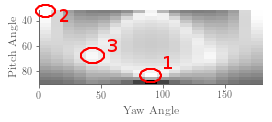
\includegraphics[width=\textwidth]{figures/simple_objective/pitch_yaw_0_curvature_annotated.png}
    \label{fig:simpleobjective:0curvature}
    \caption{0 Curvature Scores}
\end{subfigure}
\begin{subfigure}[b]{0.45\textwidth}
    \centering
    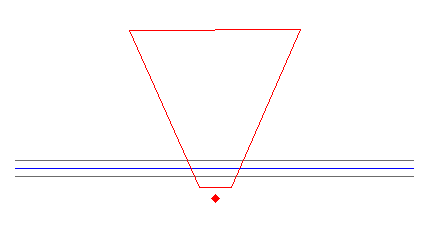
\includegraphics[width=\textwidth]{figures/simple_objective/0_curvature_bestpos_small.png}
    \caption{Configuration \#1, top score}
\end{subfigure}
\begin{subfigure}[b]{0.49\textwidth}
    \centering
    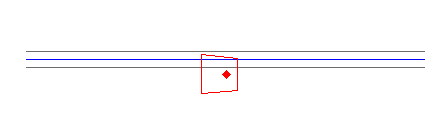
\includegraphics[width=\textwidth]{figures/simple_objective/0_curvature_pos2_small.png}
    \caption{Configuration \#2}
\end{subfigure}
\begin{subfigure}[b]{0.49\textwidth}
    \centering
    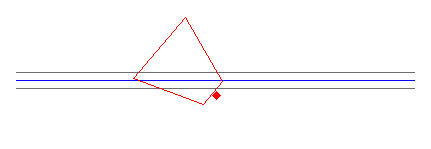
\includegraphics[width=\textwidth]{figures/simple_objective/0_curvature_pos3_small.png}
    \caption{Configuration \#3}
\end{subfigure}
\hrule
\hrule
\hrule

\begin{subfigure}[b]{0.42\textwidth}
    \centering
    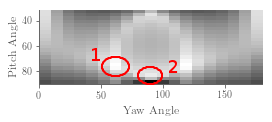
\includegraphics[width=\textwidth]{figures/simple_objective/pitch_yaw_at_radius_20_annotated.png}
    \label{fig:simpleobjective:0curvature}
    \caption{20m Radius}
\end{subfigure}
\begin{subfigure}[b]{0.28\textwidth}
    \centering
    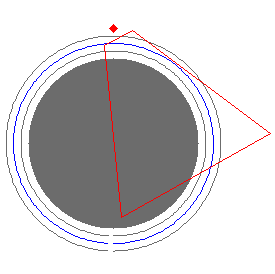
\includegraphics[width=\textwidth]{figures/simple_objective/radius_20m_pos1_small.png}
    \caption{Configuration \#1}
\end{subfigure}
\begin{subfigure}[b]{0.28\textwidth}
    \centering
    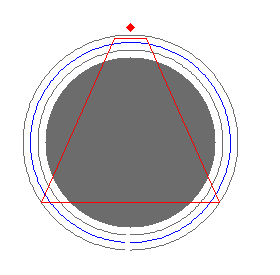
\includegraphics[width=\textwidth]{figures/simple_objective/radius_20m_pos2_small.png}
    \caption{Configuration \#2}
\end{subfigure}
\hrule
\hrule
\hrule
\begin{subfigure}[b]{0.45\textwidth}
    \centering
    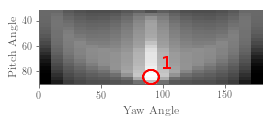
\includegraphics[width=\textwidth]{figures/simple_objective/pitch_yaw_at_radius_5_annotated.png}
    \label{fig:simpleobjective:20radius}
    \caption{5m Radius}
\end{subfigure}
\begin{subfigure}[b]{0.25\textwidth}
    \centering
    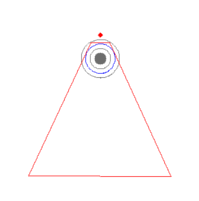
\includegraphics[width=\textwidth]{figures/simple_objective/radius_5m_pos1_small.png}
    \caption{Configuration \#1}
\end{subfigure}
\caption[Cheaper Objective Function Results]{Results and high scoring orientations from the cheaper objective function.}
\label{fig:simpleobjective}
\end{figure}

The first images in a row show the evaluated objective function, the others
are diagrams of the path and camera's field of view. The displayed
configurations the top-scoring and distinct orientations (I ignored
symmetric cases). The filled gray areas are world obstacles
that I place to imitate walls.

The presented optimal points match what one might intuitively expect 
for camera placement: ideally, we maximize both the length of the path
we can spot at once, have the path trace through the highest
pixel density part of the field of view -- this gives the lowest
error during location prediction.

As the curvature increases, the number of different ``good'' 
orientations decreases -- with a highly curved path, there is only
one best choice - the one observing the most of the path possible.

Going forward into the more expensive objectives in Section REF TODO, I use
the depicted configurations as the only allowed orientations to restrict
the search space as much as possible.

%\subsection{Aside: Intersection}
%*** optional -- examine if time remaining at the end ***
%Because we can in this case! ... may be a pain to implement in current code of piecewise paths...


\subsection{Optimizing Pitch, Yaw, and Horizontal and Vertical FoV Simultaneously}

As mentioned in the introduction of this dissertation, I also attempt
to optimize the field of view simultaneously with the pitch and yaw
directions, which has not been examined as a variable before.

To examine this I used a hill-climbing optimization algorithm~\cite{russel2016artificial}
with random restarts to explore the space of options. The optimization
takes steps in each parameter that increase the objective function, effectively
zig-zagging along axes towards (local) maxima.

\subsubsection{Hillclimbing -- Straight Road}

For straight roads, all of the top scoring configurations 
shrunk the field of view as far as was allowed, and oriented themselves to
view the road along the diagonal of the field of view. This makes sense -- 
when observing a straight line, there is no point wasting pixels
on unlikely regions. Additionally, shrinking the field
of view is akin to increasing the resolution, and decreases
the error of predictions. 

Scoring significantly worse are more a few diversified choices,
as depicted in red and purple in Figure~\ref{fig:simpleobjective:hillclimbing straight}.

\begin{table}[htb]
    \centering
    \caption[Hillclimbing Top Scorers]{Three top scoring, diverse results from hillclimbing across four parameters on straight roads.}
    \label{tab:simpleobjective:hillclimb}
    \begin{tabular}{@{}lllll@{}}
        \toprule
        Objective Score & Pitch & Yaw   & H. FoV & V FoV. \\ \midrule
        8.63 (green)            & 57 & $90\pm43$ & 20.1  & 20.1  \\
        ... \\
        6.6787 (red)          & 68 & 90 & 47.2  & 22.9 \\
        ... \\
        3.0710 (purple)          & 39.3 & 90 & 25.1  & 53.5  \\ 
        \bottomrule
    \end{tabular}
\end{table}


\begin{figure}[htb]
    \centering
    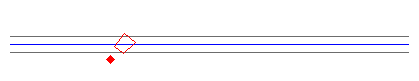
\includegraphics[width=3in]{figures/simple_objective/top_hillclimb.png}
    \caption[Top Hillclimbing Result]{Visualization of Top Hillclimbing Result for straight roads.}
    \label{fig:simpleobjective:hillclimbing straight}
\end{figure}

\subsubsection{Hillclimbing -- Curved Roads}

We can obtain slightly more consistently varied results when optimizing
on curved roads. Although the top two scoring parameters
still minimized the field of view, the next best result
had a wide but narrow field of view. Compared to straight roads,
we see more diverse solutions with high scores.

\begin{table}[htb]
    \centering
    \caption[Hillclimbing Top Scorers]{Top 3 results from hillclimbing across four parameters with curvature 0.05.}
    \label{tab:simpleobjective:hillclimb}
    \begin{tabular}{@{}lllll@{}}
        \toprule
        Objective Score & Pitch & Yaw        & H. FoV & V FoV. \\ \midrule
        8.58  (green)   & 56.5 & $270\pm25$ & 21.1  & 20.4  \\
        7.98  (red)     & 61.0 & 270     & 98.2  & 22.1  \\ 
        ... \\
        3.72  (purple)  & 43.3  &  $270\pm45.0$ & 38.8   & 50.8   \\ \bottomrule
    \end{tabular}
\end{table}

\begin{figure}[htb]
    \centering
    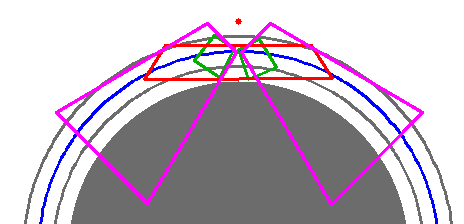
\includegraphics[width=3in]{figures/simple_objective/hillclimb_curvature.png}
    \caption[Top Hillclimbing Result]{Visualization of Top Hillclimbing Result for a curvature of 0.05.}
    \label{fig:simpleobjective:hillclimb result}
\end{figure}

\subsection{Discussion}

The objective function used in this section can be seen as
a measure of the \textit{instantaneous localization power}
of the camera. In other words, if a vehicle appeared suddenly, or
could only be sent a single update, how can the camera best be chosen
to reduce its localization error, on average.

There are several issues with this metric. Biggest of them
is the embedded assumption that only 1 update can be sent.
In reality, a vehicle spends a longer amount of time in the camera's
field of view if the camera can cover more ground area -- 
though the resulting updates sent to the vehicle may be
less accurate. A useful property of the Kalman
filter is that the uncertainty (covariance) in the state
can only shrink as a result of a measurement, so there is some
utility in sending more updates over a wider field of view,
even at reduced accuracy. 

The advantages of the objective function here are twofold:
firstly, it is cheap to compute, and is the reason I could
do the hillclimbing optimization which
required hundreds of evaluations of the objective. Secondly,
it can be used independently of specific trajectories; all
other objective functions in this work are centered about
a single path. The latter property is discussed 
as a future research direction at the end of this report.

Since I am essentially able to perform exhaustive searches
over the possible pitch and yaw angles, I use this
as a pre-optimization step to discover interesting orientations
to explore further with more expensive objective functions.


% TODO attempt an intersection


\section{Navigation-specific Metrics}

Here I define alternative metrics that I use to
I evaluate camera placements. 

In this section, $x_t$ denotes the robot
state at time $t$, $u_t$ denotes the control command
that drives the odometry motion model from $x_{t-1}$ to
$x_{t}$, and $z^{A}_{t}$ is the measurements received
at time $t$ from cameras in the set $A$. Corresponding
capital letters are used to denote the random variables
for state, controls, a measurements.

\subsection{Entropy of the Final State}
The entropy of a robot's state is a measure of the 
spread of its probability distribution. A peaked distribution
has low entropy -- all the probability is concentrated in a few
regions. A flat distribution is maximally uncertain.

The robot's belief of its own state is estimated by
the EKF running on board. It captures, via the mean state $x_t$
and covariance matrix $\Sigma_t$, the distribution $p(x_t | u_{1:t}, z^{A}_{1:t})$.

At the end of an execution of a path, we can measure the
differential entropy of this distribution as follows:

\begin{flalign}
    h(x_t | u_{1:t}, z^{A}_{1:t}) = \frac{1}{2}log((2 \pi e)^k |\Sigma_t|)
\end{flalign}

Here, $|\Sigma|$ is the determinant of the covariance matrix. Since
entropy is a measure of uncertainty, we try to minimize it via
the camera placements.

It is tempting to try to compute the entropy of the joint robot states
 as the sum of the differential entropy at each time step, ie. 
\begin{flalign}
\notag     h(x_1,...x_t | u_{1:t}, z^{A}_{1:t}) &= \\
h(x_1 | u_1, z^A_1) + ... + h(x_t | u_{1:t}, z^{A}_{1:t})
\end{flalign}

However, this transformation would imply that the state at each time
is completely independent. The actual joint entropy is the value optimized in~\cite{beinhofer2011near},
and is described in the next section.

\subsection{Mutual Information}
\label{sec:cameraplacement:mutualinformation}
I use as my objective functions the one from~\cite{beinhofer2011near}, and
describe it following their notation. The goal is to
maximizing the mutual information between all possible robot states $X_{0:T}$ on a path,
and the observations of the robot along the same path from a set of cameras $A$,
written as $Z^{A}_{1:T}$, given the robot controls $U_{1:T}$.

Formally, this is written as
\begin{flalign}
\notag    I(X_{0:T}; Z^{A}_{0:T} | U_{0:T}) &= 
    h(X_{0:T} | U_{0:T}) - h(X_{0:T} | U_{0:T}, Z^{A}_{0:T}) 
\end{flalign}

The first term is the joint entropy of all possible robot states given
all possible controls. This value is constant for a path. So, maximizing
mutual information is equivalent to minimizing the conditional entropy
of robot states given the observations and controls.

For continuous variables we can compute $h(X_{0:T} | U_{0:T}, Z^{A}_{0:T})$ 
using the following integral (I drop the subscripts for convenience).

\begin{flalign}
    -\int \int p(x | u, z^{A}) log p(x | u, z^{A}) dx p(u, z^{A}) d(u, z^A)
\end{flalign}

Evaluating this integral in closed form is not possible, so I use Monte Carlo
evaluations to sample from the distribution of controls and measurements.

The last missing piece is to obtain the joint distribution of all robot
states $p(x_{0:T} | u^{A}_{1:T}, z^{A}_{1:T})$. This is often
rewritten as:

\begin{flalign}
\notag    p(x_{0:T} | u^{A}_{1:T}, z^{A}_{1:T}) &= \\
    p(x_0) \prod_{t=1}^{T} \eta_t p(z^{A}_t | x_t) p(x_t | x_{t-1}, u_t)
\end{flalign}

This breaks down the joint posterior distribution of all robot states
into the product of the motion model $p(x_t | x_{t-1}, u_t)$ and
the sensor model $p(z^{A}_t | x_t)$ at each time step. I use the sensor model
developed in Chapter~\ref{chap:cameramodel} to obtain
approximate probabilities of getting a concrete sensor measurement,
given the robot's mean positional belief.

Lastly, the $\eta$ normalizer needs to be computed. It can be shown
to be equal to:
\begin{flalign}
    \eta_t = \int p(z^{A}_t | x_t) p(x_t | u_{1:t}, z_{1:t-1}) dx_t
\end{flalign}
the first term is again the sensor model, and the second is
recognizable as the belief of the robot, given by the mean and covariance.
I evaluate the normalizing constant with another small Monte Marlo approximation,
drawing sample states $x_t$ from the robot's positional distribution.

The joint probability distribution can be seen as the probability
that the robot took the exact path that it did on any given
execution of the robot's path. Since these are all drawn
from continuous distributions, technically any such probability
should be zero. I discretize using a small delta when calculating
the probabilities to obtain small but finite values. However,
this also requires that the full Monte Carlo approximation be run
several thousand times to obtain valid results.


\subsection{Mean Trace of Covariance Matrix}
Finally, another measure of uncertainty is the trace of the covariance matrix.
I use the mean trace  across $T$ timesteps in a single trajectory:

\begin{flalign}
    MTrace &= \sum_{t=0}^{T} tr(\Sigma_t)
\end{flalign}

It is interesting to note that the determinant of the covariance,
the trace of the covariance, and the graphical uncertainty ellipse
of the EKF are all related to the eigenvalues of $\Sigma$: the ellipse's major
and minor axes are the eigenvectors scaled by
the square root of the eigenvalues; $tr(\Sigma)$ is the sum of the eigenvalues,
and the determinant is the product of the eigenvalues. Thus,
these measures can interpreted measuring the sum of the radii (squared),
and the approximate area of the ellipse (squared), respectively.



\section{Placing Single Cameras With Navigational Metrics}

\subsection{Straight Roads}



\subsection{Curved Roads}



\section{Multiple Camera Placement}
* Discuss submodularity

* test submodularity by sampling -- make sure minimum overlap of camera ground areas!

* straight roads + 1 curvature

* propose cascaded optimization -- choose possible sensor locations, use cheaper objective to find top 1 or 2 
positions or orientations, add these to the set of possible locations and orientations


\section{Conclusion}

\chapter{Optimizing Road Construction for Navigation}

* brief - look at how to connect two points if various obstacles are put in the way
* maybe try a triangular point an and rectangular block 


\chapter{Summary and Conclusion} 




\appendix
\singlespacing

\printbibliography

\end{document}
